\chapter{Chapitre 1} \label{chap:chap1}

\begin{fmffile}{chapitre1}



\section{La physique sous l'angle des symétries}

Les réflexions sur la nature du monde qui nous entoure sont apparues avec nous. Pourtant, les premières traces de pensées philosophiques de la nature semblent très récentes à l'échelle de notre histoire (Antiquité). Si les balbutiements de ce que l'on nomme aujourd'hui la physique peuvent trouver des racines dans les textes d'Aristote, d'Empédocle ou encore de Démocrite, il semble plus pertinent de considérer l'apparition de la physique durant la Renaissance.

\subsection{Galilée puis Newton et la philosophie naturelle}
La proposition fondatrice de la physique est la citation de Galilée dans \emph{l'Essayeur} en 1623, "La nature est écrite en langage mathématique ". Cette idée que nous savons \emph{a posteriori} profondément fructueuse connaîtra la consécration absolue lors de la publication en 1687 du \emph{Philosophiae naturalis principia mathematica} d'Isaac Newton. Ce traité donnera les clés de la construction mathématique des comportements dynamiques des objets (ou mécanique). Cette mécanique dite newtonienne, plus que de par ses innombrables prédictions vérifiées depuis plus de trois siècles, ira jusqu'à amener Urbain Le Verrier, en 1846, à postuler, par le calcul, l'existence d'une planète encore inconnue à l'époque : Neptune. 

\subsection{Mécanique analytique, Lagrangien et Lois physiques}\label{lagrangien}
Émergeant des travaux de Lagrange, Euler, Maupertuis, D'Alembert (fin du XVIIIe siècle) ou encore Hamilton (XIXe siècle), une reformulation de la mécanique newtonienne apparaît. Cette proposition théorique est basée sur l'existence d'une quantité mathématique nommée Lagrangien $L$ homogène à une énergie. L'intégrale des Lagrangiens sur toute une période de temps joignant deux évènements $A$ et $B$ se nomme action $S$.
\begin{equation*}
    S = \int_{t_A}^{t_B} L \mathrm{d}t
\end{equation*}  
Il est alors possible, par une proposition philosophique très élégante, de reconstruire intégralement la mécanique newtonienne. Ce principe appelé principe de moindre action stipule que : " Entre deux évènements $A$ et $B$, la nature choisira la voie qui minimisera son action ".
Cette formulation est mathématiquement équivalente à l'équation d'Euler-Lagrange : 
\begin{equation*}
\frac{\mathrm{d}}{\mathrm{d}t}\left( \frac{\partial L}{\partial \dot{q}}\right) - \frac{\partial L}{\partial q} = 0 
\end{equation*}
avec $q$ et $\dot{q}$ respectivement les coordonnées généralisées et leur dérivée temporelle.
Le Lagrangien muni du principe de moindre action, suffit à générer, pour une théorie donnée, l'ensemble des relations mathématiques régissant les phénomènes physiques (observables, mesurables). Autrement dit, cette quantité peut aisément s'interpréter comme représentant le concept de "Loi Physique".

\subsection{Relativité Restreinte et Mécanique Quantique}
Coup sur coup, la physique du XXe siècle va connaître deux révolutions. La première viendra de l'unification sous un même formalisme de l'électromagnétisme et de la mécanique. En effet, la fin du XIXe siècle est marquée par le triomphe de la théorie de l'électromagnétisme. Cette théorie permet la description de tous les phénomènes électromagnétiques grâce aux équations pilotant les champs électrique et magnétique, les équations de Maxwell
\begin{align*}\label{Maxwell}
    &\vec{\nabla} \cdot \vec{E} = \frac{\rho}{\epsilon_{0}} \qquad \qquad \vec{\nabla} \wedge \vec{E} = - \frac{\partial \vec{B}}{\partial t} \\
    &\vec{\nabla} \cdot \vec{B} = 0 \qquad  \qquad \vec{\nabla} \wedge \vec{B} = \mu_0 \vec{j} + \epsilon_{0}\mu_0 \frac{\partial \vec{E}}{\partial t}
\end{align*}
Il semblait y avoir une dualité entre la mécanique newtonienne et l'électromagnétisme. Lors d'un changement de référentiel inertiel, la mécanique newtonienne doit transformer ses équations sous transformation de Galilée pour assurer l'invariance de leur forme mathématique. Les équations de Maxwell, elles, se transforment par transformations de Lorentz. Cette transformation est pilotée par le facteur de Lorentz :
\begin{equation}
    \gamma = \frac{1}{\sqrt{1- \beta^2}}
\end{equation} 
avec $\beta$ le rapport de la vitesse entre les deux référentiels et la vitesse de la lumière dans le vide. L'ensemble des transformation est résumé dans la table \tablename{\ref{tab:transformations}}.
\begin{table}
\begin{center}
\begin{tabular}{cc}
        \noalign{\smallskip}\hline\noalign{\smallskip}
        Transformation de Galilée & Transformation de Lorentz \\
        \noalign{\smallskip}
        \hline \hline
        \noalign{\smallskip}
        $\left\{ \begin{matrix}
        t' = t \\
        \vec{r\,}' = \vec{r} - \vec{v}t
        \end{matrix}  \right.$
        &
        $\left\{ \begin{matrix}
        ct' = \gamma \left(ct - \vec{\beta} \cdot \vec{r}_\parallel  \right) \\
        \vec{r}\,'_\parallel =\gamma \left(\vec{r}_\parallel - c t\vec{\beta}   \right) \\
        \vec{r}\,'_{\perp} = \vec{r}_{\perp}
        \end{matrix}  \right.$ \\
        \noalign{\smallskip}\hline\noalign{\smallskip}
\end{tabular}
\caption{Résumé des transformations de coordonnées dans le cas newtonien (Galilée) et dans le cas relativiste (Lorentz). Le vecteur position $\vec{r}$ est décomposé en une composante parallèle ($\parallel$) et une composante perpendiculaire ($\perp$). Autrement dit $\vec{r} = \vec{r}_{\parallel} +\vec{r}_{\perp}$.}
\label{tab:transformations}
\end{center}
\end{table}

S'appuyant sur les travaux de Poincaré, Lorentz, Minkowski, Einstein va construire en 1905 une théorie unificatrice qui présentera la dynamique des corps dont les changements de coordonnées se feront par transformation de Lorentz. Il s'agit de la Relativité Restreinte.
La deuxième révolution viendra avec la découverte d'objets infiniment petits comme l'électron par Thomson à la fin du XIXe siècle. Des problématiques conceptuelles amèneront les physiciens comme Bohr, Dirac, Schrödinger, Pauli ou encore Heisenberg à créer une nouvelle mécanique de description du monde infinitésimal, la mécanique quantique. Très vite, la volonté de description des champs dans cette mécanique nouvelle vont conduire à la proposition théorique, aujourd'hui encore d'actualité : la Théorie Quantique des Champs. Dans cette théorie les particules sont vues comme des excitations de champs quantiques.

\subsection{Concept de symétrie en physique}
Le concept de symétrie est omniprésent en physique. Bien que présent dès les débuts de la physique, ce n'est qu'à la fin du XIXe siècle que Pierre Curie proposera explicitement d'élever le concept de symétrie en principe physique. " Lorsque certaines causes produisent certains effets, les éléments de symétrie des causes doivent se retrouver dans les effets produits. ". Dans les premiers temps, c'est le domaine de la cristallographie qui usera de ce principe. Mais au début du XXe siècle, la mathématicienne Amalie (Emmy) Noether introduisit un théorème associant à chaque conservation (ou symétrie) du Lagrangien (par un paramètre donné), une quantité conservée. Par exemple la conservation du Lagrangien au cours du temps induira la conservation de l'énergie totale d'un système, la symétrie du lagrangien par translation induira la conservation de la quantité de mouvement.
\newline

Le théorème de Noether au début du XXe siècle marquera un changement de paradigme au sein de la physique. Depuis lors, les théories fondamentales de physique sont toujours bâties autour d'un Lagrangien et des symétries qu'il porte. Dans la suite de ce chapitre seront introduits les symétries et le Lagrangien permettant la compréhension des particules élémentaires dans le cadre théorique de la théorie quantique des champs et plus précisément du Modèle Standard de la physique des particules.


\section{La Symétrie de Lorentz}\label{sec:symetrie_de_lorentz}

La Relativité Restreinte, après plus d'un siècle de réussite, est aujourd'hui la théorie centrale de la physique moderne. Elle est le socle commun à la Relativité Générale et à la Théorie Quantique des champs. Une approche telle que la théorie quantique des champs, qui se veut descriptive de la nature, doit respecter la Relativité Restreinte. Il est possible de reconstruire la Relativité Restreinte sous l'angle des symétries.
Cela consiste simplement à postuler la conservation de l'intervalle d'espace-temps $ds$ défini par :

 \begin{equation}
 \boxed{
     \mathrm{d}s^2 = c^2 \mathrm{d}t^2 - \mathrm{d}\vec{r}\,^2 = \sum_{\mu=0}^{3}  \sum_{\nu=0}^{3} g_{\mu\nu}\mathrm{d}x^{\mu}\mathrm{d}x^{\nu}
 }
 \end{equation}
 avec $c$ la vitesse de la lumière dans le vide et 
 \begin{equation}
     (g_{\mu\nu}) =
     \begin{pmatrix}
         1 & 0 & 0 & 0 \\
         0 & -1 & 0 & 0 \\
         0 & 0 & -1 & 0 \\
         0 & 0 & 0 & -1 
     \end{pmatrix}
 \end{equation}

La manipulation des symétries va faire appel à des structures mathématiques nommées groupes dont un bref rappel est présent en annexe \ref{A:groupe}. 

\subsection{L'apparition du groupe $SO(1,3)$}
Dans la suite de ce manuscrit seront utilisées les lettres grecques en guise d'indices d'espace-temps ainsi que la convention de sommation d'Einstein\footnote{Les symboles $\sum$ sont omis en cas de sommation sur des indices d'espace-temps.}. En développant le postulat, pour deux référentiels inertiels, dont un symbolisé par "'", on a :
\begin{align*}
 \mathrm{d}s^2 &= \mathrm{d}s\,'^2 \\
 g_{\mu\nu}\mathrm{d}x^{\mu}\mathrm{d}x^{\nu} &= g_{\alpha\beta}\mathrm{d}x\,'^{\alpha}\mathrm{d}x\,'^{\beta} \\
  &= g_{\alpha\beta}\Lambda^\alpha_{\,\,\mu}\mathrm{d}x^{\mu} \Lambda^\beta_{\,\,\nu}  \mathrm{d}x^{\nu} \\
&= \Lambda^\alpha_{\,\,\mu} g_{\alpha\beta} \Lambda^\beta_{\,\,\nu} \mathrm{d}x^{\mu} \mathrm{d}x^{\nu}
\end{align*}
où les éléments $\Lambda$ sont nommés transformations de Lorentz.

Finalement, la Relativité Restreinte peut s'exprimer comme l'invariance des lois physiques sous l'application d'un groupe de symétrie composé d'objets $\Lambda$ répondant à l'équation : 

\begin{equation}\label{lorentz}
    g = \Lambda^t g \Lambda
\end{equation}

Cette relation fait de $\Lambda$ un élément du groupe $\mathrm{O}(1,3)$.
Il est possible de déduire de \eqref{lorentz} :
\begin{equation}
    \mathrm{det}(\Lambda) = \pm 1
\end{equation}
ainsi que :
\begin{align}
    \left(\Lambda^0_0\right)^2 &= 1 + \sum_{i=1}^{3} \left( \Lambda^i_0  \right)^2 \nonumber\\
    | \Lambda^0_0 | & > 1
\end{align}

 Lorsque $\Lambda^0_0 > 1$ la sous-structure est dite orthochrone, non-orthochrone sinon. Il est à noter que seule la sous-structure spéciale ($\mathrm{det}(\Lambda) =  +1$) orthochrone est un groupe. Il s'agit du groupe $SO(1,3)$ ou groupe de Lorentz réduit.


\subsection{Les représentations de $SO(1,3)$}

La théorie mathématique des groupes fournit une grille de lecture avec la théorie des représentations qui est fondamentale en physique des particules. Dans ce contexte, chacune des représentations de $SO(1,3)$ peut nous donner des objets exploitables en physique.

\subsubsection{Représentation triviale}

En théorie des groupes, tout groupe possède une représentation dite triviale qui consiste à représenter chaque élément par une matrice unité. Cela implique que les objets sur lesquels sont appliquées ces transformations sont de type scalaire à l'image des champs quantiques de spin 0.


\subsubsection{Boosts et rotations : représentation fondamentale de $SO(1,3)$}

De manière triviale, on peut décomposer les éléments de $SO(1,3)$ en combinaison linéaire sur la base composée de $ R_{i=1,2,3}$ et $B_{i=1,2,3}$ suivante : 

\begin{align}\label{rotboost}
    &R_\mathrm{x} =
    \begin{pmatrix}
        1 & 0 & 0 & 0 \\
        0 & 1 & 0 & 0 \\
        0 & 0 & \cos(\theta) & -\sin(\theta) \\
        0 & 0 &\sin(\theta) & \cos(\theta)
    \end{pmatrix}
    &B_\mathrm{x} =
    \begin{pmatrix}
        \cosh(\eta) &\sinh(\eta) & 0 & 0 \\
        \sinh(\eta) & \cosh(\eta) & 0 & 0 \\
        0 & 0 & 1 & 0 \\
        0 & 0 & 0 & 1
    \end{pmatrix}
    \nonumber \\
    &R_\mathrm{y} =
    \begin{pmatrix}
        1 & 0 & 0 & 0 \\
        0 & \cos(\theta) & 0 &  \sin(\theta) \\
        0 & 0 & 1 & 0 \\
        0 &-\sin(\theta) &0 & \cos(\theta)
    \end{pmatrix}
    &B_\mathrm{y} =
    \begin{pmatrix}
        \cosh(\eta) & 0 & \sinh(\eta) & 0 \\
        0 &1  & 0 & 0 \\
        \sinh(\eta) & 0 & \cosh(\eta) & 0 \\
        0 & 0 & 0 & 1
    \end{pmatrix}
    \\
    &R_\mathrm{z} =
    \begin{pmatrix}
        1 & 0 & 0 & 0 \\
        0 & \cos(\theta) &-\sin(\theta)  &  0 \\
        0 & \sin(\theta) &\cos(\theta) & 0 \\
        0 & 0 &0 & 1
    \end{pmatrix}
    &B_\mathrm{z} =
    \begin{pmatrix}
        \cosh(\eta) &  0 & 0 & \sinh(\eta) \\
        0 & 1& 0 & 0 \\
        0 & 0 & 1 & 0 \\
        \sinh(\eta) & 0 & 0 & \cosh(\eta) 
    \end{pmatrix}
    \nonumber
\end{align}

Ces matrices représentent les rotations et les boosts selon les axes $\{x,y,z\}$. Elles s'appliquent sur des objets nommés 4-vecteurs. Ces derniers comportent tous une composante temporelle et 3 spatiales. Ces objets sont par exemple les 4-vecteurs dynamiques (position, vitesse, ...), électromagnétiques (courant) mais aussi, on le verra dans la suite, des champs quantiques de spin 1 comme le champ photonique $A^\mu$.

\subsubsection{Les 2-spineurs : représentation fondamentale de $SU(2)\otimes SU(2)$}

Dans la théorie des groupes, un ensemble spécifique de groupes nommé groupes de Lie (précisions dans l'annexe \ref{A:Lie}), dont $SO(1,3)$ est un des représentants, porte des propriétés particulièrement utiles. Il est possible de reconstruire intégralement le groupe grâce à une relation impliquant des matrices $4\times4$ dites générateurs infinitésimaux. Pour $\Lambda \in SO(1,3)$ :
\begin{equation}
\Lambda = \exp\left\lbrace {\sum_{i=1}^{3} \theta_i J^i + \sum_{j=1}^{3}\eta_j K^j } \right\rbrace
\end{equation}
$J_i$, $K_i$ représentent les générateurs infinitésimaux respectivement des rotations et des boosts présentés à \eqref{rotboost}.

Dans le cas où le groupe possède plusieurs générateurs, ces derniers peuvent être caractérisés par des relations définissant une algèbre de Lie (voir \ref{A:algebre}). 
L'algèbre de Lie des générateurs de $SO(1,3)$ est définie par les commutateurs (ou crochets de Lie):
\begin{equation*}
    [J_a, J_b] = - [K_a,K_b] = i \sum_{c=1}^{3} \epsilon_{abc}J_c 
\end{equation*}
\begin{equation}
    [J_a,K_b] = i \sum_{c=1}^{3} \epsilon_{abc}K_c
\end{equation} 
avec $\epsilon_{abc}$ le symbole de Levi-Civita totalement antisymétrique sur ses indices. On nomme cette algèbre $\mathfrak{so}(1,3)$.
Il existe une application bijective qui permet de créer un nouveau jeu de générateurs:
\begin{equation}
    J^+_a = \frac{1}{2}\left( J_a + i K_a \right) \qquad J^-_a = \frac{1}{2}\left( J_a - i K_a \right) 
\end{equation}
Avec ces nouveaux générateurs, les algèbres de Lie sont données par : 
\begin{align}
    [J^+_a, J^+_b] &= \frac{i}{2} \sum_{c=1}^{3}\epsilon_{abc}J^+_c \nonumber \\
    [J^-_a, J^-_b] &= \frac{i}{2} \sum_{c=1}^{3}\epsilon_{abc}J^-_c \nonumber \\
    [J^+_a, J^-_b] &= 0 
\end{align}
Il s'agit là d'un des résultats les plus spectaculaires de la théorie des groupes. En effet, il est possible de transformer l'algèbre $\mathfrak{so}(1,3)$ en une combinaison de deux algèbres indépendantes $\mathfrak{su}(2)$. Autrement dit, on a la relation d'isomorphie :

\begin{equation}
    \mathfrak{so}(1,3) \simeq \mathfrak{su}(2) \oplus \mathfrak{su}(2)
\end{equation}
A partir de cette algèbre on peut construire le groupe $SU(2)\otimes SU(2)$.
A l'instar des éléments de $SO(1,3)$ qui agissent sur des 4-vecteurs, les éléments du groupe $SU(2)\otimes SU(2)$ agissent sur des objets de type 2-spineurs. Ces 2-spineurs sont des objets mathématiques qui décrivent des entités comme les champs quantiques de spin \sfrac{1}{2} (par exemple le champ électronique).

\subsection{Quantification} 

Le respect de la symétrie de Lorentz pour les lois physiques impose la nature possible des champs quantiques (scalaires , 4-vecteurs, 2-spineurs). Il est nécessaire d'établir des équations d'états pour ces champs. Une procédure plus standard est utilisée dans cette section\footnote{Il est possible par la théorie des groupes d'accéder à ces équations, mais l'approche est très complexe.}. Elle consiste à quantifier l'équation d'énergie totale relativiste grâce au principe de correspondance de Bohr:
\begin{align*}
    \hat{H} &\rightarrow i\partial_t \\
    \hat{\vec{P}} &\rightarrow -i\vec{\nabla} 
\end{align*}
Avec $\hbar = c = 1$ (système d'unités naturelles)
\begin{equation}
    E^2 = p^2 + m^2 \, \Longrightarrow \, -\partial_t^2 = -\triangle + m^2
\end{equation}
En notation indicielle appliquée sur un champ scalaire, on a :
\begin{equation}\label{klein}
\left( \partial_\mu\partial^\mu - m^2 \right)\phi = 0 \qquad \textrm{(équation de Klein-Gordon)}
\end{equation}
L'équation étant la version quantique de la relation d'énergie totale, elle est respectée par tout champs. Cependant, la structure des 2-spineurs demande une adaptation de l'équation de Klein-Gordon. La linéarisation de cette équation, que l'on doit à Dirac, permet cela tout en intégrant naturellement les matrices de Pauli (opérateurs de spin \sfrac{1}{2}). 
\begin{equation}\label{dirac}
\left(i\gamma^\mu \partial_\mu - m \right)\psi = 0   \qquad \textrm{(équation de Dirac)}
\end{equation}
Pour respecter l'équation \eqref{klein}, on voit que les matrices $4\times4$ dite de Dirac doivent respecter une relation d'algèbre de Clifford : 
\begin{equation}
    \{\gamma^\mu,  \gamma^\nu \} = \frac{1}{2}g^{\mu\nu}
\end{equation}
Pour les champs 4-vectoriels, l'équation de Klein-Gordon est suffisante. Pour avoir une expression la plus générale possible on peut utiliser l'invariance de jauge provenant de l'électromagnétisme. Cela donne l'équation :
\begin{equation}\label{proca}
 \partial_\mu\partial^\mu A^\nu - \partial^\nu \partial_\mu A^\mu - m^2 A^\nu = 0 \qquad \textrm{(équation de Proca)}
\end{equation}

\subsection{Groupe de Lorentz et Lagrangien}

La théorie quantique des champs utilise le formalisme Lagrangien (présenté au chapitre \ref{lagrangien}). Les champs étant des entités définies sur les quatre dimensions d'espace-temps, il est plus pertinent d'utiliser des densités lagrangiennes $\mathcal{L}$.
Cette dernière diffère du Lagrangien traditionnel par sa généralisation au paramétrage quadridimensionnel. Autrement dit $L(t) \rightarrow \mathcal{L}(t,x,y,z)$. Nous utiliserons dans la suite Lagrangien ou densité lagrangienne indifféremment. Devant respecter la relativité restreinte, donc la symétrie $SO(1,3)$, son Lagrangien doit être un scalaire de Lorentz. 
De plus, en unité naturelle, le lagrangien est de dimension $[\mathcal{L}] = M^{4}$, ce qui va contraindre la forme des scalaires de Lorentz.

Quelques scalaires de Lorentz construits à partir des champs quantiques sont résumés dans la table \tablename{\ref{scalaire}}.
\begin{table}
\begin{center}
    \begin{tabular}{ccc}
    \noalign{\smallskip}\hline\noalign{\smallskip}
     Termes de masse & Scalaires dynamiques & Termes couplés \\
     \noalign{\smallskip}
     \hline \hline
     \noalign{\smallskip}
        $m^2\phi^\dagger \phi $&$ \partial_\mu \phi^\dagger \partial^\mu\phi$ & $\bar{\psi}\phi\psi$\\
        $m\bar{\psi}\psi $&  $\bar{\psi}\gamma^\mu\gamma_5 \partial_\mu\psi \quad \bar{\psi}\gamma^\mu \partial_\mu\psi$ &  $\bar{\psi}\gamma_\mu A^\mu\psi$\\
        $m^2A_\mu A^\mu$& $ \partial_\mu\partial^\mu \partial_\nu A^\nu $  & $\alpha \bar{\psi}A^\mu \partial_\mu\psi$\\
     \noalign{\smallskip}\hline\noalign{\smallskip}
    \end{tabular}
    \caption{Table des combinaisons de champs quantiques respectant la symétrie de Lorentz. Les coefficients $m$ de dimension $[m] = M$ et $\alpha$ de dimension $[\alpha] = M^{-1}$ assurent la dimension $M^4$ aux différents termes.}
    \label{scalaire}
\end{center}
\end{table}

\section{Modèle Standard de la physique des particules}

\subsection{Présentation générale}

Le Modèle Standard de la physique des particules est une proposition théorique décrivant les  particules élémentaires ainsi que leurs interactions. Il est construit autour d'une symétrie locale $U(1)_Y \otimes SU(2)_L  \otimes SU(3)_C $ des lois physiques, dite symétrie de jauge.
Parmi les interactions fondamentales, celle qui est la mieux connue est l'interaction électromagnétique, responsable de la cohésion des atomes, couplant les particules portant une charge électrique. Cette interaction est décrite par la théorie de l'électrodynamique quantique ou QED (\emph{Quantum electro-dynamics}). La deuxième interaction, interaction faible est responsable des phénomènes radioactifs. Elle est décrite au sein de la théorie électro-faible ou EW (\emph{ElectroWeak}) élaborée par Sheldon Glashow \cite{Glashow} et complétée par Steven Weinberg \cite{Weinberg} et Abdus Salam \cite{Salam} en 1967 avec l'introduction du mécanisme de Higgs développé par Robert Brout, François Englert\cite{Englert} et Peter Higgs \cite{Higgs} en 1964, permettant entre autre de générer la masse des bosons de jauge \PW et \PZ. La théorie est confirmée avec la découverte des bosons massifs \PWpm et \PZzero en 1983, et la découverte du boson de Higgs, pièce manquante du puzzle, le 4 juillet 2012 par les collaborations ATLAS \cite{higgs_atlas} et CMS \cite{higgs_cms} du LHC, un triomphe pour le Modèle Standard. Cette proposition unifie l'interaction faible et le formalisme de QED. Enfin, le Modèle Standard tient compte de l'interaction forte responsable de la cohésion atomique restreinte aux particules portant des charges de couleurs. Cette interaction est décrite par une théorie parallèle mais non unifiée avec l'interaction électrofaible (dans le Modèle Standard) qu'est la chromodynamique quantique ou QCD (\emph{Quantum ChromoDynamics}).
L'interaction gravitationnelle n'est pas décrite par le Modèle Standard.

\subsection{Constituants du Modèle Standard}

\begin{figure}
\begin{center}
  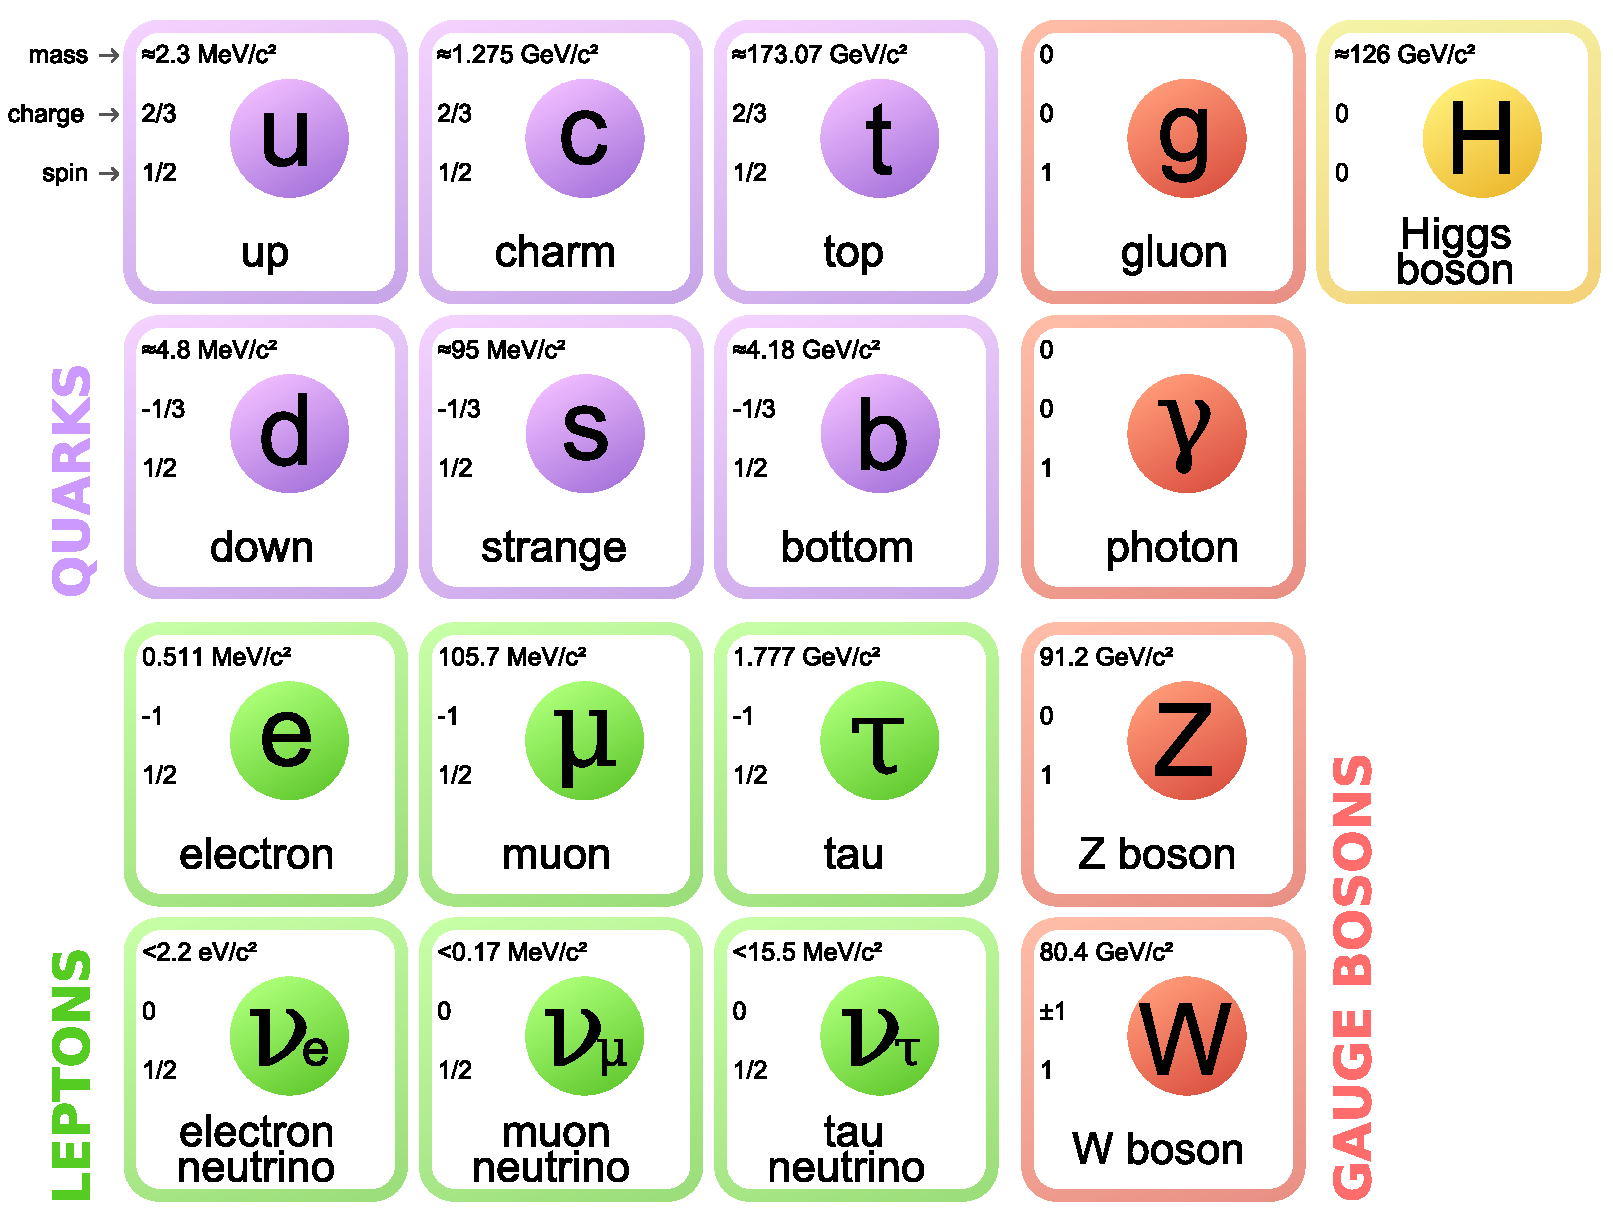
\includegraphics[height=0.4\textwidth]{Standard_Model_of_Elementary_Particles.pdf}
  \caption{Les particules élémentaires du Modèle Standard.}
    \label{fig:sm}
\end{center}
\end{figure}

\subsubsection{Les fermions}
Les fermions sont les particules de matière. Ils ont un spin \sfrac{1}{2}. Ils suivent la statistique de Fermi-Dirac qui implique le principe d'exclusion de Pauli : deux fermions identiques ne peuvent pas occuper le même état quantique. Ceci explique la raison d'être des couches électroniques d'un atome.
Les fermions sont pilotés par l'équation de Dirac \eqref{dirac}. Étant des représentations de $SU(2)\times SU(2)$, les fermions sont des doubles doublets représentant, selon le choix des matrices de Dirac  $\gamma^\mu$, des doublets particule/antiparticule (réalisation de Dirac) ou des doublets gauche/droit (réalisation de Weyl). Ces formes sont présentées dans la figure \figurename{\ref{tab:spineurs}}.
\newline

\begin{table}
\begin{center}
    \begin{tabular}{ccc}
    \noalign{\smallskip}\hline\noalign{\smallskip}
    &Réalisation de Dirac & Réalisation de Weyl \\
 \noalign{\smallskip}
 \hline \hline
 \noalign{\smallskip}
    Fermion  &  $ \Psi = 
    \begin{pmatrix}
            \Psi_\textrm{particule} \\
           \Psi_\textrm{antiparticule} 
        \end{pmatrix}
        $
      &   $ \Psi = 
          \begin{pmatrix}
                  \Psi_\textrm{gauche} \\
                 \Psi_\textrm{droit} 
              \end{pmatrix}
              $  \\
      \noalign{\smallskip}\hline\noalign{\smallskip}
      %%%%%%%%%%%%%%%%%%%%%%%%%%%%%%%%%%%%%%%%%%
      \multirow{5}{*}{Matrices de Dirac} &  $ \gamma^0 = 
      \begin{pmatrix} 
              \mathbbm{1}_2 & 0 \\
             0 & -\mathbbm{1}_2
          \end{pmatrix}
          $
        &    $ \gamma^0 = 
              \begin{pmatrix} 
                       0 & \mathbbm{1}_2 \\
                      \mathbbm{1}_2 & 0
                  \end{pmatrix}
                  $\\
      %%%%%%%%%%%%%%%%%%%%%%%%%%%%%%%%%%%%%%%%%%
       &  $ \gamma^i = 
      \begin{pmatrix} 
              0 & -\sigma_i\\
              \sigma_i & 0
          \end{pmatrix}
          $
        &   $ \gamma^i = 
              \begin{pmatrix} 
                      0 & -\sigma_i\\
                      \sigma_i & 0
                  \end{pmatrix}
                  $ \\
      %%%%%%%%%%%%%%%%%%%%%%%%%%%%%%%%%%%%%%%%%%
       &  $ \gamma^5 = 
      \begin{pmatrix} 
               0 & \mathbbm{1}_2 \\
              \mathbbm{1}_2 & 0
          \end{pmatrix}
          $
        &  $ \gamma^5 =  \begin{pmatrix} 
                      -\mathbbm{1}_2 & 0 \\
                     0 & \mathbbm{1}_2
                  \end{pmatrix}
                  $  \\
    \noalign{\smallskip}\hline\noalign{\smallskip}
  \end{tabular}
  \caption{Résumé des représentations de fermions. Les $\sigma_i$ sont les matrices de Pauli.}
  \label{tab:spineurs}
\end{center}
\end{table}

\begin{description}
\item [Les leptons] Ce sont les fermions insensibles à l'interaction forte. Ils sont colorés en vert dans la figure \figurename{\ref{fig:sm}}. 
\item [Les quarks] Ce sont les fermions sensibles aux l'interactions électromagnétique, faible et forte. Ils sont colorés en violet dans la figure \figurename{\ref{fig:sm}}. Les quarks sont les composants des noyaux atomiques.
\end{description}

\subsubsection{Les bosons}
Les bosons sont des particules de spin entier. Ils suivent la statistique de Bose-Einstein. Ils sont vecteurs d'interaction et leurs caractéristiques sont résumées dans la table \tablename{\ref{tab:interactions}}.

\begin{table}
\begin{center}
    \begin{tabular}{@{}ccccc@{}}
    \noalign{\smallskip}\hline\noalign{\smallskip}
    Interaction & boson(s) & masse (\SI{}{\GeV})\cite{PDG} & intensité relative & portée (m) \\
 \noalign{\smallskip}
 \hline \hline
 \noalign{\smallskip}
     forte & \Pgluon & 0 & 1 &  \SI{\sim e-15}{} \\
     électromagnétique & \Pgamma & 0 & \num{e-2} & $\infty$ \\
    \multirow{2}{*}{faible} & \PWpm & \SI{80.385 \pm 0.015} & \multirow{2}{*}{\num{e-5}} & \multirow{2}{*}{\SI{\sim e-18}} \\
     & \PZzero & \SI{91.1876 \pm 0.0021 } & & \\
    \noalign{\smallskip}\hline\noalign{\smallskip}
  \end{tabular}
  \caption{Les interactions fondamentales et leurs bosons médiateurs.}
  \label{tab:interactions}
\end{center}
\end{table}


\subsubsection{Les symétries de jauges}

La grande force du Modèle Standard est sa capacité à décrire les résultats expérimentaux. A l'instar de la symétrie de Lorentz qui contraint la forme des objets répondant aux lois physiques, les symétries de jauge vont contraindre les formes des interactions entre particules tout en introduisant naturellement les bosons vecteurs de ces interactions. Si dans le chapitre précédent c'est à partir d'une quantité fondamentale (l'intervalle d'espace-temps) qu'a été construite la symétrie de Lorentz ainsi que ses conséquences, pour la compréhension des symétries de jauge, c'est la conservation de la densité lagrangienne qui va être nécessaire.

Une symétrie de jauge correspond à la conservation du Lagrangien après une transformation qui dépend des coordonnées d'espace-temps (ou locale). Les transformations de jauge validées expérimentalement à ce jour sont éléments des groupes $U(1)$, $SU(2)$ et $SU(3)$ dont les définitions sont rappelées en annexe \ref{A:groupedesymetrie}.


\subsection{L'électrodynamique quantique (QED)}

\subsubsection{L'interaction électromagnétique}

La QED (pour \emph{Quantum Electro-Dynamic}) a pour but de décrire au sein de la théorie quantique des champs, l'interaction électromagnétique. Pour ce faire elle doit à la fois présenter la charge fondamentale $e = \SI{1,602176634e-19}{\coulomb}$, ainsi que les champs électrique $\vec{E}$ et magnétique $\vec{B}$, condensés dans le tenseur de Maxwell-Faraday (ou tenseur électromagnétique) $F^{\mu\nu}$. Cette théorie propose que l'interaction électromagnétique consiste en un échange d'un boson électromagnétique (le photon) entre deux particules chargées. La charge électrique est donc élevée au statut de nombre quantique et est par conséquent valeur propre d'un opérateur de charge (noté $C$).

\subsubsection{La symétrie de jauge $U(1)$}
La QED est l'approche théorique proposant la conservation de la symétrie de jauge la plus simple. Premièrement, le groupe de symétrie conservé est $U(1)_\mathrm{em}$ autrement dit l'ensemble des nombres complexes de module $1$. Ensuite, le Lagrangien est minimal. Il ne comporte qu'une partie cinétique pour les fermions et le boson électromagnétique (photon). 
Le Lagrangien composé de champs libres est donné par\footnote{Cette forme exotique de l'écriture de la partie cinétique des fermion fait apparaître la notation $A\overset{\leftrightarrow}{\partial_\mu}B =  A\partial_\mu B - \partial_\mu(A)B$.} :
\begin{equation}
    \mathcal{L} = \underbrace{\frac{i}{2}\bar{\psi}\gamma^\mu\overset{\leftrightarrow}{\partial_\mu}\psi - m\bar{\psi} \psi}_\textrm{équation de Dirac}  \underbrace{-\frac{1}{4}F_{\mu\nu}F^{\mu\nu}}_\textrm{équation de Maxwell}
\end{equation}
avec $F^{\mu\nu} =  \partial^\mu A^\nu - \partial^\nu A^\mu$. Pour un champ $\psi$ répondant à une transformation $U(1)$ locale de forme
\begin{align*}
    \psi \rightarrow \psi' &= e^{i\theta(x)C} \psi \\
    \bar{\psi} \rightarrow \bar{\psi}' &= \bar{\psi}e^{-i\theta(x)C}
\end{align*}
avec $C$ le générateur de $U(1)$ et $\theta(x)$ une fonction quelconque dérivable dépendant de la coordonnée d'espace-temps $x$. On observe que : 
\begin{equation}
 \mathcal{L}' = \frac{i}{2}\bar{\psi}\gamma^\mu\overset{\leftrightarrow}{\partial_\mu}\psi - m\bar{\psi} \psi  \underbrace{-C \bar{\psi} \gamma^\mu\psi\partial_\mu \theta(x)}_\textrm{rémanence de la transformation} -\frac{1}{4}F_{\mu\nu}F^{\mu\nu}
\end{equation}
La symétrie de jauge n'est clairement pas conservée car $\mathcal{L}' \neq \mathcal{L}$. La proposition forte de la QED est de régler le problème du couplage fermions/photon en forçant la symétrie de jauge. 
Pour cela on construit un objet nommé dérivée covariante $D_\mu$ qui est la dérivée corrigée par un terme portant le photon $A^\mu$ :
\begin{equation}
D_\mu = \partial_\mu + ieCA_\mu
\end{equation}
Ce terme additionnel porte la charge électrique élémentaire $e$ et l'opérateur de charge judicieusement appelé également $C$. Cet opérateur a pour valeur propre $\pm 1$ pour les leptons, $\mp \frac{1}{3}$ et $\pm \frac{2}{3}$ pour les quarks et est également un générateur du groupe $U(1)$.
La dérivée covariante placée dans notre Lagrangien, on a après transformation : 
\begin{equation}
 \mathcal{L}' = \frac{i}{2}\bar{\psi}\gamma^\mu\overset{\leftrightarrow}{\partial_\mu}\psi - m\bar{\psi} \psi   \underbrace{- e\bar{\psi} \gamma^\mu C A_\mu \psi}_\textrm{couplage fermion/photon} - C\bar{\psi} \gamma^\mu\psi\partial_\mu \theta(x) \quad -\frac{1}{4}F_{\mu\nu}F^{\mu\nu}
\end{equation}
Le couplage central de cette théorie est présent mais l'invariance de jauge $U(1)$ n'est toujours pas respectée. C'est en remarquant le terme de couplage linéaire en $A^\mu$ que l'on peut faire appel à une propriété déjà connue dans la théorie classique de l'électromagnétisme : l'invariance de jauge du potentiel vecteur. En effet les équations de Maxwell sous forme covariante :
\begin{equation}
\partial_\mu  F^{\mu\nu}  = j^\nu
\end{equation}
laissent entendre que le 4-potentiel $A^\mu$ est défini à un gradient arbitraire près sans perte de généralité. En choisissant ce gradient de sorte que :
\begin{equation}
 A^\mu \rightarrow  A^\mu - \frac{1}{e} \partial^\mu \theta(x)
\end{equation}
alors l'invariance de jauge $U(1)$ est respectée.

Finalement l'électrodynamique quantique s'exprime : 
\begin{equation}\boxed{
 \mathcal{L}_\mathrm{QED} = \frac{i}{2}\bar{\psi}\gamma^\mu\overset{\leftrightarrow}{D_\mu}\psi - m\bar{\psi} \psi -\frac{1}{4}F_{\mu\nu}F^{\mu\nu}
 }
\end{equation}
avec les transformations de jauge $U(1)$ : 
\begin{align*}
 \psi &\rightarrow e^{i\theta(x)C}\psi \\
 A^\mu &\rightarrow  A^\mu - \frac{1}{e} \partial^\mu \theta(x)
\end{align*}
On remarque que si l'on associait un terme de masse supplémentaire au photon $\propto A^\mu A_\mu$ on briserait l'invariance de jauge sans compensation possible. Ceci corrobore la donnée empirique de l'absence de masse du photon.

Ce paragraphe a souligné la puissance des symétries appliquées à la théorie quantique des champs. Si imposer la symétrie de Lorentz permet de construire les champs quantiques des particules de spin \sfrac{1}{2} et de spin 1, imposer la symétrie de jauge $U(1)$ permet de décrire naturellement l'interaction électromagnétique. Les autres interactions sont aussi déduites d'une procédure de conservation de jauge. 

\subsection{La théorie Électrofaible}

\subsubsection{L'interaction faible}

De nombreuses expériences sur la radioactivité $\beta$ telle que l'expérience de Chien-Shiung Wu \cite{MmeWu} démontrèrent la violation de la parité chez les leptons. Cela implique que la radioactivité n'agit pas de manière identique selon les particules. Pour rappel les fermions répondant à l'équation de Dirac sont des représentations du groupe $SU(2)\otimes SU(2)$. On peut les considérer comme des doublets $SU(2)$ indépendants (simple spineur) appelés spineur droit et spineur gauche. Seuls les spineurs gauches interagissent faiblement. Ainsi la symétrie associée $SU(2)$ sera $L$ (pour \emph{left}).

\subsubsection{La symétrie de jauge $U(1)_Y \otimes SU(2)_L$}

Si le principe général de la symétrie de jauge $U(1)$ est présent, la présence de subtilités avec l'interaction faible implique un travail plus profond. 
Pour construire la théorie il est nécessaire de traiter les fermions gauches et droits indépendamment. Les fermions gauches seront traités en doublet $SU(2)_L$ par paire interagissant durant une désintégration. Les fermions droits sont représentés en singlet. Les objets respectant la symétrie $U(1)_Y \otimes SU(2)_L$ sont résumés dans la table \tablename{\ref{tab:su2}}.
\begin{table}
\begin{center}
\begin{tabular}{c|cc}
    \noalign{\smallskip}\hline\noalign{\smallskip}
    & Doublet d'isospin & Singlet d'isospin \\
    \noalign{\smallskip}
    \hline \hline
    \noalign{\smallskip}
    Leptons & $L_A = \begin{pmatrix} \nu_A \\ \ell_A \end{pmatrix}_L$ & $R_A = (\ell_A)_R$ \\
    Quarks & $Q_A = \begin{pmatrix} u_A \\ d_A  \end{pmatrix}_L$ & $ U_A = (u_A)_R$, $D_A = (d_A)_R$\\
    \noalign{\smallskip}\hline\noalign{\smallskip}
\end{tabular}
\caption{Notation des objets respectant la symétrie $U(1)_Y \otimes SU(2)_L$. Les indices $A = 1,2,3$ représentent la génération de la particule associée.}
\label{tab:su2}
\end{center}
\end{table}
Avec une procédure similaire à la QED, la symétrie de jauge $U(1)_Y \otimes SU(2)_L$ du Lagrangien est respectée sous les transformations : 
\begin{align}
    Q &\rightarrow e^{i\vec{\theta}(x)\cdot \vec{T} + i\vartheta(x)Y}Q \label{transfosu2} \\
    U &\rightarrow e^{i\vartheta(x)Y}U
\end{align}
avec $T_{i=1,2,3}$ les générateurs du groupe $SU(2)$ et $Y$, nommé l'hypercharge, le générateur du groupe $U(1)$. On remarque dans l'équation \eqref{transfosu2} que les générateurs de $SU(2)$ étant au nombre de trois, la notation traditionnelle du produit scalaire dans $\mathbb{R}^3$ est utilisée en guise de sommation. Les générateurs de $SU(2)$ répondent à la relation $T_i = \frac{1}{2}\sigma_i$ où les $\sigma_i$ sont les matrices de Pauli :
\begin{equation}
\sigma_x = \begin{pmatrix} 0 & 1 \\ 1 &0\end{pmatrix} 
\quad \sigma_y = \begin{pmatrix} 0 & -i \\ i &0\end{pmatrix}
\quad \sigma_z = \begin{pmatrix} 1 & 0 \\ 0 & -1\end{pmatrix} 
\end{equation}
Les dérivées covariantes s'écrivent :
\begin{align}\label{covSU2}
    D_\mu &= \partial_\mu + ig_W \vec{T} \cdot \vec{W}_\mu + i g_B \frac{Y}{2}B_\mu & \textrm{appliqué sur les doublets} \nonumber \\
    D_\mu &= \partial_\mu + i g_B \frac{Y}{2}B_\mu & \textrm{appliqué sur les singlets} 
\end{align}
Les champs bosoniques se transforment ici avec: 
\begin{align}
    B_\mu &\rightarrow  B_\mu - \frac{1}{g_B} \partial^\mu \vartheta(x) \nonumber\\
    \vec{W}_\mu &\rightarrow \vec{W}_\mu - \frac{1}{g_W} \partial_\mu \vec{\theta}(x)  - \vec{\theta}(x) \wedge \vec{W}_\mu
\end{align}
Le produit vectoriel $\vec{\theta}(x) \wedge \vec{W}_\mu$ \footnote{Il est très courant en physique des particules que la formulation $\sum_{b=1}^{3} \sum_{c=1}^{3} \epsilon^{abc} f^b f^c_\nu$ ou encore $\epsilon^{abc} f^b f^c_\nu$ (par sommation implicite) soit préférée à la notation $\vec{f} \wedge \vec{g}$ de l'algèbre de l'espace $\mathbb{R}^3$ pour des raisons de généralisation à plus grande dimension.} provient du fait que le groupe n'est pas abélien. Autrement dit, les générateurs ne commutent pas. Pour établir le Lagrangien, il suffit d'ajouter les termes cinétiques des bosons.
\begin{align}
B_{\mu\nu} &=  \partial_\mu B_\nu - \partial_\nu B_\mu \nonumber \\
\vec{W}_{\mu\nu} &=  \partial_\mu \vec{W}_\nu - \partial_\nu \vec{W}_\mu - g_W \vec{W}_\mu \wedge \vec{W}_\nu
\end{align}
Finalement le Lagrangien se présente sous la forme : 
\begin{equation}
 \mathcal{L} = \frac{i}{2}\bar{Q}_A\gamma^\mu\overset{\leftrightarrow}{D_\mu}Q_A + \frac{i}{2}\bar{L}_A\gamma^\mu\overset{\leftrightarrow}{D_\mu}L_A -\frac{1}{4}B_{\mu\nu}B^{\mu\nu} -\frac{1}{4}\vec{W}_{\mu\nu}\cdot \vec{W}^{\mu\nu}
\end{equation}
Expérimentalement, les observations des décroissances radioactives montrent que pour le cas des quarks, est observé un mix intergénérationnel. Pour résoudre ce problème on applique sur un vecteur d'états propres de l'interaction faible une matrice dont les composantes représentent l'amplitude de probabilité de couplage faible. Cette matrice se nomme la matrice Cabibbo-Kobayashi-Maskawa \cite{CKM} ou matrice CKM.
\begin{equation}
    \begin{pmatrix} d' & s' & b' \end{pmatrix} =
    \begin{pmatrix}
    V_{ud} & V_{us} & V_{ub} \\
    V_{cd} & V_{cs} & V_{cb} \\
    V_{td} & V_{ts} & V_{tb}
    \end{pmatrix}
    \begin{pmatrix} d \\ s \\ b \end{pmatrix}
\end{equation}
Soit expérimentalement \cite{PDG}:
\begin{equation}\label{CKM}
    V_\mathrm{CKM} =
    \begin{pmatrix}
    0.97401 \pm 0.00011 & 0.22650 \pm 0.00048 & 0.00361^{+0.00011}_{-0.00009} \\
    0.22636 \pm 0.00048 & 0.97320 \pm 0.00011 &  0.04053^{+0.00083}_{-0.00061} \\
    0.00854^{+0.00023}_{-0.00016} & 0.03978^{+0.00082}_{-0.00060} & 0.999172^{+0.000024}_{-0.000035}
    \end{pmatrix}
\end{equation}

Reste le problème des masses des bosons de l'interaction faible et des masses des fermions qui implique des formes de type $\propto \bar{Q} U$ qui violent explicitement $U(1)_Y \otimes SU(2)_L$. C'est fort de ce constat que naturellement la proposition du boson de Higgs pour régler les problèmes de masses est apparue.

\subsubsection{La proposition d'un champ scalaire additionnel}

Avec le postulat d'un nouveau champ scalaire (invariant de Lorentz) de spin $0$ et doublet de $SU(2)$ alors il devient naturel de considérer sa dynamique avec un terme cinétique de type :
\begin{equation}\label{dynamichiggs}
 \mathcal{L}_\mathrm{Higgs} = D_\mu \phi^\dagger D^\mu \phi
\end{equation} 
avec la dérivée covariante à $SU(2)_L$ définie par \eqref{covSU2}. De par la forme des dérivées covariantes, le développement laisse apparaître des termes de masse pour les bosons, c'est à dire des termes de type $\propto W_\mu W^\mu$. Un couplage de ce nouveau champ scalaire avec les fermions droits et gauches permet l'apparition de termes ressemblant aux termes de masse tout en respectant $U(1)_Y \otimes SU(2)_L$ : 
\begin{equation}\label{yukawahiggs}
 \mathcal{L}_\mathrm{Yukawa} = y_1 \bar{Q}_A \phi U_A + y_2 \bar{Q}_A \phi D_A + y_3 \bar{L}_A \phi R_A +\mathrm{h.c.}
\end{equation}
avec $y_1$, $y_2$ et $y_3$ des constantes à définir, nommées couplage de Yukawa. 

Le Lagrangien actuel n'est pas encore suffisant. En effet, deux problèmes se posent. Premièrement, l'observation montre que seuls les bosons faibles sont massifs mais pour l'instant rien ne permet de dire qu'un des bosons introduits par la symétrie est de masse nulle comme attendu pour un photon. Le second problème provient du fait que le champ scalaire couplé aux fermions ressemble à un terme de masse mais n'en sera complètement un que lorsque le couplage fermion gauche/droit sera constant. Ce problème est résolu grâce au concept de brisure spontanée de la symétrie de  $U(1)_Y \otimes SU(2)_L$.

\subsubsection{Brisure spontanée de symétrie}

La théorie quantique des champs offre un cadre formel dans lequel une symétrie totalement vérifiée par un Lagrangien peut spontanément se briser par l'hypothèse d'un vide quantique non nul. Le principe de brisure spontanée repose sur l'idée qu'à un niveau d'énergie donnée, le minimum de potentiel d'un champ est plus bas que le minimum de potentiel avant brisure. Pour le champ scalaire le potentiel le plus simple permettant une brisure est : 
\begin{equation}
    V(\phi) = \mu^2 \phi^\dagger \phi + \lambda (\phi^\dagger \phi)^2
\end{equation}
avec $\lambda > 0$. Au niveau du minimum de potentiel $\frac{\partial V}{\partial \phi} = 0$
\begin{equation}
 \frac{\partial V}{\partial \phi} = 0 \quad \Longrightarrow  \quad \| \phi \|^2 = v^2 = - \frac{\mu^2}{\lambda}
\end{equation}
Si $\mu^2 \geq 0$, alors le potentiel n'admet qu'un seul minimum de potentiel en $\phi = 0 $. En revanche, si $\mu^2 < 0$ alors $\phi$ admet une infinité de minima de potentiel différents de  $\phi = 0 $ sur le cercle complexe de module $v$. Dans ce dernier cas, ce potentiel est souvent nommé potentiel sombrero (voir figure \figurename{\ref{sombrero}}). 

\begin{figure}
\begin{center}
%% Creator: Matplotlib, PGF backend
%%
%% To include the figure in your LaTeX document, write
%%   \input{<filename>.pgf}
%%
%% Make sure the required packages are loaded in your preamble
%%   \usepackage{pgf}
%%
%% Figures using additional raster images can only be included by \input if
%% they are in the same directory as the main LaTeX file. For loading figures
%% from other directories you can use the `import` package
%%   \usepackage{import}
%% and then include the figures with
%%   \import{<path to file>}{<filename>.pgf}
%%
%% Matplotlib used the following preamble
%%   \usepackage[utf8x]{inputenc}
%%   \usepackage[T1]{fontenc}
%%   \usepackage{sistyle}
%%   \SIproductsign{\!\times\!}\SIunitsep{\,}\SIunitdot{{\fontfamily{cmr}\cdot}}
%%   \SIdecimalsign{,}\SIthousandsep{\,}
%%
\begingroup%
\makeatletter%
\begin{pgfpicture}%
\pgfpathrectangle{\pgfpointorigin}{\pgfqpoint{6.692913in}{3.346457in}}%
\pgfusepath{use as bounding box, clip}%
\begin{pgfscope}%
\pgfsetbuttcap%
\pgfsetmiterjoin%
\definecolor{currentfill}{rgb}{1.000000,1.000000,1.000000}%
\pgfsetfillcolor{currentfill}%
\pgfsetlinewidth{0.000000pt}%
\definecolor{currentstroke}{rgb}{1.000000,1.000000,1.000000}%
\pgfsetstrokecolor{currentstroke}%
\pgfsetdash{}{0pt}%
\pgfpathmoveto{\pgfqpoint{0.000000in}{0.000000in}}%
\pgfpathlineto{\pgfqpoint{6.692913in}{0.000000in}}%
\pgfpathlineto{\pgfqpoint{6.692913in}{3.346457in}}%
\pgfpathlineto{\pgfqpoint{0.000000in}{3.346457in}}%
\pgfpathclose%
\pgfusepath{fill}%
\end{pgfscope}%
\begin{pgfscope}%
\pgfsetbuttcap%
\pgfsetmiterjoin%
\definecolor{currentfill}{rgb}{1.000000,1.000000,1.000000}%
\pgfsetfillcolor{currentfill}%
\pgfsetlinewidth{0.000000pt}%
\definecolor{currentstroke}{rgb}{0.000000,0.000000,0.000000}%
\pgfsetstrokecolor{currentstroke}%
\pgfsetstrokeopacity{0.000000}%
\pgfsetdash{}{0pt}%
\pgfpathmoveto{\pgfqpoint{0.187500in}{0.150000in}}%
\pgfpathlineto{\pgfqpoint{3.233957in}{0.150000in}}%
\pgfpathlineto{\pgfqpoint{3.233957in}{3.196457in}}%
\pgfpathlineto{\pgfqpoint{0.187500in}{3.196457in}}%
\pgfpathclose%
\pgfusepath{fill}%
\end{pgfscope}%
\begin{pgfscope}%
\pgfsetbuttcap%
\pgfsetmiterjoin%
\definecolor{currentfill}{rgb}{0.950000,0.950000,0.950000}%
\pgfsetfillcolor{currentfill}%
\pgfsetfillopacity{0.500000}%
\pgfsetlinewidth{1.003750pt}%
\definecolor{currentstroke}{rgb}{0.950000,0.950000,0.950000}%
\pgfsetstrokecolor{currentstroke}%
\pgfsetstrokeopacity{0.500000}%
\pgfsetdash{}{0pt}%
\pgfpathmoveto{\pgfqpoint{0.591355in}{0.823160in}}%
\pgfpathlineto{\pgfqpoint{1.463267in}{1.570082in}}%
\pgfpathlineto{\pgfqpoint{1.448750in}{2.997327in}}%
\pgfpathlineto{\pgfqpoint{0.528224in}{2.326233in}}%
\pgfusepath{stroke,fill}%
\end{pgfscope}%
\begin{pgfscope}%
\pgfsetbuttcap%
\pgfsetmiterjoin%
\definecolor{currentfill}{rgb}{0.900000,0.900000,0.900000}%
\pgfsetfillcolor{currentfill}%
\pgfsetfillopacity{0.500000}%
\pgfsetlinewidth{1.003750pt}%
\definecolor{currentstroke}{rgb}{0.900000,0.900000,0.900000}%
\pgfsetstrokecolor{currentstroke}%
\pgfsetstrokeopacity{0.500000}%
\pgfsetdash{}{0pt}%
\pgfpathmoveto{\pgfqpoint{1.463267in}{1.570082in}}%
\pgfpathlineto{\pgfqpoint{2.875682in}{1.152504in}}%
\pgfpathlineto{\pgfqpoint{2.934776in}{2.622788in}}%
\pgfpathlineto{\pgfqpoint{1.448750in}{2.997327in}}%
\pgfusepath{stroke,fill}%
\end{pgfscope}%
\begin{pgfscope}%
\pgfsetbuttcap%
\pgfsetmiterjoin%
\definecolor{currentfill}{rgb}{0.925000,0.925000,0.925000}%
\pgfsetfillcolor{currentfill}%
\pgfsetfillopacity{0.500000}%
\pgfsetlinewidth{1.003750pt}%
\definecolor{currentstroke}{rgb}{0.925000,0.925000,0.925000}%
\pgfsetstrokecolor{currentstroke}%
\pgfsetstrokeopacity{0.500000}%
\pgfsetdash{}{0pt}%
\pgfpathmoveto{\pgfqpoint{0.591355in}{0.823160in}}%
\pgfpathlineto{\pgfqpoint{2.077407in}{0.336822in}}%
\pgfpathlineto{\pgfqpoint{2.875682in}{1.152504in}}%
\pgfpathlineto{\pgfqpoint{1.463267in}{1.570082in}}%
\pgfusepath{stroke,fill}%
\end{pgfscope}%
\begin{pgfscope}%
\pgfsetrectcap%
\pgfsetroundjoin%
\pgfsetlinewidth{0.803000pt}%
\definecolor{currentstroke}{rgb}{0.000000,0.000000,0.000000}%
\pgfsetstrokecolor{currentstroke}%
\pgfsetdash{}{0pt}%
\pgfpathmoveto{\pgfqpoint{0.591355in}{0.823160in}}%
\pgfpathlineto{\pgfqpoint{2.077407in}{0.336822in}}%
\pgfusepath{stroke}%
\end{pgfscope}%
\begin{pgfscope}%
\definecolor{textcolor}{rgb}{0.000000,0.000000,0.000000}%
\pgfsetstrokecolor{textcolor}%
\pgfsetfillcolor{textcolor}%
\pgftext[x=0.974486in,y=0.094332in,left,base,rotate=341.878381]{\color{textcolor}\rmfamily\fontsize{10.000000}{12.000000}\selectfont \(\displaystyle \Re(\phi)\)}%
\end{pgfscope}%
\begin{pgfscope}%
\pgfsetbuttcap%
\pgfsetroundjoin%
\pgfsetlinewidth{0.803000pt}%
\definecolor{currentstroke}{rgb}{0.690196,0.690196,0.690196}%
\pgfsetstrokecolor{currentstroke}%
\pgfsetdash{}{0pt}%
\pgfpathmoveto{\pgfqpoint{1.316736in}{0.585765in}}%
\pgfpathlineto{\pgfqpoint{2.153888in}{1.365901in}}%
\pgfpathlineto{\pgfqpoint{2.174555in}{2.814395in}}%
\pgfusepath{stroke}%
\end{pgfscope}%
\begin{pgfscope}%
\pgfsetrectcap%
\pgfsetroundjoin%
\pgfsetlinewidth{0.803000pt}%
\definecolor{currentstroke}{rgb}{0.000000,0.000000,0.000000}%
\pgfsetstrokecolor{currentstroke}%
\pgfsetdash{}{0pt}%
\pgfpathmoveto{\pgfqpoint{1.323959in}{0.592496in}}%
\pgfpathlineto{\pgfqpoint{1.302263in}{0.572278in}}%
\pgfusepath{stroke}%
\end{pgfscope}%
\begin{pgfscope}%
\definecolor{textcolor}{rgb}{0.000000,0.000000,0.000000}%
\pgfsetstrokecolor{textcolor}%
\pgfsetfillcolor{textcolor}%
\pgftext[x=1.227871in,y=0.354892in,,top]{\color{textcolor}\rmfamily\fontsize{9.000000}{10.800000}\selectfont \num{0}}%
\end{pgfscope}%
\begin{pgfscope}%
\pgfsetrectcap%
\pgfsetroundjoin%
\pgfsetlinewidth{0.803000pt}%
\definecolor{currentstroke}{rgb}{0.000000,0.000000,0.000000}%
\pgfsetstrokecolor{currentstroke}%
\pgfsetdash{}{0pt}%
\pgfpathmoveto{\pgfqpoint{2.875682in}{1.152504in}}%
\pgfpathlineto{\pgfqpoint{2.077407in}{0.336822in}}%
\pgfusepath{stroke}%
\end{pgfscope}%
\begin{pgfscope}%
\definecolor{textcolor}{rgb}{0.000000,0.000000,0.000000}%
\pgfsetstrokecolor{textcolor}%
\pgfsetfillcolor{textcolor}%
\pgftext[x=2.737435in,y=0.216845in,left,base,rotate=45.617904]{\color{textcolor}\rmfamily\fontsize{10.000000}{12.000000}\selectfont \(\displaystyle \Im(\phi)\)}%
\end{pgfscope}%
\begin{pgfscope}%
\pgfsetbuttcap%
\pgfsetroundjoin%
\pgfsetlinewidth{0.803000pt}%
\definecolor{currentstroke}{rgb}{0.690196,0.690196,0.690196}%
\pgfsetstrokecolor{currentstroke}%
\pgfsetdash{}{0pt}%
\pgfpathmoveto{\pgfqpoint{1.006529in}{2.674933in}}%
\pgfpathlineto{\pgfqpoint{1.043551in}{1.210533in}}%
\pgfpathlineto{\pgfqpoint{2.492081in}{0.760539in}}%
\pgfusepath{stroke}%
\end{pgfscope}%
\begin{pgfscope}%
\pgfsetrectcap%
\pgfsetroundjoin%
\pgfsetlinewidth{0.803000pt}%
\definecolor{currentstroke}{rgb}{0.000000,0.000000,0.000000}%
\pgfsetstrokecolor{currentstroke}%
\pgfsetdash{}{0pt}%
\pgfpathmoveto{\pgfqpoint{2.479977in}{0.764299in}}%
\pgfpathlineto{\pgfqpoint{2.516317in}{0.753010in}}%
\pgfusepath{stroke}%
\end{pgfscope}%
\begin{pgfscope}%
\definecolor{textcolor}{rgb}{0.000000,0.000000,0.000000}%
\pgfsetstrokecolor{textcolor}%
\pgfsetfillcolor{textcolor}%
\pgftext[x=2.640478in,y=0.569304in,,top]{\color{textcolor}\rmfamily\fontsize{9.000000}{10.800000}\selectfont \num{0}}%
\end{pgfscope}%
\begin{pgfscope}%
\pgfsetrectcap%
\pgfsetroundjoin%
\pgfsetlinewidth{0.803000pt}%
\definecolor{currentstroke}{rgb}{0.000000,0.000000,0.000000}%
\pgfsetstrokecolor{currentstroke}%
\pgfsetdash{}{0pt}%
\pgfpathmoveto{\pgfqpoint{2.875682in}{1.152504in}}%
\pgfpathlineto{\pgfqpoint{2.934776in}{2.622788in}}%
\pgfusepath{stroke}%
\end{pgfscope}%
\begin{pgfscope}%
\pgfsetbuttcap%
\pgfsetroundjoin%
\pgfsetlinewidth{0.803000pt}%
\definecolor{currentstroke}{rgb}{0.690196,0.690196,0.690196}%
\pgfsetstrokecolor{currentstroke}%
\pgfsetdash{}{0pt}%
\pgfpathmoveto{\pgfqpoint{2.876806in}{1.180469in}}%
\pgfpathlineto{\pgfqpoint{1.462990in}{1.597286in}}%
\pgfpathlineto{\pgfqpoint{0.590156in}{0.851700in}}%
\pgfusepath{stroke}%
\end{pgfscope}%
\begin{pgfscope}%
\pgfsetrectcap%
\pgfsetroundjoin%
\pgfsetlinewidth{0.803000pt}%
\definecolor{currentstroke}{rgb}{0.000000,0.000000,0.000000}%
\pgfsetstrokecolor{currentstroke}%
\pgfsetdash{}{0pt}%
\pgfpathmoveto{\pgfqpoint{2.865010in}{1.183946in}}%
\pgfpathlineto{\pgfqpoint{2.900423in}{1.173506in}}%
\pgfusepath{stroke}%
\end{pgfscope}%
\begin{pgfscope}%
\definecolor{textcolor}{rgb}{0.000000,0.000000,0.000000}%
\pgfsetstrokecolor{textcolor}%
\pgfsetfillcolor{textcolor}%
\pgftext[x=3.098981in,y=1.212412in,,top]{\color{textcolor}\rmfamily\fontsize{9.000000}{10.800000}\selectfont \num{0}}%
\end{pgfscope}%
\begin{pgfscope}%
\pgfpathrectangle{\pgfqpoint{0.187500in}{0.150000in}}{\pgfqpoint{3.046457in}{3.046457in}}%
\pgfusepath{clip}%
\pgfsetrectcap%
\pgfsetroundjoin%
\pgfsetlinewidth{1.505625pt}%
\definecolor{currentstroke}{rgb}{1.000000,1.000000,1.000000}%
\pgfsetstrokecolor{currentstroke}%
\pgfsetdash{}{0pt}%
\pgfpathmoveto{\pgfqpoint{0.740122in}{0.873261in}}%
\pgfusepath{stroke}%
\end{pgfscope}%
\begin{pgfscope}%
\pgfpathrectangle{\pgfqpoint{0.187500in}{0.150000in}}{\pgfqpoint{3.046457in}{3.046457in}}%
\pgfusepath{clip}%
\pgfsetrectcap%
\pgfsetroundjoin%
\pgfsetlinewidth{1.505625pt}%
\definecolor{currentstroke}{rgb}{1.000000,1.000000,1.000000}%
\pgfsetstrokecolor{currentstroke}%
\pgfsetdash{}{0pt}%
\pgfpathmoveto{\pgfqpoint{0.715297in}{1.552440in}}%
\pgfusepath{stroke}%
\end{pgfscope}%
\begin{pgfscope}%
\pgfpathrectangle{\pgfqpoint{0.187500in}{0.150000in}}{\pgfqpoint{3.046457in}{3.046457in}}%
\pgfusepath{clip}%
\pgfsetrectcap%
\pgfsetroundjoin%
\pgfsetlinewidth{1.505625pt}%
\definecolor{currentstroke}{rgb}{1.000000,1.000000,1.000000}%
\pgfsetstrokecolor{currentstroke}%
\pgfsetdash{}{0pt}%
\pgfpathmoveto{\pgfqpoint{1.497927in}{1.527322in}}%
\pgfusepath{stroke}%
\end{pgfscope}%
\begin{pgfscope}%
\pgfpathrectangle{\pgfqpoint{0.187500in}{0.150000in}}{\pgfqpoint{3.046457in}{3.046457in}}%
\pgfusepath{clip}%
\pgfsetrectcap%
\pgfsetroundjoin%
\pgfsetlinewidth{1.505625pt}%
\definecolor{currentstroke}{rgb}{1.000000,1.000000,1.000000}%
\pgfsetstrokecolor{currentstroke}%
\pgfsetdash{}{0pt}%
\pgfpathmoveto{\pgfqpoint{1.492099in}{2.177600in}}%
\pgfusepath{stroke}%
\end{pgfscope}%
\begin{pgfscope}%
\pgfpathrectangle{\pgfqpoint{0.187500in}{0.150000in}}{\pgfqpoint{3.046457in}{3.046457in}}%
\pgfusepath{clip}%
\pgfsetrectcap%
\pgfsetroundjoin%
\pgfsetlinewidth{1.505625pt}%
\definecolor{currentstroke}{rgb}{1.000000,1.000000,1.000000}%
\pgfsetstrokecolor{currentstroke}%
\pgfsetdash{}{0pt}%
\pgfpathmoveto{\pgfqpoint{2.033989in}{0.453824in}}%
\pgfusepath{stroke}%
\end{pgfscope}%
\begin{pgfscope}%
\pgfpathrectangle{\pgfqpoint{0.187500in}{0.150000in}}{\pgfqpoint{3.046457in}{3.046457in}}%
\pgfusepath{clip}%
\pgfsetrectcap%
\pgfsetroundjoin%
\pgfsetlinewidth{1.505625pt}%
\definecolor{currentstroke}{rgb}{1.000000,1.000000,1.000000}%
\pgfsetstrokecolor{currentstroke}%
\pgfsetdash{}{0pt}%
\pgfpathmoveto{\pgfqpoint{2.041198in}{1.150515in}}%
\pgfusepath{stroke}%
\end{pgfscope}%
\begin{pgfscope}%
\pgfpathrectangle{\pgfqpoint{0.187500in}{0.150000in}}{\pgfqpoint{3.046457in}{3.046457in}}%
\pgfusepath{clip}%
\pgfsetrectcap%
\pgfsetroundjoin%
\pgfsetlinewidth{1.505625pt}%
\definecolor{currentstroke}{rgb}{1.000000,1.000000,1.000000}%
\pgfsetstrokecolor{currentstroke}%
\pgfsetdash{}{0pt}%
\pgfpathmoveto{\pgfqpoint{2.735620in}{1.160169in}}%
\pgfusepath{stroke}%
\end{pgfscope}%
\begin{pgfscope}%
\pgfpathrectangle{\pgfqpoint{0.187500in}{0.150000in}}{\pgfqpoint{3.046457in}{3.046457in}}%
\pgfusepath{clip}%
\pgfsetrectcap%
\pgfsetroundjoin%
\pgfsetlinewidth{1.505625pt}%
\definecolor{currentstroke}{rgb}{1.000000,1.000000,1.000000}%
\pgfsetstrokecolor{currentstroke}%
\pgfsetdash{}{0pt}%
\pgfpathmoveto{\pgfqpoint{2.759072in}{1.826909in}}%
\pgfusepath{stroke}%
\end{pgfscope}%
\begin{pgfscope}%
\pgfpathrectangle{\pgfqpoint{0.187500in}{0.150000in}}{\pgfqpoint{3.046457in}{3.046457in}}%
\pgfusepath{clip}%
\pgfsetbuttcap%
\pgfsetroundjoin%
\definecolor{currentfill}{rgb}{0.968105,0.668475,0.550486}%
\pgfsetfillcolor{currentfill}%
\pgfsetfillopacity{0.700000}%
\pgfsetlinewidth{1.003750pt}%
\definecolor{currentstroke}{rgb}{0.968105,0.668475,0.550486}%
\pgfsetstrokecolor{currentstroke}%
\pgfsetstrokeopacity{0.700000}%
\pgfsetdash{}{0pt}%
\pgfpathmoveto{\pgfqpoint{1.773768in}{1.553251in}}%
\pgfpathlineto{\pgfqpoint{1.774393in}{1.581983in}}%
\pgfpathlineto{\pgfqpoint{1.705029in}{1.581231in}}%
\pgfpathlineto{\pgfqpoint{1.706278in}{1.552517in}}%
\pgfpathclose%
\pgfusepath{stroke,fill}%
\end{pgfscope}%
\begin{pgfscope}%
\pgfpathrectangle{\pgfqpoint{0.187500in}{0.150000in}}{\pgfqpoint{3.046457in}{3.046457in}}%
\pgfusepath{clip}%
\pgfsetbuttcap%
\pgfsetroundjoin%
\definecolor{currentfill}{rgb}{0.966017,0.646130,0.525890}%
\pgfsetfillcolor{currentfill}%
\pgfsetfillopacity{0.700000}%
\pgfsetlinewidth{1.003750pt}%
\definecolor{currentstroke}{rgb}{0.966017,0.646130,0.525890}%
\pgfsetstrokecolor{currentstroke}%
\pgfsetstrokeopacity{0.700000}%
\pgfsetdash{}{0pt}%
\pgfpathmoveto{\pgfqpoint{1.774393in}{1.581983in}}%
\pgfpathlineto{\pgfqpoint{1.775019in}{1.612059in}}%
\pgfpathlineto{\pgfqpoint{1.703778in}{1.611290in}}%
\pgfpathlineto{\pgfqpoint{1.705029in}{1.581231in}}%
\pgfpathclose%
\pgfusepath{stroke,fill}%
\end{pgfscope}%
\begin{pgfscope}%
\pgfpathrectangle{\pgfqpoint{0.187500in}{0.150000in}}{\pgfqpoint{3.046457in}{3.046457in}}%
\pgfusepath{clip}%
\pgfsetbuttcap%
\pgfsetroundjoin%
\definecolor{currentfill}{rgb}{0.969683,0.690484,0.575138}%
\pgfsetfillcolor{currentfill}%
\pgfsetfillopacity{0.700000}%
\pgfsetlinewidth{1.003750pt}%
\definecolor{currentstroke}{rgb}{0.969683,0.690484,0.575138}%
\pgfsetstrokecolor{currentstroke}%
\pgfsetstrokeopacity{0.700000}%
\pgfsetdash{}{0pt}%
\pgfpathmoveto{\pgfqpoint{1.773144in}{1.525800in}}%
\pgfpathlineto{\pgfqpoint{1.773768in}{1.553251in}}%
\pgfpathlineto{\pgfqpoint{1.706278in}{1.552517in}}%
\pgfpathlineto{\pgfqpoint{1.707525in}{1.525084in}}%
\pgfpathclose%
\pgfusepath{stroke,fill}%
\end{pgfscope}%
\begin{pgfscope}%
\pgfpathrectangle{\pgfqpoint{0.187500in}{0.150000in}}{\pgfqpoint{3.046457in}{3.046457in}}%
\pgfusepath{clip}%
\pgfsetbuttcap%
\pgfsetroundjoin%
\definecolor{currentfill}{rgb}{0.961595,0.622247,0.501551}%
\pgfsetfillcolor{currentfill}%
\pgfsetfillopacity{0.700000}%
\pgfsetlinewidth{1.003750pt}%
\definecolor{currentstroke}{rgb}{0.961595,0.622247,0.501551}%
\pgfsetstrokecolor{currentstroke}%
\pgfsetstrokeopacity{0.700000}%
\pgfsetdash{}{0pt}%
\pgfpathmoveto{\pgfqpoint{1.775019in}{1.612059in}}%
\pgfpathlineto{\pgfqpoint{1.775646in}{1.643547in}}%
\pgfpathlineto{\pgfqpoint{1.702525in}{1.642759in}}%
\pgfpathlineto{\pgfqpoint{1.703778in}{1.611290in}}%
\pgfpathclose%
\pgfusepath{stroke,fill}%
\end{pgfscope}%
\begin{pgfscope}%
\pgfpathrectangle{\pgfqpoint{0.187500in}{0.150000in}}{\pgfqpoint{3.046457in}{3.046457in}}%
\pgfusepath{clip}%
\pgfsetbuttcap%
\pgfsetroundjoin%
\definecolor{currentfill}{rgb}{0.969192,0.705836,0.593704}%
\pgfsetfillcolor{currentfill}%
\pgfsetfillopacity{0.700000}%
\pgfsetlinewidth{1.003750pt}%
\definecolor{currentstroke}{rgb}{0.969192,0.705836,0.593704}%
\pgfsetstrokecolor{currentstroke}%
\pgfsetstrokeopacity{0.700000}%
\pgfsetdash{}{0pt}%
\pgfpathmoveto{\pgfqpoint{1.772521in}{1.499567in}}%
\pgfpathlineto{\pgfqpoint{1.773144in}{1.525800in}}%
\pgfpathlineto{\pgfqpoint{1.707525in}{1.525084in}}%
\pgfpathlineto{\pgfqpoint{1.708770in}{1.498871in}}%
\pgfpathclose%
\pgfusepath{stroke,fill}%
\end{pgfscope}%
\begin{pgfscope}%
\pgfpathrectangle{\pgfqpoint{0.187500in}{0.150000in}}{\pgfqpoint{3.046457in}{3.046457in}}%
\pgfusepath{clip}%
\pgfsetbuttcap%
\pgfsetroundjoin%
\definecolor{currentfill}{rgb}{0.968105,0.668475,0.550486}%
\pgfsetfillcolor{currentfill}%
\pgfsetfillopacity{0.700000}%
\pgfsetlinewidth{1.003750pt}%
\definecolor{currentstroke}{rgb}{0.968105,0.668475,0.550486}%
\pgfsetstrokecolor{currentstroke}%
\pgfsetstrokeopacity{0.700000}%
\pgfsetdash{}{0pt}%
\pgfpathmoveto{\pgfqpoint{1.840919in}{1.549589in}}%
\pgfpathlineto{\pgfqpoint{1.843409in}{1.578230in}}%
\pgfpathlineto{\pgfqpoint{1.774393in}{1.581983in}}%
\pgfpathlineto{\pgfqpoint{1.773768in}{1.553251in}}%
\pgfpathclose%
\pgfusepath{stroke,fill}%
\end{pgfscope}%
\begin{pgfscope}%
\pgfpathrectangle{\pgfqpoint{0.187500in}{0.150000in}}{\pgfqpoint{3.046457in}{3.046457in}}%
\pgfusepath{clip}%
\pgfsetbuttcap%
\pgfsetroundjoin%
\definecolor{currentfill}{rgb}{0.966017,0.646130,0.525890}%
\pgfsetfillcolor{currentfill}%
\pgfsetfillopacity{0.700000}%
\pgfsetlinewidth{1.003750pt}%
\definecolor{currentstroke}{rgb}{0.966017,0.646130,0.525890}%
\pgfsetstrokecolor{currentstroke}%
\pgfsetstrokeopacity{0.700000}%
\pgfsetdash{}{0pt}%
\pgfpathmoveto{\pgfqpoint{1.843409in}{1.578230in}}%
\pgfpathlineto{\pgfqpoint{1.845903in}{1.608217in}}%
\pgfpathlineto{\pgfqpoint{1.775019in}{1.612059in}}%
\pgfpathlineto{\pgfqpoint{1.774393in}{1.581983in}}%
\pgfpathclose%
\pgfusepath{stroke,fill}%
\end{pgfscope}%
\begin{pgfscope}%
\pgfpathrectangle{\pgfqpoint{0.187500in}{0.150000in}}{\pgfqpoint{3.046457in}{3.046457in}}%
\pgfusepath{clip}%
\pgfsetbuttcap%
\pgfsetroundjoin%
\definecolor{currentfill}{rgb}{0.954853,0.591622,0.471337}%
\pgfsetfillcolor{currentfill}%
\pgfsetfillopacity{0.700000}%
\pgfsetlinewidth{1.003750pt}%
\definecolor{currentstroke}{rgb}{0.954853,0.591622,0.471337}%
\pgfsetstrokecolor{currentstroke}%
\pgfsetstrokeopacity{0.700000}%
\pgfsetdash{}{0pt}%
\pgfpathmoveto{\pgfqpoint{1.775646in}{1.643547in}}%
\pgfpathlineto{\pgfqpoint{1.776275in}{1.676513in}}%
\pgfpathlineto{\pgfqpoint{1.701268in}{1.675708in}}%
\pgfpathlineto{\pgfqpoint{1.702525in}{1.642759in}}%
\pgfpathclose%
\pgfusepath{stroke,fill}%
\end{pgfscope}%
\begin{pgfscope}%
\pgfpathrectangle{\pgfqpoint{0.187500in}{0.150000in}}{\pgfqpoint{3.046457in}{3.046457in}}%
\pgfusepath{clip}%
\pgfsetbuttcap%
\pgfsetroundjoin%
\definecolor{currentfill}{rgb}{0.969683,0.690484,0.575138}%
\pgfsetfillcolor{currentfill}%
\pgfsetfillopacity{0.700000}%
\pgfsetlinewidth{1.003750pt}%
\definecolor{currentstroke}{rgb}{0.969683,0.690484,0.575138}%
\pgfsetstrokecolor{currentstroke}%
\pgfsetstrokeopacity{0.700000}%
\pgfsetdash{}{0pt}%
\pgfpathmoveto{\pgfqpoint{1.838433in}{1.522229in}}%
\pgfpathlineto{\pgfqpoint{1.840919in}{1.549589in}}%
\pgfpathlineto{\pgfqpoint{1.773768in}{1.553251in}}%
\pgfpathlineto{\pgfqpoint{1.773144in}{1.525800in}}%
\pgfpathclose%
\pgfusepath{stroke,fill}%
\end{pgfscope}%
\begin{pgfscope}%
\pgfpathrectangle{\pgfqpoint{0.187500in}{0.150000in}}{\pgfqpoint{3.046457in}{3.046457in}}%
\pgfusepath{clip}%
\pgfsetbuttcap%
\pgfsetroundjoin%
\definecolor{currentfill}{rgb}{0.961595,0.622247,0.501551}%
\pgfsetfillcolor{currentfill}%
\pgfsetfillopacity{0.700000}%
\pgfsetlinewidth{1.003750pt}%
\definecolor{currentstroke}{rgb}{0.961595,0.622247,0.501551}%
\pgfsetstrokecolor{currentstroke}%
\pgfsetstrokeopacity{0.700000}%
\pgfsetdash{}{0pt}%
\pgfpathmoveto{\pgfqpoint{1.845903in}{1.608217in}}%
\pgfpathlineto{\pgfqpoint{1.848403in}{1.639616in}}%
\pgfpathlineto{\pgfqpoint{1.775646in}{1.643547in}}%
\pgfpathlineto{\pgfqpoint{1.775019in}{1.612059in}}%
\pgfpathclose%
\pgfusepath{stroke,fill}%
\end{pgfscope}%
\begin{pgfscope}%
\pgfpathrectangle{\pgfqpoint{0.187500in}{0.150000in}}{\pgfqpoint{3.046457in}{3.046457in}}%
\pgfusepath{clip}%
\pgfsetbuttcap%
\pgfsetroundjoin%
\definecolor{currentfill}{rgb}{0.967874,0.725847,0.618489}%
\pgfsetfillcolor{currentfill}%
\pgfsetfillopacity{0.700000}%
\pgfsetlinewidth{1.003750pt}%
\definecolor{currentstroke}{rgb}{0.967874,0.725847,0.618489}%
\pgfsetstrokecolor{currentstroke}%
\pgfsetstrokeopacity{0.700000}%
\pgfsetdash{}{0pt}%
\pgfpathmoveto{\pgfqpoint{1.771899in}{1.474495in}}%
\pgfpathlineto{\pgfqpoint{1.772521in}{1.499567in}}%
\pgfpathlineto{\pgfqpoint{1.708770in}{1.498871in}}%
\pgfpathlineto{\pgfqpoint{1.710013in}{1.473817in}}%
\pgfpathclose%
\pgfusepath{stroke,fill}%
\end{pgfscope}%
\begin{pgfscope}%
\pgfpathrectangle{\pgfqpoint{0.187500in}{0.150000in}}{\pgfqpoint{3.046457in}{3.046457in}}%
\pgfusepath{clip}%
\pgfsetbuttcap%
\pgfsetroundjoin%
\definecolor{currentfill}{rgb}{0.969192,0.705836,0.593704}%
\pgfsetfillcolor{currentfill}%
\pgfsetfillopacity{0.700000}%
\pgfsetlinewidth{1.003750pt}%
\definecolor{currentstroke}{rgb}{0.969192,0.705836,0.593704}%
\pgfsetstrokecolor{currentstroke}%
\pgfsetstrokeopacity{0.700000}%
\pgfsetdash{}{0pt}%
\pgfpathmoveto{\pgfqpoint{1.835950in}{1.496089in}}%
\pgfpathlineto{\pgfqpoint{1.838433in}{1.522229in}}%
\pgfpathlineto{\pgfqpoint{1.773144in}{1.525800in}}%
\pgfpathlineto{\pgfqpoint{1.772521in}{1.499567in}}%
\pgfpathclose%
\pgfusepath{stroke,fill}%
\end{pgfscope}%
\begin{pgfscope}%
\pgfpathrectangle{\pgfqpoint{0.187500in}{0.150000in}}{\pgfqpoint{3.046457in}{3.046457in}}%
\pgfusepath{clip}%
\pgfsetbuttcap%
\pgfsetroundjoin%
\definecolor{currentfill}{rgb}{0.968105,0.668475,0.550486}%
\pgfsetfillcolor{currentfill}%
\pgfsetfillopacity{0.700000}%
\pgfsetlinewidth{1.003750pt}%
\definecolor{currentstroke}{rgb}{0.968105,0.668475,0.550486}%
\pgfsetstrokecolor{currentstroke}%
\pgfsetstrokeopacity{0.700000}%
\pgfsetdash{}{0pt}%
\pgfpathmoveto{\pgfqpoint{1.706278in}{1.552517in}}%
\pgfpathlineto{\pgfqpoint{1.705029in}{1.581231in}}%
\pgfpathlineto{\pgfqpoint{1.636360in}{1.575986in}}%
\pgfpathlineto{\pgfqpoint{1.639465in}{1.547398in}}%
\pgfpathclose%
\pgfusepath{stroke,fill}%
\end{pgfscope}%
\begin{pgfscope}%
\pgfpathrectangle{\pgfqpoint{0.187500in}{0.150000in}}{\pgfqpoint{3.046457in}{3.046457in}}%
\pgfusepath{clip}%
\pgfsetbuttcap%
\pgfsetroundjoin%
\definecolor{currentfill}{rgb}{0.966017,0.646130,0.525890}%
\pgfsetfillcolor{currentfill}%
\pgfsetfillopacity{0.700000}%
\pgfsetlinewidth{1.003750pt}%
\definecolor{currentstroke}{rgb}{0.966017,0.646130,0.525890}%
\pgfsetstrokecolor{currentstroke}%
\pgfsetstrokeopacity{0.700000}%
\pgfsetdash{}{0pt}%
\pgfpathmoveto{\pgfqpoint{1.705029in}{1.581231in}}%
\pgfpathlineto{\pgfqpoint{1.703778in}{1.611290in}}%
\pgfpathlineto{\pgfqpoint{1.633249in}{1.605919in}}%
\pgfpathlineto{\pgfqpoint{1.636360in}{1.575986in}}%
\pgfpathclose%
\pgfusepath{stroke,fill}%
\end{pgfscope}%
\begin{pgfscope}%
\pgfpathrectangle{\pgfqpoint{0.187500in}{0.150000in}}{\pgfqpoint{3.046457in}{3.046457in}}%
\pgfusepath{clip}%
\pgfsetbuttcap%
\pgfsetroundjoin%
\definecolor{currentfill}{rgb}{0.945854,0.559565,0.441513}%
\pgfsetfillcolor{currentfill}%
\pgfsetfillopacity{0.700000}%
\pgfsetlinewidth{1.003750pt}%
\definecolor{currentstroke}{rgb}{0.945854,0.559565,0.441513}%
\pgfsetstrokecolor{currentstroke}%
\pgfsetstrokeopacity{0.700000}%
\pgfsetdash{}{0pt}%
\pgfpathmoveto{\pgfqpoint{1.776275in}{1.676513in}}%
\pgfpathlineto{\pgfqpoint{1.776905in}{1.711030in}}%
\pgfpathlineto{\pgfqpoint{1.700009in}{1.710208in}}%
\pgfpathlineto{\pgfqpoint{1.701268in}{1.675708in}}%
\pgfpathclose%
\pgfusepath{stroke,fill}%
\end{pgfscope}%
\begin{pgfscope}%
\pgfpathrectangle{\pgfqpoint{0.187500in}{0.150000in}}{\pgfqpoint{3.046457in}{3.046457in}}%
\pgfusepath{clip}%
\pgfsetbuttcap%
\pgfsetroundjoin%
\definecolor{currentfill}{rgb}{0.954853,0.591622,0.471337}%
\pgfsetfillcolor{currentfill}%
\pgfsetfillopacity{0.700000}%
\pgfsetlinewidth{1.003750pt}%
\definecolor{currentstroke}{rgb}{0.954853,0.591622,0.471337}%
\pgfsetstrokecolor{currentstroke}%
\pgfsetstrokeopacity{0.700000}%
\pgfsetdash{}{0pt}%
\pgfpathmoveto{\pgfqpoint{1.848403in}{1.639616in}}%
\pgfpathlineto{\pgfqpoint{1.850908in}{1.672495in}}%
\pgfpathlineto{\pgfqpoint{1.776275in}{1.676513in}}%
\pgfpathlineto{\pgfqpoint{1.775646in}{1.643547in}}%
\pgfpathclose%
\pgfusepath{stroke,fill}%
\end{pgfscope}%
\begin{pgfscope}%
\pgfpathrectangle{\pgfqpoint{0.187500in}{0.150000in}}{\pgfqpoint{3.046457in}{3.046457in}}%
\pgfusepath{clip}%
\pgfsetbuttcap%
\pgfsetroundjoin%
\definecolor{currentfill}{rgb}{0.969683,0.690484,0.575138}%
\pgfsetfillcolor{currentfill}%
\pgfsetfillopacity{0.700000}%
\pgfsetlinewidth{1.003750pt}%
\definecolor{currentstroke}{rgb}{0.969683,0.690484,0.575138}%
\pgfsetstrokecolor{currentstroke}%
\pgfsetstrokeopacity{0.700000}%
\pgfsetdash{}{0pt}%
\pgfpathmoveto{\pgfqpoint{1.707525in}{1.525084in}}%
\pgfpathlineto{\pgfqpoint{1.706278in}{1.552517in}}%
\pgfpathlineto{\pgfqpoint{1.639465in}{1.547398in}}%
\pgfpathlineto{\pgfqpoint{1.642565in}{1.520093in}}%
\pgfpathclose%
\pgfusepath{stroke,fill}%
\end{pgfscope}%
\begin{pgfscope}%
\pgfpathrectangle{\pgfqpoint{0.187500in}{0.150000in}}{\pgfqpoint{3.046457in}{3.046457in}}%
\pgfusepath{clip}%
\pgfsetbuttcap%
\pgfsetroundjoin%
\definecolor{currentfill}{rgb}{0.961595,0.622247,0.501551}%
\pgfsetfillcolor{currentfill}%
\pgfsetfillopacity{0.700000}%
\pgfsetlinewidth{1.003750pt}%
\definecolor{currentstroke}{rgb}{0.961595,0.622247,0.501551}%
\pgfsetstrokecolor{currentstroke}%
\pgfsetstrokeopacity{0.700000}%
\pgfsetdash{}{0pt}%
\pgfpathmoveto{\pgfqpoint{1.703778in}{1.611290in}}%
\pgfpathlineto{\pgfqpoint{1.702525in}{1.642759in}}%
\pgfpathlineto{\pgfqpoint{1.630131in}{1.637265in}}%
\pgfpathlineto{\pgfqpoint{1.633249in}{1.605919in}}%
\pgfpathclose%
\pgfusepath{stroke,fill}%
\end{pgfscope}%
\begin{pgfscope}%
\pgfpathrectangle{\pgfqpoint{0.187500in}{0.150000in}}{\pgfqpoint{3.046457in}{3.046457in}}%
\pgfusepath{clip}%
\pgfsetbuttcap%
\pgfsetroundjoin%
\definecolor{currentfill}{rgb}{0.967874,0.725847,0.618489}%
\pgfsetfillcolor{currentfill}%
\pgfsetfillopacity{0.700000}%
\pgfsetlinewidth{1.003750pt}%
\definecolor{currentstroke}{rgb}{0.967874,0.725847,0.618489}%
\pgfsetstrokecolor{currentstroke}%
\pgfsetstrokeopacity{0.700000}%
\pgfsetdash{}{0pt}%
\pgfpathmoveto{\pgfqpoint{1.833471in}{1.471109in}}%
\pgfpathlineto{\pgfqpoint{1.835950in}{1.496089in}}%
\pgfpathlineto{\pgfqpoint{1.772521in}{1.499567in}}%
\pgfpathlineto{\pgfqpoint{1.771899in}{1.474495in}}%
\pgfpathclose%
\pgfusepath{stroke,fill}%
\end{pgfscope}%
\begin{pgfscope}%
\pgfpathrectangle{\pgfqpoint{0.187500in}{0.150000in}}{\pgfqpoint{3.046457in}{3.046457in}}%
\pgfusepath{clip}%
\pgfsetbuttcap%
\pgfsetroundjoin%
\definecolor{currentfill}{rgb}{0.969192,0.705836,0.593704}%
\pgfsetfillcolor{currentfill}%
\pgfsetfillopacity{0.700000}%
\pgfsetlinewidth{1.003750pt}%
\definecolor{currentstroke}{rgb}{0.969192,0.705836,0.593704}%
\pgfsetstrokecolor{currentstroke}%
\pgfsetstrokeopacity{0.700000}%
\pgfsetdash{}{0pt}%
\pgfpathmoveto{\pgfqpoint{1.708770in}{1.498871in}}%
\pgfpathlineto{\pgfqpoint{1.707525in}{1.525084in}}%
\pgfpathlineto{\pgfqpoint{1.642565in}{1.520093in}}%
\pgfpathlineto{\pgfqpoint{1.645661in}{1.494008in}}%
\pgfpathclose%
\pgfusepath{stroke,fill}%
\end{pgfscope}%
\begin{pgfscope}%
\pgfpathrectangle{\pgfqpoint{0.187500in}{0.150000in}}{\pgfqpoint{3.046457in}{3.046457in}}%
\pgfusepath{clip}%
\pgfsetbuttcap%
\pgfsetroundjoin%
\definecolor{currentfill}{rgb}{0.965899,0.740142,0.637058}%
\pgfsetfillcolor{currentfill}%
\pgfsetfillopacity{0.700000}%
\pgfsetlinewidth{1.003750pt}%
\definecolor{currentstroke}{rgb}{0.965899,0.740142,0.637058}%
\pgfsetstrokecolor{currentstroke}%
\pgfsetstrokeopacity{0.700000}%
\pgfsetdash{}{0pt}%
\pgfpathmoveto{\pgfqpoint{1.771277in}{1.450524in}}%
\pgfpathlineto{\pgfqpoint{1.771899in}{1.474495in}}%
\pgfpathlineto{\pgfqpoint{1.710013in}{1.473817in}}%
\pgfpathlineto{\pgfqpoint{1.711256in}{1.449865in}}%
\pgfpathclose%
\pgfusepath{stroke,fill}%
\end{pgfscope}%
\begin{pgfscope}%
\pgfpathrectangle{\pgfqpoint{0.187500in}{0.150000in}}{\pgfqpoint{3.046457in}{3.046457in}}%
\pgfusepath{clip}%
\pgfsetbuttcap%
\pgfsetroundjoin%
\definecolor{currentfill}{rgb}{0.945854,0.559565,0.441513}%
\pgfsetfillcolor{currentfill}%
\pgfsetfillopacity{0.700000}%
\pgfsetlinewidth{1.003750pt}%
\definecolor{currentstroke}{rgb}{0.945854,0.559565,0.441513}%
\pgfsetstrokecolor{currentstroke}%
\pgfsetstrokeopacity{0.700000}%
\pgfsetdash{}{0pt}%
\pgfpathmoveto{\pgfqpoint{1.850908in}{1.672495in}}%
\pgfpathlineto{\pgfqpoint{1.853419in}{1.706926in}}%
\pgfpathlineto{\pgfqpoint{1.776905in}{1.711030in}}%
\pgfpathlineto{\pgfqpoint{1.776275in}{1.676513in}}%
\pgfpathclose%
\pgfusepath{stroke,fill}%
\end{pgfscope}%
\begin{pgfscope}%
\pgfpathrectangle{\pgfqpoint{0.187500in}{0.150000in}}{\pgfqpoint{3.046457in}{3.046457in}}%
\pgfusepath{clip}%
\pgfsetbuttcap%
\pgfsetroundjoin%
\definecolor{currentfill}{rgb}{0.954853,0.591622,0.471337}%
\pgfsetfillcolor{currentfill}%
\pgfsetfillopacity{0.700000}%
\pgfsetlinewidth{1.003750pt}%
\definecolor{currentstroke}{rgb}{0.954853,0.591622,0.471337}%
\pgfsetstrokecolor{currentstroke}%
\pgfsetstrokeopacity{0.700000}%
\pgfsetdash{}{0pt}%
\pgfpathmoveto{\pgfqpoint{1.702525in}{1.642759in}}%
\pgfpathlineto{\pgfqpoint{1.701268in}{1.675708in}}%
\pgfpathlineto{\pgfqpoint{1.627007in}{1.670091in}}%
\pgfpathlineto{\pgfqpoint{1.630131in}{1.637265in}}%
\pgfpathclose%
\pgfusepath{stroke,fill}%
\end{pgfscope}%
\begin{pgfscope}%
\pgfpathrectangle{\pgfqpoint{0.187500in}{0.150000in}}{\pgfqpoint{3.046457in}{3.046457in}}%
\pgfusepath{clip}%
\pgfsetbuttcap%
\pgfsetroundjoin%
\definecolor{currentfill}{rgb}{0.967874,0.725847,0.618489}%
\pgfsetfillcolor{currentfill}%
\pgfsetfillopacity{0.700000}%
\pgfsetlinewidth{1.003750pt}%
\definecolor{currentstroke}{rgb}{0.967874,0.725847,0.618489}%
\pgfsetstrokecolor{currentstroke}%
\pgfsetstrokeopacity{0.700000}%
\pgfsetdash{}{0pt}%
\pgfpathmoveto{\pgfqpoint{1.710013in}{1.473817in}}%
\pgfpathlineto{\pgfqpoint{1.708770in}{1.498871in}}%
\pgfpathlineto{\pgfqpoint{1.645661in}{1.494008in}}%
\pgfpathlineto{\pgfqpoint{1.648753in}{1.469085in}}%
\pgfpathclose%
\pgfusepath{stroke,fill}%
\end{pgfscope}%
\begin{pgfscope}%
\pgfpathrectangle{\pgfqpoint{0.187500in}{0.150000in}}{\pgfqpoint{3.046457in}{3.046457in}}%
\pgfusepath{clip}%
\pgfsetbuttcap%
\pgfsetroundjoin%
\definecolor{currentfill}{rgb}{0.934305,0.525918,0.412286}%
\pgfsetfillcolor{currentfill}%
\pgfsetfillopacity{0.700000}%
\pgfsetlinewidth{1.003750pt}%
\definecolor{currentstroke}{rgb}{0.934305,0.525918,0.412286}%
\pgfsetstrokecolor{currentstroke}%
\pgfsetstrokeopacity{0.700000}%
\pgfsetdash{}{0pt}%
\pgfpathmoveto{\pgfqpoint{1.776905in}{1.711030in}}%
\pgfpathlineto{\pgfqpoint{1.777536in}{1.747170in}}%
\pgfpathlineto{\pgfqpoint{1.698746in}{1.746331in}}%
\pgfpathlineto{\pgfqpoint{1.700009in}{1.710208in}}%
\pgfpathclose%
\pgfusepath{stroke,fill}%
\end{pgfscope}%
\begin{pgfscope}%
\pgfpathrectangle{\pgfqpoint{0.187500in}{0.150000in}}{\pgfqpoint{3.046457in}{3.046457in}}%
\pgfusepath{clip}%
\pgfsetbuttcap%
\pgfsetroundjoin%
\definecolor{currentfill}{rgb}{0.965899,0.740142,0.637058}%
\pgfsetfillcolor{currentfill}%
\pgfsetfillopacity{0.700000}%
\pgfsetlinewidth{1.003750pt}%
\definecolor{currentstroke}{rgb}{0.965899,0.740142,0.637058}%
\pgfsetstrokecolor{currentstroke}%
\pgfsetstrokeopacity{0.700000}%
\pgfsetdash{}{0pt}%
\pgfpathmoveto{\pgfqpoint{1.830993in}{1.447233in}}%
\pgfpathlineto{\pgfqpoint{1.833471in}{1.471109in}}%
\pgfpathlineto{\pgfqpoint{1.771899in}{1.474495in}}%
\pgfpathlineto{\pgfqpoint{1.771277in}{1.450524in}}%
\pgfpathclose%
\pgfusepath{stroke,fill}%
\end{pgfscope}%
\begin{pgfscope}%
\pgfpathrectangle{\pgfqpoint{0.187500in}{0.150000in}}{\pgfqpoint{3.046457in}{3.046457in}}%
\pgfusepath{clip}%
\pgfsetbuttcap%
\pgfsetroundjoin%
\definecolor{currentfill}{rgb}{0.962708,0.753557,0.655601}%
\pgfsetfillcolor{currentfill}%
\pgfsetfillopacity{0.700000}%
\pgfsetlinewidth{1.003750pt}%
\definecolor{currentstroke}{rgb}{0.962708,0.753557,0.655601}%
\pgfsetstrokecolor{currentstroke}%
\pgfsetstrokeopacity{0.700000}%
\pgfsetdash{}{0pt}%
\pgfpathmoveto{\pgfqpoint{1.770655in}{1.427600in}}%
\pgfpathlineto{\pgfqpoint{1.771277in}{1.450524in}}%
\pgfpathlineto{\pgfqpoint{1.711256in}{1.449865in}}%
\pgfpathlineto{\pgfqpoint{1.712497in}{1.426960in}}%
\pgfpathclose%
\pgfusepath{stroke,fill}%
\end{pgfscope}%
\begin{pgfscope}%
\pgfpathrectangle{\pgfqpoint{0.187500in}{0.150000in}}{\pgfqpoint{3.046457in}{3.046457in}}%
\pgfusepath{clip}%
\pgfsetbuttcap%
\pgfsetroundjoin%
\definecolor{currentfill}{rgb}{0.945854,0.559565,0.441513}%
\pgfsetfillcolor{currentfill}%
\pgfsetfillopacity{0.700000}%
\pgfsetlinewidth{1.003750pt}%
\definecolor{currentstroke}{rgb}{0.945854,0.559565,0.441513}%
\pgfsetstrokecolor{currentstroke}%
\pgfsetstrokeopacity{0.700000}%
\pgfsetdash{}{0pt}%
\pgfpathmoveto{\pgfqpoint{1.701268in}{1.675708in}}%
\pgfpathlineto{\pgfqpoint{1.700009in}{1.710208in}}%
\pgfpathlineto{\pgfqpoint{1.623875in}{1.704470in}}%
\pgfpathlineto{\pgfqpoint{1.627007in}{1.670091in}}%
\pgfpathclose%
\pgfusepath{stroke,fill}%
\end{pgfscope}%
\begin{pgfscope}%
\pgfpathrectangle{\pgfqpoint{0.187500in}{0.150000in}}{\pgfqpoint{3.046457in}{3.046457in}}%
\pgfusepath{clip}%
\pgfsetbuttcap%
\pgfsetroundjoin%
\definecolor{currentfill}{rgb}{0.965899,0.740142,0.637058}%
\pgfsetfillcolor{currentfill}%
\pgfsetfillopacity{0.700000}%
\pgfsetlinewidth{1.003750pt}%
\definecolor{currentstroke}{rgb}{0.965899,0.740142,0.637058}%
\pgfsetstrokecolor{currentstroke}%
\pgfsetstrokeopacity{0.700000}%
\pgfsetdash{}{0pt}%
\pgfpathmoveto{\pgfqpoint{1.711256in}{1.449865in}}%
\pgfpathlineto{\pgfqpoint{1.710013in}{1.473817in}}%
\pgfpathlineto{\pgfqpoint{1.648753in}{1.469085in}}%
\pgfpathlineto{\pgfqpoint{1.651843in}{1.445264in}}%
\pgfpathclose%
\pgfusepath{stroke,fill}%
\end{pgfscope}%
\begin{pgfscope}%
\pgfpathrectangle{\pgfqpoint{0.187500in}{0.150000in}}{\pgfqpoint{3.046457in}{3.046457in}}%
\pgfusepath{clip}%
\pgfsetbuttcap%
\pgfsetroundjoin%
\definecolor{currentfill}{rgb}{0.934305,0.525918,0.412286}%
\pgfsetfillcolor{currentfill}%
\pgfsetfillopacity{0.700000}%
\pgfsetlinewidth{1.003750pt}%
\definecolor{currentstroke}{rgb}{0.934305,0.525918,0.412286}%
\pgfsetstrokecolor{currentstroke}%
\pgfsetstrokeopacity{0.700000}%
\pgfsetdash{}{0pt}%
\pgfpathmoveto{\pgfqpoint{1.853419in}{1.706926in}}%
\pgfpathlineto{\pgfqpoint{1.855937in}{1.742981in}}%
\pgfpathlineto{\pgfqpoint{1.777536in}{1.747170in}}%
\pgfpathlineto{\pgfqpoint{1.776905in}{1.711030in}}%
\pgfpathclose%
\pgfusepath{stroke,fill}%
\end{pgfscope}%
\begin{pgfscope}%
\pgfpathrectangle{\pgfqpoint{0.187500in}{0.150000in}}{\pgfqpoint{3.046457in}{3.046457in}}%
\pgfusepath{clip}%
\pgfsetbuttcap%
\pgfsetroundjoin%
\definecolor{currentfill}{rgb}{0.962708,0.753557,0.655601}%
\pgfsetfillcolor{currentfill}%
\pgfsetfillopacity{0.700000}%
\pgfsetlinewidth{1.003750pt}%
\definecolor{currentstroke}{rgb}{0.962708,0.753557,0.655601}%
\pgfsetstrokecolor{currentstroke}%
\pgfsetstrokeopacity{0.700000}%
\pgfsetdash{}{0pt}%
\pgfpathmoveto{\pgfqpoint{1.828518in}{1.424404in}}%
\pgfpathlineto{\pgfqpoint{1.830993in}{1.447233in}}%
\pgfpathlineto{\pgfqpoint{1.771277in}{1.450524in}}%
\pgfpathlineto{\pgfqpoint{1.770655in}{1.427600in}}%
\pgfpathclose%
\pgfusepath{stroke,fill}%
\end{pgfscope}%
\begin{pgfscope}%
\pgfpathrectangle{\pgfqpoint{0.187500in}{0.150000in}}{\pgfqpoint{3.046457in}{3.046457in}}%
\pgfusepath{clip}%
\pgfsetbuttcap%
\pgfsetroundjoin%
\definecolor{currentfill}{rgb}{0.968105,0.668475,0.550486}%
\pgfsetfillcolor{currentfill}%
\pgfsetfillopacity{0.700000}%
\pgfsetlinewidth{1.003750pt}%
\definecolor{currentstroke}{rgb}{0.968105,0.668475,0.550486}%
\pgfsetstrokecolor{currentstroke}%
\pgfsetstrokeopacity{0.700000}%
\pgfsetdash{}{0pt}%
\pgfpathmoveto{\pgfqpoint{1.906718in}{1.541581in}}%
\pgfpathlineto{\pgfqpoint{1.911039in}{1.570025in}}%
\pgfpathlineto{\pgfqpoint{1.843409in}{1.578230in}}%
\pgfpathlineto{\pgfqpoint{1.840919in}{1.549589in}}%
\pgfpathclose%
\pgfusepath{stroke,fill}%
\end{pgfscope}%
\begin{pgfscope}%
\pgfpathrectangle{\pgfqpoint{0.187500in}{0.150000in}}{\pgfqpoint{3.046457in}{3.046457in}}%
\pgfusepath{clip}%
\pgfsetbuttcap%
\pgfsetroundjoin%
\definecolor{currentfill}{rgb}{0.969683,0.690484,0.575138}%
\pgfsetfillcolor{currentfill}%
\pgfsetfillopacity{0.700000}%
\pgfsetlinewidth{1.003750pt}%
\definecolor{currentstroke}{rgb}{0.969683,0.690484,0.575138}%
\pgfsetstrokecolor{currentstroke}%
\pgfsetstrokeopacity{0.700000}%
\pgfsetdash{}{0pt}%
\pgfpathmoveto{\pgfqpoint{1.902404in}{1.514422in}}%
\pgfpathlineto{\pgfqpoint{1.906718in}{1.541581in}}%
\pgfpathlineto{\pgfqpoint{1.840919in}{1.549589in}}%
\pgfpathlineto{\pgfqpoint{1.838433in}{1.522229in}}%
\pgfpathclose%
\pgfusepath{stroke,fill}%
\end{pgfscope}%
\begin{pgfscope}%
\pgfpathrectangle{\pgfqpoint{0.187500in}{0.150000in}}{\pgfqpoint{3.046457in}{3.046457in}}%
\pgfusepath{clip}%
\pgfsetbuttcap%
\pgfsetroundjoin%
\definecolor{currentfill}{rgb}{0.966017,0.646130,0.525890}%
\pgfsetfillcolor{currentfill}%
\pgfsetfillopacity{0.700000}%
\pgfsetlinewidth{1.003750pt}%
\definecolor{currentstroke}{rgb}{0.966017,0.646130,0.525890}%
\pgfsetstrokecolor{currentstroke}%
\pgfsetstrokeopacity{0.700000}%
\pgfsetdash{}{0pt}%
\pgfpathmoveto{\pgfqpoint{1.911039in}{1.570025in}}%
\pgfpathlineto{\pgfqpoint{1.915367in}{1.599816in}}%
\pgfpathlineto{\pgfqpoint{1.845903in}{1.608217in}}%
\pgfpathlineto{\pgfqpoint{1.843409in}{1.578230in}}%
\pgfpathclose%
\pgfusepath{stroke,fill}%
\end{pgfscope}%
\begin{pgfscope}%
\pgfpathrectangle{\pgfqpoint{0.187500in}{0.150000in}}{\pgfqpoint{3.046457in}{3.046457in}}%
\pgfusepath{clip}%
\pgfsetbuttcap%
\pgfsetroundjoin%
\definecolor{currentfill}{rgb}{0.921406,0.491420,0.383408}%
\pgfsetfillcolor{currentfill}%
\pgfsetfillopacity{0.700000}%
\pgfsetlinewidth{1.003750pt}%
\definecolor{currentstroke}{rgb}{0.921406,0.491420,0.383408}%
\pgfsetstrokecolor{currentstroke}%
\pgfsetstrokeopacity{0.700000}%
\pgfsetdash{}{0pt}%
\pgfpathmoveto{\pgfqpoint{1.777536in}{1.747170in}}%
\pgfpathlineto{\pgfqpoint{1.778170in}{1.785011in}}%
\pgfpathlineto{\pgfqpoint{1.697479in}{1.784155in}}%
\pgfpathlineto{\pgfqpoint{1.698746in}{1.746331in}}%
\pgfpathclose%
\pgfusepath{stroke,fill}%
\end{pgfscope}%
\begin{pgfscope}%
\pgfpathrectangle{\pgfqpoint{0.187500in}{0.150000in}}{\pgfqpoint{3.046457in}{3.046457in}}%
\pgfusepath{clip}%
\pgfsetbuttcap%
\pgfsetroundjoin%
\definecolor{currentfill}{rgb}{0.969192,0.705836,0.593704}%
\pgfsetfillcolor{currentfill}%
\pgfsetfillopacity{0.700000}%
\pgfsetlinewidth{1.003750pt}%
\definecolor{currentstroke}{rgb}{0.969192,0.705836,0.593704}%
\pgfsetstrokecolor{currentstroke}%
\pgfsetstrokeopacity{0.700000}%
\pgfsetdash{}{0pt}%
\pgfpathmoveto{\pgfqpoint{1.898096in}{1.488484in}}%
\pgfpathlineto{\pgfqpoint{1.902404in}{1.514422in}}%
\pgfpathlineto{\pgfqpoint{1.838433in}{1.522229in}}%
\pgfpathlineto{\pgfqpoint{1.835950in}{1.496089in}}%
\pgfpathclose%
\pgfusepath{stroke,fill}%
\end{pgfscope}%
\begin{pgfscope}%
\pgfpathrectangle{\pgfqpoint{0.187500in}{0.150000in}}{\pgfqpoint{3.046457in}{3.046457in}}%
\pgfusepath{clip}%
\pgfsetbuttcap%
\pgfsetroundjoin%
\definecolor{currentfill}{rgb}{0.960581,0.762501,0.667964}%
\pgfsetfillcolor{currentfill}%
\pgfsetfillopacity{0.700000}%
\pgfsetlinewidth{1.003750pt}%
\definecolor{currentstroke}{rgb}{0.960581,0.762501,0.667964}%
\pgfsetstrokecolor{currentstroke}%
\pgfsetstrokeopacity{0.700000}%
\pgfsetdash{}{0pt}%
\pgfpathmoveto{\pgfqpoint{1.770034in}{1.405670in}}%
\pgfpathlineto{\pgfqpoint{1.770655in}{1.427600in}}%
\pgfpathlineto{\pgfqpoint{1.712497in}{1.426960in}}%
\pgfpathlineto{\pgfqpoint{1.713737in}{1.405048in}}%
\pgfpathclose%
\pgfusepath{stroke,fill}%
\end{pgfscope}%
\begin{pgfscope}%
\pgfpathrectangle{\pgfqpoint{0.187500in}{0.150000in}}{\pgfqpoint{3.046457in}{3.046457in}}%
\pgfusepath{clip}%
\pgfsetbuttcap%
\pgfsetroundjoin%
\definecolor{currentfill}{rgb}{0.961595,0.622247,0.501551}%
\pgfsetfillcolor{currentfill}%
\pgfsetfillopacity{0.700000}%
\pgfsetlinewidth{1.003750pt}%
\definecolor{currentstroke}{rgb}{0.961595,0.622247,0.501551}%
\pgfsetstrokecolor{currentstroke}%
\pgfsetstrokeopacity{0.700000}%
\pgfsetdash{}{0pt}%
\pgfpathmoveto{\pgfqpoint{1.915367in}{1.599816in}}%
\pgfpathlineto{\pgfqpoint{1.919705in}{1.631020in}}%
\pgfpathlineto{\pgfqpoint{1.848403in}{1.639616in}}%
\pgfpathlineto{\pgfqpoint{1.845903in}{1.608217in}}%
\pgfpathclose%
\pgfusepath{stroke,fill}%
\end{pgfscope}%
\begin{pgfscope}%
\pgfpathrectangle{\pgfqpoint{0.187500in}{0.150000in}}{\pgfqpoint{3.046457in}{3.046457in}}%
\pgfusepath{clip}%
\pgfsetbuttcap%
\pgfsetroundjoin%
\definecolor{currentfill}{rgb}{0.962708,0.753557,0.655601}%
\pgfsetfillcolor{currentfill}%
\pgfsetfillopacity{0.700000}%
\pgfsetlinewidth{1.003750pt}%
\definecolor{currentstroke}{rgb}{0.962708,0.753557,0.655601}%
\pgfsetstrokecolor{currentstroke}%
\pgfsetstrokeopacity{0.700000}%
\pgfsetdash{}{0pt}%
\pgfpathmoveto{\pgfqpoint{1.712497in}{1.426960in}}%
\pgfpathlineto{\pgfqpoint{1.711256in}{1.449865in}}%
\pgfpathlineto{\pgfqpoint{1.651843in}{1.445264in}}%
\pgfpathlineto{\pgfqpoint{1.654929in}{1.422492in}}%
\pgfpathclose%
\pgfusepath{stroke,fill}%
\end{pgfscope}%
\begin{pgfscope}%
\pgfpathrectangle{\pgfqpoint{0.187500in}{0.150000in}}{\pgfqpoint{3.046457in}{3.046457in}}%
\pgfusepath{clip}%
\pgfsetbuttcap%
\pgfsetroundjoin%
\definecolor{currentfill}{rgb}{0.934305,0.525918,0.412286}%
\pgfsetfillcolor{currentfill}%
\pgfsetfillopacity{0.700000}%
\pgfsetlinewidth{1.003750pt}%
\definecolor{currentstroke}{rgb}{0.934305,0.525918,0.412286}%
\pgfsetstrokecolor{currentstroke}%
\pgfsetstrokeopacity{0.700000}%
\pgfsetdash{}{0pt}%
\pgfpathmoveto{\pgfqpoint{1.700009in}{1.710208in}}%
\pgfpathlineto{\pgfqpoint{1.698746in}{1.746331in}}%
\pgfpathlineto{\pgfqpoint{1.620734in}{1.740474in}}%
\pgfpathlineto{\pgfqpoint{1.623875in}{1.704470in}}%
\pgfpathclose%
\pgfusepath{stroke,fill}%
\end{pgfscope}%
\begin{pgfscope}%
\pgfpathrectangle{\pgfqpoint{0.187500in}{0.150000in}}{\pgfqpoint{3.046457in}{3.046457in}}%
\pgfusepath{clip}%
\pgfsetbuttcap%
\pgfsetroundjoin%
\definecolor{currentfill}{rgb}{0.967874,0.725847,0.618489}%
\pgfsetfillcolor{currentfill}%
\pgfsetfillopacity{0.700000}%
\pgfsetlinewidth{1.003750pt}%
\definecolor{currentstroke}{rgb}{0.967874,0.725847,0.618489}%
\pgfsetstrokecolor{currentstroke}%
\pgfsetstrokeopacity{0.700000}%
\pgfsetdash{}{0pt}%
\pgfpathmoveto{\pgfqpoint{1.893793in}{1.463708in}}%
\pgfpathlineto{\pgfqpoint{1.898096in}{1.488484in}}%
\pgfpathlineto{\pgfqpoint{1.835950in}{1.496089in}}%
\pgfpathlineto{\pgfqpoint{1.833471in}{1.471109in}}%
\pgfpathclose%
\pgfusepath{stroke,fill}%
\end{pgfscope}%
\begin{pgfscope}%
\pgfpathrectangle{\pgfqpoint{0.187500in}{0.150000in}}{\pgfqpoint{3.046457in}{3.046457in}}%
\pgfusepath{clip}%
\pgfsetbuttcap%
\pgfsetroundjoin%
\definecolor{currentfill}{rgb}{0.960581,0.762501,0.667964}%
\pgfsetfillcolor{currentfill}%
\pgfsetfillopacity{0.700000}%
\pgfsetlinewidth{1.003750pt}%
\definecolor{currentstroke}{rgb}{0.960581,0.762501,0.667964}%
\pgfsetstrokecolor{currentstroke}%
\pgfsetstrokeopacity{0.700000}%
\pgfsetdash{}{0pt}%
\pgfpathmoveto{\pgfqpoint{1.826044in}{1.402568in}}%
\pgfpathlineto{\pgfqpoint{1.828518in}{1.424404in}}%
\pgfpathlineto{\pgfqpoint{1.770655in}{1.427600in}}%
\pgfpathlineto{\pgfqpoint{1.770034in}{1.405670in}}%
\pgfpathclose%
\pgfusepath{stroke,fill}%
\end{pgfscope}%
\begin{pgfscope}%
\pgfpathrectangle{\pgfqpoint{0.187500in}{0.150000in}}{\pgfqpoint{3.046457in}{3.046457in}}%
\pgfusepath{clip}%
\pgfsetbuttcap%
\pgfsetroundjoin%
\definecolor{currentfill}{rgb}{0.921406,0.491420,0.383408}%
\pgfsetfillcolor{currentfill}%
\pgfsetfillopacity{0.700000}%
\pgfsetlinewidth{1.003750pt}%
\definecolor{currentstroke}{rgb}{0.921406,0.491420,0.383408}%
\pgfsetstrokecolor{currentstroke}%
\pgfsetstrokeopacity{0.700000}%
\pgfsetdash{}{0pt}%
\pgfpathmoveto{\pgfqpoint{1.855937in}{1.742981in}}%
\pgfpathlineto{\pgfqpoint{1.858462in}{1.780737in}}%
\pgfpathlineto{\pgfqpoint{1.778170in}{1.785011in}}%
\pgfpathlineto{\pgfqpoint{1.777536in}{1.747170in}}%
\pgfpathclose%
\pgfusepath{stroke,fill}%
\end{pgfscope}%
\begin{pgfscope}%
\pgfpathrectangle{\pgfqpoint{0.187500in}{0.150000in}}{\pgfqpoint{3.046457in}{3.046457in}}%
\pgfusepath{clip}%
\pgfsetbuttcap%
\pgfsetroundjoin%
\definecolor{currentfill}{rgb}{0.954853,0.591622,0.471337}%
\pgfsetfillcolor{currentfill}%
\pgfsetfillopacity{0.700000}%
\pgfsetlinewidth{1.003750pt}%
\definecolor{currentstroke}{rgb}{0.954853,0.591622,0.471337}%
\pgfsetstrokecolor{currentstroke}%
\pgfsetstrokeopacity{0.700000}%
\pgfsetdash{}{0pt}%
\pgfpathmoveto{\pgfqpoint{1.919705in}{1.631020in}}%
\pgfpathlineto{\pgfqpoint{1.924052in}{1.663708in}}%
\pgfpathlineto{\pgfqpoint{1.850908in}{1.672495in}}%
\pgfpathlineto{\pgfqpoint{1.848403in}{1.639616in}}%
\pgfpathclose%
\pgfusepath{stroke,fill}%
\end{pgfscope}%
\begin{pgfscope}%
\pgfpathrectangle{\pgfqpoint{0.187500in}{0.150000in}}{\pgfqpoint{3.046457in}{3.046457in}}%
\pgfusepath{clip}%
\pgfsetbuttcap%
\pgfsetroundjoin%
\definecolor{currentfill}{rgb}{0.968105,0.668475,0.550486}%
\pgfsetfillcolor{currentfill}%
\pgfsetfillopacity{0.700000}%
\pgfsetlinewidth{1.003750pt}%
\definecolor{currentstroke}{rgb}{0.968105,0.668475,0.550486}%
\pgfsetstrokecolor{currentstroke}%
\pgfsetstrokeopacity{0.700000}%
\pgfsetdash{}{0pt}%
\pgfpathmoveto{\pgfqpoint{1.639465in}{1.547398in}}%
\pgfpathlineto{\pgfqpoint{1.636360in}{1.575986in}}%
\pgfpathlineto{\pgfqpoint{1.569420in}{1.566318in}}%
\pgfpathlineto{\pgfqpoint{1.574339in}{1.537964in}}%
\pgfpathclose%
\pgfusepath{stroke,fill}%
\end{pgfscope}%
\begin{pgfscope}%
\pgfpathrectangle{\pgfqpoint{0.187500in}{0.150000in}}{\pgfqpoint{3.046457in}{3.046457in}}%
\pgfusepath{clip}%
\pgfsetbuttcap%
\pgfsetroundjoin%
\definecolor{currentfill}{rgb}{0.969683,0.690484,0.575138}%
\pgfsetfillcolor{currentfill}%
\pgfsetfillopacity{0.700000}%
\pgfsetlinewidth{1.003750pt}%
\definecolor{currentstroke}{rgb}{0.969683,0.690484,0.575138}%
\pgfsetstrokecolor{currentstroke}%
\pgfsetstrokeopacity{0.700000}%
\pgfsetdash{}{0pt}%
\pgfpathmoveto{\pgfqpoint{1.642565in}{1.520093in}}%
\pgfpathlineto{\pgfqpoint{1.639465in}{1.547398in}}%
\pgfpathlineto{\pgfqpoint{1.574339in}{1.537964in}}%
\pgfpathlineto{\pgfqpoint{1.579250in}{1.510895in}}%
\pgfpathclose%
\pgfusepath{stroke,fill}%
\end{pgfscope}%
\begin{pgfscope}%
\pgfpathrectangle{\pgfqpoint{0.187500in}{0.150000in}}{\pgfqpoint{3.046457in}{3.046457in}}%
\pgfusepath{clip}%
\pgfsetbuttcap%
\pgfsetroundjoin%
\definecolor{currentfill}{rgb}{0.965899,0.740142,0.637058}%
\pgfsetfillcolor{currentfill}%
\pgfsetfillopacity{0.700000}%
\pgfsetlinewidth{1.003750pt}%
\definecolor{currentstroke}{rgb}{0.965899,0.740142,0.637058}%
\pgfsetstrokecolor{currentstroke}%
\pgfsetstrokeopacity{0.700000}%
\pgfsetdash{}{0pt}%
\pgfpathmoveto{\pgfqpoint{1.889495in}{1.440037in}}%
\pgfpathlineto{\pgfqpoint{1.893793in}{1.463708in}}%
\pgfpathlineto{\pgfqpoint{1.833471in}{1.471109in}}%
\pgfpathlineto{\pgfqpoint{1.830993in}{1.447233in}}%
\pgfpathclose%
\pgfusepath{stroke,fill}%
\end{pgfscope}%
\begin{pgfscope}%
\pgfpathrectangle{\pgfqpoint{0.187500in}{0.150000in}}{\pgfqpoint{3.046457in}{3.046457in}}%
\pgfusepath{clip}%
\pgfsetbuttcap%
\pgfsetroundjoin%
\definecolor{currentfill}{rgb}{0.966017,0.646130,0.525890}%
\pgfsetfillcolor{currentfill}%
\pgfsetfillopacity{0.700000}%
\pgfsetlinewidth{1.003750pt}%
\definecolor{currentstroke}{rgb}{0.966017,0.646130,0.525890}%
\pgfsetstrokecolor{currentstroke}%
\pgfsetstrokeopacity{0.700000}%
\pgfsetdash{}{0pt}%
\pgfpathmoveto{\pgfqpoint{1.636360in}{1.575986in}}%
\pgfpathlineto{\pgfqpoint{1.633249in}{1.605919in}}%
\pgfpathlineto{\pgfqpoint{1.564491in}{1.596020in}}%
\pgfpathlineto{\pgfqpoint{1.569420in}{1.566318in}}%
\pgfpathclose%
\pgfusepath{stroke,fill}%
\end{pgfscope}%
\begin{pgfscope}%
\pgfpathrectangle{\pgfqpoint{0.187500in}{0.150000in}}{\pgfqpoint{3.046457in}{3.046457in}}%
\pgfusepath{clip}%
\pgfsetbuttcap%
\pgfsetroundjoin%
\definecolor{currentfill}{rgb}{0.960581,0.762501,0.667964}%
\pgfsetfillcolor{currentfill}%
\pgfsetfillopacity{0.700000}%
\pgfsetlinewidth{1.003750pt}%
\definecolor{currentstroke}{rgb}{0.960581,0.762501,0.667964}%
\pgfsetstrokecolor{currentstroke}%
\pgfsetstrokeopacity{0.700000}%
\pgfsetdash{}{0pt}%
\pgfpathmoveto{\pgfqpoint{1.713737in}{1.405048in}}%
\pgfpathlineto{\pgfqpoint{1.712497in}{1.426960in}}%
\pgfpathlineto{\pgfqpoint{1.654929in}{1.422492in}}%
\pgfpathlineto{\pgfqpoint{1.658014in}{1.400714in}}%
\pgfpathclose%
\pgfusepath{stroke,fill}%
\end{pgfscope}%
\begin{pgfscope}%
\pgfpathrectangle{\pgfqpoint{0.187500in}{0.150000in}}{\pgfqpoint{3.046457in}{3.046457in}}%
\pgfusepath{clip}%
\pgfsetbuttcap%
\pgfsetroundjoin%
\definecolor{currentfill}{rgb}{0.969192,0.705836,0.593704}%
\pgfsetfillcolor{currentfill}%
\pgfsetfillopacity{0.700000}%
\pgfsetlinewidth{1.003750pt}%
\definecolor{currentstroke}{rgb}{0.969192,0.705836,0.593704}%
\pgfsetstrokecolor{currentstroke}%
\pgfsetstrokeopacity{0.700000}%
\pgfsetdash{}{0pt}%
\pgfpathmoveto{\pgfqpoint{1.645661in}{1.494008in}}%
\pgfpathlineto{\pgfqpoint{1.642565in}{1.520093in}}%
\pgfpathlineto{\pgfqpoint{1.579250in}{1.510895in}}%
\pgfpathlineto{\pgfqpoint{1.584154in}{1.485048in}}%
\pgfpathclose%
\pgfusepath{stroke,fill}%
\end{pgfscope}%
\begin{pgfscope}%
\pgfpathrectangle{\pgfqpoint{0.187500in}{0.150000in}}{\pgfqpoint{3.046457in}{3.046457in}}%
\pgfusepath{clip}%
\pgfsetbuttcap%
\pgfsetroundjoin%
\definecolor{currentfill}{rgb}{0.956371,0.775144,0.686416}%
\pgfsetfillcolor{currentfill}%
\pgfsetfillopacity{0.700000}%
\pgfsetlinewidth{1.003750pt}%
\definecolor{currentstroke}{rgb}{0.956371,0.775144,0.686416}%
\pgfsetstrokecolor{currentstroke}%
\pgfsetstrokeopacity{0.700000}%
\pgfsetdash{}{0pt}%
\pgfpathmoveto{\pgfqpoint{1.769414in}{1.384681in}}%
\pgfpathlineto{\pgfqpoint{1.770034in}{1.405670in}}%
\pgfpathlineto{\pgfqpoint{1.713737in}{1.405048in}}%
\pgfpathlineto{\pgfqpoint{1.714977in}{1.384079in}}%
\pgfpathclose%
\pgfusepath{stroke,fill}%
\end{pgfscope}%
\begin{pgfscope}%
\pgfpathrectangle{\pgfqpoint{0.187500in}{0.150000in}}{\pgfqpoint{3.046457in}{3.046457in}}%
\pgfusepath{clip}%
\pgfsetbuttcap%
\pgfsetroundjoin%
\definecolor{currentfill}{rgb}{0.902659,0.447939,0.349721}%
\pgfsetfillcolor{currentfill}%
\pgfsetfillopacity{0.700000}%
\pgfsetlinewidth{1.003750pt}%
\definecolor{currentstroke}{rgb}{0.902659,0.447939,0.349721}%
\pgfsetstrokecolor{currentstroke}%
\pgfsetstrokeopacity{0.700000}%
\pgfsetdash{}{0pt}%
\pgfpathmoveto{\pgfqpoint{1.778170in}{1.785011in}}%
\pgfpathlineto{\pgfqpoint{1.778805in}{1.824629in}}%
\pgfpathlineto{\pgfqpoint{1.696208in}{1.823757in}}%
\pgfpathlineto{\pgfqpoint{1.697479in}{1.784155in}}%
\pgfpathclose%
\pgfusepath{stroke,fill}%
\end{pgfscope}%
\begin{pgfscope}%
\pgfpathrectangle{\pgfqpoint{0.187500in}{0.150000in}}{\pgfqpoint{3.046457in}{3.046457in}}%
\pgfusepath{clip}%
\pgfsetbuttcap%
\pgfsetroundjoin%
\definecolor{currentfill}{rgb}{0.921406,0.491420,0.383408}%
\pgfsetfillcolor{currentfill}%
\pgfsetfillopacity{0.700000}%
\pgfsetlinewidth{1.003750pt}%
\definecolor{currentstroke}{rgb}{0.921406,0.491420,0.383408}%
\pgfsetstrokecolor{currentstroke}%
\pgfsetstrokeopacity{0.700000}%
\pgfsetdash{}{0pt}%
\pgfpathmoveto{\pgfqpoint{1.698746in}{1.746331in}}%
\pgfpathlineto{\pgfqpoint{1.697479in}{1.784155in}}%
\pgfpathlineto{\pgfqpoint{1.617584in}{1.778180in}}%
\pgfpathlineto{\pgfqpoint{1.620734in}{1.740474in}}%
\pgfpathclose%
\pgfusepath{stroke,fill}%
\end{pgfscope}%
\begin{pgfscope}%
\pgfpathrectangle{\pgfqpoint{0.187500in}{0.150000in}}{\pgfqpoint{3.046457in}{3.046457in}}%
\pgfusepath{clip}%
\pgfsetbuttcap%
\pgfsetroundjoin%
\definecolor{currentfill}{rgb}{0.945854,0.559565,0.441513}%
\pgfsetfillcolor{currentfill}%
\pgfsetfillopacity{0.700000}%
\pgfsetlinewidth{1.003750pt}%
\definecolor{currentstroke}{rgb}{0.945854,0.559565,0.441513}%
\pgfsetstrokecolor{currentstroke}%
\pgfsetstrokeopacity{0.700000}%
\pgfsetdash{}{0pt}%
\pgfpathmoveto{\pgfqpoint{1.924052in}{1.663708in}}%
\pgfpathlineto{\pgfqpoint{1.928411in}{1.697949in}}%
\pgfpathlineto{\pgfqpoint{1.853419in}{1.706926in}}%
\pgfpathlineto{\pgfqpoint{1.850908in}{1.672495in}}%
\pgfpathclose%
\pgfusepath{stroke,fill}%
\end{pgfscope}%
\begin{pgfscope}%
\pgfpathrectangle{\pgfqpoint{0.187500in}{0.150000in}}{\pgfqpoint{3.046457in}{3.046457in}}%
\pgfusepath{clip}%
\pgfsetbuttcap%
\pgfsetroundjoin%
\definecolor{currentfill}{rgb}{0.961595,0.622247,0.501551}%
\pgfsetfillcolor{currentfill}%
\pgfsetfillopacity{0.700000}%
\pgfsetlinewidth{1.003750pt}%
\definecolor{currentstroke}{rgb}{0.961595,0.622247,0.501551}%
\pgfsetstrokecolor{currentstroke}%
\pgfsetstrokeopacity{0.700000}%
\pgfsetdash{}{0pt}%
\pgfpathmoveto{\pgfqpoint{1.633249in}{1.605919in}}%
\pgfpathlineto{\pgfqpoint{1.630131in}{1.637265in}}%
\pgfpathlineto{\pgfqpoint{1.559553in}{1.627137in}}%
\pgfpathlineto{\pgfqpoint{1.564491in}{1.596020in}}%
\pgfpathclose%
\pgfusepath{stroke,fill}%
\end{pgfscope}%
\begin{pgfscope}%
\pgfpathrectangle{\pgfqpoint{0.187500in}{0.150000in}}{\pgfqpoint{3.046457in}{3.046457in}}%
\pgfusepath{clip}%
\pgfsetbuttcap%
\pgfsetroundjoin%
\definecolor{currentfill}{rgb}{0.967874,0.725847,0.618489}%
\pgfsetfillcolor{currentfill}%
\pgfsetfillopacity{0.700000}%
\pgfsetlinewidth{1.003750pt}%
\definecolor{currentstroke}{rgb}{0.967874,0.725847,0.618489}%
\pgfsetstrokecolor{currentstroke}%
\pgfsetstrokeopacity{0.700000}%
\pgfsetdash{}{0pt}%
\pgfpathmoveto{\pgfqpoint{1.648753in}{1.469085in}}%
\pgfpathlineto{\pgfqpoint{1.645661in}{1.494008in}}%
\pgfpathlineto{\pgfqpoint{1.584154in}{1.485048in}}%
\pgfpathlineto{\pgfqpoint{1.589052in}{1.460365in}}%
\pgfpathclose%
\pgfusepath{stroke,fill}%
\end{pgfscope}%
\begin{pgfscope}%
\pgfpathrectangle{\pgfqpoint{0.187500in}{0.150000in}}{\pgfqpoint{3.046457in}{3.046457in}}%
\pgfusepath{clip}%
\pgfsetbuttcap%
\pgfsetroundjoin%
\definecolor{currentfill}{rgb}{0.956371,0.775144,0.686416}%
\pgfsetfillcolor{currentfill}%
\pgfsetfillopacity{0.700000}%
\pgfsetlinewidth{1.003750pt}%
\definecolor{currentstroke}{rgb}{0.956371,0.775144,0.686416}%
\pgfsetstrokecolor{currentstroke}%
\pgfsetstrokeopacity{0.700000}%
\pgfsetdash{}{0pt}%
\pgfpathmoveto{\pgfqpoint{1.823572in}{1.381676in}}%
\pgfpathlineto{\pgfqpoint{1.826044in}{1.402568in}}%
\pgfpathlineto{\pgfqpoint{1.770034in}{1.405670in}}%
\pgfpathlineto{\pgfqpoint{1.769414in}{1.384681in}}%
\pgfpathclose%
\pgfusepath{stroke,fill}%
\end{pgfscope}%
\begin{pgfscope}%
\pgfpathrectangle{\pgfqpoint{0.187500in}{0.150000in}}{\pgfqpoint{3.046457in}{3.046457in}}%
\pgfusepath{clip}%
\pgfsetbuttcap%
\pgfsetroundjoin%
\definecolor{currentfill}{rgb}{0.962708,0.753557,0.655601}%
\pgfsetfillcolor{currentfill}%
\pgfsetfillopacity{0.700000}%
\pgfsetlinewidth{1.003750pt}%
\definecolor{currentstroke}{rgb}{0.962708,0.753557,0.655601}%
\pgfsetstrokecolor{currentstroke}%
\pgfsetstrokeopacity{0.700000}%
\pgfsetdash{}{0pt}%
\pgfpathmoveto{\pgfqpoint{1.885201in}{1.417415in}}%
\pgfpathlineto{\pgfqpoint{1.889495in}{1.440037in}}%
\pgfpathlineto{\pgfqpoint{1.830993in}{1.447233in}}%
\pgfpathlineto{\pgfqpoint{1.828518in}{1.424404in}}%
\pgfpathclose%
\pgfusepath{stroke,fill}%
\end{pgfscope}%
\begin{pgfscope}%
\pgfpathrectangle{\pgfqpoint{0.187500in}{0.150000in}}{\pgfqpoint{3.046457in}{3.046457in}}%
\pgfusepath{clip}%
\pgfsetbuttcap%
\pgfsetroundjoin%
\definecolor{currentfill}{rgb}{0.954853,0.591622,0.471337}%
\pgfsetfillcolor{currentfill}%
\pgfsetfillopacity{0.700000}%
\pgfsetlinewidth{1.003750pt}%
\definecolor{currentstroke}{rgb}{0.954853,0.591622,0.471337}%
\pgfsetstrokecolor{currentstroke}%
\pgfsetstrokeopacity{0.700000}%
\pgfsetdash{}{0pt}%
\pgfpathmoveto{\pgfqpoint{1.630131in}{1.637265in}}%
\pgfpathlineto{\pgfqpoint{1.627007in}{1.670091in}}%
\pgfpathlineto{\pgfqpoint{1.554603in}{1.659738in}}%
\pgfpathlineto{\pgfqpoint{1.559553in}{1.627137in}}%
\pgfpathclose%
\pgfusepath{stroke,fill}%
\end{pgfscope}%
\begin{pgfscope}%
\pgfpathrectangle{\pgfqpoint{0.187500in}{0.150000in}}{\pgfqpoint{3.046457in}{3.046457in}}%
\pgfusepath{clip}%
\pgfsetbuttcap%
\pgfsetroundjoin%
\definecolor{currentfill}{rgb}{0.902659,0.447939,0.349721}%
\pgfsetfillcolor{currentfill}%
\pgfsetfillopacity{0.700000}%
\pgfsetlinewidth{1.003750pt}%
\definecolor{currentstroke}{rgb}{0.902659,0.447939,0.349721}%
\pgfsetstrokecolor{currentstroke}%
\pgfsetstrokeopacity{0.700000}%
\pgfsetdash{}{0pt}%
\pgfpathmoveto{\pgfqpoint{1.858462in}{1.780737in}}%
\pgfpathlineto{\pgfqpoint{1.860996in}{1.820273in}}%
\pgfpathlineto{\pgfqpoint{1.778805in}{1.824629in}}%
\pgfpathlineto{\pgfqpoint{1.778170in}{1.785011in}}%
\pgfpathclose%
\pgfusepath{stroke,fill}%
\end{pgfscope}%
\begin{pgfscope}%
\pgfpathrectangle{\pgfqpoint{0.187500in}{0.150000in}}{\pgfqpoint{3.046457in}{3.046457in}}%
\pgfusepath{clip}%
\pgfsetbuttcap%
\pgfsetroundjoin%
\definecolor{currentfill}{rgb}{0.965899,0.740142,0.637058}%
\pgfsetfillcolor{currentfill}%
\pgfsetfillopacity{0.700000}%
\pgfsetlinewidth{1.003750pt}%
\definecolor{currentstroke}{rgb}{0.965899,0.740142,0.637058}%
\pgfsetstrokecolor{currentstroke}%
\pgfsetstrokeopacity{0.700000}%
\pgfsetdash{}{0pt}%
\pgfpathmoveto{\pgfqpoint{1.651843in}{1.445264in}}%
\pgfpathlineto{\pgfqpoint{1.648753in}{1.469085in}}%
\pgfpathlineto{\pgfqpoint{1.589052in}{1.460365in}}%
\pgfpathlineto{\pgfqpoint{1.593944in}{1.436787in}}%
\pgfpathclose%
\pgfusepath{stroke,fill}%
\end{pgfscope}%
\begin{pgfscope}%
\pgfpathrectangle{\pgfqpoint{0.187500in}{0.150000in}}{\pgfqpoint{3.046457in}{3.046457in}}%
\pgfusepath{clip}%
\pgfsetbuttcap%
\pgfsetroundjoin%
\definecolor{currentfill}{rgb}{0.956371,0.775144,0.686416}%
\pgfsetfillcolor{currentfill}%
\pgfsetfillopacity{0.700000}%
\pgfsetlinewidth{1.003750pt}%
\definecolor{currentstroke}{rgb}{0.956371,0.775144,0.686416}%
\pgfsetstrokecolor{currentstroke}%
\pgfsetstrokeopacity{0.700000}%
\pgfsetdash{}{0pt}%
\pgfpathmoveto{\pgfqpoint{1.714977in}{1.384079in}}%
\pgfpathlineto{\pgfqpoint{1.713737in}{1.405048in}}%
\pgfpathlineto{\pgfqpoint{1.658014in}{1.400714in}}%
\pgfpathlineto{\pgfqpoint{1.661097in}{1.379879in}}%
\pgfpathclose%
\pgfusepath{stroke,fill}%
\end{pgfscope}%
\begin{pgfscope}%
\pgfpathrectangle{\pgfqpoint{0.187500in}{0.150000in}}{\pgfqpoint{3.046457in}{3.046457in}}%
\pgfusepath{clip}%
\pgfsetbuttcap%
\pgfsetroundjoin%
\definecolor{currentfill}{rgb}{0.934305,0.525918,0.412286}%
\pgfsetfillcolor{currentfill}%
\pgfsetfillopacity{0.700000}%
\pgfsetlinewidth{1.003750pt}%
\definecolor{currentstroke}{rgb}{0.934305,0.525918,0.412286}%
\pgfsetstrokecolor{currentstroke}%
\pgfsetstrokeopacity{0.700000}%
\pgfsetdash{}{0pt}%
\pgfpathmoveto{\pgfqpoint{1.928411in}{1.697949in}}%
\pgfpathlineto{\pgfqpoint{1.932781in}{1.733818in}}%
\pgfpathlineto{\pgfqpoint{1.855937in}{1.742981in}}%
\pgfpathlineto{\pgfqpoint{1.853419in}{1.706926in}}%
\pgfpathclose%
\pgfusepath{stroke,fill}%
\end{pgfscope}%
\begin{pgfscope}%
\pgfpathrectangle{\pgfqpoint{0.187500in}{0.150000in}}{\pgfqpoint{3.046457in}{3.046457in}}%
\pgfusepath{clip}%
\pgfsetbuttcap%
\pgfsetroundjoin%
\definecolor{currentfill}{rgb}{0.952761,0.782965,0.698646}%
\pgfsetfillcolor{currentfill}%
\pgfsetfillopacity{0.700000}%
\pgfsetlinewidth{1.003750pt}%
\definecolor{currentstroke}{rgb}{0.952761,0.782965,0.698646}%
\pgfsetstrokecolor{currentstroke}%
\pgfsetstrokeopacity{0.700000}%
\pgfsetdash{}{0pt}%
\pgfpathmoveto{\pgfqpoint{1.768793in}{1.364585in}}%
\pgfpathlineto{\pgfqpoint{1.769414in}{1.384681in}}%
\pgfpathlineto{\pgfqpoint{1.714977in}{1.384079in}}%
\pgfpathlineto{\pgfqpoint{1.716217in}{1.364002in}}%
\pgfpathclose%
\pgfusepath{stroke,fill}%
\end{pgfscope}%
\begin{pgfscope}%
\pgfpathrectangle{\pgfqpoint{0.187500in}{0.150000in}}{\pgfqpoint{3.046457in}{3.046457in}}%
\pgfusepath{clip}%
\pgfsetbuttcap%
\pgfsetroundjoin%
\definecolor{currentfill}{rgb}{0.960581,0.762501,0.667964}%
\pgfsetfillcolor{currentfill}%
\pgfsetfillopacity{0.700000}%
\pgfsetlinewidth{1.003750pt}%
\definecolor{currentstroke}{rgb}{0.960581,0.762501,0.667964}%
\pgfsetstrokecolor{currentstroke}%
\pgfsetstrokeopacity{0.700000}%
\pgfsetdash{}{0pt}%
\pgfpathmoveto{\pgfqpoint{1.880909in}{1.395789in}}%
\pgfpathlineto{\pgfqpoint{1.885201in}{1.417415in}}%
\pgfpathlineto{\pgfqpoint{1.828518in}{1.424404in}}%
\pgfpathlineto{\pgfqpoint{1.826044in}{1.402568in}}%
\pgfpathclose%
\pgfusepath{stroke,fill}%
\end{pgfscope}%
\begin{pgfscope}%
\pgfpathrectangle{\pgfqpoint{0.187500in}{0.150000in}}{\pgfqpoint{3.046457in}{3.046457in}}%
\pgfusepath{clip}%
\pgfsetbuttcap%
\pgfsetroundjoin%
\definecolor{currentfill}{rgb}{0.902659,0.447939,0.349721}%
\pgfsetfillcolor{currentfill}%
\pgfsetfillopacity{0.700000}%
\pgfsetlinewidth{1.003750pt}%
\definecolor{currentstroke}{rgb}{0.902659,0.447939,0.349721}%
\pgfsetstrokecolor{currentstroke}%
\pgfsetstrokeopacity{0.700000}%
\pgfsetdash{}{0pt}%
\pgfpathmoveto{\pgfqpoint{1.697479in}{1.784155in}}%
\pgfpathlineto{\pgfqpoint{1.696208in}{1.823757in}}%
\pgfpathlineto{\pgfqpoint{1.614423in}{1.817667in}}%
\pgfpathlineto{\pgfqpoint{1.617584in}{1.778180in}}%
\pgfpathclose%
\pgfusepath{stroke,fill}%
\end{pgfscope}%
\begin{pgfscope}%
\pgfpathrectangle{\pgfqpoint{0.187500in}{0.150000in}}{\pgfqpoint{3.046457in}{3.046457in}}%
\pgfusepath{clip}%
\pgfsetbuttcap%
\pgfsetroundjoin%
\definecolor{currentfill}{rgb}{0.945854,0.559565,0.441513}%
\pgfsetfillcolor{currentfill}%
\pgfsetfillopacity{0.700000}%
\pgfsetlinewidth{1.003750pt}%
\definecolor{currentstroke}{rgb}{0.945854,0.559565,0.441513}%
\pgfsetstrokecolor{currentstroke}%
\pgfsetstrokeopacity{0.700000}%
\pgfsetdash{}{0pt}%
\pgfpathmoveto{\pgfqpoint{1.627007in}{1.670091in}}%
\pgfpathlineto{\pgfqpoint{1.623875in}{1.704470in}}%
\pgfpathlineto{\pgfqpoint{1.549640in}{1.693893in}}%
\pgfpathlineto{\pgfqpoint{1.554603in}{1.659738in}}%
\pgfpathclose%
\pgfusepath{stroke,fill}%
\end{pgfscope}%
\begin{pgfscope}%
\pgfpathrectangle{\pgfqpoint{0.187500in}{0.150000in}}{\pgfqpoint{3.046457in}{3.046457in}}%
\pgfusepath{clip}%
\pgfsetbuttcap%
\pgfsetroundjoin%
\definecolor{currentfill}{rgb}{0.880896,0.402331,0.317115}%
\pgfsetfillcolor{currentfill}%
\pgfsetfillopacity{0.700000}%
\pgfsetlinewidth{1.003750pt}%
\definecolor{currentstroke}{rgb}{0.880896,0.402331,0.317115}%
\pgfsetstrokecolor{currentstroke}%
\pgfsetstrokeopacity{0.700000}%
\pgfsetdash{}{0pt}%
\pgfpathmoveto{\pgfqpoint{1.778805in}{1.824629in}}%
\pgfpathlineto{\pgfqpoint{1.779443in}{1.866108in}}%
\pgfpathlineto{\pgfqpoint{1.694933in}{1.865219in}}%
\pgfpathlineto{\pgfqpoint{1.696208in}{1.823757in}}%
\pgfpathclose%
\pgfusepath{stroke,fill}%
\end{pgfscope}%
\begin{pgfscope}%
\pgfpathrectangle{\pgfqpoint{0.187500in}{0.150000in}}{\pgfqpoint{3.046457in}{3.046457in}}%
\pgfusepath{clip}%
\pgfsetbuttcap%
\pgfsetroundjoin%
\definecolor{currentfill}{rgb}{0.962708,0.753557,0.655601}%
\pgfsetfillcolor{currentfill}%
\pgfsetfillopacity{0.700000}%
\pgfsetlinewidth{1.003750pt}%
\definecolor{currentstroke}{rgb}{0.962708,0.753557,0.655601}%
\pgfsetstrokecolor{currentstroke}%
\pgfsetstrokeopacity{0.700000}%
\pgfsetdash{}{0pt}%
\pgfpathmoveto{\pgfqpoint{1.654929in}{1.422492in}}%
\pgfpathlineto{\pgfqpoint{1.651843in}{1.445264in}}%
\pgfpathlineto{\pgfqpoint{1.593944in}{1.436787in}}%
\pgfpathlineto{\pgfqpoint{1.598833in}{1.414259in}}%
\pgfpathclose%
\pgfusepath{stroke,fill}%
\end{pgfscope}%
\begin{pgfscope}%
\pgfpathrectangle{\pgfqpoint{0.187500in}{0.150000in}}{\pgfqpoint{3.046457in}{3.046457in}}%
\pgfusepath{clip}%
\pgfsetbuttcap%
\pgfsetroundjoin%
\definecolor{currentfill}{rgb}{0.952761,0.782965,0.698646}%
\pgfsetfillcolor{currentfill}%
\pgfsetfillopacity{0.700000}%
\pgfsetlinewidth{1.003750pt}%
\definecolor{currentstroke}{rgb}{0.952761,0.782965,0.698646}%
\pgfsetstrokecolor{currentstroke}%
\pgfsetstrokeopacity{0.700000}%
\pgfsetdash{}{0pt}%
\pgfpathmoveto{\pgfqpoint{1.821100in}{1.361677in}}%
\pgfpathlineto{\pgfqpoint{1.823572in}{1.381676in}}%
\pgfpathlineto{\pgfqpoint{1.769414in}{1.384681in}}%
\pgfpathlineto{\pgfqpoint{1.768793in}{1.364585in}}%
\pgfpathclose%
\pgfusepath{stroke,fill}%
\end{pgfscope}%
\begin{pgfscope}%
\pgfpathrectangle{\pgfqpoint{0.187500in}{0.150000in}}{\pgfqpoint{3.046457in}{3.046457in}}%
\pgfusepath{clip}%
\pgfsetbuttcap%
\pgfsetroundjoin%
\definecolor{currentfill}{rgb}{0.952761,0.782965,0.698646}%
\pgfsetfillcolor{currentfill}%
\pgfsetfillopacity{0.700000}%
\pgfsetlinewidth{1.003750pt}%
\definecolor{currentstroke}{rgb}{0.952761,0.782965,0.698646}%
\pgfsetstrokecolor{currentstroke}%
\pgfsetstrokeopacity{0.700000}%
\pgfsetdash{}{0pt}%
\pgfpathmoveto{\pgfqpoint{1.716217in}{1.364002in}}%
\pgfpathlineto{\pgfqpoint{1.714977in}{1.384079in}}%
\pgfpathlineto{\pgfqpoint{1.661097in}{1.379879in}}%
\pgfpathlineto{\pgfqpoint{1.664179in}{1.359937in}}%
\pgfpathclose%
\pgfusepath{stroke,fill}%
\end{pgfscope}%
\begin{pgfscope}%
\pgfpathrectangle{\pgfqpoint{0.187500in}{0.150000in}}{\pgfqpoint{3.046457in}{3.046457in}}%
\pgfusepath{clip}%
\pgfsetbuttcap%
\pgfsetroundjoin%
\definecolor{currentfill}{rgb}{0.921406,0.491420,0.383408}%
\pgfsetfillcolor{currentfill}%
\pgfsetfillopacity{0.700000}%
\pgfsetlinewidth{1.003750pt}%
\definecolor{currentstroke}{rgb}{0.921406,0.491420,0.383408}%
\pgfsetstrokecolor{currentstroke}%
\pgfsetstrokeopacity{0.700000}%
\pgfsetdash{}{0pt}%
\pgfpathmoveto{\pgfqpoint{1.932781in}{1.733818in}}%
\pgfpathlineto{\pgfqpoint{1.937165in}{1.771390in}}%
\pgfpathlineto{\pgfqpoint{1.858462in}{1.780737in}}%
\pgfpathlineto{\pgfqpoint{1.855937in}{1.742981in}}%
\pgfpathclose%
\pgfusepath{stroke,fill}%
\end{pgfscope}%
\begin{pgfscope}%
\pgfpathrectangle{\pgfqpoint{0.187500in}{0.150000in}}{\pgfqpoint{3.046457in}{3.046457in}}%
\pgfusepath{clip}%
\pgfsetbuttcap%
\pgfsetroundjoin%
\definecolor{currentfill}{rgb}{0.880896,0.402331,0.317115}%
\pgfsetfillcolor{currentfill}%
\pgfsetfillopacity{0.700000}%
\pgfsetlinewidth{1.003750pt}%
\definecolor{currentstroke}{rgb}{0.880896,0.402331,0.317115}%
\pgfsetstrokecolor{currentstroke}%
\pgfsetstrokeopacity{0.700000}%
\pgfsetdash{}{0pt}%
\pgfpathmoveto{\pgfqpoint{1.860996in}{1.820273in}}%
\pgfpathlineto{\pgfqpoint{1.863538in}{1.861670in}}%
\pgfpathlineto{\pgfqpoint{1.779443in}{1.866108in}}%
\pgfpathlineto{\pgfqpoint{1.778805in}{1.824629in}}%
\pgfpathclose%
\pgfusepath{stroke,fill}%
\end{pgfscope}%
\begin{pgfscope}%
\pgfpathrectangle{\pgfqpoint{0.187500in}{0.150000in}}{\pgfqpoint{3.046457in}{3.046457in}}%
\pgfusepath{clip}%
\pgfsetbuttcap%
\pgfsetroundjoin%
\definecolor{currentfill}{rgb}{0.960581,0.762501,0.667964}%
\pgfsetfillcolor{currentfill}%
\pgfsetfillopacity{0.700000}%
\pgfsetlinewidth{1.003750pt}%
\definecolor{currentstroke}{rgb}{0.960581,0.762501,0.667964}%
\pgfsetstrokecolor{currentstroke}%
\pgfsetstrokeopacity{0.700000}%
\pgfsetdash{}{0pt}%
\pgfpathmoveto{\pgfqpoint{1.658014in}{1.400714in}}%
\pgfpathlineto{\pgfqpoint{1.654929in}{1.422492in}}%
\pgfpathlineto{\pgfqpoint{1.598833in}{1.414259in}}%
\pgfpathlineto{\pgfqpoint{1.603718in}{1.392727in}}%
\pgfpathclose%
\pgfusepath{stroke,fill}%
\end{pgfscope}%
\begin{pgfscope}%
\pgfpathrectangle{\pgfqpoint{0.187500in}{0.150000in}}{\pgfqpoint{3.046457in}{3.046457in}}%
\pgfusepath{clip}%
\pgfsetbuttcap%
\pgfsetroundjoin%
\definecolor{currentfill}{rgb}{0.956371,0.775144,0.686416}%
\pgfsetfillcolor{currentfill}%
\pgfsetfillopacity{0.700000}%
\pgfsetlinewidth{1.003750pt}%
\definecolor{currentstroke}{rgb}{0.956371,0.775144,0.686416}%
\pgfsetstrokecolor{currentstroke}%
\pgfsetstrokeopacity{0.700000}%
\pgfsetdash{}{0pt}%
\pgfpathmoveto{\pgfqpoint{1.876620in}{1.375107in}}%
\pgfpathlineto{\pgfqpoint{1.880909in}{1.395789in}}%
\pgfpathlineto{\pgfqpoint{1.826044in}{1.402568in}}%
\pgfpathlineto{\pgfqpoint{1.823572in}{1.381676in}}%
\pgfpathclose%
\pgfusepath{stroke,fill}%
\end{pgfscope}%
\begin{pgfscope}%
\pgfpathrectangle{\pgfqpoint{0.187500in}{0.150000in}}{\pgfqpoint{3.046457in}{3.046457in}}%
\pgfusepath{clip}%
\pgfsetbuttcap%
\pgfsetroundjoin%
\definecolor{currentfill}{rgb}{0.934305,0.525918,0.412286}%
\pgfsetfillcolor{currentfill}%
\pgfsetfillopacity{0.700000}%
\pgfsetlinewidth{1.003750pt}%
\definecolor{currentstroke}{rgb}{0.934305,0.525918,0.412286}%
\pgfsetstrokecolor{currentstroke}%
\pgfsetstrokeopacity{0.700000}%
\pgfsetdash{}{0pt}%
\pgfpathmoveto{\pgfqpoint{1.623875in}{1.704470in}}%
\pgfpathlineto{\pgfqpoint{1.620734in}{1.740474in}}%
\pgfpathlineto{\pgfqpoint{1.544663in}{1.729677in}}%
\pgfpathlineto{\pgfqpoint{1.549640in}{1.693893in}}%
\pgfpathclose%
\pgfusepath{stroke,fill}%
\end{pgfscope}%
\begin{pgfscope}%
\pgfpathrectangle{\pgfqpoint{0.187500in}{0.150000in}}{\pgfqpoint{3.046457in}{3.046457in}}%
\pgfusepath{clip}%
\pgfsetbuttcap%
\pgfsetroundjoin%
\definecolor{currentfill}{rgb}{0.947345,0.794696,0.716991}%
\pgfsetfillcolor{currentfill}%
\pgfsetfillopacity{0.700000}%
\pgfsetlinewidth{1.003750pt}%
\definecolor{currentstroke}{rgb}{0.947345,0.794696,0.716991}%
\pgfsetstrokecolor{currentstroke}%
\pgfsetstrokeopacity{0.700000}%
\pgfsetdash{}{0pt}%
\pgfpathmoveto{\pgfqpoint{1.768173in}{1.345334in}}%
\pgfpathlineto{\pgfqpoint{1.768793in}{1.364585in}}%
\pgfpathlineto{\pgfqpoint{1.716217in}{1.364002in}}%
\pgfpathlineto{\pgfqpoint{1.717456in}{1.344771in}}%
\pgfpathclose%
\pgfusepath{stroke,fill}%
\end{pgfscope}%
\begin{pgfscope}%
\pgfpathrectangle{\pgfqpoint{0.187500in}{0.150000in}}{\pgfqpoint{3.046457in}{3.046457in}}%
\pgfusepath{clip}%
\pgfsetbuttcap%
\pgfsetroundjoin%
\definecolor{currentfill}{rgb}{0.969683,0.690484,0.575138}%
\pgfsetfillcolor{currentfill}%
\pgfsetfillopacity{0.700000}%
\pgfsetlinewidth{1.003750pt}%
\definecolor{currentstroke}{rgb}{0.969683,0.690484,0.575138}%
\pgfsetstrokecolor{currentstroke}%
\pgfsetstrokeopacity{0.700000}%
\pgfsetdash{}{0pt}%
\pgfpathmoveto{\pgfqpoint{1.964084in}{1.502486in}}%
\pgfpathlineto{\pgfqpoint{1.970166in}{1.529339in}}%
\pgfpathlineto{\pgfqpoint{1.906718in}{1.541581in}}%
\pgfpathlineto{\pgfqpoint{1.902404in}{1.514422in}}%
\pgfpathclose%
\pgfusepath{stroke,fill}%
\end{pgfscope}%
\begin{pgfscope}%
\pgfpathrectangle{\pgfqpoint{0.187500in}{0.150000in}}{\pgfqpoint{3.046457in}{3.046457in}}%
\pgfusepath{clip}%
\pgfsetbuttcap%
\pgfsetroundjoin%
\definecolor{currentfill}{rgb}{0.968105,0.668475,0.550486}%
\pgfsetfillcolor{currentfill}%
\pgfsetfillopacity{0.700000}%
\pgfsetlinewidth{1.003750pt}%
\definecolor{currentstroke}{rgb}{0.968105,0.668475,0.550486}%
\pgfsetstrokecolor{currentstroke}%
\pgfsetstrokeopacity{0.700000}%
\pgfsetdash{}{0pt}%
\pgfpathmoveto{\pgfqpoint{1.970166in}{1.529339in}}%
\pgfpathlineto{\pgfqpoint{1.976258in}{1.557478in}}%
\pgfpathlineto{\pgfqpoint{1.911039in}{1.570025in}}%
\pgfpathlineto{\pgfqpoint{1.906718in}{1.541581in}}%
\pgfpathclose%
\pgfusepath{stroke,fill}%
\end{pgfscope}%
\begin{pgfscope}%
\pgfpathrectangle{\pgfqpoint{0.187500in}{0.150000in}}{\pgfqpoint{3.046457in}{3.046457in}}%
\pgfusepath{clip}%
\pgfsetbuttcap%
\pgfsetroundjoin%
\definecolor{currentfill}{rgb}{0.969192,0.705836,0.593704}%
\pgfsetfillcolor{currentfill}%
\pgfsetfillopacity{0.700000}%
\pgfsetlinewidth{1.003750pt}%
\definecolor{currentstroke}{rgb}{0.969192,0.705836,0.593704}%
\pgfsetstrokecolor{currentstroke}%
\pgfsetstrokeopacity{0.700000}%
\pgfsetdash{}{0pt}%
\pgfpathmoveto{\pgfqpoint{1.958011in}{1.476858in}}%
\pgfpathlineto{\pgfqpoint{1.964084in}{1.502486in}}%
\pgfpathlineto{\pgfqpoint{1.902404in}{1.514422in}}%
\pgfpathlineto{\pgfqpoint{1.898096in}{1.488484in}}%
\pgfpathclose%
\pgfusepath{stroke,fill}%
\end{pgfscope}%
\begin{pgfscope}%
\pgfpathrectangle{\pgfqpoint{0.187500in}{0.150000in}}{\pgfqpoint{3.046457in}{3.046457in}}%
\pgfusepath{clip}%
\pgfsetbuttcap%
\pgfsetroundjoin%
\definecolor{currentfill}{rgb}{0.966017,0.646130,0.525890}%
\pgfsetfillcolor{currentfill}%
\pgfsetfillopacity{0.700000}%
\pgfsetlinewidth{1.003750pt}%
\definecolor{currentstroke}{rgb}{0.966017,0.646130,0.525890}%
\pgfsetstrokecolor{currentstroke}%
\pgfsetstrokeopacity{0.700000}%
\pgfsetdash{}{0pt}%
\pgfpathmoveto{\pgfqpoint{1.976258in}{1.557478in}}%
\pgfpathlineto{\pgfqpoint{1.982362in}{1.586969in}}%
\pgfpathlineto{\pgfqpoint{1.915367in}{1.599816in}}%
\pgfpathlineto{\pgfqpoint{1.911039in}{1.570025in}}%
\pgfpathclose%
\pgfusepath{stroke,fill}%
\end{pgfscope}%
\begin{pgfscope}%
\pgfpathrectangle{\pgfqpoint{0.187500in}{0.150000in}}{\pgfqpoint{3.046457in}{3.046457in}}%
\pgfusepath{clip}%
\pgfsetbuttcap%
\pgfsetroundjoin%
\definecolor{currentfill}{rgb}{0.947345,0.794696,0.716991}%
\pgfsetfillcolor{currentfill}%
\pgfsetfillopacity{0.700000}%
\pgfsetlinewidth{1.003750pt}%
\definecolor{currentstroke}{rgb}{0.947345,0.794696,0.716991}%
\pgfsetstrokecolor{currentstroke}%
\pgfsetstrokeopacity{0.700000}%
\pgfsetdash{}{0pt}%
\pgfpathmoveto{\pgfqpoint{1.818629in}{1.342523in}}%
\pgfpathlineto{\pgfqpoint{1.821100in}{1.361677in}}%
\pgfpathlineto{\pgfqpoint{1.768793in}{1.364585in}}%
\pgfpathlineto{\pgfqpoint{1.768173in}{1.345334in}}%
\pgfpathclose%
\pgfusepath{stroke,fill}%
\end{pgfscope}%
\begin{pgfscope}%
\pgfpathrectangle{\pgfqpoint{0.187500in}{0.150000in}}{\pgfqpoint{3.046457in}{3.046457in}}%
\pgfusepath{clip}%
\pgfsetbuttcap%
\pgfsetroundjoin%
\definecolor{currentfill}{rgb}{0.880896,0.402331,0.317115}%
\pgfsetfillcolor{currentfill}%
\pgfsetfillopacity{0.700000}%
\pgfsetlinewidth{1.003750pt}%
\definecolor{currentstroke}{rgb}{0.880896,0.402331,0.317115}%
\pgfsetstrokecolor{currentstroke}%
\pgfsetstrokeopacity{0.700000}%
\pgfsetdash{}{0pt}%
\pgfpathmoveto{\pgfqpoint{1.696208in}{1.823757in}}%
\pgfpathlineto{\pgfqpoint{1.694933in}{1.865219in}}%
\pgfpathlineto{\pgfqpoint{1.611251in}{1.859015in}}%
\pgfpathlineto{\pgfqpoint{1.614423in}{1.817667in}}%
\pgfpathclose%
\pgfusepath{stroke,fill}%
\end{pgfscope}%
\begin{pgfscope}%
\pgfpathrectangle{\pgfqpoint{0.187500in}{0.150000in}}{\pgfqpoint{3.046457in}{3.046457in}}%
\pgfusepath{clip}%
\pgfsetbuttcap%
\pgfsetroundjoin%
\definecolor{currentfill}{rgb}{0.967874,0.725847,0.618489}%
\pgfsetfillcolor{currentfill}%
\pgfsetfillopacity{0.700000}%
\pgfsetlinewidth{1.003750pt}%
\definecolor{currentstroke}{rgb}{0.967874,0.725847,0.618489}%
\pgfsetstrokecolor{currentstroke}%
\pgfsetstrokeopacity{0.700000}%
\pgfsetdash{}{0pt}%
\pgfpathmoveto{\pgfqpoint{1.951946in}{1.452394in}}%
\pgfpathlineto{\pgfqpoint{1.958011in}{1.476858in}}%
\pgfpathlineto{\pgfqpoint{1.898096in}{1.488484in}}%
\pgfpathlineto{\pgfqpoint{1.893793in}{1.463708in}}%
\pgfpathclose%
\pgfusepath{stroke,fill}%
\end{pgfscope}%
\begin{pgfscope}%
\pgfpathrectangle{\pgfqpoint{0.187500in}{0.150000in}}{\pgfqpoint{3.046457in}{3.046457in}}%
\pgfusepath{clip}%
\pgfsetbuttcap%
\pgfsetroundjoin%
\definecolor{currentfill}{rgb}{0.961595,0.622247,0.501551}%
\pgfsetfillcolor{currentfill}%
\pgfsetfillopacity{0.700000}%
\pgfsetlinewidth{1.003750pt}%
\definecolor{currentstroke}{rgb}{0.961595,0.622247,0.501551}%
\pgfsetstrokecolor{currentstroke}%
\pgfsetstrokeopacity{0.700000}%
\pgfsetdash{}{0pt}%
\pgfpathmoveto{\pgfqpoint{1.982362in}{1.586969in}}%
\pgfpathlineto{\pgfqpoint{1.988478in}{1.617876in}}%
\pgfpathlineto{\pgfqpoint{1.919705in}{1.631020in}}%
\pgfpathlineto{\pgfqpoint{1.915367in}{1.599816in}}%
\pgfpathclose%
\pgfusepath{stroke,fill}%
\end{pgfscope}%
\begin{pgfscope}%
\pgfpathrectangle{\pgfqpoint{0.187500in}{0.150000in}}{\pgfqpoint{3.046457in}{3.046457in}}%
\pgfusepath{clip}%
\pgfsetbuttcap%
\pgfsetroundjoin%
\definecolor{currentfill}{rgb}{0.856716,0.354704,0.285487}%
\pgfsetfillcolor{currentfill}%
\pgfsetfillopacity{0.700000}%
\pgfsetlinewidth{1.003750pt}%
\definecolor{currentstroke}{rgb}{0.856716,0.354704,0.285487}%
\pgfsetstrokecolor{currentstroke}%
\pgfsetstrokeopacity{0.700000}%
\pgfsetdash{}{0pt}%
\pgfpathmoveto{\pgfqpoint{1.779443in}{1.866108in}}%
\pgfpathlineto{\pgfqpoint{1.780083in}{1.909531in}}%
\pgfpathlineto{\pgfqpoint{1.693652in}{1.908626in}}%
\pgfpathlineto{\pgfqpoint{1.694933in}{1.865219in}}%
\pgfpathclose%
\pgfusepath{stroke,fill}%
\end{pgfscope}%
\begin{pgfscope}%
\pgfpathrectangle{\pgfqpoint{0.187500in}{0.150000in}}{\pgfqpoint{3.046457in}{3.046457in}}%
\pgfusepath{clip}%
\pgfsetbuttcap%
\pgfsetroundjoin%
\definecolor{currentfill}{rgb}{0.956371,0.775144,0.686416}%
\pgfsetfillcolor{currentfill}%
\pgfsetfillopacity{0.700000}%
\pgfsetlinewidth{1.003750pt}%
\definecolor{currentstroke}{rgb}{0.956371,0.775144,0.686416}%
\pgfsetstrokecolor{currentstroke}%
\pgfsetstrokeopacity{0.700000}%
\pgfsetdash{}{0pt}%
\pgfpathmoveto{\pgfqpoint{1.661097in}{1.379879in}}%
\pgfpathlineto{\pgfqpoint{1.658014in}{1.400714in}}%
\pgfpathlineto{\pgfqpoint{1.603718in}{1.392727in}}%
\pgfpathlineto{\pgfqpoint{1.608600in}{1.372140in}}%
\pgfpathclose%
\pgfusepath{stroke,fill}%
\end{pgfscope}%
\begin{pgfscope}%
\pgfpathrectangle{\pgfqpoint{0.187500in}{0.150000in}}{\pgfqpoint{3.046457in}{3.046457in}}%
\pgfusepath{clip}%
\pgfsetbuttcap%
\pgfsetroundjoin%
\definecolor{currentfill}{rgb}{0.947345,0.794696,0.716991}%
\pgfsetfillcolor{currentfill}%
\pgfsetfillopacity{0.700000}%
\pgfsetlinewidth{1.003750pt}%
\definecolor{currentstroke}{rgb}{0.947345,0.794696,0.716991}%
\pgfsetstrokecolor{currentstroke}%
\pgfsetstrokeopacity{0.700000}%
\pgfsetdash{}{0pt}%
\pgfpathmoveto{\pgfqpoint{1.717456in}{1.344771in}}%
\pgfpathlineto{\pgfqpoint{1.716217in}{1.364002in}}%
\pgfpathlineto{\pgfqpoint{1.664179in}{1.359937in}}%
\pgfpathlineto{\pgfqpoint{1.667260in}{1.340842in}}%
\pgfpathclose%
\pgfusepath{stroke,fill}%
\end{pgfscope}%
\begin{pgfscope}%
\pgfpathrectangle{\pgfqpoint{0.187500in}{0.150000in}}{\pgfqpoint{3.046457in}{3.046457in}}%
\pgfusepath{clip}%
\pgfsetbuttcap%
\pgfsetroundjoin%
\definecolor{currentfill}{rgb}{0.965899,0.740142,0.637058}%
\pgfsetfillcolor{currentfill}%
\pgfsetfillopacity{0.700000}%
\pgfsetlinewidth{1.003750pt}%
\definecolor{currentstroke}{rgb}{0.965899,0.740142,0.637058}%
\pgfsetstrokecolor{currentstroke}%
\pgfsetstrokeopacity{0.700000}%
\pgfsetdash{}{0pt}%
\pgfpathmoveto{\pgfqpoint{1.945887in}{1.429038in}}%
\pgfpathlineto{\pgfqpoint{1.951946in}{1.452394in}}%
\pgfpathlineto{\pgfqpoint{1.893793in}{1.463708in}}%
\pgfpathlineto{\pgfqpoint{1.889495in}{1.440037in}}%
\pgfpathclose%
\pgfusepath{stroke,fill}%
\end{pgfscope}%
\begin{pgfscope}%
\pgfpathrectangle{\pgfqpoint{0.187500in}{0.150000in}}{\pgfqpoint{3.046457in}{3.046457in}}%
\pgfusepath{clip}%
\pgfsetbuttcap%
\pgfsetroundjoin%
\definecolor{currentfill}{rgb}{0.952761,0.782965,0.698646}%
\pgfsetfillcolor{currentfill}%
\pgfsetfillopacity{0.700000}%
\pgfsetlinewidth{1.003750pt}%
\definecolor{currentstroke}{rgb}{0.952761,0.782965,0.698646}%
\pgfsetstrokecolor{currentstroke}%
\pgfsetstrokeopacity{0.700000}%
\pgfsetdash{}{0pt}%
\pgfpathmoveto{\pgfqpoint{1.872332in}{1.355319in}}%
\pgfpathlineto{\pgfqpoint{1.876620in}{1.375107in}}%
\pgfpathlineto{\pgfqpoint{1.823572in}{1.381676in}}%
\pgfpathlineto{\pgfqpoint{1.821100in}{1.361677in}}%
\pgfpathclose%
\pgfusepath{stroke,fill}%
\end{pgfscope}%
\begin{pgfscope}%
\pgfpathrectangle{\pgfqpoint{0.187500in}{0.150000in}}{\pgfqpoint{3.046457in}{3.046457in}}%
\pgfusepath{clip}%
\pgfsetbuttcap%
\pgfsetroundjoin%
\definecolor{currentfill}{rgb}{0.902659,0.447939,0.349721}%
\pgfsetfillcolor{currentfill}%
\pgfsetfillopacity{0.700000}%
\pgfsetlinewidth{1.003750pt}%
\definecolor{currentstroke}{rgb}{0.902659,0.447939,0.349721}%
\pgfsetstrokecolor{currentstroke}%
\pgfsetstrokeopacity{0.700000}%
\pgfsetdash{}{0pt}%
\pgfpathmoveto{\pgfqpoint{1.937165in}{1.771390in}}%
\pgfpathlineto{\pgfqpoint{1.941564in}{1.810745in}}%
\pgfpathlineto{\pgfqpoint{1.860996in}{1.820273in}}%
\pgfpathlineto{\pgfqpoint{1.858462in}{1.780737in}}%
\pgfpathclose%
\pgfusepath{stroke,fill}%
\end{pgfscope}%
\begin{pgfscope}%
\pgfpathrectangle{\pgfqpoint{0.187500in}{0.150000in}}{\pgfqpoint{3.046457in}{3.046457in}}%
\pgfusepath{clip}%
\pgfsetbuttcap%
\pgfsetroundjoin%
\definecolor{currentfill}{rgb}{0.921406,0.491420,0.383408}%
\pgfsetfillcolor{currentfill}%
\pgfsetfillopacity{0.700000}%
\pgfsetlinewidth{1.003750pt}%
\definecolor{currentstroke}{rgb}{0.921406,0.491420,0.383408}%
\pgfsetstrokecolor{currentstroke}%
\pgfsetstrokeopacity{0.700000}%
\pgfsetdash{}{0pt}%
\pgfpathmoveto{\pgfqpoint{1.620734in}{1.740474in}}%
\pgfpathlineto{\pgfqpoint{1.617584in}{1.778180in}}%
\pgfpathlineto{\pgfqpoint{1.539671in}{1.767166in}}%
\pgfpathlineto{\pgfqpoint{1.544663in}{1.729677in}}%
\pgfpathclose%
\pgfusepath{stroke,fill}%
\end{pgfscope}%
\begin{pgfscope}%
\pgfpathrectangle{\pgfqpoint{0.187500in}{0.150000in}}{\pgfqpoint{3.046457in}{3.046457in}}%
\pgfusepath{clip}%
\pgfsetbuttcap%
\pgfsetroundjoin%
\definecolor{currentfill}{rgb}{0.954853,0.591622,0.471337}%
\pgfsetfillcolor{currentfill}%
\pgfsetfillopacity{0.700000}%
\pgfsetlinewidth{1.003750pt}%
\definecolor{currentstroke}{rgb}{0.954853,0.591622,0.471337}%
\pgfsetstrokecolor{currentstroke}%
\pgfsetstrokeopacity{0.700000}%
\pgfsetdash{}{0pt}%
\pgfpathmoveto{\pgfqpoint{1.988478in}{1.617876in}}%
\pgfpathlineto{\pgfqpoint{1.994609in}{1.650270in}}%
\pgfpathlineto{\pgfqpoint{1.924052in}{1.663708in}}%
\pgfpathlineto{\pgfqpoint{1.919705in}{1.631020in}}%
\pgfpathclose%
\pgfusepath{stroke,fill}%
\end{pgfscope}%
\begin{pgfscope}%
\pgfpathrectangle{\pgfqpoint{0.187500in}{0.150000in}}{\pgfqpoint{3.046457in}{3.046457in}}%
\pgfusepath{clip}%
\pgfsetbuttcap%
\pgfsetroundjoin%
\definecolor{currentfill}{rgb}{0.943432,0.802276,0.729172}%
\pgfsetfillcolor{currentfill}%
\pgfsetfillopacity{0.700000}%
\pgfsetlinewidth{1.003750pt}%
\definecolor{currentstroke}{rgb}{0.943432,0.802276,0.729172}%
\pgfsetstrokecolor{currentstroke}%
\pgfsetstrokeopacity{0.700000}%
\pgfsetdash{}{0pt}%
\pgfpathmoveto{\pgfqpoint{1.767552in}{1.326882in}}%
\pgfpathlineto{\pgfqpoint{1.768173in}{1.345334in}}%
\pgfpathlineto{\pgfqpoint{1.717456in}{1.344771in}}%
\pgfpathlineto{\pgfqpoint{1.718695in}{1.326338in}}%
\pgfpathclose%
\pgfusepath{stroke,fill}%
\end{pgfscope}%
\begin{pgfscope}%
\pgfpathrectangle{\pgfqpoint{0.187500in}{0.150000in}}{\pgfqpoint{3.046457in}{3.046457in}}%
\pgfusepath{clip}%
\pgfsetbuttcap%
\pgfsetroundjoin%
\definecolor{currentfill}{rgb}{0.856716,0.354704,0.285487}%
\pgfsetfillcolor{currentfill}%
\pgfsetfillopacity{0.700000}%
\pgfsetlinewidth{1.003750pt}%
\definecolor{currentstroke}{rgb}{0.856716,0.354704,0.285487}%
\pgfsetstrokecolor{currentstroke}%
\pgfsetstrokeopacity{0.700000}%
\pgfsetdash{}{0pt}%
\pgfpathmoveto{\pgfqpoint{1.863538in}{1.861670in}}%
\pgfpathlineto{\pgfqpoint{1.866091in}{1.905013in}}%
\pgfpathlineto{\pgfqpoint{1.780083in}{1.909531in}}%
\pgfpathlineto{\pgfqpoint{1.779443in}{1.866108in}}%
\pgfpathclose%
\pgfusepath{stroke,fill}%
\end{pgfscope}%
\begin{pgfscope}%
\pgfpathrectangle{\pgfqpoint{0.187500in}{0.150000in}}{\pgfqpoint{3.046457in}{3.046457in}}%
\pgfusepath{clip}%
\pgfsetbuttcap%
\pgfsetroundjoin%
\definecolor{currentfill}{rgb}{0.962708,0.753557,0.655601}%
\pgfsetfillcolor{currentfill}%
\pgfsetfillopacity{0.700000}%
\pgfsetlinewidth{1.003750pt}%
\definecolor{currentstroke}{rgb}{0.962708,0.753557,0.655601}%
\pgfsetstrokecolor{currentstroke}%
\pgfsetstrokeopacity{0.700000}%
\pgfsetdash{}{0pt}%
\pgfpathmoveto{\pgfqpoint{1.939834in}{1.406734in}}%
\pgfpathlineto{\pgfqpoint{1.945887in}{1.429038in}}%
\pgfpathlineto{\pgfqpoint{1.889495in}{1.440037in}}%
\pgfpathlineto{\pgfqpoint{1.885201in}{1.417415in}}%
\pgfpathclose%
\pgfusepath{stroke,fill}%
\end{pgfscope}%
\begin{pgfscope}%
\pgfpathrectangle{\pgfqpoint{0.187500in}{0.150000in}}{\pgfqpoint{3.046457in}{3.046457in}}%
\pgfusepath{clip}%
\pgfsetbuttcap%
\pgfsetroundjoin%
\definecolor{currentfill}{rgb}{0.969683,0.690484,0.575138}%
\pgfsetfillcolor{currentfill}%
\pgfsetfillopacity{0.700000}%
\pgfsetlinewidth{1.003750pt}%
\definecolor{currentstroke}{rgb}{0.969683,0.690484,0.575138}%
\pgfsetstrokecolor{currentstroke}%
\pgfsetstrokeopacity{0.700000}%
\pgfsetdash{}{0pt}%
\pgfpathmoveto{\pgfqpoint{1.579250in}{1.510895in}}%
\pgfpathlineto{\pgfqpoint{1.574339in}{1.537964in}}%
\pgfpathlineto{\pgfqpoint{1.511890in}{1.524345in}}%
\pgfpathlineto{\pgfqpoint{1.518544in}{1.497617in}}%
\pgfpathclose%
\pgfusepath{stroke,fill}%
\end{pgfscope}%
\begin{pgfscope}%
\pgfpathrectangle{\pgfqpoint{0.187500in}{0.150000in}}{\pgfqpoint{3.046457in}{3.046457in}}%
\pgfusepath{clip}%
\pgfsetbuttcap%
\pgfsetroundjoin%
\definecolor{currentfill}{rgb}{0.943432,0.802276,0.729172}%
\pgfsetfillcolor{currentfill}%
\pgfsetfillopacity{0.700000}%
\pgfsetlinewidth{1.003750pt}%
\definecolor{currentstroke}{rgb}{0.943432,0.802276,0.729172}%
\pgfsetstrokecolor{currentstroke}%
\pgfsetstrokeopacity{0.700000}%
\pgfsetdash{}{0pt}%
\pgfpathmoveto{\pgfqpoint{1.816158in}{1.324169in}}%
\pgfpathlineto{\pgfqpoint{1.818629in}{1.342523in}}%
\pgfpathlineto{\pgfqpoint{1.768173in}{1.345334in}}%
\pgfpathlineto{\pgfqpoint{1.767552in}{1.326882in}}%
\pgfpathclose%
\pgfusepath{stroke,fill}%
\end{pgfscope}%
\begin{pgfscope}%
\pgfpathrectangle{\pgfqpoint{0.187500in}{0.150000in}}{\pgfqpoint{3.046457in}{3.046457in}}%
\pgfusepath{clip}%
\pgfsetbuttcap%
\pgfsetroundjoin%
\definecolor{currentfill}{rgb}{0.969192,0.705836,0.593704}%
\pgfsetfillcolor{currentfill}%
\pgfsetfillopacity{0.700000}%
\pgfsetlinewidth{1.003750pt}%
\definecolor{currentstroke}{rgb}{0.969192,0.705836,0.593704}%
\pgfsetstrokecolor{currentstroke}%
\pgfsetstrokeopacity{0.700000}%
\pgfsetdash{}{0pt}%
\pgfpathmoveto{\pgfqpoint{1.584154in}{1.485048in}}%
\pgfpathlineto{\pgfqpoint{1.579250in}{1.510895in}}%
\pgfpathlineto{\pgfqpoint{1.518544in}{1.497617in}}%
\pgfpathlineto{\pgfqpoint{1.525187in}{1.472115in}}%
\pgfpathclose%
\pgfusepath{stroke,fill}%
\end{pgfscope}%
\begin{pgfscope}%
\pgfpathrectangle{\pgfqpoint{0.187500in}{0.150000in}}{\pgfqpoint{3.046457in}{3.046457in}}%
\pgfusepath{clip}%
\pgfsetbuttcap%
\pgfsetroundjoin%
\definecolor{currentfill}{rgb}{0.968105,0.668475,0.550486}%
\pgfsetfillcolor{currentfill}%
\pgfsetfillopacity{0.700000}%
\pgfsetlinewidth{1.003750pt}%
\definecolor{currentstroke}{rgb}{0.968105,0.668475,0.550486}%
\pgfsetstrokecolor{currentstroke}%
\pgfsetstrokeopacity{0.700000}%
\pgfsetdash{}{0pt}%
\pgfpathmoveto{\pgfqpoint{1.574339in}{1.537964in}}%
\pgfpathlineto{\pgfqpoint{1.569420in}{1.566318in}}%
\pgfpathlineto{\pgfqpoint{1.505225in}{1.552360in}}%
\pgfpathlineto{\pgfqpoint{1.511890in}{1.524345in}}%
\pgfpathclose%
\pgfusepath{stroke,fill}%
\end{pgfscope}%
\begin{pgfscope}%
\pgfpathrectangle{\pgfqpoint{0.187500in}{0.150000in}}{\pgfqpoint{3.046457in}{3.046457in}}%
\pgfusepath{clip}%
\pgfsetbuttcap%
\pgfsetroundjoin%
\definecolor{currentfill}{rgb}{0.952761,0.782965,0.698646}%
\pgfsetfillcolor{currentfill}%
\pgfsetfillopacity{0.700000}%
\pgfsetlinewidth{1.003750pt}%
\definecolor{currentstroke}{rgb}{0.952761,0.782965,0.698646}%
\pgfsetstrokecolor{currentstroke}%
\pgfsetstrokeopacity{0.700000}%
\pgfsetdash{}{0pt}%
\pgfpathmoveto{\pgfqpoint{1.664179in}{1.359937in}}%
\pgfpathlineto{\pgfqpoint{1.661097in}{1.379879in}}%
\pgfpathlineto{\pgfqpoint{1.608600in}{1.372140in}}%
\pgfpathlineto{\pgfqpoint{1.613480in}{1.352448in}}%
\pgfpathclose%
\pgfusepath{stroke,fill}%
\end{pgfscope}%
\begin{pgfscope}%
\pgfpathrectangle{\pgfqpoint{0.187500in}{0.150000in}}{\pgfqpoint{3.046457in}{3.046457in}}%
\pgfusepath{clip}%
\pgfsetbuttcap%
\pgfsetroundjoin%
\definecolor{currentfill}{rgb}{0.967874,0.725847,0.618489}%
\pgfsetfillcolor{currentfill}%
\pgfsetfillopacity{0.700000}%
\pgfsetlinewidth{1.003750pt}%
\definecolor{currentstroke}{rgb}{0.967874,0.725847,0.618489}%
\pgfsetstrokecolor{currentstroke}%
\pgfsetstrokeopacity{0.700000}%
\pgfsetdash{}{0pt}%
\pgfpathmoveto{\pgfqpoint{1.589052in}{1.460365in}}%
\pgfpathlineto{\pgfqpoint{1.584154in}{1.485048in}}%
\pgfpathlineto{\pgfqpoint{1.525187in}{1.472115in}}%
\pgfpathlineto{\pgfqpoint{1.531822in}{1.447780in}}%
\pgfpathclose%
\pgfusepath{stroke,fill}%
\end{pgfscope}%
\begin{pgfscope}%
\pgfpathrectangle{\pgfqpoint{0.187500in}{0.150000in}}{\pgfqpoint{3.046457in}{3.046457in}}%
\pgfusepath{clip}%
\pgfsetbuttcap%
\pgfsetroundjoin%
\definecolor{currentfill}{rgb}{0.966017,0.646130,0.525890}%
\pgfsetfillcolor{currentfill}%
\pgfsetfillopacity{0.700000}%
\pgfsetlinewidth{1.003750pt}%
\definecolor{currentstroke}{rgb}{0.966017,0.646130,0.525890}%
\pgfsetstrokecolor{currentstroke}%
\pgfsetstrokeopacity{0.700000}%
\pgfsetdash{}{0pt}%
\pgfpathmoveto{\pgfqpoint{1.569420in}{1.566318in}}%
\pgfpathlineto{\pgfqpoint{1.564491in}{1.596020in}}%
\pgfpathlineto{\pgfqpoint{1.498547in}{1.581727in}}%
\pgfpathlineto{\pgfqpoint{1.505225in}{1.552360in}}%
\pgfpathclose%
\pgfusepath{stroke,fill}%
\end{pgfscope}%
\begin{pgfscope}%
\pgfpathrectangle{\pgfqpoint{0.187500in}{0.150000in}}{\pgfqpoint{3.046457in}{3.046457in}}%
\pgfusepath{clip}%
\pgfsetbuttcap%
\pgfsetroundjoin%
\definecolor{currentfill}{rgb}{0.945854,0.559565,0.441513}%
\pgfsetfillcolor{currentfill}%
\pgfsetfillopacity{0.700000}%
\pgfsetlinewidth{1.003750pt}%
\definecolor{currentstroke}{rgb}{0.945854,0.559565,0.441513}%
\pgfsetstrokecolor{currentstroke}%
\pgfsetstrokeopacity{0.700000}%
\pgfsetdash{}{0pt}%
\pgfpathmoveto{\pgfqpoint{1.994609in}{1.650270in}}%
\pgfpathlineto{\pgfqpoint{2.000756in}{1.684221in}}%
\pgfpathlineto{\pgfqpoint{1.928411in}{1.697949in}}%
\pgfpathlineto{\pgfqpoint{1.924052in}{1.663708in}}%
\pgfpathclose%
\pgfusepath{stroke,fill}%
\end{pgfscope}%
\begin{pgfscope}%
\pgfpathrectangle{\pgfqpoint{0.187500in}{0.150000in}}{\pgfqpoint{3.046457in}{3.046457in}}%
\pgfusepath{clip}%
\pgfsetbuttcap%
\pgfsetroundjoin%
\definecolor{currentfill}{rgb}{0.947345,0.794696,0.716991}%
\pgfsetfillcolor{currentfill}%
\pgfsetfillopacity{0.700000}%
\pgfsetlinewidth{1.003750pt}%
\definecolor{currentstroke}{rgb}{0.947345,0.794696,0.716991}%
\pgfsetstrokecolor{currentstroke}%
\pgfsetstrokeopacity{0.700000}%
\pgfsetdash{}{0pt}%
\pgfpathmoveto{\pgfqpoint{1.868046in}{1.336379in}}%
\pgfpathlineto{\pgfqpoint{1.872332in}{1.355319in}}%
\pgfpathlineto{\pgfqpoint{1.821100in}{1.361677in}}%
\pgfpathlineto{\pgfqpoint{1.818629in}{1.342523in}}%
\pgfpathclose%
\pgfusepath{stroke,fill}%
\end{pgfscope}%
\begin{pgfscope}%
\pgfpathrectangle{\pgfqpoint{0.187500in}{0.150000in}}{\pgfqpoint{3.046457in}{3.046457in}}%
\pgfusepath{clip}%
\pgfsetbuttcap%
\pgfsetroundjoin%
\definecolor{currentfill}{rgb}{0.943432,0.802276,0.729172}%
\pgfsetfillcolor{currentfill}%
\pgfsetfillopacity{0.700000}%
\pgfsetlinewidth{1.003750pt}%
\definecolor{currentstroke}{rgb}{0.943432,0.802276,0.729172}%
\pgfsetstrokecolor{currentstroke}%
\pgfsetstrokeopacity{0.700000}%
\pgfsetdash{}{0pt}%
\pgfpathmoveto{\pgfqpoint{1.718695in}{1.326338in}}%
\pgfpathlineto{\pgfqpoint{1.717456in}{1.344771in}}%
\pgfpathlineto{\pgfqpoint{1.667260in}{1.340842in}}%
\pgfpathlineto{\pgfqpoint{1.670341in}{1.322546in}}%
\pgfpathclose%
\pgfusepath{stroke,fill}%
\end{pgfscope}%
\begin{pgfscope}%
\pgfpathrectangle{\pgfqpoint{0.187500in}{0.150000in}}{\pgfqpoint{3.046457in}{3.046457in}}%
\pgfusepath{clip}%
\pgfsetbuttcap%
\pgfsetroundjoin%
\definecolor{currentfill}{rgb}{0.856716,0.354704,0.285487}%
\pgfsetfillcolor{currentfill}%
\pgfsetfillopacity{0.700000}%
\pgfsetlinewidth{1.003750pt}%
\definecolor{currentstroke}{rgb}{0.856716,0.354704,0.285487}%
\pgfsetstrokecolor{currentstroke}%
\pgfsetstrokeopacity{0.700000}%
\pgfsetdash{}{0pt}%
\pgfpathmoveto{\pgfqpoint{1.694933in}{1.865219in}}%
\pgfpathlineto{\pgfqpoint{1.693652in}{1.908626in}}%
\pgfpathlineto{\pgfqpoint{1.608067in}{1.902311in}}%
\pgfpathlineto{\pgfqpoint{1.611251in}{1.859015in}}%
\pgfpathclose%
\pgfusepath{stroke,fill}%
\end{pgfscope}%
\begin{pgfscope}%
\pgfpathrectangle{\pgfqpoint{0.187500in}{0.150000in}}{\pgfqpoint{3.046457in}{3.046457in}}%
\pgfusepath{clip}%
\pgfsetbuttcap%
\pgfsetroundjoin%
\definecolor{currentfill}{rgb}{0.960581,0.762501,0.667964}%
\pgfsetfillcolor{currentfill}%
\pgfsetfillopacity{0.700000}%
\pgfsetlinewidth{1.003750pt}%
\definecolor{currentstroke}{rgb}{0.960581,0.762501,0.667964}%
\pgfsetstrokecolor{currentstroke}%
\pgfsetstrokeopacity{0.700000}%
\pgfsetdash{}{0pt}%
\pgfpathmoveto{\pgfqpoint{1.933786in}{1.385427in}}%
\pgfpathlineto{\pgfqpoint{1.939834in}{1.406734in}}%
\pgfpathlineto{\pgfqpoint{1.885201in}{1.417415in}}%
\pgfpathlineto{\pgfqpoint{1.880909in}{1.395789in}}%
\pgfpathclose%
\pgfusepath{stroke,fill}%
\end{pgfscope}%
\begin{pgfscope}%
\pgfpathrectangle{\pgfqpoint{0.187500in}{0.150000in}}{\pgfqpoint{3.046457in}{3.046457in}}%
\pgfusepath{clip}%
\pgfsetbuttcap%
\pgfsetroundjoin%
\definecolor{currentfill}{rgb}{0.902659,0.447939,0.349721}%
\pgfsetfillcolor{currentfill}%
\pgfsetfillopacity{0.700000}%
\pgfsetlinewidth{1.003750pt}%
\definecolor{currentstroke}{rgb}{0.902659,0.447939,0.349721}%
\pgfsetstrokecolor{currentstroke}%
\pgfsetstrokeopacity{0.700000}%
\pgfsetdash{}{0pt}%
\pgfpathmoveto{\pgfqpoint{1.617584in}{1.778180in}}%
\pgfpathlineto{\pgfqpoint{1.614423in}{1.817667in}}%
\pgfpathlineto{\pgfqpoint{1.534662in}{1.806439in}}%
\pgfpathlineto{\pgfqpoint{1.539671in}{1.767166in}}%
\pgfpathclose%
\pgfusepath{stroke,fill}%
\end{pgfscope}%
\begin{pgfscope}%
\pgfpathrectangle{\pgfqpoint{0.187500in}{0.150000in}}{\pgfqpoint{3.046457in}{3.046457in}}%
\pgfusepath{clip}%
\pgfsetbuttcap%
\pgfsetroundjoin%
\definecolor{currentfill}{rgb}{0.965899,0.740142,0.637058}%
\pgfsetfillcolor{currentfill}%
\pgfsetfillopacity{0.700000}%
\pgfsetlinewidth{1.003750pt}%
\definecolor{currentstroke}{rgb}{0.965899,0.740142,0.637058}%
\pgfsetstrokecolor{currentstroke}%
\pgfsetstrokeopacity{0.700000}%
\pgfsetdash{}{0pt}%
\pgfpathmoveto{\pgfqpoint{1.593944in}{1.436787in}}%
\pgfpathlineto{\pgfqpoint{1.589052in}{1.460365in}}%
\pgfpathlineto{\pgfqpoint{1.531822in}{1.447780in}}%
\pgfpathlineto{\pgfqpoint{1.538450in}{1.424552in}}%
\pgfpathclose%
\pgfusepath{stroke,fill}%
\end{pgfscope}%
\begin{pgfscope}%
\pgfpathrectangle{\pgfqpoint{0.187500in}{0.150000in}}{\pgfqpoint{3.046457in}{3.046457in}}%
\pgfusepath{clip}%
\pgfsetbuttcap%
\pgfsetroundjoin%
\definecolor{currentfill}{rgb}{0.961595,0.622247,0.501551}%
\pgfsetfillcolor{currentfill}%
\pgfsetfillopacity{0.700000}%
\pgfsetlinewidth{1.003750pt}%
\definecolor{currentstroke}{rgb}{0.961595,0.622247,0.501551}%
\pgfsetstrokecolor{currentstroke}%
\pgfsetstrokeopacity{0.700000}%
\pgfsetdash{}{0pt}%
\pgfpathmoveto{\pgfqpoint{1.564491in}{1.596020in}}%
\pgfpathlineto{\pgfqpoint{1.559553in}{1.627137in}}%
\pgfpathlineto{\pgfqpoint{1.491854in}{1.612514in}}%
\pgfpathlineto{\pgfqpoint{1.498547in}{1.581727in}}%
\pgfpathclose%
\pgfusepath{stroke,fill}%
\end{pgfscope}%
\begin{pgfscope}%
\pgfpathrectangle{\pgfqpoint{0.187500in}{0.150000in}}{\pgfqpoint{3.046457in}{3.046457in}}%
\pgfusepath{clip}%
\pgfsetbuttcap%
\pgfsetroundjoin%
\definecolor{currentfill}{rgb}{0.880896,0.402331,0.317115}%
\pgfsetfillcolor{currentfill}%
\pgfsetfillopacity{0.700000}%
\pgfsetlinewidth{1.003750pt}%
\definecolor{currentstroke}{rgb}{0.880896,0.402331,0.317115}%
\pgfsetstrokecolor{currentstroke}%
\pgfsetstrokeopacity{0.700000}%
\pgfsetdash{}{0pt}%
\pgfpathmoveto{\pgfqpoint{1.941564in}{1.810745in}}%
\pgfpathlineto{\pgfqpoint{1.945978in}{1.851964in}}%
\pgfpathlineto{\pgfqpoint{1.863538in}{1.861670in}}%
\pgfpathlineto{\pgfqpoint{1.860996in}{1.820273in}}%
\pgfpathclose%
\pgfusepath{stroke,fill}%
\end{pgfscope}%
\begin{pgfscope}%
\pgfpathrectangle{\pgfqpoint{0.187500in}{0.150000in}}{\pgfqpoint{3.046457in}{3.046457in}}%
\pgfusepath{clip}%
\pgfsetbuttcap%
\pgfsetroundjoin%
\definecolor{currentfill}{rgb}{0.825294,0.295749,0.250025}%
\pgfsetfillcolor{currentfill}%
\pgfsetfillopacity{0.700000}%
\pgfsetlinewidth{1.003750pt}%
\definecolor{currentstroke}{rgb}{0.825294,0.295749,0.250025}%
\pgfsetstrokecolor{currentstroke}%
\pgfsetstrokeopacity{0.700000}%
\pgfsetdash{}{0pt}%
\pgfpathmoveto{\pgfqpoint{1.780083in}{1.909531in}}%
\pgfpathlineto{\pgfqpoint{1.780726in}{1.954986in}}%
\pgfpathlineto{\pgfqpoint{1.692366in}{1.954065in}}%
\pgfpathlineto{\pgfqpoint{1.693652in}{1.908626in}}%
\pgfpathclose%
\pgfusepath{stroke,fill}%
\end{pgfscope}%
\begin{pgfscope}%
\pgfpathrectangle{\pgfqpoint{0.187500in}{0.150000in}}{\pgfqpoint{3.046457in}{3.046457in}}%
\pgfusepath{clip}%
\pgfsetbuttcap%
\pgfsetroundjoin%
\definecolor{currentfill}{rgb}{0.940879,0.805596,0.735167}%
\pgfsetfillcolor{currentfill}%
\pgfsetfillopacity{0.700000}%
\pgfsetlinewidth{1.003750pt}%
\definecolor{currentstroke}{rgb}{0.940879,0.805596,0.735167}%
\pgfsetstrokecolor{currentstroke}%
\pgfsetstrokeopacity{0.700000}%
\pgfsetdash{}{0pt}%
\pgfpathmoveto{\pgfqpoint{1.766932in}{1.309185in}}%
\pgfpathlineto{\pgfqpoint{1.767552in}{1.326882in}}%
\pgfpathlineto{\pgfqpoint{1.718695in}{1.326338in}}%
\pgfpathlineto{\pgfqpoint{1.719934in}{1.308661in}}%
\pgfpathclose%
\pgfusepath{stroke,fill}%
\end{pgfscope}%
\begin{pgfscope}%
\pgfpathrectangle{\pgfqpoint{0.187500in}{0.150000in}}{\pgfqpoint{3.046457in}{3.046457in}}%
\pgfusepath{clip}%
\pgfsetbuttcap%
\pgfsetroundjoin%
\definecolor{currentfill}{rgb}{0.962708,0.753557,0.655601}%
\pgfsetfillcolor{currentfill}%
\pgfsetfillopacity{0.700000}%
\pgfsetlinewidth{1.003750pt}%
\definecolor{currentstroke}{rgb}{0.962708,0.753557,0.655601}%
\pgfsetstrokecolor{currentstroke}%
\pgfsetstrokeopacity{0.700000}%
\pgfsetdash{}{0pt}%
\pgfpathmoveto{\pgfqpoint{1.598833in}{1.414259in}}%
\pgfpathlineto{\pgfqpoint{1.593944in}{1.436787in}}%
\pgfpathlineto{\pgfqpoint{1.538450in}{1.424552in}}%
\pgfpathlineto{\pgfqpoint{1.545070in}{1.402377in}}%
\pgfpathclose%
\pgfusepath{stroke,fill}%
\end{pgfscope}%
\begin{pgfscope}%
\pgfpathrectangle{\pgfqpoint{0.187500in}{0.150000in}}{\pgfqpoint{3.046457in}{3.046457in}}%
\pgfusepath{clip}%
\pgfsetbuttcap%
\pgfsetroundjoin%
\definecolor{currentfill}{rgb}{0.947345,0.794696,0.716991}%
\pgfsetfillcolor{currentfill}%
\pgfsetfillopacity{0.700000}%
\pgfsetlinewidth{1.003750pt}%
\definecolor{currentstroke}{rgb}{0.947345,0.794696,0.716991}%
\pgfsetstrokecolor{currentstroke}%
\pgfsetstrokeopacity{0.700000}%
\pgfsetdash{}{0pt}%
\pgfpathmoveto{\pgfqpoint{1.667260in}{1.340842in}}%
\pgfpathlineto{\pgfqpoint{1.664179in}{1.359937in}}%
\pgfpathlineto{\pgfqpoint{1.613480in}{1.352448in}}%
\pgfpathlineto{\pgfqpoint{1.618359in}{1.333604in}}%
\pgfpathclose%
\pgfusepath{stroke,fill}%
\end{pgfscope}%
\begin{pgfscope}%
\pgfpathrectangle{\pgfqpoint{0.187500in}{0.150000in}}{\pgfqpoint{3.046457in}{3.046457in}}%
\pgfusepath{clip}%
\pgfsetbuttcap%
\pgfsetroundjoin%
\definecolor{currentfill}{rgb}{0.956371,0.775144,0.686416}%
\pgfsetfillcolor{currentfill}%
\pgfsetfillopacity{0.700000}%
\pgfsetlinewidth{1.003750pt}%
\definecolor{currentstroke}{rgb}{0.956371,0.775144,0.686416}%
\pgfsetstrokecolor{currentstroke}%
\pgfsetstrokeopacity{0.700000}%
\pgfsetdash{}{0pt}%
\pgfpathmoveto{\pgfqpoint{1.927741in}{1.365067in}}%
\pgfpathlineto{\pgfqpoint{1.933786in}{1.385427in}}%
\pgfpathlineto{\pgfqpoint{1.880909in}{1.395789in}}%
\pgfpathlineto{\pgfqpoint{1.876620in}{1.375107in}}%
\pgfpathclose%
\pgfusepath{stroke,fill}%
\end{pgfscope}%
\begin{pgfscope}%
\pgfpathrectangle{\pgfqpoint{0.187500in}{0.150000in}}{\pgfqpoint{3.046457in}{3.046457in}}%
\pgfusepath{clip}%
\pgfsetbuttcap%
\pgfsetroundjoin%
\definecolor{currentfill}{rgb}{0.934305,0.525918,0.412286}%
\pgfsetfillcolor{currentfill}%
\pgfsetfillopacity{0.700000}%
\pgfsetlinewidth{1.003750pt}%
\definecolor{currentstroke}{rgb}{0.934305,0.525918,0.412286}%
\pgfsetstrokecolor{currentstroke}%
\pgfsetstrokeopacity{0.700000}%
\pgfsetdash{}{0pt}%
\pgfpathmoveto{\pgfqpoint{2.000756in}{1.684221in}}%
\pgfpathlineto{\pgfqpoint{2.006921in}{1.719804in}}%
\pgfpathlineto{\pgfqpoint{1.932781in}{1.733818in}}%
\pgfpathlineto{\pgfqpoint{1.928411in}{1.697949in}}%
\pgfpathclose%
\pgfusepath{stroke,fill}%
\end{pgfscope}%
\begin{pgfscope}%
\pgfpathrectangle{\pgfqpoint{0.187500in}{0.150000in}}{\pgfqpoint{3.046457in}{3.046457in}}%
\pgfusepath{clip}%
\pgfsetbuttcap%
\pgfsetroundjoin%
\definecolor{currentfill}{rgb}{0.954853,0.591622,0.471337}%
\pgfsetfillcolor{currentfill}%
\pgfsetfillopacity{0.700000}%
\pgfsetlinewidth{1.003750pt}%
\definecolor{currentstroke}{rgb}{0.954853,0.591622,0.471337}%
\pgfsetstrokecolor{currentstroke}%
\pgfsetstrokeopacity{0.700000}%
\pgfsetdash{}{0pt}%
\pgfpathmoveto{\pgfqpoint{1.559553in}{1.627137in}}%
\pgfpathlineto{\pgfqpoint{1.554603in}{1.659738in}}%
\pgfpathlineto{\pgfqpoint{1.485146in}{1.644787in}}%
\pgfpathlineto{\pgfqpoint{1.491854in}{1.612514in}}%
\pgfpathclose%
\pgfusepath{stroke,fill}%
\end{pgfscope}%
\begin{pgfscope}%
\pgfpathrectangle{\pgfqpoint{0.187500in}{0.150000in}}{\pgfqpoint{3.046457in}{3.046457in}}%
\pgfusepath{clip}%
\pgfsetbuttcap%
\pgfsetroundjoin%
\definecolor{currentfill}{rgb}{0.940879,0.805596,0.735167}%
\pgfsetfillcolor{currentfill}%
\pgfsetfillopacity{0.700000}%
\pgfsetlinewidth{1.003750pt}%
\definecolor{currentstroke}{rgb}{0.940879,0.805596,0.735167}%
\pgfsetstrokecolor{currentstroke}%
\pgfsetstrokeopacity{0.700000}%
\pgfsetdash{}{0pt}%
\pgfpathmoveto{\pgfqpoint{1.813686in}{1.306571in}}%
\pgfpathlineto{\pgfqpoint{1.816158in}{1.324169in}}%
\pgfpathlineto{\pgfqpoint{1.767552in}{1.326882in}}%
\pgfpathlineto{\pgfqpoint{1.766932in}{1.309185in}}%
\pgfpathclose%
\pgfusepath{stroke,fill}%
\end{pgfscope}%
\begin{pgfscope}%
\pgfpathrectangle{\pgfqpoint{0.187500in}{0.150000in}}{\pgfqpoint{3.046457in}{3.046457in}}%
\pgfusepath{clip}%
\pgfsetbuttcap%
\pgfsetroundjoin%
\definecolor{currentfill}{rgb}{0.943432,0.802276,0.729172}%
\pgfsetfillcolor{currentfill}%
\pgfsetfillopacity{0.700000}%
\pgfsetlinewidth{1.003750pt}%
\definecolor{currentstroke}{rgb}{0.943432,0.802276,0.729172}%
\pgfsetstrokecolor{currentstroke}%
\pgfsetstrokeopacity{0.700000}%
\pgfsetdash{}{0pt}%
\pgfpathmoveto{\pgfqpoint{1.863760in}{1.318239in}}%
\pgfpathlineto{\pgfqpoint{1.868046in}{1.336379in}}%
\pgfpathlineto{\pgfqpoint{1.818629in}{1.342523in}}%
\pgfpathlineto{\pgfqpoint{1.816158in}{1.324169in}}%
\pgfpathclose%
\pgfusepath{stroke,fill}%
\end{pgfscope}%
\begin{pgfscope}%
\pgfpathrectangle{\pgfqpoint{0.187500in}{0.150000in}}{\pgfqpoint{3.046457in}{3.046457in}}%
\pgfusepath{clip}%
\pgfsetbuttcap%
\pgfsetroundjoin%
\definecolor{currentfill}{rgb}{0.825294,0.295749,0.250025}%
\pgfsetfillcolor{currentfill}%
\pgfsetfillopacity{0.700000}%
\pgfsetlinewidth{1.003750pt}%
\definecolor{currentstroke}{rgb}{0.825294,0.295749,0.250025}%
\pgfsetstrokecolor{currentstroke}%
\pgfsetstrokeopacity{0.700000}%
\pgfsetdash{}{0pt}%
\pgfpathmoveto{\pgfqpoint{1.866091in}{1.905013in}}%
\pgfpathlineto{\pgfqpoint{1.868654in}{1.950390in}}%
\pgfpathlineto{\pgfqpoint{1.780726in}{1.954986in}}%
\pgfpathlineto{\pgfqpoint{1.780083in}{1.909531in}}%
\pgfpathclose%
\pgfusepath{stroke,fill}%
\end{pgfscope}%
\begin{pgfscope}%
\pgfpathrectangle{\pgfqpoint{0.187500in}{0.150000in}}{\pgfqpoint{3.046457in}{3.046457in}}%
\pgfusepath{clip}%
\pgfsetbuttcap%
\pgfsetroundjoin%
\definecolor{currentfill}{rgb}{0.960581,0.762501,0.667964}%
\pgfsetfillcolor{currentfill}%
\pgfsetfillopacity{0.700000}%
\pgfsetlinewidth{1.003750pt}%
\definecolor{currentstroke}{rgb}{0.960581,0.762501,0.667964}%
\pgfsetstrokecolor{currentstroke}%
\pgfsetstrokeopacity{0.700000}%
\pgfsetdash{}{0pt}%
\pgfpathmoveto{\pgfqpoint{1.603718in}{1.392727in}}%
\pgfpathlineto{\pgfqpoint{1.598833in}{1.414259in}}%
\pgfpathlineto{\pgfqpoint{1.545070in}{1.402377in}}%
\pgfpathlineto{\pgfqpoint{1.551686in}{1.381201in}}%
\pgfpathclose%
\pgfusepath{stroke,fill}%
\end{pgfscope}%
\begin{pgfscope}%
\pgfpathrectangle{\pgfqpoint{0.187500in}{0.150000in}}{\pgfqpoint{3.046457in}{3.046457in}}%
\pgfusepath{clip}%
\pgfsetbuttcap%
\pgfsetroundjoin%
\definecolor{currentfill}{rgb}{0.940879,0.805596,0.735167}%
\pgfsetfillcolor{currentfill}%
\pgfsetfillopacity{0.700000}%
\pgfsetlinewidth{1.003750pt}%
\definecolor{currentstroke}{rgb}{0.940879,0.805596,0.735167}%
\pgfsetstrokecolor{currentstroke}%
\pgfsetstrokeopacity{0.700000}%
\pgfsetdash{}{0pt}%
\pgfpathmoveto{\pgfqpoint{1.719934in}{1.308661in}}%
\pgfpathlineto{\pgfqpoint{1.718695in}{1.326338in}}%
\pgfpathlineto{\pgfqpoint{1.670341in}{1.322546in}}%
\pgfpathlineto{\pgfqpoint{1.673422in}{1.305007in}}%
\pgfpathclose%
\pgfusepath{stroke,fill}%
\end{pgfscope}%
\begin{pgfscope}%
\pgfpathrectangle{\pgfqpoint{0.187500in}{0.150000in}}{\pgfqpoint{3.046457in}{3.046457in}}%
\pgfusepath{clip}%
\pgfsetbuttcap%
\pgfsetroundjoin%
\definecolor{currentfill}{rgb}{0.880896,0.402331,0.317115}%
\pgfsetfillcolor{currentfill}%
\pgfsetfillopacity{0.700000}%
\pgfsetlinewidth{1.003750pt}%
\definecolor{currentstroke}{rgb}{0.880896,0.402331,0.317115}%
\pgfsetstrokecolor{currentstroke}%
\pgfsetstrokeopacity{0.700000}%
\pgfsetdash{}{0pt}%
\pgfpathmoveto{\pgfqpoint{1.614423in}{1.817667in}}%
\pgfpathlineto{\pgfqpoint{1.611251in}{1.859015in}}%
\pgfpathlineto{\pgfqpoint{1.529635in}{1.847578in}}%
\pgfpathlineto{\pgfqpoint{1.534662in}{1.806439in}}%
\pgfpathclose%
\pgfusepath{stroke,fill}%
\end{pgfscope}%
\begin{pgfscope}%
\pgfpathrectangle{\pgfqpoint{0.187500in}{0.150000in}}{\pgfqpoint{3.046457in}{3.046457in}}%
\pgfusepath{clip}%
\pgfsetbuttcap%
\pgfsetroundjoin%
\definecolor{currentfill}{rgb}{0.945854,0.559565,0.441513}%
\pgfsetfillcolor{currentfill}%
\pgfsetfillopacity{0.700000}%
\pgfsetlinewidth{1.003750pt}%
\definecolor{currentstroke}{rgb}{0.945854,0.559565,0.441513}%
\pgfsetstrokecolor{currentstroke}%
\pgfsetstrokeopacity{0.700000}%
\pgfsetdash{}{0pt}%
\pgfpathmoveto{\pgfqpoint{1.554603in}{1.659738in}}%
\pgfpathlineto{\pgfqpoint{1.549640in}{1.693893in}}%
\pgfpathlineto{\pgfqpoint{1.478420in}{1.678620in}}%
\pgfpathlineto{\pgfqpoint{1.485146in}{1.644787in}}%
\pgfpathclose%
\pgfusepath{stroke,fill}%
\end{pgfscope}%
\begin{pgfscope}%
\pgfpathrectangle{\pgfqpoint{0.187500in}{0.150000in}}{\pgfqpoint{3.046457in}{3.046457in}}%
\pgfusepath{clip}%
\pgfsetbuttcap%
\pgfsetroundjoin%
\definecolor{currentfill}{rgb}{0.952761,0.782965,0.698646}%
\pgfsetfillcolor{currentfill}%
\pgfsetfillopacity{0.700000}%
\pgfsetlinewidth{1.003750pt}%
\definecolor{currentstroke}{rgb}{0.952761,0.782965,0.698646}%
\pgfsetstrokecolor{currentstroke}%
\pgfsetstrokeopacity{0.700000}%
\pgfsetdash{}{0pt}%
\pgfpathmoveto{\pgfqpoint{1.921699in}{1.345604in}}%
\pgfpathlineto{\pgfqpoint{1.927741in}{1.365067in}}%
\pgfpathlineto{\pgfqpoint{1.876620in}{1.375107in}}%
\pgfpathlineto{\pgfqpoint{1.872332in}{1.355319in}}%
\pgfpathclose%
\pgfusepath{stroke,fill}%
\end{pgfscope}%
\begin{pgfscope}%
\pgfpathrectangle{\pgfqpoint{0.187500in}{0.150000in}}{\pgfqpoint{3.046457in}{3.046457in}}%
\pgfusepath{clip}%
\pgfsetbuttcap%
\pgfsetroundjoin%
\definecolor{currentfill}{rgb}{0.825294,0.295749,0.250025}%
\pgfsetfillcolor{currentfill}%
\pgfsetfillopacity{0.700000}%
\pgfsetlinewidth{1.003750pt}%
\definecolor{currentstroke}{rgb}{0.825294,0.295749,0.250025}%
\pgfsetstrokecolor{currentstroke}%
\pgfsetstrokeopacity{0.700000}%
\pgfsetdash{}{0pt}%
\pgfpathmoveto{\pgfqpoint{1.693652in}{1.908626in}}%
\pgfpathlineto{\pgfqpoint{1.692366in}{1.954065in}}%
\pgfpathlineto{\pgfqpoint{1.604869in}{1.947640in}}%
\pgfpathlineto{\pgfqpoint{1.608067in}{1.902311in}}%
\pgfpathclose%
\pgfusepath{stroke,fill}%
\end{pgfscope}%
\begin{pgfscope}%
\pgfpathrectangle{\pgfqpoint{0.187500in}{0.150000in}}{\pgfqpoint{3.046457in}{3.046457in}}%
\pgfusepath{clip}%
\pgfsetbuttcap%
\pgfsetroundjoin%
\definecolor{currentfill}{rgb}{0.943432,0.802276,0.729172}%
\pgfsetfillcolor{currentfill}%
\pgfsetfillopacity{0.700000}%
\pgfsetlinewidth{1.003750pt}%
\definecolor{currentstroke}{rgb}{0.943432,0.802276,0.729172}%
\pgfsetstrokecolor{currentstroke}%
\pgfsetstrokeopacity{0.700000}%
\pgfsetdash{}{0pt}%
\pgfpathmoveto{\pgfqpoint{1.670341in}{1.322546in}}%
\pgfpathlineto{\pgfqpoint{1.667260in}{1.340842in}}%
\pgfpathlineto{\pgfqpoint{1.618359in}{1.333604in}}%
\pgfpathlineto{\pgfqpoint{1.623237in}{1.315561in}}%
\pgfpathclose%
\pgfusepath{stroke,fill}%
\end{pgfscope}%
\begin{pgfscope}%
\pgfpathrectangle{\pgfqpoint{0.187500in}{0.150000in}}{\pgfqpoint{3.046457in}{3.046457in}}%
\pgfusepath{clip}%
\pgfsetbuttcap%
\pgfsetroundjoin%
\definecolor{currentfill}{rgb}{0.921406,0.491420,0.383408}%
\pgfsetfillcolor{currentfill}%
\pgfsetfillopacity{0.700000}%
\pgfsetlinewidth{1.003750pt}%
\definecolor{currentstroke}{rgb}{0.921406,0.491420,0.383408}%
\pgfsetstrokecolor{currentstroke}%
\pgfsetstrokeopacity{0.700000}%
\pgfsetdash{}{0pt}%
\pgfpathmoveto{\pgfqpoint{2.006921in}{1.719804in}}%
\pgfpathlineto{\pgfqpoint{2.013105in}{1.757094in}}%
\pgfpathlineto{\pgfqpoint{1.937165in}{1.771390in}}%
\pgfpathlineto{\pgfqpoint{1.932781in}{1.733818in}}%
\pgfpathclose%
\pgfusepath{stroke,fill}%
\end{pgfscope}%
\begin{pgfscope}%
\pgfpathrectangle{\pgfqpoint{0.187500in}{0.150000in}}{\pgfqpoint{3.046457in}{3.046457in}}%
\pgfusepath{clip}%
\pgfsetbuttcap%
\pgfsetroundjoin%
\definecolor{currentfill}{rgb}{0.856716,0.354704,0.285487}%
\pgfsetfillcolor{currentfill}%
\pgfsetfillopacity{0.700000}%
\pgfsetlinewidth{1.003750pt}%
\definecolor{currentstroke}{rgb}{0.856716,0.354704,0.285487}%
\pgfsetstrokecolor{currentstroke}%
\pgfsetstrokeopacity{0.700000}%
\pgfsetdash{}{0pt}%
\pgfpathmoveto{\pgfqpoint{1.945978in}{1.851964in}}%
\pgfpathlineto{\pgfqpoint{1.950410in}{1.895132in}}%
\pgfpathlineto{\pgfqpoint{1.866091in}{1.905013in}}%
\pgfpathlineto{\pgfqpoint{1.863538in}{1.861670in}}%
\pgfpathclose%
\pgfusepath{stroke,fill}%
\end{pgfscope}%
\begin{pgfscope}%
\pgfpathrectangle{\pgfqpoint{0.187500in}{0.150000in}}{\pgfqpoint{3.046457in}{3.046457in}}%
\pgfusepath{clip}%
\pgfsetbuttcap%
\pgfsetroundjoin%
\definecolor{currentfill}{rgb}{0.956371,0.775144,0.686416}%
\pgfsetfillcolor{currentfill}%
\pgfsetfillopacity{0.700000}%
\pgfsetlinewidth{1.003750pt}%
\definecolor{currentstroke}{rgb}{0.956371,0.775144,0.686416}%
\pgfsetstrokecolor{currentstroke}%
\pgfsetstrokeopacity{0.700000}%
\pgfsetdash{}{0pt}%
\pgfpathmoveto{\pgfqpoint{1.608600in}{1.372140in}}%
\pgfpathlineto{\pgfqpoint{1.603718in}{1.392727in}}%
\pgfpathlineto{\pgfqpoint{1.551686in}{1.381201in}}%
\pgfpathlineto{\pgfqpoint{1.558298in}{1.360973in}}%
\pgfpathclose%
\pgfusepath{stroke,fill}%
\end{pgfscope}%
\begin{pgfscope}%
\pgfpathrectangle{\pgfqpoint{0.187500in}{0.150000in}}{\pgfqpoint{3.046457in}{3.046457in}}%
\pgfusepath{clip}%
\pgfsetbuttcap%
\pgfsetroundjoin%
\definecolor{currentfill}{rgb}{0.935774,0.812237,0.747156}%
\pgfsetfillcolor{currentfill}%
\pgfsetfillopacity{0.700000}%
\pgfsetlinewidth{1.003750pt}%
\definecolor{currentstroke}{rgb}{0.935774,0.812237,0.747156}%
\pgfsetstrokecolor{currentstroke}%
\pgfsetstrokeopacity{0.700000}%
\pgfsetdash{}{0pt}%
\pgfpathmoveto{\pgfqpoint{1.766311in}{1.292201in}}%
\pgfpathlineto{\pgfqpoint{1.766932in}{1.309185in}}%
\pgfpathlineto{\pgfqpoint{1.719934in}{1.308661in}}%
\pgfpathlineto{\pgfqpoint{1.721174in}{1.291697in}}%
\pgfpathclose%
\pgfusepath{stroke,fill}%
\end{pgfscope}%
\begin{pgfscope}%
\pgfpathrectangle{\pgfqpoint{0.187500in}{0.150000in}}{\pgfqpoint{3.046457in}{3.046457in}}%
\pgfusepath{clip}%
\pgfsetbuttcap%
\pgfsetroundjoin%
\definecolor{currentfill}{rgb}{0.935774,0.812237,0.747156}%
\pgfsetfillcolor{currentfill}%
\pgfsetfillopacity{0.700000}%
\pgfsetlinewidth{1.003750pt}%
\definecolor{currentstroke}{rgb}{0.935774,0.812237,0.747156}%
\pgfsetstrokecolor{currentstroke}%
\pgfsetstrokeopacity{0.700000}%
\pgfsetdash{}{0pt}%
\pgfpathmoveto{\pgfqpoint{1.811214in}{1.289686in}}%
\pgfpathlineto{\pgfqpoint{1.813686in}{1.306571in}}%
\pgfpathlineto{\pgfqpoint{1.766932in}{1.309185in}}%
\pgfpathlineto{\pgfqpoint{1.766311in}{1.292201in}}%
\pgfpathclose%
\pgfusepath{stroke,fill}%
\end{pgfscope}%
\begin{pgfscope}%
\pgfpathrectangle{\pgfqpoint{0.187500in}{0.150000in}}{\pgfqpoint{3.046457in}{3.046457in}}%
\pgfusepath{clip}%
\pgfsetbuttcap%
\pgfsetroundjoin%
\definecolor{currentfill}{rgb}{0.940879,0.805596,0.735167}%
\pgfsetfillcolor{currentfill}%
\pgfsetfillopacity{0.700000}%
\pgfsetlinewidth{1.003750pt}%
\definecolor{currentstroke}{rgb}{0.940879,0.805596,0.735167}%
\pgfsetstrokecolor{currentstroke}%
\pgfsetstrokeopacity{0.700000}%
\pgfsetdash{}{0pt}%
\pgfpathmoveto{\pgfqpoint{1.859474in}{1.300856in}}%
\pgfpathlineto{\pgfqpoint{1.863760in}{1.318239in}}%
\pgfpathlineto{\pgfqpoint{1.816158in}{1.324169in}}%
\pgfpathlineto{\pgfqpoint{1.813686in}{1.306571in}}%
\pgfpathclose%
\pgfusepath{stroke,fill}%
\end{pgfscope}%
\begin{pgfscope}%
\pgfpathrectangle{\pgfqpoint{0.187500in}{0.150000in}}{\pgfqpoint{3.046457in}{3.046457in}}%
\pgfusepath{clip}%
\pgfsetbuttcap%
\pgfsetroundjoin%
\definecolor{currentfill}{rgb}{0.790562,0.231397,0.216242}%
\pgfsetfillcolor{currentfill}%
\pgfsetfillopacity{0.700000}%
\pgfsetlinewidth{1.003750pt}%
\definecolor{currentstroke}{rgb}{0.790562,0.231397,0.216242}%
\pgfsetstrokecolor{currentstroke}%
\pgfsetstrokeopacity{0.700000}%
\pgfsetdash{}{0pt}%
\pgfpathmoveto{\pgfqpoint{1.780726in}{1.954986in}}%
\pgfpathlineto{\pgfqpoint{1.781372in}{2.002563in}}%
\pgfpathlineto{\pgfqpoint{1.691075in}{2.001627in}}%
\pgfpathlineto{\pgfqpoint{1.692366in}{1.954065in}}%
\pgfpathclose%
\pgfusepath{stroke,fill}%
\end{pgfscope}%
\begin{pgfscope}%
\pgfpathrectangle{\pgfqpoint{0.187500in}{0.150000in}}{\pgfqpoint{3.046457in}{3.046457in}}%
\pgfusepath{clip}%
\pgfsetbuttcap%
\pgfsetroundjoin%
\definecolor{currentfill}{rgb}{0.934305,0.525918,0.412286}%
\pgfsetfillcolor{currentfill}%
\pgfsetfillopacity{0.700000}%
\pgfsetlinewidth{1.003750pt}%
\definecolor{currentstroke}{rgb}{0.934305,0.525918,0.412286}%
\pgfsetstrokecolor{currentstroke}%
\pgfsetstrokeopacity{0.700000}%
\pgfsetdash{}{0pt}%
\pgfpathmoveto{\pgfqpoint{1.549640in}{1.693893in}}%
\pgfpathlineto{\pgfqpoint{1.544663in}{1.729677in}}%
\pgfpathlineto{\pgfqpoint{1.471674in}{1.714085in}}%
\pgfpathlineto{\pgfqpoint{1.478420in}{1.678620in}}%
\pgfpathclose%
\pgfusepath{stroke,fill}%
\end{pgfscope}%
\begin{pgfscope}%
\pgfpathrectangle{\pgfqpoint{0.187500in}{0.150000in}}{\pgfqpoint{3.046457in}{3.046457in}}%
\pgfusepath{clip}%
\pgfsetbuttcap%
\pgfsetroundjoin%
\definecolor{currentfill}{rgb}{0.947345,0.794696,0.716991}%
\pgfsetfillcolor{currentfill}%
\pgfsetfillopacity{0.700000}%
\pgfsetlinewidth{1.003750pt}%
\definecolor{currentstroke}{rgb}{0.947345,0.794696,0.716991}%
\pgfsetstrokecolor{currentstroke}%
\pgfsetstrokeopacity{0.700000}%
\pgfsetdash{}{0pt}%
\pgfpathmoveto{\pgfqpoint{1.915659in}{1.326989in}}%
\pgfpathlineto{\pgfqpoint{1.921699in}{1.345604in}}%
\pgfpathlineto{\pgfqpoint{1.872332in}{1.355319in}}%
\pgfpathlineto{\pgfqpoint{1.868046in}{1.336379in}}%
\pgfpathclose%
\pgfusepath{stroke,fill}%
\end{pgfscope}%
\begin{pgfscope}%
\pgfpathrectangle{\pgfqpoint{0.187500in}{0.150000in}}{\pgfqpoint{3.046457in}{3.046457in}}%
\pgfusepath{clip}%
\pgfsetbuttcap%
\pgfsetroundjoin%
\definecolor{currentfill}{rgb}{0.935774,0.812237,0.747156}%
\pgfsetfillcolor{currentfill}%
\pgfsetfillopacity{0.700000}%
\pgfsetlinewidth{1.003750pt}%
\definecolor{currentstroke}{rgb}{0.935774,0.812237,0.747156}%
\pgfsetstrokecolor{currentstroke}%
\pgfsetstrokeopacity{0.700000}%
\pgfsetdash{}{0pt}%
\pgfpathmoveto{\pgfqpoint{1.721174in}{1.291697in}}%
\pgfpathlineto{\pgfqpoint{1.719934in}{1.308661in}}%
\pgfpathlineto{\pgfqpoint{1.673422in}{1.305007in}}%
\pgfpathlineto{\pgfqpoint{1.676503in}{1.288182in}}%
\pgfpathclose%
\pgfusepath{stroke,fill}%
\end{pgfscope}%
\begin{pgfscope}%
\pgfpathrectangle{\pgfqpoint{0.187500in}{0.150000in}}{\pgfqpoint{3.046457in}{3.046457in}}%
\pgfusepath{clip}%
\pgfsetbuttcap%
\pgfsetroundjoin%
\definecolor{currentfill}{rgb}{0.952761,0.782965,0.698646}%
\pgfsetfillcolor{currentfill}%
\pgfsetfillopacity{0.700000}%
\pgfsetlinewidth{1.003750pt}%
\definecolor{currentstroke}{rgb}{0.952761,0.782965,0.698646}%
\pgfsetstrokecolor{currentstroke}%
\pgfsetstrokeopacity{0.700000}%
\pgfsetdash{}{0pt}%
\pgfpathmoveto{\pgfqpoint{1.613480in}{1.352448in}}%
\pgfpathlineto{\pgfqpoint{1.608600in}{1.372140in}}%
\pgfpathlineto{\pgfqpoint{1.558298in}{1.360973in}}%
\pgfpathlineto{\pgfqpoint{1.564906in}{1.341642in}}%
\pgfpathclose%
\pgfusepath{stroke,fill}%
\end{pgfscope}%
\begin{pgfscope}%
\pgfpathrectangle{\pgfqpoint{0.187500in}{0.150000in}}{\pgfqpoint{3.046457in}{3.046457in}}%
\pgfusepath{clip}%
\pgfsetbuttcap%
\pgfsetroundjoin%
\definecolor{currentfill}{rgb}{0.969192,0.705836,0.593704}%
\pgfsetfillcolor{currentfill}%
\pgfsetfillopacity{0.700000}%
\pgfsetlinewidth{1.003750pt}%
\definecolor{currentstroke}{rgb}{0.969192,0.705836,0.593704}%
\pgfsetstrokecolor{currentstroke}%
\pgfsetstrokeopacity{0.700000}%
\pgfsetdash{}{0pt}%
\pgfpathmoveto{\pgfqpoint{2.014773in}{1.461374in}}%
\pgfpathlineto{\pgfqpoint{2.022526in}{1.486588in}}%
\pgfpathlineto{\pgfqpoint{1.964084in}{1.502486in}}%
\pgfpathlineto{\pgfqpoint{1.958011in}{1.476858in}}%
\pgfpathclose%
\pgfusepath{stroke,fill}%
\end{pgfscope}%
\begin{pgfscope}%
\pgfpathrectangle{\pgfqpoint{0.187500in}{0.150000in}}{\pgfqpoint{3.046457in}{3.046457in}}%
\pgfusepath{clip}%
\pgfsetbuttcap%
\pgfsetroundjoin%
\definecolor{currentfill}{rgb}{0.969683,0.690484,0.575138}%
\pgfsetfillcolor{currentfill}%
\pgfsetfillopacity{0.700000}%
\pgfsetlinewidth{1.003750pt}%
\definecolor{currentstroke}{rgb}{0.969683,0.690484,0.575138}%
\pgfsetstrokecolor{currentstroke}%
\pgfsetstrokeopacity{0.700000}%
\pgfsetdash{}{0pt}%
\pgfpathmoveto{\pgfqpoint{2.022526in}{1.486588in}}%
\pgfpathlineto{\pgfqpoint{2.030291in}{1.513031in}}%
\pgfpathlineto{\pgfqpoint{1.970166in}{1.529339in}}%
\pgfpathlineto{\pgfqpoint{1.964084in}{1.502486in}}%
\pgfpathclose%
\pgfusepath{stroke,fill}%
\end{pgfscope}%
\begin{pgfscope}%
\pgfpathrectangle{\pgfqpoint{0.187500in}{0.150000in}}{\pgfqpoint{3.046457in}{3.046457in}}%
\pgfusepath{clip}%
\pgfsetbuttcap%
\pgfsetroundjoin%
\definecolor{currentfill}{rgb}{0.967874,0.725847,0.618489}%
\pgfsetfillcolor{currentfill}%
\pgfsetfillopacity{0.700000}%
\pgfsetlinewidth{1.003750pt}%
\definecolor{currentstroke}{rgb}{0.967874,0.725847,0.618489}%
\pgfsetstrokecolor{currentstroke}%
\pgfsetstrokeopacity{0.700000}%
\pgfsetdash{}{0pt}%
\pgfpathmoveto{\pgfqpoint{2.007031in}{1.437327in}}%
\pgfpathlineto{\pgfqpoint{2.014773in}{1.461374in}}%
\pgfpathlineto{\pgfqpoint{1.958011in}{1.476858in}}%
\pgfpathlineto{\pgfqpoint{1.951946in}{1.452394in}}%
\pgfpathclose%
\pgfusepath{stroke,fill}%
\end{pgfscope}%
\begin{pgfscope}%
\pgfpathrectangle{\pgfqpoint{0.187500in}{0.150000in}}{\pgfqpoint{3.046457in}{3.046457in}}%
\pgfusepath{clip}%
\pgfsetbuttcap%
\pgfsetroundjoin%
\definecolor{currentfill}{rgb}{0.940879,0.805596,0.735167}%
\pgfsetfillcolor{currentfill}%
\pgfsetfillopacity{0.700000}%
\pgfsetlinewidth{1.003750pt}%
\definecolor{currentstroke}{rgb}{0.940879,0.805596,0.735167}%
\pgfsetstrokecolor{currentstroke}%
\pgfsetstrokeopacity{0.700000}%
\pgfsetdash{}{0pt}%
\pgfpathmoveto{\pgfqpoint{1.673422in}{1.305007in}}%
\pgfpathlineto{\pgfqpoint{1.670341in}{1.322546in}}%
\pgfpathlineto{\pgfqpoint{1.623237in}{1.315561in}}%
\pgfpathlineto{\pgfqpoint{1.628115in}{1.298276in}}%
\pgfpathclose%
\pgfusepath{stroke,fill}%
\end{pgfscope}%
\begin{pgfscope}%
\pgfpathrectangle{\pgfqpoint{0.187500in}{0.150000in}}{\pgfqpoint{3.046457in}{3.046457in}}%
\pgfusepath{clip}%
\pgfsetbuttcap%
\pgfsetroundjoin%
\definecolor{currentfill}{rgb}{0.968105,0.668475,0.550486}%
\pgfsetfillcolor{currentfill}%
\pgfsetfillopacity{0.700000}%
\pgfsetlinewidth{1.003750pt}%
\definecolor{currentstroke}{rgb}{0.968105,0.668475,0.550486}%
\pgfsetstrokecolor{currentstroke}%
\pgfsetstrokeopacity{0.700000}%
\pgfsetdash{}{0pt}%
\pgfpathmoveto{\pgfqpoint{2.030291in}{1.513031in}}%
\pgfpathlineto{\pgfqpoint{2.038070in}{1.540765in}}%
\pgfpathlineto{\pgfqpoint{1.976258in}{1.557478in}}%
\pgfpathlineto{\pgfqpoint{1.970166in}{1.529339in}}%
\pgfpathclose%
\pgfusepath{stroke,fill}%
\end{pgfscope}%
\begin{pgfscope}%
\pgfpathrectangle{\pgfqpoint{0.187500in}{0.150000in}}{\pgfqpoint{3.046457in}{3.046457in}}%
\pgfusepath{clip}%
\pgfsetbuttcap%
\pgfsetroundjoin%
\definecolor{currentfill}{rgb}{0.902659,0.447939,0.349721}%
\pgfsetfillcolor{currentfill}%
\pgfsetfillopacity{0.700000}%
\pgfsetlinewidth{1.003750pt}%
\definecolor{currentstroke}{rgb}{0.902659,0.447939,0.349721}%
\pgfsetstrokecolor{currentstroke}%
\pgfsetstrokeopacity{0.700000}%
\pgfsetdash{}{0pt}%
\pgfpathmoveto{\pgfqpoint{2.013105in}{1.757094in}}%
\pgfpathlineto{\pgfqpoint{2.019310in}{1.796171in}}%
\pgfpathlineto{\pgfqpoint{1.941564in}{1.810745in}}%
\pgfpathlineto{\pgfqpoint{1.937165in}{1.771390in}}%
\pgfpathclose%
\pgfusepath{stroke,fill}%
\end{pgfscope}%
\begin{pgfscope}%
\pgfpathrectangle{\pgfqpoint{0.187500in}{0.150000in}}{\pgfqpoint{3.046457in}{3.046457in}}%
\pgfusepath{clip}%
\pgfsetbuttcap%
\pgfsetroundjoin%
\definecolor{currentfill}{rgb}{0.790562,0.231397,0.216242}%
\pgfsetfillcolor{currentfill}%
\pgfsetfillopacity{0.700000}%
\pgfsetlinewidth{1.003750pt}%
\definecolor{currentstroke}{rgb}{0.790562,0.231397,0.216242}%
\pgfsetstrokecolor{currentstroke}%
\pgfsetstrokeopacity{0.700000}%
\pgfsetdash{}{0pt}%
\pgfpathmoveto{\pgfqpoint{1.868654in}{1.950390in}}%
\pgfpathlineto{\pgfqpoint{1.871229in}{1.997891in}}%
\pgfpathlineto{\pgfqpoint{1.781372in}{2.002563in}}%
\pgfpathlineto{\pgfqpoint{1.780726in}{1.954986in}}%
\pgfpathclose%
\pgfusepath{stroke,fill}%
\end{pgfscope}%
\begin{pgfscope}%
\pgfpathrectangle{\pgfqpoint{0.187500in}{0.150000in}}{\pgfqpoint{3.046457in}{3.046457in}}%
\pgfusepath{clip}%
\pgfsetbuttcap%
\pgfsetroundjoin%
\definecolor{currentfill}{rgb}{0.856716,0.354704,0.285487}%
\pgfsetfillcolor{currentfill}%
\pgfsetfillopacity{0.700000}%
\pgfsetlinewidth{1.003750pt}%
\definecolor{currentstroke}{rgb}{0.856716,0.354704,0.285487}%
\pgfsetstrokecolor{currentstroke}%
\pgfsetstrokeopacity{0.700000}%
\pgfsetdash{}{0pt}%
\pgfpathmoveto{\pgfqpoint{1.611251in}{1.859015in}}%
\pgfpathlineto{\pgfqpoint{1.608067in}{1.902311in}}%
\pgfpathlineto{\pgfqpoint{1.524588in}{1.890667in}}%
\pgfpathlineto{\pgfqpoint{1.529635in}{1.847578in}}%
\pgfpathclose%
\pgfusepath{stroke,fill}%
\end{pgfscope}%
\begin{pgfscope}%
\pgfpathrectangle{\pgfqpoint{0.187500in}{0.150000in}}{\pgfqpoint{3.046457in}{3.046457in}}%
\pgfusepath{clip}%
\pgfsetbuttcap%
\pgfsetroundjoin%
\definecolor{currentfill}{rgb}{0.965899,0.740142,0.637058}%
\pgfsetfillcolor{currentfill}%
\pgfsetfillopacity{0.700000}%
\pgfsetlinewidth{1.003750pt}%
\definecolor{currentstroke}{rgb}{0.965899,0.740142,0.637058}%
\pgfsetstrokecolor{currentstroke}%
\pgfsetstrokeopacity{0.700000}%
\pgfsetdash{}{0pt}%
\pgfpathmoveto{\pgfqpoint{1.999298in}{1.414392in}}%
\pgfpathlineto{\pgfqpoint{2.007031in}{1.437327in}}%
\pgfpathlineto{\pgfqpoint{1.951946in}{1.452394in}}%
\pgfpathlineto{\pgfqpoint{1.945887in}{1.429038in}}%
\pgfpathclose%
\pgfusepath{stroke,fill}%
\end{pgfscope}%
\begin{pgfscope}%
\pgfpathrectangle{\pgfqpoint{0.187500in}{0.150000in}}{\pgfqpoint{3.046457in}{3.046457in}}%
\pgfusepath{clip}%
\pgfsetbuttcap%
\pgfsetroundjoin%
\definecolor{currentfill}{rgb}{0.966017,0.646130,0.525890}%
\pgfsetfillcolor{currentfill}%
\pgfsetfillopacity{0.700000}%
\pgfsetlinewidth{1.003750pt}%
\definecolor{currentstroke}{rgb}{0.966017,0.646130,0.525890}%
\pgfsetstrokecolor{currentstroke}%
\pgfsetstrokeopacity{0.700000}%
\pgfsetdash{}{0pt}%
\pgfpathmoveto{\pgfqpoint{2.038070in}{1.540765in}}%
\pgfpathlineto{\pgfqpoint{2.045864in}{1.569853in}}%
\pgfpathlineto{\pgfqpoint{1.982362in}{1.586969in}}%
\pgfpathlineto{\pgfqpoint{1.976258in}{1.557478in}}%
\pgfpathclose%
\pgfusepath{stroke,fill}%
\end{pgfscope}%
\begin{pgfscope}%
\pgfpathrectangle{\pgfqpoint{0.187500in}{0.150000in}}{\pgfqpoint{3.046457in}{3.046457in}}%
\pgfusepath{clip}%
\pgfsetbuttcap%
\pgfsetroundjoin%
\definecolor{currentfill}{rgb}{0.930669,0.818877,0.759146}%
\pgfsetfillcolor{currentfill}%
\pgfsetfillopacity{0.700000}%
\pgfsetlinewidth{1.003750pt}%
\definecolor{currentstroke}{rgb}{0.930669,0.818877,0.759146}%
\pgfsetstrokecolor{currentstroke}%
\pgfsetstrokeopacity{0.700000}%
\pgfsetdash{}{0pt}%
\pgfpathmoveto{\pgfqpoint{1.765690in}{1.275890in}}%
\pgfpathlineto{\pgfqpoint{1.766311in}{1.292201in}}%
\pgfpathlineto{\pgfqpoint{1.721174in}{1.291697in}}%
\pgfpathlineto{\pgfqpoint{1.722414in}{1.275406in}}%
\pgfpathclose%
\pgfusepath{stroke,fill}%
\end{pgfscope}%
\begin{pgfscope}%
\pgfpathrectangle{\pgfqpoint{0.187500in}{0.150000in}}{\pgfqpoint{3.046457in}{3.046457in}}%
\pgfusepath{clip}%
\pgfsetbuttcap%
\pgfsetroundjoin%
\definecolor{currentfill}{rgb}{0.921406,0.491420,0.383408}%
\pgfsetfillcolor{currentfill}%
\pgfsetfillopacity{0.700000}%
\pgfsetlinewidth{1.003750pt}%
\definecolor{currentstroke}{rgb}{0.921406,0.491420,0.383408}%
\pgfsetstrokecolor{currentstroke}%
\pgfsetstrokeopacity{0.700000}%
\pgfsetdash{}{0pt}%
\pgfpathmoveto{\pgfqpoint{1.544663in}{1.729677in}}%
\pgfpathlineto{\pgfqpoint{1.539671in}{1.767166in}}%
\pgfpathlineto{\pgfqpoint{1.464907in}{1.751259in}}%
\pgfpathlineto{\pgfqpoint{1.471674in}{1.714085in}}%
\pgfpathclose%
\pgfusepath{stroke,fill}%
\end{pgfscope}%
\begin{pgfscope}%
\pgfpathrectangle{\pgfqpoint{0.187500in}{0.150000in}}{\pgfqpoint{3.046457in}{3.046457in}}%
\pgfusepath{clip}%
\pgfsetbuttcap%
\pgfsetroundjoin%
\definecolor{currentfill}{rgb}{0.943432,0.802276,0.729172}%
\pgfsetfillcolor{currentfill}%
\pgfsetfillopacity{0.700000}%
\pgfsetlinewidth{1.003750pt}%
\definecolor{currentstroke}{rgb}{0.943432,0.802276,0.729172}%
\pgfsetstrokecolor{currentstroke}%
\pgfsetstrokeopacity{0.700000}%
\pgfsetdash{}{0pt}%
\pgfpathmoveto{\pgfqpoint{1.909620in}{1.309178in}}%
\pgfpathlineto{\pgfqpoint{1.915659in}{1.326989in}}%
\pgfpathlineto{\pgfqpoint{1.868046in}{1.336379in}}%
\pgfpathlineto{\pgfqpoint{1.863760in}{1.318239in}}%
\pgfpathclose%
\pgfusepath{stroke,fill}%
\end{pgfscope}%
\begin{pgfscope}%
\pgfpathrectangle{\pgfqpoint{0.187500in}{0.150000in}}{\pgfqpoint{3.046457in}{3.046457in}}%
\pgfusepath{clip}%
\pgfsetbuttcap%
\pgfsetroundjoin%
\definecolor{currentfill}{rgb}{0.962708,0.753557,0.655601}%
\pgfsetfillcolor{currentfill}%
\pgfsetfillopacity{0.700000}%
\pgfsetlinewidth{1.003750pt}%
\definecolor{currentstroke}{rgb}{0.962708,0.753557,0.655601}%
\pgfsetstrokecolor{currentstroke}%
\pgfsetstrokeopacity{0.700000}%
\pgfsetdash{}{0pt}%
\pgfpathmoveto{\pgfqpoint{1.991573in}{1.392511in}}%
\pgfpathlineto{\pgfqpoint{1.999298in}{1.414392in}}%
\pgfpathlineto{\pgfqpoint{1.945887in}{1.429038in}}%
\pgfpathlineto{\pgfqpoint{1.939834in}{1.406734in}}%
\pgfpathclose%
\pgfusepath{stroke,fill}%
\end{pgfscope}%
\begin{pgfscope}%
\pgfpathrectangle{\pgfqpoint{0.187500in}{0.150000in}}{\pgfqpoint{3.046457in}{3.046457in}}%
\pgfusepath{clip}%
\pgfsetbuttcap%
\pgfsetroundjoin%
\definecolor{currentfill}{rgb}{0.935774,0.812237,0.747156}%
\pgfsetfillcolor{currentfill}%
\pgfsetfillopacity{0.700000}%
\pgfsetlinewidth{1.003750pt}%
\definecolor{currentstroke}{rgb}{0.935774,0.812237,0.747156}%
\pgfsetstrokecolor{currentstroke}%
\pgfsetstrokeopacity{0.700000}%
\pgfsetdash{}{0pt}%
\pgfpathmoveto{\pgfqpoint{1.855187in}{1.284189in}}%
\pgfpathlineto{\pgfqpoint{1.859474in}{1.300856in}}%
\pgfpathlineto{\pgfqpoint{1.813686in}{1.306571in}}%
\pgfpathlineto{\pgfqpoint{1.811214in}{1.289686in}}%
\pgfpathclose%
\pgfusepath{stroke,fill}%
\end{pgfscope}%
\begin{pgfscope}%
\pgfpathrectangle{\pgfqpoint{0.187500in}{0.150000in}}{\pgfqpoint{3.046457in}{3.046457in}}%
\pgfusepath{clip}%
\pgfsetbuttcap%
\pgfsetroundjoin%
\definecolor{currentfill}{rgb}{0.947345,0.794696,0.716991}%
\pgfsetfillcolor{currentfill}%
\pgfsetfillopacity{0.700000}%
\pgfsetlinewidth{1.003750pt}%
\definecolor{currentstroke}{rgb}{0.947345,0.794696,0.716991}%
\pgfsetstrokecolor{currentstroke}%
\pgfsetstrokeopacity{0.700000}%
\pgfsetdash{}{0pt}%
\pgfpathmoveto{\pgfqpoint{1.618359in}{1.333604in}}%
\pgfpathlineto{\pgfqpoint{1.613480in}{1.352448in}}%
\pgfpathlineto{\pgfqpoint{1.564906in}{1.341642in}}%
\pgfpathlineto{\pgfqpoint{1.571512in}{1.323161in}}%
\pgfpathclose%
\pgfusepath{stroke,fill}%
\end{pgfscope}%
\begin{pgfscope}%
\pgfpathrectangle{\pgfqpoint{0.187500in}{0.150000in}}{\pgfqpoint{3.046457in}{3.046457in}}%
\pgfusepath{clip}%
\pgfsetbuttcap%
\pgfsetroundjoin%
\definecolor{currentfill}{rgb}{0.825294,0.295749,0.250025}%
\pgfsetfillcolor{currentfill}%
\pgfsetfillopacity{0.700000}%
\pgfsetlinewidth{1.003750pt}%
\definecolor{currentstroke}{rgb}{0.825294,0.295749,0.250025}%
\pgfsetstrokecolor{currentstroke}%
\pgfsetstrokeopacity{0.700000}%
\pgfsetdash{}{0pt}%
\pgfpathmoveto{\pgfqpoint{1.950410in}{1.895132in}}%
\pgfpathlineto{\pgfqpoint{1.954860in}{1.940337in}}%
\pgfpathlineto{\pgfqpoint{1.868654in}{1.950390in}}%
\pgfpathlineto{\pgfqpoint{1.866091in}{1.905013in}}%
\pgfpathclose%
\pgfusepath{stroke,fill}%
\end{pgfscope}%
\begin{pgfscope}%
\pgfpathrectangle{\pgfqpoint{0.187500in}{0.150000in}}{\pgfqpoint{3.046457in}{3.046457in}}%
\pgfusepath{clip}%
\pgfsetbuttcap%
\pgfsetroundjoin%
\definecolor{currentfill}{rgb}{0.790562,0.231397,0.216242}%
\pgfsetfillcolor{currentfill}%
\pgfsetfillopacity{0.700000}%
\pgfsetlinewidth{1.003750pt}%
\definecolor{currentstroke}{rgb}{0.790562,0.231397,0.216242}%
\pgfsetstrokecolor{currentstroke}%
\pgfsetstrokeopacity{0.700000}%
\pgfsetdash{}{0pt}%
\pgfpathmoveto{\pgfqpoint{1.692366in}{1.954065in}}%
\pgfpathlineto{\pgfqpoint{1.691075in}{2.001627in}}%
\pgfpathlineto{\pgfqpoint{1.601656in}{1.995095in}}%
\pgfpathlineto{\pgfqpoint{1.604869in}{1.947640in}}%
\pgfpathclose%
\pgfusepath{stroke,fill}%
\end{pgfscope}%
\begin{pgfscope}%
\pgfpathrectangle{\pgfqpoint{0.187500in}{0.150000in}}{\pgfqpoint{3.046457in}{3.046457in}}%
\pgfusepath{clip}%
\pgfsetbuttcap%
\pgfsetroundjoin%
\definecolor{currentfill}{rgb}{0.930669,0.818877,0.759146}%
\pgfsetfillcolor{currentfill}%
\pgfsetfillopacity{0.700000}%
\pgfsetlinewidth{1.003750pt}%
\definecolor{currentstroke}{rgb}{0.930669,0.818877,0.759146}%
\pgfsetstrokecolor{currentstroke}%
\pgfsetstrokeopacity{0.700000}%
\pgfsetdash{}{0pt}%
\pgfpathmoveto{\pgfqpoint{1.808742in}{1.273474in}}%
\pgfpathlineto{\pgfqpoint{1.811214in}{1.289686in}}%
\pgfpathlineto{\pgfqpoint{1.766311in}{1.292201in}}%
\pgfpathlineto{\pgfqpoint{1.765690in}{1.275890in}}%
\pgfpathclose%
\pgfusepath{stroke,fill}%
\end{pgfscope}%
\begin{pgfscope}%
\pgfpathrectangle{\pgfqpoint{0.187500in}{0.150000in}}{\pgfqpoint{3.046457in}{3.046457in}}%
\pgfusepath{clip}%
\pgfsetbuttcap%
\pgfsetroundjoin%
\definecolor{currentfill}{rgb}{0.961595,0.622247,0.501551}%
\pgfsetfillcolor{currentfill}%
\pgfsetfillopacity{0.700000}%
\pgfsetlinewidth{1.003750pt}%
\definecolor{currentstroke}{rgb}{0.961595,0.622247,0.501551}%
\pgfsetstrokecolor{currentstroke}%
\pgfsetstrokeopacity{0.700000}%
\pgfsetdash{}{0pt}%
\pgfpathmoveto{\pgfqpoint{2.045864in}{1.569853in}}%
\pgfpathlineto{\pgfqpoint{2.053676in}{1.600363in}}%
\pgfpathlineto{\pgfqpoint{1.988478in}{1.617876in}}%
\pgfpathlineto{\pgfqpoint{1.982362in}{1.586969in}}%
\pgfpathclose%
\pgfusepath{stroke,fill}%
\end{pgfscope}%
\begin{pgfscope}%
\pgfpathrectangle{\pgfqpoint{0.187500in}{0.150000in}}{\pgfqpoint{3.046457in}{3.046457in}}%
\pgfusepath{clip}%
\pgfsetbuttcap%
\pgfsetroundjoin%
\definecolor{currentfill}{rgb}{0.930669,0.818877,0.759146}%
\pgfsetfillcolor{currentfill}%
\pgfsetfillopacity{0.700000}%
\pgfsetlinewidth{1.003750pt}%
\definecolor{currentstroke}{rgb}{0.930669,0.818877,0.759146}%
\pgfsetstrokecolor{currentstroke}%
\pgfsetstrokeopacity{0.700000}%
\pgfsetdash{}{0pt}%
\pgfpathmoveto{\pgfqpoint{1.722414in}{1.275406in}}%
\pgfpathlineto{\pgfqpoint{1.721174in}{1.291697in}}%
\pgfpathlineto{\pgfqpoint{1.676503in}{1.288182in}}%
\pgfpathlineto{\pgfqpoint{1.679586in}{1.272030in}}%
\pgfpathclose%
\pgfusepath{stroke,fill}%
\end{pgfscope}%
\begin{pgfscope}%
\pgfpathrectangle{\pgfqpoint{0.187500in}{0.150000in}}{\pgfqpoint{3.046457in}{3.046457in}}%
\pgfusepath{clip}%
\pgfsetbuttcap%
\pgfsetroundjoin%
\definecolor{currentfill}{rgb}{0.960581,0.762501,0.667964}%
\pgfsetfillcolor{currentfill}%
\pgfsetfillopacity{0.700000}%
\pgfsetlinewidth{1.003750pt}%
\definecolor{currentstroke}{rgb}{0.960581,0.762501,0.667964}%
\pgfsetstrokecolor{currentstroke}%
\pgfsetstrokeopacity{0.700000}%
\pgfsetdash{}{0pt}%
\pgfpathmoveto{\pgfqpoint{1.983854in}{1.371631in}}%
\pgfpathlineto{\pgfqpoint{1.991573in}{1.392511in}}%
\pgfpathlineto{\pgfqpoint{1.939834in}{1.406734in}}%
\pgfpathlineto{\pgfqpoint{1.933786in}{1.385427in}}%
\pgfpathclose%
\pgfusepath{stroke,fill}%
\end{pgfscope}%
\begin{pgfscope}%
\pgfpathrectangle{\pgfqpoint{0.187500in}{0.150000in}}{\pgfqpoint{3.046457in}{3.046457in}}%
\pgfusepath{clip}%
\pgfsetbuttcap%
\pgfsetroundjoin%
\definecolor{currentfill}{rgb}{0.935774,0.812237,0.747156}%
\pgfsetfillcolor{currentfill}%
\pgfsetfillopacity{0.700000}%
\pgfsetlinewidth{1.003750pt}%
\definecolor{currentstroke}{rgb}{0.935774,0.812237,0.747156}%
\pgfsetstrokecolor{currentstroke}%
\pgfsetstrokeopacity{0.700000}%
\pgfsetdash{}{0pt}%
\pgfpathmoveto{\pgfqpoint{1.676503in}{1.288182in}}%
\pgfpathlineto{\pgfqpoint{1.673422in}{1.305007in}}%
\pgfpathlineto{\pgfqpoint{1.628115in}{1.298276in}}%
\pgfpathlineto{\pgfqpoint{1.632994in}{1.281706in}}%
\pgfpathclose%
\pgfusepath{stroke,fill}%
\end{pgfscope}%
\begin{pgfscope}%
\pgfpathrectangle{\pgfqpoint{0.187500in}{0.150000in}}{\pgfqpoint{3.046457in}{3.046457in}}%
\pgfusepath{clip}%
\pgfsetbuttcap%
\pgfsetroundjoin%
\definecolor{currentfill}{rgb}{0.954853,0.591622,0.471337}%
\pgfsetfillcolor{currentfill}%
\pgfsetfillopacity{0.700000}%
\pgfsetlinewidth{1.003750pt}%
\definecolor{currentstroke}{rgb}{0.954853,0.591622,0.471337}%
\pgfsetstrokecolor{currentstroke}%
\pgfsetstrokeopacity{0.700000}%
\pgfsetdash{}{0pt}%
\pgfpathmoveto{\pgfqpoint{2.053676in}{1.600363in}}%
\pgfpathlineto{\pgfqpoint{2.061507in}{1.632364in}}%
\pgfpathlineto{\pgfqpoint{1.994609in}{1.650270in}}%
\pgfpathlineto{\pgfqpoint{1.988478in}{1.617876in}}%
\pgfpathclose%
\pgfusepath{stroke,fill}%
\end{pgfscope}%
\begin{pgfscope}%
\pgfpathrectangle{\pgfqpoint{0.187500in}{0.150000in}}{\pgfqpoint{3.046457in}{3.046457in}}%
\pgfusepath{clip}%
\pgfsetbuttcap%
\pgfsetroundjoin%
\definecolor{currentfill}{rgb}{0.880896,0.402331,0.317115}%
\pgfsetfillcolor{currentfill}%
\pgfsetfillopacity{0.700000}%
\pgfsetlinewidth{1.003750pt}%
\definecolor{currentstroke}{rgb}{0.880896,0.402331,0.317115}%
\pgfsetstrokecolor{currentstroke}%
\pgfsetstrokeopacity{0.700000}%
\pgfsetdash{}{0pt}%
\pgfpathmoveto{\pgfqpoint{2.019310in}{1.796171in}}%
\pgfpathlineto{\pgfqpoint{2.025537in}{1.837116in}}%
\pgfpathlineto{\pgfqpoint{1.945978in}{1.851964in}}%
\pgfpathlineto{\pgfqpoint{1.941564in}{1.810745in}}%
\pgfpathclose%
\pgfusepath{stroke,fill}%
\end{pgfscope}%
\begin{pgfscope}%
\pgfpathrectangle{\pgfqpoint{0.187500in}{0.150000in}}{\pgfqpoint{3.046457in}{3.046457in}}%
\pgfusepath{clip}%
\pgfsetbuttcap%
\pgfsetroundjoin%
\definecolor{currentfill}{rgb}{0.746838,0.140021,0.179996}%
\pgfsetfillcolor{currentfill}%
\pgfsetfillopacity{0.700000}%
\pgfsetlinewidth{1.003750pt}%
\definecolor{currentstroke}{rgb}{0.746838,0.140021,0.179996}%
\pgfsetstrokecolor{currentstroke}%
\pgfsetstrokeopacity{0.700000}%
\pgfsetdash{}{0pt}%
\pgfpathmoveto{\pgfqpoint{1.781372in}{2.002563in}}%
\pgfpathlineto{\pgfqpoint{1.782021in}{2.052358in}}%
\pgfpathlineto{\pgfqpoint{1.689777in}{2.051407in}}%
\pgfpathlineto{\pgfqpoint{1.691075in}{2.001627in}}%
\pgfpathclose%
\pgfusepath{stroke,fill}%
\end{pgfscope}%
\begin{pgfscope}%
\pgfpathrectangle{\pgfqpoint{0.187500in}{0.150000in}}{\pgfqpoint{3.046457in}{3.046457in}}%
\pgfusepath{clip}%
\pgfsetbuttcap%
\pgfsetroundjoin%
\definecolor{currentfill}{rgb}{0.943432,0.802276,0.729172}%
\pgfsetfillcolor{currentfill}%
\pgfsetfillopacity{0.700000}%
\pgfsetlinewidth{1.003750pt}%
\definecolor{currentstroke}{rgb}{0.943432,0.802276,0.729172}%
\pgfsetstrokecolor{currentstroke}%
\pgfsetstrokeopacity{0.700000}%
\pgfsetdash{}{0pt}%
\pgfpathmoveto{\pgfqpoint{1.623237in}{1.315561in}}%
\pgfpathlineto{\pgfqpoint{1.618359in}{1.333604in}}%
\pgfpathlineto{\pgfqpoint{1.571512in}{1.323161in}}%
\pgfpathlineto{\pgfqpoint{1.578116in}{1.305483in}}%
\pgfpathclose%
\pgfusepath{stroke,fill}%
\end{pgfscope}%
\begin{pgfscope}%
\pgfpathrectangle{\pgfqpoint{0.187500in}{0.150000in}}{\pgfqpoint{3.046457in}{3.046457in}}%
\pgfusepath{clip}%
\pgfsetbuttcap%
\pgfsetroundjoin%
\definecolor{currentfill}{rgb}{0.969192,0.705836,0.593704}%
\pgfsetfillcolor{currentfill}%
\pgfsetfillopacity{0.700000}%
\pgfsetlinewidth{1.003750pt}%
\definecolor{currentstroke}{rgb}{0.969192,0.705836,0.593704}%
\pgfsetstrokecolor{currentstroke}%
\pgfsetstrokeopacity{0.700000}%
\pgfsetdash{}{0pt}%
\pgfpathmoveto{\pgfqpoint{1.525187in}{1.472115in}}%
\pgfpathlineto{\pgfqpoint{1.518544in}{1.497617in}}%
\pgfpathlineto{\pgfqpoint{1.461383in}{1.480446in}}%
\pgfpathlineto{\pgfqpoint{1.469673in}{1.455391in}}%
\pgfpathclose%
\pgfusepath{stroke,fill}%
\end{pgfscope}%
\begin{pgfscope}%
\pgfpathrectangle{\pgfqpoint{0.187500in}{0.150000in}}{\pgfqpoint{3.046457in}{3.046457in}}%
\pgfusepath{clip}%
\pgfsetbuttcap%
\pgfsetroundjoin%
\definecolor{currentfill}{rgb}{0.956371,0.775144,0.686416}%
\pgfsetfillcolor{currentfill}%
\pgfsetfillopacity{0.700000}%
\pgfsetlinewidth{1.003750pt}%
\definecolor{currentstroke}{rgb}{0.956371,0.775144,0.686416}%
\pgfsetstrokecolor{currentstroke}%
\pgfsetstrokeopacity{0.700000}%
\pgfsetdash{}{0pt}%
\pgfpathmoveto{\pgfqpoint{1.976141in}{1.351701in}}%
\pgfpathlineto{\pgfqpoint{1.983854in}{1.371631in}}%
\pgfpathlineto{\pgfqpoint{1.933786in}{1.385427in}}%
\pgfpathlineto{\pgfqpoint{1.927741in}{1.365067in}}%
\pgfpathclose%
\pgfusepath{stroke,fill}%
\end{pgfscope}%
\begin{pgfscope}%
\pgfpathrectangle{\pgfqpoint{0.187500in}{0.150000in}}{\pgfqpoint{3.046457in}{3.046457in}}%
\pgfusepath{clip}%
\pgfsetbuttcap%
\pgfsetroundjoin%
\definecolor{currentfill}{rgb}{0.940879,0.805596,0.735167}%
\pgfsetfillcolor{currentfill}%
\pgfsetfillopacity{0.700000}%
\pgfsetlinewidth{1.003750pt}%
\definecolor{currentstroke}{rgb}{0.940879,0.805596,0.735167}%
\pgfsetstrokecolor{currentstroke}%
\pgfsetstrokeopacity{0.700000}%
\pgfsetdash{}{0pt}%
\pgfpathmoveto{\pgfqpoint{1.903582in}{1.292126in}}%
\pgfpathlineto{\pgfqpoint{1.909620in}{1.309178in}}%
\pgfpathlineto{\pgfqpoint{1.863760in}{1.318239in}}%
\pgfpathlineto{\pgfqpoint{1.859474in}{1.300856in}}%
\pgfpathclose%
\pgfusepath{stroke,fill}%
\end{pgfscope}%
\begin{pgfscope}%
\pgfpathrectangle{\pgfqpoint{0.187500in}{0.150000in}}{\pgfqpoint{3.046457in}{3.046457in}}%
\pgfusepath{clip}%
\pgfsetbuttcap%
\pgfsetroundjoin%
\definecolor{currentfill}{rgb}{0.967874,0.725847,0.618489}%
\pgfsetfillcolor{currentfill}%
\pgfsetfillopacity{0.700000}%
\pgfsetlinewidth{1.003750pt}%
\definecolor{currentstroke}{rgb}{0.967874,0.725847,0.618489}%
\pgfsetstrokecolor{currentstroke}%
\pgfsetstrokeopacity{0.700000}%
\pgfsetdash{}{0pt}%
\pgfpathmoveto{\pgfqpoint{1.531822in}{1.447780in}}%
\pgfpathlineto{\pgfqpoint{1.525187in}{1.472115in}}%
\pgfpathlineto{\pgfqpoint{1.469673in}{1.455391in}}%
\pgfpathlineto{\pgfqpoint{1.477951in}{1.431506in}}%
\pgfpathclose%
\pgfusepath{stroke,fill}%
\end{pgfscope}%
\begin{pgfscope}%
\pgfpathrectangle{\pgfqpoint{0.187500in}{0.150000in}}{\pgfqpoint{3.046457in}{3.046457in}}%
\pgfusepath{clip}%
\pgfsetbuttcap%
\pgfsetroundjoin%
\definecolor{currentfill}{rgb}{0.969683,0.690484,0.575138}%
\pgfsetfillcolor{currentfill}%
\pgfsetfillopacity{0.700000}%
\pgfsetlinewidth{1.003750pt}%
\definecolor{currentstroke}{rgb}{0.969683,0.690484,0.575138}%
\pgfsetstrokecolor{currentstroke}%
\pgfsetstrokeopacity{0.700000}%
\pgfsetdash{}{0pt}%
\pgfpathmoveto{\pgfqpoint{1.518544in}{1.497617in}}%
\pgfpathlineto{\pgfqpoint{1.511890in}{1.524345in}}%
\pgfpathlineto{\pgfqpoint{1.453080in}{1.506730in}}%
\pgfpathlineto{\pgfqpoint{1.461383in}{1.480446in}}%
\pgfpathclose%
\pgfusepath{stroke,fill}%
\end{pgfscope}%
\begin{pgfscope}%
\pgfpathrectangle{\pgfqpoint{0.187500in}{0.150000in}}{\pgfqpoint{3.046457in}{3.046457in}}%
\pgfusepath{clip}%
\pgfsetbuttcap%
\pgfsetroundjoin%
\definecolor{currentfill}{rgb}{0.902659,0.447939,0.349721}%
\pgfsetfillcolor{currentfill}%
\pgfsetfillopacity{0.700000}%
\pgfsetlinewidth{1.003750pt}%
\definecolor{currentstroke}{rgb}{0.902659,0.447939,0.349721}%
\pgfsetstrokecolor{currentstroke}%
\pgfsetstrokeopacity{0.700000}%
\pgfsetdash{}{0pt}%
\pgfpathmoveto{\pgfqpoint{1.539671in}{1.767166in}}%
\pgfpathlineto{\pgfqpoint{1.534662in}{1.806439in}}%
\pgfpathlineto{\pgfqpoint{1.458117in}{1.790223in}}%
\pgfpathlineto{\pgfqpoint{1.464907in}{1.751259in}}%
\pgfpathclose%
\pgfusepath{stroke,fill}%
\end{pgfscope}%
\begin{pgfscope}%
\pgfpathrectangle{\pgfqpoint{0.187500in}{0.150000in}}{\pgfqpoint{3.046457in}{3.046457in}}%
\pgfusepath{clip}%
\pgfsetbuttcap%
\pgfsetroundjoin%
\definecolor{currentfill}{rgb}{0.825294,0.295749,0.250025}%
\pgfsetfillcolor{currentfill}%
\pgfsetfillopacity{0.700000}%
\pgfsetlinewidth{1.003750pt}%
\definecolor{currentstroke}{rgb}{0.825294,0.295749,0.250025}%
\pgfsetstrokecolor{currentstroke}%
\pgfsetstrokeopacity{0.700000}%
\pgfsetdash{}{0pt}%
\pgfpathmoveto{\pgfqpoint{1.608067in}{1.902311in}}%
\pgfpathlineto{\pgfqpoint{1.604869in}{1.947640in}}%
\pgfpathlineto{\pgfqpoint{1.519520in}{1.935794in}}%
\pgfpathlineto{\pgfqpoint{1.524588in}{1.890667in}}%
\pgfpathclose%
\pgfusepath{stroke,fill}%
\end{pgfscope}%
\begin{pgfscope}%
\pgfpathrectangle{\pgfqpoint{0.187500in}{0.150000in}}{\pgfqpoint{3.046457in}{3.046457in}}%
\pgfusepath{clip}%
\pgfsetbuttcap%
\pgfsetroundjoin%
\definecolor{currentfill}{rgb}{0.965899,0.740142,0.637058}%
\pgfsetfillcolor{currentfill}%
\pgfsetfillopacity{0.700000}%
\pgfsetlinewidth{1.003750pt}%
\definecolor{currentstroke}{rgb}{0.965899,0.740142,0.637058}%
\pgfsetstrokecolor{currentstroke}%
\pgfsetstrokeopacity{0.700000}%
\pgfsetdash{}{0pt}%
\pgfpathmoveto{\pgfqpoint{1.538450in}{1.424552in}}%
\pgfpathlineto{\pgfqpoint{1.531822in}{1.447780in}}%
\pgfpathlineto{\pgfqpoint{1.477951in}{1.431506in}}%
\pgfpathlineto{\pgfqpoint{1.486218in}{1.408734in}}%
\pgfpathclose%
\pgfusepath{stroke,fill}%
\end{pgfscope}%
\begin{pgfscope}%
\pgfpathrectangle{\pgfqpoint{0.187500in}{0.150000in}}{\pgfqpoint{3.046457in}{3.046457in}}%
\pgfusepath{clip}%
\pgfsetbuttcap%
\pgfsetroundjoin%
\definecolor{currentfill}{rgb}{0.928116,0.822197,0.765141}%
\pgfsetfillcolor{currentfill}%
\pgfsetfillopacity{0.700000}%
\pgfsetlinewidth{1.003750pt}%
\definecolor{currentstroke}{rgb}{0.928116,0.822197,0.765141}%
\pgfsetstrokecolor{currentstroke}%
\pgfsetstrokeopacity{0.700000}%
\pgfsetdash{}{0pt}%
\pgfpathmoveto{\pgfqpoint{1.765069in}{1.260213in}}%
\pgfpathlineto{\pgfqpoint{1.765690in}{1.275890in}}%
\pgfpathlineto{\pgfqpoint{1.722414in}{1.275406in}}%
\pgfpathlineto{\pgfqpoint{1.723654in}{1.259749in}}%
\pgfpathclose%
\pgfusepath{stroke,fill}%
\end{pgfscope}%
\begin{pgfscope}%
\pgfpathrectangle{\pgfqpoint{0.187500in}{0.150000in}}{\pgfqpoint{3.046457in}{3.046457in}}%
\pgfusepath{clip}%
\pgfsetbuttcap%
\pgfsetroundjoin%
\definecolor{currentfill}{rgb}{0.968105,0.668475,0.550486}%
\pgfsetfillcolor{currentfill}%
\pgfsetfillopacity{0.700000}%
\pgfsetlinewidth{1.003750pt}%
\definecolor{currentstroke}{rgb}{0.968105,0.668475,0.550486}%
\pgfsetstrokecolor{currentstroke}%
\pgfsetstrokeopacity{0.700000}%
\pgfsetdash{}{0pt}%
\pgfpathmoveto{\pgfqpoint{1.511890in}{1.524345in}}%
\pgfpathlineto{\pgfqpoint{1.505225in}{1.552360in}}%
\pgfpathlineto{\pgfqpoint{1.444762in}{1.534306in}}%
\pgfpathlineto{\pgfqpoint{1.453080in}{1.506730in}}%
\pgfpathclose%
\pgfusepath{stroke,fill}%
\end{pgfscope}%
\begin{pgfscope}%
\pgfpathrectangle{\pgfqpoint{0.187500in}{0.150000in}}{\pgfqpoint{3.046457in}{3.046457in}}%
\pgfusepath{clip}%
\pgfsetbuttcap%
\pgfsetroundjoin%
\definecolor{currentfill}{rgb}{0.930669,0.818877,0.759146}%
\pgfsetfillcolor{currentfill}%
\pgfsetfillopacity{0.700000}%
\pgfsetlinewidth{1.003750pt}%
\definecolor{currentstroke}{rgb}{0.930669,0.818877,0.759146}%
\pgfsetstrokecolor{currentstroke}%
\pgfsetstrokeopacity{0.700000}%
\pgfsetdash{}{0pt}%
\pgfpathmoveto{\pgfqpoint{1.850899in}{1.268195in}}%
\pgfpathlineto{\pgfqpoint{1.855187in}{1.284189in}}%
\pgfpathlineto{\pgfqpoint{1.811214in}{1.289686in}}%
\pgfpathlineto{\pgfqpoint{1.808742in}{1.273474in}}%
\pgfpathclose%
\pgfusepath{stroke,fill}%
\end{pgfscope}%
\begin{pgfscope}%
\pgfpathrectangle{\pgfqpoint{0.187500in}{0.150000in}}{\pgfqpoint{3.046457in}{3.046457in}}%
\pgfusepath{clip}%
\pgfsetbuttcap%
\pgfsetroundjoin%
\definecolor{currentfill}{rgb}{0.962708,0.753557,0.655601}%
\pgfsetfillcolor{currentfill}%
\pgfsetfillopacity{0.700000}%
\pgfsetlinewidth{1.003750pt}%
\definecolor{currentstroke}{rgb}{0.962708,0.753557,0.655601}%
\pgfsetstrokecolor{currentstroke}%
\pgfsetstrokeopacity{0.700000}%
\pgfsetdash{}{0pt}%
\pgfpathmoveto{\pgfqpoint{1.545070in}{1.402377in}}%
\pgfpathlineto{\pgfqpoint{1.538450in}{1.424552in}}%
\pgfpathlineto{\pgfqpoint{1.486218in}{1.408734in}}%
\pgfpathlineto{\pgfqpoint{1.494477in}{1.387017in}}%
\pgfpathclose%
\pgfusepath{stroke,fill}%
\end{pgfscope}%
\begin{pgfscope}%
\pgfpathrectangle{\pgfqpoint{0.187500in}{0.150000in}}{\pgfqpoint{3.046457in}{3.046457in}}%
\pgfusepath{clip}%
\pgfsetbuttcap%
\pgfsetroundjoin%
\definecolor{currentfill}{rgb}{0.928116,0.822197,0.765141}%
\pgfsetfillcolor{currentfill}%
\pgfsetfillopacity{0.700000}%
\pgfsetlinewidth{1.003750pt}%
\definecolor{currentstroke}{rgb}{0.928116,0.822197,0.765141}%
\pgfsetstrokecolor{currentstroke}%
\pgfsetstrokeopacity{0.700000}%
\pgfsetdash{}{0pt}%
\pgfpathmoveto{\pgfqpoint{1.806269in}{1.257898in}}%
\pgfpathlineto{\pgfqpoint{1.808742in}{1.273474in}}%
\pgfpathlineto{\pgfqpoint{1.765690in}{1.275890in}}%
\pgfpathlineto{\pgfqpoint{1.765069in}{1.260213in}}%
\pgfpathclose%
\pgfusepath{stroke,fill}%
\end{pgfscope}%
\begin{pgfscope}%
\pgfpathrectangle{\pgfqpoint{0.187500in}{0.150000in}}{\pgfqpoint{3.046457in}{3.046457in}}%
\pgfusepath{clip}%
\pgfsetbuttcap%
\pgfsetroundjoin%
\definecolor{currentfill}{rgb}{0.746838,0.140021,0.179996}%
\pgfsetfillcolor{currentfill}%
\pgfsetfillopacity{0.700000}%
\pgfsetlinewidth{1.003750pt}%
\definecolor{currentstroke}{rgb}{0.746838,0.140021,0.179996}%
\pgfsetstrokecolor{currentstroke}%
\pgfsetstrokeopacity{0.700000}%
\pgfsetdash{}{0pt}%
\pgfpathmoveto{\pgfqpoint{1.871229in}{1.997891in}}%
\pgfpathlineto{\pgfqpoint{1.873816in}{2.047610in}}%
\pgfpathlineto{\pgfqpoint{1.782021in}{2.052358in}}%
\pgfpathlineto{\pgfqpoint{1.781372in}{2.002563in}}%
\pgfpathclose%
\pgfusepath{stroke,fill}%
\end{pgfscope}%
\begin{pgfscope}%
\pgfpathrectangle{\pgfqpoint{0.187500in}{0.150000in}}{\pgfqpoint{3.046457in}{3.046457in}}%
\pgfusepath{clip}%
\pgfsetbuttcap%
\pgfsetroundjoin%
\definecolor{currentfill}{rgb}{0.945854,0.559565,0.441513}%
\pgfsetfillcolor{currentfill}%
\pgfsetfillopacity{0.700000}%
\pgfsetlinewidth{1.003750pt}%
\definecolor{currentstroke}{rgb}{0.945854,0.559565,0.441513}%
\pgfsetstrokecolor{currentstroke}%
\pgfsetstrokeopacity{0.700000}%
\pgfsetdash{}{0pt}%
\pgfpathmoveto{\pgfqpoint{2.061507in}{1.632364in}}%
\pgfpathlineto{\pgfqpoint{2.069359in}{1.665927in}}%
\pgfpathlineto{\pgfqpoint{2.000756in}{1.684221in}}%
\pgfpathlineto{\pgfqpoint{1.994609in}{1.650270in}}%
\pgfpathclose%
\pgfusepath{stroke,fill}%
\end{pgfscope}%
\begin{pgfscope}%
\pgfpathrectangle{\pgfqpoint{0.187500in}{0.150000in}}{\pgfqpoint{3.046457in}{3.046457in}}%
\pgfusepath{clip}%
\pgfsetbuttcap%
\pgfsetroundjoin%
\definecolor{currentfill}{rgb}{0.966017,0.646130,0.525890}%
\pgfsetfillcolor{currentfill}%
\pgfsetfillopacity{0.700000}%
\pgfsetlinewidth{1.003750pt}%
\definecolor{currentstroke}{rgb}{0.966017,0.646130,0.525890}%
\pgfsetstrokecolor{currentstroke}%
\pgfsetstrokeopacity{0.700000}%
\pgfsetdash{}{0pt}%
\pgfpathmoveto{\pgfqpoint{1.505225in}{1.552360in}}%
\pgfpathlineto{\pgfqpoint{1.498547in}{1.581727in}}%
\pgfpathlineto{\pgfqpoint{1.436427in}{1.563239in}}%
\pgfpathlineto{\pgfqpoint{1.444762in}{1.534306in}}%
\pgfpathclose%
\pgfusepath{stroke,fill}%
\end{pgfscope}%
\begin{pgfscope}%
\pgfpathrectangle{\pgfqpoint{0.187500in}{0.150000in}}{\pgfqpoint{3.046457in}{3.046457in}}%
\pgfusepath{clip}%
\pgfsetbuttcap%
\pgfsetroundjoin%
\definecolor{currentfill}{rgb}{0.952761,0.782965,0.698646}%
\pgfsetfillcolor{currentfill}%
\pgfsetfillopacity{0.700000}%
\pgfsetlinewidth{1.003750pt}%
\definecolor{currentstroke}{rgb}{0.952761,0.782965,0.698646}%
\pgfsetstrokecolor{currentstroke}%
\pgfsetstrokeopacity{0.700000}%
\pgfsetdash{}{0pt}%
\pgfpathmoveto{\pgfqpoint{1.968432in}{1.332671in}}%
\pgfpathlineto{\pgfqpoint{1.976141in}{1.351701in}}%
\pgfpathlineto{\pgfqpoint{1.927741in}{1.365067in}}%
\pgfpathlineto{\pgfqpoint{1.921699in}{1.345604in}}%
\pgfpathclose%
\pgfusepath{stroke,fill}%
\end{pgfscope}%
\begin{pgfscope}%
\pgfpathrectangle{\pgfqpoint{0.187500in}{0.150000in}}{\pgfqpoint{3.046457in}{3.046457in}}%
\pgfusepath{clip}%
\pgfsetbuttcap%
\pgfsetroundjoin%
\definecolor{currentfill}{rgb}{0.928116,0.822197,0.765141}%
\pgfsetfillcolor{currentfill}%
\pgfsetfillopacity{0.700000}%
\pgfsetlinewidth{1.003750pt}%
\definecolor{currentstroke}{rgb}{0.928116,0.822197,0.765141}%
\pgfsetstrokecolor{currentstroke}%
\pgfsetstrokeopacity{0.700000}%
\pgfsetdash{}{0pt}%
\pgfpathmoveto{\pgfqpoint{1.723654in}{1.259749in}}%
\pgfpathlineto{\pgfqpoint{1.722414in}{1.275406in}}%
\pgfpathlineto{\pgfqpoint{1.679586in}{1.272030in}}%
\pgfpathlineto{\pgfqpoint{1.682669in}{1.256513in}}%
\pgfpathclose%
\pgfusepath{stroke,fill}%
\end{pgfscope}%
\begin{pgfscope}%
\pgfpathrectangle{\pgfqpoint{0.187500in}{0.150000in}}{\pgfqpoint{3.046457in}{3.046457in}}%
\pgfusepath{clip}%
\pgfsetbuttcap%
\pgfsetroundjoin%
\definecolor{currentfill}{rgb}{0.930669,0.818877,0.759146}%
\pgfsetfillcolor{currentfill}%
\pgfsetfillopacity{0.700000}%
\pgfsetlinewidth{1.003750pt}%
\definecolor{currentstroke}{rgb}{0.930669,0.818877,0.759146}%
\pgfsetstrokecolor{currentstroke}%
\pgfsetstrokeopacity{0.700000}%
\pgfsetdash{}{0pt}%
\pgfpathmoveto{\pgfqpoint{1.679586in}{1.272030in}}%
\pgfpathlineto{\pgfqpoint{1.676503in}{1.288182in}}%
\pgfpathlineto{\pgfqpoint{1.632994in}{1.281706in}}%
\pgfpathlineto{\pgfqpoint{1.637873in}{1.265812in}}%
\pgfpathclose%
\pgfusepath{stroke,fill}%
\end{pgfscope}%
\begin{pgfscope}%
\pgfpathrectangle{\pgfqpoint{0.187500in}{0.150000in}}{\pgfqpoint{3.046457in}{3.046457in}}%
\pgfusepath{clip}%
\pgfsetbuttcap%
\pgfsetroundjoin%
\definecolor{currentfill}{rgb}{0.790562,0.231397,0.216242}%
\pgfsetfillcolor{currentfill}%
\pgfsetfillopacity{0.700000}%
\pgfsetlinewidth{1.003750pt}%
\definecolor{currentstroke}{rgb}{0.790562,0.231397,0.216242}%
\pgfsetstrokecolor{currentstroke}%
\pgfsetstrokeopacity{0.700000}%
\pgfsetdash{}{0pt}%
\pgfpathmoveto{\pgfqpoint{1.954860in}{1.940337in}}%
\pgfpathlineto{\pgfqpoint{1.959331in}{1.987670in}}%
\pgfpathlineto{\pgfqpoint{1.871229in}{1.997891in}}%
\pgfpathlineto{\pgfqpoint{1.868654in}{1.950390in}}%
\pgfpathclose%
\pgfusepath{stroke,fill}%
\end{pgfscope}%
\begin{pgfscope}%
\pgfpathrectangle{\pgfqpoint{0.187500in}{0.150000in}}{\pgfqpoint{3.046457in}{3.046457in}}%
\pgfusepath{clip}%
\pgfsetbuttcap%
\pgfsetroundjoin%
\definecolor{currentfill}{rgb}{0.960581,0.762501,0.667964}%
\pgfsetfillcolor{currentfill}%
\pgfsetfillopacity{0.700000}%
\pgfsetlinewidth{1.003750pt}%
\definecolor{currentstroke}{rgb}{0.960581,0.762501,0.667964}%
\pgfsetstrokecolor{currentstroke}%
\pgfsetstrokeopacity{0.700000}%
\pgfsetdash{}{0pt}%
\pgfpathmoveto{\pgfqpoint{1.551686in}{1.381201in}}%
\pgfpathlineto{\pgfqpoint{1.545070in}{1.402377in}}%
\pgfpathlineto{\pgfqpoint{1.494477in}{1.387017in}}%
\pgfpathlineto{\pgfqpoint{1.502729in}{1.366303in}}%
\pgfpathclose%
\pgfusepath{stroke,fill}%
\end{pgfscope}%
\begin{pgfscope}%
\pgfpathrectangle{\pgfqpoint{0.187500in}{0.150000in}}{\pgfqpoint{3.046457in}{3.046457in}}%
\pgfusepath{clip}%
\pgfsetbuttcap%
\pgfsetroundjoin%
\definecolor{currentfill}{rgb}{0.940879,0.805596,0.735167}%
\pgfsetfillcolor{currentfill}%
\pgfsetfillopacity{0.700000}%
\pgfsetlinewidth{1.003750pt}%
\definecolor{currentstroke}{rgb}{0.940879,0.805596,0.735167}%
\pgfsetstrokecolor{currentstroke}%
\pgfsetstrokeopacity{0.700000}%
\pgfsetdash{}{0pt}%
\pgfpathmoveto{\pgfqpoint{1.628115in}{1.298276in}}%
\pgfpathlineto{\pgfqpoint{1.623237in}{1.315561in}}%
\pgfpathlineto{\pgfqpoint{1.578116in}{1.305483in}}%
\pgfpathlineto{\pgfqpoint{1.584720in}{1.288566in}}%
\pgfpathclose%
\pgfusepath{stroke,fill}%
\end{pgfscope}%
\begin{pgfscope}%
\pgfpathrectangle{\pgfqpoint{0.187500in}{0.150000in}}{\pgfqpoint{3.046457in}{3.046457in}}%
\pgfusepath{clip}%
\pgfsetbuttcap%
\pgfsetroundjoin%
\definecolor{currentfill}{rgb}{0.961595,0.622247,0.501551}%
\pgfsetfillcolor{currentfill}%
\pgfsetfillopacity{0.700000}%
\pgfsetlinewidth{1.003750pt}%
\definecolor{currentstroke}{rgb}{0.961595,0.622247,0.501551}%
\pgfsetstrokecolor{currentstroke}%
\pgfsetstrokeopacity{0.700000}%
\pgfsetdash{}{0pt}%
\pgfpathmoveto{\pgfqpoint{1.498547in}{1.581727in}}%
\pgfpathlineto{\pgfqpoint{1.491854in}{1.612514in}}%
\pgfpathlineto{\pgfqpoint{1.428073in}{1.593595in}}%
\pgfpathlineto{\pgfqpoint{1.436427in}{1.563239in}}%
\pgfpathclose%
\pgfusepath{stroke,fill}%
\end{pgfscope}%
\begin{pgfscope}%
\pgfpathrectangle{\pgfqpoint{0.187500in}{0.150000in}}{\pgfqpoint{3.046457in}{3.046457in}}%
\pgfusepath{clip}%
\pgfsetbuttcap%
\pgfsetroundjoin%
\definecolor{currentfill}{rgb}{0.935774,0.812237,0.747156}%
\pgfsetfillcolor{currentfill}%
\pgfsetfillopacity{0.700000}%
\pgfsetlinewidth{1.003750pt}%
\definecolor{currentstroke}{rgb}{0.935774,0.812237,0.747156}%
\pgfsetstrokecolor{currentstroke}%
\pgfsetstrokeopacity{0.700000}%
\pgfsetdash{}{0pt}%
\pgfpathmoveto{\pgfqpoint{1.897543in}{1.275790in}}%
\pgfpathlineto{\pgfqpoint{1.903582in}{1.292126in}}%
\pgfpathlineto{\pgfqpoint{1.859474in}{1.300856in}}%
\pgfpathlineto{\pgfqpoint{1.855187in}{1.284189in}}%
\pgfpathclose%
\pgfusepath{stroke,fill}%
\end{pgfscope}%
\begin{pgfscope}%
\pgfpathrectangle{\pgfqpoint{0.187500in}{0.150000in}}{\pgfqpoint{3.046457in}{3.046457in}}%
\pgfusepath{clip}%
\pgfsetbuttcap%
\pgfsetroundjoin%
\definecolor{currentfill}{rgb}{0.746838,0.140021,0.179996}%
\pgfsetfillcolor{currentfill}%
\pgfsetfillopacity{0.700000}%
\pgfsetlinewidth{1.003750pt}%
\definecolor{currentstroke}{rgb}{0.746838,0.140021,0.179996}%
\pgfsetstrokecolor{currentstroke}%
\pgfsetstrokeopacity{0.700000}%
\pgfsetdash{}{0pt}%
\pgfpathmoveto{\pgfqpoint{1.691075in}{2.001627in}}%
\pgfpathlineto{\pgfqpoint{1.689777in}{2.051407in}}%
\pgfpathlineto{\pgfqpoint{1.598428in}{2.044770in}}%
\pgfpathlineto{\pgfqpoint{1.601656in}{1.995095in}}%
\pgfpathclose%
\pgfusepath{stroke,fill}%
\end{pgfscope}%
\begin{pgfscope}%
\pgfpathrectangle{\pgfqpoint{0.187500in}{0.150000in}}{\pgfqpoint{3.046457in}{3.046457in}}%
\pgfusepath{clip}%
\pgfsetbuttcap%
\pgfsetroundjoin%
\definecolor{currentfill}{rgb}{0.856716,0.354704,0.285487}%
\pgfsetfillcolor{currentfill}%
\pgfsetfillopacity{0.700000}%
\pgfsetlinewidth{1.003750pt}%
\definecolor{currentstroke}{rgb}{0.856716,0.354704,0.285487}%
\pgfsetstrokecolor{currentstroke}%
\pgfsetstrokeopacity{0.700000}%
\pgfsetdash{}{0pt}%
\pgfpathmoveto{\pgfqpoint{2.025537in}{1.837116in}}%
\pgfpathlineto{\pgfqpoint{2.031790in}{1.880016in}}%
\pgfpathlineto{\pgfqpoint{1.950410in}{1.895132in}}%
\pgfpathlineto{\pgfqpoint{1.945978in}{1.851964in}}%
\pgfpathclose%
\pgfusepath{stroke,fill}%
\end{pgfscope}%
\begin{pgfscope}%
\pgfpathrectangle{\pgfqpoint{0.187500in}{0.150000in}}{\pgfqpoint{3.046457in}{3.046457in}}%
\pgfusepath{clip}%
\pgfsetbuttcap%
\pgfsetroundjoin%
\definecolor{currentfill}{rgb}{0.947345,0.794696,0.716991}%
\pgfsetfillcolor{currentfill}%
\pgfsetfillopacity{0.700000}%
\pgfsetlinewidth{1.003750pt}%
\definecolor{currentstroke}{rgb}{0.947345,0.794696,0.716991}%
\pgfsetstrokecolor{currentstroke}%
\pgfsetstrokeopacity{0.700000}%
\pgfsetdash{}{0pt}%
\pgfpathmoveto{\pgfqpoint{1.960726in}{1.314492in}}%
\pgfpathlineto{\pgfqpoint{1.968432in}{1.332671in}}%
\pgfpathlineto{\pgfqpoint{1.921699in}{1.345604in}}%
\pgfpathlineto{\pgfqpoint{1.915659in}{1.326989in}}%
\pgfpathclose%
\pgfusepath{stroke,fill}%
\end{pgfscope}%
\begin{pgfscope}%
\pgfpathrectangle{\pgfqpoint{0.187500in}{0.150000in}}{\pgfqpoint{3.046457in}{3.046457in}}%
\pgfusepath{clip}%
\pgfsetbuttcap%
\pgfsetroundjoin%
\definecolor{currentfill}{rgb}{0.956371,0.775144,0.686416}%
\pgfsetfillcolor{currentfill}%
\pgfsetfillopacity{0.700000}%
\pgfsetlinewidth{1.003750pt}%
\definecolor{currentstroke}{rgb}{0.956371,0.775144,0.686416}%
\pgfsetstrokecolor{currentstroke}%
\pgfsetstrokeopacity{0.700000}%
\pgfsetdash{}{0pt}%
\pgfpathmoveto{\pgfqpoint{1.558298in}{1.360973in}}%
\pgfpathlineto{\pgfqpoint{1.551686in}{1.381201in}}%
\pgfpathlineto{\pgfqpoint{1.502729in}{1.366303in}}%
\pgfpathlineto{\pgfqpoint{1.510974in}{1.346539in}}%
\pgfpathclose%
\pgfusepath{stroke,fill}%
\end{pgfscope}%
\begin{pgfscope}%
\pgfpathrectangle{\pgfqpoint{0.187500in}{0.150000in}}{\pgfqpoint{3.046457in}{3.046457in}}%
\pgfusepath{clip}%
\pgfsetbuttcap%
\pgfsetroundjoin%
\definecolor{currentfill}{rgb}{0.934305,0.525918,0.412286}%
\pgfsetfillcolor{currentfill}%
\pgfsetfillopacity{0.700000}%
\pgfsetlinewidth{1.003750pt}%
\definecolor{currentstroke}{rgb}{0.934305,0.525918,0.412286}%
\pgfsetstrokecolor{currentstroke}%
\pgfsetstrokeopacity{0.700000}%
\pgfsetdash{}{0pt}%
\pgfpathmoveto{\pgfqpoint{2.069359in}{1.665927in}}%
\pgfpathlineto{\pgfqpoint{2.077234in}{1.701127in}}%
\pgfpathlineto{\pgfqpoint{2.006921in}{1.719804in}}%
\pgfpathlineto{\pgfqpoint{2.000756in}{1.684221in}}%
\pgfpathclose%
\pgfusepath{stroke,fill}%
\end{pgfscope}%
\begin{pgfscope}%
\pgfpathrectangle{\pgfqpoint{0.187500in}{0.150000in}}{\pgfqpoint{3.046457in}{3.046457in}}%
\pgfusepath{clip}%
\pgfsetbuttcap%
\pgfsetroundjoin%
\definecolor{currentfill}{rgb}{0.880896,0.402331,0.317115}%
\pgfsetfillcolor{currentfill}%
\pgfsetfillopacity{0.700000}%
\pgfsetlinewidth{1.003750pt}%
\definecolor{currentstroke}{rgb}{0.880896,0.402331,0.317115}%
\pgfsetstrokecolor{currentstroke}%
\pgfsetstrokeopacity{0.700000}%
\pgfsetdash{}{0pt}%
\pgfpathmoveto{\pgfqpoint{1.534662in}{1.806439in}}%
\pgfpathlineto{\pgfqpoint{1.529635in}{1.847578in}}%
\pgfpathlineto{\pgfqpoint{1.451301in}{1.831057in}}%
\pgfpathlineto{\pgfqpoint{1.458117in}{1.790223in}}%
\pgfpathclose%
\pgfusepath{stroke,fill}%
\end{pgfscope}%
\begin{pgfscope}%
\pgfpathrectangle{\pgfqpoint{0.187500in}{0.150000in}}{\pgfqpoint{3.046457in}{3.046457in}}%
\pgfusepath{clip}%
\pgfsetbuttcap%
\pgfsetroundjoin%
\definecolor{currentfill}{rgb}{0.928116,0.822197,0.765141}%
\pgfsetfillcolor{currentfill}%
\pgfsetfillopacity{0.700000}%
\pgfsetlinewidth{1.003750pt}%
\definecolor{currentstroke}{rgb}{0.928116,0.822197,0.765141}%
\pgfsetstrokecolor{currentstroke}%
\pgfsetstrokeopacity{0.700000}%
\pgfsetdash{}{0pt}%
\pgfpathmoveto{\pgfqpoint{1.846610in}{1.252838in}}%
\pgfpathlineto{\pgfqpoint{1.850899in}{1.268195in}}%
\pgfpathlineto{\pgfqpoint{1.808742in}{1.273474in}}%
\pgfpathlineto{\pgfqpoint{1.806269in}{1.257898in}}%
\pgfpathclose%
\pgfusepath{stroke,fill}%
\end{pgfscope}%
\begin{pgfscope}%
\pgfpathrectangle{\pgfqpoint{0.187500in}{0.150000in}}{\pgfqpoint{3.046457in}{3.046457in}}%
\pgfusepath{clip}%
\pgfsetbuttcap%
\pgfsetroundjoin%
\definecolor{currentfill}{rgb}{0.954853,0.591622,0.471337}%
\pgfsetfillcolor{currentfill}%
\pgfsetfillopacity{0.700000}%
\pgfsetlinewidth{1.003750pt}%
\definecolor{currentstroke}{rgb}{0.954853,0.591622,0.471337}%
\pgfsetstrokecolor{currentstroke}%
\pgfsetstrokeopacity{0.700000}%
\pgfsetdash{}{0pt}%
\pgfpathmoveto{\pgfqpoint{1.491854in}{1.612514in}}%
\pgfpathlineto{\pgfqpoint{1.485146in}{1.644787in}}%
\pgfpathlineto{\pgfqpoint{1.419698in}{1.625443in}}%
\pgfpathlineto{\pgfqpoint{1.428073in}{1.593595in}}%
\pgfpathclose%
\pgfusepath{stroke,fill}%
\end{pgfscope}%
\begin{pgfscope}%
\pgfpathrectangle{\pgfqpoint{0.187500in}{0.150000in}}{\pgfqpoint{3.046457in}{3.046457in}}%
\pgfusepath{clip}%
\pgfsetbuttcap%
\pgfsetroundjoin%
\definecolor{currentfill}{rgb}{0.922681,0.828568,0.777054}%
\pgfsetfillcolor{currentfill}%
\pgfsetfillopacity{0.700000}%
\pgfsetlinewidth{1.003750pt}%
\definecolor{currentstroke}{rgb}{0.922681,0.828568,0.777054}%
\pgfsetstrokecolor{currentstroke}%
\pgfsetstrokeopacity{0.700000}%
\pgfsetdash{}{0pt}%
\pgfpathmoveto{\pgfqpoint{1.764448in}{1.245133in}}%
\pgfpathlineto{\pgfqpoint{1.765069in}{1.260213in}}%
\pgfpathlineto{\pgfqpoint{1.723654in}{1.259749in}}%
\pgfpathlineto{\pgfqpoint{1.724895in}{1.244689in}}%
\pgfpathclose%
\pgfusepath{stroke,fill}%
\end{pgfscope}%
\begin{pgfscope}%
\pgfpathrectangle{\pgfqpoint{0.187500in}{0.150000in}}{\pgfqpoint{3.046457in}{3.046457in}}%
\pgfusepath{clip}%
\pgfsetbuttcap%
\pgfsetroundjoin%
\definecolor{currentfill}{rgb}{0.922681,0.828568,0.777054}%
\pgfsetfillcolor{currentfill}%
\pgfsetfillopacity{0.700000}%
\pgfsetlinewidth{1.003750pt}%
\definecolor{currentstroke}{rgb}{0.922681,0.828568,0.777054}%
\pgfsetstrokecolor{currentstroke}%
\pgfsetstrokeopacity{0.700000}%
\pgfsetdash{}{0pt}%
\pgfpathmoveto{\pgfqpoint{1.803794in}{1.242918in}}%
\pgfpathlineto{\pgfqpoint{1.806269in}{1.257898in}}%
\pgfpathlineto{\pgfqpoint{1.765069in}{1.260213in}}%
\pgfpathlineto{\pgfqpoint{1.764448in}{1.245133in}}%
\pgfpathclose%
\pgfusepath{stroke,fill}%
\end{pgfscope}%
\begin{pgfscope}%
\pgfpathrectangle{\pgfqpoint{0.187500in}{0.150000in}}{\pgfqpoint{3.046457in}{3.046457in}}%
\pgfusepath{clip}%
\pgfsetbuttcap%
\pgfsetroundjoin%
\definecolor{currentfill}{rgb}{0.952761,0.782965,0.698646}%
\pgfsetfillcolor{currentfill}%
\pgfsetfillopacity{0.700000}%
\pgfsetlinewidth{1.003750pt}%
\definecolor{currentstroke}{rgb}{0.952761,0.782965,0.698646}%
\pgfsetstrokecolor{currentstroke}%
\pgfsetstrokeopacity{0.700000}%
\pgfsetdash{}{0pt}%
\pgfpathmoveto{\pgfqpoint{1.564906in}{1.341642in}}%
\pgfpathlineto{\pgfqpoint{1.558298in}{1.360973in}}%
\pgfpathlineto{\pgfqpoint{1.510974in}{1.346539in}}%
\pgfpathlineto{\pgfqpoint{1.519214in}{1.327676in}}%
\pgfpathclose%
\pgfusepath{stroke,fill}%
\end{pgfscope}%
\begin{pgfscope}%
\pgfpathrectangle{\pgfqpoint{0.187500in}{0.150000in}}{\pgfqpoint{3.046457in}{3.046457in}}%
\pgfusepath{clip}%
\pgfsetbuttcap%
\pgfsetroundjoin%
\definecolor{currentfill}{rgb}{0.935774,0.812237,0.747156}%
\pgfsetfillcolor{currentfill}%
\pgfsetfillopacity{0.700000}%
\pgfsetlinewidth{1.003750pt}%
\definecolor{currentstroke}{rgb}{0.935774,0.812237,0.747156}%
\pgfsetstrokecolor{currentstroke}%
\pgfsetstrokeopacity{0.700000}%
\pgfsetdash{}{0pt}%
\pgfpathmoveto{\pgfqpoint{1.632994in}{1.281706in}}%
\pgfpathlineto{\pgfqpoint{1.628115in}{1.298276in}}%
\pgfpathlineto{\pgfqpoint{1.584720in}{1.288566in}}%
\pgfpathlineto{\pgfqpoint{1.591324in}{1.272366in}}%
\pgfpathclose%
\pgfusepath{stroke,fill}%
\end{pgfscope}%
\begin{pgfscope}%
\pgfpathrectangle{\pgfqpoint{0.187500in}{0.150000in}}{\pgfqpoint{3.046457in}{3.046457in}}%
\pgfusepath{clip}%
\pgfsetbuttcap%
\pgfsetroundjoin%
\definecolor{currentfill}{rgb}{0.790562,0.231397,0.216242}%
\pgfsetfillcolor{currentfill}%
\pgfsetfillopacity{0.700000}%
\pgfsetlinewidth{1.003750pt}%
\definecolor{currentstroke}{rgb}{0.790562,0.231397,0.216242}%
\pgfsetstrokecolor{currentstroke}%
\pgfsetstrokeopacity{0.700000}%
\pgfsetdash{}{0pt}%
\pgfpathmoveto{\pgfqpoint{1.604869in}{1.947640in}}%
\pgfpathlineto{\pgfqpoint{1.601656in}{1.995095in}}%
\pgfpathlineto{\pgfqpoint{1.514428in}{1.983051in}}%
\pgfpathlineto{\pgfqpoint{1.519520in}{1.935794in}}%
\pgfpathclose%
\pgfusepath{stroke,fill}%
\end{pgfscope}%
\begin{pgfscope}%
\pgfpathrectangle{\pgfqpoint{0.187500in}{0.150000in}}{\pgfqpoint{3.046457in}{3.046457in}}%
\pgfusepath{clip}%
\pgfsetbuttcap%
\pgfsetroundjoin%
\definecolor{currentfill}{rgb}{0.928116,0.822197,0.765141}%
\pgfsetfillcolor{currentfill}%
\pgfsetfillopacity{0.700000}%
\pgfsetlinewidth{1.003750pt}%
\definecolor{currentstroke}{rgb}{0.928116,0.822197,0.765141}%
\pgfsetstrokecolor{currentstroke}%
\pgfsetstrokeopacity{0.700000}%
\pgfsetdash{}{0pt}%
\pgfpathmoveto{\pgfqpoint{1.682669in}{1.256513in}}%
\pgfpathlineto{\pgfqpoint{1.679586in}{1.272030in}}%
\pgfpathlineto{\pgfqpoint{1.637873in}{1.265812in}}%
\pgfpathlineto{\pgfqpoint{1.642755in}{1.250553in}}%
\pgfpathclose%
\pgfusepath{stroke,fill}%
\end{pgfscope}%
\begin{pgfscope}%
\pgfpathrectangle{\pgfqpoint{0.187500in}{0.150000in}}{\pgfqpoint{3.046457in}{3.046457in}}%
\pgfusepath{clip}%
\pgfsetbuttcap%
\pgfsetroundjoin%
\definecolor{currentfill}{rgb}{0.943432,0.802276,0.729172}%
\pgfsetfillcolor{currentfill}%
\pgfsetfillopacity{0.700000}%
\pgfsetlinewidth{1.003750pt}%
\definecolor{currentstroke}{rgb}{0.943432,0.802276,0.729172}%
\pgfsetstrokecolor{currentstroke}%
\pgfsetstrokeopacity{0.700000}%
\pgfsetdash{}{0pt}%
\pgfpathmoveto{\pgfqpoint{1.953023in}{1.297118in}}%
\pgfpathlineto{\pgfqpoint{1.960726in}{1.314492in}}%
\pgfpathlineto{\pgfqpoint{1.915659in}{1.326989in}}%
\pgfpathlineto{\pgfqpoint{1.909620in}{1.309178in}}%
\pgfpathclose%
\pgfusepath{stroke,fill}%
\end{pgfscope}%
\begin{pgfscope}%
\pgfpathrectangle{\pgfqpoint{0.187500in}{0.150000in}}{\pgfqpoint{3.046457in}{3.046457in}}%
\pgfusepath{clip}%
\pgfsetbuttcap%
\pgfsetroundjoin%
\definecolor{currentfill}{rgb}{0.922681,0.828568,0.777054}%
\pgfsetfillcolor{currentfill}%
\pgfsetfillopacity{0.700000}%
\pgfsetlinewidth{1.003750pt}%
\definecolor{currentstroke}{rgb}{0.922681,0.828568,0.777054}%
\pgfsetstrokecolor{currentstroke}%
\pgfsetstrokeopacity{0.700000}%
\pgfsetdash{}{0pt}%
\pgfpathmoveto{\pgfqpoint{1.724895in}{1.244689in}}%
\pgfpathlineto{\pgfqpoint{1.723654in}{1.259749in}}%
\pgfpathlineto{\pgfqpoint{1.682669in}{1.256513in}}%
\pgfpathlineto{\pgfqpoint{1.685754in}{1.241594in}}%
\pgfpathclose%
\pgfusepath{stroke,fill}%
\end{pgfscope}%
\begin{pgfscope}%
\pgfpathrectangle{\pgfqpoint{0.187500in}{0.150000in}}{\pgfqpoint{3.046457in}{3.046457in}}%
\pgfusepath{clip}%
\pgfsetbuttcap%
\pgfsetroundjoin%
\definecolor{currentfill}{rgb}{0.930669,0.818877,0.759146}%
\pgfsetfillcolor{currentfill}%
\pgfsetfillopacity{0.700000}%
\pgfsetlinewidth{1.003750pt}%
\definecolor{currentstroke}{rgb}{0.930669,0.818877,0.759146}%
\pgfsetstrokecolor{currentstroke}%
\pgfsetstrokeopacity{0.700000}%
\pgfsetdash{}{0pt}%
\pgfpathmoveto{\pgfqpoint{1.891503in}{1.260131in}}%
\pgfpathlineto{\pgfqpoint{1.897543in}{1.275790in}}%
\pgfpathlineto{\pgfqpoint{1.855187in}{1.284189in}}%
\pgfpathlineto{\pgfqpoint{1.850899in}{1.268195in}}%
\pgfpathclose%
\pgfusepath{stroke,fill}%
\end{pgfscope}%
\begin{pgfscope}%
\pgfpathrectangle{\pgfqpoint{0.187500in}{0.150000in}}{\pgfqpoint{3.046457in}{3.046457in}}%
\pgfusepath{clip}%
\pgfsetbuttcap%
\pgfsetroundjoin%
\definecolor{currentfill}{rgb}{0.945854,0.559565,0.441513}%
\pgfsetfillcolor{currentfill}%
\pgfsetfillopacity{0.700000}%
\pgfsetlinewidth{1.003750pt}%
\definecolor{currentstroke}{rgb}{0.945854,0.559565,0.441513}%
\pgfsetstrokecolor{currentstroke}%
\pgfsetstrokeopacity{0.700000}%
\pgfsetdash{}{0pt}%
\pgfpathmoveto{\pgfqpoint{1.485146in}{1.644787in}}%
\pgfpathlineto{\pgfqpoint{1.478420in}{1.678620in}}%
\pgfpathlineto{\pgfqpoint{1.411300in}{1.658856in}}%
\pgfpathlineto{\pgfqpoint{1.419698in}{1.625443in}}%
\pgfpathclose%
\pgfusepath{stroke,fill}%
\end{pgfscope}%
\begin{pgfscope}%
\pgfpathrectangle{\pgfqpoint{0.187500in}{0.150000in}}{\pgfqpoint{3.046457in}{3.046457in}}%
\pgfusepath{clip}%
\pgfsetbuttcap%
\pgfsetroundjoin%
\definecolor{currentfill}{rgb}{0.921406,0.491420,0.383408}%
\pgfsetfillcolor{currentfill}%
\pgfsetfillopacity{0.700000}%
\pgfsetlinewidth{1.003750pt}%
\definecolor{currentstroke}{rgb}{0.921406,0.491420,0.383408}%
\pgfsetstrokecolor{currentstroke}%
\pgfsetstrokeopacity{0.700000}%
\pgfsetdash{}{0pt}%
\pgfpathmoveto{\pgfqpoint{2.077234in}{1.701127in}}%
\pgfpathlineto{\pgfqpoint{2.085134in}{1.738039in}}%
\pgfpathlineto{\pgfqpoint{2.013105in}{1.757094in}}%
\pgfpathlineto{\pgfqpoint{2.006921in}{1.719804in}}%
\pgfpathclose%
\pgfusepath{stroke,fill}%
\end{pgfscope}%
\begin{pgfscope}%
\pgfpathrectangle{\pgfqpoint{0.187500in}{0.150000in}}{\pgfqpoint{3.046457in}{3.046457in}}%
\pgfusepath{clip}%
\pgfsetbuttcap%
\pgfsetroundjoin%
\definecolor{currentfill}{rgb}{0.947345,0.794696,0.716991}%
\pgfsetfillcolor{currentfill}%
\pgfsetfillopacity{0.700000}%
\pgfsetlinewidth{1.003750pt}%
\definecolor{currentstroke}{rgb}{0.947345,0.794696,0.716991}%
\pgfsetstrokecolor{currentstroke}%
\pgfsetstrokeopacity{0.700000}%
\pgfsetdash{}{0pt}%
\pgfpathmoveto{\pgfqpoint{1.571512in}{1.323161in}}%
\pgfpathlineto{\pgfqpoint{1.564906in}{1.341642in}}%
\pgfpathlineto{\pgfqpoint{1.519214in}{1.327676in}}%
\pgfpathlineto{\pgfqpoint{1.527451in}{1.309665in}}%
\pgfpathclose%
\pgfusepath{stroke,fill}%
\end{pgfscope}%
\begin{pgfscope}%
\pgfpathrectangle{\pgfqpoint{0.187500in}{0.150000in}}{\pgfqpoint{3.046457in}{3.046457in}}%
\pgfusepath{clip}%
\pgfsetbuttcap%
\pgfsetroundjoin%
\definecolor{currentfill}{rgb}{0.746838,0.140021,0.179996}%
\pgfsetfillcolor{currentfill}%
\pgfsetfillopacity{0.700000}%
\pgfsetlinewidth{1.003750pt}%
\definecolor{currentstroke}{rgb}{0.746838,0.140021,0.179996}%
\pgfsetstrokecolor{currentstroke}%
\pgfsetstrokeopacity{0.700000}%
\pgfsetdash{}{0pt}%
\pgfpathmoveto{\pgfqpoint{1.959331in}{1.987670in}}%
\pgfpathlineto{\pgfqpoint{1.963823in}{2.037225in}}%
\pgfpathlineto{\pgfqpoint{1.873816in}{2.047610in}}%
\pgfpathlineto{\pgfqpoint{1.871229in}{1.997891in}}%
\pgfpathclose%
\pgfusepath{stroke,fill}%
\end{pgfscope}%
\begin{pgfscope}%
\pgfpathrectangle{\pgfqpoint{0.187500in}{0.150000in}}{\pgfqpoint{3.046457in}{3.046457in}}%
\pgfusepath{clip}%
\pgfsetbuttcap%
\pgfsetroundjoin%
\definecolor{currentfill}{rgb}{0.856716,0.354704,0.285487}%
\pgfsetfillcolor{currentfill}%
\pgfsetfillopacity{0.700000}%
\pgfsetlinewidth{1.003750pt}%
\definecolor{currentstroke}{rgb}{0.856716,0.354704,0.285487}%
\pgfsetstrokecolor{currentstroke}%
\pgfsetstrokeopacity{0.700000}%
\pgfsetdash{}{0pt}%
\pgfpathmoveto{\pgfqpoint{1.529635in}{1.847578in}}%
\pgfpathlineto{\pgfqpoint{1.524588in}{1.890667in}}%
\pgfpathlineto{\pgfqpoint{1.444458in}{1.873847in}}%
\pgfpathlineto{\pgfqpoint{1.451301in}{1.831057in}}%
\pgfpathclose%
\pgfusepath{stroke,fill}%
\end{pgfscope}%
\begin{pgfscope}%
\pgfpathrectangle{\pgfqpoint{0.187500in}{0.150000in}}{\pgfqpoint{3.046457in}{3.046457in}}%
\pgfusepath{clip}%
\pgfsetbuttcap%
\pgfsetroundjoin%
\definecolor{currentfill}{rgb}{0.922681,0.828568,0.777054}%
\pgfsetfillcolor{currentfill}%
\pgfsetfillopacity{0.700000}%
\pgfsetlinewidth{1.003750pt}%
\definecolor{currentstroke}{rgb}{0.922681,0.828568,0.777054}%
\pgfsetstrokecolor{currentstroke}%
\pgfsetstrokeopacity{0.700000}%
\pgfsetdash{}{0pt}%
\pgfpathmoveto{\pgfqpoint{1.842318in}{1.238079in}}%
\pgfpathlineto{\pgfqpoint{1.846610in}{1.252838in}}%
\pgfpathlineto{\pgfqpoint{1.806269in}{1.257898in}}%
\pgfpathlineto{\pgfqpoint{1.803794in}{1.242918in}}%
\pgfpathclose%
\pgfusepath{stroke,fill}%
\end{pgfscope}%
\begin{pgfscope}%
\pgfpathrectangle{\pgfqpoint{0.187500in}{0.150000in}}{\pgfqpoint{3.046457in}{3.046457in}}%
\pgfusepath{clip}%
\pgfsetbuttcap%
\pgfsetroundjoin%
\definecolor{currentfill}{rgb}{0.825294,0.295749,0.250025}%
\pgfsetfillcolor{currentfill}%
\pgfsetfillopacity{0.700000}%
\pgfsetlinewidth{1.003750pt}%
\definecolor{currentstroke}{rgb}{0.825294,0.295749,0.250025}%
\pgfsetstrokecolor{currentstroke}%
\pgfsetstrokeopacity{0.700000}%
\pgfsetdash{}{0pt}%
\pgfpathmoveto{\pgfqpoint{2.031790in}{1.880016in}}%
\pgfpathlineto{\pgfqpoint{2.038070in}{1.924958in}}%
\pgfpathlineto{\pgfqpoint{1.954860in}{1.940337in}}%
\pgfpathlineto{\pgfqpoint{1.950410in}{1.895132in}}%
\pgfpathclose%
\pgfusepath{stroke,fill}%
\end{pgfscope}%
\begin{pgfscope}%
\pgfpathrectangle{\pgfqpoint{0.187500in}{0.150000in}}{\pgfqpoint{3.046457in}{3.046457in}}%
\pgfusepath{clip}%
\pgfsetbuttcap%
\pgfsetroundjoin%
\definecolor{currentfill}{rgb}{0.940879,0.805596,0.735167}%
\pgfsetfillcolor{currentfill}%
\pgfsetfillopacity{0.700000}%
\pgfsetlinewidth{1.003750pt}%
\definecolor{currentstroke}{rgb}{0.940879,0.805596,0.735167}%
\pgfsetstrokecolor{currentstroke}%
\pgfsetstrokeopacity{0.700000}%
\pgfsetdash{}{0pt}%
\pgfpathmoveto{\pgfqpoint{1.945320in}{1.280506in}}%
\pgfpathlineto{\pgfqpoint{1.953023in}{1.297118in}}%
\pgfpathlineto{\pgfqpoint{1.909620in}{1.309178in}}%
\pgfpathlineto{\pgfqpoint{1.903582in}{1.292126in}}%
\pgfpathclose%
\pgfusepath{stroke,fill}%
\end{pgfscope}%
\begin{pgfscope}%
\pgfpathrectangle{\pgfqpoint{0.187500in}{0.150000in}}{\pgfqpoint{3.046457in}{3.046457in}}%
\pgfusepath{clip}%
\pgfsetbuttcap%
\pgfsetroundjoin%
\definecolor{currentfill}{rgb}{0.930669,0.818877,0.759146}%
\pgfsetfillcolor{currentfill}%
\pgfsetfillopacity{0.700000}%
\pgfsetlinewidth{1.003750pt}%
\definecolor{currentstroke}{rgb}{0.930669,0.818877,0.759146}%
\pgfsetstrokecolor{currentstroke}%
\pgfsetstrokeopacity{0.700000}%
\pgfsetdash{}{0pt}%
\pgfpathmoveto{\pgfqpoint{1.637873in}{1.265812in}}%
\pgfpathlineto{\pgfqpoint{1.632994in}{1.281706in}}%
\pgfpathlineto{\pgfqpoint{1.591324in}{1.272366in}}%
\pgfpathlineto{\pgfqpoint{1.597929in}{1.256843in}}%
\pgfpathclose%
\pgfusepath{stroke,fill}%
\end{pgfscope}%
\begin{pgfscope}%
\pgfpathrectangle{\pgfqpoint{0.187500in}{0.150000in}}{\pgfqpoint{3.046457in}{3.046457in}}%
\pgfusepath{clip}%
\pgfsetbuttcap%
\pgfsetroundjoin%
\definecolor{currentfill}{rgb}{0.919376,0.831273,0.782874}%
\pgfsetfillcolor{currentfill}%
\pgfsetfillopacity{0.700000}%
\pgfsetlinewidth{1.003750pt}%
\definecolor{currentstroke}{rgb}{0.919376,0.831273,0.782874}%
\pgfsetstrokecolor{currentstroke}%
\pgfsetstrokeopacity{0.700000}%
\pgfsetdash{}{0pt}%
\pgfpathmoveto{\pgfqpoint{1.763826in}{1.230615in}}%
\pgfpathlineto{\pgfqpoint{1.764448in}{1.245133in}}%
\pgfpathlineto{\pgfqpoint{1.724895in}{1.244689in}}%
\pgfpathlineto{\pgfqpoint{1.726137in}{1.230192in}}%
\pgfpathclose%
\pgfusepath{stroke,fill}%
\end{pgfscope}%
\begin{pgfscope}%
\pgfpathrectangle{\pgfqpoint{0.187500in}{0.150000in}}{\pgfqpoint{3.046457in}{3.046457in}}%
\pgfusepath{clip}%
\pgfsetbuttcap%
\pgfsetroundjoin%
\definecolor{currentfill}{rgb}{0.934305,0.525918,0.412286}%
\pgfsetfillcolor{currentfill}%
\pgfsetfillopacity{0.700000}%
\pgfsetlinewidth{1.003750pt}%
\definecolor{currentstroke}{rgb}{0.934305,0.525918,0.412286}%
\pgfsetstrokecolor{currentstroke}%
\pgfsetstrokeopacity{0.700000}%
\pgfsetdash{}{0pt}%
\pgfpathmoveto{\pgfqpoint{1.478420in}{1.678620in}}%
\pgfpathlineto{\pgfqpoint{1.471674in}{1.714085in}}%
\pgfpathlineto{\pgfqpoint{1.402877in}{1.693907in}}%
\pgfpathlineto{\pgfqpoint{1.411300in}{1.658856in}}%
\pgfpathclose%
\pgfusepath{stroke,fill}%
\end{pgfscope}%
\begin{pgfscope}%
\pgfpathrectangle{\pgfqpoint{0.187500in}{0.150000in}}{\pgfqpoint{3.046457in}{3.046457in}}%
\pgfusepath{clip}%
\pgfsetbuttcap%
\pgfsetroundjoin%
\definecolor{currentfill}{rgb}{0.943432,0.802276,0.729172}%
\pgfsetfillcolor{currentfill}%
\pgfsetfillopacity{0.700000}%
\pgfsetlinewidth{1.003750pt}%
\definecolor{currentstroke}{rgb}{0.943432,0.802276,0.729172}%
\pgfsetstrokecolor{currentstroke}%
\pgfsetstrokeopacity{0.700000}%
\pgfsetdash{}{0pt}%
\pgfpathmoveto{\pgfqpoint{1.578116in}{1.305483in}}%
\pgfpathlineto{\pgfqpoint{1.571512in}{1.323161in}}%
\pgfpathlineto{\pgfqpoint{1.527451in}{1.309665in}}%
\pgfpathlineto{\pgfqpoint{1.535686in}{1.292461in}}%
\pgfpathclose%
\pgfusepath{stroke,fill}%
\end{pgfscope}%
\begin{pgfscope}%
\pgfpathrectangle{\pgfqpoint{0.187500in}{0.150000in}}{\pgfqpoint{3.046457in}{3.046457in}}%
\pgfusepath{clip}%
\pgfsetbuttcap%
\pgfsetroundjoin%
\definecolor{currentfill}{rgb}{0.919376,0.831273,0.782874}%
\pgfsetfillcolor{currentfill}%
\pgfsetfillopacity{0.700000}%
\pgfsetlinewidth{1.003750pt}%
\definecolor{currentstroke}{rgb}{0.919376,0.831273,0.782874}%
\pgfsetstrokecolor{currentstroke}%
\pgfsetstrokeopacity{0.700000}%
\pgfsetdash{}{0pt}%
\pgfpathmoveto{\pgfqpoint{1.801318in}{1.228502in}}%
\pgfpathlineto{\pgfqpoint{1.803794in}{1.242918in}}%
\pgfpathlineto{\pgfqpoint{1.764448in}{1.245133in}}%
\pgfpathlineto{\pgfqpoint{1.763826in}{1.230615in}}%
\pgfpathclose%
\pgfusepath{stroke,fill}%
\end{pgfscope}%
\begin{pgfscope}%
\pgfpathrectangle{\pgfqpoint{0.187500in}{0.150000in}}{\pgfqpoint{3.046457in}{3.046457in}}%
\pgfusepath{clip}%
\pgfsetbuttcap%
\pgfsetroundjoin%
\definecolor{currentfill}{rgb}{0.928116,0.822197,0.765141}%
\pgfsetfillcolor{currentfill}%
\pgfsetfillopacity{0.700000}%
\pgfsetlinewidth{1.003750pt}%
\definecolor{currentstroke}{rgb}{0.928116,0.822197,0.765141}%
\pgfsetstrokecolor{currentstroke}%
\pgfsetstrokeopacity{0.700000}%
\pgfsetdash{}{0pt}%
\pgfpathmoveto{\pgfqpoint{1.885461in}{1.245109in}}%
\pgfpathlineto{\pgfqpoint{1.891503in}{1.260131in}}%
\pgfpathlineto{\pgfqpoint{1.850899in}{1.268195in}}%
\pgfpathlineto{\pgfqpoint{1.846610in}{1.252838in}}%
\pgfpathclose%
\pgfusepath{stroke,fill}%
\end{pgfscope}%
\begin{pgfscope}%
\pgfpathrectangle{\pgfqpoint{0.187500in}{0.150000in}}{\pgfqpoint{3.046457in}{3.046457in}}%
\pgfusepath{clip}%
\pgfsetbuttcap%
\pgfsetroundjoin%
\definecolor{currentfill}{rgb}{0.922681,0.828568,0.777054}%
\pgfsetfillcolor{currentfill}%
\pgfsetfillopacity{0.700000}%
\pgfsetlinewidth{1.003750pt}%
\definecolor{currentstroke}{rgb}{0.922681,0.828568,0.777054}%
\pgfsetstrokecolor{currentstroke}%
\pgfsetstrokeopacity{0.700000}%
\pgfsetdash{}{0pt}%
\pgfpathmoveto{\pgfqpoint{1.685754in}{1.241594in}}%
\pgfpathlineto{\pgfqpoint{1.682669in}{1.256513in}}%
\pgfpathlineto{\pgfqpoint{1.642755in}{1.250553in}}%
\pgfpathlineto{\pgfqpoint{1.647638in}{1.235894in}}%
\pgfpathclose%
\pgfusepath{stroke,fill}%
\end{pgfscope}%
\begin{pgfscope}%
\pgfpathrectangle{\pgfqpoint{0.187500in}{0.150000in}}{\pgfqpoint{3.046457in}{3.046457in}}%
\pgfusepath{clip}%
\pgfsetbuttcap%
\pgfsetroundjoin%
\definecolor{currentfill}{rgb}{0.967874,0.725847,0.618489}%
\pgfsetfillcolor{currentfill}%
\pgfsetfillopacity{0.700000}%
\pgfsetlinewidth{1.003750pt}%
\definecolor{currentstroke}{rgb}{0.967874,0.725847,0.618489}%
\pgfsetstrokecolor{currentstroke}%
\pgfsetstrokeopacity{0.700000}%
\pgfsetdash{}{0pt}%
\pgfpathmoveto{\pgfqpoint{2.058189in}{1.418721in}}%
\pgfpathlineto{\pgfqpoint{2.067498in}{1.442250in}}%
\pgfpathlineto{\pgfqpoint{2.014773in}{1.461374in}}%
\pgfpathlineto{\pgfqpoint{2.007031in}{1.437327in}}%
\pgfpathclose%
\pgfusepath{stroke,fill}%
\end{pgfscope}%
\begin{pgfscope}%
\pgfpathrectangle{\pgfqpoint{0.187500in}{0.150000in}}{\pgfqpoint{3.046457in}{3.046457in}}%
\pgfusepath{clip}%
\pgfsetbuttcap%
\pgfsetroundjoin%
\definecolor{currentfill}{rgb}{0.969192,0.705836,0.593704}%
\pgfsetfillcolor{currentfill}%
\pgfsetfillopacity{0.700000}%
\pgfsetlinewidth{1.003750pt}%
\definecolor{currentstroke}{rgb}{0.969192,0.705836,0.593704}%
\pgfsetstrokecolor{currentstroke}%
\pgfsetstrokeopacity{0.700000}%
\pgfsetdash{}{0pt}%
\pgfpathmoveto{\pgfqpoint{2.067498in}{1.442250in}}%
\pgfpathlineto{\pgfqpoint{2.076821in}{1.466952in}}%
\pgfpathlineto{\pgfqpoint{2.022526in}{1.486588in}}%
\pgfpathlineto{\pgfqpoint{2.014773in}{1.461374in}}%
\pgfpathclose%
\pgfusepath{stroke,fill}%
\end{pgfscope}%
\begin{pgfscope}%
\pgfpathrectangle{\pgfqpoint{0.187500in}{0.150000in}}{\pgfqpoint{3.046457in}{3.046457in}}%
\pgfusepath{clip}%
\pgfsetbuttcap%
\pgfsetroundjoin%
\definecolor{currentfill}{rgb}{0.965899,0.740142,0.637058}%
\pgfsetfillcolor{currentfill}%
\pgfsetfillopacity{0.700000}%
\pgfsetlinewidth{1.003750pt}%
\definecolor{currentstroke}{rgb}{0.965899,0.740142,0.637058}%
\pgfsetstrokecolor{currentstroke}%
\pgfsetstrokeopacity{0.700000}%
\pgfsetdash{}{0pt}%
\pgfpathmoveto{\pgfqpoint{2.048892in}{1.396307in}}%
\pgfpathlineto{\pgfqpoint{2.058189in}{1.418721in}}%
\pgfpathlineto{\pgfqpoint{2.007031in}{1.437327in}}%
\pgfpathlineto{\pgfqpoint{1.999298in}{1.414392in}}%
\pgfpathclose%
\pgfusepath{stroke,fill}%
\end{pgfscope}%
\begin{pgfscope}%
\pgfpathrectangle{\pgfqpoint{0.187500in}{0.150000in}}{\pgfqpoint{3.046457in}{3.046457in}}%
\pgfusepath{clip}%
\pgfsetbuttcap%
\pgfsetroundjoin%
\definecolor{currentfill}{rgb}{0.919376,0.831273,0.782874}%
\pgfsetfillcolor{currentfill}%
\pgfsetfillopacity{0.700000}%
\pgfsetlinewidth{1.003750pt}%
\definecolor{currentstroke}{rgb}{0.919376,0.831273,0.782874}%
\pgfsetstrokecolor{currentstroke}%
\pgfsetstrokeopacity{0.700000}%
\pgfsetdash{}{0pt}%
\pgfpathmoveto{\pgfqpoint{1.726137in}{1.230192in}}%
\pgfpathlineto{\pgfqpoint{1.724895in}{1.244689in}}%
\pgfpathlineto{\pgfqpoint{1.685754in}{1.241594in}}%
\pgfpathlineto{\pgfqpoint{1.688841in}{1.227238in}}%
\pgfpathclose%
\pgfusepath{stroke,fill}%
\end{pgfscope}%
\begin{pgfscope}%
\pgfpathrectangle{\pgfqpoint{0.187500in}{0.150000in}}{\pgfqpoint{3.046457in}{3.046457in}}%
\pgfusepath{clip}%
\pgfsetbuttcap%
\pgfsetroundjoin%
\definecolor{currentfill}{rgb}{0.902659,0.447939,0.349721}%
\pgfsetfillcolor{currentfill}%
\pgfsetfillopacity{0.700000}%
\pgfsetlinewidth{1.003750pt}%
\definecolor{currentstroke}{rgb}{0.902659,0.447939,0.349721}%
\pgfsetstrokecolor{currentstroke}%
\pgfsetstrokeopacity{0.700000}%
\pgfsetdash{}{0pt}%
\pgfpathmoveto{\pgfqpoint{2.085134in}{1.738039in}}%
\pgfpathlineto{\pgfqpoint{2.093062in}{1.776744in}}%
\pgfpathlineto{\pgfqpoint{2.019310in}{1.796171in}}%
\pgfpathlineto{\pgfqpoint{2.013105in}{1.757094in}}%
\pgfpathclose%
\pgfusepath{stroke,fill}%
\end{pgfscope}%
\begin{pgfscope}%
\pgfpathrectangle{\pgfqpoint{0.187500in}{0.150000in}}{\pgfqpoint{3.046457in}{3.046457in}}%
\pgfusepath{clip}%
\pgfsetbuttcap%
\pgfsetroundjoin%
\definecolor{currentfill}{rgb}{0.969683,0.690484,0.575138}%
\pgfsetfillcolor{currentfill}%
\pgfsetfillopacity{0.700000}%
\pgfsetlinewidth{1.003750pt}%
\definecolor{currentstroke}{rgb}{0.969683,0.690484,0.575138}%
\pgfsetstrokecolor{currentstroke}%
\pgfsetstrokeopacity{0.700000}%
\pgfsetdash{}{0pt}%
\pgfpathmoveto{\pgfqpoint{2.076821in}{1.466952in}}%
\pgfpathlineto{\pgfqpoint{2.086159in}{1.492887in}}%
\pgfpathlineto{\pgfqpoint{2.030291in}{1.513031in}}%
\pgfpathlineto{\pgfqpoint{2.022526in}{1.486588in}}%
\pgfpathclose%
\pgfusepath{stroke,fill}%
\end{pgfscope}%
\begin{pgfscope}%
\pgfpathrectangle{\pgfqpoint{0.187500in}{0.150000in}}{\pgfqpoint{3.046457in}{3.046457in}}%
\pgfusepath{clip}%
\pgfsetbuttcap%
\pgfsetroundjoin%
\definecolor{currentfill}{rgb}{0.962708,0.753557,0.655601}%
\pgfsetfillcolor{currentfill}%
\pgfsetfillopacity{0.700000}%
\pgfsetlinewidth{1.003750pt}%
\definecolor{currentstroke}{rgb}{0.962708,0.753557,0.655601}%
\pgfsetstrokecolor{currentstroke}%
\pgfsetstrokeopacity{0.700000}%
\pgfsetdash{}{0pt}%
\pgfpathmoveto{\pgfqpoint{2.039606in}{1.374951in}}%
\pgfpathlineto{\pgfqpoint{2.048892in}{1.396307in}}%
\pgfpathlineto{\pgfqpoint{1.999298in}{1.414392in}}%
\pgfpathlineto{\pgfqpoint{1.991573in}{1.392511in}}%
\pgfpathclose%
\pgfusepath{stroke,fill}%
\end{pgfscope}%
\begin{pgfscope}%
\pgfpathrectangle{\pgfqpoint{0.187500in}{0.150000in}}{\pgfqpoint{3.046457in}{3.046457in}}%
\pgfusepath{clip}%
\pgfsetbuttcap%
\pgfsetroundjoin%
\definecolor{currentfill}{rgb}{0.935774,0.812237,0.747156}%
\pgfsetfillcolor{currentfill}%
\pgfsetfillopacity{0.700000}%
\pgfsetlinewidth{1.003750pt}%
\definecolor{currentstroke}{rgb}{0.935774,0.812237,0.747156}%
\pgfsetstrokecolor{currentstroke}%
\pgfsetstrokeopacity{0.700000}%
\pgfsetdash{}{0pt}%
\pgfpathmoveto{\pgfqpoint{1.937618in}{1.264613in}}%
\pgfpathlineto{\pgfqpoint{1.945320in}{1.280506in}}%
\pgfpathlineto{\pgfqpoint{1.903582in}{1.292126in}}%
\pgfpathlineto{\pgfqpoint{1.897543in}{1.275790in}}%
\pgfpathclose%
\pgfusepath{stroke,fill}%
\end{pgfscope}%
\begin{pgfscope}%
\pgfpathrectangle{\pgfqpoint{0.187500in}{0.150000in}}{\pgfqpoint{3.046457in}{3.046457in}}%
\pgfusepath{clip}%
\pgfsetbuttcap%
\pgfsetroundjoin%
\definecolor{currentfill}{rgb}{0.968105,0.668475,0.550486}%
\pgfsetfillcolor{currentfill}%
\pgfsetfillopacity{0.700000}%
\pgfsetlinewidth{1.003750pt}%
\definecolor{currentstroke}{rgb}{0.968105,0.668475,0.550486}%
\pgfsetstrokecolor{currentstroke}%
\pgfsetstrokeopacity{0.700000}%
\pgfsetdash{}{0pt}%
\pgfpathmoveto{\pgfqpoint{2.086159in}{1.492887in}}%
\pgfpathlineto{\pgfqpoint{2.095516in}{1.520117in}}%
\pgfpathlineto{\pgfqpoint{2.038070in}{1.540765in}}%
\pgfpathlineto{\pgfqpoint{2.030291in}{1.513031in}}%
\pgfpathclose%
\pgfusepath{stroke,fill}%
\end{pgfscope}%
\begin{pgfscope}%
\pgfpathrectangle{\pgfqpoint{0.187500in}{0.150000in}}{\pgfqpoint{3.046457in}{3.046457in}}%
\pgfusepath{clip}%
\pgfsetbuttcap%
\pgfsetroundjoin%
\definecolor{currentfill}{rgb}{0.960581,0.762501,0.667964}%
\pgfsetfillcolor{currentfill}%
\pgfsetfillopacity{0.700000}%
\pgfsetlinewidth{1.003750pt}%
\definecolor{currentstroke}{rgb}{0.960581,0.762501,0.667964}%
\pgfsetstrokecolor{currentstroke}%
\pgfsetstrokeopacity{0.700000}%
\pgfsetdash{}{0pt}%
\pgfpathmoveto{\pgfqpoint{2.030329in}{1.354601in}}%
\pgfpathlineto{\pgfqpoint{2.039606in}{1.374951in}}%
\pgfpathlineto{\pgfqpoint{1.991573in}{1.392511in}}%
\pgfpathlineto{\pgfqpoint{1.983854in}{1.371631in}}%
\pgfpathclose%
\pgfusepath{stroke,fill}%
\end{pgfscope}%
\begin{pgfscope}%
\pgfpathrectangle{\pgfqpoint{0.187500in}{0.150000in}}{\pgfqpoint{3.046457in}{3.046457in}}%
\pgfusepath{clip}%
\pgfsetbuttcap%
\pgfsetroundjoin%
\definecolor{currentfill}{rgb}{0.746838,0.140021,0.179996}%
\pgfsetfillcolor{currentfill}%
\pgfsetfillopacity{0.700000}%
\pgfsetlinewidth{1.003750pt}%
\definecolor{currentstroke}{rgb}{0.746838,0.140021,0.179996}%
\pgfsetstrokecolor{currentstroke}%
\pgfsetstrokeopacity{0.700000}%
\pgfsetdash{}{0pt}%
\pgfpathmoveto{\pgfqpoint{1.601656in}{1.995095in}}%
\pgfpathlineto{\pgfqpoint{1.598428in}{2.044770in}}%
\pgfpathlineto{\pgfqpoint{1.509311in}{2.032531in}}%
\pgfpathlineto{\pgfqpoint{1.514428in}{1.983051in}}%
\pgfpathclose%
\pgfusepath{stroke,fill}%
\end{pgfscope}%
\begin{pgfscope}%
\pgfpathrectangle{\pgfqpoint{0.187500in}{0.150000in}}{\pgfqpoint{3.046457in}{3.046457in}}%
\pgfusepath{clip}%
\pgfsetbuttcap%
\pgfsetroundjoin%
\definecolor{currentfill}{rgb}{0.940879,0.805596,0.735167}%
\pgfsetfillcolor{currentfill}%
\pgfsetfillopacity{0.700000}%
\pgfsetlinewidth{1.003750pt}%
\definecolor{currentstroke}{rgb}{0.940879,0.805596,0.735167}%
\pgfsetstrokecolor{currentstroke}%
\pgfsetstrokeopacity{0.700000}%
\pgfsetdash{}{0pt}%
\pgfpathmoveto{\pgfqpoint{1.584720in}{1.288566in}}%
\pgfpathlineto{\pgfqpoint{1.578116in}{1.305483in}}%
\pgfpathlineto{\pgfqpoint{1.535686in}{1.292461in}}%
\pgfpathlineto{\pgfqpoint{1.543918in}{1.276020in}}%
\pgfpathclose%
\pgfusepath{stroke,fill}%
\end{pgfscope}%
\begin{pgfscope}%
\pgfpathrectangle{\pgfqpoint{0.187500in}{0.150000in}}{\pgfqpoint{3.046457in}{3.046457in}}%
\pgfusepath{clip}%
\pgfsetbuttcap%
\pgfsetroundjoin%
\definecolor{currentfill}{rgb}{0.928116,0.822197,0.765141}%
\pgfsetfillcolor{currentfill}%
\pgfsetfillopacity{0.700000}%
\pgfsetlinewidth{1.003750pt}%
\definecolor{currentstroke}{rgb}{0.928116,0.822197,0.765141}%
\pgfsetstrokecolor{currentstroke}%
\pgfsetstrokeopacity{0.700000}%
\pgfsetdash{}{0pt}%
\pgfpathmoveto{\pgfqpoint{1.642755in}{1.250553in}}%
\pgfpathlineto{\pgfqpoint{1.637873in}{1.265812in}}%
\pgfpathlineto{\pgfqpoint{1.597929in}{1.256843in}}%
\pgfpathlineto{\pgfqpoint{1.604536in}{1.241958in}}%
\pgfpathclose%
\pgfusepath{stroke,fill}%
\end{pgfscope}%
\begin{pgfscope}%
\pgfpathrectangle{\pgfqpoint{0.187500in}{0.150000in}}{\pgfqpoint{3.046457in}{3.046457in}}%
\pgfusepath{clip}%
\pgfsetbuttcap%
\pgfsetroundjoin%
\definecolor{currentfill}{rgb}{0.919376,0.831273,0.782874}%
\pgfsetfillcolor{currentfill}%
\pgfsetfillopacity{0.700000}%
\pgfsetlinewidth{1.003750pt}%
\definecolor{currentstroke}{rgb}{0.919376,0.831273,0.782874}%
\pgfsetstrokecolor{currentstroke}%
\pgfsetstrokeopacity{0.700000}%
\pgfsetdash{}{0pt}%
\pgfpathmoveto{\pgfqpoint{1.838025in}{1.223884in}}%
\pgfpathlineto{\pgfqpoint{1.842318in}{1.238079in}}%
\pgfpathlineto{\pgfqpoint{1.803794in}{1.242918in}}%
\pgfpathlineto{\pgfqpoint{1.801318in}{1.228502in}}%
\pgfpathclose%
\pgfusepath{stroke,fill}%
\end{pgfscope}%
\begin{pgfscope}%
\pgfpathrectangle{\pgfqpoint{0.187500in}{0.150000in}}{\pgfqpoint{3.046457in}{3.046457in}}%
\pgfusepath{clip}%
\pgfsetbuttcap%
\pgfsetroundjoin%
\definecolor{currentfill}{rgb}{0.956371,0.775144,0.686416}%
\pgfsetfillcolor{currentfill}%
\pgfsetfillopacity{0.700000}%
\pgfsetlinewidth{1.003750pt}%
\definecolor{currentstroke}{rgb}{0.956371,0.775144,0.686416}%
\pgfsetstrokecolor{currentstroke}%
\pgfsetstrokeopacity{0.700000}%
\pgfsetdash{}{0pt}%
\pgfpathmoveto{\pgfqpoint{2.021059in}{1.335203in}}%
\pgfpathlineto{\pgfqpoint{2.030329in}{1.354601in}}%
\pgfpathlineto{\pgfqpoint{1.983854in}{1.371631in}}%
\pgfpathlineto{\pgfqpoint{1.976141in}{1.351701in}}%
\pgfpathclose%
\pgfusepath{stroke,fill}%
\end{pgfscope}%
\begin{pgfscope}%
\pgfpathrectangle{\pgfqpoint{0.187500in}{0.150000in}}{\pgfqpoint{3.046457in}{3.046457in}}%
\pgfusepath{clip}%
\pgfsetbuttcap%
\pgfsetroundjoin%
\definecolor{currentfill}{rgb}{0.921406,0.491420,0.383408}%
\pgfsetfillcolor{currentfill}%
\pgfsetfillopacity{0.700000}%
\pgfsetlinewidth{1.003750pt}%
\definecolor{currentstroke}{rgb}{0.921406,0.491420,0.383408}%
\pgfsetstrokecolor{currentstroke}%
\pgfsetstrokeopacity{0.700000}%
\pgfsetdash{}{0pt}%
\pgfpathmoveto{\pgfqpoint{1.471674in}{1.714085in}}%
\pgfpathlineto{\pgfqpoint{1.464907in}{1.751259in}}%
\pgfpathlineto{\pgfqpoint{1.394427in}{1.730673in}}%
\pgfpathlineto{\pgfqpoint{1.402877in}{1.693907in}}%
\pgfpathclose%
\pgfusepath{stroke,fill}%
\end{pgfscope}%
\begin{pgfscope}%
\pgfpathrectangle{\pgfqpoint{0.187500in}{0.150000in}}{\pgfqpoint{3.046457in}{3.046457in}}%
\pgfusepath{clip}%
\pgfsetbuttcap%
\pgfsetroundjoin%
\definecolor{currentfill}{rgb}{0.966017,0.646130,0.525890}%
\pgfsetfillcolor{currentfill}%
\pgfsetfillopacity{0.700000}%
\pgfsetlinewidth{1.003750pt}%
\definecolor{currentstroke}{rgb}{0.966017,0.646130,0.525890}%
\pgfsetstrokecolor{currentstroke}%
\pgfsetstrokeopacity{0.700000}%
\pgfsetdash{}{0pt}%
\pgfpathmoveto{\pgfqpoint{2.095516in}{1.520117in}}%
\pgfpathlineto{\pgfqpoint{2.104892in}{1.548707in}}%
\pgfpathlineto{\pgfqpoint{2.045864in}{1.569853in}}%
\pgfpathlineto{\pgfqpoint{2.038070in}{1.540765in}}%
\pgfpathclose%
\pgfusepath{stroke,fill}%
\end{pgfscope}%
\begin{pgfscope}%
\pgfpathrectangle{\pgfqpoint{0.187500in}{0.150000in}}{\pgfqpoint{3.046457in}{3.046457in}}%
\pgfusepath{clip}%
\pgfsetbuttcap%
\pgfsetroundjoin%
\definecolor{currentfill}{rgb}{0.825294,0.295749,0.250025}%
\pgfsetfillcolor{currentfill}%
\pgfsetfillopacity{0.700000}%
\pgfsetlinewidth{1.003750pt}%
\definecolor{currentstroke}{rgb}{0.825294,0.295749,0.250025}%
\pgfsetstrokecolor{currentstroke}%
\pgfsetstrokeopacity{0.700000}%
\pgfsetdash{}{0pt}%
\pgfpathmoveto{\pgfqpoint{1.524588in}{1.890667in}}%
\pgfpathlineto{\pgfqpoint{1.519520in}{1.935794in}}%
\pgfpathlineto{\pgfqpoint{1.437585in}{1.918680in}}%
\pgfpathlineto{\pgfqpoint{1.444458in}{1.873847in}}%
\pgfpathclose%
\pgfusepath{stroke,fill}%
\end{pgfscope}%
\begin{pgfscope}%
\pgfpathrectangle{\pgfqpoint{0.187500in}{0.150000in}}{\pgfqpoint{3.046457in}{3.046457in}}%
\pgfusepath{clip}%
\pgfsetbuttcap%
\pgfsetroundjoin%
\definecolor{currentfill}{rgb}{0.916071,0.833977,0.788693}%
\pgfsetfillcolor{currentfill}%
\pgfsetfillopacity{0.700000}%
\pgfsetlinewidth{1.003750pt}%
\definecolor{currentstroke}{rgb}{0.916071,0.833977,0.788693}%
\pgfsetstrokecolor{currentstroke}%
\pgfsetstrokeopacity{0.700000}%
\pgfsetdash{}{0pt}%
\pgfpathmoveto{\pgfqpoint{1.763203in}{1.216626in}}%
\pgfpathlineto{\pgfqpoint{1.763826in}{1.230615in}}%
\pgfpathlineto{\pgfqpoint{1.726137in}{1.230192in}}%
\pgfpathlineto{\pgfqpoint{1.727379in}{1.216223in}}%
\pgfpathclose%
\pgfusepath{stroke,fill}%
\end{pgfscope}%
\begin{pgfscope}%
\pgfpathrectangle{\pgfqpoint{0.187500in}{0.150000in}}{\pgfqpoint{3.046457in}{3.046457in}}%
\pgfusepath{clip}%
\pgfsetbuttcap%
\pgfsetroundjoin%
\definecolor{currentfill}{rgb}{0.922681,0.828568,0.777054}%
\pgfsetfillcolor{currentfill}%
\pgfsetfillopacity{0.700000}%
\pgfsetlinewidth{1.003750pt}%
\definecolor{currentstroke}{rgb}{0.922681,0.828568,0.777054}%
\pgfsetstrokecolor{currentstroke}%
\pgfsetstrokeopacity{0.700000}%
\pgfsetdash{}{0pt}%
\pgfpathmoveto{\pgfqpoint{1.879417in}{1.230687in}}%
\pgfpathlineto{\pgfqpoint{1.885461in}{1.245109in}}%
\pgfpathlineto{\pgfqpoint{1.846610in}{1.252838in}}%
\pgfpathlineto{\pgfqpoint{1.842318in}{1.238079in}}%
\pgfpathclose%
\pgfusepath{stroke,fill}%
\end{pgfscope}%
\begin{pgfscope}%
\pgfpathrectangle{\pgfqpoint{0.187500in}{0.150000in}}{\pgfqpoint{3.046457in}{3.046457in}}%
\pgfusepath{clip}%
\pgfsetbuttcap%
\pgfsetroundjoin%
\definecolor{currentfill}{rgb}{0.790562,0.231397,0.216242}%
\pgfsetfillcolor{currentfill}%
\pgfsetfillopacity{0.700000}%
\pgfsetlinewidth{1.003750pt}%
\definecolor{currentstroke}{rgb}{0.790562,0.231397,0.216242}%
\pgfsetstrokecolor{currentstroke}%
\pgfsetstrokeopacity{0.700000}%
\pgfsetdash{}{0pt}%
\pgfpathmoveto{\pgfqpoint{2.038070in}{1.924958in}}%
\pgfpathlineto{\pgfqpoint{2.044378in}{1.972032in}}%
\pgfpathlineto{\pgfqpoint{1.959331in}{1.987670in}}%
\pgfpathlineto{\pgfqpoint{1.954860in}{1.940337in}}%
\pgfpathclose%
\pgfusepath{stroke,fill}%
\end{pgfscope}%
\begin{pgfscope}%
\pgfpathrectangle{\pgfqpoint{0.187500in}{0.150000in}}{\pgfqpoint{3.046457in}{3.046457in}}%
\pgfusepath{clip}%
\pgfsetbuttcap%
\pgfsetroundjoin%
\definecolor{currentfill}{rgb}{0.919376,0.831273,0.782874}%
\pgfsetfillcolor{currentfill}%
\pgfsetfillopacity{0.700000}%
\pgfsetlinewidth{1.003750pt}%
\definecolor{currentstroke}{rgb}{0.919376,0.831273,0.782874}%
\pgfsetstrokecolor{currentstroke}%
\pgfsetstrokeopacity{0.700000}%
\pgfsetdash{}{0pt}%
\pgfpathmoveto{\pgfqpoint{1.688841in}{1.227238in}}%
\pgfpathlineto{\pgfqpoint{1.685754in}{1.241594in}}%
\pgfpathlineto{\pgfqpoint{1.647638in}{1.235894in}}%
\pgfpathlineto{\pgfqpoint{1.652524in}{1.221799in}}%
\pgfpathclose%
\pgfusepath{stroke,fill}%
\end{pgfscope}%
\begin{pgfscope}%
\pgfpathrectangle{\pgfqpoint{0.187500in}{0.150000in}}{\pgfqpoint{3.046457in}{3.046457in}}%
\pgfusepath{clip}%
\pgfsetbuttcap%
\pgfsetroundjoin%
\definecolor{currentfill}{rgb}{0.952761,0.782965,0.698646}%
\pgfsetfillcolor{currentfill}%
\pgfsetfillopacity{0.700000}%
\pgfsetlinewidth{1.003750pt}%
\definecolor{currentstroke}{rgb}{0.952761,0.782965,0.698646}%
\pgfsetstrokecolor{currentstroke}%
\pgfsetstrokeopacity{0.700000}%
\pgfsetdash{}{0pt}%
\pgfpathmoveto{\pgfqpoint{2.011796in}{1.316708in}}%
\pgfpathlineto{\pgfqpoint{2.021059in}{1.335203in}}%
\pgfpathlineto{\pgfqpoint{1.976141in}{1.351701in}}%
\pgfpathlineto{\pgfqpoint{1.968432in}{1.332671in}}%
\pgfpathclose%
\pgfusepath{stroke,fill}%
\end{pgfscope}%
\begin{pgfscope}%
\pgfpathrectangle{\pgfqpoint{0.187500in}{0.150000in}}{\pgfqpoint{3.046457in}{3.046457in}}%
\pgfusepath{clip}%
\pgfsetbuttcap%
\pgfsetroundjoin%
\definecolor{currentfill}{rgb}{0.916071,0.833977,0.788693}%
\pgfsetfillcolor{currentfill}%
\pgfsetfillopacity{0.700000}%
\pgfsetlinewidth{1.003750pt}%
\definecolor{currentstroke}{rgb}{0.916071,0.833977,0.788693}%
\pgfsetstrokecolor{currentstroke}%
\pgfsetstrokeopacity{0.700000}%
\pgfsetdash{}{0pt}%
\pgfpathmoveto{\pgfqpoint{1.798840in}{1.214615in}}%
\pgfpathlineto{\pgfqpoint{1.801318in}{1.228502in}}%
\pgfpathlineto{\pgfqpoint{1.763826in}{1.230615in}}%
\pgfpathlineto{\pgfqpoint{1.763203in}{1.216626in}}%
\pgfpathclose%
\pgfusepath{stroke,fill}%
\end{pgfscope}%
\begin{pgfscope}%
\pgfpathrectangle{\pgfqpoint{0.187500in}{0.150000in}}{\pgfqpoint{3.046457in}{3.046457in}}%
\pgfusepath{clip}%
\pgfsetbuttcap%
\pgfsetroundjoin%
\definecolor{currentfill}{rgb}{0.930669,0.818877,0.759146}%
\pgfsetfillcolor{currentfill}%
\pgfsetfillopacity{0.700000}%
\pgfsetlinewidth{1.003750pt}%
\definecolor{currentstroke}{rgb}{0.930669,0.818877,0.759146}%
\pgfsetstrokecolor{currentstroke}%
\pgfsetstrokeopacity{0.700000}%
\pgfsetdash{}{0pt}%
\pgfpathmoveto{\pgfqpoint{1.929915in}{1.249399in}}%
\pgfpathlineto{\pgfqpoint{1.937618in}{1.264613in}}%
\pgfpathlineto{\pgfqpoint{1.897543in}{1.275790in}}%
\pgfpathlineto{\pgfqpoint{1.891503in}{1.260131in}}%
\pgfpathclose%
\pgfusepath{stroke,fill}%
\end{pgfscope}%
\begin{pgfscope}%
\pgfpathrectangle{\pgfqpoint{0.187500in}{0.150000in}}{\pgfqpoint{3.046457in}{3.046457in}}%
\pgfusepath{clip}%
\pgfsetbuttcap%
\pgfsetroundjoin%
\definecolor{currentfill}{rgb}{0.961595,0.622247,0.501551}%
\pgfsetfillcolor{currentfill}%
\pgfsetfillopacity{0.700000}%
\pgfsetlinewidth{1.003750pt}%
\definecolor{currentstroke}{rgb}{0.961595,0.622247,0.501551}%
\pgfsetstrokecolor{currentstroke}%
\pgfsetstrokeopacity{0.700000}%
\pgfsetdash{}{0pt}%
\pgfpathmoveto{\pgfqpoint{2.104892in}{1.548707in}}%
\pgfpathlineto{\pgfqpoint{2.114290in}{1.578723in}}%
\pgfpathlineto{\pgfqpoint{2.053676in}{1.600363in}}%
\pgfpathlineto{\pgfqpoint{2.045864in}{1.569853in}}%
\pgfpathclose%
\pgfusepath{stroke,fill}%
\end{pgfscope}%
\begin{pgfscope}%
\pgfpathrectangle{\pgfqpoint{0.187500in}{0.150000in}}{\pgfqpoint{3.046457in}{3.046457in}}%
\pgfusepath{clip}%
\pgfsetbuttcap%
\pgfsetroundjoin%
\definecolor{currentfill}{rgb}{0.880896,0.402331,0.317115}%
\pgfsetfillcolor{currentfill}%
\pgfsetfillopacity{0.700000}%
\pgfsetlinewidth{1.003750pt}%
\definecolor{currentstroke}{rgb}{0.880896,0.402331,0.317115}%
\pgfsetstrokecolor{currentstroke}%
\pgfsetstrokeopacity{0.700000}%
\pgfsetdash{}{0pt}%
\pgfpathmoveto{\pgfqpoint{2.093062in}{1.776744in}}%
\pgfpathlineto{\pgfqpoint{2.101020in}{1.817324in}}%
\pgfpathlineto{\pgfqpoint{2.025537in}{1.837116in}}%
\pgfpathlineto{\pgfqpoint{2.019310in}{1.796171in}}%
\pgfpathclose%
\pgfusepath{stroke,fill}%
\end{pgfscope}%
\begin{pgfscope}%
\pgfpathrectangle{\pgfqpoint{0.187500in}{0.150000in}}{\pgfqpoint{3.046457in}{3.046457in}}%
\pgfusepath{clip}%
\pgfsetbuttcap%
\pgfsetroundjoin%
\definecolor{currentfill}{rgb}{0.935774,0.812237,0.747156}%
\pgfsetfillcolor{currentfill}%
\pgfsetfillopacity{0.700000}%
\pgfsetlinewidth{1.003750pt}%
\definecolor{currentstroke}{rgb}{0.935774,0.812237,0.747156}%
\pgfsetstrokecolor{currentstroke}%
\pgfsetstrokeopacity{0.700000}%
\pgfsetdash{}{0pt}%
\pgfpathmoveto{\pgfqpoint{1.591324in}{1.272366in}}%
\pgfpathlineto{\pgfqpoint{1.584720in}{1.288566in}}%
\pgfpathlineto{\pgfqpoint{1.543918in}{1.276020in}}%
\pgfpathlineto{\pgfqpoint{1.552151in}{1.260298in}}%
\pgfpathclose%
\pgfusepath{stroke,fill}%
\end{pgfscope}%
\begin{pgfscope}%
\pgfpathrectangle{\pgfqpoint{0.187500in}{0.150000in}}{\pgfqpoint{3.046457in}{3.046457in}}%
\pgfusepath{clip}%
\pgfsetbuttcap%
\pgfsetroundjoin%
\definecolor{currentfill}{rgb}{0.916071,0.833977,0.788693}%
\pgfsetfillcolor{currentfill}%
\pgfsetfillopacity{0.700000}%
\pgfsetlinewidth{1.003750pt}%
\definecolor{currentstroke}{rgb}{0.916071,0.833977,0.788693}%
\pgfsetstrokecolor{currentstroke}%
\pgfsetstrokeopacity{0.700000}%
\pgfsetdash{}{0pt}%
\pgfpathmoveto{\pgfqpoint{1.727379in}{1.216223in}}%
\pgfpathlineto{\pgfqpoint{1.726137in}{1.230192in}}%
\pgfpathlineto{\pgfqpoint{1.688841in}{1.227238in}}%
\pgfpathlineto{\pgfqpoint{1.691930in}{1.213412in}}%
\pgfpathclose%
\pgfusepath{stroke,fill}%
\end{pgfscope}%
\begin{pgfscope}%
\pgfpathrectangle{\pgfqpoint{0.187500in}{0.150000in}}{\pgfqpoint{3.046457in}{3.046457in}}%
\pgfusepath{clip}%
\pgfsetbuttcap%
\pgfsetroundjoin%
\definecolor{currentfill}{rgb}{0.967874,0.725847,0.618489}%
\pgfsetfillcolor{currentfill}%
\pgfsetfillopacity{0.700000}%
\pgfsetlinewidth{1.003750pt}%
\definecolor{currentstroke}{rgb}{0.967874,0.725847,0.618489}%
\pgfsetstrokecolor{currentstroke}%
\pgfsetstrokeopacity{0.700000}%
\pgfsetdash{}{0pt}%
\pgfpathmoveto{\pgfqpoint{1.477951in}{1.431506in}}%
\pgfpathlineto{\pgfqpoint{1.469673in}{1.455391in}}%
\pgfpathlineto{\pgfqpoint{1.418479in}{1.435113in}}%
\pgfpathlineto{\pgfqpoint{1.428282in}{1.411778in}}%
\pgfpathclose%
\pgfusepath{stroke,fill}%
\end{pgfscope}%
\begin{pgfscope}%
\pgfpathrectangle{\pgfqpoint{0.187500in}{0.150000in}}{\pgfqpoint{3.046457in}{3.046457in}}%
\pgfusepath{clip}%
\pgfsetbuttcap%
\pgfsetroundjoin%
\definecolor{currentfill}{rgb}{0.965899,0.740142,0.637058}%
\pgfsetfillcolor{currentfill}%
\pgfsetfillopacity{0.700000}%
\pgfsetlinewidth{1.003750pt}%
\definecolor{currentstroke}{rgb}{0.965899,0.740142,0.637058}%
\pgfsetstrokecolor{currentstroke}%
\pgfsetstrokeopacity{0.700000}%
\pgfsetdash{}{0pt}%
\pgfpathmoveto{\pgfqpoint{1.486218in}{1.408734in}}%
\pgfpathlineto{\pgfqpoint{1.477951in}{1.431506in}}%
\pgfpathlineto{\pgfqpoint{1.428282in}{1.411778in}}%
\pgfpathlineto{\pgfqpoint{1.438071in}{1.389558in}}%
\pgfpathclose%
\pgfusepath{stroke,fill}%
\end{pgfscope}%
\begin{pgfscope}%
\pgfpathrectangle{\pgfqpoint{0.187500in}{0.150000in}}{\pgfqpoint{3.046457in}{3.046457in}}%
\pgfusepath{clip}%
\pgfsetbuttcap%
\pgfsetroundjoin%
\definecolor{currentfill}{rgb}{0.947345,0.794696,0.716991}%
\pgfsetfillcolor{currentfill}%
\pgfsetfillopacity{0.700000}%
\pgfsetlinewidth{1.003750pt}%
\definecolor{currentstroke}{rgb}{0.947345,0.794696,0.716991}%
\pgfsetstrokecolor{currentstroke}%
\pgfsetstrokeopacity{0.700000}%
\pgfsetdash{}{0pt}%
\pgfpathmoveto{\pgfqpoint{2.002537in}{1.299068in}}%
\pgfpathlineto{\pgfqpoint{2.011796in}{1.316708in}}%
\pgfpathlineto{\pgfqpoint{1.968432in}{1.332671in}}%
\pgfpathlineto{\pgfqpoint{1.960726in}{1.314492in}}%
\pgfpathclose%
\pgfusepath{stroke,fill}%
\end{pgfscope}%
\begin{pgfscope}%
\pgfpathrectangle{\pgfqpoint{0.187500in}{0.150000in}}{\pgfqpoint{3.046457in}{3.046457in}}%
\pgfusepath{clip}%
\pgfsetbuttcap%
\pgfsetroundjoin%
\definecolor{currentfill}{rgb}{0.969192,0.705836,0.593704}%
\pgfsetfillcolor{currentfill}%
\pgfsetfillopacity{0.700000}%
\pgfsetlinewidth{1.003750pt}%
\definecolor{currentstroke}{rgb}{0.969192,0.705836,0.593704}%
\pgfsetstrokecolor{currentstroke}%
\pgfsetstrokeopacity{0.700000}%
\pgfsetdash{}{0pt}%
\pgfpathmoveto{\pgfqpoint{1.469673in}{1.455391in}}%
\pgfpathlineto{\pgfqpoint{1.461383in}{1.480446in}}%
\pgfpathlineto{\pgfqpoint{1.408662in}{1.459623in}}%
\pgfpathlineto{\pgfqpoint{1.418479in}{1.435113in}}%
\pgfpathclose%
\pgfusepath{stroke,fill}%
\end{pgfscope}%
\begin{pgfscope}%
\pgfpathrectangle{\pgfqpoint{0.187500in}{0.150000in}}{\pgfqpoint{3.046457in}{3.046457in}}%
\pgfusepath{clip}%
\pgfsetbuttcap%
\pgfsetroundjoin%
\definecolor{currentfill}{rgb}{0.922681,0.828568,0.777054}%
\pgfsetfillcolor{currentfill}%
\pgfsetfillopacity{0.700000}%
\pgfsetlinewidth{1.003750pt}%
\definecolor{currentstroke}{rgb}{0.922681,0.828568,0.777054}%
\pgfsetstrokecolor{currentstroke}%
\pgfsetstrokeopacity{0.700000}%
\pgfsetdash{}{0pt}%
\pgfpathmoveto{\pgfqpoint{1.647638in}{1.235894in}}%
\pgfpathlineto{\pgfqpoint{1.642755in}{1.250553in}}%
\pgfpathlineto{\pgfqpoint{1.604536in}{1.241958in}}%
\pgfpathlineto{\pgfqpoint{1.611145in}{1.227674in}}%
\pgfpathclose%
\pgfusepath{stroke,fill}%
\end{pgfscope}%
\begin{pgfscope}%
\pgfpathrectangle{\pgfqpoint{0.187500in}{0.150000in}}{\pgfqpoint{3.046457in}{3.046457in}}%
\pgfusepath{clip}%
\pgfsetbuttcap%
\pgfsetroundjoin%
\definecolor{currentfill}{rgb}{0.962708,0.753557,0.655601}%
\pgfsetfillcolor{currentfill}%
\pgfsetfillopacity{0.700000}%
\pgfsetlinewidth{1.003750pt}%
\definecolor{currentstroke}{rgb}{0.962708,0.753557,0.655601}%
\pgfsetstrokecolor{currentstroke}%
\pgfsetstrokeopacity{0.700000}%
\pgfsetdash{}{0pt}%
\pgfpathmoveto{\pgfqpoint{1.494477in}{1.387017in}}%
\pgfpathlineto{\pgfqpoint{1.486218in}{1.408734in}}%
\pgfpathlineto{\pgfqpoint{1.438071in}{1.389558in}}%
\pgfpathlineto{\pgfqpoint{1.447849in}{1.368399in}}%
\pgfpathclose%
\pgfusepath{stroke,fill}%
\end{pgfscope}%
\begin{pgfscope}%
\pgfpathrectangle{\pgfqpoint{0.187500in}{0.150000in}}{\pgfqpoint{3.046457in}{3.046457in}}%
\pgfusepath{clip}%
\pgfsetbuttcap%
\pgfsetroundjoin%
\definecolor{currentfill}{rgb}{0.902659,0.447939,0.349721}%
\pgfsetfillcolor{currentfill}%
\pgfsetfillopacity{0.700000}%
\pgfsetlinewidth{1.003750pt}%
\definecolor{currentstroke}{rgb}{0.902659,0.447939,0.349721}%
\pgfsetstrokecolor{currentstroke}%
\pgfsetstrokeopacity{0.700000}%
\pgfsetdash{}{0pt}%
\pgfpathmoveto{\pgfqpoint{1.464907in}{1.751259in}}%
\pgfpathlineto{\pgfqpoint{1.458117in}{1.790223in}}%
\pgfpathlineto{\pgfqpoint{1.385946in}{1.769234in}}%
\pgfpathlineto{\pgfqpoint{1.394427in}{1.730673in}}%
\pgfpathclose%
\pgfusepath{stroke,fill}%
\end{pgfscope}%
\begin{pgfscope}%
\pgfpathrectangle{\pgfqpoint{0.187500in}{0.150000in}}{\pgfqpoint{3.046457in}{3.046457in}}%
\pgfusepath{clip}%
\pgfsetbuttcap%
\pgfsetroundjoin%
\definecolor{currentfill}{rgb}{0.969683,0.690484,0.575138}%
\pgfsetfillcolor{currentfill}%
\pgfsetfillopacity{0.700000}%
\pgfsetlinewidth{1.003750pt}%
\definecolor{currentstroke}{rgb}{0.969683,0.690484,0.575138}%
\pgfsetstrokecolor{currentstroke}%
\pgfsetstrokeopacity{0.700000}%
\pgfsetdash{}{0pt}%
\pgfpathmoveto{\pgfqpoint{1.461383in}{1.480446in}}%
\pgfpathlineto{\pgfqpoint{1.453080in}{1.506730in}}%
\pgfpathlineto{\pgfqpoint{1.398827in}{1.485367in}}%
\pgfpathlineto{\pgfqpoint{1.408662in}{1.459623in}}%
\pgfpathclose%
\pgfusepath{stroke,fill}%
\end{pgfscope}%
\begin{pgfscope}%
\pgfpathrectangle{\pgfqpoint{0.187500in}{0.150000in}}{\pgfqpoint{3.046457in}{3.046457in}}%
\pgfusepath{clip}%
\pgfsetbuttcap%
\pgfsetroundjoin%
\definecolor{currentfill}{rgb}{0.954853,0.591622,0.471337}%
\pgfsetfillcolor{currentfill}%
\pgfsetfillopacity{0.700000}%
\pgfsetlinewidth{1.003750pt}%
\definecolor{currentstroke}{rgb}{0.954853,0.591622,0.471337}%
\pgfsetstrokecolor{currentstroke}%
\pgfsetstrokeopacity{0.700000}%
\pgfsetdash{}{0pt}%
\pgfpathmoveto{\pgfqpoint{2.114290in}{1.578723in}}%
\pgfpathlineto{\pgfqpoint{2.123712in}{1.610236in}}%
\pgfpathlineto{\pgfqpoint{2.061507in}{1.632364in}}%
\pgfpathlineto{\pgfqpoint{2.053676in}{1.600363in}}%
\pgfpathclose%
\pgfusepath{stroke,fill}%
\end{pgfscope}%
\begin{pgfscope}%
\pgfpathrectangle{\pgfqpoint{0.187500in}{0.150000in}}{\pgfqpoint{3.046457in}{3.046457in}}%
\pgfusepath{clip}%
\pgfsetbuttcap%
\pgfsetroundjoin%
\definecolor{currentfill}{rgb}{0.960581,0.762501,0.667964}%
\pgfsetfillcolor{currentfill}%
\pgfsetfillopacity{0.700000}%
\pgfsetlinewidth{1.003750pt}%
\definecolor{currentstroke}{rgb}{0.960581,0.762501,0.667964}%
\pgfsetstrokecolor{currentstroke}%
\pgfsetstrokeopacity{0.700000}%
\pgfsetdash{}{0pt}%
\pgfpathmoveto{\pgfqpoint{1.502729in}{1.366303in}}%
\pgfpathlineto{\pgfqpoint{1.494477in}{1.387017in}}%
\pgfpathlineto{\pgfqpoint{1.447849in}{1.368399in}}%
\pgfpathlineto{\pgfqpoint{1.457617in}{1.348246in}}%
\pgfpathclose%
\pgfusepath{stroke,fill}%
\end{pgfscope}%
\begin{pgfscope}%
\pgfpathrectangle{\pgfqpoint{0.187500in}{0.150000in}}{\pgfqpoint{3.046457in}{3.046457in}}%
\pgfusepath{clip}%
\pgfsetbuttcap%
\pgfsetroundjoin%
\definecolor{currentfill}{rgb}{0.916071,0.833977,0.788693}%
\pgfsetfillcolor{currentfill}%
\pgfsetfillopacity{0.700000}%
\pgfsetlinewidth{1.003750pt}%
\definecolor{currentstroke}{rgb}{0.916071,0.833977,0.788693}%
\pgfsetstrokecolor{currentstroke}%
\pgfsetstrokeopacity{0.700000}%
\pgfsetdash{}{0pt}%
\pgfpathmoveto{\pgfqpoint{1.833729in}{1.210219in}}%
\pgfpathlineto{\pgfqpoint{1.838025in}{1.223884in}}%
\pgfpathlineto{\pgfqpoint{1.801318in}{1.228502in}}%
\pgfpathlineto{\pgfqpoint{1.798840in}{1.214615in}}%
\pgfpathclose%
\pgfusepath{stroke,fill}%
\end{pgfscope}%
\begin{pgfscope}%
\pgfpathrectangle{\pgfqpoint{0.187500in}{0.150000in}}{\pgfqpoint{3.046457in}{3.046457in}}%
\pgfusepath{clip}%
\pgfsetbuttcap%
\pgfsetroundjoin%
\definecolor{currentfill}{rgb}{0.956371,0.775144,0.686416}%
\pgfsetfillcolor{currentfill}%
\pgfsetfillopacity{0.700000}%
\pgfsetlinewidth{1.003750pt}%
\definecolor{currentstroke}{rgb}{0.956371,0.775144,0.686416}%
\pgfsetstrokecolor{currentstroke}%
\pgfsetstrokeopacity{0.700000}%
\pgfsetdash{}{0pt}%
\pgfpathmoveto{\pgfqpoint{1.510974in}{1.346539in}}%
\pgfpathlineto{\pgfqpoint{1.502729in}{1.366303in}}%
\pgfpathlineto{\pgfqpoint{1.457617in}{1.348246in}}%
\pgfpathlineto{\pgfqpoint{1.467376in}{1.329048in}}%
\pgfpathclose%
\pgfusepath{stroke,fill}%
\end{pgfscope}%
\begin{pgfscope}%
\pgfpathrectangle{\pgfqpoint{0.187500in}{0.150000in}}{\pgfqpoint{3.046457in}{3.046457in}}%
\pgfusepath{clip}%
\pgfsetbuttcap%
\pgfsetroundjoin%
\definecolor{currentfill}{rgb}{0.968105,0.668475,0.550486}%
\pgfsetfillcolor{currentfill}%
\pgfsetfillopacity{0.700000}%
\pgfsetlinewidth{1.003750pt}%
\definecolor{currentstroke}{rgb}{0.968105,0.668475,0.550486}%
\pgfsetstrokecolor{currentstroke}%
\pgfsetstrokeopacity{0.700000}%
\pgfsetdash{}{0pt}%
\pgfpathmoveto{\pgfqpoint{1.453080in}{1.506730in}}%
\pgfpathlineto{\pgfqpoint{1.444762in}{1.534306in}}%
\pgfpathlineto{\pgfqpoint{1.388973in}{1.512408in}}%
\pgfpathlineto{\pgfqpoint{1.398827in}{1.485367in}}%
\pgfpathclose%
\pgfusepath{stroke,fill}%
\end{pgfscope}%
\begin{pgfscope}%
\pgfpathrectangle{\pgfqpoint{0.187500in}{0.150000in}}{\pgfqpoint{3.046457in}{3.046457in}}%
\pgfusepath{clip}%
\pgfsetbuttcap%
\pgfsetroundjoin%
\definecolor{currentfill}{rgb}{0.919376,0.831273,0.782874}%
\pgfsetfillcolor{currentfill}%
\pgfsetfillopacity{0.700000}%
\pgfsetlinewidth{1.003750pt}%
\definecolor{currentstroke}{rgb}{0.919376,0.831273,0.782874}%
\pgfsetstrokecolor{currentstroke}%
\pgfsetstrokeopacity{0.700000}%
\pgfsetdash{}{0pt}%
\pgfpathmoveto{\pgfqpoint{1.873370in}{1.216831in}}%
\pgfpathlineto{\pgfqpoint{1.879417in}{1.230687in}}%
\pgfpathlineto{\pgfqpoint{1.842318in}{1.238079in}}%
\pgfpathlineto{\pgfqpoint{1.838025in}{1.223884in}}%
\pgfpathclose%
\pgfusepath{stroke,fill}%
\end{pgfscope}%
\begin{pgfscope}%
\pgfpathrectangle{\pgfqpoint{0.187500in}{0.150000in}}{\pgfqpoint{3.046457in}{3.046457in}}%
\pgfusepath{clip}%
\pgfsetbuttcap%
\pgfsetroundjoin%
\definecolor{currentfill}{rgb}{0.943432,0.802276,0.729172}%
\pgfsetfillcolor{currentfill}%
\pgfsetfillopacity{0.700000}%
\pgfsetlinewidth{1.003750pt}%
\definecolor{currentstroke}{rgb}{0.943432,0.802276,0.729172}%
\pgfsetstrokecolor{currentstroke}%
\pgfsetstrokeopacity{0.700000}%
\pgfsetdash{}{0pt}%
\pgfpathmoveto{\pgfqpoint{1.993282in}{1.282237in}}%
\pgfpathlineto{\pgfqpoint{2.002537in}{1.299068in}}%
\pgfpathlineto{\pgfqpoint{1.960726in}{1.314492in}}%
\pgfpathlineto{\pgfqpoint{1.953023in}{1.297118in}}%
\pgfpathclose%
\pgfusepath{stroke,fill}%
\end{pgfscope}%
\begin{pgfscope}%
\pgfpathrectangle{\pgfqpoint{0.187500in}{0.150000in}}{\pgfqpoint{3.046457in}{3.046457in}}%
\pgfusepath{clip}%
\pgfsetbuttcap%
\pgfsetroundjoin%
\definecolor{currentfill}{rgb}{0.930669,0.818877,0.759146}%
\pgfsetfillcolor{currentfill}%
\pgfsetfillopacity{0.700000}%
\pgfsetlinewidth{1.003750pt}%
\definecolor{currentstroke}{rgb}{0.930669,0.818877,0.759146}%
\pgfsetstrokecolor{currentstroke}%
\pgfsetstrokeopacity{0.700000}%
\pgfsetdash{}{0pt}%
\pgfpathmoveto{\pgfqpoint{1.597929in}{1.256843in}}%
\pgfpathlineto{\pgfqpoint{1.591324in}{1.272366in}}%
\pgfpathlineto{\pgfqpoint{1.552151in}{1.260298in}}%
\pgfpathlineto{\pgfqpoint{1.560383in}{1.245256in}}%
\pgfpathclose%
\pgfusepath{stroke,fill}%
\end{pgfscope}%
\begin{pgfscope}%
\pgfpathrectangle{\pgfqpoint{0.187500in}{0.150000in}}{\pgfqpoint{3.046457in}{3.046457in}}%
\pgfusepath{clip}%
\pgfsetbuttcap%
\pgfsetroundjoin%
\definecolor{currentfill}{rgb}{0.928116,0.822197,0.765141}%
\pgfsetfillcolor{currentfill}%
\pgfsetfillopacity{0.700000}%
\pgfsetlinewidth{1.003750pt}%
\definecolor{currentstroke}{rgb}{0.928116,0.822197,0.765141}%
\pgfsetstrokecolor{currentstroke}%
\pgfsetstrokeopacity{0.700000}%
\pgfsetdash{}{0pt}%
\pgfpathmoveto{\pgfqpoint{1.922211in}{1.234824in}}%
\pgfpathlineto{\pgfqpoint{1.929915in}{1.249399in}}%
\pgfpathlineto{\pgfqpoint{1.891503in}{1.260131in}}%
\pgfpathlineto{\pgfqpoint{1.885461in}{1.245109in}}%
\pgfpathclose%
\pgfusepath{stroke,fill}%
\end{pgfscope}%
\begin{pgfscope}%
\pgfpathrectangle{\pgfqpoint{0.187500in}{0.150000in}}{\pgfqpoint{3.046457in}{3.046457in}}%
\pgfusepath{clip}%
\pgfsetbuttcap%
\pgfsetroundjoin%
\definecolor{currentfill}{rgb}{0.912765,0.836682,0.794512}%
\pgfsetfillcolor{currentfill}%
\pgfsetfillopacity{0.700000}%
\pgfsetlinewidth{1.003750pt}%
\definecolor{currentstroke}{rgb}{0.912765,0.836682,0.794512}%
\pgfsetstrokecolor{currentstroke}%
\pgfsetstrokeopacity{0.700000}%
\pgfsetdash{}{0pt}%
\pgfpathmoveto{\pgfqpoint{1.762581in}{1.203133in}}%
\pgfpathlineto{\pgfqpoint{1.763203in}{1.216626in}}%
\pgfpathlineto{\pgfqpoint{1.727379in}{1.216223in}}%
\pgfpathlineto{\pgfqpoint{1.728623in}{1.202751in}}%
\pgfpathclose%
\pgfusepath{stroke,fill}%
\end{pgfscope}%
\begin{pgfscope}%
\pgfpathrectangle{\pgfqpoint{0.187500in}{0.150000in}}{\pgfqpoint{3.046457in}{3.046457in}}%
\pgfusepath{clip}%
\pgfsetbuttcap%
\pgfsetroundjoin%
\definecolor{currentfill}{rgb}{0.916071,0.833977,0.788693}%
\pgfsetfillcolor{currentfill}%
\pgfsetfillopacity{0.700000}%
\pgfsetlinewidth{1.003750pt}%
\definecolor{currentstroke}{rgb}{0.916071,0.833977,0.788693}%
\pgfsetstrokecolor{currentstroke}%
\pgfsetstrokeopacity{0.700000}%
\pgfsetdash{}{0pt}%
\pgfpathmoveto{\pgfqpoint{1.691930in}{1.213412in}}%
\pgfpathlineto{\pgfqpoint{1.688841in}{1.227238in}}%
\pgfpathlineto{\pgfqpoint{1.652524in}{1.221799in}}%
\pgfpathlineto{\pgfqpoint{1.657413in}{1.208235in}}%
\pgfpathclose%
\pgfusepath{stroke,fill}%
\end{pgfscope}%
\begin{pgfscope}%
\pgfpathrectangle{\pgfqpoint{0.187500in}{0.150000in}}{\pgfqpoint{3.046457in}{3.046457in}}%
\pgfusepath{clip}%
\pgfsetbuttcap%
\pgfsetroundjoin%
\definecolor{currentfill}{rgb}{0.952761,0.782965,0.698646}%
\pgfsetfillcolor{currentfill}%
\pgfsetfillopacity{0.700000}%
\pgfsetlinewidth{1.003750pt}%
\definecolor{currentstroke}{rgb}{0.952761,0.782965,0.698646}%
\pgfsetstrokecolor{currentstroke}%
\pgfsetstrokeopacity{0.700000}%
\pgfsetdash{}{0pt}%
\pgfpathmoveto{\pgfqpoint{1.519214in}{1.327676in}}%
\pgfpathlineto{\pgfqpoint{1.510974in}{1.346539in}}%
\pgfpathlineto{\pgfqpoint{1.467376in}{1.329048in}}%
\pgfpathlineto{\pgfqpoint{1.477128in}{1.310753in}}%
\pgfpathclose%
\pgfusepath{stroke,fill}%
\end{pgfscope}%
\begin{pgfscope}%
\pgfpathrectangle{\pgfqpoint{0.187500in}{0.150000in}}{\pgfqpoint{3.046457in}{3.046457in}}%
\pgfusepath{clip}%
\pgfsetbuttcap%
\pgfsetroundjoin%
\definecolor{currentfill}{rgb}{0.912765,0.836682,0.794512}%
\pgfsetfillcolor{currentfill}%
\pgfsetfillopacity{0.700000}%
\pgfsetlinewidth{1.003750pt}%
\definecolor{currentstroke}{rgb}{0.912765,0.836682,0.794512}%
\pgfsetstrokecolor{currentstroke}%
\pgfsetstrokeopacity{0.700000}%
\pgfsetdash{}{0pt}%
\pgfpathmoveto{\pgfqpoint{1.796360in}{1.201224in}}%
\pgfpathlineto{\pgfqpoint{1.798840in}{1.214615in}}%
\pgfpathlineto{\pgfqpoint{1.763203in}{1.216626in}}%
\pgfpathlineto{\pgfqpoint{1.762581in}{1.203133in}}%
\pgfpathclose%
\pgfusepath{stroke,fill}%
\end{pgfscope}%
\begin{pgfscope}%
\pgfpathrectangle{\pgfqpoint{0.187500in}{0.150000in}}{\pgfqpoint{3.046457in}{3.046457in}}%
\pgfusepath{clip}%
\pgfsetbuttcap%
\pgfsetroundjoin%
\definecolor{currentfill}{rgb}{0.790562,0.231397,0.216242}%
\pgfsetfillcolor{currentfill}%
\pgfsetfillopacity{0.700000}%
\pgfsetlinewidth{1.003750pt}%
\definecolor{currentstroke}{rgb}{0.790562,0.231397,0.216242}%
\pgfsetstrokecolor{currentstroke}%
\pgfsetstrokeopacity{0.700000}%
\pgfsetdash{}{0pt}%
\pgfpathmoveto{\pgfqpoint{1.519520in}{1.935794in}}%
\pgfpathlineto{\pgfqpoint{1.514428in}{1.983051in}}%
\pgfpathlineto{\pgfqpoint{1.430680in}{1.965649in}}%
\pgfpathlineto{\pgfqpoint{1.437585in}{1.918680in}}%
\pgfpathclose%
\pgfusepath{stroke,fill}%
\end{pgfscope}%
\begin{pgfscope}%
\pgfpathrectangle{\pgfqpoint{0.187500in}{0.150000in}}{\pgfqpoint{3.046457in}{3.046457in}}%
\pgfusepath{clip}%
\pgfsetbuttcap%
\pgfsetroundjoin%
\definecolor{currentfill}{rgb}{0.966017,0.646130,0.525890}%
\pgfsetfillcolor{currentfill}%
\pgfsetfillopacity{0.700000}%
\pgfsetlinewidth{1.003750pt}%
\definecolor{currentstroke}{rgb}{0.966017,0.646130,0.525890}%
\pgfsetstrokecolor{currentstroke}%
\pgfsetstrokeopacity{0.700000}%
\pgfsetdash{}{0pt}%
\pgfpathmoveto{\pgfqpoint{1.444762in}{1.534306in}}%
\pgfpathlineto{\pgfqpoint{1.436427in}{1.563239in}}%
\pgfpathlineto{\pgfqpoint{1.379098in}{1.540811in}}%
\pgfpathlineto{\pgfqpoint{1.388973in}{1.512408in}}%
\pgfpathclose%
\pgfusepath{stroke,fill}%
\end{pgfscope}%
\begin{pgfscope}%
\pgfpathrectangle{\pgfqpoint{0.187500in}{0.150000in}}{\pgfqpoint{3.046457in}{3.046457in}}%
\pgfusepath{clip}%
\pgfsetbuttcap%
\pgfsetroundjoin%
\definecolor{currentfill}{rgb}{0.945854,0.559565,0.441513}%
\pgfsetfillcolor{currentfill}%
\pgfsetfillopacity{0.700000}%
\pgfsetlinewidth{1.003750pt}%
\definecolor{currentstroke}{rgb}{0.945854,0.559565,0.441513}%
\pgfsetstrokecolor{currentstroke}%
\pgfsetstrokeopacity{0.700000}%
\pgfsetdash{}{0pt}%
\pgfpathmoveto{\pgfqpoint{2.123712in}{1.610236in}}%
\pgfpathlineto{\pgfqpoint{2.133160in}{1.643317in}}%
\pgfpathlineto{\pgfqpoint{2.069359in}{1.665927in}}%
\pgfpathlineto{\pgfqpoint{2.061507in}{1.632364in}}%
\pgfpathclose%
\pgfusepath{stroke,fill}%
\end{pgfscope}%
\begin{pgfscope}%
\pgfpathrectangle{\pgfqpoint{0.187500in}{0.150000in}}{\pgfqpoint{3.046457in}{3.046457in}}%
\pgfusepath{clip}%
\pgfsetbuttcap%
\pgfsetroundjoin%
\definecolor{currentfill}{rgb}{0.856716,0.354704,0.285487}%
\pgfsetfillcolor{currentfill}%
\pgfsetfillopacity{0.700000}%
\pgfsetlinewidth{1.003750pt}%
\definecolor{currentstroke}{rgb}{0.856716,0.354704,0.285487}%
\pgfsetstrokecolor{currentstroke}%
\pgfsetstrokeopacity{0.700000}%
\pgfsetdash{}{0pt}%
\pgfpathmoveto{\pgfqpoint{2.101020in}{1.817324in}}%
\pgfpathlineto{\pgfqpoint{2.109011in}{1.859864in}}%
\pgfpathlineto{\pgfqpoint{2.031790in}{1.880016in}}%
\pgfpathlineto{\pgfqpoint{2.025537in}{1.837116in}}%
\pgfpathclose%
\pgfusepath{stroke,fill}%
\end{pgfscope}%
\begin{pgfscope}%
\pgfpathrectangle{\pgfqpoint{0.187500in}{0.150000in}}{\pgfqpoint{3.046457in}{3.046457in}}%
\pgfusepath{clip}%
\pgfsetbuttcap%
\pgfsetroundjoin%
\definecolor{currentfill}{rgb}{0.912765,0.836682,0.794512}%
\pgfsetfillcolor{currentfill}%
\pgfsetfillopacity{0.700000}%
\pgfsetlinewidth{1.003750pt}%
\definecolor{currentstroke}{rgb}{0.912765,0.836682,0.794512}%
\pgfsetstrokecolor{currentstroke}%
\pgfsetstrokeopacity{0.700000}%
\pgfsetdash{}{0pt}%
\pgfpathmoveto{\pgfqpoint{1.728623in}{1.202751in}}%
\pgfpathlineto{\pgfqpoint{1.727379in}{1.216223in}}%
\pgfpathlineto{\pgfqpoint{1.691930in}{1.213412in}}%
\pgfpathlineto{\pgfqpoint{1.695021in}{1.200083in}}%
\pgfpathclose%
\pgfusepath{stroke,fill}%
\end{pgfscope}%
\begin{pgfscope}%
\pgfpathrectangle{\pgfqpoint{0.187500in}{0.150000in}}{\pgfqpoint{3.046457in}{3.046457in}}%
\pgfusepath{clip}%
\pgfsetbuttcap%
\pgfsetroundjoin%
\definecolor{currentfill}{rgb}{0.919376,0.831273,0.782874}%
\pgfsetfillcolor{currentfill}%
\pgfsetfillopacity{0.700000}%
\pgfsetlinewidth{1.003750pt}%
\definecolor{currentstroke}{rgb}{0.919376,0.831273,0.782874}%
\pgfsetstrokecolor{currentstroke}%
\pgfsetstrokeopacity{0.700000}%
\pgfsetdash{}{0pt}%
\pgfpathmoveto{\pgfqpoint{1.652524in}{1.221799in}}%
\pgfpathlineto{\pgfqpoint{1.647638in}{1.235894in}}%
\pgfpathlineto{\pgfqpoint{1.611145in}{1.227674in}}%
\pgfpathlineto{\pgfqpoint{1.617757in}{1.213956in}}%
\pgfpathclose%
\pgfusepath{stroke,fill}%
\end{pgfscope}%
\begin{pgfscope}%
\pgfpathrectangle{\pgfqpoint{0.187500in}{0.150000in}}{\pgfqpoint{3.046457in}{3.046457in}}%
\pgfusepath{clip}%
\pgfsetbuttcap%
\pgfsetroundjoin%
\definecolor{currentfill}{rgb}{0.940879,0.805596,0.735167}%
\pgfsetfillcolor{currentfill}%
\pgfsetfillopacity{0.700000}%
\pgfsetlinewidth{1.003750pt}%
\definecolor{currentstroke}{rgb}{0.940879,0.805596,0.735167}%
\pgfsetstrokecolor{currentstroke}%
\pgfsetstrokeopacity{0.700000}%
\pgfsetdash{}{0pt}%
\pgfpathmoveto{\pgfqpoint{1.984029in}{1.266170in}}%
\pgfpathlineto{\pgfqpoint{1.993282in}{1.282237in}}%
\pgfpathlineto{\pgfqpoint{1.953023in}{1.297118in}}%
\pgfpathlineto{\pgfqpoint{1.945320in}{1.280506in}}%
\pgfpathclose%
\pgfusepath{stroke,fill}%
\end{pgfscope}%
\begin{pgfscope}%
\pgfpathrectangle{\pgfqpoint{0.187500in}{0.150000in}}{\pgfqpoint{3.046457in}{3.046457in}}%
\pgfusepath{clip}%
\pgfsetbuttcap%
\pgfsetroundjoin%
\definecolor{currentfill}{rgb}{0.746838,0.140021,0.179996}%
\pgfsetfillcolor{currentfill}%
\pgfsetfillopacity{0.700000}%
\pgfsetlinewidth{1.003750pt}%
\definecolor{currentstroke}{rgb}{0.746838,0.140021,0.179996}%
\pgfsetstrokecolor{currentstroke}%
\pgfsetstrokeopacity{0.700000}%
\pgfsetdash{}{0pt}%
\pgfpathmoveto{\pgfqpoint{2.044378in}{1.972032in}}%
\pgfpathlineto{\pgfqpoint{2.050718in}{2.021335in}}%
\pgfpathlineto{\pgfqpoint{1.963823in}{2.037225in}}%
\pgfpathlineto{\pgfqpoint{1.959331in}{1.987670in}}%
\pgfpathclose%
\pgfusepath{stroke,fill}%
\end{pgfscope}%
\begin{pgfscope}%
\pgfpathrectangle{\pgfqpoint{0.187500in}{0.150000in}}{\pgfqpoint{3.046457in}{3.046457in}}%
\pgfusepath{clip}%
\pgfsetbuttcap%
\pgfsetroundjoin%
\definecolor{currentfill}{rgb}{0.947345,0.794696,0.716991}%
\pgfsetfillcolor{currentfill}%
\pgfsetfillopacity{0.700000}%
\pgfsetlinewidth{1.003750pt}%
\definecolor{currentstroke}{rgb}{0.947345,0.794696,0.716991}%
\pgfsetstrokecolor{currentstroke}%
\pgfsetstrokeopacity{0.700000}%
\pgfsetdash{}{0pt}%
\pgfpathmoveto{\pgfqpoint{1.527451in}{1.309665in}}%
\pgfpathlineto{\pgfqpoint{1.519214in}{1.327676in}}%
\pgfpathlineto{\pgfqpoint{1.477128in}{1.310753in}}%
\pgfpathlineto{\pgfqpoint{1.486875in}{1.293315in}}%
\pgfpathclose%
\pgfusepath{stroke,fill}%
\end{pgfscope}%
\begin{pgfscope}%
\pgfpathrectangle{\pgfqpoint{0.187500in}{0.150000in}}{\pgfqpoint{3.046457in}{3.046457in}}%
\pgfusepath{clip}%
\pgfsetbuttcap%
\pgfsetroundjoin%
\definecolor{currentfill}{rgb}{0.880896,0.402331,0.317115}%
\pgfsetfillcolor{currentfill}%
\pgfsetfillopacity{0.700000}%
\pgfsetlinewidth{1.003750pt}%
\definecolor{currentstroke}{rgb}{0.880896,0.402331,0.317115}%
\pgfsetstrokecolor{currentstroke}%
\pgfsetstrokeopacity{0.700000}%
\pgfsetdash{}{0pt}%
\pgfpathmoveto{\pgfqpoint{1.458117in}{1.790223in}}%
\pgfpathlineto{\pgfqpoint{1.451301in}{1.831057in}}%
\pgfpathlineto{\pgfqpoint{1.377433in}{1.809672in}}%
\pgfpathlineto{\pgfqpoint{1.385946in}{1.769234in}}%
\pgfpathclose%
\pgfusepath{stroke,fill}%
\end{pgfscope}%
\begin{pgfscope}%
\pgfpathrectangle{\pgfqpoint{0.187500in}{0.150000in}}{\pgfqpoint{3.046457in}{3.046457in}}%
\pgfusepath{clip}%
\pgfsetbuttcap%
\pgfsetroundjoin%
\definecolor{currentfill}{rgb}{0.928116,0.822197,0.765141}%
\pgfsetfillcolor{currentfill}%
\pgfsetfillopacity{0.700000}%
\pgfsetlinewidth{1.003750pt}%
\definecolor{currentstroke}{rgb}{0.928116,0.822197,0.765141}%
\pgfsetstrokecolor{currentstroke}%
\pgfsetstrokeopacity{0.700000}%
\pgfsetdash{}{0pt}%
\pgfpathmoveto{\pgfqpoint{1.604536in}{1.241958in}}%
\pgfpathlineto{\pgfqpoint{1.597929in}{1.256843in}}%
\pgfpathlineto{\pgfqpoint{1.560383in}{1.245256in}}%
\pgfpathlineto{\pgfqpoint{1.568617in}{1.230854in}}%
\pgfpathclose%
\pgfusepath{stroke,fill}%
\end{pgfscope}%
\begin{pgfscope}%
\pgfpathrectangle{\pgfqpoint{0.187500in}{0.150000in}}{\pgfqpoint{3.046457in}{3.046457in}}%
\pgfusepath{clip}%
\pgfsetbuttcap%
\pgfsetroundjoin%
\definecolor{currentfill}{rgb}{0.961595,0.622247,0.501551}%
\pgfsetfillcolor{currentfill}%
\pgfsetfillopacity{0.700000}%
\pgfsetlinewidth{1.003750pt}%
\definecolor{currentstroke}{rgb}{0.961595,0.622247,0.501551}%
\pgfsetstrokecolor{currentstroke}%
\pgfsetstrokeopacity{0.700000}%
\pgfsetdash{}{0pt}%
\pgfpathmoveto{\pgfqpoint{1.436427in}{1.563239in}}%
\pgfpathlineto{\pgfqpoint{1.428073in}{1.593595in}}%
\pgfpathlineto{\pgfqpoint{1.369199in}{1.570643in}}%
\pgfpathlineto{\pgfqpoint{1.379098in}{1.540811in}}%
\pgfpathclose%
\pgfusepath{stroke,fill}%
\end{pgfscope}%
\begin{pgfscope}%
\pgfpathrectangle{\pgfqpoint{0.187500in}{0.150000in}}{\pgfqpoint{3.046457in}{3.046457in}}%
\pgfusepath{clip}%
\pgfsetbuttcap%
\pgfsetroundjoin%
\definecolor{currentfill}{rgb}{0.922681,0.828568,0.777054}%
\pgfsetfillcolor{currentfill}%
\pgfsetfillopacity{0.700000}%
\pgfsetlinewidth{1.003750pt}%
\definecolor{currentstroke}{rgb}{0.922681,0.828568,0.777054}%
\pgfsetstrokecolor{currentstroke}%
\pgfsetstrokeopacity{0.700000}%
\pgfsetdash{}{0pt}%
\pgfpathmoveto{\pgfqpoint{1.914504in}{1.220852in}}%
\pgfpathlineto{\pgfqpoint{1.922211in}{1.234824in}}%
\pgfpathlineto{\pgfqpoint{1.885461in}{1.245109in}}%
\pgfpathlineto{\pgfqpoint{1.879417in}{1.230687in}}%
\pgfpathclose%
\pgfusepath{stroke,fill}%
\end{pgfscope}%
\begin{pgfscope}%
\pgfpathrectangle{\pgfqpoint{0.187500in}{0.150000in}}{\pgfqpoint{3.046457in}{3.046457in}}%
\pgfusepath{clip}%
\pgfsetbuttcap%
\pgfsetroundjoin%
\definecolor{currentfill}{rgb}{0.912765,0.836682,0.794512}%
\pgfsetfillcolor{currentfill}%
\pgfsetfillopacity{0.700000}%
\pgfsetlinewidth{1.003750pt}%
\definecolor{currentstroke}{rgb}{0.912765,0.836682,0.794512}%
\pgfsetstrokecolor{currentstroke}%
\pgfsetstrokeopacity{0.700000}%
\pgfsetdash{}{0pt}%
\pgfpathmoveto{\pgfqpoint{1.829429in}{1.197053in}}%
\pgfpathlineto{\pgfqpoint{1.833729in}{1.210219in}}%
\pgfpathlineto{\pgfqpoint{1.798840in}{1.214615in}}%
\pgfpathlineto{\pgfqpoint{1.796360in}{1.201224in}}%
\pgfpathclose%
\pgfusepath{stroke,fill}%
\end{pgfscope}%
\begin{pgfscope}%
\pgfpathrectangle{\pgfqpoint{0.187500in}{0.150000in}}{\pgfqpoint{3.046457in}{3.046457in}}%
\pgfusepath{clip}%
\pgfsetbuttcap%
\pgfsetroundjoin%
\definecolor{currentfill}{rgb}{0.916071,0.833977,0.788693}%
\pgfsetfillcolor{currentfill}%
\pgfsetfillopacity{0.700000}%
\pgfsetlinewidth{1.003750pt}%
\definecolor{currentstroke}{rgb}{0.916071,0.833977,0.788693}%
\pgfsetstrokecolor{currentstroke}%
\pgfsetstrokeopacity{0.700000}%
\pgfsetdash{}{0pt}%
\pgfpathmoveto{\pgfqpoint{1.867320in}{1.203506in}}%
\pgfpathlineto{\pgfqpoint{1.873370in}{1.216831in}}%
\pgfpathlineto{\pgfqpoint{1.838025in}{1.223884in}}%
\pgfpathlineto{\pgfqpoint{1.833729in}{1.210219in}}%
\pgfpathclose%
\pgfusepath{stroke,fill}%
\end{pgfscope}%
\begin{pgfscope}%
\pgfpathrectangle{\pgfqpoint{0.187500in}{0.150000in}}{\pgfqpoint{3.046457in}{3.046457in}}%
\pgfusepath{clip}%
\pgfsetbuttcap%
\pgfsetroundjoin%
\definecolor{currentfill}{rgb}{0.943432,0.802276,0.729172}%
\pgfsetfillcolor{currentfill}%
\pgfsetfillopacity{0.700000}%
\pgfsetlinewidth{1.003750pt}%
\definecolor{currentstroke}{rgb}{0.943432,0.802276,0.729172}%
\pgfsetstrokecolor{currentstroke}%
\pgfsetstrokeopacity{0.700000}%
\pgfsetdash{}{0pt}%
\pgfpathmoveto{\pgfqpoint{1.535686in}{1.292461in}}%
\pgfpathlineto{\pgfqpoint{1.527451in}{1.309665in}}%
\pgfpathlineto{\pgfqpoint{1.486875in}{1.293315in}}%
\pgfpathlineto{\pgfqpoint{1.496618in}{1.276686in}}%
\pgfpathclose%
\pgfusepath{stroke,fill}%
\end{pgfscope}%
\begin{pgfscope}%
\pgfpathrectangle{\pgfqpoint{0.187500in}{0.150000in}}{\pgfqpoint{3.046457in}{3.046457in}}%
\pgfusepath{clip}%
\pgfsetbuttcap%
\pgfsetroundjoin%
\definecolor{currentfill}{rgb}{0.934305,0.525918,0.412286}%
\pgfsetfillcolor{currentfill}%
\pgfsetfillopacity{0.700000}%
\pgfsetlinewidth{1.003750pt}%
\definecolor{currentstroke}{rgb}{0.934305,0.525918,0.412286}%
\pgfsetstrokecolor{currentstroke}%
\pgfsetstrokeopacity{0.700000}%
\pgfsetdash{}{0pt}%
\pgfpathmoveto{\pgfqpoint{2.133160in}{1.643317in}}%
\pgfpathlineto{\pgfqpoint{2.142638in}{1.678041in}}%
\pgfpathlineto{\pgfqpoint{2.077234in}{1.701127in}}%
\pgfpathlineto{\pgfqpoint{2.069359in}{1.665927in}}%
\pgfpathclose%
\pgfusepath{stroke,fill}%
\end{pgfscope}%
\begin{pgfscope}%
\pgfpathrectangle{\pgfqpoint{0.187500in}{0.150000in}}{\pgfqpoint{3.046457in}{3.046457in}}%
\pgfusepath{clip}%
\pgfsetbuttcap%
\pgfsetroundjoin%
\definecolor{currentfill}{rgb}{0.935774,0.812237,0.747156}%
\pgfsetfillcolor{currentfill}%
\pgfsetfillopacity{0.700000}%
\pgfsetlinewidth{1.003750pt}%
\definecolor{currentstroke}{rgb}{0.935774,0.812237,0.747156}%
\pgfsetstrokecolor{currentstroke}%
\pgfsetstrokeopacity{0.700000}%
\pgfsetdash{}{0pt}%
\pgfpathmoveto{\pgfqpoint{1.974777in}{1.250825in}}%
\pgfpathlineto{\pgfqpoint{1.984029in}{1.266170in}}%
\pgfpathlineto{\pgfqpoint{1.945320in}{1.280506in}}%
\pgfpathlineto{\pgfqpoint{1.937618in}{1.264613in}}%
\pgfpathclose%
\pgfusepath{stroke,fill}%
\end{pgfscope}%
\begin{pgfscope}%
\pgfpathrectangle{\pgfqpoint{0.187500in}{0.150000in}}{\pgfqpoint{3.046457in}{3.046457in}}%
\pgfusepath{clip}%
\pgfsetbuttcap%
\pgfsetroundjoin%
\definecolor{currentfill}{rgb}{0.912765,0.836682,0.794512}%
\pgfsetfillcolor{currentfill}%
\pgfsetfillopacity{0.700000}%
\pgfsetlinewidth{1.003750pt}%
\definecolor{currentstroke}{rgb}{0.912765,0.836682,0.794512}%
\pgfsetstrokecolor{currentstroke}%
\pgfsetstrokeopacity{0.700000}%
\pgfsetdash{}{0pt}%
\pgfpathmoveto{\pgfqpoint{1.695021in}{1.200083in}}%
\pgfpathlineto{\pgfqpoint{1.691930in}{1.213412in}}%
\pgfpathlineto{\pgfqpoint{1.657413in}{1.208235in}}%
\pgfpathlineto{\pgfqpoint{1.662305in}{1.195169in}}%
\pgfpathclose%
\pgfusepath{stroke,fill}%
\end{pgfscope}%
\begin{pgfscope}%
\pgfpathrectangle{\pgfqpoint{0.187500in}{0.150000in}}{\pgfqpoint{3.046457in}{3.046457in}}%
\pgfusepath{clip}%
\pgfsetbuttcap%
\pgfsetroundjoin%
\definecolor{currentfill}{rgb}{0.909460,0.839386,0.800331}%
\pgfsetfillcolor{currentfill}%
\pgfsetfillopacity{0.700000}%
\pgfsetlinewidth{1.003750pt}%
\definecolor{currentstroke}{rgb}{0.909460,0.839386,0.800331}%
\pgfsetstrokecolor{currentstroke}%
\pgfsetstrokeopacity{0.700000}%
\pgfsetdash{}{0pt}%
\pgfpathmoveto{\pgfqpoint{1.761957in}{1.190108in}}%
\pgfpathlineto{\pgfqpoint{1.762581in}{1.203133in}}%
\pgfpathlineto{\pgfqpoint{1.728623in}{1.202751in}}%
\pgfpathlineto{\pgfqpoint{1.729867in}{1.189746in}}%
\pgfpathclose%
\pgfusepath{stroke,fill}%
\end{pgfscope}%
\begin{pgfscope}%
\pgfpathrectangle{\pgfqpoint{0.187500in}{0.150000in}}{\pgfqpoint{3.046457in}{3.046457in}}%
\pgfusepath{clip}%
\pgfsetbuttcap%
\pgfsetroundjoin%
\definecolor{currentfill}{rgb}{0.954853,0.591622,0.471337}%
\pgfsetfillcolor{currentfill}%
\pgfsetfillopacity{0.700000}%
\pgfsetlinewidth{1.003750pt}%
\definecolor{currentstroke}{rgb}{0.954853,0.591622,0.471337}%
\pgfsetstrokecolor{currentstroke}%
\pgfsetstrokeopacity{0.700000}%
\pgfsetdash{}{0pt}%
\pgfpathmoveto{\pgfqpoint{1.428073in}{1.593595in}}%
\pgfpathlineto{\pgfqpoint{1.419698in}{1.625443in}}%
\pgfpathlineto{\pgfqpoint{1.359275in}{1.601974in}}%
\pgfpathlineto{\pgfqpoint{1.369199in}{1.570643in}}%
\pgfpathclose%
\pgfusepath{stroke,fill}%
\end{pgfscope}%
\begin{pgfscope}%
\pgfpathrectangle{\pgfqpoint{0.187500in}{0.150000in}}{\pgfqpoint{3.046457in}{3.046457in}}%
\pgfusepath{clip}%
\pgfsetbuttcap%
\pgfsetroundjoin%
\definecolor{currentfill}{rgb}{0.909460,0.839386,0.800331}%
\pgfsetfillcolor{currentfill}%
\pgfsetfillopacity{0.700000}%
\pgfsetlinewidth{1.003750pt}%
\definecolor{currentstroke}{rgb}{0.909460,0.839386,0.800331}%
\pgfsetstrokecolor{currentstroke}%
\pgfsetstrokeopacity{0.700000}%
\pgfsetdash{}{0pt}%
\pgfpathmoveto{\pgfqpoint{1.793878in}{1.188301in}}%
\pgfpathlineto{\pgfqpoint{1.796360in}{1.201224in}}%
\pgfpathlineto{\pgfqpoint{1.762581in}{1.203133in}}%
\pgfpathlineto{\pgfqpoint{1.761957in}{1.190108in}}%
\pgfpathclose%
\pgfusepath{stroke,fill}%
\end{pgfscope}%
\begin{pgfscope}%
\pgfpathrectangle{\pgfqpoint{0.187500in}{0.150000in}}{\pgfqpoint{3.046457in}{3.046457in}}%
\pgfusepath{clip}%
\pgfsetbuttcap%
\pgfsetroundjoin%
\definecolor{currentfill}{rgb}{0.916071,0.833977,0.788693}%
\pgfsetfillcolor{currentfill}%
\pgfsetfillopacity{0.700000}%
\pgfsetlinewidth{1.003750pt}%
\definecolor{currentstroke}{rgb}{0.916071,0.833977,0.788693}%
\pgfsetstrokecolor{currentstroke}%
\pgfsetstrokeopacity{0.700000}%
\pgfsetdash{}{0pt}%
\pgfpathmoveto{\pgfqpoint{1.657413in}{1.208235in}}%
\pgfpathlineto{\pgfqpoint{1.652524in}{1.221799in}}%
\pgfpathlineto{\pgfqpoint{1.617757in}{1.213956in}}%
\pgfpathlineto{\pgfqpoint{1.624372in}{1.200770in}}%
\pgfpathclose%
\pgfusepath{stroke,fill}%
\end{pgfscope}%
\begin{pgfscope}%
\pgfpathrectangle{\pgfqpoint{0.187500in}{0.150000in}}{\pgfqpoint{3.046457in}{3.046457in}}%
\pgfusepath{clip}%
\pgfsetbuttcap%
\pgfsetroundjoin%
\definecolor{currentfill}{rgb}{0.922681,0.828568,0.777054}%
\pgfsetfillcolor{currentfill}%
\pgfsetfillopacity{0.700000}%
\pgfsetlinewidth{1.003750pt}%
\definecolor{currentstroke}{rgb}{0.922681,0.828568,0.777054}%
\pgfsetstrokecolor{currentstroke}%
\pgfsetstrokeopacity{0.700000}%
\pgfsetdash{}{0pt}%
\pgfpathmoveto{\pgfqpoint{1.611145in}{1.227674in}}%
\pgfpathlineto{\pgfqpoint{1.604536in}{1.241958in}}%
\pgfpathlineto{\pgfqpoint{1.568617in}{1.230854in}}%
\pgfpathlineto{\pgfqpoint{1.576853in}{1.217056in}}%
\pgfpathclose%
\pgfusepath{stroke,fill}%
\end{pgfscope}%
\begin{pgfscope}%
\pgfpathrectangle{\pgfqpoint{0.187500in}{0.150000in}}{\pgfqpoint{3.046457in}{3.046457in}}%
\pgfusepath{clip}%
\pgfsetbuttcap%
\pgfsetroundjoin%
\definecolor{currentfill}{rgb}{0.940879,0.805596,0.735167}%
\pgfsetfillcolor{currentfill}%
\pgfsetfillopacity{0.700000}%
\pgfsetlinewidth{1.003750pt}%
\definecolor{currentstroke}{rgb}{0.940879,0.805596,0.735167}%
\pgfsetstrokecolor{currentstroke}%
\pgfsetstrokeopacity{0.700000}%
\pgfsetdash{}{0pt}%
\pgfpathmoveto{\pgfqpoint{1.543918in}{1.276020in}}%
\pgfpathlineto{\pgfqpoint{1.535686in}{1.292461in}}%
\pgfpathlineto{\pgfqpoint{1.496618in}{1.276686in}}%
\pgfpathlineto{\pgfqpoint{1.506358in}{1.260823in}}%
\pgfpathclose%
\pgfusepath{stroke,fill}%
\end{pgfscope}%
\begin{pgfscope}%
\pgfpathrectangle{\pgfqpoint{0.187500in}{0.150000in}}{\pgfqpoint{3.046457in}{3.046457in}}%
\pgfusepath{clip}%
\pgfsetbuttcap%
\pgfsetroundjoin%
\definecolor{currentfill}{rgb}{0.909460,0.839386,0.800331}%
\pgfsetfillcolor{currentfill}%
\pgfsetfillopacity{0.700000}%
\pgfsetlinewidth{1.003750pt}%
\definecolor{currentstroke}{rgb}{0.909460,0.839386,0.800331}%
\pgfsetstrokecolor{currentstroke}%
\pgfsetstrokeopacity{0.700000}%
\pgfsetdash{}{0pt}%
\pgfpathmoveto{\pgfqpoint{1.729867in}{1.189746in}}%
\pgfpathlineto{\pgfqpoint{1.728623in}{1.202751in}}%
\pgfpathlineto{\pgfqpoint{1.695021in}{1.200083in}}%
\pgfpathlineto{\pgfqpoint{1.698114in}{1.187221in}}%
\pgfpathclose%
\pgfusepath{stroke,fill}%
\end{pgfscope}%
\begin{pgfscope}%
\pgfpathrectangle{\pgfqpoint{0.187500in}{0.150000in}}{\pgfqpoint{3.046457in}{3.046457in}}%
\pgfusepath{clip}%
\pgfsetbuttcap%
\pgfsetroundjoin%
\definecolor{currentfill}{rgb}{0.825294,0.295749,0.250025}%
\pgfsetfillcolor{currentfill}%
\pgfsetfillopacity{0.700000}%
\pgfsetlinewidth{1.003750pt}%
\definecolor{currentstroke}{rgb}{0.825294,0.295749,0.250025}%
\pgfsetstrokecolor{currentstroke}%
\pgfsetstrokeopacity{0.700000}%
\pgfsetdash{}{0pt}%
\pgfpathmoveto{\pgfqpoint{2.109011in}{1.859864in}}%
\pgfpathlineto{\pgfqpoint{2.117037in}{1.904453in}}%
\pgfpathlineto{\pgfqpoint{2.038070in}{1.924958in}}%
\pgfpathlineto{\pgfqpoint{2.031790in}{1.880016in}}%
\pgfpathclose%
\pgfusepath{stroke,fill}%
\end{pgfscope}%
\begin{pgfscope}%
\pgfpathrectangle{\pgfqpoint{0.187500in}{0.150000in}}{\pgfqpoint{3.046457in}{3.046457in}}%
\pgfusepath{clip}%
\pgfsetbuttcap%
\pgfsetroundjoin%
\definecolor{currentfill}{rgb}{0.919376,0.831273,0.782874}%
\pgfsetfillcolor{currentfill}%
\pgfsetfillopacity{0.700000}%
\pgfsetlinewidth{1.003750pt}%
\definecolor{currentstroke}{rgb}{0.919376,0.831273,0.782874}%
\pgfsetstrokecolor{currentstroke}%
\pgfsetstrokeopacity{0.700000}%
\pgfsetdash{}{0pt}%
\pgfpathmoveto{\pgfqpoint{1.906794in}{1.207447in}}%
\pgfpathlineto{\pgfqpoint{1.914504in}{1.220852in}}%
\pgfpathlineto{\pgfqpoint{1.879417in}{1.230687in}}%
\pgfpathlineto{\pgfqpoint{1.873370in}{1.216831in}}%
\pgfpathclose%
\pgfusepath{stroke,fill}%
\end{pgfscope}%
\begin{pgfscope}%
\pgfpathrectangle{\pgfqpoint{0.187500in}{0.150000in}}{\pgfqpoint{3.046457in}{3.046457in}}%
\pgfusepath{clip}%
\pgfsetbuttcap%
\pgfsetroundjoin%
\definecolor{currentfill}{rgb}{0.930669,0.818877,0.759146}%
\pgfsetfillcolor{currentfill}%
\pgfsetfillopacity{0.700000}%
\pgfsetlinewidth{1.003750pt}%
\definecolor{currentstroke}{rgb}{0.930669,0.818877,0.759146}%
\pgfsetstrokecolor{currentstroke}%
\pgfsetstrokeopacity{0.700000}%
\pgfsetdash{}{0pt}%
\pgfpathmoveto{\pgfqpoint{1.965526in}{1.236161in}}%
\pgfpathlineto{\pgfqpoint{1.974777in}{1.250825in}}%
\pgfpathlineto{\pgfqpoint{1.937618in}{1.264613in}}%
\pgfpathlineto{\pgfqpoint{1.929915in}{1.249399in}}%
\pgfpathclose%
\pgfusepath{stroke,fill}%
\end{pgfscope}%
\begin{pgfscope}%
\pgfpathrectangle{\pgfqpoint{0.187500in}{0.150000in}}{\pgfqpoint{3.046457in}{3.046457in}}%
\pgfusepath{clip}%
\pgfsetbuttcap%
\pgfsetroundjoin%
\definecolor{currentfill}{rgb}{0.746838,0.140021,0.179996}%
\pgfsetfillcolor{currentfill}%
\pgfsetfillopacity{0.700000}%
\pgfsetlinewidth{1.003750pt}%
\definecolor{currentstroke}{rgb}{0.746838,0.140021,0.179996}%
\pgfsetstrokecolor{currentstroke}%
\pgfsetstrokeopacity{0.700000}%
\pgfsetdash{}{0pt}%
\pgfpathmoveto{\pgfqpoint{1.514428in}{1.983051in}}%
\pgfpathlineto{\pgfqpoint{1.509311in}{2.032531in}}%
\pgfpathlineto{\pgfqpoint{1.423741in}{2.014848in}}%
\pgfpathlineto{\pgfqpoint{1.430680in}{1.965649in}}%
\pgfpathclose%
\pgfusepath{stroke,fill}%
\end{pgfscope}%
\begin{pgfscope}%
\pgfpathrectangle{\pgfqpoint{0.187500in}{0.150000in}}{\pgfqpoint{3.046457in}{3.046457in}}%
\pgfusepath{clip}%
\pgfsetbuttcap%
\pgfsetroundjoin%
\definecolor{currentfill}{rgb}{0.856716,0.354704,0.285487}%
\pgfsetfillcolor{currentfill}%
\pgfsetfillopacity{0.700000}%
\pgfsetlinewidth{1.003750pt}%
\definecolor{currentstroke}{rgb}{0.856716,0.354704,0.285487}%
\pgfsetstrokecolor{currentstroke}%
\pgfsetstrokeopacity{0.700000}%
\pgfsetdash{}{0pt}%
\pgfpathmoveto{\pgfqpoint{1.451301in}{1.831057in}}%
\pgfpathlineto{\pgfqpoint{1.444458in}{1.873847in}}%
\pgfpathlineto{\pgfqpoint{1.368885in}{1.852072in}}%
\pgfpathlineto{\pgfqpoint{1.377433in}{1.809672in}}%
\pgfpathclose%
\pgfusepath{stroke,fill}%
\end{pgfscope}%
\begin{pgfscope}%
\pgfpathrectangle{\pgfqpoint{0.187500in}{0.150000in}}{\pgfqpoint{3.046457in}{3.046457in}}%
\pgfusepath{clip}%
\pgfsetbuttcap%
\pgfsetroundjoin%
\definecolor{currentfill}{rgb}{0.921406,0.491420,0.383408}%
\pgfsetfillcolor{currentfill}%
\pgfsetfillopacity{0.700000}%
\pgfsetlinewidth{1.003750pt}%
\definecolor{currentstroke}{rgb}{0.921406,0.491420,0.383408}%
\pgfsetstrokecolor{currentstroke}%
\pgfsetstrokeopacity{0.700000}%
\pgfsetdash{}{0pt}%
\pgfpathmoveto{\pgfqpoint{2.142638in}{1.678041in}}%
\pgfpathlineto{\pgfqpoint{2.152147in}{1.714484in}}%
\pgfpathlineto{\pgfqpoint{2.085134in}{1.738039in}}%
\pgfpathlineto{\pgfqpoint{2.077234in}{1.701127in}}%
\pgfpathclose%
\pgfusepath{stroke,fill}%
\end{pgfscope}%
\begin{pgfscope}%
\pgfpathrectangle{\pgfqpoint{0.187500in}{0.150000in}}{\pgfqpoint{3.046457in}{3.046457in}}%
\pgfusepath{clip}%
\pgfsetbuttcap%
\pgfsetroundjoin%
\definecolor{currentfill}{rgb}{0.945854,0.559565,0.441513}%
\pgfsetfillcolor{currentfill}%
\pgfsetfillopacity{0.700000}%
\pgfsetlinewidth{1.003750pt}%
\definecolor{currentstroke}{rgb}{0.945854,0.559565,0.441513}%
\pgfsetstrokecolor{currentstroke}%
\pgfsetstrokeopacity{0.700000}%
\pgfsetdash{}{0pt}%
\pgfpathmoveto{\pgfqpoint{1.419698in}{1.625443in}}%
\pgfpathlineto{\pgfqpoint{1.411300in}{1.658856in}}%
\pgfpathlineto{\pgfqpoint{1.349322in}{1.634874in}}%
\pgfpathlineto{\pgfqpoint{1.359275in}{1.601974in}}%
\pgfpathclose%
\pgfusepath{stroke,fill}%
\end{pgfscope}%
\begin{pgfscope}%
\pgfpathrectangle{\pgfqpoint{0.187500in}{0.150000in}}{\pgfqpoint{3.046457in}{3.046457in}}%
\pgfusepath{clip}%
\pgfsetbuttcap%
\pgfsetroundjoin%
\definecolor{currentfill}{rgb}{0.912765,0.836682,0.794512}%
\pgfsetfillcolor{currentfill}%
\pgfsetfillopacity{0.700000}%
\pgfsetlinewidth{1.003750pt}%
\definecolor{currentstroke}{rgb}{0.912765,0.836682,0.794512}%
\pgfsetstrokecolor{currentstroke}%
\pgfsetstrokeopacity{0.700000}%
\pgfsetdash{}{0pt}%
\pgfpathmoveto{\pgfqpoint{1.861266in}{1.190681in}}%
\pgfpathlineto{\pgfqpoint{1.867320in}{1.203506in}}%
\pgfpathlineto{\pgfqpoint{1.833729in}{1.210219in}}%
\pgfpathlineto{\pgfqpoint{1.829429in}{1.197053in}}%
\pgfpathclose%
\pgfusepath{stroke,fill}%
\end{pgfscope}%
\begin{pgfscope}%
\pgfpathrectangle{\pgfqpoint{0.187500in}{0.150000in}}{\pgfqpoint{3.046457in}{3.046457in}}%
\pgfusepath{clip}%
\pgfsetbuttcap%
\pgfsetroundjoin%
\definecolor{currentfill}{rgb}{0.909460,0.839386,0.800331}%
\pgfsetfillcolor{currentfill}%
\pgfsetfillopacity{0.700000}%
\pgfsetlinewidth{1.003750pt}%
\definecolor{currentstroke}{rgb}{0.909460,0.839386,0.800331}%
\pgfsetstrokecolor{currentstroke}%
\pgfsetstrokeopacity{0.700000}%
\pgfsetdash{}{0pt}%
\pgfpathmoveto{\pgfqpoint{1.825127in}{1.184354in}}%
\pgfpathlineto{\pgfqpoint{1.829429in}{1.197053in}}%
\pgfpathlineto{\pgfqpoint{1.796360in}{1.201224in}}%
\pgfpathlineto{\pgfqpoint{1.793878in}{1.188301in}}%
\pgfpathclose%
\pgfusepath{stroke,fill}%
\end{pgfscope}%
\begin{pgfscope}%
\pgfpathrectangle{\pgfqpoint{0.187500in}{0.150000in}}{\pgfqpoint{3.046457in}{3.046457in}}%
\pgfusepath{clip}%
\pgfsetbuttcap%
\pgfsetroundjoin%
\definecolor{currentfill}{rgb}{0.935774,0.812237,0.747156}%
\pgfsetfillcolor{currentfill}%
\pgfsetfillopacity{0.700000}%
\pgfsetlinewidth{1.003750pt}%
\definecolor{currentstroke}{rgb}{0.935774,0.812237,0.747156}%
\pgfsetstrokecolor{currentstroke}%
\pgfsetstrokeopacity{0.700000}%
\pgfsetdash{}{0pt}%
\pgfpathmoveto{\pgfqpoint{1.552151in}{1.260298in}}%
\pgfpathlineto{\pgfqpoint{1.543918in}{1.276020in}}%
\pgfpathlineto{\pgfqpoint{1.506358in}{1.260823in}}%
\pgfpathlineto{\pgfqpoint{1.516096in}{1.245682in}}%
\pgfpathclose%
\pgfusepath{stroke,fill}%
\end{pgfscope}%
\begin{pgfscope}%
\pgfpathrectangle{\pgfqpoint{0.187500in}{0.150000in}}{\pgfqpoint{3.046457in}{3.046457in}}%
\pgfusepath{clip}%
\pgfsetbuttcap%
\pgfsetroundjoin%
\definecolor{currentfill}{rgb}{0.962708,0.753557,0.655601}%
\pgfsetfillcolor{currentfill}%
\pgfsetfillopacity{0.700000}%
\pgfsetlinewidth{1.003750pt}%
\definecolor{currentstroke}{rgb}{0.962708,0.753557,0.655601}%
\pgfsetstrokecolor{currentstroke}%
\pgfsetstrokeopacity{0.700000}%
\pgfsetdash{}{0pt}%
\pgfpathmoveto{\pgfqpoint{2.083169in}{1.354309in}}%
\pgfpathlineto{\pgfqpoint{2.093882in}{1.375045in}}%
\pgfpathlineto{\pgfqpoint{2.048892in}{1.396307in}}%
\pgfpathlineto{\pgfqpoint{2.039606in}{1.374951in}}%
\pgfpathclose%
\pgfusepath{stroke,fill}%
\end{pgfscope}%
\begin{pgfscope}%
\pgfpathrectangle{\pgfqpoint{0.187500in}{0.150000in}}{\pgfqpoint{3.046457in}{3.046457in}}%
\pgfusepath{clip}%
\pgfsetbuttcap%
\pgfsetroundjoin%
\definecolor{currentfill}{rgb}{0.965899,0.740142,0.637058}%
\pgfsetfillcolor{currentfill}%
\pgfsetfillopacity{0.700000}%
\pgfsetlinewidth{1.003750pt}%
\definecolor{currentstroke}{rgb}{0.965899,0.740142,0.637058}%
\pgfsetstrokecolor{currentstroke}%
\pgfsetstrokeopacity{0.700000}%
\pgfsetdash{}{0pt}%
\pgfpathmoveto{\pgfqpoint{2.093882in}{1.375045in}}%
\pgfpathlineto{\pgfqpoint{2.104607in}{1.396844in}}%
\pgfpathlineto{\pgfqpoint{2.058189in}{1.418721in}}%
\pgfpathlineto{\pgfqpoint{2.048892in}{1.396307in}}%
\pgfpathclose%
\pgfusepath{stroke,fill}%
\end{pgfscope}%
\begin{pgfscope}%
\pgfpathrectangle{\pgfqpoint{0.187500in}{0.150000in}}{\pgfqpoint{3.046457in}{3.046457in}}%
\pgfusepath{clip}%
\pgfsetbuttcap%
\pgfsetroundjoin%
\definecolor{currentfill}{rgb}{0.909460,0.839386,0.800331}%
\pgfsetfillcolor{currentfill}%
\pgfsetfillopacity{0.700000}%
\pgfsetlinewidth{1.003750pt}%
\definecolor{currentstroke}{rgb}{0.909460,0.839386,0.800331}%
\pgfsetstrokecolor{currentstroke}%
\pgfsetstrokeopacity{0.700000}%
\pgfsetdash{}{0pt}%
\pgfpathmoveto{\pgfqpoint{1.698114in}{1.187221in}}%
\pgfpathlineto{\pgfqpoint{1.695021in}{1.200083in}}%
\pgfpathlineto{\pgfqpoint{1.662305in}{1.195169in}}%
\pgfpathlineto{\pgfqpoint{1.667200in}{1.182572in}}%
\pgfpathclose%
\pgfusepath{stroke,fill}%
\end{pgfscope}%
\begin{pgfscope}%
\pgfpathrectangle{\pgfqpoint{0.187500in}{0.150000in}}{\pgfqpoint{3.046457in}{3.046457in}}%
\pgfusepath{clip}%
\pgfsetbuttcap%
\pgfsetroundjoin%
\definecolor{currentfill}{rgb}{0.919376,0.831273,0.782874}%
\pgfsetfillcolor{currentfill}%
\pgfsetfillopacity{0.700000}%
\pgfsetlinewidth{1.003750pt}%
\definecolor{currentstroke}{rgb}{0.919376,0.831273,0.782874}%
\pgfsetstrokecolor{currentstroke}%
\pgfsetstrokeopacity{0.700000}%
\pgfsetdash{}{0pt}%
\pgfpathmoveto{\pgfqpoint{1.617757in}{1.213956in}}%
\pgfpathlineto{\pgfqpoint{1.611145in}{1.227674in}}%
\pgfpathlineto{\pgfqpoint{1.576853in}{1.217056in}}%
\pgfpathlineto{\pgfqpoint{1.585091in}{1.203825in}}%
\pgfpathclose%
\pgfusepath{stroke,fill}%
\end{pgfscope}%
\begin{pgfscope}%
\pgfpathrectangle{\pgfqpoint{0.187500in}{0.150000in}}{\pgfqpoint{3.046457in}{3.046457in}}%
\pgfusepath{clip}%
\pgfsetbuttcap%
\pgfsetroundjoin%
\definecolor{currentfill}{rgb}{0.928116,0.822197,0.765141}%
\pgfsetfillcolor{currentfill}%
\pgfsetfillopacity{0.700000}%
\pgfsetlinewidth{1.003750pt}%
\definecolor{currentstroke}{rgb}{0.928116,0.822197,0.765141}%
\pgfsetstrokecolor{currentstroke}%
\pgfsetstrokeopacity{0.700000}%
\pgfsetdash{}{0pt}%
\pgfpathmoveto{\pgfqpoint{1.956275in}{1.222139in}}%
\pgfpathlineto{\pgfqpoint{1.965526in}{1.236161in}}%
\pgfpathlineto{\pgfqpoint{1.929915in}{1.249399in}}%
\pgfpathlineto{\pgfqpoint{1.922211in}{1.234824in}}%
\pgfpathclose%
\pgfusepath{stroke,fill}%
\end{pgfscope}%
\begin{pgfscope}%
\pgfpathrectangle{\pgfqpoint{0.187500in}{0.150000in}}{\pgfqpoint{3.046457in}{3.046457in}}%
\pgfusepath{clip}%
\pgfsetbuttcap%
\pgfsetroundjoin%
\definecolor{currentfill}{rgb}{0.960581,0.762501,0.667964}%
\pgfsetfillcolor{currentfill}%
\pgfsetfillopacity{0.700000}%
\pgfsetlinewidth{1.003750pt}%
\definecolor{currentstroke}{rgb}{0.960581,0.762501,0.667964}%
\pgfsetstrokecolor{currentstroke}%
\pgfsetstrokeopacity{0.700000}%
\pgfsetdash{}{0pt}%
\pgfpathmoveto{\pgfqpoint{2.072469in}{1.334583in}}%
\pgfpathlineto{\pgfqpoint{2.083169in}{1.354309in}}%
\pgfpathlineto{\pgfqpoint{2.039606in}{1.374951in}}%
\pgfpathlineto{\pgfqpoint{2.030329in}{1.354601in}}%
\pgfpathclose%
\pgfusepath{stroke,fill}%
\end{pgfscope}%
\begin{pgfscope}%
\pgfpathrectangle{\pgfqpoint{0.187500in}{0.150000in}}{\pgfqpoint{3.046457in}{3.046457in}}%
\pgfusepath{clip}%
\pgfsetbuttcap%
\pgfsetroundjoin%
\definecolor{currentfill}{rgb}{0.967874,0.725847,0.618489}%
\pgfsetfillcolor{currentfill}%
\pgfsetfillopacity{0.700000}%
\pgfsetlinewidth{1.003750pt}%
\definecolor{currentstroke}{rgb}{0.967874,0.725847,0.618489}%
\pgfsetstrokecolor{currentstroke}%
\pgfsetstrokeopacity{0.700000}%
\pgfsetdash{}{0pt}%
\pgfpathmoveto{\pgfqpoint{2.104607in}{1.396844in}}%
\pgfpathlineto{\pgfqpoint{2.115349in}{1.419762in}}%
\pgfpathlineto{\pgfqpoint{2.067498in}{1.442250in}}%
\pgfpathlineto{\pgfqpoint{2.058189in}{1.418721in}}%
\pgfpathclose%
\pgfusepath{stroke,fill}%
\end{pgfscope}%
\begin{pgfscope}%
\pgfpathrectangle{\pgfqpoint{0.187500in}{0.150000in}}{\pgfqpoint{3.046457in}{3.046457in}}%
\pgfusepath{clip}%
\pgfsetbuttcap%
\pgfsetroundjoin%
\definecolor{currentfill}{rgb}{0.912765,0.836682,0.794512}%
\pgfsetfillcolor{currentfill}%
\pgfsetfillopacity{0.700000}%
\pgfsetlinewidth{1.003750pt}%
\definecolor{currentstroke}{rgb}{0.912765,0.836682,0.794512}%
\pgfsetstrokecolor{currentstroke}%
\pgfsetstrokeopacity{0.700000}%
\pgfsetdash{}{0pt}%
\pgfpathmoveto{\pgfqpoint{1.662305in}{1.195169in}}%
\pgfpathlineto{\pgfqpoint{1.657413in}{1.208235in}}%
\pgfpathlineto{\pgfqpoint{1.624372in}{1.200770in}}%
\pgfpathlineto{\pgfqpoint{1.630991in}{1.188084in}}%
\pgfpathclose%
\pgfusepath{stroke,fill}%
\end{pgfscope}%
\begin{pgfscope}%
\pgfpathrectangle{\pgfqpoint{0.187500in}{0.150000in}}{\pgfqpoint{3.046457in}{3.046457in}}%
\pgfusepath{clip}%
\pgfsetbuttcap%
\pgfsetroundjoin%
\definecolor{currentfill}{rgb}{0.906154,0.842091,0.806151}%
\pgfsetfillcolor{currentfill}%
\pgfsetfillopacity{0.700000}%
\pgfsetlinewidth{1.003750pt}%
\definecolor{currentstroke}{rgb}{0.906154,0.842091,0.806151}%
\pgfsetstrokecolor{currentstroke}%
\pgfsetstrokeopacity{0.700000}%
\pgfsetdash{}{0pt}%
\pgfpathmoveto{\pgfqpoint{1.761333in}{1.177521in}}%
\pgfpathlineto{\pgfqpoint{1.761957in}{1.190108in}}%
\pgfpathlineto{\pgfqpoint{1.729867in}{1.189746in}}%
\pgfpathlineto{\pgfqpoint{1.731113in}{1.177179in}}%
\pgfpathclose%
\pgfusepath{stroke,fill}%
\end{pgfscope}%
\begin{pgfscope}%
\pgfpathrectangle{\pgfqpoint{0.187500in}{0.150000in}}{\pgfqpoint{3.046457in}{3.046457in}}%
\pgfusepath{clip}%
\pgfsetbuttcap%
\pgfsetroundjoin%
\definecolor{currentfill}{rgb}{0.956371,0.775144,0.686416}%
\pgfsetfillcolor{currentfill}%
\pgfsetfillopacity{0.700000}%
\pgfsetlinewidth{1.003750pt}%
\definecolor{currentstroke}{rgb}{0.956371,0.775144,0.686416}%
\pgfsetstrokecolor{currentstroke}%
\pgfsetstrokeopacity{0.700000}%
\pgfsetdash{}{0pt}%
\pgfpathmoveto{\pgfqpoint{2.061779in}{1.315813in}}%
\pgfpathlineto{\pgfqpoint{2.072469in}{1.334583in}}%
\pgfpathlineto{\pgfqpoint{2.030329in}{1.354601in}}%
\pgfpathlineto{\pgfqpoint{2.021059in}{1.335203in}}%
\pgfpathclose%
\pgfusepath{stroke,fill}%
\end{pgfscope}%
\begin{pgfscope}%
\pgfpathrectangle{\pgfqpoint{0.187500in}{0.150000in}}{\pgfqpoint{3.046457in}{3.046457in}}%
\pgfusepath{clip}%
\pgfsetbuttcap%
\pgfsetroundjoin%
\definecolor{currentfill}{rgb}{0.969192,0.705836,0.593704}%
\pgfsetfillcolor{currentfill}%
\pgfsetfillopacity{0.700000}%
\pgfsetlinewidth{1.003750pt}%
\definecolor{currentstroke}{rgb}{0.969192,0.705836,0.593704}%
\pgfsetstrokecolor{currentstroke}%
\pgfsetstrokeopacity{0.700000}%
\pgfsetdash{}{0pt}%
\pgfpathmoveto{\pgfqpoint{2.115349in}{1.419762in}}%
\pgfpathlineto{\pgfqpoint{2.126108in}{1.443857in}}%
\pgfpathlineto{\pgfqpoint{2.076821in}{1.466952in}}%
\pgfpathlineto{\pgfqpoint{2.067498in}{1.442250in}}%
\pgfpathclose%
\pgfusepath{stroke,fill}%
\end{pgfscope}%
\begin{pgfscope}%
\pgfpathrectangle{\pgfqpoint{0.187500in}{0.150000in}}{\pgfqpoint{3.046457in}{3.046457in}}%
\pgfusepath{clip}%
\pgfsetbuttcap%
\pgfsetroundjoin%
\definecolor{currentfill}{rgb}{0.916071,0.833977,0.788693}%
\pgfsetfillcolor{currentfill}%
\pgfsetfillopacity{0.700000}%
\pgfsetlinewidth{1.003750pt}%
\definecolor{currentstroke}{rgb}{0.916071,0.833977,0.788693}%
\pgfsetstrokecolor{currentstroke}%
\pgfsetstrokeopacity{0.700000}%
\pgfsetdash{}{0pt}%
\pgfpathmoveto{\pgfqpoint{1.899081in}{1.194576in}}%
\pgfpathlineto{\pgfqpoint{1.906794in}{1.207447in}}%
\pgfpathlineto{\pgfqpoint{1.873370in}{1.216831in}}%
\pgfpathlineto{\pgfqpoint{1.867320in}{1.203506in}}%
\pgfpathclose%
\pgfusepath{stroke,fill}%
\end{pgfscope}%
\begin{pgfscope}%
\pgfpathrectangle{\pgfqpoint{0.187500in}{0.150000in}}{\pgfqpoint{3.046457in}{3.046457in}}%
\pgfusepath{clip}%
\pgfsetbuttcap%
\pgfsetroundjoin%
\definecolor{currentfill}{rgb}{0.906154,0.842091,0.806151}%
\pgfsetfillcolor{currentfill}%
\pgfsetfillopacity{0.700000}%
\pgfsetlinewidth{1.003750pt}%
\definecolor{currentstroke}{rgb}{0.906154,0.842091,0.806151}%
\pgfsetstrokecolor{currentstroke}%
\pgfsetstrokeopacity{0.700000}%
\pgfsetdash{}{0pt}%
\pgfpathmoveto{\pgfqpoint{1.791395in}{1.175817in}}%
\pgfpathlineto{\pgfqpoint{1.793878in}{1.188301in}}%
\pgfpathlineto{\pgfqpoint{1.761957in}{1.190108in}}%
\pgfpathlineto{\pgfqpoint{1.761333in}{1.177521in}}%
\pgfpathclose%
\pgfusepath{stroke,fill}%
\end{pgfscope}%
\begin{pgfscope}%
\pgfpathrectangle{\pgfqpoint{0.187500in}{0.150000in}}{\pgfqpoint{3.046457in}{3.046457in}}%
\pgfusepath{clip}%
\pgfsetbuttcap%
\pgfsetroundjoin%
\definecolor{currentfill}{rgb}{0.930669,0.818877,0.759146}%
\pgfsetfillcolor{currentfill}%
\pgfsetfillopacity{0.700000}%
\pgfsetlinewidth{1.003750pt}%
\definecolor{currentstroke}{rgb}{0.930669,0.818877,0.759146}%
\pgfsetstrokecolor{currentstroke}%
\pgfsetstrokeopacity{0.700000}%
\pgfsetdash{}{0pt}%
\pgfpathmoveto{\pgfqpoint{1.560383in}{1.245256in}}%
\pgfpathlineto{\pgfqpoint{1.552151in}{1.260298in}}%
\pgfpathlineto{\pgfqpoint{1.516096in}{1.245682in}}%
\pgfpathlineto{\pgfqpoint{1.525833in}{1.231224in}}%
\pgfpathclose%
\pgfusepath{stroke,fill}%
\end{pgfscope}%
\begin{pgfscope}%
\pgfpathrectangle{\pgfqpoint{0.187500in}{0.150000in}}{\pgfqpoint{3.046457in}{3.046457in}}%
\pgfusepath{clip}%
\pgfsetbuttcap%
\pgfsetroundjoin%
\definecolor{currentfill}{rgb}{0.934305,0.525918,0.412286}%
\pgfsetfillcolor{currentfill}%
\pgfsetfillopacity{0.700000}%
\pgfsetlinewidth{1.003750pt}%
\definecolor{currentstroke}{rgb}{0.934305,0.525918,0.412286}%
\pgfsetstrokecolor{currentstroke}%
\pgfsetstrokeopacity{0.700000}%
\pgfsetdash{}{0pt}%
\pgfpathmoveto{\pgfqpoint{1.411300in}{1.658856in}}%
\pgfpathlineto{\pgfqpoint{1.402877in}{1.693907in}}%
\pgfpathlineto{\pgfqpoint{1.339337in}{1.669419in}}%
\pgfpathlineto{\pgfqpoint{1.349322in}{1.634874in}}%
\pgfpathclose%
\pgfusepath{stroke,fill}%
\end{pgfscope}%
\begin{pgfscope}%
\pgfpathrectangle{\pgfqpoint{0.187500in}{0.150000in}}{\pgfqpoint{3.046457in}{3.046457in}}%
\pgfusepath{clip}%
\pgfsetbuttcap%
\pgfsetroundjoin%
\definecolor{currentfill}{rgb}{0.952761,0.782965,0.698646}%
\pgfsetfillcolor{currentfill}%
\pgfsetfillopacity{0.700000}%
\pgfsetlinewidth{1.003750pt}%
\definecolor{currentstroke}{rgb}{0.952761,0.782965,0.698646}%
\pgfsetstrokecolor{currentstroke}%
\pgfsetstrokeopacity{0.700000}%
\pgfsetdash{}{0pt}%
\pgfpathmoveto{\pgfqpoint{2.051097in}{1.297950in}}%
\pgfpathlineto{\pgfqpoint{2.061779in}{1.315813in}}%
\pgfpathlineto{\pgfqpoint{2.021059in}{1.335203in}}%
\pgfpathlineto{\pgfqpoint{2.011796in}{1.316708in}}%
\pgfpathclose%
\pgfusepath{stroke,fill}%
\end{pgfscope}%
\begin{pgfscope}%
\pgfpathrectangle{\pgfqpoint{0.187500in}{0.150000in}}{\pgfqpoint{3.046457in}{3.046457in}}%
\pgfusepath{clip}%
\pgfsetbuttcap%
\pgfsetroundjoin%
\definecolor{currentfill}{rgb}{0.906154,0.842091,0.806151}%
\pgfsetfillcolor{currentfill}%
\pgfsetfillopacity{0.700000}%
\pgfsetlinewidth{1.003750pt}%
\definecolor{currentstroke}{rgb}{0.906154,0.842091,0.806151}%
\pgfsetstrokecolor{currentstroke}%
\pgfsetstrokeopacity{0.700000}%
\pgfsetdash{}{0pt}%
\pgfpathmoveto{\pgfqpoint{1.731113in}{1.177179in}}%
\pgfpathlineto{\pgfqpoint{1.729867in}{1.189746in}}%
\pgfpathlineto{\pgfqpoint{1.698114in}{1.187221in}}%
\pgfpathlineto{\pgfqpoint{1.701211in}{1.174799in}}%
\pgfpathclose%
\pgfusepath{stroke,fill}%
\end{pgfscope}%
\begin{pgfscope}%
\pgfpathrectangle{\pgfqpoint{0.187500in}{0.150000in}}{\pgfqpoint{3.046457in}{3.046457in}}%
\pgfusepath{clip}%
\pgfsetbuttcap%
\pgfsetroundjoin%
\definecolor{currentfill}{rgb}{0.969683,0.690484,0.575138}%
\pgfsetfillcolor{currentfill}%
\pgfsetfillopacity{0.700000}%
\pgfsetlinewidth{1.003750pt}%
\definecolor{currentstroke}{rgb}{0.969683,0.690484,0.575138}%
\pgfsetstrokecolor{currentstroke}%
\pgfsetstrokeopacity{0.700000}%
\pgfsetdash{}{0pt}%
\pgfpathmoveto{\pgfqpoint{2.126108in}{1.443857in}}%
\pgfpathlineto{\pgfqpoint{2.136886in}{1.469191in}}%
\pgfpathlineto{\pgfqpoint{2.086159in}{1.492887in}}%
\pgfpathlineto{\pgfqpoint{2.076821in}{1.466952in}}%
\pgfpathclose%
\pgfusepath{stroke,fill}%
\end{pgfscope}%
\begin{pgfscope}%
\pgfpathrectangle{\pgfqpoint{0.187500in}{0.150000in}}{\pgfqpoint{3.046457in}{3.046457in}}%
\pgfusepath{clip}%
\pgfsetbuttcap%
\pgfsetroundjoin%
\definecolor{currentfill}{rgb}{0.902659,0.447939,0.349721}%
\pgfsetfillcolor{currentfill}%
\pgfsetfillopacity{0.700000}%
\pgfsetlinewidth{1.003750pt}%
\definecolor{currentstroke}{rgb}{0.902659,0.447939,0.349721}%
\pgfsetstrokecolor{currentstroke}%
\pgfsetstrokeopacity{0.700000}%
\pgfsetdash{}{0pt}%
\pgfpathmoveto{\pgfqpoint{2.152147in}{1.714484in}}%
\pgfpathlineto{\pgfqpoint{2.161691in}{1.752727in}}%
\pgfpathlineto{\pgfqpoint{2.093062in}{1.776744in}}%
\pgfpathlineto{\pgfqpoint{2.085134in}{1.738039in}}%
\pgfpathclose%
\pgfusepath{stroke,fill}%
\end{pgfscope}%
\begin{pgfscope}%
\pgfpathrectangle{\pgfqpoint{0.187500in}{0.150000in}}{\pgfqpoint{3.046457in}{3.046457in}}%
\pgfusepath{clip}%
\pgfsetbuttcap%
\pgfsetroundjoin%
\definecolor{currentfill}{rgb}{0.947345,0.794696,0.716991}%
\pgfsetfillcolor{currentfill}%
\pgfsetfillopacity{0.700000}%
\pgfsetlinewidth{1.003750pt}%
\definecolor{currentstroke}{rgb}{0.947345,0.794696,0.716991}%
\pgfsetstrokecolor{currentstroke}%
\pgfsetstrokeopacity{0.700000}%
\pgfsetdash{}{0pt}%
\pgfpathmoveto{\pgfqpoint{2.040422in}{1.280946in}}%
\pgfpathlineto{\pgfqpoint{2.051097in}{1.297950in}}%
\pgfpathlineto{\pgfqpoint{2.011796in}{1.316708in}}%
\pgfpathlineto{\pgfqpoint{2.002537in}{1.299068in}}%
\pgfpathclose%
\pgfusepath{stroke,fill}%
\end{pgfscope}%
\begin{pgfscope}%
\pgfpathrectangle{\pgfqpoint{0.187500in}{0.150000in}}{\pgfqpoint{3.046457in}{3.046457in}}%
\pgfusepath{clip}%
\pgfsetbuttcap%
\pgfsetroundjoin%
\definecolor{currentfill}{rgb}{0.790562,0.231397,0.216242}%
\pgfsetfillcolor{currentfill}%
\pgfsetfillopacity{0.700000}%
\pgfsetlinewidth{1.003750pt}%
\definecolor{currentstroke}{rgb}{0.790562,0.231397,0.216242}%
\pgfsetstrokecolor{currentstroke}%
\pgfsetstrokeopacity{0.700000}%
\pgfsetdash{}{0pt}%
\pgfpathmoveto{\pgfqpoint{2.117037in}{1.904453in}}%
\pgfpathlineto{\pgfqpoint{2.125101in}{1.951181in}}%
\pgfpathlineto{\pgfqpoint{2.044378in}{1.972032in}}%
\pgfpathlineto{\pgfqpoint{2.038070in}{1.924958in}}%
\pgfpathclose%
\pgfusepath{stroke,fill}%
\end{pgfscope}%
\begin{pgfscope}%
\pgfpathrectangle{\pgfqpoint{0.187500in}{0.150000in}}{\pgfqpoint{3.046457in}{3.046457in}}%
\pgfusepath{clip}%
\pgfsetbuttcap%
\pgfsetroundjoin%
\definecolor{currentfill}{rgb}{0.909460,0.839386,0.800331}%
\pgfsetfillcolor{currentfill}%
\pgfsetfillopacity{0.700000}%
\pgfsetlinewidth{1.003750pt}%
\definecolor{currentstroke}{rgb}{0.909460,0.839386,0.800331}%
\pgfsetstrokecolor{currentstroke}%
\pgfsetstrokeopacity{0.700000}%
\pgfsetdash{}{0pt}%
\pgfpathmoveto{\pgfqpoint{1.855207in}{1.178326in}}%
\pgfpathlineto{\pgfqpoint{1.861266in}{1.190681in}}%
\pgfpathlineto{\pgfqpoint{1.829429in}{1.197053in}}%
\pgfpathlineto{\pgfqpoint{1.825127in}{1.184354in}}%
\pgfpathclose%
\pgfusepath{stroke,fill}%
\end{pgfscope}%
\begin{pgfscope}%
\pgfpathrectangle{\pgfqpoint{0.187500in}{0.150000in}}{\pgfqpoint{3.046457in}{3.046457in}}%
\pgfusepath{clip}%
\pgfsetbuttcap%
\pgfsetroundjoin%
\definecolor{currentfill}{rgb}{0.922681,0.828568,0.777054}%
\pgfsetfillcolor{currentfill}%
\pgfsetfillopacity{0.700000}%
\pgfsetlinewidth{1.003750pt}%
\definecolor{currentstroke}{rgb}{0.922681,0.828568,0.777054}%
\pgfsetstrokecolor{currentstroke}%
\pgfsetstrokeopacity{0.700000}%
\pgfsetdash{}{0pt}%
\pgfpathmoveto{\pgfqpoint{1.947021in}{1.208722in}}%
\pgfpathlineto{\pgfqpoint{1.956275in}{1.222139in}}%
\pgfpathlineto{\pgfqpoint{1.922211in}{1.234824in}}%
\pgfpathlineto{\pgfqpoint{1.914504in}{1.220852in}}%
\pgfpathclose%
\pgfusepath{stroke,fill}%
\end{pgfscope}%
\begin{pgfscope}%
\pgfpathrectangle{\pgfqpoint{0.187500in}{0.150000in}}{\pgfqpoint{3.046457in}{3.046457in}}%
\pgfusepath{clip}%
\pgfsetbuttcap%
\pgfsetroundjoin%
\definecolor{currentfill}{rgb}{0.968105,0.668475,0.550486}%
\pgfsetfillcolor{currentfill}%
\pgfsetfillopacity{0.700000}%
\pgfsetlinewidth{1.003750pt}%
\definecolor{currentstroke}{rgb}{0.968105,0.668475,0.550486}%
\pgfsetstrokecolor{currentstroke}%
\pgfsetstrokeopacity{0.700000}%
\pgfsetdash{}{0pt}%
\pgfpathmoveto{\pgfqpoint{2.136886in}{1.469191in}}%
\pgfpathlineto{\pgfqpoint{2.147687in}{1.495825in}}%
\pgfpathlineto{\pgfqpoint{2.095516in}{1.520117in}}%
\pgfpathlineto{\pgfqpoint{2.086159in}{1.492887in}}%
\pgfpathclose%
\pgfusepath{stroke,fill}%
\end{pgfscope}%
\begin{pgfscope}%
\pgfpathrectangle{\pgfqpoint{0.187500in}{0.150000in}}{\pgfqpoint{3.046457in}{3.046457in}}%
\pgfusepath{clip}%
\pgfsetbuttcap%
\pgfsetroundjoin%
\definecolor{currentfill}{rgb}{0.825294,0.295749,0.250025}%
\pgfsetfillcolor{currentfill}%
\pgfsetfillopacity{0.700000}%
\pgfsetlinewidth{1.003750pt}%
\definecolor{currentstroke}{rgb}{0.825294,0.295749,0.250025}%
\pgfsetstrokecolor{currentstroke}%
\pgfsetstrokeopacity{0.700000}%
\pgfsetdash{}{0pt}%
\pgfpathmoveto{\pgfqpoint{1.444458in}{1.873847in}}%
\pgfpathlineto{\pgfqpoint{1.437585in}{1.918680in}}%
\pgfpathlineto{\pgfqpoint{1.360299in}{1.896524in}}%
\pgfpathlineto{\pgfqpoint{1.368885in}{1.852072in}}%
\pgfpathclose%
\pgfusepath{stroke,fill}%
\end{pgfscope}%
\begin{pgfscope}%
\pgfpathrectangle{\pgfqpoint{0.187500in}{0.150000in}}{\pgfqpoint{3.046457in}{3.046457in}}%
\pgfusepath{clip}%
\pgfsetbuttcap%
\pgfsetroundjoin%
\definecolor{currentfill}{rgb}{0.906154,0.842091,0.806151}%
\pgfsetfillcolor{currentfill}%
\pgfsetfillopacity{0.700000}%
\pgfsetlinewidth{1.003750pt}%
\definecolor{currentstroke}{rgb}{0.906154,0.842091,0.806151}%
\pgfsetstrokecolor{currentstroke}%
\pgfsetstrokeopacity{0.700000}%
\pgfsetdash{}{0pt}%
\pgfpathmoveto{\pgfqpoint{1.820820in}{1.172096in}}%
\pgfpathlineto{\pgfqpoint{1.825127in}{1.184354in}}%
\pgfpathlineto{\pgfqpoint{1.793878in}{1.188301in}}%
\pgfpathlineto{\pgfqpoint{1.791395in}{1.175817in}}%
\pgfpathclose%
\pgfusepath{stroke,fill}%
\end{pgfscope}%
\begin{pgfscope}%
\pgfpathrectangle{\pgfqpoint{0.187500in}{0.150000in}}{\pgfqpoint{3.046457in}{3.046457in}}%
\pgfusepath{clip}%
\pgfsetbuttcap%
\pgfsetroundjoin%
\definecolor{currentfill}{rgb}{0.916071,0.833977,0.788693}%
\pgfsetfillcolor{currentfill}%
\pgfsetfillopacity{0.700000}%
\pgfsetlinewidth{1.003750pt}%
\definecolor{currentstroke}{rgb}{0.916071,0.833977,0.788693}%
\pgfsetstrokecolor{currentstroke}%
\pgfsetstrokeopacity{0.700000}%
\pgfsetdash{}{0pt}%
\pgfpathmoveto{\pgfqpoint{1.624372in}{1.200770in}}%
\pgfpathlineto{\pgfqpoint{1.617757in}{1.213956in}}%
\pgfpathlineto{\pgfqpoint{1.585091in}{1.203825in}}%
\pgfpathlineto{\pgfqpoint{1.593333in}{1.191129in}}%
\pgfpathclose%
\pgfusepath{stroke,fill}%
\end{pgfscope}%
\begin{pgfscope}%
\pgfpathrectangle{\pgfqpoint{0.187500in}{0.150000in}}{\pgfqpoint{3.046457in}{3.046457in}}%
\pgfusepath{clip}%
\pgfsetbuttcap%
\pgfsetroundjoin%
\definecolor{currentfill}{rgb}{0.928116,0.822197,0.765141}%
\pgfsetfillcolor{currentfill}%
\pgfsetfillopacity{0.700000}%
\pgfsetlinewidth{1.003750pt}%
\definecolor{currentstroke}{rgb}{0.928116,0.822197,0.765141}%
\pgfsetstrokecolor{currentstroke}%
\pgfsetstrokeopacity{0.700000}%
\pgfsetdash{}{0pt}%
\pgfpathmoveto{\pgfqpoint{1.568617in}{1.230854in}}%
\pgfpathlineto{\pgfqpoint{1.560383in}{1.245256in}}%
\pgfpathlineto{\pgfqpoint{1.525833in}{1.231224in}}%
\pgfpathlineto{\pgfqpoint{1.535570in}{1.217409in}}%
\pgfpathclose%
\pgfusepath{stroke,fill}%
\end{pgfscope}%
\begin{pgfscope}%
\pgfpathrectangle{\pgfqpoint{0.187500in}{0.150000in}}{\pgfqpoint{3.046457in}{3.046457in}}%
\pgfusepath{clip}%
\pgfsetbuttcap%
\pgfsetroundjoin%
\definecolor{currentfill}{rgb}{0.943432,0.802276,0.729172}%
\pgfsetfillcolor{currentfill}%
\pgfsetfillopacity{0.700000}%
\pgfsetlinewidth{1.003750pt}%
\definecolor{currentstroke}{rgb}{0.943432,0.802276,0.729172}%
\pgfsetstrokecolor{currentstroke}%
\pgfsetstrokeopacity{0.700000}%
\pgfsetdash{}{0pt}%
\pgfpathmoveto{\pgfqpoint{2.029753in}{1.264753in}}%
\pgfpathlineto{\pgfqpoint{2.040422in}{1.280946in}}%
\pgfpathlineto{\pgfqpoint{2.002537in}{1.299068in}}%
\pgfpathlineto{\pgfqpoint{1.993282in}{1.282237in}}%
\pgfpathclose%
\pgfusepath{stroke,fill}%
\end{pgfscope}%
\begin{pgfscope}%
\pgfpathrectangle{\pgfqpoint{0.187500in}{0.150000in}}{\pgfqpoint{3.046457in}{3.046457in}}%
\pgfusepath{clip}%
\pgfsetbuttcap%
\pgfsetroundjoin%
\definecolor{currentfill}{rgb}{0.906154,0.842091,0.806151}%
\pgfsetfillcolor{currentfill}%
\pgfsetfillopacity{0.700000}%
\pgfsetlinewidth{1.003750pt}%
\definecolor{currentstroke}{rgb}{0.906154,0.842091,0.806151}%
\pgfsetstrokecolor{currentstroke}%
\pgfsetstrokeopacity{0.700000}%
\pgfsetdash{}{0pt}%
\pgfpathmoveto{\pgfqpoint{1.701211in}{1.174799in}}%
\pgfpathlineto{\pgfqpoint{1.698114in}{1.187221in}}%
\pgfpathlineto{\pgfqpoint{1.667200in}{1.182572in}}%
\pgfpathlineto{\pgfqpoint{1.672100in}{1.170415in}}%
\pgfpathclose%
\pgfusepath{stroke,fill}%
\end{pgfscope}%
\begin{pgfscope}%
\pgfpathrectangle{\pgfqpoint{0.187500in}{0.150000in}}{\pgfqpoint{3.046457in}{3.046457in}}%
\pgfusepath{clip}%
\pgfsetbuttcap%
\pgfsetroundjoin%
\definecolor{currentfill}{rgb}{0.909460,0.839386,0.800331}%
\pgfsetfillcolor{currentfill}%
\pgfsetfillopacity{0.700000}%
\pgfsetlinewidth{1.003750pt}%
\definecolor{currentstroke}{rgb}{0.909460,0.839386,0.800331}%
\pgfsetstrokecolor{currentstroke}%
\pgfsetstrokeopacity{0.700000}%
\pgfsetdash{}{0pt}%
\pgfpathmoveto{\pgfqpoint{1.667200in}{1.182572in}}%
\pgfpathlineto{\pgfqpoint{1.662305in}{1.195169in}}%
\pgfpathlineto{\pgfqpoint{1.630991in}{1.188084in}}%
\pgfpathlineto{\pgfqpoint{1.637615in}{1.175869in}}%
\pgfpathclose%
\pgfusepath{stroke,fill}%
\end{pgfscope}%
\begin{pgfscope}%
\pgfpathrectangle{\pgfqpoint{0.187500in}{0.150000in}}{\pgfqpoint{3.046457in}{3.046457in}}%
\pgfusepath{clip}%
\pgfsetbuttcap%
\pgfsetroundjoin%
\definecolor{currentfill}{rgb}{0.912765,0.836682,0.794512}%
\pgfsetfillcolor{currentfill}%
\pgfsetfillopacity{0.700000}%
\pgfsetlinewidth{1.003750pt}%
\definecolor{currentstroke}{rgb}{0.912765,0.836682,0.794512}%
\pgfsetstrokecolor{currentstroke}%
\pgfsetstrokeopacity{0.700000}%
\pgfsetdash{}{0pt}%
\pgfpathmoveto{\pgfqpoint{1.891364in}{1.182207in}}%
\pgfpathlineto{\pgfqpoint{1.899081in}{1.194576in}}%
\pgfpathlineto{\pgfqpoint{1.867320in}{1.203506in}}%
\pgfpathlineto{\pgfqpoint{1.861266in}{1.190681in}}%
\pgfpathclose%
\pgfusepath{stroke,fill}%
\end{pgfscope}%
\begin{pgfscope}%
\pgfpathrectangle{\pgfqpoint{0.187500in}{0.150000in}}{\pgfqpoint{3.046457in}{3.046457in}}%
\pgfusepath{clip}%
\pgfsetbuttcap%
\pgfsetroundjoin%
\definecolor{currentfill}{rgb}{0.966017,0.646130,0.525890}%
\pgfsetfillcolor{currentfill}%
\pgfsetfillopacity{0.700000}%
\pgfsetlinewidth{1.003750pt}%
\definecolor{currentstroke}{rgb}{0.966017,0.646130,0.525890}%
\pgfsetstrokecolor{currentstroke}%
\pgfsetstrokeopacity{0.700000}%
\pgfsetdash{}{0pt}%
\pgfpathmoveto{\pgfqpoint{2.147687in}{1.495825in}}%
\pgfpathlineto{\pgfqpoint{2.158512in}{1.523826in}}%
\pgfpathlineto{\pgfqpoint{2.104892in}{1.548707in}}%
\pgfpathlineto{\pgfqpoint{2.095516in}{1.520117in}}%
\pgfpathclose%
\pgfusepath{stroke,fill}%
\end{pgfscope}%
\begin{pgfscope}%
\pgfpathrectangle{\pgfqpoint{0.187500in}{0.150000in}}{\pgfqpoint{3.046457in}{3.046457in}}%
\pgfusepath{clip}%
\pgfsetbuttcap%
\pgfsetroundjoin%
\definecolor{currentfill}{rgb}{0.921406,0.491420,0.383408}%
\pgfsetfillcolor{currentfill}%
\pgfsetfillopacity{0.700000}%
\pgfsetlinewidth{1.003750pt}%
\definecolor{currentstroke}{rgb}{0.921406,0.491420,0.383408}%
\pgfsetstrokecolor{currentstroke}%
\pgfsetstrokeopacity{0.700000}%
\pgfsetdash{}{0pt}%
\pgfpathmoveto{\pgfqpoint{1.402877in}{1.693907in}}%
\pgfpathlineto{\pgfqpoint{1.394427in}{1.730673in}}%
\pgfpathlineto{\pgfqpoint{1.329319in}{1.705687in}}%
\pgfpathlineto{\pgfqpoint{1.339337in}{1.669419in}}%
\pgfpathclose%
\pgfusepath{stroke,fill}%
\end{pgfscope}%
\begin{pgfscope}%
\pgfpathrectangle{\pgfqpoint{0.187500in}{0.150000in}}{\pgfqpoint{3.046457in}{3.046457in}}%
\pgfusepath{clip}%
\pgfsetbuttcap%
\pgfsetroundjoin%
\definecolor{currentfill}{rgb}{0.902849,0.844796,0.811970}%
\pgfsetfillcolor{currentfill}%
\pgfsetfillopacity{0.700000}%
\pgfsetlinewidth{1.003750pt}%
\definecolor{currentstroke}{rgb}{0.902849,0.844796,0.811970}%
\pgfsetstrokecolor{currentstroke}%
\pgfsetstrokeopacity{0.700000}%
\pgfsetdash{}{0pt}%
\pgfpathmoveto{\pgfqpoint{1.760709in}{1.165345in}}%
\pgfpathlineto{\pgfqpoint{1.761333in}{1.177521in}}%
\pgfpathlineto{\pgfqpoint{1.731113in}{1.177179in}}%
\pgfpathlineto{\pgfqpoint{1.732360in}{1.165024in}}%
\pgfpathclose%
\pgfusepath{stroke,fill}%
\end{pgfscope}%
\begin{pgfscope}%
\pgfpathrectangle{\pgfqpoint{0.187500in}{0.150000in}}{\pgfqpoint{3.046457in}{3.046457in}}%
\pgfusepath{clip}%
\pgfsetbuttcap%
\pgfsetroundjoin%
\definecolor{currentfill}{rgb}{0.940879,0.805596,0.735167}%
\pgfsetfillcolor{currentfill}%
\pgfsetfillopacity{0.700000}%
\pgfsetlinewidth{1.003750pt}%
\definecolor{currentstroke}{rgb}{0.940879,0.805596,0.735167}%
\pgfsetstrokecolor{currentstroke}%
\pgfsetstrokeopacity{0.700000}%
\pgfsetdash{}{0pt}%
\pgfpathmoveto{\pgfqpoint{2.019088in}{1.249329in}}%
\pgfpathlineto{\pgfqpoint{2.029753in}{1.264753in}}%
\pgfpathlineto{\pgfqpoint{1.993282in}{1.282237in}}%
\pgfpathlineto{\pgfqpoint{1.984029in}{1.266170in}}%
\pgfpathclose%
\pgfusepath{stroke,fill}%
\end{pgfscope}%
\begin{pgfscope}%
\pgfpathrectangle{\pgfqpoint{0.187500in}{0.150000in}}{\pgfqpoint{3.046457in}{3.046457in}}%
\pgfusepath{clip}%
\pgfsetbuttcap%
\pgfsetroundjoin%
\definecolor{currentfill}{rgb}{0.962708,0.753557,0.655601}%
\pgfsetfillcolor{currentfill}%
\pgfsetfillopacity{0.700000}%
\pgfsetlinewidth{1.003750pt}%
\definecolor{currentstroke}{rgb}{0.962708,0.753557,0.655601}%
\pgfsetstrokecolor{currentstroke}%
\pgfsetstrokeopacity{0.700000}%
\pgfsetdash{}{0pt}%
\pgfpathmoveto{\pgfqpoint{1.447849in}{1.368399in}}%
\pgfpathlineto{\pgfqpoint{1.438071in}{1.389558in}}%
\pgfpathlineto{\pgfqpoint{1.394780in}{1.367304in}}%
\pgfpathlineto{\pgfqpoint{1.405933in}{1.346794in}}%
\pgfpathclose%
\pgfusepath{stroke,fill}%
\end{pgfscope}%
\begin{pgfscope}%
\pgfpathrectangle{\pgfqpoint{0.187500in}{0.150000in}}{\pgfqpoint{3.046457in}{3.046457in}}%
\pgfusepath{clip}%
\pgfsetbuttcap%
\pgfsetroundjoin%
\definecolor{currentfill}{rgb}{0.960581,0.762501,0.667964}%
\pgfsetfillcolor{currentfill}%
\pgfsetfillopacity{0.700000}%
\pgfsetlinewidth{1.003750pt}%
\definecolor{currentstroke}{rgb}{0.960581,0.762501,0.667964}%
\pgfsetstrokecolor{currentstroke}%
\pgfsetstrokeopacity{0.700000}%
\pgfsetdash{}{0pt}%
\pgfpathmoveto{\pgfqpoint{1.457617in}{1.348246in}}%
\pgfpathlineto{\pgfqpoint{1.447849in}{1.368399in}}%
\pgfpathlineto{\pgfqpoint{1.405933in}{1.346794in}}%
\pgfpathlineto{\pgfqpoint{1.417074in}{1.327296in}}%
\pgfpathclose%
\pgfusepath{stroke,fill}%
\end{pgfscope}%
\begin{pgfscope}%
\pgfpathrectangle{\pgfqpoint{0.187500in}{0.150000in}}{\pgfqpoint{3.046457in}{3.046457in}}%
\pgfusepath{clip}%
\pgfsetbuttcap%
\pgfsetroundjoin%
\definecolor{currentfill}{rgb}{0.965899,0.740142,0.637058}%
\pgfsetfillcolor{currentfill}%
\pgfsetfillopacity{0.700000}%
\pgfsetlinewidth{1.003750pt}%
\definecolor{currentstroke}{rgb}{0.965899,0.740142,0.637058}%
\pgfsetstrokecolor{currentstroke}%
\pgfsetstrokeopacity{0.700000}%
\pgfsetdash{}{0pt}%
\pgfpathmoveto{\pgfqpoint{1.438071in}{1.389558in}}%
\pgfpathlineto{\pgfqpoint{1.428282in}{1.411778in}}%
\pgfpathlineto{\pgfqpoint{1.383611in}{1.388878in}}%
\pgfpathlineto{\pgfqpoint{1.394780in}{1.367304in}}%
\pgfpathclose%
\pgfusepath{stroke,fill}%
\end{pgfscope}%
\begin{pgfscope}%
\pgfpathrectangle{\pgfqpoint{0.187500in}{0.150000in}}{\pgfqpoint{3.046457in}{3.046457in}}%
\pgfusepath{clip}%
\pgfsetbuttcap%
\pgfsetroundjoin%
\definecolor{currentfill}{rgb}{0.902849,0.844796,0.811970}%
\pgfsetfillcolor{currentfill}%
\pgfsetfillopacity{0.700000}%
\pgfsetlinewidth{1.003750pt}%
\definecolor{currentstroke}{rgb}{0.902849,0.844796,0.811970}%
\pgfsetstrokecolor{currentstroke}%
\pgfsetstrokeopacity{0.700000}%
\pgfsetdash{}{0pt}%
\pgfpathmoveto{\pgfqpoint{1.788908in}{1.163745in}}%
\pgfpathlineto{\pgfqpoint{1.791395in}{1.175817in}}%
\pgfpathlineto{\pgfqpoint{1.761333in}{1.177521in}}%
\pgfpathlineto{\pgfqpoint{1.760709in}{1.165345in}}%
\pgfpathclose%
\pgfusepath{stroke,fill}%
\end{pgfscope}%
\begin{pgfscope}%
\pgfpathrectangle{\pgfqpoint{0.187500in}{0.150000in}}{\pgfqpoint{3.046457in}{3.046457in}}%
\pgfusepath{clip}%
\pgfsetbuttcap%
\pgfsetroundjoin%
\definecolor{currentfill}{rgb}{0.919376,0.831273,0.782874}%
\pgfsetfillcolor{currentfill}%
\pgfsetfillopacity{0.700000}%
\pgfsetlinewidth{1.003750pt}%
\definecolor{currentstroke}{rgb}{0.919376,0.831273,0.782874}%
\pgfsetstrokecolor{currentstroke}%
\pgfsetstrokeopacity{0.700000}%
\pgfsetdash{}{0pt}%
\pgfpathmoveto{\pgfqpoint{1.937766in}{1.195876in}}%
\pgfpathlineto{\pgfqpoint{1.947021in}{1.208722in}}%
\pgfpathlineto{\pgfqpoint{1.914504in}{1.220852in}}%
\pgfpathlineto{\pgfqpoint{1.906794in}{1.207447in}}%
\pgfpathclose%
\pgfusepath{stroke,fill}%
\end{pgfscope}%
\begin{pgfscope}%
\pgfpathrectangle{\pgfqpoint{0.187500in}{0.150000in}}{\pgfqpoint{3.046457in}{3.046457in}}%
\pgfusepath{clip}%
\pgfsetbuttcap%
\pgfsetroundjoin%
\definecolor{currentfill}{rgb}{0.956371,0.775144,0.686416}%
\pgfsetfillcolor{currentfill}%
\pgfsetfillopacity{0.700000}%
\pgfsetlinewidth{1.003750pt}%
\definecolor{currentstroke}{rgb}{0.956371,0.775144,0.686416}%
\pgfsetstrokecolor{currentstroke}%
\pgfsetstrokeopacity{0.700000}%
\pgfsetdash{}{0pt}%
\pgfpathmoveto{\pgfqpoint{1.467376in}{1.329048in}}%
\pgfpathlineto{\pgfqpoint{1.457617in}{1.348246in}}%
\pgfpathlineto{\pgfqpoint{1.417074in}{1.327296in}}%
\pgfpathlineto{\pgfqpoint{1.428204in}{1.308755in}}%
\pgfpathclose%
\pgfusepath{stroke,fill}%
\end{pgfscope}%
\begin{pgfscope}%
\pgfpathrectangle{\pgfqpoint{0.187500in}{0.150000in}}{\pgfqpoint{3.046457in}{3.046457in}}%
\pgfusepath{clip}%
\pgfsetbuttcap%
\pgfsetroundjoin%
\definecolor{currentfill}{rgb}{0.967874,0.725847,0.618489}%
\pgfsetfillcolor{currentfill}%
\pgfsetfillopacity{0.700000}%
\pgfsetlinewidth{1.003750pt}%
\definecolor{currentstroke}{rgb}{0.967874,0.725847,0.618489}%
\pgfsetstrokecolor{currentstroke}%
\pgfsetstrokeopacity{0.700000}%
\pgfsetdash{}{0pt}%
\pgfpathmoveto{\pgfqpoint{1.428282in}{1.411778in}}%
\pgfpathlineto{\pgfqpoint{1.418479in}{1.435113in}}%
\pgfpathlineto{\pgfqpoint{1.372426in}{1.411572in}}%
\pgfpathlineto{\pgfqpoint{1.383611in}{1.388878in}}%
\pgfpathclose%
\pgfusepath{stroke,fill}%
\end{pgfscope}%
\begin{pgfscope}%
\pgfpathrectangle{\pgfqpoint{0.187500in}{0.150000in}}{\pgfqpoint{3.046457in}{3.046457in}}%
\pgfusepath{clip}%
\pgfsetbuttcap%
\pgfsetroundjoin%
\definecolor{currentfill}{rgb}{0.922681,0.828568,0.777054}%
\pgfsetfillcolor{currentfill}%
\pgfsetfillopacity{0.700000}%
\pgfsetlinewidth{1.003750pt}%
\definecolor{currentstroke}{rgb}{0.922681,0.828568,0.777054}%
\pgfsetstrokecolor{currentstroke}%
\pgfsetstrokeopacity{0.700000}%
\pgfsetdash{}{0pt}%
\pgfpathmoveto{\pgfqpoint{1.576853in}{1.217056in}}%
\pgfpathlineto{\pgfqpoint{1.568617in}{1.230854in}}%
\pgfpathlineto{\pgfqpoint{1.535570in}{1.217409in}}%
\pgfpathlineto{\pgfqpoint{1.545309in}{1.204200in}}%
\pgfpathclose%
\pgfusepath{stroke,fill}%
\end{pgfscope}%
\begin{pgfscope}%
\pgfpathrectangle{\pgfqpoint{0.187500in}{0.150000in}}{\pgfqpoint{3.046457in}{3.046457in}}%
\pgfusepath{clip}%
\pgfsetbuttcap%
\pgfsetroundjoin%
\definecolor{currentfill}{rgb}{0.880896,0.402331,0.317115}%
\pgfsetfillcolor{currentfill}%
\pgfsetfillopacity{0.700000}%
\pgfsetlinewidth{1.003750pt}%
\definecolor{currentstroke}{rgb}{0.880896,0.402331,0.317115}%
\pgfsetstrokecolor{currentstroke}%
\pgfsetstrokeopacity{0.700000}%
\pgfsetdash{}{0pt}%
\pgfpathmoveto{\pgfqpoint{2.161691in}{1.752727in}}%
\pgfpathlineto{\pgfqpoint{2.171272in}{1.792852in}}%
\pgfpathlineto{\pgfqpoint{2.101020in}{1.817324in}}%
\pgfpathlineto{\pgfqpoint{2.093062in}{1.776744in}}%
\pgfpathclose%
\pgfusepath{stroke,fill}%
\end{pgfscope}%
\begin{pgfscope}%
\pgfpathrectangle{\pgfqpoint{0.187500in}{0.150000in}}{\pgfqpoint{3.046457in}{3.046457in}}%
\pgfusepath{clip}%
\pgfsetbuttcap%
\pgfsetroundjoin%
\definecolor{currentfill}{rgb}{0.902849,0.844796,0.811970}%
\pgfsetfillcolor{currentfill}%
\pgfsetfillopacity{0.700000}%
\pgfsetlinewidth{1.003750pt}%
\definecolor{currentstroke}{rgb}{0.902849,0.844796,0.811970}%
\pgfsetstrokecolor{currentstroke}%
\pgfsetstrokeopacity{0.700000}%
\pgfsetdash{}{0pt}%
\pgfpathmoveto{\pgfqpoint{1.732360in}{1.165024in}}%
\pgfpathlineto{\pgfqpoint{1.731113in}{1.177179in}}%
\pgfpathlineto{\pgfqpoint{1.701211in}{1.174799in}}%
\pgfpathlineto{\pgfqpoint{1.704310in}{1.162789in}}%
\pgfpathclose%
\pgfusepath{stroke,fill}%
\end{pgfscope}%
\begin{pgfscope}%
\pgfpathrectangle{\pgfqpoint{0.187500in}{0.150000in}}{\pgfqpoint{3.046457in}{3.046457in}}%
\pgfusepath{clip}%
\pgfsetbuttcap%
\pgfsetroundjoin%
\definecolor{currentfill}{rgb}{0.952761,0.782965,0.698646}%
\pgfsetfillcolor{currentfill}%
\pgfsetfillopacity{0.700000}%
\pgfsetlinewidth{1.003750pt}%
\definecolor{currentstroke}{rgb}{0.952761,0.782965,0.698646}%
\pgfsetstrokecolor{currentstroke}%
\pgfsetstrokeopacity{0.700000}%
\pgfsetdash{}{0pt}%
\pgfpathmoveto{\pgfqpoint{1.477128in}{1.310753in}}%
\pgfpathlineto{\pgfqpoint{1.467376in}{1.329048in}}%
\pgfpathlineto{\pgfqpoint{1.428204in}{1.308755in}}%
\pgfpathlineto{\pgfqpoint{1.439324in}{1.291123in}}%
\pgfpathclose%
\pgfusepath{stroke,fill}%
\end{pgfscope}%
\begin{pgfscope}%
\pgfpathrectangle{\pgfqpoint{0.187500in}{0.150000in}}{\pgfqpoint{3.046457in}{3.046457in}}%
\pgfusepath{clip}%
\pgfsetbuttcap%
\pgfsetroundjoin%
\definecolor{currentfill}{rgb}{0.961595,0.622247,0.501551}%
\pgfsetfillcolor{currentfill}%
\pgfsetfillopacity{0.700000}%
\pgfsetlinewidth{1.003750pt}%
\definecolor{currentstroke}{rgb}{0.961595,0.622247,0.501551}%
\pgfsetstrokecolor{currentstroke}%
\pgfsetstrokeopacity{0.700000}%
\pgfsetdash{}{0pt}%
\pgfpathmoveto{\pgfqpoint{2.158512in}{1.523826in}}%
\pgfpathlineto{\pgfqpoint{2.169363in}{1.553259in}}%
\pgfpathlineto{\pgfqpoint{2.114290in}{1.578723in}}%
\pgfpathlineto{\pgfqpoint{2.104892in}{1.548707in}}%
\pgfpathclose%
\pgfusepath{stroke,fill}%
\end{pgfscope}%
\begin{pgfscope}%
\pgfpathrectangle{\pgfqpoint{0.187500in}{0.150000in}}{\pgfqpoint{3.046457in}{3.046457in}}%
\pgfusepath{clip}%
\pgfsetbuttcap%
\pgfsetroundjoin%
\definecolor{currentfill}{rgb}{0.912765,0.836682,0.794512}%
\pgfsetfillcolor{currentfill}%
\pgfsetfillopacity{0.700000}%
\pgfsetlinewidth{1.003750pt}%
\definecolor{currentstroke}{rgb}{0.912765,0.836682,0.794512}%
\pgfsetstrokecolor{currentstroke}%
\pgfsetstrokeopacity{0.700000}%
\pgfsetdash{}{0pt}%
\pgfpathmoveto{\pgfqpoint{1.630991in}{1.188084in}}%
\pgfpathlineto{\pgfqpoint{1.624372in}{1.200770in}}%
\pgfpathlineto{\pgfqpoint{1.593333in}{1.191129in}}%
\pgfpathlineto{\pgfqpoint{1.601579in}{1.178936in}}%
\pgfpathclose%
\pgfusepath{stroke,fill}%
\end{pgfscope}%
\begin{pgfscope}%
\pgfpathrectangle{\pgfqpoint{0.187500in}{0.150000in}}{\pgfqpoint{3.046457in}{3.046457in}}%
\pgfusepath{clip}%
\pgfsetbuttcap%
\pgfsetroundjoin%
\definecolor{currentfill}{rgb}{0.969192,0.705836,0.593704}%
\pgfsetfillcolor{currentfill}%
\pgfsetfillopacity{0.700000}%
\pgfsetlinewidth{1.003750pt}%
\definecolor{currentstroke}{rgb}{0.969192,0.705836,0.593704}%
\pgfsetstrokecolor{currentstroke}%
\pgfsetstrokeopacity{0.700000}%
\pgfsetdash{}{0pt}%
\pgfpathmoveto{\pgfqpoint{1.418479in}{1.435113in}}%
\pgfpathlineto{\pgfqpoint{1.408662in}{1.459623in}}%
\pgfpathlineto{\pgfqpoint{1.361222in}{1.435447in}}%
\pgfpathlineto{\pgfqpoint{1.372426in}{1.411572in}}%
\pgfpathclose%
\pgfusepath{stroke,fill}%
\end{pgfscope}%
\begin{pgfscope}%
\pgfpathrectangle{\pgfqpoint{0.187500in}{0.150000in}}{\pgfqpoint{3.046457in}{3.046457in}}%
\pgfusepath{clip}%
\pgfsetbuttcap%
\pgfsetroundjoin%
\definecolor{currentfill}{rgb}{0.906154,0.842091,0.806151}%
\pgfsetfillcolor{currentfill}%
\pgfsetfillopacity{0.700000}%
\pgfsetlinewidth{1.003750pt}%
\definecolor{currentstroke}{rgb}{0.906154,0.842091,0.806151}%
\pgfsetstrokecolor{currentstroke}%
\pgfsetstrokeopacity{0.700000}%
\pgfsetdash{}{0pt}%
\pgfpathmoveto{\pgfqpoint{1.849144in}{1.166412in}}%
\pgfpathlineto{\pgfqpoint{1.855207in}{1.178326in}}%
\pgfpathlineto{\pgfqpoint{1.825127in}{1.184354in}}%
\pgfpathlineto{\pgfqpoint{1.820820in}{1.172096in}}%
\pgfpathclose%
\pgfusepath{stroke,fill}%
\end{pgfscope}%
\begin{pgfscope}%
\pgfpathrectangle{\pgfqpoint{0.187500in}{0.150000in}}{\pgfqpoint{3.046457in}{3.046457in}}%
\pgfusepath{clip}%
\pgfsetbuttcap%
\pgfsetroundjoin%
\definecolor{currentfill}{rgb}{0.935774,0.812237,0.747156}%
\pgfsetfillcolor{currentfill}%
\pgfsetfillopacity{0.700000}%
\pgfsetlinewidth{1.003750pt}%
\definecolor{currentstroke}{rgb}{0.935774,0.812237,0.747156}%
\pgfsetstrokecolor{currentstroke}%
\pgfsetstrokeopacity{0.700000}%
\pgfsetdash{}{0pt}%
\pgfpathmoveto{\pgfqpoint{2.008426in}{1.234629in}}%
\pgfpathlineto{\pgfqpoint{2.019088in}{1.249329in}}%
\pgfpathlineto{\pgfqpoint{1.984029in}{1.266170in}}%
\pgfpathlineto{\pgfqpoint{1.974777in}{1.250825in}}%
\pgfpathclose%
\pgfusepath{stroke,fill}%
\end{pgfscope}%
\begin{pgfscope}%
\pgfpathrectangle{\pgfqpoint{0.187500in}{0.150000in}}{\pgfqpoint{3.046457in}{3.046457in}}%
\pgfusepath{clip}%
\pgfsetbuttcap%
\pgfsetroundjoin%
\definecolor{currentfill}{rgb}{0.947345,0.794696,0.716991}%
\pgfsetfillcolor{currentfill}%
\pgfsetfillopacity{0.700000}%
\pgfsetlinewidth{1.003750pt}%
\definecolor{currentstroke}{rgb}{0.947345,0.794696,0.716991}%
\pgfsetstrokecolor{currentstroke}%
\pgfsetstrokeopacity{0.700000}%
\pgfsetdash{}{0pt}%
\pgfpathmoveto{\pgfqpoint{1.486875in}{1.293315in}}%
\pgfpathlineto{\pgfqpoint{1.477128in}{1.310753in}}%
\pgfpathlineto{\pgfqpoint{1.439324in}{1.291123in}}%
\pgfpathlineto{\pgfqpoint{1.450436in}{1.274351in}}%
\pgfpathclose%
\pgfusepath{stroke,fill}%
\end{pgfscope}%
\begin{pgfscope}%
\pgfpathrectangle{\pgfqpoint{0.187500in}{0.150000in}}{\pgfqpoint{3.046457in}{3.046457in}}%
\pgfusepath{clip}%
\pgfsetbuttcap%
\pgfsetroundjoin%
\definecolor{currentfill}{rgb}{0.902849,0.844796,0.811970}%
\pgfsetfillcolor{currentfill}%
\pgfsetfillopacity{0.700000}%
\pgfsetlinewidth{1.003750pt}%
\definecolor{currentstroke}{rgb}{0.902849,0.844796,0.811970}%
\pgfsetstrokecolor{currentstroke}%
\pgfsetstrokeopacity{0.700000}%
\pgfsetdash{}{0pt}%
\pgfpathmoveto{\pgfqpoint{1.816510in}{1.160250in}}%
\pgfpathlineto{\pgfqpoint{1.820820in}{1.172096in}}%
\pgfpathlineto{\pgfqpoint{1.791395in}{1.175817in}}%
\pgfpathlineto{\pgfqpoint{1.788908in}{1.163745in}}%
\pgfpathclose%
\pgfusepath{stroke,fill}%
\end{pgfscope}%
\begin{pgfscope}%
\pgfpathrectangle{\pgfqpoint{0.187500in}{0.150000in}}{\pgfqpoint{3.046457in}{3.046457in}}%
\pgfusepath{clip}%
\pgfsetbuttcap%
\pgfsetroundjoin%
\definecolor{currentfill}{rgb}{0.969683,0.690484,0.575138}%
\pgfsetfillcolor{currentfill}%
\pgfsetfillopacity{0.700000}%
\pgfsetlinewidth{1.003750pt}%
\definecolor{currentstroke}{rgb}{0.969683,0.690484,0.575138}%
\pgfsetstrokecolor{currentstroke}%
\pgfsetstrokeopacity{0.700000}%
\pgfsetdash{}{0pt}%
\pgfpathmoveto{\pgfqpoint{1.408662in}{1.459623in}}%
\pgfpathlineto{\pgfqpoint{1.398827in}{1.485367in}}%
\pgfpathlineto{\pgfqpoint{1.349997in}{1.460561in}}%
\pgfpathlineto{\pgfqpoint{1.361222in}{1.435447in}}%
\pgfpathclose%
\pgfusepath{stroke,fill}%
\end{pgfscope}%
\begin{pgfscope}%
\pgfpathrectangle{\pgfqpoint{0.187500in}{0.150000in}}{\pgfqpoint{3.046457in}{3.046457in}}%
\pgfusepath{clip}%
\pgfsetbuttcap%
\pgfsetroundjoin%
\definecolor{currentfill}{rgb}{0.909460,0.839386,0.800331}%
\pgfsetfillcolor{currentfill}%
\pgfsetfillopacity{0.700000}%
\pgfsetlinewidth{1.003750pt}%
\definecolor{currentstroke}{rgb}{0.909460,0.839386,0.800331}%
\pgfsetstrokecolor{currentstroke}%
\pgfsetstrokeopacity{0.700000}%
\pgfsetdash{}{0pt}%
\pgfpathmoveto{\pgfqpoint{1.883642in}{1.170309in}}%
\pgfpathlineto{\pgfqpoint{1.891364in}{1.182207in}}%
\pgfpathlineto{\pgfqpoint{1.861266in}{1.190681in}}%
\pgfpathlineto{\pgfqpoint{1.855207in}{1.178326in}}%
\pgfpathclose%
\pgfusepath{stroke,fill}%
\end{pgfscope}%
\begin{pgfscope}%
\pgfpathrectangle{\pgfqpoint{0.187500in}{0.150000in}}{\pgfqpoint{3.046457in}{3.046457in}}%
\pgfusepath{clip}%
\pgfsetbuttcap%
\pgfsetroundjoin%
\definecolor{currentfill}{rgb}{0.906154,0.842091,0.806151}%
\pgfsetfillcolor{currentfill}%
\pgfsetfillopacity{0.700000}%
\pgfsetlinewidth{1.003750pt}%
\definecolor{currentstroke}{rgb}{0.906154,0.842091,0.806151}%
\pgfsetstrokecolor{currentstroke}%
\pgfsetstrokeopacity{0.700000}%
\pgfsetdash{}{0pt}%
\pgfpathmoveto{\pgfqpoint{1.672100in}{1.170415in}}%
\pgfpathlineto{\pgfqpoint{1.667200in}{1.182572in}}%
\pgfpathlineto{\pgfqpoint{1.637615in}{1.175869in}}%
\pgfpathlineto{\pgfqpoint{1.644244in}{1.164096in}}%
\pgfpathclose%
\pgfusepath{stroke,fill}%
\end{pgfscope}%
\begin{pgfscope}%
\pgfpathrectangle{\pgfqpoint{0.187500in}{0.150000in}}{\pgfqpoint{3.046457in}{3.046457in}}%
\pgfusepath{clip}%
\pgfsetbuttcap%
\pgfsetroundjoin%
\definecolor{currentfill}{rgb}{0.943432,0.802276,0.729172}%
\pgfsetfillcolor{currentfill}%
\pgfsetfillopacity{0.700000}%
\pgfsetlinewidth{1.003750pt}%
\definecolor{currentstroke}{rgb}{0.943432,0.802276,0.729172}%
\pgfsetstrokecolor{currentstroke}%
\pgfsetstrokeopacity{0.700000}%
\pgfsetdash{}{0pt}%
\pgfpathmoveto{\pgfqpoint{1.496618in}{1.276686in}}%
\pgfpathlineto{\pgfqpoint{1.486875in}{1.293315in}}%
\pgfpathlineto{\pgfqpoint{1.450436in}{1.274351in}}%
\pgfpathlineto{\pgfqpoint{1.461542in}{1.258391in}}%
\pgfpathclose%
\pgfusepath{stroke,fill}%
\end{pgfscope}%
\begin{pgfscope}%
\pgfpathrectangle{\pgfqpoint{0.187500in}{0.150000in}}{\pgfqpoint{3.046457in}{3.046457in}}%
\pgfusepath{clip}%
\pgfsetbuttcap%
\pgfsetroundjoin%
\definecolor{currentfill}{rgb}{0.746838,0.140021,0.179996}%
\pgfsetfillcolor{currentfill}%
\pgfsetfillopacity{0.700000}%
\pgfsetlinewidth{1.003750pt}%
\definecolor{currentstroke}{rgb}{0.746838,0.140021,0.179996}%
\pgfsetstrokecolor{currentstroke}%
\pgfsetstrokeopacity{0.700000}%
\pgfsetdash{}{0pt}%
\pgfpathmoveto{\pgfqpoint{2.125101in}{1.951181in}}%
\pgfpathlineto{\pgfqpoint{2.133205in}{2.000145in}}%
\pgfpathlineto{\pgfqpoint{2.050718in}{2.021335in}}%
\pgfpathlineto{\pgfqpoint{2.044378in}{1.972032in}}%
\pgfpathclose%
\pgfusepath{stroke,fill}%
\end{pgfscope}%
\begin{pgfscope}%
\pgfpathrectangle{\pgfqpoint{0.187500in}{0.150000in}}{\pgfqpoint{3.046457in}{3.046457in}}%
\pgfusepath{clip}%
\pgfsetbuttcap%
\pgfsetroundjoin%
\definecolor{currentfill}{rgb}{0.790562,0.231397,0.216242}%
\pgfsetfillcolor{currentfill}%
\pgfsetfillopacity{0.700000}%
\pgfsetlinewidth{1.003750pt}%
\definecolor{currentstroke}{rgb}{0.790562,0.231397,0.216242}%
\pgfsetstrokecolor{currentstroke}%
\pgfsetstrokeopacity{0.700000}%
\pgfsetdash{}{0pt}%
\pgfpathmoveto{\pgfqpoint{1.437585in}{1.918680in}}%
\pgfpathlineto{\pgfqpoint{1.430680in}{1.965649in}}%
\pgfpathlineto{\pgfqpoint{1.351672in}{1.943118in}}%
\pgfpathlineto{\pgfqpoint{1.360299in}{1.896524in}}%
\pgfpathclose%
\pgfusepath{stroke,fill}%
\end{pgfscope}%
\begin{pgfscope}%
\pgfpathrectangle{\pgfqpoint{0.187500in}{0.150000in}}{\pgfqpoint{3.046457in}{3.046457in}}%
\pgfusepath{clip}%
\pgfsetbuttcap%
\pgfsetroundjoin%
\definecolor{currentfill}{rgb}{0.902659,0.447939,0.349721}%
\pgfsetfillcolor{currentfill}%
\pgfsetfillopacity{0.700000}%
\pgfsetlinewidth{1.003750pt}%
\definecolor{currentstroke}{rgb}{0.902659,0.447939,0.349721}%
\pgfsetstrokecolor{currentstroke}%
\pgfsetstrokeopacity{0.700000}%
\pgfsetdash{}{0pt}%
\pgfpathmoveto{\pgfqpoint{1.394427in}{1.730673in}}%
\pgfpathlineto{\pgfqpoint{1.385946in}{1.769234in}}%
\pgfpathlineto{\pgfqpoint{1.319265in}{1.743756in}}%
\pgfpathlineto{\pgfqpoint{1.329319in}{1.705687in}}%
\pgfpathclose%
\pgfusepath{stroke,fill}%
\end{pgfscope}%
\begin{pgfscope}%
\pgfpathrectangle{\pgfqpoint{0.187500in}{0.150000in}}{\pgfqpoint{3.046457in}{3.046457in}}%
\pgfusepath{clip}%
\pgfsetbuttcap%
\pgfsetroundjoin%
\definecolor{currentfill}{rgb}{0.902849,0.844796,0.811970}%
\pgfsetfillcolor{currentfill}%
\pgfsetfillopacity{0.700000}%
\pgfsetlinewidth{1.003750pt}%
\definecolor{currentstroke}{rgb}{0.902849,0.844796,0.811970}%
\pgfsetstrokecolor{currentstroke}%
\pgfsetstrokeopacity{0.700000}%
\pgfsetdash{}{0pt}%
\pgfpathmoveto{\pgfqpoint{1.704310in}{1.162789in}}%
\pgfpathlineto{\pgfqpoint{1.701211in}{1.174799in}}%
\pgfpathlineto{\pgfqpoint{1.672100in}{1.170415in}}%
\pgfpathlineto{\pgfqpoint{1.677004in}{1.158672in}}%
\pgfpathclose%
\pgfusepath{stroke,fill}%
\end{pgfscope}%
\begin{pgfscope}%
\pgfpathrectangle{\pgfqpoint{0.187500in}{0.150000in}}{\pgfqpoint{3.046457in}{3.046457in}}%
\pgfusepath{clip}%
\pgfsetbuttcap%
\pgfsetroundjoin%
\definecolor{currentfill}{rgb}{0.916071,0.833977,0.788693}%
\pgfsetfillcolor{currentfill}%
\pgfsetfillopacity{0.700000}%
\pgfsetlinewidth{1.003750pt}%
\definecolor{currentstroke}{rgb}{0.916071,0.833977,0.788693}%
\pgfsetstrokecolor{currentstroke}%
\pgfsetstrokeopacity{0.700000}%
\pgfsetdash{}{0pt}%
\pgfpathmoveto{\pgfqpoint{1.928507in}{1.183565in}}%
\pgfpathlineto{\pgfqpoint{1.937766in}{1.195876in}}%
\pgfpathlineto{\pgfqpoint{1.906794in}{1.207447in}}%
\pgfpathlineto{\pgfqpoint{1.899081in}{1.194576in}}%
\pgfpathclose%
\pgfusepath{stroke,fill}%
\end{pgfscope}%
\begin{pgfscope}%
\pgfpathrectangle{\pgfqpoint{0.187500in}{0.150000in}}{\pgfqpoint{3.046457in}{3.046457in}}%
\pgfusepath{clip}%
\pgfsetbuttcap%
\pgfsetroundjoin%
\definecolor{currentfill}{rgb}{0.919376,0.831273,0.782874}%
\pgfsetfillcolor{currentfill}%
\pgfsetfillopacity{0.700000}%
\pgfsetlinewidth{1.003750pt}%
\definecolor{currentstroke}{rgb}{0.919376,0.831273,0.782874}%
\pgfsetstrokecolor{currentstroke}%
\pgfsetstrokeopacity{0.700000}%
\pgfsetdash{}{0pt}%
\pgfpathmoveto{\pgfqpoint{1.585091in}{1.203825in}}%
\pgfpathlineto{\pgfqpoint{1.576853in}{1.217056in}}%
\pgfpathlineto{\pgfqpoint{1.545309in}{1.204200in}}%
\pgfpathlineto{\pgfqpoint{1.555049in}{1.191561in}}%
\pgfpathclose%
\pgfusepath{stroke,fill}%
\end{pgfscope}%
\begin{pgfscope}%
\pgfpathrectangle{\pgfqpoint{0.187500in}{0.150000in}}{\pgfqpoint{3.046457in}{3.046457in}}%
\pgfusepath{clip}%
\pgfsetbuttcap%
\pgfsetroundjoin%
\definecolor{currentfill}{rgb}{0.930669,0.818877,0.759146}%
\pgfsetfillcolor{currentfill}%
\pgfsetfillopacity{0.700000}%
\pgfsetlinewidth{1.003750pt}%
\definecolor{currentstroke}{rgb}{0.930669,0.818877,0.759146}%
\pgfsetstrokecolor{currentstroke}%
\pgfsetstrokeopacity{0.700000}%
\pgfsetdash{}{0pt}%
\pgfpathmoveto{\pgfqpoint{1.997765in}{1.220614in}}%
\pgfpathlineto{\pgfqpoint{2.008426in}{1.234629in}}%
\pgfpathlineto{\pgfqpoint{1.974777in}{1.250825in}}%
\pgfpathlineto{\pgfqpoint{1.965526in}{1.236161in}}%
\pgfpathclose%
\pgfusepath{stroke,fill}%
\end{pgfscope}%
\begin{pgfscope}%
\pgfpathrectangle{\pgfqpoint{0.187500in}{0.150000in}}{\pgfqpoint{3.046457in}{3.046457in}}%
\pgfusepath{clip}%
\pgfsetbuttcap%
\pgfsetroundjoin%
\definecolor{currentfill}{rgb}{0.954853,0.591622,0.471337}%
\pgfsetfillcolor{currentfill}%
\pgfsetfillopacity{0.700000}%
\pgfsetlinewidth{1.003750pt}%
\definecolor{currentstroke}{rgb}{0.954853,0.591622,0.471337}%
\pgfsetstrokecolor{currentstroke}%
\pgfsetstrokeopacity{0.700000}%
\pgfsetdash{}{0pt}%
\pgfpathmoveto{\pgfqpoint{2.169363in}{1.553259in}}%
\pgfpathlineto{\pgfqpoint{2.180244in}{1.584194in}}%
\pgfpathlineto{\pgfqpoint{2.123712in}{1.610236in}}%
\pgfpathlineto{\pgfqpoint{2.114290in}{1.578723in}}%
\pgfpathclose%
\pgfusepath{stroke,fill}%
\end{pgfscope}%
\begin{pgfscope}%
\pgfpathrectangle{\pgfqpoint{0.187500in}{0.150000in}}{\pgfqpoint{3.046457in}{3.046457in}}%
\pgfusepath{clip}%
\pgfsetbuttcap%
\pgfsetroundjoin%
\definecolor{currentfill}{rgb}{0.968105,0.668475,0.550486}%
\pgfsetfillcolor{currentfill}%
\pgfsetfillopacity{0.700000}%
\pgfsetlinewidth{1.003750pt}%
\definecolor{currentstroke}{rgb}{0.968105,0.668475,0.550486}%
\pgfsetstrokecolor{currentstroke}%
\pgfsetstrokeopacity{0.700000}%
\pgfsetdash{}{0pt}%
\pgfpathmoveto{\pgfqpoint{1.398827in}{1.485367in}}%
\pgfpathlineto{\pgfqpoint{1.388973in}{1.512408in}}%
\pgfpathlineto{\pgfqpoint{1.338748in}{1.486977in}}%
\pgfpathlineto{\pgfqpoint{1.349997in}{1.460561in}}%
\pgfpathclose%
\pgfusepath{stroke,fill}%
\end{pgfscope}%
\begin{pgfscope}%
\pgfpathrectangle{\pgfqpoint{0.187500in}{0.150000in}}{\pgfqpoint{3.046457in}{3.046457in}}%
\pgfusepath{clip}%
\pgfsetbuttcap%
\pgfsetroundjoin%
\definecolor{currentfill}{rgb}{0.940879,0.805596,0.735167}%
\pgfsetfillcolor{currentfill}%
\pgfsetfillopacity{0.700000}%
\pgfsetlinewidth{1.003750pt}%
\definecolor{currentstroke}{rgb}{0.940879,0.805596,0.735167}%
\pgfsetstrokecolor{currentstroke}%
\pgfsetstrokeopacity{0.700000}%
\pgfsetdash{}{0pt}%
\pgfpathmoveto{\pgfqpoint{1.506358in}{1.260823in}}%
\pgfpathlineto{\pgfqpoint{1.496618in}{1.276686in}}%
\pgfpathlineto{\pgfqpoint{1.461542in}{1.258391in}}%
\pgfpathlineto{\pgfqpoint{1.472643in}{1.243201in}}%
\pgfpathclose%
\pgfusepath{stroke,fill}%
\end{pgfscope}%
\begin{pgfscope}%
\pgfpathrectangle{\pgfqpoint{0.187500in}{0.150000in}}{\pgfqpoint{3.046457in}{3.046457in}}%
\pgfusepath{clip}%
\pgfsetbuttcap%
\pgfsetroundjoin%
\definecolor{currentfill}{rgb}{0.899543,0.847500,0.817789}%
\pgfsetfillcolor{currentfill}%
\pgfsetfillopacity{0.700000}%
\pgfsetlinewidth{1.003750pt}%
\definecolor{currentstroke}{rgb}{0.899543,0.847500,0.817789}%
\pgfsetstrokecolor{currentstroke}%
\pgfsetstrokeopacity{0.700000}%
\pgfsetdash{}{0pt}%
\pgfpathmoveto{\pgfqpoint{1.760084in}{1.153556in}}%
\pgfpathlineto{\pgfqpoint{1.760709in}{1.165345in}}%
\pgfpathlineto{\pgfqpoint{1.732360in}{1.165024in}}%
\pgfpathlineto{\pgfqpoint{1.733608in}{1.153256in}}%
\pgfpathclose%
\pgfusepath{stroke,fill}%
\end{pgfscope}%
\begin{pgfscope}%
\pgfpathrectangle{\pgfqpoint{0.187500in}{0.150000in}}{\pgfqpoint{3.046457in}{3.046457in}}%
\pgfusepath{clip}%
\pgfsetbuttcap%
\pgfsetroundjoin%
\definecolor{currentfill}{rgb}{0.909460,0.839386,0.800331}%
\pgfsetfillcolor{currentfill}%
\pgfsetfillopacity{0.700000}%
\pgfsetlinewidth{1.003750pt}%
\definecolor{currentstroke}{rgb}{0.909460,0.839386,0.800331}%
\pgfsetstrokecolor{currentstroke}%
\pgfsetstrokeopacity{0.700000}%
\pgfsetdash{}{0pt}%
\pgfpathmoveto{\pgfqpoint{1.637615in}{1.175869in}}%
\pgfpathlineto{\pgfqpoint{1.630991in}{1.188084in}}%
\pgfpathlineto{\pgfqpoint{1.601579in}{1.178936in}}%
\pgfpathlineto{\pgfqpoint{1.609830in}{1.167214in}}%
\pgfpathclose%
\pgfusepath{stroke,fill}%
\end{pgfscope}%
\begin{pgfscope}%
\pgfpathrectangle{\pgfqpoint{0.187500in}{0.150000in}}{\pgfqpoint{3.046457in}{3.046457in}}%
\pgfusepath{clip}%
\pgfsetbuttcap%
\pgfsetroundjoin%
\definecolor{currentfill}{rgb}{0.899543,0.847500,0.817789}%
\pgfsetfillcolor{currentfill}%
\pgfsetfillopacity{0.700000}%
\pgfsetlinewidth{1.003750pt}%
\definecolor{currentstroke}{rgb}{0.899543,0.847500,0.817789}%
\pgfsetstrokecolor{currentstroke}%
\pgfsetstrokeopacity{0.700000}%
\pgfsetdash{}{0pt}%
\pgfpathmoveto{\pgfqpoint{1.786419in}{1.152060in}}%
\pgfpathlineto{\pgfqpoint{1.788908in}{1.163745in}}%
\pgfpathlineto{\pgfqpoint{1.760709in}{1.165345in}}%
\pgfpathlineto{\pgfqpoint{1.760084in}{1.153556in}}%
\pgfpathclose%
\pgfusepath{stroke,fill}%
\end{pgfscope}%
\begin{pgfscope}%
\pgfpathrectangle{\pgfqpoint{0.187500in}{0.150000in}}{\pgfqpoint{3.046457in}{3.046457in}}%
\pgfusepath{clip}%
\pgfsetbuttcap%
\pgfsetroundjoin%
\definecolor{currentfill}{rgb}{0.856716,0.354704,0.285487}%
\pgfsetfillcolor{currentfill}%
\pgfsetfillopacity{0.700000}%
\pgfsetlinewidth{1.003750pt}%
\definecolor{currentstroke}{rgb}{0.856716,0.354704,0.285487}%
\pgfsetstrokecolor{currentstroke}%
\pgfsetstrokeopacity{0.700000}%
\pgfsetdash{}{0pt}%
\pgfpathmoveto{\pgfqpoint{2.171272in}{1.792852in}}%
\pgfpathlineto{\pgfqpoint{2.180893in}{1.834944in}}%
\pgfpathlineto{\pgfqpoint{2.109011in}{1.859864in}}%
\pgfpathlineto{\pgfqpoint{2.101020in}{1.817324in}}%
\pgfpathclose%
\pgfusepath{stroke,fill}%
\end{pgfscope}%
\begin{pgfscope}%
\pgfpathrectangle{\pgfqpoint{0.187500in}{0.150000in}}{\pgfqpoint{3.046457in}{3.046457in}}%
\pgfusepath{clip}%
\pgfsetbuttcap%
\pgfsetroundjoin%
\definecolor{currentfill}{rgb}{0.899543,0.847500,0.817789}%
\pgfsetfillcolor{currentfill}%
\pgfsetfillopacity{0.700000}%
\pgfsetlinewidth{1.003750pt}%
\definecolor{currentstroke}{rgb}{0.899543,0.847500,0.817789}%
\pgfsetstrokecolor{currentstroke}%
\pgfsetstrokeopacity{0.700000}%
\pgfsetdash{}{0pt}%
\pgfpathmoveto{\pgfqpoint{1.733608in}{1.153256in}}%
\pgfpathlineto{\pgfqpoint{1.732360in}{1.165024in}}%
\pgfpathlineto{\pgfqpoint{1.704310in}{1.162789in}}%
\pgfpathlineto{\pgfqpoint{1.707412in}{1.151166in}}%
\pgfpathclose%
\pgfusepath{stroke,fill}%
\end{pgfscope}%
\begin{pgfscope}%
\pgfpathrectangle{\pgfqpoint{0.187500in}{0.150000in}}{\pgfqpoint{3.046457in}{3.046457in}}%
\pgfusepath{clip}%
\pgfsetbuttcap%
\pgfsetroundjoin%
\definecolor{currentfill}{rgb}{0.928116,0.822197,0.765141}%
\pgfsetfillcolor{currentfill}%
\pgfsetfillopacity{0.700000}%
\pgfsetlinewidth{1.003750pt}%
\definecolor{currentstroke}{rgb}{0.928116,0.822197,0.765141}%
\pgfsetstrokecolor{currentstroke}%
\pgfsetstrokeopacity{0.700000}%
\pgfsetdash{}{0pt}%
\pgfpathmoveto{\pgfqpoint{1.987106in}{1.207243in}}%
\pgfpathlineto{\pgfqpoint{1.997765in}{1.220614in}}%
\pgfpathlineto{\pgfqpoint{1.965526in}{1.236161in}}%
\pgfpathlineto{\pgfqpoint{1.956275in}{1.222139in}}%
\pgfpathclose%
\pgfusepath{stroke,fill}%
\end{pgfscope}%
\begin{pgfscope}%
\pgfpathrectangle{\pgfqpoint{0.187500in}{0.150000in}}{\pgfqpoint{3.046457in}{3.046457in}}%
\pgfusepath{clip}%
\pgfsetbuttcap%
\pgfsetroundjoin%
\definecolor{currentfill}{rgb}{0.902849,0.844796,0.811970}%
\pgfsetfillcolor{currentfill}%
\pgfsetfillopacity{0.700000}%
\pgfsetlinewidth{1.003750pt}%
\definecolor{currentstroke}{rgb}{0.902849,0.844796,0.811970}%
\pgfsetstrokecolor{currentstroke}%
\pgfsetstrokeopacity{0.700000}%
\pgfsetdash{}{0pt}%
\pgfpathmoveto{\pgfqpoint{1.843076in}{1.154912in}}%
\pgfpathlineto{\pgfqpoint{1.849144in}{1.166412in}}%
\pgfpathlineto{\pgfqpoint{1.820820in}{1.172096in}}%
\pgfpathlineto{\pgfqpoint{1.816510in}{1.160250in}}%
\pgfpathclose%
\pgfusepath{stroke,fill}%
\end{pgfscope}%
\begin{pgfscope}%
\pgfpathrectangle{\pgfqpoint{0.187500in}{0.150000in}}{\pgfqpoint{3.046457in}{3.046457in}}%
\pgfusepath{clip}%
\pgfsetbuttcap%
\pgfsetroundjoin%
\definecolor{currentfill}{rgb}{0.966017,0.646130,0.525890}%
\pgfsetfillcolor{currentfill}%
\pgfsetfillopacity{0.700000}%
\pgfsetlinewidth{1.003750pt}%
\definecolor{currentstroke}{rgb}{0.966017,0.646130,0.525890}%
\pgfsetstrokecolor{currentstroke}%
\pgfsetstrokeopacity{0.700000}%
\pgfsetdash{}{0pt}%
\pgfpathmoveto{\pgfqpoint{1.388973in}{1.512408in}}%
\pgfpathlineto{\pgfqpoint{1.379098in}{1.540811in}}%
\pgfpathlineto{\pgfqpoint{1.327474in}{1.514762in}}%
\pgfpathlineto{\pgfqpoint{1.338748in}{1.486977in}}%
\pgfpathclose%
\pgfusepath{stroke,fill}%
\end{pgfscope}%
\begin{pgfscope}%
\pgfpathrectangle{\pgfqpoint{0.187500in}{0.150000in}}{\pgfqpoint{3.046457in}{3.046457in}}%
\pgfusepath{clip}%
\pgfsetbuttcap%
\pgfsetroundjoin%
\definecolor{currentfill}{rgb}{0.935774,0.812237,0.747156}%
\pgfsetfillcolor{currentfill}%
\pgfsetfillopacity{0.700000}%
\pgfsetlinewidth{1.003750pt}%
\definecolor{currentstroke}{rgb}{0.935774,0.812237,0.747156}%
\pgfsetstrokecolor{currentstroke}%
\pgfsetstrokeopacity{0.700000}%
\pgfsetdash{}{0pt}%
\pgfpathmoveto{\pgfqpoint{1.516096in}{1.245682in}}%
\pgfpathlineto{\pgfqpoint{1.506358in}{1.260823in}}%
\pgfpathlineto{\pgfqpoint{1.472643in}{1.243201in}}%
\pgfpathlineto{\pgfqpoint{1.483740in}{1.228737in}}%
\pgfpathclose%
\pgfusepath{stroke,fill}%
\end{pgfscope}%
\begin{pgfscope}%
\pgfpathrectangle{\pgfqpoint{0.187500in}{0.150000in}}{\pgfqpoint{3.046457in}{3.046457in}}%
\pgfusepath{clip}%
\pgfsetbuttcap%
\pgfsetroundjoin%
\definecolor{currentfill}{rgb}{0.916071,0.833977,0.788693}%
\pgfsetfillcolor{currentfill}%
\pgfsetfillopacity{0.700000}%
\pgfsetlinewidth{1.003750pt}%
\definecolor{currentstroke}{rgb}{0.916071,0.833977,0.788693}%
\pgfsetstrokecolor{currentstroke}%
\pgfsetstrokeopacity{0.700000}%
\pgfsetdash{}{0pt}%
\pgfpathmoveto{\pgfqpoint{1.593333in}{1.191129in}}%
\pgfpathlineto{\pgfqpoint{1.585091in}{1.203825in}}%
\pgfpathlineto{\pgfqpoint{1.555049in}{1.191561in}}%
\pgfpathlineto{\pgfqpoint{1.564793in}{1.179460in}}%
\pgfpathclose%
\pgfusepath{stroke,fill}%
\end{pgfscope}%
\begin{pgfscope}%
\pgfpathrectangle{\pgfqpoint{0.187500in}{0.150000in}}{\pgfqpoint{3.046457in}{3.046457in}}%
\pgfusepath{clip}%
\pgfsetbuttcap%
\pgfsetroundjoin%
\definecolor{currentfill}{rgb}{0.945854,0.559565,0.441513}%
\pgfsetfillcolor{currentfill}%
\pgfsetfillopacity{0.700000}%
\pgfsetlinewidth{1.003750pt}%
\definecolor{currentstroke}{rgb}{0.945854,0.559565,0.441513}%
\pgfsetstrokecolor{currentstroke}%
\pgfsetstrokeopacity{0.700000}%
\pgfsetdash{}{0pt}%
\pgfpathmoveto{\pgfqpoint{2.180244in}{1.584194in}}%
\pgfpathlineto{\pgfqpoint{2.191157in}{1.616705in}}%
\pgfpathlineto{\pgfqpoint{2.133160in}{1.643317in}}%
\pgfpathlineto{\pgfqpoint{2.123712in}{1.610236in}}%
\pgfpathclose%
\pgfusepath{stroke,fill}%
\end{pgfscope}%
\begin{pgfscope}%
\pgfpathrectangle{\pgfqpoint{0.187500in}{0.150000in}}{\pgfqpoint{3.046457in}{3.046457in}}%
\pgfusepath{clip}%
\pgfsetbuttcap%
\pgfsetroundjoin%
\definecolor{currentfill}{rgb}{0.912765,0.836682,0.794512}%
\pgfsetfillcolor{currentfill}%
\pgfsetfillopacity{0.700000}%
\pgfsetlinewidth{1.003750pt}%
\definecolor{currentstroke}{rgb}{0.912765,0.836682,0.794512}%
\pgfsetstrokecolor{currentstroke}%
\pgfsetstrokeopacity{0.700000}%
\pgfsetdash{}{0pt}%
\pgfpathmoveto{\pgfqpoint{1.919244in}{1.171758in}}%
\pgfpathlineto{\pgfqpoint{1.928507in}{1.183565in}}%
\pgfpathlineto{\pgfqpoint{1.899081in}{1.194576in}}%
\pgfpathlineto{\pgfqpoint{1.891364in}{1.182207in}}%
\pgfpathclose%
\pgfusepath{stroke,fill}%
\end{pgfscope}%
\begin{pgfscope}%
\pgfpathrectangle{\pgfqpoint{0.187500in}{0.150000in}}{\pgfqpoint{3.046457in}{3.046457in}}%
\pgfusepath{clip}%
\pgfsetbuttcap%
\pgfsetroundjoin%
\definecolor{currentfill}{rgb}{0.906154,0.842091,0.806151}%
\pgfsetfillcolor{currentfill}%
\pgfsetfillopacity{0.700000}%
\pgfsetlinewidth{1.003750pt}%
\definecolor{currentstroke}{rgb}{0.906154,0.842091,0.806151}%
\pgfsetstrokecolor{currentstroke}%
\pgfsetstrokeopacity{0.700000}%
\pgfsetdash{}{0pt}%
\pgfpathmoveto{\pgfqpoint{1.875915in}{1.158854in}}%
\pgfpathlineto{\pgfqpoint{1.883642in}{1.170309in}}%
\pgfpathlineto{\pgfqpoint{1.855207in}{1.178326in}}%
\pgfpathlineto{\pgfqpoint{1.849144in}{1.166412in}}%
\pgfpathclose%
\pgfusepath{stroke,fill}%
\end{pgfscope}%
\begin{pgfscope}%
\pgfpathrectangle{\pgfqpoint{0.187500in}{0.150000in}}{\pgfqpoint{3.046457in}{3.046457in}}%
\pgfusepath{clip}%
\pgfsetbuttcap%
\pgfsetroundjoin%
\definecolor{currentfill}{rgb}{0.899543,0.847500,0.817789}%
\pgfsetfillcolor{currentfill}%
\pgfsetfillopacity{0.700000}%
\pgfsetlinewidth{1.003750pt}%
\definecolor{currentstroke}{rgb}{0.899543,0.847500,0.817789}%
\pgfsetstrokecolor{currentstroke}%
\pgfsetstrokeopacity{0.700000}%
\pgfsetdash{}{0pt}%
\pgfpathmoveto{\pgfqpoint{1.812196in}{1.148792in}}%
\pgfpathlineto{\pgfqpoint{1.816510in}{1.160250in}}%
\pgfpathlineto{\pgfqpoint{1.788908in}{1.163745in}}%
\pgfpathlineto{\pgfqpoint{1.786419in}{1.152060in}}%
\pgfpathclose%
\pgfusepath{stroke,fill}%
\end{pgfscope}%
\begin{pgfscope}%
\pgfpathrectangle{\pgfqpoint{0.187500in}{0.150000in}}{\pgfqpoint{3.046457in}{3.046457in}}%
\pgfusepath{clip}%
\pgfsetbuttcap%
\pgfsetroundjoin%
\definecolor{currentfill}{rgb}{0.902849,0.844796,0.811970}%
\pgfsetfillcolor{currentfill}%
\pgfsetfillopacity{0.700000}%
\pgfsetlinewidth{1.003750pt}%
\definecolor{currentstroke}{rgb}{0.902849,0.844796,0.811970}%
\pgfsetstrokecolor{currentstroke}%
\pgfsetstrokeopacity{0.700000}%
\pgfsetdash{}{0pt}%
\pgfpathmoveto{\pgfqpoint{1.677004in}{1.158672in}}%
\pgfpathlineto{\pgfqpoint{1.672100in}{1.170415in}}%
\pgfpathlineto{\pgfqpoint{1.644244in}{1.164096in}}%
\pgfpathlineto{\pgfqpoint{1.650878in}{1.152737in}}%
\pgfpathclose%
\pgfusepath{stroke,fill}%
\end{pgfscope}%
\begin{pgfscope}%
\pgfpathrectangle{\pgfqpoint{0.187500in}{0.150000in}}{\pgfqpoint{3.046457in}{3.046457in}}%
\pgfusepath{clip}%
\pgfsetbuttcap%
\pgfsetroundjoin%
\definecolor{currentfill}{rgb}{0.880896,0.402331,0.317115}%
\pgfsetfillcolor{currentfill}%
\pgfsetfillopacity{0.700000}%
\pgfsetlinewidth{1.003750pt}%
\definecolor{currentstroke}{rgb}{0.880896,0.402331,0.317115}%
\pgfsetstrokecolor{currentstroke}%
\pgfsetstrokeopacity{0.700000}%
\pgfsetdash{}{0pt}%
\pgfpathmoveto{\pgfqpoint{1.385946in}{1.769234in}}%
\pgfpathlineto{\pgfqpoint{1.377433in}{1.809672in}}%
\pgfpathlineto{\pgfqpoint{1.309170in}{1.783710in}}%
\pgfpathlineto{\pgfqpoint{1.319265in}{1.743756in}}%
\pgfpathclose%
\pgfusepath{stroke,fill}%
\end{pgfscope}%
\begin{pgfscope}%
\pgfpathrectangle{\pgfqpoint{0.187500in}{0.150000in}}{\pgfqpoint{3.046457in}{3.046457in}}%
\pgfusepath{clip}%
\pgfsetbuttcap%
\pgfsetroundjoin%
\definecolor{currentfill}{rgb}{0.930669,0.818877,0.759146}%
\pgfsetfillcolor{currentfill}%
\pgfsetfillopacity{0.700000}%
\pgfsetlinewidth{1.003750pt}%
\definecolor{currentstroke}{rgb}{0.930669,0.818877,0.759146}%
\pgfsetstrokecolor{currentstroke}%
\pgfsetstrokeopacity{0.700000}%
\pgfsetdash{}{0pt}%
\pgfpathmoveto{\pgfqpoint{1.525833in}{1.231224in}}%
\pgfpathlineto{\pgfqpoint{1.516096in}{1.245682in}}%
\pgfpathlineto{\pgfqpoint{1.483740in}{1.228737in}}%
\pgfpathlineto{\pgfqpoint{1.494835in}{1.214958in}}%
\pgfpathclose%
\pgfusepath{stroke,fill}%
\end{pgfscope}%
\begin{pgfscope}%
\pgfpathrectangle{\pgfqpoint{0.187500in}{0.150000in}}{\pgfqpoint{3.046457in}{3.046457in}}%
\pgfusepath{clip}%
\pgfsetbuttcap%
\pgfsetroundjoin%
\definecolor{currentfill}{rgb}{0.922681,0.828568,0.777054}%
\pgfsetfillcolor{currentfill}%
\pgfsetfillopacity{0.700000}%
\pgfsetlinewidth{1.003750pt}%
\definecolor{currentstroke}{rgb}{0.922681,0.828568,0.777054}%
\pgfsetstrokecolor{currentstroke}%
\pgfsetstrokeopacity{0.700000}%
\pgfsetdash{}{0pt}%
\pgfpathmoveto{\pgfqpoint{1.976446in}{1.194481in}}%
\pgfpathlineto{\pgfqpoint{1.987106in}{1.207243in}}%
\pgfpathlineto{\pgfqpoint{1.956275in}{1.222139in}}%
\pgfpathlineto{\pgfqpoint{1.947021in}{1.208722in}}%
\pgfpathclose%
\pgfusepath{stroke,fill}%
\end{pgfscope}%
\begin{pgfscope}%
\pgfpathrectangle{\pgfqpoint{0.187500in}{0.150000in}}{\pgfqpoint{3.046457in}{3.046457in}}%
\pgfusepath{clip}%
\pgfsetbuttcap%
\pgfsetroundjoin%
\definecolor{currentfill}{rgb}{0.899543,0.847500,0.817789}%
\pgfsetfillcolor{currentfill}%
\pgfsetfillopacity{0.700000}%
\pgfsetlinewidth{1.003750pt}%
\definecolor{currentstroke}{rgb}{0.899543,0.847500,0.817789}%
\pgfsetstrokecolor{currentstroke}%
\pgfsetstrokeopacity{0.700000}%
\pgfsetdash{}{0pt}%
\pgfpathmoveto{\pgfqpoint{1.707412in}{1.151166in}}%
\pgfpathlineto{\pgfqpoint{1.704310in}{1.162789in}}%
\pgfpathlineto{\pgfqpoint{1.677004in}{1.158672in}}%
\pgfpathlineto{\pgfqpoint{1.681913in}{1.147317in}}%
\pgfpathclose%
\pgfusepath{stroke,fill}%
\end{pgfscope}%
\begin{pgfscope}%
\pgfpathrectangle{\pgfqpoint{0.187500in}{0.150000in}}{\pgfqpoint{3.046457in}{3.046457in}}%
\pgfusepath{clip}%
\pgfsetbuttcap%
\pgfsetroundjoin%
\definecolor{currentfill}{rgb}{0.961595,0.622247,0.501551}%
\pgfsetfillcolor{currentfill}%
\pgfsetfillopacity{0.700000}%
\pgfsetlinewidth{1.003750pt}%
\definecolor{currentstroke}{rgb}{0.961595,0.622247,0.501551}%
\pgfsetstrokecolor{currentstroke}%
\pgfsetstrokeopacity{0.700000}%
\pgfsetdash{}{0pt}%
\pgfpathmoveto{\pgfqpoint{1.379098in}{1.540811in}}%
\pgfpathlineto{\pgfqpoint{1.369199in}{1.570643in}}%
\pgfpathlineto{\pgfqpoint{1.316171in}{1.543981in}}%
\pgfpathlineto{\pgfqpoint{1.327474in}{1.514762in}}%
\pgfpathclose%
\pgfusepath{stroke,fill}%
\end{pgfscope}%
\begin{pgfscope}%
\pgfpathrectangle{\pgfqpoint{0.187500in}{0.150000in}}{\pgfqpoint{3.046457in}{3.046457in}}%
\pgfusepath{clip}%
\pgfsetbuttcap%
\pgfsetroundjoin%
\definecolor{currentfill}{rgb}{0.906154,0.842091,0.806151}%
\pgfsetfillcolor{currentfill}%
\pgfsetfillopacity{0.700000}%
\pgfsetlinewidth{1.003750pt}%
\definecolor{currentstroke}{rgb}{0.906154,0.842091,0.806151}%
\pgfsetstrokecolor{currentstroke}%
\pgfsetstrokeopacity{0.700000}%
\pgfsetdash{}{0pt}%
\pgfpathmoveto{\pgfqpoint{1.644244in}{1.164096in}}%
\pgfpathlineto{\pgfqpoint{1.637615in}{1.175869in}}%
\pgfpathlineto{\pgfqpoint{1.609830in}{1.167214in}}%
\pgfpathlineto{\pgfqpoint{1.618086in}{1.155937in}}%
\pgfpathclose%
\pgfusepath{stroke,fill}%
\end{pgfscope}%
\begin{pgfscope}%
\pgfpathrectangle{\pgfqpoint{0.187500in}{0.150000in}}{\pgfqpoint{3.046457in}{3.046457in}}%
\pgfusepath{clip}%
\pgfsetbuttcap%
\pgfsetroundjoin%
\definecolor{currentfill}{rgb}{0.746838,0.140021,0.179996}%
\pgfsetfillcolor{currentfill}%
\pgfsetfillopacity{0.700000}%
\pgfsetlinewidth{1.003750pt}%
\definecolor{currentstroke}{rgb}{0.746838,0.140021,0.179996}%
\pgfsetstrokecolor{currentstroke}%
\pgfsetstrokeopacity{0.700000}%
\pgfsetdash{}{0pt}%
\pgfpathmoveto{\pgfqpoint{1.430680in}{1.965649in}}%
\pgfpathlineto{\pgfqpoint{1.423741in}{2.014848in}}%
\pgfpathlineto{\pgfqpoint{1.343001in}{1.991951in}}%
\pgfpathlineto{\pgfqpoint{1.351672in}{1.943118in}}%
\pgfpathclose%
\pgfusepath{stroke,fill}%
\end{pgfscope}%
\begin{pgfscope}%
\pgfpathrectangle{\pgfqpoint{0.187500in}{0.150000in}}{\pgfqpoint{3.046457in}{3.046457in}}%
\pgfusepath{clip}%
\pgfsetbuttcap%
\pgfsetroundjoin%
\definecolor{currentfill}{rgb}{0.912765,0.836682,0.794512}%
\pgfsetfillcolor{currentfill}%
\pgfsetfillopacity{0.700000}%
\pgfsetlinewidth{1.003750pt}%
\definecolor{currentstroke}{rgb}{0.912765,0.836682,0.794512}%
\pgfsetstrokecolor{currentstroke}%
\pgfsetstrokeopacity{0.700000}%
\pgfsetdash{}{0pt}%
\pgfpathmoveto{\pgfqpoint{1.601579in}{1.178936in}}%
\pgfpathlineto{\pgfqpoint{1.593333in}{1.191129in}}%
\pgfpathlineto{\pgfqpoint{1.564793in}{1.179460in}}%
\pgfpathlineto{\pgfqpoint{1.574540in}{1.167863in}}%
\pgfpathclose%
\pgfusepath{stroke,fill}%
\end{pgfscope}%
\begin{pgfscope}%
\pgfpathrectangle{\pgfqpoint{0.187500in}{0.150000in}}{\pgfqpoint{3.046457in}{3.046457in}}%
\pgfusepath{clip}%
\pgfsetbuttcap%
\pgfsetroundjoin%
\definecolor{currentfill}{rgb}{0.895882,0.849906,0.823499}%
\pgfsetfillcolor{currentfill}%
\pgfsetfillopacity{0.700000}%
\pgfsetlinewidth{1.003750pt}%
\definecolor{currentstroke}{rgb}{0.895882,0.849906,0.823499}%
\pgfsetstrokecolor{currentstroke}%
\pgfsetstrokeopacity{0.700000}%
\pgfsetdash{}{0pt}%
\pgfpathmoveto{\pgfqpoint{1.759458in}{1.142130in}}%
\pgfpathlineto{\pgfqpoint{1.760084in}{1.153556in}}%
\pgfpathlineto{\pgfqpoint{1.733608in}{1.153256in}}%
\pgfpathlineto{\pgfqpoint{1.734857in}{1.141851in}}%
\pgfpathclose%
\pgfusepath{stroke,fill}%
\end{pgfscope}%
\begin{pgfscope}%
\pgfpathrectangle{\pgfqpoint{0.187500in}{0.150000in}}{\pgfqpoint{3.046457in}{3.046457in}}%
\pgfusepath{clip}%
\pgfsetbuttcap%
\pgfsetroundjoin%
\definecolor{currentfill}{rgb}{0.928116,0.822197,0.765141}%
\pgfsetfillcolor{currentfill}%
\pgfsetfillopacity{0.700000}%
\pgfsetlinewidth{1.003750pt}%
\definecolor{currentstroke}{rgb}{0.928116,0.822197,0.765141}%
\pgfsetstrokecolor{currentstroke}%
\pgfsetstrokeopacity{0.700000}%
\pgfsetdash{}{0pt}%
\pgfpathmoveto{\pgfqpoint{1.535570in}{1.217409in}}%
\pgfpathlineto{\pgfqpoint{1.525833in}{1.231224in}}%
\pgfpathlineto{\pgfqpoint{1.494835in}{1.214958in}}%
\pgfpathlineto{\pgfqpoint{1.505929in}{1.201825in}}%
\pgfpathclose%
\pgfusepath{stroke,fill}%
\end{pgfscope}%
\begin{pgfscope}%
\pgfpathrectangle{\pgfqpoint{0.187500in}{0.150000in}}{\pgfqpoint{3.046457in}{3.046457in}}%
\pgfusepath{clip}%
\pgfsetbuttcap%
\pgfsetroundjoin%
\definecolor{currentfill}{rgb}{0.934305,0.525918,0.412286}%
\pgfsetfillcolor{currentfill}%
\pgfsetfillopacity{0.700000}%
\pgfsetlinewidth{1.003750pt}%
\definecolor{currentstroke}{rgb}{0.934305,0.525918,0.412286}%
\pgfsetstrokecolor{currentstroke}%
\pgfsetstrokeopacity{0.700000}%
\pgfsetdash{}{0pt}%
\pgfpathmoveto{\pgfqpoint{2.191157in}{1.616705in}}%
\pgfpathlineto{\pgfqpoint{2.202105in}{1.650865in}}%
\pgfpathlineto{\pgfqpoint{2.142638in}{1.678041in}}%
\pgfpathlineto{\pgfqpoint{2.133160in}{1.643317in}}%
\pgfpathclose%
\pgfusepath{stroke,fill}%
\end{pgfscope}%
\begin{pgfscope}%
\pgfpathrectangle{\pgfqpoint{0.187500in}{0.150000in}}{\pgfqpoint{3.046457in}{3.046457in}}%
\pgfusepath{clip}%
\pgfsetbuttcap%
\pgfsetroundjoin%
\definecolor{currentfill}{rgb}{0.909460,0.839386,0.800331}%
\pgfsetfillcolor{currentfill}%
\pgfsetfillopacity{0.700000}%
\pgfsetlinewidth{1.003750pt}%
\definecolor{currentstroke}{rgb}{0.909460,0.839386,0.800331}%
\pgfsetstrokecolor{currentstroke}%
\pgfsetstrokeopacity{0.700000}%
\pgfsetdash{}{0pt}%
\pgfpathmoveto{\pgfqpoint{1.909976in}{1.160424in}}%
\pgfpathlineto{\pgfqpoint{1.919244in}{1.171758in}}%
\pgfpathlineto{\pgfqpoint{1.891364in}{1.182207in}}%
\pgfpathlineto{\pgfqpoint{1.883642in}{1.170309in}}%
\pgfpathclose%
\pgfusepath{stroke,fill}%
\end{pgfscope}%
\begin{pgfscope}%
\pgfpathrectangle{\pgfqpoint{0.187500in}{0.150000in}}{\pgfqpoint{3.046457in}{3.046457in}}%
\pgfusepath{clip}%
\pgfsetbuttcap%
\pgfsetroundjoin%
\definecolor{currentfill}{rgb}{0.895882,0.849906,0.823499}%
\pgfsetfillcolor{currentfill}%
\pgfsetfillopacity{0.700000}%
\pgfsetlinewidth{1.003750pt}%
\definecolor{currentstroke}{rgb}{0.895882,0.849906,0.823499}%
\pgfsetstrokecolor{currentstroke}%
\pgfsetstrokeopacity{0.700000}%
\pgfsetdash{}{0pt}%
\pgfpathmoveto{\pgfqpoint{1.783928in}{1.140738in}}%
\pgfpathlineto{\pgfqpoint{1.786419in}{1.152060in}}%
\pgfpathlineto{\pgfqpoint{1.760084in}{1.153556in}}%
\pgfpathlineto{\pgfqpoint{1.759458in}{1.142130in}}%
\pgfpathclose%
\pgfusepath{stroke,fill}%
\end{pgfscope}%
\begin{pgfscope}%
\pgfpathrectangle{\pgfqpoint{0.187500in}{0.150000in}}{\pgfqpoint{3.046457in}{3.046457in}}%
\pgfusepath{clip}%
\pgfsetbuttcap%
\pgfsetroundjoin%
\definecolor{currentfill}{rgb}{0.919376,0.831273,0.782874}%
\pgfsetfillcolor{currentfill}%
\pgfsetfillopacity{0.700000}%
\pgfsetlinewidth{1.003750pt}%
\definecolor{currentstroke}{rgb}{0.919376,0.831273,0.782874}%
\pgfsetstrokecolor{currentstroke}%
\pgfsetstrokeopacity{0.700000}%
\pgfsetdash{}{0pt}%
\pgfpathmoveto{\pgfqpoint{1.965785in}{1.182291in}}%
\pgfpathlineto{\pgfqpoint{1.976446in}{1.194481in}}%
\pgfpathlineto{\pgfqpoint{1.947021in}{1.208722in}}%
\pgfpathlineto{\pgfqpoint{1.937766in}{1.195876in}}%
\pgfpathclose%
\pgfusepath{stroke,fill}%
\end{pgfscope}%
\begin{pgfscope}%
\pgfpathrectangle{\pgfqpoint{0.187500in}{0.150000in}}{\pgfqpoint{3.046457in}{3.046457in}}%
\pgfusepath{clip}%
\pgfsetbuttcap%
\pgfsetroundjoin%
\definecolor{currentfill}{rgb}{0.899543,0.847500,0.817789}%
\pgfsetfillcolor{currentfill}%
\pgfsetfillopacity{0.700000}%
\pgfsetlinewidth{1.003750pt}%
\definecolor{currentstroke}{rgb}{0.899543,0.847500,0.817789}%
\pgfsetstrokecolor{currentstroke}%
\pgfsetstrokeopacity{0.700000}%
\pgfsetdash{}{0pt}%
\pgfpathmoveto{\pgfqpoint{1.837003in}{1.143802in}}%
\pgfpathlineto{\pgfqpoint{1.843076in}{1.154912in}}%
\pgfpathlineto{\pgfqpoint{1.816510in}{1.160250in}}%
\pgfpathlineto{\pgfqpoint{1.812196in}{1.148792in}}%
\pgfpathclose%
\pgfusepath{stroke,fill}%
\end{pgfscope}%
\begin{pgfscope}%
\pgfpathrectangle{\pgfqpoint{0.187500in}{0.150000in}}{\pgfqpoint{3.046457in}{3.046457in}}%
\pgfusepath{clip}%
\pgfsetbuttcap%
\pgfsetroundjoin%
\definecolor{currentfill}{rgb}{0.895882,0.849906,0.823499}%
\pgfsetfillcolor{currentfill}%
\pgfsetfillopacity{0.700000}%
\pgfsetlinewidth{1.003750pt}%
\definecolor{currentstroke}{rgb}{0.895882,0.849906,0.823499}%
\pgfsetstrokecolor{currentstroke}%
\pgfsetstrokeopacity{0.700000}%
\pgfsetdash{}{0pt}%
\pgfpathmoveto{\pgfqpoint{1.734857in}{1.141851in}}%
\pgfpathlineto{\pgfqpoint{1.733608in}{1.153256in}}%
\pgfpathlineto{\pgfqpoint{1.707412in}{1.151166in}}%
\pgfpathlineto{\pgfqpoint{1.710517in}{1.139906in}}%
\pgfpathclose%
\pgfusepath{stroke,fill}%
\end{pgfscope}%
\begin{pgfscope}%
\pgfpathrectangle{\pgfqpoint{0.187500in}{0.150000in}}{\pgfqpoint{3.046457in}{3.046457in}}%
\pgfusepath{clip}%
\pgfsetbuttcap%
\pgfsetroundjoin%
\definecolor{currentfill}{rgb}{0.825294,0.295749,0.250025}%
\pgfsetfillcolor{currentfill}%
\pgfsetfillopacity{0.700000}%
\pgfsetlinewidth{1.003750pt}%
\definecolor{currentstroke}{rgb}{0.825294,0.295749,0.250025}%
\pgfsetstrokecolor{currentstroke}%
\pgfsetstrokeopacity{0.700000}%
\pgfsetdash{}{0pt}%
\pgfpathmoveto{\pgfqpoint{2.180893in}{1.834944in}}%
\pgfpathlineto{\pgfqpoint{2.190557in}{1.879094in}}%
\pgfpathlineto{\pgfqpoint{2.117037in}{1.904453in}}%
\pgfpathlineto{\pgfqpoint{2.109011in}{1.859864in}}%
\pgfpathclose%
\pgfusepath{stroke,fill}%
\end{pgfscope}%
\begin{pgfscope}%
\pgfpathrectangle{\pgfqpoint{0.187500in}{0.150000in}}{\pgfqpoint{3.046457in}{3.046457in}}%
\pgfusepath{clip}%
\pgfsetbuttcap%
\pgfsetroundjoin%
\definecolor{currentfill}{rgb}{0.954853,0.591622,0.471337}%
\pgfsetfillcolor{currentfill}%
\pgfsetfillopacity{0.700000}%
\pgfsetlinewidth{1.003750pt}%
\definecolor{currentstroke}{rgb}{0.954853,0.591622,0.471337}%
\pgfsetstrokecolor{currentstroke}%
\pgfsetstrokeopacity{0.700000}%
\pgfsetdash{}{0pt}%
\pgfpathmoveto{\pgfqpoint{1.369199in}{1.570643in}}%
\pgfpathlineto{\pgfqpoint{1.359275in}{1.601974in}}%
\pgfpathlineto{\pgfqpoint{1.304837in}{1.574706in}}%
\pgfpathlineto{\pgfqpoint{1.316171in}{1.543981in}}%
\pgfpathclose%
\pgfusepath{stroke,fill}%
\end{pgfscope}%
\begin{pgfscope}%
\pgfpathrectangle{\pgfqpoint{0.187500in}{0.150000in}}{\pgfqpoint{3.046457in}{3.046457in}}%
\pgfusepath{clip}%
\pgfsetbuttcap%
\pgfsetroundjoin%
\definecolor{currentfill}{rgb}{0.902849,0.844796,0.811970}%
\pgfsetfillcolor{currentfill}%
\pgfsetfillopacity{0.700000}%
\pgfsetlinewidth{1.003750pt}%
\definecolor{currentstroke}{rgb}{0.902849,0.844796,0.811970}%
\pgfsetstrokecolor{currentstroke}%
\pgfsetstrokeopacity{0.700000}%
\pgfsetdash{}{0pt}%
\pgfpathmoveto{\pgfqpoint{1.868182in}{1.147815in}}%
\pgfpathlineto{\pgfqpoint{1.875915in}{1.158854in}}%
\pgfpathlineto{\pgfqpoint{1.849144in}{1.166412in}}%
\pgfpathlineto{\pgfqpoint{1.843076in}{1.154912in}}%
\pgfpathclose%
\pgfusepath{stroke,fill}%
\end{pgfscope}%
\begin{pgfscope}%
\pgfpathrectangle{\pgfqpoint{0.187500in}{0.150000in}}{\pgfqpoint{3.046457in}{3.046457in}}%
\pgfusepath{clip}%
\pgfsetbuttcap%
\pgfsetroundjoin%
\definecolor{currentfill}{rgb}{0.899543,0.847500,0.817789}%
\pgfsetfillcolor{currentfill}%
\pgfsetfillopacity{0.700000}%
\pgfsetlinewidth{1.003750pt}%
\definecolor{currentstroke}{rgb}{0.899543,0.847500,0.817789}%
\pgfsetstrokecolor{currentstroke}%
\pgfsetstrokeopacity{0.700000}%
\pgfsetdash{}{0pt}%
\pgfpathmoveto{\pgfqpoint{1.681913in}{1.147317in}}%
\pgfpathlineto{\pgfqpoint{1.677004in}{1.158672in}}%
\pgfpathlineto{\pgfqpoint{1.650878in}{1.152737in}}%
\pgfpathlineto{\pgfqpoint{1.657518in}{1.141768in}}%
\pgfpathclose%
\pgfusepath{stroke,fill}%
\end{pgfscope}%
\begin{pgfscope}%
\pgfpathrectangle{\pgfqpoint{0.187500in}{0.150000in}}{\pgfqpoint{3.046457in}{3.046457in}}%
\pgfusepath{clip}%
\pgfsetbuttcap%
\pgfsetroundjoin%
\definecolor{currentfill}{rgb}{0.922681,0.828568,0.777054}%
\pgfsetfillcolor{currentfill}%
\pgfsetfillopacity{0.700000}%
\pgfsetlinewidth{1.003750pt}%
\definecolor{currentstroke}{rgb}{0.922681,0.828568,0.777054}%
\pgfsetstrokecolor{currentstroke}%
\pgfsetstrokeopacity{0.700000}%
\pgfsetdash{}{0pt}%
\pgfpathmoveto{\pgfqpoint{1.545309in}{1.204200in}}%
\pgfpathlineto{\pgfqpoint{1.535570in}{1.217409in}}%
\pgfpathlineto{\pgfqpoint{1.505929in}{1.201825in}}%
\pgfpathlineto{\pgfqpoint{1.517022in}{1.189301in}}%
\pgfpathclose%
\pgfusepath{stroke,fill}%
\end{pgfscope}%
\begin{pgfscope}%
\pgfpathrectangle{\pgfqpoint{0.187500in}{0.150000in}}{\pgfqpoint{3.046457in}{3.046457in}}%
\pgfusepath{clip}%
\pgfsetbuttcap%
\pgfsetroundjoin%
\definecolor{currentfill}{rgb}{0.956371,0.775144,0.686416}%
\pgfsetfillcolor{currentfill}%
\pgfsetfillopacity{0.700000}%
\pgfsetlinewidth{1.003750pt}%
\definecolor{currentstroke}{rgb}{0.956371,0.775144,0.686416}%
\pgfsetstrokecolor{currentstroke}%
\pgfsetstrokeopacity{0.700000}%
\pgfsetdash{}{0pt}%
\pgfpathmoveto{\pgfqpoint{2.097637in}{1.293818in}}%
\pgfpathlineto{\pgfqpoint{2.109590in}{1.311872in}}%
\pgfpathlineto{\pgfqpoint{2.072469in}{1.334583in}}%
\pgfpathlineto{\pgfqpoint{2.061779in}{1.315813in}}%
\pgfpathclose%
\pgfusepath{stroke,fill}%
\end{pgfscope}%
\begin{pgfscope}%
\pgfpathrectangle{\pgfqpoint{0.187500in}{0.150000in}}{\pgfqpoint{3.046457in}{3.046457in}}%
\pgfusepath{clip}%
\pgfsetbuttcap%
\pgfsetroundjoin%
\definecolor{currentfill}{rgb}{0.960581,0.762501,0.667964}%
\pgfsetfillcolor{currentfill}%
\pgfsetfillopacity{0.700000}%
\pgfsetlinewidth{1.003750pt}%
\definecolor{currentstroke}{rgb}{0.960581,0.762501,0.667964}%
\pgfsetstrokecolor{currentstroke}%
\pgfsetstrokeopacity{0.700000}%
\pgfsetdash{}{0pt}%
\pgfpathmoveto{\pgfqpoint{2.109590in}{1.311872in}}%
\pgfpathlineto{\pgfqpoint{2.121555in}{1.330887in}}%
\pgfpathlineto{\pgfqpoint{2.083169in}{1.354309in}}%
\pgfpathlineto{\pgfqpoint{2.072469in}{1.334583in}}%
\pgfpathclose%
\pgfusepath{stroke,fill}%
\end{pgfscope}%
\begin{pgfscope}%
\pgfpathrectangle{\pgfqpoint{0.187500in}{0.150000in}}{\pgfqpoint{3.046457in}{3.046457in}}%
\pgfusepath{clip}%
\pgfsetbuttcap%
\pgfsetroundjoin%
\definecolor{currentfill}{rgb}{0.895882,0.849906,0.823499}%
\pgfsetfillcolor{currentfill}%
\pgfsetfillopacity{0.700000}%
\pgfsetlinewidth{1.003750pt}%
\definecolor{currentstroke}{rgb}{0.895882,0.849906,0.823499}%
\pgfsetstrokecolor{currentstroke}%
\pgfsetstrokeopacity{0.700000}%
\pgfsetdash{}{0pt}%
\pgfpathmoveto{\pgfqpoint{1.807877in}{1.137698in}}%
\pgfpathlineto{\pgfqpoint{1.812196in}{1.148792in}}%
\pgfpathlineto{\pgfqpoint{1.786419in}{1.152060in}}%
\pgfpathlineto{\pgfqpoint{1.783928in}{1.140738in}}%
\pgfpathclose%
\pgfusepath{stroke,fill}%
\end{pgfscope}%
\begin{pgfscope}%
\pgfpathrectangle{\pgfqpoint{0.187500in}{0.150000in}}{\pgfqpoint{3.046457in}{3.046457in}}%
\pgfusepath{clip}%
\pgfsetbuttcap%
\pgfsetroundjoin%
\definecolor{currentfill}{rgb}{0.952761,0.782965,0.698646}%
\pgfsetfillcolor{currentfill}%
\pgfsetfillopacity{0.700000}%
\pgfsetlinewidth{1.003750pt}%
\definecolor{currentstroke}{rgb}{0.952761,0.782965,0.698646}%
\pgfsetstrokecolor{currentstroke}%
\pgfsetstrokeopacity{0.700000}%
\pgfsetdash{}{0pt}%
\pgfpathmoveto{\pgfqpoint{2.085696in}{1.276675in}}%
\pgfpathlineto{\pgfqpoint{2.097637in}{1.293818in}}%
\pgfpathlineto{\pgfqpoint{2.061779in}{1.315813in}}%
\pgfpathlineto{\pgfqpoint{2.051097in}{1.297950in}}%
\pgfpathclose%
\pgfusepath{stroke,fill}%
\end{pgfscope}%
\begin{pgfscope}%
\pgfpathrectangle{\pgfqpoint{0.187500in}{0.150000in}}{\pgfqpoint{3.046457in}{3.046457in}}%
\pgfusepath{clip}%
\pgfsetbuttcap%
\pgfsetroundjoin%
\definecolor{currentfill}{rgb}{0.962708,0.753557,0.655601}%
\pgfsetfillcolor{currentfill}%
\pgfsetfillopacity{0.700000}%
\pgfsetlinewidth{1.003750pt}%
\definecolor{currentstroke}{rgb}{0.962708,0.753557,0.655601}%
\pgfsetstrokecolor{currentstroke}%
\pgfsetstrokeopacity{0.700000}%
\pgfsetdash{}{0pt}%
\pgfpathmoveto{\pgfqpoint{2.121555in}{1.330887in}}%
\pgfpathlineto{\pgfqpoint{2.133535in}{1.350916in}}%
\pgfpathlineto{\pgfqpoint{2.093882in}{1.375045in}}%
\pgfpathlineto{\pgfqpoint{2.083169in}{1.354309in}}%
\pgfpathclose%
\pgfusepath{stroke,fill}%
\end{pgfscope}%
\begin{pgfscope}%
\pgfpathrectangle{\pgfqpoint{0.187500in}{0.150000in}}{\pgfqpoint{3.046457in}{3.046457in}}%
\pgfusepath{clip}%
\pgfsetbuttcap%
\pgfsetroundjoin%
\definecolor{currentfill}{rgb}{0.947345,0.794696,0.716991}%
\pgfsetfillcolor{currentfill}%
\pgfsetfillopacity{0.700000}%
\pgfsetlinewidth{1.003750pt}%
\definecolor{currentstroke}{rgb}{0.947345,0.794696,0.716991}%
\pgfsetstrokecolor{currentstroke}%
\pgfsetstrokeopacity{0.700000}%
\pgfsetdash{}{0pt}%
\pgfpathmoveto{\pgfqpoint{2.073765in}{1.260395in}}%
\pgfpathlineto{\pgfqpoint{2.085696in}{1.276675in}}%
\pgfpathlineto{\pgfqpoint{2.051097in}{1.297950in}}%
\pgfpathlineto{\pgfqpoint{2.040422in}{1.280946in}}%
\pgfpathclose%
\pgfusepath{stroke,fill}%
\end{pgfscope}%
\begin{pgfscope}%
\pgfpathrectangle{\pgfqpoint{0.187500in}{0.150000in}}{\pgfqpoint{3.046457in}{3.046457in}}%
\pgfusepath{clip}%
\pgfsetbuttcap%
\pgfsetroundjoin%
\definecolor{currentfill}{rgb}{0.856716,0.354704,0.285487}%
\pgfsetfillcolor{currentfill}%
\pgfsetfillopacity{0.700000}%
\pgfsetlinewidth{1.003750pt}%
\definecolor{currentstroke}{rgb}{0.856716,0.354704,0.285487}%
\pgfsetstrokecolor{currentstroke}%
\pgfsetstrokeopacity{0.700000}%
\pgfsetdash{}{0pt}%
\pgfpathmoveto{\pgfqpoint{1.377433in}{1.809672in}}%
\pgfpathlineto{\pgfqpoint{1.368885in}{1.852072in}}%
\pgfpathlineto{\pgfqpoint{1.299033in}{1.825635in}}%
\pgfpathlineto{\pgfqpoint{1.309170in}{1.783710in}}%
\pgfpathclose%
\pgfusepath{stroke,fill}%
\end{pgfscope}%
\begin{pgfscope}%
\pgfpathrectangle{\pgfqpoint{0.187500in}{0.150000in}}{\pgfqpoint{3.046457in}{3.046457in}}%
\pgfusepath{clip}%
\pgfsetbuttcap%
\pgfsetroundjoin%
\definecolor{currentfill}{rgb}{0.965899,0.740142,0.637058}%
\pgfsetfillcolor{currentfill}%
\pgfsetfillopacity{0.700000}%
\pgfsetlinewidth{1.003750pt}%
\definecolor{currentstroke}{rgb}{0.965899,0.740142,0.637058}%
\pgfsetstrokecolor{currentstroke}%
\pgfsetstrokeopacity{0.700000}%
\pgfsetdash{}{0pt}%
\pgfpathmoveto{\pgfqpoint{2.133535in}{1.350916in}}%
\pgfpathlineto{\pgfqpoint{2.145533in}{1.372012in}}%
\pgfpathlineto{\pgfqpoint{2.104607in}{1.396844in}}%
\pgfpathlineto{\pgfqpoint{2.093882in}{1.375045in}}%
\pgfpathclose%
\pgfusepath{stroke,fill}%
\end{pgfscope}%
\begin{pgfscope}%
\pgfpathrectangle{\pgfqpoint{0.187500in}{0.150000in}}{\pgfqpoint{3.046457in}{3.046457in}}%
\pgfusepath{clip}%
\pgfsetbuttcap%
\pgfsetroundjoin%
\definecolor{currentfill}{rgb}{0.909460,0.839386,0.800331}%
\pgfsetfillcolor{currentfill}%
\pgfsetfillopacity{0.700000}%
\pgfsetlinewidth{1.003750pt}%
\definecolor{currentstroke}{rgb}{0.909460,0.839386,0.800331}%
\pgfsetstrokecolor{currentstroke}%
\pgfsetstrokeopacity{0.700000}%
\pgfsetdash{}{0pt}%
\pgfpathmoveto{\pgfqpoint{1.609830in}{1.167214in}}%
\pgfpathlineto{\pgfqpoint{1.601579in}{1.178936in}}%
\pgfpathlineto{\pgfqpoint{1.574540in}{1.167863in}}%
\pgfpathlineto{\pgfqpoint{1.584292in}{1.156740in}}%
\pgfpathclose%
\pgfusepath{stroke,fill}%
\end{pgfscope}%
\begin{pgfscope}%
\pgfpathrectangle{\pgfqpoint{0.187500in}{0.150000in}}{\pgfqpoint{3.046457in}{3.046457in}}%
\pgfusepath{clip}%
\pgfsetbuttcap%
\pgfsetroundjoin%
\definecolor{currentfill}{rgb}{0.895882,0.849906,0.823499}%
\pgfsetfillcolor{currentfill}%
\pgfsetfillopacity{0.700000}%
\pgfsetlinewidth{1.003750pt}%
\definecolor{currentstroke}{rgb}{0.895882,0.849906,0.823499}%
\pgfsetstrokecolor{currentstroke}%
\pgfsetstrokeopacity{0.700000}%
\pgfsetdash{}{0pt}%
\pgfpathmoveto{\pgfqpoint{1.710517in}{1.139906in}}%
\pgfpathlineto{\pgfqpoint{1.707412in}{1.151166in}}%
\pgfpathlineto{\pgfqpoint{1.681913in}{1.147317in}}%
\pgfpathlineto{\pgfqpoint{1.686827in}{1.136326in}}%
\pgfpathclose%
\pgfusepath{stroke,fill}%
\end{pgfscope}%
\begin{pgfscope}%
\pgfpathrectangle{\pgfqpoint{0.187500in}{0.150000in}}{\pgfqpoint{3.046457in}{3.046457in}}%
\pgfusepath{clip}%
\pgfsetbuttcap%
\pgfsetroundjoin%
\definecolor{currentfill}{rgb}{0.902849,0.844796,0.811970}%
\pgfsetfillcolor{currentfill}%
\pgfsetfillopacity{0.700000}%
\pgfsetlinewidth{1.003750pt}%
\definecolor{currentstroke}{rgb}{0.902849,0.844796,0.811970}%
\pgfsetstrokecolor{currentstroke}%
\pgfsetstrokeopacity{0.700000}%
\pgfsetdash{}{0pt}%
\pgfpathmoveto{\pgfqpoint{1.650878in}{1.152737in}}%
\pgfpathlineto{\pgfqpoint{1.644244in}{1.164096in}}%
\pgfpathlineto{\pgfqpoint{1.618086in}{1.155937in}}%
\pgfpathlineto{\pgfqpoint{1.626348in}{1.145076in}}%
\pgfpathclose%
\pgfusepath{stroke,fill}%
\end{pgfscope}%
\begin{pgfscope}%
\pgfpathrectangle{\pgfqpoint{0.187500in}{0.150000in}}{\pgfqpoint{3.046457in}{3.046457in}}%
\pgfusepath{clip}%
\pgfsetbuttcap%
\pgfsetroundjoin%
\definecolor{currentfill}{rgb}{0.916071,0.833977,0.788693}%
\pgfsetfillcolor{currentfill}%
\pgfsetfillopacity{0.700000}%
\pgfsetlinewidth{1.003750pt}%
\definecolor{currentstroke}{rgb}{0.916071,0.833977,0.788693}%
\pgfsetstrokecolor{currentstroke}%
\pgfsetstrokeopacity{0.700000}%
\pgfsetdash{}{0pt}%
\pgfpathmoveto{\pgfqpoint{1.955121in}{1.170639in}}%
\pgfpathlineto{\pgfqpoint{1.965785in}{1.182291in}}%
\pgfpathlineto{\pgfqpoint{1.937766in}{1.195876in}}%
\pgfpathlineto{\pgfqpoint{1.928507in}{1.183565in}}%
\pgfpathclose%
\pgfusepath{stroke,fill}%
\end{pgfscope}%
\begin{pgfscope}%
\pgfpathrectangle{\pgfqpoint{0.187500in}{0.150000in}}{\pgfqpoint{3.046457in}{3.046457in}}%
\pgfusepath{clip}%
\pgfsetbuttcap%
\pgfsetroundjoin%
\definecolor{currentfill}{rgb}{0.943432,0.802276,0.729172}%
\pgfsetfillcolor{currentfill}%
\pgfsetfillopacity{0.700000}%
\pgfsetlinewidth{1.003750pt}%
\definecolor{currentstroke}{rgb}{0.943432,0.802276,0.729172}%
\pgfsetstrokecolor{currentstroke}%
\pgfsetstrokeopacity{0.700000}%
\pgfsetdash{}{0pt}%
\pgfpathmoveto{\pgfqpoint{2.061842in}{1.244930in}}%
\pgfpathlineto{\pgfqpoint{2.073765in}{1.260395in}}%
\pgfpathlineto{\pgfqpoint{2.040422in}{1.280946in}}%
\pgfpathlineto{\pgfqpoint{2.029753in}{1.264753in}}%
\pgfpathclose%
\pgfusepath{stroke,fill}%
\end{pgfscope}%
\begin{pgfscope}%
\pgfpathrectangle{\pgfqpoint{0.187500in}{0.150000in}}{\pgfqpoint{3.046457in}{3.046457in}}%
\pgfusepath{clip}%
\pgfsetbuttcap%
\pgfsetroundjoin%
\definecolor{currentfill}{rgb}{0.967874,0.725847,0.618489}%
\pgfsetfillcolor{currentfill}%
\pgfsetfillopacity{0.700000}%
\pgfsetlinewidth{1.003750pt}%
\definecolor{currentstroke}{rgb}{0.967874,0.725847,0.618489}%
\pgfsetstrokecolor{currentstroke}%
\pgfsetstrokeopacity{0.700000}%
\pgfsetdash{}{0pt}%
\pgfpathmoveto{\pgfqpoint{2.145533in}{1.372012in}}%
\pgfpathlineto{\pgfqpoint{2.157549in}{1.394233in}}%
\pgfpathlineto{\pgfqpoint{2.115349in}{1.419762in}}%
\pgfpathlineto{\pgfqpoint{2.104607in}{1.396844in}}%
\pgfpathclose%
\pgfusepath{stroke,fill}%
\end{pgfscope}%
\begin{pgfscope}%
\pgfpathrectangle{\pgfqpoint{0.187500in}{0.150000in}}{\pgfqpoint{3.046457in}{3.046457in}}%
\pgfusepath{clip}%
\pgfsetbuttcap%
\pgfsetroundjoin%
\definecolor{currentfill}{rgb}{0.906154,0.842091,0.806151}%
\pgfsetfillcolor{currentfill}%
\pgfsetfillopacity{0.700000}%
\pgfsetlinewidth{1.003750pt}%
\definecolor{currentstroke}{rgb}{0.906154,0.842091,0.806151}%
\pgfsetstrokecolor{currentstroke}%
\pgfsetstrokeopacity{0.700000}%
\pgfsetdash{}{0pt}%
\pgfpathmoveto{\pgfqpoint{1.900704in}{1.149536in}}%
\pgfpathlineto{\pgfqpoint{1.909976in}{1.160424in}}%
\pgfpathlineto{\pgfqpoint{1.883642in}{1.170309in}}%
\pgfpathlineto{\pgfqpoint{1.875915in}{1.158854in}}%
\pgfpathclose%
\pgfusepath{stroke,fill}%
\end{pgfscope}%
\begin{pgfscope}%
\pgfpathrectangle{\pgfqpoint{0.187500in}{0.150000in}}{\pgfqpoint{3.046457in}{3.046457in}}%
\pgfusepath{clip}%
\pgfsetbuttcap%
\pgfsetroundjoin%
\definecolor{currentfill}{rgb}{0.921406,0.491420,0.383408}%
\pgfsetfillcolor{currentfill}%
\pgfsetfillopacity{0.700000}%
\pgfsetlinewidth{1.003750pt}%
\definecolor{currentstroke}{rgb}{0.921406,0.491420,0.383408}%
\pgfsetstrokecolor{currentstroke}%
\pgfsetstrokeopacity{0.700000}%
\pgfsetdash{}{0pt}%
\pgfpathmoveto{\pgfqpoint{2.202105in}{1.650865in}}%
\pgfpathlineto{\pgfqpoint{2.213091in}{1.686752in}}%
\pgfpathlineto{\pgfqpoint{2.152147in}{1.714484in}}%
\pgfpathlineto{\pgfqpoint{2.142638in}{1.678041in}}%
\pgfpathclose%
\pgfusepath{stroke,fill}%
\end{pgfscope}%
\begin{pgfscope}%
\pgfpathrectangle{\pgfqpoint{0.187500in}{0.150000in}}{\pgfqpoint{3.046457in}{3.046457in}}%
\pgfusepath{clip}%
\pgfsetbuttcap%
\pgfsetroundjoin%
\definecolor{currentfill}{rgb}{0.945854,0.559565,0.441513}%
\pgfsetfillcolor{currentfill}%
\pgfsetfillopacity{0.700000}%
\pgfsetlinewidth{1.003750pt}%
\definecolor{currentstroke}{rgb}{0.945854,0.559565,0.441513}%
\pgfsetstrokecolor{currentstroke}%
\pgfsetstrokeopacity{0.700000}%
\pgfsetdash{}{0pt}%
\pgfpathmoveto{\pgfqpoint{1.359275in}{1.601974in}}%
\pgfpathlineto{\pgfqpoint{1.349322in}{1.634874in}}%
\pgfpathlineto{\pgfqpoint{1.293468in}{1.607008in}}%
\pgfpathlineto{\pgfqpoint{1.304837in}{1.574706in}}%
\pgfpathclose%
\pgfusepath{stroke,fill}%
\end{pgfscope}%
\begin{pgfscope}%
\pgfpathrectangle{\pgfqpoint{0.187500in}{0.150000in}}{\pgfqpoint{3.046457in}{3.046457in}}%
\pgfusepath{clip}%
\pgfsetbuttcap%
\pgfsetroundjoin%
\definecolor{currentfill}{rgb}{0.919376,0.831273,0.782874}%
\pgfsetfillcolor{currentfill}%
\pgfsetfillopacity{0.700000}%
\pgfsetlinewidth{1.003750pt}%
\definecolor{currentstroke}{rgb}{0.919376,0.831273,0.782874}%
\pgfsetstrokecolor{currentstroke}%
\pgfsetstrokeopacity{0.700000}%
\pgfsetdash{}{0pt}%
\pgfpathmoveto{\pgfqpoint{1.555049in}{1.191561in}}%
\pgfpathlineto{\pgfqpoint{1.545309in}{1.204200in}}%
\pgfpathlineto{\pgfqpoint{1.517022in}{1.189301in}}%
\pgfpathlineto{\pgfqpoint{1.528116in}{1.177350in}}%
\pgfpathclose%
\pgfusepath{stroke,fill}%
\end{pgfscope}%
\begin{pgfscope}%
\pgfpathrectangle{\pgfqpoint{0.187500in}{0.150000in}}{\pgfqpoint{3.046457in}{3.046457in}}%
\pgfusepath{clip}%
\pgfsetbuttcap%
\pgfsetroundjoin%
\definecolor{currentfill}{rgb}{0.940879,0.805596,0.735167}%
\pgfsetfillcolor{currentfill}%
\pgfsetfillopacity{0.700000}%
\pgfsetlinewidth{1.003750pt}%
\definecolor{currentstroke}{rgb}{0.940879,0.805596,0.735167}%
\pgfsetstrokecolor{currentstroke}%
\pgfsetstrokeopacity{0.700000}%
\pgfsetdash{}{0pt}%
\pgfpathmoveto{\pgfqpoint{2.049925in}{1.230236in}}%
\pgfpathlineto{\pgfqpoint{2.061842in}{1.244930in}}%
\pgfpathlineto{\pgfqpoint{2.029753in}{1.264753in}}%
\pgfpathlineto{\pgfqpoint{2.019088in}{1.249329in}}%
\pgfpathclose%
\pgfusepath{stroke,fill}%
\end{pgfscope}%
\begin{pgfscope}%
\pgfpathrectangle{\pgfqpoint{0.187500in}{0.150000in}}{\pgfqpoint{3.046457in}{3.046457in}}%
\pgfusepath{clip}%
\pgfsetbuttcap%
\pgfsetroundjoin%
\definecolor{currentfill}{rgb}{0.969192,0.705836,0.593704}%
\pgfsetfillcolor{currentfill}%
\pgfsetfillopacity{0.700000}%
\pgfsetlinewidth{1.003750pt}%
\definecolor{currentstroke}{rgb}{0.969192,0.705836,0.593704}%
\pgfsetstrokecolor{currentstroke}%
\pgfsetstrokeopacity{0.700000}%
\pgfsetdash{}{0pt}%
\pgfpathmoveto{\pgfqpoint{2.157549in}{1.394233in}}%
\pgfpathlineto{\pgfqpoint{2.169588in}{1.417637in}}%
\pgfpathlineto{\pgfqpoint{2.126108in}{1.443857in}}%
\pgfpathlineto{\pgfqpoint{2.115349in}{1.419762in}}%
\pgfpathclose%
\pgfusepath{stroke,fill}%
\end{pgfscope}%
\begin{pgfscope}%
\pgfpathrectangle{\pgfqpoint{0.187500in}{0.150000in}}{\pgfqpoint{3.046457in}{3.046457in}}%
\pgfusepath{clip}%
\pgfsetbuttcap%
\pgfsetroundjoin%
\definecolor{currentfill}{rgb}{0.895882,0.849906,0.823499}%
\pgfsetfillcolor{currentfill}%
\pgfsetfillopacity{0.700000}%
\pgfsetlinewidth{1.003750pt}%
\definecolor{currentstroke}{rgb}{0.895882,0.849906,0.823499}%
\pgfsetstrokecolor{currentstroke}%
\pgfsetstrokeopacity{0.700000}%
\pgfsetdash{}{0pt}%
\pgfpathmoveto{\pgfqpoint{1.758831in}{1.131045in}}%
\pgfpathlineto{\pgfqpoint{1.759458in}{1.142130in}}%
\pgfpathlineto{\pgfqpoint{1.734857in}{1.141851in}}%
\pgfpathlineto{\pgfqpoint{1.736108in}{1.130787in}}%
\pgfpathclose%
\pgfusepath{stroke,fill}%
\end{pgfscope}%
\begin{pgfscope}%
\pgfpathrectangle{\pgfqpoint{0.187500in}{0.150000in}}{\pgfqpoint{3.046457in}{3.046457in}}%
\pgfusepath{clip}%
\pgfsetbuttcap%
\pgfsetroundjoin%
\definecolor{currentfill}{rgb}{0.895882,0.849906,0.823499}%
\pgfsetfillcolor{currentfill}%
\pgfsetfillopacity{0.700000}%
\pgfsetlinewidth{1.003750pt}%
\definecolor{currentstroke}{rgb}{0.895882,0.849906,0.823499}%
\pgfsetstrokecolor{currentstroke}%
\pgfsetstrokeopacity{0.700000}%
\pgfsetdash{}{0pt}%
\pgfpathmoveto{\pgfqpoint{1.830923in}{1.133057in}}%
\pgfpathlineto{\pgfqpoint{1.837003in}{1.143802in}}%
\pgfpathlineto{\pgfqpoint{1.812196in}{1.148792in}}%
\pgfpathlineto{\pgfqpoint{1.807877in}{1.137698in}}%
\pgfpathclose%
\pgfusepath{stroke,fill}%
\end{pgfscope}%
\begin{pgfscope}%
\pgfpathrectangle{\pgfqpoint{0.187500in}{0.150000in}}{\pgfqpoint{3.046457in}{3.046457in}}%
\pgfusepath{clip}%
\pgfsetbuttcap%
\pgfsetroundjoin%
\definecolor{currentfill}{rgb}{0.899543,0.847500,0.817789}%
\pgfsetfillcolor{currentfill}%
\pgfsetfillopacity{0.700000}%
\pgfsetlinewidth{1.003750pt}%
\definecolor{currentstroke}{rgb}{0.899543,0.847500,0.817789}%
\pgfsetstrokecolor{currentstroke}%
\pgfsetstrokeopacity{0.700000}%
\pgfsetdash{}{0pt}%
\pgfpathmoveto{\pgfqpoint{1.860443in}{1.137167in}}%
\pgfpathlineto{\pgfqpoint{1.868182in}{1.147815in}}%
\pgfpathlineto{\pgfqpoint{1.843076in}{1.154912in}}%
\pgfpathlineto{\pgfqpoint{1.837003in}{1.143802in}}%
\pgfpathclose%
\pgfusepath{stroke,fill}%
\end{pgfscope}%
\begin{pgfscope}%
\pgfpathrectangle{\pgfqpoint{0.187500in}{0.150000in}}{\pgfqpoint{3.046457in}{3.046457in}}%
\pgfusepath{clip}%
\pgfsetbuttcap%
\pgfsetroundjoin%
\definecolor{currentfill}{rgb}{0.895882,0.849906,0.823499}%
\pgfsetfillcolor{currentfill}%
\pgfsetfillopacity{0.700000}%
\pgfsetlinewidth{1.003750pt}%
\definecolor{currentstroke}{rgb}{0.895882,0.849906,0.823499}%
\pgfsetstrokecolor{currentstroke}%
\pgfsetstrokeopacity{0.700000}%
\pgfsetdash{}{0pt}%
\pgfpathmoveto{\pgfqpoint{1.781434in}{1.129758in}}%
\pgfpathlineto{\pgfqpoint{1.783928in}{1.140738in}}%
\pgfpathlineto{\pgfqpoint{1.759458in}{1.142130in}}%
\pgfpathlineto{\pgfqpoint{1.758831in}{1.131045in}}%
\pgfpathclose%
\pgfusepath{stroke,fill}%
\end{pgfscope}%
\begin{pgfscope}%
\pgfpathrectangle{\pgfqpoint{0.187500in}{0.150000in}}{\pgfqpoint{3.046457in}{3.046457in}}%
\pgfusepath{clip}%
\pgfsetbuttcap%
\pgfsetroundjoin%
\definecolor{currentfill}{rgb}{0.935774,0.812237,0.747156}%
\pgfsetfillcolor{currentfill}%
\pgfsetfillopacity{0.700000}%
\pgfsetlinewidth{1.003750pt}%
\definecolor{currentstroke}{rgb}{0.935774,0.812237,0.747156}%
\pgfsetstrokecolor{currentstroke}%
\pgfsetstrokeopacity{0.700000}%
\pgfsetdash{}{0pt}%
\pgfpathmoveto{\pgfqpoint{2.038014in}{1.216271in}}%
\pgfpathlineto{\pgfqpoint{2.049925in}{1.230236in}}%
\pgfpathlineto{\pgfqpoint{2.019088in}{1.249329in}}%
\pgfpathlineto{\pgfqpoint{2.008426in}{1.234629in}}%
\pgfpathclose%
\pgfusepath{stroke,fill}%
\end{pgfscope}%
\begin{pgfscope}%
\pgfpathrectangle{\pgfqpoint{0.187500in}{0.150000in}}{\pgfqpoint{3.046457in}{3.046457in}}%
\pgfusepath{clip}%
\pgfsetbuttcap%
\pgfsetroundjoin%
\definecolor{currentfill}{rgb}{0.895882,0.849906,0.823499}%
\pgfsetfillcolor{currentfill}%
\pgfsetfillopacity{0.700000}%
\pgfsetlinewidth{1.003750pt}%
\definecolor{currentstroke}{rgb}{0.895882,0.849906,0.823499}%
\pgfsetstrokecolor{currentstroke}%
\pgfsetstrokeopacity{0.700000}%
\pgfsetdash{}{0pt}%
\pgfpathmoveto{\pgfqpoint{1.736108in}{1.130787in}}%
\pgfpathlineto{\pgfqpoint{1.734857in}{1.141851in}}%
\pgfpathlineto{\pgfqpoint{1.710517in}{1.139906in}}%
\pgfpathlineto{\pgfqpoint{1.713626in}{1.128989in}}%
\pgfpathclose%
\pgfusepath{stroke,fill}%
\end{pgfscope}%
\begin{pgfscope}%
\pgfpathrectangle{\pgfqpoint{0.187500in}{0.150000in}}{\pgfqpoint{3.046457in}{3.046457in}}%
\pgfusepath{clip}%
\pgfsetbuttcap%
\pgfsetroundjoin%
\definecolor{currentfill}{rgb}{0.912765,0.836682,0.794512}%
\pgfsetfillcolor{currentfill}%
\pgfsetfillopacity{0.700000}%
\pgfsetlinewidth{1.003750pt}%
\definecolor{currentstroke}{rgb}{0.912765,0.836682,0.794512}%
\pgfsetstrokecolor{currentstroke}%
\pgfsetstrokeopacity{0.700000}%
\pgfsetdash{}{0pt}%
\pgfpathmoveto{\pgfqpoint{1.944454in}{1.159494in}}%
\pgfpathlineto{\pgfqpoint{1.955121in}{1.170639in}}%
\pgfpathlineto{\pgfqpoint{1.928507in}{1.183565in}}%
\pgfpathlineto{\pgfqpoint{1.919244in}{1.171758in}}%
\pgfpathclose%
\pgfusepath{stroke,fill}%
\end{pgfscope}%
\begin{pgfscope}%
\pgfpathrectangle{\pgfqpoint{0.187500in}{0.150000in}}{\pgfqpoint{3.046457in}{3.046457in}}%
\pgfusepath{clip}%
\pgfsetbuttcap%
\pgfsetroundjoin%
\definecolor{currentfill}{rgb}{0.906154,0.842091,0.806151}%
\pgfsetfillcolor{currentfill}%
\pgfsetfillopacity{0.700000}%
\pgfsetlinewidth{1.003750pt}%
\definecolor{currentstroke}{rgb}{0.906154,0.842091,0.806151}%
\pgfsetstrokecolor{currentstroke}%
\pgfsetstrokeopacity{0.700000}%
\pgfsetdash{}{0pt}%
\pgfpathmoveto{\pgfqpoint{1.618086in}{1.155937in}}%
\pgfpathlineto{\pgfqpoint{1.609830in}{1.167214in}}%
\pgfpathlineto{\pgfqpoint{1.584292in}{1.156740in}}%
\pgfpathlineto{\pgfqpoint{1.594048in}{1.146064in}}%
\pgfpathclose%
\pgfusepath{stroke,fill}%
\end{pgfscope}%
\begin{pgfscope}%
\pgfpathrectangle{\pgfqpoint{0.187500in}{0.150000in}}{\pgfqpoint{3.046457in}{3.046457in}}%
\pgfusepath{clip}%
\pgfsetbuttcap%
\pgfsetroundjoin%
\definecolor{currentfill}{rgb}{0.969683,0.690484,0.575138}%
\pgfsetfillcolor{currentfill}%
\pgfsetfillopacity{0.700000}%
\pgfsetlinewidth{1.003750pt}%
\definecolor{currentstroke}{rgb}{0.969683,0.690484,0.575138}%
\pgfsetstrokecolor{currentstroke}%
\pgfsetstrokeopacity{0.700000}%
\pgfsetdash{}{0pt}%
\pgfpathmoveto{\pgfqpoint{2.169588in}{1.417637in}}%
\pgfpathlineto{\pgfqpoint{2.181650in}{1.442285in}}%
\pgfpathlineto{\pgfqpoint{2.136886in}{1.469191in}}%
\pgfpathlineto{\pgfqpoint{2.126108in}{1.443857in}}%
\pgfpathclose%
\pgfusepath{stroke,fill}%
\end{pgfscope}%
\begin{pgfscope}%
\pgfpathrectangle{\pgfqpoint{0.187500in}{0.150000in}}{\pgfqpoint{3.046457in}{3.046457in}}%
\pgfusepath{clip}%
\pgfsetbuttcap%
\pgfsetroundjoin%
\definecolor{currentfill}{rgb}{0.895882,0.849906,0.823499}%
\pgfsetfillcolor{currentfill}%
\pgfsetfillopacity{0.700000}%
\pgfsetlinewidth{1.003750pt}%
\definecolor{currentstroke}{rgb}{0.895882,0.849906,0.823499}%
\pgfsetstrokecolor{currentstroke}%
\pgfsetstrokeopacity{0.700000}%
\pgfsetdash{}{0pt}%
\pgfpathmoveto{\pgfqpoint{1.686827in}{1.136326in}}%
\pgfpathlineto{\pgfqpoint{1.681913in}{1.147317in}}%
\pgfpathlineto{\pgfqpoint{1.657518in}{1.141768in}}%
\pgfpathlineto{\pgfqpoint{1.664164in}{1.131166in}}%
\pgfpathclose%
\pgfusepath{stroke,fill}%
\end{pgfscope}%
\begin{pgfscope}%
\pgfpathrectangle{\pgfqpoint{0.187500in}{0.150000in}}{\pgfqpoint{3.046457in}{3.046457in}}%
\pgfusepath{clip}%
\pgfsetbuttcap%
\pgfsetroundjoin%
\definecolor{currentfill}{rgb}{0.916071,0.833977,0.788693}%
\pgfsetfillcolor{currentfill}%
\pgfsetfillopacity{0.700000}%
\pgfsetlinewidth{1.003750pt}%
\definecolor{currentstroke}{rgb}{0.916071,0.833977,0.788693}%
\pgfsetstrokecolor{currentstroke}%
\pgfsetstrokeopacity{0.700000}%
\pgfsetdash{}{0pt}%
\pgfpathmoveto{\pgfqpoint{1.564793in}{1.179460in}}%
\pgfpathlineto{\pgfqpoint{1.555049in}{1.191561in}}%
\pgfpathlineto{\pgfqpoint{1.528116in}{1.177350in}}%
\pgfpathlineto{\pgfqpoint{1.539212in}{1.165939in}}%
\pgfpathclose%
\pgfusepath{stroke,fill}%
\end{pgfscope}%
\begin{pgfscope}%
\pgfpathrectangle{\pgfqpoint{0.187500in}{0.150000in}}{\pgfqpoint{3.046457in}{3.046457in}}%
\pgfusepath{clip}%
\pgfsetbuttcap%
\pgfsetroundjoin%
\definecolor{currentfill}{rgb}{0.790562,0.231397,0.216242}%
\pgfsetfillcolor{currentfill}%
\pgfsetfillopacity{0.700000}%
\pgfsetlinewidth{1.003750pt}%
\definecolor{currentstroke}{rgb}{0.790562,0.231397,0.216242}%
\pgfsetstrokecolor{currentstroke}%
\pgfsetstrokeopacity{0.700000}%
\pgfsetdash{}{0pt}%
\pgfpathmoveto{\pgfqpoint{2.190557in}{1.879094in}}%
\pgfpathlineto{\pgfqpoint{2.200269in}{1.925392in}}%
\pgfpathlineto{\pgfqpoint{2.125101in}{1.951181in}}%
\pgfpathlineto{\pgfqpoint{2.117037in}{1.904453in}}%
\pgfpathclose%
\pgfusepath{stroke,fill}%
\end{pgfscope}%
\begin{pgfscope}%
\pgfpathrectangle{\pgfqpoint{0.187500in}{0.150000in}}{\pgfqpoint{3.046457in}{3.046457in}}%
\pgfusepath{clip}%
\pgfsetbuttcap%
\pgfsetroundjoin%
\definecolor{currentfill}{rgb}{0.930669,0.818877,0.759146}%
\pgfsetfillcolor{currentfill}%
\pgfsetfillopacity{0.700000}%
\pgfsetlinewidth{1.003750pt}%
\definecolor{currentstroke}{rgb}{0.930669,0.818877,0.759146}%
\pgfsetstrokecolor{currentstroke}%
\pgfsetstrokeopacity{0.700000}%
\pgfsetdash{}{0pt}%
\pgfpathmoveto{\pgfqpoint{2.026106in}{1.202993in}}%
\pgfpathlineto{\pgfqpoint{2.038014in}{1.216271in}}%
\pgfpathlineto{\pgfqpoint{2.008426in}{1.234629in}}%
\pgfpathlineto{\pgfqpoint{1.997765in}{1.220614in}}%
\pgfpathclose%
\pgfusepath{stroke,fill}%
\end{pgfscope}%
\begin{pgfscope}%
\pgfpathrectangle{\pgfqpoint{0.187500in}{0.150000in}}{\pgfqpoint{3.046457in}{3.046457in}}%
\pgfusepath{clip}%
\pgfsetbuttcap%
\pgfsetroundjoin%
\definecolor{currentfill}{rgb}{0.895882,0.849906,0.823499}%
\pgfsetfillcolor{currentfill}%
\pgfsetfillopacity{0.700000}%
\pgfsetlinewidth{1.003750pt}%
\definecolor{currentstroke}{rgb}{0.895882,0.849906,0.823499}%
\pgfsetstrokecolor{currentstroke}%
\pgfsetstrokeopacity{0.700000}%
\pgfsetdash{}{0pt}%
\pgfpathmoveto{\pgfqpoint{1.803554in}{1.126947in}}%
\pgfpathlineto{\pgfqpoint{1.807877in}{1.137698in}}%
\pgfpathlineto{\pgfqpoint{1.783928in}{1.140738in}}%
\pgfpathlineto{\pgfqpoint{1.781434in}{1.129758in}}%
\pgfpathclose%
\pgfusepath{stroke,fill}%
\end{pgfscope}%
\begin{pgfscope}%
\pgfpathrectangle{\pgfqpoint{0.187500in}{0.150000in}}{\pgfqpoint{3.046457in}{3.046457in}}%
\pgfusepath{clip}%
\pgfsetbuttcap%
\pgfsetroundjoin%
\definecolor{currentfill}{rgb}{0.899543,0.847500,0.817789}%
\pgfsetfillcolor{currentfill}%
\pgfsetfillopacity{0.700000}%
\pgfsetlinewidth{1.003750pt}%
\definecolor{currentstroke}{rgb}{0.899543,0.847500,0.817789}%
\pgfsetstrokecolor{currentstroke}%
\pgfsetstrokeopacity{0.700000}%
\pgfsetdash{}{0pt}%
\pgfpathmoveto{\pgfqpoint{1.657518in}{1.141768in}}%
\pgfpathlineto{\pgfqpoint{1.650878in}{1.152737in}}%
\pgfpathlineto{\pgfqpoint{1.626348in}{1.145076in}}%
\pgfpathlineto{\pgfqpoint{1.634617in}{1.134606in}}%
\pgfpathclose%
\pgfusepath{stroke,fill}%
\end{pgfscope}%
\begin{pgfscope}%
\pgfpathrectangle{\pgfqpoint{0.187500in}{0.150000in}}{\pgfqpoint{3.046457in}{3.046457in}}%
\pgfusepath{clip}%
\pgfsetbuttcap%
\pgfsetroundjoin%
\definecolor{currentfill}{rgb}{0.902849,0.844796,0.811970}%
\pgfsetfillcolor{currentfill}%
\pgfsetfillopacity{0.700000}%
\pgfsetlinewidth{1.003750pt}%
\definecolor{currentstroke}{rgb}{0.902849,0.844796,0.811970}%
\pgfsetstrokecolor{currentstroke}%
\pgfsetstrokeopacity{0.700000}%
\pgfsetdash{}{0pt}%
\pgfpathmoveto{\pgfqpoint{1.891425in}{1.139066in}}%
\pgfpathlineto{\pgfqpoint{1.900704in}{1.149536in}}%
\pgfpathlineto{\pgfqpoint{1.875915in}{1.158854in}}%
\pgfpathlineto{\pgfqpoint{1.868182in}{1.147815in}}%
\pgfpathclose%
\pgfusepath{stroke,fill}%
\end{pgfscope}%
\begin{pgfscope}%
\pgfpathrectangle{\pgfqpoint{0.187500in}{0.150000in}}{\pgfqpoint{3.046457in}{3.046457in}}%
\pgfusepath{clip}%
\pgfsetbuttcap%
\pgfsetroundjoin%
\definecolor{currentfill}{rgb}{0.934305,0.525918,0.412286}%
\pgfsetfillcolor{currentfill}%
\pgfsetfillopacity{0.700000}%
\pgfsetlinewidth{1.003750pt}%
\definecolor{currentstroke}{rgb}{0.934305,0.525918,0.412286}%
\pgfsetstrokecolor{currentstroke}%
\pgfsetstrokeopacity{0.700000}%
\pgfsetdash{}{0pt}%
\pgfpathmoveto{\pgfqpoint{1.349322in}{1.634874in}}%
\pgfpathlineto{\pgfqpoint{1.339337in}{1.669419in}}%
\pgfpathlineto{\pgfqpoint{1.282063in}{1.640962in}}%
\pgfpathlineto{\pgfqpoint{1.293468in}{1.607008in}}%
\pgfpathclose%
\pgfusepath{stroke,fill}%
\end{pgfscope}%
\begin{pgfscope}%
\pgfpathrectangle{\pgfqpoint{0.187500in}{0.150000in}}{\pgfqpoint{3.046457in}{3.046457in}}%
\pgfusepath{clip}%
\pgfsetbuttcap%
\pgfsetroundjoin%
\definecolor{currentfill}{rgb}{0.895882,0.849906,0.823499}%
\pgfsetfillcolor{currentfill}%
\pgfsetfillopacity{0.700000}%
\pgfsetlinewidth{1.003750pt}%
\definecolor{currentstroke}{rgb}{0.895882,0.849906,0.823499}%
\pgfsetstrokecolor{currentstroke}%
\pgfsetstrokeopacity{0.700000}%
\pgfsetdash{}{0pt}%
\pgfpathmoveto{\pgfqpoint{1.713626in}{1.128989in}}%
\pgfpathlineto{\pgfqpoint{1.710517in}{1.139906in}}%
\pgfpathlineto{\pgfqpoint{1.686827in}{1.136326in}}%
\pgfpathlineto{\pgfqpoint{1.691745in}{1.125679in}}%
\pgfpathclose%
\pgfusepath{stroke,fill}%
\end{pgfscope}%
\begin{pgfscope}%
\pgfpathrectangle{\pgfqpoint{0.187500in}{0.150000in}}{\pgfqpoint{3.046457in}{3.046457in}}%
\pgfusepath{clip}%
\pgfsetbuttcap%
\pgfsetroundjoin%
\definecolor{currentfill}{rgb}{0.956371,0.775144,0.686416}%
\pgfsetfillcolor{currentfill}%
\pgfsetfillopacity{0.700000}%
\pgfsetlinewidth{1.003750pt}%
\definecolor{currentstroke}{rgb}{0.956371,0.775144,0.686416}%
\pgfsetstrokecolor{currentstroke}%
\pgfsetstrokeopacity{0.700000}%
\pgfsetdash{}{0pt}%
\pgfpathmoveto{\pgfqpoint{1.428204in}{1.308755in}}%
\pgfpathlineto{\pgfqpoint{1.417074in}{1.327296in}}%
\pgfpathlineto{\pgfqpoint{1.381765in}{1.303761in}}%
\pgfpathlineto{\pgfqpoint{1.394098in}{1.285964in}}%
\pgfpathclose%
\pgfusepath{stroke,fill}%
\end{pgfscope}%
\begin{pgfscope}%
\pgfpathrectangle{\pgfqpoint{0.187500in}{0.150000in}}{\pgfqpoint{3.046457in}{3.046457in}}%
\pgfusepath{clip}%
\pgfsetbuttcap%
\pgfsetroundjoin%
\definecolor{currentfill}{rgb}{0.952761,0.782965,0.698646}%
\pgfsetfillcolor{currentfill}%
\pgfsetfillopacity{0.700000}%
\pgfsetlinewidth{1.003750pt}%
\definecolor{currentstroke}{rgb}{0.952761,0.782965,0.698646}%
\pgfsetstrokecolor{currentstroke}%
\pgfsetstrokeopacity{0.700000}%
\pgfsetdash{}{0pt}%
\pgfpathmoveto{\pgfqpoint{1.439324in}{1.291123in}}%
\pgfpathlineto{\pgfqpoint{1.428204in}{1.308755in}}%
\pgfpathlineto{\pgfqpoint{1.394098in}{1.285964in}}%
\pgfpathlineto{\pgfqpoint{1.406420in}{1.269079in}}%
\pgfpathclose%
\pgfusepath{stroke,fill}%
\end{pgfscope}%
\begin{pgfscope}%
\pgfpathrectangle{\pgfqpoint{0.187500in}{0.150000in}}{\pgfqpoint{3.046457in}{3.046457in}}%
\pgfusepath{clip}%
\pgfsetbuttcap%
\pgfsetroundjoin%
\definecolor{currentfill}{rgb}{0.902659,0.447939,0.349721}%
\pgfsetfillcolor{currentfill}%
\pgfsetfillopacity{0.700000}%
\pgfsetlinewidth{1.003750pt}%
\definecolor{currentstroke}{rgb}{0.902659,0.447939,0.349721}%
\pgfsetstrokecolor{currentstroke}%
\pgfsetstrokeopacity{0.700000}%
\pgfsetdash{}{0pt}%
\pgfpathmoveto{\pgfqpoint{2.213091in}{1.686752in}}%
\pgfpathlineto{\pgfqpoint{2.224118in}{1.724447in}}%
\pgfpathlineto{\pgfqpoint{2.161691in}{1.752727in}}%
\pgfpathlineto{\pgfqpoint{2.152147in}{1.714484in}}%
\pgfpathclose%
\pgfusepath{stroke,fill}%
\end{pgfscope}%
\begin{pgfscope}%
\pgfpathrectangle{\pgfqpoint{0.187500in}{0.150000in}}{\pgfqpoint{3.046457in}{3.046457in}}%
\pgfusepath{clip}%
\pgfsetbuttcap%
\pgfsetroundjoin%
\definecolor{currentfill}{rgb}{0.960581,0.762501,0.667964}%
\pgfsetfillcolor{currentfill}%
\pgfsetfillopacity{0.700000}%
\pgfsetlinewidth{1.003750pt}%
\definecolor{currentstroke}{rgb}{0.960581,0.762501,0.667964}%
\pgfsetstrokecolor{currentstroke}%
\pgfsetstrokeopacity{0.700000}%
\pgfsetdash{}{0pt}%
\pgfpathmoveto{\pgfqpoint{1.417074in}{1.327296in}}%
\pgfpathlineto{\pgfqpoint{1.405933in}{1.346794in}}%
\pgfpathlineto{\pgfqpoint{1.369416in}{1.322521in}}%
\pgfpathlineto{\pgfqpoint{1.381765in}{1.303761in}}%
\pgfpathclose%
\pgfusepath{stroke,fill}%
\end{pgfscope}%
\begin{pgfscope}%
\pgfpathrectangle{\pgfqpoint{0.187500in}{0.150000in}}{\pgfqpoint{3.046457in}{3.046457in}}%
\pgfusepath{clip}%
\pgfsetbuttcap%
\pgfsetroundjoin%
\definecolor{currentfill}{rgb}{0.825294,0.295749,0.250025}%
\pgfsetfillcolor{currentfill}%
\pgfsetfillopacity{0.700000}%
\pgfsetlinewidth{1.003750pt}%
\definecolor{currentstroke}{rgb}{0.825294,0.295749,0.250025}%
\pgfsetstrokecolor{currentstroke}%
\pgfsetstrokeopacity{0.700000}%
\pgfsetdash{}{0pt}%
\pgfpathmoveto{\pgfqpoint{1.368885in}{1.852072in}}%
\pgfpathlineto{\pgfqpoint{1.360299in}{1.896524in}}%
\pgfpathlineto{\pgfqpoint{1.288849in}{1.869619in}}%
\pgfpathlineto{\pgfqpoint{1.299033in}{1.825635in}}%
\pgfpathclose%
\pgfusepath{stroke,fill}%
\end{pgfscope}%
\begin{pgfscope}%
\pgfpathrectangle{\pgfqpoint{0.187500in}{0.150000in}}{\pgfqpoint{3.046457in}{3.046457in}}%
\pgfusepath{clip}%
\pgfsetbuttcap%
\pgfsetroundjoin%
\definecolor{currentfill}{rgb}{0.968105,0.668475,0.550486}%
\pgfsetfillcolor{currentfill}%
\pgfsetfillopacity{0.700000}%
\pgfsetlinewidth{1.003750pt}%
\definecolor{currentstroke}{rgb}{0.968105,0.668475,0.550486}%
\pgfsetstrokecolor{currentstroke}%
\pgfsetstrokeopacity{0.700000}%
\pgfsetdash{}{0pt}%
\pgfpathmoveto{\pgfqpoint{2.181650in}{1.442285in}}%
\pgfpathlineto{\pgfqpoint{2.193738in}{1.468239in}}%
\pgfpathlineto{\pgfqpoint{2.147687in}{1.495825in}}%
\pgfpathlineto{\pgfqpoint{2.136886in}{1.469191in}}%
\pgfpathclose%
\pgfusepath{stroke,fill}%
\end{pgfscope}%
\begin{pgfscope}%
\pgfpathrectangle{\pgfqpoint{0.187500in}{0.150000in}}{\pgfqpoint{3.046457in}{3.046457in}}%
\pgfusepath{clip}%
\pgfsetbuttcap%
\pgfsetroundjoin%
\definecolor{currentfill}{rgb}{0.947345,0.794696,0.716991}%
\pgfsetfillcolor{currentfill}%
\pgfsetfillopacity{0.700000}%
\pgfsetlinewidth{1.003750pt}%
\definecolor{currentstroke}{rgb}{0.947345,0.794696,0.716991}%
\pgfsetstrokecolor{currentstroke}%
\pgfsetstrokeopacity{0.700000}%
\pgfsetdash{}{0pt}%
\pgfpathmoveto{\pgfqpoint{1.450436in}{1.274351in}}%
\pgfpathlineto{\pgfqpoint{1.439324in}{1.291123in}}%
\pgfpathlineto{\pgfqpoint{1.406420in}{1.269079in}}%
\pgfpathlineto{\pgfqpoint{1.418731in}{1.253057in}}%
\pgfpathclose%
\pgfusepath{stroke,fill}%
\end{pgfscope}%
\begin{pgfscope}%
\pgfpathrectangle{\pgfqpoint{0.187500in}{0.150000in}}{\pgfqpoint{3.046457in}{3.046457in}}%
\pgfusepath{clip}%
\pgfsetbuttcap%
\pgfsetroundjoin%
\definecolor{currentfill}{rgb}{0.928116,0.822197,0.765141}%
\pgfsetfillcolor{currentfill}%
\pgfsetfillopacity{0.700000}%
\pgfsetlinewidth{1.003750pt}%
\definecolor{currentstroke}{rgb}{0.928116,0.822197,0.765141}%
\pgfsetstrokecolor{currentstroke}%
\pgfsetstrokeopacity{0.700000}%
\pgfsetdash{}{0pt}%
\pgfpathmoveto{\pgfqpoint{2.014201in}{1.190364in}}%
\pgfpathlineto{\pgfqpoint{2.026106in}{1.202993in}}%
\pgfpathlineto{\pgfqpoint{1.997765in}{1.220614in}}%
\pgfpathlineto{\pgfqpoint{1.987106in}{1.207243in}}%
\pgfpathclose%
\pgfusepath{stroke,fill}%
\end{pgfscope}%
\begin{pgfscope}%
\pgfpathrectangle{\pgfqpoint{0.187500in}{0.150000in}}{\pgfqpoint{3.046457in}{3.046457in}}%
\pgfusepath{clip}%
\pgfsetbuttcap%
\pgfsetroundjoin%
\definecolor{currentfill}{rgb}{0.962708,0.753557,0.655601}%
\pgfsetfillcolor{currentfill}%
\pgfsetfillopacity{0.700000}%
\pgfsetlinewidth{1.003750pt}%
\definecolor{currentstroke}{rgb}{0.962708,0.753557,0.655601}%
\pgfsetstrokecolor{currentstroke}%
\pgfsetstrokeopacity{0.700000}%
\pgfsetdash{}{0pt}%
\pgfpathmoveto{\pgfqpoint{1.405933in}{1.346794in}}%
\pgfpathlineto{\pgfqpoint{1.394780in}{1.367304in}}%
\pgfpathlineto{\pgfqpoint{1.357052in}{1.342296in}}%
\pgfpathlineto{\pgfqpoint{1.369416in}{1.322521in}}%
\pgfpathclose%
\pgfusepath{stroke,fill}%
\end{pgfscope}%
\begin{pgfscope}%
\pgfpathrectangle{\pgfqpoint{0.187500in}{0.150000in}}{\pgfqpoint{3.046457in}{3.046457in}}%
\pgfusepath{clip}%
\pgfsetbuttcap%
\pgfsetroundjoin%
\definecolor{currentfill}{rgb}{0.943432,0.802276,0.729172}%
\pgfsetfillcolor{currentfill}%
\pgfsetfillopacity{0.700000}%
\pgfsetlinewidth{1.003750pt}%
\definecolor{currentstroke}{rgb}{0.943432,0.802276,0.729172}%
\pgfsetstrokecolor{currentstroke}%
\pgfsetstrokeopacity{0.700000}%
\pgfsetdash{}{0pt}%
\pgfpathmoveto{\pgfqpoint{1.461542in}{1.258391in}}%
\pgfpathlineto{\pgfqpoint{1.450436in}{1.274351in}}%
\pgfpathlineto{\pgfqpoint{1.418731in}{1.253057in}}%
\pgfpathlineto{\pgfqpoint{1.431032in}{1.237853in}}%
\pgfpathclose%
\pgfusepath{stroke,fill}%
\end{pgfscope}%
\begin{pgfscope}%
\pgfpathrectangle{\pgfqpoint{0.187500in}{0.150000in}}{\pgfqpoint{3.046457in}{3.046457in}}%
\pgfusepath{clip}%
\pgfsetbuttcap%
\pgfsetroundjoin%
\definecolor{currentfill}{rgb}{0.909460,0.839386,0.800331}%
\pgfsetfillcolor{currentfill}%
\pgfsetfillopacity{0.700000}%
\pgfsetlinewidth{1.003750pt}%
\definecolor{currentstroke}{rgb}{0.909460,0.839386,0.800331}%
\pgfsetstrokecolor{currentstroke}%
\pgfsetstrokeopacity{0.700000}%
\pgfsetdash{}{0pt}%
\pgfpathmoveto{\pgfqpoint{1.933784in}{1.148825in}}%
\pgfpathlineto{\pgfqpoint{1.944454in}{1.159494in}}%
\pgfpathlineto{\pgfqpoint{1.919244in}{1.171758in}}%
\pgfpathlineto{\pgfqpoint{1.909976in}{1.160424in}}%
\pgfpathclose%
\pgfusepath{stroke,fill}%
\end{pgfscope}%
\begin{pgfscope}%
\pgfpathrectangle{\pgfqpoint{0.187500in}{0.150000in}}{\pgfqpoint{3.046457in}{3.046457in}}%
\pgfusepath{clip}%
\pgfsetbuttcap%
\pgfsetroundjoin%
\definecolor{currentfill}{rgb}{0.912765,0.836682,0.794512}%
\pgfsetfillcolor{currentfill}%
\pgfsetfillopacity{0.700000}%
\pgfsetlinewidth{1.003750pt}%
\definecolor{currentstroke}{rgb}{0.912765,0.836682,0.794512}%
\pgfsetstrokecolor{currentstroke}%
\pgfsetstrokeopacity{0.700000}%
\pgfsetdash{}{0pt}%
\pgfpathmoveto{\pgfqpoint{1.574540in}{1.167863in}}%
\pgfpathlineto{\pgfqpoint{1.564793in}{1.179460in}}%
\pgfpathlineto{\pgfqpoint{1.539212in}{1.165939in}}%
\pgfpathlineto{\pgfqpoint{1.550311in}{1.155035in}}%
\pgfpathclose%
\pgfusepath{stroke,fill}%
\end{pgfscope}%
\begin{pgfscope}%
\pgfpathrectangle{\pgfqpoint{0.187500in}{0.150000in}}{\pgfqpoint{3.046457in}{3.046457in}}%
\pgfusepath{clip}%
\pgfsetbuttcap%
\pgfsetroundjoin%
\definecolor{currentfill}{rgb}{0.965899,0.740142,0.637058}%
\pgfsetfillcolor{currentfill}%
\pgfsetfillopacity{0.700000}%
\pgfsetlinewidth{1.003750pt}%
\definecolor{currentstroke}{rgb}{0.965899,0.740142,0.637058}%
\pgfsetstrokecolor{currentstroke}%
\pgfsetstrokeopacity{0.700000}%
\pgfsetdash{}{0pt}%
\pgfpathmoveto{\pgfqpoint{1.394780in}{1.367304in}}%
\pgfpathlineto{\pgfqpoint{1.383611in}{1.388878in}}%
\pgfpathlineto{\pgfqpoint{1.344669in}{1.363141in}}%
\pgfpathlineto{\pgfqpoint{1.357052in}{1.342296in}}%
\pgfpathclose%
\pgfusepath{stroke,fill}%
\end{pgfscope}%
\begin{pgfscope}%
\pgfpathrectangle{\pgfqpoint{0.187500in}{0.150000in}}{\pgfqpoint{3.046457in}{3.046457in}}%
\pgfusepath{clip}%
\pgfsetbuttcap%
\pgfsetroundjoin%
\definecolor{currentfill}{rgb}{0.895882,0.849906,0.823499}%
\pgfsetfillcolor{currentfill}%
\pgfsetfillopacity{0.700000}%
\pgfsetlinewidth{1.003750pt}%
\definecolor{currentstroke}{rgb}{0.895882,0.849906,0.823499}%
\pgfsetstrokecolor{currentstroke}%
\pgfsetstrokeopacity{0.700000}%
\pgfsetdash{}{0pt}%
\pgfpathmoveto{\pgfqpoint{1.852697in}{1.126886in}}%
\pgfpathlineto{\pgfqpoint{1.860443in}{1.137167in}}%
\pgfpathlineto{\pgfqpoint{1.837003in}{1.143802in}}%
\pgfpathlineto{\pgfqpoint{1.830923in}{1.133057in}}%
\pgfpathclose%
\pgfusepath{stroke,fill}%
\end{pgfscope}%
\begin{pgfscope}%
\pgfpathrectangle{\pgfqpoint{0.187500in}{0.150000in}}{\pgfqpoint{3.046457in}{3.046457in}}%
\pgfusepath{clip}%
\pgfsetbuttcap%
\pgfsetroundjoin%
\definecolor{currentfill}{rgb}{0.940879,0.805596,0.735167}%
\pgfsetfillcolor{currentfill}%
\pgfsetfillopacity{0.700000}%
\pgfsetlinewidth{1.003750pt}%
\definecolor{currentstroke}{rgb}{0.940879,0.805596,0.735167}%
\pgfsetstrokecolor{currentstroke}%
\pgfsetstrokeopacity{0.700000}%
\pgfsetdash{}{0pt}%
\pgfpathmoveto{\pgfqpoint{1.472643in}{1.243201in}}%
\pgfpathlineto{\pgfqpoint{1.461542in}{1.258391in}}%
\pgfpathlineto{\pgfqpoint{1.431032in}{1.237853in}}%
\pgfpathlineto{\pgfqpoint{1.443327in}{1.223421in}}%
\pgfpathclose%
\pgfusepath{stroke,fill}%
\end{pgfscope}%
\begin{pgfscope}%
\pgfpathrectangle{\pgfqpoint{0.187500in}{0.150000in}}{\pgfqpoint{3.046457in}{3.046457in}}%
\pgfusepath{clip}%
\pgfsetbuttcap%
\pgfsetroundjoin%
\definecolor{currentfill}{rgb}{0.902849,0.844796,0.811970}%
\pgfsetfillcolor{currentfill}%
\pgfsetfillopacity{0.700000}%
\pgfsetlinewidth{1.003750pt}%
\definecolor{currentstroke}{rgb}{0.902849,0.844796,0.811970}%
\pgfsetstrokecolor{currentstroke}%
\pgfsetstrokeopacity{0.700000}%
\pgfsetdash{}{0pt}%
\pgfpathmoveto{\pgfqpoint{1.626348in}{1.145076in}}%
\pgfpathlineto{\pgfqpoint{1.618086in}{1.155937in}}%
\pgfpathlineto{\pgfqpoint{1.594048in}{1.146064in}}%
\pgfpathlineto{\pgfqpoint{1.603811in}{1.135806in}}%
\pgfpathclose%
\pgfusepath{stroke,fill}%
\end{pgfscope}%
\begin{pgfscope}%
\pgfpathrectangle{\pgfqpoint{0.187500in}{0.150000in}}{\pgfqpoint{3.046457in}{3.046457in}}%
\pgfusepath{clip}%
\pgfsetbuttcap%
\pgfsetroundjoin%
\definecolor{currentfill}{rgb}{0.895882,0.849906,0.823499}%
\pgfsetfillcolor{currentfill}%
\pgfsetfillopacity{0.700000}%
\pgfsetlinewidth{1.003750pt}%
\definecolor{currentstroke}{rgb}{0.895882,0.849906,0.823499}%
\pgfsetstrokecolor{currentstroke}%
\pgfsetstrokeopacity{0.700000}%
\pgfsetdash{}{0pt}%
\pgfpathmoveto{\pgfqpoint{1.824838in}{1.122656in}}%
\pgfpathlineto{\pgfqpoint{1.830923in}{1.133057in}}%
\pgfpathlineto{\pgfqpoint{1.807877in}{1.137698in}}%
\pgfpathlineto{\pgfqpoint{1.803554in}{1.126947in}}%
\pgfpathclose%
\pgfusepath{stroke,fill}%
\end{pgfscope}%
\begin{pgfscope}%
\pgfpathrectangle{\pgfqpoint{0.187500in}{0.150000in}}{\pgfqpoint{3.046457in}{3.046457in}}%
\pgfusepath{clip}%
\pgfsetbuttcap%
\pgfsetroundjoin%
\definecolor{currentfill}{rgb}{0.891817,0.851973,0.829085}%
\pgfsetfillcolor{currentfill}%
\pgfsetfillopacity{0.700000}%
\pgfsetlinewidth{1.003750pt}%
\definecolor{currentstroke}{rgb}{0.891817,0.851973,0.829085}%
\pgfsetstrokecolor{currentstroke}%
\pgfsetstrokeopacity{0.700000}%
\pgfsetdash{}{0pt}%
\pgfpathmoveto{\pgfqpoint{1.758204in}{1.120281in}}%
\pgfpathlineto{\pgfqpoint{1.758831in}{1.131045in}}%
\pgfpathlineto{\pgfqpoint{1.736108in}{1.130787in}}%
\pgfpathlineto{\pgfqpoint{1.737360in}{1.120044in}}%
\pgfpathclose%
\pgfusepath{stroke,fill}%
\end{pgfscope}%
\begin{pgfscope}%
\pgfpathrectangle{\pgfqpoint{0.187500in}{0.150000in}}{\pgfqpoint{3.046457in}{3.046457in}}%
\pgfusepath{clip}%
\pgfsetbuttcap%
\pgfsetroundjoin%
\definecolor{currentfill}{rgb}{0.922681,0.828568,0.777054}%
\pgfsetfillcolor{currentfill}%
\pgfsetfillopacity{0.700000}%
\pgfsetlinewidth{1.003750pt}%
\definecolor{currentstroke}{rgb}{0.922681,0.828568,0.777054}%
\pgfsetstrokecolor{currentstroke}%
\pgfsetstrokeopacity{0.700000}%
\pgfsetdash{}{0pt}%
\pgfpathmoveto{\pgfqpoint{2.002297in}{1.178345in}}%
\pgfpathlineto{\pgfqpoint{2.014201in}{1.190364in}}%
\pgfpathlineto{\pgfqpoint{1.987106in}{1.207243in}}%
\pgfpathlineto{\pgfqpoint{1.976446in}{1.194481in}}%
\pgfpathclose%
\pgfusepath{stroke,fill}%
\end{pgfscope}%
\begin{pgfscope}%
\pgfpathrectangle{\pgfqpoint{0.187500in}{0.150000in}}{\pgfqpoint{3.046457in}{3.046457in}}%
\pgfusepath{clip}%
\pgfsetbuttcap%
\pgfsetroundjoin%
\definecolor{currentfill}{rgb}{0.967874,0.725847,0.618489}%
\pgfsetfillcolor{currentfill}%
\pgfsetfillopacity{0.700000}%
\pgfsetlinewidth{1.003750pt}%
\definecolor{currentstroke}{rgb}{0.967874,0.725847,0.618489}%
\pgfsetstrokecolor{currentstroke}%
\pgfsetstrokeopacity{0.700000}%
\pgfsetdash{}{0pt}%
\pgfpathmoveto{\pgfqpoint{1.383611in}{1.388878in}}%
\pgfpathlineto{\pgfqpoint{1.372426in}{1.411572in}}%
\pgfpathlineto{\pgfqpoint{1.332266in}{1.385112in}}%
\pgfpathlineto{\pgfqpoint{1.344669in}{1.363141in}}%
\pgfpathclose%
\pgfusepath{stroke,fill}%
\end{pgfscope}%
\begin{pgfscope}%
\pgfpathrectangle{\pgfqpoint{0.187500in}{0.150000in}}{\pgfqpoint{3.046457in}{3.046457in}}%
\pgfusepath{clip}%
\pgfsetbuttcap%
\pgfsetroundjoin%
\definecolor{currentfill}{rgb}{0.966017,0.646130,0.525890}%
\pgfsetfillcolor{currentfill}%
\pgfsetfillopacity{0.700000}%
\pgfsetlinewidth{1.003750pt}%
\definecolor{currentstroke}{rgb}{0.966017,0.646130,0.525890}%
\pgfsetstrokecolor{currentstroke}%
\pgfsetstrokeopacity{0.700000}%
\pgfsetdash{}{0pt}%
\pgfpathmoveto{\pgfqpoint{2.193738in}{1.468239in}}%
\pgfpathlineto{\pgfqpoint{2.205855in}{1.495565in}}%
\pgfpathlineto{\pgfqpoint{2.158512in}{1.523826in}}%
\pgfpathlineto{\pgfqpoint{2.147687in}{1.495825in}}%
\pgfpathclose%
\pgfusepath{stroke,fill}%
\end{pgfscope}%
\begin{pgfscope}%
\pgfpathrectangle{\pgfqpoint{0.187500in}{0.150000in}}{\pgfqpoint{3.046457in}{3.046457in}}%
\pgfusepath{clip}%
\pgfsetbuttcap%
\pgfsetroundjoin%
\definecolor{currentfill}{rgb}{0.891817,0.851973,0.829085}%
\pgfsetfillcolor{currentfill}%
\pgfsetfillopacity{0.700000}%
\pgfsetlinewidth{1.003750pt}%
\definecolor{currentstroke}{rgb}{0.891817,0.851973,0.829085}%
\pgfsetstrokecolor{currentstroke}%
\pgfsetstrokeopacity{0.700000}%
\pgfsetdash{}{0pt}%
\pgfpathmoveto{\pgfqpoint{1.778936in}{1.119100in}}%
\pgfpathlineto{\pgfqpoint{1.781434in}{1.129758in}}%
\pgfpathlineto{\pgfqpoint{1.758831in}{1.131045in}}%
\pgfpathlineto{\pgfqpoint{1.758204in}{1.120281in}}%
\pgfpathclose%
\pgfusepath{stroke,fill}%
\end{pgfscope}%
\begin{pgfscope}%
\pgfpathrectangle{\pgfqpoint{0.187500in}{0.150000in}}{\pgfqpoint{3.046457in}{3.046457in}}%
\pgfusepath{clip}%
\pgfsetbuttcap%
\pgfsetroundjoin%
\definecolor{currentfill}{rgb}{0.935774,0.812237,0.747156}%
\pgfsetfillcolor{currentfill}%
\pgfsetfillopacity{0.700000}%
\pgfsetlinewidth{1.003750pt}%
\definecolor{currentstroke}{rgb}{0.935774,0.812237,0.747156}%
\pgfsetstrokecolor{currentstroke}%
\pgfsetstrokeopacity{0.700000}%
\pgfsetdash{}{0pt}%
\pgfpathmoveto{\pgfqpoint{1.483740in}{1.228737in}}%
\pgfpathlineto{\pgfqpoint{1.472643in}{1.243201in}}%
\pgfpathlineto{\pgfqpoint{1.443327in}{1.223421in}}%
\pgfpathlineto{\pgfqpoint{1.455615in}{1.209719in}}%
\pgfpathclose%
\pgfusepath{stroke,fill}%
\end{pgfscope}%
\begin{pgfscope}%
\pgfpathrectangle{\pgfqpoint{0.187500in}{0.150000in}}{\pgfqpoint{3.046457in}{3.046457in}}%
\pgfusepath{clip}%
\pgfsetbuttcap%
\pgfsetroundjoin%
\definecolor{currentfill}{rgb}{0.891817,0.851973,0.829085}%
\pgfsetfillcolor{currentfill}%
\pgfsetfillopacity{0.700000}%
\pgfsetlinewidth{1.003750pt}%
\definecolor{currentstroke}{rgb}{0.891817,0.851973,0.829085}%
\pgfsetstrokecolor{currentstroke}%
\pgfsetstrokeopacity{0.700000}%
\pgfsetdash{}{0pt}%
\pgfpathmoveto{\pgfqpoint{1.737360in}{1.120044in}}%
\pgfpathlineto{\pgfqpoint{1.736108in}{1.130787in}}%
\pgfpathlineto{\pgfqpoint{1.713626in}{1.128989in}}%
\pgfpathlineto{\pgfqpoint{1.716739in}{1.118393in}}%
\pgfpathclose%
\pgfusepath{stroke,fill}%
\end{pgfscope}%
\begin{pgfscope}%
\pgfpathrectangle{\pgfqpoint{0.187500in}{0.150000in}}{\pgfqpoint{3.046457in}{3.046457in}}%
\pgfusepath{clip}%
\pgfsetbuttcap%
\pgfsetroundjoin%
\definecolor{currentfill}{rgb}{0.895882,0.849906,0.823499}%
\pgfsetfillcolor{currentfill}%
\pgfsetfillopacity{0.700000}%
\pgfsetlinewidth{1.003750pt}%
\definecolor{currentstroke}{rgb}{0.895882,0.849906,0.823499}%
\pgfsetstrokecolor{currentstroke}%
\pgfsetstrokeopacity{0.700000}%
\pgfsetdash{}{0pt}%
\pgfpathmoveto{\pgfqpoint{1.691745in}{1.125679in}}%
\pgfpathlineto{\pgfqpoint{1.686827in}{1.136326in}}%
\pgfpathlineto{\pgfqpoint{1.664164in}{1.131166in}}%
\pgfpathlineto{\pgfqpoint{1.670816in}{1.120907in}}%
\pgfpathclose%
\pgfusepath{stroke,fill}%
\end{pgfscope}%
\begin{pgfscope}%
\pgfpathrectangle{\pgfqpoint{0.187500in}{0.150000in}}{\pgfqpoint{3.046457in}{3.046457in}}%
\pgfusepath{clip}%
\pgfsetbuttcap%
\pgfsetroundjoin%
\definecolor{currentfill}{rgb}{0.899543,0.847500,0.817789}%
\pgfsetfillcolor{currentfill}%
\pgfsetfillopacity{0.700000}%
\pgfsetlinewidth{1.003750pt}%
\definecolor{currentstroke}{rgb}{0.899543,0.847500,0.817789}%
\pgfsetstrokecolor{currentstroke}%
\pgfsetstrokeopacity{0.700000}%
\pgfsetdash{}{0pt}%
\pgfpathmoveto{\pgfqpoint{1.882140in}{1.128989in}}%
\pgfpathlineto{\pgfqpoint{1.891425in}{1.139066in}}%
\pgfpathlineto{\pgfqpoint{1.868182in}{1.147815in}}%
\pgfpathlineto{\pgfqpoint{1.860443in}{1.137167in}}%
\pgfpathclose%
\pgfusepath{stroke,fill}%
\end{pgfscope}%
\begin{pgfscope}%
\pgfpathrectangle{\pgfqpoint{0.187500in}{0.150000in}}{\pgfqpoint{3.046457in}{3.046457in}}%
\pgfusepath{clip}%
\pgfsetbuttcap%
\pgfsetroundjoin%
\definecolor{currentfill}{rgb}{0.895882,0.849906,0.823499}%
\pgfsetfillcolor{currentfill}%
\pgfsetfillopacity{0.700000}%
\pgfsetlinewidth{1.003750pt}%
\definecolor{currentstroke}{rgb}{0.895882,0.849906,0.823499}%
\pgfsetstrokecolor{currentstroke}%
\pgfsetstrokeopacity{0.700000}%
\pgfsetdash{}{0pt}%
\pgfpathmoveto{\pgfqpoint{1.664164in}{1.131166in}}%
\pgfpathlineto{\pgfqpoint{1.657518in}{1.141768in}}%
\pgfpathlineto{\pgfqpoint{1.634617in}{1.134606in}}%
\pgfpathlineto{\pgfqpoint{1.642892in}{1.124505in}}%
\pgfpathclose%
\pgfusepath{stroke,fill}%
\end{pgfscope}%
\begin{pgfscope}%
\pgfpathrectangle{\pgfqpoint{0.187500in}{0.150000in}}{\pgfqpoint{3.046457in}{3.046457in}}%
\pgfusepath{clip}%
\pgfsetbuttcap%
\pgfsetroundjoin%
\definecolor{currentfill}{rgb}{0.921406,0.491420,0.383408}%
\pgfsetfillcolor{currentfill}%
\pgfsetfillopacity{0.700000}%
\pgfsetlinewidth{1.003750pt}%
\definecolor{currentstroke}{rgb}{0.921406,0.491420,0.383408}%
\pgfsetstrokecolor{currentstroke}%
\pgfsetstrokeopacity{0.700000}%
\pgfsetdash{}{0pt}%
\pgfpathmoveto{\pgfqpoint{1.339337in}{1.669419in}}%
\pgfpathlineto{\pgfqpoint{1.329319in}{1.705687in}}%
\pgfpathlineto{\pgfqpoint{1.270617in}{1.676645in}}%
\pgfpathlineto{\pgfqpoint{1.282063in}{1.640962in}}%
\pgfpathclose%
\pgfusepath{stroke,fill}%
\end{pgfscope}%
\begin{pgfscope}%
\pgfpathrectangle{\pgfqpoint{0.187500in}{0.150000in}}{\pgfqpoint{3.046457in}{3.046457in}}%
\pgfusepath{clip}%
\pgfsetbuttcap%
\pgfsetroundjoin%
\definecolor{currentfill}{rgb}{0.930669,0.818877,0.759146}%
\pgfsetfillcolor{currentfill}%
\pgfsetfillopacity{0.700000}%
\pgfsetlinewidth{1.003750pt}%
\definecolor{currentstroke}{rgb}{0.930669,0.818877,0.759146}%
\pgfsetstrokecolor{currentstroke}%
\pgfsetstrokeopacity{0.700000}%
\pgfsetdash{}{0pt}%
\pgfpathmoveto{\pgfqpoint{1.494835in}{1.214958in}}%
\pgfpathlineto{\pgfqpoint{1.483740in}{1.228737in}}%
\pgfpathlineto{\pgfqpoint{1.455615in}{1.209719in}}%
\pgfpathlineto{\pgfqpoint{1.467899in}{1.196705in}}%
\pgfpathclose%
\pgfusepath{stroke,fill}%
\end{pgfscope}%
\begin{pgfscope}%
\pgfpathrectangle{\pgfqpoint{0.187500in}{0.150000in}}{\pgfqpoint{3.046457in}{3.046457in}}%
\pgfusepath{clip}%
\pgfsetbuttcap%
\pgfsetroundjoin%
\definecolor{currentfill}{rgb}{0.906154,0.842091,0.806151}%
\pgfsetfillcolor{currentfill}%
\pgfsetfillopacity{0.700000}%
\pgfsetlinewidth{1.003750pt}%
\definecolor{currentstroke}{rgb}{0.906154,0.842091,0.806151}%
\pgfsetstrokecolor{currentstroke}%
\pgfsetstrokeopacity{0.700000}%
\pgfsetdash{}{0pt}%
\pgfpathmoveto{\pgfqpoint{1.923109in}{1.138604in}}%
\pgfpathlineto{\pgfqpoint{1.933784in}{1.148825in}}%
\pgfpathlineto{\pgfqpoint{1.909976in}{1.160424in}}%
\pgfpathlineto{\pgfqpoint{1.900704in}{1.149536in}}%
\pgfpathclose%
\pgfusepath{stroke,fill}%
\end{pgfscope}%
\begin{pgfscope}%
\pgfpathrectangle{\pgfqpoint{0.187500in}{0.150000in}}{\pgfqpoint{3.046457in}{3.046457in}}%
\pgfusepath{clip}%
\pgfsetbuttcap%
\pgfsetroundjoin%
\definecolor{currentfill}{rgb}{0.969192,0.705836,0.593704}%
\pgfsetfillcolor{currentfill}%
\pgfsetfillopacity{0.700000}%
\pgfsetlinewidth{1.003750pt}%
\definecolor{currentstroke}{rgb}{0.969192,0.705836,0.593704}%
\pgfsetstrokecolor{currentstroke}%
\pgfsetstrokeopacity{0.700000}%
\pgfsetdash{}{0pt}%
\pgfpathmoveto{\pgfqpoint{1.372426in}{1.411572in}}%
\pgfpathlineto{\pgfqpoint{1.361222in}{1.435447in}}%
\pgfpathlineto{\pgfqpoint{1.319840in}{1.408268in}}%
\pgfpathlineto{\pgfqpoint{1.332266in}{1.385112in}}%
\pgfpathclose%
\pgfusepath{stroke,fill}%
\end{pgfscope}%
\begin{pgfscope}%
\pgfpathrectangle{\pgfqpoint{0.187500in}{0.150000in}}{\pgfqpoint{3.046457in}{3.046457in}}%
\pgfusepath{clip}%
\pgfsetbuttcap%
\pgfsetroundjoin%
\definecolor{currentfill}{rgb}{0.909460,0.839386,0.800331}%
\pgfsetfillcolor{currentfill}%
\pgfsetfillopacity{0.700000}%
\pgfsetlinewidth{1.003750pt}%
\definecolor{currentstroke}{rgb}{0.909460,0.839386,0.800331}%
\pgfsetstrokecolor{currentstroke}%
\pgfsetstrokeopacity{0.700000}%
\pgfsetdash{}{0pt}%
\pgfpathmoveto{\pgfqpoint{1.584292in}{1.156740in}}%
\pgfpathlineto{\pgfqpoint{1.574540in}{1.167863in}}%
\pgfpathlineto{\pgfqpoint{1.550311in}{1.155035in}}%
\pgfpathlineto{\pgfqpoint{1.561413in}{1.144608in}}%
\pgfpathclose%
\pgfusepath{stroke,fill}%
\end{pgfscope}%
\begin{pgfscope}%
\pgfpathrectangle{\pgfqpoint{0.187500in}{0.150000in}}{\pgfqpoint{3.046457in}{3.046457in}}%
\pgfusepath{clip}%
\pgfsetbuttcap%
\pgfsetroundjoin%
\definecolor{currentfill}{rgb}{0.891817,0.851973,0.829085}%
\pgfsetfillcolor{currentfill}%
\pgfsetfillopacity{0.700000}%
\pgfsetlinewidth{1.003750pt}%
\definecolor{currentstroke}{rgb}{0.891817,0.851973,0.829085}%
\pgfsetstrokecolor{currentstroke}%
\pgfsetstrokeopacity{0.700000}%
\pgfsetdash{}{0pt}%
\pgfpathmoveto{\pgfqpoint{1.799226in}{1.116519in}}%
\pgfpathlineto{\pgfqpoint{1.803554in}{1.126947in}}%
\pgfpathlineto{\pgfqpoint{1.781434in}{1.129758in}}%
\pgfpathlineto{\pgfqpoint{1.778936in}{1.119100in}}%
\pgfpathclose%
\pgfusepath{stroke,fill}%
\end{pgfscope}%
\begin{pgfscope}%
\pgfpathrectangle{\pgfqpoint{0.187500in}{0.150000in}}{\pgfqpoint{3.046457in}{3.046457in}}%
\pgfusepath{clip}%
\pgfsetbuttcap%
\pgfsetroundjoin%
\definecolor{currentfill}{rgb}{0.919376,0.831273,0.782874}%
\pgfsetfillcolor{currentfill}%
\pgfsetfillopacity{0.700000}%
\pgfsetlinewidth{1.003750pt}%
\definecolor{currentstroke}{rgb}{0.919376,0.831273,0.782874}%
\pgfsetstrokecolor{currentstroke}%
\pgfsetstrokeopacity{0.700000}%
\pgfsetdash{}{0pt}%
\pgfpathmoveto{\pgfqpoint{1.990394in}{1.166901in}}%
\pgfpathlineto{\pgfqpoint{2.002297in}{1.178345in}}%
\pgfpathlineto{\pgfqpoint{1.976446in}{1.194481in}}%
\pgfpathlineto{\pgfqpoint{1.965785in}{1.182291in}}%
\pgfpathclose%
\pgfusepath{stroke,fill}%
\end{pgfscope}%
\begin{pgfscope}%
\pgfpathrectangle{\pgfqpoint{0.187500in}{0.150000in}}{\pgfqpoint{3.046457in}{3.046457in}}%
\pgfusepath{clip}%
\pgfsetbuttcap%
\pgfsetroundjoin%
\definecolor{currentfill}{rgb}{0.880896,0.402331,0.317115}%
\pgfsetfillcolor{currentfill}%
\pgfsetfillopacity{0.700000}%
\pgfsetlinewidth{1.003750pt}%
\definecolor{currentstroke}{rgb}{0.880896,0.402331,0.317115}%
\pgfsetstrokecolor{currentstroke}%
\pgfsetstrokeopacity{0.700000}%
\pgfsetdash{}{0pt}%
\pgfpathmoveto{\pgfqpoint{2.224118in}{1.724447in}}%
\pgfpathlineto{\pgfqpoint{2.235190in}{1.764032in}}%
\pgfpathlineto{\pgfqpoint{2.171272in}{1.792852in}}%
\pgfpathlineto{\pgfqpoint{2.161691in}{1.752727in}}%
\pgfpathclose%
\pgfusepath{stroke,fill}%
\end{pgfscope}%
\begin{pgfscope}%
\pgfpathrectangle{\pgfqpoint{0.187500in}{0.150000in}}{\pgfqpoint{3.046457in}{3.046457in}}%
\pgfusepath{clip}%
\pgfsetbuttcap%
\pgfsetroundjoin%
\definecolor{currentfill}{rgb}{0.891817,0.851973,0.829085}%
\pgfsetfillcolor{currentfill}%
\pgfsetfillopacity{0.700000}%
\pgfsetlinewidth{1.003750pt}%
\definecolor{currentstroke}{rgb}{0.891817,0.851973,0.829085}%
\pgfsetstrokecolor{currentstroke}%
\pgfsetstrokeopacity{0.700000}%
\pgfsetdash{}{0pt}%
\pgfpathmoveto{\pgfqpoint{1.716739in}{1.118393in}}%
\pgfpathlineto{\pgfqpoint{1.713626in}{1.128989in}}%
\pgfpathlineto{\pgfqpoint{1.691745in}{1.125679in}}%
\pgfpathlineto{\pgfqpoint{1.696670in}{1.115354in}}%
\pgfpathclose%
\pgfusepath{stroke,fill}%
\end{pgfscope}%
\begin{pgfscope}%
\pgfpathrectangle{\pgfqpoint{0.187500in}{0.150000in}}{\pgfqpoint{3.046457in}{3.046457in}}%
\pgfusepath{clip}%
\pgfsetbuttcap%
\pgfsetroundjoin%
\definecolor{currentfill}{rgb}{0.928116,0.822197,0.765141}%
\pgfsetfillcolor{currentfill}%
\pgfsetfillopacity{0.700000}%
\pgfsetlinewidth{1.003750pt}%
\definecolor{currentstroke}{rgb}{0.928116,0.822197,0.765141}%
\pgfsetstrokecolor{currentstroke}%
\pgfsetstrokeopacity{0.700000}%
\pgfsetdash{}{0pt}%
\pgfpathmoveto{\pgfqpoint{1.505929in}{1.201825in}}%
\pgfpathlineto{\pgfqpoint{1.494835in}{1.214958in}}%
\pgfpathlineto{\pgfqpoint{1.467899in}{1.196705in}}%
\pgfpathlineto{\pgfqpoint{1.480179in}{1.184340in}}%
\pgfpathclose%
\pgfusepath{stroke,fill}%
\end{pgfscope}%
\begin{pgfscope}%
\pgfpathrectangle{\pgfqpoint{0.187500in}{0.150000in}}{\pgfqpoint{3.046457in}{3.046457in}}%
\pgfusepath{clip}%
\pgfsetbuttcap%
\pgfsetroundjoin%
\definecolor{currentfill}{rgb}{0.961595,0.622247,0.501551}%
\pgfsetfillcolor{currentfill}%
\pgfsetfillopacity{0.700000}%
\pgfsetlinewidth{1.003750pt}%
\definecolor{currentstroke}{rgb}{0.961595,0.622247,0.501551}%
\pgfsetstrokecolor{currentstroke}%
\pgfsetstrokeopacity{0.700000}%
\pgfsetdash{}{0pt}%
\pgfpathmoveto{\pgfqpoint{2.205855in}{1.495565in}}%
\pgfpathlineto{\pgfqpoint{2.218005in}{1.524331in}}%
\pgfpathlineto{\pgfqpoint{2.169363in}{1.553259in}}%
\pgfpathlineto{\pgfqpoint{2.158512in}{1.523826in}}%
\pgfpathclose%
\pgfusepath{stroke,fill}%
\end{pgfscope}%
\begin{pgfscope}%
\pgfpathrectangle{\pgfqpoint{0.187500in}{0.150000in}}{\pgfqpoint{3.046457in}{3.046457in}}%
\pgfusepath{clip}%
\pgfsetbuttcap%
\pgfsetroundjoin%
\definecolor{currentfill}{rgb}{0.746838,0.140021,0.179996}%
\pgfsetfillcolor{currentfill}%
\pgfsetfillopacity{0.700000}%
\pgfsetlinewidth{1.003750pt}%
\definecolor{currentstroke}{rgb}{0.746838,0.140021,0.179996}%
\pgfsetstrokecolor{currentstroke}%
\pgfsetstrokeopacity{0.700000}%
\pgfsetdash{}{0pt}%
\pgfpathmoveto{\pgfqpoint{2.200269in}{1.925392in}}%
\pgfpathlineto{\pgfqpoint{2.210031in}{1.973934in}}%
\pgfpathlineto{\pgfqpoint{2.133205in}{2.000145in}}%
\pgfpathlineto{\pgfqpoint{2.125101in}{1.951181in}}%
\pgfpathclose%
\pgfusepath{stroke,fill}%
\end{pgfscope}%
\begin{pgfscope}%
\pgfpathrectangle{\pgfqpoint{0.187500in}{0.150000in}}{\pgfqpoint{3.046457in}{3.046457in}}%
\pgfusepath{clip}%
\pgfsetbuttcap%
\pgfsetroundjoin%
\definecolor{currentfill}{rgb}{0.899543,0.847500,0.817789}%
\pgfsetfillcolor{currentfill}%
\pgfsetfillopacity{0.700000}%
\pgfsetlinewidth{1.003750pt}%
\definecolor{currentstroke}{rgb}{0.899543,0.847500,0.817789}%
\pgfsetstrokecolor{currentstroke}%
\pgfsetstrokeopacity{0.700000}%
\pgfsetdash{}{0pt}%
\pgfpathmoveto{\pgfqpoint{1.634617in}{1.134606in}}%
\pgfpathlineto{\pgfqpoint{1.626348in}{1.145076in}}%
\pgfpathlineto{\pgfqpoint{1.603811in}{1.135806in}}%
\pgfpathlineto{\pgfqpoint{1.613579in}{1.125941in}}%
\pgfpathclose%
\pgfusepath{stroke,fill}%
\end{pgfscope}%
\begin{pgfscope}%
\pgfpathrectangle{\pgfqpoint{0.187500in}{0.150000in}}{\pgfqpoint{3.046457in}{3.046457in}}%
\pgfusepath{clip}%
\pgfsetbuttcap%
\pgfsetroundjoin%
\definecolor{currentfill}{rgb}{0.969683,0.690484,0.575138}%
\pgfsetfillcolor{currentfill}%
\pgfsetfillopacity{0.700000}%
\pgfsetlinewidth{1.003750pt}%
\definecolor{currentstroke}{rgb}{0.969683,0.690484,0.575138}%
\pgfsetstrokecolor{currentstroke}%
\pgfsetstrokeopacity{0.700000}%
\pgfsetdash{}{0pt}%
\pgfpathmoveto{\pgfqpoint{1.361222in}{1.435447in}}%
\pgfpathlineto{\pgfqpoint{1.349997in}{1.460561in}}%
\pgfpathlineto{\pgfqpoint{1.307388in}{1.432669in}}%
\pgfpathlineto{\pgfqpoint{1.319840in}{1.408268in}}%
\pgfpathclose%
\pgfusepath{stroke,fill}%
\end{pgfscope}%
\begin{pgfscope}%
\pgfpathrectangle{\pgfqpoint{0.187500in}{0.150000in}}{\pgfqpoint{3.046457in}{3.046457in}}%
\pgfusepath{clip}%
\pgfsetbuttcap%
\pgfsetroundjoin%
\definecolor{currentfill}{rgb}{0.895882,0.849906,0.823499}%
\pgfsetfillcolor{currentfill}%
\pgfsetfillopacity{0.700000}%
\pgfsetlinewidth{1.003750pt}%
\definecolor{currentstroke}{rgb}{0.895882,0.849906,0.823499}%
\pgfsetstrokecolor{currentstroke}%
\pgfsetstrokeopacity{0.700000}%
\pgfsetdash{}{0pt}%
\pgfpathmoveto{\pgfqpoint{1.844944in}{1.116950in}}%
\pgfpathlineto{\pgfqpoint{1.852697in}{1.126886in}}%
\pgfpathlineto{\pgfqpoint{1.830923in}{1.133057in}}%
\pgfpathlineto{\pgfqpoint{1.824838in}{1.122656in}}%
\pgfpathclose%
\pgfusepath{stroke,fill}%
\end{pgfscope}%
\begin{pgfscope}%
\pgfpathrectangle{\pgfqpoint{0.187500in}{0.150000in}}{\pgfqpoint{3.046457in}{3.046457in}}%
\pgfusepath{clip}%
\pgfsetbuttcap%
\pgfsetroundjoin%
\definecolor{currentfill}{rgb}{0.916071,0.833977,0.788693}%
\pgfsetfillcolor{currentfill}%
\pgfsetfillopacity{0.700000}%
\pgfsetlinewidth{1.003750pt}%
\definecolor{currentstroke}{rgb}{0.916071,0.833977,0.788693}%
\pgfsetstrokecolor{currentstroke}%
\pgfsetstrokeopacity{0.700000}%
\pgfsetdash{}{0pt}%
\pgfpathmoveto{\pgfqpoint{1.978490in}{1.155999in}}%
\pgfpathlineto{\pgfqpoint{1.990394in}{1.166901in}}%
\pgfpathlineto{\pgfqpoint{1.965785in}{1.182291in}}%
\pgfpathlineto{\pgfqpoint{1.955121in}{1.170639in}}%
\pgfpathclose%
\pgfusepath{stroke,fill}%
\end{pgfscope}%
\begin{pgfscope}%
\pgfpathrectangle{\pgfqpoint{0.187500in}{0.150000in}}{\pgfqpoint{3.046457in}{3.046457in}}%
\pgfusepath{clip}%
\pgfsetbuttcap%
\pgfsetroundjoin%
\definecolor{currentfill}{rgb}{0.790562,0.231397,0.216242}%
\pgfsetfillcolor{currentfill}%
\pgfsetfillopacity{0.700000}%
\pgfsetlinewidth{1.003750pt}%
\definecolor{currentstroke}{rgb}{0.790562,0.231397,0.216242}%
\pgfsetstrokecolor{currentstroke}%
\pgfsetstrokeopacity{0.700000}%
\pgfsetdash{}{0pt}%
\pgfpathmoveto{\pgfqpoint{1.360299in}{1.896524in}}%
\pgfpathlineto{\pgfqpoint{1.351672in}{1.943118in}}%
\pgfpathlineto{\pgfqpoint{1.278615in}{1.915756in}}%
\pgfpathlineto{\pgfqpoint{1.288849in}{1.869619in}}%
\pgfpathclose%
\pgfusepath{stroke,fill}%
\end{pgfscope}%
\begin{pgfscope}%
\pgfpathrectangle{\pgfqpoint{0.187500in}{0.150000in}}{\pgfqpoint{3.046457in}{3.046457in}}%
\pgfusepath{clip}%
\pgfsetbuttcap%
\pgfsetroundjoin%
\definecolor{currentfill}{rgb}{0.922681,0.828568,0.777054}%
\pgfsetfillcolor{currentfill}%
\pgfsetfillopacity{0.700000}%
\pgfsetlinewidth{1.003750pt}%
\definecolor{currentstroke}{rgb}{0.922681,0.828568,0.777054}%
\pgfsetstrokecolor{currentstroke}%
\pgfsetstrokeopacity{0.700000}%
\pgfsetdash{}{0pt}%
\pgfpathmoveto{\pgfqpoint{1.517022in}{1.189301in}}%
\pgfpathlineto{\pgfqpoint{1.505929in}{1.201825in}}%
\pgfpathlineto{\pgfqpoint{1.480179in}{1.184340in}}%
\pgfpathlineto{\pgfqpoint{1.492457in}{1.172587in}}%
\pgfpathclose%
\pgfusepath{stroke,fill}%
\end{pgfscope}%
\begin{pgfscope}%
\pgfpathrectangle{\pgfqpoint{0.187500in}{0.150000in}}{\pgfqpoint{3.046457in}{3.046457in}}%
\pgfusepath{clip}%
\pgfsetbuttcap%
\pgfsetroundjoin%
\definecolor{currentfill}{rgb}{0.891817,0.851973,0.829085}%
\pgfsetfillcolor{currentfill}%
\pgfsetfillopacity{0.700000}%
\pgfsetlinewidth{1.003750pt}%
\definecolor{currentstroke}{rgb}{0.891817,0.851973,0.829085}%
\pgfsetstrokecolor{currentstroke}%
\pgfsetstrokeopacity{0.700000}%
\pgfsetdash{}{0pt}%
\pgfpathmoveto{\pgfqpoint{1.818746in}{1.112578in}}%
\pgfpathlineto{\pgfqpoint{1.824838in}{1.122656in}}%
\pgfpathlineto{\pgfqpoint{1.803554in}{1.126947in}}%
\pgfpathlineto{\pgfqpoint{1.799226in}{1.116519in}}%
\pgfpathclose%
\pgfusepath{stroke,fill}%
\end{pgfscope}%
\begin{pgfscope}%
\pgfpathrectangle{\pgfqpoint{0.187500in}{0.150000in}}{\pgfqpoint{3.046457in}{3.046457in}}%
\pgfusepath{clip}%
\pgfsetbuttcap%
\pgfsetroundjoin%
\definecolor{currentfill}{rgb}{0.906154,0.842091,0.806151}%
\pgfsetfillcolor{currentfill}%
\pgfsetfillopacity{0.700000}%
\pgfsetlinewidth{1.003750pt}%
\definecolor{currentstroke}{rgb}{0.906154,0.842091,0.806151}%
\pgfsetstrokecolor{currentstroke}%
\pgfsetstrokeopacity{0.700000}%
\pgfsetdash{}{0pt}%
\pgfpathmoveto{\pgfqpoint{1.594048in}{1.146064in}}%
\pgfpathlineto{\pgfqpoint{1.584292in}{1.156740in}}%
\pgfpathlineto{\pgfqpoint{1.561413in}{1.144608in}}%
\pgfpathlineto{\pgfqpoint{1.572519in}{1.134629in}}%
\pgfpathclose%
\pgfusepath{stroke,fill}%
\end{pgfscope}%
\begin{pgfscope}%
\pgfpathrectangle{\pgfqpoint{0.187500in}{0.150000in}}{\pgfqpoint{3.046457in}{3.046457in}}%
\pgfusepath{clip}%
\pgfsetbuttcap%
\pgfsetroundjoin%
\definecolor{currentfill}{rgb}{0.902849,0.844796,0.811970}%
\pgfsetfillcolor{currentfill}%
\pgfsetfillopacity{0.700000}%
\pgfsetlinewidth{1.003750pt}%
\definecolor{currentstroke}{rgb}{0.902849,0.844796,0.811970}%
\pgfsetstrokecolor{currentstroke}%
\pgfsetstrokeopacity{0.700000}%
\pgfsetdash{}{0pt}%
\pgfpathmoveto{\pgfqpoint{1.912428in}{1.128802in}}%
\pgfpathlineto{\pgfqpoint{1.923109in}{1.138604in}}%
\pgfpathlineto{\pgfqpoint{1.900704in}{1.149536in}}%
\pgfpathlineto{\pgfqpoint{1.891425in}{1.139066in}}%
\pgfpathclose%
\pgfusepath{stroke,fill}%
\end{pgfscope}%
\begin{pgfscope}%
\pgfpathrectangle{\pgfqpoint{0.187500in}{0.150000in}}{\pgfqpoint{3.046457in}{3.046457in}}%
\pgfusepath{clip}%
\pgfsetbuttcap%
\pgfsetroundjoin%
\definecolor{currentfill}{rgb}{0.895882,0.849906,0.823499}%
\pgfsetfillcolor{currentfill}%
\pgfsetfillopacity{0.700000}%
\pgfsetlinewidth{1.003750pt}%
\definecolor{currentstroke}{rgb}{0.895882,0.849906,0.823499}%
\pgfsetstrokecolor{currentstroke}%
\pgfsetstrokeopacity{0.700000}%
\pgfsetdash{}{0pt}%
\pgfpathmoveto{\pgfqpoint{1.872848in}{1.119281in}}%
\pgfpathlineto{\pgfqpoint{1.882140in}{1.128989in}}%
\pgfpathlineto{\pgfqpoint{1.860443in}{1.137167in}}%
\pgfpathlineto{\pgfqpoint{1.852697in}{1.126886in}}%
\pgfpathclose%
\pgfusepath{stroke,fill}%
\end{pgfscope}%
\begin{pgfscope}%
\pgfpathrectangle{\pgfqpoint{0.187500in}{0.150000in}}{\pgfqpoint{3.046457in}{3.046457in}}%
\pgfusepath{clip}%
\pgfsetbuttcap%
\pgfsetroundjoin%
\definecolor{currentfill}{rgb}{0.891817,0.851973,0.829085}%
\pgfsetfillcolor{currentfill}%
\pgfsetfillopacity{0.700000}%
\pgfsetlinewidth{1.003750pt}%
\definecolor{currentstroke}{rgb}{0.891817,0.851973,0.829085}%
\pgfsetstrokecolor{currentstroke}%
\pgfsetstrokeopacity{0.700000}%
\pgfsetdash{}{0pt}%
\pgfpathmoveto{\pgfqpoint{1.757576in}{1.109820in}}%
\pgfpathlineto{\pgfqpoint{1.758204in}{1.120281in}}%
\pgfpathlineto{\pgfqpoint{1.737360in}{1.120044in}}%
\pgfpathlineto{\pgfqpoint{1.738614in}{1.109604in}}%
\pgfpathclose%
\pgfusepath{stroke,fill}%
\end{pgfscope}%
\begin{pgfscope}%
\pgfpathrectangle{\pgfqpoint{0.187500in}{0.150000in}}{\pgfqpoint{3.046457in}{3.046457in}}%
\pgfusepath{clip}%
\pgfsetbuttcap%
\pgfsetroundjoin%
\definecolor{currentfill}{rgb}{0.895882,0.849906,0.823499}%
\pgfsetfillcolor{currentfill}%
\pgfsetfillopacity{0.700000}%
\pgfsetlinewidth{1.003750pt}%
\definecolor{currentstroke}{rgb}{0.895882,0.849906,0.823499}%
\pgfsetstrokecolor{currentstroke}%
\pgfsetstrokeopacity{0.700000}%
\pgfsetdash{}{0pt}%
\pgfpathmoveto{\pgfqpoint{1.670816in}{1.120907in}}%
\pgfpathlineto{\pgfqpoint{1.664164in}{1.131166in}}%
\pgfpathlineto{\pgfqpoint{1.642892in}{1.124505in}}%
\pgfpathlineto{\pgfqpoint{1.651174in}{1.114749in}}%
\pgfpathclose%
\pgfusepath{stroke,fill}%
\end{pgfscope}%
\begin{pgfscope}%
\pgfpathrectangle{\pgfqpoint{0.187500in}{0.150000in}}{\pgfqpoint{3.046457in}{3.046457in}}%
\pgfusepath{clip}%
\pgfsetbuttcap%
\pgfsetroundjoin%
\definecolor{currentfill}{rgb}{0.968105,0.668475,0.550486}%
\pgfsetfillcolor{currentfill}%
\pgfsetfillopacity{0.700000}%
\pgfsetlinewidth{1.003750pt}%
\definecolor{currentstroke}{rgb}{0.968105,0.668475,0.550486}%
\pgfsetstrokecolor{currentstroke}%
\pgfsetstrokeopacity{0.700000}%
\pgfsetdash{}{0pt}%
\pgfpathmoveto{\pgfqpoint{1.349997in}{1.460561in}}%
\pgfpathlineto{\pgfqpoint{1.338748in}{1.486977in}}%
\pgfpathlineto{\pgfqpoint{1.294908in}{1.458380in}}%
\pgfpathlineto{\pgfqpoint{1.307388in}{1.432669in}}%
\pgfpathclose%
\pgfusepath{stroke,fill}%
\end{pgfscope}%
\begin{pgfscope}%
\pgfpathrectangle{\pgfqpoint{0.187500in}{0.150000in}}{\pgfqpoint{3.046457in}{3.046457in}}%
\pgfusepath{clip}%
\pgfsetbuttcap%
\pgfsetroundjoin%
\definecolor{currentfill}{rgb}{0.891817,0.851973,0.829085}%
\pgfsetfillcolor{currentfill}%
\pgfsetfillopacity{0.700000}%
\pgfsetlinewidth{1.003750pt}%
\definecolor{currentstroke}{rgb}{0.891817,0.851973,0.829085}%
\pgfsetstrokecolor{currentstroke}%
\pgfsetstrokeopacity{0.700000}%
\pgfsetdash{}{0pt}%
\pgfpathmoveto{\pgfqpoint{1.776436in}{1.108744in}}%
\pgfpathlineto{\pgfqpoint{1.778936in}{1.119100in}}%
\pgfpathlineto{\pgfqpoint{1.758204in}{1.120281in}}%
\pgfpathlineto{\pgfqpoint{1.757576in}{1.109820in}}%
\pgfpathclose%
\pgfusepath{stroke,fill}%
\end{pgfscope}%
\begin{pgfscope}%
\pgfpathrectangle{\pgfqpoint{0.187500in}{0.150000in}}{\pgfqpoint{3.046457in}{3.046457in}}%
\pgfusepath{clip}%
\pgfsetbuttcap%
\pgfsetroundjoin%
\definecolor{currentfill}{rgb}{0.891817,0.851973,0.829085}%
\pgfsetfillcolor{currentfill}%
\pgfsetfillopacity{0.700000}%
\pgfsetlinewidth{1.003750pt}%
\definecolor{currentstroke}{rgb}{0.891817,0.851973,0.829085}%
\pgfsetstrokecolor{currentstroke}%
\pgfsetstrokeopacity{0.700000}%
\pgfsetdash{}{0pt}%
\pgfpathmoveto{\pgfqpoint{1.696670in}{1.115354in}}%
\pgfpathlineto{\pgfqpoint{1.691745in}{1.125679in}}%
\pgfpathlineto{\pgfqpoint{1.670816in}{1.120907in}}%
\pgfpathlineto{\pgfqpoint{1.677475in}{1.110973in}}%
\pgfpathclose%
\pgfusepath{stroke,fill}%
\end{pgfscope}%
\begin{pgfscope}%
\pgfpathrectangle{\pgfqpoint{0.187500in}{0.150000in}}{\pgfqpoint{3.046457in}{3.046457in}}%
\pgfusepath{clip}%
\pgfsetbuttcap%
\pgfsetroundjoin%
\definecolor{currentfill}{rgb}{0.902659,0.447939,0.349721}%
\pgfsetfillcolor{currentfill}%
\pgfsetfillopacity{0.700000}%
\pgfsetlinewidth{1.003750pt}%
\definecolor{currentstroke}{rgb}{0.902659,0.447939,0.349721}%
\pgfsetstrokecolor{currentstroke}%
\pgfsetstrokeopacity{0.700000}%
\pgfsetdash{}{0pt}%
\pgfpathmoveto{\pgfqpoint{1.329319in}{1.705687in}}%
\pgfpathlineto{\pgfqpoint{1.319265in}{1.743756in}}%
\pgfpathlineto{\pgfqpoint{1.259128in}{1.714139in}}%
\pgfpathlineto{\pgfqpoint{1.270617in}{1.676645in}}%
\pgfpathclose%
\pgfusepath{stroke,fill}%
\end{pgfscope}%
\begin{pgfscope}%
\pgfpathrectangle{\pgfqpoint{0.187500in}{0.150000in}}{\pgfqpoint{3.046457in}{3.046457in}}%
\pgfusepath{clip}%
\pgfsetbuttcap%
\pgfsetroundjoin%
\definecolor{currentfill}{rgb}{0.891817,0.851973,0.829085}%
\pgfsetfillcolor{currentfill}%
\pgfsetfillopacity{0.700000}%
\pgfsetlinewidth{1.003750pt}%
\definecolor{currentstroke}{rgb}{0.891817,0.851973,0.829085}%
\pgfsetstrokecolor{currentstroke}%
\pgfsetstrokeopacity{0.700000}%
\pgfsetdash{}{0pt}%
\pgfpathmoveto{\pgfqpoint{1.738614in}{1.109604in}}%
\pgfpathlineto{\pgfqpoint{1.737360in}{1.120044in}}%
\pgfpathlineto{\pgfqpoint{1.716739in}{1.118393in}}%
\pgfpathlineto{\pgfqpoint{1.719855in}{1.108101in}}%
\pgfpathclose%
\pgfusepath{stroke,fill}%
\end{pgfscope}%
\begin{pgfscope}%
\pgfpathrectangle{\pgfqpoint{0.187500in}{0.150000in}}{\pgfqpoint{3.046457in}{3.046457in}}%
\pgfusepath{clip}%
\pgfsetbuttcap%
\pgfsetroundjoin%
\definecolor{currentfill}{rgb}{0.954853,0.591622,0.471337}%
\pgfsetfillcolor{currentfill}%
\pgfsetfillopacity{0.700000}%
\pgfsetlinewidth{1.003750pt}%
\definecolor{currentstroke}{rgb}{0.954853,0.591622,0.471337}%
\pgfsetstrokecolor{currentstroke}%
\pgfsetstrokeopacity{0.700000}%
\pgfsetdash{}{0pt}%
\pgfpathmoveto{\pgfqpoint{2.218005in}{1.524331in}}%
\pgfpathlineto{\pgfqpoint{2.230189in}{1.554607in}}%
\pgfpathlineto{\pgfqpoint{2.180244in}{1.584194in}}%
\pgfpathlineto{\pgfqpoint{2.169363in}{1.553259in}}%
\pgfpathclose%
\pgfusepath{stroke,fill}%
\end{pgfscope}%
\begin{pgfscope}%
\pgfpathrectangle{\pgfqpoint{0.187500in}{0.150000in}}{\pgfqpoint{3.046457in}{3.046457in}}%
\pgfusepath{clip}%
\pgfsetbuttcap%
\pgfsetroundjoin%
\definecolor{currentfill}{rgb}{0.919376,0.831273,0.782874}%
\pgfsetfillcolor{currentfill}%
\pgfsetfillopacity{0.700000}%
\pgfsetlinewidth{1.003750pt}%
\definecolor{currentstroke}{rgb}{0.919376,0.831273,0.782874}%
\pgfsetstrokecolor{currentstroke}%
\pgfsetstrokeopacity{0.700000}%
\pgfsetdash{}{0pt}%
\pgfpathmoveto{\pgfqpoint{1.528116in}{1.177350in}}%
\pgfpathlineto{\pgfqpoint{1.517022in}{1.189301in}}%
\pgfpathlineto{\pgfqpoint{1.492457in}{1.172587in}}%
\pgfpathlineto{\pgfqpoint{1.504735in}{1.161410in}}%
\pgfpathclose%
\pgfusepath{stroke,fill}%
\end{pgfscope}%
\begin{pgfscope}%
\pgfpathrectangle{\pgfqpoint{0.187500in}{0.150000in}}{\pgfqpoint{3.046457in}{3.046457in}}%
\pgfusepath{clip}%
\pgfsetbuttcap%
\pgfsetroundjoin%
\definecolor{currentfill}{rgb}{0.912765,0.836682,0.794512}%
\pgfsetfillcolor{currentfill}%
\pgfsetfillopacity{0.700000}%
\pgfsetlinewidth{1.003750pt}%
\definecolor{currentstroke}{rgb}{0.912765,0.836682,0.794512}%
\pgfsetstrokecolor{currentstroke}%
\pgfsetstrokeopacity{0.700000}%
\pgfsetdash{}{0pt}%
\pgfpathmoveto{\pgfqpoint{1.966584in}{1.145605in}}%
\pgfpathlineto{\pgfqpoint{1.978490in}{1.155999in}}%
\pgfpathlineto{\pgfqpoint{1.955121in}{1.170639in}}%
\pgfpathlineto{\pgfqpoint{1.944454in}{1.159494in}}%
\pgfpathclose%
\pgfusepath{stroke,fill}%
\end{pgfscope}%
\begin{pgfscope}%
\pgfpathrectangle{\pgfqpoint{0.187500in}{0.150000in}}{\pgfqpoint{3.046457in}{3.046457in}}%
\pgfusepath{clip}%
\pgfsetbuttcap%
\pgfsetroundjoin%
\definecolor{currentfill}{rgb}{0.895882,0.849906,0.823499}%
\pgfsetfillcolor{currentfill}%
\pgfsetfillopacity{0.700000}%
\pgfsetlinewidth{1.003750pt}%
\definecolor{currentstroke}{rgb}{0.895882,0.849906,0.823499}%
\pgfsetstrokecolor{currentstroke}%
\pgfsetstrokeopacity{0.700000}%
\pgfsetdash{}{0pt}%
\pgfpathmoveto{\pgfqpoint{1.642892in}{1.124505in}}%
\pgfpathlineto{\pgfqpoint{1.634617in}{1.134606in}}%
\pgfpathlineto{\pgfqpoint{1.613579in}{1.125941in}}%
\pgfpathlineto{\pgfqpoint{1.623355in}{1.116447in}}%
\pgfpathclose%
\pgfusepath{stroke,fill}%
\end{pgfscope}%
\begin{pgfscope}%
\pgfpathrectangle{\pgfqpoint{0.187500in}{0.150000in}}{\pgfqpoint{3.046457in}{3.046457in}}%
\pgfusepath{clip}%
\pgfsetbuttcap%
\pgfsetroundjoin%
\definecolor{currentfill}{rgb}{0.891817,0.851973,0.829085}%
\pgfsetfillcolor{currentfill}%
\pgfsetfillopacity{0.700000}%
\pgfsetlinewidth{1.003750pt}%
\definecolor{currentstroke}{rgb}{0.891817,0.851973,0.829085}%
\pgfsetstrokecolor{currentstroke}%
\pgfsetstrokeopacity{0.700000}%
\pgfsetdash{}{0pt}%
\pgfpathmoveto{\pgfqpoint{1.794892in}{1.106393in}}%
\pgfpathlineto{\pgfqpoint{1.799226in}{1.116519in}}%
\pgfpathlineto{\pgfqpoint{1.778936in}{1.119100in}}%
\pgfpathlineto{\pgfqpoint{1.776436in}{1.108744in}}%
\pgfpathclose%
\pgfusepath{stroke,fill}%
\end{pgfscope}%
\begin{pgfscope}%
\pgfpathrectangle{\pgfqpoint{0.187500in}{0.150000in}}{\pgfqpoint{3.046457in}{3.046457in}}%
\pgfusepath{clip}%
\pgfsetbuttcap%
\pgfsetroundjoin%
\definecolor{currentfill}{rgb}{0.902849,0.844796,0.811970}%
\pgfsetfillcolor{currentfill}%
\pgfsetfillopacity{0.700000}%
\pgfsetlinewidth{1.003750pt}%
\definecolor{currentstroke}{rgb}{0.902849,0.844796,0.811970}%
\pgfsetstrokecolor{currentstroke}%
\pgfsetstrokeopacity{0.700000}%
\pgfsetdash{}{0pt}%
\pgfpathmoveto{\pgfqpoint{1.603811in}{1.135806in}}%
\pgfpathlineto{\pgfqpoint{1.594048in}{1.146064in}}%
\pgfpathlineto{\pgfqpoint{1.572519in}{1.134629in}}%
\pgfpathlineto{\pgfqpoint{1.583630in}{1.125071in}}%
\pgfpathclose%
\pgfusepath{stroke,fill}%
\end{pgfscope}%
\begin{pgfscope}%
\pgfpathrectangle{\pgfqpoint{0.187500in}{0.150000in}}{\pgfqpoint{3.046457in}{3.046457in}}%
\pgfusepath{clip}%
\pgfsetbuttcap%
\pgfsetroundjoin%
\definecolor{currentfill}{rgb}{0.891817,0.851973,0.829085}%
\pgfsetfillcolor{currentfill}%
\pgfsetfillopacity{0.700000}%
\pgfsetlinewidth{1.003750pt}%
\definecolor{currentstroke}{rgb}{0.891817,0.851973,0.829085}%
\pgfsetstrokecolor{currentstroke}%
\pgfsetstrokeopacity{0.700000}%
\pgfsetdash{}{0pt}%
\pgfpathmoveto{\pgfqpoint{1.719855in}{1.108101in}}%
\pgfpathlineto{\pgfqpoint{1.716739in}{1.118393in}}%
\pgfpathlineto{\pgfqpoint{1.696670in}{1.115354in}}%
\pgfpathlineto{\pgfqpoint{1.701599in}{1.105333in}}%
\pgfpathclose%
\pgfusepath{stroke,fill}%
\end{pgfscope}%
\begin{pgfscope}%
\pgfpathrectangle{\pgfqpoint{0.187500in}{0.150000in}}{\pgfqpoint{3.046457in}{3.046457in}}%
\pgfusepath{clip}%
\pgfsetbuttcap%
\pgfsetroundjoin%
\definecolor{currentfill}{rgb}{0.856716,0.354704,0.285487}%
\pgfsetfillcolor{currentfill}%
\pgfsetfillopacity{0.700000}%
\pgfsetlinewidth{1.003750pt}%
\definecolor{currentstroke}{rgb}{0.856716,0.354704,0.285487}%
\pgfsetstrokecolor{currentstroke}%
\pgfsetstrokeopacity{0.700000}%
\pgfsetdash{}{0pt}%
\pgfpathmoveto{\pgfqpoint{2.235190in}{1.764032in}}%
\pgfpathlineto{\pgfqpoint{2.246310in}{1.805594in}}%
\pgfpathlineto{\pgfqpoint{2.180893in}{1.834944in}}%
\pgfpathlineto{\pgfqpoint{2.171272in}{1.792852in}}%
\pgfpathclose%
\pgfusepath{stroke,fill}%
\end{pgfscope}%
\begin{pgfscope}%
\pgfpathrectangle{\pgfqpoint{0.187500in}{0.150000in}}{\pgfqpoint{3.046457in}{3.046457in}}%
\pgfusepath{clip}%
\pgfsetbuttcap%
\pgfsetroundjoin%
\definecolor{currentfill}{rgb}{0.916071,0.833977,0.788693}%
\pgfsetfillcolor{currentfill}%
\pgfsetfillopacity{0.700000}%
\pgfsetlinewidth{1.003750pt}%
\definecolor{currentstroke}{rgb}{0.916071,0.833977,0.788693}%
\pgfsetstrokecolor{currentstroke}%
\pgfsetstrokeopacity{0.700000}%
\pgfsetdash{}{0pt}%
\pgfpathmoveto{\pgfqpoint{1.539212in}{1.165939in}}%
\pgfpathlineto{\pgfqpoint{1.528116in}{1.177350in}}%
\pgfpathlineto{\pgfqpoint{1.504735in}{1.161410in}}%
\pgfpathlineto{\pgfqpoint{1.517012in}{1.150776in}}%
\pgfpathclose%
\pgfusepath{stroke,fill}%
\end{pgfscope}%
\begin{pgfscope}%
\pgfpathrectangle{\pgfqpoint{0.187500in}{0.150000in}}{\pgfqpoint{3.046457in}{3.046457in}}%
\pgfusepath{clip}%
\pgfsetbuttcap%
\pgfsetroundjoin%
\definecolor{currentfill}{rgb}{0.966017,0.646130,0.525890}%
\pgfsetfillcolor{currentfill}%
\pgfsetfillopacity{0.700000}%
\pgfsetlinewidth{1.003750pt}%
\definecolor{currentstroke}{rgb}{0.966017,0.646130,0.525890}%
\pgfsetstrokecolor{currentstroke}%
\pgfsetstrokeopacity{0.700000}%
\pgfsetdash{}{0pt}%
\pgfpathmoveto{\pgfqpoint{1.338748in}{1.486977in}}%
\pgfpathlineto{\pgfqpoint{1.327474in}{1.514762in}}%
\pgfpathlineto{\pgfqpoint{1.282398in}{1.485464in}}%
\pgfpathlineto{\pgfqpoint{1.294908in}{1.458380in}}%
\pgfpathclose%
\pgfusepath{stroke,fill}%
\end{pgfscope}%
\begin{pgfscope}%
\pgfpathrectangle{\pgfqpoint{0.187500in}{0.150000in}}{\pgfqpoint{3.046457in}{3.046457in}}%
\pgfusepath{clip}%
\pgfsetbuttcap%
\pgfsetroundjoin%
\definecolor{currentfill}{rgb}{0.899543,0.847500,0.817789}%
\pgfsetfillcolor{currentfill}%
\pgfsetfillopacity{0.700000}%
\pgfsetlinewidth{1.003750pt}%
\definecolor{currentstroke}{rgb}{0.899543,0.847500,0.817789}%
\pgfsetstrokecolor{currentstroke}%
\pgfsetstrokeopacity{0.700000}%
\pgfsetdash{}{0pt}%
\pgfpathmoveto{\pgfqpoint{1.901742in}{1.119396in}}%
\pgfpathlineto{\pgfqpoint{1.912428in}{1.128802in}}%
\pgfpathlineto{\pgfqpoint{1.891425in}{1.139066in}}%
\pgfpathlineto{\pgfqpoint{1.882140in}{1.128989in}}%
\pgfpathclose%
\pgfusepath{stroke,fill}%
\end{pgfscope}%
\begin{pgfscope}%
\pgfpathrectangle{\pgfqpoint{0.187500in}{0.150000in}}{\pgfqpoint{3.046457in}{3.046457in}}%
\pgfusepath{clip}%
\pgfsetbuttcap%
\pgfsetroundjoin%
\definecolor{currentfill}{rgb}{0.891817,0.851973,0.829085}%
\pgfsetfillcolor{currentfill}%
\pgfsetfillopacity{0.700000}%
\pgfsetlinewidth{1.003750pt}%
\definecolor{currentstroke}{rgb}{0.891817,0.851973,0.829085}%
\pgfsetstrokecolor{currentstroke}%
\pgfsetstrokeopacity{0.700000}%
\pgfsetdash{}{0pt}%
\pgfpathmoveto{\pgfqpoint{1.837184in}{1.107340in}}%
\pgfpathlineto{\pgfqpoint{1.844944in}{1.116950in}}%
\pgfpathlineto{\pgfqpoint{1.824838in}{1.122656in}}%
\pgfpathlineto{\pgfqpoint{1.818746in}{1.112578in}}%
\pgfpathclose%
\pgfusepath{stroke,fill}%
\end{pgfscope}%
\begin{pgfscope}%
\pgfpathrectangle{\pgfqpoint{0.187500in}{0.150000in}}{\pgfqpoint{3.046457in}{3.046457in}}%
\pgfusepath{clip}%
\pgfsetbuttcap%
\pgfsetroundjoin%
\definecolor{currentfill}{rgb}{0.909460,0.839386,0.800331}%
\pgfsetfillcolor{currentfill}%
\pgfsetfillopacity{0.700000}%
\pgfsetlinewidth{1.003750pt}%
\definecolor{currentstroke}{rgb}{0.909460,0.839386,0.800331}%
\pgfsetstrokecolor{currentstroke}%
\pgfsetstrokeopacity{0.700000}%
\pgfsetdash{}{0pt}%
\pgfpathmoveto{\pgfqpoint{1.954676in}{1.135690in}}%
\pgfpathlineto{\pgfqpoint{1.966584in}{1.145605in}}%
\pgfpathlineto{\pgfqpoint{1.944454in}{1.159494in}}%
\pgfpathlineto{\pgfqpoint{1.933784in}{1.148825in}}%
\pgfpathclose%
\pgfusepath{stroke,fill}%
\end{pgfscope}%
\begin{pgfscope}%
\pgfpathrectangle{\pgfqpoint{0.187500in}{0.150000in}}{\pgfqpoint{3.046457in}{3.046457in}}%
\pgfusepath{clip}%
\pgfsetbuttcap%
\pgfsetroundjoin%
\definecolor{currentfill}{rgb}{0.895882,0.849906,0.823499}%
\pgfsetfillcolor{currentfill}%
\pgfsetfillopacity{0.700000}%
\pgfsetlinewidth{1.003750pt}%
\definecolor{currentstroke}{rgb}{0.895882,0.849906,0.823499}%
\pgfsetstrokecolor{currentstroke}%
\pgfsetstrokeopacity{0.700000}%
\pgfsetdash{}{0pt}%
\pgfpathmoveto{\pgfqpoint{1.863549in}{1.109920in}}%
\pgfpathlineto{\pgfqpoint{1.872848in}{1.119281in}}%
\pgfpathlineto{\pgfqpoint{1.852697in}{1.126886in}}%
\pgfpathlineto{\pgfqpoint{1.844944in}{1.116950in}}%
\pgfpathclose%
\pgfusepath{stroke,fill}%
\end{pgfscope}%
\begin{pgfscope}%
\pgfpathrectangle{\pgfqpoint{0.187500in}{0.150000in}}{\pgfqpoint{3.046457in}{3.046457in}}%
\pgfusepath{clip}%
\pgfsetbuttcap%
\pgfsetroundjoin%
\definecolor{currentfill}{rgb}{0.891817,0.851973,0.829085}%
\pgfsetfillcolor{currentfill}%
\pgfsetfillopacity{0.700000}%
\pgfsetlinewidth{1.003750pt}%
\definecolor{currentstroke}{rgb}{0.891817,0.851973,0.829085}%
\pgfsetstrokecolor{currentstroke}%
\pgfsetstrokeopacity{0.700000}%
\pgfsetdash{}{0pt}%
\pgfpathmoveto{\pgfqpoint{1.812648in}{1.102806in}}%
\pgfpathlineto{\pgfqpoint{1.818746in}{1.112578in}}%
\pgfpathlineto{\pgfqpoint{1.799226in}{1.116519in}}%
\pgfpathlineto{\pgfqpoint{1.794892in}{1.106393in}}%
\pgfpathclose%
\pgfusepath{stroke,fill}%
\end{pgfscope}%
\begin{pgfscope}%
\pgfpathrectangle{\pgfqpoint{0.187500in}{0.150000in}}{\pgfqpoint{3.046457in}{3.046457in}}%
\pgfusepath{clip}%
\pgfsetbuttcap%
\pgfsetroundjoin%
\definecolor{currentfill}{rgb}{0.945854,0.559565,0.441513}%
\pgfsetfillcolor{currentfill}%
\pgfsetfillopacity{0.700000}%
\pgfsetlinewidth{1.003750pt}%
\definecolor{currentstroke}{rgb}{0.945854,0.559565,0.441513}%
\pgfsetstrokecolor{currentstroke}%
\pgfsetstrokeopacity{0.700000}%
\pgfsetdash{}{0pt}%
\pgfpathmoveto{\pgfqpoint{2.230189in}{1.554607in}}%
\pgfpathlineto{\pgfqpoint{2.242410in}{1.586465in}}%
\pgfpathlineto{\pgfqpoint{2.191157in}{1.616705in}}%
\pgfpathlineto{\pgfqpoint{2.180244in}{1.584194in}}%
\pgfpathclose%
\pgfusepath{stroke,fill}%
\end{pgfscope}%
\begin{pgfscope}%
\pgfpathrectangle{\pgfqpoint{0.187500in}{0.150000in}}{\pgfqpoint{3.046457in}{3.046457in}}%
\pgfusepath{clip}%
\pgfsetbuttcap%
\pgfsetroundjoin%
\definecolor{currentfill}{rgb}{0.891817,0.851973,0.829085}%
\pgfsetfillcolor{currentfill}%
\pgfsetfillopacity{0.700000}%
\pgfsetlinewidth{1.003750pt}%
\definecolor{currentstroke}{rgb}{0.891817,0.851973,0.829085}%
\pgfsetstrokecolor{currentstroke}%
\pgfsetstrokeopacity{0.700000}%
\pgfsetdash{}{0pt}%
\pgfpathmoveto{\pgfqpoint{1.677475in}{1.110973in}}%
\pgfpathlineto{\pgfqpoint{1.670816in}{1.120907in}}%
\pgfpathlineto{\pgfqpoint{1.651174in}{1.114749in}}%
\pgfpathlineto{\pgfqpoint{1.659464in}{1.105319in}}%
\pgfpathclose%
\pgfusepath{stroke,fill}%
\end{pgfscope}%
\begin{pgfscope}%
\pgfpathrectangle{\pgfqpoint{0.187500in}{0.150000in}}{\pgfqpoint{3.046457in}{3.046457in}}%
\pgfusepath{clip}%
\pgfsetbuttcap%
\pgfsetroundjoin%
\definecolor{currentfill}{rgb}{0.947345,0.794696,0.716991}%
\pgfsetfillcolor{currentfill}%
\pgfsetfillopacity{0.700000}%
\pgfsetlinewidth{1.003750pt}%
\definecolor{currentstroke}{rgb}{0.947345,0.794696,0.716991}%
\pgfsetstrokecolor{currentstroke}%
\pgfsetstrokeopacity{0.700000}%
\pgfsetdash{}{0pt}%
\pgfpathmoveto{\pgfqpoint{2.102011in}{1.237725in}}%
\pgfpathlineto{\pgfqpoint{2.115018in}{1.253204in}}%
\pgfpathlineto{\pgfqpoint{2.085696in}{1.276675in}}%
\pgfpathlineto{\pgfqpoint{2.073765in}{1.260395in}}%
\pgfpathclose%
\pgfusepath{stroke,fill}%
\end{pgfscope}%
\begin{pgfscope}%
\pgfpathrectangle{\pgfqpoint{0.187500in}{0.150000in}}{\pgfqpoint{3.046457in}{3.046457in}}%
\pgfusepath{clip}%
\pgfsetbuttcap%
\pgfsetroundjoin%
\definecolor{currentfill}{rgb}{0.943432,0.802276,0.729172}%
\pgfsetfillcolor{currentfill}%
\pgfsetfillopacity{0.700000}%
\pgfsetlinewidth{1.003750pt}%
\definecolor{currentstroke}{rgb}{0.943432,0.802276,0.729172}%
\pgfsetstrokecolor{currentstroke}%
\pgfsetstrokeopacity{0.700000}%
\pgfsetdash{}{0pt}%
\pgfpathmoveto{\pgfqpoint{2.089016in}{1.223066in}}%
\pgfpathlineto{\pgfqpoint{2.102011in}{1.237725in}}%
\pgfpathlineto{\pgfqpoint{2.073765in}{1.260395in}}%
\pgfpathlineto{\pgfqpoint{2.061842in}{1.244930in}}%
\pgfpathclose%
\pgfusepath{stroke,fill}%
\end{pgfscope}%
\begin{pgfscope}%
\pgfpathrectangle{\pgfqpoint{0.187500in}{0.150000in}}{\pgfqpoint{3.046457in}{3.046457in}}%
\pgfusepath{clip}%
\pgfsetbuttcap%
\pgfsetroundjoin%
\definecolor{currentfill}{rgb}{0.912765,0.836682,0.794512}%
\pgfsetfillcolor{currentfill}%
\pgfsetfillopacity{0.700000}%
\pgfsetlinewidth{1.003750pt}%
\definecolor{currentstroke}{rgb}{0.912765,0.836682,0.794512}%
\pgfsetstrokecolor{currentstroke}%
\pgfsetstrokeopacity{0.700000}%
\pgfsetdash{}{0pt}%
\pgfpathmoveto{\pgfqpoint{1.550311in}{1.155035in}}%
\pgfpathlineto{\pgfqpoint{1.539212in}{1.165939in}}%
\pgfpathlineto{\pgfqpoint{1.517012in}{1.150776in}}%
\pgfpathlineto{\pgfqpoint{1.529290in}{1.140651in}}%
\pgfpathclose%
\pgfusepath{stroke,fill}%
\end{pgfscope}%
\begin{pgfscope}%
\pgfpathrectangle{\pgfqpoint{0.187500in}{0.150000in}}{\pgfqpoint{3.046457in}{3.046457in}}%
\pgfusepath{clip}%
\pgfsetbuttcap%
\pgfsetroundjoin%
\definecolor{currentfill}{rgb}{0.952761,0.782965,0.698646}%
\pgfsetfillcolor{currentfill}%
\pgfsetfillopacity{0.700000}%
\pgfsetlinewidth{1.003750pt}%
\definecolor{currentstroke}{rgb}{0.952761,0.782965,0.698646}%
\pgfsetstrokecolor{currentstroke}%
\pgfsetstrokeopacity{0.700000}%
\pgfsetdash{}{0pt}%
\pgfpathmoveto{\pgfqpoint{2.115018in}{1.253204in}}%
\pgfpathlineto{\pgfqpoint{2.128038in}{1.269548in}}%
\pgfpathlineto{\pgfqpoint{2.097637in}{1.293818in}}%
\pgfpathlineto{\pgfqpoint{2.085696in}{1.276675in}}%
\pgfpathclose%
\pgfusepath{stroke,fill}%
\end{pgfscope}%
\begin{pgfscope}%
\pgfpathrectangle{\pgfqpoint{0.187500in}{0.150000in}}{\pgfqpoint{3.046457in}{3.046457in}}%
\pgfusepath{clip}%
\pgfsetbuttcap%
\pgfsetroundjoin%
\definecolor{currentfill}{rgb}{0.940879,0.805596,0.735167}%
\pgfsetfillcolor{currentfill}%
\pgfsetfillopacity{0.700000}%
\pgfsetlinewidth{1.003750pt}%
\definecolor{currentstroke}{rgb}{0.940879,0.805596,0.735167}%
\pgfsetstrokecolor{currentstroke}%
\pgfsetstrokeopacity{0.700000}%
\pgfsetdash{}{0pt}%
\pgfpathmoveto{\pgfqpoint{2.076029in}{1.209182in}}%
\pgfpathlineto{\pgfqpoint{2.089016in}{1.223066in}}%
\pgfpathlineto{\pgfqpoint{2.061842in}{1.244930in}}%
\pgfpathlineto{\pgfqpoint{2.049925in}{1.230236in}}%
\pgfpathclose%
\pgfusepath{stroke,fill}%
\end{pgfscope}%
\begin{pgfscope}%
\pgfpathrectangle{\pgfqpoint{0.187500in}{0.150000in}}{\pgfqpoint{3.046457in}{3.046457in}}%
\pgfusepath{clip}%
\pgfsetbuttcap%
\pgfsetroundjoin%
\definecolor{currentfill}{rgb}{0.956371,0.775144,0.686416}%
\pgfsetfillcolor{currentfill}%
\pgfsetfillopacity{0.700000}%
\pgfsetlinewidth{1.003750pt}%
\definecolor{currentstroke}{rgb}{0.956371,0.775144,0.686416}%
\pgfsetstrokecolor{currentstroke}%
\pgfsetstrokeopacity{0.700000}%
\pgfsetdash{}{0pt}%
\pgfpathmoveto{\pgfqpoint{2.128038in}{1.269548in}}%
\pgfpathlineto{\pgfqpoint{2.141072in}{1.286808in}}%
\pgfpathlineto{\pgfqpoint{2.109590in}{1.311872in}}%
\pgfpathlineto{\pgfqpoint{2.097637in}{1.293818in}}%
\pgfpathclose%
\pgfusepath{stroke,fill}%
\end{pgfscope}%
\begin{pgfscope}%
\pgfpathrectangle{\pgfqpoint{0.187500in}{0.150000in}}{\pgfqpoint{3.046457in}{3.046457in}}%
\pgfusepath{clip}%
\pgfsetbuttcap%
\pgfsetroundjoin%
\definecolor{currentfill}{rgb}{0.891817,0.851973,0.829085}%
\pgfsetfillcolor{currentfill}%
\pgfsetfillopacity{0.700000}%
\pgfsetlinewidth{1.003750pt}%
\definecolor{currentstroke}{rgb}{0.891817,0.851973,0.829085}%
\pgfsetstrokecolor{currentstroke}%
\pgfsetstrokeopacity{0.700000}%
\pgfsetdash{}{0pt}%
\pgfpathmoveto{\pgfqpoint{1.701599in}{1.105333in}}%
\pgfpathlineto{\pgfqpoint{1.696670in}{1.115354in}}%
\pgfpathlineto{\pgfqpoint{1.677475in}{1.110973in}}%
\pgfpathlineto{\pgfqpoint{1.684141in}{1.101344in}}%
\pgfpathclose%
\pgfusepath{stroke,fill}%
\end{pgfscope}%
\begin{pgfscope}%
\pgfpathrectangle{\pgfqpoint{0.187500in}{0.150000in}}{\pgfqpoint{3.046457in}{3.046457in}}%
\pgfusepath{clip}%
\pgfsetbuttcap%
\pgfsetroundjoin%
\definecolor{currentfill}{rgb}{0.746838,0.140021,0.179996}%
\pgfsetfillcolor{currentfill}%
\pgfsetfillopacity{0.700000}%
\pgfsetlinewidth{1.003750pt}%
\definecolor{currentstroke}{rgb}{0.746838,0.140021,0.179996}%
\pgfsetstrokecolor{currentstroke}%
\pgfsetstrokeopacity{0.700000}%
\pgfsetdash{}{0pt}%
\pgfpathmoveto{\pgfqpoint{1.351672in}{1.943118in}}%
\pgfpathlineto{\pgfqpoint{1.343001in}{1.991951in}}%
\pgfpathlineto{\pgfqpoint{1.268328in}{1.964140in}}%
\pgfpathlineto{\pgfqpoint{1.278615in}{1.915756in}}%
\pgfpathclose%
\pgfusepath{stroke,fill}%
\end{pgfscope}%
\begin{pgfscope}%
\pgfpathrectangle{\pgfqpoint{0.187500in}{0.150000in}}{\pgfqpoint{3.046457in}{3.046457in}}%
\pgfusepath{clip}%
\pgfsetbuttcap%
\pgfsetroundjoin%
\definecolor{currentfill}{rgb}{0.887752,0.854040,0.834671}%
\pgfsetfillcolor{currentfill}%
\pgfsetfillopacity{0.700000}%
\pgfsetlinewidth{1.003750pt}%
\definecolor{currentstroke}{rgb}{0.887752,0.854040,0.834671}%
\pgfsetstrokecolor{currentstroke}%
\pgfsetstrokeopacity{0.700000}%
\pgfsetdash{}{0pt}%
\pgfpathmoveto{\pgfqpoint{1.756947in}{1.099644in}}%
\pgfpathlineto{\pgfqpoint{1.757576in}{1.109820in}}%
\pgfpathlineto{\pgfqpoint{1.738614in}{1.109604in}}%
\pgfpathlineto{\pgfqpoint{1.739869in}{1.099450in}}%
\pgfpathclose%
\pgfusepath{stroke,fill}%
\end{pgfscope}%
\begin{pgfscope}%
\pgfpathrectangle{\pgfqpoint{0.187500in}{0.150000in}}{\pgfqpoint{3.046457in}{3.046457in}}%
\pgfusepath{clip}%
\pgfsetbuttcap%
\pgfsetroundjoin%
\definecolor{currentfill}{rgb}{0.880896,0.402331,0.317115}%
\pgfsetfillcolor{currentfill}%
\pgfsetfillopacity{0.700000}%
\pgfsetlinewidth{1.003750pt}%
\definecolor{currentstroke}{rgb}{0.880896,0.402331,0.317115}%
\pgfsetstrokecolor{currentstroke}%
\pgfsetstrokeopacity{0.700000}%
\pgfsetdash{}{0pt}%
\pgfpathmoveto{\pgfqpoint{1.319265in}{1.743756in}}%
\pgfpathlineto{\pgfqpoint{1.309170in}{1.783710in}}%
\pgfpathlineto{\pgfqpoint{1.247591in}{1.753527in}}%
\pgfpathlineto{\pgfqpoint{1.259128in}{1.714139in}}%
\pgfpathclose%
\pgfusepath{stroke,fill}%
\end{pgfscope}%
\begin{pgfscope}%
\pgfpathrectangle{\pgfqpoint{0.187500in}{0.150000in}}{\pgfqpoint{3.046457in}{3.046457in}}%
\pgfusepath{clip}%
\pgfsetbuttcap%
\pgfsetroundjoin%
\definecolor{currentfill}{rgb}{0.899543,0.847500,0.817789}%
\pgfsetfillcolor{currentfill}%
\pgfsetfillopacity{0.700000}%
\pgfsetlinewidth{1.003750pt}%
\definecolor{currentstroke}{rgb}{0.899543,0.847500,0.817789}%
\pgfsetstrokecolor{currentstroke}%
\pgfsetstrokeopacity{0.700000}%
\pgfsetdash{}{0pt}%
\pgfpathmoveto{\pgfqpoint{1.613579in}{1.125941in}}%
\pgfpathlineto{\pgfqpoint{1.603811in}{1.135806in}}%
\pgfpathlineto{\pgfqpoint{1.583630in}{1.125071in}}%
\pgfpathlineto{\pgfqpoint{1.594747in}{1.115909in}}%
\pgfpathclose%
\pgfusepath{stroke,fill}%
\end{pgfscope}%
\begin{pgfscope}%
\pgfpathrectangle{\pgfqpoint{0.187500in}{0.150000in}}{\pgfqpoint{3.046457in}{3.046457in}}%
\pgfusepath{clip}%
\pgfsetbuttcap%
\pgfsetroundjoin%
\definecolor{currentfill}{rgb}{0.961595,0.622247,0.501551}%
\pgfsetfillcolor{currentfill}%
\pgfsetfillopacity{0.700000}%
\pgfsetlinewidth{1.003750pt}%
\definecolor{currentstroke}{rgb}{0.961595,0.622247,0.501551}%
\pgfsetstrokecolor{currentstroke}%
\pgfsetstrokeopacity{0.700000}%
\pgfsetdash{}{0pt}%
\pgfpathmoveto{\pgfqpoint{1.327474in}{1.514762in}}%
\pgfpathlineto{\pgfqpoint{1.316171in}{1.543981in}}%
\pgfpathlineto{\pgfqpoint{1.269854in}{1.513990in}}%
\pgfpathlineto{\pgfqpoint{1.282398in}{1.485464in}}%
\pgfpathclose%
\pgfusepath{stroke,fill}%
\end{pgfscope}%
\begin{pgfscope}%
\pgfpathrectangle{\pgfqpoint{0.187500in}{0.150000in}}{\pgfqpoint{3.046457in}{3.046457in}}%
\pgfusepath{clip}%
\pgfsetbuttcap%
\pgfsetroundjoin%
\definecolor{currentfill}{rgb}{0.935774,0.812237,0.747156}%
\pgfsetfillcolor{currentfill}%
\pgfsetfillopacity{0.700000}%
\pgfsetlinewidth{1.003750pt}%
\definecolor{currentstroke}{rgb}{0.935774,0.812237,0.747156}%
\pgfsetstrokecolor{currentstroke}%
\pgfsetstrokeopacity{0.700000}%
\pgfsetdash{}{0pt}%
\pgfpathmoveto{\pgfqpoint{2.063050in}{1.196030in}}%
\pgfpathlineto{\pgfqpoint{2.076029in}{1.209182in}}%
\pgfpathlineto{\pgfqpoint{2.049925in}{1.230236in}}%
\pgfpathlineto{\pgfqpoint{2.038014in}{1.216271in}}%
\pgfpathclose%
\pgfusepath{stroke,fill}%
\end{pgfscope}%
\begin{pgfscope}%
\pgfpathrectangle{\pgfqpoint{0.187500in}{0.150000in}}{\pgfqpoint{3.046457in}{3.046457in}}%
\pgfusepath{clip}%
\pgfsetbuttcap%
\pgfsetroundjoin%
\definecolor{currentfill}{rgb}{0.895882,0.849906,0.823499}%
\pgfsetfillcolor{currentfill}%
\pgfsetfillopacity{0.700000}%
\pgfsetlinewidth{1.003750pt}%
\definecolor{currentstroke}{rgb}{0.895882,0.849906,0.823499}%
\pgfsetstrokecolor{currentstroke}%
\pgfsetstrokeopacity{0.700000}%
\pgfsetdash{}{0pt}%
\pgfpathmoveto{\pgfqpoint{1.651174in}{1.114749in}}%
\pgfpathlineto{\pgfqpoint{1.642892in}{1.124505in}}%
\pgfpathlineto{\pgfqpoint{1.623355in}{1.116447in}}%
\pgfpathlineto{\pgfqpoint{1.633138in}{1.107301in}}%
\pgfpathclose%
\pgfusepath{stroke,fill}%
\end{pgfscope}%
\begin{pgfscope}%
\pgfpathrectangle{\pgfqpoint{0.187500in}{0.150000in}}{\pgfqpoint{3.046457in}{3.046457in}}%
\pgfusepath{clip}%
\pgfsetbuttcap%
\pgfsetroundjoin%
\definecolor{currentfill}{rgb}{0.887752,0.854040,0.834671}%
\pgfsetfillcolor{currentfill}%
\pgfsetfillopacity{0.700000}%
\pgfsetlinewidth{1.003750pt}%
\definecolor{currentstroke}{rgb}{0.887752,0.854040,0.834671}%
\pgfsetstrokecolor{currentstroke}%
\pgfsetstrokeopacity{0.700000}%
\pgfsetdash{}{0pt}%
\pgfpathmoveto{\pgfqpoint{1.773933in}{1.098674in}}%
\pgfpathlineto{\pgfqpoint{1.776436in}{1.108744in}}%
\pgfpathlineto{\pgfqpoint{1.757576in}{1.109820in}}%
\pgfpathlineto{\pgfqpoint{1.756947in}{1.099644in}}%
\pgfpathclose%
\pgfusepath{stroke,fill}%
\end{pgfscope}%
\begin{pgfscope}%
\pgfpathrectangle{\pgfqpoint{0.187500in}{0.150000in}}{\pgfqpoint{3.046457in}{3.046457in}}%
\pgfusepath{clip}%
\pgfsetbuttcap%
\pgfsetroundjoin%
\definecolor{currentfill}{rgb}{0.960581,0.762501,0.667964}%
\pgfsetfillcolor{currentfill}%
\pgfsetfillopacity{0.700000}%
\pgfsetlinewidth{1.003750pt}%
\definecolor{currentstroke}{rgb}{0.960581,0.762501,0.667964}%
\pgfsetstrokecolor{currentstroke}%
\pgfsetstrokeopacity{0.700000}%
\pgfsetdash{}{0pt}%
\pgfpathmoveto{\pgfqpoint{2.141072in}{1.286808in}}%
\pgfpathlineto{\pgfqpoint{2.154122in}{1.305034in}}%
\pgfpathlineto{\pgfqpoint{2.121555in}{1.330887in}}%
\pgfpathlineto{\pgfqpoint{2.109590in}{1.311872in}}%
\pgfpathclose%
\pgfusepath{stroke,fill}%
\end{pgfscope}%
\begin{pgfscope}%
\pgfpathrectangle{\pgfqpoint{0.187500in}{0.150000in}}{\pgfqpoint{3.046457in}{3.046457in}}%
\pgfusepath{clip}%
\pgfsetbuttcap%
\pgfsetroundjoin%
\definecolor{currentfill}{rgb}{0.906154,0.842091,0.806151}%
\pgfsetfillcolor{currentfill}%
\pgfsetfillopacity{0.700000}%
\pgfsetlinewidth{1.003750pt}%
\definecolor{currentstroke}{rgb}{0.906154,0.842091,0.806151}%
\pgfsetstrokecolor{currentstroke}%
\pgfsetstrokeopacity{0.700000}%
\pgfsetdash{}{0pt}%
\pgfpathmoveto{\pgfqpoint{1.942765in}{1.126225in}}%
\pgfpathlineto{\pgfqpoint{1.954676in}{1.135690in}}%
\pgfpathlineto{\pgfqpoint{1.933784in}{1.148825in}}%
\pgfpathlineto{\pgfqpoint{1.923109in}{1.138604in}}%
\pgfpathclose%
\pgfusepath{stroke,fill}%
\end{pgfscope}%
\begin{pgfscope}%
\pgfpathrectangle{\pgfqpoint{0.187500in}{0.150000in}}{\pgfqpoint{3.046457in}{3.046457in}}%
\pgfusepath{clip}%
\pgfsetbuttcap%
\pgfsetroundjoin%
\definecolor{currentfill}{rgb}{0.887752,0.854040,0.834671}%
\pgfsetfillcolor{currentfill}%
\pgfsetfillopacity{0.700000}%
\pgfsetlinewidth{1.003750pt}%
\definecolor{currentstroke}{rgb}{0.887752,0.854040,0.834671}%
\pgfsetstrokecolor{currentstroke}%
\pgfsetstrokeopacity{0.700000}%
\pgfsetdash{}{0pt}%
\pgfpathmoveto{\pgfqpoint{1.739869in}{1.099450in}}%
\pgfpathlineto{\pgfqpoint{1.738614in}{1.109604in}}%
\pgfpathlineto{\pgfqpoint{1.719855in}{1.108101in}}%
\pgfpathlineto{\pgfqpoint{1.722975in}{1.098094in}}%
\pgfpathclose%
\pgfusepath{stroke,fill}%
\end{pgfscope}%
\begin{pgfscope}%
\pgfpathrectangle{\pgfqpoint{0.187500in}{0.150000in}}{\pgfqpoint{3.046457in}{3.046457in}}%
\pgfusepath{clip}%
\pgfsetbuttcap%
\pgfsetroundjoin%
\definecolor{currentfill}{rgb}{0.895882,0.849906,0.823499}%
\pgfsetfillcolor{currentfill}%
\pgfsetfillopacity{0.700000}%
\pgfsetlinewidth{1.003750pt}%
\definecolor{currentstroke}{rgb}{0.895882,0.849906,0.823499}%
\pgfsetstrokecolor{currentstroke}%
\pgfsetstrokeopacity{0.700000}%
\pgfsetdash{}{0pt}%
\pgfpathmoveto{\pgfqpoint{1.891049in}{1.110361in}}%
\pgfpathlineto{\pgfqpoint{1.901742in}{1.119396in}}%
\pgfpathlineto{\pgfqpoint{1.882140in}{1.128989in}}%
\pgfpathlineto{\pgfqpoint{1.872848in}{1.119281in}}%
\pgfpathclose%
\pgfusepath{stroke,fill}%
\end{pgfscope}%
\begin{pgfscope}%
\pgfpathrectangle{\pgfqpoint{0.187500in}{0.150000in}}{\pgfqpoint{3.046457in}{3.046457in}}%
\pgfusepath{clip}%
\pgfsetbuttcap%
\pgfsetroundjoin%
\definecolor{currentfill}{rgb}{0.930669,0.818877,0.759146}%
\pgfsetfillcolor{currentfill}%
\pgfsetfillopacity{0.700000}%
\pgfsetlinewidth{1.003750pt}%
\definecolor{currentstroke}{rgb}{0.930669,0.818877,0.759146}%
\pgfsetstrokecolor{currentstroke}%
\pgfsetstrokeopacity{0.700000}%
\pgfsetdash{}{0pt}%
\pgfpathmoveto{\pgfqpoint{2.050078in}{1.183569in}}%
\pgfpathlineto{\pgfqpoint{2.063050in}{1.196030in}}%
\pgfpathlineto{\pgfqpoint{2.038014in}{1.216271in}}%
\pgfpathlineto{\pgfqpoint{2.026106in}{1.202993in}}%
\pgfpathclose%
\pgfusepath{stroke,fill}%
\end{pgfscope}%
\begin{pgfscope}%
\pgfpathrectangle{\pgfqpoint{0.187500in}{0.150000in}}{\pgfqpoint{3.046457in}{3.046457in}}%
\pgfusepath{clip}%
\pgfsetbuttcap%
\pgfsetroundjoin%
\definecolor{currentfill}{rgb}{0.962708,0.753557,0.655601}%
\pgfsetfillcolor{currentfill}%
\pgfsetfillopacity{0.700000}%
\pgfsetlinewidth{1.003750pt}%
\definecolor{currentstroke}{rgb}{0.962708,0.753557,0.655601}%
\pgfsetstrokecolor{currentstroke}%
\pgfsetstrokeopacity{0.700000}%
\pgfsetdash{}{0pt}%
\pgfpathmoveto{\pgfqpoint{2.154122in}{1.305034in}}%
\pgfpathlineto{\pgfqpoint{2.167192in}{1.324278in}}%
\pgfpathlineto{\pgfqpoint{2.133535in}{1.350916in}}%
\pgfpathlineto{\pgfqpoint{2.121555in}{1.330887in}}%
\pgfpathclose%
\pgfusepath{stroke,fill}%
\end{pgfscope}%
\begin{pgfscope}%
\pgfpathrectangle{\pgfqpoint{0.187500in}{0.150000in}}{\pgfqpoint{3.046457in}{3.046457in}}%
\pgfusepath{clip}%
\pgfsetbuttcap%
\pgfsetroundjoin%
\definecolor{currentfill}{rgb}{0.909460,0.839386,0.800331}%
\pgfsetfillcolor{currentfill}%
\pgfsetfillopacity{0.700000}%
\pgfsetlinewidth{1.003750pt}%
\definecolor{currentstroke}{rgb}{0.909460,0.839386,0.800331}%
\pgfsetstrokecolor{currentstroke}%
\pgfsetstrokeopacity{0.700000}%
\pgfsetdash{}{0pt}%
\pgfpathmoveto{\pgfqpoint{1.561413in}{1.144608in}}%
\pgfpathlineto{\pgfqpoint{1.550311in}{1.155035in}}%
\pgfpathlineto{\pgfqpoint{1.529290in}{1.140651in}}%
\pgfpathlineto{\pgfqpoint{1.541570in}{1.131006in}}%
\pgfpathclose%
\pgfusepath{stroke,fill}%
\end{pgfscope}%
\begin{pgfscope}%
\pgfpathrectangle{\pgfqpoint{0.187500in}{0.150000in}}{\pgfqpoint{3.046457in}{3.046457in}}%
\pgfusepath{clip}%
\pgfsetbuttcap%
\pgfsetroundjoin%
\definecolor{currentfill}{rgb}{0.887752,0.854040,0.834671}%
\pgfsetfillcolor{currentfill}%
\pgfsetfillopacity{0.700000}%
\pgfsetlinewidth{1.003750pt}%
\definecolor{currentstroke}{rgb}{0.887752,0.854040,0.834671}%
\pgfsetstrokecolor{currentstroke}%
\pgfsetstrokeopacity{0.700000}%
\pgfsetdash{}{0pt}%
\pgfpathmoveto{\pgfqpoint{1.790554in}{1.096555in}}%
\pgfpathlineto{\pgfqpoint{1.794892in}{1.106393in}}%
\pgfpathlineto{\pgfqpoint{1.776436in}{1.108744in}}%
\pgfpathlineto{\pgfqpoint{1.773933in}{1.098674in}}%
\pgfpathclose%
\pgfusepath{stroke,fill}%
\end{pgfscope}%
\begin{pgfscope}%
\pgfpathrectangle{\pgfqpoint{0.187500in}{0.150000in}}{\pgfqpoint{3.046457in}{3.046457in}}%
\pgfusepath{clip}%
\pgfsetbuttcap%
\pgfsetroundjoin%
\definecolor{currentfill}{rgb}{0.928116,0.822197,0.765141}%
\pgfsetfillcolor{currentfill}%
\pgfsetfillopacity{0.700000}%
\pgfsetlinewidth{1.003750pt}%
\definecolor{currentstroke}{rgb}{0.928116,0.822197,0.765141}%
\pgfsetstrokecolor{currentstroke}%
\pgfsetstrokeopacity{0.700000}%
\pgfsetdash{}{0pt}%
\pgfpathmoveto{\pgfqpoint{2.037111in}{1.171759in}}%
\pgfpathlineto{\pgfqpoint{2.050078in}{1.183569in}}%
\pgfpathlineto{\pgfqpoint{2.026106in}{1.202993in}}%
\pgfpathlineto{\pgfqpoint{2.014201in}{1.190364in}}%
\pgfpathclose%
\pgfusepath{stroke,fill}%
\end{pgfscope}%
\begin{pgfscope}%
\pgfpathrectangle{\pgfqpoint{0.187500in}{0.150000in}}{\pgfqpoint{3.046457in}{3.046457in}}%
\pgfusepath{clip}%
\pgfsetbuttcap%
\pgfsetroundjoin%
\definecolor{currentfill}{rgb}{0.891817,0.851973,0.829085}%
\pgfsetfillcolor{currentfill}%
\pgfsetfillopacity{0.700000}%
\pgfsetlinewidth{1.003750pt}%
\definecolor{currentstroke}{rgb}{0.891817,0.851973,0.829085}%
\pgfsetstrokecolor{currentstroke}%
\pgfsetstrokeopacity{0.700000}%
\pgfsetdash{}{0pt}%
\pgfpathmoveto{\pgfqpoint{1.829416in}{1.098036in}}%
\pgfpathlineto{\pgfqpoint{1.837184in}{1.107340in}}%
\pgfpathlineto{\pgfqpoint{1.818746in}{1.112578in}}%
\pgfpathlineto{\pgfqpoint{1.812648in}{1.102806in}}%
\pgfpathclose%
\pgfusepath{stroke,fill}%
\end{pgfscope}%
\begin{pgfscope}%
\pgfpathrectangle{\pgfqpoint{0.187500in}{0.150000in}}{\pgfqpoint{3.046457in}{3.046457in}}%
\pgfusepath{clip}%
\pgfsetbuttcap%
\pgfsetroundjoin%
\definecolor{currentfill}{rgb}{0.887752,0.854040,0.834671}%
\pgfsetfillcolor{currentfill}%
\pgfsetfillopacity{0.700000}%
\pgfsetlinewidth{1.003750pt}%
\definecolor{currentstroke}{rgb}{0.887752,0.854040,0.834671}%
\pgfsetstrokecolor{currentstroke}%
\pgfsetstrokeopacity{0.700000}%
\pgfsetdash{}{0pt}%
\pgfpathmoveto{\pgfqpoint{1.722975in}{1.098094in}}%
\pgfpathlineto{\pgfqpoint{1.719855in}{1.108101in}}%
\pgfpathlineto{\pgfqpoint{1.701599in}{1.105333in}}%
\pgfpathlineto{\pgfqpoint{1.706535in}{1.095599in}}%
\pgfpathclose%
\pgfusepath{stroke,fill}%
\end{pgfscope}%
\begin{pgfscope}%
\pgfpathrectangle{\pgfqpoint{0.187500in}{0.150000in}}{\pgfqpoint{3.046457in}{3.046457in}}%
\pgfusepath{clip}%
\pgfsetbuttcap%
\pgfsetroundjoin%
\definecolor{currentfill}{rgb}{0.891817,0.851973,0.829085}%
\pgfsetfillcolor{currentfill}%
\pgfsetfillopacity{0.700000}%
\pgfsetlinewidth{1.003750pt}%
\definecolor{currentstroke}{rgb}{0.891817,0.851973,0.829085}%
\pgfsetstrokecolor{currentstroke}%
\pgfsetstrokeopacity{0.700000}%
\pgfsetdash{}{0pt}%
\pgfpathmoveto{\pgfqpoint{1.854242in}{1.100886in}}%
\pgfpathlineto{\pgfqpoint{1.863549in}{1.109920in}}%
\pgfpathlineto{\pgfqpoint{1.844944in}{1.116950in}}%
\pgfpathlineto{\pgfqpoint{1.837184in}{1.107340in}}%
\pgfpathclose%
\pgfusepath{stroke,fill}%
\end{pgfscope}%
\begin{pgfscope}%
\pgfpathrectangle{\pgfqpoint{0.187500in}{0.150000in}}{\pgfqpoint{3.046457in}{3.046457in}}%
\pgfusepath{clip}%
\pgfsetbuttcap%
\pgfsetroundjoin%
\definecolor{currentfill}{rgb}{0.965899,0.740142,0.637058}%
\pgfsetfillcolor{currentfill}%
\pgfsetfillopacity{0.700000}%
\pgfsetlinewidth{1.003750pt}%
\definecolor{currentstroke}{rgb}{0.965899,0.740142,0.637058}%
\pgfsetstrokecolor{currentstroke}%
\pgfsetstrokeopacity{0.700000}%
\pgfsetdash{}{0pt}%
\pgfpathmoveto{\pgfqpoint{2.167192in}{1.324278in}}%
\pgfpathlineto{\pgfqpoint{2.180282in}{1.344595in}}%
\pgfpathlineto{\pgfqpoint{2.145533in}{1.372012in}}%
\pgfpathlineto{\pgfqpoint{2.133535in}{1.350916in}}%
\pgfpathclose%
\pgfusepath{stroke,fill}%
\end{pgfscope}%
\begin{pgfscope}%
\pgfpathrectangle{\pgfqpoint{0.187500in}{0.150000in}}{\pgfqpoint{3.046457in}{3.046457in}}%
\pgfusepath{clip}%
\pgfsetbuttcap%
\pgfsetroundjoin%
\definecolor{currentfill}{rgb}{0.934305,0.525918,0.412286}%
\pgfsetfillcolor{currentfill}%
\pgfsetfillopacity{0.700000}%
\pgfsetlinewidth{1.003750pt}%
\definecolor{currentstroke}{rgb}{0.934305,0.525918,0.412286}%
\pgfsetstrokecolor{currentstroke}%
\pgfsetstrokeopacity{0.700000}%
\pgfsetdash{}{0pt}%
\pgfpathmoveto{\pgfqpoint{2.242410in}{1.586465in}}%
\pgfpathlineto{\pgfqpoint{2.254674in}{1.619980in}}%
\pgfpathlineto{\pgfqpoint{2.202105in}{1.650865in}}%
\pgfpathlineto{\pgfqpoint{2.191157in}{1.616705in}}%
\pgfpathclose%
\pgfusepath{stroke,fill}%
\end{pgfscope}%
\begin{pgfscope}%
\pgfpathrectangle{\pgfqpoint{0.187500in}{0.150000in}}{\pgfqpoint{3.046457in}{3.046457in}}%
\pgfusepath{clip}%
\pgfsetbuttcap%
\pgfsetroundjoin%
\definecolor{currentfill}{rgb}{0.922681,0.828568,0.777054}%
\pgfsetfillcolor{currentfill}%
\pgfsetfillopacity{0.700000}%
\pgfsetlinewidth{1.003750pt}%
\definecolor{currentstroke}{rgb}{0.922681,0.828568,0.777054}%
\pgfsetstrokecolor{currentstroke}%
\pgfsetstrokeopacity{0.700000}%
\pgfsetdash{}{0pt}%
\pgfpathmoveto{\pgfqpoint{2.024147in}{1.160562in}}%
\pgfpathlineto{\pgfqpoint{2.037111in}{1.171759in}}%
\pgfpathlineto{\pgfqpoint{2.014201in}{1.190364in}}%
\pgfpathlineto{\pgfqpoint{2.002297in}{1.178345in}}%
\pgfpathclose%
\pgfusepath{stroke,fill}%
\end{pgfscope}%
\begin{pgfscope}%
\pgfpathrectangle{\pgfqpoint{0.187500in}{0.150000in}}{\pgfqpoint{3.046457in}{3.046457in}}%
\pgfusepath{clip}%
\pgfsetbuttcap%
\pgfsetroundjoin%
\definecolor{currentfill}{rgb}{0.902849,0.844796,0.811970}%
\pgfsetfillcolor{currentfill}%
\pgfsetfillopacity{0.700000}%
\pgfsetlinewidth{1.003750pt}%
\definecolor{currentstroke}{rgb}{0.902849,0.844796,0.811970}%
\pgfsetstrokecolor{currentstroke}%
\pgfsetstrokeopacity{0.700000}%
\pgfsetdash{}{0pt}%
\pgfpathmoveto{\pgfqpoint{1.930849in}{1.117183in}}%
\pgfpathlineto{\pgfqpoint{1.942765in}{1.126225in}}%
\pgfpathlineto{\pgfqpoint{1.923109in}{1.138604in}}%
\pgfpathlineto{\pgfqpoint{1.912428in}{1.128802in}}%
\pgfpathclose%
\pgfusepath{stroke,fill}%
\end{pgfscope}%
\begin{pgfscope}%
\pgfpathrectangle{\pgfqpoint{0.187500in}{0.150000in}}{\pgfqpoint{3.046457in}{3.046457in}}%
\pgfusepath{clip}%
\pgfsetbuttcap%
\pgfsetroundjoin%
\definecolor{currentfill}{rgb}{0.825294,0.295749,0.250025}%
\pgfsetfillcolor{currentfill}%
\pgfsetfillopacity{0.700000}%
\pgfsetlinewidth{1.003750pt}%
\definecolor{currentstroke}{rgb}{0.825294,0.295749,0.250025}%
\pgfsetstrokecolor{currentstroke}%
\pgfsetstrokeopacity{0.700000}%
\pgfsetdash{}{0pt}%
\pgfpathmoveto{\pgfqpoint{2.246310in}{1.805594in}}%
\pgfpathlineto{\pgfqpoint{2.257482in}{1.849223in}}%
\pgfpathlineto{\pgfqpoint{2.190557in}{1.879094in}}%
\pgfpathlineto{\pgfqpoint{2.180893in}{1.834944in}}%
\pgfpathclose%
\pgfusepath{stroke,fill}%
\end{pgfscope}%
\begin{pgfscope}%
\pgfpathrectangle{\pgfqpoint{0.187500in}{0.150000in}}{\pgfqpoint{3.046457in}{3.046457in}}%
\pgfusepath{clip}%
\pgfsetbuttcap%
\pgfsetroundjoin%
\definecolor{currentfill}{rgb}{0.895882,0.849906,0.823499}%
\pgfsetfillcolor{currentfill}%
\pgfsetfillopacity{0.700000}%
\pgfsetlinewidth{1.003750pt}%
\definecolor{currentstroke}{rgb}{0.895882,0.849906,0.823499}%
\pgfsetstrokecolor{currentstroke}%
\pgfsetstrokeopacity{0.700000}%
\pgfsetdash{}{0pt}%
\pgfpathmoveto{\pgfqpoint{1.623355in}{1.116447in}}%
\pgfpathlineto{\pgfqpoint{1.613579in}{1.125941in}}%
\pgfpathlineto{\pgfqpoint{1.594747in}{1.115909in}}%
\pgfpathlineto{\pgfqpoint{1.605870in}{1.107119in}}%
\pgfpathclose%
\pgfusepath{stroke,fill}%
\end{pgfscope}%
\begin{pgfscope}%
\pgfpathrectangle{\pgfqpoint{0.187500in}{0.150000in}}{\pgfqpoint{3.046457in}{3.046457in}}%
\pgfusepath{clip}%
\pgfsetbuttcap%
\pgfsetroundjoin%
\definecolor{currentfill}{rgb}{0.954853,0.591622,0.471337}%
\pgfsetfillcolor{currentfill}%
\pgfsetfillopacity{0.700000}%
\pgfsetlinewidth{1.003750pt}%
\definecolor{currentstroke}{rgb}{0.954853,0.591622,0.471337}%
\pgfsetstrokecolor{currentstroke}%
\pgfsetstrokeopacity{0.700000}%
\pgfsetdash{}{0pt}%
\pgfpathmoveto{\pgfqpoint{1.316171in}{1.543981in}}%
\pgfpathlineto{\pgfqpoint{1.304837in}{1.574706in}}%
\pgfpathlineto{\pgfqpoint{1.257274in}{1.544029in}}%
\pgfpathlineto{\pgfqpoint{1.269854in}{1.513990in}}%
\pgfpathclose%
\pgfusepath{stroke,fill}%
\end{pgfscope}%
\begin{pgfscope}%
\pgfpathrectangle{\pgfqpoint{0.187500in}{0.150000in}}{\pgfqpoint{3.046457in}{3.046457in}}%
\pgfusepath{clip}%
\pgfsetbuttcap%
\pgfsetroundjoin%
\definecolor{currentfill}{rgb}{0.891817,0.851973,0.829085}%
\pgfsetfillcolor{currentfill}%
\pgfsetfillopacity{0.700000}%
\pgfsetlinewidth{1.003750pt}%
\definecolor{currentstroke}{rgb}{0.891817,0.851973,0.829085}%
\pgfsetstrokecolor{currentstroke}%
\pgfsetstrokeopacity{0.700000}%
\pgfsetdash{}{0pt}%
\pgfpathmoveto{\pgfqpoint{1.684141in}{1.101344in}}%
\pgfpathlineto{\pgfqpoint{1.677475in}{1.110973in}}%
\pgfpathlineto{\pgfqpoint{1.659464in}{1.105319in}}%
\pgfpathlineto{\pgfqpoint{1.667762in}{1.096196in}}%
\pgfpathclose%
\pgfusepath{stroke,fill}%
\end{pgfscope}%
\begin{pgfscope}%
\pgfpathrectangle{\pgfqpoint{0.187500in}{0.150000in}}{\pgfqpoint{3.046457in}{3.046457in}}%
\pgfusepath{clip}%
\pgfsetbuttcap%
\pgfsetroundjoin%
\definecolor{currentfill}{rgb}{0.906154,0.842091,0.806151}%
\pgfsetfillcolor{currentfill}%
\pgfsetfillopacity{0.700000}%
\pgfsetlinewidth{1.003750pt}%
\definecolor{currentstroke}{rgb}{0.906154,0.842091,0.806151}%
\pgfsetstrokecolor{currentstroke}%
\pgfsetstrokeopacity{0.700000}%
\pgfsetdash{}{0pt}%
\pgfpathmoveto{\pgfqpoint{1.572519in}{1.134629in}}%
\pgfpathlineto{\pgfqpoint{1.561413in}{1.144608in}}%
\pgfpathlineto{\pgfqpoint{1.541570in}{1.131006in}}%
\pgfpathlineto{\pgfqpoint{1.553853in}{1.121811in}}%
\pgfpathclose%
\pgfusepath{stroke,fill}%
\end{pgfscope}%
\begin{pgfscope}%
\pgfpathrectangle{\pgfqpoint{0.187500in}{0.150000in}}{\pgfqpoint{3.046457in}{3.046457in}}%
\pgfusepath{clip}%
\pgfsetbuttcap%
\pgfsetroundjoin%
\definecolor{currentfill}{rgb}{0.887752,0.854040,0.834671}%
\pgfsetfillcolor{currentfill}%
\pgfsetfillopacity{0.700000}%
\pgfsetlinewidth{1.003750pt}%
\definecolor{currentstroke}{rgb}{0.887752,0.854040,0.834671}%
\pgfsetstrokecolor{currentstroke}%
\pgfsetstrokeopacity{0.700000}%
\pgfsetdash{}{0pt}%
\pgfpathmoveto{\pgfqpoint{1.806542in}{1.093321in}}%
\pgfpathlineto{\pgfqpoint{1.812648in}{1.102806in}}%
\pgfpathlineto{\pgfqpoint{1.794892in}{1.106393in}}%
\pgfpathlineto{\pgfqpoint{1.790554in}{1.096555in}}%
\pgfpathclose%
\pgfusepath{stroke,fill}%
\end{pgfscope}%
\begin{pgfscope}%
\pgfpathrectangle{\pgfqpoint{0.187500in}{0.150000in}}{\pgfqpoint{3.046457in}{3.046457in}}%
\pgfusepath{clip}%
\pgfsetbuttcap%
\pgfsetroundjoin%
\definecolor{currentfill}{rgb}{0.967874,0.725847,0.618489}%
\pgfsetfillcolor{currentfill}%
\pgfsetfillopacity{0.700000}%
\pgfsetlinewidth{1.003750pt}%
\definecolor{currentstroke}{rgb}{0.967874,0.725847,0.618489}%
\pgfsetstrokecolor{currentstroke}%
\pgfsetstrokeopacity{0.700000}%
\pgfsetdash{}{0pt}%
\pgfpathmoveto{\pgfqpoint{2.180282in}{1.344595in}}%
\pgfpathlineto{\pgfqpoint{2.193395in}{1.366042in}}%
\pgfpathlineto{\pgfqpoint{2.157549in}{1.394233in}}%
\pgfpathlineto{\pgfqpoint{2.145533in}{1.372012in}}%
\pgfpathclose%
\pgfusepath{stroke,fill}%
\end{pgfscope}%
\begin{pgfscope}%
\pgfpathrectangle{\pgfqpoint{0.187500in}{0.150000in}}{\pgfqpoint{3.046457in}{3.046457in}}%
\pgfusepath{clip}%
\pgfsetbuttcap%
\pgfsetroundjoin%
\definecolor{currentfill}{rgb}{0.891817,0.851973,0.829085}%
\pgfsetfillcolor{currentfill}%
\pgfsetfillopacity{0.700000}%
\pgfsetlinewidth{1.003750pt}%
\definecolor{currentstroke}{rgb}{0.891817,0.851973,0.829085}%
\pgfsetstrokecolor{currentstroke}%
\pgfsetstrokeopacity{0.700000}%
\pgfsetdash{}{0pt}%
\pgfpathmoveto{\pgfqpoint{1.659464in}{1.105319in}}%
\pgfpathlineto{\pgfqpoint{1.651174in}{1.114749in}}%
\pgfpathlineto{\pgfqpoint{1.633138in}{1.107301in}}%
\pgfpathlineto{\pgfqpoint{1.642929in}{1.098482in}}%
\pgfpathclose%
\pgfusepath{stroke,fill}%
\end{pgfscope}%
\begin{pgfscope}%
\pgfpathrectangle{\pgfqpoint{0.187500in}{0.150000in}}{\pgfqpoint{3.046457in}{3.046457in}}%
\pgfusepath{clip}%
\pgfsetbuttcap%
\pgfsetroundjoin%
\definecolor{currentfill}{rgb}{0.919376,0.831273,0.782874}%
\pgfsetfillcolor{currentfill}%
\pgfsetfillopacity{0.700000}%
\pgfsetlinewidth{1.003750pt}%
\definecolor{currentstroke}{rgb}{0.919376,0.831273,0.782874}%
\pgfsetstrokecolor{currentstroke}%
\pgfsetstrokeopacity{0.700000}%
\pgfsetdash{}{0pt}%
\pgfpathmoveto{\pgfqpoint{2.011186in}{1.149944in}}%
\pgfpathlineto{\pgfqpoint{2.024147in}{1.160562in}}%
\pgfpathlineto{\pgfqpoint{2.002297in}{1.178345in}}%
\pgfpathlineto{\pgfqpoint{1.990394in}{1.166901in}}%
\pgfpathclose%
\pgfusepath{stroke,fill}%
\end{pgfscope}%
\begin{pgfscope}%
\pgfpathrectangle{\pgfqpoint{0.187500in}{0.150000in}}{\pgfqpoint{3.046457in}{3.046457in}}%
\pgfusepath{clip}%
\pgfsetbuttcap%
\pgfsetroundjoin%
\definecolor{currentfill}{rgb}{0.895882,0.849906,0.823499}%
\pgfsetfillcolor{currentfill}%
\pgfsetfillopacity{0.700000}%
\pgfsetlinewidth{1.003750pt}%
\definecolor{currentstroke}{rgb}{0.895882,0.849906,0.823499}%
\pgfsetstrokecolor{currentstroke}%
\pgfsetstrokeopacity{0.700000}%
\pgfsetdash{}{0pt}%
\pgfpathmoveto{\pgfqpoint{1.880349in}{1.101675in}}%
\pgfpathlineto{\pgfqpoint{1.891049in}{1.110361in}}%
\pgfpathlineto{\pgfqpoint{1.872848in}{1.119281in}}%
\pgfpathlineto{\pgfqpoint{1.863549in}{1.109920in}}%
\pgfpathclose%
\pgfusepath{stroke,fill}%
\end{pgfscope}%
\begin{pgfscope}%
\pgfpathrectangle{\pgfqpoint{0.187500in}{0.150000in}}{\pgfqpoint{3.046457in}{3.046457in}}%
\pgfusepath{clip}%
\pgfsetbuttcap%
\pgfsetroundjoin%
\definecolor{currentfill}{rgb}{0.887752,0.854040,0.834671}%
\pgfsetfillcolor{currentfill}%
\pgfsetfillopacity{0.700000}%
\pgfsetlinewidth{1.003750pt}%
\definecolor{currentstroke}{rgb}{0.887752,0.854040,0.834671}%
\pgfsetstrokecolor{currentstroke}%
\pgfsetstrokeopacity{0.700000}%
\pgfsetdash{}{0pt}%
\pgfpathmoveto{\pgfqpoint{1.706535in}{1.095599in}}%
\pgfpathlineto{\pgfqpoint{1.701599in}{1.105333in}}%
\pgfpathlineto{\pgfqpoint{1.684141in}{1.101344in}}%
\pgfpathlineto{\pgfqpoint{1.690815in}{1.092003in}}%
\pgfpathclose%
\pgfusepath{stroke,fill}%
\end{pgfscope}%
\begin{pgfscope}%
\pgfpathrectangle{\pgfqpoint{0.187500in}{0.150000in}}{\pgfqpoint{3.046457in}{3.046457in}}%
\pgfusepath{clip}%
\pgfsetbuttcap%
\pgfsetroundjoin%
\definecolor{currentfill}{rgb}{0.943432,0.802276,0.729172}%
\pgfsetfillcolor{currentfill}%
\pgfsetfillopacity{0.700000}%
\pgfsetlinewidth{1.003750pt}%
\definecolor{currentstroke}{rgb}{0.943432,0.802276,0.729172}%
\pgfsetstrokecolor{currentstroke}%
\pgfsetstrokeopacity{0.700000}%
\pgfsetdash{}{0pt}%
\pgfpathmoveto{\pgfqpoint{1.431032in}{1.237853in}}%
\pgfpathlineto{\pgfqpoint{1.418731in}{1.253057in}}%
\pgfpathlineto{\pgfqpoint{1.392292in}{1.229757in}}%
\pgfpathlineto{\pgfqpoint{1.405602in}{1.215382in}}%
\pgfpathclose%
\pgfusepath{stroke,fill}%
\end{pgfscope}%
\begin{pgfscope}%
\pgfpathrectangle{\pgfqpoint{0.187500in}{0.150000in}}{\pgfqpoint{3.046457in}{3.046457in}}%
\pgfusepath{clip}%
\pgfsetbuttcap%
\pgfsetroundjoin%
\definecolor{currentfill}{rgb}{0.940879,0.805596,0.735167}%
\pgfsetfillcolor{currentfill}%
\pgfsetfillopacity{0.700000}%
\pgfsetlinewidth{1.003750pt}%
\definecolor{currentstroke}{rgb}{0.940879,0.805596,0.735167}%
\pgfsetstrokecolor{currentstroke}%
\pgfsetstrokeopacity{0.700000}%
\pgfsetdash{}{0pt}%
\pgfpathmoveto{\pgfqpoint{1.443327in}{1.223421in}}%
\pgfpathlineto{\pgfqpoint{1.431032in}{1.237853in}}%
\pgfpathlineto{\pgfqpoint{1.405602in}{1.215382in}}%
\pgfpathlineto{\pgfqpoint{1.418901in}{1.201784in}}%
\pgfpathclose%
\pgfusepath{stroke,fill}%
\end{pgfscope}%
\begin{pgfscope}%
\pgfpathrectangle{\pgfqpoint{0.187500in}{0.150000in}}{\pgfqpoint{3.046457in}{3.046457in}}%
\pgfusepath{clip}%
\pgfsetbuttcap%
\pgfsetroundjoin%
\definecolor{currentfill}{rgb}{0.947345,0.794696,0.716991}%
\pgfsetfillcolor{currentfill}%
\pgfsetfillopacity{0.700000}%
\pgfsetlinewidth{1.003750pt}%
\definecolor{currentstroke}{rgb}{0.947345,0.794696,0.716991}%
\pgfsetstrokecolor{currentstroke}%
\pgfsetstrokeopacity{0.700000}%
\pgfsetdash{}{0pt}%
\pgfpathmoveto{\pgfqpoint{1.418731in}{1.253057in}}%
\pgfpathlineto{\pgfqpoint{1.406420in}{1.269079in}}%
\pgfpathlineto{\pgfqpoint{1.378970in}{1.244952in}}%
\pgfpathlineto{\pgfqpoint{1.392292in}{1.229757in}}%
\pgfpathclose%
\pgfusepath{stroke,fill}%
\end{pgfscope}%
\begin{pgfscope}%
\pgfpathrectangle{\pgfqpoint{0.187500in}{0.150000in}}{\pgfqpoint{3.046457in}{3.046457in}}%
\pgfusepath{clip}%
\pgfsetbuttcap%
\pgfsetroundjoin%
\definecolor{currentfill}{rgb}{0.856716,0.354704,0.285487}%
\pgfsetfillcolor{currentfill}%
\pgfsetfillopacity{0.700000}%
\pgfsetlinewidth{1.003750pt}%
\definecolor{currentstroke}{rgb}{0.856716,0.354704,0.285487}%
\pgfsetstrokecolor{currentstroke}%
\pgfsetstrokeopacity{0.700000}%
\pgfsetdash{}{0pt}%
\pgfpathmoveto{\pgfqpoint{1.309170in}{1.783710in}}%
\pgfpathlineto{\pgfqpoint{1.299033in}{1.825635in}}%
\pgfpathlineto{\pgfqpoint{1.236004in}{1.794895in}}%
\pgfpathlineto{\pgfqpoint{1.247591in}{1.753527in}}%
\pgfpathclose%
\pgfusepath{stroke,fill}%
\end{pgfscope}%
\begin{pgfscope}%
\pgfpathrectangle{\pgfqpoint{0.187500in}{0.150000in}}{\pgfqpoint{3.046457in}{3.046457in}}%
\pgfusepath{clip}%
\pgfsetbuttcap%
\pgfsetroundjoin%
\definecolor{currentfill}{rgb}{0.887752,0.854040,0.834671}%
\pgfsetfillcolor{currentfill}%
\pgfsetfillopacity{0.700000}%
\pgfsetlinewidth{1.003750pt}%
\definecolor{currentstroke}{rgb}{0.887752,0.854040,0.834671}%
\pgfsetstrokecolor{currentstroke}%
\pgfsetstrokeopacity{0.700000}%
\pgfsetdash{}{0pt}%
\pgfpathmoveto{\pgfqpoint{1.756317in}{1.089738in}}%
\pgfpathlineto{\pgfqpoint{1.756947in}{1.099644in}}%
\pgfpathlineto{\pgfqpoint{1.739869in}{1.099450in}}%
\pgfpathlineto{\pgfqpoint{1.741126in}{1.089565in}}%
\pgfpathclose%
\pgfusepath{stroke,fill}%
\end{pgfscope}%
\begin{pgfscope}%
\pgfpathrectangle{\pgfqpoint{0.187500in}{0.150000in}}{\pgfqpoint{3.046457in}{3.046457in}}%
\pgfusepath{clip}%
\pgfsetbuttcap%
\pgfsetroundjoin%
\definecolor{currentfill}{rgb}{0.935774,0.812237,0.747156}%
\pgfsetfillcolor{currentfill}%
\pgfsetfillopacity{0.700000}%
\pgfsetlinewidth{1.003750pt}%
\definecolor{currentstroke}{rgb}{0.935774,0.812237,0.747156}%
\pgfsetstrokecolor{currentstroke}%
\pgfsetstrokeopacity{0.700000}%
\pgfsetdash{}{0pt}%
\pgfpathmoveto{\pgfqpoint{1.455615in}{1.209719in}}%
\pgfpathlineto{\pgfqpoint{1.443327in}{1.223421in}}%
\pgfpathlineto{\pgfqpoint{1.418901in}{1.201784in}}%
\pgfpathlineto{\pgfqpoint{1.432192in}{1.188918in}}%
\pgfpathclose%
\pgfusepath{stroke,fill}%
\end{pgfscope}%
\begin{pgfscope}%
\pgfpathrectangle{\pgfqpoint{0.187500in}{0.150000in}}{\pgfqpoint{3.046457in}{3.046457in}}%
\pgfusepath{clip}%
\pgfsetbuttcap%
\pgfsetroundjoin%
\definecolor{currentfill}{rgb}{0.916071,0.833977,0.788693}%
\pgfsetfillcolor{currentfill}%
\pgfsetfillopacity{0.700000}%
\pgfsetlinewidth{1.003750pt}%
\definecolor{currentstroke}{rgb}{0.916071,0.833977,0.788693}%
\pgfsetstrokecolor{currentstroke}%
\pgfsetstrokeopacity{0.700000}%
\pgfsetdash{}{0pt}%
\pgfpathmoveto{\pgfqpoint{1.998226in}{1.139870in}}%
\pgfpathlineto{\pgfqpoint{2.011186in}{1.149944in}}%
\pgfpathlineto{\pgfqpoint{1.990394in}{1.166901in}}%
\pgfpathlineto{\pgfqpoint{1.978490in}{1.155999in}}%
\pgfpathclose%
\pgfusepath{stroke,fill}%
\end{pgfscope}%
\begin{pgfscope}%
\pgfpathrectangle{\pgfqpoint{0.187500in}{0.150000in}}{\pgfqpoint{3.046457in}{3.046457in}}%
\pgfusepath{clip}%
\pgfsetbuttcap%
\pgfsetroundjoin%
\definecolor{currentfill}{rgb}{0.952761,0.782965,0.698646}%
\pgfsetfillcolor{currentfill}%
\pgfsetfillopacity{0.700000}%
\pgfsetlinewidth{1.003750pt}%
\definecolor{currentstroke}{rgb}{0.952761,0.782965,0.698646}%
\pgfsetstrokecolor{currentstroke}%
\pgfsetstrokeopacity{0.700000}%
\pgfsetdash{}{0pt}%
\pgfpathmoveto{\pgfqpoint{1.406420in}{1.269079in}}%
\pgfpathlineto{\pgfqpoint{1.394098in}{1.285964in}}%
\pgfpathlineto{\pgfqpoint{1.365634in}{1.261016in}}%
\pgfpathlineto{\pgfqpoint{1.378970in}{1.244952in}}%
\pgfpathclose%
\pgfusepath{stroke,fill}%
\end{pgfscope}%
\begin{pgfscope}%
\pgfpathrectangle{\pgfqpoint{0.187500in}{0.150000in}}{\pgfqpoint{3.046457in}{3.046457in}}%
\pgfusepath{clip}%
\pgfsetbuttcap%
\pgfsetroundjoin%
\definecolor{currentfill}{rgb}{0.899543,0.847500,0.817789}%
\pgfsetfillcolor{currentfill}%
\pgfsetfillopacity{0.700000}%
\pgfsetlinewidth{1.003750pt}%
\definecolor{currentstroke}{rgb}{0.899543,0.847500,0.817789}%
\pgfsetstrokecolor{currentstroke}%
\pgfsetstrokeopacity{0.700000}%
\pgfsetdash{}{0pt}%
\pgfpathmoveto{\pgfqpoint{1.918929in}{1.108538in}}%
\pgfpathlineto{\pgfqpoint{1.930849in}{1.117183in}}%
\pgfpathlineto{\pgfqpoint{1.912428in}{1.128802in}}%
\pgfpathlineto{\pgfqpoint{1.901742in}{1.119396in}}%
\pgfpathclose%
\pgfusepath{stroke,fill}%
\end{pgfscope}%
\begin{pgfscope}%
\pgfpathrectangle{\pgfqpoint{0.187500in}{0.150000in}}{\pgfqpoint{3.046457in}{3.046457in}}%
\pgfusepath{clip}%
\pgfsetbuttcap%
\pgfsetroundjoin%
\definecolor{currentfill}{rgb}{0.887752,0.854040,0.834671}%
\pgfsetfillcolor{currentfill}%
\pgfsetfillopacity{0.700000}%
\pgfsetlinewidth{1.003750pt}%
\definecolor{currentstroke}{rgb}{0.887752,0.854040,0.834671}%
\pgfsetstrokecolor{currentstroke}%
\pgfsetstrokeopacity{0.700000}%
\pgfsetdash{}{0pt}%
\pgfpathmoveto{\pgfqpoint{1.771426in}{1.088875in}}%
\pgfpathlineto{\pgfqpoint{1.773933in}{1.098674in}}%
\pgfpathlineto{\pgfqpoint{1.756947in}{1.099644in}}%
\pgfpathlineto{\pgfqpoint{1.756317in}{1.089738in}}%
\pgfpathclose%
\pgfusepath{stroke,fill}%
\end{pgfscope}%
\begin{pgfscope}%
\pgfpathrectangle{\pgfqpoint{0.187500in}{0.150000in}}{\pgfqpoint{3.046457in}{3.046457in}}%
\pgfusepath{clip}%
\pgfsetbuttcap%
\pgfsetroundjoin%
\definecolor{currentfill}{rgb}{0.969192,0.705836,0.593704}%
\pgfsetfillcolor{currentfill}%
\pgfsetfillopacity{0.700000}%
\pgfsetlinewidth{1.003750pt}%
\definecolor{currentstroke}{rgb}{0.969192,0.705836,0.593704}%
\pgfsetstrokecolor{currentstroke}%
\pgfsetstrokeopacity{0.700000}%
\pgfsetdash{}{0pt}%
\pgfpathmoveto{\pgfqpoint{2.193395in}{1.366042in}}%
\pgfpathlineto{\pgfqpoint{2.206534in}{1.388677in}}%
\pgfpathlineto{\pgfqpoint{2.169588in}{1.417637in}}%
\pgfpathlineto{\pgfqpoint{2.157549in}{1.394233in}}%
\pgfpathclose%
\pgfusepath{stroke,fill}%
\end{pgfscope}%
\begin{pgfscope}%
\pgfpathrectangle{\pgfqpoint{0.187500in}{0.150000in}}{\pgfqpoint{3.046457in}{3.046457in}}%
\pgfusepath{clip}%
\pgfsetbuttcap%
\pgfsetroundjoin%
\definecolor{currentfill}{rgb}{0.887752,0.854040,0.834671}%
\pgfsetfillcolor{currentfill}%
\pgfsetfillopacity{0.700000}%
\pgfsetlinewidth{1.003750pt}%
\definecolor{currentstroke}{rgb}{0.887752,0.854040,0.834671}%
\pgfsetstrokecolor{currentstroke}%
\pgfsetstrokeopacity{0.700000}%
\pgfsetdash{}{0pt}%
\pgfpathmoveto{\pgfqpoint{1.741126in}{1.089565in}}%
\pgfpathlineto{\pgfqpoint{1.739869in}{1.099450in}}%
\pgfpathlineto{\pgfqpoint{1.722975in}{1.098094in}}%
\pgfpathlineto{\pgfqpoint{1.726099in}{1.088359in}}%
\pgfpathclose%
\pgfusepath{stroke,fill}%
\end{pgfscope}%
\begin{pgfscope}%
\pgfpathrectangle{\pgfqpoint{0.187500in}{0.150000in}}{\pgfqpoint{3.046457in}{3.046457in}}%
\pgfusepath{clip}%
\pgfsetbuttcap%
\pgfsetroundjoin%
\definecolor{currentfill}{rgb}{0.930669,0.818877,0.759146}%
\pgfsetfillcolor{currentfill}%
\pgfsetfillopacity{0.700000}%
\pgfsetlinewidth{1.003750pt}%
\definecolor{currentstroke}{rgb}{0.930669,0.818877,0.759146}%
\pgfsetstrokecolor{currentstroke}%
\pgfsetstrokeopacity{0.700000}%
\pgfsetdash{}{0pt}%
\pgfpathmoveto{\pgfqpoint{1.467899in}{1.196705in}}%
\pgfpathlineto{\pgfqpoint{1.455615in}{1.209719in}}%
\pgfpathlineto{\pgfqpoint{1.432192in}{1.188918in}}%
\pgfpathlineto{\pgfqpoint{1.445475in}{1.176744in}}%
\pgfpathclose%
\pgfusepath{stroke,fill}%
\end{pgfscope}%
\begin{pgfscope}%
\pgfpathrectangle{\pgfqpoint{0.187500in}{0.150000in}}{\pgfqpoint{3.046457in}{3.046457in}}%
\pgfusepath{clip}%
\pgfsetbuttcap%
\pgfsetroundjoin%
\definecolor{currentfill}{rgb}{0.902849,0.844796,0.811970}%
\pgfsetfillcolor{currentfill}%
\pgfsetfillopacity{0.700000}%
\pgfsetlinewidth{1.003750pt}%
\definecolor{currentstroke}{rgb}{0.902849,0.844796,0.811970}%
\pgfsetstrokecolor{currentstroke}%
\pgfsetstrokeopacity{0.700000}%
\pgfsetdash{}{0pt}%
\pgfpathmoveto{\pgfqpoint{1.583630in}{1.125071in}}%
\pgfpathlineto{\pgfqpoint{1.572519in}{1.134629in}}%
\pgfpathlineto{\pgfqpoint{1.553853in}{1.121811in}}%
\pgfpathlineto{\pgfqpoint{1.566139in}{1.113039in}}%
\pgfpathclose%
\pgfusepath{stroke,fill}%
\end{pgfscope}%
\begin{pgfscope}%
\pgfpathrectangle{\pgfqpoint{0.187500in}{0.150000in}}{\pgfqpoint{3.046457in}{3.046457in}}%
\pgfusepath{clip}%
\pgfsetbuttcap%
\pgfsetroundjoin%
\definecolor{currentfill}{rgb}{0.956371,0.775144,0.686416}%
\pgfsetfillcolor{currentfill}%
\pgfsetfillopacity{0.700000}%
\pgfsetlinewidth{1.003750pt}%
\definecolor{currentstroke}{rgb}{0.956371,0.775144,0.686416}%
\pgfsetstrokecolor{currentstroke}%
\pgfsetstrokeopacity{0.700000}%
\pgfsetdash{}{0pt}%
\pgfpathmoveto{\pgfqpoint{1.394098in}{1.285964in}}%
\pgfpathlineto{\pgfqpoint{1.381765in}{1.303761in}}%
\pgfpathlineto{\pgfqpoint{1.352283in}{1.277995in}}%
\pgfpathlineto{\pgfqpoint{1.365634in}{1.261016in}}%
\pgfpathclose%
\pgfusepath{stroke,fill}%
\end{pgfscope}%
\begin{pgfscope}%
\pgfpathrectangle{\pgfqpoint{0.187500in}{0.150000in}}{\pgfqpoint{3.046457in}{3.046457in}}%
\pgfusepath{clip}%
\pgfsetbuttcap%
\pgfsetroundjoin%
\definecolor{currentfill}{rgb}{0.891817,0.851973,0.829085}%
\pgfsetfillcolor{currentfill}%
\pgfsetfillopacity{0.700000}%
\pgfsetlinewidth{1.003750pt}%
\definecolor{currentstroke}{rgb}{0.891817,0.851973,0.829085}%
\pgfsetstrokecolor{currentstroke}%
\pgfsetstrokeopacity{0.700000}%
\pgfsetdash{}{0pt}%
\pgfpathmoveto{\pgfqpoint{1.844927in}{1.092161in}}%
\pgfpathlineto{\pgfqpoint{1.854242in}{1.100886in}}%
\pgfpathlineto{\pgfqpoint{1.837184in}{1.107340in}}%
\pgfpathlineto{\pgfqpoint{1.829416in}{1.098036in}}%
\pgfpathclose%
\pgfusepath{stroke,fill}%
\end{pgfscope}%
\begin{pgfscope}%
\pgfpathrectangle{\pgfqpoint{0.187500in}{0.150000in}}{\pgfqpoint{3.046457in}{3.046457in}}%
\pgfusepath{clip}%
\pgfsetbuttcap%
\pgfsetroundjoin%
\definecolor{currentfill}{rgb}{0.895882,0.849906,0.823499}%
\pgfsetfillcolor{currentfill}%
\pgfsetfillopacity{0.700000}%
\pgfsetlinewidth{1.003750pt}%
\definecolor{currentstroke}{rgb}{0.895882,0.849906,0.823499}%
\pgfsetstrokecolor{currentstroke}%
\pgfsetstrokeopacity{0.700000}%
\pgfsetdash{}{0pt}%
\pgfpathmoveto{\pgfqpoint{1.633138in}{1.107301in}}%
\pgfpathlineto{\pgfqpoint{1.623355in}{1.116447in}}%
\pgfpathlineto{\pgfqpoint{1.605870in}{1.107119in}}%
\pgfpathlineto{\pgfqpoint{1.617000in}{1.098679in}}%
\pgfpathclose%
\pgfusepath{stroke,fill}%
\end{pgfscope}%
\begin{pgfscope}%
\pgfpathrectangle{\pgfqpoint{0.187500in}{0.150000in}}{\pgfqpoint{3.046457in}{3.046457in}}%
\pgfusepath{clip}%
\pgfsetbuttcap%
\pgfsetroundjoin%
\definecolor{currentfill}{rgb}{0.928116,0.822197,0.765141}%
\pgfsetfillcolor{currentfill}%
\pgfsetfillopacity{0.700000}%
\pgfsetlinewidth{1.003750pt}%
\definecolor{currentstroke}{rgb}{0.928116,0.822197,0.765141}%
\pgfsetstrokecolor{currentstroke}%
\pgfsetstrokeopacity{0.700000}%
\pgfsetdash{}{0pt}%
\pgfpathmoveto{\pgfqpoint{1.480179in}{1.184340in}}%
\pgfpathlineto{\pgfqpoint{1.467899in}{1.196705in}}%
\pgfpathlineto{\pgfqpoint{1.445475in}{1.176744in}}%
\pgfpathlineto{\pgfqpoint{1.458753in}{1.165223in}}%
\pgfpathclose%
\pgfusepath{stroke,fill}%
\end{pgfscope}%
\begin{pgfscope}%
\pgfpathrectangle{\pgfqpoint{0.187500in}{0.150000in}}{\pgfqpoint{3.046457in}{3.046457in}}%
\pgfusepath{clip}%
\pgfsetbuttcap%
\pgfsetroundjoin%
\definecolor{currentfill}{rgb}{0.887752,0.854040,0.834671}%
\pgfsetfillcolor{currentfill}%
\pgfsetfillopacity{0.700000}%
\pgfsetlinewidth{1.003750pt}%
\definecolor{currentstroke}{rgb}{0.887752,0.854040,0.834671}%
\pgfsetstrokecolor{currentstroke}%
\pgfsetstrokeopacity{0.700000}%
\pgfsetdash{}{0pt}%
\pgfpathmoveto{\pgfqpoint{1.821640in}{1.089022in}}%
\pgfpathlineto{\pgfqpoint{1.829416in}{1.098036in}}%
\pgfpathlineto{\pgfqpoint{1.812648in}{1.102806in}}%
\pgfpathlineto{\pgfqpoint{1.806542in}{1.093321in}}%
\pgfpathclose%
\pgfusepath{stroke,fill}%
\end{pgfscope}%
\begin{pgfscope}%
\pgfpathrectangle{\pgfqpoint{0.187500in}{0.150000in}}{\pgfqpoint{3.046457in}{3.046457in}}%
\pgfusepath{clip}%
\pgfsetbuttcap%
\pgfsetroundjoin%
\definecolor{currentfill}{rgb}{0.887752,0.854040,0.834671}%
\pgfsetfillcolor{currentfill}%
\pgfsetfillopacity{0.700000}%
\pgfsetlinewidth{1.003750pt}%
\definecolor{currentstroke}{rgb}{0.887752,0.854040,0.834671}%
\pgfsetstrokecolor{currentstroke}%
\pgfsetstrokeopacity{0.700000}%
\pgfsetdash{}{0pt}%
\pgfpathmoveto{\pgfqpoint{1.786210in}{1.086988in}}%
\pgfpathlineto{\pgfqpoint{1.790554in}{1.096555in}}%
\pgfpathlineto{\pgfqpoint{1.773933in}{1.098674in}}%
\pgfpathlineto{\pgfqpoint{1.771426in}{1.088875in}}%
\pgfpathclose%
\pgfusepath{stroke,fill}%
\end{pgfscope}%
\begin{pgfscope}%
\pgfpathrectangle{\pgfqpoint{0.187500in}{0.150000in}}{\pgfqpoint{3.046457in}{3.046457in}}%
\pgfusepath{clip}%
\pgfsetbuttcap%
\pgfsetroundjoin%
\definecolor{currentfill}{rgb}{0.921406,0.491420,0.383408}%
\pgfsetfillcolor{currentfill}%
\pgfsetfillopacity{0.700000}%
\pgfsetlinewidth{1.003750pt}%
\definecolor{currentstroke}{rgb}{0.921406,0.491420,0.383408}%
\pgfsetstrokecolor{currentstroke}%
\pgfsetstrokeopacity{0.700000}%
\pgfsetdash{}{0pt}%
\pgfpathmoveto{\pgfqpoint{2.254674in}{1.619980in}}%
\pgfpathlineto{\pgfqpoint{2.266981in}{1.655231in}}%
\pgfpathlineto{\pgfqpoint{2.213091in}{1.686752in}}%
\pgfpathlineto{\pgfqpoint{2.202105in}{1.650865in}}%
\pgfpathclose%
\pgfusepath{stroke,fill}%
\end{pgfscope}%
\begin{pgfscope}%
\pgfpathrectangle{\pgfqpoint{0.187500in}{0.150000in}}{\pgfqpoint{3.046457in}{3.046457in}}%
\pgfusepath{clip}%
\pgfsetbuttcap%
\pgfsetroundjoin%
\definecolor{currentfill}{rgb}{0.945854,0.559565,0.441513}%
\pgfsetfillcolor{currentfill}%
\pgfsetfillopacity{0.700000}%
\pgfsetlinewidth{1.003750pt}%
\definecolor{currentstroke}{rgb}{0.945854,0.559565,0.441513}%
\pgfsetstrokecolor{currentstroke}%
\pgfsetstrokeopacity{0.700000}%
\pgfsetdash{}{0pt}%
\pgfpathmoveto{\pgfqpoint{1.304837in}{1.574706in}}%
\pgfpathlineto{\pgfqpoint{1.293468in}{1.607008in}}%
\pgfpathlineto{\pgfqpoint{1.244653in}{1.575652in}}%
\pgfpathlineto{\pgfqpoint{1.257274in}{1.544029in}}%
\pgfpathclose%
\pgfusepath{stroke,fill}%
\end{pgfscope}%
\begin{pgfscope}%
\pgfpathrectangle{\pgfqpoint{0.187500in}{0.150000in}}{\pgfqpoint{3.046457in}{3.046457in}}%
\pgfusepath{clip}%
\pgfsetbuttcap%
\pgfsetroundjoin%
\definecolor{currentfill}{rgb}{0.960581,0.762501,0.667964}%
\pgfsetfillcolor{currentfill}%
\pgfsetfillopacity{0.700000}%
\pgfsetlinewidth{1.003750pt}%
\definecolor{currentstroke}{rgb}{0.960581,0.762501,0.667964}%
\pgfsetstrokecolor{currentstroke}%
\pgfsetstrokeopacity{0.700000}%
\pgfsetdash{}{0pt}%
\pgfpathmoveto{\pgfqpoint{1.381765in}{1.303761in}}%
\pgfpathlineto{\pgfqpoint{1.369416in}{1.322521in}}%
\pgfpathlineto{\pgfqpoint{1.338914in}{1.295942in}}%
\pgfpathlineto{\pgfqpoint{1.352283in}{1.277995in}}%
\pgfpathclose%
\pgfusepath{stroke,fill}%
\end{pgfscope}%
\begin{pgfscope}%
\pgfpathrectangle{\pgfqpoint{0.187500in}{0.150000in}}{\pgfqpoint{3.046457in}{3.046457in}}%
\pgfusepath{clip}%
\pgfsetbuttcap%
\pgfsetroundjoin%
\definecolor{currentfill}{rgb}{0.912765,0.836682,0.794512}%
\pgfsetfillcolor{currentfill}%
\pgfsetfillopacity{0.700000}%
\pgfsetlinewidth{1.003750pt}%
\definecolor{currentstroke}{rgb}{0.912765,0.836682,0.794512}%
\pgfsetstrokecolor{currentstroke}%
\pgfsetstrokeopacity{0.700000}%
\pgfsetdash{}{0pt}%
\pgfpathmoveto{\pgfqpoint{1.985267in}{1.130307in}}%
\pgfpathlineto{\pgfqpoint{1.998226in}{1.139870in}}%
\pgfpathlineto{\pgfqpoint{1.978490in}{1.155999in}}%
\pgfpathlineto{\pgfqpoint{1.966584in}{1.145605in}}%
\pgfpathclose%
\pgfusepath{stroke,fill}%
\end{pgfscope}%
\begin{pgfscope}%
\pgfpathrectangle{\pgfqpoint{0.187500in}{0.150000in}}{\pgfqpoint{3.046457in}{3.046457in}}%
\pgfusepath{clip}%
\pgfsetbuttcap%
\pgfsetroundjoin%
\definecolor{currentfill}{rgb}{0.887752,0.854040,0.834671}%
\pgfsetfillcolor{currentfill}%
\pgfsetfillopacity{0.700000}%
\pgfsetlinewidth{1.003750pt}%
\definecolor{currentstroke}{rgb}{0.887752,0.854040,0.834671}%
\pgfsetstrokecolor{currentstroke}%
\pgfsetstrokeopacity{0.700000}%
\pgfsetdash{}{0pt}%
\pgfpathmoveto{\pgfqpoint{1.726099in}{1.088359in}}%
\pgfpathlineto{\pgfqpoint{1.722975in}{1.098094in}}%
\pgfpathlineto{\pgfqpoint{1.706535in}{1.095599in}}%
\pgfpathlineto{\pgfqpoint{1.711477in}{1.086137in}}%
\pgfpathclose%
\pgfusepath{stroke,fill}%
\end{pgfscope}%
\begin{pgfscope}%
\pgfpathrectangle{\pgfqpoint{0.187500in}{0.150000in}}{\pgfqpoint{3.046457in}{3.046457in}}%
\pgfusepath{clip}%
\pgfsetbuttcap%
\pgfsetroundjoin%
\definecolor{currentfill}{rgb}{0.922681,0.828568,0.777054}%
\pgfsetfillcolor{currentfill}%
\pgfsetfillopacity{0.700000}%
\pgfsetlinewidth{1.003750pt}%
\definecolor{currentstroke}{rgb}{0.922681,0.828568,0.777054}%
\pgfsetstrokecolor{currentstroke}%
\pgfsetstrokeopacity{0.700000}%
\pgfsetdash{}{0pt}%
\pgfpathmoveto{\pgfqpoint{1.492457in}{1.172587in}}%
\pgfpathlineto{\pgfqpoint{1.480179in}{1.184340in}}%
\pgfpathlineto{\pgfqpoint{1.458753in}{1.165223in}}%
\pgfpathlineto{\pgfqpoint{1.472025in}{1.154316in}}%
\pgfpathclose%
\pgfusepath{stroke,fill}%
\end{pgfscope}%
\begin{pgfscope}%
\pgfpathrectangle{\pgfqpoint{0.187500in}{0.150000in}}{\pgfqpoint{3.046457in}{3.046457in}}%
\pgfusepath{clip}%
\pgfsetbuttcap%
\pgfsetroundjoin%
\definecolor{currentfill}{rgb}{0.969683,0.690484,0.575138}%
\pgfsetfillcolor{currentfill}%
\pgfsetfillopacity{0.700000}%
\pgfsetlinewidth{1.003750pt}%
\definecolor{currentstroke}{rgb}{0.969683,0.690484,0.575138}%
\pgfsetstrokecolor{currentstroke}%
\pgfsetstrokeopacity{0.700000}%
\pgfsetdash{}{0pt}%
\pgfpathmoveto{\pgfqpoint{2.206534in}{1.388677in}}%
\pgfpathlineto{\pgfqpoint{2.219701in}{1.412562in}}%
\pgfpathlineto{\pgfqpoint{2.181650in}{1.442285in}}%
\pgfpathlineto{\pgfqpoint{2.169588in}{1.417637in}}%
\pgfpathclose%
\pgfusepath{stroke,fill}%
\end{pgfscope}%
\begin{pgfscope}%
\pgfpathrectangle{\pgfqpoint{0.187500in}{0.150000in}}{\pgfqpoint{3.046457in}{3.046457in}}%
\pgfusepath{clip}%
\pgfsetbuttcap%
\pgfsetroundjoin%
\definecolor{currentfill}{rgb}{0.891817,0.851973,0.829085}%
\pgfsetfillcolor{currentfill}%
\pgfsetfillopacity{0.700000}%
\pgfsetlinewidth{1.003750pt}%
\definecolor{currentstroke}{rgb}{0.891817,0.851973,0.829085}%
\pgfsetstrokecolor{currentstroke}%
\pgfsetstrokeopacity{0.700000}%
\pgfsetdash{}{0pt}%
\pgfpathmoveto{\pgfqpoint{1.869642in}{1.093318in}}%
\pgfpathlineto{\pgfqpoint{1.880349in}{1.101675in}}%
\pgfpathlineto{\pgfqpoint{1.863549in}{1.109920in}}%
\pgfpathlineto{\pgfqpoint{1.854242in}{1.100886in}}%
\pgfpathclose%
\pgfusepath{stroke,fill}%
\end{pgfscope}%
\begin{pgfscope}%
\pgfpathrectangle{\pgfqpoint{0.187500in}{0.150000in}}{\pgfqpoint{3.046457in}{3.046457in}}%
\pgfusepath{clip}%
\pgfsetbuttcap%
\pgfsetroundjoin%
\definecolor{currentfill}{rgb}{0.887752,0.854040,0.834671}%
\pgfsetfillcolor{currentfill}%
\pgfsetfillopacity{0.700000}%
\pgfsetlinewidth{1.003750pt}%
\definecolor{currentstroke}{rgb}{0.887752,0.854040,0.834671}%
\pgfsetstrokecolor{currentstroke}%
\pgfsetstrokeopacity{0.700000}%
\pgfsetdash{}{0pt}%
\pgfpathmoveto{\pgfqpoint{1.690815in}{1.092003in}}%
\pgfpathlineto{\pgfqpoint{1.684141in}{1.101344in}}%
\pgfpathlineto{\pgfqpoint{1.667762in}{1.096196in}}%
\pgfpathlineto{\pgfqpoint{1.676068in}{1.087364in}}%
\pgfpathclose%
\pgfusepath{stroke,fill}%
\end{pgfscope}%
\begin{pgfscope}%
\pgfpathrectangle{\pgfqpoint{0.187500in}{0.150000in}}{\pgfqpoint{3.046457in}{3.046457in}}%
\pgfusepath{clip}%
\pgfsetbuttcap%
\pgfsetroundjoin%
\definecolor{currentfill}{rgb}{0.891817,0.851973,0.829085}%
\pgfsetfillcolor{currentfill}%
\pgfsetfillopacity{0.700000}%
\pgfsetlinewidth{1.003750pt}%
\definecolor{currentstroke}{rgb}{0.891817,0.851973,0.829085}%
\pgfsetstrokecolor{currentstroke}%
\pgfsetstrokeopacity{0.700000}%
\pgfsetdash{}{0pt}%
\pgfpathmoveto{\pgfqpoint{1.667762in}{1.096196in}}%
\pgfpathlineto{\pgfqpoint{1.659464in}{1.105319in}}%
\pgfpathlineto{\pgfqpoint{1.642929in}{1.098482in}}%
\pgfpathlineto{\pgfqpoint{1.652728in}{1.089972in}}%
\pgfpathclose%
\pgfusepath{stroke,fill}%
\end{pgfscope}%
\begin{pgfscope}%
\pgfpathrectangle{\pgfqpoint{0.187500in}{0.150000in}}{\pgfqpoint{3.046457in}{3.046457in}}%
\pgfusepath{clip}%
\pgfsetbuttcap%
\pgfsetroundjoin%
\definecolor{currentfill}{rgb}{0.962708,0.753557,0.655601}%
\pgfsetfillcolor{currentfill}%
\pgfsetfillopacity{0.700000}%
\pgfsetlinewidth{1.003750pt}%
\definecolor{currentstroke}{rgb}{0.962708,0.753557,0.655601}%
\pgfsetstrokecolor{currentstroke}%
\pgfsetstrokeopacity{0.700000}%
\pgfsetdash{}{0pt}%
\pgfpathmoveto{\pgfqpoint{1.369416in}{1.322521in}}%
\pgfpathlineto{\pgfqpoint{1.357052in}{1.342296in}}%
\pgfpathlineto{\pgfqpoint{1.325525in}{1.314909in}}%
\pgfpathlineto{\pgfqpoint{1.338914in}{1.295942in}}%
\pgfpathclose%
\pgfusepath{stroke,fill}%
\end{pgfscope}%
\begin{pgfscope}%
\pgfpathrectangle{\pgfqpoint{0.187500in}{0.150000in}}{\pgfqpoint{3.046457in}{3.046457in}}%
\pgfusepath{clip}%
\pgfsetbuttcap%
\pgfsetroundjoin%
\definecolor{currentfill}{rgb}{0.895882,0.849906,0.823499}%
\pgfsetfillcolor{currentfill}%
\pgfsetfillopacity{0.700000}%
\pgfsetlinewidth{1.003750pt}%
\definecolor{currentstroke}{rgb}{0.895882,0.849906,0.823499}%
\pgfsetstrokecolor{currentstroke}%
\pgfsetstrokeopacity{0.700000}%
\pgfsetdash{}{0pt}%
\pgfpathmoveto{\pgfqpoint{1.907003in}{1.100266in}}%
\pgfpathlineto{\pgfqpoint{1.918929in}{1.108538in}}%
\pgfpathlineto{\pgfqpoint{1.901742in}{1.119396in}}%
\pgfpathlineto{\pgfqpoint{1.891049in}{1.110361in}}%
\pgfpathclose%
\pgfusepath{stroke,fill}%
\end{pgfscope}%
\begin{pgfscope}%
\pgfpathrectangle{\pgfqpoint{0.187500in}{0.150000in}}{\pgfqpoint{3.046457in}{3.046457in}}%
\pgfusepath{clip}%
\pgfsetbuttcap%
\pgfsetroundjoin%
\definecolor{currentfill}{rgb}{0.899543,0.847500,0.817789}%
\pgfsetfillcolor{currentfill}%
\pgfsetfillopacity{0.700000}%
\pgfsetlinewidth{1.003750pt}%
\definecolor{currentstroke}{rgb}{0.899543,0.847500,0.817789}%
\pgfsetstrokecolor{currentstroke}%
\pgfsetstrokeopacity{0.700000}%
\pgfsetdash{}{0pt}%
\pgfpathmoveto{\pgfqpoint{1.594747in}{1.115909in}}%
\pgfpathlineto{\pgfqpoint{1.583630in}{1.125071in}}%
\pgfpathlineto{\pgfqpoint{1.566139in}{1.113039in}}%
\pgfpathlineto{\pgfqpoint{1.578430in}{1.104666in}}%
\pgfpathclose%
\pgfusepath{stroke,fill}%
\end{pgfscope}%
\begin{pgfscope}%
\pgfpathrectangle{\pgfqpoint{0.187500in}{0.150000in}}{\pgfqpoint{3.046457in}{3.046457in}}%
\pgfusepath{clip}%
\pgfsetbuttcap%
\pgfsetroundjoin%
\definecolor{currentfill}{rgb}{0.919376,0.831273,0.782874}%
\pgfsetfillcolor{currentfill}%
\pgfsetfillopacity{0.700000}%
\pgfsetlinewidth{1.003750pt}%
\definecolor{currentstroke}{rgb}{0.919376,0.831273,0.782874}%
\pgfsetstrokecolor{currentstroke}%
\pgfsetstrokeopacity{0.700000}%
\pgfsetdash{}{0pt}%
\pgfpathmoveto{\pgfqpoint{1.504735in}{1.161410in}}%
\pgfpathlineto{\pgfqpoint{1.492457in}{1.172587in}}%
\pgfpathlineto{\pgfqpoint{1.472025in}{1.154316in}}%
\pgfpathlineto{\pgfqpoint{1.485295in}{1.143988in}}%
\pgfpathclose%
\pgfusepath{stroke,fill}%
\end{pgfscope}%
\begin{pgfscope}%
\pgfpathrectangle{\pgfqpoint{0.187500in}{0.150000in}}{\pgfqpoint{3.046457in}{3.046457in}}%
\pgfusepath{clip}%
\pgfsetbuttcap%
\pgfsetroundjoin%
\definecolor{currentfill}{rgb}{0.887752,0.854040,0.834671}%
\pgfsetfillcolor{currentfill}%
\pgfsetfillopacity{0.700000}%
\pgfsetlinewidth{1.003750pt}%
\definecolor{currentstroke}{rgb}{0.887752,0.854040,0.834671}%
\pgfsetstrokecolor{currentstroke}%
\pgfsetstrokeopacity{0.700000}%
\pgfsetdash{}{0pt}%
\pgfpathmoveto{\pgfqpoint{1.800430in}{1.084109in}}%
\pgfpathlineto{\pgfqpoint{1.806542in}{1.093321in}}%
\pgfpathlineto{\pgfqpoint{1.790554in}{1.096555in}}%
\pgfpathlineto{\pgfqpoint{1.786210in}{1.086988in}}%
\pgfpathclose%
\pgfusepath{stroke,fill}%
\end{pgfscope}%
\begin{pgfscope}%
\pgfpathrectangle{\pgfqpoint{0.187500in}{0.150000in}}{\pgfqpoint{3.046457in}{3.046457in}}%
\pgfusepath{clip}%
\pgfsetbuttcap%
\pgfsetroundjoin%
\definecolor{currentfill}{rgb}{0.909460,0.839386,0.800331}%
\pgfsetfillcolor{currentfill}%
\pgfsetfillopacity{0.700000}%
\pgfsetlinewidth{1.003750pt}%
\definecolor{currentstroke}{rgb}{0.909460,0.839386,0.800331}%
\pgfsetstrokecolor{currentstroke}%
\pgfsetstrokeopacity{0.700000}%
\pgfsetdash{}{0pt}%
\pgfpathmoveto{\pgfqpoint{1.972307in}{1.121225in}}%
\pgfpathlineto{\pgfqpoint{1.985267in}{1.130307in}}%
\pgfpathlineto{\pgfqpoint{1.966584in}{1.145605in}}%
\pgfpathlineto{\pgfqpoint{1.954676in}{1.135690in}}%
\pgfpathclose%
\pgfusepath{stroke,fill}%
\end{pgfscope}%
\begin{pgfscope}%
\pgfpathrectangle{\pgfqpoint{0.187500in}{0.150000in}}{\pgfqpoint{3.046457in}{3.046457in}}%
\pgfusepath{clip}%
\pgfsetbuttcap%
\pgfsetroundjoin%
\definecolor{currentfill}{rgb}{0.790562,0.231397,0.216242}%
\pgfsetfillcolor{currentfill}%
\pgfsetfillopacity{0.700000}%
\pgfsetlinewidth{1.003750pt}%
\definecolor{currentstroke}{rgb}{0.790562,0.231397,0.216242}%
\pgfsetstrokecolor{currentstroke}%
\pgfsetstrokeopacity{0.700000}%
\pgfsetdash{}{0pt}%
\pgfpathmoveto{\pgfqpoint{2.257482in}{1.849223in}}%
\pgfpathlineto{\pgfqpoint{2.268710in}{1.895009in}}%
\pgfpathlineto{\pgfqpoint{2.200269in}{1.925392in}}%
\pgfpathlineto{\pgfqpoint{2.190557in}{1.879094in}}%
\pgfpathclose%
\pgfusepath{stroke,fill}%
\end{pgfscope}%
\begin{pgfscope}%
\pgfpathrectangle{\pgfqpoint{0.187500in}{0.150000in}}{\pgfqpoint{3.046457in}{3.046457in}}%
\pgfusepath{clip}%
\pgfsetbuttcap%
\pgfsetroundjoin%
\definecolor{currentfill}{rgb}{0.965899,0.740142,0.637058}%
\pgfsetfillcolor{currentfill}%
\pgfsetfillopacity{0.700000}%
\pgfsetlinewidth{1.003750pt}%
\definecolor{currentstroke}{rgb}{0.965899,0.740142,0.637058}%
\pgfsetstrokecolor{currentstroke}%
\pgfsetstrokeopacity{0.700000}%
\pgfsetdash{}{0pt}%
\pgfpathmoveto{\pgfqpoint{1.357052in}{1.342296in}}%
\pgfpathlineto{\pgfqpoint{1.344669in}{1.363141in}}%
\pgfpathlineto{\pgfqpoint{1.312113in}{1.334951in}}%
\pgfpathlineto{\pgfqpoint{1.325525in}{1.314909in}}%
\pgfpathclose%
\pgfusepath{stroke,fill}%
\end{pgfscope}%
\begin{pgfscope}%
\pgfpathrectangle{\pgfqpoint{0.187500in}{0.150000in}}{\pgfqpoint{3.046457in}{3.046457in}}%
\pgfusepath{clip}%
\pgfsetbuttcap%
\pgfsetroundjoin%
\definecolor{currentfill}{rgb}{0.887752,0.854040,0.834671}%
\pgfsetfillcolor{currentfill}%
\pgfsetfillopacity{0.700000}%
\pgfsetlinewidth{1.003750pt}%
\definecolor{currentstroke}{rgb}{0.887752,0.854040,0.834671}%
\pgfsetstrokecolor{currentstroke}%
\pgfsetstrokeopacity{0.700000}%
\pgfsetdash{}{0pt}%
\pgfpathmoveto{\pgfqpoint{1.711477in}{1.086137in}}%
\pgfpathlineto{\pgfqpoint{1.706535in}{1.095599in}}%
\pgfpathlineto{\pgfqpoint{1.690815in}{1.092003in}}%
\pgfpathlineto{\pgfqpoint{1.697496in}{1.082936in}}%
\pgfpathclose%
\pgfusepath{stroke,fill}%
\end{pgfscope}%
\begin{pgfscope}%
\pgfpathrectangle{\pgfqpoint{0.187500in}{0.150000in}}{\pgfqpoint{3.046457in}{3.046457in}}%
\pgfusepath{clip}%
\pgfsetbuttcap%
\pgfsetroundjoin%
\definecolor{currentfill}{rgb}{0.916071,0.833977,0.788693}%
\pgfsetfillcolor{currentfill}%
\pgfsetfillopacity{0.700000}%
\pgfsetlinewidth{1.003750pt}%
\definecolor{currentstroke}{rgb}{0.916071,0.833977,0.788693}%
\pgfsetstrokecolor{currentstroke}%
\pgfsetstrokeopacity{0.700000}%
\pgfsetdash{}{0pt}%
\pgfpathmoveto{\pgfqpoint{1.517012in}{1.150776in}}%
\pgfpathlineto{\pgfqpoint{1.504735in}{1.161410in}}%
\pgfpathlineto{\pgfqpoint{1.485295in}{1.143988in}}%
\pgfpathlineto{\pgfqpoint{1.498562in}{1.134205in}}%
\pgfpathclose%
\pgfusepath{stroke,fill}%
\end{pgfscope}%
\begin{pgfscope}%
\pgfpathrectangle{\pgfqpoint{0.187500in}{0.150000in}}{\pgfqpoint{3.046457in}{3.046457in}}%
\pgfusepath{clip}%
\pgfsetbuttcap%
\pgfsetroundjoin%
\definecolor{currentfill}{rgb}{0.891817,0.851973,0.829085}%
\pgfsetfillcolor{currentfill}%
\pgfsetfillopacity{0.700000}%
\pgfsetlinewidth{1.003750pt}%
\definecolor{currentstroke}{rgb}{0.891817,0.851973,0.829085}%
\pgfsetstrokecolor{currentstroke}%
\pgfsetstrokeopacity{0.700000}%
\pgfsetdash{}{0pt}%
\pgfpathmoveto{\pgfqpoint{1.642929in}{1.098482in}}%
\pgfpathlineto{\pgfqpoint{1.633138in}{1.107301in}}%
\pgfpathlineto{\pgfqpoint{1.617000in}{1.098679in}}%
\pgfpathlineto{\pgfqpoint{1.628137in}{1.090568in}}%
\pgfpathclose%
\pgfusepath{stroke,fill}%
\end{pgfscope}%
\begin{pgfscope}%
\pgfpathrectangle{\pgfqpoint{0.187500in}{0.150000in}}{\pgfqpoint{3.046457in}{3.046457in}}%
\pgfusepath{clip}%
\pgfsetbuttcap%
\pgfsetroundjoin%
\definecolor{currentfill}{rgb}{0.968105,0.668475,0.550486}%
\pgfsetfillcolor{currentfill}%
\pgfsetfillopacity{0.700000}%
\pgfsetlinewidth{1.003750pt}%
\definecolor{currentstroke}{rgb}{0.968105,0.668475,0.550486}%
\pgfsetstrokecolor{currentstroke}%
\pgfsetstrokeopacity{0.700000}%
\pgfsetdash{}{0pt}%
\pgfpathmoveto{\pgfqpoint{2.219701in}{1.412562in}}%
\pgfpathlineto{\pgfqpoint{2.232899in}{1.437760in}}%
\pgfpathlineto{\pgfqpoint{2.193738in}{1.468239in}}%
\pgfpathlineto{\pgfqpoint{2.181650in}{1.442285in}}%
\pgfpathclose%
\pgfusepath{stroke,fill}%
\end{pgfscope}%
\begin{pgfscope}%
\pgfpathrectangle{\pgfqpoint{0.187500in}{0.150000in}}{\pgfqpoint{3.046457in}{3.046457in}}%
\pgfusepath{clip}%
\pgfsetbuttcap%
\pgfsetroundjoin%
\definecolor{currentfill}{rgb}{0.887752,0.854040,0.834671}%
\pgfsetfillcolor{currentfill}%
\pgfsetfillopacity{0.700000}%
\pgfsetlinewidth{1.003750pt}%
\definecolor{currentstroke}{rgb}{0.887752,0.854040,0.834671}%
\pgfsetstrokecolor{currentstroke}%
\pgfsetstrokeopacity{0.700000}%
\pgfsetdash{}{0pt}%
\pgfpathmoveto{\pgfqpoint{1.835603in}{1.083727in}}%
\pgfpathlineto{\pgfqpoint{1.844927in}{1.092161in}}%
\pgfpathlineto{\pgfqpoint{1.829416in}{1.098036in}}%
\pgfpathlineto{\pgfqpoint{1.821640in}{1.089022in}}%
\pgfpathclose%
\pgfusepath{stroke,fill}%
\end{pgfscope}%
\begin{pgfscope}%
\pgfpathrectangle{\pgfqpoint{0.187500in}{0.150000in}}{\pgfqpoint{3.046457in}{3.046457in}}%
\pgfusepath{clip}%
\pgfsetbuttcap%
\pgfsetroundjoin%
\definecolor{currentfill}{rgb}{0.906154,0.842091,0.806151}%
\pgfsetfillcolor{currentfill}%
\pgfsetfillopacity{0.700000}%
\pgfsetlinewidth{1.003750pt}%
\definecolor{currentstroke}{rgb}{0.906154,0.842091,0.806151}%
\pgfsetstrokecolor{currentstroke}%
\pgfsetstrokeopacity{0.700000}%
\pgfsetdash{}{0pt}%
\pgfpathmoveto{\pgfqpoint{1.959345in}{1.112595in}}%
\pgfpathlineto{\pgfqpoint{1.972307in}{1.121225in}}%
\pgfpathlineto{\pgfqpoint{1.954676in}{1.135690in}}%
\pgfpathlineto{\pgfqpoint{1.942765in}{1.126225in}}%
\pgfpathclose%
\pgfusepath{stroke,fill}%
\end{pgfscope}%
\begin{pgfscope}%
\pgfpathrectangle{\pgfqpoint{0.187500in}{0.150000in}}{\pgfqpoint{3.046457in}{3.046457in}}%
\pgfusepath{clip}%
\pgfsetbuttcap%
\pgfsetroundjoin%
\definecolor{currentfill}{rgb}{0.887752,0.854040,0.834671}%
\pgfsetfillcolor{currentfill}%
\pgfsetfillopacity{0.700000}%
\pgfsetlinewidth{1.003750pt}%
\definecolor{currentstroke}{rgb}{0.887752,0.854040,0.834671}%
\pgfsetstrokecolor{currentstroke}%
\pgfsetstrokeopacity{0.700000}%
\pgfsetdash{}{0pt}%
\pgfpathmoveto{\pgfqpoint{1.755687in}{1.080090in}}%
\pgfpathlineto{\pgfqpoint{1.756317in}{1.089738in}}%
\pgfpathlineto{\pgfqpoint{1.741126in}{1.089565in}}%
\pgfpathlineto{\pgfqpoint{1.742385in}{1.079938in}}%
\pgfpathclose%
\pgfusepath{stroke,fill}%
\end{pgfscope}%
\begin{pgfscope}%
\pgfpathrectangle{\pgfqpoint{0.187500in}{0.150000in}}{\pgfqpoint{3.046457in}{3.046457in}}%
\pgfusepath{clip}%
\pgfsetbuttcap%
\pgfsetroundjoin%
\definecolor{currentfill}{rgb}{0.934305,0.525918,0.412286}%
\pgfsetfillcolor{currentfill}%
\pgfsetfillopacity{0.700000}%
\pgfsetlinewidth{1.003750pt}%
\definecolor{currentstroke}{rgb}{0.934305,0.525918,0.412286}%
\pgfsetstrokecolor{currentstroke}%
\pgfsetstrokeopacity{0.700000}%
\pgfsetdash{}{0pt}%
\pgfpathmoveto{\pgfqpoint{1.293468in}{1.607008in}}%
\pgfpathlineto{\pgfqpoint{1.282063in}{1.640962in}}%
\pgfpathlineto{\pgfqpoint{1.231989in}{1.608936in}}%
\pgfpathlineto{\pgfqpoint{1.244653in}{1.575652in}}%
\pgfpathclose%
\pgfusepath{stroke,fill}%
\end{pgfscope}%
\begin{pgfscope}%
\pgfpathrectangle{\pgfqpoint{0.187500in}{0.150000in}}{\pgfqpoint{3.046457in}{3.046457in}}%
\pgfusepath{clip}%
\pgfsetbuttcap%
\pgfsetroundjoin%
\definecolor{currentfill}{rgb}{0.895882,0.849906,0.823499}%
\pgfsetfillcolor{currentfill}%
\pgfsetfillopacity{0.700000}%
\pgfsetlinewidth{1.003750pt}%
\definecolor{currentstroke}{rgb}{0.895882,0.849906,0.823499}%
\pgfsetstrokecolor{currentstroke}%
\pgfsetstrokeopacity{0.700000}%
\pgfsetdash{}{0pt}%
\pgfpathmoveto{\pgfqpoint{1.605870in}{1.107119in}}%
\pgfpathlineto{\pgfqpoint{1.594747in}{1.115909in}}%
\pgfpathlineto{\pgfqpoint{1.578430in}{1.104666in}}%
\pgfpathlineto{\pgfqpoint{1.590725in}{1.096667in}}%
\pgfpathclose%
\pgfusepath{stroke,fill}%
\end{pgfscope}%
\begin{pgfscope}%
\pgfpathrectangle{\pgfqpoint{0.187500in}{0.150000in}}{\pgfqpoint{3.046457in}{3.046457in}}%
\pgfusepath{clip}%
\pgfsetbuttcap%
\pgfsetroundjoin%
\definecolor{currentfill}{rgb}{0.887752,0.854040,0.834671}%
\pgfsetfillcolor{currentfill}%
\pgfsetfillopacity{0.700000}%
\pgfsetlinewidth{1.003750pt}%
\definecolor{currentstroke}{rgb}{0.887752,0.854040,0.834671}%
\pgfsetstrokecolor{currentstroke}%
\pgfsetstrokeopacity{0.700000}%
\pgfsetdash{}{0pt}%
\pgfpathmoveto{\pgfqpoint{1.768916in}{1.079333in}}%
\pgfpathlineto{\pgfqpoint{1.771426in}{1.088875in}}%
\pgfpathlineto{\pgfqpoint{1.756317in}{1.089738in}}%
\pgfpathlineto{\pgfqpoint{1.755687in}{1.080090in}}%
\pgfpathclose%
\pgfusepath{stroke,fill}%
\end{pgfscope}%
\begin{pgfscope}%
\pgfpathrectangle{\pgfqpoint{0.187500in}{0.150000in}}{\pgfqpoint{3.046457in}{3.046457in}}%
\pgfusepath{clip}%
\pgfsetbuttcap%
\pgfsetroundjoin%
\definecolor{currentfill}{rgb}{0.912765,0.836682,0.794512}%
\pgfsetfillcolor{currentfill}%
\pgfsetfillopacity{0.700000}%
\pgfsetlinewidth{1.003750pt}%
\definecolor{currentstroke}{rgb}{0.912765,0.836682,0.794512}%
\pgfsetstrokecolor{currentstroke}%
\pgfsetstrokeopacity{0.700000}%
\pgfsetdash{}{0pt}%
\pgfpathmoveto{\pgfqpoint{1.529290in}{1.140651in}}%
\pgfpathlineto{\pgfqpoint{1.517012in}{1.150776in}}%
\pgfpathlineto{\pgfqpoint{1.498562in}{1.134205in}}%
\pgfpathlineto{\pgfqpoint{1.511828in}{1.124935in}}%
\pgfpathclose%
\pgfusepath{stroke,fill}%
\end{pgfscope}%
\begin{pgfscope}%
\pgfpathrectangle{\pgfqpoint{0.187500in}{0.150000in}}{\pgfqpoint{3.046457in}{3.046457in}}%
\pgfusepath{clip}%
\pgfsetbuttcap%
\pgfsetroundjoin%
\definecolor{currentfill}{rgb}{0.967874,0.725847,0.618489}%
\pgfsetfillcolor{currentfill}%
\pgfsetfillopacity{0.700000}%
\pgfsetlinewidth{1.003750pt}%
\definecolor{currentstroke}{rgb}{0.967874,0.725847,0.618489}%
\pgfsetstrokecolor{currentstroke}%
\pgfsetstrokeopacity{0.700000}%
\pgfsetdash{}{0pt}%
\pgfpathmoveto{\pgfqpoint{1.344669in}{1.363141in}}%
\pgfpathlineto{\pgfqpoint{1.332266in}{1.385112in}}%
\pgfpathlineto{\pgfqpoint{1.298677in}{1.356124in}}%
\pgfpathlineto{\pgfqpoint{1.312113in}{1.334951in}}%
\pgfpathclose%
\pgfusepath{stroke,fill}%
\end{pgfscope}%
\begin{pgfscope}%
\pgfpathrectangle{\pgfqpoint{0.187500in}{0.150000in}}{\pgfqpoint{3.046457in}{3.046457in}}%
\pgfusepath{clip}%
\pgfsetbuttcap%
\pgfsetroundjoin%
\definecolor{currentfill}{rgb}{0.825294,0.295749,0.250025}%
\pgfsetfillcolor{currentfill}%
\pgfsetfillopacity{0.700000}%
\pgfsetlinewidth{1.003750pt}%
\definecolor{currentstroke}{rgb}{0.825294,0.295749,0.250025}%
\pgfsetstrokecolor{currentstroke}%
\pgfsetstrokeopacity{0.700000}%
\pgfsetdash{}{0pt}%
\pgfpathmoveto{\pgfqpoint{1.299033in}{1.825635in}}%
\pgfpathlineto{\pgfqpoint{1.288849in}{1.869619in}}%
\pgfpathlineto{\pgfqpoint{1.224362in}{1.838332in}}%
\pgfpathlineto{\pgfqpoint{1.236004in}{1.794895in}}%
\pgfpathclose%
\pgfusepath{stroke,fill}%
\end{pgfscope}%
\begin{pgfscope}%
\pgfpathrectangle{\pgfqpoint{0.187500in}{0.150000in}}{\pgfqpoint{3.046457in}{3.046457in}}%
\pgfusepath{clip}%
\pgfsetbuttcap%
\pgfsetroundjoin%
\definecolor{currentfill}{rgb}{0.895882,0.849906,0.823499}%
\pgfsetfillcolor{currentfill}%
\pgfsetfillopacity{0.700000}%
\pgfsetlinewidth{1.003750pt}%
\definecolor{currentstroke}{rgb}{0.895882,0.849906,0.823499}%
\pgfsetstrokecolor{currentstroke}%
\pgfsetstrokeopacity{0.700000}%
\pgfsetdash{}{0pt}%
\pgfpathmoveto{\pgfqpoint{1.895071in}{1.092345in}}%
\pgfpathlineto{\pgfqpoint{1.907003in}{1.100266in}}%
\pgfpathlineto{\pgfqpoint{1.891049in}{1.110361in}}%
\pgfpathlineto{\pgfqpoint{1.880349in}{1.101675in}}%
\pgfpathclose%
\pgfusepath{stroke,fill}%
\end{pgfscope}%
\begin{pgfscope}%
\pgfpathrectangle{\pgfqpoint{0.187500in}{0.150000in}}{\pgfqpoint{3.046457in}{3.046457in}}%
\pgfusepath{clip}%
\pgfsetbuttcap%
\pgfsetroundjoin%
\definecolor{currentfill}{rgb}{0.887752,0.854040,0.834671}%
\pgfsetfillcolor{currentfill}%
\pgfsetfillopacity{0.700000}%
\pgfsetlinewidth{1.003750pt}%
\definecolor{currentstroke}{rgb}{0.887752,0.854040,0.834671}%
\pgfsetstrokecolor{currentstroke}%
\pgfsetstrokeopacity{0.700000}%
\pgfsetdash{}{0pt}%
\pgfpathmoveto{\pgfqpoint{1.742385in}{1.079938in}}%
\pgfpathlineto{\pgfqpoint{1.741126in}{1.089565in}}%
\pgfpathlineto{\pgfqpoint{1.726099in}{1.088359in}}%
\pgfpathlineto{\pgfqpoint{1.729227in}{1.078880in}}%
\pgfpathclose%
\pgfusepath{stroke,fill}%
\end{pgfscope}%
\begin{pgfscope}%
\pgfpathrectangle{\pgfqpoint{0.187500in}{0.150000in}}{\pgfqpoint{3.046457in}{3.046457in}}%
\pgfusepath{clip}%
\pgfsetbuttcap%
\pgfsetroundjoin%
\definecolor{currentfill}{rgb}{0.887752,0.854040,0.834671}%
\pgfsetfillcolor{currentfill}%
\pgfsetfillopacity{0.700000}%
\pgfsetlinewidth{1.003750pt}%
\definecolor{currentstroke}{rgb}{0.887752,0.854040,0.834671}%
\pgfsetstrokecolor{currentstroke}%
\pgfsetstrokeopacity{0.700000}%
\pgfsetdash{}{0pt}%
\pgfpathmoveto{\pgfqpoint{1.813856in}{1.080282in}}%
\pgfpathlineto{\pgfqpoint{1.821640in}{1.089022in}}%
\pgfpathlineto{\pgfqpoint{1.806542in}{1.093321in}}%
\pgfpathlineto{\pgfqpoint{1.800430in}{1.084109in}}%
\pgfpathclose%
\pgfusepath{stroke,fill}%
\end{pgfscope}%
\begin{pgfscope}%
\pgfpathrectangle{\pgfqpoint{0.187500in}{0.150000in}}{\pgfqpoint{3.046457in}{3.046457in}}%
\pgfusepath{clip}%
\pgfsetbuttcap%
\pgfsetroundjoin%
\definecolor{currentfill}{rgb}{0.891817,0.851973,0.829085}%
\pgfsetfillcolor{currentfill}%
\pgfsetfillopacity{0.700000}%
\pgfsetlinewidth{1.003750pt}%
\definecolor{currentstroke}{rgb}{0.891817,0.851973,0.829085}%
\pgfsetstrokecolor{currentstroke}%
\pgfsetstrokeopacity{0.700000}%
\pgfsetdash{}{0pt}%
\pgfpathmoveto{\pgfqpoint{1.858927in}{1.085272in}}%
\pgfpathlineto{\pgfqpoint{1.869642in}{1.093318in}}%
\pgfpathlineto{\pgfqpoint{1.854242in}{1.100886in}}%
\pgfpathlineto{\pgfqpoint{1.844927in}{1.092161in}}%
\pgfpathclose%
\pgfusepath{stroke,fill}%
\end{pgfscope}%
\begin{pgfscope}%
\pgfpathrectangle{\pgfqpoint{0.187500in}{0.150000in}}{\pgfqpoint{3.046457in}{3.046457in}}%
\pgfusepath{clip}%
\pgfsetbuttcap%
\pgfsetroundjoin%
\definecolor{currentfill}{rgb}{0.902659,0.447939,0.349721}%
\pgfsetfillcolor{currentfill}%
\pgfsetfillopacity{0.700000}%
\pgfsetlinewidth{1.003750pt}%
\definecolor{currentstroke}{rgb}{0.902659,0.447939,0.349721}%
\pgfsetstrokecolor{currentstroke}%
\pgfsetstrokeopacity{0.700000}%
\pgfsetdash{}{0pt}%
\pgfpathmoveto{\pgfqpoint{2.266981in}{1.655231in}}%
\pgfpathlineto{\pgfqpoint{2.279337in}{1.692298in}}%
\pgfpathlineto{\pgfqpoint{2.224118in}{1.724447in}}%
\pgfpathlineto{\pgfqpoint{2.213091in}{1.686752in}}%
\pgfpathclose%
\pgfusepath{stroke,fill}%
\end{pgfscope}%
\begin{pgfscope}%
\pgfpathrectangle{\pgfqpoint{0.187500in}{0.150000in}}{\pgfqpoint{3.046457in}{3.046457in}}%
\pgfusepath{clip}%
\pgfsetbuttcap%
\pgfsetroundjoin%
\definecolor{currentfill}{rgb}{0.887752,0.854040,0.834671}%
\pgfsetfillcolor{currentfill}%
\pgfsetfillopacity{0.700000}%
\pgfsetlinewidth{1.003750pt}%
\definecolor{currentstroke}{rgb}{0.887752,0.854040,0.834671}%
\pgfsetstrokecolor{currentstroke}%
\pgfsetstrokeopacity{0.700000}%
\pgfsetdash{}{0pt}%
\pgfpathmoveto{\pgfqpoint{1.676068in}{1.087364in}}%
\pgfpathlineto{\pgfqpoint{1.667762in}{1.096196in}}%
\pgfpathlineto{\pgfqpoint{1.652728in}{1.089972in}}%
\pgfpathlineto{\pgfqpoint{1.662535in}{1.081754in}}%
\pgfpathclose%
\pgfusepath{stroke,fill}%
\end{pgfscope}%
\begin{pgfscope}%
\pgfpathrectangle{\pgfqpoint{0.187500in}{0.150000in}}{\pgfqpoint{3.046457in}{3.046457in}}%
\pgfusepath{clip}%
\pgfsetbuttcap%
\pgfsetroundjoin%
\definecolor{currentfill}{rgb}{0.887752,0.854040,0.834671}%
\pgfsetfillcolor{currentfill}%
\pgfsetfillopacity{0.700000}%
\pgfsetlinewidth{1.003750pt}%
\definecolor{currentstroke}{rgb}{0.887752,0.854040,0.834671}%
\pgfsetstrokecolor{currentstroke}%
\pgfsetstrokeopacity{0.700000}%
\pgfsetdash{}{0pt}%
\pgfpathmoveto{\pgfqpoint{1.781860in}{1.077680in}}%
\pgfpathlineto{\pgfqpoint{1.786210in}{1.086988in}}%
\pgfpathlineto{\pgfqpoint{1.771426in}{1.088875in}}%
\pgfpathlineto{\pgfqpoint{1.768916in}{1.079333in}}%
\pgfpathclose%
\pgfusepath{stroke,fill}%
\end{pgfscope}%
\begin{pgfscope}%
\pgfpathrectangle{\pgfqpoint{0.187500in}{0.150000in}}{\pgfqpoint{3.046457in}{3.046457in}}%
\pgfusepath{clip}%
\pgfsetbuttcap%
\pgfsetroundjoin%
\definecolor{currentfill}{rgb}{0.887752,0.854040,0.834671}%
\pgfsetfillcolor{currentfill}%
\pgfsetfillopacity{0.700000}%
\pgfsetlinewidth{1.003750pt}%
\definecolor{currentstroke}{rgb}{0.887752,0.854040,0.834671}%
\pgfsetstrokecolor{currentstroke}%
\pgfsetstrokeopacity{0.700000}%
\pgfsetdash{}{0pt}%
\pgfpathmoveto{\pgfqpoint{1.697496in}{1.082936in}}%
\pgfpathlineto{\pgfqpoint{1.690815in}{1.092003in}}%
\pgfpathlineto{\pgfqpoint{1.676068in}{1.087364in}}%
\pgfpathlineto{\pgfqpoint{1.684383in}{1.078806in}}%
\pgfpathclose%
\pgfusepath{stroke,fill}%
\end{pgfscope}%
\begin{pgfscope}%
\pgfpathrectangle{\pgfqpoint{0.187500in}{0.150000in}}{\pgfqpoint{3.046457in}{3.046457in}}%
\pgfusepath{clip}%
\pgfsetbuttcap%
\pgfsetroundjoin%
\definecolor{currentfill}{rgb}{0.902849,0.844796,0.811970}%
\pgfsetfillcolor{currentfill}%
\pgfsetfillopacity{0.700000}%
\pgfsetlinewidth{1.003750pt}%
\definecolor{currentstroke}{rgb}{0.902849,0.844796,0.811970}%
\pgfsetstrokecolor{currentstroke}%
\pgfsetstrokeopacity{0.700000}%
\pgfsetdash{}{0pt}%
\pgfpathmoveto{\pgfqpoint{1.946382in}{1.104390in}}%
\pgfpathlineto{\pgfqpoint{1.959345in}{1.112595in}}%
\pgfpathlineto{\pgfqpoint{1.942765in}{1.126225in}}%
\pgfpathlineto{\pgfqpoint{1.930849in}{1.117183in}}%
\pgfpathclose%
\pgfusepath{stroke,fill}%
\end{pgfscope}%
\begin{pgfscope}%
\pgfpathrectangle{\pgfqpoint{0.187500in}{0.150000in}}{\pgfqpoint{3.046457in}{3.046457in}}%
\pgfusepath{clip}%
\pgfsetbuttcap%
\pgfsetroundjoin%
\definecolor{currentfill}{rgb}{0.887752,0.854040,0.834671}%
\pgfsetfillcolor{currentfill}%
\pgfsetfillopacity{0.700000}%
\pgfsetlinewidth{1.003750pt}%
\definecolor{currentstroke}{rgb}{0.887752,0.854040,0.834671}%
\pgfsetstrokecolor{currentstroke}%
\pgfsetstrokeopacity{0.700000}%
\pgfsetdash{}{0pt}%
\pgfpathmoveto{\pgfqpoint{1.729227in}{1.078880in}}%
\pgfpathlineto{\pgfqpoint{1.726099in}{1.088359in}}%
\pgfpathlineto{\pgfqpoint{1.711477in}{1.086137in}}%
\pgfpathlineto{\pgfqpoint{1.716425in}{1.076933in}}%
\pgfpathclose%
\pgfusepath{stroke,fill}%
\end{pgfscope}%
\begin{pgfscope}%
\pgfpathrectangle{\pgfqpoint{0.187500in}{0.150000in}}{\pgfqpoint{3.046457in}{3.046457in}}%
\pgfusepath{clip}%
\pgfsetbuttcap%
\pgfsetroundjoin%
\definecolor{currentfill}{rgb}{0.909460,0.839386,0.800331}%
\pgfsetfillcolor{currentfill}%
\pgfsetfillopacity{0.700000}%
\pgfsetlinewidth{1.003750pt}%
\definecolor{currentstroke}{rgb}{0.909460,0.839386,0.800331}%
\pgfsetstrokecolor{currentstroke}%
\pgfsetstrokeopacity{0.700000}%
\pgfsetdash{}{0pt}%
\pgfpathmoveto{\pgfqpoint{1.541570in}{1.131006in}}%
\pgfpathlineto{\pgfqpoint{1.529290in}{1.140651in}}%
\pgfpathlineto{\pgfqpoint{1.511828in}{1.124935in}}%
\pgfpathlineto{\pgfqpoint{1.525094in}{1.116146in}}%
\pgfpathclose%
\pgfusepath{stroke,fill}%
\end{pgfscope}%
\begin{pgfscope}%
\pgfpathrectangle{\pgfqpoint{0.187500in}{0.150000in}}{\pgfqpoint{3.046457in}{3.046457in}}%
\pgfusepath{clip}%
\pgfsetbuttcap%
\pgfsetroundjoin%
\definecolor{currentfill}{rgb}{0.966017,0.646130,0.525890}%
\pgfsetfillcolor{currentfill}%
\pgfsetfillopacity{0.700000}%
\pgfsetlinewidth{1.003750pt}%
\definecolor{currentstroke}{rgb}{0.966017,0.646130,0.525890}%
\pgfsetstrokecolor{currentstroke}%
\pgfsetstrokeopacity{0.700000}%
\pgfsetdash{}{0pt}%
\pgfpathmoveto{\pgfqpoint{2.232899in}{1.437760in}}%
\pgfpathlineto{\pgfqpoint{2.246131in}{1.464336in}}%
\pgfpathlineto{\pgfqpoint{2.205855in}{1.495565in}}%
\pgfpathlineto{\pgfqpoint{2.193738in}{1.468239in}}%
\pgfpathclose%
\pgfusepath{stroke,fill}%
\end{pgfscope}%
\begin{pgfscope}%
\pgfpathrectangle{\pgfqpoint{0.187500in}{0.150000in}}{\pgfqpoint{3.046457in}{3.046457in}}%
\pgfusepath{clip}%
\pgfsetbuttcap%
\pgfsetroundjoin%
\definecolor{currentfill}{rgb}{0.969192,0.705836,0.593704}%
\pgfsetfillcolor{currentfill}%
\pgfsetfillopacity{0.700000}%
\pgfsetlinewidth{1.003750pt}%
\definecolor{currentstroke}{rgb}{0.969192,0.705836,0.593704}%
\pgfsetstrokecolor{currentstroke}%
\pgfsetstrokeopacity{0.700000}%
\pgfsetdash{}{0pt}%
\pgfpathmoveto{\pgfqpoint{1.332266in}{1.385112in}}%
\pgfpathlineto{\pgfqpoint{1.319840in}{1.408268in}}%
\pgfpathlineto{\pgfqpoint{1.285214in}{1.378488in}}%
\pgfpathlineto{\pgfqpoint{1.298677in}{1.356124in}}%
\pgfpathclose%
\pgfusepath{stroke,fill}%
\end{pgfscope}%
\begin{pgfscope}%
\pgfpathrectangle{\pgfqpoint{0.187500in}{0.150000in}}{\pgfqpoint{3.046457in}{3.046457in}}%
\pgfusepath{clip}%
\pgfsetbuttcap%
\pgfsetroundjoin%
\definecolor{currentfill}{rgb}{0.891817,0.851973,0.829085}%
\pgfsetfillcolor{currentfill}%
\pgfsetfillopacity{0.700000}%
\pgfsetlinewidth{1.003750pt}%
\definecolor{currentstroke}{rgb}{0.891817,0.851973,0.829085}%
\pgfsetstrokecolor{currentstroke}%
\pgfsetstrokeopacity{0.700000}%
\pgfsetdash{}{0pt}%
\pgfpathmoveto{\pgfqpoint{1.652728in}{1.089972in}}%
\pgfpathlineto{\pgfqpoint{1.642929in}{1.098482in}}%
\pgfpathlineto{\pgfqpoint{1.628137in}{1.090568in}}%
\pgfpathlineto{\pgfqpoint{1.639282in}{1.082769in}}%
\pgfpathclose%
\pgfusepath{stroke,fill}%
\end{pgfscope}%
\begin{pgfscope}%
\pgfpathrectangle{\pgfqpoint{0.187500in}{0.150000in}}{\pgfqpoint{3.046457in}{3.046457in}}%
\pgfusepath{clip}%
\pgfsetbuttcap%
\pgfsetroundjoin%
\definecolor{currentfill}{rgb}{0.895882,0.849906,0.823499}%
\pgfsetfillcolor{currentfill}%
\pgfsetfillopacity{0.700000}%
\pgfsetlinewidth{1.003750pt}%
\definecolor{currentstroke}{rgb}{0.895882,0.849906,0.823499}%
\pgfsetstrokecolor{currentstroke}%
\pgfsetstrokeopacity{0.700000}%
\pgfsetdash{}{0pt}%
\pgfpathmoveto{\pgfqpoint{1.617000in}{1.098679in}}%
\pgfpathlineto{\pgfqpoint{1.605870in}{1.107119in}}%
\pgfpathlineto{\pgfqpoint{1.590725in}{1.096667in}}%
\pgfpathlineto{\pgfqpoint{1.603026in}{1.089019in}}%
\pgfpathclose%
\pgfusepath{stroke,fill}%
\end{pgfscope}%
\begin{pgfscope}%
\pgfpathrectangle{\pgfqpoint{0.187500in}{0.150000in}}{\pgfqpoint{3.046457in}{3.046457in}}%
\pgfusepath{clip}%
\pgfsetbuttcap%
\pgfsetroundjoin%
\definecolor{currentfill}{rgb}{0.887752,0.854040,0.834671}%
\pgfsetfillcolor{currentfill}%
\pgfsetfillopacity{0.700000}%
\pgfsetlinewidth{1.003750pt}%
\definecolor{currentstroke}{rgb}{0.887752,0.854040,0.834671}%
\pgfsetstrokecolor{currentstroke}%
\pgfsetstrokeopacity{0.700000}%
\pgfsetdash{}{0pt}%
\pgfpathmoveto{\pgfqpoint{1.794310in}{1.075156in}}%
\pgfpathlineto{\pgfqpoint{1.800430in}{1.084109in}}%
\pgfpathlineto{\pgfqpoint{1.786210in}{1.086988in}}%
\pgfpathlineto{\pgfqpoint{1.781860in}{1.077680in}}%
\pgfpathclose%
\pgfusepath{stroke,fill}%
\end{pgfscope}%
\begin{pgfscope}%
\pgfpathrectangle{\pgfqpoint{0.187500in}{0.150000in}}{\pgfqpoint{3.046457in}{3.046457in}}%
\pgfusepath{clip}%
\pgfsetbuttcap%
\pgfsetroundjoin%
\definecolor{currentfill}{rgb}{0.906154,0.842091,0.806151}%
\pgfsetfillcolor{currentfill}%
\pgfsetfillopacity{0.700000}%
\pgfsetlinewidth{1.003750pt}%
\definecolor{currentstroke}{rgb}{0.906154,0.842091,0.806151}%
\pgfsetstrokecolor{currentstroke}%
\pgfsetstrokeopacity{0.700000}%
\pgfsetdash{}{0pt}%
\pgfpathmoveto{\pgfqpoint{1.553853in}{1.121811in}}%
\pgfpathlineto{\pgfqpoint{1.541570in}{1.131006in}}%
\pgfpathlineto{\pgfqpoint{1.525094in}{1.116146in}}%
\pgfpathlineto{\pgfqpoint{1.538360in}{1.107810in}}%
\pgfpathclose%
\pgfusepath{stroke,fill}%
\end{pgfscope}%
\begin{pgfscope}%
\pgfpathrectangle{\pgfqpoint{0.187500in}{0.150000in}}{\pgfqpoint{3.046457in}{3.046457in}}%
\pgfusepath{clip}%
\pgfsetbuttcap%
\pgfsetroundjoin%
\definecolor{currentfill}{rgb}{0.891817,0.851973,0.829085}%
\pgfsetfillcolor{currentfill}%
\pgfsetfillopacity{0.700000}%
\pgfsetlinewidth{1.003750pt}%
\definecolor{currentstroke}{rgb}{0.891817,0.851973,0.829085}%
\pgfsetstrokecolor{currentstroke}%
\pgfsetstrokeopacity{0.700000}%
\pgfsetdash{}{0pt}%
\pgfpathmoveto{\pgfqpoint{1.883132in}{1.084756in}}%
\pgfpathlineto{\pgfqpoint{1.895071in}{1.092345in}}%
\pgfpathlineto{\pgfqpoint{1.880349in}{1.101675in}}%
\pgfpathlineto{\pgfqpoint{1.869642in}{1.093318in}}%
\pgfpathclose%
\pgfusepath{stroke,fill}%
\end{pgfscope}%
\begin{pgfscope}%
\pgfpathrectangle{\pgfqpoint{0.187500in}{0.150000in}}{\pgfqpoint{3.046457in}{3.046457in}}%
\pgfusepath{clip}%
\pgfsetbuttcap%
\pgfsetroundjoin%
\definecolor{currentfill}{rgb}{0.887752,0.854040,0.834671}%
\pgfsetfillcolor{currentfill}%
\pgfsetfillopacity{0.700000}%
\pgfsetlinewidth{1.003750pt}%
\definecolor{currentstroke}{rgb}{0.887752,0.854040,0.834671}%
\pgfsetstrokecolor{currentstroke}%
\pgfsetstrokeopacity{0.700000}%
\pgfsetdash{}{0pt}%
\pgfpathmoveto{\pgfqpoint{1.716425in}{1.076933in}}%
\pgfpathlineto{\pgfqpoint{1.711477in}{1.086137in}}%
\pgfpathlineto{\pgfqpoint{1.697496in}{1.082936in}}%
\pgfpathlineto{\pgfqpoint{1.704185in}{1.074128in}}%
\pgfpathclose%
\pgfusepath{stroke,fill}%
\end{pgfscope}%
\begin{pgfscope}%
\pgfpathrectangle{\pgfqpoint{0.187500in}{0.150000in}}{\pgfqpoint{3.046457in}{3.046457in}}%
\pgfusepath{clip}%
\pgfsetbuttcap%
\pgfsetroundjoin%
\definecolor{currentfill}{rgb}{0.899543,0.847500,0.817789}%
\pgfsetfillcolor{currentfill}%
\pgfsetfillopacity{0.700000}%
\pgfsetlinewidth{1.003750pt}%
\definecolor{currentstroke}{rgb}{0.899543,0.847500,0.817789}%
\pgfsetstrokecolor{currentstroke}%
\pgfsetstrokeopacity{0.700000}%
\pgfsetdash{}{0pt}%
\pgfpathmoveto{\pgfqpoint{1.933415in}{1.096585in}}%
\pgfpathlineto{\pgfqpoint{1.946382in}{1.104390in}}%
\pgfpathlineto{\pgfqpoint{1.930849in}{1.117183in}}%
\pgfpathlineto{\pgfqpoint{1.918929in}{1.108538in}}%
\pgfpathclose%
\pgfusepath{stroke,fill}%
\end{pgfscope}%
\begin{pgfscope}%
\pgfpathrectangle{\pgfqpoint{0.187500in}{0.150000in}}{\pgfqpoint{3.046457in}{3.046457in}}%
\pgfusepath{clip}%
\pgfsetbuttcap%
\pgfsetroundjoin%
\definecolor{currentfill}{rgb}{0.887752,0.854040,0.834671}%
\pgfsetfillcolor{currentfill}%
\pgfsetfillopacity{0.700000}%
\pgfsetlinewidth{1.003750pt}%
\definecolor{currentstroke}{rgb}{0.887752,0.854040,0.834671}%
\pgfsetstrokecolor{currentstroke}%
\pgfsetstrokeopacity{0.700000}%
\pgfsetdash{}{0pt}%
\pgfpathmoveto{\pgfqpoint{1.826270in}{1.075568in}}%
\pgfpathlineto{\pgfqpoint{1.835603in}{1.083727in}}%
\pgfpathlineto{\pgfqpoint{1.821640in}{1.089022in}}%
\pgfpathlineto{\pgfqpoint{1.813856in}{1.080282in}}%
\pgfpathclose%
\pgfusepath{stroke,fill}%
\end{pgfscope}%
\begin{pgfscope}%
\pgfpathrectangle{\pgfqpoint{0.187500in}{0.150000in}}{\pgfqpoint{3.046457in}{3.046457in}}%
\pgfusepath{clip}%
\pgfsetbuttcap%
\pgfsetroundjoin%
\definecolor{currentfill}{rgb}{0.887752,0.854040,0.834671}%
\pgfsetfillcolor{currentfill}%
\pgfsetfillopacity{0.700000}%
\pgfsetlinewidth{1.003750pt}%
\definecolor{currentstroke}{rgb}{0.887752,0.854040,0.834671}%
\pgfsetstrokecolor{currentstroke}%
\pgfsetstrokeopacity{0.700000}%
\pgfsetdash{}{0pt}%
\pgfpathmoveto{\pgfqpoint{1.848203in}{1.077519in}}%
\pgfpathlineto{\pgfqpoint{1.858927in}{1.085272in}}%
\pgfpathlineto{\pgfqpoint{1.844927in}{1.092161in}}%
\pgfpathlineto{\pgfqpoint{1.835603in}{1.083727in}}%
\pgfpathclose%
\pgfusepath{stroke,fill}%
\end{pgfscope}%
\begin{pgfscope}%
\pgfpathrectangle{\pgfqpoint{0.187500in}{0.150000in}}{\pgfqpoint{3.046457in}{3.046457in}}%
\pgfusepath{clip}%
\pgfsetbuttcap%
\pgfsetroundjoin%
\definecolor{currentfill}{rgb}{0.921406,0.491420,0.383408}%
\pgfsetfillcolor{currentfill}%
\pgfsetfillopacity{0.700000}%
\pgfsetlinewidth{1.003750pt}%
\definecolor{currentstroke}{rgb}{0.921406,0.491420,0.383408}%
\pgfsetstrokecolor{currentstroke}%
\pgfsetstrokeopacity{0.700000}%
\pgfsetdash{}{0pt}%
\pgfpathmoveto{\pgfqpoint{1.282063in}{1.640962in}}%
\pgfpathlineto{\pgfqpoint{1.270617in}{1.676645in}}%
\pgfpathlineto{\pgfqpoint{1.219279in}{1.643958in}}%
\pgfpathlineto{\pgfqpoint{1.231989in}{1.608936in}}%
\pgfpathclose%
\pgfusepath{stroke,fill}%
\end{pgfscope}%
\begin{pgfscope}%
\pgfpathrectangle{\pgfqpoint{0.187500in}{0.150000in}}{\pgfqpoint{3.046457in}{3.046457in}}%
\pgfusepath{clip}%
\pgfsetbuttcap%
\pgfsetroundjoin%
\definecolor{currentfill}{rgb}{0.969683,0.690484,0.575138}%
\pgfsetfillcolor{currentfill}%
\pgfsetfillopacity{0.700000}%
\pgfsetlinewidth{1.003750pt}%
\definecolor{currentstroke}{rgb}{0.969683,0.690484,0.575138}%
\pgfsetstrokecolor{currentstroke}%
\pgfsetstrokeopacity{0.700000}%
\pgfsetdash{}{0pt}%
\pgfpathmoveto{\pgfqpoint{1.319840in}{1.408268in}}%
\pgfpathlineto{\pgfqpoint{1.307388in}{1.432669in}}%
\pgfpathlineto{\pgfqpoint{1.271721in}{1.402103in}}%
\pgfpathlineto{\pgfqpoint{1.285214in}{1.378488in}}%
\pgfpathclose%
\pgfusepath{stroke,fill}%
\end{pgfscope}%
\begin{pgfscope}%
\pgfpathrectangle{\pgfqpoint{0.187500in}{0.150000in}}{\pgfqpoint{3.046457in}{3.046457in}}%
\pgfusepath{clip}%
\pgfsetbuttcap%
\pgfsetroundjoin%
\definecolor{currentfill}{rgb}{0.902849,0.844796,0.811970}%
\pgfsetfillcolor{currentfill}%
\pgfsetfillopacity{0.700000}%
\pgfsetlinewidth{1.003750pt}%
\definecolor{currentstroke}{rgb}{0.902849,0.844796,0.811970}%
\pgfsetstrokecolor{currentstroke}%
\pgfsetstrokeopacity{0.700000}%
\pgfsetdash{}{0pt}%
\pgfpathmoveto{\pgfqpoint{1.566139in}{1.113039in}}%
\pgfpathlineto{\pgfqpoint{1.553853in}{1.121811in}}%
\pgfpathlineto{\pgfqpoint{1.538360in}{1.107810in}}%
\pgfpathlineto{\pgfqpoint{1.551628in}{1.099900in}}%
\pgfpathclose%
\pgfusepath{stroke,fill}%
\end{pgfscope}%
\begin{pgfscope}%
\pgfpathrectangle{\pgfqpoint{0.187500in}{0.150000in}}{\pgfqpoint{3.046457in}{3.046457in}}%
\pgfusepath{clip}%
\pgfsetbuttcap%
\pgfsetroundjoin%
\definecolor{currentfill}{rgb}{0.746838,0.140021,0.179996}%
\pgfsetfillcolor{currentfill}%
\pgfsetfillopacity{0.700000}%
\pgfsetlinewidth{1.003750pt}%
\definecolor{currentstroke}{rgb}{0.746838,0.140021,0.179996}%
\pgfsetstrokecolor{currentstroke}%
\pgfsetstrokeopacity{0.700000}%
\pgfsetdash{}{0pt}%
\pgfpathmoveto{\pgfqpoint{2.268710in}{1.895009in}}%
\pgfpathlineto{\pgfqpoint{2.279997in}{1.943051in}}%
\pgfpathlineto{\pgfqpoint{2.210031in}{1.973934in}}%
\pgfpathlineto{\pgfqpoint{2.200269in}{1.925392in}}%
\pgfpathclose%
\pgfusepath{stroke,fill}%
\end{pgfscope}%
\begin{pgfscope}%
\pgfpathrectangle{\pgfqpoint{0.187500in}{0.150000in}}{\pgfqpoint{3.046457in}{3.046457in}}%
\pgfusepath{clip}%
\pgfsetbuttcap%
\pgfsetroundjoin%
\definecolor{currentfill}{rgb}{0.887752,0.854040,0.834671}%
\pgfsetfillcolor{currentfill}%
\pgfsetfillopacity{0.700000}%
\pgfsetlinewidth{1.003750pt}%
\definecolor{currentstroke}{rgb}{0.887752,0.854040,0.834671}%
\pgfsetstrokecolor{currentstroke}%
\pgfsetstrokeopacity{0.700000}%
\pgfsetdash{}{0pt}%
\pgfpathmoveto{\pgfqpoint{1.684383in}{1.078806in}}%
\pgfpathlineto{\pgfqpoint{1.676068in}{1.087364in}}%
\pgfpathlineto{\pgfqpoint{1.662535in}{1.081754in}}%
\pgfpathlineto{\pgfqpoint{1.672352in}{1.073813in}}%
\pgfpathclose%
\pgfusepath{stroke,fill}%
\end{pgfscope}%
\begin{pgfscope}%
\pgfpathrectangle{\pgfqpoint{0.187500in}{0.150000in}}{\pgfqpoint{3.046457in}{3.046457in}}%
\pgfusepath{clip}%
\pgfsetbuttcap%
\pgfsetroundjoin%
\definecolor{currentfill}{rgb}{0.887752,0.854040,0.834671}%
\pgfsetfillcolor{currentfill}%
\pgfsetfillopacity{0.700000}%
\pgfsetlinewidth{1.003750pt}%
\definecolor{currentstroke}{rgb}{0.887752,0.854040,0.834671}%
\pgfsetstrokecolor{currentstroke}%
\pgfsetstrokeopacity{0.700000}%
\pgfsetdash{}{0pt}%
\pgfpathmoveto{\pgfqpoint{1.806062in}{1.071802in}}%
\pgfpathlineto{\pgfqpoint{1.813856in}{1.080282in}}%
\pgfpathlineto{\pgfqpoint{1.800430in}{1.084109in}}%
\pgfpathlineto{\pgfqpoint{1.794310in}{1.075156in}}%
\pgfpathclose%
\pgfusepath{stroke,fill}%
\end{pgfscope}%
\begin{pgfscope}%
\pgfpathrectangle{\pgfqpoint{0.187500in}{0.150000in}}{\pgfqpoint{3.046457in}{3.046457in}}%
\pgfusepath{clip}%
\pgfsetbuttcap%
\pgfsetroundjoin%
\definecolor{currentfill}{rgb}{0.961595,0.622247,0.501551}%
\pgfsetfillcolor{currentfill}%
\pgfsetfillopacity{0.700000}%
\pgfsetlinewidth{1.003750pt}%
\definecolor{currentstroke}{rgb}{0.961595,0.622247,0.501551}%
\pgfsetstrokecolor{currentstroke}%
\pgfsetstrokeopacity{0.700000}%
\pgfsetdash{}{0pt}%
\pgfpathmoveto{\pgfqpoint{2.246131in}{1.464336in}}%
\pgfpathlineto{\pgfqpoint{2.259401in}{1.492360in}}%
\pgfpathlineto{\pgfqpoint{2.218005in}{1.524331in}}%
\pgfpathlineto{\pgfqpoint{2.205855in}{1.495565in}}%
\pgfpathclose%
\pgfusepath{stroke,fill}%
\end{pgfscope}%
\begin{pgfscope}%
\pgfpathrectangle{\pgfqpoint{0.187500in}{0.150000in}}{\pgfqpoint{3.046457in}{3.046457in}}%
\pgfusepath{clip}%
\pgfsetbuttcap%
\pgfsetroundjoin%
\definecolor{currentfill}{rgb}{0.883687,0.856108,0.840258}%
\pgfsetfillcolor{currentfill}%
\pgfsetfillopacity{0.700000}%
\pgfsetlinewidth{1.003750pt}%
\definecolor{currentstroke}{rgb}{0.883687,0.856108,0.840258}%
\pgfsetstrokecolor{currentstroke}%
\pgfsetstrokeopacity{0.700000}%
\pgfsetdash{}{0pt}%
\pgfpathmoveto{\pgfqpoint{1.755055in}{1.070686in}}%
\pgfpathlineto{\pgfqpoint{1.755687in}{1.080090in}}%
\pgfpathlineto{\pgfqpoint{1.742385in}{1.079938in}}%
\pgfpathlineto{\pgfqpoint{1.743646in}{1.070555in}}%
\pgfpathclose%
\pgfusepath{stroke,fill}%
\end{pgfscope}%
\begin{pgfscope}%
\pgfpathrectangle{\pgfqpoint{0.187500in}{0.150000in}}{\pgfqpoint{3.046457in}{3.046457in}}%
\pgfusepath{clip}%
\pgfsetbuttcap%
\pgfsetroundjoin%
\definecolor{currentfill}{rgb}{0.891817,0.851973,0.829085}%
\pgfsetfillcolor{currentfill}%
\pgfsetfillopacity{0.700000}%
\pgfsetlinewidth{1.003750pt}%
\definecolor{currentstroke}{rgb}{0.891817,0.851973,0.829085}%
\pgfsetstrokecolor{currentstroke}%
\pgfsetstrokeopacity{0.700000}%
\pgfsetdash{}{0pt}%
\pgfpathmoveto{\pgfqpoint{1.628137in}{1.090568in}}%
\pgfpathlineto{\pgfqpoint{1.617000in}{1.098679in}}%
\pgfpathlineto{\pgfqpoint{1.603026in}{1.089019in}}%
\pgfpathlineto{\pgfqpoint{1.615333in}{1.081704in}}%
\pgfpathclose%
\pgfusepath{stroke,fill}%
\end{pgfscope}%
\begin{pgfscope}%
\pgfpathrectangle{\pgfqpoint{0.187500in}{0.150000in}}{\pgfqpoint{3.046457in}{3.046457in}}%
\pgfusepath{clip}%
\pgfsetbuttcap%
\pgfsetroundjoin%
\definecolor{currentfill}{rgb}{0.883687,0.856108,0.840258}%
\pgfsetfillcolor{currentfill}%
\pgfsetfillopacity{0.700000}%
\pgfsetlinewidth{1.003750pt}%
\definecolor{currentstroke}{rgb}{0.883687,0.856108,0.840258}%
\pgfsetstrokecolor{currentstroke}%
\pgfsetstrokeopacity{0.700000}%
\pgfsetdash{}{0pt}%
\pgfpathmoveto{\pgfqpoint{1.766403in}{1.070036in}}%
\pgfpathlineto{\pgfqpoint{1.768916in}{1.079333in}}%
\pgfpathlineto{\pgfqpoint{1.755687in}{1.080090in}}%
\pgfpathlineto{\pgfqpoint{1.755055in}{1.070686in}}%
\pgfpathclose%
\pgfusepath{stroke,fill}%
\end{pgfscope}%
\begin{pgfscope}%
\pgfpathrectangle{\pgfqpoint{0.187500in}{0.150000in}}{\pgfqpoint{3.046457in}{3.046457in}}%
\pgfusepath{clip}%
\pgfsetbuttcap%
\pgfsetroundjoin%
\definecolor{currentfill}{rgb}{0.935774,0.812237,0.747156}%
\pgfsetfillcolor{currentfill}%
\pgfsetfillopacity{0.700000}%
\pgfsetlinewidth{1.003750pt}%
\definecolor{currentstroke}{rgb}{0.935774,0.812237,0.747156}%
\pgfsetstrokecolor{currentstroke}%
\pgfsetstrokeopacity{0.700000}%
\pgfsetdash{}{0pt}%
\pgfpathmoveto{\pgfqpoint{2.083107in}{1.174219in}}%
\pgfpathlineto{\pgfqpoint{2.096952in}{1.186491in}}%
\pgfpathlineto{\pgfqpoint{2.076029in}{1.209182in}}%
\pgfpathlineto{\pgfqpoint{2.063050in}{1.196030in}}%
\pgfpathclose%
\pgfusepath{stroke,fill}%
\end{pgfscope}%
\begin{pgfscope}%
\pgfpathrectangle{\pgfqpoint{0.187500in}{0.150000in}}{\pgfqpoint{3.046457in}{3.046457in}}%
\pgfusepath{clip}%
\pgfsetbuttcap%
\pgfsetroundjoin%
\definecolor{currentfill}{rgb}{0.930669,0.818877,0.759146}%
\pgfsetfillcolor{currentfill}%
\pgfsetfillopacity{0.700000}%
\pgfsetlinewidth{1.003750pt}%
\definecolor{currentstroke}{rgb}{0.930669,0.818877,0.759146}%
\pgfsetstrokecolor{currentstroke}%
\pgfsetstrokeopacity{0.700000}%
\pgfsetdash{}{0pt}%
\pgfpathmoveto{\pgfqpoint{2.069271in}{1.162641in}}%
\pgfpathlineto{\pgfqpoint{2.083107in}{1.174219in}}%
\pgfpathlineto{\pgfqpoint{2.063050in}{1.196030in}}%
\pgfpathlineto{\pgfqpoint{2.050078in}{1.183569in}}%
\pgfpathclose%
\pgfusepath{stroke,fill}%
\end{pgfscope}%
\begin{pgfscope}%
\pgfpathrectangle{\pgfqpoint{0.187500in}{0.150000in}}{\pgfqpoint{3.046457in}{3.046457in}}%
\pgfusepath{clip}%
\pgfsetbuttcap%
\pgfsetroundjoin%
\definecolor{currentfill}{rgb}{0.895882,0.849906,0.823499}%
\pgfsetfillcolor{currentfill}%
\pgfsetfillopacity{0.700000}%
\pgfsetlinewidth{1.003750pt}%
\definecolor{currentstroke}{rgb}{0.895882,0.849906,0.823499}%
\pgfsetstrokecolor{currentstroke}%
\pgfsetstrokeopacity{0.700000}%
\pgfsetdash{}{0pt}%
\pgfpathmoveto{\pgfqpoint{1.920445in}{1.089155in}}%
\pgfpathlineto{\pgfqpoint{1.933415in}{1.096585in}}%
\pgfpathlineto{\pgfqpoint{1.918929in}{1.108538in}}%
\pgfpathlineto{\pgfqpoint{1.907003in}{1.100266in}}%
\pgfpathclose%
\pgfusepath{stroke,fill}%
\end{pgfscope}%
\begin{pgfscope}%
\pgfpathrectangle{\pgfqpoint{0.187500in}{0.150000in}}{\pgfqpoint{3.046457in}{3.046457in}}%
\pgfusepath{clip}%
\pgfsetbuttcap%
\pgfsetroundjoin%
\definecolor{currentfill}{rgb}{0.940879,0.805596,0.735167}%
\pgfsetfillcolor{currentfill}%
\pgfsetfillopacity{0.700000}%
\pgfsetlinewidth{1.003750pt}%
\definecolor{currentstroke}{rgb}{0.940879,0.805596,0.735167}%
\pgfsetstrokecolor{currentstroke}%
\pgfsetstrokeopacity{0.700000}%
\pgfsetdash{}{0pt}%
\pgfpathmoveto{\pgfqpoint{2.096952in}{1.186491in}}%
\pgfpathlineto{\pgfqpoint{2.110808in}{1.199498in}}%
\pgfpathlineto{\pgfqpoint{2.089016in}{1.223066in}}%
\pgfpathlineto{\pgfqpoint{2.076029in}{1.209182in}}%
\pgfpathclose%
\pgfusepath{stroke,fill}%
\end{pgfscope}%
\begin{pgfscope}%
\pgfpathrectangle{\pgfqpoint{0.187500in}{0.150000in}}{\pgfqpoint{3.046457in}{3.046457in}}%
\pgfusepath{clip}%
\pgfsetbuttcap%
\pgfsetroundjoin%
\definecolor{currentfill}{rgb}{0.883687,0.856108,0.840258}%
\pgfsetfillcolor{currentfill}%
\pgfsetfillopacity{0.700000}%
\pgfsetlinewidth{1.003750pt}%
\definecolor{currentstroke}{rgb}{0.883687,0.856108,0.840258}%
\pgfsetstrokecolor{currentstroke}%
\pgfsetstrokeopacity{0.700000}%
\pgfsetdash{}{0pt}%
\pgfpathmoveto{\pgfqpoint{1.743646in}{1.070555in}}%
\pgfpathlineto{\pgfqpoint{1.742385in}{1.079938in}}%
\pgfpathlineto{\pgfqpoint{1.729227in}{1.078880in}}%
\pgfpathlineto{\pgfqpoint{1.732359in}{1.069647in}}%
\pgfpathclose%
\pgfusepath{stroke,fill}%
\end{pgfscope}%
\begin{pgfscope}%
\pgfpathrectangle{\pgfqpoint{0.187500in}{0.150000in}}{\pgfqpoint{3.046457in}{3.046457in}}%
\pgfusepath{clip}%
\pgfsetbuttcap%
\pgfsetroundjoin%
\definecolor{currentfill}{rgb}{0.887752,0.854040,0.834671}%
\pgfsetfillcolor{currentfill}%
\pgfsetfillopacity{0.700000}%
\pgfsetlinewidth{1.003750pt}%
\definecolor{currentstroke}{rgb}{0.887752,0.854040,0.834671}%
\pgfsetstrokecolor{currentstroke}%
\pgfsetstrokeopacity{0.700000}%
\pgfsetdash{}{0pt}%
\pgfpathmoveto{\pgfqpoint{1.662535in}{1.081754in}}%
\pgfpathlineto{\pgfqpoint{1.652728in}{1.089972in}}%
\pgfpathlineto{\pgfqpoint{1.639282in}{1.082769in}}%
\pgfpathlineto{\pgfqpoint{1.650435in}{1.075263in}}%
\pgfpathclose%
\pgfusepath{stroke,fill}%
\end{pgfscope}%
\begin{pgfscope}%
\pgfpathrectangle{\pgfqpoint{0.187500in}{0.150000in}}{\pgfqpoint{3.046457in}{3.046457in}}%
\pgfusepath{clip}%
\pgfsetbuttcap%
\pgfsetroundjoin%
\definecolor{currentfill}{rgb}{0.880896,0.402331,0.317115}%
\pgfsetfillcolor{currentfill}%
\pgfsetfillopacity{0.700000}%
\pgfsetlinewidth{1.003750pt}%
\definecolor{currentstroke}{rgb}{0.880896,0.402331,0.317115}%
\pgfsetstrokecolor{currentstroke}%
\pgfsetstrokeopacity{0.700000}%
\pgfsetdash{}{0pt}%
\pgfpathmoveto{\pgfqpoint{2.279337in}{1.692298in}}%
\pgfpathlineto{\pgfqpoint{2.291745in}{1.731265in}}%
\pgfpathlineto{\pgfqpoint{2.235190in}{1.764032in}}%
\pgfpathlineto{\pgfqpoint{2.224118in}{1.724447in}}%
\pgfpathclose%
\pgfusepath{stroke,fill}%
\end{pgfscope}%
\begin{pgfscope}%
\pgfpathrectangle{\pgfqpoint{0.187500in}{0.150000in}}{\pgfqpoint{3.046457in}{3.046457in}}%
\pgfusepath{clip}%
\pgfsetbuttcap%
\pgfsetroundjoin%
\definecolor{currentfill}{rgb}{0.928116,0.822197,0.765141}%
\pgfsetfillcolor{currentfill}%
\pgfsetfillopacity{0.700000}%
\pgfsetlinewidth{1.003750pt}%
\definecolor{currentstroke}{rgb}{0.928116,0.822197,0.765141}%
\pgfsetstrokecolor{currentstroke}%
\pgfsetstrokeopacity{0.700000}%
\pgfsetdash{}{0pt}%
\pgfpathmoveto{\pgfqpoint{2.055444in}{1.151717in}}%
\pgfpathlineto{\pgfqpoint{2.069271in}{1.162641in}}%
\pgfpathlineto{\pgfqpoint{2.050078in}{1.183569in}}%
\pgfpathlineto{\pgfqpoint{2.037111in}{1.171759in}}%
\pgfpathclose%
\pgfusepath{stroke,fill}%
\end{pgfscope}%
\begin{pgfscope}%
\pgfpathrectangle{\pgfqpoint{0.187500in}{0.150000in}}{\pgfqpoint{3.046457in}{3.046457in}}%
\pgfusepath{clip}%
\pgfsetbuttcap%
\pgfsetroundjoin%
\definecolor{currentfill}{rgb}{0.887752,0.854040,0.834671}%
\pgfsetfillcolor{currentfill}%
\pgfsetfillopacity{0.700000}%
\pgfsetlinewidth{1.003750pt}%
\definecolor{currentstroke}{rgb}{0.887752,0.854040,0.834671}%
\pgfsetstrokecolor{currentstroke}%
\pgfsetstrokeopacity{0.700000}%
\pgfsetdash{}{0pt}%
\pgfpathmoveto{\pgfqpoint{1.704185in}{1.074128in}}%
\pgfpathlineto{\pgfqpoint{1.697496in}{1.082936in}}%
\pgfpathlineto{\pgfqpoint{1.684383in}{1.078806in}}%
\pgfpathlineto{\pgfqpoint{1.692707in}{1.070509in}}%
\pgfpathclose%
\pgfusepath{stroke,fill}%
\end{pgfscope}%
\begin{pgfscope}%
\pgfpathrectangle{\pgfqpoint{0.187500in}{0.150000in}}{\pgfqpoint{3.046457in}{3.046457in}}%
\pgfusepath{clip}%
\pgfsetbuttcap%
\pgfsetroundjoin%
\definecolor{currentfill}{rgb}{0.943432,0.802276,0.729172}%
\pgfsetfillcolor{currentfill}%
\pgfsetfillopacity{0.700000}%
\pgfsetlinewidth{1.003750pt}%
\definecolor{currentstroke}{rgb}{0.943432,0.802276,0.729172}%
\pgfsetstrokecolor{currentstroke}%
\pgfsetstrokeopacity{0.700000}%
\pgfsetdash{}{0pt}%
\pgfpathmoveto{\pgfqpoint{2.110808in}{1.199498in}}%
\pgfpathlineto{\pgfqpoint{2.124676in}{1.213283in}}%
\pgfpathlineto{\pgfqpoint{2.102011in}{1.237725in}}%
\pgfpathlineto{\pgfqpoint{2.089016in}{1.223066in}}%
\pgfpathclose%
\pgfusepath{stroke,fill}%
\end{pgfscope}%
\begin{pgfscope}%
\pgfpathrectangle{\pgfqpoint{0.187500in}{0.150000in}}{\pgfqpoint{3.046457in}{3.046457in}}%
\pgfusepath{clip}%
\pgfsetbuttcap%
\pgfsetroundjoin%
\definecolor{currentfill}{rgb}{0.891817,0.851973,0.829085}%
\pgfsetfillcolor{currentfill}%
\pgfsetfillopacity{0.700000}%
\pgfsetlinewidth{1.003750pt}%
\definecolor{currentstroke}{rgb}{0.891817,0.851973,0.829085}%
\pgfsetstrokecolor{currentstroke}%
\pgfsetstrokeopacity{0.700000}%
\pgfsetdash{}{0pt}%
\pgfpathmoveto{\pgfqpoint{1.871187in}{1.077479in}}%
\pgfpathlineto{\pgfqpoint{1.883132in}{1.084756in}}%
\pgfpathlineto{\pgfqpoint{1.869642in}{1.093318in}}%
\pgfpathlineto{\pgfqpoint{1.858927in}{1.085272in}}%
\pgfpathclose%
\pgfusepath{stroke,fill}%
\end{pgfscope}%
\begin{pgfscope}%
\pgfpathrectangle{\pgfqpoint{0.187500in}{0.150000in}}{\pgfqpoint{3.046457in}{3.046457in}}%
\pgfusepath{clip}%
\pgfsetbuttcap%
\pgfsetroundjoin%
\definecolor{currentfill}{rgb}{0.922681,0.828568,0.777054}%
\pgfsetfillcolor{currentfill}%
\pgfsetfillopacity{0.700000}%
\pgfsetlinewidth{1.003750pt}%
\definecolor{currentstroke}{rgb}{0.922681,0.828568,0.777054}%
\pgfsetstrokecolor{currentstroke}%
\pgfsetstrokeopacity{0.700000}%
\pgfsetdash{}{0pt}%
\pgfpathmoveto{\pgfqpoint{2.041622in}{1.141410in}}%
\pgfpathlineto{\pgfqpoint{2.055444in}{1.151717in}}%
\pgfpathlineto{\pgfqpoint{2.037111in}{1.171759in}}%
\pgfpathlineto{\pgfqpoint{2.024147in}{1.160562in}}%
\pgfpathclose%
\pgfusepath{stroke,fill}%
\end{pgfscope}%
\begin{pgfscope}%
\pgfpathrectangle{\pgfqpoint{0.187500in}{0.150000in}}{\pgfqpoint{3.046457in}{3.046457in}}%
\pgfusepath{clip}%
\pgfsetbuttcap%
\pgfsetroundjoin%
\definecolor{currentfill}{rgb}{0.883687,0.856108,0.840258}%
\pgfsetfillcolor{currentfill}%
\pgfsetfillopacity{0.700000}%
\pgfsetlinewidth{1.003750pt}%
\definecolor{currentstroke}{rgb}{0.883687,0.856108,0.840258}%
\pgfsetstrokecolor{currentstroke}%
\pgfsetstrokeopacity{0.700000}%
\pgfsetdash{}{0pt}%
\pgfpathmoveto{\pgfqpoint{1.777505in}{1.068616in}}%
\pgfpathlineto{\pgfqpoint{1.781860in}{1.077680in}}%
\pgfpathlineto{\pgfqpoint{1.768916in}{1.079333in}}%
\pgfpathlineto{\pgfqpoint{1.766403in}{1.070036in}}%
\pgfpathclose%
\pgfusepath{stroke,fill}%
\end{pgfscope}%
\begin{pgfscope}%
\pgfpathrectangle{\pgfqpoint{0.187500in}{0.150000in}}{\pgfqpoint{3.046457in}{3.046457in}}%
\pgfusepath{clip}%
\pgfsetbuttcap%
\pgfsetroundjoin%
\definecolor{currentfill}{rgb}{0.790562,0.231397,0.216242}%
\pgfsetfillcolor{currentfill}%
\pgfsetfillopacity{0.700000}%
\pgfsetlinewidth{1.003750pt}%
\definecolor{currentstroke}{rgb}{0.790562,0.231397,0.216242}%
\pgfsetstrokecolor{currentstroke}%
\pgfsetstrokeopacity{0.700000}%
\pgfsetdash{}{0pt}%
\pgfpathmoveto{\pgfqpoint{1.288849in}{1.869619in}}%
\pgfpathlineto{\pgfqpoint{1.278615in}{1.915756in}}%
\pgfpathlineto{\pgfqpoint{1.212661in}{1.883931in}}%
\pgfpathlineto{\pgfqpoint{1.224362in}{1.838332in}}%
\pgfpathclose%
\pgfusepath{stroke,fill}%
\end{pgfscope}%
\begin{pgfscope}%
\pgfpathrectangle{\pgfqpoint{0.187500in}{0.150000in}}{\pgfqpoint{3.046457in}{3.046457in}}%
\pgfusepath{clip}%
\pgfsetbuttcap%
\pgfsetroundjoin%
\definecolor{currentfill}{rgb}{0.947345,0.794696,0.716991}%
\pgfsetfillcolor{currentfill}%
\pgfsetfillopacity{0.700000}%
\pgfsetlinewidth{1.003750pt}%
\definecolor{currentstroke}{rgb}{0.947345,0.794696,0.716991}%
\pgfsetstrokecolor{currentstroke}%
\pgfsetstrokeopacity{0.700000}%
\pgfsetdash{}{0pt}%
\pgfpathmoveto{\pgfqpoint{2.124676in}{1.213283in}}%
\pgfpathlineto{\pgfqpoint{2.138558in}{1.227893in}}%
\pgfpathlineto{\pgfqpoint{2.115018in}{1.253204in}}%
\pgfpathlineto{\pgfqpoint{2.102011in}{1.237725in}}%
\pgfpathclose%
\pgfusepath{stroke,fill}%
\end{pgfscope}%
\begin{pgfscope}%
\pgfpathrectangle{\pgfqpoint{0.187500in}{0.150000in}}{\pgfqpoint{3.046457in}{3.046457in}}%
\pgfusepath{clip}%
\pgfsetbuttcap%
\pgfsetroundjoin%
\definecolor{currentfill}{rgb}{0.899543,0.847500,0.817789}%
\pgfsetfillcolor{currentfill}%
\pgfsetfillopacity{0.700000}%
\pgfsetlinewidth{1.003750pt}%
\definecolor{currentstroke}{rgb}{0.899543,0.847500,0.817789}%
\pgfsetstrokecolor{currentstroke}%
\pgfsetstrokeopacity{0.700000}%
\pgfsetdash{}{0pt}%
\pgfpathmoveto{\pgfqpoint{1.578430in}{1.104666in}}%
\pgfpathlineto{\pgfqpoint{1.566139in}{1.113039in}}%
\pgfpathlineto{\pgfqpoint{1.551628in}{1.099900in}}%
\pgfpathlineto{\pgfqpoint{1.564898in}{1.092389in}}%
\pgfpathclose%
\pgfusepath{stroke,fill}%
\end{pgfscope}%
\begin{pgfscope}%
\pgfpathrectangle{\pgfqpoint{0.187500in}{0.150000in}}{\pgfqpoint{3.046457in}{3.046457in}}%
\pgfusepath{clip}%
\pgfsetbuttcap%
\pgfsetroundjoin%
\definecolor{currentfill}{rgb}{0.883687,0.856108,0.840258}%
\pgfsetfillcolor{currentfill}%
\pgfsetfillopacity{0.700000}%
\pgfsetlinewidth{1.003750pt}%
\definecolor{currentstroke}{rgb}{0.883687,0.856108,0.840258}%
\pgfsetstrokecolor{currentstroke}%
\pgfsetstrokeopacity{0.700000}%
\pgfsetdash{}{0pt}%
\pgfpathmoveto{\pgfqpoint{1.732359in}{1.069647in}}%
\pgfpathlineto{\pgfqpoint{1.729227in}{1.078880in}}%
\pgfpathlineto{\pgfqpoint{1.716425in}{1.076933in}}%
\pgfpathlineto{\pgfqpoint{1.721379in}{1.067976in}}%
\pgfpathclose%
\pgfusepath{stroke,fill}%
\end{pgfscope}%
\begin{pgfscope}%
\pgfpathrectangle{\pgfqpoint{0.187500in}{0.150000in}}{\pgfqpoint{3.046457in}{3.046457in}}%
\pgfusepath{clip}%
\pgfsetbuttcap%
\pgfsetroundjoin%
\definecolor{currentfill}{rgb}{0.919376,0.831273,0.782874}%
\pgfsetfillcolor{currentfill}%
\pgfsetfillopacity{0.700000}%
\pgfsetlinewidth{1.003750pt}%
\definecolor{currentstroke}{rgb}{0.919376,0.831273,0.782874}%
\pgfsetstrokecolor{currentstroke}%
\pgfsetstrokeopacity{0.700000}%
\pgfsetdash{}{0pt}%
\pgfpathmoveto{\pgfqpoint{2.027806in}{1.131684in}}%
\pgfpathlineto{\pgfqpoint{2.041622in}{1.141410in}}%
\pgfpathlineto{\pgfqpoint{2.024147in}{1.160562in}}%
\pgfpathlineto{\pgfqpoint{2.011186in}{1.149944in}}%
\pgfpathclose%
\pgfusepath{stroke,fill}%
\end{pgfscope}%
\begin{pgfscope}%
\pgfpathrectangle{\pgfqpoint{0.187500in}{0.150000in}}{\pgfqpoint{3.046457in}{3.046457in}}%
\pgfusepath{clip}%
\pgfsetbuttcap%
\pgfsetroundjoin%
\definecolor{currentfill}{rgb}{0.968105,0.668475,0.550486}%
\pgfsetfillcolor{currentfill}%
\pgfsetfillopacity{0.700000}%
\pgfsetlinewidth{1.003750pt}%
\definecolor{currentstroke}{rgb}{0.968105,0.668475,0.550486}%
\pgfsetstrokecolor{currentstroke}%
\pgfsetstrokeopacity{0.700000}%
\pgfsetdash{}{0pt}%
\pgfpathmoveto{\pgfqpoint{1.307388in}{1.432669in}}%
\pgfpathlineto{\pgfqpoint{1.294908in}{1.458380in}}%
\pgfpathlineto{\pgfqpoint{1.258196in}{1.427034in}}%
\pgfpathlineto{\pgfqpoint{1.271721in}{1.402103in}}%
\pgfpathclose%
\pgfusepath{stroke,fill}%
\end{pgfscope}%
\begin{pgfscope}%
\pgfpathrectangle{\pgfqpoint{0.187500in}{0.150000in}}{\pgfqpoint{3.046457in}{3.046457in}}%
\pgfusepath{clip}%
\pgfsetbuttcap%
\pgfsetroundjoin%
\definecolor{currentfill}{rgb}{0.952761,0.782965,0.698646}%
\pgfsetfillcolor{currentfill}%
\pgfsetfillopacity{0.700000}%
\pgfsetlinewidth{1.003750pt}%
\definecolor{currentstroke}{rgb}{0.952761,0.782965,0.698646}%
\pgfsetstrokecolor{currentstroke}%
\pgfsetstrokeopacity{0.700000}%
\pgfsetdash{}{0pt}%
\pgfpathmoveto{\pgfqpoint{2.138558in}{1.227893in}}%
\pgfpathlineto{\pgfqpoint{2.152457in}{1.243372in}}%
\pgfpathlineto{\pgfqpoint{2.128038in}{1.269548in}}%
\pgfpathlineto{\pgfqpoint{2.115018in}{1.253204in}}%
\pgfpathclose%
\pgfusepath{stroke,fill}%
\end{pgfscope}%
\begin{pgfscope}%
\pgfpathrectangle{\pgfqpoint{0.187500in}{0.150000in}}{\pgfqpoint{3.046457in}{3.046457in}}%
\pgfusepath{clip}%
\pgfsetbuttcap%
\pgfsetroundjoin%
\definecolor{currentfill}{rgb}{0.916071,0.833977,0.788693}%
\pgfsetfillcolor{currentfill}%
\pgfsetfillopacity{0.700000}%
\pgfsetlinewidth{1.003750pt}%
\definecolor{currentstroke}{rgb}{0.916071,0.833977,0.788693}%
\pgfsetstrokecolor{currentstroke}%
\pgfsetstrokeopacity{0.700000}%
\pgfsetdash{}{0pt}%
\pgfpathmoveto{\pgfqpoint{2.013994in}{1.122504in}}%
\pgfpathlineto{\pgfqpoint{2.027806in}{1.131684in}}%
\pgfpathlineto{\pgfqpoint{2.011186in}{1.149944in}}%
\pgfpathlineto{\pgfqpoint{1.998226in}{1.139870in}}%
\pgfpathclose%
\pgfusepath{stroke,fill}%
\end{pgfscope}%
\begin{pgfscope}%
\pgfpathrectangle{\pgfqpoint{0.187500in}{0.150000in}}{\pgfqpoint{3.046457in}{3.046457in}}%
\pgfusepath{clip}%
\pgfsetbuttcap%
\pgfsetroundjoin%
\definecolor{currentfill}{rgb}{0.883687,0.856108,0.840258}%
\pgfsetfillcolor{currentfill}%
\pgfsetfillopacity{0.700000}%
\pgfsetlinewidth{1.003750pt}%
\definecolor{currentstroke}{rgb}{0.883687,0.856108,0.840258}%
\pgfsetstrokecolor{currentstroke}%
\pgfsetstrokeopacity{0.700000}%
\pgfsetdash{}{0pt}%
\pgfpathmoveto{\pgfqpoint{1.788182in}{1.066450in}}%
\pgfpathlineto{\pgfqpoint{1.794310in}{1.075156in}}%
\pgfpathlineto{\pgfqpoint{1.781860in}{1.077680in}}%
\pgfpathlineto{\pgfqpoint{1.777505in}{1.068616in}}%
\pgfpathclose%
\pgfusepath{stroke,fill}%
\end{pgfscope}%
\begin{pgfscope}%
\pgfpathrectangle{\pgfqpoint{0.187500in}{0.150000in}}{\pgfqpoint{3.046457in}{3.046457in}}%
\pgfusepath{clip}%
\pgfsetbuttcap%
\pgfsetroundjoin%
\definecolor{currentfill}{rgb}{0.887752,0.854040,0.834671}%
\pgfsetfillcolor{currentfill}%
\pgfsetfillopacity{0.700000}%
\pgfsetlinewidth{1.003750pt}%
\definecolor{currentstroke}{rgb}{0.887752,0.854040,0.834671}%
\pgfsetstrokecolor{currentstroke}%
\pgfsetstrokeopacity{0.700000}%
\pgfsetdash{}{0pt}%
\pgfpathmoveto{\pgfqpoint{1.837470in}{1.070043in}}%
\pgfpathlineto{\pgfqpoint{1.848203in}{1.077519in}}%
\pgfpathlineto{\pgfqpoint{1.835603in}{1.083727in}}%
\pgfpathlineto{\pgfqpoint{1.826270in}{1.075568in}}%
\pgfpathclose%
\pgfusepath{stroke,fill}%
\end{pgfscope}%
\begin{pgfscope}%
\pgfpathrectangle{\pgfqpoint{0.187500in}{0.150000in}}{\pgfqpoint{3.046457in}{3.046457in}}%
\pgfusepath{clip}%
\pgfsetbuttcap%
\pgfsetroundjoin%
\definecolor{currentfill}{rgb}{0.895882,0.849906,0.823499}%
\pgfsetfillcolor{currentfill}%
\pgfsetfillopacity{0.700000}%
\pgfsetlinewidth{1.003750pt}%
\definecolor{currentstroke}{rgb}{0.895882,0.849906,0.823499}%
\pgfsetstrokecolor{currentstroke}%
\pgfsetstrokeopacity{0.700000}%
\pgfsetdash{}{0pt}%
\pgfpathmoveto{\pgfqpoint{1.907470in}{1.082079in}}%
\pgfpathlineto{\pgfqpoint{1.920445in}{1.089155in}}%
\pgfpathlineto{\pgfqpoint{1.907003in}{1.100266in}}%
\pgfpathlineto{\pgfqpoint{1.895071in}{1.092345in}}%
\pgfpathclose%
\pgfusepath{stroke,fill}%
\end{pgfscope}%
\begin{pgfscope}%
\pgfpathrectangle{\pgfqpoint{0.187500in}{0.150000in}}{\pgfqpoint{3.046457in}{3.046457in}}%
\pgfusepath{clip}%
\pgfsetbuttcap%
\pgfsetroundjoin%
\definecolor{currentfill}{rgb}{0.887752,0.854040,0.834671}%
\pgfsetfillcolor{currentfill}%
\pgfsetfillopacity{0.700000}%
\pgfsetlinewidth{1.003750pt}%
\definecolor{currentstroke}{rgb}{0.887752,0.854040,0.834671}%
\pgfsetstrokecolor{currentstroke}%
\pgfsetstrokeopacity{0.700000}%
\pgfsetdash{}{0pt}%
\pgfpathmoveto{\pgfqpoint{1.816927in}{1.067672in}}%
\pgfpathlineto{\pgfqpoint{1.826270in}{1.075568in}}%
\pgfpathlineto{\pgfqpoint{1.813856in}{1.080282in}}%
\pgfpathlineto{\pgfqpoint{1.806062in}{1.071802in}}%
\pgfpathclose%
\pgfusepath{stroke,fill}%
\end{pgfscope}%
\begin{pgfscope}%
\pgfpathrectangle{\pgfqpoint{0.187500in}{0.150000in}}{\pgfqpoint{3.046457in}{3.046457in}}%
\pgfusepath{clip}%
\pgfsetbuttcap%
\pgfsetroundjoin%
\definecolor{currentfill}{rgb}{0.891817,0.851973,0.829085}%
\pgfsetfillcolor{currentfill}%
\pgfsetfillopacity{0.700000}%
\pgfsetlinewidth{1.003750pt}%
\definecolor{currentstroke}{rgb}{0.891817,0.851973,0.829085}%
\pgfsetstrokecolor{currentstroke}%
\pgfsetstrokeopacity{0.700000}%
\pgfsetdash{}{0pt}%
\pgfpathmoveto{\pgfqpoint{1.639282in}{1.082769in}}%
\pgfpathlineto{\pgfqpoint{1.628137in}{1.090568in}}%
\pgfpathlineto{\pgfqpoint{1.615333in}{1.081704in}}%
\pgfpathlineto{\pgfqpoint{1.627647in}{1.074701in}}%
\pgfpathclose%
\pgfusepath{stroke,fill}%
\end{pgfscope}%
\begin{pgfscope}%
\pgfpathrectangle{\pgfqpoint{0.187500in}{0.150000in}}{\pgfqpoint{3.046457in}{3.046457in}}%
\pgfusepath{clip}%
\pgfsetbuttcap%
\pgfsetroundjoin%
\definecolor{currentfill}{rgb}{0.912765,0.836682,0.794512}%
\pgfsetfillcolor{currentfill}%
\pgfsetfillopacity{0.700000}%
\pgfsetlinewidth{1.003750pt}%
\definecolor{currentstroke}{rgb}{0.912765,0.836682,0.794512}%
\pgfsetstrokecolor{currentstroke}%
\pgfsetstrokeopacity{0.700000}%
\pgfsetdash{}{0pt}%
\pgfpathmoveto{\pgfqpoint{2.000185in}{1.113838in}}%
\pgfpathlineto{\pgfqpoint{2.013994in}{1.122504in}}%
\pgfpathlineto{\pgfqpoint{1.998226in}{1.139870in}}%
\pgfpathlineto{\pgfqpoint{1.985267in}{1.130307in}}%
\pgfpathclose%
\pgfusepath{stroke,fill}%
\end{pgfscope}%
\begin{pgfscope}%
\pgfpathrectangle{\pgfqpoint{0.187500in}{0.150000in}}{\pgfqpoint{3.046457in}{3.046457in}}%
\pgfusepath{clip}%
\pgfsetbuttcap%
\pgfsetroundjoin%
\definecolor{currentfill}{rgb}{0.956371,0.775144,0.686416}%
\pgfsetfillcolor{currentfill}%
\pgfsetfillopacity{0.700000}%
\pgfsetlinewidth{1.003750pt}%
\definecolor{currentstroke}{rgb}{0.956371,0.775144,0.686416}%
\pgfsetstrokecolor{currentstroke}%
\pgfsetstrokeopacity{0.700000}%
\pgfsetdash{}{0pt}%
\pgfpathmoveto{\pgfqpoint{2.152457in}{1.243372in}}%
\pgfpathlineto{\pgfqpoint{2.166373in}{1.259771in}}%
\pgfpathlineto{\pgfqpoint{2.141072in}{1.286808in}}%
\pgfpathlineto{\pgfqpoint{2.128038in}{1.269548in}}%
\pgfpathclose%
\pgfusepath{stroke,fill}%
\end{pgfscope}%
\begin{pgfscope}%
\pgfpathrectangle{\pgfqpoint{0.187500in}{0.150000in}}{\pgfqpoint{3.046457in}{3.046457in}}%
\pgfusepath{clip}%
\pgfsetbuttcap%
\pgfsetroundjoin%
\definecolor{currentfill}{rgb}{0.883687,0.856108,0.840258}%
\pgfsetfillcolor{currentfill}%
\pgfsetfillopacity{0.700000}%
\pgfsetlinewidth{1.003750pt}%
\definecolor{currentstroke}{rgb}{0.883687,0.856108,0.840258}%
\pgfsetstrokecolor{currentstroke}%
\pgfsetstrokeopacity{0.700000}%
\pgfsetdash{}{0pt}%
\pgfpathmoveto{\pgfqpoint{1.721379in}{1.067976in}}%
\pgfpathlineto{\pgfqpoint{1.716425in}{1.076933in}}%
\pgfpathlineto{\pgfqpoint{1.704185in}{1.074128in}}%
\pgfpathlineto{\pgfqpoint{1.710882in}{1.065568in}}%
\pgfpathclose%
\pgfusepath{stroke,fill}%
\end{pgfscope}%
\begin{pgfscope}%
\pgfpathrectangle{\pgfqpoint{0.187500in}{0.150000in}}{\pgfqpoint{3.046457in}{3.046457in}}%
\pgfusepath{clip}%
\pgfsetbuttcap%
\pgfsetroundjoin%
\definecolor{currentfill}{rgb}{0.895882,0.849906,0.823499}%
\pgfsetfillcolor{currentfill}%
\pgfsetfillopacity{0.700000}%
\pgfsetlinewidth{1.003750pt}%
\definecolor{currentstroke}{rgb}{0.895882,0.849906,0.823499}%
\pgfsetstrokecolor{currentstroke}%
\pgfsetstrokeopacity{0.700000}%
\pgfsetdash{}{0pt}%
\pgfpathmoveto{\pgfqpoint{1.590725in}{1.096667in}}%
\pgfpathlineto{\pgfqpoint{1.578430in}{1.104666in}}%
\pgfpathlineto{\pgfqpoint{1.564898in}{1.092389in}}%
\pgfpathlineto{\pgfqpoint{1.578171in}{1.085256in}}%
\pgfpathclose%
\pgfusepath{stroke,fill}%
\end{pgfscope}%
\begin{pgfscope}%
\pgfpathrectangle{\pgfqpoint{0.187500in}{0.150000in}}{\pgfqpoint{3.046457in}{3.046457in}}%
\pgfusepath{clip}%
\pgfsetbuttcap%
\pgfsetroundjoin%
\definecolor{currentfill}{rgb}{0.954853,0.591622,0.471337}%
\pgfsetfillcolor{currentfill}%
\pgfsetfillopacity{0.700000}%
\pgfsetlinewidth{1.003750pt}%
\definecolor{currentstroke}{rgb}{0.954853,0.591622,0.471337}%
\pgfsetstrokecolor{currentstroke}%
\pgfsetstrokeopacity{0.700000}%
\pgfsetdash{}{0pt}%
\pgfpathmoveto{\pgfqpoint{2.259401in}{1.492360in}}%
\pgfpathlineto{\pgfqpoint{2.272710in}{1.521900in}}%
\pgfpathlineto{\pgfqpoint{2.230189in}{1.554607in}}%
\pgfpathlineto{\pgfqpoint{2.218005in}{1.524331in}}%
\pgfpathclose%
\pgfusepath{stroke,fill}%
\end{pgfscope}%
\begin{pgfscope}%
\pgfpathrectangle{\pgfqpoint{0.187500in}{0.150000in}}{\pgfqpoint{3.046457in}{3.046457in}}%
\pgfusepath{clip}%
\pgfsetbuttcap%
\pgfsetroundjoin%
\definecolor{currentfill}{rgb}{0.902659,0.447939,0.349721}%
\pgfsetfillcolor{currentfill}%
\pgfsetfillopacity{0.700000}%
\pgfsetlinewidth{1.003750pt}%
\definecolor{currentstroke}{rgb}{0.902659,0.447939,0.349721}%
\pgfsetstrokecolor{currentstroke}%
\pgfsetstrokeopacity{0.700000}%
\pgfsetdash{}{0pt}%
\pgfpathmoveto{\pgfqpoint{1.270617in}{1.676645in}}%
\pgfpathlineto{\pgfqpoint{1.259128in}{1.714139in}}%
\pgfpathlineto{\pgfqpoint{1.206518in}{1.680799in}}%
\pgfpathlineto{\pgfqpoint{1.219279in}{1.643958in}}%
\pgfpathclose%
\pgfusepath{stroke,fill}%
\end{pgfscope}%
\begin{pgfscope}%
\pgfpathrectangle{\pgfqpoint{0.187500in}{0.150000in}}{\pgfqpoint{3.046457in}{3.046457in}}%
\pgfusepath{clip}%
\pgfsetbuttcap%
\pgfsetroundjoin%
\definecolor{currentfill}{rgb}{0.887752,0.854040,0.834671}%
\pgfsetfillcolor{currentfill}%
\pgfsetfillopacity{0.700000}%
\pgfsetlinewidth{1.003750pt}%
\definecolor{currentstroke}{rgb}{0.887752,0.854040,0.834671}%
\pgfsetstrokecolor{currentstroke}%
\pgfsetstrokeopacity{0.700000}%
\pgfsetdash{}{0pt}%
\pgfpathmoveto{\pgfqpoint{1.692707in}{1.070509in}}%
\pgfpathlineto{\pgfqpoint{1.684383in}{1.078806in}}%
\pgfpathlineto{\pgfqpoint{1.672352in}{1.073813in}}%
\pgfpathlineto{\pgfqpoint{1.682178in}{1.066134in}}%
\pgfpathclose%
\pgfusepath{stroke,fill}%
\end{pgfscope}%
\begin{pgfscope}%
\pgfpathrectangle{\pgfqpoint{0.187500in}{0.150000in}}{\pgfqpoint{3.046457in}{3.046457in}}%
\pgfusepath{clip}%
\pgfsetbuttcap%
\pgfsetroundjoin%
\definecolor{currentfill}{rgb}{0.887752,0.854040,0.834671}%
\pgfsetfillcolor{currentfill}%
\pgfsetfillopacity{0.700000}%
\pgfsetlinewidth{1.003750pt}%
\definecolor{currentstroke}{rgb}{0.887752,0.854040,0.834671}%
\pgfsetstrokecolor{currentstroke}%
\pgfsetstrokeopacity{0.700000}%
\pgfsetdash{}{0pt}%
\pgfpathmoveto{\pgfqpoint{1.859234in}{1.070497in}}%
\pgfpathlineto{\pgfqpoint{1.871187in}{1.077479in}}%
\pgfpathlineto{\pgfqpoint{1.858927in}{1.085272in}}%
\pgfpathlineto{\pgfqpoint{1.848203in}{1.077519in}}%
\pgfpathclose%
\pgfusepath{stroke,fill}%
\end{pgfscope}%
\begin{pgfscope}%
\pgfpathrectangle{\pgfqpoint{0.187500in}{0.150000in}}{\pgfqpoint{3.046457in}{3.046457in}}%
\pgfusepath{clip}%
\pgfsetbuttcap%
\pgfsetroundjoin%
\definecolor{currentfill}{rgb}{0.887752,0.854040,0.834671}%
\pgfsetfillcolor{currentfill}%
\pgfsetfillopacity{0.700000}%
\pgfsetlinewidth{1.003750pt}%
\definecolor{currentstroke}{rgb}{0.887752,0.854040,0.834671}%
\pgfsetstrokecolor{currentstroke}%
\pgfsetstrokeopacity{0.700000}%
\pgfsetdash{}{0pt}%
\pgfpathmoveto{\pgfqpoint{1.672352in}{1.073813in}}%
\pgfpathlineto{\pgfqpoint{1.662535in}{1.081754in}}%
\pgfpathlineto{\pgfqpoint{1.650435in}{1.075263in}}%
\pgfpathlineto{\pgfqpoint{1.661597in}{1.068036in}}%
\pgfpathclose%
\pgfusepath{stroke,fill}%
\end{pgfscope}%
\begin{pgfscope}%
\pgfpathrectangle{\pgfqpoint{0.187500in}{0.150000in}}{\pgfqpoint{3.046457in}{3.046457in}}%
\pgfusepath{clip}%
\pgfsetbuttcap%
\pgfsetroundjoin%
\definecolor{currentfill}{rgb}{0.909460,0.839386,0.800331}%
\pgfsetfillcolor{currentfill}%
\pgfsetfillopacity{0.700000}%
\pgfsetlinewidth{1.003750pt}%
\definecolor{currentstroke}{rgb}{0.909460,0.839386,0.800331}%
\pgfsetstrokecolor{currentstroke}%
\pgfsetstrokeopacity{0.700000}%
\pgfsetdash{}{0pt}%
\pgfpathmoveto{\pgfqpoint{1.986377in}{1.105655in}}%
\pgfpathlineto{\pgfqpoint{2.000185in}{1.113838in}}%
\pgfpathlineto{\pgfqpoint{1.985267in}{1.130307in}}%
\pgfpathlineto{\pgfqpoint{1.972307in}{1.121225in}}%
\pgfpathclose%
\pgfusepath{stroke,fill}%
\end{pgfscope}%
\begin{pgfscope}%
\pgfpathrectangle{\pgfqpoint{0.187500in}{0.150000in}}{\pgfqpoint{3.046457in}{3.046457in}}%
\pgfusepath{clip}%
\pgfsetbuttcap%
\pgfsetroundjoin%
\definecolor{currentfill}{rgb}{0.960581,0.762501,0.667964}%
\pgfsetfillcolor{currentfill}%
\pgfsetfillopacity{0.700000}%
\pgfsetlinewidth{1.003750pt}%
\definecolor{currentstroke}{rgb}{0.960581,0.762501,0.667964}%
\pgfsetstrokecolor{currentstroke}%
\pgfsetstrokeopacity{0.700000}%
\pgfsetdash{}{0pt}%
\pgfpathmoveto{\pgfqpoint{2.166373in}{1.259771in}}%
\pgfpathlineto{\pgfqpoint{2.180310in}{1.277140in}}%
\pgfpathlineto{\pgfqpoint{2.154122in}{1.305034in}}%
\pgfpathlineto{\pgfqpoint{2.141072in}{1.286808in}}%
\pgfpathclose%
\pgfusepath{stroke,fill}%
\end{pgfscope}%
\begin{pgfscope}%
\pgfpathrectangle{\pgfqpoint{0.187500in}{0.150000in}}{\pgfqpoint{3.046457in}{3.046457in}}%
\pgfusepath{clip}%
\pgfsetbuttcap%
\pgfsetroundjoin%
\definecolor{currentfill}{rgb}{0.883687,0.856108,0.840258}%
\pgfsetfillcolor{currentfill}%
\pgfsetfillopacity{0.700000}%
\pgfsetlinewidth{1.003750pt}%
\definecolor{currentstroke}{rgb}{0.883687,0.856108,0.840258}%
\pgfsetstrokecolor{currentstroke}%
\pgfsetstrokeopacity{0.700000}%
\pgfsetdash{}{0pt}%
\pgfpathmoveto{\pgfqpoint{1.798260in}{1.063571in}}%
\pgfpathlineto{\pgfqpoint{1.806062in}{1.071802in}}%
\pgfpathlineto{\pgfqpoint{1.794310in}{1.075156in}}%
\pgfpathlineto{\pgfqpoint{1.788182in}{1.066450in}}%
\pgfpathclose%
\pgfusepath{stroke,fill}%
\end{pgfscope}%
\begin{pgfscope}%
\pgfpathrectangle{\pgfqpoint{0.187500in}{0.150000in}}{\pgfqpoint{3.046457in}{3.046457in}}%
\pgfusepath{clip}%
\pgfsetbuttcap%
\pgfsetroundjoin%
\definecolor{currentfill}{rgb}{0.966017,0.646130,0.525890}%
\pgfsetfillcolor{currentfill}%
\pgfsetfillopacity{0.700000}%
\pgfsetlinewidth{1.003750pt}%
\definecolor{currentstroke}{rgb}{0.966017,0.646130,0.525890}%
\pgfsetstrokecolor{currentstroke}%
\pgfsetstrokeopacity{0.700000}%
\pgfsetdash{}{0pt}%
\pgfpathmoveto{\pgfqpoint{1.294908in}{1.458380in}}%
\pgfpathlineto{\pgfqpoint{1.282398in}{1.485464in}}%
\pgfpathlineto{\pgfqpoint{1.244634in}{1.453346in}}%
\pgfpathlineto{\pgfqpoint{1.258196in}{1.427034in}}%
\pgfpathclose%
\pgfusepath{stroke,fill}%
\end{pgfscope}%
\begin{pgfscope}%
\pgfpathrectangle{\pgfqpoint{0.187500in}{0.150000in}}{\pgfqpoint{3.046457in}{3.046457in}}%
\pgfusepath{clip}%
\pgfsetbuttcap%
\pgfsetroundjoin%
\definecolor{currentfill}{rgb}{0.891817,0.851973,0.829085}%
\pgfsetfillcolor{currentfill}%
\pgfsetfillopacity{0.700000}%
\pgfsetlinewidth{1.003750pt}%
\definecolor{currentstroke}{rgb}{0.891817,0.851973,0.829085}%
\pgfsetstrokecolor{currentstroke}%
\pgfsetstrokeopacity{0.700000}%
\pgfsetdash{}{0pt}%
\pgfpathmoveto{\pgfqpoint{1.894490in}{1.075335in}}%
\pgfpathlineto{\pgfqpoint{1.907470in}{1.082079in}}%
\pgfpathlineto{\pgfqpoint{1.895071in}{1.092345in}}%
\pgfpathlineto{\pgfqpoint{1.883132in}{1.084756in}}%
\pgfpathclose%
\pgfusepath{stroke,fill}%
\end{pgfscope}%
\begin{pgfscope}%
\pgfpathrectangle{\pgfqpoint{0.187500in}{0.150000in}}{\pgfqpoint{3.046457in}{3.046457in}}%
\pgfusepath{clip}%
\pgfsetbuttcap%
\pgfsetroundjoin%
\definecolor{currentfill}{rgb}{0.906154,0.842091,0.806151}%
\pgfsetfillcolor{currentfill}%
\pgfsetfillopacity{0.700000}%
\pgfsetlinewidth{1.003750pt}%
\definecolor{currentstroke}{rgb}{0.906154,0.842091,0.806151}%
\pgfsetstrokecolor{currentstroke}%
\pgfsetstrokeopacity{0.700000}%
\pgfsetdash{}{0pt}%
\pgfpathmoveto{\pgfqpoint{1.972571in}{1.097927in}}%
\pgfpathlineto{\pgfqpoint{1.986377in}{1.105655in}}%
\pgfpathlineto{\pgfqpoint{1.972307in}{1.121225in}}%
\pgfpathlineto{\pgfqpoint{1.959345in}{1.112595in}}%
\pgfpathclose%
\pgfusepath{stroke,fill}%
\end{pgfscope}%
\begin{pgfscope}%
\pgfpathrectangle{\pgfqpoint{0.187500in}{0.150000in}}{\pgfqpoint{3.046457in}{3.046457in}}%
\pgfusepath{clip}%
\pgfsetbuttcap%
\pgfsetroundjoin%
\definecolor{currentfill}{rgb}{0.895882,0.849906,0.823499}%
\pgfsetfillcolor{currentfill}%
\pgfsetfillopacity{0.700000}%
\pgfsetlinewidth{1.003750pt}%
\definecolor{currentstroke}{rgb}{0.895882,0.849906,0.823499}%
\pgfsetstrokecolor{currentstroke}%
\pgfsetstrokeopacity{0.700000}%
\pgfsetdash{}{0pt}%
\pgfpathmoveto{\pgfqpoint{1.603026in}{1.089019in}}%
\pgfpathlineto{\pgfqpoint{1.590725in}{1.096667in}}%
\pgfpathlineto{\pgfqpoint{1.578171in}{1.085256in}}%
\pgfpathlineto{\pgfqpoint{1.591448in}{1.078476in}}%
\pgfpathclose%
\pgfusepath{stroke,fill}%
\end{pgfscope}%
\begin{pgfscope}%
\pgfpathrectangle{\pgfqpoint{0.187500in}{0.150000in}}{\pgfqpoint{3.046457in}{3.046457in}}%
\pgfusepath{clip}%
\pgfsetbuttcap%
\pgfsetroundjoin%
\definecolor{currentfill}{rgb}{0.883687,0.856108,0.840258}%
\pgfsetfillcolor{currentfill}%
\pgfsetfillopacity{0.700000}%
\pgfsetlinewidth{1.003750pt}%
\definecolor{currentstroke}{rgb}{0.883687,0.856108,0.840258}%
\pgfsetstrokecolor{currentstroke}%
\pgfsetstrokeopacity{0.700000}%
\pgfsetdash{}{0pt}%
\pgfpathmoveto{\pgfqpoint{1.710882in}{1.065568in}}%
\pgfpathlineto{\pgfqpoint{1.704185in}{1.074128in}}%
\pgfpathlineto{\pgfqpoint{1.692707in}{1.070509in}}%
\pgfpathlineto{\pgfqpoint{1.701040in}{1.062461in}}%
\pgfpathclose%
\pgfusepath{stroke,fill}%
\end{pgfscope}%
\begin{pgfscope}%
\pgfpathrectangle{\pgfqpoint{0.187500in}{0.150000in}}{\pgfqpoint{3.046457in}{3.046457in}}%
\pgfusepath{clip}%
\pgfsetbuttcap%
\pgfsetroundjoin%
\definecolor{currentfill}{rgb}{0.883687,0.856108,0.840258}%
\pgfsetfillcolor{currentfill}%
\pgfsetfillopacity{0.700000}%
\pgfsetlinewidth{1.003750pt}%
\definecolor{currentstroke}{rgb}{0.883687,0.856108,0.840258}%
\pgfsetstrokecolor{currentstroke}%
\pgfsetstrokeopacity{0.700000}%
\pgfsetdash{}{0pt}%
\pgfpathmoveto{\pgfqpoint{1.754423in}{1.061516in}}%
\pgfpathlineto{\pgfqpoint{1.755055in}{1.070686in}}%
\pgfpathlineto{\pgfqpoint{1.743646in}{1.070555in}}%
\pgfpathlineto{\pgfqpoint{1.744908in}{1.061407in}}%
\pgfpathclose%
\pgfusepath{stroke,fill}%
\end{pgfscope}%
\begin{pgfscope}%
\pgfpathrectangle{\pgfqpoint{0.187500in}{0.150000in}}{\pgfqpoint{3.046457in}{3.046457in}}%
\pgfusepath{clip}%
\pgfsetbuttcap%
\pgfsetroundjoin%
\definecolor{currentfill}{rgb}{0.930669,0.818877,0.759146}%
\pgfsetfillcolor{currentfill}%
\pgfsetfillopacity{0.700000}%
\pgfsetlinewidth{1.003750pt}%
\definecolor{currentstroke}{rgb}{0.930669,0.818877,0.759146}%
\pgfsetstrokecolor{currentstroke}%
\pgfsetstrokeopacity{0.700000}%
\pgfsetdash{}{0pt}%
\pgfpathmoveto{\pgfqpoint{1.445475in}{1.176744in}}%
\pgfpathlineto{\pgfqpoint{1.432192in}{1.188918in}}%
\pgfpathlineto{\pgfqpoint{1.413875in}{1.166657in}}%
\pgfpathlineto{\pgfqpoint{1.427951in}{1.155386in}}%
\pgfpathclose%
\pgfusepath{stroke,fill}%
\end{pgfscope}%
\begin{pgfscope}%
\pgfpathrectangle{\pgfqpoint{0.187500in}{0.150000in}}{\pgfqpoint{3.046457in}{3.046457in}}%
\pgfusepath{clip}%
\pgfsetbuttcap%
\pgfsetroundjoin%
\definecolor{currentfill}{rgb}{0.883687,0.856108,0.840258}%
\pgfsetfillcolor{currentfill}%
\pgfsetfillopacity{0.700000}%
\pgfsetlinewidth{1.003750pt}%
\definecolor{currentstroke}{rgb}{0.883687,0.856108,0.840258}%
\pgfsetstrokecolor{currentstroke}%
\pgfsetstrokeopacity{0.700000}%
\pgfsetdash{}{0pt}%
\pgfpathmoveto{\pgfqpoint{1.763886in}{1.060974in}}%
\pgfpathlineto{\pgfqpoint{1.766403in}{1.070036in}}%
\pgfpathlineto{\pgfqpoint{1.755055in}{1.070686in}}%
\pgfpathlineto{\pgfqpoint{1.754423in}{1.061516in}}%
\pgfpathclose%
\pgfusepath{stroke,fill}%
\end{pgfscope}%
\begin{pgfscope}%
\pgfpathrectangle{\pgfqpoint{0.187500in}{0.150000in}}{\pgfqpoint{3.046457in}{3.046457in}}%
\pgfusepath{clip}%
\pgfsetbuttcap%
\pgfsetroundjoin%
\definecolor{currentfill}{rgb}{0.928116,0.822197,0.765141}%
\pgfsetfillcolor{currentfill}%
\pgfsetfillopacity{0.700000}%
\pgfsetlinewidth{1.003750pt}%
\definecolor{currentstroke}{rgb}{0.928116,0.822197,0.765141}%
\pgfsetstrokecolor{currentstroke}%
\pgfsetstrokeopacity{0.700000}%
\pgfsetdash{}{0pt}%
\pgfpathmoveto{\pgfqpoint{1.458753in}{1.165223in}}%
\pgfpathlineto{\pgfqpoint{1.445475in}{1.176744in}}%
\pgfpathlineto{\pgfqpoint{1.427951in}{1.155386in}}%
\pgfpathlineto{\pgfqpoint{1.442017in}{1.144771in}}%
\pgfpathclose%
\pgfusepath{stroke,fill}%
\end{pgfscope}%
\begin{pgfscope}%
\pgfpathrectangle{\pgfqpoint{0.187500in}{0.150000in}}{\pgfqpoint{3.046457in}{3.046457in}}%
\pgfusepath{clip}%
\pgfsetbuttcap%
\pgfsetroundjoin%
\definecolor{currentfill}{rgb}{0.935774,0.812237,0.747156}%
\pgfsetfillcolor{currentfill}%
\pgfsetfillopacity{0.700000}%
\pgfsetlinewidth{1.003750pt}%
\definecolor{currentstroke}{rgb}{0.935774,0.812237,0.747156}%
\pgfsetstrokecolor{currentstroke}%
\pgfsetstrokeopacity{0.700000}%
\pgfsetdash{}{0pt}%
\pgfpathmoveto{\pgfqpoint{1.432192in}{1.188918in}}%
\pgfpathlineto{\pgfqpoint{1.418901in}{1.201784in}}%
\pgfpathlineto{\pgfqpoint{1.399789in}{1.178623in}}%
\pgfpathlineto{\pgfqpoint{1.413875in}{1.166657in}}%
\pgfpathclose%
\pgfusepath{stroke,fill}%
\end{pgfscope}%
\begin{pgfscope}%
\pgfpathrectangle{\pgfqpoint{0.187500in}{0.150000in}}{\pgfqpoint{3.046457in}{3.046457in}}%
\pgfusepath{clip}%
\pgfsetbuttcap%
\pgfsetroundjoin%
\definecolor{currentfill}{rgb}{0.883687,0.856108,0.840258}%
\pgfsetfillcolor{currentfill}%
\pgfsetfillopacity{0.700000}%
\pgfsetlinewidth{1.003750pt}%
\definecolor{currentstroke}{rgb}{0.883687,0.856108,0.840258}%
\pgfsetstrokecolor{currentstroke}%
\pgfsetstrokeopacity{0.700000}%
\pgfsetdash{}{0pt}%
\pgfpathmoveto{\pgfqpoint{1.744908in}{1.061407in}}%
\pgfpathlineto{\pgfqpoint{1.743646in}{1.070555in}}%
\pgfpathlineto{\pgfqpoint{1.732359in}{1.069647in}}%
\pgfpathlineto{\pgfqpoint{1.735496in}{1.060649in}}%
\pgfpathclose%
\pgfusepath{stroke,fill}%
\end{pgfscope}%
\begin{pgfscope}%
\pgfpathrectangle{\pgfqpoint{0.187500in}{0.150000in}}{\pgfqpoint{3.046457in}{3.046457in}}%
\pgfusepath{clip}%
\pgfsetbuttcap%
\pgfsetroundjoin%
\definecolor{currentfill}{rgb}{0.887752,0.854040,0.834671}%
\pgfsetfillcolor{currentfill}%
\pgfsetfillopacity{0.700000}%
\pgfsetlinewidth{1.003750pt}%
\definecolor{currentstroke}{rgb}{0.887752,0.854040,0.834671}%
\pgfsetstrokecolor{currentstroke}%
\pgfsetstrokeopacity{0.700000}%
\pgfsetdash{}{0pt}%
\pgfpathmoveto{\pgfqpoint{1.650435in}{1.075263in}}%
\pgfpathlineto{\pgfqpoint{1.639282in}{1.082769in}}%
\pgfpathlineto{\pgfqpoint{1.627647in}{1.074701in}}%
\pgfpathlineto{\pgfqpoint{1.639968in}{1.067995in}}%
\pgfpathclose%
\pgfusepath{stroke,fill}%
\end{pgfscope}%
\begin{pgfscope}%
\pgfpathrectangle{\pgfqpoint{0.187500in}{0.150000in}}{\pgfqpoint{3.046457in}{3.046457in}}%
\pgfusepath{clip}%
\pgfsetbuttcap%
\pgfsetroundjoin%
\definecolor{currentfill}{rgb}{0.922681,0.828568,0.777054}%
\pgfsetfillcolor{currentfill}%
\pgfsetfillopacity{0.700000}%
\pgfsetlinewidth{1.003750pt}%
\definecolor{currentstroke}{rgb}{0.922681,0.828568,0.777054}%
\pgfsetstrokecolor{currentstroke}%
\pgfsetstrokeopacity{0.700000}%
\pgfsetdash{}{0pt}%
\pgfpathmoveto{\pgfqpoint{1.472025in}{1.154316in}}%
\pgfpathlineto{\pgfqpoint{1.458753in}{1.165223in}}%
\pgfpathlineto{\pgfqpoint{1.442017in}{1.144771in}}%
\pgfpathlineto{\pgfqpoint{1.456077in}{1.134773in}}%
\pgfpathclose%
\pgfusepath{stroke,fill}%
\end{pgfscope}%
\begin{pgfscope}%
\pgfpathrectangle{\pgfqpoint{0.187500in}{0.150000in}}{\pgfqpoint{3.046457in}{3.046457in}}%
\pgfusepath{clip}%
\pgfsetbuttcap%
\pgfsetroundjoin%
\definecolor{currentfill}{rgb}{0.962708,0.753557,0.655601}%
\pgfsetfillcolor{currentfill}%
\pgfsetfillopacity{0.700000}%
\pgfsetlinewidth{1.003750pt}%
\definecolor{currentstroke}{rgb}{0.962708,0.753557,0.655601}%
\pgfsetstrokecolor{currentstroke}%
\pgfsetstrokeopacity{0.700000}%
\pgfsetdash{}{0pt}%
\pgfpathmoveto{\pgfqpoint{2.180310in}{1.277140in}}%
\pgfpathlineto{\pgfqpoint{2.194269in}{1.295533in}}%
\pgfpathlineto{\pgfqpoint{2.167192in}{1.324278in}}%
\pgfpathlineto{\pgfqpoint{2.154122in}{1.305034in}}%
\pgfpathclose%
\pgfusepath{stroke,fill}%
\end{pgfscope}%
\begin{pgfscope}%
\pgfpathrectangle{\pgfqpoint{0.187500in}{0.150000in}}{\pgfqpoint{3.046457in}{3.046457in}}%
\pgfusepath{clip}%
\pgfsetbuttcap%
\pgfsetroundjoin%
\definecolor{currentfill}{rgb}{0.856716,0.354704,0.285487}%
\pgfsetfillcolor{currentfill}%
\pgfsetfillopacity{0.700000}%
\pgfsetlinewidth{1.003750pt}%
\definecolor{currentstroke}{rgb}{0.856716,0.354704,0.285487}%
\pgfsetstrokecolor{currentstroke}%
\pgfsetstrokeopacity{0.700000}%
\pgfsetdash{}{0pt}%
\pgfpathmoveto{\pgfqpoint{2.291745in}{1.731265in}}%
\pgfpathlineto{\pgfqpoint{2.304208in}{1.772219in}}%
\pgfpathlineto{\pgfqpoint{2.246310in}{1.805594in}}%
\pgfpathlineto{\pgfqpoint{2.235190in}{1.764032in}}%
\pgfpathclose%
\pgfusepath{stroke,fill}%
\end{pgfscope}%
\begin{pgfscope}%
\pgfpathrectangle{\pgfqpoint{0.187500in}{0.150000in}}{\pgfqpoint{3.046457in}{3.046457in}}%
\pgfusepath{clip}%
\pgfsetbuttcap%
\pgfsetroundjoin%
\definecolor{currentfill}{rgb}{0.919376,0.831273,0.782874}%
\pgfsetfillcolor{currentfill}%
\pgfsetfillopacity{0.700000}%
\pgfsetlinewidth{1.003750pt}%
\definecolor{currentstroke}{rgb}{0.919376,0.831273,0.782874}%
\pgfsetstrokecolor{currentstroke}%
\pgfsetstrokeopacity{0.700000}%
\pgfsetdash{}{0pt}%
\pgfpathmoveto{\pgfqpoint{1.485295in}{1.143988in}}%
\pgfpathlineto{\pgfqpoint{1.472025in}{1.154316in}}%
\pgfpathlineto{\pgfqpoint{1.456077in}{1.134773in}}%
\pgfpathlineto{\pgfqpoint{1.470130in}{1.125356in}}%
\pgfpathclose%
\pgfusepath{stroke,fill}%
\end{pgfscope}%
\begin{pgfscope}%
\pgfpathrectangle{\pgfqpoint{0.187500in}{0.150000in}}{\pgfqpoint{3.046457in}{3.046457in}}%
\pgfusepath{clip}%
\pgfsetbuttcap%
\pgfsetroundjoin%
\definecolor{currentfill}{rgb}{0.940879,0.805596,0.735167}%
\pgfsetfillcolor{currentfill}%
\pgfsetfillopacity{0.700000}%
\pgfsetlinewidth{1.003750pt}%
\definecolor{currentstroke}{rgb}{0.940879,0.805596,0.735167}%
\pgfsetstrokecolor{currentstroke}%
\pgfsetstrokeopacity{0.700000}%
\pgfsetdash{}{0pt}%
\pgfpathmoveto{\pgfqpoint{1.418901in}{1.201784in}}%
\pgfpathlineto{\pgfqpoint{1.405602in}{1.215382in}}%
\pgfpathlineto{\pgfqpoint{1.385691in}{1.191325in}}%
\pgfpathlineto{\pgfqpoint{1.399789in}{1.178623in}}%
\pgfpathclose%
\pgfusepath{stroke,fill}%
\end{pgfscope}%
\begin{pgfscope}%
\pgfpathrectangle{\pgfqpoint{0.187500in}{0.150000in}}{\pgfqpoint{3.046457in}{3.046457in}}%
\pgfusepath{clip}%
\pgfsetbuttcap%
\pgfsetroundjoin%
\definecolor{currentfill}{rgb}{0.887752,0.854040,0.834671}%
\pgfsetfillcolor{currentfill}%
\pgfsetfillopacity{0.700000}%
\pgfsetlinewidth{1.003750pt}%
\definecolor{currentstroke}{rgb}{0.887752,0.854040,0.834671}%
\pgfsetstrokecolor{currentstroke}%
\pgfsetstrokeopacity{0.700000}%
\pgfsetdash{}{0pt}%
\pgfpathmoveto{\pgfqpoint{1.826728in}{1.062832in}}%
\pgfpathlineto{\pgfqpoint{1.837470in}{1.070043in}}%
\pgfpathlineto{\pgfqpoint{1.826270in}{1.075568in}}%
\pgfpathlineto{\pgfqpoint{1.816927in}{1.067672in}}%
\pgfpathclose%
\pgfusepath{stroke,fill}%
\end{pgfscope}%
\begin{pgfscope}%
\pgfpathrectangle{\pgfqpoint{0.187500in}{0.150000in}}{\pgfqpoint{3.046457in}{3.046457in}}%
\pgfusepath{clip}%
\pgfsetbuttcap%
\pgfsetroundjoin%
\definecolor{currentfill}{rgb}{0.883687,0.856108,0.840258}%
\pgfsetfillcolor{currentfill}%
\pgfsetfillopacity{0.700000}%
\pgfsetlinewidth{1.003750pt}%
\definecolor{currentstroke}{rgb}{0.883687,0.856108,0.840258}%
\pgfsetstrokecolor{currentstroke}%
\pgfsetstrokeopacity{0.700000}%
\pgfsetdash{}{0pt}%
\pgfpathmoveto{\pgfqpoint{1.773144in}{1.059789in}}%
\pgfpathlineto{\pgfqpoint{1.777505in}{1.068616in}}%
\pgfpathlineto{\pgfqpoint{1.766403in}{1.070036in}}%
\pgfpathlineto{\pgfqpoint{1.763886in}{1.060974in}}%
\pgfpathclose%
\pgfusepath{stroke,fill}%
\end{pgfscope}%
\begin{pgfscope}%
\pgfpathrectangle{\pgfqpoint{0.187500in}{0.150000in}}{\pgfqpoint{3.046457in}{3.046457in}}%
\pgfusepath{clip}%
\pgfsetbuttcap%
\pgfsetroundjoin%
\definecolor{currentfill}{rgb}{0.902849,0.844796,0.811970}%
\pgfsetfillcolor{currentfill}%
\pgfsetfillopacity{0.700000}%
\pgfsetlinewidth{1.003750pt}%
\definecolor{currentstroke}{rgb}{0.902849,0.844796,0.811970}%
\pgfsetstrokecolor{currentstroke}%
\pgfsetstrokeopacity{0.700000}%
\pgfsetdash{}{0pt}%
\pgfpathmoveto{\pgfqpoint{1.958765in}{1.090626in}}%
\pgfpathlineto{\pgfqpoint{1.972571in}{1.097927in}}%
\pgfpathlineto{\pgfqpoint{1.959345in}{1.112595in}}%
\pgfpathlineto{\pgfqpoint{1.946382in}{1.104390in}}%
\pgfpathclose%
\pgfusepath{stroke,fill}%
\end{pgfscope}%
\begin{pgfscope}%
\pgfpathrectangle{\pgfqpoint{0.187500in}{0.150000in}}{\pgfqpoint{3.046457in}{3.046457in}}%
\pgfusepath{clip}%
\pgfsetbuttcap%
\pgfsetroundjoin%
\definecolor{currentfill}{rgb}{0.916071,0.833977,0.788693}%
\pgfsetfillcolor{currentfill}%
\pgfsetfillopacity{0.700000}%
\pgfsetlinewidth{1.003750pt}%
\definecolor{currentstroke}{rgb}{0.916071,0.833977,0.788693}%
\pgfsetstrokecolor{currentstroke}%
\pgfsetstrokeopacity{0.700000}%
\pgfsetdash{}{0pt}%
\pgfpathmoveto{\pgfqpoint{1.498562in}{1.134205in}}%
\pgfpathlineto{\pgfqpoint{1.485295in}{1.143988in}}%
\pgfpathlineto{\pgfqpoint{1.470130in}{1.125356in}}%
\pgfpathlineto{\pgfqpoint{1.484178in}{1.116487in}}%
\pgfpathclose%
\pgfusepath{stroke,fill}%
\end{pgfscope}%
\begin{pgfscope}%
\pgfpathrectangle{\pgfqpoint{0.187500in}{0.150000in}}{\pgfqpoint{3.046457in}{3.046457in}}%
\pgfusepath{clip}%
\pgfsetbuttcap%
\pgfsetroundjoin%
\definecolor{currentfill}{rgb}{0.883687,0.856108,0.840258}%
\pgfsetfillcolor{currentfill}%
\pgfsetfillopacity{0.700000}%
\pgfsetlinewidth{1.003750pt}%
\definecolor{currentstroke}{rgb}{0.883687,0.856108,0.840258}%
\pgfsetstrokecolor{currentstroke}%
\pgfsetstrokeopacity{0.700000}%
\pgfsetdash{}{0pt}%
\pgfpathmoveto{\pgfqpoint{1.735496in}{1.060649in}}%
\pgfpathlineto{\pgfqpoint{1.732359in}{1.069647in}}%
\pgfpathlineto{\pgfqpoint{1.721379in}{1.067976in}}%
\pgfpathlineto{\pgfqpoint{1.726340in}{1.059254in}}%
\pgfpathclose%
\pgfusepath{stroke,fill}%
\end{pgfscope}%
\begin{pgfscope}%
\pgfpathrectangle{\pgfqpoint{0.187500in}{0.150000in}}{\pgfqpoint{3.046457in}{3.046457in}}%
\pgfusepath{clip}%
\pgfsetbuttcap%
\pgfsetroundjoin%
\definecolor{currentfill}{rgb}{0.943432,0.802276,0.729172}%
\pgfsetfillcolor{currentfill}%
\pgfsetfillopacity{0.700000}%
\pgfsetlinewidth{1.003750pt}%
\definecolor{currentstroke}{rgb}{0.943432,0.802276,0.729172}%
\pgfsetstrokecolor{currentstroke}%
\pgfsetstrokeopacity{0.700000}%
\pgfsetdash{}{0pt}%
\pgfpathmoveto{\pgfqpoint{1.405602in}{1.215382in}}%
\pgfpathlineto{\pgfqpoint{1.392292in}{1.229757in}}%
\pgfpathlineto{\pgfqpoint{1.371579in}{1.204807in}}%
\pgfpathlineto{\pgfqpoint{1.385691in}{1.191325in}}%
\pgfpathclose%
\pgfusepath{stroke,fill}%
\end{pgfscope}%
\begin{pgfscope}%
\pgfpathrectangle{\pgfqpoint{0.187500in}{0.150000in}}{\pgfqpoint{3.046457in}{3.046457in}}%
\pgfusepath{clip}%
\pgfsetbuttcap%
\pgfsetroundjoin%
\definecolor{currentfill}{rgb}{0.883687,0.856108,0.840258}%
\pgfsetfillcolor{currentfill}%
\pgfsetfillopacity{0.700000}%
\pgfsetlinewidth{1.003750pt}%
\definecolor{currentstroke}{rgb}{0.883687,0.856108,0.840258}%
\pgfsetstrokecolor{currentstroke}%
\pgfsetstrokeopacity{0.700000}%
\pgfsetdash{}{0pt}%
\pgfpathmoveto{\pgfqpoint{1.807576in}{1.060026in}}%
\pgfpathlineto{\pgfqpoint{1.816927in}{1.067672in}}%
\pgfpathlineto{\pgfqpoint{1.806062in}{1.071802in}}%
\pgfpathlineto{\pgfqpoint{1.798260in}{1.063571in}}%
\pgfpathclose%
\pgfusepath{stroke,fill}%
\end{pgfscope}%
\begin{pgfscope}%
\pgfpathrectangle{\pgfqpoint{0.187500in}{0.150000in}}{\pgfqpoint{3.046457in}{3.046457in}}%
\pgfusepath{clip}%
\pgfsetbuttcap%
\pgfsetroundjoin%
\definecolor{currentfill}{rgb}{0.887752,0.854040,0.834671}%
\pgfsetfillcolor{currentfill}%
\pgfsetfillopacity{0.700000}%
\pgfsetlinewidth{1.003750pt}%
\definecolor{currentstroke}{rgb}{0.887752,0.854040,0.834671}%
\pgfsetstrokecolor{currentstroke}%
\pgfsetstrokeopacity{0.700000}%
\pgfsetdash{}{0pt}%
\pgfpathmoveto{\pgfqpoint{1.847272in}{1.063795in}}%
\pgfpathlineto{\pgfqpoint{1.859234in}{1.070497in}}%
\pgfpathlineto{\pgfqpoint{1.848203in}{1.077519in}}%
\pgfpathlineto{\pgfqpoint{1.837470in}{1.070043in}}%
\pgfpathclose%
\pgfusepath{stroke,fill}%
\end{pgfscope}%
\begin{pgfscope}%
\pgfpathrectangle{\pgfqpoint{0.187500in}{0.150000in}}{\pgfqpoint{3.046457in}{3.046457in}}%
\pgfusepath{clip}%
\pgfsetbuttcap%
\pgfsetroundjoin%
\definecolor{currentfill}{rgb}{0.891817,0.851973,0.829085}%
\pgfsetfillcolor{currentfill}%
\pgfsetfillopacity{0.700000}%
\pgfsetlinewidth{1.003750pt}%
\definecolor{currentstroke}{rgb}{0.891817,0.851973,0.829085}%
\pgfsetstrokecolor{currentstroke}%
\pgfsetstrokeopacity{0.700000}%
\pgfsetdash{}{0pt}%
\pgfpathmoveto{\pgfqpoint{1.881505in}{1.068906in}}%
\pgfpathlineto{\pgfqpoint{1.894490in}{1.075335in}}%
\pgfpathlineto{\pgfqpoint{1.883132in}{1.084756in}}%
\pgfpathlineto{\pgfqpoint{1.871187in}{1.077479in}}%
\pgfpathclose%
\pgfusepath{stroke,fill}%
\end{pgfscope}%
\begin{pgfscope}%
\pgfpathrectangle{\pgfqpoint{0.187500in}{0.150000in}}{\pgfqpoint{3.046457in}{3.046457in}}%
\pgfusepath{clip}%
\pgfsetbuttcap%
\pgfsetroundjoin%
\definecolor{currentfill}{rgb}{0.912765,0.836682,0.794512}%
\pgfsetfillcolor{currentfill}%
\pgfsetfillopacity{0.700000}%
\pgfsetlinewidth{1.003750pt}%
\definecolor{currentstroke}{rgb}{0.912765,0.836682,0.794512}%
\pgfsetstrokecolor{currentstroke}%
\pgfsetstrokeopacity{0.700000}%
\pgfsetdash{}{0pt}%
\pgfpathmoveto{\pgfqpoint{1.511828in}{1.124935in}}%
\pgfpathlineto{\pgfqpoint{1.498562in}{1.134205in}}%
\pgfpathlineto{\pgfqpoint{1.484178in}{1.116487in}}%
\pgfpathlineto{\pgfqpoint{1.498223in}{1.108133in}}%
\pgfpathclose%
\pgfusepath{stroke,fill}%
\end{pgfscope}%
\begin{pgfscope}%
\pgfpathrectangle{\pgfqpoint{0.187500in}{0.150000in}}{\pgfqpoint{3.046457in}{3.046457in}}%
\pgfusepath{clip}%
\pgfsetbuttcap%
\pgfsetroundjoin%
\definecolor{currentfill}{rgb}{0.891817,0.851973,0.829085}%
\pgfsetfillcolor{currentfill}%
\pgfsetfillopacity{0.700000}%
\pgfsetlinewidth{1.003750pt}%
\definecolor{currentstroke}{rgb}{0.891817,0.851973,0.829085}%
\pgfsetstrokecolor{currentstroke}%
\pgfsetstrokeopacity{0.700000}%
\pgfsetdash{}{0pt}%
\pgfpathmoveto{\pgfqpoint{1.615333in}{1.081704in}}%
\pgfpathlineto{\pgfqpoint{1.603026in}{1.089019in}}%
\pgfpathlineto{\pgfqpoint{1.591448in}{1.078476in}}%
\pgfpathlineto{\pgfqpoint{1.604729in}{1.072030in}}%
\pgfpathclose%
\pgfusepath{stroke,fill}%
\end{pgfscope}%
\begin{pgfscope}%
\pgfpathrectangle{\pgfqpoint{0.187500in}{0.150000in}}{\pgfqpoint{3.046457in}{3.046457in}}%
\pgfusepath{clip}%
\pgfsetbuttcap%
\pgfsetroundjoin%
\definecolor{currentfill}{rgb}{0.945854,0.559565,0.441513}%
\pgfsetfillcolor{currentfill}%
\pgfsetfillopacity{0.700000}%
\pgfsetlinewidth{1.003750pt}%
\definecolor{currentstroke}{rgb}{0.945854,0.559565,0.441513}%
\pgfsetstrokecolor{currentstroke}%
\pgfsetstrokeopacity{0.700000}%
\pgfsetdash{}{0pt}%
\pgfpathmoveto{\pgfqpoint{2.272710in}{1.521900in}}%
\pgfpathlineto{\pgfqpoint{2.286063in}{1.553031in}}%
\pgfpathlineto{\pgfqpoint{2.242410in}{1.586465in}}%
\pgfpathlineto{\pgfqpoint{2.230189in}{1.554607in}}%
\pgfpathclose%
\pgfusepath{stroke,fill}%
\end{pgfscope}%
\begin{pgfscope}%
\pgfpathrectangle{\pgfqpoint{0.187500in}{0.150000in}}{\pgfqpoint{3.046457in}{3.046457in}}%
\pgfusepath{clip}%
\pgfsetbuttcap%
\pgfsetroundjoin%
\definecolor{currentfill}{rgb}{0.947345,0.794696,0.716991}%
\pgfsetfillcolor{currentfill}%
\pgfsetfillopacity{0.700000}%
\pgfsetlinewidth{1.003750pt}%
\definecolor{currentstroke}{rgb}{0.947345,0.794696,0.716991}%
\pgfsetstrokecolor{currentstroke}%
\pgfsetstrokeopacity{0.700000}%
\pgfsetdash{}{0pt}%
\pgfpathmoveto{\pgfqpoint{1.392292in}{1.229757in}}%
\pgfpathlineto{\pgfqpoint{1.378970in}{1.244952in}}%
\pgfpathlineto{\pgfqpoint{1.357452in}{1.219114in}}%
\pgfpathlineto{\pgfqpoint{1.371579in}{1.204807in}}%
\pgfpathclose%
\pgfusepath{stroke,fill}%
\end{pgfscope}%
\begin{pgfscope}%
\pgfpathrectangle{\pgfqpoint{0.187500in}{0.150000in}}{\pgfqpoint{3.046457in}{3.046457in}}%
\pgfusepath{clip}%
\pgfsetbuttcap%
\pgfsetroundjoin%
\definecolor{currentfill}{rgb}{0.883687,0.856108,0.840258}%
\pgfsetfillcolor{currentfill}%
\pgfsetfillopacity{0.700000}%
\pgfsetlinewidth{1.003750pt}%
\definecolor{currentstroke}{rgb}{0.883687,0.856108,0.840258}%
\pgfsetstrokecolor{currentstroke}%
\pgfsetstrokeopacity{0.700000}%
\pgfsetdash{}{0pt}%
\pgfpathmoveto{\pgfqpoint{1.782047in}{1.057981in}}%
\pgfpathlineto{\pgfqpoint{1.788182in}{1.066450in}}%
\pgfpathlineto{\pgfqpoint{1.777505in}{1.068616in}}%
\pgfpathlineto{\pgfqpoint{1.773144in}{1.059789in}}%
\pgfpathclose%
\pgfusepath{stroke,fill}%
\end{pgfscope}%
\begin{pgfscope}%
\pgfpathrectangle{\pgfqpoint{0.187500in}{0.150000in}}{\pgfqpoint{3.046457in}{3.046457in}}%
\pgfusepath{clip}%
\pgfsetbuttcap%
\pgfsetroundjoin%
\definecolor{currentfill}{rgb}{0.887752,0.854040,0.834671}%
\pgfsetfillcolor{currentfill}%
\pgfsetfillopacity{0.700000}%
\pgfsetlinewidth{1.003750pt}%
\definecolor{currentstroke}{rgb}{0.887752,0.854040,0.834671}%
\pgfsetstrokecolor{currentstroke}%
\pgfsetstrokeopacity{0.700000}%
\pgfsetdash{}{0pt}%
\pgfpathmoveto{\pgfqpoint{1.682178in}{1.066134in}}%
\pgfpathlineto{\pgfqpoint{1.672352in}{1.073813in}}%
\pgfpathlineto{\pgfqpoint{1.661597in}{1.068036in}}%
\pgfpathlineto{\pgfqpoint{1.672768in}{1.061073in}}%
\pgfpathclose%
\pgfusepath{stroke,fill}%
\end{pgfscope}%
\begin{pgfscope}%
\pgfpathrectangle{\pgfqpoint{0.187500in}{0.150000in}}{\pgfqpoint{3.046457in}{3.046457in}}%
\pgfusepath{clip}%
\pgfsetbuttcap%
\pgfsetroundjoin%
\definecolor{currentfill}{rgb}{0.965899,0.740142,0.637058}%
\pgfsetfillcolor{currentfill}%
\pgfsetfillopacity{0.700000}%
\pgfsetlinewidth{1.003750pt}%
\definecolor{currentstroke}{rgb}{0.965899,0.740142,0.637058}%
\pgfsetstrokecolor{currentstroke}%
\pgfsetstrokeopacity{0.700000}%
\pgfsetdash{}{0pt}%
\pgfpathmoveto{\pgfqpoint{2.194269in}{1.295533in}}%
\pgfpathlineto{\pgfqpoint{2.208253in}{1.315003in}}%
\pgfpathlineto{\pgfqpoint{2.180282in}{1.344595in}}%
\pgfpathlineto{\pgfqpoint{2.167192in}{1.324278in}}%
\pgfpathclose%
\pgfusepath{stroke,fill}%
\end{pgfscope}%
\begin{pgfscope}%
\pgfpathrectangle{\pgfqpoint{0.187500in}{0.150000in}}{\pgfqpoint{3.046457in}{3.046457in}}%
\pgfusepath{clip}%
\pgfsetbuttcap%
\pgfsetroundjoin%
\definecolor{currentfill}{rgb}{0.899543,0.847500,0.817789}%
\pgfsetfillcolor{currentfill}%
\pgfsetfillopacity{0.700000}%
\pgfsetlinewidth{1.003750pt}%
\definecolor{currentstroke}{rgb}{0.899543,0.847500,0.817789}%
\pgfsetstrokecolor{currentstroke}%
\pgfsetstrokeopacity{0.700000}%
\pgfsetdash{}{0pt}%
\pgfpathmoveto{\pgfqpoint{1.944958in}{1.083727in}}%
\pgfpathlineto{\pgfqpoint{1.958765in}{1.090626in}}%
\pgfpathlineto{\pgfqpoint{1.946382in}{1.104390in}}%
\pgfpathlineto{\pgfqpoint{1.933415in}{1.096585in}}%
\pgfpathclose%
\pgfusepath{stroke,fill}%
\end{pgfscope}%
\begin{pgfscope}%
\pgfpathrectangle{\pgfqpoint{0.187500in}{0.150000in}}{\pgfqpoint{3.046457in}{3.046457in}}%
\pgfusepath{clip}%
\pgfsetbuttcap%
\pgfsetroundjoin%
\definecolor{currentfill}{rgb}{0.883687,0.856108,0.840258}%
\pgfsetfillcolor{currentfill}%
\pgfsetfillopacity{0.700000}%
\pgfsetlinewidth{1.003750pt}%
\definecolor{currentstroke}{rgb}{0.883687,0.856108,0.840258}%
\pgfsetstrokecolor{currentstroke}%
\pgfsetstrokeopacity{0.700000}%
\pgfsetdash{}{0pt}%
\pgfpathmoveto{\pgfqpoint{1.701040in}{1.062461in}}%
\pgfpathlineto{\pgfqpoint{1.692707in}{1.070509in}}%
\pgfpathlineto{\pgfqpoint{1.682178in}{1.066134in}}%
\pgfpathlineto{\pgfqpoint{1.692013in}{1.058706in}}%
\pgfpathclose%
\pgfusepath{stroke,fill}%
\end{pgfscope}%
\begin{pgfscope}%
\pgfpathrectangle{\pgfqpoint{0.187500in}{0.150000in}}{\pgfqpoint{3.046457in}{3.046457in}}%
\pgfusepath{clip}%
\pgfsetbuttcap%
\pgfsetroundjoin%
\definecolor{currentfill}{rgb}{0.909460,0.839386,0.800331}%
\pgfsetfillcolor{currentfill}%
\pgfsetfillopacity{0.700000}%
\pgfsetlinewidth{1.003750pt}%
\definecolor{currentstroke}{rgb}{0.909460,0.839386,0.800331}%
\pgfsetstrokecolor{currentstroke}%
\pgfsetstrokeopacity{0.700000}%
\pgfsetdash{}{0pt}%
\pgfpathmoveto{\pgfqpoint{1.525094in}{1.116146in}}%
\pgfpathlineto{\pgfqpoint{1.511828in}{1.124935in}}%
\pgfpathlineto{\pgfqpoint{1.498223in}{1.108133in}}%
\pgfpathlineto{\pgfqpoint{1.512264in}{1.100263in}}%
\pgfpathclose%
\pgfusepath{stroke,fill}%
\end{pgfscope}%
\begin{pgfscope}%
\pgfpathrectangle{\pgfqpoint{0.187500in}{0.150000in}}{\pgfqpoint{3.046457in}{3.046457in}}%
\pgfusepath{clip}%
\pgfsetbuttcap%
\pgfsetroundjoin%
\definecolor{currentfill}{rgb}{0.883687,0.856108,0.840258}%
\pgfsetfillcolor{currentfill}%
\pgfsetfillopacity{0.700000}%
\pgfsetlinewidth{1.003750pt}%
\definecolor{currentstroke}{rgb}{0.883687,0.856108,0.840258}%
\pgfsetstrokecolor{currentstroke}%
\pgfsetstrokeopacity{0.700000}%
\pgfsetdash{}{0pt}%
\pgfpathmoveto{\pgfqpoint{1.726340in}{1.059254in}}%
\pgfpathlineto{\pgfqpoint{1.721379in}{1.067976in}}%
\pgfpathlineto{\pgfqpoint{1.710882in}{1.065568in}}%
\pgfpathlineto{\pgfqpoint{1.717588in}{1.057244in}}%
\pgfpathclose%
\pgfusepath{stroke,fill}%
\end{pgfscope}%
\begin{pgfscope}%
\pgfpathrectangle{\pgfqpoint{0.187500in}{0.150000in}}{\pgfqpoint{3.046457in}{3.046457in}}%
\pgfusepath{clip}%
\pgfsetbuttcap%
\pgfsetroundjoin%
\definecolor{currentfill}{rgb}{0.746838,0.140021,0.179996}%
\pgfsetfillcolor{currentfill}%
\pgfsetfillopacity{0.700000}%
\pgfsetlinewidth{1.003750pt}%
\definecolor{currentstroke}{rgb}{0.746838,0.140021,0.179996}%
\pgfsetstrokecolor{currentstroke}%
\pgfsetstrokeopacity{0.700000}%
\pgfsetdash{}{0pt}%
\pgfpathmoveto{\pgfqpoint{1.278615in}{1.915756in}}%
\pgfpathlineto{\pgfqpoint{1.268328in}{1.964140in}}%
\pgfpathlineto{\pgfqpoint{1.200897in}{1.931789in}}%
\pgfpathlineto{\pgfqpoint{1.212661in}{1.883931in}}%
\pgfpathclose%
\pgfusepath{stroke,fill}%
\end{pgfscope}%
\begin{pgfscope}%
\pgfpathrectangle{\pgfqpoint{0.187500in}{0.150000in}}{\pgfqpoint{3.046457in}{3.046457in}}%
\pgfusepath{clip}%
\pgfsetbuttcap%
\pgfsetroundjoin%
\definecolor{currentfill}{rgb}{0.961595,0.622247,0.501551}%
\pgfsetfillcolor{currentfill}%
\pgfsetfillopacity{0.700000}%
\pgfsetlinewidth{1.003750pt}%
\definecolor{currentstroke}{rgb}{0.961595,0.622247,0.501551}%
\pgfsetstrokecolor{currentstroke}%
\pgfsetstrokeopacity{0.700000}%
\pgfsetdash{}{0pt}%
\pgfpathmoveto{\pgfqpoint{1.282398in}{1.485464in}}%
\pgfpathlineto{\pgfqpoint{1.269854in}{1.513990in}}%
\pgfpathlineto{\pgfqpoint{1.231034in}{1.481106in}}%
\pgfpathlineto{\pgfqpoint{1.244634in}{1.453346in}}%
\pgfpathclose%
\pgfusepath{stroke,fill}%
\end{pgfscope}%
\begin{pgfscope}%
\pgfpathrectangle{\pgfqpoint{0.187500in}{0.150000in}}{\pgfqpoint{3.046457in}{3.046457in}}%
\pgfusepath{clip}%
\pgfsetbuttcap%
\pgfsetroundjoin%
\definecolor{currentfill}{rgb}{0.952761,0.782965,0.698646}%
\pgfsetfillcolor{currentfill}%
\pgfsetfillopacity{0.700000}%
\pgfsetlinewidth{1.003750pt}%
\definecolor{currentstroke}{rgb}{0.952761,0.782965,0.698646}%
\pgfsetstrokecolor{currentstroke}%
\pgfsetstrokeopacity{0.700000}%
\pgfsetdash{}{0pt}%
\pgfpathmoveto{\pgfqpoint{1.378970in}{1.244952in}}%
\pgfpathlineto{\pgfqpoint{1.365634in}{1.261016in}}%
\pgfpathlineto{\pgfqpoint{1.343307in}{1.234292in}}%
\pgfpathlineto{\pgfqpoint{1.357452in}{1.219114in}}%
\pgfpathclose%
\pgfusepath{stroke,fill}%
\end{pgfscope}%
\begin{pgfscope}%
\pgfpathrectangle{\pgfqpoint{0.187500in}{0.150000in}}{\pgfqpoint{3.046457in}{3.046457in}}%
\pgfusepath{clip}%
\pgfsetbuttcap%
\pgfsetroundjoin%
\definecolor{currentfill}{rgb}{0.887752,0.854040,0.834671}%
\pgfsetfillcolor{currentfill}%
\pgfsetfillopacity{0.700000}%
\pgfsetlinewidth{1.003750pt}%
\definecolor{currentstroke}{rgb}{0.887752,0.854040,0.834671}%
\pgfsetstrokecolor{currentstroke}%
\pgfsetstrokeopacity{0.700000}%
\pgfsetdash{}{0pt}%
\pgfpathmoveto{\pgfqpoint{1.661597in}{1.068036in}}%
\pgfpathlineto{\pgfqpoint{1.650435in}{1.075263in}}%
\pgfpathlineto{\pgfqpoint{1.639968in}{1.067995in}}%
\pgfpathlineto{\pgfqpoint{1.652297in}{1.061568in}}%
\pgfpathclose%
\pgfusepath{stroke,fill}%
\end{pgfscope}%
\begin{pgfscope}%
\pgfpathrectangle{\pgfqpoint{0.187500in}{0.150000in}}{\pgfqpoint{3.046457in}{3.046457in}}%
\pgfusepath{clip}%
\pgfsetbuttcap%
\pgfsetroundjoin%
\definecolor{currentfill}{rgb}{0.906154,0.842091,0.806151}%
\pgfsetfillcolor{currentfill}%
\pgfsetfillopacity{0.700000}%
\pgfsetlinewidth{1.003750pt}%
\definecolor{currentstroke}{rgb}{0.906154,0.842091,0.806151}%
\pgfsetstrokecolor{currentstroke}%
\pgfsetstrokeopacity{0.700000}%
\pgfsetdash{}{0pt}%
\pgfpathmoveto{\pgfqpoint{1.538360in}{1.107810in}}%
\pgfpathlineto{\pgfqpoint{1.525094in}{1.116146in}}%
\pgfpathlineto{\pgfqpoint{1.512264in}{1.100263in}}%
\pgfpathlineto{\pgfqpoint{1.526304in}{1.092847in}}%
\pgfpathclose%
\pgfusepath{stroke,fill}%
\end{pgfscope}%
\begin{pgfscope}%
\pgfpathrectangle{\pgfqpoint{0.187500in}{0.150000in}}{\pgfqpoint{3.046457in}{3.046457in}}%
\pgfusepath{clip}%
\pgfsetbuttcap%
\pgfsetroundjoin%
\definecolor{currentfill}{rgb}{0.880896,0.402331,0.317115}%
\pgfsetfillcolor{currentfill}%
\pgfsetfillopacity{0.700000}%
\pgfsetlinewidth{1.003750pt}%
\definecolor{currentstroke}{rgb}{0.880896,0.402331,0.317115}%
\pgfsetstrokecolor{currentstroke}%
\pgfsetstrokeopacity{0.700000}%
\pgfsetdash{}{0pt}%
\pgfpathmoveto{\pgfqpoint{1.259128in}{1.714139in}}%
\pgfpathlineto{\pgfqpoint{1.247591in}{1.753527in}}%
\pgfpathlineto{\pgfqpoint{1.193702in}{1.719544in}}%
\pgfpathlineto{\pgfqpoint{1.206518in}{1.680799in}}%
\pgfpathclose%
\pgfusepath{stroke,fill}%
\end{pgfscope}%
\begin{pgfscope}%
\pgfpathrectangle{\pgfqpoint{0.187500in}{0.150000in}}{\pgfqpoint{3.046457in}{3.046457in}}%
\pgfusepath{clip}%
\pgfsetbuttcap%
\pgfsetroundjoin%
\definecolor{currentfill}{rgb}{0.895882,0.849906,0.823499}%
\pgfsetfillcolor{currentfill}%
\pgfsetfillopacity{0.700000}%
\pgfsetlinewidth{1.003750pt}%
\definecolor{currentstroke}{rgb}{0.895882,0.849906,0.823499}%
\pgfsetstrokecolor{currentstroke}%
\pgfsetstrokeopacity{0.700000}%
\pgfsetdash{}{0pt}%
\pgfpathmoveto{\pgfqpoint{1.931149in}{1.077205in}}%
\pgfpathlineto{\pgfqpoint{1.944958in}{1.083727in}}%
\pgfpathlineto{\pgfqpoint{1.933415in}{1.096585in}}%
\pgfpathlineto{\pgfqpoint{1.920445in}{1.089155in}}%
\pgfpathclose%
\pgfusepath{stroke,fill}%
\end{pgfscope}%
\begin{pgfscope}%
\pgfpathrectangle{\pgfqpoint{0.187500in}{0.150000in}}{\pgfqpoint{3.046457in}{3.046457in}}%
\pgfusepath{clip}%
\pgfsetbuttcap%
\pgfsetroundjoin%
\definecolor{currentfill}{rgb}{0.883687,0.856108,0.840258}%
\pgfsetfillcolor{currentfill}%
\pgfsetfillopacity{0.700000}%
\pgfsetlinewidth{1.003750pt}%
\definecolor{currentstroke}{rgb}{0.883687,0.856108,0.840258}%
\pgfsetstrokecolor{currentstroke}%
\pgfsetstrokeopacity{0.700000}%
\pgfsetdash{}{0pt}%
\pgfpathmoveto{\pgfqpoint{1.790449in}{1.055578in}}%
\pgfpathlineto{\pgfqpoint{1.798260in}{1.063571in}}%
\pgfpathlineto{\pgfqpoint{1.788182in}{1.066450in}}%
\pgfpathlineto{\pgfqpoint{1.782047in}{1.057981in}}%
\pgfpathclose%
\pgfusepath{stroke,fill}%
\end{pgfscope}%
\begin{pgfscope}%
\pgfpathrectangle{\pgfqpoint{0.187500in}{0.150000in}}{\pgfqpoint{3.046457in}{3.046457in}}%
\pgfusepath{clip}%
\pgfsetbuttcap%
\pgfsetroundjoin%
\definecolor{currentfill}{rgb}{0.891817,0.851973,0.829085}%
\pgfsetfillcolor{currentfill}%
\pgfsetfillopacity{0.700000}%
\pgfsetlinewidth{1.003750pt}%
\definecolor{currentstroke}{rgb}{0.891817,0.851973,0.829085}%
\pgfsetstrokecolor{currentstroke}%
\pgfsetstrokeopacity{0.700000}%
\pgfsetdash{}{0pt}%
\pgfpathmoveto{\pgfqpoint{1.627647in}{1.074701in}}%
\pgfpathlineto{\pgfqpoint{1.615333in}{1.081704in}}%
\pgfpathlineto{\pgfqpoint{1.604729in}{1.072030in}}%
\pgfpathlineto{\pgfqpoint{1.618015in}{1.065898in}}%
\pgfpathclose%
\pgfusepath{stroke,fill}%
\end{pgfscope}%
\begin{pgfscope}%
\pgfpathrectangle{\pgfqpoint{0.187500in}{0.150000in}}{\pgfqpoint{3.046457in}{3.046457in}}%
\pgfusepath{clip}%
\pgfsetbuttcap%
\pgfsetroundjoin%
\definecolor{currentfill}{rgb}{0.887752,0.854040,0.834671}%
\pgfsetfillcolor{currentfill}%
\pgfsetfillopacity{0.700000}%
\pgfsetlinewidth{1.003750pt}%
\definecolor{currentstroke}{rgb}{0.887752,0.854040,0.834671}%
\pgfsetstrokecolor{currentstroke}%
\pgfsetstrokeopacity{0.700000}%
\pgfsetdash{}{0pt}%
\pgfpathmoveto{\pgfqpoint{1.868514in}{1.062774in}}%
\pgfpathlineto{\pgfqpoint{1.881505in}{1.068906in}}%
\pgfpathlineto{\pgfqpoint{1.871187in}{1.077479in}}%
\pgfpathlineto{\pgfqpoint{1.859234in}{1.070497in}}%
\pgfpathclose%
\pgfusepath{stroke,fill}%
\end{pgfscope}%
\begin{pgfscope}%
\pgfpathrectangle{\pgfqpoint{0.187500in}{0.150000in}}{\pgfqpoint{3.046457in}{3.046457in}}%
\pgfusepath{clip}%
\pgfsetbuttcap%
\pgfsetroundjoin%
\definecolor{currentfill}{rgb}{0.967874,0.725847,0.618489}%
\pgfsetfillcolor{currentfill}%
\pgfsetfillopacity{0.700000}%
\pgfsetlinewidth{1.003750pt}%
\definecolor{currentstroke}{rgb}{0.967874,0.725847,0.618489}%
\pgfsetstrokecolor{currentstroke}%
\pgfsetstrokeopacity{0.700000}%
\pgfsetdash{}{0pt}%
\pgfpathmoveto{\pgfqpoint{2.208253in}{1.315003in}}%
\pgfpathlineto{\pgfqpoint{2.222265in}{1.335609in}}%
\pgfpathlineto{\pgfqpoint{2.193395in}{1.366042in}}%
\pgfpathlineto{\pgfqpoint{2.180282in}{1.344595in}}%
\pgfpathclose%
\pgfusepath{stroke,fill}%
\end{pgfscope}%
\begin{pgfscope}%
\pgfpathrectangle{\pgfqpoint{0.187500in}{0.150000in}}{\pgfqpoint{3.046457in}{3.046457in}}%
\pgfusepath{clip}%
\pgfsetbuttcap%
\pgfsetroundjoin%
\definecolor{currentfill}{rgb}{0.956371,0.775144,0.686416}%
\pgfsetfillcolor{currentfill}%
\pgfsetfillopacity{0.700000}%
\pgfsetlinewidth{1.003750pt}%
\definecolor{currentstroke}{rgb}{0.956371,0.775144,0.686416}%
\pgfsetstrokecolor{currentstroke}%
\pgfsetstrokeopacity{0.700000}%
\pgfsetdash{}{0pt}%
\pgfpathmoveto{\pgfqpoint{1.365634in}{1.261016in}}%
\pgfpathlineto{\pgfqpoint{1.352283in}{1.277995in}}%
\pgfpathlineto{\pgfqpoint{1.329144in}{1.250391in}}%
\pgfpathlineto{\pgfqpoint{1.343307in}{1.234292in}}%
\pgfpathclose%
\pgfusepath{stroke,fill}%
\end{pgfscope}%
\begin{pgfscope}%
\pgfpathrectangle{\pgfqpoint{0.187500in}{0.150000in}}{\pgfqpoint{3.046457in}{3.046457in}}%
\pgfusepath{clip}%
\pgfsetbuttcap%
\pgfsetroundjoin%
\definecolor{currentfill}{rgb}{0.902849,0.844796,0.811970}%
\pgfsetfillcolor{currentfill}%
\pgfsetfillopacity{0.700000}%
\pgfsetlinewidth{1.003750pt}%
\definecolor{currentstroke}{rgb}{0.902849,0.844796,0.811970}%
\pgfsetstrokecolor{currentstroke}%
\pgfsetstrokeopacity{0.700000}%
\pgfsetdash{}{0pt}%
\pgfpathmoveto{\pgfqpoint{1.551628in}{1.099900in}}%
\pgfpathlineto{\pgfqpoint{1.538360in}{1.107810in}}%
\pgfpathlineto{\pgfqpoint{1.526304in}{1.092847in}}%
\pgfpathlineto{\pgfqpoint{1.540343in}{1.085860in}}%
\pgfpathclose%
\pgfusepath{stroke,fill}%
\end{pgfscope}%
\begin{pgfscope}%
\pgfpathrectangle{\pgfqpoint{0.187500in}{0.150000in}}{\pgfqpoint{3.046457in}{3.046457in}}%
\pgfusepath{clip}%
\pgfsetbuttcap%
\pgfsetroundjoin%
\definecolor{currentfill}{rgb}{0.883687,0.856108,0.840258}%
\pgfsetfillcolor{currentfill}%
\pgfsetfillopacity{0.700000}%
\pgfsetlinewidth{1.003750pt}%
\definecolor{currentstroke}{rgb}{0.883687,0.856108,0.840258}%
\pgfsetstrokecolor{currentstroke}%
\pgfsetstrokeopacity{0.700000}%
\pgfsetdash{}{0pt}%
\pgfpathmoveto{\pgfqpoint{1.717588in}{1.057244in}}%
\pgfpathlineto{\pgfqpoint{1.710882in}{1.065568in}}%
\pgfpathlineto{\pgfqpoint{1.701040in}{1.062461in}}%
\pgfpathlineto{\pgfqpoint{1.709383in}{1.054652in}}%
\pgfpathclose%
\pgfusepath{stroke,fill}%
\end{pgfscope}%
\begin{pgfscope}%
\pgfpathrectangle{\pgfqpoint{0.187500in}{0.150000in}}{\pgfqpoint{3.046457in}{3.046457in}}%
\pgfusepath{clip}%
\pgfsetbuttcap%
\pgfsetroundjoin%
\definecolor{currentfill}{rgb}{0.883687,0.856108,0.840258}%
\pgfsetfillcolor{currentfill}%
\pgfsetfillopacity{0.700000}%
\pgfsetlinewidth{1.003750pt}%
\definecolor{currentstroke}{rgb}{0.883687,0.856108,0.840258}%
\pgfsetstrokecolor{currentstroke}%
\pgfsetstrokeopacity{0.700000}%
\pgfsetdash{}{0pt}%
\pgfpathmoveto{\pgfqpoint{1.815976in}{1.055872in}}%
\pgfpathlineto{\pgfqpoint{1.826728in}{1.062832in}}%
\pgfpathlineto{\pgfqpoint{1.816927in}{1.067672in}}%
\pgfpathlineto{\pgfqpoint{1.807576in}{1.060026in}}%
\pgfpathclose%
\pgfusepath{stroke,fill}%
\end{pgfscope}%
\begin{pgfscope}%
\pgfpathrectangle{\pgfqpoint{0.187500in}{0.150000in}}{\pgfqpoint{3.046457in}{3.046457in}}%
\pgfusepath{clip}%
\pgfsetbuttcap%
\pgfsetroundjoin%
\definecolor{currentfill}{rgb}{0.887752,0.854040,0.834671}%
\pgfsetfillcolor{currentfill}%
\pgfsetfillopacity{0.700000}%
\pgfsetlinewidth{1.003750pt}%
\definecolor{currentstroke}{rgb}{0.887752,0.854040,0.834671}%
\pgfsetstrokecolor{currentstroke}%
\pgfsetstrokeopacity{0.700000}%
\pgfsetdash{}{0pt}%
\pgfpathmoveto{\pgfqpoint{1.835303in}{1.057358in}}%
\pgfpathlineto{\pgfqpoint{1.847272in}{1.063795in}}%
\pgfpathlineto{\pgfqpoint{1.837470in}{1.070043in}}%
\pgfpathlineto{\pgfqpoint{1.826728in}{1.062832in}}%
\pgfpathclose%
\pgfusepath{stroke,fill}%
\end{pgfscope}%
\begin{pgfscope}%
\pgfpathrectangle{\pgfqpoint{0.187500in}{0.150000in}}{\pgfqpoint{3.046457in}{3.046457in}}%
\pgfusepath{clip}%
\pgfsetbuttcap%
\pgfsetroundjoin%
\definecolor{currentfill}{rgb}{0.895882,0.849906,0.823499}%
\pgfsetfillcolor{currentfill}%
\pgfsetfillopacity{0.700000}%
\pgfsetlinewidth{1.003750pt}%
\definecolor{currentstroke}{rgb}{0.895882,0.849906,0.823499}%
\pgfsetstrokecolor{currentstroke}%
\pgfsetstrokeopacity{0.700000}%
\pgfsetdash{}{0pt}%
\pgfpathmoveto{\pgfqpoint{1.917339in}{1.071038in}}%
\pgfpathlineto{\pgfqpoint{1.931149in}{1.077205in}}%
\pgfpathlineto{\pgfqpoint{1.920445in}{1.089155in}}%
\pgfpathlineto{\pgfqpoint{1.907470in}{1.082079in}}%
\pgfpathclose%
\pgfusepath{stroke,fill}%
\end{pgfscope}%
\begin{pgfscope}%
\pgfpathrectangle{\pgfqpoint{0.187500in}{0.150000in}}{\pgfqpoint{3.046457in}{3.046457in}}%
\pgfusepath{clip}%
\pgfsetbuttcap%
\pgfsetroundjoin%
\definecolor{currentfill}{rgb}{0.883687,0.856108,0.840258}%
\pgfsetfillcolor{currentfill}%
\pgfsetfillopacity{0.700000}%
\pgfsetlinewidth{1.003750pt}%
\definecolor{currentstroke}{rgb}{0.883687,0.856108,0.840258}%
\pgfsetstrokecolor{currentstroke}%
\pgfsetstrokeopacity{0.700000}%
\pgfsetdash{}{0pt}%
\pgfpathmoveto{\pgfqpoint{1.753789in}{1.052572in}}%
\pgfpathlineto{\pgfqpoint{1.754423in}{1.061516in}}%
\pgfpathlineto{\pgfqpoint{1.744908in}{1.061407in}}%
\pgfpathlineto{\pgfqpoint{1.746172in}{1.052485in}}%
\pgfpathclose%
\pgfusepath{stroke,fill}%
\end{pgfscope}%
\begin{pgfscope}%
\pgfpathrectangle{\pgfqpoint{0.187500in}{0.150000in}}{\pgfqpoint{3.046457in}{3.046457in}}%
\pgfusepath{clip}%
\pgfsetbuttcap%
\pgfsetroundjoin%
\definecolor{currentfill}{rgb}{0.899543,0.847500,0.817789}%
\pgfsetfillcolor{currentfill}%
\pgfsetfillopacity{0.700000}%
\pgfsetlinewidth{1.003750pt}%
\definecolor{currentstroke}{rgb}{0.899543,0.847500,0.817789}%
\pgfsetstrokecolor{currentstroke}%
\pgfsetstrokeopacity{0.700000}%
\pgfsetdash{}{0pt}%
\pgfpathmoveto{\pgfqpoint{1.564898in}{1.092389in}}%
\pgfpathlineto{\pgfqpoint{1.551628in}{1.099900in}}%
\pgfpathlineto{\pgfqpoint{1.540343in}{1.085860in}}%
\pgfpathlineto{\pgfqpoint{1.554381in}{1.079275in}}%
\pgfpathclose%
\pgfusepath{stroke,fill}%
\end{pgfscope}%
\begin{pgfscope}%
\pgfpathrectangle{\pgfqpoint{0.187500in}{0.150000in}}{\pgfqpoint{3.046457in}{3.046457in}}%
\pgfusepath{clip}%
\pgfsetbuttcap%
\pgfsetroundjoin%
\definecolor{currentfill}{rgb}{0.883687,0.856108,0.840258}%
\pgfsetfillcolor{currentfill}%
\pgfsetfillopacity{0.700000}%
\pgfsetlinewidth{1.003750pt}%
\definecolor{currentstroke}{rgb}{0.883687,0.856108,0.840258}%
\pgfsetstrokecolor{currentstroke}%
\pgfsetstrokeopacity{0.700000}%
\pgfsetdash{}{0pt}%
\pgfpathmoveto{\pgfqpoint{1.761366in}{1.052137in}}%
\pgfpathlineto{\pgfqpoint{1.763886in}{1.060974in}}%
\pgfpathlineto{\pgfqpoint{1.754423in}{1.061516in}}%
\pgfpathlineto{\pgfqpoint{1.753789in}{1.052572in}}%
\pgfpathclose%
\pgfusepath{stroke,fill}%
\end{pgfscope}%
\begin{pgfscope}%
\pgfpathrectangle{\pgfqpoint{0.187500in}{0.150000in}}{\pgfqpoint{3.046457in}{3.046457in}}%
\pgfusepath{clip}%
\pgfsetbuttcap%
\pgfsetroundjoin%
\definecolor{currentfill}{rgb}{0.883687,0.856108,0.840258}%
\pgfsetfillcolor{currentfill}%
\pgfsetfillopacity{0.700000}%
\pgfsetlinewidth{1.003750pt}%
\definecolor{currentstroke}{rgb}{0.883687,0.856108,0.840258}%
\pgfsetstrokecolor{currentstroke}%
\pgfsetstrokeopacity{0.700000}%
\pgfsetdash{}{0pt}%
\pgfpathmoveto{\pgfqpoint{1.692013in}{1.058706in}}%
\pgfpathlineto{\pgfqpoint{1.682178in}{1.066134in}}%
\pgfpathlineto{\pgfqpoint{1.672768in}{1.061073in}}%
\pgfpathlineto{\pgfqpoint{1.683949in}{1.054363in}}%
\pgfpathclose%
\pgfusepath{stroke,fill}%
\end{pgfscope}%
\begin{pgfscope}%
\pgfpathrectangle{\pgfqpoint{0.187500in}{0.150000in}}{\pgfqpoint{3.046457in}{3.046457in}}%
\pgfusepath{clip}%
\pgfsetbuttcap%
\pgfsetroundjoin%
\definecolor{currentfill}{rgb}{0.960581,0.762501,0.667964}%
\pgfsetfillcolor{currentfill}%
\pgfsetfillopacity{0.700000}%
\pgfsetlinewidth{1.003750pt}%
\definecolor{currentstroke}{rgb}{0.960581,0.762501,0.667964}%
\pgfsetstrokecolor{currentstroke}%
\pgfsetstrokeopacity{0.700000}%
\pgfsetdash{}{0pt}%
\pgfpathmoveto{\pgfqpoint{1.352283in}{1.277995in}}%
\pgfpathlineto{\pgfqpoint{1.338914in}{1.295942in}}%
\pgfpathlineto{\pgfqpoint{1.314959in}{1.267462in}}%
\pgfpathlineto{\pgfqpoint{1.329144in}{1.250391in}}%
\pgfpathclose%
\pgfusepath{stroke,fill}%
\end{pgfscope}%
\begin{pgfscope}%
\pgfpathrectangle{\pgfqpoint{0.187500in}{0.150000in}}{\pgfqpoint{3.046457in}{3.046457in}}%
\pgfusepath{clip}%
\pgfsetbuttcap%
\pgfsetroundjoin%
\definecolor{currentfill}{rgb}{0.883687,0.856108,0.840258}%
\pgfsetfillcolor{currentfill}%
\pgfsetfillopacity{0.700000}%
\pgfsetlinewidth{1.003750pt}%
\definecolor{currentstroke}{rgb}{0.883687,0.856108,0.840258}%
\pgfsetstrokecolor{currentstroke}%
\pgfsetstrokeopacity{0.700000}%
\pgfsetdash{}{0pt}%
\pgfpathmoveto{\pgfqpoint{1.746172in}{1.052485in}}%
\pgfpathlineto{\pgfqpoint{1.744908in}{1.061407in}}%
\pgfpathlineto{\pgfqpoint{1.735496in}{1.060649in}}%
\pgfpathlineto{\pgfqpoint{1.738637in}{1.051877in}}%
\pgfpathclose%
\pgfusepath{stroke,fill}%
\end{pgfscope}%
\begin{pgfscope}%
\pgfpathrectangle{\pgfqpoint{0.187500in}{0.150000in}}{\pgfqpoint{3.046457in}{3.046457in}}%
\pgfusepath{clip}%
\pgfsetbuttcap%
\pgfsetroundjoin%
\definecolor{currentfill}{rgb}{0.883687,0.856108,0.840258}%
\pgfsetfillcolor{currentfill}%
\pgfsetfillopacity{0.700000}%
\pgfsetlinewidth{1.003750pt}%
\definecolor{currentstroke}{rgb}{0.883687,0.856108,0.840258}%
\pgfsetstrokecolor{currentstroke}%
\pgfsetstrokeopacity{0.700000}%
\pgfsetdash{}{0pt}%
\pgfpathmoveto{\pgfqpoint{1.798214in}{1.052620in}}%
\pgfpathlineto{\pgfqpoint{1.807576in}{1.060026in}}%
\pgfpathlineto{\pgfqpoint{1.798260in}{1.063571in}}%
\pgfpathlineto{\pgfqpoint{1.790449in}{1.055578in}}%
\pgfpathclose%
\pgfusepath{stroke,fill}%
\end{pgfscope}%
\begin{pgfscope}%
\pgfpathrectangle{\pgfqpoint{0.187500in}{0.150000in}}{\pgfqpoint{3.046457in}{3.046457in}}%
\pgfusepath{clip}%
\pgfsetbuttcap%
\pgfsetroundjoin%
\definecolor{currentfill}{rgb}{0.934305,0.525918,0.412286}%
\pgfsetfillcolor{currentfill}%
\pgfsetfillopacity{0.700000}%
\pgfsetlinewidth{1.003750pt}%
\definecolor{currentstroke}{rgb}{0.934305,0.525918,0.412286}%
\pgfsetstrokecolor{currentstroke}%
\pgfsetstrokeopacity{0.700000}%
\pgfsetdash{}{0pt}%
\pgfpathmoveto{\pgfqpoint{2.286063in}{1.553031in}}%
\pgfpathlineto{\pgfqpoint{2.299464in}{1.585828in}}%
\pgfpathlineto{\pgfqpoint{2.254674in}{1.619980in}}%
\pgfpathlineto{\pgfqpoint{2.242410in}{1.586465in}}%
\pgfpathclose%
\pgfusepath{stroke,fill}%
\end{pgfscope}%
\begin{pgfscope}%
\pgfpathrectangle{\pgfqpoint{0.187500in}{0.150000in}}{\pgfqpoint{3.046457in}{3.046457in}}%
\pgfusepath{clip}%
\pgfsetbuttcap%
\pgfsetroundjoin%
\definecolor{currentfill}{rgb}{0.883687,0.856108,0.840258}%
\pgfsetfillcolor{currentfill}%
\pgfsetfillopacity{0.700000}%
\pgfsetlinewidth{1.003750pt}%
\definecolor{currentstroke}{rgb}{0.883687,0.856108,0.840258}%
\pgfsetstrokecolor{currentstroke}%
\pgfsetstrokeopacity{0.700000}%
\pgfsetdash{}{0pt}%
\pgfpathmoveto{\pgfqpoint{1.768777in}{1.051188in}}%
\pgfpathlineto{\pgfqpoint{1.773144in}{1.059789in}}%
\pgfpathlineto{\pgfqpoint{1.763886in}{1.060974in}}%
\pgfpathlineto{\pgfqpoint{1.761366in}{1.052137in}}%
\pgfpathclose%
\pgfusepath{stroke,fill}%
\end{pgfscope}%
\begin{pgfscope}%
\pgfpathrectangle{\pgfqpoint{0.187500in}{0.150000in}}{\pgfqpoint{3.046457in}{3.046457in}}%
\pgfusepath{clip}%
\pgfsetbuttcap%
\pgfsetroundjoin%
\definecolor{currentfill}{rgb}{0.887752,0.854040,0.834671}%
\pgfsetfillcolor{currentfill}%
\pgfsetfillopacity{0.700000}%
\pgfsetlinewidth{1.003750pt}%
\definecolor{currentstroke}{rgb}{0.887752,0.854040,0.834671}%
\pgfsetstrokecolor{currentstroke}%
\pgfsetstrokeopacity{0.700000}%
\pgfsetdash{}{0pt}%
\pgfpathmoveto{\pgfqpoint{1.639968in}{1.067995in}}%
\pgfpathlineto{\pgfqpoint{1.627647in}{1.074701in}}%
\pgfpathlineto{\pgfqpoint{1.618015in}{1.065898in}}%
\pgfpathlineto{\pgfqpoint{1.631307in}{1.060064in}}%
\pgfpathclose%
\pgfusepath{stroke,fill}%
\end{pgfscope}%
\begin{pgfscope}%
\pgfpathrectangle{\pgfqpoint{0.187500in}{0.150000in}}{\pgfqpoint{3.046457in}{3.046457in}}%
\pgfusepath{clip}%
\pgfsetbuttcap%
\pgfsetroundjoin%
\definecolor{currentfill}{rgb}{0.887752,0.854040,0.834671}%
\pgfsetfillcolor{currentfill}%
\pgfsetfillopacity{0.700000}%
\pgfsetlinewidth{1.003750pt}%
\definecolor{currentstroke}{rgb}{0.887752,0.854040,0.834671}%
\pgfsetstrokecolor{currentstroke}%
\pgfsetstrokeopacity{0.700000}%
\pgfsetdash{}{0pt}%
\pgfpathmoveto{\pgfqpoint{1.672768in}{1.061073in}}%
\pgfpathlineto{\pgfqpoint{1.661597in}{1.068036in}}%
\pgfpathlineto{\pgfqpoint{1.652297in}{1.061568in}}%
\pgfpathlineto{\pgfqpoint{1.664634in}{1.055408in}}%
\pgfpathclose%
\pgfusepath{stroke,fill}%
\end{pgfscope}%
\begin{pgfscope}%
\pgfpathrectangle{\pgfqpoint{0.187500in}{0.150000in}}{\pgfqpoint{3.046457in}{3.046457in}}%
\pgfusepath{clip}%
\pgfsetbuttcap%
\pgfsetroundjoin%
\definecolor{currentfill}{rgb}{0.954853,0.591622,0.471337}%
\pgfsetfillcolor{currentfill}%
\pgfsetfillopacity{0.700000}%
\pgfsetlinewidth{1.003750pt}%
\definecolor{currentstroke}{rgb}{0.954853,0.591622,0.471337}%
\pgfsetstrokecolor{currentstroke}%
\pgfsetstrokeopacity{0.700000}%
\pgfsetdash{}{0pt}%
\pgfpathmoveto{\pgfqpoint{1.269854in}{1.513990in}}%
\pgfpathlineto{\pgfqpoint{1.257274in}{1.544029in}}%
\pgfpathlineto{\pgfqpoint{1.217392in}{1.510387in}}%
\pgfpathlineto{\pgfqpoint{1.231034in}{1.481106in}}%
\pgfpathclose%
\pgfusepath{stroke,fill}%
\end{pgfscope}%
\begin{pgfscope}%
\pgfpathrectangle{\pgfqpoint{0.187500in}{0.150000in}}{\pgfqpoint{3.046457in}{3.046457in}}%
\pgfusepath{clip}%
\pgfsetbuttcap%
\pgfsetroundjoin%
\definecolor{currentfill}{rgb}{0.883687,0.856108,0.840258}%
\pgfsetfillcolor{currentfill}%
\pgfsetfillopacity{0.700000}%
\pgfsetlinewidth{1.003750pt}%
\definecolor{currentstroke}{rgb}{0.883687,0.856108,0.840258}%
\pgfsetstrokecolor{currentstroke}%
\pgfsetstrokeopacity{0.700000}%
\pgfsetdash{}{0pt}%
\pgfpathmoveto{\pgfqpoint{1.738637in}{1.051877in}}%
\pgfpathlineto{\pgfqpoint{1.735496in}{1.060649in}}%
\pgfpathlineto{\pgfqpoint{1.726340in}{1.059254in}}%
\pgfpathlineto{\pgfqpoint{1.731307in}{1.050759in}}%
\pgfpathclose%
\pgfusepath{stroke,fill}%
\end{pgfscope}%
\begin{pgfscope}%
\pgfpathrectangle{\pgfqpoint{0.187500in}{0.150000in}}{\pgfqpoint{3.046457in}{3.046457in}}%
\pgfusepath{clip}%
\pgfsetbuttcap%
\pgfsetroundjoin%
\definecolor{currentfill}{rgb}{0.825294,0.295749,0.250025}%
\pgfsetfillcolor{currentfill}%
\pgfsetfillopacity{0.700000}%
\pgfsetlinewidth{1.003750pt}%
\definecolor{currentstroke}{rgb}{0.825294,0.295749,0.250025}%
\pgfsetstrokecolor{currentstroke}%
\pgfsetstrokeopacity{0.700000}%
\pgfsetdash{}{0pt}%
\pgfpathmoveto{\pgfqpoint{2.304208in}{1.772219in}}%
\pgfpathlineto{\pgfqpoint{2.316732in}{1.815249in}}%
\pgfpathlineto{\pgfqpoint{2.257482in}{1.849223in}}%
\pgfpathlineto{\pgfqpoint{2.246310in}{1.805594in}}%
\pgfpathclose%
\pgfusepath{stroke,fill}%
\end{pgfscope}%
\begin{pgfscope}%
\pgfpathrectangle{\pgfqpoint{0.187500in}{0.150000in}}{\pgfqpoint{3.046457in}{3.046457in}}%
\pgfusepath{clip}%
\pgfsetbuttcap%
\pgfsetroundjoin%
\definecolor{currentfill}{rgb}{0.969192,0.705836,0.593704}%
\pgfsetfillcolor{currentfill}%
\pgfsetfillopacity{0.700000}%
\pgfsetlinewidth{1.003750pt}%
\definecolor{currentstroke}{rgb}{0.969192,0.705836,0.593704}%
\pgfsetstrokecolor{currentstroke}%
\pgfsetstrokeopacity{0.700000}%
\pgfsetdash{}{0pt}%
\pgfpathmoveto{\pgfqpoint{2.222265in}{1.335609in}}%
\pgfpathlineto{\pgfqpoint{2.236306in}{1.357409in}}%
\pgfpathlineto{\pgfqpoint{2.206534in}{1.388677in}}%
\pgfpathlineto{\pgfqpoint{2.193395in}{1.366042in}}%
\pgfpathclose%
\pgfusepath{stroke,fill}%
\end{pgfscope}%
\begin{pgfscope}%
\pgfpathrectangle{\pgfqpoint{0.187500in}{0.150000in}}{\pgfqpoint{3.046457in}{3.046457in}}%
\pgfusepath{clip}%
\pgfsetbuttcap%
\pgfsetroundjoin%
\definecolor{currentfill}{rgb}{0.883687,0.856108,0.840258}%
\pgfsetfillcolor{currentfill}%
\pgfsetfillopacity{0.700000}%
\pgfsetlinewidth{1.003750pt}%
\definecolor{currentstroke}{rgb}{0.883687,0.856108,0.840258}%
\pgfsetstrokecolor{currentstroke}%
\pgfsetstrokeopacity{0.700000}%
\pgfsetdash{}{0pt}%
\pgfpathmoveto{\pgfqpoint{1.709383in}{1.054652in}}%
\pgfpathlineto{\pgfqpoint{1.701040in}{1.062461in}}%
\pgfpathlineto{\pgfqpoint{1.692013in}{1.058706in}}%
\pgfpathlineto{\pgfqpoint{1.701859in}{1.051519in}}%
\pgfpathclose%
\pgfusepath{stroke,fill}%
\end{pgfscope}%
\begin{pgfscope}%
\pgfpathrectangle{\pgfqpoint{0.187500in}{0.150000in}}{\pgfqpoint{3.046457in}{3.046457in}}%
\pgfusepath{clip}%
\pgfsetbuttcap%
\pgfsetroundjoin%
\definecolor{currentfill}{rgb}{0.887752,0.854040,0.834671}%
\pgfsetfillcolor{currentfill}%
\pgfsetfillopacity{0.700000}%
\pgfsetlinewidth{1.003750pt}%
\definecolor{currentstroke}{rgb}{0.887752,0.854040,0.834671}%
\pgfsetstrokecolor{currentstroke}%
\pgfsetstrokeopacity{0.700000}%
\pgfsetdash{}{0pt}%
\pgfpathmoveto{\pgfqpoint{1.855516in}{1.056923in}}%
\pgfpathlineto{\pgfqpoint{1.868514in}{1.062774in}}%
\pgfpathlineto{\pgfqpoint{1.859234in}{1.070497in}}%
\pgfpathlineto{\pgfqpoint{1.847272in}{1.063795in}}%
\pgfpathclose%
\pgfusepath{stroke,fill}%
\end{pgfscope}%
\begin{pgfscope}%
\pgfpathrectangle{\pgfqpoint{0.187500in}{0.150000in}}{\pgfqpoint{3.046457in}{3.046457in}}%
\pgfusepath{clip}%
\pgfsetbuttcap%
\pgfsetroundjoin%
\definecolor{currentfill}{rgb}{0.895882,0.849906,0.823499}%
\pgfsetfillcolor{currentfill}%
\pgfsetfillopacity{0.700000}%
\pgfsetlinewidth{1.003750pt}%
\definecolor{currentstroke}{rgb}{0.895882,0.849906,0.823499}%
\pgfsetstrokecolor{currentstroke}%
\pgfsetstrokeopacity{0.700000}%
\pgfsetdash{}{0pt}%
\pgfpathmoveto{\pgfqpoint{1.578171in}{1.085256in}}%
\pgfpathlineto{\pgfqpoint{1.564898in}{1.092389in}}%
\pgfpathlineto{\pgfqpoint{1.554381in}{1.079275in}}%
\pgfpathlineto{\pgfqpoint{1.568420in}{1.073068in}}%
\pgfpathclose%
\pgfusepath{stroke,fill}%
\end{pgfscope}%
\begin{pgfscope}%
\pgfpathrectangle{\pgfqpoint{0.187500in}{0.150000in}}{\pgfqpoint{3.046457in}{3.046457in}}%
\pgfusepath{clip}%
\pgfsetbuttcap%
\pgfsetroundjoin%
\definecolor{currentfill}{rgb}{0.891817,0.851973,0.829085}%
\pgfsetfillcolor{currentfill}%
\pgfsetfillopacity{0.700000}%
\pgfsetlinewidth{1.003750pt}%
\definecolor{currentstroke}{rgb}{0.891817,0.851973,0.829085}%
\pgfsetstrokecolor{currentstroke}%
\pgfsetstrokeopacity{0.700000}%
\pgfsetdash{}{0pt}%
\pgfpathmoveto{\pgfqpoint{1.903525in}{1.065206in}}%
\pgfpathlineto{\pgfqpoint{1.917339in}{1.071038in}}%
\pgfpathlineto{\pgfqpoint{1.907470in}{1.082079in}}%
\pgfpathlineto{\pgfqpoint{1.894490in}{1.075335in}}%
\pgfpathclose%
\pgfusepath{stroke,fill}%
\end{pgfscope}%
\begin{pgfscope}%
\pgfpathrectangle{\pgfqpoint{0.187500in}{0.150000in}}{\pgfqpoint{3.046457in}{3.046457in}}%
\pgfusepath{clip}%
\pgfsetbuttcap%
\pgfsetroundjoin%
\definecolor{currentfill}{rgb}{0.883687,0.856108,0.840258}%
\pgfsetfillcolor{currentfill}%
\pgfsetfillopacity{0.700000}%
\pgfsetlinewidth{1.003750pt}%
\definecolor{currentstroke}{rgb}{0.883687,0.856108,0.840258}%
\pgfsetstrokecolor{currentstroke}%
\pgfsetstrokeopacity{0.700000}%
\pgfsetdash{}{0pt}%
\pgfpathmoveto{\pgfqpoint{1.775903in}{1.049739in}}%
\pgfpathlineto{\pgfqpoint{1.782047in}{1.057981in}}%
\pgfpathlineto{\pgfqpoint{1.773144in}{1.059789in}}%
\pgfpathlineto{\pgfqpoint{1.768777in}{1.051188in}}%
\pgfpathclose%
\pgfusepath{stroke,fill}%
\end{pgfscope}%
\begin{pgfscope}%
\pgfpathrectangle{\pgfqpoint{0.187500in}{0.150000in}}{\pgfqpoint{3.046457in}{3.046457in}}%
\pgfusepath{clip}%
\pgfsetbuttcap%
\pgfsetroundjoin%
\definecolor{currentfill}{rgb}{0.962708,0.753557,0.655601}%
\pgfsetfillcolor{currentfill}%
\pgfsetfillopacity{0.700000}%
\pgfsetlinewidth{1.003750pt}%
\definecolor{currentstroke}{rgb}{0.962708,0.753557,0.655601}%
\pgfsetstrokecolor{currentstroke}%
\pgfsetstrokeopacity{0.700000}%
\pgfsetdash{}{0pt}%
\pgfpathmoveto{\pgfqpoint{1.338914in}{1.295942in}}%
\pgfpathlineto{\pgfqpoint{1.325525in}{1.314909in}}%
\pgfpathlineto{\pgfqpoint{1.300750in}{1.285558in}}%
\pgfpathlineto{\pgfqpoint{1.314959in}{1.267462in}}%
\pgfpathclose%
\pgfusepath{stroke,fill}%
\end{pgfscope}%
\begin{pgfscope}%
\pgfpathrectangle{\pgfqpoint{0.187500in}{0.150000in}}{\pgfqpoint{3.046457in}{3.046457in}}%
\pgfusepath{clip}%
\pgfsetbuttcap%
\pgfsetroundjoin%
\definecolor{currentfill}{rgb}{0.883687,0.856108,0.840258}%
\pgfsetfillcolor{currentfill}%
\pgfsetfillopacity{0.700000}%
\pgfsetlinewidth{1.003750pt}%
\definecolor{currentstroke}{rgb}{0.883687,0.856108,0.840258}%
\pgfsetstrokecolor{currentstroke}%
\pgfsetstrokeopacity{0.700000}%
\pgfsetdash{}{0pt}%
\pgfpathmoveto{\pgfqpoint{1.731307in}{1.050759in}}%
\pgfpathlineto{\pgfqpoint{1.726340in}{1.059254in}}%
\pgfpathlineto{\pgfqpoint{1.717588in}{1.057244in}}%
\pgfpathlineto{\pgfqpoint{1.724302in}{1.049149in}}%
\pgfpathclose%
\pgfusepath{stroke,fill}%
\end{pgfscope}%
\begin{pgfscope}%
\pgfpathrectangle{\pgfqpoint{0.187500in}{0.150000in}}{\pgfqpoint{3.046457in}{3.046457in}}%
\pgfusepath{clip}%
\pgfsetbuttcap%
\pgfsetroundjoin%
\definecolor{currentfill}{rgb}{0.895882,0.849906,0.823499}%
\pgfsetfillcolor{currentfill}%
\pgfsetfillopacity{0.700000}%
\pgfsetlinewidth{1.003750pt}%
\definecolor{currentstroke}{rgb}{0.895882,0.849906,0.823499}%
\pgfsetstrokecolor{currentstroke}%
\pgfsetstrokeopacity{0.700000}%
\pgfsetdash{}{0pt}%
\pgfpathmoveto{\pgfqpoint{1.591448in}{1.078476in}}%
\pgfpathlineto{\pgfqpoint{1.578171in}{1.085256in}}%
\pgfpathlineto{\pgfqpoint{1.568420in}{1.073068in}}%
\pgfpathlineto{\pgfqpoint{1.582461in}{1.067216in}}%
\pgfpathclose%
\pgfusepath{stroke,fill}%
\end{pgfscope}%
\begin{pgfscope}%
\pgfpathrectangle{\pgfqpoint{0.187500in}{0.150000in}}{\pgfqpoint{3.046457in}{3.046457in}}%
\pgfusepath{clip}%
\pgfsetbuttcap%
\pgfsetroundjoin%
\definecolor{currentfill}{rgb}{0.883687,0.856108,0.840258}%
\pgfsetfillcolor{currentfill}%
\pgfsetfillopacity{0.700000}%
\pgfsetlinewidth{1.003750pt}%
\definecolor{currentstroke}{rgb}{0.883687,0.856108,0.840258}%
\pgfsetstrokecolor{currentstroke}%
\pgfsetstrokeopacity{0.700000}%
\pgfsetdash{}{0pt}%
\pgfpathmoveto{\pgfqpoint{1.823324in}{1.051176in}}%
\pgfpathlineto{\pgfqpoint{1.835303in}{1.057358in}}%
\pgfpathlineto{\pgfqpoint{1.826728in}{1.062832in}}%
\pgfpathlineto{\pgfqpoint{1.815976in}{1.055872in}}%
\pgfpathclose%
\pgfusepath{stroke,fill}%
\end{pgfscope}%
\begin{pgfscope}%
\pgfpathrectangle{\pgfqpoint{0.187500in}{0.150000in}}{\pgfqpoint{3.046457in}{3.046457in}}%
\pgfusepath{clip}%
\pgfsetbuttcap%
\pgfsetroundjoin%
\definecolor{currentfill}{rgb}{0.883687,0.856108,0.840258}%
\pgfsetfillcolor{currentfill}%
\pgfsetfillopacity{0.700000}%
\pgfsetlinewidth{1.003750pt}%
\definecolor{currentstroke}{rgb}{0.883687,0.856108,0.840258}%
\pgfsetstrokecolor{currentstroke}%
\pgfsetstrokeopacity{0.700000}%
\pgfsetdash{}{0pt}%
\pgfpathmoveto{\pgfqpoint{1.805214in}{1.049154in}}%
\pgfpathlineto{\pgfqpoint{1.815976in}{1.055872in}}%
\pgfpathlineto{\pgfqpoint{1.807576in}{1.060026in}}%
\pgfpathlineto{\pgfqpoint{1.798214in}{1.052620in}}%
\pgfpathclose%
\pgfusepath{stroke,fill}%
\end{pgfscope}%
\begin{pgfscope}%
\pgfpathrectangle{\pgfqpoint{0.187500in}{0.150000in}}{\pgfqpoint{3.046457in}{3.046457in}}%
\pgfusepath{clip}%
\pgfsetbuttcap%
\pgfsetroundjoin%
\definecolor{currentfill}{rgb}{0.887752,0.854040,0.834671}%
\pgfsetfillcolor{currentfill}%
\pgfsetfillopacity{0.700000}%
\pgfsetlinewidth{1.003750pt}%
\definecolor{currentstroke}{rgb}{0.887752,0.854040,0.834671}%
\pgfsetstrokecolor{currentstroke}%
\pgfsetstrokeopacity{0.700000}%
\pgfsetdash{}{0pt}%
\pgfpathmoveto{\pgfqpoint{1.652297in}{1.061568in}}%
\pgfpathlineto{\pgfqpoint{1.639968in}{1.067995in}}%
\pgfpathlineto{\pgfqpoint{1.631307in}{1.060064in}}%
\pgfpathlineto{\pgfqpoint{1.644604in}{1.054513in}}%
\pgfpathclose%
\pgfusepath{stroke,fill}%
\end{pgfscope}%
\begin{pgfscope}%
\pgfpathrectangle{\pgfqpoint{0.187500in}{0.150000in}}{\pgfqpoint{3.046457in}{3.046457in}}%
\pgfusepath{clip}%
\pgfsetbuttcap%
\pgfsetroundjoin%
\definecolor{currentfill}{rgb}{0.883687,0.856108,0.840258}%
\pgfsetfillcolor{currentfill}%
\pgfsetfillopacity{0.700000}%
\pgfsetlinewidth{1.003750pt}%
\definecolor{currentstroke}{rgb}{0.883687,0.856108,0.840258}%
\pgfsetstrokecolor{currentstroke}%
\pgfsetstrokeopacity{0.700000}%
\pgfsetdash{}{0pt}%
\pgfpathmoveto{\pgfqpoint{1.782628in}{1.047814in}}%
\pgfpathlineto{\pgfqpoint{1.790449in}{1.055578in}}%
\pgfpathlineto{\pgfqpoint{1.782047in}{1.057981in}}%
\pgfpathlineto{\pgfqpoint{1.775903in}{1.049739in}}%
\pgfpathclose%
\pgfusepath{stroke,fill}%
\end{pgfscope}%
\begin{pgfscope}%
\pgfpathrectangle{\pgfqpoint{0.187500in}{0.150000in}}{\pgfqpoint{3.046457in}{3.046457in}}%
\pgfusepath{clip}%
\pgfsetbuttcap%
\pgfsetroundjoin%
\definecolor{currentfill}{rgb}{0.891817,0.851973,0.829085}%
\pgfsetfillcolor{currentfill}%
\pgfsetfillopacity{0.700000}%
\pgfsetlinewidth{1.003750pt}%
\definecolor{currentstroke}{rgb}{0.891817,0.851973,0.829085}%
\pgfsetstrokecolor{currentstroke}%
\pgfsetstrokeopacity{0.700000}%
\pgfsetdash{}{0pt}%
\pgfpathmoveto{\pgfqpoint{1.889708in}{1.059690in}}%
\pgfpathlineto{\pgfqpoint{1.903525in}{1.065206in}}%
\pgfpathlineto{\pgfqpoint{1.894490in}{1.075335in}}%
\pgfpathlineto{\pgfqpoint{1.881505in}{1.068906in}}%
\pgfpathclose%
\pgfusepath{stroke,fill}%
\end{pgfscope}%
\begin{pgfscope}%
\pgfpathrectangle{\pgfqpoint{0.187500in}{0.150000in}}{\pgfqpoint{3.046457in}{3.046457in}}%
\pgfusepath{clip}%
\pgfsetbuttcap%
\pgfsetroundjoin%
\definecolor{currentfill}{rgb}{0.883687,0.856108,0.840258}%
\pgfsetfillcolor{currentfill}%
\pgfsetfillopacity{0.700000}%
\pgfsetlinewidth{1.003750pt}%
\definecolor{currentstroke}{rgb}{0.883687,0.856108,0.840258}%
\pgfsetstrokecolor{currentstroke}%
\pgfsetstrokeopacity{0.700000}%
\pgfsetdash{}{0pt}%
\pgfpathmoveto{\pgfqpoint{1.724302in}{1.049149in}}%
\pgfpathlineto{\pgfqpoint{1.717588in}{1.057244in}}%
\pgfpathlineto{\pgfqpoint{1.709383in}{1.054652in}}%
\pgfpathlineto{\pgfqpoint{1.717735in}{1.047072in}}%
\pgfpathclose%
\pgfusepath{stroke,fill}%
\end{pgfscope}%
\begin{pgfscope}%
\pgfpathrectangle{\pgfqpoint{0.187500in}{0.150000in}}{\pgfqpoint{3.046457in}{3.046457in}}%
\pgfusepath{clip}%
\pgfsetbuttcap%
\pgfsetroundjoin%
\definecolor{currentfill}{rgb}{0.887752,0.854040,0.834671}%
\pgfsetfillcolor{currentfill}%
\pgfsetfillopacity{0.700000}%
\pgfsetlinewidth{1.003750pt}%
\definecolor{currentstroke}{rgb}{0.887752,0.854040,0.834671}%
\pgfsetstrokecolor{currentstroke}%
\pgfsetstrokeopacity{0.700000}%
\pgfsetdash{}{0pt}%
\pgfpathmoveto{\pgfqpoint{1.842511in}{1.051340in}}%
\pgfpathlineto{\pgfqpoint{1.855516in}{1.056923in}}%
\pgfpathlineto{\pgfqpoint{1.847272in}{1.063795in}}%
\pgfpathlineto{\pgfqpoint{1.835303in}{1.057358in}}%
\pgfpathclose%
\pgfusepath{stroke,fill}%
\end{pgfscope}%
\begin{pgfscope}%
\pgfpathrectangle{\pgfqpoint{0.187500in}{0.150000in}}{\pgfqpoint{3.046457in}{3.046457in}}%
\pgfusepath{clip}%
\pgfsetbuttcap%
\pgfsetroundjoin%
\definecolor{currentfill}{rgb}{0.969683,0.690484,0.575138}%
\pgfsetfillcolor{currentfill}%
\pgfsetfillopacity{0.700000}%
\pgfsetlinewidth{1.003750pt}%
\definecolor{currentstroke}{rgb}{0.969683,0.690484,0.575138}%
\pgfsetstrokecolor{currentstroke}%
\pgfsetstrokeopacity{0.700000}%
\pgfsetdash{}{0pt}%
\pgfpathmoveto{\pgfqpoint{2.236306in}{1.357409in}}%
\pgfpathlineto{\pgfqpoint{2.250380in}{1.380465in}}%
\pgfpathlineto{\pgfqpoint{2.219701in}{1.412562in}}%
\pgfpathlineto{\pgfqpoint{2.206534in}{1.388677in}}%
\pgfpathclose%
\pgfusepath{stroke,fill}%
\end{pgfscope}%
\begin{pgfscope}%
\pgfpathrectangle{\pgfqpoint{0.187500in}{0.150000in}}{\pgfqpoint{3.046457in}{3.046457in}}%
\pgfusepath{clip}%
\pgfsetbuttcap%
\pgfsetroundjoin%
\definecolor{currentfill}{rgb}{0.883687,0.856108,0.840258}%
\pgfsetfillcolor{currentfill}%
\pgfsetfillopacity{0.700000}%
\pgfsetlinewidth{1.003750pt}%
\definecolor{currentstroke}{rgb}{0.883687,0.856108,0.840258}%
\pgfsetstrokecolor{currentstroke}%
\pgfsetstrokeopacity{0.700000}%
\pgfsetdash{}{0pt}%
\pgfpathmoveto{\pgfqpoint{1.683949in}{1.054363in}}%
\pgfpathlineto{\pgfqpoint{1.672768in}{1.061073in}}%
\pgfpathlineto{\pgfqpoint{1.664634in}{1.055408in}}%
\pgfpathlineto{\pgfqpoint{1.676979in}{1.049502in}}%
\pgfpathclose%
\pgfusepath{stroke,fill}%
\end{pgfscope}%
\begin{pgfscope}%
\pgfpathrectangle{\pgfqpoint{0.187500in}{0.150000in}}{\pgfqpoint{3.046457in}{3.046457in}}%
\pgfusepath{clip}%
\pgfsetbuttcap%
\pgfsetroundjoin%
\definecolor{currentfill}{rgb}{0.856716,0.354704,0.285487}%
\pgfsetfillcolor{currentfill}%
\pgfsetfillopacity{0.700000}%
\pgfsetlinewidth{1.003750pt}%
\definecolor{currentstroke}{rgb}{0.856716,0.354704,0.285487}%
\pgfsetstrokecolor{currentstroke}%
\pgfsetstrokeopacity{0.700000}%
\pgfsetdash{}{0pt}%
\pgfpathmoveto{\pgfqpoint{1.247591in}{1.753527in}}%
\pgfpathlineto{\pgfqpoint{1.236004in}{1.794895in}}%
\pgfpathlineto{\pgfqpoint{1.180828in}{1.760278in}}%
\pgfpathlineto{\pgfqpoint{1.193702in}{1.719544in}}%
\pgfpathclose%
\pgfusepath{stroke,fill}%
\end{pgfscope}%
\begin{pgfscope}%
\pgfpathrectangle{\pgfqpoint{0.187500in}{0.150000in}}{\pgfqpoint{3.046457in}{3.046457in}}%
\pgfusepath{clip}%
\pgfsetbuttcap%
\pgfsetroundjoin%
\definecolor{currentfill}{rgb}{0.883687,0.856108,0.840258}%
\pgfsetfillcolor{currentfill}%
\pgfsetfillopacity{0.700000}%
\pgfsetlinewidth{1.003750pt}%
\definecolor{currentstroke}{rgb}{0.883687,0.856108,0.840258}%
\pgfsetstrokecolor{currentstroke}%
\pgfsetstrokeopacity{0.700000}%
\pgfsetdash{}{0pt}%
\pgfpathmoveto{\pgfqpoint{1.701859in}{1.051519in}}%
\pgfpathlineto{\pgfqpoint{1.692013in}{1.058706in}}%
\pgfpathlineto{\pgfqpoint{1.683949in}{1.054363in}}%
\pgfpathlineto{\pgfqpoint{1.695139in}{1.047895in}}%
\pgfpathclose%
\pgfusepath{stroke,fill}%
\end{pgfscope}%
\begin{pgfscope}%
\pgfpathrectangle{\pgfqpoint{0.187500in}{0.150000in}}{\pgfqpoint{3.046457in}{3.046457in}}%
\pgfusepath{clip}%
\pgfsetbuttcap%
\pgfsetroundjoin%
\definecolor{currentfill}{rgb}{0.891817,0.851973,0.829085}%
\pgfsetfillcolor{currentfill}%
\pgfsetfillopacity{0.700000}%
\pgfsetlinewidth{1.003750pt}%
\definecolor{currentstroke}{rgb}{0.891817,0.851973,0.829085}%
\pgfsetstrokecolor{currentstroke}%
\pgfsetstrokeopacity{0.700000}%
\pgfsetdash{}{0pt}%
\pgfpathmoveto{\pgfqpoint{1.604729in}{1.072030in}}%
\pgfpathlineto{\pgfqpoint{1.591448in}{1.078476in}}%
\pgfpathlineto{\pgfqpoint{1.582461in}{1.067216in}}%
\pgfpathlineto{\pgfqpoint{1.596503in}{1.061700in}}%
\pgfpathclose%
\pgfusepath{stroke,fill}%
\end{pgfscope}%
\begin{pgfscope}%
\pgfpathrectangle{\pgfqpoint{0.187500in}{0.150000in}}{\pgfqpoint{3.046457in}{3.046457in}}%
\pgfusepath{clip}%
\pgfsetbuttcap%
\pgfsetroundjoin%
\definecolor{currentfill}{rgb}{0.965899,0.740142,0.637058}%
\pgfsetfillcolor{currentfill}%
\pgfsetfillopacity{0.700000}%
\pgfsetlinewidth{1.003750pt}%
\definecolor{currentstroke}{rgb}{0.965899,0.740142,0.637058}%
\pgfsetstrokecolor{currentstroke}%
\pgfsetstrokeopacity{0.700000}%
\pgfsetdash{}{0pt}%
\pgfpathmoveto{\pgfqpoint{1.325525in}{1.314909in}}%
\pgfpathlineto{\pgfqpoint{1.312113in}{1.334951in}}%
\pgfpathlineto{\pgfqpoint{1.286514in}{1.304733in}}%
\pgfpathlineto{\pgfqpoint{1.300750in}{1.285558in}}%
\pgfpathclose%
\pgfusepath{stroke,fill}%
\end{pgfscope}%
\begin{pgfscope}%
\pgfpathrectangle{\pgfqpoint{0.187500in}{0.150000in}}{\pgfqpoint{3.046457in}{3.046457in}}%
\pgfusepath{clip}%
\pgfsetbuttcap%
\pgfsetroundjoin%
\definecolor{currentfill}{rgb}{0.919376,0.831273,0.782874}%
\pgfsetfillcolor{currentfill}%
\pgfsetfillopacity{0.700000}%
\pgfsetlinewidth{1.003750pt}%
\definecolor{currentstroke}{rgb}{0.919376,0.831273,0.782874}%
\pgfsetstrokecolor{currentstroke}%
\pgfsetstrokeopacity{0.700000}%
\pgfsetdash{}{0pt}%
\pgfpathmoveto{\pgfqpoint{2.039965in}{1.112408in}}%
\pgfpathlineto{\pgfqpoint{2.054417in}{1.121188in}}%
\pgfpathlineto{\pgfqpoint{2.041622in}{1.141410in}}%
\pgfpathlineto{\pgfqpoint{2.027806in}{1.131684in}}%
\pgfpathclose%
\pgfusepath{stroke,fill}%
\end{pgfscope}%
\begin{pgfscope}%
\pgfpathrectangle{\pgfqpoint{0.187500in}{0.150000in}}{\pgfqpoint{3.046457in}{3.046457in}}%
\pgfusepath{clip}%
\pgfsetbuttcap%
\pgfsetroundjoin%
\definecolor{currentfill}{rgb}{0.916071,0.833977,0.788693}%
\pgfsetfillcolor{currentfill}%
\pgfsetfillopacity{0.700000}%
\pgfsetlinewidth{1.003750pt}%
\definecolor{currentstroke}{rgb}{0.916071,0.833977,0.788693}%
\pgfsetstrokecolor{currentstroke}%
\pgfsetstrokeopacity{0.700000}%
\pgfsetdash{}{0pt}%
\pgfpathmoveto{\pgfqpoint{2.025519in}{1.104175in}}%
\pgfpathlineto{\pgfqpoint{2.039965in}{1.112408in}}%
\pgfpathlineto{\pgfqpoint{2.027806in}{1.131684in}}%
\pgfpathlineto{\pgfqpoint{2.013994in}{1.122504in}}%
\pgfpathclose%
\pgfusepath{stroke,fill}%
\end{pgfscope}%
\begin{pgfscope}%
\pgfpathrectangle{\pgfqpoint{0.187500in}{0.150000in}}{\pgfqpoint{3.046457in}{3.046457in}}%
\pgfusepath{clip}%
\pgfsetbuttcap%
\pgfsetroundjoin%
\definecolor{currentfill}{rgb}{0.883687,0.856108,0.840258}%
\pgfsetfillcolor{currentfill}%
\pgfsetfillopacity{0.700000}%
\pgfsetlinewidth{1.003750pt}%
\definecolor{currentstroke}{rgb}{0.883687,0.856108,0.840258}%
\pgfsetstrokecolor{currentstroke}%
\pgfsetstrokeopacity{0.700000}%
\pgfsetdash{}{0pt}%
\pgfpathmoveto{\pgfqpoint{1.788842in}{1.045445in}}%
\pgfpathlineto{\pgfqpoint{1.798214in}{1.052620in}}%
\pgfpathlineto{\pgfqpoint{1.790449in}{1.055578in}}%
\pgfpathlineto{\pgfqpoint{1.782628in}{1.047814in}}%
\pgfpathclose%
\pgfusepath{stroke,fill}%
\end{pgfscope}%
\begin{pgfscope}%
\pgfpathrectangle{\pgfqpoint{0.187500in}{0.150000in}}{\pgfqpoint{3.046457in}{3.046457in}}%
\pgfusepath{clip}%
\pgfsetbuttcap%
\pgfsetroundjoin%
\definecolor{currentfill}{rgb}{0.922681,0.828568,0.777054}%
\pgfsetfillcolor{currentfill}%
\pgfsetfillopacity{0.700000}%
\pgfsetlinewidth{1.003750pt}%
\definecolor{currentstroke}{rgb}{0.922681,0.828568,0.777054}%
\pgfsetstrokecolor{currentstroke}%
\pgfsetstrokeopacity{0.700000}%
\pgfsetdash{}{0pt}%
\pgfpathmoveto{\pgfqpoint{2.054417in}{1.121188in}}%
\pgfpathlineto{\pgfqpoint{2.068878in}{1.130553in}}%
\pgfpathlineto{\pgfqpoint{2.055444in}{1.151717in}}%
\pgfpathlineto{\pgfqpoint{2.041622in}{1.141410in}}%
\pgfpathclose%
\pgfusepath{stroke,fill}%
\end{pgfscope}%
\begin{pgfscope}%
\pgfpathrectangle{\pgfqpoint{0.187500in}{0.150000in}}{\pgfqpoint{3.046457in}{3.046457in}}%
\pgfusepath{clip}%
\pgfsetbuttcap%
\pgfsetroundjoin%
\definecolor{currentfill}{rgb}{0.912765,0.836682,0.794512}%
\pgfsetfillcolor{currentfill}%
\pgfsetfillopacity{0.700000}%
\pgfsetlinewidth{1.003750pt}%
\definecolor{currentstroke}{rgb}{0.912765,0.836682,0.794512}%
\pgfsetstrokecolor{currentstroke}%
\pgfsetstrokeopacity{0.700000}%
\pgfsetdash{}{0pt}%
\pgfpathmoveto{\pgfqpoint{2.011079in}{1.096460in}}%
\pgfpathlineto{\pgfqpoint{2.025519in}{1.104175in}}%
\pgfpathlineto{\pgfqpoint{2.013994in}{1.122504in}}%
\pgfpathlineto{\pgfqpoint{2.000185in}{1.113838in}}%
\pgfpathclose%
\pgfusepath{stroke,fill}%
\end{pgfscope}%
\begin{pgfscope}%
\pgfpathrectangle{\pgfqpoint{0.187500in}{0.150000in}}{\pgfqpoint{3.046457in}{3.046457in}}%
\pgfusepath{clip}%
\pgfsetbuttcap%
\pgfsetroundjoin%
\definecolor{currentfill}{rgb}{0.887752,0.854040,0.834671}%
\pgfsetfillcolor{currentfill}%
\pgfsetfillopacity{0.700000}%
\pgfsetlinewidth{1.003750pt}%
\definecolor{currentstroke}{rgb}{0.887752,0.854040,0.834671}%
\pgfsetstrokecolor{currentstroke}%
\pgfsetstrokeopacity{0.700000}%
\pgfsetdash{}{0pt}%
\pgfpathmoveto{\pgfqpoint{1.875887in}{1.054473in}}%
\pgfpathlineto{\pgfqpoint{1.889708in}{1.059690in}}%
\pgfpathlineto{\pgfqpoint{1.881505in}{1.068906in}}%
\pgfpathlineto{\pgfqpoint{1.868514in}{1.062774in}}%
\pgfpathclose%
\pgfusepath{stroke,fill}%
\end{pgfscope}%
\begin{pgfscope}%
\pgfpathrectangle{\pgfqpoint{0.187500in}{0.150000in}}{\pgfqpoint{3.046457in}{3.046457in}}%
\pgfusepath{clip}%
\pgfsetbuttcap%
\pgfsetroundjoin%
\definecolor{currentfill}{rgb}{0.945854,0.559565,0.441513}%
\pgfsetfillcolor{currentfill}%
\pgfsetfillopacity{0.700000}%
\pgfsetlinewidth{1.003750pt}%
\definecolor{currentstroke}{rgb}{0.945854,0.559565,0.441513}%
\pgfsetstrokecolor{currentstroke}%
\pgfsetstrokeopacity{0.700000}%
\pgfsetdash{}{0pt}%
\pgfpathmoveto{\pgfqpoint{1.257274in}{1.544029in}}%
\pgfpathlineto{\pgfqpoint{1.244653in}{1.575652in}}%
\pgfpathlineto{\pgfqpoint{1.203704in}{1.541260in}}%
\pgfpathlineto{\pgfqpoint{1.217392in}{1.510387in}}%
\pgfpathclose%
\pgfusepath{stroke,fill}%
\end{pgfscope}%
\begin{pgfscope}%
\pgfpathrectangle{\pgfqpoint{0.187500in}{0.150000in}}{\pgfqpoint{3.046457in}{3.046457in}}%
\pgfusepath{clip}%
\pgfsetbuttcap%
\pgfsetroundjoin%
\definecolor{currentfill}{rgb}{0.928116,0.822197,0.765141}%
\pgfsetfillcolor{currentfill}%
\pgfsetfillopacity{0.700000}%
\pgfsetlinewidth{1.003750pt}%
\definecolor{currentstroke}{rgb}{0.928116,0.822197,0.765141}%
\pgfsetstrokecolor{currentstroke}%
\pgfsetstrokeopacity{0.700000}%
\pgfsetdash{}{0pt}%
\pgfpathmoveto{\pgfqpoint{2.068878in}{1.130553in}}%
\pgfpathlineto{\pgfqpoint{2.083348in}{1.140536in}}%
\pgfpathlineto{\pgfqpoint{2.069271in}{1.162641in}}%
\pgfpathlineto{\pgfqpoint{2.055444in}{1.151717in}}%
\pgfpathclose%
\pgfusepath{stroke,fill}%
\end{pgfscope}%
\begin{pgfscope}%
\pgfpathrectangle{\pgfqpoint{0.187500in}{0.150000in}}{\pgfqpoint{3.046457in}{3.046457in}}%
\pgfusepath{clip}%
\pgfsetbuttcap%
\pgfsetroundjoin%
\definecolor{currentfill}{rgb}{0.909460,0.839386,0.800331}%
\pgfsetfillcolor{currentfill}%
\pgfsetfillopacity{0.700000}%
\pgfsetlinewidth{1.003750pt}%
\definecolor{currentstroke}{rgb}{0.909460,0.839386,0.800331}%
\pgfsetstrokecolor{currentstroke}%
\pgfsetstrokeopacity{0.700000}%
\pgfsetdash{}{0pt}%
\pgfpathmoveto{\pgfqpoint{1.996644in}{1.089229in}}%
\pgfpathlineto{\pgfqpoint{2.011079in}{1.096460in}}%
\pgfpathlineto{\pgfqpoint{2.000185in}{1.113838in}}%
\pgfpathlineto{\pgfqpoint{1.986377in}{1.105655in}}%
\pgfpathclose%
\pgfusepath{stroke,fill}%
\end{pgfscope}%
\begin{pgfscope}%
\pgfpathrectangle{\pgfqpoint{0.187500in}{0.150000in}}{\pgfqpoint{3.046457in}{3.046457in}}%
\pgfusepath{clip}%
\pgfsetbuttcap%
\pgfsetroundjoin%
\definecolor{currentfill}{rgb}{0.921406,0.491420,0.383408}%
\pgfsetfillcolor{currentfill}%
\pgfsetfillopacity{0.700000}%
\pgfsetlinewidth{1.003750pt}%
\definecolor{currentstroke}{rgb}{0.921406,0.491420,0.383408}%
\pgfsetstrokecolor{currentstroke}%
\pgfsetstrokeopacity{0.700000}%
\pgfsetdash{}{0pt}%
\pgfpathmoveto{\pgfqpoint{2.299464in}{1.585828in}}%
\pgfpathlineto{\pgfqpoint{2.312915in}{1.620369in}}%
\pgfpathlineto{\pgfqpoint{2.266981in}{1.655231in}}%
\pgfpathlineto{\pgfqpoint{2.254674in}{1.619980in}}%
\pgfpathclose%
\pgfusepath{stroke,fill}%
\end{pgfscope}%
\begin{pgfscope}%
\pgfpathrectangle{\pgfqpoint{0.187500in}{0.150000in}}{\pgfqpoint{3.046457in}{3.046457in}}%
\pgfusepath{clip}%
\pgfsetbuttcap%
\pgfsetroundjoin%
\definecolor{currentfill}{rgb}{0.887752,0.854040,0.834671}%
\pgfsetfillcolor{currentfill}%
\pgfsetfillopacity{0.700000}%
\pgfsetlinewidth{1.003750pt}%
\definecolor{currentstroke}{rgb}{0.887752,0.854040,0.834671}%
\pgfsetstrokecolor{currentstroke}%
\pgfsetstrokeopacity{0.700000}%
\pgfsetdash{}{0pt}%
\pgfpathmoveto{\pgfqpoint{1.664634in}{1.055408in}}%
\pgfpathlineto{\pgfqpoint{1.652297in}{1.061568in}}%
\pgfpathlineto{\pgfqpoint{1.644604in}{1.054513in}}%
\pgfpathlineto{\pgfqpoint{1.657908in}{1.049229in}}%
\pgfpathclose%
\pgfusepath{stroke,fill}%
\end{pgfscope}%
\begin{pgfscope}%
\pgfpathrectangle{\pgfqpoint{0.187500in}{0.150000in}}{\pgfqpoint{3.046457in}{3.046457in}}%
\pgfusepath{clip}%
\pgfsetbuttcap%
\pgfsetroundjoin%
\definecolor{currentfill}{rgb}{0.891817,0.851973,0.829085}%
\pgfsetfillcolor{currentfill}%
\pgfsetfillopacity{0.700000}%
\pgfsetlinewidth{1.003750pt}%
\definecolor{currentstroke}{rgb}{0.891817,0.851973,0.829085}%
\pgfsetstrokecolor{currentstroke}%
\pgfsetstrokeopacity{0.700000}%
\pgfsetdash{}{0pt}%
\pgfpathmoveto{\pgfqpoint{1.618015in}{1.065898in}}%
\pgfpathlineto{\pgfqpoint{1.604729in}{1.072030in}}%
\pgfpathlineto{\pgfqpoint{1.596503in}{1.061700in}}%
\pgfpathlineto{\pgfqpoint{1.610548in}{1.056501in}}%
\pgfpathclose%
\pgfusepath{stroke,fill}%
\end{pgfscope}%
\begin{pgfscope}%
\pgfpathrectangle{\pgfqpoint{0.187500in}{0.150000in}}{\pgfqpoint{3.046457in}{3.046457in}}%
\pgfusepath{clip}%
\pgfsetbuttcap%
\pgfsetroundjoin%
\definecolor{currentfill}{rgb}{0.883687,0.856108,0.840258}%
\pgfsetfillcolor{currentfill}%
\pgfsetfillopacity{0.700000}%
\pgfsetlinewidth{1.003750pt}%
\definecolor{currentstroke}{rgb}{0.883687,0.856108,0.840258}%
\pgfsetstrokecolor{currentstroke}%
\pgfsetstrokeopacity{0.700000}%
\pgfsetdash{}{0pt}%
\pgfpathmoveto{\pgfqpoint{1.717735in}{1.047072in}}%
\pgfpathlineto{\pgfqpoint{1.709383in}{1.054652in}}%
\pgfpathlineto{\pgfqpoint{1.701859in}{1.051519in}}%
\pgfpathlineto{\pgfqpoint{1.711715in}{1.044563in}}%
\pgfpathclose%
\pgfusepath{stroke,fill}%
\end{pgfscope}%
\begin{pgfscope}%
\pgfpathrectangle{\pgfqpoint{0.187500in}{0.150000in}}{\pgfqpoint{3.046457in}{3.046457in}}%
\pgfusepath{clip}%
\pgfsetbuttcap%
\pgfsetroundjoin%
\definecolor{currentfill}{rgb}{0.883687,0.856108,0.840258}%
\pgfsetfillcolor{currentfill}%
\pgfsetfillopacity{0.700000}%
\pgfsetlinewidth{1.003750pt}%
\definecolor{currentstroke}{rgb}{0.883687,0.856108,0.840258}%
\pgfsetstrokecolor{currentstroke}%
\pgfsetstrokeopacity{0.700000}%
\pgfsetdash{}{0pt}%
\pgfpathmoveto{\pgfqpoint{1.753155in}{1.043846in}}%
\pgfpathlineto{\pgfqpoint{1.753789in}{1.052572in}}%
\pgfpathlineto{\pgfqpoint{1.746172in}{1.052485in}}%
\pgfpathlineto{\pgfqpoint{1.747438in}{1.043781in}}%
\pgfpathclose%
\pgfusepath{stroke,fill}%
\end{pgfscope}%
\begin{pgfscope}%
\pgfpathrectangle{\pgfqpoint{0.187500in}{0.150000in}}{\pgfqpoint{3.046457in}{3.046457in}}%
\pgfusepath{clip}%
\pgfsetbuttcap%
\pgfsetroundjoin%
\definecolor{currentfill}{rgb}{0.930669,0.818877,0.759146}%
\pgfsetfillcolor{currentfill}%
\pgfsetfillopacity{0.700000}%
\pgfsetlinewidth{1.003750pt}%
\definecolor{currentstroke}{rgb}{0.930669,0.818877,0.759146}%
\pgfsetstrokecolor{currentstroke}%
\pgfsetstrokeopacity{0.700000}%
\pgfsetdash{}{0pt}%
\pgfpathmoveto{\pgfqpoint{2.083348in}{1.140536in}}%
\pgfpathlineto{\pgfqpoint{2.097829in}{1.151177in}}%
\pgfpathlineto{\pgfqpoint{2.083107in}{1.174219in}}%
\pgfpathlineto{\pgfqpoint{2.069271in}{1.162641in}}%
\pgfpathclose%
\pgfusepath{stroke,fill}%
\end{pgfscope}%
\begin{pgfscope}%
\pgfpathrectangle{\pgfqpoint{0.187500in}{0.150000in}}{\pgfqpoint{3.046457in}{3.046457in}}%
\pgfusepath{clip}%
\pgfsetbuttcap%
\pgfsetroundjoin%
\definecolor{currentfill}{rgb}{0.906154,0.842091,0.806151}%
\pgfsetfillcolor{currentfill}%
\pgfsetfillopacity{0.700000}%
\pgfsetlinewidth{1.003750pt}%
\definecolor{currentstroke}{rgb}{0.906154,0.842091,0.806151}%
\pgfsetstrokecolor{currentstroke}%
\pgfsetstrokeopacity{0.700000}%
\pgfsetdash{}{0pt}%
\pgfpathmoveto{\pgfqpoint{1.982213in}{1.082455in}}%
\pgfpathlineto{\pgfqpoint{1.996644in}{1.089229in}}%
\pgfpathlineto{\pgfqpoint{1.986377in}{1.105655in}}%
\pgfpathlineto{\pgfqpoint{1.972571in}{1.097927in}}%
\pgfpathclose%
\pgfusepath{stroke,fill}%
\end{pgfscope}%
\begin{pgfscope}%
\pgfpathrectangle{\pgfqpoint{0.187500in}{0.150000in}}{\pgfqpoint{3.046457in}{3.046457in}}%
\pgfusepath{clip}%
\pgfsetbuttcap%
\pgfsetroundjoin%
\definecolor{currentfill}{rgb}{0.883687,0.856108,0.840258}%
\pgfsetfillcolor{currentfill}%
\pgfsetfillopacity{0.700000}%
\pgfsetlinewidth{1.003750pt}%
\definecolor{currentstroke}{rgb}{0.883687,0.856108,0.840258}%
\pgfsetstrokecolor{currentstroke}%
\pgfsetstrokeopacity{0.700000}%
\pgfsetdash{}{0pt}%
\pgfpathmoveto{\pgfqpoint{1.758841in}{1.043520in}}%
\pgfpathlineto{\pgfqpoint{1.761366in}{1.052137in}}%
\pgfpathlineto{\pgfqpoint{1.753789in}{1.052572in}}%
\pgfpathlineto{\pgfqpoint{1.753155in}{1.043846in}}%
\pgfpathclose%
\pgfusepath{stroke,fill}%
\end{pgfscope}%
\begin{pgfscope}%
\pgfpathrectangle{\pgfqpoint{0.187500in}{0.150000in}}{\pgfqpoint{3.046457in}{3.046457in}}%
\pgfusepath{clip}%
\pgfsetbuttcap%
\pgfsetroundjoin%
\definecolor{currentfill}{rgb}{0.883687,0.856108,0.840258}%
\pgfsetfillcolor{currentfill}%
\pgfsetfillopacity{0.700000}%
\pgfsetlinewidth{1.003750pt}%
\definecolor{currentstroke}{rgb}{0.883687,0.856108,0.840258}%
\pgfsetstrokecolor{currentstroke}%
\pgfsetstrokeopacity{0.700000}%
\pgfsetdash{}{0pt}%
\pgfpathmoveto{\pgfqpoint{1.747438in}{1.043781in}}%
\pgfpathlineto{\pgfqpoint{1.746172in}{1.052485in}}%
\pgfpathlineto{\pgfqpoint{1.738637in}{1.051877in}}%
\pgfpathlineto{\pgfqpoint{1.741782in}{1.043324in}}%
\pgfpathclose%
\pgfusepath{stroke,fill}%
\end{pgfscope}%
\begin{pgfscope}%
\pgfpathrectangle{\pgfqpoint{0.187500in}{0.150000in}}{\pgfqpoint{3.046457in}{3.046457in}}%
\pgfusepath{clip}%
\pgfsetbuttcap%
\pgfsetroundjoin%
\definecolor{currentfill}{rgb}{0.883687,0.856108,0.840258}%
\pgfsetfillcolor{currentfill}%
\pgfsetfillopacity{0.700000}%
\pgfsetlinewidth{1.003750pt}%
\definecolor{currentstroke}{rgb}{0.883687,0.856108,0.840258}%
\pgfsetstrokecolor{currentstroke}%
\pgfsetstrokeopacity{0.700000}%
\pgfsetdash{}{0pt}%
\pgfpathmoveto{\pgfqpoint{1.811336in}{1.045236in}}%
\pgfpathlineto{\pgfqpoint{1.823324in}{1.051176in}}%
\pgfpathlineto{\pgfqpoint{1.815976in}{1.055872in}}%
\pgfpathlineto{\pgfqpoint{1.805214in}{1.049154in}}%
\pgfpathclose%
\pgfusepath{stroke,fill}%
\end{pgfscope}%
\begin{pgfscope}%
\pgfpathrectangle{\pgfqpoint{0.187500in}{0.150000in}}{\pgfqpoint{3.046457in}{3.046457in}}%
\pgfusepath{clip}%
\pgfsetbuttcap%
\pgfsetroundjoin%
\definecolor{currentfill}{rgb}{0.883687,0.856108,0.840258}%
\pgfsetfillcolor{currentfill}%
\pgfsetfillopacity{0.700000}%
\pgfsetlinewidth{1.003750pt}%
\definecolor{currentstroke}{rgb}{0.883687,0.856108,0.840258}%
\pgfsetstrokecolor{currentstroke}%
\pgfsetstrokeopacity{0.700000}%
\pgfsetdash{}{0pt}%
\pgfpathmoveto{\pgfqpoint{1.764404in}{1.042806in}}%
\pgfpathlineto{\pgfqpoint{1.768777in}{1.051188in}}%
\pgfpathlineto{\pgfqpoint{1.761366in}{1.052137in}}%
\pgfpathlineto{\pgfqpoint{1.758841in}{1.043520in}}%
\pgfpathclose%
\pgfusepath{stroke,fill}%
\end{pgfscope}%
\begin{pgfscope}%
\pgfpathrectangle{\pgfqpoint{0.187500in}{0.150000in}}{\pgfqpoint{3.046457in}{3.046457in}}%
\pgfusepath{clip}%
\pgfsetbuttcap%
\pgfsetroundjoin%
\definecolor{currentfill}{rgb}{0.902849,0.844796,0.811970}%
\pgfsetfillcolor{currentfill}%
\pgfsetfillopacity{0.700000}%
\pgfsetlinewidth{1.003750pt}%
\definecolor{currentstroke}{rgb}{0.902849,0.844796,0.811970}%
\pgfsetstrokecolor{currentstroke}%
\pgfsetstrokeopacity{0.700000}%
\pgfsetdash{}{0pt}%
\pgfpathmoveto{\pgfqpoint{1.967785in}{1.076111in}}%
\pgfpathlineto{\pgfqpoint{1.982213in}{1.082455in}}%
\pgfpathlineto{\pgfqpoint{1.972571in}{1.097927in}}%
\pgfpathlineto{\pgfqpoint{1.958765in}{1.090626in}}%
\pgfpathclose%
\pgfusepath{stroke,fill}%
\end{pgfscope}%
\begin{pgfscope}%
\pgfpathrectangle{\pgfqpoint{0.187500in}{0.150000in}}{\pgfqpoint{3.046457in}{3.046457in}}%
\pgfusepath{clip}%
\pgfsetbuttcap%
\pgfsetroundjoin%
\definecolor{currentfill}{rgb}{0.935774,0.812237,0.747156}%
\pgfsetfillcolor{currentfill}%
\pgfsetfillopacity{0.700000}%
\pgfsetlinewidth{1.003750pt}%
\definecolor{currentstroke}{rgb}{0.935774,0.812237,0.747156}%
\pgfsetstrokecolor{currentstroke}%
\pgfsetstrokeopacity{0.700000}%
\pgfsetdash{}{0pt}%
\pgfpathmoveto{\pgfqpoint{2.097829in}{1.151177in}}%
\pgfpathlineto{\pgfqpoint{2.112323in}{1.162515in}}%
\pgfpathlineto{\pgfqpoint{2.096952in}{1.186491in}}%
\pgfpathlineto{\pgfqpoint{2.083107in}{1.174219in}}%
\pgfpathclose%
\pgfusepath{stroke,fill}%
\end{pgfscope}%
\begin{pgfscope}%
\pgfpathrectangle{\pgfqpoint{0.187500in}{0.150000in}}{\pgfqpoint{3.046457in}{3.046457in}}%
\pgfusepath{clip}%
\pgfsetbuttcap%
\pgfsetroundjoin%
\definecolor{currentfill}{rgb}{0.883687,0.856108,0.840258}%
\pgfsetfillcolor{currentfill}%
\pgfsetfillopacity{0.700000}%
\pgfsetlinewidth{1.003750pt}%
\definecolor{currentstroke}{rgb}{0.883687,0.856108,0.840258}%
\pgfsetstrokecolor{currentstroke}%
\pgfsetstrokeopacity{0.700000}%
\pgfsetdash{}{0pt}%
\pgfpathmoveto{\pgfqpoint{1.741782in}{1.043324in}}%
\pgfpathlineto{\pgfqpoint{1.738637in}{1.051877in}}%
\pgfpathlineto{\pgfqpoint{1.731307in}{1.050759in}}%
\pgfpathlineto{\pgfqpoint{1.736281in}{1.042485in}}%
\pgfpathclose%
\pgfusepath{stroke,fill}%
\end{pgfscope}%
\begin{pgfscope}%
\pgfpathrectangle{\pgfqpoint{0.187500in}{0.150000in}}{\pgfqpoint{3.046457in}{3.046457in}}%
\pgfusepath{clip}%
\pgfsetbuttcap%
\pgfsetroundjoin%
\definecolor{currentfill}{rgb}{0.967874,0.725847,0.618489}%
\pgfsetfillcolor{currentfill}%
\pgfsetfillopacity{0.700000}%
\pgfsetlinewidth{1.003750pt}%
\definecolor{currentstroke}{rgb}{0.967874,0.725847,0.618489}%
\pgfsetstrokecolor{currentstroke}%
\pgfsetstrokeopacity{0.700000}%
\pgfsetdash{}{0pt}%
\pgfpathmoveto{\pgfqpoint{1.312113in}{1.334951in}}%
\pgfpathlineto{\pgfqpoint{1.298677in}{1.356124in}}%
\pgfpathlineto{\pgfqpoint{1.272250in}{1.325045in}}%
\pgfpathlineto{\pgfqpoint{1.286514in}{1.304733in}}%
\pgfpathclose%
\pgfusepath{stroke,fill}%
\end{pgfscope}%
\begin{pgfscope}%
\pgfpathrectangle{\pgfqpoint{0.187500in}{0.150000in}}{\pgfqpoint{3.046457in}{3.046457in}}%
\pgfusepath{clip}%
\pgfsetbuttcap%
\pgfsetroundjoin%
\definecolor{currentfill}{rgb}{0.883687,0.856108,0.840258}%
\pgfsetfillcolor{currentfill}%
\pgfsetfillopacity{0.700000}%
\pgfsetlinewidth{1.003750pt}%
\definecolor{currentstroke}{rgb}{0.883687,0.856108,0.840258}%
\pgfsetstrokecolor{currentstroke}%
\pgfsetstrokeopacity{0.700000}%
\pgfsetdash{}{0pt}%
\pgfpathmoveto{\pgfqpoint{1.829498in}{1.046012in}}%
\pgfpathlineto{\pgfqpoint{1.842511in}{1.051340in}}%
\pgfpathlineto{\pgfqpoint{1.835303in}{1.057358in}}%
\pgfpathlineto{\pgfqpoint{1.823324in}{1.051176in}}%
\pgfpathclose%
\pgfusepath{stroke,fill}%
\end{pgfscope}%
\begin{pgfscope}%
\pgfpathrectangle{\pgfqpoint{0.187500in}{0.150000in}}{\pgfqpoint{3.046457in}{3.046457in}}%
\pgfusepath{clip}%
\pgfsetbuttcap%
\pgfsetroundjoin%
\definecolor{currentfill}{rgb}{0.887752,0.854040,0.834671}%
\pgfsetfillcolor{currentfill}%
\pgfsetfillopacity{0.700000}%
\pgfsetlinewidth{1.003750pt}%
\definecolor{currentstroke}{rgb}{0.887752,0.854040,0.834671}%
\pgfsetstrokecolor{currentstroke}%
\pgfsetstrokeopacity{0.700000}%
\pgfsetdash{}{0pt}%
\pgfpathmoveto{\pgfqpoint{1.862062in}{1.049539in}}%
\pgfpathlineto{\pgfqpoint{1.875887in}{1.054473in}}%
\pgfpathlineto{\pgfqpoint{1.868514in}{1.062774in}}%
\pgfpathlineto{\pgfqpoint{1.855516in}{1.056923in}}%
\pgfpathclose%
\pgfusepath{stroke,fill}%
\end{pgfscope}%
\begin{pgfscope}%
\pgfpathrectangle{\pgfqpoint{0.187500in}{0.150000in}}{\pgfqpoint{3.046457in}{3.046457in}}%
\pgfusepath{clip}%
\pgfsetbuttcap%
\pgfsetroundjoin%
\definecolor{currentfill}{rgb}{0.899543,0.847500,0.817789}%
\pgfsetfillcolor{currentfill}%
\pgfsetfillopacity{0.700000}%
\pgfsetlinewidth{1.003750pt}%
\definecolor{currentstroke}{rgb}{0.899543,0.847500,0.817789}%
\pgfsetstrokecolor{currentstroke}%
\pgfsetstrokeopacity{0.700000}%
\pgfsetdash{}{0pt}%
\pgfpathmoveto{\pgfqpoint{1.953358in}{1.070169in}}%
\pgfpathlineto{\pgfqpoint{1.967785in}{1.076111in}}%
\pgfpathlineto{\pgfqpoint{1.958765in}{1.090626in}}%
\pgfpathlineto{\pgfqpoint{1.944958in}{1.083727in}}%
\pgfpathclose%
\pgfusepath{stroke,fill}%
\end{pgfscope}%
\begin{pgfscope}%
\pgfpathrectangle{\pgfqpoint{0.187500in}{0.150000in}}{\pgfqpoint{3.046457in}{3.046457in}}%
\pgfusepath{clip}%
\pgfsetbuttcap%
\pgfsetroundjoin%
\definecolor{currentfill}{rgb}{0.883687,0.856108,0.840258}%
\pgfsetfillcolor{currentfill}%
\pgfsetfillopacity{0.700000}%
\pgfsetlinewidth{1.003750pt}%
\definecolor{currentstroke}{rgb}{0.883687,0.856108,0.840258}%
\pgfsetstrokecolor{currentstroke}%
\pgfsetstrokeopacity{0.700000}%
\pgfsetdash{}{0pt}%
\pgfpathmoveto{\pgfqpoint{1.769752in}{1.041718in}}%
\pgfpathlineto{\pgfqpoint{1.775903in}{1.049739in}}%
\pgfpathlineto{\pgfqpoint{1.768777in}{1.051188in}}%
\pgfpathlineto{\pgfqpoint{1.764404in}{1.042806in}}%
\pgfpathclose%
\pgfusepath{stroke,fill}%
\end{pgfscope}%
\begin{pgfscope}%
\pgfpathrectangle{\pgfqpoint{0.187500in}{0.150000in}}{\pgfqpoint{3.046457in}{3.046457in}}%
\pgfusepath{clip}%
\pgfsetbuttcap%
\pgfsetroundjoin%
\definecolor{currentfill}{rgb}{0.968105,0.668475,0.550486}%
\pgfsetfillcolor{currentfill}%
\pgfsetfillopacity{0.700000}%
\pgfsetlinewidth{1.003750pt}%
\definecolor{currentstroke}{rgb}{0.968105,0.668475,0.550486}%
\pgfsetstrokecolor{currentstroke}%
\pgfsetstrokeopacity{0.700000}%
\pgfsetdash{}{0pt}%
\pgfpathmoveto{\pgfqpoint{2.250380in}{1.380465in}}%
\pgfpathlineto{\pgfqpoint{2.264490in}{1.404840in}}%
\pgfpathlineto{\pgfqpoint{2.232899in}{1.437760in}}%
\pgfpathlineto{\pgfqpoint{2.219701in}{1.412562in}}%
\pgfpathclose%
\pgfusepath{stroke,fill}%
\end{pgfscope}%
\begin{pgfscope}%
\pgfpathrectangle{\pgfqpoint{0.187500in}{0.150000in}}{\pgfqpoint{3.046457in}{3.046457in}}%
\pgfusepath{clip}%
\pgfsetbuttcap%
\pgfsetroundjoin%
\definecolor{currentfill}{rgb}{0.883687,0.856108,0.840258}%
\pgfsetfillcolor{currentfill}%
\pgfsetfillopacity{0.700000}%
\pgfsetlinewidth{1.003750pt}%
\definecolor{currentstroke}{rgb}{0.883687,0.856108,0.840258}%
\pgfsetstrokecolor{currentstroke}%
\pgfsetstrokeopacity{0.700000}%
\pgfsetdash{}{0pt}%
\pgfpathmoveto{\pgfqpoint{1.794443in}{1.042669in}}%
\pgfpathlineto{\pgfqpoint{1.805214in}{1.049154in}}%
\pgfpathlineto{\pgfqpoint{1.798214in}{1.052620in}}%
\pgfpathlineto{\pgfqpoint{1.788842in}{1.045445in}}%
\pgfpathclose%
\pgfusepath{stroke,fill}%
\end{pgfscope}%
\begin{pgfscope}%
\pgfpathrectangle{\pgfqpoint{0.187500in}{0.150000in}}{\pgfqpoint{3.046457in}{3.046457in}}%
\pgfusepath{clip}%
\pgfsetbuttcap%
\pgfsetroundjoin%
\definecolor{currentfill}{rgb}{0.883687,0.856108,0.840258}%
\pgfsetfillcolor{currentfill}%
\pgfsetfillopacity{0.700000}%
\pgfsetlinewidth{1.003750pt}%
\definecolor{currentstroke}{rgb}{0.883687,0.856108,0.840258}%
\pgfsetstrokecolor{currentstroke}%
\pgfsetstrokeopacity{0.700000}%
\pgfsetdash{}{0pt}%
\pgfpathmoveto{\pgfqpoint{1.695139in}{1.047895in}}%
\pgfpathlineto{\pgfqpoint{1.683949in}{1.054363in}}%
\pgfpathlineto{\pgfqpoint{1.676979in}{1.049502in}}%
\pgfpathlineto{\pgfqpoint{1.689333in}{1.043840in}}%
\pgfpathclose%
\pgfusepath{stroke,fill}%
\end{pgfscope}%
\begin{pgfscope}%
\pgfpathrectangle{\pgfqpoint{0.187500in}{0.150000in}}{\pgfqpoint{3.046457in}{3.046457in}}%
\pgfusepath{clip}%
\pgfsetbuttcap%
\pgfsetroundjoin%
\definecolor{currentfill}{rgb}{0.887752,0.854040,0.834671}%
\pgfsetfillcolor{currentfill}%
\pgfsetfillopacity{0.700000}%
\pgfsetlinewidth{1.003750pt}%
\definecolor{currentstroke}{rgb}{0.887752,0.854040,0.834671}%
\pgfsetstrokecolor{currentstroke}%
\pgfsetstrokeopacity{0.700000}%
\pgfsetdash{}{0pt}%
\pgfpathmoveto{\pgfqpoint{1.631307in}{1.060064in}}%
\pgfpathlineto{\pgfqpoint{1.618015in}{1.065898in}}%
\pgfpathlineto{\pgfqpoint{1.610548in}{1.056501in}}%
\pgfpathlineto{\pgfqpoint{1.624596in}{1.051600in}}%
\pgfpathclose%
\pgfusepath{stroke,fill}%
\end{pgfscope}%
\begin{pgfscope}%
\pgfpathrectangle{\pgfqpoint{0.187500in}{0.150000in}}{\pgfqpoint{3.046457in}{3.046457in}}%
\pgfusepath{clip}%
\pgfsetbuttcap%
\pgfsetroundjoin%
\definecolor{currentfill}{rgb}{0.940879,0.805596,0.735167}%
\pgfsetfillcolor{currentfill}%
\pgfsetfillopacity{0.700000}%
\pgfsetlinewidth{1.003750pt}%
\definecolor{currentstroke}{rgb}{0.940879,0.805596,0.735167}%
\pgfsetstrokecolor{currentstroke}%
\pgfsetstrokeopacity{0.700000}%
\pgfsetdash{}{0pt}%
\pgfpathmoveto{\pgfqpoint{2.112323in}{1.162515in}}%
\pgfpathlineto{\pgfqpoint{2.126831in}{1.174591in}}%
\pgfpathlineto{\pgfqpoint{2.110808in}{1.199498in}}%
\pgfpathlineto{\pgfqpoint{2.096952in}{1.186491in}}%
\pgfpathclose%
\pgfusepath{stroke,fill}%
\end{pgfscope}%
\begin{pgfscope}%
\pgfpathrectangle{\pgfqpoint{0.187500in}{0.150000in}}{\pgfqpoint{3.046457in}{3.046457in}}%
\pgfusepath{clip}%
\pgfsetbuttcap%
\pgfsetroundjoin%
\definecolor{currentfill}{rgb}{0.883687,0.856108,0.840258}%
\pgfsetfillcolor{currentfill}%
\pgfsetfillopacity{0.700000}%
\pgfsetlinewidth{1.003750pt}%
\definecolor{currentstroke}{rgb}{0.883687,0.856108,0.840258}%
\pgfsetstrokecolor{currentstroke}%
\pgfsetstrokeopacity{0.700000}%
\pgfsetdash{}{0pt}%
\pgfpathmoveto{\pgfqpoint{1.736281in}{1.042485in}}%
\pgfpathlineto{\pgfqpoint{1.731307in}{1.050759in}}%
\pgfpathlineto{\pgfqpoint{1.724302in}{1.049149in}}%
\pgfpathlineto{\pgfqpoint{1.731024in}{1.041275in}}%
\pgfpathclose%
\pgfusepath{stroke,fill}%
\end{pgfscope}%
\begin{pgfscope}%
\pgfpathrectangle{\pgfqpoint{0.187500in}{0.150000in}}{\pgfqpoint{3.046457in}{3.046457in}}%
\pgfusepath{clip}%
\pgfsetbuttcap%
\pgfsetroundjoin%
\definecolor{currentfill}{rgb}{0.895882,0.849906,0.823499}%
\pgfsetfillcolor{currentfill}%
\pgfsetfillopacity{0.700000}%
\pgfsetlinewidth{1.003750pt}%
\definecolor{currentstroke}{rgb}{0.895882,0.849906,0.823499}%
\pgfsetstrokecolor{currentstroke}%
\pgfsetstrokeopacity{0.700000}%
\pgfsetdash{}{0pt}%
\pgfpathmoveto{\pgfqpoint{1.938933in}{1.064606in}}%
\pgfpathlineto{\pgfqpoint{1.953358in}{1.070169in}}%
\pgfpathlineto{\pgfqpoint{1.944958in}{1.083727in}}%
\pgfpathlineto{\pgfqpoint{1.931149in}{1.077205in}}%
\pgfpathclose%
\pgfusepath{stroke,fill}%
\end{pgfscope}%
\begin{pgfscope}%
\pgfpathrectangle{\pgfqpoint{0.187500in}{0.150000in}}{\pgfqpoint{3.046457in}{3.046457in}}%
\pgfusepath{clip}%
\pgfsetbuttcap%
\pgfsetroundjoin%
\definecolor{currentfill}{rgb}{0.883687,0.856108,0.840258}%
\pgfsetfillcolor{currentfill}%
\pgfsetfillopacity{0.700000}%
\pgfsetlinewidth{1.003750pt}%
\definecolor{currentstroke}{rgb}{0.883687,0.856108,0.840258}%
\pgfsetstrokecolor{currentstroke}%
\pgfsetstrokeopacity{0.700000}%
\pgfsetdash{}{0pt}%
\pgfpathmoveto{\pgfqpoint{1.711715in}{1.044563in}}%
\pgfpathlineto{\pgfqpoint{1.701859in}{1.051519in}}%
\pgfpathlineto{\pgfqpoint{1.695139in}{1.047895in}}%
\pgfpathlineto{\pgfqpoint{1.706339in}{1.041660in}}%
\pgfpathclose%
\pgfusepath{stroke,fill}%
\end{pgfscope}%
\begin{pgfscope}%
\pgfpathrectangle{\pgfqpoint{0.187500in}{0.150000in}}{\pgfqpoint{3.046457in}{3.046457in}}%
\pgfusepath{clip}%
\pgfsetbuttcap%
\pgfsetroundjoin%
\definecolor{currentfill}{rgb}{0.790562,0.231397,0.216242}%
\pgfsetfillcolor{currentfill}%
\pgfsetfillopacity{0.700000}%
\pgfsetlinewidth{1.003750pt}%
\definecolor{currentstroke}{rgb}{0.790562,0.231397,0.216242}%
\pgfsetstrokecolor{currentstroke}%
\pgfsetstrokeopacity{0.700000}%
\pgfsetdash{}{0pt}%
\pgfpathmoveto{\pgfqpoint{2.316732in}{1.815249in}}%
\pgfpathlineto{\pgfqpoint{2.329320in}{1.860449in}}%
\pgfpathlineto{\pgfqpoint{2.268710in}{1.895009in}}%
\pgfpathlineto{\pgfqpoint{2.257482in}{1.849223in}}%
\pgfpathclose%
\pgfusepath{stroke,fill}%
\end{pgfscope}%
\begin{pgfscope}%
\pgfpathrectangle{\pgfqpoint{0.187500in}{0.150000in}}{\pgfqpoint{3.046457in}{3.046457in}}%
\pgfusepath{clip}%
\pgfsetbuttcap%
\pgfsetroundjoin%
\definecolor{currentfill}{rgb}{0.883687,0.856108,0.840258}%
\pgfsetfillcolor{currentfill}%
\pgfsetfillopacity{0.700000}%
\pgfsetlinewidth{1.003750pt}%
\definecolor{currentstroke}{rgb}{0.883687,0.856108,0.840258}%
\pgfsetstrokecolor{currentstroke}%
\pgfsetstrokeopacity{0.700000}%
\pgfsetdash{}{0pt}%
\pgfpathmoveto{\pgfqpoint{1.676979in}{1.049502in}}%
\pgfpathlineto{\pgfqpoint{1.664634in}{1.055408in}}%
\pgfpathlineto{\pgfqpoint{1.657908in}{1.049229in}}%
\pgfpathlineto{\pgfqpoint{1.671219in}{1.044201in}}%
\pgfpathclose%
\pgfusepath{stroke,fill}%
\end{pgfscope}%
\begin{pgfscope}%
\pgfpathrectangle{\pgfqpoint{0.187500in}{0.150000in}}{\pgfqpoint{3.046457in}{3.046457in}}%
\pgfusepath{clip}%
\pgfsetbuttcap%
\pgfsetroundjoin%
\definecolor{currentfill}{rgb}{0.883687,0.856108,0.840258}%
\pgfsetfillcolor{currentfill}%
\pgfsetfillopacity{0.700000}%
\pgfsetlinewidth{1.003750pt}%
\definecolor{currentstroke}{rgb}{0.883687,0.856108,0.840258}%
\pgfsetstrokecolor{currentstroke}%
\pgfsetstrokeopacity{0.700000}%
\pgfsetdash{}{0pt}%
\pgfpathmoveto{\pgfqpoint{1.774798in}{1.040273in}}%
\pgfpathlineto{\pgfqpoint{1.782628in}{1.047814in}}%
\pgfpathlineto{\pgfqpoint{1.775903in}{1.049739in}}%
\pgfpathlineto{\pgfqpoint{1.769752in}{1.041718in}}%
\pgfpathclose%
\pgfusepath{stroke,fill}%
\end{pgfscope}%
\begin{pgfscope}%
\pgfpathrectangle{\pgfqpoint{0.187500in}{0.150000in}}{\pgfqpoint{3.046457in}{3.046457in}}%
\pgfusepath{clip}%
\pgfsetbuttcap%
\pgfsetroundjoin%
\definecolor{currentfill}{rgb}{0.943432,0.802276,0.729172}%
\pgfsetfillcolor{currentfill}%
\pgfsetfillopacity{0.700000}%
\pgfsetlinewidth{1.003750pt}%
\definecolor{currentstroke}{rgb}{0.943432,0.802276,0.729172}%
\pgfsetstrokecolor{currentstroke}%
\pgfsetstrokeopacity{0.700000}%
\pgfsetdash{}{0pt}%
\pgfpathmoveto{\pgfqpoint{2.126831in}{1.174591in}}%
\pgfpathlineto{\pgfqpoint{2.141354in}{1.187449in}}%
\pgfpathlineto{\pgfqpoint{2.124676in}{1.213283in}}%
\pgfpathlineto{\pgfqpoint{2.110808in}{1.199498in}}%
\pgfpathclose%
\pgfusepath{stroke,fill}%
\end{pgfscope}%
\begin{pgfscope}%
\pgfpathrectangle{\pgfqpoint{0.187500in}{0.150000in}}{\pgfqpoint{3.046457in}{3.046457in}}%
\pgfusepath{clip}%
\pgfsetbuttcap%
\pgfsetroundjoin%
\definecolor{currentfill}{rgb}{0.883687,0.856108,0.840258}%
\pgfsetfillcolor{currentfill}%
\pgfsetfillopacity{0.700000}%
\pgfsetlinewidth{1.003750pt}%
\definecolor{currentstroke}{rgb}{0.883687,0.856108,0.840258}%
\pgfsetstrokecolor{currentstroke}%
\pgfsetstrokeopacity{0.700000}%
\pgfsetdash{}{0pt}%
\pgfpathmoveto{\pgfqpoint{1.731024in}{1.041275in}}%
\pgfpathlineto{\pgfqpoint{1.724302in}{1.049149in}}%
\pgfpathlineto{\pgfqpoint{1.717735in}{1.047072in}}%
\pgfpathlineto{\pgfqpoint{1.726098in}{1.039715in}}%
\pgfpathclose%
\pgfusepath{stroke,fill}%
\end{pgfscope}%
\begin{pgfscope}%
\pgfpathrectangle{\pgfqpoint{0.187500in}{0.150000in}}{\pgfqpoint{3.046457in}{3.046457in}}%
\pgfusepath{clip}%
\pgfsetbuttcap%
\pgfsetroundjoin%
\definecolor{currentfill}{rgb}{0.895882,0.849906,0.823499}%
\pgfsetfillcolor{currentfill}%
\pgfsetfillopacity{0.700000}%
\pgfsetlinewidth{1.003750pt}%
\definecolor{currentstroke}{rgb}{0.895882,0.849906,0.823499}%
\pgfsetstrokecolor{currentstroke}%
\pgfsetstrokeopacity{0.700000}%
\pgfsetdash{}{0pt}%
\pgfpathmoveto{\pgfqpoint{1.924509in}{1.059401in}}%
\pgfpathlineto{\pgfqpoint{1.938933in}{1.064606in}}%
\pgfpathlineto{\pgfqpoint{1.931149in}{1.077205in}}%
\pgfpathlineto{\pgfqpoint{1.917339in}{1.071038in}}%
\pgfpathclose%
\pgfusepath{stroke,fill}%
\end{pgfscope}%
\begin{pgfscope}%
\pgfpathrectangle{\pgfqpoint{0.187500in}{0.150000in}}{\pgfqpoint{3.046457in}{3.046457in}}%
\pgfusepath{clip}%
\pgfsetbuttcap%
\pgfsetroundjoin%
\definecolor{currentfill}{rgb}{0.887752,0.854040,0.834671}%
\pgfsetfillcolor{currentfill}%
\pgfsetfillopacity{0.700000}%
\pgfsetlinewidth{1.003750pt}%
\definecolor{currentstroke}{rgb}{0.887752,0.854040,0.834671}%
\pgfsetstrokecolor{currentstroke}%
\pgfsetstrokeopacity{0.700000}%
\pgfsetdash{}{0pt}%
\pgfpathmoveto{\pgfqpoint{1.644604in}{1.054513in}}%
\pgfpathlineto{\pgfqpoint{1.631307in}{1.060064in}}%
\pgfpathlineto{\pgfqpoint{1.624596in}{1.051600in}}%
\pgfpathlineto{\pgfqpoint{1.638648in}{1.046984in}}%
\pgfpathclose%
\pgfusepath{stroke,fill}%
\end{pgfscope}%
\begin{pgfscope}%
\pgfpathrectangle{\pgfqpoint{0.187500in}{0.150000in}}{\pgfqpoint{3.046457in}{3.046457in}}%
\pgfusepath{clip}%
\pgfsetbuttcap%
\pgfsetroundjoin%
\definecolor{currentfill}{rgb}{0.887752,0.854040,0.834671}%
\pgfsetfillcolor{currentfill}%
\pgfsetfillopacity{0.700000}%
\pgfsetlinewidth{1.003750pt}%
\definecolor{currentstroke}{rgb}{0.887752,0.854040,0.834671}%
\pgfsetstrokecolor{currentstroke}%
\pgfsetstrokeopacity{0.700000}%
\pgfsetdash{}{0pt}%
\pgfpathmoveto{\pgfqpoint{1.848232in}{1.044873in}}%
\pgfpathlineto{\pgfqpoint{1.862062in}{1.049539in}}%
\pgfpathlineto{\pgfqpoint{1.855516in}{1.056923in}}%
\pgfpathlineto{\pgfqpoint{1.842511in}{1.051340in}}%
\pgfpathclose%
\pgfusepath{stroke,fill}%
\end{pgfscope}%
\begin{pgfscope}%
\pgfpathrectangle{\pgfqpoint{0.187500in}{0.150000in}}{\pgfqpoint{3.046457in}{3.046457in}}%
\pgfusepath{clip}%
\pgfsetbuttcap%
\pgfsetroundjoin%
\definecolor{currentfill}{rgb}{0.969192,0.705836,0.593704}%
\pgfsetfillcolor{currentfill}%
\pgfsetfillopacity{0.700000}%
\pgfsetlinewidth{1.003750pt}%
\definecolor{currentstroke}{rgb}{0.969192,0.705836,0.593704}%
\pgfsetstrokecolor{currentstroke}%
\pgfsetstrokeopacity{0.700000}%
\pgfsetdash{}{0pt}%
\pgfpathmoveto{\pgfqpoint{1.298677in}{1.356124in}}%
\pgfpathlineto{\pgfqpoint{1.285214in}{1.378488in}}%
\pgfpathlineto{\pgfqpoint{1.257955in}{1.346554in}}%
\pgfpathlineto{\pgfqpoint{1.272250in}{1.325045in}}%
\pgfpathclose%
\pgfusepath{stroke,fill}%
\end{pgfscope}%
\begin{pgfscope}%
\pgfpathrectangle{\pgfqpoint{0.187500in}{0.150000in}}{\pgfqpoint{3.046457in}{3.046457in}}%
\pgfusepath{clip}%
\pgfsetbuttcap%
\pgfsetroundjoin%
\definecolor{currentfill}{rgb}{0.883687,0.856108,0.840258}%
\pgfsetfillcolor{currentfill}%
\pgfsetfillopacity{0.700000}%
\pgfsetlinewidth{1.003750pt}%
\definecolor{currentstroke}{rgb}{0.883687,0.856108,0.840258}%
\pgfsetstrokecolor{currentstroke}%
\pgfsetstrokeopacity{0.700000}%
\pgfsetdash{}{0pt}%
\pgfpathmoveto{\pgfqpoint{1.816478in}{1.040929in}}%
\pgfpathlineto{\pgfqpoint{1.829498in}{1.046012in}}%
\pgfpathlineto{\pgfqpoint{1.823324in}{1.051176in}}%
\pgfpathlineto{\pgfqpoint{1.811336in}{1.045236in}}%
\pgfpathclose%
\pgfusepath{stroke,fill}%
\end{pgfscope}%
\begin{pgfscope}%
\pgfpathrectangle{\pgfqpoint{0.187500in}{0.150000in}}{\pgfqpoint{3.046457in}{3.046457in}}%
\pgfusepath{clip}%
\pgfsetbuttcap%
\pgfsetroundjoin%
\definecolor{currentfill}{rgb}{0.912765,0.836682,0.794512}%
\pgfsetfillcolor{currentfill}%
\pgfsetfillopacity{0.700000}%
\pgfsetlinewidth{1.003750pt}%
\definecolor{currentstroke}{rgb}{0.912765,0.836682,0.794512}%
\pgfsetstrokecolor{currentstroke}%
\pgfsetstrokeopacity{0.700000}%
\pgfsetdash{}{0pt}%
\pgfpathmoveto{\pgfqpoint{1.498223in}{1.108133in}}%
\pgfpathlineto{\pgfqpoint{1.484178in}{1.116487in}}%
\pgfpathlineto{\pgfqpoint{1.474115in}{1.097902in}}%
\pgfpathlineto{\pgfqpoint{1.488714in}{1.090512in}}%
\pgfpathclose%
\pgfusepath{stroke,fill}%
\end{pgfscope}%
\begin{pgfscope}%
\pgfpathrectangle{\pgfqpoint{0.187500in}{0.150000in}}{\pgfqpoint{3.046457in}{3.046457in}}%
\pgfusepath{clip}%
\pgfsetbuttcap%
\pgfsetroundjoin%
\definecolor{currentfill}{rgb}{0.883687,0.856108,0.840258}%
\pgfsetfillcolor{currentfill}%
\pgfsetfillopacity{0.700000}%
\pgfsetlinewidth{1.003750pt}%
\definecolor{currentstroke}{rgb}{0.883687,0.856108,0.840258}%
\pgfsetstrokecolor{currentstroke}%
\pgfsetstrokeopacity{0.700000}%
\pgfsetdash{}{0pt}%
\pgfpathmoveto{\pgfqpoint{1.779459in}{1.038493in}}%
\pgfpathlineto{\pgfqpoint{1.788842in}{1.045445in}}%
\pgfpathlineto{\pgfqpoint{1.782628in}{1.047814in}}%
\pgfpathlineto{\pgfqpoint{1.774798in}{1.040273in}}%
\pgfpathclose%
\pgfusepath{stroke,fill}%
\end{pgfscope}%
\begin{pgfscope}%
\pgfpathrectangle{\pgfqpoint{0.187500in}{0.150000in}}{\pgfqpoint{3.046457in}{3.046457in}}%
\pgfusepath{clip}%
\pgfsetbuttcap%
\pgfsetroundjoin%
\definecolor{currentfill}{rgb}{0.891817,0.851973,0.829085}%
\pgfsetfillcolor{currentfill}%
\pgfsetfillopacity{0.700000}%
\pgfsetlinewidth{1.003750pt}%
\definecolor{currentstroke}{rgb}{0.891817,0.851973,0.829085}%
\pgfsetstrokecolor{currentstroke}%
\pgfsetstrokeopacity{0.700000}%
\pgfsetdash{}{0pt}%
\pgfpathmoveto{\pgfqpoint{1.910084in}{1.054532in}}%
\pgfpathlineto{\pgfqpoint{1.924509in}{1.059401in}}%
\pgfpathlineto{\pgfqpoint{1.917339in}{1.071038in}}%
\pgfpathlineto{\pgfqpoint{1.903525in}{1.065206in}}%
\pgfpathclose%
\pgfusepath{stroke,fill}%
\end{pgfscope}%
\begin{pgfscope}%
\pgfpathrectangle{\pgfqpoint{0.187500in}{0.150000in}}{\pgfqpoint{3.046457in}{3.046457in}}%
\pgfusepath{clip}%
\pgfsetbuttcap%
\pgfsetroundjoin%
\definecolor{currentfill}{rgb}{0.909460,0.839386,0.800331}%
\pgfsetfillcolor{currentfill}%
\pgfsetfillopacity{0.700000}%
\pgfsetlinewidth{1.003750pt}%
\definecolor{currentstroke}{rgb}{0.909460,0.839386,0.800331}%
\pgfsetstrokecolor{currentstroke}%
\pgfsetstrokeopacity{0.700000}%
\pgfsetdash{}{0pt}%
\pgfpathmoveto{\pgfqpoint{1.512264in}{1.100263in}}%
\pgfpathlineto{\pgfqpoint{1.498223in}{1.108133in}}%
\pgfpathlineto{\pgfqpoint{1.488714in}{1.090512in}}%
\pgfpathlineto{\pgfqpoint{1.503307in}{1.083609in}}%
\pgfpathclose%
\pgfusepath{stroke,fill}%
\end{pgfscope}%
\begin{pgfscope}%
\pgfpathrectangle{\pgfqpoint{0.187500in}{0.150000in}}{\pgfqpoint{3.046457in}{3.046457in}}%
\pgfusepath{clip}%
\pgfsetbuttcap%
\pgfsetroundjoin%
\definecolor{currentfill}{rgb}{0.947345,0.794696,0.716991}%
\pgfsetfillcolor{currentfill}%
\pgfsetfillopacity{0.700000}%
\pgfsetlinewidth{1.003750pt}%
\definecolor{currentstroke}{rgb}{0.947345,0.794696,0.716991}%
\pgfsetstrokecolor{currentstroke}%
\pgfsetstrokeopacity{0.700000}%
\pgfsetdash{}{0pt}%
\pgfpathmoveto{\pgfqpoint{2.141354in}{1.187449in}}%
\pgfpathlineto{\pgfqpoint{2.155896in}{1.201134in}}%
\pgfpathlineto{\pgfqpoint{2.138558in}{1.227893in}}%
\pgfpathlineto{\pgfqpoint{2.124676in}{1.213283in}}%
\pgfpathclose%
\pgfusepath{stroke,fill}%
\end{pgfscope}%
\begin{pgfscope}%
\pgfpathrectangle{\pgfqpoint{0.187500in}{0.150000in}}{\pgfqpoint{3.046457in}{3.046457in}}%
\pgfusepath{clip}%
\pgfsetbuttcap%
\pgfsetroundjoin%
\definecolor{currentfill}{rgb}{0.916071,0.833977,0.788693}%
\pgfsetfillcolor{currentfill}%
\pgfsetfillopacity{0.700000}%
\pgfsetlinewidth{1.003750pt}%
\definecolor{currentstroke}{rgb}{0.916071,0.833977,0.788693}%
\pgfsetstrokecolor{currentstroke}%
\pgfsetstrokeopacity{0.700000}%
\pgfsetdash{}{0pt}%
\pgfpathmoveto{\pgfqpoint{1.484178in}{1.116487in}}%
\pgfpathlineto{\pgfqpoint{1.470130in}{1.125356in}}%
\pgfpathlineto{\pgfqpoint{1.459509in}{1.105809in}}%
\pgfpathlineto{\pgfqpoint{1.474115in}{1.097902in}}%
\pgfpathclose%
\pgfusepath{stroke,fill}%
\end{pgfscope}%
\begin{pgfscope}%
\pgfpathrectangle{\pgfqpoint{0.187500in}{0.150000in}}{\pgfqpoint{3.046457in}{3.046457in}}%
\pgfusepath{clip}%
\pgfsetbuttcap%
\pgfsetroundjoin%
\definecolor{currentfill}{rgb}{0.883687,0.856108,0.840258}%
\pgfsetfillcolor{currentfill}%
\pgfsetfillopacity{0.700000}%
\pgfsetlinewidth{1.003750pt}%
\definecolor{currentstroke}{rgb}{0.883687,0.856108,0.840258}%
\pgfsetstrokecolor{currentstroke}%
\pgfsetstrokeopacity{0.700000}%
\pgfsetdash{}{0pt}%
\pgfpathmoveto{\pgfqpoint{1.799339in}{1.039531in}}%
\pgfpathlineto{\pgfqpoint{1.811336in}{1.045236in}}%
\pgfpathlineto{\pgfqpoint{1.805214in}{1.049154in}}%
\pgfpathlineto{\pgfqpoint{1.794443in}{1.042669in}}%
\pgfpathclose%
\pgfusepath{stroke,fill}%
\end{pgfscope}%
\begin{pgfscope}%
\pgfpathrectangle{\pgfqpoint{0.187500in}{0.150000in}}{\pgfqpoint{3.046457in}{3.046457in}}%
\pgfusepath{clip}%
\pgfsetbuttcap%
\pgfsetroundjoin%
\definecolor{currentfill}{rgb}{0.934305,0.525918,0.412286}%
\pgfsetfillcolor{currentfill}%
\pgfsetfillopacity{0.700000}%
\pgfsetlinewidth{1.003750pt}%
\definecolor{currentstroke}{rgb}{0.934305,0.525918,0.412286}%
\pgfsetstrokecolor{currentstroke}%
\pgfsetstrokeopacity{0.700000}%
\pgfsetdash{}{0pt}%
\pgfpathmoveto{\pgfqpoint{1.244653in}{1.575652in}}%
\pgfpathlineto{\pgfqpoint{1.231989in}{1.608936in}}%
\pgfpathlineto{\pgfqpoint{1.189966in}{1.573803in}}%
\pgfpathlineto{\pgfqpoint{1.203704in}{1.541260in}}%
\pgfpathclose%
\pgfusepath{stroke,fill}%
\end{pgfscope}%
\begin{pgfscope}%
\pgfpathrectangle{\pgfqpoint{0.187500in}{0.150000in}}{\pgfqpoint{3.046457in}{3.046457in}}%
\pgfusepath{clip}%
\pgfsetbuttcap%
\pgfsetroundjoin%
\definecolor{currentfill}{rgb}{0.906154,0.842091,0.806151}%
\pgfsetfillcolor{currentfill}%
\pgfsetfillopacity{0.700000}%
\pgfsetlinewidth{1.003750pt}%
\definecolor{currentstroke}{rgb}{0.906154,0.842091,0.806151}%
\pgfsetstrokecolor{currentstroke}%
\pgfsetstrokeopacity{0.700000}%
\pgfsetdash{}{0pt}%
\pgfpathmoveto{\pgfqpoint{1.526304in}{1.092847in}}%
\pgfpathlineto{\pgfqpoint{1.512264in}{1.100263in}}%
\pgfpathlineto{\pgfqpoint{1.503307in}{1.083609in}}%
\pgfpathlineto{\pgfqpoint{1.517896in}{1.077162in}}%
\pgfpathclose%
\pgfusepath{stroke,fill}%
\end{pgfscope}%
\begin{pgfscope}%
\pgfpathrectangle{\pgfqpoint{0.187500in}{0.150000in}}{\pgfqpoint{3.046457in}{3.046457in}}%
\pgfusepath{clip}%
\pgfsetbuttcap%
\pgfsetroundjoin%
\definecolor{currentfill}{rgb}{0.919376,0.831273,0.782874}%
\pgfsetfillcolor{currentfill}%
\pgfsetfillopacity{0.700000}%
\pgfsetlinewidth{1.003750pt}%
\definecolor{currentstroke}{rgb}{0.919376,0.831273,0.782874}%
\pgfsetstrokecolor{currentstroke}%
\pgfsetstrokeopacity{0.700000}%
\pgfsetdash{}{0pt}%
\pgfpathmoveto{\pgfqpoint{1.470130in}{1.125356in}}%
\pgfpathlineto{\pgfqpoint{1.456077in}{1.134773in}}%
\pgfpathlineto{\pgfqpoint{1.444896in}{1.114266in}}%
\pgfpathlineto{\pgfqpoint{1.459509in}{1.105809in}}%
\pgfpathclose%
\pgfusepath{stroke,fill}%
\end{pgfscope}%
\begin{pgfscope}%
\pgfpathrectangle{\pgfqpoint{0.187500in}{0.150000in}}{\pgfqpoint{3.046457in}{3.046457in}}%
\pgfusepath{clip}%
\pgfsetbuttcap%
\pgfsetroundjoin%
\definecolor{currentfill}{rgb}{0.902849,0.844796,0.811970}%
\pgfsetfillcolor{currentfill}%
\pgfsetfillopacity{0.700000}%
\pgfsetlinewidth{1.003750pt}%
\definecolor{currentstroke}{rgb}{0.902849,0.844796,0.811970}%
\pgfsetstrokecolor{currentstroke}%
\pgfsetstrokeopacity{0.700000}%
\pgfsetdash{}{0pt}%
\pgfpathmoveto{\pgfqpoint{1.540343in}{1.085860in}}%
\pgfpathlineto{\pgfqpoint{1.526304in}{1.092847in}}%
\pgfpathlineto{\pgfqpoint{1.517896in}{1.077162in}}%
\pgfpathlineto{\pgfqpoint{1.532480in}{1.071145in}}%
\pgfpathclose%
\pgfusepath{stroke,fill}%
\end{pgfscope}%
\begin{pgfscope}%
\pgfpathrectangle{\pgfqpoint{0.187500in}{0.150000in}}{\pgfqpoint{3.046457in}{3.046457in}}%
\pgfusepath{clip}%
\pgfsetbuttcap%
\pgfsetroundjoin%
\definecolor{currentfill}{rgb}{0.883687,0.856108,0.840258}%
\pgfsetfillcolor{currentfill}%
\pgfsetfillopacity{0.700000}%
\pgfsetlinewidth{1.003750pt}%
\definecolor{currentstroke}{rgb}{0.883687,0.856108,0.840258}%
\pgfsetstrokecolor{currentstroke}%
\pgfsetstrokeopacity{0.700000}%
\pgfsetdash{}{0pt}%
\pgfpathmoveto{\pgfqpoint{1.726098in}{1.039715in}}%
\pgfpathlineto{\pgfqpoint{1.717735in}{1.047072in}}%
\pgfpathlineto{\pgfqpoint{1.711715in}{1.044563in}}%
\pgfpathlineto{\pgfqpoint{1.721581in}{1.037831in}}%
\pgfpathclose%
\pgfusepath{stroke,fill}%
\end{pgfscope}%
\begin{pgfscope}%
\pgfpathrectangle{\pgfqpoint{0.187500in}{0.150000in}}{\pgfqpoint{3.046457in}{3.046457in}}%
\pgfusepath{clip}%
\pgfsetbuttcap%
\pgfsetroundjoin%
\definecolor{currentfill}{rgb}{0.922681,0.828568,0.777054}%
\pgfsetfillcolor{currentfill}%
\pgfsetfillopacity{0.700000}%
\pgfsetlinewidth{1.003750pt}%
\definecolor{currentstroke}{rgb}{0.922681,0.828568,0.777054}%
\pgfsetstrokecolor{currentstroke}%
\pgfsetstrokeopacity{0.700000}%
\pgfsetdash{}{0pt}%
\pgfpathmoveto{\pgfqpoint{1.456077in}{1.134773in}}%
\pgfpathlineto{\pgfqpoint{1.442017in}{1.144771in}}%
\pgfpathlineto{\pgfqpoint{1.430272in}{1.123306in}}%
\pgfpathlineto{\pgfqpoint{1.444896in}{1.114266in}}%
\pgfpathclose%
\pgfusepath{stroke,fill}%
\end{pgfscope}%
\begin{pgfscope}%
\pgfpathrectangle{\pgfqpoint{0.187500in}{0.150000in}}{\pgfqpoint{3.046457in}{3.046457in}}%
\pgfusepath{clip}%
\pgfsetbuttcap%
\pgfsetroundjoin%
\definecolor{currentfill}{rgb}{0.825294,0.295749,0.250025}%
\pgfsetfillcolor{currentfill}%
\pgfsetfillopacity{0.700000}%
\pgfsetlinewidth{1.003750pt}%
\definecolor{currentstroke}{rgb}{0.825294,0.295749,0.250025}%
\pgfsetstrokecolor{currentstroke}%
\pgfsetstrokeopacity{0.700000}%
\pgfsetdash{}{0pt}%
\pgfpathmoveto{\pgfqpoint{1.236004in}{1.794895in}}%
\pgfpathlineto{\pgfqpoint{1.224362in}{1.838332in}}%
\pgfpathlineto{\pgfqpoint{1.167891in}{1.803094in}}%
\pgfpathlineto{\pgfqpoint{1.180828in}{1.760278in}}%
\pgfpathclose%
\pgfusepath{stroke,fill}%
\end{pgfscope}%
\begin{pgfscope}%
\pgfpathrectangle{\pgfqpoint{0.187500in}{0.150000in}}{\pgfqpoint{3.046457in}{3.046457in}}%
\pgfusepath{clip}%
\pgfsetbuttcap%
\pgfsetroundjoin%
\definecolor{currentfill}{rgb}{0.899543,0.847500,0.817789}%
\pgfsetfillcolor{currentfill}%
\pgfsetfillopacity{0.700000}%
\pgfsetlinewidth{1.003750pt}%
\definecolor{currentstroke}{rgb}{0.899543,0.847500,0.817789}%
\pgfsetstrokecolor{currentstroke}%
\pgfsetstrokeopacity{0.700000}%
\pgfsetdash{}{0pt}%
\pgfpathmoveto{\pgfqpoint{1.554381in}{1.079275in}}%
\pgfpathlineto{\pgfqpoint{1.540343in}{1.085860in}}%
\pgfpathlineto{\pgfqpoint{1.532480in}{1.071145in}}%
\pgfpathlineto{\pgfqpoint{1.547062in}{1.065531in}}%
\pgfpathclose%
\pgfusepath{stroke,fill}%
\end{pgfscope}%
\begin{pgfscope}%
\pgfpathrectangle{\pgfqpoint{0.187500in}{0.150000in}}{\pgfqpoint{3.046457in}{3.046457in}}%
\pgfusepath{clip}%
\pgfsetbuttcap%
\pgfsetroundjoin%
\definecolor{currentfill}{rgb}{0.883687,0.856108,0.840258}%
\pgfsetfillcolor{currentfill}%
\pgfsetfillopacity{0.700000}%
\pgfsetlinewidth{1.003750pt}%
\definecolor{currentstroke}{rgb}{0.883687,0.856108,0.840258}%
\pgfsetstrokecolor{currentstroke}%
\pgfsetstrokeopacity{0.700000}%
\pgfsetdash{}{0pt}%
\pgfpathmoveto{\pgfqpoint{1.706339in}{1.041660in}}%
\pgfpathlineto{\pgfqpoint{1.695139in}{1.047895in}}%
\pgfpathlineto{\pgfqpoint{1.689333in}{1.043840in}}%
\pgfpathlineto{\pgfqpoint{1.701696in}{1.038413in}}%
\pgfpathclose%
\pgfusepath{stroke,fill}%
\end{pgfscope}%
\begin{pgfscope}%
\pgfpathrectangle{\pgfqpoint{0.187500in}{0.150000in}}{\pgfqpoint{3.046457in}{3.046457in}}%
\pgfusepath{clip}%
\pgfsetbuttcap%
\pgfsetroundjoin%
\definecolor{currentfill}{rgb}{0.966017,0.646130,0.525890}%
\pgfsetfillcolor{currentfill}%
\pgfsetfillopacity{0.700000}%
\pgfsetlinewidth{1.003750pt}%
\definecolor{currentstroke}{rgb}{0.966017,0.646130,0.525890}%
\pgfsetstrokecolor{currentstroke}%
\pgfsetstrokeopacity{0.700000}%
\pgfsetdash{}{0pt}%
\pgfpathmoveto{\pgfqpoint{2.264490in}{1.404840in}}%
\pgfpathlineto{\pgfqpoint{2.278639in}{1.430601in}}%
\pgfpathlineto{\pgfqpoint{2.246131in}{1.464336in}}%
\pgfpathlineto{\pgfqpoint{2.232899in}{1.437760in}}%
\pgfpathclose%
\pgfusepath{stroke,fill}%
\end{pgfscope}%
\begin{pgfscope}%
\pgfpathrectangle{\pgfqpoint{0.187500in}{0.150000in}}{\pgfqpoint{3.046457in}{3.046457in}}%
\pgfusepath{clip}%
\pgfsetbuttcap%
\pgfsetroundjoin%
\definecolor{currentfill}{rgb}{0.891817,0.851973,0.829085}%
\pgfsetfillcolor{currentfill}%
\pgfsetfillopacity{0.700000}%
\pgfsetlinewidth{1.003750pt}%
\definecolor{currentstroke}{rgb}{0.891817,0.851973,0.829085}%
\pgfsetstrokecolor{currentstroke}%
\pgfsetstrokeopacity{0.700000}%
\pgfsetdash{}{0pt}%
\pgfpathmoveto{\pgfqpoint{1.895658in}{1.049980in}}%
\pgfpathlineto{\pgfqpoint{1.910084in}{1.054532in}}%
\pgfpathlineto{\pgfqpoint{1.903525in}{1.065206in}}%
\pgfpathlineto{\pgfqpoint{1.889708in}{1.059690in}}%
\pgfpathclose%
\pgfusepath{stroke,fill}%
\end{pgfscope}%
\begin{pgfscope}%
\pgfpathrectangle{\pgfqpoint{0.187500in}{0.150000in}}{\pgfqpoint{3.046457in}{3.046457in}}%
\pgfusepath{clip}%
\pgfsetbuttcap%
\pgfsetroundjoin%
\definecolor{currentfill}{rgb}{0.887752,0.854040,0.834671}%
\pgfsetfillcolor{currentfill}%
\pgfsetfillopacity{0.700000}%
\pgfsetlinewidth{1.003750pt}%
\definecolor{currentstroke}{rgb}{0.887752,0.854040,0.834671}%
\pgfsetstrokecolor{currentstroke}%
\pgfsetstrokeopacity{0.700000}%
\pgfsetdash{}{0pt}%
\pgfpathmoveto{\pgfqpoint{1.657908in}{1.049229in}}%
\pgfpathlineto{\pgfqpoint{1.644604in}{1.054513in}}%
\pgfpathlineto{\pgfqpoint{1.638648in}{1.046984in}}%
\pgfpathlineto{\pgfqpoint{1.652704in}{1.042636in}}%
\pgfpathclose%
\pgfusepath{stroke,fill}%
\end{pgfscope}%
\begin{pgfscope}%
\pgfpathrectangle{\pgfqpoint{0.187500in}{0.150000in}}{\pgfqpoint{3.046457in}{3.046457in}}%
\pgfusepath{clip}%
\pgfsetbuttcap%
\pgfsetroundjoin%
\definecolor{currentfill}{rgb}{0.883687,0.856108,0.840258}%
\pgfsetfillcolor{currentfill}%
\pgfsetfillopacity{0.700000}%
\pgfsetlinewidth{1.003750pt}%
\definecolor{currentstroke}{rgb}{0.883687,0.856108,0.840258}%
\pgfsetstrokecolor{currentstroke}%
\pgfsetstrokeopacity{0.700000}%
\pgfsetdash{}{0pt}%
\pgfpathmoveto{\pgfqpoint{1.689333in}{1.043840in}}%
\pgfpathlineto{\pgfqpoint{1.676979in}{1.049502in}}%
\pgfpathlineto{\pgfqpoint{1.671219in}{1.044201in}}%
\pgfpathlineto{\pgfqpoint{1.684537in}{1.039419in}}%
\pgfpathclose%
\pgfusepath{stroke,fill}%
\end{pgfscope}%
\begin{pgfscope}%
\pgfpathrectangle{\pgfqpoint{0.187500in}{0.150000in}}{\pgfqpoint{3.046457in}{3.046457in}}%
\pgfusepath{clip}%
\pgfsetbuttcap%
\pgfsetroundjoin%
\definecolor{currentfill}{rgb}{0.928116,0.822197,0.765141}%
\pgfsetfillcolor{currentfill}%
\pgfsetfillopacity{0.700000}%
\pgfsetlinewidth{1.003750pt}%
\definecolor{currentstroke}{rgb}{0.928116,0.822197,0.765141}%
\pgfsetstrokecolor{currentstroke}%
\pgfsetstrokeopacity{0.700000}%
\pgfsetdash{}{0pt}%
\pgfpathmoveto{\pgfqpoint{1.442017in}{1.144771in}}%
\pgfpathlineto{\pgfqpoint{1.427951in}{1.155386in}}%
\pgfpathlineto{\pgfqpoint{1.415639in}{1.132967in}}%
\pgfpathlineto{\pgfqpoint{1.430272in}{1.123306in}}%
\pgfpathclose%
\pgfusepath{stroke,fill}%
\end{pgfscope}%
\begin{pgfscope}%
\pgfpathrectangle{\pgfqpoint{0.187500in}{0.150000in}}{\pgfqpoint{3.046457in}{3.046457in}}%
\pgfusepath{clip}%
\pgfsetbuttcap%
\pgfsetroundjoin%
\definecolor{currentfill}{rgb}{0.902659,0.447939,0.349721}%
\pgfsetfillcolor{currentfill}%
\pgfsetfillopacity{0.700000}%
\pgfsetlinewidth{1.003750pt}%
\definecolor{currentstroke}{rgb}{0.902659,0.447939,0.349721}%
\pgfsetstrokecolor{currentstroke}%
\pgfsetstrokeopacity{0.700000}%
\pgfsetdash{}{0pt}%
\pgfpathmoveto{\pgfqpoint{2.312915in}{1.620369in}}%
\pgfpathlineto{\pgfqpoint{2.326422in}{1.656736in}}%
\pgfpathlineto{\pgfqpoint{2.279337in}{1.692298in}}%
\pgfpathlineto{\pgfqpoint{2.266981in}{1.655231in}}%
\pgfpathclose%
\pgfusepath{stroke,fill}%
\end{pgfscope}%
\begin{pgfscope}%
\pgfpathrectangle{\pgfqpoint{0.187500in}{0.150000in}}{\pgfqpoint{3.046457in}{3.046457in}}%
\pgfusepath{clip}%
\pgfsetbuttcap%
\pgfsetroundjoin%
\definecolor{currentfill}{rgb}{0.895882,0.849906,0.823499}%
\pgfsetfillcolor{currentfill}%
\pgfsetfillopacity{0.700000}%
\pgfsetlinewidth{1.003750pt}%
\definecolor{currentstroke}{rgb}{0.895882,0.849906,0.823499}%
\pgfsetstrokecolor{currentstroke}%
\pgfsetstrokeopacity{0.700000}%
\pgfsetdash{}{0pt}%
\pgfpathmoveto{\pgfqpoint{1.568420in}{1.073068in}}%
\pgfpathlineto{\pgfqpoint{1.554381in}{1.079275in}}%
\pgfpathlineto{\pgfqpoint{1.547062in}{1.065531in}}%
\pgfpathlineto{\pgfqpoint{1.561641in}{1.060298in}}%
\pgfpathclose%
\pgfusepath{stroke,fill}%
\end{pgfscope}%
\begin{pgfscope}%
\pgfpathrectangle{\pgfqpoint{0.187500in}{0.150000in}}{\pgfqpoint{3.046457in}{3.046457in}}%
\pgfusepath{clip}%
\pgfsetbuttcap%
\pgfsetroundjoin%
\definecolor{currentfill}{rgb}{0.883687,0.856108,0.840258}%
\pgfsetfillcolor{currentfill}%
\pgfsetfillopacity{0.700000}%
\pgfsetlinewidth{1.003750pt}%
\definecolor{currentstroke}{rgb}{0.883687,0.856108,0.840258}%
\pgfsetstrokecolor{currentstroke}%
\pgfsetstrokeopacity{0.700000}%
\pgfsetdash{}{0pt}%
\pgfpathmoveto{\pgfqpoint{1.834396in}{1.040465in}}%
\pgfpathlineto{\pgfqpoint{1.848232in}{1.044873in}}%
\pgfpathlineto{\pgfqpoint{1.842511in}{1.051340in}}%
\pgfpathlineto{\pgfqpoint{1.829498in}{1.046012in}}%
\pgfpathclose%
\pgfusepath{stroke,fill}%
\end{pgfscope}%
\begin{pgfscope}%
\pgfpathrectangle{\pgfqpoint{0.187500in}{0.150000in}}{\pgfqpoint{3.046457in}{3.046457in}}%
\pgfusepath{clip}%
\pgfsetbuttcap%
\pgfsetroundjoin%
\definecolor{currentfill}{rgb}{0.952761,0.782965,0.698646}%
\pgfsetfillcolor{currentfill}%
\pgfsetfillopacity{0.700000}%
\pgfsetlinewidth{1.003750pt}%
\definecolor{currentstroke}{rgb}{0.952761,0.782965,0.698646}%
\pgfsetstrokecolor{currentstroke}%
\pgfsetstrokeopacity{0.700000}%
\pgfsetdash{}{0pt}%
\pgfpathmoveto{\pgfqpoint{2.155896in}{1.201134in}}%
\pgfpathlineto{\pgfqpoint{2.170456in}{1.215694in}}%
\pgfpathlineto{\pgfqpoint{2.152457in}{1.243372in}}%
\pgfpathlineto{\pgfqpoint{2.138558in}{1.227893in}}%
\pgfpathclose%
\pgfusepath{stroke,fill}%
\end{pgfscope}%
\begin{pgfscope}%
\pgfpathrectangle{\pgfqpoint{0.187500in}{0.150000in}}{\pgfqpoint{3.046457in}{3.046457in}}%
\pgfusepath{clip}%
\pgfsetbuttcap%
\pgfsetroundjoin%
\definecolor{currentfill}{rgb}{0.883687,0.856108,0.840258}%
\pgfsetfillcolor{currentfill}%
\pgfsetfillopacity{0.700000}%
\pgfsetlinewidth{1.003750pt}%
\definecolor{currentstroke}{rgb}{0.883687,0.856108,0.840258}%
\pgfsetstrokecolor{currentstroke}%
\pgfsetstrokeopacity{0.700000}%
\pgfsetdash{}{0pt}%
\pgfpathmoveto{\pgfqpoint{1.783660in}{1.036409in}}%
\pgfpathlineto{\pgfqpoint{1.794443in}{1.042669in}}%
\pgfpathlineto{\pgfqpoint{1.788842in}{1.045445in}}%
\pgfpathlineto{\pgfqpoint{1.779459in}{1.038493in}}%
\pgfpathclose%
\pgfusepath{stroke,fill}%
\end{pgfscope}%
\begin{pgfscope}%
\pgfpathrectangle{\pgfqpoint{0.187500in}{0.150000in}}{\pgfqpoint{3.046457in}{3.046457in}}%
\pgfusepath{clip}%
\pgfsetbuttcap%
\pgfsetroundjoin%
\definecolor{currentfill}{rgb}{0.883687,0.856108,0.840258}%
\pgfsetfillcolor{currentfill}%
\pgfsetfillopacity{0.700000}%
\pgfsetlinewidth{1.003750pt}%
\definecolor{currentstroke}{rgb}{0.883687,0.856108,0.840258}%
\pgfsetstrokecolor{currentstroke}%
\pgfsetstrokeopacity{0.700000}%
\pgfsetdash{}{0pt}%
\pgfpathmoveto{\pgfqpoint{1.752520in}{1.035333in}}%
\pgfpathlineto{\pgfqpoint{1.753155in}{1.043846in}}%
\pgfpathlineto{\pgfqpoint{1.747438in}{1.043781in}}%
\pgfpathlineto{\pgfqpoint{1.748705in}{1.035290in}}%
\pgfpathclose%
\pgfusepath{stroke,fill}%
\end{pgfscope}%
\begin{pgfscope}%
\pgfpathrectangle{\pgfqpoint{0.187500in}{0.150000in}}{\pgfqpoint{3.046457in}{3.046457in}}%
\pgfusepath{clip}%
\pgfsetbuttcap%
\pgfsetroundjoin%
\definecolor{currentfill}{rgb}{0.930669,0.818877,0.759146}%
\pgfsetfillcolor{currentfill}%
\pgfsetfillopacity{0.700000}%
\pgfsetlinewidth{1.003750pt}%
\definecolor{currentstroke}{rgb}{0.930669,0.818877,0.759146}%
\pgfsetstrokecolor{currentstroke}%
\pgfsetstrokeopacity{0.700000}%
\pgfsetdash{}{0pt}%
\pgfpathmoveto{\pgfqpoint{1.427951in}{1.155386in}}%
\pgfpathlineto{\pgfqpoint{1.413875in}{1.166657in}}%
\pgfpathlineto{\pgfqpoint{1.400993in}{1.143285in}}%
\pgfpathlineto{\pgfqpoint{1.415639in}{1.132967in}}%
\pgfpathclose%
\pgfusepath{stroke,fill}%
\end{pgfscope}%
\begin{pgfscope}%
\pgfpathrectangle{\pgfqpoint{0.187500in}{0.150000in}}{\pgfqpoint{3.046457in}{3.046457in}}%
\pgfusepath{clip}%
\pgfsetbuttcap%
\pgfsetroundjoin%
\definecolor{currentfill}{rgb}{0.883687,0.856108,0.840258}%
\pgfsetfillcolor{currentfill}%
\pgfsetfillopacity{0.700000}%
\pgfsetlinewidth{1.003750pt}%
\definecolor{currentstroke}{rgb}{0.883687,0.856108,0.840258}%
\pgfsetstrokecolor{currentstroke}%
\pgfsetstrokeopacity{0.700000}%
\pgfsetdash{}{0pt}%
\pgfpathmoveto{\pgfqpoint{1.756314in}{1.035115in}}%
\pgfpathlineto{\pgfqpoint{1.758841in}{1.043520in}}%
\pgfpathlineto{\pgfqpoint{1.753155in}{1.043846in}}%
\pgfpathlineto{\pgfqpoint{1.752520in}{1.035333in}}%
\pgfpathclose%
\pgfusepath{stroke,fill}%
\end{pgfscope}%
\begin{pgfscope}%
\pgfpathrectangle{\pgfqpoint{0.187500in}{0.150000in}}{\pgfqpoint{3.046457in}{3.046457in}}%
\pgfusepath{clip}%
\pgfsetbuttcap%
\pgfsetroundjoin%
\definecolor{currentfill}{rgb}{0.883687,0.856108,0.840258}%
\pgfsetfillcolor{currentfill}%
\pgfsetfillopacity{0.700000}%
\pgfsetlinewidth{1.003750pt}%
\definecolor{currentstroke}{rgb}{0.883687,0.856108,0.840258}%
\pgfsetstrokecolor{currentstroke}%
\pgfsetstrokeopacity{0.700000}%
\pgfsetdash{}{0pt}%
\pgfpathmoveto{\pgfqpoint{1.748705in}{1.035290in}}%
\pgfpathlineto{\pgfqpoint{1.747438in}{1.043781in}}%
\pgfpathlineto{\pgfqpoint{1.741782in}{1.043324in}}%
\pgfpathlineto{\pgfqpoint{1.744932in}{1.034985in}}%
\pgfpathclose%
\pgfusepath{stroke,fill}%
\end{pgfscope}%
\begin{pgfscope}%
\pgfpathrectangle{\pgfqpoint{0.187500in}{0.150000in}}{\pgfqpoint{3.046457in}{3.046457in}}%
\pgfusepath{clip}%
\pgfsetbuttcap%
\pgfsetroundjoin%
\definecolor{currentfill}{rgb}{0.895882,0.849906,0.823499}%
\pgfsetfillcolor{currentfill}%
\pgfsetfillopacity{0.700000}%
\pgfsetlinewidth{1.003750pt}%
\definecolor{currentstroke}{rgb}{0.895882,0.849906,0.823499}%
\pgfsetstrokecolor{currentstroke}%
\pgfsetstrokeopacity{0.700000}%
\pgfsetdash{}{0pt}%
\pgfpathmoveto{\pgfqpoint{1.582461in}{1.067216in}}%
\pgfpathlineto{\pgfqpoint{1.568420in}{1.073068in}}%
\pgfpathlineto{\pgfqpoint{1.561641in}{1.060298in}}%
\pgfpathlineto{\pgfqpoint{1.576219in}{1.055421in}}%
\pgfpathclose%
\pgfusepath{stroke,fill}%
\end{pgfscope}%
\begin{pgfscope}%
\pgfpathrectangle{\pgfqpoint{0.187500in}{0.150000in}}{\pgfqpoint{3.046457in}{3.046457in}}%
\pgfusepath{clip}%
\pgfsetbuttcap%
\pgfsetroundjoin%
\definecolor{currentfill}{rgb}{0.887752,0.854040,0.834671}%
\pgfsetfillcolor{currentfill}%
\pgfsetfillopacity{0.700000}%
\pgfsetlinewidth{1.003750pt}%
\definecolor{currentstroke}{rgb}{0.887752,0.854040,0.834671}%
\pgfsetstrokecolor{currentstroke}%
\pgfsetstrokeopacity{0.700000}%
\pgfsetdash{}{0pt}%
\pgfpathmoveto{\pgfqpoint{1.881231in}{1.045728in}}%
\pgfpathlineto{\pgfqpoint{1.895658in}{1.049980in}}%
\pgfpathlineto{\pgfqpoint{1.889708in}{1.059690in}}%
\pgfpathlineto{\pgfqpoint{1.875887in}{1.054473in}}%
\pgfpathclose%
\pgfusepath{stroke,fill}%
\end{pgfscope}%
\begin{pgfscope}%
\pgfpathrectangle{\pgfqpoint{0.187500in}{0.150000in}}{\pgfqpoint{3.046457in}{3.046457in}}%
\pgfusepath{clip}%
\pgfsetbuttcap%
\pgfsetroundjoin%
\definecolor{currentfill}{rgb}{0.883687,0.856108,0.840258}%
\pgfsetfillcolor{currentfill}%
\pgfsetfillopacity{0.700000}%
\pgfsetlinewidth{1.003750pt}%
\definecolor{currentstroke}{rgb}{0.883687,0.856108,0.840258}%
\pgfsetstrokecolor{currentstroke}%
\pgfsetstrokeopacity{0.700000}%
\pgfsetdash{}{0pt}%
\pgfpathmoveto{\pgfqpoint{1.760025in}{1.034639in}}%
\pgfpathlineto{\pgfqpoint{1.764404in}{1.042806in}}%
\pgfpathlineto{\pgfqpoint{1.758841in}{1.043520in}}%
\pgfpathlineto{\pgfqpoint{1.756314in}{1.035115in}}%
\pgfpathclose%
\pgfusepath{stroke,fill}%
\end{pgfscope}%
\begin{pgfscope}%
\pgfpathrectangle{\pgfqpoint{0.187500in}{0.150000in}}{\pgfqpoint{3.046457in}{3.046457in}}%
\pgfusepath{clip}%
\pgfsetbuttcap%
\pgfsetroundjoin%
\definecolor{currentfill}{rgb}{0.883687,0.856108,0.840258}%
\pgfsetfillcolor{currentfill}%
\pgfsetfillopacity{0.700000}%
\pgfsetlinewidth{1.003750pt}%
\definecolor{currentstroke}{rgb}{0.883687,0.856108,0.840258}%
\pgfsetstrokecolor{currentstroke}%
\pgfsetstrokeopacity{0.700000}%
\pgfsetdash{}{0pt}%
\pgfpathmoveto{\pgfqpoint{1.721581in}{1.037831in}}%
\pgfpathlineto{\pgfqpoint{1.711715in}{1.044563in}}%
\pgfpathlineto{\pgfqpoint{1.706339in}{1.041660in}}%
\pgfpathlineto{\pgfqpoint{1.717549in}{1.035652in}}%
\pgfpathclose%
\pgfusepath{stroke,fill}%
\end{pgfscope}%
\begin{pgfscope}%
\pgfpathrectangle{\pgfqpoint{0.187500in}{0.150000in}}{\pgfqpoint{3.046457in}{3.046457in}}%
\pgfusepath{clip}%
\pgfsetbuttcap%
\pgfsetroundjoin%
\definecolor{currentfill}{rgb}{0.883687,0.856108,0.840258}%
\pgfsetfillcolor{currentfill}%
\pgfsetfillopacity{0.700000}%
\pgfsetlinewidth{1.003750pt}%
\definecolor{currentstroke}{rgb}{0.883687,0.856108,0.840258}%
\pgfsetstrokecolor{currentstroke}%
\pgfsetstrokeopacity{0.700000}%
\pgfsetdash{}{0pt}%
\pgfpathmoveto{\pgfqpoint{1.744932in}{1.034985in}}%
\pgfpathlineto{\pgfqpoint{1.741782in}{1.043324in}}%
\pgfpathlineto{\pgfqpoint{1.736281in}{1.042485in}}%
\pgfpathlineto{\pgfqpoint{1.741263in}{1.034424in}}%
\pgfpathclose%
\pgfusepath{stroke,fill}%
\end{pgfscope}%
\begin{pgfscope}%
\pgfpathrectangle{\pgfqpoint{0.187500in}{0.150000in}}{\pgfqpoint{3.046457in}{3.046457in}}%
\pgfusepath{clip}%
\pgfsetbuttcap%
\pgfsetroundjoin%
\definecolor{currentfill}{rgb}{0.969683,0.690484,0.575138}%
\pgfsetfillcolor{currentfill}%
\pgfsetfillopacity{0.700000}%
\pgfsetlinewidth{1.003750pt}%
\definecolor{currentstroke}{rgb}{0.969683,0.690484,0.575138}%
\pgfsetstrokecolor{currentstroke}%
\pgfsetstrokeopacity{0.700000}%
\pgfsetdash{}{0pt}%
\pgfpathmoveto{\pgfqpoint{1.285214in}{1.378488in}}%
\pgfpathlineto{\pgfqpoint{1.271721in}{1.402103in}}%
\pgfpathlineto{\pgfqpoint{1.243625in}{1.369321in}}%
\pgfpathlineto{\pgfqpoint{1.257955in}{1.346554in}}%
\pgfpathclose%
\pgfusepath{stroke,fill}%
\end{pgfscope}%
\begin{pgfscope}%
\pgfpathrectangle{\pgfqpoint{0.187500in}{0.150000in}}{\pgfqpoint{3.046457in}{3.046457in}}%
\pgfusepath{clip}%
\pgfsetbuttcap%
\pgfsetroundjoin%
\definecolor{currentfill}{rgb}{0.891817,0.851973,0.829085}%
\pgfsetfillcolor{currentfill}%
\pgfsetfillopacity{0.700000}%
\pgfsetlinewidth{1.003750pt}%
\definecolor{currentstroke}{rgb}{0.891817,0.851973,0.829085}%
\pgfsetstrokecolor{currentstroke}%
\pgfsetstrokeopacity{0.700000}%
\pgfsetdash{}{0pt}%
\pgfpathmoveto{\pgfqpoint{1.596503in}{1.061700in}}%
\pgfpathlineto{\pgfqpoint{1.582461in}{1.067216in}}%
\pgfpathlineto{\pgfqpoint{1.576219in}{1.055421in}}%
\pgfpathlineto{\pgfqpoint{1.590797in}{1.050882in}}%
\pgfpathclose%
\pgfusepath{stroke,fill}%
\end{pgfscope}%
\begin{pgfscope}%
\pgfpathrectangle{\pgfqpoint{0.187500in}{0.150000in}}{\pgfqpoint{3.046457in}{3.046457in}}%
\pgfusepath{clip}%
\pgfsetbuttcap%
\pgfsetroundjoin%
\definecolor{currentfill}{rgb}{0.935774,0.812237,0.747156}%
\pgfsetfillcolor{currentfill}%
\pgfsetfillopacity{0.700000}%
\pgfsetlinewidth{1.003750pt}%
\definecolor{currentstroke}{rgb}{0.935774,0.812237,0.747156}%
\pgfsetstrokecolor{currentstroke}%
\pgfsetstrokeopacity{0.700000}%
\pgfsetdash{}{0pt}%
\pgfpathmoveto{\pgfqpoint{1.413875in}{1.166657in}}%
\pgfpathlineto{\pgfqpoint{1.399789in}{1.178623in}}%
\pgfpathlineto{\pgfqpoint{1.386333in}{1.154302in}}%
\pgfpathlineto{\pgfqpoint{1.400993in}{1.143285in}}%
\pgfpathclose%
\pgfusepath{stroke,fill}%
\end{pgfscope}%
\begin{pgfscope}%
\pgfpathrectangle{\pgfqpoint{0.187500in}{0.150000in}}{\pgfqpoint{3.046457in}{3.046457in}}%
\pgfusepath{clip}%
\pgfsetbuttcap%
\pgfsetroundjoin%
\definecolor{currentfill}{rgb}{0.883687,0.856108,0.840258}%
\pgfsetfillcolor{currentfill}%
\pgfsetfillopacity{0.700000}%
\pgfsetlinewidth{1.003750pt}%
\definecolor{currentstroke}{rgb}{0.883687,0.856108,0.840258}%
\pgfsetstrokecolor{currentstroke}%
\pgfsetstrokeopacity{0.700000}%
\pgfsetdash{}{0pt}%
\pgfpathmoveto{\pgfqpoint{1.803449in}{1.036082in}}%
\pgfpathlineto{\pgfqpoint{1.816478in}{1.040929in}}%
\pgfpathlineto{\pgfqpoint{1.811336in}{1.045236in}}%
\pgfpathlineto{\pgfqpoint{1.799339in}{1.039531in}}%
\pgfpathclose%
\pgfusepath{stroke,fill}%
\end{pgfscope}%
\begin{pgfscope}%
\pgfpathrectangle{\pgfqpoint{0.187500in}{0.150000in}}{\pgfqpoint{3.046457in}{3.046457in}}%
\pgfusepath{clip}%
\pgfsetbuttcap%
\pgfsetroundjoin%
\definecolor{currentfill}{rgb}{0.883687,0.856108,0.840258}%
\pgfsetfillcolor{currentfill}%
\pgfsetfillopacity{0.700000}%
\pgfsetlinewidth{1.003750pt}%
\definecolor{currentstroke}{rgb}{0.883687,0.856108,0.840258}%
\pgfsetstrokecolor{currentstroke}%
\pgfsetstrokeopacity{0.700000}%
\pgfsetdash{}{0pt}%
\pgfpathmoveto{\pgfqpoint{1.763592in}{1.033913in}}%
\pgfpathlineto{\pgfqpoint{1.769752in}{1.041718in}}%
\pgfpathlineto{\pgfqpoint{1.764404in}{1.042806in}}%
\pgfpathlineto{\pgfqpoint{1.760025in}{1.034639in}}%
\pgfpathclose%
\pgfusepath{stroke,fill}%
\end{pgfscope}%
\begin{pgfscope}%
\pgfpathrectangle{\pgfqpoint{0.187500in}{0.150000in}}{\pgfqpoint{3.046457in}{3.046457in}}%
\pgfusepath{clip}%
\pgfsetbuttcap%
\pgfsetroundjoin%
\definecolor{currentfill}{rgb}{0.883687,0.856108,0.840258}%
\pgfsetfillcolor{currentfill}%
\pgfsetfillopacity{0.700000}%
\pgfsetlinewidth{1.003750pt}%
\definecolor{currentstroke}{rgb}{0.883687,0.856108,0.840258}%
\pgfsetstrokecolor{currentstroke}%
\pgfsetstrokeopacity{0.700000}%
\pgfsetdash{}{0pt}%
\pgfpathmoveto{\pgfqpoint{1.671219in}{1.044201in}}%
\pgfpathlineto{\pgfqpoint{1.657908in}{1.049229in}}%
\pgfpathlineto{\pgfqpoint{1.652704in}{1.042636in}}%
\pgfpathlineto{\pgfqpoint{1.666765in}{1.038547in}}%
\pgfpathclose%
\pgfusepath{stroke,fill}%
\end{pgfscope}%
\begin{pgfscope}%
\pgfpathrectangle{\pgfqpoint{0.187500in}{0.150000in}}{\pgfqpoint{3.046457in}{3.046457in}}%
\pgfusepath{clip}%
\pgfsetbuttcap%
\pgfsetroundjoin%
\definecolor{currentfill}{rgb}{0.883687,0.856108,0.840258}%
\pgfsetfillcolor{currentfill}%
\pgfsetfillopacity{0.700000}%
\pgfsetlinewidth{1.003750pt}%
\definecolor{currentstroke}{rgb}{0.883687,0.856108,0.840258}%
\pgfsetstrokecolor{currentstroke}%
\pgfsetstrokeopacity{0.700000}%
\pgfsetdash{}{0pt}%
\pgfpathmoveto{\pgfqpoint{1.741263in}{1.034424in}}%
\pgfpathlineto{\pgfqpoint{1.736281in}{1.042485in}}%
\pgfpathlineto{\pgfqpoint{1.731024in}{1.041275in}}%
\pgfpathlineto{\pgfqpoint{1.737756in}{1.033617in}}%
\pgfpathclose%
\pgfusepath{stroke,fill}%
\end{pgfscope}%
\begin{pgfscope}%
\pgfpathrectangle{\pgfqpoint{0.187500in}{0.150000in}}{\pgfqpoint{3.046457in}{3.046457in}}%
\pgfusepath{clip}%
\pgfsetbuttcap%
\pgfsetroundjoin%
\definecolor{currentfill}{rgb}{0.956371,0.775144,0.686416}%
\pgfsetfillcolor{currentfill}%
\pgfsetfillopacity{0.700000}%
\pgfsetlinewidth{1.003750pt}%
\definecolor{currentstroke}{rgb}{0.956371,0.775144,0.686416}%
\pgfsetstrokecolor{currentstroke}%
\pgfsetstrokeopacity{0.700000}%
\pgfsetdash{}{0pt}%
\pgfpathmoveto{\pgfqpoint{2.170456in}{1.215694in}}%
\pgfpathlineto{\pgfqpoint{2.185039in}{1.231177in}}%
\pgfpathlineto{\pgfqpoint{2.166373in}{1.259771in}}%
\pgfpathlineto{\pgfqpoint{2.152457in}{1.243372in}}%
\pgfpathclose%
\pgfusepath{stroke,fill}%
\end{pgfscope}%
\begin{pgfscope}%
\pgfpathrectangle{\pgfqpoint{0.187500in}{0.150000in}}{\pgfqpoint{3.046457in}{3.046457in}}%
\pgfusepath{clip}%
\pgfsetbuttcap%
\pgfsetroundjoin%
\definecolor{currentfill}{rgb}{0.887752,0.854040,0.834671}%
\pgfsetfillcolor{currentfill}%
\pgfsetfillopacity{0.700000}%
\pgfsetlinewidth{1.003750pt}%
\definecolor{currentstroke}{rgb}{0.887752,0.854040,0.834671}%
\pgfsetstrokecolor{currentstroke}%
\pgfsetstrokeopacity{0.700000}%
\pgfsetdash{}{0pt}%
\pgfpathmoveto{\pgfqpoint{1.866802in}{1.041761in}}%
\pgfpathlineto{\pgfqpoint{1.881231in}{1.045728in}}%
\pgfpathlineto{\pgfqpoint{1.875887in}{1.054473in}}%
\pgfpathlineto{\pgfqpoint{1.862062in}{1.049539in}}%
\pgfpathclose%
\pgfusepath{stroke,fill}%
\end{pgfscope}%
\begin{pgfscope}%
\pgfpathrectangle{\pgfqpoint{0.187500in}{0.150000in}}{\pgfqpoint{3.046457in}{3.046457in}}%
\pgfusepath{clip}%
\pgfsetbuttcap%
\pgfsetroundjoin%
\definecolor{currentfill}{rgb}{0.891817,0.851973,0.829085}%
\pgfsetfillcolor{currentfill}%
\pgfsetfillopacity{0.700000}%
\pgfsetlinewidth{1.003750pt}%
\definecolor{currentstroke}{rgb}{0.891817,0.851973,0.829085}%
\pgfsetstrokecolor{currentstroke}%
\pgfsetstrokeopacity{0.700000}%
\pgfsetdash{}{0pt}%
\pgfpathmoveto{\pgfqpoint{1.610548in}{1.056501in}}%
\pgfpathlineto{\pgfqpoint{1.596503in}{1.061700in}}%
\pgfpathlineto{\pgfqpoint{1.590797in}{1.050882in}}%
\pgfpathlineto{\pgfqpoint{1.605374in}{1.046660in}}%
\pgfpathclose%
\pgfusepath{stroke,fill}%
\end{pgfscope}%
\begin{pgfscope}%
\pgfpathrectangle{\pgfqpoint{0.187500in}{0.150000in}}{\pgfqpoint{3.046457in}{3.046457in}}%
\pgfusepath{clip}%
\pgfsetbuttcap%
\pgfsetroundjoin%
\definecolor{currentfill}{rgb}{0.883687,0.856108,0.840258}%
\pgfsetfillcolor{currentfill}%
\pgfsetfillopacity{0.700000}%
\pgfsetlinewidth{1.003750pt}%
\definecolor{currentstroke}{rgb}{0.883687,0.856108,0.840258}%
\pgfsetstrokecolor{currentstroke}%
\pgfsetstrokeopacity{0.700000}%
\pgfsetdash{}{0pt}%
\pgfpathmoveto{\pgfqpoint{1.820555in}{1.036303in}}%
\pgfpathlineto{\pgfqpoint{1.834396in}{1.040465in}}%
\pgfpathlineto{\pgfqpoint{1.829498in}{1.046012in}}%
\pgfpathlineto{\pgfqpoint{1.816478in}{1.040929in}}%
\pgfpathclose%
\pgfusepath{stroke,fill}%
\end{pgfscope}%
\begin{pgfscope}%
\pgfpathrectangle{\pgfqpoint{0.187500in}{0.150000in}}{\pgfqpoint{3.046457in}{3.046457in}}%
\pgfusepath{clip}%
\pgfsetbuttcap%
\pgfsetroundjoin%
\definecolor{currentfill}{rgb}{0.883687,0.856108,0.840258}%
\pgfsetfillcolor{currentfill}%
\pgfsetfillopacity{0.700000}%
\pgfsetlinewidth{1.003750pt}%
\definecolor{currentstroke}{rgb}{0.883687,0.856108,0.840258}%
\pgfsetstrokecolor{currentstroke}%
\pgfsetstrokeopacity{0.700000}%
\pgfsetdash{}{0pt}%
\pgfpathmoveto{\pgfqpoint{1.787331in}{1.034053in}}%
\pgfpathlineto{\pgfqpoint{1.799339in}{1.039531in}}%
\pgfpathlineto{\pgfqpoint{1.794443in}{1.042669in}}%
\pgfpathlineto{\pgfqpoint{1.783660in}{1.036409in}}%
\pgfpathclose%
\pgfusepath{stroke,fill}%
\end{pgfscope}%
\begin{pgfscope}%
\pgfpathrectangle{\pgfqpoint{0.187500in}{0.150000in}}{\pgfqpoint{3.046457in}{3.046457in}}%
\pgfusepath{clip}%
\pgfsetbuttcap%
\pgfsetroundjoin%
\definecolor{currentfill}{rgb}{0.883687,0.856108,0.840258}%
\pgfsetfillcolor{currentfill}%
\pgfsetfillopacity{0.700000}%
\pgfsetlinewidth{1.003750pt}%
\definecolor{currentstroke}{rgb}{0.883687,0.856108,0.840258}%
\pgfsetstrokecolor{currentstroke}%
\pgfsetstrokeopacity{0.700000}%
\pgfsetdash{}{0pt}%
\pgfpathmoveto{\pgfqpoint{1.766958in}{1.032948in}}%
\pgfpathlineto{\pgfqpoint{1.774798in}{1.040273in}}%
\pgfpathlineto{\pgfqpoint{1.769752in}{1.041718in}}%
\pgfpathlineto{\pgfqpoint{1.763592in}{1.033913in}}%
\pgfpathclose%
\pgfusepath{stroke,fill}%
\end{pgfscope}%
\begin{pgfscope}%
\pgfpathrectangle{\pgfqpoint{0.187500in}{0.150000in}}{\pgfqpoint{3.046457in}{3.046457in}}%
\pgfusepath{clip}%
\pgfsetbuttcap%
\pgfsetroundjoin%
\definecolor{currentfill}{rgb}{0.883687,0.856108,0.840258}%
\pgfsetfillcolor{currentfill}%
\pgfsetfillopacity{0.700000}%
\pgfsetlinewidth{1.003750pt}%
\definecolor{currentstroke}{rgb}{0.883687,0.856108,0.840258}%
\pgfsetstrokecolor{currentstroke}%
\pgfsetstrokeopacity{0.700000}%
\pgfsetdash{}{0pt}%
\pgfpathmoveto{\pgfqpoint{1.701696in}{1.038413in}}%
\pgfpathlineto{\pgfqpoint{1.689333in}{1.043840in}}%
\pgfpathlineto{\pgfqpoint{1.684537in}{1.039419in}}%
\pgfpathlineto{\pgfqpoint{1.697862in}{1.034873in}}%
\pgfpathclose%
\pgfusepath{stroke,fill}%
\end{pgfscope}%
\begin{pgfscope}%
\pgfpathrectangle{\pgfqpoint{0.187500in}{0.150000in}}{\pgfqpoint{3.046457in}{3.046457in}}%
\pgfusepath{clip}%
\pgfsetbuttcap%
\pgfsetroundjoin%
\definecolor{currentfill}{rgb}{0.940879,0.805596,0.735167}%
\pgfsetfillcolor{currentfill}%
\pgfsetfillopacity{0.700000}%
\pgfsetlinewidth{1.003750pt}%
\definecolor{currentstroke}{rgb}{0.940879,0.805596,0.735167}%
\pgfsetstrokecolor{currentstroke}%
\pgfsetstrokeopacity{0.700000}%
\pgfsetdash{}{0pt}%
\pgfpathmoveto{\pgfqpoint{1.399789in}{1.178623in}}%
\pgfpathlineto{\pgfqpoint{1.385691in}{1.191325in}}%
\pgfpathlineto{\pgfqpoint{1.371659in}{1.166058in}}%
\pgfpathlineto{\pgfqpoint{1.386333in}{1.154302in}}%
\pgfpathclose%
\pgfusepath{stroke,fill}%
\end{pgfscope}%
\begin{pgfscope}%
\pgfpathrectangle{\pgfqpoint{0.187500in}{0.150000in}}{\pgfqpoint{3.046457in}{3.046457in}}%
\pgfusepath{clip}%
\pgfsetbuttcap%
\pgfsetroundjoin%
\definecolor{currentfill}{rgb}{0.883687,0.856108,0.840258}%
\pgfsetfillcolor{currentfill}%
\pgfsetfillopacity{0.700000}%
\pgfsetlinewidth{1.003750pt}%
\definecolor{currentstroke}{rgb}{0.883687,0.856108,0.840258}%
\pgfsetstrokecolor{currentstroke}%
\pgfsetstrokeopacity{0.700000}%
\pgfsetdash{}{0pt}%
\pgfpathmoveto{\pgfqpoint{1.737756in}{1.033617in}}%
\pgfpathlineto{\pgfqpoint{1.731024in}{1.041275in}}%
\pgfpathlineto{\pgfqpoint{1.726098in}{1.039715in}}%
\pgfpathlineto{\pgfqpoint{1.734470in}{1.032575in}}%
\pgfpathclose%
\pgfusepath{stroke,fill}%
\end{pgfscope}%
\begin{pgfscope}%
\pgfpathrectangle{\pgfqpoint{0.187500in}{0.150000in}}{\pgfqpoint{3.046457in}{3.046457in}}%
\pgfusepath{clip}%
\pgfsetbuttcap%
\pgfsetroundjoin%
\definecolor{currentfill}{rgb}{0.883687,0.856108,0.840258}%
\pgfsetfillcolor{currentfill}%
\pgfsetfillopacity{0.700000}%
\pgfsetlinewidth{1.003750pt}%
\definecolor{currentstroke}{rgb}{0.883687,0.856108,0.840258}%
\pgfsetstrokecolor{currentstroke}%
\pgfsetstrokeopacity{0.700000}%
\pgfsetdash{}{0pt}%
\pgfpathmoveto{\pgfqpoint{1.717549in}{1.035652in}}%
\pgfpathlineto{\pgfqpoint{1.706339in}{1.041660in}}%
\pgfpathlineto{\pgfqpoint{1.701696in}{1.038413in}}%
\pgfpathlineto{\pgfqpoint{1.714068in}{1.033214in}}%
\pgfpathclose%
\pgfusepath{stroke,fill}%
\end{pgfscope}%
\begin{pgfscope}%
\pgfpathrectangle{\pgfqpoint{0.187500in}{0.150000in}}{\pgfqpoint{3.046457in}{3.046457in}}%
\pgfusepath{clip}%
\pgfsetbuttcap%
\pgfsetroundjoin%
\definecolor{currentfill}{rgb}{0.887752,0.854040,0.834671}%
\pgfsetfillcolor{currentfill}%
\pgfsetfillopacity{0.700000}%
\pgfsetlinewidth{1.003750pt}%
\definecolor{currentstroke}{rgb}{0.887752,0.854040,0.834671}%
\pgfsetstrokecolor{currentstroke}%
\pgfsetstrokeopacity{0.700000}%
\pgfsetdash{}{0pt}%
\pgfpathmoveto{\pgfqpoint{1.624596in}{1.051600in}}%
\pgfpathlineto{\pgfqpoint{1.610548in}{1.056501in}}%
\pgfpathlineto{\pgfqpoint{1.605374in}{1.046660in}}%
\pgfpathlineto{\pgfqpoint{1.619951in}{1.042739in}}%
\pgfpathclose%
\pgfusepath{stroke,fill}%
\end{pgfscope}%
\begin{pgfscope}%
\pgfpathrectangle{\pgfqpoint{0.187500in}{0.150000in}}{\pgfqpoint{3.046457in}{3.046457in}}%
\pgfusepath{clip}%
\pgfsetbuttcap%
\pgfsetroundjoin%
\definecolor{currentfill}{rgb}{0.883687,0.856108,0.840258}%
\pgfsetfillcolor{currentfill}%
\pgfsetfillopacity{0.700000}%
\pgfsetlinewidth{1.003750pt}%
\definecolor{currentstroke}{rgb}{0.883687,0.856108,0.840258}%
\pgfsetstrokecolor{currentstroke}%
\pgfsetstrokeopacity{0.700000}%
\pgfsetdash{}{0pt}%
\pgfpathmoveto{\pgfqpoint{1.770066in}{1.031760in}}%
\pgfpathlineto{\pgfqpoint{1.779459in}{1.038493in}}%
\pgfpathlineto{\pgfqpoint{1.774798in}{1.040273in}}%
\pgfpathlineto{\pgfqpoint{1.766958in}{1.032948in}}%
\pgfpathclose%
\pgfusepath{stroke,fill}%
\end{pgfscope}%
\begin{pgfscope}%
\pgfpathrectangle{\pgfqpoint{0.187500in}{0.150000in}}{\pgfqpoint{3.046457in}{3.046457in}}%
\pgfusepath{clip}%
\pgfsetbuttcap%
\pgfsetroundjoin%
\definecolor{currentfill}{rgb}{0.887752,0.854040,0.834671}%
\pgfsetfillcolor{currentfill}%
\pgfsetfillopacity{0.700000}%
\pgfsetlinewidth{1.003750pt}%
\definecolor{currentstroke}{rgb}{0.887752,0.854040,0.834671}%
\pgfsetstrokecolor{currentstroke}%
\pgfsetstrokeopacity{0.700000}%
\pgfsetdash{}{0pt}%
\pgfpathmoveto{\pgfqpoint{1.852370in}{1.038064in}}%
\pgfpathlineto{\pgfqpoint{1.866802in}{1.041761in}}%
\pgfpathlineto{\pgfqpoint{1.862062in}{1.049539in}}%
\pgfpathlineto{\pgfqpoint{1.848232in}{1.044873in}}%
\pgfpathclose%
\pgfusepath{stroke,fill}%
\end{pgfscope}%
\begin{pgfscope}%
\pgfpathrectangle{\pgfqpoint{0.187500in}{0.150000in}}{\pgfqpoint{3.046457in}{3.046457in}}%
\pgfusepath{clip}%
\pgfsetbuttcap%
\pgfsetroundjoin%
\definecolor{currentfill}{rgb}{0.961595,0.622247,0.501551}%
\pgfsetfillcolor{currentfill}%
\pgfsetfillopacity{0.700000}%
\pgfsetlinewidth{1.003750pt}%
\definecolor{currentstroke}{rgb}{0.961595,0.622247,0.501551}%
\pgfsetstrokecolor{currentstroke}%
\pgfsetstrokeopacity{0.700000}%
\pgfsetdash{}{0pt}%
\pgfpathmoveto{\pgfqpoint{2.278639in}{1.430601in}}%
\pgfpathlineto{\pgfqpoint{2.292830in}{1.457816in}}%
\pgfpathlineto{\pgfqpoint{2.259401in}{1.492360in}}%
\pgfpathlineto{\pgfqpoint{2.246131in}{1.464336in}}%
\pgfpathclose%
\pgfusepath{stroke,fill}%
\end{pgfscope}%
\begin{pgfscope}%
\pgfpathrectangle{\pgfqpoint{0.187500in}{0.150000in}}{\pgfqpoint{3.046457in}{3.046457in}}%
\pgfusepath{clip}%
\pgfsetbuttcap%
\pgfsetroundjoin%
\definecolor{currentfill}{rgb}{0.883687,0.856108,0.840258}%
\pgfsetfillcolor{currentfill}%
\pgfsetfillopacity{0.700000}%
\pgfsetlinewidth{1.003750pt}%
\definecolor{currentstroke}{rgb}{0.883687,0.856108,0.840258}%
\pgfsetstrokecolor{currentstroke}%
\pgfsetstrokeopacity{0.700000}%
\pgfsetdash{}{0pt}%
\pgfpathmoveto{\pgfqpoint{1.684537in}{1.039419in}}%
\pgfpathlineto{\pgfqpoint{1.671219in}{1.044201in}}%
\pgfpathlineto{\pgfqpoint{1.666765in}{1.038547in}}%
\pgfpathlineto{\pgfqpoint{1.680830in}{1.034704in}}%
\pgfpathclose%
\pgfusepath{stroke,fill}%
\end{pgfscope}%
\begin{pgfscope}%
\pgfpathrectangle{\pgfqpoint{0.187500in}{0.150000in}}{\pgfqpoint{3.046457in}{3.046457in}}%
\pgfusepath{clip}%
\pgfsetbuttcap%
\pgfsetroundjoin%
\definecolor{currentfill}{rgb}{0.883687,0.856108,0.840258}%
\pgfsetfillcolor{currentfill}%
\pgfsetfillopacity{0.700000}%
\pgfsetlinewidth{1.003750pt}%
\definecolor{currentstroke}{rgb}{0.883687,0.856108,0.840258}%
\pgfsetstrokecolor{currentstroke}%
\pgfsetstrokeopacity{0.700000}%
\pgfsetdash{}{0pt}%
\pgfpathmoveto{\pgfqpoint{1.734470in}{1.032575in}}%
\pgfpathlineto{\pgfqpoint{1.726098in}{1.039715in}}%
\pgfpathlineto{\pgfqpoint{1.721581in}{1.037831in}}%
\pgfpathlineto{\pgfqpoint{1.731459in}{1.031317in}}%
\pgfpathclose%
\pgfusepath{stroke,fill}%
\end{pgfscope}%
\begin{pgfscope}%
\pgfpathrectangle{\pgfqpoint{0.187500in}{0.150000in}}{\pgfqpoint{3.046457in}{3.046457in}}%
\pgfusepath{clip}%
\pgfsetbuttcap%
\pgfsetroundjoin%
\definecolor{currentfill}{rgb}{0.921406,0.491420,0.383408}%
\pgfsetfillcolor{currentfill}%
\pgfsetfillopacity{0.700000}%
\pgfsetlinewidth{1.003750pt}%
\definecolor{currentstroke}{rgb}{0.921406,0.491420,0.383408}%
\pgfsetstrokecolor{currentstroke}%
\pgfsetstrokeopacity{0.700000}%
\pgfsetdash{}{0pt}%
\pgfpathmoveto{\pgfqpoint{1.231989in}{1.608936in}}%
\pgfpathlineto{\pgfqpoint{1.219279in}{1.643958in}}%
\pgfpathlineto{\pgfqpoint{1.176176in}{1.608093in}}%
\pgfpathlineto{\pgfqpoint{1.189966in}{1.573803in}}%
\pgfpathclose%
\pgfusepath{stroke,fill}%
\end{pgfscope}%
\begin{pgfscope}%
\pgfpathrectangle{\pgfqpoint{0.187500in}{0.150000in}}{\pgfqpoint{3.046457in}{3.046457in}}%
\pgfusepath{clip}%
\pgfsetbuttcap%
\pgfsetroundjoin%
\definecolor{currentfill}{rgb}{0.943432,0.802276,0.729172}%
\pgfsetfillcolor{currentfill}%
\pgfsetfillopacity{0.700000}%
\pgfsetlinewidth{1.003750pt}%
\definecolor{currentstroke}{rgb}{0.943432,0.802276,0.729172}%
\pgfsetstrokecolor{currentstroke}%
\pgfsetstrokeopacity{0.700000}%
\pgfsetdash{}{0pt}%
\pgfpathmoveto{\pgfqpoint{1.385691in}{1.191325in}}%
\pgfpathlineto{\pgfqpoint{1.371579in}{1.204807in}}%
\pgfpathlineto{\pgfqpoint{1.356967in}{1.178597in}}%
\pgfpathlineto{\pgfqpoint{1.371659in}{1.166058in}}%
\pgfpathclose%
\pgfusepath{stroke,fill}%
\end{pgfscope}%
\begin{pgfscope}%
\pgfpathrectangle{\pgfqpoint{0.187500in}{0.150000in}}{\pgfqpoint{3.046457in}{3.046457in}}%
\pgfusepath{clip}%
\pgfsetbuttcap%
\pgfsetroundjoin%
\definecolor{currentfill}{rgb}{0.960581,0.762501,0.667964}%
\pgfsetfillcolor{currentfill}%
\pgfsetfillopacity{0.700000}%
\pgfsetlinewidth{1.003750pt}%
\definecolor{currentstroke}{rgb}{0.960581,0.762501,0.667964}%
\pgfsetstrokecolor{currentstroke}%
\pgfsetstrokeopacity{0.700000}%
\pgfsetdash{}{0pt}%
\pgfpathmoveto{\pgfqpoint{2.185039in}{1.231177in}}%
\pgfpathlineto{\pgfqpoint{2.199646in}{1.247635in}}%
\pgfpathlineto{\pgfqpoint{2.180310in}{1.277140in}}%
\pgfpathlineto{\pgfqpoint{2.166373in}{1.259771in}}%
\pgfpathclose%
\pgfusepath{stroke,fill}%
\end{pgfscope}%
\begin{pgfscope}%
\pgfpathrectangle{\pgfqpoint{0.187500in}{0.150000in}}{\pgfqpoint{3.046457in}{3.046457in}}%
\pgfusepath{clip}%
\pgfsetbuttcap%
\pgfsetroundjoin%
\definecolor{currentfill}{rgb}{0.887752,0.854040,0.834671}%
\pgfsetfillcolor{currentfill}%
\pgfsetfillopacity{0.700000}%
\pgfsetlinewidth{1.003750pt}%
\definecolor{currentstroke}{rgb}{0.887752,0.854040,0.834671}%
\pgfsetstrokecolor{currentstroke}%
\pgfsetstrokeopacity{0.700000}%
\pgfsetdash{}{0pt}%
\pgfpathmoveto{\pgfqpoint{1.638648in}{1.046984in}}%
\pgfpathlineto{\pgfqpoint{1.624596in}{1.051600in}}%
\pgfpathlineto{\pgfqpoint{1.619951in}{1.042739in}}%
\pgfpathlineto{\pgfqpoint{1.634530in}{1.039102in}}%
\pgfpathclose%
\pgfusepath{stroke,fill}%
\end{pgfscope}%
\begin{pgfscope}%
\pgfpathrectangle{\pgfqpoint{0.187500in}{0.150000in}}{\pgfqpoint{3.046457in}{3.046457in}}%
\pgfusepath{clip}%
\pgfsetbuttcap%
\pgfsetroundjoin%
\definecolor{currentfill}{rgb}{0.746838,0.140021,0.179996}%
\pgfsetfillcolor{currentfill}%
\pgfsetfillopacity{0.700000}%
\pgfsetlinewidth{1.003750pt}%
\definecolor{currentstroke}{rgb}{0.746838,0.140021,0.179996}%
\pgfsetstrokecolor{currentstroke}%
\pgfsetstrokeopacity{0.700000}%
\pgfsetdash{}{0pt}%
\pgfpathmoveto{\pgfqpoint{2.329320in}{1.860449in}}%
\pgfpathlineto{\pgfqpoint{2.341978in}{1.907916in}}%
\pgfpathlineto{\pgfqpoint{2.279997in}{1.943051in}}%
\pgfpathlineto{\pgfqpoint{2.268710in}{1.895009in}}%
\pgfpathclose%
\pgfusepath{stroke,fill}%
\end{pgfscope}%
\begin{pgfscope}%
\pgfpathrectangle{\pgfqpoint{0.187500in}{0.150000in}}{\pgfqpoint{3.046457in}{3.046457in}}%
\pgfusepath{clip}%
\pgfsetbuttcap%
\pgfsetroundjoin%
\definecolor{currentfill}{rgb}{0.883687,0.856108,0.840258}%
\pgfsetfillcolor{currentfill}%
\pgfsetfillopacity{0.700000}%
\pgfsetlinewidth{1.003750pt}%
\definecolor{currentstroke}{rgb}{0.883687,0.856108,0.840258}%
\pgfsetstrokecolor{currentstroke}%
\pgfsetstrokeopacity{0.700000}%
\pgfsetdash{}{0pt}%
\pgfpathmoveto{\pgfqpoint{1.790412in}{1.031464in}}%
\pgfpathlineto{\pgfqpoint{1.803449in}{1.036082in}}%
\pgfpathlineto{\pgfqpoint{1.799339in}{1.039531in}}%
\pgfpathlineto{\pgfqpoint{1.787331in}{1.034053in}}%
\pgfpathclose%
\pgfusepath{stroke,fill}%
\end{pgfscope}%
\begin{pgfscope}%
\pgfpathrectangle{\pgfqpoint{0.187500in}{0.150000in}}{\pgfqpoint{3.046457in}{3.046457in}}%
\pgfusepath{clip}%
\pgfsetbuttcap%
\pgfsetroundjoin%
\definecolor{currentfill}{rgb}{0.883687,0.856108,0.840258}%
\pgfsetfillcolor{currentfill}%
\pgfsetfillopacity{0.700000}%
\pgfsetlinewidth{1.003750pt}%
\definecolor{currentstroke}{rgb}{0.883687,0.856108,0.840258}%
\pgfsetstrokecolor{currentstroke}%
\pgfsetstrokeopacity{0.700000}%
\pgfsetdash{}{0pt}%
\pgfpathmoveto{\pgfqpoint{1.806707in}{1.032379in}}%
\pgfpathlineto{\pgfqpoint{1.820555in}{1.036303in}}%
\pgfpathlineto{\pgfqpoint{1.816478in}{1.040929in}}%
\pgfpathlineto{\pgfqpoint{1.803449in}{1.036082in}}%
\pgfpathclose%
\pgfusepath{stroke,fill}%
\end{pgfscope}%
\begin{pgfscope}%
\pgfpathrectangle{\pgfqpoint{0.187500in}{0.150000in}}{\pgfqpoint{3.046457in}{3.046457in}}%
\pgfusepath{clip}%
\pgfsetbuttcap%
\pgfsetroundjoin%
\definecolor{currentfill}{rgb}{0.883687,0.856108,0.840258}%
\pgfsetfillcolor{currentfill}%
\pgfsetfillopacity{0.700000}%
\pgfsetlinewidth{1.003750pt}%
\definecolor{currentstroke}{rgb}{0.883687,0.856108,0.840258}%
\pgfsetstrokecolor{currentstroke}%
\pgfsetstrokeopacity{0.700000}%
\pgfsetdash{}{0pt}%
\pgfpathmoveto{\pgfqpoint{1.772867in}{1.030368in}}%
\pgfpathlineto{\pgfqpoint{1.783660in}{1.036409in}}%
\pgfpathlineto{\pgfqpoint{1.779459in}{1.038493in}}%
\pgfpathlineto{\pgfqpoint{1.770066in}{1.031760in}}%
\pgfpathclose%
\pgfusepath{stroke,fill}%
\end{pgfscope}%
\begin{pgfscope}%
\pgfpathrectangle{\pgfqpoint{0.187500in}{0.150000in}}{\pgfqpoint{3.046457in}{3.046457in}}%
\pgfusepath{clip}%
\pgfsetbuttcap%
\pgfsetroundjoin%
\definecolor{currentfill}{rgb}{0.968105,0.668475,0.550486}%
\pgfsetfillcolor{currentfill}%
\pgfsetfillopacity{0.700000}%
\pgfsetlinewidth{1.003750pt}%
\definecolor{currentstroke}{rgb}{0.968105,0.668475,0.550486}%
\pgfsetstrokecolor{currentstroke}%
\pgfsetstrokeopacity{0.700000}%
\pgfsetdash{}{0pt}%
\pgfpathmoveto{\pgfqpoint{1.271721in}{1.402103in}}%
\pgfpathlineto{\pgfqpoint{1.258196in}{1.427034in}}%
\pgfpathlineto{\pgfqpoint{1.229258in}{1.393409in}}%
\pgfpathlineto{\pgfqpoint{1.243625in}{1.369321in}}%
\pgfpathclose%
\pgfusepath{stroke,fill}%
\end{pgfscope}%
\begin{pgfscope}%
\pgfpathrectangle{\pgfqpoint{0.187500in}{0.150000in}}{\pgfqpoint{3.046457in}{3.046457in}}%
\pgfusepath{clip}%
\pgfsetbuttcap%
\pgfsetroundjoin%
\definecolor{currentfill}{rgb}{0.883687,0.856108,0.840258}%
\pgfsetfillcolor{currentfill}%
\pgfsetfillopacity{0.700000}%
\pgfsetlinewidth{1.003750pt}%
\definecolor{currentstroke}{rgb}{0.883687,0.856108,0.840258}%
\pgfsetstrokecolor{currentstroke}%
\pgfsetstrokeopacity{0.700000}%
\pgfsetdash{}{0pt}%
\pgfpathmoveto{\pgfqpoint{1.837936in}{1.034625in}}%
\pgfpathlineto{\pgfqpoint{1.852370in}{1.038064in}}%
\pgfpathlineto{\pgfqpoint{1.848232in}{1.044873in}}%
\pgfpathlineto{\pgfqpoint{1.834396in}{1.040465in}}%
\pgfpathclose%
\pgfusepath{stroke,fill}%
\end{pgfscope}%
\begin{pgfscope}%
\pgfpathrectangle{\pgfqpoint{0.187500in}{0.150000in}}{\pgfqpoint{3.046457in}{3.046457in}}%
\pgfusepath{clip}%
\pgfsetbuttcap%
\pgfsetroundjoin%
\definecolor{currentfill}{rgb}{0.883687,0.856108,0.840258}%
\pgfsetfillcolor{currentfill}%
\pgfsetfillopacity{0.700000}%
\pgfsetlinewidth{1.003750pt}%
\definecolor{currentstroke}{rgb}{0.883687,0.856108,0.840258}%
\pgfsetstrokecolor{currentstroke}%
\pgfsetstrokeopacity{0.700000}%
\pgfsetdash{}{0pt}%
\pgfpathmoveto{\pgfqpoint{1.731459in}{1.031317in}}%
\pgfpathlineto{\pgfqpoint{1.721581in}{1.037831in}}%
\pgfpathlineto{\pgfqpoint{1.717549in}{1.035652in}}%
\pgfpathlineto{\pgfqpoint{1.728771in}{1.029863in}}%
\pgfpathclose%
\pgfusepath{stroke,fill}%
\end{pgfscope}%
\begin{pgfscope}%
\pgfpathrectangle{\pgfqpoint{0.187500in}{0.150000in}}{\pgfqpoint{3.046457in}{3.046457in}}%
\pgfusepath{clip}%
\pgfsetbuttcap%
\pgfsetroundjoin%
\definecolor{currentfill}{rgb}{0.883687,0.856108,0.840258}%
\pgfsetfillcolor{currentfill}%
\pgfsetfillopacity{0.700000}%
\pgfsetlinewidth{1.003750pt}%
\definecolor{currentstroke}{rgb}{0.883687,0.856108,0.840258}%
\pgfsetstrokecolor{currentstroke}%
\pgfsetstrokeopacity{0.700000}%
\pgfsetdash{}{0pt}%
\pgfpathmoveto{\pgfqpoint{1.714068in}{1.033214in}}%
\pgfpathlineto{\pgfqpoint{1.701696in}{1.038413in}}%
\pgfpathlineto{\pgfqpoint{1.697862in}{1.034873in}}%
\pgfpathlineto{\pgfqpoint{1.711195in}{1.030556in}}%
\pgfpathclose%
\pgfusepath{stroke,fill}%
\end{pgfscope}%
\begin{pgfscope}%
\pgfpathrectangle{\pgfqpoint{0.187500in}{0.150000in}}{\pgfqpoint{3.046457in}{3.046457in}}%
\pgfusepath{clip}%
\pgfsetbuttcap%
\pgfsetroundjoin%
\definecolor{currentfill}{rgb}{0.887752,0.854040,0.834671}%
\pgfsetfillcolor{currentfill}%
\pgfsetfillopacity{0.700000}%
\pgfsetlinewidth{1.003750pt}%
\definecolor{currentstroke}{rgb}{0.887752,0.854040,0.834671}%
\pgfsetstrokecolor{currentstroke}%
\pgfsetstrokeopacity{0.700000}%
\pgfsetdash{}{0pt}%
\pgfpathmoveto{\pgfqpoint{1.652704in}{1.042636in}}%
\pgfpathlineto{\pgfqpoint{1.638648in}{1.046984in}}%
\pgfpathlineto{\pgfqpoint{1.634530in}{1.039102in}}%
\pgfpathlineto{\pgfqpoint{1.649110in}{1.035737in}}%
\pgfpathclose%
\pgfusepath{stroke,fill}%
\end{pgfscope}%
\begin{pgfscope}%
\pgfpathrectangle{\pgfqpoint{0.187500in}{0.150000in}}{\pgfqpoint{3.046457in}{3.046457in}}%
\pgfusepath{clip}%
\pgfsetbuttcap%
\pgfsetroundjoin%
\definecolor{currentfill}{rgb}{0.947345,0.794696,0.716991}%
\pgfsetfillcolor{currentfill}%
\pgfsetfillopacity{0.700000}%
\pgfsetlinewidth{1.003750pt}%
\definecolor{currentstroke}{rgb}{0.947345,0.794696,0.716991}%
\pgfsetstrokecolor{currentstroke}%
\pgfsetstrokeopacity{0.700000}%
\pgfsetdash{}{0pt}%
\pgfpathmoveto{\pgfqpoint{1.371579in}{1.204807in}}%
\pgfpathlineto{\pgfqpoint{1.357452in}{1.219114in}}%
\pgfpathlineto{\pgfqpoint{1.342257in}{1.191965in}}%
\pgfpathlineto{\pgfqpoint{1.356967in}{1.178597in}}%
\pgfpathclose%
\pgfusepath{stroke,fill}%
\end{pgfscope}%
\begin{pgfscope}%
\pgfpathrectangle{\pgfqpoint{0.187500in}{0.150000in}}{\pgfqpoint{3.046457in}{3.046457in}}%
\pgfusepath{clip}%
\pgfsetbuttcap%
\pgfsetroundjoin%
\definecolor{currentfill}{rgb}{0.883687,0.856108,0.840258}%
\pgfsetfillcolor{currentfill}%
\pgfsetfillopacity{0.700000}%
\pgfsetlinewidth{1.003750pt}%
\definecolor{currentstroke}{rgb}{0.883687,0.856108,0.840258}%
\pgfsetstrokecolor{currentstroke}%
\pgfsetstrokeopacity{0.700000}%
\pgfsetdash{}{0pt}%
\pgfpathmoveto{\pgfqpoint{1.697862in}{1.034873in}}%
\pgfpathlineto{\pgfqpoint{1.684537in}{1.039419in}}%
\pgfpathlineto{\pgfqpoint{1.680830in}{1.034704in}}%
\pgfpathlineto{\pgfqpoint{1.694901in}{1.031098in}}%
\pgfpathclose%
\pgfusepath{stroke,fill}%
\end{pgfscope}%
\begin{pgfscope}%
\pgfpathrectangle{\pgfqpoint{0.187500in}{0.150000in}}{\pgfqpoint{3.046457in}{3.046457in}}%
\pgfusepath{clip}%
\pgfsetbuttcap%
\pgfsetroundjoin%
\definecolor{currentfill}{rgb}{0.880896,0.402331,0.317115}%
\pgfsetfillcolor{currentfill}%
\pgfsetfillopacity{0.700000}%
\pgfsetlinewidth{1.003750pt}%
\definecolor{currentstroke}{rgb}{0.880896,0.402331,0.317115}%
\pgfsetstrokecolor{currentstroke}%
\pgfsetstrokeopacity{0.700000}%
\pgfsetdash{}{0pt}%
\pgfpathmoveto{\pgfqpoint{2.326422in}{1.656736in}}%
\pgfpathlineto{\pgfqpoint{2.339987in}{1.695013in}}%
\pgfpathlineto{\pgfqpoint{2.291745in}{1.731265in}}%
\pgfpathlineto{\pgfqpoint{2.279337in}{1.692298in}}%
\pgfpathclose%
\pgfusepath{stroke,fill}%
\end{pgfscope}%
\begin{pgfscope}%
\pgfpathrectangle{\pgfqpoint{0.187500in}{0.150000in}}{\pgfqpoint{3.046457in}{3.046457in}}%
\pgfusepath{clip}%
\pgfsetbuttcap%
\pgfsetroundjoin%
\definecolor{currentfill}{rgb}{0.883687,0.856108,0.840258}%
\pgfsetfillcolor{currentfill}%
\pgfsetfillopacity{0.700000}%
\pgfsetlinewidth{1.003750pt}%
\definecolor{currentstroke}{rgb}{0.883687,0.856108,0.840258}%
\pgfsetstrokecolor{currentstroke}%
\pgfsetstrokeopacity{0.700000}%
\pgfsetdash{}{0pt}%
\pgfpathmoveto{\pgfqpoint{1.775314in}{1.028796in}}%
\pgfpathlineto{\pgfqpoint{1.787331in}{1.034053in}}%
\pgfpathlineto{\pgfqpoint{1.783660in}{1.036409in}}%
\pgfpathlineto{\pgfqpoint{1.772867in}{1.030368in}}%
\pgfpathclose%
\pgfusepath{stroke,fill}%
\end{pgfscope}%
\begin{pgfscope}%
\pgfpathrectangle{\pgfqpoint{0.187500in}{0.150000in}}{\pgfqpoint{3.046457in}{3.046457in}}%
\pgfusepath{clip}%
\pgfsetbuttcap%
\pgfsetroundjoin%
\definecolor{currentfill}{rgb}{0.883687,0.856108,0.840258}%
\pgfsetfillcolor{currentfill}%
\pgfsetfillopacity{0.700000}%
\pgfsetlinewidth{1.003750pt}%
\definecolor{currentstroke}{rgb}{0.883687,0.856108,0.840258}%
\pgfsetstrokecolor{currentstroke}%
\pgfsetstrokeopacity{0.700000}%
\pgfsetdash{}{0pt}%
\pgfpathmoveto{\pgfqpoint{1.823498in}{1.031434in}}%
\pgfpathlineto{\pgfqpoint{1.837936in}{1.034625in}}%
\pgfpathlineto{\pgfqpoint{1.834396in}{1.040465in}}%
\pgfpathlineto{\pgfqpoint{1.820555in}{1.036303in}}%
\pgfpathclose%
\pgfusepath{stroke,fill}%
\end{pgfscope}%
\begin{pgfscope}%
\pgfpathrectangle{\pgfqpoint{0.187500in}{0.150000in}}{\pgfqpoint{3.046457in}{3.046457in}}%
\pgfusepath{clip}%
\pgfsetbuttcap%
\pgfsetroundjoin%
\definecolor{currentfill}{rgb}{0.962708,0.753557,0.655601}%
\pgfsetfillcolor{currentfill}%
\pgfsetfillopacity{0.700000}%
\pgfsetlinewidth{1.003750pt}%
\definecolor{currentstroke}{rgb}{0.962708,0.753557,0.655601}%
\pgfsetstrokecolor{currentstroke}%
\pgfsetstrokeopacity{0.700000}%
\pgfsetdash{}{0pt}%
\pgfpathmoveto{\pgfqpoint{2.199646in}{1.247635in}}%
\pgfpathlineto{\pgfqpoint{2.214279in}{1.265120in}}%
\pgfpathlineto{\pgfqpoint{2.194269in}{1.295533in}}%
\pgfpathlineto{\pgfqpoint{2.180310in}{1.277140in}}%
\pgfpathclose%
\pgfusepath{stroke,fill}%
\end{pgfscope}%
\begin{pgfscope}%
\pgfpathrectangle{\pgfqpoint{0.187500in}{0.150000in}}{\pgfqpoint{3.046457in}{3.046457in}}%
\pgfusepath{clip}%
\pgfsetbuttcap%
\pgfsetroundjoin%
\definecolor{currentfill}{rgb}{0.883687,0.856108,0.840258}%
\pgfsetfillcolor{currentfill}%
\pgfsetfillopacity{0.700000}%
\pgfsetlinewidth{1.003750pt}%
\definecolor{currentstroke}{rgb}{0.883687,0.856108,0.840258}%
\pgfsetstrokecolor{currentstroke}%
\pgfsetstrokeopacity{0.700000}%
\pgfsetdash{}{0pt}%
\pgfpathmoveto{\pgfqpoint{1.666765in}{1.038547in}}%
\pgfpathlineto{\pgfqpoint{1.652704in}{1.042636in}}%
\pgfpathlineto{\pgfqpoint{1.649110in}{1.035737in}}%
\pgfpathlineto{\pgfqpoint{1.663691in}{1.032630in}}%
\pgfpathclose%
\pgfusepath{stroke,fill}%
\end{pgfscope}%
\begin{pgfscope}%
\pgfpathrectangle{\pgfqpoint{0.187500in}{0.150000in}}{\pgfqpoint{3.046457in}{3.046457in}}%
\pgfusepath{clip}%
\pgfsetbuttcap%
\pgfsetroundjoin%
\definecolor{currentfill}{rgb}{0.883687,0.856108,0.840258}%
\pgfsetfillcolor{currentfill}%
\pgfsetfillopacity{0.700000}%
\pgfsetlinewidth{1.003750pt}%
\definecolor{currentstroke}{rgb}{0.883687,0.856108,0.840258}%
\pgfsetstrokecolor{currentstroke}%
\pgfsetstrokeopacity{0.700000}%
\pgfsetdash{}{0pt}%
\pgfpathmoveto{\pgfqpoint{1.751884in}{1.027030in}}%
\pgfpathlineto{\pgfqpoint{1.752520in}{1.035333in}}%
\pgfpathlineto{\pgfqpoint{1.748705in}{1.035290in}}%
\pgfpathlineto{\pgfqpoint{1.749975in}{1.027008in}}%
\pgfpathclose%
\pgfusepath{stroke,fill}%
\end{pgfscope}%
\begin{pgfscope}%
\pgfpathrectangle{\pgfqpoint{0.187500in}{0.150000in}}{\pgfqpoint{3.046457in}{3.046457in}}%
\pgfusepath{clip}%
\pgfsetbuttcap%
\pgfsetroundjoin%
\definecolor{currentfill}{rgb}{0.883687,0.856108,0.840258}%
\pgfsetfillcolor{currentfill}%
\pgfsetfillopacity{0.700000}%
\pgfsetlinewidth{1.003750pt}%
\definecolor{currentstroke}{rgb}{0.883687,0.856108,0.840258}%
\pgfsetstrokecolor{currentstroke}%
\pgfsetstrokeopacity{0.700000}%
\pgfsetdash{}{0pt}%
\pgfpathmoveto{\pgfqpoint{1.728771in}{1.029863in}}%
\pgfpathlineto{\pgfqpoint{1.717549in}{1.035652in}}%
\pgfpathlineto{\pgfqpoint{1.714068in}{1.033214in}}%
\pgfpathlineto{\pgfqpoint{1.726451in}{1.028236in}}%
\pgfpathclose%
\pgfusepath{stroke,fill}%
\end{pgfscope}%
\begin{pgfscope}%
\pgfpathrectangle{\pgfqpoint{0.187500in}{0.150000in}}{\pgfqpoint{3.046457in}{3.046457in}}%
\pgfusepath{clip}%
\pgfsetbuttcap%
\pgfsetroundjoin%
\definecolor{currentfill}{rgb}{0.883687,0.856108,0.840258}%
\pgfsetfillcolor{currentfill}%
\pgfsetfillopacity{0.700000}%
\pgfsetlinewidth{1.003750pt}%
\definecolor{currentstroke}{rgb}{0.883687,0.856108,0.840258}%
\pgfsetstrokecolor{currentstroke}%
\pgfsetstrokeopacity{0.700000}%
\pgfsetdash{}{0pt}%
\pgfpathmoveto{\pgfqpoint{1.753782in}{1.026921in}}%
\pgfpathlineto{\pgfqpoint{1.756314in}{1.035115in}}%
\pgfpathlineto{\pgfqpoint{1.752520in}{1.035333in}}%
\pgfpathlineto{\pgfqpoint{1.751884in}{1.027030in}}%
\pgfpathclose%
\pgfusepath{stroke,fill}%
\end{pgfscope}%
\begin{pgfscope}%
\pgfpathrectangle{\pgfqpoint{0.187500in}{0.150000in}}{\pgfqpoint{3.046457in}{3.046457in}}%
\pgfusepath{clip}%
\pgfsetbuttcap%
\pgfsetroundjoin%
\definecolor{currentfill}{rgb}{0.790562,0.231397,0.216242}%
\pgfsetfillcolor{currentfill}%
\pgfsetfillopacity{0.700000}%
\pgfsetlinewidth{1.003750pt}%
\definecolor{currentstroke}{rgb}{0.790562,0.231397,0.216242}%
\pgfsetstrokecolor{currentstroke}%
\pgfsetstrokeopacity{0.700000}%
\pgfsetdash{}{0pt}%
\pgfpathmoveto{\pgfqpoint{1.224362in}{1.838332in}}%
\pgfpathlineto{\pgfqpoint{1.212661in}{1.883931in}}%
\pgfpathlineto{\pgfqpoint{1.154886in}{1.848083in}}%
\pgfpathlineto{\pgfqpoint{1.167891in}{1.803094in}}%
\pgfpathclose%
\pgfusepath{stroke,fill}%
\end{pgfscope}%
\begin{pgfscope}%
\pgfpathrectangle{\pgfqpoint{0.187500in}{0.150000in}}{\pgfqpoint{3.046457in}{3.046457in}}%
\pgfusepath{clip}%
\pgfsetbuttcap%
\pgfsetroundjoin%
\definecolor{currentfill}{rgb}{0.883687,0.856108,0.840258}%
\pgfsetfillcolor{currentfill}%
\pgfsetfillopacity{0.700000}%
\pgfsetlinewidth{1.003750pt}%
\definecolor{currentstroke}{rgb}{0.883687,0.856108,0.840258}%
\pgfsetstrokecolor{currentstroke}%
\pgfsetstrokeopacity{0.700000}%
\pgfsetdash{}{0pt}%
\pgfpathmoveto{\pgfqpoint{1.749975in}{1.027008in}}%
\pgfpathlineto{\pgfqpoint{1.748705in}{1.035290in}}%
\pgfpathlineto{\pgfqpoint{1.744932in}{1.034985in}}%
\pgfpathlineto{\pgfqpoint{1.748087in}{1.026855in}}%
\pgfpathclose%
\pgfusepath{stroke,fill}%
\end{pgfscope}%
\begin{pgfscope}%
\pgfpathrectangle{\pgfqpoint{0.187500in}{0.150000in}}{\pgfqpoint{3.046457in}{3.046457in}}%
\pgfusepath{clip}%
\pgfsetbuttcap%
\pgfsetroundjoin%
\definecolor{currentfill}{rgb}{0.883687,0.856108,0.840258}%
\pgfsetfillcolor{currentfill}%
\pgfsetfillopacity{0.700000}%
\pgfsetlinewidth{1.003750pt}%
\definecolor{currentstroke}{rgb}{0.883687,0.856108,0.840258}%
\pgfsetstrokecolor{currentstroke}%
\pgfsetstrokeopacity{0.700000}%
\pgfsetdash{}{0pt}%
\pgfpathmoveto{\pgfqpoint{1.755639in}{1.026682in}}%
\pgfpathlineto{\pgfqpoint{1.760025in}{1.034639in}}%
\pgfpathlineto{\pgfqpoint{1.756314in}{1.035115in}}%
\pgfpathlineto{\pgfqpoint{1.753782in}{1.026921in}}%
\pgfpathclose%
\pgfusepath{stroke,fill}%
\end{pgfscope}%
\begin{pgfscope}%
\pgfpathrectangle{\pgfqpoint{0.187500in}{0.150000in}}{\pgfqpoint{3.046457in}{3.046457in}}%
\pgfusepath{clip}%
\pgfsetbuttcap%
\pgfsetroundjoin%
\definecolor{currentfill}{rgb}{0.883687,0.856108,0.840258}%
\pgfsetfillcolor{currentfill}%
\pgfsetfillopacity{0.700000}%
\pgfsetlinewidth{1.003750pt}%
\definecolor{currentstroke}{rgb}{0.883687,0.856108,0.840258}%
\pgfsetstrokecolor{currentstroke}%
\pgfsetstrokeopacity{0.700000}%
\pgfsetdash{}{0pt}%
\pgfpathmoveto{\pgfqpoint{1.748087in}{1.026855in}}%
\pgfpathlineto{\pgfqpoint{1.744932in}{1.034985in}}%
\pgfpathlineto{\pgfqpoint{1.741263in}{1.034424in}}%
\pgfpathlineto{\pgfqpoint{1.746251in}{1.026575in}}%
\pgfpathclose%
\pgfusepath{stroke,fill}%
\end{pgfscope}%
\begin{pgfscope}%
\pgfpathrectangle{\pgfqpoint{0.187500in}{0.150000in}}{\pgfqpoint{3.046457in}{3.046457in}}%
\pgfusepath{clip}%
\pgfsetbuttcap%
\pgfsetroundjoin%
\definecolor{currentfill}{rgb}{0.883687,0.856108,0.840258}%
\pgfsetfillcolor{currentfill}%
\pgfsetfillopacity{0.700000}%
\pgfsetlinewidth{1.003750pt}%
\definecolor{currentstroke}{rgb}{0.883687,0.856108,0.840258}%
\pgfsetstrokecolor{currentstroke}%
\pgfsetstrokeopacity{0.700000}%
\pgfsetdash{}{0pt}%
\pgfpathmoveto{\pgfqpoint{1.792853in}{1.028685in}}%
\pgfpathlineto{\pgfqpoint{1.806707in}{1.032379in}}%
\pgfpathlineto{\pgfqpoint{1.803449in}{1.036082in}}%
\pgfpathlineto{\pgfqpoint{1.790412in}{1.031464in}}%
\pgfpathclose%
\pgfusepath{stroke,fill}%
\end{pgfscope}%
\begin{pgfscope}%
\pgfpathrectangle{\pgfqpoint{0.187500in}{0.150000in}}{\pgfqpoint{3.046457in}{3.046457in}}%
\pgfusepath{clip}%
\pgfsetbuttcap%
\pgfsetroundjoin%
\definecolor{currentfill}{rgb}{0.899543,0.847500,0.817789}%
\pgfsetfillcolor{currentfill}%
\pgfsetfillopacity{0.700000}%
\pgfsetlinewidth{1.003750pt}%
\definecolor{currentstroke}{rgb}{0.899543,0.847500,0.817789}%
\pgfsetstrokecolor{currentstroke}%
\pgfsetstrokeopacity{0.700000}%
\pgfsetdash{}{0pt}%
\pgfpathmoveto{\pgfqpoint{1.958468in}{1.056129in}}%
\pgfpathlineto{\pgfqpoint{1.973281in}{1.061076in}}%
\pgfpathlineto{\pgfqpoint{1.967785in}{1.076111in}}%
\pgfpathlineto{\pgfqpoint{1.953358in}{1.070169in}}%
\pgfpathclose%
\pgfusepath{stroke,fill}%
\end{pgfscope}%
\begin{pgfscope}%
\pgfpathrectangle{\pgfqpoint{0.187500in}{0.150000in}}{\pgfqpoint{3.046457in}{3.046457in}}%
\pgfusepath{clip}%
\pgfsetbuttcap%
\pgfsetroundjoin%
\definecolor{currentfill}{rgb}{0.895882,0.849906,0.823499}%
\pgfsetfillcolor{currentfill}%
\pgfsetfillopacity{0.700000}%
\pgfsetlinewidth{1.003750pt}%
\definecolor{currentstroke}{rgb}{0.895882,0.849906,0.823499}%
\pgfsetstrokecolor{currentstroke}%
\pgfsetstrokeopacity{0.700000}%
\pgfsetdash{}{0pt}%
\pgfpathmoveto{\pgfqpoint{1.943659in}{1.051563in}}%
\pgfpathlineto{\pgfqpoint{1.958468in}{1.056129in}}%
\pgfpathlineto{\pgfqpoint{1.953358in}{1.070169in}}%
\pgfpathlineto{\pgfqpoint{1.938933in}{1.064606in}}%
\pgfpathclose%
\pgfusepath{stroke,fill}%
\end{pgfscope}%
\begin{pgfscope}%
\pgfpathrectangle{\pgfqpoint{0.187500in}{0.150000in}}{\pgfqpoint{3.046457in}{3.046457in}}%
\pgfusepath{clip}%
\pgfsetbuttcap%
\pgfsetroundjoin%
\definecolor{currentfill}{rgb}{0.902849,0.844796,0.811970}%
\pgfsetfillcolor{currentfill}%
\pgfsetfillopacity{0.700000}%
\pgfsetlinewidth{1.003750pt}%
\definecolor{currentstroke}{rgb}{0.902849,0.844796,0.811970}%
\pgfsetstrokecolor{currentstroke}%
\pgfsetstrokeopacity{0.700000}%
\pgfsetdash{}{0pt}%
\pgfpathmoveto{\pgfqpoint{1.973281in}{1.061076in}}%
\pgfpathlineto{\pgfqpoint{1.988098in}{1.066427in}}%
\pgfpathlineto{\pgfqpoint{1.982213in}{1.082455in}}%
\pgfpathlineto{\pgfqpoint{1.967785in}{1.076111in}}%
\pgfpathclose%
\pgfusepath{stroke,fill}%
\end{pgfscope}%
\begin{pgfscope}%
\pgfpathrectangle{\pgfqpoint{0.187500in}{0.150000in}}{\pgfqpoint{3.046457in}{3.046457in}}%
\pgfusepath{clip}%
\pgfsetbuttcap%
\pgfsetroundjoin%
\definecolor{currentfill}{rgb}{0.895882,0.849906,0.823499}%
\pgfsetfillcolor{currentfill}%
\pgfsetfillopacity{0.700000}%
\pgfsetlinewidth{1.003750pt}%
\definecolor{currentstroke}{rgb}{0.895882,0.849906,0.823499}%
\pgfsetstrokecolor{currentstroke}%
\pgfsetstrokeopacity{0.700000}%
\pgfsetdash{}{0pt}%
\pgfpathmoveto{\pgfqpoint{1.928853in}{1.047355in}}%
\pgfpathlineto{\pgfqpoint{1.943659in}{1.051563in}}%
\pgfpathlineto{\pgfqpoint{1.938933in}{1.064606in}}%
\pgfpathlineto{\pgfqpoint{1.924509in}{1.059401in}}%
\pgfpathclose%
\pgfusepath{stroke,fill}%
\end{pgfscope}%
\begin{pgfscope}%
\pgfpathrectangle{\pgfqpoint{0.187500in}{0.150000in}}{\pgfqpoint{3.046457in}{3.046457in}}%
\pgfusepath{clip}%
\pgfsetbuttcap%
\pgfsetroundjoin%
\definecolor{currentfill}{rgb}{0.883687,0.856108,0.840258}%
\pgfsetfillcolor{currentfill}%
\pgfsetfillopacity{0.700000}%
\pgfsetlinewidth{1.003750pt}%
\definecolor{currentstroke}{rgb}{0.883687,0.856108,0.840258}%
\pgfsetstrokecolor{currentstroke}%
\pgfsetstrokeopacity{0.700000}%
\pgfsetdash{}{0pt}%
\pgfpathmoveto{\pgfqpoint{1.757424in}{1.026318in}}%
\pgfpathlineto{\pgfqpoint{1.763592in}{1.033913in}}%
\pgfpathlineto{\pgfqpoint{1.760025in}{1.034639in}}%
\pgfpathlineto{\pgfqpoint{1.755639in}{1.026682in}}%
\pgfpathclose%
\pgfusepath{stroke,fill}%
\end{pgfscope}%
\begin{pgfscope}%
\pgfpathrectangle{\pgfqpoint{0.187500in}{0.150000in}}{\pgfqpoint{3.046457in}{3.046457in}}%
\pgfusepath{clip}%
\pgfsetbuttcap%
\pgfsetroundjoin%
\definecolor{currentfill}{rgb}{0.906154,0.842091,0.806151}%
\pgfsetfillcolor{currentfill}%
\pgfsetfillopacity{0.700000}%
\pgfsetlinewidth{1.003750pt}%
\definecolor{currentstroke}{rgb}{0.906154,0.842091,0.806151}%
\pgfsetstrokecolor{currentstroke}%
\pgfsetstrokeopacity{0.700000}%
\pgfsetdash{}{0pt}%
\pgfpathmoveto{\pgfqpoint{1.988098in}{1.066427in}}%
\pgfpathlineto{\pgfqpoint{2.002922in}{1.072210in}}%
\pgfpathlineto{\pgfqpoint{1.996644in}{1.089229in}}%
\pgfpathlineto{\pgfqpoint{1.982213in}{1.082455in}}%
\pgfpathclose%
\pgfusepath{stroke,fill}%
\end{pgfscope}%
\begin{pgfscope}%
\pgfpathrectangle{\pgfqpoint{0.187500in}{0.150000in}}{\pgfqpoint{3.046457in}{3.046457in}}%
\pgfusepath{clip}%
\pgfsetbuttcap%
\pgfsetroundjoin%
\definecolor{currentfill}{rgb}{0.883687,0.856108,0.840258}%
\pgfsetfillcolor{currentfill}%
\pgfsetfillopacity{0.700000}%
\pgfsetlinewidth{1.003750pt}%
\definecolor{currentstroke}{rgb}{0.883687,0.856108,0.840258}%
\pgfsetstrokecolor{currentstroke}%
\pgfsetstrokeopacity{0.700000}%
\pgfsetdash{}{0pt}%
\pgfpathmoveto{\pgfqpoint{1.746251in}{1.026575in}}%
\pgfpathlineto{\pgfqpoint{1.741263in}{1.034424in}}%
\pgfpathlineto{\pgfqpoint{1.737756in}{1.033617in}}%
\pgfpathlineto{\pgfqpoint{1.744497in}{1.026170in}}%
\pgfpathclose%
\pgfusepath{stroke,fill}%
\end{pgfscope}%
\begin{pgfscope}%
\pgfpathrectangle{\pgfqpoint{0.187500in}{0.150000in}}{\pgfqpoint{3.046457in}{3.046457in}}%
\pgfusepath{clip}%
\pgfsetbuttcap%
\pgfsetroundjoin%
\definecolor{currentfill}{rgb}{0.952761,0.782965,0.698646}%
\pgfsetfillcolor{currentfill}%
\pgfsetfillopacity{0.700000}%
\pgfsetlinewidth{1.003750pt}%
\definecolor{currentstroke}{rgb}{0.952761,0.782965,0.698646}%
\pgfsetstrokecolor{currentstroke}%
\pgfsetstrokeopacity{0.700000}%
\pgfsetdash{}{0pt}%
\pgfpathmoveto{\pgfqpoint{1.357452in}{1.219114in}}%
\pgfpathlineto{\pgfqpoint{1.343307in}{1.234292in}}%
\pgfpathlineto{\pgfqpoint{1.327525in}{1.206208in}}%
\pgfpathlineto{\pgfqpoint{1.342257in}{1.191965in}}%
\pgfpathclose%
\pgfusepath{stroke,fill}%
\end{pgfscope}%
\begin{pgfscope}%
\pgfpathrectangle{\pgfqpoint{0.187500in}{0.150000in}}{\pgfqpoint{3.046457in}{3.046457in}}%
\pgfusepath{clip}%
\pgfsetbuttcap%
\pgfsetroundjoin%
\definecolor{currentfill}{rgb}{0.891817,0.851973,0.829085}%
\pgfsetfillcolor{currentfill}%
\pgfsetfillopacity{0.700000}%
\pgfsetlinewidth{1.003750pt}%
\definecolor{currentstroke}{rgb}{0.891817,0.851973,0.829085}%
\pgfsetstrokecolor{currentstroke}%
\pgfsetstrokeopacity{0.700000}%
\pgfsetdash{}{0pt}%
\pgfpathmoveto{\pgfqpoint{1.914051in}{1.043484in}}%
\pgfpathlineto{\pgfqpoint{1.928853in}{1.047355in}}%
\pgfpathlineto{\pgfqpoint{1.924509in}{1.059401in}}%
\pgfpathlineto{\pgfqpoint{1.910084in}{1.054532in}}%
\pgfpathclose%
\pgfusepath{stroke,fill}%
\end{pgfscope}%
\begin{pgfscope}%
\pgfpathrectangle{\pgfqpoint{0.187500in}{0.150000in}}{\pgfqpoint{3.046457in}{3.046457in}}%
\pgfusepath{clip}%
\pgfsetbuttcap%
\pgfsetroundjoin%
\definecolor{currentfill}{rgb}{0.909460,0.839386,0.800331}%
\pgfsetfillcolor{currentfill}%
\pgfsetfillopacity{0.700000}%
\pgfsetlinewidth{1.003750pt}%
\definecolor{currentstroke}{rgb}{0.909460,0.839386,0.800331}%
\pgfsetstrokecolor{currentstroke}%
\pgfsetstrokeopacity{0.700000}%
\pgfsetdash{}{0pt}%
\pgfpathmoveto{\pgfqpoint{2.002922in}{1.072210in}}%
\pgfpathlineto{\pgfqpoint{2.017753in}{1.078450in}}%
\pgfpathlineto{\pgfqpoint{2.011079in}{1.096460in}}%
\pgfpathlineto{\pgfqpoint{1.996644in}{1.089229in}}%
\pgfpathclose%
\pgfusepath{stroke,fill}%
\end{pgfscope}%
\begin{pgfscope}%
\pgfpathrectangle{\pgfqpoint{0.187500in}{0.150000in}}{\pgfqpoint{3.046457in}{3.046457in}}%
\pgfusepath{clip}%
\pgfsetbuttcap%
\pgfsetroundjoin%
\definecolor{currentfill}{rgb}{0.883687,0.856108,0.840258}%
\pgfsetfillcolor{currentfill}%
\pgfsetfillopacity{0.700000}%
\pgfsetlinewidth{1.003750pt}%
\definecolor{currentstroke}{rgb}{0.883687,0.856108,0.840258}%
\pgfsetstrokecolor{currentstroke}%
\pgfsetstrokeopacity{0.700000}%
\pgfsetdash{}{0pt}%
\pgfpathmoveto{\pgfqpoint{1.759107in}{1.025835in}}%
\pgfpathlineto{\pgfqpoint{1.766958in}{1.032948in}}%
\pgfpathlineto{\pgfqpoint{1.763592in}{1.033913in}}%
\pgfpathlineto{\pgfqpoint{1.757424in}{1.026318in}}%
\pgfpathclose%
\pgfusepath{stroke,fill}%
\end{pgfscope}%
\begin{pgfscope}%
\pgfpathrectangle{\pgfqpoint{0.187500in}{0.150000in}}{\pgfqpoint{3.046457in}{3.046457in}}%
\pgfusepath{clip}%
\pgfsetbuttcap%
\pgfsetroundjoin%
\definecolor{currentfill}{rgb}{0.883687,0.856108,0.840258}%
\pgfsetfillcolor{currentfill}%
\pgfsetfillopacity{0.700000}%
\pgfsetlinewidth{1.003750pt}%
\definecolor{currentstroke}{rgb}{0.883687,0.856108,0.840258}%
\pgfsetstrokecolor{currentstroke}%
\pgfsetstrokeopacity{0.700000}%
\pgfsetdash{}{0pt}%
\pgfpathmoveto{\pgfqpoint{1.777367in}{1.027069in}}%
\pgfpathlineto{\pgfqpoint{1.790412in}{1.031464in}}%
\pgfpathlineto{\pgfqpoint{1.787331in}{1.034053in}}%
\pgfpathlineto{\pgfqpoint{1.775314in}{1.028796in}}%
\pgfpathclose%
\pgfusepath{stroke,fill}%
\end{pgfscope}%
\begin{pgfscope}%
\pgfpathrectangle{\pgfqpoint{0.187500in}{0.150000in}}{\pgfqpoint{3.046457in}{3.046457in}}%
\pgfusepath{clip}%
\pgfsetbuttcap%
\pgfsetroundjoin%
\definecolor{currentfill}{rgb}{0.891817,0.851973,0.829085}%
\pgfsetfillcolor{currentfill}%
\pgfsetfillopacity{0.700000}%
\pgfsetlinewidth{1.003750pt}%
\definecolor{currentstroke}{rgb}{0.891817,0.851973,0.829085}%
\pgfsetstrokecolor{currentstroke}%
\pgfsetstrokeopacity{0.700000}%
\pgfsetdash{}{0pt}%
\pgfpathmoveto{\pgfqpoint{1.899250in}{1.039932in}}%
\pgfpathlineto{\pgfqpoint{1.914051in}{1.043484in}}%
\pgfpathlineto{\pgfqpoint{1.910084in}{1.054532in}}%
\pgfpathlineto{\pgfqpoint{1.895658in}{1.049980in}}%
\pgfpathclose%
\pgfusepath{stroke,fill}%
\end{pgfscope}%
\begin{pgfscope}%
\pgfpathrectangle{\pgfqpoint{0.187500in}{0.150000in}}{\pgfqpoint{3.046457in}{3.046457in}}%
\pgfusepath{clip}%
\pgfsetbuttcap%
\pgfsetroundjoin%
\definecolor{currentfill}{rgb}{0.883687,0.856108,0.840258}%
\pgfsetfillcolor{currentfill}%
\pgfsetfillopacity{0.700000}%
\pgfsetlinewidth{1.003750pt}%
\definecolor{currentstroke}{rgb}{0.883687,0.856108,0.840258}%
\pgfsetstrokecolor{currentstroke}%
\pgfsetstrokeopacity{0.700000}%
\pgfsetdash{}{0pt}%
\pgfpathmoveto{\pgfqpoint{1.680830in}{1.034704in}}%
\pgfpathlineto{\pgfqpoint{1.666765in}{1.038547in}}%
\pgfpathlineto{\pgfqpoint{1.663691in}{1.032630in}}%
\pgfpathlineto{\pgfqpoint{1.678276in}{1.029770in}}%
\pgfpathclose%
\pgfusepath{stroke,fill}%
\end{pgfscope}%
\begin{pgfscope}%
\pgfpathrectangle{\pgfqpoint{0.187500in}{0.150000in}}{\pgfqpoint{3.046457in}{3.046457in}}%
\pgfusepath{clip}%
\pgfsetbuttcap%
\pgfsetroundjoin%
\definecolor{currentfill}{rgb}{0.883687,0.856108,0.840258}%
\pgfsetfillcolor{currentfill}%
\pgfsetfillopacity{0.700000}%
\pgfsetlinewidth{1.003750pt}%
\definecolor{currentstroke}{rgb}{0.883687,0.856108,0.840258}%
\pgfsetstrokecolor{currentstroke}%
\pgfsetstrokeopacity{0.700000}%
\pgfsetdash{}{0pt}%
\pgfpathmoveto{\pgfqpoint{1.711195in}{1.030556in}}%
\pgfpathlineto{\pgfqpoint{1.697862in}{1.034873in}}%
\pgfpathlineto{\pgfqpoint{1.694901in}{1.031098in}}%
\pgfpathlineto{\pgfqpoint{1.708978in}{1.027723in}}%
\pgfpathclose%
\pgfusepath{stroke,fill}%
\end{pgfscope}%
\begin{pgfscope}%
\pgfpathrectangle{\pgfqpoint{0.187500in}{0.150000in}}{\pgfqpoint{3.046457in}{3.046457in}}%
\pgfusepath{clip}%
\pgfsetbuttcap%
\pgfsetroundjoin%
\definecolor{currentfill}{rgb}{0.883687,0.856108,0.840258}%
\pgfsetfillcolor{currentfill}%
\pgfsetfillopacity{0.700000}%
\pgfsetlinewidth{1.003750pt}%
\definecolor{currentstroke}{rgb}{0.883687,0.856108,0.840258}%
\pgfsetstrokecolor{currentstroke}%
\pgfsetstrokeopacity{0.700000}%
\pgfsetdash{}{0pt}%
\pgfpathmoveto{\pgfqpoint{1.744497in}{1.026170in}}%
\pgfpathlineto{\pgfqpoint{1.737756in}{1.033617in}}%
\pgfpathlineto{\pgfqpoint{1.734470in}{1.032575in}}%
\pgfpathlineto{\pgfqpoint{1.742853in}{1.025649in}}%
\pgfpathclose%
\pgfusepath{stroke,fill}%
\end{pgfscope}%
\begin{pgfscope}%
\pgfpathrectangle{\pgfqpoint{0.187500in}{0.150000in}}{\pgfqpoint{3.046457in}{3.046457in}}%
\pgfusepath{clip}%
\pgfsetbuttcap%
\pgfsetroundjoin%
\definecolor{currentfill}{rgb}{0.883687,0.856108,0.840258}%
\pgfsetfillcolor{currentfill}%
\pgfsetfillopacity{0.700000}%
\pgfsetlinewidth{1.003750pt}%
\definecolor{currentstroke}{rgb}{0.883687,0.856108,0.840258}%
\pgfsetstrokecolor{currentstroke}%
\pgfsetstrokeopacity{0.700000}%
\pgfsetdash{}{0pt}%
\pgfpathmoveto{\pgfqpoint{1.809057in}{1.028481in}}%
\pgfpathlineto{\pgfqpoint{1.823498in}{1.031434in}}%
\pgfpathlineto{\pgfqpoint{1.820555in}{1.036303in}}%
\pgfpathlineto{\pgfqpoint{1.806707in}{1.032379in}}%
\pgfpathclose%
\pgfusepath{stroke,fill}%
\end{pgfscope}%
\begin{pgfscope}%
\pgfpathrectangle{\pgfqpoint{0.187500in}{0.150000in}}{\pgfqpoint{3.046457in}{3.046457in}}%
\pgfusepath{clip}%
\pgfsetbuttcap%
\pgfsetroundjoin%
\definecolor{currentfill}{rgb}{0.954853,0.591622,0.471337}%
\pgfsetfillcolor{currentfill}%
\pgfsetfillopacity{0.700000}%
\pgfsetlinewidth{1.003750pt}%
\definecolor{currentstroke}{rgb}{0.954853,0.591622,0.471337}%
\pgfsetstrokecolor{currentstroke}%
\pgfsetstrokeopacity{0.700000}%
\pgfsetdash{}{0pt}%
\pgfpathmoveto{\pgfqpoint{2.292830in}{1.457816in}}%
\pgfpathlineto{\pgfqpoint{2.307067in}{1.486556in}}%
\pgfpathlineto{\pgfqpoint{2.272710in}{1.521900in}}%
\pgfpathlineto{\pgfqpoint{2.259401in}{1.492360in}}%
\pgfpathclose%
\pgfusepath{stroke,fill}%
\end{pgfscope}%
\begin{pgfscope}%
\pgfpathrectangle{\pgfqpoint{0.187500in}{0.150000in}}{\pgfqpoint{3.046457in}{3.046457in}}%
\pgfusepath{clip}%
\pgfsetbuttcap%
\pgfsetroundjoin%
\definecolor{currentfill}{rgb}{0.912765,0.836682,0.794512}%
\pgfsetfillcolor{currentfill}%
\pgfsetfillopacity{0.700000}%
\pgfsetlinewidth{1.003750pt}%
\definecolor{currentstroke}{rgb}{0.912765,0.836682,0.794512}%
\pgfsetstrokecolor{currentstroke}%
\pgfsetstrokeopacity{0.700000}%
\pgfsetdash{}{0pt}%
\pgfpathmoveto{\pgfqpoint{2.017753in}{1.078450in}}%
\pgfpathlineto{\pgfqpoint{2.032591in}{1.085177in}}%
\pgfpathlineto{\pgfqpoint{2.025519in}{1.104175in}}%
\pgfpathlineto{\pgfqpoint{2.011079in}{1.096460in}}%
\pgfpathclose%
\pgfusepath{stroke,fill}%
\end{pgfscope}%
\begin{pgfscope}%
\pgfpathrectangle{\pgfqpoint{0.187500in}{0.150000in}}{\pgfqpoint{3.046457in}{3.046457in}}%
\pgfusepath{clip}%
\pgfsetbuttcap%
\pgfsetroundjoin%
\definecolor{currentfill}{rgb}{0.887752,0.854040,0.834671}%
\pgfsetfillcolor{currentfill}%
\pgfsetfillopacity{0.700000}%
\pgfsetlinewidth{1.003750pt}%
\definecolor{currentstroke}{rgb}{0.887752,0.854040,0.834671}%
\pgfsetstrokecolor{currentstroke}%
\pgfsetstrokeopacity{0.700000}%
\pgfsetdash{}{0pt}%
\pgfpathmoveto{\pgfqpoint{1.884451in}{1.036681in}}%
\pgfpathlineto{\pgfqpoint{1.899250in}{1.039932in}}%
\pgfpathlineto{\pgfqpoint{1.895658in}{1.049980in}}%
\pgfpathlineto{\pgfqpoint{1.881231in}{1.045728in}}%
\pgfpathclose%
\pgfusepath{stroke,fill}%
\end{pgfscope}%
\begin{pgfscope}%
\pgfpathrectangle{\pgfqpoint{0.187500in}{0.150000in}}{\pgfqpoint{3.046457in}{3.046457in}}%
\pgfusepath{clip}%
\pgfsetbuttcap%
\pgfsetroundjoin%
\definecolor{currentfill}{rgb}{0.883687,0.856108,0.840258}%
\pgfsetfillcolor{currentfill}%
\pgfsetfillopacity{0.700000}%
\pgfsetlinewidth{1.003750pt}%
\definecolor{currentstroke}{rgb}{0.883687,0.856108,0.840258}%
\pgfsetstrokecolor{currentstroke}%
\pgfsetstrokeopacity{0.700000}%
\pgfsetdash{}{0pt}%
\pgfpathmoveto{\pgfqpoint{1.726451in}{1.028236in}}%
\pgfpathlineto{\pgfqpoint{1.714068in}{1.033214in}}%
\pgfpathlineto{\pgfqpoint{1.711195in}{1.030556in}}%
\pgfpathlineto{\pgfqpoint{1.724537in}{1.026463in}}%
\pgfpathclose%
\pgfusepath{stroke,fill}%
\end{pgfscope}%
\begin{pgfscope}%
\pgfpathrectangle{\pgfqpoint{0.187500in}{0.150000in}}{\pgfqpoint{3.046457in}{3.046457in}}%
\pgfusepath{clip}%
\pgfsetbuttcap%
\pgfsetroundjoin%
\definecolor{currentfill}{rgb}{0.883687,0.856108,0.840258}%
\pgfsetfillcolor{currentfill}%
\pgfsetfillopacity{0.700000}%
\pgfsetlinewidth{1.003750pt}%
\definecolor{currentstroke}{rgb}{0.883687,0.856108,0.840258}%
\pgfsetstrokecolor{currentstroke}%
\pgfsetstrokeopacity{0.700000}%
\pgfsetdash{}{0pt}%
\pgfpathmoveto{\pgfqpoint{1.760662in}{1.025240in}}%
\pgfpathlineto{\pgfqpoint{1.770066in}{1.031760in}}%
\pgfpathlineto{\pgfqpoint{1.766958in}{1.032948in}}%
\pgfpathlineto{\pgfqpoint{1.759107in}{1.025835in}}%
\pgfpathclose%
\pgfusepath{stroke,fill}%
\end{pgfscope}%
\begin{pgfscope}%
\pgfpathrectangle{\pgfqpoint{0.187500in}{0.150000in}}{\pgfqpoint{3.046457in}{3.046457in}}%
\pgfusepath{clip}%
\pgfsetbuttcap%
\pgfsetroundjoin%
\definecolor{currentfill}{rgb}{0.883687,0.856108,0.840258}%
\pgfsetfillcolor{currentfill}%
\pgfsetfillopacity{0.700000}%
\pgfsetlinewidth{1.003750pt}%
\definecolor{currentstroke}{rgb}{0.883687,0.856108,0.840258}%
\pgfsetstrokecolor{currentstroke}%
\pgfsetstrokeopacity{0.700000}%
\pgfsetdash{}{0pt}%
\pgfpathmoveto{\pgfqpoint{1.742853in}{1.025649in}}%
\pgfpathlineto{\pgfqpoint{1.734470in}{1.032575in}}%
\pgfpathlineto{\pgfqpoint{1.731459in}{1.031317in}}%
\pgfpathlineto{\pgfqpoint{1.741347in}{1.025019in}}%
\pgfpathclose%
\pgfusepath{stroke,fill}%
\end{pgfscope}%
\begin{pgfscope}%
\pgfpathrectangle{\pgfqpoint{0.187500in}{0.150000in}}{\pgfqpoint{3.046457in}{3.046457in}}%
\pgfusepath{clip}%
\pgfsetbuttcap%
\pgfsetroundjoin%
\definecolor{currentfill}{rgb}{0.887752,0.854040,0.834671}%
\pgfsetfillcolor{currentfill}%
\pgfsetfillopacity{0.700000}%
\pgfsetlinewidth{1.003750pt}%
\definecolor{currentstroke}{rgb}{0.887752,0.854040,0.834671}%
\pgfsetstrokecolor{currentstroke}%
\pgfsetstrokeopacity{0.700000}%
\pgfsetdash{}{0pt}%
\pgfpathmoveto{\pgfqpoint{1.869653in}{1.033716in}}%
\pgfpathlineto{\pgfqpoint{1.884451in}{1.036681in}}%
\pgfpathlineto{\pgfqpoint{1.881231in}{1.045728in}}%
\pgfpathlineto{\pgfqpoint{1.866802in}{1.041761in}}%
\pgfpathclose%
\pgfusepath{stroke,fill}%
\end{pgfscope}%
\begin{pgfscope}%
\pgfpathrectangle{\pgfqpoint{0.187500in}{0.150000in}}{\pgfqpoint{3.046457in}{3.046457in}}%
\pgfusepath{clip}%
\pgfsetbuttcap%
\pgfsetroundjoin%
\definecolor{currentfill}{rgb}{0.916071,0.833977,0.788693}%
\pgfsetfillcolor{currentfill}%
\pgfsetfillopacity{0.700000}%
\pgfsetlinewidth{1.003750pt}%
\definecolor{currentstroke}{rgb}{0.916071,0.833977,0.788693}%
\pgfsetstrokecolor{currentstroke}%
\pgfsetstrokeopacity{0.700000}%
\pgfsetdash{}{0pt}%
\pgfpathmoveto{\pgfqpoint{2.032591in}{1.085177in}}%
\pgfpathlineto{\pgfqpoint{2.047439in}{1.092423in}}%
\pgfpathlineto{\pgfqpoint{2.039965in}{1.112408in}}%
\pgfpathlineto{\pgfqpoint{2.025519in}{1.104175in}}%
\pgfpathclose%
\pgfusepath{stroke,fill}%
\end{pgfscope}%
\begin{pgfscope}%
\pgfpathrectangle{\pgfqpoint{0.187500in}{0.150000in}}{\pgfqpoint{3.046457in}{3.046457in}}%
\pgfusepath{clip}%
\pgfsetbuttcap%
\pgfsetroundjoin%
\definecolor{currentfill}{rgb}{0.966017,0.646130,0.525890}%
\pgfsetfillcolor{currentfill}%
\pgfsetfillopacity{0.700000}%
\pgfsetlinewidth{1.003750pt}%
\definecolor{currentstroke}{rgb}{0.966017,0.646130,0.525890}%
\pgfsetstrokecolor{currentstroke}%
\pgfsetstrokeopacity{0.700000}%
\pgfsetdash{}{0pt}%
\pgfpathmoveto{\pgfqpoint{1.258196in}{1.427034in}}%
\pgfpathlineto{\pgfqpoint{1.244634in}{1.453346in}}%
\pgfpathlineto{\pgfqpoint{1.214850in}{1.418885in}}%
\pgfpathlineto{\pgfqpoint{1.229258in}{1.393409in}}%
\pgfpathclose%
\pgfusepath{stroke,fill}%
\end{pgfscope}%
\begin{pgfscope}%
\pgfpathrectangle{\pgfqpoint{0.187500in}{0.150000in}}{\pgfqpoint{3.046457in}{3.046457in}}%
\pgfusepath{clip}%
\pgfsetbuttcap%
\pgfsetroundjoin%
\definecolor{currentfill}{rgb}{0.965899,0.740142,0.637058}%
\pgfsetfillcolor{currentfill}%
\pgfsetfillopacity{0.700000}%
\pgfsetlinewidth{1.003750pt}%
\definecolor{currentstroke}{rgb}{0.965899,0.740142,0.637058}%
\pgfsetstrokecolor{currentstroke}%
\pgfsetstrokeopacity{0.700000}%
\pgfsetdash{}{0pt}%
\pgfpathmoveto{\pgfqpoint{2.214279in}{1.265120in}}%
\pgfpathlineto{\pgfqpoint{2.228941in}{1.283689in}}%
\pgfpathlineto{\pgfqpoint{2.208253in}{1.315003in}}%
\pgfpathlineto{\pgfqpoint{2.194269in}{1.295533in}}%
\pgfpathclose%
\pgfusepath{stroke,fill}%
\end{pgfscope}%
\begin{pgfscope}%
\pgfpathrectangle{\pgfqpoint{0.187500in}{0.150000in}}{\pgfqpoint{3.046457in}{3.046457in}}%
\pgfusepath{clip}%
\pgfsetbuttcap%
\pgfsetroundjoin%
\definecolor{currentfill}{rgb}{0.883687,0.856108,0.840258}%
\pgfsetfillcolor{currentfill}%
\pgfsetfillopacity{0.700000}%
\pgfsetlinewidth{1.003750pt}%
\definecolor{currentstroke}{rgb}{0.883687,0.856108,0.840258}%
\pgfsetstrokecolor{currentstroke}%
\pgfsetstrokeopacity{0.700000}%
\pgfsetdash{}{0pt}%
\pgfpathmoveto{\pgfqpoint{1.762062in}{1.024544in}}%
\pgfpathlineto{\pgfqpoint{1.772867in}{1.030368in}}%
\pgfpathlineto{\pgfqpoint{1.770066in}{1.031760in}}%
\pgfpathlineto{\pgfqpoint{1.760662in}{1.025240in}}%
\pgfpathclose%
\pgfusepath{stroke,fill}%
\end{pgfscope}%
\begin{pgfscope}%
\pgfpathrectangle{\pgfqpoint{0.187500in}{0.150000in}}{\pgfqpoint{3.046457in}{3.046457in}}%
\pgfusepath{clip}%
\pgfsetbuttcap%
\pgfsetroundjoin%
\definecolor{currentfill}{rgb}{0.883687,0.856108,0.840258}%
\pgfsetfillcolor{currentfill}%
\pgfsetfillopacity{0.700000}%
\pgfsetlinewidth{1.003750pt}%
\definecolor{currentstroke}{rgb}{0.883687,0.856108,0.840258}%
\pgfsetstrokecolor{currentstroke}%
\pgfsetstrokeopacity{0.700000}%
\pgfsetdash{}{0pt}%
\pgfpathmoveto{\pgfqpoint{1.694901in}{1.031098in}}%
\pgfpathlineto{\pgfqpoint{1.680830in}{1.034704in}}%
\pgfpathlineto{\pgfqpoint{1.678276in}{1.029770in}}%
\pgfpathlineto{\pgfqpoint{1.692863in}{1.027150in}}%
\pgfpathclose%
\pgfusepath{stroke,fill}%
\end{pgfscope}%
\begin{pgfscope}%
\pgfpathrectangle{\pgfqpoint{0.187500in}{0.150000in}}{\pgfqpoint{3.046457in}{3.046457in}}%
\pgfusepath{clip}%
\pgfsetbuttcap%
\pgfsetroundjoin%
\definecolor{currentfill}{rgb}{0.887752,0.854040,0.834671}%
\pgfsetfillcolor{currentfill}%
\pgfsetfillopacity{0.700000}%
\pgfsetlinewidth{1.003750pt}%
\definecolor{currentstroke}{rgb}{0.887752,0.854040,0.834671}%
\pgfsetstrokecolor{currentstroke}%
\pgfsetstrokeopacity{0.700000}%
\pgfsetdash{}{0pt}%
\pgfpathmoveto{\pgfqpoint{1.854855in}{1.031022in}}%
\pgfpathlineto{\pgfqpoint{1.869653in}{1.033716in}}%
\pgfpathlineto{\pgfqpoint{1.866802in}{1.041761in}}%
\pgfpathlineto{\pgfqpoint{1.852370in}{1.038064in}}%
\pgfpathclose%
\pgfusepath{stroke,fill}%
\end{pgfscope}%
\begin{pgfscope}%
\pgfpathrectangle{\pgfqpoint{0.187500in}{0.150000in}}{\pgfqpoint{3.046457in}{3.046457in}}%
\pgfusepath{clip}%
\pgfsetbuttcap%
\pgfsetroundjoin%
\definecolor{currentfill}{rgb}{0.883687,0.856108,0.840258}%
\pgfsetfillcolor{currentfill}%
\pgfsetfillopacity{0.700000}%
\pgfsetlinewidth{1.003750pt}%
\definecolor{currentstroke}{rgb}{0.883687,0.856108,0.840258}%
\pgfsetstrokecolor{currentstroke}%
\pgfsetstrokeopacity{0.700000}%
\pgfsetdash{}{0pt}%
\pgfpathmoveto{\pgfqpoint{1.741347in}{1.025019in}}%
\pgfpathlineto{\pgfqpoint{1.731459in}{1.031317in}}%
\pgfpathlineto{\pgfqpoint{1.728771in}{1.029863in}}%
\pgfpathlineto{\pgfqpoint{1.740003in}{1.024291in}}%
\pgfpathclose%
\pgfusepath{stroke,fill}%
\end{pgfscope}%
\begin{pgfscope}%
\pgfpathrectangle{\pgfqpoint{0.187500in}{0.150000in}}{\pgfqpoint{3.046457in}{3.046457in}}%
\pgfusepath{clip}%
\pgfsetbuttcap%
\pgfsetroundjoin%
\definecolor{currentfill}{rgb}{0.919376,0.831273,0.782874}%
\pgfsetfillcolor{currentfill}%
\pgfsetfillopacity{0.700000}%
\pgfsetlinewidth{1.003750pt}%
\definecolor{currentstroke}{rgb}{0.919376,0.831273,0.782874}%
\pgfsetstrokecolor{currentstroke}%
\pgfsetstrokeopacity{0.700000}%
\pgfsetdash{}{0pt}%
\pgfpathmoveto{\pgfqpoint{2.047439in}{1.092423in}}%
\pgfpathlineto{\pgfqpoint{2.062296in}{1.100220in}}%
\pgfpathlineto{\pgfqpoint{2.054417in}{1.121188in}}%
\pgfpathlineto{\pgfqpoint{2.039965in}{1.112408in}}%
\pgfpathclose%
\pgfusepath{stroke,fill}%
\end{pgfscope}%
\begin{pgfscope}%
\pgfpathrectangle{\pgfqpoint{0.187500in}{0.150000in}}{\pgfqpoint{3.046457in}{3.046457in}}%
\pgfusepath{clip}%
\pgfsetbuttcap%
\pgfsetroundjoin%
\definecolor{currentfill}{rgb}{0.883687,0.856108,0.840258}%
\pgfsetfillcolor{currentfill}%
\pgfsetfillopacity{0.700000}%
\pgfsetlinewidth{1.003750pt}%
\definecolor{currentstroke}{rgb}{0.883687,0.856108,0.840258}%
\pgfsetstrokecolor{currentstroke}%
\pgfsetstrokeopacity{0.700000}%
\pgfsetdash{}{0pt}%
\pgfpathmoveto{\pgfqpoint{1.778991in}{1.025214in}}%
\pgfpathlineto{\pgfqpoint{1.792853in}{1.028685in}}%
\pgfpathlineto{\pgfqpoint{1.790412in}{1.031464in}}%
\pgfpathlineto{\pgfqpoint{1.777367in}{1.027069in}}%
\pgfpathclose%
\pgfusepath{stroke,fill}%
\end{pgfscope}%
\begin{pgfscope}%
\pgfpathrectangle{\pgfqpoint{0.187500in}{0.150000in}}{\pgfqpoint{3.046457in}{3.046457in}}%
\pgfusepath{clip}%
\pgfsetbuttcap%
\pgfsetroundjoin%
\definecolor{currentfill}{rgb}{0.956371,0.775144,0.686416}%
\pgfsetfillcolor{currentfill}%
\pgfsetfillopacity{0.700000}%
\pgfsetlinewidth{1.003750pt}%
\definecolor{currentstroke}{rgb}{0.956371,0.775144,0.686416}%
\pgfsetstrokecolor{currentstroke}%
\pgfsetstrokeopacity{0.700000}%
\pgfsetdash{}{0pt}%
\pgfpathmoveto{\pgfqpoint{1.343307in}{1.234292in}}%
\pgfpathlineto{\pgfqpoint{1.329144in}{1.250391in}}%
\pgfpathlineto{\pgfqpoint{1.312771in}{1.221376in}}%
\pgfpathlineto{\pgfqpoint{1.327525in}{1.206208in}}%
\pgfpathclose%
\pgfusepath{stroke,fill}%
\end{pgfscope}%
\begin{pgfscope}%
\pgfpathrectangle{\pgfqpoint{0.187500in}{0.150000in}}{\pgfqpoint{3.046457in}{3.046457in}}%
\pgfusepath{clip}%
\pgfsetbuttcap%
\pgfsetroundjoin%
\definecolor{currentfill}{rgb}{0.883687,0.856108,0.840258}%
\pgfsetfillcolor{currentfill}%
\pgfsetfillopacity{0.700000}%
\pgfsetlinewidth{1.003750pt}%
\definecolor{currentstroke}{rgb}{0.883687,0.856108,0.840258}%
\pgfsetstrokecolor{currentstroke}%
\pgfsetstrokeopacity{0.700000}%
\pgfsetdash{}{0pt}%
\pgfpathmoveto{\pgfqpoint{1.794611in}{1.025760in}}%
\pgfpathlineto{\pgfqpoint{1.809057in}{1.028481in}}%
\pgfpathlineto{\pgfqpoint{1.806707in}{1.032379in}}%
\pgfpathlineto{\pgfqpoint{1.792853in}{1.028685in}}%
\pgfpathclose%
\pgfusepath{stroke,fill}%
\end{pgfscope}%
\begin{pgfscope}%
\pgfpathrectangle{\pgfqpoint{0.187500in}{0.150000in}}{\pgfqpoint{3.046457in}{3.046457in}}%
\pgfusepath{clip}%
\pgfsetbuttcap%
\pgfsetroundjoin%
\definecolor{currentfill}{rgb}{0.902659,0.447939,0.349721}%
\pgfsetfillcolor{currentfill}%
\pgfsetfillopacity{0.700000}%
\pgfsetlinewidth{1.003750pt}%
\definecolor{currentstroke}{rgb}{0.902659,0.447939,0.349721}%
\pgfsetstrokecolor{currentstroke}%
\pgfsetstrokeopacity{0.700000}%
\pgfsetdash{}{0pt}%
\pgfpathmoveto{\pgfqpoint{1.219279in}{1.643958in}}%
\pgfpathlineto{\pgfqpoint{1.206518in}{1.680799in}}%
\pgfpathlineto{\pgfqpoint{1.162328in}{1.644212in}}%
\pgfpathlineto{\pgfqpoint{1.176176in}{1.608093in}}%
\pgfpathclose%
\pgfusepath{stroke,fill}%
\end{pgfscope}%
\begin{pgfscope}%
\pgfpathrectangle{\pgfqpoint{0.187500in}{0.150000in}}{\pgfqpoint{3.046457in}{3.046457in}}%
\pgfusepath{clip}%
\pgfsetbuttcap%
\pgfsetroundjoin%
\definecolor{currentfill}{rgb}{0.883687,0.856108,0.840258}%
\pgfsetfillcolor{currentfill}%
\pgfsetfillopacity{0.700000}%
\pgfsetlinewidth{1.003750pt}%
\definecolor{currentstroke}{rgb}{0.883687,0.856108,0.840258}%
\pgfsetstrokecolor{currentstroke}%
\pgfsetstrokeopacity{0.700000}%
\pgfsetdash{}{0pt}%
\pgfpathmoveto{\pgfqpoint{1.840057in}{1.028587in}}%
\pgfpathlineto{\pgfqpoint{1.854855in}{1.031022in}}%
\pgfpathlineto{\pgfqpoint{1.852370in}{1.038064in}}%
\pgfpathlineto{\pgfqpoint{1.837936in}{1.034625in}}%
\pgfpathclose%
\pgfusepath{stroke,fill}%
\end{pgfscope}%
\begin{pgfscope}%
\pgfpathrectangle{\pgfqpoint{0.187500in}{0.150000in}}{\pgfqpoint{3.046457in}{3.046457in}}%
\pgfusepath{clip}%
\pgfsetbuttcap%
\pgfsetroundjoin%
\definecolor{currentfill}{rgb}{0.883687,0.856108,0.840258}%
\pgfsetfillcolor{currentfill}%
\pgfsetfillopacity{0.700000}%
\pgfsetlinewidth{1.003750pt}%
\definecolor{currentstroke}{rgb}{0.883687,0.856108,0.840258}%
\pgfsetstrokecolor{currentstroke}%
\pgfsetstrokeopacity{0.700000}%
\pgfsetdash{}{0pt}%
\pgfpathmoveto{\pgfqpoint{1.763286in}{1.023757in}}%
\pgfpathlineto{\pgfqpoint{1.775314in}{1.028796in}}%
\pgfpathlineto{\pgfqpoint{1.772867in}{1.030368in}}%
\pgfpathlineto{\pgfqpoint{1.762062in}{1.024544in}}%
\pgfpathclose%
\pgfusepath{stroke,fill}%
\end{pgfscope}%
\begin{pgfscope}%
\pgfpathrectangle{\pgfqpoint{0.187500in}{0.150000in}}{\pgfqpoint{3.046457in}{3.046457in}}%
\pgfusepath{clip}%
\pgfsetbuttcap%
\pgfsetroundjoin%
\definecolor{currentfill}{rgb}{0.883687,0.856108,0.840258}%
\pgfsetfillcolor{currentfill}%
\pgfsetfillopacity{0.700000}%
\pgfsetlinewidth{1.003750pt}%
\definecolor{currentstroke}{rgb}{0.883687,0.856108,0.840258}%
\pgfsetstrokecolor{currentstroke}%
\pgfsetstrokeopacity{0.700000}%
\pgfsetdash{}{0pt}%
\pgfpathmoveto{\pgfqpoint{1.724537in}{1.026463in}}%
\pgfpathlineto{\pgfqpoint{1.711195in}{1.030556in}}%
\pgfpathlineto{\pgfqpoint{1.708978in}{1.027723in}}%
\pgfpathlineto{\pgfqpoint{1.723061in}{1.024573in}}%
\pgfpathclose%
\pgfusepath{stroke,fill}%
\end{pgfscope}%
\begin{pgfscope}%
\pgfpathrectangle{\pgfqpoint{0.187500in}{0.150000in}}{\pgfqpoint{3.046457in}{3.046457in}}%
\pgfusepath{clip}%
\pgfsetbuttcap%
\pgfsetroundjoin%
\definecolor{currentfill}{rgb}{0.883687,0.856108,0.840258}%
\pgfsetfillcolor{currentfill}%
\pgfsetfillopacity{0.700000}%
\pgfsetlinewidth{1.003750pt}%
\definecolor{currentstroke}{rgb}{0.883687,0.856108,0.840258}%
\pgfsetstrokecolor{currentstroke}%
\pgfsetstrokeopacity{0.700000}%
\pgfsetdash{}{0pt}%
\pgfpathmoveto{\pgfqpoint{1.740003in}{1.024291in}}%
\pgfpathlineto{\pgfqpoint{1.728771in}{1.029863in}}%
\pgfpathlineto{\pgfqpoint{1.726451in}{1.028236in}}%
\pgfpathlineto{\pgfqpoint{1.738844in}{1.023477in}}%
\pgfpathclose%
\pgfusepath{stroke,fill}%
\end{pgfscope}%
\begin{pgfscope}%
\pgfpathrectangle{\pgfqpoint{0.187500in}{0.150000in}}{\pgfqpoint{3.046457in}{3.046457in}}%
\pgfusepath{clip}%
\pgfsetbuttcap%
\pgfsetroundjoin%
\definecolor{currentfill}{rgb}{0.922681,0.828568,0.777054}%
\pgfsetfillcolor{currentfill}%
\pgfsetfillopacity{0.700000}%
\pgfsetlinewidth{1.003750pt}%
\definecolor{currentstroke}{rgb}{0.922681,0.828568,0.777054}%
\pgfsetstrokecolor{currentstroke}%
\pgfsetstrokeopacity{0.700000}%
\pgfsetdash{}{0pt}%
\pgfpathmoveto{\pgfqpoint{2.062296in}{1.100220in}}%
\pgfpathlineto{\pgfqpoint{2.077165in}{1.108602in}}%
\pgfpathlineto{\pgfqpoint{2.068878in}{1.130553in}}%
\pgfpathlineto{\pgfqpoint{2.054417in}{1.121188in}}%
\pgfpathclose%
\pgfusepath{stroke,fill}%
\end{pgfscope}%
\begin{pgfscope}%
\pgfpathrectangle{\pgfqpoint{0.187500in}{0.150000in}}{\pgfqpoint{3.046457in}{3.046457in}}%
\pgfusepath{clip}%
\pgfsetbuttcap%
\pgfsetroundjoin%
\definecolor{currentfill}{rgb}{0.891817,0.851973,0.829085}%
\pgfsetfillcolor{currentfill}%
\pgfsetfillopacity{0.700000}%
\pgfsetlinewidth{1.003750pt}%
\definecolor{currentstroke}{rgb}{0.891817,0.851973,0.829085}%
\pgfsetstrokecolor{currentstroke}%
\pgfsetstrokeopacity{0.700000}%
\pgfsetdash{}{0pt}%
\pgfpathmoveto{\pgfqpoint{1.590797in}{1.050882in}}%
\pgfpathlineto{\pgfqpoint{1.576219in}{1.055421in}}%
\pgfpathlineto{\pgfqpoint{1.572835in}{1.043282in}}%
\pgfpathlineto{\pgfqpoint{1.587710in}{1.039750in}}%
\pgfpathclose%
\pgfusepath{stroke,fill}%
\end{pgfscope}%
\begin{pgfscope}%
\pgfpathrectangle{\pgfqpoint{0.187500in}{0.150000in}}{\pgfqpoint{3.046457in}{3.046457in}}%
\pgfusepath{clip}%
\pgfsetbuttcap%
\pgfsetroundjoin%
\definecolor{currentfill}{rgb}{0.895882,0.849906,0.823499}%
\pgfsetfillcolor{currentfill}%
\pgfsetfillopacity{0.700000}%
\pgfsetlinewidth{1.003750pt}%
\definecolor{currentstroke}{rgb}{0.895882,0.849906,0.823499}%
\pgfsetstrokecolor{currentstroke}%
\pgfsetstrokeopacity{0.700000}%
\pgfsetdash{}{0pt}%
\pgfpathmoveto{\pgfqpoint{1.576219in}{1.055421in}}%
\pgfpathlineto{\pgfqpoint{1.561641in}{1.060298in}}%
\pgfpathlineto{\pgfqpoint{1.557956in}{1.047152in}}%
\pgfpathlineto{\pgfqpoint{1.572835in}{1.043282in}}%
\pgfpathclose%
\pgfusepath{stroke,fill}%
\end{pgfscope}%
\begin{pgfscope}%
\pgfpathrectangle{\pgfqpoint{0.187500in}{0.150000in}}{\pgfqpoint{3.046457in}{3.046457in}}%
\pgfusepath{clip}%
\pgfsetbuttcap%
\pgfsetroundjoin%
\definecolor{currentfill}{rgb}{0.883687,0.856108,0.840258}%
\pgfsetfillcolor{currentfill}%
\pgfsetfillopacity{0.700000}%
\pgfsetlinewidth{1.003750pt}%
\definecolor{currentstroke}{rgb}{0.883687,0.856108,0.840258}%
\pgfsetstrokecolor{currentstroke}%
\pgfsetstrokeopacity{0.700000}%
\pgfsetdash{}{0pt}%
\pgfpathmoveto{\pgfqpoint{1.708978in}{1.027723in}}%
\pgfpathlineto{\pgfqpoint{1.694901in}{1.031098in}}%
\pgfpathlineto{\pgfqpoint{1.692863in}{1.027150in}}%
\pgfpathlineto{\pgfqpoint{1.707453in}{1.024761in}}%
\pgfpathclose%
\pgfusepath{stroke,fill}%
\end{pgfscope}%
\begin{pgfscope}%
\pgfpathrectangle{\pgfqpoint{0.187500in}{0.150000in}}{\pgfqpoint{3.046457in}{3.046457in}}%
\pgfusepath{clip}%
\pgfsetbuttcap%
\pgfsetroundjoin%
\definecolor{currentfill}{rgb}{0.891817,0.851973,0.829085}%
\pgfsetfillcolor{currentfill}%
\pgfsetfillopacity{0.700000}%
\pgfsetlinewidth{1.003750pt}%
\definecolor{currentstroke}{rgb}{0.891817,0.851973,0.829085}%
\pgfsetstrokecolor{currentstroke}%
\pgfsetstrokeopacity{0.700000}%
\pgfsetdash{}{0pt}%
\pgfpathmoveto{\pgfqpoint{1.605374in}{1.046660in}}%
\pgfpathlineto{\pgfqpoint{1.590797in}{1.050882in}}%
\pgfpathlineto{\pgfqpoint{1.587710in}{1.039750in}}%
\pgfpathlineto{\pgfqpoint{1.602583in}{1.036536in}}%
\pgfpathclose%
\pgfusepath{stroke,fill}%
\end{pgfscope}%
\begin{pgfscope}%
\pgfpathrectangle{\pgfqpoint{0.187500in}{0.150000in}}{\pgfqpoint{3.046457in}{3.046457in}}%
\pgfusepath{clip}%
\pgfsetbuttcap%
\pgfsetroundjoin%
\definecolor{currentfill}{rgb}{0.895882,0.849906,0.823499}%
\pgfsetfillcolor{currentfill}%
\pgfsetfillopacity{0.700000}%
\pgfsetlinewidth{1.003750pt}%
\definecolor{currentstroke}{rgb}{0.895882,0.849906,0.823499}%
\pgfsetstrokecolor{currentstroke}%
\pgfsetstrokeopacity{0.700000}%
\pgfsetdash{}{0pt}%
\pgfpathmoveto{\pgfqpoint{1.561641in}{1.060298in}}%
\pgfpathlineto{\pgfqpoint{1.547062in}{1.065531in}}%
\pgfpathlineto{\pgfqpoint{1.543073in}{1.051381in}}%
\pgfpathlineto{\pgfqpoint{1.557956in}{1.047152in}}%
\pgfpathclose%
\pgfusepath{stroke,fill}%
\end{pgfscope}%
\begin{pgfscope}%
\pgfpathrectangle{\pgfqpoint{0.187500in}{0.150000in}}{\pgfqpoint{3.046457in}{3.046457in}}%
\pgfusepath{clip}%
\pgfsetbuttcap%
\pgfsetroundjoin%
\definecolor{currentfill}{rgb}{0.883687,0.856108,0.840258}%
\pgfsetfillcolor{currentfill}%
\pgfsetfillopacity{0.700000}%
\pgfsetlinewidth{1.003750pt}%
\definecolor{currentstroke}{rgb}{0.883687,0.856108,0.840258}%
\pgfsetstrokecolor{currentstroke}%
\pgfsetstrokeopacity{0.700000}%
\pgfsetdash{}{0pt}%
\pgfpathmoveto{\pgfqpoint{1.825259in}{1.026400in}}%
\pgfpathlineto{\pgfqpoint{1.840057in}{1.028587in}}%
\pgfpathlineto{\pgfqpoint{1.837936in}{1.034625in}}%
\pgfpathlineto{\pgfqpoint{1.823498in}{1.031434in}}%
\pgfpathclose%
\pgfusepath{stroke,fill}%
\end{pgfscope}%
\begin{pgfscope}%
\pgfpathrectangle{\pgfqpoint{0.187500in}{0.150000in}}{\pgfqpoint{3.046457in}{3.046457in}}%
\pgfusepath{clip}%
\pgfsetbuttcap%
\pgfsetroundjoin%
\definecolor{currentfill}{rgb}{0.887752,0.854040,0.834671}%
\pgfsetfillcolor{currentfill}%
\pgfsetfillopacity{0.700000}%
\pgfsetlinewidth{1.003750pt}%
\definecolor{currentstroke}{rgb}{0.887752,0.854040,0.834671}%
\pgfsetstrokecolor{currentstroke}%
\pgfsetstrokeopacity{0.700000}%
\pgfsetdash{}{0pt}%
\pgfpathmoveto{\pgfqpoint{1.619951in}{1.042739in}}%
\pgfpathlineto{\pgfqpoint{1.605374in}{1.046660in}}%
\pgfpathlineto{\pgfqpoint{1.602583in}{1.036536in}}%
\pgfpathlineto{\pgfqpoint{1.617452in}{1.033624in}}%
\pgfpathclose%
\pgfusepath{stroke,fill}%
\end{pgfscope}%
\begin{pgfscope}%
\pgfpathrectangle{\pgfqpoint{0.187500in}{0.150000in}}{\pgfqpoint{3.046457in}{3.046457in}}%
\pgfusepath{clip}%
\pgfsetbuttcap%
\pgfsetroundjoin%
\definecolor{currentfill}{rgb}{0.899543,0.847500,0.817789}%
\pgfsetfillcolor{currentfill}%
\pgfsetfillopacity{0.700000}%
\pgfsetlinewidth{1.003750pt}%
\definecolor{currentstroke}{rgb}{0.899543,0.847500,0.817789}%
\pgfsetstrokecolor{currentstroke}%
\pgfsetstrokeopacity{0.700000}%
\pgfsetdash{}{0pt}%
\pgfpathmoveto{\pgfqpoint{1.547062in}{1.065531in}}%
\pgfpathlineto{\pgfqpoint{1.532480in}{1.071145in}}%
\pgfpathlineto{\pgfqpoint{1.528184in}{1.055991in}}%
\pgfpathlineto{\pgfqpoint{1.543073in}{1.051381in}}%
\pgfpathclose%
\pgfusepath{stroke,fill}%
\end{pgfscope}%
\begin{pgfscope}%
\pgfpathrectangle{\pgfqpoint{0.187500in}{0.150000in}}{\pgfqpoint{3.046457in}{3.046457in}}%
\pgfusepath{clip}%
\pgfsetbuttcap%
\pgfsetroundjoin%
\definecolor{currentfill}{rgb}{0.887752,0.854040,0.834671}%
\pgfsetfillcolor{currentfill}%
\pgfsetfillopacity{0.700000}%
\pgfsetlinewidth{1.003750pt}%
\definecolor{currentstroke}{rgb}{0.887752,0.854040,0.834671}%
\pgfsetstrokecolor{currentstroke}%
\pgfsetstrokeopacity{0.700000}%
\pgfsetdash{}{0pt}%
\pgfpathmoveto{\pgfqpoint{1.634530in}{1.039102in}}%
\pgfpathlineto{\pgfqpoint{1.619951in}{1.042739in}}%
\pgfpathlineto{\pgfqpoint{1.617452in}{1.033624in}}%
\pgfpathlineto{\pgfqpoint{1.632320in}{1.030998in}}%
\pgfpathclose%
\pgfusepath{stroke,fill}%
\end{pgfscope}%
\begin{pgfscope}%
\pgfpathrectangle{\pgfqpoint{0.187500in}{0.150000in}}{\pgfqpoint{3.046457in}{3.046457in}}%
\pgfusepath{clip}%
\pgfsetbuttcap%
\pgfsetroundjoin%
\definecolor{currentfill}{rgb}{0.883687,0.856108,0.840258}%
\pgfsetfillcolor{currentfill}%
\pgfsetfillopacity{0.700000}%
\pgfsetlinewidth{1.003750pt}%
\definecolor{currentstroke}{rgb}{0.883687,0.856108,0.840258}%
\pgfsetstrokecolor{currentstroke}%
\pgfsetstrokeopacity{0.700000}%
\pgfsetdash{}{0pt}%
\pgfpathmoveto{\pgfqpoint{1.764311in}{1.022893in}}%
\pgfpathlineto{\pgfqpoint{1.777367in}{1.027069in}}%
\pgfpathlineto{\pgfqpoint{1.775314in}{1.028796in}}%
\pgfpathlineto{\pgfqpoint{1.763286in}{1.023757in}}%
\pgfpathclose%
\pgfusepath{stroke,fill}%
\end{pgfscope}%
\begin{pgfscope}%
\pgfpathrectangle{\pgfqpoint{0.187500in}{0.150000in}}{\pgfqpoint{3.046457in}{3.046457in}}%
\pgfusepath{clip}%
\pgfsetbuttcap%
\pgfsetroundjoin%
\definecolor{currentfill}{rgb}{0.902849,0.844796,0.811970}%
\pgfsetfillcolor{currentfill}%
\pgfsetfillopacity{0.700000}%
\pgfsetlinewidth{1.003750pt}%
\definecolor{currentstroke}{rgb}{0.902849,0.844796,0.811970}%
\pgfsetstrokecolor{currentstroke}%
\pgfsetstrokeopacity{0.700000}%
\pgfsetdash{}{0pt}%
\pgfpathmoveto{\pgfqpoint{1.532480in}{1.071145in}}%
\pgfpathlineto{\pgfqpoint{1.517896in}{1.077162in}}%
\pgfpathlineto{\pgfqpoint{1.513289in}{1.061006in}}%
\pgfpathlineto{\pgfqpoint{1.528184in}{1.055991in}}%
\pgfpathclose%
\pgfusepath{stroke,fill}%
\end{pgfscope}%
\begin{pgfscope}%
\pgfpathrectangle{\pgfqpoint{0.187500in}{0.150000in}}{\pgfqpoint{3.046457in}{3.046457in}}%
\pgfusepath{clip}%
\pgfsetbuttcap%
\pgfsetroundjoin%
\definecolor{currentfill}{rgb}{0.887752,0.854040,0.834671}%
\pgfsetfillcolor{currentfill}%
\pgfsetfillopacity{0.700000}%
\pgfsetlinewidth{1.003750pt}%
\definecolor{currentstroke}{rgb}{0.887752,0.854040,0.834671}%
\pgfsetstrokecolor{currentstroke}%
\pgfsetstrokeopacity{0.700000}%
\pgfsetdash{}{0pt}%
\pgfpathmoveto{\pgfqpoint{1.649110in}{1.035737in}}%
\pgfpathlineto{\pgfqpoint{1.634530in}{1.039102in}}%
\pgfpathlineto{\pgfqpoint{1.632320in}{1.030998in}}%
\pgfpathlineto{\pgfqpoint{1.647186in}{1.028643in}}%
\pgfpathclose%
\pgfusepath{stroke,fill}%
\end{pgfscope}%
\begin{pgfscope}%
\pgfpathrectangle{\pgfqpoint{0.187500in}{0.150000in}}{\pgfqpoint{3.046457in}{3.046457in}}%
\pgfusepath{clip}%
\pgfsetbuttcap%
\pgfsetroundjoin%
\definecolor{currentfill}{rgb}{0.883687,0.856108,0.840258}%
\pgfsetfillcolor{currentfill}%
\pgfsetfillopacity{0.700000}%
\pgfsetlinewidth{1.003750pt}%
\definecolor{currentstroke}{rgb}{0.883687,0.856108,0.840258}%
\pgfsetstrokecolor{currentstroke}%
\pgfsetstrokeopacity{0.700000}%
\pgfsetdash{}{0pt}%
\pgfpathmoveto{\pgfqpoint{1.738844in}{1.023477in}}%
\pgfpathlineto{\pgfqpoint{1.726451in}{1.028236in}}%
\pgfpathlineto{\pgfqpoint{1.724537in}{1.026463in}}%
\pgfpathlineto{\pgfqpoint{1.737887in}{1.022590in}}%
\pgfpathclose%
\pgfusepath{stroke,fill}%
\end{pgfscope}%
\begin{pgfscope}%
\pgfpathrectangle{\pgfqpoint{0.187500in}{0.150000in}}{\pgfqpoint{3.046457in}{3.046457in}}%
\pgfusepath{clip}%
\pgfsetbuttcap%
\pgfsetroundjoin%
\definecolor{currentfill}{rgb}{0.883687,0.856108,0.840258}%
\pgfsetfillcolor{currentfill}%
\pgfsetfillopacity{0.700000}%
\pgfsetlinewidth{1.003750pt}%
\definecolor{currentstroke}{rgb}{0.883687,0.856108,0.840258}%
\pgfsetstrokecolor{currentstroke}%
\pgfsetstrokeopacity{0.700000}%
\pgfsetdash{}{0pt}%
\pgfpathmoveto{\pgfqpoint{1.780161in}{1.023264in}}%
\pgfpathlineto{\pgfqpoint{1.794611in}{1.025760in}}%
\pgfpathlineto{\pgfqpoint{1.792853in}{1.028685in}}%
\pgfpathlineto{\pgfqpoint{1.778991in}{1.025214in}}%
\pgfpathclose%
\pgfusepath{stroke,fill}%
\end{pgfscope}%
\begin{pgfscope}%
\pgfpathrectangle{\pgfqpoint{0.187500in}{0.150000in}}{\pgfqpoint{3.046457in}{3.046457in}}%
\pgfusepath{clip}%
\pgfsetbuttcap%
\pgfsetroundjoin%
\definecolor{currentfill}{rgb}{0.928116,0.822197,0.765141}%
\pgfsetfillcolor{currentfill}%
\pgfsetfillopacity{0.700000}%
\pgfsetlinewidth{1.003750pt}%
\definecolor{currentstroke}{rgb}{0.928116,0.822197,0.765141}%
\pgfsetstrokecolor{currentstroke}%
\pgfsetstrokeopacity{0.700000}%
\pgfsetdash{}{0pt}%
\pgfpathmoveto{\pgfqpoint{2.077165in}{1.108602in}}%
\pgfpathlineto{\pgfqpoint{2.092046in}{1.117606in}}%
\pgfpathlineto{\pgfqpoint{2.083348in}{1.140536in}}%
\pgfpathlineto{\pgfqpoint{2.068878in}{1.130553in}}%
\pgfpathclose%
\pgfusepath{stroke,fill}%
\end{pgfscope}%
\begin{pgfscope}%
\pgfpathrectangle{\pgfqpoint{0.187500in}{0.150000in}}{\pgfqpoint{3.046457in}{3.046457in}}%
\pgfusepath{clip}%
\pgfsetbuttcap%
\pgfsetroundjoin%
\definecolor{currentfill}{rgb}{0.883687,0.856108,0.840258}%
\pgfsetfillcolor{currentfill}%
\pgfsetfillopacity{0.700000}%
\pgfsetlinewidth{1.003750pt}%
\definecolor{currentstroke}{rgb}{0.883687,0.856108,0.840258}%
\pgfsetstrokecolor{currentstroke}%
\pgfsetstrokeopacity{0.700000}%
\pgfsetdash{}{0pt}%
\pgfpathmoveto{\pgfqpoint{1.810460in}{1.024453in}}%
\pgfpathlineto{\pgfqpoint{1.825259in}{1.026400in}}%
\pgfpathlineto{\pgfqpoint{1.823498in}{1.031434in}}%
\pgfpathlineto{\pgfqpoint{1.809057in}{1.028481in}}%
\pgfpathclose%
\pgfusepath{stroke,fill}%
\end{pgfscope}%
\begin{pgfscope}%
\pgfpathrectangle{\pgfqpoint{0.187500in}{0.150000in}}{\pgfqpoint{3.046457in}{3.046457in}}%
\pgfusepath{clip}%
\pgfsetbuttcap%
\pgfsetroundjoin%
\definecolor{currentfill}{rgb}{0.883687,0.856108,0.840258}%
\pgfsetfillcolor{currentfill}%
\pgfsetfillopacity{0.700000}%
\pgfsetlinewidth{1.003750pt}%
\definecolor{currentstroke}{rgb}{0.883687,0.856108,0.840258}%
\pgfsetstrokecolor{currentstroke}%
\pgfsetstrokeopacity{0.700000}%
\pgfsetdash{}{0pt}%
\pgfpathmoveto{\pgfqpoint{1.663691in}{1.032630in}}%
\pgfpathlineto{\pgfqpoint{1.649110in}{1.035737in}}%
\pgfpathlineto{\pgfqpoint{1.647186in}{1.028643in}}%
\pgfpathlineto{\pgfqpoint{1.662052in}{1.026547in}}%
\pgfpathclose%
\pgfusepath{stroke,fill}%
\end{pgfscope}%
\begin{pgfscope}%
\pgfpathrectangle{\pgfqpoint{0.187500in}{0.150000in}}{\pgfqpoint{3.046457in}{3.046457in}}%
\pgfusepath{clip}%
\pgfsetbuttcap%
\pgfsetroundjoin%
\definecolor{currentfill}{rgb}{0.906154,0.842091,0.806151}%
\pgfsetfillcolor{currentfill}%
\pgfsetfillopacity{0.700000}%
\pgfsetlinewidth{1.003750pt}%
\definecolor{currentstroke}{rgb}{0.906154,0.842091,0.806151}%
\pgfsetstrokecolor{currentstroke}%
\pgfsetstrokeopacity{0.700000}%
\pgfsetdash{}{0pt}%
\pgfpathmoveto{\pgfqpoint{1.517896in}{1.077162in}}%
\pgfpathlineto{\pgfqpoint{1.503307in}{1.083609in}}%
\pgfpathlineto{\pgfqpoint{1.498388in}{1.066452in}}%
\pgfpathlineto{\pgfqpoint{1.513289in}{1.061006in}}%
\pgfpathclose%
\pgfusepath{stroke,fill}%
\end{pgfscope}%
\begin{pgfscope}%
\pgfpathrectangle{\pgfqpoint{0.187500in}{0.150000in}}{\pgfqpoint{3.046457in}{3.046457in}}%
\pgfusepath{clip}%
\pgfsetbuttcap%
\pgfsetroundjoin%
\definecolor{currentfill}{rgb}{0.960581,0.762501,0.667964}%
\pgfsetfillcolor{currentfill}%
\pgfsetfillopacity{0.700000}%
\pgfsetlinewidth{1.003750pt}%
\definecolor{currentstroke}{rgb}{0.960581,0.762501,0.667964}%
\pgfsetstrokecolor{currentstroke}%
\pgfsetstrokeopacity{0.700000}%
\pgfsetdash{}{0pt}%
\pgfpathmoveto{\pgfqpoint{1.329144in}{1.250391in}}%
\pgfpathlineto{\pgfqpoint{1.314959in}{1.267462in}}%
\pgfpathlineto{\pgfqpoint{1.297991in}{1.237520in}}%
\pgfpathlineto{\pgfqpoint{1.312771in}{1.221376in}}%
\pgfpathclose%
\pgfusepath{stroke,fill}%
\end{pgfscope}%
\begin{pgfscope}%
\pgfpathrectangle{\pgfqpoint{0.187500in}{0.150000in}}{\pgfqpoint{3.046457in}{3.046457in}}%
\pgfusepath{clip}%
\pgfsetbuttcap%
\pgfsetroundjoin%
\definecolor{currentfill}{rgb}{0.883687,0.856108,0.840258}%
\pgfsetfillcolor{currentfill}%
\pgfsetfillopacity{0.700000}%
\pgfsetlinewidth{1.003750pt}%
\definecolor{currentstroke}{rgb}{0.883687,0.856108,0.840258}%
\pgfsetstrokecolor{currentstroke}%
\pgfsetstrokeopacity{0.700000}%
\pgfsetdash{}{0pt}%
\pgfpathmoveto{\pgfqpoint{1.723061in}{1.024573in}}%
\pgfpathlineto{\pgfqpoint{1.708978in}{1.027723in}}%
\pgfpathlineto{\pgfqpoint{1.707453in}{1.024761in}}%
\pgfpathlineto{\pgfqpoint{1.722047in}{1.022597in}}%
\pgfpathclose%
\pgfusepath{stroke,fill}%
\end{pgfscope}%
\begin{pgfscope}%
\pgfpathrectangle{\pgfqpoint{0.187500in}{0.150000in}}{\pgfqpoint{3.046457in}{3.046457in}}%
\pgfusepath{clip}%
\pgfsetbuttcap%
\pgfsetroundjoin%
\definecolor{currentfill}{rgb}{0.883687,0.856108,0.840258}%
\pgfsetfillcolor{currentfill}%
\pgfsetfillopacity{0.700000}%
\pgfsetlinewidth{1.003750pt}%
\definecolor{currentstroke}{rgb}{0.883687,0.856108,0.840258}%
\pgfsetstrokecolor{currentstroke}%
\pgfsetstrokeopacity{0.700000}%
\pgfsetdash{}{0pt}%
\pgfpathmoveto{\pgfqpoint{1.765123in}{1.021965in}}%
\pgfpathlineto{\pgfqpoint{1.778991in}{1.025214in}}%
\pgfpathlineto{\pgfqpoint{1.777367in}{1.027069in}}%
\pgfpathlineto{\pgfqpoint{1.764311in}{1.022893in}}%
\pgfpathclose%
\pgfusepath{stroke,fill}%
\end{pgfscope}%
\begin{pgfscope}%
\pgfpathrectangle{\pgfqpoint{0.187500in}{0.150000in}}{\pgfqpoint{3.046457in}{3.046457in}}%
\pgfusepath{clip}%
\pgfsetbuttcap%
\pgfsetroundjoin%
\definecolor{currentfill}{rgb}{0.967874,0.725847,0.618489}%
\pgfsetfillcolor{currentfill}%
\pgfsetfillopacity{0.700000}%
\pgfsetlinewidth{1.003750pt}%
\definecolor{currentstroke}{rgb}{0.967874,0.725847,0.618489}%
\pgfsetstrokecolor{currentstroke}%
\pgfsetstrokeopacity{0.700000}%
\pgfsetdash{}{0pt}%
\pgfpathmoveto{\pgfqpoint{2.228941in}{1.283689in}}%
\pgfpathlineto{\pgfqpoint{2.243634in}{1.303399in}}%
\pgfpathlineto{\pgfqpoint{2.222265in}{1.335609in}}%
\pgfpathlineto{\pgfqpoint{2.208253in}{1.315003in}}%
\pgfpathclose%
\pgfusepath{stroke,fill}%
\end{pgfscope}%
\begin{pgfscope}%
\pgfpathrectangle{\pgfqpoint{0.187500in}{0.150000in}}{\pgfqpoint{3.046457in}{3.046457in}}%
\pgfusepath{clip}%
\pgfsetbuttcap%
\pgfsetroundjoin%
\definecolor{currentfill}{rgb}{0.883687,0.856108,0.840258}%
\pgfsetfillcolor{currentfill}%
\pgfsetfillopacity{0.700000}%
\pgfsetlinewidth{1.003750pt}%
\definecolor{currentstroke}{rgb}{0.883687,0.856108,0.840258}%
\pgfsetstrokecolor{currentstroke}%
\pgfsetstrokeopacity{0.700000}%
\pgfsetdash{}{0pt}%
\pgfpathmoveto{\pgfqpoint{1.678276in}{1.029770in}}%
\pgfpathlineto{\pgfqpoint{1.663691in}{1.032630in}}%
\pgfpathlineto{\pgfqpoint{1.662052in}{1.026547in}}%
\pgfpathlineto{\pgfqpoint{1.676917in}{1.024700in}}%
\pgfpathclose%
\pgfusepath{stroke,fill}%
\end{pgfscope}%
\begin{pgfscope}%
\pgfpathrectangle{\pgfqpoint{0.187500in}{0.150000in}}{\pgfqpoint{3.046457in}{3.046457in}}%
\pgfusepath{clip}%
\pgfsetbuttcap%
\pgfsetroundjoin%
\definecolor{currentfill}{rgb}{0.909460,0.839386,0.800331}%
\pgfsetfillcolor{currentfill}%
\pgfsetfillopacity{0.700000}%
\pgfsetlinewidth{1.003750pt}%
\definecolor{currentstroke}{rgb}{0.909460,0.839386,0.800331}%
\pgfsetstrokecolor{currentstroke}%
\pgfsetstrokeopacity{0.700000}%
\pgfsetdash{}{0pt}%
\pgfpathmoveto{\pgfqpoint{1.503307in}{1.083609in}}%
\pgfpathlineto{\pgfqpoint{1.488714in}{1.090512in}}%
\pgfpathlineto{\pgfqpoint{1.483478in}{1.072356in}}%
\pgfpathlineto{\pgfqpoint{1.498388in}{1.066452in}}%
\pgfpathclose%
\pgfusepath{stroke,fill}%
\end{pgfscope}%
\begin{pgfscope}%
\pgfpathrectangle{\pgfqpoint{0.187500in}{0.150000in}}{\pgfqpoint{3.046457in}{3.046457in}}%
\pgfusepath{clip}%
\pgfsetbuttcap%
\pgfsetroundjoin%
\definecolor{currentfill}{rgb}{0.883687,0.856108,0.840258}%
\pgfsetfillcolor{currentfill}%
\pgfsetfillopacity{0.700000}%
\pgfsetlinewidth{1.003750pt}%
\definecolor{currentstroke}{rgb}{0.883687,0.856108,0.840258}%
\pgfsetstrokecolor{currentstroke}%
\pgfsetstrokeopacity{0.700000}%
\pgfsetdash{}{0pt}%
\pgfpathmoveto{\pgfqpoint{1.795659in}{1.022737in}}%
\pgfpathlineto{\pgfqpoint{1.810460in}{1.024453in}}%
\pgfpathlineto{\pgfqpoint{1.809057in}{1.028481in}}%
\pgfpathlineto{\pgfqpoint{1.794611in}{1.025760in}}%
\pgfpathclose%
\pgfusepath{stroke,fill}%
\end{pgfscope}%
\begin{pgfscope}%
\pgfpathrectangle{\pgfqpoint{0.187500in}{0.150000in}}{\pgfqpoint{3.046457in}{3.046457in}}%
\pgfusepath{clip}%
\pgfsetbuttcap%
\pgfsetroundjoin%
\definecolor{currentfill}{rgb}{0.883687,0.856108,0.840258}%
\pgfsetfillcolor{currentfill}%
\pgfsetfillopacity{0.700000}%
\pgfsetlinewidth{1.003750pt}%
\definecolor{currentstroke}{rgb}{0.883687,0.856108,0.840258}%
\pgfsetstrokecolor{currentstroke}%
\pgfsetstrokeopacity{0.700000}%
\pgfsetdash{}{0pt}%
\pgfpathmoveto{\pgfqpoint{1.737887in}{1.022590in}}%
\pgfpathlineto{\pgfqpoint{1.724537in}{1.026463in}}%
\pgfpathlineto{\pgfqpoint{1.723061in}{1.024573in}}%
\pgfpathlineto{\pgfqpoint{1.737150in}{1.021644in}}%
\pgfpathclose%
\pgfusepath{stroke,fill}%
\end{pgfscope}%
\begin{pgfscope}%
\pgfpathrectangle{\pgfqpoint{0.187500in}{0.150000in}}{\pgfqpoint{3.046457in}{3.046457in}}%
\pgfusepath{clip}%
\pgfsetbuttcap%
\pgfsetroundjoin%
\definecolor{currentfill}{rgb}{0.856716,0.354704,0.285487}%
\pgfsetfillcolor{currentfill}%
\pgfsetfillopacity{0.700000}%
\pgfsetlinewidth{1.003750pt}%
\definecolor{currentstroke}{rgb}{0.856716,0.354704,0.285487}%
\pgfsetstrokecolor{currentstroke}%
\pgfsetstrokeopacity{0.700000}%
\pgfsetdash{}{0pt}%
\pgfpathmoveto{\pgfqpoint{2.339987in}{1.695013in}}%
\pgfpathlineto{\pgfqpoint{2.353617in}{1.735288in}}%
\pgfpathlineto{\pgfqpoint{2.304208in}{1.772219in}}%
\pgfpathlineto{\pgfqpoint{2.291745in}{1.731265in}}%
\pgfpathclose%
\pgfusepath{stroke,fill}%
\end{pgfscope}%
\begin{pgfscope}%
\pgfpathrectangle{\pgfqpoint{0.187500in}{0.150000in}}{\pgfqpoint{3.046457in}{3.046457in}}%
\pgfusepath{clip}%
\pgfsetbuttcap%
\pgfsetroundjoin%
\definecolor{currentfill}{rgb}{0.883687,0.856108,0.840258}%
\pgfsetfillcolor{currentfill}%
\pgfsetfillopacity{0.700000}%
\pgfsetlinewidth{1.003750pt}%
\definecolor{currentstroke}{rgb}{0.883687,0.856108,0.840258}%
\pgfsetstrokecolor{currentstroke}%
\pgfsetstrokeopacity{0.700000}%
\pgfsetdash{}{0pt}%
\pgfpathmoveto{\pgfqpoint{1.692863in}{1.027150in}}%
\pgfpathlineto{\pgfqpoint{1.678276in}{1.029770in}}%
\pgfpathlineto{\pgfqpoint{1.676917in}{1.024700in}}%
\pgfpathlineto{\pgfqpoint{1.691781in}{1.023092in}}%
\pgfpathclose%
\pgfusepath{stroke,fill}%
\end{pgfscope}%
\begin{pgfscope}%
\pgfpathrectangle{\pgfqpoint{0.187500in}{0.150000in}}{\pgfqpoint{3.046457in}{3.046457in}}%
\pgfusepath{clip}%
\pgfsetbuttcap%
\pgfsetroundjoin%
\definecolor{currentfill}{rgb}{0.930669,0.818877,0.759146}%
\pgfsetfillcolor{currentfill}%
\pgfsetfillopacity{0.700000}%
\pgfsetlinewidth{1.003750pt}%
\definecolor{currentstroke}{rgb}{0.930669,0.818877,0.759146}%
\pgfsetstrokecolor{currentstroke}%
\pgfsetstrokeopacity{0.700000}%
\pgfsetdash{}{0pt}%
\pgfpathmoveto{\pgfqpoint{2.092046in}{1.117606in}}%
\pgfpathlineto{\pgfqpoint{2.106942in}{1.127270in}}%
\pgfpathlineto{\pgfqpoint{2.097829in}{1.151177in}}%
\pgfpathlineto{\pgfqpoint{2.083348in}{1.140536in}}%
\pgfpathclose%
\pgfusepath{stroke,fill}%
\end{pgfscope}%
\begin{pgfscope}%
\pgfpathrectangle{\pgfqpoint{0.187500in}{0.150000in}}{\pgfqpoint{3.046457in}{3.046457in}}%
\pgfusepath{clip}%
\pgfsetbuttcap%
\pgfsetroundjoin%
\definecolor{currentfill}{rgb}{0.883687,0.856108,0.840258}%
\pgfsetfillcolor{currentfill}%
\pgfsetfillopacity{0.700000}%
\pgfsetlinewidth{1.003750pt}%
\definecolor{currentstroke}{rgb}{0.883687,0.856108,0.840258}%
\pgfsetstrokecolor{currentstroke}%
\pgfsetstrokeopacity{0.700000}%
\pgfsetdash{}{0pt}%
\pgfpathmoveto{\pgfqpoint{1.751247in}{1.018933in}}%
\pgfpathlineto{\pgfqpoint{1.751884in}{1.027030in}}%
\pgfpathlineto{\pgfqpoint{1.749975in}{1.027008in}}%
\pgfpathlineto{\pgfqpoint{1.751247in}{1.018933in}}%
\pgfpathclose%
\pgfusepath{stroke,fill}%
\end{pgfscope}%
\begin{pgfscope}%
\pgfpathrectangle{\pgfqpoint{0.187500in}{0.150000in}}{\pgfqpoint{3.046457in}{3.046457in}}%
\pgfusepath{clip}%
\pgfsetbuttcap%
\pgfsetroundjoin%
\definecolor{currentfill}{rgb}{0.883687,0.856108,0.840258}%
\pgfsetfillcolor{currentfill}%
\pgfsetfillopacity{0.700000}%
\pgfsetlinewidth{1.003750pt}%
\definecolor{currentstroke}{rgb}{0.883687,0.856108,0.840258}%
\pgfsetstrokecolor{currentstroke}%
\pgfsetstrokeopacity{0.700000}%
\pgfsetdash{}{0pt}%
\pgfpathmoveto{\pgfqpoint{1.751247in}{1.018933in}}%
\pgfpathlineto{\pgfqpoint{1.753782in}{1.026921in}}%
\pgfpathlineto{\pgfqpoint{1.751884in}{1.027030in}}%
\pgfpathlineto{\pgfqpoint{1.751247in}{1.018933in}}%
\pgfpathclose%
\pgfusepath{stroke,fill}%
\end{pgfscope}%
\begin{pgfscope}%
\pgfpathrectangle{\pgfqpoint{0.187500in}{0.150000in}}{\pgfqpoint{3.046457in}{3.046457in}}%
\pgfusepath{clip}%
\pgfsetbuttcap%
\pgfsetroundjoin%
\definecolor{currentfill}{rgb}{0.883687,0.856108,0.840258}%
\pgfsetfillcolor{currentfill}%
\pgfsetfillopacity{0.700000}%
\pgfsetlinewidth{1.003750pt}%
\definecolor{currentstroke}{rgb}{0.883687,0.856108,0.840258}%
\pgfsetstrokecolor{currentstroke}%
\pgfsetstrokeopacity{0.700000}%
\pgfsetdash{}{0pt}%
\pgfpathmoveto{\pgfqpoint{1.751247in}{1.018933in}}%
\pgfpathlineto{\pgfqpoint{1.749975in}{1.027008in}}%
\pgfpathlineto{\pgfqpoint{1.748087in}{1.026855in}}%
\pgfpathlineto{\pgfqpoint{1.751247in}{1.018933in}}%
\pgfpathclose%
\pgfusepath{stroke,fill}%
\end{pgfscope}%
\begin{pgfscope}%
\pgfpathrectangle{\pgfqpoint{0.187500in}{0.150000in}}{\pgfqpoint{3.046457in}{3.046457in}}%
\pgfusepath{clip}%
\pgfsetbuttcap%
\pgfsetroundjoin%
\definecolor{currentfill}{rgb}{0.883687,0.856108,0.840258}%
\pgfsetfillcolor{currentfill}%
\pgfsetfillopacity{0.700000}%
\pgfsetlinewidth{1.003750pt}%
\definecolor{currentstroke}{rgb}{0.883687,0.856108,0.840258}%
\pgfsetstrokecolor{currentstroke}%
\pgfsetstrokeopacity{0.700000}%
\pgfsetdash{}{0pt}%
\pgfpathmoveto{\pgfqpoint{1.751247in}{1.018933in}}%
\pgfpathlineto{\pgfqpoint{1.755639in}{1.026682in}}%
\pgfpathlineto{\pgfqpoint{1.753782in}{1.026921in}}%
\pgfpathlineto{\pgfqpoint{1.751247in}{1.018933in}}%
\pgfpathclose%
\pgfusepath{stroke,fill}%
\end{pgfscope}%
\begin{pgfscope}%
\pgfpathrectangle{\pgfqpoint{0.187500in}{0.150000in}}{\pgfqpoint{3.046457in}{3.046457in}}%
\pgfusepath{clip}%
\pgfsetbuttcap%
\pgfsetroundjoin%
\definecolor{currentfill}{rgb}{0.883687,0.856108,0.840258}%
\pgfsetfillcolor{currentfill}%
\pgfsetfillopacity{0.700000}%
\pgfsetlinewidth{1.003750pt}%
\definecolor{currentstroke}{rgb}{0.883687,0.856108,0.840258}%
\pgfsetstrokecolor{currentstroke}%
\pgfsetstrokeopacity{0.700000}%
\pgfsetdash{}{0pt}%
\pgfpathmoveto{\pgfqpoint{1.751247in}{1.018933in}}%
\pgfpathlineto{\pgfqpoint{1.748087in}{1.026855in}}%
\pgfpathlineto{\pgfqpoint{1.746251in}{1.026575in}}%
\pgfpathlineto{\pgfqpoint{1.751247in}{1.018933in}}%
\pgfpathclose%
\pgfusepath{stroke,fill}%
\end{pgfscope}%
\begin{pgfscope}%
\pgfpathrectangle{\pgfqpoint{0.187500in}{0.150000in}}{\pgfqpoint{3.046457in}{3.046457in}}%
\pgfusepath{clip}%
\pgfsetbuttcap%
\pgfsetroundjoin%
\definecolor{currentfill}{rgb}{0.945854,0.559565,0.441513}%
\pgfsetfillcolor{currentfill}%
\pgfsetfillopacity{0.700000}%
\pgfsetlinewidth{1.003750pt}%
\definecolor{currentstroke}{rgb}{0.945854,0.559565,0.441513}%
\pgfsetstrokecolor{currentstroke}%
\pgfsetstrokeopacity{0.700000}%
\pgfsetdash{}{0pt}%
\pgfpathmoveto{\pgfqpoint{2.307067in}{1.486556in}}%
\pgfpathlineto{\pgfqpoint{2.321353in}{1.516895in}}%
\pgfpathlineto{\pgfqpoint{2.286063in}{1.553031in}}%
\pgfpathlineto{\pgfqpoint{2.272710in}{1.521900in}}%
\pgfpathclose%
\pgfusepath{stroke,fill}%
\end{pgfscope}%
\begin{pgfscope}%
\pgfpathrectangle{\pgfqpoint{0.187500in}{0.150000in}}{\pgfqpoint{3.046457in}{3.046457in}}%
\pgfusepath{clip}%
\pgfsetbuttcap%
\pgfsetroundjoin%
\definecolor{currentfill}{rgb}{0.912765,0.836682,0.794512}%
\pgfsetfillcolor{currentfill}%
\pgfsetfillopacity{0.700000}%
\pgfsetlinewidth{1.003750pt}%
\definecolor{currentstroke}{rgb}{0.912765,0.836682,0.794512}%
\pgfsetstrokecolor{currentstroke}%
\pgfsetstrokeopacity{0.700000}%
\pgfsetdash{}{0pt}%
\pgfpathmoveto{\pgfqpoint{1.488714in}{1.090512in}}%
\pgfpathlineto{\pgfqpoint{1.474115in}{1.097902in}}%
\pgfpathlineto{\pgfqpoint{1.468560in}{1.078748in}}%
\pgfpathlineto{\pgfqpoint{1.483478in}{1.072356in}}%
\pgfpathclose%
\pgfusepath{stroke,fill}%
\end{pgfscope}%
\begin{pgfscope}%
\pgfpathrectangle{\pgfqpoint{0.187500in}{0.150000in}}{\pgfqpoint{3.046457in}{3.046457in}}%
\pgfusepath{clip}%
\pgfsetbuttcap%
\pgfsetroundjoin%
\definecolor{currentfill}{rgb}{0.961595,0.622247,0.501551}%
\pgfsetfillcolor{currentfill}%
\pgfsetfillopacity{0.700000}%
\pgfsetlinewidth{1.003750pt}%
\definecolor{currentstroke}{rgb}{0.961595,0.622247,0.501551}%
\pgfsetstrokecolor{currentstroke}%
\pgfsetstrokeopacity{0.700000}%
\pgfsetdash{}{0pt}%
\pgfpathmoveto{\pgfqpoint{1.244634in}{1.453346in}}%
\pgfpathlineto{\pgfqpoint{1.231034in}{1.481106in}}%
\pgfpathlineto{\pgfqpoint{1.200398in}{1.445818in}}%
\pgfpathlineto{\pgfqpoint{1.214850in}{1.418885in}}%
\pgfpathclose%
\pgfusepath{stroke,fill}%
\end{pgfscope}%
\begin{pgfscope}%
\pgfpathrectangle{\pgfqpoint{0.187500in}{0.150000in}}{\pgfqpoint{3.046457in}{3.046457in}}%
\pgfusepath{clip}%
\pgfsetbuttcap%
\pgfsetroundjoin%
\definecolor{currentfill}{rgb}{0.883687,0.856108,0.840258}%
\pgfsetfillcolor{currentfill}%
\pgfsetfillopacity{0.700000}%
\pgfsetlinewidth{1.003750pt}%
\definecolor{currentstroke}{rgb}{0.883687,0.856108,0.840258}%
\pgfsetstrokecolor{currentstroke}%
\pgfsetstrokeopacity{0.700000}%
\pgfsetdash{}{0pt}%
\pgfpathmoveto{\pgfqpoint{1.751247in}{1.018933in}}%
\pgfpathlineto{\pgfqpoint{1.757424in}{1.026318in}}%
\pgfpathlineto{\pgfqpoint{1.755639in}{1.026682in}}%
\pgfpathlineto{\pgfqpoint{1.751247in}{1.018933in}}%
\pgfpathclose%
\pgfusepath{stroke,fill}%
\end{pgfscope}%
\begin{pgfscope}%
\pgfpathrectangle{\pgfqpoint{0.187500in}{0.150000in}}{\pgfqpoint{3.046457in}{3.046457in}}%
\pgfusepath{clip}%
\pgfsetbuttcap%
\pgfsetroundjoin%
\definecolor{currentfill}{rgb}{0.883687,0.856108,0.840258}%
\pgfsetfillcolor{currentfill}%
\pgfsetfillopacity{0.700000}%
\pgfsetlinewidth{1.003750pt}%
\definecolor{currentstroke}{rgb}{0.883687,0.856108,0.840258}%
\pgfsetstrokecolor{currentstroke}%
\pgfsetstrokeopacity{0.700000}%
\pgfsetdash{}{0pt}%
\pgfpathmoveto{\pgfqpoint{1.751247in}{1.018933in}}%
\pgfpathlineto{\pgfqpoint{1.746251in}{1.026575in}}%
\pgfpathlineto{\pgfqpoint{1.744497in}{1.026170in}}%
\pgfpathlineto{\pgfqpoint{1.751247in}{1.018933in}}%
\pgfpathclose%
\pgfusepath{stroke,fill}%
\end{pgfscope}%
\begin{pgfscope}%
\pgfpathrectangle{\pgfqpoint{0.187500in}{0.150000in}}{\pgfqpoint{3.046457in}{3.046457in}}%
\pgfusepath{clip}%
\pgfsetbuttcap%
\pgfsetroundjoin%
\definecolor{currentfill}{rgb}{0.883687,0.856108,0.840258}%
\pgfsetfillcolor{currentfill}%
\pgfsetfillopacity{0.700000}%
\pgfsetlinewidth{1.003750pt}%
\definecolor{currentstroke}{rgb}{0.883687,0.856108,0.840258}%
\pgfsetstrokecolor{currentstroke}%
\pgfsetstrokeopacity{0.700000}%
\pgfsetdash{}{0pt}%
\pgfpathmoveto{\pgfqpoint{1.765707in}{1.020989in}}%
\pgfpathlineto{\pgfqpoint{1.780161in}{1.023264in}}%
\pgfpathlineto{\pgfqpoint{1.778991in}{1.025214in}}%
\pgfpathlineto{\pgfqpoint{1.765123in}{1.021965in}}%
\pgfpathclose%
\pgfusepath{stroke,fill}%
\end{pgfscope}%
\begin{pgfscope}%
\pgfpathrectangle{\pgfqpoint{0.187500in}{0.150000in}}{\pgfqpoint{3.046457in}{3.046457in}}%
\pgfusepath{clip}%
\pgfsetbuttcap%
\pgfsetroundjoin%
\definecolor{currentfill}{rgb}{0.883687,0.856108,0.840258}%
\pgfsetfillcolor{currentfill}%
\pgfsetfillopacity{0.700000}%
\pgfsetlinewidth{1.003750pt}%
\definecolor{currentstroke}{rgb}{0.883687,0.856108,0.840258}%
\pgfsetstrokecolor{currentstroke}%
\pgfsetstrokeopacity{0.700000}%
\pgfsetdash{}{0pt}%
\pgfpathmoveto{\pgfqpoint{1.751247in}{1.018933in}}%
\pgfpathlineto{\pgfqpoint{1.759107in}{1.025835in}}%
\pgfpathlineto{\pgfqpoint{1.757424in}{1.026318in}}%
\pgfpathlineto{\pgfqpoint{1.751247in}{1.018933in}}%
\pgfpathclose%
\pgfusepath{stroke,fill}%
\end{pgfscope}%
\begin{pgfscope}%
\pgfpathrectangle{\pgfqpoint{0.187500in}{0.150000in}}{\pgfqpoint{3.046457in}{3.046457in}}%
\pgfusepath{clip}%
\pgfsetbuttcap%
\pgfsetroundjoin%
\definecolor{currentfill}{rgb}{0.883687,0.856108,0.840258}%
\pgfsetfillcolor{currentfill}%
\pgfsetfillopacity{0.700000}%
\pgfsetlinewidth{1.003750pt}%
\definecolor{currentstroke}{rgb}{0.883687,0.856108,0.840258}%
\pgfsetstrokecolor{currentstroke}%
\pgfsetstrokeopacity{0.700000}%
\pgfsetdash{}{0pt}%
\pgfpathmoveto{\pgfqpoint{1.751247in}{1.018933in}}%
\pgfpathlineto{\pgfqpoint{1.744497in}{1.026170in}}%
\pgfpathlineto{\pgfqpoint{1.742853in}{1.025649in}}%
\pgfpathlineto{\pgfqpoint{1.751247in}{1.018933in}}%
\pgfpathclose%
\pgfusepath{stroke,fill}%
\end{pgfscope}%
\begin{pgfscope}%
\pgfpathrectangle{\pgfqpoint{0.187500in}{0.150000in}}{\pgfqpoint{3.046457in}{3.046457in}}%
\pgfusepath{clip}%
\pgfsetbuttcap%
\pgfsetroundjoin%
\definecolor{currentfill}{rgb}{0.883687,0.856108,0.840258}%
\pgfsetfillcolor{currentfill}%
\pgfsetfillopacity{0.700000}%
\pgfsetlinewidth{1.003750pt}%
\definecolor{currentstroke}{rgb}{0.883687,0.856108,0.840258}%
\pgfsetstrokecolor{currentstroke}%
\pgfsetstrokeopacity{0.700000}%
\pgfsetdash{}{0pt}%
\pgfpathmoveto{\pgfqpoint{1.707453in}{1.024761in}}%
\pgfpathlineto{\pgfqpoint{1.692863in}{1.027150in}}%
\pgfpathlineto{\pgfqpoint{1.691781in}{1.023092in}}%
\pgfpathlineto{\pgfqpoint{1.706646in}{1.021717in}}%
\pgfpathclose%
\pgfusepath{stroke,fill}%
\end{pgfscope}%
\begin{pgfscope}%
\pgfpathrectangle{\pgfqpoint{0.187500in}{0.150000in}}{\pgfqpoint{3.046457in}{3.046457in}}%
\pgfusepath{clip}%
\pgfsetbuttcap%
\pgfsetroundjoin%
\definecolor{currentfill}{rgb}{0.883687,0.856108,0.840258}%
\pgfsetfillcolor{currentfill}%
\pgfsetfillopacity{0.700000}%
\pgfsetlinewidth{1.003750pt}%
\definecolor{currentstroke}{rgb}{0.883687,0.856108,0.840258}%
\pgfsetstrokecolor{currentstroke}%
\pgfsetstrokeopacity{0.700000}%
\pgfsetdash{}{0pt}%
\pgfpathmoveto{\pgfqpoint{1.780857in}{1.021248in}}%
\pgfpathlineto{\pgfqpoint{1.795659in}{1.022737in}}%
\pgfpathlineto{\pgfqpoint{1.794611in}{1.025760in}}%
\pgfpathlineto{\pgfqpoint{1.780161in}{1.023264in}}%
\pgfpathclose%
\pgfusepath{stroke,fill}%
\end{pgfscope}%
\begin{pgfscope}%
\pgfpathrectangle{\pgfqpoint{0.187500in}{0.150000in}}{\pgfqpoint{3.046457in}{3.046457in}}%
\pgfusepath{clip}%
\pgfsetbuttcap%
\pgfsetroundjoin%
\definecolor{currentfill}{rgb}{0.883687,0.856108,0.840258}%
\pgfsetfillcolor{currentfill}%
\pgfsetfillopacity{0.700000}%
\pgfsetlinewidth{1.003750pt}%
\definecolor{currentstroke}{rgb}{0.883687,0.856108,0.840258}%
\pgfsetstrokecolor{currentstroke}%
\pgfsetstrokeopacity{0.700000}%
\pgfsetdash{}{0pt}%
\pgfpathmoveto{\pgfqpoint{1.751247in}{1.018933in}}%
\pgfpathlineto{\pgfqpoint{1.760662in}{1.025240in}}%
\pgfpathlineto{\pgfqpoint{1.759107in}{1.025835in}}%
\pgfpathlineto{\pgfqpoint{1.751247in}{1.018933in}}%
\pgfpathclose%
\pgfusepath{stroke,fill}%
\end{pgfscope}%
\begin{pgfscope}%
\pgfpathrectangle{\pgfqpoint{0.187500in}{0.150000in}}{\pgfqpoint{3.046457in}{3.046457in}}%
\pgfusepath{clip}%
\pgfsetbuttcap%
\pgfsetroundjoin%
\definecolor{currentfill}{rgb}{0.883687,0.856108,0.840258}%
\pgfsetfillcolor{currentfill}%
\pgfsetfillopacity{0.700000}%
\pgfsetlinewidth{1.003750pt}%
\definecolor{currentstroke}{rgb}{0.883687,0.856108,0.840258}%
\pgfsetstrokecolor{currentstroke}%
\pgfsetstrokeopacity{0.700000}%
\pgfsetdash{}{0pt}%
\pgfpathmoveto{\pgfqpoint{1.751247in}{1.018933in}}%
\pgfpathlineto{\pgfqpoint{1.742853in}{1.025649in}}%
\pgfpathlineto{\pgfqpoint{1.741347in}{1.025019in}}%
\pgfpathlineto{\pgfqpoint{1.751247in}{1.018933in}}%
\pgfpathclose%
\pgfusepath{stroke,fill}%
\end{pgfscope}%
\begin{pgfscope}%
\pgfpathrectangle{\pgfqpoint{0.187500in}{0.150000in}}{\pgfqpoint{3.046457in}{3.046457in}}%
\pgfusepath{clip}%
\pgfsetbuttcap%
\pgfsetroundjoin%
\definecolor{currentfill}{rgb}{0.883687,0.856108,0.840258}%
\pgfsetfillcolor{currentfill}%
\pgfsetfillopacity{0.700000}%
\pgfsetlinewidth{1.003750pt}%
\definecolor{currentstroke}{rgb}{0.883687,0.856108,0.840258}%
\pgfsetstrokecolor{currentstroke}%
\pgfsetstrokeopacity{0.700000}%
\pgfsetdash{}{0pt}%
\pgfpathmoveto{\pgfqpoint{1.737150in}{1.021644in}}%
\pgfpathlineto{\pgfqpoint{1.723061in}{1.024573in}}%
\pgfpathlineto{\pgfqpoint{1.722047in}{1.022597in}}%
\pgfpathlineto{\pgfqpoint{1.736645in}{1.020656in}}%
\pgfpathclose%
\pgfusepath{stroke,fill}%
\end{pgfscope}%
\begin{pgfscope}%
\pgfpathrectangle{\pgfqpoint{0.187500in}{0.150000in}}{\pgfqpoint{3.046457in}{3.046457in}}%
\pgfusepath{clip}%
\pgfsetbuttcap%
\pgfsetroundjoin%
\definecolor{currentfill}{rgb}{0.883687,0.856108,0.840258}%
\pgfsetfillcolor{currentfill}%
\pgfsetfillopacity{0.700000}%
\pgfsetlinewidth{1.003750pt}%
\definecolor{currentstroke}{rgb}{0.883687,0.856108,0.840258}%
\pgfsetstrokecolor{currentstroke}%
\pgfsetstrokeopacity{0.700000}%
\pgfsetdash{}{0pt}%
\pgfpathmoveto{\pgfqpoint{1.751247in}{1.018933in}}%
\pgfpathlineto{\pgfqpoint{1.762062in}{1.024544in}}%
\pgfpathlineto{\pgfqpoint{1.760662in}{1.025240in}}%
\pgfpathlineto{\pgfqpoint{1.751247in}{1.018933in}}%
\pgfpathclose%
\pgfusepath{stroke,fill}%
\end{pgfscope}%
\begin{pgfscope}%
\pgfpathrectangle{\pgfqpoint{0.187500in}{0.150000in}}{\pgfqpoint{3.046457in}{3.046457in}}%
\pgfusepath{clip}%
\pgfsetbuttcap%
\pgfsetroundjoin%
\definecolor{currentfill}{rgb}{0.883687,0.856108,0.840258}%
\pgfsetfillcolor{currentfill}%
\pgfsetfillopacity{0.700000}%
\pgfsetlinewidth{1.003750pt}%
\definecolor{currentstroke}{rgb}{0.883687,0.856108,0.840258}%
\pgfsetstrokecolor{currentstroke}%
\pgfsetstrokeopacity{0.700000}%
\pgfsetdash{}{0pt}%
\pgfpathmoveto{\pgfqpoint{1.751247in}{1.018933in}}%
\pgfpathlineto{\pgfqpoint{1.741347in}{1.025019in}}%
\pgfpathlineto{\pgfqpoint{1.740003in}{1.024291in}}%
\pgfpathlineto{\pgfqpoint{1.751247in}{1.018933in}}%
\pgfpathclose%
\pgfusepath{stroke,fill}%
\end{pgfscope}%
\begin{pgfscope}%
\pgfpathrectangle{\pgfqpoint{0.187500in}{0.150000in}}{\pgfqpoint{3.046457in}{3.046457in}}%
\pgfusepath{clip}%
\pgfsetbuttcap%
\pgfsetroundjoin%
\definecolor{currentfill}{rgb}{0.916071,0.833977,0.788693}%
\pgfsetfillcolor{currentfill}%
\pgfsetfillopacity{0.700000}%
\pgfsetlinewidth{1.003750pt}%
\definecolor{currentstroke}{rgb}{0.916071,0.833977,0.788693}%
\pgfsetstrokecolor{currentstroke}%
\pgfsetstrokeopacity{0.700000}%
\pgfsetdash{}{0pt}%
\pgfpathmoveto{\pgfqpoint{1.474115in}{1.097902in}}%
\pgfpathlineto{\pgfqpoint{1.459509in}{1.105809in}}%
\pgfpathlineto{\pgfqpoint{1.453632in}{1.085659in}}%
\pgfpathlineto{\pgfqpoint{1.468560in}{1.078748in}}%
\pgfpathclose%
\pgfusepath{stroke,fill}%
\end{pgfscope}%
\begin{pgfscope}%
\pgfpathrectangle{\pgfqpoint{0.187500in}{0.150000in}}{\pgfqpoint{3.046457in}{3.046457in}}%
\pgfusepath{clip}%
\pgfsetbuttcap%
\pgfsetroundjoin%
\definecolor{currentfill}{rgb}{0.883687,0.856108,0.840258}%
\pgfsetfillcolor{currentfill}%
\pgfsetfillopacity{0.700000}%
\pgfsetlinewidth{1.003750pt}%
\definecolor{currentstroke}{rgb}{0.883687,0.856108,0.840258}%
\pgfsetstrokecolor{currentstroke}%
\pgfsetstrokeopacity{0.700000}%
\pgfsetdash{}{0pt}%
\pgfpathmoveto{\pgfqpoint{1.751247in}{1.018933in}}%
\pgfpathlineto{\pgfqpoint{1.763286in}{1.023757in}}%
\pgfpathlineto{\pgfqpoint{1.762062in}{1.024544in}}%
\pgfpathlineto{\pgfqpoint{1.751247in}{1.018933in}}%
\pgfpathclose%
\pgfusepath{stroke,fill}%
\end{pgfscope}%
\begin{pgfscope}%
\pgfpathrectangle{\pgfqpoint{0.187500in}{0.150000in}}{\pgfqpoint{3.046457in}{3.046457in}}%
\pgfusepath{clip}%
\pgfsetbuttcap%
\pgfsetroundjoin%
\definecolor{currentfill}{rgb}{0.883687,0.856108,0.840258}%
\pgfsetfillcolor{currentfill}%
\pgfsetfillopacity{0.700000}%
\pgfsetlinewidth{1.003750pt}%
\definecolor{currentstroke}{rgb}{0.883687,0.856108,0.840258}%
\pgfsetstrokecolor{currentstroke}%
\pgfsetstrokeopacity{0.700000}%
\pgfsetdash{}{0pt}%
\pgfpathmoveto{\pgfqpoint{1.722047in}{1.022597in}}%
\pgfpathlineto{\pgfqpoint{1.707453in}{1.024761in}}%
\pgfpathlineto{\pgfqpoint{1.706646in}{1.021717in}}%
\pgfpathlineto{\pgfqpoint{1.721512in}{1.020568in}}%
\pgfpathclose%
\pgfusepath{stroke,fill}%
\end{pgfscope}%
\begin{pgfscope}%
\pgfpathrectangle{\pgfqpoint{0.187500in}{0.150000in}}{\pgfqpoint{3.046457in}{3.046457in}}%
\pgfusepath{clip}%
\pgfsetbuttcap%
\pgfsetroundjoin%
\definecolor{currentfill}{rgb}{0.883687,0.856108,0.840258}%
\pgfsetfillcolor{currentfill}%
\pgfsetfillopacity{0.700000}%
\pgfsetlinewidth{1.003750pt}%
\definecolor{currentstroke}{rgb}{0.883687,0.856108,0.840258}%
\pgfsetstrokecolor{currentstroke}%
\pgfsetstrokeopacity{0.700000}%
\pgfsetdash{}{0pt}%
\pgfpathmoveto{\pgfqpoint{1.751247in}{1.018933in}}%
\pgfpathlineto{\pgfqpoint{1.740003in}{1.024291in}}%
\pgfpathlineto{\pgfqpoint{1.738844in}{1.023477in}}%
\pgfpathlineto{\pgfqpoint{1.751247in}{1.018933in}}%
\pgfpathclose%
\pgfusepath{stroke,fill}%
\end{pgfscope}%
\begin{pgfscope}%
\pgfpathrectangle{\pgfqpoint{0.187500in}{0.150000in}}{\pgfqpoint{3.046457in}{3.046457in}}%
\pgfusepath{clip}%
\pgfsetbuttcap%
\pgfsetroundjoin%
\definecolor{currentfill}{rgb}{0.935774,0.812237,0.747156}%
\pgfsetfillcolor{currentfill}%
\pgfsetfillopacity{0.700000}%
\pgfsetlinewidth{1.003750pt}%
\definecolor{currentstroke}{rgb}{0.935774,0.812237,0.747156}%
\pgfsetstrokecolor{currentstroke}%
\pgfsetstrokeopacity{0.700000}%
\pgfsetdash{}{0pt}%
\pgfpathmoveto{\pgfqpoint{2.106942in}{1.127270in}}%
\pgfpathlineto{\pgfqpoint{2.121854in}{1.137633in}}%
\pgfpathlineto{\pgfqpoint{2.112323in}{1.162515in}}%
\pgfpathlineto{\pgfqpoint{2.097829in}{1.151177in}}%
\pgfpathclose%
\pgfusepath{stroke,fill}%
\end{pgfscope}%
\begin{pgfscope}%
\pgfpathrectangle{\pgfqpoint{0.187500in}{0.150000in}}{\pgfqpoint{3.046457in}{3.046457in}}%
\pgfusepath{clip}%
\pgfsetbuttcap%
\pgfsetroundjoin%
\definecolor{currentfill}{rgb}{0.883687,0.856108,0.840258}%
\pgfsetfillcolor{currentfill}%
\pgfsetfillopacity{0.700000}%
\pgfsetlinewidth{1.003750pt}%
\definecolor{currentstroke}{rgb}{0.883687,0.856108,0.840258}%
\pgfsetstrokecolor{currentstroke}%
\pgfsetstrokeopacity{0.700000}%
\pgfsetdash{}{0pt}%
\pgfpathmoveto{\pgfqpoint{1.751247in}{1.018933in}}%
\pgfpathlineto{\pgfqpoint{1.764311in}{1.022893in}}%
\pgfpathlineto{\pgfqpoint{1.763286in}{1.023757in}}%
\pgfpathlineto{\pgfqpoint{1.751247in}{1.018933in}}%
\pgfpathclose%
\pgfusepath{stroke,fill}%
\end{pgfscope}%
\begin{pgfscope}%
\pgfpathrectangle{\pgfqpoint{0.187500in}{0.150000in}}{\pgfqpoint{3.046457in}{3.046457in}}%
\pgfusepath{clip}%
\pgfsetbuttcap%
\pgfsetroundjoin%
\definecolor{currentfill}{rgb}{0.883687,0.856108,0.840258}%
\pgfsetfillcolor{currentfill}%
\pgfsetfillopacity{0.700000}%
\pgfsetlinewidth{1.003750pt}%
\definecolor{currentstroke}{rgb}{0.883687,0.856108,0.840258}%
\pgfsetstrokecolor{currentstroke}%
\pgfsetstrokeopacity{0.700000}%
\pgfsetdash{}{0pt}%
\pgfpathmoveto{\pgfqpoint{1.766053in}{1.019981in}}%
\pgfpathlineto{\pgfqpoint{1.780857in}{1.021248in}}%
\pgfpathlineto{\pgfqpoint{1.780161in}{1.023264in}}%
\pgfpathlineto{\pgfqpoint{1.765707in}{1.020989in}}%
\pgfpathclose%
\pgfusepath{stroke,fill}%
\end{pgfscope}%
\begin{pgfscope}%
\pgfpathrectangle{\pgfqpoint{0.187500in}{0.150000in}}{\pgfqpoint{3.046457in}{3.046457in}}%
\pgfusepath{clip}%
\pgfsetbuttcap%
\pgfsetroundjoin%
\definecolor{currentfill}{rgb}{0.883687,0.856108,0.840258}%
\pgfsetfillcolor{currentfill}%
\pgfsetfillopacity{0.700000}%
\pgfsetlinewidth{1.003750pt}%
\definecolor{currentstroke}{rgb}{0.883687,0.856108,0.840258}%
\pgfsetstrokecolor{currentstroke}%
\pgfsetstrokeopacity{0.700000}%
\pgfsetdash{}{0pt}%
\pgfpathmoveto{\pgfqpoint{1.751247in}{1.018933in}}%
\pgfpathlineto{\pgfqpoint{1.738844in}{1.023477in}}%
\pgfpathlineto{\pgfqpoint{1.737887in}{1.022590in}}%
\pgfpathlineto{\pgfqpoint{1.751247in}{1.018933in}}%
\pgfpathclose%
\pgfusepath{stroke,fill}%
\end{pgfscope}%
\begin{pgfscope}%
\pgfpathrectangle{\pgfqpoint{0.187500in}{0.150000in}}{\pgfqpoint{3.046457in}{3.046457in}}%
\pgfusepath{clip}%
\pgfsetbuttcap%
\pgfsetroundjoin%
\definecolor{currentfill}{rgb}{0.962708,0.753557,0.655601}%
\pgfsetfillcolor{currentfill}%
\pgfsetfillopacity{0.700000}%
\pgfsetlinewidth{1.003750pt}%
\definecolor{currentstroke}{rgb}{0.962708,0.753557,0.655601}%
\pgfsetstrokecolor{currentstroke}%
\pgfsetstrokeopacity{0.700000}%
\pgfsetdash{}{0pt}%
\pgfpathmoveto{\pgfqpoint{1.314959in}{1.267462in}}%
\pgfpathlineto{\pgfqpoint{1.300750in}{1.285558in}}%
\pgfpathlineto{\pgfqpoint{1.283184in}{1.254694in}}%
\pgfpathlineto{\pgfqpoint{1.297991in}{1.237520in}}%
\pgfpathclose%
\pgfusepath{stroke,fill}%
\end{pgfscope}%
\begin{pgfscope}%
\pgfpathrectangle{\pgfqpoint{0.187500in}{0.150000in}}{\pgfqpoint{3.046457in}{3.046457in}}%
\pgfusepath{clip}%
\pgfsetbuttcap%
\pgfsetroundjoin%
\definecolor{currentfill}{rgb}{0.883687,0.856108,0.840258}%
\pgfsetfillcolor{currentfill}%
\pgfsetfillopacity{0.700000}%
\pgfsetlinewidth{1.003750pt}%
\definecolor{currentstroke}{rgb}{0.883687,0.856108,0.840258}%
\pgfsetstrokecolor{currentstroke}%
\pgfsetstrokeopacity{0.700000}%
\pgfsetdash{}{0pt}%
\pgfpathmoveto{\pgfqpoint{1.751247in}{1.018933in}}%
\pgfpathlineto{\pgfqpoint{1.765123in}{1.021965in}}%
\pgfpathlineto{\pgfqpoint{1.764311in}{1.022893in}}%
\pgfpathlineto{\pgfqpoint{1.751247in}{1.018933in}}%
\pgfpathclose%
\pgfusepath{stroke,fill}%
\end{pgfscope}%
\begin{pgfscope}%
\pgfpathrectangle{\pgfqpoint{0.187500in}{0.150000in}}{\pgfqpoint{3.046457in}{3.046457in}}%
\pgfusepath{clip}%
\pgfsetbuttcap%
\pgfsetroundjoin%
\definecolor{currentfill}{rgb}{0.746838,0.140021,0.179996}%
\pgfsetfillcolor{currentfill}%
\pgfsetfillopacity{0.700000}%
\pgfsetlinewidth{1.003750pt}%
\definecolor{currentstroke}{rgb}{0.746838,0.140021,0.179996}%
\pgfsetstrokecolor{currentstroke}%
\pgfsetstrokeopacity{0.700000}%
\pgfsetdash{}{0pt}%
\pgfpathmoveto{\pgfqpoint{1.212661in}{1.883931in}}%
\pgfpathlineto{\pgfqpoint{1.200897in}{1.931789in}}%
\pgfpathlineto{\pgfqpoint{1.141810in}{1.895342in}}%
\pgfpathlineto{\pgfqpoint{1.154886in}{1.848083in}}%
\pgfpathclose%
\pgfusepath{stroke,fill}%
\end{pgfscope}%
\begin{pgfscope}%
\pgfpathrectangle{\pgfqpoint{0.187500in}{0.150000in}}{\pgfqpoint{3.046457in}{3.046457in}}%
\pgfusepath{clip}%
\pgfsetbuttcap%
\pgfsetroundjoin%
\definecolor{currentfill}{rgb}{0.883687,0.856108,0.840258}%
\pgfsetfillcolor{currentfill}%
\pgfsetfillopacity{0.700000}%
\pgfsetlinewidth{1.003750pt}%
\definecolor{currentstroke}{rgb}{0.883687,0.856108,0.840258}%
\pgfsetstrokecolor{currentstroke}%
\pgfsetstrokeopacity{0.700000}%
\pgfsetdash{}{0pt}%
\pgfpathmoveto{\pgfqpoint{1.736645in}{1.020656in}}%
\pgfpathlineto{\pgfqpoint{1.722047in}{1.022597in}}%
\pgfpathlineto{\pgfqpoint{1.721512in}{1.020568in}}%
\pgfpathlineto{\pgfqpoint{1.736379in}{1.019641in}}%
\pgfpathclose%
\pgfusepath{stroke,fill}%
\end{pgfscope}%
\begin{pgfscope}%
\pgfpathrectangle{\pgfqpoint{0.187500in}{0.150000in}}{\pgfqpoint{3.046457in}{3.046457in}}%
\pgfusepath{clip}%
\pgfsetbuttcap%
\pgfsetroundjoin%
\definecolor{currentfill}{rgb}{0.883687,0.856108,0.840258}%
\pgfsetfillcolor{currentfill}%
\pgfsetfillopacity{0.700000}%
\pgfsetlinewidth{1.003750pt}%
\definecolor{currentstroke}{rgb}{0.883687,0.856108,0.840258}%
\pgfsetstrokecolor{currentstroke}%
\pgfsetstrokeopacity{0.700000}%
\pgfsetdash{}{0pt}%
\pgfpathmoveto{\pgfqpoint{1.751247in}{1.018933in}}%
\pgfpathlineto{\pgfqpoint{1.737887in}{1.022590in}}%
\pgfpathlineto{\pgfqpoint{1.737150in}{1.021644in}}%
\pgfpathlineto{\pgfqpoint{1.751247in}{1.018933in}}%
\pgfpathclose%
\pgfusepath{stroke,fill}%
\end{pgfscope}%
\begin{pgfscope}%
\pgfpathrectangle{\pgfqpoint{0.187500in}{0.150000in}}{\pgfqpoint{3.046457in}{3.046457in}}%
\pgfusepath{clip}%
\pgfsetbuttcap%
\pgfsetroundjoin%
\definecolor{currentfill}{rgb}{0.919376,0.831273,0.782874}%
\pgfsetfillcolor{currentfill}%
\pgfsetfillopacity{0.700000}%
\pgfsetlinewidth{1.003750pt}%
\definecolor{currentstroke}{rgb}{0.919376,0.831273,0.782874}%
\pgfsetstrokecolor{currentstroke}%
\pgfsetstrokeopacity{0.700000}%
\pgfsetdash{}{0pt}%
\pgfpathmoveto{\pgfqpoint{1.459509in}{1.105809in}}%
\pgfpathlineto{\pgfqpoint{1.444896in}{1.114266in}}%
\pgfpathlineto{\pgfqpoint{1.438692in}{1.093122in}}%
\pgfpathlineto{\pgfqpoint{1.453632in}{1.085659in}}%
\pgfpathclose%
\pgfusepath{stroke,fill}%
\end{pgfscope}%
\begin{pgfscope}%
\pgfpathrectangle{\pgfqpoint{0.187500in}{0.150000in}}{\pgfqpoint{3.046457in}{3.046457in}}%
\pgfusepath{clip}%
\pgfsetbuttcap%
\pgfsetroundjoin%
\definecolor{currentfill}{rgb}{0.883687,0.856108,0.840258}%
\pgfsetfillcolor{currentfill}%
\pgfsetfillopacity{0.700000}%
\pgfsetlinewidth{1.003750pt}%
\definecolor{currentstroke}{rgb}{0.883687,0.856108,0.840258}%
\pgfsetstrokecolor{currentstroke}%
\pgfsetstrokeopacity{0.700000}%
\pgfsetdash{}{0pt}%
\pgfpathmoveto{\pgfqpoint{1.751247in}{1.018933in}}%
\pgfpathlineto{\pgfqpoint{1.765707in}{1.020989in}}%
\pgfpathlineto{\pgfqpoint{1.765123in}{1.021965in}}%
\pgfpathlineto{\pgfqpoint{1.751247in}{1.018933in}}%
\pgfpathclose%
\pgfusepath{stroke,fill}%
\end{pgfscope}%
\begin{pgfscope}%
\pgfpathrectangle{\pgfqpoint{0.187500in}{0.150000in}}{\pgfqpoint{3.046457in}{3.046457in}}%
\pgfusepath{clip}%
\pgfsetbuttcap%
\pgfsetroundjoin%
\definecolor{currentfill}{rgb}{0.883687,0.856108,0.840258}%
\pgfsetfillcolor{currentfill}%
\pgfsetfillopacity{0.700000}%
\pgfsetlinewidth{1.003750pt}%
\definecolor{currentstroke}{rgb}{0.883687,0.856108,0.840258}%
\pgfsetstrokecolor{currentstroke}%
\pgfsetstrokeopacity{0.700000}%
\pgfsetdash{}{0pt}%
\pgfpathmoveto{\pgfqpoint{1.825806in}{1.021285in}}%
\pgfpathlineto{\pgfqpoint{1.840723in}{1.022449in}}%
\pgfpathlineto{\pgfqpoint{1.840057in}{1.028587in}}%
\pgfpathlineto{\pgfqpoint{1.825259in}{1.026400in}}%
\pgfpathclose%
\pgfusepath{stroke,fill}%
\end{pgfscope}%
\begin{pgfscope}%
\pgfpathrectangle{\pgfqpoint{0.187500in}{0.150000in}}{\pgfqpoint{3.046457in}{3.046457in}}%
\pgfusepath{clip}%
\pgfsetbuttcap%
\pgfsetroundjoin%
\definecolor{currentfill}{rgb}{0.883687,0.856108,0.840258}%
\pgfsetfillcolor{currentfill}%
\pgfsetfillopacity{0.700000}%
\pgfsetlinewidth{1.003750pt}%
\definecolor{currentstroke}{rgb}{0.883687,0.856108,0.840258}%
\pgfsetstrokecolor{currentstroke}%
\pgfsetstrokeopacity{0.700000}%
\pgfsetdash{}{0pt}%
\pgfpathmoveto{\pgfqpoint{1.810891in}{1.020360in}}%
\pgfpathlineto{\pgfqpoint{1.825806in}{1.021285in}}%
\pgfpathlineto{\pgfqpoint{1.825259in}{1.026400in}}%
\pgfpathlineto{\pgfqpoint{1.810460in}{1.024453in}}%
\pgfpathclose%
\pgfusepath{stroke,fill}%
\end{pgfscope}%
\begin{pgfscope}%
\pgfpathrectangle{\pgfqpoint{0.187500in}{0.150000in}}{\pgfqpoint{3.046457in}{3.046457in}}%
\pgfusepath{clip}%
\pgfsetbuttcap%
\pgfsetroundjoin%
\definecolor{currentfill}{rgb}{0.883687,0.856108,0.840258}%
\pgfsetfillcolor{currentfill}%
\pgfsetfillopacity{0.700000}%
\pgfsetlinewidth{1.003750pt}%
\definecolor{currentstroke}{rgb}{0.883687,0.856108,0.840258}%
\pgfsetstrokecolor{currentstroke}%
\pgfsetstrokeopacity{0.700000}%
\pgfsetdash{}{0pt}%
\pgfpathmoveto{\pgfqpoint{1.751247in}{1.018933in}}%
\pgfpathlineto{\pgfqpoint{1.737150in}{1.021644in}}%
\pgfpathlineto{\pgfqpoint{1.736645in}{1.020656in}}%
\pgfpathlineto{\pgfqpoint{1.751247in}{1.018933in}}%
\pgfpathclose%
\pgfusepath{stroke,fill}%
\end{pgfscope}%
\begin{pgfscope}%
\pgfpathrectangle{\pgfqpoint{0.187500in}{0.150000in}}{\pgfqpoint{3.046457in}{3.046457in}}%
\pgfusepath{clip}%
\pgfsetbuttcap%
\pgfsetroundjoin%
\definecolor{currentfill}{rgb}{0.883687,0.856108,0.840258}%
\pgfsetfillcolor{currentfill}%
\pgfsetfillopacity{0.700000}%
\pgfsetlinewidth{1.003750pt}%
\definecolor{currentstroke}{rgb}{0.883687,0.856108,0.840258}%
\pgfsetstrokecolor{currentstroke}%
\pgfsetstrokeopacity{0.700000}%
\pgfsetdash{}{0pt}%
\pgfpathmoveto{\pgfqpoint{1.840723in}{1.022449in}}%
\pgfpathlineto{\pgfqpoint{1.855642in}{1.023862in}}%
\pgfpathlineto{\pgfqpoint{1.854855in}{1.031022in}}%
\pgfpathlineto{\pgfqpoint{1.840057in}{1.028587in}}%
\pgfpathclose%
\pgfusepath{stroke,fill}%
\end{pgfscope}%
\begin{pgfscope}%
\pgfpathrectangle{\pgfqpoint{0.187500in}{0.150000in}}{\pgfqpoint{3.046457in}{3.046457in}}%
\pgfusepath{clip}%
\pgfsetbuttcap%
\pgfsetroundjoin%
\definecolor{currentfill}{rgb}{0.883687,0.856108,0.840258}%
\pgfsetfillcolor{currentfill}%
\pgfsetfillopacity{0.700000}%
\pgfsetlinewidth{1.003750pt}%
\definecolor{currentstroke}{rgb}{0.883687,0.856108,0.840258}%
\pgfsetstrokecolor{currentstroke}%
\pgfsetstrokeopacity{0.700000}%
\pgfsetdash{}{0pt}%
\pgfpathmoveto{\pgfqpoint{1.795979in}{1.019667in}}%
\pgfpathlineto{\pgfqpoint{1.810891in}{1.020360in}}%
\pgfpathlineto{\pgfqpoint{1.810460in}{1.024453in}}%
\pgfpathlineto{\pgfqpoint{1.795659in}{1.022737in}}%
\pgfpathclose%
\pgfusepath{stroke,fill}%
\end{pgfscope}%
\begin{pgfscope}%
\pgfpathrectangle{\pgfqpoint{0.187500in}{0.150000in}}{\pgfqpoint{3.046457in}{3.046457in}}%
\pgfusepath{clip}%
\pgfsetbuttcap%
\pgfsetroundjoin%
\definecolor{currentfill}{rgb}{0.887752,0.854040,0.834671}%
\pgfsetfillcolor{currentfill}%
\pgfsetfillopacity{0.700000}%
\pgfsetlinewidth{1.003750pt}%
\definecolor{currentstroke}{rgb}{0.887752,0.854040,0.834671}%
\pgfsetstrokecolor{currentstroke}%
\pgfsetstrokeopacity{0.700000}%
\pgfsetdash{}{0pt}%
\pgfpathmoveto{\pgfqpoint{1.855642in}{1.023862in}}%
\pgfpathlineto{\pgfqpoint{1.870564in}{1.025535in}}%
\pgfpathlineto{\pgfqpoint{1.869653in}{1.033716in}}%
\pgfpathlineto{\pgfqpoint{1.854855in}{1.031022in}}%
\pgfpathclose%
\pgfusepath{stroke,fill}%
\end{pgfscope}%
\begin{pgfscope}%
\pgfpathrectangle{\pgfqpoint{0.187500in}{0.150000in}}{\pgfqpoint{3.046457in}{3.046457in}}%
\pgfusepath{clip}%
\pgfsetbuttcap%
\pgfsetroundjoin%
\definecolor{currentfill}{rgb}{0.883687,0.856108,0.840258}%
\pgfsetfillcolor{currentfill}%
\pgfsetfillopacity{0.700000}%
\pgfsetlinewidth{1.003750pt}%
\definecolor{currentstroke}{rgb}{0.883687,0.856108,0.840258}%
\pgfsetstrokecolor{currentstroke}%
\pgfsetstrokeopacity{0.700000}%
\pgfsetdash{}{0pt}%
\pgfpathmoveto{\pgfqpoint{1.781067in}{1.019201in}}%
\pgfpathlineto{\pgfqpoint{1.795979in}{1.019667in}}%
\pgfpathlineto{\pgfqpoint{1.795659in}{1.022737in}}%
\pgfpathlineto{\pgfqpoint{1.780857in}{1.021248in}}%
\pgfpathclose%
\pgfusepath{stroke,fill}%
\end{pgfscope}%
\begin{pgfscope}%
\pgfpathrectangle{\pgfqpoint{0.187500in}{0.150000in}}{\pgfqpoint{3.046457in}{3.046457in}}%
\pgfusepath{clip}%
\pgfsetbuttcap%
\pgfsetroundjoin%
\definecolor{currentfill}{rgb}{0.883687,0.856108,0.840258}%
\pgfsetfillcolor{currentfill}%
\pgfsetfillopacity{0.700000}%
\pgfsetlinewidth{1.003750pt}%
\definecolor{currentstroke}{rgb}{0.883687,0.856108,0.840258}%
\pgfsetstrokecolor{currentstroke}%
\pgfsetstrokeopacity{0.700000}%
\pgfsetdash{}{0pt}%
\pgfpathmoveto{\pgfqpoint{1.751247in}{1.018933in}}%
\pgfpathlineto{\pgfqpoint{1.766053in}{1.019981in}}%
\pgfpathlineto{\pgfqpoint{1.765707in}{1.020989in}}%
\pgfpathlineto{\pgfqpoint{1.751247in}{1.018933in}}%
\pgfpathclose%
\pgfusepath{stroke,fill}%
\end{pgfscope}%
\begin{pgfscope}%
\pgfpathrectangle{\pgfqpoint{0.187500in}{0.150000in}}{\pgfqpoint{3.046457in}{3.046457in}}%
\pgfusepath{clip}%
\pgfsetbuttcap%
\pgfsetroundjoin%
\definecolor{currentfill}{rgb}{0.969192,0.705836,0.593704}%
\pgfsetfillcolor{currentfill}%
\pgfsetfillopacity{0.700000}%
\pgfsetlinewidth{1.003750pt}%
\definecolor{currentstroke}{rgb}{0.969192,0.705836,0.593704}%
\pgfsetstrokecolor{currentstroke}%
\pgfsetstrokeopacity{0.700000}%
\pgfsetdash{}{0pt}%
\pgfpathmoveto{\pgfqpoint{2.243634in}{1.303399in}}%
\pgfpathlineto{\pgfqpoint{2.258362in}{1.324309in}}%
\pgfpathlineto{\pgfqpoint{2.236306in}{1.357409in}}%
\pgfpathlineto{\pgfqpoint{2.222265in}{1.335609in}}%
\pgfpathclose%
\pgfusepath{stroke,fill}%
\end{pgfscope}%
\begin{pgfscope}%
\pgfpathrectangle{\pgfqpoint{0.187500in}{0.150000in}}{\pgfqpoint{3.046457in}{3.046457in}}%
\pgfusepath{clip}%
\pgfsetbuttcap%
\pgfsetroundjoin%
\definecolor{currentfill}{rgb}{0.887752,0.854040,0.834671}%
\pgfsetfillcolor{currentfill}%
\pgfsetfillopacity{0.700000}%
\pgfsetlinewidth{1.003750pt}%
\definecolor{currentstroke}{rgb}{0.887752,0.854040,0.834671}%
\pgfsetstrokecolor{currentstroke}%
\pgfsetstrokeopacity{0.700000}%
\pgfsetdash{}{0pt}%
\pgfpathmoveto{\pgfqpoint{1.870564in}{1.025535in}}%
\pgfpathlineto{\pgfqpoint{1.885489in}{1.027480in}}%
\pgfpathlineto{\pgfqpoint{1.884451in}{1.036681in}}%
\pgfpathlineto{\pgfqpoint{1.869653in}{1.033716in}}%
\pgfpathclose%
\pgfusepath{stroke,fill}%
\end{pgfscope}%
\begin{pgfscope}%
\pgfpathrectangle{\pgfqpoint{0.187500in}{0.150000in}}{\pgfqpoint{3.046457in}{3.046457in}}%
\pgfusepath{clip}%
\pgfsetbuttcap%
\pgfsetroundjoin%
\definecolor{currentfill}{rgb}{0.883687,0.856108,0.840258}%
\pgfsetfillcolor{currentfill}%
\pgfsetfillopacity{0.700000}%
\pgfsetlinewidth{1.003750pt}%
\definecolor{currentstroke}{rgb}{0.883687,0.856108,0.840258}%
\pgfsetstrokecolor{currentstroke}%
\pgfsetstrokeopacity{0.700000}%
\pgfsetdash{}{0pt}%
\pgfpathmoveto{\pgfqpoint{1.766157in}{1.018957in}}%
\pgfpathlineto{\pgfqpoint{1.781067in}{1.019201in}}%
\pgfpathlineto{\pgfqpoint{1.780857in}{1.021248in}}%
\pgfpathlineto{\pgfqpoint{1.766053in}{1.019981in}}%
\pgfpathclose%
\pgfusepath{stroke,fill}%
\end{pgfscope}%
\begin{pgfscope}%
\pgfpathrectangle{\pgfqpoint{0.187500in}{0.150000in}}{\pgfqpoint{3.046457in}{3.046457in}}%
\pgfusepath{clip}%
\pgfsetbuttcap%
\pgfsetroundjoin%
\definecolor{currentfill}{rgb}{0.883687,0.856108,0.840258}%
\pgfsetfillcolor{currentfill}%
\pgfsetfillopacity{0.700000}%
\pgfsetlinewidth{1.003750pt}%
\definecolor{currentstroke}{rgb}{0.883687,0.856108,0.840258}%
\pgfsetstrokecolor{currentstroke}%
\pgfsetstrokeopacity{0.700000}%
\pgfsetdash{}{0pt}%
\pgfpathmoveto{\pgfqpoint{1.751247in}{1.018933in}}%
\pgfpathlineto{\pgfqpoint{1.736645in}{1.020656in}}%
\pgfpathlineto{\pgfqpoint{1.736379in}{1.019641in}}%
\pgfpathlineto{\pgfqpoint{1.751247in}{1.018933in}}%
\pgfpathclose%
\pgfusepath{stroke,fill}%
\end{pgfscope}%
\begin{pgfscope}%
\pgfpathrectangle{\pgfqpoint{0.187500in}{0.150000in}}{\pgfqpoint{3.046457in}{3.046457in}}%
\pgfusepath{clip}%
\pgfsetbuttcap%
\pgfsetroundjoin%
\definecolor{currentfill}{rgb}{0.887752,0.854040,0.834671}%
\pgfsetfillcolor{currentfill}%
\pgfsetfillopacity{0.700000}%
\pgfsetlinewidth{1.003750pt}%
\definecolor{currentstroke}{rgb}{0.887752,0.854040,0.834671}%
\pgfsetstrokecolor{currentstroke}%
\pgfsetstrokeopacity{0.700000}%
\pgfsetdash{}{0pt}%
\pgfpathmoveto{\pgfqpoint{1.885489in}{1.027480in}}%
\pgfpathlineto{\pgfqpoint{1.900419in}{1.029711in}}%
\pgfpathlineto{\pgfqpoint{1.899250in}{1.039932in}}%
\pgfpathlineto{\pgfqpoint{1.884451in}{1.036681in}}%
\pgfpathclose%
\pgfusepath{stroke,fill}%
\end{pgfscope}%
\begin{pgfscope}%
\pgfpathrectangle{\pgfqpoint{0.187500in}{0.150000in}}{\pgfqpoint{3.046457in}{3.046457in}}%
\pgfusepath{clip}%
\pgfsetbuttcap%
\pgfsetroundjoin%
\definecolor{currentfill}{rgb}{0.883687,0.856108,0.840258}%
\pgfsetfillcolor{currentfill}%
\pgfsetfillopacity{0.700000}%
\pgfsetlinewidth{1.003750pt}%
\definecolor{currentstroke}{rgb}{0.883687,0.856108,0.840258}%
\pgfsetstrokecolor{currentstroke}%
\pgfsetstrokeopacity{0.700000}%
\pgfsetdash{}{0pt}%
\pgfpathmoveto{\pgfqpoint{1.751247in}{1.018933in}}%
\pgfpathlineto{\pgfqpoint{1.766157in}{1.018957in}}%
\pgfpathlineto{\pgfqpoint{1.766053in}{1.019981in}}%
\pgfpathlineto{\pgfqpoint{1.751247in}{1.018933in}}%
\pgfpathclose%
\pgfusepath{stroke,fill}%
\end{pgfscope}%
\begin{pgfscope}%
\pgfpathrectangle{\pgfqpoint{0.187500in}{0.150000in}}{\pgfqpoint{3.046457in}{3.046457in}}%
\pgfusepath{clip}%
\pgfsetbuttcap%
\pgfsetroundjoin%
\definecolor{currentfill}{rgb}{0.940879,0.805596,0.735167}%
\pgfsetfillcolor{currentfill}%
\pgfsetfillopacity{0.700000}%
\pgfsetlinewidth{1.003750pt}%
\definecolor{currentstroke}{rgb}{0.940879,0.805596,0.735167}%
\pgfsetstrokecolor{currentstroke}%
\pgfsetstrokeopacity{0.700000}%
\pgfsetdash{}{0pt}%
\pgfpathmoveto{\pgfqpoint{2.121854in}{1.137633in}}%
\pgfpathlineto{\pgfqpoint{2.136783in}{1.148738in}}%
\pgfpathlineto{\pgfqpoint{2.126831in}{1.174591in}}%
\pgfpathlineto{\pgfqpoint{2.112323in}{1.162515in}}%
\pgfpathclose%
\pgfusepath{stroke,fill}%
\end{pgfscope}%
\begin{pgfscope}%
\pgfpathrectangle{\pgfqpoint{0.187500in}{0.150000in}}{\pgfqpoint{3.046457in}{3.046457in}}%
\pgfusepath{clip}%
\pgfsetbuttcap%
\pgfsetroundjoin%
\definecolor{currentfill}{rgb}{0.883687,0.856108,0.840258}%
\pgfsetfillcolor{currentfill}%
\pgfsetfillopacity{0.700000}%
\pgfsetlinewidth{1.003750pt}%
\definecolor{currentstroke}{rgb}{0.883687,0.856108,0.840258}%
\pgfsetstrokecolor{currentstroke}%
\pgfsetstrokeopacity{0.700000}%
\pgfsetdash{}{0pt}%
\pgfpathmoveto{\pgfqpoint{1.736379in}{1.019641in}}%
\pgfpathlineto{\pgfqpoint{1.721512in}{1.020568in}}%
\pgfpathlineto{\pgfqpoint{1.721465in}{1.018517in}}%
\pgfpathlineto{\pgfqpoint{1.736357in}{1.018615in}}%
\pgfpathclose%
\pgfusepath{stroke,fill}%
\end{pgfscope}%
\begin{pgfscope}%
\pgfpathrectangle{\pgfqpoint{0.187500in}{0.150000in}}{\pgfqpoint{3.046457in}{3.046457in}}%
\pgfusepath{clip}%
\pgfsetbuttcap%
\pgfsetroundjoin%
\definecolor{currentfill}{rgb}{0.883687,0.856108,0.840258}%
\pgfsetfillcolor{currentfill}%
\pgfsetfillopacity{0.700000}%
\pgfsetlinewidth{1.003750pt}%
\definecolor{currentstroke}{rgb}{0.883687,0.856108,0.840258}%
\pgfsetstrokecolor{currentstroke}%
\pgfsetstrokeopacity{0.700000}%
\pgfsetdash{}{0pt}%
\pgfpathmoveto{\pgfqpoint{1.751247in}{1.018933in}}%
\pgfpathlineto{\pgfqpoint{1.736379in}{1.019641in}}%
\pgfpathlineto{\pgfqpoint{1.736357in}{1.018615in}}%
\pgfpathlineto{\pgfqpoint{1.751247in}{1.018933in}}%
\pgfpathclose%
\pgfusepath{stroke,fill}%
\end{pgfscope}%
\begin{pgfscope}%
\pgfpathrectangle{\pgfqpoint{0.187500in}{0.150000in}}{\pgfqpoint{3.046457in}{3.046457in}}%
\pgfusepath{clip}%
\pgfsetbuttcap%
\pgfsetroundjoin%
\definecolor{currentfill}{rgb}{0.883687,0.856108,0.840258}%
\pgfsetfillcolor{currentfill}%
\pgfsetfillopacity{0.700000}%
\pgfsetlinewidth{1.003750pt}%
\definecolor{currentstroke}{rgb}{0.883687,0.856108,0.840258}%
\pgfsetstrokecolor{currentstroke}%
\pgfsetstrokeopacity{0.700000}%
\pgfsetdash{}{0pt}%
\pgfpathmoveto{\pgfqpoint{1.721512in}{1.020568in}}%
\pgfpathlineto{\pgfqpoint{1.706646in}{1.021717in}}%
\pgfpathlineto{\pgfqpoint{1.706571in}{1.018642in}}%
\pgfpathlineto{\pgfqpoint{1.721465in}{1.018517in}}%
\pgfpathclose%
\pgfusepath{stroke,fill}%
\end{pgfscope}%
\begin{pgfscope}%
\pgfpathrectangle{\pgfqpoint{0.187500in}{0.150000in}}{\pgfqpoint{3.046457in}{3.046457in}}%
\pgfusepath{clip}%
\pgfsetbuttcap%
\pgfsetroundjoin%
\definecolor{currentfill}{rgb}{0.922681,0.828568,0.777054}%
\pgfsetfillcolor{currentfill}%
\pgfsetfillopacity{0.700000}%
\pgfsetlinewidth{1.003750pt}%
\definecolor{currentstroke}{rgb}{0.922681,0.828568,0.777054}%
\pgfsetstrokecolor{currentstroke}%
\pgfsetstrokeopacity{0.700000}%
\pgfsetdash{}{0pt}%
\pgfpathmoveto{\pgfqpoint{1.444896in}{1.114266in}}%
\pgfpathlineto{\pgfqpoint{1.430272in}{1.123306in}}%
\pgfpathlineto{\pgfqpoint{1.423740in}{1.101171in}}%
\pgfpathlineto{\pgfqpoint{1.438692in}{1.093122in}}%
\pgfpathclose%
\pgfusepath{stroke,fill}%
\end{pgfscope}%
\begin{pgfscope}%
\pgfpathrectangle{\pgfqpoint{0.187500in}{0.150000in}}{\pgfqpoint{3.046457in}{3.046457in}}%
\pgfusepath{clip}%
\pgfsetbuttcap%
\pgfsetroundjoin%
\definecolor{currentfill}{rgb}{0.883687,0.856108,0.840258}%
\pgfsetfillcolor{currentfill}%
\pgfsetfillopacity{0.700000}%
\pgfsetlinewidth{1.003750pt}%
\definecolor{currentstroke}{rgb}{0.883687,0.856108,0.840258}%
\pgfsetstrokecolor{currentstroke}%
\pgfsetstrokeopacity{0.700000}%
\pgfsetdash{}{0pt}%
\pgfpathmoveto{\pgfqpoint{1.706646in}{1.021717in}}%
\pgfpathlineto{\pgfqpoint{1.691781in}{1.023092in}}%
\pgfpathlineto{\pgfqpoint{1.691675in}{1.018993in}}%
\pgfpathlineto{\pgfqpoint{1.706571in}{1.018642in}}%
\pgfpathclose%
\pgfusepath{stroke,fill}%
\end{pgfscope}%
\begin{pgfscope}%
\pgfpathrectangle{\pgfqpoint{0.187500in}{0.150000in}}{\pgfqpoint{3.046457in}{3.046457in}}%
\pgfusepath{clip}%
\pgfsetbuttcap%
\pgfsetroundjoin%
\definecolor{currentfill}{rgb}{0.880896,0.402331,0.317115}%
\pgfsetfillcolor{currentfill}%
\pgfsetfillopacity{0.700000}%
\pgfsetlinewidth{1.003750pt}%
\definecolor{currentstroke}{rgb}{0.880896,0.402331,0.317115}%
\pgfsetstrokecolor{currentstroke}%
\pgfsetstrokeopacity{0.700000}%
\pgfsetdash{}{0pt}%
\pgfpathmoveto{\pgfqpoint{1.206518in}{1.680799in}}%
\pgfpathlineto{\pgfqpoint{1.193702in}{1.719544in}}%
\pgfpathlineto{\pgfqpoint{1.148418in}{1.682244in}}%
\pgfpathlineto{\pgfqpoint{1.162328in}{1.644212in}}%
\pgfpathclose%
\pgfusepath{stroke,fill}%
\end{pgfscope}%
\begin{pgfscope}%
\pgfpathrectangle{\pgfqpoint{0.187500in}{0.150000in}}{\pgfqpoint{3.046457in}{3.046457in}}%
\pgfusepath{clip}%
\pgfsetbuttcap%
\pgfsetroundjoin%
\definecolor{currentfill}{rgb}{0.891817,0.851973,0.829085}%
\pgfsetfillcolor{currentfill}%
\pgfsetfillopacity{0.700000}%
\pgfsetlinewidth{1.003750pt}%
\definecolor{currentstroke}{rgb}{0.891817,0.851973,0.829085}%
\pgfsetstrokecolor{currentstroke}%
\pgfsetstrokeopacity{0.700000}%
\pgfsetdash{}{0pt}%
\pgfpathmoveto{\pgfqpoint{1.900419in}{1.029711in}}%
\pgfpathlineto{\pgfqpoint{1.915353in}{1.032243in}}%
\pgfpathlineto{\pgfqpoint{1.914051in}{1.043484in}}%
\pgfpathlineto{\pgfqpoint{1.899250in}{1.039932in}}%
\pgfpathclose%
\pgfusepath{stroke,fill}%
\end{pgfscope}%
\begin{pgfscope}%
\pgfpathrectangle{\pgfqpoint{0.187500in}{0.150000in}}{\pgfqpoint{3.046457in}{3.046457in}}%
\pgfusepath{clip}%
\pgfsetbuttcap%
\pgfsetroundjoin%
\definecolor{currentfill}{rgb}{0.883687,0.856108,0.840258}%
\pgfsetfillcolor{currentfill}%
\pgfsetfillopacity{0.700000}%
\pgfsetlinewidth{1.003750pt}%
\definecolor{currentstroke}{rgb}{0.883687,0.856108,0.840258}%
\pgfsetstrokecolor{currentstroke}%
\pgfsetstrokeopacity{0.700000}%
\pgfsetdash{}{0pt}%
\pgfpathmoveto{\pgfqpoint{1.751247in}{1.018933in}}%
\pgfpathlineto{\pgfqpoint{1.766015in}{1.017935in}}%
\pgfpathlineto{\pgfqpoint{1.766157in}{1.018957in}}%
\pgfpathlineto{\pgfqpoint{1.751247in}{1.018933in}}%
\pgfpathclose%
\pgfusepath{stroke,fill}%
\end{pgfscope}%
\begin{pgfscope}%
\pgfpathrectangle{\pgfqpoint{0.187500in}{0.150000in}}{\pgfqpoint{3.046457in}{3.046457in}}%
\pgfusepath{clip}%
\pgfsetbuttcap%
\pgfsetroundjoin%
\definecolor{currentfill}{rgb}{0.883687,0.856108,0.840258}%
\pgfsetfillcolor{currentfill}%
\pgfsetfillopacity{0.700000}%
\pgfsetlinewidth{1.003750pt}%
\definecolor{currentstroke}{rgb}{0.883687,0.856108,0.840258}%
\pgfsetstrokecolor{currentstroke}%
\pgfsetstrokeopacity{0.700000}%
\pgfsetdash{}{0pt}%
\pgfpathmoveto{\pgfqpoint{1.691781in}{1.023092in}}%
\pgfpathlineto{\pgfqpoint{1.676917in}{1.024700in}}%
\pgfpathlineto{\pgfqpoint{1.676777in}{1.019576in}}%
\pgfpathlineto{\pgfqpoint{1.691675in}{1.018993in}}%
\pgfpathclose%
\pgfusepath{stroke,fill}%
\end{pgfscope}%
\begin{pgfscope}%
\pgfpathrectangle{\pgfqpoint{0.187500in}{0.150000in}}{\pgfqpoint{3.046457in}{3.046457in}}%
\pgfusepath{clip}%
\pgfsetbuttcap%
\pgfsetroundjoin%
\definecolor{currentfill}{rgb}{0.883687,0.856108,0.840258}%
\pgfsetfillcolor{currentfill}%
\pgfsetfillopacity{0.700000}%
\pgfsetlinewidth{1.003750pt}%
\definecolor{currentstroke}{rgb}{0.883687,0.856108,0.840258}%
\pgfsetstrokecolor{currentstroke}%
\pgfsetstrokeopacity{0.700000}%
\pgfsetdash{}{0pt}%
\pgfpathmoveto{\pgfqpoint{1.751247in}{1.018933in}}%
\pgfpathlineto{\pgfqpoint{1.736357in}{1.018615in}}%
\pgfpathlineto{\pgfqpoint{1.736579in}{1.017597in}}%
\pgfpathlineto{\pgfqpoint{1.751247in}{1.018933in}}%
\pgfpathclose%
\pgfusepath{stroke,fill}%
\end{pgfscope}%
\begin{pgfscope}%
\pgfpathrectangle{\pgfqpoint{0.187500in}{0.150000in}}{\pgfqpoint{3.046457in}{3.046457in}}%
\pgfusepath{clip}%
\pgfsetbuttcap%
\pgfsetroundjoin%
\definecolor{currentfill}{rgb}{0.883687,0.856108,0.840258}%
\pgfsetfillcolor{currentfill}%
\pgfsetfillopacity{0.700000}%
\pgfsetlinewidth{1.003750pt}%
\definecolor{currentstroke}{rgb}{0.883687,0.856108,0.840258}%
\pgfsetstrokecolor{currentstroke}%
\pgfsetstrokeopacity{0.700000}%
\pgfsetdash{}{0pt}%
\pgfpathmoveto{\pgfqpoint{1.676917in}{1.024700in}}%
\pgfpathlineto{\pgfqpoint{1.662052in}{1.026547in}}%
\pgfpathlineto{\pgfqpoint{1.661875in}{1.020398in}}%
\pgfpathlineto{\pgfqpoint{1.676777in}{1.019576in}}%
\pgfpathclose%
\pgfusepath{stroke,fill}%
\end{pgfscope}%
\begin{pgfscope}%
\pgfpathrectangle{\pgfqpoint{0.187500in}{0.150000in}}{\pgfqpoint{3.046457in}{3.046457in}}%
\pgfusepath{clip}%
\pgfsetbuttcap%
\pgfsetroundjoin%
\definecolor{currentfill}{rgb}{0.883687,0.856108,0.840258}%
\pgfsetfillcolor{currentfill}%
\pgfsetfillopacity{0.700000}%
\pgfsetlinewidth{1.003750pt}%
\definecolor{currentstroke}{rgb}{0.883687,0.856108,0.840258}%
\pgfsetstrokecolor{currentstroke}%
\pgfsetstrokeopacity{0.700000}%
\pgfsetdash{}{0pt}%
\pgfpathmoveto{\pgfqpoint{1.751247in}{1.018933in}}%
\pgfpathlineto{\pgfqpoint{1.765631in}{1.016930in}}%
\pgfpathlineto{\pgfqpoint{1.766015in}{1.017935in}}%
\pgfpathlineto{\pgfqpoint{1.751247in}{1.018933in}}%
\pgfpathclose%
\pgfusepath{stroke,fill}%
\end{pgfscope}%
\begin{pgfscope}%
\pgfpathrectangle{\pgfqpoint{0.187500in}{0.150000in}}{\pgfqpoint{3.046457in}{3.046457in}}%
\pgfusepath{clip}%
\pgfsetbuttcap%
\pgfsetroundjoin%
\definecolor{currentfill}{rgb}{0.891817,0.851973,0.829085}%
\pgfsetfillcolor{currentfill}%
\pgfsetfillopacity{0.700000}%
\pgfsetlinewidth{1.003750pt}%
\definecolor{currentstroke}{rgb}{0.891817,0.851973,0.829085}%
\pgfsetstrokecolor{currentstroke}%
\pgfsetstrokeopacity{0.700000}%
\pgfsetdash{}{0pt}%
\pgfpathmoveto{\pgfqpoint{1.915353in}{1.032243in}}%
\pgfpathlineto{\pgfqpoint{1.930292in}{1.035095in}}%
\pgfpathlineto{\pgfqpoint{1.928853in}{1.047355in}}%
\pgfpathlineto{\pgfqpoint{1.914051in}{1.043484in}}%
\pgfpathclose%
\pgfusepath{stroke,fill}%
\end{pgfscope}%
\begin{pgfscope}%
\pgfpathrectangle{\pgfqpoint{0.187500in}{0.150000in}}{\pgfqpoint{3.046457in}{3.046457in}}%
\pgfusepath{clip}%
\pgfsetbuttcap%
\pgfsetroundjoin%
\definecolor{currentfill}{rgb}{0.883687,0.856108,0.840258}%
\pgfsetfillcolor{currentfill}%
\pgfsetfillopacity{0.700000}%
\pgfsetlinewidth{1.003750pt}%
\definecolor{currentstroke}{rgb}{0.883687,0.856108,0.840258}%
\pgfsetstrokecolor{currentstroke}%
\pgfsetstrokeopacity{0.700000}%
\pgfsetdash{}{0pt}%
\pgfpathmoveto{\pgfqpoint{1.751247in}{1.018933in}}%
\pgfpathlineto{\pgfqpoint{1.736579in}{1.017597in}}%
\pgfpathlineto{\pgfqpoint{1.737043in}{1.016602in}}%
\pgfpathlineto{\pgfqpoint{1.751247in}{1.018933in}}%
\pgfpathclose%
\pgfusepath{stroke,fill}%
\end{pgfscope}%
\begin{pgfscope}%
\pgfpathrectangle{\pgfqpoint{0.187500in}{0.150000in}}{\pgfqpoint{3.046457in}{3.046457in}}%
\pgfusepath{clip}%
\pgfsetbuttcap%
\pgfsetroundjoin%
\definecolor{currentfill}{rgb}{0.883687,0.856108,0.840258}%
\pgfsetfillcolor{currentfill}%
\pgfsetfillopacity{0.700000}%
\pgfsetlinewidth{1.003750pt}%
\definecolor{currentstroke}{rgb}{0.883687,0.856108,0.840258}%
\pgfsetstrokecolor{currentstroke}%
\pgfsetstrokeopacity{0.700000}%
\pgfsetdash{}{0pt}%
\pgfpathmoveto{\pgfqpoint{1.766015in}{1.017935in}}%
\pgfpathlineto{\pgfqpoint{1.780787in}{1.017156in}}%
\pgfpathlineto{\pgfqpoint{1.781067in}{1.019201in}}%
\pgfpathlineto{\pgfqpoint{1.766157in}{1.018957in}}%
\pgfpathclose%
\pgfusepath{stroke,fill}%
\end{pgfscope}%
\begin{pgfscope}%
\pgfpathrectangle{\pgfqpoint{0.187500in}{0.150000in}}{\pgfqpoint{3.046457in}{3.046457in}}%
\pgfusepath{clip}%
\pgfsetbuttcap%
\pgfsetroundjoin%
\definecolor{currentfill}{rgb}{0.883687,0.856108,0.840258}%
\pgfsetfillcolor{currentfill}%
\pgfsetfillopacity{0.700000}%
\pgfsetlinewidth{1.003750pt}%
\definecolor{currentstroke}{rgb}{0.883687,0.856108,0.840258}%
\pgfsetstrokecolor{currentstroke}%
\pgfsetstrokeopacity{0.700000}%
\pgfsetdash{}{0pt}%
\pgfpathmoveto{\pgfqpoint{1.662052in}{1.026547in}}%
\pgfpathlineto{\pgfqpoint{1.647186in}{1.028643in}}%
\pgfpathlineto{\pgfqpoint{1.646970in}{1.021470in}}%
\pgfpathlineto{\pgfqpoint{1.661875in}{1.020398in}}%
\pgfpathclose%
\pgfusepath{stroke,fill}%
\end{pgfscope}%
\begin{pgfscope}%
\pgfpathrectangle{\pgfqpoint{0.187500in}{0.150000in}}{\pgfqpoint{3.046457in}{3.046457in}}%
\pgfusepath{clip}%
\pgfsetbuttcap%
\pgfsetroundjoin%
\definecolor{currentfill}{rgb}{0.883687,0.856108,0.840258}%
\pgfsetfillcolor{currentfill}%
\pgfsetfillopacity{0.700000}%
\pgfsetlinewidth{1.003750pt}%
\definecolor{currentstroke}{rgb}{0.883687,0.856108,0.840258}%
\pgfsetstrokecolor{currentstroke}%
\pgfsetstrokeopacity{0.700000}%
\pgfsetdash{}{0pt}%
\pgfpathmoveto{\pgfqpoint{1.751247in}{1.018933in}}%
\pgfpathlineto{\pgfqpoint{1.765011in}{1.015960in}}%
\pgfpathlineto{\pgfqpoint{1.765631in}{1.016930in}}%
\pgfpathlineto{\pgfqpoint{1.751247in}{1.018933in}}%
\pgfpathclose%
\pgfusepath{stroke,fill}%
\end{pgfscope}%
\begin{pgfscope}%
\pgfpathrectangle{\pgfqpoint{0.187500in}{0.150000in}}{\pgfqpoint{3.046457in}{3.046457in}}%
\pgfusepath{clip}%
\pgfsetbuttcap%
\pgfsetroundjoin%
\definecolor{currentfill}{rgb}{0.883687,0.856108,0.840258}%
\pgfsetfillcolor{currentfill}%
\pgfsetfillopacity{0.700000}%
\pgfsetlinewidth{1.003750pt}%
\definecolor{currentstroke}{rgb}{0.883687,0.856108,0.840258}%
\pgfsetstrokecolor{currentstroke}%
\pgfsetstrokeopacity{0.700000}%
\pgfsetdash{}{0pt}%
\pgfpathmoveto{\pgfqpoint{1.751247in}{1.018933in}}%
\pgfpathlineto{\pgfqpoint{1.737043in}{1.016602in}}%
\pgfpathlineto{\pgfqpoint{1.737740in}{1.015647in}}%
\pgfpathlineto{\pgfqpoint{1.751247in}{1.018933in}}%
\pgfpathclose%
\pgfusepath{stroke,fill}%
\end{pgfscope}%
\begin{pgfscope}%
\pgfpathrectangle{\pgfqpoint{0.187500in}{0.150000in}}{\pgfqpoint{3.046457in}{3.046457in}}%
\pgfusepath{clip}%
\pgfsetbuttcap%
\pgfsetroundjoin%
\definecolor{currentfill}{rgb}{0.883687,0.856108,0.840258}%
\pgfsetfillcolor{currentfill}%
\pgfsetfillopacity{0.700000}%
\pgfsetlinewidth{1.003750pt}%
\definecolor{currentstroke}{rgb}{0.883687,0.856108,0.840258}%
\pgfsetstrokecolor{currentstroke}%
\pgfsetstrokeopacity{0.700000}%
\pgfsetdash{}{0pt}%
\pgfpathmoveto{\pgfqpoint{1.736357in}{1.018615in}}%
\pgfpathlineto{\pgfqpoint{1.721465in}{1.018517in}}%
\pgfpathlineto{\pgfqpoint{1.721907in}{1.016481in}}%
\pgfpathlineto{\pgfqpoint{1.736579in}{1.017597in}}%
\pgfpathclose%
\pgfusepath{stroke,fill}%
\end{pgfscope}%
\begin{pgfscope}%
\pgfpathrectangle{\pgfqpoint{0.187500in}{0.150000in}}{\pgfqpoint{3.046457in}{3.046457in}}%
\pgfusepath{clip}%
\pgfsetbuttcap%
\pgfsetroundjoin%
\definecolor{currentfill}{rgb}{0.895882,0.849906,0.823499}%
\pgfsetfillcolor{currentfill}%
\pgfsetfillopacity{0.700000}%
\pgfsetlinewidth{1.003750pt}%
\definecolor{currentstroke}{rgb}{0.895882,0.849906,0.823499}%
\pgfsetstrokecolor{currentstroke}%
\pgfsetstrokeopacity{0.700000}%
\pgfsetdash{}{0pt}%
\pgfpathmoveto{\pgfqpoint{1.930292in}{1.035095in}}%
\pgfpathlineto{\pgfqpoint{1.945237in}{1.038285in}}%
\pgfpathlineto{\pgfqpoint{1.943659in}{1.051563in}}%
\pgfpathlineto{\pgfqpoint{1.928853in}{1.047355in}}%
\pgfpathclose%
\pgfusepath{stroke,fill}%
\end{pgfscope}%
\begin{pgfscope}%
\pgfpathrectangle{\pgfqpoint{0.187500in}{0.150000in}}{\pgfqpoint{3.046457in}{3.046457in}}%
\pgfusepath{clip}%
\pgfsetbuttcap%
\pgfsetroundjoin%
\definecolor{currentfill}{rgb}{0.887752,0.854040,0.834671}%
\pgfsetfillcolor{currentfill}%
\pgfsetfillopacity{0.700000}%
\pgfsetlinewidth{1.003750pt}%
\definecolor{currentstroke}{rgb}{0.887752,0.854040,0.834671}%
\pgfsetstrokecolor{currentstroke}%
\pgfsetstrokeopacity{0.700000}%
\pgfsetdash{}{0pt}%
\pgfpathmoveto{\pgfqpoint{1.647186in}{1.028643in}}%
\pgfpathlineto{\pgfqpoint{1.632320in}{1.030998in}}%
\pgfpathlineto{\pgfqpoint{1.632061in}{1.022801in}}%
\pgfpathlineto{\pgfqpoint{1.646970in}{1.021470in}}%
\pgfpathclose%
\pgfusepath{stroke,fill}%
\end{pgfscope}%
\begin{pgfscope}%
\pgfpathrectangle{\pgfqpoint{0.187500in}{0.150000in}}{\pgfqpoint{3.046457in}{3.046457in}}%
\pgfusepath{clip}%
\pgfsetbuttcap%
\pgfsetroundjoin%
\definecolor{currentfill}{rgb}{0.883687,0.856108,0.840258}%
\pgfsetfillcolor{currentfill}%
\pgfsetfillopacity{0.700000}%
\pgfsetlinewidth{1.003750pt}%
\definecolor{currentstroke}{rgb}{0.883687,0.856108,0.840258}%
\pgfsetstrokecolor{currentstroke}%
\pgfsetstrokeopacity{0.700000}%
\pgfsetdash{}{0pt}%
\pgfpathmoveto{\pgfqpoint{1.780787in}{1.017156in}}%
\pgfpathlineto{\pgfqpoint{1.795563in}{1.016599in}}%
\pgfpathlineto{\pgfqpoint{1.795979in}{1.019667in}}%
\pgfpathlineto{\pgfqpoint{1.781067in}{1.019201in}}%
\pgfpathclose%
\pgfusepath{stroke,fill}%
\end{pgfscope}%
\begin{pgfscope}%
\pgfpathrectangle{\pgfqpoint{0.187500in}{0.150000in}}{\pgfqpoint{3.046457in}{3.046457in}}%
\pgfusepath{clip}%
\pgfsetbuttcap%
\pgfsetroundjoin%
\definecolor{currentfill}{rgb}{0.883687,0.856108,0.840258}%
\pgfsetfillcolor{currentfill}%
\pgfsetfillopacity{0.700000}%
\pgfsetlinewidth{1.003750pt}%
\definecolor{currentstroke}{rgb}{0.883687,0.856108,0.840258}%
\pgfsetstrokecolor{currentstroke}%
\pgfsetstrokeopacity{0.700000}%
\pgfsetdash{}{0pt}%
\pgfpathmoveto{\pgfqpoint{1.751247in}{1.018933in}}%
\pgfpathlineto{\pgfqpoint{1.764164in}{1.015041in}}%
\pgfpathlineto{\pgfqpoint{1.765011in}{1.015960in}}%
\pgfpathlineto{\pgfqpoint{1.751247in}{1.018933in}}%
\pgfpathclose%
\pgfusepath{stroke,fill}%
\end{pgfscope}%
\begin{pgfscope}%
\pgfpathrectangle{\pgfqpoint{0.187500in}{0.150000in}}{\pgfqpoint{3.046457in}{3.046457in}}%
\pgfusepath{clip}%
\pgfsetbuttcap%
\pgfsetroundjoin%
\definecolor{currentfill}{rgb}{0.928116,0.822197,0.765141}%
\pgfsetfillcolor{currentfill}%
\pgfsetfillopacity{0.700000}%
\pgfsetlinewidth{1.003750pt}%
\definecolor{currentstroke}{rgb}{0.928116,0.822197,0.765141}%
\pgfsetstrokecolor{currentstroke}%
\pgfsetstrokeopacity{0.700000}%
\pgfsetdash{}{0pt}%
\pgfpathmoveto{\pgfqpoint{1.430272in}{1.123306in}}%
\pgfpathlineto{\pgfqpoint{1.415639in}{1.132967in}}%
\pgfpathlineto{\pgfqpoint{1.408774in}{1.109842in}}%
\pgfpathlineto{\pgfqpoint{1.423740in}{1.101171in}}%
\pgfpathclose%
\pgfusepath{stroke,fill}%
\end{pgfscope}%
\begin{pgfscope}%
\pgfpathrectangle{\pgfqpoint{0.187500in}{0.150000in}}{\pgfqpoint{3.046457in}{3.046457in}}%
\pgfusepath{clip}%
\pgfsetbuttcap%
\pgfsetroundjoin%
\definecolor{currentfill}{rgb}{0.965899,0.740142,0.637058}%
\pgfsetfillcolor{currentfill}%
\pgfsetfillopacity{0.700000}%
\pgfsetlinewidth{1.003750pt}%
\definecolor{currentstroke}{rgb}{0.965899,0.740142,0.637058}%
\pgfsetstrokecolor{currentstroke}%
\pgfsetstrokeopacity{0.700000}%
\pgfsetdash{}{0pt}%
\pgfpathmoveto{\pgfqpoint{1.300750in}{1.285558in}}%
\pgfpathlineto{\pgfqpoint{1.286514in}{1.304733in}}%
\pgfpathlineto{\pgfqpoint{1.268346in}{1.272952in}}%
\pgfpathlineto{\pgfqpoint{1.283184in}{1.254694in}}%
\pgfpathclose%
\pgfusepath{stroke,fill}%
\end{pgfscope}%
\begin{pgfscope}%
\pgfpathrectangle{\pgfqpoint{0.187500in}{0.150000in}}{\pgfqpoint{3.046457in}{3.046457in}}%
\pgfusepath{clip}%
\pgfsetbuttcap%
\pgfsetroundjoin%
\definecolor{currentfill}{rgb}{0.883687,0.856108,0.840258}%
\pgfsetfillcolor{currentfill}%
\pgfsetfillopacity{0.700000}%
\pgfsetlinewidth{1.003750pt}%
\definecolor{currentstroke}{rgb}{0.883687,0.856108,0.840258}%
\pgfsetstrokecolor{currentstroke}%
\pgfsetstrokeopacity{0.700000}%
\pgfsetdash{}{0pt}%
\pgfpathmoveto{\pgfqpoint{1.751247in}{1.018933in}}%
\pgfpathlineto{\pgfqpoint{1.737740in}{1.015647in}}%
\pgfpathlineto{\pgfqpoint{1.738658in}{1.014748in}}%
\pgfpathlineto{\pgfqpoint{1.751247in}{1.018933in}}%
\pgfpathclose%
\pgfusepath{stroke,fill}%
\end{pgfscope}%
\begin{pgfscope}%
\pgfpathrectangle{\pgfqpoint{0.187500in}{0.150000in}}{\pgfqpoint{3.046457in}{3.046457in}}%
\pgfusepath{clip}%
\pgfsetbuttcap%
\pgfsetroundjoin%
\definecolor{currentfill}{rgb}{0.883687,0.856108,0.840258}%
\pgfsetfillcolor{currentfill}%
\pgfsetfillopacity{0.700000}%
\pgfsetlinewidth{1.003750pt}%
\definecolor{currentstroke}{rgb}{0.883687,0.856108,0.840258}%
\pgfsetstrokecolor{currentstroke}%
\pgfsetstrokeopacity{0.700000}%
\pgfsetdash{}{0pt}%
\pgfpathmoveto{\pgfqpoint{1.751247in}{1.018933in}}%
\pgfpathlineto{\pgfqpoint{1.763106in}{1.014187in}}%
\pgfpathlineto{\pgfqpoint{1.764164in}{1.015041in}}%
\pgfpathlineto{\pgfqpoint{1.751247in}{1.018933in}}%
\pgfpathclose%
\pgfusepath{stroke,fill}%
\end{pgfscope}%
\begin{pgfscope}%
\pgfpathrectangle{\pgfqpoint{0.187500in}{0.150000in}}{\pgfqpoint{3.046457in}{3.046457in}}%
\pgfusepath{clip}%
\pgfsetbuttcap%
\pgfsetroundjoin%
\definecolor{currentfill}{rgb}{0.954853,0.591622,0.471337}%
\pgfsetfillcolor{currentfill}%
\pgfsetfillopacity{0.700000}%
\pgfsetlinewidth{1.003750pt}%
\definecolor{currentstroke}{rgb}{0.954853,0.591622,0.471337}%
\pgfsetstrokecolor{currentstroke}%
\pgfsetstrokeopacity{0.700000}%
\pgfsetdash{}{0pt}%
\pgfpathmoveto{\pgfqpoint{1.231034in}{1.481106in}}%
\pgfpathlineto{\pgfqpoint{1.217392in}{1.510387in}}%
\pgfpathlineto{\pgfqpoint{1.185899in}{1.474279in}}%
\pgfpathlineto{\pgfqpoint{1.200398in}{1.445818in}}%
\pgfpathclose%
\pgfusepath{stroke,fill}%
\end{pgfscope}%
\begin{pgfscope}%
\pgfpathrectangle{\pgfqpoint{0.187500in}{0.150000in}}{\pgfqpoint{3.046457in}{3.046457in}}%
\pgfusepath{clip}%
\pgfsetbuttcap%
\pgfsetroundjoin%
\definecolor{currentfill}{rgb}{0.887752,0.854040,0.834671}%
\pgfsetfillcolor{currentfill}%
\pgfsetfillopacity{0.700000}%
\pgfsetlinewidth{1.003750pt}%
\definecolor{currentstroke}{rgb}{0.887752,0.854040,0.834671}%
\pgfsetstrokecolor{currentstroke}%
\pgfsetstrokeopacity{0.700000}%
\pgfsetdash{}{0pt}%
\pgfpathmoveto{\pgfqpoint{1.632320in}{1.030998in}}%
\pgfpathlineto{\pgfqpoint{1.617452in}{1.033624in}}%
\pgfpathlineto{\pgfqpoint{1.617147in}{1.024404in}}%
\pgfpathlineto{\pgfqpoint{1.632061in}{1.022801in}}%
\pgfpathclose%
\pgfusepath{stroke,fill}%
\end{pgfscope}%
\begin{pgfscope}%
\pgfpathrectangle{\pgfqpoint{0.187500in}{0.150000in}}{\pgfqpoint{3.046457in}{3.046457in}}%
\pgfusepath{clip}%
\pgfsetbuttcap%
\pgfsetroundjoin%
\definecolor{currentfill}{rgb}{0.943432,0.802276,0.729172}%
\pgfsetfillcolor{currentfill}%
\pgfsetfillopacity{0.700000}%
\pgfsetlinewidth{1.003750pt}%
\definecolor{currentstroke}{rgb}{0.943432,0.802276,0.729172}%
\pgfsetstrokecolor{currentstroke}%
\pgfsetstrokeopacity{0.700000}%
\pgfsetdash{}{0pt}%
\pgfpathmoveto{\pgfqpoint{2.136783in}{1.148738in}}%
\pgfpathlineto{\pgfqpoint{2.151731in}{1.160628in}}%
\pgfpathlineto{\pgfqpoint{2.141354in}{1.187449in}}%
\pgfpathlineto{\pgfqpoint{2.126831in}{1.174591in}}%
\pgfpathclose%
\pgfusepath{stroke,fill}%
\end{pgfscope}%
\begin{pgfscope}%
\pgfpathrectangle{\pgfqpoint{0.187500in}{0.150000in}}{\pgfqpoint{3.046457in}{3.046457in}}%
\pgfusepath{clip}%
\pgfsetbuttcap%
\pgfsetroundjoin%
\definecolor{currentfill}{rgb}{0.883687,0.856108,0.840258}%
\pgfsetfillcolor{currentfill}%
\pgfsetfillopacity{0.700000}%
\pgfsetlinewidth{1.003750pt}%
\definecolor{currentstroke}{rgb}{0.883687,0.856108,0.840258}%
\pgfsetstrokecolor{currentstroke}%
\pgfsetstrokeopacity{0.700000}%
\pgfsetdash{}{0pt}%
\pgfpathmoveto{\pgfqpoint{1.751247in}{1.018933in}}%
\pgfpathlineto{\pgfqpoint{1.738658in}{1.014748in}}%
\pgfpathlineto{\pgfqpoint{1.739784in}{1.013919in}}%
\pgfpathlineto{\pgfqpoint{1.751247in}{1.018933in}}%
\pgfpathclose%
\pgfusepath{stroke,fill}%
\end{pgfscope}%
\begin{pgfscope}%
\pgfpathrectangle{\pgfqpoint{0.187500in}{0.150000in}}{\pgfqpoint{3.046457in}{3.046457in}}%
\pgfusepath{clip}%
\pgfsetbuttcap%
\pgfsetroundjoin%
\definecolor{currentfill}{rgb}{0.895882,0.849906,0.823499}%
\pgfsetfillcolor{currentfill}%
\pgfsetfillopacity{0.700000}%
\pgfsetlinewidth{1.003750pt}%
\definecolor{currentstroke}{rgb}{0.895882,0.849906,0.823499}%
\pgfsetstrokecolor{currentstroke}%
\pgfsetstrokeopacity{0.700000}%
\pgfsetdash{}{0pt}%
\pgfpathmoveto{\pgfqpoint{1.945237in}{1.038285in}}%
\pgfpathlineto{\pgfqpoint{1.960188in}{1.041835in}}%
\pgfpathlineto{\pgfqpoint{1.958468in}{1.056129in}}%
\pgfpathlineto{\pgfqpoint{1.943659in}{1.051563in}}%
\pgfpathclose%
\pgfusepath{stroke,fill}%
\end{pgfscope}%
\begin{pgfscope}%
\pgfpathrectangle{\pgfqpoint{0.187500in}{0.150000in}}{\pgfqpoint{3.046457in}{3.046457in}}%
\pgfusepath{clip}%
\pgfsetbuttcap%
\pgfsetroundjoin%
\definecolor{currentfill}{rgb}{0.883687,0.856108,0.840258}%
\pgfsetfillcolor{currentfill}%
\pgfsetfillopacity{0.700000}%
\pgfsetlinewidth{1.003750pt}%
\definecolor{currentstroke}{rgb}{0.883687,0.856108,0.840258}%
\pgfsetstrokecolor{currentstroke}%
\pgfsetstrokeopacity{0.700000}%
\pgfsetdash{}{0pt}%
\pgfpathmoveto{\pgfqpoint{1.765631in}{1.016930in}}%
\pgfpathlineto{\pgfqpoint{1.780022in}{1.015146in}}%
\pgfpathlineto{\pgfqpoint{1.780787in}{1.017156in}}%
\pgfpathlineto{\pgfqpoint{1.766015in}{1.017935in}}%
\pgfpathclose%
\pgfusepath{stroke,fill}%
\end{pgfscope}%
\begin{pgfscope}%
\pgfpathrectangle{\pgfqpoint{0.187500in}{0.150000in}}{\pgfqpoint{3.046457in}{3.046457in}}%
\pgfusepath{clip}%
\pgfsetbuttcap%
\pgfsetroundjoin%
\definecolor{currentfill}{rgb}{0.883687,0.856108,0.840258}%
\pgfsetfillcolor{currentfill}%
\pgfsetfillopacity{0.700000}%
\pgfsetlinewidth{1.003750pt}%
\definecolor{currentstroke}{rgb}{0.883687,0.856108,0.840258}%
\pgfsetstrokecolor{currentstroke}%
\pgfsetstrokeopacity{0.700000}%
\pgfsetdash{}{0pt}%
\pgfpathmoveto{\pgfqpoint{1.795563in}{1.016599in}}%
\pgfpathlineto{\pgfqpoint{1.810344in}{1.016269in}}%
\pgfpathlineto{\pgfqpoint{1.810891in}{1.020360in}}%
\pgfpathlineto{\pgfqpoint{1.795979in}{1.019667in}}%
\pgfpathclose%
\pgfusepath{stroke,fill}%
\end{pgfscope}%
\begin{pgfscope}%
\pgfpathrectangle{\pgfqpoint{0.187500in}{0.150000in}}{\pgfqpoint{3.046457in}{3.046457in}}%
\pgfusepath{clip}%
\pgfsetbuttcap%
\pgfsetroundjoin%
\definecolor{currentfill}{rgb}{0.883687,0.856108,0.840258}%
\pgfsetfillcolor{currentfill}%
\pgfsetfillopacity{0.700000}%
\pgfsetlinewidth{1.003750pt}%
\definecolor{currentstroke}{rgb}{0.883687,0.856108,0.840258}%
\pgfsetstrokecolor{currentstroke}%
\pgfsetstrokeopacity{0.700000}%
\pgfsetdash{}{0pt}%
\pgfpathmoveto{\pgfqpoint{1.721465in}{1.018517in}}%
\pgfpathlineto{\pgfqpoint{1.706571in}{1.018642in}}%
\pgfpathlineto{\pgfqpoint{1.707230in}{1.015586in}}%
\pgfpathlineto{\pgfqpoint{1.721907in}{1.016481in}}%
\pgfpathclose%
\pgfusepath{stroke,fill}%
\end{pgfscope}%
\begin{pgfscope}%
\pgfpathrectangle{\pgfqpoint{0.187500in}{0.150000in}}{\pgfqpoint{3.046457in}{3.046457in}}%
\pgfusepath{clip}%
\pgfsetbuttcap%
\pgfsetroundjoin%
\definecolor{currentfill}{rgb}{0.883687,0.856108,0.840258}%
\pgfsetfillcolor{currentfill}%
\pgfsetfillopacity{0.700000}%
\pgfsetlinewidth{1.003750pt}%
\definecolor{currentstroke}{rgb}{0.883687,0.856108,0.840258}%
\pgfsetstrokecolor{currentstroke}%
\pgfsetstrokeopacity{0.700000}%
\pgfsetdash{}{0pt}%
\pgfpathmoveto{\pgfqpoint{1.751247in}{1.018933in}}%
\pgfpathlineto{\pgfqpoint{1.761852in}{1.013413in}}%
\pgfpathlineto{\pgfqpoint{1.763106in}{1.014187in}}%
\pgfpathlineto{\pgfqpoint{1.751247in}{1.018933in}}%
\pgfpathclose%
\pgfusepath{stroke,fill}%
\end{pgfscope}%
\begin{pgfscope}%
\pgfpathrectangle{\pgfqpoint{0.187500in}{0.150000in}}{\pgfqpoint{3.046457in}{3.046457in}}%
\pgfusepath{clip}%
\pgfsetbuttcap%
\pgfsetroundjoin%
\definecolor{currentfill}{rgb}{0.883687,0.856108,0.840258}%
\pgfsetfillcolor{currentfill}%
\pgfsetfillopacity{0.700000}%
\pgfsetlinewidth{1.003750pt}%
\definecolor{currentstroke}{rgb}{0.883687,0.856108,0.840258}%
\pgfsetstrokecolor{currentstroke}%
\pgfsetstrokeopacity{0.700000}%
\pgfsetdash{}{0pt}%
\pgfpathmoveto{\pgfqpoint{1.751247in}{1.018933in}}%
\pgfpathlineto{\pgfqpoint{1.739784in}{1.013919in}}%
\pgfpathlineto{\pgfqpoint{1.741099in}{1.013174in}}%
\pgfpathlineto{\pgfqpoint{1.751247in}{1.018933in}}%
\pgfpathclose%
\pgfusepath{stroke,fill}%
\end{pgfscope}%
\begin{pgfscope}%
\pgfpathrectangle{\pgfqpoint{0.187500in}{0.150000in}}{\pgfqpoint{3.046457in}{3.046457in}}%
\pgfusepath{clip}%
\pgfsetbuttcap%
\pgfsetroundjoin%
\definecolor{currentfill}{rgb}{0.883687,0.856108,0.840258}%
\pgfsetfillcolor{currentfill}%
\pgfsetfillopacity{0.700000}%
\pgfsetlinewidth{1.003750pt}%
\definecolor{currentstroke}{rgb}{0.883687,0.856108,0.840258}%
\pgfsetstrokecolor{currentstroke}%
\pgfsetstrokeopacity{0.700000}%
\pgfsetdash{}{0pt}%
\pgfpathmoveto{\pgfqpoint{1.751247in}{1.018933in}}%
\pgfpathlineto{\pgfqpoint{1.760423in}{1.012731in}}%
\pgfpathlineto{\pgfqpoint{1.761852in}{1.013413in}}%
\pgfpathlineto{\pgfqpoint{1.751247in}{1.018933in}}%
\pgfpathclose%
\pgfusepath{stroke,fill}%
\end{pgfscope}%
\begin{pgfscope}%
\pgfpathrectangle{\pgfqpoint{0.187500in}{0.150000in}}{\pgfqpoint{3.046457in}{3.046457in}}%
\pgfusepath{clip}%
\pgfsetbuttcap%
\pgfsetroundjoin%
\definecolor{currentfill}{rgb}{0.883687,0.856108,0.840258}%
\pgfsetfillcolor{currentfill}%
\pgfsetfillopacity{0.700000}%
\pgfsetlinewidth{1.003750pt}%
\definecolor{currentstroke}{rgb}{0.883687,0.856108,0.840258}%
\pgfsetstrokecolor{currentstroke}%
\pgfsetstrokeopacity{0.700000}%
\pgfsetdash{}{0pt}%
\pgfpathmoveto{\pgfqpoint{1.736579in}{1.017597in}}%
\pgfpathlineto{\pgfqpoint{1.721907in}{1.016481in}}%
\pgfpathlineto{\pgfqpoint{1.722832in}{1.014490in}}%
\pgfpathlineto{\pgfqpoint{1.737043in}{1.016602in}}%
\pgfpathclose%
\pgfusepath{stroke,fill}%
\end{pgfscope}%
\begin{pgfscope}%
\pgfpathrectangle{\pgfqpoint{0.187500in}{0.150000in}}{\pgfqpoint{3.046457in}{3.046457in}}%
\pgfusepath{clip}%
\pgfsetbuttcap%
\pgfsetroundjoin%
\definecolor{currentfill}{rgb}{0.934305,0.525918,0.412286}%
\pgfsetfillcolor{currentfill}%
\pgfsetfillopacity{0.700000}%
\pgfsetlinewidth{1.003750pt}%
\definecolor{currentstroke}{rgb}{0.934305,0.525918,0.412286}%
\pgfsetstrokecolor{currentstroke}%
\pgfsetstrokeopacity{0.700000}%
\pgfsetdash{}{0pt}%
\pgfpathmoveto{\pgfqpoint{2.321353in}{1.516895in}}%
\pgfpathlineto{\pgfqpoint{2.335692in}{1.548908in}}%
\pgfpathlineto{\pgfqpoint{2.299464in}{1.585828in}}%
\pgfpathlineto{\pgfqpoint{2.286063in}{1.553031in}}%
\pgfpathclose%
\pgfusepath{stroke,fill}%
\end{pgfscope}%
\begin{pgfscope}%
\pgfpathrectangle{\pgfqpoint{0.187500in}{0.150000in}}{\pgfqpoint{3.046457in}{3.046457in}}%
\pgfusepath{clip}%
\pgfsetbuttcap%
\pgfsetroundjoin%
\definecolor{currentfill}{rgb}{0.887752,0.854040,0.834671}%
\pgfsetfillcolor{currentfill}%
\pgfsetfillopacity{0.700000}%
\pgfsetlinewidth{1.003750pt}%
\definecolor{currentstroke}{rgb}{0.887752,0.854040,0.834671}%
\pgfsetstrokecolor{currentstroke}%
\pgfsetstrokeopacity{0.700000}%
\pgfsetdash{}{0pt}%
\pgfpathmoveto{\pgfqpoint{1.617452in}{1.033624in}}%
\pgfpathlineto{\pgfqpoint{1.602583in}{1.036536in}}%
\pgfpathlineto{\pgfqpoint{1.602228in}{1.026294in}}%
\pgfpathlineto{\pgfqpoint{1.617147in}{1.024404in}}%
\pgfpathclose%
\pgfusepath{stroke,fill}%
\end{pgfscope}%
\begin{pgfscope}%
\pgfpathrectangle{\pgfqpoint{0.187500in}{0.150000in}}{\pgfqpoint{3.046457in}{3.046457in}}%
\pgfusepath{clip}%
\pgfsetbuttcap%
\pgfsetroundjoin%
\definecolor{currentfill}{rgb}{0.883687,0.856108,0.840258}%
\pgfsetfillcolor{currentfill}%
\pgfsetfillopacity{0.700000}%
\pgfsetlinewidth{1.003750pt}%
\definecolor{currentstroke}{rgb}{0.883687,0.856108,0.840258}%
\pgfsetstrokecolor{currentstroke}%
\pgfsetstrokeopacity{0.700000}%
\pgfsetdash{}{0pt}%
\pgfpathmoveto{\pgfqpoint{1.751247in}{1.018933in}}%
\pgfpathlineto{\pgfqpoint{1.741099in}{1.013174in}}%
\pgfpathlineto{\pgfqpoint{1.742580in}{1.012526in}}%
\pgfpathlineto{\pgfqpoint{1.751247in}{1.018933in}}%
\pgfpathclose%
\pgfusepath{stroke,fill}%
\end{pgfscope}%
\begin{pgfscope}%
\pgfpathrectangle{\pgfqpoint{0.187500in}{0.150000in}}{\pgfqpoint{3.046457in}{3.046457in}}%
\pgfusepath{clip}%
\pgfsetbuttcap%
\pgfsetroundjoin%
\definecolor{currentfill}{rgb}{0.883687,0.856108,0.840258}%
\pgfsetfillcolor{currentfill}%
\pgfsetfillopacity{0.700000}%
\pgfsetlinewidth{1.003750pt}%
\definecolor{currentstroke}{rgb}{0.883687,0.856108,0.840258}%
\pgfsetstrokecolor{currentstroke}%
\pgfsetstrokeopacity{0.700000}%
\pgfsetdash{}{0pt}%
\pgfpathmoveto{\pgfqpoint{1.751247in}{1.018933in}}%
\pgfpathlineto{\pgfqpoint{1.758844in}{1.012152in}}%
\pgfpathlineto{\pgfqpoint{1.760423in}{1.012731in}}%
\pgfpathlineto{\pgfqpoint{1.751247in}{1.018933in}}%
\pgfpathclose%
\pgfusepath{stroke,fill}%
\end{pgfscope}%
\begin{pgfscope}%
\pgfpathrectangle{\pgfqpoint{0.187500in}{0.150000in}}{\pgfqpoint{3.046457in}{3.046457in}}%
\pgfusepath{clip}%
\pgfsetbuttcap%
\pgfsetroundjoin%
\definecolor{currentfill}{rgb}{0.899543,0.847500,0.817789}%
\pgfsetfillcolor{currentfill}%
\pgfsetfillopacity{0.700000}%
\pgfsetlinewidth{1.003750pt}%
\definecolor{currentstroke}{rgb}{0.899543,0.847500,0.817789}%
\pgfsetstrokecolor{currentstroke}%
\pgfsetstrokeopacity{0.700000}%
\pgfsetdash{}{0pt}%
\pgfpathmoveto{\pgfqpoint{1.960188in}{1.041835in}}%
\pgfpathlineto{\pgfqpoint{1.975146in}{1.045766in}}%
\pgfpathlineto{\pgfqpoint{1.973281in}{1.061076in}}%
\pgfpathlineto{\pgfqpoint{1.958468in}{1.056129in}}%
\pgfpathclose%
\pgfusepath{stroke,fill}%
\end{pgfscope}%
\begin{pgfscope}%
\pgfpathrectangle{\pgfqpoint{0.187500in}{0.150000in}}{\pgfqpoint{3.046457in}{3.046457in}}%
\pgfusepath{clip}%
\pgfsetbuttcap%
\pgfsetroundjoin%
\definecolor{currentfill}{rgb}{0.883687,0.856108,0.840258}%
\pgfsetfillcolor{currentfill}%
\pgfsetfillopacity{0.700000}%
\pgfsetlinewidth{1.003750pt}%
\definecolor{currentstroke}{rgb}{0.883687,0.856108,0.840258}%
\pgfsetstrokecolor{currentstroke}%
\pgfsetstrokeopacity{0.700000}%
\pgfsetdash{}{0pt}%
\pgfpathmoveto{\pgfqpoint{1.751247in}{1.018933in}}%
\pgfpathlineto{\pgfqpoint{1.742580in}{1.012526in}}%
\pgfpathlineto{\pgfqpoint{1.744204in}{1.011984in}}%
\pgfpathlineto{\pgfqpoint{1.751247in}{1.018933in}}%
\pgfpathclose%
\pgfusepath{stroke,fill}%
\end{pgfscope}%
\begin{pgfscope}%
\pgfpathrectangle{\pgfqpoint{0.187500in}{0.150000in}}{\pgfqpoint{3.046457in}{3.046457in}}%
\pgfusepath{clip}%
\pgfsetbuttcap%
\pgfsetroundjoin%
\definecolor{currentfill}{rgb}{0.883687,0.856108,0.840258}%
\pgfsetfillcolor{currentfill}%
\pgfsetfillopacity{0.700000}%
\pgfsetlinewidth{1.003750pt}%
\definecolor{currentstroke}{rgb}{0.883687,0.856108,0.840258}%
\pgfsetstrokecolor{currentstroke}%
\pgfsetstrokeopacity{0.700000}%
\pgfsetdash{}{0pt}%
\pgfpathmoveto{\pgfqpoint{1.810344in}{1.016269in}}%
\pgfpathlineto{\pgfqpoint{1.825129in}{1.016171in}}%
\pgfpathlineto{\pgfqpoint{1.825806in}{1.021285in}}%
\pgfpathlineto{\pgfqpoint{1.810891in}{1.020360in}}%
\pgfpathclose%
\pgfusepath{stroke,fill}%
\end{pgfscope}%
\begin{pgfscope}%
\pgfpathrectangle{\pgfqpoint{0.187500in}{0.150000in}}{\pgfqpoint{3.046457in}{3.046457in}}%
\pgfusepath{clip}%
\pgfsetbuttcap%
\pgfsetroundjoin%
\definecolor{currentfill}{rgb}{0.883687,0.856108,0.840258}%
\pgfsetfillcolor{currentfill}%
\pgfsetfillopacity{0.700000}%
\pgfsetlinewidth{1.003750pt}%
\definecolor{currentstroke}{rgb}{0.883687,0.856108,0.840258}%
\pgfsetstrokecolor{currentstroke}%
\pgfsetstrokeopacity{0.700000}%
\pgfsetdash{}{0pt}%
\pgfpathmoveto{\pgfqpoint{1.751247in}{1.018933in}}%
\pgfpathlineto{\pgfqpoint{1.757140in}{1.011687in}}%
\pgfpathlineto{\pgfqpoint{1.758844in}{1.012152in}}%
\pgfpathlineto{\pgfqpoint{1.751247in}{1.018933in}}%
\pgfpathclose%
\pgfusepath{stroke,fill}%
\end{pgfscope}%
\begin{pgfscope}%
\pgfpathrectangle{\pgfqpoint{0.187500in}{0.150000in}}{\pgfqpoint{3.046457in}{3.046457in}}%
\pgfusepath{clip}%
\pgfsetbuttcap%
\pgfsetroundjoin%
\definecolor{currentfill}{rgb}{0.883687,0.856108,0.840258}%
\pgfsetfillcolor{currentfill}%
\pgfsetfillopacity{0.700000}%
\pgfsetlinewidth{1.003750pt}%
\definecolor{currentstroke}{rgb}{0.883687,0.856108,0.840258}%
\pgfsetstrokecolor{currentstroke}%
\pgfsetstrokeopacity{0.700000}%
\pgfsetdash{}{0pt}%
\pgfpathmoveto{\pgfqpoint{1.751247in}{1.018933in}}%
\pgfpathlineto{\pgfqpoint{1.744204in}{1.011984in}}%
\pgfpathlineto{\pgfqpoint{1.745943in}{1.011559in}}%
\pgfpathlineto{\pgfqpoint{1.751247in}{1.018933in}}%
\pgfpathclose%
\pgfusepath{stroke,fill}%
\end{pgfscope}%
\begin{pgfscope}%
\pgfpathrectangle{\pgfqpoint{0.187500in}{0.150000in}}{\pgfqpoint{3.046457in}{3.046457in}}%
\pgfusepath{clip}%
\pgfsetbuttcap%
\pgfsetroundjoin%
\definecolor{currentfill}{rgb}{0.883687,0.856108,0.840258}%
\pgfsetfillcolor{currentfill}%
\pgfsetfillopacity{0.700000}%
\pgfsetlinewidth{1.003750pt}%
\definecolor{currentstroke}{rgb}{0.883687,0.856108,0.840258}%
\pgfsetstrokecolor{currentstroke}%
\pgfsetstrokeopacity{0.700000}%
\pgfsetdash{}{0pt}%
\pgfpathmoveto{\pgfqpoint{1.751247in}{1.018933in}}%
\pgfpathlineto{\pgfqpoint{1.755339in}{1.011343in}}%
\pgfpathlineto{\pgfqpoint{1.757140in}{1.011687in}}%
\pgfpathlineto{\pgfqpoint{1.751247in}{1.018933in}}%
\pgfpathclose%
\pgfusepath{stroke,fill}%
\end{pgfscope}%
\begin{pgfscope}%
\pgfpathrectangle{\pgfqpoint{0.187500in}{0.150000in}}{\pgfqpoint{3.046457in}{3.046457in}}%
\pgfusepath{clip}%
\pgfsetbuttcap%
\pgfsetroundjoin%
\definecolor{currentfill}{rgb}{0.883687,0.856108,0.840258}%
\pgfsetfillcolor{currentfill}%
\pgfsetfillopacity{0.700000}%
\pgfsetlinewidth{1.003750pt}%
\definecolor{currentstroke}{rgb}{0.883687,0.856108,0.840258}%
\pgfsetstrokecolor{currentstroke}%
\pgfsetstrokeopacity{0.700000}%
\pgfsetdash{}{0pt}%
\pgfpathmoveto{\pgfqpoint{1.706571in}{1.018642in}}%
\pgfpathlineto{\pgfqpoint{1.691675in}{1.018993in}}%
\pgfpathlineto{\pgfqpoint{1.692548in}{1.014918in}}%
\pgfpathlineto{\pgfqpoint{1.707230in}{1.015586in}}%
\pgfpathclose%
\pgfusepath{stroke,fill}%
\end{pgfscope}%
\begin{pgfscope}%
\pgfpathrectangle{\pgfqpoint{0.187500in}{0.150000in}}{\pgfqpoint{3.046457in}{3.046457in}}%
\pgfusepath{clip}%
\pgfsetbuttcap%
\pgfsetroundjoin%
\definecolor{currentfill}{rgb}{0.883687,0.856108,0.840258}%
\pgfsetfillcolor{currentfill}%
\pgfsetfillopacity{0.700000}%
\pgfsetlinewidth{1.003750pt}%
\definecolor{currentstroke}{rgb}{0.883687,0.856108,0.840258}%
\pgfsetstrokecolor{currentstroke}%
\pgfsetstrokeopacity{0.700000}%
\pgfsetdash{}{0pt}%
\pgfpathmoveto{\pgfqpoint{1.751247in}{1.018933in}}%
\pgfpathlineto{\pgfqpoint{1.745943in}{1.011559in}}%
\pgfpathlineto{\pgfqpoint{1.747770in}{1.011256in}}%
\pgfpathlineto{\pgfqpoint{1.751247in}{1.018933in}}%
\pgfpathclose%
\pgfusepath{stroke,fill}%
\end{pgfscope}%
\begin{pgfscope}%
\pgfpathrectangle{\pgfqpoint{0.187500in}{0.150000in}}{\pgfqpoint{3.046457in}{3.046457in}}%
\pgfusepath{clip}%
\pgfsetbuttcap%
\pgfsetroundjoin%
\definecolor{currentfill}{rgb}{0.891817,0.851973,0.829085}%
\pgfsetfillcolor{currentfill}%
\pgfsetfillopacity{0.700000}%
\pgfsetlinewidth{1.003750pt}%
\definecolor{currentstroke}{rgb}{0.891817,0.851973,0.829085}%
\pgfsetstrokecolor{currentstroke}%
\pgfsetstrokeopacity{0.700000}%
\pgfsetdash{}{0pt}%
\pgfpathmoveto{\pgfqpoint{1.602583in}{1.036536in}}%
\pgfpathlineto{\pgfqpoint{1.587710in}{1.039750in}}%
\pgfpathlineto{\pgfqpoint{1.587304in}{1.028485in}}%
\pgfpathlineto{\pgfqpoint{1.602228in}{1.026294in}}%
\pgfpathclose%
\pgfusepath{stroke,fill}%
\end{pgfscope}%
\begin{pgfscope}%
\pgfpathrectangle{\pgfqpoint{0.187500in}{0.150000in}}{\pgfqpoint{3.046457in}{3.046457in}}%
\pgfusepath{clip}%
\pgfsetbuttcap%
\pgfsetroundjoin%
\definecolor{currentfill}{rgb}{0.930669,0.818877,0.759146}%
\pgfsetfillcolor{currentfill}%
\pgfsetfillopacity{0.700000}%
\pgfsetlinewidth{1.003750pt}%
\definecolor{currentstroke}{rgb}{0.930669,0.818877,0.759146}%
\pgfsetstrokecolor{currentstroke}%
\pgfsetstrokeopacity{0.700000}%
\pgfsetdash{}{0pt}%
\pgfpathmoveto{\pgfqpoint{1.415639in}{1.132967in}}%
\pgfpathlineto{\pgfqpoint{1.400993in}{1.143285in}}%
\pgfpathlineto{\pgfqpoint{1.393793in}{1.119174in}}%
\pgfpathlineto{\pgfqpoint{1.408774in}{1.109842in}}%
\pgfpathclose%
\pgfusepath{stroke,fill}%
\end{pgfscope}%
\begin{pgfscope}%
\pgfpathrectangle{\pgfqpoint{0.187500in}{0.150000in}}{\pgfqpoint{3.046457in}{3.046457in}}%
\pgfusepath{clip}%
\pgfsetbuttcap%
\pgfsetroundjoin%
\definecolor{currentfill}{rgb}{0.883687,0.856108,0.840258}%
\pgfsetfillcolor{currentfill}%
\pgfsetfillopacity{0.700000}%
\pgfsetlinewidth{1.003750pt}%
\definecolor{currentstroke}{rgb}{0.883687,0.856108,0.840258}%
\pgfsetstrokecolor{currentstroke}%
\pgfsetstrokeopacity{0.700000}%
\pgfsetdash{}{0pt}%
\pgfpathmoveto{\pgfqpoint{1.751247in}{1.018933in}}%
\pgfpathlineto{\pgfqpoint{1.753470in}{1.011125in}}%
\pgfpathlineto{\pgfqpoint{1.755339in}{1.011343in}}%
\pgfpathlineto{\pgfqpoint{1.751247in}{1.018933in}}%
\pgfpathclose%
\pgfusepath{stroke,fill}%
\end{pgfscope}%
\begin{pgfscope}%
\pgfpathrectangle{\pgfqpoint{0.187500in}{0.150000in}}{\pgfqpoint{3.046457in}{3.046457in}}%
\pgfusepath{clip}%
\pgfsetbuttcap%
\pgfsetroundjoin%
\definecolor{currentfill}{rgb}{0.883687,0.856108,0.840258}%
\pgfsetfillcolor{currentfill}%
\pgfsetfillopacity{0.700000}%
\pgfsetlinewidth{1.003750pt}%
\definecolor{currentstroke}{rgb}{0.883687,0.856108,0.840258}%
\pgfsetstrokecolor{currentstroke}%
\pgfsetstrokeopacity{0.700000}%
\pgfsetdash{}{0pt}%
\pgfpathmoveto{\pgfqpoint{1.751247in}{1.018933in}}%
\pgfpathlineto{\pgfqpoint{1.747770in}{1.011256in}}%
\pgfpathlineto{\pgfqpoint{1.749655in}{1.011082in}}%
\pgfpathlineto{\pgfqpoint{1.751247in}{1.018933in}}%
\pgfpathclose%
\pgfusepath{stroke,fill}%
\end{pgfscope}%
\begin{pgfscope}%
\pgfpathrectangle{\pgfqpoint{0.187500in}{0.150000in}}{\pgfqpoint{3.046457in}{3.046457in}}%
\pgfusepath{clip}%
\pgfsetbuttcap%
\pgfsetroundjoin%
\definecolor{currentfill}{rgb}{0.883687,0.856108,0.840258}%
\pgfsetfillcolor{currentfill}%
\pgfsetfillopacity{0.700000}%
\pgfsetlinewidth{1.003750pt}%
\definecolor{currentstroke}{rgb}{0.883687,0.856108,0.840258}%
\pgfsetstrokecolor{currentstroke}%
\pgfsetstrokeopacity{0.700000}%
\pgfsetdash{}{0pt}%
\pgfpathmoveto{\pgfqpoint{1.765011in}{1.015960in}}%
\pgfpathlineto{\pgfqpoint{1.778784in}{1.013206in}}%
\pgfpathlineto{\pgfqpoint{1.780022in}{1.015146in}}%
\pgfpathlineto{\pgfqpoint{1.765631in}{1.016930in}}%
\pgfpathclose%
\pgfusepath{stroke,fill}%
\end{pgfscope}%
\begin{pgfscope}%
\pgfpathrectangle{\pgfqpoint{0.187500in}{0.150000in}}{\pgfqpoint{3.046457in}{3.046457in}}%
\pgfusepath{clip}%
\pgfsetbuttcap%
\pgfsetroundjoin%
\definecolor{currentfill}{rgb}{0.883687,0.856108,0.840258}%
\pgfsetfillcolor{currentfill}%
\pgfsetfillopacity{0.700000}%
\pgfsetlinewidth{1.003750pt}%
\definecolor{currentstroke}{rgb}{0.883687,0.856108,0.840258}%
\pgfsetstrokecolor{currentstroke}%
\pgfsetstrokeopacity{0.700000}%
\pgfsetdash{}{0pt}%
\pgfpathmoveto{\pgfqpoint{1.751247in}{1.018933in}}%
\pgfpathlineto{\pgfqpoint{1.751565in}{1.011038in}}%
\pgfpathlineto{\pgfqpoint{1.753470in}{1.011125in}}%
\pgfpathlineto{\pgfqpoint{1.751247in}{1.018933in}}%
\pgfpathclose%
\pgfusepath{stroke,fill}%
\end{pgfscope}%
\begin{pgfscope}%
\pgfpathrectangle{\pgfqpoint{0.187500in}{0.150000in}}{\pgfqpoint{3.046457in}{3.046457in}}%
\pgfusepath{clip}%
\pgfsetbuttcap%
\pgfsetroundjoin%
\definecolor{currentfill}{rgb}{0.883687,0.856108,0.840258}%
\pgfsetfillcolor{currentfill}%
\pgfsetfillopacity{0.700000}%
\pgfsetlinewidth{1.003750pt}%
\definecolor{currentstroke}{rgb}{0.883687,0.856108,0.840258}%
\pgfsetstrokecolor{currentstroke}%
\pgfsetstrokeopacity{0.700000}%
\pgfsetdash{}{0pt}%
\pgfpathmoveto{\pgfqpoint{1.751247in}{1.018933in}}%
\pgfpathlineto{\pgfqpoint{1.749655in}{1.011082in}}%
\pgfpathlineto{\pgfqpoint{1.751565in}{1.011038in}}%
\pgfpathlineto{\pgfqpoint{1.751247in}{1.018933in}}%
\pgfpathclose%
\pgfusepath{stroke,fill}%
\end{pgfscope}%
\begin{pgfscope}%
\pgfpathrectangle{\pgfqpoint{0.187500in}{0.150000in}}{\pgfqpoint{3.046457in}{3.046457in}}%
\pgfusepath{clip}%
\pgfsetbuttcap%
\pgfsetroundjoin%
\definecolor{currentfill}{rgb}{0.969683,0.690484,0.575138}%
\pgfsetfillcolor{currentfill}%
\pgfsetfillopacity{0.700000}%
\pgfsetlinewidth{1.003750pt}%
\definecolor{currentstroke}{rgb}{0.969683,0.690484,0.575138}%
\pgfsetstrokecolor{currentstroke}%
\pgfsetstrokeopacity{0.700000}%
\pgfsetdash{}{0pt}%
\pgfpathmoveto{\pgfqpoint{2.258362in}{1.324309in}}%
\pgfpathlineto{\pgfqpoint{2.273126in}{1.346480in}}%
\pgfpathlineto{\pgfqpoint{2.250380in}{1.380465in}}%
\pgfpathlineto{\pgfqpoint{2.236306in}{1.357409in}}%
\pgfpathclose%
\pgfusepath{stroke,fill}%
\end{pgfscope}%
\begin{pgfscope}%
\pgfpathrectangle{\pgfqpoint{0.187500in}{0.150000in}}{\pgfqpoint{3.046457in}{3.046457in}}%
\pgfusepath{clip}%
\pgfsetbuttcap%
\pgfsetroundjoin%
\definecolor{currentfill}{rgb}{0.883687,0.856108,0.840258}%
\pgfsetfillcolor{currentfill}%
\pgfsetfillopacity{0.700000}%
\pgfsetlinewidth{1.003750pt}%
\definecolor{currentstroke}{rgb}{0.883687,0.856108,0.840258}%
\pgfsetstrokecolor{currentstroke}%
\pgfsetstrokeopacity{0.700000}%
\pgfsetdash{}{0pt}%
\pgfpathmoveto{\pgfqpoint{1.780022in}{1.015146in}}%
\pgfpathlineto{\pgfqpoint{1.794420in}{1.013584in}}%
\pgfpathlineto{\pgfqpoint{1.795563in}{1.016599in}}%
\pgfpathlineto{\pgfqpoint{1.780787in}{1.017156in}}%
\pgfpathclose%
\pgfusepath{stroke,fill}%
\end{pgfscope}%
\begin{pgfscope}%
\pgfpathrectangle{\pgfqpoint{0.187500in}{0.150000in}}{\pgfqpoint{3.046457in}{3.046457in}}%
\pgfusepath{clip}%
\pgfsetbuttcap%
\pgfsetroundjoin%
\definecolor{currentfill}{rgb}{0.883687,0.856108,0.840258}%
\pgfsetfillcolor{currentfill}%
\pgfsetfillopacity{0.700000}%
\pgfsetlinewidth{1.003750pt}%
\definecolor{currentstroke}{rgb}{0.883687,0.856108,0.840258}%
\pgfsetstrokecolor{currentstroke}%
\pgfsetstrokeopacity{0.700000}%
\pgfsetdash{}{0pt}%
\pgfpathmoveto{\pgfqpoint{1.737043in}{1.016602in}}%
\pgfpathlineto{\pgfqpoint{1.722832in}{1.014490in}}%
\pgfpathlineto{\pgfqpoint{1.724223in}{1.012579in}}%
\pgfpathlineto{\pgfqpoint{1.737740in}{1.015647in}}%
\pgfpathclose%
\pgfusepath{stroke,fill}%
\end{pgfscope}%
\begin{pgfscope}%
\pgfpathrectangle{\pgfqpoint{0.187500in}{0.150000in}}{\pgfqpoint{3.046457in}{3.046457in}}%
\pgfusepath{clip}%
\pgfsetbuttcap%
\pgfsetroundjoin%
\definecolor{currentfill}{rgb}{0.902849,0.844796,0.811970}%
\pgfsetfillcolor{currentfill}%
\pgfsetfillopacity{0.700000}%
\pgfsetlinewidth{1.003750pt}%
\definecolor{currentstroke}{rgb}{0.902849,0.844796,0.811970}%
\pgfsetstrokecolor{currentstroke}%
\pgfsetstrokeopacity{0.700000}%
\pgfsetdash{}{0pt}%
\pgfpathmoveto{\pgfqpoint{1.975146in}{1.045766in}}%
\pgfpathlineto{\pgfqpoint{1.990113in}{1.050102in}}%
\pgfpathlineto{\pgfqpoint{1.988098in}{1.066427in}}%
\pgfpathlineto{\pgfqpoint{1.973281in}{1.061076in}}%
\pgfpathclose%
\pgfusepath{stroke,fill}%
\end{pgfscope}%
\begin{pgfscope}%
\pgfpathrectangle{\pgfqpoint{0.187500in}{0.150000in}}{\pgfqpoint{3.046457in}{3.046457in}}%
\pgfusepath{clip}%
\pgfsetbuttcap%
\pgfsetroundjoin%
\definecolor{currentfill}{rgb}{0.883687,0.856108,0.840258}%
\pgfsetfillcolor{currentfill}%
\pgfsetfillopacity{0.700000}%
\pgfsetlinewidth{1.003750pt}%
\definecolor{currentstroke}{rgb}{0.883687,0.856108,0.840258}%
\pgfsetstrokecolor{currentstroke}%
\pgfsetstrokeopacity{0.700000}%
\pgfsetdash{}{0pt}%
\pgfpathmoveto{\pgfqpoint{1.825129in}{1.016171in}}%
\pgfpathlineto{\pgfqpoint{1.839919in}{1.016312in}}%
\pgfpathlineto{\pgfqpoint{1.840723in}{1.022449in}}%
\pgfpathlineto{\pgfqpoint{1.825806in}{1.021285in}}%
\pgfpathclose%
\pgfusepath{stroke,fill}%
\end{pgfscope}%
\begin{pgfscope}%
\pgfpathrectangle{\pgfqpoint{0.187500in}{0.150000in}}{\pgfqpoint{3.046457in}{3.046457in}}%
\pgfusepath{clip}%
\pgfsetbuttcap%
\pgfsetroundjoin%
\definecolor{currentfill}{rgb}{0.891817,0.851973,0.829085}%
\pgfsetfillcolor{currentfill}%
\pgfsetfillopacity{0.700000}%
\pgfsetlinewidth{1.003750pt}%
\definecolor{currentstroke}{rgb}{0.891817,0.851973,0.829085}%
\pgfsetstrokecolor{currentstroke}%
\pgfsetstrokeopacity{0.700000}%
\pgfsetdash{}{0pt}%
\pgfpathmoveto{\pgfqpoint{1.587710in}{1.039750in}}%
\pgfpathlineto{\pgfqpoint{1.572835in}{1.043282in}}%
\pgfpathlineto{\pgfqpoint{1.572374in}{1.030996in}}%
\pgfpathlineto{\pgfqpoint{1.587304in}{1.028485in}}%
\pgfpathclose%
\pgfusepath{stroke,fill}%
\end{pgfscope}%
\begin{pgfscope}%
\pgfpathrectangle{\pgfqpoint{0.187500in}{0.150000in}}{\pgfqpoint{3.046457in}{3.046457in}}%
\pgfusepath{clip}%
\pgfsetbuttcap%
\pgfsetroundjoin%
\definecolor{currentfill}{rgb}{0.825294,0.295749,0.250025}%
\pgfsetfillcolor{currentfill}%
\pgfsetfillopacity{0.700000}%
\pgfsetlinewidth{1.003750pt}%
\definecolor{currentstroke}{rgb}{0.825294,0.295749,0.250025}%
\pgfsetstrokecolor{currentstroke}%
\pgfsetstrokeopacity{0.700000}%
\pgfsetdash{}{0pt}%
\pgfpathmoveto{\pgfqpoint{2.353617in}{1.735288in}}%
\pgfpathlineto{\pgfqpoint{2.367314in}{1.777651in}}%
\pgfpathlineto{\pgfqpoint{2.316732in}{1.815249in}}%
\pgfpathlineto{\pgfqpoint{2.304208in}{1.772219in}}%
\pgfpathclose%
\pgfusepath{stroke,fill}%
\end{pgfscope}%
\begin{pgfscope}%
\pgfpathrectangle{\pgfqpoint{0.187500in}{0.150000in}}{\pgfqpoint{3.046457in}{3.046457in}}%
\pgfusepath{clip}%
\pgfsetbuttcap%
\pgfsetroundjoin%
\definecolor{currentfill}{rgb}{0.883687,0.856108,0.840258}%
\pgfsetfillcolor{currentfill}%
\pgfsetfillopacity{0.700000}%
\pgfsetlinewidth{1.003750pt}%
\definecolor{currentstroke}{rgb}{0.883687,0.856108,0.840258}%
\pgfsetstrokecolor{currentstroke}%
\pgfsetstrokeopacity{0.700000}%
\pgfsetdash{}{0pt}%
\pgfpathmoveto{\pgfqpoint{1.691675in}{1.018993in}}%
\pgfpathlineto{\pgfqpoint{1.676777in}{1.019576in}}%
\pgfpathlineto{\pgfqpoint{1.677861in}{1.014481in}}%
\pgfpathlineto{\pgfqpoint{1.692548in}{1.014918in}}%
\pgfpathclose%
\pgfusepath{stroke,fill}%
\end{pgfscope}%
\begin{pgfscope}%
\pgfpathrectangle{\pgfqpoint{0.187500in}{0.150000in}}{\pgfqpoint{3.046457in}{3.046457in}}%
\pgfusepath{clip}%
\pgfsetbuttcap%
\pgfsetroundjoin%
\definecolor{currentfill}{rgb}{0.947345,0.794696,0.716991}%
\pgfsetfillcolor{currentfill}%
\pgfsetfillopacity{0.700000}%
\pgfsetlinewidth{1.003750pt}%
\definecolor{currentstroke}{rgb}{0.947345,0.794696,0.716991}%
\pgfsetstrokecolor{currentstroke}%
\pgfsetstrokeopacity{0.700000}%
\pgfsetdash{}{0pt}%
\pgfpathmoveto{\pgfqpoint{2.151731in}{1.160628in}}%
\pgfpathlineto{\pgfqpoint{2.166700in}{1.173349in}}%
\pgfpathlineto{\pgfqpoint{2.155896in}{1.201134in}}%
\pgfpathlineto{\pgfqpoint{2.141354in}{1.187449in}}%
\pgfpathclose%
\pgfusepath{stroke,fill}%
\end{pgfscope}%
\begin{pgfscope}%
\pgfpathrectangle{\pgfqpoint{0.187500in}{0.150000in}}{\pgfqpoint{3.046457in}{3.046457in}}%
\pgfusepath{clip}%
\pgfsetbuttcap%
\pgfsetroundjoin%
\definecolor{currentfill}{rgb}{0.883687,0.856108,0.840258}%
\pgfsetfillcolor{currentfill}%
\pgfsetfillopacity{0.700000}%
\pgfsetlinewidth{1.003750pt}%
\definecolor{currentstroke}{rgb}{0.883687,0.856108,0.840258}%
\pgfsetstrokecolor{currentstroke}%
\pgfsetstrokeopacity{0.700000}%
\pgfsetdash{}{0pt}%
\pgfpathmoveto{\pgfqpoint{1.721907in}{1.016481in}}%
\pgfpathlineto{\pgfqpoint{1.707230in}{1.015586in}}%
\pgfpathlineto{\pgfqpoint{1.708613in}{1.012599in}}%
\pgfpathlineto{\pgfqpoint{1.722832in}{1.014490in}}%
\pgfpathclose%
\pgfusepath{stroke,fill}%
\end{pgfscope}%
\begin{pgfscope}%
\pgfpathrectangle{\pgfqpoint{0.187500in}{0.150000in}}{\pgfqpoint{3.046457in}{3.046457in}}%
\pgfusepath{clip}%
\pgfsetbuttcap%
\pgfsetroundjoin%
\definecolor{currentfill}{rgb}{0.883687,0.856108,0.840258}%
\pgfsetfillcolor{currentfill}%
\pgfsetfillopacity{0.700000}%
\pgfsetlinewidth{1.003750pt}%
\definecolor{currentstroke}{rgb}{0.883687,0.856108,0.840258}%
\pgfsetstrokecolor{currentstroke}%
\pgfsetstrokeopacity{0.700000}%
\pgfsetdash{}{0pt}%
\pgfpathmoveto{\pgfqpoint{1.764164in}{1.015041in}}%
\pgfpathlineto{\pgfqpoint{1.777093in}{1.011365in}}%
\pgfpathlineto{\pgfqpoint{1.778784in}{1.013206in}}%
\pgfpathlineto{\pgfqpoint{1.765011in}{1.015960in}}%
\pgfpathclose%
\pgfusepath{stroke,fill}%
\end{pgfscope}%
\begin{pgfscope}%
\pgfpathrectangle{\pgfqpoint{0.187500in}{0.150000in}}{\pgfqpoint{3.046457in}{3.046457in}}%
\pgfusepath{clip}%
\pgfsetbuttcap%
\pgfsetroundjoin%
\definecolor{currentfill}{rgb}{0.883687,0.856108,0.840258}%
\pgfsetfillcolor{currentfill}%
\pgfsetfillopacity{0.700000}%
\pgfsetlinewidth{1.003750pt}%
\definecolor{currentstroke}{rgb}{0.883687,0.856108,0.840258}%
\pgfsetstrokecolor{currentstroke}%
\pgfsetstrokeopacity{0.700000}%
\pgfsetdash{}{0pt}%
\pgfpathmoveto{\pgfqpoint{1.839919in}{1.016312in}}%
\pgfpathlineto{\pgfqpoint{1.854714in}{1.016703in}}%
\pgfpathlineto{\pgfqpoint{1.855642in}{1.023862in}}%
\pgfpathlineto{\pgfqpoint{1.840723in}{1.022449in}}%
\pgfpathclose%
\pgfusepath{stroke,fill}%
\end{pgfscope}%
\begin{pgfscope}%
\pgfpathrectangle{\pgfqpoint{0.187500in}{0.150000in}}{\pgfqpoint{3.046457in}{3.046457in}}%
\pgfusepath{clip}%
\pgfsetbuttcap%
\pgfsetroundjoin%
\definecolor{currentfill}{rgb}{0.906154,0.842091,0.806151}%
\pgfsetfillcolor{currentfill}%
\pgfsetfillopacity{0.700000}%
\pgfsetlinewidth{1.003750pt}%
\definecolor{currentstroke}{rgb}{0.906154,0.842091,0.806151}%
\pgfsetstrokecolor{currentstroke}%
\pgfsetstrokeopacity{0.700000}%
\pgfsetdash{}{0pt}%
\pgfpathmoveto{\pgfqpoint{1.990113in}{1.050102in}}%
\pgfpathlineto{\pgfqpoint{2.005088in}{1.054871in}}%
\pgfpathlineto{\pgfqpoint{2.002922in}{1.072210in}}%
\pgfpathlineto{\pgfqpoint{1.988098in}{1.066427in}}%
\pgfpathclose%
\pgfusepath{stroke,fill}%
\end{pgfscope}%
\begin{pgfscope}%
\pgfpathrectangle{\pgfqpoint{0.187500in}{0.150000in}}{\pgfqpoint{3.046457in}{3.046457in}}%
\pgfusepath{clip}%
\pgfsetbuttcap%
\pgfsetroundjoin%
\definecolor{currentfill}{rgb}{0.895882,0.849906,0.823499}%
\pgfsetfillcolor{currentfill}%
\pgfsetfillopacity{0.700000}%
\pgfsetlinewidth{1.003750pt}%
\definecolor{currentstroke}{rgb}{0.895882,0.849906,0.823499}%
\pgfsetstrokecolor{currentstroke}%
\pgfsetstrokeopacity{0.700000}%
\pgfsetdash{}{0pt}%
\pgfpathmoveto{\pgfqpoint{1.572835in}{1.043282in}}%
\pgfpathlineto{\pgfqpoint{1.557956in}{1.047152in}}%
\pgfpathlineto{\pgfqpoint{1.557437in}{1.033845in}}%
\pgfpathlineto{\pgfqpoint{1.572374in}{1.030996in}}%
\pgfpathclose%
\pgfusepath{stroke,fill}%
\end{pgfscope}%
\begin{pgfscope}%
\pgfpathrectangle{\pgfqpoint{0.187500in}{0.150000in}}{\pgfqpoint{3.046457in}{3.046457in}}%
\pgfusepath{clip}%
\pgfsetbuttcap%
\pgfsetroundjoin%
\definecolor{currentfill}{rgb}{0.883687,0.856108,0.840258}%
\pgfsetfillcolor{currentfill}%
\pgfsetfillopacity{0.700000}%
\pgfsetlinewidth{1.003750pt}%
\definecolor{currentstroke}{rgb}{0.883687,0.856108,0.840258}%
\pgfsetstrokecolor{currentstroke}%
\pgfsetstrokeopacity{0.700000}%
\pgfsetdash{}{0pt}%
\pgfpathmoveto{\pgfqpoint{1.737740in}{1.015647in}}%
\pgfpathlineto{\pgfqpoint{1.724223in}{1.012579in}}%
\pgfpathlineto{\pgfqpoint{1.726059in}{1.010780in}}%
\pgfpathlineto{\pgfqpoint{1.738658in}{1.014748in}}%
\pgfpathclose%
\pgfusepath{stroke,fill}%
\end{pgfscope}%
\begin{pgfscope}%
\pgfpathrectangle{\pgfqpoint{0.187500in}{0.150000in}}{\pgfqpoint{3.046457in}{3.046457in}}%
\pgfusepath{clip}%
\pgfsetbuttcap%
\pgfsetroundjoin%
\definecolor{currentfill}{rgb}{0.935774,0.812237,0.747156}%
\pgfsetfillcolor{currentfill}%
\pgfsetfillopacity{0.700000}%
\pgfsetlinewidth{1.003750pt}%
\definecolor{currentstroke}{rgb}{0.935774,0.812237,0.747156}%
\pgfsetstrokecolor{currentstroke}%
\pgfsetstrokeopacity{0.700000}%
\pgfsetdash{}{0pt}%
\pgfpathmoveto{\pgfqpoint{1.400993in}{1.143285in}}%
\pgfpathlineto{\pgfqpoint{1.386333in}{1.154302in}}%
\pgfpathlineto{\pgfqpoint{1.378795in}{1.129206in}}%
\pgfpathlineto{\pgfqpoint{1.393793in}{1.119174in}}%
\pgfpathclose%
\pgfusepath{stroke,fill}%
\end{pgfscope}%
\begin{pgfscope}%
\pgfpathrectangle{\pgfqpoint{0.187500in}{0.150000in}}{\pgfqpoint{3.046457in}{3.046457in}}%
\pgfusepath{clip}%
\pgfsetbuttcap%
\pgfsetroundjoin%
\definecolor{currentfill}{rgb}{0.967874,0.725847,0.618489}%
\pgfsetfillcolor{currentfill}%
\pgfsetfillopacity{0.700000}%
\pgfsetlinewidth{1.003750pt}%
\definecolor{currentstroke}{rgb}{0.967874,0.725847,0.618489}%
\pgfsetstrokecolor{currentstroke}%
\pgfsetstrokeopacity{0.700000}%
\pgfsetdash{}{0pt}%
\pgfpathmoveto{\pgfqpoint{1.286514in}{1.304733in}}%
\pgfpathlineto{\pgfqpoint{1.272250in}{1.325045in}}%
\pgfpathlineto{\pgfqpoint{1.253475in}{1.292353in}}%
\pgfpathlineto{\pgfqpoint{1.268346in}{1.272952in}}%
\pgfpathclose%
\pgfusepath{stroke,fill}%
\end{pgfscope}%
\begin{pgfscope}%
\pgfpathrectangle{\pgfqpoint{0.187500in}{0.150000in}}{\pgfqpoint{3.046457in}{3.046457in}}%
\pgfusepath{clip}%
\pgfsetbuttcap%
\pgfsetroundjoin%
\definecolor{currentfill}{rgb}{0.883687,0.856108,0.840258}%
\pgfsetfillcolor{currentfill}%
\pgfsetfillopacity{0.700000}%
\pgfsetlinewidth{1.003750pt}%
\definecolor{currentstroke}{rgb}{0.883687,0.856108,0.840258}%
\pgfsetstrokecolor{currentstroke}%
\pgfsetstrokeopacity{0.700000}%
\pgfsetdash{}{0pt}%
\pgfpathmoveto{\pgfqpoint{1.794420in}{1.013584in}}%
\pgfpathlineto{\pgfqpoint{1.808824in}{1.012248in}}%
\pgfpathlineto{\pgfqpoint{1.810344in}{1.016269in}}%
\pgfpathlineto{\pgfqpoint{1.795563in}{1.016599in}}%
\pgfpathclose%
\pgfusepath{stroke,fill}%
\end{pgfscope}%
\begin{pgfscope}%
\pgfpathrectangle{\pgfqpoint{0.187500in}{0.150000in}}{\pgfqpoint{3.046457in}{3.046457in}}%
\pgfusepath{clip}%
\pgfsetbuttcap%
\pgfsetroundjoin%
\definecolor{currentfill}{rgb}{0.883687,0.856108,0.840258}%
\pgfsetfillcolor{currentfill}%
\pgfsetfillopacity{0.700000}%
\pgfsetlinewidth{1.003750pt}%
\definecolor{currentstroke}{rgb}{0.883687,0.856108,0.840258}%
\pgfsetstrokecolor{currentstroke}%
\pgfsetstrokeopacity{0.700000}%
\pgfsetdash{}{0pt}%
\pgfpathmoveto{\pgfqpoint{1.676777in}{1.019576in}}%
\pgfpathlineto{\pgfqpoint{1.661875in}{1.020398in}}%
\pgfpathlineto{\pgfqpoint{1.663167in}{1.014284in}}%
\pgfpathlineto{\pgfqpoint{1.677861in}{1.014481in}}%
\pgfpathclose%
\pgfusepath{stroke,fill}%
\end{pgfscope}%
\begin{pgfscope}%
\pgfpathrectangle{\pgfqpoint{0.187500in}{0.150000in}}{\pgfqpoint{3.046457in}{3.046457in}}%
\pgfusepath{clip}%
\pgfsetbuttcap%
\pgfsetroundjoin%
\definecolor{currentfill}{rgb}{0.883687,0.856108,0.840258}%
\pgfsetfillcolor{currentfill}%
\pgfsetfillopacity{0.700000}%
\pgfsetlinewidth{1.003750pt}%
\definecolor{currentstroke}{rgb}{0.883687,0.856108,0.840258}%
\pgfsetstrokecolor{currentstroke}%
\pgfsetstrokeopacity{0.700000}%
\pgfsetdash{}{0pt}%
\pgfpathmoveto{\pgfqpoint{1.763106in}{1.014187in}}%
\pgfpathlineto{\pgfqpoint{1.774976in}{1.009656in}}%
\pgfpathlineto{\pgfqpoint{1.777093in}{1.011365in}}%
\pgfpathlineto{\pgfqpoint{1.764164in}{1.015041in}}%
\pgfpathclose%
\pgfusepath{stroke,fill}%
\end{pgfscope}%
\begin{pgfscope}%
\pgfpathrectangle{\pgfqpoint{0.187500in}{0.150000in}}{\pgfqpoint{3.046457in}{3.046457in}}%
\pgfusepath{clip}%
\pgfsetbuttcap%
\pgfsetroundjoin%
\definecolor{currentfill}{rgb}{0.883687,0.856108,0.840258}%
\pgfsetfillcolor{currentfill}%
\pgfsetfillopacity{0.700000}%
\pgfsetlinewidth{1.003750pt}%
\definecolor{currentstroke}{rgb}{0.883687,0.856108,0.840258}%
\pgfsetstrokecolor{currentstroke}%
\pgfsetstrokeopacity{0.700000}%
\pgfsetdash{}{0pt}%
\pgfpathmoveto{\pgfqpoint{1.778784in}{1.013206in}}%
\pgfpathlineto{\pgfqpoint{1.792566in}{1.010671in}}%
\pgfpathlineto{\pgfqpoint{1.794420in}{1.013584in}}%
\pgfpathlineto{\pgfqpoint{1.780022in}{1.015146in}}%
\pgfpathclose%
\pgfusepath{stroke,fill}%
\end{pgfscope}%
\begin{pgfscope}%
\pgfpathrectangle{\pgfqpoint{0.187500in}{0.150000in}}{\pgfqpoint{3.046457in}{3.046457in}}%
\pgfusepath{clip}%
\pgfsetbuttcap%
\pgfsetroundjoin%
\definecolor{currentfill}{rgb}{0.887752,0.854040,0.834671}%
\pgfsetfillcolor{currentfill}%
\pgfsetfillopacity{0.700000}%
\pgfsetlinewidth{1.003750pt}%
\definecolor{currentstroke}{rgb}{0.887752,0.854040,0.834671}%
\pgfsetstrokecolor{currentstroke}%
\pgfsetstrokeopacity{0.700000}%
\pgfsetdash{}{0pt}%
\pgfpathmoveto{\pgfqpoint{1.854714in}{1.016703in}}%
\pgfpathlineto{\pgfqpoint{1.869515in}{1.017352in}}%
\pgfpathlineto{\pgfqpoint{1.870564in}{1.025535in}}%
\pgfpathlineto{\pgfqpoint{1.855642in}{1.023862in}}%
\pgfpathclose%
\pgfusepath{stroke,fill}%
\end{pgfscope}%
\begin{pgfscope}%
\pgfpathrectangle{\pgfqpoint{0.187500in}{0.150000in}}{\pgfqpoint{3.046457in}{3.046457in}}%
\pgfusepath{clip}%
\pgfsetbuttcap%
\pgfsetroundjoin%
\definecolor{currentfill}{rgb}{0.895882,0.849906,0.823499}%
\pgfsetfillcolor{currentfill}%
\pgfsetfillopacity{0.700000}%
\pgfsetlinewidth{1.003750pt}%
\definecolor{currentstroke}{rgb}{0.895882,0.849906,0.823499}%
\pgfsetstrokecolor{currentstroke}%
\pgfsetstrokeopacity{0.700000}%
\pgfsetdash{}{0pt}%
\pgfpathmoveto{\pgfqpoint{1.557956in}{1.047152in}}%
\pgfpathlineto{\pgfqpoint{1.543073in}{1.051381in}}%
\pgfpathlineto{\pgfqpoint{1.542492in}{1.037054in}}%
\pgfpathlineto{\pgfqpoint{1.557437in}{1.033845in}}%
\pgfpathclose%
\pgfusepath{stroke,fill}%
\end{pgfscope}%
\begin{pgfscope}%
\pgfpathrectangle{\pgfqpoint{0.187500in}{0.150000in}}{\pgfqpoint{3.046457in}{3.046457in}}%
\pgfusepath{clip}%
\pgfsetbuttcap%
\pgfsetroundjoin%
\definecolor{currentfill}{rgb}{0.883687,0.856108,0.840258}%
\pgfsetfillcolor{currentfill}%
\pgfsetfillopacity{0.700000}%
\pgfsetlinewidth{1.003750pt}%
\definecolor{currentstroke}{rgb}{0.883687,0.856108,0.840258}%
\pgfsetstrokecolor{currentstroke}%
\pgfsetstrokeopacity{0.700000}%
\pgfsetdash{}{0pt}%
\pgfpathmoveto{\pgfqpoint{1.738658in}{1.014748in}}%
\pgfpathlineto{\pgfqpoint{1.726059in}{1.010780in}}%
\pgfpathlineto{\pgfqpoint{1.728310in}{1.009120in}}%
\pgfpathlineto{\pgfqpoint{1.739784in}{1.013919in}}%
\pgfpathclose%
\pgfusepath{stroke,fill}%
\end{pgfscope}%
\begin{pgfscope}%
\pgfpathrectangle{\pgfqpoint{0.187500in}{0.150000in}}{\pgfqpoint{3.046457in}{3.046457in}}%
\pgfusepath{clip}%
\pgfsetbuttcap%
\pgfsetroundjoin%
\definecolor{currentfill}{rgb}{0.909460,0.839386,0.800331}%
\pgfsetfillcolor{currentfill}%
\pgfsetfillopacity{0.700000}%
\pgfsetlinewidth{1.003750pt}%
\definecolor{currentstroke}{rgb}{0.909460,0.839386,0.800331}%
\pgfsetstrokecolor{currentstroke}%
\pgfsetstrokeopacity{0.700000}%
\pgfsetdash{}{0pt}%
\pgfpathmoveto{\pgfqpoint{2.005088in}{1.054871in}}%
\pgfpathlineto{\pgfqpoint{2.020074in}{1.060099in}}%
\pgfpathlineto{\pgfqpoint{2.017753in}{1.078450in}}%
\pgfpathlineto{\pgfqpoint{2.002922in}{1.072210in}}%
\pgfpathclose%
\pgfusepath{stroke,fill}%
\end{pgfscope}%
\begin{pgfscope}%
\pgfpathrectangle{\pgfqpoint{0.187500in}{0.150000in}}{\pgfqpoint{3.046457in}{3.046457in}}%
\pgfusepath{clip}%
\pgfsetbuttcap%
\pgfsetroundjoin%
\definecolor{currentfill}{rgb}{0.883687,0.856108,0.840258}%
\pgfsetfillcolor{currentfill}%
\pgfsetfillopacity{0.700000}%
\pgfsetlinewidth{1.003750pt}%
\definecolor{currentstroke}{rgb}{0.883687,0.856108,0.840258}%
\pgfsetstrokecolor{currentstroke}%
\pgfsetstrokeopacity{0.700000}%
\pgfsetdash{}{0pt}%
\pgfpathmoveto{\pgfqpoint{1.707230in}{1.015586in}}%
\pgfpathlineto{\pgfqpoint{1.692548in}{1.014918in}}%
\pgfpathlineto{\pgfqpoint{1.694386in}{1.010934in}}%
\pgfpathlineto{\pgfqpoint{1.708613in}{1.012599in}}%
\pgfpathclose%
\pgfusepath{stroke,fill}%
\end{pgfscope}%
\begin{pgfscope}%
\pgfpathrectangle{\pgfqpoint{0.187500in}{0.150000in}}{\pgfqpoint{3.046457in}{3.046457in}}%
\pgfusepath{clip}%
\pgfsetbuttcap%
\pgfsetroundjoin%
\definecolor{currentfill}{rgb}{0.883687,0.856108,0.840258}%
\pgfsetfillcolor{currentfill}%
\pgfsetfillopacity{0.700000}%
\pgfsetlinewidth{1.003750pt}%
\definecolor{currentstroke}{rgb}{0.883687,0.856108,0.840258}%
\pgfsetstrokecolor{currentstroke}%
\pgfsetstrokeopacity{0.700000}%
\pgfsetdash{}{0pt}%
\pgfpathmoveto{\pgfqpoint{1.722832in}{1.014490in}}%
\pgfpathlineto{\pgfqpoint{1.708613in}{1.012599in}}%
\pgfpathlineto{\pgfqpoint{1.710697in}{1.009732in}}%
\pgfpathlineto{\pgfqpoint{1.724223in}{1.012579in}}%
\pgfpathclose%
\pgfusepath{stroke,fill}%
\end{pgfscope}%
\begin{pgfscope}%
\pgfpathrectangle{\pgfqpoint{0.187500in}{0.150000in}}{\pgfqpoint{3.046457in}{3.046457in}}%
\pgfusepath{clip}%
\pgfsetbuttcap%
\pgfsetroundjoin%
\definecolor{currentfill}{rgb}{0.883687,0.856108,0.840258}%
\pgfsetfillcolor{currentfill}%
\pgfsetfillopacity{0.700000}%
\pgfsetlinewidth{1.003750pt}%
\definecolor{currentstroke}{rgb}{0.883687,0.856108,0.840258}%
\pgfsetstrokecolor{currentstroke}%
\pgfsetstrokeopacity{0.700000}%
\pgfsetdash{}{0pt}%
\pgfpathmoveto{\pgfqpoint{1.661875in}{1.020398in}}%
\pgfpathlineto{\pgfqpoint{1.646970in}{1.021470in}}%
\pgfpathlineto{\pgfqpoint{1.648467in}{1.014336in}}%
\pgfpathlineto{\pgfqpoint{1.663167in}{1.014284in}}%
\pgfpathclose%
\pgfusepath{stroke,fill}%
\end{pgfscope}%
\begin{pgfscope}%
\pgfpathrectangle{\pgfqpoint{0.187500in}{0.150000in}}{\pgfqpoint{3.046457in}{3.046457in}}%
\pgfusepath{clip}%
\pgfsetbuttcap%
\pgfsetroundjoin%
\definecolor{currentfill}{rgb}{0.883687,0.856108,0.840258}%
\pgfsetfillcolor{currentfill}%
\pgfsetfillopacity{0.700000}%
\pgfsetlinewidth{1.003750pt}%
\definecolor{currentstroke}{rgb}{0.883687,0.856108,0.840258}%
\pgfsetstrokecolor{currentstroke}%
\pgfsetstrokeopacity{0.700000}%
\pgfsetdash{}{0pt}%
\pgfpathmoveto{\pgfqpoint{1.761852in}{1.013413in}}%
\pgfpathlineto{\pgfqpoint{1.772469in}{1.008106in}}%
\pgfpathlineto{\pgfqpoint{1.774976in}{1.009656in}}%
\pgfpathlineto{\pgfqpoint{1.763106in}{1.014187in}}%
\pgfpathclose%
\pgfusepath{stroke,fill}%
\end{pgfscope}%
\begin{pgfscope}%
\pgfpathrectangle{\pgfqpoint{0.187500in}{0.150000in}}{\pgfqpoint{3.046457in}{3.046457in}}%
\pgfusepath{clip}%
\pgfsetbuttcap%
\pgfsetroundjoin%
\definecolor{currentfill}{rgb}{0.883687,0.856108,0.840258}%
\pgfsetfillcolor{currentfill}%
\pgfsetfillopacity{0.700000}%
\pgfsetlinewidth{1.003750pt}%
\definecolor{currentstroke}{rgb}{0.883687,0.856108,0.840258}%
\pgfsetstrokecolor{currentstroke}%
\pgfsetstrokeopacity{0.700000}%
\pgfsetdash{}{0pt}%
\pgfpathmoveto{\pgfqpoint{1.808824in}{1.012248in}}%
\pgfpathlineto{\pgfqpoint{1.823236in}{1.011143in}}%
\pgfpathlineto{\pgfqpoint{1.825129in}{1.016171in}}%
\pgfpathlineto{\pgfqpoint{1.810344in}{1.016269in}}%
\pgfpathclose%
\pgfusepath{stroke,fill}%
\end{pgfscope}%
\begin{pgfscope}%
\pgfpathrectangle{\pgfqpoint{0.187500in}{0.150000in}}{\pgfqpoint{3.046457in}{3.046457in}}%
\pgfusepath{clip}%
\pgfsetbuttcap%
\pgfsetroundjoin%
\definecolor{currentfill}{rgb}{0.952761,0.782965,0.698646}%
\pgfsetfillcolor{currentfill}%
\pgfsetfillopacity{0.700000}%
\pgfsetlinewidth{1.003750pt}%
\definecolor{currentstroke}{rgb}{0.952761,0.782965,0.698646}%
\pgfsetstrokecolor{currentstroke}%
\pgfsetstrokeopacity{0.700000}%
\pgfsetdash{}{0pt}%
\pgfpathmoveto{\pgfqpoint{2.166700in}{1.173349in}}%
\pgfpathlineto{\pgfqpoint{2.181693in}{1.186947in}}%
\pgfpathlineto{\pgfqpoint{2.170456in}{1.215694in}}%
\pgfpathlineto{\pgfqpoint{2.155896in}{1.201134in}}%
\pgfpathclose%
\pgfusepath{stroke,fill}%
\end{pgfscope}%
\begin{pgfscope}%
\pgfpathrectangle{\pgfqpoint{0.187500in}{0.150000in}}{\pgfqpoint{3.046457in}{3.046457in}}%
\pgfusepath{clip}%
\pgfsetbuttcap%
\pgfsetroundjoin%
\definecolor{currentfill}{rgb}{0.887752,0.854040,0.834671}%
\pgfsetfillcolor{currentfill}%
\pgfsetfillopacity{0.700000}%
\pgfsetlinewidth{1.003750pt}%
\definecolor{currentstroke}{rgb}{0.887752,0.854040,0.834671}%
\pgfsetstrokecolor{currentstroke}%
\pgfsetstrokeopacity{0.700000}%
\pgfsetdash{}{0pt}%
\pgfpathmoveto{\pgfqpoint{1.869515in}{1.017352in}}%
\pgfpathlineto{\pgfqpoint{1.884323in}{1.018274in}}%
\pgfpathlineto{\pgfqpoint{1.885489in}{1.027480in}}%
\pgfpathlineto{\pgfqpoint{1.870564in}{1.025535in}}%
\pgfpathclose%
\pgfusepath{stroke,fill}%
\end{pgfscope}%
\begin{pgfscope}%
\pgfpathrectangle{\pgfqpoint{0.187500in}{0.150000in}}{\pgfqpoint{3.046457in}{3.046457in}}%
\pgfusepath{clip}%
\pgfsetbuttcap%
\pgfsetroundjoin%
\definecolor{currentfill}{rgb}{0.899543,0.847500,0.817789}%
\pgfsetfillcolor{currentfill}%
\pgfsetfillopacity{0.700000}%
\pgfsetlinewidth{1.003750pt}%
\definecolor{currentstroke}{rgb}{0.899543,0.847500,0.817789}%
\pgfsetstrokecolor{currentstroke}%
\pgfsetstrokeopacity{0.700000}%
\pgfsetdash{}{0pt}%
\pgfpathmoveto{\pgfqpoint{1.543073in}{1.051381in}}%
\pgfpathlineto{\pgfqpoint{1.528184in}{1.055991in}}%
\pgfpathlineto{\pgfqpoint{1.527539in}{1.040644in}}%
\pgfpathlineto{\pgfqpoint{1.542492in}{1.037054in}}%
\pgfpathclose%
\pgfusepath{stroke,fill}%
\end{pgfscope}%
\begin{pgfscope}%
\pgfpathrectangle{\pgfqpoint{0.187500in}{0.150000in}}{\pgfqpoint{3.046457in}{3.046457in}}%
\pgfusepath{clip}%
\pgfsetbuttcap%
\pgfsetroundjoin%
\definecolor{currentfill}{rgb}{0.883687,0.856108,0.840258}%
\pgfsetfillcolor{currentfill}%
\pgfsetfillopacity{0.700000}%
\pgfsetlinewidth{1.003750pt}%
\definecolor{currentstroke}{rgb}{0.883687,0.856108,0.840258}%
\pgfsetstrokecolor{currentstroke}%
\pgfsetstrokeopacity{0.700000}%
\pgfsetdash{}{0pt}%
\pgfpathmoveto{\pgfqpoint{1.739784in}{1.013919in}}%
\pgfpathlineto{\pgfqpoint{1.728310in}{1.009120in}}%
\pgfpathlineto{\pgfqpoint{1.730939in}{1.007629in}}%
\pgfpathlineto{\pgfqpoint{1.741099in}{1.013174in}}%
\pgfpathclose%
\pgfusepath{stroke,fill}%
\end{pgfscope}%
\begin{pgfscope}%
\pgfpathrectangle{\pgfqpoint{0.187500in}{0.150000in}}{\pgfqpoint{3.046457in}{3.046457in}}%
\pgfusepath{clip}%
\pgfsetbuttcap%
\pgfsetroundjoin%
\definecolor{currentfill}{rgb}{0.940879,0.805596,0.735167}%
\pgfsetfillcolor{currentfill}%
\pgfsetfillopacity{0.700000}%
\pgfsetlinewidth{1.003750pt}%
\definecolor{currentstroke}{rgb}{0.940879,0.805596,0.735167}%
\pgfsetstrokecolor{currentstroke}%
\pgfsetstrokeopacity{0.700000}%
\pgfsetdash{}{0pt}%
\pgfpathmoveto{\pgfqpoint{1.386333in}{1.154302in}}%
\pgfpathlineto{\pgfqpoint{1.371659in}{1.166058in}}%
\pgfpathlineto{\pgfqpoint{1.363779in}{1.139981in}}%
\pgfpathlineto{\pgfqpoint{1.378795in}{1.129206in}}%
\pgfpathclose%
\pgfusepath{stroke,fill}%
\end{pgfscope}%
\begin{pgfscope}%
\pgfpathrectangle{\pgfqpoint{0.187500in}{0.150000in}}{\pgfqpoint{3.046457in}{3.046457in}}%
\pgfusepath{clip}%
\pgfsetbuttcap%
\pgfsetroundjoin%
\definecolor{currentfill}{rgb}{0.912765,0.836682,0.794512}%
\pgfsetfillcolor{currentfill}%
\pgfsetfillopacity{0.700000}%
\pgfsetlinewidth{1.003750pt}%
\definecolor{currentstroke}{rgb}{0.912765,0.836682,0.794512}%
\pgfsetstrokecolor{currentstroke}%
\pgfsetstrokeopacity{0.700000}%
\pgfsetdash{}{0pt}%
\pgfpathmoveto{\pgfqpoint{2.020074in}{1.060099in}}%
\pgfpathlineto{\pgfqpoint{2.035070in}{1.065816in}}%
\pgfpathlineto{\pgfqpoint{2.032591in}{1.085177in}}%
\pgfpathlineto{\pgfqpoint{2.017753in}{1.078450in}}%
\pgfpathclose%
\pgfusepath{stroke,fill}%
\end{pgfscope}%
\begin{pgfscope}%
\pgfpathrectangle{\pgfqpoint{0.187500in}{0.150000in}}{\pgfqpoint{3.046457in}{3.046457in}}%
\pgfusepath{clip}%
\pgfsetbuttcap%
\pgfsetroundjoin%
\definecolor{currentfill}{rgb}{0.945854,0.559565,0.441513}%
\pgfsetfillcolor{currentfill}%
\pgfsetfillopacity{0.700000}%
\pgfsetlinewidth{1.003750pt}%
\definecolor{currentstroke}{rgb}{0.945854,0.559565,0.441513}%
\pgfsetstrokecolor{currentstroke}%
\pgfsetstrokeopacity{0.700000}%
\pgfsetdash{}{0pt}%
\pgfpathmoveto{\pgfqpoint{1.217392in}{1.510387in}}%
\pgfpathlineto{\pgfqpoint{1.203704in}{1.541260in}}%
\pgfpathlineto{\pgfqpoint{1.171348in}{1.504341in}}%
\pgfpathlineto{\pgfqpoint{1.185899in}{1.474279in}}%
\pgfpathclose%
\pgfusepath{stroke,fill}%
\end{pgfscope}%
\begin{pgfscope}%
\pgfpathrectangle{\pgfqpoint{0.187500in}{0.150000in}}{\pgfqpoint{3.046457in}{3.046457in}}%
\pgfusepath{clip}%
\pgfsetbuttcap%
\pgfsetroundjoin%
\definecolor{currentfill}{rgb}{0.856716,0.354704,0.285487}%
\pgfsetfillcolor{currentfill}%
\pgfsetfillopacity{0.700000}%
\pgfsetlinewidth{1.003750pt}%
\definecolor{currentstroke}{rgb}{0.856716,0.354704,0.285487}%
\pgfsetstrokecolor{currentstroke}%
\pgfsetstrokeopacity{0.700000}%
\pgfsetdash{}{0pt}%
\pgfpathmoveto{\pgfqpoint{1.193702in}{1.719544in}}%
\pgfpathlineto{\pgfqpoint{1.180828in}{1.760278in}}%
\pgfpathlineto{\pgfqpoint{1.134443in}{1.722278in}}%
\pgfpathlineto{\pgfqpoint{1.148418in}{1.682244in}}%
\pgfpathclose%
\pgfusepath{stroke,fill}%
\end{pgfscope}%
\begin{pgfscope}%
\pgfpathrectangle{\pgfqpoint{0.187500in}{0.150000in}}{\pgfqpoint{3.046457in}{3.046457in}}%
\pgfusepath{clip}%
\pgfsetbuttcap%
\pgfsetroundjoin%
\definecolor{currentfill}{rgb}{0.883687,0.856108,0.840258}%
\pgfsetfillcolor{currentfill}%
\pgfsetfillopacity{0.700000}%
\pgfsetlinewidth{1.003750pt}%
\definecolor{currentstroke}{rgb}{0.883687,0.856108,0.840258}%
\pgfsetstrokecolor{currentstroke}%
\pgfsetstrokeopacity{0.700000}%
\pgfsetdash{}{0pt}%
\pgfpathmoveto{\pgfqpoint{1.760423in}{1.012731in}}%
\pgfpathlineto{\pgfqpoint{1.769612in}{1.006741in}}%
\pgfpathlineto{\pgfqpoint{1.772469in}{1.008106in}}%
\pgfpathlineto{\pgfqpoint{1.761852in}{1.013413in}}%
\pgfpathclose%
\pgfusepath{stroke,fill}%
\end{pgfscope}%
\begin{pgfscope}%
\pgfpathrectangle{\pgfqpoint{0.187500in}{0.150000in}}{\pgfqpoint{3.046457in}{3.046457in}}%
\pgfusepath{clip}%
\pgfsetbuttcap%
\pgfsetroundjoin%
\definecolor{currentfill}{rgb}{0.883687,0.856108,0.840258}%
\pgfsetfillcolor{currentfill}%
\pgfsetfillopacity{0.700000}%
\pgfsetlinewidth{1.003750pt}%
\definecolor{currentstroke}{rgb}{0.883687,0.856108,0.840258}%
\pgfsetstrokecolor{currentstroke}%
\pgfsetstrokeopacity{0.700000}%
\pgfsetdash{}{0pt}%
\pgfpathmoveto{\pgfqpoint{1.777093in}{1.011365in}}%
\pgfpathlineto{\pgfqpoint{1.790032in}{1.007909in}}%
\pgfpathlineto{\pgfqpoint{1.792566in}{1.010671in}}%
\pgfpathlineto{\pgfqpoint{1.778784in}{1.013206in}}%
\pgfpathclose%
\pgfusepath{stroke,fill}%
\end{pgfscope}%
\begin{pgfscope}%
\pgfpathrectangle{\pgfqpoint{0.187500in}{0.150000in}}{\pgfqpoint{3.046457in}{3.046457in}}%
\pgfusepath{clip}%
\pgfsetbuttcap%
\pgfsetroundjoin%
\definecolor{currentfill}{rgb}{0.968105,0.668475,0.550486}%
\pgfsetfillcolor{currentfill}%
\pgfsetfillopacity{0.700000}%
\pgfsetlinewidth{1.003750pt}%
\definecolor{currentstroke}{rgb}{0.968105,0.668475,0.550486}%
\pgfsetstrokecolor{currentstroke}%
\pgfsetstrokeopacity{0.700000}%
\pgfsetdash{}{0pt}%
\pgfpathmoveto{\pgfqpoint{2.273126in}{1.346480in}}%
\pgfpathlineto{\pgfqpoint{2.287932in}{1.369978in}}%
\pgfpathlineto{\pgfqpoint{2.264490in}{1.404840in}}%
\pgfpathlineto{\pgfqpoint{2.250380in}{1.380465in}}%
\pgfpathclose%
\pgfusepath{stroke,fill}%
\end{pgfscope}%
\begin{pgfscope}%
\pgfpathrectangle{\pgfqpoint{0.187500in}{0.150000in}}{\pgfqpoint{3.046457in}{3.046457in}}%
\pgfusepath{clip}%
\pgfsetbuttcap%
\pgfsetroundjoin%
\definecolor{currentfill}{rgb}{0.887752,0.854040,0.834671}%
\pgfsetfillcolor{currentfill}%
\pgfsetfillopacity{0.700000}%
\pgfsetlinewidth{1.003750pt}%
\definecolor{currentstroke}{rgb}{0.887752,0.854040,0.834671}%
\pgfsetstrokecolor{currentstroke}%
\pgfsetstrokeopacity{0.700000}%
\pgfsetdash{}{0pt}%
\pgfpathmoveto{\pgfqpoint{1.646970in}{1.021470in}}%
\pgfpathlineto{\pgfqpoint{1.632061in}{1.022801in}}%
\pgfpathlineto{\pgfqpoint{1.633760in}{1.014648in}}%
\pgfpathlineto{\pgfqpoint{1.648467in}{1.014336in}}%
\pgfpathclose%
\pgfusepath{stroke,fill}%
\end{pgfscope}%
\begin{pgfscope}%
\pgfpathrectangle{\pgfqpoint{0.187500in}{0.150000in}}{\pgfqpoint{3.046457in}{3.046457in}}%
\pgfusepath{clip}%
\pgfsetbuttcap%
\pgfsetroundjoin%
\definecolor{currentfill}{rgb}{0.883687,0.856108,0.840258}%
\pgfsetfillcolor{currentfill}%
\pgfsetfillopacity{0.700000}%
\pgfsetlinewidth{1.003750pt}%
\definecolor{currentstroke}{rgb}{0.883687,0.856108,0.840258}%
\pgfsetstrokecolor{currentstroke}%
\pgfsetstrokeopacity{0.700000}%
\pgfsetdash{}{0pt}%
\pgfpathmoveto{\pgfqpoint{1.741099in}{1.013174in}}%
\pgfpathlineto{\pgfqpoint{1.730939in}{1.007629in}}%
\pgfpathlineto{\pgfqpoint{1.733902in}{1.006330in}}%
\pgfpathlineto{\pgfqpoint{1.742580in}{1.012526in}}%
\pgfpathclose%
\pgfusepath{stroke,fill}%
\end{pgfscope}%
\begin{pgfscope}%
\pgfpathrectangle{\pgfqpoint{0.187500in}{0.150000in}}{\pgfqpoint{3.046457in}{3.046457in}}%
\pgfusepath{clip}%
\pgfsetbuttcap%
\pgfsetroundjoin%
\definecolor{currentfill}{rgb}{0.887752,0.854040,0.834671}%
\pgfsetfillcolor{currentfill}%
\pgfsetfillopacity{0.700000}%
\pgfsetlinewidth{1.003750pt}%
\definecolor{currentstroke}{rgb}{0.887752,0.854040,0.834671}%
\pgfsetstrokecolor{currentstroke}%
\pgfsetstrokeopacity{0.700000}%
\pgfsetdash{}{0pt}%
\pgfpathmoveto{\pgfqpoint{1.884323in}{1.018274in}}%
\pgfpathlineto{\pgfqpoint{1.899138in}{1.019483in}}%
\pgfpathlineto{\pgfqpoint{1.900419in}{1.029711in}}%
\pgfpathlineto{\pgfqpoint{1.885489in}{1.027480in}}%
\pgfpathclose%
\pgfusepath{stroke,fill}%
\end{pgfscope}%
\begin{pgfscope}%
\pgfpathrectangle{\pgfqpoint{0.187500in}{0.150000in}}{\pgfqpoint{3.046457in}{3.046457in}}%
\pgfusepath{clip}%
\pgfsetbuttcap%
\pgfsetroundjoin%
\definecolor{currentfill}{rgb}{0.883687,0.856108,0.840258}%
\pgfsetfillcolor{currentfill}%
\pgfsetfillopacity{0.700000}%
\pgfsetlinewidth{1.003750pt}%
\definecolor{currentstroke}{rgb}{0.883687,0.856108,0.840258}%
\pgfsetstrokecolor{currentstroke}%
\pgfsetstrokeopacity{0.700000}%
\pgfsetdash{}{0pt}%
\pgfpathmoveto{\pgfqpoint{1.692548in}{1.014918in}}%
\pgfpathlineto{\pgfqpoint{1.677861in}{1.014481in}}%
\pgfpathlineto{\pgfqpoint{1.680152in}{1.009501in}}%
\pgfpathlineto{\pgfqpoint{1.694386in}{1.010934in}}%
\pgfpathclose%
\pgfusepath{stroke,fill}%
\end{pgfscope}%
\begin{pgfscope}%
\pgfpathrectangle{\pgfqpoint{0.187500in}{0.150000in}}{\pgfqpoint{3.046457in}{3.046457in}}%
\pgfusepath{clip}%
\pgfsetbuttcap%
\pgfsetroundjoin%
\definecolor{currentfill}{rgb}{0.883687,0.856108,0.840258}%
\pgfsetfillcolor{currentfill}%
\pgfsetfillopacity{0.700000}%
\pgfsetlinewidth{1.003750pt}%
\definecolor{currentstroke}{rgb}{0.883687,0.856108,0.840258}%
\pgfsetstrokecolor{currentstroke}%
\pgfsetstrokeopacity{0.700000}%
\pgfsetdash{}{0pt}%
\pgfpathmoveto{\pgfqpoint{1.792566in}{1.010671in}}%
\pgfpathlineto{\pgfqpoint{1.806357in}{1.008362in}}%
\pgfpathlineto{\pgfqpoint{1.808824in}{1.012248in}}%
\pgfpathlineto{\pgfqpoint{1.794420in}{1.013584in}}%
\pgfpathclose%
\pgfusepath{stroke,fill}%
\end{pgfscope}%
\begin{pgfscope}%
\pgfpathrectangle{\pgfqpoint{0.187500in}{0.150000in}}{\pgfqpoint{3.046457in}{3.046457in}}%
\pgfusepath{clip}%
\pgfsetbuttcap%
\pgfsetroundjoin%
\definecolor{currentfill}{rgb}{0.902849,0.844796,0.811970}%
\pgfsetfillcolor{currentfill}%
\pgfsetfillopacity{0.700000}%
\pgfsetlinewidth{1.003750pt}%
\definecolor{currentstroke}{rgb}{0.902849,0.844796,0.811970}%
\pgfsetstrokecolor{currentstroke}%
\pgfsetstrokeopacity{0.700000}%
\pgfsetdash{}{0pt}%
\pgfpathmoveto{\pgfqpoint{1.528184in}{1.055991in}}%
\pgfpathlineto{\pgfqpoint{1.513289in}{1.061006in}}%
\pgfpathlineto{\pgfqpoint{1.512578in}{1.044641in}}%
\pgfpathlineto{\pgfqpoint{1.527539in}{1.040644in}}%
\pgfpathclose%
\pgfusepath{stroke,fill}%
\end{pgfscope}%
\begin{pgfscope}%
\pgfpathrectangle{\pgfqpoint{0.187500in}{0.150000in}}{\pgfqpoint{3.046457in}{3.046457in}}%
\pgfusepath{clip}%
\pgfsetbuttcap%
\pgfsetroundjoin%
\definecolor{currentfill}{rgb}{0.883687,0.856108,0.840258}%
\pgfsetfillcolor{currentfill}%
\pgfsetfillopacity{0.700000}%
\pgfsetlinewidth{1.003750pt}%
\definecolor{currentstroke}{rgb}{0.883687,0.856108,0.840258}%
\pgfsetstrokecolor{currentstroke}%
\pgfsetstrokeopacity{0.700000}%
\pgfsetdash{}{0pt}%
\pgfpathmoveto{\pgfqpoint{1.724223in}{1.012579in}}%
\pgfpathlineto{\pgfqpoint{1.710697in}{1.009732in}}%
\pgfpathlineto{\pgfqpoint{1.713449in}{1.007030in}}%
\pgfpathlineto{\pgfqpoint{1.726059in}{1.010780in}}%
\pgfpathclose%
\pgfusepath{stroke,fill}%
\end{pgfscope}%
\begin{pgfscope}%
\pgfpathrectangle{\pgfqpoint{0.187500in}{0.150000in}}{\pgfqpoint{3.046457in}{3.046457in}}%
\pgfusepath{clip}%
\pgfsetbuttcap%
\pgfsetroundjoin%
\definecolor{currentfill}{rgb}{0.883687,0.856108,0.840258}%
\pgfsetfillcolor{currentfill}%
\pgfsetfillopacity{0.700000}%
\pgfsetlinewidth{1.003750pt}%
\definecolor{currentstroke}{rgb}{0.883687,0.856108,0.840258}%
\pgfsetstrokecolor{currentstroke}%
\pgfsetstrokeopacity{0.700000}%
\pgfsetdash{}{0pt}%
\pgfpathmoveto{\pgfqpoint{1.758844in}{1.012152in}}%
\pgfpathlineto{\pgfqpoint{1.766452in}{1.005583in}}%
\pgfpathlineto{\pgfqpoint{1.769612in}{1.006741in}}%
\pgfpathlineto{\pgfqpoint{1.760423in}{1.012731in}}%
\pgfpathclose%
\pgfusepath{stroke,fill}%
\end{pgfscope}%
\begin{pgfscope}%
\pgfpathrectangle{\pgfqpoint{0.187500in}{0.150000in}}{\pgfqpoint{3.046457in}{3.046457in}}%
\pgfusepath{clip}%
\pgfsetbuttcap%
\pgfsetroundjoin%
\definecolor{currentfill}{rgb}{0.883687,0.856108,0.840258}%
\pgfsetfillcolor{currentfill}%
\pgfsetfillopacity{0.700000}%
\pgfsetlinewidth{1.003750pt}%
\definecolor{currentstroke}{rgb}{0.883687,0.856108,0.840258}%
\pgfsetstrokecolor{currentstroke}%
\pgfsetstrokeopacity{0.700000}%
\pgfsetdash{}{0pt}%
\pgfpathmoveto{\pgfqpoint{1.823236in}{1.011143in}}%
\pgfpathlineto{\pgfqpoint{1.837656in}{1.010277in}}%
\pgfpathlineto{\pgfqpoint{1.839919in}{1.016312in}}%
\pgfpathlineto{\pgfqpoint{1.825129in}{1.016171in}}%
\pgfpathclose%
\pgfusepath{stroke,fill}%
\end{pgfscope}%
\begin{pgfscope}%
\pgfpathrectangle{\pgfqpoint{0.187500in}{0.150000in}}{\pgfqpoint{3.046457in}{3.046457in}}%
\pgfusepath{clip}%
\pgfsetbuttcap%
\pgfsetroundjoin%
\definecolor{currentfill}{rgb}{0.883687,0.856108,0.840258}%
\pgfsetfillcolor{currentfill}%
\pgfsetfillopacity{0.700000}%
\pgfsetlinewidth{1.003750pt}%
\definecolor{currentstroke}{rgb}{0.883687,0.856108,0.840258}%
\pgfsetstrokecolor{currentstroke}%
\pgfsetstrokeopacity{0.700000}%
\pgfsetdash{}{0pt}%
\pgfpathmoveto{\pgfqpoint{1.742580in}{1.012526in}}%
\pgfpathlineto{\pgfqpoint{1.733902in}{1.006330in}}%
\pgfpathlineto{\pgfqpoint{1.737151in}{1.005246in}}%
\pgfpathlineto{\pgfqpoint{1.744204in}{1.011984in}}%
\pgfpathclose%
\pgfusepath{stroke,fill}%
\end{pgfscope}%
\begin{pgfscope}%
\pgfpathrectangle{\pgfqpoint{0.187500in}{0.150000in}}{\pgfqpoint{3.046457in}{3.046457in}}%
\pgfusepath{clip}%
\pgfsetbuttcap%
\pgfsetroundjoin%
\definecolor{currentfill}{rgb}{0.921406,0.491420,0.383408}%
\pgfsetfillcolor{currentfill}%
\pgfsetfillopacity{0.700000}%
\pgfsetlinewidth{1.003750pt}%
\definecolor{currentstroke}{rgb}{0.921406,0.491420,0.383408}%
\pgfsetstrokecolor{currentstroke}%
\pgfsetstrokeopacity{0.700000}%
\pgfsetdash{}{0pt}%
\pgfpathmoveto{\pgfqpoint{2.335692in}{1.548908in}}%
\pgfpathlineto{\pgfqpoint{2.350089in}{1.582676in}}%
\pgfpathlineto{\pgfqpoint{2.312915in}{1.620369in}}%
\pgfpathlineto{\pgfqpoint{2.299464in}{1.585828in}}%
\pgfpathclose%
\pgfusepath{stroke,fill}%
\end{pgfscope}%
\begin{pgfscope}%
\pgfpathrectangle{\pgfqpoint{0.187500in}{0.150000in}}{\pgfqpoint{3.046457in}{3.046457in}}%
\pgfusepath{clip}%
\pgfsetbuttcap%
\pgfsetroundjoin%
\definecolor{currentfill}{rgb}{0.916071,0.833977,0.788693}%
\pgfsetfillcolor{currentfill}%
\pgfsetfillopacity{0.700000}%
\pgfsetlinewidth{1.003750pt}%
\definecolor{currentstroke}{rgb}{0.916071,0.833977,0.788693}%
\pgfsetstrokecolor{currentstroke}%
\pgfsetstrokeopacity{0.700000}%
\pgfsetdash{}{0pt}%
\pgfpathmoveto{\pgfqpoint{2.035070in}{1.065816in}}%
\pgfpathlineto{\pgfqpoint{2.050078in}{1.072052in}}%
\pgfpathlineto{\pgfqpoint{2.047439in}{1.092423in}}%
\pgfpathlineto{\pgfqpoint{2.032591in}{1.085177in}}%
\pgfpathclose%
\pgfusepath{stroke,fill}%
\end{pgfscope}%
\begin{pgfscope}%
\pgfpathrectangle{\pgfqpoint{0.187500in}{0.150000in}}{\pgfqpoint{3.046457in}{3.046457in}}%
\pgfusepath{clip}%
\pgfsetbuttcap%
\pgfsetroundjoin%
\definecolor{currentfill}{rgb}{0.969192,0.705836,0.593704}%
\pgfsetfillcolor{currentfill}%
\pgfsetfillopacity{0.700000}%
\pgfsetlinewidth{1.003750pt}%
\definecolor{currentstroke}{rgb}{0.969192,0.705836,0.593704}%
\pgfsetstrokecolor{currentstroke}%
\pgfsetstrokeopacity{0.700000}%
\pgfsetdash{}{0pt}%
\pgfpathmoveto{\pgfqpoint{1.272250in}{1.325045in}}%
\pgfpathlineto{\pgfqpoint{1.257955in}{1.346554in}}%
\pgfpathlineto{\pgfqpoint{1.238569in}{1.312956in}}%
\pgfpathlineto{\pgfqpoint{1.253475in}{1.292353in}}%
\pgfpathclose%
\pgfusepath{stroke,fill}%
\end{pgfscope}%
\begin{pgfscope}%
\pgfpathrectangle{\pgfqpoint{0.187500in}{0.150000in}}{\pgfqpoint{3.046457in}{3.046457in}}%
\pgfusepath{clip}%
\pgfsetbuttcap%
\pgfsetroundjoin%
\definecolor{currentfill}{rgb}{0.883687,0.856108,0.840258}%
\pgfsetfillcolor{currentfill}%
\pgfsetfillopacity{0.700000}%
\pgfsetlinewidth{1.003750pt}%
\definecolor{currentstroke}{rgb}{0.883687,0.856108,0.840258}%
\pgfsetstrokecolor{currentstroke}%
\pgfsetstrokeopacity{0.700000}%
\pgfsetdash{}{0pt}%
\pgfpathmoveto{\pgfqpoint{1.708613in}{1.012599in}}%
\pgfpathlineto{\pgfqpoint{1.694386in}{1.010934in}}%
\pgfpathlineto{\pgfqpoint{1.697161in}{1.007109in}}%
\pgfpathlineto{\pgfqpoint{1.710697in}{1.009732in}}%
\pgfpathclose%
\pgfusepath{stroke,fill}%
\end{pgfscope}%
\begin{pgfscope}%
\pgfpathrectangle{\pgfqpoint{0.187500in}{0.150000in}}{\pgfqpoint{3.046457in}{3.046457in}}%
\pgfusepath{clip}%
\pgfsetbuttcap%
\pgfsetroundjoin%
\definecolor{currentfill}{rgb}{0.883687,0.856108,0.840258}%
\pgfsetfillcolor{currentfill}%
\pgfsetfillopacity{0.700000}%
\pgfsetlinewidth{1.003750pt}%
\definecolor{currentstroke}{rgb}{0.883687,0.856108,0.840258}%
\pgfsetstrokecolor{currentstroke}%
\pgfsetstrokeopacity{0.700000}%
\pgfsetdash{}{0pt}%
\pgfpathmoveto{\pgfqpoint{1.757140in}{1.011687in}}%
\pgfpathlineto{\pgfqpoint{1.763042in}{1.004651in}}%
\pgfpathlineto{\pgfqpoint{1.766452in}{1.005583in}}%
\pgfpathlineto{\pgfqpoint{1.758844in}{1.012152in}}%
\pgfpathclose%
\pgfusepath{stroke,fill}%
\end{pgfscope}%
\begin{pgfscope}%
\pgfpathrectangle{\pgfqpoint{0.187500in}{0.150000in}}{\pgfqpoint{3.046457in}{3.046457in}}%
\pgfusepath{clip}%
\pgfsetbuttcap%
\pgfsetroundjoin%
\definecolor{currentfill}{rgb}{0.883687,0.856108,0.840258}%
\pgfsetfillcolor{currentfill}%
\pgfsetfillopacity{0.700000}%
\pgfsetlinewidth{1.003750pt}%
\definecolor{currentstroke}{rgb}{0.883687,0.856108,0.840258}%
\pgfsetstrokecolor{currentstroke}%
\pgfsetstrokeopacity{0.700000}%
\pgfsetdash{}{0pt}%
\pgfpathmoveto{\pgfqpoint{1.744204in}{1.011984in}}%
\pgfpathlineto{\pgfqpoint{1.737151in}{1.005246in}}%
\pgfpathlineto{\pgfqpoint{1.740632in}{1.004394in}}%
\pgfpathlineto{\pgfqpoint{1.745943in}{1.011559in}}%
\pgfpathclose%
\pgfusepath{stroke,fill}%
\end{pgfscope}%
\begin{pgfscope}%
\pgfpathrectangle{\pgfqpoint{0.187500in}{0.150000in}}{\pgfqpoint{3.046457in}{3.046457in}}%
\pgfusepath{clip}%
\pgfsetbuttcap%
\pgfsetroundjoin%
\definecolor{currentfill}{rgb}{0.887752,0.854040,0.834671}%
\pgfsetfillcolor{currentfill}%
\pgfsetfillopacity{0.700000}%
\pgfsetlinewidth{1.003750pt}%
\definecolor{currentstroke}{rgb}{0.887752,0.854040,0.834671}%
\pgfsetstrokecolor{currentstroke}%
\pgfsetstrokeopacity{0.700000}%
\pgfsetdash{}{0pt}%
\pgfpathmoveto{\pgfqpoint{1.632061in}{1.022801in}}%
\pgfpathlineto{\pgfqpoint{1.617147in}{1.024404in}}%
\pgfpathlineto{\pgfqpoint{1.619045in}{1.015231in}}%
\pgfpathlineto{\pgfqpoint{1.633760in}{1.014648in}}%
\pgfpathclose%
\pgfusepath{stroke,fill}%
\end{pgfscope}%
\begin{pgfscope}%
\pgfpathrectangle{\pgfqpoint{0.187500in}{0.150000in}}{\pgfqpoint{3.046457in}{3.046457in}}%
\pgfusepath{clip}%
\pgfsetbuttcap%
\pgfsetroundjoin%
\definecolor{currentfill}{rgb}{0.891817,0.851973,0.829085}%
\pgfsetfillcolor{currentfill}%
\pgfsetfillopacity{0.700000}%
\pgfsetlinewidth{1.003750pt}%
\definecolor{currentstroke}{rgb}{0.891817,0.851973,0.829085}%
\pgfsetstrokecolor{currentstroke}%
\pgfsetstrokeopacity{0.700000}%
\pgfsetdash{}{0pt}%
\pgfpathmoveto{\pgfqpoint{1.899138in}{1.019483in}}%
\pgfpathlineto{\pgfqpoint{1.913960in}{1.020993in}}%
\pgfpathlineto{\pgfqpoint{1.915353in}{1.032243in}}%
\pgfpathlineto{\pgfqpoint{1.900419in}{1.029711in}}%
\pgfpathclose%
\pgfusepath{stroke,fill}%
\end{pgfscope}%
\begin{pgfscope}%
\pgfpathrectangle{\pgfqpoint{0.187500in}{0.150000in}}{\pgfqpoint{3.046457in}{3.046457in}}%
\pgfusepath{clip}%
\pgfsetbuttcap%
\pgfsetroundjoin%
\definecolor{currentfill}{rgb}{0.943432,0.802276,0.729172}%
\pgfsetfillcolor{currentfill}%
\pgfsetfillopacity{0.700000}%
\pgfsetlinewidth{1.003750pt}%
\definecolor{currentstroke}{rgb}{0.943432,0.802276,0.729172}%
\pgfsetstrokecolor{currentstroke}%
\pgfsetstrokeopacity{0.700000}%
\pgfsetdash{}{0pt}%
\pgfpathmoveto{\pgfqpoint{1.371659in}{1.166058in}}%
\pgfpathlineto{\pgfqpoint{1.356967in}{1.178597in}}%
\pgfpathlineto{\pgfqpoint{1.348742in}{1.151542in}}%
\pgfpathlineto{\pgfqpoint{1.363779in}{1.139981in}}%
\pgfpathclose%
\pgfusepath{stroke,fill}%
\end{pgfscope}%
\begin{pgfscope}%
\pgfpathrectangle{\pgfqpoint{0.187500in}{0.150000in}}{\pgfqpoint{3.046457in}{3.046457in}}%
\pgfusepath{clip}%
\pgfsetbuttcap%
\pgfsetroundjoin%
\definecolor{currentfill}{rgb}{0.883687,0.856108,0.840258}%
\pgfsetfillcolor{currentfill}%
\pgfsetfillopacity{0.700000}%
\pgfsetlinewidth{1.003750pt}%
\definecolor{currentstroke}{rgb}{0.883687,0.856108,0.840258}%
\pgfsetstrokecolor{currentstroke}%
\pgfsetstrokeopacity{0.700000}%
\pgfsetdash{}{0pt}%
\pgfpathmoveto{\pgfqpoint{1.774976in}{1.009656in}}%
\pgfpathlineto{\pgfqpoint{1.786859in}{1.005343in}}%
\pgfpathlineto{\pgfqpoint{1.790032in}{1.007909in}}%
\pgfpathlineto{\pgfqpoint{1.777093in}{1.011365in}}%
\pgfpathclose%
\pgfusepath{stroke,fill}%
\end{pgfscope}%
\begin{pgfscope}%
\pgfpathrectangle{\pgfqpoint{0.187500in}{0.150000in}}{\pgfqpoint{3.046457in}{3.046457in}}%
\pgfusepath{clip}%
\pgfsetbuttcap%
\pgfsetroundjoin%
\definecolor{currentfill}{rgb}{0.883687,0.856108,0.840258}%
\pgfsetfillcolor{currentfill}%
\pgfsetfillopacity{0.700000}%
\pgfsetlinewidth{1.003750pt}%
\definecolor{currentstroke}{rgb}{0.883687,0.856108,0.840258}%
\pgfsetstrokecolor{currentstroke}%
\pgfsetstrokeopacity{0.700000}%
\pgfsetdash{}{0pt}%
\pgfpathmoveto{\pgfqpoint{1.755339in}{1.011343in}}%
\pgfpathlineto{\pgfqpoint{1.759437in}{1.003962in}}%
\pgfpathlineto{\pgfqpoint{1.763042in}{1.004651in}}%
\pgfpathlineto{\pgfqpoint{1.757140in}{1.011687in}}%
\pgfpathclose%
\pgfusepath{stroke,fill}%
\end{pgfscope}%
\begin{pgfscope}%
\pgfpathrectangle{\pgfqpoint{0.187500in}{0.150000in}}{\pgfqpoint{3.046457in}{3.046457in}}%
\pgfusepath{clip}%
\pgfsetbuttcap%
\pgfsetroundjoin%
\definecolor{currentfill}{rgb}{0.906154,0.842091,0.806151}%
\pgfsetfillcolor{currentfill}%
\pgfsetfillopacity{0.700000}%
\pgfsetlinewidth{1.003750pt}%
\definecolor{currentstroke}{rgb}{0.906154,0.842091,0.806151}%
\pgfsetstrokecolor{currentstroke}%
\pgfsetstrokeopacity{0.700000}%
\pgfsetdash{}{0pt}%
\pgfpathmoveto{\pgfqpoint{1.513289in}{1.061006in}}%
\pgfpathlineto{\pgfqpoint{1.498388in}{1.066452in}}%
\pgfpathlineto{\pgfqpoint{1.497606in}{1.049070in}}%
\pgfpathlineto{\pgfqpoint{1.512578in}{1.044641in}}%
\pgfpathclose%
\pgfusepath{stroke,fill}%
\end{pgfscope}%
\begin{pgfscope}%
\pgfpathrectangle{\pgfqpoint{0.187500in}{0.150000in}}{\pgfqpoint{3.046457in}{3.046457in}}%
\pgfusepath{clip}%
\pgfsetbuttcap%
\pgfsetroundjoin%
\definecolor{currentfill}{rgb}{0.956371,0.775144,0.686416}%
\pgfsetfillcolor{currentfill}%
\pgfsetfillopacity{0.700000}%
\pgfsetlinewidth{1.003750pt}%
\definecolor{currentstroke}{rgb}{0.956371,0.775144,0.686416}%
\pgfsetstrokecolor{currentstroke}%
\pgfsetstrokeopacity{0.700000}%
\pgfsetdash{}{0pt}%
\pgfpathmoveto{\pgfqpoint{2.181693in}{1.186947in}}%
\pgfpathlineto{\pgfqpoint{2.196711in}{1.201474in}}%
\pgfpathlineto{\pgfqpoint{2.185039in}{1.231177in}}%
\pgfpathlineto{\pgfqpoint{2.170456in}{1.215694in}}%
\pgfpathclose%
\pgfusepath{stroke,fill}%
\end{pgfscope}%
\begin{pgfscope}%
\pgfpathrectangle{\pgfqpoint{0.187500in}{0.150000in}}{\pgfqpoint{3.046457in}{3.046457in}}%
\pgfusepath{clip}%
\pgfsetbuttcap%
\pgfsetroundjoin%
\definecolor{currentfill}{rgb}{0.883687,0.856108,0.840258}%
\pgfsetfillcolor{currentfill}%
\pgfsetfillopacity{0.700000}%
\pgfsetlinewidth{1.003750pt}%
\definecolor{currentstroke}{rgb}{0.883687,0.856108,0.840258}%
\pgfsetstrokecolor{currentstroke}%
\pgfsetstrokeopacity{0.700000}%
\pgfsetdash{}{0pt}%
\pgfpathmoveto{\pgfqpoint{1.745943in}{1.011559in}}%
\pgfpathlineto{\pgfqpoint{1.740632in}{1.004394in}}%
\pgfpathlineto{\pgfqpoint{1.744289in}{1.003788in}}%
\pgfpathlineto{\pgfqpoint{1.747770in}{1.011256in}}%
\pgfpathclose%
\pgfusepath{stroke,fill}%
\end{pgfscope}%
\begin{pgfscope}%
\pgfpathrectangle{\pgfqpoint{0.187500in}{0.150000in}}{\pgfqpoint{3.046457in}{3.046457in}}%
\pgfusepath{clip}%
\pgfsetbuttcap%
\pgfsetroundjoin%
\definecolor{currentfill}{rgb}{0.883687,0.856108,0.840258}%
\pgfsetfillcolor{currentfill}%
\pgfsetfillopacity{0.700000}%
\pgfsetlinewidth{1.003750pt}%
\definecolor{currentstroke}{rgb}{0.883687,0.856108,0.840258}%
\pgfsetstrokecolor{currentstroke}%
\pgfsetstrokeopacity{0.700000}%
\pgfsetdash{}{0pt}%
\pgfpathmoveto{\pgfqpoint{1.753470in}{1.011125in}}%
\pgfpathlineto{\pgfqpoint{1.755697in}{1.003525in}}%
\pgfpathlineto{\pgfqpoint{1.759437in}{1.003962in}}%
\pgfpathlineto{\pgfqpoint{1.755339in}{1.011343in}}%
\pgfpathclose%
\pgfusepath{stroke,fill}%
\end{pgfscope}%
\begin{pgfscope}%
\pgfpathrectangle{\pgfqpoint{0.187500in}{0.150000in}}{\pgfqpoint{3.046457in}{3.046457in}}%
\pgfusepath{clip}%
\pgfsetbuttcap%
\pgfsetroundjoin%
\definecolor{currentfill}{rgb}{0.883687,0.856108,0.840258}%
\pgfsetfillcolor{currentfill}%
\pgfsetfillopacity{0.700000}%
\pgfsetlinewidth{1.003750pt}%
\definecolor{currentstroke}{rgb}{0.883687,0.856108,0.840258}%
\pgfsetstrokecolor{currentstroke}%
\pgfsetstrokeopacity{0.700000}%
\pgfsetdash{}{0pt}%
\pgfpathmoveto{\pgfqpoint{1.747770in}{1.011256in}}%
\pgfpathlineto{\pgfqpoint{1.744289in}{1.003788in}}%
\pgfpathlineto{\pgfqpoint{1.748060in}{1.003438in}}%
\pgfpathlineto{\pgfqpoint{1.749655in}{1.011082in}}%
\pgfpathclose%
\pgfusepath{stroke,fill}%
\end{pgfscope}%
\begin{pgfscope}%
\pgfpathrectangle{\pgfqpoint{0.187500in}{0.150000in}}{\pgfqpoint{3.046457in}{3.046457in}}%
\pgfusepath{clip}%
\pgfsetbuttcap%
\pgfsetroundjoin%
\definecolor{currentfill}{rgb}{0.883687,0.856108,0.840258}%
\pgfsetfillcolor{currentfill}%
\pgfsetfillopacity{0.700000}%
\pgfsetlinewidth{1.003750pt}%
\definecolor{currentstroke}{rgb}{0.883687,0.856108,0.840258}%
\pgfsetstrokecolor{currentstroke}%
\pgfsetstrokeopacity{0.700000}%
\pgfsetdash{}{0pt}%
\pgfpathmoveto{\pgfqpoint{1.677861in}{1.014481in}}%
\pgfpathlineto{\pgfqpoint{1.663167in}{1.014284in}}%
\pgfpathlineto{\pgfqpoint{1.665908in}{1.008306in}}%
\pgfpathlineto{\pgfqpoint{1.680152in}{1.009501in}}%
\pgfpathclose%
\pgfusepath{stroke,fill}%
\end{pgfscope}%
\begin{pgfscope}%
\pgfpathrectangle{\pgfqpoint{0.187500in}{0.150000in}}{\pgfqpoint{3.046457in}{3.046457in}}%
\pgfusepath{clip}%
\pgfsetbuttcap%
\pgfsetroundjoin%
\definecolor{currentfill}{rgb}{0.883687,0.856108,0.840258}%
\pgfsetfillcolor{currentfill}%
\pgfsetfillopacity{0.700000}%
\pgfsetlinewidth{1.003750pt}%
\definecolor{currentstroke}{rgb}{0.883687,0.856108,0.840258}%
\pgfsetstrokecolor{currentstroke}%
\pgfsetstrokeopacity{0.700000}%
\pgfsetdash{}{0pt}%
\pgfpathmoveto{\pgfqpoint{1.726059in}{1.010780in}}%
\pgfpathlineto{\pgfqpoint{1.713449in}{1.007030in}}%
\pgfpathlineto{\pgfqpoint{1.716824in}{1.004539in}}%
\pgfpathlineto{\pgfqpoint{1.728310in}{1.009120in}}%
\pgfpathclose%
\pgfusepath{stroke,fill}%
\end{pgfscope}%
\begin{pgfscope}%
\pgfpathrectangle{\pgfqpoint{0.187500in}{0.150000in}}{\pgfqpoint{3.046457in}{3.046457in}}%
\pgfusepath{clip}%
\pgfsetbuttcap%
\pgfsetroundjoin%
\definecolor{currentfill}{rgb}{0.883687,0.856108,0.840258}%
\pgfsetfillcolor{currentfill}%
\pgfsetfillopacity{0.700000}%
\pgfsetlinewidth{1.003750pt}%
\definecolor{currentstroke}{rgb}{0.883687,0.856108,0.840258}%
\pgfsetstrokecolor{currentstroke}%
\pgfsetstrokeopacity{0.700000}%
\pgfsetdash{}{0pt}%
\pgfpathmoveto{\pgfqpoint{1.751565in}{1.011038in}}%
\pgfpathlineto{\pgfqpoint{1.751884in}{1.003350in}}%
\pgfpathlineto{\pgfqpoint{1.755697in}{1.003525in}}%
\pgfpathlineto{\pgfqpoint{1.753470in}{1.011125in}}%
\pgfpathclose%
\pgfusepath{stroke,fill}%
\end{pgfscope}%
\begin{pgfscope}%
\pgfpathrectangle{\pgfqpoint{0.187500in}{0.150000in}}{\pgfqpoint{3.046457in}{3.046457in}}%
\pgfusepath{clip}%
\pgfsetbuttcap%
\pgfsetroundjoin%
\definecolor{currentfill}{rgb}{0.883687,0.856108,0.840258}%
\pgfsetfillcolor{currentfill}%
\pgfsetfillopacity{0.700000}%
\pgfsetlinewidth{1.003750pt}%
\definecolor{currentstroke}{rgb}{0.883687,0.856108,0.840258}%
\pgfsetstrokecolor{currentstroke}%
\pgfsetstrokeopacity{0.700000}%
\pgfsetdash{}{0pt}%
\pgfpathmoveto{\pgfqpoint{1.749655in}{1.011082in}}%
\pgfpathlineto{\pgfqpoint{1.748060in}{1.003438in}}%
\pgfpathlineto{\pgfqpoint{1.751884in}{1.003350in}}%
\pgfpathlineto{\pgfqpoint{1.751565in}{1.011038in}}%
\pgfpathclose%
\pgfusepath{stroke,fill}%
\end{pgfscope}%
\begin{pgfscope}%
\pgfpathrectangle{\pgfqpoint{0.187500in}{0.150000in}}{\pgfqpoint{3.046457in}{3.046457in}}%
\pgfusepath{clip}%
\pgfsetbuttcap%
\pgfsetroundjoin%
\definecolor{currentfill}{rgb}{0.883687,0.856108,0.840258}%
\pgfsetfillcolor{currentfill}%
\pgfsetfillopacity{0.700000}%
\pgfsetlinewidth{1.003750pt}%
\definecolor{currentstroke}{rgb}{0.883687,0.856108,0.840258}%
\pgfsetstrokecolor{currentstroke}%
\pgfsetstrokeopacity{0.700000}%
\pgfsetdash{}{0pt}%
\pgfpathmoveto{\pgfqpoint{1.837656in}{1.010277in}}%
\pgfpathlineto{\pgfqpoint{1.852084in}{1.009660in}}%
\pgfpathlineto{\pgfqpoint{1.854714in}{1.016703in}}%
\pgfpathlineto{\pgfqpoint{1.839919in}{1.016312in}}%
\pgfpathclose%
\pgfusepath{stroke,fill}%
\end{pgfscope}%
\begin{pgfscope}%
\pgfpathrectangle{\pgfqpoint{0.187500in}{0.150000in}}{\pgfqpoint{3.046457in}{3.046457in}}%
\pgfusepath{clip}%
\pgfsetbuttcap%
\pgfsetroundjoin%
\definecolor{currentfill}{rgb}{0.883687,0.856108,0.840258}%
\pgfsetfillcolor{currentfill}%
\pgfsetfillopacity{0.700000}%
\pgfsetlinewidth{1.003750pt}%
\definecolor{currentstroke}{rgb}{0.883687,0.856108,0.840258}%
\pgfsetstrokecolor{currentstroke}%
\pgfsetstrokeopacity{0.700000}%
\pgfsetdash{}{0pt}%
\pgfpathmoveto{\pgfqpoint{1.806357in}{1.008362in}}%
\pgfpathlineto{\pgfqpoint{1.820158in}{1.006284in}}%
\pgfpathlineto{\pgfqpoint{1.823236in}{1.011143in}}%
\pgfpathlineto{\pgfqpoint{1.808824in}{1.012248in}}%
\pgfpathclose%
\pgfusepath{stroke,fill}%
\end{pgfscope}%
\begin{pgfscope}%
\pgfpathrectangle{\pgfqpoint{0.187500in}{0.150000in}}{\pgfqpoint{3.046457in}{3.046457in}}%
\pgfusepath{clip}%
\pgfsetbuttcap%
\pgfsetroundjoin%
\definecolor{currentfill}{rgb}{0.919376,0.831273,0.782874}%
\pgfsetfillcolor{currentfill}%
\pgfsetfillopacity{0.700000}%
\pgfsetlinewidth{1.003750pt}%
\definecolor{currentstroke}{rgb}{0.919376,0.831273,0.782874}%
\pgfsetstrokecolor{currentstroke}%
\pgfsetstrokeopacity{0.700000}%
\pgfsetdash{}{0pt}%
\pgfpathmoveto{\pgfqpoint{2.050078in}{1.072052in}}%
\pgfpathlineto{\pgfqpoint{2.065100in}{1.078841in}}%
\pgfpathlineto{\pgfqpoint{2.062296in}{1.100220in}}%
\pgfpathlineto{\pgfqpoint{2.047439in}{1.092423in}}%
\pgfpathclose%
\pgfusepath{stroke,fill}%
\end{pgfscope}%
\begin{pgfscope}%
\pgfpathrectangle{\pgfqpoint{0.187500in}{0.150000in}}{\pgfqpoint{3.046457in}{3.046457in}}%
\pgfusepath{clip}%
\pgfsetbuttcap%
\pgfsetroundjoin%
\definecolor{currentfill}{rgb}{0.891817,0.851973,0.829085}%
\pgfsetfillcolor{currentfill}%
\pgfsetfillopacity{0.700000}%
\pgfsetlinewidth{1.003750pt}%
\definecolor{currentstroke}{rgb}{0.891817,0.851973,0.829085}%
\pgfsetstrokecolor{currentstroke}%
\pgfsetstrokeopacity{0.700000}%
\pgfsetdash{}{0pt}%
\pgfpathmoveto{\pgfqpoint{1.913960in}{1.020993in}}%
\pgfpathlineto{\pgfqpoint{1.928790in}{1.022823in}}%
\pgfpathlineto{\pgfqpoint{1.930292in}{1.035095in}}%
\pgfpathlineto{\pgfqpoint{1.915353in}{1.032243in}}%
\pgfpathclose%
\pgfusepath{stroke,fill}%
\end{pgfscope}%
\begin{pgfscope}%
\pgfpathrectangle{\pgfqpoint{0.187500in}{0.150000in}}{\pgfqpoint{3.046457in}{3.046457in}}%
\pgfusepath{clip}%
\pgfsetbuttcap%
\pgfsetroundjoin%
\definecolor{currentfill}{rgb}{0.887752,0.854040,0.834671}%
\pgfsetfillcolor{currentfill}%
\pgfsetfillopacity{0.700000}%
\pgfsetlinewidth{1.003750pt}%
\definecolor{currentstroke}{rgb}{0.887752,0.854040,0.834671}%
\pgfsetstrokecolor{currentstroke}%
\pgfsetstrokeopacity{0.700000}%
\pgfsetdash{}{0pt}%
\pgfpathmoveto{\pgfqpoint{1.617147in}{1.024404in}}%
\pgfpathlineto{\pgfqpoint{1.602228in}{1.026294in}}%
\pgfpathlineto{\pgfqpoint{1.604323in}{1.016101in}}%
\pgfpathlineto{\pgfqpoint{1.619045in}{1.015231in}}%
\pgfpathclose%
\pgfusepath{stroke,fill}%
\end{pgfscope}%
\begin{pgfscope}%
\pgfpathrectangle{\pgfqpoint{0.187500in}{0.150000in}}{\pgfqpoint{3.046457in}{3.046457in}}%
\pgfusepath{clip}%
\pgfsetbuttcap%
\pgfsetroundjoin%
\definecolor{currentfill}{rgb}{0.883687,0.856108,0.840258}%
\pgfsetfillcolor{currentfill}%
\pgfsetfillopacity{0.700000}%
\pgfsetlinewidth{1.003750pt}%
\definecolor{currentstroke}{rgb}{0.883687,0.856108,0.840258}%
\pgfsetstrokecolor{currentstroke}%
\pgfsetstrokeopacity{0.700000}%
\pgfsetdash{}{0pt}%
\pgfpathmoveto{\pgfqpoint{1.790032in}{1.007909in}}%
\pgfpathlineto{\pgfqpoint{1.802982in}{1.004677in}}%
\pgfpathlineto{\pgfqpoint{1.806357in}{1.008362in}}%
\pgfpathlineto{\pgfqpoint{1.792566in}{1.010671in}}%
\pgfpathclose%
\pgfusepath{stroke,fill}%
\end{pgfscope}%
\begin{pgfscope}%
\pgfpathrectangle{\pgfqpoint{0.187500in}{0.150000in}}{\pgfqpoint{3.046457in}{3.046457in}}%
\pgfusepath{clip}%
\pgfsetbuttcap%
\pgfsetroundjoin%
\definecolor{currentfill}{rgb}{0.909460,0.839386,0.800331}%
\pgfsetfillcolor{currentfill}%
\pgfsetfillopacity{0.700000}%
\pgfsetlinewidth{1.003750pt}%
\definecolor{currentstroke}{rgb}{0.909460,0.839386,0.800331}%
\pgfsetstrokecolor{currentstroke}%
\pgfsetstrokeopacity{0.700000}%
\pgfsetdash{}{0pt}%
\pgfpathmoveto{\pgfqpoint{1.498388in}{1.066452in}}%
\pgfpathlineto{\pgfqpoint{1.483478in}{1.072356in}}%
\pgfpathlineto{\pgfqpoint{1.482623in}{1.053958in}}%
\pgfpathlineto{\pgfqpoint{1.497606in}{1.049070in}}%
\pgfpathclose%
\pgfusepath{stroke,fill}%
\end{pgfscope}%
\begin{pgfscope}%
\pgfpathrectangle{\pgfqpoint{0.187500in}{0.150000in}}{\pgfqpoint{3.046457in}{3.046457in}}%
\pgfusepath{clip}%
\pgfsetbuttcap%
\pgfsetroundjoin%
\definecolor{currentfill}{rgb}{0.883687,0.856108,0.840258}%
\pgfsetfillcolor{currentfill}%
\pgfsetfillopacity{0.700000}%
\pgfsetlinewidth{1.003750pt}%
\definecolor{currentstroke}{rgb}{0.883687,0.856108,0.840258}%
\pgfsetstrokecolor{currentstroke}%
\pgfsetstrokeopacity{0.700000}%
\pgfsetdash{}{0pt}%
\pgfpathmoveto{\pgfqpoint{1.772469in}{1.008106in}}%
\pgfpathlineto{\pgfqpoint{1.783098in}{1.003016in}}%
\pgfpathlineto{\pgfqpoint{1.786859in}{1.005343in}}%
\pgfpathlineto{\pgfqpoint{1.774976in}{1.009656in}}%
\pgfpathclose%
\pgfusepath{stroke,fill}%
\end{pgfscope}%
\begin{pgfscope}%
\pgfpathrectangle{\pgfqpoint{0.187500in}{0.150000in}}{\pgfqpoint{3.046457in}{3.046457in}}%
\pgfusepath{clip}%
\pgfsetbuttcap%
\pgfsetroundjoin%
\definecolor{currentfill}{rgb}{0.883687,0.856108,0.840258}%
\pgfsetfillcolor{currentfill}%
\pgfsetfillopacity{0.700000}%
\pgfsetlinewidth{1.003750pt}%
\definecolor{currentstroke}{rgb}{0.883687,0.856108,0.840258}%
\pgfsetstrokecolor{currentstroke}%
\pgfsetstrokeopacity{0.700000}%
\pgfsetdash{}{0pt}%
\pgfpathmoveto{\pgfqpoint{1.710697in}{1.009732in}}%
\pgfpathlineto{\pgfqpoint{1.697161in}{1.007109in}}%
\pgfpathlineto{\pgfqpoint{1.700827in}{1.003504in}}%
\pgfpathlineto{\pgfqpoint{1.713449in}{1.007030in}}%
\pgfpathclose%
\pgfusepath{stroke,fill}%
\end{pgfscope}%
\begin{pgfscope}%
\pgfpathrectangle{\pgfqpoint{0.187500in}{0.150000in}}{\pgfqpoint{3.046457in}{3.046457in}}%
\pgfusepath{clip}%
\pgfsetbuttcap%
\pgfsetroundjoin%
\definecolor{currentfill}{rgb}{0.883687,0.856108,0.840258}%
\pgfsetfillcolor{currentfill}%
\pgfsetfillopacity{0.700000}%
\pgfsetlinewidth{1.003750pt}%
\definecolor{currentstroke}{rgb}{0.883687,0.856108,0.840258}%
\pgfsetstrokecolor{currentstroke}%
\pgfsetstrokeopacity{0.700000}%
\pgfsetdash{}{0pt}%
\pgfpathmoveto{\pgfqpoint{1.694386in}{1.010934in}}%
\pgfpathlineto{\pgfqpoint{1.680152in}{1.009501in}}%
\pgfpathlineto{\pgfqpoint{1.683615in}{1.004716in}}%
\pgfpathlineto{\pgfqpoint{1.697161in}{1.007109in}}%
\pgfpathclose%
\pgfusepath{stroke,fill}%
\end{pgfscope}%
\begin{pgfscope}%
\pgfpathrectangle{\pgfqpoint{0.187500in}{0.150000in}}{\pgfqpoint{3.046457in}{3.046457in}}%
\pgfusepath{clip}%
\pgfsetbuttcap%
\pgfsetroundjoin%
\definecolor{currentfill}{rgb}{0.883687,0.856108,0.840258}%
\pgfsetfillcolor{currentfill}%
\pgfsetfillopacity{0.700000}%
\pgfsetlinewidth{1.003750pt}%
\definecolor{currentstroke}{rgb}{0.883687,0.856108,0.840258}%
\pgfsetstrokecolor{currentstroke}%
\pgfsetstrokeopacity{0.700000}%
\pgfsetdash{}{0pt}%
\pgfpathmoveto{\pgfqpoint{1.728310in}{1.009120in}}%
\pgfpathlineto{\pgfqpoint{1.716824in}{1.004539in}}%
\pgfpathlineto{\pgfqpoint{1.720767in}{1.002300in}}%
\pgfpathlineto{\pgfqpoint{1.730939in}{1.007629in}}%
\pgfpathclose%
\pgfusepath{stroke,fill}%
\end{pgfscope}%
\begin{pgfscope}%
\pgfpathrectangle{\pgfqpoint{0.187500in}{0.150000in}}{\pgfqpoint{3.046457in}{3.046457in}}%
\pgfusepath{clip}%
\pgfsetbuttcap%
\pgfsetroundjoin%
\definecolor{currentfill}{rgb}{0.947345,0.794696,0.716991}%
\pgfsetfillcolor{currentfill}%
\pgfsetfillopacity{0.700000}%
\pgfsetlinewidth{1.003750pt}%
\definecolor{currentstroke}{rgb}{0.947345,0.794696,0.716991}%
\pgfsetstrokecolor{currentstroke}%
\pgfsetstrokeopacity{0.700000}%
\pgfsetdash{}{0pt}%
\pgfpathmoveto{\pgfqpoint{1.356967in}{1.178597in}}%
\pgfpathlineto{\pgfqpoint{1.342257in}{1.191965in}}%
\pgfpathlineto{\pgfqpoint{1.333682in}{1.163935in}}%
\pgfpathlineto{\pgfqpoint{1.348742in}{1.151542in}}%
\pgfpathclose%
\pgfusepath{stroke,fill}%
\end{pgfscope}%
\begin{pgfscope}%
\pgfpathrectangle{\pgfqpoint{0.187500in}{0.150000in}}{\pgfqpoint{3.046457in}{3.046457in}}%
\pgfusepath{clip}%
\pgfsetbuttcap%
\pgfsetroundjoin%
\definecolor{currentfill}{rgb}{0.895882,0.849906,0.823499}%
\pgfsetfillcolor{currentfill}%
\pgfsetfillopacity{0.700000}%
\pgfsetlinewidth{1.003750pt}%
\definecolor{currentstroke}{rgb}{0.895882,0.849906,0.823499}%
\pgfsetstrokecolor{currentstroke}%
\pgfsetstrokeopacity{0.700000}%
\pgfsetdash{}{0pt}%
\pgfpathmoveto{\pgfqpoint{1.928790in}{1.022823in}}%
\pgfpathlineto{\pgfqpoint{1.943629in}{1.024992in}}%
\pgfpathlineto{\pgfqpoint{1.945237in}{1.038285in}}%
\pgfpathlineto{\pgfqpoint{1.930292in}{1.035095in}}%
\pgfpathclose%
\pgfusepath{stroke,fill}%
\end{pgfscope}%
\begin{pgfscope}%
\pgfpathrectangle{\pgfqpoint{0.187500in}{0.150000in}}{\pgfqpoint{3.046457in}{3.046457in}}%
\pgfusepath{clip}%
\pgfsetbuttcap%
\pgfsetroundjoin%
\definecolor{currentfill}{rgb}{0.883687,0.856108,0.840258}%
\pgfsetfillcolor{currentfill}%
\pgfsetfillopacity{0.700000}%
\pgfsetlinewidth{1.003750pt}%
\definecolor{currentstroke}{rgb}{0.883687,0.856108,0.840258}%
\pgfsetstrokecolor{currentstroke}%
\pgfsetstrokeopacity{0.700000}%
\pgfsetdash{}{0pt}%
\pgfpathmoveto{\pgfqpoint{1.663167in}{1.014284in}}%
\pgfpathlineto{\pgfqpoint{1.648467in}{1.014336in}}%
\pgfpathlineto{\pgfqpoint{1.651656in}{1.007359in}}%
\pgfpathlineto{\pgfqpoint{1.665908in}{1.008306in}}%
\pgfpathclose%
\pgfusepath{stroke,fill}%
\end{pgfscope}%
\begin{pgfscope}%
\pgfpathrectangle{\pgfqpoint{0.187500in}{0.150000in}}{\pgfqpoint{3.046457in}{3.046457in}}%
\pgfusepath{clip}%
\pgfsetbuttcap%
\pgfsetroundjoin%
\definecolor{currentfill}{rgb}{0.887752,0.854040,0.834671}%
\pgfsetfillcolor{currentfill}%
\pgfsetfillopacity{0.700000}%
\pgfsetlinewidth{1.003750pt}%
\definecolor{currentstroke}{rgb}{0.887752,0.854040,0.834671}%
\pgfsetstrokecolor{currentstroke}%
\pgfsetstrokeopacity{0.700000}%
\pgfsetdash{}{0pt}%
\pgfpathmoveto{\pgfqpoint{1.852084in}{1.009660in}}%
\pgfpathlineto{\pgfqpoint{1.866520in}{1.009303in}}%
\pgfpathlineto{\pgfqpoint{1.869515in}{1.017352in}}%
\pgfpathlineto{\pgfqpoint{1.854714in}{1.016703in}}%
\pgfpathclose%
\pgfusepath{stroke,fill}%
\end{pgfscope}%
\begin{pgfscope}%
\pgfpathrectangle{\pgfqpoint{0.187500in}{0.150000in}}{\pgfqpoint{3.046457in}{3.046457in}}%
\pgfusepath{clip}%
\pgfsetbuttcap%
\pgfsetroundjoin%
\definecolor{currentfill}{rgb}{0.891817,0.851973,0.829085}%
\pgfsetfillcolor{currentfill}%
\pgfsetfillopacity{0.700000}%
\pgfsetlinewidth{1.003750pt}%
\definecolor{currentstroke}{rgb}{0.891817,0.851973,0.829085}%
\pgfsetstrokecolor{currentstroke}%
\pgfsetstrokeopacity{0.700000}%
\pgfsetdash{}{0pt}%
\pgfpathmoveto{\pgfqpoint{1.602228in}{1.026294in}}%
\pgfpathlineto{\pgfqpoint{1.587304in}{1.028485in}}%
\pgfpathlineto{\pgfqpoint{1.589593in}{1.017273in}}%
\pgfpathlineto{\pgfqpoint{1.604323in}{1.016101in}}%
\pgfpathclose%
\pgfusepath{stroke,fill}%
\end{pgfscope}%
\begin{pgfscope}%
\pgfpathrectangle{\pgfqpoint{0.187500in}{0.150000in}}{\pgfqpoint{3.046457in}{3.046457in}}%
\pgfusepath{clip}%
\pgfsetbuttcap%
\pgfsetroundjoin%
\definecolor{currentfill}{rgb}{0.922681,0.828568,0.777054}%
\pgfsetfillcolor{currentfill}%
\pgfsetfillopacity{0.700000}%
\pgfsetlinewidth{1.003750pt}%
\definecolor{currentstroke}{rgb}{0.922681,0.828568,0.777054}%
\pgfsetstrokecolor{currentstroke}%
\pgfsetstrokeopacity{0.700000}%
\pgfsetdash{}{0pt}%
\pgfpathmoveto{\pgfqpoint{2.065100in}{1.078841in}}%
\pgfpathlineto{\pgfqpoint{2.080136in}{1.086218in}}%
\pgfpathlineto{\pgfqpoint{2.077165in}{1.108602in}}%
\pgfpathlineto{\pgfqpoint{2.062296in}{1.100220in}}%
\pgfpathclose%
\pgfusepath{stroke,fill}%
\end{pgfscope}%
\begin{pgfscope}%
\pgfpathrectangle{\pgfqpoint{0.187500in}{0.150000in}}{\pgfqpoint{3.046457in}{3.046457in}}%
\pgfusepath{clip}%
\pgfsetbuttcap%
\pgfsetroundjoin%
\definecolor{currentfill}{rgb}{0.966017,0.646130,0.525890}%
\pgfsetfillcolor{currentfill}%
\pgfsetfillopacity{0.700000}%
\pgfsetlinewidth{1.003750pt}%
\definecolor{currentstroke}{rgb}{0.966017,0.646130,0.525890}%
\pgfsetstrokecolor{currentstroke}%
\pgfsetstrokeopacity{0.700000}%
\pgfsetdash{}{0pt}%
\pgfpathmoveto{\pgfqpoint{2.287932in}{1.369978in}}%
\pgfpathlineto{\pgfqpoint{2.302781in}{1.394869in}}%
\pgfpathlineto{\pgfqpoint{2.278639in}{1.430601in}}%
\pgfpathlineto{\pgfqpoint{2.264490in}{1.404840in}}%
\pgfpathclose%
\pgfusepath{stroke,fill}%
\end{pgfscope}%
\begin{pgfscope}%
\pgfpathrectangle{\pgfqpoint{0.187500in}{0.150000in}}{\pgfqpoint{3.046457in}{3.046457in}}%
\pgfusepath{clip}%
\pgfsetbuttcap%
\pgfsetroundjoin%
\definecolor{currentfill}{rgb}{0.790562,0.231397,0.216242}%
\pgfsetfillcolor{currentfill}%
\pgfsetfillopacity{0.700000}%
\pgfsetlinewidth{1.003750pt}%
\definecolor{currentstroke}{rgb}{0.790562,0.231397,0.216242}%
\pgfsetstrokecolor{currentstroke}%
\pgfsetstrokeopacity{0.700000}%
\pgfsetdash{}{0pt}%
\pgfpathmoveto{\pgfqpoint{2.367314in}{1.777651in}}%
\pgfpathlineto{\pgfqpoint{2.381084in}{1.822195in}}%
\pgfpathlineto{\pgfqpoint{2.329320in}{1.860449in}}%
\pgfpathlineto{\pgfqpoint{2.316732in}{1.815249in}}%
\pgfpathclose%
\pgfusepath{stroke,fill}%
\end{pgfscope}%
\begin{pgfscope}%
\pgfpathrectangle{\pgfqpoint{0.187500in}{0.150000in}}{\pgfqpoint{3.046457in}{3.046457in}}%
\pgfusepath{clip}%
\pgfsetbuttcap%
\pgfsetroundjoin%
\definecolor{currentfill}{rgb}{0.960581,0.762501,0.667964}%
\pgfsetfillcolor{currentfill}%
\pgfsetfillopacity{0.700000}%
\pgfsetlinewidth{1.003750pt}%
\definecolor{currentstroke}{rgb}{0.960581,0.762501,0.667964}%
\pgfsetstrokecolor{currentstroke}%
\pgfsetstrokeopacity{0.700000}%
\pgfsetdash{}{0pt}%
\pgfpathmoveto{\pgfqpoint{2.196711in}{1.201474in}}%
\pgfpathlineto{\pgfqpoint{2.211757in}{1.216979in}}%
\pgfpathlineto{\pgfqpoint{2.199646in}{1.247635in}}%
\pgfpathlineto{\pgfqpoint{2.185039in}{1.231177in}}%
\pgfpathclose%
\pgfusepath{stroke,fill}%
\end{pgfscope}%
\begin{pgfscope}%
\pgfpathrectangle{\pgfqpoint{0.187500in}{0.150000in}}{\pgfqpoint{3.046457in}{3.046457in}}%
\pgfusepath{clip}%
\pgfsetbuttcap%
\pgfsetroundjoin%
\definecolor{currentfill}{rgb}{0.912765,0.836682,0.794512}%
\pgfsetfillcolor{currentfill}%
\pgfsetfillopacity{0.700000}%
\pgfsetlinewidth{1.003750pt}%
\definecolor{currentstroke}{rgb}{0.912765,0.836682,0.794512}%
\pgfsetstrokecolor{currentstroke}%
\pgfsetstrokeopacity{0.700000}%
\pgfsetdash{}{0pt}%
\pgfpathmoveto{\pgfqpoint{1.483478in}{1.072356in}}%
\pgfpathlineto{\pgfqpoint{1.468560in}{1.078748in}}%
\pgfpathlineto{\pgfqpoint{1.467629in}{1.059335in}}%
\pgfpathlineto{\pgfqpoint{1.482623in}{1.053958in}}%
\pgfpathclose%
\pgfusepath{stroke,fill}%
\end{pgfscope}%
\begin{pgfscope}%
\pgfpathrectangle{\pgfqpoint{0.187500in}{0.150000in}}{\pgfqpoint{3.046457in}{3.046457in}}%
\pgfusepath{clip}%
\pgfsetbuttcap%
\pgfsetroundjoin%
\definecolor{currentfill}{rgb}{0.883687,0.856108,0.840258}%
\pgfsetfillcolor{currentfill}%
\pgfsetfillopacity{0.700000}%
\pgfsetlinewidth{1.003750pt}%
\definecolor{currentstroke}{rgb}{0.883687,0.856108,0.840258}%
\pgfsetstrokecolor{currentstroke}%
\pgfsetstrokeopacity{0.700000}%
\pgfsetdash{}{0pt}%
\pgfpathmoveto{\pgfqpoint{1.769612in}{1.006741in}}%
\pgfpathlineto{\pgfqpoint{1.778812in}{1.000965in}}%
\pgfpathlineto{\pgfqpoint{1.783098in}{1.003016in}}%
\pgfpathlineto{\pgfqpoint{1.772469in}{1.008106in}}%
\pgfpathclose%
\pgfusepath{stroke,fill}%
\end{pgfscope}%
\begin{pgfscope}%
\pgfpathrectangle{\pgfqpoint{0.187500in}{0.150000in}}{\pgfqpoint{3.046457in}{3.046457in}}%
\pgfusepath{clip}%
\pgfsetbuttcap%
\pgfsetroundjoin%
\definecolor{currentfill}{rgb}{0.883687,0.856108,0.840258}%
\pgfsetfillcolor{currentfill}%
\pgfsetfillopacity{0.700000}%
\pgfsetlinewidth{1.003750pt}%
\definecolor{currentstroke}{rgb}{0.883687,0.856108,0.840258}%
\pgfsetstrokecolor{currentstroke}%
\pgfsetstrokeopacity{0.700000}%
\pgfsetdash{}{0pt}%
\pgfpathmoveto{\pgfqpoint{1.820158in}{1.006284in}}%
\pgfpathlineto{\pgfqpoint{1.833969in}{1.004444in}}%
\pgfpathlineto{\pgfqpoint{1.837656in}{1.010277in}}%
\pgfpathlineto{\pgfqpoint{1.823236in}{1.011143in}}%
\pgfpathclose%
\pgfusepath{stroke,fill}%
\end{pgfscope}%
\begin{pgfscope}%
\pgfpathrectangle{\pgfqpoint{0.187500in}{0.150000in}}{\pgfqpoint{3.046457in}{3.046457in}}%
\pgfusepath{clip}%
\pgfsetbuttcap%
\pgfsetroundjoin%
\definecolor{currentfill}{rgb}{0.969683,0.690484,0.575138}%
\pgfsetfillcolor{currentfill}%
\pgfsetfillopacity{0.700000}%
\pgfsetlinewidth{1.003750pt}%
\definecolor{currentstroke}{rgb}{0.969683,0.690484,0.575138}%
\pgfsetstrokecolor{currentstroke}%
\pgfsetstrokeopacity{0.700000}%
\pgfsetdash{}{0pt}%
\pgfpathmoveto{\pgfqpoint{1.257955in}{1.346554in}}%
\pgfpathlineto{\pgfqpoint{1.243625in}{1.369321in}}%
\pgfpathlineto{\pgfqpoint{1.223624in}{1.334823in}}%
\pgfpathlineto{\pgfqpoint{1.238569in}{1.312956in}}%
\pgfpathclose%
\pgfusepath{stroke,fill}%
\end{pgfscope}%
\begin{pgfscope}%
\pgfpathrectangle{\pgfqpoint{0.187500in}{0.150000in}}{\pgfqpoint{3.046457in}{3.046457in}}%
\pgfusepath{clip}%
\pgfsetbuttcap%
\pgfsetroundjoin%
\definecolor{currentfill}{rgb}{0.883687,0.856108,0.840258}%
\pgfsetfillcolor{currentfill}%
\pgfsetfillopacity{0.700000}%
\pgfsetlinewidth{1.003750pt}%
\definecolor{currentstroke}{rgb}{0.883687,0.856108,0.840258}%
\pgfsetstrokecolor{currentstroke}%
\pgfsetstrokeopacity{0.700000}%
\pgfsetdash{}{0pt}%
\pgfpathmoveto{\pgfqpoint{1.730939in}{1.007629in}}%
\pgfpathlineto{\pgfqpoint{1.720767in}{1.002300in}}%
\pgfpathlineto{\pgfqpoint{1.725212in}{1.000349in}}%
\pgfpathlineto{\pgfqpoint{1.733902in}{1.006330in}}%
\pgfpathclose%
\pgfusepath{stroke,fill}%
\end{pgfscope}%
\begin{pgfscope}%
\pgfpathrectangle{\pgfqpoint{0.187500in}{0.150000in}}{\pgfqpoint{3.046457in}{3.046457in}}%
\pgfusepath{clip}%
\pgfsetbuttcap%
\pgfsetroundjoin%
\definecolor{currentfill}{rgb}{0.934305,0.525918,0.412286}%
\pgfsetfillcolor{currentfill}%
\pgfsetfillopacity{0.700000}%
\pgfsetlinewidth{1.003750pt}%
\definecolor{currentstroke}{rgb}{0.934305,0.525918,0.412286}%
\pgfsetstrokecolor{currentstroke}%
\pgfsetstrokeopacity{0.700000}%
\pgfsetdash{}{0pt}%
\pgfpathmoveto{\pgfqpoint{1.203704in}{1.541260in}}%
\pgfpathlineto{\pgfqpoint{1.189966in}{1.573803in}}%
\pgfpathlineto{\pgfqpoint{1.156742in}{1.536081in}}%
\pgfpathlineto{\pgfqpoint{1.171348in}{1.504341in}}%
\pgfpathclose%
\pgfusepath{stroke,fill}%
\end{pgfscope}%
\begin{pgfscope}%
\pgfpathrectangle{\pgfqpoint{0.187500in}{0.150000in}}{\pgfqpoint{3.046457in}{3.046457in}}%
\pgfusepath{clip}%
\pgfsetbuttcap%
\pgfsetroundjoin%
\definecolor{currentfill}{rgb}{0.883687,0.856108,0.840258}%
\pgfsetfillcolor{currentfill}%
\pgfsetfillopacity{0.700000}%
\pgfsetlinewidth{1.003750pt}%
\definecolor{currentstroke}{rgb}{0.883687,0.856108,0.840258}%
\pgfsetstrokecolor{currentstroke}%
\pgfsetstrokeopacity{0.700000}%
\pgfsetdash{}{0pt}%
\pgfpathmoveto{\pgfqpoint{1.786859in}{1.005343in}}%
\pgfpathlineto{\pgfqpoint{1.798753in}{1.001253in}}%
\pgfpathlineto{\pgfqpoint{1.802982in}{1.004677in}}%
\pgfpathlineto{\pgfqpoint{1.790032in}{1.007909in}}%
\pgfpathclose%
\pgfusepath{stroke,fill}%
\end{pgfscope}%
\begin{pgfscope}%
\pgfpathrectangle{\pgfqpoint{0.187500in}{0.150000in}}{\pgfqpoint{3.046457in}{3.046457in}}%
\pgfusepath{clip}%
\pgfsetbuttcap%
\pgfsetroundjoin%
\definecolor{currentfill}{rgb}{0.895882,0.849906,0.823499}%
\pgfsetfillcolor{currentfill}%
\pgfsetfillopacity{0.700000}%
\pgfsetlinewidth{1.003750pt}%
\definecolor{currentstroke}{rgb}{0.895882,0.849906,0.823499}%
\pgfsetstrokecolor{currentstroke}%
\pgfsetstrokeopacity{0.700000}%
\pgfsetdash{}{0pt}%
\pgfpathmoveto{\pgfqpoint{1.943629in}{1.024992in}}%
\pgfpathlineto{\pgfqpoint{1.958477in}{1.027520in}}%
\pgfpathlineto{\pgfqpoint{1.960188in}{1.041835in}}%
\pgfpathlineto{\pgfqpoint{1.945237in}{1.038285in}}%
\pgfpathclose%
\pgfusepath{stroke,fill}%
\end{pgfscope}%
\begin{pgfscope}%
\pgfpathrectangle{\pgfqpoint{0.187500in}{0.150000in}}{\pgfqpoint{3.046457in}{3.046457in}}%
\pgfusepath{clip}%
\pgfsetbuttcap%
\pgfsetroundjoin%
\definecolor{currentfill}{rgb}{0.891817,0.851973,0.829085}%
\pgfsetfillcolor{currentfill}%
\pgfsetfillopacity{0.700000}%
\pgfsetlinewidth{1.003750pt}%
\definecolor{currentstroke}{rgb}{0.891817,0.851973,0.829085}%
\pgfsetstrokecolor{currentstroke}%
\pgfsetstrokeopacity{0.700000}%
\pgfsetdash{}{0pt}%
\pgfpathmoveto{\pgfqpoint{1.587304in}{1.028485in}}%
\pgfpathlineto{\pgfqpoint{1.572374in}{1.030996in}}%
\pgfpathlineto{\pgfqpoint{1.574853in}{1.018764in}}%
\pgfpathlineto{\pgfqpoint{1.589593in}{1.017273in}}%
\pgfpathclose%
\pgfusepath{stroke,fill}%
\end{pgfscope}%
\begin{pgfscope}%
\pgfpathrectangle{\pgfqpoint{0.187500in}{0.150000in}}{\pgfqpoint{3.046457in}{3.046457in}}%
\pgfusepath{clip}%
\pgfsetbuttcap%
\pgfsetroundjoin%
\definecolor{currentfill}{rgb}{0.887752,0.854040,0.834671}%
\pgfsetfillcolor{currentfill}%
\pgfsetfillopacity{0.700000}%
\pgfsetlinewidth{1.003750pt}%
\definecolor{currentstroke}{rgb}{0.887752,0.854040,0.834671}%
\pgfsetstrokecolor{currentstroke}%
\pgfsetstrokeopacity{0.700000}%
\pgfsetdash{}{0pt}%
\pgfpathmoveto{\pgfqpoint{1.866520in}{1.009303in}}%
\pgfpathlineto{\pgfqpoint{1.880966in}{1.009217in}}%
\pgfpathlineto{\pgfqpoint{1.884323in}{1.018274in}}%
\pgfpathlineto{\pgfqpoint{1.869515in}{1.017352in}}%
\pgfpathclose%
\pgfusepath{stroke,fill}%
\end{pgfscope}%
\begin{pgfscope}%
\pgfpathrectangle{\pgfqpoint{0.187500in}{0.150000in}}{\pgfqpoint{3.046457in}{3.046457in}}%
\pgfusepath{clip}%
\pgfsetbuttcap%
\pgfsetroundjoin%
\definecolor{currentfill}{rgb}{0.883687,0.856108,0.840258}%
\pgfsetfillcolor{currentfill}%
\pgfsetfillopacity{0.700000}%
\pgfsetlinewidth{1.003750pt}%
\definecolor{currentstroke}{rgb}{0.883687,0.856108,0.840258}%
\pgfsetstrokecolor{currentstroke}%
\pgfsetstrokeopacity{0.700000}%
\pgfsetdash{}{0pt}%
\pgfpathmoveto{\pgfqpoint{1.766452in}{1.005583in}}%
\pgfpathlineto{\pgfqpoint{1.774071in}{0.999226in}}%
\pgfpathlineto{\pgfqpoint{1.778812in}{1.000965in}}%
\pgfpathlineto{\pgfqpoint{1.769612in}{1.006741in}}%
\pgfpathclose%
\pgfusepath{stroke,fill}%
\end{pgfscope}%
\begin{pgfscope}%
\pgfpathrectangle{\pgfqpoint{0.187500in}{0.150000in}}{\pgfqpoint{3.046457in}{3.046457in}}%
\pgfusepath{clip}%
\pgfsetbuttcap%
\pgfsetroundjoin%
\definecolor{currentfill}{rgb}{0.883687,0.856108,0.840258}%
\pgfsetfillcolor{currentfill}%
\pgfsetfillopacity{0.700000}%
\pgfsetlinewidth{1.003750pt}%
\definecolor{currentstroke}{rgb}{0.883687,0.856108,0.840258}%
\pgfsetstrokecolor{currentstroke}%
\pgfsetstrokeopacity{0.700000}%
\pgfsetdash{}{0pt}%
\pgfpathmoveto{\pgfqpoint{1.802982in}{1.004677in}}%
\pgfpathlineto{\pgfqpoint{1.815943in}{1.001675in}}%
\pgfpathlineto{\pgfqpoint{1.820158in}{1.006284in}}%
\pgfpathlineto{\pgfqpoint{1.806357in}{1.008362in}}%
\pgfpathclose%
\pgfusepath{stroke,fill}%
\end{pgfscope}%
\begin{pgfscope}%
\pgfpathrectangle{\pgfqpoint{0.187500in}{0.150000in}}{\pgfqpoint{3.046457in}{3.046457in}}%
\pgfusepath{clip}%
\pgfsetbuttcap%
\pgfsetroundjoin%
\definecolor{currentfill}{rgb}{0.887752,0.854040,0.834671}%
\pgfsetfillcolor{currentfill}%
\pgfsetfillopacity{0.700000}%
\pgfsetlinewidth{1.003750pt}%
\definecolor{currentstroke}{rgb}{0.887752,0.854040,0.834671}%
\pgfsetstrokecolor{currentstroke}%
\pgfsetstrokeopacity{0.700000}%
\pgfsetdash{}{0pt}%
\pgfpathmoveto{\pgfqpoint{1.648467in}{1.014336in}}%
\pgfpathlineto{\pgfqpoint{1.633760in}{1.014648in}}%
\pgfpathlineto{\pgfqpoint{1.637395in}{1.006672in}}%
\pgfpathlineto{\pgfqpoint{1.651656in}{1.007359in}}%
\pgfpathclose%
\pgfusepath{stroke,fill}%
\end{pgfscope}%
\begin{pgfscope}%
\pgfpathrectangle{\pgfqpoint{0.187500in}{0.150000in}}{\pgfqpoint{3.046457in}{3.046457in}}%
\pgfusepath{clip}%
\pgfsetbuttcap%
\pgfsetroundjoin%
\definecolor{currentfill}{rgb}{0.883687,0.856108,0.840258}%
\pgfsetfillcolor{currentfill}%
\pgfsetfillopacity{0.700000}%
\pgfsetlinewidth{1.003750pt}%
\definecolor{currentstroke}{rgb}{0.883687,0.856108,0.840258}%
\pgfsetstrokecolor{currentstroke}%
\pgfsetstrokeopacity{0.700000}%
\pgfsetdash{}{0pt}%
\pgfpathmoveto{\pgfqpoint{1.713449in}{1.007030in}}%
\pgfpathlineto{\pgfqpoint{1.700827in}{1.003504in}}%
\pgfpathlineto{\pgfqpoint{1.705325in}{1.000179in}}%
\pgfpathlineto{\pgfqpoint{1.716824in}{1.004539in}}%
\pgfpathclose%
\pgfusepath{stroke,fill}%
\end{pgfscope}%
\begin{pgfscope}%
\pgfpathrectangle{\pgfqpoint{0.187500in}{0.150000in}}{\pgfqpoint{3.046457in}{3.046457in}}%
\pgfusepath{clip}%
\pgfsetbuttcap%
\pgfsetroundjoin%
\definecolor{currentfill}{rgb}{0.928116,0.822197,0.765141}%
\pgfsetfillcolor{currentfill}%
\pgfsetfillopacity{0.700000}%
\pgfsetlinewidth{1.003750pt}%
\definecolor{currentstroke}{rgb}{0.928116,0.822197,0.765141}%
\pgfsetstrokecolor{currentstroke}%
\pgfsetstrokeopacity{0.700000}%
\pgfsetdash{}{0pt}%
\pgfpathmoveto{\pgfqpoint{2.080136in}{1.086218in}}%
\pgfpathlineto{\pgfqpoint{2.095187in}{1.094218in}}%
\pgfpathlineto{\pgfqpoint{2.092046in}{1.117606in}}%
\pgfpathlineto{\pgfqpoint{2.077165in}{1.108602in}}%
\pgfpathclose%
\pgfusepath{stroke,fill}%
\end{pgfscope}%
\begin{pgfscope}%
\pgfpathrectangle{\pgfqpoint{0.187500in}{0.150000in}}{\pgfqpoint{3.046457in}{3.046457in}}%
\pgfusepath{clip}%
\pgfsetbuttcap%
\pgfsetroundjoin%
\definecolor{currentfill}{rgb}{0.883687,0.856108,0.840258}%
\pgfsetfillcolor{currentfill}%
\pgfsetfillopacity{0.700000}%
\pgfsetlinewidth{1.003750pt}%
\definecolor{currentstroke}{rgb}{0.883687,0.856108,0.840258}%
\pgfsetstrokecolor{currentstroke}%
\pgfsetstrokeopacity{0.700000}%
\pgfsetdash{}{0pt}%
\pgfpathmoveto{\pgfqpoint{1.733902in}{1.006330in}}%
\pgfpathlineto{\pgfqpoint{1.725212in}{1.000349in}}%
\pgfpathlineto{\pgfqpoint{1.730088in}{0.998721in}}%
\pgfpathlineto{\pgfqpoint{1.737151in}{1.005246in}}%
\pgfpathclose%
\pgfusepath{stroke,fill}%
\end{pgfscope}%
\begin{pgfscope}%
\pgfpathrectangle{\pgfqpoint{0.187500in}{0.150000in}}{\pgfqpoint{3.046457in}{3.046457in}}%
\pgfusepath{clip}%
\pgfsetbuttcap%
\pgfsetroundjoin%
\definecolor{currentfill}{rgb}{0.916071,0.833977,0.788693}%
\pgfsetfillcolor{currentfill}%
\pgfsetfillopacity{0.700000}%
\pgfsetlinewidth{1.003750pt}%
\definecolor{currentstroke}{rgb}{0.916071,0.833977,0.788693}%
\pgfsetstrokecolor{currentstroke}%
\pgfsetstrokeopacity{0.700000}%
\pgfsetdash{}{0pt}%
\pgfpathmoveto{\pgfqpoint{1.468560in}{1.078748in}}%
\pgfpathlineto{\pgfqpoint{1.453632in}{1.085659in}}%
\pgfpathlineto{\pgfqpoint{1.452621in}{1.065233in}}%
\pgfpathlineto{\pgfqpoint{1.467629in}{1.059335in}}%
\pgfpathclose%
\pgfusepath{stroke,fill}%
\end{pgfscope}%
\begin{pgfscope}%
\pgfpathrectangle{\pgfqpoint{0.187500in}{0.150000in}}{\pgfqpoint{3.046457in}{3.046457in}}%
\pgfusepath{clip}%
\pgfsetbuttcap%
\pgfsetroundjoin%
\definecolor{currentfill}{rgb}{0.883687,0.856108,0.840258}%
\pgfsetfillcolor{currentfill}%
\pgfsetfillopacity{0.700000}%
\pgfsetlinewidth{1.003750pt}%
\definecolor{currentstroke}{rgb}{0.883687,0.856108,0.840258}%
\pgfsetstrokecolor{currentstroke}%
\pgfsetstrokeopacity{0.700000}%
\pgfsetdash{}{0pt}%
\pgfpathmoveto{\pgfqpoint{1.680152in}{1.009501in}}%
\pgfpathlineto{\pgfqpoint{1.665908in}{1.008306in}}%
\pgfpathlineto{\pgfqpoint{1.670057in}{1.002562in}}%
\pgfpathlineto{\pgfqpoint{1.683615in}{1.004716in}}%
\pgfpathclose%
\pgfusepath{stroke,fill}%
\end{pgfscope}%
\begin{pgfscope}%
\pgfpathrectangle{\pgfqpoint{0.187500in}{0.150000in}}{\pgfqpoint{3.046457in}{3.046457in}}%
\pgfusepath{clip}%
\pgfsetbuttcap%
\pgfsetroundjoin%
\definecolor{currentfill}{rgb}{0.952761,0.782965,0.698646}%
\pgfsetfillcolor{currentfill}%
\pgfsetfillopacity{0.700000}%
\pgfsetlinewidth{1.003750pt}%
\definecolor{currentstroke}{rgb}{0.952761,0.782965,0.698646}%
\pgfsetstrokecolor{currentstroke}%
\pgfsetstrokeopacity{0.700000}%
\pgfsetdash{}{0pt}%
\pgfpathmoveto{\pgfqpoint{1.342257in}{1.191965in}}%
\pgfpathlineto{\pgfqpoint{1.327525in}{1.206208in}}%
\pgfpathlineto{\pgfqpoint{1.318598in}{1.177207in}}%
\pgfpathlineto{\pgfqpoint{1.333682in}{1.163935in}}%
\pgfpathclose%
\pgfusepath{stroke,fill}%
\end{pgfscope}%
\begin{pgfscope}%
\pgfpathrectangle{\pgfqpoint{0.187500in}{0.150000in}}{\pgfqpoint{3.046457in}{3.046457in}}%
\pgfusepath{clip}%
\pgfsetbuttcap%
\pgfsetroundjoin%
\definecolor{currentfill}{rgb}{0.883687,0.856108,0.840258}%
\pgfsetfillcolor{currentfill}%
\pgfsetfillopacity{0.700000}%
\pgfsetlinewidth{1.003750pt}%
\definecolor{currentstroke}{rgb}{0.883687,0.856108,0.840258}%
\pgfsetstrokecolor{currentstroke}%
\pgfsetstrokeopacity{0.700000}%
\pgfsetdash{}{0pt}%
\pgfpathmoveto{\pgfqpoint{1.763042in}{1.004651in}}%
\pgfpathlineto{\pgfqpoint{1.768953in}{0.997827in}}%
\pgfpathlineto{\pgfqpoint{1.774071in}{0.999226in}}%
\pgfpathlineto{\pgfqpoint{1.766452in}{1.005583in}}%
\pgfpathclose%
\pgfusepath{stroke,fill}%
\end{pgfscope}%
\begin{pgfscope}%
\pgfpathrectangle{\pgfqpoint{0.187500in}{0.150000in}}{\pgfqpoint{3.046457in}{3.046457in}}%
\pgfusepath{clip}%
\pgfsetbuttcap%
\pgfsetroundjoin%
\definecolor{currentfill}{rgb}{0.883687,0.856108,0.840258}%
\pgfsetfillcolor{currentfill}%
\pgfsetfillopacity{0.700000}%
\pgfsetlinewidth{1.003750pt}%
\definecolor{currentstroke}{rgb}{0.883687,0.856108,0.840258}%
\pgfsetstrokecolor{currentstroke}%
\pgfsetstrokeopacity{0.700000}%
\pgfsetdash{}{0pt}%
\pgfpathmoveto{\pgfqpoint{1.697161in}{1.007109in}}%
\pgfpathlineto{\pgfqpoint{1.683615in}{1.004716in}}%
\pgfpathlineto{\pgfqpoint{1.688193in}{1.000207in}}%
\pgfpathlineto{\pgfqpoint{1.700827in}{1.003504in}}%
\pgfpathclose%
\pgfusepath{stroke,fill}%
\end{pgfscope}%
\begin{pgfscope}%
\pgfpathrectangle{\pgfqpoint{0.187500in}{0.150000in}}{\pgfqpoint{3.046457in}{3.046457in}}%
\pgfusepath{clip}%
\pgfsetbuttcap%
\pgfsetroundjoin%
\definecolor{currentfill}{rgb}{0.899543,0.847500,0.817789}%
\pgfsetfillcolor{currentfill}%
\pgfsetfillopacity{0.700000}%
\pgfsetlinewidth{1.003750pt}%
\definecolor{currentstroke}{rgb}{0.899543,0.847500,0.817789}%
\pgfsetstrokecolor{currentstroke}%
\pgfsetstrokeopacity{0.700000}%
\pgfsetdash{}{0pt}%
\pgfpathmoveto{\pgfqpoint{1.958477in}{1.027520in}}%
\pgfpathlineto{\pgfqpoint{1.973335in}{1.030430in}}%
\pgfpathlineto{\pgfqpoint{1.975146in}{1.045766in}}%
\pgfpathlineto{\pgfqpoint{1.960188in}{1.041835in}}%
\pgfpathclose%
\pgfusepath{stroke,fill}%
\end{pgfscope}%
\begin{pgfscope}%
\pgfpathrectangle{\pgfqpoint{0.187500in}{0.150000in}}{\pgfqpoint{3.046457in}{3.046457in}}%
\pgfusepath{clip}%
\pgfsetbuttcap%
\pgfsetroundjoin%
\definecolor{currentfill}{rgb}{0.883687,0.856108,0.840258}%
\pgfsetfillcolor{currentfill}%
\pgfsetfillopacity{0.700000}%
\pgfsetlinewidth{1.003750pt}%
\definecolor{currentstroke}{rgb}{0.883687,0.856108,0.840258}%
\pgfsetstrokecolor{currentstroke}%
\pgfsetstrokeopacity{0.700000}%
\pgfsetdash{}{0pt}%
\pgfpathmoveto{\pgfqpoint{1.737151in}{1.005246in}}%
\pgfpathlineto{\pgfqpoint{1.730088in}{0.998721in}}%
\pgfpathlineto{\pgfqpoint{1.735313in}{0.997440in}}%
\pgfpathlineto{\pgfqpoint{1.740632in}{1.004394in}}%
\pgfpathclose%
\pgfusepath{stroke,fill}%
\end{pgfscope}%
\begin{pgfscope}%
\pgfpathrectangle{\pgfqpoint{0.187500in}{0.150000in}}{\pgfqpoint{3.046457in}{3.046457in}}%
\pgfusepath{clip}%
\pgfsetbuttcap%
\pgfsetroundjoin%
\definecolor{currentfill}{rgb}{0.902659,0.447939,0.349721}%
\pgfsetfillcolor{currentfill}%
\pgfsetfillopacity{0.700000}%
\pgfsetlinewidth{1.003750pt}%
\definecolor{currentstroke}{rgb}{0.902659,0.447939,0.349721}%
\pgfsetstrokecolor{currentstroke}%
\pgfsetstrokeopacity{0.700000}%
\pgfsetdash{}{0pt}%
\pgfpathmoveto{\pgfqpoint{2.350089in}{1.582676in}}%
\pgfpathlineto{\pgfqpoint{2.364548in}{1.618279in}}%
\pgfpathlineto{\pgfqpoint{2.326422in}{1.656736in}}%
\pgfpathlineto{\pgfqpoint{2.312915in}{1.620369in}}%
\pgfpathclose%
\pgfusepath{stroke,fill}%
\end{pgfscope}%
\begin{pgfscope}%
\pgfpathrectangle{\pgfqpoint{0.187500in}{0.150000in}}{\pgfqpoint{3.046457in}{3.046457in}}%
\pgfusepath{clip}%
\pgfsetbuttcap%
\pgfsetroundjoin%
\definecolor{currentfill}{rgb}{0.825294,0.295749,0.250025}%
\pgfsetfillcolor{currentfill}%
\pgfsetfillopacity{0.700000}%
\pgfsetlinewidth{1.003750pt}%
\definecolor{currentstroke}{rgb}{0.825294,0.295749,0.250025}%
\pgfsetstrokecolor{currentstroke}%
\pgfsetstrokeopacity{0.700000}%
\pgfsetdash{}{0pt}%
\pgfpathmoveto{\pgfqpoint{1.180828in}{1.760278in}}%
\pgfpathlineto{\pgfqpoint{1.167891in}{1.803094in}}%
\pgfpathlineto{\pgfqpoint{1.120396in}{1.764404in}}%
\pgfpathlineto{\pgfqpoint{1.134443in}{1.722278in}}%
\pgfpathclose%
\pgfusepath{stroke,fill}%
\end{pgfscope}%
\begin{pgfscope}%
\pgfpathrectangle{\pgfqpoint{0.187500in}{0.150000in}}{\pgfqpoint{3.046457in}{3.046457in}}%
\pgfusepath{clip}%
\pgfsetbuttcap%
\pgfsetroundjoin%
\definecolor{currentfill}{rgb}{0.895882,0.849906,0.823499}%
\pgfsetfillcolor{currentfill}%
\pgfsetfillopacity{0.700000}%
\pgfsetlinewidth{1.003750pt}%
\definecolor{currentstroke}{rgb}{0.895882,0.849906,0.823499}%
\pgfsetstrokecolor{currentstroke}%
\pgfsetstrokeopacity{0.700000}%
\pgfsetdash{}{0pt}%
\pgfpathmoveto{\pgfqpoint{1.572374in}{1.030996in}}%
\pgfpathlineto{\pgfqpoint{1.557437in}{1.033845in}}%
\pgfpathlineto{\pgfqpoint{1.560104in}{1.020595in}}%
\pgfpathlineto{\pgfqpoint{1.574853in}{1.018764in}}%
\pgfpathclose%
\pgfusepath{stroke,fill}%
\end{pgfscope}%
\begin{pgfscope}%
\pgfpathrectangle{\pgfqpoint{0.187500in}{0.150000in}}{\pgfqpoint{3.046457in}{3.046457in}}%
\pgfusepath{clip}%
\pgfsetbuttcap%
\pgfsetroundjoin%
\definecolor{currentfill}{rgb}{0.883687,0.856108,0.840258}%
\pgfsetfillcolor{currentfill}%
\pgfsetfillopacity{0.700000}%
\pgfsetlinewidth{1.003750pt}%
\definecolor{currentstroke}{rgb}{0.883687,0.856108,0.840258}%
\pgfsetstrokecolor{currentstroke}%
\pgfsetstrokeopacity{0.700000}%
\pgfsetdash{}{0pt}%
\pgfpathmoveto{\pgfqpoint{1.833969in}{1.004444in}}%
\pgfpathlineto{\pgfqpoint{1.847791in}{1.002852in}}%
\pgfpathlineto{\pgfqpoint{1.852084in}{1.009660in}}%
\pgfpathlineto{\pgfqpoint{1.837656in}{1.010277in}}%
\pgfpathclose%
\pgfusepath{stroke,fill}%
\end{pgfscope}%
\begin{pgfscope}%
\pgfpathrectangle{\pgfqpoint{0.187500in}{0.150000in}}{\pgfqpoint{3.046457in}{3.046457in}}%
\pgfusepath{clip}%
\pgfsetbuttcap%
\pgfsetroundjoin%
\definecolor{currentfill}{rgb}{0.883687,0.856108,0.840258}%
\pgfsetfillcolor{currentfill}%
\pgfsetfillopacity{0.700000}%
\pgfsetlinewidth{1.003750pt}%
\definecolor{currentstroke}{rgb}{0.883687,0.856108,0.840258}%
\pgfsetstrokecolor{currentstroke}%
\pgfsetstrokeopacity{0.700000}%
\pgfsetdash{}{0pt}%
\pgfpathmoveto{\pgfqpoint{1.783098in}{1.003016in}}%
\pgfpathlineto{\pgfqpoint{1.793740in}{0.998146in}}%
\pgfpathlineto{\pgfqpoint{1.798753in}{1.001253in}}%
\pgfpathlineto{\pgfqpoint{1.786859in}{1.005343in}}%
\pgfpathclose%
\pgfusepath{stroke,fill}%
\end{pgfscope}%
\begin{pgfscope}%
\pgfpathrectangle{\pgfqpoint{0.187500in}{0.150000in}}{\pgfqpoint{3.046457in}{3.046457in}}%
\pgfusepath{clip}%
\pgfsetbuttcap%
\pgfsetroundjoin%
\definecolor{currentfill}{rgb}{0.883687,0.856108,0.840258}%
\pgfsetfillcolor{currentfill}%
\pgfsetfillopacity{0.700000}%
\pgfsetlinewidth{1.003750pt}%
\definecolor{currentstroke}{rgb}{0.883687,0.856108,0.840258}%
\pgfsetstrokecolor{currentstroke}%
\pgfsetstrokeopacity{0.700000}%
\pgfsetdash{}{0pt}%
\pgfpathmoveto{\pgfqpoint{1.759437in}{1.003962in}}%
\pgfpathlineto{\pgfqpoint{1.763542in}{0.996791in}}%
\pgfpathlineto{\pgfqpoint{1.768953in}{0.997827in}}%
\pgfpathlineto{\pgfqpoint{1.763042in}{1.004651in}}%
\pgfpathclose%
\pgfusepath{stroke,fill}%
\end{pgfscope}%
\begin{pgfscope}%
\pgfpathrectangle{\pgfqpoint{0.187500in}{0.150000in}}{\pgfqpoint{3.046457in}{3.046457in}}%
\pgfusepath{clip}%
\pgfsetbuttcap%
\pgfsetroundjoin%
\definecolor{currentfill}{rgb}{0.887752,0.854040,0.834671}%
\pgfsetfillcolor{currentfill}%
\pgfsetfillopacity{0.700000}%
\pgfsetlinewidth{1.003750pt}%
\definecolor{currentstroke}{rgb}{0.887752,0.854040,0.834671}%
\pgfsetstrokecolor{currentstroke}%
\pgfsetstrokeopacity{0.700000}%
\pgfsetdash{}{0pt}%
\pgfpathmoveto{\pgfqpoint{1.880966in}{1.009217in}}%
\pgfpathlineto{\pgfqpoint{1.895421in}{1.009417in}}%
\pgfpathlineto{\pgfqpoint{1.899138in}{1.019483in}}%
\pgfpathlineto{\pgfqpoint{1.884323in}{1.018274in}}%
\pgfpathclose%
\pgfusepath{stroke,fill}%
\end{pgfscope}%
\begin{pgfscope}%
\pgfpathrectangle{\pgfqpoint{0.187500in}{0.150000in}}{\pgfqpoint{3.046457in}{3.046457in}}%
\pgfusepath{clip}%
\pgfsetbuttcap%
\pgfsetroundjoin%
\definecolor{currentfill}{rgb}{0.962708,0.753557,0.655601}%
\pgfsetfillcolor{currentfill}%
\pgfsetfillopacity{0.700000}%
\pgfsetlinewidth{1.003750pt}%
\definecolor{currentstroke}{rgb}{0.962708,0.753557,0.655601}%
\pgfsetstrokecolor{currentstroke}%
\pgfsetstrokeopacity{0.700000}%
\pgfsetdash{}{0pt}%
\pgfpathmoveto{\pgfqpoint{2.211757in}{1.216979in}}%
\pgfpathlineto{\pgfqpoint{2.226833in}{1.233516in}}%
\pgfpathlineto{\pgfqpoint{2.214279in}{1.265120in}}%
\pgfpathlineto{\pgfqpoint{2.199646in}{1.247635in}}%
\pgfpathclose%
\pgfusepath{stroke,fill}%
\end{pgfscope}%
\begin{pgfscope}%
\pgfpathrectangle{\pgfqpoint{0.187500in}{0.150000in}}{\pgfqpoint{3.046457in}{3.046457in}}%
\pgfusepath{clip}%
\pgfsetbuttcap%
\pgfsetroundjoin%
\definecolor{currentfill}{rgb}{0.883687,0.856108,0.840258}%
\pgfsetfillcolor{currentfill}%
\pgfsetfillopacity{0.700000}%
\pgfsetlinewidth{1.003750pt}%
\definecolor{currentstroke}{rgb}{0.883687,0.856108,0.840258}%
\pgfsetstrokecolor{currentstroke}%
\pgfsetstrokeopacity{0.700000}%
\pgfsetdash{}{0pt}%
\pgfpathmoveto{\pgfqpoint{1.740632in}{1.004394in}}%
\pgfpathlineto{\pgfqpoint{1.735313in}{0.997440in}}%
\pgfpathlineto{\pgfqpoint{1.740802in}{0.996530in}}%
\pgfpathlineto{\pgfqpoint{1.744289in}{1.003788in}}%
\pgfpathclose%
\pgfusepath{stroke,fill}%
\end{pgfscope}%
\begin{pgfscope}%
\pgfpathrectangle{\pgfqpoint{0.187500in}{0.150000in}}{\pgfqpoint{3.046457in}{3.046457in}}%
\pgfusepath{clip}%
\pgfsetbuttcap%
\pgfsetroundjoin%
\definecolor{currentfill}{rgb}{0.887752,0.854040,0.834671}%
\pgfsetfillcolor{currentfill}%
\pgfsetfillopacity{0.700000}%
\pgfsetlinewidth{1.003750pt}%
\definecolor{currentstroke}{rgb}{0.887752,0.854040,0.834671}%
\pgfsetstrokecolor{currentstroke}%
\pgfsetstrokeopacity{0.700000}%
\pgfsetdash{}{0pt}%
\pgfpathmoveto{\pgfqpoint{1.633760in}{1.014648in}}%
\pgfpathlineto{\pgfqpoint{1.619045in}{1.015231in}}%
\pgfpathlineto{\pgfqpoint{1.623123in}{1.006256in}}%
\pgfpathlineto{\pgfqpoint{1.637395in}{1.006672in}}%
\pgfpathclose%
\pgfusepath{stroke,fill}%
\end{pgfscope}%
\begin{pgfscope}%
\pgfpathrectangle{\pgfqpoint{0.187500in}{0.150000in}}{\pgfqpoint{3.046457in}{3.046457in}}%
\pgfusepath{clip}%
\pgfsetbuttcap%
\pgfsetroundjoin%
\definecolor{currentfill}{rgb}{0.919376,0.831273,0.782874}%
\pgfsetfillcolor{currentfill}%
\pgfsetfillopacity{0.700000}%
\pgfsetlinewidth{1.003750pt}%
\definecolor{currentstroke}{rgb}{0.919376,0.831273,0.782874}%
\pgfsetstrokecolor{currentstroke}%
\pgfsetstrokeopacity{0.700000}%
\pgfsetdash{}{0pt}%
\pgfpathmoveto{\pgfqpoint{1.453632in}{1.085659in}}%
\pgfpathlineto{\pgfqpoint{1.438692in}{1.093122in}}%
\pgfpathlineto{\pgfqpoint{1.437599in}{1.071684in}}%
\pgfpathlineto{\pgfqpoint{1.452621in}{1.065233in}}%
\pgfpathclose%
\pgfusepath{stroke,fill}%
\end{pgfscope}%
\begin{pgfscope}%
\pgfpathrectangle{\pgfqpoint{0.187500in}{0.150000in}}{\pgfqpoint{3.046457in}{3.046457in}}%
\pgfusepath{clip}%
\pgfsetbuttcap%
\pgfsetroundjoin%
\definecolor{currentfill}{rgb}{0.883687,0.856108,0.840258}%
\pgfsetfillcolor{currentfill}%
\pgfsetfillopacity{0.700000}%
\pgfsetlinewidth{1.003750pt}%
\definecolor{currentstroke}{rgb}{0.883687,0.856108,0.840258}%
\pgfsetstrokecolor{currentstroke}%
\pgfsetstrokeopacity{0.700000}%
\pgfsetdash{}{0pt}%
\pgfpathmoveto{\pgfqpoint{1.716824in}{1.004539in}}%
\pgfpathlineto{\pgfqpoint{1.705325in}{1.000179in}}%
\pgfpathlineto{\pgfqpoint{1.710582in}{0.997191in}}%
\pgfpathlineto{\pgfqpoint{1.720767in}{1.002300in}}%
\pgfpathclose%
\pgfusepath{stroke,fill}%
\end{pgfscope}%
\begin{pgfscope}%
\pgfpathrectangle{\pgfqpoint{0.187500in}{0.150000in}}{\pgfqpoint{3.046457in}{3.046457in}}%
\pgfusepath{clip}%
\pgfsetbuttcap%
\pgfsetroundjoin%
\definecolor{currentfill}{rgb}{0.883687,0.856108,0.840258}%
\pgfsetfillcolor{currentfill}%
\pgfsetfillopacity{0.700000}%
\pgfsetlinewidth{1.003750pt}%
\definecolor{currentstroke}{rgb}{0.883687,0.856108,0.840258}%
\pgfsetstrokecolor{currentstroke}%
\pgfsetstrokeopacity{0.700000}%
\pgfsetdash{}{0pt}%
\pgfpathmoveto{\pgfqpoint{1.755697in}{1.003525in}}%
\pgfpathlineto{\pgfqpoint{1.757928in}{0.996136in}}%
\pgfpathlineto{\pgfqpoint{1.763542in}{0.996791in}}%
\pgfpathlineto{\pgfqpoint{1.759437in}{1.003962in}}%
\pgfpathclose%
\pgfusepath{stroke,fill}%
\end{pgfscope}%
\begin{pgfscope}%
\pgfpathrectangle{\pgfqpoint{0.187500in}{0.150000in}}{\pgfqpoint{3.046457in}{3.046457in}}%
\pgfusepath{clip}%
\pgfsetbuttcap%
\pgfsetroundjoin%
\definecolor{currentfill}{rgb}{0.930669,0.818877,0.759146}%
\pgfsetfillcolor{currentfill}%
\pgfsetfillopacity{0.700000}%
\pgfsetlinewidth{1.003750pt}%
\definecolor{currentstroke}{rgb}{0.930669,0.818877,0.759146}%
\pgfsetstrokecolor{currentstroke}%
\pgfsetstrokeopacity{0.700000}%
\pgfsetdash{}{0pt}%
\pgfpathmoveto{\pgfqpoint{2.095187in}{1.094218in}}%
\pgfpathlineto{\pgfqpoint{2.110257in}{1.102881in}}%
\pgfpathlineto{\pgfqpoint{2.106942in}{1.127270in}}%
\pgfpathlineto{\pgfqpoint{2.092046in}{1.117606in}}%
\pgfpathclose%
\pgfusepath{stroke,fill}%
\end{pgfscope}%
\begin{pgfscope}%
\pgfpathrectangle{\pgfqpoint{0.187500in}{0.150000in}}{\pgfqpoint{3.046457in}{3.046457in}}%
\pgfusepath{clip}%
\pgfsetbuttcap%
\pgfsetroundjoin%
\definecolor{currentfill}{rgb}{0.883687,0.856108,0.840258}%
\pgfsetfillcolor{currentfill}%
\pgfsetfillopacity{0.700000}%
\pgfsetlinewidth{1.003750pt}%
\definecolor{currentstroke}{rgb}{0.883687,0.856108,0.840258}%
\pgfsetstrokecolor{currentstroke}%
\pgfsetstrokeopacity{0.700000}%
\pgfsetdash{}{0pt}%
\pgfpathmoveto{\pgfqpoint{1.744289in}{1.003788in}}%
\pgfpathlineto{\pgfqpoint{1.740802in}{0.996530in}}%
\pgfpathlineto{\pgfqpoint{1.746463in}{0.996004in}}%
\pgfpathlineto{\pgfqpoint{1.748060in}{1.003438in}}%
\pgfpathclose%
\pgfusepath{stroke,fill}%
\end{pgfscope}%
\begin{pgfscope}%
\pgfpathrectangle{\pgfqpoint{0.187500in}{0.150000in}}{\pgfqpoint{3.046457in}{3.046457in}}%
\pgfusepath{clip}%
\pgfsetbuttcap%
\pgfsetroundjoin%
\definecolor{currentfill}{rgb}{0.883687,0.856108,0.840258}%
\pgfsetfillcolor{currentfill}%
\pgfsetfillopacity{0.700000}%
\pgfsetlinewidth{1.003750pt}%
\definecolor{currentstroke}{rgb}{0.883687,0.856108,0.840258}%
\pgfsetstrokecolor{currentstroke}%
\pgfsetstrokeopacity{0.700000}%
\pgfsetdash{}{0pt}%
\pgfpathmoveto{\pgfqpoint{1.751884in}{1.003350in}}%
\pgfpathlineto{\pgfqpoint{1.752203in}{0.995872in}}%
\pgfpathlineto{\pgfqpoint{1.757928in}{0.996136in}}%
\pgfpathlineto{\pgfqpoint{1.755697in}{1.003525in}}%
\pgfpathclose%
\pgfusepath{stroke,fill}%
\end{pgfscope}%
\begin{pgfscope}%
\pgfpathrectangle{\pgfqpoint{0.187500in}{0.150000in}}{\pgfqpoint{3.046457in}{3.046457in}}%
\pgfusepath{clip}%
\pgfsetbuttcap%
\pgfsetroundjoin%
\definecolor{currentfill}{rgb}{0.883687,0.856108,0.840258}%
\pgfsetfillcolor{currentfill}%
\pgfsetfillopacity{0.700000}%
\pgfsetlinewidth{1.003750pt}%
\definecolor{currentstroke}{rgb}{0.883687,0.856108,0.840258}%
\pgfsetstrokecolor{currentstroke}%
\pgfsetstrokeopacity{0.700000}%
\pgfsetdash{}{0pt}%
\pgfpathmoveto{\pgfqpoint{1.748060in}{1.003438in}}%
\pgfpathlineto{\pgfqpoint{1.746463in}{0.996004in}}%
\pgfpathlineto{\pgfqpoint{1.752203in}{0.995872in}}%
\pgfpathlineto{\pgfqpoint{1.751884in}{1.003350in}}%
\pgfpathclose%
\pgfusepath{stroke,fill}%
\end{pgfscope}%
\begin{pgfscope}%
\pgfpathrectangle{\pgfqpoint{0.187500in}{0.150000in}}{\pgfqpoint{3.046457in}{3.046457in}}%
\pgfusepath{clip}%
\pgfsetbuttcap%
\pgfsetroundjoin%
\definecolor{currentfill}{rgb}{0.902849,0.844796,0.811970}%
\pgfsetfillcolor{currentfill}%
\pgfsetfillopacity{0.700000}%
\pgfsetlinewidth{1.003750pt}%
\definecolor{currentstroke}{rgb}{0.902849,0.844796,0.811970}%
\pgfsetstrokecolor{currentstroke}%
\pgfsetstrokeopacity{0.700000}%
\pgfsetdash{}{0pt}%
\pgfpathmoveto{\pgfqpoint{1.973335in}{1.030430in}}%
\pgfpathlineto{\pgfqpoint{1.988205in}{1.033747in}}%
\pgfpathlineto{\pgfqpoint{1.990113in}{1.050102in}}%
\pgfpathlineto{\pgfqpoint{1.975146in}{1.045766in}}%
\pgfpathclose%
\pgfusepath{stroke,fill}%
\end{pgfscope}%
\begin{pgfscope}%
\pgfpathrectangle{\pgfqpoint{0.187500in}{0.150000in}}{\pgfqpoint{3.046457in}{3.046457in}}%
\pgfusepath{clip}%
\pgfsetbuttcap%
\pgfsetroundjoin%
\definecolor{currentfill}{rgb}{0.883687,0.856108,0.840258}%
\pgfsetfillcolor{currentfill}%
\pgfsetfillopacity{0.700000}%
\pgfsetlinewidth{1.003750pt}%
\definecolor{currentstroke}{rgb}{0.883687,0.856108,0.840258}%
\pgfsetstrokecolor{currentstroke}%
\pgfsetstrokeopacity{0.700000}%
\pgfsetdash{}{0pt}%
\pgfpathmoveto{\pgfqpoint{1.665908in}{1.008306in}}%
\pgfpathlineto{\pgfqpoint{1.651656in}{1.007359in}}%
\pgfpathlineto{\pgfqpoint{1.656489in}{1.000654in}}%
\pgfpathlineto{\pgfqpoint{1.670057in}{1.002562in}}%
\pgfpathclose%
\pgfusepath{stroke,fill}%
\end{pgfscope}%
\begin{pgfscope}%
\pgfpathrectangle{\pgfqpoint{0.187500in}{0.150000in}}{\pgfqpoint{3.046457in}{3.046457in}}%
\pgfusepath{clip}%
\pgfsetbuttcap%
\pgfsetroundjoin%
\definecolor{currentfill}{rgb}{0.883687,0.856108,0.840258}%
\pgfsetfillcolor{currentfill}%
\pgfsetfillopacity{0.700000}%
\pgfsetlinewidth{1.003750pt}%
\definecolor{currentstroke}{rgb}{0.883687,0.856108,0.840258}%
\pgfsetstrokecolor{currentstroke}%
\pgfsetstrokeopacity{0.700000}%
\pgfsetdash{}{0pt}%
\pgfpathmoveto{\pgfqpoint{1.815943in}{1.001675in}}%
\pgfpathlineto{\pgfqpoint{1.828917in}{0.998909in}}%
\pgfpathlineto{\pgfqpoint{1.833969in}{1.004444in}}%
\pgfpathlineto{\pgfqpoint{1.820158in}{1.006284in}}%
\pgfpathclose%
\pgfusepath{stroke,fill}%
\end{pgfscope}%
\begin{pgfscope}%
\pgfpathrectangle{\pgfqpoint{0.187500in}{0.150000in}}{\pgfqpoint{3.046457in}{3.046457in}}%
\pgfusepath{clip}%
\pgfsetbuttcap%
\pgfsetroundjoin%
\definecolor{currentfill}{rgb}{0.883687,0.856108,0.840258}%
\pgfsetfillcolor{currentfill}%
\pgfsetfillopacity{0.700000}%
\pgfsetlinewidth{1.003750pt}%
\definecolor{currentstroke}{rgb}{0.883687,0.856108,0.840258}%
\pgfsetstrokecolor{currentstroke}%
\pgfsetstrokeopacity{0.700000}%
\pgfsetdash{}{0pt}%
\pgfpathmoveto{\pgfqpoint{1.798753in}{1.001253in}}%
\pgfpathlineto{\pgfqpoint{1.810660in}{0.997391in}}%
\pgfpathlineto{\pgfqpoint{1.815943in}{1.001675in}}%
\pgfpathlineto{\pgfqpoint{1.802982in}{1.004677in}}%
\pgfpathclose%
\pgfusepath{stroke,fill}%
\end{pgfscope}%
\begin{pgfscope}%
\pgfpathrectangle{\pgfqpoint{0.187500in}{0.150000in}}{\pgfqpoint{3.046457in}{3.046457in}}%
\pgfusepath{clip}%
\pgfsetbuttcap%
\pgfsetroundjoin%
\definecolor{currentfill}{rgb}{0.895882,0.849906,0.823499}%
\pgfsetfillcolor{currentfill}%
\pgfsetfillopacity{0.700000}%
\pgfsetlinewidth{1.003750pt}%
\definecolor{currentstroke}{rgb}{0.895882,0.849906,0.823499}%
\pgfsetstrokecolor{currentstroke}%
\pgfsetstrokeopacity{0.700000}%
\pgfsetdash{}{0pt}%
\pgfpathmoveto{\pgfqpoint{1.557437in}{1.033845in}}%
\pgfpathlineto{\pgfqpoint{1.542492in}{1.037054in}}%
\pgfpathlineto{\pgfqpoint{1.545345in}{1.022785in}}%
\pgfpathlineto{\pgfqpoint{1.560104in}{1.020595in}}%
\pgfpathclose%
\pgfusepath{stroke,fill}%
\end{pgfscope}%
\begin{pgfscope}%
\pgfpathrectangle{\pgfqpoint{0.187500in}{0.150000in}}{\pgfqpoint{3.046457in}{3.046457in}}%
\pgfusepath{clip}%
\pgfsetbuttcap%
\pgfsetroundjoin%
\definecolor{currentfill}{rgb}{0.961595,0.622247,0.501551}%
\pgfsetfillcolor{currentfill}%
\pgfsetfillopacity{0.700000}%
\pgfsetlinewidth{1.003750pt}%
\definecolor{currentstroke}{rgb}{0.961595,0.622247,0.501551}%
\pgfsetstrokecolor{currentstroke}%
\pgfsetstrokeopacity{0.700000}%
\pgfsetdash{}{0pt}%
\pgfpathmoveto{\pgfqpoint{2.302781in}{1.394869in}}%
\pgfpathlineto{\pgfqpoint{2.317677in}{1.421221in}}%
\pgfpathlineto{\pgfqpoint{2.292830in}{1.457816in}}%
\pgfpathlineto{\pgfqpoint{2.278639in}{1.430601in}}%
\pgfpathclose%
\pgfusepath{stroke,fill}%
\end{pgfscope}%
\begin{pgfscope}%
\pgfpathrectangle{\pgfqpoint{0.187500in}{0.150000in}}{\pgfqpoint{3.046457in}{3.046457in}}%
\pgfusepath{clip}%
\pgfsetbuttcap%
\pgfsetroundjoin%
\definecolor{currentfill}{rgb}{0.968105,0.668475,0.550486}%
\pgfsetfillcolor{currentfill}%
\pgfsetfillopacity{0.700000}%
\pgfsetlinewidth{1.003750pt}%
\definecolor{currentstroke}{rgb}{0.968105,0.668475,0.550486}%
\pgfsetstrokecolor{currentstroke}%
\pgfsetstrokeopacity{0.700000}%
\pgfsetdash{}{0pt}%
\pgfpathmoveto{\pgfqpoint{1.243625in}{1.369321in}}%
\pgfpathlineto{\pgfqpoint{1.229258in}{1.393409in}}%
\pgfpathlineto{\pgfqpoint{1.208637in}{1.358018in}}%
\pgfpathlineto{\pgfqpoint{1.223624in}{1.334823in}}%
\pgfpathclose%
\pgfusepath{stroke,fill}%
\end{pgfscope}%
\begin{pgfscope}%
\pgfpathrectangle{\pgfqpoint{0.187500in}{0.150000in}}{\pgfqpoint{3.046457in}{3.046457in}}%
\pgfusepath{clip}%
\pgfsetbuttcap%
\pgfsetroundjoin%
\definecolor{currentfill}{rgb}{0.956371,0.775144,0.686416}%
\pgfsetfillcolor{currentfill}%
\pgfsetfillopacity{0.700000}%
\pgfsetlinewidth{1.003750pt}%
\definecolor{currentstroke}{rgb}{0.956371,0.775144,0.686416}%
\pgfsetstrokecolor{currentstroke}%
\pgfsetstrokeopacity{0.700000}%
\pgfsetdash{}{0pt}%
\pgfpathmoveto{\pgfqpoint{1.327525in}{1.206208in}}%
\pgfpathlineto{\pgfqpoint{1.312771in}{1.221376in}}%
\pgfpathlineto{\pgfqpoint{1.303488in}{1.191407in}}%
\pgfpathlineto{\pgfqpoint{1.318598in}{1.177207in}}%
\pgfpathclose%
\pgfusepath{stroke,fill}%
\end{pgfscope}%
\begin{pgfscope}%
\pgfpathrectangle{\pgfqpoint{0.187500in}{0.150000in}}{\pgfqpoint{3.046457in}{3.046457in}}%
\pgfusepath{clip}%
\pgfsetbuttcap%
\pgfsetroundjoin%
\definecolor{currentfill}{rgb}{0.883687,0.856108,0.840258}%
\pgfsetfillcolor{currentfill}%
\pgfsetfillopacity{0.700000}%
\pgfsetlinewidth{1.003750pt}%
\definecolor{currentstroke}{rgb}{0.883687,0.856108,0.840258}%
\pgfsetstrokecolor{currentstroke}%
\pgfsetstrokeopacity{0.700000}%
\pgfsetdash{}{0pt}%
\pgfpathmoveto{\pgfqpoint{1.778812in}{1.000965in}}%
\pgfpathlineto{\pgfqpoint{1.788024in}{0.995410in}}%
\pgfpathlineto{\pgfqpoint{1.793740in}{0.998146in}}%
\pgfpathlineto{\pgfqpoint{1.783098in}{1.003016in}}%
\pgfpathclose%
\pgfusepath{stroke,fill}%
\end{pgfscope}%
\begin{pgfscope}%
\pgfpathrectangle{\pgfqpoint{0.187500in}{0.150000in}}{\pgfqpoint{3.046457in}{3.046457in}}%
\pgfusepath{clip}%
\pgfsetbuttcap%
\pgfsetroundjoin%
\definecolor{currentfill}{rgb}{0.891817,0.851973,0.829085}%
\pgfsetfillcolor{currentfill}%
\pgfsetfillopacity{0.700000}%
\pgfsetlinewidth{1.003750pt}%
\definecolor{currentstroke}{rgb}{0.891817,0.851973,0.829085}%
\pgfsetstrokecolor{currentstroke}%
\pgfsetstrokeopacity{0.700000}%
\pgfsetdash{}{0pt}%
\pgfpathmoveto{\pgfqpoint{1.895421in}{1.009417in}}%
\pgfpathlineto{\pgfqpoint{1.909886in}{1.009919in}}%
\pgfpathlineto{\pgfqpoint{1.913960in}{1.020993in}}%
\pgfpathlineto{\pgfqpoint{1.899138in}{1.019483in}}%
\pgfpathclose%
\pgfusepath{stroke,fill}%
\end{pgfscope}%
\begin{pgfscope}%
\pgfpathrectangle{\pgfqpoint{0.187500in}{0.150000in}}{\pgfqpoint{3.046457in}{3.046457in}}%
\pgfusepath{clip}%
\pgfsetbuttcap%
\pgfsetroundjoin%
\definecolor{currentfill}{rgb}{0.887752,0.854040,0.834671}%
\pgfsetfillcolor{currentfill}%
\pgfsetfillopacity{0.700000}%
\pgfsetlinewidth{1.003750pt}%
\definecolor{currentstroke}{rgb}{0.887752,0.854040,0.834671}%
\pgfsetstrokecolor{currentstroke}%
\pgfsetstrokeopacity{0.700000}%
\pgfsetdash{}{0pt}%
\pgfpathmoveto{\pgfqpoint{1.847791in}{1.002852in}}%
\pgfpathlineto{\pgfqpoint{1.861623in}{1.001519in}}%
\pgfpathlineto{\pgfqpoint{1.866520in}{1.009303in}}%
\pgfpathlineto{\pgfqpoint{1.852084in}{1.009660in}}%
\pgfpathclose%
\pgfusepath{stroke,fill}%
\end{pgfscope}%
\begin{pgfscope}%
\pgfpathrectangle{\pgfqpoint{0.187500in}{0.150000in}}{\pgfqpoint{3.046457in}{3.046457in}}%
\pgfusepath{clip}%
\pgfsetbuttcap%
\pgfsetroundjoin%
\definecolor{currentfill}{rgb}{0.883687,0.856108,0.840258}%
\pgfsetfillcolor{currentfill}%
\pgfsetfillopacity{0.700000}%
\pgfsetlinewidth{1.003750pt}%
\definecolor{currentstroke}{rgb}{0.883687,0.856108,0.840258}%
\pgfsetstrokecolor{currentstroke}%
\pgfsetstrokeopacity{0.700000}%
\pgfsetdash{}{0pt}%
\pgfpathmoveto{\pgfqpoint{1.700827in}{1.003504in}}%
\pgfpathlineto{\pgfqpoint{1.688193in}{1.000207in}}%
\pgfpathlineto{\pgfqpoint{1.693814in}{0.996048in}}%
\pgfpathlineto{\pgfqpoint{1.705325in}{1.000179in}}%
\pgfpathclose%
\pgfusepath{stroke,fill}%
\end{pgfscope}%
\begin{pgfscope}%
\pgfpathrectangle{\pgfqpoint{0.187500in}{0.150000in}}{\pgfqpoint{3.046457in}{3.046457in}}%
\pgfusepath{clip}%
\pgfsetbuttcap%
\pgfsetroundjoin%
\definecolor{currentfill}{rgb}{0.922681,0.828568,0.777054}%
\pgfsetfillcolor{currentfill}%
\pgfsetfillopacity{0.700000}%
\pgfsetlinewidth{1.003750pt}%
\definecolor{currentstroke}{rgb}{0.922681,0.828568,0.777054}%
\pgfsetstrokecolor{currentstroke}%
\pgfsetstrokeopacity{0.700000}%
\pgfsetdash{}{0pt}%
\pgfpathmoveto{\pgfqpoint{1.438692in}{1.093122in}}%
\pgfpathlineto{\pgfqpoint{1.423740in}{1.101171in}}%
\pgfpathlineto{\pgfqpoint{1.422562in}{1.078723in}}%
\pgfpathlineto{\pgfqpoint{1.437599in}{1.071684in}}%
\pgfpathclose%
\pgfusepath{stroke,fill}%
\end{pgfscope}%
\begin{pgfscope}%
\pgfpathrectangle{\pgfqpoint{0.187500in}{0.150000in}}{\pgfqpoint{3.046457in}{3.046457in}}%
\pgfusepath{clip}%
\pgfsetbuttcap%
\pgfsetroundjoin%
\definecolor{currentfill}{rgb}{0.883687,0.856108,0.840258}%
\pgfsetfillcolor{currentfill}%
\pgfsetfillopacity{0.700000}%
\pgfsetlinewidth{1.003750pt}%
\definecolor{currentstroke}{rgb}{0.883687,0.856108,0.840258}%
\pgfsetstrokecolor{currentstroke}%
\pgfsetstrokeopacity{0.700000}%
\pgfsetdash{}{0pt}%
\pgfpathmoveto{\pgfqpoint{1.720767in}{1.002300in}}%
\pgfpathlineto{\pgfqpoint{1.710582in}{0.997191in}}%
\pgfpathlineto{\pgfqpoint{1.716511in}{0.994587in}}%
\pgfpathlineto{\pgfqpoint{1.725212in}{1.000349in}}%
\pgfpathclose%
\pgfusepath{stroke,fill}%
\end{pgfscope}%
\begin{pgfscope}%
\pgfpathrectangle{\pgfqpoint{0.187500in}{0.150000in}}{\pgfqpoint{3.046457in}{3.046457in}}%
\pgfusepath{clip}%
\pgfsetbuttcap%
\pgfsetroundjoin%
\definecolor{currentfill}{rgb}{0.887752,0.854040,0.834671}%
\pgfsetfillcolor{currentfill}%
\pgfsetfillopacity{0.700000}%
\pgfsetlinewidth{1.003750pt}%
\definecolor{currentstroke}{rgb}{0.887752,0.854040,0.834671}%
\pgfsetstrokecolor{currentstroke}%
\pgfsetstrokeopacity{0.700000}%
\pgfsetdash{}{0pt}%
\pgfpathmoveto{\pgfqpoint{1.619045in}{1.015231in}}%
\pgfpathlineto{\pgfqpoint{1.604323in}{1.016101in}}%
\pgfpathlineto{\pgfqpoint{1.608841in}{1.006126in}}%
\pgfpathlineto{\pgfqpoint{1.623123in}{1.006256in}}%
\pgfpathclose%
\pgfusepath{stroke,fill}%
\end{pgfscope}%
\begin{pgfscope}%
\pgfpathrectangle{\pgfqpoint{0.187500in}{0.150000in}}{\pgfqpoint{3.046457in}{3.046457in}}%
\pgfusepath{clip}%
\pgfsetbuttcap%
\pgfsetroundjoin%
\definecolor{currentfill}{rgb}{0.883687,0.856108,0.840258}%
\pgfsetfillcolor{currentfill}%
\pgfsetfillopacity{0.700000}%
\pgfsetlinewidth{1.003750pt}%
\definecolor{currentstroke}{rgb}{0.883687,0.856108,0.840258}%
\pgfsetstrokecolor{currentstroke}%
\pgfsetstrokeopacity{0.700000}%
\pgfsetdash{}{0pt}%
\pgfpathmoveto{\pgfqpoint{1.683615in}{1.004716in}}%
\pgfpathlineto{\pgfqpoint{1.670057in}{1.002562in}}%
\pgfpathlineto{\pgfqpoint{1.675547in}{0.997147in}}%
\pgfpathlineto{\pgfqpoint{1.688193in}{1.000207in}}%
\pgfpathclose%
\pgfusepath{stroke,fill}%
\end{pgfscope}%
\begin{pgfscope}%
\pgfpathrectangle{\pgfqpoint{0.187500in}{0.150000in}}{\pgfqpoint{3.046457in}{3.046457in}}%
\pgfusepath{clip}%
\pgfsetbuttcap%
\pgfsetroundjoin%
\definecolor{currentfill}{rgb}{0.906154,0.842091,0.806151}%
\pgfsetfillcolor{currentfill}%
\pgfsetfillopacity{0.700000}%
\pgfsetlinewidth{1.003750pt}%
\definecolor{currentstroke}{rgb}{0.906154,0.842091,0.806151}%
\pgfsetstrokecolor{currentstroke}%
\pgfsetstrokeopacity{0.700000}%
\pgfsetdash{}{0pt}%
\pgfpathmoveto{\pgfqpoint{1.988205in}{1.033747in}}%
\pgfpathlineto{\pgfqpoint{2.003086in}{1.037497in}}%
\pgfpathlineto{\pgfqpoint{2.005088in}{1.054871in}}%
\pgfpathlineto{\pgfqpoint{1.990113in}{1.050102in}}%
\pgfpathclose%
\pgfusepath{stroke,fill}%
\end{pgfscope}%
\begin{pgfscope}%
\pgfpathrectangle{\pgfqpoint{0.187500in}{0.150000in}}{\pgfqpoint{3.046457in}{3.046457in}}%
\pgfusepath{clip}%
\pgfsetbuttcap%
\pgfsetroundjoin%
\definecolor{currentfill}{rgb}{0.935774,0.812237,0.747156}%
\pgfsetfillcolor{currentfill}%
\pgfsetfillopacity{0.700000}%
\pgfsetlinewidth{1.003750pt}%
\definecolor{currentstroke}{rgb}{0.935774,0.812237,0.747156}%
\pgfsetstrokecolor{currentstroke}%
\pgfsetstrokeopacity{0.700000}%
\pgfsetdash{}{0pt}%
\pgfpathmoveto{\pgfqpoint{2.110257in}{1.102881in}}%
\pgfpathlineto{\pgfqpoint{2.125345in}{1.112245in}}%
\pgfpathlineto{\pgfqpoint{2.121854in}{1.137633in}}%
\pgfpathlineto{\pgfqpoint{2.106942in}{1.127270in}}%
\pgfpathclose%
\pgfusepath{stroke,fill}%
\end{pgfscope}%
\begin{pgfscope}%
\pgfpathrectangle{\pgfqpoint{0.187500in}{0.150000in}}{\pgfqpoint{3.046457in}{3.046457in}}%
\pgfusepath{clip}%
\pgfsetbuttcap%
\pgfsetroundjoin%
\definecolor{currentfill}{rgb}{0.899543,0.847500,0.817789}%
\pgfsetfillcolor{currentfill}%
\pgfsetfillopacity{0.700000}%
\pgfsetlinewidth{1.003750pt}%
\definecolor{currentstroke}{rgb}{0.899543,0.847500,0.817789}%
\pgfsetstrokecolor{currentstroke}%
\pgfsetstrokeopacity{0.700000}%
\pgfsetdash{}{0pt}%
\pgfpathmoveto{\pgfqpoint{1.542492in}{1.037054in}}%
\pgfpathlineto{\pgfqpoint{1.527539in}{1.040644in}}%
\pgfpathlineto{\pgfqpoint{1.530574in}{1.025357in}}%
\pgfpathlineto{\pgfqpoint{1.545345in}{1.022785in}}%
\pgfpathclose%
\pgfusepath{stroke,fill}%
\end{pgfscope}%
\begin{pgfscope}%
\pgfpathrectangle{\pgfqpoint{0.187500in}{0.150000in}}{\pgfqpoint{3.046457in}{3.046457in}}%
\pgfusepath{clip}%
\pgfsetbuttcap%
\pgfsetroundjoin%
\definecolor{currentfill}{rgb}{0.965899,0.740142,0.637058}%
\pgfsetfillcolor{currentfill}%
\pgfsetfillopacity{0.700000}%
\pgfsetlinewidth{1.003750pt}%
\definecolor{currentstroke}{rgb}{0.965899,0.740142,0.637058}%
\pgfsetstrokecolor{currentstroke}%
\pgfsetstrokeopacity{0.700000}%
\pgfsetdash{}{0pt}%
\pgfpathmoveto{\pgfqpoint{2.226833in}{1.233516in}}%
\pgfpathlineto{\pgfqpoint{2.241941in}{1.251142in}}%
\pgfpathlineto{\pgfqpoint{2.228941in}{1.283689in}}%
\pgfpathlineto{\pgfqpoint{2.214279in}{1.265120in}}%
\pgfpathclose%
\pgfusepath{stroke,fill}%
\end{pgfscope}%
\begin{pgfscope}%
\pgfpathrectangle{\pgfqpoint{0.187500in}{0.150000in}}{\pgfqpoint{3.046457in}{3.046457in}}%
\pgfusepath{clip}%
\pgfsetbuttcap%
\pgfsetroundjoin%
\definecolor{currentfill}{rgb}{0.883687,0.856108,0.840258}%
\pgfsetfillcolor{currentfill}%
\pgfsetfillopacity{0.700000}%
\pgfsetlinewidth{1.003750pt}%
\definecolor{currentstroke}{rgb}{0.883687,0.856108,0.840258}%
\pgfsetstrokecolor{currentstroke}%
\pgfsetstrokeopacity{0.700000}%
\pgfsetdash{}{0pt}%
\pgfpathmoveto{\pgfqpoint{1.774071in}{0.999226in}}%
\pgfpathlineto{\pgfqpoint{1.781700in}{0.993088in}}%
\pgfpathlineto{\pgfqpoint{1.788024in}{0.995410in}}%
\pgfpathlineto{\pgfqpoint{1.778812in}{1.000965in}}%
\pgfpathclose%
\pgfusepath{stroke,fill}%
\end{pgfscope}%
\begin{pgfscope}%
\pgfpathrectangle{\pgfqpoint{0.187500in}{0.150000in}}{\pgfqpoint{3.046457in}{3.046457in}}%
\pgfusepath{clip}%
\pgfsetbuttcap%
\pgfsetroundjoin%
\definecolor{currentfill}{rgb}{0.921406,0.491420,0.383408}%
\pgfsetfillcolor{currentfill}%
\pgfsetfillopacity{0.700000}%
\pgfsetlinewidth{1.003750pt}%
\definecolor{currentstroke}{rgb}{0.921406,0.491420,0.383408}%
\pgfsetstrokecolor{currentstroke}%
\pgfsetstrokeopacity{0.700000}%
\pgfsetdash{}{0pt}%
\pgfpathmoveto{\pgfqpoint{1.189966in}{1.573803in}}%
\pgfpathlineto{\pgfqpoint{1.176176in}{1.608093in}}%
\pgfpathlineto{\pgfqpoint{1.142076in}{1.569578in}}%
\pgfpathlineto{\pgfqpoint{1.156742in}{1.536081in}}%
\pgfpathclose%
\pgfusepath{stroke,fill}%
\end{pgfscope}%
\begin{pgfscope}%
\pgfpathrectangle{\pgfqpoint{0.187500in}{0.150000in}}{\pgfqpoint{3.046457in}{3.046457in}}%
\pgfusepath{clip}%
\pgfsetbuttcap%
\pgfsetroundjoin%
\definecolor{currentfill}{rgb}{0.887752,0.854040,0.834671}%
\pgfsetfillcolor{currentfill}%
\pgfsetfillopacity{0.700000}%
\pgfsetlinewidth{1.003750pt}%
\definecolor{currentstroke}{rgb}{0.887752,0.854040,0.834671}%
\pgfsetstrokecolor{currentstroke}%
\pgfsetstrokeopacity{0.700000}%
\pgfsetdash{}{0pt}%
\pgfpathmoveto{\pgfqpoint{1.651656in}{1.007359in}}%
\pgfpathlineto{\pgfqpoint{1.637395in}{1.006672in}}%
\pgfpathlineto{\pgfqpoint{1.642909in}{0.999006in}}%
\pgfpathlineto{\pgfqpoint{1.656489in}{1.000654in}}%
\pgfpathclose%
\pgfusepath{stroke,fill}%
\end{pgfscope}%
\begin{pgfscope}%
\pgfpathrectangle{\pgfqpoint{0.187500in}{0.150000in}}{\pgfqpoint{3.046457in}{3.046457in}}%
\pgfusepath{clip}%
\pgfsetbuttcap%
\pgfsetroundjoin%
\definecolor{currentfill}{rgb}{0.883687,0.856108,0.840258}%
\pgfsetfillcolor{currentfill}%
\pgfsetfillopacity{0.700000}%
\pgfsetlinewidth{1.003750pt}%
\definecolor{currentstroke}{rgb}{0.883687,0.856108,0.840258}%
\pgfsetstrokecolor{currentstroke}%
\pgfsetstrokeopacity{0.700000}%
\pgfsetdash{}{0pt}%
\pgfpathmoveto{\pgfqpoint{1.725212in}{1.000349in}}%
\pgfpathlineto{\pgfqpoint{1.716511in}{0.994587in}}%
\pgfpathlineto{\pgfqpoint{1.723015in}{0.992413in}}%
\pgfpathlineto{\pgfqpoint{1.730088in}{0.998721in}}%
\pgfpathclose%
\pgfusepath{stroke,fill}%
\end{pgfscope}%
\begin{pgfscope}%
\pgfpathrectangle{\pgfqpoint{0.187500in}{0.150000in}}{\pgfqpoint{3.046457in}{3.046457in}}%
\pgfusepath{clip}%
\pgfsetbuttcap%
\pgfsetroundjoin%
\definecolor{currentfill}{rgb}{0.891817,0.851973,0.829085}%
\pgfsetfillcolor{currentfill}%
\pgfsetfillopacity{0.700000}%
\pgfsetlinewidth{1.003750pt}%
\definecolor{currentstroke}{rgb}{0.891817,0.851973,0.829085}%
\pgfsetstrokecolor{currentstroke}%
\pgfsetstrokeopacity{0.700000}%
\pgfsetdash{}{0pt}%
\pgfpathmoveto{\pgfqpoint{1.909886in}{1.009919in}}%
\pgfpathlineto{\pgfqpoint{1.924362in}{1.010740in}}%
\pgfpathlineto{\pgfqpoint{1.928790in}{1.022823in}}%
\pgfpathlineto{\pgfqpoint{1.913960in}{1.020993in}}%
\pgfpathclose%
\pgfusepath{stroke,fill}%
\end{pgfscope}%
\begin{pgfscope}%
\pgfpathrectangle{\pgfqpoint{0.187500in}{0.150000in}}{\pgfqpoint{3.046457in}{3.046457in}}%
\pgfusepath{clip}%
\pgfsetbuttcap%
\pgfsetroundjoin%
\definecolor{currentfill}{rgb}{0.883687,0.856108,0.840258}%
\pgfsetfillcolor{currentfill}%
\pgfsetfillopacity{0.700000}%
\pgfsetlinewidth{1.003750pt}%
\definecolor{currentstroke}{rgb}{0.883687,0.856108,0.840258}%
\pgfsetstrokecolor{currentstroke}%
\pgfsetstrokeopacity{0.700000}%
\pgfsetdash{}{0pt}%
\pgfpathmoveto{\pgfqpoint{1.793740in}{0.998146in}}%
\pgfpathlineto{\pgfqpoint{1.804395in}{0.993504in}}%
\pgfpathlineto{\pgfqpoint{1.810660in}{0.997391in}}%
\pgfpathlineto{\pgfqpoint{1.798753in}{1.001253in}}%
\pgfpathclose%
\pgfusepath{stroke,fill}%
\end{pgfscope}%
\begin{pgfscope}%
\pgfpathrectangle{\pgfqpoint{0.187500in}{0.150000in}}{\pgfqpoint{3.046457in}{3.046457in}}%
\pgfusepath{clip}%
\pgfsetbuttcap%
\pgfsetroundjoin%
\definecolor{currentfill}{rgb}{0.883687,0.856108,0.840258}%
\pgfsetfillcolor{currentfill}%
\pgfsetfillopacity{0.700000}%
\pgfsetlinewidth{1.003750pt}%
\definecolor{currentstroke}{rgb}{0.883687,0.856108,0.840258}%
\pgfsetstrokecolor{currentstroke}%
\pgfsetstrokeopacity{0.700000}%
\pgfsetdash{}{0pt}%
\pgfpathmoveto{\pgfqpoint{1.828917in}{0.998909in}}%
\pgfpathlineto{\pgfqpoint{1.841902in}{0.996391in}}%
\pgfpathlineto{\pgfqpoint{1.847791in}{1.002852in}}%
\pgfpathlineto{\pgfqpoint{1.833969in}{1.004444in}}%
\pgfpathclose%
\pgfusepath{stroke,fill}%
\end{pgfscope}%
\begin{pgfscope}%
\pgfpathrectangle{\pgfqpoint{0.187500in}{0.150000in}}{\pgfqpoint{3.046457in}{3.046457in}}%
\pgfusepath{clip}%
\pgfsetbuttcap%
\pgfsetroundjoin%
\definecolor{currentfill}{rgb}{0.928116,0.822197,0.765141}%
\pgfsetfillcolor{currentfill}%
\pgfsetfillopacity{0.700000}%
\pgfsetlinewidth{1.003750pt}%
\definecolor{currentstroke}{rgb}{0.928116,0.822197,0.765141}%
\pgfsetstrokecolor{currentstroke}%
\pgfsetstrokeopacity{0.700000}%
\pgfsetdash{}{0pt}%
\pgfpathmoveto{\pgfqpoint{1.423740in}{1.101171in}}%
\pgfpathlineto{\pgfqpoint{1.408774in}{1.109842in}}%
\pgfpathlineto{\pgfqpoint{1.407507in}{1.086386in}}%
\pgfpathlineto{\pgfqpoint{1.422562in}{1.078723in}}%
\pgfpathclose%
\pgfusepath{stroke,fill}%
\end{pgfscope}%
\begin{pgfscope}%
\pgfpathrectangle{\pgfqpoint{0.187500in}{0.150000in}}{\pgfqpoint{3.046457in}{3.046457in}}%
\pgfusepath{clip}%
\pgfsetbuttcap%
\pgfsetroundjoin%
\definecolor{currentfill}{rgb}{0.909460,0.839386,0.800331}%
\pgfsetfillcolor{currentfill}%
\pgfsetfillopacity{0.700000}%
\pgfsetlinewidth{1.003750pt}%
\definecolor{currentstroke}{rgb}{0.909460,0.839386,0.800331}%
\pgfsetstrokecolor{currentstroke}%
\pgfsetstrokeopacity{0.700000}%
\pgfsetdash{}{0pt}%
\pgfpathmoveto{\pgfqpoint{2.003086in}{1.037497in}}%
\pgfpathlineto{\pgfqpoint{2.017980in}{1.041707in}}%
\pgfpathlineto{\pgfqpoint{2.020074in}{1.060099in}}%
\pgfpathlineto{\pgfqpoint{2.005088in}{1.054871in}}%
\pgfpathclose%
\pgfusepath{stroke,fill}%
\end{pgfscope}%
\begin{pgfscope}%
\pgfpathrectangle{\pgfqpoint{0.187500in}{0.150000in}}{\pgfqpoint{3.046457in}{3.046457in}}%
\pgfusepath{clip}%
\pgfsetbuttcap%
\pgfsetroundjoin%
\definecolor{currentfill}{rgb}{0.887752,0.854040,0.834671}%
\pgfsetfillcolor{currentfill}%
\pgfsetfillopacity{0.700000}%
\pgfsetlinewidth{1.003750pt}%
\definecolor{currentstroke}{rgb}{0.887752,0.854040,0.834671}%
\pgfsetstrokecolor{currentstroke}%
\pgfsetstrokeopacity{0.700000}%
\pgfsetdash{}{0pt}%
\pgfpathmoveto{\pgfqpoint{1.861623in}{1.001519in}}%
\pgfpathlineto{\pgfqpoint{1.875467in}{1.000456in}}%
\pgfpathlineto{\pgfqpoint{1.880966in}{1.009217in}}%
\pgfpathlineto{\pgfqpoint{1.866520in}{1.009303in}}%
\pgfpathclose%
\pgfusepath{stroke,fill}%
\end{pgfscope}%
\begin{pgfscope}%
\pgfpathrectangle{\pgfqpoint{0.187500in}{0.150000in}}{\pgfqpoint{3.046457in}{3.046457in}}%
\pgfusepath{clip}%
\pgfsetbuttcap%
\pgfsetroundjoin%
\definecolor{currentfill}{rgb}{0.891817,0.851973,0.829085}%
\pgfsetfillcolor{currentfill}%
\pgfsetfillopacity{0.700000}%
\pgfsetlinewidth{1.003750pt}%
\definecolor{currentstroke}{rgb}{0.891817,0.851973,0.829085}%
\pgfsetstrokecolor{currentstroke}%
\pgfsetstrokeopacity{0.700000}%
\pgfsetdash{}{0pt}%
\pgfpathmoveto{\pgfqpoint{1.604323in}{1.016101in}}%
\pgfpathlineto{\pgfqpoint{1.589593in}{1.017273in}}%
\pgfpathlineto{\pgfqpoint{1.594548in}{1.006298in}}%
\pgfpathlineto{\pgfqpoint{1.608841in}{1.006126in}}%
\pgfpathclose%
\pgfusepath{stroke,fill}%
\end{pgfscope}%
\begin{pgfscope}%
\pgfpathrectangle{\pgfqpoint{0.187500in}{0.150000in}}{\pgfqpoint{3.046457in}{3.046457in}}%
\pgfusepath{clip}%
\pgfsetbuttcap%
\pgfsetroundjoin%
\definecolor{currentfill}{rgb}{0.960581,0.762501,0.667964}%
\pgfsetfillcolor{currentfill}%
\pgfsetfillopacity{0.700000}%
\pgfsetlinewidth{1.003750pt}%
\definecolor{currentstroke}{rgb}{0.960581,0.762501,0.667964}%
\pgfsetstrokecolor{currentstroke}%
\pgfsetstrokeopacity{0.700000}%
\pgfsetdash{}{0pt}%
\pgfpathmoveto{\pgfqpoint{1.312771in}{1.221376in}}%
\pgfpathlineto{\pgfqpoint{1.297991in}{1.237520in}}%
\pgfpathlineto{\pgfqpoint{1.288348in}{1.206588in}}%
\pgfpathlineto{\pgfqpoint{1.303488in}{1.191407in}}%
\pgfpathclose%
\pgfusepath{stroke,fill}%
\end{pgfscope}%
\begin{pgfscope}%
\pgfpathrectangle{\pgfqpoint{0.187500in}{0.150000in}}{\pgfqpoint{3.046457in}{3.046457in}}%
\pgfusepath{clip}%
\pgfsetbuttcap%
\pgfsetroundjoin%
\definecolor{currentfill}{rgb}{0.883687,0.856108,0.840258}%
\pgfsetfillcolor{currentfill}%
\pgfsetfillopacity{0.700000}%
\pgfsetlinewidth{1.003750pt}%
\definecolor{currentstroke}{rgb}{0.883687,0.856108,0.840258}%
\pgfsetstrokecolor{currentstroke}%
\pgfsetstrokeopacity{0.700000}%
\pgfsetdash{}{0pt}%
\pgfpathmoveto{\pgfqpoint{1.768953in}{0.997827in}}%
\pgfpathlineto{\pgfqpoint{1.774872in}{0.991220in}}%
\pgfpathlineto{\pgfqpoint{1.781700in}{0.993088in}}%
\pgfpathlineto{\pgfqpoint{1.774071in}{0.999226in}}%
\pgfpathclose%
\pgfusepath{stroke,fill}%
\end{pgfscope}%
\begin{pgfscope}%
\pgfpathrectangle{\pgfqpoint{0.187500in}{0.150000in}}{\pgfqpoint{3.046457in}{3.046457in}}%
\pgfusepath{clip}%
\pgfsetbuttcap%
\pgfsetroundjoin%
\definecolor{currentfill}{rgb}{0.746838,0.140021,0.179996}%
\pgfsetfillcolor{currentfill}%
\pgfsetfillopacity{0.700000}%
\pgfsetlinewidth{1.003750pt}%
\definecolor{currentstroke}{rgb}{0.746838,0.140021,0.179996}%
\pgfsetstrokecolor{currentstroke}%
\pgfsetstrokeopacity{0.700000}%
\pgfsetdash{}{0pt}%
\pgfpathmoveto{\pgfqpoint{2.381084in}{1.822195in}}%
\pgfpathlineto{\pgfqpoint{2.394933in}{1.869019in}}%
\pgfpathlineto{\pgfqpoint{2.341978in}{1.907916in}}%
\pgfpathlineto{\pgfqpoint{2.329320in}{1.860449in}}%
\pgfpathclose%
\pgfusepath{stroke,fill}%
\end{pgfscope}%
\begin{pgfscope}%
\pgfpathrectangle{\pgfqpoint{0.187500in}{0.150000in}}{\pgfqpoint{3.046457in}{3.046457in}}%
\pgfusepath{clip}%
\pgfsetbuttcap%
\pgfsetroundjoin%
\definecolor{currentfill}{rgb}{0.883687,0.856108,0.840258}%
\pgfsetfillcolor{currentfill}%
\pgfsetfillopacity{0.700000}%
\pgfsetlinewidth{1.003750pt}%
\definecolor{currentstroke}{rgb}{0.883687,0.856108,0.840258}%
\pgfsetstrokecolor{currentstroke}%
\pgfsetstrokeopacity{0.700000}%
\pgfsetdash{}{0pt}%
\pgfpathmoveto{\pgfqpoint{1.705325in}{1.000179in}}%
\pgfpathlineto{\pgfqpoint{1.693814in}{0.996048in}}%
\pgfpathlineto{\pgfqpoint{1.700385in}{0.992308in}}%
\pgfpathlineto{\pgfqpoint{1.710582in}{0.997191in}}%
\pgfpathclose%
\pgfusepath{stroke,fill}%
\end{pgfscope}%
\begin{pgfscope}%
\pgfpathrectangle{\pgfqpoint{0.187500in}{0.150000in}}{\pgfqpoint{3.046457in}{3.046457in}}%
\pgfusepath{clip}%
\pgfsetbuttcap%
\pgfsetroundjoin%
\definecolor{currentfill}{rgb}{0.883687,0.856108,0.840258}%
\pgfsetfillcolor{currentfill}%
\pgfsetfillopacity{0.700000}%
\pgfsetlinewidth{1.003750pt}%
\definecolor{currentstroke}{rgb}{0.883687,0.856108,0.840258}%
\pgfsetstrokecolor{currentstroke}%
\pgfsetstrokeopacity{0.700000}%
\pgfsetdash{}{0pt}%
\pgfpathmoveto{\pgfqpoint{1.810660in}{0.997391in}}%
\pgfpathlineto{\pgfqpoint{1.822580in}{0.993765in}}%
\pgfpathlineto{\pgfqpoint{1.828917in}{0.998909in}}%
\pgfpathlineto{\pgfqpoint{1.815943in}{1.001675in}}%
\pgfpathclose%
\pgfusepath{stroke,fill}%
\end{pgfscope}%
\begin{pgfscope}%
\pgfpathrectangle{\pgfqpoint{0.187500in}{0.150000in}}{\pgfqpoint{3.046457in}{3.046457in}}%
\pgfusepath{clip}%
\pgfsetbuttcap%
\pgfsetroundjoin%
\definecolor{currentfill}{rgb}{0.902849,0.844796,0.811970}%
\pgfsetfillcolor{currentfill}%
\pgfsetfillopacity{0.700000}%
\pgfsetlinewidth{1.003750pt}%
\definecolor{currentstroke}{rgb}{0.902849,0.844796,0.811970}%
\pgfsetstrokecolor{currentstroke}%
\pgfsetstrokeopacity{0.700000}%
\pgfsetdash{}{0pt}%
\pgfpathmoveto{\pgfqpoint{1.527539in}{1.040644in}}%
\pgfpathlineto{\pgfqpoint{1.512578in}{1.044641in}}%
\pgfpathlineto{\pgfqpoint{1.515792in}{1.028336in}}%
\pgfpathlineto{\pgfqpoint{1.530574in}{1.025357in}}%
\pgfpathclose%
\pgfusepath{stroke,fill}%
\end{pgfscope}%
\begin{pgfscope}%
\pgfpathrectangle{\pgfqpoint{0.187500in}{0.150000in}}{\pgfqpoint{3.046457in}{3.046457in}}%
\pgfusepath{clip}%
\pgfsetbuttcap%
\pgfsetroundjoin%
\definecolor{currentfill}{rgb}{0.940879,0.805596,0.735167}%
\pgfsetfillcolor{currentfill}%
\pgfsetfillopacity{0.700000}%
\pgfsetlinewidth{1.003750pt}%
\definecolor{currentstroke}{rgb}{0.940879,0.805596,0.735167}%
\pgfsetstrokecolor{currentstroke}%
\pgfsetstrokeopacity{0.700000}%
\pgfsetdash{}{0pt}%
\pgfpathmoveto{\pgfqpoint{2.125345in}{1.112245in}}%
\pgfpathlineto{\pgfqpoint{2.140454in}{1.122354in}}%
\pgfpathlineto{\pgfqpoint{2.136783in}{1.148738in}}%
\pgfpathlineto{\pgfqpoint{2.121854in}{1.137633in}}%
\pgfpathclose%
\pgfusepath{stroke,fill}%
\end{pgfscope}%
\begin{pgfscope}%
\pgfpathrectangle{\pgfqpoint{0.187500in}{0.150000in}}{\pgfqpoint{3.046457in}{3.046457in}}%
\pgfusepath{clip}%
\pgfsetbuttcap%
\pgfsetroundjoin%
\definecolor{currentfill}{rgb}{0.883687,0.856108,0.840258}%
\pgfsetfillcolor{currentfill}%
\pgfsetfillopacity{0.700000}%
\pgfsetlinewidth{1.003750pt}%
\definecolor{currentstroke}{rgb}{0.883687,0.856108,0.840258}%
\pgfsetstrokecolor{currentstroke}%
\pgfsetstrokeopacity{0.700000}%
\pgfsetdash{}{0pt}%
\pgfpathmoveto{\pgfqpoint{1.730088in}{0.998721in}}%
\pgfpathlineto{\pgfqpoint{1.723015in}{0.992413in}}%
\pgfpathlineto{\pgfqpoint{1.729986in}{0.990703in}}%
\pgfpathlineto{\pgfqpoint{1.735313in}{0.997440in}}%
\pgfpathclose%
\pgfusepath{stroke,fill}%
\end{pgfscope}%
\begin{pgfscope}%
\pgfpathrectangle{\pgfqpoint{0.187500in}{0.150000in}}{\pgfqpoint{3.046457in}{3.046457in}}%
\pgfusepath{clip}%
\pgfsetbuttcap%
\pgfsetroundjoin%
\definecolor{currentfill}{rgb}{0.883687,0.856108,0.840258}%
\pgfsetfillcolor{currentfill}%
\pgfsetfillopacity{0.700000}%
\pgfsetlinewidth{1.003750pt}%
\definecolor{currentstroke}{rgb}{0.883687,0.856108,0.840258}%
\pgfsetstrokecolor{currentstroke}%
\pgfsetstrokeopacity{0.700000}%
\pgfsetdash{}{0pt}%
\pgfpathmoveto{\pgfqpoint{1.670057in}{1.002562in}}%
\pgfpathlineto{\pgfqpoint{1.656489in}{1.000654in}}%
\pgfpathlineto{\pgfqpoint{1.662889in}{0.994333in}}%
\pgfpathlineto{\pgfqpoint{1.675547in}{0.997147in}}%
\pgfpathclose%
\pgfusepath{stroke,fill}%
\end{pgfscope}%
\begin{pgfscope}%
\pgfpathrectangle{\pgfqpoint{0.187500in}{0.150000in}}{\pgfqpoint{3.046457in}{3.046457in}}%
\pgfusepath{clip}%
\pgfsetbuttcap%
\pgfsetroundjoin%
\definecolor{currentfill}{rgb}{0.883687,0.856108,0.840258}%
\pgfsetfillcolor{currentfill}%
\pgfsetfillopacity{0.700000}%
\pgfsetlinewidth{1.003750pt}%
\definecolor{currentstroke}{rgb}{0.883687,0.856108,0.840258}%
\pgfsetstrokecolor{currentstroke}%
\pgfsetstrokeopacity{0.700000}%
\pgfsetdash{}{0pt}%
\pgfpathmoveto{\pgfqpoint{1.763542in}{0.996791in}}%
\pgfpathlineto{\pgfqpoint{1.767653in}{0.989837in}}%
\pgfpathlineto{\pgfqpoint{1.774872in}{0.991220in}}%
\pgfpathlineto{\pgfqpoint{1.768953in}{0.997827in}}%
\pgfpathclose%
\pgfusepath{stroke,fill}%
\end{pgfscope}%
\begin{pgfscope}%
\pgfpathrectangle{\pgfqpoint{0.187500in}{0.150000in}}{\pgfqpoint{3.046457in}{3.046457in}}%
\pgfusepath{clip}%
\pgfsetbuttcap%
\pgfsetroundjoin%
\definecolor{currentfill}{rgb}{0.895882,0.849906,0.823499}%
\pgfsetfillcolor{currentfill}%
\pgfsetfillopacity{0.700000}%
\pgfsetlinewidth{1.003750pt}%
\definecolor{currentstroke}{rgb}{0.895882,0.849906,0.823499}%
\pgfsetstrokecolor{currentstroke}%
\pgfsetstrokeopacity{0.700000}%
\pgfsetdash{}{0pt}%
\pgfpathmoveto{\pgfqpoint{1.924362in}{1.010740in}}%
\pgfpathlineto{\pgfqpoint{1.938849in}{1.011901in}}%
\pgfpathlineto{\pgfqpoint{1.943629in}{1.024992in}}%
\pgfpathlineto{\pgfqpoint{1.928790in}{1.022823in}}%
\pgfpathclose%
\pgfusepath{stroke,fill}%
\end{pgfscope}%
\begin{pgfscope}%
\pgfpathrectangle{\pgfqpoint{0.187500in}{0.150000in}}{\pgfqpoint{3.046457in}{3.046457in}}%
\pgfusepath{clip}%
\pgfsetbuttcap%
\pgfsetroundjoin%
\definecolor{currentfill}{rgb}{0.966017,0.646130,0.525890}%
\pgfsetfillcolor{currentfill}%
\pgfsetfillopacity{0.700000}%
\pgfsetlinewidth{1.003750pt}%
\definecolor{currentstroke}{rgb}{0.966017,0.646130,0.525890}%
\pgfsetstrokecolor{currentstroke}%
\pgfsetstrokeopacity{0.700000}%
\pgfsetdash{}{0pt}%
\pgfpathmoveto{\pgfqpoint{1.229258in}{1.393409in}}%
\pgfpathlineto{\pgfqpoint{1.214850in}{1.418885in}}%
\pgfpathlineto{\pgfqpoint{1.193604in}{1.382609in}}%
\pgfpathlineto{\pgfqpoint{1.208637in}{1.358018in}}%
\pgfpathclose%
\pgfusepath{stroke,fill}%
\end{pgfscope}%
\begin{pgfscope}%
\pgfpathrectangle{\pgfqpoint{0.187500in}{0.150000in}}{\pgfqpoint{3.046457in}{3.046457in}}%
\pgfusepath{clip}%
\pgfsetbuttcap%
\pgfsetroundjoin%
\definecolor{currentfill}{rgb}{0.883687,0.856108,0.840258}%
\pgfsetfillcolor{currentfill}%
\pgfsetfillopacity{0.700000}%
\pgfsetlinewidth{1.003750pt}%
\definecolor{currentstroke}{rgb}{0.883687,0.856108,0.840258}%
\pgfsetstrokecolor{currentstroke}%
\pgfsetstrokeopacity{0.700000}%
\pgfsetdash{}{0pt}%
\pgfpathmoveto{\pgfqpoint{1.688193in}{1.000207in}}%
\pgfpathlineto{\pgfqpoint{1.675547in}{0.997147in}}%
\pgfpathlineto{\pgfqpoint{1.682289in}{0.992152in}}%
\pgfpathlineto{\pgfqpoint{1.693814in}{0.996048in}}%
\pgfpathclose%
\pgfusepath{stroke,fill}%
\end{pgfscope}%
\begin{pgfscope}%
\pgfpathrectangle{\pgfqpoint{0.187500in}{0.150000in}}{\pgfqpoint{3.046457in}{3.046457in}}%
\pgfusepath{clip}%
\pgfsetbuttcap%
\pgfsetroundjoin%
\definecolor{currentfill}{rgb}{0.880896,0.402331,0.317115}%
\pgfsetfillcolor{currentfill}%
\pgfsetfillopacity{0.700000}%
\pgfsetlinewidth{1.003750pt}%
\definecolor{currentstroke}{rgb}{0.880896,0.402331,0.317115}%
\pgfsetstrokecolor{currentstroke}%
\pgfsetstrokeopacity{0.700000}%
\pgfsetdash{}{0pt}%
\pgfpathmoveto{\pgfqpoint{2.364548in}{1.618279in}}%
\pgfpathlineto{\pgfqpoint{2.379072in}{1.655803in}}%
\pgfpathlineto{\pgfqpoint{2.339987in}{1.695013in}}%
\pgfpathlineto{\pgfqpoint{2.326422in}{1.656736in}}%
\pgfpathclose%
\pgfusepath{stroke,fill}%
\end{pgfscope}%
\begin{pgfscope}%
\pgfpathrectangle{\pgfqpoint{0.187500in}{0.150000in}}{\pgfqpoint{3.046457in}{3.046457in}}%
\pgfusepath{clip}%
\pgfsetbuttcap%
\pgfsetroundjoin%
\definecolor{currentfill}{rgb}{0.883687,0.856108,0.840258}%
\pgfsetfillcolor{currentfill}%
\pgfsetfillopacity{0.700000}%
\pgfsetlinewidth{1.003750pt}%
\definecolor{currentstroke}{rgb}{0.883687,0.856108,0.840258}%
\pgfsetstrokecolor{currentstroke}%
\pgfsetstrokeopacity{0.700000}%
\pgfsetdash{}{0pt}%
\pgfpathmoveto{\pgfqpoint{1.735313in}{0.997440in}}%
\pgfpathlineto{\pgfqpoint{1.729986in}{0.990703in}}%
\pgfpathlineto{\pgfqpoint{1.737309in}{0.989488in}}%
\pgfpathlineto{\pgfqpoint{1.740802in}{0.996530in}}%
\pgfpathclose%
\pgfusepath{stroke,fill}%
\end{pgfscope}%
\begin{pgfscope}%
\pgfpathrectangle{\pgfqpoint{0.187500in}{0.150000in}}{\pgfqpoint{3.046457in}{3.046457in}}%
\pgfusepath{clip}%
\pgfsetbuttcap%
\pgfsetroundjoin%
\definecolor{currentfill}{rgb}{0.954853,0.591622,0.471337}%
\pgfsetfillcolor{currentfill}%
\pgfsetfillopacity{0.700000}%
\pgfsetlinewidth{1.003750pt}%
\definecolor{currentstroke}{rgb}{0.954853,0.591622,0.471337}%
\pgfsetstrokecolor{currentstroke}%
\pgfsetstrokeopacity{0.700000}%
\pgfsetdash{}{0pt}%
\pgfpathmoveto{\pgfqpoint{2.317677in}{1.421221in}}%
\pgfpathlineto{\pgfqpoint{2.332625in}{1.449105in}}%
\pgfpathlineto{\pgfqpoint{2.307067in}{1.486556in}}%
\pgfpathlineto{\pgfqpoint{2.292830in}{1.457816in}}%
\pgfpathclose%
\pgfusepath{stroke,fill}%
\end{pgfscope}%
\begin{pgfscope}%
\pgfpathrectangle{\pgfqpoint{0.187500in}{0.150000in}}{\pgfqpoint{3.046457in}{3.046457in}}%
\pgfusepath{clip}%
\pgfsetbuttcap%
\pgfsetroundjoin%
\definecolor{currentfill}{rgb}{0.883687,0.856108,0.840258}%
\pgfsetfillcolor{currentfill}%
\pgfsetfillopacity{0.700000}%
\pgfsetlinewidth{1.003750pt}%
\definecolor{currentstroke}{rgb}{0.883687,0.856108,0.840258}%
\pgfsetstrokecolor{currentstroke}%
\pgfsetstrokeopacity{0.700000}%
\pgfsetdash{}{0pt}%
\pgfpathmoveto{\pgfqpoint{1.788024in}{0.995410in}}%
\pgfpathlineto{\pgfqpoint{1.797249in}{0.990079in}}%
\pgfpathlineto{\pgfqpoint{1.804395in}{0.993504in}}%
\pgfpathlineto{\pgfqpoint{1.793740in}{0.998146in}}%
\pgfpathclose%
\pgfusepath{stroke,fill}%
\end{pgfscope}%
\begin{pgfscope}%
\pgfpathrectangle{\pgfqpoint{0.187500in}{0.150000in}}{\pgfqpoint{3.046457in}{3.046457in}}%
\pgfusepath{clip}%
\pgfsetbuttcap%
\pgfsetroundjoin%
\definecolor{currentfill}{rgb}{0.912765,0.836682,0.794512}%
\pgfsetfillcolor{currentfill}%
\pgfsetfillopacity{0.700000}%
\pgfsetlinewidth{1.003750pt}%
\definecolor{currentstroke}{rgb}{0.912765,0.836682,0.794512}%
\pgfsetstrokecolor{currentstroke}%
\pgfsetstrokeopacity{0.700000}%
\pgfsetdash{}{0pt}%
\pgfpathmoveto{\pgfqpoint{2.017980in}{1.041707in}}%
\pgfpathlineto{\pgfqpoint{2.032888in}{1.046407in}}%
\pgfpathlineto{\pgfqpoint{2.035070in}{1.065816in}}%
\pgfpathlineto{\pgfqpoint{2.020074in}{1.060099in}}%
\pgfpathclose%
\pgfusepath{stroke,fill}%
\end{pgfscope}%
\begin{pgfscope}%
\pgfpathrectangle{\pgfqpoint{0.187500in}{0.150000in}}{\pgfqpoint{3.046457in}{3.046457in}}%
\pgfusepath{clip}%
\pgfsetbuttcap%
\pgfsetroundjoin%
\definecolor{currentfill}{rgb}{0.883687,0.856108,0.840258}%
\pgfsetfillcolor{currentfill}%
\pgfsetfillopacity{0.700000}%
\pgfsetlinewidth{1.003750pt}%
\definecolor{currentstroke}{rgb}{0.883687,0.856108,0.840258}%
\pgfsetstrokecolor{currentstroke}%
\pgfsetstrokeopacity{0.700000}%
\pgfsetdash{}{0pt}%
\pgfpathmoveto{\pgfqpoint{1.757928in}{0.996136in}}%
\pgfpathlineto{\pgfqpoint{1.760162in}{0.988962in}}%
\pgfpathlineto{\pgfqpoint{1.767653in}{0.989837in}}%
\pgfpathlineto{\pgfqpoint{1.763542in}{0.996791in}}%
\pgfpathclose%
\pgfusepath{stroke,fill}%
\end{pgfscope}%
\begin{pgfscope}%
\pgfpathrectangle{\pgfqpoint{0.187500in}{0.150000in}}{\pgfqpoint{3.046457in}{3.046457in}}%
\pgfusepath{clip}%
\pgfsetbuttcap%
\pgfsetroundjoin%
\definecolor{currentfill}{rgb}{0.887752,0.854040,0.834671}%
\pgfsetfillcolor{currentfill}%
\pgfsetfillopacity{0.700000}%
\pgfsetlinewidth{1.003750pt}%
\definecolor{currentstroke}{rgb}{0.887752,0.854040,0.834671}%
\pgfsetstrokecolor{currentstroke}%
\pgfsetstrokeopacity{0.700000}%
\pgfsetdash{}{0pt}%
\pgfpathmoveto{\pgfqpoint{1.637395in}{1.006672in}}%
\pgfpathlineto{\pgfqpoint{1.623123in}{1.006256in}}%
\pgfpathlineto{\pgfqpoint{1.629317in}{0.997628in}}%
\pgfpathlineto{\pgfqpoint{1.642909in}{0.999006in}}%
\pgfpathclose%
\pgfusepath{stroke,fill}%
\end{pgfscope}%
\begin{pgfscope}%
\pgfpathrectangle{\pgfqpoint{0.187500in}{0.150000in}}{\pgfqpoint{3.046457in}{3.046457in}}%
\pgfusepath{clip}%
\pgfsetbuttcap%
\pgfsetroundjoin%
\definecolor{currentfill}{rgb}{0.930669,0.818877,0.759146}%
\pgfsetfillcolor{currentfill}%
\pgfsetfillopacity{0.700000}%
\pgfsetlinewidth{1.003750pt}%
\definecolor{currentstroke}{rgb}{0.930669,0.818877,0.759146}%
\pgfsetstrokecolor{currentstroke}%
\pgfsetstrokeopacity{0.700000}%
\pgfsetdash{}{0pt}%
\pgfpathmoveto{\pgfqpoint{1.408774in}{1.109842in}}%
\pgfpathlineto{\pgfqpoint{1.393793in}{1.119174in}}%
\pgfpathlineto{\pgfqpoint{1.392434in}{1.094712in}}%
\pgfpathlineto{\pgfqpoint{1.407507in}{1.086386in}}%
\pgfpathclose%
\pgfusepath{stroke,fill}%
\end{pgfscope}%
\begin{pgfscope}%
\pgfpathrectangle{\pgfqpoint{0.187500in}{0.150000in}}{\pgfqpoint{3.046457in}{3.046457in}}%
\pgfusepath{clip}%
\pgfsetbuttcap%
\pgfsetroundjoin%
\definecolor{currentfill}{rgb}{0.883687,0.856108,0.840258}%
\pgfsetfillcolor{currentfill}%
\pgfsetfillopacity{0.700000}%
\pgfsetlinewidth{1.003750pt}%
\definecolor{currentstroke}{rgb}{0.883687,0.856108,0.840258}%
\pgfsetstrokecolor{currentstroke}%
\pgfsetstrokeopacity{0.700000}%
\pgfsetdash{}{0pt}%
\pgfpathmoveto{\pgfqpoint{1.740802in}{0.996530in}}%
\pgfpathlineto{\pgfqpoint{1.737309in}{0.989488in}}%
\pgfpathlineto{\pgfqpoint{1.744863in}{0.988786in}}%
\pgfpathlineto{\pgfqpoint{1.746463in}{0.996004in}}%
\pgfpathclose%
\pgfusepath{stroke,fill}%
\end{pgfscope}%
\begin{pgfscope}%
\pgfpathrectangle{\pgfqpoint{0.187500in}{0.150000in}}{\pgfqpoint{3.046457in}{3.046457in}}%
\pgfusepath{clip}%
\pgfsetbuttcap%
\pgfsetroundjoin%
\definecolor{currentfill}{rgb}{0.891817,0.851973,0.829085}%
\pgfsetfillcolor{currentfill}%
\pgfsetfillopacity{0.700000}%
\pgfsetlinewidth{1.003750pt}%
\definecolor{currentstroke}{rgb}{0.891817,0.851973,0.829085}%
\pgfsetstrokecolor{currentstroke}%
\pgfsetstrokeopacity{0.700000}%
\pgfsetdash{}{0pt}%
\pgfpathmoveto{\pgfqpoint{1.589593in}{1.017273in}}%
\pgfpathlineto{\pgfqpoint{1.574853in}{1.018764in}}%
\pgfpathlineto{\pgfqpoint{1.580243in}{1.006790in}}%
\pgfpathlineto{\pgfqpoint{1.594548in}{1.006298in}}%
\pgfpathclose%
\pgfusepath{stroke,fill}%
\end{pgfscope}%
\begin{pgfscope}%
\pgfpathrectangle{\pgfqpoint{0.187500in}{0.150000in}}{\pgfqpoint{3.046457in}{3.046457in}}%
\pgfusepath{clip}%
\pgfsetbuttcap%
\pgfsetroundjoin%
\definecolor{currentfill}{rgb}{0.906154,0.842091,0.806151}%
\pgfsetfillcolor{currentfill}%
\pgfsetfillopacity{0.700000}%
\pgfsetlinewidth{1.003750pt}%
\definecolor{currentstroke}{rgb}{0.906154,0.842091,0.806151}%
\pgfsetstrokecolor{currentstroke}%
\pgfsetstrokeopacity{0.700000}%
\pgfsetdash{}{0pt}%
\pgfpathmoveto{\pgfqpoint{1.512578in}{1.044641in}}%
\pgfpathlineto{\pgfqpoint{1.497606in}{1.049070in}}%
\pgfpathlineto{\pgfqpoint{1.500996in}{1.031747in}}%
\pgfpathlineto{\pgfqpoint{1.515792in}{1.028336in}}%
\pgfpathclose%
\pgfusepath{stroke,fill}%
\end{pgfscope}%
\begin{pgfscope}%
\pgfpathrectangle{\pgfqpoint{0.187500in}{0.150000in}}{\pgfqpoint{3.046457in}{3.046457in}}%
\pgfusepath{clip}%
\pgfsetbuttcap%
\pgfsetroundjoin%
\definecolor{currentfill}{rgb}{0.883687,0.856108,0.840258}%
\pgfsetfillcolor{currentfill}%
\pgfsetfillopacity{0.700000}%
\pgfsetlinewidth{1.003750pt}%
\definecolor{currentstroke}{rgb}{0.883687,0.856108,0.840258}%
\pgfsetstrokecolor{currentstroke}%
\pgfsetstrokeopacity{0.700000}%
\pgfsetdash{}{0pt}%
\pgfpathmoveto{\pgfqpoint{1.752203in}{0.995872in}}%
\pgfpathlineto{\pgfqpoint{1.752523in}{0.988609in}}%
\pgfpathlineto{\pgfqpoint{1.760162in}{0.988962in}}%
\pgfpathlineto{\pgfqpoint{1.757928in}{0.996136in}}%
\pgfpathclose%
\pgfusepath{stroke,fill}%
\end{pgfscope}%
\begin{pgfscope}%
\pgfpathrectangle{\pgfqpoint{0.187500in}{0.150000in}}{\pgfqpoint{3.046457in}{3.046457in}}%
\pgfusepath{clip}%
\pgfsetbuttcap%
\pgfsetroundjoin%
\definecolor{currentfill}{rgb}{0.967874,0.725847,0.618489}%
\pgfsetfillcolor{currentfill}%
\pgfsetfillopacity{0.700000}%
\pgfsetlinewidth{1.003750pt}%
\definecolor{currentstroke}{rgb}{0.967874,0.725847,0.618489}%
\pgfsetstrokecolor{currentstroke}%
\pgfsetstrokeopacity{0.700000}%
\pgfsetdash{}{0pt}%
\pgfpathmoveto{\pgfqpoint{2.241941in}{1.251142in}}%
\pgfpathlineto{\pgfqpoint{2.257086in}{1.269914in}}%
\pgfpathlineto{\pgfqpoint{2.243634in}{1.303399in}}%
\pgfpathlineto{\pgfqpoint{2.228941in}{1.283689in}}%
\pgfpathclose%
\pgfusepath{stroke,fill}%
\end{pgfscope}%
\begin{pgfscope}%
\pgfpathrectangle{\pgfqpoint{0.187500in}{0.150000in}}{\pgfqpoint{3.046457in}{3.046457in}}%
\pgfusepath{clip}%
\pgfsetbuttcap%
\pgfsetroundjoin%
\definecolor{currentfill}{rgb}{0.883687,0.856108,0.840258}%
\pgfsetfillcolor{currentfill}%
\pgfsetfillopacity{0.700000}%
\pgfsetlinewidth{1.003750pt}%
\definecolor{currentstroke}{rgb}{0.883687,0.856108,0.840258}%
\pgfsetstrokecolor{currentstroke}%
\pgfsetstrokeopacity{0.700000}%
\pgfsetdash{}{0pt}%
\pgfpathmoveto{\pgfqpoint{1.746463in}{0.996004in}}%
\pgfpathlineto{\pgfqpoint{1.744863in}{0.988786in}}%
\pgfpathlineto{\pgfqpoint{1.752523in}{0.988609in}}%
\pgfpathlineto{\pgfqpoint{1.752203in}{0.995872in}}%
\pgfpathclose%
\pgfusepath{stroke,fill}%
\end{pgfscope}%
\begin{pgfscope}%
\pgfpathrectangle{\pgfqpoint{0.187500in}{0.150000in}}{\pgfqpoint{3.046457in}{3.046457in}}%
\pgfusepath{clip}%
\pgfsetbuttcap%
\pgfsetroundjoin%
\definecolor{currentfill}{rgb}{0.887752,0.854040,0.834671}%
\pgfsetfillcolor{currentfill}%
\pgfsetfillopacity{0.700000}%
\pgfsetlinewidth{1.003750pt}%
\definecolor{currentstroke}{rgb}{0.887752,0.854040,0.834671}%
\pgfsetstrokecolor{currentstroke}%
\pgfsetstrokeopacity{0.700000}%
\pgfsetdash{}{0pt}%
\pgfpathmoveto{\pgfqpoint{1.875467in}{1.000456in}}%
\pgfpathlineto{\pgfqpoint{1.889322in}{0.999679in}}%
\pgfpathlineto{\pgfqpoint{1.895421in}{1.009417in}}%
\pgfpathlineto{\pgfqpoint{1.880966in}{1.009217in}}%
\pgfpathclose%
\pgfusepath{stroke,fill}%
\end{pgfscope}%
\begin{pgfscope}%
\pgfpathrectangle{\pgfqpoint{0.187500in}{0.150000in}}{\pgfqpoint{3.046457in}{3.046457in}}%
\pgfusepath{clip}%
\pgfsetbuttcap%
\pgfsetroundjoin%
\definecolor{currentfill}{rgb}{0.883687,0.856108,0.840258}%
\pgfsetfillcolor{currentfill}%
\pgfsetfillopacity{0.700000}%
\pgfsetlinewidth{1.003750pt}%
\definecolor{currentstroke}{rgb}{0.883687,0.856108,0.840258}%
\pgfsetstrokecolor{currentstroke}%
\pgfsetstrokeopacity{0.700000}%
\pgfsetdash{}{0pt}%
\pgfpathmoveto{\pgfqpoint{1.710582in}{0.997191in}}%
\pgfpathlineto{\pgfqpoint{1.700385in}{0.992308in}}%
\pgfpathlineto{\pgfqpoint{1.707798in}{0.989050in}}%
\pgfpathlineto{\pgfqpoint{1.716511in}{0.994587in}}%
\pgfpathclose%
\pgfusepath{stroke,fill}%
\end{pgfscope}%
\begin{pgfscope}%
\pgfpathrectangle{\pgfqpoint{0.187500in}{0.150000in}}{\pgfqpoint{3.046457in}{3.046457in}}%
\pgfusepath{clip}%
\pgfsetbuttcap%
\pgfsetroundjoin%
\definecolor{currentfill}{rgb}{0.790562,0.231397,0.216242}%
\pgfsetfillcolor{currentfill}%
\pgfsetfillopacity{0.700000}%
\pgfsetlinewidth{1.003750pt}%
\definecolor{currentstroke}{rgb}{0.790562,0.231397,0.216242}%
\pgfsetstrokecolor{currentstroke}%
\pgfsetstrokeopacity{0.700000}%
\pgfsetdash{}{0pt}%
\pgfpathmoveto{\pgfqpoint{1.167891in}{1.803094in}}%
\pgfpathlineto{\pgfqpoint{1.154886in}{1.848083in}}%
\pgfpathlineto{\pgfqpoint{1.106274in}{1.808716in}}%
\pgfpathlineto{\pgfqpoint{1.120396in}{1.764404in}}%
\pgfpathclose%
\pgfusepath{stroke,fill}%
\end{pgfscope}%
\begin{pgfscope}%
\pgfpathrectangle{\pgfqpoint{0.187500in}{0.150000in}}{\pgfqpoint{3.046457in}{3.046457in}}%
\pgfusepath{clip}%
\pgfsetbuttcap%
\pgfsetroundjoin%
\definecolor{currentfill}{rgb}{0.887752,0.854040,0.834671}%
\pgfsetfillcolor{currentfill}%
\pgfsetfillopacity{0.700000}%
\pgfsetlinewidth{1.003750pt}%
\definecolor{currentstroke}{rgb}{0.887752,0.854040,0.834671}%
\pgfsetstrokecolor{currentstroke}%
\pgfsetstrokeopacity{0.700000}%
\pgfsetdash{}{0pt}%
\pgfpathmoveto{\pgfqpoint{1.841902in}{0.996391in}}%
\pgfpathlineto{\pgfqpoint{1.854900in}{0.994130in}}%
\pgfpathlineto{\pgfqpoint{1.861623in}{1.001519in}}%
\pgfpathlineto{\pgfqpoint{1.847791in}{1.002852in}}%
\pgfpathclose%
\pgfusepath{stroke,fill}%
\end{pgfscope}%
\begin{pgfscope}%
\pgfpathrectangle{\pgfqpoint{0.187500in}{0.150000in}}{\pgfqpoint{3.046457in}{3.046457in}}%
\pgfusepath{clip}%
\pgfsetbuttcap%
\pgfsetroundjoin%
\definecolor{currentfill}{rgb}{0.943432,0.802276,0.729172}%
\pgfsetfillcolor{currentfill}%
\pgfsetfillopacity{0.700000}%
\pgfsetlinewidth{1.003750pt}%
\definecolor{currentstroke}{rgb}{0.943432,0.802276,0.729172}%
\pgfsetstrokecolor{currentstroke}%
\pgfsetstrokeopacity{0.700000}%
\pgfsetdash{}{0pt}%
\pgfpathmoveto{\pgfqpoint{2.140454in}{1.122354in}}%
\pgfpathlineto{\pgfqpoint{2.155586in}{1.133250in}}%
\pgfpathlineto{\pgfqpoint{2.151731in}{1.160628in}}%
\pgfpathlineto{\pgfqpoint{2.136783in}{1.148738in}}%
\pgfpathclose%
\pgfusepath{stroke,fill}%
\end{pgfscope}%
\begin{pgfscope}%
\pgfpathrectangle{\pgfqpoint{0.187500in}{0.150000in}}{\pgfqpoint{3.046457in}{3.046457in}}%
\pgfusepath{clip}%
\pgfsetbuttcap%
\pgfsetroundjoin%
\definecolor{currentfill}{rgb}{0.962708,0.753557,0.655601}%
\pgfsetfillcolor{currentfill}%
\pgfsetfillopacity{0.700000}%
\pgfsetlinewidth{1.003750pt}%
\definecolor{currentstroke}{rgb}{0.962708,0.753557,0.655601}%
\pgfsetstrokecolor{currentstroke}%
\pgfsetstrokeopacity{0.700000}%
\pgfsetdash{}{0pt}%
\pgfpathmoveto{\pgfqpoint{1.297991in}{1.237520in}}%
\pgfpathlineto{\pgfqpoint{1.283184in}{1.254694in}}%
\pgfpathlineto{\pgfqpoint{1.273178in}{1.222803in}}%
\pgfpathlineto{\pgfqpoint{1.288348in}{1.206588in}}%
\pgfpathclose%
\pgfusepath{stroke,fill}%
\end{pgfscope}%
\begin{pgfscope}%
\pgfpathrectangle{\pgfqpoint{0.187500in}{0.150000in}}{\pgfqpoint{3.046457in}{3.046457in}}%
\pgfusepath{clip}%
\pgfsetbuttcap%
\pgfsetroundjoin%
\definecolor{currentfill}{rgb}{0.895882,0.849906,0.823499}%
\pgfsetfillcolor{currentfill}%
\pgfsetfillopacity{0.700000}%
\pgfsetlinewidth{1.003750pt}%
\definecolor{currentstroke}{rgb}{0.895882,0.849906,0.823499}%
\pgfsetstrokecolor{currentstroke}%
\pgfsetstrokeopacity{0.700000}%
\pgfsetdash{}{0pt}%
\pgfpathmoveto{\pgfqpoint{1.938849in}{1.011901in}}%
\pgfpathlineto{\pgfqpoint{1.953349in}{1.013421in}}%
\pgfpathlineto{\pgfqpoint{1.958477in}{1.027520in}}%
\pgfpathlineto{\pgfqpoint{1.943629in}{1.024992in}}%
\pgfpathclose%
\pgfusepath{stroke,fill}%
\end{pgfscope}%
\begin{pgfscope}%
\pgfpathrectangle{\pgfqpoint{0.187500in}{0.150000in}}{\pgfqpoint{3.046457in}{3.046457in}}%
\pgfusepath{clip}%
\pgfsetbuttcap%
\pgfsetroundjoin%
\definecolor{currentfill}{rgb}{0.883687,0.856108,0.840258}%
\pgfsetfillcolor{currentfill}%
\pgfsetfillopacity{0.700000}%
\pgfsetlinewidth{1.003750pt}%
\definecolor{currentstroke}{rgb}{0.883687,0.856108,0.840258}%
\pgfsetstrokecolor{currentstroke}%
\pgfsetstrokeopacity{0.700000}%
\pgfsetdash{}{0pt}%
\pgfpathmoveto{\pgfqpoint{1.804395in}{0.993504in}}%
\pgfpathlineto{\pgfqpoint{1.815062in}{0.989096in}}%
\pgfpathlineto{\pgfqpoint{1.822580in}{0.993765in}}%
\pgfpathlineto{\pgfqpoint{1.810660in}{0.997391in}}%
\pgfpathclose%
\pgfusepath{stroke,fill}%
\end{pgfscope}%
\begin{pgfscope}%
\pgfpathrectangle{\pgfqpoint{0.187500in}{0.150000in}}{\pgfqpoint{3.046457in}{3.046457in}}%
\pgfusepath{clip}%
\pgfsetbuttcap%
\pgfsetroundjoin%
\definecolor{currentfill}{rgb}{0.883687,0.856108,0.840258}%
\pgfsetfillcolor{currentfill}%
\pgfsetfillopacity{0.700000}%
\pgfsetlinewidth{1.003750pt}%
\definecolor{currentstroke}{rgb}{0.883687,0.856108,0.840258}%
\pgfsetstrokecolor{currentstroke}%
\pgfsetstrokeopacity{0.700000}%
\pgfsetdash{}{0pt}%
\pgfpathmoveto{\pgfqpoint{1.781700in}{0.993088in}}%
\pgfpathlineto{\pgfqpoint{1.789341in}{0.987173in}}%
\pgfpathlineto{\pgfqpoint{1.797249in}{0.990079in}}%
\pgfpathlineto{\pgfqpoint{1.788024in}{0.995410in}}%
\pgfpathclose%
\pgfusepath{stroke,fill}%
\end{pgfscope}%
\begin{pgfscope}%
\pgfpathrectangle{\pgfqpoint{0.187500in}{0.150000in}}{\pgfqpoint{3.046457in}{3.046457in}}%
\pgfusepath{clip}%
\pgfsetbuttcap%
\pgfsetroundjoin%
\definecolor{currentfill}{rgb}{0.883687,0.856108,0.840258}%
\pgfsetfillcolor{currentfill}%
\pgfsetfillopacity{0.700000}%
\pgfsetlinewidth{1.003750pt}%
\definecolor{currentstroke}{rgb}{0.883687,0.856108,0.840258}%
\pgfsetstrokecolor{currentstroke}%
\pgfsetstrokeopacity{0.700000}%
\pgfsetdash{}{0pt}%
\pgfpathmoveto{\pgfqpoint{1.822580in}{0.993765in}}%
\pgfpathlineto{\pgfqpoint{1.834513in}{0.990384in}}%
\pgfpathlineto{\pgfqpoint{1.841902in}{0.996391in}}%
\pgfpathlineto{\pgfqpoint{1.828917in}{0.998909in}}%
\pgfpathclose%
\pgfusepath{stroke,fill}%
\end{pgfscope}%
\begin{pgfscope}%
\pgfpathrectangle{\pgfqpoint{0.187500in}{0.150000in}}{\pgfqpoint{3.046457in}{3.046457in}}%
\pgfusepath{clip}%
\pgfsetbuttcap%
\pgfsetroundjoin%
\definecolor{currentfill}{rgb}{0.916071,0.833977,0.788693}%
\pgfsetfillcolor{currentfill}%
\pgfsetfillopacity{0.700000}%
\pgfsetlinewidth{1.003750pt}%
\definecolor{currentstroke}{rgb}{0.916071,0.833977,0.788693}%
\pgfsetstrokecolor{currentstroke}%
\pgfsetstrokeopacity{0.700000}%
\pgfsetdash{}{0pt}%
\pgfpathmoveto{\pgfqpoint{2.032888in}{1.046407in}}%
\pgfpathlineto{\pgfqpoint{2.047811in}{1.051627in}}%
\pgfpathlineto{\pgfqpoint{2.050078in}{1.072052in}}%
\pgfpathlineto{\pgfqpoint{2.035070in}{1.065816in}}%
\pgfpathclose%
\pgfusepath{stroke,fill}%
\end{pgfscope}%
\begin{pgfscope}%
\pgfpathrectangle{\pgfqpoint{0.187500in}{0.150000in}}{\pgfqpoint{3.046457in}{3.046457in}}%
\pgfusepath{clip}%
\pgfsetbuttcap%
\pgfsetroundjoin%
\definecolor{currentfill}{rgb}{0.909460,0.839386,0.800331}%
\pgfsetfillcolor{currentfill}%
\pgfsetfillopacity{0.700000}%
\pgfsetlinewidth{1.003750pt}%
\definecolor{currentstroke}{rgb}{0.909460,0.839386,0.800331}%
\pgfsetstrokecolor{currentstroke}%
\pgfsetstrokeopacity{0.700000}%
\pgfsetdash{}{0pt}%
\pgfpathmoveto{\pgfqpoint{1.497606in}{1.049070in}}%
\pgfpathlineto{\pgfqpoint{1.482623in}{1.053958in}}%
\pgfpathlineto{\pgfqpoint{1.486187in}{1.035620in}}%
\pgfpathlineto{\pgfqpoint{1.500996in}{1.031747in}}%
\pgfpathclose%
\pgfusepath{stroke,fill}%
\end{pgfscope}%
\begin{pgfscope}%
\pgfpathrectangle{\pgfqpoint{0.187500in}{0.150000in}}{\pgfqpoint{3.046457in}{3.046457in}}%
\pgfusepath{clip}%
\pgfsetbuttcap%
\pgfsetroundjoin%
\definecolor{currentfill}{rgb}{0.935774,0.812237,0.747156}%
\pgfsetfillcolor{currentfill}%
\pgfsetfillopacity{0.700000}%
\pgfsetlinewidth{1.003750pt}%
\definecolor{currentstroke}{rgb}{0.935774,0.812237,0.747156}%
\pgfsetstrokecolor{currentstroke}%
\pgfsetstrokeopacity{0.700000}%
\pgfsetdash{}{0pt}%
\pgfpathmoveto{\pgfqpoint{1.393793in}{1.119174in}}%
\pgfpathlineto{\pgfqpoint{1.378795in}{1.129206in}}%
\pgfpathlineto{\pgfqpoint{1.377341in}{1.103741in}}%
\pgfpathlineto{\pgfqpoint{1.392434in}{1.094712in}}%
\pgfpathclose%
\pgfusepath{stroke,fill}%
\end{pgfscope}%
\begin{pgfscope}%
\pgfpathrectangle{\pgfqpoint{0.187500in}{0.150000in}}{\pgfqpoint{3.046457in}{3.046457in}}%
\pgfusepath{clip}%
\pgfsetbuttcap%
\pgfsetroundjoin%
\definecolor{currentfill}{rgb}{0.887752,0.854040,0.834671}%
\pgfsetfillcolor{currentfill}%
\pgfsetfillopacity{0.700000}%
\pgfsetlinewidth{1.003750pt}%
\definecolor{currentstroke}{rgb}{0.887752,0.854040,0.834671}%
\pgfsetstrokecolor{currentstroke}%
\pgfsetstrokeopacity{0.700000}%
\pgfsetdash{}{0pt}%
\pgfpathmoveto{\pgfqpoint{1.656489in}{1.000654in}}%
\pgfpathlineto{\pgfqpoint{1.642909in}{0.999006in}}%
\pgfpathlineto{\pgfqpoint{1.650217in}{0.991776in}}%
\pgfpathlineto{\pgfqpoint{1.662889in}{0.994333in}}%
\pgfpathclose%
\pgfusepath{stroke,fill}%
\end{pgfscope}%
\begin{pgfscope}%
\pgfpathrectangle{\pgfqpoint{0.187500in}{0.150000in}}{\pgfqpoint{3.046457in}{3.046457in}}%
\pgfusepath{clip}%
\pgfsetbuttcap%
\pgfsetroundjoin%
\definecolor{currentfill}{rgb}{0.895882,0.849906,0.823499}%
\pgfsetfillcolor{currentfill}%
\pgfsetfillopacity{0.700000}%
\pgfsetlinewidth{1.003750pt}%
\definecolor{currentstroke}{rgb}{0.895882,0.849906,0.823499}%
\pgfsetstrokecolor{currentstroke}%
\pgfsetstrokeopacity{0.700000}%
\pgfsetdash{}{0pt}%
\pgfpathmoveto{\pgfqpoint{1.574853in}{1.018764in}}%
\pgfpathlineto{\pgfqpoint{1.560104in}{1.020595in}}%
\pgfpathlineto{\pgfqpoint{1.565927in}{1.007620in}}%
\pgfpathlineto{\pgfqpoint{1.580243in}{1.006790in}}%
\pgfpathclose%
\pgfusepath{stroke,fill}%
\end{pgfscope}%
\begin{pgfscope}%
\pgfpathrectangle{\pgfqpoint{0.187500in}{0.150000in}}{\pgfqpoint{3.046457in}{3.046457in}}%
\pgfusepath{clip}%
\pgfsetbuttcap%
\pgfsetroundjoin%
\definecolor{currentfill}{rgb}{0.883687,0.856108,0.840258}%
\pgfsetfillcolor{currentfill}%
\pgfsetfillopacity{0.700000}%
\pgfsetlinewidth{1.003750pt}%
\definecolor{currentstroke}{rgb}{0.883687,0.856108,0.840258}%
\pgfsetstrokecolor{currentstroke}%
\pgfsetstrokeopacity{0.700000}%
\pgfsetdash{}{0pt}%
\pgfpathmoveto{\pgfqpoint{1.716511in}{0.994587in}}%
\pgfpathlineto{\pgfqpoint{1.707798in}{0.989050in}}%
\pgfpathlineto{\pgfqpoint{1.715931in}{0.986329in}}%
\pgfpathlineto{\pgfqpoint{1.723015in}{0.992413in}}%
\pgfpathclose%
\pgfusepath{stroke,fill}%
\end{pgfscope}%
\begin{pgfscope}%
\pgfpathrectangle{\pgfqpoint{0.187500in}{0.150000in}}{\pgfqpoint{3.046457in}{3.046457in}}%
\pgfusepath{clip}%
\pgfsetbuttcap%
\pgfsetroundjoin%
\definecolor{currentfill}{rgb}{0.883687,0.856108,0.840258}%
\pgfsetfillcolor{currentfill}%
\pgfsetfillopacity{0.700000}%
\pgfsetlinewidth{1.003750pt}%
\definecolor{currentstroke}{rgb}{0.883687,0.856108,0.840258}%
\pgfsetstrokecolor{currentstroke}%
\pgfsetstrokeopacity{0.700000}%
\pgfsetdash{}{0pt}%
\pgfpathmoveto{\pgfqpoint{1.693814in}{0.996048in}}%
\pgfpathlineto{\pgfqpoint{1.682289in}{0.992152in}}%
\pgfpathlineto{\pgfqpoint{1.690174in}{0.987660in}}%
\pgfpathlineto{\pgfqpoint{1.700385in}{0.992308in}}%
\pgfpathclose%
\pgfusepath{stroke,fill}%
\end{pgfscope}%
\begin{pgfscope}%
\pgfpathrectangle{\pgfqpoint{0.187500in}{0.150000in}}{\pgfqpoint{3.046457in}{3.046457in}}%
\pgfusepath{clip}%
\pgfsetbuttcap%
\pgfsetroundjoin%
\definecolor{currentfill}{rgb}{0.887752,0.854040,0.834671}%
\pgfsetfillcolor{currentfill}%
\pgfsetfillopacity{0.700000}%
\pgfsetlinewidth{1.003750pt}%
\definecolor{currentstroke}{rgb}{0.887752,0.854040,0.834671}%
\pgfsetstrokecolor{currentstroke}%
\pgfsetstrokeopacity{0.700000}%
\pgfsetdash{}{0pt}%
\pgfpathmoveto{\pgfqpoint{1.623123in}{1.006256in}}%
\pgfpathlineto{\pgfqpoint{1.608841in}{1.006126in}}%
\pgfpathlineto{\pgfqpoint{1.615713in}{0.996535in}}%
\pgfpathlineto{\pgfqpoint{1.629317in}{0.997628in}}%
\pgfpathclose%
\pgfusepath{stroke,fill}%
\end{pgfscope}%
\begin{pgfscope}%
\pgfpathrectangle{\pgfqpoint{0.187500in}{0.150000in}}{\pgfqpoint{3.046457in}{3.046457in}}%
\pgfusepath{clip}%
\pgfsetbuttcap%
\pgfsetroundjoin%
\definecolor{currentfill}{rgb}{0.891817,0.851973,0.829085}%
\pgfsetfillcolor{currentfill}%
\pgfsetfillopacity{0.700000}%
\pgfsetlinewidth{1.003750pt}%
\definecolor{currentstroke}{rgb}{0.891817,0.851973,0.829085}%
\pgfsetstrokecolor{currentstroke}%
\pgfsetstrokeopacity{0.700000}%
\pgfsetdash{}{0pt}%
\pgfpathmoveto{\pgfqpoint{1.889322in}{0.999679in}}%
\pgfpathlineto{\pgfqpoint{1.903190in}{0.999204in}}%
\pgfpathlineto{\pgfqpoint{1.909886in}{1.009919in}}%
\pgfpathlineto{\pgfqpoint{1.895421in}{1.009417in}}%
\pgfpathclose%
\pgfusepath{stroke,fill}%
\end{pgfscope}%
\begin{pgfscope}%
\pgfpathrectangle{\pgfqpoint{0.187500in}{0.150000in}}{\pgfqpoint{3.046457in}{3.046457in}}%
\pgfusepath{clip}%
\pgfsetbuttcap%
\pgfsetroundjoin%
\definecolor{currentfill}{rgb}{0.902659,0.447939,0.349721}%
\pgfsetfillcolor{currentfill}%
\pgfsetfillopacity{0.700000}%
\pgfsetlinewidth{1.003750pt}%
\definecolor{currentstroke}{rgb}{0.902659,0.447939,0.349721}%
\pgfsetstrokecolor{currentstroke}%
\pgfsetstrokeopacity{0.700000}%
\pgfsetdash{}{0pt}%
\pgfpathmoveto{\pgfqpoint{1.176176in}{1.608093in}}%
\pgfpathlineto{\pgfqpoint{1.162328in}{1.644212in}}%
\pgfpathlineto{\pgfqpoint{1.127347in}{1.604914in}}%
\pgfpathlineto{\pgfqpoint{1.142076in}{1.569578in}}%
\pgfpathclose%
\pgfusepath{stroke,fill}%
\end{pgfscope}%
\begin{pgfscope}%
\pgfpathrectangle{\pgfqpoint{0.187500in}{0.150000in}}{\pgfqpoint{3.046457in}{3.046457in}}%
\pgfusepath{clip}%
\pgfsetbuttcap%
\pgfsetroundjoin%
\definecolor{currentfill}{rgb}{0.883687,0.856108,0.840258}%
\pgfsetfillcolor{currentfill}%
\pgfsetfillopacity{0.700000}%
\pgfsetlinewidth{1.003750pt}%
\definecolor{currentstroke}{rgb}{0.883687,0.856108,0.840258}%
\pgfsetstrokecolor{currentstroke}%
\pgfsetstrokeopacity{0.700000}%
\pgfsetdash{}{0pt}%
\pgfpathmoveto{\pgfqpoint{1.675547in}{0.997147in}}%
\pgfpathlineto{\pgfqpoint{1.662889in}{0.994333in}}%
\pgfpathlineto{\pgfqpoint{1.670752in}{0.988501in}}%
\pgfpathlineto{\pgfqpoint{1.682289in}{0.992152in}}%
\pgfpathclose%
\pgfusepath{stroke,fill}%
\end{pgfscope}%
\begin{pgfscope}%
\pgfpathrectangle{\pgfqpoint{0.187500in}{0.150000in}}{\pgfqpoint{3.046457in}{3.046457in}}%
\pgfusepath{clip}%
\pgfsetbuttcap%
\pgfsetroundjoin%
\definecolor{currentfill}{rgb}{0.883687,0.856108,0.840258}%
\pgfsetfillcolor{currentfill}%
\pgfsetfillopacity{0.700000}%
\pgfsetlinewidth{1.003750pt}%
\definecolor{currentstroke}{rgb}{0.883687,0.856108,0.840258}%
\pgfsetstrokecolor{currentstroke}%
\pgfsetstrokeopacity{0.700000}%
\pgfsetdash{}{0pt}%
\pgfpathmoveto{\pgfqpoint{1.774872in}{0.991220in}}%
\pgfpathlineto{\pgfqpoint{1.780801in}{0.984835in}}%
\pgfpathlineto{\pgfqpoint{1.789341in}{0.987173in}}%
\pgfpathlineto{\pgfqpoint{1.781700in}{0.993088in}}%
\pgfpathclose%
\pgfusepath{stroke,fill}%
\end{pgfscope}%
\begin{pgfscope}%
\pgfpathrectangle{\pgfqpoint{0.187500in}{0.150000in}}{\pgfqpoint{3.046457in}{3.046457in}}%
\pgfusepath{clip}%
\pgfsetbuttcap%
\pgfsetroundjoin%
\definecolor{currentfill}{rgb}{0.899543,0.847500,0.817789}%
\pgfsetfillcolor{currentfill}%
\pgfsetfillopacity{0.700000}%
\pgfsetlinewidth{1.003750pt}%
\definecolor{currentstroke}{rgb}{0.899543,0.847500,0.817789}%
\pgfsetstrokecolor{currentstroke}%
\pgfsetstrokeopacity{0.700000}%
\pgfsetdash{}{0pt}%
\pgfpathmoveto{\pgfqpoint{1.953349in}{1.013421in}}%
\pgfpathlineto{\pgfqpoint{1.967861in}{1.015323in}}%
\pgfpathlineto{\pgfqpoint{1.973335in}{1.030430in}}%
\pgfpathlineto{\pgfqpoint{1.958477in}{1.027520in}}%
\pgfpathclose%
\pgfusepath{stroke,fill}%
\end{pgfscope}%
\begin{pgfscope}%
\pgfpathrectangle{\pgfqpoint{0.187500in}{0.150000in}}{\pgfqpoint{3.046457in}{3.046457in}}%
\pgfusepath{clip}%
\pgfsetbuttcap%
\pgfsetroundjoin%
\definecolor{currentfill}{rgb}{0.947345,0.794696,0.716991}%
\pgfsetfillcolor{currentfill}%
\pgfsetfillopacity{0.700000}%
\pgfsetlinewidth{1.003750pt}%
\definecolor{currentstroke}{rgb}{0.947345,0.794696,0.716991}%
\pgfsetstrokecolor{currentstroke}%
\pgfsetstrokeopacity{0.700000}%
\pgfsetdash{}{0pt}%
\pgfpathmoveto{\pgfqpoint{2.155586in}{1.133250in}}%
\pgfpathlineto{\pgfqpoint{2.170742in}{1.144981in}}%
\pgfpathlineto{\pgfqpoint{2.166700in}{1.173349in}}%
\pgfpathlineto{\pgfqpoint{2.151731in}{1.160628in}}%
\pgfpathclose%
\pgfusepath{stroke,fill}%
\end{pgfscope}%
\begin{pgfscope}%
\pgfpathrectangle{\pgfqpoint{0.187500in}{0.150000in}}{\pgfqpoint{3.046457in}{3.046457in}}%
\pgfusepath{clip}%
\pgfsetbuttcap%
\pgfsetroundjoin%
\definecolor{currentfill}{rgb}{0.887752,0.854040,0.834671}%
\pgfsetfillcolor{currentfill}%
\pgfsetfillopacity{0.700000}%
\pgfsetlinewidth{1.003750pt}%
\definecolor{currentstroke}{rgb}{0.887752,0.854040,0.834671}%
\pgfsetstrokecolor{currentstroke}%
\pgfsetstrokeopacity{0.700000}%
\pgfsetdash{}{0pt}%
\pgfpathmoveto{\pgfqpoint{1.854900in}{0.994130in}}%
\pgfpathlineto{\pgfqpoint{1.867912in}{0.992139in}}%
\pgfpathlineto{\pgfqpoint{1.875467in}{1.000456in}}%
\pgfpathlineto{\pgfqpoint{1.861623in}{1.001519in}}%
\pgfpathclose%
\pgfusepath{stroke,fill}%
\end{pgfscope}%
\begin{pgfscope}%
\pgfpathrectangle{\pgfqpoint{0.187500in}{0.150000in}}{\pgfqpoint{3.046457in}{3.046457in}}%
\pgfusepath{clip}%
\pgfsetbuttcap%
\pgfsetroundjoin%
\definecolor{currentfill}{rgb}{0.961595,0.622247,0.501551}%
\pgfsetfillcolor{currentfill}%
\pgfsetfillopacity{0.700000}%
\pgfsetlinewidth{1.003750pt}%
\definecolor{currentstroke}{rgb}{0.961595,0.622247,0.501551}%
\pgfsetstrokecolor{currentstroke}%
\pgfsetstrokeopacity{0.700000}%
\pgfsetdash{}{0pt}%
\pgfpathmoveto{\pgfqpoint{1.214850in}{1.418885in}}%
\pgfpathlineto{\pgfqpoint{1.200398in}{1.445818in}}%
\pgfpathlineto{\pgfqpoint{1.178523in}{1.408663in}}%
\pgfpathlineto{\pgfqpoint{1.193604in}{1.382609in}}%
\pgfpathclose%
\pgfusepath{stroke,fill}%
\end{pgfscope}%
\begin{pgfscope}%
\pgfpathrectangle{\pgfqpoint{0.187500in}{0.150000in}}{\pgfqpoint{3.046457in}{3.046457in}}%
\pgfusepath{clip}%
\pgfsetbuttcap%
\pgfsetroundjoin%
\definecolor{currentfill}{rgb}{0.883687,0.856108,0.840258}%
\pgfsetfillcolor{currentfill}%
\pgfsetfillopacity{0.700000}%
\pgfsetlinewidth{1.003750pt}%
\definecolor{currentstroke}{rgb}{0.883687,0.856108,0.840258}%
\pgfsetstrokecolor{currentstroke}%
\pgfsetstrokeopacity{0.700000}%
\pgfsetdash{}{0pt}%
\pgfpathmoveto{\pgfqpoint{1.723015in}{0.992413in}}%
\pgfpathlineto{\pgfqpoint{1.715931in}{0.986329in}}%
\pgfpathlineto{\pgfqpoint{1.724650in}{0.984189in}}%
\pgfpathlineto{\pgfqpoint{1.729986in}{0.990703in}}%
\pgfpathclose%
\pgfusepath{stroke,fill}%
\end{pgfscope}%
\begin{pgfscope}%
\pgfpathrectangle{\pgfqpoint{0.187500in}{0.150000in}}{\pgfqpoint{3.046457in}{3.046457in}}%
\pgfusepath{clip}%
\pgfsetbuttcap%
\pgfsetroundjoin%
\definecolor{currentfill}{rgb}{0.919376,0.831273,0.782874}%
\pgfsetfillcolor{currentfill}%
\pgfsetfillopacity{0.700000}%
\pgfsetlinewidth{1.003750pt}%
\definecolor{currentstroke}{rgb}{0.919376,0.831273,0.782874}%
\pgfsetstrokecolor{currentstroke}%
\pgfsetstrokeopacity{0.700000}%
\pgfsetdash{}{0pt}%
\pgfpathmoveto{\pgfqpoint{2.047811in}{1.051627in}}%
\pgfpathlineto{\pgfqpoint{2.062750in}{1.057402in}}%
\pgfpathlineto{\pgfqpoint{2.065100in}{1.078841in}}%
\pgfpathlineto{\pgfqpoint{2.050078in}{1.072052in}}%
\pgfpathclose%
\pgfusepath{stroke,fill}%
\end{pgfscope}%
\begin{pgfscope}%
\pgfpathrectangle{\pgfqpoint{0.187500in}{0.150000in}}{\pgfqpoint{3.046457in}{3.046457in}}%
\pgfusepath{clip}%
\pgfsetbuttcap%
\pgfsetroundjoin%
\definecolor{currentfill}{rgb}{0.969192,0.705836,0.593704}%
\pgfsetfillcolor{currentfill}%
\pgfsetfillopacity{0.700000}%
\pgfsetlinewidth{1.003750pt}%
\definecolor{currentstroke}{rgb}{0.969192,0.705836,0.593704}%
\pgfsetstrokecolor{currentstroke}%
\pgfsetstrokeopacity{0.700000}%
\pgfsetdash{}{0pt}%
\pgfpathmoveto{\pgfqpoint{2.257086in}{1.269914in}}%
\pgfpathlineto{\pgfqpoint{2.272268in}{1.289891in}}%
\pgfpathlineto{\pgfqpoint{2.258362in}{1.324309in}}%
\pgfpathlineto{\pgfqpoint{2.243634in}{1.303399in}}%
\pgfpathclose%
\pgfusepath{stroke,fill}%
\end{pgfscope}%
\begin{pgfscope}%
\pgfpathrectangle{\pgfqpoint{0.187500in}{0.150000in}}{\pgfqpoint{3.046457in}{3.046457in}}%
\pgfusepath{clip}%
\pgfsetbuttcap%
\pgfsetroundjoin%
\definecolor{currentfill}{rgb}{0.912765,0.836682,0.794512}%
\pgfsetfillcolor{currentfill}%
\pgfsetfillopacity{0.700000}%
\pgfsetlinewidth{1.003750pt}%
\definecolor{currentstroke}{rgb}{0.912765,0.836682,0.794512}%
\pgfsetstrokecolor{currentstroke}%
\pgfsetstrokeopacity{0.700000}%
\pgfsetdash{}{0pt}%
\pgfpathmoveto{\pgfqpoint{1.482623in}{1.053958in}}%
\pgfpathlineto{\pgfqpoint{1.467629in}{1.059335in}}%
\pgfpathlineto{\pgfqpoint{1.471363in}{1.039982in}}%
\pgfpathlineto{\pgfqpoint{1.486187in}{1.035620in}}%
\pgfpathclose%
\pgfusepath{stroke,fill}%
\end{pgfscope}%
\begin{pgfscope}%
\pgfpathrectangle{\pgfqpoint{0.187500in}{0.150000in}}{\pgfqpoint{3.046457in}{3.046457in}}%
\pgfusepath{clip}%
\pgfsetbuttcap%
\pgfsetroundjoin%
\definecolor{currentfill}{rgb}{0.883687,0.856108,0.840258}%
\pgfsetfillcolor{currentfill}%
\pgfsetfillopacity{0.700000}%
\pgfsetlinewidth{1.003750pt}%
\definecolor{currentstroke}{rgb}{0.883687,0.856108,0.840258}%
\pgfsetstrokecolor{currentstroke}%
\pgfsetstrokeopacity{0.700000}%
\pgfsetdash{}{0pt}%
\pgfpathmoveto{\pgfqpoint{1.797249in}{0.990079in}}%
\pgfpathlineto{\pgfqpoint{1.806486in}{0.984982in}}%
\pgfpathlineto{\pgfqpoint{1.815062in}{0.989096in}}%
\pgfpathlineto{\pgfqpoint{1.804395in}{0.993504in}}%
\pgfpathclose%
\pgfusepath{stroke,fill}%
\end{pgfscope}%
\begin{pgfscope}%
\pgfpathrectangle{\pgfqpoint{0.187500in}{0.150000in}}{\pgfqpoint{3.046457in}{3.046457in}}%
\pgfusepath{clip}%
\pgfsetbuttcap%
\pgfsetroundjoin%
\definecolor{currentfill}{rgb}{0.895882,0.849906,0.823499}%
\pgfsetfillcolor{currentfill}%
\pgfsetfillopacity{0.700000}%
\pgfsetlinewidth{1.003750pt}%
\definecolor{currentstroke}{rgb}{0.895882,0.849906,0.823499}%
\pgfsetstrokecolor{currentstroke}%
\pgfsetstrokeopacity{0.700000}%
\pgfsetdash{}{0pt}%
\pgfpathmoveto{\pgfqpoint{1.560104in}{1.020595in}}%
\pgfpathlineto{\pgfqpoint{1.545345in}{1.022785in}}%
\pgfpathlineto{\pgfqpoint{1.551597in}{1.008809in}}%
\pgfpathlineto{\pgfqpoint{1.565927in}{1.007620in}}%
\pgfpathclose%
\pgfusepath{stroke,fill}%
\end{pgfscope}%
\begin{pgfscope}%
\pgfpathrectangle{\pgfqpoint{0.187500in}{0.150000in}}{\pgfqpoint{3.046457in}{3.046457in}}%
\pgfusepath{clip}%
\pgfsetbuttcap%
\pgfsetroundjoin%
\definecolor{currentfill}{rgb}{0.965899,0.740142,0.637058}%
\pgfsetfillcolor{currentfill}%
\pgfsetfillopacity{0.700000}%
\pgfsetlinewidth{1.003750pt}%
\definecolor{currentstroke}{rgb}{0.965899,0.740142,0.637058}%
\pgfsetstrokecolor{currentstroke}%
\pgfsetstrokeopacity{0.700000}%
\pgfsetdash{}{0pt}%
\pgfpathmoveto{\pgfqpoint{1.283184in}{1.254694in}}%
\pgfpathlineto{\pgfqpoint{1.268346in}{1.272952in}}%
\pgfpathlineto{\pgfqpoint{1.257973in}{1.240108in}}%
\pgfpathlineto{\pgfqpoint{1.273178in}{1.222803in}}%
\pgfpathclose%
\pgfusepath{stroke,fill}%
\end{pgfscope}%
\begin{pgfscope}%
\pgfpathrectangle{\pgfqpoint{0.187500in}{0.150000in}}{\pgfqpoint{3.046457in}{3.046457in}}%
\pgfusepath{clip}%
\pgfsetbuttcap%
\pgfsetroundjoin%
\definecolor{currentfill}{rgb}{0.940879,0.805596,0.735167}%
\pgfsetfillcolor{currentfill}%
\pgfsetfillopacity{0.700000}%
\pgfsetlinewidth{1.003750pt}%
\definecolor{currentstroke}{rgb}{0.940879,0.805596,0.735167}%
\pgfsetstrokecolor{currentstroke}%
\pgfsetstrokeopacity{0.700000}%
\pgfsetdash{}{0pt}%
\pgfpathmoveto{\pgfqpoint{1.378795in}{1.129206in}}%
\pgfpathlineto{\pgfqpoint{1.363779in}{1.139981in}}%
\pgfpathlineto{\pgfqpoint{1.362226in}{1.113515in}}%
\pgfpathlineto{\pgfqpoint{1.377341in}{1.103741in}}%
\pgfpathclose%
\pgfusepath{stroke,fill}%
\end{pgfscope}%
\begin{pgfscope}%
\pgfpathrectangle{\pgfqpoint{0.187500in}{0.150000in}}{\pgfqpoint{3.046457in}{3.046457in}}%
\pgfusepath{clip}%
\pgfsetbuttcap%
\pgfsetroundjoin%
\definecolor{currentfill}{rgb}{0.883687,0.856108,0.840258}%
\pgfsetfillcolor{currentfill}%
\pgfsetfillopacity{0.700000}%
\pgfsetlinewidth{1.003750pt}%
\definecolor{currentstroke}{rgb}{0.883687,0.856108,0.840258}%
\pgfsetstrokecolor{currentstroke}%
\pgfsetstrokeopacity{0.700000}%
\pgfsetdash{}{0pt}%
\pgfpathmoveto{\pgfqpoint{1.767653in}{0.989837in}}%
\pgfpathlineto{\pgfqpoint{1.771771in}{0.983104in}}%
\pgfpathlineto{\pgfqpoint{1.780801in}{0.984835in}}%
\pgfpathlineto{\pgfqpoint{1.774872in}{0.991220in}}%
\pgfpathclose%
\pgfusepath{stroke,fill}%
\end{pgfscope}%
\begin{pgfscope}%
\pgfpathrectangle{\pgfqpoint{0.187500in}{0.150000in}}{\pgfqpoint{3.046457in}{3.046457in}}%
\pgfusepath{clip}%
\pgfsetbuttcap%
\pgfsetroundjoin%
\definecolor{currentfill}{rgb}{0.945854,0.559565,0.441513}%
\pgfsetfillcolor{currentfill}%
\pgfsetfillopacity{0.700000}%
\pgfsetlinewidth{1.003750pt}%
\definecolor{currentstroke}{rgb}{0.945854,0.559565,0.441513}%
\pgfsetstrokecolor{currentstroke}%
\pgfsetstrokeopacity{0.700000}%
\pgfsetdash{}{0pt}%
\pgfpathmoveto{\pgfqpoint{2.332625in}{1.449105in}}%
\pgfpathlineto{\pgfqpoint{2.347627in}{1.478597in}}%
\pgfpathlineto{\pgfqpoint{2.321353in}{1.516895in}}%
\pgfpathlineto{\pgfqpoint{2.307067in}{1.486556in}}%
\pgfpathclose%
\pgfusepath{stroke,fill}%
\end{pgfscope}%
\begin{pgfscope}%
\pgfpathrectangle{\pgfqpoint{0.187500in}{0.150000in}}{\pgfqpoint{3.046457in}{3.046457in}}%
\pgfusepath{clip}%
\pgfsetbuttcap%
\pgfsetroundjoin%
\definecolor{currentfill}{rgb}{0.883687,0.856108,0.840258}%
\pgfsetfillcolor{currentfill}%
\pgfsetfillopacity{0.700000}%
\pgfsetlinewidth{1.003750pt}%
\definecolor{currentstroke}{rgb}{0.883687,0.856108,0.840258}%
\pgfsetstrokecolor{currentstroke}%
\pgfsetstrokeopacity{0.700000}%
\pgfsetdash{}{0pt}%
\pgfpathmoveto{\pgfqpoint{1.729986in}{0.990703in}}%
\pgfpathlineto{\pgfqpoint{1.724650in}{0.984189in}}%
\pgfpathlineto{\pgfqpoint{1.733811in}{0.982667in}}%
\pgfpathlineto{\pgfqpoint{1.737309in}{0.989488in}}%
\pgfpathclose%
\pgfusepath{stroke,fill}%
\end{pgfscope}%
\begin{pgfscope}%
\pgfpathrectangle{\pgfqpoint{0.187500in}{0.150000in}}{\pgfqpoint{3.046457in}{3.046457in}}%
\pgfusepath{clip}%
\pgfsetbuttcap%
\pgfsetroundjoin%
\definecolor{currentfill}{rgb}{0.883687,0.856108,0.840258}%
\pgfsetfillcolor{currentfill}%
\pgfsetfillopacity{0.700000}%
\pgfsetlinewidth{1.003750pt}%
\definecolor{currentstroke}{rgb}{0.883687,0.856108,0.840258}%
\pgfsetstrokecolor{currentstroke}%
\pgfsetstrokeopacity{0.700000}%
\pgfsetdash{}{0pt}%
\pgfpathmoveto{\pgfqpoint{1.700385in}{0.992308in}}%
\pgfpathlineto{\pgfqpoint{1.690174in}{0.987660in}}%
\pgfpathlineto{\pgfqpoint{1.699072in}{0.983746in}}%
\pgfpathlineto{\pgfqpoint{1.707798in}{0.989050in}}%
\pgfpathclose%
\pgfusepath{stroke,fill}%
\end{pgfscope}%
\begin{pgfscope}%
\pgfpathrectangle{\pgfqpoint{0.187500in}{0.150000in}}{\pgfqpoint{3.046457in}{3.046457in}}%
\pgfusepath{clip}%
\pgfsetbuttcap%
\pgfsetroundjoin%
\definecolor{currentfill}{rgb}{0.891817,0.851973,0.829085}%
\pgfsetfillcolor{currentfill}%
\pgfsetfillopacity{0.700000}%
\pgfsetlinewidth{1.003750pt}%
\definecolor{currentstroke}{rgb}{0.891817,0.851973,0.829085}%
\pgfsetstrokecolor{currentstroke}%
\pgfsetstrokeopacity{0.700000}%
\pgfsetdash{}{0pt}%
\pgfpathmoveto{\pgfqpoint{1.608841in}{1.006126in}}%
\pgfpathlineto{\pgfqpoint{1.594548in}{1.006298in}}%
\pgfpathlineto{\pgfqpoint{1.602096in}{0.995744in}}%
\pgfpathlineto{\pgfqpoint{1.615713in}{0.996535in}}%
\pgfpathclose%
\pgfusepath{stroke,fill}%
\end{pgfscope}%
\begin{pgfscope}%
\pgfpathrectangle{\pgfqpoint{0.187500in}{0.150000in}}{\pgfqpoint{3.046457in}{3.046457in}}%
\pgfusepath{clip}%
\pgfsetbuttcap%
\pgfsetroundjoin%
\definecolor{currentfill}{rgb}{0.887752,0.854040,0.834671}%
\pgfsetfillcolor{currentfill}%
\pgfsetfillopacity{0.700000}%
\pgfsetlinewidth{1.003750pt}%
\definecolor{currentstroke}{rgb}{0.887752,0.854040,0.834671}%
\pgfsetstrokecolor{currentstroke}%
\pgfsetstrokeopacity{0.700000}%
\pgfsetdash{}{0pt}%
\pgfpathmoveto{\pgfqpoint{1.834513in}{0.990384in}}%
\pgfpathlineto{\pgfqpoint{1.846460in}{0.987260in}}%
\pgfpathlineto{\pgfqpoint{1.854900in}{0.994130in}}%
\pgfpathlineto{\pgfqpoint{1.841902in}{0.996391in}}%
\pgfpathclose%
\pgfusepath{stroke,fill}%
\end{pgfscope}%
\begin{pgfscope}%
\pgfpathrectangle{\pgfqpoint{0.187500in}{0.150000in}}{\pgfqpoint{3.046457in}{3.046457in}}%
\pgfusepath{clip}%
\pgfsetbuttcap%
\pgfsetroundjoin%
\definecolor{currentfill}{rgb}{0.891817,0.851973,0.829085}%
\pgfsetfillcolor{currentfill}%
\pgfsetfillopacity{0.700000}%
\pgfsetlinewidth{1.003750pt}%
\definecolor{currentstroke}{rgb}{0.891817,0.851973,0.829085}%
\pgfsetstrokecolor{currentstroke}%
\pgfsetstrokeopacity{0.700000}%
\pgfsetdash{}{0pt}%
\pgfpathmoveto{\pgfqpoint{1.903190in}{0.999204in}}%
\pgfpathlineto{\pgfqpoint{1.917071in}{0.999048in}}%
\pgfpathlineto{\pgfqpoint{1.924362in}{1.010740in}}%
\pgfpathlineto{\pgfqpoint{1.909886in}{1.009919in}}%
\pgfpathclose%
\pgfusepath{stroke,fill}%
\end{pgfscope}%
\begin{pgfscope}%
\pgfpathrectangle{\pgfqpoint{0.187500in}{0.150000in}}{\pgfqpoint{3.046457in}{3.046457in}}%
\pgfusepath{clip}%
\pgfsetbuttcap%
\pgfsetroundjoin%
\definecolor{currentfill}{rgb}{0.887752,0.854040,0.834671}%
\pgfsetfillcolor{currentfill}%
\pgfsetfillopacity{0.700000}%
\pgfsetlinewidth{1.003750pt}%
\definecolor{currentstroke}{rgb}{0.887752,0.854040,0.834671}%
\pgfsetstrokecolor{currentstroke}%
\pgfsetstrokeopacity{0.700000}%
\pgfsetdash{}{0pt}%
\pgfpathmoveto{\pgfqpoint{1.642909in}{0.999006in}}%
\pgfpathlineto{\pgfqpoint{1.629317in}{0.997628in}}%
\pgfpathlineto{\pgfqpoint{1.637532in}{0.989490in}}%
\pgfpathlineto{\pgfqpoint{1.650217in}{0.991776in}}%
\pgfpathclose%
\pgfusepath{stroke,fill}%
\end{pgfscope}%
\begin{pgfscope}%
\pgfpathrectangle{\pgfqpoint{0.187500in}{0.150000in}}{\pgfqpoint{3.046457in}{3.046457in}}%
\pgfusepath{clip}%
\pgfsetbuttcap%
\pgfsetroundjoin%
\definecolor{currentfill}{rgb}{0.883687,0.856108,0.840258}%
\pgfsetfillcolor{currentfill}%
\pgfsetfillopacity{0.700000}%
\pgfsetlinewidth{1.003750pt}%
\definecolor{currentstroke}{rgb}{0.883687,0.856108,0.840258}%
\pgfsetstrokecolor{currentstroke}%
\pgfsetstrokeopacity{0.700000}%
\pgfsetdash{}{0pt}%
\pgfpathmoveto{\pgfqpoint{1.815062in}{0.989096in}}%
\pgfpathlineto{\pgfqpoint{1.825743in}{0.984932in}}%
\pgfpathlineto{\pgfqpoint{1.834513in}{0.990384in}}%
\pgfpathlineto{\pgfqpoint{1.822580in}{0.993765in}}%
\pgfpathclose%
\pgfusepath{stroke,fill}%
\end{pgfscope}%
\begin{pgfscope}%
\pgfpathrectangle{\pgfqpoint{0.187500in}{0.150000in}}{\pgfqpoint{3.046457in}{3.046457in}}%
\pgfusepath{clip}%
\pgfsetbuttcap%
\pgfsetroundjoin%
\definecolor{currentfill}{rgb}{0.883687,0.856108,0.840258}%
\pgfsetfillcolor{currentfill}%
\pgfsetfillopacity{0.700000}%
\pgfsetlinewidth{1.003750pt}%
\definecolor{currentstroke}{rgb}{0.883687,0.856108,0.840258}%
\pgfsetstrokecolor{currentstroke}%
\pgfsetstrokeopacity{0.700000}%
\pgfsetdash{}{0pt}%
\pgfpathmoveto{\pgfqpoint{1.760162in}{0.988962in}}%
\pgfpathlineto{\pgfqpoint{1.762400in}{0.982008in}}%
\pgfpathlineto{\pgfqpoint{1.771771in}{0.983104in}}%
\pgfpathlineto{\pgfqpoint{1.767653in}{0.989837in}}%
\pgfpathclose%
\pgfusepath{stroke,fill}%
\end{pgfscope}%
\begin{pgfscope}%
\pgfpathrectangle{\pgfqpoint{0.187500in}{0.150000in}}{\pgfqpoint{3.046457in}{3.046457in}}%
\pgfusepath{clip}%
\pgfsetbuttcap%
\pgfsetroundjoin%
\definecolor{currentfill}{rgb}{0.902849,0.844796,0.811970}%
\pgfsetfillcolor{currentfill}%
\pgfsetfillopacity{0.700000}%
\pgfsetlinewidth{1.003750pt}%
\definecolor{currentstroke}{rgb}{0.902849,0.844796,0.811970}%
\pgfsetstrokecolor{currentstroke}%
\pgfsetstrokeopacity{0.700000}%
\pgfsetdash{}{0pt}%
\pgfpathmoveto{\pgfqpoint{1.967861in}{1.015323in}}%
\pgfpathlineto{\pgfqpoint{1.982387in}{1.017632in}}%
\pgfpathlineto{\pgfqpoint{1.988205in}{1.033747in}}%
\pgfpathlineto{\pgfqpoint{1.973335in}{1.030430in}}%
\pgfpathclose%
\pgfusepath{stroke,fill}%
\end{pgfscope}%
\begin{pgfscope}%
\pgfpathrectangle{\pgfqpoint{0.187500in}{0.150000in}}{\pgfqpoint{3.046457in}{3.046457in}}%
\pgfusepath{clip}%
\pgfsetbuttcap%
\pgfsetroundjoin%
\definecolor{currentfill}{rgb}{0.883687,0.856108,0.840258}%
\pgfsetfillcolor{currentfill}%
\pgfsetfillopacity{0.700000}%
\pgfsetlinewidth{1.003750pt}%
\definecolor{currentstroke}{rgb}{0.883687,0.856108,0.840258}%
\pgfsetstrokecolor{currentstroke}%
\pgfsetstrokeopacity{0.700000}%
\pgfsetdash{}{0pt}%
\pgfpathmoveto{\pgfqpoint{1.737309in}{0.989488in}}%
\pgfpathlineto{\pgfqpoint{1.733811in}{0.982667in}}%
\pgfpathlineto{\pgfqpoint{1.743261in}{0.981788in}}%
\pgfpathlineto{\pgfqpoint{1.744863in}{0.988786in}}%
\pgfpathclose%
\pgfusepath{stroke,fill}%
\end{pgfscope}%
\begin{pgfscope}%
\pgfpathrectangle{\pgfqpoint{0.187500in}{0.150000in}}{\pgfqpoint{3.046457in}{3.046457in}}%
\pgfusepath{clip}%
\pgfsetbuttcap%
\pgfsetroundjoin%
\definecolor{currentfill}{rgb}{0.856716,0.354704,0.285487}%
\pgfsetfillcolor{currentfill}%
\pgfsetfillopacity{0.700000}%
\pgfsetlinewidth{1.003750pt}%
\definecolor{currentstroke}{rgb}{0.856716,0.354704,0.285487}%
\pgfsetstrokecolor{currentstroke}%
\pgfsetstrokeopacity{0.700000}%
\pgfsetdash{}{0pt}%
\pgfpathmoveto{\pgfqpoint{2.379072in}{1.655803in}}%
\pgfpathlineto{\pgfqpoint{2.393667in}{1.695335in}}%
\pgfpathlineto{\pgfqpoint{2.353617in}{1.735288in}}%
\pgfpathlineto{\pgfqpoint{2.339987in}{1.695013in}}%
\pgfpathclose%
\pgfusepath{stroke,fill}%
\end{pgfscope}%
\begin{pgfscope}%
\pgfpathrectangle{\pgfqpoint{0.187500in}{0.150000in}}{\pgfqpoint{3.046457in}{3.046457in}}%
\pgfusepath{clip}%
\pgfsetbuttcap%
\pgfsetroundjoin%
\definecolor{currentfill}{rgb}{0.883687,0.856108,0.840258}%
\pgfsetfillcolor{currentfill}%
\pgfsetfillopacity{0.700000}%
\pgfsetlinewidth{1.003750pt}%
\definecolor{currentstroke}{rgb}{0.883687,0.856108,0.840258}%
\pgfsetstrokecolor{currentstroke}%
\pgfsetstrokeopacity{0.700000}%
\pgfsetdash{}{0pt}%
\pgfpathmoveto{\pgfqpoint{1.752523in}{0.988609in}}%
\pgfpathlineto{\pgfqpoint{1.752844in}{0.981567in}}%
\pgfpathlineto{\pgfqpoint{1.762400in}{0.982008in}}%
\pgfpathlineto{\pgfqpoint{1.760162in}{0.988962in}}%
\pgfpathclose%
\pgfusepath{stroke,fill}%
\end{pgfscope}%
\begin{pgfscope}%
\pgfpathrectangle{\pgfqpoint{0.187500in}{0.150000in}}{\pgfqpoint{3.046457in}{3.046457in}}%
\pgfusepath{clip}%
\pgfsetbuttcap%
\pgfsetroundjoin%
\definecolor{currentfill}{rgb}{0.883687,0.856108,0.840258}%
\pgfsetfillcolor{currentfill}%
\pgfsetfillopacity{0.700000}%
\pgfsetlinewidth{1.003750pt}%
\definecolor{currentstroke}{rgb}{0.883687,0.856108,0.840258}%
\pgfsetstrokecolor{currentstroke}%
\pgfsetstrokeopacity{0.700000}%
\pgfsetdash{}{0pt}%
\pgfpathmoveto{\pgfqpoint{1.744863in}{0.988786in}}%
\pgfpathlineto{\pgfqpoint{1.743261in}{0.981788in}}%
\pgfpathlineto{\pgfqpoint{1.752844in}{0.981567in}}%
\pgfpathlineto{\pgfqpoint{1.752523in}{0.988609in}}%
\pgfpathclose%
\pgfusepath{stroke,fill}%
\end{pgfscope}%
\begin{pgfscope}%
\pgfpathrectangle{\pgfqpoint{0.187500in}{0.150000in}}{\pgfqpoint{3.046457in}{3.046457in}}%
\pgfusepath{clip}%
\pgfsetbuttcap%
\pgfsetroundjoin%
\definecolor{currentfill}{rgb}{0.922681,0.828568,0.777054}%
\pgfsetfillcolor{currentfill}%
\pgfsetfillopacity{0.700000}%
\pgfsetlinewidth{1.003750pt}%
\definecolor{currentstroke}{rgb}{0.922681,0.828568,0.777054}%
\pgfsetstrokecolor{currentstroke}%
\pgfsetstrokeopacity{0.700000}%
\pgfsetdash{}{0pt}%
\pgfpathmoveto{\pgfqpoint{2.062750in}{1.057402in}}%
\pgfpathlineto{\pgfqpoint{2.077706in}{1.063765in}}%
\pgfpathlineto{\pgfqpoint{2.080136in}{1.086218in}}%
\pgfpathlineto{\pgfqpoint{2.065100in}{1.078841in}}%
\pgfpathclose%
\pgfusepath{stroke,fill}%
\end{pgfscope}%
\begin{pgfscope}%
\pgfpathrectangle{\pgfqpoint{0.187500in}{0.150000in}}{\pgfqpoint{3.046457in}{3.046457in}}%
\pgfusepath{clip}%
\pgfsetbuttcap%
\pgfsetroundjoin%
\definecolor{currentfill}{rgb}{0.952761,0.782965,0.698646}%
\pgfsetfillcolor{currentfill}%
\pgfsetfillopacity{0.700000}%
\pgfsetlinewidth{1.003750pt}%
\definecolor{currentstroke}{rgb}{0.952761,0.782965,0.698646}%
\pgfsetstrokecolor{currentstroke}%
\pgfsetstrokeopacity{0.700000}%
\pgfsetdash{}{0pt}%
\pgfpathmoveto{\pgfqpoint{2.170742in}{1.144981in}}%
\pgfpathlineto{\pgfqpoint{2.185925in}{1.157592in}}%
\pgfpathlineto{\pgfqpoint{2.181693in}{1.186947in}}%
\pgfpathlineto{\pgfqpoint{2.166700in}{1.173349in}}%
\pgfpathclose%
\pgfusepath{stroke,fill}%
\end{pgfscope}%
\begin{pgfscope}%
\pgfpathrectangle{\pgfqpoint{0.187500in}{0.150000in}}{\pgfqpoint{3.046457in}{3.046457in}}%
\pgfusepath{clip}%
\pgfsetbuttcap%
\pgfsetroundjoin%
\definecolor{currentfill}{rgb}{0.916071,0.833977,0.788693}%
\pgfsetfillcolor{currentfill}%
\pgfsetfillopacity{0.700000}%
\pgfsetlinewidth{1.003750pt}%
\definecolor{currentstroke}{rgb}{0.916071,0.833977,0.788693}%
\pgfsetstrokecolor{currentstroke}%
\pgfsetstrokeopacity{0.700000}%
\pgfsetdash{}{0pt}%
\pgfpathmoveto{\pgfqpoint{1.467629in}{1.059335in}}%
\pgfpathlineto{\pgfqpoint{1.452621in}{1.065233in}}%
\pgfpathlineto{\pgfqpoint{1.456524in}{1.044865in}}%
\pgfpathlineto{\pgfqpoint{1.471363in}{1.039982in}}%
\pgfpathclose%
\pgfusepath{stroke,fill}%
\end{pgfscope}%
\begin{pgfscope}%
\pgfpathrectangle{\pgfqpoint{0.187500in}{0.150000in}}{\pgfqpoint{3.046457in}{3.046457in}}%
\pgfusepath{clip}%
\pgfsetbuttcap%
\pgfsetroundjoin%
\definecolor{currentfill}{rgb}{0.883687,0.856108,0.840258}%
\pgfsetfillcolor{currentfill}%
\pgfsetfillopacity{0.700000}%
\pgfsetlinewidth{1.003750pt}%
\definecolor{currentstroke}{rgb}{0.883687,0.856108,0.840258}%
\pgfsetstrokecolor{currentstroke}%
\pgfsetstrokeopacity{0.700000}%
\pgfsetdash{}{0pt}%
\pgfpathmoveto{\pgfqpoint{1.682289in}{0.992152in}}%
\pgfpathlineto{\pgfqpoint{1.670752in}{0.988501in}}%
\pgfpathlineto{\pgfqpoint{1.679950in}{0.983255in}}%
\pgfpathlineto{\pgfqpoint{1.690174in}{0.987660in}}%
\pgfpathclose%
\pgfusepath{stroke,fill}%
\end{pgfscope}%
\begin{pgfscope}%
\pgfpathrectangle{\pgfqpoint{0.187500in}{0.150000in}}{\pgfqpoint{3.046457in}{3.046457in}}%
\pgfusepath{clip}%
\pgfsetbuttcap%
\pgfsetroundjoin%
\definecolor{currentfill}{rgb}{0.887752,0.854040,0.834671}%
\pgfsetfillcolor{currentfill}%
\pgfsetfillopacity{0.700000}%
\pgfsetlinewidth{1.003750pt}%
\definecolor{currentstroke}{rgb}{0.887752,0.854040,0.834671}%
\pgfsetstrokecolor{currentstroke}%
\pgfsetstrokeopacity{0.700000}%
\pgfsetdash{}{0pt}%
\pgfpathmoveto{\pgfqpoint{1.867912in}{0.992139in}}%
\pgfpathlineto{\pgfqpoint{1.880936in}{0.990433in}}%
\pgfpathlineto{\pgfqpoint{1.889322in}{0.999679in}}%
\pgfpathlineto{\pgfqpoint{1.875467in}{1.000456in}}%
\pgfpathclose%
\pgfusepath{stroke,fill}%
\end{pgfscope}%
\begin{pgfscope}%
\pgfpathrectangle{\pgfqpoint{0.187500in}{0.150000in}}{\pgfqpoint{3.046457in}{3.046457in}}%
\pgfusepath{clip}%
\pgfsetbuttcap%
\pgfsetroundjoin%
\definecolor{currentfill}{rgb}{0.883687,0.856108,0.840258}%
\pgfsetfillcolor{currentfill}%
\pgfsetfillopacity{0.700000}%
\pgfsetlinewidth{1.003750pt}%
\definecolor{currentstroke}{rgb}{0.883687,0.856108,0.840258}%
\pgfsetstrokecolor{currentstroke}%
\pgfsetstrokeopacity{0.700000}%
\pgfsetdash{}{0pt}%
\pgfpathmoveto{\pgfqpoint{1.789341in}{0.987173in}}%
\pgfpathlineto{\pgfqpoint{1.796993in}{0.981491in}}%
\pgfpathlineto{\pgfqpoint{1.806486in}{0.984982in}}%
\pgfpathlineto{\pgfqpoint{1.797249in}{0.990079in}}%
\pgfpathclose%
\pgfusepath{stroke,fill}%
\end{pgfscope}%
\begin{pgfscope}%
\pgfpathrectangle{\pgfqpoint{0.187500in}{0.150000in}}{\pgfqpoint{3.046457in}{3.046457in}}%
\pgfusepath{clip}%
\pgfsetbuttcap%
\pgfsetroundjoin%
\definecolor{currentfill}{rgb}{0.887752,0.854040,0.834671}%
\pgfsetfillcolor{currentfill}%
\pgfsetfillopacity{0.700000}%
\pgfsetlinewidth{1.003750pt}%
\definecolor{currentstroke}{rgb}{0.887752,0.854040,0.834671}%
\pgfsetstrokecolor{currentstroke}%
\pgfsetstrokeopacity{0.700000}%
\pgfsetdash{}{0pt}%
\pgfpathmoveto{\pgfqpoint{1.662889in}{0.994333in}}%
\pgfpathlineto{\pgfqpoint{1.650217in}{0.991776in}}%
\pgfpathlineto{\pgfqpoint{1.659200in}{0.985105in}}%
\pgfpathlineto{\pgfqpoint{1.670752in}{0.988501in}}%
\pgfpathclose%
\pgfusepath{stroke,fill}%
\end{pgfscope}%
\begin{pgfscope}%
\pgfpathrectangle{\pgfqpoint{0.187500in}{0.150000in}}{\pgfqpoint{3.046457in}{3.046457in}}%
\pgfusepath{clip}%
\pgfsetbuttcap%
\pgfsetroundjoin%
\definecolor{currentfill}{rgb}{0.899543,0.847500,0.817789}%
\pgfsetfillcolor{currentfill}%
\pgfsetfillopacity{0.700000}%
\pgfsetlinewidth{1.003750pt}%
\definecolor{currentstroke}{rgb}{0.899543,0.847500,0.817789}%
\pgfsetstrokecolor{currentstroke}%
\pgfsetstrokeopacity{0.700000}%
\pgfsetdash{}{0pt}%
\pgfpathmoveto{\pgfqpoint{1.545345in}{1.022785in}}%
\pgfpathlineto{\pgfqpoint{1.530574in}{1.025357in}}%
\pgfpathlineto{\pgfqpoint{1.537254in}{1.010381in}}%
\pgfpathlineto{\pgfqpoint{1.551597in}{1.008809in}}%
\pgfpathclose%
\pgfusepath{stroke,fill}%
\end{pgfscope}%
\begin{pgfscope}%
\pgfpathrectangle{\pgfqpoint{0.187500in}{0.150000in}}{\pgfqpoint{3.046457in}{3.046457in}}%
\pgfusepath{clip}%
\pgfsetbuttcap%
\pgfsetroundjoin%
\definecolor{currentfill}{rgb}{0.943432,0.802276,0.729172}%
\pgfsetfillcolor{currentfill}%
\pgfsetfillopacity{0.700000}%
\pgfsetlinewidth{1.003750pt}%
\definecolor{currentstroke}{rgb}{0.943432,0.802276,0.729172}%
\pgfsetstrokecolor{currentstroke}%
\pgfsetstrokeopacity{0.700000}%
\pgfsetdash{}{0pt}%
\pgfpathmoveto{\pgfqpoint{1.363779in}{1.139981in}}%
\pgfpathlineto{\pgfqpoint{1.348742in}{1.151542in}}%
\pgfpathlineto{\pgfqpoint{1.347088in}{1.124077in}}%
\pgfpathlineto{\pgfqpoint{1.362226in}{1.113515in}}%
\pgfpathclose%
\pgfusepath{stroke,fill}%
\end{pgfscope}%
\begin{pgfscope}%
\pgfpathrectangle{\pgfqpoint{0.187500in}{0.150000in}}{\pgfqpoint{3.046457in}{3.046457in}}%
\pgfusepath{clip}%
\pgfsetbuttcap%
\pgfsetroundjoin%
\definecolor{currentfill}{rgb}{0.883687,0.856108,0.840258}%
\pgfsetfillcolor{currentfill}%
\pgfsetfillopacity{0.700000}%
\pgfsetlinewidth{1.003750pt}%
\definecolor{currentstroke}{rgb}{0.883687,0.856108,0.840258}%
\pgfsetstrokecolor{currentstroke}%
\pgfsetstrokeopacity{0.700000}%
\pgfsetdash{}{0pt}%
\pgfpathmoveto{\pgfqpoint{1.707798in}{0.989050in}}%
\pgfpathlineto{\pgfqpoint{1.699072in}{0.983746in}}%
\pgfpathlineto{\pgfqpoint{1.708836in}{0.980476in}}%
\pgfpathlineto{\pgfqpoint{1.715931in}{0.986329in}}%
\pgfpathclose%
\pgfusepath{stroke,fill}%
\end{pgfscope}%
\begin{pgfscope}%
\pgfpathrectangle{\pgfqpoint{0.187500in}{0.150000in}}{\pgfqpoint{3.046457in}{3.046457in}}%
\pgfusepath{clip}%
\pgfsetbuttcap%
\pgfsetroundjoin%
\definecolor{currentfill}{rgb}{0.969683,0.690484,0.575138}%
\pgfsetfillcolor{currentfill}%
\pgfsetfillopacity{0.700000}%
\pgfsetlinewidth{1.003750pt}%
\definecolor{currentstroke}{rgb}{0.969683,0.690484,0.575138}%
\pgfsetstrokecolor{currentstroke}%
\pgfsetstrokeopacity{0.700000}%
\pgfsetdash{}{0pt}%
\pgfpathmoveto{\pgfqpoint{2.272268in}{1.289891in}}%
\pgfpathlineto{\pgfqpoint{2.287492in}{1.311137in}}%
\pgfpathlineto{\pgfqpoint{2.273126in}{1.346480in}}%
\pgfpathlineto{\pgfqpoint{2.258362in}{1.324309in}}%
\pgfpathclose%
\pgfusepath{stroke,fill}%
\end{pgfscope}%
\begin{pgfscope}%
\pgfpathrectangle{\pgfqpoint{0.187500in}{0.150000in}}{\pgfqpoint{3.046457in}{3.046457in}}%
\pgfusepath{clip}%
\pgfsetbuttcap%
\pgfsetroundjoin%
\definecolor{currentfill}{rgb}{0.891817,0.851973,0.829085}%
\pgfsetfillcolor{currentfill}%
\pgfsetfillopacity{0.700000}%
\pgfsetlinewidth{1.003750pt}%
\definecolor{currentstroke}{rgb}{0.891817,0.851973,0.829085}%
\pgfsetstrokecolor{currentstroke}%
\pgfsetstrokeopacity{0.700000}%
\pgfsetdash{}{0pt}%
\pgfpathmoveto{\pgfqpoint{1.594548in}{1.006298in}}%
\pgfpathlineto{\pgfqpoint{1.580243in}{1.006790in}}%
\pgfpathlineto{\pgfqpoint{1.588465in}{0.995271in}}%
\pgfpathlineto{\pgfqpoint{1.602096in}{0.995744in}}%
\pgfpathclose%
\pgfusepath{stroke,fill}%
\end{pgfscope}%
\begin{pgfscope}%
\pgfpathrectangle{\pgfqpoint{0.187500in}{0.150000in}}{\pgfqpoint{3.046457in}{3.046457in}}%
\pgfusepath{clip}%
\pgfsetbuttcap%
\pgfsetroundjoin%
\definecolor{currentfill}{rgb}{0.895882,0.849906,0.823499}%
\pgfsetfillcolor{currentfill}%
\pgfsetfillopacity{0.700000}%
\pgfsetlinewidth{1.003750pt}%
\definecolor{currentstroke}{rgb}{0.895882,0.849906,0.823499}%
\pgfsetstrokecolor{currentstroke}%
\pgfsetstrokeopacity{0.700000}%
\pgfsetdash{}{0pt}%
\pgfpathmoveto{\pgfqpoint{1.917071in}{0.999048in}}%
\pgfpathlineto{\pgfqpoint{1.930965in}{0.999230in}}%
\pgfpathlineto{\pgfqpoint{1.938849in}{1.011901in}}%
\pgfpathlineto{\pgfqpoint{1.924362in}{1.010740in}}%
\pgfpathclose%
\pgfusepath{stroke,fill}%
\end{pgfscope}%
\begin{pgfscope}%
\pgfpathrectangle{\pgfqpoint{0.187500in}{0.150000in}}{\pgfqpoint{3.046457in}{3.046457in}}%
\pgfusepath{clip}%
\pgfsetbuttcap%
\pgfsetroundjoin%
\definecolor{currentfill}{rgb}{0.906154,0.842091,0.806151}%
\pgfsetfillcolor{currentfill}%
\pgfsetfillopacity{0.700000}%
\pgfsetlinewidth{1.003750pt}%
\definecolor{currentstroke}{rgb}{0.906154,0.842091,0.806151}%
\pgfsetstrokecolor{currentstroke}%
\pgfsetstrokeopacity{0.700000}%
\pgfsetdash{}{0pt}%
\pgfpathmoveto{\pgfqpoint{1.982387in}{1.017632in}}%
\pgfpathlineto{\pgfqpoint{1.996927in}{1.020374in}}%
\pgfpathlineto{\pgfqpoint{2.003086in}{1.037497in}}%
\pgfpathlineto{\pgfqpoint{1.988205in}{1.033747in}}%
\pgfpathclose%
\pgfusepath{stroke,fill}%
\end{pgfscope}%
\begin{pgfscope}%
\pgfpathrectangle{\pgfqpoint{0.187500in}{0.150000in}}{\pgfqpoint{3.046457in}{3.046457in}}%
\pgfusepath{clip}%
\pgfsetbuttcap%
\pgfsetroundjoin%
\definecolor{currentfill}{rgb}{0.967874,0.725847,0.618489}%
\pgfsetfillcolor{currentfill}%
\pgfsetfillopacity{0.700000}%
\pgfsetlinewidth{1.003750pt}%
\definecolor{currentstroke}{rgb}{0.967874,0.725847,0.618489}%
\pgfsetstrokecolor{currentstroke}%
\pgfsetstrokeopacity{0.700000}%
\pgfsetdash{}{0pt}%
\pgfpathmoveto{\pgfqpoint{1.268346in}{1.272952in}}%
\pgfpathlineto{\pgfqpoint{1.253475in}{1.292353in}}%
\pgfpathlineto{\pgfqpoint{1.242731in}{1.258560in}}%
\pgfpathlineto{\pgfqpoint{1.257973in}{1.240108in}}%
\pgfpathclose%
\pgfusepath{stroke,fill}%
\end{pgfscope}%
\begin{pgfscope}%
\pgfpathrectangle{\pgfqpoint{0.187500in}{0.150000in}}{\pgfqpoint{3.046457in}{3.046457in}}%
\pgfusepath{clip}%
\pgfsetbuttcap%
\pgfsetroundjoin%
\definecolor{currentfill}{rgb}{0.746838,0.140021,0.179996}%
\pgfsetfillcolor{currentfill}%
\pgfsetfillopacity{0.700000}%
\pgfsetlinewidth{1.003750pt}%
\definecolor{currentstroke}{rgb}{0.746838,0.140021,0.179996}%
\pgfsetstrokecolor{currentstroke}%
\pgfsetstrokeopacity{0.700000}%
\pgfsetdash{}{0pt}%
\pgfpathmoveto{\pgfqpoint{1.154886in}{1.848083in}}%
\pgfpathlineto{\pgfqpoint{1.141810in}{1.895342in}}%
\pgfpathlineto{\pgfqpoint{1.092070in}{1.855311in}}%
\pgfpathlineto{\pgfqpoint{1.106274in}{1.808716in}}%
\pgfpathclose%
\pgfusepath{stroke,fill}%
\end{pgfscope}%
\begin{pgfscope}%
\pgfpathrectangle{\pgfqpoint{0.187500in}{0.150000in}}{\pgfqpoint{3.046457in}{3.046457in}}%
\pgfusepath{clip}%
\pgfsetbuttcap%
\pgfsetroundjoin%
\definecolor{currentfill}{rgb}{0.928116,0.822197,0.765141}%
\pgfsetfillcolor{currentfill}%
\pgfsetfillopacity{0.700000}%
\pgfsetlinewidth{1.003750pt}%
\definecolor{currentstroke}{rgb}{0.928116,0.822197,0.765141}%
\pgfsetstrokecolor{currentstroke}%
\pgfsetstrokeopacity{0.700000}%
\pgfsetdash{}{0pt}%
\pgfpathmoveto{\pgfqpoint{2.077706in}{1.063765in}}%
\pgfpathlineto{\pgfqpoint{2.092681in}{1.070754in}}%
\pgfpathlineto{\pgfqpoint{2.095187in}{1.094218in}}%
\pgfpathlineto{\pgfqpoint{2.080136in}{1.086218in}}%
\pgfpathclose%
\pgfusepath{stroke,fill}%
\end{pgfscope}%
\begin{pgfscope}%
\pgfpathrectangle{\pgfqpoint{0.187500in}{0.150000in}}{\pgfqpoint{3.046457in}{3.046457in}}%
\pgfusepath{clip}%
\pgfsetbuttcap%
\pgfsetroundjoin%
\definecolor{currentfill}{rgb}{0.887752,0.854040,0.834671}%
\pgfsetfillcolor{currentfill}%
\pgfsetfillopacity{0.700000}%
\pgfsetlinewidth{1.003750pt}%
\definecolor{currentstroke}{rgb}{0.887752,0.854040,0.834671}%
\pgfsetstrokecolor{currentstroke}%
\pgfsetstrokeopacity{0.700000}%
\pgfsetdash{}{0pt}%
\pgfpathmoveto{\pgfqpoint{1.629317in}{0.997628in}}%
\pgfpathlineto{\pgfqpoint{1.615713in}{0.996535in}}%
\pgfpathlineto{\pgfqpoint{1.624833in}{0.987487in}}%
\pgfpathlineto{\pgfqpoint{1.637532in}{0.989490in}}%
\pgfpathclose%
\pgfusepath{stroke,fill}%
\end{pgfscope}%
\begin{pgfscope}%
\pgfpathrectangle{\pgfqpoint{0.187500in}{0.150000in}}{\pgfqpoint{3.046457in}{3.046457in}}%
\pgfusepath{clip}%
\pgfsetbuttcap%
\pgfsetroundjoin%
\definecolor{currentfill}{rgb}{0.883687,0.856108,0.840258}%
\pgfsetfillcolor{currentfill}%
\pgfsetfillopacity{0.700000}%
\pgfsetlinewidth{1.003750pt}%
\definecolor{currentstroke}{rgb}{0.883687,0.856108,0.840258}%
\pgfsetstrokecolor{currentstroke}%
\pgfsetstrokeopacity{0.700000}%
\pgfsetdash{}{0pt}%
\pgfpathmoveto{\pgfqpoint{1.780801in}{0.984835in}}%
\pgfpathlineto{\pgfqpoint{1.786739in}{0.978681in}}%
\pgfpathlineto{\pgfqpoint{1.796993in}{0.981491in}}%
\pgfpathlineto{\pgfqpoint{1.789341in}{0.987173in}}%
\pgfpathclose%
\pgfusepath{stroke,fill}%
\end{pgfscope}%
\begin{pgfscope}%
\pgfpathrectangle{\pgfqpoint{0.187500in}{0.150000in}}{\pgfqpoint{3.046457in}{3.046457in}}%
\pgfusepath{clip}%
\pgfsetbuttcap%
\pgfsetroundjoin%
\definecolor{currentfill}{rgb}{0.954853,0.591622,0.471337}%
\pgfsetfillcolor{currentfill}%
\pgfsetfillopacity{0.700000}%
\pgfsetlinewidth{1.003750pt}%
\definecolor{currentstroke}{rgb}{0.954853,0.591622,0.471337}%
\pgfsetstrokecolor{currentstroke}%
\pgfsetstrokeopacity{0.700000}%
\pgfsetdash{}{0pt}%
\pgfpathmoveto{\pgfqpoint{1.200398in}{1.445818in}}%
\pgfpathlineto{\pgfqpoint{1.185899in}{1.474279in}}%
\pgfpathlineto{\pgfqpoint{1.163389in}{1.436252in}}%
\pgfpathlineto{\pgfqpoint{1.178523in}{1.408663in}}%
\pgfpathclose%
\pgfusepath{stroke,fill}%
\end{pgfscope}%
\begin{pgfscope}%
\pgfpathrectangle{\pgfqpoint{0.187500in}{0.150000in}}{\pgfqpoint{3.046457in}{3.046457in}}%
\pgfusepath{clip}%
\pgfsetbuttcap%
\pgfsetroundjoin%
\definecolor{currentfill}{rgb}{0.919376,0.831273,0.782874}%
\pgfsetfillcolor{currentfill}%
\pgfsetfillopacity{0.700000}%
\pgfsetlinewidth{1.003750pt}%
\definecolor{currentstroke}{rgb}{0.919376,0.831273,0.782874}%
\pgfsetstrokecolor{currentstroke}%
\pgfsetstrokeopacity{0.700000}%
\pgfsetdash{}{0pt}%
\pgfpathmoveto{\pgfqpoint{1.452621in}{1.065233in}}%
\pgfpathlineto{\pgfqpoint{1.437599in}{1.071684in}}%
\pgfpathlineto{\pgfqpoint{1.441667in}{1.050303in}}%
\pgfpathlineto{\pgfqpoint{1.456524in}{1.044865in}}%
\pgfpathclose%
\pgfusepath{stroke,fill}%
\end{pgfscope}%
\begin{pgfscope}%
\pgfpathrectangle{\pgfqpoint{0.187500in}{0.150000in}}{\pgfqpoint{3.046457in}{3.046457in}}%
\pgfusepath{clip}%
\pgfsetbuttcap%
\pgfsetroundjoin%
\definecolor{currentfill}{rgb}{0.883687,0.856108,0.840258}%
\pgfsetfillcolor{currentfill}%
\pgfsetfillopacity{0.700000}%
\pgfsetlinewidth{1.003750pt}%
\definecolor{currentstroke}{rgb}{0.883687,0.856108,0.840258}%
\pgfsetstrokecolor{currentstroke}%
\pgfsetstrokeopacity{0.700000}%
\pgfsetdash{}{0pt}%
\pgfpathmoveto{\pgfqpoint{1.806486in}{0.984982in}}%
\pgfpathlineto{\pgfqpoint{1.815736in}{0.980127in}}%
\pgfpathlineto{\pgfqpoint{1.825743in}{0.984932in}}%
\pgfpathlineto{\pgfqpoint{1.815062in}{0.989096in}}%
\pgfpathclose%
\pgfusepath{stroke,fill}%
\end{pgfscope}%
\begin{pgfscope}%
\pgfpathrectangle{\pgfqpoint{0.187500in}{0.150000in}}{\pgfqpoint{3.046457in}{3.046457in}}%
\pgfusepath{clip}%
\pgfsetbuttcap%
\pgfsetroundjoin%
\definecolor{currentfill}{rgb}{0.887752,0.854040,0.834671}%
\pgfsetfillcolor{currentfill}%
\pgfsetfillopacity{0.700000}%
\pgfsetlinewidth{1.003750pt}%
\definecolor{currentstroke}{rgb}{0.887752,0.854040,0.834671}%
\pgfsetstrokecolor{currentstroke}%
\pgfsetstrokeopacity{0.700000}%
\pgfsetdash{}{0pt}%
\pgfpathmoveto{\pgfqpoint{1.846460in}{0.987260in}}%
\pgfpathlineto{\pgfqpoint{1.858421in}{0.984405in}}%
\pgfpathlineto{\pgfqpoint{1.867912in}{0.992139in}}%
\pgfpathlineto{\pgfqpoint{1.854900in}{0.994130in}}%
\pgfpathclose%
\pgfusepath{stroke,fill}%
\end{pgfscope}%
\begin{pgfscope}%
\pgfpathrectangle{\pgfqpoint{0.187500in}{0.150000in}}{\pgfqpoint{3.046457in}{3.046457in}}%
\pgfusepath{clip}%
\pgfsetbuttcap%
\pgfsetroundjoin%
\definecolor{currentfill}{rgb}{0.880896,0.402331,0.317115}%
\pgfsetfillcolor{currentfill}%
\pgfsetfillopacity{0.700000}%
\pgfsetlinewidth{1.003750pt}%
\definecolor{currentstroke}{rgb}{0.880896,0.402331,0.317115}%
\pgfsetstrokecolor{currentstroke}%
\pgfsetstrokeopacity{0.700000}%
\pgfsetdash{}{0pt}%
\pgfpathmoveto{\pgfqpoint{1.162328in}{1.644212in}}%
\pgfpathlineto{\pgfqpoint{1.148418in}{1.682244in}}%
\pgfpathlineto{\pgfqpoint{1.112550in}{1.642174in}}%
\pgfpathlineto{\pgfqpoint{1.127347in}{1.604914in}}%
\pgfpathclose%
\pgfusepath{stroke,fill}%
\end{pgfscope}%
\begin{pgfscope}%
\pgfpathrectangle{\pgfqpoint{0.187500in}{0.150000in}}{\pgfqpoint{3.046457in}{3.046457in}}%
\pgfusepath{clip}%
\pgfsetbuttcap%
\pgfsetroundjoin%
\definecolor{currentfill}{rgb}{0.883687,0.856108,0.840258}%
\pgfsetfillcolor{currentfill}%
\pgfsetfillopacity{0.700000}%
\pgfsetlinewidth{1.003750pt}%
\definecolor{currentstroke}{rgb}{0.883687,0.856108,0.840258}%
\pgfsetstrokecolor{currentstroke}%
\pgfsetstrokeopacity{0.700000}%
\pgfsetdash{}{0pt}%
\pgfpathmoveto{\pgfqpoint{1.715931in}{0.986329in}}%
\pgfpathlineto{\pgfqpoint{1.708836in}{0.980476in}}%
\pgfpathlineto{\pgfqpoint{1.719306in}{0.977905in}}%
\pgfpathlineto{\pgfqpoint{1.724650in}{0.984189in}}%
\pgfpathclose%
\pgfusepath{stroke,fill}%
\end{pgfscope}%
\begin{pgfscope}%
\pgfpathrectangle{\pgfqpoint{0.187500in}{0.150000in}}{\pgfqpoint{3.046457in}{3.046457in}}%
\pgfusepath{clip}%
\pgfsetbuttcap%
\pgfsetroundjoin%
\definecolor{currentfill}{rgb}{0.902849,0.844796,0.811970}%
\pgfsetfillcolor{currentfill}%
\pgfsetfillopacity{0.700000}%
\pgfsetlinewidth{1.003750pt}%
\definecolor{currentstroke}{rgb}{0.902849,0.844796,0.811970}%
\pgfsetstrokecolor{currentstroke}%
\pgfsetstrokeopacity{0.700000}%
\pgfsetdash{}{0pt}%
\pgfpathmoveto{\pgfqpoint{1.530574in}{1.025357in}}%
\pgfpathlineto{\pgfqpoint{1.515792in}{1.028336in}}%
\pgfpathlineto{\pgfqpoint{1.522897in}{1.012360in}}%
\pgfpathlineto{\pgfqpoint{1.537254in}{1.010381in}}%
\pgfpathclose%
\pgfusepath{stroke,fill}%
\end{pgfscope}%
\begin{pgfscope}%
\pgfpathrectangle{\pgfqpoint{0.187500in}{0.150000in}}{\pgfqpoint{3.046457in}{3.046457in}}%
\pgfusepath{clip}%
\pgfsetbuttcap%
\pgfsetroundjoin%
\definecolor{currentfill}{rgb}{0.956371,0.775144,0.686416}%
\pgfsetfillcolor{currentfill}%
\pgfsetfillopacity{0.700000}%
\pgfsetlinewidth{1.003750pt}%
\definecolor{currentstroke}{rgb}{0.956371,0.775144,0.686416}%
\pgfsetstrokecolor{currentstroke}%
\pgfsetstrokeopacity{0.700000}%
\pgfsetdash{}{0pt}%
\pgfpathmoveto{\pgfqpoint{2.185925in}{1.157592in}}%
\pgfpathlineto{\pgfqpoint{2.201137in}{1.171135in}}%
\pgfpathlineto{\pgfqpoint{2.196711in}{1.201474in}}%
\pgfpathlineto{\pgfqpoint{2.181693in}{1.186947in}}%
\pgfpathclose%
\pgfusepath{stroke,fill}%
\end{pgfscope}%
\begin{pgfscope}%
\pgfpathrectangle{\pgfqpoint{0.187500in}{0.150000in}}{\pgfqpoint{3.046457in}{3.046457in}}%
\pgfusepath{clip}%
\pgfsetbuttcap%
\pgfsetroundjoin%
\definecolor{currentfill}{rgb}{0.887752,0.854040,0.834671}%
\pgfsetfillcolor{currentfill}%
\pgfsetfillopacity{0.700000}%
\pgfsetlinewidth{1.003750pt}%
\definecolor{currentstroke}{rgb}{0.887752,0.854040,0.834671}%
\pgfsetstrokecolor{currentstroke}%
\pgfsetstrokeopacity{0.700000}%
\pgfsetdash{}{0pt}%
\pgfpathmoveto{\pgfqpoint{1.825743in}{0.984932in}}%
\pgfpathlineto{\pgfqpoint{1.836438in}{0.981024in}}%
\pgfpathlineto{\pgfqpoint{1.846460in}{0.987260in}}%
\pgfpathlineto{\pgfqpoint{1.834513in}{0.990384in}}%
\pgfpathclose%
\pgfusepath{stroke,fill}%
\end{pgfscope}%
\begin{pgfscope}%
\pgfpathrectangle{\pgfqpoint{0.187500in}{0.150000in}}{\pgfqpoint{3.046457in}{3.046457in}}%
\pgfusepath{clip}%
\pgfsetbuttcap%
\pgfsetroundjoin%
\definecolor{currentfill}{rgb}{0.891817,0.851973,0.829085}%
\pgfsetfillcolor{currentfill}%
\pgfsetfillopacity{0.700000}%
\pgfsetlinewidth{1.003750pt}%
\definecolor{currentstroke}{rgb}{0.891817,0.851973,0.829085}%
\pgfsetstrokecolor{currentstroke}%
\pgfsetstrokeopacity{0.700000}%
\pgfsetdash{}{0pt}%
\pgfpathmoveto{\pgfqpoint{1.880936in}{0.990433in}}%
\pgfpathlineto{\pgfqpoint{1.893975in}{0.989028in}}%
\pgfpathlineto{\pgfqpoint{1.903190in}{0.999204in}}%
\pgfpathlineto{\pgfqpoint{1.889322in}{0.999679in}}%
\pgfpathclose%
\pgfusepath{stroke,fill}%
\end{pgfscope}%
\begin{pgfscope}%
\pgfpathrectangle{\pgfqpoint{0.187500in}{0.150000in}}{\pgfqpoint{3.046457in}{3.046457in}}%
\pgfusepath{clip}%
\pgfsetbuttcap%
\pgfsetroundjoin%
\definecolor{currentfill}{rgb}{0.883687,0.856108,0.840258}%
\pgfsetfillcolor{currentfill}%
\pgfsetfillopacity{0.700000}%
\pgfsetlinewidth{1.003750pt}%
\definecolor{currentstroke}{rgb}{0.883687,0.856108,0.840258}%
\pgfsetstrokecolor{currentstroke}%
\pgfsetstrokeopacity{0.700000}%
\pgfsetdash{}{0pt}%
\pgfpathmoveto{\pgfqpoint{1.690174in}{0.987660in}}%
\pgfpathlineto{\pgfqpoint{1.679950in}{0.983255in}}%
\pgfpathlineto{\pgfqpoint{1.690334in}{0.978683in}}%
\pgfpathlineto{\pgfqpoint{1.699072in}{0.983746in}}%
\pgfpathclose%
\pgfusepath{stroke,fill}%
\end{pgfscope}%
\begin{pgfscope}%
\pgfpathrectangle{\pgfqpoint{0.187500in}{0.150000in}}{\pgfqpoint{3.046457in}{3.046457in}}%
\pgfusepath{clip}%
\pgfsetbuttcap%
\pgfsetroundjoin%
\definecolor{currentfill}{rgb}{0.947345,0.794696,0.716991}%
\pgfsetfillcolor{currentfill}%
\pgfsetfillopacity{0.700000}%
\pgfsetlinewidth{1.003750pt}%
\definecolor{currentstroke}{rgb}{0.947345,0.794696,0.716991}%
\pgfsetstrokecolor{currentstroke}%
\pgfsetstrokeopacity{0.700000}%
\pgfsetdash{}{0pt}%
\pgfpathmoveto{\pgfqpoint{1.348742in}{1.151542in}}%
\pgfpathlineto{\pgfqpoint{1.333682in}{1.163935in}}%
\pgfpathlineto{\pgfqpoint{1.331924in}{1.135474in}}%
\pgfpathlineto{\pgfqpoint{1.347088in}{1.124077in}}%
\pgfpathclose%
\pgfusepath{stroke,fill}%
\end{pgfscope}%
\begin{pgfscope}%
\pgfpathrectangle{\pgfqpoint{0.187500in}{0.150000in}}{\pgfqpoint{3.046457in}{3.046457in}}%
\pgfusepath{clip}%
\pgfsetbuttcap%
\pgfsetroundjoin%
\definecolor{currentfill}{rgb}{0.934305,0.525918,0.412286}%
\pgfsetfillcolor{currentfill}%
\pgfsetfillopacity{0.700000}%
\pgfsetlinewidth{1.003750pt}%
\definecolor{currentstroke}{rgb}{0.934305,0.525918,0.412286}%
\pgfsetstrokecolor{currentstroke}%
\pgfsetstrokeopacity{0.700000}%
\pgfsetdash{}{0pt}%
\pgfpathmoveto{\pgfqpoint{2.347627in}{1.478597in}}%
\pgfpathlineto{\pgfqpoint{2.362688in}{1.509773in}}%
\pgfpathlineto{\pgfqpoint{2.335692in}{1.548908in}}%
\pgfpathlineto{\pgfqpoint{2.321353in}{1.516895in}}%
\pgfpathclose%
\pgfusepath{stroke,fill}%
\end{pgfscope}%
\begin{pgfscope}%
\pgfpathrectangle{\pgfqpoint{0.187500in}{0.150000in}}{\pgfqpoint{3.046457in}{3.046457in}}%
\pgfusepath{clip}%
\pgfsetbuttcap%
\pgfsetroundjoin%
\definecolor{currentfill}{rgb}{0.883687,0.856108,0.840258}%
\pgfsetfillcolor{currentfill}%
\pgfsetfillopacity{0.700000}%
\pgfsetlinewidth{1.003750pt}%
\definecolor{currentstroke}{rgb}{0.883687,0.856108,0.840258}%
\pgfsetstrokecolor{currentstroke}%
\pgfsetstrokeopacity{0.700000}%
\pgfsetdash{}{0pt}%
\pgfpathmoveto{\pgfqpoint{1.771771in}{0.983104in}}%
\pgfpathlineto{\pgfqpoint{1.775896in}{0.976601in}}%
\pgfpathlineto{\pgfqpoint{1.786739in}{0.978681in}}%
\pgfpathlineto{\pgfqpoint{1.780801in}{0.984835in}}%
\pgfpathclose%
\pgfusepath{stroke,fill}%
\end{pgfscope}%
\begin{pgfscope}%
\pgfpathrectangle{\pgfqpoint{0.187500in}{0.150000in}}{\pgfqpoint{3.046457in}{3.046457in}}%
\pgfusepath{clip}%
\pgfsetbuttcap%
\pgfsetroundjoin%
\definecolor{currentfill}{rgb}{0.909460,0.839386,0.800331}%
\pgfsetfillcolor{currentfill}%
\pgfsetfillopacity{0.700000}%
\pgfsetlinewidth{1.003750pt}%
\definecolor{currentstroke}{rgb}{0.909460,0.839386,0.800331}%
\pgfsetstrokecolor{currentstroke}%
\pgfsetstrokeopacity{0.700000}%
\pgfsetdash{}{0pt}%
\pgfpathmoveto{\pgfqpoint{1.996927in}{1.020374in}}%
\pgfpathlineto{\pgfqpoint{2.011482in}{1.023577in}}%
\pgfpathlineto{\pgfqpoint{2.017980in}{1.041707in}}%
\pgfpathlineto{\pgfqpoint{2.003086in}{1.037497in}}%
\pgfpathclose%
\pgfusepath{stroke,fill}%
\end{pgfscope}%
\begin{pgfscope}%
\pgfpathrectangle{\pgfqpoint{0.187500in}{0.150000in}}{\pgfqpoint{3.046457in}{3.046457in}}%
\pgfusepath{clip}%
\pgfsetbuttcap%
\pgfsetroundjoin%
\definecolor{currentfill}{rgb}{0.887752,0.854040,0.834671}%
\pgfsetfillcolor{currentfill}%
\pgfsetfillopacity{0.700000}%
\pgfsetlinewidth{1.003750pt}%
\definecolor{currentstroke}{rgb}{0.887752,0.854040,0.834671}%
\pgfsetstrokecolor{currentstroke}%
\pgfsetstrokeopacity{0.700000}%
\pgfsetdash{}{0pt}%
\pgfpathmoveto{\pgfqpoint{1.650217in}{0.991776in}}%
\pgfpathlineto{\pgfqpoint{1.637532in}{0.989490in}}%
\pgfpathlineto{\pgfqpoint{1.647635in}{0.981979in}}%
\pgfpathlineto{\pgfqpoint{1.659200in}{0.985105in}}%
\pgfpathclose%
\pgfusepath{stroke,fill}%
\end{pgfscope}%
\begin{pgfscope}%
\pgfpathrectangle{\pgfqpoint{0.187500in}{0.150000in}}{\pgfqpoint{3.046457in}{3.046457in}}%
\pgfusepath{clip}%
\pgfsetbuttcap%
\pgfsetroundjoin%
\definecolor{currentfill}{rgb}{0.883687,0.856108,0.840258}%
\pgfsetfillcolor{currentfill}%
\pgfsetfillopacity{0.700000}%
\pgfsetlinewidth{1.003750pt}%
\definecolor{currentstroke}{rgb}{0.883687,0.856108,0.840258}%
\pgfsetstrokecolor{currentstroke}%
\pgfsetstrokeopacity{0.700000}%
\pgfsetdash{}{0pt}%
\pgfpathmoveto{\pgfqpoint{1.724650in}{0.984189in}}%
\pgfpathlineto{\pgfqpoint{1.719306in}{0.977905in}}%
\pgfpathlineto{\pgfqpoint{1.730306in}{0.976076in}}%
\pgfpathlineto{\pgfqpoint{1.733811in}{0.982667in}}%
\pgfpathclose%
\pgfusepath{stroke,fill}%
\end{pgfscope}%
\begin{pgfscope}%
\pgfpathrectangle{\pgfqpoint{0.187500in}{0.150000in}}{\pgfqpoint{3.046457in}{3.046457in}}%
\pgfusepath{clip}%
\pgfsetbuttcap%
\pgfsetroundjoin%
\definecolor{currentfill}{rgb}{0.895882,0.849906,0.823499}%
\pgfsetfillcolor{currentfill}%
\pgfsetfillopacity{0.700000}%
\pgfsetlinewidth{1.003750pt}%
\definecolor{currentstroke}{rgb}{0.895882,0.849906,0.823499}%
\pgfsetstrokecolor{currentstroke}%
\pgfsetstrokeopacity{0.700000}%
\pgfsetdash{}{0pt}%
\pgfpathmoveto{\pgfqpoint{1.930965in}{0.999230in}}%
\pgfpathlineto{\pgfqpoint{1.944874in}{0.999771in}}%
\pgfpathlineto{\pgfqpoint{1.953349in}{1.013421in}}%
\pgfpathlineto{\pgfqpoint{1.938849in}{1.011901in}}%
\pgfpathclose%
\pgfusepath{stroke,fill}%
\end{pgfscope}%
\begin{pgfscope}%
\pgfpathrectangle{\pgfqpoint{0.187500in}{0.150000in}}{\pgfqpoint{3.046457in}{3.046457in}}%
\pgfusepath{clip}%
\pgfsetbuttcap%
\pgfsetroundjoin%
\definecolor{currentfill}{rgb}{0.895882,0.849906,0.823499}%
\pgfsetfillcolor{currentfill}%
\pgfsetfillopacity{0.700000}%
\pgfsetlinewidth{1.003750pt}%
\definecolor{currentstroke}{rgb}{0.895882,0.849906,0.823499}%
\pgfsetstrokecolor{currentstroke}%
\pgfsetstrokeopacity{0.700000}%
\pgfsetdash{}{0pt}%
\pgfpathmoveto{\pgfqpoint{1.580243in}{1.006790in}}%
\pgfpathlineto{\pgfqpoint{1.565927in}{1.007620in}}%
\pgfpathlineto{\pgfqpoint{1.574820in}{0.995136in}}%
\pgfpathlineto{\pgfqpoint{1.588465in}{0.995271in}}%
\pgfpathclose%
\pgfusepath{stroke,fill}%
\end{pgfscope}%
\begin{pgfscope}%
\pgfpathrectangle{\pgfqpoint{0.187500in}{0.150000in}}{\pgfqpoint{3.046457in}{3.046457in}}%
\pgfusepath{clip}%
\pgfsetbuttcap%
\pgfsetroundjoin%
\definecolor{currentfill}{rgb}{0.887752,0.854040,0.834671}%
\pgfsetfillcolor{currentfill}%
\pgfsetfillopacity{0.700000}%
\pgfsetlinewidth{1.003750pt}%
\definecolor{currentstroke}{rgb}{0.887752,0.854040,0.834671}%
\pgfsetstrokecolor{currentstroke}%
\pgfsetstrokeopacity{0.700000}%
\pgfsetdash{}{0pt}%
\pgfpathmoveto{\pgfqpoint{1.670752in}{0.988501in}}%
\pgfpathlineto{\pgfqpoint{1.659200in}{0.985105in}}%
\pgfpathlineto{\pgfqpoint{1.669713in}{0.979104in}}%
\pgfpathlineto{\pgfqpoint{1.679950in}{0.983255in}}%
\pgfpathclose%
\pgfusepath{stroke,fill}%
\end{pgfscope}%
\begin{pgfscope}%
\pgfpathrectangle{\pgfqpoint{0.187500in}{0.150000in}}{\pgfqpoint{3.046457in}{3.046457in}}%
\pgfusepath{clip}%
\pgfsetbuttcap%
\pgfsetroundjoin%
\definecolor{currentfill}{rgb}{0.930669,0.818877,0.759146}%
\pgfsetfillcolor{currentfill}%
\pgfsetfillopacity{0.700000}%
\pgfsetlinewidth{1.003750pt}%
\definecolor{currentstroke}{rgb}{0.930669,0.818877,0.759146}%
\pgfsetstrokecolor{currentstroke}%
\pgfsetstrokeopacity{0.700000}%
\pgfsetdash{}{0pt}%
\pgfpathmoveto{\pgfqpoint{2.092681in}{1.070754in}}%
\pgfpathlineto{\pgfqpoint{2.107677in}{1.078407in}}%
\pgfpathlineto{\pgfqpoint{2.110257in}{1.102881in}}%
\pgfpathlineto{\pgfqpoint{2.095187in}{1.094218in}}%
\pgfpathclose%
\pgfusepath{stroke,fill}%
\end{pgfscope}%
\begin{pgfscope}%
\pgfpathrectangle{\pgfqpoint{0.187500in}{0.150000in}}{\pgfqpoint{3.046457in}{3.046457in}}%
\pgfusepath{clip}%
\pgfsetbuttcap%
\pgfsetroundjoin%
\definecolor{currentfill}{rgb}{0.922681,0.828568,0.777054}%
\pgfsetfillcolor{currentfill}%
\pgfsetfillopacity{0.700000}%
\pgfsetlinewidth{1.003750pt}%
\definecolor{currentstroke}{rgb}{0.922681,0.828568,0.777054}%
\pgfsetstrokecolor{currentstroke}%
\pgfsetstrokeopacity{0.700000}%
\pgfsetdash{}{0pt}%
\pgfpathmoveto{\pgfqpoint{1.437599in}{1.071684in}}%
\pgfpathlineto{\pgfqpoint{1.422562in}{1.078723in}}%
\pgfpathlineto{\pgfqpoint{1.426792in}{1.056330in}}%
\pgfpathlineto{\pgfqpoint{1.441667in}{1.050303in}}%
\pgfpathclose%
\pgfusepath{stroke,fill}%
\end{pgfscope}%
\begin{pgfscope}%
\pgfpathrectangle{\pgfqpoint{0.187500in}{0.150000in}}{\pgfqpoint{3.046457in}{3.046457in}}%
\pgfusepath{clip}%
\pgfsetbuttcap%
\pgfsetroundjoin%
\definecolor{currentfill}{rgb}{0.883687,0.856108,0.840258}%
\pgfsetfillcolor{currentfill}%
\pgfsetfillopacity{0.700000}%
\pgfsetlinewidth{1.003750pt}%
\definecolor{currentstroke}{rgb}{0.883687,0.856108,0.840258}%
\pgfsetstrokecolor{currentstroke}%
\pgfsetstrokeopacity{0.700000}%
\pgfsetdash{}{0pt}%
\pgfpathmoveto{\pgfqpoint{1.762400in}{0.982008in}}%
\pgfpathlineto{\pgfqpoint{1.764642in}{0.975284in}}%
\pgfpathlineto{\pgfqpoint{1.775896in}{0.976601in}}%
\pgfpathlineto{\pgfqpoint{1.771771in}{0.983104in}}%
\pgfpathclose%
\pgfusepath{stroke,fill}%
\end{pgfscope}%
\begin{pgfscope}%
\pgfpathrectangle{\pgfqpoint{0.187500in}{0.150000in}}{\pgfqpoint{3.046457in}{3.046457in}}%
\pgfusepath{clip}%
\pgfsetbuttcap%
\pgfsetroundjoin%
\definecolor{currentfill}{rgb}{0.883687,0.856108,0.840258}%
\pgfsetfillcolor{currentfill}%
\pgfsetfillopacity{0.700000}%
\pgfsetlinewidth{1.003750pt}%
\definecolor{currentstroke}{rgb}{0.883687,0.856108,0.840258}%
\pgfsetstrokecolor{currentstroke}%
\pgfsetstrokeopacity{0.700000}%
\pgfsetdash{}{0pt}%
\pgfpathmoveto{\pgfqpoint{1.733811in}{0.982667in}}%
\pgfpathlineto{\pgfqpoint{1.730306in}{0.976076in}}%
\pgfpathlineto{\pgfqpoint{1.741656in}{0.975019in}}%
\pgfpathlineto{\pgfqpoint{1.743261in}{0.981788in}}%
\pgfpathclose%
\pgfusepath{stroke,fill}%
\end{pgfscope}%
\begin{pgfscope}%
\pgfpathrectangle{\pgfqpoint{0.187500in}{0.150000in}}{\pgfqpoint{3.046457in}{3.046457in}}%
\pgfusepath{clip}%
\pgfsetbuttcap%
\pgfsetroundjoin%
\definecolor{currentfill}{rgb}{0.883687,0.856108,0.840258}%
\pgfsetfillcolor{currentfill}%
\pgfsetfillopacity{0.700000}%
\pgfsetlinewidth{1.003750pt}%
\definecolor{currentstroke}{rgb}{0.883687,0.856108,0.840258}%
\pgfsetstrokecolor{currentstroke}%
\pgfsetstrokeopacity{0.700000}%
\pgfsetdash{}{0pt}%
\pgfpathmoveto{\pgfqpoint{1.796993in}{0.981491in}}%
\pgfpathlineto{\pgfqpoint{1.804656in}{0.976049in}}%
\pgfpathlineto{\pgfqpoint{1.815736in}{0.980127in}}%
\pgfpathlineto{\pgfqpoint{1.806486in}{0.984982in}}%
\pgfpathclose%
\pgfusepath{stroke,fill}%
\end{pgfscope}%
\begin{pgfscope}%
\pgfpathrectangle{\pgfqpoint{0.187500in}{0.150000in}}{\pgfqpoint{3.046457in}{3.046457in}}%
\pgfusepath{clip}%
\pgfsetbuttcap%
\pgfsetroundjoin%
\definecolor{currentfill}{rgb}{0.906154,0.842091,0.806151}%
\pgfsetfillcolor{currentfill}%
\pgfsetfillopacity{0.700000}%
\pgfsetlinewidth{1.003750pt}%
\definecolor{currentstroke}{rgb}{0.906154,0.842091,0.806151}%
\pgfsetstrokecolor{currentstroke}%
\pgfsetstrokeopacity{0.700000}%
\pgfsetdash{}{0pt}%
\pgfpathmoveto{\pgfqpoint{1.515792in}{1.028336in}}%
\pgfpathlineto{\pgfqpoint{1.500996in}{1.031747in}}%
\pgfpathlineto{\pgfqpoint{1.508524in}{1.014772in}}%
\pgfpathlineto{\pgfqpoint{1.522897in}{1.012360in}}%
\pgfpathclose%
\pgfusepath{stroke,fill}%
\end{pgfscope}%
\begin{pgfscope}%
\pgfpathrectangle{\pgfqpoint{0.187500in}{0.150000in}}{\pgfqpoint{3.046457in}{3.046457in}}%
\pgfusepath{clip}%
\pgfsetbuttcap%
\pgfsetroundjoin%
\definecolor{currentfill}{rgb}{0.883687,0.856108,0.840258}%
\pgfsetfillcolor{currentfill}%
\pgfsetfillopacity{0.700000}%
\pgfsetlinewidth{1.003750pt}%
\definecolor{currentstroke}{rgb}{0.883687,0.856108,0.840258}%
\pgfsetstrokecolor{currentstroke}%
\pgfsetstrokeopacity{0.700000}%
\pgfsetdash{}{0pt}%
\pgfpathmoveto{\pgfqpoint{1.752844in}{0.981567in}}%
\pgfpathlineto{\pgfqpoint{1.753165in}{0.974754in}}%
\pgfpathlineto{\pgfqpoint{1.764642in}{0.975284in}}%
\pgfpathlineto{\pgfqpoint{1.762400in}{0.982008in}}%
\pgfpathclose%
\pgfusepath{stroke,fill}%
\end{pgfscope}%
\begin{pgfscope}%
\pgfpathrectangle{\pgfqpoint{0.187500in}{0.150000in}}{\pgfqpoint{3.046457in}{3.046457in}}%
\pgfusepath{clip}%
\pgfsetbuttcap%
\pgfsetroundjoin%
\definecolor{currentfill}{rgb}{0.891817,0.851973,0.829085}%
\pgfsetfillcolor{currentfill}%
\pgfsetfillopacity{0.700000}%
\pgfsetlinewidth{1.003750pt}%
\definecolor{currentstroke}{rgb}{0.891817,0.851973,0.829085}%
\pgfsetstrokecolor{currentstroke}%
\pgfsetstrokeopacity{0.700000}%
\pgfsetdash{}{0pt}%
\pgfpathmoveto{\pgfqpoint{1.615713in}{0.996535in}}%
\pgfpathlineto{\pgfqpoint{1.602096in}{0.995744in}}%
\pgfpathlineto{\pgfqpoint{1.612120in}{0.985785in}}%
\pgfpathlineto{\pgfqpoint{1.624833in}{0.987487in}}%
\pgfpathclose%
\pgfusepath{stroke,fill}%
\end{pgfscope}%
\begin{pgfscope}%
\pgfpathrectangle{\pgfqpoint{0.187500in}{0.150000in}}{\pgfqpoint{3.046457in}{3.046457in}}%
\pgfusepath{clip}%
\pgfsetbuttcap%
\pgfsetroundjoin%
\definecolor{currentfill}{rgb}{0.883687,0.856108,0.840258}%
\pgfsetfillcolor{currentfill}%
\pgfsetfillopacity{0.700000}%
\pgfsetlinewidth{1.003750pt}%
\definecolor{currentstroke}{rgb}{0.883687,0.856108,0.840258}%
\pgfsetstrokecolor{currentstroke}%
\pgfsetstrokeopacity{0.700000}%
\pgfsetdash{}{0pt}%
\pgfpathmoveto{\pgfqpoint{1.743261in}{0.981788in}}%
\pgfpathlineto{\pgfqpoint{1.741656in}{0.975019in}}%
\pgfpathlineto{\pgfqpoint{1.753165in}{0.974754in}}%
\pgfpathlineto{\pgfqpoint{1.752844in}{0.981567in}}%
\pgfpathclose%
\pgfusepath{stroke,fill}%
\end{pgfscope}%
\begin{pgfscope}%
\pgfpathrectangle{\pgfqpoint{0.187500in}{0.150000in}}{\pgfqpoint{3.046457in}{3.046457in}}%
\pgfusepath{clip}%
\pgfsetbuttcap%
\pgfsetroundjoin%
\definecolor{currentfill}{rgb}{0.969192,0.705836,0.593704}%
\pgfsetfillcolor{currentfill}%
\pgfsetfillopacity{0.700000}%
\pgfsetlinewidth{1.003750pt}%
\definecolor{currentstroke}{rgb}{0.969192,0.705836,0.593704}%
\pgfsetstrokecolor{currentstroke}%
\pgfsetstrokeopacity{0.700000}%
\pgfsetdash{}{0pt}%
\pgfpathmoveto{\pgfqpoint{1.253475in}{1.292353in}}%
\pgfpathlineto{\pgfqpoint{1.238569in}{1.312956in}}%
\pgfpathlineto{\pgfqpoint{1.227450in}{1.278219in}}%
\pgfpathlineto{\pgfqpoint{1.242731in}{1.258560in}}%
\pgfpathclose%
\pgfusepath{stroke,fill}%
\end{pgfscope}%
\begin{pgfscope}%
\pgfpathrectangle{\pgfqpoint{0.187500in}{0.150000in}}{\pgfqpoint{3.046457in}{3.046457in}}%
\pgfusepath{clip}%
\pgfsetbuttcap%
\pgfsetroundjoin%
\definecolor{currentfill}{rgb}{0.968105,0.668475,0.550486}%
\pgfsetfillcolor{currentfill}%
\pgfsetfillopacity{0.700000}%
\pgfsetlinewidth{1.003750pt}%
\definecolor{currentstroke}{rgb}{0.968105,0.668475,0.550486}%
\pgfsetstrokecolor{currentstroke}%
\pgfsetstrokeopacity{0.700000}%
\pgfsetdash{}{0pt}%
\pgfpathmoveto{\pgfqpoint{2.287492in}{1.311137in}}%
\pgfpathlineto{\pgfqpoint{2.302761in}{1.333714in}}%
\pgfpathlineto{\pgfqpoint{2.287932in}{1.369978in}}%
\pgfpathlineto{\pgfqpoint{2.273126in}{1.346480in}}%
\pgfpathclose%
\pgfusepath{stroke,fill}%
\end{pgfscope}%
\begin{pgfscope}%
\pgfpathrectangle{\pgfqpoint{0.187500in}{0.150000in}}{\pgfqpoint{3.046457in}{3.046457in}}%
\pgfusepath{clip}%
\pgfsetbuttcap%
\pgfsetroundjoin%
\definecolor{currentfill}{rgb}{0.883687,0.856108,0.840258}%
\pgfsetfillcolor{currentfill}%
\pgfsetfillopacity{0.700000}%
\pgfsetlinewidth{1.003750pt}%
\definecolor{currentstroke}{rgb}{0.883687,0.856108,0.840258}%
\pgfsetstrokecolor{currentstroke}%
\pgfsetstrokeopacity{0.700000}%
\pgfsetdash{}{0pt}%
\pgfpathmoveto{\pgfqpoint{1.699072in}{0.983746in}}%
\pgfpathlineto{\pgfqpoint{1.690334in}{0.978683in}}%
\pgfpathlineto{\pgfqpoint{1.701731in}{0.974864in}}%
\pgfpathlineto{\pgfqpoint{1.708836in}{0.980476in}}%
\pgfpathclose%
\pgfusepath{stroke,fill}%
\end{pgfscope}%
\begin{pgfscope}%
\pgfpathrectangle{\pgfqpoint{0.187500in}{0.150000in}}{\pgfqpoint{3.046457in}{3.046457in}}%
\pgfusepath{clip}%
\pgfsetbuttcap%
\pgfsetroundjoin%
\definecolor{currentfill}{rgb}{0.887752,0.854040,0.834671}%
\pgfsetfillcolor{currentfill}%
\pgfsetfillopacity{0.700000}%
\pgfsetlinewidth{1.003750pt}%
\definecolor{currentstroke}{rgb}{0.887752,0.854040,0.834671}%
\pgfsetstrokecolor{currentstroke}%
\pgfsetstrokeopacity{0.700000}%
\pgfsetdash{}{0pt}%
\pgfpathmoveto{\pgfqpoint{1.858421in}{0.984405in}}%
\pgfpathlineto{\pgfqpoint{1.870396in}{0.981833in}}%
\pgfpathlineto{\pgfqpoint{1.880936in}{0.990433in}}%
\pgfpathlineto{\pgfqpoint{1.867912in}{0.992139in}}%
\pgfpathclose%
\pgfusepath{stroke,fill}%
\end{pgfscope}%
\begin{pgfscope}%
\pgfpathrectangle{\pgfqpoint{0.187500in}{0.150000in}}{\pgfqpoint{3.046457in}{3.046457in}}%
\pgfusepath{clip}%
\pgfsetbuttcap%
\pgfsetroundjoin%
\definecolor{currentfill}{rgb}{0.960581,0.762501,0.667964}%
\pgfsetfillcolor{currentfill}%
\pgfsetfillopacity{0.700000}%
\pgfsetlinewidth{1.003750pt}%
\definecolor{currentstroke}{rgb}{0.960581,0.762501,0.667964}%
\pgfsetstrokecolor{currentstroke}%
\pgfsetstrokeopacity{0.700000}%
\pgfsetdash{}{0pt}%
\pgfpathmoveto{\pgfqpoint{2.201137in}{1.171135in}}%
\pgfpathlineto{\pgfqpoint{2.216379in}{1.185661in}}%
\pgfpathlineto{\pgfqpoint{2.211757in}{1.216979in}}%
\pgfpathlineto{\pgfqpoint{2.196711in}{1.201474in}}%
\pgfpathclose%
\pgfusepath{stroke,fill}%
\end{pgfscope}%
\begin{pgfscope}%
\pgfpathrectangle{\pgfqpoint{0.187500in}{0.150000in}}{\pgfqpoint{3.046457in}{3.046457in}}%
\pgfusepath{clip}%
\pgfsetbuttcap%
\pgfsetroundjoin%
\definecolor{currentfill}{rgb}{0.891817,0.851973,0.829085}%
\pgfsetfillcolor{currentfill}%
\pgfsetfillopacity{0.700000}%
\pgfsetlinewidth{1.003750pt}%
\definecolor{currentstroke}{rgb}{0.891817,0.851973,0.829085}%
\pgfsetstrokecolor{currentstroke}%
\pgfsetstrokeopacity{0.700000}%
\pgfsetdash{}{0pt}%
\pgfpathmoveto{\pgfqpoint{1.893975in}{0.989028in}}%
\pgfpathlineto{\pgfqpoint{1.907028in}{0.987941in}}%
\pgfpathlineto{\pgfqpoint{1.917071in}{0.999048in}}%
\pgfpathlineto{\pgfqpoint{1.903190in}{0.999204in}}%
\pgfpathclose%
\pgfusepath{stroke,fill}%
\end{pgfscope}%
\begin{pgfscope}%
\pgfpathrectangle{\pgfqpoint{0.187500in}{0.150000in}}{\pgfqpoint{3.046457in}{3.046457in}}%
\pgfusepath{clip}%
\pgfsetbuttcap%
\pgfsetroundjoin%
\definecolor{currentfill}{rgb}{0.912765,0.836682,0.794512}%
\pgfsetfillcolor{currentfill}%
\pgfsetfillopacity{0.700000}%
\pgfsetlinewidth{1.003750pt}%
\definecolor{currentstroke}{rgb}{0.912765,0.836682,0.794512}%
\pgfsetstrokecolor{currentstroke}%
\pgfsetstrokeopacity{0.700000}%
\pgfsetdash{}{0pt}%
\pgfpathmoveto{\pgfqpoint{2.011482in}{1.023577in}}%
\pgfpathlineto{\pgfqpoint{2.026055in}{1.027271in}}%
\pgfpathlineto{\pgfqpoint{2.032888in}{1.046407in}}%
\pgfpathlineto{\pgfqpoint{2.017980in}{1.041707in}}%
\pgfpathclose%
\pgfusepath{stroke,fill}%
\end{pgfscope}%
\begin{pgfscope}%
\pgfpathrectangle{\pgfqpoint{0.187500in}{0.150000in}}{\pgfqpoint{3.046457in}{3.046457in}}%
\pgfusepath{clip}%
\pgfsetbuttcap%
\pgfsetroundjoin%
\definecolor{currentfill}{rgb}{0.825294,0.295749,0.250025}%
\pgfsetfillcolor{currentfill}%
\pgfsetfillopacity{0.700000}%
\pgfsetlinewidth{1.003750pt}%
\definecolor{currentstroke}{rgb}{0.825294,0.295749,0.250025}%
\pgfsetstrokecolor{currentstroke}%
\pgfsetstrokeopacity{0.700000}%
\pgfsetdash{}{0pt}%
\pgfpathmoveto{\pgfqpoint{2.393667in}{1.695335in}}%
\pgfpathlineto{\pgfqpoint{2.408338in}{1.736968in}}%
\pgfpathlineto{\pgfqpoint{2.367314in}{1.777651in}}%
\pgfpathlineto{\pgfqpoint{2.353617in}{1.735288in}}%
\pgfpathclose%
\pgfusepath{stroke,fill}%
\end{pgfscope}%
\begin{pgfscope}%
\pgfpathrectangle{\pgfqpoint{0.187500in}{0.150000in}}{\pgfqpoint{3.046457in}{3.046457in}}%
\pgfusepath{clip}%
\pgfsetbuttcap%
\pgfsetroundjoin%
\definecolor{currentfill}{rgb}{0.952761,0.782965,0.698646}%
\pgfsetfillcolor{currentfill}%
\pgfsetfillopacity{0.700000}%
\pgfsetlinewidth{1.003750pt}%
\definecolor{currentstroke}{rgb}{0.952761,0.782965,0.698646}%
\pgfsetstrokecolor{currentstroke}%
\pgfsetstrokeopacity{0.700000}%
\pgfsetdash{}{0pt}%
\pgfpathmoveto{\pgfqpoint{1.333682in}{1.163935in}}%
\pgfpathlineto{\pgfqpoint{1.318598in}{1.177207in}}%
\pgfpathlineto{\pgfqpoint{1.316732in}{1.147754in}}%
\pgfpathlineto{\pgfqpoint{1.331924in}{1.135474in}}%
\pgfpathclose%
\pgfusepath{stroke,fill}%
\end{pgfscope}%
\begin{pgfscope}%
\pgfpathrectangle{\pgfqpoint{0.187500in}{0.150000in}}{\pgfqpoint{3.046457in}{3.046457in}}%
\pgfusepath{clip}%
\pgfsetbuttcap%
\pgfsetroundjoin%
\definecolor{currentfill}{rgb}{0.887752,0.854040,0.834671}%
\pgfsetfillcolor{currentfill}%
\pgfsetfillopacity{0.700000}%
\pgfsetlinewidth{1.003750pt}%
\definecolor{currentstroke}{rgb}{0.887752,0.854040,0.834671}%
\pgfsetstrokecolor{currentstroke}%
\pgfsetstrokeopacity{0.700000}%
\pgfsetdash{}{0pt}%
\pgfpathmoveto{\pgfqpoint{1.815736in}{0.980127in}}%
\pgfpathlineto{\pgfqpoint{1.824999in}{0.975526in}}%
\pgfpathlineto{\pgfqpoint{1.836438in}{0.981024in}}%
\pgfpathlineto{\pgfqpoint{1.825743in}{0.984932in}}%
\pgfpathclose%
\pgfusepath{stroke,fill}%
\end{pgfscope}%
\begin{pgfscope}%
\pgfpathrectangle{\pgfqpoint{0.187500in}{0.150000in}}{\pgfqpoint{3.046457in}{3.046457in}}%
\pgfusepath{clip}%
\pgfsetbuttcap%
\pgfsetroundjoin%
\definecolor{currentfill}{rgb}{0.899543,0.847500,0.817789}%
\pgfsetfillcolor{currentfill}%
\pgfsetfillopacity{0.700000}%
\pgfsetlinewidth{1.003750pt}%
\definecolor{currentstroke}{rgb}{0.899543,0.847500,0.817789}%
\pgfsetstrokecolor{currentstroke}%
\pgfsetstrokeopacity{0.700000}%
\pgfsetdash{}{0pt}%
\pgfpathmoveto{\pgfqpoint{1.944874in}{0.999771in}}%
\pgfpathlineto{\pgfqpoint{1.958797in}{1.000695in}}%
\pgfpathlineto{\pgfqpoint{1.967861in}{1.015323in}}%
\pgfpathlineto{\pgfqpoint{1.953349in}{1.013421in}}%
\pgfpathclose%
\pgfusepath{stroke,fill}%
\end{pgfscope}%
\begin{pgfscope}%
\pgfpathrectangle{\pgfqpoint{0.187500in}{0.150000in}}{\pgfqpoint{3.046457in}{3.046457in}}%
\pgfusepath{clip}%
\pgfsetbuttcap%
\pgfsetroundjoin%
\definecolor{currentfill}{rgb}{0.895882,0.849906,0.823499}%
\pgfsetfillcolor{currentfill}%
\pgfsetfillopacity{0.700000}%
\pgfsetlinewidth{1.003750pt}%
\definecolor{currentstroke}{rgb}{0.895882,0.849906,0.823499}%
\pgfsetstrokecolor{currentstroke}%
\pgfsetstrokeopacity{0.700000}%
\pgfsetdash{}{0pt}%
\pgfpathmoveto{\pgfqpoint{1.565927in}{1.007620in}}%
\pgfpathlineto{\pgfqpoint{1.551597in}{1.008809in}}%
\pgfpathlineto{\pgfqpoint{1.561160in}{0.995361in}}%
\pgfpathlineto{\pgfqpoint{1.574820in}{0.995136in}}%
\pgfpathclose%
\pgfusepath{stroke,fill}%
\end{pgfscope}%
\begin{pgfscope}%
\pgfpathrectangle{\pgfqpoint{0.187500in}{0.150000in}}{\pgfqpoint{3.046457in}{3.046457in}}%
\pgfusepath{clip}%
\pgfsetbuttcap%
\pgfsetroundjoin%
\definecolor{currentfill}{rgb}{0.887752,0.854040,0.834671}%
\pgfsetfillcolor{currentfill}%
\pgfsetfillopacity{0.700000}%
\pgfsetlinewidth{1.003750pt}%
\definecolor{currentstroke}{rgb}{0.887752,0.854040,0.834671}%
\pgfsetstrokecolor{currentstroke}%
\pgfsetstrokeopacity{0.700000}%
\pgfsetdash{}{0pt}%
\pgfpathmoveto{\pgfqpoint{1.836438in}{0.981024in}}%
\pgfpathlineto{\pgfqpoint{1.847147in}{0.977383in}}%
\pgfpathlineto{\pgfqpoint{1.858421in}{0.984405in}}%
\pgfpathlineto{\pgfqpoint{1.846460in}{0.987260in}}%
\pgfpathclose%
\pgfusepath{stroke,fill}%
\end{pgfscope}%
\begin{pgfscope}%
\pgfpathrectangle{\pgfqpoint{0.187500in}{0.150000in}}{\pgfqpoint{3.046457in}{3.046457in}}%
\pgfusepath{clip}%
\pgfsetbuttcap%
\pgfsetroundjoin%
\definecolor{currentfill}{rgb}{0.935774,0.812237,0.747156}%
\pgfsetfillcolor{currentfill}%
\pgfsetfillopacity{0.700000}%
\pgfsetlinewidth{1.003750pt}%
\definecolor{currentstroke}{rgb}{0.935774,0.812237,0.747156}%
\pgfsetstrokecolor{currentstroke}%
\pgfsetstrokeopacity{0.700000}%
\pgfsetdash{}{0pt}%
\pgfpathmoveto{\pgfqpoint{2.107677in}{1.078407in}}%
\pgfpathlineto{\pgfqpoint{2.122695in}{1.086764in}}%
\pgfpathlineto{\pgfqpoint{2.125345in}{1.112245in}}%
\pgfpathlineto{\pgfqpoint{2.110257in}{1.102881in}}%
\pgfpathclose%
\pgfusepath{stroke,fill}%
\end{pgfscope}%
\begin{pgfscope}%
\pgfpathrectangle{\pgfqpoint{0.187500in}{0.150000in}}{\pgfqpoint{3.046457in}{3.046457in}}%
\pgfusepath{clip}%
\pgfsetbuttcap%
\pgfsetroundjoin%
\definecolor{currentfill}{rgb}{0.928116,0.822197,0.765141}%
\pgfsetfillcolor{currentfill}%
\pgfsetfillopacity{0.700000}%
\pgfsetlinewidth{1.003750pt}%
\definecolor{currentstroke}{rgb}{0.928116,0.822197,0.765141}%
\pgfsetstrokecolor{currentstroke}%
\pgfsetstrokeopacity{0.700000}%
\pgfsetdash{}{0pt}%
\pgfpathmoveto{\pgfqpoint{1.422562in}{1.078723in}}%
\pgfpathlineto{\pgfqpoint{1.407507in}{1.086386in}}%
\pgfpathlineto{\pgfqpoint{1.411897in}{1.062983in}}%
\pgfpathlineto{\pgfqpoint{1.426792in}{1.056330in}}%
\pgfpathclose%
\pgfusepath{stroke,fill}%
\end{pgfscope}%
\begin{pgfscope}%
\pgfpathrectangle{\pgfqpoint{0.187500in}{0.150000in}}{\pgfqpoint{3.046457in}{3.046457in}}%
\pgfusepath{clip}%
\pgfsetbuttcap%
\pgfsetroundjoin%
\definecolor{currentfill}{rgb}{0.883687,0.856108,0.840258}%
\pgfsetfillcolor{currentfill}%
\pgfsetfillopacity{0.700000}%
\pgfsetlinewidth{1.003750pt}%
\definecolor{currentstroke}{rgb}{0.883687,0.856108,0.840258}%
\pgfsetstrokecolor{currentstroke}%
\pgfsetstrokeopacity{0.700000}%
\pgfsetdash{}{0pt}%
\pgfpathmoveto{\pgfqpoint{1.786739in}{0.978681in}}%
\pgfpathlineto{\pgfqpoint{1.792687in}{0.972767in}}%
\pgfpathlineto{\pgfqpoint{1.804656in}{0.976049in}}%
\pgfpathlineto{\pgfqpoint{1.796993in}{0.981491in}}%
\pgfpathclose%
\pgfusepath{stroke,fill}%
\end{pgfscope}%
\begin{pgfscope}%
\pgfpathrectangle{\pgfqpoint{0.187500in}{0.150000in}}{\pgfqpoint{3.046457in}{3.046457in}}%
\pgfusepath{clip}%
\pgfsetbuttcap%
\pgfsetroundjoin%
\definecolor{currentfill}{rgb}{0.945854,0.559565,0.441513}%
\pgfsetfillcolor{currentfill}%
\pgfsetfillopacity{0.700000}%
\pgfsetlinewidth{1.003750pt}%
\definecolor{currentstroke}{rgb}{0.945854,0.559565,0.441513}%
\pgfsetstrokecolor{currentstroke}%
\pgfsetstrokeopacity{0.700000}%
\pgfsetdash{}{0pt}%
\pgfpathmoveto{\pgfqpoint{1.185899in}{1.474279in}}%
\pgfpathlineto{\pgfqpoint{1.171348in}{1.504341in}}%
\pgfpathlineto{\pgfqpoint{1.148198in}{1.465452in}}%
\pgfpathlineto{\pgfqpoint{1.163389in}{1.436252in}}%
\pgfpathclose%
\pgfusepath{stroke,fill}%
\end{pgfscope}%
\begin{pgfscope}%
\pgfpathrectangle{\pgfqpoint{0.187500in}{0.150000in}}{\pgfqpoint{3.046457in}{3.046457in}}%
\pgfusepath{clip}%
\pgfsetbuttcap%
\pgfsetroundjoin%
\definecolor{currentfill}{rgb}{0.887752,0.854040,0.834671}%
\pgfsetfillcolor{currentfill}%
\pgfsetfillopacity{0.700000}%
\pgfsetlinewidth{1.003750pt}%
\definecolor{currentstroke}{rgb}{0.887752,0.854040,0.834671}%
\pgfsetstrokecolor{currentstroke}%
\pgfsetstrokeopacity{0.700000}%
\pgfsetdash{}{0pt}%
\pgfpathmoveto{\pgfqpoint{1.637532in}{0.989490in}}%
\pgfpathlineto{\pgfqpoint{1.624833in}{0.987487in}}%
\pgfpathlineto{\pgfqpoint{1.636054in}{0.979135in}}%
\pgfpathlineto{\pgfqpoint{1.647635in}{0.981979in}}%
\pgfpathclose%
\pgfusepath{stroke,fill}%
\end{pgfscope}%
\begin{pgfscope}%
\pgfpathrectangle{\pgfqpoint{0.187500in}{0.150000in}}{\pgfqpoint{3.046457in}{3.046457in}}%
\pgfusepath{clip}%
\pgfsetbuttcap%
\pgfsetroundjoin%
\definecolor{currentfill}{rgb}{0.909460,0.839386,0.800331}%
\pgfsetfillcolor{currentfill}%
\pgfsetfillopacity{0.700000}%
\pgfsetlinewidth{1.003750pt}%
\definecolor{currentstroke}{rgb}{0.909460,0.839386,0.800331}%
\pgfsetstrokecolor{currentstroke}%
\pgfsetstrokeopacity{0.700000}%
\pgfsetdash{}{0pt}%
\pgfpathmoveto{\pgfqpoint{1.500996in}{1.031747in}}%
\pgfpathlineto{\pgfqpoint{1.486187in}{1.035620in}}%
\pgfpathlineto{\pgfqpoint{1.494135in}{1.017645in}}%
\pgfpathlineto{\pgfqpoint{1.508524in}{1.014772in}}%
\pgfpathclose%
\pgfusepath{stroke,fill}%
\end{pgfscope}%
\begin{pgfscope}%
\pgfpathrectangle{\pgfqpoint{0.187500in}{0.150000in}}{\pgfqpoint{3.046457in}{3.046457in}}%
\pgfusepath{clip}%
\pgfsetbuttcap%
\pgfsetroundjoin%
\definecolor{currentfill}{rgb}{0.887752,0.854040,0.834671}%
\pgfsetfillcolor{currentfill}%
\pgfsetfillopacity{0.700000}%
\pgfsetlinewidth{1.003750pt}%
\definecolor{currentstroke}{rgb}{0.887752,0.854040,0.834671}%
\pgfsetstrokecolor{currentstroke}%
\pgfsetstrokeopacity{0.700000}%
\pgfsetdash{}{0pt}%
\pgfpathmoveto{\pgfqpoint{1.679950in}{0.983255in}}%
\pgfpathlineto{\pgfqpoint{1.669713in}{0.979104in}}%
\pgfpathlineto{\pgfqpoint{1.681583in}{0.973874in}}%
\pgfpathlineto{\pgfqpoint{1.690334in}{0.978683in}}%
\pgfpathclose%
\pgfusepath{stroke,fill}%
\end{pgfscope}%
\begin{pgfscope}%
\pgfpathrectangle{\pgfqpoint{0.187500in}{0.150000in}}{\pgfqpoint{3.046457in}{3.046457in}}%
\pgfusepath{clip}%
\pgfsetbuttcap%
\pgfsetroundjoin%
\definecolor{currentfill}{rgb}{0.883687,0.856108,0.840258}%
\pgfsetfillcolor{currentfill}%
\pgfsetfillopacity{0.700000}%
\pgfsetlinewidth{1.003750pt}%
\definecolor{currentstroke}{rgb}{0.883687,0.856108,0.840258}%
\pgfsetstrokecolor{currentstroke}%
\pgfsetstrokeopacity{0.700000}%
\pgfsetdash{}{0pt}%
\pgfpathmoveto{\pgfqpoint{1.708836in}{0.980476in}}%
\pgfpathlineto{\pgfqpoint{1.701731in}{0.974864in}}%
\pgfpathlineto{\pgfqpoint{1.713953in}{0.971860in}}%
\pgfpathlineto{\pgfqpoint{1.719306in}{0.977905in}}%
\pgfpathclose%
\pgfusepath{stroke,fill}%
\end{pgfscope}%
\begin{pgfscope}%
\pgfpathrectangle{\pgfqpoint{0.187500in}{0.150000in}}{\pgfqpoint{3.046457in}{3.046457in}}%
\pgfusepath{clip}%
\pgfsetbuttcap%
\pgfsetroundjoin%
\definecolor{currentfill}{rgb}{0.887752,0.854040,0.834671}%
\pgfsetfillcolor{currentfill}%
\pgfsetfillopacity{0.700000}%
\pgfsetlinewidth{1.003750pt}%
\definecolor{currentstroke}{rgb}{0.887752,0.854040,0.834671}%
\pgfsetstrokecolor{currentstroke}%
\pgfsetstrokeopacity{0.700000}%
\pgfsetdash{}{0pt}%
\pgfpathmoveto{\pgfqpoint{1.659200in}{0.985105in}}%
\pgfpathlineto{\pgfqpoint{1.647635in}{0.981979in}}%
\pgfpathlineto{\pgfqpoint{1.659461in}{0.975221in}}%
\pgfpathlineto{\pgfqpoint{1.669713in}{0.979104in}}%
\pgfpathclose%
\pgfusepath{stroke,fill}%
\end{pgfscope}%
\begin{pgfscope}%
\pgfpathrectangle{\pgfqpoint{0.187500in}{0.150000in}}{\pgfqpoint{3.046457in}{3.046457in}}%
\pgfusepath{clip}%
\pgfsetbuttcap%
\pgfsetroundjoin%
\definecolor{currentfill}{rgb}{0.891817,0.851973,0.829085}%
\pgfsetfillcolor{currentfill}%
\pgfsetfillopacity{0.700000}%
\pgfsetlinewidth{1.003750pt}%
\definecolor{currentstroke}{rgb}{0.891817,0.851973,0.829085}%
\pgfsetstrokecolor{currentstroke}%
\pgfsetstrokeopacity{0.700000}%
\pgfsetdash{}{0pt}%
\pgfpathmoveto{\pgfqpoint{1.602096in}{0.995744in}}%
\pgfpathlineto{\pgfqpoint{1.588465in}{0.995271in}}%
\pgfpathlineto{\pgfqpoint{1.599391in}{0.984401in}}%
\pgfpathlineto{\pgfqpoint{1.612120in}{0.985785in}}%
\pgfpathclose%
\pgfusepath{stroke,fill}%
\end{pgfscope}%
\begin{pgfscope}%
\pgfpathrectangle{\pgfqpoint{0.187500in}{0.150000in}}{\pgfqpoint{3.046457in}{3.046457in}}%
\pgfusepath{clip}%
\pgfsetbuttcap%
\pgfsetroundjoin%
\definecolor{currentfill}{rgb}{0.916071,0.833977,0.788693}%
\pgfsetfillcolor{currentfill}%
\pgfsetfillopacity{0.700000}%
\pgfsetlinewidth{1.003750pt}%
\definecolor{currentstroke}{rgb}{0.916071,0.833977,0.788693}%
\pgfsetstrokecolor{currentstroke}%
\pgfsetstrokeopacity{0.700000}%
\pgfsetdash{}{0pt}%
\pgfpathmoveto{\pgfqpoint{2.026055in}{1.027271in}}%
\pgfpathlineto{\pgfqpoint{2.040644in}{1.031486in}}%
\pgfpathlineto{\pgfqpoint{2.047811in}{1.051627in}}%
\pgfpathlineto{\pgfqpoint{2.032888in}{1.046407in}}%
\pgfpathclose%
\pgfusepath{stroke,fill}%
\end{pgfscope}%
\begin{pgfscope}%
\pgfpathrectangle{\pgfqpoint{0.187500in}{0.150000in}}{\pgfqpoint{3.046457in}{3.046457in}}%
\pgfusepath{clip}%
\pgfsetbuttcap%
\pgfsetroundjoin%
\definecolor{currentfill}{rgb}{0.883687,0.856108,0.840258}%
\pgfsetfillcolor{currentfill}%
\pgfsetfillopacity{0.700000}%
\pgfsetlinewidth{1.003750pt}%
\definecolor{currentstroke}{rgb}{0.883687,0.856108,0.840258}%
\pgfsetstrokecolor{currentstroke}%
\pgfsetstrokeopacity{0.700000}%
\pgfsetdash{}{0pt}%
\pgfpathmoveto{\pgfqpoint{1.775896in}{0.976601in}}%
\pgfpathlineto{\pgfqpoint{1.780027in}{0.970336in}}%
\pgfpathlineto{\pgfqpoint{1.792687in}{0.972767in}}%
\pgfpathlineto{\pgfqpoint{1.786739in}{0.978681in}}%
\pgfpathclose%
\pgfusepath{stroke,fill}%
\end{pgfscope}%
\begin{pgfscope}%
\pgfpathrectangle{\pgfqpoint{0.187500in}{0.150000in}}{\pgfqpoint{3.046457in}{3.046457in}}%
\pgfusepath{clip}%
\pgfsetbuttcap%
\pgfsetroundjoin%
\definecolor{currentfill}{rgb}{0.856716,0.354704,0.285487}%
\pgfsetfillcolor{currentfill}%
\pgfsetfillopacity{0.700000}%
\pgfsetlinewidth{1.003750pt}%
\definecolor{currentstroke}{rgb}{0.856716,0.354704,0.285487}%
\pgfsetstrokecolor{currentstroke}%
\pgfsetstrokeopacity{0.700000}%
\pgfsetdash{}{0pt}%
\pgfpathmoveto{\pgfqpoint{1.148418in}{1.682244in}}%
\pgfpathlineto{\pgfqpoint{1.134443in}{1.722278in}}%
\pgfpathlineto{\pgfqpoint{1.097679in}{1.681447in}}%
\pgfpathlineto{\pgfqpoint{1.112550in}{1.642174in}}%
\pgfpathclose%
\pgfusepath{stroke,fill}%
\end{pgfscope}%
\begin{pgfscope}%
\pgfpathrectangle{\pgfqpoint{0.187500in}{0.150000in}}{\pgfqpoint{3.046457in}{3.046457in}}%
\pgfusepath{clip}%
\pgfsetbuttcap%
\pgfsetroundjoin%
\definecolor{currentfill}{rgb}{0.921406,0.491420,0.383408}%
\pgfsetfillcolor{currentfill}%
\pgfsetfillopacity{0.700000}%
\pgfsetlinewidth{1.003750pt}%
\definecolor{currentstroke}{rgb}{0.921406,0.491420,0.383408}%
\pgfsetstrokecolor{currentstroke}%
\pgfsetstrokeopacity{0.700000}%
\pgfsetdash{}{0pt}%
\pgfpathmoveto{\pgfqpoint{2.362688in}{1.509773in}}%
\pgfpathlineto{\pgfqpoint{2.377812in}{1.542713in}}%
\pgfpathlineto{\pgfqpoint{2.350089in}{1.582676in}}%
\pgfpathlineto{\pgfqpoint{2.335692in}{1.548908in}}%
\pgfpathclose%
\pgfusepath{stroke,fill}%
\end{pgfscope}%
\begin{pgfscope}%
\pgfpathrectangle{\pgfqpoint{0.187500in}{0.150000in}}{\pgfqpoint{3.046457in}{3.046457in}}%
\pgfusepath{clip}%
\pgfsetbuttcap%
\pgfsetroundjoin%
\definecolor{currentfill}{rgb}{0.962708,0.753557,0.655601}%
\pgfsetfillcolor{currentfill}%
\pgfsetfillopacity{0.700000}%
\pgfsetlinewidth{1.003750pt}%
\definecolor{currentstroke}{rgb}{0.962708,0.753557,0.655601}%
\pgfsetstrokecolor{currentstroke}%
\pgfsetstrokeopacity{0.700000}%
\pgfsetdash{}{0pt}%
\pgfpathmoveto{\pgfqpoint{2.216379in}{1.185661in}}%
\pgfpathlineto{\pgfqpoint{2.231656in}{1.201224in}}%
\pgfpathlineto{\pgfqpoint{2.226833in}{1.233516in}}%
\pgfpathlineto{\pgfqpoint{2.211757in}{1.216979in}}%
\pgfpathclose%
\pgfusepath{stroke,fill}%
\end{pgfscope}%
\begin{pgfscope}%
\pgfpathrectangle{\pgfqpoint{0.187500in}{0.150000in}}{\pgfqpoint{3.046457in}{3.046457in}}%
\pgfusepath{clip}%
\pgfsetbuttcap%
\pgfsetroundjoin%
\definecolor{currentfill}{rgb}{0.895882,0.849906,0.823499}%
\pgfsetfillcolor{currentfill}%
\pgfsetfillopacity{0.700000}%
\pgfsetlinewidth{1.003750pt}%
\definecolor{currentstroke}{rgb}{0.895882,0.849906,0.823499}%
\pgfsetstrokecolor{currentstroke}%
\pgfsetstrokeopacity{0.700000}%
\pgfsetdash{}{0pt}%
\pgfpathmoveto{\pgfqpoint{1.907028in}{0.987941in}}%
\pgfpathlineto{\pgfqpoint{1.920096in}{0.987191in}}%
\pgfpathlineto{\pgfqpoint{1.930965in}{0.999230in}}%
\pgfpathlineto{\pgfqpoint{1.917071in}{0.999048in}}%
\pgfpathclose%
\pgfusepath{stroke,fill}%
\end{pgfscope}%
\begin{pgfscope}%
\pgfpathrectangle{\pgfqpoint{0.187500in}{0.150000in}}{\pgfqpoint{3.046457in}{3.046457in}}%
\pgfusepath{clip}%
\pgfsetbuttcap%
\pgfsetroundjoin%
\definecolor{currentfill}{rgb}{0.891817,0.851973,0.829085}%
\pgfsetfillcolor{currentfill}%
\pgfsetfillopacity{0.700000}%
\pgfsetlinewidth{1.003750pt}%
\definecolor{currentstroke}{rgb}{0.891817,0.851973,0.829085}%
\pgfsetstrokecolor{currentstroke}%
\pgfsetstrokeopacity{0.700000}%
\pgfsetdash{}{0pt}%
\pgfpathmoveto{\pgfqpoint{1.870396in}{0.981833in}}%
\pgfpathlineto{\pgfqpoint{1.882386in}{0.979561in}}%
\pgfpathlineto{\pgfqpoint{1.893975in}{0.989028in}}%
\pgfpathlineto{\pgfqpoint{1.880936in}{0.990433in}}%
\pgfpathclose%
\pgfusepath{stroke,fill}%
\end{pgfscope}%
\begin{pgfscope}%
\pgfpathrectangle{\pgfqpoint{0.187500in}{0.150000in}}{\pgfqpoint{3.046457in}{3.046457in}}%
\pgfusepath{clip}%
\pgfsetbuttcap%
\pgfsetroundjoin%
\definecolor{currentfill}{rgb}{0.969683,0.690484,0.575138}%
\pgfsetfillcolor{currentfill}%
\pgfsetfillopacity{0.700000}%
\pgfsetlinewidth{1.003750pt}%
\definecolor{currentstroke}{rgb}{0.969683,0.690484,0.575138}%
\pgfsetstrokecolor{currentstroke}%
\pgfsetstrokeopacity{0.700000}%
\pgfsetdash{}{0pt}%
\pgfpathmoveto{\pgfqpoint{1.238569in}{1.312956in}}%
\pgfpathlineto{\pgfqpoint{1.223624in}{1.334823in}}%
\pgfpathlineto{\pgfqpoint{1.212125in}{1.299149in}}%
\pgfpathlineto{\pgfqpoint{1.227450in}{1.278219in}}%
\pgfpathclose%
\pgfusepath{stroke,fill}%
\end{pgfscope}%
\begin{pgfscope}%
\pgfpathrectangle{\pgfqpoint{0.187500in}{0.150000in}}{\pgfqpoint{3.046457in}{3.046457in}}%
\pgfusepath{clip}%
\pgfsetbuttcap%
\pgfsetroundjoin%
\definecolor{currentfill}{rgb}{0.883687,0.856108,0.840258}%
\pgfsetfillcolor{currentfill}%
\pgfsetfillopacity{0.700000}%
\pgfsetlinewidth{1.003750pt}%
\definecolor{currentstroke}{rgb}{0.883687,0.856108,0.840258}%
\pgfsetstrokecolor{currentstroke}%
\pgfsetstrokeopacity{0.700000}%
\pgfsetdash{}{0pt}%
\pgfpathmoveto{\pgfqpoint{1.719306in}{0.977905in}}%
\pgfpathlineto{\pgfqpoint{1.713953in}{0.971860in}}%
\pgfpathlineto{\pgfqpoint{1.726796in}{0.969723in}}%
\pgfpathlineto{\pgfqpoint{1.730306in}{0.976076in}}%
\pgfpathclose%
\pgfusepath{stroke,fill}%
\end{pgfscope}%
\begin{pgfscope}%
\pgfpathrectangle{\pgfqpoint{0.187500in}{0.150000in}}{\pgfqpoint{3.046457in}{3.046457in}}%
\pgfusepath{clip}%
\pgfsetbuttcap%
\pgfsetroundjoin%
\definecolor{currentfill}{rgb}{0.902849,0.844796,0.811970}%
\pgfsetfillcolor{currentfill}%
\pgfsetfillopacity{0.700000}%
\pgfsetlinewidth{1.003750pt}%
\definecolor{currentstroke}{rgb}{0.902849,0.844796,0.811970}%
\pgfsetstrokecolor{currentstroke}%
\pgfsetstrokeopacity{0.700000}%
\pgfsetdash{}{0pt}%
\pgfpathmoveto{\pgfqpoint{1.958797in}{1.000695in}}%
\pgfpathlineto{\pgfqpoint{1.972737in}{1.002025in}}%
\pgfpathlineto{\pgfqpoint{1.982387in}{1.017632in}}%
\pgfpathlineto{\pgfqpoint{1.967861in}{1.015323in}}%
\pgfpathclose%
\pgfusepath{stroke,fill}%
\end{pgfscope}%
\begin{pgfscope}%
\pgfpathrectangle{\pgfqpoint{0.187500in}{0.150000in}}{\pgfqpoint{3.046457in}{3.046457in}}%
\pgfusepath{clip}%
\pgfsetbuttcap%
\pgfsetroundjoin%
\definecolor{currentfill}{rgb}{0.956371,0.775144,0.686416}%
\pgfsetfillcolor{currentfill}%
\pgfsetfillopacity{0.700000}%
\pgfsetlinewidth{1.003750pt}%
\definecolor{currentstroke}{rgb}{0.956371,0.775144,0.686416}%
\pgfsetstrokecolor{currentstroke}%
\pgfsetstrokeopacity{0.700000}%
\pgfsetdash{}{0pt}%
\pgfpathmoveto{\pgfqpoint{1.318598in}{1.177207in}}%
\pgfpathlineto{\pgfqpoint{1.303488in}{1.191407in}}%
\pgfpathlineto{\pgfqpoint{1.301510in}{1.160966in}}%
\pgfpathlineto{\pgfqpoint{1.316732in}{1.147754in}}%
\pgfpathclose%
\pgfusepath{stroke,fill}%
\end{pgfscope}%
\begin{pgfscope}%
\pgfpathrectangle{\pgfqpoint{0.187500in}{0.150000in}}{\pgfqpoint{3.046457in}{3.046457in}}%
\pgfusepath{clip}%
\pgfsetbuttcap%
\pgfsetroundjoin%
\definecolor{currentfill}{rgb}{0.887752,0.854040,0.834671}%
\pgfsetfillcolor{currentfill}%
\pgfsetfillopacity{0.700000}%
\pgfsetlinewidth{1.003750pt}%
\definecolor{currentstroke}{rgb}{0.887752,0.854040,0.834671}%
\pgfsetstrokecolor{currentstroke}%
\pgfsetstrokeopacity{0.700000}%
\pgfsetdash{}{0pt}%
\pgfpathmoveto{\pgfqpoint{1.804656in}{0.976049in}}%
\pgfpathlineto{\pgfqpoint{1.812332in}{0.970860in}}%
\pgfpathlineto{\pgfqpoint{1.824999in}{0.975526in}}%
\pgfpathlineto{\pgfqpoint{1.815736in}{0.980127in}}%
\pgfpathclose%
\pgfusepath{stroke,fill}%
\end{pgfscope}%
\begin{pgfscope}%
\pgfpathrectangle{\pgfqpoint{0.187500in}{0.150000in}}{\pgfqpoint{3.046457in}{3.046457in}}%
\pgfusepath{clip}%
\pgfsetbuttcap%
\pgfsetroundjoin%
\definecolor{currentfill}{rgb}{0.930669,0.818877,0.759146}%
\pgfsetfillcolor{currentfill}%
\pgfsetfillopacity{0.700000}%
\pgfsetlinewidth{1.003750pt}%
\definecolor{currentstroke}{rgb}{0.930669,0.818877,0.759146}%
\pgfsetstrokecolor{currentstroke}%
\pgfsetstrokeopacity{0.700000}%
\pgfsetdash{}{0pt}%
\pgfpathmoveto{\pgfqpoint{1.407507in}{1.086386in}}%
\pgfpathlineto{\pgfqpoint{1.392434in}{1.094712in}}%
\pgfpathlineto{\pgfqpoint{1.396980in}{1.070300in}}%
\pgfpathlineto{\pgfqpoint{1.411897in}{1.062983in}}%
\pgfpathclose%
\pgfusepath{stroke,fill}%
\end{pgfscope}%
\begin{pgfscope}%
\pgfpathrectangle{\pgfqpoint{0.187500in}{0.150000in}}{\pgfqpoint{3.046457in}{3.046457in}}%
\pgfusepath{clip}%
\pgfsetbuttcap%
\pgfsetroundjoin%
\definecolor{currentfill}{rgb}{0.899543,0.847500,0.817789}%
\pgfsetfillcolor{currentfill}%
\pgfsetfillopacity{0.700000}%
\pgfsetlinewidth{1.003750pt}%
\definecolor{currentstroke}{rgb}{0.899543,0.847500,0.817789}%
\pgfsetstrokecolor{currentstroke}%
\pgfsetstrokeopacity{0.700000}%
\pgfsetdash{}{0pt}%
\pgfpathmoveto{\pgfqpoint{1.551597in}{1.008809in}}%
\pgfpathlineto{\pgfqpoint{1.537254in}{1.010381in}}%
\pgfpathlineto{\pgfqpoint{1.547485in}{0.995968in}}%
\pgfpathlineto{\pgfqpoint{1.561160in}{0.995361in}}%
\pgfpathclose%
\pgfusepath{stroke,fill}%
\end{pgfscope}%
\begin{pgfscope}%
\pgfpathrectangle{\pgfqpoint{0.187500in}{0.150000in}}{\pgfqpoint{3.046457in}{3.046457in}}%
\pgfusepath{clip}%
\pgfsetbuttcap%
\pgfsetroundjoin%
\definecolor{currentfill}{rgb}{0.940879,0.805596,0.735167}%
\pgfsetfillcolor{currentfill}%
\pgfsetfillopacity{0.700000}%
\pgfsetlinewidth{1.003750pt}%
\definecolor{currentstroke}{rgb}{0.940879,0.805596,0.735167}%
\pgfsetstrokecolor{currentstroke}%
\pgfsetstrokeopacity{0.700000}%
\pgfsetdash{}{0pt}%
\pgfpathmoveto{\pgfqpoint{2.122695in}{1.086764in}}%
\pgfpathlineto{\pgfqpoint{2.137736in}{1.095867in}}%
\pgfpathlineto{\pgfqpoint{2.140454in}{1.122354in}}%
\pgfpathlineto{\pgfqpoint{2.125345in}{1.112245in}}%
\pgfpathclose%
\pgfusepath{stroke,fill}%
\end{pgfscope}%
\begin{pgfscope}%
\pgfpathrectangle{\pgfqpoint{0.187500in}{0.150000in}}{\pgfqpoint{3.046457in}{3.046457in}}%
\pgfusepath{clip}%
\pgfsetbuttcap%
\pgfsetroundjoin%
\definecolor{currentfill}{rgb}{0.966017,0.646130,0.525890}%
\pgfsetfillcolor{currentfill}%
\pgfsetfillopacity{0.700000}%
\pgfsetlinewidth{1.003750pt}%
\definecolor{currentstroke}{rgb}{0.966017,0.646130,0.525890}%
\pgfsetstrokecolor{currentstroke}%
\pgfsetstrokeopacity{0.700000}%
\pgfsetdash{}{0pt}%
\pgfpathmoveto{\pgfqpoint{2.302761in}{1.333714in}}%
\pgfpathlineto{\pgfqpoint{2.318078in}{1.357692in}}%
\pgfpathlineto{\pgfqpoint{2.302781in}{1.394869in}}%
\pgfpathlineto{\pgfqpoint{2.287932in}{1.369978in}}%
\pgfpathclose%
\pgfusepath{stroke,fill}%
\end{pgfscope}%
\begin{pgfscope}%
\pgfpathrectangle{\pgfqpoint{0.187500in}{0.150000in}}{\pgfqpoint{3.046457in}{3.046457in}}%
\pgfusepath{clip}%
\pgfsetbuttcap%
\pgfsetroundjoin%
\definecolor{currentfill}{rgb}{0.883687,0.856108,0.840258}%
\pgfsetfillcolor{currentfill}%
\pgfsetfillopacity{0.700000}%
\pgfsetlinewidth{1.003750pt}%
\definecolor{currentstroke}{rgb}{0.883687,0.856108,0.840258}%
\pgfsetstrokecolor{currentstroke}%
\pgfsetstrokeopacity{0.700000}%
\pgfsetdash{}{0pt}%
\pgfpathmoveto{\pgfqpoint{1.764642in}{0.975284in}}%
\pgfpathlineto{\pgfqpoint{1.766887in}{0.968798in}}%
\pgfpathlineto{\pgfqpoint{1.780027in}{0.970336in}}%
\pgfpathlineto{\pgfqpoint{1.775896in}{0.976601in}}%
\pgfpathclose%
\pgfusepath{stroke,fill}%
\end{pgfscope}%
\begin{pgfscope}%
\pgfpathrectangle{\pgfqpoint{0.187500in}{0.150000in}}{\pgfqpoint{3.046457in}{3.046457in}}%
\pgfusepath{clip}%
\pgfsetbuttcap%
\pgfsetroundjoin%
\definecolor{currentfill}{rgb}{0.912765,0.836682,0.794512}%
\pgfsetfillcolor{currentfill}%
\pgfsetfillopacity{0.700000}%
\pgfsetlinewidth{1.003750pt}%
\definecolor{currentstroke}{rgb}{0.912765,0.836682,0.794512}%
\pgfsetstrokecolor{currentstroke}%
\pgfsetstrokeopacity{0.700000}%
\pgfsetdash{}{0pt}%
\pgfpathmoveto{\pgfqpoint{1.486187in}{1.035620in}}%
\pgfpathlineto{\pgfqpoint{1.471363in}{1.039982in}}%
\pgfpathlineto{\pgfqpoint{1.479729in}{1.021008in}}%
\pgfpathlineto{\pgfqpoint{1.494135in}{1.017645in}}%
\pgfpathclose%
\pgfusepath{stroke,fill}%
\end{pgfscope}%
\begin{pgfscope}%
\pgfpathrectangle{\pgfqpoint{0.187500in}{0.150000in}}{\pgfqpoint{3.046457in}{3.046457in}}%
\pgfusepath{clip}%
\pgfsetbuttcap%
\pgfsetroundjoin%
\definecolor{currentfill}{rgb}{0.883687,0.856108,0.840258}%
\pgfsetfillcolor{currentfill}%
\pgfsetfillopacity{0.700000}%
\pgfsetlinewidth{1.003750pt}%
\definecolor{currentstroke}{rgb}{0.883687,0.856108,0.840258}%
\pgfsetstrokecolor{currentstroke}%
\pgfsetstrokeopacity{0.700000}%
\pgfsetdash{}{0pt}%
\pgfpathmoveto{\pgfqpoint{1.730306in}{0.976076in}}%
\pgfpathlineto{\pgfqpoint{1.726796in}{0.969723in}}%
\pgfpathlineto{\pgfqpoint{1.740048in}{0.968489in}}%
\pgfpathlineto{\pgfqpoint{1.741656in}{0.975019in}}%
\pgfpathclose%
\pgfusepath{stroke,fill}%
\end{pgfscope}%
\begin{pgfscope}%
\pgfpathrectangle{\pgfqpoint{0.187500in}{0.150000in}}{\pgfqpoint{3.046457in}{3.046457in}}%
\pgfusepath{clip}%
\pgfsetbuttcap%
\pgfsetroundjoin%
\definecolor{currentfill}{rgb}{0.887752,0.854040,0.834671}%
\pgfsetfillcolor{currentfill}%
\pgfsetfillopacity{0.700000}%
\pgfsetlinewidth{1.003750pt}%
\definecolor{currentstroke}{rgb}{0.887752,0.854040,0.834671}%
\pgfsetstrokecolor{currentstroke}%
\pgfsetstrokeopacity{0.700000}%
\pgfsetdash{}{0pt}%
\pgfpathmoveto{\pgfqpoint{1.690334in}{0.978683in}}%
\pgfpathlineto{\pgfqpoint{1.681583in}{0.973874in}}%
\pgfpathlineto{\pgfqpoint{1.694614in}{0.969503in}}%
\pgfpathlineto{\pgfqpoint{1.701731in}{0.974864in}}%
\pgfpathclose%
\pgfusepath{stroke,fill}%
\end{pgfscope}%
\begin{pgfscope}%
\pgfpathrectangle{\pgfqpoint{0.187500in}{0.150000in}}{\pgfqpoint{3.046457in}{3.046457in}}%
\pgfusepath{clip}%
\pgfsetbuttcap%
\pgfsetroundjoin%
\definecolor{currentfill}{rgb}{0.883687,0.856108,0.840258}%
\pgfsetfillcolor{currentfill}%
\pgfsetfillopacity{0.700000}%
\pgfsetlinewidth{1.003750pt}%
\definecolor{currentstroke}{rgb}{0.883687,0.856108,0.840258}%
\pgfsetstrokecolor{currentstroke}%
\pgfsetstrokeopacity{0.700000}%
\pgfsetdash{}{0pt}%
\pgfpathmoveto{\pgfqpoint{1.753165in}{0.974754in}}%
\pgfpathlineto{\pgfqpoint{1.753486in}{0.968179in}}%
\pgfpathlineto{\pgfqpoint{1.766887in}{0.968798in}}%
\pgfpathlineto{\pgfqpoint{1.764642in}{0.975284in}}%
\pgfpathclose%
\pgfusepath{stroke,fill}%
\end{pgfscope}%
\begin{pgfscope}%
\pgfpathrectangle{\pgfqpoint{0.187500in}{0.150000in}}{\pgfqpoint{3.046457in}{3.046457in}}%
\pgfusepath{clip}%
\pgfsetbuttcap%
\pgfsetroundjoin%
\definecolor{currentfill}{rgb}{0.883687,0.856108,0.840258}%
\pgfsetfillcolor{currentfill}%
\pgfsetfillopacity{0.700000}%
\pgfsetlinewidth{1.003750pt}%
\definecolor{currentstroke}{rgb}{0.883687,0.856108,0.840258}%
\pgfsetstrokecolor{currentstroke}%
\pgfsetstrokeopacity{0.700000}%
\pgfsetdash{}{0pt}%
\pgfpathmoveto{\pgfqpoint{1.741656in}{0.975019in}}%
\pgfpathlineto{\pgfqpoint{1.740048in}{0.968489in}}%
\pgfpathlineto{\pgfqpoint{1.753486in}{0.968179in}}%
\pgfpathlineto{\pgfqpoint{1.753165in}{0.974754in}}%
\pgfpathclose%
\pgfusepath{stroke,fill}%
\end{pgfscope}%
\begin{pgfscope}%
\pgfpathrectangle{\pgfqpoint{0.187500in}{0.150000in}}{\pgfqpoint{3.046457in}{3.046457in}}%
\pgfusepath{clip}%
\pgfsetbuttcap%
\pgfsetroundjoin%
\definecolor{currentfill}{rgb}{0.887752,0.854040,0.834671}%
\pgfsetfillcolor{currentfill}%
\pgfsetfillopacity{0.700000}%
\pgfsetlinewidth{1.003750pt}%
\definecolor{currentstroke}{rgb}{0.887752,0.854040,0.834671}%
\pgfsetstrokecolor{currentstroke}%
\pgfsetstrokeopacity{0.700000}%
\pgfsetdash{}{0pt}%
\pgfpathmoveto{\pgfqpoint{1.847147in}{0.977383in}}%
\pgfpathlineto{\pgfqpoint{1.857871in}{0.974024in}}%
\pgfpathlineto{\pgfqpoint{1.870396in}{0.981833in}}%
\pgfpathlineto{\pgfqpoint{1.858421in}{0.984405in}}%
\pgfpathclose%
\pgfusepath{stroke,fill}%
\end{pgfscope}%
\begin{pgfscope}%
\pgfpathrectangle{\pgfqpoint{0.187500in}{0.150000in}}{\pgfqpoint{3.046457in}{3.046457in}}%
\pgfusepath{clip}%
\pgfsetbuttcap%
\pgfsetroundjoin%
\definecolor{currentfill}{rgb}{0.887752,0.854040,0.834671}%
\pgfsetfillcolor{currentfill}%
\pgfsetfillopacity{0.700000}%
\pgfsetlinewidth{1.003750pt}%
\definecolor{currentstroke}{rgb}{0.887752,0.854040,0.834671}%
\pgfsetstrokecolor{currentstroke}%
\pgfsetstrokeopacity{0.700000}%
\pgfsetdash{}{0pt}%
\pgfpathmoveto{\pgfqpoint{1.824999in}{0.975526in}}%
\pgfpathlineto{\pgfqpoint{1.834276in}{0.971191in}}%
\pgfpathlineto{\pgfqpoint{1.847147in}{0.977383in}}%
\pgfpathlineto{\pgfqpoint{1.836438in}{0.981024in}}%
\pgfpathclose%
\pgfusepath{stroke,fill}%
\end{pgfscope}%
\begin{pgfscope}%
\pgfpathrectangle{\pgfqpoint{0.187500in}{0.150000in}}{\pgfqpoint{3.046457in}{3.046457in}}%
\pgfusepath{clip}%
\pgfsetbuttcap%
\pgfsetroundjoin%
\definecolor{currentfill}{rgb}{0.891817,0.851973,0.829085}%
\pgfsetfillcolor{currentfill}%
\pgfsetfillopacity{0.700000}%
\pgfsetlinewidth{1.003750pt}%
\definecolor{currentstroke}{rgb}{0.891817,0.851973,0.829085}%
\pgfsetstrokecolor{currentstroke}%
\pgfsetstrokeopacity{0.700000}%
\pgfsetdash{}{0pt}%
\pgfpathmoveto{\pgfqpoint{1.624833in}{0.987487in}}%
\pgfpathlineto{\pgfqpoint{1.612120in}{0.985785in}}%
\pgfpathlineto{\pgfqpoint{1.624459in}{0.976591in}}%
\pgfpathlineto{\pgfqpoint{1.636054in}{0.979135in}}%
\pgfpathclose%
\pgfusepath{stroke,fill}%
\end{pgfscope}%
\begin{pgfscope}%
\pgfpathrectangle{\pgfqpoint{0.187500in}{0.150000in}}{\pgfqpoint{3.046457in}{3.046457in}}%
\pgfusepath{clip}%
\pgfsetbuttcap%
\pgfsetroundjoin%
\definecolor{currentfill}{rgb}{0.919376,0.831273,0.782874}%
\pgfsetfillcolor{currentfill}%
\pgfsetfillopacity{0.700000}%
\pgfsetlinewidth{1.003750pt}%
\definecolor{currentstroke}{rgb}{0.919376,0.831273,0.782874}%
\pgfsetstrokecolor{currentstroke}%
\pgfsetstrokeopacity{0.700000}%
\pgfsetdash{}{0pt}%
\pgfpathmoveto{\pgfqpoint{2.040644in}{1.031486in}}%
\pgfpathlineto{\pgfqpoint{2.055252in}{1.036256in}}%
\pgfpathlineto{\pgfqpoint{2.062750in}{1.057402in}}%
\pgfpathlineto{\pgfqpoint{2.047811in}{1.051627in}}%
\pgfpathclose%
\pgfusepath{stroke,fill}%
\end{pgfscope}%
\begin{pgfscope}%
\pgfpathrectangle{\pgfqpoint{0.187500in}{0.150000in}}{\pgfqpoint{3.046457in}{3.046457in}}%
\pgfusepath{clip}%
\pgfsetbuttcap%
\pgfsetroundjoin%
\definecolor{currentfill}{rgb}{0.895882,0.849906,0.823499}%
\pgfsetfillcolor{currentfill}%
\pgfsetfillopacity{0.700000}%
\pgfsetlinewidth{1.003750pt}%
\definecolor{currentstroke}{rgb}{0.895882,0.849906,0.823499}%
\pgfsetstrokecolor{currentstroke}%
\pgfsetstrokeopacity{0.700000}%
\pgfsetdash{}{0pt}%
\pgfpathmoveto{\pgfqpoint{1.588465in}{0.995271in}}%
\pgfpathlineto{\pgfqpoint{1.574820in}{0.995136in}}%
\pgfpathlineto{\pgfqpoint{1.586648in}{0.983354in}}%
\pgfpathlineto{\pgfqpoint{1.599391in}{0.984401in}}%
\pgfpathclose%
\pgfusepath{stroke,fill}%
\end{pgfscope}%
\begin{pgfscope}%
\pgfpathrectangle{\pgfqpoint{0.187500in}{0.150000in}}{\pgfqpoint{3.046457in}{3.046457in}}%
\pgfusepath{clip}%
\pgfsetbuttcap%
\pgfsetroundjoin%
\definecolor{currentfill}{rgb}{0.887752,0.854040,0.834671}%
\pgfsetfillcolor{currentfill}%
\pgfsetfillopacity{0.700000}%
\pgfsetlinewidth{1.003750pt}%
\definecolor{currentstroke}{rgb}{0.887752,0.854040,0.834671}%
\pgfsetstrokecolor{currentstroke}%
\pgfsetstrokeopacity{0.700000}%
\pgfsetdash{}{0pt}%
\pgfpathmoveto{\pgfqpoint{1.669713in}{0.979104in}}%
\pgfpathlineto{\pgfqpoint{1.659461in}{0.975221in}}%
\pgfpathlineto{\pgfqpoint{1.672819in}{0.969331in}}%
\pgfpathlineto{\pgfqpoint{1.681583in}{0.973874in}}%
\pgfpathclose%
\pgfusepath{stroke,fill}%
\end{pgfscope}%
\begin{pgfscope}%
\pgfpathrectangle{\pgfqpoint{0.187500in}{0.150000in}}{\pgfqpoint{3.046457in}{3.046457in}}%
\pgfusepath{clip}%
\pgfsetbuttcap%
\pgfsetroundjoin%
\definecolor{currentfill}{rgb}{0.906154,0.842091,0.806151}%
\pgfsetfillcolor{currentfill}%
\pgfsetfillopacity{0.700000}%
\pgfsetlinewidth{1.003750pt}%
\definecolor{currentstroke}{rgb}{0.906154,0.842091,0.806151}%
\pgfsetstrokecolor{currentstroke}%
\pgfsetstrokeopacity{0.700000}%
\pgfsetdash{}{0pt}%
\pgfpathmoveto{\pgfqpoint{1.972737in}{1.002025in}}%
\pgfpathlineto{\pgfqpoint{1.986693in}{1.003788in}}%
\pgfpathlineto{\pgfqpoint{1.996927in}{1.020374in}}%
\pgfpathlineto{\pgfqpoint{1.982387in}{1.017632in}}%
\pgfpathclose%
\pgfusepath{stroke,fill}%
\end{pgfscope}%
\begin{pgfscope}%
\pgfpathrectangle{\pgfqpoint{0.187500in}{0.150000in}}{\pgfqpoint{3.046457in}{3.046457in}}%
\pgfusepath{clip}%
\pgfsetbuttcap%
\pgfsetroundjoin%
\definecolor{currentfill}{rgb}{0.887752,0.854040,0.834671}%
\pgfsetfillcolor{currentfill}%
\pgfsetfillopacity{0.700000}%
\pgfsetlinewidth{1.003750pt}%
\definecolor{currentstroke}{rgb}{0.887752,0.854040,0.834671}%
\pgfsetstrokecolor{currentstroke}%
\pgfsetstrokeopacity{0.700000}%
\pgfsetdash{}{0pt}%
\pgfpathmoveto{\pgfqpoint{1.792687in}{0.972767in}}%
\pgfpathlineto{\pgfqpoint{1.798645in}{0.967104in}}%
\pgfpathlineto{\pgfqpoint{1.812332in}{0.970860in}}%
\pgfpathlineto{\pgfqpoint{1.804656in}{0.976049in}}%
\pgfpathclose%
\pgfusepath{stroke,fill}%
\end{pgfscope}%
\begin{pgfscope}%
\pgfpathrectangle{\pgfqpoint{0.187500in}{0.150000in}}{\pgfqpoint{3.046457in}{3.046457in}}%
\pgfusepath{clip}%
\pgfsetbuttcap%
\pgfsetroundjoin%
\definecolor{currentfill}{rgb}{0.895882,0.849906,0.823499}%
\pgfsetfillcolor{currentfill}%
\pgfsetfillopacity{0.700000}%
\pgfsetlinewidth{1.003750pt}%
\definecolor{currentstroke}{rgb}{0.895882,0.849906,0.823499}%
\pgfsetstrokecolor{currentstroke}%
\pgfsetstrokeopacity{0.700000}%
\pgfsetdash{}{0pt}%
\pgfpathmoveto{\pgfqpoint{1.920096in}{0.987191in}}%
\pgfpathlineto{\pgfqpoint{1.933180in}{0.986800in}}%
\pgfpathlineto{\pgfqpoint{1.944874in}{0.999771in}}%
\pgfpathlineto{\pgfqpoint{1.930965in}{0.999230in}}%
\pgfpathclose%
\pgfusepath{stroke,fill}%
\end{pgfscope}%
\begin{pgfscope}%
\pgfpathrectangle{\pgfqpoint{0.187500in}{0.150000in}}{\pgfqpoint{3.046457in}{3.046457in}}%
\pgfusepath{clip}%
\pgfsetbuttcap%
\pgfsetroundjoin%
\definecolor{currentfill}{rgb}{0.887752,0.854040,0.834671}%
\pgfsetfillcolor{currentfill}%
\pgfsetfillopacity{0.700000}%
\pgfsetlinewidth{1.003750pt}%
\definecolor{currentstroke}{rgb}{0.887752,0.854040,0.834671}%
\pgfsetstrokecolor{currentstroke}%
\pgfsetstrokeopacity{0.700000}%
\pgfsetdash{}{0pt}%
\pgfpathmoveto{\pgfqpoint{1.647635in}{0.981979in}}%
\pgfpathlineto{\pgfqpoint{1.636054in}{0.979135in}}%
\pgfpathlineto{\pgfqpoint{1.649196in}{0.971620in}}%
\pgfpathlineto{\pgfqpoint{1.659461in}{0.975221in}}%
\pgfpathclose%
\pgfusepath{stroke,fill}%
\end{pgfscope}%
\begin{pgfscope}%
\pgfpathrectangle{\pgfqpoint{0.187500in}{0.150000in}}{\pgfqpoint{3.046457in}{3.046457in}}%
\pgfusepath{clip}%
\pgfsetbuttcap%
\pgfsetroundjoin%
\definecolor{currentfill}{rgb}{0.935774,0.812237,0.747156}%
\pgfsetfillcolor{currentfill}%
\pgfsetfillopacity{0.700000}%
\pgfsetlinewidth{1.003750pt}%
\definecolor{currentstroke}{rgb}{0.935774,0.812237,0.747156}%
\pgfsetstrokecolor{currentstroke}%
\pgfsetstrokeopacity{0.700000}%
\pgfsetdash{}{0pt}%
\pgfpathmoveto{\pgfqpoint{1.392434in}{1.094712in}}%
\pgfpathlineto{\pgfqpoint{1.377341in}{1.103741in}}%
\pgfpathlineto{\pgfqpoint{1.382041in}{1.078322in}}%
\pgfpathlineto{\pgfqpoint{1.396980in}{1.070300in}}%
\pgfpathclose%
\pgfusepath{stroke,fill}%
\end{pgfscope}%
\begin{pgfscope}%
\pgfpathrectangle{\pgfqpoint{0.187500in}{0.150000in}}{\pgfqpoint{3.046457in}{3.046457in}}%
\pgfusepath{clip}%
\pgfsetbuttcap%
\pgfsetroundjoin%
\definecolor{currentfill}{rgb}{0.934305,0.525918,0.412286}%
\pgfsetfillcolor{currentfill}%
\pgfsetfillopacity{0.700000}%
\pgfsetlinewidth{1.003750pt}%
\definecolor{currentstroke}{rgb}{0.934305,0.525918,0.412286}%
\pgfsetstrokecolor{currentstroke}%
\pgfsetstrokeopacity{0.700000}%
\pgfsetdash{}{0pt}%
\pgfpathmoveto{\pgfqpoint{1.171348in}{1.504341in}}%
\pgfpathlineto{\pgfqpoint{1.156742in}{1.536081in}}%
\pgfpathlineto{\pgfqpoint{1.132947in}{1.496339in}}%
\pgfpathlineto{\pgfqpoint{1.148198in}{1.465452in}}%
\pgfpathclose%
\pgfusepath{stroke,fill}%
\end{pgfscope}%
\begin{pgfscope}%
\pgfpathrectangle{\pgfqpoint{0.187500in}{0.150000in}}{\pgfqpoint{3.046457in}{3.046457in}}%
\pgfusepath{clip}%
\pgfsetbuttcap%
\pgfsetroundjoin%
\definecolor{currentfill}{rgb}{0.902849,0.844796,0.811970}%
\pgfsetfillcolor{currentfill}%
\pgfsetfillopacity{0.700000}%
\pgfsetlinewidth{1.003750pt}%
\definecolor{currentstroke}{rgb}{0.902849,0.844796,0.811970}%
\pgfsetstrokecolor{currentstroke}%
\pgfsetstrokeopacity{0.700000}%
\pgfsetdash{}{0pt}%
\pgfpathmoveto{\pgfqpoint{1.537254in}{1.010381in}}%
\pgfpathlineto{\pgfqpoint{1.522897in}{1.012360in}}%
\pgfpathlineto{\pgfqpoint{1.533793in}{0.996981in}}%
\pgfpathlineto{\pgfqpoint{1.547485in}{0.995968in}}%
\pgfpathclose%
\pgfusepath{stroke,fill}%
\end{pgfscope}%
\begin{pgfscope}%
\pgfpathrectangle{\pgfqpoint{0.187500in}{0.150000in}}{\pgfqpoint{3.046457in}{3.046457in}}%
\pgfusepath{clip}%
\pgfsetbuttcap%
\pgfsetroundjoin%
\definecolor{currentfill}{rgb}{0.943432,0.802276,0.729172}%
\pgfsetfillcolor{currentfill}%
\pgfsetfillopacity{0.700000}%
\pgfsetlinewidth{1.003750pt}%
\definecolor{currentstroke}{rgb}{0.943432,0.802276,0.729172}%
\pgfsetstrokecolor{currentstroke}%
\pgfsetstrokeopacity{0.700000}%
\pgfsetdash{}{0pt}%
\pgfpathmoveto{\pgfqpoint{2.137736in}{1.095867in}}%
\pgfpathlineto{\pgfqpoint{2.152803in}{1.105761in}}%
\pgfpathlineto{\pgfqpoint{2.155586in}{1.133250in}}%
\pgfpathlineto{\pgfqpoint{2.140454in}{1.122354in}}%
\pgfpathclose%
\pgfusepath{stroke,fill}%
\end{pgfscope}%
\begin{pgfscope}%
\pgfpathrectangle{\pgfqpoint{0.187500in}{0.150000in}}{\pgfqpoint{3.046457in}{3.046457in}}%
\pgfusepath{clip}%
\pgfsetbuttcap%
\pgfsetroundjoin%
\definecolor{currentfill}{rgb}{0.960581,0.762501,0.667964}%
\pgfsetfillcolor{currentfill}%
\pgfsetfillopacity{0.700000}%
\pgfsetlinewidth{1.003750pt}%
\definecolor{currentstroke}{rgb}{0.960581,0.762501,0.667964}%
\pgfsetstrokecolor{currentstroke}%
\pgfsetstrokeopacity{0.700000}%
\pgfsetdash{}{0pt}%
\pgfpathmoveto{\pgfqpoint{1.303488in}{1.191407in}}%
\pgfpathlineto{\pgfqpoint{1.288348in}{1.206588in}}%
\pgfpathlineto{\pgfqpoint{1.286256in}{1.175162in}}%
\pgfpathlineto{\pgfqpoint{1.301510in}{1.160966in}}%
\pgfpathclose%
\pgfusepath{stroke,fill}%
\end{pgfscope}%
\begin{pgfscope}%
\pgfpathrectangle{\pgfqpoint{0.187500in}{0.150000in}}{\pgfqpoint{3.046457in}{3.046457in}}%
\pgfusepath{clip}%
\pgfsetbuttcap%
\pgfsetroundjoin%
\definecolor{currentfill}{rgb}{0.965899,0.740142,0.637058}%
\pgfsetfillcolor{currentfill}%
\pgfsetfillopacity{0.700000}%
\pgfsetlinewidth{1.003750pt}%
\definecolor{currentstroke}{rgb}{0.965899,0.740142,0.637058}%
\pgfsetstrokecolor{currentstroke}%
\pgfsetstrokeopacity{0.700000}%
\pgfsetdash{}{0pt}%
\pgfpathmoveto{\pgfqpoint{2.231656in}{1.201224in}}%
\pgfpathlineto{\pgfqpoint{2.246969in}{1.217879in}}%
\pgfpathlineto{\pgfqpoint{2.241941in}{1.251142in}}%
\pgfpathlineto{\pgfqpoint{2.226833in}{1.233516in}}%
\pgfpathclose%
\pgfusepath{stroke,fill}%
\end{pgfscope}%
\begin{pgfscope}%
\pgfpathrectangle{\pgfqpoint{0.187500in}{0.150000in}}{\pgfqpoint{3.046457in}{3.046457in}}%
\pgfusepath{clip}%
\pgfsetbuttcap%
\pgfsetroundjoin%
\definecolor{currentfill}{rgb}{0.891817,0.851973,0.829085}%
\pgfsetfillcolor{currentfill}%
\pgfsetfillopacity{0.700000}%
\pgfsetlinewidth{1.003750pt}%
\definecolor{currentstroke}{rgb}{0.891817,0.851973,0.829085}%
\pgfsetstrokecolor{currentstroke}%
\pgfsetstrokeopacity{0.700000}%
\pgfsetdash{}{0pt}%
\pgfpathmoveto{\pgfqpoint{1.882386in}{0.979561in}}%
\pgfpathlineto{\pgfqpoint{1.894391in}{0.977606in}}%
\pgfpathlineto{\pgfqpoint{1.907028in}{0.987941in}}%
\pgfpathlineto{\pgfqpoint{1.893975in}{0.989028in}}%
\pgfpathclose%
\pgfusepath{stroke,fill}%
\end{pgfscope}%
\begin{pgfscope}%
\pgfpathrectangle{\pgfqpoint{0.187500in}{0.150000in}}{\pgfqpoint{3.046457in}{3.046457in}}%
\pgfusepath{clip}%
\pgfsetbuttcap%
\pgfsetroundjoin%
\definecolor{currentfill}{rgb}{0.916071,0.833977,0.788693}%
\pgfsetfillcolor{currentfill}%
\pgfsetfillopacity{0.700000}%
\pgfsetlinewidth{1.003750pt}%
\definecolor{currentstroke}{rgb}{0.916071,0.833977,0.788693}%
\pgfsetstrokecolor{currentstroke}%
\pgfsetstrokeopacity{0.700000}%
\pgfsetdash{}{0pt}%
\pgfpathmoveto{\pgfqpoint{1.471363in}{1.039982in}}%
\pgfpathlineto{\pgfqpoint{1.456524in}{1.044865in}}%
\pgfpathlineto{\pgfqpoint{1.465305in}{1.024893in}}%
\pgfpathlineto{\pgfqpoint{1.479729in}{1.021008in}}%
\pgfpathclose%
\pgfusepath{stroke,fill}%
\end{pgfscope}%
\begin{pgfscope}%
\pgfpathrectangle{\pgfqpoint{0.187500in}{0.150000in}}{\pgfqpoint{3.046457in}{3.046457in}}%
\pgfusepath{clip}%
\pgfsetbuttcap%
\pgfsetroundjoin%
\definecolor{currentfill}{rgb}{0.887752,0.854040,0.834671}%
\pgfsetfillcolor{currentfill}%
\pgfsetfillopacity{0.700000}%
\pgfsetlinewidth{1.003750pt}%
\definecolor{currentstroke}{rgb}{0.887752,0.854040,0.834671}%
\pgfsetstrokecolor{currentstroke}%
\pgfsetstrokeopacity{0.700000}%
\pgfsetdash{}{0pt}%
\pgfpathmoveto{\pgfqpoint{1.701731in}{0.974864in}}%
\pgfpathlineto{\pgfqpoint{1.694614in}{0.969503in}}%
\pgfpathlineto{\pgfqpoint{1.708591in}{0.966066in}}%
\pgfpathlineto{\pgfqpoint{1.713953in}{0.971860in}}%
\pgfpathclose%
\pgfusepath{stroke,fill}%
\end{pgfscope}%
\begin{pgfscope}%
\pgfpathrectangle{\pgfqpoint{0.187500in}{0.150000in}}{\pgfqpoint{3.046457in}{3.046457in}}%
\pgfusepath{clip}%
\pgfsetbuttcap%
\pgfsetroundjoin%
\definecolor{currentfill}{rgb}{0.790562,0.231397,0.216242}%
\pgfsetfillcolor{currentfill}%
\pgfsetfillopacity{0.700000}%
\pgfsetlinewidth{1.003750pt}%
\definecolor{currentstroke}{rgb}{0.790562,0.231397,0.216242}%
\pgfsetstrokecolor{currentstroke}%
\pgfsetstrokeopacity{0.700000}%
\pgfsetdash{}{0pt}%
\pgfpathmoveto{\pgfqpoint{2.408338in}{1.736968in}}%
\pgfpathlineto{\pgfqpoint{2.423090in}{1.780795in}}%
\pgfpathlineto{\pgfqpoint{2.381084in}{1.822195in}}%
\pgfpathlineto{\pgfqpoint{2.367314in}{1.777651in}}%
\pgfpathclose%
\pgfusepath{stroke,fill}%
\end{pgfscope}%
\begin{pgfscope}%
\pgfpathrectangle{\pgfqpoint{0.187500in}{0.150000in}}{\pgfqpoint{3.046457in}{3.046457in}}%
\pgfusepath{clip}%
\pgfsetbuttcap%
\pgfsetroundjoin%
\definecolor{currentfill}{rgb}{0.968105,0.668475,0.550486}%
\pgfsetfillcolor{currentfill}%
\pgfsetfillopacity{0.700000}%
\pgfsetlinewidth{1.003750pt}%
\definecolor{currentstroke}{rgb}{0.968105,0.668475,0.550486}%
\pgfsetstrokecolor{currentstroke}%
\pgfsetstrokeopacity{0.700000}%
\pgfsetdash{}{0pt}%
\pgfpathmoveto{\pgfqpoint{1.223624in}{1.334823in}}%
\pgfpathlineto{\pgfqpoint{1.208637in}{1.358018in}}%
\pgfpathlineto{\pgfqpoint{1.196755in}{1.321413in}}%
\pgfpathlineto{\pgfqpoint{1.212125in}{1.299149in}}%
\pgfpathclose%
\pgfusepath{stroke,fill}%
\end{pgfscope}%
\begin{pgfscope}%
\pgfpathrectangle{\pgfqpoint{0.187500in}{0.150000in}}{\pgfqpoint{3.046457in}{3.046457in}}%
\pgfusepath{clip}%
\pgfsetbuttcap%
\pgfsetroundjoin%
\definecolor{currentfill}{rgb}{0.922681,0.828568,0.777054}%
\pgfsetfillcolor{currentfill}%
\pgfsetfillopacity{0.700000}%
\pgfsetlinewidth{1.003750pt}%
\definecolor{currentstroke}{rgb}{0.922681,0.828568,0.777054}%
\pgfsetstrokecolor{currentstroke}%
\pgfsetstrokeopacity{0.700000}%
\pgfsetdash{}{0pt}%
\pgfpathmoveto{\pgfqpoint{2.055252in}{1.036256in}}%
\pgfpathlineto{\pgfqpoint{2.069881in}{1.041615in}}%
\pgfpathlineto{\pgfqpoint{2.077706in}{1.063765in}}%
\pgfpathlineto{\pgfqpoint{2.062750in}{1.057402in}}%
\pgfpathclose%
\pgfusepath{stroke,fill}%
\end{pgfscope}%
\begin{pgfscope}%
\pgfpathrectangle{\pgfqpoint{0.187500in}{0.150000in}}{\pgfqpoint{3.046457in}{3.046457in}}%
\pgfusepath{clip}%
\pgfsetbuttcap%
\pgfsetroundjoin%
\definecolor{currentfill}{rgb}{0.887752,0.854040,0.834671}%
\pgfsetfillcolor{currentfill}%
\pgfsetfillopacity{0.700000}%
\pgfsetlinewidth{1.003750pt}%
\definecolor{currentstroke}{rgb}{0.887752,0.854040,0.834671}%
\pgfsetstrokecolor{currentstroke}%
\pgfsetstrokeopacity{0.700000}%
\pgfsetdash{}{0pt}%
\pgfpathmoveto{\pgfqpoint{1.780027in}{0.970336in}}%
\pgfpathlineto{\pgfqpoint{1.784166in}{0.964322in}}%
\pgfpathlineto{\pgfqpoint{1.798645in}{0.967104in}}%
\pgfpathlineto{\pgfqpoint{1.792687in}{0.972767in}}%
\pgfpathclose%
\pgfusepath{stroke,fill}%
\end{pgfscope}%
\begin{pgfscope}%
\pgfpathrectangle{\pgfqpoint{0.187500in}{0.150000in}}{\pgfqpoint{3.046457in}{3.046457in}}%
\pgfusepath{clip}%
\pgfsetbuttcap%
\pgfsetroundjoin%
\definecolor{currentfill}{rgb}{0.887752,0.854040,0.834671}%
\pgfsetfillcolor{currentfill}%
\pgfsetfillopacity{0.700000}%
\pgfsetlinewidth{1.003750pt}%
\definecolor{currentstroke}{rgb}{0.887752,0.854040,0.834671}%
\pgfsetstrokecolor{currentstroke}%
\pgfsetstrokeopacity{0.700000}%
\pgfsetdash{}{0pt}%
\pgfpathmoveto{\pgfqpoint{1.812332in}{0.970860in}}%
\pgfpathlineto{\pgfqpoint{1.820019in}{0.965936in}}%
\pgfpathlineto{\pgfqpoint{1.834276in}{0.971191in}}%
\pgfpathlineto{\pgfqpoint{1.824999in}{0.975526in}}%
\pgfpathclose%
\pgfusepath{stroke,fill}%
\end{pgfscope}%
\begin{pgfscope}%
\pgfpathrectangle{\pgfqpoint{0.187500in}{0.150000in}}{\pgfqpoint{3.046457in}{3.046457in}}%
\pgfusepath{clip}%
\pgfsetbuttcap%
\pgfsetroundjoin%
\definecolor{currentfill}{rgb}{0.961595,0.622247,0.501551}%
\pgfsetfillcolor{currentfill}%
\pgfsetfillopacity{0.700000}%
\pgfsetlinewidth{1.003750pt}%
\definecolor{currentstroke}{rgb}{0.961595,0.622247,0.501551}%
\pgfsetstrokecolor{currentstroke}%
\pgfsetstrokeopacity{0.700000}%
\pgfsetdash{}{0pt}%
\pgfpathmoveto{\pgfqpoint{2.318078in}{1.357692in}}%
\pgfpathlineto{\pgfqpoint{2.333447in}{1.383138in}}%
\pgfpathlineto{\pgfqpoint{2.317677in}{1.421221in}}%
\pgfpathlineto{\pgfqpoint{2.302781in}{1.394869in}}%
\pgfpathclose%
\pgfusepath{stroke,fill}%
\end{pgfscope}%
\begin{pgfscope}%
\pgfpathrectangle{\pgfqpoint{0.187500in}{0.150000in}}{\pgfqpoint{3.046457in}{3.046457in}}%
\pgfusepath{clip}%
\pgfsetbuttcap%
\pgfsetroundjoin%
\definecolor{currentfill}{rgb}{0.887752,0.854040,0.834671}%
\pgfsetfillcolor{currentfill}%
\pgfsetfillopacity{0.700000}%
\pgfsetlinewidth{1.003750pt}%
\definecolor{currentstroke}{rgb}{0.887752,0.854040,0.834671}%
\pgfsetstrokecolor{currentstroke}%
\pgfsetstrokeopacity{0.700000}%
\pgfsetdash{}{0pt}%
\pgfpathmoveto{\pgfqpoint{1.713953in}{0.971860in}}%
\pgfpathlineto{\pgfqpoint{1.708591in}{0.966066in}}%
\pgfpathlineto{\pgfqpoint{1.723280in}{0.963620in}}%
\pgfpathlineto{\pgfqpoint{1.726796in}{0.969723in}}%
\pgfpathclose%
\pgfusepath{stroke,fill}%
\end{pgfscope}%
\begin{pgfscope}%
\pgfpathrectangle{\pgfqpoint{0.187500in}{0.150000in}}{\pgfqpoint{3.046457in}{3.046457in}}%
\pgfusepath{clip}%
\pgfsetbuttcap%
\pgfsetroundjoin%
\definecolor{currentfill}{rgb}{0.891817,0.851973,0.829085}%
\pgfsetfillcolor{currentfill}%
\pgfsetfillopacity{0.700000}%
\pgfsetlinewidth{1.003750pt}%
\definecolor{currentstroke}{rgb}{0.891817,0.851973,0.829085}%
\pgfsetstrokecolor{currentstroke}%
\pgfsetstrokeopacity{0.700000}%
\pgfsetdash{}{0pt}%
\pgfpathmoveto{\pgfqpoint{1.857871in}{0.974024in}}%
\pgfpathlineto{\pgfqpoint{1.868610in}{0.970963in}}%
\pgfpathlineto{\pgfqpoint{1.882386in}{0.979561in}}%
\pgfpathlineto{\pgfqpoint{1.870396in}{0.981833in}}%
\pgfpathclose%
\pgfusepath{stroke,fill}%
\end{pgfscope}%
\begin{pgfscope}%
\pgfpathrectangle{\pgfqpoint{0.187500in}{0.150000in}}{\pgfqpoint{3.046457in}{3.046457in}}%
\pgfusepath{clip}%
\pgfsetbuttcap%
\pgfsetroundjoin%
\definecolor{currentfill}{rgb}{0.891817,0.851973,0.829085}%
\pgfsetfillcolor{currentfill}%
\pgfsetfillopacity{0.700000}%
\pgfsetlinewidth{1.003750pt}%
\definecolor{currentstroke}{rgb}{0.891817,0.851973,0.829085}%
\pgfsetstrokecolor{currentstroke}%
\pgfsetstrokeopacity{0.700000}%
\pgfsetdash{}{0pt}%
\pgfpathmoveto{\pgfqpoint{1.612120in}{0.985785in}}%
\pgfpathlineto{\pgfqpoint{1.599391in}{0.984401in}}%
\pgfpathlineto{\pgfqpoint{1.612848in}{0.974363in}}%
\pgfpathlineto{\pgfqpoint{1.624459in}{0.976591in}}%
\pgfpathclose%
\pgfusepath{stroke,fill}%
\end{pgfscope}%
\begin{pgfscope}%
\pgfpathrectangle{\pgfqpoint{0.187500in}{0.150000in}}{\pgfqpoint{3.046457in}{3.046457in}}%
\pgfusepath{clip}%
\pgfsetbuttcap%
\pgfsetroundjoin%
\definecolor{currentfill}{rgb}{0.902659,0.447939,0.349721}%
\pgfsetfillcolor{currentfill}%
\pgfsetfillopacity{0.700000}%
\pgfsetlinewidth{1.003750pt}%
\definecolor{currentstroke}{rgb}{0.902659,0.447939,0.349721}%
\pgfsetstrokecolor{currentstroke}%
\pgfsetstrokeopacity{0.700000}%
\pgfsetdash{}{0pt}%
\pgfpathmoveto{\pgfqpoint{2.377812in}{1.542713in}}%
\pgfpathlineto{\pgfqpoint{2.393004in}{1.577498in}}%
\pgfpathlineto{\pgfqpoint{2.364548in}{1.618279in}}%
\pgfpathlineto{\pgfqpoint{2.350089in}{1.582676in}}%
\pgfpathclose%
\pgfusepath{stroke,fill}%
\end{pgfscope}%
\begin{pgfscope}%
\pgfpathrectangle{\pgfqpoint{0.187500in}{0.150000in}}{\pgfqpoint{3.046457in}{3.046457in}}%
\pgfusepath{clip}%
\pgfsetbuttcap%
\pgfsetroundjoin%
\definecolor{currentfill}{rgb}{0.895882,0.849906,0.823499}%
\pgfsetfillcolor{currentfill}%
\pgfsetfillopacity{0.700000}%
\pgfsetlinewidth{1.003750pt}%
\definecolor{currentstroke}{rgb}{0.895882,0.849906,0.823499}%
\pgfsetstrokecolor{currentstroke}%
\pgfsetstrokeopacity{0.700000}%
\pgfsetdash{}{0pt}%
\pgfpathmoveto{\pgfqpoint{1.574820in}{0.995136in}}%
\pgfpathlineto{\pgfqpoint{1.561160in}{0.995361in}}%
\pgfpathlineto{\pgfqpoint{1.573888in}{0.982666in}}%
\pgfpathlineto{\pgfqpoint{1.586648in}{0.983354in}}%
\pgfpathclose%
\pgfusepath{stroke,fill}%
\end{pgfscope}%
\begin{pgfscope}%
\pgfpathrectangle{\pgfqpoint{0.187500in}{0.150000in}}{\pgfqpoint{3.046457in}{3.046457in}}%
\pgfusepath{clip}%
\pgfsetbuttcap%
\pgfsetroundjoin%
\definecolor{currentfill}{rgb}{0.909460,0.839386,0.800331}%
\pgfsetfillcolor{currentfill}%
\pgfsetfillopacity{0.700000}%
\pgfsetlinewidth{1.003750pt}%
\definecolor{currentstroke}{rgb}{0.909460,0.839386,0.800331}%
\pgfsetstrokecolor{currentstroke}%
\pgfsetstrokeopacity{0.700000}%
\pgfsetdash{}{0pt}%
\pgfpathmoveto{\pgfqpoint{1.986693in}{1.003788in}}%
\pgfpathlineto{\pgfqpoint{2.000666in}{1.006012in}}%
\pgfpathlineto{\pgfqpoint{2.011482in}{1.023577in}}%
\pgfpathlineto{\pgfqpoint{1.996927in}{1.020374in}}%
\pgfpathclose%
\pgfusepath{stroke,fill}%
\end{pgfscope}%
\begin{pgfscope}%
\pgfpathrectangle{\pgfqpoint{0.187500in}{0.150000in}}{\pgfqpoint{3.046457in}{3.046457in}}%
\pgfusepath{clip}%
\pgfsetbuttcap%
\pgfsetroundjoin%
\definecolor{currentfill}{rgb}{0.887752,0.854040,0.834671}%
\pgfsetfillcolor{currentfill}%
\pgfsetfillopacity{0.700000}%
\pgfsetlinewidth{1.003750pt}%
\definecolor{currentstroke}{rgb}{0.887752,0.854040,0.834671}%
\pgfsetstrokecolor{currentstroke}%
\pgfsetstrokeopacity{0.700000}%
\pgfsetdash{}{0pt}%
\pgfpathmoveto{\pgfqpoint{1.834276in}{0.971191in}}%
\pgfpathlineto{\pgfqpoint{1.843567in}{0.967137in}}%
\pgfpathlineto{\pgfqpoint{1.857871in}{0.974024in}}%
\pgfpathlineto{\pgfqpoint{1.847147in}{0.977383in}}%
\pgfpathclose%
\pgfusepath{stroke,fill}%
\end{pgfscope}%
\begin{pgfscope}%
\pgfpathrectangle{\pgfqpoint{0.187500in}{0.150000in}}{\pgfqpoint{3.046457in}{3.046457in}}%
\pgfusepath{clip}%
\pgfsetbuttcap%
\pgfsetroundjoin%
\definecolor{currentfill}{rgb}{0.940879,0.805596,0.735167}%
\pgfsetfillcolor{currentfill}%
\pgfsetfillopacity{0.700000}%
\pgfsetlinewidth{1.003750pt}%
\definecolor{currentstroke}{rgb}{0.940879,0.805596,0.735167}%
\pgfsetstrokecolor{currentstroke}%
\pgfsetstrokeopacity{0.700000}%
\pgfsetdash{}{0pt}%
\pgfpathmoveto{\pgfqpoint{1.377341in}{1.103741in}}%
\pgfpathlineto{\pgfqpoint{1.362226in}{1.113515in}}%
\pgfpathlineto{\pgfqpoint{1.367077in}{1.087091in}}%
\pgfpathlineto{\pgfqpoint{1.382041in}{1.078322in}}%
\pgfpathclose%
\pgfusepath{stroke,fill}%
\end{pgfscope}%
\begin{pgfscope}%
\pgfpathrectangle{\pgfqpoint{0.187500in}{0.150000in}}{\pgfqpoint{3.046457in}{3.046457in}}%
\pgfusepath{clip}%
\pgfsetbuttcap%
\pgfsetroundjoin%
\definecolor{currentfill}{rgb}{0.887752,0.854040,0.834671}%
\pgfsetfillcolor{currentfill}%
\pgfsetfillopacity{0.700000}%
\pgfsetlinewidth{1.003750pt}%
\definecolor{currentstroke}{rgb}{0.887752,0.854040,0.834671}%
\pgfsetstrokecolor{currentstroke}%
\pgfsetstrokeopacity{0.700000}%
\pgfsetdash{}{0pt}%
\pgfpathmoveto{\pgfqpoint{1.681583in}{0.973874in}}%
\pgfpathlineto{\pgfqpoint{1.672819in}{0.969331in}}%
\pgfpathlineto{\pgfqpoint{1.687486in}{0.964407in}}%
\pgfpathlineto{\pgfqpoint{1.694614in}{0.969503in}}%
\pgfpathclose%
\pgfusepath{stroke,fill}%
\end{pgfscope}%
\begin{pgfscope}%
\pgfpathrectangle{\pgfqpoint{0.187500in}{0.150000in}}{\pgfqpoint{3.046457in}{3.046457in}}%
\pgfusepath{clip}%
\pgfsetbuttcap%
\pgfsetroundjoin%
\definecolor{currentfill}{rgb}{0.887752,0.854040,0.834671}%
\pgfsetfillcolor{currentfill}%
\pgfsetfillopacity{0.700000}%
\pgfsetlinewidth{1.003750pt}%
\definecolor{currentstroke}{rgb}{0.887752,0.854040,0.834671}%
\pgfsetstrokecolor{currentstroke}%
\pgfsetstrokeopacity{0.700000}%
\pgfsetdash{}{0pt}%
\pgfpathmoveto{\pgfqpoint{1.766887in}{0.968798in}}%
\pgfpathlineto{\pgfqpoint{1.769137in}{0.962562in}}%
\pgfpathlineto{\pgfqpoint{1.784166in}{0.964322in}}%
\pgfpathlineto{\pgfqpoint{1.780027in}{0.970336in}}%
\pgfpathclose%
\pgfusepath{stroke,fill}%
\end{pgfscope}%
\begin{pgfscope}%
\pgfpathrectangle{\pgfqpoint{0.187500in}{0.150000in}}{\pgfqpoint{3.046457in}{3.046457in}}%
\pgfusepath{clip}%
\pgfsetbuttcap%
\pgfsetroundjoin%
\definecolor{currentfill}{rgb}{0.899543,0.847500,0.817789}%
\pgfsetfillcolor{currentfill}%
\pgfsetfillopacity{0.700000}%
\pgfsetlinewidth{1.003750pt}%
\definecolor{currentstroke}{rgb}{0.899543,0.847500,0.817789}%
\pgfsetstrokecolor{currentstroke}%
\pgfsetstrokeopacity{0.700000}%
\pgfsetdash{}{0pt}%
\pgfpathmoveto{\pgfqpoint{1.933180in}{0.986800in}}%
\pgfpathlineto{\pgfqpoint{1.946281in}{0.986791in}}%
\pgfpathlineto{\pgfqpoint{1.958797in}{1.000695in}}%
\pgfpathlineto{\pgfqpoint{1.944874in}{0.999771in}}%
\pgfpathclose%
\pgfusepath{stroke,fill}%
\end{pgfscope}%
\begin{pgfscope}%
\pgfpathrectangle{\pgfqpoint{0.187500in}{0.150000in}}{\pgfqpoint{3.046457in}{3.046457in}}%
\pgfusepath{clip}%
\pgfsetbuttcap%
\pgfsetroundjoin%
\definecolor{currentfill}{rgb}{0.906154,0.842091,0.806151}%
\pgfsetfillcolor{currentfill}%
\pgfsetfillopacity{0.700000}%
\pgfsetlinewidth{1.003750pt}%
\definecolor{currentstroke}{rgb}{0.906154,0.842091,0.806151}%
\pgfsetstrokecolor{currentstroke}%
\pgfsetstrokeopacity{0.700000}%
\pgfsetdash{}{0pt}%
\pgfpathmoveto{\pgfqpoint{1.522897in}{1.012360in}}%
\pgfpathlineto{\pgfqpoint{1.508524in}{1.014772in}}%
\pgfpathlineto{\pgfqpoint{1.520085in}{0.998427in}}%
\pgfpathlineto{\pgfqpoint{1.533793in}{0.996981in}}%
\pgfpathclose%
\pgfusepath{stroke,fill}%
\end{pgfscope}%
\begin{pgfscope}%
\pgfpathrectangle{\pgfqpoint{0.187500in}{0.150000in}}{\pgfqpoint{3.046457in}{3.046457in}}%
\pgfusepath{clip}%
\pgfsetbuttcap%
\pgfsetroundjoin%
\definecolor{currentfill}{rgb}{0.825294,0.295749,0.250025}%
\pgfsetfillcolor{currentfill}%
\pgfsetfillopacity{0.700000}%
\pgfsetlinewidth{1.003750pt}%
\definecolor{currentstroke}{rgb}{0.825294,0.295749,0.250025}%
\pgfsetstrokecolor{currentstroke}%
\pgfsetstrokeopacity{0.700000}%
\pgfsetdash{}{0pt}%
\pgfpathmoveto{\pgfqpoint{1.134443in}{1.722278in}}%
\pgfpathlineto{\pgfqpoint{1.120396in}{1.764404in}}%
\pgfpathlineto{\pgfqpoint{1.082730in}{1.722824in}}%
\pgfpathlineto{\pgfqpoint{1.097679in}{1.681447in}}%
\pgfpathclose%
\pgfusepath{stroke,fill}%
\end{pgfscope}%
\begin{pgfscope}%
\pgfpathrectangle{\pgfqpoint{0.187500in}{0.150000in}}{\pgfqpoint{3.046457in}{3.046457in}}%
\pgfusepath{clip}%
\pgfsetbuttcap%
\pgfsetroundjoin%
\definecolor{currentfill}{rgb}{0.919376,0.831273,0.782874}%
\pgfsetfillcolor{currentfill}%
\pgfsetfillopacity{0.700000}%
\pgfsetlinewidth{1.003750pt}%
\definecolor{currentstroke}{rgb}{0.919376,0.831273,0.782874}%
\pgfsetstrokecolor{currentstroke}%
\pgfsetstrokeopacity{0.700000}%
\pgfsetdash{}{0pt}%
\pgfpathmoveto{\pgfqpoint{1.456524in}{1.044865in}}%
\pgfpathlineto{\pgfqpoint{1.441667in}{1.050303in}}%
\pgfpathlineto{\pgfqpoint{1.450861in}{1.029333in}}%
\pgfpathlineto{\pgfqpoint{1.465305in}{1.024893in}}%
\pgfpathclose%
\pgfusepath{stroke,fill}%
\end{pgfscope}%
\begin{pgfscope}%
\pgfpathrectangle{\pgfqpoint{0.187500in}{0.150000in}}{\pgfqpoint{3.046457in}{3.046457in}}%
\pgfusepath{clip}%
\pgfsetbuttcap%
\pgfsetroundjoin%
\definecolor{currentfill}{rgb}{0.947345,0.794696,0.716991}%
\pgfsetfillcolor{currentfill}%
\pgfsetfillopacity{0.700000}%
\pgfsetlinewidth{1.003750pt}%
\definecolor{currentstroke}{rgb}{0.947345,0.794696,0.716991}%
\pgfsetstrokecolor{currentstroke}%
\pgfsetstrokeopacity{0.700000}%
\pgfsetdash{}{0pt}%
\pgfpathmoveto{\pgfqpoint{2.152803in}{1.105761in}}%
\pgfpathlineto{\pgfqpoint{2.167898in}{1.116491in}}%
\pgfpathlineto{\pgfqpoint{2.170742in}{1.144981in}}%
\pgfpathlineto{\pgfqpoint{2.155586in}{1.133250in}}%
\pgfpathclose%
\pgfusepath{stroke,fill}%
\end{pgfscope}%
\begin{pgfscope}%
\pgfpathrectangle{\pgfqpoint{0.187500in}{0.150000in}}{\pgfqpoint{3.046457in}{3.046457in}}%
\pgfusepath{clip}%
\pgfsetbuttcap%
\pgfsetroundjoin%
\definecolor{currentfill}{rgb}{0.887752,0.854040,0.834671}%
\pgfsetfillcolor{currentfill}%
\pgfsetfillopacity{0.700000}%
\pgfsetlinewidth{1.003750pt}%
\definecolor{currentstroke}{rgb}{0.887752,0.854040,0.834671}%
\pgfsetstrokecolor{currentstroke}%
\pgfsetstrokeopacity{0.700000}%
\pgfsetdash{}{0pt}%
\pgfpathmoveto{\pgfqpoint{1.726796in}{0.969723in}}%
\pgfpathlineto{\pgfqpoint{1.723280in}{0.963620in}}%
\pgfpathlineto{\pgfqpoint{1.738437in}{0.962208in}}%
\pgfpathlineto{\pgfqpoint{1.740048in}{0.968489in}}%
\pgfpathclose%
\pgfusepath{stroke,fill}%
\end{pgfscope}%
\begin{pgfscope}%
\pgfpathrectangle{\pgfqpoint{0.187500in}{0.150000in}}{\pgfqpoint{3.046457in}{3.046457in}}%
\pgfusepath{clip}%
\pgfsetbuttcap%
\pgfsetroundjoin%
\definecolor{currentfill}{rgb}{0.962708,0.753557,0.655601}%
\pgfsetfillcolor{currentfill}%
\pgfsetfillopacity{0.700000}%
\pgfsetlinewidth{1.003750pt}%
\definecolor{currentstroke}{rgb}{0.962708,0.753557,0.655601}%
\pgfsetstrokecolor{currentstroke}%
\pgfsetstrokeopacity{0.700000}%
\pgfsetdash{}{0pt}%
\pgfpathmoveto{\pgfqpoint{1.288348in}{1.206588in}}%
\pgfpathlineto{\pgfqpoint{1.273178in}{1.222803in}}%
\pgfpathlineto{\pgfqpoint{1.270968in}{1.190397in}}%
\pgfpathlineto{\pgfqpoint{1.286256in}{1.175162in}}%
\pgfpathclose%
\pgfusepath{stroke,fill}%
\end{pgfscope}%
\begin{pgfscope}%
\pgfpathrectangle{\pgfqpoint{0.187500in}{0.150000in}}{\pgfqpoint{3.046457in}{3.046457in}}%
\pgfusepath{clip}%
\pgfsetbuttcap%
\pgfsetroundjoin%
\definecolor{currentfill}{rgb}{0.887752,0.854040,0.834671}%
\pgfsetfillcolor{currentfill}%
\pgfsetfillopacity{0.700000}%
\pgfsetlinewidth{1.003750pt}%
\definecolor{currentstroke}{rgb}{0.887752,0.854040,0.834671}%
\pgfsetstrokecolor{currentstroke}%
\pgfsetstrokeopacity{0.700000}%
\pgfsetdash{}{0pt}%
\pgfpathmoveto{\pgfqpoint{1.753486in}{0.968179in}}%
\pgfpathlineto{\pgfqpoint{1.753808in}{0.961853in}}%
\pgfpathlineto{\pgfqpoint{1.769137in}{0.962562in}}%
\pgfpathlineto{\pgfqpoint{1.766887in}{0.968798in}}%
\pgfpathclose%
\pgfusepath{stroke,fill}%
\end{pgfscope}%
\begin{pgfscope}%
\pgfpathrectangle{\pgfqpoint{0.187500in}{0.150000in}}{\pgfqpoint{3.046457in}{3.046457in}}%
\pgfusepath{clip}%
\pgfsetbuttcap%
\pgfsetroundjoin%
\definecolor{currentfill}{rgb}{0.887752,0.854040,0.834671}%
\pgfsetfillcolor{currentfill}%
\pgfsetfillopacity{0.700000}%
\pgfsetlinewidth{1.003750pt}%
\definecolor{currentstroke}{rgb}{0.887752,0.854040,0.834671}%
\pgfsetstrokecolor{currentstroke}%
\pgfsetstrokeopacity{0.700000}%
\pgfsetdash{}{0pt}%
\pgfpathmoveto{\pgfqpoint{1.740048in}{0.968489in}}%
\pgfpathlineto{\pgfqpoint{1.738437in}{0.962208in}}%
\pgfpathlineto{\pgfqpoint{1.753808in}{0.961853in}}%
\pgfpathlineto{\pgfqpoint{1.753486in}{0.968179in}}%
\pgfpathclose%
\pgfusepath{stroke,fill}%
\end{pgfscope}%
\begin{pgfscope}%
\pgfpathrectangle{\pgfqpoint{0.187500in}{0.150000in}}{\pgfqpoint{3.046457in}{3.046457in}}%
\pgfusepath{clip}%
\pgfsetbuttcap%
\pgfsetroundjoin%
\definecolor{currentfill}{rgb}{0.895882,0.849906,0.823499}%
\pgfsetfillcolor{currentfill}%
\pgfsetfillopacity{0.700000}%
\pgfsetlinewidth{1.003750pt}%
\definecolor{currentstroke}{rgb}{0.895882,0.849906,0.823499}%
\pgfsetstrokecolor{currentstroke}%
\pgfsetstrokeopacity{0.700000}%
\pgfsetdash{}{0pt}%
\pgfpathmoveto{\pgfqpoint{1.894391in}{0.977606in}}%
\pgfpathlineto{\pgfqpoint{1.906412in}{0.975988in}}%
\pgfpathlineto{\pgfqpoint{1.920096in}{0.987191in}}%
\pgfpathlineto{\pgfqpoint{1.907028in}{0.987941in}}%
\pgfpathclose%
\pgfusepath{stroke,fill}%
\end{pgfscope}%
\begin{pgfscope}%
\pgfpathrectangle{\pgfqpoint{0.187500in}{0.150000in}}{\pgfqpoint{3.046457in}{3.046457in}}%
\pgfusepath{clip}%
\pgfsetbuttcap%
\pgfsetroundjoin%
\definecolor{currentfill}{rgb}{0.967874,0.725847,0.618489}%
\pgfsetfillcolor{currentfill}%
\pgfsetfillopacity{0.700000}%
\pgfsetlinewidth{1.003750pt}%
\definecolor{currentstroke}{rgb}{0.967874,0.725847,0.618489}%
\pgfsetstrokecolor{currentstroke}%
\pgfsetstrokeopacity{0.700000}%
\pgfsetdash{}{0pt}%
\pgfpathmoveto{\pgfqpoint{2.246969in}{1.217879in}}%
\pgfpathlineto{\pgfqpoint{2.262321in}{1.235685in}}%
\pgfpathlineto{\pgfqpoint{2.257086in}{1.269914in}}%
\pgfpathlineto{\pgfqpoint{2.241941in}{1.251142in}}%
\pgfpathclose%
\pgfusepath{stroke,fill}%
\end{pgfscope}%
\begin{pgfscope}%
\pgfpathrectangle{\pgfqpoint{0.187500in}{0.150000in}}{\pgfqpoint{3.046457in}{3.046457in}}%
\pgfusepath{clip}%
\pgfsetbuttcap%
\pgfsetroundjoin%
\definecolor{currentfill}{rgb}{0.891817,0.851973,0.829085}%
\pgfsetfillcolor{currentfill}%
\pgfsetfillopacity{0.700000}%
\pgfsetlinewidth{1.003750pt}%
\definecolor{currentstroke}{rgb}{0.891817,0.851973,0.829085}%
\pgfsetstrokecolor{currentstroke}%
\pgfsetstrokeopacity{0.700000}%
\pgfsetdash{}{0pt}%
\pgfpathmoveto{\pgfqpoint{1.636054in}{0.979135in}}%
\pgfpathlineto{\pgfqpoint{1.624459in}{0.976591in}}%
\pgfpathlineto{\pgfqpoint{1.638915in}{0.968316in}}%
\pgfpathlineto{\pgfqpoint{1.649196in}{0.971620in}}%
\pgfpathclose%
\pgfusepath{stroke,fill}%
\end{pgfscope}%
\begin{pgfscope}%
\pgfpathrectangle{\pgfqpoint{0.187500in}{0.150000in}}{\pgfqpoint{3.046457in}{3.046457in}}%
\pgfusepath{clip}%
\pgfsetbuttcap%
\pgfsetroundjoin%
\definecolor{currentfill}{rgb}{0.887752,0.854040,0.834671}%
\pgfsetfillcolor{currentfill}%
\pgfsetfillopacity{0.700000}%
\pgfsetlinewidth{1.003750pt}%
\definecolor{currentstroke}{rgb}{0.887752,0.854040,0.834671}%
\pgfsetstrokecolor{currentstroke}%
\pgfsetstrokeopacity{0.700000}%
\pgfsetdash{}{0pt}%
\pgfpathmoveto{\pgfqpoint{1.659461in}{0.975221in}}%
\pgfpathlineto{\pgfqpoint{1.649196in}{0.971620in}}%
\pgfpathlineto{\pgfqpoint{1.664041in}{0.965068in}}%
\pgfpathlineto{\pgfqpoint{1.672819in}{0.969331in}}%
\pgfpathclose%
\pgfusepath{stroke,fill}%
\end{pgfscope}%
\begin{pgfscope}%
\pgfpathrectangle{\pgfqpoint{0.187500in}{0.150000in}}{\pgfqpoint{3.046457in}{3.046457in}}%
\pgfusepath{clip}%
\pgfsetbuttcap%
\pgfsetroundjoin%
\definecolor{currentfill}{rgb}{0.928116,0.822197,0.765141}%
\pgfsetfillcolor{currentfill}%
\pgfsetfillopacity{0.700000}%
\pgfsetlinewidth{1.003750pt}%
\definecolor{currentstroke}{rgb}{0.928116,0.822197,0.765141}%
\pgfsetstrokecolor{currentstroke}%
\pgfsetstrokeopacity{0.700000}%
\pgfsetdash{}{0pt}%
\pgfpathmoveto{\pgfqpoint{2.069881in}{1.041615in}}%
\pgfpathlineto{\pgfqpoint{2.084531in}{1.047602in}}%
\pgfpathlineto{\pgfqpoint{2.092681in}{1.070754in}}%
\pgfpathlineto{\pgfqpoint{2.077706in}{1.063765in}}%
\pgfpathclose%
\pgfusepath{stroke,fill}%
\end{pgfscope}%
\begin{pgfscope}%
\pgfpathrectangle{\pgfqpoint{0.187500in}{0.150000in}}{\pgfqpoint{3.046457in}{3.046457in}}%
\pgfusepath{clip}%
\pgfsetbuttcap%
\pgfsetroundjoin%
\definecolor{currentfill}{rgb}{0.887752,0.854040,0.834671}%
\pgfsetfillcolor{currentfill}%
\pgfsetfillopacity{0.700000}%
\pgfsetlinewidth{1.003750pt}%
\definecolor{currentstroke}{rgb}{0.887752,0.854040,0.834671}%
\pgfsetstrokecolor{currentstroke}%
\pgfsetstrokeopacity{0.700000}%
\pgfsetdash{}{0pt}%
\pgfpathmoveto{\pgfqpoint{1.798645in}{0.967104in}}%
\pgfpathlineto{\pgfqpoint{1.804612in}{0.961705in}}%
\pgfpathlineto{\pgfqpoint{1.820019in}{0.965936in}}%
\pgfpathlineto{\pgfqpoint{1.812332in}{0.970860in}}%
\pgfpathclose%
\pgfusepath{stroke,fill}%
\end{pgfscope}%
\begin{pgfscope}%
\pgfpathrectangle{\pgfqpoint{0.187500in}{0.150000in}}{\pgfqpoint{3.046457in}{3.046457in}}%
\pgfusepath{clip}%
\pgfsetbuttcap%
\pgfsetroundjoin%
\definecolor{currentfill}{rgb}{0.966017,0.646130,0.525890}%
\pgfsetfillcolor{currentfill}%
\pgfsetfillopacity{0.700000}%
\pgfsetlinewidth{1.003750pt}%
\definecolor{currentstroke}{rgb}{0.966017,0.646130,0.525890}%
\pgfsetstrokecolor{currentstroke}%
\pgfsetstrokeopacity{0.700000}%
\pgfsetdash{}{0pt}%
\pgfpathmoveto{\pgfqpoint{1.208637in}{1.358018in}}%
\pgfpathlineto{\pgfqpoint{1.193604in}{1.382609in}}%
\pgfpathlineto{\pgfqpoint{1.181334in}{1.345079in}}%
\pgfpathlineto{\pgfqpoint{1.196755in}{1.321413in}}%
\pgfpathclose%
\pgfusepath{stroke,fill}%
\end{pgfscope}%
\begin{pgfscope}%
\pgfpathrectangle{\pgfqpoint{0.187500in}{0.150000in}}{\pgfqpoint{3.046457in}{3.046457in}}%
\pgfusepath{clip}%
\pgfsetbuttcap%
\pgfsetroundjoin%
\definecolor{currentfill}{rgb}{0.912765,0.836682,0.794512}%
\pgfsetfillcolor{currentfill}%
\pgfsetfillopacity{0.700000}%
\pgfsetlinewidth{1.003750pt}%
\definecolor{currentstroke}{rgb}{0.912765,0.836682,0.794512}%
\pgfsetstrokecolor{currentstroke}%
\pgfsetstrokeopacity{0.700000}%
\pgfsetdash{}{0pt}%
\pgfpathmoveto{\pgfqpoint{2.000666in}{1.006012in}}%
\pgfpathlineto{\pgfqpoint{2.014658in}{1.008727in}}%
\pgfpathlineto{\pgfqpoint{2.026055in}{1.027271in}}%
\pgfpathlineto{\pgfqpoint{2.011482in}{1.023577in}}%
\pgfpathclose%
\pgfusepath{stroke,fill}%
\end{pgfscope}%
\begin{pgfscope}%
\pgfpathrectangle{\pgfqpoint{0.187500in}{0.150000in}}{\pgfqpoint{3.046457in}{3.046457in}}%
\pgfusepath{clip}%
\pgfsetbuttcap%
\pgfsetroundjoin%
\definecolor{currentfill}{rgb}{0.887752,0.854040,0.834671}%
\pgfsetfillcolor{currentfill}%
\pgfsetfillopacity{0.700000}%
\pgfsetlinewidth{1.003750pt}%
\definecolor{currentstroke}{rgb}{0.887752,0.854040,0.834671}%
\pgfsetstrokecolor{currentstroke}%
\pgfsetstrokeopacity{0.700000}%
\pgfsetdash{}{0pt}%
\pgfpathmoveto{\pgfqpoint{1.694614in}{0.969503in}}%
\pgfpathlineto{\pgfqpoint{1.687486in}{0.964407in}}%
\pgfpathlineto{\pgfqpoint{1.703220in}{0.960535in}}%
\pgfpathlineto{\pgfqpoint{1.708591in}{0.966066in}}%
\pgfpathclose%
\pgfusepath{stroke,fill}%
\end{pgfscope}%
\begin{pgfscope}%
\pgfpathrectangle{\pgfqpoint{0.187500in}{0.150000in}}{\pgfqpoint{3.046457in}{3.046457in}}%
\pgfusepath{clip}%
\pgfsetbuttcap%
\pgfsetroundjoin%
\definecolor{currentfill}{rgb}{0.921406,0.491420,0.383408}%
\pgfsetfillcolor{currentfill}%
\pgfsetfillopacity{0.700000}%
\pgfsetlinewidth{1.003750pt}%
\definecolor{currentstroke}{rgb}{0.921406,0.491420,0.383408}%
\pgfsetstrokecolor{currentstroke}%
\pgfsetstrokeopacity{0.700000}%
\pgfsetdash{}{0pt}%
\pgfpathmoveto{\pgfqpoint{1.156742in}{1.536081in}}%
\pgfpathlineto{\pgfqpoint{1.142076in}{1.569578in}}%
\pgfpathlineto{\pgfqpoint{1.117630in}{1.528992in}}%
\pgfpathlineto{\pgfqpoint{1.132947in}{1.496339in}}%
\pgfpathclose%
\pgfusepath{stroke,fill}%
\end{pgfscope}%
\begin{pgfscope}%
\pgfpathrectangle{\pgfqpoint{0.187500in}{0.150000in}}{\pgfqpoint{3.046457in}{3.046457in}}%
\pgfusepath{clip}%
\pgfsetbuttcap%
\pgfsetroundjoin%
\definecolor{currentfill}{rgb}{0.899543,0.847500,0.817789}%
\pgfsetfillcolor{currentfill}%
\pgfsetfillopacity{0.700000}%
\pgfsetlinewidth{1.003750pt}%
\definecolor{currentstroke}{rgb}{0.899543,0.847500,0.817789}%
\pgfsetstrokecolor{currentstroke}%
\pgfsetstrokeopacity{0.700000}%
\pgfsetdash{}{0pt}%
\pgfpathmoveto{\pgfqpoint{1.561160in}{0.995361in}}%
\pgfpathlineto{\pgfqpoint{1.547485in}{0.995968in}}%
\pgfpathlineto{\pgfqpoint{1.561111in}{0.982359in}}%
\pgfpathlineto{\pgfqpoint{1.573888in}{0.982666in}}%
\pgfpathclose%
\pgfusepath{stroke,fill}%
\end{pgfscope}%
\begin{pgfscope}%
\pgfpathrectangle{\pgfqpoint{0.187500in}{0.150000in}}{\pgfqpoint{3.046457in}{3.046457in}}%
\pgfusepath{clip}%
\pgfsetbuttcap%
\pgfsetroundjoin%
\definecolor{currentfill}{rgb}{0.943432,0.802276,0.729172}%
\pgfsetfillcolor{currentfill}%
\pgfsetfillopacity{0.700000}%
\pgfsetlinewidth{1.003750pt}%
\definecolor{currentstroke}{rgb}{0.943432,0.802276,0.729172}%
\pgfsetstrokecolor{currentstroke}%
\pgfsetstrokeopacity{0.700000}%
\pgfsetdash{}{0pt}%
\pgfpathmoveto{\pgfqpoint{1.362226in}{1.113515in}}%
\pgfpathlineto{\pgfqpoint{1.347088in}{1.124077in}}%
\pgfpathlineto{\pgfqpoint{1.352087in}{1.096652in}}%
\pgfpathlineto{\pgfqpoint{1.367077in}{1.087091in}}%
\pgfpathclose%
\pgfusepath{stroke,fill}%
\end{pgfscope}%
\begin{pgfscope}%
\pgfpathrectangle{\pgfqpoint{0.187500in}{0.150000in}}{\pgfqpoint{3.046457in}{3.046457in}}%
\pgfusepath{clip}%
\pgfsetbuttcap%
\pgfsetroundjoin%
\definecolor{currentfill}{rgb}{0.922681,0.828568,0.777054}%
\pgfsetfillcolor{currentfill}%
\pgfsetfillopacity{0.700000}%
\pgfsetlinewidth{1.003750pt}%
\definecolor{currentstroke}{rgb}{0.922681,0.828568,0.777054}%
\pgfsetstrokecolor{currentstroke}%
\pgfsetstrokeopacity{0.700000}%
\pgfsetdash{}{0pt}%
\pgfpathmoveto{\pgfqpoint{1.441667in}{1.050303in}}%
\pgfpathlineto{\pgfqpoint{1.426792in}{1.056330in}}%
\pgfpathlineto{\pgfqpoint{1.436396in}{1.034363in}}%
\pgfpathlineto{\pgfqpoint{1.450861in}{1.029333in}}%
\pgfpathclose%
\pgfusepath{stroke,fill}%
\end{pgfscope}%
\begin{pgfscope}%
\pgfpathrectangle{\pgfqpoint{0.187500in}{0.150000in}}{\pgfqpoint{3.046457in}{3.046457in}}%
\pgfusepath{clip}%
\pgfsetbuttcap%
\pgfsetroundjoin%
\definecolor{currentfill}{rgb}{0.909460,0.839386,0.800331}%
\pgfsetfillcolor{currentfill}%
\pgfsetfillopacity{0.700000}%
\pgfsetlinewidth{1.003750pt}%
\definecolor{currentstroke}{rgb}{0.909460,0.839386,0.800331}%
\pgfsetstrokecolor{currentstroke}%
\pgfsetstrokeopacity{0.700000}%
\pgfsetdash{}{0pt}%
\pgfpathmoveto{\pgfqpoint{1.508524in}{1.014772in}}%
\pgfpathlineto{\pgfqpoint{1.494135in}{1.017645in}}%
\pgfpathlineto{\pgfqpoint{1.506358in}{1.000334in}}%
\pgfpathlineto{\pgfqpoint{1.520085in}{0.998427in}}%
\pgfpathclose%
\pgfusepath{stroke,fill}%
\end{pgfscope}%
\begin{pgfscope}%
\pgfpathrectangle{\pgfqpoint{0.187500in}{0.150000in}}{\pgfqpoint{3.046457in}{3.046457in}}%
\pgfusepath{clip}%
\pgfsetbuttcap%
\pgfsetroundjoin%
\definecolor{currentfill}{rgb}{0.895882,0.849906,0.823499}%
\pgfsetfillcolor{currentfill}%
\pgfsetfillopacity{0.700000}%
\pgfsetlinewidth{1.003750pt}%
\definecolor{currentstroke}{rgb}{0.895882,0.849906,0.823499}%
\pgfsetstrokecolor{currentstroke}%
\pgfsetstrokeopacity{0.700000}%
\pgfsetdash{}{0pt}%
\pgfpathmoveto{\pgfqpoint{1.599391in}{0.984401in}}%
\pgfpathlineto{\pgfqpoint{1.586648in}{0.983354in}}%
\pgfpathlineto{\pgfqpoint{1.601222in}{0.972472in}}%
\pgfpathlineto{\pgfqpoint{1.612848in}{0.974363in}}%
\pgfpathclose%
\pgfusepath{stroke,fill}%
\end{pgfscope}%
\begin{pgfscope}%
\pgfpathrectangle{\pgfqpoint{0.187500in}{0.150000in}}{\pgfqpoint{3.046457in}{3.046457in}}%
\pgfusepath{clip}%
\pgfsetbuttcap%
\pgfsetroundjoin%
\definecolor{currentfill}{rgb}{0.902849,0.844796,0.811970}%
\pgfsetfillcolor{currentfill}%
\pgfsetfillopacity{0.700000}%
\pgfsetlinewidth{1.003750pt}%
\definecolor{currentstroke}{rgb}{0.902849,0.844796,0.811970}%
\pgfsetstrokecolor{currentstroke}%
\pgfsetstrokeopacity{0.700000}%
\pgfsetdash{}{0pt}%
\pgfpathmoveto{\pgfqpoint{1.946281in}{0.986791in}}%
\pgfpathlineto{\pgfqpoint{1.959398in}{0.987188in}}%
\pgfpathlineto{\pgfqpoint{1.972737in}{1.002025in}}%
\pgfpathlineto{\pgfqpoint{1.958797in}{1.000695in}}%
\pgfpathclose%
\pgfusepath{stroke,fill}%
\end{pgfscope}%
\begin{pgfscope}%
\pgfpathrectangle{\pgfqpoint{0.187500in}{0.150000in}}{\pgfqpoint{3.046457in}{3.046457in}}%
\pgfusepath{clip}%
\pgfsetbuttcap%
\pgfsetroundjoin%
\definecolor{currentfill}{rgb}{0.891817,0.851973,0.829085}%
\pgfsetfillcolor{currentfill}%
\pgfsetfillopacity{0.700000}%
\pgfsetlinewidth{1.003750pt}%
\definecolor{currentstroke}{rgb}{0.891817,0.851973,0.829085}%
\pgfsetstrokecolor{currentstroke}%
\pgfsetstrokeopacity{0.700000}%
\pgfsetdash{}{0pt}%
\pgfpathmoveto{\pgfqpoint{1.868610in}{0.970963in}}%
\pgfpathlineto{\pgfqpoint{1.879364in}{0.968218in}}%
\pgfpathlineto{\pgfqpoint{1.894391in}{0.977606in}}%
\pgfpathlineto{\pgfqpoint{1.882386in}{0.979561in}}%
\pgfpathclose%
\pgfusepath{stroke,fill}%
\end{pgfscope}%
\begin{pgfscope}%
\pgfpathrectangle{\pgfqpoint{0.187500in}{0.150000in}}{\pgfqpoint{3.046457in}{3.046457in}}%
\pgfusepath{clip}%
\pgfsetbuttcap%
\pgfsetroundjoin%
\definecolor{currentfill}{rgb}{0.952761,0.782965,0.698646}%
\pgfsetfillcolor{currentfill}%
\pgfsetfillopacity{0.700000}%
\pgfsetlinewidth{1.003750pt}%
\definecolor{currentstroke}{rgb}{0.952761,0.782965,0.698646}%
\pgfsetstrokecolor{currentstroke}%
\pgfsetstrokeopacity{0.700000}%
\pgfsetdash{}{0pt}%
\pgfpathmoveto{\pgfqpoint{2.167898in}{1.116491in}}%
\pgfpathlineto{\pgfqpoint{2.183022in}{1.128106in}}%
\pgfpathlineto{\pgfqpoint{2.185925in}{1.157592in}}%
\pgfpathlineto{\pgfqpoint{2.170742in}{1.144981in}}%
\pgfpathclose%
\pgfusepath{stroke,fill}%
\end{pgfscope}%
\begin{pgfscope}%
\pgfpathrectangle{\pgfqpoint{0.187500in}{0.150000in}}{\pgfqpoint{3.046457in}{3.046457in}}%
\pgfusepath{clip}%
\pgfsetbuttcap%
\pgfsetroundjoin%
\definecolor{currentfill}{rgb}{0.887752,0.854040,0.834671}%
\pgfsetfillcolor{currentfill}%
\pgfsetfillopacity{0.700000}%
\pgfsetlinewidth{1.003750pt}%
\definecolor{currentstroke}{rgb}{0.887752,0.854040,0.834671}%
\pgfsetstrokecolor{currentstroke}%
\pgfsetstrokeopacity{0.700000}%
\pgfsetdash{}{0pt}%
\pgfpathmoveto{\pgfqpoint{1.820019in}{0.965936in}}%
\pgfpathlineto{\pgfqpoint{1.827719in}{0.961291in}}%
\pgfpathlineto{\pgfqpoint{1.843567in}{0.967137in}}%
\pgfpathlineto{\pgfqpoint{1.834276in}{0.971191in}}%
\pgfpathclose%
\pgfusepath{stroke,fill}%
\end{pgfscope}%
\begin{pgfscope}%
\pgfpathrectangle{\pgfqpoint{0.187500in}{0.150000in}}{\pgfqpoint{3.046457in}{3.046457in}}%
\pgfusepath{clip}%
\pgfsetbuttcap%
\pgfsetroundjoin%
\definecolor{currentfill}{rgb}{0.954853,0.591622,0.471337}%
\pgfsetfillcolor{currentfill}%
\pgfsetfillopacity{0.700000}%
\pgfsetlinewidth{1.003750pt}%
\definecolor{currentstroke}{rgb}{0.954853,0.591622,0.471337}%
\pgfsetstrokecolor{currentstroke}%
\pgfsetstrokeopacity{0.700000}%
\pgfsetdash{}{0pt}%
\pgfpathmoveto{\pgfqpoint{2.333447in}{1.383138in}}%
\pgfpathlineto{\pgfqpoint{2.348872in}{1.410125in}}%
\pgfpathlineto{\pgfqpoint{2.332625in}{1.449105in}}%
\pgfpathlineto{\pgfqpoint{2.317677in}{1.421221in}}%
\pgfpathclose%
\pgfusepath{stroke,fill}%
\end{pgfscope}%
\begin{pgfscope}%
\pgfpathrectangle{\pgfqpoint{0.187500in}{0.150000in}}{\pgfqpoint{3.046457in}{3.046457in}}%
\pgfusepath{clip}%
\pgfsetbuttcap%
\pgfsetroundjoin%
\definecolor{currentfill}{rgb}{0.887752,0.854040,0.834671}%
\pgfsetfillcolor{currentfill}%
\pgfsetfillopacity{0.700000}%
\pgfsetlinewidth{1.003750pt}%
\definecolor{currentstroke}{rgb}{0.887752,0.854040,0.834671}%
\pgfsetstrokecolor{currentstroke}%
\pgfsetstrokeopacity{0.700000}%
\pgfsetdash{}{0pt}%
\pgfpathmoveto{\pgfqpoint{1.784166in}{0.964322in}}%
\pgfpathlineto{\pgfqpoint{1.788311in}{0.958571in}}%
\pgfpathlineto{\pgfqpoint{1.804612in}{0.961705in}}%
\pgfpathlineto{\pgfqpoint{1.798645in}{0.967104in}}%
\pgfpathclose%
\pgfusepath{stroke,fill}%
\end{pgfscope}%
\begin{pgfscope}%
\pgfpathrectangle{\pgfqpoint{0.187500in}{0.150000in}}{\pgfqpoint{3.046457in}{3.046457in}}%
\pgfusepath{clip}%
\pgfsetbuttcap%
\pgfsetroundjoin%
\definecolor{currentfill}{rgb}{0.891817,0.851973,0.829085}%
\pgfsetfillcolor{currentfill}%
\pgfsetfillopacity{0.700000}%
\pgfsetlinewidth{1.003750pt}%
\definecolor{currentstroke}{rgb}{0.891817,0.851973,0.829085}%
\pgfsetstrokecolor{currentstroke}%
\pgfsetstrokeopacity{0.700000}%
\pgfsetdash{}{0pt}%
\pgfpathmoveto{\pgfqpoint{1.843567in}{0.967137in}}%
\pgfpathlineto{\pgfqpoint{1.852872in}{0.963380in}}%
\pgfpathlineto{\pgfqpoint{1.868610in}{0.970963in}}%
\pgfpathlineto{\pgfqpoint{1.857871in}{0.974024in}}%
\pgfpathclose%
\pgfusepath{stroke,fill}%
\end{pgfscope}%
\begin{pgfscope}%
\pgfpathrectangle{\pgfqpoint{0.187500in}{0.150000in}}{\pgfqpoint{3.046457in}{3.046457in}}%
\pgfusepath{clip}%
\pgfsetbuttcap%
\pgfsetroundjoin%
\definecolor{currentfill}{rgb}{0.965899,0.740142,0.637058}%
\pgfsetfillcolor{currentfill}%
\pgfsetfillopacity{0.700000}%
\pgfsetlinewidth{1.003750pt}%
\definecolor{currentstroke}{rgb}{0.965899,0.740142,0.637058}%
\pgfsetstrokecolor{currentstroke}%
\pgfsetstrokeopacity{0.700000}%
\pgfsetdash{}{0pt}%
\pgfpathmoveto{\pgfqpoint{1.273178in}{1.222803in}}%
\pgfpathlineto{\pgfqpoint{1.257973in}{1.240108in}}%
\pgfpathlineto{\pgfqpoint{1.255641in}{1.206725in}}%
\pgfpathlineto{\pgfqpoint{1.270968in}{1.190397in}}%
\pgfpathclose%
\pgfusepath{stroke,fill}%
\end{pgfscope}%
\begin{pgfscope}%
\pgfpathrectangle{\pgfqpoint{0.187500in}{0.150000in}}{\pgfqpoint{3.046457in}{3.046457in}}%
\pgfusepath{clip}%
\pgfsetbuttcap%
\pgfsetroundjoin%
\definecolor{currentfill}{rgb}{0.930669,0.818877,0.759146}%
\pgfsetfillcolor{currentfill}%
\pgfsetfillopacity{0.700000}%
\pgfsetlinewidth{1.003750pt}%
\definecolor{currentstroke}{rgb}{0.930669,0.818877,0.759146}%
\pgfsetstrokecolor{currentstroke}%
\pgfsetstrokeopacity{0.700000}%
\pgfsetdash{}{0pt}%
\pgfpathmoveto{\pgfqpoint{2.084531in}{1.047602in}}%
\pgfpathlineto{\pgfqpoint{2.099203in}{1.054254in}}%
\pgfpathlineto{\pgfqpoint{2.107677in}{1.078407in}}%
\pgfpathlineto{\pgfqpoint{2.092681in}{1.070754in}}%
\pgfpathclose%
\pgfusepath{stroke,fill}%
\end{pgfscope}%
\begin{pgfscope}%
\pgfpathrectangle{\pgfqpoint{0.187500in}{0.150000in}}{\pgfqpoint{3.046457in}{3.046457in}}%
\pgfusepath{clip}%
\pgfsetbuttcap%
\pgfsetroundjoin%
\definecolor{currentfill}{rgb}{0.887752,0.854040,0.834671}%
\pgfsetfillcolor{currentfill}%
\pgfsetfillopacity{0.700000}%
\pgfsetlinewidth{1.003750pt}%
\definecolor{currentstroke}{rgb}{0.887752,0.854040,0.834671}%
\pgfsetstrokecolor{currentstroke}%
\pgfsetstrokeopacity{0.700000}%
\pgfsetdash{}{0pt}%
\pgfpathmoveto{\pgfqpoint{1.708591in}{0.966066in}}%
\pgfpathlineto{\pgfqpoint{1.703220in}{0.960535in}}%
\pgfpathlineto{\pgfqpoint{1.719758in}{0.957780in}}%
\pgfpathlineto{\pgfqpoint{1.723280in}{0.963620in}}%
\pgfpathclose%
\pgfusepath{stroke,fill}%
\end{pgfscope}%
\begin{pgfscope}%
\pgfpathrectangle{\pgfqpoint{0.187500in}{0.150000in}}{\pgfqpoint{3.046457in}{3.046457in}}%
\pgfusepath{clip}%
\pgfsetbuttcap%
\pgfsetroundjoin%
\definecolor{currentfill}{rgb}{0.895882,0.849906,0.823499}%
\pgfsetfillcolor{currentfill}%
\pgfsetfillopacity{0.700000}%
\pgfsetlinewidth{1.003750pt}%
\definecolor{currentstroke}{rgb}{0.895882,0.849906,0.823499}%
\pgfsetstrokecolor{currentstroke}%
\pgfsetstrokeopacity{0.700000}%
\pgfsetdash{}{0pt}%
\pgfpathmoveto{\pgfqpoint{1.906412in}{0.975988in}}%
\pgfpathlineto{\pgfqpoint{1.918450in}{0.974727in}}%
\pgfpathlineto{\pgfqpoint{1.933180in}{0.986800in}}%
\pgfpathlineto{\pgfqpoint{1.920096in}{0.987191in}}%
\pgfpathclose%
\pgfusepath{stroke,fill}%
\end{pgfscope}%
\begin{pgfscope}%
\pgfpathrectangle{\pgfqpoint{0.187500in}{0.150000in}}{\pgfqpoint{3.046457in}{3.046457in}}%
\pgfusepath{clip}%
\pgfsetbuttcap%
\pgfsetroundjoin%
\definecolor{currentfill}{rgb}{0.887752,0.854040,0.834671}%
\pgfsetfillcolor{currentfill}%
\pgfsetfillopacity{0.700000}%
\pgfsetlinewidth{1.003750pt}%
\definecolor{currentstroke}{rgb}{0.887752,0.854040,0.834671}%
\pgfsetstrokecolor{currentstroke}%
\pgfsetstrokeopacity{0.700000}%
\pgfsetdash{}{0pt}%
\pgfpathmoveto{\pgfqpoint{1.672819in}{0.969331in}}%
\pgfpathlineto{\pgfqpoint{1.664041in}{0.965068in}}%
\pgfpathlineto{\pgfqpoint{1.680346in}{0.959591in}}%
\pgfpathlineto{\pgfqpoint{1.687486in}{0.964407in}}%
\pgfpathclose%
\pgfusepath{stroke,fill}%
\end{pgfscope}%
\begin{pgfscope}%
\pgfpathrectangle{\pgfqpoint{0.187500in}{0.150000in}}{\pgfqpoint{3.046457in}{3.046457in}}%
\pgfusepath{clip}%
\pgfsetbuttcap%
\pgfsetroundjoin%
\definecolor{currentfill}{rgb}{0.969192,0.705836,0.593704}%
\pgfsetfillcolor{currentfill}%
\pgfsetfillopacity{0.700000}%
\pgfsetlinewidth{1.003750pt}%
\definecolor{currentstroke}{rgb}{0.969192,0.705836,0.593704}%
\pgfsetstrokecolor{currentstroke}%
\pgfsetstrokeopacity{0.700000}%
\pgfsetdash{}{0pt}%
\pgfpathmoveto{\pgfqpoint{2.262321in}{1.235685in}}%
\pgfpathlineto{\pgfqpoint{2.277715in}{1.254702in}}%
\pgfpathlineto{\pgfqpoint{2.272268in}{1.289891in}}%
\pgfpathlineto{\pgfqpoint{2.257086in}{1.269914in}}%
\pgfpathclose%
\pgfusepath{stroke,fill}%
\end{pgfscope}%
\begin{pgfscope}%
\pgfpathrectangle{\pgfqpoint{0.187500in}{0.150000in}}{\pgfqpoint{3.046457in}{3.046457in}}%
\pgfusepath{clip}%
\pgfsetbuttcap%
\pgfsetroundjoin%
\definecolor{currentfill}{rgb}{0.891817,0.851973,0.829085}%
\pgfsetfillcolor{currentfill}%
\pgfsetfillopacity{0.700000}%
\pgfsetlinewidth{1.003750pt}%
\definecolor{currentstroke}{rgb}{0.891817,0.851973,0.829085}%
\pgfsetstrokecolor{currentstroke}%
\pgfsetstrokeopacity{0.700000}%
\pgfsetdash{}{0pt}%
\pgfpathmoveto{\pgfqpoint{1.624459in}{0.976591in}}%
\pgfpathlineto{\pgfqpoint{1.612848in}{0.974363in}}%
\pgfpathlineto{\pgfqpoint{1.628619in}{0.965328in}}%
\pgfpathlineto{\pgfqpoint{1.638915in}{0.968316in}}%
\pgfpathclose%
\pgfusepath{stroke,fill}%
\end{pgfscope}%
\begin{pgfscope}%
\pgfpathrectangle{\pgfqpoint{0.187500in}{0.150000in}}{\pgfqpoint{3.046457in}{3.046457in}}%
\pgfusepath{clip}%
\pgfsetbuttcap%
\pgfsetroundjoin%
\definecolor{currentfill}{rgb}{0.746838,0.140021,0.179996}%
\pgfsetfillcolor{currentfill}%
\pgfsetfillopacity{0.700000}%
\pgfsetlinewidth{1.003750pt}%
\definecolor{currentstroke}{rgb}{0.746838,0.140021,0.179996}%
\pgfsetstrokecolor{currentstroke}%
\pgfsetstrokeopacity{0.700000}%
\pgfsetdash{}{0pt}%
\pgfpathmoveto{\pgfqpoint{2.423090in}{1.780795in}}%
\pgfpathlineto{\pgfqpoint{2.437929in}{1.826915in}}%
\pgfpathlineto{\pgfqpoint{2.394933in}{1.869019in}}%
\pgfpathlineto{\pgfqpoint{2.381084in}{1.822195in}}%
\pgfpathclose%
\pgfusepath{stroke,fill}%
\end{pgfscope}%
\begin{pgfscope}%
\pgfpathrectangle{\pgfqpoint{0.187500in}{0.150000in}}{\pgfqpoint{3.046457in}{3.046457in}}%
\pgfusepath{clip}%
\pgfsetbuttcap%
\pgfsetroundjoin%
\definecolor{currentfill}{rgb}{0.887752,0.854040,0.834671}%
\pgfsetfillcolor{currentfill}%
\pgfsetfillopacity{0.700000}%
\pgfsetlinewidth{1.003750pt}%
\definecolor{currentstroke}{rgb}{0.887752,0.854040,0.834671}%
\pgfsetstrokecolor{currentstroke}%
\pgfsetstrokeopacity{0.700000}%
\pgfsetdash{}{0pt}%
\pgfpathmoveto{\pgfqpoint{1.769137in}{0.962562in}}%
\pgfpathlineto{\pgfqpoint{1.771390in}{0.956588in}}%
\pgfpathlineto{\pgfqpoint{1.788311in}{0.958571in}}%
\pgfpathlineto{\pgfqpoint{1.784166in}{0.964322in}}%
\pgfpathclose%
\pgfusepath{stroke,fill}%
\end{pgfscope}%
\begin{pgfscope}%
\pgfpathrectangle{\pgfqpoint{0.187500in}{0.150000in}}{\pgfqpoint{3.046457in}{3.046457in}}%
\pgfusepath{clip}%
\pgfsetbuttcap%
\pgfsetroundjoin%
\definecolor{currentfill}{rgb}{0.916071,0.833977,0.788693}%
\pgfsetfillcolor{currentfill}%
\pgfsetfillopacity{0.700000}%
\pgfsetlinewidth{1.003750pt}%
\definecolor{currentstroke}{rgb}{0.916071,0.833977,0.788693}%
\pgfsetstrokecolor{currentstroke}%
\pgfsetstrokeopacity{0.700000}%
\pgfsetdash{}{0pt}%
\pgfpathmoveto{\pgfqpoint{2.014658in}{1.008727in}}%
\pgfpathlineto{\pgfqpoint{2.028669in}{1.011964in}}%
\pgfpathlineto{\pgfqpoint{2.040644in}{1.031486in}}%
\pgfpathlineto{\pgfqpoint{2.026055in}{1.027271in}}%
\pgfpathclose%
\pgfusepath{stroke,fill}%
\end{pgfscope}%
\begin{pgfscope}%
\pgfpathrectangle{\pgfqpoint{0.187500in}{0.150000in}}{\pgfqpoint{3.046457in}{3.046457in}}%
\pgfusepath{clip}%
\pgfsetbuttcap%
\pgfsetroundjoin%
\definecolor{currentfill}{rgb}{0.880896,0.402331,0.317115}%
\pgfsetfillcolor{currentfill}%
\pgfsetfillopacity{0.700000}%
\pgfsetlinewidth{1.003750pt}%
\definecolor{currentstroke}{rgb}{0.880896,0.402331,0.317115}%
\pgfsetstrokecolor{currentstroke}%
\pgfsetstrokeopacity{0.700000}%
\pgfsetdash{}{0pt}%
\pgfpathmoveto{\pgfqpoint{2.393004in}{1.577498in}}%
\pgfpathlineto{\pgfqpoint{2.408268in}{1.614215in}}%
\pgfpathlineto{\pgfqpoint{2.379072in}{1.655803in}}%
\pgfpathlineto{\pgfqpoint{2.364548in}{1.618279in}}%
\pgfpathclose%
\pgfusepath{stroke,fill}%
\end{pgfscope}%
\begin{pgfscope}%
\pgfpathrectangle{\pgfqpoint{0.187500in}{0.150000in}}{\pgfqpoint{3.046457in}{3.046457in}}%
\pgfusepath{clip}%
\pgfsetbuttcap%
\pgfsetroundjoin%
\definecolor{currentfill}{rgb}{0.891817,0.851973,0.829085}%
\pgfsetfillcolor{currentfill}%
\pgfsetfillopacity{0.700000}%
\pgfsetlinewidth{1.003750pt}%
\definecolor{currentstroke}{rgb}{0.891817,0.851973,0.829085}%
\pgfsetstrokecolor{currentstroke}%
\pgfsetstrokeopacity{0.700000}%
\pgfsetdash{}{0pt}%
\pgfpathmoveto{\pgfqpoint{1.649196in}{0.971620in}}%
\pgfpathlineto{\pgfqpoint{1.638915in}{0.968316in}}%
\pgfpathlineto{\pgfqpoint{1.655250in}{0.961101in}}%
\pgfpathlineto{\pgfqpoint{1.664041in}{0.965068in}}%
\pgfpathclose%
\pgfusepath{stroke,fill}%
\end{pgfscope}%
\begin{pgfscope}%
\pgfpathrectangle{\pgfqpoint{0.187500in}{0.150000in}}{\pgfqpoint{3.046457in}{3.046457in}}%
\pgfusepath{clip}%
\pgfsetbuttcap%
\pgfsetroundjoin%
\definecolor{currentfill}{rgb}{0.887752,0.854040,0.834671}%
\pgfsetfillcolor{currentfill}%
\pgfsetfillopacity{0.700000}%
\pgfsetlinewidth{1.003750pt}%
\definecolor{currentstroke}{rgb}{0.887752,0.854040,0.834671}%
\pgfsetstrokecolor{currentstroke}%
\pgfsetstrokeopacity{0.700000}%
\pgfsetdash{}{0pt}%
\pgfpathmoveto{\pgfqpoint{1.723280in}{0.963620in}}%
\pgfpathlineto{\pgfqpoint{1.719758in}{0.957780in}}%
\pgfpathlineto{\pgfqpoint{1.736823in}{0.956189in}}%
\pgfpathlineto{\pgfqpoint{1.738437in}{0.962208in}}%
\pgfpathclose%
\pgfusepath{stroke,fill}%
\end{pgfscope}%
\begin{pgfscope}%
\pgfpathrectangle{\pgfqpoint{0.187500in}{0.150000in}}{\pgfqpoint{3.046457in}{3.046457in}}%
\pgfusepath{clip}%
\pgfsetbuttcap%
\pgfsetroundjoin%
\definecolor{currentfill}{rgb}{0.928116,0.822197,0.765141}%
\pgfsetfillcolor{currentfill}%
\pgfsetfillopacity{0.700000}%
\pgfsetlinewidth{1.003750pt}%
\definecolor{currentstroke}{rgb}{0.928116,0.822197,0.765141}%
\pgfsetstrokecolor{currentstroke}%
\pgfsetstrokeopacity{0.700000}%
\pgfsetdash{}{0pt}%
\pgfpathmoveto{\pgfqpoint{1.426792in}{1.056330in}}%
\pgfpathlineto{\pgfqpoint{1.411897in}{1.062983in}}%
\pgfpathlineto{\pgfqpoint{1.421909in}{1.040021in}}%
\pgfpathlineto{\pgfqpoint{1.436396in}{1.034363in}}%
\pgfpathclose%
\pgfusepath{stroke,fill}%
\end{pgfscope}%
\begin{pgfscope}%
\pgfpathrectangle{\pgfqpoint{0.187500in}{0.150000in}}{\pgfqpoint{3.046457in}{3.046457in}}%
\pgfusepath{clip}%
\pgfsetbuttcap%
\pgfsetroundjoin%
\definecolor{currentfill}{rgb}{0.947345,0.794696,0.716991}%
\pgfsetfillcolor{currentfill}%
\pgfsetfillopacity{0.700000}%
\pgfsetlinewidth{1.003750pt}%
\definecolor{currentstroke}{rgb}{0.947345,0.794696,0.716991}%
\pgfsetstrokecolor{currentstroke}%
\pgfsetstrokeopacity{0.700000}%
\pgfsetdash{}{0pt}%
\pgfpathmoveto{\pgfqpoint{1.347088in}{1.124077in}}%
\pgfpathlineto{\pgfqpoint{1.331924in}{1.135474in}}%
\pgfpathlineto{\pgfqpoint{1.337068in}{1.107049in}}%
\pgfpathlineto{\pgfqpoint{1.352087in}{1.096652in}}%
\pgfpathclose%
\pgfusepath{stroke,fill}%
\end{pgfscope}%
\begin{pgfscope}%
\pgfpathrectangle{\pgfqpoint{0.187500in}{0.150000in}}{\pgfqpoint{3.046457in}{3.046457in}}%
\pgfusepath{clip}%
\pgfsetbuttcap%
\pgfsetroundjoin%
\definecolor{currentfill}{rgb}{0.887752,0.854040,0.834671}%
\pgfsetfillcolor{currentfill}%
\pgfsetfillopacity{0.700000}%
\pgfsetlinewidth{1.003750pt}%
\definecolor{currentstroke}{rgb}{0.887752,0.854040,0.834671}%
\pgfsetstrokecolor{currentstroke}%
\pgfsetstrokeopacity{0.700000}%
\pgfsetdash{}{0pt}%
\pgfpathmoveto{\pgfqpoint{1.753808in}{0.961853in}}%
\pgfpathlineto{\pgfqpoint{1.754131in}{0.955790in}}%
\pgfpathlineto{\pgfqpoint{1.771390in}{0.956588in}}%
\pgfpathlineto{\pgfqpoint{1.769137in}{0.962562in}}%
\pgfpathclose%
\pgfusepath{stroke,fill}%
\end{pgfscope}%
\begin{pgfscope}%
\pgfpathrectangle{\pgfqpoint{0.187500in}{0.150000in}}{\pgfqpoint{3.046457in}{3.046457in}}%
\pgfusepath{clip}%
\pgfsetbuttcap%
\pgfsetroundjoin%
\definecolor{currentfill}{rgb}{0.912765,0.836682,0.794512}%
\pgfsetfillcolor{currentfill}%
\pgfsetfillopacity{0.700000}%
\pgfsetlinewidth{1.003750pt}%
\definecolor{currentstroke}{rgb}{0.912765,0.836682,0.794512}%
\pgfsetstrokecolor{currentstroke}%
\pgfsetstrokeopacity{0.700000}%
\pgfsetdash{}{0pt}%
\pgfpathmoveto{\pgfqpoint{1.494135in}{1.017645in}}%
\pgfpathlineto{\pgfqpoint{1.479729in}{1.021008in}}%
\pgfpathlineto{\pgfqpoint{1.492612in}{1.002732in}}%
\pgfpathlineto{\pgfqpoint{1.506358in}{1.000334in}}%
\pgfpathclose%
\pgfusepath{stroke,fill}%
\end{pgfscope}%
\begin{pgfscope}%
\pgfpathrectangle{\pgfqpoint{0.187500in}{0.150000in}}{\pgfqpoint{3.046457in}{3.046457in}}%
\pgfusepath{clip}%
\pgfsetbuttcap%
\pgfsetroundjoin%
\definecolor{currentfill}{rgb}{0.902849,0.844796,0.811970}%
\pgfsetfillcolor{currentfill}%
\pgfsetfillopacity{0.700000}%
\pgfsetlinewidth{1.003750pt}%
\definecolor{currentstroke}{rgb}{0.902849,0.844796,0.811970}%
\pgfsetstrokecolor{currentstroke}%
\pgfsetstrokeopacity{0.700000}%
\pgfsetdash{}{0pt}%
\pgfpathmoveto{\pgfqpoint{1.547485in}{0.995968in}}%
\pgfpathlineto{\pgfqpoint{1.533793in}{0.996981in}}%
\pgfpathlineto{\pgfqpoint{1.548317in}{0.982458in}}%
\pgfpathlineto{\pgfqpoint{1.561111in}{0.982359in}}%
\pgfpathclose%
\pgfusepath{stroke,fill}%
\end{pgfscope}%
\begin{pgfscope}%
\pgfpathrectangle{\pgfqpoint{0.187500in}{0.150000in}}{\pgfqpoint{3.046457in}{3.046457in}}%
\pgfusepath{clip}%
\pgfsetbuttcap%
\pgfsetroundjoin%
\definecolor{currentfill}{rgb}{0.887752,0.854040,0.834671}%
\pgfsetfillcolor{currentfill}%
\pgfsetfillopacity{0.700000}%
\pgfsetlinewidth{1.003750pt}%
\definecolor{currentstroke}{rgb}{0.887752,0.854040,0.834671}%
\pgfsetstrokecolor{currentstroke}%
\pgfsetstrokeopacity{0.700000}%
\pgfsetdash{}{0pt}%
\pgfpathmoveto{\pgfqpoint{1.738437in}{0.962208in}}%
\pgfpathlineto{\pgfqpoint{1.736823in}{0.956189in}}%
\pgfpathlineto{\pgfqpoint{1.754131in}{0.955790in}}%
\pgfpathlineto{\pgfqpoint{1.753808in}{0.961853in}}%
\pgfpathclose%
\pgfusepath{stroke,fill}%
\end{pgfscope}%
\begin{pgfscope}%
\pgfpathrectangle{\pgfqpoint{0.187500in}{0.150000in}}{\pgfqpoint{3.046457in}{3.046457in}}%
\pgfusepath{clip}%
\pgfsetbuttcap%
\pgfsetroundjoin%
\definecolor{currentfill}{rgb}{0.906154,0.842091,0.806151}%
\pgfsetfillcolor{currentfill}%
\pgfsetfillopacity{0.700000}%
\pgfsetlinewidth{1.003750pt}%
\definecolor{currentstroke}{rgb}{0.906154,0.842091,0.806151}%
\pgfsetstrokecolor{currentstroke}%
\pgfsetstrokeopacity{0.700000}%
\pgfsetdash{}{0pt}%
\pgfpathmoveto{\pgfqpoint{1.959398in}{0.987188in}}%
\pgfpathlineto{\pgfqpoint{1.972534in}{0.988018in}}%
\pgfpathlineto{\pgfqpoint{1.986693in}{1.003788in}}%
\pgfpathlineto{\pgfqpoint{1.972737in}{1.002025in}}%
\pgfpathclose%
\pgfusepath{stroke,fill}%
\end{pgfscope}%
\begin{pgfscope}%
\pgfpathrectangle{\pgfqpoint{0.187500in}{0.150000in}}{\pgfqpoint{3.046457in}{3.046457in}}%
\pgfusepath{clip}%
\pgfsetbuttcap%
\pgfsetroundjoin%
\definecolor{currentfill}{rgb}{0.887752,0.854040,0.834671}%
\pgfsetfillcolor{currentfill}%
\pgfsetfillopacity{0.700000}%
\pgfsetlinewidth{1.003750pt}%
\definecolor{currentstroke}{rgb}{0.887752,0.854040,0.834671}%
\pgfsetstrokecolor{currentstroke}%
\pgfsetstrokeopacity{0.700000}%
\pgfsetdash{}{0pt}%
\pgfpathmoveto{\pgfqpoint{1.804612in}{0.961705in}}%
\pgfpathlineto{\pgfqpoint{1.810589in}{0.956584in}}%
\pgfpathlineto{\pgfqpoint{1.827719in}{0.961291in}}%
\pgfpathlineto{\pgfqpoint{1.820019in}{0.965936in}}%
\pgfpathclose%
\pgfusepath{stroke,fill}%
\end{pgfscope}%
\begin{pgfscope}%
\pgfpathrectangle{\pgfqpoint{0.187500in}{0.150000in}}{\pgfqpoint{3.046457in}{3.046457in}}%
\pgfusepath{clip}%
\pgfsetbuttcap%
\pgfsetroundjoin%
\definecolor{currentfill}{rgb}{0.956371,0.775144,0.686416}%
\pgfsetfillcolor{currentfill}%
\pgfsetfillopacity{0.700000}%
\pgfsetlinewidth{1.003750pt}%
\definecolor{currentstroke}{rgb}{0.956371,0.775144,0.686416}%
\pgfsetstrokecolor{currentstroke}%
\pgfsetstrokeopacity{0.700000}%
\pgfsetdash{}{0pt}%
\pgfpathmoveto{\pgfqpoint{2.183022in}{1.128106in}}%
\pgfpathlineto{\pgfqpoint{2.198178in}{1.140655in}}%
\pgfpathlineto{\pgfqpoint{2.201137in}{1.171135in}}%
\pgfpathlineto{\pgfqpoint{2.185925in}{1.157592in}}%
\pgfpathclose%
\pgfusepath{stroke,fill}%
\end{pgfscope}%
\begin{pgfscope}%
\pgfpathrectangle{\pgfqpoint{0.187500in}{0.150000in}}{\pgfqpoint{3.046457in}{3.046457in}}%
\pgfusepath{clip}%
\pgfsetbuttcap%
\pgfsetroundjoin%
\definecolor{currentfill}{rgb}{0.895882,0.849906,0.823499}%
\pgfsetfillcolor{currentfill}%
\pgfsetfillopacity{0.700000}%
\pgfsetlinewidth{1.003750pt}%
\definecolor{currentstroke}{rgb}{0.895882,0.849906,0.823499}%
\pgfsetstrokecolor{currentstroke}%
\pgfsetstrokeopacity{0.700000}%
\pgfsetdash{}{0pt}%
\pgfpathmoveto{\pgfqpoint{1.586648in}{0.983354in}}%
\pgfpathlineto{\pgfqpoint{1.573888in}{0.982666in}}%
\pgfpathlineto{\pgfqpoint{1.589578in}{0.970938in}}%
\pgfpathlineto{\pgfqpoint{1.601222in}{0.972472in}}%
\pgfpathclose%
\pgfusepath{stroke,fill}%
\end{pgfscope}%
\begin{pgfscope}%
\pgfpathrectangle{\pgfqpoint{0.187500in}{0.150000in}}{\pgfqpoint{3.046457in}{3.046457in}}%
\pgfusepath{clip}%
\pgfsetbuttcap%
\pgfsetroundjoin%
\definecolor{currentfill}{rgb}{0.961595,0.622247,0.501551}%
\pgfsetfillcolor{currentfill}%
\pgfsetfillopacity{0.700000}%
\pgfsetlinewidth{1.003750pt}%
\definecolor{currentstroke}{rgb}{0.961595,0.622247,0.501551}%
\pgfsetstrokecolor{currentstroke}%
\pgfsetstrokeopacity{0.700000}%
\pgfsetdash{}{0pt}%
\pgfpathmoveto{\pgfqpoint{1.193604in}{1.382609in}}%
\pgfpathlineto{\pgfqpoint{1.178523in}{1.408663in}}%
\pgfpathlineto{\pgfqpoint{1.165861in}{1.370217in}}%
\pgfpathlineto{\pgfqpoint{1.181334in}{1.345079in}}%
\pgfpathclose%
\pgfusepath{stroke,fill}%
\end{pgfscope}%
\begin{pgfscope}%
\pgfpathrectangle{\pgfqpoint{0.187500in}{0.150000in}}{\pgfqpoint{3.046457in}{3.046457in}}%
\pgfusepath{clip}%
\pgfsetbuttcap%
\pgfsetroundjoin%
\definecolor{currentfill}{rgb}{0.790562,0.231397,0.216242}%
\pgfsetfillcolor{currentfill}%
\pgfsetfillopacity{0.700000}%
\pgfsetlinewidth{1.003750pt}%
\definecolor{currentstroke}{rgb}{0.790562,0.231397,0.216242}%
\pgfsetstrokecolor{currentstroke}%
\pgfsetstrokeopacity{0.700000}%
\pgfsetdash{}{0pt}%
\pgfpathmoveto{\pgfqpoint{1.120396in}{1.764404in}}%
\pgfpathlineto{\pgfqpoint{1.106274in}{1.808716in}}%
\pgfpathlineto{\pgfqpoint{1.067697in}{1.766400in}}%
\pgfpathlineto{\pgfqpoint{1.082730in}{1.722824in}}%
\pgfpathclose%
\pgfusepath{stroke,fill}%
\end{pgfscope}%
\begin{pgfscope}%
\pgfpathrectangle{\pgfqpoint{0.187500in}{0.150000in}}{\pgfqpoint{3.046457in}{3.046457in}}%
\pgfusepath{clip}%
\pgfsetbuttcap%
\pgfsetroundjoin%
\definecolor{currentfill}{rgb}{0.895882,0.849906,0.823499}%
\pgfsetfillcolor{currentfill}%
\pgfsetfillopacity{0.700000}%
\pgfsetlinewidth{1.003750pt}%
\definecolor{currentstroke}{rgb}{0.895882,0.849906,0.823499}%
\pgfsetstrokecolor{currentstroke}%
\pgfsetstrokeopacity{0.700000}%
\pgfsetdash{}{0pt}%
\pgfpathmoveto{\pgfqpoint{1.879364in}{0.968218in}}%
\pgfpathlineto{\pgfqpoint{1.890134in}{0.965809in}}%
\pgfpathlineto{\pgfqpoint{1.906412in}{0.975988in}}%
\pgfpathlineto{\pgfqpoint{1.894391in}{0.977606in}}%
\pgfpathclose%
\pgfusepath{stroke,fill}%
\end{pgfscope}%
\begin{pgfscope}%
\pgfpathrectangle{\pgfqpoint{0.187500in}{0.150000in}}{\pgfqpoint{3.046457in}{3.046457in}}%
\pgfusepath{clip}%
\pgfsetbuttcap%
\pgfsetroundjoin%
\definecolor{currentfill}{rgb}{0.935774,0.812237,0.747156}%
\pgfsetfillcolor{currentfill}%
\pgfsetfillopacity{0.700000}%
\pgfsetlinewidth{1.003750pt}%
\definecolor{currentstroke}{rgb}{0.935774,0.812237,0.747156}%
\pgfsetstrokecolor{currentstroke}%
\pgfsetstrokeopacity{0.700000}%
\pgfsetdash{}{0pt}%
\pgfpathmoveto{\pgfqpoint{2.099203in}{1.054254in}}%
\pgfpathlineto{\pgfqpoint{2.113900in}{1.061611in}}%
\pgfpathlineto{\pgfqpoint{2.122695in}{1.086764in}}%
\pgfpathlineto{\pgfqpoint{2.107677in}{1.078407in}}%
\pgfpathclose%
\pgfusepath{stroke,fill}%
\end{pgfscope}%
\begin{pgfscope}%
\pgfpathrectangle{\pgfqpoint{0.187500in}{0.150000in}}{\pgfqpoint{3.046457in}{3.046457in}}%
\pgfusepath{clip}%
\pgfsetbuttcap%
\pgfsetroundjoin%
\definecolor{currentfill}{rgb}{0.887752,0.854040,0.834671}%
\pgfsetfillcolor{currentfill}%
\pgfsetfillopacity{0.700000}%
\pgfsetlinewidth{1.003750pt}%
\definecolor{currentstroke}{rgb}{0.887752,0.854040,0.834671}%
\pgfsetstrokecolor{currentstroke}%
\pgfsetstrokeopacity{0.700000}%
\pgfsetdash{}{0pt}%
\pgfpathmoveto{\pgfqpoint{1.687486in}{0.964407in}}%
\pgfpathlineto{\pgfqpoint{1.680346in}{0.959591in}}%
\pgfpathlineto{\pgfqpoint{1.697840in}{0.955283in}}%
\pgfpathlineto{\pgfqpoint{1.703220in}{0.960535in}}%
\pgfpathclose%
\pgfusepath{stroke,fill}%
\end{pgfscope}%
\begin{pgfscope}%
\pgfpathrectangle{\pgfqpoint{0.187500in}{0.150000in}}{\pgfqpoint{3.046457in}{3.046457in}}%
\pgfusepath{clip}%
\pgfsetbuttcap%
\pgfsetroundjoin%
\definecolor{currentfill}{rgb}{0.899543,0.847500,0.817789}%
\pgfsetfillcolor{currentfill}%
\pgfsetfillopacity{0.700000}%
\pgfsetlinewidth{1.003750pt}%
\definecolor{currentstroke}{rgb}{0.899543,0.847500,0.817789}%
\pgfsetstrokecolor{currentstroke}%
\pgfsetstrokeopacity{0.700000}%
\pgfsetdash{}{0pt}%
\pgfpathmoveto{\pgfqpoint{1.918450in}{0.974727in}}%
\pgfpathlineto{\pgfqpoint{1.930505in}{0.973848in}}%
\pgfpathlineto{\pgfqpoint{1.946281in}{0.986791in}}%
\pgfpathlineto{\pgfqpoint{1.933180in}{0.986800in}}%
\pgfpathclose%
\pgfusepath{stroke,fill}%
\end{pgfscope}%
\begin{pgfscope}%
\pgfpathrectangle{\pgfqpoint{0.187500in}{0.150000in}}{\pgfqpoint{3.046457in}{3.046457in}}%
\pgfusepath{clip}%
\pgfsetbuttcap%
\pgfsetroundjoin%
\definecolor{currentfill}{rgb}{0.967874,0.725847,0.618489}%
\pgfsetfillcolor{currentfill}%
\pgfsetfillopacity{0.700000}%
\pgfsetlinewidth{1.003750pt}%
\definecolor{currentstroke}{rgb}{0.967874,0.725847,0.618489}%
\pgfsetstrokecolor{currentstroke}%
\pgfsetstrokeopacity{0.700000}%
\pgfsetdash{}{0pt}%
\pgfpathmoveto{\pgfqpoint{1.257973in}{1.240108in}}%
\pgfpathlineto{\pgfqpoint{1.242731in}{1.258560in}}%
\pgfpathlineto{\pgfqpoint{1.240275in}{1.224205in}}%
\pgfpathlineto{\pgfqpoint{1.255641in}{1.206725in}}%
\pgfpathclose%
\pgfusepath{stroke,fill}%
\end{pgfscope}%
\begin{pgfscope}%
\pgfpathrectangle{\pgfqpoint{0.187500in}{0.150000in}}{\pgfqpoint{3.046457in}{3.046457in}}%
\pgfusepath{clip}%
\pgfsetbuttcap%
\pgfsetroundjoin%
\definecolor{currentfill}{rgb}{0.891817,0.851973,0.829085}%
\pgfsetfillcolor{currentfill}%
\pgfsetfillopacity{0.700000}%
\pgfsetlinewidth{1.003750pt}%
\definecolor{currentstroke}{rgb}{0.891817,0.851973,0.829085}%
\pgfsetstrokecolor{currentstroke}%
\pgfsetstrokeopacity{0.700000}%
\pgfsetdash{}{0pt}%
\pgfpathmoveto{\pgfqpoint{1.827719in}{0.961291in}}%
\pgfpathlineto{\pgfqpoint{1.835431in}{0.956942in}}%
\pgfpathlineto{\pgfqpoint{1.852872in}{0.963380in}}%
\pgfpathlineto{\pgfqpoint{1.843567in}{0.967137in}}%
\pgfpathclose%
\pgfusepath{stroke,fill}%
\end{pgfscope}%
\begin{pgfscope}%
\pgfpathrectangle{\pgfqpoint{0.187500in}{0.150000in}}{\pgfqpoint{3.046457in}{3.046457in}}%
\pgfusepath{clip}%
\pgfsetbuttcap%
\pgfsetroundjoin%
\definecolor{currentfill}{rgb}{0.902659,0.447939,0.349721}%
\pgfsetfillcolor{currentfill}%
\pgfsetfillopacity{0.700000}%
\pgfsetlinewidth{1.003750pt}%
\definecolor{currentstroke}{rgb}{0.902659,0.447939,0.349721}%
\pgfsetstrokecolor{currentstroke}%
\pgfsetstrokeopacity{0.700000}%
\pgfsetdash{}{0pt}%
\pgfpathmoveto{\pgfqpoint{1.142076in}{1.569578in}}%
\pgfpathlineto{\pgfqpoint{1.127347in}{1.604914in}}%
\pgfpathlineto{\pgfqpoint{1.102244in}{1.563495in}}%
\pgfpathlineto{\pgfqpoint{1.117630in}{1.528992in}}%
\pgfpathclose%
\pgfusepath{stroke,fill}%
\end{pgfscope}%
\begin{pgfscope}%
\pgfpathrectangle{\pgfqpoint{0.187500in}{0.150000in}}{\pgfqpoint{3.046457in}{3.046457in}}%
\pgfusepath{clip}%
\pgfsetbuttcap%
\pgfsetroundjoin%
\definecolor{currentfill}{rgb}{0.891817,0.851973,0.829085}%
\pgfsetfillcolor{currentfill}%
\pgfsetfillopacity{0.700000}%
\pgfsetlinewidth{1.003750pt}%
\definecolor{currentstroke}{rgb}{0.891817,0.851973,0.829085}%
\pgfsetstrokecolor{currentstroke}%
\pgfsetstrokeopacity{0.700000}%
\pgfsetdash{}{0pt}%
\pgfpathmoveto{\pgfqpoint{1.852872in}{0.963380in}}%
\pgfpathlineto{\pgfqpoint{1.862191in}{0.959938in}}%
\pgfpathlineto{\pgfqpoint{1.879364in}{0.968218in}}%
\pgfpathlineto{\pgfqpoint{1.868610in}{0.970963in}}%
\pgfpathclose%
\pgfusepath{stroke,fill}%
\end{pgfscope}%
\begin{pgfscope}%
\pgfpathrectangle{\pgfqpoint{0.187500in}{0.150000in}}{\pgfqpoint{3.046457in}{3.046457in}}%
\pgfusepath{clip}%
\pgfsetbuttcap%
\pgfsetroundjoin%
\definecolor{currentfill}{rgb}{0.919376,0.831273,0.782874}%
\pgfsetfillcolor{currentfill}%
\pgfsetfillopacity{0.700000}%
\pgfsetlinewidth{1.003750pt}%
\definecolor{currentstroke}{rgb}{0.919376,0.831273,0.782874}%
\pgfsetstrokecolor{currentstroke}%
\pgfsetstrokeopacity{0.700000}%
\pgfsetdash{}{0pt}%
\pgfpathmoveto{\pgfqpoint{2.028669in}{1.011964in}}%
\pgfpathlineto{\pgfqpoint{2.042701in}{1.015756in}}%
\pgfpathlineto{\pgfqpoint{2.055252in}{1.036256in}}%
\pgfpathlineto{\pgfqpoint{2.040644in}{1.031486in}}%
\pgfpathclose%
\pgfusepath{stroke,fill}%
\end{pgfscope}%
\begin{pgfscope}%
\pgfpathrectangle{\pgfqpoint{0.187500in}{0.150000in}}{\pgfqpoint{3.046457in}{3.046457in}}%
\pgfusepath{clip}%
\pgfsetbuttcap%
\pgfsetroundjoin%
\definecolor{currentfill}{rgb}{0.945854,0.559565,0.441513}%
\pgfsetfillcolor{currentfill}%
\pgfsetfillopacity{0.700000}%
\pgfsetlinewidth{1.003750pt}%
\definecolor{currentstroke}{rgb}{0.945854,0.559565,0.441513}%
\pgfsetstrokecolor{currentstroke}%
\pgfsetstrokeopacity{0.700000}%
\pgfsetdash{}{0pt}%
\pgfpathmoveto{\pgfqpoint{2.348872in}{1.410125in}}%
\pgfpathlineto{\pgfqpoint{2.364356in}{1.438728in}}%
\pgfpathlineto{\pgfqpoint{2.347627in}{1.478597in}}%
\pgfpathlineto{\pgfqpoint{2.332625in}{1.449105in}}%
\pgfpathclose%
\pgfusepath{stroke,fill}%
\end{pgfscope}%
\begin{pgfscope}%
\pgfpathrectangle{\pgfqpoint{0.187500in}{0.150000in}}{\pgfqpoint{3.046457in}{3.046457in}}%
\pgfusepath{clip}%
\pgfsetbuttcap%
\pgfsetroundjoin%
\definecolor{currentfill}{rgb}{0.887752,0.854040,0.834671}%
\pgfsetfillcolor{currentfill}%
\pgfsetfillopacity{0.700000}%
\pgfsetlinewidth{1.003750pt}%
\definecolor{currentstroke}{rgb}{0.887752,0.854040,0.834671}%
\pgfsetstrokecolor{currentstroke}%
\pgfsetstrokeopacity{0.700000}%
\pgfsetdash{}{0pt}%
\pgfpathmoveto{\pgfqpoint{1.788311in}{0.958571in}}%
\pgfpathlineto{\pgfqpoint{1.792464in}{0.953098in}}%
\pgfpathlineto{\pgfqpoint{1.810589in}{0.956584in}}%
\pgfpathlineto{\pgfqpoint{1.804612in}{0.961705in}}%
\pgfpathclose%
\pgfusepath{stroke,fill}%
\end{pgfscope}%
\begin{pgfscope}%
\pgfpathrectangle{\pgfqpoint{0.187500in}{0.150000in}}{\pgfqpoint{3.046457in}{3.046457in}}%
\pgfusepath{clip}%
\pgfsetbuttcap%
\pgfsetroundjoin%
\definecolor{currentfill}{rgb}{0.969683,0.690484,0.575138}%
\pgfsetfillcolor{currentfill}%
\pgfsetfillopacity{0.700000}%
\pgfsetlinewidth{1.003750pt}%
\definecolor{currentstroke}{rgb}{0.969683,0.690484,0.575138}%
\pgfsetstrokecolor{currentstroke}%
\pgfsetstrokeopacity{0.700000}%
\pgfsetdash{}{0pt}%
\pgfpathmoveto{\pgfqpoint{2.277715in}{1.254702in}}%
\pgfpathlineto{\pgfqpoint{2.293154in}{1.274993in}}%
\pgfpathlineto{\pgfqpoint{2.287492in}{1.311137in}}%
\pgfpathlineto{\pgfqpoint{2.272268in}{1.289891in}}%
\pgfpathclose%
\pgfusepath{stroke,fill}%
\end{pgfscope}%
\begin{pgfscope}%
\pgfpathrectangle{\pgfqpoint{0.187500in}{0.150000in}}{\pgfqpoint{3.046457in}{3.046457in}}%
\pgfusepath{clip}%
\pgfsetbuttcap%
\pgfsetroundjoin%
\definecolor{currentfill}{rgb}{0.930669,0.818877,0.759146}%
\pgfsetfillcolor{currentfill}%
\pgfsetfillopacity{0.700000}%
\pgfsetlinewidth{1.003750pt}%
\definecolor{currentstroke}{rgb}{0.930669,0.818877,0.759146}%
\pgfsetstrokecolor{currentstroke}%
\pgfsetstrokeopacity{0.700000}%
\pgfsetdash{}{0pt}%
\pgfpathmoveto{\pgfqpoint{1.411897in}{1.062983in}}%
\pgfpathlineto{\pgfqpoint{1.396980in}{1.070300in}}%
\pgfpathlineto{\pgfqpoint{1.407399in}{1.046344in}}%
\pgfpathlineto{\pgfqpoint{1.421909in}{1.040021in}}%
\pgfpathclose%
\pgfusepath{stroke,fill}%
\end{pgfscope}%
\begin{pgfscope}%
\pgfpathrectangle{\pgfqpoint{0.187500in}{0.150000in}}{\pgfqpoint{3.046457in}{3.046457in}}%
\pgfusepath{clip}%
\pgfsetbuttcap%
\pgfsetroundjoin%
\definecolor{currentfill}{rgb}{0.895882,0.849906,0.823499}%
\pgfsetfillcolor{currentfill}%
\pgfsetfillopacity{0.700000}%
\pgfsetlinewidth{1.003750pt}%
\definecolor{currentstroke}{rgb}{0.895882,0.849906,0.823499}%
\pgfsetstrokecolor{currentstroke}%
\pgfsetstrokeopacity{0.700000}%
\pgfsetdash{}{0pt}%
\pgfpathmoveto{\pgfqpoint{1.612848in}{0.974363in}}%
\pgfpathlineto{\pgfqpoint{1.601222in}{0.972472in}}%
\pgfpathlineto{\pgfqpoint{1.618307in}{0.962675in}}%
\pgfpathlineto{\pgfqpoint{1.628619in}{0.965328in}}%
\pgfpathclose%
\pgfusepath{stroke,fill}%
\end{pgfscope}%
\begin{pgfscope}%
\pgfpathrectangle{\pgfqpoint{0.187500in}{0.150000in}}{\pgfqpoint{3.046457in}{3.046457in}}%
\pgfusepath{clip}%
\pgfsetbuttcap%
\pgfsetroundjoin%
\definecolor{currentfill}{rgb}{0.916071,0.833977,0.788693}%
\pgfsetfillcolor{currentfill}%
\pgfsetfillopacity{0.700000}%
\pgfsetlinewidth{1.003750pt}%
\definecolor{currentstroke}{rgb}{0.916071,0.833977,0.788693}%
\pgfsetstrokecolor{currentstroke}%
\pgfsetstrokeopacity{0.700000}%
\pgfsetdash{}{0pt}%
\pgfpathmoveto{\pgfqpoint{1.479729in}{1.021008in}}%
\pgfpathlineto{\pgfqpoint{1.465305in}{1.024893in}}%
\pgfpathlineto{\pgfqpoint{1.478846in}{1.005651in}}%
\pgfpathlineto{\pgfqpoint{1.492612in}{1.002732in}}%
\pgfpathclose%
\pgfusepath{stroke,fill}%
\end{pgfscope}%
\begin{pgfscope}%
\pgfpathrectangle{\pgfqpoint{0.187500in}{0.150000in}}{\pgfqpoint{3.046457in}{3.046457in}}%
\pgfusepath{clip}%
\pgfsetbuttcap%
\pgfsetroundjoin%
\definecolor{currentfill}{rgb}{0.952761,0.782965,0.698646}%
\pgfsetfillcolor{currentfill}%
\pgfsetfillopacity{0.700000}%
\pgfsetlinewidth{1.003750pt}%
\definecolor{currentstroke}{rgb}{0.952761,0.782965,0.698646}%
\pgfsetstrokecolor{currentstroke}%
\pgfsetstrokeopacity{0.700000}%
\pgfsetdash{}{0pt}%
\pgfpathmoveto{\pgfqpoint{1.331924in}{1.135474in}}%
\pgfpathlineto{\pgfqpoint{1.316732in}{1.147754in}}%
\pgfpathlineto{\pgfqpoint{1.322019in}{1.118332in}}%
\pgfpathlineto{\pgfqpoint{1.337068in}{1.107049in}}%
\pgfpathclose%
\pgfusepath{stroke,fill}%
\end{pgfscope}%
\begin{pgfscope}%
\pgfpathrectangle{\pgfqpoint{0.187500in}{0.150000in}}{\pgfqpoint{3.046457in}{3.046457in}}%
\pgfusepath{clip}%
\pgfsetbuttcap%
\pgfsetroundjoin%
\definecolor{currentfill}{rgb}{0.891817,0.851973,0.829085}%
\pgfsetfillcolor{currentfill}%
\pgfsetfillopacity{0.700000}%
\pgfsetlinewidth{1.003750pt}%
\definecolor{currentstroke}{rgb}{0.891817,0.851973,0.829085}%
\pgfsetstrokecolor{currentstroke}%
\pgfsetstrokeopacity{0.700000}%
\pgfsetdash{}{0pt}%
\pgfpathmoveto{\pgfqpoint{1.664041in}{0.965068in}}%
\pgfpathlineto{\pgfqpoint{1.655250in}{0.961101in}}%
\pgfpathlineto{\pgfqpoint{1.673194in}{0.955070in}}%
\pgfpathlineto{\pgfqpoint{1.680346in}{0.959591in}}%
\pgfpathclose%
\pgfusepath{stroke,fill}%
\end{pgfscope}%
\begin{pgfscope}%
\pgfpathrectangle{\pgfqpoint{0.187500in}{0.150000in}}{\pgfqpoint{3.046457in}{3.046457in}}%
\pgfusepath{clip}%
\pgfsetbuttcap%
\pgfsetroundjoin%
\definecolor{currentfill}{rgb}{0.906154,0.842091,0.806151}%
\pgfsetfillcolor{currentfill}%
\pgfsetfillopacity{0.700000}%
\pgfsetlinewidth{1.003750pt}%
\definecolor{currentstroke}{rgb}{0.906154,0.842091,0.806151}%
\pgfsetstrokecolor{currentstroke}%
\pgfsetstrokeopacity{0.700000}%
\pgfsetdash{}{0pt}%
\pgfpathmoveto{\pgfqpoint{1.533793in}{0.996981in}}%
\pgfpathlineto{\pgfqpoint{1.520085in}{0.998427in}}%
\pgfpathlineto{\pgfqpoint{1.535504in}{0.982989in}}%
\pgfpathlineto{\pgfqpoint{1.548317in}{0.982458in}}%
\pgfpathclose%
\pgfusepath{stroke,fill}%
\end{pgfscope}%
\begin{pgfscope}%
\pgfpathrectangle{\pgfqpoint{0.187500in}{0.150000in}}{\pgfqpoint{3.046457in}{3.046457in}}%
\pgfusepath{clip}%
\pgfsetbuttcap%
\pgfsetroundjoin%
\definecolor{currentfill}{rgb}{0.887752,0.854040,0.834671}%
\pgfsetfillcolor{currentfill}%
\pgfsetfillopacity{0.700000}%
\pgfsetlinewidth{1.003750pt}%
\definecolor{currentstroke}{rgb}{0.887752,0.854040,0.834671}%
\pgfsetstrokecolor{currentstroke}%
\pgfsetstrokeopacity{0.700000}%
\pgfsetdash{}{0pt}%
\pgfpathmoveto{\pgfqpoint{1.703220in}{0.960535in}}%
\pgfpathlineto{\pgfqpoint{1.697840in}{0.955283in}}%
\pgfpathlineto{\pgfqpoint{1.716229in}{0.952218in}}%
\pgfpathlineto{\pgfqpoint{1.719758in}{0.957780in}}%
\pgfpathclose%
\pgfusepath{stroke,fill}%
\end{pgfscope}%
\begin{pgfscope}%
\pgfpathrectangle{\pgfqpoint{0.187500in}{0.150000in}}{\pgfqpoint{3.046457in}{3.046457in}}%
\pgfusepath{clip}%
\pgfsetbuttcap%
\pgfsetroundjoin%
\definecolor{currentfill}{rgb}{0.909460,0.839386,0.800331}%
\pgfsetfillcolor{currentfill}%
\pgfsetfillopacity{0.700000}%
\pgfsetlinewidth{1.003750pt}%
\definecolor{currentstroke}{rgb}{0.909460,0.839386,0.800331}%
\pgfsetstrokecolor{currentstroke}%
\pgfsetstrokeopacity{0.700000}%
\pgfsetdash{}{0pt}%
\pgfpathmoveto{\pgfqpoint{1.972534in}{0.988018in}}%
\pgfpathlineto{\pgfqpoint{1.985688in}{0.989308in}}%
\pgfpathlineto{\pgfqpoint{2.000666in}{1.006012in}}%
\pgfpathlineto{\pgfqpoint{1.986693in}{1.003788in}}%
\pgfpathclose%
\pgfusepath{stroke,fill}%
\end{pgfscope}%
\begin{pgfscope}%
\pgfpathrectangle{\pgfqpoint{0.187500in}{0.150000in}}{\pgfqpoint{3.046457in}{3.046457in}}%
\pgfusepath{clip}%
\pgfsetbuttcap%
\pgfsetroundjoin%
\definecolor{currentfill}{rgb}{0.891817,0.851973,0.829085}%
\pgfsetfillcolor{currentfill}%
\pgfsetfillopacity{0.700000}%
\pgfsetlinewidth{1.003750pt}%
\definecolor{currentstroke}{rgb}{0.891817,0.851973,0.829085}%
\pgfsetstrokecolor{currentstroke}%
\pgfsetstrokeopacity{0.700000}%
\pgfsetdash{}{0pt}%
\pgfpathmoveto{\pgfqpoint{1.638915in}{0.968316in}}%
\pgfpathlineto{\pgfqpoint{1.628619in}{0.965328in}}%
\pgfpathlineto{\pgfqpoint{1.646444in}{0.957449in}}%
\pgfpathlineto{\pgfqpoint{1.655250in}{0.961101in}}%
\pgfpathclose%
\pgfusepath{stroke,fill}%
\end{pgfscope}%
\begin{pgfscope}%
\pgfpathrectangle{\pgfqpoint{0.187500in}{0.150000in}}{\pgfqpoint{3.046457in}{3.046457in}}%
\pgfusepath{clip}%
\pgfsetbuttcap%
\pgfsetroundjoin%
\definecolor{currentfill}{rgb}{0.960581,0.762501,0.667964}%
\pgfsetfillcolor{currentfill}%
\pgfsetfillopacity{0.700000}%
\pgfsetlinewidth{1.003750pt}%
\definecolor{currentstroke}{rgb}{0.960581,0.762501,0.667964}%
\pgfsetstrokecolor{currentstroke}%
\pgfsetstrokeopacity{0.700000}%
\pgfsetdash{}{0pt}%
\pgfpathmoveto{\pgfqpoint{2.198178in}{1.140655in}}%
\pgfpathlineto{\pgfqpoint{2.213368in}{1.154190in}}%
\pgfpathlineto{\pgfqpoint{2.216379in}{1.185661in}}%
\pgfpathlineto{\pgfqpoint{2.201137in}{1.171135in}}%
\pgfpathclose%
\pgfusepath{stroke,fill}%
\end{pgfscope}%
\begin{pgfscope}%
\pgfpathrectangle{\pgfqpoint{0.187500in}{0.150000in}}{\pgfqpoint{3.046457in}{3.046457in}}%
\pgfusepath{clip}%
\pgfsetbuttcap%
\pgfsetroundjoin%
\definecolor{currentfill}{rgb}{0.940879,0.805596,0.735167}%
\pgfsetfillcolor{currentfill}%
\pgfsetfillopacity{0.700000}%
\pgfsetlinewidth{1.003750pt}%
\definecolor{currentstroke}{rgb}{0.940879,0.805596,0.735167}%
\pgfsetstrokecolor{currentstroke}%
\pgfsetstrokeopacity{0.700000}%
\pgfsetdash{}{0pt}%
\pgfpathmoveto{\pgfqpoint{2.113900in}{1.061611in}}%
\pgfpathlineto{\pgfqpoint{2.128623in}{1.069717in}}%
\pgfpathlineto{\pgfqpoint{2.137736in}{1.095867in}}%
\pgfpathlineto{\pgfqpoint{2.122695in}{1.086764in}}%
\pgfpathclose%
\pgfusepath{stroke,fill}%
\end{pgfscope}%
\begin{pgfscope}%
\pgfpathrectangle{\pgfqpoint{0.187500in}{0.150000in}}{\pgfqpoint{3.046457in}{3.046457in}}%
\pgfusepath{clip}%
\pgfsetbuttcap%
\pgfsetroundjoin%
\definecolor{currentfill}{rgb}{0.899543,0.847500,0.817789}%
\pgfsetfillcolor{currentfill}%
\pgfsetfillopacity{0.700000}%
\pgfsetlinewidth{1.003750pt}%
\definecolor{currentstroke}{rgb}{0.899543,0.847500,0.817789}%
\pgfsetstrokecolor{currentstroke}%
\pgfsetstrokeopacity{0.700000}%
\pgfsetdash{}{0pt}%
\pgfpathmoveto{\pgfqpoint{1.573888in}{0.982666in}}%
\pgfpathlineto{\pgfqpoint{1.561111in}{0.982359in}}%
\pgfpathlineto{\pgfqpoint{1.577917in}{0.969785in}}%
\pgfpathlineto{\pgfqpoint{1.589578in}{0.970938in}}%
\pgfpathclose%
\pgfusepath{stroke,fill}%
\end{pgfscope}%
\begin{pgfscope}%
\pgfpathrectangle{\pgfqpoint{0.187500in}{0.150000in}}{\pgfqpoint{3.046457in}{3.046457in}}%
\pgfusepath{clip}%
\pgfsetbuttcap%
\pgfsetroundjoin%
\definecolor{currentfill}{rgb}{0.887752,0.854040,0.834671}%
\pgfsetfillcolor{currentfill}%
\pgfsetfillopacity{0.700000}%
\pgfsetlinewidth{1.003750pt}%
\definecolor{currentstroke}{rgb}{0.887752,0.854040,0.834671}%
\pgfsetstrokecolor{currentstroke}%
\pgfsetstrokeopacity{0.700000}%
\pgfsetdash{}{0pt}%
\pgfpathmoveto{\pgfqpoint{1.771390in}{0.956588in}}%
\pgfpathlineto{\pgfqpoint{1.773648in}{0.950891in}}%
\pgfpathlineto{\pgfqpoint{1.792464in}{0.953098in}}%
\pgfpathlineto{\pgfqpoint{1.788311in}{0.958571in}}%
\pgfpathclose%
\pgfusepath{stroke,fill}%
\end{pgfscope}%
\begin{pgfscope}%
\pgfpathrectangle{\pgfqpoint{0.187500in}{0.150000in}}{\pgfqpoint{3.046457in}{3.046457in}}%
\pgfusepath{clip}%
\pgfsetbuttcap%
\pgfsetroundjoin%
\definecolor{currentfill}{rgb}{0.887752,0.854040,0.834671}%
\pgfsetfillcolor{currentfill}%
\pgfsetfillopacity{0.700000}%
\pgfsetlinewidth{1.003750pt}%
\definecolor{currentstroke}{rgb}{0.887752,0.854040,0.834671}%
\pgfsetstrokecolor{currentstroke}%
\pgfsetstrokeopacity{0.700000}%
\pgfsetdash{}{0pt}%
\pgfpathmoveto{\pgfqpoint{1.719758in}{0.957780in}}%
\pgfpathlineto{\pgfqpoint{1.716229in}{0.952218in}}%
\pgfpathlineto{\pgfqpoint{1.735207in}{0.950447in}}%
\pgfpathlineto{\pgfqpoint{1.736823in}{0.956189in}}%
\pgfpathclose%
\pgfusepath{stroke,fill}%
\end{pgfscope}%
\begin{pgfscope}%
\pgfpathrectangle{\pgfqpoint{0.187500in}{0.150000in}}{\pgfqpoint{3.046457in}{3.046457in}}%
\pgfusepath{clip}%
\pgfsetbuttcap%
\pgfsetroundjoin%
\definecolor{currentfill}{rgb}{0.895882,0.849906,0.823499}%
\pgfsetfillcolor{currentfill}%
\pgfsetfillopacity{0.700000}%
\pgfsetlinewidth{1.003750pt}%
\definecolor{currentstroke}{rgb}{0.895882,0.849906,0.823499}%
\pgfsetstrokecolor{currentstroke}%
\pgfsetstrokeopacity{0.700000}%
\pgfsetdash{}{0pt}%
\pgfpathmoveto{\pgfqpoint{1.890134in}{0.965809in}}%
\pgfpathlineto{\pgfqpoint{1.900920in}{0.963757in}}%
\pgfpathlineto{\pgfqpoint{1.918450in}{0.974727in}}%
\pgfpathlineto{\pgfqpoint{1.906412in}{0.975988in}}%
\pgfpathclose%
\pgfusepath{stroke,fill}%
\end{pgfscope}%
\begin{pgfscope}%
\pgfpathrectangle{\pgfqpoint{0.187500in}{0.150000in}}{\pgfqpoint{3.046457in}{3.046457in}}%
\pgfusepath{clip}%
\pgfsetbuttcap%
\pgfsetroundjoin%
\definecolor{currentfill}{rgb}{0.887752,0.854040,0.834671}%
\pgfsetfillcolor{currentfill}%
\pgfsetfillopacity{0.700000}%
\pgfsetlinewidth{1.003750pt}%
\definecolor{currentstroke}{rgb}{0.887752,0.854040,0.834671}%
\pgfsetstrokecolor{currentstroke}%
\pgfsetstrokeopacity{0.700000}%
\pgfsetdash{}{0pt}%
\pgfpathmoveto{\pgfqpoint{1.754131in}{0.955790in}}%
\pgfpathlineto{\pgfqpoint{1.754454in}{0.950003in}}%
\pgfpathlineto{\pgfqpoint{1.773648in}{0.950891in}}%
\pgfpathlineto{\pgfqpoint{1.771390in}{0.956588in}}%
\pgfpathclose%
\pgfusepath{stroke,fill}%
\end{pgfscope}%
\begin{pgfscope}%
\pgfpathrectangle{\pgfqpoint{0.187500in}{0.150000in}}{\pgfqpoint{3.046457in}{3.046457in}}%
\pgfusepath{clip}%
\pgfsetbuttcap%
\pgfsetroundjoin%
\definecolor{currentfill}{rgb}{0.891817,0.851973,0.829085}%
\pgfsetfillcolor{currentfill}%
\pgfsetfillopacity{0.700000}%
\pgfsetlinewidth{1.003750pt}%
\definecolor{currentstroke}{rgb}{0.891817,0.851973,0.829085}%
\pgfsetstrokecolor{currentstroke}%
\pgfsetstrokeopacity{0.700000}%
\pgfsetdash{}{0pt}%
\pgfpathmoveto{\pgfqpoint{1.810589in}{0.956584in}}%
\pgfpathlineto{\pgfqpoint{1.816577in}{0.951758in}}%
\pgfpathlineto{\pgfqpoint{1.835431in}{0.956942in}}%
\pgfpathlineto{\pgfqpoint{1.827719in}{0.961291in}}%
\pgfpathclose%
\pgfusepath{stroke,fill}%
\end{pgfscope}%
\begin{pgfscope}%
\pgfpathrectangle{\pgfqpoint{0.187500in}{0.150000in}}{\pgfqpoint{3.046457in}{3.046457in}}%
\pgfusepath{clip}%
\pgfsetbuttcap%
\pgfsetroundjoin%
\definecolor{currentfill}{rgb}{0.887752,0.854040,0.834671}%
\pgfsetfillcolor{currentfill}%
\pgfsetfillopacity{0.700000}%
\pgfsetlinewidth{1.003750pt}%
\definecolor{currentstroke}{rgb}{0.887752,0.854040,0.834671}%
\pgfsetstrokecolor{currentstroke}%
\pgfsetstrokeopacity{0.700000}%
\pgfsetdash{}{0pt}%
\pgfpathmoveto{\pgfqpoint{1.736823in}{0.956189in}}%
\pgfpathlineto{\pgfqpoint{1.735207in}{0.950447in}}%
\pgfpathlineto{\pgfqpoint{1.754454in}{0.950003in}}%
\pgfpathlineto{\pgfqpoint{1.754131in}{0.955790in}}%
\pgfpathclose%
\pgfusepath{stroke,fill}%
\end{pgfscope}%
\begin{pgfscope}%
\pgfpathrectangle{\pgfqpoint{0.187500in}{0.150000in}}{\pgfqpoint{3.046457in}{3.046457in}}%
\pgfusepath{clip}%
\pgfsetbuttcap%
\pgfsetroundjoin%
\definecolor{currentfill}{rgb}{0.902849,0.844796,0.811970}%
\pgfsetfillcolor{currentfill}%
\pgfsetfillopacity{0.700000}%
\pgfsetlinewidth{1.003750pt}%
\definecolor{currentstroke}{rgb}{0.902849,0.844796,0.811970}%
\pgfsetstrokecolor{currentstroke}%
\pgfsetstrokeopacity{0.700000}%
\pgfsetdash{}{0pt}%
\pgfpathmoveto{\pgfqpoint{1.930505in}{0.973848in}}%
\pgfpathlineto{\pgfqpoint{1.942578in}{0.973374in}}%
\pgfpathlineto{\pgfqpoint{1.959398in}{0.987188in}}%
\pgfpathlineto{\pgfqpoint{1.946281in}{0.986791in}}%
\pgfpathclose%
\pgfusepath{stroke,fill}%
\end{pgfscope}%
\begin{pgfscope}%
\pgfpathrectangle{\pgfqpoint{0.187500in}{0.150000in}}{\pgfqpoint{3.046457in}{3.046457in}}%
\pgfusepath{clip}%
\pgfsetbuttcap%
\pgfsetroundjoin%
\definecolor{currentfill}{rgb}{0.922681,0.828568,0.777054}%
\pgfsetfillcolor{currentfill}%
\pgfsetfillopacity{0.700000}%
\pgfsetlinewidth{1.003750pt}%
\definecolor{currentstroke}{rgb}{0.922681,0.828568,0.777054}%
\pgfsetstrokecolor{currentstroke}%
\pgfsetstrokeopacity{0.700000}%
\pgfsetdash{}{0pt}%
\pgfpathmoveto{\pgfqpoint{2.042701in}{1.015756in}}%
\pgfpathlineto{\pgfqpoint{2.056755in}{1.020138in}}%
\pgfpathlineto{\pgfqpoint{2.069881in}{1.041615in}}%
\pgfpathlineto{\pgfqpoint{2.055252in}{1.036256in}}%
\pgfpathclose%
\pgfusepath{stroke,fill}%
\end{pgfscope}%
\begin{pgfscope}%
\pgfpathrectangle{\pgfqpoint{0.187500in}{0.150000in}}{\pgfqpoint{3.046457in}{3.046457in}}%
\pgfusepath{clip}%
\pgfsetbuttcap%
\pgfsetroundjoin%
\definecolor{currentfill}{rgb}{0.856716,0.354704,0.285487}%
\pgfsetfillcolor{currentfill}%
\pgfsetfillopacity{0.700000}%
\pgfsetlinewidth{1.003750pt}%
\definecolor{currentstroke}{rgb}{0.856716,0.354704,0.285487}%
\pgfsetstrokecolor{currentstroke}%
\pgfsetstrokeopacity{0.700000}%
\pgfsetdash{}{0pt}%
\pgfpathmoveto{\pgfqpoint{2.408268in}{1.614215in}}%
\pgfpathlineto{\pgfqpoint{2.423610in}{1.652952in}}%
\pgfpathlineto{\pgfqpoint{2.393667in}{1.695335in}}%
\pgfpathlineto{\pgfqpoint{2.379072in}{1.655803in}}%
\pgfpathclose%
\pgfusepath{stroke,fill}%
\end{pgfscope}%
\begin{pgfscope}%
\pgfpathrectangle{\pgfqpoint{0.187500in}{0.150000in}}{\pgfqpoint{3.046457in}{3.046457in}}%
\pgfusepath{clip}%
\pgfsetbuttcap%
\pgfsetroundjoin%
\definecolor{currentfill}{rgb}{0.954853,0.591622,0.471337}%
\pgfsetfillcolor{currentfill}%
\pgfsetfillopacity{0.700000}%
\pgfsetlinewidth{1.003750pt}%
\definecolor{currentstroke}{rgb}{0.954853,0.591622,0.471337}%
\pgfsetstrokecolor{currentstroke}%
\pgfsetstrokeopacity{0.700000}%
\pgfsetdash{}{0pt}%
\pgfpathmoveto{\pgfqpoint{1.178523in}{1.408663in}}%
\pgfpathlineto{\pgfqpoint{1.163389in}{1.436252in}}%
\pgfpathlineto{\pgfqpoint{1.150330in}{1.396897in}}%
\pgfpathlineto{\pgfqpoint{1.165861in}{1.370217in}}%
\pgfpathclose%
\pgfusepath{stroke,fill}%
\end{pgfscope}%
\begin{pgfscope}%
\pgfpathrectangle{\pgfqpoint{0.187500in}{0.150000in}}{\pgfqpoint{3.046457in}{3.046457in}}%
\pgfusepath{clip}%
\pgfsetbuttcap%
\pgfsetroundjoin%
\definecolor{currentfill}{rgb}{0.969192,0.705836,0.593704}%
\pgfsetfillcolor{currentfill}%
\pgfsetfillopacity{0.700000}%
\pgfsetlinewidth{1.003750pt}%
\definecolor{currentstroke}{rgb}{0.969192,0.705836,0.593704}%
\pgfsetstrokecolor{currentstroke}%
\pgfsetstrokeopacity{0.700000}%
\pgfsetdash{}{0pt}%
\pgfpathmoveto{\pgfqpoint{1.242731in}{1.258560in}}%
\pgfpathlineto{\pgfqpoint{1.227450in}{1.278219in}}%
\pgfpathlineto{\pgfqpoint{1.224865in}{1.242899in}}%
\pgfpathlineto{\pgfqpoint{1.240275in}{1.224205in}}%
\pgfpathclose%
\pgfusepath{stroke,fill}%
\end{pgfscope}%
\begin{pgfscope}%
\pgfpathrectangle{\pgfqpoint{0.187500in}{0.150000in}}{\pgfqpoint{3.046457in}{3.046457in}}%
\pgfusepath{clip}%
\pgfsetbuttcap%
\pgfsetroundjoin%
\definecolor{currentfill}{rgb}{0.935774,0.812237,0.747156}%
\pgfsetfillcolor{currentfill}%
\pgfsetfillopacity{0.700000}%
\pgfsetlinewidth{1.003750pt}%
\definecolor{currentstroke}{rgb}{0.935774,0.812237,0.747156}%
\pgfsetstrokecolor{currentstroke}%
\pgfsetstrokeopacity{0.700000}%
\pgfsetdash{}{0pt}%
\pgfpathmoveto{\pgfqpoint{1.396980in}{1.070300in}}%
\pgfpathlineto{\pgfqpoint{1.382041in}{1.078322in}}%
\pgfpathlineto{\pgfqpoint{1.392863in}{1.053373in}}%
\pgfpathlineto{\pgfqpoint{1.407399in}{1.046344in}}%
\pgfpathclose%
\pgfusepath{stroke,fill}%
\end{pgfscope}%
\begin{pgfscope}%
\pgfpathrectangle{\pgfqpoint{0.187500in}{0.150000in}}{\pgfqpoint{3.046457in}{3.046457in}}%
\pgfusepath{clip}%
\pgfsetbuttcap%
\pgfsetroundjoin%
\definecolor{currentfill}{rgb}{0.891817,0.851973,0.829085}%
\pgfsetfillcolor{currentfill}%
\pgfsetfillopacity{0.700000}%
\pgfsetlinewidth{1.003750pt}%
\definecolor{currentstroke}{rgb}{0.891817,0.851973,0.829085}%
\pgfsetstrokecolor{currentstroke}%
\pgfsetstrokeopacity{0.700000}%
\pgfsetdash{}{0pt}%
\pgfpathmoveto{\pgfqpoint{1.680346in}{0.959591in}}%
\pgfpathlineto{\pgfqpoint{1.673194in}{0.955070in}}%
\pgfpathlineto{\pgfqpoint{1.692450in}{0.950325in}}%
\pgfpathlineto{\pgfqpoint{1.697840in}{0.955283in}}%
\pgfpathclose%
\pgfusepath{stroke,fill}%
\end{pgfscope}%
\begin{pgfscope}%
\pgfpathrectangle{\pgfqpoint{0.187500in}{0.150000in}}{\pgfqpoint{3.046457in}{3.046457in}}%
\pgfusepath{clip}%
\pgfsetbuttcap%
\pgfsetroundjoin%
\definecolor{currentfill}{rgb}{0.919376,0.831273,0.782874}%
\pgfsetfillcolor{currentfill}%
\pgfsetfillopacity{0.700000}%
\pgfsetlinewidth{1.003750pt}%
\definecolor{currentstroke}{rgb}{0.919376,0.831273,0.782874}%
\pgfsetstrokecolor{currentstroke}%
\pgfsetstrokeopacity{0.700000}%
\pgfsetdash{}{0pt}%
\pgfpathmoveto{\pgfqpoint{1.465305in}{1.024893in}}%
\pgfpathlineto{\pgfqpoint{1.450861in}{1.029333in}}%
\pgfpathlineto{\pgfqpoint{1.465059in}{1.009127in}}%
\pgfpathlineto{\pgfqpoint{1.478846in}{1.005651in}}%
\pgfpathclose%
\pgfusepath{stroke,fill}%
\end{pgfscope}%
\begin{pgfscope}%
\pgfpathrectangle{\pgfqpoint{0.187500in}{0.150000in}}{\pgfqpoint{3.046457in}{3.046457in}}%
\pgfusepath{clip}%
\pgfsetbuttcap%
\pgfsetroundjoin%
\definecolor{currentfill}{rgb}{0.895882,0.849906,0.823499}%
\pgfsetfillcolor{currentfill}%
\pgfsetfillopacity{0.700000}%
\pgfsetlinewidth{1.003750pt}%
\definecolor{currentstroke}{rgb}{0.895882,0.849906,0.823499}%
\pgfsetstrokecolor{currentstroke}%
\pgfsetstrokeopacity{0.700000}%
\pgfsetdash{}{0pt}%
\pgfpathmoveto{\pgfqpoint{1.862191in}{0.959938in}}%
\pgfpathlineto{\pgfqpoint{1.871526in}{0.956830in}}%
\pgfpathlineto{\pgfqpoint{1.890134in}{0.965809in}}%
\pgfpathlineto{\pgfqpoint{1.879364in}{0.968218in}}%
\pgfpathclose%
\pgfusepath{stroke,fill}%
\end{pgfscope}%
\begin{pgfscope}%
\pgfpathrectangle{\pgfqpoint{0.187500in}{0.150000in}}{\pgfqpoint{3.046457in}{3.046457in}}%
\pgfusepath{clip}%
\pgfsetbuttcap%
\pgfsetroundjoin%
\definecolor{currentfill}{rgb}{0.956371,0.775144,0.686416}%
\pgfsetfillcolor{currentfill}%
\pgfsetfillopacity{0.700000}%
\pgfsetlinewidth{1.003750pt}%
\definecolor{currentstroke}{rgb}{0.956371,0.775144,0.686416}%
\pgfsetstrokecolor{currentstroke}%
\pgfsetstrokeopacity{0.700000}%
\pgfsetdash{}{0pt}%
\pgfpathmoveto{\pgfqpoint{1.316732in}{1.147754in}}%
\pgfpathlineto{\pgfqpoint{1.301510in}{1.160966in}}%
\pgfpathlineto{\pgfqpoint{1.306937in}{1.130550in}}%
\pgfpathlineto{\pgfqpoint{1.322019in}{1.118332in}}%
\pgfpathclose%
\pgfusepath{stroke,fill}%
\end{pgfscope}%
\begin{pgfscope}%
\pgfpathrectangle{\pgfqpoint{0.187500in}{0.150000in}}{\pgfqpoint{3.046457in}{3.046457in}}%
\pgfusepath{clip}%
\pgfsetbuttcap%
\pgfsetroundjoin%
\definecolor{currentfill}{rgb}{0.891817,0.851973,0.829085}%
\pgfsetfillcolor{currentfill}%
\pgfsetfillopacity{0.700000}%
\pgfsetlinewidth{1.003750pt}%
\definecolor{currentstroke}{rgb}{0.891817,0.851973,0.829085}%
\pgfsetstrokecolor{currentstroke}%
\pgfsetstrokeopacity{0.700000}%
\pgfsetdash{}{0pt}%
\pgfpathmoveto{\pgfqpoint{1.835431in}{0.956942in}}%
\pgfpathlineto{\pgfqpoint{1.843156in}{0.952906in}}%
\pgfpathlineto{\pgfqpoint{1.862191in}{0.959938in}}%
\pgfpathlineto{\pgfqpoint{1.852872in}{0.963380in}}%
\pgfpathclose%
\pgfusepath{stroke,fill}%
\end{pgfscope}%
\begin{pgfscope}%
\pgfpathrectangle{\pgfqpoint{0.187500in}{0.150000in}}{\pgfqpoint{3.046457in}{3.046457in}}%
\pgfusepath{clip}%
\pgfsetbuttcap%
\pgfsetroundjoin%
\definecolor{currentfill}{rgb}{0.909460,0.839386,0.800331}%
\pgfsetfillcolor{currentfill}%
\pgfsetfillopacity{0.700000}%
\pgfsetlinewidth{1.003750pt}%
\definecolor{currentstroke}{rgb}{0.909460,0.839386,0.800331}%
\pgfsetstrokecolor{currentstroke}%
\pgfsetstrokeopacity{0.700000}%
\pgfsetdash{}{0pt}%
\pgfpathmoveto{\pgfqpoint{1.520085in}{0.998427in}}%
\pgfpathlineto{\pgfqpoint{1.506358in}{1.000334in}}%
\pgfpathlineto{\pgfqpoint{1.522673in}{0.983981in}}%
\pgfpathlineto{\pgfqpoint{1.535504in}{0.982989in}}%
\pgfpathclose%
\pgfusepath{stroke,fill}%
\end{pgfscope}%
\begin{pgfscope}%
\pgfpathrectangle{\pgfqpoint{0.187500in}{0.150000in}}{\pgfqpoint{3.046457in}{3.046457in}}%
\pgfusepath{clip}%
\pgfsetbuttcap%
\pgfsetroundjoin%
\definecolor{currentfill}{rgb}{0.912765,0.836682,0.794512}%
\pgfsetfillcolor{currentfill}%
\pgfsetfillopacity{0.700000}%
\pgfsetlinewidth{1.003750pt}%
\definecolor{currentstroke}{rgb}{0.912765,0.836682,0.794512}%
\pgfsetstrokecolor{currentstroke}%
\pgfsetstrokeopacity{0.700000}%
\pgfsetdash{}{0pt}%
\pgfpathmoveto{\pgfqpoint{1.985688in}{0.989308in}}%
\pgfpathlineto{\pgfqpoint{1.998862in}{0.991089in}}%
\pgfpathlineto{\pgfqpoint{2.014658in}{1.008727in}}%
\pgfpathlineto{\pgfqpoint{2.000666in}{1.006012in}}%
\pgfpathclose%
\pgfusepath{stroke,fill}%
\end{pgfscope}%
\begin{pgfscope}%
\pgfpathrectangle{\pgfqpoint{0.187500in}{0.150000in}}{\pgfqpoint{3.046457in}{3.046457in}}%
\pgfusepath{clip}%
\pgfsetbuttcap%
\pgfsetroundjoin%
\definecolor{currentfill}{rgb}{0.895882,0.849906,0.823499}%
\pgfsetfillcolor{currentfill}%
\pgfsetfillopacity{0.700000}%
\pgfsetlinewidth{1.003750pt}%
\definecolor{currentstroke}{rgb}{0.895882,0.849906,0.823499}%
\pgfsetstrokecolor{currentstroke}%
\pgfsetstrokeopacity{0.700000}%
\pgfsetdash{}{0pt}%
\pgfpathmoveto{\pgfqpoint{1.601222in}{0.972472in}}%
\pgfpathlineto{\pgfqpoint{1.589578in}{0.970938in}}%
\pgfpathlineto{\pgfqpoint{1.607979in}{0.960379in}}%
\pgfpathlineto{\pgfqpoint{1.618307in}{0.962675in}}%
\pgfpathclose%
\pgfusepath{stroke,fill}%
\end{pgfscope}%
\begin{pgfscope}%
\pgfpathrectangle{\pgfqpoint{0.187500in}{0.150000in}}{\pgfqpoint{3.046457in}{3.046457in}}%
\pgfusepath{clip}%
\pgfsetbuttcap%
\pgfsetroundjoin%
\definecolor{currentfill}{rgb}{0.968105,0.668475,0.550486}%
\pgfsetfillcolor{currentfill}%
\pgfsetfillopacity{0.700000}%
\pgfsetlinewidth{1.003750pt}%
\definecolor{currentstroke}{rgb}{0.968105,0.668475,0.550486}%
\pgfsetstrokecolor{currentstroke}%
\pgfsetstrokeopacity{0.700000}%
\pgfsetdash{}{0pt}%
\pgfpathmoveto{\pgfqpoint{2.293154in}{1.274993in}}%
\pgfpathlineto{\pgfqpoint{2.308642in}{1.296623in}}%
\pgfpathlineto{\pgfqpoint{2.302761in}{1.333714in}}%
\pgfpathlineto{\pgfqpoint{2.287492in}{1.311137in}}%
\pgfpathclose%
\pgfusepath{stroke,fill}%
\end{pgfscope}%
\begin{pgfscope}%
\pgfpathrectangle{\pgfqpoint{0.187500in}{0.150000in}}{\pgfqpoint{3.046457in}{3.046457in}}%
\pgfusepath{clip}%
\pgfsetbuttcap%
\pgfsetroundjoin%
\definecolor{currentfill}{rgb}{0.943432,0.802276,0.729172}%
\pgfsetfillcolor{currentfill}%
\pgfsetfillopacity{0.700000}%
\pgfsetlinewidth{1.003750pt}%
\definecolor{currentstroke}{rgb}{0.943432,0.802276,0.729172}%
\pgfsetstrokecolor{currentstroke}%
\pgfsetstrokeopacity{0.700000}%
\pgfsetdash{}{0pt}%
\pgfpathmoveto{\pgfqpoint{2.128623in}{1.069717in}}%
\pgfpathlineto{\pgfqpoint{2.143375in}{1.078615in}}%
\pgfpathlineto{\pgfqpoint{2.152803in}{1.105761in}}%
\pgfpathlineto{\pgfqpoint{2.137736in}{1.095867in}}%
\pgfpathclose%
\pgfusepath{stroke,fill}%
\end{pgfscope}%
\begin{pgfscope}%
\pgfpathrectangle{\pgfqpoint{0.187500in}{0.150000in}}{\pgfqpoint{3.046457in}{3.046457in}}%
\pgfusepath{clip}%
\pgfsetbuttcap%
\pgfsetroundjoin%
\definecolor{currentfill}{rgb}{0.962708,0.753557,0.655601}%
\pgfsetfillcolor{currentfill}%
\pgfsetfillopacity{0.700000}%
\pgfsetlinewidth{1.003750pt}%
\definecolor{currentstroke}{rgb}{0.962708,0.753557,0.655601}%
\pgfsetstrokecolor{currentstroke}%
\pgfsetstrokeopacity{0.700000}%
\pgfsetdash{}{0pt}%
\pgfpathmoveto{\pgfqpoint{2.213368in}{1.154190in}}%
\pgfpathlineto{\pgfqpoint{2.228594in}{1.168766in}}%
\pgfpathlineto{\pgfqpoint{2.231656in}{1.201224in}}%
\pgfpathlineto{\pgfqpoint{2.216379in}{1.185661in}}%
\pgfpathclose%
\pgfusepath{stroke,fill}%
\end{pgfscope}%
\begin{pgfscope}%
\pgfpathrectangle{\pgfqpoint{0.187500in}{0.150000in}}{\pgfqpoint{3.046457in}{3.046457in}}%
\pgfusepath{clip}%
\pgfsetbuttcap%
\pgfsetroundjoin%
\definecolor{currentfill}{rgb}{0.891817,0.851973,0.829085}%
\pgfsetfillcolor{currentfill}%
\pgfsetfillopacity{0.700000}%
\pgfsetlinewidth{1.003750pt}%
\definecolor{currentstroke}{rgb}{0.891817,0.851973,0.829085}%
\pgfsetstrokecolor{currentstroke}%
\pgfsetstrokeopacity{0.700000}%
\pgfsetdash{}{0pt}%
\pgfpathmoveto{\pgfqpoint{1.792464in}{0.953098in}}%
\pgfpathlineto{\pgfqpoint{1.796625in}{0.947918in}}%
\pgfpathlineto{\pgfqpoint{1.816577in}{0.951758in}}%
\pgfpathlineto{\pgfqpoint{1.810589in}{0.956584in}}%
\pgfpathclose%
\pgfusepath{stroke,fill}%
\end{pgfscope}%
\begin{pgfscope}%
\pgfpathrectangle{\pgfqpoint{0.187500in}{0.150000in}}{\pgfqpoint{3.046457in}{3.046457in}}%
\pgfusepath{clip}%
\pgfsetbuttcap%
\pgfsetroundjoin%
\definecolor{currentfill}{rgb}{0.934305,0.525918,0.412286}%
\pgfsetfillcolor{currentfill}%
\pgfsetfillopacity{0.700000}%
\pgfsetlinewidth{1.003750pt}%
\definecolor{currentstroke}{rgb}{0.934305,0.525918,0.412286}%
\pgfsetstrokecolor{currentstroke}%
\pgfsetstrokeopacity{0.700000}%
\pgfsetdash{}{0pt}%
\pgfpathmoveto{\pgfqpoint{2.364356in}{1.438728in}}%
\pgfpathlineto{\pgfqpoint{2.379905in}{1.469024in}}%
\pgfpathlineto{\pgfqpoint{2.362688in}{1.509773in}}%
\pgfpathlineto{\pgfqpoint{2.347627in}{1.478597in}}%
\pgfpathclose%
\pgfusepath{stroke,fill}%
\end{pgfscope}%
\begin{pgfscope}%
\pgfpathrectangle{\pgfqpoint{0.187500in}{0.150000in}}{\pgfqpoint{3.046457in}{3.046457in}}%
\pgfusepath{clip}%
\pgfsetbuttcap%
\pgfsetroundjoin%
\definecolor{currentfill}{rgb}{0.891817,0.851973,0.829085}%
\pgfsetfillcolor{currentfill}%
\pgfsetfillopacity{0.700000}%
\pgfsetlinewidth{1.003750pt}%
\definecolor{currentstroke}{rgb}{0.891817,0.851973,0.829085}%
\pgfsetstrokecolor{currentstroke}%
\pgfsetstrokeopacity{0.700000}%
\pgfsetdash{}{0pt}%
\pgfpathmoveto{\pgfqpoint{1.655250in}{0.961101in}}%
\pgfpathlineto{\pgfqpoint{1.646444in}{0.957449in}}%
\pgfpathlineto{\pgfqpoint{1.666030in}{0.950862in}}%
\pgfpathlineto{\pgfqpoint{1.673194in}{0.955070in}}%
\pgfpathclose%
\pgfusepath{stroke,fill}%
\end{pgfscope}%
\begin{pgfscope}%
\pgfpathrectangle{\pgfqpoint{0.187500in}{0.150000in}}{\pgfqpoint{3.046457in}{3.046457in}}%
\pgfusepath{clip}%
\pgfsetbuttcap%
\pgfsetroundjoin%
\definecolor{currentfill}{rgb}{0.902849,0.844796,0.811970}%
\pgfsetfillcolor{currentfill}%
\pgfsetfillopacity{0.700000}%
\pgfsetlinewidth{1.003750pt}%
\definecolor{currentstroke}{rgb}{0.902849,0.844796,0.811970}%
\pgfsetstrokecolor{currentstroke}%
\pgfsetstrokeopacity{0.700000}%
\pgfsetdash{}{0pt}%
\pgfpathmoveto{\pgfqpoint{1.561111in}{0.982359in}}%
\pgfpathlineto{\pgfqpoint{1.548317in}{0.982458in}}%
\pgfpathlineto{\pgfqpoint{1.566239in}{0.969037in}}%
\pgfpathlineto{\pgfqpoint{1.577917in}{0.969785in}}%
\pgfpathclose%
\pgfusepath{stroke,fill}%
\end{pgfscope}%
\begin{pgfscope}%
\pgfpathrectangle{\pgfqpoint{0.187500in}{0.150000in}}{\pgfqpoint{3.046457in}{3.046457in}}%
\pgfusepath{clip}%
\pgfsetbuttcap%
\pgfsetroundjoin%
\definecolor{currentfill}{rgb}{0.880896,0.402331,0.317115}%
\pgfsetfillcolor{currentfill}%
\pgfsetfillopacity{0.700000}%
\pgfsetlinewidth{1.003750pt}%
\definecolor{currentstroke}{rgb}{0.880896,0.402331,0.317115}%
\pgfsetstrokecolor{currentstroke}%
\pgfsetstrokeopacity{0.700000}%
\pgfsetdash{}{0pt}%
\pgfpathmoveto{\pgfqpoint{1.127347in}{1.604914in}}%
\pgfpathlineto{\pgfqpoint{1.112550in}{1.642174in}}%
\pgfpathlineto{\pgfqpoint{1.086783in}{1.599933in}}%
\pgfpathlineto{\pgfqpoint{1.102244in}{1.563495in}}%
\pgfpathclose%
\pgfusepath{stroke,fill}%
\end{pgfscope}%
\begin{pgfscope}%
\pgfpathrectangle{\pgfqpoint{0.187500in}{0.150000in}}{\pgfqpoint{3.046457in}{3.046457in}}%
\pgfusepath{clip}%
\pgfsetbuttcap%
\pgfsetroundjoin%
\definecolor{currentfill}{rgb}{0.746838,0.140021,0.179996}%
\pgfsetfillcolor{currentfill}%
\pgfsetfillopacity{0.700000}%
\pgfsetlinewidth{1.003750pt}%
\definecolor{currentstroke}{rgb}{0.746838,0.140021,0.179996}%
\pgfsetstrokecolor{currentstroke}%
\pgfsetstrokeopacity{0.700000}%
\pgfsetdash{}{0pt}%
\pgfpathmoveto{\pgfqpoint{1.106274in}{1.808716in}}%
\pgfpathlineto{\pgfqpoint{1.092070in}{1.855311in}}%
\pgfpathlineto{\pgfqpoint{1.052575in}{1.812274in}}%
\pgfpathlineto{\pgfqpoint{1.067697in}{1.766400in}}%
\pgfpathclose%
\pgfusepath{stroke,fill}%
\end{pgfscope}%
\begin{pgfscope}%
\pgfpathrectangle{\pgfqpoint{0.187500in}{0.150000in}}{\pgfqpoint{3.046457in}{3.046457in}}%
\pgfusepath{clip}%
\pgfsetbuttcap%
\pgfsetroundjoin%
\definecolor{currentfill}{rgb}{0.895882,0.849906,0.823499}%
\pgfsetfillcolor{currentfill}%
\pgfsetfillopacity{0.700000}%
\pgfsetlinewidth{1.003750pt}%
\definecolor{currentstroke}{rgb}{0.895882,0.849906,0.823499}%
\pgfsetstrokecolor{currentstroke}%
\pgfsetstrokeopacity{0.700000}%
\pgfsetdash{}{0pt}%
\pgfpathmoveto{\pgfqpoint{1.628619in}{0.965328in}}%
\pgfpathlineto{\pgfqpoint{1.618307in}{0.962675in}}%
\pgfpathlineto{\pgfqpoint{1.637624in}{0.954131in}}%
\pgfpathlineto{\pgfqpoint{1.646444in}{0.957449in}}%
\pgfpathclose%
\pgfusepath{stroke,fill}%
\end{pgfscope}%
\begin{pgfscope}%
\pgfpathrectangle{\pgfqpoint{0.187500in}{0.150000in}}{\pgfqpoint{3.046457in}{3.046457in}}%
\pgfusepath{clip}%
\pgfsetbuttcap%
\pgfsetroundjoin%
\definecolor{currentfill}{rgb}{0.891817,0.851973,0.829085}%
\pgfsetfillcolor{currentfill}%
\pgfsetfillopacity{0.700000}%
\pgfsetlinewidth{1.003750pt}%
\definecolor{currentstroke}{rgb}{0.891817,0.851973,0.829085}%
\pgfsetstrokecolor{currentstroke}%
\pgfsetstrokeopacity{0.700000}%
\pgfsetdash{}{0pt}%
\pgfpathmoveto{\pgfqpoint{1.697840in}{0.955283in}}%
\pgfpathlineto{\pgfqpoint{1.692450in}{0.950325in}}%
\pgfpathlineto{\pgfqpoint{1.712694in}{0.946948in}}%
\pgfpathlineto{\pgfqpoint{1.716229in}{0.952218in}}%
\pgfpathclose%
\pgfusepath{stroke,fill}%
\end{pgfscope}%
\begin{pgfscope}%
\pgfpathrectangle{\pgfqpoint{0.187500in}{0.150000in}}{\pgfqpoint{3.046457in}{3.046457in}}%
\pgfusepath{clip}%
\pgfsetbuttcap%
\pgfsetroundjoin%
\definecolor{currentfill}{rgb}{0.928116,0.822197,0.765141}%
\pgfsetfillcolor{currentfill}%
\pgfsetfillopacity{0.700000}%
\pgfsetlinewidth{1.003750pt}%
\definecolor{currentstroke}{rgb}{0.928116,0.822197,0.765141}%
\pgfsetstrokecolor{currentstroke}%
\pgfsetstrokeopacity{0.700000}%
\pgfsetdash{}{0pt}%
\pgfpathmoveto{\pgfqpoint{2.056755in}{1.020138in}}%
\pgfpathlineto{\pgfqpoint{2.070832in}{1.025148in}}%
\pgfpathlineto{\pgfqpoint{2.084531in}{1.047602in}}%
\pgfpathlineto{\pgfqpoint{2.069881in}{1.041615in}}%
\pgfpathclose%
\pgfusepath{stroke,fill}%
\end{pgfscope}%
\begin{pgfscope}%
\pgfpathrectangle{\pgfqpoint{0.187500in}{0.150000in}}{\pgfqpoint{3.046457in}{3.046457in}}%
\pgfusepath{clip}%
\pgfsetbuttcap%
\pgfsetroundjoin%
\definecolor{currentfill}{rgb}{0.899543,0.847500,0.817789}%
\pgfsetfillcolor{currentfill}%
\pgfsetfillopacity{0.700000}%
\pgfsetlinewidth{1.003750pt}%
\definecolor{currentstroke}{rgb}{0.899543,0.847500,0.817789}%
\pgfsetstrokecolor{currentstroke}%
\pgfsetstrokeopacity{0.700000}%
\pgfsetdash{}{0pt}%
\pgfpathmoveto{\pgfqpoint{1.900920in}{0.963757in}}%
\pgfpathlineto{\pgfqpoint{1.911724in}{0.962085in}}%
\pgfpathlineto{\pgfqpoint{1.930505in}{0.973848in}}%
\pgfpathlineto{\pgfqpoint{1.918450in}{0.974727in}}%
\pgfpathclose%
\pgfusepath{stroke,fill}%
\end{pgfscope}%
\begin{pgfscope}%
\pgfpathrectangle{\pgfqpoint{0.187500in}{0.150000in}}{\pgfqpoint{3.046457in}{3.046457in}}%
\pgfusepath{clip}%
\pgfsetbuttcap%
\pgfsetroundjoin%
\definecolor{currentfill}{rgb}{0.906154,0.842091,0.806151}%
\pgfsetfillcolor{currentfill}%
\pgfsetfillopacity{0.700000}%
\pgfsetlinewidth{1.003750pt}%
\definecolor{currentstroke}{rgb}{0.906154,0.842091,0.806151}%
\pgfsetstrokecolor{currentstroke}%
\pgfsetstrokeopacity{0.700000}%
\pgfsetdash{}{0pt}%
\pgfpathmoveto{\pgfqpoint{1.942578in}{0.973374in}}%
\pgfpathlineto{\pgfqpoint{1.954669in}{0.973331in}}%
\pgfpathlineto{\pgfqpoint{1.972534in}{0.988018in}}%
\pgfpathlineto{\pgfqpoint{1.959398in}{0.987188in}}%
\pgfpathclose%
\pgfusepath{stroke,fill}%
\end{pgfscope}%
\begin{pgfscope}%
\pgfpathrectangle{\pgfqpoint{0.187500in}{0.150000in}}{\pgfqpoint{3.046457in}{3.046457in}}%
\pgfusepath{clip}%
\pgfsetbuttcap%
\pgfsetroundjoin%
\definecolor{currentfill}{rgb}{0.940879,0.805596,0.735167}%
\pgfsetfillcolor{currentfill}%
\pgfsetfillopacity{0.700000}%
\pgfsetlinewidth{1.003750pt}%
\definecolor{currentstroke}{rgb}{0.940879,0.805596,0.735167}%
\pgfsetstrokecolor{currentstroke}%
\pgfsetstrokeopacity{0.700000}%
\pgfsetdash{}{0pt}%
\pgfpathmoveto{\pgfqpoint{1.382041in}{1.078322in}}%
\pgfpathlineto{\pgfqpoint{1.367077in}{1.087091in}}%
\pgfpathlineto{\pgfqpoint{1.378301in}{1.061150in}}%
\pgfpathlineto{\pgfqpoint{1.392863in}{1.053373in}}%
\pgfpathclose%
\pgfusepath{stroke,fill}%
\end{pgfscope}%
\begin{pgfscope}%
\pgfpathrectangle{\pgfqpoint{0.187500in}{0.150000in}}{\pgfqpoint{3.046457in}{3.046457in}}%
\pgfusepath{clip}%
\pgfsetbuttcap%
\pgfsetroundjoin%
\definecolor{currentfill}{rgb}{0.922681,0.828568,0.777054}%
\pgfsetfillcolor{currentfill}%
\pgfsetfillopacity{0.700000}%
\pgfsetlinewidth{1.003750pt}%
\definecolor{currentstroke}{rgb}{0.922681,0.828568,0.777054}%
\pgfsetstrokecolor{currentstroke}%
\pgfsetstrokeopacity{0.700000}%
\pgfsetdash{}{0pt}%
\pgfpathmoveto{\pgfqpoint{1.450861in}{1.029333in}}%
\pgfpathlineto{\pgfqpoint{1.436396in}{1.034363in}}%
\pgfpathlineto{\pgfqpoint{1.451249in}{1.013192in}}%
\pgfpathlineto{\pgfqpoint{1.465059in}{1.009127in}}%
\pgfpathclose%
\pgfusepath{stroke,fill}%
\end{pgfscope}%
\begin{pgfscope}%
\pgfpathrectangle{\pgfqpoint{0.187500in}{0.150000in}}{\pgfqpoint{3.046457in}{3.046457in}}%
\pgfusepath{clip}%
\pgfsetbuttcap%
\pgfsetroundjoin%
\definecolor{currentfill}{rgb}{0.891817,0.851973,0.829085}%
\pgfsetfillcolor{currentfill}%
\pgfsetfillopacity{0.700000}%
\pgfsetlinewidth{1.003750pt}%
\definecolor{currentstroke}{rgb}{0.891817,0.851973,0.829085}%
\pgfsetstrokecolor{currentstroke}%
\pgfsetstrokeopacity{0.700000}%
\pgfsetdash{}{0pt}%
\pgfpathmoveto{\pgfqpoint{1.773648in}{0.950891in}}%
\pgfpathlineto{\pgfqpoint{1.775909in}{0.945487in}}%
\pgfpathlineto{\pgfqpoint{1.796625in}{0.947918in}}%
\pgfpathlineto{\pgfqpoint{1.792464in}{0.953098in}}%
\pgfpathclose%
\pgfusepath{stroke,fill}%
\end{pgfscope}%
\begin{pgfscope}%
\pgfpathrectangle{\pgfqpoint{0.187500in}{0.150000in}}{\pgfqpoint{3.046457in}{3.046457in}}%
\pgfusepath{clip}%
\pgfsetbuttcap%
\pgfsetroundjoin%
\definecolor{currentfill}{rgb}{0.891817,0.851973,0.829085}%
\pgfsetfillcolor{currentfill}%
\pgfsetfillopacity{0.700000}%
\pgfsetlinewidth{1.003750pt}%
\definecolor{currentstroke}{rgb}{0.891817,0.851973,0.829085}%
\pgfsetstrokecolor{currentstroke}%
\pgfsetstrokeopacity{0.700000}%
\pgfsetdash{}{0pt}%
\pgfpathmoveto{\pgfqpoint{1.716229in}{0.952218in}}%
\pgfpathlineto{\pgfqpoint{1.712694in}{0.946948in}}%
\pgfpathlineto{\pgfqpoint{1.733587in}{0.944999in}}%
\pgfpathlineto{\pgfqpoint{1.735207in}{0.950447in}}%
\pgfpathclose%
\pgfusepath{stroke,fill}%
\end{pgfscope}%
\begin{pgfscope}%
\pgfpathrectangle{\pgfqpoint{0.187500in}{0.150000in}}{\pgfqpoint{3.046457in}{3.046457in}}%
\pgfusepath{clip}%
\pgfsetbuttcap%
\pgfsetroundjoin%
\definecolor{currentfill}{rgb}{0.969683,0.690484,0.575138}%
\pgfsetfillcolor{currentfill}%
\pgfsetfillopacity{0.700000}%
\pgfsetlinewidth{1.003750pt}%
\definecolor{currentstroke}{rgb}{0.969683,0.690484,0.575138}%
\pgfsetstrokecolor{currentstroke}%
\pgfsetstrokeopacity{0.700000}%
\pgfsetdash{}{0pt}%
\pgfpathmoveto{\pgfqpoint{1.227450in}{1.278219in}}%
\pgfpathlineto{\pgfqpoint{1.212125in}{1.299149in}}%
\pgfpathlineto{\pgfqpoint{1.209409in}{1.262868in}}%
\pgfpathlineto{\pgfqpoint{1.224865in}{1.242899in}}%
\pgfpathclose%
\pgfusepath{stroke,fill}%
\end{pgfscope}%
\begin{pgfscope}%
\pgfpathrectangle{\pgfqpoint{0.187500in}{0.150000in}}{\pgfqpoint{3.046457in}{3.046457in}}%
\pgfusepath{clip}%
\pgfsetbuttcap%
\pgfsetroundjoin%
\definecolor{currentfill}{rgb}{0.891817,0.851973,0.829085}%
\pgfsetfillcolor{currentfill}%
\pgfsetfillopacity{0.700000}%
\pgfsetlinewidth{1.003750pt}%
\definecolor{currentstroke}{rgb}{0.891817,0.851973,0.829085}%
\pgfsetstrokecolor{currentstroke}%
\pgfsetstrokeopacity{0.700000}%
\pgfsetdash{}{0pt}%
\pgfpathmoveto{\pgfqpoint{1.816577in}{0.951758in}}%
\pgfpathlineto{\pgfqpoint{1.822576in}{0.947244in}}%
\pgfpathlineto{\pgfqpoint{1.843156in}{0.952906in}}%
\pgfpathlineto{\pgfqpoint{1.835431in}{0.956942in}}%
\pgfpathclose%
\pgfusepath{stroke,fill}%
\end{pgfscope}%
\begin{pgfscope}%
\pgfpathrectangle{\pgfqpoint{0.187500in}{0.150000in}}{\pgfqpoint{3.046457in}{3.046457in}}%
\pgfusepath{clip}%
\pgfsetbuttcap%
\pgfsetroundjoin%
\definecolor{currentfill}{rgb}{0.960581,0.762501,0.667964}%
\pgfsetfillcolor{currentfill}%
\pgfsetfillopacity{0.700000}%
\pgfsetlinewidth{1.003750pt}%
\definecolor{currentstroke}{rgb}{0.960581,0.762501,0.667964}%
\pgfsetstrokecolor{currentstroke}%
\pgfsetstrokeopacity{0.700000}%
\pgfsetdash{}{0pt}%
\pgfpathmoveto{\pgfqpoint{1.301510in}{1.160966in}}%
\pgfpathlineto{\pgfqpoint{1.286256in}{1.175162in}}%
\pgfpathlineto{\pgfqpoint{1.291820in}{1.143756in}}%
\pgfpathlineto{\pgfqpoint{1.306937in}{1.130550in}}%
\pgfpathclose%
\pgfusepath{stroke,fill}%
\end{pgfscope}%
\begin{pgfscope}%
\pgfpathrectangle{\pgfqpoint{0.187500in}{0.150000in}}{\pgfqpoint{3.046457in}{3.046457in}}%
\pgfusepath{clip}%
\pgfsetbuttcap%
\pgfsetroundjoin%
\definecolor{currentfill}{rgb}{0.912765,0.836682,0.794512}%
\pgfsetfillcolor{currentfill}%
\pgfsetfillopacity{0.700000}%
\pgfsetlinewidth{1.003750pt}%
\definecolor{currentstroke}{rgb}{0.912765,0.836682,0.794512}%
\pgfsetstrokecolor{currentstroke}%
\pgfsetstrokeopacity{0.700000}%
\pgfsetdash{}{0pt}%
\pgfpathmoveto{\pgfqpoint{1.506358in}{1.000334in}}%
\pgfpathlineto{\pgfqpoint{1.492612in}{1.002732in}}%
\pgfpathlineto{\pgfqpoint{1.509821in}{0.985463in}}%
\pgfpathlineto{\pgfqpoint{1.522673in}{0.983981in}}%
\pgfpathclose%
\pgfusepath{stroke,fill}%
\end{pgfscope}%
\begin{pgfscope}%
\pgfpathrectangle{\pgfqpoint{0.187500in}{0.150000in}}{\pgfqpoint{3.046457in}{3.046457in}}%
\pgfusepath{clip}%
\pgfsetbuttcap%
\pgfsetroundjoin%
\definecolor{currentfill}{rgb}{0.916071,0.833977,0.788693}%
\pgfsetfillcolor{currentfill}%
\pgfsetfillopacity{0.700000}%
\pgfsetlinewidth{1.003750pt}%
\definecolor{currentstroke}{rgb}{0.916071,0.833977,0.788693}%
\pgfsetstrokecolor{currentstroke}%
\pgfsetstrokeopacity{0.700000}%
\pgfsetdash{}{0pt}%
\pgfpathmoveto{\pgfqpoint{1.998862in}{0.991089in}}%
\pgfpathlineto{\pgfqpoint{2.012058in}{0.993391in}}%
\pgfpathlineto{\pgfqpoint{2.028669in}{1.011964in}}%
\pgfpathlineto{\pgfqpoint{2.014658in}{1.008727in}}%
\pgfpathclose%
\pgfusepath{stroke,fill}%
\end{pgfscope}%
\begin{pgfscope}%
\pgfpathrectangle{\pgfqpoint{0.187500in}{0.150000in}}{\pgfqpoint{3.046457in}{3.046457in}}%
\pgfusepath{clip}%
\pgfsetbuttcap%
\pgfsetroundjoin%
\definecolor{currentfill}{rgb}{0.891817,0.851973,0.829085}%
\pgfsetfillcolor{currentfill}%
\pgfsetfillopacity{0.700000}%
\pgfsetlinewidth{1.003750pt}%
\definecolor{currentstroke}{rgb}{0.891817,0.851973,0.829085}%
\pgfsetstrokecolor{currentstroke}%
\pgfsetstrokeopacity{0.700000}%
\pgfsetdash{}{0pt}%
\pgfpathmoveto{\pgfqpoint{1.754454in}{0.950003in}}%
\pgfpathlineto{\pgfqpoint{1.754778in}{0.944509in}}%
\pgfpathlineto{\pgfqpoint{1.775909in}{0.945487in}}%
\pgfpathlineto{\pgfqpoint{1.773648in}{0.950891in}}%
\pgfpathclose%
\pgfusepath{stroke,fill}%
\end{pgfscope}%
\begin{pgfscope}%
\pgfpathrectangle{\pgfqpoint{0.187500in}{0.150000in}}{\pgfqpoint{3.046457in}{3.046457in}}%
\pgfusepath{clip}%
\pgfsetbuttcap%
\pgfsetroundjoin%
\definecolor{currentfill}{rgb}{0.891817,0.851973,0.829085}%
\pgfsetfillcolor{currentfill}%
\pgfsetfillopacity{0.700000}%
\pgfsetlinewidth{1.003750pt}%
\definecolor{currentstroke}{rgb}{0.891817,0.851973,0.829085}%
\pgfsetstrokecolor{currentstroke}%
\pgfsetstrokeopacity{0.700000}%
\pgfsetdash{}{0pt}%
\pgfpathmoveto{\pgfqpoint{1.735207in}{0.950447in}}%
\pgfpathlineto{\pgfqpoint{1.733587in}{0.944999in}}%
\pgfpathlineto{\pgfqpoint{1.754778in}{0.944509in}}%
\pgfpathlineto{\pgfqpoint{1.754454in}{0.950003in}}%
\pgfpathclose%
\pgfusepath{stroke,fill}%
\end{pgfscope}%
\begin{pgfscope}%
\pgfpathrectangle{\pgfqpoint{0.187500in}{0.150000in}}{\pgfqpoint{3.046457in}{3.046457in}}%
\pgfusepath{clip}%
\pgfsetbuttcap%
\pgfsetroundjoin%
\definecolor{currentfill}{rgb}{0.945854,0.559565,0.441513}%
\pgfsetfillcolor{currentfill}%
\pgfsetfillopacity{0.700000}%
\pgfsetlinewidth{1.003750pt}%
\definecolor{currentstroke}{rgb}{0.945854,0.559565,0.441513}%
\pgfsetstrokecolor{currentstroke}%
\pgfsetstrokeopacity{0.700000}%
\pgfsetdash{}{0pt}%
\pgfpathmoveto{\pgfqpoint{1.163389in}{1.436252in}}%
\pgfpathlineto{\pgfqpoint{1.148198in}{1.465452in}}%
\pgfpathlineto{\pgfqpoint{1.134738in}{1.425196in}}%
\pgfpathlineto{\pgfqpoint{1.150330in}{1.396897in}}%
\pgfpathclose%
\pgfusepath{stroke,fill}%
\end{pgfscope}%
\begin{pgfscope}%
\pgfpathrectangle{\pgfqpoint{0.187500in}{0.150000in}}{\pgfqpoint{3.046457in}{3.046457in}}%
\pgfusepath{clip}%
\pgfsetbuttcap%
\pgfsetroundjoin%
\definecolor{currentfill}{rgb}{0.895882,0.849906,0.823499}%
\pgfsetfillcolor{currentfill}%
\pgfsetfillopacity{0.700000}%
\pgfsetlinewidth{1.003750pt}%
\definecolor{currentstroke}{rgb}{0.895882,0.849906,0.823499}%
\pgfsetstrokecolor{currentstroke}%
\pgfsetstrokeopacity{0.700000}%
\pgfsetdash{}{0pt}%
\pgfpathmoveto{\pgfqpoint{1.871526in}{0.956830in}}%
\pgfpathlineto{\pgfqpoint{1.880876in}{0.954078in}}%
\pgfpathlineto{\pgfqpoint{1.900920in}{0.963757in}}%
\pgfpathlineto{\pgfqpoint{1.890134in}{0.965809in}}%
\pgfpathclose%
\pgfusepath{stroke,fill}%
\end{pgfscope}%
\begin{pgfscope}%
\pgfpathrectangle{\pgfqpoint{0.187500in}{0.150000in}}{\pgfqpoint{3.046457in}{3.046457in}}%
\pgfusepath{clip}%
\pgfsetbuttcap%
\pgfsetroundjoin%
\definecolor{currentfill}{rgb}{0.947345,0.794696,0.716991}%
\pgfsetfillcolor{currentfill}%
\pgfsetfillopacity{0.700000}%
\pgfsetlinewidth{1.003750pt}%
\definecolor{currentstroke}{rgb}{0.947345,0.794696,0.716991}%
\pgfsetstrokecolor{currentstroke}%
\pgfsetstrokeopacity{0.700000}%
\pgfsetdash{}{0pt}%
\pgfpathmoveto{\pgfqpoint{2.143375in}{1.078615in}}%
\pgfpathlineto{\pgfqpoint{2.158156in}{1.088351in}}%
\pgfpathlineto{\pgfqpoint{2.167898in}{1.116491in}}%
\pgfpathlineto{\pgfqpoint{2.152803in}{1.105761in}}%
\pgfpathclose%
\pgfusepath{stroke,fill}%
\end{pgfscope}%
\begin{pgfscope}%
\pgfpathrectangle{\pgfqpoint{0.187500in}{0.150000in}}{\pgfqpoint{3.046457in}{3.046457in}}%
\pgfusepath{clip}%
\pgfsetbuttcap%
\pgfsetroundjoin%
\definecolor{currentfill}{rgb}{0.899543,0.847500,0.817789}%
\pgfsetfillcolor{currentfill}%
\pgfsetfillopacity{0.700000}%
\pgfsetlinewidth{1.003750pt}%
\definecolor{currentstroke}{rgb}{0.899543,0.847500,0.817789}%
\pgfsetstrokecolor{currentstroke}%
\pgfsetstrokeopacity{0.700000}%
\pgfsetdash{}{0pt}%
\pgfpathmoveto{\pgfqpoint{1.589578in}{0.970938in}}%
\pgfpathlineto{\pgfqpoint{1.577917in}{0.969785in}}%
\pgfpathlineto{\pgfqpoint{1.597634in}{0.958462in}}%
\pgfpathlineto{\pgfqpoint{1.607979in}{0.960379in}}%
\pgfpathclose%
\pgfusepath{stroke,fill}%
\end{pgfscope}%
\begin{pgfscope}%
\pgfpathrectangle{\pgfqpoint{0.187500in}{0.150000in}}{\pgfqpoint{3.046457in}{3.046457in}}%
\pgfusepath{clip}%
\pgfsetbuttcap%
\pgfsetroundjoin%
\definecolor{currentfill}{rgb}{0.891817,0.851973,0.829085}%
\pgfsetfillcolor{currentfill}%
\pgfsetfillopacity{0.700000}%
\pgfsetlinewidth{1.003750pt}%
\definecolor{currentstroke}{rgb}{0.891817,0.851973,0.829085}%
\pgfsetstrokecolor{currentstroke}%
\pgfsetstrokeopacity{0.700000}%
\pgfsetdash{}{0pt}%
\pgfpathmoveto{\pgfqpoint{1.673194in}{0.955070in}}%
\pgfpathlineto{\pgfqpoint{1.666030in}{0.950862in}}%
\pgfpathlineto{\pgfqpoint{1.687050in}{0.945679in}}%
\pgfpathlineto{\pgfqpoint{1.692450in}{0.950325in}}%
\pgfpathclose%
\pgfusepath{stroke,fill}%
\end{pgfscope}%
\begin{pgfscope}%
\pgfpathrectangle{\pgfqpoint{0.187500in}{0.150000in}}{\pgfqpoint{3.046457in}{3.046457in}}%
\pgfusepath{clip}%
\pgfsetbuttcap%
\pgfsetroundjoin%
\definecolor{currentfill}{rgb}{0.895882,0.849906,0.823499}%
\pgfsetfillcolor{currentfill}%
\pgfsetfillopacity{0.700000}%
\pgfsetlinewidth{1.003750pt}%
\definecolor{currentstroke}{rgb}{0.895882,0.849906,0.823499}%
\pgfsetstrokecolor{currentstroke}%
\pgfsetstrokeopacity{0.700000}%
\pgfsetdash{}{0pt}%
\pgfpathmoveto{\pgfqpoint{1.843156in}{0.952906in}}%
\pgfpathlineto{\pgfqpoint{1.850895in}{0.949204in}}%
\pgfpathlineto{\pgfqpoint{1.871526in}{0.956830in}}%
\pgfpathlineto{\pgfqpoint{1.862191in}{0.959938in}}%
\pgfpathclose%
\pgfusepath{stroke,fill}%
\end{pgfscope}%
\begin{pgfscope}%
\pgfpathrectangle{\pgfqpoint{0.187500in}{0.150000in}}{\pgfqpoint{3.046457in}{3.046457in}}%
\pgfusepath{clip}%
\pgfsetbuttcap%
\pgfsetroundjoin%
\definecolor{currentfill}{rgb}{0.965899,0.740142,0.637058}%
\pgfsetfillcolor{currentfill}%
\pgfsetfillopacity{0.700000}%
\pgfsetlinewidth{1.003750pt}%
\definecolor{currentstroke}{rgb}{0.965899,0.740142,0.637058}%
\pgfsetstrokecolor{currentstroke}%
\pgfsetstrokeopacity{0.700000}%
\pgfsetdash{}{0pt}%
\pgfpathmoveto{\pgfqpoint{2.228594in}{1.168766in}}%
\pgfpathlineto{\pgfqpoint{2.243860in}{1.184439in}}%
\pgfpathlineto{\pgfqpoint{2.246969in}{1.217879in}}%
\pgfpathlineto{\pgfqpoint{2.231656in}{1.201224in}}%
\pgfpathclose%
\pgfusepath{stroke,fill}%
\end{pgfscope}%
\begin{pgfscope}%
\pgfpathrectangle{\pgfqpoint{0.187500in}{0.150000in}}{\pgfqpoint{3.046457in}{3.046457in}}%
\pgfusepath{clip}%
\pgfsetbuttcap%
\pgfsetroundjoin%
\definecolor{currentfill}{rgb}{0.966017,0.646130,0.525890}%
\pgfsetfillcolor{currentfill}%
\pgfsetfillopacity{0.700000}%
\pgfsetlinewidth{1.003750pt}%
\definecolor{currentstroke}{rgb}{0.966017,0.646130,0.525890}%
\pgfsetstrokecolor{currentstroke}%
\pgfsetstrokeopacity{0.700000}%
\pgfsetdash{}{0pt}%
\pgfpathmoveto{\pgfqpoint{2.308642in}{1.296623in}}%
\pgfpathlineto{\pgfqpoint{2.324182in}{1.319658in}}%
\pgfpathlineto{\pgfqpoint{2.318078in}{1.357692in}}%
\pgfpathlineto{\pgfqpoint{2.302761in}{1.333714in}}%
\pgfpathclose%
\pgfusepath{stroke,fill}%
\end{pgfscope}%
\begin{pgfscope}%
\pgfpathrectangle{\pgfqpoint{0.187500in}{0.150000in}}{\pgfqpoint{3.046457in}{3.046457in}}%
\pgfusepath{clip}%
\pgfsetbuttcap%
\pgfsetroundjoin%
\definecolor{currentfill}{rgb}{0.906154,0.842091,0.806151}%
\pgfsetfillcolor{currentfill}%
\pgfsetfillopacity{0.700000}%
\pgfsetlinewidth{1.003750pt}%
\definecolor{currentstroke}{rgb}{0.906154,0.842091,0.806151}%
\pgfsetstrokecolor{currentstroke}%
\pgfsetstrokeopacity{0.700000}%
\pgfsetdash{}{0pt}%
\pgfpathmoveto{\pgfqpoint{1.548317in}{0.982458in}}%
\pgfpathlineto{\pgfqpoint{1.535504in}{0.982989in}}%
\pgfpathlineto{\pgfqpoint{1.554542in}{0.968721in}}%
\pgfpathlineto{\pgfqpoint{1.566239in}{0.969037in}}%
\pgfpathclose%
\pgfusepath{stroke,fill}%
\end{pgfscope}%
\begin{pgfscope}%
\pgfpathrectangle{\pgfqpoint{0.187500in}{0.150000in}}{\pgfqpoint{3.046457in}{3.046457in}}%
\pgfusepath{clip}%
\pgfsetbuttcap%
\pgfsetroundjoin%
\definecolor{currentfill}{rgb}{0.930669,0.818877,0.759146}%
\pgfsetfillcolor{currentfill}%
\pgfsetfillopacity{0.700000}%
\pgfsetlinewidth{1.003750pt}%
\definecolor{currentstroke}{rgb}{0.930669,0.818877,0.759146}%
\pgfsetstrokecolor{currentstroke}%
\pgfsetstrokeopacity{0.700000}%
\pgfsetdash{}{0pt}%
\pgfpathmoveto{\pgfqpoint{2.070832in}{1.025148in}}%
\pgfpathlineto{\pgfqpoint{2.084934in}{1.030825in}}%
\pgfpathlineto{\pgfqpoint{2.099203in}{1.054254in}}%
\pgfpathlineto{\pgfqpoint{2.084531in}{1.047602in}}%
\pgfpathclose%
\pgfusepath{stroke,fill}%
\end{pgfscope}%
\begin{pgfscope}%
\pgfpathrectangle{\pgfqpoint{0.187500in}{0.150000in}}{\pgfqpoint{3.046457in}{3.046457in}}%
\pgfusepath{clip}%
\pgfsetbuttcap%
\pgfsetroundjoin%
\definecolor{currentfill}{rgb}{0.825294,0.295749,0.250025}%
\pgfsetfillcolor{currentfill}%
\pgfsetfillopacity{0.700000}%
\pgfsetlinewidth{1.003750pt}%
\definecolor{currentstroke}{rgb}{0.825294,0.295749,0.250025}%
\pgfsetstrokecolor{currentstroke}%
\pgfsetstrokeopacity{0.700000}%
\pgfsetdash{}{0pt}%
\pgfpathmoveto{\pgfqpoint{2.423610in}{1.652952in}}%
\pgfpathlineto{\pgfqpoint{2.439035in}{1.693802in}}%
\pgfpathlineto{\pgfqpoint{2.408338in}{1.736968in}}%
\pgfpathlineto{\pgfqpoint{2.393667in}{1.695335in}}%
\pgfpathclose%
\pgfusepath{stroke,fill}%
\end{pgfscope}%
\begin{pgfscope}%
\pgfpathrectangle{\pgfqpoint{0.187500in}{0.150000in}}{\pgfqpoint{3.046457in}{3.046457in}}%
\pgfusepath{clip}%
\pgfsetbuttcap%
\pgfsetroundjoin%
\definecolor{currentfill}{rgb}{0.895882,0.849906,0.823499}%
\pgfsetfillcolor{currentfill}%
\pgfsetfillopacity{0.700000}%
\pgfsetlinewidth{1.003750pt}%
\definecolor{currentstroke}{rgb}{0.895882,0.849906,0.823499}%
\pgfsetstrokecolor{currentstroke}%
\pgfsetstrokeopacity{0.700000}%
\pgfsetdash{}{0pt}%
\pgfpathmoveto{\pgfqpoint{1.646444in}{0.957449in}}%
\pgfpathlineto{\pgfqpoint{1.637624in}{0.954131in}}%
\pgfpathlineto{\pgfqpoint{1.658853in}{0.946986in}}%
\pgfpathlineto{\pgfqpoint{1.666030in}{0.950862in}}%
\pgfpathclose%
\pgfusepath{stroke,fill}%
\end{pgfscope}%
\begin{pgfscope}%
\pgfpathrectangle{\pgfqpoint{0.187500in}{0.150000in}}{\pgfqpoint{3.046457in}{3.046457in}}%
\pgfusepath{clip}%
\pgfsetbuttcap%
\pgfsetroundjoin%
\definecolor{currentfill}{rgb}{0.895882,0.849906,0.823499}%
\pgfsetfillcolor{currentfill}%
\pgfsetfillopacity{0.700000}%
\pgfsetlinewidth{1.003750pt}%
\definecolor{currentstroke}{rgb}{0.895882,0.849906,0.823499}%
\pgfsetstrokecolor{currentstroke}%
\pgfsetstrokeopacity{0.700000}%
\pgfsetdash{}{0pt}%
\pgfpathmoveto{\pgfqpoint{1.618307in}{0.962675in}}%
\pgfpathlineto{\pgfqpoint{1.607979in}{0.960379in}}%
\pgfpathlineto{\pgfqpoint{1.628789in}{0.951168in}}%
\pgfpathlineto{\pgfqpoint{1.637624in}{0.954131in}}%
\pgfpathclose%
\pgfusepath{stroke,fill}%
\end{pgfscope}%
\begin{pgfscope}%
\pgfpathrectangle{\pgfqpoint{0.187500in}{0.150000in}}{\pgfqpoint{3.046457in}{3.046457in}}%
\pgfusepath{clip}%
\pgfsetbuttcap%
\pgfsetroundjoin%
\definecolor{currentfill}{rgb}{0.943432,0.802276,0.729172}%
\pgfsetfillcolor{currentfill}%
\pgfsetfillopacity{0.700000}%
\pgfsetlinewidth{1.003750pt}%
\definecolor{currentstroke}{rgb}{0.943432,0.802276,0.729172}%
\pgfsetstrokecolor{currentstroke}%
\pgfsetstrokeopacity{0.700000}%
\pgfsetdash{}{0pt}%
\pgfpathmoveto{\pgfqpoint{1.367077in}{1.087091in}}%
\pgfpathlineto{\pgfqpoint{1.352087in}{1.096652in}}%
\pgfpathlineto{\pgfqpoint{1.363710in}{1.069721in}}%
\pgfpathlineto{\pgfqpoint{1.378301in}{1.061150in}}%
\pgfpathclose%
\pgfusepath{stroke,fill}%
\end{pgfscope}%
\begin{pgfscope}%
\pgfpathrectangle{\pgfqpoint{0.187500in}{0.150000in}}{\pgfqpoint{3.046457in}{3.046457in}}%
\pgfusepath{clip}%
\pgfsetbuttcap%
\pgfsetroundjoin%
\definecolor{currentfill}{rgb}{0.909460,0.839386,0.800331}%
\pgfsetfillcolor{currentfill}%
\pgfsetfillopacity{0.700000}%
\pgfsetlinewidth{1.003750pt}%
\definecolor{currentstroke}{rgb}{0.909460,0.839386,0.800331}%
\pgfsetstrokecolor{currentstroke}%
\pgfsetstrokeopacity{0.700000}%
\pgfsetdash{}{0pt}%
\pgfpathmoveto{\pgfqpoint{1.954669in}{0.973331in}}%
\pgfpathlineto{\pgfqpoint{1.966780in}{0.973749in}}%
\pgfpathlineto{\pgfqpoint{1.985688in}{0.989308in}}%
\pgfpathlineto{\pgfqpoint{1.972534in}{0.988018in}}%
\pgfpathclose%
\pgfusepath{stroke,fill}%
\end{pgfscope}%
\begin{pgfscope}%
\pgfpathrectangle{\pgfqpoint{0.187500in}{0.150000in}}{\pgfqpoint{3.046457in}{3.046457in}}%
\pgfusepath{clip}%
\pgfsetbuttcap%
\pgfsetroundjoin%
\definecolor{currentfill}{rgb}{0.891817,0.851973,0.829085}%
\pgfsetfillcolor{currentfill}%
\pgfsetfillopacity{0.700000}%
\pgfsetlinewidth{1.003750pt}%
\definecolor{currentstroke}{rgb}{0.891817,0.851973,0.829085}%
\pgfsetstrokecolor{currentstroke}%
\pgfsetstrokeopacity{0.700000}%
\pgfsetdash{}{0pt}%
\pgfpathmoveto{\pgfqpoint{1.796625in}{0.947918in}}%
\pgfpathlineto{\pgfqpoint{1.800793in}{0.943050in}}%
\pgfpathlineto{\pgfqpoint{1.822576in}{0.947244in}}%
\pgfpathlineto{\pgfqpoint{1.816577in}{0.951758in}}%
\pgfpathclose%
\pgfusepath{stroke,fill}%
\end{pgfscope}%
\begin{pgfscope}%
\pgfpathrectangle{\pgfqpoint{0.187500in}{0.150000in}}{\pgfqpoint{3.046457in}{3.046457in}}%
\pgfusepath{clip}%
\pgfsetbuttcap%
\pgfsetroundjoin%
\definecolor{currentfill}{rgb}{0.902849,0.844796,0.811970}%
\pgfsetfillcolor{currentfill}%
\pgfsetfillopacity{0.700000}%
\pgfsetlinewidth{1.003750pt}%
\definecolor{currentstroke}{rgb}{0.902849,0.844796,0.811970}%
\pgfsetstrokecolor{currentstroke}%
\pgfsetstrokeopacity{0.700000}%
\pgfsetdash{}{0pt}%
\pgfpathmoveto{\pgfqpoint{1.911724in}{0.962085in}}%
\pgfpathlineto{\pgfqpoint{1.922545in}{0.960817in}}%
\pgfpathlineto{\pgfqpoint{1.942578in}{0.973374in}}%
\pgfpathlineto{\pgfqpoint{1.930505in}{0.973848in}}%
\pgfpathclose%
\pgfusepath{stroke,fill}%
\end{pgfscope}%
\begin{pgfscope}%
\pgfpathrectangle{\pgfqpoint{0.187500in}{0.150000in}}{\pgfqpoint{3.046457in}{3.046457in}}%
\pgfusepath{clip}%
\pgfsetbuttcap%
\pgfsetroundjoin%
\definecolor{currentfill}{rgb}{0.928116,0.822197,0.765141}%
\pgfsetfillcolor{currentfill}%
\pgfsetfillopacity{0.700000}%
\pgfsetlinewidth{1.003750pt}%
\definecolor{currentstroke}{rgb}{0.928116,0.822197,0.765141}%
\pgfsetstrokecolor{currentstroke}%
\pgfsetstrokeopacity{0.700000}%
\pgfsetdash{}{0pt}%
\pgfpathmoveto{\pgfqpoint{1.436396in}{1.034363in}}%
\pgfpathlineto{\pgfqpoint{1.421909in}{1.040021in}}%
\pgfpathlineto{\pgfqpoint{1.437416in}{1.017886in}}%
\pgfpathlineto{\pgfqpoint{1.451249in}{1.013192in}}%
\pgfpathclose%
\pgfusepath{stroke,fill}%
\end{pgfscope}%
\begin{pgfscope}%
\pgfpathrectangle{\pgfqpoint{0.187500in}{0.150000in}}{\pgfqpoint{3.046457in}{3.046457in}}%
\pgfusepath{clip}%
\pgfsetbuttcap%
\pgfsetroundjoin%
\definecolor{currentfill}{rgb}{0.921406,0.491420,0.383408}%
\pgfsetfillcolor{currentfill}%
\pgfsetfillopacity{0.700000}%
\pgfsetlinewidth{1.003750pt}%
\definecolor{currentstroke}{rgb}{0.921406,0.491420,0.383408}%
\pgfsetstrokecolor{currentstroke}%
\pgfsetstrokeopacity{0.700000}%
\pgfsetdash{}{0pt}%
\pgfpathmoveto{\pgfqpoint{2.379905in}{1.469024in}}%
\pgfpathlineto{\pgfqpoint{2.395522in}{1.501092in}}%
\pgfpathlineto{\pgfqpoint{2.377812in}{1.542713in}}%
\pgfpathlineto{\pgfqpoint{2.362688in}{1.509773in}}%
\pgfpathclose%
\pgfusepath{stroke,fill}%
\end{pgfscope}%
\begin{pgfscope}%
\pgfpathrectangle{\pgfqpoint{0.187500in}{0.150000in}}{\pgfqpoint{3.046457in}{3.046457in}}%
\pgfusepath{clip}%
\pgfsetbuttcap%
\pgfsetroundjoin%
\definecolor{currentfill}{rgb}{0.891817,0.851973,0.829085}%
\pgfsetfillcolor{currentfill}%
\pgfsetfillopacity{0.700000}%
\pgfsetlinewidth{1.003750pt}%
\definecolor{currentstroke}{rgb}{0.891817,0.851973,0.829085}%
\pgfsetstrokecolor{currentstroke}%
\pgfsetstrokeopacity{0.700000}%
\pgfsetdash{}{0pt}%
\pgfpathmoveto{\pgfqpoint{1.692450in}{0.950325in}}%
\pgfpathlineto{\pgfqpoint{1.687050in}{0.945679in}}%
\pgfpathlineto{\pgfqpoint{1.709152in}{0.941991in}}%
\pgfpathlineto{\pgfqpoint{1.712694in}{0.946948in}}%
\pgfpathclose%
\pgfusepath{stroke,fill}%
\end{pgfscope}%
\begin{pgfscope}%
\pgfpathrectangle{\pgfqpoint{0.187500in}{0.150000in}}{\pgfqpoint{3.046457in}{3.046457in}}%
\pgfusepath{clip}%
\pgfsetbuttcap%
\pgfsetroundjoin%
\definecolor{currentfill}{rgb}{0.916071,0.833977,0.788693}%
\pgfsetfillcolor{currentfill}%
\pgfsetfillopacity{0.700000}%
\pgfsetlinewidth{1.003750pt}%
\definecolor{currentstroke}{rgb}{0.916071,0.833977,0.788693}%
\pgfsetstrokecolor{currentstroke}%
\pgfsetstrokeopacity{0.700000}%
\pgfsetdash{}{0pt}%
\pgfpathmoveto{\pgfqpoint{1.492612in}{1.002732in}}%
\pgfpathlineto{\pgfqpoint{1.478846in}{1.005651in}}%
\pgfpathlineto{\pgfqpoint{1.496948in}{0.987467in}}%
\pgfpathlineto{\pgfqpoint{1.509821in}{0.985463in}}%
\pgfpathclose%
\pgfusepath{stroke,fill}%
\end{pgfscope}%
\begin{pgfscope}%
\pgfpathrectangle{\pgfqpoint{0.187500in}{0.150000in}}{\pgfqpoint{3.046457in}{3.046457in}}%
\pgfusepath{clip}%
\pgfsetbuttcap%
\pgfsetroundjoin%
\definecolor{currentfill}{rgb}{0.919376,0.831273,0.782874}%
\pgfsetfillcolor{currentfill}%
\pgfsetfillopacity{0.700000}%
\pgfsetlinewidth{1.003750pt}%
\definecolor{currentstroke}{rgb}{0.919376,0.831273,0.782874}%
\pgfsetstrokecolor{currentstroke}%
\pgfsetstrokeopacity{0.700000}%
\pgfsetdash{}{0pt}%
\pgfpathmoveto{\pgfqpoint{2.012058in}{0.993391in}}%
\pgfpathlineto{\pgfqpoint{2.025275in}{0.996250in}}%
\pgfpathlineto{\pgfqpoint{2.042701in}{1.015756in}}%
\pgfpathlineto{\pgfqpoint{2.028669in}{1.011964in}}%
\pgfpathclose%
\pgfusepath{stroke,fill}%
\end{pgfscope}%
\begin{pgfscope}%
\pgfpathrectangle{\pgfqpoint{0.187500in}{0.150000in}}{\pgfqpoint{3.046457in}{3.046457in}}%
\pgfusepath{clip}%
\pgfsetbuttcap%
\pgfsetroundjoin%
\definecolor{currentfill}{rgb}{0.962708,0.753557,0.655601}%
\pgfsetfillcolor{currentfill}%
\pgfsetfillopacity{0.700000}%
\pgfsetlinewidth{1.003750pt}%
\definecolor{currentstroke}{rgb}{0.962708,0.753557,0.655601}%
\pgfsetstrokecolor{currentstroke}%
\pgfsetstrokeopacity{0.700000}%
\pgfsetdash{}{0pt}%
\pgfpathmoveto{\pgfqpoint{1.286256in}{1.175162in}}%
\pgfpathlineto{\pgfqpoint{1.270968in}{1.190397in}}%
\pgfpathlineto{\pgfqpoint{1.276665in}{1.158003in}}%
\pgfpathlineto{\pgfqpoint{1.291820in}{1.143756in}}%
\pgfpathclose%
\pgfusepath{stroke,fill}%
\end{pgfscope}%
\begin{pgfscope}%
\pgfpathrectangle{\pgfqpoint{0.187500in}{0.150000in}}{\pgfqpoint{3.046457in}{3.046457in}}%
\pgfusepath{clip}%
\pgfsetbuttcap%
\pgfsetroundjoin%
\definecolor{currentfill}{rgb}{0.856716,0.354704,0.285487}%
\pgfsetfillcolor{currentfill}%
\pgfsetfillopacity{0.700000}%
\pgfsetlinewidth{1.003750pt}%
\definecolor{currentstroke}{rgb}{0.856716,0.354704,0.285487}%
\pgfsetstrokecolor{currentstroke}%
\pgfsetstrokeopacity{0.700000}%
\pgfsetdash{}{0pt}%
\pgfpathmoveto{\pgfqpoint{1.112550in}{1.642174in}}%
\pgfpathlineto{\pgfqpoint{1.097679in}{1.681447in}}%
\pgfpathlineto{\pgfqpoint{1.071243in}{1.638395in}}%
\pgfpathlineto{\pgfqpoint{1.086783in}{1.599933in}}%
\pgfpathclose%
\pgfusepath{stroke,fill}%
\end{pgfscope}%
\begin{pgfscope}%
\pgfpathrectangle{\pgfqpoint{0.187500in}{0.150000in}}{\pgfqpoint{3.046457in}{3.046457in}}%
\pgfusepath{clip}%
\pgfsetbuttcap%
\pgfsetroundjoin%
\definecolor{currentfill}{rgb}{0.968105,0.668475,0.550486}%
\pgfsetfillcolor{currentfill}%
\pgfsetfillopacity{0.700000}%
\pgfsetlinewidth{1.003750pt}%
\definecolor{currentstroke}{rgb}{0.968105,0.668475,0.550486}%
\pgfsetstrokecolor{currentstroke}%
\pgfsetstrokeopacity{0.700000}%
\pgfsetdash{}{0pt}%
\pgfpathmoveto{\pgfqpoint{1.212125in}{1.299149in}}%
\pgfpathlineto{\pgfqpoint{1.196755in}{1.321413in}}%
\pgfpathlineto{\pgfqpoint{1.193903in}{1.284178in}}%
\pgfpathlineto{\pgfqpoint{1.209409in}{1.262868in}}%
\pgfpathclose%
\pgfusepath{stroke,fill}%
\end{pgfscope}%
\begin{pgfscope}%
\pgfpathrectangle{\pgfqpoint{0.187500in}{0.150000in}}{\pgfqpoint{3.046457in}{3.046457in}}%
\pgfusepath{clip}%
\pgfsetbuttcap%
\pgfsetroundjoin%
\definecolor{currentfill}{rgb}{0.952761,0.782965,0.698646}%
\pgfsetfillcolor{currentfill}%
\pgfsetfillopacity{0.700000}%
\pgfsetlinewidth{1.003750pt}%
\definecolor{currentstroke}{rgb}{0.952761,0.782965,0.698646}%
\pgfsetstrokecolor{currentstroke}%
\pgfsetstrokeopacity{0.700000}%
\pgfsetdash{}{0pt}%
\pgfpathmoveto{\pgfqpoint{2.158156in}{1.088351in}}%
\pgfpathlineto{\pgfqpoint{2.172969in}{1.098975in}}%
\pgfpathlineto{\pgfqpoint{2.183022in}{1.128106in}}%
\pgfpathlineto{\pgfqpoint{2.167898in}{1.116491in}}%
\pgfpathclose%
\pgfusepath{stroke,fill}%
\end{pgfscope}%
\begin{pgfscope}%
\pgfpathrectangle{\pgfqpoint{0.187500in}{0.150000in}}{\pgfqpoint{3.046457in}{3.046457in}}%
\pgfusepath{clip}%
\pgfsetbuttcap%
\pgfsetroundjoin%
\definecolor{currentfill}{rgb}{0.891817,0.851973,0.829085}%
\pgfsetfillcolor{currentfill}%
\pgfsetfillopacity{0.700000}%
\pgfsetlinewidth{1.003750pt}%
\definecolor{currentstroke}{rgb}{0.891817,0.851973,0.829085}%
\pgfsetstrokecolor{currentstroke}%
\pgfsetstrokeopacity{0.700000}%
\pgfsetdash{}{0pt}%
\pgfpathmoveto{\pgfqpoint{1.775909in}{0.945487in}}%
\pgfpathlineto{\pgfqpoint{1.778175in}{0.940395in}}%
\pgfpathlineto{\pgfqpoint{1.800793in}{0.943050in}}%
\pgfpathlineto{\pgfqpoint{1.796625in}{0.947918in}}%
\pgfpathclose%
\pgfusepath{stroke,fill}%
\end{pgfscope}%
\begin{pgfscope}%
\pgfpathrectangle{\pgfqpoint{0.187500in}{0.150000in}}{\pgfqpoint{3.046457in}{3.046457in}}%
\pgfusepath{clip}%
\pgfsetbuttcap%
\pgfsetroundjoin%
\definecolor{currentfill}{rgb}{0.895882,0.849906,0.823499}%
\pgfsetfillcolor{currentfill}%
\pgfsetfillopacity{0.700000}%
\pgfsetlinewidth{1.003750pt}%
\definecolor{currentstroke}{rgb}{0.895882,0.849906,0.823499}%
\pgfsetstrokecolor{currentstroke}%
\pgfsetstrokeopacity{0.700000}%
\pgfsetdash{}{0pt}%
\pgfpathmoveto{\pgfqpoint{1.822576in}{0.947244in}}%
\pgfpathlineto{\pgfqpoint{1.828585in}{0.943063in}}%
\pgfpathlineto{\pgfqpoint{1.850895in}{0.949204in}}%
\pgfpathlineto{\pgfqpoint{1.843156in}{0.952906in}}%
\pgfpathclose%
\pgfusepath{stroke,fill}%
\end{pgfscope}%
\begin{pgfscope}%
\pgfpathrectangle{\pgfqpoint{0.187500in}{0.150000in}}{\pgfqpoint{3.046457in}{3.046457in}}%
\pgfusepath{clip}%
\pgfsetbuttcap%
\pgfsetroundjoin%
\definecolor{currentfill}{rgb}{0.899543,0.847500,0.817789}%
\pgfsetfillcolor{currentfill}%
\pgfsetfillopacity{0.700000}%
\pgfsetlinewidth{1.003750pt}%
\definecolor{currentstroke}{rgb}{0.899543,0.847500,0.817789}%
\pgfsetstrokecolor{currentstroke}%
\pgfsetstrokeopacity{0.700000}%
\pgfsetdash{}{0pt}%
\pgfpathmoveto{\pgfqpoint{1.880876in}{0.954078in}}%
\pgfpathlineto{\pgfqpoint{1.890242in}{0.951705in}}%
\pgfpathlineto{\pgfqpoint{1.911724in}{0.962085in}}%
\pgfpathlineto{\pgfqpoint{1.900920in}{0.963757in}}%
\pgfpathclose%
\pgfusepath{stroke,fill}%
\end{pgfscope}%
\begin{pgfscope}%
\pgfpathrectangle{\pgfqpoint{0.187500in}{0.150000in}}{\pgfqpoint{3.046457in}{3.046457in}}%
\pgfusepath{clip}%
\pgfsetbuttcap%
\pgfsetroundjoin%
\definecolor{currentfill}{rgb}{0.891817,0.851973,0.829085}%
\pgfsetfillcolor{currentfill}%
\pgfsetfillopacity{0.700000}%
\pgfsetlinewidth{1.003750pt}%
\definecolor{currentstroke}{rgb}{0.891817,0.851973,0.829085}%
\pgfsetstrokecolor{currentstroke}%
\pgfsetstrokeopacity{0.700000}%
\pgfsetdash{}{0pt}%
\pgfpathmoveto{\pgfqpoint{1.712694in}{0.946948in}}%
\pgfpathlineto{\pgfqpoint{1.709152in}{0.941991in}}%
\pgfpathlineto{\pgfqpoint{1.731965in}{0.939861in}}%
\pgfpathlineto{\pgfqpoint{1.733587in}{0.944999in}}%
\pgfpathclose%
\pgfusepath{stroke,fill}%
\end{pgfscope}%
\begin{pgfscope}%
\pgfpathrectangle{\pgfqpoint{0.187500in}{0.150000in}}{\pgfqpoint{3.046457in}{3.046457in}}%
\pgfusepath{clip}%
\pgfsetbuttcap%
\pgfsetroundjoin%
\definecolor{currentfill}{rgb}{0.902849,0.844796,0.811970}%
\pgfsetfillcolor{currentfill}%
\pgfsetfillopacity{0.700000}%
\pgfsetlinewidth{1.003750pt}%
\definecolor{currentstroke}{rgb}{0.902849,0.844796,0.811970}%
\pgfsetstrokecolor{currentstroke}%
\pgfsetstrokeopacity{0.700000}%
\pgfsetdash{}{0pt}%
\pgfpathmoveto{\pgfqpoint{1.577917in}{0.969785in}}%
\pgfpathlineto{\pgfqpoint{1.566239in}{0.969037in}}%
\pgfpathlineto{\pgfqpoint{1.587272in}{0.956949in}}%
\pgfpathlineto{\pgfqpoint{1.597634in}{0.958462in}}%
\pgfpathclose%
\pgfusepath{stroke,fill}%
\end{pgfscope}%
\begin{pgfscope}%
\pgfpathrectangle{\pgfqpoint{0.187500in}{0.150000in}}{\pgfqpoint{3.046457in}{3.046457in}}%
\pgfusepath{clip}%
\pgfsetbuttcap%
\pgfsetroundjoin%
\definecolor{currentfill}{rgb}{0.967874,0.725847,0.618489}%
\pgfsetfillcolor{currentfill}%
\pgfsetfillopacity{0.700000}%
\pgfsetlinewidth{1.003750pt}%
\definecolor{currentstroke}{rgb}{0.967874,0.725847,0.618489}%
\pgfsetstrokecolor{currentstroke}%
\pgfsetstrokeopacity{0.700000}%
\pgfsetdash{}{0pt}%
\pgfpathmoveto{\pgfqpoint{2.243860in}{1.184439in}}%
\pgfpathlineto{\pgfqpoint{2.259169in}{1.201267in}}%
\pgfpathlineto{\pgfqpoint{2.262321in}{1.235685in}}%
\pgfpathlineto{\pgfqpoint{2.246969in}{1.217879in}}%
\pgfpathclose%
\pgfusepath{stroke,fill}%
\end{pgfscope}%
\begin{pgfscope}%
\pgfpathrectangle{\pgfqpoint{0.187500in}{0.150000in}}{\pgfqpoint{3.046457in}{3.046457in}}%
\pgfusepath{clip}%
\pgfsetbuttcap%
\pgfsetroundjoin%
\definecolor{currentfill}{rgb}{0.935774,0.812237,0.747156}%
\pgfsetfillcolor{currentfill}%
\pgfsetfillopacity{0.700000}%
\pgfsetlinewidth{1.003750pt}%
\definecolor{currentstroke}{rgb}{0.935774,0.812237,0.747156}%
\pgfsetstrokecolor{currentstroke}%
\pgfsetstrokeopacity{0.700000}%
\pgfsetdash{}{0pt}%
\pgfpathmoveto{\pgfqpoint{2.084934in}{1.030825in}}%
\pgfpathlineto{\pgfqpoint{2.099062in}{1.037208in}}%
\pgfpathlineto{\pgfqpoint{2.113900in}{1.061611in}}%
\pgfpathlineto{\pgfqpoint{2.099203in}{1.054254in}}%
\pgfpathclose%
\pgfusepath{stroke,fill}%
\end{pgfscope}%
\begin{pgfscope}%
\pgfpathrectangle{\pgfqpoint{0.187500in}{0.150000in}}{\pgfqpoint{3.046457in}{3.046457in}}%
\pgfusepath{clip}%
\pgfsetbuttcap%
\pgfsetroundjoin%
\definecolor{currentfill}{rgb}{0.909460,0.839386,0.800331}%
\pgfsetfillcolor{currentfill}%
\pgfsetfillopacity{0.700000}%
\pgfsetlinewidth{1.003750pt}%
\definecolor{currentstroke}{rgb}{0.909460,0.839386,0.800331}%
\pgfsetstrokecolor{currentstroke}%
\pgfsetstrokeopacity{0.700000}%
\pgfsetdash{}{0pt}%
\pgfpathmoveto{\pgfqpoint{1.535504in}{0.982989in}}%
\pgfpathlineto{\pgfqpoint{1.522673in}{0.983981in}}%
\pgfpathlineto{\pgfqpoint{1.542825in}{0.968864in}}%
\pgfpathlineto{\pgfqpoint{1.554542in}{0.968721in}}%
\pgfpathclose%
\pgfusepath{stroke,fill}%
\end{pgfscope}%
\begin{pgfscope}%
\pgfpathrectangle{\pgfqpoint{0.187500in}{0.150000in}}{\pgfqpoint{3.046457in}{3.046457in}}%
\pgfusepath{clip}%
\pgfsetbuttcap%
\pgfsetroundjoin%
\definecolor{currentfill}{rgb}{0.895882,0.849906,0.823499}%
\pgfsetfillcolor{currentfill}%
\pgfsetfillopacity{0.700000}%
\pgfsetlinewidth{1.003750pt}%
\definecolor{currentstroke}{rgb}{0.895882,0.849906,0.823499}%
\pgfsetstrokecolor{currentstroke}%
\pgfsetstrokeopacity{0.700000}%
\pgfsetdash{}{0pt}%
\pgfpathmoveto{\pgfqpoint{1.850895in}{0.949204in}}%
\pgfpathlineto{\pgfqpoint{1.858648in}{0.945857in}}%
\pgfpathlineto{\pgfqpoint{1.880876in}{0.954078in}}%
\pgfpathlineto{\pgfqpoint{1.871526in}{0.956830in}}%
\pgfpathclose%
\pgfusepath{stroke,fill}%
\end{pgfscope}%
\begin{pgfscope}%
\pgfpathrectangle{\pgfqpoint{0.187500in}{0.150000in}}{\pgfqpoint{3.046457in}{3.046457in}}%
\pgfusepath{clip}%
\pgfsetbuttcap%
\pgfsetroundjoin%
\definecolor{currentfill}{rgb}{0.891817,0.851973,0.829085}%
\pgfsetfillcolor{currentfill}%
\pgfsetfillopacity{0.700000}%
\pgfsetlinewidth{1.003750pt}%
\definecolor{currentstroke}{rgb}{0.891817,0.851973,0.829085}%
\pgfsetstrokecolor{currentstroke}%
\pgfsetstrokeopacity{0.700000}%
\pgfsetdash{}{0pt}%
\pgfpathmoveto{\pgfqpoint{1.754778in}{0.944509in}}%
\pgfpathlineto{\pgfqpoint{1.755102in}{0.939325in}}%
\pgfpathlineto{\pgfqpoint{1.778175in}{0.940395in}}%
\pgfpathlineto{\pgfqpoint{1.775909in}{0.945487in}}%
\pgfpathclose%
\pgfusepath{stroke,fill}%
\end{pgfscope}%
\begin{pgfscope}%
\pgfpathrectangle{\pgfqpoint{0.187500in}{0.150000in}}{\pgfqpoint{3.046457in}{3.046457in}}%
\pgfusepath{clip}%
\pgfsetbuttcap%
\pgfsetroundjoin%
\definecolor{currentfill}{rgb}{0.891817,0.851973,0.829085}%
\pgfsetfillcolor{currentfill}%
\pgfsetfillopacity{0.700000}%
\pgfsetlinewidth{1.003750pt}%
\definecolor{currentstroke}{rgb}{0.891817,0.851973,0.829085}%
\pgfsetstrokecolor{currentstroke}%
\pgfsetstrokeopacity{0.700000}%
\pgfsetdash{}{0pt}%
\pgfpathmoveto{\pgfqpoint{1.733587in}{0.944999in}}%
\pgfpathlineto{\pgfqpoint{1.731965in}{0.939861in}}%
\pgfpathlineto{\pgfqpoint{1.755102in}{0.939325in}}%
\pgfpathlineto{\pgfqpoint{1.754778in}{0.944509in}}%
\pgfpathclose%
\pgfusepath{stroke,fill}%
\end{pgfscope}%
\begin{pgfscope}%
\pgfpathrectangle{\pgfqpoint{0.187500in}{0.150000in}}{\pgfqpoint{3.046457in}{3.046457in}}%
\pgfusepath{clip}%
\pgfsetbuttcap%
\pgfsetroundjoin%
\definecolor{currentfill}{rgb}{0.895882,0.849906,0.823499}%
\pgfsetfillcolor{currentfill}%
\pgfsetfillopacity{0.700000}%
\pgfsetlinewidth{1.003750pt}%
\definecolor{currentstroke}{rgb}{0.895882,0.849906,0.823499}%
\pgfsetstrokecolor{currentstroke}%
\pgfsetstrokeopacity{0.700000}%
\pgfsetdash{}{0pt}%
\pgfpathmoveto{\pgfqpoint{1.666030in}{0.950862in}}%
\pgfpathlineto{\pgfqpoint{1.658853in}{0.946986in}}%
\pgfpathlineto{\pgfqpoint{1.681641in}{0.941365in}}%
\pgfpathlineto{\pgfqpoint{1.687050in}{0.945679in}}%
\pgfpathclose%
\pgfusepath{stroke,fill}%
\end{pgfscope}%
\begin{pgfscope}%
\pgfpathrectangle{\pgfqpoint{0.187500in}{0.150000in}}{\pgfqpoint{3.046457in}{3.046457in}}%
\pgfusepath{clip}%
\pgfsetbuttcap%
\pgfsetroundjoin%
\definecolor{currentfill}{rgb}{0.934305,0.525918,0.412286}%
\pgfsetfillcolor{currentfill}%
\pgfsetfillopacity{0.700000}%
\pgfsetlinewidth{1.003750pt}%
\definecolor{currentstroke}{rgb}{0.934305,0.525918,0.412286}%
\pgfsetstrokecolor{currentstroke}%
\pgfsetstrokeopacity{0.700000}%
\pgfsetdash{}{0pt}%
\pgfpathmoveto{\pgfqpoint{1.148198in}{1.465452in}}%
\pgfpathlineto{\pgfqpoint{1.132947in}{1.496339in}}%
\pgfpathlineto{\pgfqpoint{1.119080in}{1.455191in}}%
\pgfpathlineto{\pgfqpoint{1.134738in}{1.425196in}}%
\pgfpathclose%
\pgfusepath{stroke,fill}%
\end{pgfscope}%
\begin{pgfscope}%
\pgfpathrectangle{\pgfqpoint{0.187500in}{0.150000in}}{\pgfqpoint{3.046457in}{3.046457in}}%
\pgfusepath{clip}%
\pgfsetbuttcap%
\pgfsetroundjoin%
\definecolor{currentfill}{rgb}{0.947345,0.794696,0.716991}%
\pgfsetfillcolor{currentfill}%
\pgfsetfillopacity{0.700000}%
\pgfsetlinewidth{1.003750pt}%
\definecolor{currentstroke}{rgb}{0.947345,0.794696,0.716991}%
\pgfsetstrokecolor{currentstroke}%
\pgfsetstrokeopacity{0.700000}%
\pgfsetdash{}{0pt}%
\pgfpathmoveto{\pgfqpoint{1.352087in}{1.096652in}}%
\pgfpathlineto{\pgfqpoint{1.337068in}{1.107049in}}%
\pgfpathlineto{\pgfqpoint{1.349088in}{1.079131in}}%
\pgfpathlineto{\pgfqpoint{1.363710in}{1.069721in}}%
\pgfpathclose%
\pgfusepath{stroke,fill}%
\end{pgfscope}%
\begin{pgfscope}%
\pgfpathrectangle{\pgfqpoint{0.187500in}{0.150000in}}{\pgfqpoint{3.046457in}{3.046457in}}%
\pgfusepath{clip}%
\pgfsetbuttcap%
\pgfsetroundjoin%
\definecolor{currentfill}{rgb}{0.961595,0.622247,0.501551}%
\pgfsetfillcolor{currentfill}%
\pgfsetfillopacity{0.700000}%
\pgfsetlinewidth{1.003750pt}%
\definecolor{currentstroke}{rgb}{0.961595,0.622247,0.501551}%
\pgfsetstrokecolor{currentstroke}%
\pgfsetstrokeopacity{0.700000}%
\pgfsetdash{}{0pt}%
\pgfpathmoveto{\pgfqpoint{2.324182in}{1.319658in}}%
\pgfpathlineto{\pgfqpoint{2.339778in}{1.344170in}}%
\pgfpathlineto{\pgfqpoint{2.333447in}{1.383138in}}%
\pgfpathlineto{\pgfqpoint{2.318078in}{1.357692in}}%
\pgfpathclose%
\pgfusepath{stroke,fill}%
\end{pgfscope}%
\begin{pgfscope}%
\pgfpathrectangle{\pgfqpoint{0.187500in}{0.150000in}}{\pgfqpoint{3.046457in}{3.046457in}}%
\pgfusepath{clip}%
\pgfsetbuttcap%
\pgfsetroundjoin%
\definecolor{currentfill}{rgb}{0.930669,0.818877,0.759146}%
\pgfsetfillcolor{currentfill}%
\pgfsetfillopacity{0.700000}%
\pgfsetlinewidth{1.003750pt}%
\definecolor{currentstroke}{rgb}{0.930669,0.818877,0.759146}%
\pgfsetstrokecolor{currentstroke}%
\pgfsetstrokeopacity{0.700000}%
\pgfsetdash{}{0pt}%
\pgfpathmoveto{\pgfqpoint{1.421909in}{1.040021in}}%
\pgfpathlineto{\pgfqpoint{1.407399in}{1.046344in}}%
\pgfpathlineto{\pgfqpoint{1.423557in}{1.023245in}}%
\pgfpathlineto{\pgfqpoint{1.437416in}{1.017886in}}%
\pgfpathclose%
\pgfusepath{stroke,fill}%
\end{pgfscope}%
\begin{pgfscope}%
\pgfpathrectangle{\pgfqpoint{0.187500in}{0.150000in}}{\pgfqpoint{3.046457in}{3.046457in}}%
\pgfusepath{clip}%
\pgfsetbuttcap%
\pgfsetroundjoin%
\definecolor{currentfill}{rgb}{0.912765,0.836682,0.794512}%
\pgfsetfillcolor{currentfill}%
\pgfsetfillopacity{0.700000}%
\pgfsetlinewidth{1.003750pt}%
\definecolor{currentstroke}{rgb}{0.912765,0.836682,0.794512}%
\pgfsetstrokecolor{currentstroke}%
\pgfsetstrokeopacity{0.700000}%
\pgfsetdash{}{0pt}%
\pgfpathmoveto{\pgfqpoint{1.966780in}{0.973749in}}%
\pgfpathlineto{\pgfqpoint{1.978912in}{0.974657in}}%
\pgfpathlineto{\pgfqpoint{1.998862in}{0.991089in}}%
\pgfpathlineto{\pgfqpoint{1.985688in}{0.989308in}}%
\pgfpathclose%
\pgfusepath{stroke,fill}%
\end{pgfscope}%
\begin{pgfscope}%
\pgfpathrectangle{\pgfqpoint{0.187500in}{0.150000in}}{\pgfqpoint{3.046457in}{3.046457in}}%
\pgfusepath{clip}%
\pgfsetbuttcap%
\pgfsetroundjoin%
\definecolor{currentfill}{rgb}{0.906154,0.842091,0.806151}%
\pgfsetfillcolor{currentfill}%
\pgfsetfillopacity{0.700000}%
\pgfsetlinewidth{1.003750pt}%
\definecolor{currentstroke}{rgb}{0.906154,0.842091,0.806151}%
\pgfsetstrokecolor{currentstroke}%
\pgfsetstrokeopacity{0.700000}%
\pgfsetdash{}{0pt}%
\pgfpathmoveto{\pgfqpoint{1.922545in}{0.960817in}}%
\pgfpathlineto{\pgfqpoint{1.933384in}{0.959980in}}%
\pgfpathlineto{\pgfqpoint{1.954669in}{0.973331in}}%
\pgfpathlineto{\pgfqpoint{1.942578in}{0.973374in}}%
\pgfpathclose%
\pgfusepath{stroke,fill}%
\end{pgfscope}%
\begin{pgfscope}%
\pgfpathrectangle{\pgfqpoint{0.187500in}{0.150000in}}{\pgfqpoint{3.046457in}{3.046457in}}%
\pgfusepath{clip}%
\pgfsetbuttcap%
\pgfsetroundjoin%
\definecolor{currentfill}{rgb}{0.899543,0.847500,0.817789}%
\pgfsetfillcolor{currentfill}%
\pgfsetfillopacity{0.700000}%
\pgfsetlinewidth{1.003750pt}%
\definecolor{currentstroke}{rgb}{0.899543,0.847500,0.817789}%
\pgfsetstrokecolor{currentstroke}%
\pgfsetstrokeopacity{0.700000}%
\pgfsetdash{}{0pt}%
\pgfpathmoveto{\pgfqpoint{1.607979in}{0.960379in}}%
\pgfpathlineto{\pgfqpoint{1.597634in}{0.958462in}}%
\pgfpathlineto{\pgfqpoint{1.619938in}{0.948584in}}%
\pgfpathlineto{\pgfqpoint{1.628789in}{0.951168in}}%
\pgfpathclose%
\pgfusepath{stroke,fill}%
\end{pgfscope}%
\begin{pgfscope}%
\pgfpathrectangle{\pgfqpoint{0.187500in}{0.150000in}}{\pgfqpoint{3.046457in}{3.046457in}}%
\pgfusepath{clip}%
\pgfsetbuttcap%
\pgfsetroundjoin%
\definecolor{currentfill}{rgb}{0.895882,0.849906,0.823499}%
\pgfsetfillcolor{currentfill}%
\pgfsetfillopacity{0.700000}%
\pgfsetlinewidth{1.003750pt}%
\definecolor{currentstroke}{rgb}{0.895882,0.849906,0.823499}%
\pgfsetstrokecolor{currentstroke}%
\pgfsetstrokeopacity{0.700000}%
\pgfsetdash{}{0pt}%
\pgfpathmoveto{\pgfqpoint{1.637624in}{0.954131in}}%
\pgfpathlineto{\pgfqpoint{1.628789in}{0.951168in}}%
\pgfpathlineto{\pgfqpoint{1.651664in}{0.943465in}}%
\pgfpathlineto{\pgfqpoint{1.658853in}{0.946986in}}%
\pgfpathclose%
\pgfusepath{stroke,fill}%
\end{pgfscope}%
\begin{pgfscope}%
\pgfpathrectangle{\pgfqpoint{0.187500in}{0.150000in}}{\pgfqpoint{3.046457in}{3.046457in}}%
\pgfusepath{clip}%
\pgfsetbuttcap%
\pgfsetroundjoin%
\definecolor{currentfill}{rgb}{0.922681,0.828568,0.777054}%
\pgfsetfillcolor{currentfill}%
\pgfsetfillopacity{0.700000}%
\pgfsetlinewidth{1.003750pt}%
\definecolor{currentstroke}{rgb}{0.922681,0.828568,0.777054}%
\pgfsetstrokecolor{currentstroke}%
\pgfsetstrokeopacity{0.700000}%
\pgfsetdash{}{0pt}%
\pgfpathmoveto{\pgfqpoint{2.025275in}{0.996250in}}%
\pgfpathlineto{\pgfqpoint{2.038515in}{0.999699in}}%
\pgfpathlineto{\pgfqpoint{2.056755in}{1.020138in}}%
\pgfpathlineto{\pgfqpoint{2.042701in}{1.015756in}}%
\pgfpathclose%
\pgfusepath{stroke,fill}%
\end{pgfscope}%
\begin{pgfscope}%
\pgfpathrectangle{\pgfqpoint{0.187500in}{0.150000in}}{\pgfqpoint{3.046457in}{3.046457in}}%
\pgfusepath{clip}%
\pgfsetbuttcap%
\pgfsetroundjoin%
\definecolor{currentfill}{rgb}{0.919376,0.831273,0.782874}%
\pgfsetfillcolor{currentfill}%
\pgfsetfillopacity{0.700000}%
\pgfsetlinewidth{1.003750pt}%
\definecolor{currentstroke}{rgb}{0.919376,0.831273,0.782874}%
\pgfsetstrokecolor{currentstroke}%
\pgfsetstrokeopacity{0.700000}%
\pgfsetdash{}{0pt}%
\pgfpathmoveto{\pgfqpoint{1.478846in}{1.005651in}}%
\pgfpathlineto{\pgfqpoint{1.465059in}{1.009127in}}%
\pgfpathlineto{\pgfqpoint{1.484053in}{0.990027in}}%
\pgfpathlineto{\pgfqpoint{1.496948in}{0.987467in}}%
\pgfpathclose%
\pgfusepath{stroke,fill}%
\end{pgfscope}%
\begin{pgfscope}%
\pgfpathrectangle{\pgfqpoint{0.187500in}{0.150000in}}{\pgfqpoint{3.046457in}{3.046457in}}%
\pgfusepath{clip}%
\pgfsetbuttcap%
\pgfsetroundjoin%
\definecolor{currentfill}{rgb}{0.965899,0.740142,0.637058}%
\pgfsetfillcolor{currentfill}%
\pgfsetfillopacity{0.700000}%
\pgfsetlinewidth{1.003750pt}%
\definecolor{currentstroke}{rgb}{0.965899,0.740142,0.637058}%
\pgfsetstrokecolor{currentstroke}%
\pgfsetstrokeopacity{0.700000}%
\pgfsetdash{}{0pt}%
\pgfpathmoveto{\pgfqpoint{1.270968in}{1.190397in}}%
\pgfpathlineto{\pgfqpoint{1.255641in}{1.206725in}}%
\pgfpathlineto{\pgfqpoint{1.261471in}{1.173349in}}%
\pgfpathlineto{\pgfqpoint{1.276665in}{1.158003in}}%
\pgfpathclose%
\pgfusepath{stroke,fill}%
\end{pgfscope}%
\begin{pgfscope}%
\pgfpathrectangle{\pgfqpoint{0.187500in}{0.150000in}}{\pgfqpoint{3.046457in}{3.046457in}}%
\pgfusepath{clip}%
\pgfsetbuttcap%
\pgfsetroundjoin%
\definecolor{currentfill}{rgb}{0.895882,0.849906,0.823499}%
\pgfsetfillcolor{currentfill}%
\pgfsetfillopacity{0.700000}%
\pgfsetlinewidth{1.003750pt}%
\definecolor{currentstroke}{rgb}{0.895882,0.849906,0.823499}%
\pgfsetstrokecolor{currentstroke}%
\pgfsetstrokeopacity{0.700000}%
\pgfsetdash{}{0pt}%
\pgfpathmoveto{\pgfqpoint{1.800793in}{0.943050in}}%
\pgfpathlineto{\pgfqpoint{1.804969in}{0.938513in}}%
\pgfpathlineto{\pgfqpoint{1.828585in}{0.943063in}}%
\pgfpathlineto{\pgfqpoint{1.822576in}{0.947244in}}%
\pgfpathclose%
\pgfusepath{stroke,fill}%
\end{pgfscope}%
\begin{pgfscope}%
\pgfpathrectangle{\pgfqpoint{0.187500in}{0.150000in}}{\pgfqpoint{3.046457in}{3.046457in}}%
\pgfusepath{clip}%
\pgfsetbuttcap%
\pgfsetroundjoin%
\definecolor{currentfill}{rgb}{0.956371,0.775144,0.686416}%
\pgfsetfillcolor{currentfill}%
\pgfsetfillopacity{0.700000}%
\pgfsetlinewidth{1.003750pt}%
\definecolor{currentstroke}{rgb}{0.956371,0.775144,0.686416}%
\pgfsetstrokecolor{currentstroke}%
\pgfsetstrokeopacity{0.700000}%
\pgfsetdash{}{0pt}%
\pgfpathmoveto{\pgfqpoint{2.172969in}{1.098975in}}%
\pgfpathlineto{\pgfqpoint{2.187816in}{1.110536in}}%
\pgfpathlineto{\pgfqpoint{2.198178in}{1.140655in}}%
\pgfpathlineto{\pgfqpoint{2.183022in}{1.128106in}}%
\pgfpathclose%
\pgfusepath{stroke,fill}%
\end{pgfscope}%
\begin{pgfscope}%
\pgfpathrectangle{\pgfqpoint{0.187500in}{0.150000in}}{\pgfqpoint{3.046457in}{3.046457in}}%
\pgfusepath{clip}%
\pgfsetbuttcap%
\pgfsetroundjoin%
\definecolor{currentfill}{rgb}{0.895882,0.849906,0.823499}%
\pgfsetfillcolor{currentfill}%
\pgfsetfillopacity{0.700000}%
\pgfsetlinewidth{1.003750pt}%
\definecolor{currentstroke}{rgb}{0.895882,0.849906,0.823499}%
\pgfsetstrokecolor{currentstroke}%
\pgfsetstrokeopacity{0.700000}%
\pgfsetdash{}{0pt}%
\pgfpathmoveto{\pgfqpoint{1.687050in}{0.945679in}}%
\pgfpathlineto{\pgfqpoint{1.681641in}{0.941365in}}%
\pgfpathlineto{\pgfqpoint{1.705604in}{0.937364in}}%
\pgfpathlineto{\pgfqpoint{1.709152in}{0.941991in}}%
\pgfpathclose%
\pgfusepath{stroke,fill}%
\end{pgfscope}%
\begin{pgfscope}%
\pgfpathrectangle{\pgfqpoint{0.187500in}{0.150000in}}{\pgfqpoint{3.046457in}{3.046457in}}%
\pgfusepath{clip}%
\pgfsetbuttcap%
\pgfsetroundjoin%
\definecolor{currentfill}{rgb}{0.790562,0.231397,0.216242}%
\pgfsetfillcolor{currentfill}%
\pgfsetfillopacity{0.700000}%
\pgfsetlinewidth{1.003750pt}%
\definecolor{currentstroke}{rgb}{0.790562,0.231397,0.216242}%
\pgfsetstrokecolor{currentstroke}%
\pgfsetstrokeopacity{0.700000}%
\pgfsetdash{}{0pt}%
\pgfpathmoveto{\pgfqpoint{2.439035in}{1.693802in}}%
\pgfpathlineto{\pgfqpoint{2.454548in}{1.736860in}}%
\pgfpathlineto{\pgfqpoint{2.423090in}{1.780795in}}%
\pgfpathlineto{\pgfqpoint{2.408338in}{1.736968in}}%
\pgfpathclose%
\pgfusepath{stroke,fill}%
\end{pgfscope}%
\begin{pgfscope}%
\pgfpathrectangle{\pgfqpoint{0.187500in}{0.150000in}}{\pgfqpoint{3.046457in}{3.046457in}}%
\pgfusepath{clip}%
\pgfsetbuttcap%
\pgfsetroundjoin%
\definecolor{currentfill}{rgb}{0.966017,0.646130,0.525890}%
\pgfsetfillcolor{currentfill}%
\pgfsetfillopacity{0.700000}%
\pgfsetlinewidth{1.003750pt}%
\definecolor{currentstroke}{rgb}{0.966017,0.646130,0.525890}%
\pgfsetstrokecolor{currentstroke}%
\pgfsetstrokeopacity{0.700000}%
\pgfsetdash{}{0pt}%
\pgfpathmoveto{\pgfqpoint{1.196755in}{1.321413in}}%
\pgfpathlineto{\pgfqpoint{1.181334in}{1.345079in}}%
\pgfpathlineto{\pgfqpoint{1.178343in}{1.306896in}}%
\pgfpathlineto{\pgfqpoint{1.193903in}{1.284178in}}%
\pgfpathclose%
\pgfusepath{stroke,fill}%
\end{pgfscope}%
\begin{pgfscope}%
\pgfpathrectangle{\pgfqpoint{0.187500in}{0.150000in}}{\pgfqpoint{3.046457in}{3.046457in}}%
\pgfusepath{clip}%
\pgfsetbuttcap%
\pgfsetroundjoin%
\definecolor{currentfill}{rgb}{0.940879,0.805596,0.735167}%
\pgfsetfillcolor{currentfill}%
\pgfsetfillopacity{0.700000}%
\pgfsetlinewidth{1.003750pt}%
\definecolor{currentstroke}{rgb}{0.940879,0.805596,0.735167}%
\pgfsetstrokecolor{currentstroke}%
\pgfsetstrokeopacity{0.700000}%
\pgfsetdash{}{0pt}%
\pgfpathmoveto{\pgfqpoint{2.099062in}{1.037208in}}%
\pgfpathlineto{\pgfqpoint{2.113218in}{1.044341in}}%
\pgfpathlineto{\pgfqpoint{2.128623in}{1.069717in}}%
\pgfpathlineto{\pgfqpoint{2.113900in}{1.061611in}}%
\pgfpathclose%
\pgfusepath{stroke,fill}%
\end{pgfscope}%
\begin{pgfscope}%
\pgfpathrectangle{\pgfqpoint{0.187500in}{0.150000in}}{\pgfqpoint{3.046457in}{3.046457in}}%
\pgfusepath{clip}%
\pgfsetbuttcap%
\pgfsetroundjoin%
\definecolor{currentfill}{rgb}{0.902659,0.447939,0.349721}%
\pgfsetfillcolor{currentfill}%
\pgfsetfillopacity{0.700000}%
\pgfsetlinewidth{1.003750pt}%
\definecolor{currentstroke}{rgb}{0.902659,0.447939,0.349721}%
\pgfsetstrokecolor{currentstroke}%
\pgfsetstrokeopacity{0.700000}%
\pgfsetdash{}{0pt}%
\pgfpathmoveto{\pgfqpoint{2.395522in}{1.501092in}}%
\pgfpathlineto{\pgfqpoint{2.411212in}{1.535017in}}%
\pgfpathlineto{\pgfqpoint{2.393004in}{1.577498in}}%
\pgfpathlineto{\pgfqpoint{2.377812in}{1.542713in}}%
\pgfpathclose%
\pgfusepath{stroke,fill}%
\end{pgfscope}%
\begin{pgfscope}%
\pgfpathrectangle{\pgfqpoint{0.187500in}{0.150000in}}{\pgfqpoint{3.046457in}{3.046457in}}%
\pgfusepath{clip}%
\pgfsetbuttcap%
\pgfsetroundjoin%
\definecolor{currentfill}{rgb}{0.906154,0.842091,0.806151}%
\pgfsetfillcolor{currentfill}%
\pgfsetfillopacity{0.700000}%
\pgfsetlinewidth{1.003750pt}%
\definecolor{currentstroke}{rgb}{0.906154,0.842091,0.806151}%
\pgfsetstrokecolor{currentstroke}%
\pgfsetstrokeopacity{0.700000}%
\pgfsetdash{}{0pt}%
\pgfpathmoveto{\pgfqpoint{1.566239in}{0.969037in}}%
\pgfpathlineto{\pgfqpoint{1.554542in}{0.968721in}}%
\pgfpathlineto{\pgfqpoint{1.576891in}{0.955867in}}%
\pgfpathlineto{\pgfqpoint{1.587272in}{0.956949in}}%
\pgfpathclose%
\pgfusepath{stroke,fill}%
\end{pgfscope}%
\begin{pgfscope}%
\pgfpathrectangle{\pgfqpoint{0.187500in}{0.150000in}}{\pgfqpoint{3.046457in}{3.046457in}}%
\pgfusepath{clip}%
\pgfsetbuttcap%
\pgfsetroundjoin%
\definecolor{currentfill}{rgb}{0.902849,0.844796,0.811970}%
\pgfsetfillcolor{currentfill}%
\pgfsetfillopacity{0.700000}%
\pgfsetlinewidth{1.003750pt}%
\definecolor{currentstroke}{rgb}{0.902849,0.844796,0.811970}%
\pgfsetstrokecolor{currentstroke}%
\pgfsetstrokeopacity{0.700000}%
\pgfsetdash{}{0pt}%
\pgfpathmoveto{\pgfqpoint{1.890242in}{0.951705in}}%
\pgfpathlineto{\pgfqpoint{1.899625in}{0.949735in}}%
\pgfpathlineto{\pgfqpoint{1.922545in}{0.960817in}}%
\pgfpathlineto{\pgfqpoint{1.911724in}{0.962085in}}%
\pgfpathclose%
\pgfusepath{stroke,fill}%
\end{pgfscope}%
\begin{pgfscope}%
\pgfpathrectangle{\pgfqpoint{0.187500in}{0.150000in}}{\pgfqpoint{3.046457in}{3.046457in}}%
\pgfusepath{clip}%
\pgfsetbuttcap%
\pgfsetroundjoin%
\definecolor{currentfill}{rgb}{0.912765,0.836682,0.794512}%
\pgfsetfillcolor{currentfill}%
\pgfsetfillopacity{0.700000}%
\pgfsetlinewidth{1.003750pt}%
\definecolor{currentstroke}{rgb}{0.912765,0.836682,0.794512}%
\pgfsetstrokecolor{currentstroke}%
\pgfsetstrokeopacity{0.700000}%
\pgfsetdash{}{0pt}%
\pgfpathmoveto{\pgfqpoint{1.522673in}{0.983981in}}%
\pgfpathlineto{\pgfqpoint{1.509821in}{0.985463in}}%
\pgfpathlineto{\pgfqpoint{1.531088in}{0.969497in}}%
\pgfpathlineto{\pgfqpoint{1.542825in}{0.968864in}}%
\pgfpathclose%
\pgfusepath{stroke,fill}%
\end{pgfscope}%
\begin{pgfscope}%
\pgfpathrectangle{\pgfqpoint{0.187500in}{0.150000in}}{\pgfqpoint{3.046457in}{3.046457in}}%
\pgfusepath{clip}%
\pgfsetbuttcap%
\pgfsetroundjoin%
\definecolor{currentfill}{rgb}{0.969192,0.705836,0.593704}%
\pgfsetfillcolor{currentfill}%
\pgfsetfillopacity{0.700000}%
\pgfsetlinewidth{1.003750pt}%
\definecolor{currentstroke}{rgb}{0.969192,0.705836,0.593704}%
\pgfsetstrokecolor{currentstroke}%
\pgfsetstrokeopacity{0.700000}%
\pgfsetdash{}{0pt}%
\pgfpathmoveto{\pgfqpoint{2.259169in}{1.201267in}}%
\pgfpathlineto{\pgfqpoint{2.274522in}{1.219311in}}%
\pgfpathlineto{\pgfqpoint{2.277715in}{1.254702in}}%
\pgfpathlineto{\pgfqpoint{2.262321in}{1.235685in}}%
\pgfpathclose%
\pgfusepath{stroke,fill}%
\end{pgfscope}%
\begin{pgfscope}%
\pgfpathrectangle{\pgfqpoint{0.187500in}{0.150000in}}{\pgfqpoint{3.046457in}{3.046457in}}%
\pgfusepath{clip}%
\pgfsetbuttcap%
\pgfsetroundjoin%
\definecolor{currentfill}{rgb}{0.895882,0.849906,0.823499}%
\pgfsetfillcolor{currentfill}%
\pgfsetfillopacity{0.700000}%
\pgfsetlinewidth{1.003750pt}%
\definecolor{currentstroke}{rgb}{0.895882,0.849906,0.823499}%
\pgfsetstrokecolor{currentstroke}%
\pgfsetstrokeopacity{0.700000}%
\pgfsetdash{}{0pt}%
\pgfpathmoveto{\pgfqpoint{1.828585in}{0.943063in}}%
\pgfpathlineto{\pgfqpoint{1.834606in}{0.939235in}}%
\pgfpathlineto{\pgfqpoint{1.858648in}{0.945857in}}%
\pgfpathlineto{\pgfqpoint{1.850895in}{0.949204in}}%
\pgfpathclose%
\pgfusepath{stroke,fill}%
\end{pgfscope}%
\begin{pgfscope}%
\pgfpathrectangle{\pgfqpoint{0.187500in}{0.150000in}}{\pgfqpoint{3.046457in}{3.046457in}}%
\pgfusepath{clip}%
\pgfsetbuttcap%
\pgfsetroundjoin%
\definecolor{currentfill}{rgb}{0.895882,0.849906,0.823499}%
\pgfsetfillcolor{currentfill}%
\pgfsetfillopacity{0.700000}%
\pgfsetlinewidth{1.003750pt}%
\definecolor{currentstroke}{rgb}{0.895882,0.849906,0.823499}%
\pgfsetstrokecolor{currentstroke}%
\pgfsetstrokeopacity{0.700000}%
\pgfsetdash{}{0pt}%
\pgfpathmoveto{\pgfqpoint{1.778175in}{0.940395in}}%
\pgfpathlineto{\pgfqpoint{1.780445in}{0.935633in}}%
\pgfpathlineto{\pgfqpoint{1.804969in}{0.938513in}}%
\pgfpathlineto{\pgfqpoint{1.800793in}{0.943050in}}%
\pgfpathclose%
\pgfusepath{stroke,fill}%
\end{pgfscope}%
\begin{pgfscope}%
\pgfpathrectangle{\pgfqpoint{0.187500in}{0.150000in}}{\pgfqpoint{3.046457in}{3.046457in}}%
\pgfusepath{clip}%
\pgfsetbuttcap%
\pgfsetroundjoin%
\definecolor{currentfill}{rgb}{0.952761,0.782965,0.698646}%
\pgfsetfillcolor{currentfill}%
\pgfsetfillopacity{0.700000}%
\pgfsetlinewidth{1.003750pt}%
\definecolor{currentstroke}{rgb}{0.952761,0.782965,0.698646}%
\pgfsetstrokecolor{currentstroke}%
\pgfsetstrokeopacity{0.700000}%
\pgfsetdash{}{0pt}%
\pgfpathmoveto{\pgfqpoint{1.337068in}{1.107049in}}%
\pgfpathlineto{\pgfqpoint{1.322019in}{1.118332in}}%
\pgfpathlineto{\pgfqpoint{1.334434in}{1.089429in}}%
\pgfpathlineto{\pgfqpoint{1.349088in}{1.079131in}}%
\pgfpathclose%
\pgfusepath{stroke,fill}%
\end{pgfscope}%
\begin{pgfscope}%
\pgfpathrectangle{\pgfqpoint{0.187500in}{0.150000in}}{\pgfqpoint{3.046457in}{3.046457in}}%
\pgfusepath{clip}%
\pgfsetbuttcap%
\pgfsetroundjoin%
\definecolor{currentfill}{rgb}{0.935774,0.812237,0.747156}%
\pgfsetfillcolor{currentfill}%
\pgfsetfillopacity{0.700000}%
\pgfsetlinewidth{1.003750pt}%
\definecolor{currentstroke}{rgb}{0.935774,0.812237,0.747156}%
\pgfsetstrokecolor{currentstroke}%
\pgfsetstrokeopacity{0.700000}%
\pgfsetdash{}{0pt}%
\pgfpathmoveto{\pgfqpoint{1.407399in}{1.046344in}}%
\pgfpathlineto{\pgfqpoint{1.392863in}{1.053373in}}%
\pgfpathlineto{\pgfqpoint{1.409672in}{1.029312in}}%
\pgfpathlineto{\pgfqpoint{1.423557in}{1.023245in}}%
\pgfpathclose%
\pgfusepath{stroke,fill}%
\end{pgfscope}%
\begin{pgfscope}%
\pgfpathrectangle{\pgfqpoint{0.187500in}{0.150000in}}{\pgfqpoint{3.046457in}{3.046457in}}%
\pgfusepath{clip}%
\pgfsetbuttcap%
\pgfsetroundjoin%
\definecolor{currentfill}{rgb}{0.899543,0.847500,0.817789}%
\pgfsetfillcolor{currentfill}%
\pgfsetfillopacity{0.700000}%
\pgfsetlinewidth{1.003750pt}%
\definecolor{currentstroke}{rgb}{0.899543,0.847500,0.817789}%
\pgfsetstrokecolor{currentstroke}%
\pgfsetstrokeopacity{0.700000}%
\pgfsetdash{}{0pt}%
\pgfpathmoveto{\pgfqpoint{1.858648in}{0.945857in}}%
\pgfpathlineto{\pgfqpoint{1.866414in}{0.942887in}}%
\pgfpathlineto{\pgfqpoint{1.890242in}{0.951705in}}%
\pgfpathlineto{\pgfqpoint{1.880876in}{0.954078in}}%
\pgfpathclose%
\pgfusepath{stroke,fill}%
\end{pgfscope}%
\begin{pgfscope}%
\pgfpathrectangle{\pgfqpoint{0.187500in}{0.150000in}}{\pgfqpoint{3.046457in}{3.046457in}}%
\pgfusepath{clip}%
\pgfsetbuttcap%
\pgfsetroundjoin%
\definecolor{currentfill}{rgb}{0.916071,0.833977,0.788693}%
\pgfsetfillcolor{currentfill}%
\pgfsetfillopacity{0.700000}%
\pgfsetlinewidth{1.003750pt}%
\definecolor{currentstroke}{rgb}{0.916071,0.833977,0.788693}%
\pgfsetstrokecolor{currentstroke}%
\pgfsetstrokeopacity{0.700000}%
\pgfsetdash{}{0pt}%
\pgfpathmoveto{\pgfqpoint{1.978912in}{0.974657in}}%
\pgfpathlineto{\pgfqpoint{1.991064in}{0.976086in}}%
\pgfpathlineto{\pgfqpoint{2.012058in}{0.993391in}}%
\pgfpathlineto{\pgfqpoint{1.998862in}{0.991089in}}%
\pgfpathclose%
\pgfusepath{stroke,fill}%
\end{pgfscope}%
\begin{pgfscope}%
\pgfpathrectangle{\pgfqpoint{0.187500in}{0.150000in}}{\pgfqpoint{3.046457in}{3.046457in}}%
\pgfusepath{clip}%
\pgfsetbuttcap%
\pgfsetroundjoin%
\definecolor{currentfill}{rgb}{0.895882,0.849906,0.823499}%
\pgfsetfillcolor{currentfill}%
\pgfsetfillopacity{0.700000}%
\pgfsetlinewidth{1.003750pt}%
\definecolor{currentstroke}{rgb}{0.895882,0.849906,0.823499}%
\pgfsetstrokecolor{currentstroke}%
\pgfsetstrokeopacity{0.700000}%
\pgfsetdash{}{0pt}%
\pgfpathmoveto{\pgfqpoint{1.709152in}{0.941991in}}%
\pgfpathlineto{\pgfqpoint{1.705604in}{0.937364in}}%
\pgfpathlineto{\pgfqpoint{1.730339in}{0.935053in}}%
\pgfpathlineto{\pgfqpoint{1.731965in}{0.939861in}}%
\pgfpathclose%
\pgfusepath{stroke,fill}%
\end{pgfscope}%
\begin{pgfscope}%
\pgfpathrectangle{\pgfqpoint{0.187500in}{0.150000in}}{\pgfqpoint{3.046457in}{3.046457in}}%
\pgfusepath{clip}%
\pgfsetbuttcap%
\pgfsetroundjoin%
\definecolor{currentfill}{rgb}{0.825294,0.295749,0.250025}%
\pgfsetfillcolor{currentfill}%
\pgfsetfillopacity{0.700000}%
\pgfsetlinewidth{1.003750pt}%
\definecolor{currentstroke}{rgb}{0.825294,0.295749,0.250025}%
\pgfsetstrokecolor{currentstroke}%
\pgfsetstrokeopacity{0.700000}%
\pgfsetdash{}{0pt}%
\pgfpathmoveto{\pgfqpoint{1.097679in}{1.681447in}}%
\pgfpathlineto{\pgfqpoint{1.082730in}{1.722824in}}%
\pgfpathlineto{\pgfqpoint{1.055617in}{1.678974in}}%
\pgfpathlineto{\pgfqpoint{1.071243in}{1.638395in}}%
\pgfpathclose%
\pgfusepath{stroke,fill}%
\end{pgfscope}%
\begin{pgfscope}%
\pgfpathrectangle{\pgfqpoint{0.187500in}{0.150000in}}{\pgfqpoint{3.046457in}{3.046457in}}%
\pgfusepath{clip}%
\pgfsetbuttcap%
\pgfsetroundjoin%
\definecolor{currentfill}{rgb}{0.895882,0.849906,0.823499}%
\pgfsetfillcolor{currentfill}%
\pgfsetfillopacity{0.700000}%
\pgfsetlinewidth{1.003750pt}%
\definecolor{currentstroke}{rgb}{0.895882,0.849906,0.823499}%
\pgfsetstrokecolor{currentstroke}%
\pgfsetstrokeopacity{0.700000}%
\pgfsetdash{}{0pt}%
\pgfpathmoveto{\pgfqpoint{1.658853in}{0.946986in}}%
\pgfpathlineto{\pgfqpoint{1.651664in}{0.943465in}}%
\pgfpathlineto{\pgfqpoint{1.676221in}{0.937404in}}%
\pgfpathlineto{\pgfqpoint{1.681641in}{0.941365in}}%
\pgfpathclose%
\pgfusepath{stroke,fill}%
\end{pgfscope}%
\begin{pgfscope}%
\pgfpathrectangle{\pgfqpoint{0.187500in}{0.150000in}}{\pgfqpoint{3.046457in}{3.046457in}}%
\pgfusepath{clip}%
\pgfsetbuttcap%
\pgfsetroundjoin%
\definecolor{currentfill}{rgb}{0.895882,0.849906,0.823499}%
\pgfsetfillcolor{currentfill}%
\pgfsetfillopacity{0.700000}%
\pgfsetlinewidth{1.003750pt}%
\definecolor{currentstroke}{rgb}{0.895882,0.849906,0.823499}%
\pgfsetstrokecolor{currentstroke}%
\pgfsetstrokeopacity{0.700000}%
\pgfsetdash{}{0pt}%
\pgfpathmoveto{\pgfqpoint{1.755102in}{0.939325in}}%
\pgfpathlineto{\pgfqpoint{1.755428in}{0.934473in}}%
\pgfpathlineto{\pgfqpoint{1.780445in}{0.935633in}}%
\pgfpathlineto{\pgfqpoint{1.778175in}{0.940395in}}%
\pgfpathclose%
\pgfusepath{stroke,fill}%
\end{pgfscope}%
\begin{pgfscope}%
\pgfpathrectangle{\pgfqpoint{0.187500in}{0.150000in}}{\pgfqpoint{3.046457in}{3.046457in}}%
\pgfusepath{clip}%
\pgfsetbuttcap%
\pgfsetroundjoin%
\definecolor{currentfill}{rgb}{0.909460,0.839386,0.800331}%
\pgfsetfillcolor{currentfill}%
\pgfsetfillopacity{0.700000}%
\pgfsetlinewidth{1.003750pt}%
\definecolor{currentstroke}{rgb}{0.909460,0.839386,0.800331}%
\pgfsetstrokecolor{currentstroke}%
\pgfsetstrokeopacity{0.700000}%
\pgfsetdash{}{0pt}%
\pgfpathmoveto{\pgfqpoint{1.933384in}{0.959980in}}%
\pgfpathlineto{\pgfqpoint{1.944243in}{0.959602in}}%
\pgfpathlineto{\pgfqpoint{1.966780in}{0.973749in}}%
\pgfpathlineto{\pgfqpoint{1.954669in}{0.973331in}}%
\pgfpathclose%
\pgfusepath{stroke,fill}%
\end{pgfscope}%
\begin{pgfscope}%
\pgfpathrectangle{\pgfqpoint{0.187500in}{0.150000in}}{\pgfqpoint{3.046457in}{3.046457in}}%
\pgfusepath{clip}%
\pgfsetbuttcap%
\pgfsetroundjoin%
\definecolor{currentfill}{rgb}{0.928116,0.822197,0.765141}%
\pgfsetfillcolor{currentfill}%
\pgfsetfillopacity{0.700000}%
\pgfsetlinewidth{1.003750pt}%
\definecolor{currentstroke}{rgb}{0.928116,0.822197,0.765141}%
\pgfsetstrokecolor{currentstroke}%
\pgfsetstrokeopacity{0.700000}%
\pgfsetdash{}{0pt}%
\pgfpathmoveto{\pgfqpoint{2.038515in}{0.999699in}}%
\pgfpathlineto{\pgfqpoint{2.051779in}{1.003775in}}%
\pgfpathlineto{\pgfqpoint{2.070832in}{1.025148in}}%
\pgfpathlineto{\pgfqpoint{2.056755in}{1.020138in}}%
\pgfpathclose%
\pgfusepath{stroke,fill}%
\end{pgfscope}%
\begin{pgfscope}%
\pgfpathrectangle{\pgfqpoint{0.187500in}{0.150000in}}{\pgfqpoint{3.046457in}{3.046457in}}%
\pgfusepath{clip}%
\pgfsetbuttcap%
\pgfsetroundjoin%
\definecolor{currentfill}{rgb}{0.922681,0.828568,0.777054}%
\pgfsetfillcolor{currentfill}%
\pgfsetfillopacity{0.700000}%
\pgfsetlinewidth{1.003750pt}%
\definecolor{currentstroke}{rgb}{0.922681,0.828568,0.777054}%
\pgfsetstrokecolor{currentstroke}%
\pgfsetstrokeopacity{0.700000}%
\pgfsetdash{}{0pt}%
\pgfpathmoveto{\pgfqpoint{1.465059in}{1.009127in}}%
\pgfpathlineto{\pgfqpoint{1.451249in}{1.013192in}}%
\pgfpathlineto{\pgfqpoint{1.471134in}{0.993177in}}%
\pgfpathlineto{\pgfqpoint{1.484053in}{0.990027in}}%
\pgfpathclose%
\pgfusepath{stroke,fill}%
\end{pgfscope}%
\begin{pgfscope}%
\pgfpathrectangle{\pgfqpoint{0.187500in}{0.150000in}}{\pgfqpoint{3.046457in}{3.046457in}}%
\pgfusepath{clip}%
\pgfsetbuttcap%
\pgfsetroundjoin%
\definecolor{currentfill}{rgb}{0.895882,0.849906,0.823499}%
\pgfsetfillcolor{currentfill}%
\pgfsetfillopacity{0.700000}%
\pgfsetlinewidth{1.003750pt}%
\definecolor{currentstroke}{rgb}{0.895882,0.849906,0.823499}%
\pgfsetstrokecolor{currentstroke}%
\pgfsetstrokeopacity{0.700000}%
\pgfsetdash{}{0pt}%
\pgfpathmoveto{\pgfqpoint{1.731965in}{0.939861in}}%
\pgfpathlineto{\pgfqpoint{1.730339in}{0.935053in}}%
\pgfpathlineto{\pgfqpoint{1.755428in}{0.934473in}}%
\pgfpathlineto{\pgfqpoint{1.755102in}{0.939325in}}%
\pgfpathclose%
\pgfusepath{stroke,fill}%
\end{pgfscope}%
\begin{pgfscope}%
\pgfpathrectangle{\pgfqpoint{0.187500in}{0.150000in}}{\pgfqpoint{3.046457in}{3.046457in}}%
\pgfusepath{clip}%
\pgfsetbuttcap%
\pgfsetroundjoin%
\definecolor{currentfill}{rgb}{0.954853,0.591622,0.471337}%
\pgfsetfillcolor{currentfill}%
\pgfsetfillopacity{0.700000}%
\pgfsetlinewidth{1.003750pt}%
\definecolor{currentstroke}{rgb}{0.954853,0.591622,0.471337}%
\pgfsetstrokecolor{currentstroke}%
\pgfsetstrokeopacity{0.700000}%
\pgfsetdash{}{0pt}%
\pgfpathmoveto{\pgfqpoint{2.339778in}{1.344170in}}%
\pgfpathlineto{\pgfqpoint{2.355434in}{1.370230in}}%
\pgfpathlineto{\pgfqpoint{2.348872in}{1.410125in}}%
\pgfpathlineto{\pgfqpoint{2.333447in}{1.383138in}}%
\pgfpathclose%
\pgfusepath{stroke,fill}%
\end{pgfscope}%
\begin{pgfscope}%
\pgfpathrectangle{\pgfqpoint{0.187500in}{0.150000in}}{\pgfqpoint{3.046457in}{3.046457in}}%
\pgfusepath{clip}%
\pgfsetbuttcap%
\pgfsetroundjoin%
\definecolor{currentfill}{rgb}{0.902849,0.844796,0.811970}%
\pgfsetfillcolor{currentfill}%
\pgfsetfillopacity{0.700000}%
\pgfsetlinewidth{1.003750pt}%
\definecolor{currentstroke}{rgb}{0.902849,0.844796,0.811970}%
\pgfsetstrokecolor{currentstroke}%
\pgfsetstrokeopacity{0.700000}%
\pgfsetdash{}{0pt}%
\pgfpathmoveto{\pgfqpoint{1.597634in}{0.958462in}}%
\pgfpathlineto{\pgfqpoint{1.587272in}{0.956949in}}%
\pgfpathlineto{\pgfqpoint{1.611071in}{0.946402in}}%
\pgfpathlineto{\pgfqpoint{1.619938in}{0.948584in}}%
\pgfpathclose%
\pgfusepath{stroke,fill}%
\end{pgfscope}%
\begin{pgfscope}%
\pgfpathrectangle{\pgfqpoint{0.187500in}{0.150000in}}{\pgfqpoint{3.046457in}{3.046457in}}%
\pgfusepath{clip}%
\pgfsetbuttcap%
\pgfsetroundjoin%
\definecolor{currentfill}{rgb}{0.921406,0.491420,0.383408}%
\pgfsetfillcolor{currentfill}%
\pgfsetfillopacity{0.700000}%
\pgfsetlinewidth{1.003750pt}%
\definecolor{currentstroke}{rgb}{0.921406,0.491420,0.383408}%
\pgfsetstrokecolor{currentstroke}%
\pgfsetstrokeopacity{0.700000}%
\pgfsetdash{}{0pt}%
\pgfpathmoveto{\pgfqpoint{1.132947in}{1.496339in}}%
\pgfpathlineto{\pgfqpoint{1.117630in}{1.528992in}}%
\pgfpathlineto{\pgfqpoint{1.103352in}{1.486962in}}%
\pgfpathlineto{\pgfqpoint{1.119080in}{1.455191in}}%
\pgfpathclose%
\pgfusepath{stroke,fill}%
\end{pgfscope}%
\begin{pgfscope}%
\pgfpathrectangle{\pgfqpoint{0.187500in}{0.150000in}}{\pgfqpoint{3.046457in}{3.046457in}}%
\pgfusepath{clip}%
\pgfsetbuttcap%
\pgfsetroundjoin%
\definecolor{currentfill}{rgb}{0.899543,0.847500,0.817789}%
\pgfsetfillcolor{currentfill}%
\pgfsetfillopacity{0.700000}%
\pgfsetlinewidth{1.003750pt}%
\definecolor{currentstroke}{rgb}{0.899543,0.847500,0.817789}%
\pgfsetstrokecolor{currentstroke}%
\pgfsetstrokeopacity{0.700000}%
\pgfsetdash{}{0pt}%
\pgfpathmoveto{\pgfqpoint{1.628789in}{0.951168in}}%
\pgfpathlineto{\pgfqpoint{1.619938in}{0.948584in}}%
\pgfpathlineto{\pgfqpoint{1.644460in}{0.940322in}}%
\pgfpathlineto{\pgfqpoint{1.651664in}{0.943465in}}%
\pgfpathclose%
\pgfusepath{stroke,fill}%
\end{pgfscope}%
\begin{pgfscope}%
\pgfpathrectangle{\pgfqpoint{0.187500in}{0.150000in}}{\pgfqpoint{3.046457in}{3.046457in}}%
\pgfusepath{clip}%
\pgfsetbuttcap%
\pgfsetroundjoin%
\definecolor{currentfill}{rgb}{0.967874,0.725847,0.618489}%
\pgfsetfillcolor{currentfill}%
\pgfsetfillopacity{0.700000}%
\pgfsetlinewidth{1.003750pt}%
\definecolor{currentstroke}{rgb}{0.967874,0.725847,0.618489}%
\pgfsetstrokecolor{currentstroke}%
\pgfsetstrokeopacity{0.700000}%
\pgfsetdash{}{0pt}%
\pgfpathmoveto{\pgfqpoint{1.255641in}{1.206725in}}%
\pgfpathlineto{\pgfqpoint{1.240275in}{1.224205in}}%
\pgfpathlineto{\pgfqpoint{1.246233in}{1.189851in}}%
\pgfpathlineto{\pgfqpoint{1.261471in}{1.173349in}}%
\pgfpathclose%
\pgfusepath{stroke,fill}%
\end{pgfscope}%
\begin{pgfscope}%
\pgfpathrectangle{\pgfqpoint{0.187500in}{0.150000in}}{\pgfqpoint{3.046457in}{3.046457in}}%
\pgfusepath{clip}%
\pgfsetbuttcap%
\pgfsetroundjoin%
\definecolor{currentfill}{rgb}{0.960581,0.762501,0.667964}%
\pgfsetfillcolor{currentfill}%
\pgfsetfillopacity{0.700000}%
\pgfsetlinewidth{1.003750pt}%
\definecolor{currentstroke}{rgb}{0.960581,0.762501,0.667964}%
\pgfsetstrokecolor{currentstroke}%
\pgfsetstrokeopacity{0.700000}%
\pgfsetdash{}{0pt}%
\pgfpathmoveto{\pgfqpoint{2.187816in}{1.110536in}}%
\pgfpathlineto{\pgfqpoint{2.202700in}{1.123086in}}%
\pgfpathlineto{\pgfqpoint{2.213368in}{1.154190in}}%
\pgfpathlineto{\pgfqpoint{2.198178in}{1.140655in}}%
\pgfpathclose%
\pgfusepath{stroke,fill}%
\end{pgfscope}%
\begin{pgfscope}%
\pgfpathrectangle{\pgfqpoint{0.187500in}{0.150000in}}{\pgfqpoint{3.046457in}{3.046457in}}%
\pgfusepath{clip}%
\pgfsetbuttcap%
\pgfsetroundjoin%
\definecolor{currentfill}{rgb}{0.943432,0.802276,0.729172}%
\pgfsetfillcolor{currentfill}%
\pgfsetfillopacity{0.700000}%
\pgfsetlinewidth{1.003750pt}%
\definecolor{currentstroke}{rgb}{0.943432,0.802276,0.729172}%
\pgfsetstrokecolor{currentstroke}%
\pgfsetstrokeopacity{0.700000}%
\pgfsetdash{}{0pt}%
\pgfpathmoveto{\pgfqpoint{2.113218in}{1.044341in}}%
\pgfpathlineto{\pgfqpoint{2.127404in}{1.052267in}}%
\pgfpathlineto{\pgfqpoint{2.143375in}{1.078615in}}%
\pgfpathlineto{\pgfqpoint{2.128623in}{1.069717in}}%
\pgfpathclose%
\pgfusepath{stroke,fill}%
\end{pgfscope}%
\begin{pgfscope}%
\pgfpathrectangle{\pgfqpoint{0.187500in}{0.150000in}}{\pgfqpoint{3.046457in}{3.046457in}}%
\pgfusepath{clip}%
\pgfsetbuttcap%
\pgfsetroundjoin%
\definecolor{currentfill}{rgb}{0.895882,0.849906,0.823499}%
\pgfsetfillcolor{currentfill}%
\pgfsetfillopacity{0.700000}%
\pgfsetlinewidth{1.003750pt}%
\definecolor{currentstroke}{rgb}{0.895882,0.849906,0.823499}%
\pgfsetstrokecolor{currentstroke}%
\pgfsetstrokeopacity{0.700000}%
\pgfsetdash{}{0pt}%
\pgfpathmoveto{\pgfqpoint{1.804969in}{0.938513in}}%
\pgfpathlineto{\pgfqpoint{1.809154in}{0.934329in}}%
\pgfpathlineto{\pgfqpoint{1.834606in}{0.939235in}}%
\pgfpathlineto{\pgfqpoint{1.828585in}{0.943063in}}%
\pgfpathclose%
\pgfusepath{stroke,fill}%
\end{pgfscope}%
\begin{pgfscope}%
\pgfpathrectangle{\pgfqpoint{0.187500in}{0.150000in}}{\pgfqpoint{3.046457in}{3.046457in}}%
\pgfusepath{clip}%
\pgfsetbuttcap%
\pgfsetroundjoin%
\definecolor{currentfill}{rgb}{0.916071,0.833977,0.788693}%
\pgfsetfillcolor{currentfill}%
\pgfsetfillopacity{0.700000}%
\pgfsetlinewidth{1.003750pt}%
\definecolor{currentstroke}{rgb}{0.916071,0.833977,0.788693}%
\pgfsetstrokecolor{currentstroke}%
\pgfsetstrokeopacity{0.700000}%
\pgfsetdash{}{0pt}%
\pgfpathmoveto{\pgfqpoint{1.509821in}{0.985463in}}%
\pgfpathlineto{\pgfqpoint{1.496948in}{0.987467in}}%
\pgfpathlineto{\pgfqpoint{1.519330in}{0.970652in}}%
\pgfpathlineto{\pgfqpoint{1.531088in}{0.969497in}}%
\pgfpathclose%
\pgfusepath{stroke,fill}%
\end{pgfscope}%
\begin{pgfscope}%
\pgfpathrectangle{\pgfqpoint{0.187500in}{0.150000in}}{\pgfqpoint{3.046457in}{3.046457in}}%
\pgfusepath{clip}%
\pgfsetbuttcap%
\pgfsetroundjoin%
\definecolor{currentfill}{rgb}{0.909460,0.839386,0.800331}%
\pgfsetfillcolor{currentfill}%
\pgfsetfillopacity{0.700000}%
\pgfsetlinewidth{1.003750pt}%
\definecolor{currentstroke}{rgb}{0.909460,0.839386,0.800331}%
\pgfsetstrokecolor{currentstroke}%
\pgfsetstrokeopacity{0.700000}%
\pgfsetdash{}{0pt}%
\pgfpathmoveto{\pgfqpoint{1.554542in}{0.968721in}}%
\pgfpathlineto{\pgfqpoint{1.542825in}{0.968864in}}%
\pgfpathlineto{\pgfqpoint{1.566492in}{0.955244in}}%
\pgfpathlineto{\pgfqpoint{1.576891in}{0.955867in}}%
\pgfpathclose%
\pgfusepath{stroke,fill}%
\end{pgfscope}%
\begin{pgfscope}%
\pgfpathrectangle{\pgfqpoint{0.187500in}{0.150000in}}{\pgfqpoint{3.046457in}{3.046457in}}%
\pgfusepath{clip}%
\pgfsetbuttcap%
\pgfsetroundjoin%
\definecolor{currentfill}{rgb}{0.940879,0.805596,0.735167}%
\pgfsetfillcolor{currentfill}%
\pgfsetfillopacity{0.700000}%
\pgfsetlinewidth{1.003750pt}%
\definecolor{currentstroke}{rgb}{0.940879,0.805596,0.735167}%
\pgfsetstrokecolor{currentstroke}%
\pgfsetstrokeopacity{0.700000}%
\pgfsetdash{}{0pt}%
\pgfpathmoveto{\pgfqpoint{1.392863in}{1.053373in}}%
\pgfpathlineto{\pgfqpoint{1.378301in}{1.061150in}}%
\pgfpathlineto{\pgfqpoint{1.395758in}{1.036129in}}%
\pgfpathlineto{\pgfqpoint{1.409672in}{1.029312in}}%
\pgfpathclose%
\pgfusepath{stroke,fill}%
\end{pgfscope}%
\begin{pgfscope}%
\pgfpathrectangle{\pgfqpoint{0.187500in}{0.150000in}}{\pgfqpoint{3.046457in}{3.046457in}}%
\pgfusepath{clip}%
\pgfsetbuttcap%
\pgfsetroundjoin%
\definecolor{currentfill}{rgb}{0.895882,0.849906,0.823499}%
\pgfsetfillcolor{currentfill}%
\pgfsetfillopacity{0.700000}%
\pgfsetlinewidth{1.003750pt}%
\definecolor{currentstroke}{rgb}{0.895882,0.849906,0.823499}%
\pgfsetstrokecolor{currentstroke}%
\pgfsetstrokeopacity{0.700000}%
\pgfsetdash{}{0pt}%
\pgfpathmoveto{\pgfqpoint{1.681641in}{0.941365in}}%
\pgfpathlineto{\pgfqpoint{1.676221in}{0.937404in}}%
\pgfpathlineto{\pgfqpoint{1.702048in}{0.933090in}}%
\pgfpathlineto{\pgfqpoint{1.705604in}{0.937364in}}%
\pgfpathclose%
\pgfusepath{stroke,fill}%
\end{pgfscope}%
\begin{pgfscope}%
\pgfpathrectangle{\pgfqpoint{0.187500in}{0.150000in}}{\pgfqpoint{3.046457in}{3.046457in}}%
\pgfusepath{clip}%
\pgfsetbuttcap%
\pgfsetroundjoin%
\definecolor{currentfill}{rgb}{0.906154,0.842091,0.806151}%
\pgfsetfillcolor{currentfill}%
\pgfsetfillopacity{0.700000}%
\pgfsetlinewidth{1.003750pt}%
\definecolor{currentstroke}{rgb}{0.906154,0.842091,0.806151}%
\pgfsetstrokecolor{currentstroke}%
\pgfsetstrokeopacity{0.700000}%
\pgfsetdash{}{0pt}%
\pgfpathmoveto{\pgfqpoint{1.899625in}{0.949735in}}%
\pgfpathlineto{\pgfqpoint{1.909025in}{0.948195in}}%
\pgfpathlineto{\pgfqpoint{1.933384in}{0.959980in}}%
\pgfpathlineto{\pgfqpoint{1.922545in}{0.960817in}}%
\pgfpathclose%
\pgfusepath{stroke,fill}%
\end{pgfscope}%
\begin{pgfscope}%
\pgfpathrectangle{\pgfqpoint{0.187500in}{0.150000in}}{\pgfqpoint{3.046457in}{3.046457in}}%
\pgfusepath{clip}%
\pgfsetbuttcap%
\pgfsetroundjoin%
\definecolor{currentfill}{rgb}{0.956371,0.775144,0.686416}%
\pgfsetfillcolor{currentfill}%
\pgfsetfillopacity{0.700000}%
\pgfsetlinewidth{1.003750pt}%
\definecolor{currentstroke}{rgb}{0.956371,0.775144,0.686416}%
\pgfsetstrokecolor{currentstroke}%
\pgfsetstrokeopacity{0.700000}%
\pgfsetdash{}{0pt}%
\pgfpathmoveto{\pgfqpoint{1.322019in}{1.118332in}}%
\pgfpathlineto{\pgfqpoint{1.306937in}{1.130550in}}%
\pgfpathlineto{\pgfqpoint{1.319745in}{1.100665in}}%
\pgfpathlineto{\pgfqpoint{1.334434in}{1.089429in}}%
\pgfpathclose%
\pgfusepath{stroke,fill}%
\end{pgfscope}%
\begin{pgfscope}%
\pgfpathrectangle{\pgfqpoint{0.187500in}{0.150000in}}{\pgfqpoint{3.046457in}{3.046457in}}%
\pgfusepath{clip}%
\pgfsetbuttcap%
\pgfsetroundjoin%
\definecolor{currentfill}{rgb}{0.961595,0.622247,0.501551}%
\pgfsetfillcolor{currentfill}%
\pgfsetfillopacity{0.700000}%
\pgfsetlinewidth{1.003750pt}%
\definecolor{currentstroke}{rgb}{0.961595,0.622247,0.501551}%
\pgfsetstrokecolor{currentstroke}%
\pgfsetstrokeopacity{0.700000}%
\pgfsetdash{}{0pt}%
\pgfpathmoveto{\pgfqpoint{1.181334in}{1.345079in}}%
\pgfpathlineto{\pgfqpoint{1.165861in}{1.370217in}}%
\pgfpathlineto{\pgfqpoint{1.162726in}{1.331092in}}%
\pgfpathlineto{\pgfqpoint{1.178343in}{1.306896in}}%
\pgfpathclose%
\pgfusepath{stroke,fill}%
\end{pgfscope}%
\begin{pgfscope}%
\pgfpathrectangle{\pgfqpoint{0.187500in}{0.150000in}}{\pgfqpoint{3.046457in}{3.046457in}}%
\pgfusepath{clip}%
\pgfsetbuttcap%
\pgfsetroundjoin%
\definecolor{currentfill}{rgb}{0.969683,0.690484,0.575138}%
\pgfsetfillcolor{currentfill}%
\pgfsetfillopacity{0.700000}%
\pgfsetlinewidth{1.003750pt}%
\definecolor{currentstroke}{rgb}{0.969683,0.690484,0.575138}%
\pgfsetstrokecolor{currentstroke}%
\pgfsetstrokeopacity{0.700000}%
\pgfsetdash{}{0pt}%
\pgfpathmoveto{\pgfqpoint{2.274522in}{1.219311in}}%
\pgfpathlineto{\pgfqpoint{2.289924in}{1.238635in}}%
\pgfpathlineto{\pgfqpoint{2.293154in}{1.274993in}}%
\pgfpathlineto{\pgfqpoint{2.277715in}{1.254702in}}%
\pgfpathclose%
\pgfusepath{stroke,fill}%
\end{pgfscope}%
\begin{pgfscope}%
\pgfpathrectangle{\pgfqpoint{0.187500in}{0.150000in}}{\pgfqpoint{3.046457in}{3.046457in}}%
\pgfusepath{clip}%
\pgfsetbuttcap%
\pgfsetroundjoin%
\definecolor{currentfill}{rgb}{0.919376,0.831273,0.782874}%
\pgfsetfillcolor{currentfill}%
\pgfsetfillopacity{0.700000}%
\pgfsetlinewidth{1.003750pt}%
\definecolor{currentstroke}{rgb}{0.919376,0.831273,0.782874}%
\pgfsetstrokecolor{currentstroke}%
\pgfsetstrokeopacity{0.700000}%
\pgfsetdash{}{0pt}%
\pgfpathmoveto{\pgfqpoint{1.991064in}{0.976086in}}%
\pgfpathlineto{\pgfqpoint{2.003239in}{0.978071in}}%
\pgfpathlineto{\pgfqpoint{2.025275in}{0.996250in}}%
\pgfpathlineto{\pgfqpoint{2.012058in}{0.993391in}}%
\pgfpathclose%
\pgfusepath{stroke,fill}%
\end{pgfscope}%
\begin{pgfscope}%
\pgfpathrectangle{\pgfqpoint{0.187500in}{0.150000in}}{\pgfqpoint{3.046457in}{3.046457in}}%
\pgfusepath{clip}%
\pgfsetbuttcap%
\pgfsetroundjoin%
\definecolor{currentfill}{rgb}{0.899543,0.847500,0.817789}%
\pgfsetfillcolor{currentfill}%
\pgfsetfillopacity{0.700000}%
\pgfsetlinewidth{1.003750pt}%
\definecolor{currentstroke}{rgb}{0.899543,0.847500,0.817789}%
\pgfsetstrokecolor{currentstroke}%
\pgfsetstrokeopacity{0.700000}%
\pgfsetdash{}{0pt}%
\pgfpathmoveto{\pgfqpoint{1.834606in}{0.939235in}}%
\pgfpathlineto{\pgfqpoint{1.840638in}{0.935784in}}%
\pgfpathlineto{\pgfqpoint{1.866414in}{0.942887in}}%
\pgfpathlineto{\pgfqpoint{1.858648in}{0.945857in}}%
\pgfpathclose%
\pgfusepath{stroke,fill}%
\end{pgfscope}%
\begin{pgfscope}%
\pgfpathrectangle{\pgfqpoint{0.187500in}{0.150000in}}{\pgfqpoint{3.046457in}{3.046457in}}%
\pgfusepath{clip}%
\pgfsetbuttcap%
\pgfsetroundjoin%
\definecolor{currentfill}{rgb}{0.930669,0.818877,0.759146}%
\pgfsetfillcolor{currentfill}%
\pgfsetfillopacity{0.700000}%
\pgfsetlinewidth{1.003750pt}%
\definecolor{currentstroke}{rgb}{0.930669,0.818877,0.759146}%
\pgfsetstrokecolor{currentstroke}%
\pgfsetstrokeopacity{0.700000}%
\pgfsetdash{}{0pt}%
\pgfpathmoveto{\pgfqpoint{2.051779in}{1.003775in}}%
\pgfpathlineto{\pgfqpoint{2.065069in}{1.008519in}}%
\pgfpathlineto{\pgfqpoint{2.084934in}{1.030825in}}%
\pgfpathlineto{\pgfqpoint{2.070832in}{1.025148in}}%
\pgfpathclose%
\pgfusepath{stroke,fill}%
\end{pgfscope}%
\begin{pgfscope}%
\pgfpathrectangle{\pgfqpoint{0.187500in}{0.150000in}}{\pgfqpoint{3.046457in}{3.046457in}}%
\pgfusepath{clip}%
\pgfsetbuttcap%
\pgfsetroundjoin%
\definecolor{currentfill}{rgb}{0.928116,0.822197,0.765141}%
\pgfsetfillcolor{currentfill}%
\pgfsetfillopacity{0.700000}%
\pgfsetlinewidth{1.003750pt}%
\definecolor{currentstroke}{rgb}{0.928116,0.822197,0.765141}%
\pgfsetstrokecolor{currentstroke}%
\pgfsetstrokeopacity{0.700000}%
\pgfsetdash{}{0pt}%
\pgfpathmoveto{\pgfqpoint{1.451249in}{1.013192in}}%
\pgfpathlineto{\pgfqpoint{1.437416in}{1.017886in}}%
\pgfpathlineto{\pgfqpoint{1.458192in}{0.996955in}}%
\pgfpathlineto{\pgfqpoint{1.471134in}{0.993177in}}%
\pgfpathclose%
\pgfusepath{stroke,fill}%
\end{pgfscope}%
\begin{pgfscope}%
\pgfpathrectangle{\pgfqpoint{0.187500in}{0.150000in}}{\pgfqpoint{3.046457in}{3.046457in}}%
\pgfusepath{clip}%
\pgfsetbuttcap%
\pgfsetroundjoin%
\definecolor{currentfill}{rgb}{0.902849,0.844796,0.811970}%
\pgfsetfillcolor{currentfill}%
\pgfsetfillopacity{0.700000}%
\pgfsetlinewidth{1.003750pt}%
\definecolor{currentstroke}{rgb}{0.902849,0.844796,0.811970}%
\pgfsetstrokecolor{currentstroke}%
\pgfsetstrokeopacity{0.700000}%
\pgfsetdash{}{0pt}%
\pgfpathmoveto{\pgfqpoint{1.866414in}{0.942887in}}%
\pgfpathlineto{\pgfqpoint{1.874196in}{0.940319in}}%
\pgfpathlineto{\pgfqpoint{1.899625in}{0.949735in}}%
\pgfpathlineto{\pgfqpoint{1.890242in}{0.951705in}}%
\pgfpathclose%
\pgfusepath{stroke,fill}%
\end{pgfscope}%
\begin{pgfscope}%
\pgfpathrectangle{\pgfqpoint{0.187500in}{0.150000in}}{\pgfqpoint{3.046457in}{3.046457in}}%
\pgfusepath{clip}%
\pgfsetbuttcap%
\pgfsetroundjoin%
\definecolor{currentfill}{rgb}{0.895882,0.849906,0.823499}%
\pgfsetfillcolor{currentfill}%
\pgfsetfillopacity{0.700000}%
\pgfsetlinewidth{1.003750pt}%
\definecolor{currentstroke}{rgb}{0.895882,0.849906,0.823499}%
\pgfsetstrokecolor{currentstroke}%
\pgfsetstrokeopacity{0.700000}%
\pgfsetdash{}{0pt}%
\pgfpathmoveto{\pgfqpoint{1.780445in}{0.935633in}}%
\pgfpathlineto{\pgfqpoint{1.782720in}{0.931223in}}%
\pgfpathlineto{\pgfqpoint{1.809154in}{0.934329in}}%
\pgfpathlineto{\pgfqpoint{1.804969in}{0.938513in}}%
\pgfpathclose%
\pgfusepath{stroke,fill}%
\end{pgfscope}%
\begin{pgfscope}%
\pgfpathrectangle{\pgfqpoint{0.187500in}{0.150000in}}{\pgfqpoint{3.046457in}{3.046457in}}%
\pgfusepath{clip}%
\pgfsetbuttcap%
\pgfsetroundjoin%
\definecolor{currentfill}{rgb}{0.912765,0.836682,0.794512}%
\pgfsetfillcolor{currentfill}%
\pgfsetfillopacity{0.700000}%
\pgfsetlinewidth{1.003750pt}%
\definecolor{currentstroke}{rgb}{0.912765,0.836682,0.794512}%
\pgfsetstrokecolor{currentstroke}%
\pgfsetstrokeopacity{0.700000}%
\pgfsetdash{}{0pt}%
\pgfpathmoveto{\pgfqpoint{1.944243in}{0.959602in}}%
\pgfpathlineto{\pgfqpoint{1.955122in}{0.959714in}}%
\pgfpathlineto{\pgfqpoint{1.978912in}{0.974657in}}%
\pgfpathlineto{\pgfqpoint{1.966780in}{0.973749in}}%
\pgfpathclose%
\pgfusepath{stroke,fill}%
\end{pgfscope}%
\begin{pgfscope}%
\pgfpathrectangle{\pgfqpoint{0.187500in}{0.150000in}}{\pgfqpoint{3.046457in}{3.046457in}}%
\pgfusepath{clip}%
\pgfsetbuttcap%
\pgfsetroundjoin%
\definecolor{currentfill}{rgb}{0.880896,0.402331,0.317115}%
\pgfsetfillcolor{currentfill}%
\pgfsetfillopacity{0.700000}%
\pgfsetlinewidth{1.003750pt}%
\definecolor{currentstroke}{rgb}{0.880896,0.402331,0.317115}%
\pgfsetstrokecolor{currentstroke}%
\pgfsetstrokeopacity{0.700000}%
\pgfsetdash{}{0pt}%
\pgfpathmoveto{\pgfqpoint{2.411212in}{1.535017in}}%
\pgfpathlineto{\pgfqpoint{2.426980in}{1.570885in}}%
\pgfpathlineto{\pgfqpoint{2.408268in}{1.614215in}}%
\pgfpathlineto{\pgfqpoint{2.393004in}{1.577498in}}%
\pgfpathclose%
\pgfusepath{stroke,fill}%
\end{pgfscope}%
\begin{pgfscope}%
\pgfpathrectangle{\pgfqpoint{0.187500in}{0.150000in}}{\pgfqpoint{3.046457in}{3.046457in}}%
\pgfusepath{clip}%
\pgfsetbuttcap%
\pgfsetroundjoin%
\definecolor{currentfill}{rgb}{0.895882,0.849906,0.823499}%
\pgfsetfillcolor{currentfill}%
\pgfsetfillopacity{0.700000}%
\pgfsetlinewidth{1.003750pt}%
\definecolor{currentstroke}{rgb}{0.895882,0.849906,0.823499}%
\pgfsetstrokecolor{currentstroke}%
\pgfsetstrokeopacity{0.700000}%
\pgfsetdash{}{0pt}%
\pgfpathmoveto{\pgfqpoint{1.705604in}{0.937364in}}%
\pgfpathlineto{\pgfqpoint{1.702048in}{0.933090in}}%
\pgfpathlineto{\pgfqpoint{1.728710in}{0.930598in}}%
\pgfpathlineto{\pgfqpoint{1.730339in}{0.935053in}}%
\pgfpathclose%
\pgfusepath{stroke,fill}%
\end{pgfscope}%
\begin{pgfscope}%
\pgfpathrectangle{\pgfqpoint{0.187500in}{0.150000in}}{\pgfqpoint{3.046457in}{3.046457in}}%
\pgfusepath{clip}%
\pgfsetbuttcap%
\pgfsetroundjoin%
\definecolor{currentfill}{rgb}{0.899543,0.847500,0.817789}%
\pgfsetfillcolor{currentfill}%
\pgfsetfillopacity{0.700000}%
\pgfsetlinewidth{1.003750pt}%
\definecolor{currentstroke}{rgb}{0.899543,0.847500,0.817789}%
\pgfsetstrokecolor{currentstroke}%
\pgfsetstrokeopacity{0.700000}%
\pgfsetdash{}{0pt}%
\pgfpathmoveto{\pgfqpoint{1.651664in}{0.943465in}}%
\pgfpathlineto{\pgfqpoint{1.644460in}{0.940322in}}%
\pgfpathlineto{\pgfqpoint{1.670791in}{0.933820in}}%
\pgfpathlineto{\pgfqpoint{1.676221in}{0.937404in}}%
\pgfpathclose%
\pgfusepath{stroke,fill}%
\end{pgfscope}%
\begin{pgfscope}%
\pgfpathrectangle{\pgfqpoint{0.187500in}{0.150000in}}{\pgfqpoint{3.046457in}{3.046457in}}%
\pgfusepath{clip}%
\pgfsetbuttcap%
\pgfsetroundjoin%
\definecolor{currentfill}{rgb}{0.906154,0.842091,0.806151}%
\pgfsetfillcolor{currentfill}%
\pgfsetfillopacity{0.700000}%
\pgfsetlinewidth{1.003750pt}%
\definecolor{currentstroke}{rgb}{0.906154,0.842091,0.806151}%
\pgfsetstrokecolor{currentstroke}%
\pgfsetstrokeopacity{0.700000}%
\pgfsetdash{}{0pt}%
\pgfpathmoveto{\pgfqpoint{1.587272in}{0.956949in}}%
\pgfpathlineto{\pgfqpoint{1.576891in}{0.955867in}}%
\pgfpathlineto{\pgfqpoint{1.602188in}{0.944651in}}%
\pgfpathlineto{\pgfqpoint{1.611071in}{0.946402in}}%
\pgfpathclose%
\pgfusepath{stroke,fill}%
\end{pgfscope}%
\begin{pgfscope}%
\pgfpathrectangle{\pgfqpoint{0.187500in}{0.150000in}}{\pgfqpoint{3.046457in}{3.046457in}}%
\pgfusepath{clip}%
\pgfsetbuttcap%
\pgfsetroundjoin%
\definecolor{currentfill}{rgb}{0.746838,0.140021,0.179996}%
\pgfsetfillcolor{currentfill}%
\pgfsetfillopacity{0.700000}%
\pgfsetlinewidth{1.003750pt}%
\definecolor{currentstroke}{rgb}{0.746838,0.140021,0.179996}%
\pgfsetstrokecolor{currentstroke}%
\pgfsetstrokeopacity{0.700000}%
\pgfsetdash{}{0pt}%
\pgfpathmoveto{\pgfqpoint{2.454548in}{1.736860in}}%
\pgfpathlineto{\pgfqpoint{2.470155in}{1.782224in}}%
\pgfpathlineto{\pgfqpoint{2.437929in}{1.826915in}}%
\pgfpathlineto{\pgfqpoint{2.423090in}{1.780795in}}%
\pgfpathclose%
\pgfusepath{stroke,fill}%
\end{pgfscope}%
\begin{pgfscope}%
\pgfpathrectangle{\pgfqpoint{0.187500in}{0.150000in}}{\pgfqpoint{3.046457in}{3.046457in}}%
\pgfusepath{clip}%
\pgfsetbuttcap%
\pgfsetroundjoin%
\definecolor{currentfill}{rgb}{0.962708,0.753557,0.655601}%
\pgfsetfillcolor{currentfill}%
\pgfsetfillopacity{0.700000}%
\pgfsetlinewidth{1.003750pt}%
\definecolor{currentstroke}{rgb}{0.962708,0.753557,0.655601}%
\pgfsetstrokecolor{currentstroke}%
\pgfsetstrokeopacity{0.700000}%
\pgfsetdash{}{0pt}%
\pgfpathmoveto{\pgfqpoint{2.202700in}{1.123086in}}%
\pgfpathlineto{\pgfqpoint{2.217622in}{1.136681in}}%
\pgfpathlineto{\pgfqpoint{2.228594in}{1.168766in}}%
\pgfpathlineto{\pgfqpoint{2.213368in}{1.154190in}}%
\pgfpathclose%
\pgfusepath{stroke,fill}%
\end{pgfscope}%
\begin{pgfscope}%
\pgfpathrectangle{\pgfqpoint{0.187500in}{0.150000in}}{\pgfqpoint{3.046457in}{3.046457in}}%
\pgfusepath{clip}%
\pgfsetbuttcap%
\pgfsetroundjoin%
\definecolor{currentfill}{rgb}{0.895882,0.849906,0.823499}%
\pgfsetfillcolor{currentfill}%
\pgfsetfillopacity{0.700000}%
\pgfsetlinewidth{1.003750pt}%
\definecolor{currentstroke}{rgb}{0.895882,0.849906,0.823499}%
\pgfsetstrokecolor{currentstroke}%
\pgfsetstrokeopacity{0.700000}%
\pgfsetdash{}{0pt}%
\pgfpathmoveto{\pgfqpoint{1.755428in}{0.934473in}}%
\pgfpathlineto{\pgfqpoint{1.755753in}{0.929972in}}%
\pgfpathlineto{\pgfqpoint{1.782720in}{0.931223in}}%
\pgfpathlineto{\pgfqpoint{1.780445in}{0.935633in}}%
\pgfpathclose%
\pgfusepath{stroke,fill}%
\end{pgfscope}%
\begin{pgfscope}%
\pgfpathrectangle{\pgfqpoint{0.187500in}{0.150000in}}{\pgfqpoint{3.046457in}{3.046457in}}%
\pgfusepath{clip}%
\pgfsetbuttcap%
\pgfsetroundjoin%
\definecolor{currentfill}{rgb}{0.969192,0.705836,0.593704}%
\pgfsetfillcolor{currentfill}%
\pgfsetfillopacity{0.700000}%
\pgfsetlinewidth{1.003750pt}%
\definecolor{currentstroke}{rgb}{0.969192,0.705836,0.593704}%
\pgfsetstrokecolor{currentstroke}%
\pgfsetstrokeopacity{0.700000}%
\pgfsetdash{}{0pt}%
\pgfpathmoveto{\pgfqpoint{1.240275in}{1.224205in}}%
\pgfpathlineto{\pgfqpoint{1.224865in}{1.242899in}}%
\pgfpathlineto{\pgfqpoint{1.230948in}{1.207571in}}%
\pgfpathlineto{\pgfqpoint{1.246233in}{1.189851in}}%
\pgfpathclose%
\pgfusepath{stroke,fill}%
\end{pgfscope}%
\begin{pgfscope}%
\pgfpathrectangle{\pgfqpoint{0.187500in}{0.150000in}}{\pgfqpoint{3.046457in}{3.046457in}}%
\pgfusepath{clip}%
\pgfsetbuttcap%
\pgfsetroundjoin%
\definecolor{currentfill}{rgb}{0.895882,0.849906,0.823499}%
\pgfsetfillcolor{currentfill}%
\pgfsetfillopacity{0.700000}%
\pgfsetlinewidth{1.003750pt}%
\definecolor{currentstroke}{rgb}{0.895882,0.849906,0.823499}%
\pgfsetstrokecolor{currentstroke}%
\pgfsetstrokeopacity{0.700000}%
\pgfsetdash{}{0pt}%
\pgfpathmoveto{\pgfqpoint{1.730339in}{0.935053in}}%
\pgfpathlineto{\pgfqpoint{1.728710in}{0.930598in}}%
\pgfpathlineto{\pgfqpoint{1.755753in}{0.929972in}}%
\pgfpathlineto{\pgfqpoint{1.755428in}{0.934473in}}%
\pgfpathclose%
\pgfusepath{stroke,fill}%
\end{pgfscope}%
\begin{pgfscope}%
\pgfpathrectangle{\pgfqpoint{0.187500in}{0.150000in}}{\pgfqpoint{3.046457in}{3.046457in}}%
\pgfusepath{clip}%
\pgfsetbuttcap%
\pgfsetroundjoin%
\definecolor{currentfill}{rgb}{0.945854,0.559565,0.441513}%
\pgfsetfillcolor{currentfill}%
\pgfsetfillopacity{0.700000}%
\pgfsetlinewidth{1.003750pt}%
\definecolor{currentstroke}{rgb}{0.945854,0.559565,0.441513}%
\pgfsetstrokecolor{currentstroke}%
\pgfsetstrokeopacity{0.700000}%
\pgfsetdash{}{0pt}%
\pgfpathmoveto{\pgfqpoint{2.355434in}{1.370230in}}%
\pgfpathlineto{\pgfqpoint{2.371154in}{1.397914in}}%
\pgfpathlineto{\pgfqpoint{2.364356in}{1.438728in}}%
\pgfpathlineto{\pgfqpoint{2.348872in}{1.410125in}}%
\pgfpathclose%
\pgfusepath{stroke,fill}%
\end{pgfscope}%
\begin{pgfscope}%
\pgfpathrectangle{\pgfqpoint{0.187500in}{0.150000in}}{\pgfqpoint{3.046457in}{3.046457in}}%
\pgfusepath{clip}%
\pgfsetbuttcap%
\pgfsetroundjoin%
\definecolor{currentfill}{rgb}{0.947345,0.794696,0.716991}%
\pgfsetfillcolor{currentfill}%
\pgfsetfillopacity{0.700000}%
\pgfsetlinewidth{1.003750pt}%
\definecolor{currentstroke}{rgb}{0.947345,0.794696,0.716991}%
\pgfsetstrokecolor{currentstroke}%
\pgfsetstrokeopacity{0.700000}%
\pgfsetdash{}{0pt}%
\pgfpathmoveto{\pgfqpoint{2.127404in}{1.052267in}}%
\pgfpathlineto{\pgfqpoint{2.141621in}{1.061034in}}%
\pgfpathlineto{\pgfqpoint{2.158156in}{1.088351in}}%
\pgfpathlineto{\pgfqpoint{2.143375in}{1.078615in}}%
\pgfpathclose%
\pgfusepath{stroke,fill}%
\end{pgfscope}%
\begin{pgfscope}%
\pgfpathrectangle{\pgfqpoint{0.187500in}{0.150000in}}{\pgfqpoint{3.046457in}{3.046457in}}%
\pgfusepath{clip}%
\pgfsetbuttcap%
\pgfsetroundjoin%
\definecolor{currentfill}{rgb}{0.902849,0.844796,0.811970}%
\pgfsetfillcolor{currentfill}%
\pgfsetfillopacity{0.700000}%
\pgfsetlinewidth{1.003750pt}%
\definecolor{currentstroke}{rgb}{0.902849,0.844796,0.811970}%
\pgfsetstrokecolor{currentstroke}%
\pgfsetstrokeopacity{0.700000}%
\pgfsetdash{}{0pt}%
\pgfpathmoveto{\pgfqpoint{1.619938in}{0.948584in}}%
\pgfpathlineto{\pgfqpoint{1.611071in}{0.946402in}}%
\pgfpathlineto{\pgfqpoint{1.637243in}{0.937580in}}%
\pgfpathlineto{\pgfqpoint{1.644460in}{0.940322in}}%
\pgfpathclose%
\pgfusepath{stroke,fill}%
\end{pgfscope}%
\begin{pgfscope}%
\pgfpathrectangle{\pgfqpoint{0.187500in}{0.150000in}}{\pgfqpoint{3.046457in}{3.046457in}}%
\pgfusepath{clip}%
\pgfsetbuttcap%
\pgfsetroundjoin%
\definecolor{currentfill}{rgb}{0.902659,0.447939,0.349721}%
\pgfsetfillcolor{currentfill}%
\pgfsetfillopacity{0.700000}%
\pgfsetlinewidth{1.003750pt}%
\definecolor{currentstroke}{rgb}{0.902659,0.447939,0.349721}%
\pgfsetstrokecolor{currentstroke}%
\pgfsetstrokeopacity{0.700000}%
\pgfsetdash{}{0pt}%
\pgfpathmoveto{\pgfqpoint{1.117630in}{1.528992in}}%
\pgfpathlineto{\pgfqpoint{1.102244in}{1.563495in}}%
\pgfpathlineto{\pgfqpoint{1.087549in}{1.520593in}}%
\pgfpathlineto{\pgfqpoint{1.103352in}{1.486962in}}%
\pgfpathclose%
\pgfusepath{stroke,fill}%
\end{pgfscope}%
\begin{pgfscope}%
\pgfpathrectangle{\pgfqpoint{0.187500in}{0.150000in}}{\pgfqpoint{3.046457in}{3.046457in}}%
\pgfusepath{clip}%
\pgfsetbuttcap%
\pgfsetroundjoin%
\definecolor{currentfill}{rgb}{0.919376,0.831273,0.782874}%
\pgfsetfillcolor{currentfill}%
\pgfsetfillopacity{0.700000}%
\pgfsetlinewidth{1.003750pt}%
\definecolor{currentstroke}{rgb}{0.919376,0.831273,0.782874}%
\pgfsetstrokecolor{currentstroke}%
\pgfsetstrokeopacity{0.700000}%
\pgfsetdash{}{0pt}%
\pgfpathmoveto{\pgfqpoint{1.496948in}{0.987467in}}%
\pgfpathlineto{\pgfqpoint{1.484053in}{0.990027in}}%
\pgfpathlineto{\pgfqpoint{1.507549in}{0.972362in}}%
\pgfpathlineto{\pgfqpoint{1.519330in}{0.970652in}}%
\pgfpathclose%
\pgfusepath{stroke,fill}%
\end{pgfscope}%
\begin{pgfscope}%
\pgfpathrectangle{\pgfqpoint{0.187500in}{0.150000in}}{\pgfqpoint{3.046457in}{3.046457in}}%
\pgfusepath{clip}%
\pgfsetbuttcap%
\pgfsetroundjoin%
\definecolor{currentfill}{rgb}{0.943432,0.802276,0.729172}%
\pgfsetfillcolor{currentfill}%
\pgfsetfillopacity{0.700000}%
\pgfsetlinewidth{1.003750pt}%
\definecolor{currentstroke}{rgb}{0.943432,0.802276,0.729172}%
\pgfsetstrokecolor{currentstroke}%
\pgfsetstrokeopacity{0.700000}%
\pgfsetdash{}{0pt}%
\pgfpathmoveto{\pgfqpoint{1.378301in}{1.061150in}}%
\pgfpathlineto{\pgfqpoint{1.363710in}{1.069721in}}%
\pgfpathlineto{\pgfqpoint{1.381815in}{1.043740in}}%
\pgfpathlineto{\pgfqpoint{1.395758in}{1.036129in}}%
\pgfpathclose%
\pgfusepath{stroke,fill}%
\end{pgfscope}%
\begin{pgfscope}%
\pgfpathrectangle{\pgfqpoint{0.187500in}{0.150000in}}{\pgfqpoint{3.046457in}{3.046457in}}%
\pgfusepath{clip}%
\pgfsetbuttcap%
\pgfsetroundjoin%
\definecolor{currentfill}{rgb}{0.790562,0.231397,0.216242}%
\pgfsetfillcolor{currentfill}%
\pgfsetfillopacity{0.700000}%
\pgfsetlinewidth{1.003750pt}%
\definecolor{currentstroke}{rgb}{0.790562,0.231397,0.216242}%
\pgfsetstrokecolor{currentstroke}%
\pgfsetstrokeopacity{0.700000}%
\pgfsetdash{}{0pt}%
\pgfpathmoveto{\pgfqpoint{1.082730in}{1.722824in}}%
\pgfpathlineto{\pgfqpoint{1.067697in}{1.766400in}}%
\pgfpathlineto{\pgfqpoint{1.039901in}{1.721765in}}%
\pgfpathlineto{\pgfqpoint{1.055617in}{1.678974in}}%
\pgfpathclose%
\pgfusepath{stroke,fill}%
\end{pgfscope}%
\begin{pgfscope}%
\pgfpathrectangle{\pgfqpoint{0.187500in}{0.150000in}}{\pgfqpoint{3.046457in}{3.046457in}}%
\pgfusepath{clip}%
\pgfsetbuttcap%
\pgfsetroundjoin%
\definecolor{currentfill}{rgb}{0.912765,0.836682,0.794512}%
\pgfsetfillcolor{currentfill}%
\pgfsetfillopacity{0.700000}%
\pgfsetlinewidth{1.003750pt}%
\definecolor{currentstroke}{rgb}{0.912765,0.836682,0.794512}%
\pgfsetstrokecolor{currentstroke}%
\pgfsetstrokeopacity{0.700000}%
\pgfsetdash{}{0pt}%
\pgfpathmoveto{\pgfqpoint{1.542825in}{0.968864in}}%
\pgfpathlineto{\pgfqpoint{1.531088in}{0.969497in}}%
\pgfpathlineto{\pgfqpoint{1.556073in}{0.955110in}}%
\pgfpathlineto{\pgfqpoint{1.566492in}{0.955244in}}%
\pgfpathclose%
\pgfusepath{stroke,fill}%
\end{pgfscope}%
\begin{pgfscope}%
\pgfpathrectangle{\pgfqpoint{0.187500in}{0.150000in}}{\pgfqpoint{3.046457in}{3.046457in}}%
\pgfusepath{clip}%
\pgfsetbuttcap%
\pgfsetroundjoin%
\definecolor{currentfill}{rgb}{0.960581,0.762501,0.667964}%
\pgfsetfillcolor{currentfill}%
\pgfsetfillopacity{0.700000}%
\pgfsetlinewidth{1.003750pt}%
\definecolor{currentstroke}{rgb}{0.960581,0.762501,0.667964}%
\pgfsetstrokecolor{currentstroke}%
\pgfsetstrokeopacity{0.700000}%
\pgfsetdash{}{0pt}%
\pgfpathmoveto{\pgfqpoint{1.306937in}{1.130550in}}%
\pgfpathlineto{\pgfqpoint{1.291820in}{1.143756in}}%
\pgfpathlineto{\pgfqpoint{1.305019in}{1.112891in}}%
\pgfpathlineto{\pgfqpoint{1.319745in}{1.100665in}}%
\pgfpathclose%
\pgfusepath{stroke,fill}%
\end{pgfscope}%
\begin{pgfscope}%
\pgfpathrectangle{\pgfqpoint{0.187500in}{0.150000in}}{\pgfqpoint{3.046457in}{3.046457in}}%
\pgfusepath{clip}%
\pgfsetbuttcap%
\pgfsetroundjoin%
\definecolor{currentfill}{rgb}{0.899543,0.847500,0.817789}%
\pgfsetfillcolor{currentfill}%
\pgfsetfillopacity{0.700000}%
\pgfsetlinewidth{1.003750pt}%
\definecolor{currentstroke}{rgb}{0.899543,0.847500,0.817789}%
\pgfsetstrokecolor{currentstroke}%
\pgfsetstrokeopacity{0.700000}%
\pgfsetdash{}{0pt}%
\pgfpathmoveto{\pgfqpoint{1.809154in}{0.934329in}}%
\pgfpathlineto{\pgfqpoint{1.813346in}{0.930520in}}%
\pgfpathlineto{\pgfqpoint{1.840638in}{0.935784in}}%
\pgfpathlineto{\pgfqpoint{1.834606in}{0.939235in}}%
\pgfpathclose%
\pgfusepath{stroke,fill}%
\end{pgfscope}%
\begin{pgfscope}%
\pgfpathrectangle{\pgfqpoint{0.187500in}{0.150000in}}{\pgfqpoint{3.046457in}{3.046457in}}%
\pgfusepath{clip}%
\pgfsetbuttcap%
\pgfsetroundjoin%
\definecolor{currentfill}{rgb}{0.909460,0.839386,0.800331}%
\pgfsetfillcolor{currentfill}%
\pgfsetfillopacity{0.700000}%
\pgfsetlinewidth{1.003750pt}%
\definecolor{currentstroke}{rgb}{0.909460,0.839386,0.800331}%
\pgfsetstrokecolor{currentstroke}%
\pgfsetstrokeopacity{0.700000}%
\pgfsetdash{}{0pt}%
\pgfpathmoveto{\pgfqpoint{1.909025in}{0.948195in}}%
\pgfpathlineto{\pgfqpoint{1.918443in}{0.947113in}}%
\pgfpathlineto{\pgfqpoint{1.944243in}{0.959602in}}%
\pgfpathlineto{\pgfqpoint{1.933384in}{0.959980in}}%
\pgfpathclose%
\pgfusepath{stroke,fill}%
\end{pgfscope}%
\begin{pgfscope}%
\pgfpathrectangle{\pgfqpoint{0.187500in}{0.150000in}}{\pgfqpoint{3.046457in}{3.046457in}}%
\pgfusepath{clip}%
\pgfsetbuttcap%
\pgfsetroundjoin%
\definecolor{currentfill}{rgb}{0.922681,0.828568,0.777054}%
\pgfsetfillcolor{currentfill}%
\pgfsetfillopacity{0.700000}%
\pgfsetlinewidth{1.003750pt}%
\definecolor{currentstroke}{rgb}{0.922681,0.828568,0.777054}%
\pgfsetstrokecolor{currentstroke}%
\pgfsetstrokeopacity{0.700000}%
\pgfsetdash{}{0pt}%
\pgfpathmoveto{\pgfqpoint{2.003239in}{0.978071in}}%
\pgfpathlineto{\pgfqpoint{2.015437in}{0.980646in}}%
\pgfpathlineto{\pgfqpoint{2.038515in}{0.999699in}}%
\pgfpathlineto{\pgfqpoint{2.025275in}{0.996250in}}%
\pgfpathclose%
\pgfusepath{stroke,fill}%
\end{pgfscope}%
\begin{pgfscope}%
\pgfpathrectangle{\pgfqpoint{0.187500in}{0.150000in}}{\pgfqpoint{3.046457in}{3.046457in}}%
\pgfusepath{clip}%
\pgfsetbuttcap%
\pgfsetroundjoin%
\definecolor{currentfill}{rgb}{0.968105,0.668475,0.550486}%
\pgfsetfillcolor{currentfill}%
\pgfsetfillopacity{0.700000}%
\pgfsetlinewidth{1.003750pt}%
\definecolor{currentstroke}{rgb}{0.968105,0.668475,0.550486}%
\pgfsetstrokecolor{currentstroke}%
\pgfsetstrokeopacity{0.700000}%
\pgfsetdash{}{0pt}%
\pgfpathmoveto{\pgfqpoint{2.289924in}{1.238635in}}%
\pgfpathlineto{\pgfqpoint{2.305378in}{1.259303in}}%
\pgfpathlineto{\pgfqpoint{2.308642in}{1.296623in}}%
\pgfpathlineto{\pgfqpoint{2.293154in}{1.274993in}}%
\pgfpathclose%
\pgfusepath{stroke,fill}%
\end{pgfscope}%
\begin{pgfscope}%
\pgfpathrectangle{\pgfqpoint{0.187500in}{0.150000in}}{\pgfqpoint{3.046457in}{3.046457in}}%
\pgfusepath{clip}%
\pgfsetbuttcap%
\pgfsetroundjoin%
\definecolor{currentfill}{rgb}{0.935774,0.812237,0.747156}%
\pgfsetfillcolor{currentfill}%
\pgfsetfillopacity{0.700000}%
\pgfsetlinewidth{1.003750pt}%
\definecolor{currentstroke}{rgb}{0.935774,0.812237,0.747156}%
\pgfsetstrokecolor{currentstroke}%
\pgfsetstrokeopacity{0.700000}%
\pgfsetdash{}{0pt}%
\pgfpathmoveto{\pgfqpoint{2.065069in}{1.008519in}}%
\pgfpathlineto{\pgfqpoint{2.078387in}{1.013970in}}%
\pgfpathlineto{\pgfqpoint{2.099062in}{1.037208in}}%
\pgfpathlineto{\pgfqpoint{2.084934in}{1.030825in}}%
\pgfpathclose%
\pgfusepath{stroke,fill}%
\end{pgfscope}%
\begin{pgfscope}%
\pgfpathrectangle{\pgfqpoint{0.187500in}{0.150000in}}{\pgfqpoint{3.046457in}{3.046457in}}%
\pgfusepath{clip}%
\pgfsetbuttcap%
\pgfsetroundjoin%
\definecolor{currentfill}{rgb}{0.930669,0.818877,0.759146}%
\pgfsetfillcolor{currentfill}%
\pgfsetfillopacity{0.700000}%
\pgfsetlinewidth{1.003750pt}%
\definecolor{currentstroke}{rgb}{0.930669,0.818877,0.759146}%
\pgfsetstrokecolor{currentstroke}%
\pgfsetstrokeopacity{0.700000}%
\pgfsetdash{}{0pt}%
\pgfpathmoveto{\pgfqpoint{1.437416in}{1.017886in}}%
\pgfpathlineto{\pgfqpoint{1.423557in}{1.023245in}}%
\pgfpathlineto{\pgfqpoint{1.445223in}{1.001400in}}%
\pgfpathlineto{\pgfqpoint{1.458192in}{0.996955in}}%
\pgfpathclose%
\pgfusepath{stroke,fill}%
\end{pgfscope}%
\begin{pgfscope}%
\pgfpathrectangle{\pgfqpoint{0.187500in}{0.150000in}}{\pgfqpoint{3.046457in}{3.046457in}}%
\pgfusepath{clip}%
\pgfsetbuttcap%
\pgfsetroundjoin%
\definecolor{currentfill}{rgb}{0.899543,0.847500,0.817789}%
\pgfsetfillcolor{currentfill}%
\pgfsetfillopacity{0.700000}%
\pgfsetlinewidth{1.003750pt}%
\definecolor{currentstroke}{rgb}{0.899543,0.847500,0.817789}%
\pgfsetstrokecolor{currentstroke}%
\pgfsetstrokeopacity{0.700000}%
\pgfsetdash{}{0pt}%
\pgfpathmoveto{\pgfqpoint{1.676221in}{0.937404in}}%
\pgfpathlineto{\pgfqpoint{1.670791in}{0.933820in}}%
\pgfpathlineto{\pgfqpoint{1.698486in}{0.929192in}}%
\pgfpathlineto{\pgfqpoint{1.702048in}{0.933090in}}%
\pgfpathclose%
\pgfusepath{stroke,fill}%
\end{pgfscope}%
\begin{pgfscope}%
\pgfpathrectangle{\pgfqpoint{0.187500in}{0.150000in}}{\pgfqpoint{3.046457in}{3.046457in}}%
\pgfusepath{clip}%
\pgfsetbuttcap%
\pgfsetroundjoin%
\definecolor{currentfill}{rgb}{0.954853,0.591622,0.471337}%
\pgfsetfillcolor{currentfill}%
\pgfsetfillopacity{0.700000}%
\pgfsetlinewidth{1.003750pt}%
\definecolor{currentstroke}{rgb}{0.954853,0.591622,0.471337}%
\pgfsetstrokecolor{currentstroke}%
\pgfsetstrokeopacity{0.700000}%
\pgfsetdash{}{0pt}%
\pgfpathmoveto{\pgfqpoint{1.165861in}{1.370217in}}%
\pgfpathlineto{\pgfqpoint{1.150330in}{1.396897in}}%
\pgfpathlineto{\pgfqpoint{1.147049in}{1.356839in}}%
\pgfpathlineto{\pgfqpoint{1.162726in}{1.331092in}}%
\pgfpathclose%
\pgfusepath{stroke,fill}%
\end{pgfscope}%
\begin{pgfscope}%
\pgfpathrectangle{\pgfqpoint{0.187500in}{0.150000in}}{\pgfqpoint{3.046457in}{3.046457in}}%
\pgfusepath{clip}%
\pgfsetbuttcap%
\pgfsetroundjoin%
\definecolor{currentfill}{rgb}{0.916071,0.833977,0.788693}%
\pgfsetfillcolor{currentfill}%
\pgfsetfillopacity{0.700000}%
\pgfsetlinewidth{1.003750pt}%
\definecolor{currentstroke}{rgb}{0.916071,0.833977,0.788693}%
\pgfsetstrokecolor{currentstroke}%
\pgfsetstrokeopacity{0.700000}%
\pgfsetdash{}{0pt}%
\pgfpathmoveto{\pgfqpoint{1.955122in}{0.959714in}}%
\pgfpathlineto{\pgfqpoint{1.966021in}{0.960347in}}%
\pgfpathlineto{\pgfqpoint{1.991064in}{0.976086in}}%
\pgfpathlineto{\pgfqpoint{1.978912in}{0.974657in}}%
\pgfpathclose%
\pgfusepath{stroke,fill}%
\end{pgfscope}%
\begin{pgfscope}%
\pgfpathrectangle{\pgfqpoint{0.187500in}{0.150000in}}{\pgfqpoint{3.046457in}{3.046457in}}%
\pgfusepath{clip}%
\pgfsetbuttcap%
\pgfsetroundjoin%
\definecolor{currentfill}{rgb}{0.902849,0.844796,0.811970}%
\pgfsetfillcolor{currentfill}%
\pgfsetfillopacity{0.700000}%
\pgfsetlinewidth{1.003750pt}%
\definecolor{currentstroke}{rgb}{0.902849,0.844796,0.811970}%
\pgfsetstrokecolor{currentstroke}%
\pgfsetstrokeopacity{0.700000}%
\pgfsetdash{}{0pt}%
\pgfpathmoveto{\pgfqpoint{1.840638in}{0.935784in}}%
\pgfpathlineto{\pgfqpoint{1.846682in}{0.932734in}}%
\pgfpathlineto{\pgfqpoint{1.874196in}{0.940319in}}%
\pgfpathlineto{\pgfqpoint{1.866414in}{0.942887in}}%
\pgfpathclose%
\pgfusepath{stroke,fill}%
\end{pgfscope}%
\begin{pgfscope}%
\pgfpathrectangle{\pgfqpoint{0.187500in}{0.150000in}}{\pgfqpoint{3.046457in}{3.046457in}}%
\pgfusepath{clip}%
\pgfsetbuttcap%
\pgfsetroundjoin%
\definecolor{currentfill}{rgb}{0.906154,0.842091,0.806151}%
\pgfsetfillcolor{currentfill}%
\pgfsetfillopacity{0.700000}%
\pgfsetlinewidth{1.003750pt}%
\definecolor{currentstroke}{rgb}{0.906154,0.842091,0.806151}%
\pgfsetstrokecolor{currentstroke}%
\pgfsetstrokeopacity{0.700000}%
\pgfsetdash{}{0pt}%
\pgfpathmoveto{\pgfqpoint{1.874196in}{0.940319in}}%
\pgfpathlineto{\pgfqpoint{1.881992in}{0.938181in}}%
\pgfpathlineto{\pgfqpoint{1.909025in}{0.948195in}}%
\pgfpathlineto{\pgfqpoint{1.899625in}{0.949735in}}%
\pgfpathclose%
\pgfusepath{stroke,fill}%
\end{pgfscope}%
\begin{pgfscope}%
\pgfpathrectangle{\pgfqpoint{0.187500in}{0.150000in}}{\pgfqpoint{3.046457in}{3.046457in}}%
\pgfusepath{clip}%
\pgfsetbuttcap%
\pgfsetroundjoin%
\definecolor{currentfill}{rgb}{0.899543,0.847500,0.817789}%
\pgfsetfillcolor{currentfill}%
\pgfsetfillopacity{0.700000}%
\pgfsetlinewidth{1.003750pt}%
\definecolor{currentstroke}{rgb}{0.899543,0.847500,0.817789}%
\pgfsetstrokecolor{currentstroke}%
\pgfsetstrokeopacity{0.700000}%
\pgfsetdash{}{0pt}%
\pgfpathmoveto{\pgfqpoint{1.782720in}{0.931223in}}%
\pgfpathlineto{\pgfqpoint{1.785000in}{0.927188in}}%
\pgfpathlineto{\pgfqpoint{1.813346in}{0.930520in}}%
\pgfpathlineto{\pgfqpoint{1.809154in}{0.934329in}}%
\pgfpathclose%
\pgfusepath{stroke,fill}%
\end{pgfscope}%
\begin{pgfscope}%
\pgfpathrectangle{\pgfqpoint{0.187500in}{0.150000in}}{\pgfqpoint{3.046457in}{3.046457in}}%
\pgfusepath{clip}%
\pgfsetbuttcap%
\pgfsetroundjoin%
\definecolor{currentfill}{rgb}{0.965899,0.740142,0.637058}%
\pgfsetfillcolor{currentfill}%
\pgfsetfillopacity{0.700000}%
\pgfsetlinewidth{1.003750pt}%
\definecolor{currentstroke}{rgb}{0.965899,0.740142,0.637058}%
\pgfsetstrokecolor{currentstroke}%
\pgfsetstrokeopacity{0.700000}%
\pgfsetdash{}{0pt}%
\pgfpathmoveto{\pgfqpoint{2.217622in}{1.136681in}}%
\pgfpathlineto{\pgfqpoint{2.232587in}{1.151376in}}%
\pgfpathlineto{\pgfqpoint{2.243860in}{1.184439in}}%
\pgfpathlineto{\pgfqpoint{2.228594in}{1.168766in}}%
\pgfpathclose%
\pgfusepath{stroke,fill}%
\end{pgfscope}%
\begin{pgfscope}%
\pgfpathrectangle{\pgfqpoint{0.187500in}{0.150000in}}{\pgfqpoint{3.046457in}{3.046457in}}%
\pgfusepath{clip}%
\pgfsetbuttcap%
\pgfsetroundjoin%
\definecolor{currentfill}{rgb}{0.909460,0.839386,0.800331}%
\pgfsetfillcolor{currentfill}%
\pgfsetfillopacity{0.700000}%
\pgfsetlinewidth{1.003750pt}%
\definecolor{currentstroke}{rgb}{0.909460,0.839386,0.800331}%
\pgfsetstrokecolor{currentstroke}%
\pgfsetstrokeopacity{0.700000}%
\pgfsetdash{}{0pt}%
\pgfpathmoveto{\pgfqpoint{1.576891in}{0.955867in}}%
\pgfpathlineto{\pgfqpoint{1.566492in}{0.955244in}}%
\pgfpathlineto{\pgfqpoint{1.593287in}{0.943357in}}%
\pgfpathlineto{\pgfqpoint{1.602188in}{0.944651in}}%
\pgfpathclose%
\pgfusepath{stroke,fill}%
\end{pgfscope}%
\begin{pgfscope}%
\pgfpathrectangle{\pgfqpoint{0.187500in}{0.150000in}}{\pgfqpoint{3.046457in}{3.046457in}}%
\pgfusepath{clip}%
\pgfsetbuttcap%
\pgfsetroundjoin%
\definecolor{currentfill}{rgb}{0.952761,0.782965,0.698646}%
\pgfsetfillcolor{currentfill}%
\pgfsetfillopacity{0.700000}%
\pgfsetlinewidth{1.003750pt}%
\definecolor{currentstroke}{rgb}{0.952761,0.782965,0.698646}%
\pgfsetstrokecolor{currentstroke}%
\pgfsetstrokeopacity{0.700000}%
\pgfsetdash{}{0pt}%
\pgfpathmoveto{\pgfqpoint{2.141621in}{1.061034in}}%
\pgfpathlineto{\pgfqpoint{2.155872in}{1.070691in}}%
\pgfpathlineto{\pgfqpoint{2.172969in}{1.098975in}}%
\pgfpathlineto{\pgfqpoint{2.158156in}{1.088351in}}%
\pgfpathclose%
\pgfusepath{stroke,fill}%
\end{pgfscope}%
\begin{pgfscope}%
\pgfpathrectangle{\pgfqpoint{0.187500in}{0.150000in}}{\pgfqpoint{3.046457in}{3.046457in}}%
\pgfusepath{clip}%
\pgfsetbuttcap%
\pgfsetroundjoin%
\definecolor{currentfill}{rgb}{0.899543,0.847500,0.817789}%
\pgfsetfillcolor{currentfill}%
\pgfsetfillopacity{0.700000}%
\pgfsetlinewidth{1.003750pt}%
\definecolor{currentstroke}{rgb}{0.899543,0.847500,0.817789}%
\pgfsetstrokecolor{currentstroke}%
\pgfsetstrokeopacity{0.700000}%
\pgfsetdash{}{0pt}%
\pgfpathmoveto{\pgfqpoint{1.702048in}{0.933090in}}%
\pgfpathlineto{\pgfqpoint{1.698486in}{0.929192in}}%
\pgfpathlineto{\pgfqpoint{1.727077in}{0.926518in}}%
\pgfpathlineto{\pgfqpoint{1.728710in}{0.930598in}}%
\pgfpathclose%
\pgfusepath{stroke,fill}%
\end{pgfscope}%
\begin{pgfscope}%
\pgfpathrectangle{\pgfqpoint{0.187500in}{0.150000in}}{\pgfqpoint{3.046457in}{3.046457in}}%
\pgfusepath{clip}%
\pgfsetbuttcap%
\pgfsetroundjoin%
\definecolor{currentfill}{rgb}{0.969683,0.690484,0.575138}%
\pgfsetfillcolor{currentfill}%
\pgfsetfillopacity{0.700000}%
\pgfsetlinewidth{1.003750pt}%
\definecolor{currentstroke}{rgb}{0.969683,0.690484,0.575138}%
\pgfsetstrokecolor{currentstroke}%
\pgfsetstrokeopacity{0.700000}%
\pgfsetdash{}{0pt}%
\pgfpathmoveto{\pgfqpoint{1.224865in}{1.242899in}}%
\pgfpathlineto{\pgfqpoint{1.209409in}{1.262868in}}%
\pgfpathlineto{\pgfqpoint{1.215615in}{1.226572in}}%
\pgfpathlineto{\pgfqpoint{1.230948in}{1.207571in}}%
\pgfpathclose%
\pgfusepath{stroke,fill}%
\end{pgfscope}%
\begin{pgfscope}%
\pgfpathrectangle{\pgfqpoint{0.187500in}{0.150000in}}{\pgfqpoint{3.046457in}{3.046457in}}%
\pgfusepath{clip}%
\pgfsetbuttcap%
\pgfsetroundjoin%
\definecolor{currentfill}{rgb}{0.902849,0.844796,0.811970}%
\pgfsetfillcolor{currentfill}%
\pgfsetfillopacity{0.700000}%
\pgfsetlinewidth{1.003750pt}%
\definecolor{currentstroke}{rgb}{0.902849,0.844796,0.811970}%
\pgfsetstrokecolor{currentstroke}%
\pgfsetstrokeopacity{0.700000}%
\pgfsetdash{}{0pt}%
\pgfpathmoveto{\pgfqpoint{1.644460in}{0.940322in}}%
\pgfpathlineto{\pgfqpoint{1.637243in}{0.937580in}}%
\pgfpathlineto{\pgfqpoint{1.665349in}{0.930637in}}%
\pgfpathlineto{\pgfqpoint{1.670791in}{0.933820in}}%
\pgfpathclose%
\pgfusepath{stroke,fill}%
\end{pgfscope}%
\begin{pgfscope}%
\pgfpathrectangle{\pgfqpoint{0.187500in}{0.150000in}}{\pgfqpoint{3.046457in}{3.046457in}}%
\pgfusepath{clip}%
\pgfsetbuttcap%
\pgfsetroundjoin%
\definecolor{currentfill}{rgb}{0.906154,0.842091,0.806151}%
\pgfsetfillcolor{currentfill}%
\pgfsetfillopacity{0.700000}%
\pgfsetlinewidth{1.003750pt}%
\definecolor{currentstroke}{rgb}{0.906154,0.842091,0.806151}%
\pgfsetstrokecolor{currentstroke}%
\pgfsetstrokeopacity{0.700000}%
\pgfsetdash{}{0pt}%
\pgfpathmoveto{\pgfqpoint{1.611071in}{0.946402in}}%
\pgfpathlineto{\pgfqpoint{1.602188in}{0.944651in}}%
\pgfpathlineto{\pgfqpoint{1.630012in}{0.935267in}}%
\pgfpathlineto{\pgfqpoint{1.637243in}{0.937580in}}%
\pgfpathclose%
\pgfusepath{stroke,fill}%
\end{pgfscope}%
\begin{pgfscope}%
\pgfpathrectangle{\pgfqpoint{0.187500in}{0.150000in}}{\pgfqpoint{3.046457in}{3.046457in}}%
\pgfusepath{clip}%
\pgfsetbuttcap%
\pgfsetroundjoin%
\definecolor{currentfill}{rgb}{0.899543,0.847500,0.817789}%
\pgfsetfillcolor{currentfill}%
\pgfsetfillopacity{0.700000}%
\pgfsetlinewidth{1.003750pt}%
\definecolor{currentstroke}{rgb}{0.899543,0.847500,0.817789}%
\pgfsetstrokecolor{currentstroke}%
\pgfsetstrokeopacity{0.700000}%
\pgfsetdash{}{0pt}%
\pgfpathmoveto{\pgfqpoint{1.755753in}{0.929972in}}%
\pgfpathlineto{\pgfqpoint{1.756080in}{0.925847in}}%
\pgfpathlineto{\pgfqpoint{1.785000in}{0.927188in}}%
\pgfpathlineto{\pgfqpoint{1.782720in}{0.931223in}}%
\pgfpathclose%
\pgfusepath{stroke,fill}%
\end{pgfscope}%
\begin{pgfscope}%
\pgfpathrectangle{\pgfqpoint{0.187500in}{0.150000in}}{\pgfqpoint{3.046457in}{3.046457in}}%
\pgfusepath{clip}%
\pgfsetbuttcap%
\pgfsetroundjoin%
\definecolor{currentfill}{rgb}{0.947345,0.794696,0.716991}%
\pgfsetfillcolor{currentfill}%
\pgfsetfillopacity{0.700000}%
\pgfsetlinewidth{1.003750pt}%
\definecolor{currentstroke}{rgb}{0.947345,0.794696,0.716991}%
\pgfsetstrokecolor{currentstroke}%
\pgfsetstrokeopacity{0.700000}%
\pgfsetdash{}{0pt}%
\pgfpathmoveto{\pgfqpoint{1.363710in}{1.069721in}}%
\pgfpathlineto{\pgfqpoint{1.349088in}{1.079131in}}%
\pgfpathlineto{\pgfqpoint{1.367839in}{1.052193in}}%
\pgfpathlineto{\pgfqpoint{1.381815in}{1.043740in}}%
\pgfpathclose%
\pgfusepath{stroke,fill}%
\end{pgfscope}%
\begin{pgfscope}%
\pgfpathrectangle{\pgfqpoint{0.187500in}{0.150000in}}{\pgfqpoint{3.046457in}{3.046457in}}%
\pgfusepath{clip}%
\pgfsetbuttcap%
\pgfsetroundjoin%
\definecolor{currentfill}{rgb}{0.856716,0.354704,0.285487}%
\pgfsetfillcolor{currentfill}%
\pgfsetfillopacity{0.700000}%
\pgfsetlinewidth{1.003750pt}%
\definecolor{currentstroke}{rgb}{0.856716,0.354704,0.285487}%
\pgfsetstrokecolor{currentstroke}%
\pgfsetstrokeopacity{0.700000}%
\pgfsetdash{}{0pt}%
\pgfpathmoveto{\pgfqpoint{2.426980in}{1.570885in}}%
\pgfpathlineto{\pgfqpoint{2.442832in}{1.608784in}}%
\pgfpathlineto{\pgfqpoint{2.423610in}{1.652952in}}%
\pgfpathlineto{\pgfqpoint{2.408268in}{1.614215in}}%
\pgfpathclose%
\pgfusepath{stroke,fill}%
\end{pgfscope}%
\begin{pgfscope}%
\pgfpathrectangle{\pgfqpoint{0.187500in}{0.150000in}}{\pgfqpoint{3.046457in}{3.046457in}}%
\pgfusepath{clip}%
\pgfsetbuttcap%
\pgfsetroundjoin%
\definecolor{currentfill}{rgb}{0.922681,0.828568,0.777054}%
\pgfsetfillcolor{currentfill}%
\pgfsetfillopacity{0.700000}%
\pgfsetlinewidth{1.003750pt}%
\definecolor{currentstroke}{rgb}{0.922681,0.828568,0.777054}%
\pgfsetstrokecolor{currentstroke}%
\pgfsetstrokeopacity{0.700000}%
\pgfsetdash{}{0pt}%
\pgfpathmoveto{\pgfqpoint{1.484053in}{0.990027in}}%
\pgfpathlineto{\pgfqpoint{1.471134in}{0.993177in}}%
\pgfpathlineto{\pgfqpoint{1.495746in}{0.974662in}}%
\pgfpathlineto{\pgfqpoint{1.507549in}{0.972362in}}%
\pgfpathclose%
\pgfusepath{stroke,fill}%
\end{pgfscope}%
\begin{pgfscope}%
\pgfpathrectangle{\pgfqpoint{0.187500in}{0.150000in}}{\pgfqpoint{3.046457in}{3.046457in}}%
\pgfusepath{clip}%
\pgfsetbuttcap%
\pgfsetroundjoin%
\definecolor{currentfill}{rgb}{0.899543,0.847500,0.817789}%
\pgfsetfillcolor{currentfill}%
\pgfsetfillopacity{0.700000}%
\pgfsetlinewidth{1.003750pt}%
\definecolor{currentstroke}{rgb}{0.899543,0.847500,0.817789}%
\pgfsetstrokecolor{currentstroke}%
\pgfsetstrokeopacity{0.700000}%
\pgfsetdash{}{0pt}%
\pgfpathmoveto{\pgfqpoint{1.728710in}{0.930598in}}%
\pgfpathlineto{\pgfqpoint{1.727077in}{0.926518in}}%
\pgfpathlineto{\pgfqpoint{1.756080in}{0.925847in}}%
\pgfpathlineto{\pgfqpoint{1.755753in}{0.929972in}}%
\pgfpathclose%
\pgfusepath{stroke,fill}%
\end{pgfscope}%
\begin{pgfscope}%
\pgfpathrectangle{\pgfqpoint{0.187500in}{0.150000in}}{\pgfqpoint{3.046457in}{3.046457in}}%
\pgfusepath{clip}%
\pgfsetbuttcap%
\pgfsetroundjoin%
\definecolor{currentfill}{rgb}{0.962708,0.753557,0.655601}%
\pgfsetfillcolor{currentfill}%
\pgfsetfillopacity{0.700000}%
\pgfsetlinewidth{1.003750pt}%
\definecolor{currentstroke}{rgb}{0.962708,0.753557,0.655601}%
\pgfsetstrokecolor{currentstroke}%
\pgfsetstrokeopacity{0.700000}%
\pgfsetdash{}{0pt}%
\pgfpathmoveto{\pgfqpoint{1.291820in}{1.143756in}}%
\pgfpathlineto{\pgfqpoint{1.276665in}{1.158003in}}%
\pgfpathlineto{\pgfqpoint{1.290253in}{1.126162in}}%
\pgfpathlineto{\pgfqpoint{1.305019in}{1.112891in}}%
\pgfpathclose%
\pgfusepath{stroke,fill}%
\end{pgfscope}%
\begin{pgfscope}%
\pgfpathrectangle{\pgfqpoint{0.187500in}{0.150000in}}{\pgfqpoint{3.046457in}{3.046457in}}%
\pgfusepath{clip}%
\pgfsetbuttcap%
\pgfsetroundjoin%
\definecolor{currentfill}{rgb}{0.934305,0.525918,0.412286}%
\pgfsetfillcolor{currentfill}%
\pgfsetfillopacity{0.700000}%
\pgfsetlinewidth{1.003750pt}%
\definecolor{currentstroke}{rgb}{0.934305,0.525918,0.412286}%
\pgfsetstrokecolor{currentstroke}%
\pgfsetstrokeopacity{0.700000}%
\pgfsetdash{}{0pt}%
\pgfpathmoveto{\pgfqpoint{2.371154in}{1.397914in}}%
\pgfpathlineto{\pgfqpoint{2.386942in}{1.427300in}}%
\pgfpathlineto{\pgfqpoint{2.379905in}{1.469024in}}%
\pgfpathlineto{\pgfqpoint{2.364356in}{1.438728in}}%
\pgfpathclose%
\pgfusepath{stroke,fill}%
\end{pgfscope}%
\begin{pgfscope}%
\pgfpathrectangle{\pgfqpoint{0.187500in}{0.150000in}}{\pgfqpoint{3.046457in}{3.046457in}}%
\pgfusepath{clip}%
\pgfsetbuttcap%
\pgfsetroundjoin%
\definecolor{currentfill}{rgb}{0.916071,0.833977,0.788693}%
\pgfsetfillcolor{currentfill}%
\pgfsetfillopacity{0.700000}%
\pgfsetlinewidth{1.003750pt}%
\definecolor{currentstroke}{rgb}{0.916071,0.833977,0.788693}%
\pgfsetstrokecolor{currentstroke}%
\pgfsetstrokeopacity{0.700000}%
\pgfsetdash{}{0pt}%
\pgfpathmoveto{\pgfqpoint{1.531088in}{0.969497in}}%
\pgfpathlineto{\pgfqpoint{1.519330in}{0.970652in}}%
\pgfpathlineto{\pgfqpoint{1.545634in}{0.955497in}}%
\pgfpathlineto{\pgfqpoint{1.556073in}{0.955110in}}%
\pgfpathclose%
\pgfusepath{stroke,fill}%
\end{pgfscope}%
\begin{pgfscope}%
\pgfpathrectangle{\pgfqpoint{0.187500in}{0.150000in}}{\pgfqpoint{3.046457in}{3.046457in}}%
\pgfusepath{clip}%
\pgfsetbuttcap%
\pgfsetroundjoin%
\definecolor{currentfill}{rgb}{0.928116,0.822197,0.765141}%
\pgfsetfillcolor{currentfill}%
\pgfsetfillopacity{0.700000}%
\pgfsetlinewidth{1.003750pt}%
\definecolor{currentstroke}{rgb}{0.928116,0.822197,0.765141}%
\pgfsetstrokecolor{currentstroke}%
\pgfsetstrokeopacity{0.700000}%
\pgfsetdash{}{0pt}%
\pgfpathmoveto{\pgfqpoint{2.015437in}{0.980646in}}%
\pgfpathlineto{\pgfqpoint{2.027660in}{0.983850in}}%
\pgfpathlineto{\pgfqpoint{2.051779in}{1.003775in}}%
\pgfpathlineto{\pgfqpoint{2.038515in}{0.999699in}}%
\pgfpathclose%
\pgfusepath{stroke,fill}%
\end{pgfscope}%
\begin{pgfscope}%
\pgfpathrectangle{\pgfqpoint{0.187500in}{0.150000in}}{\pgfqpoint{3.046457in}{3.046457in}}%
\pgfusepath{clip}%
\pgfsetbuttcap%
\pgfsetroundjoin%
\definecolor{currentfill}{rgb}{0.940879,0.805596,0.735167}%
\pgfsetfillcolor{currentfill}%
\pgfsetfillopacity{0.700000}%
\pgfsetlinewidth{1.003750pt}%
\definecolor{currentstroke}{rgb}{0.940879,0.805596,0.735167}%
\pgfsetstrokecolor{currentstroke}%
\pgfsetstrokeopacity{0.700000}%
\pgfsetdash{}{0pt}%
\pgfpathmoveto{\pgfqpoint{2.078387in}{1.013970in}}%
\pgfpathlineto{\pgfqpoint{2.091733in}{1.020172in}}%
\pgfpathlineto{\pgfqpoint{2.113218in}{1.044341in}}%
\pgfpathlineto{\pgfqpoint{2.099062in}{1.037208in}}%
\pgfpathclose%
\pgfusepath{stroke,fill}%
\end{pgfscope}%
\begin{pgfscope}%
\pgfpathrectangle{\pgfqpoint{0.187500in}{0.150000in}}{\pgfqpoint{3.046457in}{3.046457in}}%
\pgfusepath{clip}%
\pgfsetbuttcap%
\pgfsetroundjoin%
\definecolor{currentfill}{rgb}{0.912765,0.836682,0.794512}%
\pgfsetfillcolor{currentfill}%
\pgfsetfillopacity{0.700000}%
\pgfsetlinewidth{1.003750pt}%
\definecolor{currentstroke}{rgb}{0.912765,0.836682,0.794512}%
\pgfsetstrokecolor{currentstroke}%
\pgfsetstrokeopacity{0.700000}%
\pgfsetdash{}{0pt}%
\pgfpathmoveto{\pgfqpoint{1.918443in}{0.947113in}}%
\pgfpathlineto{\pgfqpoint{1.927879in}{0.946520in}}%
\pgfpathlineto{\pgfqpoint{1.955122in}{0.959714in}}%
\pgfpathlineto{\pgfqpoint{1.944243in}{0.959602in}}%
\pgfpathclose%
\pgfusepath{stroke,fill}%
\end{pgfscope}%
\begin{pgfscope}%
\pgfpathrectangle{\pgfqpoint{0.187500in}{0.150000in}}{\pgfqpoint{3.046457in}{3.046457in}}%
\pgfusepath{clip}%
\pgfsetbuttcap%
\pgfsetroundjoin%
\definecolor{currentfill}{rgb}{0.935774,0.812237,0.747156}%
\pgfsetfillcolor{currentfill}%
\pgfsetfillopacity{0.700000}%
\pgfsetlinewidth{1.003750pt}%
\definecolor{currentstroke}{rgb}{0.935774,0.812237,0.747156}%
\pgfsetstrokecolor{currentstroke}%
\pgfsetstrokeopacity{0.700000}%
\pgfsetdash{}{0pt}%
\pgfpathmoveto{\pgfqpoint{1.423557in}{1.023245in}}%
\pgfpathlineto{\pgfqpoint{1.409672in}{1.029312in}}%
\pgfpathlineto{\pgfqpoint{1.432226in}{1.006553in}}%
\pgfpathlineto{\pgfqpoint{1.445223in}{1.001400in}}%
\pgfpathclose%
\pgfusepath{stroke,fill}%
\end{pgfscope}%
\begin{pgfscope}%
\pgfpathrectangle{\pgfqpoint{0.187500in}{0.150000in}}{\pgfqpoint{3.046457in}{3.046457in}}%
\pgfusepath{clip}%
\pgfsetbuttcap%
\pgfsetroundjoin%
\definecolor{currentfill}{rgb}{0.902849,0.844796,0.811970}%
\pgfsetfillcolor{currentfill}%
\pgfsetfillopacity{0.700000}%
\pgfsetlinewidth{1.003750pt}%
\definecolor{currentstroke}{rgb}{0.902849,0.844796,0.811970}%
\pgfsetstrokecolor{currentstroke}%
\pgfsetstrokeopacity{0.700000}%
\pgfsetdash{}{0pt}%
\pgfpathmoveto{\pgfqpoint{1.813346in}{0.930520in}}%
\pgfpathlineto{\pgfqpoint{1.817547in}{0.927113in}}%
\pgfpathlineto{\pgfqpoint{1.846682in}{0.932734in}}%
\pgfpathlineto{\pgfqpoint{1.840638in}{0.935784in}}%
\pgfpathclose%
\pgfusepath{stroke,fill}%
\end{pgfscope}%
\begin{pgfscope}%
\pgfpathrectangle{\pgfqpoint{0.187500in}{0.150000in}}{\pgfqpoint{3.046457in}{3.046457in}}%
\pgfusepath{clip}%
\pgfsetbuttcap%
\pgfsetroundjoin%
\definecolor{currentfill}{rgb}{0.966017,0.646130,0.525890}%
\pgfsetfillcolor{currentfill}%
\pgfsetfillopacity{0.700000}%
\pgfsetlinewidth{1.003750pt}%
\definecolor{currentstroke}{rgb}{0.966017,0.646130,0.525890}%
\pgfsetstrokecolor{currentstroke}%
\pgfsetstrokeopacity{0.700000}%
\pgfsetdash{}{0pt}%
\pgfpathmoveto{\pgfqpoint{2.305378in}{1.259303in}}%
\pgfpathlineto{\pgfqpoint{2.320886in}{1.281383in}}%
\pgfpathlineto{\pgfqpoint{2.324182in}{1.319658in}}%
\pgfpathlineto{\pgfqpoint{2.308642in}{1.296623in}}%
\pgfpathclose%
\pgfusepath{stroke,fill}%
\end{pgfscope}%
\begin{pgfscope}%
\pgfpathrectangle{\pgfqpoint{0.187500in}{0.150000in}}{\pgfqpoint{3.046457in}{3.046457in}}%
\pgfusepath{clip}%
\pgfsetbuttcap%
\pgfsetroundjoin%
\definecolor{currentfill}{rgb}{0.880896,0.402331,0.317115}%
\pgfsetfillcolor{currentfill}%
\pgfsetfillopacity{0.700000}%
\pgfsetlinewidth{1.003750pt}%
\definecolor{currentstroke}{rgb}{0.880896,0.402331,0.317115}%
\pgfsetstrokecolor{currentstroke}%
\pgfsetstrokeopacity{0.700000}%
\pgfsetdash{}{0pt}%
\pgfpathmoveto{\pgfqpoint{1.102244in}{1.563495in}}%
\pgfpathlineto{\pgfqpoint{1.086783in}{1.599933in}}%
\pgfpathlineto{\pgfqpoint{1.071667in}{1.556170in}}%
\pgfpathlineto{\pgfqpoint{1.087549in}{1.520593in}}%
\pgfpathclose%
\pgfusepath{stroke,fill}%
\end{pgfscope}%
\begin{pgfscope}%
\pgfpathrectangle{\pgfqpoint{0.187500in}{0.150000in}}{\pgfqpoint{3.046457in}{3.046457in}}%
\pgfusepath{clip}%
\pgfsetbuttcap%
\pgfsetroundjoin%
\definecolor{currentfill}{rgb}{0.919376,0.831273,0.782874}%
\pgfsetfillcolor{currentfill}%
\pgfsetfillopacity{0.700000}%
\pgfsetlinewidth{1.003750pt}%
\definecolor{currentstroke}{rgb}{0.919376,0.831273,0.782874}%
\pgfsetstrokecolor{currentstroke}%
\pgfsetstrokeopacity{0.700000}%
\pgfsetdash{}{0pt}%
\pgfpathmoveto{\pgfqpoint{1.966021in}{0.960347in}}%
\pgfpathlineto{\pgfqpoint{1.976942in}{0.961535in}}%
\pgfpathlineto{\pgfqpoint{2.003239in}{0.978071in}}%
\pgfpathlineto{\pgfqpoint{1.991064in}{0.976086in}}%
\pgfpathclose%
\pgfusepath{stroke,fill}%
\end{pgfscope}%
\begin{pgfscope}%
\pgfpathrectangle{\pgfqpoint{0.187500in}{0.150000in}}{\pgfqpoint{3.046457in}{3.046457in}}%
\pgfusepath{clip}%
\pgfsetbuttcap%
\pgfsetroundjoin%
\definecolor{currentfill}{rgb}{0.902849,0.844796,0.811970}%
\pgfsetfillcolor{currentfill}%
\pgfsetfillopacity{0.700000}%
\pgfsetlinewidth{1.003750pt}%
\definecolor{currentstroke}{rgb}{0.902849,0.844796,0.811970}%
\pgfsetstrokecolor{currentstroke}%
\pgfsetstrokeopacity{0.700000}%
\pgfsetdash{}{0pt}%
\pgfpathmoveto{\pgfqpoint{1.670791in}{0.933820in}}%
\pgfpathlineto{\pgfqpoint{1.665349in}{0.930637in}}%
\pgfpathlineto{\pgfqpoint{1.694916in}{0.925694in}}%
\pgfpathlineto{\pgfqpoint{1.698486in}{0.929192in}}%
\pgfpathclose%
\pgfusepath{stroke,fill}%
\end{pgfscope}%
\begin{pgfscope}%
\pgfpathrectangle{\pgfqpoint{0.187500in}{0.150000in}}{\pgfqpoint{3.046457in}{3.046457in}}%
\pgfusepath{clip}%
\pgfsetbuttcap%
\pgfsetroundjoin%
\definecolor{currentfill}{rgb}{0.945854,0.559565,0.441513}%
\pgfsetfillcolor{currentfill}%
\pgfsetfillopacity{0.700000}%
\pgfsetlinewidth{1.003750pt}%
\definecolor{currentstroke}{rgb}{0.945854,0.559565,0.441513}%
\pgfsetstrokecolor{currentstroke}%
\pgfsetstrokeopacity{0.700000}%
\pgfsetdash{}{0pt}%
\pgfpathmoveto{\pgfqpoint{1.150330in}{1.396897in}}%
\pgfpathlineto{\pgfqpoint{1.134738in}{1.425196in}}%
\pgfpathlineto{\pgfqpoint{1.131306in}{1.384213in}}%
\pgfpathlineto{\pgfqpoint{1.147049in}{1.356839in}}%
\pgfpathclose%
\pgfusepath{stroke,fill}%
\end{pgfscope}%
\begin{pgfscope}%
\pgfpathrectangle{\pgfqpoint{0.187500in}{0.150000in}}{\pgfqpoint{3.046457in}{3.046457in}}%
\pgfusepath{clip}%
\pgfsetbuttcap%
\pgfsetroundjoin%
\definecolor{currentfill}{rgb}{0.909460,0.839386,0.800331}%
\pgfsetfillcolor{currentfill}%
\pgfsetfillopacity{0.700000}%
\pgfsetlinewidth{1.003750pt}%
\definecolor{currentstroke}{rgb}{0.909460,0.839386,0.800331}%
\pgfsetstrokecolor{currentstroke}%
\pgfsetstrokeopacity{0.700000}%
\pgfsetdash{}{0pt}%
\pgfpathmoveto{\pgfqpoint{1.881992in}{0.938181in}}%
\pgfpathlineto{\pgfqpoint{1.889805in}{0.936499in}}%
\pgfpathlineto{\pgfqpoint{1.918443in}{0.947113in}}%
\pgfpathlineto{\pgfqpoint{1.909025in}{0.948195in}}%
\pgfpathclose%
\pgfusepath{stroke,fill}%
\end{pgfscope}%
\begin{pgfscope}%
\pgfpathrectangle{\pgfqpoint{0.187500in}{0.150000in}}{\pgfqpoint{3.046457in}{3.046457in}}%
\pgfusepath{clip}%
\pgfsetbuttcap%
\pgfsetroundjoin%
\definecolor{currentfill}{rgb}{0.906154,0.842091,0.806151}%
\pgfsetfillcolor{currentfill}%
\pgfsetfillopacity{0.700000}%
\pgfsetlinewidth{1.003750pt}%
\definecolor{currentstroke}{rgb}{0.906154,0.842091,0.806151}%
\pgfsetstrokecolor{currentstroke}%
\pgfsetstrokeopacity{0.700000}%
\pgfsetdash{}{0pt}%
\pgfpathmoveto{\pgfqpoint{1.846682in}{0.932734in}}%
\pgfpathlineto{\pgfqpoint{1.852739in}{0.930113in}}%
\pgfpathlineto{\pgfqpoint{1.881992in}{0.938181in}}%
\pgfpathlineto{\pgfqpoint{1.874196in}{0.940319in}}%
\pgfpathclose%
\pgfusepath{stroke,fill}%
\end{pgfscope}%
\begin{pgfscope}%
\pgfpathrectangle{\pgfqpoint{0.187500in}{0.150000in}}{\pgfqpoint{3.046457in}{3.046457in}}%
\pgfusepath{clip}%
\pgfsetbuttcap%
\pgfsetroundjoin%
\definecolor{currentfill}{rgb}{0.956371,0.775144,0.686416}%
\pgfsetfillcolor{currentfill}%
\pgfsetfillopacity{0.700000}%
\pgfsetlinewidth{1.003750pt}%
\definecolor{currentstroke}{rgb}{0.956371,0.775144,0.686416}%
\pgfsetstrokecolor{currentstroke}%
\pgfsetstrokeopacity{0.700000}%
\pgfsetdash{}{0pt}%
\pgfpathmoveto{\pgfqpoint{2.155872in}{1.070691in}}%
\pgfpathlineto{\pgfqpoint{2.170159in}{1.081286in}}%
\pgfpathlineto{\pgfqpoint{2.187816in}{1.110536in}}%
\pgfpathlineto{\pgfqpoint{2.172969in}{1.098975in}}%
\pgfpathclose%
\pgfusepath{stroke,fill}%
\end{pgfscope}%
\begin{pgfscope}%
\pgfpathrectangle{\pgfqpoint{0.187500in}{0.150000in}}{\pgfqpoint{3.046457in}{3.046457in}}%
\pgfusepath{clip}%
\pgfsetbuttcap%
\pgfsetroundjoin%
\definecolor{currentfill}{rgb}{0.967874,0.725847,0.618489}%
\pgfsetfillcolor{currentfill}%
\pgfsetfillopacity{0.700000}%
\pgfsetlinewidth{1.003750pt}%
\definecolor{currentstroke}{rgb}{0.967874,0.725847,0.618489}%
\pgfsetstrokecolor{currentstroke}%
\pgfsetstrokeopacity{0.700000}%
\pgfsetdash{}{0pt}%
\pgfpathmoveto{\pgfqpoint{2.232587in}{1.151376in}}%
\pgfpathlineto{\pgfqpoint{2.247595in}{1.167230in}}%
\pgfpathlineto{\pgfqpoint{2.259169in}{1.201267in}}%
\pgfpathlineto{\pgfqpoint{2.243860in}{1.184439in}}%
\pgfpathclose%
\pgfusepath{stroke,fill}%
\end{pgfscope}%
\begin{pgfscope}%
\pgfpathrectangle{\pgfqpoint{0.187500in}{0.150000in}}{\pgfqpoint{3.046457in}{3.046457in}}%
\pgfusepath{clip}%
\pgfsetbuttcap%
\pgfsetroundjoin%
\definecolor{currentfill}{rgb}{0.746838,0.140021,0.179996}%
\pgfsetfillcolor{currentfill}%
\pgfsetfillopacity{0.700000}%
\pgfsetlinewidth{1.003750pt}%
\definecolor{currentstroke}{rgb}{0.746838,0.140021,0.179996}%
\pgfsetstrokecolor{currentstroke}%
\pgfsetstrokeopacity{0.700000}%
\pgfsetdash{}{0pt}%
\pgfpathmoveto{\pgfqpoint{1.067697in}{1.766400in}}%
\pgfpathlineto{\pgfqpoint{1.052575in}{1.812274in}}%
\pgfpathlineto{\pgfqpoint{1.024088in}{1.766868in}}%
\pgfpathlineto{\pgfqpoint{1.039901in}{1.721765in}}%
\pgfpathclose%
\pgfusepath{stroke,fill}%
\end{pgfscope}%
\begin{pgfscope}%
\pgfpathrectangle{\pgfqpoint{0.187500in}{0.150000in}}{\pgfqpoint{3.046457in}{3.046457in}}%
\pgfusepath{clip}%
\pgfsetbuttcap%
\pgfsetroundjoin%
\definecolor{currentfill}{rgb}{0.912765,0.836682,0.794512}%
\pgfsetfillcolor{currentfill}%
\pgfsetfillopacity{0.700000}%
\pgfsetlinewidth{1.003750pt}%
\definecolor{currentstroke}{rgb}{0.912765,0.836682,0.794512}%
\pgfsetstrokecolor{currentstroke}%
\pgfsetstrokeopacity{0.700000}%
\pgfsetdash{}{0pt}%
\pgfpathmoveto{\pgfqpoint{1.566492in}{0.955244in}}%
\pgfpathlineto{\pgfqpoint{1.556073in}{0.955110in}}%
\pgfpathlineto{\pgfqpoint{1.584368in}{0.942552in}}%
\pgfpathlineto{\pgfqpoint{1.593287in}{0.943357in}}%
\pgfpathclose%
\pgfusepath{stroke,fill}%
\end{pgfscope}%
\begin{pgfscope}%
\pgfpathrectangle{\pgfqpoint{0.187500in}{0.150000in}}{\pgfqpoint{3.046457in}{3.046457in}}%
\pgfusepath{clip}%
\pgfsetbuttcap%
\pgfsetroundjoin%
\definecolor{currentfill}{rgb}{0.902849,0.844796,0.811970}%
\pgfsetfillcolor{currentfill}%
\pgfsetfillopacity{0.700000}%
\pgfsetlinewidth{1.003750pt}%
\definecolor{currentstroke}{rgb}{0.902849,0.844796,0.811970}%
\pgfsetstrokecolor{currentstroke}%
\pgfsetstrokeopacity{0.700000}%
\pgfsetdash{}{0pt}%
\pgfpathmoveto{\pgfqpoint{1.785000in}{0.927188in}}%
\pgfpathlineto{\pgfqpoint{1.787284in}{0.923554in}}%
\pgfpathlineto{\pgfqpoint{1.817547in}{0.927113in}}%
\pgfpathlineto{\pgfqpoint{1.813346in}{0.930520in}}%
\pgfpathclose%
\pgfusepath{stroke,fill}%
\end{pgfscope}%
\begin{pgfscope}%
\pgfpathrectangle{\pgfqpoint{0.187500in}{0.150000in}}{\pgfqpoint{3.046457in}{3.046457in}}%
\pgfusepath{clip}%
\pgfsetbuttcap%
\pgfsetroundjoin%
\definecolor{currentfill}{rgb}{0.968105,0.668475,0.550486}%
\pgfsetfillcolor{currentfill}%
\pgfsetfillopacity{0.700000}%
\pgfsetlinewidth{1.003750pt}%
\definecolor{currentstroke}{rgb}{0.968105,0.668475,0.550486}%
\pgfsetstrokecolor{currentstroke}%
\pgfsetstrokeopacity{0.700000}%
\pgfsetdash{}{0pt}%
\pgfpathmoveto{\pgfqpoint{1.209409in}{1.262868in}}%
\pgfpathlineto{\pgfqpoint{1.193903in}{1.284178in}}%
\pgfpathlineto{\pgfqpoint{1.200229in}{1.246919in}}%
\pgfpathlineto{\pgfqpoint{1.215615in}{1.226572in}}%
\pgfpathclose%
\pgfusepath{stroke,fill}%
\end{pgfscope}%
\begin{pgfscope}%
\pgfpathrectangle{\pgfqpoint{0.187500in}{0.150000in}}{\pgfqpoint{3.046457in}{3.046457in}}%
\pgfusepath{clip}%
\pgfsetbuttcap%
\pgfsetroundjoin%
\definecolor{currentfill}{rgb}{0.952761,0.782965,0.698646}%
\pgfsetfillcolor{currentfill}%
\pgfsetfillopacity{0.700000}%
\pgfsetlinewidth{1.003750pt}%
\definecolor{currentstroke}{rgb}{0.952761,0.782965,0.698646}%
\pgfsetstrokecolor{currentstroke}%
\pgfsetstrokeopacity{0.700000}%
\pgfsetdash{}{0pt}%
\pgfpathmoveto{\pgfqpoint{1.349088in}{1.079131in}}%
\pgfpathlineto{\pgfqpoint{1.334434in}{1.089429in}}%
\pgfpathlineto{\pgfqpoint{1.353830in}{1.061534in}}%
\pgfpathlineto{\pgfqpoint{1.367839in}{1.052193in}}%
\pgfpathclose%
\pgfusepath{stroke,fill}%
\end{pgfscope}%
\begin{pgfscope}%
\pgfpathrectangle{\pgfqpoint{0.187500in}{0.150000in}}{\pgfqpoint{3.046457in}{3.046457in}}%
\pgfusepath{clip}%
\pgfsetbuttcap%
\pgfsetroundjoin%
\definecolor{currentfill}{rgb}{0.928116,0.822197,0.765141}%
\pgfsetfillcolor{currentfill}%
\pgfsetfillopacity{0.700000}%
\pgfsetlinewidth{1.003750pt}%
\definecolor{currentstroke}{rgb}{0.928116,0.822197,0.765141}%
\pgfsetstrokecolor{currentstroke}%
\pgfsetstrokeopacity{0.700000}%
\pgfsetdash{}{0pt}%
\pgfpathmoveto{\pgfqpoint{1.471134in}{0.993177in}}%
\pgfpathlineto{\pgfqpoint{1.458192in}{0.996955in}}%
\pgfpathlineto{\pgfqpoint{1.483918in}{0.977590in}}%
\pgfpathlineto{\pgfqpoint{1.495746in}{0.974662in}}%
\pgfpathclose%
\pgfusepath{stroke,fill}%
\end{pgfscope}%
\begin{pgfscope}%
\pgfpathrectangle{\pgfqpoint{0.187500in}{0.150000in}}{\pgfqpoint{3.046457in}{3.046457in}}%
\pgfusepath{clip}%
\pgfsetbuttcap%
\pgfsetroundjoin%
\definecolor{currentfill}{rgb}{0.906154,0.842091,0.806151}%
\pgfsetfillcolor{currentfill}%
\pgfsetfillopacity{0.700000}%
\pgfsetlinewidth{1.003750pt}%
\definecolor{currentstroke}{rgb}{0.906154,0.842091,0.806151}%
\pgfsetstrokecolor{currentstroke}%
\pgfsetstrokeopacity{0.700000}%
\pgfsetdash{}{0pt}%
\pgfpathmoveto{\pgfqpoint{1.637243in}{0.937580in}}%
\pgfpathlineto{\pgfqpoint{1.630012in}{0.935267in}}%
\pgfpathlineto{\pgfqpoint{1.659897in}{0.927881in}}%
\pgfpathlineto{\pgfqpoint{1.665349in}{0.930637in}}%
\pgfpathclose%
\pgfusepath{stroke,fill}%
\end{pgfscope}%
\begin{pgfscope}%
\pgfpathrectangle{\pgfqpoint{0.187500in}{0.150000in}}{\pgfqpoint{3.046457in}{3.046457in}}%
\pgfusepath{clip}%
\pgfsetbuttcap%
\pgfsetroundjoin%
\definecolor{currentfill}{rgb}{0.902849,0.844796,0.811970}%
\pgfsetfillcolor{currentfill}%
\pgfsetfillopacity{0.700000}%
\pgfsetlinewidth{1.003750pt}%
\definecolor{currentstroke}{rgb}{0.902849,0.844796,0.811970}%
\pgfsetstrokecolor{currentstroke}%
\pgfsetstrokeopacity{0.700000}%
\pgfsetdash{}{0pt}%
\pgfpathmoveto{\pgfqpoint{1.698486in}{0.929192in}}%
\pgfpathlineto{\pgfqpoint{1.694916in}{0.925694in}}%
\pgfpathlineto{\pgfqpoint{1.725441in}{0.922838in}}%
\pgfpathlineto{\pgfqpoint{1.727077in}{0.926518in}}%
\pgfpathclose%
\pgfusepath{stroke,fill}%
\end{pgfscope}%
\begin{pgfscope}%
\pgfpathrectangle{\pgfqpoint{0.187500in}{0.150000in}}{\pgfqpoint{3.046457in}{3.046457in}}%
\pgfusepath{clip}%
\pgfsetbuttcap%
\pgfsetroundjoin%
\definecolor{currentfill}{rgb}{0.909460,0.839386,0.800331}%
\pgfsetfillcolor{currentfill}%
\pgfsetfillopacity{0.700000}%
\pgfsetlinewidth{1.003750pt}%
\definecolor{currentstroke}{rgb}{0.909460,0.839386,0.800331}%
\pgfsetstrokecolor{currentstroke}%
\pgfsetstrokeopacity{0.700000}%
\pgfsetdash{}{0pt}%
\pgfpathmoveto{\pgfqpoint{1.602188in}{0.944651in}}%
\pgfpathlineto{\pgfqpoint{1.593287in}{0.943357in}}%
\pgfpathlineto{\pgfqpoint{1.622765in}{0.933412in}}%
\pgfpathlineto{\pgfqpoint{1.630012in}{0.935267in}}%
\pgfpathclose%
\pgfusepath{stroke,fill}%
\end{pgfscope}%
\begin{pgfscope}%
\pgfpathrectangle{\pgfqpoint{0.187500in}{0.150000in}}{\pgfqpoint{3.046457in}{3.046457in}}%
\pgfusepath{clip}%
\pgfsetbuttcap%
\pgfsetroundjoin%
\definecolor{currentfill}{rgb}{0.965899,0.740142,0.637058}%
\pgfsetfillcolor{currentfill}%
\pgfsetfillopacity{0.700000}%
\pgfsetlinewidth{1.003750pt}%
\definecolor{currentstroke}{rgb}{0.965899,0.740142,0.637058}%
\pgfsetstrokecolor{currentstroke}%
\pgfsetstrokeopacity{0.700000}%
\pgfsetdash{}{0pt}%
\pgfpathmoveto{\pgfqpoint{1.276665in}{1.158003in}}%
\pgfpathlineto{\pgfqpoint{1.261471in}{1.173349in}}%
\pgfpathlineto{\pgfqpoint{1.275445in}{1.140535in}}%
\pgfpathlineto{\pgfqpoint{1.290253in}{1.126162in}}%
\pgfpathclose%
\pgfusepath{stroke,fill}%
\end{pgfscope}%
\begin{pgfscope}%
\pgfpathrectangle{\pgfqpoint{0.187500in}{0.150000in}}{\pgfqpoint{3.046457in}{3.046457in}}%
\pgfusepath{clip}%
\pgfsetbuttcap%
\pgfsetroundjoin%
\definecolor{currentfill}{rgb}{0.930669,0.818877,0.759146}%
\pgfsetfillcolor{currentfill}%
\pgfsetfillopacity{0.700000}%
\pgfsetlinewidth{1.003750pt}%
\definecolor{currentstroke}{rgb}{0.930669,0.818877,0.759146}%
\pgfsetstrokecolor{currentstroke}%
\pgfsetstrokeopacity{0.700000}%
\pgfsetdash{}{0pt}%
\pgfpathmoveto{\pgfqpoint{2.027660in}{0.983850in}}%
\pgfpathlineto{\pgfqpoint{2.039908in}{0.987720in}}%
\pgfpathlineto{\pgfqpoint{2.065069in}{1.008519in}}%
\pgfpathlineto{\pgfqpoint{2.051779in}{1.003775in}}%
\pgfpathclose%
\pgfusepath{stroke,fill}%
\end{pgfscope}%
\begin{pgfscope}%
\pgfpathrectangle{\pgfqpoint{0.187500in}{0.150000in}}{\pgfqpoint{3.046457in}{3.046457in}}%
\pgfusepath{clip}%
\pgfsetbuttcap%
\pgfsetroundjoin%
\definecolor{currentfill}{rgb}{0.919376,0.831273,0.782874}%
\pgfsetfillcolor{currentfill}%
\pgfsetfillopacity{0.700000}%
\pgfsetlinewidth{1.003750pt}%
\definecolor{currentstroke}{rgb}{0.919376,0.831273,0.782874}%
\pgfsetstrokecolor{currentstroke}%
\pgfsetstrokeopacity{0.700000}%
\pgfsetdash{}{0pt}%
\pgfpathmoveto{\pgfqpoint{1.519330in}{0.970652in}}%
\pgfpathlineto{\pgfqpoint{1.507549in}{0.972362in}}%
\pgfpathlineto{\pgfqpoint{1.535174in}{0.956438in}}%
\pgfpathlineto{\pgfqpoint{1.545634in}{0.955497in}}%
\pgfpathclose%
\pgfusepath{stroke,fill}%
\end{pgfscope}%
\begin{pgfscope}%
\pgfpathrectangle{\pgfqpoint{0.187500in}{0.150000in}}{\pgfqpoint{3.046457in}{3.046457in}}%
\pgfusepath{clip}%
\pgfsetbuttcap%
\pgfsetroundjoin%
\definecolor{currentfill}{rgb}{0.902849,0.844796,0.811970}%
\pgfsetfillcolor{currentfill}%
\pgfsetfillopacity{0.700000}%
\pgfsetlinewidth{1.003750pt}%
\definecolor{currentstroke}{rgb}{0.902849,0.844796,0.811970}%
\pgfsetstrokecolor{currentstroke}%
\pgfsetstrokeopacity{0.700000}%
\pgfsetdash{}{0pt}%
\pgfpathmoveto{\pgfqpoint{1.756080in}{0.925847in}}%
\pgfpathlineto{\pgfqpoint{1.756407in}{0.922121in}}%
\pgfpathlineto{\pgfqpoint{1.787284in}{0.923554in}}%
\pgfpathlineto{\pgfqpoint{1.785000in}{0.927188in}}%
\pgfpathclose%
\pgfusepath{stroke,fill}%
\end{pgfscope}%
\begin{pgfscope}%
\pgfpathrectangle{\pgfqpoint{0.187500in}{0.150000in}}{\pgfqpoint{3.046457in}{3.046457in}}%
\pgfusepath{clip}%
\pgfsetbuttcap%
\pgfsetroundjoin%
\definecolor{currentfill}{rgb}{0.943432,0.802276,0.729172}%
\pgfsetfillcolor{currentfill}%
\pgfsetfillopacity{0.700000}%
\pgfsetlinewidth{1.003750pt}%
\definecolor{currentstroke}{rgb}{0.943432,0.802276,0.729172}%
\pgfsetstrokecolor{currentstroke}%
\pgfsetstrokeopacity{0.700000}%
\pgfsetdash{}{0pt}%
\pgfpathmoveto{\pgfqpoint{2.091733in}{1.020172in}}%
\pgfpathlineto{\pgfqpoint{2.105110in}{1.027168in}}%
\pgfpathlineto{\pgfqpoint{2.127404in}{1.052267in}}%
\pgfpathlineto{\pgfqpoint{2.113218in}{1.044341in}}%
\pgfpathclose%
\pgfusepath{stroke,fill}%
\end{pgfscope}%
\begin{pgfscope}%
\pgfpathrectangle{\pgfqpoint{0.187500in}{0.150000in}}{\pgfqpoint{3.046457in}{3.046457in}}%
\pgfusepath{clip}%
\pgfsetbuttcap%
\pgfsetroundjoin%
\definecolor{currentfill}{rgb}{0.940879,0.805596,0.735167}%
\pgfsetfillcolor{currentfill}%
\pgfsetfillopacity{0.700000}%
\pgfsetlinewidth{1.003750pt}%
\definecolor{currentstroke}{rgb}{0.940879,0.805596,0.735167}%
\pgfsetstrokecolor{currentstroke}%
\pgfsetstrokeopacity{0.700000}%
\pgfsetdash{}{0pt}%
\pgfpathmoveto{\pgfqpoint{1.409672in}{1.029312in}}%
\pgfpathlineto{\pgfqpoint{1.395758in}{1.036129in}}%
\pgfpathlineto{\pgfqpoint{1.419201in}{1.012456in}}%
\pgfpathlineto{\pgfqpoint{1.432226in}{1.006553in}}%
\pgfpathclose%
\pgfusepath{stroke,fill}%
\end{pgfscope}%
\begin{pgfscope}%
\pgfpathrectangle{\pgfqpoint{0.187500in}{0.150000in}}{\pgfqpoint{3.046457in}{3.046457in}}%
\pgfusepath{clip}%
\pgfsetbuttcap%
\pgfsetroundjoin%
\definecolor{currentfill}{rgb}{0.902849,0.844796,0.811970}%
\pgfsetfillcolor{currentfill}%
\pgfsetfillopacity{0.700000}%
\pgfsetlinewidth{1.003750pt}%
\definecolor{currentstroke}{rgb}{0.902849,0.844796,0.811970}%
\pgfsetstrokecolor{currentstroke}%
\pgfsetstrokeopacity{0.700000}%
\pgfsetdash{}{0pt}%
\pgfpathmoveto{\pgfqpoint{1.727077in}{0.926518in}}%
\pgfpathlineto{\pgfqpoint{1.725441in}{0.922838in}}%
\pgfpathlineto{\pgfqpoint{1.756407in}{0.922121in}}%
\pgfpathlineto{\pgfqpoint{1.756080in}{0.925847in}}%
\pgfpathclose%
\pgfusepath{stroke,fill}%
\end{pgfscope}%
\begin{pgfscope}%
\pgfpathrectangle{\pgfqpoint{0.187500in}{0.150000in}}{\pgfqpoint{3.046457in}{3.046457in}}%
\pgfusepath{clip}%
\pgfsetbuttcap%
\pgfsetroundjoin%
\definecolor{currentfill}{rgb}{0.916071,0.833977,0.788693}%
\pgfsetfillcolor{currentfill}%
\pgfsetfillopacity{0.700000}%
\pgfsetlinewidth{1.003750pt}%
\definecolor{currentstroke}{rgb}{0.916071,0.833977,0.788693}%
\pgfsetstrokecolor{currentstroke}%
\pgfsetstrokeopacity{0.700000}%
\pgfsetdash{}{0pt}%
\pgfpathmoveto{\pgfqpoint{1.927879in}{0.946520in}}%
\pgfpathlineto{\pgfqpoint{1.937335in}{0.946448in}}%
\pgfpathlineto{\pgfqpoint{1.966021in}{0.960347in}}%
\pgfpathlineto{\pgfqpoint{1.955122in}{0.959714in}}%
\pgfpathclose%
\pgfusepath{stroke,fill}%
\end{pgfscope}%
\begin{pgfscope}%
\pgfpathrectangle{\pgfqpoint{0.187500in}{0.150000in}}{\pgfqpoint{3.046457in}{3.046457in}}%
\pgfusepath{clip}%
\pgfsetbuttcap%
\pgfsetroundjoin%
\definecolor{currentfill}{rgb}{0.921406,0.491420,0.383408}%
\pgfsetfillcolor{currentfill}%
\pgfsetfillopacity{0.700000}%
\pgfsetlinewidth{1.003750pt}%
\definecolor{currentstroke}{rgb}{0.921406,0.491420,0.383408}%
\pgfsetstrokecolor{currentstroke}%
\pgfsetstrokeopacity{0.700000}%
\pgfsetdash{}{0pt}%
\pgfpathmoveto{\pgfqpoint{2.386942in}{1.427300in}}%
\pgfpathlineto{\pgfqpoint{2.402803in}{1.458468in}}%
\pgfpathlineto{\pgfqpoint{2.395522in}{1.501092in}}%
\pgfpathlineto{\pgfqpoint{2.379905in}{1.469024in}}%
\pgfpathclose%
\pgfusepath{stroke,fill}%
\end{pgfscope}%
\begin{pgfscope}%
\pgfpathrectangle{\pgfqpoint{0.187500in}{0.150000in}}{\pgfqpoint{3.046457in}{3.046457in}}%
\pgfusepath{clip}%
\pgfsetbuttcap%
\pgfsetroundjoin%
\definecolor{currentfill}{rgb}{0.922681,0.828568,0.777054}%
\pgfsetfillcolor{currentfill}%
\pgfsetfillopacity{0.700000}%
\pgfsetlinewidth{1.003750pt}%
\definecolor{currentstroke}{rgb}{0.922681,0.828568,0.777054}%
\pgfsetstrokecolor{currentstroke}%
\pgfsetstrokeopacity{0.700000}%
\pgfsetdash{}{0pt}%
\pgfpathmoveto{\pgfqpoint{1.976942in}{0.961535in}}%
\pgfpathlineto{\pgfqpoint{1.987886in}{0.963312in}}%
\pgfpathlineto{\pgfqpoint{2.015437in}{0.980646in}}%
\pgfpathlineto{\pgfqpoint{2.003239in}{0.978071in}}%
\pgfpathclose%
\pgfusepath{stroke,fill}%
\end{pgfscope}%
\begin{pgfscope}%
\pgfpathrectangle{\pgfqpoint{0.187500in}{0.150000in}}{\pgfqpoint{3.046457in}{3.046457in}}%
\pgfusepath{clip}%
\pgfsetbuttcap%
\pgfsetroundjoin%
\definecolor{currentfill}{rgb}{0.906154,0.842091,0.806151}%
\pgfsetfillcolor{currentfill}%
\pgfsetfillopacity{0.700000}%
\pgfsetlinewidth{1.003750pt}%
\definecolor{currentstroke}{rgb}{0.906154,0.842091,0.806151}%
\pgfsetstrokecolor{currentstroke}%
\pgfsetstrokeopacity{0.700000}%
\pgfsetdash{}{0pt}%
\pgfpathmoveto{\pgfqpoint{1.817547in}{0.927113in}}%
\pgfpathlineto{\pgfqpoint{1.821757in}{0.924133in}}%
\pgfpathlineto{\pgfqpoint{1.852739in}{0.930113in}}%
\pgfpathlineto{\pgfqpoint{1.846682in}{0.932734in}}%
\pgfpathclose%
\pgfusepath{stroke,fill}%
\end{pgfscope}%
\begin{pgfscope}%
\pgfpathrectangle{\pgfqpoint{0.187500in}{0.150000in}}{\pgfqpoint{3.046457in}{3.046457in}}%
\pgfusepath{clip}%
\pgfsetbuttcap%
\pgfsetroundjoin%
\definecolor{currentfill}{rgb}{0.825294,0.295749,0.250025}%
\pgfsetfillcolor{currentfill}%
\pgfsetfillopacity{0.700000}%
\pgfsetlinewidth{1.003750pt}%
\definecolor{currentstroke}{rgb}{0.825294,0.295749,0.250025}%
\pgfsetstrokecolor{currentstroke}%
\pgfsetstrokeopacity{0.700000}%
\pgfsetdash{}{0pt}%
\pgfpathmoveto{\pgfqpoint{2.442832in}{1.608784in}}%
\pgfpathlineto{\pgfqpoint{2.458773in}{1.648809in}}%
\pgfpathlineto{\pgfqpoint{2.439035in}{1.693802in}}%
\pgfpathlineto{\pgfqpoint{2.423610in}{1.652952in}}%
\pgfpathclose%
\pgfusepath{stroke,fill}%
\end{pgfscope}%
\begin{pgfscope}%
\pgfpathrectangle{\pgfqpoint{0.187500in}{0.150000in}}{\pgfqpoint{3.046457in}{3.046457in}}%
\pgfusepath{clip}%
\pgfsetbuttcap%
\pgfsetroundjoin%
\definecolor{currentfill}{rgb}{0.961595,0.622247,0.501551}%
\pgfsetfillcolor{currentfill}%
\pgfsetfillopacity{0.700000}%
\pgfsetlinewidth{1.003750pt}%
\definecolor{currentstroke}{rgb}{0.961595,0.622247,0.501551}%
\pgfsetstrokecolor{currentstroke}%
\pgfsetstrokeopacity{0.700000}%
\pgfsetdash{}{0pt}%
\pgfpathmoveto{\pgfqpoint{2.320886in}{1.281383in}}%
\pgfpathlineto{\pgfqpoint{2.336454in}{1.304946in}}%
\pgfpathlineto{\pgfqpoint{2.339778in}{1.344170in}}%
\pgfpathlineto{\pgfqpoint{2.324182in}{1.319658in}}%
\pgfpathclose%
\pgfusepath{stroke,fill}%
\end{pgfscope}%
\begin{pgfscope}%
\pgfpathrectangle{\pgfqpoint{0.187500in}{0.150000in}}{\pgfqpoint{3.046457in}{3.046457in}}%
\pgfusepath{clip}%
\pgfsetbuttcap%
\pgfsetroundjoin%
\definecolor{currentfill}{rgb}{0.960581,0.762501,0.667964}%
\pgfsetfillcolor{currentfill}%
\pgfsetfillopacity{0.700000}%
\pgfsetlinewidth{1.003750pt}%
\definecolor{currentstroke}{rgb}{0.960581,0.762501,0.667964}%
\pgfsetstrokecolor{currentstroke}%
\pgfsetstrokeopacity{0.700000}%
\pgfsetdash{}{0pt}%
\pgfpathmoveto{\pgfqpoint{2.170159in}{1.081286in}}%
\pgfpathlineto{\pgfqpoint{2.184483in}{1.092874in}}%
\pgfpathlineto{\pgfqpoint{2.202700in}{1.123086in}}%
\pgfpathlineto{\pgfqpoint{2.187816in}{1.110536in}}%
\pgfpathclose%
\pgfusepath{stroke,fill}%
\end{pgfscope}%
\begin{pgfscope}%
\pgfpathrectangle{\pgfqpoint{0.187500in}{0.150000in}}{\pgfqpoint{3.046457in}{3.046457in}}%
\pgfusepath{clip}%
\pgfsetbuttcap%
\pgfsetroundjoin%
\definecolor{currentfill}{rgb}{0.906154,0.842091,0.806151}%
\pgfsetfillcolor{currentfill}%
\pgfsetfillopacity{0.700000}%
\pgfsetlinewidth{1.003750pt}%
\definecolor{currentstroke}{rgb}{0.906154,0.842091,0.806151}%
\pgfsetstrokecolor{currentstroke}%
\pgfsetstrokeopacity{0.700000}%
\pgfsetdash{}{0pt}%
\pgfpathmoveto{\pgfqpoint{1.665349in}{0.930637in}}%
\pgfpathlineto{\pgfqpoint{1.659897in}{0.927881in}}%
\pgfpathlineto{\pgfqpoint{1.691338in}{0.922623in}}%
\pgfpathlineto{\pgfqpoint{1.694916in}{0.925694in}}%
\pgfpathclose%
\pgfusepath{stroke,fill}%
\end{pgfscope}%
\begin{pgfscope}%
\pgfpathrectangle{\pgfqpoint{0.187500in}{0.150000in}}{\pgfqpoint{3.046457in}{3.046457in}}%
\pgfusepath{clip}%
\pgfsetbuttcap%
\pgfsetroundjoin%
\definecolor{currentfill}{rgb}{0.912765,0.836682,0.794512}%
\pgfsetfillcolor{currentfill}%
\pgfsetfillopacity{0.700000}%
\pgfsetlinewidth{1.003750pt}%
\definecolor{currentstroke}{rgb}{0.912765,0.836682,0.794512}%
\pgfsetstrokecolor{currentstroke}%
\pgfsetstrokeopacity{0.700000}%
\pgfsetdash{}{0pt}%
\pgfpathmoveto{\pgfqpoint{1.889805in}{0.936499in}}%
\pgfpathlineto{\pgfqpoint{1.897633in}{0.935306in}}%
\pgfpathlineto{\pgfqpoint{1.927879in}{0.946520in}}%
\pgfpathlineto{\pgfqpoint{1.918443in}{0.947113in}}%
\pgfpathclose%
\pgfusepath{stroke,fill}%
\end{pgfscope}%
\begin{pgfscope}%
\pgfpathrectangle{\pgfqpoint{0.187500in}{0.150000in}}{\pgfqpoint{3.046457in}{3.046457in}}%
\pgfusepath{clip}%
\pgfsetbuttcap%
\pgfsetroundjoin%
\definecolor{currentfill}{rgb}{0.969192,0.705836,0.593704}%
\pgfsetfillcolor{currentfill}%
\pgfsetfillopacity{0.700000}%
\pgfsetlinewidth{1.003750pt}%
\definecolor{currentstroke}{rgb}{0.969192,0.705836,0.593704}%
\pgfsetstrokecolor{currentstroke}%
\pgfsetstrokeopacity{0.700000}%
\pgfsetdash{}{0pt}%
\pgfpathmoveto{\pgfqpoint{2.247595in}{1.167230in}}%
\pgfpathlineto{\pgfqpoint{2.262651in}{1.184305in}}%
\pgfpathlineto{\pgfqpoint{2.274522in}{1.219311in}}%
\pgfpathlineto{\pgfqpoint{2.259169in}{1.201267in}}%
\pgfpathclose%
\pgfusepath{stroke,fill}%
\end{pgfscope}%
\begin{pgfscope}%
\pgfpathrectangle{\pgfqpoint{0.187500in}{0.150000in}}{\pgfqpoint{3.046457in}{3.046457in}}%
\pgfusepath{clip}%
\pgfsetbuttcap%
\pgfsetroundjoin%
\definecolor{currentfill}{rgb}{0.909460,0.839386,0.800331}%
\pgfsetfillcolor{currentfill}%
\pgfsetfillopacity{0.700000}%
\pgfsetlinewidth{1.003750pt}%
\definecolor{currentstroke}{rgb}{0.909460,0.839386,0.800331}%
\pgfsetstrokecolor{currentstroke}%
\pgfsetstrokeopacity{0.700000}%
\pgfsetdash{}{0pt}%
\pgfpathmoveto{\pgfqpoint{1.852739in}{0.930113in}}%
\pgfpathlineto{\pgfqpoint{1.858808in}{0.927948in}}%
\pgfpathlineto{\pgfqpoint{1.889805in}{0.936499in}}%
\pgfpathlineto{\pgfqpoint{1.881992in}{0.938181in}}%
\pgfpathclose%
\pgfusepath{stroke,fill}%
\end{pgfscope}%
\begin{pgfscope}%
\pgfpathrectangle{\pgfqpoint{0.187500in}{0.150000in}}{\pgfqpoint{3.046457in}{3.046457in}}%
\pgfusepath{clip}%
\pgfsetbuttcap%
\pgfsetroundjoin%
\definecolor{currentfill}{rgb}{0.916071,0.833977,0.788693}%
\pgfsetfillcolor{currentfill}%
\pgfsetfillopacity{0.700000}%
\pgfsetlinewidth{1.003750pt}%
\definecolor{currentstroke}{rgb}{0.916071,0.833977,0.788693}%
\pgfsetstrokecolor{currentstroke}%
\pgfsetstrokeopacity{0.700000}%
\pgfsetdash{}{0pt}%
\pgfpathmoveto{\pgfqpoint{1.556073in}{0.955110in}}%
\pgfpathlineto{\pgfqpoint{1.545634in}{0.955497in}}%
\pgfpathlineto{\pgfqpoint{1.575431in}{0.942266in}}%
\pgfpathlineto{\pgfqpoint{1.584368in}{0.942552in}}%
\pgfpathclose%
\pgfusepath{stroke,fill}%
\end{pgfscope}%
\begin{pgfscope}%
\pgfpathrectangle{\pgfqpoint{0.187500in}{0.150000in}}{\pgfqpoint{3.046457in}{3.046457in}}%
\pgfusepath{clip}%
\pgfsetbuttcap%
\pgfsetroundjoin%
\definecolor{currentfill}{rgb}{0.956371,0.775144,0.686416}%
\pgfsetfillcolor{currentfill}%
\pgfsetfillopacity{0.700000}%
\pgfsetlinewidth{1.003750pt}%
\definecolor{currentstroke}{rgb}{0.956371,0.775144,0.686416}%
\pgfsetstrokecolor{currentstroke}%
\pgfsetstrokeopacity{0.700000}%
\pgfsetdash{}{0pt}%
\pgfpathmoveto{\pgfqpoint{1.334434in}{1.089429in}}%
\pgfpathlineto{\pgfqpoint{1.319745in}{1.100665in}}%
\pgfpathlineto{\pgfqpoint{1.339784in}{1.071816in}}%
\pgfpathlineto{\pgfqpoint{1.353830in}{1.061534in}}%
\pgfpathclose%
\pgfusepath{stroke,fill}%
\end{pgfscope}%
\begin{pgfscope}%
\pgfpathrectangle{\pgfqpoint{0.187500in}{0.150000in}}{\pgfqpoint{3.046457in}{3.046457in}}%
\pgfusepath{clip}%
\pgfsetbuttcap%
\pgfsetroundjoin%
\definecolor{currentfill}{rgb}{0.934305,0.525918,0.412286}%
\pgfsetfillcolor{currentfill}%
\pgfsetfillopacity{0.700000}%
\pgfsetlinewidth{1.003750pt}%
\definecolor{currentstroke}{rgb}{0.934305,0.525918,0.412286}%
\pgfsetstrokecolor{currentstroke}%
\pgfsetstrokeopacity{0.700000}%
\pgfsetdash{}{0pt}%
\pgfpathmoveto{\pgfqpoint{1.134738in}{1.425196in}}%
\pgfpathlineto{\pgfqpoint{1.119080in}{1.455191in}}%
\pgfpathlineto{\pgfqpoint{1.115494in}{1.413291in}}%
\pgfpathlineto{\pgfqpoint{1.131306in}{1.384213in}}%
\pgfpathclose%
\pgfusepath{stroke,fill}%
\end{pgfscope}%
\begin{pgfscope}%
\pgfpathrectangle{\pgfqpoint{0.187500in}{0.150000in}}{\pgfqpoint{3.046457in}{3.046457in}}%
\pgfusepath{clip}%
\pgfsetbuttcap%
\pgfsetroundjoin%
\definecolor{currentfill}{rgb}{0.856716,0.354704,0.285487}%
\pgfsetfillcolor{currentfill}%
\pgfsetfillopacity{0.700000}%
\pgfsetlinewidth{1.003750pt}%
\definecolor{currentstroke}{rgb}{0.856716,0.354704,0.285487}%
\pgfsetstrokecolor{currentstroke}%
\pgfsetstrokeopacity{0.700000}%
\pgfsetdash{}{0pt}%
\pgfpathmoveto{\pgfqpoint{1.086783in}{1.599933in}}%
\pgfpathlineto{\pgfqpoint{1.071243in}{1.638395in}}%
\pgfpathlineto{\pgfqpoint{1.055698in}{1.593783in}}%
\pgfpathlineto{\pgfqpoint{1.071667in}{1.556170in}}%
\pgfpathclose%
\pgfusepath{stroke,fill}%
\end{pgfscope}%
\begin{pgfscope}%
\pgfpathrectangle{\pgfqpoint{0.187500in}{0.150000in}}{\pgfqpoint{3.046457in}{3.046457in}}%
\pgfusepath{clip}%
\pgfsetbuttcap%
\pgfsetroundjoin%
\definecolor{currentfill}{rgb}{0.930669,0.818877,0.759146}%
\pgfsetfillcolor{currentfill}%
\pgfsetfillopacity{0.700000}%
\pgfsetlinewidth{1.003750pt}%
\definecolor{currentstroke}{rgb}{0.930669,0.818877,0.759146}%
\pgfsetstrokecolor{currentstroke}%
\pgfsetstrokeopacity{0.700000}%
\pgfsetdash{}{0pt}%
\pgfpathmoveto{\pgfqpoint{1.458192in}{0.996955in}}%
\pgfpathlineto{\pgfqpoint{1.445223in}{1.001400in}}%
\pgfpathlineto{\pgfqpoint{1.472064in}{0.981185in}}%
\pgfpathlineto{\pgfqpoint{1.483918in}{0.977590in}}%
\pgfpathclose%
\pgfusepath{stroke,fill}%
\end{pgfscope}%
\begin{pgfscope}%
\pgfpathrectangle{\pgfqpoint{0.187500in}{0.150000in}}{\pgfqpoint{3.046457in}{3.046457in}}%
\pgfusepath{clip}%
\pgfsetbuttcap%
\pgfsetroundjoin%
\definecolor{currentfill}{rgb}{0.966017,0.646130,0.525890}%
\pgfsetfillcolor{currentfill}%
\pgfsetfillopacity{0.700000}%
\pgfsetlinewidth{1.003750pt}%
\definecolor{currentstroke}{rgb}{0.966017,0.646130,0.525890}%
\pgfsetstrokecolor{currentstroke}%
\pgfsetstrokeopacity{0.700000}%
\pgfsetdash{}{0pt}%
\pgfpathmoveto{\pgfqpoint{1.193903in}{1.284178in}}%
\pgfpathlineto{\pgfqpoint{1.178343in}{1.306896in}}%
\pgfpathlineto{\pgfqpoint{1.184787in}{1.268680in}}%
\pgfpathlineto{\pgfqpoint{1.200229in}{1.246919in}}%
\pgfpathclose%
\pgfusepath{stroke,fill}%
\end{pgfscope}%
\begin{pgfscope}%
\pgfpathrectangle{\pgfqpoint{0.187500in}{0.150000in}}{\pgfqpoint{3.046457in}{3.046457in}}%
\pgfusepath{clip}%
\pgfsetbuttcap%
\pgfsetroundjoin%
\definecolor{currentfill}{rgb}{0.906154,0.842091,0.806151}%
\pgfsetfillcolor{currentfill}%
\pgfsetfillopacity{0.700000}%
\pgfsetlinewidth{1.003750pt}%
\definecolor{currentstroke}{rgb}{0.906154,0.842091,0.806151}%
\pgfsetstrokecolor{currentstroke}%
\pgfsetstrokeopacity{0.700000}%
\pgfsetdash{}{0pt}%
\pgfpathmoveto{\pgfqpoint{1.787284in}{0.923554in}}%
\pgfpathlineto{\pgfqpoint{1.789573in}{0.920347in}}%
\pgfpathlineto{\pgfqpoint{1.821757in}{0.924133in}}%
\pgfpathlineto{\pgfqpoint{1.817547in}{0.927113in}}%
\pgfpathclose%
\pgfusepath{stroke,fill}%
\end{pgfscope}%
\begin{pgfscope}%
\pgfpathrectangle{\pgfqpoint{0.187500in}{0.150000in}}{\pgfqpoint{3.046457in}{3.046457in}}%
\pgfusepath{clip}%
\pgfsetbuttcap%
\pgfsetroundjoin%
\definecolor{currentfill}{rgb}{0.935774,0.812237,0.747156}%
\pgfsetfillcolor{currentfill}%
\pgfsetfillopacity{0.700000}%
\pgfsetlinewidth{1.003750pt}%
\definecolor{currentstroke}{rgb}{0.935774,0.812237,0.747156}%
\pgfsetstrokecolor{currentstroke}%
\pgfsetstrokeopacity{0.700000}%
\pgfsetdash{}{0pt}%
\pgfpathmoveto{\pgfqpoint{2.039908in}{0.987720in}}%
\pgfpathlineto{\pgfqpoint{2.052184in}{0.992298in}}%
\pgfpathlineto{\pgfqpoint{2.078387in}{1.013970in}}%
\pgfpathlineto{\pgfqpoint{2.065069in}{1.008519in}}%
\pgfpathclose%
\pgfusepath{stroke,fill}%
\end{pgfscope}%
\begin{pgfscope}%
\pgfpathrectangle{\pgfqpoint{0.187500in}{0.150000in}}{\pgfqpoint{3.046457in}{3.046457in}}%
\pgfusepath{clip}%
\pgfsetbuttcap%
\pgfsetroundjoin%
\definecolor{currentfill}{rgb}{0.967874,0.725847,0.618489}%
\pgfsetfillcolor{currentfill}%
\pgfsetfillopacity{0.700000}%
\pgfsetlinewidth{1.003750pt}%
\definecolor{currentstroke}{rgb}{0.967874,0.725847,0.618489}%
\pgfsetstrokecolor{currentstroke}%
\pgfsetstrokeopacity{0.700000}%
\pgfsetdash{}{0pt}%
\pgfpathmoveto{\pgfqpoint{1.261471in}{1.173349in}}%
\pgfpathlineto{\pgfqpoint{1.246233in}{1.189851in}}%
\pgfpathlineto{\pgfqpoint{1.260592in}{1.156068in}}%
\pgfpathlineto{\pgfqpoint{1.275445in}{1.140535in}}%
\pgfpathclose%
\pgfusepath{stroke,fill}%
\end{pgfscope}%
\begin{pgfscope}%
\pgfpathrectangle{\pgfqpoint{0.187500in}{0.150000in}}{\pgfqpoint{3.046457in}{3.046457in}}%
\pgfusepath{clip}%
\pgfsetbuttcap%
\pgfsetroundjoin%
\definecolor{currentfill}{rgb}{0.909460,0.839386,0.800331}%
\pgfsetfillcolor{currentfill}%
\pgfsetfillopacity{0.700000}%
\pgfsetlinewidth{1.003750pt}%
\definecolor{currentstroke}{rgb}{0.909460,0.839386,0.800331}%
\pgfsetstrokecolor{currentstroke}%
\pgfsetstrokeopacity{0.700000}%
\pgfsetdash{}{0pt}%
\pgfpathmoveto{\pgfqpoint{1.630012in}{0.935267in}}%
\pgfpathlineto{\pgfqpoint{1.622765in}{0.933412in}}%
\pgfpathlineto{\pgfqpoint{1.654432in}{0.925583in}}%
\pgfpathlineto{\pgfqpoint{1.659897in}{0.927881in}}%
\pgfpathclose%
\pgfusepath{stroke,fill}%
\end{pgfscope}%
\begin{pgfscope}%
\pgfpathrectangle{\pgfqpoint{0.187500in}{0.150000in}}{\pgfqpoint{3.046457in}{3.046457in}}%
\pgfusepath{clip}%
\pgfsetbuttcap%
\pgfsetroundjoin%
\definecolor{currentfill}{rgb}{0.922681,0.828568,0.777054}%
\pgfsetfillcolor{currentfill}%
\pgfsetfillopacity{0.700000}%
\pgfsetlinewidth{1.003750pt}%
\definecolor{currentstroke}{rgb}{0.922681,0.828568,0.777054}%
\pgfsetstrokecolor{currentstroke}%
\pgfsetstrokeopacity{0.700000}%
\pgfsetdash{}{0pt}%
\pgfpathmoveto{\pgfqpoint{1.507549in}{0.972362in}}%
\pgfpathlineto{\pgfqpoint{1.495746in}{0.974662in}}%
\pgfpathlineto{\pgfqpoint{1.524691in}{0.957970in}}%
\pgfpathlineto{\pgfqpoint{1.535174in}{0.956438in}}%
\pgfpathclose%
\pgfusepath{stroke,fill}%
\end{pgfscope}%
\begin{pgfscope}%
\pgfpathrectangle{\pgfqpoint{0.187500in}{0.150000in}}{\pgfqpoint{3.046457in}{3.046457in}}%
\pgfusepath{clip}%
\pgfsetbuttcap%
\pgfsetroundjoin%
\definecolor{currentfill}{rgb}{0.947345,0.794696,0.716991}%
\pgfsetfillcolor{currentfill}%
\pgfsetfillopacity{0.700000}%
\pgfsetlinewidth{1.003750pt}%
\definecolor{currentstroke}{rgb}{0.947345,0.794696,0.716991}%
\pgfsetstrokecolor{currentstroke}%
\pgfsetstrokeopacity{0.700000}%
\pgfsetdash{}{0pt}%
\pgfpathmoveto{\pgfqpoint{2.105110in}{1.027168in}}%
\pgfpathlineto{\pgfqpoint{2.118519in}{1.035007in}}%
\pgfpathlineto{\pgfqpoint{2.141621in}{1.061034in}}%
\pgfpathlineto{\pgfqpoint{2.127404in}{1.052267in}}%
\pgfpathclose%
\pgfusepath{stroke,fill}%
\end{pgfscope}%
\begin{pgfscope}%
\pgfpathrectangle{\pgfqpoint{0.187500in}{0.150000in}}{\pgfqpoint{3.046457in}{3.046457in}}%
\pgfusepath{clip}%
\pgfsetbuttcap%
\pgfsetroundjoin%
\definecolor{currentfill}{rgb}{0.912765,0.836682,0.794512}%
\pgfsetfillcolor{currentfill}%
\pgfsetfillopacity{0.700000}%
\pgfsetlinewidth{1.003750pt}%
\definecolor{currentstroke}{rgb}{0.912765,0.836682,0.794512}%
\pgfsetstrokecolor{currentstroke}%
\pgfsetstrokeopacity{0.700000}%
\pgfsetdash{}{0pt}%
\pgfpathmoveto{\pgfqpoint{1.593287in}{0.943357in}}%
\pgfpathlineto{\pgfqpoint{1.584368in}{0.942552in}}%
\pgfpathlineto{\pgfqpoint{1.615504in}{0.932043in}}%
\pgfpathlineto{\pgfqpoint{1.622765in}{0.933412in}}%
\pgfpathclose%
\pgfusepath{stroke,fill}%
\end{pgfscope}%
\begin{pgfscope}%
\pgfpathrectangle{\pgfqpoint{0.187500in}{0.150000in}}{\pgfqpoint{3.046457in}{3.046457in}}%
\pgfusepath{clip}%
\pgfsetbuttcap%
\pgfsetroundjoin%
\definecolor{currentfill}{rgb}{0.943432,0.802276,0.729172}%
\pgfsetfillcolor{currentfill}%
\pgfsetfillopacity{0.700000}%
\pgfsetlinewidth{1.003750pt}%
\definecolor{currentstroke}{rgb}{0.943432,0.802276,0.729172}%
\pgfsetstrokecolor{currentstroke}%
\pgfsetstrokeopacity{0.700000}%
\pgfsetdash{}{0pt}%
\pgfpathmoveto{\pgfqpoint{1.395758in}{1.036129in}}%
\pgfpathlineto{\pgfqpoint{1.381815in}{1.043740in}}%
\pgfpathlineto{\pgfqpoint{1.406146in}{1.019155in}}%
\pgfpathlineto{\pgfqpoint{1.419201in}{1.012456in}}%
\pgfpathclose%
\pgfusepath{stroke,fill}%
\end{pgfscope}%
\begin{pgfscope}%
\pgfpathrectangle{\pgfqpoint{0.187500in}{0.150000in}}{\pgfqpoint{3.046457in}{3.046457in}}%
\pgfusepath{clip}%
\pgfsetbuttcap%
\pgfsetroundjoin%
\definecolor{currentfill}{rgb}{0.906154,0.842091,0.806151}%
\pgfsetfillcolor{currentfill}%
\pgfsetfillopacity{0.700000}%
\pgfsetlinewidth{1.003750pt}%
\definecolor{currentstroke}{rgb}{0.906154,0.842091,0.806151}%
\pgfsetstrokecolor{currentstroke}%
\pgfsetstrokeopacity{0.700000}%
\pgfsetdash{}{0pt}%
\pgfpathmoveto{\pgfqpoint{1.694916in}{0.925694in}}%
\pgfpathlineto{\pgfqpoint{1.691338in}{0.922623in}}%
\pgfpathlineto{\pgfqpoint{1.723802in}{0.919586in}}%
\pgfpathlineto{\pgfqpoint{1.725441in}{0.922838in}}%
\pgfpathclose%
\pgfusepath{stroke,fill}%
\end{pgfscope}%
\begin{pgfscope}%
\pgfpathrectangle{\pgfqpoint{0.187500in}{0.150000in}}{\pgfqpoint{3.046457in}{3.046457in}}%
\pgfusepath{clip}%
\pgfsetbuttcap%
\pgfsetroundjoin%
\definecolor{currentfill}{rgb}{0.919376,0.831273,0.782874}%
\pgfsetfillcolor{currentfill}%
\pgfsetfillopacity{0.700000}%
\pgfsetlinewidth{1.003750pt}%
\definecolor{currentstroke}{rgb}{0.919376,0.831273,0.782874}%
\pgfsetstrokecolor{currentstroke}%
\pgfsetstrokeopacity{0.700000}%
\pgfsetdash{}{0pt}%
\pgfpathmoveto{\pgfqpoint{1.937335in}{0.946448in}}%
\pgfpathlineto{\pgfqpoint{1.946810in}{0.946929in}}%
\pgfpathlineto{\pgfqpoint{1.976942in}{0.961535in}}%
\pgfpathlineto{\pgfqpoint{1.966021in}{0.960347in}}%
\pgfpathclose%
\pgfusepath{stroke,fill}%
\end{pgfscope}%
\begin{pgfscope}%
\pgfpathrectangle{\pgfqpoint{0.187500in}{0.150000in}}{\pgfqpoint{3.046457in}{3.046457in}}%
\pgfusepath{clip}%
\pgfsetbuttcap%
\pgfsetroundjoin%
\definecolor{currentfill}{rgb}{0.906154,0.842091,0.806151}%
\pgfsetfillcolor{currentfill}%
\pgfsetfillopacity{0.700000}%
\pgfsetlinewidth{1.003750pt}%
\definecolor{currentstroke}{rgb}{0.906154,0.842091,0.806151}%
\pgfsetstrokecolor{currentstroke}%
\pgfsetstrokeopacity{0.700000}%
\pgfsetdash{}{0pt}%
\pgfpathmoveto{\pgfqpoint{1.756407in}{0.922121in}}%
\pgfpathlineto{\pgfqpoint{1.756734in}{0.918822in}}%
\pgfpathlineto{\pgfqpoint{1.789573in}{0.920347in}}%
\pgfpathlineto{\pgfqpoint{1.787284in}{0.923554in}}%
\pgfpathclose%
\pgfusepath{stroke,fill}%
\end{pgfscope}%
\begin{pgfscope}%
\pgfpathrectangle{\pgfqpoint{0.187500in}{0.150000in}}{\pgfqpoint{3.046457in}{3.046457in}}%
\pgfusepath{clip}%
\pgfsetbuttcap%
\pgfsetroundjoin%
\definecolor{currentfill}{rgb}{0.906154,0.842091,0.806151}%
\pgfsetfillcolor{currentfill}%
\pgfsetfillopacity{0.700000}%
\pgfsetlinewidth{1.003750pt}%
\definecolor{currentstroke}{rgb}{0.906154,0.842091,0.806151}%
\pgfsetstrokecolor{currentstroke}%
\pgfsetstrokeopacity{0.700000}%
\pgfsetdash{}{0pt}%
\pgfpathmoveto{\pgfqpoint{1.725441in}{0.922838in}}%
\pgfpathlineto{\pgfqpoint{1.723802in}{0.919586in}}%
\pgfpathlineto{\pgfqpoint{1.756734in}{0.918822in}}%
\pgfpathlineto{\pgfqpoint{1.756407in}{0.922121in}}%
\pgfpathclose%
\pgfusepath{stroke,fill}%
\end{pgfscope}%
\begin{pgfscope}%
\pgfpathrectangle{\pgfqpoint{0.187500in}{0.150000in}}{\pgfqpoint{3.046457in}{3.046457in}}%
\pgfusepath{clip}%
\pgfsetbuttcap%
\pgfsetroundjoin%
\definecolor{currentfill}{rgb}{0.928116,0.822197,0.765141}%
\pgfsetfillcolor{currentfill}%
\pgfsetfillopacity{0.700000}%
\pgfsetlinewidth{1.003750pt}%
\definecolor{currentstroke}{rgb}{0.928116,0.822197,0.765141}%
\pgfsetstrokecolor{currentstroke}%
\pgfsetstrokeopacity{0.700000}%
\pgfsetdash{}{0pt}%
\pgfpathmoveto{\pgfqpoint{1.987886in}{0.963312in}}%
\pgfpathlineto{\pgfqpoint{1.998853in}{0.965718in}}%
\pgfpathlineto{\pgfqpoint{2.027660in}{0.983850in}}%
\pgfpathlineto{\pgfqpoint{2.015437in}{0.980646in}}%
\pgfpathclose%
\pgfusepath{stroke,fill}%
\end{pgfscope}%
\begin{pgfscope}%
\pgfpathrectangle{\pgfqpoint{0.187500in}{0.150000in}}{\pgfqpoint{3.046457in}{3.046457in}}%
\pgfusepath{clip}%
\pgfsetbuttcap%
\pgfsetroundjoin%
\definecolor{currentfill}{rgb}{0.909460,0.839386,0.800331}%
\pgfsetfillcolor{currentfill}%
\pgfsetfillopacity{0.700000}%
\pgfsetlinewidth{1.003750pt}%
\definecolor{currentstroke}{rgb}{0.909460,0.839386,0.800331}%
\pgfsetstrokecolor{currentstroke}%
\pgfsetstrokeopacity{0.700000}%
\pgfsetdash{}{0pt}%
\pgfpathmoveto{\pgfqpoint{1.821757in}{0.924133in}}%
\pgfpathlineto{\pgfqpoint{1.825977in}{0.921609in}}%
\pgfpathlineto{\pgfqpoint{1.858808in}{0.927948in}}%
\pgfpathlineto{\pgfqpoint{1.852739in}{0.930113in}}%
\pgfpathclose%
\pgfusepath{stroke,fill}%
\end{pgfscope}%
\begin{pgfscope}%
\pgfpathrectangle{\pgfqpoint{0.187500in}{0.150000in}}{\pgfqpoint{3.046457in}{3.046457in}}%
\pgfusepath{clip}%
\pgfsetbuttcap%
\pgfsetroundjoin%
\definecolor{currentfill}{rgb}{0.962708,0.753557,0.655601}%
\pgfsetfillcolor{currentfill}%
\pgfsetfillopacity{0.700000}%
\pgfsetlinewidth{1.003750pt}%
\definecolor{currentstroke}{rgb}{0.962708,0.753557,0.655601}%
\pgfsetstrokecolor{currentstroke}%
\pgfsetstrokeopacity{0.700000}%
\pgfsetdash{}{0pt}%
\pgfpathmoveto{\pgfqpoint{2.184483in}{1.092874in}}%
\pgfpathlineto{\pgfqpoint{2.198848in}{1.105509in}}%
\pgfpathlineto{\pgfqpoint{2.217622in}{1.136681in}}%
\pgfpathlineto{\pgfqpoint{2.202700in}{1.123086in}}%
\pgfpathclose%
\pgfusepath{stroke,fill}%
\end{pgfscope}%
\begin{pgfscope}%
\pgfpathrectangle{\pgfqpoint{0.187500in}{0.150000in}}{\pgfqpoint{3.046457in}{3.046457in}}%
\pgfusepath{clip}%
\pgfsetbuttcap%
\pgfsetroundjoin%
\definecolor{currentfill}{rgb}{0.902659,0.447939,0.349721}%
\pgfsetfillcolor{currentfill}%
\pgfsetfillopacity{0.700000}%
\pgfsetlinewidth{1.003750pt}%
\definecolor{currentstroke}{rgb}{0.902659,0.447939,0.349721}%
\pgfsetstrokecolor{currentstroke}%
\pgfsetstrokeopacity{0.700000}%
\pgfsetdash{}{0pt}%
\pgfpathmoveto{\pgfqpoint{2.402803in}{1.458468in}}%
\pgfpathlineto{\pgfqpoint{2.418742in}{1.491503in}}%
\pgfpathlineto{\pgfqpoint{2.411212in}{1.535017in}}%
\pgfpathlineto{\pgfqpoint{2.395522in}{1.501092in}}%
\pgfpathclose%
\pgfusepath{stroke,fill}%
\end{pgfscope}%
\begin{pgfscope}%
\pgfpathrectangle{\pgfqpoint{0.187500in}{0.150000in}}{\pgfqpoint{3.046457in}{3.046457in}}%
\pgfusepath{clip}%
\pgfsetbuttcap%
\pgfsetroundjoin%
\definecolor{currentfill}{rgb}{0.954853,0.591622,0.471337}%
\pgfsetfillcolor{currentfill}%
\pgfsetfillopacity{0.700000}%
\pgfsetlinewidth{1.003750pt}%
\definecolor{currentstroke}{rgb}{0.954853,0.591622,0.471337}%
\pgfsetstrokecolor{currentstroke}%
\pgfsetstrokeopacity{0.700000}%
\pgfsetdash{}{0pt}%
\pgfpathmoveto{\pgfqpoint{2.336454in}{1.304946in}}%
\pgfpathlineto{\pgfqpoint{2.352085in}{1.330065in}}%
\pgfpathlineto{\pgfqpoint{2.355434in}{1.370230in}}%
\pgfpathlineto{\pgfqpoint{2.339778in}{1.344170in}}%
\pgfpathclose%
\pgfusepath{stroke,fill}%
\end{pgfscope}%
\begin{pgfscope}%
\pgfpathrectangle{\pgfqpoint{0.187500in}{0.150000in}}{\pgfqpoint{3.046457in}{3.046457in}}%
\pgfusepath{clip}%
\pgfsetbuttcap%
\pgfsetroundjoin%
\definecolor{currentfill}{rgb}{0.916071,0.833977,0.788693}%
\pgfsetfillcolor{currentfill}%
\pgfsetfillopacity{0.700000}%
\pgfsetlinewidth{1.003750pt}%
\definecolor{currentstroke}{rgb}{0.916071,0.833977,0.788693}%
\pgfsetstrokecolor{currentstroke}%
\pgfsetstrokeopacity{0.700000}%
\pgfsetdash{}{0pt}%
\pgfpathmoveto{\pgfqpoint{1.897633in}{0.935306in}}%
\pgfpathlineto{\pgfqpoint{1.905479in}{0.934632in}}%
\pgfpathlineto{\pgfqpoint{1.937335in}{0.946448in}}%
\pgfpathlineto{\pgfqpoint{1.927879in}{0.946520in}}%
\pgfpathclose%
\pgfusepath{stroke,fill}%
\end{pgfscope}%
\begin{pgfscope}%
\pgfpathrectangle{\pgfqpoint{0.187500in}{0.150000in}}{\pgfqpoint{3.046457in}{3.046457in}}%
\pgfusepath{clip}%
\pgfsetbuttcap%
\pgfsetroundjoin%
\definecolor{currentfill}{rgb}{0.969683,0.690484,0.575138}%
\pgfsetfillcolor{currentfill}%
\pgfsetfillopacity{0.700000}%
\pgfsetlinewidth{1.003750pt}%
\definecolor{currentstroke}{rgb}{0.969683,0.690484,0.575138}%
\pgfsetstrokecolor{currentstroke}%
\pgfsetstrokeopacity{0.700000}%
\pgfsetdash{}{0pt}%
\pgfpathmoveto{\pgfqpoint{2.262651in}{1.184305in}}%
\pgfpathlineto{\pgfqpoint{2.277758in}{1.202664in}}%
\pgfpathlineto{\pgfqpoint{2.289924in}{1.238635in}}%
\pgfpathlineto{\pgfqpoint{2.274522in}{1.219311in}}%
\pgfpathclose%
\pgfusepath{stroke,fill}%
\end{pgfscope}%
\begin{pgfscope}%
\pgfpathrectangle{\pgfqpoint{0.187500in}{0.150000in}}{\pgfqpoint{3.046457in}{3.046457in}}%
\pgfusepath{clip}%
\pgfsetbuttcap%
\pgfsetroundjoin%
\definecolor{currentfill}{rgb}{0.960581,0.762501,0.667964}%
\pgfsetfillcolor{currentfill}%
\pgfsetfillopacity{0.700000}%
\pgfsetlinewidth{1.003750pt}%
\definecolor{currentstroke}{rgb}{0.960581,0.762501,0.667964}%
\pgfsetstrokecolor{currentstroke}%
\pgfsetstrokeopacity{0.700000}%
\pgfsetdash{}{0pt}%
\pgfpathmoveto{\pgfqpoint{1.319745in}{1.100665in}}%
\pgfpathlineto{\pgfqpoint{1.305019in}{1.112891in}}%
\pgfpathlineto{\pgfqpoint{1.325700in}{1.083091in}}%
\pgfpathlineto{\pgfqpoint{1.339784in}{1.071816in}}%
\pgfpathclose%
\pgfusepath{stroke,fill}%
\end{pgfscope}%
\begin{pgfscope}%
\pgfpathrectangle{\pgfqpoint{0.187500in}{0.150000in}}{\pgfqpoint{3.046457in}{3.046457in}}%
\pgfusepath{clip}%
\pgfsetbuttcap%
\pgfsetroundjoin%
\definecolor{currentfill}{rgb}{0.909460,0.839386,0.800331}%
\pgfsetfillcolor{currentfill}%
\pgfsetfillopacity{0.700000}%
\pgfsetlinewidth{1.003750pt}%
\definecolor{currentstroke}{rgb}{0.909460,0.839386,0.800331}%
\pgfsetstrokecolor{currentstroke}%
\pgfsetstrokeopacity{0.700000}%
\pgfsetdash{}{0pt}%
\pgfpathmoveto{\pgfqpoint{1.659897in}{0.927881in}}%
\pgfpathlineto{\pgfqpoint{1.654432in}{0.925583in}}%
\pgfpathlineto{\pgfqpoint{1.687753in}{0.920008in}}%
\pgfpathlineto{\pgfqpoint{1.691338in}{0.922623in}}%
\pgfpathclose%
\pgfusepath{stroke,fill}%
\end{pgfscope}%
\begin{pgfscope}%
\pgfpathrectangle{\pgfqpoint{0.187500in}{0.150000in}}{\pgfqpoint{3.046457in}{3.046457in}}%
\pgfusepath{clip}%
\pgfsetbuttcap%
\pgfsetroundjoin%
\definecolor{currentfill}{rgb}{0.919376,0.831273,0.782874}%
\pgfsetfillcolor{currentfill}%
\pgfsetfillopacity{0.700000}%
\pgfsetlinewidth{1.003750pt}%
\definecolor{currentstroke}{rgb}{0.919376,0.831273,0.782874}%
\pgfsetstrokecolor{currentstroke}%
\pgfsetstrokeopacity{0.700000}%
\pgfsetdash{}{0pt}%
\pgfpathmoveto{\pgfqpoint{1.545634in}{0.955497in}}%
\pgfpathlineto{\pgfqpoint{1.535174in}{0.956438in}}%
\pgfpathlineto{\pgfqpoint{1.566474in}{0.942535in}}%
\pgfpathlineto{\pgfqpoint{1.575431in}{0.942266in}}%
\pgfpathclose%
\pgfusepath{stroke,fill}%
\end{pgfscope}%
\begin{pgfscope}%
\pgfpathrectangle{\pgfqpoint{0.187500in}{0.150000in}}{\pgfqpoint{3.046457in}{3.046457in}}%
\pgfusepath{clip}%
\pgfsetbuttcap%
\pgfsetroundjoin%
\definecolor{currentfill}{rgb}{0.912765,0.836682,0.794512}%
\pgfsetfillcolor{currentfill}%
\pgfsetfillopacity{0.700000}%
\pgfsetlinewidth{1.003750pt}%
\definecolor{currentstroke}{rgb}{0.912765,0.836682,0.794512}%
\pgfsetstrokecolor{currentstroke}%
\pgfsetstrokeopacity{0.700000}%
\pgfsetdash{}{0pt}%
\pgfpathmoveto{\pgfqpoint{1.858808in}{0.927948in}}%
\pgfpathlineto{\pgfqpoint{1.864891in}{0.926270in}}%
\pgfpathlineto{\pgfqpoint{1.897633in}{0.935306in}}%
\pgfpathlineto{\pgfqpoint{1.889805in}{0.936499in}}%
\pgfpathclose%
\pgfusepath{stroke,fill}%
\end{pgfscope}%
\begin{pgfscope}%
\pgfpathrectangle{\pgfqpoint{0.187500in}{0.150000in}}{\pgfqpoint{3.046457in}{3.046457in}}%
\pgfusepath{clip}%
\pgfsetbuttcap%
\pgfsetroundjoin%
\definecolor{currentfill}{rgb}{0.935774,0.812237,0.747156}%
\pgfsetfillcolor{currentfill}%
\pgfsetfillopacity{0.700000}%
\pgfsetlinewidth{1.003750pt}%
\definecolor{currentstroke}{rgb}{0.935774,0.812237,0.747156}%
\pgfsetstrokecolor{currentstroke}%
\pgfsetstrokeopacity{0.700000}%
\pgfsetdash{}{0pt}%
\pgfpathmoveto{\pgfqpoint{1.445223in}{1.001400in}}%
\pgfpathlineto{\pgfqpoint{1.432226in}{1.006553in}}%
\pgfpathlineto{\pgfqpoint{1.460183in}{0.985488in}}%
\pgfpathlineto{\pgfqpoint{1.472064in}{0.981185in}}%
\pgfpathclose%
\pgfusepath{stroke,fill}%
\end{pgfscope}%
\begin{pgfscope}%
\pgfpathrectangle{\pgfqpoint{0.187500in}{0.150000in}}{\pgfqpoint{3.046457in}{3.046457in}}%
\pgfusepath{clip}%
\pgfsetbuttcap%
\pgfsetroundjoin%
\definecolor{currentfill}{rgb}{0.940879,0.805596,0.735167}%
\pgfsetfillcolor{currentfill}%
\pgfsetfillopacity{0.700000}%
\pgfsetlinewidth{1.003750pt}%
\definecolor{currentstroke}{rgb}{0.940879,0.805596,0.735167}%
\pgfsetstrokecolor{currentstroke}%
\pgfsetstrokeopacity{0.700000}%
\pgfsetdash{}{0pt}%
\pgfpathmoveto{\pgfqpoint{2.052184in}{0.992298in}}%
\pgfpathlineto{\pgfqpoint{2.064488in}{0.997627in}}%
\pgfpathlineto{\pgfqpoint{2.091733in}{1.020172in}}%
\pgfpathlineto{\pgfqpoint{2.078387in}{1.013970in}}%
\pgfpathclose%
\pgfusepath{stroke,fill}%
\end{pgfscope}%
\begin{pgfscope}%
\pgfpathrectangle{\pgfqpoint{0.187500in}{0.150000in}}{\pgfqpoint{3.046457in}{3.046457in}}%
\pgfusepath{clip}%
\pgfsetbuttcap%
\pgfsetroundjoin%
\definecolor{currentfill}{rgb}{0.790562,0.231397,0.216242}%
\pgfsetfillcolor{currentfill}%
\pgfsetfillopacity{0.700000}%
\pgfsetlinewidth{1.003750pt}%
\definecolor{currentstroke}{rgb}{0.790562,0.231397,0.216242}%
\pgfsetstrokecolor{currentstroke}%
\pgfsetstrokeopacity{0.700000}%
\pgfsetdash{}{0pt}%
\pgfpathmoveto{\pgfqpoint{2.458773in}{1.648809in}}%
\pgfpathlineto{\pgfqpoint{2.474808in}{1.691055in}}%
\pgfpathlineto{\pgfqpoint{2.454548in}{1.736860in}}%
\pgfpathlineto{\pgfqpoint{2.439035in}{1.693802in}}%
\pgfpathclose%
\pgfusepath{stroke,fill}%
\end{pgfscope}%
\begin{pgfscope}%
\pgfpathrectangle{\pgfqpoint{0.187500in}{0.150000in}}{\pgfqpoint{3.046457in}{3.046457in}}%
\pgfusepath{clip}%
\pgfsetbuttcap%
\pgfsetroundjoin%
\definecolor{currentfill}{rgb}{0.952761,0.782965,0.698646}%
\pgfsetfillcolor{currentfill}%
\pgfsetfillopacity{0.700000}%
\pgfsetlinewidth{1.003750pt}%
\definecolor{currentstroke}{rgb}{0.952761,0.782965,0.698646}%
\pgfsetstrokecolor{currentstroke}%
\pgfsetstrokeopacity{0.700000}%
\pgfsetdash{}{0pt}%
\pgfpathmoveto{\pgfqpoint{2.118519in}{1.035007in}}%
\pgfpathlineto{\pgfqpoint{2.131962in}{1.043736in}}%
\pgfpathlineto{\pgfqpoint{2.155872in}{1.070691in}}%
\pgfpathlineto{\pgfqpoint{2.141621in}{1.061034in}}%
\pgfpathclose%
\pgfusepath{stroke,fill}%
\end{pgfscope}%
\begin{pgfscope}%
\pgfpathrectangle{\pgfqpoint{0.187500in}{0.150000in}}{\pgfqpoint{3.046457in}{3.046457in}}%
\pgfusepath{clip}%
\pgfsetbuttcap%
\pgfsetroundjoin%
\definecolor{currentfill}{rgb}{0.928116,0.822197,0.765141}%
\pgfsetfillcolor{currentfill}%
\pgfsetfillopacity{0.700000}%
\pgfsetlinewidth{1.003750pt}%
\definecolor{currentstroke}{rgb}{0.928116,0.822197,0.765141}%
\pgfsetstrokecolor{currentstroke}%
\pgfsetstrokeopacity{0.700000}%
\pgfsetdash{}{0pt}%
\pgfpathmoveto{\pgfqpoint{1.495746in}{0.974662in}}%
\pgfpathlineto{\pgfqpoint{1.483918in}{0.977590in}}%
\pgfpathlineto{\pgfqpoint{1.514185in}{0.960129in}}%
\pgfpathlineto{\pgfqpoint{1.524691in}{0.957970in}}%
\pgfpathclose%
\pgfusepath{stroke,fill}%
\end{pgfscope}%
\begin{pgfscope}%
\pgfpathrectangle{\pgfqpoint{0.187500in}{0.150000in}}{\pgfqpoint{3.046457in}{3.046457in}}%
\pgfusepath{clip}%
\pgfsetbuttcap%
\pgfsetroundjoin%
\definecolor{currentfill}{rgb}{0.969192,0.705836,0.593704}%
\pgfsetfillcolor{currentfill}%
\pgfsetfillopacity{0.700000}%
\pgfsetlinewidth{1.003750pt}%
\definecolor{currentstroke}{rgb}{0.969192,0.705836,0.593704}%
\pgfsetstrokecolor{currentstroke}%
\pgfsetstrokeopacity{0.700000}%
\pgfsetdash{}{0pt}%
\pgfpathmoveto{\pgfqpoint{1.246233in}{1.189851in}}%
\pgfpathlineto{\pgfqpoint{1.230948in}{1.207571in}}%
\pgfpathlineto{\pgfqpoint{1.245691in}{1.172824in}}%
\pgfpathlineto{\pgfqpoint{1.260592in}{1.156068in}}%
\pgfpathclose%
\pgfusepath{stroke,fill}%
\end{pgfscope}%
\begin{pgfscope}%
\pgfpathrectangle{\pgfqpoint{0.187500in}{0.150000in}}{\pgfqpoint{3.046457in}{3.046457in}}%
\pgfusepath{clip}%
\pgfsetbuttcap%
\pgfsetroundjoin%
\definecolor{currentfill}{rgb}{0.947345,0.794696,0.716991}%
\pgfsetfillcolor{currentfill}%
\pgfsetfillopacity{0.700000}%
\pgfsetlinewidth{1.003750pt}%
\definecolor{currentstroke}{rgb}{0.947345,0.794696,0.716991}%
\pgfsetstrokecolor{currentstroke}%
\pgfsetstrokeopacity{0.700000}%
\pgfsetdash{}{0pt}%
\pgfpathmoveto{\pgfqpoint{1.381815in}{1.043740in}}%
\pgfpathlineto{\pgfqpoint{1.367839in}{1.052193in}}%
\pgfpathlineto{\pgfqpoint{1.393058in}{1.026696in}}%
\pgfpathlineto{\pgfqpoint{1.406146in}{1.019155in}}%
\pgfpathclose%
\pgfusepath{stroke,fill}%
\end{pgfscope}%
\begin{pgfscope}%
\pgfpathrectangle{\pgfqpoint{0.187500in}{0.150000in}}{\pgfqpoint{3.046457in}{3.046457in}}%
\pgfusepath{clip}%
\pgfsetbuttcap%
\pgfsetroundjoin%
\definecolor{currentfill}{rgb}{0.961595,0.622247,0.501551}%
\pgfsetfillcolor{currentfill}%
\pgfsetfillopacity{0.700000}%
\pgfsetlinewidth{1.003750pt}%
\definecolor{currentstroke}{rgb}{0.961595,0.622247,0.501551}%
\pgfsetstrokecolor{currentstroke}%
\pgfsetstrokeopacity{0.700000}%
\pgfsetdash{}{0pt}%
\pgfpathmoveto{\pgfqpoint{1.178343in}{1.306896in}}%
\pgfpathlineto{\pgfqpoint{1.162726in}{1.331092in}}%
\pgfpathlineto{\pgfqpoint{1.169285in}{1.291926in}}%
\pgfpathlineto{\pgfqpoint{1.184787in}{1.268680in}}%
\pgfpathclose%
\pgfusepath{stroke,fill}%
\end{pgfscope}%
\begin{pgfscope}%
\pgfpathrectangle{\pgfqpoint{0.187500in}{0.150000in}}{\pgfqpoint{3.046457in}{3.046457in}}%
\pgfusepath{clip}%
\pgfsetbuttcap%
\pgfsetroundjoin%
\definecolor{currentfill}{rgb}{0.921406,0.491420,0.383408}%
\pgfsetfillcolor{currentfill}%
\pgfsetfillopacity{0.700000}%
\pgfsetlinewidth{1.003750pt}%
\definecolor{currentstroke}{rgb}{0.921406,0.491420,0.383408}%
\pgfsetstrokecolor{currentstroke}%
\pgfsetstrokeopacity{0.700000}%
\pgfsetdash{}{0pt}%
\pgfpathmoveto{\pgfqpoint{1.119080in}{1.455191in}}%
\pgfpathlineto{\pgfqpoint{1.103352in}{1.486962in}}%
\pgfpathlineto{\pgfqpoint{1.099607in}{1.444155in}}%
\pgfpathlineto{\pgfqpoint{1.115494in}{1.413291in}}%
\pgfpathclose%
\pgfusepath{stroke,fill}%
\end{pgfscope}%
\begin{pgfscope}%
\pgfpathrectangle{\pgfqpoint{0.187500in}{0.150000in}}{\pgfqpoint{3.046457in}{3.046457in}}%
\pgfusepath{clip}%
\pgfsetbuttcap%
\pgfsetroundjoin%
\definecolor{currentfill}{rgb}{0.912765,0.836682,0.794512}%
\pgfsetfillcolor{currentfill}%
\pgfsetfillopacity{0.700000}%
\pgfsetlinewidth{1.003750pt}%
\definecolor{currentstroke}{rgb}{0.912765,0.836682,0.794512}%
\pgfsetstrokecolor{currentstroke}%
\pgfsetstrokeopacity{0.700000}%
\pgfsetdash{}{0pt}%
\pgfpathmoveto{\pgfqpoint{1.622765in}{0.933412in}}%
\pgfpathlineto{\pgfqpoint{1.615504in}{0.932043in}}%
\pgfpathlineto{\pgfqpoint{1.648956in}{0.923770in}}%
\pgfpathlineto{\pgfqpoint{1.654432in}{0.925583in}}%
\pgfpathclose%
\pgfusepath{stroke,fill}%
\end{pgfscope}%
\begin{pgfscope}%
\pgfpathrectangle{\pgfqpoint{0.187500in}{0.150000in}}{\pgfqpoint{3.046457in}{3.046457in}}%
\pgfusepath{clip}%
\pgfsetbuttcap%
\pgfsetroundjoin%
\definecolor{currentfill}{rgb}{0.916071,0.833977,0.788693}%
\pgfsetfillcolor{currentfill}%
\pgfsetfillopacity{0.700000}%
\pgfsetlinewidth{1.003750pt}%
\definecolor{currentstroke}{rgb}{0.916071,0.833977,0.788693}%
\pgfsetstrokecolor{currentstroke}%
\pgfsetstrokeopacity{0.700000}%
\pgfsetdash{}{0pt}%
\pgfpathmoveto{\pgfqpoint{1.584368in}{0.942552in}}%
\pgfpathlineto{\pgfqpoint{1.575431in}{0.942266in}}%
\pgfpathlineto{\pgfqpoint{1.608226in}{0.931194in}}%
\pgfpathlineto{\pgfqpoint{1.615504in}{0.932043in}}%
\pgfpathclose%
\pgfusepath{stroke,fill}%
\end{pgfscope}%
\begin{pgfscope}%
\pgfpathrectangle{\pgfqpoint{0.187500in}{0.150000in}}{\pgfqpoint{3.046457in}{3.046457in}}%
\pgfusepath{clip}%
\pgfsetbuttcap%
\pgfsetroundjoin%
\definecolor{currentfill}{rgb}{0.909460,0.839386,0.800331}%
\pgfsetfillcolor{currentfill}%
\pgfsetfillopacity{0.700000}%
\pgfsetlinewidth{1.003750pt}%
\definecolor{currentstroke}{rgb}{0.909460,0.839386,0.800331}%
\pgfsetstrokecolor{currentstroke}%
\pgfsetstrokeopacity{0.700000}%
\pgfsetdash{}{0pt}%
\pgfpathmoveto{\pgfqpoint{1.789573in}{0.920347in}}%
\pgfpathlineto{\pgfqpoint{1.791867in}{0.917596in}}%
\pgfpathlineto{\pgfqpoint{1.825977in}{0.921609in}}%
\pgfpathlineto{\pgfqpoint{1.821757in}{0.924133in}}%
\pgfpathclose%
\pgfusepath{stroke,fill}%
\end{pgfscope}%
\begin{pgfscope}%
\pgfpathrectangle{\pgfqpoint{0.187500in}{0.150000in}}{\pgfqpoint{3.046457in}{3.046457in}}%
\pgfusepath{clip}%
\pgfsetbuttcap%
\pgfsetroundjoin%
\definecolor{currentfill}{rgb}{0.922681,0.828568,0.777054}%
\pgfsetfillcolor{currentfill}%
\pgfsetfillopacity{0.700000}%
\pgfsetlinewidth{1.003750pt}%
\definecolor{currentstroke}{rgb}{0.922681,0.828568,0.777054}%
\pgfsetstrokecolor{currentstroke}%
\pgfsetstrokeopacity{0.700000}%
\pgfsetdash{}{0pt}%
\pgfpathmoveto{\pgfqpoint{1.946810in}{0.946929in}}%
\pgfpathlineto{\pgfqpoint{1.956307in}{0.948000in}}%
\pgfpathlineto{\pgfqpoint{1.987886in}{0.963312in}}%
\pgfpathlineto{\pgfqpoint{1.976942in}{0.961535in}}%
\pgfpathclose%
\pgfusepath{stroke,fill}%
\end{pgfscope}%
\begin{pgfscope}%
\pgfpathrectangle{\pgfqpoint{0.187500in}{0.150000in}}{\pgfqpoint{3.046457in}{3.046457in}}%
\pgfusepath{clip}%
\pgfsetbuttcap%
\pgfsetroundjoin%
\definecolor{currentfill}{rgb}{0.909460,0.839386,0.800331}%
\pgfsetfillcolor{currentfill}%
\pgfsetfillopacity{0.700000}%
\pgfsetlinewidth{1.003750pt}%
\definecolor{currentstroke}{rgb}{0.909460,0.839386,0.800331}%
\pgfsetstrokecolor{currentstroke}%
\pgfsetstrokeopacity{0.700000}%
\pgfsetdash{}{0pt}%
\pgfpathmoveto{\pgfqpoint{1.691338in}{0.922623in}}%
\pgfpathlineto{\pgfqpoint{1.687753in}{0.920008in}}%
\pgfpathlineto{\pgfqpoint{1.722159in}{0.916788in}}%
\pgfpathlineto{\pgfqpoint{1.723802in}{0.919586in}}%
\pgfpathclose%
\pgfusepath{stroke,fill}%
\end{pgfscope}%
\begin{pgfscope}%
\pgfpathrectangle{\pgfqpoint{0.187500in}{0.150000in}}{\pgfqpoint{3.046457in}{3.046457in}}%
\pgfusepath{clip}%
\pgfsetbuttcap%
\pgfsetroundjoin%
\definecolor{currentfill}{rgb}{0.825294,0.295749,0.250025}%
\pgfsetfillcolor{currentfill}%
\pgfsetfillopacity{0.700000}%
\pgfsetlinewidth{1.003750pt}%
\definecolor{currentstroke}{rgb}{0.825294,0.295749,0.250025}%
\pgfsetstrokecolor{currentstroke}%
\pgfsetstrokeopacity{0.700000}%
\pgfsetdash{}{0pt}%
\pgfpathmoveto{\pgfqpoint{1.071243in}{1.638395in}}%
\pgfpathlineto{\pgfqpoint{1.055617in}{1.678974in}}%
\pgfpathlineto{\pgfqpoint{1.039640in}{1.633525in}}%
\pgfpathlineto{\pgfqpoint{1.055698in}{1.593783in}}%
\pgfpathclose%
\pgfusepath{stroke,fill}%
\end{pgfscope}%
\begin{pgfscope}%
\pgfpathrectangle{\pgfqpoint{0.187500in}{0.150000in}}{\pgfqpoint{3.046457in}{3.046457in}}%
\pgfusepath{clip}%
\pgfsetbuttcap%
\pgfsetroundjoin%
\definecolor{currentfill}{rgb}{0.930669,0.818877,0.759146}%
\pgfsetfillcolor{currentfill}%
\pgfsetfillopacity{0.700000}%
\pgfsetlinewidth{1.003750pt}%
\definecolor{currentstroke}{rgb}{0.930669,0.818877,0.759146}%
\pgfsetstrokecolor{currentstroke}%
\pgfsetstrokeopacity{0.700000}%
\pgfsetdash{}{0pt}%
\pgfpathmoveto{\pgfqpoint{1.998853in}{0.965718in}}%
\pgfpathlineto{\pgfqpoint{2.009845in}{0.968790in}}%
\pgfpathlineto{\pgfqpoint{2.039908in}{0.987720in}}%
\pgfpathlineto{\pgfqpoint{2.027660in}{0.983850in}}%
\pgfpathclose%
\pgfusepath{stroke,fill}%
\end{pgfscope}%
\begin{pgfscope}%
\pgfpathrectangle{\pgfqpoint{0.187500in}{0.150000in}}{\pgfqpoint{3.046457in}{3.046457in}}%
\pgfusepath{clip}%
\pgfsetbuttcap%
\pgfsetroundjoin%
\definecolor{currentfill}{rgb}{0.909460,0.839386,0.800331}%
\pgfsetfillcolor{currentfill}%
\pgfsetfillopacity{0.700000}%
\pgfsetlinewidth{1.003750pt}%
\definecolor{currentstroke}{rgb}{0.909460,0.839386,0.800331}%
\pgfsetstrokecolor{currentstroke}%
\pgfsetstrokeopacity{0.700000}%
\pgfsetdash{}{0pt}%
\pgfpathmoveto{\pgfqpoint{1.756734in}{0.918822in}}%
\pgfpathlineto{\pgfqpoint{1.757063in}{0.915979in}}%
\pgfpathlineto{\pgfqpoint{1.791867in}{0.917596in}}%
\pgfpathlineto{\pgfqpoint{1.789573in}{0.920347in}}%
\pgfpathclose%
\pgfusepath{stroke,fill}%
\end{pgfscope}%
\begin{pgfscope}%
\pgfpathrectangle{\pgfqpoint{0.187500in}{0.150000in}}{\pgfqpoint{3.046457in}{3.046457in}}%
\pgfusepath{clip}%
\pgfsetbuttcap%
\pgfsetroundjoin%
\definecolor{currentfill}{rgb}{0.909460,0.839386,0.800331}%
\pgfsetfillcolor{currentfill}%
\pgfsetfillopacity{0.700000}%
\pgfsetlinewidth{1.003750pt}%
\definecolor{currentstroke}{rgb}{0.909460,0.839386,0.800331}%
\pgfsetstrokecolor{currentstroke}%
\pgfsetstrokeopacity{0.700000}%
\pgfsetdash{}{0pt}%
\pgfpathmoveto{\pgfqpoint{1.723802in}{0.919586in}}%
\pgfpathlineto{\pgfqpoint{1.722159in}{0.916788in}}%
\pgfpathlineto{\pgfqpoint{1.757063in}{0.915979in}}%
\pgfpathlineto{\pgfqpoint{1.756734in}{0.918822in}}%
\pgfpathclose%
\pgfusepath{stroke,fill}%
\end{pgfscope}%
\begin{pgfscope}%
\pgfpathrectangle{\pgfqpoint{0.187500in}{0.150000in}}{\pgfqpoint{3.046457in}{3.046457in}}%
\pgfusepath{clip}%
\pgfsetbuttcap%
\pgfsetroundjoin%
\definecolor{currentfill}{rgb}{0.965899,0.740142,0.637058}%
\pgfsetfillcolor{currentfill}%
\pgfsetfillopacity{0.700000}%
\pgfsetlinewidth{1.003750pt}%
\definecolor{currentstroke}{rgb}{0.965899,0.740142,0.637058}%
\pgfsetstrokecolor{currentstroke}%
\pgfsetstrokeopacity{0.700000}%
\pgfsetdash{}{0pt}%
\pgfpathmoveto{\pgfqpoint{2.198848in}{1.105509in}}%
\pgfpathlineto{\pgfqpoint{2.213256in}{1.119247in}}%
\pgfpathlineto{\pgfqpoint{2.232587in}{1.151376in}}%
\pgfpathlineto{\pgfqpoint{2.217622in}{1.136681in}}%
\pgfpathclose%
\pgfusepath{stroke,fill}%
\end{pgfscope}%
\begin{pgfscope}%
\pgfpathrectangle{\pgfqpoint{0.187500in}{0.150000in}}{\pgfqpoint{3.046457in}{3.046457in}}%
\pgfusepath{clip}%
\pgfsetbuttcap%
\pgfsetroundjoin%
\definecolor{currentfill}{rgb}{0.912765,0.836682,0.794512}%
\pgfsetfillcolor{currentfill}%
\pgfsetfillopacity{0.700000}%
\pgfsetlinewidth{1.003750pt}%
\definecolor{currentstroke}{rgb}{0.912765,0.836682,0.794512}%
\pgfsetstrokecolor{currentstroke}%
\pgfsetstrokeopacity{0.700000}%
\pgfsetdash{}{0pt}%
\pgfpathmoveto{\pgfqpoint{1.825977in}{0.921609in}}%
\pgfpathlineto{\pgfqpoint{1.830205in}{0.919571in}}%
\pgfpathlineto{\pgfqpoint{1.864891in}{0.926270in}}%
\pgfpathlineto{\pgfqpoint{1.858808in}{0.927948in}}%
\pgfpathclose%
\pgfusepath{stroke,fill}%
\end{pgfscope}%
\begin{pgfscope}%
\pgfpathrectangle{\pgfqpoint{0.187500in}{0.150000in}}{\pgfqpoint{3.046457in}{3.046457in}}%
\pgfusepath{clip}%
\pgfsetbuttcap%
\pgfsetroundjoin%
\definecolor{currentfill}{rgb}{0.962708,0.753557,0.655601}%
\pgfsetfillcolor{currentfill}%
\pgfsetfillopacity{0.700000}%
\pgfsetlinewidth{1.003750pt}%
\definecolor{currentstroke}{rgb}{0.962708,0.753557,0.655601}%
\pgfsetstrokecolor{currentstroke}%
\pgfsetstrokeopacity{0.700000}%
\pgfsetdash{}{0pt}%
\pgfpathmoveto{\pgfqpoint{1.305019in}{1.112891in}}%
\pgfpathlineto{\pgfqpoint{1.290253in}{1.126162in}}%
\pgfpathlineto{\pgfqpoint{1.311576in}{1.095414in}}%
\pgfpathlineto{\pgfqpoint{1.325700in}{1.083091in}}%
\pgfpathclose%
\pgfusepath{stroke,fill}%
\end{pgfscope}%
\begin{pgfscope}%
\pgfpathrectangle{\pgfqpoint{0.187500in}{0.150000in}}{\pgfqpoint{3.046457in}{3.046457in}}%
\pgfusepath{clip}%
\pgfsetbuttcap%
\pgfsetroundjoin%
\definecolor{currentfill}{rgb}{0.919376,0.831273,0.782874}%
\pgfsetfillcolor{currentfill}%
\pgfsetfillopacity{0.700000}%
\pgfsetlinewidth{1.003750pt}%
\definecolor{currentstroke}{rgb}{0.919376,0.831273,0.782874}%
\pgfsetstrokecolor{currentstroke}%
\pgfsetstrokeopacity{0.700000}%
\pgfsetdash{}{0pt}%
\pgfpathmoveto{\pgfqpoint{1.905479in}{0.934632in}}%
\pgfpathlineto{\pgfqpoint{1.913342in}{0.934512in}}%
\pgfpathlineto{\pgfqpoint{1.946810in}{0.946929in}}%
\pgfpathlineto{\pgfqpoint{1.937335in}{0.946448in}}%
\pgfpathclose%
\pgfusepath{stroke,fill}%
\end{pgfscope}%
\begin{pgfscope}%
\pgfpathrectangle{\pgfqpoint{0.187500in}{0.150000in}}{\pgfqpoint{3.046457in}{3.046457in}}%
\pgfusepath{clip}%
\pgfsetbuttcap%
\pgfsetroundjoin%
\definecolor{currentfill}{rgb}{0.940879,0.805596,0.735167}%
\pgfsetfillcolor{currentfill}%
\pgfsetfillopacity{0.700000}%
\pgfsetlinewidth{1.003750pt}%
\definecolor{currentstroke}{rgb}{0.940879,0.805596,0.735167}%
\pgfsetstrokecolor{currentstroke}%
\pgfsetstrokeopacity{0.700000}%
\pgfsetdash{}{0pt}%
\pgfpathmoveto{\pgfqpoint{1.432226in}{1.006553in}}%
\pgfpathlineto{\pgfqpoint{1.419201in}{1.012456in}}%
\pgfpathlineto{\pgfqpoint{1.448274in}{0.990543in}}%
\pgfpathlineto{\pgfqpoint{1.460183in}{0.985488in}}%
\pgfpathclose%
\pgfusepath{stroke,fill}%
\end{pgfscope}%
\begin{pgfscope}%
\pgfpathrectangle{\pgfqpoint{0.187500in}{0.150000in}}{\pgfqpoint{3.046457in}{3.046457in}}%
\pgfusepath{clip}%
\pgfsetbuttcap%
\pgfsetroundjoin%
\definecolor{currentfill}{rgb}{0.968105,0.668475,0.550486}%
\pgfsetfillcolor{currentfill}%
\pgfsetfillopacity{0.700000}%
\pgfsetlinewidth{1.003750pt}%
\definecolor{currentstroke}{rgb}{0.968105,0.668475,0.550486}%
\pgfsetstrokecolor{currentstroke}%
\pgfsetstrokeopacity{0.700000}%
\pgfsetdash{}{0pt}%
\pgfpathmoveto{\pgfqpoint{2.277758in}{1.202664in}}%
\pgfpathlineto{\pgfqpoint{2.292919in}{1.222373in}}%
\pgfpathlineto{\pgfqpoint{2.305378in}{1.259303in}}%
\pgfpathlineto{\pgfqpoint{2.289924in}{1.238635in}}%
\pgfpathclose%
\pgfusepath{stroke,fill}%
\end{pgfscope}%
\begin{pgfscope}%
\pgfpathrectangle{\pgfqpoint{0.187500in}{0.150000in}}{\pgfqpoint{3.046457in}{3.046457in}}%
\pgfusepath{clip}%
\pgfsetbuttcap%
\pgfsetroundjoin%
\definecolor{currentfill}{rgb}{0.922681,0.828568,0.777054}%
\pgfsetfillcolor{currentfill}%
\pgfsetfillopacity{0.700000}%
\pgfsetlinewidth{1.003750pt}%
\definecolor{currentstroke}{rgb}{0.922681,0.828568,0.777054}%
\pgfsetstrokecolor{currentstroke}%
\pgfsetstrokeopacity{0.700000}%
\pgfsetdash{}{0pt}%
\pgfpathmoveto{\pgfqpoint{1.535174in}{0.956438in}}%
\pgfpathlineto{\pgfqpoint{1.524691in}{0.957970in}}%
\pgfpathlineto{\pgfqpoint{1.557497in}{0.943393in}}%
\pgfpathlineto{\pgfqpoint{1.566474in}{0.942535in}}%
\pgfpathclose%
\pgfusepath{stroke,fill}%
\end{pgfscope}%
\begin{pgfscope}%
\pgfpathrectangle{\pgfqpoint{0.187500in}{0.150000in}}{\pgfqpoint{3.046457in}{3.046457in}}%
\pgfusepath{clip}%
\pgfsetbuttcap%
\pgfsetroundjoin%
\definecolor{currentfill}{rgb}{0.945854,0.559565,0.441513}%
\pgfsetfillcolor{currentfill}%
\pgfsetfillopacity{0.700000}%
\pgfsetlinewidth{1.003750pt}%
\definecolor{currentstroke}{rgb}{0.945854,0.559565,0.441513}%
\pgfsetstrokecolor{currentstroke}%
\pgfsetstrokeopacity{0.700000}%
\pgfsetdash{}{0pt}%
\pgfpathmoveto{\pgfqpoint{2.352085in}{1.330065in}}%
\pgfpathlineto{\pgfqpoint{2.367783in}{1.356815in}}%
\pgfpathlineto{\pgfqpoint{2.371154in}{1.397914in}}%
\pgfpathlineto{\pgfqpoint{2.355434in}{1.370230in}}%
\pgfpathclose%
\pgfusepath{stroke,fill}%
\end{pgfscope}%
\begin{pgfscope}%
\pgfpathrectangle{\pgfqpoint{0.187500in}{0.150000in}}{\pgfqpoint{3.046457in}{3.046457in}}%
\pgfusepath{clip}%
\pgfsetbuttcap%
\pgfsetroundjoin%
\definecolor{currentfill}{rgb}{0.916071,0.833977,0.788693}%
\pgfsetfillcolor{currentfill}%
\pgfsetfillopacity{0.700000}%
\pgfsetlinewidth{1.003750pt}%
\definecolor{currentstroke}{rgb}{0.916071,0.833977,0.788693}%
\pgfsetstrokecolor{currentstroke}%
\pgfsetstrokeopacity{0.700000}%
\pgfsetdash{}{0pt}%
\pgfpathmoveto{\pgfqpoint{1.864891in}{0.926270in}}%
\pgfpathlineto{\pgfqpoint{1.870987in}{0.925111in}}%
\pgfpathlineto{\pgfqpoint{1.905479in}{0.934632in}}%
\pgfpathlineto{\pgfqpoint{1.897633in}{0.935306in}}%
\pgfpathclose%
\pgfusepath{stroke,fill}%
\end{pgfscope}%
\begin{pgfscope}%
\pgfpathrectangle{\pgfqpoint{0.187500in}{0.150000in}}{\pgfqpoint{3.046457in}{3.046457in}}%
\pgfusepath{clip}%
\pgfsetbuttcap%
\pgfsetroundjoin%
\definecolor{currentfill}{rgb}{0.912765,0.836682,0.794512}%
\pgfsetfillcolor{currentfill}%
\pgfsetfillopacity{0.700000}%
\pgfsetlinewidth{1.003750pt}%
\definecolor{currentstroke}{rgb}{0.912765,0.836682,0.794512}%
\pgfsetstrokecolor{currentstroke}%
\pgfsetstrokeopacity{0.700000}%
\pgfsetdash{}{0pt}%
\pgfpathmoveto{\pgfqpoint{1.654432in}{0.925583in}}%
\pgfpathlineto{\pgfqpoint{1.648956in}{0.923770in}}%
\pgfpathlineto{\pgfqpoint{1.684159in}{0.917880in}}%
\pgfpathlineto{\pgfqpoint{1.687753in}{0.920008in}}%
\pgfpathclose%
\pgfusepath{stroke,fill}%
\end{pgfscope}%
\begin{pgfscope}%
\pgfpathrectangle{\pgfqpoint{0.187500in}{0.150000in}}{\pgfqpoint{3.046457in}{3.046457in}}%
\pgfusepath{clip}%
\pgfsetbuttcap%
\pgfsetroundjoin%
\definecolor{currentfill}{rgb}{0.943432,0.802276,0.729172}%
\pgfsetfillcolor{currentfill}%
\pgfsetfillopacity{0.700000}%
\pgfsetlinewidth{1.003750pt}%
\definecolor{currentstroke}{rgb}{0.943432,0.802276,0.729172}%
\pgfsetstrokecolor{currentstroke}%
\pgfsetstrokeopacity{0.700000}%
\pgfsetdash{}{0pt}%
\pgfpathmoveto{\pgfqpoint{2.064488in}{0.997627in}}%
\pgfpathlineto{\pgfqpoint{2.076823in}{1.003752in}}%
\pgfpathlineto{\pgfqpoint{2.105110in}{1.027168in}}%
\pgfpathlineto{\pgfqpoint{2.091733in}{1.020172in}}%
\pgfpathclose%
\pgfusepath{stroke,fill}%
\end{pgfscope}%
\begin{pgfscope}%
\pgfpathrectangle{\pgfqpoint{0.187500in}{0.150000in}}{\pgfqpoint{3.046457in}{3.046457in}}%
\pgfusepath{clip}%
\pgfsetbuttcap%
\pgfsetroundjoin%
\definecolor{currentfill}{rgb}{0.956371,0.775144,0.686416}%
\pgfsetfillcolor{currentfill}%
\pgfsetfillopacity{0.700000}%
\pgfsetlinewidth{1.003750pt}%
\definecolor{currentstroke}{rgb}{0.956371,0.775144,0.686416}%
\pgfsetstrokecolor{currentstroke}%
\pgfsetstrokeopacity{0.700000}%
\pgfsetdash{}{0pt}%
\pgfpathmoveto{\pgfqpoint{2.131962in}{1.043736in}}%
\pgfpathlineto{\pgfqpoint{2.145441in}{1.053406in}}%
\pgfpathlineto{\pgfqpoint{2.170159in}{1.081286in}}%
\pgfpathlineto{\pgfqpoint{2.155872in}{1.070691in}}%
\pgfpathclose%
\pgfusepath{stroke,fill}%
\end{pgfscope}%
\begin{pgfscope}%
\pgfpathrectangle{\pgfqpoint{0.187500in}{0.150000in}}{\pgfqpoint{3.046457in}{3.046457in}}%
\pgfusepath{clip}%
\pgfsetbuttcap%
\pgfsetroundjoin%
\definecolor{currentfill}{rgb}{0.952761,0.782965,0.698646}%
\pgfsetfillcolor{currentfill}%
\pgfsetfillopacity{0.700000}%
\pgfsetlinewidth{1.003750pt}%
\definecolor{currentstroke}{rgb}{0.952761,0.782965,0.698646}%
\pgfsetstrokecolor{currentstroke}%
\pgfsetstrokeopacity{0.700000}%
\pgfsetdash{}{0pt}%
\pgfpathmoveto{\pgfqpoint{1.367839in}{1.052193in}}%
\pgfpathlineto{\pgfqpoint{1.353830in}{1.061534in}}%
\pgfpathlineto{\pgfqpoint{1.379936in}{1.035128in}}%
\pgfpathlineto{\pgfqpoint{1.393058in}{1.026696in}}%
\pgfpathclose%
\pgfusepath{stroke,fill}%
\end{pgfscope}%
\begin{pgfscope}%
\pgfpathrectangle{\pgfqpoint{0.187500in}{0.150000in}}{\pgfqpoint{3.046457in}{3.046457in}}%
\pgfusepath{clip}%
\pgfsetbuttcap%
\pgfsetroundjoin%
\definecolor{currentfill}{rgb}{0.930669,0.818877,0.759146}%
\pgfsetfillcolor{currentfill}%
\pgfsetfillopacity{0.700000}%
\pgfsetlinewidth{1.003750pt}%
\definecolor{currentstroke}{rgb}{0.930669,0.818877,0.759146}%
\pgfsetstrokecolor{currentstroke}%
\pgfsetstrokeopacity{0.700000}%
\pgfsetdash{}{0pt}%
\pgfpathmoveto{\pgfqpoint{1.483918in}{0.977590in}}%
\pgfpathlineto{\pgfqpoint{1.472064in}{0.981185in}}%
\pgfpathlineto{\pgfqpoint{1.503654in}{0.962955in}}%
\pgfpathlineto{\pgfqpoint{1.514185in}{0.960129in}}%
\pgfpathclose%
\pgfusepath{stroke,fill}%
\end{pgfscope}%
\begin{pgfscope}%
\pgfpathrectangle{\pgfqpoint{0.187500in}{0.150000in}}{\pgfqpoint{3.046457in}{3.046457in}}%
\pgfusepath{clip}%
\pgfsetbuttcap%
\pgfsetroundjoin%
\definecolor{currentfill}{rgb}{0.880896,0.402331,0.317115}%
\pgfsetfillcolor{currentfill}%
\pgfsetfillopacity{0.700000}%
\pgfsetlinewidth{1.003750pt}%
\definecolor{currentstroke}{rgb}{0.880896,0.402331,0.317115}%
\pgfsetstrokecolor{currentstroke}%
\pgfsetstrokeopacity{0.700000}%
\pgfsetdash{}{0pt}%
\pgfpathmoveto{\pgfqpoint{2.418742in}{1.491503in}}%
\pgfpathlineto{\pgfqpoint{2.434763in}{1.526491in}}%
\pgfpathlineto{\pgfqpoint{2.426980in}{1.570885in}}%
\pgfpathlineto{\pgfqpoint{2.411212in}{1.535017in}}%
\pgfpathclose%
\pgfusepath{stroke,fill}%
\end{pgfscope}%
\begin{pgfscope}%
\pgfpathrectangle{\pgfqpoint{0.187500in}{0.150000in}}{\pgfqpoint{3.046457in}{3.046457in}}%
\pgfusepath{clip}%
\pgfsetbuttcap%
\pgfsetroundjoin%
\definecolor{currentfill}{rgb}{0.969683,0.690484,0.575138}%
\pgfsetfillcolor{currentfill}%
\pgfsetfillopacity{0.700000}%
\pgfsetlinewidth{1.003750pt}%
\definecolor{currentstroke}{rgb}{0.969683,0.690484,0.575138}%
\pgfsetstrokecolor{currentstroke}%
\pgfsetstrokeopacity{0.700000}%
\pgfsetdash{}{0pt}%
\pgfpathmoveto{\pgfqpoint{1.230948in}{1.207571in}}%
\pgfpathlineto{\pgfqpoint{1.215615in}{1.226572in}}%
\pgfpathlineto{\pgfqpoint{1.230738in}{1.190865in}}%
\pgfpathlineto{\pgfqpoint{1.245691in}{1.172824in}}%
\pgfpathclose%
\pgfusepath{stroke,fill}%
\end{pgfscope}%
\begin{pgfscope}%
\pgfpathrectangle{\pgfqpoint{0.187500in}{0.150000in}}{\pgfqpoint{3.046457in}{3.046457in}}%
\pgfusepath{clip}%
\pgfsetbuttcap%
\pgfsetroundjoin%
\definecolor{currentfill}{rgb}{0.919376,0.831273,0.782874}%
\pgfsetfillcolor{currentfill}%
\pgfsetfillopacity{0.700000}%
\pgfsetlinewidth{1.003750pt}%
\definecolor{currentstroke}{rgb}{0.919376,0.831273,0.782874}%
\pgfsetstrokecolor{currentstroke}%
\pgfsetstrokeopacity{0.700000}%
\pgfsetdash{}{0pt}%
\pgfpathmoveto{\pgfqpoint{1.575431in}{0.942266in}}%
\pgfpathlineto{\pgfqpoint{1.566474in}{0.942535in}}%
\pgfpathlineto{\pgfqpoint{1.600932in}{0.930899in}}%
\pgfpathlineto{\pgfqpoint{1.608226in}{0.931194in}}%
\pgfpathclose%
\pgfusepath{stroke,fill}%
\end{pgfscope}%
\begin{pgfscope}%
\pgfpathrectangle{\pgfqpoint{0.187500in}{0.150000in}}{\pgfqpoint{3.046457in}{3.046457in}}%
\pgfusepath{clip}%
\pgfsetbuttcap%
\pgfsetroundjoin%
\definecolor{currentfill}{rgb}{0.916071,0.833977,0.788693}%
\pgfsetfillcolor{currentfill}%
\pgfsetfillopacity{0.700000}%
\pgfsetlinewidth{1.003750pt}%
\definecolor{currentstroke}{rgb}{0.916071,0.833977,0.788693}%
\pgfsetstrokecolor{currentstroke}%
\pgfsetstrokeopacity{0.700000}%
\pgfsetdash{}{0pt}%
\pgfpathmoveto{\pgfqpoint{1.615504in}{0.932043in}}%
\pgfpathlineto{\pgfqpoint{1.608226in}{0.931194in}}%
\pgfpathlineto{\pgfqpoint{1.643467in}{0.922477in}}%
\pgfpathlineto{\pgfqpoint{1.648956in}{0.923770in}}%
\pgfpathclose%
\pgfusepath{stroke,fill}%
\end{pgfscope}%
\begin{pgfscope}%
\pgfpathrectangle{\pgfqpoint{0.187500in}{0.150000in}}{\pgfqpoint{3.046457in}{3.046457in}}%
\pgfusepath{clip}%
\pgfsetbuttcap%
\pgfsetroundjoin%
\definecolor{currentfill}{rgb}{0.954853,0.591622,0.471337}%
\pgfsetfillcolor{currentfill}%
\pgfsetfillopacity{0.700000}%
\pgfsetlinewidth{1.003750pt}%
\definecolor{currentstroke}{rgb}{0.954853,0.591622,0.471337}%
\pgfsetstrokecolor{currentstroke}%
\pgfsetstrokeopacity{0.700000}%
\pgfsetdash{}{0pt}%
\pgfpathmoveto{\pgfqpoint{1.162726in}{1.331092in}}%
\pgfpathlineto{\pgfqpoint{1.147049in}{1.356839in}}%
\pgfpathlineto{\pgfqpoint{1.153719in}{1.316731in}}%
\pgfpathlineto{\pgfqpoint{1.169285in}{1.291926in}}%
\pgfpathclose%
\pgfusepath{stroke,fill}%
\end{pgfscope}%
\begin{pgfscope}%
\pgfpathrectangle{\pgfqpoint{0.187500in}{0.150000in}}{\pgfqpoint{3.046457in}{3.046457in}}%
\pgfusepath{clip}%
\pgfsetbuttcap%
\pgfsetroundjoin%
\definecolor{currentfill}{rgb}{0.912765,0.836682,0.794512}%
\pgfsetfillcolor{currentfill}%
\pgfsetfillopacity{0.700000}%
\pgfsetlinewidth{1.003750pt}%
\definecolor{currentstroke}{rgb}{0.912765,0.836682,0.794512}%
\pgfsetstrokecolor{currentstroke}%
\pgfsetstrokeopacity{0.700000}%
\pgfsetdash{}{0pt}%
\pgfpathmoveto{\pgfqpoint{1.791867in}{0.917596in}}%
\pgfpathlineto{\pgfqpoint{1.794167in}{0.915330in}}%
\pgfpathlineto{\pgfqpoint{1.830205in}{0.919571in}}%
\pgfpathlineto{\pgfqpoint{1.825977in}{0.921609in}}%
\pgfpathclose%
\pgfusepath{stroke,fill}%
\end{pgfscope}%
\begin{pgfscope}%
\pgfpathrectangle{\pgfqpoint{0.187500in}{0.150000in}}{\pgfqpoint{3.046457in}{3.046457in}}%
\pgfusepath{clip}%
\pgfsetbuttcap%
\pgfsetroundjoin%
\definecolor{currentfill}{rgb}{0.928116,0.822197,0.765141}%
\pgfsetfillcolor{currentfill}%
\pgfsetfillopacity{0.700000}%
\pgfsetlinewidth{1.003750pt}%
\definecolor{currentstroke}{rgb}{0.928116,0.822197,0.765141}%
\pgfsetstrokecolor{currentstroke}%
\pgfsetstrokeopacity{0.700000}%
\pgfsetdash{}{0pt}%
\pgfpathmoveto{\pgfqpoint{1.956307in}{0.948000in}}%
\pgfpathlineto{\pgfqpoint{1.965826in}{0.949699in}}%
\pgfpathlineto{\pgfqpoint{1.998853in}{0.965718in}}%
\pgfpathlineto{\pgfqpoint{1.987886in}{0.963312in}}%
\pgfpathclose%
\pgfusepath{stroke,fill}%
\end{pgfscope}%
\begin{pgfscope}%
\pgfpathrectangle{\pgfqpoint{0.187500in}{0.150000in}}{\pgfqpoint{3.046457in}{3.046457in}}%
\pgfusepath{clip}%
\pgfsetbuttcap%
\pgfsetroundjoin%
\definecolor{currentfill}{rgb}{0.935774,0.812237,0.747156}%
\pgfsetfillcolor{currentfill}%
\pgfsetfillopacity{0.700000}%
\pgfsetlinewidth{1.003750pt}%
\definecolor{currentstroke}{rgb}{0.935774,0.812237,0.747156}%
\pgfsetstrokecolor{currentstroke}%
\pgfsetstrokeopacity{0.700000}%
\pgfsetdash{}{0pt}%
\pgfpathmoveto{\pgfqpoint{2.009845in}{0.968790in}}%
\pgfpathlineto{\pgfqpoint{2.020864in}{0.972571in}}%
\pgfpathlineto{\pgfqpoint{2.052184in}{0.992298in}}%
\pgfpathlineto{\pgfqpoint{2.039908in}{0.987720in}}%
\pgfpathclose%
\pgfusepath{stroke,fill}%
\end{pgfscope}%
\begin{pgfscope}%
\pgfpathrectangle{\pgfqpoint{0.187500in}{0.150000in}}{\pgfqpoint{3.046457in}{3.046457in}}%
\pgfusepath{clip}%
\pgfsetbuttcap%
\pgfsetroundjoin%
\definecolor{currentfill}{rgb}{0.902659,0.447939,0.349721}%
\pgfsetfillcolor{currentfill}%
\pgfsetfillopacity{0.700000}%
\pgfsetlinewidth{1.003750pt}%
\definecolor{currentstroke}{rgb}{0.902659,0.447939,0.349721}%
\pgfsetstrokecolor{currentstroke}%
\pgfsetstrokeopacity{0.700000}%
\pgfsetdash{}{0pt}%
\pgfpathmoveto{\pgfqpoint{1.103352in}{1.486962in}}%
\pgfpathlineto{\pgfqpoint{1.087549in}{1.520593in}}%
\pgfpathlineto{\pgfqpoint{1.083641in}{1.476889in}}%
\pgfpathlineto{\pgfqpoint{1.099607in}{1.444155in}}%
\pgfpathclose%
\pgfusepath{stroke,fill}%
\end{pgfscope}%
\begin{pgfscope}%
\pgfpathrectangle{\pgfqpoint{0.187500in}{0.150000in}}{\pgfqpoint{3.046457in}{3.046457in}}%
\pgfusepath{clip}%
\pgfsetbuttcap%
\pgfsetroundjoin%
\definecolor{currentfill}{rgb}{0.912765,0.836682,0.794512}%
\pgfsetfillcolor{currentfill}%
\pgfsetfillopacity{0.700000}%
\pgfsetlinewidth{1.003750pt}%
\definecolor{currentstroke}{rgb}{0.912765,0.836682,0.794512}%
\pgfsetstrokecolor{currentstroke}%
\pgfsetstrokeopacity{0.700000}%
\pgfsetdash{}{0pt}%
\pgfpathmoveto{\pgfqpoint{1.687753in}{0.920008in}}%
\pgfpathlineto{\pgfqpoint{1.684159in}{0.917880in}}%
\pgfpathlineto{\pgfqpoint{1.720512in}{0.914476in}}%
\pgfpathlineto{\pgfqpoint{1.722159in}{0.916788in}}%
\pgfpathclose%
\pgfusepath{stroke,fill}%
\end{pgfscope}%
\begin{pgfscope}%
\pgfpathrectangle{\pgfqpoint{0.187500in}{0.150000in}}{\pgfqpoint{3.046457in}{3.046457in}}%
\pgfusepath{clip}%
\pgfsetbuttcap%
\pgfsetroundjoin%
\definecolor{currentfill}{rgb}{0.746838,0.140021,0.179996}%
\pgfsetfillcolor{currentfill}%
\pgfsetfillopacity{0.700000}%
\pgfsetlinewidth{1.003750pt}%
\definecolor{currentstroke}{rgb}{0.746838,0.140021,0.179996}%
\pgfsetstrokecolor{currentstroke}%
\pgfsetstrokeopacity{0.700000}%
\pgfsetdash{}{0pt}%
\pgfpathmoveto{\pgfqpoint{2.474808in}{1.691055in}}%
\pgfpathlineto{\pgfqpoint{2.490944in}{1.735622in}}%
\pgfpathlineto{\pgfqpoint{2.470155in}{1.782224in}}%
\pgfpathlineto{\pgfqpoint{2.454548in}{1.736860in}}%
\pgfpathclose%
\pgfusepath{stroke,fill}%
\end{pgfscope}%
\begin{pgfscope}%
\pgfpathrectangle{\pgfqpoint{0.187500in}{0.150000in}}{\pgfqpoint{3.046457in}{3.046457in}}%
\pgfusepath{clip}%
\pgfsetbuttcap%
\pgfsetroundjoin%
\definecolor{currentfill}{rgb}{0.967874,0.725847,0.618489}%
\pgfsetfillcolor{currentfill}%
\pgfsetfillopacity{0.700000}%
\pgfsetlinewidth{1.003750pt}%
\definecolor{currentstroke}{rgb}{0.967874,0.725847,0.618489}%
\pgfsetstrokecolor{currentstroke}%
\pgfsetstrokeopacity{0.700000}%
\pgfsetdash{}{0pt}%
\pgfpathmoveto{\pgfqpoint{2.213256in}{1.119247in}}%
\pgfpathlineto{\pgfqpoint{2.227709in}{1.134149in}}%
\pgfpathlineto{\pgfqpoint{2.247595in}{1.167230in}}%
\pgfpathlineto{\pgfqpoint{2.232587in}{1.151376in}}%
\pgfpathclose%
\pgfusepath{stroke,fill}%
\end{pgfscope}%
\begin{pgfscope}%
\pgfpathrectangle{\pgfqpoint{0.187500in}{0.150000in}}{\pgfqpoint{3.046457in}{3.046457in}}%
\pgfusepath{clip}%
\pgfsetbuttcap%
\pgfsetroundjoin%
\definecolor{currentfill}{rgb}{0.912765,0.836682,0.794512}%
\pgfsetfillcolor{currentfill}%
\pgfsetfillopacity{0.700000}%
\pgfsetlinewidth{1.003750pt}%
\definecolor{currentstroke}{rgb}{0.912765,0.836682,0.794512}%
\pgfsetstrokecolor{currentstroke}%
\pgfsetstrokeopacity{0.700000}%
\pgfsetdash{}{0pt}%
\pgfpathmoveto{\pgfqpoint{1.757063in}{0.915979in}}%
\pgfpathlineto{\pgfqpoint{1.757392in}{0.913621in}}%
\pgfpathlineto{\pgfqpoint{1.794167in}{0.915330in}}%
\pgfpathlineto{\pgfqpoint{1.791867in}{0.917596in}}%
\pgfpathclose%
\pgfusepath{stroke,fill}%
\end{pgfscope}%
\begin{pgfscope}%
\pgfpathrectangle{\pgfqpoint{0.187500in}{0.150000in}}{\pgfqpoint{3.046457in}{3.046457in}}%
\pgfusepath{clip}%
\pgfsetbuttcap%
\pgfsetroundjoin%
\definecolor{currentfill}{rgb}{0.912765,0.836682,0.794512}%
\pgfsetfillcolor{currentfill}%
\pgfsetfillopacity{0.700000}%
\pgfsetlinewidth{1.003750pt}%
\definecolor{currentstroke}{rgb}{0.912765,0.836682,0.794512}%
\pgfsetstrokecolor{currentstroke}%
\pgfsetstrokeopacity{0.700000}%
\pgfsetdash{}{0pt}%
\pgfpathmoveto{\pgfqpoint{1.722159in}{0.916788in}}%
\pgfpathlineto{\pgfqpoint{1.720512in}{0.914476in}}%
\pgfpathlineto{\pgfqpoint{1.757392in}{0.913621in}}%
\pgfpathlineto{\pgfqpoint{1.757063in}{0.915979in}}%
\pgfpathclose%
\pgfusepath{stroke,fill}%
\end{pgfscope}%
\begin{pgfscope}%
\pgfpathrectangle{\pgfqpoint{0.187500in}{0.150000in}}{\pgfqpoint{3.046457in}{3.046457in}}%
\pgfusepath{clip}%
\pgfsetbuttcap%
\pgfsetroundjoin%
\definecolor{currentfill}{rgb}{0.965899,0.740142,0.637058}%
\pgfsetfillcolor{currentfill}%
\pgfsetfillopacity{0.700000}%
\pgfsetlinewidth{1.003750pt}%
\definecolor{currentstroke}{rgb}{0.965899,0.740142,0.637058}%
\pgfsetstrokecolor{currentstroke}%
\pgfsetstrokeopacity{0.700000}%
\pgfsetdash{}{0pt}%
\pgfpathmoveto{\pgfqpoint{1.290253in}{1.126162in}}%
\pgfpathlineto{\pgfqpoint{1.275445in}{1.140535in}}%
\pgfpathlineto{\pgfqpoint{1.297409in}{1.108841in}}%
\pgfpathlineto{\pgfqpoint{1.311576in}{1.095414in}}%
\pgfpathclose%
\pgfusepath{stroke,fill}%
\end{pgfscope}%
\begin{pgfscope}%
\pgfpathrectangle{\pgfqpoint{0.187500in}{0.150000in}}{\pgfqpoint{3.046457in}{3.046457in}}%
\pgfusepath{clip}%
\pgfsetbuttcap%
\pgfsetroundjoin%
\definecolor{currentfill}{rgb}{0.943432,0.802276,0.729172}%
\pgfsetfillcolor{currentfill}%
\pgfsetfillopacity{0.700000}%
\pgfsetlinewidth{1.003750pt}%
\definecolor{currentstroke}{rgb}{0.943432,0.802276,0.729172}%
\pgfsetstrokecolor{currentstroke}%
\pgfsetstrokeopacity{0.700000}%
\pgfsetdash{}{0pt}%
\pgfpathmoveto{\pgfqpoint{1.419201in}{1.012456in}}%
\pgfpathlineto{\pgfqpoint{1.406146in}{1.019155in}}%
\pgfpathlineto{\pgfqpoint{1.436335in}{0.996393in}}%
\pgfpathlineto{\pgfqpoint{1.448274in}{0.990543in}}%
\pgfpathclose%
\pgfusepath{stroke,fill}%
\end{pgfscope}%
\begin{pgfscope}%
\pgfpathrectangle{\pgfqpoint{0.187500in}{0.150000in}}{\pgfqpoint{3.046457in}{3.046457in}}%
\pgfusepath{clip}%
\pgfsetbuttcap%
\pgfsetroundjoin%
\definecolor{currentfill}{rgb}{0.916071,0.833977,0.788693}%
\pgfsetfillcolor{currentfill}%
\pgfsetfillopacity{0.700000}%
\pgfsetlinewidth{1.003750pt}%
\definecolor{currentstroke}{rgb}{0.916071,0.833977,0.788693}%
\pgfsetstrokecolor{currentstroke}%
\pgfsetstrokeopacity{0.700000}%
\pgfsetdash{}{0pt}%
\pgfpathmoveto{\pgfqpoint{1.830205in}{0.919571in}}%
\pgfpathlineto{\pgfqpoint{1.834444in}{0.918052in}}%
\pgfpathlineto{\pgfqpoint{1.870987in}{0.925111in}}%
\pgfpathlineto{\pgfqpoint{1.864891in}{0.926270in}}%
\pgfpathclose%
\pgfusepath{stroke,fill}%
\end{pgfscope}%
\begin{pgfscope}%
\pgfpathrectangle{\pgfqpoint{0.187500in}{0.150000in}}{\pgfqpoint{3.046457in}{3.046457in}}%
\pgfusepath{clip}%
\pgfsetbuttcap%
\pgfsetroundjoin%
\definecolor{currentfill}{rgb}{0.922681,0.828568,0.777054}%
\pgfsetfillcolor{currentfill}%
\pgfsetfillopacity{0.700000}%
\pgfsetlinewidth{1.003750pt}%
\definecolor{currentstroke}{rgb}{0.922681,0.828568,0.777054}%
\pgfsetstrokecolor{currentstroke}%
\pgfsetstrokeopacity{0.700000}%
\pgfsetdash{}{0pt}%
\pgfpathmoveto{\pgfqpoint{1.913342in}{0.934512in}}%
\pgfpathlineto{\pgfqpoint{1.921223in}{0.934981in}}%
\pgfpathlineto{\pgfqpoint{1.956307in}{0.948000in}}%
\pgfpathlineto{\pgfqpoint{1.946810in}{0.946929in}}%
\pgfpathclose%
\pgfusepath{stroke,fill}%
\end{pgfscope}%
\begin{pgfscope}%
\pgfpathrectangle{\pgfqpoint{0.187500in}{0.150000in}}{\pgfqpoint{3.046457in}{3.046457in}}%
\pgfusepath{clip}%
\pgfsetbuttcap%
\pgfsetroundjoin%
\definecolor{currentfill}{rgb}{0.790562,0.231397,0.216242}%
\pgfsetfillcolor{currentfill}%
\pgfsetfillopacity{0.700000}%
\pgfsetlinewidth{1.003750pt}%
\definecolor{currentstroke}{rgb}{0.790562,0.231397,0.216242}%
\pgfsetstrokecolor{currentstroke}%
\pgfsetstrokeopacity{0.700000}%
\pgfsetdash{}{0pt}%
\pgfpathmoveto{\pgfqpoint{1.055617in}{1.678974in}}%
\pgfpathlineto{\pgfqpoint{1.039901in}{1.721765in}}%
\pgfpathlineto{\pgfqpoint{1.023484in}{1.675493in}}%
\pgfpathlineto{\pgfqpoint{1.039640in}{1.633525in}}%
\pgfpathclose%
\pgfusepath{stroke,fill}%
\end{pgfscope}%
\begin{pgfscope}%
\pgfpathrectangle{\pgfqpoint{0.187500in}{0.150000in}}{\pgfqpoint{3.046457in}{3.046457in}}%
\pgfusepath{clip}%
\pgfsetbuttcap%
\pgfsetroundjoin%
\definecolor{currentfill}{rgb}{0.928116,0.822197,0.765141}%
\pgfsetfillcolor{currentfill}%
\pgfsetfillopacity{0.700000}%
\pgfsetlinewidth{1.003750pt}%
\definecolor{currentstroke}{rgb}{0.928116,0.822197,0.765141}%
\pgfsetstrokecolor{currentstroke}%
\pgfsetstrokeopacity{0.700000}%
\pgfsetdash{}{0pt}%
\pgfpathmoveto{\pgfqpoint{1.524691in}{0.957970in}}%
\pgfpathlineto{\pgfqpoint{1.514185in}{0.960129in}}%
\pgfpathlineto{\pgfqpoint{1.548499in}{0.944879in}}%
\pgfpathlineto{\pgfqpoint{1.557497in}{0.943393in}}%
\pgfpathclose%
\pgfusepath{stroke,fill}%
\end{pgfscope}%
\begin{pgfscope}%
\pgfpathrectangle{\pgfqpoint{0.187500in}{0.150000in}}{\pgfqpoint{3.046457in}{3.046457in}}%
\pgfusepath{clip}%
\pgfsetbuttcap%
\pgfsetroundjoin%
\definecolor{currentfill}{rgb}{0.947345,0.794696,0.716991}%
\pgfsetfillcolor{currentfill}%
\pgfsetfillopacity{0.700000}%
\pgfsetlinewidth{1.003750pt}%
\definecolor{currentstroke}{rgb}{0.947345,0.794696,0.716991}%
\pgfsetstrokecolor{currentstroke}%
\pgfsetstrokeopacity{0.700000}%
\pgfsetdash{}{0pt}%
\pgfpathmoveto{\pgfqpoint{2.076823in}{1.003752in}}%
\pgfpathlineto{\pgfqpoint{2.089189in}{1.010720in}}%
\pgfpathlineto{\pgfqpoint{2.118519in}{1.035007in}}%
\pgfpathlineto{\pgfqpoint{2.105110in}{1.027168in}}%
\pgfpathclose%
\pgfusepath{stroke,fill}%
\end{pgfscope}%
\begin{pgfscope}%
\pgfpathrectangle{\pgfqpoint{0.187500in}{0.150000in}}{\pgfqpoint{3.046457in}{3.046457in}}%
\pgfusepath{clip}%
\pgfsetbuttcap%
\pgfsetroundjoin%
\definecolor{currentfill}{rgb}{0.966017,0.646130,0.525890}%
\pgfsetfillcolor{currentfill}%
\pgfsetfillopacity{0.700000}%
\pgfsetlinewidth{1.003750pt}%
\definecolor{currentstroke}{rgb}{0.966017,0.646130,0.525890}%
\pgfsetstrokecolor{currentstroke}%
\pgfsetstrokeopacity{0.700000}%
\pgfsetdash{}{0pt}%
\pgfpathmoveto{\pgfqpoint{2.292919in}{1.222373in}}%
\pgfpathlineto{\pgfqpoint{2.308137in}{1.243499in}}%
\pgfpathlineto{\pgfqpoint{2.320886in}{1.281383in}}%
\pgfpathlineto{\pgfqpoint{2.305378in}{1.259303in}}%
\pgfpathclose%
\pgfusepath{stroke,fill}%
\end{pgfscope}%
\begin{pgfscope}%
\pgfpathrectangle{\pgfqpoint{0.187500in}{0.150000in}}{\pgfqpoint{3.046457in}{3.046457in}}%
\pgfusepath{clip}%
\pgfsetbuttcap%
\pgfsetroundjoin%
\definecolor{currentfill}{rgb}{0.960581,0.762501,0.667964}%
\pgfsetfillcolor{currentfill}%
\pgfsetfillopacity{0.700000}%
\pgfsetlinewidth{1.003750pt}%
\definecolor{currentstroke}{rgb}{0.960581,0.762501,0.667964}%
\pgfsetstrokecolor{currentstroke}%
\pgfsetstrokeopacity{0.700000}%
\pgfsetdash{}{0pt}%
\pgfpathmoveto{\pgfqpoint{2.145441in}{1.053406in}}%
\pgfpathlineto{\pgfqpoint{2.158958in}{1.064071in}}%
\pgfpathlineto{\pgfqpoint{2.184483in}{1.092874in}}%
\pgfpathlineto{\pgfqpoint{2.170159in}{1.081286in}}%
\pgfpathclose%
\pgfusepath{stroke,fill}%
\end{pgfscope}%
\begin{pgfscope}%
\pgfpathrectangle{\pgfqpoint{0.187500in}{0.150000in}}{\pgfqpoint{3.046457in}{3.046457in}}%
\pgfusepath{clip}%
\pgfsetbuttcap%
\pgfsetroundjoin%
\definecolor{currentfill}{rgb}{0.919376,0.831273,0.782874}%
\pgfsetfillcolor{currentfill}%
\pgfsetfillopacity{0.700000}%
\pgfsetlinewidth{1.003750pt}%
\definecolor{currentstroke}{rgb}{0.919376,0.831273,0.782874}%
\pgfsetstrokecolor{currentstroke}%
\pgfsetstrokeopacity{0.700000}%
\pgfsetdash{}{0pt}%
\pgfpathmoveto{\pgfqpoint{1.870987in}{0.925111in}}%
\pgfpathlineto{\pgfqpoint{1.877098in}{0.924504in}}%
\pgfpathlineto{\pgfqpoint{1.913342in}{0.934512in}}%
\pgfpathlineto{\pgfqpoint{1.905479in}{0.934632in}}%
\pgfpathclose%
\pgfusepath{stroke,fill}%
\end{pgfscope}%
\begin{pgfscope}%
\pgfpathrectangle{\pgfqpoint{0.187500in}{0.150000in}}{\pgfqpoint{3.046457in}{3.046457in}}%
\pgfusepath{clip}%
\pgfsetbuttcap%
\pgfsetroundjoin%
\definecolor{currentfill}{rgb}{0.956371,0.775144,0.686416}%
\pgfsetfillcolor{currentfill}%
\pgfsetfillopacity{0.700000}%
\pgfsetlinewidth{1.003750pt}%
\definecolor{currentstroke}{rgb}{0.956371,0.775144,0.686416}%
\pgfsetstrokecolor{currentstroke}%
\pgfsetstrokeopacity{0.700000}%
\pgfsetdash{}{0pt}%
\pgfpathmoveto{\pgfqpoint{1.353830in}{1.061534in}}%
\pgfpathlineto{\pgfqpoint{1.339784in}{1.071816in}}%
\pgfpathlineto{\pgfqpoint{1.366778in}{1.044502in}}%
\pgfpathlineto{\pgfqpoint{1.379936in}{1.035128in}}%
\pgfpathclose%
\pgfusepath{stroke,fill}%
\end{pgfscope}%
\begin{pgfscope}%
\pgfpathrectangle{\pgfqpoint{0.187500in}{0.150000in}}{\pgfqpoint{3.046457in}{3.046457in}}%
\pgfusepath{clip}%
\pgfsetbuttcap%
\pgfsetroundjoin%
\definecolor{currentfill}{rgb}{0.916071,0.833977,0.788693}%
\pgfsetfillcolor{currentfill}%
\pgfsetfillopacity{0.700000}%
\pgfsetlinewidth{1.003750pt}%
\definecolor{currentstroke}{rgb}{0.916071,0.833977,0.788693}%
\pgfsetstrokecolor{currentstroke}%
\pgfsetstrokeopacity{0.700000}%
\pgfsetdash{}{0pt}%
\pgfpathmoveto{\pgfqpoint{1.648956in}{0.923770in}}%
\pgfpathlineto{\pgfqpoint{1.643467in}{0.922477in}}%
\pgfpathlineto{\pgfqpoint{1.680557in}{0.916269in}}%
\pgfpathlineto{\pgfqpoint{1.684159in}{0.917880in}}%
\pgfpathclose%
\pgfusepath{stroke,fill}%
\end{pgfscope}%
\begin{pgfscope}%
\pgfpathrectangle{\pgfqpoint{0.187500in}{0.150000in}}{\pgfqpoint{3.046457in}{3.046457in}}%
\pgfusepath{clip}%
\pgfsetbuttcap%
\pgfsetroundjoin%
\definecolor{currentfill}{rgb}{0.935774,0.812237,0.747156}%
\pgfsetfillcolor{currentfill}%
\pgfsetfillopacity{0.700000}%
\pgfsetlinewidth{1.003750pt}%
\definecolor{currentstroke}{rgb}{0.935774,0.812237,0.747156}%
\pgfsetstrokecolor{currentstroke}%
\pgfsetstrokeopacity{0.700000}%
\pgfsetdash{}{0pt}%
\pgfpathmoveto{\pgfqpoint{1.472064in}{0.981185in}}%
\pgfpathlineto{\pgfqpoint{1.460183in}{0.985488in}}%
\pgfpathlineto{\pgfqpoint{1.493098in}{0.966489in}}%
\pgfpathlineto{\pgfqpoint{1.503654in}{0.962955in}}%
\pgfpathclose%
\pgfusepath{stroke,fill}%
\end{pgfscope}%
\begin{pgfscope}%
\pgfpathrectangle{\pgfqpoint{0.187500in}{0.150000in}}{\pgfqpoint{3.046457in}{3.046457in}}%
\pgfusepath{clip}%
\pgfsetbuttcap%
\pgfsetroundjoin%
\definecolor{currentfill}{rgb}{0.934305,0.525918,0.412286}%
\pgfsetfillcolor{currentfill}%
\pgfsetfillopacity{0.700000}%
\pgfsetlinewidth{1.003750pt}%
\definecolor{currentstroke}{rgb}{0.934305,0.525918,0.412286}%
\pgfsetstrokecolor{currentstroke}%
\pgfsetstrokeopacity{0.700000}%
\pgfsetdash{}{0pt}%
\pgfpathmoveto{\pgfqpoint{2.367783in}{1.356815in}}%
\pgfpathlineto{\pgfqpoint{2.383553in}{1.385276in}}%
\pgfpathlineto{\pgfqpoint{2.386942in}{1.427300in}}%
\pgfpathlineto{\pgfqpoint{2.371154in}{1.397914in}}%
\pgfpathclose%
\pgfusepath{stroke,fill}%
\end{pgfscope}%
\begin{pgfscope}%
\pgfpathrectangle{\pgfqpoint{0.187500in}{0.150000in}}{\pgfqpoint{3.046457in}{3.046457in}}%
\pgfusepath{clip}%
\pgfsetbuttcap%
\pgfsetroundjoin%
\definecolor{currentfill}{rgb}{0.968105,0.668475,0.550486}%
\pgfsetfillcolor{currentfill}%
\pgfsetfillopacity{0.700000}%
\pgfsetlinewidth{1.003750pt}%
\definecolor{currentstroke}{rgb}{0.968105,0.668475,0.550486}%
\pgfsetstrokecolor{currentstroke}%
\pgfsetstrokeopacity{0.700000}%
\pgfsetdash{}{0pt}%
\pgfpathmoveto{\pgfqpoint{1.215615in}{1.226572in}}%
\pgfpathlineto{\pgfqpoint{1.200229in}{1.246919in}}%
\pgfpathlineto{\pgfqpoint{1.215732in}{1.210257in}}%
\pgfpathlineto{\pgfqpoint{1.230738in}{1.190865in}}%
\pgfpathclose%
\pgfusepath{stroke,fill}%
\end{pgfscope}%
\begin{pgfscope}%
\pgfpathrectangle{\pgfqpoint{0.187500in}{0.150000in}}{\pgfqpoint{3.046457in}{3.046457in}}%
\pgfusepath{clip}%
\pgfsetbuttcap%
\pgfsetroundjoin%
\definecolor{currentfill}{rgb}{0.922681,0.828568,0.777054}%
\pgfsetfillcolor{currentfill}%
\pgfsetfillopacity{0.700000}%
\pgfsetlinewidth{1.003750pt}%
\definecolor{currentstroke}{rgb}{0.922681,0.828568,0.777054}%
\pgfsetstrokecolor{currentstroke}%
\pgfsetstrokeopacity{0.700000}%
\pgfsetdash{}{0pt}%
\pgfpathmoveto{\pgfqpoint{1.566474in}{0.942535in}}%
\pgfpathlineto{\pgfqpoint{1.557497in}{0.943393in}}%
\pgfpathlineto{\pgfqpoint{1.593620in}{0.931192in}}%
\pgfpathlineto{\pgfqpoint{1.600932in}{0.930899in}}%
\pgfpathclose%
\pgfusepath{stroke,fill}%
\end{pgfscope}%
\begin{pgfscope}%
\pgfpathrectangle{\pgfqpoint{0.187500in}{0.150000in}}{\pgfqpoint{3.046457in}{3.046457in}}%
\pgfusepath{clip}%
\pgfsetbuttcap%
\pgfsetroundjoin%
\definecolor{currentfill}{rgb}{0.930669,0.818877,0.759146}%
\pgfsetfillcolor{currentfill}%
\pgfsetfillopacity{0.700000}%
\pgfsetlinewidth{1.003750pt}%
\definecolor{currentstroke}{rgb}{0.930669,0.818877,0.759146}%
\pgfsetstrokecolor{currentstroke}%
\pgfsetstrokeopacity{0.700000}%
\pgfsetdash{}{0pt}%
\pgfpathmoveto{\pgfqpoint{1.965826in}{0.949699in}}%
\pgfpathlineto{\pgfqpoint{1.975367in}{0.952064in}}%
\pgfpathlineto{\pgfqpoint{2.009845in}{0.968790in}}%
\pgfpathlineto{\pgfqpoint{1.998853in}{0.965718in}}%
\pgfpathclose%
\pgfusepath{stroke,fill}%
\end{pgfscope}%
\begin{pgfscope}%
\pgfpathrectangle{\pgfqpoint{0.187500in}{0.150000in}}{\pgfqpoint{3.046457in}{3.046457in}}%
\pgfusepath{clip}%
\pgfsetbuttcap%
\pgfsetroundjoin%
\definecolor{currentfill}{rgb}{0.919376,0.831273,0.782874}%
\pgfsetfillcolor{currentfill}%
\pgfsetfillopacity{0.700000}%
\pgfsetlinewidth{1.003750pt}%
\definecolor{currentstroke}{rgb}{0.919376,0.831273,0.782874}%
\pgfsetstrokecolor{currentstroke}%
\pgfsetstrokeopacity{0.700000}%
\pgfsetdash{}{0pt}%
\pgfpathmoveto{\pgfqpoint{1.608226in}{0.931194in}}%
\pgfpathlineto{\pgfqpoint{1.600932in}{0.930899in}}%
\pgfpathlineto{\pgfqpoint{1.637965in}{0.921736in}}%
\pgfpathlineto{\pgfqpoint{1.643467in}{0.922477in}}%
\pgfpathclose%
\pgfusepath{stroke,fill}%
\end{pgfscope}%
\begin{pgfscope}%
\pgfpathrectangle{\pgfqpoint{0.187500in}{0.150000in}}{\pgfqpoint{3.046457in}{3.046457in}}%
\pgfusepath{clip}%
\pgfsetbuttcap%
\pgfsetroundjoin%
\definecolor{currentfill}{rgb}{0.940879,0.805596,0.735167}%
\pgfsetfillcolor{currentfill}%
\pgfsetfillopacity{0.700000}%
\pgfsetlinewidth{1.003750pt}%
\definecolor{currentstroke}{rgb}{0.940879,0.805596,0.735167}%
\pgfsetstrokecolor{currentstroke}%
\pgfsetstrokeopacity{0.700000}%
\pgfsetdash{}{0pt}%
\pgfpathmoveto{\pgfqpoint{2.020864in}{0.972571in}}%
\pgfpathlineto{\pgfqpoint{2.031910in}{0.977103in}}%
\pgfpathlineto{\pgfqpoint{2.064488in}{0.997627in}}%
\pgfpathlineto{\pgfqpoint{2.052184in}{0.992298in}}%
\pgfpathclose%
\pgfusepath{stroke,fill}%
\end{pgfscope}%
\begin{pgfscope}%
\pgfpathrectangle{\pgfqpoint{0.187500in}{0.150000in}}{\pgfqpoint{3.046457in}{3.046457in}}%
\pgfusepath{clip}%
\pgfsetbuttcap%
\pgfsetroundjoin%
\definecolor{currentfill}{rgb}{0.916071,0.833977,0.788693}%
\pgfsetfillcolor{currentfill}%
\pgfsetfillopacity{0.700000}%
\pgfsetlinewidth{1.003750pt}%
\definecolor{currentstroke}{rgb}{0.916071,0.833977,0.788693}%
\pgfsetstrokecolor{currentstroke}%
\pgfsetstrokeopacity{0.700000}%
\pgfsetdash{}{0pt}%
\pgfpathmoveto{\pgfqpoint{1.794167in}{0.915330in}}%
\pgfpathlineto{\pgfqpoint{1.796472in}{0.913582in}}%
\pgfpathlineto{\pgfqpoint{1.834444in}{0.918052in}}%
\pgfpathlineto{\pgfqpoint{1.830205in}{0.919571in}}%
\pgfpathclose%
\pgfusepath{stroke,fill}%
\end{pgfscope}%
\begin{pgfscope}%
\pgfpathrectangle{\pgfqpoint{0.187500in}{0.150000in}}{\pgfqpoint{3.046457in}{3.046457in}}%
\pgfusepath{clip}%
\pgfsetbuttcap%
\pgfsetroundjoin%
\definecolor{currentfill}{rgb}{0.856716,0.354704,0.285487}%
\pgfsetfillcolor{currentfill}%
\pgfsetfillopacity{0.700000}%
\pgfsetlinewidth{1.003750pt}%
\definecolor{currentstroke}{rgb}{0.856716,0.354704,0.285487}%
\pgfsetstrokecolor{currentstroke}%
\pgfsetstrokeopacity{0.700000}%
\pgfsetdash{}{0pt}%
\pgfpathmoveto{\pgfqpoint{2.434763in}{1.526491in}}%
\pgfpathlineto{\pgfqpoint{2.450873in}{1.563522in}}%
\pgfpathlineto{\pgfqpoint{2.442832in}{1.608784in}}%
\pgfpathlineto{\pgfqpoint{2.426980in}{1.570885in}}%
\pgfpathclose%
\pgfusepath{stroke,fill}%
\end{pgfscope}%
\begin{pgfscope}%
\pgfpathrectangle{\pgfqpoint{0.187500in}{0.150000in}}{\pgfqpoint{3.046457in}{3.046457in}}%
\pgfusepath{clip}%
\pgfsetbuttcap%
\pgfsetroundjoin%
\definecolor{currentfill}{rgb}{0.945854,0.559565,0.441513}%
\pgfsetfillcolor{currentfill}%
\pgfsetfillopacity{0.700000}%
\pgfsetlinewidth{1.003750pt}%
\definecolor{currentstroke}{rgb}{0.945854,0.559565,0.441513}%
\pgfsetstrokecolor{currentstroke}%
\pgfsetstrokeopacity{0.700000}%
\pgfsetdash{}{0pt}%
\pgfpathmoveto{\pgfqpoint{1.147049in}{1.356839in}}%
\pgfpathlineto{\pgfqpoint{1.131306in}{1.384213in}}%
\pgfpathlineto{\pgfqpoint{1.138085in}{1.343169in}}%
\pgfpathlineto{\pgfqpoint{1.153719in}{1.316731in}}%
\pgfpathclose%
\pgfusepath{stroke,fill}%
\end{pgfscope}%
\begin{pgfscope}%
\pgfpathrectangle{\pgfqpoint{0.187500in}{0.150000in}}{\pgfqpoint{3.046457in}{3.046457in}}%
\pgfusepath{clip}%
\pgfsetbuttcap%
\pgfsetroundjoin%
\definecolor{currentfill}{rgb}{0.916071,0.833977,0.788693}%
\pgfsetfillcolor{currentfill}%
\pgfsetfillopacity{0.700000}%
\pgfsetlinewidth{1.003750pt}%
\definecolor{currentstroke}{rgb}{0.916071,0.833977,0.788693}%
\pgfsetstrokecolor{currentstroke}%
\pgfsetstrokeopacity{0.700000}%
\pgfsetdash{}{0pt}%
\pgfpathmoveto{\pgfqpoint{1.684159in}{0.917880in}}%
\pgfpathlineto{\pgfqpoint{1.680557in}{0.916269in}}%
\pgfpathlineto{\pgfqpoint{1.718861in}{0.912682in}}%
\pgfpathlineto{\pgfqpoint{1.720512in}{0.914476in}}%
\pgfpathclose%
\pgfusepath{stroke,fill}%
\end{pgfscope}%
\begin{pgfscope}%
\pgfpathrectangle{\pgfqpoint{0.187500in}{0.150000in}}{\pgfqpoint{3.046457in}{3.046457in}}%
\pgfusepath{clip}%
\pgfsetbuttcap%
\pgfsetroundjoin%
\definecolor{currentfill}{rgb}{0.969192,0.705836,0.593704}%
\pgfsetfillcolor{currentfill}%
\pgfsetfillopacity{0.700000}%
\pgfsetlinewidth{1.003750pt}%
\definecolor{currentstroke}{rgb}{0.969192,0.705836,0.593704}%
\pgfsetstrokecolor{currentstroke}%
\pgfsetstrokeopacity{0.700000}%
\pgfsetdash{}{0pt}%
\pgfpathmoveto{\pgfqpoint{2.227709in}{1.134149in}}%
\pgfpathlineto{\pgfqpoint{2.242211in}{1.150274in}}%
\pgfpathlineto{\pgfqpoint{2.262651in}{1.184305in}}%
\pgfpathlineto{\pgfqpoint{2.247595in}{1.167230in}}%
\pgfpathclose%
\pgfusepath{stroke,fill}%
\end{pgfscope}%
\begin{pgfscope}%
\pgfpathrectangle{\pgfqpoint{0.187500in}{0.150000in}}{\pgfqpoint{3.046457in}{3.046457in}}%
\pgfusepath{clip}%
\pgfsetbuttcap%
\pgfsetroundjoin%
\definecolor{currentfill}{rgb}{0.916071,0.833977,0.788693}%
\pgfsetfillcolor{currentfill}%
\pgfsetfillopacity{0.700000}%
\pgfsetlinewidth{1.003750pt}%
\definecolor{currentstroke}{rgb}{0.916071,0.833977,0.788693}%
\pgfsetstrokecolor{currentstroke}%
\pgfsetstrokeopacity{0.700000}%
\pgfsetdash{}{0pt}%
\pgfpathmoveto{\pgfqpoint{1.757392in}{0.913621in}}%
\pgfpathlineto{\pgfqpoint{1.757722in}{0.911781in}}%
\pgfpathlineto{\pgfqpoint{1.796472in}{0.913582in}}%
\pgfpathlineto{\pgfqpoint{1.794167in}{0.915330in}}%
\pgfpathclose%
\pgfusepath{stroke,fill}%
\end{pgfscope}%
\begin{pgfscope}%
\pgfpathrectangle{\pgfqpoint{0.187500in}{0.150000in}}{\pgfqpoint{3.046457in}{3.046457in}}%
\pgfusepath{clip}%
\pgfsetbuttcap%
\pgfsetroundjoin%
\definecolor{currentfill}{rgb}{0.880896,0.402331,0.317115}%
\pgfsetfillcolor{currentfill}%
\pgfsetfillopacity{0.700000}%
\pgfsetlinewidth{1.003750pt}%
\definecolor{currentstroke}{rgb}{0.880896,0.402331,0.317115}%
\pgfsetstrokecolor{currentstroke}%
\pgfsetstrokeopacity{0.700000}%
\pgfsetdash{}{0pt}%
\pgfpathmoveto{\pgfqpoint{1.087549in}{1.520593in}}%
\pgfpathlineto{\pgfqpoint{1.071667in}{1.556170in}}%
\pgfpathlineto{\pgfqpoint{1.067591in}{1.511579in}}%
\pgfpathlineto{\pgfqpoint{1.083641in}{1.476889in}}%
\pgfpathclose%
\pgfusepath{stroke,fill}%
\end{pgfscope}%
\begin{pgfscope}%
\pgfpathrectangle{\pgfqpoint{0.187500in}{0.150000in}}{\pgfqpoint{3.046457in}{3.046457in}}%
\pgfusepath{clip}%
\pgfsetbuttcap%
\pgfsetroundjoin%
\definecolor{currentfill}{rgb}{0.947345,0.794696,0.716991}%
\pgfsetfillcolor{currentfill}%
\pgfsetfillopacity{0.700000}%
\pgfsetlinewidth{1.003750pt}%
\definecolor{currentstroke}{rgb}{0.947345,0.794696,0.716991}%
\pgfsetstrokecolor{currentstroke}%
\pgfsetstrokeopacity{0.700000}%
\pgfsetdash{}{0pt}%
\pgfpathmoveto{\pgfqpoint{1.406146in}{1.019155in}}%
\pgfpathlineto{\pgfqpoint{1.393058in}{1.026696in}}%
\pgfpathlineto{\pgfqpoint{1.424364in}{1.003086in}}%
\pgfpathlineto{\pgfqpoint{1.436335in}{0.996393in}}%
\pgfpathclose%
\pgfusepath{stroke,fill}%
\end{pgfscope}%
\begin{pgfscope}%
\pgfpathrectangle{\pgfqpoint{0.187500in}{0.150000in}}{\pgfqpoint{3.046457in}{3.046457in}}%
\pgfusepath{clip}%
\pgfsetbuttcap%
\pgfsetroundjoin%
\definecolor{currentfill}{rgb}{0.967874,0.725847,0.618489}%
\pgfsetfillcolor{currentfill}%
\pgfsetfillopacity{0.700000}%
\pgfsetlinewidth{1.003750pt}%
\definecolor{currentstroke}{rgb}{0.967874,0.725847,0.618489}%
\pgfsetstrokecolor{currentstroke}%
\pgfsetstrokeopacity{0.700000}%
\pgfsetdash{}{0pt}%
\pgfpathmoveto{\pgfqpoint{1.275445in}{1.140535in}}%
\pgfpathlineto{\pgfqpoint{1.260592in}{1.156068in}}%
\pgfpathlineto{\pgfqpoint{1.283195in}{1.123432in}}%
\pgfpathlineto{\pgfqpoint{1.297409in}{1.108841in}}%
\pgfpathclose%
\pgfusepath{stroke,fill}%
\end{pgfscope}%
\begin{pgfscope}%
\pgfpathrectangle{\pgfqpoint{0.187500in}{0.150000in}}{\pgfqpoint{3.046457in}{3.046457in}}%
\pgfusepath{clip}%
\pgfsetbuttcap%
\pgfsetroundjoin%
\definecolor{currentfill}{rgb}{0.916071,0.833977,0.788693}%
\pgfsetfillcolor{currentfill}%
\pgfsetfillopacity{0.700000}%
\pgfsetlinewidth{1.003750pt}%
\definecolor{currentstroke}{rgb}{0.916071,0.833977,0.788693}%
\pgfsetstrokecolor{currentstroke}%
\pgfsetstrokeopacity{0.700000}%
\pgfsetdash{}{0pt}%
\pgfpathmoveto{\pgfqpoint{1.720512in}{0.914476in}}%
\pgfpathlineto{\pgfqpoint{1.718861in}{0.912682in}}%
\pgfpathlineto{\pgfqpoint{1.757722in}{0.911781in}}%
\pgfpathlineto{\pgfqpoint{1.757392in}{0.913621in}}%
\pgfpathclose%
\pgfusepath{stroke,fill}%
\end{pgfscope}%
\begin{pgfscope}%
\pgfpathrectangle{\pgfqpoint{0.187500in}{0.150000in}}{\pgfqpoint{3.046457in}{3.046457in}}%
\pgfusepath{clip}%
\pgfsetbuttcap%
\pgfsetroundjoin%
\definecolor{currentfill}{rgb}{0.928116,0.822197,0.765141}%
\pgfsetfillcolor{currentfill}%
\pgfsetfillopacity{0.700000}%
\pgfsetlinewidth{1.003750pt}%
\definecolor{currentstroke}{rgb}{0.928116,0.822197,0.765141}%
\pgfsetstrokecolor{currentstroke}%
\pgfsetstrokeopacity{0.700000}%
\pgfsetdash{}{0pt}%
\pgfpathmoveto{\pgfqpoint{1.921223in}{0.934981in}}%
\pgfpathlineto{\pgfqpoint{1.929124in}{0.936077in}}%
\pgfpathlineto{\pgfqpoint{1.965826in}{0.949699in}}%
\pgfpathlineto{\pgfqpoint{1.956307in}{0.948000in}}%
\pgfpathclose%
\pgfusepath{stroke,fill}%
\end{pgfscope}%
\begin{pgfscope}%
\pgfpathrectangle{\pgfqpoint{0.187500in}{0.150000in}}{\pgfqpoint{3.046457in}{3.046457in}}%
\pgfusepath{clip}%
\pgfsetbuttcap%
\pgfsetroundjoin%
\definecolor{currentfill}{rgb}{0.930669,0.818877,0.759146}%
\pgfsetfillcolor{currentfill}%
\pgfsetfillopacity{0.700000}%
\pgfsetlinewidth{1.003750pt}%
\definecolor{currentstroke}{rgb}{0.930669,0.818877,0.759146}%
\pgfsetstrokecolor{currentstroke}%
\pgfsetstrokeopacity{0.700000}%
\pgfsetdash{}{0pt}%
\pgfpathmoveto{\pgfqpoint{1.514185in}{0.960129in}}%
\pgfpathlineto{\pgfqpoint{1.503654in}{0.962955in}}%
\pgfpathlineto{\pgfqpoint{1.539479in}{0.947031in}}%
\pgfpathlineto{\pgfqpoint{1.548499in}{0.944879in}}%
\pgfpathclose%
\pgfusepath{stroke,fill}%
\end{pgfscope}%
\begin{pgfscope}%
\pgfpathrectangle{\pgfqpoint{0.187500in}{0.150000in}}{\pgfqpoint{3.046457in}{3.046457in}}%
\pgfusepath{clip}%
\pgfsetbuttcap%
\pgfsetroundjoin%
\definecolor{currentfill}{rgb}{0.952761,0.782965,0.698646}%
\pgfsetfillcolor{currentfill}%
\pgfsetfillopacity{0.700000}%
\pgfsetlinewidth{1.003750pt}%
\definecolor{currentstroke}{rgb}{0.952761,0.782965,0.698646}%
\pgfsetstrokecolor{currentstroke}%
\pgfsetstrokeopacity{0.700000}%
\pgfsetdash{}{0pt}%
\pgfpathmoveto{\pgfqpoint{2.089189in}{1.010720in}}%
\pgfpathlineto{\pgfqpoint{2.101589in}{1.018580in}}%
\pgfpathlineto{\pgfqpoint{2.131962in}{1.043736in}}%
\pgfpathlineto{\pgfqpoint{2.118519in}{1.035007in}}%
\pgfpathclose%
\pgfusepath{stroke,fill}%
\end{pgfscope}%
\begin{pgfscope}%
\pgfpathrectangle{\pgfqpoint{0.187500in}{0.150000in}}{\pgfqpoint{3.046457in}{3.046457in}}%
\pgfusepath{clip}%
\pgfsetbuttcap%
\pgfsetroundjoin%
\definecolor{currentfill}{rgb}{0.919376,0.831273,0.782874}%
\pgfsetfillcolor{currentfill}%
\pgfsetfillopacity{0.700000}%
\pgfsetlinewidth{1.003750pt}%
\definecolor{currentstroke}{rgb}{0.919376,0.831273,0.782874}%
\pgfsetstrokecolor{currentstroke}%
\pgfsetstrokeopacity{0.700000}%
\pgfsetdash{}{0pt}%
\pgfpathmoveto{\pgfqpoint{1.834444in}{0.918052in}}%
\pgfpathlineto{\pgfqpoint{1.838693in}{0.917084in}}%
\pgfpathlineto{\pgfqpoint{1.877098in}{0.924504in}}%
\pgfpathlineto{\pgfqpoint{1.870987in}{0.925111in}}%
\pgfpathclose%
\pgfusepath{stroke,fill}%
\end{pgfscope}%
\begin{pgfscope}%
\pgfpathrectangle{\pgfqpoint{0.187500in}{0.150000in}}{\pgfqpoint{3.046457in}{3.046457in}}%
\pgfusepath{clip}%
\pgfsetbuttcap%
\pgfsetroundjoin%
\definecolor{currentfill}{rgb}{0.962708,0.753557,0.655601}%
\pgfsetfillcolor{currentfill}%
\pgfsetfillopacity{0.700000}%
\pgfsetlinewidth{1.003750pt}%
\definecolor{currentstroke}{rgb}{0.962708,0.753557,0.655601}%
\pgfsetstrokecolor{currentstroke}%
\pgfsetstrokeopacity{0.700000}%
\pgfsetdash{}{0pt}%
\pgfpathmoveto{\pgfqpoint{2.158958in}{1.064071in}}%
\pgfpathlineto{\pgfqpoint{2.172517in}{1.075785in}}%
\pgfpathlineto{\pgfqpoint{2.198848in}{1.105509in}}%
\pgfpathlineto{\pgfqpoint{2.184483in}{1.092874in}}%
\pgfpathclose%
\pgfusepath{stroke,fill}%
\end{pgfscope}%
\begin{pgfscope}%
\pgfpathrectangle{\pgfqpoint{0.187500in}{0.150000in}}{\pgfqpoint{3.046457in}{3.046457in}}%
\pgfusepath{clip}%
\pgfsetbuttcap%
\pgfsetroundjoin%
\definecolor{currentfill}{rgb}{0.960581,0.762501,0.667964}%
\pgfsetfillcolor{currentfill}%
\pgfsetfillopacity{0.700000}%
\pgfsetlinewidth{1.003750pt}%
\definecolor{currentstroke}{rgb}{0.960581,0.762501,0.667964}%
\pgfsetstrokecolor{currentstroke}%
\pgfsetstrokeopacity{0.700000}%
\pgfsetdash{}{0pt}%
\pgfpathmoveto{\pgfqpoint{1.339784in}{1.071816in}}%
\pgfpathlineto{\pgfqpoint{1.325700in}{1.083091in}}%
\pgfpathlineto{\pgfqpoint{1.353581in}{1.054871in}}%
\pgfpathlineto{\pgfqpoint{1.366778in}{1.044502in}}%
\pgfpathclose%
\pgfusepath{stroke,fill}%
\end{pgfscope}%
\begin{pgfscope}%
\pgfpathrectangle{\pgfqpoint{0.187500in}{0.150000in}}{\pgfqpoint{3.046457in}{3.046457in}}%
\pgfusepath{clip}%
\pgfsetbuttcap%
\pgfsetroundjoin%
\definecolor{currentfill}{rgb}{0.961595,0.622247,0.501551}%
\pgfsetfillcolor{currentfill}%
\pgfsetfillopacity{0.700000}%
\pgfsetlinewidth{1.003750pt}%
\definecolor{currentstroke}{rgb}{0.961595,0.622247,0.501551}%
\pgfsetstrokecolor{currentstroke}%
\pgfsetstrokeopacity{0.700000}%
\pgfsetdash{}{0pt}%
\pgfpathmoveto{\pgfqpoint{2.308137in}{1.243499in}}%
\pgfpathlineto{\pgfqpoint{2.323416in}{1.266115in}}%
\pgfpathlineto{\pgfqpoint{2.336454in}{1.304946in}}%
\pgfpathlineto{\pgfqpoint{2.320886in}{1.281383in}}%
\pgfpathclose%
\pgfusepath{stroke,fill}%
\end{pgfscope}%
\begin{pgfscope}%
\pgfpathrectangle{\pgfqpoint{0.187500in}{0.150000in}}{\pgfqpoint{3.046457in}{3.046457in}}%
\pgfusepath{clip}%
\pgfsetbuttcap%
\pgfsetroundjoin%
\definecolor{currentfill}{rgb}{0.940879,0.805596,0.735167}%
\pgfsetfillcolor{currentfill}%
\pgfsetfillopacity{0.700000}%
\pgfsetlinewidth{1.003750pt}%
\definecolor{currentstroke}{rgb}{0.940879,0.805596,0.735167}%
\pgfsetstrokecolor{currentstroke}%
\pgfsetstrokeopacity{0.700000}%
\pgfsetdash{}{0pt}%
\pgfpathmoveto{\pgfqpoint{1.460183in}{0.985488in}}%
\pgfpathlineto{\pgfqpoint{1.448274in}{0.990543in}}%
\pgfpathlineto{\pgfqpoint{1.482515in}{0.970774in}}%
\pgfpathlineto{\pgfqpoint{1.493098in}{0.966489in}}%
\pgfpathclose%
\pgfusepath{stroke,fill}%
\end{pgfscope}%
\begin{pgfscope}%
\pgfpathrectangle{\pgfqpoint{0.187500in}{0.150000in}}{\pgfqpoint{3.046457in}{3.046457in}}%
\pgfusepath{clip}%
\pgfsetbuttcap%
\pgfsetroundjoin%
\definecolor{currentfill}{rgb}{0.922681,0.828568,0.777054}%
\pgfsetfillcolor{currentfill}%
\pgfsetfillopacity{0.700000}%
\pgfsetlinewidth{1.003750pt}%
\definecolor{currentstroke}{rgb}{0.922681,0.828568,0.777054}%
\pgfsetstrokecolor{currentstroke}%
\pgfsetstrokeopacity{0.700000}%
\pgfsetdash{}{0pt}%
\pgfpathmoveto{\pgfqpoint{1.877098in}{0.924504in}}%
\pgfpathlineto{\pgfqpoint{1.883223in}{0.924486in}}%
\pgfpathlineto{\pgfqpoint{1.921223in}{0.934981in}}%
\pgfpathlineto{\pgfqpoint{1.913342in}{0.934512in}}%
\pgfpathclose%
\pgfusepath{stroke,fill}%
\end{pgfscope}%
\begin{pgfscope}%
\pgfpathrectangle{\pgfqpoint{0.187500in}{0.150000in}}{\pgfqpoint{3.046457in}{3.046457in}}%
\pgfusepath{clip}%
\pgfsetbuttcap%
\pgfsetroundjoin%
\definecolor{currentfill}{rgb}{0.919376,0.831273,0.782874}%
\pgfsetfillcolor{currentfill}%
\pgfsetfillopacity{0.700000}%
\pgfsetlinewidth{1.003750pt}%
\definecolor{currentstroke}{rgb}{0.919376,0.831273,0.782874}%
\pgfsetstrokecolor{currentstroke}%
\pgfsetstrokeopacity{0.700000}%
\pgfsetdash{}{0pt}%
\pgfpathmoveto{\pgfqpoint{1.643467in}{0.922477in}}%
\pgfpathlineto{\pgfqpoint{1.637965in}{0.921736in}}%
\pgfpathlineto{\pgfqpoint{1.676946in}{0.915211in}}%
\pgfpathlineto{\pgfqpoint{1.680557in}{0.916269in}}%
\pgfpathclose%
\pgfusepath{stroke,fill}%
\end{pgfscope}%
\begin{pgfscope}%
\pgfpathrectangle{\pgfqpoint{0.187500in}{0.150000in}}{\pgfqpoint{3.046457in}{3.046457in}}%
\pgfusepath{clip}%
\pgfsetbuttcap%
\pgfsetroundjoin%
\definecolor{currentfill}{rgb}{0.966017,0.646130,0.525890}%
\pgfsetfillcolor{currentfill}%
\pgfsetfillopacity{0.700000}%
\pgfsetlinewidth{1.003750pt}%
\definecolor{currentstroke}{rgb}{0.966017,0.646130,0.525890}%
\pgfsetstrokecolor{currentstroke}%
\pgfsetstrokeopacity{0.700000}%
\pgfsetdash{}{0pt}%
\pgfpathmoveto{\pgfqpoint{1.200229in}{1.246919in}}%
\pgfpathlineto{\pgfqpoint{1.184787in}{1.268680in}}%
\pgfpathlineto{\pgfqpoint{1.200668in}{1.231070in}}%
\pgfpathlineto{\pgfqpoint{1.215732in}{1.210257in}}%
\pgfpathclose%
\pgfusepath{stroke,fill}%
\end{pgfscope}%
\begin{pgfscope}%
\pgfpathrectangle{\pgfqpoint{0.187500in}{0.150000in}}{\pgfqpoint{3.046457in}{3.046457in}}%
\pgfusepath{clip}%
\pgfsetbuttcap%
\pgfsetroundjoin%
\definecolor{currentfill}{rgb}{0.935774,0.812237,0.747156}%
\pgfsetfillcolor{currentfill}%
\pgfsetfillopacity{0.700000}%
\pgfsetlinewidth{1.003750pt}%
\definecolor{currentstroke}{rgb}{0.935774,0.812237,0.747156}%
\pgfsetstrokecolor{currentstroke}%
\pgfsetstrokeopacity{0.700000}%
\pgfsetdash{}{0pt}%
\pgfpathmoveto{\pgfqpoint{1.975367in}{0.952064in}}%
\pgfpathlineto{\pgfqpoint{1.984933in}{0.955137in}}%
\pgfpathlineto{\pgfqpoint{2.020864in}{0.972571in}}%
\pgfpathlineto{\pgfqpoint{2.009845in}{0.968790in}}%
\pgfpathclose%
\pgfusepath{stroke,fill}%
\end{pgfscope}%
\begin{pgfscope}%
\pgfpathrectangle{\pgfqpoint{0.187500in}{0.150000in}}{\pgfqpoint{3.046457in}{3.046457in}}%
\pgfusepath{clip}%
\pgfsetbuttcap%
\pgfsetroundjoin%
\definecolor{currentfill}{rgb}{0.928116,0.822197,0.765141}%
\pgfsetfillcolor{currentfill}%
\pgfsetfillopacity{0.700000}%
\pgfsetlinewidth{1.003750pt}%
\definecolor{currentstroke}{rgb}{0.928116,0.822197,0.765141}%
\pgfsetstrokecolor{currentstroke}%
\pgfsetstrokeopacity{0.700000}%
\pgfsetdash{}{0pt}%
\pgfpathmoveto{\pgfqpoint{1.557497in}{0.943393in}}%
\pgfpathlineto{\pgfqpoint{1.548499in}{0.944879in}}%
\pgfpathlineto{\pgfqpoint{1.586290in}{0.932112in}}%
\pgfpathlineto{\pgfqpoint{1.593620in}{0.931192in}}%
\pgfpathclose%
\pgfusepath{stroke,fill}%
\end{pgfscope}%
\begin{pgfscope}%
\pgfpathrectangle{\pgfqpoint{0.187500in}{0.150000in}}{\pgfqpoint{3.046457in}{3.046457in}}%
\pgfusepath{clip}%
\pgfsetbuttcap%
\pgfsetroundjoin%
\definecolor{currentfill}{rgb}{0.943432,0.802276,0.729172}%
\pgfsetfillcolor{currentfill}%
\pgfsetfillopacity{0.700000}%
\pgfsetlinewidth{1.003750pt}%
\definecolor{currentstroke}{rgb}{0.943432,0.802276,0.729172}%
\pgfsetstrokecolor{currentstroke}%
\pgfsetstrokeopacity{0.700000}%
\pgfsetdash{}{0pt}%
\pgfpathmoveto{\pgfqpoint{2.031910in}{0.977103in}}%
\pgfpathlineto{\pgfqpoint{2.042984in}{0.982430in}}%
\pgfpathlineto{\pgfqpoint{2.076823in}{1.003752in}}%
\pgfpathlineto{\pgfqpoint{2.064488in}{0.997627in}}%
\pgfpathclose%
\pgfusepath{stroke,fill}%
\end{pgfscope}%
\begin{pgfscope}%
\pgfpathrectangle{\pgfqpoint{0.187500in}{0.150000in}}{\pgfqpoint{3.046457in}{3.046457in}}%
\pgfusepath{clip}%
\pgfsetbuttcap%
\pgfsetroundjoin%
\definecolor{currentfill}{rgb}{0.746838,0.140021,0.179996}%
\pgfsetfillcolor{currentfill}%
\pgfsetfillopacity{0.700000}%
\pgfsetlinewidth{1.003750pt}%
\definecolor{currentstroke}{rgb}{0.746838,0.140021,0.179996}%
\pgfsetstrokecolor{currentstroke}%
\pgfsetstrokeopacity{0.700000}%
\pgfsetdash{}{0pt}%
\pgfpathmoveto{\pgfqpoint{1.039901in}{1.721765in}}%
\pgfpathlineto{\pgfqpoint{1.024088in}{1.766868in}}%
\pgfpathlineto{\pgfqpoint{1.007226in}{1.719787in}}%
\pgfpathlineto{\pgfqpoint{1.023484in}{1.675493in}}%
\pgfpathclose%
\pgfusepath{stroke,fill}%
\end{pgfscope}%
\begin{pgfscope}%
\pgfpathrectangle{\pgfqpoint{0.187500in}{0.150000in}}{\pgfqpoint{3.046457in}{3.046457in}}%
\pgfusepath{clip}%
\pgfsetbuttcap%
\pgfsetroundjoin%
\definecolor{currentfill}{rgb}{0.921406,0.491420,0.383408}%
\pgfsetfillcolor{currentfill}%
\pgfsetfillopacity{0.700000}%
\pgfsetlinewidth{1.003750pt}%
\definecolor{currentstroke}{rgb}{0.921406,0.491420,0.383408}%
\pgfsetstrokecolor{currentstroke}%
\pgfsetstrokeopacity{0.700000}%
\pgfsetdash{}{0pt}%
\pgfpathmoveto{\pgfqpoint{2.383553in}{1.385276in}}%
\pgfpathlineto{\pgfqpoint{2.399399in}{1.415528in}}%
\pgfpathlineto{\pgfqpoint{2.402803in}{1.458468in}}%
\pgfpathlineto{\pgfqpoint{2.386942in}{1.427300in}}%
\pgfpathclose%
\pgfusepath{stroke,fill}%
\end{pgfscope}%
\begin{pgfscope}%
\pgfpathrectangle{\pgfqpoint{0.187500in}{0.150000in}}{\pgfqpoint{3.046457in}{3.046457in}}%
\pgfusepath{clip}%
\pgfsetbuttcap%
\pgfsetroundjoin%
\definecolor{currentfill}{rgb}{0.922681,0.828568,0.777054}%
\pgfsetfillcolor{currentfill}%
\pgfsetfillopacity{0.700000}%
\pgfsetlinewidth{1.003750pt}%
\definecolor{currentstroke}{rgb}{0.922681,0.828568,0.777054}%
\pgfsetstrokecolor{currentstroke}%
\pgfsetstrokeopacity{0.700000}%
\pgfsetdash{}{0pt}%
\pgfpathmoveto{\pgfqpoint{1.600932in}{0.930899in}}%
\pgfpathlineto{\pgfqpoint{1.593620in}{0.931192in}}%
\pgfpathlineto{\pgfqpoint{1.632450in}{0.921583in}}%
\pgfpathlineto{\pgfqpoint{1.637965in}{0.921736in}}%
\pgfpathclose%
\pgfusepath{stroke,fill}%
\end{pgfscope}%
\begin{pgfscope}%
\pgfpathrectangle{\pgfqpoint{0.187500in}{0.150000in}}{\pgfqpoint{3.046457in}{3.046457in}}%
\pgfusepath{clip}%
\pgfsetbuttcap%
\pgfsetroundjoin%
\definecolor{currentfill}{rgb}{0.919376,0.831273,0.782874}%
\pgfsetfillcolor{currentfill}%
\pgfsetfillopacity{0.700000}%
\pgfsetlinewidth{1.003750pt}%
\definecolor{currentstroke}{rgb}{0.919376,0.831273,0.782874}%
\pgfsetstrokecolor{currentstroke}%
\pgfsetstrokeopacity{0.700000}%
\pgfsetdash{}{0pt}%
\pgfpathmoveto{\pgfqpoint{1.796472in}{0.913582in}}%
\pgfpathlineto{\pgfqpoint{1.798782in}{0.912386in}}%
\pgfpathlineto{\pgfqpoint{1.838693in}{0.917084in}}%
\pgfpathlineto{\pgfqpoint{1.834444in}{0.918052in}}%
\pgfpathclose%
\pgfusepath{stroke,fill}%
\end{pgfscope}%
\begin{pgfscope}%
\pgfpathrectangle{\pgfqpoint{0.187500in}{0.150000in}}{\pgfqpoint{3.046457in}{3.046457in}}%
\pgfusepath{clip}%
\pgfsetbuttcap%
\pgfsetroundjoin%
\definecolor{currentfill}{rgb}{0.934305,0.525918,0.412286}%
\pgfsetfillcolor{currentfill}%
\pgfsetfillopacity{0.700000}%
\pgfsetlinewidth{1.003750pt}%
\definecolor{currentstroke}{rgb}{0.934305,0.525918,0.412286}%
\pgfsetstrokecolor{currentstroke}%
\pgfsetstrokeopacity{0.700000}%
\pgfsetdash{}{0pt}%
\pgfpathmoveto{\pgfqpoint{1.131306in}{1.384213in}}%
\pgfpathlineto{\pgfqpoint{1.115494in}{1.413291in}}%
\pgfpathlineto{\pgfqpoint{1.122378in}{1.371321in}}%
\pgfpathlineto{\pgfqpoint{1.138085in}{1.343169in}}%
\pgfpathclose%
\pgfusepath{stroke,fill}%
\end{pgfscope}%
\begin{pgfscope}%
\pgfpathrectangle{\pgfqpoint{0.187500in}{0.150000in}}{\pgfqpoint{3.046457in}{3.046457in}}%
\pgfusepath{clip}%
\pgfsetbuttcap%
\pgfsetroundjoin%
\definecolor{currentfill}{rgb}{0.919376,0.831273,0.782874}%
\pgfsetfillcolor{currentfill}%
\pgfsetfillopacity{0.700000}%
\pgfsetlinewidth{1.003750pt}%
\definecolor{currentstroke}{rgb}{0.919376,0.831273,0.782874}%
\pgfsetstrokecolor{currentstroke}%
\pgfsetstrokeopacity{0.700000}%
\pgfsetdash{}{0pt}%
\pgfpathmoveto{\pgfqpoint{1.680557in}{0.916269in}}%
\pgfpathlineto{\pgfqpoint{1.676946in}{0.915211in}}%
\pgfpathlineto{\pgfqpoint{1.717206in}{0.911440in}}%
\pgfpathlineto{\pgfqpoint{1.718861in}{0.912682in}}%
\pgfpathclose%
\pgfusepath{stroke,fill}%
\end{pgfscope}%
\begin{pgfscope}%
\pgfpathrectangle{\pgfqpoint{0.187500in}{0.150000in}}{\pgfqpoint{3.046457in}{3.046457in}}%
\pgfusepath{clip}%
\pgfsetbuttcap%
\pgfsetroundjoin%
\definecolor{currentfill}{rgb}{0.969683,0.690484,0.575138}%
\pgfsetfillcolor{currentfill}%
\pgfsetfillopacity{0.700000}%
\pgfsetlinewidth{1.003750pt}%
\definecolor{currentstroke}{rgb}{0.969683,0.690484,0.575138}%
\pgfsetstrokecolor{currentstroke}%
\pgfsetstrokeopacity{0.700000}%
\pgfsetdash{}{0pt}%
\pgfpathmoveto{\pgfqpoint{2.242211in}{1.150274in}}%
\pgfpathlineto{\pgfqpoint{2.256764in}{1.167689in}}%
\pgfpathlineto{\pgfqpoint{2.277758in}{1.202664in}}%
\pgfpathlineto{\pgfqpoint{2.262651in}{1.184305in}}%
\pgfpathclose%
\pgfusepath{stroke,fill}%
\end{pgfscope}%
\begin{pgfscope}%
\pgfpathrectangle{\pgfqpoint{0.187500in}{0.150000in}}{\pgfqpoint{3.046457in}{3.046457in}}%
\pgfusepath{clip}%
\pgfsetbuttcap%
\pgfsetroundjoin%
\definecolor{currentfill}{rgb}{0.952761,0.782965,0.698646}%
\pgfsetfillcolor{currentfill}%
\pgfsetfillopacity{0.700000}%
\pgfsetlinewidth{1.003750pt}%
\definecolor{currentstroke}{rgb}{0.952761,0.782965,0.698646}%
\pgfsetstrokecolor{currentstroke}%
\pgfsetstrokeopacity{0.700000}%
\pgfsetdash{}{0pt}%
\pgfpathmoveto{\pgfqpoint{1.393058in}{1.026696in}}%
\pgfpathlineto{\pgfqpoint{1.379936in}{1.035128in}}%
\pgfpathlineto{\pgfqpoint{1.412360in}{1.010671in}}%
\pgfpathlineto{\pgfqpoint{1.424364in}{1.003086in}}%
\pgfpathclose%
\pgfusepath{stroke,fill}%
\end{pgfscope}%
\begin{pgfscope}%
\pgfpathrectangle{\pgfqpoint{0.187500in}{0.150000in}}{\pgfqpoint{3.046457in}{3.046457in}}%
\pgfusepath{clip}%
\pgfsetbuttcap%
\pgfsetroundjoin%
\definecolor{currentfill}{rgb}{0.969192,0.705836,0.593704}%
\pgfsetfillcolor{currentfill}%
\pgfsetfillopacity{0.700000}%
\pgfsetlinewidth{1.003750pt}%
\definecolor{currentstroke}{rgb}{0.969192,0.705836,0.593704}%
\pgfsetstrokecolor{currentstroke}%
\pgfsetstrokeopacity{0.700000}%
\pgfsetdash{}{0pt}%
\pgfpathmoveto{\pgfqpoint{1.260592in}{1.156068in}}%
\pgfpathlineto{\pgfqpoint{1.245691in}{1.172824in}}%
\pgfpathlineto{\pgfqpoint{1.268933in}{1.139249in}}%
\pgfpathlineto{\pgfqpoint{1.283195in}{1.123432in}}%
\pgfpathclose%
\pgfusepath{stroke,fill}%
\end{pgfscope}%
\begin{pgfscope}%
\pgfpathrectangle{\pgfqpoint{0.187500in}{0.150000in}}{\pgfqpoint{3.046457in}{3.046457in}}%
\pgfusepath{clip}%
\pgfsetbuttcap%
\pgfsetroundjoin%
\definecolor{currentfill}{rgb}{0.825294,0.295749,0.250025}%
\pgfsetfillcolor{currentfill}%
\pgfsetfillopacity{0.700000}%
\pgfsetlinewidth{1.003750pt}%
\definecolor{currentstroke}{rgb}{0.825294,0.295749,0.250025}%
\pgfsetstrokecolor{currentstroke}%
\pgfsetstrokeopacity{0.700000}%
\pgfsetdash{}{0pt}%
\pgfpathmoveto{\pgfqpoint{2.450873in}{1.563522in}}%
\pgfpathlineto{\pgfqpoint{2.467077in}{1.602691in}}%
\pgfpathlineto{\pgfqpoint{2.458773in}{1.648809in}}%
\pgfpathlineto{\pgfqpoint{2.442832in}{1.608784in}}%
\pgfpathclose%
\pgfusepath{stroke,fill}%
\end{pgfscope}%
\begin{pgfscope}%
\pgfpathrectangle{\pgfqpoint{0.187500in}{0.150000in}}{\pgfqpoint{3.046457in}{3.046457in}}%
\pgfusepath{clip}%
\pgfsetbuttcap%
\pgfsetroundjoin%
\definecolor{currentfill}{rgb}{0.919376,0.831273,0.782874}%
\pgfsetfillcolor{currentfill}%
\pgfsetfillopacity{0.700000}%
\pgfsetlinewidth{1.003750pt}%
\definecolor{currentstroke}{rgb}{0.919376,0.831273,0.782874}%
\pgfsetstrokecolor{currentstroke}%
\pgfsetstrokeopacity{0.700000}%
\pgfsetdash{}{0pt}%
\pgfpathmoveto{\pgfqpoint{1.757722in}{0.911781in}}%
\pgfpathlineto{\pgfqpoint{1.758053in}{0.910493in}}%
\pgfpathlineto{\pgfqpoint{1.798782in}{0.912386in}}%
\pgfpathlineto{\pgfqpoint{1.796472in}{0.913582in}}%
\pgfpathclose%
\pgfusepath{stroke,fill}%
\end{pgfscope}%
\begin{pgfscope}%
\pgfpathrectangle{\pgfqpoint{0.187500in}{0.150000in}}{\pgfqpoint{3.046457in}{3.046457in}}%
\pgfusepath{clip}%
\pgfsetbuttcap%
\pgfsetroundjoin%
\definecolor{currentfill}{rgb}{0.956371,0.775144,0.686416}%
\pgfsetfillcolor{currentfill}%
\pgfsetfillopacity{0.700000}%
\pgfsetlinewidth{1.003750pt}%
\definecolor{currentstroke}{rgb}{0.956371,0.775144,0.686416}%
\pgfsetstrokecolor{currentstroke}%
\pgfsetstrokeopacity{0.700000}%
\pgfsetdash{}{0pt}%
\pgfpathmoveto{\pgfqpoint{2.101589in}{1.018580in}}%
\pgfpathlineto{\pgfqpoint{2.114025in}{1.027382in}}%
\pgfpathlineto{\pgfqpoint{2.145441in}{1.053406in}}%
\pgfpathlineto{\pgfqpoint{2.131962in}{1.043736in}}%
\pgfpathclose%
\pgfusepath{stroke,fill}%
\end{pgfscope}%
\begin{pgfscope}%
\pgfpathrectangle{\pgfqpoint{0.187500in}{0.150000in}}{\pgfqpoint{3.046457in}{3.046457in}}%
\pgfusepath{clip}%
\pgfsetbuttcap%
\pgfsetroundjoin%
\definecolor{currentfill}{rgb}{0.935774,0.812237,0.747156}%
\pgfsetfillcolor{currentfill}%
\pgfsetfillopacity{0.700000}%
\pgfsetlinewidth{1.003750pt}%
\definecolor{currentstroke}{rgb}{0.935774,0.812237,0.747156}%
\pgfsetstrokecolor{currentstroke}%
\pgfsetstrokeopacity{0.700000}%
\pgfsetdash{}{0pt}%
\pgfpathmoveto{\pgfqpoint{1.503654in}{0.962955in}}%
\pgfpathlineto{\pgfqpoint{1.493098in}{0.966489in}}%
\pgfpathlineto{\pgfqpoint{1.530436in}{0.949890in}}%
\pgfpathlineto{\pgfqpoint{1.539479in}{0.947031in}}%
\pgfpathclose%
\pgfusepath{stroke,fill}%
\end{pgfscope}%
\begin{pgfscope}%
\pgfpathrectangle{\pgfqpoint{0.187500in}{0.150000in}}{\pgfqpoint{3.046457in}{3.046457in}}%
\pgfusepath{clip}%
\pgfsetbuttcap%
\pgfsetroundjoin%
\definecolor{currentfill}{rgb}{0.919376,0.831273,0.782874}%
\pgfsetfillcolor{currentfill}%
\pgfsetfillopacity{0.700000}%
\pgfsetlinewidth{1.003750pt}%
\definecolor{currentstroke}{rgb}{0.919376,0.831273,0.782874}%
\pgfsetstrokecolor{currentstroke}%
\pgfsetstrokeopacity{0.700000}%
\pgfsetdash{}{0pt}%
\pgfpathmoveto{\pgfqpoint{1.718861in}{0.912682in}}%
\pgfpathlineto{\pgfqpoint{1.717206in}{0.911440in}}%
\pgfpathlineto{\pgfqpoint{1.758053in}{0.910493in}}%
\pgfpathlineto{\pgfqpoint{1.757722in}{0.911781in}}%
\pgfpathclose%
\pgfusepath{stroke,fill}%
\end{pgfscope}%
\begin{pgfscope}%
\pgfpathrectangle{\pgfqpoint{0.187500in}{0.150000in}}{\pgfqpoint{3.046457in}{3.046457in}}%
\pgfusepath{clip}%
\pgfsetbuttcap%
\pgfsetroundjoin%
\definecolor{currentfill}{rgb}{0.930669,0.818877,0.759146}%
\pgfsetfillcolor{currentfill}%
\pgfsetfillopacity{0.700000}%
\pgfsetlinewidth{1.003750pt}%
\definecolor{currentstroke}{rgb}{0.930669,0.818877,0.759146}%
\pgfsetstrokecolor{currentstroke}%
\pgfsetstrokeopacity{0.700000}%
\pgfsetdash{}{0pt}%
\pgfpathmoveto{\pgfqpoint{1.929124in}{0.936077in}}%
\pgfpathlineto{\pgfqpoint{1.937044in}{0.937838in}}%
\pgfpathlineto{\pgfqpoint{1.975367in}{0.952064in}}%
\pgfpathlineto{\pgfqpoint{1.965826in}{0.949699in}}%
\pgfpathclose%
\pgfusepath{stroke,fill}%
\end{pgfscope}%
\begin{pgfscope}%
\pgfpathrectangle{\pgfqpoint{0.187500in}{0.150000in}}{\pgfqpoint{3.046457in}{3.046457in}}%
\pgfusepath{clip}%
\pgfsetbuttcap%
\pgfsetroundjoin%
\definecolor{currentfill}{rgb}{0.965899,0.740142,0.637058}%
\pgfsetfillcolor{currentfill}%
\pgfsetfillopacity{0.700000}%
\pgfsetlinewidth{1.003750pt}%
\definecolor{currentstroke}{rgb}{0.965899,0.740142,0.637058}%
\pgfsetstrokecolor{currentstroke}%
\pgfsetstrokeopacity{0.700000}%
\pgfsetdash{}{0pt}%
\pgfpathmoveto{\pgfqpoint{2.172517in}{1.075785in}}%
\pgfpathlineto{\pgfqpoint{2.186118in}{1.088605in}}%
\pgfpathlineto{\pgfqpoint{2.213256in}{1.119247in}}%
\pgfpathlineto{\pgfqpoint{2.198848in}{1.105509in}}%
\pgfpathclose%
\pgfusepath{stroke,fill}%
\end{pgfscope}%
\begin{pgfscope}%
\pgfpathrectangle{\pgfqpoint{0.187500in}{0.150000in}}{\pgfqpoint{3.046457in}{3.046457in}}%
\pgfusepath{clip}%
\pgfsetbuttcap%
\pgfsetroundjoin%
\definecolor{currentfill}{rgb}{0.962708,0.753557,0.655601}%
\pgfsetfillcolor{currentfill}%
\pgfsetfillopacity{0.700000}%
\pgfsetlinewidth{1.003750pt}%
\definecolor{currentstroke}{rgb}{0.962708,0.753557,0.655601}%
\pgfsetstrokecolor{currentstroke}%
\pgfsetstrokeopacity{0.700000}%
\pgfsetdash{}{0pt}%
\pgfpathmoveto{\pgfqpoint{1.325700in}{1.083091in}}%
\pgfpathlineto{\pgfqpoint{1.311576in}{1.095414in}}%
\pgfpathlineto{\pgfqpoint{1.340344in}{1.066289in}}%
\pgfpathlineto{\pgfqpoint{1.353581in}{1.054871in}}%
\pgfpathclose%
\pgfusepath{stroke,fill}%
\end{pgfscope}%
\begin{pgfscope}%
\pgfpathrectangle{\pgfqpoint{0.187500in}{0.150000in}}{\pgfqpoint{3.046457in}{3.046457in}}%
\pgfusepath{clip}%
\pgfsetbuttcap%
\pgfsetroundjoin%
\definecolor{currentfill}{rgb}{0.922681,0.828568,0.777054}%
\pgfsetfillcolor{currentfill}%
\pgfsetfillopacity{0.700000}%
\pgfsetlinewidth{1.003750pt}%
\definecolor{currentstroke}{rgb}{0.922681,0.828568,0.777054}%
\pgfsetstrokecolor{currentstroke}%
\pgfsetstrokeopacity{0.700000}%
\pgfsetdash{}{0pt}%
\pgfpathmoveto{\pgfqpoint{1.838693in}{0.917084in}}%
\pgfpathlineto{\pgfqpoint{1.842952in}{0.916705in}}%
\pgfpathlineto{\pgfqpoint{1.883223in}{0.924486in}}%
\pgfpathlineto{\pgfqpoint{1.877098in}{0.924504in}}%
\pgfpathclose%
\pgfusepath{stroke,fill}%
\end{pgfscope}%
\begin{pgfscope}%
\pgfpathrectangle{\pgfqpoint{0.187500in}{0.150000in}}{\pgfqpoint{3.046457in}{3.046457in}}%
\pgfusepath{clip}%
\pgfsetbuttcap%
\pgfsetroundjoin%
\definecolor{currentfill}{rgb}{0.943432,0.802276,0.729172}%
\pgfsetfillcolor{currentfill}%
\pgfsetfillopacity{0.700000}%
\pgfsetlinewidth{1.003750pt}%
\definecolor{currentstroke}{rgb}{0.943432,0.802276,0.729172}%
\pgfsetstrokecolor{currentstroke}%
\pgfsetstrokeopacity{0.700000}%
\pgfsetdash{}{0pt}%
\pgfpathmoveto{\pgfqpoint{1.448274in}{0.990543in}}%
\pgfpathlineto{\pgfqpoint{1.436335in}{0.996393in}}%
\pgfpathlineto{\pgfqpoint{1.471904in}{0.975855in}}%
\pgfpathlineto{\pgfqpoint{1.482515in}{0.970774in}}%
\pgfpathclose%
\pgfusepath{stroke,fill}%
\end{pgfscope}%
\begin{pgfscope}%
\pgfpathrectangle{\pgfqpoint{0.187500in}{0.150000in}}{\pgfqpoint{3.046457in}{3.046457in}}%
\pgfusepath{clip}%
\pgfsetbuttcap%
\pgfsetroundjoin%
\definecolor{currentfill}{rgb}{0.856716,0.354704,0.285487}%
\pgfsetfillcolor{currentfill}%
\pgfsetfillopacity{0.700000}%
\pgfsetlinewidth{1.003750pt}%
\definecolor{currentstroke}{rgb}{0.856716,0.354704,0.285487}%
\pgfsetstrokecolor{currentstroke}%
\pgfsetstrokeopacity{0.700000}%
\pgfsetdash{}{0pt}%
\pgfpathmoveto{\pgfqpoint{1.071667in}{1.556170in}}%
\pgfpathlineto{\pgfqpoint{1.055698in}{1.593783in}}%
\pgfpathlineto{\pgfqpoint{1.051451in}{1.548317in}}%
\pgfpathlineto{\pgfqpoint{1.067591in}{1.511579in}}%
\pgfpathclose%
\pgfusepath{stroke,fill}%
\end{pgfscope}%
\begin{pgfscope}%
\pgfpathrectangle{\pgfqpoint{0.187500in}{0.150000in}}{\pgfqpoint{3.046457in}{3.046457in}}%
\pgfusepath{clip}%
\pgfsetbuttcap%
\pgfsetroundjoin%
\definecolor{currentfill}{rgb}{0.928116,0.822197,0.765141}%
\pgfsetfillcolor{currentfill}%
\pgfsetfillopacity{0.700000}%
\pgfsetlinewidth{1.003750pt}%
\definecolor{currentstroke}{rgb}{0.928116,0.822197,0.765141}%
\pgfsetstrokecolor{currentstroke}%
\pgfsetstrokeopacity{0.700000}%
\pgfsetdash{}{0pt}%
\pgfpathmoveto{\pgfqpoint{1.883223in}{0.924486in}}%
\pgfpathlineto{\pgfqpoint{1.889364in}{0.925095in}}%
\pgfpathlineto{\pgfqpoint{1.929124in}{0.936077in}}%
\pgfpathlineto{\pgfqpoint{1.921223in}{0.934981in}}%
\pgfpathclose%
\pgfusepath{stroke,fill}%
\end{pgfscope}%
\begin{pgfscope}%
\pgfpathrectangle{\pgfqpoint{0.187500in}{0.150000in}}{\pgfqpoint{3.046457in}{3.046457in}}%
\pgfusepath{clip}%
\pgfsetbuttcap%
\pgfsetroundjoin%
\definecolor{currentfill}{rgb}{0.954853,0.591622,0.471337}%
\pgfsetfillcolor{currentfill}%
\pgfsetfillopacity{0.700000}%
\pgfsetlinewidth{1.003750pt}%
\definecolor{currentstroke}{rgb}{0.954853,0.591622,0.471337}%
\pgfsetstrokecolor{currentstroke}%
\pgfsetstrokeopacity{0.700000}%
\pgfsetdash{}{0pt}%
\pgfpathmoveto{\pgfqpoint{2.323416in}{1.266115in}}%
\pgfpathlineto{\pgfqpoint{2.338760in}{1.290294in}}%
\pgfpathlineto{\pgfqpoint{2.352085in}{1.330065in}}%
\pgfpathlineto{\pgfqpoint{2.336454in}{1.304946in}}%
\pgfpathclose%
\pgfusepath{stroke,fill}%
\end{pgfscope}%
\begin{pgfscope}%
\pgfpathrectangle{\pgfqpoint{0.187500in}{0.150000in}}{\pgfqpoint{3.046457in}{3.046457in}}%
\pgfusepath{clip}%
\pgfsetbuttcap%
\pgfsetroundjoin%
\definecolor{currentfill}{rgb}{0.922681,0.828568,0.777054}%
\pgfsetfillcolor{currentfill}%
\pgfsetfillopacity{0.700000}%
\pgfsetlinewidth{1.003750pt}%
\definecolor{currentstroke}{rgb}{0.922681,0.828568,0.777054}%
\pgfsetstrokecolor{currentstroke}%
\pgfsetstrokeopacity{0.700000}%
\pgfsetdash{}{0pt}%
\pgfpathmoveto{\pgfqpoint{1.637965in}{0.921736in}}%
\pgfpathlineto{\pgfqpoint{1.632450in}{0.921583in}}%
\pgfpathlineto{\pgfqpoint{1.673326in}{0.914740in}}%
\pgfpathlineto{\pgfqpoint{1.676946in}{0.915211in}}%
\pgfpathclose%
\pgfusepath{stroke,fill}%
\end{pgfscope}%
\begin{pgfscope}%
\pgfpathrectangle{\pgfqpoint{0.187500in}{0.150000in}}{\pgfqpoint{3.046457in}{3.046457in}}%
\pgfusepath{clip}%
\pgfsetbuttcap%
\pgfsetroundjoin%
\definecolor{currentfill}{rgb}{0.947345,0.794696,0.716991}%
\pgfsetfillcolor{currentfill}%
\pgfsetfillopacity{0.700000}%
\pgfsetlinewidth{1.003750pt}%
\definecolor{currentstroke}{rgb}{0.947345,0.794696,0.716991}%
\pgfsetstrokecolor{currentstroke}%
\pgfsetstrokeopacity{0.700000}%
\pgfsetdash{}{0pt}%
\pgfpathmoveto{\pgfqpoint{2.042984in}{0.982430in}}%
\pgfpathlineto{\pgfqpoint{2.054089in}{0.988602in}}%
\pgfpathlineto{\pgfqpoint{2.089189in}{1.010720in}}%
\pgfpathlineto{\pgfqpoint{2.076823in}{1.003752in}}%
\pgfpathclose%
\pgfusepath{stroke,fill}%
\end{pgfscope}%
\begin{pgfscope}%
\pgfpathrectangle{\pgfqpoint{0.187500in}{0.150000in}}{\pgfqpoint{3.046457in}{3.046457in}}%
\pgfusepath{clip}%
\pgfsetbuttcap%
\pgfsetroundjoin%
\definecolor{currentfill}{rgb}{0.940879,0.805596,0.735167}%
\pgfsetfillcolor{currentfill}%
\pgfsetfillopacity{0.700000}%
\pgfsetlinewidth{1.003750pt}%
\definecolor{currentstroke}{rgb}{0.940879,0.805596,0.735167}%
\pgfsetstrokecolor{currentstroke}%
\pgfsetstrokeopacity{0.700000}%
\pgfsetdash{}{0pt}%
\pgfpathmoveto{\pgfqpoint{1.984933in}{0.955137in}}%
\pgfpathlineto{\pgfqpoint{1.994524in}{0.958961in}}%
\pgfpathlineto{\pgfqpoint{2.031910in}{0.977103in}}%
\pgfpathlineto{\pgfqpoint{2.020864in}{0.972571in}}%
\pgfpathclose%
\pgfusepath{stroke,fill}%
\end{pgfscope}%
\begin{pgfscope}%
\pgfpathrectangle{\pgfqpoint{0.187500in}{0.150000in}}{\pgfqpoint{3.046457in}{3.046457in}}%
\pgfusepath{clip}%
\pgfsetbuttcap%
\pgfsetroundjoin%
\definecolor{currentfill}{rgb}{0.930669,0.818877,0.759146}%
\pgfsetfillcolor{currentfill}%
\pgfsetfillopacity{0.700000}%
\pgfsetlinewidth{1.003750pt}%
\definecolor{currentstroke}{rgb}{0.930669,0.818877,0.759146}%
\pgfsetstrokecolor{currentstroke}%
\pgfsetstrokeopacity{0.700000}%
\pgfsetdash{}{0pt}%
\pgfpathmoveto{\pgfqpoint{1.548499in}{0.944879in}}%
\pgfpathlineto{\pgfqpoint{1.539479in}{0.947031in}}%
\pgfpathlineto{\pgfqpoint{1.578942in}{0.933698in}}%
\pgfpathlineto{\pgfqpoint{1.586290in}{0.932112in}}%
\pgfpathclose%
\pgfusepath{stroke,fill}%
\end{pgfscope}%
\begin{pgfscope}%
\pgfpathrectangle{\pgfqpoint{0.187500in}{0.150000in}}{\pgfqpoint{3.046457in}{3.046457in}}%
\pgfusepath{clip}%
\pgfsetbuttcap%
\pgfsetroundjoin%
\definecolor{currentfill}{rgb}{0.961595,0.622247,0.501551}%
\pgfsetfillcolor{currentfill}%
\pgfsetfillopacity{0.700000}%
\pgfsetlinewidth{1.003750pt}%
\definecolor{currentstroke}{rgb}{0.961595,0.622247,0.501551}%
\pgfsetstrokecolor{currentstroke}%
\pgfsetstrokeopacity{0.700000}%
\pgfsetdash{}{0pt}%
\pgfpathmoveto{\pgfqpoint{1.184787in}{1.268680in}}%
\pgfpathlineto{\pgfqpoint{1.169285in}{1.291926in}}%
\pgfpathlineto{\pgfqpoint{1.185542in}{1.253373in}}%
\pgfpathlineto{\pgfqpoint{1.200668in}{1.231070in}}%
\pgfpathclose%
\pgfusepath{stroke,fill}%
\end{pgfscope}%
\begin{pgfscope}%
\pgfpathrectangle{\pgfqpoint{0.187500in}{0.150000in}}{\pgfqpoint{3.046457in}{3.046457in}}%
\pgfusepath{clip}%
\pgfsetbuttcap%
\pgfsetroundjoin%
\definecolor{currentfill}{rgb}{0.928116,0.822197,0.765141}%
\pgfsetfillcolor{currentfill}%
\pgfsetfillopacity{0.700000}%
\pgfsetlinewidth{1.003750pt}%
\definecolor{currentstroke}{rgb}{0.928116,0.822197,0.765141}%
\pgfsetstrokecolor{currentstroke}%
\pgfsetstrokeopacity{0.700000}%
\pgfsetdash{}{0pt}%
\pgfpathmoveto{\pgfqpoint{1.593620in}{0.931192in}}%
\pgfpathlineto{\pgfqpoint{1.586290in}{0.932112in}}%
\pgfpathlineto{\pgfqpoint{1.626921in}{0.922057in}}%
\pgfpathlineto{\pgfqpoint{1.632450in}{0.921583in}}%
\pgfpathclose%
\pgfusepath{stroke,fill}%
\end{pgfscope}%
\begin{pgfscope}%
\pgfpathrectangle{\pgfqpoint{0.187500in}{0.150000in}}{\pgfqpoint{3.046457in}{3.046457in}}%
\pgfusepath{clip}%
\pgfsetbuttcap%
\pgfsetroundjoin%
\definecolor{currentfill}{rgb}{0.922681,0.828568,0.777054}%
\pgfsetfillcolor{currentfill}%
\pgfsetfillopacity{0.700000}%
\pgfsetlinewidth{1.003750pt}%
\definecolor{currentstroke}{rgb}{0.922681,0.828568,0.777054}%
\pgfsetstrokecolor{currentstroke}%
\pgfsetstrokeopacity{0.700000}%
\pgfsetdash{}{0pt}%
\pgfpathmoveto{\pgfqpoint{1.798782in}{0.912386in}}%
\pgfpathlineto{\pgfqpoint{1.801099in}{0.911777in}}%
\pgfpathlineto{\pgfqpoint{1.842952in}{0.916705in}}%
\pgfpathlineto{\pgfqpoint{1.838693in}{0.917084in}}%
\pgfpathclose%
\pgfusepath{stroke,fill}%
\end{pgfscope}%
\begin{pgfscope}%
\pgfpathrectangle{\pgfqpoint{0.187500in}{0.150000in}}{\pgfqpoint{3.046457in}{3.046457in}}%
\pgfusepath{clip}%
\pgfsetbuttcap%
\pgfsetroundjoin%
\definecolor{currentfill}{rgb}{0.902659,0.447939,0.349721}%
\pgfsetfillcolor{currentfill}%
\pgfsetfillopacity{0.700000}%
\pgfsetlinewidth{1.003750pt}%
\definecolor{currentstroke}{rgb}{0.902659,0.447939,0.349721}%
\pgfsetstrokecolor{currentstroke}%
\pgfsetstrokeopacity{0.700000}%
\pgfsetdash{}{0pt}%
\pgfpathmoveto{\pgfqpoint{2.399399in}{1.415528in}}%
\pgfpathlineto{\pgfqpoint{2.415326in}{1.447656in}}%
\pgfpathlineto{\pgfqpoint{2.418742in}{1.491503in}}%
\pgfpathlineto{\pgfqpoint{2.402803in}{1.458468in}}%
\pgfpathclose%
\pgfusepath{stroke,fill}%
\end{pgfscope}%
\begin{pgfscope}%
\pgfpathrectangle{\pgfqpoint{0.187500in}{0.150000in}}{\pgfqpoint{3.046457in}{3.046457in}}%
\pgfusepath{clip}%
\pgfsetbuttcap%
\pgfsetroundjoin%
\definecolor{currentfill}{rgb}{0.956371,0.775144,0.686416}%
\pgfsetfillcolor{currentfill}%
\pgfsetfillopacity{0.700000}%
\pgfsetlinewidth{1.003750pt}%
\definecolor{currentstroke}{rgb}{0.956371,0.775144,0.686416}%
\pgfsetstrokecolor{currentstroke}%
\pgfsetstrokeopacity{0.700000}%
\pgfsetdash{}{0pt}%
\pgfpathmoveto{\pgfqpoint{1.379936in}{1.035128in}}%
\pgfpathlineto{\pgfqpoint{1.366778in}{1.044502in}}%
\pgfpathlineto{\pgfqpoint{1.400321in}{1.019200in}}%
\pgfpathlineto{\pgfqpoint{1.412360in}{1.010671in}}%
\pgfpathclose%
\pgfusepath{stroke,fill}%
\end{pgfscope}%
\begin{pgfscope}%
\pgfpathrectangle{\pgfqpoint{0.187500in}{0.150000in}}{\pgfqpoint{3.046457in}{3.046457in}}%
\pgfusepath{clip}%
\pgfsetbuttcap%
\pgfsetroundjoin%
\definecolor{currentfill}{rgb}{0.968105,0.668475,0.550486}%
\pgfsetfillcolor{currentfill}%
\pgfsetfillopacity{0.700000}%
\pgfsetlinewidth{1.003750pt}%
\definecolor{currentstroke}{rgb}{0.968105,0.668475,0.550486}%
\pgfsetstrokecolor{currentstroke}%
\pgfsetstrokeopacity{0.700000}%
\pgfsetdash{}{0pt}%
\pgfpathmoveto{\pgfqpoint{2.256764in}{1.167689in}}%
\pgfpathlineto{\pgfqpoint{2.271373in}{1.186457in}}%
\pgfpathlineto{\pgfqpoint{2.292919in}{1.222373in}}%
\pgfpathlineto{\pgfqpoint{2.277758in}{1.202664in}}%
\pgfpathclose%
\pgfusepath{stroke,fill}%
\end{pgfscope}%
\begin{pgfscope}%
\pgfpathrectangle{\pgfqpoint{0.187500in}{0.150000in}}{\pgfqpoint{3.046457in}{3.046457in}}%
\pgfusepath{clip}%
\pgfsetbuttcap%
\pgfsetroundjoin%
\definecolor{currentfill}{rgb}{0.922681,0.828568,0.777054}%
\pgfsetfillcolor{currentfill}%
\pgfsetfillopacity{0.700000}%
\pgfsetlinewidth{1.003750pt}%
\definecolor{currentstroke}{rgb}{0.922681,0.828568,0.777054}%
\pgfsetstrokecolor{currentstroke}%
\pgfsetstrokeopacity{0.700000}%
\pgfsetdash{}{0pt}%
\pgfpathmoveto{\pgfqpoint{1.676946in}{0.915211in}}%
\pgfpathlineto{\pgfqpoint{1.673326in}{0.914740in}}%
\pgfpathlineto{\pgfqpoint{1.715547in}{0.910786in}}%
\pgfpathlineto{\pgfqpoint{1.717206in}{0.911440in}}%
\pgfpathclose%
\pgfusepath{stroke,fill}%
\end{pgfscope}%
\begin{pgfscope}%
\pgfpathrectangle{\pgfqpoint{0.187500in}{0.150000in}}{\pgfqpoint{3.046457in}{3.046457in}}%
\pgfusepath{clip}%
\pgfsetbuttcap%
\pgfsetroundjoin%
\definecolor{currentfill}{rgb}{0.969683,0.690484,0.575138}%
\pgfsetfillcolor{currentfill}%
\pgfsetfillopacity{0.700000}%
\pgfsetlinewidth{1.003750pt}%
\definecolor{currentstroke}{rgb}{0.969683,0.690484,0.575138}%
\pgfsetstrokecolor{currentstroke}%
\pgfsetstrokeopacity{0.700000}%
\pgfsetdash{}{0pt}%
\pgfpathmoveto{\pgfqpoint{1.245691in}{1.172824in}}%
\pgfpathlineto{\pgfqpoint{1.230738in}{1.190865in}}%
\pgfpathlineto{\pgfqpoint{1.254619in}{1.156356in}}%
\pgfpathlineto{\pgfqpoint{1.268933in}{1.139249in}}%
\pgfpathclose%
\pgfusepath{stroke,fill}%
\end{pgfscope}%
\begin{pgfscope}%
\pgfpathrectangle{\pgfqpoint{0.187500in}{0.150000in}}{\pgfqpoint{3.046457in}{3.046457in}}%
\pgfusepath{clip}%
\pgfsetbuttcap%
\pgfsetroundjoin%
\definecolor{currentfill}{rgb}{0.960581,0.762501,0.667964}%
\pgfsetfillcolor{currentfill}%
\pgfsetfillopacity{0.700000}%
\pgfsetlinewidth{1.003750pt}%
\definecolor{currentstroke}{rgb}{0.960581,0.762501,0.667964}%
\pgfsetstrokecolor{currentstroke}%
\pgfsetstrokeopacity{0.700000}%
\pgfsetdash{}{0pt}%
\pgfpathmoveto{\pgfqpoint{2.114025in}{1.027382in}}%
\pgfpathlineto{\pgfqpoint{2.126498in}{1.037180in}}%
\pgfpathlineto{\pgfqpoint{2.158958in}{1.064071in}}%
\pgfpathlineto{\pgfqpoint{2.145441in}{1.053406in}}%
\pgfpathclose%
\pgfusepath{stroke,fill}%
\end{pgfscope}%
\begin{pgfscope}%
\pgfpathrectangle{\pgfqpoint{0.187500in}{0.150000in}}{\pgfqpoint{3.046457in}{3.046457in}}%
\pgfusepath{clip}%
\pgfsetbuttcap%
\pgfsetroundjoin%
\definecolor{currentfill}{rgb}{0.921406,0.491420,0.383408}%
\pgfsetfillcolor{currentfill}%
\pgfsetfillopacity{0.700000}%
\pgfsetlinewidth{1.003750pt}%
\definecolor{currentstroke}{rgb}{0.921406,0.491420,0.383408}%
\pgfsetstrokecolor{currentstroke}%
\pgfsetstrokeopacity{0.700000}%
\pgfsetdash{}{0pt}%
\pgfpathmoveto{\pgfqpoint{1.115494in}{1.413291in}}%
\pgfpathlineto{\pgfqpoint{1.099607in}{1.444155in}}%
\pgfpathlineto{\pgfqpoint{1.106595in}{1.401266in}}%
\pgfpathlineto{\pgfqpoint{1.122378in}{1.371321in}}%
\pgfpathclose%
\pgfusepath{stroke,fill}%
\end{pgfscope}%
\begin{pgfscope}%
\pgfpathrectangle{\pgfqpoint{0.187500in}{0.150000in}}{\pgfqpoint{3.046457in}{3.046457in}}%
\pgfusepath{clip}%
\pgfsetbuttcap%
\pgfsetroundjoin%
\definecolor{currentfill}{rgb}{0.940879,0.805596,0.735167}%
\pgfsetfillcolor{currentfill}%
\pgfsetfillopacity{0.700000}%
\pgfsetlinewidth{1.003750pt}%
\definecolor{currentstroke}{rgb}{0.940879,0.805596,0.735167}%
\pgfsetstrokecolor{currentstroke}%
\pgfsetstrokeopacity{0.700000}%
\pgfsetdash{}{0pt}%
\pgfpathmoveto{\pgfqpoint{1.493098in}{0.966489in}}%
\pgfpathlineto{\pgfqpoint{1.482515in}{0.970774in}}%
\pgfpathlineto{\pgfqpoint{1.521368in}{0.953501in}}%
\pgfpathlineto{\pgfqpoint{1.530436in}{0.949890in}}%
\pgfpathclose%
\pgfusepath{stroke,fill}%
\end{pgfscope}%
\begin{pgfscope}%
\pgfpathrectangle{\pgfqpoint{0.187500in}{0.150000in}}{\pgfqpoint{3.046457in}{3.046457in}}%
\pgfusepath{clip}%
\pgfsetbuttcap%
\pgfsetroundjoin%
\definecolor{currentfill}{rgb}{0.935774,0.812237,0.747156}%
\pgfsetfillcolor{currentfill}%
\pgfsetfillopacity{0.700000}%
\pgfsetlinewidth{1.003750pt}%
\definecolor{currentstroke}{rgb}{0.935774,0.812237,0.747156}%
\pgfsetstrokecolor{currentstroke}%
\pgfsetstrokeopacity{0.700000}%
\pgfsetdash{}{0pt}%
\pgfpathmoveto{\pgfqpoint{1.937044in}{0.937838in}}%
\pgfpathlineto{\pgfqpoint{1.944986in}{0.940308in}}%
\pgfpathlineto{\pgfqpoint{1.984933in}{0.955137in}}%
\pgfpathlineto{\pgfqpoint{1.975367in}{0.952064in}}%
\pgfpathclose%
\pgfusepath{stroke,fill}%
\end{pgfscope}%
\begin{pgfscope}%
\pgfpathrectangle{\pgfqpoint{0.187500in}{0.150000in}}{\pgfqpoint{3.046457in}{3.046457in}}%
\pgfusepath{clip}%
\pgfsetbuttcap%
\pgfsetroundjoin%
\definecolor{currentfill}{rgb}{0.922681,0.828568,0.777054}%
\pgfsetfillcolor{currentfill}%
\pgfsetfillopacity{0.700000}%
\pgfsetlinewidth{1.003750pt}%
\definecolor{currentstroke}{rgb}{0.922681,0.828568,0.777054}%
\pgfsetstrokecolor{currentstroke}%
\pgfsetstrokeopacity{0.700000}%
\pgfsetdash{}{0pt}%
\pgfpathmoveto{\pgfqpoint{1.758053in}{0.910493in}}%
\pgfpathlineto{\pgfqpoint{1.758385in}{0.909792in}}%
\pgfpathlineto{\pgfqpoint{1.801099in}{0.911777in}}%
\pgfpathlineto{\pgfqpoint{1.798782in}{0.912386in}}%
\pgfpathclose%
\pgfusepath{stroke,fill}%
\end{pgfscope}%
\begin{pgfscope}%
\pgfpathrectangle{\pgfqpoint{0.187500in}{0.150000in}}{\pgfqpoint{3.046457in}{3.046457in}}%
\pgfusepath{clip}%
\pgfsetbuttcap%
\pgfsetroundjoin%
\definecolor{currentfill}{rgb}{0.967874,0.725847,0.618489}%
\pgfsetfillcolor{currentfill}%
\pgfsetfillopacity{0.700000}%
\pgfsetlinewidth{1.003750pt}%
\definecolor{currentstroke}{rgb}{0.967874,0.725847,0.618489}%
\pgfsetstrokecolor{currentstroke}%
\pgfsetstrokeopacity{0.700000}%
\pgfsetdash{}{0pt}%
\pgfpathmoveto{\pgfqpoint{2.186118in}{1.088605in}}%
\pgfpathlineto{\pgfqpoint{2.199765in}{1.102592in}}%
\pgfpathlineto{\pgfqpoint{2.227709in}{1.134149in}}%
\pgfpathlineto{\pgfqpoint{2.213256in}{1.119247in}}%
\pgfpathclose%
\pgfusepath{stroke,fill}%
\end{pgfscope}%
\begin{pgfscope}%
\pgfpathrectangle{\pgfqpoint{0.187500in}{0.150000in}}{\pgfqpoint{3.046457in}{3.046457in}}%
\pgfusepath{clip}%
\pgfsetbuttcap%
\pgfsetroundjoin%
\definecolor{currentfill}{rgb}{0.965899,0.740142,0.637058}%
\pgfsetfillcolor{currentfill}%
\pgfsetfillopacity{0.700000}%
\pgfsetlinewidth{1.003750pt}%
\definecolor{currentstroke}{rgb}{0.965899,0.740142,0.637058}%
\pgfsetstrokecolor{currentstroke}%
\pgfsetstrokeopacity{0.700000}%
\pgfsetdash{}{0pt}%
\pgfpathmoveto{\pgfqpoint{1.311576in}{1.095414in}}%
\pgfpathlineto{\pgfqpoint{1.297409in}{1.108841in}}%
\pgfpathlineto{\pgfqpoint{1.327064in}{1.078815in}}%
\pgfpathlineto{\pgfqpoint{1.340344in}{1.066289in}}%
\pgfpathclose%
\pgfusepath{stroke,fill}%
\end{pgfscope}%
\begin{pgfscope}%
\pgfpathrectangle{\pgfqpoint{0.187500in}{0.150000in}}{\pgfqpoint{3.046457in}{3.046457in}}%
\pgfusepath{clip}%
\pgfsetbuttcap%
\pgfsetroundjoin%
\definecolor{currentfill}{rgb}{0.922681,0.828568,0.777054}%
\pgfsetfillcolor{currentfill}%
\pgfsetfillopacity{0.700000}%
\pgfsetlinewidth{1.003750pt}%
\definecolor{currentstroke}{rgb}{0.922681,0.828568,0.777054}%
\pgfsetstrokecolor{currentstroke}%
\pgfsetstrokeopacity{0.700000}%
\pgfsetdash{}{0pt}%
\pgfpathmoveto{\pgfqpoint{1.717206in}{0.911440in}}%
\pgfpathlineto{\pgfqpoint{1.715547in}{0.910786in}}%
\pgfpathlineto{\pgfqpoint{1.758385in}{0.909792in}}%
\pgfpathlineto{\pgfqpoint{1.758053in}{0.910493in}}%
\pgfpathclose%
\pgfusepath{stroke,fill}%
\end{pgfscope}%
\begin{pgfscope}%
\pgfpathrectangle{\pgfqpoint{0.187500in}{0.150000in}}{\pgfqpoint{3.046457in}{3.046457in}}%
\pgfusepath{clip}%
\pgfsetbuttcap%
\pgfsetroundjoin%
\definecolor{currentfill}{rgb}{0.947345,0.794696,0.716991}%
\pgfsetfillcolor{currentfill}%
\pgfsetfillopacity{0.700000}%
\pgfsetlinewidth{1.003750pt}%
\definecolor{currentstroke}{rgb}{0.947345,0.794696,0.716991}%
\pgfsetstrokecolor{currentstroke}%
\pgfsetstrokeopacity{0.700000}%
\pgfsetdash{}{0pt}%
\pgfpathmoveto{\pgfqpoint{1.436335in}{0.996393in}}%
\pgfpathlineto{\pgfqpoint{1.424364in}{1.003086in}}%
\pgfpathlineto{\pgfqpoint{1.461264in}{0.981780in}}%
\pgfpathlineto{\pgfqpoint{1.471904in}{0.975855in}}%
\pgfpathclose%
\pgfusepath{stroke,fill}%
\end{pgfscope}%
\begin{pgfscope}%
\pgfpathrectangle{\pgfqpoint{0.187500in}{0.150000in}}{\pgfqpoint{3.046457in}{3.046457in}}%
\pgfusepath{clip}%
\pgfsetbuttcap%
\pgfsetroundjoin%
\definecolor{currentfill}{rgb}{0.928116,0.822197,0.765141}%
\pgfsetfillcolor{currentfill}%
\pgfsetfillopacity{0.700000}%
\pgfsetlinewidth{1.003750pt}%
\definecolor{currentstroke}{rgb}{0.928116,0.822197,0.765141}%
\pgfsetstrokecolor{currentstroke}%
\pgfsetstrokeopacity{0.700000}%
\pgfsetdash{}{0pt}%
\pgfpathmoveto{\pgfqpoint{1.842952in}{0.916705in}}%
\pgfpathlineto{\pgfqpoint{1.847222in}{0.916952in}}%
\pgfpathlineto{\pgfqpoint{1.889364in}{0.925095in}}%
\pgfpathlineto{\pgfqpoint{1.883223in}{0.924486in}}%
\pgfpathclose%
\pgfusepath{stroke,fill}%
\end{pgfscope}%
\begin{pgfscope}%
\pgfpathrectangle{\pgfqpoint{0.187500in}{0.150000in}}{\pgfqpoint{3.046457in}{3.046457in}}%
\pgfusepath{clip}%
\pgfsetbuttcap%
\pgfsetroundjoin%
\definecolor{currentfill}{rgb}{0.930669,0.818877,0.759146}%
\pgfsetfillcolor{currentfill}%
\pgfsetfillopacity{0.700000}%
\pgfsetlinewidth{1.003750pt}%
\definecolor{currentstroke}{rgb}{0.930669,0.818877,0.759146}%
\pgfsetstrokecolor{currentstroke}%
\pgfsetstrokeopacity{0.700000}%
\pgfsetdash{}{0pt}%
\pgfpathmoveto{\pgfqpoint{1.889364in}{0.925095in}}%
\pgfpathlineto{\pgfqpoint{1.895521in}{0.926369in}}%
\pgfpathlineto{\pgfqpoint{1.937044in}{0.937838in}}%
\pgfpathlineto{\pgfqpoint{1.929124in}{0.936077in}}%
\pgfpathclose%
\pgfusepath{stroke,fill}%
\end{pgfscope}%
\begin{pgfscope}%
\pgfpathrectangle{\pgfqpoint{0.187500in}{0.150000in}}{\pgfqpoint{3.046457in}{3.046457in}}%
\pgfusepath{clip}%
\pgfsetbuttcap%
\pgfsetroundjoin%
\definecolor{currentfill}{rgb}{0.790562,0.231397,0.216242}%
\pgfsetfillcolor{currentfill}%
\pgfsetfillopacity{0.700000}%
\pgfsetlinewidth{1.003750pt}%
\definecolor{currentstroke}{rgb}{0.790562,0.231397,0.216242}%
\pgfsetstrokecolor{currentstroke}%
\pgfsetstrokeopacity{0.700000}%
\pgfsetdash{}{0pt}%
\pgfpathmoveto{\pgfqpoint{2.467077in}{1.602691in}}%
\pgfpathlineto{\pgfqpoint{2.483381in}{1.644095in}}%
\pgfpathlineto{\pgfqpoint{2.474808in}{1.691055in}}%
\pgfpathlineto{\pgfqpoint{2.458773in}{1.648809in}}%
\pgfpathclose%
\pgfusepath{stroke,fill}%
\end{pgfscope}%
\begin{pgfscope}%
\pgfpathrectangle{\pgfqpoint{0.187500in}{0.150000in}}{\pgfqpoint{3.046457in}{3.046457in}}%
\pgfusepath{clip}%
\pgfsetbuttcap%
\pgfsetroundjoin%
\definecolor{currentfill}{rgb}{0.928116,0.822197,0.765141}%
\pgfsetfillcolor{currentfill}%
\pgfsetfillopacity{0.700000}%
\pgfsetlinewidth{1.003750pt}%
\definecolor{currentstroke}{rgb}{0.928116,0.822197,0.765141}%
\pgfsetstrokecolor{currentstroke}%
\pgfsetstrokeopacity{0.700000}%
\pgfsetdash{}{0pt}%
\pgfpathmoveto{\pgfqpoint{1.632450in}{0.921583in}}%
\pgfpathlineto{\pgfqpoint{1.626921in}{0.922057in}}%
\pgfpathlineto{\pgfqpoint{1.669697in}{0.914895in}}%
\pgfpathlineto{\pgfqpoint{1.673326in}{0.914740in}}%
\pgfpathclose%
\pgfusepath{stroke,fill}%
\end{pgfscope}%
\begin{pgfscope}%
\pgfpathrectangle{\pgfqpoint{0.187500in}{0.150000in}}{\pgfqpoint{3.046457in}{3.046457in}}%
\pgfusepath{clip}%
\pgfsetbuttcap%
\pgfsetroundjoin%
\definecolor{currentfill}{rgb}{0.952761,0.782965,0.698646}%
\pgfsetfillcolor{currentfill}%
\pgfsetfillopacity{0.700000}%
\pgfsetlinewidth{1.003750pt}%
\definecolor{currentstroke}{rgb}{0.952761,0.782965,0.698646}%
\pgfsetstrokecolor{currentstroke}%
\pgfsetstrokeopacity{0.700000}%
\pgfsetdash{}{0pt}%
\pgfpathmoveto{\pgfqpoint{2.054089in}{0.988602in}}%
\pgfpathlineto{\pgfqpoint{2.065227in}{0.995665in}}%
\pgfpathlineto{\pgfqpoint{2.101589in}{1.018580in}}%
\pgfpathlineto{\pgfqpoint{2.089189in}{1.010720in}}%
\pgfpathclose%
\pgfusepath{stroke,fill}%
\end{pgfscope}%
\begin{pgfscope}%
\pgfpathrectangle{\pgfqpoint{0.187500in}{0.150000in}}{\pgfqpoint{3.046457in}{3.046457in}}%
\pgfusepath{clip}%
\pgfsetbuttcap%
\pgfsetroundjoin%
\definecolor{currentfill}{rgb}{0.945854,0.559565,0.441513}%
\pgfsetfillcolor{currentfill}%
\pgfsetfillopacity{0.700000}%
\pgfsetlinewidth{1.003750pt}%
\definecolor{currentstroke}{rgb}{0.945854,0.559565,0.441513}%
\pgfsetstrokecolor{currentstroke}%
\pgfsetstrokeopacity{0.700000}%
\pgfsetdash{}{0pt}%
\pgfpathmoveto{\pgfqpoint{2.338760in}{1.290294in}}%
\pgfpathlineto{\pgfqpoint{2.354173in}{1.316111in}}%
\pgfpathlineto{\pgfqpoint{2.367783in}{1.356815in}}%
\pgfpathlineto{\pgfqpoint{2.352085in}{1.330065in}}%
\pgfpathclose%
\pgfusepath{stroke,fill}%
\end{pgfscope}%
\begin{pgfscope}%
\pgfpathrectangle{\pgfqpoint{0.187500in}{0.150000in}}{\pgfqpoint{3.046457in}{3.046457in}}%
\pgfusepath{clip}%
\pgfsetbuttcap%
\pgfsetroundjoin%
\definecolor{currentfill}{rgb}{0.943432,0.802276,0.729172}%
\pgfsetfillcolor{currentfill}%
\pgfsetfillopacity{0.700000}%
\pgfsetlinewidth{1.003750pt}%
\definecolor{currentstroke}{rgb}{0.943432,0.802276,0.729172}%
\pgfsetstrokecolor{currentstroke}%
\pgfsetstrokeopacity{0.700000}%
\pgfsetdash{}{0pt}%
\pgfpathmoveto{\pgfqpoint{1.994524in}{0.958961in}}%
\pgfpathlineto{\pgfqpoint{2.004141in}{0.963582in}}%
\pgfpathlineto{\pgfqpoint{2.042984in}{0.982430in}}%
\pgfpathlineto{\pgfqpoint{2.031910in}{0.977103in}}%
\pgfpathclose%
\pgfusepath{stroke,fill}%
\end{pgfscope}%
\begin{pgfscope}%
\pgfpathrectangle{\pgfqpoint{0.187500in}{0.150000in}}{\pgfqpoint{3.046457in}{3.046457in}}%
\pgfusepath{clip}%
\pgfsetbuttcap%
\pgfsetroundjoin%
\definecolor{currentfill}{rgb}{0.935774,0.812237,0.747156}%
\pgfsetfillcolor{currentfill}%
\pgfsetfillopacity{0.700000}%
\pgfsetlinewidth{1.003750pt}%
\definecolor{currentstroke}{rgb}{0.935774,0.812237,0.747156}%
\pgfsetstrokecolor{currentstroke}%
\pgfsetstrokeopacity{0.700000}%
\pgfsetdash{}{0pt}%
\pgfpathmoveto{\pgfqpoint{1.539479in}{0.947031in}}%
\pgfpathlineto{\pgfqpoint{1.530436in}{0.949890in}}%
\pgfpathlineto{\pgfqpoint{1.571574in}{0.935991in}}%
\pgfpathlineto{\pgfqpoint{1.578942in}{0.933698in}}%
\pgfpathclose%
\pgfusepath{stroke,fill}%
\end{pgfscope}%
\begin{pgfscope}%
\pgfpathrectangle{\pgfqpoint{0.187500in}{0.150000in}}{\pgfqpoint{3.046457in}{3.046457in}}%
\pgfusepath{clip}%
\pgfsetbuttcap%
\pgfsetroundjoin%
\definecolor{currentfill}{rgb}{0.825294,0.295749,0.250025}%
\pgfsetfillcolor{currentfill}%
\pgfsetfillopacity{0.700000}%
\pgfsetlinewidth{1.003750pt}%
\definecolor{currentstroke}{rgb}{0.825294,0.295749,0.250025}%
\pgfsetstrokecolor{currentstroke}%
\pgfsetstrokeopacity{0.700000}%
\pgfsetdash{}{0pt}%
\pgfpathmoveto{\pgfqpoint{1.055698in}{1.593783in}}%
\pgfpathlineto{\pgfqpoint{1.039640in}{1.633525in}}%
\pgfpathlineto{\pgfqpoint{1.035216in}{1.587196in}}%
\pgfpathlineto{\pgfqpoint{1.051451in}{1.548317in}}%
\pgfpathclose%
\pgfusepath{stroke,fill}%
\end{pgfscope}%
\begin{pgfscope}%
\pgfpathrectangle{\pgfqpoint{0.187500in}{0.150000in}}{\pgfqpoint{3.046457in}{3.046457in}}%
\pgfusepath{clip}%
\pgfsetbuttcap%
\pgfsetroundjoin%
\definecolor{currentfill}{rgb}{0.954853,0.591622,0.471337}%
\pgfsetfillcolor{currentfill}%
\pgfsetfillopacity{0.700000}%
\pgfsetlinewidth{1.003750pt}%
\definecolor{currentstroke}{rgb}{0.954853,0.591622,0.471337}%
\pgfsetstrokecolor{currentstroke}%
\pgfsetstrokeopacity{0.700000}%
\pgfsetdash{}{0pt}%
\pgfpathmoveto{\pgfqpoint{1.169285in}{1.291926in}}%
\pgfpathlineto{\pgfqpoint{1.153719in}{1.316731in}}%
\pgfpathlineto{\pgfqpoint{1.170350in}{1.277241in}}%
\pgfpathlineto{\pgfqpoint{1.185542in}{1.253373in}}%
\pgfpathclose%
\pgfusepath{stroke,fill}%
\end{pgfscope}%
\begin{pgfscope}%
\pgfpathrectangle{\pgfqpoint{0.187500in}{0.150000in}}{\pgfqpoint{3.046457in}{3.046457in}}%
\pgfusepath{clip}%
\pgfsetbuttcap%
\pgfsetroundjoin%
\definecolor{currentfill}{rgb}{0.930669,0.818877,0.759146}%
\pgfsetfillcolor{currentfill}%
\pgfsetfillopacity{0.700000}%
\pgfsetlinewidth{1.003750pt}%
\definecolor{currentstroke}{rgb}{0.930669,0.818877,0.759146}%
\pgfsetstrokecolor{currentstroke}%
\pgfsetstrokeopacity{0.700000}%
\pgfsetdash{}{0pt}%
\pgfpathmoveto{\pgfqpoint{1.586290in}{0.932112in}}%
\pgfpathlineto{\pgfqpoint{1.578942in}{0.933698in}}%
\pgfpathlineto{\pgfqpoint{1.621377in}{0.923196in}}%
\pgfpathlineto{\pgfqpoint{1.626921in}{0.922057in}}%
\pgfpathclose%
\pgfusepath{stroke,fill}%
\end{pgfscope}%
\begin{pgfscope}%
\pgfpathrectangle{\pgfqpoint{0.187500in}{0.150000in}}{\pgfqpoint{3.046457in}{3.046457in}}%
\pgfusepath{clip}%
\pgfsetbuttcap%
\pgfsetroundjoin%
\definecolor{currentfill}{rgb}{0.928116,0.822197,0.765141}%
\pgfsetfillcolor{currentfill}%
\pgfsetfillopacity{0.700000}%
\pgfsetlinewidth{1.003750pt}%
\definecolor{currentstroke}{rgb}{0.928116,0.822197,0.765141}%
\pgfsetstrokecolor{currentstroke}%
\pgfsetstrokeopacity{0.700000}%
\pgfsetdash{}{0pt}%
\pgfpathmoveto{\pgfqpoint{1.801099in}{0.911777in}}%
\pgfpathlineto{\pgfqpoint{1.803421in}{0.911794in}}%
\pgfpathlineto{\pgfqpoint{1.847222in}{0.916952in}}%
\pgfpathlineto{\pgfqpoint{1.842952in}{0.916705in}}%
\pgfpathclose%
\pgfusepath{stroke,fill}%
\end{pgfscope}%
\begin{pgfscope}%
\pgfpathrectangle{\pgfqpoint{0.187500in}{0.150000in}}{\pgfqpoint{3.046457in}{3.046457in}}%
\pgfusepath{clip}%
\pgfsetbuttcap%
\pgfsetroundjoin%
\definecolor{currentfill}{rgb}{0.960581,0.762501,0.667964}%
\pgfsetfillcolor{currentfill}%
\pgfsetfillopacity{0.700000}%
\pgfsetlinewidth{1.003750pt}%
\definecolor{currentstroke}{rgb}{0.960581,0.762501,0.667964}%
\pgfsetstrokecolor{currentstroke}%
\pgfsetstrokeopacity{0.700000}%
\pgfsetdash{}{0pt}%
\pgfpathmoveto{\pgfqpoint{1.366778in}{1.044502in}}%
\pgfpathlineto{\pgfqpoint{1.353581in}{1.054871in}}%
\pgfpathlineto{\pgfqpoint{1.388245in}{1.028724in}}%
\pgfpathlineto{\pgfqpoint{1.400321in}{1.019200in}}%
\pgfpathclose%
\pgfusepath{stroke,fill}%
\end{pgfscope}%
\begin{pgfscope}%
\pgfpathrectangle{\pgfqpoint{0.187500in}{0.150000in}}{\pgfqpoint{3.046457in}{3.046457in}}%
\pgfusepath{clip}%
\pgfsetbuttcap%
\pgfsetroundjoin%
\definecolor{currentfill}{rgb}{0.966017,0.646130,0.525890}%
\pgfsetfillcolor{currentfill}%
\pgfsetfillopacity{0.700000}%
\pgfsetlinewidth{1.003750pt}%
\definecolor{currentstroke}{rgb}{0.966017,0.646130,0.525890}%
\pgfsetstrokecolor{currentstroke}%
\pgfsetstrokeopacity{0.700000}%
\pgfsetdash{}{0pt}%
\pgfpathmoveto{\pgfqpoint{2.271373in}{1.186457in}}%
\pgfpathlineto{\pgfqpoint{2.286039in}{1.206649in}}%
\pgfpathlineto{\pgfqpoint{2.308137in}{1.243499in}}%
\pgfpathlineto{\pgfqpoint{2.292919in}{1.222373in}}%
\pgfpathclose%
\pgfusepath{stroke,fill}%
\end{pgfscope}%
\begin{pgfscope}%
\pgfpathrectangle{\pgfqpoint{0.187500in}{0.150000in}}{\pgfqpoint{3.046457in}{3.046457in}}%
\pgfusepath{clip}%
\pgfsetbuttcap%
\pgfsetroundjoin%
\definecolor{currentfill}{rgb}{0.928116,0.822197,0.765141}%
\pgfsetfillcolor{currentfill}%
\pgfsetfillopacity{0.700000}%
\pgfsetlinewidth{1.003750pt}%
\definecolor{currentstroke}{rgb}{0.928116,0.822197,0.765141}%
\pgfsetstrokecolor{currentstroke}%
\pgfsetstrokeopacity{0.700000}%
\pgfsetdash{}{0pt}%
\pgfpathmoveto{\pgfqpoint{1.673326in}{0.914740in}}%
\pgfpathlineto{\pgfqpoint{1.669697in}{0.914895in}}%
\pgfpathlineto{\pgfqpoint{1.713884in}{0.910757in}}%
\pgfpathlineto{\pgfqpoint{1.715547in}{0.910786in}}%
\pgfpathclose%
\pgfusepath{stroke,fill}%
\end{pgfscope}%
\begin{pgfscope}%
\pgfpathrectangle{\pgfqpoint{0.187500in}{0.150000in}}{\pgfqpoint{3.046457in}{3.046457in}}%
\pgfusepath{clip}%
\pgfsetbuttcap%
\pgfsetroundjoin%
\definecolor{currentfill}{rgb}{0.962708,0.753557,0.655601}%
\pgfsetfillcolor{currentfill}%
\pgfsetfillopacity{0.700000}%
\pgfsetlinewidth{1.003750pt}%
\definecolor{currentstroke}{rgb}{0.962708,0.753557,0.655601}%
\pgfsetstrokecolor{currentstroke}%
\pgfsetstrokeopacity{0.700000}%
\pgfsetdash{}{0pt}%
\pgfpathmoveto{\pgfqpoint{2.126498in}{1.037180in}}%
\pgfpathlineto{\pgfqpoint{2.139011in}{1.048029in}}%
\pgfpathlineto{\pgfqpoint{2.172517in}{1.075785in}}%
\pgfpathlineto{\pgfqpoint{2.158958in}{1.064071in}}%
\pgfpathclose%
\pgfusepath{stroke,fill}%
\end{pgfscope}%
\begin{pgfscope}%
\pgfpathrectangle{\pgfqpoint{0.187500in}{0.150000in}}{\pgfqpoint{3.046457in}{3.046457in}}%
\pgfusepath{clip}%
\pgfsetbuttcap%
\pgfsetroundjoin%
\definecolor{currentfill}{rgb}{0.880896,0.402331,0.317115}%
\pgfsetfillcolor{currentfill}%
\pgfsetfillopacity{0.700000}%
\pgfsetlinewidth{1.003750pt}%
\definecolor{currentstroke}{rgb}{0.880896,0.402331,0.317115}%
\pgfsetstrokecolor{currentstroke}%
\pgfsetstrokeopacity{0.700000}%
\pgfsetdash{}{0pt}%
\pgfpathmoveto{\pgfqpoint{2.415326in}{1.447656in}}%
\pgfpathlineto{\pgfqpoint{2.431339in}{1.481748in}}%
\pgfpathlineto{\pgfqpoint{2.434763in}{1.526491in}}%
\pgfpathlineto{\pgfqpoint{2.418742in}{1.491503in}}%
\pgfpathclose%
\pgfusepath{stroke,fill}%
\end{pgfscope}%
\begin{pgfscope}%
\pgfpathrectangle{\pgfqpoint{0.187500in}{0.150000in}}{\pgfqpoint{3.046457in}{3.046457in}}%
\pgfusepath{clip}%
\pgfsetbuttcap%
\pgfsetroundjoin%
\definecolor{currentfill}{rgb}{0.968105,0.668475,0.550486}%
\pgfsetfillcolor{currentfill}%
\pgfsetfillopacity{0.700000}%
\pgfsetlinewidth{1.003750pt}%
\definecolor{currentstroke}{rgb}{0.968105,0.668475,0.550486}%
\pgfsetstrokecolor{currentstroke}%
\pgfsetstrokeopacity{0.700000}%
\pgfsetdash{}{0pt}%
\pgfpathmoveto{\pgfqpoint{1.230738in}{1.190865in}}%
\pgfpathlineto{\pgfqpoint{1.215732in}{1.210257in}}%
\pgfpathlineto{\pgfqpoint{1.240251in}{1.174819in}}%
\pgfpathlineto{\pgfqpoint{1.254619in}{1.156356in}}%
\pgfpathclose%
\pgfusepath{stroke,fill}%
\end{pgfscope}%
\begin{pgfscope}%
\pgfpathrectangle{\pgfqpoint{0.187500in}{0.150000in}}{\pgfqpoint{3.046457in}{3.046457in}}%
\pgfusepath{clip}%
\pgfsetbuttcap%
\pgfsetroundjoin%
\definecolor{currentfill}{rgb}{0.943432,0.802276,0.729172}%
\pgfsetfillcolor{currentfill}%
\pgfsetfillopacity{0.700000}%
\pgfsetlinewidth{1.003750pt}%
\definecolor{currentstroke}{rgb}{0.943432,0.802276,0.729172}%
\pgfsetstrokecolor{currentstroke}%
\pgfsetstrokeopacity{0.700000}%
\pgfsetdash{}{0pt}%
\pgfpathmoveto{\pgfqpoint{1.482515in}{0.970774in}}%
\pgfpathlineto{\pgfqpoint{1.471904in}{0.975855in}}%
\pgfpathlineto{\pgfqpoint{1.512276in}{0.957908in}}%
\pgfpathlineto{\pgfqpoint{1.521368in}{0.953501in}}%
\pgfpathclose%
\pgfusepath{stroke,fill}%
\end{pgfscope}%
\begin{pgfscope}%
\pgfpathrectangle{\pgfqpoint{0.187500in}{0.150000in}}{\pgfqpoint{3.046457in}{3.046457in}}%
\pgfusepath{clip}%
\pgfsetbuttcap%
\pgfsetroundjoin%
\definecolor{currentfill}{rgb}{0.940879,0.805596,0.735167}%
\pgfsetfillcolor{currentfill}%
\pgfsetfillopacity{0.700000}%
\pgfsetlinewidth{1.003750pt}%
\definecolor{currentstroke}{rgb}{0.940879,0.805596,0.735167}%
\pgfsetstrokecolor{currentstroke}%
\pgfsetstrokeopacity{0.700000}%
\pgfsetdash{}{0pt}%
\pgfpathmoveto{\pgfqpoint{1.944986in}{0.940308in}}%
\pgfpathlineto{\pgfqpoint{1.952949in}{0.943528in}}%
\pgfpathlineto{\pgfqpoint{1.994524in}{0.958961in}}%
\pgfpathlineto{\pgfqpoint{1.984933in}{0.955137in}}%
\pgfpathclose%
\pgfusepath{stroke,fill}%
\end{pgfscope}%
\begin{pgfscope}%
\pgfpathrectangle{\pgfqpoint{0.187500in}{0.150000in}}{\pgfqpoint{3.046457in}{3.046457in}}%
\pgfusepath{clip}%
\pgfsetbuttcap%
\pgfsetroundjoin%
\definecolor{currentfill}{rgb}{0.967874,0.725847,0.618489}%
\pgfsetfillcolor{currentfill}%
\pgfsetfillopacity{0.700000}%
\pgfsetlinewidth{1.003750pt}%
\definecolor{currentstroke}{rgb}{0.967874,0.725847,0.618489}%
\pgfsetstrokecolor{currentstroke}%
\pgfsetstrokeopacity{0.700000}%
\pgfsetdash{}{0pt}%
\pgfpathmoveto{\pgfqpoint{1.297409in}{1.108841in}}%
\pgfpathlineto{\pgfqpoint{1.283195in}{1.123432in}}%
\pgfpathlineto{\pgfqpoint{1.313739in}{1.092508in}}%
\pgfpathlineto{\pgfqpoint{1.327064in}{1.078815in}}%
\pgfpathclose%
\pgfusepath{stroke,fill}%
\end{pgfscope}%
\begin{pgfscope}%
\pgfpathrectangle{\pgfqpoint{0.187500in}{0.150000in}}{\pgfqpoint{3.046457in}{3.046457in}}%
\pgfusepath{clip}%
\pgfsetbuttcap%
\pgfsetroundjoin%
\definecolor{currentfill}{rgb}{0.969192,0.705836,0.593704}%
\pgfsetfillcolor{currentfill}%
\pgfsetfillopacity{0.700000}%
\pgfsetlinewidth{1.003750pt}%
\definecolor{currentstroke}{rgb}{0.969192,0.705836,0.593704}%
\pgfsetstrokecolor{currentstroke}%
\pgfsetstrokeopacity{0.700000}%
\pgfsetdash{}{0pt}%
\pgfpathmoveto{\pgfqpoint{2.199765in}{1.102592in}}%
\pgfpathlineto{\pgfqpoint{2.213460in}{1.117806in}}%
\pgfpathlineto{\pgfqpoint{2.242211in}{1.150274in}}%
\pgfpathlineto{\pgfqpoint{2.227709in}{1.134149in}}%
\pgfpathclose%
\pgfusepath{stroke,fill}%
\end{pgfscope}%
\begin{pgfscope}%
\pgfpathrectangle{\pgfqpoint{0.187500in}{0.150000in}}{\pgfqpoint{3.046457in}{3.046457in}}%
\pgfusepath{clip}%
\pgfsetbuttcap%
\pgfsetroundjoin%
\definecolor{currentfill}{rgb}{0.952761,0.782965,0.698646}%
\pgfsetfillcolor{currentfill}%
\pgfsetfillopacity{0.700000}%
\pgfsetlinewidth{1.003750pt}%
\definecolor{currentstroke}{rgb}{0.952761,0.782965,0.698646}%
\pgfsetstrokecolor{currentstroke}%
\pgfsetstrokeopacity{0.700000}%
\pgfsetdash{}{0pt}%
\pgfpathmoveto{\pgfqpoint{1.424364in}{1.003086in}}%
\pgfpathlineto{\pgfqpoint{1.412360in}{1.010671in}}%
\pgfpathlineto{\pgfqpoint{1.450592in}{0.988598in}}%
\pgfpathlineto{\pgfqpoint{1.461264in}{0.981780in}}%
\pgfpathclose%
\pgfusepath{stroke,fill}%
\end{pgfscope}%
\begin{pgfscope}%
\pgfpathrectangle{\pgfqpoint{0.187500in}{0.150000in}}{\pgfqpoint{3.046457in}{3.046457in}}%
\pgfusepath{clip}%
\pgfsetbuttcap%
\pgfsetroundjoin%
\definecolor{currentfill}{rgb}{0.928116,0.822197,0.765141}%
\pgfsetfillcolor{currentfill}%
\pgfsetfillopacity{0.700000}%
\pgfsetlinewidth{1.003750pt}%
\definecolor{currentstroke}{rgb}{0.928116,0.822197,0.765141}%
\pgfsetstrokecolor{currentstroke}%
\pgfsetstrokeopacity{0.700000}%
\pgfsetdash{}{0pt}%
\pgfpathmoveto{\pgfqpoint{1.758385in}{0.909792in}}%
\pgfpathlineto{\pgfqpoint{1.758717in}{0.909717in}}%
\pgfpathlineto{\pgfqpoint{1.803421in}{0.911794in}}%
\pgfpathlineto{\pgfqpoint{1.801099in}{0.911777in}}%
\pgfpathclose%
\pgfusepath{stroke,fill}%
\end{pgfscope}%
\begin{pgfscope}%
\pgfpathrectangle{\pgfqpoint{0.187500in}{0.150000in}}{\pgfqpoint{3.046457in}{3.046457in}}%
\pgfusepath{clip}%
\pgfsetbuttcap%
\pgfsetroundjoin%
\definecolor{currentfill}{rgb}{0.928116,0.822197,0.765141}%
\pgfsetfillcolor{currentfill}%
\pgfsetfillopacity{0.700000}%
\pgfsetlinewidth{1.003750pt}%
\definecolor{currentstroke}{rgb}{0.928116,0.822197,0.765141}%
\pgfsetstrokecolor{currentstroke}%
\pgfsetstrokeopacity{0.700000}%
\pgfsetdash{}{0pt}%
\pgfpathmoveto{\pgfqpoint{1.715547in}{0.910786in}}%
\pgfpathlineto{\pgfqpoint{1.713884in}{0.910757in}}%
\pgfpathlineto{\pgfqpoint{1.758717in}{0.909717in}}%
\pgfpathlineto{\pgfqpoint{1.758385in}{0.909792in}}%
\pgfpathclose%
\pgfusepath{stroke,fill}%
\end{pgfscope}%
\begin{pgfscope}%
\pgfpathrectangle{\pgfqpoint{0.187500in}{0.150000in}}{\pgfqpoint{3.046457in}{3.046457in}}%
\pgfusepath{clip}%
\pgfsetbuttcap%
\pgfsetroundjoin%
\definecolor{currentfill}{rgb}{0.902659,0.447939,0.349721}%
\pgfsetfillcolor{currentfill}%
\pgfsetfillopacity{0.700000}%
\pgfsetlinewidth{1.003750pt}%
\definecolor{currentstroke}{rgb}{0.902659,0.447939,0.349721}%
\pgfsetstrokecolor{currentstroke}%
\pgfsetstrokeopacity{0.700000}%
\pgfsetdash{}{0pt}%
\pgfpathmoveto{\pgfqpoint{1.099607in}{1.444155in}}%
\pgfpathlineto{\pgfqpoint{1.083641in}{1.476889in}}%
\pgfpathlineto{\pgfqpoint{1.090729in}{1.433092in}}%
\pgfpathlineto{\pgfqpoint{1.106595in}{1.401266in}}%
\pgfpathclose%
\pgfusepath{stroke,fill}%
\end{pgfscope}%
\begin{pgfscope}%
\pgfpathrectangle{\pgfqpoint{0.187500in}{0.150000in}}{\pgfqpoint{3.046457in}{3.046457in}}%
\pgfusepath{clip}%
\pgfsetbuttcap%
\pgfsetroundjoin%
\definecolor{currentfill}{rgb}{0.930669,0.818877,0.759146}%
\pgfsetfillcolor{currentfill}%
\pgfsetfillopacity{0.700000}%
\pgfsetlinewidth{1.003750pt}%
\definecolor{currentstroke}{rgb}{0.930669,0.818877,0.759146}%
\pgfsetstrokecolor{currentstroke}%
\pgfsetstrokeopacity{0.700000}%
\pgfsetdash{}{0pt}%
\pgfpathmoveto{\pgfqpoint{1.847222in}{0.916952in}}%
\pgfpathlineto{\pgfqpoint{1.851504in}{0.917864in}}%
\pgfpathlineto{\pgfqpoint{1.895521in}{0.926369in}}%
\pgfpathlineto{\pgfqpoint{1.889364in}{0.925095in}}%
\pgfpathclose%
\pgfusepath{stroke,fill}%
\end{pgfscope}%
\begin{pgfscope}%
\pgfpathrectangle{\pgfqpoint{0.187500in}{0.150000in}}{\pgfqpoint{3.046457in}{3.046457in}}%
\pgfusepath{clip}%
\pgfsetbuttcap%
\pgfsetroundjoin%
\definecolor{currentfill}{rgb}{0.935774,0.812237,0.747156}%
\pgfsetfillcolor{currentfill}%
\pgfsetfillopacity{0.700000}%
\pgfsetlinewidth{1.003750pt}%
\definecolor{currentstroke}{rgb}{0.935774,0.812237,0.747156}%
\pgfsetstrokecolor{currentstroke}%
\pgfsetstrokeopacity{0.700000}%
\pgfsetdash{}{0pt}%
\pgfpathmoveto{\pgfqpoint{1.895521in}{0.926369in}}%
\pgfpathlineto{\pgfqpoint{1.901695in}{0.928351in}}%
\pgfpathlineto{\pgfqpoint{1.944986in}{0.940308in}}%
\pgfpathlineto{\pgfqpoint{1.937044in}{0.937838in}}%
\pgfpathclose%
\pgfusepath{stroke,fill}%
\end{pgfscope}%
\begin{pgfscope}%
\pgfpathrectangle{\pgfqpoint{0.187500in}{0.150000in}}{\pgfqpoint{3.046457in}{3.046457in}}%
\pgfusepath{clip}%
\pgfsetbuttcap%
\pgfsetroundjoin%
\definecolor{currentfill}{rgb}{0.956371,0.775144,0.686416}%
\pgfsetfillcolor{currentfill}%
\pgfsetfillopacity{0.700000}%
\pgfsetlinewidth{1.003750pt}%
\definecolor{currentstroke}{rgb}{0.956371,0.775144,0.686416}%
\pgfsetstrokecolor{currentstroke}%
\pgfsetstrokeopacity{0.700000}%
\pgfsetdash{}{0pt}%
\pgfpathmoveto{\pgfqpoint{2.065227in}{0.995665in}}%
\pgfpathlineto{\pgfqpoint{2.076397in}{1.003673in}}%
\pgfpathlineto{\pgfqpoint{2.114025in}{1.027382in}}%
\pgfpathlineto{\pgfqpoint{2.101589in}{1.018580in}}%
\pgfpathclose%
\pgfusepath{stroke,fill}%
\end{pgfscope}%
\begin{pgfscope}%
\pgfpathrectangle{\pgfqpoint{0.187500in}{0.150000in}}{\pgfqpoint{3.046457in}{3.046457in}}%
\pgfusepath{clip}%
\pgfsetbuttcap%
\pgfsetroundjoin%
\definecolor{currentfill}{rgb}{0.947345,0.794696,0.716991}%
\pgfsetfillcolor{currentfill}%
\pgfsetfillopacity{0.700000}%
\pgfsetlinewidth{1.003750pt}%
\definecolor{currentstroke}{rgb}{0.947345,0.794696,0.716991}%
\pgfsetstrokecolor{currentstroke}%
\pgfsetstrokeopacity{0.700000}%
\pgfsetdash{}{0pt}%
\pgfpathmoveto{\pgfqpoint{2.004141in}{0.963582in}}%
\pgfpathlineto{\pgfqpoint{2.013786in}{0.969046in}}%
\pgfpathlineto{\pgfqpoint{2.054089in}{0.988602in}}%
\pgfpathlineto{\pgfqpoint{2.042984in}{0.982430in}}%
\pgfpathclose%
\pgfusepath{stroke,fill}%
\end{pgfscope}%
\begin{pgfscope}%
\pgfpathrectangle{\pgfqpoint{0.187500in}{0.150000in}}{\pgfqpoint{3.046457in}{3.046457in}}%
\pgfusepath{clip}%
\pgfsetbuttcap%
\pgfsetroundjoin%
\definecolor{currentfill}{rgb}{0.930669,0.818877,0.759146}%
\pgfsetfillcolor{currentfill}%
\pgfsetfillopacity{0.700000}%
\pgfsetlinewidth{1.003750pt}%
\definecolor{currentstroke}{rgb}{0.930669,0.818877,0.759146}%
\pgfsetstrokecolor{currentstroke}%
\pgfsetstrokeopacity{0.700000}%
\pgfsetdash{}{0pt}%
\pgfpathmoveto{\pgfqpoint{1.626921in}{0.922057in}}%
\pgfpathlineto{\pgfqpoint{1.621377in}{0.923196in}}%
\pgfpathlineto{\pgfqpoint{1.666058in}{0.915716in}}%
\pgfpathlineto{\pgfqpoint{1.669697in}{0.914895in}}%
\pgfpathclose%
\pgfusepath{stroke,fill}%
\end{pgfscope}%
\begin{pgfscope}%
\pgfpathrectangle{\pgfqpoint{0.187500in}{0.150000in}}{\pgfqpoint{3.046457in}{3.046457in}}%
\pgfusepath{clip}%
\pgfsetbuttcap%
\pgfsetroundjoin%
\definecolor{currentfill}{rgb}{0.940879,0.805596,0.735167}%
\pgfsetfillcolor{currentfill}%
\pgfsetfillopacity{0.700000}%
\pgfsetlinewidth{1.003750pt}%
\definecolor{currentstroke}{rgb}{0.940879,0.805596,0.735167}%
\pgfsetstrokecolor{currentstroke}%
\pgfsetstrokeopacity{0.700000}%
\pgfsetdash{}{0pt}%
\pgfpathmoveto{\pgfqpoint{1.530436in}{0.949890in}}%
\pgfpathlineto{\pgfqpoint{1.521368in}{0.953501in}}%
\pgfpathlineto{\pgfqpoint{1.564185in}{0.939035in}}%
\pgfpathlineto{\pgfqpoint{1.571574in}{0.935991in}}%
\pgfpathclose%
\pgfusepath{stroke,fill}%
\end{pgfscope}%
\begin{pgfscope}%
\pgfpathrectangle{\pgfqpoint{0.187500in}{0.150000in}}{\pgfqpoint{3.046457in}{3.046457in}}%
\pgfusepath{clip}%
\pgfsetbuttcap%
\pgfsetroundjoin%
\definecolor{currentfill}{rgb}{0.934305,0.525918,0.412286}%
\pgfsetfillcolor{currentfill}%
\pgfsetfillopacity{0.700000}%
\pgfsetlinewidth{1.003750pt}%
\definecolor{currentstroke}{rgb}{0.934305,0.525918,0.412286}%
\pgfsetstrokecolor{currentstroke}%
\pgfsetstrokeopacity{0.700000}%
\pgfsetdash{}{0pt}%
\pgfpathmoveto{\pgfqpoint{2.354173in}{1.316111in}}%
\pgfpathlineto{\pgfqpoint{2.369660in}{1.343646in}}%
\pgfpathlineto{\pgfqpoint{2.383553in}{1.385276in}}%
\pgfpathlineto{\pgfqpoint{2.367783in}{1.356815in}}%
\pgfpathclose%
\pgfusepath{stroke,fill}%
\end{pgfscope}%
\begin{pgfscope}%
\pgfpathrectangle{\pgfqpoint{0.187500in}{0.150000in}}{\pgfqpoint{3.046457in}{3.046457in}}%
\pgfusepath{clip}%
\pgfsetbuttcap%
\pgfsetroundjoin%
\definecolor{currentfill}{rgb}{0.935774,0.812237,0.747156}%
\pgfsetfillcolor{currentfill}%
\pgfsetfillopacity{0.700000}%
\pgfsetlinewidth{1.003750pt}%
\definecolor{currentstroke}{rgb}{0.935774,0.812237,0.747156}%
\pgfsetstrokecolor{currentstroke}%
\pgfsetstrokeopacity{0.700000}%
\pgfsetdash{}{0pt}%
\pgfpathmoveto{\pgfqpoint{1.578942in}{0.933698in}}%
\pgfpathlineto{\pgfqpoint{1.571574in}{0.935991in}}%
\pgfpathlineto{\pgfqpoint{1.615817in}{0.925042in}}%
\pgfpathlineto{\pgfqpoint{1.621377in}{0.923196in}}%
\pgfpathclose%
\pgfusepath{stroke,fill}%
\end{pgfscope}%
\begin{pgfscope}%
\pgfpathrectangle{\pgfqpoint{0.187500in}{0.150000in}}{\pgfqpoint{3.046457in}{3.046457in}}%
\pgfusepath{clip}%
\pgfsetbuttcap%
\pgfsetroundjoin%
\definecolor{currentfill}{rgb}{0.945854,0.559565,0.441513}%
\pgfsetfillcolor{currentfill}%
\pgfsetfillopacity{0.700000}%
\pgfsetlinewidth{1.003750pt}%
\definecolor{currentstroke}{rgb}{0.945854,0.559565,0.441513}%
\pgfsetstrokecolor{currentstroke}%
\pgfsetstrokeopacity{0.700000}%
\pgfsetdash{}{0pt}%
\pgfpathmoveto{\pgfqpoint{1.153719in}{1.316731in}}%
\pgfpathlineto{\pgfqpoint{1.138085in}{1.343169in}}%
\pgfpathlineto{\pgfqpoint{1.155089in}{1.302750in}}%
\pgfpathlineto{\pgfqpoint{1.170350in}{1.277241in}}%
\pgfpathclose%
\pgfusepath{stroke,fill}%
\end{pgfscope}%
\begin{pgfscope}%
\pgfpathrectangle{\pgfqpoint{0.187500in}{0.150000in}}{\pgfqpoint{3.046457in}{3.046457in}}%
\pgfusepath{clip}%
\pgfsetbuttcap%
\pgfsetroundjoin%
\definecolor{currentfill}{rgb}{0.746838,0.140021,0.179996}%
\pgfsetfillcolor{currentfill}%
\pgfsetfillopacity{0.700000}%
\pgfsetlinewidth{1.003750pt}%
\definecolor{currentstroke}{rgb}{0.746838,0.140021,0.179996}%
\pgfsetstrokecolor{currentstroke}%
\pgfsetstrokeopacity{0.700000}%
\pgfsetdash{}{0pt}%
\pgfpathmoveto{\pgfqpoint{2.483381in}{1.644095in}}%
\pgfpathlineto{\pgfqpoint{2.499790in}{1.687834in}}%
\pgfpathlineto{\pgfqpoint{2.490944in}{1.735622in}}%
\pgfpathlineto{\pgfqpoint{2.474808in}{1.691055in}}%
\pgfpathclose%
\pgfusepath{stroke,fill}%
\end{pgfscope}%
\begin{pgfscope}%
\pgfpathrectangle{\pgfqpoint{0.187500in}{0.150000in}}{\pgfqpoint{3.046457in}{3.046457in}}%
\pgfusepath{clip}%
\pgfsetbuttcap%
\pgfsetroundjoin%
\definecolor{currentfill}{rgb}{0.962708,0.753557,0.655601}%
\pgfsetfillcolor{currentfill}%
\pgfsetfillopacity{0.700000}%
\pgfsetlinewidth{1.003750pt}%
\definecolor{currentstroke}{rgb}{0.962708,0.753557,0.655601}%
\pgfsetstrokecolor{currentstroke}%
\pgfsetstrokeopacity{0.700000}%
\pgfsetdash{}{0pt}%
\pgfpathmoveto{\pgfqpoint{1.353581in}{1.054871in}}%
\pgfpathlineto{\pgfqpoint{1.340344in}{1.066289in}}%
\pgfpathlineto{\pgfqpoint{1.376130in}{1.039301in}}%
\pgfpathlineto{\pgfqpoint{1.388245in}{1.028724in}}%
\pgfpathclose%
\pgfusepath{stroke,fill}%
\end{pgfscope}%
\begin{pgfscope}%
\pgfpathrectangle{\pgfqpoint{0.187500in}{0.150000in}}{\pgfqpoint{3.046457in}{3.046457in}}%
\pgfusepath{clip}%
\pgfsetbuttcap%
\pgfsetroundjoin%
\definecolor{currentfill}{rgb}{0.930669,0.818877,0.759146}%
\pgfsetfillcolor{currentfill}%
\pgfsetfillopacity{0.700000}%
\pgfsetlinewidth{1.003750pt}%
\definecolor{currentstroke}{rgb}{0.930669,0.818877,0.759146}%
\pgfsetstrokecolor{currentstroke}%
\pgfsetstrokeopacity{0.700000}%
\pgfsetdash{}{0pt}%
\pgfpathmoveto{\pgfqpoint{1.803421in}{0.911794in}}%
\pgfpathlineto{\pgfqpoint{1.805750in}{0.912477in}}%
\pgfpathlineto{\pgfqpoint{1.851504in}{0.917864in}}%
\pgfpathlineto{\pgfqpoint{1.847222in}{0.916952in}}%
\pgfpathclose%
\pgfusepath{stroke,fill}%
\end{pgfscope}%
\begin{pgfscope}%
\pgfpathrectangle{\pgfqpoint{0.187500in}{0.150000in}}{\pgfqpoint{3.046457in}{3.046457in}}%
\pgfusepath{clip}%
\pgfsetbuttcap%
\pgfsetroundjoin%
\definecolor{currentfill}{rgb}{0.790562,0.231397,0.216242}%
\pgfsetfillcolor{currentfill}%
\pgfsetfillopacity{0.700000}%
\pgfsetlinewidth{1.003750pt}%
\definecolor{currentstroke}{rgb}{0.790562,0.231397,0.216242}%
\pgfsetstrokecolor{currentstroke}%
\pgfsetstrokeopacity{0.700000}%
\pgfsetdash{}{0pt}%
\pgfpathmoveto{\pgfqpoint{1.039640in}{1.633525in}}%
\pgfpathlineto{\pgfqpoint{1.023484in}{1.675493in}}%
\pgfpathlineto{\pgfqpoint{1.018880in}{1.628315in}}%
\pgfpathlineto{\pgfqpoint{1.035216in}{1.587196in}}%
\pgfpathclose%
\pgfusepath{stroke,fill}%
\end{pgfscope}%
\begin{pgfscope}%
\pgfpathrectangle{\pgfqpoint{0.187500in}{0.150000in}}{\pgfqpoint{3.046457in}{3.046457in}}%
\pgfusepath{clip}%
\pgfsetbuttcap%
\pgfsetroundjoin%
\definecolor{currentfill}{rgb}{0.965899,0.740142,0.637058}%
\pgfsetfillcolor{currentfill}%
\pgfsetfillopacity{0.700000}%
\pgfsetlinewidth{1.003750pt}%
\definecolor{currentstroke}{rgb}{0.965899,0.740142,0.637058}%
\pgfsetstrokecolor{currentstroke}%
\pgfsetstrokeopacity{0.700000}%
\pgfsetdash{}{0pt}%
\pgfpathmoveto{\pgfqpoint{2.139011in}{1.048029in}}%
\pgfpathlineto{\pgfqpoint{2.151566in}{1.059987in}}%
\pgfpathlineto{\pgfqpoint{2.186118in}{1.088605in}}%
\pgfpathlineto{\pgfqpoint{2.172517in}{1.075785in}}%
\pgfpathclose%
\pgfusepath{stroke,fill}%
\end{pgfscope}%
\begin{pgfscope}%
\pgfpathrectangle{\pgfqpoint{0.187500in}{0.150000in}}{\pgfqpoint{3.046457in}{3.046457in}}%
\pgfusepath{clip}%
\pgfsetbuttcap%
\pgfsetroundjoin%
\definecolor{currentfill}{rgb}{0.961595,0.622247,0.501551}%
\pgfsetfillcolor{currentfill}%
\pgfsetfillopacity{0.700000}%
\pgfsetlinewidth{1.003750pt}%
\definecolor{currentstroke}{rgb}{0.961595,0.622247,0.501551}%
\pgfsetstrokecolor{currentstroke}%
\pgfsetstrokeopacity{0.700000}%
\pgfsetdash{}{0pt}%
\pgfpathmoveto{\pgfqpoint{2.286039in}{1.206649in}}%
\pgfpathlineto{\pgfqpoint{2.300768in}{1.228336in}}%
\pgfpathlineto{\pgfqpoint{2.323416in}{1.266115in}}%
\pgfpathlineto{\pgfqpoint{2.308137in}{1.243499in}}%
\pgfpathclose%
\pgfusepath{stroke,fill}%
\end{pgfscope}%
\begin{pgfscope}%
\pgfpathrectangle{\pgfqpoint{0.187500in}{0.150000in}}{\pgfqpoint{3.046457in}{3.046457in}}%
\pgfusepath{clip}%
\pgfsetbuttcap%
\pgfsetroundjoin%
\definecolor{currentfill}{rgb}{0.930669,0.818877,0.759146}%
\pgfsetfillcolor{currentfill}%
\pgfsetfillopacity{0.700000}%
\pgfsetlinewidth{1.003750pt}%
\definecolor{currentstroke}{rgb}{0.930669,0.818877,0.759146}%
\pgfsetstrokecolor{currentstroke}%
\pgfsetstrokeopacity{0.700000}%
\pgfsetdash{}{0pt}%
\pgfpathmoveto{\pgfqpoint{1.669697in}{0.914895in}}%
\pgfpathlineto{\pgfqpoint{1.666058in}{0.915716in}}%
\pgfpathlineto{\pgfqpoint{1.712215in}{0.911393in}}%
\pgfpathlineto{\pgfqpoint{1.713884in}{0.910757in}}%
\pgfpathclose%
\pgfusepath{stroke,fill}%
\end{pgfscope}%
\begin{pgfscope}%
\pgfpathrectangle{\pgfqpoint{0.187500in}{0.150000in}}{\pgfqpoint{3.046457in}{3.046457in}}%
\pgfusepath{clip}%
\pgfsetbuttcap%
\pgfsetroundjoin%
\definecolor{currentfill}{rgb}{0.947345,0.794696,0.716991}%
\pgfsetfillcolor{currentfill}%
\pgfsetfillopacity{0.700000}%
\pgfsetlinewidth{1.003750pt}%
\definecolor{currentstroke}{rgb}{0.947345,0.794696,0.716991}%
\pgfsetstrokecolor{currentstroke}%
\pgfsetstrokeopacity{0.700000}%
\pgfsetdash{}{0pt}%
\pgfpathmoveto{\pgfqpoint{1.471904in}{0.975855in}}%
\pgfpathlineto{\pgfqpoint{1.461264in}{0.981780in}}%
\pgfpathlineto{\pgfqpoint{1.503156in}{0.963159in}}%
\pgfpathlineto{\pgfqpoint{1.512276in}{0.957908in}}%
\pgfpathclose%
\pgfusepath{stroke,fill}%
\end{pgfscope}%
\begin{pgfscope}%
\pgfpathrectangle{\pgfqpoint{0.187500in}{0.150000in}}{\pgfqpoint{3.046457in}{3.046457in}}%
\pgfusepath{clip}%
\pgfsetbuttcap%
\pgfsetroundjoin%
\definecolor{currentfill}{rgb}{0.943432,0.802276,0.729172}%
\pgfsetfillcolor{currentfill}%
\pgfsetfillopacity{0.700000}%
\pgfsetlinewidth{1.003750pt}%
\definecolor{currentstroke}{rgb}{0.943432,0.802276,0.729172}%
\pgfsetstrokecolor{currentstroke}%
\pgfsetstrokeopacity{0.700000}%
\pgfsetdash{}{0pt}%
\pgfpathmoveto{\pgfqpoint{1.952949in}{0.943528in}}%
\pgfpathlineto{\pgfqpoint{1.960935in}{0.947545in}}%
\pgfpathlineto{\pgfqpoint{2.004141in}{0.963582in}}%
\pgfpathlineto{\pgfqpoint{1.994524in}{0.958961in}}%
\pgfpathclose%
\pgfusepath{stroke,fill}%
\end{pgfscope}%
\begin{pgfscope}%
\pgfpathrectangle{\pgfqpoint{0.187500in}{0.150000in}}{\pgfqpoint{3.046457in}{3.046457in}}%
\pgfusepath{clip}%
\pgfsetbuttcap%
\pgfsetroundjoin%
\definecolor{currentfill}{rgb}{0.966017,0.646130,0.525890}%
\pgfsetfillcolor{currentfill}%
\pgfsetfillopacity{0.700000}%
\pgfsetlinewidth{1.003750pt}%
\definecolor{currentstroke}{rgb}{0.966017,0.646130,0.525890}%
\pgfsetstrokecolor{currentstroke}%
\pgfsetstrokeopacity{0.700000}%
\pgfsetdash{}{0pt}%
\pgfpathmoveto{\pgfqpoint{1.215732in}{1.210257in}}%
\pgfpathlineto{\pgfqpoint{1.200668in}{1.231070in}}%
\pgfpathlineto{\pgfqpoint{1.225824in}{1.194706in}}%
\pgfpathlineto{\pgfqpoint{1.240251in}{1.174819in}}%
\pgfpathclose%
\pgfusepath{stroke,fill}%
\end{pgfscope}%
\begin{pgfscope}%
\pgfpathrectangle{\pgfqpoint{0.187500in}{0.150000in}}{\pgfqpoint{3.046457in}{3.046457in}}%
\pgfusepath{clip}%
\pgfsetbuttcap%
\pgfsetroundjoin%
\definecolor{currentfill}{rgb}{0.969192,0.705836,0.593704}%
\pgfsetfillcolor{currentfill}%
\pgfsetfillopacity{0.700000}%
\pgfsetlinewidth{1.003750pt}%
\definecolor{currentstroke}{rgb}{0.969192,0.705836,0.593704}%
\pgfsetstrokecolor{currentstroke}%
\pgfsetstrokeopacity{0.700000}%
\pgfsetdash{}{0pt}%
\pgfpathmoveto{\pgfqpoint{1.283195in}{1.123432in}}%
\pgfpathlineto{\pgfqpoint{1.268933in}{1.139249in}}%
\pgfpathlineto{\pgfqpoint{1.300366in}{1.107430in}}%
\pgfpathlineto{\pgfqpoint{1.313739in}{1.092508in}}%
\pgfpathclose%
\pgfusepath{stroke,fill}%
\end{pgfscope}%
\begin{pgfscope}%
\pgfpathrectangle{\pgfqpoint{0.187500in}{0.150000in}}{\pgfqpoint{3.046457in}{3.046457in}}%
\pgfusepath{clip}%
\pgfsetbuttcap%
\pgfsetroundjoin%
\definecolor{currentfill}{rgb}{0.956371,0.775144,0.686416}%
\pgfsetfillcolor{currentfill}%
\pgfsetfillopacity{0.700000}%
\pgfsetlinewidth{1.003750pt}%
\definecolor{currentstroke}{rgb}{0.956371,0.775144,0.686416}%
\pgfsetstrokecolor{currentstroke}%
\pgfsetstrokeopacity{0.700000}%
\pgfsetdash{}{0pt}%
\pgfpathmoveto{\pgfqpoint{1.412360in}{1.010671in}}%
\pgfpathlineto{\pgfqpoint{1.400321in}{1.019200in}}%
\pgfpathlineto{\pgfqpoint{1.439887in}{0.996359in}}%
\pgfpathlineto{\pgfqpoint{1.450592in}{0.988598in}}%
\pgfpathclose%
\pgfusepath{stroke,fill}%
\end{pgfscope}%
\begin{pgfscope}%
\pgfpathrectangle{\pgfqpoint{0.187500in}{0.150000in}}{\pgfqpoint{3.046457in}{3.046457in}}%
\pgfusepath{clip}%
\pgfsetbuttcap%
\pgfsetroundjoin%
\definecolor{currentfill}{rgb}{0.969683,0.690484,0.575138}%
\pgfsetfillcolor{currentfill}%
\pgfsetfillopacity{0.700000}%
\pgfsetlinewidth{1.003750pt}%
\definecolor{currentstroke}{rgb}{0.969683,0.690484,0.575138}%
\pgfsetstrokecolor{currentstroke}%
\pgfsetstrokeopacity{0.700000}%
\pgfsetdash{}{0pt}%
\pgfpathmoveto{\pgfqpoint{2.213460in}{1.117806in}}%
\pgfpathlineto{\pgfqpoint{2.227207in}{1.134312in}}%
\pgfpathlineto{\pgfqpoint{2.256764in}{1.167689in}}%
\pgfpathlineto{\pgfqpoint{2.242211in}{1.150274in}}%
\pgfpathclose%
\pgfusepath{stroke,fill}%
\end{pgfscope}%
\begin{pgfscope}%
\pgfpathrectangle{\pgfqpoint{0.187500in}{0.150000in}}{\pgfqpoint{3.046457in}{3.046457in}}%
\pgfusepath{clip}%
\pgfsetbuttcap%
\pgfsetroundjoin%
\definecolor{currentfill}{rgb}{0.930669,0.818877,0.759146}%
\pgfsetfillcolor{currentfill}%
\pgfsetfillopacity{0.700000}%
\pgfsetlinewidth{1.003750pt}%
\definecolor{currentstroke}{rgb}{0.930669,0.818877,0.759146}%
\pgfsetstrokecolor{currentstroke}%
\pgfsetstrokeopacity{0.700000}%
\pgfsetdash{}{0pt}%
\pgfpathmoveto{\pgfqpoint{1.758717in}{0.909717in}}%
\pgfpathlineto{\pgfqpoint{1.759051in}{0.910306in}}%
\pgfpathlineto{\pgfqpoint{1.805750in}{0.912477in}}%
\pgfpathlineto{\pgfqpoint{1.803421in}{0.911794in}}%
\pgfpathclose%
\pgfusepath{stroke,fill}%
\end{pgfscope}%
\begin{pgfscope}%
\pgfpathrectangle{\pgfqpoint{0.187500in}{0.150000in}}{\pgfqpoint{3.046457in}{3.046457in}}%
\pgfusepath{clip}%
\pgfsetbuttcap%
\pgfsetroundjoin%
\definecolor{currentfill}{rgb}{0.930669,0.818877,0.759146}%
\pgfsetfillcolor{currentfill}%
\pgfsetfillopacity{0.700000}%
\pgfsetlinewidth{1.003750pt}%
\definecolor{currentstroke}{rgb}{0.930669,0.818877,0.759146}%
\pgfsetstrokecolor{currentstroke}%
\pgfsetstrokeopacity{0.700000}%
\pgfsetdash{}{0pt}%
\pgfpathmoveto{\pgfqpoint{1.713884in}{0.910757in}}%
\pgfpathlineto{\pgfqpoint{1.712215in}{0.911393in}}%
\pgfpathlineto{\pgfqpoint{1.759051in}{0.910306in}}%
\pgfpathlineto{\pgfqpoint{1.758717in}{0.909717in}}%
\pgfpathclose%
\pgfusepath{stroke,fill}%
\end{pgfscope}%
\begin{pgfscope}%
\pgfpathrectangle{\pgfqpoint{0.187500in}{0.150000in}}{\pgfqpoint{3.046457in}{3.046457in}}%
\pgfusepath{clip}%
\pgfsetbuttcap%
\pgfsetroundjoin%
\definecolor{currentfill}{rgb}{0.935774,0.812237,0.747156}%
\pgfsetfillcolor{currentfill}%
\pgfsetfillopacity{0.700000}%
\pgfsetlinewidth{1.003750pt}%
\definecolor{currentstroke}{rgb}{0.935774,0.812237,0.747156}%
\pgfsetstrokecolor{currentstroke}%
\pgfsetstrokeopacity{0.700000}%
\pgfsetdash{}{0pt}%
\pgfpathmoveto{\pgfqpoint{1.851504in}{0.917864in}}%
\pgfpathlineto{\pgfqpoint{1.855798in}{0.919483in}}%
\pgfpathlineto{\pgfqpoint{1.901695in}{0.928351in}}%
\pgfpathlineto{\pgfqpoint{1.895521in}{0.926369in}}%
\pgfpathclose%
\pgfusepath{stroke,fill}%
\end{pgfscope}%
\begin{pgfscope}%
\pgfpathrectangle{\pgfqpoint{0.187500in}{0.150000in}}{\pgfqpoint{3.046457in}{3.046457in}}%
\pgfusepath{clip}%
\pgfsetbuttcap%
\pgfsetroundjoin%
\definecolor{currentfill}{rgb}{0.856716,0.354704,0.285487}%
\pgfsetfillcolor{currentfill}%
\pgfsetfillopacity{0.700000}%
\pgfsetlinewidth{1.003750pt}%
\definecolor{currentstroke}{rgb}{0.856716,0.354704,0.285487}%
\pgfsetstrokecolor{currentstroke}%
\pgfsetstrokeopacity{0.700000}%
\pgfsetdash{}{0pt}%
\pgfpathmoveto{\pgfqpoint{2.431339in}{1.481748in}}%
\pgfpathlineto{\pgfqpoint{2.447444in}{1.517895in}}%
\pgfpathlineto{\pgfqpoint{2.450873in}{1.563522in}}%
\pgfpathlineto{\pgfqpoint{2.434763in}{1.526491in}}%
\pgfpathclose%
\pgfusepath{stroke,fill}%
\end{pgfscope}%
\begin{pgfscope}%
\pgfpathrectangle{\pgfqpoint{0.187500in}{0.150000in}}{\pgfqpoint{3.046457in}{3.046457in}}%
\pgfusepath{clip}%
\pgfsetbuttcap%
\pgfsetroundjoin%
\definecolor{currentfill}{rgb}{0.940879,0.805596,0.735167}%
\pgfsetfillcolor{currentfill}%
\pgfsetfillopacity{0.700000}%
\pgfsetlinewidth{1.003750pt}%
\definecolor{currentstroke}{rgb}{0.940879,0.805596,0.735167}%
\pgfsetstrokecolor{currentstroke}%
\pgfsetstrokeopacity{0.700000}%
\pgfsetdash{}{0pt}%
\pgfpathmoveto{\pgfqpoint{1.901695in}{0.928351in}}%
\pgfpathlineto{\pgfqpoint{1.907886in}{0.931083in}}%
\pgfpathlineto{\pgfqpoint{1.952949in}{0.943528in}}%
\pgfpathlineto{\pgfqpoint{1.944986in}{0.940308in}}%
\pgfpathclose%
\pgfusepath{stroke,fill}%
\end{pgfscope}%
\begin{pgfscope}%
\pgfpathrectangle{\pgfqpoint{0.187500in}{0.150000in}}{\pgfqpoint{3.046457in}{3.046457in}}%
\pgfusepath{clip}%
\pgfsetbuttcap%
\pgfsetroundjoin%
\definecolor{currentfill}{rgb}{0.960581,0.762501,0.667964}%
\pgfsetfillcolor{currentfill}%
\pgfsetfillopacity{0.700000}%
\pgfsetlinewidth{1.003750pt}%
\definecolor{currentstroke}{rgb}{0.960581,0.762501,0.667964}%
\pgfsetstrokecolor{currentstroke}%
\pgfsetstrokeopacity{0.700000}%
\pgfsetdash{}{0pt}%
\pgfpathmoveto{\pgfqpoint{2.076397in}{1.003673in}}%
\pgfpathlineto{\pgfqpoint{2.087604in}{1.012677in}}%
\pgfpathlineto{\pgfqpoint{2.126498in}{1.037180in}}%
\pgfpathlineto{\pgfqpoint{2.114025in}{1.027382in}}%
\pgfpathclose%
\pgfusepath{stroke,fill}%
\end{pgfscope}%
\begin{pgfscope}%
\pgfpathrectangle{\pgfqpoint{0.187500in}{0.150000in}}{\pgfqpoint{3.046457in}{3.046457in}}%
\pgfusepath{clip}%
\pgfsetbuttcap%
\pgfsetroundjoin%
\definecolor{currentfill}{rgb}{0.952761,0.782965,0.698646}%
\pgfsetfillcolor{currentfill}%
\pgfsetfillopacity{0.700000}%
\pgfsetlinewidth{1.003750pt}%
\definecolor{currentstroke}{rgb}{0.952761,0.782965,0.698646}%
\pgfsetstrokecolor{currentstroke}%
\pgfsetstrokeopacity{0.700000}%
\pgfsetdash{}{0pt}%
\pgfpathmoveto{\pgfqpoint{2.013786in}{0.969046in}}%
\pgfpathlineto{\pgfqpoint{2.023460in}{0.975403in}}%
\pgfpathlineto{\pgfqpoint{2.065227in}{0.995665in}}%
\pgfpathlineto{\pgfqpoint{2.054089in}{0.988602in}}%
\pgfpathclose%
\pgfusepath{stroke,fill}%
\end{pgfscope}%
\begin{pgfscope}%
\pgfpathrectangle{\pgfqpoint{0.187500in}{0.150000in}}{\pgfqpoint{3.046457in}{3.046457in}}%
\pgfusepath{clip}%
\pgfsetbuttcap%
\pgfsetroundjoin%
\definecolor{currentfill}{rgb}{0.880896,0.402331,0.317115}%
\pgfsetfillcolor{currentfill}%
\pgfsetfillopacity{0.700000}%
\pgfsetlinewidth{1.003750pt}%
\definecolor{currentstroke}{rgb}{0.880896,0.402331,0.317115}%
\pgfsetstrokecolor{currentstroke}%
\pgfsetstrokeopacity{0.700000}%
\pgfsetdash{}{0pt}%
\pgfpathmoveto{\pgfqpoint{1.083641in}{1.476889in}}%
\pgfpathlineto{\pgfqpoint{1.067591in}{1.511579in}}%
\pgfpathlineto{\pgfqpoint{1.074777in}{1.466884in}}%
\pgfpathlineto{\pgfqpoint{1.090729in}{1.433092in}}%
\pgfpathclose%
\pgfusepath{stroke,fill}%
\end{pgfscope}%
\begin{pgfscope}%
\pgfpathrectangle{\pgfqpoint{0.187500in}{0.150000in}}{\pgfqpoint{3.046457in}{3.046457in}}%
\pgfusepath{clip}%
\pgfsetbuttcap%
\pgfsetroundjoin%
\definecolor{currentfill}{rgb}{0.935774,0.812237,0.747156}%
\pgfsetfillcolor{currentfill}%
\pgfsetfillopacity{0.700000}%
\pgfsetlinewidth{1.003750pt}%
\definecolor{currentstroke}{rgb}{0.935774,0.812237,0.747156}%
\pgfsetstrokecolor{currentstroke}%
\pgfsetstrokeopacity{0.700000}%
\pgfsetdash{}{0pt}%
\pgfpathmoveto{\pgfqpoint{1.621377in}{0.923196in}}%
\pgfpathlineto{\pgfqpoint{1.615817in}{0.925042in}}%
\pgfpathlineto{\pgfqpoint{1.662408in}{0.917243in}}%
\pgfpathlineto{\pgfqpoint{1.666058in}{0.915716in}}%
\pgfpathclose%
\pgfusepath{stroke,fill}%
\end{pgfscope}%
\begin{pgfscope}%
\pgfpathrectangle{\pgfqpoint{0.187500in}{0.150000in}}{\pgfqpoint{3.046457in}{3.046457in}}%
\pgfusepath{clip}%
\pgfsetbuttcap%
\pgfsetroundjoin%
\definecolor{currentfill}{rgb}{0.943432,0.802276,0.729172}%
\pgfsetfillcolor{currentfill}%
\pgfsetfillopacity{0.700000}%
\pgfsetlinewidth{1.003750pt}%
\definecolor{currentstroke}{rgb}{0.943432,0.802276,0.729172}%
\pgfsetstrokecolor{currentstroke}%
\pgfsetstrokeopacity{0.700000}%
\pgfsetdash{}{0pt}%
\pgfpathmoveto{\pgfqpoint{1.521368in}{0.953501in}}%
\pgfpathlineto{\pgfqpoint{1.512276in}{0.957908in}}%
\pgfpathlineto{\pgfqpoint{1.556775in}{0.942876in}}%
\pgfpathlineto{\pgfqpoint{1.564185in}{0.939035in}}%
\pgfpathclose%
\pgfusepath{stroke,fill}%
\end{pgfscope}%
\begin{pgfscope}%
\pgfpathrectangle{\pgfqpoint{0.187500in}{0.150000in}}{\pgfqpoint{3.046457in}{3.046457in}}%
\pgfusepath{clip}%
\pgfsetbuttcap%
\pgfsetroundjoin%
\definecolor{currentfill}{rgb}{0.940879,0.805596,0.735167}%
\pgfsetfillcolor{currentfill}%
\pgfsetfillopacity{0.700000}%
\pgfsetlinewidth{1.003750pt}%
\definecolor{currentstroke}{rgb}{0.940879,0.805596,0.735167}%
\pgfsetstrokecolor{currentstroke}%
\pgfsetstrokeopacity{0.700000}%
\pgfsetdash{}{0pt}%
\pgfpathmoveto{\pgfqpoint{1.571574in}{0.935991in}}%
\pgfpathlineto{\pgfqpoint{1.564185in}{0.939035in}}%
\pgfpathlineto{\pgfqpoint{1.610242in}{0.927639in}}%
\pgfpathlineto{\pgfqpoint{1.615817in}{0.925042in}}%
\pgfpathclose%
\pgfusepath{stroke,fill}%
\end{pgfscope}%
\begin{pgfscope}%
\pgfpathrectangle{\pgfqpoint{0.187500in}{0.150000in}}{\pgfqpoint{3.046457in}{3.046457in}}%
\pgfusepath{clip}%
\pgfsetbuttcap%
\pgfsetroundjoin%
\definecolor{currentfill}{rgb}{0.921406,0.491420,0.383408}%
\pgfsetfillcolor{currentfill}%
\pgfsetfillopacity{0.700000}%
\pgfsetlinewidth{1.003750pt}%
\definecolor{currentstroke}{rgb}{0.921406,0.491420,0.383408}%
\pgfsetstrokecolor{currentstroke}%
\pgfsetstrokeopacity{0.700000}%
\pgfsetdash{}{0pt}%
\pgfpathmoveto{\pgfqpoint{2.369660in}{1.343646in}}%
\pgfpathlineto{\pgfqpoint{2.385225in}{1.372982in}}%
\pgfpathlineto{\pgfqpoint{2.399399in}{1.415528in}}%
\pgfpathlineto{\pgfqpoint{2.383553in}{1.385276in}}%
\pgfpathclose%
\pgfusepath{stroke,fill}%
\end{pgfscope}%
\begin{pgfscope}%
\pgfpathrectangle{\pgfqpoint{0.187500in}{0.150000in}}{\pgfqpoint{3.046457in}{3.046457in}}%
\pgfusepath{clip}%
\pgfsetbuttcap%
\pgfsetroundjoin%
\definecolor{currentfill}{rgb}{0.965899,0.740142,0.637058}%
\pgfsetfillcolor{currentfill}%
\pgfsetfillopacity{0.700000}%
\pgfsetlinewidth{1.003750pt}%
\definecolor{currentstroke}{rgb}{0.965899,0.740142,0.637058}%
\pgfsetstrokecolor{currentstroke}%
\pgfsetstrokeopacity{0.700000}%
\pgfsetdash{}{0pt}%
\pgfpathmoveto{\pgfqpoint{1.340344in}{1.066289in}}%
\pgfpathlineto{\pgfqpoint{1.327064in}{1.078815in}}%
\pgfpathlineto{\pgfqpoint{1.363973in}{1.050987in}}%
\pgfpathlineto{\pgfqpoint{1.376130in}{1.039301in}}%
\pgfpathclose%
\pgfusepath{stroke,fill}%
\end{pgfscope}%
\begin{pgfscope}%
\pgfpathrectangle{\pgfqpoint{0.187500in}{0.150000in}}{\pgfqpoint{3.046457in}{3.046457in}}%
\pgfusepath{clip}%
\pgfsetbuttcap%
\pgfsetroundjoin%
\definecolor{currentfill}{rgb}{0.934305,0.525918,0.412286}%
\pgfsetfillcolor{currentfill}%
\pgfsetfillopacity{0.700000}%
\pgfsetlinewidth{1.003750pt}%
\definecolor{currentstroke}{rgb}{0.934305,0.525918,0.412286}%
\pgfsetstrokecolor{currentstroke}%
\pgfsetstrokeopacity{0.700000}%
\pgfsetdash{}{0pt}%
\pgfpathmoveto{\pgfqpoint{1.138085in}{1.343169in}}%
\pgfpathlineto{\pgfqpoint{1.122378in}{1.371321in}}%
\pgfpathlineto{\pgfqpoint{1.139754in}{1.329980in}}%
\pgfpathlineto{\pgfqpoint{1.155089in}{1.302750in}}%
\pgfpathclose%
\pgfusepath{stroke,fill}%
\end{pgfscope}%
\begin{pgfscope}%
\pgfpathrectangle{\pgfqpoint{0.187500in}{0.150000in}}{\pgfqpoint{3.046457in}{3.046457in}}%
\pgfusepath{clip}%
\pgfsetbuttcap%
\pgfsetroundjoin%
\definecolor{currentfill}{rgb}{0.935774,0.812237,0.747156}%
\pgfsetfillcolor{currentfill}%
\pgfsetfillopacity{0.700000}%
\pgfsetlinewidth{1.003750pt}%
\definecolor{currentstroke}{rgb}{0.935774,0.812237,0.747156}%
\pgfsetstrokecolor{currentstroke}%
\pgfsetstrokeopacity{0.700000}%
\pgfsetdash{}{0pt}%
\pgfpathmoveto{\pgfqpoint{1.805750in}{0.912477in}}%
\pgfpathlineto{\pgfqpoint{1.808086in}{0.913866in}}%
\pgfpathlineto{\pgfqpoint{1.855798in}{0.919483in}}%
\pgfpathlineto{\pgfqpoint{1.851504in}{0.917864in}}%
\pgfpathclose%
\pgfusepath{stroke,fill}%
\end{pgfscope}%
\begin{pgfscope}%
\pgfpathrectangle{\pgfqpoint{0.187500in}{0.150000in}}{\pgfqpoint{3.046457in}{3.046457in}}%
\pgfusepath{clip}%
\pgfsetbuttcap%
\pgfsetroundjoin%
\definecolor{currentfill}{rgb}{0.967874,0.725847,0.618489}%
\pgfsetfillcolor{currentfill}%
\pgfsetfillopacity{0.700000}%
\pgfsetlinewidth{1.003750pt}%
\definecolor{currentstroke}{rgb}{0.967874,0.725847,0.618489}%
\pgfsetstrokecolor{currentstroke}%
\pgfsetstrokeopacity{0.700000}%
\pgfsetdash{}{0pt}%
\pgfpathmoveto{\pgfqpoint{2.151566in}{1.059987in}}%
\pgfpathlineto{\pgfqpoint{2.164165in}{1.073114in}}%
\pgfpathlineto{\pgfqpoint{2.199765in}{1.102592in}}%
\pgfpathlineto{\pgfqpoint{2.186118in}{1.088605in}}%
\pgfpathclose%
\pgfusepath{stroke,fill}%
\end{pgfscope}%
\begin{pgfscope}%
\pgfpathrectangle{\pgfqpoint{0.187500in}{0.150000in}}{\pgfqpoint{3.046457in}{3.046457in}}%
\pgfusepath{clip}%
\pgfsetbuttcap%
\pgfsetroundjoin%
\definecolor{currentfill}{rgb}{0.952761,0.782965,0.698646}%
\pgfsetfillcolor{currentfill}%
\pgfsetfillopacity{0.700000}%
\pgfsetlinewidth{1.003750pt}%
\definecolor{currentstroke}{rgb}{0.952761,0.782965,0.698646}%
\pgfsetstrokecolor{currentstroke}%
\pgfsetstrokeopacity{0.700000}%
\pgfsetdash{}{0pt}%
\pgfpathmoveto{\pgfqpoint{1.461264in}{0.981780in}}%
\pgfpathlineto{\pgfqpoint{1.450592in}{0.988598in}}%
\pgfpathlineto{\pgfqpoint{1.494009in}{0.969303in}}%
\pgfpathlineto{\pgfqpoint{1.503156in}{0.963159in}}%
\pgfpathclose%
\pgfusepath{stroke,fill}%
\end{pgfscope}%
\begin{pgfscope}%
\pgfpathrectangle{\pgfqpoint{0.187500in}{0.150000in}}{\pgfqpoint{3.046457in}{3.046457in}}%
\pgfusepath{clip}%
\pgfsetbuttcap%
\pgfsetroundjoin%
\definecolor{currentfill}{rgb}{0.935774,0.812237,0.747156}%
\pgfsetfillcolor{currentfill}%
\pgfsetfillopacity{0.700000}%
\pgfsetlinewidth{1.003750pt}%
\definecolor{currentstroke}{rgb}{0.935774,0.812237,0.747156}%
\pgfsetstrokecolor{currentstroke}%
\pgfsetstrokeopacity{0.700000}%
\pgfsetdash{}{0pt}%
\pgfpathmoveto{\pgfqpoint{1.666058in}{0.915716in}}%
\pgfpathlineto{\pgfqpoint{1.662408in}{0.917243in}}%
\pgfpathlineto{\pgfqpoint{1.710542in}{0.912735in}}%
\pgfpathlineto{\pgfqpoint{1.712215in}{0.911393in}}%
\pgfpathclose%
\pgfusepath{stroke,fill}%
\end{pgfscope}%
\begin{pgfscope}%
\pgfpathrectangle{\pgfqpoint{0.187500in}{0.150000in}}{\pgfqpoint{3.046457in}{3.046457in}}%
\pgfusepath{clip}%
\pgfsetbuttcap%
\pgfsetroundjoin%
\definecolor{currentfill}{rgb}{0.947345,0.794696,0.716991}%
\pgfsetfillcolor{currentfill}%
\pgfsetfillopacity{0.700000}%
\pgfsetlinewidth{1.003750pt}%
\definecolor{currentstroke}{rgb}{0.947345,0.794696,0.716991}%
\pgfsetstrokecolor{currentstroke}%
\pgfsetstrokeopacity{0.700000}%
\pgfsetdash{}{0pt}%
\pgfpathmoveto{\pgfqpoint{1.960935in}{0.947545in}}%
\pgfpathlineto{\pgfqpoint{1.968945in}{0.952405in}}%
\pgfpathlineto{\pgfqpoint{2.013786in}{0.969046in}}%
\pgfpathlineto{\pgfqpoint{2.004141in}{0.963582in}}%
\pgfpathclose%
\pgfusepath{stroke,fill}%
\end{pgfscope}%
\begin{pgfscope}%
\pgfpathrectangle{\pgfqpoint{0.187500in}{0.150000in}}{\pgfqpoint{3.046457in}{3.046457in}}%
\pgfusepath{clip}%
\pgfsetbuttcap%
\pgfsetroundjoin%
\definecolor{currentfill}{rgb}{0.954853,0.591622,0.471337}%
\pgfsetfillcolor{currentfill}%
\pgfsetfillopacity{0.700000}%
\pgfsetlinewidth{1.003750pt}%
\definecolor{currentstroke}{rgb}{0.954853,0.591622,0.471337}%
\pgfsetstrokecolor{currentstroke}%
\pgfsetstrokeopacity{0.700000}%
\pgfsetdash{}{0pt}%
\pgfpathmoveto{\pgfqpoint{2.300768in}{1.228336in}}%
\pgfpathlineto{\pgfqpoint{2.315562in}{1.251592in}}%
\pgfpathlineto{\pgfqpoint{2.338760in}{1.290294in}}%
\pgfpathlineto{\pgfqpoint{2.323416in}{1.266115in}}%
\pgfpathclose%
\pgfusepath{stroke,fill}%
\end{pgfscope}%
\begin{pgfscope}%
\pgfpathrectangle{\pgfqpoint{0.187500in}{0.150000in}}{\pgfqpoint{3.046457in}{3.046457in}}%
\pgfusepath{clip}%
\pgfsetbuttcap%
\pgfsetroundjoin%
\definecolor{currentfill}{rgb}{0.960581,0.762501,0.667964}%
\pgfsetfillcolor{currentfill}%
\pgfsetfillopacity{0.700000}%
\pgfsetlinewidth{1.003750pt}%
\definecolor{currentstroke}{rgb}{0.960581,0.762501,0.667964}%
\pgfsetstrokecolor{currentstroke}%
\pgfsetstrokeopacity{0.700000}%
\pgfsetdash{}{0pt}%
\pgfpathmoveto{\pgfqpoint{1.400321in}{1.019200in}}%
\pgfpathlineto{\pgfqpoint{1.388245in}{1.028724in}}%
\pgfpathlineto{\pgfqpoint{1.429148in}{1.005118in}}%
\pgfpathlineto{\pgfqpoint{1.439887in}{0.996359in}}%
\pgfpathclose%
\pgfusepath{stroke,fill}%
\end{pgfscope}%
\begin{pgfscope}%
\pgfpathrectangle{\pgfqpoint{0.187500in}{0.150000in}}{\pgfqpoint{3.046457in}{3.046457in}}%
\pgfusepath{clip}%
\pgfsetbuttcap%
\pgfsetroundjoin%
\definecolor{currentfill}{rgb}{0.969683,0.690484,0.575138}%
\pgfsetfillcolor{currentfill}%
\pgfsetfillopacity{0.700000}%
\pgfsetlinewidth{1.003750pt}%
\definecolor{currentstroke}{rgb}{0.969683,0.690484,0.575138}%
\pgfsetstrokecolor{currentstroke}%
\pgfsetstrokeopacity{0.700000}%
\pgfsetdash{}{0pt}%
\pgfpathmoveto{\pgfqpoint{1.268933in}{1.139249in}}%
\pgfpathlineto{\pgfqpoint{1.254619in}{1.156356in}}%
\pgfpathlineto{\pgfqpoint{1.286941in}{1.123645in}}%
\pgfpathlineto{\pgfqpoint{1.300366in}{1.107430in}}%
\pgfpathclose%
\pgfusepath{stroke,fill}%
\end{pgfscope}%
\begin{pgfscope}%
\pgfpathrectangle{\pgfqpoint{0.187500in}{0.150000in}}{\pgfqpoint{3.046457in}{3.046457in}}%
\pgfusepath{clip}%
\pgfsetbuttcap%
\pgfsetroundjoin%
\definecolor{currentfill}{rgb}{0.961595,0.622247,0.501551}%
\pgfsetfillcolor{currentfill}%
\pgfsetfillopacity{0.700000}%
\pgfsetlinewidth{1.003750pt}%
\definecolor{currentstroke}{rgb}{0.961595,0.622247,0.501551}%
\pgfsetstrokecolor{currentstroke}%
\pgfsetstrokeopacity{0.700000}%
\pgfsetdash{}{0pt}%
\pgfpathmoveto{\pgfqpoint{1.200668in}{1.231070in}}%
\pgfpathlineto{\pgfqpoint{1.185542in}{1.253373in}}%
\pgfpathlineto{\pgfqpoint{1.211335in}{1.216090in}}%
\pgfpathlineto{\pgfqpoint{1.225824in}{1.194706in}}%
\pgfpathclose%
\pgfusepath{stroke,fill}%
\end{pgfscope}%
\begin{pgfscope}%
\pgfpathrectangle{\pgfqpoint{0.187500in}{0.150000in}}{\pgfqpoint{3.046457in}{3.046457in}}%
\pgfusepath{clip}%
\pgfsetbuttcap%
\pgfsetroundjoin%
\definecolor{currentfill}{rgb}{0.968105,0.668475,0.550486}%
\pgfsetfillcolor{currentfill}%
\pgfsetfillopacity{0.700000}%
\pgfsetlinewidth{1.003750pt}%
\definecolor{currentstroke}{rgb}{0.968105,0.668475,0.550486}%
\pgfsetstrokecolor{currentstroke}%
\pgfsetstrokeopacity{0.700000}%
\pgfsetdash{}{0pt}%
\pgfpathmoveto{\pgfqpoint{2.227207in}{1.134312in}}%
\pgfpathlineto{\pgfqpoint{2.241008in}{1.152177in}}%
\pgfpathlineto{\pgfqpoint{2.271373in}{1.186457in}}%
\pgfpathlineto{\pgfqpoint{2.256764in}{1.167689in}}%
\pgfpathclose%
\pgfusepath{stroke,fill}%
\end{pgfscope}%
\begin{pgfscope}%
\pgfpathrectangle{\pgfqpoint{0.187500in}{0.150000in}}{\pgfqpoint{3.046457in}{3.046457in}}%
\pgfusepath{clip}%
\pgfsetbuttcap%
\pgfsetroundjoin%
\definecolor{currentfill}{rgb}{0.935774,0.812237,0.747156}%
\pgfsetfillcolor{currentfill}%
\pgfsetfillopacity{0.700000}%
\pgfsetlinewidth{1.003750pt}%
\definecolor{currentstroke}{rgb}{0.935774,0.812237,0.747156}%
\pgfsetstrokecolor{currentstroke}%
\pgfsetstrokeopacity{0.700000}%
\pgfsetdash{}{0pt}%
\pgfpathmoveto{\pgfqpoint{1.759051in}{0.910306in}}%
\pgfpathlineto{\pgfqpoint{1.759385in}{0.911603in}}%
\pgfpathlineto{\pgfqpoint{1.808086in}{0.913866in}}%
\pgfpathlineto{\pgfqpoint{1.805750in}{0.912477in}}%
\pgfpathclose%
\pgfusepath{stroke,fill}%
\end{pgfscope}%
\begin{pgfscope}%
\pgfpathrectangle{\pgfqpoint{0.187500in}{0.150000in}}{\pgfqpoint{3.046457in}{3.046457in}}%
\pgfusepath{clip}%
\pgfsetbuttcap%
\pgfsetroundjoin%
\definecolor{currentfill}{rgb}{0.940879,0.805596,0.735167}%
\pgfsetfillcolor{currentfill}%
\pgfsetfillopacity{0.700000}%
\pgfsetlinewidth{1.003750pt}%
\definecolor{currentstroke}{rgb}{0.940879,0.805596,0.735167}%
\pgfsetstrokecolor{currentstroke}%
\pgfsetstrokeopacity{0.700000}%
\pgfsetdash{}{0pt}%
\pgfpathmoveto{\pgfqpoint{1.855798in}{0.919483in}}%
\pgfpathlineto{\pgfqpoint{1.860104in}{0.921852in}}%
\pgfpathlineto{\pgfqpoint{1.907886in}{0.931083in}}%
\pgfpathlineto{\pgfqpoint{1.901695in}{0.928351in}}%
\pgfpathclose%
\pgfusepath{stroke,fill}%
\end{pgfscope}%
\begin{pgfscope}%
\pgfpathrectangle{\pgfqpoint{0.187500in}{0.150000in}}{\pgfqpoint{3.046457in}{3.046457in}}%
\pgfusepath{clip}%
\pgfsetbuttcap%
\pgfsetroundjoin%
\definecolor{currentfill}{rgb}{0.935774,0.812237,0.747156}%
\pgfsetfillcolor{currentfill}%
\pgfsetfillopacity{0.700000}%
\pgfsetlinewidth{1.003750pt}%
\definecolor{currentstroke}{rgb}{0.935774,0.812237,0.747156}%
\pgfsetstrokecolor{currentstroke}%
\pgfsetstrokeopacity{0.700000}%
\pgfsetdash{}{0pt}%
\pgfpathmoveto{\pgfqpoint{1.712215in}{0.911393in}}%
\pgfpathlineto{\pgfqpoint{1.710542in}{0.912735in}}%
\pgfpathlineto{\pgfqpoint{1.759385in}{0.911603in}}%
\pgfpathlineto{\pgfqpoint{1.759051in}{0.910306in}}%
\pgfpathclose%
\pgfusepath{stroke,fill}%
\end{pgfscope}%
\begin{pgfscope}%
\pgfpathrectangle{\pgfqpoint{0.187500in}{0.150000in}}{\pgfqpoint{3.046457in}{3.046457in}}%
\pgfusepath{clip}%
\pgfsetbuttcap%
\pgfsetroundjoin%
\definecolor{currentfill}{rgb}{0.746838,0.140021,0.179996}%
\pgfsetfillcolor{currentfill}%
\pgfsetfillopacity{0.700000}%
\pgfsetlinewidth{1.003750pt}%
\definecolor{currentstroke}{rgb}{0.746838,0.140021,0.179996}%
\pgfsetstrokecolor{currentstroke}%
\pgfsetstrokeopacity{0.700000}%
\pgfsetdash{}{0pt}%
\pgfpathmoveto{\pgfqpoint{1.023484in}{1.675493in}}%
\pgfpathlineto{\pgfqpoint{1.007226in}{1.719787in}}%
\pgfpathlineto{\pgfqpoint{1.002436in}{1.671773in}}%
\pgfpathlineto{\pgfqpoint{1.018880in}{1.628315in}}%
\pgfpathclose%
\pgfusepath{stroke,fill}%
\end{pgfscope}%
\begin{pgfscope}%
\pgfpathrectangle{\pgfqpoint{0.187500in}{0.150000in}}{\pgfqpoint{3.046457in}{3.046457in}}%
\pgfusepath{clip}%
\pgfsetbuttcap%
\pgfsetroundjoin%
\definecolor{currentfill}{rgb}{0.943432,0.802276,0.729172}%
\pgfsetfillcolor{currentfill}%
\pgfsetfillopacity{0.700000}%
\pgfsetlinewidth{1.003750pt}%
\definecolor{currentstroke}{rgb}{0.943432,0.802276,0.729172}%
\pgfsetstrokecolor{currentstroke}%
\pgfsetstrokeopacity{0.700000}%
\pgfsetdash{}{0pt}%
\pgfpathmoveto{\pgfqpoint{1.907886in}{0.931083in}}%
\pgfpathlineto{\pgfqpoint{1.914096in}{0.934611in}}%
\pgfpathlineto{\pgfqpoint{1.960935in}{0.947545in}}%
\pgfpathlineto{\pgfqpoint{1.952949in}{0.943528in}}%
\pgfpathclose%
\pgfusepath{stroke,fill}%
\end{pgfscope}%
\begin{pgfscope}%
\pgfpathrectangle{\pgfqpoint{0.187500in}{0.150000in}}{\pgfqpoint{3.046457in}{3.046457in}}%
\pgfusepath{clip}%
\pgfsetbuttcap%
\pgfsetroundjoin%
\definecolor{currentfill}{rgb}{0.962708,0.753557,0.655601}%
\pgfsetfillcolor{currentfill}%
\pgfsetfillopacity{0.700000}%
\pgfsetlinewidth{1.003750pt}%
\definecolor{currentstroke}{rgb}{0.962708,0.753557,0.655601}%
\pgfsetstrokecolor{currentstroke}%
\pgfsetstrokeopacity{0.700000}%
\pgfsetdash{}{0pt}%
\pgfpathmoveto{\pgfqpoint{2.087604in}{1.012677in}}%
\pgfpathlineto{\pgfqpoint{2.098847in}{1.022735in}}%
\pgfpathlineto{\pgfqpoint{2.139011in}{1.048029in}}%
\pgfpathlineto{\pgfqpoint{2.126498in}{1.037180in}}%
\pgfpathclose%
\pgfusepath{stroke,fill}%
\end{pgfscope}%
\begin{pgfscope}%
\pgfpathrectangle{\pgfqpoint{0.187500in}{0.150000in}}{\pgfqpoint{3.046457in}{3.046457in}}%
\pgfusepath{clip}%
\pgfsetbuttcap%
\pgfsetroundjoin%
\definecolor{currentfill}{rgb}{0.956371,0.775144,0.686416}%
\pgfsetfillcolor{currentfill}%
\pgfsetfillopacity{0.700000}%
\pgfsetlinewidth{1.003750pt}%
\definecolor{currentstroke}{rgb}{0.956371,0.775144,0.686416}%
\pgfsetstrokecolor{currentstroke}%
\pgfsetstrokeopacity{0.700000}%
\pgfsetdash{}{0pt}%
\pgfpathmoveto{\pgfqpoint{2.023460in}{0.975403in}}%
\pgfpathlineto{\pgfqpoint{2.033164in}{0.982704in}}%
\pgfpathlineto{\pgfqpoint{2.076397in}{1.003673in}}%
\pgfpathlineto{\pgfqpoint{2.065227in}{0.995665in}}%
\pgfpathclose%
\pgfusepath{stroke,fill}%
\end{pgfscope}%
\begin{pgfscope}%
\pgfpathrectangle{\pgfqpoint{0.187500in}{0.150000in}}{\pgfqpoint{3.046457in}{3.046457in}}%
\pgfusepath{clip}%
\pgfsetbuttcap%
\pgfsetroundjoin%
\definecolor{currentfill}{rgb}{0.947345,0.794696,0.716991}%
\pgfsetfillcolor{currentfill}%
\pgfsetfillopacity{0.700000}%
\pgfsetlinewidth{1.003750pt}%
\definecolor{currentstroke}{rgb}{0.947345,0.794696,0.716991}%
\pgfsetstrokecolor{currentstroke}%
\pgfsetstrokeopacity{0.700000}%
\pgfsetdash{}{0pt}%
\pgfpathmoveto{\pgfqpoint{1.512276in}{0.957908in}}%
\pgfpathlineto{\pgfqpoint{1.503156in}{0.963159in}}%
\pgfpathlineto{\pgfqpoint{1.549343in}{0.947560in}}%
\pgfpathlineto{\pgfqpoint{1.556775in}{0.942876in}}%
\pgfpathclose%
\pgfusepath{stroke,fill}%
\end{pgfscope}%
\begin{pgfscope}%
\pgfpathrectangle{\pgfqpoint{0.187500in}{0.150000in}}{\pgfqpoint{3.046457in}{3.046457in}}%
\pgfusepath{clip}%
\pgfsetbuttcap%
\pgfsetroundjoin%
\definecolor{currentfill}{rgb}{0.940879,0.805596,0.735167}%
\pgfsetfillcolor{currentfill}%
\pgfsetfillopacity{0.700000}%
\pgfsetlinewidth{1.003750pt}%
\definecolor{currentstroke}{rgb}{0.940879,0.805596,0.735167}%
\pgfsetstrokecolor{currentstroke}%
\pgfsetstrokeopacity{0.700000}%
\pgfsetdash{}{0pt}%
\pgfpathmoveto{\pgfqpoint{1.615817in}{0.925042in}}%
\pgfpathlineto{\pgfqpoint{1.610242in}{0.927639in}}%
\pgfpathlineto{\pgfqpoint{1.658748in}{0.919520in}}%
\pgfpathlineto{\pgfqpoint{1.662408in}{0.917243in}}%
\pgfpathclose%
\pgfusepath{stroke,fill}%
\end{pgfscope}%
\begin{pgfscope}%
\pgfpathrectangle{\pgfqpoint{0.187500in}{0.150000in}}{\pgfqpoint{3.046457in}{3.046457in}}%
\pgfusepath{clip}%
\pgfsetbuttcap%
\pgfsetroundjoin%
\definecolor{currentfill}{rgb}{0.825294,0.295749,0.250025}%
\pgfsetfillcolor{currentfill}%
\pgfsetfillopacity{0.700000}%
\pgfsetlinewidth{1.003750pt}%
\definecolor{currentstroke}{rgb}{0.825294,0.295749,0.250025}%
\pgfsetstrokecolor{currentstroke}%
\pgfsetstrokeopacity{0.700000}%
\pgfsetdash{}{0pt}%
\pgfpathmoveto{\pgfqpoint{2.447444in}{1.517895in}}%
\pgfpathlineto{\pgfqpoint{2.463646in}{1.556192in}}%
\pgfpathlineto{\pgfqpoint{2.467077in}{1.602691in}}%
\pgfpathlineto{\pgfqpoint{2.450873in}{1.563522in}}%
\pgfpathclose%
\pgfusepath{stroke,fill}%
\end{pgfscope}%
\begin{pgfscope}%
\pgfpathrectangle{\pgfqpoint{0.187500in}{0.150000in}}{\pgfqpoint{3.046457in}{3.046457in}}%
\pgfusepath{clip}%
\pgfsetbuttcap%
\pgfsetroundjoin%
\definecolor{currentfill}{rgb}{0.943432,0.802276,0.729172}%
\pgfsetfillcolor{currentfill}%
\pgfsetfillopacity{0.700000}%
\pgfsetlinewidth{1.003750pt}%
\definecolor{currentstroke}{rgb}{0.943432,0.802276,0.729172}%
\pgfsetstrokecolor{currentstroke}%
\pgfsetstrokeopacity{0.700000}%
\pgfsetdash{}{0pt}%
\pgfpathmoveto{\pgfqpoint{1.564185in}{0.939035in}}%
\pgfpathlineto{\pgfqpoint{1.556775in}{0.942876in}}%
\pgfpathlineto{\pgfqpoint{1.604650in}{0.931032in}}%
\pgfpathlineto{\pgfqpoint{1.610242in}{0.927639in}}%
\pgfpathclose%
\pgfusepath{stroke,fill}%
\end{pgfscope}%
\begin{pgfscope}%
\pgfpathrectangle{\pgfqpoint{0.187500in}{0.150000in}}{\pgfqpoint{3.046457in}{3.046457in}}%
\pgfusepath{clip}%
\pgfsetbuttcap%
\pgfsetroundjoin%
\definecolor{currentfill}{rgb}{0.856716,0.354704,0.285487}%
\pgfsetfillcolor{currentfill}%
\pgfsetfillopacity{0.700000}%
\pgfsetlinewidth{1.003750pt}%
\definecolor{currentstroke}{rgb}{0.856716,0.354704,0.285487}%
\pgfsetstrokecolor{currentstroke}%
\pgfsetstrokeopacity{0.700000}%
\pgfsetdash{}{0pt}%
\pgfpathmoveto{\pgfqpoint{1.067591in}{1.511579in}}%
\pgfpathlineto{\pgfqpoint{1.051451in}{1.548317in}}%
\pgfpathlineto{\pgfqpoint{1.058731in}{1.502735in}}%
\pgfpathlineto{\pgfqpoint{1.074777in}{1.466884in}}%
\pgfpathclose%
\pgfusepath{stroke,fill}%
\end{pgfscope}%
\begin{pgfscope}%
\pgfpathrectangle{\pgfqpoint{0.187500in}{0.150000in}}{\pgfqpoint{3.046457in}{3.046457in}}%
\pgfusepath{clip}%
\pgfsetbuttcap%
\pgfsetroundjoin%
\definecolor{currentfill}{rgb}{0.967874,0.725847,0.618489}%
\pgfsetfillcolor{currentfill}%
\pgfsetfillopacity{0.700000}%
\pgfsetlinewidth{1.003750pt}%
\definecolor{currentstroke}{rgb}{0.967874,0.725847,0.618489}%
\pgfsetstrokecolor{currentstroke}%
\pgfsetstrokeopacity{0.700000}%
\pgfsetdash{}{0pt}%
\pgfpathmoveto{\pgfqpoint{1.327064in}{1.078815in}}%
\pgfpathlineto{\pgfqpoint{1.313739in}{1.092508in}}%
\pgfpathlineto{\pgfqpoint{1.351773in}{1.063841in}}%
\pgfpathlineto{\pgfqpoint{1.363973in}{1.050987in}}%
\pgfpathclose%
\pgfusepath{stroke,fill}%
\end{pgfscope}%
\begin{pgfscope}%
\pgfpathrectangle{\pgfqpoint{0.187500in}{0.150000in}}{\pgfqpoint{3.046457in}{3.046457in}}%
\pgfusepath{clip}%
\pgfsetbuttcap%
\pgfsetroundjoin%
\definecolor{currentfill}{rgb}{0.940879,0.805596,0.735167}%
\pgfsetfillcolor{currentfill}%
\pgfsetfillopacity{0.700000}%
\pgfsetlinewidth{1.003750pt}%
\definecolor{currentstroke}{rgb}{0.940879,0.805596,0.735167}%
\pgfsetstrokecolor{currentstroke}%
\pgfsetstrokeopacity{0.700000}%
\pgfsetdash{}{0pt}%
\pgfpathmoveto{\pgfqpoint{1.808086in}{0.913866in}}%
\pgfpathlineto{\pgfqpoint{1.810428in}{0.916005in}}%
\pgfpathlineto{\pgfqpoint{1.860104in}{0.921852in}}%
\pgfpathlineto{\pgfqpoint{1.855798in}{0.919483in}}%
\pgfpathclose%
\pgfusepath{stroke,fill}%
\end{pgfscope}%
\begin{pgfscope}%
\pgfpathrectangle{\pgfqpoint{0.187500in}{0.150000in}}{\pgfqpoint{3.046457in}{3.046457in}}%
\pgfusepath{clip}%
\pgfsetbuttcap%
\pgfsetroundjoin%
\definecolor{currentfill}{rgb}{0.902659,0.447939,0.349721}%
\pgfsetfillcolor{currentfill}%
\pgfsetfillopacity{0.700000}%
\pgfsetlinewidth{1.003750pt}%
\definecolor{currentstroke}{rgb}{0.902659,0.447939,0.349721}%
\pgfsetstrokecolor{currentstroke}%
\pgfsetstrokeopacity{0.700000}%
\pgfsetdash{}{0pt}%
\pgfpathmoveto{\pgfqpoint{2.385225in}{1.372982in}}%
\pgfpathlineto{\pgfqpoint{2.400872in}{1.404203in}}%
\pgfpathlineto{\pgfqpoint{2.415326in}{1.447656in}}%
\pgfpathlineto{\pgfqpoint{2.399399in}{1.415528in}}%
\pgfpathclose%
\pgfusepath{stroke,fill}%
\end{pgfscope}%
\begin{pgfscope}%
\pgfpathrectangle{\pgfqpoint{0.187500in}{0.150000in}}{\pgfqpoint{3.046457in}{3.046457in}}%
\pgfusepath{clip}%
\pgfsetbuttcap%
\pgfsetroundjoin%
\definecolor{currentfill}{rgb}{0.969192,0.705836,0.593704}%
\pgfsetfillcolor{currentfill}%
\pgfsetfillopacity{0.700000}%
\pgfsetlinewidth{1.003750pt}%
\definecolor{currentstroke}{rgb}{0.969192,0.705836,0.593704}%
\pgfsetstrokecolor{currentstroke}%
\pgfsetstrokeopacity{0.700000}%
\pgfsetdash{}{0pt}%
\pgfpathmoveto{\pgfqpoint{2.164165in}{1.073114in}}%
\pgfpathlineto{\pgfqpoint{2.176811in}{1.087471in}}%
\pgfpathlineto{\pgfqpoint{2.213460in}{1.117806in}}%
\pgfpathlineto{\pgfqpoint{2.199765in}{1.102592in}}%
\pgfpathclose%
\pgfusepath{stroke,fill}%
\end{pgfscope}%
\begin{pgfscope}%
\pgfpathrectangle{\pgfqpoint{0.187500in}{0.150000in}}{\pgfqpoint{3.046457in}{3.046457in}}%
\pgfusepath{clip}%
\pgfsetbuttcap%
\pgfsetroundjoin%
\definecolor{currentfill}{rgb}{0.956371,0.775144,0.686416}%
\pgfsetfillcolor{currentfill}%
\pgfsetfillopacity{0.700000}%
\pgfsetlinewidth{1.003750pt}%
\definecolor{currentstroke}{rgb}{0.956371,0.775144,0.686416}%
\pgfsetstrokecolor{currentstroke}%
\pgfsetstrokeopacity{0.700000}%
\pgfsetdash{}{0pt}%
\pgfpathmoveto{\pgfqpoint{1.450592in}{0.988598in}}%
\pgfpathlineto{\pgfqpoint{1.439887in}{0.996359in}}%
\pgfpathlineto{\pgfqpoint{1.484832in}{0.976391in}}%
\pgfpathlineto{\pgfqpoint{1.494009in}{0.969303in}}%
\pgfpathclose%
\pgfusepath{stroke,fill}%
\end{pgfscope}%
\begin{pgfscope}%
\pgfpathrectangle{\pgfqpoint{0.187500in}{0.150000in}}{\pgfqpoint{3.046457in}{3.046457in}}%
\pgfusepath{clip}%
\pgfsetbuttcap%
\pgfsetroundjoin%
\definecolor{currentfill}{rgb}{0.921406,0.491420,0.383408}%
\pgfsetfillcolor{currentfill}%
\pgfsetfillopacity{0.700000}%
\pgfsetlinewidth{1.003750pt}%
\definecolor{currentstroke}{rgb}{0.921406,0.491420,0.383408}%
\pgfsetstrokecolor{currentstroke}%
\pgfsetstrokeopacity{0.700000}%
\pgfsetdash{}{0pt}%
\pgfpathmoveto{\pgfqpoint{1.122378in}{1.371321in}}%
\pgfpathlineto{\pgfqpoint{1.106595in}{1.401266in}}%
\pgfpathlineto{\pgfqpoint{1.124340in}{1.359013in}}%
\pgfpathlineto{\pgfqpoint{1.139754in}{1.329980in}}%
\pgfpathclose%
\pgfusepath{stroke,fill}%
\end{pgfscope}%
\begin{pgfscope}%
\pgfpathrectangle{\pgfqpoint{0.187500in}{0.150000in}}{\pgfqpoint{3.046457in}{3.046457in}}%
\pgfusepath{clip}%
\pgfsetbuttcap%
\pgfsetroundjoin%
\definecolor{currentfill}{rgb}{0.952761,0.782965,0.698646}%
\pgfsetfillcolor{currentfill}%
\pgfsetfillopacity{0.700000}%
\pgfsetlinewidth{1.003750pt}%
\definecolor{currentstroke}{rgb}{0.952761,0.782965,0.698646}%
\pgfsetstrokecolor{currentstroke}%
\pgfsetstrokeopacity{0.700000}%
\pgfsetdash{}{0pt}%
\pgfpathmoveto{\pgfqpoint{1.968945in}{0.952405in}}%
\pgfpathlineto{\pgfqpoint{1.976980in}{0.958159in}}%
\pgfpathlineto{\pgfqpoint{2.023460in}{0.975403in}}%
\pgfpathlineto{\pgfqpoint{2.013786in}{0.969046in}}%
\pgfpathclose%
\pgfusepath{stroke,fill}%
\end{pgfscope}%
\begin{pgfscope}%
\pgfpathrectangle{\pgfqpoint{0.187500in}{0.150000in}}{\pgfqpoint{3.046457in}{3.046457in}}%
\pgfusepath{clip}%
\pgfsetbuttcap%
\pgfsetroundjoin%
\definecolor{currentfill}{rgb}{0.940879,0.805596,0.735167}%
\pgfsetfillcolor{currentfill}%
\pgfsetfillopacity{0.700000}%
\pgfsetlinewidth{1.003750pt}%
\definecolor{currentstroke}{rgb}{0.940879,0.805596,0.735167}%
\pgfsetstrokecolor{currentstroke}%
\pgfsetstrokeopacity{0.700000}%
\pgfsetdash{}{0pt}%
\pgfpathmoveto{\pgfqpoint{1.662408in}{0.917243in}}%
\pgfpathlineto{\pgfqpoint{1.658748in}{0.919520in}}%
\pgfpathlineto{\pgfqpoint{1.708865in}{0.914828in}}%
\pgfpathlineto{\pgfqpoint{1.710542in}{0.912735in}}%
\pgfpathclose%
\pgfusepath{stroke,fill}%
\end{pgfscope}%
\begin{pgfscope}%
\pgfpathrectangle{\pgfqpoint{0.187500in}{0.150000in}}{\pgfqpoint{3.046457in}{3.046457in}}%
\pgfusepath{clip}%
\pgfsetbuttcap%
\pgfsetroundjoin%
\definecolor{currentfill}{rgb}{0.962708,0.753557,0.655601}%
\pgfsetfillcolor{currentfill}%
\pgfsetfillopacity{0.700000}%
\pgfsetlinewidth{1.003750pt}%
\definecolor{currentstroke}{rgb}{0.962708,0.753557,0.655601}%
\pgfsetstrokecolor{currentstroke}%
\pgfsetstrokeopacity{0.700000}%
\pgfsetdash{}{0pt}%
\pgfpathmoveto{\pgfqpoint{1.388245in}{1.028724in}}%
\pgfpathlineto{\pgfqpoint{1.376130in}{1.039301in}}%
\pgfpathlineto{\pgfqpoint{1.418372in}{1.014930in}}%
\pgfpathlineto{\pgfqpoint{1.429148in}{1.005118in}}%
\pgfpathclose%
\pgfusepath{stroke,fill}%
\end{pgfscope}%
\begin{pgfscope}%
\pgfpathrectangle{\pgfqpoint{0.187500in}{0.150000in}}{\pgfqpoint{3.046457in}{3.046457in}}%
\pgfusepath{clip}%
\pgfsetbuttcap%
\pgfsetroundjoin%
\definecolor{currentfill}{rgb}{0.968105,0.668475,0.550486}%
\pgfsetfillcolor{currentfill}%
\pgfsetfillopacity{0.700000}%
\pgfsetlinewidth{1.003750pt}%
\definecolor{currentstroke}{rgb}{0.968105,0.668475,0.550486}%
\pgfsetstrokecolor{currentstroke}%
\pgfsetstrokeopacity{0.700000}%
\pgfsetdash{}{0pt}%
\pgfpathmoveto{\pgfqpoint{1.254619in}{1.156356in}}%
\pgfpathlineto{\pgfqpoint{1.240251in}{1.174819in}}%
\pgfpathlineto{\pgfqpoint{1.273463in}{1.141219in}}%
\pgfpathlineto{\pgfqpoint{1.286941in}{1.123645in}}%
\pgfpathclose%
\pgfusepath{stroke,fill}%
\end{pgfscope}%
\begin{pgfscope}%
\pgfpathrectangle{\pgfqpoint{0.187500in}{0.150000in}}{\pgfqpoint{3.046457in}{3.046457in}}%
\pgfusepath{clip}%
\pgfsetbuttcap%
\pgfsetroundjoin%
\definecolor{currentfill}{rgb}{0.945854,0.559565,0.441513}%
\pgfsetfillcolor{currentfill}%
\pgfsetfillopacity{0.700000}%
\pgfsetlinewidth{1.003750pt}%
\definecolor{currentstroke}{rgb}{0.945854,0.559565,0.441513}%
\pgfsetstrokecolor{currentstroke}%
\pgfsetstrokeopacity{0.700000}%
\pgfsetdash{}{0pt}%
\pgfpathmoveto{\pgfqpoint{2.315562in}{1.251592in}}%
\pgfpathlineto{\pgfqpoint{2.330426in}{1.276493in}}%
\pgfpathlineto{\pgfqpoint{2.354173in}{1.316111in}}%
\pgfpathlineto{\pgfqpoint{2.338760in}{1.290294in}}%
\pgfpathclose%
\pgfusepath{stroke,fill}%
\end{pgfscope}%
\begin{pgfscope}%
\pgfpathrectangle{\pgfqpoint{0.187500in}{0.150000in}}{\pgfqpoint{3.046457in}{3.046457in}}%
\pgfusepath{clip}%
\pgfsetbuttcap%
\pgfsetroundjoin%
\definecolor{currentfill}{rgb}{0.966017,0.646130,0.525890}%
\pgfsetfillcolor{currentfill}%
\pgfsetfillopacity{0.700000}%
\pgfsetlinewidth{1.003750pt}%
\definecolor{currentstroke}{rgb}{0.966017,0.646130,0.525890}%
\pgfsetstrokecolor{currentstroke}%
\pgfsetstrokeopacity{0.700000}%
\pgfsetdash{}{0pt}%
\pgfpathmoveto{\pgfqpoint{2.241008in}{1.152177in}}%
\pgfpathlineto{\pgfqpoint{2.254867in}{1.171470in}}%
\pgfpathlineto{\pgfqpoint{2.286039in}{1.206649in}}%
\pgfpathlineto{\pgfqpoint{2.271373in}{1.186457in}}%
\pgfpathclose%
\pgfusepath{stroke,fill}%
\end{pgfscope}%
\begin{pgfscope}%
\pgfpathrectangle{\pgfqpoint{0.187500in}{0.150000in}}{\pgfqpoint{3.046457in}{3.046457in}}%
\pgfusepath{clip}%
\pgfsetbuttcap%
\pgfsetroundjoin%
\definecolor{currentfill}{rgb}{0.954853,0.591622,0.471337}%
\pgfsetfillcolor{currentfill}%
\pgfsetfillopacity{0.700000}%
\pgfsetlinewidth{1.003750pt}%
\definecolor{currentstroke}{rgb}{0.954853,0.591622,0.471337}%
\pgfsetstrokecolor{currentstroke}%
\pgfsetstrokeopacity{0.700000}%
\pgfsetdash{}{0pt}%
\pgfpathmoveto{\pgfqpoint{1.185542in}{1.253373in}}%
\pgfpathlineto{\pgfqpoint{1.170350in}{1.277241in}}%
\pgfpathlineto{\pgfqpoint{1.196780in}{1.239045in}}%
\pgfpathlineto{\pgfqpoint{1.211335in}{1.216090in}}%
\pgfpathclose%
\pgfusepath{stroke,fill}%
\end{pgfscope}%
\begin{pgfscope}%
\pgfpathrectangle{\pgfqpoint{0.187500in}{0.150000in}}{\pgfqpoint{3.046457in}{3.046457in}}%
\pgfusepath{clip}%
\pgfsetbuttcap%
\pgfsetroundjoin%
\definecolor{currentfill}{rgb}{0.940879,0.805596,0.735167}%
\pgfsetfillcolor{currentfill}%
\pgfsetfillopacity{0.700000}%
\pgfsetlinewidth{1.003750pt}%
\definecolor{currentstroke}{rgb}{0.940879,0.805596,0.735167}%
\pgfsetstrokecolor{currentstroke}%
\pgfsetstrokeopacity{0.700000}%
\pgfsetdash{}{0pt}%
\pgfpathmoveto{\pgfqpoint{1.759385in}{0.911603in}}%
\pgfpathlineto{\pgfqpoint{1.759720in}{0.913649in}}%
\pgfpathlineto{\pgfqpoint{1.810428in}{0.916005in}}%
\pgfpathlineto{\pgfqpoint{1.808086in}{0.913866in}}%
\pgfpathclose%
\pgfusepath{stroke,fill}%
\end{pgfscope}%
\begin{pgfscope}%
\pgfpathrectangle{\pgfqpoint{0.187500in}{0.150000in}}{\pgfqpoint{3.046457in}{3.046457in}}%
\pgfusepath{clip}%
\pgfsetbuttcap%
\pgfsetroundjoin%
\definecolor{currentfill}{rgb}{0.943432,0.802276,0.729172}%
\pgfsetfillcolor{currentfill}%
\pgfsetfillopacity{0.700000}%
\pgfsetlinewidth{1.003750pt}%
\definecolor{currentstroke}{rgb}{0.943432,0.802276,0.729172}%
\pgfsetstrokecolor{currentstroke}%
\pgfsetstrokeopacity{0.700000}%
\pgfsetdash{}{0pt}%
\pgfpathmoveto{\pgfqpoint{1.860104in}{0.921852in}}%
\pgfpathlineto{\pgfqpoint{1.864424in}{0.925017in}}%
\pgfpathlineto{\pgfqpoint{1.914096in}{0.934611in}}%
\pgfpathlineto{\pgfqpoint{1.907886in}{0.931083in}}%
\pgfpathclose%
\pgfusepath{stroke,fill}%
\end{pgfscope}%
\begin{pgfscope}%
\pgfpathrectangle{\pgfqpoint{0.187500in}{0.150000in}}{\pgfqpoint{3.046457in}{3.046457in}}%
\pgfusepath{clip}%
\pgfsetbuttcap%
\pgfsetroundjoin%
\definecolor{currentfill}{rgb}{0.940879,0.805596,0.735167}%
\pgfsetfillcolor{currentfill}%
\pgfsetfillopacity{0.700000}%
\pgfsetlinewidth{1.003750pt}%
\definecolor{currentstroke}{rgb}{0.940879,0.805596,0.735167}%
\pgfsetstrokecolor{currentstroke}%
\pgfsetstrokeopacity{0.700000}%
\pgfsetdash{}{0pt}%
\pgfpathmoveto{\pgfqpoint{1.710542in}{0.912735in}}%
\pgfpathlineto{\pgfqpoint{1.708865in}{0.914828in}}%
\pgfpathlineto{\pgfqpoint{1.759720in}{0.913649in}}%
\pgfpathlineto{\pgfqpoint{1.759385in}{0.911603in}}%
\pgfpathclose%
\pgfusepath{stroke,fill}%
\end{pgfscope}%
\begin{pgfscope}%
\pgfpathrectangle{\pgfqpoint{0.187500in}{0.150000in}}{\pgfqpoint{3.046457in}{3.046457in}}%
\pgfusepath{clip}%
\pgfsetbuttcap%
\pgfsetroundjoin%
\definecolor{currentfill}{rgb}{0.947345,0.794696,0.716991}%
\pgfsetfillcolor{currentfill}%
\pgfsetfillopacity{0.700000}%
\pgfsetlinewidth{1.003750pt}%
\definecolor{currentstroke}{rgb}{0.947345,0.794696,0.716991}%
\pgfsetstrokecolor{currentstroke}%
\pgfsetstrokeopacity{0.700000}%
\pgfsetdash{}{0pt}%
\pgfpathmoveto{\pgfqpoint{1.914096in}{0.934611in}}%
\pgfpathlineto{\pgfqpoint{1.920325in}{0.938983in}}%
\pgfpathlineto{\pgfqpoint{1.968945in}{0.952405in}}%
\pgfpathlineto{\pgfqpoint{1.960935in}{0.947545in}}%
\pgfpathclose%
\pgfusepath{stroke,fill}%
\end{pgfscope}%
\begin{pgfscope}%
\pgfpathrectangle{\pgfqpoint{0.187500in}{0.150000in}}{\pgfqpoint{3.046457in}{3.046457in}}%
\pgfusepath{clip}%
\pgfsetbuttcap%
\pgfsetroundjoin%
\definecolor{currentfill}{rgb}{0.965899,0.740142,0.637058}%
\pgfsetfillcolor{currentfill}%
\pgfsetfillopacity{0.700000}%
\pgfsetlinewidth{1.003750pt}%
\definecolor{currentstroke}{rgb}{0.965899,0.740142,0.637058}%
\pgfsetstrokecolor{currentstroke}%
\pgfsetstrokeopacity{0.700000}%
\pgfsetdash{}{0pt}%
\pgfpathmoveto{\pgfqpoint{2.098847in}{1.022735in}}%
\pgfpathlineto{\pgfqpoint{2.110131in}{1.033902in}}%
\pgfpathlineto{\pgfqpoint{2.151566in}{1.059987in}}%
\pgfpathlineto{\pgfqpoint{2.139011in}{1.048029in}}%
\pgfpathclose%
\pgfusepath{stroke,fill}%
\end{pgfscope}%
\begin{pgfscope}%
\pgfpathrectangle{\pgfqpoint{0.187500in}{0.150000in}}{\pgfqpoint{3.046457in}{3.046457in}}%
\pgfusepath{clip}%
\pgfsetbuttcap%
\pgfsetroundjoin%
\definecolor{currentfill}{rgb}{0.960581,0.762501,0.667964}%
\pgfsetfillcolor{currentfill}%
\pgfsetfillopacity{0.700000}%
\pgfsetlinewidth{1.003750pt}%
\definecolor{currentstroke}{rgb}{0.960581,0.762501,0.667964}%
\pgfsetstrokecolor{currentstroke}%
\pgfsetstrokeopacity{0.700000}%
\pgfsetdash{}{0pt}%
\pgfpathmoveto{\pgfqpoint{2.033164in}{0.982704in}}%
\pgfpathlineto{\pgfqpoint{2.042901in}{0.991004in}}%
\pgfpathlineto{\pgfqpoint{2.087604in}{1.012677in}}%
\pgfpathlineto{\pgfqpoint{2.076397in}{1.003673in}}%
\pgfpathclose%
\pgfusepath{stroke,fill}%
\end{pgfscope}%
\begin{pgfscope}%
\pgfpathrectangle{\pgfqpoint{0.187500in}{0.150000in}}{\pgfqpoint{3.046457in}{3.046457in}}%
\pgfusepath{clip}%
\pgfsetbuttcap%
\pgfsetroundjoin%
\definecolor{currentfill}{rgb}{0.952761,0.782965,0.698646}%
\pgfsetfillcolor{currentfill}%
\pgfsetfillopacity{0.700000}%
\pgfsetlinewidth{1.003750pt}%
\definecolor{currentstroke}{rgb}{0.952761,0.782965,0.698646}%
\pgfsetstrokecolor{currentstroke}%
\pgfsetstrokeopacity{0.700000}%
\pgfsetdash{}{0pt}%
\pgfpathmoveto{\pgfqpoint{1.503156in}{0.963159in}}%
\pgfpathlineto{\pgfqpoint{1.494009in}{0.969303in}}%
\pgfpathlineto{\pgfqpoint{1.541887in}{0.953138in}}%
\pgfpathlineto{\pgfqpoint{1.549343in}{0.947560in}}%
\pgfpathclose%
\pgfusepath{stroke,fill}%
\end{pgfscope}%
\begin{pgfscope}%
\pgfpathrectangle{\pgfqpoint{0.187500in}{0.150000in}}{\pgfqpoint{3.046457in}{3.046457in}}%
\pgfusepath{clip}%
\pgfsetbuttcap%
\pgfsetroundjoin%
\definecolor{currentfill}{rgb}{0.943432,0.802276,0.729172}%
\pgfsetfillcolor{currentfill}%
\pgfsetfillopacity{0.700000}%
\pgfsetlinewidth{1.003750pt}%
\definecolor{currentstroke}{rgb}{0.943432,0.802276,0.729172}%
\pgfsetstrokecolor{currentstroke}%
\pgfsetstrokeopacity{0.700000}%
\pgfsetdash{}{0pt}%
\pgfpathmoveto{\pgfqpoint{1.610242in}{0.927639in}}%
\pgfpathlineto{\pgfqpoint{1.604650in}{0.931032in}}%
\pgfpathlineto{\pgfqpoint{1.655076in}{0.922594in}}%
\pgfpathlineto{\pgfqpoint{1.658748in}{0.919520in}}%
\pgfpathclose%
\pgfusepath{stroke,fill}%
\end{pgfscope}%
\begin{pgfscope}%
\pgfpathrectangle{\pgfqpoint{0.187500in}{0.150000in}}{\pgfqpoint{3.046457in}{3.046457in}}%
\pgfusepath{clip}%
\pgfsetbuttcap%
\pgfsetroundjoin%
\definecolor{currentfill}{rgb}{0.947345,0.794696,0.716991}%
\pgfsetfillcolor{currentfill}%
\pgfsetfillopacity{0.700000}%
\pgfsetlinewidth{1.003750pt}%
\definecolor{currentstroke}{rgb}{0.947345,0.794696,0.716991}%
\pgfsetstrokecolor{currentstroke}%
\pgfsetstrokeopacity{0.700000}%
\pgfsetdash{}{0pt}%
\pgfpathmoveto{\pgfqpoint{1.556775in}{0.942876in}}%
\pgfpathlineto{\pgfqpoint{1.549343in}{0.947560in}}%
\pgfpathlineto{\pgfqpoint{1.599040in}{0.935269in}}%
\pgfpathlineto{\pgfqpoint{1.604650in}{0.931032in}}%
\pgfpathclose%
\pgfusepath{stroke,fill}%
\end{pgfscope}%
\begin{pgfscope}%
\pgfpathrectangle{\pgfqpoint{0.187500in}{0.150000in}}{\pgfqpoint{3.046457in}{3.046457in}}%
\pgfusepath{clip}%
\pgfsetbuttcap%
\pgfsetroundjoin%
\definecolor{currentfill}{rgb}{0.969192,0.705836,0.593704}%
\pgfsetfillcolor{currentfill}%
\pgfsetfillopacity{0.700000}%
\pgfsetlinewidth{1.003750pt}%
\definecolor{currentstroke}{rgb}{0.969192,0.705836,0.593704}%
\pgfsetstrokecolor{currentstroke}%
\pgfsetstrokeopacity{0.700000}%
\pgfsetdash{}{0pt}%
\pgfpathmoveto{\pgfqpoint{1.313739in}{1.092508in}}%
\pgfpathlineto{\pgfqpoint{1.300366in}{1.107430in}}%
\pgfpathlineto{\pgfqpoint{1.339526in}{1.077928in}}%
\pgfpathlineto{\pgfqpoint{1.351773in}{1.063841in}}%
\pgfpathclose%
\pgfusepath{stroke,fill}%
\end{pgfscope}%
\begin{pgfscope}%
\pgfpathrectangle{\pgfqpoint{0.187500in}{0.150000in}}{\pgfqpoint{3.046457in}{3.046457in}}%
\pgfusepath{clip}%
\pgfsetbuttcap%
\pgfsetroundjoin%
\definecolor{currentfill}{rgb}{0.790562,0.231397,0.216242}%
\pgfsetfillcolor{currentfill}%
\pgfsetfillopacity{0.700000}%
\pgfsetlinewidth{1.003750pt}%
\definecolor{currentstroke}{rgb}{0.790562,0.231397,0.216242}%
\pgfsetstrokecolor{currentstroke}%
\pgfsetstrokeopacity{0.700000}%
\pgfsetdash{}{0pt}%
\pgfpathmoveto{\pgfqpoint{2.463646in}{1.556192in}}%
\pgfpathlineto{\pgfqpoint{2.479952in}{1.596736in}}%
\pgfpathlineto{\pgfqpoint{2.483381in}{1.644095in}}%
\pgfpathlineto{\pgfqpoint{2.467077in}{1.602691in}}%
\pgfpathclose%
\pgfusepath{stroke,fill}%
\end{pgfscope}%
\begin{pgfscope}%
\pgfpathrectangle{\pgfqpoint{0.187500in}{0.150000in}}{\pgfqpoint{3.046457in}{3.046457in}}%
\pgfusepath{clip}%
\pgfsetbuttcap%
\pgfsetroundjoin%
\definecolor{currentfill}{rgb}{0.943432,0.802276,0.729172}%
\pgfsetfillcolor{currentfill}%
\pgfsetfillopacity{0.700000}%
\pgfsetlinewidth{1.003750pt}%
\definecolor{currentstroke}{rgb}{0.943432,0.802276,0.729172}%
\pgfsetstrokecolor{currentstroke}%
\pgfsetstrokeopacity{0.700000}%
\pgfsetdash{}{0pt}%
\pgfpathmoveto{\pgfqpoint{1.810428in}{0.916005in}}%
\pgfpathlineto{\pgfqpoint{1.812778in}{0.918940in}}%
\pgfpathlineto{\pgfqpoint{1.864424in}{0.925017in}}%
\pgfpathlineto{\pgfqpoint{1.860104in}{0.921852in}}%
\pgfpathclose%
\pgfusepath{stroke,fill}%
\end{pgfscope}%
\begin{pgfscope}%
\pgfpathrectangle{\pgfqpoint{0.187500in}{0.150000in}}{\pgfqpoint{3.046457in}{3.046457in}}%
\pgfusepath{clip}%
\pgfsetbuttcap%
\pgfsetroundjoin%
\definecolor{currentfill}{rgb}{0.969683,0.690484,0.575138}%
\pgfsetfillcolor{currentfill}%
\pgfsetfillopacity{0.700000}%
\pgfsetlinewidth{1.003750pt}%
\definecolor{currentstroke}{rgb}{0.969683,0.690484,0.575138}%
\pgfsetstrokecolor{currentstroke}%
\pgfsetstrokeopacity{0.700000}%
\pgfsetdash{}{0pt}%
\pgfpathmoveto{\pgfqpoint{2.176811in}{1.087471in}}%
\pgfpathlineto{\pgfqpoint{2.189507in}{1.103123in}}%
\pgfpathlineto{\pgfqpoint{2.227207in}{1.134312in}}%
\pgfpathlineto{\pgfqpoint{2.213460in}{1.117806in}}%
\pgfpathclose%
\pgfusepath{stroke,fill}%
\end{pgfscope}%
\begin{pgfscope}%
\pgfpathrectangle{\pgfqpoint{0.187500in}{0.150000in}}{\pgfqpoint{3.046457in}{3.046457in}}%
\pgfusepath{clip}%
\pgfsetbuttcap%
\pgfsetroundjoin%
\definecolor{currentfill}{rgb}{0.825294,0.295749,0.250025}%
\pgfsetfillcolor{currentfill}%
\pgfsetfillopacity{0.700000}%
\pgfsetlinewidth{1.003750pt}%
\definecolor{currentstroke}{rgb}{0.825294,0.295749,0.250025}%
\pgfsetstrokecolor{currentstroke}%
\pgfsetstrokeopacity{0.700000}%
\pgfsetdash{}{0pt}%
\pgfpathmoveto{\pgfqpoint{1.051451in}{1.548317in}}%
\pgfpathlineto{\pgfqpoint{1.035216in}{1.587196in}}%
\pgfpathlineto{\pgfqpoint{1.042588in}{1.540739in}}%
\pgfpathlineto{\pgfqpoint{1.058731in}{1.502735in}}%
\pgfpathclose%
\pgfusepath{stroke,fill}%
\end{pgfscope}%
\begin{pgfscope}%
\pgfpathrectangle{\pgfqpoint{0.187500in}{0.150000in}}{\pgfqpoint{3.046457in}{3.046457in}}%
\pgfusepath{clip}%
\pgfsetbuttcap%
\pgfsetroundjoin%
\definecolor{currentfill}{rgb}{0.960581,0.762501,0.667964}%
\pgfsetfillcolor{currentfill}%
\pgfsetfillopacity{0.700000}%
\pgfsetlinewidth{1.003750pt}%
\definecolor{currentstroke}{rgb}{0.960581,0.762501,0.667964}%
\pgfsetstrokecolor{currentstroke}%
\pgfsetstrokeopacity{0.700000}%
\pgfsetdash{}{0pt}%
\pgfpathmoveto{\pgfqpoint{1.439887in}{0.996359in}}%
\pgfpathlineto{\pgfqpoint{1.429148in}{1.005118in}}%
\pgfpathlineto{\pgfqpoint{1.475624in}{0.984478in}}%
\pgfpathlineto{\pgfqpoint{1.484832in}{0.976391in}}%
\pgfpathclose%
\pgfusepath{stroke,fill}%
\end{pgfscope}%
\begin{pgfscope}%
\pgfpathrectangle{\pgfqpoint{0.187500in}{0.150000in}}{\pgfqpoint{3.046457in}{3.046457in}}%
\pgfusepath{clip}%
\pgfsetbuttcap%
\pgfsetroundjoin%
\definecolor{currentfill}{rgb}{0.956371,0.775144,0.686416}%
\pgfsetfillcolor{currentfill}%
\pgfsetfillopacity{0.700000}%
\pgfsetlinewidth{1.003750pt}%
\definecolor{currentstroke}{rgb}{0.956371,0.775144,0.686416}%
\pgfsetstrokecolor{currentstroke}%
\pgfsetstrokeopacity{0.700000}%
\pgfsetdash{}{0pt}%
\pgfpathmoveto{\pgfqpoint{1.976980in}{0.958159in}}%
\pgfpathlineto{\pgfqpoint{1.985042in}{0.964857in}}%
\pgfpathlineto{\pgfqpoint{2.033164in}{0.982704in}}%
\pgfpathlineto{\pgfqpoint{2.023460in}{0.975403in}}%
\pgfpathclose%
\pgfusepath{stroke,fill}%
\end{pgfscope}%
\begin{pgfscope}%
\pgfpathrectangle{\pgfqpoint{0.187500in}{0.150000in}}{\pgfqpoint{3.046457in}{3.046457in}}%
\pgfusepath{clip}%
\pgfsetbuttcap%
\pgfsetroundjoin%
\definecolor{currentfill}{rgb}{0.965899,0.740142,0.637058}%
\pgfsetfillcolor{currentfill}%
\pgfsetfillopacity{0.700000}%
\pgfsetlinewidth{1.003750pt}%
\definecolor{currentstroke}{rgb}{0.965899,0.740142,0.637058}%
\pgfsetstrokecolor{currentstroke}%
\pgfsetstrokeopacity{0.700000}%
\pgfsetdash{}{0pt}%
\pgfpathmoveto{\pgfqpoint{1.376130in}{1.039301in}}%
\pgfpathlineto{\pgfqpoint{1.363973in}{1.050987in}}%
\pgfpathlineto{\pgfqpoint{1.407557in}{1.025853in}}%
\pgfpathlineto{\pgfqpoint{1.418372in}{1.014930in}}%
\pgfpathclose%
\pgfusepath{stroke,fill}%
\end{pgfscope}%
\begin{pgfscope}%
\pgfpathrectangle{\pgfqpoint{0.187500in}{0.150000in}}{\pgfqpoint{3.046457in}{3.046457in}}%
\pgfusepath{clip}%
\pgfsetbuttcap%
\pgfsetroundjoin%
\definecolor{currentfill}{rgb}{0.943432,0.802276,0.729172}%
\pgfsetfillcolor{currentfill}%
\pgfsetfillopacity{0.700000}%
\pgfsetlinewidth{1.003750pt}%
\definecolor{currentstroke}{rgb}{0.943432,0.802276,0.729172}%
\pgfsetstrokecolor{currentstroke}%
\pgfsetstrokeopacity{0.700000}%
\pgfsetdash{}{0pt}%
\pgfpathmoveto{\pgfqpoint{1.658748in}{0.919520in}}%
\pgfpathlineto{\pgfqpoint{1.655076in}{0.922594in}}%
\pgfpathlineto{\pgfqpoint{1.707181in}{0.917717in}}%
\pgfpathlineto{\pgfqpoint{1.708865in}{0.914828in}}%
\pgfpathclose%
\pgfusepath{stroke,fill}%
\end{pgfscope}%
\begin{pgfscope}%
\pgfpathrectangle{\pgfqpoint{0.187500in}{0.150000in}}{\pgfqpoint{3.046457in}{3.046457in}}%
\pgfusepath{clip}%
\pgfsetbuttcap%
\pgfsetroundjoin%
\definecolor{currentfill}{rgb}{0.880896,0.402331,0.317115}%
\pgfsetfillcolor{currentfill}%
\pgfsetfillopacity{0.700000}%
\pgfsetlinewidth{1.003750pt}%
\definecolor{currentstroke}{rgb}{0.880896,0.402331,0.317115}%
\pgfsetstrokecolor{currentstroke}%
\pgfsetstrokeopacity{0.700000}%
\pgfsetdash{}{0pt}%
\pgfpathmoveto{\pgfqpoint{2.400872in}{1.404203in}}%
\pgfpathlineto{\pgfqpoint{2.416608in}{1.437398in}}%
\pgfpathlineto{\pgfqpoint{2.431339in}{1.481748in}}%
\pgfpathlineto{\pgfqpoint{2.415326in}{1.447656in}}%
\pgfpathclose%
\pgfusepath{stroke,fill}%
\end{pgfscope}%
\begin{pgfscope}%
\pgfpathrectangle{\pgfqpoint{0.187500in}{0.150000in}}{\pgfqpoint{3.046457in}{3.046457in}}%
\pgfusepath{clip}%
\pgfsetbuttcap%
\pgfsetroundjoin%
\definecolor{currentfill}{rgb}{0.966017,0.646130,0.525890}%
\pgfsetfillcolor{currentfill}%
\pgfsetfillopacity{0.700000}%
\pgfsetlinewidth{1.003750pt}%
\definecolor{currentstroke}{rgb}{0.966017,0.646130,0.525890}%
\pgfsetstrokecolor{currentstroke}%
\pgfsetstrokeopacity{0.700000}%
\pgfsetdash{}{0pt}%
\pgfpathmoveto{\pgfqpoint{1.240251in}{1.174819in}}%
\pgfpathlineto{\pgfqpoint{1.225824in}{1.194706in}}%
\pgfpathlineto{\pgfqpoint{1.259927in}{1.160224in}}%
\pgfpathlineto{\pgfqpoint{1.273463in}{1.141219in}}%
\pgfpathclose%
\pgfusepath{stroke,fill}%
\end{pgfscope}%
\begin{pgfscope}%
\pgfpathrectangle{\pgfqpoint{0.187500in}{0.150000in}}{\pgfqpoint{3.046457in}{3.046457in}}%
\pgfusepath{clip}%
\pgfsetbuttcap%
\pgfsetroundjoin%
\definecolor{currentfill}{rgb}{0.902659,0.447939,0.349721}%
\pgfsetfillcolor{currentfill}%
\pgfsetfillopacity{0.700000}%
\pgfsetlinewidth{1.003750pt}%
\definecolor{currentstroke}{rgb}{0.902659,0.447939,0.349721}%
\pgfsetstrokecolor{currentstroke}%
\pgfsetstrokeopacity{0.700000}%
\pgfsetdash{}{0pt}%
\pgfpathmoveto{\pgfqpoint{1.106595in}{1.401266in}}%
\pgfpathlineto{\pgfqpoint{1.090729in}{1.433092in}}%
\pgfpathlineto{\pgfqpoint{1.108844in}{1.389934in}}%
\pgfpathlineto{\pgfqpoint{1.124340in}{1.359013in}}%
\pgfpathclose%
\pgfusepath{stroke,fill}%
\end{pgfscope}%
\begin{pgfscope}%
\pgfpathrectangle{\pgfqpoint{0.187500in}{0.150000in}}{\pgfqpoint{3.046457in}{3.046457in}}%
\pgfusepath{clip}%
\pgfsetbuttcap%
\pgfsetroundjoin%
\definecolor{currentfill}{rgb}{0.961595,0.622247,0.501551}%
\pgfsetfillcolor{currentfill}%
\pgfsetfillopacity{0.700000}%
\pgfsetlinewidth{1.003750pt}%
\definecolor{currentstroke}{rgb}{0.961595,0.622247,0.501551}%
\pgfsetstrokecolor{currentstroke}%
\pgfsetstrokeopacity{0.700000}%
\pgfsetdash{}{0pt}%
\pgfpathmoveto{\pgfqpoint{2.254867in}{1.171470in}}%
\pgfpathlineto{\pgfqpoint{2.268787in}{1.192263in}}%
\pgfpathlineto{\pgfqpoint{2.300768in}{1.228336in}}%
\pgfpathlineto{\pgfqpoint{2.286039in}{1.206649in}}%
\pgfpathclose%
\pgfusepath{stroke,fill}%
\end{pgfscope}%
\begin{pgfscope}%
\pgfpathrectangle{\pgfqpoint{0.187500in}{0.150000in}}{\pgfqpoint{3.046457in}{3.046457in}}%
\pgfusepath{clip}%
\pgfsetbuttcap%
\pgfsetroundjoin%
\definecolor{currentfill}{rgb}{0.934305,0.525918,0.412286}%
\pgfsetfillcolor{currentfill}%
\pgfsetfillopacity{0.700000}%
\pgfsetlinewidth{1.003750pt}%
\definecolor{currentstroke}{rgb}{0.934305,0.525918,0.412286}%
\pgfsetstrokecolor{currentstroke}%
\pgfsetstrokeopacity{0.700000}%
\pgfsetdash{}{0pt}%
\pgfpathmoveto{\pgfqpoint{2.330426in}{1.276493in}}%
\pgfpathlineto{\pgfqpoint{2.345363in}{1.303119in}}%
\pgfpathlineto{\pgfqpoint{2.369660in}{1.343646in}}%
\pgfpathlineto{\pgfqpoint{2.354173in}{1.316111in}}%
\pgfpathclose%
\pgfusepath{stroke,fill}%
\end{pgfscope}%
\begin{pgfscope}%
\pgfpathrectangle{\pgfqpoint{0.187500in}{0.150000in}}{\pgfqpoint{3.046457in}{3.046457in}}%
\pgfusepath{clip}%
\pgfsetbuttcap%
\pgfsetroundjoin%
\definecolor{currentfill}{rgb}{0.943432,0.802276,0.729172}%
\pgfsetfillcolor{currentfill}%
\pgfsetfillopacity{0.700000}%
\pgfsetlinewidth{1.003750pt}%
\definecolor{currentstroke}{rgb}{0.943432,0.802276,0.729172}%
\pgfsetstrokecolor{currentstroke}%
\pgfsetstrokeopacity{0.700000}%
\pgfsetdash{}{0pt}%
\pgfpathmoveto{\pgfqpoint{1.759720in}{0.913649in}}%
\pgfpathlineto{\pgfqpoint{1.760057in}{0.916491in}}%
\pgfpathlineto{\pgfqpoint{1.812778in}{0.918940in}}%
\pgfpathlineto{\pgfqpoint{1.810428in}{0.916005in}}%
\pgfpathclose%
\pgfusepath{stroke,fill}%
\end{pgfscope}%
\begin{pgfscope}%
\pgfpathrectangle{\pgfqpoint{0.187500in}{0.150000in}}{\pgfqpoint{3.046457in}{3.046457in}}%
\pgfusepath{clip}%
\pgfsetbuttcap%
\pgfsetroundjoin%
\definecolor{currentfill}{rgb}{0.945854,0.559565,0.441513}%
\pgfsetfillcolor{currentfill}%
\pgfsetfillopacity{0.700000}%
\pgfsetlinewidth{1.003750pt}%
\definecolor{currentstroke}{rgb}{0.945854,0.559565,0.441513}%
\pgfsetstrokecolor{currentstroke}%
\pgfsetstrokeopacity{0.700000}%
\pgfsetdash{}{0pt}%
\pgfpathmoveto{\pgfqpoint{1.170350in}{1.277241in}}%
\pgfpathlineto{\pgfqpoint{1.155089in}{1.302750in}}%
\pgfpathlineto{\pgfqpoint{1.182156in}{1.263647in}}%
\pgfpathlineto{\pgfqpoint{1.196780in}{1.239045in}}%
\pgfpathclose%
\pgfusepath{stroke,fill}%
\end{pgfscope}%
\begin{pgfscope}%
\pgfpathrectangle{\pgfqpoint{0.187500in}{0.150000in}}{\pgfqpoint{3.046457in}{3.046457in}}%
\pgfusepath{clip}%
\pgfsetbuttcap%
\pgfsetroundjoin%
\definecolor{currentfill}{rgb}{0.947345,0.794696,0.716991}%
\pgfsetfillcolor{currentfill}%
\pgfsetfillopacity{0.700000}%
\pgfsetlinewidth{1.003750pt}%
\definecolor{currentstroke}{rgb}{0.947345,0.794696,0.716991}%
\pgfsetstrokecolor{currentstroke}%
\pgfsetstrokeopacity{0.700000}%
\pgfsetdash{}{0pt}%
\pgfpathmoveto{\pgfqpoint{1.864424in}{0.925017in}}%
\pgfpathlineto{\pgfqpoint{1.868757in}{0.929026in}}%
\pgfpathlineto{\pgfqpoint{1.920325in}{0.938983in}}%
\pgfpathlineto{\pgfqpoint{1.914096in}{0.934611in}}%
\pgfpathclose%
\pgfusepath{stroke,fill}%
\end{pgfscope}%
\begin{pgfscope}%
\pgfpathrectangle{\pgfqpoint{0.187500in}{0.150000in}}{\pgfqpoint{3.046457in}{3.046457in}}%
\pgfusepath{clip}%
\pgfsetbuttcap%
\pgfsetroundjoin%
\definecolor{currentfill}{rgb}{0.943432,0.802276,0.729172}%
\pgfsetfillcolor{currentfill}%
\pgfsetfillopacity{0.700000}%
\pgfsetlinewidth{1.003750pt}%
\definecolor{currentstroke}{rgb}{0.943432,0.802276,0.729172}%
\pgfsetstrokecolor{currentstroke}%
\pgfsetstrokeopacity{0.700000}%
\pgfsetdash{}{0pt}%
\pgfpathmoveto{\pgfqpoint{1.708865in}{0.914828in}}%
\pgfpathlineto{\pgfqpoint{1.707181in}{0.917717in}}%
\pgfpathlineto{\pgfqpoint{1.760057in}{0.916491in}}%
\pgfpathlineto{\pgfqpoint{1.759720in}{0.913649in}}%
\pgfpathclose%
\pgfusepath{stroke,fill}%
\end{pgfscope}%
\begin{pgfscope}%
\pgfpathrectangle{\pgfqpoint{0.187500in}{0.150000in}}{\pgfqpoint{3.046457in}{3.046457in}}%
\pgfusepath{clip}%
\pgfsetbuttcap%
\pgfsetroundjoin%
\definecolor{currentfill}{rgb}{0.952761,0.782965,0.698646}%
\pgfsetfillcolor{currentfill}%
\pgfsetfillopacity{0.700000}%
\pgfsetlinewidth{1.003750pt}%
\definecolor{currentstroke}{rgb}{0.952761,0.782965,0.698646}%
\pgfsetstrokecolor{currentstroke}%
\pgfsetstrokeopacity{0.700000}%
\pgfsetdash{}{0pt}%
\pgfpathmoveto{\pgfqpoint{1.920325in}{0.938983in}}%
\pgfpathlineto{\pgfqpoint{1.926574in}{0.944249in}}%
\pgfpathlineto{\pgfqpoint{1.976980in}{0.958159in}}%
\pgfpathlineto{\pgfqpoint{1.968945in}{0.952405in}}%
\pgfpathclose%
\pgfusepath{stroke,fill}%
\end{pgfscope}%
\begin{pgfscope}%
\pgfpathrectangle{\pgfqpoint{0.187500in}{0.150000in}}{\pgfqpoint{3.046457in}{3.046457in}}%
\pgfusepath{clip}%
\pgfsetbuttcap%
\pgfsetroundjoin%
\definecolor{currentfill}{rgb}{0.967874,0.725847,0.618489}%
\pgfsetfillcolor{currentfill}%
\pgfsetfillopacity{0.700000}%
\pgfsetlinewidth{1.003750pt}%
\definecolor{currentstroke}{rgb}{0.967874,0.725847,0.618489}%
\pgfsetstrokecolor{currentstroke}%
\pgfsetstrokeopacity{0.700000}%
\pgfsetdash{}{0pt}%
\pgfpathmoveto{\pgfqpoint{2.110131in}{1.033902in}}%
\pgfpathlineto{\pgfqpoint{2.121456in}{1.046240in}}%
\pgfpathlineto{\pgfqpoint{2.164165in}{1.073114in}}%
\pgfpathlineto{\pgfqpoint{2.151566in}{1.059987in}}%
\pgfpathclose%
\pgfusepath{stroke,fill}%
\end{pgfscope}%
\begin{pgfscope}%
\pgfpathrectangle{\pgfqpoint{0.187500in}{0.150000in}}{\pgfqpoint{3.046457in}{3.046457in}}%
\pgfusepath{clip}%
\pgfsetbuttcap%
\pgfsetroundjoin%
\definecolor{currentfill}{rgb}{0.962708,0.753557,0.655601}%
\pgfsetfillcolor{currentfill}%
\pgfsetfillopacity{0.700000}%
\pgfsetlinewidth{1.003750pt}%
\definecolor{currentstroke}{rgb}{0.962708,0.753557,0.655601}%
\pgfsetstrokecolor{currentstroke}%
\pgfsetstrokeopacity{0.700000}%
\pgfsetdash{}{0pt}%
\pgfpathmoveto{\pgfqpoint{2.042901in}{0.991004in}}%
\pgfpathlineto{\pgfqpoint{2.052672in}{1.000357in}}%
\pgfpathlineto{\pgfqpoint{2.098847in}{1.022735in}}%
\pgfpathlineto{\pgfqpoint{2.087604in}{1.012677in}}%
\pgfpathclose%
\pgfusepath{stroke,fill}%
\end{pgfscope}%
\begin{pgfscope}%
\pgfpathrectangle{\pgfqpoint{0.187500in}{0.150000in}}{\pgfqpoint{3.046457in}{3.046457in}}%
\pgfusepath{clip}%
\pgfsetbuttcap%
\pgfsetroundjoin%
\definecolor{currentfill}{rgb}{0.956371,0.775144,0.686416}%
\pgfsetfillcolor{currentfill}%
\pgfsetfillopacity{0.700000}%
\pgfsetlinewidth{1.003750pt}%
\definecolor{currentstroke}{rgb}{0.956371,0.775144,0.686416}%
\pgfsetstrokecolor{currentstroke}%
\pgfsetstrokeopacity{0.700000}%
\pgfsetdash{}{0pt}%
\pgfpathmoveto{\pgfqpoint{1.494009in}{0.969303in}}%
\pgfpathlineto{\pgfqpoint{1.484832in}{0.976391in}}%
\pgfpathlineto{\pgfqpoint{1.534406in}{0.959660in}}%
\pgfpathlineto{\pgfqpoint{1.541887in}{0.953138in}}%
\pgfpathclose%
\pgfusepath{stroke,fill}%
\end{pgfscope}%
\begin{pgfscope}%
\pgfpathrectangle{\pgfqpoint{0.187500in}{0.150000in}}{\pgfqpoint{3.046457in}{3.046457in}}%
\pgfusepath{clip}%
\pgfsetbuttcap%
\pgfsetroundjoin%
\definecolor{currentfill}{rgb}{0.947345,0.794696,0.716991}%
\pgfsetfillcolor{currentfill}%
\pgfsetfillopacity{0.700000}%
\pgfsetlinewidth{1.003750pt}%
\definecolor{currentstroke}{rgb}{0.947345,0.794696,0.716991}%
\pgfsetstrokecolor{currentstroke}%
\pgfsetstrokeopacity{0.700000}%
\pgfsetdash{}{0pt}%
\pgfpathmoveto{\pgfqpoint{1.604650in}{0.931032in}}%
\pgfpathlineto{\pgfqpoint{1.599040in}{0.935269in}}%
\pgfpathlineto{\pgfqpoint{1.651393in}{0.926511in}}%
\pgfpathlineto{\pgfqpoint{1.655076in}{0.922594in}}%
\pgfpathclose%
\pgfusepath{stroke,fill}%
\end{pgfscope}%
\begin{pgfscope}%
\pgfpathrectangle{\pgfqpoint{0.187500in}{0.150000in}}{\pgfqpoint{3.046457in}{3.046457in}}%
\pgfusepath{clip}%
\pgfsetbuttcap%
\pgfsetroundjoin%
\definecolor{currentfill}{rgb}{0.952761,0.782965,0.698646}%
\pgfsetfillcolor{currentfill}%
\pgfsetfillopacity{0.700000}%
\pgfsetlinewidth{1.003750pt}%
\definecolor{currentstroke}{rgb}{0.952761,0.782965,0.698646}%
\pgfsetstrokecolor{currentstroke}%
\pgfsetstrokeopacity{0.700000}%
\pgfsetdash{}{0pt}%
\pgfpathmoveto{\pgfqpoint{1.549343in}{0.947560in}}%
\pgfpathlineto{\pgfqpoint{1.541887in}{0.953138in}}%
\pgfpathlineto{\pgfqpoint{1.593412in}{0.940399in}}%
\pgfpathlineto{\pgfqpoint{1.599040in}{0.935269in}}%
\pgfpathclose%
\pgfusepath{stroke,fill}%
\end{pgfscope}%
\begin{pgfscope}%
\pgfpathrectangle{\pgfqpoint{0.187500in}{0.150000in}}{\pgfqpoint{3.046457in}{3.046457in}}%
\pgfusepath{clip}%
\pgfsetbuttcap%
\pgfsetroundjoin%
\definecolor{currentfill}{rgb}{0.969683,0.690484,0.575138}%
\pgfsetfillcolor{currentfill}%
\pgfsetfillopacity{0.700000}%
\pgfsetlinewidth{1.003750pt}%
\definecolor{currentstroke}{rgb}{0.969683,0.690484,0.575138}%
\pgfsetstrokecolor{currentstroke}%
\pgfsetstrokeopacity{0.700000}%
\pgfsetdash{}{0pt}%
\pgfpathmoveto{\pgfqpoint{1.300366in}{1.107430in}}%
\pgfpathlineto{\pgfqpoint{1.286941in}{1.123645in}}%
\pgfpathlineto{\pgfqpoint{1.327231in}{1.093310in}}%
\pgfpathlineto{\pgfqpoint{1.339526in}{1.077928in}}%
\pgfpathclose%
\pgfusepath{stroke,fill}%
\end{pgfscope}%
\begin{pgfscope}%
\pgfpathrectangle{\pgfqpoint{0.187500in}{0.150000in}}{\pgfqpoint{3.046457in}{3.046457in}}%
\pgfusepath{clip}%
\pgfsetbuttcap%
\pgfsetroundjoin%
\definecolor{currentfill}{rgb}{0.947345,0.794696,0.716991}%
\pgfsetfillcolor{currentfill}%
\pgfsetfillopacity{0.700000}%
\pgfsetlinewidth{1.003750pt}%
\definecolor{currentstroke}{rgb}{0.947345,0.794696,0.716991}%
\pgfsetstrokecolor{currentstroke}%
\pgfsetstrokeopacity{0.700000}%
\pgfsetdash{}{0pt}%
\pgfpathmoveto{\pgfqpoint{1.812778in}{0.918940in}}%
\pgfpathlineto{\pgfqpoint{1.815135in}{0.922719in}}%
\pgfpathlineto{\pgfqpoint{1.868757in}{0.929026in}}%
\pgfpathlineto{\pgfqpoint{1.864424in}{0.925017in}}%
\pgfpathclose%
\pgfusepath{stroke,fill}%
\end{pgfscope}%
\begin{pgfscope}%
\pgfpathrectangle{\pgfqpoint{0.187500in}{0.150000in}}{\pgfqpoint{3.046457in}{3.046457in}}%
\pgfusepath{clip}%
\pgfsetbuttcap%
\pgfsetroundjoin%
\definecolor{currentfill}{rgb}{0.962708,0.753557,0.655601}%
\pgfsetfillcolor{currentfill}%
\pgfsetfillopacity{0.700000}%
\pgfsetlinewidth{1.003750pt}%
\definecolor{currentstroke}{rgb}{0.962708,0.753557,0.655601}%
\pgfsetstrokecolor{currentstroke}%
\pgfsetstrokeopacity{0.700000}%
\pgfsetdash{}{0pt}%
\pgfpathmoveto{\pgfqpoint{1.429148in}{1.005118in}}%
\pgfpathlineto{\pgfqpoint{1.418372in}{1.014930in}}%
\pgfpathlineto{\pgfqpoint{1.466384in}{0.993618in}}%
\pgfpathlineto{\pgfqpoint{1.475624in}{0.984478in}}%
\pgfpathclose%
\pgfusepath{stroke,fill}%
\end{pgfscope}%
\begin{pgfscope}%
\pgfpathrectangle{\pgfqpoint{0.187500in}{0.150000in}}{\pgfqpoint{3.046457in}{3.046457in}}%
\pgfusepath{clip}%
\pgfsetbuttcap%
\pgfsetroundjoin%
\definecolor{currentfill}{rgb}{0.968105,0.668475,0.550486}%
\pgfsetfillcolor{currentfill}%
\pgfsetfillopacity{0.700000}%
\pgfsetlinewidth{1.003750pt}%
\definecolor{currentstroke}{rgb}{0.968105,0.668475,0.550486}%
\pgfsetstrokecolor{currentstroke}%
\pgfsetstrokeopacity{0.700000}%
\pgfsetdash{}{0pt}%
\pgfpathmoveto{\pgfqpoint{2.189507in}{1.103123in}}%
\pgfpathlineto{\pgfqpoint{2.202255in}{1.120138in}}%
\pgfpathlineto{\pgfqpoint{2.241008in}{1.152177in}}%
\pgfpathlineto{\pgfqpoint{2.227207in}{1.134312in}}%
\pgfpathclose%
\pgfusepath{stroke,fill}%
\end{pgfscope}%
\begin{pgfscope}%
\pgfpathrectangle{\pgfqpoint{0.187500in}{0.150000in}}{\pgfqpoint{3.046457in}{3.046457in}}%
\pgfusepath{clip}%
\pgfsetbuttcap%
\pgfsetroundjoin%
\definecolor{currentfill}{rgb}{0.960581,0.762501,0.667964}%
\pgfsetfillcolor{currentfill}%
\pgfsetfillopacity{0.700000}%
\pgfsetlinewidth{1.003750pt}%
\definecolor{currentstroke}{rgb}{0.960581,0.762501,0.667964}%
\pgfsetstrokecolor{currentstroke}%
\pgfsetstrokeopacity{0.700000}%
\pgfsetdash{}{0pt}%
\pgfpathmoveto{\pgfqpoint{1.985042in}{0.964857in}}%
\pgfpathlineto{\pgfqpoint{1.993131in}{0.972554in}}%
\pgfpathlineto{\pgfqpoint{2.042901in}{0.991004in}}%
\pgfpathlineto{\pgfqpoint{2.033164in}{0.982704in}}%
\pgfpathclose%
\pgfusepath{stroke,fill}%
\end{pgfscope}%
\begin{pgfscope}%
\pgfpathrectangle{\pgfqpoint{0.187500in}{0.150000in}}{\pgfqpoint{3.046457in}{3.046457in}}%
\pgfusepath{clip}%
\pgfsetbuttcap%
\pgfsetroundjoin%
\definecolor{currentfill}{rgb}{0.967874,0.725847,0.618489}%
\pgfsetfillcolor{currentfill}%
\pgfsetfillopacity{0.700000}%
\pgfsetlinewidth{1.003750pt}%
\definecolor{currentstroke}{rgb}{0.967874,0.725847,0.618489}%
\pgfsetstrokecolor{currentstroke}%
\pgfsetstrokeopacity{0.700000}%
\pgfsetdash{}{0pt}%
\pgfpathmoveto{\pgfqpoint{1.363973in}{1.050987in}}%
\pgfpathlineto{\pgfqpoint{1.351773in}{1.063841in}}%
\pgfpathlineto{\pgfqpoint{1.396703in}{1.037947in}}%
\pgfpathlineto{\pgfqpoint{1.407557in}{1.025853in}}%
\pgfpathclose%
\pgfusepath{stroke,fill}%
\end{pgfscope}%
\begin{pgfscope}%
\pgfpathrectangle{\pgfqpoint{0.187500in}{0.150000in}}{\pgfqpoint{3.046457in}{3.046457in}}%
\pgfusepath{clip}%
\pgfsetbuttcap%
\pgfsetroundjoin%
\definecolor{currentfill}{rgb}{0.947345,0.794696,0.716991}%
\pgfsetfillcolor{currentfill}%
\pgfsetfillopacity{0.700000}%
\pgfsetlinewidth{1.003750pt}%
\definecolor{currentstroke}{rgb}{0.947345,0.794696,0.716991}%
\pgfsetstrokecolor{currentstroke}%
\pgfsetstrokeopacity{0.700000}%
\pgfsetdash{}{0pt}%
\pgfpathmoveto{\pgfqpoint{1.655076in}{0.922594in}}%
\pgfpathlineto{\pgfqpoint{1.651393in}{0.926511in}}%
\pgfpathlineto{\pgfqpoint{1.705493in}{0.921449in}}%
\pgfpathlineto{\pgfqpoint{1.707181in}{0.917717in}}%
\pgfpathclose%
\pgfusepath{stroke,fill}%
\end{pgfscope}%
\begin{pgfscope}%
\pgfpathrectangle{\pgfqpoint{0.187500in}{0.150000in}}{\pgfqpoint{3.046457in}{3.046457in}}%
\pgfusepath{clip}%
\pgfsetbuttcap%
\pgfsetroundjoin%
\definecolor{currentfill}{rgb}{0.746838,0.140021,0.179996}%
\pgfsetfillcolor{currentfill}%
\pgfsetfillopacity{0.700000}%
\pgfsetlinewidth{1.003750pt}%
\definecolor{currentstroke}{rgb}{0.746838,0.140021,0.179996}%
\pgfsetstrokecolor{currentstroke}%
\pgfsetstrokeopacity{0.700000}%
\pgfsetdash{}{0pt}%
\pgfpathmoveto{\pgfqpoint{2.479952in}{1.596736in}}%
\pgfpathlineto{\pgfqpoint{2.496367in}{1.639629in}}%
\pgfpathlineto{\pgfqpoint{2.499790in}{1.687834in}}%
\pgfpathlineto{\pgfqpoint{2.483381in}{1.644095in}}%
\pgfpathclose%
\pgfusepath{stroke,fill}%
\end{pgfscope}%
\begin{pgfscope}%
\pgfpathrectangle{\pgfqpoint{0.187500in}{0.150000in}}{\pgfqpoint{3.046457in}{3.046457in}}%
\pgfusepath{clip}%
\pgfsetbuttcap%
\pgfsetroundjoin%
\definecolor{currentfill}{rgb}{0.961595,0.622247,0.501551}%
\pgfsetfillcolor{currentfill}%
\pgfsetfillopacity{0.700000}%
\pgfsetlinewidth{1.003750pt}%
\definecolor{currentstroke}{rgb}{0.961595,0.622247,0.501551}%
\pgfsetstrokecolor{currentstroke}%
\pgfsetstrokeopacity{0.700000}%
\pgfsetdash{}{0pt}%
\pgfpathmoveto{\pgfqpoint{1.225824in}{1.194706in}}%
\pgfpathlineto{\pgfqpoint{1.211335in}{1.216090in}}%
\pgfpathlineto{\pgfqpoint{1.246331in}{1.180729in}}%
\pgfpathlineto{\pgfqpoint{1.259927in}{1.160224in}}%
\pgfpathclose%
\pgfusepath{stroke,fill}%
\end{pgfscope}%
\begin{pgfscope}%
\pgfpathrectangle{\pgfqpoint{0.187500in}{0.150000in}}{\pgfqpoint{3.046457in}{3.046457in}}%
\pgfusepath{clip}%
\pgfsetbuttcap%
\pgfsetroundjoin%
\definecolor{currentfill}{rgb}{0.790562,0.231397,0.216242}%
\pgfsetfillcolor{currentfill}%
\pgfsetfillopacity{0.700000}%
\pgfsetlinewidth{1.003750pt}%
\definecolor{currentstroke}{rgb}{0.790562,0.231397,0.216242}%
\pgfsetstrokecolor{currentstroke}%
\pgfsetstrokeopacity{0.700000}%
\pgfsetdash{}{0pt}%
\pgfpathmoveto{\pgfqpoint{1.035216in}{1.587196in}}%
\pgfpathlineto{\pgfqpoint{1.018880in}{1.628315in}}%
\pgfpathlineto{\pgfqpoint{1.026340in}{1.580995in}}%
\pgfpathlineto{\pgfqpoint{1.042588in}{1.540739in}}%
\pgfpathclose%
\pgfusepath{stroke,fill}%
\end{pgfscope}%
\begin{pgfscope}%
\pgfpathrectangle{\pgfqpoint{0.187500in}{0.150000in}}{\pgfqpoint{3.046457in}{3.046457in}}%
\pgfusepath{clip}%
\pgfsetbuttcap%
\pgfsetroundjoin%
\definecolor{currentfill}{rgb}{0.947345,0.794696,0.716991}%
\pgfsetfillcolor{currentfill}%
\pgfsetfillopacity{0.700000}%
\pgfsetlinewidth{1.003750pt}%
\definecolor{currentstroke}{rgb}{0.947345,0.794696,0.716991}%
\pgfsetstrokecolor{currentstroke}%
\pgfsetstrokeopacity{0.700000}%
\pgfsetdash{}{0pt}%
\pgfpathmoveto{\pgfqpoint{1.760057in}{0.916491in}}%
\pgfpathlineto{\pgfqpoint{1.760394in}{0.920177in}}%
\pgfpathlineto{\pgfqpoint{1.815135in}{0.922719in}}%
\pgfpathlineto{\pgfqpoint{1.812778in}{0.918940in}}%
\pgfpathclose%
\pgfusepath{stroke,fill}%
\end{pgfscope}%
\begin{pgfscope}%
\pgfpathrectangle{\pgfqpoint{0.187500in}{0.150000in}}{\pgfqpoint{3.046457in}{3.046457in}}%
\pgfusepath{clip}%
\pgfsetbuttcap%
\pgfsetroundjoin%
\definecolor{currentfill}{rgb}{0.952761,0.782965,0.698646}%
\pgfsetfillcolor{currentfill}%
\pgfsetfillopacity{0.700000}%
\pgfsetlinewidth{1.003750pt}%
\definecolor{currentstroke}{rgb}{0.952761,0.782965,0.698646}%
\pgfsetstrokecolor{currentstroke}%
\pgfsetstrokeopacity{0.700000}%
\pgfsetdash{}{0pt}%
\pgfpathmoveto{\pgfqpoint{1.868757in}{0.929026in}}%
\pgfpathlineto{\pgfqpoint{1.873104in}{0.933929in}}%
\pgfpathlineto{\pgfqpoint{1.926574in}{0.944249in}}%
\pgfpathlineto{\pgfqpoint{1.920325in}{0.938983in}}%
\pgfpathclose%
\pgfusepath{stroke,fill}%
\end{pgfscope}%
\begin{pgfscope}%
\pgfpathrectangle{\pgfqpoint{0.187500in}{0.150000in}}{\pgfqpoint{3.046457in}{3.046457in}}%
\pgfusepath{clip}%
\pgfsetbuttcap%
\pgfsetroundjoin%
\definecolor{currentfill}{rgb}{0.954853,0.591622,0.471337}%
\pgfsetfillcolor{currentfill}%
\pgfsetfillopacity{0.700000}%
\pgfsetlinewidth{1.003750pt}%
\definecolor{currentstroke}{rgb}{0.954853,0.591622,0.471337}%
\pgfsetstrokecolor{currentstroke}%
\pgfsetstrokeopacity{0.700000}%
\pgfsetdash{}{0pt}%
\pgfpathmoveto{\pgfqpoint{2.268787in}{1.192263in}}%
\pgfpathlineto{\pgfqpoint{2.282772in}{1.214630in}}%
\pgfpathlineto{\pgfqpoint{2.315562in}{1.251592in}}%
\pgfpathlineto{\pgfqpoint{2.300768in}{1.228336in}}%
\pgfpathclose%
\pgfusepath{stroke,fill}%
\end{pgfscope}%
\begin{pgfscope}%
\pgfpathrectangle{\pgfqpoint{0.187500in}{0.150000in}}{\pgfqpoint{3.046457in}{3.046457in}}%
\pgfusepath{clip}%
\pgfsetbuttcap%
\pgfsetroundjoin%
\definecolor{currentfill}{rgb}{0.956371,0.775144,0.686416}%
\pgfsetfillcolor{currentfill}%
\pgfsetfillopacity{0.700000}%
\pgfsetlinewidth{1.003750pt}%
\definecolor{currentstroke}{rgb}{0.956371,0.775144,0.686416}%
\pgfsetstrokecolor{currentstroke}%
\pgfsetstrokeopacity{0.700000}%
\pgfsetdash{}{0pt}%
\pgfpathmoveto{\pgfqpoint{1.926574in}{0.944249in}}%
\pgfpathlineto{\pgfqpoint{1.932844in}{0.950459in}}%
\pgfpathlineto{\pgfqpoint{1.985042in}{0.964857in}}%
\pgfpathlineto{\pgfqpoint{1.976980in}{0.958159in}}%
\pgfpathclose%
\pgfusepath{stroke,fill}%
\end{pgfscope}%
\begin{pgfscope}%
\pgfpathrectangle{\pgfqpoint{0.187500in}{0.150000in}}{\pgfqpoint{3.046457in}{3.046457in}}%
\pgfusepath{clip}%
\pgfsetbuttcap%
\pgfsetroundjoin%
\definecolor{currentfill}{rgb}{0.856716,0.354704,0.285487}%
\pgfsetfillcolor{currentfill}%
\pgfsetfillopacity{0.700000}%
\pgfsetlinewidth{1.003750pt}%
\definecolor{currentstroke}{rgb}{0.856716,0.354704,0.285487}%
\pgfsetstrokecolor{currentstroke}%
\pgfsetstrokeopacity{0.700000}%
\pgfsetdash{}{0pt}%
\pgfpathmoveto{\pgfqpoint{2.416608in}{1.437398in}}%
\pgfpathlineto{\pgfqpoint{2.432438in}{1.472658in}}%
\pgfpathlineto{\pgfqpoint{2.447444in}{1.517895in}}%
\pgfpathlineto{\pgfqpoint{2.431339in}{1.481748in}}%
\pgfpathclose%
\pgfusepath{stroke,fill}%
\end{pgfscope}%
\begin{pgfscope}%
\pgfpathrectangle{\pgfqpoint{0.187500in}{0.150000in}}{\pgfqpoint{3.046457in}{3.046457in}}%
\pgfusepath{clip}%
\pgfsetbuttcap%
\pgfsetroundjoin%
\definecolor{currentfill}{rgb}{0.947345,0.794696,0.716991}%
\pgfsetfillcolor{currentfill}%
\pgfsetfillopacity{0.700000}%
\pgfsetlinewidth{1.003750pt}%
\definecolor{currentstroke}{rgb}{0.947345,0.794696,0.716991}%
\pgfsetstrokecolor{currentstroke}%
\pgfsetstrokeopacity{0.700000}%
\pgfsetdash{}{0pt}%
\pgfpathmoveto{\pgfqpoint{1.707181in}{0.917717in}}%
\pgfpathlineto{\pgfqpoint{1.705493in}{0.921449in}}%
\pgfpathlineto{\pgfqpoint{1.760394in}{0.920177in}}%
\pgfpathlineto{\pgfqpoint{1.760057in}{0.916491in}}%
\pgfpathclose%
\pgfusepath{stroke,fill}%
\end{pgfscope}%
\begin{pgfscope}%
\pgfpathrectangle{\pgfqpoint{0.187500in}{0.150000in}}{\pgfqpoint{3.046457in}{3.046457in}}%
\pgfusepath{clip}%
\pgfsetbuttcap%
\pgfsetroundjoin%
\definecolor{currentfill}{rgb}{0.969192,0.705836,0.593704}%
\pgfsetfillcolor{currentfill}%
\pgfsetfillopacity{0.700000}%
\pgfsetlinewidth{1.003750pt}%
\definecolor{currentstroke}{rgb}{0.969192,0.705836,0.593704}%
\pgfsetstrokecolor{currentstroke}%
\pgfsetstrokeopacity{0.700000}%
\pgfsetdash{}{0pt}%
\pgfpathmoveto{\pgfqpoint{2.121456in}{1.046240in}}%
\pgfpathlineto{\pgfqpoint{2.132825in}{1.059811in}}%
\pgfpathlineto{\pgfqpoint{2.176811in}{1.087471in}}%
\pgfpathlineto{\pgfqpoint{2.164165in}{1.073114in}}%
\pgfpathclose%
\pgfusepath{stroke,fill}%
\end{pgfscope}%
\begin{pgfscope}%
\pgfpathrectangle{\pgfqpoint{0.187500in}{0.150000in}}{\pgfqpoint{3.046457in}{3.046457in}}%
\pgfusepath{clip}%
\pgfsetbuttcap%
\pgfsetroundjoin%
\definecolor{currentfill}{rgb}{0.965899,0.740142,0.637058}%
\pgfsetfillcolor{currentfill}%
\pgfsetfillopacity{0.700000}%
\pgfsetlinewidth{1.003750pt}%
\definecolor{currentstroke}{rgb}{0.965899,0.740142,0.637058}%
\pgfsetstrokecolor{currentstroke}%
\pgfsetstrokeopacity{0.700000}%
\pgfsetdash{}{0pt}%
\pgfpathmoveto{\pgfqpoint{2.052672in}{1.000357in}}%
\pgfpathlineto{\pgfqpoint{2.062479in}{1.010822in}}%
\pgfpathlineto{\pgfqpoint{2.110131in}{1.033902in}}%
\pgfpathlineto{\pgfqpoint{2.098847in}{1.022735in}}%
\pgfpathclose%
\pgfusepath{stroke,fill}%
\end{pgfscope}%
\begin{pgfscope}%
\pgfpathrectangle{\pgfqpoint{0.187500in}{0.150000in}}{\pgfqpoint{3.046457in}{3.046457in}}%
\pgfusepath{clip}%
\pgfsetbuttcap%
\pgfsetroundjoin%
\definecolor{currentfill}{rgb}{0.880896,0.402331,0.317115}%
\pgfsetfillcolor{currentfill}%
\pgfsetfillopacity{0.700000}%
\pgfsetlinewidth{1.003750pt}%
\definecolor{currentstroke}{rgb}{0.880896,0.402331,0.317115}%
\pgfsetstrokecolor{currentstroke}%
\pgfsetstrokeopacity{0.700000}%
\pgfsetdash{}{0pt}%
\pgfpathmoveto{\pgfqpoint{1.090729in}{1.433092in}}%
\pgfpathlineto{\pgfqpoint{1.074777in}{1.466884in}}%
\pgfpathlineto{\pgfqpoint{1.093258in}{1.422832in}}%
\pgfpathlineto{\pgfqpoint{1.108844in}{1.389934in}}%
\pgfpathclose%
\pgfusepath{stroke,fill}%
\end{pgfscope}%
\begin{pgfscope}%
\pgfpathrectangle{\pgfqpoint{0.187500in}{0.150000in}}{\pgfqpoint{3.046457in}{3.046457in}}%
\pgfusepath{clip}%
\pgfsetbuttcap%
\pgfsetroundjoin%
\definecolor{currentfill}{rgb}{0.934305,0.525918,0.412286}%
\pgfsetfillcolor{currentfill}%
\pgfsetfillopacity{0.700000}%
\pgfsetlinewidth{1.003750pt}%
\definecolor{currentstroke}{rgb}{0.934305,0.525918,0.412286}%
\pgfsetstrokecolor{currentstroke}%
\pgfsetstrokeopacity{0.700000}%
\pgfsetdash{}{0pt}%
\pgfpathmoveto{\pgfqpoint{1.155089in}{1.302750in}}%
\pgfpathlineto{\pgfqpoint{1.139754in}{1.329980in}}%
\pgfpathlineto{\pgfqpoint{1.167458in}{1.289977in}}%
\pgfpathlineto{\pgfqpoint{1.182156in}{1.263647in}}%
\pgfpathclose%
\pgfusepath{stroke,fill}%
\end{pgfscope}%
\begin{pgfscope}%
\pgfpathrectangle{\pgfqpoint{0.187500in}{0.150000in}}{\pgfqpoint{3.046457in}{3.046457in}}%
\pgfusepath{clip}%
\pgfsetbuttcap%
\pgfsetroundjoin%
\definecolor{currentfill}{rgb}{0.921406,0.491420,0.383408}%
\pgfsetfillcolor{currentfill}%
\pgfsetfillopacity{0.700000}%
\pgfsetlinewidth{1.003750pt}%
\definecolor{currentstroke}{rgb}{0.921406,0.491420,0.383408}%
\pgfsetstrokecolor{currentstroke}%
\pgfsetstrokeopacity{0.700000}%
\pgfsetdash{}{0pt}%
\pgfpathmoveto{\pgfqpoint{2.345363in}{1.303119in}}%
\pgfpathlineto{\pgfqpoint{2.360380in}{1.331554in}}%
\pgfpathlineto{\pgfqpoint{2.385225in}{1.372982in}}%
\pgfpathlineto{\pgfqpoint{2.369660in}{1.343646in}}%
\pgfpathclose%
\pgfusepath{stroke,fill}%
\end{pgfscope}%
\begin{pgfscope}%
\pgfpathrectangle{\pgfqpoint{0.187500in}{0.150000in}}{\pgfqpoint{3.046457in}{3.046457in}}%
\pgfusepath{clip}%
\pgfsetbuttcap%
\pgfsetroundjoin%
\definecolor{currentfill}{rgb}{0.960581,0.762501,0.667964}%
\pgfsetfillcolor{currentfill}%
\pgfsetfillopacity{0.700000}%
\pgfsetlinewidth{1.003750pt}%
\definecolor{currentstroke}{rgb}{0.960581,0.762501,0.667964}%
\pgfsetstrokecolor{currentstroke}%
\pgfsetstrokeopacity{0.700000}%
\pgfsetdash{}{0pt}%
\pgfpathmoveto{\pgfqpoint{1.484832in}{0.976391in}}%
\pgfpathlineto{\pgfqpoint{1.475624in}{0.984478in}}%
\pgfpathlineto{\pgfqpoint{1.526898in}{0.967181in}}%
\pgfpathlineto{\pgfqpoint{1.534406in}{0.959660in}}%
\pgfpathclose%
\pgfusepath{stroke,fill}%
\end{pgfscope}%
\begin{pgfscope}%
\pgfpathrectangle{\pgfqpoint{0.187500in}{0.150000in}}{\pgfqpoint{3.046457in}{3.046457in}}%
\pgfusepath{clip}%
\pgfsetbuttcap%
\pgfsetroundjoin%
\definecolor{currentfill}{rgb}{0.952761,0.782965,0.698646}%
\pgfsetfillcolor{currentfill}%
\pgfsetfillopacity{0.700000}%
\pgfsetlinewidth{1.003750pt}%
\definecolor{currentstroke}{rgb}{0.952761,0.782965,0.698646}%
\pgfsetstrokecolor{currentstroke}%
\pgfsetstrokeopacity{0.700000}%
\pgfsetdash{}{0pt}%
\pgfpathmoveto{\pgfqpoint{1.599040in}{0.935269in}}%
\pgfpathlineto{\pgfqpoint{1.593412in}{0.940399in}}%
\pgfpathlineto{\pgfqpoint{1.647698in}{0.931321in}}%
\pgfpathlineto{\pgfqpoint{1.651393in}{0.926511in}}%
\pgfpathclose%
\pgfusepath{stroke,fill}%
\end{pgfscope}%
\begin{pgfscope}%
\pgfpathrectangle{\pgfqpoint{0.187500in}{0.150000in}}{\pgfqpoint{3.046457in}{3.046457in}}%
\pgfusepath{clip}%
\pgfsetbuttcap%
\pgfsetroundjoin%
\definecolor{currentfill}{rgb}{0.956371,0.775144,0.686416}%
\pgfsetfillcolor{currentfill}%
\pgfsetfillopacity{0.700000}%
\pgfsetlinewidth{1.003750pt}%
\definecolor{currentstroke}{rgb}{0.956371,0.775144,0.686416}%
\pgfsetstrokecolor{currentstroke}%
\pgfsetstrokeopacity{0.700000}%
\pgfsetdash{}{0pt}%
\pgfpathmoveto{\pgfqpoint{1.541887in}{0.953138in}}%
\pgfpathlineto{\pgfqpoint{1.534406in}{0.959660in}}%
\pgfpathlineto{\pgfqpoint{1.587765in}{0.946474in}}%
\pgfpathlineto{\pgfqpoint{1.593412in}{0.940399in}}%
\pgfpathclose%
\pgfusepath{stroke,fill}%
\end{pgfscope}%
\begin{pgfscope}%
\pgfpathrectangle{\pgfqpoint{0.187500in}{0.150000in}}{\pgfqpoint{3.046457in}{3.046457in}}%
\pgfusepath{clip}%
\pgfsetbuttcap%
\pgfsetroundjoin%
\definecolor{currentfill}{rgb}{0.968105,0.668475,0.550486}%
\pgfsetfillcolor{currentfill}%
\pgfsetfillopacity{0.700000}%
\pgfsetlinewidth{1.003750pt}%
\definecolor{currentstroke}{rgb}{0.968105,0.668475,0.550486}%
\pgfsetstrokecolor{currentstroke}%
\pgfsetstrokeopacity{0.700000}%
\pgfsetdash{}{0pt}%
\pgfpathmoveto{\pgfqpoint{1.286941in}{1.123645in}}%
\pgfpathlineto{\pgfqpoint{1.273463in}{1.141219in}}%
\pgfpathlineto{\pgfqpoint{1.314884in}{1.110056in}}%
\pgfpathlineto{\pgfqpoint{1.327231in}{1.093310in}}%
\pgfpathclose%
\pgfusepath{stroke,fill}%
\end{pgfscope}%
\begin{pgfscope}%
\pgfpathrectangle{\pgfqpoint{0.187500in}{0.150000in}}{\pgfqpoint{3.046457in}{3.046457in}}%
\pgfusepath{clip}%
\pgfsetbuttcap%
\pgfsetroundjoin%
\definecolor{currentfill}{rgb}{0.952761,0.782965,0.698646}%
\pgfsetfillcolor{currentfill}%
\pgfsetfillopacity{0.700000}%
\pgfsetlinewidth{1.003750pt}%
\definecolor{currentstroke}{rgb}{0.952761,0.782965,0.698646}%
\pgfsetstrokecolor{currentstroke}%
\pgfsetstrokeopacity{0.700000}%
\pgfsetdash{}{0pt}%
\pgfpathmoveto{\pgfqpoint{1.815135in}{0.922719in}}%
\pgfpathlineto{\pgfqpoint{1.817500in}{0.927390in}}%
\pgfpathlineto{\pgfqpoint{1.873104in}{0.933929in}}%
\pgfpathlineto{\pgfqpoint{1.868757in}{0.929026in}}%
\pgfpathclose%
\pgfusepath{stroke,fill}%
\end{pgfscope}%
\begin{pgfscope}%
\pgfpathrectangle{\pgfqpoint{0.187500in}{0.150000in}}{\pgfqpoint{3.046457in}{3.046457in}}%
\pgfusepath{clip}%
\pgfsetbuttcap%
\pgfsetroundjoin%
\definecolor{currentfill}{rgb}{0.965899,0.740142,0.637058}%
\pgfsetfillcolor{currentfill}%
\pgfsetfillopacity{0.700000}%
\pgfsetlinewidth{1.003750pt}%
\definecolor{currentstroke}{rgb}{0.965899,0.740142,0.637058}%
\pgfsetstrokecolor{currentstroke}%
\pgfsetstrokeopacity{0.700000}%
\pgfsetdash{}{0pt}%
\pgfpathmoveto{\pgfqpoint{1.418372in}{1.014930in}}%
\pgfpathlineto{\pgfqpoint{1.407557in}{1.025853in}}%
\pgfpathlineto{\pgfqpoint{1.457109in}{1.003871in}}%
\pgfpathlineto{\pgfqpoint{1.466384in}{0.993618in}}%
\pgfpathclose%
\pgfusepath{stroke,fill}%
\end{pgfscope}%
\begin{pgfscope}%
\pgfpathrectangle{\pgfqpoint{0.187500in}{0.150000in}}{\pgfqpoint{3.046457in}{3.046457in}}%
\pgfusepath{clip}%
\pgfsetbuttcap%
\pgfsetroundjoin%
\definecolor{currentfill}{rgb}{0.966017,0.646130,0.525890}%
\pgfsetfillcolor{currentfill}%
\pgfsetfillopacity{0.700000}%
\pgfsetlinewidth{1.003750pt}%
\definecolor{currentstroke}{rgb}{0.966017,0.646130,0.525890}%
\pgfsetstrokecolor{currentstroke}%
\pgfsetstrokeopacity{0.700000}%
\pgfsetdash{}{0pt}%
\pgfpathmoveto{\pgfqpoint{2.202255in}{1.120138in}}%
\pgfpathlineto{\pgfqpoint{2.215059in}{1.138584in}}%
\pgfpathlineto{\pgfqpoint{2.254867in}{1.171470in}}%
\pgfpathlineto{\pgfqpoint{2.241008in}{1.152177in}}%
\pgfpathclose%
\pgfusepath{stroke,fill}%
\end{pgfscope}%
\begin{pgfscope}%
\pgfpathrectangle{\pgfqpoint{0.187500in}{0.150000in}}{\pgfqpoint{3.046457in}{3.046457in}}%
\pgfusepath{clip}%
\pgfsetbuttcap%
\pgfsetroundjoin%
\definecolor{currentfill}{rgb}{0.962708,0.753557,0.655601}%
\pgfsetfillcolor{currentfill}%
\pgfsetfillopacity{0.700000}%
\pgfsetlinewidth{1.003750pt}%
\definecolor{currentstroke}{rgb}{0.962708,0.753557,0.655601}%
\pgfsetstrokecolor{currentstroke}%
\pgfsetstrokeopacity{0.700000}%
\pgfsetdash{}{0pt}%
\pgfpathmoveto{\pgfqpoint{1.993131in}{0.972554in}}%
\pgfpathlineto{\pgfqpoint{2.001250in}{0.981305in}}%
\pgfpathlineto{\pgfqpoint{2.052672in}{1.000357in}}%
\pgfpathlineto{\pgfqpoint{2.042901in}{0.991004in}}%
\pgfpathclose%
\pgfusepath{stroke,fill}%
\end{pgfscope}%
\begin{pgfscope}%
\pgfpathrectangle{\pgfqpoint{0.187500in}{0.150000in}}{\pgfqpoint{3.046457in}{3.046457in}}%
\pgfusepath{clip}%
\pgfsetbuttcap%
\pgfsetroundjoin%
\definecolor{currentfill}{rgb}{0.969192,0.705836,0.593704}%
\pgfsetfillcolor{currentfill}%
\pgfsetfillopacity{0.700000}%
\pgfsetlinewidth{1.003750pt}%
\definecolor{currentstroke}{rgb}{0.969192,0.705836,0.593704}%
\pgfsetstrokecolor{currentstroke}%
\pgfsetstrokeopacity{0.700000}%
\pgfsetdash{}{0pt}%
\pgfpathmoveto{\pgfqpoint{1.351773in}{1.063841in}}%
\pgfpathlineto{\pgfqpoint{1.339526in}{1.077928in}}%
\pgfpathlineto{\pgfqpoint{1.385805in}{1.051274in}}%
\pgfpathlineto{\pgfqpoint{1.396703in}{1.037947in}}%
\pgfpathclose%
\pgfusepath{stroke,fill}%
\end{pgfscope}%
\begin{pgfscope}%
\pgfpathrectangle{\pgfqpoint{0.187500in}{0.150000in}}{\pgfqpoint{3.046457in}{3.046457in}}%
\pgfusepath{clip}%
\pgfsetbuttcap%
\pgfsetroundjoin%
\definecolor{currentfill}{rgb}{0.952761,0.782965,0.698646}%
\pgfsetfillcolor{currentfill}%
\pgfsetfillopacity{0.700000}%
\pgfsetlinewidth{1.003750pt}%
\definecolor{currentstroke}{rgb}{0.952761,0.782965,0.698646}%
\pgfsetstrokecolor{currentstroke}%
\pgfsetstrokeopacity{0.700000}%
\pgfsetdash{}{0pt}%
\pgfpathmoveto{\pgfqpoint{1.651393in}{0.926511in}}%
\pgfpathlineto{\pgfqpoint{1.647698in}{0.931321in}}%
\pgfpathlineto{\pgfqpoint{1.703799in}{0.926075in}}%
\pgfpathlineto{\pgfqpoint{1.705493in}{0.921449in}}%
\pgfpathclose%
\pgfusepath{stroke,fill}%
\end{pgfscope}%
\begin{pgfscope}%
\pgfpathrectangle{\pgfqpoint{0.187500in}{0.150000in}}{\pgfqpoint{3.046457in}{3.046457in}}%
\pgfusepath{clip}%
\pgfsetbuttcap%
\pgfsetroundjoin%
\definecolor{currentfill}{rgb}{0.954853,0.591622,0.471337}%
\pgfsetfillcolor{currentfill}%
\pgfsetfillopacity{0.700000}%
\pgfsetlinewidth{1.003750pt}%
\definecolor{currentstroke}{rgb}{0.954853,0.591622,0.471337}%
\pgfsetstrokecolor{currentstroke}%
\pgfsetstrokeopacity{0.700000}%
\pgfsetdash{}{0pt}%
\pgfpathmoveto{\pgfqpoint{1.211335in}{1.216090in}}%
\pgfpathlineto{\pgfqpoint{1.196780in}{1.239045in}}%
\pgfpathlineto{\pgfqpoint{1.232670in}{1.202810in}}%
\pgfpathlineto{\pgfqpoint{1.246331in}{1.180729in}}%
\pgfpathclose%
\pgfusepath{stroke,fill}%
\end{pgfscope}%
\begin{pgfscope}%
\pgfpathrectangle{\pgfqpoint{0.187500in}{0.150000in}}{\pgfqpoint{3.046457in}{3.046457in}}%
\pgfusepath{clip}%
\pgfsetbuttcap%
\pgfsetroundjoin%
\definecolor{currentfill}{rgb}{0.956371,0.775144,0.686416}%
\pgfsetfillcolor{currentfill}%
\pgfsetfillopacity{0.700000}%
\pgfsetlinewidth{1.003750pt}%
\definecolor{currentstroke}{rgb}{0.956371,0.775144,0.686416}%
\pgfsetstrokecolor{currentstroke}%
\pgfsetstrokeopacity{0.700000}%
\pgfsetdash{}{0pt}%
\pgfpathmoveto{\pgfqpoint{1.873104in}{0.933929in}}%
\pgfpathlineto{\pgfqpoint{1.877467in}{0.939776in}}%
\pgfpathlineto{\pgfqpoint{1.932844in}{0.950459in}}%
\pgfpathlineto{\pgfqpoint{1.926574in}{0.944249in}}%
\pgfpathclose%
\pgfusepath{stroke,fill}%
\end{pgfscope}%
\begin{pgfscope}%
\pgfpathrectangle{\pgfqpoint{0.187500in}{0.150000in}}{\pgfqpoint{3.046457in}{3.046457in}}%
\pgfusepath{clip}%
\pgfsetbuttcap%
\pgfsetroundjoin%
\definecolor{currentfill}{rgb}{0.952761,0.782965,0.698646}%
\pgfsetfillcolor{currentfill}%
\pgfsetfillopacity{0.700000}%
\pgfsetlinewidth{1.003750pt}%
\definecolor{currentstroke}{rgb}{0.952761,0.782965,0.698646}%
\pgfsetstrokecolor{currentstroke}%
\pgfsetstrokeopacity{0.700000}%
\pgfsetdash{}{0pt}%
\pgfpathmoveto{\pgfqpoint{1.760394in}{0.920177in}}%
\pgfpathlineto{\pgfqpoint{1.760733in}{0.924756in}}%
\pgfpathlineto{\pgfqpoint{1.817500in}{0.927390in}}%
\pgfpathlineto{\pgfqpoint{1.815135in}{0.922719in}}%
\pgfpathclose%
\pgfusepath{stroke,fill}%
\end{pgfscope}%
\begin{pgfscope}%
\pgfpathrectangle{\pgfqpoint{0.187500in}{0.150000in}}{\pgfqpoint{3.046457in}{3.046457in}}%
\pgfusepath{clip}%
\pgfsetbuttcap%
\pgfsetroundjoin%
\definecolor{currentfill}{rgb}{0.960581,0.762501,0.667964}%
\pgfsetfillcolor{currentfill}%
\pgfsetfillopacity{0.700000}%
\pgfsetlinewidth{1.003750pt}%
\definecolor{currentstroke}{rgb}{0.960581,0.762501,0.667964}%
\pgfsetstrokecolor{currentstroke}%
\pgfsetstrokeopacity{0.700000}%
\pgfsetdash{}{0pt}%
\pgfpathmoveto{\pgfqpoint{1.932844in}{0.950459in}}%
\pgfpathlineto{\pgfqpoint{1.939136in}{0.957668in}}%
\pgfpathlineto{\pgfqpoint{1.993131in}{0.972554in}}%
\pgfpathlineto{\pgfqpoint{1.985042in}{0.964857in}}%
\pgfpathclose%
\pgfusepath{stroke,fill}%
\end{pgfscope}%
\begin{pgfscope}%
\pgfpathrectangle{\pgfqpoint{0.187500in}{0.150000in}}{\pgfqpoint{3.046457in}{3.046457in}}%
\pgfusepath{clip}%
\pgfsetbuttcap%
\pgfsetroundjoin%
\definecolor{currentfill}{rgb}{0.969683,0.690484,0.575138}%
\pgfsetfillcolor{currentfill}%
\pgfsetfillopacity{0.700000}%
\pgfsetlinewidth{1.003750pt}%
\definecolor{currentstroke}{rgb}{0.969683,0.690484,0.575138}%
\pgfsetstrokecolor{currentstroke}%
\pgfsetstrokeopacity{0.700000}%
\pgfsetdash{}{0pt}%
\pgfpathmoveto{\pgfqpoint{2.132825in}{1.059811in}}%
\pgfpathlineto{\pgfqpoint{2.144240in}{1.074680in}}%
\pgfpathlineto{\pgfqpoint{2.189507in}{1.103123in}}%
\pgfpathlineto{\pgfqpoint{2.176811in}{1.087471in}}%
\pgfpathclose%
\pgfusepath{stroke,fill}%
\end{pgfscope}%
\begin{pgfscope}%
\pgfpathrectangle{\pgfqpoint{0.187500in}{0.150000in}}{\pgfqpoint{3.046457in}{3.046457in}}%
\pgfusepath{clip}%
\pgfsetbuttcap%
\pgfsetroundjoin%
\definecolor{currentfill}{rgb}{0.952761,0.782965,0.698646}%
\pgfsetfillcolor{currentfill}%
\pgfsetfillopacity{0.700000}%
\pgfsetlinewidth{1.003750pt}%
\definecolor{currentstroke}{rgb}{0.952761,0.782965,0.698646}%
\pgfsetstrokecolor{currentstroke}%
\pgfsetstrokeopacity{0.700000}%
\pgfsetdash{}{0pt}%
\pgfpathmoveto{\pgfqpoint{1.705493in}{0.921449in}}%
\pgfpathlineto{\pgfqpoint{1.703799in}{0.926075in}}%
\pgfpathlineto{\pgfqpoint{1.760733in}{0.924756in}}%
\pgfpathlineto{\pgfqpoint{1.760394in}{0.920177in}}%
\pgfpathclose%
\pgfusepath{stroke,fill}%
\end{pgfscope}%
\begin{pgfscope}%
\pgfpathrectangle{\pgfqpoint{0.187500in}{0.150000in}}{\pgfqpoint{3.046457in}{3.046457in}}%
\pgfusepath{clip}%
\pgfsetbuttcap%
\pgfsetroundjoin%
\definecolor{currentfill}{rgb}{0.967874,0.725847,0.618489}%
\pgfsetfillcolor{currentfill}%
\pgfsetfillopacity{0.700000}%
\pgfsetlinewidth{1.003750pt}%
\definecolor{currentstroke}{rgb}{0.967874,0.725847,0.618489}%
\pgfsetstrokecolor{currentstroke}%
\pgfsetstrokeopacity{0.700000}%
\pgfsetdash{}{0pt}%
\pgfpathmoveto{\pgfqpoint{2.062479in}{1.010822in}}%
\pgfpathlineto{\pgfqpoint{2.072323in}{1.022459in}}%
\pgfpathlineto{\pgfqpoint{2.121456in}{1.046240in}}%
\pgfpathlineto{\pgfqpoint{2.110131in}{1.033902in}}%
\pgfpathclose%
\pgfusepath{stroke,fill}%
\end{pgfscope}%
\begin{pgfscope}%
\pgfpathrectangle{\pgfqpoint{0.187500in}{0.150000in}}{\pgfqpoint{3.046457in}{3.046457in}}%
\pgfusepath{clip}%
\pgfsetbuttcap%
\pgfsetroundjoin%
\definecolor{currentfill}{rgb}{0.945854,0.559565,0.441513}%
\pgfsetfillcolor{currentfill}%
\pgfsetfillopacity{0.700000}%
\pgfsetlinewidth{1.003750pt}%
\definecolor{currentstroke}{rgb}{0.945854,0.559565,0.441513}%
\pgfsetstrokecolor{currentstroke}%
\pgfsetstrokeopacity{0.700000}%
\pgfsetdash{}{0pt}%
\pgfpathmoveto{\pgfqpoint{2.282772in}{1.214630in}}%
\pgfpathlineto{\pgfqpoint{2.296825in}{1.238649in}}%
\pgfpathlineto{\pgfqpoint{2.330426in}{1.276493in}}%
\pgfpathlineto{\pgfqpoint{2.315562in}{1.251592in}}%
\pgfpathclose%
\pgfusepath{stroke,fill}%
\end{pgfscope}%
\begin{pgfscope}%
\pgfpathrectangle{\pgfqpoint{0.187500in}{0.150000in}}{\pgfqpoint{3.046457in}{3.046457in}}%
\pgfusepath{clip}%
\pgfsetbuttcap%
\pgfsetroundjoin%
\definecolor{currentfill}{rgb}{0.962708,0.753557,0.655601}%
\pgfsetfillcolor{currentfill}%
\pgfsetfillopacity{0.700000}%
\pgfsetlinewidth{1.003750pt}%
\definecolor{currentstroke}{rgb}{0.962708,0.753557,0.655601}%
\pgfsetstrokecolor{currentstroke}%
\pgfsetstrokeopacity{0.700000}%
\pgfsetdash{}{0pt}%
\pgfpathmoveto{\pgfqpoint{1.475624in}{0.984478in}}%
\pgfpathlineto{\pgfqpoint{1.466384in}{0.993618in}}%
\pgfpathlineto{\pgfqpoint{1.519364in}{0.975757in}}%
\pgfpathlineto{\pgfqpoint{1.526898in}{0.967181in}}%
\pgfpathclose%
\pgfusepath{stroke,fill}%
\end{pgfscope}%
\begin{pgfscope}%
\pgfpathrectangle{\pgfqpoint{0.187500in}{0.150000in}}{\pgfqpoint{3.046457in}{3.046457in}}%
\pgfusepath{clip}%
\pgfsetbuttcap%
\pgfsetroundjoin%
\definecolor{currentfill}{rgb}{0.921406,0.491420,0.383408}%
\pgfsetfillcolor{currentfill}%
\pgfsetfillopacity{0.700000}%
\pgfsetlinewidth{1.003750pt}%
\definecolor{currentstroke}{rgb}{0.921406,0.491420,0.383408}%
\pgfsetstrokecolor{currentstroke}%
\pgfsetstrokeopacity{0.700000}%
\pgfsetdash{}{0pt}%
\pgfpathmoveto{\pgfqpoint{1.139754in}{1.329980in}}%
\pgfpathlineto{\pgfqpoint{1.124340in}{1.359013in}}%
\pgfpathlineto{\pgfqpoint{1.152682in}{1.318118in}}%
\pgfpathlineto{\pgfqpoint{1.167458in}{1.289977in}}%
\pgfpathclose%
\pgfusepath{stroke,fill}%
\end{pgfscope}%
\begin{pgfscope}%
\pgfpathrectangle{\pgfqpoint{0.187500in}{0.150000in}}{\pgfqpoint{3.046457in}{3.046457in}}%
\pgfusepath{clip}%
\pgfsetbuttcap%
\pgfsetroundjoin%
\definecolor{currentfill}{rgb}{0.746838,0.140021,0.179996}%
\pgfsetfillcolor{currentfill}%
\pgfsetfillopacity{0.700000}%
\pgfsetlinewidth{1.003750pt}%
\definecolor{currentstroke}{rgb}{0.746838,0.140021,0.179996}%
\pgfsetstrokecolor{currentstroke}%
\pgfsetstrokeopacity{0.700000}%
\pgfsetdash{}{0pt}%
\pgfpathmoveto{\pgfqpoint{1.018880in}{1.628315in}}%
\pgfpathlineto{\pgfqpoint{1.002436in}{1.671773in}}%
\pgfpathlineto{\pgfqpoint{1.009981in}{1.623605in}}%
\pgfpathlineto{\pgfqpoint{1.026340in}{1.580995in}}%
\pgfpathclose%
\pgfusepath{stroke,fill}%
\end{pgfscope}%
\begin{pgfscope}%
\pgfpathrectangle{\pgfqpoint{0.187500in}{0.150000in}}{\pgfqpoint{3.046457in}{3.046457in}}%
\pgfusepath{clip}%
\pgfsetbuttcap%
\pgfsetroundjoin%
\definecolor{currentfill}{rgb}{0.902659,0.447939,0.349721}%
\pgfsetfillcolor{currentfill}%
\pgfsetfillopacity{0.700000}%
\pgfsetlinewidth{1.003750pt}%
\definecolor{currentstroke}{rgb}{0.902659,0.447939,0.349721}%
\pgfsetstrokecolor{currentstroke}%
\pgfsetstrokeopacity{0.700000}%
\pgfsetdash{}{0pt}%
\pgfpathmoveto{\pgfqpoint{2.360380in}{1.331554in}}%
\pgfpathlineto{\pgfqpoint{2.375479in}{1.361883in}}%
\pgfpathlineto{\pgfqpoint{2.400872in}{1.404203in}}%
\pgfpathlineto{\pgfqpoint{2.385225in}{1.372982in}}%
\pgfpathclose%
\pgfusepath{stroke,fill}%
\end{pgfscope}%
\begin{pgfscope}%
\pgfpathrectangle{\pgfqpoint{0.187500in}{0.150000in}}{\pgfqpoint{3.046457in}{3.046457in}}%
\pgfusepath{clip}%
\pgfsetbuttcap%
\pgfsetroundjoin%
\definecolor{currentfill}{rgb}{0.825294,0.295749,0.250025}%
\pgfsetfillcolor{currentfill}%
\pgfsetfillopacity{0.700000}%
\pgfsetlinewidth{1.003750pt}%
\definecolor{currentstroke}{rgb}{0.825294,0.295749,0.250025}%
\pgfsetstrokecolor{currentstroke}%
\pgfsetstrokeopacity{0.700000}%
\pgfsetdash{}{0pt}%
\pgfpathmoveto{\pgfqpoint{2.432438in}{1.472658in}}%
\pgfpathlineto{\pgfqpoint{2.448367in}{1.510080in}}%
\pgfpathlineto{\pgfqpoint{2.463646in}{1.556192in}}%
\pgfpathlineto{\pgfqpoint{2.447444in}{1.517895in}}%
\pgfpathclose%
\pgfusepath{stroke,fill}%
\end{pgfscope}%
\begin{pgfscope}%
\pgfpathrectangle{\pgfqpoint{0.187500in}{0.150000in}}{\pgfqpoint{3.046457in}{3.046457in}}%
\pgfusepath{clip}%
\pgfsetbuttcap%
\pgfsetroundjoin%
\definecolor{currentfill}{rgb}{0.956371,0.775144,0.686416}%
\pgfsetfillcolor{currentfill}%
\pgfsetfillopacity{0.700000}%
\pgfsetlinewidth{1.003750pt}%
\definecolor{currentstroke}{rgb}{0.956371,0.775144,0.686416}%
\pgfsetstrokecolor{currentstroke}%
\pgfsetstrokeopacity{0.700000}%
\pgfsetdash{}{0pt}%
\pgfpathmoveto{\pgfqpoint{1.593412in}{0.940399in}}%
\pgfpathlineto{\pgfqpoint{1.587765in}{0.946474in}}%
\pgfpathlineto{\pgfqpoint{1.643989in}{0.937077in}}%
\pgfpathlineto{\pgfqpoint{1.647698in}{0.931321in}}%
\pgfpathclose%
\pgfusepath{stroke,fill}%
\end{pgfscope}%
\begin{pgfscope}%
\pgfpathrectangle{\pgfqpoint{0.187500in}{0.150000in}}{\pgfqpoint{3.046457in}{3.046457in}}%
\pgfusepath{clip}%
\pgfsetbuttcap%
\pgfsetroundjoin%
\definecolor{currentfill}{rgb}{0.856716,0.354704,0.285487}%
\pgfsetfillcolor{currentfill}%
\pgfsetfillopacity{0.700000}%
\pgfsetlinewidth{1.003750pt}%
\definecolor{currentstroke}{rgb}{0.856716,0.354704,0.285487}%
\pgfsetstrokecolor{currentstroke}%
\pgfsetstrokeopacity{0.700000}%
\pgfsetdash{}{0pt}%
\pgfpathmoveto{\pgfqpoint{1.074777in}{1.466884in}}%
\pgfpathlineto{\pgfqpoint{1.058731in}{1.502735in}}%
\pgfpathlineto{\pgfqpoint{1.077579in}{1.457799in}}%
\pgfpathlineto{\pgfqpoint{1.093258in}{1.422832in}}%
\pgfpathclose%
\pgfusepath{stroke,fill}%
\end{pgfscope}%
\begin{pgfscope}%
\pgfpathrectangle{\pgfqpoint{0.187500in}{0.150000in}}{\pgfqpoint{3.046457in}{3.046457in}}%
\pgfusepath{clip}%
\pgfsetbuttcap%
\pgfsetroundjoin%
\definecolor{currentfill}{rgb}{0.960581,0.762501,0.667964}%
\pgfsetfillcolor{currentfill}%
\pgfsetfillopacity{0.700000}%
\pgfsetlinewidth{1.003750pt}%
\definecolor{currentstroke}{rgb}{0.960581,0.762501,0.667964}%
\pgfsetstrokecolor{currentstroke}%
\pgfsetstrokeopacity{0.700000}%
\pgfsetdash{}{0pt}%
\pgfpathmoveto{\pgfqpoint{1.534406in}{0.959660in}}%
\pgfpathlineto{\pgfqpoint{1.526898in}{0.967181in}}%
\pgfpathlineto{\pgfqpoint{1.582098in}{0.953548in}}%
\pgfpathlineto{\pgfqpoint{1.587765in}{0.946474in}}%
\pgfpathclose%
\pgfusepath{stroke,fill}%
\end{pgfscope}%
\begin{pgfscope}%
\pgfpathrectangle{\pgfqpoint{0.187500in}{0.150000in}}{\pgfqpoint{3.046457in}{3.046457in}}%
\pgfusepath{clip}%
\pgfsetbuttcap%
\pgfsetroundjoin%
\definecolor{currentfill}{rgb}{0.966017,0.646130,0.525890}%
\pgfsetfillcolor{currentfill}%
\pgfsetfillopacity{0.700000}%
\pgfsetlinewidth{1.003750pt}%
\definecolor{currentstroke}{rgb}{0.966017,0.646130,0.525890}%
\pgfsetstrokecolor{currentstroke}%
\pgfsetstrokeopacity{0.700000}%
\pgfsetdash{}{0pt}%
\pgfpathmoveto{\pgfqpoint{1.273463in}{1.141219in}}%
\pgfpathlineto{\pgfqpoint{1.259927in}{1.160224in}}%
\pgfpathlineto{\pgfqpoint{1.302482in}{1.128235in}}%
\pgfpathlineto{\pgfqpoint{1.314884in}{1.110056in}}%
\pgfpathclose%
\pgfusepath{stroke,fill}%
\end{pgfscope}%
\begin{pgfscope}%
\pgfpathrectangle{\pgfqpoint{0.187500in}{0.150000in}}{\pgfqpoint{3.046457in}{3.046457in}}%
\pgfusepath{clip}%
\pgfsetbuttcap%
\pgfsetroundjoin%
\definecolor{currentfill}{rgb}{0.967874,0.725847,0.618489}%
\pgfsetfillcolor{currentfill}%
\pgfsetfillopacity{0.700000}%
\pgfsetlinewidth{1.003750pt}%
\definecolor{currentstroke}{rgb}{0.967874,0.725847,0.618489}%
\pgfsetstrokecolor{currentstroke}%
\pgfsetstrokeopacity{0.700000}%
\pgfsetdash{}{0pt}%
\pgfpathmoveto{\pgfqpoint{1.407557in}{1.025853in}}%
\pgfpathlineto{\pgfqpoint{1.396703in}{1.037947in}}%
\pgfpathlineto{\pgfqpoint{1.447799in}{1.015296in}}%
\pgfpathlineto{\pgfqpoint{1.457109in}{1.003871in}}%
\pgfpathclose%
\pgfusepath{stroke,fill}%
\end{pgfscope}%
\begin{pgfscope}%
\pgfpathrectangle{\pgfqpoint{0.187500in}{0.150000in}}{\pgfqpoint{3.046457in}{3.046457in}}%
\pgfusepath{clip}%
\pgfsetbuttcap%
\pgfsetroundjoin%
\definecolor{currentfill}{rgb}{0.956371,0.775144,0.686416}%
\pgfsetfillcolor{currentfill}%
\pgfsetfillopacity{0.700000}%
\pgfsetlinewidth{1.003750pt}%
\definecolor{currentstroke}{rgb}{0.956371,0.775144,0.686416}%
\pgfsetstrokecolor{currentstroke}%
\pgfsetstrokeopacity{0.700000}%
\pgfsetdash{}{0pt}%
\pgfpathmoveto{\pgfqpoint{1.817500in}{0.927390in}}%
\pgfpathlineto{\pgfqpoint{1.819873in}{0.933007in}}%
\pgfpathlineto{\pgfqpoint{1.877467in}{0.939776in}}%
\pgfpathlineto{\pgfqpoint{1.873104in}{0.933929in}}%
\pgfpathclose%
\pgfusepath{stroke,fill}%
\end{pgfscope}%
\begin{pgfscope}%
\pgfpathrectangle{\pgfqpoint{0.187500in}{0.150000in}}{\pgfqpoint{3.046457in}{3.046457in}}%
\pgfusepath{clip}%
\pgfsetbuttcap%
\pgfsetroundjoin%
\definecolor{currentfill}{rgb}{0.965899,0.740142,0.637058}%
\pgfsetfillcolor{currentfill}%
\pgfsetfillopacity{0.700000}%
\pgfsetlinewidth{1.003750pt}%
\definecolor{currentstroke}{rgb}{0.965899,0.740142,0.637058}%
\pgfsetstrokecolor{currentstroke}%
\pgfsetstrokeopacity{0.700000}%
\pgfsetdash{}{0pt}%
\pgfpathmoveto{\pgfqpoint{2.001250in}{0.981305in}}%
\pgfpathlineto{\pgfqpoint{2.009399in}{0.991169in}}%
\pgfpathlineto{\pgfqpoint{2.062479in}{1.010822in}}%
\pgfpathlineto{\pgfqpoint{2.052672in}{1.000357in}}%
\pgfpathclose%
\pgfusepath{stroke,fill}%
\end{pgfscope}%
\begin{pgfscope}%
\pgfpathrectangle{\pgfqpoint{0.187500in}{0.150000in}}{\pgfqpoint{3.046457in}{3.046457in}}%
\pgfusepath{clip}%
\pgfsetbuttcap%
\pgfsetroundjoin%
\definecolor{currentfill}{rgb}{0.961595,0.622247,0.501551}%
\pgfsetfillcolor{currentfill}%
\pgfsetfillopacity{0.700000}%
\pgfsetlinewidth{1.003750pt}%
\definecolor{currentstroke}{rgb}{0.961595,0.622247,0.501551}%
\pgfsetstrokecolor{currentstroke}%
\pgfsetstrokeopacity{0.700000}%
\pgfsetdash{}{0pt}%
\pgfpathmoveto{\pgfqpoint{2.215059in}{1.138584in}}%
\pgfpathlineto{\pgfqpoint{2.227922in}{1.158535in}}%
\pgfpathlineto{\pgfqpoint{2.268787in}{1.192263in}}%
\pgfpathlineto{\pgfqpoint{2.254867in}{1.171470in}}%
\pgfpathclose%
\pgfusepath{stroke,fill}%
\end{pgfscope}%
\begin{pgfscope}%
\pgfpathrectangle{\pgfqpoint{0.187500in}{0.150000in}}{\pgfqpoint{3.046457in}{3.046457in}}%
\pgfusepath{clip}%
\pgfsetbuttcap%
\pgfsetroundjoin%
\definecolor{currentfill}{rgb}{0.969683,0.690484,0.575138}%
\pgfsetfillcolor{currentfill}%
\pgfsetfillopacity{0.700000}%
\pgfsetlinewidth{1.003750pt}%
\definecolor{currentstroke}{rgb}{0.969683,0.690484,0.575138}%
\pgfsetstrokecolor{currentstroke}%
\pgfsetstrokeopacity{0.700000}%
\pgfsetdash{}{0pt}%
\pgfpathmoveto{\pgfqpoint{1.339526in}{1.077928in}}%
\pgfpathlineto{\pgfqpoint{1.327231in}{1.093310in}}%
\pgfpathlineto{\pgfqpoint{1.374862in}{1.065900in}}%
\pgfpathlineto{\pgfqpoint{1.385805in}{1.051274in}}%
\pgfpathclose%
\pgfusepath{stroke,fill}%
\end{pgfscope}%
\begin{pgfscope}%
\pgfpathrectangle{\pgfqpoint{0.187500in}{0.150000in}}{\pgfqpoint{3.046457in}{3.046457in}}%
\pgfusepath{clip}%
\pgfsetbuttcap%
\pgfsetroundjoin%
\definecolor{currentfill}{rgb}{0.956371,0.775144,0.686416}%
\pgfsetfillcolor{currentfill}%
\pgfsetfillopacity{0.700000}%
\pgfsetlinewidth{1.003750pt}%
\definecolor{currentstroke}{rgb}{0.956371,0.775144,0.686416}%
\pgfsetstrokecolor{currentstroke}%
\pgfsetstrokeopacity{0.700000}%
\pgfsetdash{}{0pt}%
\pgfpathmoveto{\pgfqpoint{1.647698in}{0.931321in}}%
\pgfpathlineto{\pgfqpoint{1.643989in}{0.937077in}}%
\pgfpathlineto{\pgfqpoint{1.702098in}{0.931645in}}%
\pgfpathlineto{\pgfqpoint{1.703799in}{0.926075in}}%
\pgfpathclose%
\pgfusepath{stroke,fill}%
\end{pgfscope}%
\begin{pgfscope}%
\pgfpathrectangle{\pgfqpoint{0.187500in}{0.150000in}}{\pgfqpoint{3.046457in}{3.046457in}}%
\pgfusepath{clip}%
\pgfsetbuttcap%
\pgfsetroundjoin%
\definecolor{currentfill}{rgb}{0.960581,0.762501,0.667964}%
\pgfsetfillcolor{currentfill}%
\pgfsetfillopacity{0.700000}%
\pgfsetlinewidth{1.003750pt}%
\definecolor{currentstroke}{rgb}{0.960581,0.762501,0.667964}%
\pgfsetstrokecolor{currentstroke}%
\pgfsetstrokeopacity{0.700000}%
\pgfsetdash{}{0pt}%
\pgfpathmoveto{\pgfqpoint{1.877467in}{0.939776in}}%
\pgfpathlineto{\pgfqpoint{1.881845in}{0.946622in}}%
\pgfpathlineto{\pgfqpoint{1.939136in}{0.957668in}}%
\pgfpathlineto{\pgfqpoint{1.932844in}{0.950459in}}%
\pgfpathclose%
\pgfusepath{stroke,fill}%
\end{pgfscope}%
\begin{pgfscope}%
\pgfpathrectangle{\pgfqpoint{0.187500in}{0.150000in}}{\pgfqpoint{3.046457in}{3.046457in}}%
\pgfusepath{clip}%
\pgfsetbuttcap%
\pgfsetroundjoin%
\definecolor{currentfill}{rgb}{0.956371,0.775144,0.686416}%
\pgfsetfillcolor{currentfill}%
\pgfsetfillopacity{0.700000}%
\pgfsetlinewidth{1.003750pt}%
\definecolor{currentstroke}{rgb}{0.956371,0.775144,0.686416}%
\pgfsetstrokecolor{currentstroke}%
\pgfsetstrokeopacity{0.700000}%
\pgfsetdash{}{0pt}%
\pgfpathmoveto{\pgfqpoint{1.760733in}{0.924756in}}%
\pgfpathlineto{\pgfqpoint{1.761072in}{0.930280in}}%
\pgfpathlineto{\pgfqpoint{1.819873in}{0.933007in}}%
\pgfpathlineto{\pgfqpoint{1.817500in}{0.927390in}}%
\pgfpathclose%
\pgfusepath{stroke,fill}%
\end{pgfscope}%
\begin{pgfscope}%
\pgfpathrectangle{\pgfqpoint{0.187500in}{0.150000in}}{\pgfqpoint{3.046457in}{3.046457in}}%
\pgfusepath{clip}%
\pgfsetbuttcap%
\pgfsetroundjoin%
\definecolor{currentfill}{rgb}{0.962708,0.753557,0.655601}%
\pgfsetfillcolor{currentfill}%
\pgfsetfillopacity{0.700000}%
\pgfsetlinewidth{1.003750pt}%
\definecolor{currentstroke}{rgb}{0.962708,0.753557,0.655601}%
\pgfsetstrokecolor{currentstroke}%
\pgfsetstrokeopacity{0.700000}%
\pgfsetdash{}{0pt}%
\pgfpathmoveto{\pgfqpoint{1.939136in}{0.957668in}}%
\pgfpathlineto{\pgfqpoint{1.945452in}{0.965932in}}%
\pgfpathlineto{\pgfqpoint{2.001250in}{0.981305in}}%
\pgfpathlineto{\pgfqpoint{1.993131in}{0.972554in}}%
\pgfpathclose%
\pgfusepath{stroke,fill}%
\end{pgfscope}%
\begin{pgfscope}%
\pgfpathrectangle{\pgfqpoint{0.187500in}{0.150000in}}{\pgfqpoint{3.046457in}{3.046457in}}%
\pgfusepath{clip}%
\pgfsetbuttcap%
\pgfsetroundjoin%
\definecolor{currentfill}{rgb}{0.945854,0.559565,0.441513}%
\pgfsetfillcolor{currentfill}%
\pgfsetfillopacity{0.700000}%
\pgfsetlinewidth{1.003750pt}%
\definecolor{currentstroke}{rgb}{0.945854,0.559565,0.441513}%
\pgfsetstrokecolor{currentstroke}%
\pgfsetstrokeopacity{0.700000}%
\pgfsetdash{}{0pt}%
\pgfpathmoveto{\pgfqpoint{1.196780in}{1.239045in}}%
\pgfpathlineto{\pgfqpoint{1.182156in}{1.263647in}}%
\pgfpathlineto{\pgfqpoint{1.218942in}{1.226545in}}%
\pgfpathlineto{\pgfqpoint{1.232670in}{1.202810in}}%
\pgfpathclose%
\pgfusepath{stroke,fill}%
\end{pgfscope}%
\begin{pgfscope}%
\pgfpathrectangle{\pgfqpoint{0.187500in}{0.150000in}}{\pgfqpoint{3.046457in}{3.046457in}}%
\pgfusepath{clip}%
\pgfsetbuttcap%
\pgfsetroundjoin%
\definecolor{currentfill}{rgb}{0.969192,0.705836,0.593704}%
\pgfsetfillcolor{currentfill}%
\pgfsetfillopacity{0.700000}%
\pgfsetlinewidth{1.003750pt}%
\definecolor{currentstroke}{rgb}{0.969192,0.705836,0.593704}%
\pgfsetstrokecolor{currentstroke}%
\pgfsetstrokeopacity{0.700000}%
\pgfsetdash{}{0pt}%
\pgfpathmoveto{\pgfqpoint{2.072323in}{1.022459in}}%
\pgfpathlineto{\pgfqpoint{2.082207in}{1.035330in}}%
\pgfpathlineto{\pgfqpoint{2.132825in}{1.059811in}}%
\pgfpathlineto{\pgfqpoint{2.121456in}{1.046240in}}%
\pgfpathclose%
\pgfusepath{stroke,fill}%
\end{pgfscope}%
\begin{pgfscope}%
\pgfpathrectangle{\pgfqpoint{0.187500in}{0.150000in}}{\pgfqpoint{3.046457in}{3.046457in}}%
\pgfusepath{clip}%
\pgfsetbuttcap%
\pgfsetroundjoin%
\definecolor{currentfill}{rgb}{0.956371,0.775144,0.686416}%
\pgfsetfillcolor{currentfill}%
\pgfsetfillopacity{0.700000}%
\pgfsetlinewidth{1.003750pt}%
\definecolor{currentstroke}{rgb}{0.956371,0.775144,0.686416}%
\pgfsetstrokecolor{currentstroke}%
\pgfsetstrokeopacity{0.700000}%
\pgfsetdash{}{0pt}%
\pgfpathmoveto{\pgfqpoint{1.703799in}{0.926075in}}%
\pgfpathlineto{\pgfqpoint{1.702098in}{0.931645in}}%
\pgfpathlineto{\pgfqpoint{1.761072in}{0.930280in}}%
\pgfpathlineto{\pgfqpoint{1.760733in}{0.924756in}}%
\pgfpathclose%
\pgfusepath{stroke,fill}%
\end{pgfscope}%
\begin{pgfscope}%
\pgfpathrectangle{\pgfqpoint{0.187500in}{0.150000in}}{\pgfqpoint{3.046457in}{3.046457in}}%
\pgfusepath{clip}%
\pgfsetbuttcap%
\pgfsetroundjoin%
\definecolor{currentfill}{rgb}{0.968105,0.668475,0.550486}%
\pgfsetfillcolor{currentfill}%
\pgfsetfillopacity{0.700000}%
\pgfsetlinewidth{1.003750pt}%
\definecolor{currentstroke}{rgb}{0.968105,0.668475,0.550486}%
\pgfsetstrokecolor{currentstroke}%
\pgfsetstrokeopacity{0.700000}%
\pgfsetdash{}{0pt}%
\pgfpathmoveto{\pgfqpoint{2.144240in}{1.074680in}}%
\pgfpathlineto{\pgfqpoint{2.155705in}{1.090914in}}%
\pgfpathlineto{\pgfqpoint{2.202255in}{1.120138in}}%
\pgfpathlineto{\pgfqpoint{2.189507in}{1.103123in}}%
\pgfpathclose%
\pgfusepath{stroke,fill}%
\end{pgfscope}%
\begin{pgfscope}%
\pgfpathrectangle{\pgfqpoint{0.187500in}{0.150000in}}{\pgfqpoint{3.046457in}{3.046457in}}%
\pgfusepath{clip}%
\pgfsetbuttcap%
\pgfsetroundjoin%
\definecolor{currentfill}{rgb}{0.934305,0.525918,0.412286}%
\pgfsetfillcolor{currentfill}%
\pgfsetfillopacity{0.700000}%
\pgfsetlinewidth{1.003750pt}%
\definecolor{currentstroke}{rgb}{0.934305,0.525918,0.412286}%
\pgfsetstrokecolor{currentstroke}%
\pgfsetstrokeopacity{0.700000}%
\pgfsetdash{}{0pt}%
\pgfpathmoveto{\pgfqpoint{2.296825in}{1.238649in}}%
\pgfpathlineto{\pgfqpoint{2.310951in}{1.264399in}}%
\pgfpathlineto{\pgfqpoint{2.345363in}{1.303119in}}%
\pgfpathlineto{\pgfqpoint{2.330426in}{1.276493in}}%
\pgfpathclose%
\pgfusepath{stroke,fill}%
\end{pgfscope}%
\begin{pgfscope}%
\pgfpathrectangle{\pgfqpoint{0.187500in}{0.150000in}}{\pgfqpoint{3.046457in}{3.046457in}}%
\pgfusepath{clip}%
\pgfsetbuttcap%
\pgfsetroundjoin%
\definecolor{currentfill}{rgb}{0.965899,0.740142,0.637058}%
\pgfsetfillcolor{currentfill}%
\pgfsetfillopacity{0.700000}%
\pgfsetlinewidth{1.003750pt}%
\definecolor{currentstroke}{rgb}{0.965899,0.740142,0.637058}%
\pgfsetstrokecolor{currentstroke}%
\pgfsetstrokeopacity{0.700000}%
\pgfsetdash{}{0pt}%
\pgfpathmoveto{\pgfqpoint{1.466384in}{0.993618in}}%
\pgfpathlineto{\pgfqpoint{1.457109in}{1.003871in}}%
\pgfpathlineto{\pgfqpoint{1.511801in}{0.985445in}}%
\pgfpathlineto{\pgfqpoint{1.519364in}{0.975757in}}%
\pgfpathclose%
\pgfusepath{stroke,fill}%
\end{pgfscope}%
\begin{pgfscope}%
\pgfpathrectangle{\pgfqpoint{0.187500in}{0.150000in}}{\pgfqpoint{3.046457in}{3.046457in}}%
\pgfusepath{clip}%
\pgfsetbuttcap%
\pgfsetroundjoin%
\definecolor{currentfill}{rgb}{0.960581,0.762501,0.667964}%
\pgfsetfillcolor{currentfill}%
\pgfsetfillopacity{0.700000}%
\pgfsetlinewidth{1.003750pt}%
\definecolor{currentstroke}{rgb}{0.960581,0.762501,0.667964}%
\pgfsetstrokecolor{currentstroke}%
\pgfsetstrokeopacity{0.700000}%
\pgfsetdash{}{0pt}%
\pgfpathmoveto{\pgfqpoint{1.587765in}{0.946474in}}%
\pgfpathlineto{\pgfqpoint{1.582098in}{0.953548in}}%
\pgfpathlineto{\pgfqpoint{1.640267in}{0.943831in}}%
\pgfpathlineto{\pgfqpoint{1.643989in}{0.937077in}}%
\pgfpathclose%
\pgfusepath{stroke,fill}%
\end{pgfscope}%
\begin{pgfscope}%
\pgfpathrectangle{\pgfqpoint{0.187500in}{0.150000in}}{\pgfqpoint{3.046457in}{3.046457in}}%
\pgfusepath{clip}%
\pgfsetbuttcap%
\pgfsetroundjoin%
\definecolor{currentfill}{rgb}{0.902659,0.447939,0.349721}%
\pgfsetfillcolor{currentfill}%
\pgfsetfillopacity{0.700000}%
\pgfsetlinewidth{1.003750pt}%
\definecolor{currentstroke}{rgb}{0.902659,0.447939,0.349721}%
\pgfsetstrokecolor{currentstroke}%
\pgfsetstrokeopacity{0.700000}%
\pgfsetdash{}{0pt}%
\pgfpathmoveto{\pgfqpoint{1.124340in}{1.359013in}}%
\pgfpathlineto{\pgfqpoint{1.108844in}{1.389934in}}%
\pgfpathlineto{\pgfqpoint{1.137823in}{1.348155in}}%
\pgfpathlineto{\pgfqpoint{1.152682in}{1.318118in}}%
\pgfpathclose%
\pgfusepath{stroke,fill}%
\end{pgfscope}%
\begin{pgfscope}%
\pgfpathrectangle{\pgfqpoint{0.187500in}{0.150000in}}{\pgfqpoint{3.046457in}{3.046457in}}%
\pgfusepath{clip}%
\pgfsetbuttcap%
\pgfsetroundjoin%
\definecolor{currentfill}{rgb}{0.962708,0.753557,0.655601}%
\pgfsetfillcolor{currentfill}%
\pgfsetfillopacity{0.700000}%
\pgfsetlinewidth{1.003750pt}%
\definecolor{currentstroke}{rgb}{0.962708,0.753557,0.655601}%
\pgfsetstrokecolor{currentstroke}%
\pgfsetstrokeopacity{0.700000}%
\pgfsetdash{}{0pt}%
\pgfpathmoveto{\pgfqpoint{1.526898in}{0.967181in}}%
\pgfpathlineto{\pgfqpoint{1.519364in}{0.975757in}}%
\pgfpathlineto{\pgfqpoint{1.576409in}{0.961677in}}%
\pgfpathlineto{\pgfqpoint{1.582098in}{0.953548in}}%
\pgfpathclose%
\pgfusepath{stroke,fill}%
\end{pgfscope}%
\begin{pgfscope}%
\pgfpathrectangle{\pgfqpoint{0.187500in}{0.150000in}}{\pgfqpoint{3.046457in}{3.046457in}}%
\pgfusepath{clip}%
\pgfsetbuttcap%
\pgfsetroundjoin%
\definecolor{currentfill}{rgb}{0.880896,0.402331,0.317115}%
\pgfsetfillcolor{currentfill}%
\pgfsetfillopacity{0.700000}%
\pgfsetlinewidth{1.003750pt}%
\definecolor{currentstroke}{rgb}{0.880896,0.402331,0.317115}%
\pgfsetstrokecolor{currentstroke}%
\pgfsetstrokeopacity{0.700000}%
\pgfsetdash{}{0pt}%
\pgfpathmoveto{\pgfqpoint{2.375479in}{1.361883in}}%
\pgfpathlineto{\pgfqpoint{2.390667in}{1.394194in}}%
\pgfpathlineto{\pgfqpoint{2.416608in}{1.437398in}}%
\pgfpathlineto{\pgfqpoint{2.400872in}{1.404203in}}%
\pgfpathclose%
\pgfusepath{stroke,fill}%
\end{pgfscope}%
\begin{pgfscope}%
\pgfpathrectangle{\pgfqpoint{0.187500in}{0.150000in}}{\pgfqpoint{3.046457in}{3.046457in}}%
\pgfusepath{clip}%
\pgfsetbuttcap%
\pgfsetroundjoin%
\definecolor{currentfill}{rgb}{0.825294,0.295749,0.250025}%
\pgfsetfillcolor{currentfill}%
\pgfsetfillopacity{0.700000}%
\pgfsetlinewidth{1.003750pt}%
\definecolor{currentstroke}{rgb}{0.825294,0.295749,0.250025}%
\pgfsetstrokecolor{currentstroke}%
\pgfsetstrokeopacity{0.700000}%
\pgfsetdash{}{0pt}%
\pgfpathmoveto{\pgfqpoint{1.058731in}{1.502735in}}%
\pgfpathlineto{\pgfqpoint{1.042588in}{1.540739in}}%
\pgfpathlineto{\pgfqpoint{1.061801in}{1.494931in}}%
\pgfpathlineto{\pgfqpoint{1.077579in}{1.457799in}}%
\pgfpathclose%
\pgfusepath{stroke,fill}%
\end{pgfscope}%
\begin{pgfscope}%
\pgfpathrectangle{\pgfqpoint{0.187500in}{0.150000in}}{\pgfqpoint{3.046457in}{3.046457in}}%
\pgfusepath{clip}%
\pgfsetbuttcap%
\pgfsetroundjoin%
\definecolor{currentfill}{rgb}{0.790562,0.231397,0.216242}%
\pgfsetfillcolor{currentfill}%
\pgfsetfillopacity{0.700000}%
\pgfsetlinewidth{1.003750pt}%
\definecolor{currentstroke}{rgb}{0.790562,0.231397,0.216242}%
\pgfsetstrokecolor{currentstroke}%
\pgfsetstrokeopacity{0.700000}%
\pgfsetdash{}{0pt}%
\pgfpathmoveto{\pgfqpoint{2.448367in}{1.510080in}}%
\pgfpathlineto{\pgfqpoint{2.464400in}{1.549761in}}%
\pgfpathlineto{\pgfqpoint{2.479952in}{1.596736in}}%
\pgfpathlineto{\pgfqpoint{2.463646in}{1.556192in}}%
\pgfpathclose%
\pgfusepath{stroke,fill}%
\end{pgfscope}%
\begin{pgfscope}%
\pgfpathrectangle{\pgfqpoint{0.187500in}{0.150000in}}{\pgfqpoint{3.046457in}{3.046457in}}%
\pgfusepath{clip}%
\pgfsetbuttcap%
\pgfsetroundjoin%
\definecolor{currentfill}{rgb}{0.961595,0.622247,0.501551}%
\pgfsetfillcolor{currentfill}%
\pgfsetfillopacity{0.700000}%
\pgfsetlinewidth{1.003750pt}%
\definecolor{currentstroke}{rgb}{0.961595,0.622247,0.501551}%
\pgfsetstrokecolor{currentstroke}%
\pgfsetstrokeopacity{0.700000}%
\pgfsetdash{}{0pt}%
\pgfpathmoveto{\pgfqpoint{1.259927in}{1.160224in}}%
\pgfpathlineto{\pgfqpoint{1.246331in}{1.180729in}}%
\pgfpathlineto{\pgfqpoint{1.290023in}{1.147919in}}%
\pgfpathlineto{\pgfqpoint{1.302482in}{1.128235in}}%
\pgfpathclose%
\pgfusepath{stroke,fill}%
\end{pgfscope}%
\begin{pgfscope}%
\pgfpathrectangle{\pgfqpoint{0.187500in}{0.150000in}}{\pgfqpoint{3.046457in}{3.046457in}}%
\pgfusepath{clip}%
\pgfsetbuttcap%
\pgfsetroundjoin%
\definecolor{currentfill}{rgb}{0.969192,0.705836,0.593704}%
\pgfsetfillcolor{currentfill}%
\pgfsetfillopacity{0.700000}%
\pgfsetlinewidth{1.003750pt}%
\definecolor{currentstroke}{rgb}{0.969192,0.705836,0.593704}%
\pgfsetstrokecolor{currentstroke}%
\pgfsetstrokeopacity{0.700000}%
\pgfsetdash{}{0pt}%
\pgfpathmoveto{\pgfqpoint{1.396703in}{1.037947in}}%
\pgfpathlineto{\pgfqpoint{1.385805in}{1.051274in}}%
\pgfpathlineto{\pgfqpoint{1.438450in}{1.027956in}}%
\pgfpathlineto{\pgfqpoint{1.447799in}{1.015296in}}%
\pgfpathclose%
\pgfusepath{stroke,fill}%
\end{pgfscope}%
\begin{pgfscope}%
\pgfpathrectangle{\pgfqpoint{0.187500in}{0.150000in}}{\pgfqpoint{3.046457in}{3.046457in}}%
\pgfusepath{clip}%
\pgfsetbuttcap%
\pgfsetroundjoin%
\definecolor{currentfill}{rgb}{0.960581,0.762501,0.667964}%
\pgfsetfillcolor{currentfill}%
\pgfsetfillopacity{0.700000}%
\pgfsetlinewidth{1.003750pt}%
\definecolor{currentstroke}{rgb}{0.960581,0.762501,0.667964}%
\pgfsetstrokecolor{currentstroke}%
\pgfsetstrokeopacity{0.700000}%
\pgfsetdash{}{0pt}%
\pgfpathmoveto{\pgfqpoint{1.819873in}{0.933007in}}%
\pgfpathlineto{\pgfqpoint{1.822255in}{0.939623in}}%
\pgfpathlineto{\pgfqpoint{1.881845in}{0.946622in}}%
\pgfpathlineto{\pgfqpoint{1.877467in}{0.939776in}}%
\pgfpathclose%
\pgfusepath{stroke,fill}%
\end{pgfscope}%
\begin{pgfscope}%
\pgfpathrectangle{\pgfqpoint{0.187500in}{0.150000in}}{\pgfqpoint{3.046457in}{3.046457in}}%
\pgfusepath{clip}%
\pgfsetbuttcap%
\pgfsetroundjoin%
\definecolor{currentfill}{rgb}{0.967874,0.725847,0.618489}%
\pgfsetfillcolor{currentfill}%
\pgfsetfillopacity{0.700000}%
\pgfsetlinewidth{1.003750pt}%
\definecolor{currentstroke}{rgb}{0.967874,0.725847,0.618489}%
\pgfsetstrokecolor{currentstroke}%
\pgfsetstrokeopacity{0.700000}%
\pgfsetdash{}{0pt}%
\pgfpathmoveto{\pgfqpoint{2.009399in}{0.991169in}}%
\pgfpathlineto{\pgfqpoint{2.017581in}{1.002206in}}%
\pgfpathlineto{\pgfqpoint{2.072323in}{1.022459in}}%
\pgfpathlineto{\pgfqpoint{2.062479in}{1.010822in}}%
\pgfpathclose%
\pgfusepath{stroke,fill}%
\end{pgfscope}%
\begin{pgfscope}%
\pgfpathrectangle{\pgfqpoint{0.187500in}{0.150000in}}{\pgfqpoint{3.046457in}{3.046457in}}%
\pgfusepath{clip}%
\pgfsetbuttcap%
\pgfsetroundjoin%
\definecolor{currentfill}{rgb}{0.968105,0.668475,0.550486}%
\pgfsetfillcolor{currentfill}%
\pgfsetfillopacity{0.700000}%
\pgfsetlinewidth{1.003750pt}%
\definecolor{currentstroke}{rgb}{0.968105,0.668475,0.550486}%
\pgfsetstrokecolor{currentstroke}%
\pgfsetstrokeopacity{0.700000}%
\pgfsetdash{}{0pt}%
\pgfpathmoveto{\pgfqpoint{1.327231in}{1.093310in}}%
\pgfpathlineto{\pgfqpoint{1.314884in}{1.110056in}}%
\pgfpathlineto{\pgfqpoint{1.363871in}{1.081892in}}%
\pgfpathlineto{\pgfqpoint{1.374862in}{1.065900in}}%
\pgfpathclose%
\pgfusepath{stroke,fill}%
\end{pgfscope}%
\begin{pgfscope}%
\pgfpathrectangle{\pgfqpoint{0.187500in}{0.150000in}}{\pgfqpoint{3.046457in}{3.046457in}}%
\pgfusepath{clip}%
\pgfsetbuttcap%
\pgfsetroundjoin%
\definecolor{currentfill}{rgb}{0.954853,0.591622,0.471337}%
\pgfsetfillcolor{currentfill}%
\pgfsetfillopacity{0.700000}%
\pgfsetlinewidth{1.003750pt}%
\definecolor{currentstroke}{rgb}{0.954853,0.591622,0.471337}%
\pgfsetstrokecolor{currentstroke}%
\pgfsetstrokeopacity{0.700000}%
\pgfsetdash{}{0pt}%
\pgfpathmoveto{\pgfqpoint{2.227922in}{1.158535in}}%
\pgfpathlineto{\pgfqpoint{2.240847in}{1.180064in}}%
\pgfpathlineto{\pgfqpoint{2.282772in}{1.214630in}}%
\pgfpathlineto{\pgfqpoint{2.268787in}{1.192263in}}%
\pgfpathclose%
\pgfusepath{stroke,fill}%
\end{pgfscope}%
\begin{pgfscope}%
\pgfpathrectangle{\pgfqpoint{0.187500in}{0.150000in}}{\pgfqpoint{3.046457in}{3.046457in}}%
\pgfusepath{clip}%
\pgfsetbuttcap%
\pgfsetroundjoin%
\definecolor{currentfill}{rgb}{0.960581,0.762501,0.667964}%
\pgfsetfillcolor{currentfill}%
\pgfsetfillopacity{0.700000}%
\pgfsetlinewidth{1.003750pt}%
\definecolor{currentstroke}{rgb}{0.960581,0.762501,0.667964}%
\pgfsetstrokecolor{currentstroke}%
\pgfsetstrokeopacity{0.700000}%
\pgfsetdash{}{0pt}%
\pgfpathmoveto{\pgfqpoint{1.643989in}{0.937077in}}%
\pgfpathlineto{\pgfqpoint{1.640267in}{0.943831in}}%
\pgfpathlineto{\pgfqpoint{1.700392in}{0.938215in}}%
\pgfpathlineto{\pgfqpoint{1.702098in}{0.931645in}}%
\pgfpathclose%
\pgfusepath{stroke,fill}%
\end{pgfscope}%
\begin{pgfscope}%
\pgfpathrectangle{\pgfqpoint{0.187500in}{0.150000in}}{\pgfqpoint{3.046457in}{3.046457in}}%
\pgfusepath{clip}%
\pgfsetbuttcap%
\pgfsetroundjoin%
\definecolor{currentfill}{rgb}{0.962708,0.753557,0.655601}%
\pgfsetfillcolor{currentfill}%
\pgfsetfillopacity{0.700000}%
\pgfsetlinewidth{1.003750pt}%
\definecolor{currentstroke}{rgb}{0.962708,0.753557,0.655601}%
\pgfsetstrokecolor{currentstroke}%
\pgfsetstrokeopacity{0.700000}%
\pgfsetdash{}{0pt}%
\pgfpathmoveto{\pgfqpoint{1.881845in}{0.946622in}}%
\pgfpathlineto{\pgfqpoint{1.886240in}{0.954524in}}%
\pgfpathlineto{\pgfqpoint{1.945452in}{0.965932in}}%
\pgfpathlineto{\pgfqpoint{1.939136in}{0.957668in}}%
\pgfpathclose%
\pgfusepath{stroke,fill}%
\end{pgfscope}%
\begin{pgfscope}%
\pgfpathrectangle{\pgfqpoint{0.187500in}{0.150000in}}{\pgfqpoint{3.046457in}{3.046457in}}%
\pgfusepath{clip}%
\pgfsetbuttcap%
\pgfsetroundjoin%
\definecolor{currentfill}{rgb}{0.960581,0.762501,0.667964}%
\pgfsetfillcolor{currentfill}%
\pgfsetfillopacity{0.700000}%
\pgfsetlinewidth{1.003750pt}%
\definecolor{currentstroke}{rgb}{0.960581,0.762501,0.667964}%
\pgfsetstrokecolor{currentstroke}%
\pgfsetstrokeopacity{0.700000}%
\pgfsetdash{}{0pt}%
\pgfpathmoveto{\pgfqpoint{1.761072in}{0.930280in}}%
\pgfpathlineto{\pgfqpoint{1.761413in}{0.936803in}}%
\pgfpathlineto{\pgfqpoint{1.822255in}{0.939623in}}%
\pgfpathlineto{\pgfqpoint{1.819873in}{0.933007in}}%
\pgfpathclose%
\pgfusepath{stroke,fill}%
\end{pgfscope}%
\begin{pgfscope}%
\pgfpathrectangle{\pgfqpoint{0.187500in}{0.150000in}}{\pgfqpoint{3.046457in}{3.046457in}}%
\pgfusepath{clip}%
\pgfsetbuttcap%
\pgfsetroundjoin%
\definecolor{currentfill}{rgb}{0.965899,0.740142,0.637058}%
\pgfsetfillcolor{currentfill}%
\pgfsetfillopacity{0.700000}%
\pgfsetlinewidth{1.003750pt}%
\definecolor{currentstroke}{rgb}{0.965899,0.740142,0.637058}%
\pgfsetstrokecolor{currentstroke}%
\pgfsetstrokeopacity{0.700000}%
\pgfsetdash{}{0pt}%
\pgfpathmoveto{\pgfqpoint{1.945452in}{0.965932in}}%
\pgfpathlineto{\pgfqpoint{1.951792in}{0.975309in}}%
\pgfpathlineto{\pgfqpoint{2.009399in}{0.991169in}}%
\pgfpathlineto{\pgfqpoint{2.001250in}{0.981305in}}%
\pgfpathclose%
\pgfusepath{stroke,fill}%
\end{pgfscope}%
\begin{pgfscope}%
\pgfpathrectangle{\pgfqpoint{0.187500in}{0.150000in}}{\pgfqpoint{3.046457in}{3.046457in}}%
\pgfusepath{clip}%
\pgfsetbuttcap%
\pgfsetroundjoin%
\definecolor{currentfill}{rgb}{0.969683,0.690484,0.575138}%
\pgfsetfillcolor{currentfill}%
\pgfsetfillopacity{0.700000}%
\pgfsetlinewidth{1.003750pt}%
\definecolor{currentstroke}{rgb}{0.969683,0.690484,0.575138}%
\pgfsetstrokecolor{currentstroke}%
\pgfsetstrokeopacity{0.700000}%
\pgfsetdash{}{0pt}%
\pgfpathmoveto{\pgfqpoint{2.082207in}{1.035330in}}%
\pgfpathlineto{\pgfqpoint{2.092133in}{1.049502in}}%
\pgfpathlineto{\pgfqpoint{2.144240in}{1.074680in}}%
\pgfpathlineto{\pgfqpoint{2.132825in}{1.059811in}}%
\pgfpathclose%
\pgfusepath{stroke,fill}%
\end{pgfscope}%
\begin{pgfscope}%
\pgfpathrectangle{\pgfqpoint{0.187500in}{0.150000in}}{\pgfqpoint{3.046457in}{3.046457in}}%
\pgfusepath{clip}%
\pgfsetbuttcap%
\pgfsetroundjoin%
\definecolor{currentfill}{rgb}{0.960581,0.762501,0.667964}%
\pgfsetfillcolor{currentfill}%
\pgfsetfillopacity{0.700000}%
\pgfsetlinewidth{1.003750pt}%
\definecolor{currentstroke}{rgb}{0.960581,0.762501,0.667964}%
\pgfsetstrokecolor{currentstroke}%
\pgfsetstrokeopacity{0.700000}%
\pgfsetdash{}{0pt}%
\pgfpathmoveto{\pgfqpoint{1.702098in}{0.931645in}}%
\pgfpathlineto{\pgfqpoint{1.700392in}{0.938215in}}%
\pgfpathlineto{\pgfqpoint{1.761413in}{0.936803in}}%
\pgfpathlineto{\pgfqpoint{1.761072in}{0.930280in}}%
\pgfpathclose%
\pgfusepath{stroke,fill}%
\end{pgfscope}%
\begin{pgfscope}%
\pgfpathrectangle{\pgfqpoint{0.187500in}{0.150000in}}{\pgfqpoint{3.046457in}{3.046457in}}%
\pgfusepath{clip}%
\pgfsetbuttcap%
\pgfsetroundjoin%
\definecolor{currentfill}{rgb}{0.966017,0.646130,0.525890}%
\pgfsetfillcolor{currentfill}%
\pgfsetfillopacity{0.700000}%
\pgfsetlinewidth{1.003750pt}%
\definecolor{currentstroke}{rgb}{0.966017,0.646130,0.525890}%
\pgfsetstrokecolor{currentstroke}%
\pgfsetstrokeopacity{0.700000}%
\pgfsetdash{}{0pt}%
\pgfpathmoveto{\pgfqpoint{2.155705in}{1.090914in}}%
\pgfpathlineto{\pgfqpoint{2.167222in}{1.108583in}}%
\pgfpathlineto{\pgfqpoint{2.215059in}{1.138584in}}%
\pgfpathlineto{\pgfqpoint{2.202255in}{1.120138in}}%
\pgfpathclose%
\pgfusepath{stroke,fill}%
\end{pgfscope}%
\begin{pgfscope}%
\pgfpathrectangle{\pgfqpoint{0.187500in}{0.150000in}}{\pgfqpoint{3.046457in}{3.046457in}}%
\pgfusepath{clip}%
\pgfsetbuttcap%
\pgfsetroundjoin%
\definecolor{currentfill}{rgb}{0.934305,0.525918,0.412286}%
\pgfsetfillcolor{currentfill}%
\pgfsetfillopacity{0.700000}%
\pgfsetlinewidth{1.003750pt}%
\definecolor{currentstroke}{rgb}{0.934305,0.525918,0.412286}%
\pgfsetstrokecolor{currentstroke}%
\pgfsetstrokeopacity{0.700000}%
\pgfsetdash{}{0pt}%
\pgfpathmoveto{\pgfqpoint{1.182156in}{1.263647in}}%
\pgfpathlineto{\pgfqpoint{1.167458in}{1.289977in}}%
\pgfpathlineto{\pgfqpoint{1.205141in}{1.252014in}}%
\pgfpathlineto{\pgfqpoint{1.218942in}{1.226545in}}%
\pgfpathclose%
\pgfusepath{stroke,fill}%
\end{pgfscope}%
\begin{pgfscope}%
\pgfpathrectangle{\pgfqpoint{0.187500in}{0.150000in}}{\pgfqpoint{3.046457in}{3.046457in}}%
\pgfusepath{clip}%
\pgfsetbuttcap%
\pgfsetroundjoin%
\definecolor{currentfill}{rgb}{0.967874,0.725847,0.618489}%
\pgfsetfillcolor{currentfill}%
\pgfsetfillopacity{0.700000}%
\pgfsetlinewidth{1.003750pt}%
\definecolor{currentstroke}{rgb}{0.967874,0.725847,0.618489}%
\pgfsetstrokecolor{currentstroke}%
\pgfsetstrokeopacity{0.700000}%
\pgfsetdash{}{0pt}%
\pgfpathmoveto{\pgfqpoint{1.457109in}{1.003871in}}%
\pgfpathlineto{\pgfqpoint{1.447799in}{1.015296in}}%
\pgfpathlineto{\pgfqpoint{1.504207in}{0.996307in}}%
\pgfpathlineto{\pgfqpoint{1.511801in}{0.985445in}}%
\pgfpathclose%
\pgfusepath{stroke,fill}%
\end{pgfscope}%
\begin{pgfscope}%
\pgfpathrectangle{\pgfqpoint{0.187500in}{0.150000in}}{\pgfqpoint{3.046457in}{3.046457in}}%
\pgfusepath{clip}%
\pgfsetbuttcap%
\pgfsetroundjoin%
\definecolor{currentfill}{rgb}{0.962708,0.753557,0.655601}%
\pgfsetfillcolor{currentfill}%
\pgfsetfillopacity{0.700000}%
\pgfsetlinewidth{1.003750pt}%
\definecolor{currentstroke}{rgb}{0.962708,0.753557,0.655601}%
\pgfsetstrokecolor{currentstroke}%
\pgfsetstrokeopacity{0.700000}%
\pgfsetdash{}{0pt}%
\pgfpathmoveto{\pgfqpoint{1.582098in}{0.953548in}}%
\pgfpathlineto{\pgfqpoint{1.576409in}{0.961677in}}%
\pgfpathlineto{\pgfqpoint{1.636531in}{0.951641in}}%
\pgfpathlineto{\pgfqpoint{1.640267in}{0.943831in}}%
\pgfpathclose%
\pgfusepath{stroke,fill}%
\end{pgfscope}%
\begin{pgfscope}%
\pgfpathrectangle{\pgfqpoint{0.187500in}{0.150000in}}{\pgfqpoint{3.046457in}{3.046457in}}%
\pgfusepath{clip}%
\pgfsetbuttcap%
\pgfsetroundjoin%
\definecolor{currentfill}{rgb}{0.921406,0.491420,0.383408}%
\pgfsetfillcolor{currentfill}%
\pgfsetfillopacity{0.700000}%
\pgfsetlinewidth{1.003750pt}%
\definecolor{currentstroke}{rgb}{0.921406,0.491420,0.383408}%
\pgfsetstrokecolor{currentstroke}%
\pgfsetstrokeopacity{0.700000}%
\pgfsetdash{}{0pt}%
\pgfpathmoveto{\pgfqpoint{2.310951in}{1.264399in}}%
\pgfpathlineto{\pgfqpoint{2.325154in}{1.291965in}}%
\pgfpathlineto{\pgfqpoint{2.360380in}{1.331554in}}%
\pgfpathlineto{\pgfqpoint{2.345363in}{1.303119in}}%
\pgfpathclose%
\pgfusepath{stroke,fill}%
\end{pgfscope}%
\begin{pgfscope}%
\pgfpathrectangle{\pgfqpoint{0.187500in}{0.150000in}}{\pgfqpoint{3.046457in}{3.046457in}}%
\pgfusepath{clip}%
\pgfsetbuttcap%
\pgfsetroundjoin%
\definecolor{currentfill}{rgb}{0.965899,0.740142,0.637058}%
\pgfsetfillcolor{currentfill}%
\pgfsetfillopacity{0.700000}%
\pgfsetlinewidth{1.003750pt}%
\definecolor{currentstroke}{rgb}{0.965899,0.740142,0.637058}%
\pgfsetstrokecolor{currentstroke}%
\pgfsetstrokeopacity{0.700000}%
\pgfsetdash{}{0pt}%
\pgfpathmoveto{\pgfqpoint{1.519364in}{0.975757in}}%
\pgfpathlineto{\pgfqpoint{1.511801in}{0.985445in}}%
\pgfpathlineto{\pgfqpoint{1.570698in}{0.970919in}}%
\pgfpathlineto{\pgfqpoint{1.576409in}{0.961677in}}%
\pgfpathclose%
\pgfusepath{stroke,fill}%
\end{pgfscope}%
\begin{pgfscope}%
\pgfpathrectangle{\pgfqpoint{0.187500in}{0.150000in}}{\pgfqpoint{3.046457in}{3.046457in}}%
\pgfusepath{clip}%
\pgfsetbuttcap%
\pgfsetroundjoin%
\definecolor{currentfill}{rgb}{0.880896,0.402331,0.317115}%
\pgfsetfillcolor{currentfill}%
\pgfsetfillopacity{0.700000}%
\pgfsetlinewidth{1.003750pt}%
\definecolor{currentstroke}{rgb}{0.880896,0.402331,0.317115}%
\pgfsetstrokecolor{currentstroke}%
\pgfsetstrokeopacity{0.700000}%
\pgfsetdash{}{0pt}%
\pgfpathmoveto{\pgfqpoint{1.108844in}{1.389934in}}%
\pgfpathlineto{\pgfqpoint{1.093258in}{1.422832in}}%
\pgfpathlineto{\pgfqpoint{1.122875in}{1.380179in}}%
\pgfpathlineto{\pgfqpoint{1.137823in}{1.348155in}}%
\pgfpathclose%
\pgfusepath{stroke,fill}%
\end{pgfscope}%
\begin{pgfscope}%
\pgfpathrectangle{\pgfqpoint{0.187500in}{0.150000in}}{\pgfqpoint{3.046457in}{3.046457in}}%
\pgfusepath{clip}%
\pgfsetbuttcap%
\pgfsetroundjoin%
\definecolor{currentfill}{rgb}{0.856716,0.354704,0.285487}%
\pgfsetfillcolor{currentfill}%
\pgfsetfillopacity{0.700000}%
\pgfsetlinewidth{1.003750pt}%
\definecolor{currentstroke}{rgb}{0.856716,0.354704,0.285487}%
\pgfsetstrokecolor{currentstroke}%
\pgfsetstrokeopacity{0.700000}%
\pgfsetdash{}{0pt}%
\pgfpathmoveto{\pgfqpoint{2.390667in}{1.394194in}}%
\pgfpathlineto{\pgfqpoint{2.405948in}{1.428582in}}%
\pgfpathlineto{\pgfqpoint{2.432438in}{1.472658in}}%
\pgfpathlineto{\pgfqpoint{2.416608in}{1.437398in}}%
\pgfpathclose%
\pgfusepath{stroke,fill}%
\end{pgfscope}%
\begin{pgfscope}%
\pgfpathrectangle{\pgfqpoint{0.187500in}{0.150000in}}{\pgfqpoint{3.046457in}{3.046457in}}%
\pgfusepath{clip}%
\pgfsetbuttcap%
\pgfsetroundjoin%
\definecolor{currentfill}{rgb}{0.954853,0.591622,0.471337}%
\pgfsetfillcolor{currentfill}%
\pgfsetfillopacity{0.700000}%
\pgfsetlinewidth{1.003750pt}%
\definecolor{currentstroke}{rgb}{0.954853,0.591622,0.471337}%
\pgfsetstrokecolor{currentstroke}%
\pgfsetstrokeopacity{0.700000}%
\pgfsetdash{}{0pt}%
\pgfpathmoveto{\pgfqpoint{1.246331in}{1.180729in}}%
\pgfpathlineto{\pgfqpoint{1.232670in}{1.202810in}}%
\pgfpathlineto{\pgfqpoint{1.277503in}{1.169184in}}%
\pgfpathlineto{\pgfqpoint{1.290023in}{1.147919in}}%
\pgfpathclose%
\pgfusepath{stroke,fill}%
\end{pgfscope}%
\begin{pgfscope}%
\pgfpathrectangle{\pgfqpoint{0.187500in}{0.150000in}}{\pgfqpoint{3.046457in}{3.046457in}}%
\pgfusepath{clip}%
\pgfsetbuttcap%
\pgfsetroundjoin%
\definecolor{currentfill}{rgb}{0.969683,0.690484,0.575138}%
\pgfsetfillcolor{currentfill}%
\pgfsetfillopacity{0.700000}%
\pgfsetlinewidth{1.003750pt}%
\definecolor{currentstroke}{rgb}{0.969683,0.690484,0.575138}%
\pgfsetstrokecolor{currentstroke}%
\pgfsetstrokeopacity{0.700000}%
\pgfsetdash{}{0pt}%
\pgfpathmoveto{\pgfqpoint{1.385805in}{1.051274in}}%
\pgfpathlineto{\pgfqpoint{1.374862in}{1.065900in}}%
\pgfpathlineto{\pgfqpoint{1.429061in}{1.041917in}}%
\pgfpathlineto{\pgfqpoint{1.438450in}{1.027956in}}%
\pgfpathclose%
\pgfusepath{stroke,fill}%
\end{pgfscope}%
\begin{pgfscope}%
\pgfpathrectangle{\pgfqpoint{0.187500in}{0.150000in}}{\pgfqpoint{3.046457in}{3.046457in}}%
\pgfusepath{clip}%
\pgfsetbuttcap%
\pgfsetroundjoin%
\definecolor{currentfill}{rgb}{0.962708,0.753557,0.655601}%
\pgfsetfillcolor{currentfill}%
\pgfsetfillopacity{0.700000}%
\pgfsetlinewidth{1.003750pt}%
\definecolor{currentstroke}{rgb}{0.962708,0.753557,0.655601}%
\pgfsetstrokecolor{currentstroke}%
\pgfsetstrokeopacity{0.700000}%
\pgfsetdash{}{0pt}%
\pgfpathmoveto{\pgfqpoint{1.822255in}{0.939623in}}%
\pgfpathlineto{\pgfqpoint{1.824646in}{0.947295in}}%
\pgfpathlineto{\pgfqpoint{1.886240in}{0.954524in}}%
\pgfpathlineto{\pgfqpoint{1.881845in}{0.946622in}}%
\pgfpathclose%
\pgfusepath{stroke,fill}%
\end{pgfscope}%
\begin{pgfscope}%
\pgfpathrectangle{\pgfqpoint{0.187500in}{0.150000in}}{\pgfqpoint{3.046457in}{3.046457in}}%
\pgfusepath{clip}%
\pgfsetbuttcap%
\pgfsetroundjoin%
\definecolor{currentfill}{rgb}{0.790562,0.231397,0.216242}%
\pgfsetfillcolor{currentfill}%
\pgfsetfillopacity{0.700000}%
\pgfsetlinewidth{1.003750pt}%
\definecolor{currentstroke}{rgb}{0.790562,0.231397,0.216242}%
\pgfsetstrokecolor{currentstroke}%
\pgfsetstrokeopacity{0.700000}%
\pgfsetdash{}{0pt}%
\pgfpathmoveto{\pgfqpoint{1.042588in}{1.540739in}}%
\pgfpathlineto{\pgfqpoint{1.026340in}{1.580995in}}%
\pgfpathlineto{\pgfqpoint{1.045917in}{1.534326in}}%
\pgfpathlineto{\pgfqpoint{1.061801in}{1.494931in}}%
\pgfpathclose%
\pgfusepath{stroke,fill}%
\end{pgfscope}%
\begin{pgfscope}%
\pgfpathrectangle{\pgfqpoint{0.187500in}{0.150000in}}{\pgfqpoint{3.046457in}{3.046457in}}%
\pgfusepath{clip}%
\pgfsetbuttcap%
\pgfsetroundjoin%
\definecolor{currentfill}{rgb}{0.969192,0.705836,0.593704}%
\pgfsetfillcolor{currentfill}%
\pgfsetfillopacity{0.700000}%
\pgfsetlinewidth{1.003750pt}%
\definecolor{currentstroke}{rgb}{0.969192,0.705836,0.593704}%
\pgfsetstrokecolor{currentstroke}%
\pgfsetstrokeopacity{0.700000}%
\pgfsetdash{}{0pt}%
\pgfpathmoveto{\pgfqpoint{2.017581in}{1.002206in}}%
\pgfpathlineto{\pgfqpoint{2.025796in}{1.014480in}}%
\pgfpathlineto{\pgfqpoint{2.082207in}{1.035330in}}%
\pgfpathlineto{\pgfqpoint{2.072323in}{1.022459in}}%
\pgfpathclose%
\pgfusepath{stroke,fill}%
\end{pgfscope}%
\begin{pgfscope}%
\pgfpathrectangle{\pgfqpoint{0.187500in}{0.150000in}}{\pgfqpoint{3.046457in}{3.046457in}}%
\pgfusepath{clip}%
\pgfsetbuttcap%
\pgfsetroundjoin%
\definecolor{currentfill}{rgb}{0.746838,0.140021,0.179996}%
\pgfsetfillcolor{currentfill}%
\pgfsetfillopacity{0.700000}%
\pgfsetlinewidth{1.003750pt}%
\definecolor{currentstroke}{rgb}{0.746838,0.140021,0.179996}%
\pgfsetstrokecolor{currentstroke}%
\pgfsetstrokeopacity{0.700000}%
\pgfsetdash{}{0pt}%
\pgfpathmoveto{\pgfqpoint{2.464400in}{1.549761in}}%
\pgfpathlineto{\pgfqpoint{2.480546in}{1.591805in}}%
\pgfpathlineto{\pgfqpoint{2.496367in}{1.639629in}}%
\pgfpathlineto{\pgfqpoint{2.479952in}{1.596736in}}%
\pgfpathclose%
\pgfusepath{stroke,fill}%
\end{pgfscope}%
\begin{pgfscope}%
\pgfpathrectangle{\pgfqpoint{0.187500in}{0.150000in}}{\pgfqpoint{3.046457in}{3.046457in}}%
\pgfusepath{clip}%
\pgfsetbuttcap%
\pgfsetroundjoin%
\definecolor{currentfill}{rgb}{0.966017,0.646130,0.525890}%
\pgfsetfillcolor{currentfill}%
\pgfsetfillopacity{0.700000}%
\pgfsetlinewidth{1.003750pt}%
\definecolor{currentstroke}{rgb}{0.966017,0.646130,0.525890}%
\pgfsetstrokecolor{currentstroke}%
\pgfsetstrokeopacity{0.700000}%
\pgfsetdash{}{0pt}%
\pgfpathmoveto{\pgfqpoint{1.314884in}{1.110056in}}%
\pgfpathlineto{\pgfqpoint{1.302482in}{1.128235in}}%
\pgfpathlineto{\pgfqpoint{1.352830in}{1.099321in}}%
\pgfpathlineto{\pgfqpoint{1.363871in}{1.081892in}}%
\pgfpathclose%
\pgfusepath{stroke,fill}%
\end{pgfscope}%
\begin{pgfscope}%
\pgfpathrectangle{\pgfqpoint{0.187500in}{0.150000in}}{\pgfqpoint{3.046457in}{3.046457in}}%
\pgfusepath{clip}%
\pgfsetbuttcap%
\pgfsetroundjoin%
\definecolor{currentfill}{rgb}{0.962708,0.753557,0.655601}%
\pgfsetfillcolor{currentfill}%
\pgfsetfillopacity{0.700000}%
\pgfsetlinewidth{1.003750pt}%
\definecolor{currentstroke}{rgb}{0.962708,0.753557,0.655601}%
\pgfsetstrokecolor{currentstroke}%
\pgfsetstrokeopacity{0.700000}%
\pgfsetdash{}{0pt}%
\pgfpathmoveto{\pgfqpoint{1.640267in}{0.943831in}}%
\pgfpathlineto{\pgfqpoint{1.636531in}{0.951641in}}%
\pgfpathlineto{\pgfqpoint{1.698679in}{0.945840in}}%
\pgfpathlineto{\pgfqpoint{1.700392in}{0.938215in}}%
\pgfpathclose%
\pgfusepath{stroke,fill}%
\end{pgfscope}%
\begin{pgfscope}%
\pgfpathrectangle{\pgfqpoint{0.187500in}{0.150000in}}{\pgfqpoint{3.046457in}{3.046457in}}%
\pgfusepath{clip}%
\pgfsetbuttcap%
\pgfsetroundjoin%
\definecolor{currentfill}{rgb}{0.945854,0.559565,0.441513}%
\pgfsetfillcolor{currentfill}%
\pgfsetfillopacity{0.700000}%
\pgfsetlinewidth{1.003750pt}%
\definecolor{currentstroke}{rgb}{0.945854,0.559565,0.441513}%
\pgfsetstrokecolor{currentstroke}%
\pgfsetstrokeopacity{0.700000}%
\pgfsetdash{}{0pt}%
\pgfpathmoveto{\pgfqpoint{2.240847in}{1.180064in}}%
\pgfpathlineto{\pgfqpoint{2.253838in}{1.203251in}}%
\pgfpathlineto{\pgfqpoint{2.296825in}{1.238649in}}%
\pgfpathlineto{\pgfqpoint{2.282772in}{1.214630in}}%
\pgfpathclose%
\pgfusepath{stroke,fill}%
\end{pgfscope}%
\begin{pgfscope}%
\pgfpathrectangle{\pgfqpoint{0.187500in}{0.150000in}}{\pgfqpoint{3.046457in}{3.046457in}}%
\pgfusepath{clip}%
\pgfsetbuttcap%
\pgfsetroundjoin%
\definecolor{currentfill}{rgb}{0.965899,0.740142,0.637058}%
\pgfsetfillcolor{currentfill}%
\pgfsetfillopacity{0.700000}%
\pgfsetlinewidth{1.003750pt}%
\definecolor{currentstroke}{rgb}{0.965899,0.740142,0.637058}%
\pgfsetstrokecolor{currentstroke}%
\pgfsetstrokeopacity{0.700000}%
\pgfsetdash{}{0pt}%
\pgfpathmoveto{\pgfqpoint{1.886240in}{0.954524in}}%
\pgfpathlineto{\pgfqpoint{1.890652in}{0.963539in}}%
\pgfpathlineto{\pgfqpoint{1.951792in}{0.975309in}}%
\pgfpathlineto{\pgfqpoint{1.945452in}{0.965932in}}%
\pgfpathclose%
\pgfusepath{stroke,fill}%
\end{pgfscope}%
\begin{pgfscope}%
\pgfpathrectangle{\pgfqpoint{0.187500in}{0.150000in}}{\pgfqpoint{3.046457in}{3.046457in}}%
\pgfusepath{clip}%
\pgfsetbuttcap%
\pgfsetroundjoin%
\definecolor{currentfill}{rgb}{0.967874,0.725847,0.618489}%
\pgfsetfillcolor{currentfill}%
\pgfsetfillopacity{0.700000}%
\pgfsetlinewidth{1.003750pt}%
\definecolor{currentstroke}{rgb}{0.967874,0.725847,0.618489}%
\pgfsetstrokecolor{currentstroke}%
\pgfsetstrokeopacity{0.700000}%
\pgfsetdash{}{0pt}%
\pgfpathmoveto{\pgfqpoint{1.951792in}{0.975309in}}%
\pgfpathlineto{\pgfqpoint{1.958158in}{0.985861in}}%
\pgfpathlineto{\pgfqpoint{2.017581in}{1.002206in}}%
\pgfpathlineto{\pgfqpoint{2.009399in}{0.991169in}}%
\pgfpathclose%
\pgfusepath{stroke,fill}%
\end{pgfscope}%
\begin{pgfscope}%
\pgfpathrectangle{\pgfqpoint{0.187500in}{0.150000in}}{\pgfqpoint{3.046457in}{3.046457in}}%
\pgfusepath{clip}%
\pgfsetbuttcap%
\pgfsetroundjoin%
\definecolor{currentfill}{rgb}{0.962708,0.753557,0.655601}%
\pgfsetfillcolor{currentfill}%
\pgfsetfillopacity{0.700000}%
\pgfsetlinewidth{1.003750pt}%
\definecolor{currentstroke}{rgb}{0.962708,0.753557,0.655601}%
\pgfsetstrokecolor{currentstroke}%
\pgfsetstrokeopacity{0.700000}%
\pgfsetdash{}{0pt}%
\pgfpathmoveto{\pgfqpoint{1.761413in}{0.936803in}}%
\pgfpathlineto{\pgfqpoint{1.761755in}{0.944382in}}%
\pgfpathlineto{\pgfqpoint{1.824646in}{0.947295in}}%
\pgfpathlineto{\pgfqpoint{1.822255in}{0.939623in}}%
\pgfpathclose%
\pgfusepath{stroke,fill}%
\end{pgfscope}%
\begin{pgfscope}%
\pgfpathrectangle{\pgfqpoint{0.187500in}{0.150000in}}{\pgfqpoint{3.046457in}{3.046457in}}%
\pgfusepath{clip}%
\pgfsetbuttcap%
\pgfsetroundjoin%
\definecolor{currentfill}{rgb}{0.962708,0.753557,0.655601}%
\pgfsetfillcolor{currentfill}%
\pgfsetfillopacity{0.700000}%
\pgfsetlinewidth{1.003750pt}%
\definecolor{currentstroke}{rgb}{0.962708,0.753557,0.655601}%
\pgfsetstrokecolor{currentstroke}%
\pgfsetstrokeopacity{0.700000}%
\pgfsetdash{}{0pt}%
\pgfpathmoveto{\pgfqpoint{1.700392in}{0.938215in}}%
\pgfpathlineto{\pgfqpoint{1.698679in}{0.945840in}}%
\pgfpathlineto{\pgfqpoint{1.761755in}{0.944382in}}%
\pgfpathlineto{\pgfqpoint{1.761413in}{0.936803in}}%
\pgfpathclose%
\pgfusepath{stroke,fill}%
\end{pgfscope}%
\begin{pgfscope}%
\pgfpathrectangle{\pgfqpoint{0.187500in}{0.150000in}}{\pgfqpoint{3.046457in}{3.046457in}}%
\pgfusepath{clip}%
\pgfsetbuttcap%
\pgfsetroundjoin%
\definecolor{currentfill}{rgb}{0.968105,0.668475,0.550486}%
\pgfsetfillcolor{currentfill}%
\pgfsetfillopacity{0.700000}%
\pgfsetlinewidth{1.003750pt}%
\definecolor{currentstroke}{rgb}{0.968105,0.668475,0.550486}%
\pgfsetstrokecolor{currentstroke}%
\pgfsetstrokeopacity{0.700000}%
\pgfsetdash{}{0pt}%
\pgfpathmoveto{\pgfqpoint{2.092133in}{1.049502in}}%
\pgfpathlineto{\pgfqpoint{2.102102in}{1.065041in}}%
\pgfpathlineto{\pgfqpoint{2.155705in}{1.090914in}}%
\pgfpathlineto{\pgfqpoint{2.144240in}{1.074680in}}%
\pgfpathclose%
\pgfusepath{stroke,fill}%
\end{pgfscope}%
\begin{pgfscope}%
\pgfpathrectangle{\pgfqpoint{0.187500in}{0.150000in}}{\pgfqpoint{3.046457in}{3.046457in}}%
\pgfusepath{clip}%
\pgfsetbuttcap%
\pgfsetroundjoin%
\definecolor{currentfill}{rgb}{0.961595,0.622247,0.501551}%
\pgfsetfillcolor{currentfill}%
\pgfsetfillopacity{0.700000}%
\pgfsetlinewidth{1.003750pt}%
\definecolor{currentstroke}{rgb}{0.961595,0.622247,0.501551}%
\pgfsetstrokecolor{currentstroke}%
\pgfsetstrokeopacity{0.700000}%
\pgfsetdash{}{0pt}%
\pgfpathmoveto{\pgfqpoint{2.167222in}{1.108583in}}%
\pgfpathlineto{\pgfqpoint{2.178793in}{1.127760in}}%
\pgfpathlineto{\pgfqpoint{2.227922in}{1.158535in}}%
\pgfpathlineto{\pgfqpoint{2.215059in}{1.138584in}}%
\pgfpathclose%
\pgfusepath{stroke,fill}%
\end{pgfscope}%
\begin{pgfscope}%
\pgfpathrectangle{\pgfqpoint{0.187500in}{0.150000in}}{\pgfqpoint{3.046457in}{3.046457in}}%
\pgfusepath{clip}%
\pgfsetbuttcap%
\pgfsetroundjoin%
\definecolor{currentfill}{rgb}{0.969192,0.705836,0.593704}%
\pgfsetfillcolor{currentfill}%
\pgfsetfillopacity{0.700000}%
\pgfsetlinewidth{1.003750pt}%
\definecolor{currentstroke}{rgb}{0.969192,0.705836,0.593704}%
\pgfsetstrokecolor{currentstroke}%
\pgfsetstrokeopacity{0.700000}%
\pgfsetdash{}{0pt}%
\pgfpathmoveto{\pgfqpoint{1.447799in}{1.015296in}}%
\pgfpathlineto{\pgfqpoint{1.438450in}{1.027956in}}%
\pgfpathlineto{\pgfqpoint{1.496582in}{1.008406in}}%
\pgfpathlineto{\pgfqpoint{1.504207in}{0.996307in}}%
\pgfpathclose%
\pgfusepath{stroke,fill}%
\end{pgfscope}%
\begin{pgfscope}%
\pgfpathrectangle{\pgfqpoint{0.187500in}{0.150000in}}{\pgfqpoint{3.046457in}{3.046457in}}%
\pgfusepath{clip}%
\pgfsetbuttcap%
\pgfsetroundjoin%
\definecolor{currentfill}{rgb}{0.921406,0.491420,0.383408}%
\pgfsetfillcolor{currentfill}%
\pgfsetfillopacity{0.700000}%
\pgfsetlinewidth{1.003750pt}%
\definecolor{currentstroke}{rgb}{0.921406,0.491420,0.383408}%
\pgfsetstrokecolor{currentstroke}%
\pgfsetstrokeopacity{0.700000}%
\pgfsetdash{}{0pt}%
\pgfpathmoveto{\pgfqpoint{1.167458in}{1.289977in}}%
\pgfpathlineto{\pgfqpoint{1.152682in}{1.318118in}}%
\pgfpathlineto{\pgfqpoint{1.191264in}{1.279300in}}%
\pgfpathlineto{\pgfqpoint{1.205141in}{1.252014in}}%
\pgfpathclose%
\pgfusepath{stroke,fill}%
\end{pgfscope}%
\begin{pgfscope}%
\pgfpathrectangle{\pgfqpoint{0.187500in}{0.150000in}}{\pgfqpoint{3.046457in}{3.046457in}}%
\pgfusepath{clip}%
\pgfsetbuttcap%
\pgfsetroundjoin%
\definecolor{currentfill}{rgb}{0.965899,0.740142,0.637058}%
\pgfsetfillcolor{currentfill}%
\pgfsetfillopacity{0.700000}%
\pgfsetlinewidth{1.003750pt}%
\definecolor{currentstroke}{rgb}{0.965899,0.740142,0.637058}%
\pgfsetstrokecolor{currentstroke}%
\pgfsetstrokeopacity{0.700000}%
\pgfsetdash{}{0pt}%
\pgfpathmoveto{\pgfqpoint{1.576409in}{0.961677in}}%
\pgfpathlineto{\pgfqpoint{1.570698in}{0.970919in}}%
\pgfpathlineto{\pgfqpoint{1.632781in}{0.960565in}}%
\pgfpathlineto{\pgfqpoint{1.636531in}{0.951641in}}%
\pgfpathclose%
\pgfusepath{stroke,fill}%
\end{pgfscope}%
\begin{pgfscope}%
\pgfpathrectangle{\pgfqpoint{0.187500in}{0.150000in}}{\pgfqpoint{3.046457in}{3.046457in}}%
\pgfusepath{clip}%
\pgfsetbuttcap%
\pgfsetroundjoin%
\definecolor{currentfill}{rgb}{0.902659,0.447939,0.349721}%
\pgfsetfillcolor{currentfill}%
\pgfsetfillopacity{0.700000}%
\pgfsetlinewidth{1.003750pt}%
\definecolor{currentstroke}{rgb}{0.902659,0.447939,0.349721}%
\pgfsetstrokecolor{currentstroke}%
\pgfsetstrokeopacity{0.700000}%
\pgfsetdash{}{0pt}%
\pgfpathmoveto{\pgfqpoint{2.325154in}{1.291965in}}%
\pgfpathlineto{\pgfqpoint{2.339439in}{1.321433in}}%
\pgfpathlineto{\pgfqpoint{2.375479in}{1.361883in}}%
\pgfpathlineto{\pgfqpoint{2.360380in}{1.331554in}}%
\pgfpathclose%
\pgfusepath{stroke,fill}%
\end{pgfscope}%
\begin{pgfscope}%
\pgfpathrectangle{\pgfqpoint{0.187500in}{0.150000in}}{\pgfqpoint{3.046457in}{3.046457in}}%
\pgfusepath{clip}%
\pgfsetbuttcap%
\pgfsetroundjoin%
\definecolor{currentfill}{rgb}{0.967874,0.725847,0.618489}%
\pgfsetfillcolor{currentfill}%
\pgfsetfillopacity{0.700000}%
\pgfsetlinewidth{1.003750pt}%
\definecolor{currentstroke}{rgb}{0.967874,0.725847,0.618489}%
\pgfsetstrokecolor{currentstroke}%
\pgfsetstrokeopacity{0.700000}%
\pgfsetdash{}{0pt}%
\pgfpathmoveto{\pgfqpoint{1.511801in}{0.985445in}}%
\pgfpathlineto{\pgfqpoint{1.504207in}{0.996307in}}%
\pgfpathlineto{\pgfqpoint{1.564964in}{0.981335in}}%
\pgfpathlineto{\pgfqpoint{1.570698in}{0.970919in}}%
\pgfpathclose%
\pgfusepath{stroke,fill}%
\end{pgfscope}%
\begin{pgfscope}%
\pgfpathrectangle{\pgfqpoint{0.187500in}{0.150000in}}{\pgfqpoint{3.046457in}{3.046457in}}%
\pgfusepath{clip}%
\pgfsetbuttcap%
\pgfsetroundjoin%
\definecolor{currentfill}{rgb}{0.856716,0.354704,0.285487}%
\pgfsetfillcolor{currentfill}%
\pgfsetfillopacity{0.700000}%
\pgfsetlinewidth{1.003750pt}%
\definecolor{currentstroke}{rgb}{0.856716,0.354704,0.285487}%
\pgfsetstrokecolor{currentstroke}%
\pgfsetstrokeopacity{0.700000}%
\pgfsetdash{}{0pt}%
\pgfpathmoveto{\pgfqpoint{1.093258in}{1.422832in}}%
\pgfpathlineto{\pgfqpoint{1.077579in}{1.457799in}}%
\pgfpathlineto{\pgfqpoint{1.107835in}{1.414281in}}%
\pgfpathlineto{\pgfqpoint{1.122875in}{1.380179in}}%
\pgfpathclose%
\pgfusepath{stroke,fill}%
\end{pgfscope}%
\begin{pgfscope}%
\pgfpathrectangle{\pgfqpoint{0.187500in}{0.150000in}}{\pgfqpoint{3.046457in}{3.046457in}}%
\pgfusepath{clip}%
\pgfsetbuttcap%
\pgfsetroundjoin%
\definecolor{currentfill}{rgb}{0.968105,0.668475,0.550486}%
\pgfsetfillcolor{currentfill}%
\pgfsetfillopacity{0.700000}%
\pgfsetlinewidth{1.003750pt}%
\definecolor{currentstroke}{rgb}{0.968105,0.668475,0.550486}%
\pgfsetstrokecolor{currentstroke}%
\pgfsetstrokeopacity{0.700000}%
\pgfsetdash{}{0pt}%
\pgfpathmoveto{\pgfqpoint{1.374862in}{1.065900in}}%
\pgfpathlineto{\pgfqpoint{1.363871in}{1.081892in}}%
\pgfpathlineto{\pgfqpoint{1.419631in}{1.057246in}}%
\pgfpathlineto{\pgfqpoint{1.429061in}{1.041917in}}%
\pgfpathclose%
\pgfusepath{stroke,fill}%
\end{pgfscope}%
\begin{pgfscope}%
\pgfpathrectangle{\pgfqpoint{0.187500in}{0.150000in}}{\pgfqpoint{3.046457in}{3.046457in}}%
\pgfusepath{clip}%
\pgfsetbuttcap%
\pgfsetroundjoin%
\definecolor{currentfill}{rgb}{0.965899,0.740142,0.637058}%
\pgfsetfillcolor{currentfill}%
\pgfsetfillopacity{0.700000}%
\pgfsetlinewidth{1.003750pt}%
\definecolor{currentstroke}{rgb}{0.965899,0.740142,0.637058}%
\pgfsetstrokecolor{currentstroke}%
\pgfsetstrokeopacity{0.700000}%
\pgfsetdash{}{0pt}%
\pgfpathmoveto{\pgfqpoint{1.824646in}{0.947295in}}%
\pgfpathlineto{\pgfqpoint{1.827047in}{0.956080in}}%
\pgfpathlineto{\pgfqpoint{1.890652in}{0.963539in}}%
\pgfpathlineto{\pgfqpoint{1.886240in}{0.954524in}}%
\pgfpathclose%
\pgfusepath{stroke,fill}%
\end{pgfscope}%
\begin{pgfscope}%
\pgfpathrectangle{\pgfqpoint{0.187500in}{0.150000in}}{\pgfqpoint{3.046457in}{3.046457in}}%
\pgfusepath{clip}%
\pgfsetbuttcap%
\pgfsetroundjoin%
\definecolor{currentfill}{rgb}{0.945854,0.559565,0.441513}%
\pgfsetfillcolor{currentfill}%
\pgfsetfillopacity{0.700000}%
\pgfsetlinewidth{1.003750pt}%
\definecolor{currentstroke}{rgb}{0.945854,0.559565,0.441513}%
\pgfsetstrokecolor{currentstroke}%
\pgfsetstrokeopacity{0.700000}%
\pgfsetdash{}{0pt}%
\pgfpathmoveto{\pgfqpoint{1.232670in}{1.202810in}}%
\pgfpathlineto{\pgfqpoint{1.218942in}{1.226545in}}%
\pgfpathlineto{\pgfqpoint{1.264918in}{1.192108in}}%
\pgfpathlineto{\pgfqpoint{1.277503in}{1.169184in}}%
\pgfpathclose%
\pgfusepath{stroke,fill}%
\end{pgfscope}%
\begin{pgfscope}%
\pgfpathrectangle{\pgfqpoint{0.187500in}{0.150000in}}{\pgfqpoint{3.046457in}{3.046457in}}%
\pgfusepath{clip}%
\pgfsetbuttcap%
\pgfsetroundjoin%
\definecolor{currentfill}{rgb}{0.969683,0.690484,0.575138}%
\pgfsetfillcolor{currentfill}%
\pgfsetfillopacity{0.700000}%
\pgfsetlinewidth{1.003750pt}%
\definecolor{currentstroke}{rgb}{0.969683,0.690484,0.575138}%
\pgfsetstrokecolor{currentstroke}%
\pgfsetstrokeopacity{0.700000}%
\pgfsetdash{}{0pt}%
\pgfpathmoveto{\pgfqpoint{2.025796in}{1.014480in}}%
\pgfpathlineto{\pgfqpoint{2.034047in}{1.028054in}}%
\pgfpathlineto{\pgfqpoint{2.092133in}{1.049502in}}%
\pgfpathlineto{\pgfqpoint{2.082207in}{1.035330in}}%
\pgfpathclose%
\pgfusepath{stroke,fill}%
\end{pgfscope}%
\begin{pgfscope}%
\pgfpathrectangle{\pgfqpoint{0.187500in}{0.150000in}}{\pgfqpoint{3.046457in}{3.046457in}}%
\pgfusepath{clip}%
\pgfsetbuttcap%
\pgfsetroundjoin%
\definecolor{currentfill}{rgb}{0.825294,0.295749,0.250025}%
\pgfsetfillcolor{currentfill}%
\pgfsetfillopacity{0.700000}%
\pgfsetlinewidth{1.003750pt}%
\definecolor{currentstroke}{rgb}{0.825294,0.295749,0.250025}%
\pgfsetstrokecolor{currentstroke}%
\pgfsetstrokeopacity{0.700000}%
\pgfsetdash{}{0pt}%
\pgfpathmoveto{\pgfqpoint{2.405948in}{1.428582in}}%
\pgfpathlineto{\pgfqpoint{2.421328in}{1.465141in}}%
\pgfpathlineto{\pgfqpoint{2.448367in}{1.510080in}}%
\pgfpathlineto{\pgfqpoint{2.432438in}{1.472658in}}%
\pgfpathclose%
\pgfusepath{stroke,fill}%
\end{pgfscope}%
\begin{pgfscope}%
\pgfpathrectangle{\pgfqpoint{0.187500in}{0.150000in}}{\pgfqpoint{3.046457in}{3.046457in}}%
\pgfusepath{clip}%
\pgfsetbuttcap%
\pgfsetroundjoin%
\definecolor{currentfill}{rgb}{0.965899,0.740142,0.637058}%
\pgfsetfillcolor{currentfill}%
\pgfsetfillopacity{0.700000}%
\pgfsetlinewidth{1.003750pt}%
\definecolor{currentstroke}{rgb}{0.965899,0.740142,0.637058}%
\pgfsetstrokecolor{currentstroke}%
\pgfsetstrokeopacity{0.700000}%
\pgfsetdash{}{0pt}%
\pgfpathmoveto{\pgfqpoint{1.636531in}{0.951641in}}%
\pgfpathlineto{\pgfqpoint{1.632781in}{0.960565in}}%
\pgfpathlineto{\pgfqpoint{1.696959in}{0.954579in}}%
\pgfpathlineto{\pgfqpoint{1.698679in}{0.945840in}}%
\pgfpathclose%
\pgfusepath{stroke,fill}%
\end{pgfscope}%
\begin{pgfscope}%
\pgfpathrectangle{\pgfqpoint{0.187500in}{0.150000in}}{\pgfqpoint{3.046457in}{3.046457in}}%
\pgfusepath{clip}%
\pgfsetbuttcap%
\pgfsetroundjoin%
\definecolor{currentfill}{rgb}{0.961595,0.622247,0.501551}%
\pgfsetfillcolor{currentfill}%
\pgfsetfillopacity{0.700000}%
\pgfsetlinewidth{1.003750pt}%
\definecolor{currentstroke}{rgb}{0.961595,0.622247,0.501551}%
\pgfsetstrokecolor{currentstroke}%
\pgfsetstrokeopacity{0.700000}%
\pgfsetdash{}{0pt}%
\pgfpathmoveto{\pgfqpoint{1.302482in}{1.128235in}}%
\pgfpathlineto{\pgfqpoint{1.290023in}{1.147919in}}%
\pgfpathlineto{\pgfqpoint{1.341736in}{1.118258in}}%
\pgfpathlineto{\pgfqpoint{1.352830in}{1.099321in}}%
\pgfpathclose%
\pgfusepath{stroke,fill}%
\end{pgfscope}%
\begin{pgfscope}%
\pgfpathrectangle{\pgfqpoint{0.187500in}{0.150000in}}{\pgfqpoint{3.046457in}{3.046457in}}%
\pgfusepath{clip}%
\pgfsetbuttcap%
\pgfsetroundjoin%
\definecolor{currentfill}{rgb}{0.934305,0.525918,0.412286}%
\pgfsetfillcolor{currentfill}%
\pgfsetfillopacity{0.700000}%
\pgfsetlinewidth{1.003750pt}%
\definecolor{currentstroke}{rgb}{0.934305,0.525918,0.412286}%
\pgfsetstrokecolor{currentstroke}%
\pgfsetstrokeopacity{0.700000}%
\pgfsetdash{}{0pt}%
\pgfpathmoveto{\pgfqpoint{2.253838in}{1.203251in}}%
\pgfpathlineto{\pgfqpoint{2.266898in}{1.228175in}}%
\pgfpathlineto{\pgfqpoint{2.310951in}{1.264399in}}%
\pgfpathlineto{\pgfqpoint{2.296825in}{1.238649in}}%
\pgfpathclose%
\pgfusepath{stroke,fill}%
\end{pgfscope}%
\begin{pgfscope}%
\pgfpathrectangle{\pgfqpoint{0.187500in}{0.150000in}}{\pgfqpoint{3.046457in}{3.046457in}}%
\pgfusepath{clip}%
\pgfsetbuttcap%
\pgfsetroundjoin%
\definecolor{currentfill}{rgb}{0.746838,0.140021,0.179996}%
\pgfsetfillcolor{currentfill}%
\pgfsetfillopacity{0.700000}%
\pgfsetlinewidth{1.003750pt}%
\definecolor{currentstroke}{rgb}{0.746838,0.140021,0.179996}%
\pgfsetstrokecolor{currentstroke}%
\pgfsetstrokeopacity{0.700000}%
\pgfsetdash{}{0pt}%
\pgfpathmoveto{\pgfqpoint{1.026340in}{1.580995in}}%
\pgfpathlineto{\pgfqpoint{1.009981in}{1.623605in}}%
\pgfpathlineto{\pgfqpoint{1.029921in}{1.576088in}}%
\pgfpathlineto{\pgfqpoint{1.045917in}{1.534326in}}%
\pgfpathclose%
\pgfusepath{stroke,fill}%
\end{pgfscope}%
\begin{pgfscope}%
\pgfpathrectangle{\pgfqpoint{0.187500in}{0.150000in}}{\pgfqpoint{3.046457in}{3.046457in}}%
\pgfusepath{clip}%
\pgfsetbuttcap%
\pgfsetroundjoin%
\definecolor{currentfill}{rgb}{0.967874,0.725847,0.618489}%
\pgfsetfillcolor{currentfill}%
\pgfsetfillopacity{0.700000}%
\pgfsetlinewidth{1.003750pt}%
\definecolor{currentstroke}{rgb}{0.967874,0.725847,0.618489}%
\pgfsetstrokecolor{currentstroke}%
\pgfsetstrokeopacity{0.700000}%
\pgfsetdash{}{0pt}%
\pgfpathmoveto{\pgfqpoint{1.890652in}{0.963539in}}%
\pgfpathlineto{\pgfqpoint{1.895082in}{0.973728in}}%
\pgfpathlineto{\pgfqpoint{1.958158in}{0.985861in}}%
\pgfpathlineto{\pgfqpoint{1.951792in}{0.975309in}}%
\pgfpathclose%
\pgfusepath{stroke,fill}%
\end{pgfscope}%
\begin{pgfscope}%
\pgfpathrectangle{\pgfqpoint{0.187500in}{0.150000in}}{\pgfqpoint{3.046457in}{3.046457in}}%
\pgfusepath{clip}%
\pgfsetbuttcap%
\pgfsetroundjoin%
\definecolor{currentfill}{rgb}{0.969192,0.705836,0.593704}%
\pgfsetfillcolor{currentfill}%
\pgfsetfillopacity{0.700000}%
\pgfsetlinewidth{1.003750pt}%
\definecolor{currentstroke}{rgb}{0.969192,0.705836,0.593704}%
\pgfsetstrokecolor{currentstroke}%
\pgfsetstrokeopacity{0.700000}%
\pgfsetdash{}{0pt}%
\pgfpathmoveto{\pgfqpoint{1.958158in}{0.985861in}}%
\pgfpathlineto{\pgfqpoint{1.964551in}{0.997649in}}%
\pgfpathlineto{\pgfqpoint{2.025796in}{1.014480in}}%
\pgfpathlineto{\pgfqpoint{2.017581in}{1.002206in}}%
\pgfpathclose%
\pgfusepath{stroke,fill}%
\end{pgfscope}%
\begin{pgfscope}%
\pgfpathrectangle{\pgfqpoint{0.187500in}{0.150000in}}{\pgfqpoint{3.046457in}{3.046457in}}%
\pgfusepath{clip}%
\pgfsetbuttcap%
\pgfsetroundjoin%
\definecolor{currentfill}{rgb}{0.965899,0.740142,0.637058}%
\pgfsetfillcolor{currentfill}%
\pgfsetfillopacity{0.700000}%
\pgfsetlinewidth{1.003750pt}%
\definecolor{currentstroke}{rgb}{0.965899,0.740142,0.637058}%
\pgfsetstrokecolor{currentstroke}%
\pgfsetstrokeopacity{0.700000}%
\pgfsetdash{}{0pt}%
\pgfpathmoveto{\pgfqpoint{1.761755in}{0.944382in}}%
\pgfpathlineto{\pgfqpoint{1.762099in}{0.953074in}}%
\pgfpathlineto{\pgfqpoint{1.827047in}{0.956080in}}%
\pgfpathlineto{\pgfqpoint{1.824646in}{0.947295in}}%
\pgfpathclose%
\pgfusepath{stroke,fill}%
\end{pgfscope}%
\begin{pgfscope}%
\pgfpathrectangle{\pgfqpoint{0.187500in}{0.150000in}}{\pgfqpoint{3.046457in}{3.046457in}}%
\pgfusepath{clip}%
\pgfsetbuttcap%
\pgfsetroundjoin%
\definecolor{currentfill}{rgb}{0.965899,0.740142,0.637058}%
\pgfsetfillcolor{currentfill}%
\pgfsetfillopacity{0.700000}%
\pgfsetlinewidth{1.003750pt}%
\definecolor{currentstroke}{rgb}{0.965899,0.740142,0.637058}%
\pgfsetstrokecolor{currentstroke}%
\pgfsetstrokeopacity{0.700000}%
\pgfsetdash{}{0pt}%
\pgfpathmoveto{\pgfqpoint{1.698679in}{0.945840in}}%
\pgfpathlineto{\pgfqpoint{1.696959in}{0.954579in}}%
\pgfpathlineto{\pgfqpoint{1.762099in}{0.953074in}}%
\pgfpathlineto{\pgfqpoint{1.761755in}{0.944382in}}%
\pgfpathclose%
\pgfusepath{stroke,fill}%
\end{pgfscope}%
\begin{pgfscope}%
\pgfpathrectangle{\pgfqpoint{0.187500in}{0.150000in}}{\pgfqpoint{3.046457in}{3.046457in}}%
\pgfusepath{clip}%
\pgfsetbuttcap%
\pgfsetroundjoin%
\definecolor{currentfill}{rgb}{0.966017,0.646130,0.525890}%
\pgfsetfillcolor{currentfill}%
\pgfsetfillopacity{0.700000}%
\pgfsetlinewidth{1.003750pt}%
\definecolor{currentstroke}{rgb}{0.966017,0.646130,0.525890}%
\pgfsetstrokecolor{currentstroke}%
\pgfsetstrokeopacity{0.700000}%
\pgfsetdash{}{0pt}%
\pgfpathmoveto{\pgfqpoint{2.102102in}{1.065041in}}%
\pgfpathlineto{\pgfqpoint{2.112119in}{1.082018in}}%
\pgfpathlineto{\pgfqpoint{2.167222in}{1.108583in}}%
\pgfpathlineto{\pgfqpoint{2.155705in}{1.090914in}}%
\pgfpathclose%
\pgfusepath{stroke,fill}%
\end{pgfscope}%
\begin{pgfscope}%
\pgfpathrectangle{\pgfqpoint{0.187500in}{0.150000in}}{\pgfqpoint{3.046457in}{3.046457in}}%
\pgfusepath{clip}%
\pgfsetbuttcap%
\pgfsetroundjoin%
\definecolor{currentfill}{rgb}{0.954853,0.591622,0.471337}%
\pgfsetfillcolor{currentfill}%
\pgfsetfillopacity{0.700000}%
\pgfsetlinewidth{1.003750pt}%
\definecolor{currentstroke}{rgb}{0.954853,0.591622,0.471337}%
\pgfsetstrokecolor{currentstroke}%
\pgfsetstrokeopacity{0.700000}%
\pgfsetdash{}{0pt}%
\pgfpathmoveto{\pgfqpoint{2.178793in}{1.127760in}}%
\pgfpathlineto{\pgfqpoint{2.190422in}{1.148520in}}%
\pgfpathlineto{\pgfqpoint{2.240847in}{1.180064in}}%
\pgfpathlineto{\pgfqpoint{2.227922in}{1.158535in}}%
\pgfpathclose%
\pgfusepath{stroke,fill}%
\end{pgfscope}%
\begin{pgfscope}%
\pgfpathrectangle{\pgfqpoint{0.187500in}{0.150000in}}{\pgfqpoint{3.046457in}{3.046457in}}%
\pgfusepath{clip}%
\pgfsetbuttcap%
\pgfsetroundjoin%
\definecolor{currentfill}{rgb}{0.969683,0.690484,0.575138}%
\pgfsetfillcolor{currentfill}%
\pgfsetfillopacity{0.700000}%
\pgfsetlinewidth{1.003750pt}%
\definecolor{currentstroke}{rgb}{0.969683,0.690484,0.575138}%
\pgfsetstrokecolor{currentstroke}%
\pgfsetstrokeopacity{0.700000}%
\pgfsetdash{}{0pt}%
\pgfpathmoveto{\pgfqpoint{1.438450in}{1.027956in}}%
\pgfpathlineto{\pgfqpoint{1.429061in}{1.041917in}}%
\pgfpathlineto{\pgfqpoint{1.488923in}{1.021806in}}%
\pgfpathlineto{\pgfqpoint{1.496582in}{1.008406in}}%
\pgfpathclose%
\pgfusepath{stroke,fill}%
\end{pgfscope}%
\begin{pgfscope}%
\pgfpathrectangle{\pgfqpoint{0.187500in}{0.150000in}}{\pgfqpoint{3.046457in}{3.046457in}}%
\pgfusepath{clip}%
\pgfsetbuttcap%
\pgfsetroundjoin%
\definecolor{currentfill}{rgb}{0.967874,0.725847,0.618489}%
\pgfsetfillcolor{currentfill}%
\pgfsetfillopacity{0.700000}%
\pgfsetlinewidth{1.003750pt}%
\definecolor{currentstroke}{rgb}{0.967874,0.725847,0.618489}%
\pgfsetstrokecolor{currentstroke}%
\pgfsetstrokeopacity{0.700000}%
\pgfsetdash{}{0pt}%
\pgfpathmoveto{\pgfqpoint{1.570698in}{0.970919in}}%
\pgfpathlineto{\pgfqpoint{1.564964in}{0.981335in}}%
\pgfpathlineto{\pgfqpoint{1.629014in}{0.970663in}}%
\pgfpathlineto{\pgfqpoint{1.632781in}{0.960565in}}%
\pgfpathclose%
\pgfusepath{stroke,fill}%
\end{pgfscope}%
\begin{pgfscope}%
\pgfpathrectangle{\pgfqpoint{0.187500in}{0.150000in}}{\pgfqpoint{3.046457in}{3.046457in}}%
\pgfusepath{clip}%
\pgfsetbuttcap%
\pgfsetroundjoin%
\definecolor{currentfill}{rgb}{0.902659,0.447939,0.349721}%
\pgfsetfillcolor{currentfill}%
\pgfsetfillopacity{0.700000}%
\pgfsetlinewidth{1.003750pt}%
\definecolor{currentstroke}{rgb}{0.902659,0.447939,0.349721}%
\pgfsetstrokecolor{currentstroke}%
\pgfsetstrokeopacity{0.700000}%
\pgfsetdash{}{0pt}%
\pgfpathmoveto{\pgfqpoint{1.152682in}{1.318118in}}%
\pgfpathlineto{\pgfqpoint{1.137823in}{1.348155in}}%
\pgfpathlineto{\pgfqpoint{1.177307in}{1.308491in}}%
\pgfpathlineto{\pgfqpoint{1.191264in}{1.279300in}}%
\pgfpathclose%
\pgfusepath{stroke,fill}%
\end{pgfscope}%
\begin{pgfscope}%
\pgfpathrectangle{\pgfqpoint{0.187500in}{0.150000in}}{\pgfqpoint{3.046457in}{3.046457in}}%
\pgfusepath{clip}%
\pgfsetbuttcap%
\pgfsetroundjoin%
\definecolor{currentfill}{rgb}{0.969192,0.705836,0.593704}%
\pgfsetfillcolor{currentfill}%
\pgfsetfillopacity{0.700000}%
\pgfsetlinewidth{1.003750pt}%
\definecolor{currentstroke}{rgb}{0.969192,0.705836,0.593704}%
\pgfsetstrokecolor{currentstroke}%
\pgfsetstrokeopacity{0.700000}%
\pgfsetdash{}{0pt}%
\pgfpathmoveto{\pgfqpoint{1.504207in}{0.996307in}}%
\pgfpathlineto{\pgfqpoint{1.496582in}{1.008406in}}%
\pgfpathlineto{\pgfqpoint{1.559205in}{0.992989in}}%
\pgfpathlineto{\pgfqpoint{1.564964in}{0.981335in}}%
\pgfpathclose%
\pgfusepath{stroke,fill}%
\end{pgfscope}%
\begin{pgfscope}%
\pgfpathrectangle{\pgfqpoint{0.187500in}{0.150000in}}{\pgfqpoint{3.046457in}{3.046457in}}%
\pgfusepath{clip}%
\pgfsetbuttcap%
\pgfsetroundjoin%
\definecolor{currentfill}{rgb}{0.880896,0.402331,0.317115}%
\pgfsetfillcolor{currentfill}%
\pgfsetfillopacity{0.700000}%
\pgfsetlinewidth{1.003750pt}%
\definecolor{currentstroke}{rgb}{0.880896,0.402331,0.317115}%
\pgfsetstrokecolor{currentstroke}%
\pgfsetstrokeopacity{0.700000}%
\pgfsetdash{}{0pt}%
\pgfpathmoveto{\pgfqpoint{2.339439in}{1.321433in}}%
\pgfpathlineto{\pgfqpoint{2.353810in}{1.352892in}}%
\pgfpathlineto{\pgfqpoint{2.390667in}{1.394194in}}%
\pgfpathlineto{\pgfqpoint{2.375479in}{1.361883in}}%
\pgfpathclose%
\pgfusepath{stroke,fill}%
\end{pgfscope}%
\begin{pgfscope}%
\pgfpathrectangle{\pgfqpoint{0.187500in}{0.150000in}}{\pgfqpoint{3.046457in}{3.046457in}}%
\pgfusepath{clip}%
\pgfsetbuttcap%
\pgfsetroundjoin%
\definecolor{currentfill}{rgb}{0.967874,0.725847,0.618489}%
\pgfsetfillcolor{currentfill}%
\pgfsetfillopacity{0.700000}%
\pgfsetlinewidth{1.003750pt}%
\definecolor{currentstroke}{rgb}{0.967874,0.725847,0.618489}%
\pgfsetstrokecolor{currentstroke}%
\pgfsetstrokeopacity{0.700000}%
\pgfsetdash{}{0pt}%
\pgfpathmoveto{\pgfqpoint{1.827047in}{0.956080in}}%
\pgfpathlineto{\pgfqpoint{1.829457in}{0.966040in}}%
\pgfpathlineto{\pgfqpoint{1.895082in}{0.973728in}}%
\pgfpathlineto{\pgfqpoint{1.890652in}{0.963539in}}%
\pgfpathclose%
\pgfusepath{stroke,fill}%
\end{pgfscope}%
\begin{pgfscope}%
\pgfpathrectangle{\pgfqpoint{0.187500in}{0.150000in}}{\pgfqpoint{3.046457in}{3.046457in}}%
\pgfusepath{clip}%
\pgfsetbuttcap%
\pgfsetroundjoin%
\definecolor{currentfill}{rgb}{0.966017,0.646130,0.525890}%
\pgfsetfillcolor{currentfill}%
\pgfsetfillopacity{0.700000}%
\pgfsetlinewidth{1.003750pt}%
\definecolor{currentstroke}{rgb}{0.966017,0.646130,0.525890}%
\pgfsetstrokecolor{currentstroke}%
\pgfsetstrokeopacity{0.700000}%
\pgfsetdash{}{0pt}%
\pgfpathmoveto{\pgfqpoint{1.363871in}{1.081892in}}%
\pgfpathlineto{\pgfqpoint{1.352830in}{1.099321in}}%
\pgfpathlineto{\pgfqpoint{1.410155in}{1.074013in}}%
\pgfpathlineto{\pgfqpoint{1.419631in}{1.057246in}}%
\pgfpathclose%
\pgfusepath{stroke,fill}%
\end{pgfscope}%
\begin{pgfscope}%
\pgfpathrectangle{\pgfqpoint{0.187500in}{0.150000in}}{\pgfqpoint{3.046457in}{3.046457in}}%
\pgfusepath{clip}%
\pgfsetbuttcap%
\pgfsetroundjoin%
\definecolor{currentfill}{rgb}{0.968105,0.668475,0.550486}%
\pgfsetfillcolor{currentfill}%
\pgfsetfillopacity{0.700000}%
\pgfsetlinewidth{1.003750pt}%
\definecolor{currentstroke}{rgb}{0.968105,0.668475,0.550486}%
\pgfsetstrokecolor{currentstroke}%
\pgfsetstrokeopacity{0.700000}%
\pgfsetdash{}{0pt}%
\pgfpathmoveto{\pgfqpoint{2.034047in}{1.028054in}}%
\pgfpathlineto{\pgfqpoint{2.042336in}{1.042998in}}%
\pgfpathlineto{\pgfqpoint{2.102102in}{1.065041in}}%
\pgfpathlineto{\pgfqpoint{2.092133in}{1.049502in}}%
\pgfpathclose%
\pgfusepath{stroke,fill}%
\end{pgfscope}%
\begin{pgfscope}%
\pgfpathrectangle{\pgfqpoint{0.187500in}{0.150000in}}{\pgfqpoint{3.046457in}{3.046457in}}%
\pgfusepath{clip}%
\pgfsetbuttcap%
\pgfsetroundjoin%
\definecolor{currentfill}{rgb}{0.934305,0.525918,0.412286}%
\pgfsetfillcolor{currentfill}%
\pgfsetfillopacity{0.700000}%
\pgfsetlinewidth{1.003750pt}%
\definecolor{currentstroke}{rgb}{0.934305,0.525918,0.412286}%
\pgfsetstrokecolor{currentstroke}%
\pgfsetstrokeopacity{0.700000}%
\pgfsetdash{}{0pt}%
\pgfpathmoveto{\pgfqpoint{1.218942in}{1.226545in}}%
\pgfpathlineto{\pgfqpoint{1.205141in}{1.252014in}}%
\pgfpathlineto{\pgfqpoint{1.252265in}{1.216771in}}%
\pgfpathlineto{\pgfqpoint{1.264918in}{1.192108in}}%
\pgfpathclose%
\pgfusepath{stroke,fill}%
\end{pgfscope}%
\begin{pgfscope}%
\pgfpathrectangle{\pgfqpoint{0.187500in}{0.150000in}}{\pgfqpoint{3.046457in}{3.046457in}}%
\pgfusepath{clip}%
\pgfsetbuttcap%
\pgfsetroundjoin%
\definecolor{currentfill}{rgb}{0.825294,0.295749,0.250025}%
\pgfsetfillcolor{currentfill}%
\pgfsetfillopacity{0.700000}%
\pgfsetlinewidth{1.003750pt}%
\definecolor{currentstroke}{rgb}{0.825294,0.295749,0.250025}%
\pgfsetstrokecolor{currentstroke}%
\pgfsetstrokeopacity{0.700000}%
\pgfsetdash{}{0pt}%
\pgfpathmoveto{\pgfqpoint{1.077579in}{1.457799in}}%
\pgfpathlineto{\pgfqpoint{1.061801in}{1.494931in}}%
\pgfpathlineto{\pgfqpoint{1.092697in}{1.450558in}}%
\pgfpathlineto{\pgfqpoint{1.107835in}{1.414281in}}%
\pgfpathclose%
\pgfusepath{stroke,fill}%
\end{pgfscope}%
\begin{pgfscope}%
\pgfpathrectangle{\pgfqpoint{0.187500in}{0.150000in}}{\pgfqpoint{3.046457in}{3.046457in}}%
\pgfusepath{clip}%
\pgfsetbuttcap%
\pgfsetroundjoin%
\definecolor{currentfill}{rgb}{0.967874,0.725847,0.618489}%
\pgfsetfillcolor{currentfill}%
\pgfsetfillopacity{0.700000}%
\pgfsetlinewidth{1.003750pt}%
\definecolor{currentstroke}{rgb}{0.967874,0.725847,0.618489}%
\pgfsetstrokecolor{currentstroke}%
\pgfsetstrokeopacity{0.700000}%
\pgfsetdash{}{0pt}%
\pgfpathmoveto{\pgfqpoint{1.632781in}{0.960565in}}%
\pgfpathlineto{\pgfqpoint{1.629014in}{0.970663in}}%
\pgfpathlineto{\pgfqpoint{1.695232in}{0.964492in}}%
\pgfpathlineto{\pgfqpoint{1.696959in}{0.954579in}}%
\pgfpathclose%
\pgfusepath{stroke,fill}%
\end{pgfscope}%
\begin{pgfscope}%
\pgfpathrectangle{\pgfqpoint{0.187500in}{0.150000in}}{\pgfqpoint{3.046457in}{3.046457in}}%
\pgfusepath{clip}%
\pgfsetbuttcap%
\pgfsetroundjoin%
\definecolor{currentfill}{rgb}{0.954853,0.591622,0.471337}%
\pgfsetfillcolor{currentfill}%
\pgfsetfillopacity{0.700000}%
\pgfsetlinewidth{1.003750pt}%
\definecolor{currentstroke}{rgb}{0.954853,0.591622,0.471337}%
\pgfsetstrokecolor{currentstroke}%
\pgfsetstrokeopacity{0.700000}%
\pgfsetdash{}{0pt}%
\pgfpathmoveto{\pgfqpoint{1.290023in}{1.147919in}}%
\pgfpathlineto{\pgfqpoint{1.277503in}{1.169184in}}%
\pgfpathlineto{\pgfqpoint{1.330586in}{1.138779in}}%
\pgfpathlineto{\pgfqpoint{1.341736in}{1.118258in}}%
\pgfpathclose%
\pgfusepath{stroke,fill}%
\end{pgfscope}%
\begin{pgfscope}%
\pgfpathrectangle{\pgfqpoint{0.187500in}{0.150000in}}{\pgfqpoint{3.046457in}{3.046457in}}%
\pgfusepath{clip}%
\pgfsetbuttcap%
\pgfsetroundjoin%
\definecolor{currentfill}{rgb}{0.790562,0.231397,0.216242}%
\pgfsetfillcolor{currentfill}%
\pgfsetfillopacity{0.700000}%
\pgfsetlinewidth{1.003750pt}%
\definecolor{currentstroke}{rgb}{0.790562,0.231397,0.216242}%
\pgfsetstrokecolor{currentstroke}%
\pgfsetstrokeopacity{0.700000}%
\pgfsetdash{}{0pt}%
\pgfpathmoveto{\pgfqpoint{2.421328in}{1.465141in}}%
\pgfpathlineto{\pgfqpoint{2.436813in}{1.503971in}}%
\pgfpathlineto{\pgfqpoint{2.464400in}{1.549761in}}%
\pgfpathlineto{\pgfqpoint{2.448367in}{1.510080in}}%
\pgfpathclose%
\pgfusepath{stroke,fill}%
\end{pgfscope}%
\begin{pgfscope}%
\pgfpathrectangle{\pgfqpoint{0.187500in}{0.150000in}}{\pgfqpoint{3.046457in}{3.046457in}}%
\pgfusepath{clip}%
\pgfsetbuttcap%
\pgfsetroundjoin%
\definecolor{currentfill}{rgb}{0.921406,0.491420,0.383408}%
\pgfsetfillcolor{currentfill}%
\pgfsetfillopacity{0.700000}%
\pgfsetlinewidth{1.003750pt}%
\definecolor{currentstroke}{rgb}{0.921406,0.491420,0.383408}%
\pgfsetstrokecolor{currentstroke}%
\pgfsetstrokeopacity{0.700000}%
\pgfsetdash{}{0pt}%
\pgfpathmoveto{\pgfqpoint{2.266898in}{1.228175in}}%
\pgfpathlineto{\pgfqpoint{2.280032in}{1.254921in}}%
\pgfpathlineto{\pgfqpoint{2.325154in}{1.291965in}}%
\pgfpathlineto{\pgfqpoint{2.310951in}{1.264399in}}%
\pgfpathclose%
\pgfusepath{stroke,fill}%
\end{pgfscope}%
\begin{pgfscope}%
\pgfpathrectangle{\pgfqpoint{0.187500in}{0.150000in}}{\pgfqpoint{3.046457in}{3.046457in}}%
\pgfusepath{clip}%
\pgfsetbuttcap%
\pgfsetroundjoin%
\definecolor{currentfill}{rgb}{0.969192,0.705836,0.593704}%
\pgfsetfillcolor{currentfill}%
\pgfsetfillopacity{0.700000}%
\pgfsetlinewidth{1.003750pt}%
\definecolor{currentstroke}{rgb}{0.969192,0.705836,0.593704}%
\pgfsetstrokecolor{currentstroke}%
\pgfsetstrokeopacity{0.700000}%
\pgfsetdash{}{0pt}%
\pgfpathmoveto{\pgfqpoint{1.895082in}{0.973728in}}%
\pgfpathlineto{\pgfqpoint{1.899531in}{0.985156in}}%
\pgfpathlineto{\pgfqpoint{1.964551in}{0.997649in}}%
\pgfpathlineto{\pgfqpoint{1.958158in}{0.985861in}}%
\pgfpathclose%
\pgfusepath{stroke,fill}%
\end{pgfscope}%
\begin{pgfscope}%
\pgfpathrectangle{\pgfqpoint{0.187500in}{0.150000in}}{\pgfqpoint{3.046457in}{3.046457in}}%
\pgfusepath{clip}%
\pgfsetbuttcap%
\pgfsetroundjoin%
\definecolor{currentfill}{rgb}{0.969683,0.690484,0.575138}%
\pgfsetfillcolor{currentfill}%
\pgfsetfillopacity{0.700000}%
\pgfsetlinewidth{1.003750pt}%
\definecolor{currentstroke}{rgb}{0.969683,0.690484,0.575138}%
\pgfsetstrokecolor{currentstroke}%
\pgfsetstrokeopacity{0.700000}%
\pgfsetdash{}{0pt}%
\pgfpathmoveto{\pgfqpoint{1.964551in}{0.997649in}}%
\pgfpathlineto{\pgfqpoint{1.970972in}{1.010740in}}%
\pgfpathlineto{\pgfqpoint{2.034047in}{1.028054in}}%
\pgfpathlineto{\pgfqpoint{2.025796in}{1.014480in}}%
\pgfpathclose%
\pgfusepath{stroke,fill}%
\end{pgfscope}%
\begin{pgfscope}%
\pgfpathrectangle{\pgfqpoint{0.187500in}{0.150000in}}{\pgfqpoint{3.046457in}{3.046457in}}%
\pgfusepath{clip}%
\pgfsetbuttcap%
\pgfsetroundjoin%
\definecolor{currentfill}{rgb}{0.967874,0.725847,0.618489}%
\pgfsetfillcolor{currentfill}%
\pgfsetfillopacity{0.700000}%
\pgfsetlinewidth{1.003750pt}%
\definecolor{currentstroke}{rgb}{0.967874,0.725847,0.618489}%
\pgfsetstrokecolor{currentstroke}%
\pgfsetstrokeopacity{0.700000}%
\pgfsetdash{}{0pt}%
\pgfpathmoveto{\pgfqpoint{1.762099in}{0.953074in}}%
\pgfpathlineto{\pgfqpoint{1.762444in}{0.962942in}}%
\pgfpathlineto{\pgfqpoint{1.829457in}{0.966040in}}%
\pgfpathlineto{\pgfqpoint{1.827047in}{0.956080in}}%
\pgfpathclose%
\pgfusepath{stroke,fill}%
\end{pgfscope}%
\begin{pgfscope}%
\pgfpathrectangle{\pgfqpoint{0.187500in}{0.150000in}}{\pgfqpoint{3.046457in}{3.046457in}}%
\pgfusepath{clip}%
\pgfsetbuttcap%
\pgfsetroundjoin%
\definecolor{currentfill}{rgb}{0.967874,0.725847,0.618489}%
\pgfsetfillcolor{currentfill}%
\pgfsetfillopacity{0.700000}%
\pgfsetlinewidth{1.003750pt}%
\definecolor{currentstroke}{rgb}{0.967874,0.725847,0.618489}%
\pgfsetstrokecolor{currentstroke}%
\pgfsetstrokeopacity{0.700000}%
\pgfsetdash{}{0pt}%
\pgfpathmoveto{\pgfqpoint{1.696959in}{0.954579in}}%
\pgfpathlineto{\pgfqpoint{1.695232in}{0.964492in}}%
\pgfpathlineto{\pgfqpoint{1.762444in}{0.962942in}}%
\pgfpathlineto{\pgfqpoint{1.762099in}{0.953074in}}%
\pgfpathclose%
\pgfusepath{stroke,fill}%
\end{pgfscope}%
\begin{pgfscope}%
\pgfpathrectangle{\pgfqpoint{0.187500in}{0.150000in}}{\pgfqpoint{3.046457in}{3.046457in}}%
\pgfusepath{clip}%
\pgfsetbuttcap%
\pgfsetroundjoin%
\definecolor{currentfill}{rgb}{0.961595,0.622247,0.501551}%
\pgfsetfillcolor{currentfill}%
\pgfsetfillopacity{0.700000}%
\pgfsetlinewidth{1.003750pt}%
\definecolor{currentstroke}{rgb}{0.961595,0.622247,0.501551}%
\pgfsetstrokecolor{currentstroke}%
\pgfsetstrokeopacity{0.700000}%
\pgfsetdash{}{0pt}%
\pgfpathmoveto{\pgfqpoint{2.112119in}{1.082018in}}%
\pgfpathlineto{\pgfqpoint{2.122185in}{1.100505in}}%
\pgfpathlineto{\pgfqpoint{2.178793in}{1.127760in}}%
\pgfpathlineto{\pgfqpoint{2.167222in}{1.108583in}}%
\pgfpathclose%
\pgfusepath{stroke,fill}%
\end{pgfscope}%
\begin{pgfscope}%
\pgfpathrectangle{\pgfqpoint{0.187500in}{0.150000in}}{\pgfqpoint{3.046457in}{3.046457in}}%
\pgfusepath{clip}%
\pgfsetbuttcap%
\pgfsetroundjoin%
\definecolor{currentfill}{rgb}{0.945854,0.559565,0.441513}%
\pgfsetfillcolor{currentfill}%
\pgfsetfillopacity{0.700000}%
\pgfsetlinewidth{1.003750pt}%
\definecolor{currentstroke}{rgb}{0.945854,0.559565,0.441513}%
\pgfsetstrokecolor{currentstroke}%
\pgfsetstrokeopacity{0.700000}%
\pgfsetdash{}{0pt}%
\pgfpathmoveto{\pgfqpoint{2.190422in}{1.148520in}}%
\pgfpathlineto{\pgfqpoint{2.202112in}{1.170942in}}%
\pgfpathlineto{\pgfqpoint{2.253838in}{1.203251in}}%
\pgfpathlineto{\pgfqpoint{2.240847in}{1.180064in}}%
\pgfpathclose%
\pgfusepath{stroke,fill}%
\end{pgfscope}%
\begin{pgfscope}%
\pgfpathrectangle{\pgfqpoint{0.187500in}{0.150000in}}{\pgfqpoint{3.046457in}{3.046457in}}%
\pgfusepath{clip}%
\pgfsetbuttcap%
\pgfsetroundjoin%
\definecolor{currentfill}{rgb}{0.968105,0.668475,0.550486}%
\pgfsetfillcolor{currentfill}%
\pgfsetfillopacity{0.700000}%
\pgfsetlinewidth{1.003750pt}%
\definecolor{currentstroke}{rgb}{0.968105,0.668475,0.550486}%
\pgfsetstrokecolor{currentstroke}%
\pgfsetstrokeopacity{0.700000}%
\pgfsetdash{}{0pt}%
\pgfpathmoveto{\pgfqpoint{1.429061in}{1.041917in}}%
\pgfpathlineto{\pgfqpoint{1.419631in}{1.057246in}}%
\pgfpathlineto{\pgfqpoint{1.481228in}{1.036576in}}%
\pgfpathlineto{\pgfqpoint{1.488923in}{1.021806in}}%
\pgfpathclose%
\pgfusepath{stroke,fill}%
\end{pgfscope}%
\begin{pgfscope}%
\pgfpathrectangle{\pgfqpoint{0.187500in}{0.150000in}}{\pgfqpoint{3.046457in}{3.046457in}}%
\pgfusepath{clip}%
\pgfsetbuttcap%
\pgfsetroundjoin%
\definecolor{currentfill}{rgb}{0.969192,0.705836,0.593704}%
\pgfsetfillcolor{currentfill}%
\pgfsetfillopacity{0.700000}%
\pgfsetlinewidth{1.003750pt}%
\definecolor{currentstroke}{rgb}{0.969192,0.705836,0.593704}%
\pgfsetstrokecolor{currentstroke}%
\pgfsetstrokeopacity{0.700000}%
\pgfsetdash{}{0pt}%
\pgfpathmoveto{\pgfqpoint{1.564964in}{0.981335in}}%
\pgfpathlineto{\pgfqpoint{1.559205in}{0.992989in}}%
\pgfpathlineto{\pgfqpoint{1.625231in}{0.981999in}}%
\pgfpathlineto{\pgfqpoint{1.629014in}{0.970663in}}%
\pgfpathclose%
\pgfusepath{stroke,fill}%
\end{pgfscope}%
\begin{pgfscope}%
\pgfpathrectangle{\pgfqpoint{0.187500in}{0.150000in}}{\pgfqpoint{3.046457in}{3.046457in}}%
\pgfusepath{clip}%
\pgfsetbuttcap%
\pgfsetroundjoin%
\definecolor{currentfill}{rgb}{0.969683,0.690484,0.575138}%
\pgfsetfillcolor{currentfill}%
\pgfsetfillopacity{0.700000}%
\pgfsetlinewidth{1.003750pt}%
\definecolor{currentstroke}{rgb}{0.969683,0.690484,0.575138}%
\pgfsetstrokecolor{currentstroke}%
\pgfsetstrokeopacity{0.700000}%
\pgfsetdash{}{0pt}%
\pgfpathmoveto{\pgfqpoint{1.496582in}{1.008406in}}%
\pgfpathlineto{\pgfqpoint{1.488923in}{1.021806in}}%
\pgfpathlineto{\pgfqpoint{1.553421in}{1.005946in}}%
\pgfpathlineto{\pgfqpoint{1.559205in}{0.992989in}}%
\pgfpathclose%
\pgfusepath{stroke,fill}%
\end{pgfscope}%
\begin{pgfscope}%
\pgfpathrectangle{\pgfqpoint{0.187500in}{0.150000in}}{\pgfqpoint{3.046457in}{3.046457in}}%
\pgfusepath{clip}%
\pgfsetbuttcap%
\pgfsetroundjoin%
\definecolor{currentfill}{rgb}{0.880896,0.402331,0.317115}%
\pgfsetfillcolor{currentfill}%
\pgfsetfillopacity{0.700000}%
\pgfsetlinewidth{1.003750pt}%
\definecolor{currentstroke}{rgb}{0.880896,0.402331,0.317115}%
\pgfsetstrokecolor{currentstroke}%
\pgfsetstrokeopacity{0.700000}%
\pgfsetdash{}{0pt}%
\pgfpathmoveto{\pgfqpoint{1.137823in}{1.348155in}}%
\pgfpathlineto{\pgfqpoint{1.122875in}{1.380179in}}%
\pgfpathlineto{\pgfqpoint{1.163265in}{1.339675in}}%
\pgfpathlineto{\pgfqpoint{1.177307in}{1.308491in}}%
\pgfpathclose%
\pgfusepath{stroke,fill}%
\end{pgfscope}%
\begin{pgfscope}%
\pgfpathrectangle{\pgfqpoint{0.187500in}{0.150000in}}{\pgfqpoint{3.046457in}{3.046457in}}%
\pgfusepath{clip}%
\pgfsetbuttcap%
\pgfsetroundjoin%
\definecolor{currentfill}{rgb}{0.856716,0.354704,0.285487}%
\pgfsetfillcolor{currentfill}%
\pgfsetfillopacity{0.700000}%
\pgfsetlinewidth{1.003750pt}%
\definecolor{currentstroke}{rgb}{0.856716,0.354704,0.285487}%
\pgfsetstrokecolor{currentstroke}%
\pgfsetstrokeopacity{0.700000}%
\pgfsetdash{}{0pt}%
\pgfpathmoveto{\pgfqpoint{2.353810in}{1.352892in}}%
\pgfpathlineto{\pgfqpoint{2.368272in}{1.386436in}}%
\pgfpathlineto{\pgfqpoint{2.405948in}{1.428582in}}%
\pgfpathlineto{\pgfqpoint{2.390667in}{1.394194in}}%
\pgfpathclose%
\pgfusepath{stroke,fill}%
\end{pgfscope}%
\begin{pgfscope}%
\pgfpathrectangle{\pgfqpoint{0.187500in}{0.150000in}}{\pgfqpoint{3.046457in}{3.046457in}}%
\pgfusepath{clip}%
\pgfsetbuttcap%
\pgfsetroundjoin%
\definecolor{currentfill}{rgb}{0.969192,0.705836,0.593704}%
\pgfsetfillcolor{currentfill}%
\pgfsetfillopacity{0.700000}%
\pgfsetlinewidth{1.003750pt}%
\definecolor{currentstroke}{rgb}{0.969192,0.705836,0.593704}%
\pgfsetstrokecolor{currentstroke}%
\pgfsetstrokeopacity{0.700000}%
\pgfsetdash{}{0pt}%
\pgfpathmoveto{\pgfqpoint{1.829457in}{0.966040in}}%
\pgfpathlineto{\pgfqpoint{1.831878in}{0.977238in}}%
\pgfpathlineto{\pgfqpoint{1.899531in}{0.985156in}}%
\pgfpathlineto{\pgfqpoint{1.895082in}{0.973728in}}%
\pgfpathclose%
\pgfusepath{stroke,fill}%
\end{pgfscope}%
\begin{pgfscope}%
\pgfpathrectangle{\pgfqpoint{0.187500in}{0.150000in}}{\pgfqpoint{3.046457in}{3.046457in}}%
\pgfusepath{clip}%
\pgfsetbuttcap%
\pgfsetroundjoin%
\definecolor{currentfill}{rgb}{0.961595,0.622247,0.501551}%
\pgfsetfillcolor{currentfill}%
\pgfsetfillopacity{0.700000}%
\pgfsetlinewidth{1.003750pt}%
\definecolor{currentstroke}{rgb}{0.961595,0.622247,0.501551}%
\pgfsetstrokecolor{currentstroke}%
\pgfsetstrokeopacity{0.700000}%
\pgfsetdash{}{0pt}%
\pgfpathmoveto{\pgfqpoint{1.352830in}{1.099321in}}%
\pgfpathlineto{\pgfqpoint{1.341736in}{1.118258in}}%
\pgfpathlineto{\pgfqpoint{1.400633in}{1.092293in}}%
\pgfpathlineto{\pgfqpoint{1.410155in}{1.074013in}}%
\pgfpathclose%
\pgfusepath{stroke,fill}%
\end{pgfscope}%
\begin{pgfscope}%
\pgfpathrectangle{\pgfqpoint{0.187500in}{0.150000in}}{\pgfqpoint{3.046457in}{3.046457in}}%
\pgfusepath{clip}%
\pgfsetbuttcap%
\pgfsetroundjoin%
\definecolor{currentfill}{rgb}{0.966017,0.646130,0.525890}%
\pgfsetfillcolor{currentfill}%
\pgfsetfillopacity{0.700000}%
\pgfsetlinewidth{1.003750pt}%
\definecolor{currentstroke}{rgb}{0.966017,0.646130,0.525890}%
\pgfsetstrokecolor{currentstroke}%
\pgfsetstrokeopacity{0.700000}%
\pgfsetdash{}{0pt}%
\pgfpathmoveto{\pgfqpoint{2.042336in}{1.042998in}}%
\pgfpathlineto{\pgfqpoint{2.050665in}{1.059383in}}%
\pgfpathlineto{\pgfqpoint{2.112119in}{1.082018in}}%
\pgfpathlineto{\pgfqpoint{2.102102in}{1.065041in}}%
\pgfpathclose%
\pgfusepath{stroke,fill}%
\end{pgfscope}%
\begin{pgfscope}%
\pgfpathrectangle{\pgfqpoint{0.187500in}{0.150000in}}{\pgfqpoint{3.046457in}{3.046457in}}%
\pgfusepath{clip}%
\pgfsetbuttcap%
\pgfsetroundjoin%
\definecolor{currentfill}{rgb}{0.921406,0.491420,0.383408}%
\pgfsetfillcolor{currentfill}%
\pgfsetfillopacity{0.700000}%
\pgfsetlinewidth{1.003750pt}%
\definecolor{currentstroke}{rgb}{0.921406,0.491420,0.383408}%
\pgfsetstrokecolor{currentstroke}%
\pgfsetstrokeopacity{0.700000}%
\pgfsetdash{}{0pt}%
\pgfpathmoveto{\pgfqpoint{1.205141in}{1.252014in}}%
\pgfpathlineto{\pgfqpoint{1.191264in}{1.279300in}}%
\pgfpathlineto{\pgfqpoint{1.239539in}{1.243257in}}%
\pgfpathlineto{\pgfqpoint{1.252265in}{1.216771in}}%
\pgfpathclose%
\pgfusepath{stroke,fill}%
\end{pgfscope}%
\begin{pgfscope}%
\pgfpathrectangle{\pgfqpoint{0.187500in}{0.150000in}}{\pgfqpoint{3.046457in}{3.046457in}}%
\pgfusepath{clip}%
\pgfsetbuttcap%
\pgfsetroundjoin%
\definecolor{currentfill}{rgb}{0.969192,0.705836,0.593704}%
\pgfsetfillcolor{currentfill}%
\pgfsetfillopacity{0.700000}%
\pgfsetlinewidth{1.003750pt}%
\definecolor{currentstroke}{rgb}{0.969192,0.705836,0.593704}%
\pgfsetstrokecolor{currentstroke}%
\pgfsetstrokeopacity{0.700000}%
\pgfsetdash{}{0pt}%
\pgfpathmoveto{\pgfqpoint{1.629014in}{0.970663in}}%
\pgfpathlineto{\pgfqpoint{1.625231in}{0.981999in}}%
\pgfpathlineto{\pgfqpoint{1.693497in}{0.975645in}}%
\pgfpathlineto{\pgfqpoint{1.695232in}{0.964492in}}%
\pgfpathclose%
\pgfusepath{stroke,fill}%
\end{pgfscope}%
\begin{pgfscope}%
\pgfpathrectangle{\pgfqpoint{0.187500in}{0.150000in}}{\pgfqpoint{3.046457in}{3.046457in}}%
\pgfusepath{clip}%
\pgfsetbuttcap%
\pgfsetroundjoin%
\definecolor{currentfill}{rgb}{0.945854,0.559565,0.441513}%
\pgfsetfillcolor{currentfill}%
\pgfsetfillopacity{0.700000}%
\pgfsetlinewidth{1.003750pt}%
\definecolor{currentstroke}{rgb}{0.945854,0.559565,0.441513}%
\pgfsetstrokecolor{currentstroke}%
\pgfsetstrokeopacity{0.700000}%
\pgfsetdash{}{0pt}%
\pgfpathmoveto{\pgfqpoint{1.277503in}{1.169184in}}%
\pgfpathlineto{\pgfqpoint{1.264918in}{1.192108in}}%
\pgfpathlineto{\pgfqpoint{1.319377in}{1.160964in}}%
\pgfpathlineto{\pgfqpoint{1.330586in}{1.138779in}}%
\pgfpathclose%
\pgfusepath{stroke,fill}%
\end{pgfscope}%
\begin{pgfscope}%
\pgfpathrectangle{\pgfqpoint{0.187500in}{0.150000in}}{\pgfqpoint{3.046457in}{3.046457in}}%
\pgfusepath{clip}%
\pgfsetbuttcap%
\pgfsetroundjoin%
\definecolor{currentfill}{rgb}{0.790562,0.231397,0.216242}%
\pgfsetfillcolor{currentfill}%
\pgfsetfillopacity{0.700000}%
\pgfsetlinewidth{1.003750pt}%
\definecolor{currentstroke}{rgb}{0.790562,0.231397,0.216242}%
\pgfsetstrokecolor{currentstroke}%
\pgfsetstrokeopacity{0.700000}%
\pgfsetdash{}{0pt}%
\pgfpathmoveto{\pgfqpoint{1.061801in}{1.494931in}}%
\pgfpathlineto{\pgfqpoint{1.045917in}{1.534326in}}%
\pgfpathlineto{\pgfqpoint{1.077454in}{1.489110in}}%
\pgfpathlineto{\pgfqpoint{1.092697in}{1.450558in}}%
\pgfpathclose%
\pgfusepath{stroke,fill}%
\end{pgfscope}%
\begin{pgfscope}%
\pgfpathrectangle{\pgfqpoint{0.187500in}{0.150000in}}{\pgfqpoint{3.046457in}{3.046457in}}%
\pgfusepath{clip}%
\pgfsetbuttcap%
\pgfsetroundjoin%
\definecolor{currentfill}{rgb}{0.969683,0.690484,0.575138}%
\pgfsetfillcolor{currentfill}%
\pgfsetfillopacity{0.700000}%
\pgfsetlinewidth{1.003750pt}%
\definecolor{currentstroke}{rgb}{0.969683,0.690484,0.575138}%
\pgfsetstrokecolor{currentstroke}%
\pgfsetstrokeopacity{0.700000}%
\pgfsetdash{}{0pt}%
\pgfpathmoveto{\pgfqpoint{1.899531in}{0.985156in}}%
\pgfpathlineto{\pgfqpoint{1.904001in}{0.997887in}}%
\pgfpathlineto{\pgfqpoint{1.970972in}{1.010740in}}%
\pgfpathlineto{\pgfqpoint{1.964551in}{0.997649in}}%
\pgfpathclose%
\pgfusepath{stroke,fill}%
\end{pgfscope}%
\begin{pgfscope}%
\pgfpathrectangle{\pgfqpoint{0.187500in}{0.150000in}}{\pgfqpoint{3.046457in}{3.046457in}}%
\pgfusepath{clip}%
\pgfsetbuttcap%
\pgfsetroundjoin%
\definecolor{currentfill}{rgb}{0.969192,0.705836,0.593704}%
\pgfsetfillcolor{currentfill}%
\pgfsetfillopacity{0.700000}%
\pgfsetlinewidth{1.003750pt}%
\definecolor{currentstroke}{rgb}{0.969192,0.705836,0.593704}%
\pgfsetstrokecolor{currentstroke}%
\pgfsetstrokeopacity{0.700000}%
\pgfsetdash{}{0pt}%
\pgfpathmoveto{\pgfqpoint{1.762444in}{0.962942in}}%
\pgfpathlineto{\pgfqpoint{1.762791in}{0.974047in}}%
\pgfpathlineto{\pgfqpoint{1.831878in}{0.977238in}}%
\pgfpathlineto{\pgfqpoint{1.829457in}{0.966040in}}%
\pgfpathclose%
\pgfusepath{stroke,fill}%
\end{pgfscope}%
\begin{pgfscope}%
\pgfpathrectangle{\pgfqpoint{0.187500in}{0.150000in}}{\pgfqpoint{3.046457in}{3.046457in}}%
\pgfusepath{clip}%
\pgfsetbuttcap%
\pgfsetroundjoin%
\definecolor{currentfill}{rgb}{0.968105,0.668475,0.550486}%
\pgfsetfillcolor{currentfill}%
\pgfsetfillopacity{0.700000}%
\pgfsetlinewidth{1.003750pt}%
\definecolor{currentstroke}{rgb}{0.968105,0.668475,0.550486}%
\pgfsetstrokecolor{currentstroke}%
\pgfsetstrokeopacity{0.700000}%
\pgfsetdash{}{0pt}%
\pgfpathmoveto{\pgfqpoint{1.970972in}{1.010740in}}%
\pgfpathlineto{\pgfqpoint{1.977424in}{1.025202in}}%
\pgfpathlineto{\pgfqpoint{2.042336in}{1.042998in}}%
\pgfpathlineto{\pgfqpoint{2.034047in}{1.028054in}}%
\pgfpathclose%
\pgfusepath{stroke,fill}%
\end{pgfscope}%
\begin{pgfscope}%
\pgfpathrectangle{\pgfqpoint{0.187500in}{0.150000in}}{\pgfqpoint{3.046457in}{3.046457in}}%
\pgfusepath{clip}%
\pgfsetbuttcap%
\pgfsetroundjoin%
\definecolor{currentfill}{rgb}{0.902659,0.447939,0.349721}%
\pgfsetfillcolor{currentfill}%
\pgfsetfillopacity{0.700000}%
\pgfsetlinewidth{1.003750pt}%
\definecolor{currentstroke}{rgb}{0.902659,0.447939,0.349721}%
\pgfsetstrokecolor{currentstroke}%
\pgfsetstrokeopacity{0.700000}%
\pgfsetdash{}{0pt}%
\pgfpathmoveto{\pgfqpoint{2.280032in}{1.254921in}}%
\pgfpathlineto{\pgfqpoint{2.293244in}{1.283576in}}%
\pgfpathlineto{\pgfqpoint{2.339439in}{1.321433in}}%
\pgfpathlineto{\pgfqpoint{2.325154in}{1.291965in}}%
\pgfpathclose%
\pgfusepath{stroke,fill}%
\end{pgfscope}%
\begin{pgfscope}%
\pgfpathrectangle{\pgfqpoint{0.187500in}{0.150000in}}{\pgfqpoint{3.046457in}{3.046457in}}%
\pgfusepath{clip}%
\pgfsetbuttcap%
\pgfsetroundjoin%
\definecolor{currentfill}{rgb}{0.969192,0.705836,0.593704}%
\pgfsetfillcolor{currentfill}%
\pgfsetfillopacity{0.700000}%
\pgfsetlinewidth{1.003750pt}%
\definecolor{currentstroke}{rgb}{0.969192,0.705836,0.593704}%
\pgfsetstrokecolor{currentstroke}%
\pgfsetstrokeopacity{0.700000}%
\pgfsetdash{}{0pt}%
\pgfpathmoveto{\pgfqpoint{1.695232in}{0.964492in}}%
\pgfpathlineto{\pgfqpoint{1.693497in}{0.975645in}}%
\pgfpathlineto{\pgfqpoint{1.762791in}{0.974047in}}%
\pgfpathlineto{\pgfqpoint{1.762444in}{0.962942in}}%
\pgfpathclose%
\pgfusepath{stroke,fill}%
\end{pgfscope}%
\begin{pgfscope}%
\pgfpathrectangle{\pgfqpoint{0.187500in}{0.150000in}}{\pgfqpoint{3.046457in}{3.046457in}}%
\pgfusepath{clip}%
\pgfsetbuttcap%
\pgfsetroundjoin%
\definecolor{currentfill}{rgb}{0.746838,0.140021,0.179996}%
\pgfsetfillcolor{currentfill}%
\pgfsetfillopacity{0.700000}%
\pgfsetlinewidth{1.003750pt}%
\definecolor{currentstroke}{rgb}{0.746838,0.140021,0.179996}%
\pgfsetstrokecolor{currentstroke}%
\pgfsetstrokeopacity{0.700000}%
\pgfsetdash{}{0pt}%
\pgfpathmoveto{\pgfqpoint{2.436813in}{1.503971in}}%
\pgfpathlineto{\pgfqpoint{2.452409in}{1.545177in}}%
\pgfpathlineto{\pgfqpoint{2.480546in}{1.591805in}}%
\pgfpathlineto{\pgfqpoint{2.464400in}{1.549761in}}%
\pgfpathclose%
\pgfusepath{stroke,fill}%
\end{pgfscope}%
\begin{pgfscope}%
\pgfpathrectangle{\pgfqpoint{0.187500in}{0.150000in}}{\pgfqpoint{3.046457in}{3.046457in}}%
\pgfusepath{clip}%
\pgfsetbuttcap%
\pgfsetroundjoin%
\definecolor{currentfill}{rgb}{0.954853,0.591622,0.471337}%
\pgfsetfillcolor{currentfill}%
\pgfsetfillopacity{0.700000}%
\pgfsetlinewidth{1.003750pt}%
\definecolor{currentstroke}{rgb}{0.954853,0.591622,0.471337}%
\pgfsetstrokecolor{currentstroke}%
\pgfsetstrokeopacity{0.700000}%
\pgfsetdash{}{0pt}%
\pgfpathmoveto{\pgfqpoint{2.122185in}{1.100505in}}%
\pgfpathlineto{\pgfqpoint{2.132302in}{1.120580in}}%
\pgfpathlineto{\pgfqpoint{2.190422in}{1.148520in}}%
\pgfpathlineto{\pgfqpoint{2.178793in}{1.127760in}}%
\pgfpathclose%
\pgfusepath{stroke,fill}%
\end{pgfscope}%
\begin{pgfscope}%
\pgfpathrectangle{\pgfqpoint{0.187500in}{0.150000in}}{\pgfqpoint{3.046457in}{3.046457in}}%
\pgfusepath{clip}%
\pgfsetbuttcap%
\pgfsetroundjoin%
\definecolor{currentfill}{rgb}{0.966017,0.646130,0.525890}%
\pgfsetfillcolor{currentfill}%
\pgfsetfillopacity{0.700000}%
\pgfsetlinewidth{1.003750pt}%
\definecolor{currentstroke}{rgb}{0.966017,0.646130,0.525890}%
\pgfsetstrokecolor{currentstroke}%
\pgfsetstrokeopacity{0.700000}%
\pgfsetdash{}{0pt}%
\pgfpathmoveto{\pgfqpoint{1.419631in}{1.057246in}}%
\pgfpathlineto{\pgfqpoint{1.410155in}{1.074013in}}%
\pgfpathlineto{\pgfqpoint{1.473497in}{1.052787in}}%
\pgfpathlineto{\pgfqpoint{1.481228in}{1.036576in}}%
\pgfpathclose%
\pgfusepath{stroke,fill}%
\end{pgfscope}%
\begin{pgfscope}%
\pgfpathrectangle{\pgfqpoint{0.187500in}{0.150000in}}{\pgfqpoint{3.046457in}{3.046457in}}%
\pgfusepath{clip}%
\pgfsetbuttcap%
\pgfsetroundjoin%
\definecolor{currentfill}{rgb}{0.934305,0.525918,0.412286}%
\pgfsetfillcolor{currentfill}%
\pgfsetfillopacity{0.700000}%
\pgfsetlinewidth{1.003750pt}%
\definecolor{currentstroke}{rgb}{0.934305,0.525918,0.412286}%
\pgfsetstrokecolor{currentstroke}%
\pgfsetstrokeopacity{0.700000}%
\pgfsetdash{}{0pt}%
\pgfpathmoveto{\pgfqpoint{2.202112in}{1.170942in}}%
\pgfpathlineto{\pgfqpoint{2.213867in}{1.195107in}}%
\pgfpathlineto{\pgfqpoint{2.266898in}{1.228175in}}%
\pgfpathlineto{\pgfqpoint{2.253838in}{1.203251in}}%
\pgfpathclose%
\pgfusepath{stroke,fill}%
\end{pgfscope}%
\begin{pgfscope}%
\pgfpathrectangle{\pgfqpoint{0.187500in}{0.150000in}}{\pgfqpoint{3.046457in}{3.046457in}}%
\pgfusepath{clip}%
\pgfsetbuttcap%
\pgfsetroundjoin%
\definecolor{currentfill}{rgb}{0.969683,0.690484,0.575138}%
\pgfsetfillcolor{currentfill}%
\pgfsetfillopacity{0.700000}%
\pgfsetlinewidth{1.003750pt}%
\definecolor{currentstroke}{rgb}{0.969683,0.690484,0.575138}%
\pgfsetstrokecolor{currentstroke}%
\pgfsetstrokeopacity{0.700000}%
\pgfsetdash{}{0pt}%
\pgfpathmoveto{\pgfqpoint{1.559205in}{0.992989in}}%
\pgfpathlineto{\pgfqpoint{1.553421in}{1.005946in}}%
\pgfpathlineto{\pgfqpoint{1.621431in}{0.994639in}}%
\pgfpathlineto{\pgfqpoint{1.625231in}{0.981999in}}%
\pgfpathclose%
\pgfusepath{stroke,fill}%
\end{pgfscope}%
\begin{pgfscope}%
\pgfpathrectangle{\pgfqpoint{0.187500in}{0.150000in}}{\pgfqpoint{3.046457in}{3.046457in}}%
\pgfusepath{clip}%
\pgfsetbuttcap%
\pgfsetroundjoin%
\definecolor{currentfill}{rgb}{0.968105,0.668475,0.550486}%
\pgfsetfillcolor{currentfill}%
\pgfsetfillopacity{0.700000}%
\pgfsetlinewidth{1.003750pt}%
\definecolor{currentstroke}{rgb}{0.968105,0.668475,0.550486}%
\pgfsetstrokecolor{currentstroke}%
\pgfsetstrokeopacity{0.700000}%
\pgfsetdash{}{0pt}%
\pgfpathmoveto{\pgfqpoint{1.488923in}{1.021806in}}%
\pgfpathlineto{\pgfqpoint{1.481228in}{1.036576in}}%
\pgfpathlineto{\pgfqpoint{1.547609in}{1.020274in}}%
\pgfpathlineto{\pgfqpoint{1.553421in}{1.005946in}}%
\pgfpathclose%
\pgfusepath{stroke,fill}%
\end{pgfscope}%
\begin{pgfscope}%
\pgfpathrectangle{\pgfqpoint{0.187500in}{0.150000in}}{\pgfqpoint{3.046457in}{3.046457in}}%
\pgfusepath{clip}%
\pgfsetbuttcap%
\pgfsetroundjoin%
\definecolor{currentfill}{rgb}{0.856716,0.354704,0.285487}%
\pgfsetfillcolor{currentfill}%
\pgfsetfillopacity{0.700000}%
\pgfsetlinewidth{1.003750pt}%
\definecolor{currentstroke}{rgb}{0.856716,0.354704,0.285487}%
\pgfsetstrokecolor{currentstroke}%
\pgfsetstrokeopacity{0.700000}%
\pgfsetdash{}{0pt}%
\pgfpathmoveto{\pgfqpoint{1.122875in}{1.380179in}}%
\pgfpathlineto{\pgfqpoint{1.107835in}{1.414281in}}%
\pgfpathlineto{\pgfqpoint{1.149132in}{1.372948in}}%
\pgfpathlineto{\pgfqpoint{1.163265in}{1.339675in}}%
\pgfpathclose%
\pgfusepath{stroke,fill}%
\end{pgfscope}%
\begin{pgfscope}%
\pgfpathrectangle{\pgfqpoint{0.187500in}{0.150000in}}{\pgfqpoint{3.046457in}{3.046457in}}%
\pgfusepath{clip}%
\pgfsetbuttcap%
\pgfsetroundjoin%
\definecolor{currentfill}{rgb}{0.969683,0.690484,0.575138}%
\pgfsetfillcolor{currentfill}%
\pgfsetfillopacity{0.700000}%
\pgfsetlinewidth{1.003750pt}%
\definecolor{currentstroke}{rgb}{0.969683,0.690484,0.575138}%
\pgfsetstrokecolor{currentstroke}%
\pgfsetstrokeopacity{0.700000}%
\pgfsetdash{}{0pt}%
\pgfpathmoveto{\pgfqpoint{1.831878in}{0.977238in}}%
\pgfpathlineto{\pgfqpoint{1.834311in}{0.989740in}}%
\pgfpathlineto{\pgfqpoint{1.904001in}{0.997887in}}%
\pgfpathlineto{\pgfqpoint{1.899531in}{0.985156in}}%
\pgfpathclose%
\pgfusepath{stroke,fill}%
\end{pgfscope}%
\begin{pgfscope}%
\pgfpathrectangle{\pgfqpoint{0.187500in}{0.150000in}}{\pgfqpoint{3.046457in}{3.046457in}}%
\pgfusepath{clip}%
\pgfsetbuttcap%
\pgfsetroundjoin%
\definecolor{currentfill}{rgb}{0.954853,0.591622,0.471337}%
\pgfsetfillcolor{currentfill}%
\pgfsetfillopacity{0.700000}%
\pgfsetlinewidth{1.003750pt}%
\definecolor{currentstroke}{rgb}{0.954853,0.591622,0.471337}%
\pgfsetstrokecolor{currentstroke}%
\pgfsetstrokeopacity{0.700000}%
\pgfsetdash{}{0pt}%
\pgfpathmoveto{\pgfqpoint{1.341736in}{1.118258in}}%
\pgfpathlineto{\pgfqpoint{1.330586in}{1.138779in}}%
\pgfpathlineto{\pgfqpoint{1.391061in}{1.112160in}}%
\pgfpathlineto{\pgfqpoint{1.400633in}{1.092293in}}%
\pgfpathclose%
\pgfusepath{stroke,fill}%
\end{pgfscope}%
\begin{pgfscope}%
\pgfpathrectangle{\pgfqpoint{0.187500in}{0.150000in}}{\pgfqpoint{3.046457in}{3.046457in}}%
\pgfusepath{clip}%
\pgfsetbuttcap%
\pgfsetroundjoin%
\definecolor{currentfill}{rgb}{0.961595,0.622247,0.501551}%
\pgfsetfillcolor{currentfill}%
\pgfsetfillopacity{0.700000}%
\pgfsetlinewidth{1.003750pt}%
\definecolor{currentstroke}{rgb}{0.961595,0.622247,0.501551}%
\pgfsetstrokecolor{currentstroke}%
\pgfsetstrokeopacity{0.700000}%
\pgfsetdash{}{0pt}%
\pgfpathmoveto{\pgfqpoint{2.050665in}{1.059383in}}%
\pgfpathlineto{\pgfqpoint{2.059036in}{1.077280in}}%
\pgfpathlineto{\pgfqpoint{2.122185in}{1.100505in}}%
\pgfpathlineto{\pgfqpoint{2.112119in}{1.082018in}}%
\pgfpathclose%
\pgfusepath{stroke,fill}%
\end{pgfscope}%
\begin{pgfscope}%
\pgfpathrectangle{\pgfqpoint{0.187500in}{0.150000in}}{\pgfqpoint{3.046457in}{3.046457in}}%
\pgfusepath{clip}%
\pgfsetbuttcap%
\pgfsetroundjoin%
\definecolor{currentfill}{rgb}{0.825294,0.295749,0.250025}%
\pgfsetfillcolor{currentfill}%
\pgfsetfillopacity{0.700000}%
\pgfsetlinewidth{1.003750pt}%
\definecolor{currentstroke}{rgb}{0.825294,0.295749,0.250025}%
\pgfsetstrokecolor{currentstroke}%
\pgfsetstrokeopacity{0.700000}%
\pgfsetdash{}{0pt}%
\pgfpathmoveto{\pgfqpoint{2.368272in}{1.386436in}}%
\pgfpathlineto{\pgfqpoint{2.382831in}{1.422161in}}%
\pgfpathlineto{\pgfqpoint{2.421328in}{1.465141in}}%
\pgfpathlineto{\pgfqpoint{2.405948in}{1.428582in}}%
\pgfpathclose%
\pgfusepath{stroke,fill}%
\end{pgfscope}%
\begin{pgfscope}%
\pgfpathrectangle{\pgfqpoint{0.187500in}{0.150000in}}{\pgfqpoint{3.046457in}{3.046457in}}%
\pgfusepath{clip}%
\pgfsetbuttcap%
\pgfsetroundjoin%
\definecolor{currentfill}{rgb}{0.969683,0.690484,0.575138}%
\pgfsetfillcolor{currentfill}%
\pgfsetfillopacity{0.700000}%
\pgfsetlinewidth{1.003750pt}%
\definecolor{currentstroke}{rgb}{0.969683,0.690484,0.575138}%
\pgfsetstrokecolor{currentstroke}%
\pgfsetstrokeopacity{0.700000}%
\pgfsetdash{}{0pt}%
\pgfpathmoveto{\pgfqpoint{1.625231in}{0.981999in}}%
\pgfpathlineto{\pgfqpoint{1.621431in}{0.994639in}}%
\pgfpathlineto{\pgfqpoint{1.691754in}{0.988101in}}%
\pgfpathlineto{\pgfqpoint{1.693497in}{0.975645in}}%
\pgfpathclose%
\pgfusepath{stroke,fill}%
\end{pgfscope}%
\begin{pgfscope}%
\pgfpathrectangle{\pgfqpoint{0.187500in}{0.150000in}}{\pgfqpoint{3.046457in}{3.046457in}}%
\pgfusepath{clip}%
\pgfsetbuttcap%
\pgfsetroundjoin%
\definecolor{currentfill}{rgb}{0.902659,0.447939,0.349721}%
\pgfsetfillcolor{currentfill}%
\pgfsetfillopacity{0.700000}%
\pgfsetlinewidth{1.003750pt}%
\definecolor{currentstroke}{rgb}{0.902659,0.447939,0.349721}%
\pgfsetstrokecolor{currentstroke}%
\pgfsetstrokeopacity{0.700000}%
\pgfsetdash{}{0pt}%
\pgfpathmoveto{\pgfqpoint{1.191264in}{1.279300in}}%
\pgfpathlineto{\pgfqpoint{1.177307in}{1.308491in}}%
\pgfpathlineto{\pgfqpoint{1.226738in}{1.271654in}}%
\pgfpathlineto{\pgfqpoint{1.239539in}{1.243257in}}%
\pgfpathclose%
\pgfusepath{stroke,fill}%
\end{pgfscope}%
\begin{pgfscope}%
\pgfpathrectangle{\pgfqpoint{0.187500in}{0.150000in}}{\pgfqpoint{3.046457in}{3.046457in}}%
\pgfusepath{clip}%
\pgfsetbuttcap%
\pgfsetroundjoin%
\definecolor{currentfill}{rgb}{0.934305,0.525918,0.412286}%
\pgfsetfillcolor{currentfill}%
\pgfsetfillopacity{0.700000}%
\pgfsetlinewidth{1.003750pt}%
\definecolor{currentstroke}{rgb}{0.934305,0.525918,0.412286}%
\pgfsetstrokecolor{currentstroke}%
\pgfsetstrokeopacity{0.700000}%
\pgfsetdash{}{0pt}%
\pgfpathmoveto{\pgfqpoint{1.264918in}{1.192108in}}%
\pgfpathlineto{\pgfqpoint{1.252265in}{1.216771in}}%
\pgfpathlineto{\pgfqpoint{1.308104in}{1.184892in}}%
\pgfpathlineto{\pgfqpoint{1.319377in}{1.160964in}}%
\pgfpathclose%
\pgfusepath{stroke,fill}%
\end{pgfscope}%
\begin{pgfscope}%
\pgfpathrectangle{\pgfqpoint{0.187500in}{0.150000in}}{\pgfqpoint{3.046457in}{3.046457in}}%
\pgfusepath{clip}%
\pgfsetbuttcap%
\pgfsetroundjoin%
\definecolor{currentfill}{rgb}{0.968105,0.668475,0.550486}%
\pgfsetfillcolor{currentfill}%
\pgfsetfillopacity{0.700000}%
\pgfsetlinewidth{1.003750pt}%
\definecolor{currentstroke}{rgb}{0.968105,0.668475,0.550486}%
\pgfsetstrokecolor{currentstroke}%
\pgfsetstrokeopacity{0.700000}%
\pgfsetdash{}{0pt}%
\pgfpathmoveto{\pgfqpoint{1.904001in}{0.997887in}}%
\pgfpathlineto{\pgfqpoint{1.908492in}{1.011990in}}%
\pgfpathlineto{\pgfqpoint{1.977424in}{1.025202in}}%
\pgfpathlineto{\pgfqpoint{1.970972in}{1.010740in}}%
\pgfpathclose%
\pgfusepath{stroke,fill}%
\end{pgfscope}%
\begin{pgfscope}%
\pgfpathrectangle{\pgfqpoint{0.187500in}{0.150000in}}{\pgfqpoint{3.046457in}{3.046457in}}%
\pgfusepath{clip}%
\pgfsetbuttcap%
\pgfsetroundjoin%
\definecolor{currentfill}{rgb}{0.969683,0.690484,0.575138}%
\pgfsetfillcolor{currentfill}%
\pgfsetfillopacity{0.700000}%
\pgfsetlinewidth{1.003750pt}%
\definecolor{currentstroke}{rgb}{0.969683,0.690484,0.575138}%
\pgfsetstrokecolor{currentstroke}%
\pgfsetstrokeopacity{0.700000}%
\pgfsetdash{}{0pt}%
\pgfpathmoveto{\pgfqpoint{1.762791in}{0.974047in}}%
\pgfpathlineto{\pgfqpoint{1.763139in}{0.986457in}}%
\pgfpathlineto{\pgfqpoint{1.834311in}{0.989740in}}%
\pgfpathlineto{\pgfqpoint{1.831878in}{0.977238in}}%
\pgfpathclose%
\pgfusepath{stroke,fill}%
\end{pgfscope}%
\begin{pgfscope}%
\pgfpathrectangle{\pgfqpoint{0.187500in}{0.150000in}}{\pgfqpoint{3.046457in}{3.046457in}}%
\pgfusepath{clip}%
\pgfsetbuttcap%
\pgfsetroundjoin%
\definecolor{currentfill}{rgb}{0.966017,0.646130,0.525890}%
\pgfsetfillcolor{currentfill}%
\pgfsetfillopacity{0.700000}%
\pgfsetlinewidth{1.003750pt}%
\definecolor{currentstroke}{rgb}{0.966017,0.646130,0.525890}%
\pgfsetstrokecolor{currentstroke}%
\pgfsetstrokeopacity{0.700000}%
\pgfsetdash{}{0pt}%
\pgfpathmoveto{\pgfqpoint{1.977424in}{1.025202in}}%
\pgfpathlineto{\pgfqpoint{1.983907in}{1.041105in}}%
\pgfpathlineto{\pgfqpoint{2.050665in}{1.059383in}}%
\pgfpathlineto{\pgfqpoint{2.042336in}{1.042998in}}%
\pgfpathclose%
\pgfusepath{stroke,fill}%
\end{pgfscope}%
\begin{pgfscope}%
\pgfpathrectangle{\pgfqpoint{0.187500in}{0.150000in}}{\pgfqpoint{3.046457in}{3.046457in}}%
\pgfusepath{clip}%
\pgfsetbuttcap%
\pgfsetroundjoin%
\definecolor{currentfill}{rgb}{0.969683,0.690484,0.575138}%
\pgfsetfillcolor{currentfill}%
\pgfsetfillopacity{0.700000}%
\pgfsetlinewidth{1.003750pt}%
\definecolor{currentstroke}{rgb}{0.969683,0.690484,0.575138}%
\pgfsetstrokecolor{currentstroke}%
\pgfsetstrokeopacity{0.700000}%
\pgfsetdash{}{0pt}%
\pgfpathmoveto{\pgfqpoint{1.693497in}{0.975645in}}%
\pgfpathlineto{\pgfqpoint{1.691754in}{0.988101in}}%
\pgfpathlineto{\pgfqpoint{1.763139in}{0.986457in}}%
\pgfpathlineto{\pgfqpoint{1.762791in}{0.974047in}}%
\pgfpathclose%
\pgfusepath{stroke,fill}%
\end{pgfscope}%
\begin{pgfscope}%
\pgfpathrectangle{\pgfqpoint{0.187500in}{0.150000in}}{\pgfqpoint{3.046457in}{3.046457in}}%
\pgfusepath{clip}%
\pgfsetbuttcap%
\pgfsetroundjoin%
\definecolor{currentfill}{rgb}{0.746838,0.140021,0.179996}%
\pgfsetfillcolor{currentfill}%
\pgfsetfillopacity{0.700000}%
\pgfsetlinewidth{1.003750pt}%
\definecolor{currentstroke}{rgb}{0.746838,0.140021,0.179996}%
\pgfsetstrokecolor{currentstroke}%
\pgfsetstrokeopacity{0.700000}%
\pgfsetdash{}{0pt}%
\pgfpathmoveto{\pgfqpoint{1.045917in}{1.534326in}}%
\pgfpathlineto{\pgfqpoint{1.029921in}{1.576088in}}%
\pgfpathlineto{\pgfqpoint{1.062100in}{1.530042in}}%
\pgfpathlineto{\pgfqpoint{1.077454in}{1.489110in}}%
\pgfpathclose%
\pgfusepath{stroke,fill}%
\end{pgfscope}%
\begin{pgfscope}%
\pgfpathrectangle{\pgfqpoint{0.187500in}{0.150000in}}{\pgfqpoint{3.046457in}{3.046457in}}%
\pgfusepath{clip}%
\pgfsetbuttcap%
\pgfsetroundjoin%
\definecolor{currentfill}{rgb}{0.880896,0.402331,0.317115}%
\pgfsetfillcolor{currentfill}%
\pgfsetfillopacity{0.700000}%
\pgfsetlinewidth{1.003750pt}%
\definecolor{currentstroke}{rgb}{0.880896,0.402331,0.317115}%
\pgfsetstrokecolor{currentstroke}%
\pgfsetstrokeopacity{0.700000}%
\pgfsetdash{}{0pt}%
\pgfpathmoveto{\pgfqpoint{2.293244in}{1.283576in}}%
\pgfpathlineto{\pgfqpoint{2.306538in}{1.314230in}}%
\pgfpathlineto{\pgfqpoint{2.353810in}{1.352892in}}%
\pgfpathlineto{\pgfqpoint{2.339439in}{1.321433in}}%
\pgfpathclose%
\pgfusepath{stroke,fill}%
\end{pgfscope}%
\begin{pgfscope}%
\pgfpathrectangle{\pgfqpoint{0.187500in}{0.150000in}}{\pgfqpoint{3.046457in}{3.046457in}}%
\pgfusepath{clip}%
\pgfsetbuttcap%
\pgfsetroundjoin%
\definecolor{currentfill}{rgb}{0.945854,0.559565,0.441513}%
\pgfsetfillcolor{currentfill}%
\pgfsetfillopacity{0.700000}%
\pgfsetlinewidth{1.003750pt}%
\definecolor{currentstroke}{rgb}{0.945854,0.559565,0.441513}%
\pgfsetstrokecolor{currentstroke}%
\pgfsetstrokeopacity{0.700000}%
\pgfsetdash{}{0pt}%
\pgfpathmoveto{\pgfqpoint{2.132302in}{1.120580in}}%
\pgfpathlineto{\pgfqpoint{2.142474in}{1.142320in}}%
\pgfpathlineto{\pgfqpoint{2.202112in}{1.170942in}}%
\pgfpathlineto{\pgfqpoint{2.190422in}{1.148520in}}%
\pgfpathclose%
\pgfusepath{stroke,fill}%
\end{pgfscope}%
\begin{pgfscope}%
\pgfpathrectangle{\pgfqpoint{0.187500in}{0.150000in}}{\pgfqpoint{3.046457in}{3.046457in}}%
\pgfusepath{clip}%
\pgfsetbuttcap%
\pgfsetroundjoin%
\definecolor{currentfill}{rgb}{0.961595,0.622247,0.501551}%
\pgfsetfillcolor{currentfill}%
\pgfsetfillopacity{0.700000}%
\pgfsetlinewidth{1.003750pt}%
\definecolor{currentstroke}{rgb}{0.961595,0.622247,0.501551}%
\pgfsetstrokecolor{currentstroke}%
\pgfsetstrokeopacity{0.700000}%
\pgfsetdash{}{0pt}%
\pgfpathmoveto{\pgfqpoint{1.410155in}{1.074013in}}%
\pgfpathlineto{\pgfqpoint{1.400633in}{1.092293in}}%
\pgfpathlineto{\pgfqpoint{1.465726in}{1.070512in}}%
\pgfpathlineto{\pgfqpoint{1.473497in}{1.052787in}}%
\pgfpathclose%
\pgfusepath{stroke,fill}%
\end{pgfscope}%
\begin{pgfscope}%
\pgfpathrectangle{\pgfqpoint{0.187500in}{0.150000in}}{\pgfqpoint{3.046457in}{3.046457in}}%
\pgfusepath{clip}%
\pgfsetbuttcap%
\pgfsetroundjoin%
\definecolor{currentfill}{rgb}{0.968105,0.668475,0.550486}%
\pgfsetfillcolor{currentfill}%
\pgfsetfillopacity{0.700000}%
\pgfsetlinewidth{1.003750pt}%
\definecolor{currentstroke}{rgb}{0.968105,0.668475,0.550486}%
\pgfsetstrokecolor{currentstroke}%
\pgfsetstrokeopacity{0.700000}%
\pgfsetdash{}{0pt}%
\pgfpathmoveto{\pgfqpoint{1.553421in}{1.005946in}}%
\pgfpathlineto{\pgfqpoint{1.547609in}{1.020274in}}%
\pgfpathlineto{\pgfqpoint{1.617613in}{1.008651in}}%
\pgfpathlineto{\pgfqpoint{1.621431in}{0.994639in}}%
\pgfpathclose%
\pgfusepath{stroke,fill}%
\end{pgfscope}%
\begin{pgfscope}%
\pgfpathrectangle{\pgfqpoint{0.187500in}{0.150000in}}{\pgfqpoint{3.046457in}{3.046457in}}%
\pgfusepath{clip}%
\pgfsetbuttcap%
\pgfsetroundjoin%
\definecolor{currentfill}{rgb}{0.921406,0.491420,0.383408}%
\pgfsetfillcolor{currentfill}%
\pgfsetfillopacity{0.700000}%
\pgfsetlinewidth{1.003750pt}%
\definecolor{currentstroke}{rgb}{0.921406,0.491420,0.383408}%
\pgfsetstrokecolor{currentstroke}%
\pgfsetstrokeopacity{0.700000}%
\pgfsetdash{}{0pt}%
\pgfpathmoveto{\pgfqpoint{2.213867in}{1.195107in}}%
\pgfpathlineto{\pgfqpoint{2.225691in}{1.221098in}}%
\pgfpathlineto{\pgfqpoint{2.280032in}{1.254921in}}%
\pgfpathlineto{\pgfqpoint{2.266898in}{1.228175in}}%
\pgfpathclose%
\pgfusepath{stroke,fill}%
\end{pgfscope}%
\begin{pgfscope}%
\pgfpathrectangle{\pgfqpoint{0.187500in}{0.150000in}}{\pgfqpoint{3.046457in}{3.046457in}}%
\pgfusepath{clip}%
\pgfsetbuttcap%
\pgfsetroundjoin%
\definecolor{currentfill}{rgb}{0.966017,0.646130,0.525890}%
\pgfsetfillcolor{currentfill}%
\pgfsetfillopacity{0.700000}%
\pgfsetlinewidth{1.003750pt}%
\definecolor{currentstroke}{rgb}{0.966017,0.646130,0.525890}%
\pgfsetstrokecolor{currentstroke}%
\pgfsetstrokeopacity{0.700000}%
\pgfsetdash{}{0pt}%
\pgfpathmoveto{\pgfqpoint{1.481228in}{1.036576in}}%
\pgfpathlineto{\pgfqpoint{1.473497in}{1.052787in}}%
\pgfpathlineto{\pgfqpoint{1.541768in}{1.036044in}}%
\pgfpathlineto{\pgfqpoint{1.547609in}{1.020274in}}%
\pgfpathclose%
\pgfusepath{stroke,fill}%
\end{pgfscope}%
\begin{pgfscope}%
\pgfpathrectangle{\pgfqpoint{0.187500in}{0.150000in}}{\pgfqpoint{3.046457in}{3.046457in}}%
\pgfusepath{clip}%
\pgfsetbuttcap%
\pgfsetroundjoin%
\definecolor{currentfill}{rgb}{0.968105,0.668475,0.550486}%
\pgfsetfillcolor{currentfill}%
\pgfsetfillopacity{0.700000}%
\pgfsetlinewidth{1.003750pt}%
\definecolor{currentstroke}{rgb}{0.968105,0.668475,0.550486}%
\pgfsetstrokecolor{currentstroke}%
\pgfsetstrokeopacity{0.700000}%
\pgfsetdash{}{0pt}%
\pgfpathmoveto{\pgfqpoint{1.834311in}{0.989740in}}%
\pgfpathlineto{\pgfqpoint{1.836754in}{1.003615in}}%
\pgfpathlineto{\pgfqpoint{1.908492in}{1.011990in}}%
\pgfpathlineto{\pgfqpoint{1.904001in}{0.997887in}}%
\pgfpathclose%
\pgfusepath{stroke,fill}%
\end{pgfscope}%
\begin{pgfscope}%
\pgfpathrectangle{\pgfqpoint{0.187500in}{0.150000in}}{\pgfqpoint{3.046457in}{3.046457in}}%
\pgfusepath{clip}%
\pgfsetbuttcap%
\pgfsetroundjoin%
\definecolor{currentfill}{rgb}{0.825294,0.295749,0.250025}%
\pgfsetfillcolor{currentfill}%
\pgfsetfillopacity{0.700000}%
\pgfsetlinewidth{1.003750pt}%
\definecolor{currentstroke}{rgb}{0.825294,0.295749,0.250025}%
\pgfsetstrokecolor{currentstroke}%
\pgfsetstrokeopacity{0.700000}%
\pgfsetdash{}{0pt}%
\pgfpathmoveto{\pgfqpoint{1.107835in}{1.414281in}}%
\pgfpathlineto{\pgfqpoint{1.092697in}{1.450558in}}%
\pgfpathlineto{\pgfqpoint{1.134904in}{1.408405in}}%
\pgfpathlineto{\pgfqpoint{1.149132in}{1.372948in}}%
\pgfpathclose%
\pgfusepath{stroke,fill}%
\end{pgfscope}%
\begin{pgfscope}%
\pgfpathrectangle{\pgfqpoint{0.187500in}{0.150000in}}{\pgfqpoint{3.046457in}{3.046457in}}%
\pgfusepath{clip}%
\pgfsetbuttcap%
\pgfsetroundjoin%
\definecolor{currentfill}{rgb}{0.945854,0.559565,0.441513}%
\pgfsetfillcolor{currentfill}%
\pgfsetfillopacity{0.700000}%
\pgfsetlinewidth{1.003750pt}%
\definecolor{currentstroke}{rgb}{0.945854,0.559565,0.441513}%
\pgfsetstrokecolor{currentstroke}%
\pgfsetstrokeopacity{0.700000}%
\pgfsetdash{}{0pt}%
\pgfpathmoveto{\pgfqpoint{1.330586in}{1.138779in}}%
\pgfpathlineto{\pgfqpoint{1.319377in}{1.160964in}}%
\pgfpathlineto{\pgfqpoint{1.381437in}{1.133693in}}%
\pgfpathlineto{\pgfqpoint{1.391061in}{1.112160in}}%
\pgfpathclose%
\pgfusepath{stroke,fill}%
\end{pgfscope}%
\begin{pgfscope}%
\pgfpathrectangle{\pgfqpoint{0.187500in}{0.150000in}}{\pgfqpoint{3.046457in}{3.046457in}}%
\pgfusepath{clip}%
\pgfsetbuttcap%
\pgfsetroundjoin%
\definecolor{currentfill}{rgb}{0.954853,0.591622,0.471337}%
\pgfsetfillcolor{currentfill}%
\pgfsetfillopacity{0.700000}%
\pgfsetlinewidth{1.003750pt}%
\definecolor{currentstroke}{rgb}{0.954853,0.591622,0.471337}%
\pgfsetstrokecolor{currentstroke}%
\pgfsetstrokeopacity{0.700000}%
\pgfsetdash{}{0pt}%
\pgfpathmoveto{\pgfqpoint{2.059036in}{1.077280in}}%
\pgfpathlineto{\pgfqpoint{2.067450in}{1.096767in}}%
\pgfpathlineto{\pgfqpoint{2.132302in}{1.120580in}}%
\pgfpathlineto{\pgfqpoint{2.122185in}{1.100505in}}%
\pgfpathclose%
\pgfusepath{stroke,fill}%
\end{pgfscope}%
\begin{pgfscope}%
\pgfpathrectangle{\pgfqpoint{0.187500in}{0.150000in}}{\pgfqpoint{3.046457in}{3.046457in}}%
\pgfusepath{clip}%
\pgfsetbuttcap%
\pgfsetroundjoin%
\definecolor{currentfill}{rgb}{0.968105,0.668475,0.550486}%
\pgfsetfillcolor{currentfill}%
\pgfsetfillopacity{0.700000}%
\pgfsetlinewidth{1.003750pt}%
\definecolor{currentstroke}{rgb}{0.968105,0.668475,0.550486}%
\pgfsetstrokecolor{currentstroke}%
\pgfsetstrokeopacity{0.700000}%
\pgfsetdash{}{0pt}%
\pgfpathmoveto{\pgfqpoint{1.621431in}{0.994639in}}%
\pgfpathlineto{\pgfqpoint{1.617613in}{1.008651in}}%
\pgfpathlineto{\pgfqpoint{1.690003in}{1.001929in}}%
\pgfpathlineto{\pgfqpoint{1.691754in}{0.988101in}}%
\pgfpathclose%
\pgfusepath{stroke,fill}%
\end{pgfscope}%
\begin{pgfscope}%
\pgfpathrectangle{\pgfqpoint{0.187500in}{0.150000in}}{\pgfqpoint{3.046457in}{3.046457in}}%
\pgfusepath{clip}%
\pgfsetbuttcap%
\pgfsetroundjoin%
\definecolor{currentfill}{rgb}{0.790562,0.231397,0.216242}%
\pgfsetfillcolor{currentfill}%
\pgfsetfillopacity{0.700000}%
\pgfsetlinewidth{1.003750pt}%
\definecolor{currentstroke}{rgb}{0.790562,0.231397,0.216242}%
\pgfsetstrokecolor{currentstroke}%
\pgfsetstrokeopacity{0.700000}%
\pgfsetdash{}{0pt}%
\pgfpathmoveto{\pgfqpoint{2.382831in}{1.422161in}}%
\pgfpathlineto{\pgfqpoint{2.397492in}{1.460169in}}%
\pgfpathlineto{\pgfqpoint{2.436813in}{1.503971in}}%
\pgfpathlineto{\pgfqpoint{2.421328in}{1.465141in}}%
\pgfpathclose%
\pgfusepath{stroke,fill}%
\end{pgfscope}%
\begin{pgfscope}%
\pgfpathrectangle{\pgfqpoint{0.187500in}{0.150000in}}{\pgfqpoint{3.046457in}{3.046457in}}%
\pgfusepath{clip}%
\pgfsetbuttcap%
\pgfsetroundjoin%
\definecolor{currentfill}{rgb}{0.880896,0.402331,0.317115}%
\pgfsetfillcolor{currentfill}%
\pgfsetfillopacity{0.700000}%
\pgfsetlinewidth{1.003750pt}%
\definecolor{currentstroke}{rgb}{0.880896,0.402331,0.317115}%
\pgfsetstrokecolor{currentstroke}%
\pgfsetstrokeopacity{0.700000}%
\pgfsetdash{}{0pt}%
\pgfpathmoveto{\pgfqpoint{1.177307in}{1.308491in}}%
\pgfpathlineto{\pgfqpoint{1.163265in}{1.339675in}}%
\pgfpathlineto{\pgfqpoint{1.213856in}{1.302053in}}%
\pgfpathlineto{\pgfqpoint{1.226738in}{1.271654in}}%
\pgfpathclose%
\pgfusepath{stroke,fill}%
\end{pgfscope}%
\begin{pgfscope}%
\pgfpathrectangle{\pgfqpoint{0.187500in}{0.150000in}}{\pgfqpoint{3.046457in}{3.046457in}}%
\pgfusepath{clip}%
\pgfsetbuttcap%
\pgfsetroundjoin%
\definecolor{currentfill}{rgb}{0.921406,0.491420,0.383408}%
\pgfsetfillcolor{currentfill}%
\pgfsetfillopacity{0.700000}%
\pgfsetlinewidth{1.003750pt}%
\definecolor{currentstroke}{rgb}{0.921406,0.491420,0.383408}%
\pgfsetstrokecolor{currentstroke}%
\pgfsetstrokeopacity{0.700000}%
\pgfsetdash{}{0pt}%
\pgfpathmoveto{\pgfqpoint{1.252265in}{1.216771in}}%
\pgfpathlineto{\pgfqpoint{1.239539in}{1.243257in}}%
\pgfpathlineto{\pgfqpoint{1.296766in}{1.210650in}}%
\pgfpathlineto{\pgfqpoint{1.308104in}{1.184892in}}%
\pgfpathclose%
\pgfusepath{stroke,fill}%
\end{pgfscope}%
\begin{pgfscope}%
\pgfpathrectangle{\pgfqpoint{0.187500in}{0.150000in}}{\pgfqpoint{3.046457in}{3.046457in}}%
\pgfusepath{clip}%
\pgfsetbuttcap%
\pgfsetroundjoin%
\definecolor{currentfill}{rgb}{0.966017,0.646130,0.525890}%
\pgfsetfillcolor{currentfill}%
\pgfsetfillopacity{0.700000}%
\pgfsetlinewidth{1.003750pt}%
\definecolor{currentstroke}{rgb}{0.966017,0.646130,0.525890}%
\pgfsetstrokecolor{currentstroke}%
\pgfsetstrokeopacity{0.700000}%
\pgfsetdash{}{0pt}%
\pgfpathmoveto{\pgfqpoint{1.908492in}{1.011990in}}%
\pgfpathlineto{\pgfqpoint{1.913005in}{1.027535in}}%
\pgfpathlineto{\pgfqpoint{1.983907in}{1.041105in}}%
\pgfpathlineto{\pgfqpoint{1.977424in}{1.025202in}}%
\pgfpathclose%
\pgfusepath{stroke,fill}%
\end{pgfscope}%
\begin{pgfscope}%
\pgfpathrectangle{\pgfqpoint{0.187500in}{0.150000in}}{\pgfqpoint{3.046457in}{3.046457in}}%
\pgfusepath{clip}%
\pgfsetbuttcap%
\pgfsetroundjoin%
\definecolor{currentfill}{rgb}{0.968105,0.668475,0.550486}%
\pgfsetfillcolor{currentfill}%
\pgfsetfillopacity{0.700000}%
\pgfsetlinewidth{1.003750pt}%
\definecolor{currentstroke}{rgb}{0.968105,0.668475,0.550486}%
\pgfsetstrokecolor{currentstroke}%
\pgfsetstrokeopacity{0.700000}%
\pgfsetdash{}{0pt}%
\pgfpathmoveto{\pgfqpoint{1.763139in}{0.986457in}}%
\pgfpathlineto{\pgfqpoint{1.763488in}{1.000240in}}%
\pgfpathlineto{\pgfqpoint{1.836754in}{1.003615in}}%
\pgfpathlineto{\pgfqpoint{1.834311in}{0.989740in}}%
\pgfpathclose%
\pgfusepath{stroke,fill}%
\end{pgfscope}%
\begin{pgfscope}%
\pgfpathrectangle{\pgfqpoint{0.187500in}{0.150000in}}{\pgfqpoint{3.046457in}{3.046457in}}%
\pgfusepath{clip}%
\pgfsetbuttcap%
\pgfsetroundjoin%
\definecolor{currentfill}{rgb}{0.961595,0.622247,0.501551}%
\pgfsetfillcolor{currentfill}%
\pgfsetfillopacity{0.700000}%
\pgfsetlinewidth{1.003750pt}%
\definecolor{currentstroke}{rgb}{0.961595,0.622247,0.501551}%
\pgfsetstrokecolor{currentstroke}%
\pgfsetstrokeopacity{0.700000}%
\pgfsetdash{}{0pt}%
\pgfpathmoveto{\pgfqpoint{1.983907in}{1.041105in}}%
\pgfpathlineto{\pgfqpoint{1.990423in}{1.058524in}}%
\pgfpathlineto{\pgfqpoint{2.059036in}{1.077280in}}%
\pgfpathlineto{\pgfqpoint{2.050665in}{1.059383in}}%
\pgfpathclose%
\pgfusepath{stroke,fill}%
\end{pgfscope}%
\begin{pgfscope}%
\pgfpathrectangle{\pgfqpoint{0.187500in}{0.150000in}}{\pgfqpoint{3.046457in}{3.046457in}}%
\pgfusepath{clip}%
\pgfsetbuttcap%
\pgfsetroundjoin%
\definecolor{currentfill}{rgb}{0.968105,0.668475,0.550486}%
\pgfsetfillcolor{currentfill}%
\pgfsetfillopacity{0.700000}%
\pgfsetlinewidth{1.003750pt}%
\definecolor{currentstroke}{rgb}{0.968105,0.668475,0.550486}%
\pgfsetstrokecolor{currentstroke}%
\pgfsetstrokeopacity{0.700000}%
\pgfsetdash{}{0pt}%
\pgfpathmoveto{\pgfqpoint{1.691754in}{0.988101in}}%
\pgfpathlineto{\pgfqpoint{1.690003in}{1.001929in}}%
\pgfpathlineto{\pgfqpoint{1.763488in}{1.000240in}}%
\pgfpathlineto{\pgfqpoint{1.763139in}{0.986457in}}%
\pgfpathclose%
\pgfusepath{stroke,fill}%
\end{pgfscope}%
\begin{pgfscope}%
\pgfpathrectangle{\pgfqpoint{0.187500in}{0.150000in}}{\pgfqpoint{3.046457in}{3.046457in}}%
\pgfusepath{clip}%
\pgfsetbuttcap%
\pgfsetroundjoin%
\definecolor{currentfill}{rgb}{0.934305,0.525918,0.412286}%
\pgfsetfillcolor{currentfill}%
\pgfsetfillopacity{0.700000}%
\pgfsetlinewidth{1.003750pt}%
\definecolor{currentstroke}{rgb}{0.934305,0.525918,0.412286}%
\pgfsetstrokecolor{currentstroke}%
\pgfsetstrokeopacity{0.700000}%
\pgfsetdash{}{0pt}%
\pgfpathmoveto{\pgfqpoint{2.142474in}{1.142320in}}%
\pgfpathlineto{\pgfqpoint{2.152704in}{1.165806in}}%
\pgfpathlineto{\pgfqpoint{2.213867in}{1.195107in}}%
\pgfpathlineto{\pgfqpoint{2.202112in}{1.170942in}}%
\pgfpathclose%
\pgfusepath{stroke,fill}%
\end{pgfscope}%
\begin{pgfscope}%
\pgfpathrectangle{\pgfqpoint{0.187500in}{0.150000in}}{\pgfqpoint{3.046457in}{3.046457in}}%
\pgfusepath{clip}%
\pgfsetbuttcap%
\pgfsetroundjoin%
\definecolor{currentfill}{rgb}{0.954853,0.591622,0.471337}%
\pgfsetfillcolor{currentfill}%
\pgfsetfillopacity{0.700000}%
\pgfsetlinewidth{1.003750pt}%
\definecolor{currentstroke}{rgb}{0.954853,0.591622,0.471337}%
\pgfsetstrokecolor{currentstroke}%
\pgfsetstrokeopacity{0.700000}%
\pgfsetdash{}{0pt}%
\pgfpathmoveto{\pgfqpoint{1.400633in}{1.092293in}}%
\pgfpathlineto{\pgfqpoint{1.391061in}{1.112160in}}%
\pgfpathlineto{\pgfqpoint{1.457914in}{1.089827in}}%
\pgfpathlineto{\pgfqpoint{1.465726in}{1.070512in}}%
\pgfpathclose%
\pgfusepath{stroke,fill}%
\end{pgfscope}%
\begin{pgfscope}%
\pgfpathrectangle{\pgfqpoint{0.187500in}{0.150000in}}{\pgfqpoint{3.046457in}{3.046457in}}%
\pgfusepath{clip}%
\pgfsetbuttcap%
\pgfsetroundjoin%
\definecolor{currentfill}{rgb}{0.856716,0.354704,0.285487}%
\pgfsetfillcolor{currentfill}%
\pgfsetfillopacity{0.700000}%
\pgfsetlinewidth{1.003750pt}%
\definecolor{currentstroke}{rgb}{0.856716,0.354704,0.285487}%
\pgfsetstrokecolor{currentstroke}%
\pgfsetstrokeopacity{0.700000}%
\pgfsetdash{}{0pt}%
\pgfpathmoveto{\pgfqpoint{2.306538in}{1.314230in}}%
\pgfpathlineto{\pgfqpoint{2.319919in}{1.346977in}}%
\pgfpathlineto{\pgfqpoint{2.368272in}{1.386436in}}%
\pgfpathlineto{\pgfqpoint{2.353810in}{1.352892in}}%
\pgfpathclose%
\pgfusepath{stroke,fill}%
\end{pgfscope}%
\begin{pgfscope}%
\pgfpathrectangle{\pgfqpoint{0.187500in}{0.150000in}}{\pgfqpoint{3.046457in}{3.046457in}}%
\pgfusepath{clip}%
\pgfsetbuttcap%
\pgfsetroundjoin%
\definecolor{currentfill}{rgb}{0.966017,0.646130,0.525890}%
\pgfsetfillcolor{currentfill}%
\pgfsetfillopacity{0.700000}%
\pgfsetlinewidth{1.003750pt}%
\definecolor{currentstroke}{rgb}{0.966017,0.646130,0.525890}%
\pgfsetstrokecolor{currentstroke}%
\pgfsetstrokeopacity{0.700000}%
\pgfsetdash{}{0pt}%
\pgfpathmoveto{\pgfqpoint{1.547609in}{1.020274in}}%
\pgfpathlineto{\pgfqpoint{1.541768in}{1.036044in}}%
\pgfpathlineto{\pgfqpoint{1.613775in}{1.024105in}}%
\pgfpathlineto{\pgfqpoint{1.617613in}{1.008651in}}%
\pgfpathclose%
\pgfusepath{stroke,fill}%
\end{pgfscope}%
\begin{pgfscope}%
\pgfpathrectangle{\pgfqpoint{0.187500in}{0.150000in}}{\pgfqpoint{3.046457in}{3.046457in}}%
\pgfusepath{clip}%
\pgfsetbuttcap%
\pgfsetroundjoin%
\definecolor{currentfill}{rgb}{0.902659,0.447939,0.349721}%
\pgfsetfillcolor{currentfill}%
\pgfsetfillopacity{0.700000}%
\pgfsetlinewidth{1.003750pt}%
\definecolor{currentstroke}{rgb}{0.902659,0.447939,0.349721}%
\pgfsetstrokecolor{currentstroke}%
\pgfsetstrokeopacity{0.700000}%
\pgfsetdash{}{0pt}%
\pgfpathmoveto{\pgfqpoint{2.225691in}{1.221098in}}%
\pgfpathlineto{\pgfqpoint{2.237586in}{1.249004in}}%
\pgfpathlineto{\pgfqpoint{2.293244in}{1.283576in}}%
\pgfpathlineto{\pgfqpoint{2.280032in}{1.254921in}}%
\pgfpathclose%
\pgfusepath{stroke,fill}%
\end{pgfscope}%
\begin{pgfscope}%
\pgfpathrectangle{\pgfqpoint{0.187500in}{0.150000in}}{\pgfqpoint{3.046457in}{3.046457in}}%
\pgfusepath{clip}%
\pgfsetbuttcap%
\pgfsetroundjoin%
\definecolor{currentfill}{rgb}{0.961595,0.622247,0.501551}%
\pgfsetfillcolor{currentfill}%
\pgfsetfillopacity{0.700000}%
\pgfsetlinewidth{1.003750pt}%
\definecolor{currentstroke}{rgb}{0.961595,0.622247,0.501551}%
\pgfsetstrokecolor{currentstroke}%
\pgfsetstrokeopacity{0.700000}%
\pgfsetdash{}{0pt}%
\pgfpathmoveto{\pgfqpoint{1.473497in}{1.052787in}}%
\pgfpathlineto{\pgfqpoint{1.465726in}{1.070512in}}%
\pgfpathlineto{\pgfqpoint{1.535898in}{1.053330in}}%
\pgfpathlineto{\pgfqpoint{1.541768in}{1.036044in}}%
\pgfpathclose%
\pgfusepath{stroke,fill}%
\end{pgfscope}%
\begin{pgfscope}%
\pgfpathrectangle{\pgfqpoint{0.187500in}{0.150000in}}{\pgfqpoint{3.046457in}{3.046457in}}%
\pgfusepath{clip}%
\pgfsetbuttcap%
\pgfsetroundjoin%
\definecolor{currentfill}{rgb}{0.966017,0.646130,0.525890}%
\pgfsetfillcolor{currentfill}%
\pgfsetfillopacity{0.700000}%
\pgfsetlinewidth{1.003750pt}%
\definecolor{currentstroke}{rgb}{0.966017,0.646130,0.525890}%
\pgfsetstrokecolor{currentstroke}%
\pgfsetstrokeopacity{0.700000}%
\pgfsetdash{}{0pt}%
\pgfpathmoveto{\pgfqpoint{1.836754in}{1.003615in}}%
\pgfpathlineto{\pgfqpoint{1.839210in}{1.018933in}}%
\pgfpathlineto{\pgfqpoint{1.913005in}{1.027535in}}%
\pgfpathlineto{\pgfqpoint{1.908492in}{1.011990in}}%
\pgfpathclose%
\pgfusepath{stroke,fill}%
\end{pgfscope}%
\begin{pgfscope}%
\pgfpathrectangle{\pgfqpoint{0.187500in}{0.150000in}}{\pgfqpoint{3.046457in}{3.046457in}}%
\pgfusepath{clip}%
\pgfsetbuttcap%
\pgfsetroundjoin%
\definecolor{currentfill}{rgb}{0.934305,0.525918,0.412286}%
\pgfsetfillcolor{currentfill}%
\pgfsetfillopacity{0.700000}%
\pgfsetlinewidth{1.003750pt}%
\definecolor{currentstroke}{rgb}{0.934305,0.525918,0.412286}%
\pgfsetstrokecolor{currentstroke}%
\pgfsetstrokeopacity{0.700000}%
\pgfsetdash{}{0pt}%
\pgfpathmoveto{\pgfqpoint{1.319377in}{1.160964in}}%
\pgfpathlineto{\pgfqpoint{1.308104in}{1.184892in}}%
\pgfpathlineto{\pgfqpoint{1.371758in}{1.156974in}}%
\pgfpathlineto{\pgfqpoint{1.381437in}{1.133693in}}%
\pgfpathclose%
\pgfusepath{stroke,fill}%
\end{pgfscope}%
\begin{pgfscope}%
\pgfpathrectangle{\pgfqpoint{0.187500in}{0.150000in}}{\pgfqpoint{3.046457in}{3.046457in}}%
\pgfusepath{clip}%
\pgfsetbuttcap%
\pgfsetroundjoin%
\definecolor{currentfill}{rgb}{0.945854,0.559565,0.441513}%
\pgfsetfillcolor{currentfill}%
\pgfsetfillopacity{0.700000}%
\pgfsetlinewidth{1.003750pt}%
\definecolor{currentstroke}{rgb}{0.945854,0.559565,0.441513}%
\pgfsetstrokecolor{currentstroke}%
\pgfsetstrokeopacity{0.700000}%
\pgfsetdash{}{0pt}%
\pgfpathmoveto{\pgfqpoint{2.067450in}{1.096767in}}%
\pgfpathlineto{\pgfqpoint{2.075912in}{1.117922in}}%
\pgfpathlineto{\pgfqpoint{2.142474in}{1.142320in}}%
\pgfpathlineto{\pgfqpoint{2.132302in}{1.120580in}}%
\pgfpathclose%
\pgfusepath{stroke,fill}%
\end{pgfscope}%
\begin{pgfscope}%
\pgfpathrectangle{\pgfqpoint{0.187500in}{0.150000in}}{\pgfqpoint{3.046457in}{3.046457in}}%
\pgfusepath{clip}%
\pgfsetbuttcap%
\pgfsetroundjoin%
\definecolor{currentfill}{rgb}{0.790562,0.231397,0.216242}%
\pgfsetfillcolor{currentfill}%
\pgfsetfillopacity{0.700000}%
\pgfsetlinewidth{1.003750pt}%
\definecolor{currentstroke}{rgb}{0.790562,0.231397,0.216242}%
\pgfsetstrokecolor{currentstroke}%
\pgfsetstrokeopacity{0.700000}%
\pgfsetdash{}{0pt}%
\pgfpathmoveto{\pgfqpoint{1.092697in}{1.450558in}}%
\pgfpathlineto{\pgfqpoint{1.077454in}{1.489110in}}%
\pgfpathlineto{\pgfqpoint{1.120575in}{1.446147in}}%
\pgfpathlineto{\pgfqpoint{1.134904in}{1.408405in}}%
\pgfpathclose%
\pgfusepath{stroke,fill}%
\end{pgfscope}%
\begin{pgfscope}%
\pgfpathrectangle{\pgfqpoint{0.187500in}{0.150000in}}{\pgfqpoint{3.046457in}{3.046457in}}%
\pgfusepath{clip}%
\pgfsetbuttcap%
\pgfsetroundjoin%
\definecolor{currentfill}{rgb}{0.966017,0.646130,0.525890}%
\pgfsetfillcolor{currentfill}%
\pgfsetfillopacity{0.700000}%
\pgfsetlinewidth{1.003750pt}%
\definecolor{currentstroke}{rgb}{0.966017,0.646130,0.525890}%
\pgfsetstrokecolor{currentstroke}%
\pgfsetstrokeopacity{0.700000}%
\pgfsetdash{}{0pt}%
\pgfpathmoveto{\pgfqpoint{1.617613in}{1.008651in}}%
\pgfpathlineto{\pgfqpoint{1.613775in}{1.024105in}}%
\pgfpathlineto{\pgfqpoint{1.688243in}{1.017201in}}%
\pgfpathlineto{\pgfqpoint{1.690003in}{1.001929in}}%
\pgfpathclose%
\pgfusepath{stroke,fill}%
\end{pgfscope}%
\begin{pgfscope}%
\pgfpathrectangle{\pgfqpoint{0.187500in}{0.150000in}}{\pgfqpoint{3.046457in}{3.046457in}}%
\pgfusepath{clip}%
\pgfsetbuttcap%
\pgfsetroundjoin%
\definecolor{currentfill}{rgb}{0.961595,0.622247,0.501551}%
\pgfsetfillcolor{currentfill}%
\pgfsetfillopacity{0.700000}%
\pgfsetlinewidth{1.003750pt}%
\definecolor{currentstroke}{rgb}{0.961595,0.622247,0.501551}%
\pgfsetstrokecolor{currentstroke}%
\pgfsetstrokeopacity{0.700000}%
\pgfsetdash{}{0pt}%
\pgfpathmoveto{\pgfqpoint{1.913005in}{1.027535in}}%
\pgfpathlineto{\pgfqpoint{1.917541in}{1.044597in}}%
\pgfpathlineto{\pgfqpoint{1.990423in}{1.058524in}}%
\pgfpathlineto{\pgfqpoint{1.983907in}{1.041105in}}%
\pgfpathclose%
\pgfusepath{stroke,fill}%
\end{pgfscope}%
\begin{pgfscope}%
\pgfpathrectangle{\pgfqpoint{0.187500in}{0.150000in}}{\pgfqpoint{3.046457in}{3.046457in}}%
\pgfusepath{clip}%
\pgfsetbuttcap%
\pgfsetroundjoin%
\definecolor{currentfill}{rgb}{0.966017,0.646130,0.525890}%
\pgfsetfillcolor{currentfill}%
\pgfsetfillopacity{0.700000}%
\pgfsetlinewidth{1.003750pt}%
\definecolor{currentstroke}{rgb}{0.966017,0.646130,0.525890}%
\pgfsetstrokecolor{currentstroke}%
\pgfsetstrokeopacity{0.700000}%
\pgfsetdash{}{0pt}%
\pgfpathmoveto{\pgfqpoint{1.763488in}{1.000240in}}%
\pgfpathlineto{\pgfqpoint{1.763840in}{1.015466in}}%
\pgfpathlineto{\pgfqpoint{1.839210in}{1.018933in}}%
\pgfpathlineto{\pgfqpoint{1.836754in}{1.003615in}}%
\pgfpathclose%
\pgfusepath{stroke,fill}%
\end{pgfscope}%
\begin{pgfscope}%
\pgfpathrectangle{\pgfqpoint{0.187500in}{0.150000in}}{\pgfqpoint{3.046457in}{3.046457in}}%
\pgfusepath{clip}%
\pgfsetbuttcap%
\pgfsetroundjoin%
\definecolor{currentfill}{rgb}{0.902659,0.447939,0.349721}%
\pgfsetfillcolor{currentfill}%
\pgfsetfillopacity{0.700000}%
\pgfsetlinewidth{1.003750pt}%
\definecolor{currentstroke}{rgb}{0.902659,0.447939,0.349721}%
\pgfsetstrokecolor{currentstroke}%
\pgfsetstrokeopacity{0.700000}%
\pgfsetdash{}{0pt}%
\pgfpathmoveto{\pgfqpoint{1.239539in}{1.243257in}}%
\pgfpathlineto{\pgfqpoint{1.226738in}{1.271654in}}%
\pgfpathlineto{\pgfqpoint{1.285358in}{1.238324in}}%
\pgfpathlineto{\pgfqpoint{1.296766in}{1.210650in}}%
\pgfpathclose%
\pgfusepath{stroke,fill}%
\end{pgfscope}%
\begin{pgfscope}%
\pgfpathrectangle{\pgfqpoint{0.187500in}{0.150000in}}{\pgfqpoint{3.046457in}{3.046457in}}%
\pgfusepath{clip}%
\pgfsetbuttcap%
\pgfsetroundjoin%
\definecolor{currentfill}{rgb}{0.856716,0.354704,0.285487}%
\pgfsetfillcolor{currentfill}%
\pgfsetfillopacity{0.700000}%
\pgfsetlinewidth{1.003750pt}%
\definecolor{currentstroke}{rgb}{0.856716,0.354704,0.285487}%
\pgfsetstrokecolor{currentstroke}%
\pgfsetstrokeopacity{0.700000}%
\pgfsetdash{}{0pt}%
\pgfpathmoveto{\pgfqpoint{1.163265in}{1.339675in}}%
\pgfpathlineto{\pgfqpoint{1.149132in}{1.372948in}}%
\pgfpathlineto{\pgfqpoint{1.200889in}{1.334547in}}%
\pgfpathlineto{\pgfqpoint{1.213856in}{1.302053in}}%
\pgfpathclose%
\pgfusepath{stroke,fill}%
\end{pgfscope}%
\begin{pgfscope}%
\pgfpathrectangle{\pgfqpoint{0.187500in}{0.150000in}}{\pgfqpoint{3.046457in}{3.046457in}}%
\pgfusepath{clip}%
\pgfsetbuttcap%
\pgfsetroundjoin%
\definecolor{currentfill}{rgb}{0.954853,0.591622,0.471337}%
\pgfsetfillcolor{currentfill}%
\pgfsetfillopacity{0.700000}%
\pgfsetlinewidth{1.003750pt}%
\definecolor{currentstroke}{rgb}{0.954853,0.591622,0.471337}%
\pgfsetstrokecolor{currentstroke}%
\pgfsetstrokeopacity{0.700000}%
\pgfsetdash{}{0pt}%
\pgfpathmoveto{\pgfqpoint{1.990423in}{1.058524in}}%
\pgfpathlineto{\pgfqpoint{1.996974in}{1.077534in}}%
\pgfpathlineto{\pgfqpoint{2.067450in}{1.096767in}}%
\pgfpathlineto{\pgfqpoint{2.059036in}{1.077280in}}%
\pgfpathclose%
\pgfusepath{stroke,fill}%
\end{pgfscope}%
\begin{pgfscope}%
\pgfpathrectangle{\pgfqpoint{0.187500in}{0.150000in}}{\pgfqpoint{3.046457in}{3.046457in}}%
\pgfusepath{clip}%
\pgfsetbuttcap%
\pgfsetroundjoin%
\definecolor{currentfill}{rgb}{0.746838,0.140021,0.179996}%
\pgfsetfillcolor{currentfill}%
\pgfsetfillopacity{0.700000}%
\pgfsetlinewidth{1.003750pt}%
\definecolor{currentstroke}{rgb}{0.746838,0.140021,0.179996}%
\pgfsetstrokecolor{currentstroke}%
\pgfsetstrokeopacity{0.700000}%
\pgfsetdash{}{0pt}%
\pgfpathmoveto{\pgfqpoint{2.397492in}{1.460169in}}%
\pgfpathlineto{\pgfqpoint{2.412261in}{1.500564in}}%
\pgfpathlineto{\pgfqpoint{2.452409in}{1.545177in}}%
\pgfpathlineto{\pgfqpoint{2.436813in}{1.503971in}}%
\pgfpathclose%
\pgfusepath{stroke,fill}%
\end{pgfscope}%
\begin{pgfscope}%
\pgfpathrectangle{\pgfqpoint{0.187500in}{0.150000in}}{\pgfqpoint{3.046457in}{3.046457in}}%
\pgfusepath{clip}%
\pgfsetbuttcap%
\pgfsetroundjoin%
\definecolor{currentfill}{rgb}{0.966017,0.646130,0.525890}%
\pgfsetfillcolor{currentfill}%
\pgfsetfillopacity{0.700000}%
\pgfsetlinewidth{1.003750pt}%
\definecolor{currentstroke}{rgb}{0.966017,0.646130,0.525890}%
\pgfsetstrokecolor{currentstroke}%
\pgfsetstrokeopacity{0.700000}%
\pgfsetdash{}{0pt}%
\pgfpathmoveto{\pgfqpoint{1.690003in}{1.001929in}}%
\pgfpathlineto{\pgfqpoint{1.688243in}{1.017201in}}%
\pgfpathlineto{\pgfqpoint{1.763840in}{1.015466in}}%
\pgfpathlineto{\pgfqpoint{1.763488in}{1.000240in}}%
\pgfpathclose%
\pgfusepath{stroke,fill}%
\end{pgfscope}%
\begin{pgfscope}%
\pgfpathrectangle{\pgfqpoint{0.187500in}{0.150000in}}{\pgfqpoint{3.046457in}{3.046457in}}%
\pgfusepath{clip}%
\pgfsetbuttcap%
\pgfsetroundjoin%
\definecolor{currentfill}{rgb}{0.921406,0.491420,0.383408}%
\pgfsetfillcolor{currentfill}%
\pgfsetfillopacity{0.700000}%
\pgfsetlinewidth{1.003750pt}%
\definecolor{currentstroke}{rgb}{0.921406,0.491420,0.383408}%
\pgfsetstrokecolor{currentstroke}%
\pgfsetstrokeopacity{0.700000}%
\pgfsetdash{}{0pt}%
\pgfpathmoveto{\pgfqpoint{2.152704in}{1.165806in}}%
\pgfpathlineto{\pgfqpoint{2.162995in}{1.191125in}}%
\pgfpathlineto{\pgfqpoint{2.225691in}{1.221098in}}%
\pgfpathlineto{\pgfqpoint{2.213867in}{1.195107in}}%
\pgfpathclose%
\pgfusepath{stroke,fill}%
\end{pgfscope}%
\begin{pgfscope}%
\pgfpathrectangle{\pgfqpoint{0.187500in}{0.150000in}}{\pgfqpoint{3.046457in}{3.046457in}}%
\pgfusepath{clip}%
\pgfsetbuttcap%
\pgfsetroundjoin%
\definecolor{currentfill}{rgb}{0.945854,0.559565,0.441513}%
\pgfsetfillcolor{currentfill}%
\pgfsetfillopacity{0.700000}%
\pgfsetlinewidth{1.003750pt}%
\definecolor{currentstroke}{rgb}{0.945854,0.559565,0.441513}%
\pgfsetstrokecolor{currentstroke}%
\pgfsetstrokeopacity{0.700000}%
\pgfsetdash{}{0pt}%
\pgfpathmoveto{\pgfqpoint{1.391061in}{1.112160in}}%
\pgfpathlineto{\pgfqpoint{1.381437in}{1.133693in}}%
\pgfpathlineto{\pgfqpoint{1.450058in}{1.110811in}}%
\pgfpathlineto{\pgfqpoint{1.457914in}{1.089827in}}%
\pgfpathclose%
\pgfusepath{stroke,fill}%
\end{pgfscope}%
\begin{pgfscope}%
\pgfpathrectangle{\pgfqpoint{0.187500in}{0.150000in}}{\pgfqpoint{3.046457in}{3.046457in}}%
\pgfusepath{clip}%
\pgfsetbuttcap%
\pgfsetroundjoin%
\definecolor{currentfill}{rgb}{0.961595,0.622247,0.501551}%
\pgfsetfillcolor{currentfill}%
\pgfsetfillopacity{0.700000}%
\pgfsetlinewidth{1.003750pt}%
\definecolor{currentstroke}{rgb}{0.961595,0.622247,0.501551}%
\pgfsetstrokecolor{currentstroke}%
\pgfsetstrokeopacity{0.700000}%
\pgfsetdash{}{0pt}%
\pgfpathmoveto{\pgfqpoint{1.541768in}{1.036044in}}%
\pgfpathlineto{\pgfqpoint{1.535898in}{1.053330in}}%
\pgfpathlineto{\pgfqpoint{1.609918in}{1.041077in}}%
\pgfpathlineto{\pgfqpoint{1.613775in}{1.024105in}}%
\pgfpathclose%
\pgfusepath{stroke,fill}%
\end{pgfscope}%
\begin{pgfscope}%
\pgfpathrectangle{\pgfqpoint{0.187500in}{0.150000in}}{\pgfqpoint{3.046457in}{3.046457in}}%
\pgfusepath{clip}%
\pgfsetbuttcap%
\pgfsetroundjoin%
\definecolor{currentfill}{rgb}{0.825294,0.295749,0.250025}%
\pgfsetfillcolor{currentfill}%
\pgfsetfillopacity{0.700000}%
\pgfsetlinewidth{1.003750pt}%
\definecolor{currentstroke}{rgb}{0.825294,0.295749,0.250025}%
\pgfsetstrokecolor{currentstroke}%
\pgfsetstrokeopacity{0.700000}%
\pgfsetdash{}{0pt}%
\pgfpathmoveto{\pgfqpoint{2.319919in}{1.346977in}}%
\pgfpathlineto{\pgfqpoint{2.333392in}{1.381914in}}%
\pgfpathlineto{\pgfqpoint{2.382831in}{1.422161in}}%
\pgfpathlineto{\pgfqpoint{2.368272in}{1.386436in}}%
\pgfpathclose%
\pgfusepath{stroke,fill}%
\end{pgfscope}%
\begin{pgfscope}%
\pgfpathrectangle{\pgfqpoint{0.187500in}{0.150000in}}{\pgfqpoint{3.046457in}{3.046457in}}%
\pgfusepath{clip}%
\pgfsetbuttcap%
\pgfsetroundjoin%
\definecolor{currentfill}{rgb}{0.954853,0.591622,0.471337}%
\pgfsetfillcolor{currentfill}%
\pgfsetfillopacity{0.700000}%
\pgfsetlinewidth{1.003750pt}%
\definecolor{currentstroke}{rgb}{0.954853,0.591622,0.471337}%
\pgfsetstrokecolor{currentstroke}%
\pgfsetstrokeopacity{0.700000}%
\pgfsetdash{}{0pt}%
\pgfpathmoveto{\pgfqpoint{1.465726in}{1.070512in}}%
\pgfpathlineto{\pgfqpoint{1.457914in}{1.089827in}}%
\pgfpathlineto{\pgfqpoint{1.529995in}{1.072207in}}%
\pgfpathlineto{\pgfqpoint{1.535898in}{1.053330in}}%
\pgfpathclose%
\pgfusepath{stroke,fill}%
\end{pgfscope}%
\begin{pgfscope}%
\pgfpathrectangle{\pgfqpoint{0.187500in}{0.150000in}}{\pgfqpoint{3.046457in}{3.046457in}}%
\pgfusepath{clip}%
\pgfsetbuttcap%
\pgfsetroundjoin%
\definecolor{currentfill}{rgb}{0.880896,0.402331,0.317115}%
\pgfsetfillcolor{currentfill}%
\pgfsetfillopacity{0.700000}%
\pgfsetlinewidth{1.003750pt}%
\definecolor{currentstroke}{rgb}{0.880896,0.402331,0.317115}%
\pgfsetstrokecolor{currentstroke}%
\pgfsetstrokeopacity{0.700000}%
\pgfsetdash{}{0pt}%
\pgfpathmoveto{\pgfqpoint{2.237586in}{1.249004in}}%
\pgfpathlineto{\pgfqpoint{2.249557in}{1.278917in}}%
\pgfpathlineto{\pgfqpoint{2.306538in}{1.314230in}}%
\pgfpathlineto{\pgfqpoint{2.293244in}{1.283576in}}%
\pgfpathclose%
\pgfusepath{stroke,fill}%
\end{pgfscope}%
\begin{pgfscope}%
\pgfpathrectangle{\pgfqpoint{0.187500in}{0.150000in}}{\pgfqpoint{3.046457in}{3.046457in}}%
\pgfusepath{clip}%
\pgfsetbuttcap%
\pgfsetroundjoin%
\definecolor{currentfill}{rgb}{0.961595,0.622247,0.501551}%
\pgfsetfillcolor{currentfill}%
\pgfsetfillopacity{0.700000}%
\pgfsetlinewidth{1.003750pt}%
\definecolor{currentstroke}{rgb}{0.961595,0.622247,0.501551}%
\pgfsetstrokecolor{currentstroke}%
\pgfsetstrokeopacity{0.700000}%
\pgfsetdash{}{0pt}%
\pgfpathmoveto{\pgfqpoint{1.839210in}{1.018933in}}%
\pgfpathlineto{\pgfqpoint{1.841679in}{1.035768in}}%
\pgfpathlineto{\pgfqpoint{1.917541in}{1.044597in}}%
\pgfpathlineto{\pgfqpoint{1.913005in}{1.027535in}}%
\pgfpathclose%
\pgfusepath{stroke,fill}%
\end{pgfscope}%
\begin{pgfscope}%
\pgfpathrectangle{\pgfqpoint{0.187500in}{0.150000in}}{\pgfqpoint{3.046457in}{3.046457in}}%
\pgfusepath{clip}%
\pgfsetbuttcap%
\pgfsetroundjoin%
\definecolor{currentfill}{rgb}{0.934305,0.525918,0.412286}%
\pgfsetfillcolor{currentfill}%
\pgfsetfillopacity{0.700000}%
\pgfsetlinewidth{1.003750pt}%
\definecolor{currentstroke}{rgb}{0.934305,0.525918,0.412286}%
\pgfsetstrokecolor{currentstroke}%
\pgfsetstrokeopacity{0.700000}%
\pgfsetdash{}{0pt}%
\pgfpathmoveto{\pgfqpoint{2.075912in}{1.117922in}}%
\pgfpathlineto{\pgfqpoint{2.084422in}{1.140827in}}%
\pgfpathlineto{\pgfqpoint{2.152704in}{1.165806in}}%
\pgfpathlineto{\pgfqpoint{2.142474in}{1.142320in}}%
\pgfpathclose%
\pgfusepath{stroke,fill}%
\end{pgfscope}%
\begin{pgfscope}%
\pgfpathrectangle{\pgfqpoint{0.187500in}{0.150000in}}{\pgfqpoint{3.046457in}{3.046457in}}%
\pgfusepath{clip}%
\pgfsetbuttcap%
\pgfsetroundjoin%
\definecolor{currentfill}{rgb}{0.921406,0.491420,0.383408}%
\pgfsetfillcolor{currentfill}%
\pgfsetfillopacity{0.700000}%
\pgfsetlinewidth{1.003750pt}%
\definecolor{currentstroke}{rgb}{0.921406,0.491420,0.383408}%
\pgfsetstrokecolor{currentstroke}%
\pgfsetstrokeopacity{0.700000}%
\pgfsetdash{}{0pt}%
\pgfpathmoveto{\pgfqpoint{1.308104in}{1.184892in}}%
\pgfpathlineto{\pgfqpoint{1.296766in}{1.210650in}}%
\pgfpathlineto{\pgfqpoint{1.362020in}{1.182089in}}%
\pgfpathlineto{\pgfqpoint{1.371758in}{1.156974in}}%
\pgfpathclose%
\pgfusepath{stroke,fill}%
\end{pgfscope}%
\begin{pgfscope}%
\pgfpathrectangle{\pgfqpoint{0.187500in}{0.150000in}}{\pgfqpoint{3.046457in}{3.046457in}}%
\pgfusepath{clip}%
\pgfsetbuttcap%
\pgfsetroundjoin%
\definecolor{currentfill}{rgb}{0.961595,0.622247,0.501551}%
\pgfsetfillcolor{currentfill}%
\pgfsetfillopacity{0.700000}%
\pgfsetlinewidth{1.003750pt}%
\definecolor{currentstroke}{rgb}{0.961595,0.622247,0.501551}%
\pgfsetstrokecolor{currentstroke}%
\pgfsetstrokeopacity{0.700000}%
\pgfsetdash{}{0pt}%
\pgfpathmoveto{\pgfqpoint{1.613775in}{1.024105in}}%
\pgfpathlineto{\pgfqpoint{1.609918in}{1.041077in}}%
\pgfpathlineto{\pgfqpoint{1.686473in}{1.033991in}}%
\pgfpathlineto{\pgfqpoint{1.688243in}{1.017201in}}%
\pgfpathclose%
\pgfusepath{stroke,fill}%
\end{pgfscope}%
\begin{pgfscope}%
\pgfpathrectangle{\pgfqpoint{0.187500in}{0.150000in}}{\pgfqpoint{3.046457in}{3.046457in}}%
\pgfusepath{clip}%
\pgfsetbuttcap%
\pgfsetroundjoin%
\definecolor{currentfill}{rgb}{0.746838,0.140021,0.179996}%
\pgfsetfillcolor{currentfill}%
\pgfsetfillopacity{0.700000}%
\pgfsetlinewidth{1.003750pt}%
\definecolor{currentstroke}{rgb}{0.746838,0.140021,0.179996}%
\pgfsetstrokecolor{currentstroke}%
\pgfsetstrokeopacity{0.700000}%
\pgfsetdash{}{0pt}%
\pgfpathmoveto{\pgfqpoint{1.077454in}{1.489110in}}%
\pgfpathlineto{\pgfqpoint{1.062100in}{1.530042in}}%
\pgfpathlineto{\pgfqpoint{1.106139in}{1.486280in}}%
\pgfpathlineto{\pgfqpoint{1.120575in}{1.446147in}}%
\pgfpathclose%
\pgfusepath{stroke,fill}%
\end{pgfscope}%
\begin{pgfscope}%
\pgfpathrectangle{\pgfqpoint{0.187500in}{0.150000in}}{\pgfqpoint{3.046457in}{3.046457in}}%
\pgfusepath{clip}%
\pgfsetbuttcap%
\pgfsetroundjoin%
\definecolor{currentfill}{rgb}{0.954853,0.591622,0.471337}%
\pgfsetfillcolor{currentfill}%
\pgfsetfillopacity{0.700000}%
\pgfsetlinewidth{1.003750pt}%
\definecolor{currentstroke}{rgb}{0.954853,0.591622,0.471337}%
\pgfsetstrokecolor{currentstroke}%
\pgfsetstrokeopacity{0.700000}%
\pgfsetdash{}{0pt}%
\pgfpathmoveto{\pgfqpoint{1.917541in}{1.044597in}}%
\pgfpathlineto{\pgfqpoint{1.922102in}{1.063252in}}%
\pgfpathlineto{\pgfqpoint{1.996974in}{1.077534in}}%
\pgfpathlineto{\pgfqpoint{1.990423in}{1.058524in}}%
\pgfpathclose%
\pgfusepath{stroke,fill}%
\end{pgfscope}%
\begin{pgfscope}%
\pgfpathrectangle{\pgfqpoint{0.187500in}{0.150000in}}{\pgfqpoint{3.046457in}{3.046457in}}%
\pgfusepath{clip}%
\pgfsetbuttcap%
\pgfsetroundjoin%
\definecolor{currentfill}{rgb}{0.961595,0.622247,0.501551}%
\pgfsetfillcolor{currentfill}%
\pgfsetfillopacity{0.700000}%
\pgfsetlinewidth{1.003750pt}%
\definecolor{currentstroke}{rgb}{0.961595,0.622247,0.501551}%
\pgfsetstrokecolor{currentstroke}%
\pgfsetstrokeopacity{0.700000}%
\pgfsetdash{}{0pt}%
\pgfpathmoveto{\pgfqpoint{1.763840in}{1.015466in}}%
\pgfpathlineto{\pgfqpoint{1.764193in}{1.032210in}}%
\pgfpathlineto{\pgfqpoint{1.841679in}{1.035768in}}%
\pgfpathlineto{\pgfqpoint{1.839210in}{1.018933in}}%
\pgfpathclose%
\pgfusepath{stroke,fill}%
\end{pgfscope}%
\begin{pgfscope}%
\pgfpathrectangle{\pgfqpoint{0.187500in}{0.150000in}}{\pgfqpoint{3.046457in}{3.046457in}}%
\pgfusepath{clip}%
\pgfsetbuttcap%
\pgfsetroundjoin%
\definecolor{currentfill}{rgb}{0.945854,0.559565,0.441513}%
\pgfsetfillcolor{currentfill}%
\pgfsetfillopacity{0.700000}%
\pgfsetlinewidth{1.003750pt}%
\definecolor{currentstroke}{rgb}{0.945854,0.559565,0.441513}%
\pgfsetstrokecolor{currentstroke}%
\pgfsetstrokeopacity{0.700000}%
\pgfsetdash{}{0pt}%
\pgfpathmoveto{\pgfqpoint{1.996974in}{1.077534in}}%
\pgfpathlineto{\pgfqpoint{2.003562in}{1.098214in}}%
\pgfpathlineto{\pgfqpoint{2.075912in}{1.117922in}}%
\pgfpathlineto{\pgfqpoint{2.067450in}{1.096767in}}%
\pgfpathclose%
\pgfusepath{stroke,fill}%
\end{pgfscope}%
\begin{pgfscope}%
\pgfpathrectangle{\pgfqpoint{0.187500in}{0.150000in}}{\pgfqpoint{3.046457in}{3.046457in}}%
\pgfusepath{clip}%
\pgfsetbuttcap%
\pgfsetroundjoin%
\definecolor{currentfill}{rgb}{0.961595,0.622247,0.501551}%
\pgfsetfillcolor{currentfill}%
\pgfsetfillopacity{0.700000}%
\pgfsetlinewidth{1.003750pt}%
\definecolor{currentstroke}{rgb}{0.961595,0.622247,0.501551}%
\pgfsetstrokecolor{currentstroke}%
\pgfsetstrokeopacity{0.700000}%
\pgfsetdash{}{0pt}%
\pgfpathmoveto{\pgfqpoint{1.688243in}{1.017201in}}%
\pgfpathlineto{\pgfqpoint{1.686473in}{1.033991in}}%
\pgfpathlineto{\pgfqpoint{1.764193in}{1.032210in}}%
\pgfpathlineto{\pgfqpoint{1.763840in}{1.015466in}}%
\pgfpathclose%
\pgfusepath{stroke,fill}%
\end{pgfscope}%
\begin{pgfscope}%
\pgfpathrectangle{\pgfqpoint{0.187500in}{0.150000in}}{\pgfqpoint{3.046457in}{3.046457in}}%
\pgfusepath{clip}%
\pgfsetbuttcap%
\pgfsetroundjoin%
\definecolor{currentfill}{rgb}{0.880896,0.402331,0.317115}%
\pgfsetfillcolor{currentfill}%
\pgfsetfillopacity{0.700000}%
\pgfsetlinewidth{1.003750pt}%
\definecolor{currentstroke}{rgb}{0.880896,0.402331,0.317115}%
\pgfsetstrokecolor{currentstroke}%
\pgfsetstrokeopacity{0.700000}%
\pgfsetdash{}{0pt}%
\pgfpathmoveto{\pgfqpoint{1.226738in}{1.271654in}}%
\pgfpathlineto{\pgfqpoint{1.213856in}{1.302053in}}%
\pgfpathlineto{\pgfqpoint{1.273877in}{1.268005in}}%
\pgfpathlineto{\pgfqpoint{1.285358in}{1.238324in}}%
\pgfpathclose%
\pgfusepath{stroke,fill}%
\end{pgfscope}%
\begin{pgfscope}%
\pgfpathrectangle{\pgfqpoint{0.187500in}{0.150000in}}{\pgfqpoint{3.046457in}{3.046457in}}%
\pgfusepath{clip}%
\pgfsetbuttcap%
\pgfsetroundjoin%
\definecolor{currentfill}{rgb}{0.825294,0.295749,0.250025}%
\pgfsetfillcolor{currentfill}%
\pgfsetfillopacity{0.700000}%
\pgfsetlinewidth{1.003750pt}%
\definecolor{currentstroke}{rgb}{0.825294,0.295749,0.250025}%
\pgfsetstrokecolor{currentstroke}%
\pgfsetstrokeopacity{0.700000}%
\pgfsetdash{}{0pt}%
\pgfpathmoveto{\pgfqpoint{1.149132in}{1.372948in}}%
\pgfpathlineto{\pgfqpoint{1.134904in}{1.408405in}}%
\pgfpathlineto{\pgfqpoint{1.187832in}{1.369235in}}%
\pgfpathlineto{\pgfqpoint{1.200889in}{1.334547in}}%
\pgfpathclose%
\pgfusepath{stroke,fill}%
\end{pgfscope}%
\begin{pgfscope}%
\pgfpathrectangle{\pgfqpoint{0.187500in}{0.150000in}}{\pgfqpoint{3.046457in}{3.046457in}}%
\pgfusepath{clip}%
\pgfsetbuttcap%
\pgfsetroundjoin%
\definecolor{currentfill}{rgb}{0.934305,0.525918,0.412286}%
\pgfsetfillcolor{currentfill}%
\pgfsetfillopacity{0.700000}%
\pgfsetlinewidth{1.003750pt}%
\definecolor{currentstroke}{rgb}{0.934305,0.525918,0.412286}%
\pgfsetstrokecolor{currentstroke}%
\pgfsetstrokeopacity{0.700000}%
\pgfsetdash{}{0pt}%
\pgfpathmoveto{\pgfqpoint{1.381437in}{1.133693in}}%
\pgfpathlineto{\pgfqpoint{1.371758in}{1.156974in}}%
\pgfpathlineto{\pgfqpoint{1.442157in}{1.133546in}}%
\pgfpathlineto{\pgfqpoint{1.450058in}{1.110811in}}%
\pgfpathclose%
\pgfusepath{stroke,fill}%
\end{pgfscope}%
\begin{pgfscope}%
\pgfpathrectangle{\pgfqpoint{0.187500in}{0.150000in}}{\pgfqpoint{3.046457in}{3.046457in}}%
\pgfusepath{clip}%
\pgfsetbuttcap%
\pgfsetroundjoin%
\definecolor{currentfill}{rgb}{0.954853,0.591622,0.471337}%
\pgfsetfillcolor{currentfill}%
\pgfsetfillopacity{0.700000}%
\pgfsetlinewidth{1.003750pt}%
\definecolor{currentstroke}{rgb}{0.954853,0.591622,0.471337}%
\pgfsetstrokecolor{currentstroke}%
\pgfsetstrokeopacity{0.700000}%
\pgfsetdash{}{0pt}%
\pgfpathmoveto{\pgfqpoint{1.535898in}{1.053330in}}%
\pgfpathlineto{\pgfqpoint{1.529995in}{1.072207in}}%
\pgfpathlineto{\pgfqpoint{1.606039in}{1.059642in}}%
\pgfpathlineto{\pgfqpoint{1.609918in}{1.041077in}}%
\pgfpathclose%
\pgfusepath{stroke,fill}%
\end{pgfscope}%
\begin{pgfscope}%
\pgfpathrectangle{\pgfqpoint{0.187500in}{0.150000in}}{\pgfqpoint{3.046457in}{3.046457in}}%
\pgfusepath{clip}%
\pgfsetbuttcap%
\pgfsetroundjoin%
\definecolor{currentfill}{rgb}{0.902659,0.447939,0.349721}%
\pgfsetfillcolor{currentfill}%
\pgfsetfillopacity{0.700000}%
\pgfsetlinewidth{1.003750pt}%
\definecolor{currentstroke}{rgb}{0.902659,0.447939,0.349721}%
\pgfsetstrokecolor{currentstroke}%
\pgfsetstrokeopacity{0.700000}%
\pgfsetdash{}{0pt}%
\pgfpathmoveto{\pgfqpoint{2.162995in}{1.191125in}}%
\pgfpathlineto{\pgfqpoint{2.173350in}{1.218363in}}%
\pgfpathlineto{\pgfqpoint{2.237586in}{1.249004in}}%
\pgfpathlineto{\pgfqpoint{2.225691in}{1.221098in}}%
\pgfpathclose%
\pgfusepath{stroke,fill}%
\end{pgfscope}%
\begin{pgfscope}%
\pgfpathrectangle{\pgfqpoint{0.187500in}{0.150000in}}{\pgfqpoint{3.046457in}{3.046457in}}%
\pgfusepath{clip}%
\pgfsetbuttcap%
\pgfsetroundjoin%
\definecolor{currentfill}{rgb}{0.945854,0.559565,0.441513}%
\pgfsetfillcolor{currentfill}%
\pgfsetfillopacity{0.700000}%
\pgfsetlinewidth{1.003750pt}%
\definecolor{currentstroke}{rgb}{0.945854,0.559565,0.441513}%
\pgfsetstrokecolor{currentstroke}%
\pgfsetstrokeopacity{0.700000}%
\pgfsetdash{}{0pt}%
\pgfpathmoveto{\pgfqpoint{1.457914in}{1.089827in}}%
\pgfpathlineto{\pgfqpoint{1.450058in}{1.110811in}}%
\pgfpathlineto{\pgfqpoint{1.524059in}{1.092756in}}%
\pgfpathlineto{\pgfqpoint{1.529995in}{1.072207in}}%
\pgfpathclose%
\pgfusepath{stroke,fill}%
\end{pgfscope}%
\begin{pgfscope}%
\pgfpathrectangle{\pgfqpoint{0.187500in}{0.150000in}}{\pgfqpoint{3.046457in}{3.046457in}}%
\pgfusepath{clip}%
\pgfsetbuttcap%
\pgfsetroundjoin%
\definecolor{currentfill}{rgb}{0.790562,0.231397,0.216242}%
\pgfsetfillcolor{currentfill}%
\pgfsetfillopacity{0.700000}%
\pgfsetlinewidth{1.003750pt}%
\definecolor{currentstroke}{rgb}{0.790562,0.231397,0.216242}%
\pgfsetstrokecolor{currentstroke}%
\pgfsetstrokeopacity{0.700000}%
\pgfsetdash{}{0pt}%
\pgfpathmoveto{\pgfqpoint{2.333392in}{1.381914in}}%
\pgfpathlineto{\pgfqpoint{2.346962in}{1.419143in}}%
\pgfpathlineto{\pgfqpoint{2.397492in}{1.460169in}}%
\pgfpathlineto{\pgfqpoint{2.382831in}{1.422161in}}%
\pgfpathclose%
\pgfusepath{stroke,fill}%
\end{pgfscope}%
\begin{pgfscope}%
\pgfpathrectangle{\pgfqpoint{0.187500in}{0.150000in}}{\pgfqpoint{3.046457in}{3.046457in}}%
\pgfusepath{clip}%
\pgfsetbuttcap%
\pgfsetroundjoin%
\definecolor{currentfill}{rgb}{0.856716,0.354704,0.285487}%
\pgfsetfillcolor{currentfill}%
\pgfsetfillopacity{0.700000}%
\pgfsetlinewidth{1.003750pt}%
\definecolor{currentstroke}{rgb}{0.856716,0.354704,0.285487}%
\pgfsetstrokecolor{currentstroke}%
\pgfsetstrokeopacity{0.700000}%
\pgfsetdash{}{0pt}%
\pgfpathmoveto{\pgfqpoint{2.249557in}{1.278917in}}%
\pgfpathlineto{\pgfqpoint{2.261609in}{1.310929in}}%
\pgfpathlineto{\pgfqpoint{2.319919in}{1.346977in}}%
\pgfpathlineto{\pgfqpoint{2.306538in}{1.314230in}}%
\pgfpathclose%
\pgfusepath{stroke,fill}%
\end{pgfscope}%
\begin{pgfscope}%
\pgfpathrectangle{\pgfqpoint{0.187500in}{0.150000in}}{\pgfqpoint{3.046457in}{3.046457in}}%
\pgfusepath{clip}%
\pgfsetbuttcap%
\pgfsetroundjoin%
\definecolor{currentfill}{rgb}{0.954853,0.591622,0.471337}%
\pgfsetfillcolor{currentfill}%
\pgfsetfillopacity{0.700000}%
\pgfsetlinewidth{1.003750pt}%
\definecolor{currentstroke}{rgb}{0.954853,0.591622,0.471337}%
\pgfsetstrokecolor{currentstroke}%
\pgfsetstrokeopacity{0.700000}%
\pgfsetdash{}{0pt}%
\pgfpathmoveto{\pgfqpoint{1.841679in}{1.035768in}}%
\pgfpathlineto{\pgfqpoint{1.844162in}{1.054197in}}%
\pgfpathlineto{\pgfqpoint{1.922102in}{1.063252in}}%
\pgfpathlineto{\pgfqpoint{1.917541in}{1.044597in}}%
\pgfpathclose%
\pgfusepath{stroke,fill}%
\end{pgfscope}%
\begin{pgfscope}%
\pgfpathrectangle{\pgfqpoint{0.187500in}{0.150000in}}{\pgfqpoint{3.046457in}{3.046457in}}%
\pgfusepath{clip}%
\pgfsetbuttcap%
\pgfsetroundjoin%
\definecolor{currentfill}{rgb}{0.954853,0.591622,0.471337}%
\pgfsetfillcolor{currentfill}%
\pgfsetfillopacity{0.700000}%
\pgfsetlinewidth{1.003750pt}%
\definecolor{currentstroke}{rgb}{0.954853,0.591622,0.471337}%
\pgfsetstrokecolor{currentstroke}%
\pgfsetstrokeopacity{0.700000}%
\pgfsetdash{}{0pt}%
\pgfpathmoveto{\pgfqpoint{1.609918in}{1.041077in}}%
\pgfpathlineto{\pgfqpoint{1.606039in}{1.059642in}}%
\pgfpathlineto{\pgfqpoint{1.684694in}{1.052374in}}%
\pgfpathlineto{\pgfqpoint{1.686473in}{1.033991in}}%
\pgfpathclose%
\pgfusepath{stroke,fill}%
\end{pgfscope}%
\begin{pgfscope}%
\pgfpathrectangle{\pgfqpoint{0.187500in}{0.150000in}}{\pgfqpoint{3.046457in}{3.046457in}}%
\pgfusepath{clip}%
\pgfsetbuttcap%
\pgfsetroundjoin%
\definecolor{currentfill}{rgb}{0.921406,0.491420,0.383408}%
\pgfsetfillcolor{currentfill}%
\pgfsetfillopacity{0.700000}%
\pgfsetlinewidth{1.003750pt}%
\definecolor{currentstroke}{rgb}{0.921406,0.491420,0.383408}%
\pgfsetstrokecolor{currentstroke}%
\pgfsetstrokeopacity{0.700000}%
\pgfsetdash{}{0pt}%
\pgfpathmoveto{\pgfqpoint{2.084422in}{1.140827in}}%
\pgfpathlineto{\pgfqpoint{2.092984in}{1.165568in}}%
\pgfpathlineto{\pgfqpoint{2.162995in}{1.191125in}}%
\pgfpathlineto{\pgfqpoint{2.152704in}{1.165806in}}%
\pgfpathclose%
\pgfusepath{stroke,fill}%
\end{pgfscope}%
\begin{pgfscope}%
\pgfpathrectangle{\pgfqpoint{0.187500in}{0.150000in}}{\pgfqpoint{3.046457in}{3.046457in}}%
\pgfusepath{clip}%
\pgfsetbuttcap%
\pgfsetroundjoin%
\definecolor{currentfill}{rgb}{0.902659,0.447939,0.349721}%
\pgfsetfillcolor{currentfill}%
\pgfsetfillopacity{0.700000}%
\pgfsetlinewidth{1.003750pt}%
\definecolor{currentstroke}{rgb}{0.902659,0.447939,0.349721}%
\pgfsetstrokecolor{currentstroke}%
\pgfsetstrokeopacity{0.700000}%
\pgfsetdash{}{0pt}%
\pgfpathmoveto{\pgfqpoint{1.296766in}{1.210650in}}%
\pgfpathlineto{\pgfqpoint{1.285358in}{1.238324in}}%
\pgfpathlineto{\pgfqpoint{1.352222in}{1.209125in}}%
\pgfpathlineto{\pgfqpoint{1.362020in}{1.182089in}}%
\pgfpathclose%
\pgfusepath{stroke,fill}%
\end{pgfscope}%
\begin{pgfscope}%
\pgfpathrectangle{\pgfqpoint{0.187500in}{0.150000in}}{\pgfqpoint{3.046457in}{3.046457in}}%
\pgfusepath{clip}%
\pgfsetbuttcap%
\pgfsetroundjoin%
\definecolor{currentfill}{rgb}{0.954853,0.591622,0.471337}%
\pgfsetfillcolor{currentfill}%
\pgfsetfillopacity{0.700000}%
\pgfsetlinewidth{1.003750pt}%
\definecolor{currentstroke}{rgb}{0.954853,0.591622,0.471337}%
\pgfsetstrokecolor{currentstroke}%
\pgfsetstrokeopacity{0.700000}%
\pgfsetdash{}{0pt}%
\pgfpathmoveto{\pgfqpoint{1.764193in}{1.032210in}}%
\pgfpathlineto{\pgfqpoint{1.764548in}{1.050547in}}%
\pgfpathlineto{\pgfqpoint{1.844162in}{1.054197in}}%
\pgfpathlineto{\pgfqpoint{1.841679in}{1.035768in}}%
\pgfpathclose%
\pgfusepath{stroke,fill}%
\end{pgfscope}%
\begin{pgfscope}%
\pgfpathrectangle{\pgfqpoint{0.187500in}{0.150000in}}{\pgfqpoint{3.046457in}{3.046457in}}%
\pgfusepath{clip}%
\pgfsetbuttcap%
\pgfsetroundjoin%
\definecolor{currentfill}{rgb}{0.945854,0.559565,0.441513}%
\pgfsetfillcolor{currentfill}%
\pgfsetfillopacity{0.700000}%
\pgfsetlinewidth{1.003750pt}%
\definecolor{currentstroke}{rgb}{0.945854,0.559565,0.441513}%
\pgfsetstrokecolor{currentstroke}%
\pgfsetstrokeopacity{0.700000}%
\pgfsetdash{}{0pt}%
\pgfpathmoveto{\pgfqpoint{1.922102in}{1.063252in}}%
\pgfpathlineto{\pgfqpoint{1.926690in}{1.083579in}}%
\pgfpathlineto{\pgfqpoint{2.003562in}{1.098214in}}%
\pgfpathlineto{\pgfqpoint{1.996974in}{1.077534in}}%
\pgfpathclose%
\pgfusepath{stroke,fill}%
\end{pgfscope}%
\begin{pgfscope}%
\pgfpathrectangle{\pgfqpoint{0.187500in}{0.150000in}}{\pgfqpoint{3.046457in}{3.046457in}}%
\pgfusepath{clip}%
\pgfsetbuttcap%
\pgfsetroundjoin%
\definecolor{currentfill}{rgb}{0.954853,0.591622,0.471337}%
\pgfsetfillcolor{currentfill}%
\pgfsetfillopacity{0.700000}%
\pgfsetlinewidth{1.003750pt}%
\definecolor{currentstroke}{rgb}{0.954853,0.591622,0.471337}%
\pgfsetstrokecolor{currentstroke}%
\pgfsetstrokeopacity{0.700000}%
\pgfsetdash{}{0pt}%
\pgfpathmoveto{\pgfqpoint{1.686473in}{1.033991in}}%
\pgfpathlineto{\pgfqpoint{1.684694in}{1.052374in}}%
\pgfpathlineto{\pgfqpoint{1.764548in}{1.050547in}}%
\pgfpathlineto{\pgfqpoint{1.764193in}{1.032210in}}%
\pgfpathclose%
\pgfusepath{stroke,fill}%
\end{pgfscope}%
\begin{pgfscope}%
\pgfpathrectangle{\pgfqpoint{0.187500in}{0.150000in}}{\pgfqpoint{3.046457in}{3.046457in}}%
\pgfusepath{clip}%
\pgfsetbuttcap%
\pgfsetroundjoin%
\definecolor{currentfill}{rgb}{0.934305,0.525918,0.412286}%
\pgfsetfillcolor{currentfill}%
\pgfsetfillopacity{0.700000}%
\pgfsetlinewidth{1.003750pt}%
\definecolor{currentstroke}{rgb}{0.934305,0.525918,0.412286}%
\pgfsetstrokecolor{currentstroke}%
\pgfsetstrokeopacity{0.700000}%
\pgfsetdash{}{0pt}%
\pgfpathmoveto{\pgfqpoint{2.003562in}{1.098214in}}%
\pgfpathlineto{\pgfqpoint{2.010189in}{1.120648in}}%
\pgfpathlineto{\pgfqpoint{2.084422in}{1.140827in}}%
\pgfpathlineto{\pgfqpoint{2.075912in}{1.117922in}}%
\pgfpathclose%
\pgfusepath{stroke,fill}%
\end{pgfscope}%
\begin{pgfscope}%
\pgfpathrectangle{\pgfqpoint{0.187500in}{0.150000in}}{\pgfqpoint{3.046457in}{3.046457in}}%
\pgfusepath{clip}%
\pgfsetbuttcap%
\pgfsetroundjoin%
\definecolor{currentfill}{rgb}{0.856716,0.354704,0.285487}%
\pgfsetfillcolor{currentfill}%
\pgfsetfillopacity{0.700000}%
\pgfsetlinewidth{1.003750pt}%
\definecolor{currentstroke}{rgb}{0.856716,0.354704,0.285487}%
\pgfsetstrokecolor{currentstroke}%
\pgfsetstrokeopacity{0.700000}%
\pgfsetdash{}{0pt}%
\pgfpathmoveto{\pgfqpoint{1.213856in}{1.302053in}}%
\pgfpathlineto{\pgfqpoint{1.200889in}{1.334547in}}%
\pgfpathlineto{\pgfqpoint{1.262317in}{1.299789in}}%
\pgfpathlineto{\pgfqpoint{1.273877in}{1.268005in}}%
\pgfpathclose%
\pgfusepath{stroke,fill}%
\end{pgfscope}%
\begin{pgfscope}%
\pgfpathrectangle{\pgfqpoint{0.187500in}{0.150000in}}{\pgfqpoint{3.046457in}{3.046457in}}%
\pgfusepath{clip}%
\pgfsetbuttcap%
\pgfsetroundjoin%
\definecolor{currentfill}{rgb}{0.790562,0.231397,0.216242}%
\pgfsetfillcolor{currentfill}%
\pgfsetfillopacity{0.700000}%
\pgfsetlinewidth{1.003750pt}%
\definecolor{currentstroke}{rgb}{0.790562,0.231397,0.216242}%
\pgfsetstrokecolor{currentstroke}%
\pgfsetstrokeopacity{0.700000}%
\pgfsetdash{}{0pt}%
\pgfpathmoveto{\pgfqpoint{1.134904in}{1.408405in}}%
\pgfpathlineto{\pgfqpoint{1.120575in}{1.446147in}}%
\pgfpathlineto{\pgfqpoint{1.174680in}{1.406217in}}%
\pgfpathlineto{\pgfqpoint{1.187832in}{1.369235in}}%
\pgfpathclose%
\pgfusepath{stroke,fill}%
\end{pgfscope}%
\begin{pgfscope}%
\pgfpathrectangle{\pgfqpoint{0.187500in}{0.150000in}}{\pgfqpoint{3.046457in}{3.046457in}}%
\pgfusepath{clip}%
\pgfsetbuttcap%
\pgfsetroundjoin%
\definecolor{currentfill}{rgb}{0.945854,0.559565,0.441513}%
\pgfsetfillcolor{currentfill}%
\pgfsetfillopacity{0.700000}%
\pgfsetlinewidth{1.003750pt}%
\definecolor{currentstroke}{rgb}{0.945854,0.559565,0.441513}%
\pgfsetstrokecolor{currentstroke}%
\pgfsetstrokeopacity{0.700000}%
\pgfsetdash{}{0pt}%
\pgfpathmoveto{\pgfqpoint{1.529995in}{1.072207in}}%
\pgfpathlineto{\pgfqpoint{1.524059in}{1.092756in}}%
\pgfpathlineto{\pgfqpoint{1.602139in}{1.079879in}}%
\pgfpathlineto{\pgfqpoint{1.606039in}{1.059642in}}%
\pgfpathclose%
\pgfusepath{stroke,fill}%
\end{pgfscope}%
\begin{pgfscope}%
\pgfpathrectangle{\pgfqpoint{0.187500in}{0.150000in}}{\pgfqpoint{3.046457in}{3.046457in}}%
\pgfusepath{clip}%
\pgfsetbuttcap%
\pgfsetroundjoin%
\definecolor{currentfill}{rgb}{0.921406,0.491420,0.383408}%
\pgfsetfillcolor{currentfill}%
\pgfsetfillopacity{0.700000}%
\pgfsetlinewidth{1.003750pt}%
\definecolor{currentstroke}{rgb}{0.921406,0.491420,0.383408}%
\pgfsetstrokecolor{currentstroke}%
\pgfsetstrokeopacity{0.700000}%
\pgfsetdash{}{0pt}%
\pgfpathmoveto{\pgfqpoint{1.371758in}{1.156974in}}%
\pgfpathlineto{\pgfqpoint{1.362020in}{1.182089in}}%
\pgfpathlineto{\pgfqpoint{1.434207in}{1.158118in}}%
\pgfpathlineto{\pgfqpoint{1.442157in}{1.133546in}}%
\pgfpathclose%
\pgfusepath{stroke,fill}%
\end{pgfscope}%
\begin{pgfscope}%
\pgfpathrectangle{\pgfqpoint{0.187500in}{0.150000in}}{\pgfqpoint{3.046457in}{3.046457in}}%
\pgfusepath{clip}%
\pgfsetbuttcap%
\pgfsetroundjoin%
\definecolor{currentfill}{rgb}{0.880896,0.402331,0.317115}%
\pgfsetfillcolor{currentfill}%
\pgfsetfillopacity{0.700000}%
\pgfsetlinewidth{1.003750pt}%
\definecolor{currentstroke}{rgb}{0.880896,0.402331,0.317115}%
\pgfsetstrokecolor{currentstroke}%
\pgfsetstrokeopacity{0.700000}%
\pgfsetdash{}{0pt}%
\pgfpathmoveto{\pgfqpoint{2.173350in}{1.218363in}}%
\pgfpathlineto{\pgfqpoint{2.183772in}{1.247612in}}%
\pgfpathlineto{\pgfqpoint{2.249557in}{1.278917in}}%
\pgfpathlineto{\pgfqpoint{2.237586in}{1.249004in}}%
\pgfpathclose%
\pgfusepath{stroke,fill}%
\end{pgfscope}%
\begin{pgfscope}%
\pgfpathrectangle{\pgfqpoint{0.187500in}{0.150000in}}{\pgfqpoint{3.046457in}{3.046457in}}%
\pgfusepath{clip}%
\pgfsetbuttcap%
\pgfsetroundjoin%
\definecolor{currentfill}{rgb}{0.934305,0.525918,0.412286}%
\pgfsetfillcolor{currentfill}%
\pgfsetfillopacity{0.700000}%
\pgfsetlinewidth{1.003750pt}%
\definecolor{currentstroke}{rgb}{0.934305,0.525918,0.412286}%
\pgfsetstrokecolor{currentstroke}%
\pgfsetstrokeopacity{0.700000}%
\pgfsetdash{}{0pt}%
\pgfpathmoveto{\pgfqpoint{1.450058in}{1.110811in}}%
\pgfpathlineto{\pgfqpoint{1.442157in}{1.133546in}}%
\pgfpathlineto{\pgfqpoint{1.518088in}{1.115059in}}%
\pgfpathlineto{\pgfqpoint{1.524059in}{1.092756in}}%
\pgfpathclose%
\pgfusepath{stroke,fill}%
\end{pgfscope}%
\begin{pgfscope}%
\pgfpathrectangle{\pgfqpoint{0.187500in}{0.150000in}}{\pgfqpoint{3.046457in}{3.046457in}}%
\pgfusepath{clip}%
\pgfsetbuttcap%
\pgfsetroundjoin%
\definecolor{currentfill}{rgb}{0.825294,0.295749,0.250025}%
\pgfsetfillcolor{currentfill}%
\pgfsetfillopacity{0.700000}%
\pgfsetlinewidth{1.003750pt}%
\definecolor{currentstroke}{rgb}{0.825294,0.295749,0.250025}%
\pgfsetstrokecolor{currentstroke}%
\pgfsetstrokeopacity{0.700000}%
\pgfsetdash{}{0pt}%
\pgfpathmoveto{\pgfqpoint{2.261609in}{1.310929in}}%
\pgfpathlineto{\pgfqpoint{2.273746in}{1.345139in}}%
\pgfpathlineto{\pgfqpoint{2.333392in}{1.381914in}}%
\pgfpathlineto{\pgfqpoint{2.319919in}{1.346977in}}%
\pgfpathclose%
\pgfusepath{stroke,fill}%
\end{pgfscope}%
\begin{pgfscope}%
\pgfpathrectangle{\pgfqpoint{0.187500in}{0.150000in}}{\pgfqpoint{3.046457in}{3.046457in}}%
\pgfusepath{clip}%
\pgfsetbuttcap%
\pgfsetroundjoin%
\definecolor{currentfill}{rgb}{0.746838,0.140021,0.179996}%
\pgfsetfillcolor{currentfill}%
\pgfsetfillopacity{0.700000}%
\pgfsetlinewidth{1.003750pt}%
\definecolor{currentstroke}{rgb}{0.746838,0.140021,0.179996}%
\pgfsetstrokecolor{currentstroke}%
\pgfsetstrokeopacity{0.700000}%
\pgfsetdash{}{0pt}%
\pgfpathmoveto{\pgfqpoint{2.346962in}{1.419143in}}%
\pgfpathlineto{\pgfqpoint{2.360635in}{1.458770in}}%
\pgfpathlineto{\pgfqpoint{2.412261in}{1.500564in}}%
\pgfpathlineto{\pgfqpoint{2.397492in}{1.460169in}}%
\pgfpathclose%
\pgfusepath{stroke,fill}%
\end{pgfscope}%
\begin{pgfscope}%
\pgfpathrectangle{\pgfqpoint{0.187500in}{0.150000in}}{\pgfqpoint{3.046457in}{3.046457in}}%
\pgfusepath{clip}%
\pgfsetbuttcap%
\pgfsetroundjoin%
\definecolor{currentfill}{rgb}{0.945854,0.559565,0.441513}%
\pgfsetfillcolor{currentfill}%
\pgfsetfillopacity{0.700000}%
\pgfsetlinewidth{1.003750pt}%
\definecolor{currentstroke}{rgb}{0.945854,0.559565,0.441513}%
\pgfsetstrokecolor{currentstroke}%
\pgfsetstrokeopacity{0.700000}%
\pgfsetdash{}{0pt}%
\pgfpathmoveto{\pgfqpoint{1.844162in}{1.054197in}}%
\pgfpathlineto{\pgfqpoint{1.846659in}{1.074299in}}%
\pgfpathlineto{\pgfqpoint{1.926690in}{1.083579in}}%
\pgfpathlineto{\pgfqpoint{1.922102in}{1.063252in}}%
\pgfpathclose%
\pgfusepath{stroke,fill}%
\end{pgfscope}%
\begin{pgfscope}%
\pgfpathrectangle{\pgfqpoint{0.187500in}{0.150000in}}{\pgfqpoint{3.046457in}{3.046457in}}%
\pgfusepath{clip}%
\pgfsetbuttcap%
\pgfsetroundjoin%
\definecolor{currentfill}{rgb}{0.945854,0.559565,0.441513}%
\pgfsetfillcolor{currentfill}%
\pgfsetfillopacity{0.700000}%
\pgfsetlinewidth{1.003750pt}%
\definecolor{currentstroke}{rgb}{0.945854,0.559565,0.441513}%
\pgfsetstrokecolor{currentstroke}%
\pgfsetstrokeopacity{0.700000}%
\pgfsetdash{}{0pt}%
\pgfpathmoveto{\pgfqpoint{1.606039in}{1.059642in}}%
\pgfpathlineto{\pgfqpoint{1.602139in}{1.079879in}}%
\pgfpathlineto{\pgfqpoint{1.682905in}{1.072431in}}%
\pgfpathlineto{\pgfqpoint{1.684694in}{1.052374in}}%
\pgfpathclose%
\pgfusepath{stroke,fill}%
\end{pgfscope}%
\begin{pgfscope}%
\pgfpathrectangle{\pgfqpoint{0.187500in}{0.150000in}}{\pgfqpoint{3.046457in}{3.046457in}}%
\pgfusepath{clip}%
\pgfsetbuttcap%
\pgfsetroundjoin%
\definecolor{currentfill}{rgb}{0.902659,0.447939,0.349721}%
\pgfsetfillcolor{currentfill}%
\pgfsetfillopacity{0.700000}%
\pgfsetlinewidth{1.003750pt}%
\definecolor{currentstroke}{rgb}{0.902659,0.447939,0.349721}%
\pgfsetstrokecolor{currentstroke}%
\pgfsetstrokeopacity{0.700000}%
\pgfsetdash{}{0pt}%
\pgfpathmoveto{\pgfqpoint{2.092984in}{1.165568in}}%
\pgfpathlineto{\pgfqpoint{2.101601in}{1.192233in}}%
\pgfpathlineto{\pgfqpoint{2.173350in}{1.218363in}}%
\pgfpathlineto{\pgfqpoint{2.162995in}{1.191125in}}%
\pgfpathclose%
\pgfusepath{stroke,fill}%
\end{pgfscope}%
\begin{pgfscope}%
\pgfpathrectangle{\pgfqpoint{0.187500in}{0.150000in}}{\pgfqpoint{3.046457in}{3.046457in}}%
\pgfusepath{clip}%
\pgfsetbuttcap%
\pgfsetroundjoin%
\definecolor{currentfill}{rgb}{0.880896,0.402331,0.317115}%
\pgfsetfillcolor{currentfill}%
\pgfsetfillopacity{0.700000}%
\pgfsetlinewidth{1.003750pt}%
\definecolor{currentstroke}{rgb}{0.880896,0.402331,0.317115}%
\pgfsetstrokecolor{currentstroke}%
\pgfsetstrokeopacity{0.700000}%
\pgfsetdash{}{0pt}%
\pgfpathmoveto{\pgfqpoint{1.285358in}{1.238324in}}%
\pgfpathlineto{\pgfqpoint{1.273877in}{1.268005in}}%
\pgfpathlineto{\pgfqpoint{1.342358in}{1.238174in}}%
\pgfpathlineto{\pgfqpoint{1.352222in}{1.209125in}}%
\pgfpathclose%
\pgfusepath{stroke,fill}%
\end{pgfscope}%
\begin{pgfscope}%
\pgfpathrectangle{\pgfqpoint{0.187500in}{0.150000in}}{\pgfqpoint{3.046457in}{3.046457in}}%
\pgfusepath{clip}%
\pgfsetbuttcap%
\pgfsetroundjoin%
\definecolor{currentfill}{rgb}{0.945854,0.559565,0.441513}%
\pgfsetfillcolor{currentfill}%
\pgfsetfillopacity{0.700000}%
\pgfsetlinewidth{1.003750pt}%
\definecolor{currentstroke}{rgb}{0.945854,0.559565,0.441513}%
\pgfsetstrokecolor{currentstroke}%
\pgfsetstrokeopacity{0.700000}%
\pgfsetdash{}{0pt}%
\pgfpathmoveto{\pgfqpoint{1.764548in}{1.050547in}}%
\pgfpathlineto{\pgfqpoint{1.764905in}{1.070559in}}%
\pgfpathlineto{\pgfqpoint{1.846659in}{1.074299in}}%
\pgfpathlineto{\pgfqpoint{1.844162in}{1.054197in}}%
\pgfpathclose%
\pgfusepath{stroke,fill}%
\end{pgfscope}%
\begin{pgfscope}%
\pgfpathrectangle{\pgfqpoint{0.187500in}{0.150000in}}{\pgfqpoint{3.046457in}{3.046457in}}%
\pgfusepath{clip}%
\pgfsetbuttcap%
\pgfsetroundjoin%
\definecolor{currentfill}{rgb}{0.934305,0.525918,0.412286}%
\pgfsetfillcolor{currentfill}%
\pgfsetfillopacity{0.700000}%
\pgfsetlinewidth{1.003750pt}%
\definecolor{currentstroke}{rgb}{0.934305,0.525918,0.412286}%
\pgfsetstrokecolor{currentstroke}%
\pgfsetstrokeopacity{0.700000}%
\pgfsetdash{}{0pt}%
\pgfpathmoveto{\pgfqpoint{1.926690in}{1.083579in}}%
\pgfpathlineto{\pgfqpoint{1.931304in}{1.105660in}}%
\pgfpathlineto{\pgfqpoint{2.010189in}{1.120648in}}%
\pgfpathlineto{\pgfqpoint{2.003562in}{1.098214in}}%
\pgfpathclose%
\pgfusepath{stroke,fill}%
\end{pgfscope}%
\begin{pgfscope}%
\pgfpathrectangle{\pgfqpoint{0.187500in}{0.150000in}}{\pgfqpoint{3.046457in}{3.046457in}}%
\pgfusepath{clip}%
\pgfsetbuttcap%
\pgfsetroundjoin%
\definecolor{currentfill}{rgb}{0.945854,0.559565,0.441513}%
\pgfsetfillcolor{currentfill}%
\pgfsetfillopacity{0.700000}%
\pgfsetlinewidth{1.003750pt}%
\definecolor{currentstroke}{rgb}{0.945854,0.559565,0.441513}%
\pgfsetstrokecolor{currentstroke}%
\pgfsetstrokeopacity{0.700000}%
\pgfsetdash{}{0pt}%
\pgfpathmoveto{\pgfqpoint{1.684694in}{1.052374in}}%
\pgfpathlineto{\pgfqpoint{1.682905in}{1.072431in}}%
\pgfpathlineto{\pgfqpoint{1.764905in}{1.070559in}}%
\pgfpathlineto{\pgfqpoint{1.764548in}{1.050547in}}%
\pgfpathclose%
\pgfusepath{stroke,fill}%
\end{pgfscope}%
\begin{pgfscope}%
\pgfpathrectangle{\pgfqpoint{0.187500in}{0.150000in}}{\pgfqpoint{3.046457in}{3.046457in}}%
\pgfusepath{clip}%
\pgfsetbuttcap%
\pgfsetroundjoin%
\definecolor{currentfill}{rgb}{0.921406,0.491420,0.383408}%
\pgfsetfillcolor{currentfill}%
\pgfsetfillopacity{0.700000}%
\pgfsetlinewidth{1.003750pt}%
\definecolor{currentstroke}{rgb}{0.921406,0.491420,0.383408}%
\pgfsetstrokecolor{currentstroke}%
\pgfsetstrokeopacity{0.700000}%
\pgfsetdash{}{0pt}%
\pgfpathmoveto{\pgfqpoint{2.010189in}{1.120648in}}%
\pgfpathlineto{\pgfqpoint{2.016857in}{1.144920in}}%
\pgfpathlineto{\pgfqpoint{2.092984in}{1.165568in}}%
\pgfpathlineto{\pgfqpoint{2.084422in}{1.140827in}}%
\pgfpathclose%
\pgfusepath{stroke,fill}%
\end{pgfscope}%
\begin{pgfscope}%
\pgfpathrectangle{\pgfqpoint{0.187500in}{0.150000in}}{\pgfqpoint{3.046457in}{3.046457in}}%
\pgfusepath{clip}%
\pgfsetbuttcap%
\pgfsetroundjoin%
\definecolor{currentfill}{rgb}{0.825294,0.295749,0.250025}%
\pgfsetfillcolor{currentfill}%
\pgfsetfillopacity{0.700000}%
\pgfsetlinewidth{1.003750pt}%
\definecolor{currentstroke}{rgb}{0.825294,0.295749,0.250025}%
\pgfsetstrokecolor{currentstroke}%
\pgfsetstrokeopacity{0.700000}%
\pgfsetdash{}{0pt}%
\pgfpathmoveto{\pgfqpoint{1.200889in}{1.334547in}}%
\pgfpathlineto{\pgfqpoint{1.187832in}{1.369235in}}%
\pgfpathlineto{\pgfqpoint{1.250676in}{1.333774in}}%
\pgfpathlineto{\pgfqpoint{1.262317in}{1.299789in}}%
\pgfpathclose%
\pgfusepath{stroke,fill}%
\end{pgfscope}%
\begin{pgfscope}%
\pgfpathrectangle{\pgfqpoint{0.187500in}{0.150000in}}{\pgfqpoint{3.046457in}{3.046457in}}%
\pgfusepath{clip}%
\pgfsetbuttcap%
\pgfsetroundjoin%
\definecolor{currentfill}{rgb}{0.934305,0.525918,0.412286}%
\pgfsetfillcolor{currentfill}%
\pgfsetfillopacity{0.700000}%
\pgfsetlinewidth{1.003750pt}%
\definecolor{currentstroke}{rgb}{0.934305,0.525918,0.412286}%
\pgfsetstrokecolor{currentstroke}%
\pgfsetstrokeopacity{0.700000}%
\pgfsetdash{}{0pt}%
\pgfpathmoveto{\pgfqpoint{1.524059in}{1.092756in}}%
\pgfpathlineto{\pgfqpoint{1.518088in}{1.115059in}}%
\pgfpathlineto{\pgfqpoint{1.598214in}{1.101872in}}%
\pgfpathlineto{\pgfqpoint{1.602139in}{1.079879in}}%
\pgfpathclose%
\pgfusepath{stroke,fill}%
\end{pgfscope}%
\begin{pgfscope}%
\pgfpathrectangle{\pgfqpoint{0.187500in}{0.150000in}}{\pgfqpoint{3.046457in}{3.046457in}}%
\pgfusepath{clip}%
\pgfsetbuttcap%
\pgfsetroundjoin%
\definecolor{currentfill}{rgb}{0.902659,0.447939,0.349721}%
\pgfsetfillcolor{currentfill}%
\pgfsetfillopacity{0.700000}%
\pgfsetlinewidth{1.003750pt}%
\definecolor{currentstroke}{rgb}{0.902659,0.447939,0.349721}%
\pgfsetstrokecolor{currentstroke}%
\pgfsetstrokeopacity{0.700000}%
\pgfsetdash{}{0pt}%
\pgfpathmoveto{\pgfqpoint{1.362020in}{1.182089in}}%
\pgfpathlineto{\pgfqpoint{1.352222in}{1.209125in}}%
\pgfpathlineto{\pgfqpoint{1.426206in}{1.184615in}}%
\pgfpathlineto{\pgfqpoint{1.434207in}{1.158118in}}%
\pgfpathclose%
\pgfusepath{stroke,fill}%
\end{pgfscope}%
\begin{pgfscope}%
\pgfpathrectangle{\pgfqpoint{0.187500in}{0.150000in}}{\pgfqpoint{3.046457in}{3.046457in}}%
\pgfusepath{clip}%
\pgfsetbuttcap%
\pgfsetroundjoin%
\definecolor{currentfill}{rgb}{0.746838,0.140021,0.179996}%
\pgfsetfillcolor{currentfill}%
\pgfsetfillopacity{0.700000}%
\pgfsetlinewidth{1.003750pt}%
\definecolor{currentstroke}{rgb}{0.746838,0.140021,0.179996}%
\pgfsetstrokecolor{currentstroke}%
\pgfsetstrokeopacity{0.700000}%
\pgfsetdash{}{0pt}%
\pgfpathmoveto{\pgfqpoint{1.120575in}{1.446147in}}%
\pgfpathlineto{\pgfqpoint{1.106139in}{1.486280in}}%
\pgfpathlineto{\pgfqpoint{1.161427in}{1.445600in}}%
\pgfpathlineto{\pgfqpoint{1.174680in}{1.406217in}}%
\pgfpathclose%
\pgfusepath{stroke,fill}%
\end{pgfscope}%
\begin{pgfscope}%
\pgfpathrectangle{\pgfqpoint{0.187500in}{0.150000in}}{\pgfqpoint{3.046457in}{3.046457in}}%
\pgfusepath{clip}%
\pgfsetbuttcap%
\pgfsetroundjoin%
\definecolor{currentfill}{rgb}{0.856716,0.354704,0.285487}%
\pgfsetfillcolor{currentfill}%
\pgfsetfillopacity{0.700000}%
\pgfsetlinewidth{1.003750pt}%
\definecolor{currentstroke}{rgb}{0.856716,0.354704,0.285487}%
\pgfsetstrokecolor{currentstroke}%
\pgfsetstrokeopacity{0.700000}%
\pgfsetdash{}{0pt}%
\pgfpathmoveto{\pgfqpoint{2.183772in}{1.247612in}}%
\pgfpathlineto{\pgfqpoint{2.194267in}{1.278968in}}%
\pgfpathlineto{\pgfqpoint{2.261609in}{1.310929in}}%
\pgfpathlineto{\pgfqpoint{2.249557in}{1.278917in}}%
\pgfpathclose%
\pgfusepath{stroke,fill}%
\end{pgfscope}%
\begin{pgfscope}%
\pgfpathrectangle{\pgfqpoint{0.187500in}{0.150000in}}{\pgfqpoint{3.046457in}{3.046457in}}%
\pgfusepath{clip}%
\pgfsetbuttcap%
\pgfsetroundjoin%
\definecolor{currentfill}{rgb}{0.921406,0.491420,0.383408}%
\pgfsetfillcolor{currentfill}%
\pgfsetfillopacity{0.700000}%
\pgfsetlinewidth{1.003750pt}%
\definecolor{currentstroke}{rgb}{0.921406,0.491420,0.383408}%
\pgfsetstrokecolor{currentstroke}%
\pgfsetstrokeopacity{0.700000}%
\pgfsetdash{}{0pt}%
\pgfpathmoveto{\pgfqpoint{1.442157in}{1.133546in}}%
\pgfpathlineto{\pgfqpoint{1.434207in}{1.158118in}}%
\pgfpathlineto{\pgfqpoint{1.512079in}{1.139201in}}%
\pgfpathlineto{\pgfqpoint{1.518088in}{1.115059in}}%
\pgfpathclose%
\pgfusepath{stroke,fill}%
\end{pgfscope}%
\begin{pgfscope}%
\pgfpathrectangle{\pgfqpoint{0.187500in}{0.150000in}}{\pgfqpoint{3.046457in}{3.046457in}}%
\pgfusepath{clip}%
\pgfsetbuttcap%
\pgfsetroundjoin%
\definecolor{currentfill}{rgb}{0.790562,0.231397,0.216242}%
\pgfsetfillcolor{currentfill}%
\pgfsetfillopacity{0.700000}%
\pgfsetlinewidth{1.003750pt}%
\definecolor{currentstroke}{rgb}{0.790562,0.231397,0.216242}%
\pgfsetstrokecolor{currentstroke}%
\pgfsetstrokeopacity{0.700000}%
\pgfsetdash{}{0pt}%
\pgfpathmoveto{\pgfqpoint{2.273746in}{1.345139in}}%
\pgfpathlineto{\pgfqpoint{2.285972in}{1.381651in}}%
\pgfpathlineto{\pgfqpoint{2.346962in}{1.419143in}}%
\pgfpathlineto{\pgfqpoint{2.333392in}{1.381914in}}%
\pgfpathclose%
\pgfusepath{stroke,fill}%
\end{pgfscope}%
\begin{pgfscope}%
\pgfpathrectangle{\pgfqpoint{0.187500in}{0.150000in}}{\pgfqpoint{3.046457in}{3.046457in}}%
\pgfusepath{clip}%
\pgfsetbuttcap%
\pgfsetroundjoin%
\definecolor{currentfill}{rgb}{0.934305,0.525918,0.412286}%
\pgfsetfillcolor{currentfill}%
\pgfsetfillopacity{0.700000}%
\pgfsetlinewidth{1.003750pt}%
\definecolor{currentstroke}{rgb}{0.934305,0.525918,0.412286}%
\pgfsetstrokecolor{currentstroke}%
\pgfsetstrokeopacity{0.700000}%
\pgfsetdash{}{0pt}%
\pgfpathmoveto{\pgfqpoint{1.846659in}{1.074299in}}%
\pgfpathlineto{\pgfqpoint{1.849170in}{1.096158in}}%
\pgfpathlineto{\pgfqpoint{1.931304in}{1.105660in}}%
\pgfpathlineto{\pgfqpoint{1.926690in}{1.083579in}}%
\pgfpathclose%
\pgfusepath{stroke,fill}%
\end{pgfscope}%
\begin{pgfscope}%
\pgfpathrectangle{\pgfqpoint{0.187500in}{0.150000in}}{\pgfqpoint{3.046457in}{3.046457in}}%
\pgfusepath{clip}%
\pgfsetbuttcap%
\pgfsetroundjoin%
\definecolor{currentfill}{rgb}{0.934305,0.525918,0.412286}%
\pgfsetfillcolor{currentfill}%
\pgfsetfillopacity{0.700000}%
\pgfsetlinewidth{1.003750pt}%
\definecolor{currentstroke}{rgb}{0.934305,0.525918,0.412286}%
\pgfsetstrokecolor{currentstroke}%
\pgfsetstrokeopacity{0.700000}%
\pgfsetdash{}{0pt}%
\pgfpathmoveto{\pgfqpoint{1.602139in}{1.079879in}}%
\pgfpathlineto{\pgfqpoint{1.598214in}{1.101872in}}%
\pgfpathlineto{\pgfqpoint{1.681105in}{1.094244in}}%
\pgfpathlineto{\pgfqpoint{1.682905in}{1.072431in}}%
\pgfpathclose%
\pgfusepath{stroke,fill}%
\end{pgfscope}%
\begin{pgfscope}%
\pgfpathrectangle{\pgfqpoint{0.187500in}{0.150000in}}{\pgfqpoint{3.046457in}{3.046457in}}%
\pgfusepath{clip}%
\pgfsetbuttcap%
\pgfsetroundjoin%
\definecolor{currentfill}{rgb}{0.880896,0.402331,0.317115}%
\pgfsetfillcolor{currentfill}%
\pgfsetfillopacity{0.700000}%
\pgfsetlinewidth{1.003750pt}%
\definecolor{currentstroke}{rgb}{0.880896,0.402331,0.317115}%
\pgfsetstrokecolor{currentstroke}%
\pgfsetstrokeopacity{0.700000}%
\pgfsetdash{}{0pt}%
\pgfpathmoveto{\pgfqpoint{2.101601in}{1.192233in}}%
\pgfpathlineto{\pgfqpoint{2.110275in}{1.220914in}}%
\pgfpathlineto{\pgfqpoint{2.183772in}{1.247612in}}%
\pgfpathlineto{\pgfqpoint{2.173350in}{1.218363in}}%
\pgfpathclose%
\pgfusepath{stroke,fill}%
\end{pgfscope}%
\begin{pgfscope}%
\pgfpathrectangle{\pgfqpoint{0.187500in}{0.150000in}}{\pgfqpoint{3.046457in}{3.046457in}}%
\pgfusepath{clip}%
\pgfsetbuttcap%
\pgfsetroundjoin%
\definecolor{currentfill}{rgb}{0.856716,0.354704,0.285487}%
\pgfsetfillcolor{currentfill}%
\pgfsetfillopacity{0.700000}%
\pgfsetlinewidth{1.003750pt}%
\definecolor{currentstroke}{rgb}{0.856716,0.354704,0.285487}%
\pgfsetstrokecolor{currentstroke}%
\pgfsetstrokeopacity{0.700000}%
\pgfsetdash{}{0pt}%
\pgfpathmoveto{\pgfqpoint{1.273877in}{1.268005in}}%
\pgfpathlineto{\pgfqpoint{1.262317in}{1.299789in}}%
\pgfpathlineto{\pgfqpoint{1.332427in}{1.269331in}}%
\pgfpathlineto{\pgfqpoint{1.342358in}{1.238174in}}%
\pgfpathclose%
\pgfusepath{stroke,fill}%
\end{pgfscope}%
\begin{pgfscope}%
\pgfpathrectangle{\pgfqpoint{0.187500in}{0.150000in}}{\pgfqpoint{3.046457in}{3.046457in}}%
\pgfusepath{clip}%
\pgfsetbuttcap%
\pgfsetroundjoin%
\definecolor{currentfill}{rgb}{0.934305,0.525918,0.412286}%
\pgfsetfillcolor{currentfill}%
\pgfsetfillopacity{0.700000}%
\pgfsetlinewidth{1.003750pt}%
\definecolor{currentstroke}{rgb}{0.934305,0.525918,0.412286}%
\pgfsetstrokecolor{currentstroke}%
\pgfsetstrokeopacity{0.700000}%
\pgfsetdash{}{0pt}%
\pgfpathmoveto{\pgfqpoint{1.764905in}{1.070559in}}%
\pgfpathlineto{\pgfqpoint{1.765265in}{1.092327in}}%
\pgfpathlineto{\pgfqpoint{1.849170in}{1.096158in}}%
\pgfpathlineto{\pgfqpoint{1.846659in}{1.074299in}}%
\pgfpathclose%
\pgfusepath{stroke,fill}%
\end{pgfscope}%
\begin{pgfscope}%
\pgfpathrectangle{\pgfqpoint{0.187500in}{0.150000in}}{\pgfqpoint{3.046457in}{3.046457in}}%
\pgfusepath{clip}%
\pgfsetbuttcap%
\pgfsetroundjoin%
\definecolor{currentfill}{rgb}{0.921406,0.491420,0.383408}%
\pgfsetfillcolor{currentfill}%
\pgfsetfillopacity{0.700000}%
\pgfsetlinewidth{1.003750pt}%
\definecolor{currentstroke}{rgb}{0.921406,0.491420,0.383408}%
\pgfsetstrokecolor{currentstroke}%
\pgfsetstrokeopacity{0.700000}%
\pgfsetdash{}{0pt}%
\pgfpathmoveto{\pgfqpoint{1.931304in}{1.105660in}}%
\pgfpathlineto{\pgfqpoint{1.935948in}{1.129583in}}%
\pgfpathlineto{\pgfqpoint{2.016857in}{1.144920in}}%
\pgfpathlineto{\pgfqpoint{2.010189in}{1.120648in}}%
\pgfpathclose%
\pgfusepath{stroke,fill}%
\end{pgfscope}%
\begin{pgfscope}%
\pgfpathrectangle{\pgfqpoint{0.187500in}{0.150000in}}{\pgfqpoint{3.046457in}{3.046457in}}%
\pgfusepath{clip}%
\pgfsetbuttcap%
\pgfsetroundjoin%
\definecolor{currentfill}{rgb}{0.934305,0.525918,0.412286}%
\pgfsetfillcolor{currentfill}%
\pgfsetfillopacity{0.700000}%
\pgfsetlinewidth{1.003750pt}%
\definecolor{currentstroke}{rgb}{0.934305,0.525918,0.412286}%
\pgfsetstrokecolor{currentstroke}%
\pgfsetstrokeopacity{0.700000}%
\pgfsetdash{}{0pt}%
\pgfpathmoveto{\pgfqpoint{1.682905in}{1.072431in}}%
\pgfpathlineto{\pgfqpoint{1.681105in}{1.094244in}}%
\pgfpathlineto{\pgfqpoint{1.765265in}{1.092327in}}%
\pgfpathlineto{\pgfqpoint{1.764905in}{1.070559in}}%
\pgfpathclose%
\pgfusepath{stroke,fill}%
\end{pgfscope}%
\begin{pgfscope}%
\pgfpathrectangle{\pgfqpoint{0.187500in}{0.150000in}}{\pgfqpoint{3.046457in}{3.046457in}}%
\pgfusepath{clip}%
\pgfsetbuttcap%
\pgfsetroundjoin%
\definecolor{currentfill}{rgb}{0.902659,0.447939,0.349721}%
\pgfsetfillcolor{currentfill}%
\pgfsetfillopacity{0.700000}%
\pgfsetlinewidth{1.003750pt}%
\definecolor{currentstroke}{rgb}{0.902659,0.447939,0.349721}%
\pgfsetstrokecolor{currentstroke}%
\pgfsetstrokeopacity{0.700000}%
\pgfsetdash{}{0pt}%
\pgfpathmoveto{\pgfqpoint{2.016857in}{1.144920in}}%
\pgfpathlineto{\pgfqpoint{2.023568in}{1.171120in}}%
\pgfpathlineto{\pgfqpoint{2.101601in}{1.192233in}}%
\pgfpathlineto{\pgfqpoint{2.092984in}{1.165568in}}%
\pgfpathclose%
\pgfusepath{stroke,fill}%
\end{pgfscope}%
\begin{pgfscope}%
\pgfpathrectangle{\pgfqpoint{0.187500in}{0.150000in}}{\pgfqpoint{3.046457in}{3.046457in}}%
\pgfusepath{clip}%
\pgfsetbuttcap%
\pgfsetroundjoin%
\definecolor{currentfill}{rgb}{0.921406,0.491420,0.383408}%
\pgfsetfillcolor{currentfill}%
\pgfsetfillopacity{0.700000}%
\pgfsetlinewidth{1.003750pt}%
\definecolor{currentstroke}{rgb}{0.921406,0.491420,0.383408}%
\pgfsetstrokecolor{currentstroke}%
\pgfsetstrokeopacity{0.700000}%
\pgfsetdash{}{0pt}%
\pgfpathmoveto{\pgfqpoint{1.518088in}{1.115059in}}%
\pgfpathlineto{\pgfqpoint{1.512079in}{1.139201in}}%
\pgfpathlineto{\pgfqpoint{1.594265in}{1.125706in}}%
\pgfpathlineto{\pgfqpoint{1.598214in}{1.101872in}}%
\pgfpathclose%
\pgfusepath{stroke,fill}%
\end{pgfscope}%
\begin{pgfscope}%
\pgfpathrectangle{\pgfqpoint{0.187500in}{0.150000in}}{\pgfqpoint{3.046457in}{3.046457in}}%
\pgfusepath{clip}%
\pgfsetbuttcap%
\pgfsetroundjoin%
\definecolor{currentfill}{rgb}{0.790562,0.231397,0.216242}%
\pgfsetfillcolor{currentfill}%
\pgfsetfillopacity{0.700000}%
\pgfsetlinewidth{1.003750pt}%
\definecolor{currentstroke}{rgb}{0.790562,0.231397,0.216242}%
\pgfsetstrokecolor{currentstroke}%
\pgfsetstrokeopacity{0.700000}%
\pgfsetdash{}{0pt}%
\pgfpathmoveto{\pgfqpoint{1.187832in}{1.369235in}}%
\pgfpathlineto{\pgfqpoint{1.174680in}{1.406217in}}%
\pgfpathlineto{\pgfqpoint{1.238947in}{1.370062in}}%
\pgfpathlineto{\pgfqpoint{1.250676in}{1.333774in}}%
\pgfpathclose%
\pgfusepath{stroke,fill}%
\end{pgfscope}%
\begin{pgfscope}%
\pgfpathrectangle{\pgfqpoint{0.187500in}{0.150000in}}{\pgfqpoint{3.046457in}{3.046457in}}%
\pgfusepath{clip}%
\pgfsetbuttcap%
\pgfsetroundjoin%
\definecolor{currentfill}{rgb}{0.880896,0.402331,0.317115}%
\pgfsetfillcolor{currentfill}%
\pgfsetfillopacity{0.700000}%
\pgfsetlinewidth{1.003750pt}%
\definecolor{currentstroke}{rgb}{0.880896,0.402331,0.317115}%
\pgfsetstrokecolor{currentstroke}%
\pgfsetstrokeopacity{0.700000}%
\pgfsetdash{}{0pt}%
\pgfpathmoveto{\pgfqpoint{1.352222in}{1.209125in}}%
\pgfpathlineto{\pgfqpoint{1.342358in}{1.238174in}}%
\pgfpathlineto{\pgfqpoint{1.418151in}{1.213130in}}%
\pgfpathlineto{\pgfqpoint{1.426206in}{1.184615in}}%
\pgfpathclose%
\pgfusepath{stroke,fill}%
\end{pgfscope}%
\begin{pgfscope}%
\pgfpathrectangle{\pgfqpoint{0.187500in}{0.150000in}}{\pgfqpoint{3.046457in}{3.046457in}}%
\pgfusepath{clip}%
\pgfsetbuttcap%
\pgfsetroundjoin%
\definecolor{currentfill}{rgb}{0.825294,0.295749,0.250025}%
\pgfsetfillcolor{currentfill}%
\pgfsetfillopacity{0.700000}%
\pgfsetlinewidth{1.003750pt}%
\definecolor{currentstroke}{rgb}{0.825294,0.295749,0.250025}%
\pgfsetstrokecolor{currentstroke}%
\pgfsetstrokeopacity{0.700000}%
\pgfsetdash{}{0pt}%
\pgfpathmoveto{\pgfqpoint{2.194267in}{1.278968in}}%
\pgfpathlineto{\pgfqpoint{2.204837in}{1.312529in}}%
\pgfpathlineto{\pgfqpoint{2.273746in}{1.345139in}}%
\pgfpathlineto{\pgfqpoint{2.261609in}{1.310929in}}%
\pgfpathclose%
\pgfusepath{stroke,fill}%
\end{pgfscope}%
\begin{pgfscope}%
\pgfpathrectangle{\pgfqpoint{0.187500in}{0.150000in}}{\pgfqpoint{3.046457in}{3.046457in}}%
\pgfusepath{clip}%
\pgfsetbuttcap%
\pgfsetroundjoin%
\definecolor{currentfill}{rgb}{0.902659,0.447939,0.349721}%
\pgfsetfillcolor{currentfill}%
\pgfsetfillopacity{0.700000}%
\pgfsetlinewidth{1.003750pt}%
\definecolor{currentstroke}{rgb}{0.902659,0.447939,0.349721}%
\pgfsetstrokecolor{currentstroke}%
\pgfsetstrokeopacity{0.700000}%
\pgfsetdash{}{0pt}%
\pgfpathmoveto{\pgfqpoint{1.434207in}{1.158118in}}%
\pgfpathlineto{\pgfqpoint{1.426206in}{1.184615in}}%
\pgfpathlineto{\pgfqpoint{1.506032in}{1.165271in}}%
\pgfpathlineto{\pgfqpoint{1.512079in}{1.139201in}}%
\pgfpathclose%
\pgfusepath{stroke,fill}%
\end{pgfscope}%
\begin{pgfscope}%
\pgfpathrectangle{\pgfqpoint{0.187500in}{0.150000in}}{\pgfqpoint{3.046457in}{3.046457in}}%
\pgfusepath{clip}%
\pgfsetbuttcap%
\pgfsetroundjoin%
\definecolor{currentfill}{rgb}{0.921406,0.491420,0.383408}%
\pgfsetfillcolor{currentfill}%
\pgfsetfillopacity{0.700000}%
\pgfsetlinewidth{1.003750pt}%
\definecolor{currentstroke}{rgb}{0.921406,0.491420,0.383408}%
\pgfsetstrokecolor{currentstroke}%
\pgfsetstrokeopacity{0.700000}%
\pgfsetdash{}{0pt}%
\pgfpathmoveto{\pgfqpoint{1.849170in}{1.096158in}}%
\pgfpathlineto{\pgfqpoint{1.851698in}{1.119858in}}%
\pgfpathlineto{\pgfqpoint{1.935948in}{1.129583in}}%
\pgfpathlineto{\pgfqpoint{1.931304in}{1.105660in}}%
\pgfpathclose%
\pgfusepath{stroke,fill}%
\end{pgfscope}%
\begin{pgfscope}%
\pgfpathrectangle{\pgfqpoint{0.187500in}{0.150000in}}{\pgfqpoint{3.046457in}{3.046457in}}%
\pgfusepath{clip}%
\pgfsetbuttcap%
\pgfsetroundjoin%
\definecolor{currentfill}{rgb}{0.746838,0.140021,0.179996}%
\pgfsetfillcolor{currentfill}%
\pgfsetfillopacity{0.700000}%
\pgfsetlinewidth{1.003750pt}%
\definecolor{currentstroke}{rgb}{0.746838,0.140021,0.179996}%
\pgfsetstrokecolor{currentstroke}%
\pgfsetstrokeopacity{0.700000}%
\pgfsetdash{}{0pt}%
\pgfpathmoveto{\pgfqpoint{2.285972in}{1.381651in}}%
\pgfpathlineto{\pgfqpoint{2.298293in}{1.420568in}}%
\pgfpathlineto{\pgfqpoint{2.360635in}{1.458770in}}%
\pgfpathlineto{\pgfqpoint{2.346962in}{1.419143in}}%
\pgfpathclose%
\pgfusepath{stroke,fill}%
\end{pgfscope}%
\begin{pgfscope}%
\pgfpathrectangle{\pgfqpoint{0.187500in}{0.150000in}}{\pgfqpoint{3.046457in}{3.046457in}}%
\pgfusepath{clip}%
\pgfsetbuttcap%
\pgfsetroundjoin%
\definecolor{currentfill}{rgb}{0.921406,0.491420,0.383408}%
\pgfsetfillcolor{currentfill}%
\pgfsetfillopacity{0.700000}%
\pgfsetlinewidth{1.003750pt}%
\definecolor{currentstroke}{rgb}{0.921406,0.491420,0.383408}%
\pgfsetstrokecolor{currentstroke}%
\pgfsetstrokeopacity{0.700000}%
\pgfsetdash{}{0pt}%
\pgfpathmoveto{\pgfqpoint{1.598214in}{1.101872in}}%
\pgfpathlineto{\pgfqpoint{1.594265in}{1.125706in}}%
\pgfpathlineto{\pgfqpoint{1.679293in}{1.117900in}}%
\pgfpathlineto{\pgfqpoint{1.681105in}{1.094244in}}%
\pgfpathclose%
\pgfusepath{stroke,fill}%
\end{pgfscope}%
\begin{pgfscope}%
\pgfpathrectangle{\pgfqpoint{0.187500in}{0.150000in}}{\pgfqpoint{3.046457in}{3.046457in}}%
\pgfusepath{clip}%
\pgfsetbuttcap%
\pgfsetroundjoin%
\definecolor{currentfill}{rgb}{0.856716,0.354704,0.285487}%
\pgfsetfillcolor{currentfill}%
\pgfsetfillopacity{0.700000}%
\pgfsetlinewidth{1.003750pt}%
\definecolor{currentstroke}{rgb}{0.856716,0.354704,0.285487}%
\pgfsetstrokecolor{currentstroke}%
\pgfsetstrokeopacity{0.700000}%
\pgfsetdash{}{0pt}%
\pgfpathmoveto{\pgfqpoint{2.110275in}{1.220914in}}%
\pgfpathlineto{\pgfqpoint{2.119010in}{1.251706in}}%
\pgfpathlineto{\pgfqpoint{2.194267in}{1.278968in}}%
\pgfpathlineto{\pgfqpoint{2.183772in}{1.247612in}}%
\pgfpathclose%
\pgfusepath{stroke,fill}%
\end{pgfscope}%
\begin{pgfscope}%
\pgfpathrectangle{\pgfqpoint{0.187500in}{0.150000in}}{\pgfqpoint{3.046457in}{3.046457in}}%
\pgfusepath{clip}%
\pgfsetbuttcap%
\pgfsetroundjoin%
\definecolor{currentfill}{rgb}{0.825294,0.295749,0.250025}%
\pgfsetfillcolor{currentfill}%
\pgfsetfillopacity{0.700000}%
\pgfsetlinewidth{1.003750pt}%
\definecolor{currentstroke}{rgb}{0.825294,0.295749,0.250025}%
\pgfsetstrokecolor{currentstroke}%
\pgfsetstrokeopacity{0.700000}%
\pgfsetdash{}{0pt}%
\pgfpathmoveto{\pgfqpoint{1.262317in}{1.299789in}}%
\pgfpathlineto{\pgfqpoint{1.250676in}{1.333774in}}%
\pgfpathlineto{\pgfqpoint{1.322423in}{1.302695in}}%
\pgfpathlineto{\pgfqpoint{1.332427in}{1.269331in}}%
\pgfpathclose%
\pgfusepath{stroke,fill}%
\end{pgfscope}%
\begin{pgfscope}%
\pgfpathrectangle{\pgfqpoint{0.187500in}{0.150000in}}{\pgfqpoint{3.046457in}{3.046457in}}%
\pgfusepath{clip}%
\pgfsetbuttcap%
\pgfsetroundjoin%
\definecolor{currentfill}{rgb}{0.921406,0.491420,0.383408}%
\pgfsetfillcolor{currentfill}%
\pgfsetfillopacity{0.700000}%
\pgfsetlinewidth{1.003750pt}%
\definecolor{currentstroke}{rgb}{0.921406,0.491420,0.383408}%
\pgfsetstrokecolor{currentstroke}%
\pgfsetstrokeopacity{0.700000}%
\pgfsetdash{}{0pt}%
\pgfpathmoveto{\pgfqpoint{1.765265in}{1.092327in}}%
\pgfpathlineto{\pgfqpoint{1.765626in}{1.115937in}}%
\pgfpathlineto{\pgfqpoint{1.851698in}{1.119858in}}%
\pgfpathlineto{\pgfqpoint{1.849170in}{1.096158in}}%
\pgfpathclose%
\pgfusepath{stroke,fill}%
\end{pgfscope}%
\begin{pgfscope}%
\pgfpathrectangle{\pgfqpoint{0.187500in}{0.150000in}}{\pgfqpoint{3.046457in}{3.046457in}}%
\pgfusepath{clip}%
\pgfsetbuttcap%
\pgfsetroundjoin%
\definecolor{currentfill}{rgb}{0.902659,0.447939,0.349721}%
\pgfsetfillcolor{currentfill}%
\pgfsetfillopacity{0.700000}%
\pgfsetlinewidth{1.003750pt}%
\definecolor{currentstroke}{rgb}{0.902659,0.447939,0.349721}%
\pgfsetstrokecolor{currentstroke}%
\pgfsetstrokeopacity{0.700000}%
\pgfsetdash{}{0pt}%
\pgfpathmoveto{\pgfqpoint{1.935948in}{1.129583in}}%
\pgfpathlineto{\pgfqpoint{1.940622in}{1.155435in}}%
\pgfpathlineto{\pgfqpoint{2.023568in}{1.171120in}}%
\pgfpathlineto{\pgfqpoint{2.016857in}{1.144920in}}%
\pgfpathclose%
\pgfusepath{stroke,fill}%
\end{pgfscope}%
\begin{pgfscope}%
\pgfpathrectangle{\pgfqpoint{0.187500in}{0.150000in}}{\pgfqpoint{3.046457in}{3.046457in}}%
\pgfusepath{clip}%
\pgfsetbuttcap%
\pgfsetroundjoin%
\definecolor{currentfill}{rgb}{0.921406,0.491420,0.383408}%
\pgfsetfillcolor{currentfill}%
\pgfsetfillopacity{0.700000}%
\pgfsetlinewidth{1.003750pt}%
\definecolor{currentstroke}{rgb}{0.921406,0.491420,0.383408}%
\pgfsetstrokecolor{currentstroke}%
\pgfsetstrokeopacity{0.700000}%
\pgfsetdash{}{0pt}%
\pgfpathmoveto{\pgfqpoint{1.681105in}{1.094244in}}%
\pgfpathlineto{\pgfqpoint{1.679293in}{1.117900in}}%
\pgfpathlineto{\pgfqpoint{1.765626in}{1.115937in}}%
\pgfpathlineto{\pgfqpoint{1.765265in}{1.092327in}}%
\pgfpathclose%
\pgfusepath{stroke,fill}%
\end{pgfscope}%
\begin{pgfscope}%
\pgfpathrectangle{\pgfqpoint{0.187500in}{0.150000in}}{\pgfqpoint{3.046457in}{3.046457in}}%
\pgfusepath{clip}%
\pgfsetbuttcap%
\pgfsetroundjoin%
\definecolor{currentfill}{rgb}{0.880896,0.402331,0.317115}%
\pgfsetfillcolor{currentfill}%
\pgfsetfillopacity{0.700000}%
\pgfsetlinewidth{1.003750pt}%
\definecolor{currentstroke}{rgb}{0.880896,0.402331,0.317115}%
\pgfsetstrokecolor{currentstroke}%
\pgfsetstrokeopacity{0.700000}%
\pgfsetdash{}{0pt}%
\pgfpathmoveto{\pgfqpoint{2.023568in}{1.171120in}}%
\pgfpathlineto{\pgfqpoint{2.030325in}{1.199338in}}%
\pgfpathlineto{\pgfqpoint{2.110275in}{1.220914in}}%
\pgfpathlineto{\pgfqpoint{2.101601in}{1.192233in}}%
\pgfpathclose%
\pgfusepath{stroke,fill}%
\end{pgfscope}%
\begin{pgfscope}%
\pgfpathrectangle{\pgfqpoint{0.187500in}{0.150000in}}{\pgfqpoint{3.046457in}{3.046457in}}%
\pgfusepath{clip}%
\pgfsetbuttcap%
\pgfsetroundjoin%
\definecolor{currentfill}{rgb}{0.902659,0.447939,0.349721}%
\pgfsetfillcolor{currentfill}%
\pgfsetfillopacity{0.700000}%
\pgfsetlinewidth{1.003750pt}%
\definecolor{currentstroke}{rgb}{0.902659,0.447939,0.349721}%
\pgfsetstrokecolor{currentstroke}%
\pgfsetstrokeopacity{0.700000}%
\pgfsetdash{}{0pt}%
\pgfpathmoveto{\pgfqpoint{1.512079in}{1.139201in}}%
\pgfpathlineto{\pgfqpoint{1.506032in}{1.165271in}}%
\pgfpathlineto{\pgfqpoint{1.590290in}{1.151470in}}%
\pgfpathlineto{\pgfqpoint{1.594265in}{1.125706in}}%
\pgfpathclose%
\pgfusepath{stroke,fill}%
\end{pgfscope}%
\begin{pgfscope}%
\pgfpathrectangle{\pgfqpoint{0.187500in}{0.150000in}}{\pgfqpoint{3.046457in}{3.046457in}}%
\pgfusepath{clip}%
\pgfsetbuttcap%
\pgfsetroundjoin%
\definecolor{currentfill}{rgb}{0.856716,0.354704,0.285487}%
\pgfsetfillcolor{currentfill}%
\pgfsetfillopacity{0.700000}%
\pgfsetlinewidth{1.003750pt}%
\definecolor{currentstroke}{rgb}{0.856716,0.354704,0.285487}%
\pgfsetstrokecolor{currentstroke}%
\pgfsetstrokeopacity{0.700000}%
\pgfsetdash{}{0pt}%
\pgfpathmoveto{\pgfqpoint{1.342358in}{1.238174in}}%
\pgfpathlineto{\pgfqpoint{1.332427in}{1.269331in}}%
\pgfpathlineto{\pgfqpoint{1.410039in}{1.243757in}}%
\pgfpathlineto{\pgfqpoint{1.418151in}{1.213130in}}%
\pgfpathclose%
\pgfusepath{stroke,fill}%
\end{pgfscope}%
\begin{pgfscope}%
\pgfpathrectangle{\pgfqpoint{0.187500in}{0.150000in}}{\pgfqpoint{3.046457in}{3.046457in}}%
\pgfusepath{clip}%
\pgfsetbuttcap%
\pgfsetroundjoin%
\definecolor{currentfill}{rgb}{0.746838,0.140021,0.179996}%
\pgfsetfillcolor{currentfill}%
\pgfsetfillopacity{0.700000}%
\pgfsetlinewidth{1.003750pt}%
\definecolor{currentstroke}{rgb}{0.746838,0.140021,0.179996}%
\pgfsetstrokecolor{currentstroke}%
\pgfsetstrokeopacity{0.700000}%
\pgfsetdash{}{0pt}%
\pgfpathmoveto{\pgfqpoint{1.174680in}{1.406217in}}%
\pgfpathlineto{\pgfqpoint{1.161427in}{1.445600in}}%
\pgfpathlineto{\pgfqpoint{1.227128in}{1.408759in}}%
\pgfpathlineto{\pgfqpoint{1.238947in}{1.370062in}}%
\pgfpathclose%
\pgfusepath{stroke,fill}%
\end{pgfscope}%
\begin{pgfscope}%
\pgfpathrectangle{\pgfqpoint{0.187500in}{0.150000in}}{\pgfqpoint{3.046457in}{3.046457in}}%
\pgfusepath{clip}%
\pgfsetbuttcap%
\pgfsetroundjoin%
\definecolor{currentfill}{rgb}{0.880896,0.402331,0.317115}%
\pgfsetfillcolor{currentfill}%
\pgfsetfillopacity{0.700000}%
\pgfsetlinewidth{1.003750pt}%
\definecolor{currentstroke}{rgb}{0.880896,0.402331,0.317115}%
\pgfsetstrokecolor{currentstroke}%
\pgfsetstrokeopacity{0.700000}%
\pgfsetdash{}{0pt}%
\pgfpathmoveto{\pgfqpoint{1.426206in}{1.184615in}}%
\pgfpathlineto{\pgfqpoint{1.418151in}{1.213130in}}%
\pgfpathlineto{\pgfqpoint{1.499943in}{1.193361in}}%
\pgfpathlineto{\pgfqpoint{1.506032in}{1.165271in}}%
\pgfpathclose%
\pgfusepath{stroke,fill}%
\end{pgfscope}%
\begin{pgfscope}%
\pgfpathrectangle{\pgfqpoint{0.187500in}{0.150000in}}{\pgfqpoint{3.046457in}{3.046457in}}%
\pgfusepath{clip}%
\pgfsetbuttcap%
\pgfsetroundjoin%
\definecolor{currentfill}{rgb}{0.790562,0.231397,0.216242}%
\pgfsetfillcolor{currentfill}%
\pgfsetfillopacity{0.700000}%
\pgfsetlinewidth{1.003750pt}%
\definecolor{currentstroke}{rgb}{0.790562,0.231397,0.216242}%
\pgfsetstrokecolor{currentstroke}%
\pgfsetstrokeopacity{0.700000}%
\pgfsetdash{}{0pt}%
\pgfpathmoveto{\pgfqpoint{2.204837in}{1.312529in}}%
\pgfpathlineto{\pgfqpoint{2.215486in}{1.348398in}}%
\pgfpathlineto{\pgfqpoint{2.285972in}{1.381651in}}%
\pgfpathlineto{\pgfqpoint{2.273746in}{1.345139in}}%
\pgfpathclose%
\pgfusepath{stroke,fill}%
\end{pgfscope}%
\begin{pgfscope}%
\pgfpathrectangle{\pgfqpoint{0.187500in}{0.150000in}}{\pgfqpoint{3.046457in}{3.046457in}}%
\pgfusepath{clip}%
\pgfsetbuttcap%
\pgfsetroundjoin%
\definecolor{currentfill}{rgb}{0.902659,0.447939,0.349721}%
\pgfsetfillcolor{currentfill}%
\pgfsetfillopacity{0.700000}%
\pgfsetlinewidth{1.003750pt}%
\definecolor{currentstroke}{rgb}{0.902659,0.447939,0.349721}%
\pgfsetstrokecolor{currentstroke}%
\pgfsetstrokeopacity{0.700000}%
\pgfsetdash{}{0pt}%
\pgfpathmoveto{\pgfqpoint{1.851698in}{1.119858in}}%
\pgfpathlineto{\pgfqpoint{1.854242in}{1.145489in}}%
\pgfpathlineto{\pgfqpoint{1.940622in}{1.155435in}}%
\pgfpathlineto{\pgfqpoint{1.935948in}{1.129583in}}%
\pgfpathclose%
\pgfusepath{stroke,fill}%
\end{pgfscope}%
\begin{pgfscope}%
\pgfpathrectangle{\pgfqpoint{0.187500in}{0.150000in}}{\pgfqpoint{3.046457in}{3.046457in}}%
\pgfusepath{clip}%
\pgfsetbuttcap%
\pgfsetroundjoin%
\definecolor{currentfill}{rgb}{0.902659,0.447939,0.349721}%
\pgfsetfillcolor{currentfill}%
\pgfsetfillopacity{0.700000}%
\pgfsetlinewidth{1.003750pt}%
\definecolor{currentstroke}{rgb}{0.902659,0.447939,0.349721}%
\pgfsetstrokecolor{currentstroke}%
\pgfsetstrokeopacity{0.700000}%
\pgfsetdash{}{0pt}%
\pgfpathmoveto{\pgfqpoint{1.594265in}{1.125706in}}%
\pgfpathlineto{\pgfqpoint{1.590290in}{1.151470in}}%
\pgfpathlineto{\pgfqpoint{1.677469in}{1.143487in}}%
\pgfpathlineto{\pgfqpoint{1.679293in}{1.117900in}}%
\pgfpathclose%
\pgfusepath{stroke,fill}%
\end{pgfscope}%
\begin{pgfscope}%
\pgfpathrectangle{\pgfqpoint{0.187500in}{0.150000in}}{\pgfqpoint{3.046457in}{3.046457in}}%
\pgfusepath{clip}%
\pgfsetbuttcap%
\pgfsetroundjoin%
\definecolor{currentfill}{rgb}{0.825294,0.295749,0.250025}%
\pgfsetfillcolor{currentfill}%
\pgfsetfillopacity{0.700000}%
\pgfsetlinewidth{1.003750pt}%
\definecolor{currentstroke}{rgb}{0.825294,0.295749,0.250025}%
\pgfsetstrokecolor{currentstroke}%
\pgfsetstrokeopacity{0.700000}%
\pgfsetdash{}{0pt}%
\pgfpathmoveto{\pgfqpoint{2.119010in}{1.251706in}}%
\pgfpathlineto{\pgfqpoint{2.127809in}{1.284709in}}%
\pgfpathlineto{\pgfqpoint{2.204837in}{1.312529in}}%
\pgfpathlineto{\pgfqpoint{2.194267in}{1.278968in}}%
\pgfpathclose%
\pgfusepath{stroke,fill}%
\end{pgfscope}%
\begin{pgfscope}%
\pgfpathrectangle{\pgfqpoint{0.187500in}{0.150000in}}{\pgfqpoint{3.046457in}{3.046457in}}%
\pgfusepath{clip}%
\pgfsetbuttcap%
\pgfsetroundjoin%
\definecolor{currentfill}{rgb}{0.902659,0.447939,0.349721}%
\pgfsetfillcolor{currentfill}%
\pgfsetfillopacity{0.700000}%
\pgfsetlinewidth{1.003750pt}%
\definecolor{currentstroke}{rgb}{0.902659,0.447939,0.349721}%
\pgfsetstrokecolor{currentstroke}%
\pgfsetstrokeopacity{0.700000}%
\pgfsetdash{}{0pt}%
\pgfpathmoveto{\pgfqpoint{1.765626in}{1.115937in}}%
\pgfpathlineto{\pgfqpoint{1.765990in}{1.141480in}}%
\pgfpathlineto{\pgfqpoint{1.854242in}{1.145489in}}%
\pgfpathlineto{\pgfqpoint{1.851698in}{1.119858in}}%
\pgfpathclose%
\pgfusepath{stroke,fill}%
\end{pgfscope}%
\begin{pgfscope}%
\pgfpathrectangle{\pgfqpoint{0.187500in}{0.150000in}}{\pgfqpoint{3.046457in}{3.046457in}}%
\pgfusepath{clip}%
\pgfsetbuttcap%
\pgfsetroundjoin%
\definecolor{currentfill}{rgb}{0.790562,0.231397,0.216242}%
\pgfsetfillcolor{currentfill}%
\pgfsetfillopacity{0.700000}%
\pgfsetlinewidth{1.003750pt}%
\definecolor{currentstroke}{rgb}{0.790562,0.231397,0.216242}%
\pgfsetstrokecolor{currentstroke}%
\pgfsetstrokeopacity{0.700000}%
\pgfsetdash{}{0pt}%
\pgfpathmoveto{\pgfqpoint{1.250676in}{1.333774in}}%
\pgfpathlineto{\pgfqpoint{1.238947in}{1.370062in}}%
\pgfpathlineto{\pgfqpoint{1.312343in}{1.338369in}}%
\pgfpathlineto{\pgfqpoint{1.322423in}{1.302695in}}%
\pgfpathclose%
\pgfusepath{stroke,fill}%
\end{pgfscope}%
\begin{pgfscope}%
\pgfpathrectangle{\pgfqpoint{0.187500in}{0.150000in}}{\pgfqpoint{3.046457in}{3.046457in}}%
\pgfusepath{clip}%
\pgfsetbuttcap%
\pgfsetroundjoin%
\definecolor{currentfill}{rgb}{0.880896,0.402331,0.317115}%
\pgfsetfillcolor{currentfill}%
\pgfsetfillopacity{0.700000}%
\pgfsetlinewidth{1.003750pt}%
\definecolor{currentstroke}{rgb}{0.880896,0.402331,0.317115}%
\pgfsetstrokecolor{currentstroke}%
\pgfsetstrokeopacity{0.700000}%
\pgfsetdash{}{0pt}%
\pgfpathmoveto{\pgfqpoint{1.940622in}{1.155435in}}%
\pgfpathlineto{\pgfqpoint{1.945328in}{1.183309in}}%
\pgfpathlineto{\pgfqpoint{2.030325in}{1.199338in}}%
\pgfpathlineto{\pgfqpoint{2.023568in}{1.171120in}}%
\pgfpathclose%
\pgfusepath{stroke,fill}%
\end{pgfscope}%
\begin{pgfscope}%
\pgfpathrectangle{\pgfqpoint{0.187500in}{0.150000in}}{\pgfqpoint{3.046457in}{3.046457in}}%
\pgfusepath{clip}%
\pgfsetbuttcap%
\pgfsetroundjoin%
\definecolor{currentfill}{rgb}{0.902659,0.447939,0.349721}%
\pgfsetfillcolor{currentfill}%
\pgfsetfillopacity{0.700000}%
\pgfsetlinewidth{1.003750pt}%
\definecolor{currentstroke}{rgb}{0.902659,0.447939,0.349721}%
\pgfsetstrokecolor{currentstroke}%
\pgfsetstrokeopacity{0.700000}%
\pgfsetdash{}{0pt}%
\pgfpathmoveto{\pgfqpoint{1.679293in}{1.117900in}}%
\pgfpathlineto{\pgfqpoint{1.677469in}{1.143487in}}%
\pgfpathlineto{\pgfqpoint{1.765990in}{1.141480in}}%
\pgfpathlineto{\pgfqpoint{1.765626in}{1.115937in}}%
\pgfpathclose%
\pgfusepath{stroke,fill}%
\end{pgfscope}%
\begin{pgfscope}%
\pgfpathrectangle{\pgfqpoint{0.187500in}{0.150000in}}{\pgfqpoint{3.046457in}{3.046457in}}%
\pgfusepath{clip}%
\pgfsetbuttcap%
\pgfsetroundjoin%
\definecolor{currentfill}{rgb}{0.856716,0.354704,0.285487}%
\pgfsetfillcolor{currentfill}%
\pgfsetfillopacity{0.700000}%
\pgfsetlinewidth{1.003750pt}%
\definecolor{currentstroke}{rgb}{0.856716,0.354704,0.285487}%
\pgfsetstrokecolor{currentstroke}%
\pgfsetstrokeopacity{0.700000}%
\pgfsetdash{}{0pt}%
\pgfpathmoveto{\pgfqpoint{2.030325in}{1.199338in}}%
\pgfpathlineto{\pgfqpoint{2.037130in}{1.229673in}}%
\pgfpathlineto{\pgfqpoint{2.119010in}{1.251706in}}%
\pgfpathlineto{\pgfqpoint{2.110275in}{1.220914in}}%
\pgfpathclose%
\pgfusepath{stroke,fill}%
\end{pgfscope}%
\begin{pgfscope}%
\pgfpathrectangle{\pgfqpoint{0.187500in}{0.150000in}}{\pgfqpoint{3.046457in}{3.046457in}}%
\pgfusepath{clip}%
\pgfsetbuttcap%
\pgfsetroundjoin%
\definecolor{currentfill}{rgb}{0.880896,0.402331,0.317115}%
\pgfsetfillcolor{currentfill}%
\pgfsetfillopacity{0.700000}%
\pgfsetlinewidth{1.003750pt}%
\definecolor{currentstroke}{rgb}{0.880896,0.402331,0.317115}%
\pgfsetstrokecolor{currentstroke}%
\pgfsetstrokeopacity{0.700000}%
\pgfsetdash{}{0pt}%
\pgfpathmoveto{\pgfqpoint{1.506032in}{1.165271in}}%
\pgfpathlineto{\pgfqpoint{1.499943in}{1.193361in}}%
\pgfpathlineto{\pgfqpoint{1.586288in}{1.179257in}}%
\pgfpathlineto{\pgfqpoint{1.590290in}{1.151470in}}%
\pgfpathclose%
\pgfusepath{stroke,fill}%
\end{pgfscope}%
\begin{pgfscope}%
\pgfpathrectangle{\pgfqpoint{0.187500in}{0.150000in}}{\pgfqpoint{3.046457in}{3.046457in}}%
\pgfusepath{clip}%
\pgfsetbuttcap%
\pgfsetroundjoin%
\definecolor{currentfill}{rgb}{0.825294,0.295749,0.250025}%
\pgfsetfillcolor{currentfill}%
\pgfsetfillopacity{0.700000}%
\pgfsetlinewidth{1.003750pt}%
\definecolor{currentstroke}{rgb}{0.825294,0.295749,0.250025}%
\pgfsetstrokecolor{currentstroke}%
\pgfsetstrokeopacity{0.700000}%
\pgfsetdash{}{0pt}%
\pgfpathmoveto{\pgfqpoint{1.332427in}{1.269331in}}%
\pgfpathlineto{\pgfqpoint{1.322423in}{1.302695in}}%
\pgfpathlineto{\pgfqpoint{1.401868in}{1.276597in}}%
\pgfpathlineto{\pgfqpoint{1.410039in}{1.243757in}}%
\pgfpathclose%
\pgfusepath{stroke,fill}%
\end{pgfscope}%
\begin{pgfscope}%
\pgfpathrectangle{\pgfqpoint{0.187500in}{0.150000in}}{\pgfqpoint{3.046457in}{3.046457in}}%
\pgfusepath{clip}%
\pgfsetbuttcap%
\pgfsetroundjoin%
\definecolor{currentfill}{rgb}{0.856716,0.354704,0.285487}%
\pgfsetfillcolor{currentfill}%
\pgfsetfillopacity{0.700000}%
\pgfsetlinewidth{1.003750pt}%
\definecolor{currentstroke}{rgb}{0.856716,0.354704,0.285487}%
\pgfsetstrokecolor{currentstroke}%
\pgfsetstrokeopacity{0.700000}%
\pgfsetdash{}{0pt}%
\pgfpathmoveto{\pgfqpoint{1.418151in}{1.213130in}}%
\pgfpathlineto{\pgfqpoint{1.410039in}{1.243757in}}%
\pgfpathlineto{\pgfqpoint{1.493811in}{1.223568in}}%
\pgfpathlineto{\pgfqpoint{1.499943in}{1.193361in}}%
\pgfpathclose%
\pgfusepath{stroke,fill}%
\end{pgfscope}%
\begin{pgfscope}%
\pgfpathrectangle{\pgfqpoint{0.187500in}{0.150000in}}{\pgfqpoint{3.046457in}{3.046457in}}%
\pgfusepath{clip}%
\pgfsetbuttcap%
\pgfsetroundjoin%
\definecolor{currentfill}{rgb}{0.746838,0.140021,0.179996}%
\pgfsetfillcolor{currentfill}%
\pgfsetfillopacity{0.700000}%
\pgfsetlinewidth{1.003750pt}%
\definecolor{currentstroke}{rgb}{0.746838,0.140021,0.179996}%
\pgfsetstrokecolor{currentstroke}%
\pgfsetstrokeopacity{0.700000}%
\pgfsetdash{}{0pt}%
\pgfpathmoveto{\pgfqpoint{2.215486in}{1.348398in}}%
\pgfpathlineto{\pgfqpoint{2.226220in}{1.386681in}}%
\pgfpathlineto{\pgfqpoint{2.298293in}{1.420568in}}%
\pgfpathlineto{\pgfqpoint{2.285972in}{1.381651in}}%
\pgfpathclose%
\pgfusepath{stroke,fill}%
\end{pgfscope}%
\begin{pgfscope}%
\pgfpathrectangle{\pgfqpoint{0.187500in}{0.150000in}}{\pgfqpoint{3.046457in}{3.046457in}}%
\pgfusepath{clip}%
\pgfsetbuttcap%
\pgfsetroundjoin%
\definecolor{currentfill}{rgb}{0.880896,0.402331,0.317115}%
\pgfsetfillcolor{currentfill}%
\pgfsetfillopacity{0.700000}%
\pgfsetlinewidth{1.003750pt}%
\definecolor{currentstroke}{rgb}{0.880896,0.402331,0.317115}%
\pgfsetstrokecolor{currentstroke}%
\pgfsetstrokeopacity{0.700000}%
\pgfsetdash{}{0pt}%
\pgfpathmoveto{\pgfqpoint{1.854242in}{1.145489in}}%
\pgfpathlineto{\pgfqpoint{1.856804in}{1.173144in}}%
\pgfpathlineto{\pgfqpoint{1.945328in}{1.183309in}}%
\pgfpathlineto{\pgfqpoint{1.940622in}{1.155435in}}%
\pgfpathclose%
\pgfusepath{stroke,fill}%
\end{pgfscope}%
\begin{pgfscope}%
\pgfpathrectangle{\pgfqpoint{0.187500in}{0.150000in}}{\pgfqpoint{3.046457in}{3.046457in}}%
\pgfusepath{clip}%
\pgfsetbuttcap%
\pgfsetroundjoin%
\definecolor{currentfill}{rgb}{0.880896,0.402331,0.317115}%
\pgfsetfillcolor{currentfill}%
\pgfsetfillopacity{0.700000}%
\pgfsetlinewidth{1.003750pt}%
\definecolor{currentstroke}{rgb}{0.880896,0.402331,0.317115}%
\pgfsetstrokecolor{currentstroke}%
\pgfsetstrokeopacity{0.700000}%
\pgfsetdash{}{0pt}%
\pgfpathmoveto{\pgfqpoint{1.590290in}{1.151470in}}%
\pgfpathlineto{\pgfqpoint{1.586288in}{1.179257in}}%
\pgfpathlineto{\pgfqpoint{1.675633in}{1.171097in}}%
\pgfpathlineto{\pgfqpoint{1.677469in}{1.143487in}}%
\pgfpathclose%
\pgfusepath{stroke,fill}%
\end{pgfscope}%
\begin{pgfscope}%
\pgfpathrectangle{\pgfqpoint{0.187500in}{0.150000in}}{\pgfqpoint{3.046457in}{3.046457in}}%
\pgfusepath{clip}%
\pgfsetbuttcap%
\pgfsetroundjoin%
\definecolor{currentfill}{rgb}{0.790562,0.231397,0.216242}%
\pgfsetfillcolor{currentfill}%
\pgfsetfillopacity{0.700000}%
\pgfsetlinewidth{1.003750pt}%
\definecolor{currentstroke}{rgb}{0.790562,0.231397,0.216242}%
\pgfsetstrokecolor{currentstroke}%
\pgfsetstrokeopacity{0.700000}%
\pgfsetdash{}{0pt}%
\pgfpathmoveto{\pgfqpoint{2.127809in}{1.284709in}}%
\pgfpathlineto{\pgfqpoint{2.136675in}{1.320026in}}%
\pgfpathlineto{\pgfqpoint{2.215486in}{1.348398in}}%
\pgfpathlineto{\pgfqpoint{2.204837in}{1.312529in}}%
\pgfpathclose%
\pgfusepath{stroke,fill}%
\end{pgfscope}%
\begin{pgfscope}%
\pgfpathrectangle{\pgfqpoint{0.187500in}{0.150000in}}{\pgfqpoint{3.046457in}{3.046457in}}%
\pgfusepath{clip}%
\pgfsetbuttcap%
\pgfsetroundjoin%
\definecolor{currentfill}{rgb}{0.880896,0.402331,0.317115}%
\pgfsetfillcolor{currentfill}%
\pgfsetfillopacity{0.700000}%
\pgfsetlinewidth{1.003750pt}%
\definecolor{currentstroke}{rgb}{0.880896,0.402331,0.317115}%
\pgfsetstrokecolor{currentstroke}%
\pgfsetstrokeopacity{0.700000}%
\pgfsetdash{}{0pt}%
\pgfpathmoveto{\pgfqpoint{1.765990in}{1.141480in}}%
\pgfpathlineto{\pgfqpoint{1.766356in}{1.169046in}}%
\pgfpathlineto{\pgfqpoint{1.856804in}{1.173144in}}%
\pgfpathlineto{\pgfqpoint{1.854242in}{1.145489in}}%
\pgfpathclose%
\pgfusepath{stroke,fill}%
\end{pgfscope}%
\begin{pgfscope}%
\pgfpathrectangle{\pgfqpoint{0.187500in}{0.150000in}}{\pgfqpoint{3.046457in}{3.046457in}}%
\pgfusepath{clip}%
\pgfsetbuttcap%
\pgfsetroundjoin%
\definecolor{currentfill}{rgb}{0.880896,0.402331,0.317115}%
\pgfsetfillcolor{currentfill}%
\pgfsetfillopacity{0.700000}%
\pgfsetlinewidth{1.003750pt}%
\definecolor{currentstroke}{rgb}{0.880896,0.402331,0.317115}%
\pgfsetstrokecolor{currentstroke}%
\pgfsetstrokeopacity{0.700000}%
\pgfsetdash{}{0pt}%
\pgfpathmoveto{\pgfqpoint{1.677469in}{1.143487in}}%
\pgfpathlineto{\pgfqpoint{1.675633in}{1.171097in}}%
\pgfpathlineto{\pgfqpoint{1.766356in}{1.169046in}}%
\pgfpathlineto{\pgfqpoint{1.765990in}{1.141480in}}%
\pgfpathclose%
\pgfusepath{stroke,fill}%
\end{pgfscope}%
\begin{pgfscope}%
\pgfpathrectangle{\pgfqpoint{0.187500in}{0.150000in}}{\pgfqpoint{3.046457in}{3.046457in}}%
\pgfusepath{clip}%
\pgfsetbuttcap%
\pgfsetroundjoin%
\definecolor{currentfill}{rgb}{0.856716,0.354704,0.285487}%
\pgfsetfillcolor{currentfill}%
\pgfsetfillopacity{0.700000}%
\pgfsetlinewidth{1.003750pt}%
\definecolor{currentstroke}{rgb}{0.856716,0.354704,0.285487}%
\pgfsetstrokecolor{currentstroke}%
\pgfsetstrokeopacity{0.700000}%
\pgfsetdash{}{0pt}%
\pgfpathmoveto{\pgfqpoint{1.945328in}{1.183309in}}%
\pgfpathlineto{\pgfqpoint{1.950067in}{1.213302in}}%
\pgfpathlineto{\pgfqpoint{2.037130in}{1.229673in}}%
\pgfpathlineto{\pgfqpoint{2.030325in}{1.199338in}}%
\pgfpathclose%
\pgfusepath{stroke,fill}%
\end{pgfscope}%
\begin{pgfscope}%
\pgfpathrectangle{\pgfqpoint{0.187500in}{0.150000in}}{\pgfqpoint{3.046457in}{3.046457in}}%
\pgfusepath{clip}%
\pgfsetbuttcap%
\pgfsetroundjoin%
\definecolor{currentfill}{rgb}{0.746838,0.140021,0.179996}%
\pgfsetfillcolor{currentfill}%
\pgfsetfillopacity{0.700000}%
\pgfsetlinewidth{1.003750pt}%
\definecolor{currentstroke}{rgb}{0.746838,0.140021,0.179996}%
\pgfsetstrokecolor{currentstroke}%
\pgfsetstrokeopacity{0.700000}%
\pgfsetdash{}{0pt}%
\pgfpathmoveto{\pgfqpoint{1.238947in}{1.370062in}}%
\pgfpathlineto{\pgfqpoint{1.227128in}{1.408759in}}%
\pgfpathlineto{\pgfqpoint{1.302184in}{1.376460in}}%
\pgfpathlineto{\pgfqpoint{1.312343in}{1.338369in}}%
\pgfpathclose%
\pgfusepath{stroke,fill}%
\end{pgfscope}%
\begin{pgfscope}%
\pgfpathrectangle{\pgfqpoint{0.187500in}{0.150000in}}{\pgfqpoint{3.046457in}{3.046457in}}%
\pgfusepath{clip}%
\pgfsetbuttcap%
\pgfsetroundjoin%
\definecolor{currentfill}{rgb}{0.825294,0.295749,0.250025}%
\pgfsetfillcolor{currentfill}%
\pgfsetfillopacity{0.700000}%
\pgfsetlinewidth{1.003750pt}%
\definecolor{currentstroke}{rgb}{0.825294,0.295749,0.250025}%
\pgfsetstrokecolor{currentstroke}%
\pgfsetstrokeopacity{0.700000}%
\pgfsetdash{}{0pt}%
\pgfpathmoveto{\pgfqpoint{2.037130in}{1.229673in}}%
\pgfpathlineto{\pgfqpoint{2.043985in}{1.262222in}}%
\pgfpathlineto{\pgfqpoint{2.127809in}{1.284709in}}%
\pgfpathlineto{\pgfqpoint{2.119010in}{1.251706in}}%
\pgfpathclose%
\pgfusepath{stroke,fill}%
\end{pgfscope}%
\begin{pgfscope}%
\pgfpathrectangle{\pgfqpoint{0.187500in}{0.150000in}}{\pgfqpoint{3.046457in}{3.046457in}}%
\pgfusepath{clip}%
\pgfsetbuttcap%
\pgfsetroundjoin%
\definecolor{currentfill}{rgb}{0.856716,0.354704,0.285487}%
\pgfsetfillcolor{currentfill}%
\pgfsetfillopacity{0.700000}%
\pgfsetlinewidth{1.003750pt}%
\definecolor{currentstroke}{rgb}{0.856716,0.354704,0.285487}%
\pgfsetstrokecolor{currentstroke}%
\pgfsetstrokeopacity{0.700000}%
\pgfsetdash{}{0pt}%
\pgfpathmoveto{\pgfqpoint{1.499943in}{1.193361in}}%
\pgfpathlineto{\pgfqpoint{1.493811in}{1.223568in}}%
\pgfpathlineto{\pgfqpoint{1.582256in}{1.209162in}}%
\pgfpathlineto{\pgfqpoint{1.586288in}{1.179257in}}%
\pgfpathclose%
\pgfusepath{stroke,fill}%
\end{pgfscope}%
\begin{pgfscope}%
\pgfpathrectangle{\pgfqpoint{0.187500in}{0.150000in}}{\pgfqpoint{3.046457in}{3.046457in}}%
\pgfusepath{clip}%
\pgfsetbuttcap%
\pgfsetroundjoin%
\definecolor{currentfill}{rgb}{0.790562,0.231397,0.216242}%
\pgfsetfillcolor{currentfill}%
\pgfsetfillopacity{0.700000}%
\pgfsetlinewidth{1.003750pt}%
\definecolor{currentstroke}{rgb}{0.790562,0.231397,0.216242}%
\pgfsetstrokecolor{currentstroke}%
\pgfsetstrokeopacity{0.700000}%
\pgfsetdash{}{0pt}%
\pgfpathmoveto{\pgfqpoint{1.322423in}{1.302695in}}%
\pgfpathlineto{\pgfqpoint{1.312343in}{1.338369in}}%
\pgfpathlineto{\pgfqpoint{1.393633in}{1.311752in}}%
\pgfpathlineto{\pgfqpoint{1.401868in}{1.276597in}}%
\pgfpathclose%
\pgfusepath{stroke,fill}%
\end{pgfscope}%
\begin{pgfscope}%
\pgfpathrectangle{\pgfqpoint{0.187500in}{0.150000in}}{\pgfqpoint{3.046457in}{3.046457in}}%
\pgfusepath{clip}%
\pgfsetbuttcap%
\pgfsetroundjoin%
\definecolor{currentfill}{rgb}{0.825294,0.295749,0.250025}%
\pgfsetfillcolor{currentfill}%
\pgfsetfillopacity{0.700000}%
\pgfsetlinewidth{1.003750pt}%
\definecolor{currentstroke}{rgb}{0.825294,0.295749,0.250025}%
\pgfsetstrokecolor{currentstroke}%
\pgfsetstrokeopacity{0.700000}%
\pgfsetdash{}{0pt}%
\pgfpathmoveto{\pgfqpoint{1.410039in}{1.243757in}}%
\pgfpathlineto{\pgfqpoint{1.401868in}{1.276597in}}%
\pgfpathlineto{\pgfqpoint{1.487633in}{1.255991in}}%
\pgfpathlineto{\pgfqpoint{1.493811in}{1.223568in}}%
\pgfpathclose%
\pgfusepath{stroke,fill}%
\end{pgfscope}%
\begin{pgfscope}%
\pgfpathrectangle{\pgfqpoint{0.187500in}{0.150000in}}{\pgfqpoint{3.046457in}{3.046457in}}%
\pgfusepath{clip}%
\pgfsetbuttcap%
\pgfsetroundjoin%
\definecolor{currentfill}{rgb}{0.856716,0.354704,0.285487}%
\pgfsetfillcolor{currentfill}%
\pgfsetfillopacity{0.700000}%
\pgfsetlinewidth{1.003750pt}%
\definecolor{currentstroke}{rgb}{0.856716,0.354704,0.285487}%
\pgfsetstrokecolor{currentstroke}%
\pgfsetstrokeopacity{0.700000}%
\pgfsetdash{}{0pt}%
\pgfpathmoveto{\pgfqpoint{1.856804in}{1.173144in}}%
\pgfpathlineto{\pgfqpoint{1.859384in}{1.202919in}}%
\pgfpathlineto{\pgfqpoint{1.950067in}{1.213302in}}%
\pgfpathlineto{\pgfqpoint{1.945328in}{1.183309in}}%
\pgfpathclose%
\pgfusepath{stroke,fill}%
\end{pgfscope}%
\begin{pgfscope}%
\pgfpathrectangle{\pgfqpoint{0.187500in}{0.150000in}}{\pgfqpoint{3.046457in}{3.046457in}}%
\pgfusepath{clip}%
\pgfsetbuttcap%
\pgfsetroundjoin%
\definecolor{currentfill}{rgb}{0.856716,0.354704,0.285487}%
\pgfsetfillcolor{currentfill}%
\pgfsetfillopacity{0.700000}%
\pgfsetlinewidth{1.003750pt}%
\definecolor{currentstroke}{rgb}{0.856716,0.354704,0.285487}%
\pgfsetstrokecolor{currentstroke}%
\pgfsetstrokeopacity{0.700000}%
\pgfsetdash{}{0pt}%
\pgfpathmoveto{\pgfqpoint{1.586288in}{1.179257in}}%
\pgfpathlineto{\pgfqpoint{1.582256in}{1.209162in}}%
\pgfpathlineto{\pgfqpoint{1.673783in}{1.200828in}}%
\pgfpathlineto{\pgfqpoint{1.675633in}{1.171097in}}%
\pgfpathclose%
\pgfusepath{stroke,fill}%
\end{pgfscope}%
\begin{pgfscope}%
\pgfpathrectangle{\pgfqpoint{0.187500in}{0.150000in}}{\pgfqpoint{3.046457in}{3.046457in}}%
\pgfusepath{clip}%
\pgfsetbuttcap%
\pgfsetroundjoin%
\definecolor{currentfill}{rgb}{0.856716,0.354704,0.285487}%
\pgfsetfillcolor{currentfill}%
\pgfsetfillopacity{0.700000}%
\pgfsetlinewidth{1.003750pt}%
\definecolor{currentstroke}{rgb}{0.856716,0.354704,0.285487}%
\pgfsetstrokecolor{currentstroke}%
\pgfsetstrokeopacity{0.700000}%
\pgfsetdash{}{0pt}%
\pgfpathmoveto{\pgfqpoint{1.766356in}{1.169046in}}%
\pgfpathlineto{\pgfqpoint{1.766725in}{1.198733in}}%
\pgfpathlineto{\pgfqpoint{1.859384in}{1.202919in}}%
\pgfpathlineto{\pgfqpoint{1.856804in}{1.173144in}}%
\pgfpathclose%
\pgfusepath{stroke,fill}%
\end{pgfscope}%
\begin{pgfscope}%
\pgfpathrectangle{\pgfqpoint{0.187500in}{0.150000in}}{\pgfqpoint{3.046457in}{3.046457in}}%
\pgfusepath{clip}%
\pgfsetbuttcap%
\pgfsetroundjoin%
\definecolor{currentfill}{rgb}{0.746838,0.140021,0.179996}%
\pgfsetfillcolor{currentfill}%
\pgfsetfillopacity{0.700000}%
\pgfsetlinewidth{1.003750pt}%
\definecolor{currentstroke}{rgb}{0.746838,0.140021,0.179996}%
\pgfsetstrokecolor{currentstroke}%
\pgfsetstrokeopacity{0.700000}%
\pgfsetdash{}{0pt}%
\pgfpathmoveto{\pgfqpoint{2.136675in}{1.320026in}}%
\pgfpathlineto{\pgfqpoint{2.145612in}{1.357764in}}%
\pgfpathlineto{\pgfqpoint{2.226220in}{1.386681in}}%
\pgfpathlineto{\pgfqpoint{2.215486in}{1.348398in}}%
\pgfpathclose%
\pgfusepath{stroke,fill}%
\end{pgfscope}%
\begin{pgfscope}%
\pgfpathrectangle{\pgfqpoint{0.187500in}{0.150000in}}{\pgfqpoint{3.046457in}{3.046457in}}%
\pgfusepath{clip}%
\pgfsetbuttcap%
\pgfsetroundjoin%
\definecolor{currentfill}{rgb}{0.856716,0.354704,0.285487}%
\pgfsetfillcolor{currentfill}%
\pgfsetfillopacity{0.700000}%
\pgfsetlinewidth{1.003750pt}%
\definecolor{currentstroke}{rgb}{0.856716,0.354704,0.285487}%
\pgfsetstrokecolor{currentstroke}%
\pgfsetstrokeopacity{0.700000}%
\pgfsetdash{}{0pt}%
\pgfpathmoveto{\pgfqpoint{1.675633in}{1.171097in}}%
\pgfpathlineto{\pgfqpoint{1.673783in}{1.200828in}}%
\pgfpathlineto{\pgfqpoint{1.766725in}{1.198733in}}%
\pgfpathlineto{\pgfqpoint{1.766356in}{1.169046in}}%
\pgfpathclose%
\pgfusepath{stroke,fill}%
\end{pgfscope}%
\begin{pgfscope}%
\pgfpathrectangle{\pgfqpoint{0.187500in}{0.150000in}}{\pgfqpoint{3.046457in}{3.046457in}}%
\pgfusepath{clip}%
\pgfsetbuttcap%
\pgfsetroundjoin%
\definecolor{currentfill}{rgb}{0.825294,0.295749,0.250025}%
\pgfsetfillcolor{currentfill}%
\pgfsetfillopacity{0.700000}%
\pgfsetlinewidth{1.003750pt}%
\definecolor{currentstroke}{rgb}{0.825294,0.295749,0.250025}%
\pgfsetstrokecolor{currentstroke}%
\pgfsetstrokeopacity{0.700000}%
\pgfsetdash{}{0pt}%
\pgfpathmoveto{\pgfqpoint{1.950067in}{1.213302in}}%
\pgfpathlineto{\pgfqpoint{1.954843in}{1.245512in}}%
\pgfpathlineto{\pgfqpoint{2.043985in}{1.262222in}}%
\pgfpathlineto{\pgfqpoint{2.037130in}{1.229673in}}%
\pgfpathclose%
\pgfusepath{stroke,fill}%
\end{pgfscope}%
\begin{pgfscope}%
\pgfpathrectangle{\pgfqpoint{0.187500in}{0.150000in}}{\pgfqpoint{3.046457in}{3.046457in}}%
\pgfusepath{clip}%
\pgfsetbuttcap%
\pgfsetroundjoin%
\definecolor{currentfill}{rgb}{0.790562,0.231397,0.216242}%
\pgfsetfillcolor{currentfill}%
\pgfsetfillopacity{0.700000}%
\pgfsetlinewidth{1.003750pt}%
\definecolor{currentstroke}{rgb}{0.790562,0.231397,0.216242}%
\pgfsetstrokecolor{currentstroke}%
\pgfsetstrokeopacity{0.700000}%
\pgfsetdash{}{0pt}%
\pgfpathmoveto{\pgfqpoint{2.043985in}{1.262222in}}%
\pgfpathlineto{\pgfqpoint{2.050893in}{1.297090in}}%
\pgfpathlineto{\pgfqpoint{2.136675in}{1.320026in}}%
\pgfpathlineto{\pgfqpoint{2.127809in}{1.284709in}}%
\pgfpathclose%
\pgfusepath{stroke,fill}%
\end{pgfscope}%
\begin{pgfscope}%
\pgfpathrectangle{\pgfqpoint{0.187500in}{0.150000in}}{\pgfqpoint{3.046457in}{3.046457in}}%
\pgfusepath{clip}%
\pgfsetbuttcap%
\pgfsetroundjoin%
\definecolor{currentfill}{rgb}{0.825294,0.295749,0.250025}%
\pgfsetfillcolor{currentfill}%
\pgfsetfillopacity{0.700000}%
\pgfsetlinewidth{1.003750pt}%
\definecolor{currentstroke}{rgb}{0.825294,0.295749,0.250025}%
\pgfsetstrokecolor{currentstroke}%
\pgfsetstrokeopacity{0.700000}%
\pgfsetdash{}{0pt}%
\pgfpathmoveto{\pgfqpoint{1.493811in}{1.223568in}}%
\pgfpathlineto{\pgfqpoint{1.487633in}{1.255991in}}%
\pgfpathlineto{\pgfqpoint{1.578195in}{1.241287in}}%
\pgfpathlineto{\pgfqpoint{1.582256in}{1.209162in}}%
\pgfpathclose%
\pgfusepath{stroke,fill}%
\end{pgfscope}%
\begin{pgfscope}%
\pgfpathrectangle{\pgfqpoint{0.187500in}{0.150000in}}{\pgfqpoint{3.046457in}{3.046457in}}%
\pgfusepath{clip}%
\pgfsetbuttcap%
\pgfsetroundjoin%
\definecolor{currentfill}{rgb}{0.746838,0.140021,0.179996}%
\pgfsetfillcolor{currentfill}%
\pgfsetfillopacity{0.700000}%
\pgfsetlinewidth{1.003750pt}%
\definecolor{currentstroke}{rgb}{0.746838,0.140021,0.179996}%
\pgfsetstrokecolor{currentstroke}%
\pgfsetstrokeopacity{0.700000}%
\pgfsetdash{}{0pt}%
\pgfpathmoveto{\pgfqpoint{1.312343in}{1.338369in}}%
\pgfpathlineto{\pgfqpoint{1.302184in}{1.376460in}}%
\pgfpathlineto{\pgfqpoint{1.385333in}{1.349330in}}%
\pgfpathlineto{\pgfqpoint{1.393633in}{1.311752in}}%
\pgfpathclose%
\pgfusepath{stroke,fill}%
\end{pgfscope}%
\begin{pgfscope}%
\pgfpathrectangle{\pgfqpoint{0.187500in}{0.150000in}}{\pgfqpoint{3.046457in}{3.046457in}}%
\pgfusepath{clip}%
\pgfsetbuttcap%
\pgfsetroundjoin%
\definecolor{currentfill}{rgb}{0.790562,0.231397,0.216242}%
\pgfsetfillcolor{currentfill}%
\pgfsetfillopacity{0.700000}%
\pgfsetlinewidth{1.003750pt}%
\definecolor{currentstroke}{rgb}{0.790562,0.231397,0.216242}%
\pgfsetstrokecolor{currentstroke}%
\pgfsetstrokeopacity{0.700000}%
\pgfsetdash{}{0pt}%
\pgfpathmoveto{\pgfqpoint{1.401868in}{1.276597in}}%
\pgfpathlineto{\pgfqpoint{1.393633in}{1.311752in}}%
\pgfpathlineto{\pgfqpoint{1.481406in}{1.290734in}}%
\pgfpathlineto{\pgfqpoint{1.487633in}{1.255991in}}%
\pgfpathclose%
\pgfusepath{stroke,fill}%
\end{pgfscope}%
\begin{pgfscope}%
\pgfpathrectangle{\pgfqpoint{0.187500in}{0.150000in}}{\pgfqpoint{3.046457in}{3.046457in}}%
\pgfusepath{clip}%
\pgfsetbuttcap%
\pgfsetroundjoin%
\definecolor{currentfill}{rgb}{0.825294,0.295749,0.250025}%
\pgfsetfillcolor{currentfill}%
\pgfsetfillopacity{0.700000}%
\pgfsetlinewidth{1.003750pt}%
\definecolor{currentstroke}{rgb}{0.825294,0.295749,0.250025}%
\pgfsetstrokecolor{currentstroke}%
\pgfsetstrokeopacity{0.700000}%
\pgfsetdash{}{0pt}%
\pgfpathmoveto{\pgfqpoint{1.859384in}{1.202919in}}%
\pgfpathlineto{\pgfqpoint{1.861984in}{1.234914in}}%
\pgfpathlineto{\pgfqpoint{1.954843in}{1.245512in}}%
\pgfpathlineto{\pgfqpoint{1.950067in}{1.213302in}}%
\pgfpathclose%
\pgfusepath{stroke,fill}%
\end{pgfscope}%
\begin{pgfscope}%
\pgfpathrectangle{\pgfqpoint{0.187500in}{0.150000in}}{\pgfqpoint{3.046457in}{3.046457in}}%
\pgfusepath{clip}%
\pgfsetbuttcap%
\pgfsetroundjoin%
\definecolor{currentfill}{rgb}{0.825294,0.295749,0.250025}%
\pgfsetfillcolor{currentfill}%
\pgfsetfillopacity{0.700000}%
\pgfsetlinewidth{1.003750pt}%
\definecolor{currentstroke}{rgb}{0.825294,0.295749,0.250025}%
\pgfsetstrokecolor{currentstroke}%
\pgfsetstrokeopacity{0.700000}%
\pgfsetdash{}{0pt}%
\pgfpathmoveto{\pgfqpoint{1.582256in}{1.209162in}}%
\pgfpathlineto{\pgfqpoint{1.578195in}{1.241287in}}%
\pgfpathlineto{\pgfqpoint{1.671919in}{1.232780in}}%
\pgfpathlineto{\pgfqpoint{1.673783in}{1.200828in}}%
\pgfpathclose%
\pgfusepath{stroke,fill}%
\end{pgfscope}%
\begin{pgfscope}%
\pgfpathrectangle{\pgfqpoint{0.187500in}{0.150000in}}{\pgfqpoint{3.046457in}{3.046457in}}%
\pgfusepath{clip}%
\pgfsetbuttcap%
\pgfsetroundjoin%
\definecolor{currentfill}{rgb}{0.825294,0.295749,0.250025}%
\pgfsetfillcolor{currentfill}%
\pgfsetfillopacity{0.700000}%
\pgfsetlinewidth{1.003750pt}%
\definecolor{currentstroke}{rgb}{0.825294,0.295749,0.250025}%
\pgfsetstrokecolor{currentstroke}%
\pgfsetstrokeopacity{0.700000}%
\pgfsetdash{}{0pt}%
\pgfpathmoveto{\pgfqpoint{1.766725in}{1.198733in}}%
\pgfpathlineto{\pgfqpoint{1.767097in}{1.230641in}}%
\pgfpathlineto{\pgfqpoint{1.861984in}{1.234914in}}%
\pgfpathlineto{\pgfqpoint{1.859384in}{1.202919in}}%
\pgfpathclose%
\pgfusepath{stroke,fill}%
\end{pgfscope}%
\begin{pgfscope}%
\pgfpathrectangle{\pgfqpoint{0.187500in}{0.150000in}}{\pgfqpoint{3.046457in}{3.046457in}}%
\pgfusepath{clip}%
\pgfsetbuttcap%
\pgfsetroundjoin%
\definecolor{currentfill}{rgb}{0.825294,0.295749,0.250025}%
\pgfsetfillcolor{currentfill}%
\pgfsetfillopacity{0.700000}%
\pgfsetlinewidth{1.003750pt}%
\definecolor{currentstroke}{rgb}{0.825294,0.295749,0.250025}%
\pgfsetstrokecolor{currentstroke}%
\pgfsetstrokeopacity{0.700000}%
\pgfsetdash{}{0pt}%
\pgfpathmoveto{\pgfqpoint{1.673783in}{1.200828in}}%
\pgfpathlineto{\pgfqpoint{1.671919in}{1.232780in}}%
\pgfpathlineto{\pgfqpoint{1.767097in}{1.230641in}}%
\pgfpathlineto{\pgfqpoint{1.766725in}{1.198733in}}%
\pgfpathclose%
\pgfusepath{stroke,fill}%
\end{pgfscope}%
\begin{pgfscope}%
\pgfpathrectangle{\pgfqpoint{0.187500in}{0.150000in}}{\pgfqpoint{3.046457in}{3.046457in}}%
\pgfusepath{clip}%
\pgfsetbuttcap%
\pgfsetroundjoin%
\definecolor{currentfill}{rgb}{0.790562,0.231397,0.216242}%
\pgfsetfillcolor{currentfill}%
\pgfsetfillopacity{0.700000}%
\pgfsetlinewidth{1.003750pt}%
\definecolor{currentstroke}{rgb}{0.790562,0.231397,0.216242}%
\pgfsetstrokecolor{currentstroke}%
\pgfsetstrokeopacity{0.700000}%
\pgfsetdash{}{0pt}%
\pgfpathmoveto{\pgfqpoint{1.954843in}{1.245512in}}%
\pgfpathlineto{\pgfqpoint{1.959656in}{1.280045in}}%
\pgfpathlineto{\pgfqpoint{2.050893in}{1.297090in}}%
\pgfpathlineto{\pgfqpoint{2.043985in}{1.262222in}}%
\pgfpathclose%
\pgfusepath{stroke,fill}%
\end{pgfscope}%
\begin{pgfscope}%
\pgfpathrectangle{\pgfqpoint{0.187500in}{0.150000in}}{\pgfqpoint{3.046457in}{3.046457in}}%
\pgfusepath{clip}%
\pgfsetbuttcap%
\pgfsetroundjoin%
\definecolor{currentfill}{rgb}{0.746838,0.140021,0.179996}%
\pgfsetfillcolor{currentfill}%
\pgfsetfillopacity{0.700000}%
\pgfsetlinewidth{1.003750pt}%
\definecolor{currentstroke}{rgb}{0.746838,0.140021,0.179996}%
\pgfsetstrokecolor{currentstroke}%
\pgfsetstrokeopacity{0.700000}%
\pgfsetdash{}{0pt}%
\pgfpathmoveto{\pgfqpoint{2.050893in}{1.297090in}}%
\pgfpathlineto{\pgfqpoint{2.057858in}{1.334384in}}%
\pgfpathlineto{\pgfqpoint{2.145612in}{1.357764in}}%
\pgfpathlineto{\pgfqpoint{2.136675in}{1.320026in}}%
\pgfpathclose%
\pgfusepath{stroke,fill}%
\end{pgfscope}%
\begin{pgfscope}%
\pgfpathrectangle{\pgfqpoint{0.187500in}{0.150000in}}{\pgfqpoint{3.046457in}{3.046457in}}%
\pgfusepath{clip}%
\pgfsetbuttcap%
\pgfsetroundjoin%
\definecolor{currentfill}{rgb}{0.790562,0.231397,0.216242}%
\pgfsetfillcolor{currentfill}%
\pgfsetfillopacity{0.700000}%
\pgfsetlinewidth{1.003750pt}%
\definecolor{currentstroke}{rgb}{0.790562,0.231397,0.216242}%
\pgfsetstrokecolor{currentstroke}%
\pgfsetstrokeopacity{0.700000}%
\pgfsetdash{}{0pt}%
\pgfpathmoveto{\pgfqpoint{1.487633in}{1.255991in}}%
\pgfpathlineto{\pgfqpoint{1.481406in}{1.290734in}}%
\pgfpathlineto{\pgfqpoint{1.574101in}{1.275735in}}%
\pgfpathlineto{\pgfqpoint{1.578195in}{1.241287in}}%
\pgfpathclose%
\pgfusepath{stroke,fill}%
\end{pgfscope}%
\begin{pgfscope}%
\pgfpathrectangle{\pgfqpoint{0.187500in}{0.150000in}}{\pgfqpoint{3.046457in}{3.046457in}}%
\pgfusepath{clip}%
\pgfsetbuttcap%
\pgfsetroundjoin%
\definecolor{currentfill}{rgb}{0.746838,0.140021,0.179996}%
\pgfsetfillcolor{currentfill}%
\pgfsetfillopacity{0.700000}%
\pgfsetlinewidth{1.003750pt}%
\definecolor{currentstroke}{rgb}{0.746838,0.140021,0.179996}%
\pgfsetstrokecolor{currentstroke}%
\pgfsetstrokeopacity{0.700000}%
\pgfsetdash{}{0pt}%
\pgfpathmoveto{\pgfqpoint{1.393633in}{1.311752in}}%
\pgfpathlineto{\pgfqpoint{1.385333in}{1.349330in}}%
\pgfpathlineto{\pgfqpoint{1.475129in}{1.327905in}}%
\pgfpathlineto{\pgfqpoint{1.481406in}{1.290734in}}%
\pgfpathclose%
\pgfusepath{stroke,fill}%
\end{pgfscope}%
\begin{pgfscope}%
\pgfpathrectangle{\pgfqpoint{0.187500in}{0.150000in}}{\pgfqpoint{3.046457in}{3.046457in}}%
\pgfusepath{clip}%
\pgfsetbuttcap%
\pgfsetroundjoin%
\definecolor{currentfill}{rgb}{0.790562,0.231397,0.216242}%
\pgfsetfillcolor{currentfill}%
\pgfsetfillopacity{0.700000}%
\pgfsetlinewidth{1.003750pt}%
\definecolor{currentstroke}{rgb}{0.790562,0.231397,0.216242}%
\pgfsetstrokecolor{currentstroke}%
\pgfsetstrokeopacity{0.700000}%
\pgfsetdash{}{0pt}%
\pgfpathmoveto{\pgfqpoint{1.861984in}{1.234914in}}%
\pgfpathlineto{\pgfqpoint{1.864604in}{1.269234in}}%
\pgfpathlineto{\pgfqpoint{1.959656in}{1.280045in}}%
\pgfpathlineto{\pgfqpoint{1.954843in}{1.245512in}}%
\pgfpathclose%
\pgfusepath{stroke,fill}%
\end{pgfscope}%
\begin{pgfscope}%
\pgfpathrectangle{\pgfqpoint{0.187500in}{0.150000in}}{\pgfqpoint{3.046457in}{3.046457in}}%
\pgfusepath{clip}%
\pgfsetbuttcap%
\pgfsetroundjoin%
\definecolor{currentfill}{rgb}{0.790562,0.231397,0.216242}%
\pgfsetfillcolor{currentfill}%
\pgfsetfillopacity{0.700000}%
\pgfsetlinewidth{1.003750pt}%
\definecolor{currentstroke}{rgb}{0.790562,0.231397,0.216242}%
\pgfsetstrokecolor{currentstroke}%
\pgfsetstrokeopacity{0.700000}%
\pgfsetdash{}{0pt}%
\pgfpathmoveto{\pgfqpoint{1.578195in}{1.241287in}}%
\pgfpathlineto{\pgfqpoint{1.574101in}{1.275735in}}%
\pgfpathlineto{\pgfqpoint{1.670041in}{1.267057in}}%
\pgfpathlineto{\pgfqpoint{1.671919in}{1.232780in}}%
\pgfpathclose%
\pgfusepath{stroke,fill}%
\end{pgfscope}%
\begin{pgfscope}%
\pgfpathrectangle{\pgfqpoint{0.187500in}{0.150000in}}{\pgfqpoint{3.046457in}{3.046457in}}%
\pgfusepath{clip}%
\pgfsetbuttcap%
\pgfsetroundjoin%
\definecolor{currentfill}{rgb}{0.790562,0.231397,0.216242}%
\pgfsetfillcolor{currentfill}%
\pgfsetfillopacity{0.700000}%
\pgfsetlinewidth{1.003750pt}%
\definecolor{currentstroke}{rgb}{0.790562,0.231397,0.216242}%
\pgfsetstrokecolor{currentstroke}%
\pgfsetstrokeopacity{0.700000}%
\pgfsetdash{}{0pt}%
\pgfpathmoveto{\pgfqpoint{1.767097in}{1.230641in}}%
\pgfpathlineto{\pgfqpoint{1.767472in}{1.264875in}}%
\pgfpathlineto{\pgfqpoint{1.864604in}{1.269234in}}%
\pgfpathlineto{\pgfqpoint{1.861984in}{1.234914in}}%
\pgfpathclose%
\pgfusepath{stroke,fill}%
\end{pgfscope}%
\begin{pgfscope}%
\pgfpathrectangle{\pgfqpoint{0.187500in}{0.150000in}}{\pgfqpoint{3.046457in}{3.046457in}}%
\pgfusepath{clip}%
\pgfsetbuttcap%
\pgfsetroundjoin%
\definecolor{currentfill}{rgb}{0.790562,0.231397,0.216242}%
\pgfsetfillcolor{currentfill}%
\pgfsetfillopacity{0.700000}%
\pgfsetlinewidth{1.003750pt}%
\definecolor{currentstroke}{rgb}{0.790562,0.231397,0.216242}%
\pgfsetstrokecolor{currentstroke}%
\pgfsetstrokeopacity{0.700000}%
\pgfsetdash{}{0pt}%
\pgfpathmoveto{\pgfqpoint{1.671919in}{1.232780in}}%
\pgfpathlineto{\pgfqpoint{1.670041in}{1.267057in}}%
\pgfpathlineto{\pgfqpoint{1.767472in}{1.264875in}}%
\pgfpathlineto{\pgfqpoint{1.767097in}{1.230641in}}%
\pgfpathclose%
\pgfusepath{stroke,fill}%
\end{pgfscope}%
\begin{pgfscope}%
\pgfpathrectangle{\pgfqpoint{0.187500in}{0.150000in}}{\pgfqpoint{3.046457in}{3.046457in}}%
\pgfusepath{clip}%
\pgfsetbuttcap%
\pgfsetroundjoin%
\definecolor{currentfill}{rgb}{0.746838,0.140021,0.179996}%
\pgfsetfillcolor{currentfill}%
\pgfsetfillopacity{0.700000}%
\pgfsetlinewidth{1.003750pt}%
\definecolor{currentstroke}{rgb}{0.746838,0.140021,0.179996}%
\pgfsetstrokecolor{currentstroke}%
\pgfsetstrokeopacity{0.700000}%
\pgfsetdash{}{0pt}%
\pgfpathmoveto{\pgfqpoint{1.959656in}{1.280045in}}%
\pgfpathlineto{\pgfqpoint{1.964508in}{1.317008in}}%
\pgfpathlineto{\pgfqpoint{2.057858in}{1.334384in}}%
\pgfpathlineto{\pgfqpoint{2.050893in}{1.297090in}}%
\pgfpathclose%
\pgfusepath{stroke,fill}%
\end{pgfscope}%
\begin{pgfscope}%
\pgfpathrectangle{\pgfqpoint{0.187500in}{0.150000in}}{\pgfqpoint{3.046457in}{3.046457in}}%
\pgfusepath{clip}%
\pgfsetbuttcap%
\pgfsetroundjoin%
\definecolor{currentfill}{rgb}{0.746838,0.140021,0.179996}%
\pgfsetfillcolor{currentfill}%
\pgfsetfillopacity{0.700000}%
\pgfsetlinewidth{1.003750pt}%
\definecolor{currentstroke}{rgb}{0.746838,0.140021,0.179996}%
\pgfsetstrokecolor{currentstroke}%
\pgfsetstrokeopacity{0.700000}%
\pgfsetdash{}{0pt}%
\pgfpathmoveto{\pgfqpoint{1.481406in}{1.290734in}}%
\pgfpathlineto{\pgfqpoint{1.475129in}{1.327905in}}%
\pgfpathlineto{\pgfqpoint{1.569973in}{1.312614in}}%
\pgfpathlineto{\pgfqpoint{1.574101in}{1.275735in}}%
\pgfpathclose%
\pgfusepath{stroke,fill}%
\end{pgfscope}%
\begin{pgfscope}%
\pgfpathrectangle{\pgfqpoint{0.187500in}{0.150000in}}{\pgfqpoint{3.046457in}{3.046457in}}%
\pgfusepath{clip}%
\pgfsetbuttcap%
\pgfsetroundjoin%
\definecolor{currentfill}{rgb}{0.746838,0.140021,0.179996}%
\pgfsetfillcolor{currentfill}%
\pgfsetfillopacity{0.700000}%
\pgfsetlinewidth{1.003750pt}%
\definecolor{currentstroke}{rgb}{0.746838,0.140021,0.179996}%
\pgfsetstrokecolor{currentstroke}%
\pgfsetstrokeopacity{0.700000}%
\pgfsetdash{}{0pt}%
\pgfpathmoveto{\pgfqpoint{1.864604in}{1.269234in}}%
\pgfpathlineto{\pgfqpoint{1.867246in}{1.305986in}}%
\pgfpathlineto{\pgfqpoint{1.964508in}{1.317008in}}%
\pgfpathlineto{\pgfqpoint{1.959656in}{1.280045in}}%
\pgfpathclose%
\pgfusepath{stroke,fill}%
\end{pgfscope}%
\begin{pgfscope}%
\pgfpathrectangle{\pgfqpoint{0.187500in}{0.150000in}}{\pgfqpoint{3.046457in}{3.046457in}}%
\pgfusepath{clip}%
\pgfsetbuttcap%
\pgfsetroundjoin%
\definecolor{currentfill}{rgb}{0.746838,0.140021,0.179996}%
\pgfsetfillcolor{currentfill}%
\pgfsetfillopacity{0.700000}%
\pgfsetlinewidth{1.003750pt}%
\definecolor{currentstroke}{rgb}{0.746838,0.140021,0.179996}%
\pgfsetstrokecolor{currentstroke}%
\pgfsetstrokeopacity{0.700000}%
\pgfsetdash{}{0pt}%
\pgfpathmoveto{\pgfqpoint{1.574101in}{1.275735in}}%
\pgfpathlineto{\pgfqpoint{1.569973in}{1.312614in}}%
\pgfpathlineto{\pgfqpoint{1.668146in}{1.303766in}}%
\pgfpathlineto{\pgfqpoint{1.670041in}{1.267057in}}%
\pgfpathclose%
\pgfusepath{stroke,fill}%
\end{pgfscope}%
\begin{pgfscope}%
\pgfpathrectangle{\pgfqpoint{0.187500in}{0.150000in}}{\pgfqpoint{3.046457in}{3.046457in}}%
\pgfusepath{clip}%
\pgfsetbuttcap%
\pgfsetroundjoin%
\definecolor{currentfill}{rgb}{0.746838,0.140021,0.179996}%
\pgfsetfillcolor{currentfill}%
\pgfsetfillopacity{0.700000}%
\pgfsetlinewidth{1.003750pt}%
\definecolor{currentstroke}{rgb}{0.746838,0.140021,0.179996}%
\pgfsetstrokecolor{currentstroke}%
\pgfsetstrokeopacity{0.700000}%
\pgfsetdash{}{0pt}%
\pgfpathmoveto{\pgfqpoint{1.767472in}{1.264875in}}%
\pgfpathlineto{\pgfqpoint{1.767849in}{1.301541in}}%
\pgfpathlineto{\pgfqpoint{1.867246in}{1.305986in}}%
\pgfpathlineto{\pgfqpoint{1.864604in}{1.269234in}}%
\pgfpathclose%
\pgfusepath{stroke,fill}%
\end{pgfscope}%
\begin{pgfscope}%
\pgfpathrectangle{\pgfqpoint{0.187500in}{0.150000in}}{\pgfqpoint{3.046457in}{3.046457in}}%
\pgfusepath{clip}%
\pgfsetbuttcap%
\pgfsetroundjoin%
\definecolor{currentfill}{rgb}{0.746838,0.140021,0.179996}%
\pgfsetfillcolor{currentfill}%
\pgfsetfillopacity{0.700000}%
\pgfsetlinewidth{1.003750pt}%
\definecolor{currentstroke}{rgb}{0.746838,0.140021,0.179996}%
\pgfsetstrokecolor{currentstroke}%
\pgfsetstrokeopacity{0.700000}%
\pgfsetdash{}{0pt}%
\pgfpathmoveto{\pgfqpoint{1.670041in}{1.267057in}}%
\pgfpathlineto{\pgfqpoint{1.668146in}{1.303766in}}%
\pgfpathlineto{\pgfqpoint{1.767849in}{1.301541in}}%
\pgfpathlineto{\pgfqpoint{1.767472in}{1.264875in}}%
\pgfpathclose%
\pgfusepath{stroke,fill}%
\end{pgfscope}%
\begin{pgfscope}%
\definecolor{textcolor}{rgb}{0.000000,0.000000,0.000000}%
\pgfsetstrokecolor{textcolor}%
\pgfsetfillcolor{textcolor}%
\pgftext[x=1.710728in,y=3.036073in,,base]{\color{textcolor}\rmfamily\fontsize{10.000000}{12.000000}\selectfont \(\displaystyle \mu^2\geq0\)}%
\end{pgfscope}%
\begin{pgfscope}%
\pgfsetbuttcap%
\pgfsetmiterjoin%
\definecolor{currentfill}{rgb}{1.000000,1.000000,1.000000}%
\pgfsetfillcolor{currentfill}%
\pgfsetlinewidth{0.000000pt}%
\definecolor{currentstroke}{rgb}{0.000000,0.000000,0.000000}%
\pgfsetstrokecolor{currentstroke}%
\pgfsetstrokeopacity{0.000000}%
\pgfsetdash{}{0pt}%
\pgfpathmoveto{\pgfqpoint{3.458957in}{0.150000in}}%
\pgfpathlineto{\pgfqpoint{6.505413in}{0.150000in}}%
\pgfpathlineto{\pgfqpoint{6.505413in}{3.196457in}}%
\pgfpathlineto{\pgfqpoint{3.458957in}{3.196457in}}%
\pgfpathclose%
\pgfusepath{fill}%
\end{pgfscope}%
\begin{pgfscope}%
\pgfsetbuttcap%
\pgfsetmiterjoin%
\definecolor{currentfill}{rgb}{0.950000,0.950000,0.950000}%
\pgfsetfillcolor{currentfill}%
\pgfsetfillopacity{0.500000}%
\pgfsetlinewidth{1.003750pt}%
\definecolor{currentstroke}{rgb}{0.950000,0.950000,0.950000}%
\pgfsetstrokecolor{currentstroke}%
\pgfsetstrokeopacity{0.500000}%
\pgfsetdash{}{0pt}%
\pgfpathmoveto{\pgfqpoint{3.862812in}{0.823160in}}%
\pgfpathlineto{\pgfqpoint{4.734723in}{1.570082in}}%
\pgfpathlineto{\pgfqpoint{4.720207in}{2.997327in}}%
\pgfpathlineto{\pgfqpoint{3.799680in}{2.326233in}}%
\pgfusepath{stroke,fill}%
\end{pgfscope}%
\begin{pgfscope}%
\pgfsetbuttcap%
\pgfsetmiterjoin%
\definecolor{currentfill}{rgb}{0.900000,0.900000,0.900000}%
\pgfsetfillcolor{currentfill}%
\pgfsetfillopacity{0.500000}%
\pgfsetlinewidth{1.003750pt}%
\definecolor{currentstroke}{rgb}{0.900000,0.900000,0.900000}%
\pgfsetstrokecolor{currentstroke}%
\pgfsetstrokeopacity{0.500000}%
\pgfsetdash{}{0pt}%
\pgfpathmoveto{\pgfqpoint{4.734723in}{1.570082in}}%
\pgfpathlineto{\pgfqpoint{6.147139in}{1.152504in}}%
\pgfpathlineto{\pgfqpoint{6.206232in}{2.622788in}}%
\pgfpathlineto{\pgfqpoint{4.720207in}{2.997327in}}%
\pgfusepath{stroke,fill}%
\end{pgfscope}%
\begin{pgfscope}%
\pgfsetbuttcap%
\pgfsetmiterjoin%
\definecolor{currentfill}{rgb}{0.925000,0.925000,0.925000}%
\pgfsetfillcolor{currentfill}%
\pgfsetfillopacity{0.500000}%
\pgfsetlinewidth{1.003750pt}%
\definecolor{currentstroke}{rgb}{0.925000,0.925000,0.925000}%
\pgfsetstrokecolor{currentstroke}%
\pgfsetstrokeopacity{0.500000}%
\pgfsetdash{}{0pt}%
\pgfpathmoveto{\pgfqpoint{3.862812in}{0.823160in}}%
\pgfpathlineto{\pgfqpoint{5.348863in}{0.336822in}}%
\pgfpathlineto{\pgfqpoint{6.147139in}{1.152504in}}%
\pgfpathlineto{\pgfqpoint{4.734723in}{1.570082in}}%
\pgfusepath{stroke,fill}%
\end{pgfscope}%
\begin{pgfscope}%
\pgfsetrectcap%
\pgfsetroundjoin%
\pgfsetlinewidth{0.803000pt}%
\definecolor{currentstroke}{rgb}{0.000000,0.000000,0.000000}%
\pgfsetstrokecolor{currentstroke}%
\pgfsetdash{}{0pt}%
\pgfpathmoveto{\pgfqpoint{3.862812in}{0.823160in}}%
\pgfpathlineto{\pgfqpoint{5.348863in}{0.336822in}}%
\pgfusepath{stroke}%
\end{pgfscope}%
\begin{pgfscope}%
\definecolor{textcolor}{rgb}{0.000000,0.000000,0.000000}%
\pgfsetstrokecolor{textcolor}%
\pgfsetfillcolor{textcolor}%
\pgftext[x=4.245943in,y=0.094332in,left,base,rotate=341.878381]{\color{textcolor}\rmfamily\fontsize{10.000000}{12.000000}\selectfont \(\displaystyle \Re(\phi)\)}%
\end{pgfscope}%
\begin{pgfscope}%
\pgfsetbuttcap%
\pgfsetroundjoin%
\pgfsetlinewidth{0.803000pt}%
\definecolor{currentstroke}{rgb}{0.690196,0.690196,0.690196}%
\pgfsetstrokecolor{currentstroke}%
\pgfsetdash{}{0pt}%
\pgfpathmoveto{\pgfqpoint{4.588193in}{0.585765in}}%
\pgfpathlineto{\pgfqpoint{5.425344in}{1.365901in}}%
\pgfpathlineto{\pgfqpoint{5.446012in}{2.814395in}}%
\pgfusepath{stroke}%
\end{pgfscope}%
\begin{pgfscope}%
\pgfsetrectcap%
\pgfsetroundjoin%
\pgfsetlinewidth{0.803000pt}%
\definecolor{currentstroke}{rgb}{0.000000,0.000000,0.000000}%
\pgfsetstrokecolor{currentstroke}%
\pgfsetdash{}{0pt}%
\pgfpathmoveto{\pgfqpoint{4.595416in}{0.592496in}}%
\pgfpathlineto{\pgfqpoint{4.573720in}{0.572278in}}%
\pgfusepath{stroke}%
\end{pgfscope}%
\begin{pgfscope}%
\definecolor{textcolor}{rgb}{0.000000,0.000000,0.000000}%
\pgfsetstrokecolor{textcolor}%
\pgfsetfillcolor{textcolor}%
\pgftext[x=4.499328in,y=0.354892in,,top]{\color{textcolor}\rmfamily\fontsize{9.000000}{10.800000}\selectfont \num{0}}%
\end{pgfscope}%
\begin{pgfscope}%
\pgfsetrectcap%
\pgfsetroundjoin%
\pgfsetlinewidth{0.803000pt}%
\definecolor{currentstroke}{rgb}{0.000000,0.000000,0.000000}%
\pgfsetstrokecolor{currentstroke}%
\pgfsetdash{}{0pt}%
\pgfpathmoveto{\pgfqpoint{6.147139in}{1.152504in}}%
\pgfpathlineto{\pgfqpoint{5.348863in}{0.336822in}}%
\pgfusepath{stroke}%
\end{pgfscope}%
\begin{pgfscope}%
\definecolor{textcolor}{rgb}{0.000000,0.000000,0.000000}%
\pgfsetstrokecolor{textcolor}%
\pgfsetfillcolor{textcolor}%
\pgftext[x=6.008892in,y=0.216845in,left,base,rotate=45.617904]{\color{textcolor}\rmfamily\fontsize{10.000000}{12.000000}\selectfont \(\displaystyle \Im(\phi)\)}%
\end{pgfscope}%
\begin{pgfscope}%
\pgfsetbuttcap%
\pgfsetroundjoin%
\pgfsetlinewidth{0.803000pt}%
\definecolor{currentstroke}{rgb}{0.690196,0.690196,0.690196}%
\pgfsetstrokecolor{currentstroke}%
\pgfsetdash{}{0pt}%
\pgfpathmoveto{\pgfqpoint{4.277986in}{2.674933in}}%
\pgfpathlineto{\pgfqpoint{4.315008in}{1.210533in}}%
\pgfpathlineto{\pgfqpoint{5.763538in}{0.760539in}}%
\pgfusepath{stroke}%
\end{pgfscope}%
\begin{pgfscope}%
\pgfsetrectcap%
\pgfsetroundjoin%
\pgfsetlinewidth{0.803000pt}%
\definecolor{currentstroke}{rgb}{0.000000,0.000000,0.000000}%
\pgfsetstrokecolor{currentstroke}%
\pgfsetdash{}{0pt}%
\pgfpathmoveto{\pgfqpoint{5.751433in}{0.764299in}}%
\pgfpathlineto{\pgfqpoint{5.787774in}{0.753010in}}%
\pgfusepath{stroke}%
\end{pgfscope}%
\begin{pgfscope}%
\definecolor{textcolor}{rgb}{0.000000,0.000000,0.000000}%
\pgfsetstrokecolor{textcolor}%
\pgfsetfillcolor{textcolor}%
\pgftext[x=5.911935in,y=0.569304in,,top]{\color{textcolor}\rmfamily\fontsize{9.000000}{10.800000}\selectfont \num{0}}%
\end{pgfscope}%
\begin{pgfscope}%
\pgfsetrectcap%
\pgfsetroundjoin%
\pgfsetlinewidth{0.803000pt}%
\definecolor{currentstroke}{rgb}{0.000000,0.000000,0.000000}%
\pgfsetstrokecolor{currentstroke}%
\pgfsetdash{}{0pt}%
\pgfpathmoveto{\pgfqpoint{6.147139in}{1.152504in}}%
\pgfpathlineto{\pgfqpoint{6.206232in}{2.622788in}}%
\pgfusepath{stroke}%
\end{pgfscope}%
\begin{pgfscope}%
\pgfsetbuttcap%
\pgfsetroundjoin%
\pgfsetlinewidth{0.803000pt}%
\definecolor{currentstroke}{rgb}{0.690196,0.690196,0.690196}%
\pgfsetstrokecolor{currentstroke}%
\pgfsetdash{}{0pt}%
\pgfpathmoveto{\pgfqpoint{6.176834in}{1.891346in}}%
\pgfpathlineto{\pgfqpoint{4.727421in}{2.288074in}}%
\pgfpathlineto{\pgfqpoint{3.831114in}{1.577832in}}%
\pgfusepath{stroke}%
\end{pgfscope}%
\begin{pgfscope}%
\pgfsetrectcap%
\pgfsetroundjoin%
\pgfsetlinewidth{0.803000pt}%
\definecolor{currentstroke}{rgb}{0.000000,0.000000,0.000000}%
\pgfsetstrokecolor{currentstroke}%
\pgfsetdash{}{0pt}%
\pgfpathmoveto{\pgfqpoint{6.164728in}{1.894660in}}%
\pgfpathlineto{\pgfqpoint{6.201072in}{1.884712in}}%
\pgfusepath{stroke}%
\end{pgfscope}%
\begin{pgfscope}%
\definecolor{textcolor}{rgb}{0.000000,0.000000,0.000000}%
\pgfsetstrokecolor{textcolor}%
\pgfsetfillcolor{textcolor}%
\pgftext[x=6.404541in,y=1.921780in,,top]{\color{textcolor}\rmfamily\fontsize{9.000000}{10.800000}\selectfont \num{0}}%
\end{pgfscope}%
\begin{pgfscope}%
\pgfpathrectangle{\pgfqpoint{3.458957in}{0.150000in}}{\pgfqpoint{3.046457in}{3.046457in}}%
\pgfusepath{clip}%
\pgfsetrectcap%
\pgfsetroundjoin%
\pgfsetlinewidth{1.505625pt}%
\definecolor{currentstroke}{rgb}{1.000000,1.000000,1.000000}%
\pgfsetstrokecolor{currentstroke}%
\pgfsetdash{}{0pt}%
\pgfpathmoveto{\pgfqpoint{4.011579in}{0.873261in}}%
\pgfusepath{stroke}%
\end{pgfscope}%
\begin{pgfscope}%
\pgfpathrectangle{\pgfqpoint{3.458957in}{0.150000in}}{\pgfqpoint{3.046457in}{3.046457in}}%
\pgfusepath{clip}%
\pgfsetrectcap%
\pgfsetroundjoin%
\pgfsetlinewidth{1.505625pt}%
\definecolor{currentstroke}{rgb}{1.000000,1.000000,1.000000}%
\pgfsetstrokecolor{currentstroke}%
\pgfsetdash{}{0pt}%
\pgfpathmoveto{\pgfqpoint{3.985074in}{1.598410in}}%
\pgfusepath{stroke}%
\end{pgfscope}%
\begin{pgfscope}%
\pgfpathrectangle{\pgfqpoint{3.458957in}{0.150000in}}{\pgfqpoint{3.046457in}{3.046457in}}%
\pgfusepath{clip}%
\pgfsetrectcap%
\pgfsetroundjoin%
\pgfsetlinewidth{1.505625pt}%
\definecolor{currentstroke}{rgb}{1.000000,1.000000,1.000000}%
\pgfsetstrokecolor{currentstroke}%
\pgfsetdash{}{0pt}%
\pgfpathmoveto{\pgfqpoint{4.769384in}{1.527322in}}%
\pgfusepath{stroke}%
\end{pgfscope}%
\begin{pgfscope}%
\pgfpathrectangle{\pgfqpoint{3.458957in}{0.150000in}}{\pgfqpoint{3.046457in}{3.046457in}}%
\pgfusepath{clip}%
\pgfsetrectcap%
\pgfsetroundjoin%
\pgfsetlinewidth{1.505625pt}%
\definecolor{currentstroke}{rgb}{1.000000,1.000000,1.000000}%
\pgfsetstrokecolor{currentstroke}%
\pgfsetdash{}{0pt}%
\pgfpathmoveto{\pgfqpoint{4.763162in}{2.221540in}}%
\pgfusepath{stroke}%
\end{pgfscope}%
\begin{pgfscope}%
\pgfpathrectangle{\pgfqpoint{3.458957in}{0.150000in}}{\pgfqpoint{3.046457in}{3.046457in}}%
\pgfusepath{clip}%
\pgfsetrectcap%
\pgfsetroundjoin%
\pgfsetlinewidth{1.505625pt}%
\definecolor{currentstroke}{rgb}{1.000000,1.000000,1.000000}%
\pgfsetstrokecolor{currentstroke}%
\pgfsetdash{}{0pt}%
\pgfpathmoveto{\pgfqpoint{5.305446in}{0.453824in}}%
\pgfusepath{stroke}%
\end{pgfscope}%
\begin{pgfscope}%
\pgfpathrectangle{\pgfqpoint{3.458957in}{0.150000in}}{\pgfqpoint{3.046457in}{3.046457in}}%
\pgfusepath{clip}%
\pgfsetrectcap%
\pgfsetroundjoin%
\pgfsetlinewidth{1.505625pt}%
\definecolor{currentstroke}{rgb}{1.000000,1.000000,1.000000}%
\pgfsetstrokecolor{currentstroke}%
\pgfsetdash{}{0pt}%
\pgfpathmoveto{\pgfqpoint{5.313143in}{1.197720in}}%
\pgfusepath{stroke}%
\end{pgfscope}%
\begin{pgfscope}%
\pgfpathrectangle{\pgfqpoint{3.458957in}{0.150000in}}{\pgfqpoint{3.046457in}{3.046457in}}%
\pgfusepath{clip}%
\pgfsetrectcap%
\pgfsetroundjoin%
\pgfsetlinewidth{1.505625pt}%
\definecolor{currentstroke}{rgb}{1.000000,1.000000,1.000000}%
\pgfsetstrokecolor{currentstroke}%
\pgfsetdash{}{0pt}%
\pgfpathmoveto{\pgfqpoint{6.007077in}{1.160169in}}%
\pgfusepath{stroke}%
\end{pgfscope}%
\begin{pgfscope}%
\pgfpathrectangle{\pgfqpoint{3.458957in}{0.150000in}}{\pgfqpoint{3.046457in}{3.046457in}}%
\pgfusepath{clip}%
\pgfsetrectcap%
\pgfsetroundjoin%
\pgfsetlinewidth{1.505625pt}%
\definecolor{currentstroke}{rgb}{1.000000,1.000000,1.000000}%
\pgfsetstrokecolor{currentstroke}%
\pgfsetdash{}{0pt}%
\pgfpathmoveto{\pgfqpoint{6.032114in}{1.872004in}}%
\pgfusepath{stroke}%
\end{pgfscope}%
\begin{pgfscope}%
\pgfpathrectangle{\pgfqpoint{3.458957in}{0.150000in}}{\pgfqpoint{3.046457in}{3.046457in}}%
\pgfusepath{clip}%
\pgfsetbuttcap%
\pgfsetroundjoin%
\definecolor{currentfill}{rgb}{0.271104,0.360011,0.807095}%
\pgfsetfillcolor{currentfill}%
\pgfsetfillopacity{0.700000}%
\pgfsetlinewidth{1.003750pt}%
\definecolor{currentstroke}{rgb}{0.271104,0.360011,0.807095}%
\pgfsetstrokecolor{currentstroke}%
\pgfsetstrokeopacity{0.700000}%
\pgfsetdash{}{0pt}%
\pgfpathmoveto{\pgfqpoint{5.050466in}{1.414796in}}%
\pgfpathlineto{\pgfqpoint{5.051084in}{1.445222in}}%
\pgfpathlineto{\pgfqpoint{4.966051in}{1.444287in}}%
\pgfpathlineto{\pgfqpoint{4.967286in}{1.413879in}}%
\pgfpathclose%
\pgfusepath{stroke,fill}%
\end{pgfscope}%
\begin{pgfscope}%
\pgfpathrectangle{\pgfqpoint{3.458957in}{0.150000in}}{\pgfqpoint{3.046457in}{3.046457in}}%
\pgfusepath{clip}%
\pgfsetbuttcap%
\pgfsetroundjoin%
\definecolor{currentfill}{rgb}{0.252663,0.332837,0.783665}%
\pgfsetfillcolor{currentfill}%
\pgfsetfillopacity{0.700000}%
\pgfsetlinewidth{1.003750pt}%
\definecolor{currentstroke}{rgb}{0.252663,0.332837,0.783665}%
\pgfsetstrokecolor{currentstroke}%
\pgfsetstrokeopacity{0.700000}%
\pgfsetdash{}{0pt}%
\pgfpathmoveto{\pgfqpoint{5.049853in}{1.389174in}}%
\pgfpathlineto{\pgfqpoint{5.050466in}{1.414796in}}%
\pgfpathlineto{\pgfqpoint{4.967286in}{1.413879in}}%
\pgfpathlineto{\pgfqpoint{4.968512in}{1.388275in}}%
\pgfpathclose%
\pgfusepath{stroke,fill}%
\end{pgfscope}%
\begin{pgfscope}%
\pgfpathrectangle{\pgfqpoint{3.458957in}{0.150000in}}{\pgfqpoint{3.046457in}{3.046457in}}%
\pgfusepath{clip}%
\pgfsetbuttcap%
\pgfsetroundjoin%
\definecolor{currentfill}{rgb}{0.289996,0.386836,0.828926}%
\pgfsetfillcolor{currentfill}%
\pgfsetfillopacity{0.700000}%
\pgfsetlinewidth{1.003750pt}%
\definecolor{currentstroke}{rgb}{0.289996,0.386836,0.828926}%
\pgfsetstrokecolor{currentstroke}%
\pgfsetstrokeopacity{0.700000}%
\pgfsetdash{}{0pt}%
\pgfpathmoveto{\pgfqpoint{5.051084in}{1.445222in}}%
\pgfpathlineto{\pgfqpoint{5.051708in}{1.480764in}}%
\pgfpathlineto{\pgfqpoint{4.964805in}{1.479812in}}%
\pgfpathlineto{\pgfqpoint{4.966051in}{1.444287in}}%
\pgfpathclose%
\pgfusepath{stroke,fill}%
\end{pgfscope}%
\begin{pgfscope}%
\pgfpathrectangle{\pgfqpoint{3.458957in}{0.150000in}}{\pgfqpoint{3.046457in}{3.046457in}}%
\pgfusepath{clip}%
\pgfsetbuttcap%
\pgfsetroundjoin%
\definecolor{currentfill}{rgb}{0.271104,0.360011,0.807095}%
\pgfsetfillcolor{currentfill}%
\pgfsetfillopacity{0.700000}%
\pgfsetlinewidth{1.003750pt}%
\definecolor{currentstroke}{rgb}{0.271104,0.360011,0.807095}%
\pgfsetstrokecolor{currentstroke}%
\pgfsetstrokeopacity{0.700000}%
\pgfsetdash{}{0pt}%
\pgfpathmoveto{\pgfqpoint{5.133237in}{1.410217in}}%
\pgfpathlineto{\pgfqpoint{5.135701in}{1.440556in}}%
\pgfpathlineto{\pgfqpoint{5.051084in}{1.445222in}}%
\pgfpathlineto{\pgfqpoint{5.050466in}{1.414796in}}%
\pgfpathclose%
\pgfusepath{stroke,fill}%
\end{pgfscope}%
\begin{pgfscope}%
\pgfpathrectangle{\pgfqpoint{3.458957in}{0.150000in}}{\pgfqpoint{3.046457in}{3.046457in}}%
\pgfusepath{clip}%
\pgfsetbuttcap%
\pgfsetroundjoin%
\definecolor{currentfill}{rgb}{0.252663,0.332837,0.783665}%
\pgfsetfillcolor{currentfill}%
\pgfsetfillopacity{0.700000}%
\pgfsetlinewidth{1.003750pt}%
\definecolor{currentstroke}{rgb}{0.252663,0.332837,0.783665}%
\pgfsetstrokecolor{currentstroke}%
\pgfsetstrokeopacity{0.700000}%
\pgfsetdash{}{0pt}%
\pgfpathmoveto{\pgfqpoint{5.130792in}{1.384686in}}%
\pgfpathlineto{\pgfqpoint{5.133237in}{1.410217in}}%
\pgfpathlineto{\pgfqpoint{5.050466in}{1.414796in}}%
\pgfpathlineto{\pgfqpoint{5.049853in}{1.389174in}}%
\pgfpathclose%
\pgfusepath{stroke,fill}%
\end{pgfscope}%
\begin{pgfscope}%
\pgfpathrectangle{\pgfqpoint{3.458957in}{0.150000in}}{\pgfqpoint{3.046457in}{3.046457in}}%
\pgfusepath{clip}%
\pgfsetbuttcap%
\pgfsetroundjoin%
\definecolor{currentfill}{rgb}{0.243520,0.319189,0.771672}%
\pgfsetfillcolor{currentfill}%
\pgfsetfillopacity{0.700000}%
\pgfsetlinewidth{1.003750pt}%
\definecolor{currentstroke}{rgb}{0.243520,0.319189,0.771672}%
\pgfsetstrokecolor{currentstroke}%
\pgfsetstrokeopacity{0.700000}%
\pgfsetdash{}{0pt}%
\pgfpathmoveto{\pgfqpoint{5.049243in}{1.368061in}}%
\pgfpathlineto{\pgfqpoint{5.049853in}{1.389174in}}%
\pgfpathlineto{\pgfqpoint{4.968512in}{1.388275in}}%
\pgfpathlineto{\pgfqpoint{4.969729in}{1.367180in}}%
\pgfpathclose%
\pgfusepath{stroke,fill}%
\end{pgfscope}%
\begin{pgfscope}%
\pgfpathrectangle{\pgfqpoint{3.458957in}{0.150000in}}{\pgfqpoint{3.046457in}{3.046457in}}%
\pgfusepath{clip}%
\pgfsetbuttcap%
\pgfsetroundjoin%
\definecolor{currentfill}{rgb}{0.289996,0.386836,0.828926}%
\pgfsetfillcolor{currentfill}%
\pgfsetfillopacity{0.700000}%
\pgfsetlinewidth{1.003750pt}%
\definecolor{currentstroke}{rgb}{0.289996,0.386836,0.828926}%
\pgfsetstrokecolor{currentstroke}%
\pgfsetstrokeopacity{0.700000}%
\pgfsetdash{}{0pt}%
\pgfpathmoveto{\pgfqpoint{5.135701in}{1.440556in}}%
\pgfpathlineto{\pgfqpoint{5.138185in}{1.476012in}}%
\pgfpathlineto{\pgfqpoint{5.051708in}{1.480764in}}%
\pgfpathlineto{\pgfqpoint{5.051084in}{1.445222in}}%
\pgfpathclose%
\pgfusepath{stroke,fill}%
\end{pgfscope}%
\begin{pgfscope}%
\pgfpathrectangle{\pgfqpoint{3.458957in}{0.150000in}}{\pgfqpoint{3.046457in}{3.046457in}}%
\pgfusepath{clip}%
\pgfsetbuttcap%
\pgfsetroundjoin%
\definecolor{currentfill}{rgb}{0.271104,0.360011,0.807095}%
\pgfsetfillcolor{currentfill}%
\pgfsetfillopacity{0.700000}%
\pgfsetlinewidth{1.003750pt}%
\definecolor{currentstroke}{rgb}{0.271104,0.360011,0.807095}%
\pgfsetstrokecolor{currentstroke}%
\pgfsetstrokeopacity{0.700000}%
\pgfsetdash{}{0pt}%
\pgfpathmoveto{\pgfqpoint{4.967286in}{1.413879in}}%
\pgfpathlineto{\pgfqpoint{4.966051in}{1.444287in}}%
\pgfpathlineto{\pgfqpoint{4.881851in}{1.437764in}}%
\pgfpathlineto{\pgfqpoint{4.884923in}{1.407478in}}%
\pgfpathclose%
\pgfusepath{stroke,fill}%
\end{pgfscope}%
\begin{pgfscope}%
\pgfpathrectangle{\pgfqpoint{3.458957in}{0.150000in}}{\pgfqpoint{3.046457in}{3.046457in}}%
\pgfusepath{clip}%
\pgfsetbuttcap%
\pgfsetroundjoin%
\definecolor{currentfill}{rgb}{0.252663,0.332837,0.783665}%
\pgfsetfillcolor{currentfill}%
\pgfsetfillopacity{0.700000}%
\pgfsetlinewidth{1.003750pt}%
\definecolor{currentstroke}{rgb}{0.252663,0.332837,0.783665}%
\pgfsetstrokecolor{currentstroke}%
\pgfsetstrokeopacity{0.700000}%
\pgfsetdash{}{0pt}%
\pgfpathmoveto{\pgfqpoint{4.968512in}{1.388275in}}%
\pgfpathlineto{\pgfqpoint{4.967286in}{1.413879in}}%
\pgfpathlineto{\pgfqpoint{4.884923in}{1.407478in}}%
\pgfpathlineto{\pgfqpoint{4.887972in}{1.382000in}}%
\pgfpathclose%
\pgfusepath{stroke,fill}%
\end{pgfscope}%
\begin{pgfscope}%
\pgfpathrectangle{\pgfqpoint{3.458957in}{0.150000in}}{\pgfqpoint{3.046457in}{3.046457in}}%
\pgfusepath{clip}%
\pgfsetbuttcap%
\pgfsetroundjoin%
\definecolor{currentfill}{rgb}{0.243520,0.319189,0.771672}%
\pgfsetfillcolor{currentfill}%
\pgfsetfillopacity{0.700000}%
\pgfsetlinewidth{1.003750pt}%
\definecolor{currentstroke}{rgb}{0.243520,0.319189,0.771672}%
\pgfsetstrokecolor{currentstroke}%
\pgfsetstrokeopacity{0.700000}%
\pgfsetdash{}{0pt}%
\pgfpathmoveto{\pgfqpoint{5.128364in}{1.363663in}}%
\pgfpathlineto{\pgfqpoint{5.130792in}{1.384686in}}%
\pgfpathlineto{\pgfqpoint{5.049853in}{1.389174in}}%
\pgfpathlineto{\pgfqpoint{5.049243in}{1.368061in}}%
\pgfpathclose%
\pgfusepath{stroke,fill}%
\end{pgfscope}%
\begin{pgfscope}%
\pgfpathrectangle{\pgfqpoint{3.458957in}{0.150000in}}{\pgfqpoint{3.046457in}{3.046457in}}%
\pgfusepath{clip}%
\pgfsetbuttcap%
\pgfsetroundjoin%
\definecolor{currentfill}{rgb}{0.318832,0.426605,0.859857}%
\pgfsetfillcolor{currentfill}%
\pgfsetfillopacity{0.700000}%
\pgfsetlinewidth{1.003750pt}%
\definecolor{currentstroke}{rgb}{0.318832,0.426605,0.859857}%
\pgfsetstrokecolor{currentstroke}%
\pgfsetstrokeopacity{0.700000}%
\pgfsetdash{}{0pt}%
\pgfpathmoveto{\pgfqpoint{5.051708in}{1.480764in}}%
\pgfpathlineto{\pgfqpoint{5.052337in}{1.521745in}}%
\pgfpathlineto{\pgfqpoint{4.963547in}{1.520776in}}%
\pgfpathlineto{\pgfqpoint{4.964805in}{1.479812in}}%
\pgfpathclose%
\pgfusepath{stroke,fill}%
\end{pgfscope}%
\begin{pgfscope}%
\pgfpathrectangle{\pgfqpoint{3.458957in}{0.150000in}}{\pgfqpoint{3.046457in}{3.046457in}}%
\pgfusepath{clip}%
\pgfsetbuttcap%
\pgfsetroundjoin%
\definecolor{currentfill}{rgb}{0.289996,0.386836,0.828926}%
\pgfsetfillcolor{currentfill}%
\pgfsetfillopacity{0.700000}%
\pgfsetlinewidth{1.003750pt}%
\definecolor{currentstroke}{rgb}{0.289996,0.386836,0.828926}%
\pgfsetstrokecolor{currentstroke}%
\pgfsetstrokeopacity{0.700000}%
\pgfsetdash{}{0pt}%
\pgfpathmoveto{\pgfqpoint{4.966051in}{1.444287in}}%
\pgfpathlineto{\pgfqpoint{4.964805in}{1.479812in}}%
\pgfpathlineto{\pgfqpoint{4.878751in}{1.473170in}}%
\pgfpathlineto{\pgfqpoint{4.881851in}{1.437764in}}%
\pgfpathclose%
\pgfusepath{stroke,fill}%
\end{pgfscope}%
\begin{pgfscope}%
\pgfpathrectangle{\pgfqpoint{3.458957in}{0.150000in}}{\pgfqpoint{3.046457in}{3.046457in}}%
\pgfusepath{clip}%
\pgfsetbuttcap%
\pgfsetroundjoin%
\definecolor{currentfill}{rgb}{0.234377,0.305542,0.759680}%
\pgfsetfillcolor{currentfill}%
\pgfsetfillopacity{0.700000}%
\pgfsetlinewidth{1.003750pt}%
\definecolor{currentstroke}{rgb}{0.234377,0.305542,0.759680}%
\pgfsetstrokecolor{currentstroke}%
\pgfsetstrokeopacity{0.700000}%
\pgfsetdash{}{0pt}%
\pgfpathmoveto{\pgfqpoint{5.048637in}{1.351168in}}%
\pgfpathlineto{\pgfqpoint{5.049243in}{1.368061in}}%
\pgfpathlineto{\pgfqpoint{4.969729in}{1.367180in}}%
\pgfpathlineto{\pgfqpoint{4.970940in}{1.350306in}}%
\pgfpathclose%
\pgfusepath{stroke,fill}%
\end{pgfscope}%
\begin{pgfscope}%
\pgfpathrectangle{\pgfqpoint{3.458957in}{0.150000in}}{\pgfqpoint{3.046457in}{3.046457in}}%
\pgfusepath{clip}%
\pgfsetbuttcap%
\pgfsetroundjoin%
\definecolor{currentfill}{rgb}{0.243520,0.319189,0.771672}%
\pgfsetfillcolor{currentfill}%
\pgfsetfillopacity{0.700000}%
\pgfsetlinewidth{1.003750pt}%
\definecolor{currentstroke}{rgb}{0.243520,0.319189,0.771672}%
\pgfsetstrokecolor{currentstroke}%
\pgfsetstrokeopacity{0.700000}%
\pgfsetdash{}{0pt}%
\pgfpathmoveto{\pgfqpoint{4.969729in}{1.367180in}}%
\pgfpathlineto{\pgfqpoint{4.968512in}{1.388275in}}%
\pgfpathlineto{\pgfqpoint{4.887972in}{1.382000in}}%
\pgfpathlineto{\pgfqpoint{4.891001in}{1.361033in}}%
\pgfpathclose%
\pgfusepath{stroke,fill}%
\end{pgfscope}%
\begin{pgfscope}%
\pgfpathrectangle{\pgfqpoint{3.458957in}{0.150000in}}{\pgfqpoint{3.046457in}{3.046457in}}%
\pgfusepath{clip}%
\pgfsetbuttcap%
\pgfsetroundjoin%
\definecolor{currentfill}{rgb}{0.318832,0.426605,0.859857}%
\pgfsetfillcolor{currentfill}%
\pgfsetfillopacity{0.700000}%
\pgfsetlinewidth{1.003750pt}%
\definecolor{currentstroke}{rgb}{0.318832,0.426605,0.859857}%
\pgfsetstrokecolor{currentstroke}%
\pgfsetstrokeopacity{0.700000}%
\pgfsetdash{}{0pt}%
\pgfpathmoveto{\pgfqpoint{5.138185in}{1.476012in}}%
\pgfpathlineto{\pgfqpoint{5.140693in}{1.516911in}}%
\pgfpathlineto{\pgfqpoint{5.052337in}{1.521745in}}%
\pgfpathlineto{\pgfqpoint{5.051708in}{1.480764in}}%
\pgfpathclose%
\pgfusepath{stroke,fill}%
\end{pgfscope}%
\begin{pgfscope}%
\pgfpathrectangle{\pgfqpoint{3.458957in}{0.150000in}}{\pgfqpoint{3.046457in}{3.046457in}}%
\pgfusepath{clip}%
\pgfsetbuttcap%
\pgfsetroundjoin%
\definecolor{currentfill}{rgb}{0.234377,0.305542,0.759680}%
\pgfsetfillcolor{currentfill}%
\pgfsetfillopacity{0.700000}%
\pgfsetlinewidth{1.003750pt}%
\definecolor{currentstroke}{rgb}{0.234377,0.305542,0.759680}%
\pgfsetstrokecolor{currentstroke}%
\pgfsetstrokeopacity{0.700000}%
\pgfsetdash{}{0pt}%
\pgfpathmoveto{\pgfqpoint{5.125950in}{1.346863in}}%
\pgfpathlineto{\pgfqpoint{5.128364in}{1.363663in}}%
\pgfpathlineto{\pgfqpoint{5.049243in}{1.368061in}}%
\pgfpathlineto{\pgfqpoint{5.048637in}{1.351168in}}%
\pgfpathclose%
\pgfusepath{stroke,fill}%
\end{pgfscope}%
\begin{pgfscope}%
\pgfpathrectangle{\pgfqpoint{3.458957in}{0.150000in}}{\pgfqpoint{3.046457in}{3.046457in}}%
\pgfusepath{clip}%
\pgfsetbuttcap%
\pgfsetroundjoin%
\definecolor{currentfill}{rgb}{0.318832,0.426605,0.859857}%
\pgfsetfillcolor{currentfill}%
\pgfsetfillopacity{0.700000}%
\pgfsetlinewidth{1.003750pt}%
\definecolor{currentstroke}{rgb}{0.318832,0.426605,0.859857}%
\pgfsetstrokecolor{currentstroke}%
\pgfsetstrokeopacity{0.700000}%
\pgfsetdash{}{0pt}%
\pgfpathmoveto{\pgfqpoint{4.964805in}{1.479812in}}%
\pgfpathlineto{\pgfqpoint{4.963547in}{1.520776in}}%
\pgfpathlineto{\pgfqpoint{4.875622in}{1.514018in}}%
\pgfpathlineto{\pgfqpoint{4.878751in}{1.473170in}}%
\pgfpathclose%
\pgfusepath{stroke,fill}%
\end{pgfscope}%
\begin{pgfscope}%
\pgfpathrectangle{\pgfqpoint{3.458957in}{0.150000in}}{\pgfqpoint{3.046457in}{3.046457in}}%
\pgfusepath{clip}%
\pgfsetbuttcap%
\pgfsetroundjoin%
\definecolor{currentfill}{rgb}{0.234377,0.305542,0.759680}%
\pgfsetfillcolor{currentfill}%
\pgfsetfillopacity{0.700000}%
\pgfsetlinewidth{1.003750pt}%
\definecolor{currentstroke}{rgb}{0.234377,0.305542,0.759680}%
\pgfsetstrokecolor{currentstroke}%
\pgfsetstrokeopacity{0.700000}%
\pgfsetdash{}{0pt}%
\pgfpathmoveto{\pgfqpoint{4.970940in}{1.350306in}}%
\pgfpathlineto{\pgfqpoint{4.969729in}{1.367180in}}%
\pgfpathlineto{\pgfqpoint{4.891001in}{1.361033in}}%
\pgfpathlineto{\pgfqpoint{4.894011in}{1.344289in}}%
\pgfpathclose%
\pgfusepath{stroke,fill}%
\end{pgfscope}%
\begin{pgfscope}%
\pgfpathrectangle{\pgfqpoint{3.458957in}{0.150000in}}{\pgfqpoint{3.046457in}{3.046457in}}%
\pgfusepath{clip}%
\pgfsetbuttcap%
\pgfsetroundjoin%
\definecolor{currentfill}{rgb}{0.271104,0.360011,0.807095}%
\pgfsetfillcolor{currentfill}%
\pgfsetfillopacity{0.700000}%
\pgfsetlinewidth{1.003750pt}%
\definecolor{currentstroke}{rgb}{0.271104,0.360011,0.807095}%
\pgfsetstrokecolor{currentstroke}%
\pgfsetstrokeopacity{0.700000}%
\pgfsetdash{}{0pt}%
\pgfpathmoveto{\pgfqpoint{5.214375in}{1.400203in}}%
\pgfpathlineto{\pgfqpoint{5.218652in}{1.430350in}}%
\pgfpathlineto{\pgfqpoint{5.135701in}{1.440556in}}%
\pgfpathlineto{\pgfqpoint{5.133237in}{1.410217in}}%
\pgfpathclose%
\pgfusepath{stroke,fill}%
\end{pgfscope}%
\begin{pgfscope}%
\pgfpathrectangle{\pgfqpoint{3.458957in}{0.150000in}}{\pgfqpoint{3.046457in}{3.046457in}}%
\pgfusepath{clip}%
\pgfsetbuttcap%
\pgfsetroundjoin%
\definecolor{currentfill}{rgb}{0.252663,0.332837,0.783665}%
\pgfsetfillcolor{currentfill}%
\pgfsetfillopacity{0.700000}%
\pgfsetlinewidth{1.003750pt}%
\definecolor{currentstroke}{rgb}{0.252663,0.332837,0.783665}%
\pgfsetstrokecolor{currentstroke}%
\pgfsetstrokeopacity{0.700000}%
\pgfsetdash{}{0pt}%
\pgfpathmoveto{\pgfqpoint{5.210132in}{1.374868in}}%
\pgfpathlineto{\pgfqpoint{5.214375in}{1.400203in}}%
\pgfpathlineto{\pgfqpoint{5.133237in}{1.410217in}}%
\pgfpathlineto{\pgfqpoint{5.130792in}{1.384686in}}%
\pgfpathclose%
\pgfusepath{stroke,fill}%
\end{pgfscope}%
\begin{pgfscope}%
\pgfpathrectangle{\pgfqpoint{3.458957in}{0.150000in}}{\pgfqpoint{3.046457in}{3.046457in}}%
\pgfusepath{clip}%
\pgfsetbuttcap%
\pgfsetroundjoin%
\definecolor{currentfill}{rgb}{0.348323,0.465711,0.888346}%
\pgfsetfillcolor{currentfill}%
\pgfsetfillopacity{0.700000}%
\pgfsetlinewidth{1.003750pt}%
\definecolor{currentstroke}{rgb}{0.348323,0.465711,0.888346}%
\pgfsetstrokecolor{currentstroke}%
\pgfsetstrokeopacity{0.700000}%
\pgfsetdash{}{0pt}%
\pgfpathmoveto{\pgfqpoint{5.052337in}{1.521745in}}%
\pgfpathlineto{\pgfqpoint{5.052972in}{1.568504in}}%
\pgfpathlineto{\pgfqpoint{4.962275in}{1.567519in}}%
\pgfpathlineto{\pgfqpoint{4.963547in}{1.520776in}}%
\pgfpathclose%
\pgfusepath{stroke,fill}%
\end{pgfscope}%
\begin{pgfscope}%
\pgfpathrectangle{\pgfqpoint{3.458957in}{0.150000in}}{\pgfqpoint{3.046457in}{3.046457in}}%
\pgfusepath{clip}%
\pgfsetbuttcap%
\pgfsetroundjoin%
\definecolor{currentfill}{rgb}{0.229806,0.298718,0.753683}%
\pgfsetfillcolor{currentfill}%
\pgfsetfillopacity{0.700000}%
\pgfsetlinewidth{1.003750pt}%
\definecolor{currentstroke}{rgb}{0.229806,0.298718,0.753683}%
\pgfsetstrokecolor{currentstroke}%
\pgfsetstrokeopacity{0.700000}%
\pgfsetdash{}{0pt}%
\pgfpathmoveto{\pgfqpoint{5.048034in}{1.338220in}}%
\pgfpathlineto{\pgfqpoint{5.048637in}{1.351168in}}%
\pgfpathlineto{\pgfqpoint{4.970940in}{1.350306in}}%
\pgfpathlineto{\pgfqpoint{4.972144in}{1.337377in}}%
\pgfpathclose%
\pgfusepath{stroke,fill}%
\end{pgfscope}%
\begin{pgfscope}%
\pgfpathrectangle{\pgfqpoint{3.458957in}{0.150000in}}{\pgfqpoint{3.046457in}{3.046457in}}%
\pgfusepath{clip}%
\pgfsetbuttcap%
\pgfsetroundjoin%
\definecolor{currentfill}{rgb}{0.289996,0.386836,0.828926}%
\pgfsetfillcolor{currentfill}%
\pgfsetfillopacity{0.700000}%
\pgfsetlinewidth{1.003750pt}%
\definecolor{currentstroke}{rgb}{0.289996,0.386836,0.828926}%
\pgfsetstrokecolor{currentstroke}%
\pgfsetstrokeopacity{0.700000}%
\pgfsetdash{}{0pt}%
\pgfpathmoveto{\pgfqpoint{5.218652in}{1.430350in}}%
\pgfpathlineto{\pgfqpoint{5.222965in}{1.465620in}}%
\pgfpathlineto{\pgfqpoint{5.138185in}{1.476012in}}%
\pgfpathlineto{\pgfqpoint{5.135701in}{1.440556in}}%
\pgfpathclose%
\pgfusepath{stroke,fill}%
\end{pgfscope}%
\begin{pgfscope}%
\pgfpathrectangle{\pgfqpoint{3.458957in}{0.150000in}}{\pgfqpoint{3.046457in}{3.046457in}}%
\pgfusepath{clip}%
\pgfsetbuttcap%
\pgfsetroundjoin%
\definecolor{currentfill}{rgb}{0.243520,0.319189,0.771672}%
\pgfsetfillcolor{currentfill}%
\pgfsetfillopacity{0.700000}%
\pgfsetlinewidth{1.003750pt}%
\definecolor{currentstroke}{rgb}{0.243520,0.319189,0.771672}%
\pgfsetstrokecolor{currentstroke}%
\pgfsetstrokeopacity{0.700000}%
\pgfsetdash{}{0pt}%
\pgfpathmoveto{\pgfqpoint{5.205916in}{1.354046in}}%
\pgfpathlineto{\pgfqpoint{5.210132in}{1.374868in}}%
\pgfpathlineto{\pgfqpoint{5.130792in}{1.384686in}}%
\pgfpathlineto{\pgfqpoint{5.128364in}{1.363663in}}%
\pgfpathclose%
\pgfusepath{stroke,fill}%
\end{pgfscope}%
\begin{pgfscope}%
\pgfpathrectangle{\pgfqpoint{3.458957in}{0.150000in}}{\pgfqpoint{3.046457in}{3.046457in}}%
\pgfusepath{clip}%
\pgfsetbuttcap%
\pgfsetroundjoin%
\definecolor{currentfill}{rgb}{0.348323,0.465711,0.888346}%
\pgfsetfillcolor{currentfill}%
\pgfsetfillopacity{0.700000}%
\pgfsetlinewidth{1.003750pt}%
\definecolor{currentstroke}{rgb}{0.348323,0.465711,0.888346}%
\pgfsetstrokecolor{currentstroke}%
\pgfsetstrokeopacity{0.700000}%
\pgfsetdash{}{0pt}%
\pgfpathmoveto{\pgfqpoint{5.140693in}{1.516911in}}%
\pgfpathlineto{\pgfqpoint{5.143228in}{1.563590in}}%
\pgfpathlineto{\pgfqpoint{5.052972in}{1.568504in}}%
\pgfpathlineto{\pgfqpoint{5.052337in}{1.521745in}}%
\pgfpathclose%
\pgfusepath{stroke,fill}%
\end{pgfscope}%
\begin{pgfscope}%
\pgfpathrectangle{\pgfqpoint{3.458957in}{0.150000in}}{\pgfqpoint{3.046457in}{3.046457in}}%
\pgfusepath{clip}%
\pgfsetbuttcap%
\pgfsetroundjoin%
\definecolor{currentfill}{rgb}{0.229806,0.298718,0.753683}%
\pgfsetfillcolor{currentfill}%
\pgfsetfillopacity{0.700000}%
\pgfsetlinewidth{1.003750pt}%
\definecolor{currentstroke}{rgb}{0.229806,0.298718,0.753683}%
\pgfsetstrokecolor{currentstroke}%
\pgfsetstrokeopacity{0.700000}%
\pgfsetdash{}{0pt}%
\pgfpathmoveto{\pgfqpoint{5.123548in}{1.334011in}}%
\pgfpathlineto{\pgfqpoint{5.125950in}{1.346863in}}%
\pgfpathlineto{\pgfqpoint{5.048637in}{1.351168in}}%
\pgfpathlineto{\pgfqpoint{5.048034in}{1.338220in}}%
\pgfpathclose%
\pgfusepath{stroke,fill}%
\end{pgfscope}%
\begin{pgfscope}%
\pgfpathrectangle{\pgfqpoint{3.458957in}{0.150000in}}{\pgfqpoint{3.046457in}{3.046457in}}%
\pgfusepath{clip}%
\pgfsetbuttcap%
\pgfsetroundjoin%
\definecolor{currentfill}{rgb}{0.252663,0.332837,0.783665}%
\pgfsetfillcolor{currentfill}%
\pgfsetfillopacity{0.700000}%
\pgfsetlinewidth{1.003750pt}%
\definecolor{currentstroke}{rgb}{0.252663,0.332837,0.783665}%
\pgfsetstrokecolor{currentstroke}%
\pgfsetstrokeopacity{0.700000}%
\pgfsetdash{}{0pt}%
\pgfpathmoveto{\pgfqpoint{4.887972in}{1.382000in}}%
\pgfpathlineto{\pgfqpoint{4.884923in}{1.407478in}}%
\pgfpathlineto{\pgfqpoint{4.804597in}{1.395678in}}%
\pgfpathlineto{\pgfqpoint{4.809429in}{1.370432in}}%
\pgfpathclose%
\pgfusepath{stroke,fill}%
\end{pgfscope}%
\begin{pgfscope}%
\pgfpathrectangle{\pgfqpoint{3.458957in}{0.150000in}}{\pgfqpoint{3.046457in}{3.046457in}}%
\pgfusepath{clip}%
\pgfsetbuttcap%
\pgfsetroundjoin%
\definecolor{currentfill}{rgb}{0.271104,0.360011,0.807095}%
\pgfsetfillcolor{currentfill}%
\pgfsetfillopacity{0.700000}%
\pgfsetlinewidth{1.003750pt}%
\definecolor{currentstroke}{rgb}{0.271104,0.360011,0.807095}%
\pgfsetstrokecolor{currentstroke}%
\pgfsetstrokeopacity{0.700000}%
\pgfsetdash{}{0pt}%
\pgfpathmoveto{\pgfqpoint{4.884923in}{1.407478in}}%
\pgfpathlineto{\pgfqpoint{4.881851in}{1.437764in}}%
\pgfpathlineto{\pgfqpoint{4.799727in}{1.425738in}}%
\pgfpathlineto{\pgfqpoint{4.804597in}{1.395678in}}%
\pgfpathclose%
\pgfusepath{stroke,fill}%
\end{pgfscope}%
\begin{pgfscope}%
\pgfpathrectangle{\pgfqpoint{3.458957in}{0.150000in}}{\pgfqpoint{3.046457in}{3.046457in}}%
\pgfusepath{clip}%
\pgfsetbuttcap%
\pgfsetroundjoin%
\definecolor{currentfill}{rgb}{0.229806,0.298718,0.753683}%
\pgfsetfillcolor{currentfill}%
\pgfsetfillopacity{0.700000}%
\pgfsetlinewidth{1.003750pt}%
\definecolor{currentstroke}{rgb}{0.229806,0.298718,0.753683}%
\pgfsetstrokecolor{currentstroke}%
\pgfsetstrokeopacity{0.700000}%
\pgfsetdash{}{0pt}%
\pgfpathmoveto{\pgfqpoint{4.972144in}{1.337377in}}%
\pgfpathlineto{\pgfqpoint{4.970940in}{1.350306in}}%
\pgfpathlineto{\pgfqpoint{4.894011in}{1.344289in}}%
\pgfpathlineto{\pgfqpoint{4.897007in}{1.331492in}}%
\pgfpathclose%
\pgfusepath{stroke,fill}%
\end{pgfscope}%
\begin{pgfscope}%
\pgfpathrectangle{\pgfqpoint{3.458957in}{0.150000in}}{\pgfqpoint{3.046457in}{3.046457in}}%
\pgfusepath{clip}%
\pgfsetbuttcap%
\pgfsetroundjoin%
\definecolor{currentfill}{rgb}{0.348323,0.465711,0.888346}%
\pgfsetfillcolor{currentfill}%
\pgfsetfillopacity{0.700000}%
\pgfsetlinewidth{1.003750pt}%
\definecolor{currentstroke}{rgb}{0.348323,0.465711,0.888346}%
\pgfsetstrokecolor{currentstroke}%
\pgfsetstrokeopacity{0.700000}%
\pgfsetdash{}{0pt}%
\pgfpathmoveto{\pgfqpoint{4.963547in}{1.520776in}}%
\pgfpathlineto{\pgfqpoint{4.962275in}{1.567519in}}%
\pgfpathlineto{\pgfqpoint{4.872460in}{1.560649in}}%
\pgfpathlineto{\pgfqpoint{4.875622in}{1.514018in}}%
\pgfpathclose%
\pgfusepath{stroke,fill}%
\end{pgfscope}%
\begin{pgfscope}%
\pgfpathrectangle{\pgfqpoint{3.458957in}{0.150000in}}{\pgfqpoint{3.046457in}{3.046457in}}%
\pgfusepath{clip}%
\pgfsetbuttcap%
\pgfsetroundjoin%
\definecolor{currentfill}{rgb}{0.234377,0.305542,0.759680}%
\pgfsetfillcolor{currentfill}%
\pgfsetfillopacity{0.700000}%
\pgfsetlinewidth{1.003750pt}%
\definecolor{currentstroke}{rgb}{0.234377,0.305542,0.759680}%
\pgfsetstrokecolor{currentstroke}%
\pgfsetstrokeopacity{0.700000}%
\pgfsetdash{}{0pt}%
\pgfpathmoveto{\pgfqpoint{5.201726in}{1.337450in}}%
\pgfpathlineto{\pgfqpoint{5.205916in}{1.354046in}}%
\pgfpathlineto{\pgfqpoint{5.128364in}{1.363663in}}%
\pgfpathlineto{\pgfqpoint{5.125950in}{1.346863in}}%
\pgfpathclose%
\pgfusepath{stroke,fill}%
\end{pgfscope}%
\begin{pgfscope}%
\pgfpathrectangle{\pgfqpoint{3.458957in}{0.150000in}}{\pgfqpoint{3.046457in}{3.046457in}}%
\pgfusepath{clip}%
\pgfsetbuttcap%
\pgfsetroundjoin%
\definecolor{currentfill}{rgb}{0.318832,0.426605,0.859857}%
\pgfsetfillcolor{currentfill}%
\pgfsetfillopacity{0.700000}%
\pgfsetlinewidth{1.003750pt}%
\definecolor{currentstroke}{rgb}{0.318832,0.426605,0.859857}%
\pgfsetstrokecolor{currentstroke}%
\pgfsetstrokeopacity{0.700000}%
\pgfsetdash{}{0pt}%
\pgfpathmoveto{\pgfqpoint{5.222965in}{1.465620in}}%
\pgfpathlineto{\pgfqpoint{5.227320in}{1.506337in}}%
\pgfpathlineto{\pgfqpoint{5.140693in}{1.516911in}}%
\pgfpathlineto{\pgfqpoint{5.138185in}{1.476012in}}%
\pgfpathclose%
\pgfusepath{stroke,fill}%
\end{pgfscope}%
\begin{pgfscope}%
\pgfpathrectangle{\pgfqpoint{3.458957in}{0.150000in}}{\pgfqpoint{3.046457in}{3.046457in}}%
\pgfusepath{clip}%
\pgfsetbuttcap%
\pgfsetroundjoin%
\definecolor{currentfill}{rgb}{0.243520,0.319189,0.771672}%
\pgfsetfillcolor{currentfill}%
\pgfsetfillopacity{0.700000}%
\pgfsetlinewidth{1.003750pt}%
\definecolor{currentstroke}{rgb}{0.243520,0.319189,0.771672}%
\pgfsetstrokecolor{currentstroke}%
\pgfsetstrokeopacity{0.700000}%
\pgfsetdash{}{0pt}%
\pgfpathmoveto{\pgfqpoint{4.891001in}{1.361033in}}%
\pgfpathlineto{\pgfqpoint{4.887972in}{1.382000in}}%
\pgfpathlineto{\pgfqpoint{4.809429in}{1.370432in}}%
\pgfpathlineto{\pgfqpoint{4.814228in}{1.349700in}}%
\pgfpathclose%
\pgfusepath{stroke,fill}%
\end{pgfscope}%
\begin{pgfscope}%
\pgfpathrectangle{\pgfqpoint{3.458957in}{0.150000in}}{\pgfqpoint{3.046457in}{3.046457in}}%
\pgfusepath{clip}%
\pgfsetbuttcap%
\pgfsetroundjoin%
\definecolor{currentfill}{rgb}{0.289996,0.386836,0.828926}%
\pgfsetfillcolor{currentfill}%
\pgfsetfillopacity{0.700000}%
\pgfsetlinewidth{1.003750pt}%
\definecolor{currentstroke}{rgb}{0.289996,0.386836,0.828926}%
\pgfsetstrokecolor{currentstroke}%
\pgfsetstrokeopacity{0.700000}%
\pgfsetdash{}{0pt}%
\pgfpathmoveto{\pgfqpoint{4.881851in}{1.437764in}}%
\pgfpathlineto{\pgfqpoint{4.878751in}{1.473170in}}%
\pgfpathlineto{\pgfqpoint{4.794815in}{1.460923in}}%
\pgfpathlineto{\pgfqpoint{4.799727in}{1.425738in}}%
\pgfpathclose%
\pgfusepath{stroke,fill}%
\end{pgfscope}%
\begin{pgfscope}%
\pgfpathrectangle{\pgfqpoint{3.458957in}{0.150000in}}{\pgfqpoint{3.046457in}{3.046457in}}%
\pgfusepath{clip}%
\pgfsetbuttcap%
\pgfsetroundjoin%
\definecolor{currentfill}{rgb}{0.229806,0.298718,0.753683}%
\pgfsetfillcolor{currentfill}%
\pgfsetfillopacity{0.700000}%
\pgfsetlinewidth{1.003750pt}%
\definecolor{currentstroke}{rgb}{0.229806,0.298718,0.753683}%
\pgfsetstrokecolor{currentstroke}%
\pgfsetstrokeopacity{0.700000}%
\pgfsetdash{}{0pt}%
\pgfpathmoveto{\pgfqpoint{5.047434in}{1.328952in}}%
\pgfpathlineto{\pgfqpoint{5.048034in}{1.338220in}}%
\pgfpathlineto{\pgfqpoint{4.972144in}{1.337377in}}%
\pgfpathlineto{\pgfqpoint{4.973343in}{1.328128in}}%
\pgfpathclose%
\pgfusepath{stroke,fill}%
\end{pgfscope}%
\begin{pgfscope}%
\pgfpathrectangle{\pgfqpoint{3.458957in}{0.150000in}}{\pgfqpoint{3.046457in}{3.046457in}}%
\pgfusepath{clip}%
\pgfsetbuttcap%
\pgfsetroundjoin%
\definecolor{currentfill}{rgb}{0.234377,0.305542,0.759680}%
\pgfsetfillcolor{currentfill}%
\pgfsetfillopacity{0.700000}%
\pgfsetlinewidth{1.003750pt}%
\definecolor{currentstroke}{rgb}{0.234377,0.305542,0.759680}%
\pgfsetstrokecolor{currentstroke}%
\pgfsetstrokeopacity{0.700000}%
\pgfsetdash{}{0pt}%
\pgfpathmoveto{\pgfqpoint{4.894011in}{1.344289in}}%
\pgfpathlineto{\pgfqpoint{4.891001in}{1.361033in}}%
\pgfpathlineto{\pgfqpoint{4.814228in}{1.349700in}}%
\pgfpathlineto{\pgfqpoint{4.818999in}{1.333197in}}%
\pgfpathclose%
\pgfusepath{stroke,fill}%
\end{pgfscope}%
\begin{pgfscope}%
\pgfpathrectangle{\pgfqpoint{3.458957in}{0.150000in}}{\pgfqpoint{3.046457in}{3.046457in}}%
\pgfusepath{clip}%
\pgfsetbuttcap%
\pgfsetroundjoin%
\definecolor{currentfill}{rgb}{0.318832,0.426605,0.859857}%
\pgfsetfillcolor{currentfill}%
\pgfsetfillopacity{0.700000}%
\pgfsetlinewidth{1.003750pt}%
\definecolor{currentstroke}{rgb}{0.318832,0.426605,0.859857}%
\pgfsetstrokecolor{currentstroke}%
\pgfsetstrokeopacity{0.700000}%
\pgfsetdash{}{0pt}%
\pgfpathmoveto{\pgfqpoint{4.878751in}{1.473170in}}%
\pgfpathlineto{\pgfqpoint{4.875622in}{1.514018in}}%
\pgfpathlineto{\pgfqpoint{4.789856in}{1.501558in}}%
\pgfpathlineto{\pgfqpoint{4.794815in}{1.460923in}}%
\pgfpathclose%
\pgfusepath{stroke,fill}%
\end{pgfscope}%
\begin{pgfscope}%
\pgfpathrectangle{\pgfqpoint{3.458957in}{0.150000in}}{\pgfqpoint{3.046457in}{3.046457in}}%
\pgfusepath{clip}%
\pgfsetbuttcap%
\pgfsetroundjoin%
\definecolor{currentfill}{rgb}{0.229806,0.298718,0.753683}%
\pgfsetfillcolor{currentfill}%
\pgfsetfillopacity{0.700000}%
\pgfsetlinewidth{1.003750pt}%
\definecolor{currentstroke}{rgb}{0.229806,0.298718,0.753683}%
\pgfsetstrokecolor{currentstroke}%
\pgfsetstrokeopacity{0.700000}%
\pgfsetdash{}{0pt}%
\pgfpathmoveto{\pgfqpoint{5.121156in}{1.324838in}}%
\pgfpathlineto{\pgfqpoint{5.123548in}{1.334011in}}%
\pgfpathlineto{\pgfqpoint{5.048034in}{1.338220in}}%
\pgfpathlineto{\pgfqpoint{5.047434in}{1.328952in}}%
\pgfpathclose%
\pgfusepath{stroke,fill}%
\end{pgfscope}%
\begin{pgfscope}%
\pgfpathrectangle{\pgfqpoint{3.458957in}{0.150000in}}{\pgfqpoint{3.046457in}{3.046457in}}%
\pgfusepath{clip}%
\pgfsetbuttcap%
\pgfsetroundjoin%
\definecolor{currentfill}{rgb}{0.229806,0.298718,0.753683}%
\pgfsetfillcolor{currentfill}%
\pgfsetfillopacity{0.700000}%
\pgfsetlinewidth{1.003750pt}%
\definecolor{currentstroke}{rgb}{0.229806,0.298718,0.753683}%
\pgfsetstrokecolor{currentstroke}%
\pgfsetstrokeopacity{0.700000}%
\pgfsetdash{}{0pt}%
\pgfpathmoveto{\pgfqpoint{5.197557in}{1.324804in}}%
\pgfpathlineto{\pgfqpoint{5.201726in}{1.337450in}}%
\pgfpathlineto{\pgfqpoint{5.125950in}{1.346863in}}%
\pgfpathlineto{\pgfqpoint{5.123548in}{1.334011in}}%
\pgfpathclose%
\pgfusepath{stroke,fill}%
\end{pgfscope}%
\begin{pgfscope}%
\pgfpathrectangle{\pgfqpoint{3.458957in}{0.150000in}}{\pgfqpoint{3.046457in}{3.046457in}}%
\pgfusepath{clip}%
\pgfsetbuttcap%
\pgfsetroundjoin%
\definecolor{currentfill}{rgb}{0.348323,0.465711,0.888346}%
\pgfsetfillcolor{currentfill}%
\pgfsetfillopacity{0.700000}%
\pgfsetlinewidth{1.003750pt}%
\definecolor{currentstroke}{rgb}{0.348323,0.465711,0.888346}%
\pgfsetstrokecolor{currentstroke}%
\pgfsetstrokeopacity{0.700000}%
\pgfsetdash{}{0pt}%
\pgfpathmoveto{\pgfqpoint{5.227320in}{1.506337in}}%
\pgfpathlineto{\pgfqpoint{5.231721in}{1.552840in}}%
\pgfpathlineto{\pgfqpoint{5.143228in}{1.563590in}}%
\pgfpathlineto{\pgfqpoint{5.140693in}{1.516911in}}%
\pgfpathclose%
\pgfusepath{stroke,fill}%
\end{pgfscope}%
\begin{pgfscope}%
\pgfpathrectangle{\pgfqpoint{3.458957in}{0.150000in}}{\pgfqpoint{3.046457in}{3.046457in}}%
\pgfusepath{clip}%
\pgfsetbuttcap%
\pgfsetroundjoin%
\definecolor{currentfill}{rgb}{0.229806,0.298718,0.753683}%
\pgfsetfillcolor{currentfill}%
\pgfsetfillopacity{0.700000}%
\pgfsetlinewidth{1.003750pt}%
\definecolor{currentstroke}{rgb}{0.229806,0.298718,0.753683}%
\pgfsetstrokecolor{currentstroke}%
\pgfsetstrokeopacity{0.700000}%
\pgfsetdash{}{0pt}%
\pgfpathmoveto{\pgfqpoint{4.973343in}{1.328128in}}%
\pgfpathlineto{\pgfqpoint{4.972144in}{1.337377in}}%
\pgfpathlineto{\pgfqpoint{4.897007in}{1.331492in}}%
\pgfpathlineto{\pgfqpoint{4.899989in}{1.322377in}}%
\pgfpathclose%
\pgfusepath{stroke,fill}%
\end{pgfscope}%
\begin{pgfscope}%
\pgfpathrectangle{\pgfqpoint{3.458957in}{0.150000in}}{\pgfqpoint{3.046457in}{3.046457in}}%
\pgfusepath{clip}%
\pgfsetbuttcap%
\pgfsetroundjoin%
\definecolor{currentfill}{rgb}{0.252663,0.332837,0.783665}%
\pgfsetfillcolor{currentfill}%
\pgfsetfillopacity{0.700000}%
\pgfsetlinewidth{1.003750pt}%
\definecolor{currentstroke}{rgb}{0.252663,0.332837,0.783665}%
\pgfsetstrokecolor{currentstroke}%
\pgfsetstrokeopacity{0.700000}%
\pgfsetdash{}{0pt}%
\pgfpathmoveto{\pgfqpoint{5.286687in}{1.359851in}}%
\pgfpathlineto{\pgfqpoint{5.292674in}{1.384886in}}%
\pgfpathlineto{\pgfqpoint{5.214375in}{1.400203in}}%
\pgfpathlineto{\pgfqpoint{5.210132in}{1.374868in}}%
\pgfpathclose%
\pgfusepath{stroke,fill}%
\end{pgfscope}%
\begin{pgfscope}%
\pgfpathrectangle{\pgfqpoint{3.458957in}{0.150000in}}{\pgfqpoint{3.046457in}{3.046457in}}%
\pgfusepath{clip}%
\pgfsetbuttcap%
\pgfsetroundjoin%
\definecolor{currentfill}{rgb}{0.271104,0.360011,0.807095}%
\pgfsetfillcolor{currentfill}%
\pgfsetfillopacity{0.700000}%
\pgfsetlinewidth{1.003750pt}%
\definecolor{currentstroke}{rgb}{0.271104,0.360011,0.807095}%
\pgfsetstrokecolor{currentstroke}%
\pgfsetstrokeopacity{0.700000}%
\pgfsetdash{}{0pt}%
\pgfpathmoveto{\pgfqpoint{5.292674in}{1.384886in}}%
\pgfpathlineto{\pgfqpoint{5.298707in}{1.414738in}}%
\pgfpathlineto{\pgfqpoint{5.218652in}{1.430350in}}%
\pgfpathlineto{\pgfqpoint{5.214375in}{1.400203in}}%
\pgfpathclose%
\pgfusepath{stroke,fill}%
\end{pgfscope}%
\begin{pgfscope}%
\pgfpathrectangle{\pgfqpoint{3.458957in}{0.150000in}}{\pgfqpoint{3.046457in}{3.046457in}}%
\pgfusepath{clip}%
\pgfsetbuttcap%
\pgfsetroundjoin%
\definecolor{currentfill}{rgb}{0.229806,0.298718,0.753683}%
\pgfsetfillcolor{currentfill}%
\pgfsetfillopacity{0.700000}%
\pgfsetlinewidth{1.003750pt}%
\definecolor{currentstroke}{rgb}{0.229806,0.298718,0.753683}%
\pgfsetstrokecolor{currentstroke}%
\pgfsetstrokeopacity{0.700000}%
\pgfsetdash{}{0pt}%
\pgfpathmoveto{\pgfqpoint{4.897007in}{1.331492in}}%
\pgfpathlineto{\pgfqpoint{4.894011in}{1.344289in}}%
\pgfpathlineto{\pgfqpoint{4.818999in}{1.333197in}}%
\pgfpathlineto{\pgfqpoint{4.823745in}{1.320645in}}%
\pgfpathclose%
\pgfusepath{stroke,fill}%
\end{pgfscope}%
\begin{pgfscope}%
\pgfpathrectangle{\pgfqpoint{3.458957in}{0.150000in}}{\pgfqpoint{3.046457in}{3.046457in}}%
\pgfusepath{clip}%
\pgfsetbuttcap%
\pgfsetroundjoin%
\definecolor{currentfill}{rgb}{0.243520,0.319189,0.771672}%
\pgfsetfillcolor{currentfill}%
\pgfsetfillopacity{0.700000}%
\pgfsetlinewidth{1.003750pt}%
\definecolor{currentstroke}{rgb}{0.243520,0.319189,0.771672}%
\pgfsetstrokecolor{currentstroke}%
\pgfsetstrokeopacity{0.700000}%
\pgfsetdash{}{0pt}%
\pgfpathmoveto{\pgfqpoint{5.280741in}{1.339337in}}%
\pgfpathlineto{\pgfqpoint{5.286687in}{1.359851in}}%
\pgfpathlineto{\pgfqpoint{5.210132in}{1.374868in}}%
\pgfpathlineto{\pgfqpoint{5.205916in}{1.354046in}}%
\pgfpathclose%
\pgfusepath{stroke,fill}%
\end{pgfscope}%
\begin{pgfscope}%
\pgfpathrectangle{\pgfqpoint{3.458957in}{0.150000in}}{\pgfqpoint{3.046457in}{3.046457in}}%
\pgfusepath{clip}%
\pgfsetbuttcap%
\pgfsetroundjoin%
\definecolor{currentfill}{rgb}{0.348323,0.465711,0.888346}%
\pgfsetfillcolor{currentfill}%
\pgfsetfillopacity{0.700000}%
\pgfsetlinewidth{1.003750pt}%
\definecolor{currentstroke}{rgb}{0.348323,0.465711,0.888346}%
\pgfsetstrokecolor{currentstroke}%
\pgfsetstrokeopacity{0.700000}%
\pgfsetdash{}{0pt}%
\pgfpathmoveto{\pgfqpoint{4.875622in}{1.514018in}}%
\pgfpathlineto{\pgfqpoint{4.872460in}{1.560649in}}%
\pgfpathlineto{\pgfqpoint{4.784843in}{1.547982in}}%
\pgfpathlineto{\pgfqpoint{4.789856in}{1.501558in}}%
\pgfpathclose%
\pgfusepath{stroke,fill}%
\end{pgfscope}%
\begin{pgfscope}%
\pgfpathrectangle{\pgfqpoint{3.458957in}{0.150000in}}{\pgfqpoint{3.046457in}{3.046457in}}%
\pgfusepath{clip}%
\pgfsetbuttcap%
\pgfsetroundjoin%
\definecolor{currentfill}{rgb}{0.289996,0.386836,0.828926}%
\pgfsetfillcolor{currentfill}%
\pgfsetfillopacity{0.700000}%
\pgfsetlinewidth{1.003750pt}%
\definecolor{currentstroke}{rgb}{0.289996,0.386836,0.828926}%
\pgfsetstrokecolor{currentstroke}%
\pgfsetstrokeopacity{0.700000}%
\pgfsetdash{}{0pt}%
\pgfpathmoveto{\pgfqpoint{5.298707in}{1.414738in}}%
\pgfpathlineto{\pgfqpoint{5.304793in}{1.449721in}}%
\pgfpathlineto{\pgfqpoint{5.222965in}{1.465620in}}%
\pgfpathlineto{\pgfqpoint{5.218652in}{1.430350in}}%
\pgfpathclose%
\pgfusepath{stroke,fill}%
\end{pgfscope}%
\begin{pgfscope}%
\pgfpathrectangle{\pgfqpoint{3.458957in}{0.150000in}}{\pgfqpoint{3.046457in}{3.046457in}}%
\pgfusepath{clip}%
\pgfsetbuttcap%
\pgfsetroundjoin%
\definecolor{currentfill}{rgb}{0.229806,0.298718,0.753683}%
\pgfsetfillcolor{currentfill}%
\pgfsetfillopacity{0.700000}%
\pgfsetlinewidth{1.003750pt}%
\definecolor{currentstroke}{rgb}{0.229806,0.298718,0.753683}%
\pgfsetstrokecolor{currentstroke}%
\pgfsetstrokeopacity{0.700000}%
\pgfsetdash{}{0pt}%
\pgfpathmoveto{\pgfqpoint{5.046835in}{1.323106in}}%
\pgfpathlineto{\pgfqpoint{5.047434in}{1.328952in}}%
\pgfpathlineto{\pgfqpoint{4.973343in}{1.328128in}}%
\pgfpathlineto{\pgfqpoint{4.974537in}{1.322302in}}%
\pgfpathclose%
\pgfusepath{stroke,fill}%
\end{pgfscope}%
\begin{pgfscope}%
\pgfpathrectangle{\pgfqpoint{3.458957in}{0.150000in}}{\pgfqpoint{3.046457in}{3.046457in}}%
\pgfusepath{clip}%
\pgfsetbuttcap%
\pgfsetroundjoin%
\definecolor{currentfill}{rgb}{0.229806,0.298718,0.753683}%
\pgfsetfillcolor{currentfill}%
\pgfsetfillopacity{0.700000}%
\pgfsetlinewidth{1.003750pt}%
\definecolor{currentstroke}{rgb}{0.229806,0.298718,0.753683}%
\pgfsetstrokecolor{currentstroke}%
\pgfsetstrokeopacity{0.700000}%
\pgfsetdash{}{0pt}%
\pgfpathmoveto{\pgfqpoint{5.193406in}{1.315842in}}%
\pgfpathlineto{\pgfqpoint{5.197557in}{1.324804in}}%
\pgfpathlineto{\pgfqpoint{5.123548in}{1.334011in}}%
\pgfpathlineto{\pgfqpoint{5.121156in}{1.324838in}}%
\pgfpathclose%
\pgfusepath{stroke,fill}%
\end{pgfscope}%
\begin{pgfscope}%
\pgfpathrectangle{\pgfqpoint{3.458957in}{0.150000in}}{\pgfqpoint{3.046457in}{3.046457in}}%
\pgfusepath{clip}%
\pgfsetbuttcap%
\pgfsetroundjoin%
\definecolor{currentfill}{rgb}{0.229806,0.298718,0.753683}%
\pgfsetfillcolor{currentfill}%
\pgfsetfillopacity{0.700000}%
\pgfsetlinewidth{1.003750pt}%
\definecolor{currentstroke}{rgb}{0.229806,0.298718,0.753683}%
\pgfsetstrokecolor{currentstroke}%
\pgfsetstrokeopacity{0.700000}%
\pgfsetdash{}{0pt}%
\pgfpathmoveto{\pgfqpoint{5.118772in}{1.319090in}}%
\pgfpathlineto{\pgfqpoint{5.121156in}{1.324838in}}%
\pgfpathlineto{\pgfqpoint{5.047434in}{1.328952in}}%
\pgfpathlineto{\pgfqpoint{5.046835in}{1.323106in}}%
\pgfpathclose%
\pgfusepath{stroke,fill}%
\end{pgfscope}%
\begin{pgfscope}%
\pgfpathrectangle{\pgfqpoint{3.458957in}{0.150000in}}{\pgfqpoint{3.046457in}{3.046457in}}%
\pgfusepath{clip}%
\pgfsetbuttcap%
\pgfsetroundjoin%
\definecolor{currentfill}{rgb}{0.234377,0.305542,0.759680}%
\pgfsetfillcolor{currentfill}%
\pgfsetfillopacity{0.700000}%
\pgfsetlinewidth{1.003750pt}%
\definecolor{currentstroke}{rgb}{0.234377,0.305542,0.759680}%
\pgfsetstrokecolor{currentstroke}%
\pgfsetstrokeopacity{0.700000}%
\pgfsetdash{}{0pt}%
\pgfpathmoveto{\pgfqpoint{5.274831in}{1.323054in}}%
\pgfpathlineto{\pgfqpoint{5.280741in}{1.339337in}}%
\pgfpathlineto{\pgfqpoint{5.205916in}{1.354046in}}%
\pgfpathlineto{\pgfqpoint{5.201726in}{1.337450in}}%
\pgfpathclose%
\pgfusepath{stroke,fill}%
\end{pgfscope}%
\begin{pgfscope}%
\pgfpathrectangle{\pgfqpoint{3.458957in}{0.150000in}}{\pgfqpoint{3.046457in}{3.046457in}}%
\pgfusepath{clip}%
\pgfsetbuttcap%
\pgfsetroundjoin%
\definecolor{currentfill}{rgb}{0.252663,0.332837,0.783665}%
\pgfsetfillcolor{currentfill}%
\pgfsetfillopacity{0.700000}%
\pgfsetlinewidth{1.003750pt}%
\definecolor{currentstroke}{rgb}{0.252663,0.332837,0.783665}%
\pgfsetstrokecolor{currentstroke}%
\pgfsetstrokeopacity{0.700000}%
\pgfsetdash{}{0pt}%
\pgfpathmoveto{\pgfqpoint{4.809429in}{1.370432in}}%
\pgfpathlineto{\pgfqpoint{4.804597in}{1.395678in}}%
\pgfpathlineto{\pgfqpoint{4.727506in}{1.378634in}}%
\pgfpathlineto{\pgfqpoint{4.734058in}{1.353723in}}%
\pgfpathclose%
\pgfusepath{stroke,fill}%
\end{pgfscope}%
\begin{pgfscope}%
\pgfpathrectangle{\pgfqpoint{3.458957in}{0.150000in}}{\pgfqpoint{3.046457in}{3.046457in}}%
\pgfusepath{clip}%
\pgfsetbuttcap%
\pgfsetroundjoin%
\definecolor{currentfill}{rgb}{0.229806,0.298718,0.753683}%
\pgfsetfillcolor{currentfill}%
\pgfsetfillopacity{0.700000}%
\pgfsetlinewidth{1.003750pt}%
\definecolor{currentstroke}{rgb}{0.229806,0.298718,0.753683}%
\pgfsetstrokecolor{currentstroke}%
\pgfsetstrokeopacity{0.700000}%
\pgfsetdash{}{0pt}%
\pgfpathmoveto{\pgfqpoint{4.974537in}{1.322302in}}%
\pgfpathlineto{\pgfqpoint{4.973343in}{1.328128in}}%
\pgfpathlineto{\pgfqpoint{4.899989in}{1.322377in}}%
\pgfpathlineto{\pgfqpoint{4.902960in}{1.316687in}}%
\pgfpathclose%
\pgfusepath{stroke,fill}%
\end{pgfscope}%
\begin{pgfscope}%
\pgfpathrectangle{\pgfqpoint{3.458957in}{0.150000in}}{\pgfqpoint{3.046457in}{3.046457in}}%
\pgfusepath{clip}%
\pgfsetbuttcap%
\pgfsetroundjoin%
\definecolor{currentfill}{rgb}{0.271104,0.360011,0.807095}%
\pgfsetfillcolor{currentfill}%
\pgfsetfillopacity{0.700000}%
\pgfsetlinewidth{1.003750pt}%
\definecolor{currentstroke}{rgb}{0.271104,0.360011,0.807095}%
\pgfsetstrokecolor{currentstroke}%
\pgfsetstrokeopacity{0.700000}%
\pgfsetdash{}{0pt}%
\pgfpathmoveto{\pgfqpoint{4.804597in}{1.395678in}}%
\pgfpathlineto{\pgfqpoint{4.799727in}{1.425738in}}%
\pgfpathlineto{\pgfqpoint{4.720904in}{1.408367in}}%
\pgfpathlineto{\pgfqpoint{4.727506in}{1.378634in}}%
\pgfpathclose%
\pgfusepath{stroke,fill}%
\end{pgfscope}%
\begin{pgfscope}%
\pgfpathrectangle{\pgfqpoint{3.458957in}{0.150000in}}{\pgfqpoint{3.046457in}{3.046457in}}%
\pgfusepath{clip}%
\pgfsetbuttcap%
\pgfsetroundjoin%
\definecolor{currentfill}{rgb}{0.318832,0.426605,0.859857}%
\pgfsetfillcolor{currentfill}%
\pgfsetfillopacity{0.700000}%
\pgfsetlinewidth{1.003750pt}%
\definecolor{currentstroke}{rgb}{0.318832,0.426605,0.859857}%
\pgfsetstrokecolor{currentstroke}%
\pgfsetstrokeopacity{0.700000}%
\pgfsetdash{}{0pt}%
\pgfpathmoveto{\pgfqpoint{5.304793in}{1.449721in}}%
\pgfpathlineto{\pgfqpoint{5.310938in}{1.490159in}}%
\pgfpathlineto{\pgfqpoint{5.227320in}{1.506337in}}%
\pgfpathlineto{\pgfqpoint{5.222965in}{1.465620in}}%
\pgfpathclose%
\pgfusepath{stroke,fill}%
\end{pgfscope}%
\begin{pgfscope}%
\pgfpathrectangle{\pgfqpoint{3.458957in}{0.150000in}}{\pgfqpoint{3.046457in}{3.046457in}}%
\pgfusepath{clip}%
\pgfsetbuttcap%
\pgfsetroundjoin%
\definecolor{currentfill}{rgb}{0.229806,0.298718,0.753683}%
\pgfsetfillcolor{currentfill}%
\pgfsetfillopacity{0.700000}%
\pgfsetlinewidth{1.003750pt}%
\definecolor{currentstroke}{rgb}{0.229806,0.298718,0.753683}%
\pgfsetstrokecolor{currentstroke}%
\pgfsetstrokeopacity{0.700000}%
\pgfsetdash{}{0pt}%
\pgfpathmoveto{\pgfqpoint{4.899989in}{1.322377in}}%
\pgfpathlineto{\pgfqpoint{4.897007in}{1.331492in}}%
\pgfpathlineto{\pgfqpoint{4.823745in}{1.320645in}}%
\pgfpathlineto{\pgfqpoint{4.828471in}{1.311778in}}%
\pgfpathclose%
\pgfusepath{stroke,fill}%
\end{pgfscope}%
\begin{pgfscope}%
\pgfpathrectangle{\pgfqpoint{3.458957in}{0.150000in}}{\pgfqpoint{3.046457in}{3.046457in}}%
\pgfusepath{clip}%
\pgfsetbuttcap%
\pgfsetroundjoin%
\definecolor{currentfill}{rgb}{0.243520,0.319189,0.771672}%
\pgfsetfillcolor{currentfill}%
\pgfsetfillopacity{0.700000}%
\pgfsetlinewidth{1.003750pt}%
\definecolor{currentstroke}{rgb}{0.243520,0.319189,0.771672}%
\pgfsetstrokecolor{currentstroke}%
\pgfsetstrokeopacity{0.700000}%
\pgfsetdash{}{0pt}%
\pgfpathmoveto{\pgfqpoint{4.814228in}{1.349700in}}%
\pgfpathlineto{\pgfqpoint{4.809429in}{1.370432in}}%
\pgfpathlineto{\pgfqpoint{4.734058in}{1.353723in}}%
\pgfpathlineto{\pgfqpoint{4.740563in}{1.333334in}}%
\pgfpathclose%
\pgfusepath{stroke,fill}%
\end{pgfscope}%
\begin{pgfscope}%
\pgfpathrectangle{\pgfqpoint{3.458957in}{0.150000in}}{\pgfqpoint{3.046457in}{3.046457in}}%
\pgfusepath{clip}%
\pgfsetbuttcap%
\pgfsetroundjoin%
\definecolor{currentfill}{rgb}{0.289996,0.386836,0.828926}%
\pgfsetfillcolor{currentfill}%
\pgfsetfillopacity{0.700000}%
\pgfsetlinewidth{1.003750pt}%
\definecolor{currentstroke}{rgb}{0.289996,0.386836,0.828926}%
\pgfsetstrokecolor{currentstroke}%
\pgfsetstrokeopacity{0.700000}%
\pgfsetdash{}{0pt}%
\pgfpathmoveto{\pgfqpoint{4.799727in}{1.425738in}}%
\pgfpathlineto{\pgfqpoint{4.794815in}{1.460923in}}%
\pgfpathlineto{\pgfqpoint{4.714244in}{1.443232in}}%
\pgfpathlineto{\pgfqpoint{4.720904in}{1.408367in}}%
\pgfpathclose%
\pgfusepath{stroke,fill}%
\end{pgfscope}%
\begin{pgfscope}%
\pgfpathrectangle{\pgfqpoint{3.458957in}{0.150000in}}{\pgfqpoint{3.046457in}{3.046457in}}%
\pgfusepath{clip}%
\pgfsetbuttcap%
\pgfsetroundjoin%
\definecolor{currentfill}{rgb}{0.229806,0.298718,0.753683}%
\pgfsetfillcolor{currentfill}%
\pgfsetfillopacity{0.700000}%
\pgfsetlinewidth{1.003750pt}%
\definecolor{currentstroke}{rgb}{0.229806,0.298718,0.753683}%
\pgfsetstrokecolor{currentstroke}%
\pgfsetstrokeopacity{0.700000}%
\pgfsetdash{}{0pt}%
\pgfpathmoveto{\pgfqpoint{5.268951in}{1.310726in}}%
\pgfpathlineto{\pgfqpoint{5.274831in}{1.323054in}}%
\pgfpathlineto{\pgfqpoint{5.201726in}{1.337450in}}%
\pgfpathlineto{\pgfqpoint{5.197557in}{1.324804in}}%
\pgfpathclose%
\pgfusepath{stroke,fill}%
\end{pgfscope}%
\begin{pgfscope}%
\pgfpathrectangle{\pgfqpoint{3.458957in}{0.150000in}}{\pgfqpoint{3.046457in}{3.046457in}}%
\pgfusepath{clip}%
\pgfsetbuttcap%
\pgfsetroundjoin%
\definecolor{currentfill}{rgb}{0.234377,0.305542,0.759680}%
\pgfsetfillcolor{currentfill}%
\pgfsetfillopacity{0.700000}%
\pgfsetlinewidth{1.003750pt}%
\definecolor{currentstroke}{rgb}{0.234377,0.305542,0.759680}%
\pgfsetstrokecolor{currentstroke}%
\pgfsetstrokeopacity{0.700000}%
\pgfsetdash{}{0pt}%
\pgfpathmoveto{\pgfqpoint{4.818999in}{1.333197in}}%
\pgfpathlineto{\pgfqpoint{4.814228in}{1.349700in}}%
\pgfpathlineto{\pgfqpoint{4.740563in}{1.333334in}}%
\pgfpathlineto{\pgfqpoint{4.747030in}{1.317179in}}%
\pgfpathclose%
\pgfusepath{stroke,fill}%
\end{pgfscope}%
\begin{pgfscope}%
\pgfpathrectangle{\pgfqpoint{3.458957in}{0.150000in}}{\pgfqpoint{3.046457in}{3.046457in}}%
\pgfusepath{clip}%
\pgfsetbuttcap%
\pgfsetroundjoin%
\definecolor{currentfill}{rgb}{0.229806,0.298718,0.753683}%
\pgfsetfillcolor{currentfill}%
\pgfsetfillopacity{0.700000}%
\pgfsetlinewidth{1.003750pt}%
\definecolor{currentstroke}{rgb}{0.229806,0.298718,0.753683}%
\pgfsetstrokecolor{currentstroke}%
\pgfsetstrokeopacity{0.700000}%
\pgfsetdash{}{0pt}%
\pgfpathmoveto{\pgfqpoint{5.189269in}{1.310307in}}%
\pgfpathlineto{\pgfqpoint{5.193406in}{1.315842in}}%
\pgfpathlineto{\pgfqpoint{5.121156in}{1.324838in}}%
\pgfpathlineto{\pgfqpoint{5.118772in}{1.319090in}}%
\pgfpathclose%
\pgfusepath{stroke,fill}%
\end{pgfscope}%
\begin{pgfscope}%
\pgfpathrectangle{\pgfqpoint{3.458957in}{0.150000in}}{\pgfqpoint{3.046457in}{3.046457in}}%
\pgfusepath{clip}%
\pgfsetbuttcap%
\pgfsetroundjoin%
\definecolor{currentfill}{rgb}{0.234377,0.305542,0.759680}%
\pgfsetfillcolor{currentfill}%
\pgfsetfillopacity{0.700000}%
\pgfsetlinewidth{1.003750pt}%
\definecolor{currentstroke}{rgb}{0.234377,0.305542,0.759680}%
\pgfsetstrokecolor{currentstroke}%
\pgfsetstrokeopacity{0.700000}%
\pgfsetdash{}{0pt}%
\pgfpathmoveto{\pgfqpoint{5.046238in}{1.320434in}}%
\pgfpathlineto{\pgfqpoint{5.046835in}{1.323106in}}%
\pgfpathlineto{\pgfqpoint{4.974537in}{1.322302in}}%
\pgfpathlineto{\pgfqpoint{4.975729in}{1.319650in}}%
\pgfpathclose%
\pgfusepath{stroke,fill}%
\end{pgfscope}%
\begin{pgfscope}%
\pgfpathrectangle{\pgfqpoint{3.458957in}{0.150000in}}{\pgfqpoint{3.046457in}{3.046457in}}%
\pgfusepath{clip}%
\pgfsetbuttcap%
\pgfsetroundjoin%
\definecolor{currentfill}{rgb}{0.318832,0.426605,0.859857}%
\pgfsetfillcolor{currentfill}%
\pgfsetfillopacity{0.700000}%
\pgfsetlinewidth{1.003750pt}%
\definecolor{currentstroke}{rgb}{0.318832,0.426605,0.859857}%
\pgfsetstrokecolor{currentstroke}%
\pgfsetstrokeopacity{0.700000}%
\pgfsetdash{}{0pt}%
\pgfpathmoveto{\pgfqpoint{4.794815in}{1.460923in}}%
\pgfpathlineto{\pgfqpoint{4.789856in}{1.501558in}}%
\pgfpathlineto{\pgfqpoint{4.707519in}{1.483556in}}%
\pgfpathlineto{\pgfqpoint{4.714244in}{1.443232in}}%
\pgfpathclose%
\pgfusepath{stroke,fill}%
\end{pgfscope}%
\begin{pgfscope}%
\pgfpathrectangle{\pgfqpoint{3.458957in}{0.150000in}}{\pgfqpoint{3.046457in}{3.046457in}}%
\pgfusepath{clip}%
\pgfsetbuttcap%
\pgfsetroundjoin%
\definecolor{currentfill}{rgb}{0.348323,0.465711,0.888346}%
\pgfsetfillcolor{currentfill}%
\pgfsetfillopacity{0.700000}%
\pgfsetlinewidth{1.003750pt}%
\definecolor{currentstroke}{rgb}{0.348323,0.465711,0.888346}%
\pgfsetstrokecolor{currentstroke}%
\pgfsetstrokeopacity{0.700000}%
\pgfsetdash{}{0pt}%
\pgfpathmoveto{\pgfqpoint{5.310938in}{1.490159in}}%
\pgfpathlineto{\pgfqpoint{5.317148in}{1.536393in}}%
\pgfpathlineto{\pgfqpoint{5.231721in}{1.552840in}}%
\pgfpathlineto{\pgfqpoint{5.227320in}{1.506337in}}%
\pgfpathclose%
\pgfusepath{stroke,fill}%
\end{pgfscope}%
\begin{pgfscope}%
\pgfpathrectangle{\pgfqpoint{3.458957in}{0.150000in}}{\pgfqpoint{3.046457in}{3.046457in}}%
\pgfusepath{clip}%
\pgfsetbuttcap%
\pgfsetroundjoin%
\definecolor{currentfill}{rgb}{0.234377,0.305542,0.759680}%
\pgfsetfillcolor{currentfill}%
\pgfsetfillopacity{0.700000}%
\pgfsetlinewidth{1.003750pt}%
\definecolor{currentstroke}{rgb}{0.234377,0.305542,0.759680}%
\pgfsetstrokecolor{currentstroke}%
\pgfsetstrokeopacity{0.700000}%
\pgfsetdash{}{0pt}%
\pgfpathmoveto{\pgfqpoint{5.116395in}{1.316516in}}%
\pgfpathlineto{\pgfqpoint{5.118772in}{1.319090in}}%
\pgfpathlineto{\pgfqpoint{5.046835in}{1.323106in}}%
\pgfpathlineto{\pgfqpoint{5.046238in}{1.320434in}}%
\pgfpathclose%
\pgfusepath{stroke,fill}%
\end{pgfscope}%
\begin{pgfscope}%
\pgfpathrectangle{\pgfqpoint{3.458957in}{0.150000in}}{\pgfqpoint{3.046457in}{3.046457in}}%
\pgfusepath{clip}%
\pgfsetbuttcap%
\pgfsetroundjoin%
\definecolor{currentfill}{rgb}{0.229806,0.298718,0.753683}%
\pgfsetfillcolor{currentfill}%
\pgfsetfillopacity{0.700000}%
\pgfsetlinewidth{1.003750pt}%
\definecolor{currentstroke}{rgb}{0.229806,0.298718,0.753683}%
\pgfsetstrokecolor{currentstroke}%
\pgfsetstrokeopacity{0.700000}%
\pgfsetdash{}{0pt}%
\pgfpathmoveto{\pgfqpoint{4.902960in}{1.316687in}}%
\pgfpathlineto{\pgfqpoint{4.899989in}{1.322377in}}%
\pgfpathlineto{\pgfqpoint{4.828471in}{1.311778in}}%
\pgfpathlineto{\pgfqpoint{4.833179in}{1.306339in}}%
\pgfpathclose%
\pgfusepath{stroke,fill}%
\end{pgfscope}%
\begin{pgfscope}%
\pgfpathrectangle{\pgfqpoint{3.458957in}{0.150000in}}{\pgfqpoint{3.046457in}{3.046457in}}%
\pgfusepath{clip}%
\pgfsetbuttcap%
\pgfsetroundjoin%
\definecolor{currentfill}{rgb}{0.229806,0.298718,0.753683}%
\pgfsetfillcolor{currentfill}%
\pgfsetfillopacity{0.700000}%
\pgfsetlinewidth{1.003750pt}%
\definecolor{currentstroke}{rgb}{0.229806,0.298718,0.753683}%
\pgfsetstrokecolor{currentstroke}%
\pgfsetstrokeopacity{0.700000}%
\pgfsetdash{}{0pt}%
\pgfpathmoveto{\pgfqpoint{4.823745in}{1.320645in}}%
\pgfpathlineto{\pgfqpoint{4.818999in}{1.333197in}}%
\pgfpathlineto{\pgfqpoint{4.747030in}{1.317179in}}%
\pgfpathlineto{\pgfqpoint{4.753463in}{1.304981in}}%
\pgfpathclose%
\pgfusepath{stroke,fill}%
\end{pgfscope}%
\begin{pgfscope}%
\pgfpathrectangle{\pgfqpoint{3.458957in}{0.150000in}}{\pgfqpoint{3.046457in}{3.046457in}}%
\pgfusepath{clip}%
\pgfsetbuttcap%
\pgfsetroundjoin%
\definecolor{currentfill}{rgb}{0.234377,0.305542,0.759680}%
\pgfsetfillcolor{currentfill}%
\pgfsetfillopacity{0.700000}%
\pgfsetlinewidth{1.003750pt}%
\definecolor{currentstroke}{rgb}{0.234377,0.305542,0.759680}%
\pgfsetstrokecolor{currentstroke}%
\pgfsetstrokeopacity{0.700000}%
\pgfsetdash{}{0pt}%
\pgfpathmoveto{\pgfqpoint{4.975729in}{1.319650in}}%
\pgfpathlineto{\pgfqpoint{4.974537in}{1.322302in}}%
\pgfpathlineto{\pgfqpoint{4.902960in}{1.316687in}}%
\pgfpathlineto{\pgfqpoint{4.905924in}{1.314173in}}%
\pgfpathclose%
\pgfusepath{stroke,fill}%
\end{pgfscope}%
\begin{pgfscope}%
\pgfpathrectangle{\pgfqpoint{3.458957in}{0.150000in}}{\pgfqpoint{3.046457in}{3.046457in}}%
\pgfusepath{clip}%
\pgfsetbuttcap%
\pgfsetroundjoin%
\definecolor{currentfill}{rgb}{0.229806,0.298718,0.753683}%
\pgfsetfillcolor{currentfill}%
\pgfsetfillopacity{0.700000}%
\pgfsetlinewidth{1.003750pt}%
\definecolor{currentstroke}{rgb}{0.229806,0.298718,0.753683}%
\pgfsetstrokecolor{currentstroke}%
\pgfsetstrokeopacity{0.700000}%
\pgfsetdash{}{0pt}%
\pgfpathmoveto{\pgfqpoint{5.263096in}{1.302086in}}%
\pgfpathlineto{\pgfqpoint{5.268951in}{1.310726in}}%
\pgfpathlineto{\pgfqpoint{5.197557in}{1.324804in}}%
\pgfpathlineto{\pgfqpoint{5.193406in}{1.315842in}}%
\pgfpathclose%
\pgfusepath{stroke,fill}%
\end{pgfscope}%
\begin{pgfscope}%
\pgfpathrectangle{\pgfqpoint{3.458957in}{0.150000in}}{\pgfqpoint{3.046457in}{3.046457in}}%
\pgfusepath{clip}%
\pgfsetbuttcap%
\pgfsetroundjoin%
\definecolor{currentfill}{rgb}{0.348323,0.465711,0.888346}%
\pgfsetfillcolor{currentfill}%
\pgfsetfillopacity{0.700000}%
\pgfsetlinewidth{1.003750pt}%
\definecolor{currentstroke}{rgb}{0.348323,0.465711,0.888346}%
\pgfsetstrokecolor{currentstroke}%
\pgfsetstrokeopacity{0.700000}%
\pgfsetdash{}{0pt}%
\pgfpathmoveto{\pgfqpoint{4.789856in}{1.501558in}}%
\pgfpathlineto{\pgfqpoint{4.784843in}{1.547982in}}%
\pgfpathlineto{\pgfqpoint{4.700721in}{1.529680in}}%
\pgfpathlineto{\pgfqpoint{4.707519in}{1.483556in}}%
\pgfpathclose%
\pgfusepath{stroke,fill}%
\end{pgfscope}%
\begin{pgfscope}%
\pgfpathrectangle{\pgfqpoint{3.458957in}{0.150000in}}{\pgfqpoint{3.046457in}{3.046457in}}%
\pgfusepath{clip}%
\pgfsetbuttcap%
\pgfsetroundjoin%
\definecolor{currentfill}{rgb}{0.252663,0.332837,0.783665}%
\pgfsetfillcolor{currentfill}%
\pgfsetfillopacity{0.700000}%
\pgfsetlinewidth{1.003750pt}%
\definecolor{currentstroke}{rgb}{0.252663,0.332837,0.783665}%
\pgfsetstrokecolor{currentstroke}%
\pgfsetstrokeopacity{0.700000}%
\pgfsetdash{}{0pt}%
\pgfpathmoveto{\pgfqpoint{5.359304in}{1.339836in}}%
\pgfpathlineto{\pgfqpoint{5.366954in}{1.364468in}}%
\pgfpathlineto{\pgfqpoint{5.292674in}{1.384886in}}%
\pgfpathlineto{\pgfqpoint{5.286687in}{1.359851in}}%
\pgfpathclose%
\pgfusepath{stroke,fill}%
\end{pgfscope}%
\begin{pgfscope}%
\pgfpathrectangle{\pgfqpoint{3.458957in}{0.150000in}}{\pgfqpoint{3.046457in}{3.046457in}}%
\pgfusepath{clip}%
\pgfsetbuttcap%
\pgfsetroundjoin%
\definecolor{currentfill}{rgb}{0.271104,0.360011,0.807095}%
\pgfsetfillcolor{currentfill}%
\pgfsetfillopacity{0.700000}%
\pgfsetlinewidth{1.003750pt}%
\definecolor{currentstroke}{rgb}{0.271104,0.360011,0.807095}%
\pgfsetstrokecolor{currentstroke}%
\pgfsetstrokeopacity{0.700000}%
\pgfsetdash{}{0pt}%
\pgfpathmoveto{\pgfqpoint{5.366954in}{1.364468in}}%
\pgfpathlineto{\pgfqpoint{5.374664in}{1.393926in}}%
\pgfpathlineto{\pgfqpoint{5.298707in}{1.414738in}}%
\pgfpathlineto{\pgfqpoint{5.292674in}{1.384886in}}%
\pgfpathclose%
\pgfusepath{stroke,fill}%
\end{pgfscope}%
\begin{pgfscope}%
\pgfpathrectangle{\pgfqpoint{3.458957in}{0.150000in}}{\pgfqpoint{3.046457in}{3.046457in}}%
\pgfusepath{clip}%
\pgfsetbuttcap%
\pgfsetroundjoin%
\definecolor{currentfill}{rgb}{0.243520,0.319189,0.771672}%
\pgfsetfillcolor{currentfill}%
\pgfsetfillopacity{0.700000}%
\pgfsetlinewidth{1.003750pt}%
\definecolor{currentstroke}{rgb}{0.243520,0.319189,0.771672}%
\pgfsetstrokecolor{currentstroke}%
\pgfsetstrokeopacity{0.700000}%
\pgfsetdash{}{0pt}%
\pgfpathmoveto{\pgfqpoint{5.351708in}{1.319733in}}%
\pgfpathlineto{\pgfqpoint{5.359304in}{1.339836in}}%
\pgfpathlineto{\pgfqpoint{5.286687in}{1.359851in}}%
\pgfpathlineto{\pgfqpoint{5.280741in}{1.339337in}}%
\pgfpathclose%
\pgfusepath{stroke,fill}%
\end{pgfscope}%
\begin{pgfscope}%
\pgfpathrectangle{\pgfqpoint{3.458957in}{0.150000in}}{\pgfqpoint{3.046457in}{3.046457in}}%
\pgfusepath{clip}%
\pgfsetbuttcap%
\pgfsetroundjoin%
\definecolor{currentfill}{rgb}{0.234377,0.305542,0.759680}%
\pgfsetfillcolor{currentfill}%
\pgfsetfillopacity{0.700000}%
\pgfsetlinewidth{1.003750pt}%
\definecolor{currentstroke}{rgb}{0.234377,0.305542,0.759680}%
\pgfsetstrokecolor{currentstroke}%
\pgfsetstrokeopacity{0.700000}%
\pgfsetdash{}{0pt}%
\pgfpathmoveto{\pgfqpoint{5.185144in}{1.307949in}}%
\pgfpathlineto{\pgfqpoint{5.189269in}{1.310307in}}%
\pgfpathlineto{\pgfqpoint{5.118772in}{1.319090in}}%
\pgfpathlineto{\pgfqpoint{5.116395in}{1.316516in}}%
\pgfpathclose%
\pgfusepath{stroke,fill}%
\end{pgfscope}%
\begin{pgfscope}%
\pgfpathrectangle{\pgfqpoint{3.458957in}{0.150000in}}{\pgfqpoint{3.046457in}{3.046457in}}%
\pgfusepath{clip}%
\pgfsetbuttcap%
\pgfsetroundjoin%
\definecolor{currentfill}{rgb}{0.229806,0.298718,0.753683}%
\pgfsetfillcolor{currentfill}%
\pgfsetfillopacity{0.700000}%
\pgfsetlinewidth{1.003750pt}%
\definecolor{currentstroke}{rgb}{0.229806,0.298718,0.753683}%
\pgfsetstrokecolor{currentstroke}%
\pgfsetstrokeopacity{0.700000}%
\pgfsetdash{}{0pt}%
\pgfpathmoveto{\pgfqpoint{4.828471in}{1.311778in}}%
\pgfpathlineto{\pgfqpoint{4.823745in}{1.320645in}}%
\pgfpathlineto{\pgfqpoint{4.753463in}{1.304981in}}%
\pgfpathlineto{\pgfqpoint{4.759868in}{1.296473in}}%
\pgfpathclose%
\pgfusepath{stroke,fill}%
\end{pgfscope}%
\begin{pgfscope}%
\pgfpathrectangle{\pgfqpoint{3.458957in}{0.150000in}}{\pgfqpoint{3.046457in}{3.046457in}}%
\pgfusepath{clip}%
\pgfsetbuttcap%
\pgfsetroundjoin%
\definecolor{currentfill}{rgb}{0.238948,0.312365,0.765676}%
\pgfsetfillcolor{currentfill}%
\pgfsetfillopacity{0.700000}%
\pgfsetlinewidth{1.003750pt}%
\definecolor{currentstroke}{rgb}{0.238948,0.312365,0.765676}%
\pgfsetstrokecolor{currentstroke}%
\pgfsetstrokeopacity{0.700000}%
\pgfsetdash{}{0pt}%
\pgfpathmoveto{\pgfqpoint{5.045643in}{1.320696in}}%
\pgfpathlineto{\pgfqpoint{5.046238in}{1.320434in}}%
\pgfpathlineto{\pgfqpoint{4.975729in}{1.319650in}}%
\pgfpathlineto{\pgfqpoint{4.976917in}{1.319931in}}%
\pgfpathclose%
\pgfusepath{stroke,fill}%
\end{pgfscope}%
\begin{pgfscope}%
\pgfpathrectangle{\pgfqpoint{3.458957in}{0.150000in}}{\pgfqpoint{3.046457in}{3.046457in}}%
\pgfusepath{clip}%
\pgfsetbuttcap%
\pgfsetroundjoin%
\definecolor{currentfill}{rgb}{0.289996,0.386836,0.828926}%
\pgfsetfillcolor{currentfill}%
\pgfsetfillopacity{0.700000}%
\pgfsetlinewidth{1.003750pt}%
\definecolor{currentstroke}{rgb}{0.289996,0.386836,0.828926}%
\pgfsetstrokecolor{currentstroke}%
\pgfsetstrokeopacity{0.700000}%
\pgfsetdash{}{0pt}%
\pgfpathmoveto{\pgfqpoint{5.374664in}{1.393926in}}%
\pgfpathlineto{\pgfqpoint{5.382441in}{1.428525in}}%
\pgfpathlineto{\pgfqpoint{5.304793in}{1.449721in}}%
\pgfpathlineto{\pgfqpoint{5.298707in}{1.414738in}}%
\pgfpathclose%
\pgfusepath{stroke,fill}%
\end{pgfscope}%
\begin{pgfscope}%
\pgfpathrectangle{\pgfqpoint{3.458957in}{0.150000in}}{\pgfqpoint{3.046457in}{3.046457in}}%
\pgfusepath{clip}%
\pgfsetbuttcap%
\pgfsetroundjoin%
\definecolor{currentfill}{rgb}{0.234377,0.305542,0.759680}%
\pgfsetfillcolor{currentfill}%
\pgfsetfillopacity{0.700000}%
\pgfsetlinewidth{1.003750pt}%
\definecolor{currentstroke}{rgb}{0.234377,0.305542,0.759680}%
\pgfsetstrokecolor{currentstroke}%
\pgfsetstrokeopacity{0.700000}%
\pgfsetdash{}{0pt}%
\pgfpathmoveto{\pgfqpoint{5.344157in}{1.303868in}}%
\pgfpathlineto{\pgfqpoint{5.351708in}{1.319733in}}%
\pgfpathlineto{\pgfqpoint{5.280741in}{1.339337in}}%
\pgfpathlineto{\pgfqpoint{5.274831in}{1.323054in}}%
\pgfpathclose%
\pgfusepath{stroke,fill}%
\end{pgfscope}%
\begin{pgfscope}%
\pgfpathrectangle{\pgfqpoint{3.458957in}{0.150000in}}{\pgfqpoint{3.046457in}{3.046457in}}%
\pgfusepath{clip}%
\pgfsetbuttcap%
\pgfsetroundjoin%
\definecolor{currentfill}{rgb}{0.229806,0.298718,0.753683}%
\pgfsetfillcolor{currentfill}%
\pgfsetfillopacity{0.700000}%
\pgfsetlinewidth{1.003750pt}%
\definecolor{currentstroke}{rgb}{0.229806,0.298718,0.753683}%
\pgfsetstrokecolor{currentstroke}%
\pgfsetstrokeopacity{0.700000}%
\pgfsetdash{}{0pt}%
\pgfpathmoveto{\pgfqpoint{5.257263in}{1.296876in}}%
\pgfpathlineto{\pgfqpoint{5.263096in}{1.302086in}}%
\pgfpathlineto{\pgfqpoint{5.193406in}{1.315842in}}%
\pgfpathlineto{\pgfqpoint{5.189269in}{1.310307in}}%
\pgfpathclose%
\pgfusepath{stroke,fill}%
\end{pgfscope}%
\begin{pgfscope}%
\pgfpathrectangle{\pgfqpoint{3.458957in}{0.150000in}}{\pgfqpoint{3.046457in}{3.046457in}}%
\pgfusepath{clip}%
\pgfsetbuttcap%
\pgfsetroundjoin%
\definecolor{currentfill}{rgb}{0.234377,0.305542,0.759680}%
\pgfsetfillcolor{currentfill}%
\pgfsetfillopacity{0.700000}%
\pgfsetlinewidth{1.003750pt}%
\definecolor{currentstroke}{rgb}{0.234377,0.305542,0.759680}%
\pgfsetstrokecolor{currentstroke}%
\pgfsetstrokeopacity{0.700000}%
\pgfsetdash{}{0pt}%
\pgfpathmoveto{\pgfqpoint{4.905924in}{1.314173in}}%
\pgfpathlineto{\pgfqpoint{4.902960in}{1.316687in}}%
\pgfpathlineto{\pgfqpoint{4.833179in}{1.306339in}}%
\pgfpathlineto{\pgfqpoint{4.837874in}{1.304078in}}%
\pgfpathclose%
\pgfusepath{stroke,fill}%
\end{pgfscope}%
\begin{pgfscope}%
\pgfpathrectangle{\pgfqpoint{3.458957in}{0.150000in}}{\pgfqpoint{3.046457in}{3.046457in}}%
\pgfusepath{clip}%
\pgfsetbuttcap%
\pgfsetroundjoin%
\definecolor{currentfill}{rgb}{0.238948,0.312365,0.765676}%
\pgfsetfillcolor{currentfill}%
\pgfsetfillopacity{0.700000}%
\pgfsetlinewidth{1.003750pt}%
\definecolor{currentstroke}{rgb}{0.238948,0.312365,0.765676}%
\pgfsetstrokecolor{currentstroke}%
\pgfsetstrokeopacity{0.700000}%
\pgfsetdash{}{0pt}%
\pgfpathmoveto{\pgfqpoint{5.114023in}{1.316878in}}%
\pgfpathlineto{\pgfqpoint{5.116395in}{1.316516in}}%
\pgfpathlineto{\pgfqpoint{5.046238in}{1.320434in}}%
\pgfpathlineto{\pgfqpoint{5.045643in}{1.320696in}}%
\pgfpathclose%
\pgfusepath{stroke,fill}%
\end{pgfscope}%
\begin{pgfscope}%
\pgfpathrectangle{\pgfqpoint{3.458957in}{0.150000in}}{\pgfqpoint{3.046457in}{3.046457in}}%
\pgfusepath{clip}%
\pgfsetbuttcap%
\pgfsetroundjoin%
\definecolor{currentfill}{rgb}{0.238948,0.312365,0.765676}%
\pgfsetfillcolor{currentfill}%
\pgfsetfillopacity{0.700000}%
\pgfsetlinewidth{1.003750pt}%
\definecolor{currentstroke}{rgb}{0.238948,0.312365,0.765676}%
\pgfsetstrokecolor{currentstroke}%
\pgfsetstrokeopacity{0.700000}%
\pgfsetdash{}{0pt}%
\pgfpathmoveto{\pgfqpoint{4.976917in}{1.319931in}}%
\pgfpathlineto{\pgfqpoint{4.975729in}{1.319650in}}%
\pgfpathlineto{\pgfqpoint{4.905924in}{1.314173in}}%
\pgfpathlineto{\pgfqpoint{4.908880in}{1.314593in}}%
\pgfpathclose%
\pgfusepath{stroke,fill}%
\end{pgfscope}%
\begin{pgfscope}%
\pgfpathrectangle{\pgfqpoint{3.458957in}{0.150000in}}{\pgfqpoint{3.046457in}{3.046457in}}%
\pgfusepath{clip}%
\pgfsetbuttcap%
\pgfsetroundjoin%
\definecolor{currentfill}{rgb}{0.252663,0.332837,0.783665}%
\pgfsetfillcolor{currentfill}%
\pgfsetfillopacity{0.700000}%
\pgfsetlinewidth{1.003750pt}%
\definecolor{currentstroke}{rgb}{0.252663,0.332837,0.783665}%
\pgfsetstrokecolor{currentstroke}%
\pgfsetstrokeopacity{0.700000}%
\pgfsetdash{}{0pt}%
\pgfpathmoveto{\pgfqpoint{4.734058in}{1.353723in}}%
\pgfpathlineto{\pgfqpoint{4.727506in}{1.378634in}}%
\pgfpathlineto{\pgfqpoint{4.654819in}{1.356574in}}%
\pgfpathlineto{\pgfqpoint{4.663001in}{1.332099in}}%
\pgfpathclose%
\pgfusepath{stroke,fill}%
\end{pgfscope}%
\begin{pgfscope}%
\pgfpathrectangle{\pgfqpoint{3.458957in}{0.150000in}}{\pgfqpoint{3.046457in}{3.046457in}}%
\pgfusepath{clip}%
\pgfsetbuttcap%
\pgfsetroundjoin%
\definecolor{currentfill}{rgb}{0.318832,0.426605,0.859857}%
\pgfsetfillcolor{currentfill}%
\pgfsetfillopacity{0.700000}%
\pgfsetlinewidth{1.003750pt}%
\definecolor{currentstroke}{rgb}{0.318832,0.426605,0.859857}%
\pgfsetstrokecolor{currentstroke}%
\pgfsetstrokeopacity{0.700000}%
\pgfsetdash{}{0pt}%
\pgfpathmoveto{\pgfqpoint{5.382441in}{1.428525in}}%
\pgfpathlineto{\pgfqpoint{5.390295in}{1.468590in}}%
\pgfpathlineto{\pgfqpoint{5.310938in}{1.490159in}}%
\pgfpathlineto{\pgfqpoint{5.304793in}{1.449721in}}%
\pgfpathclose%
\pgfusepath{stroke,fill}%
\end{pgfscope}%
\begin{pgfscope}%
\pgfpathrectangle{\pgfqpoint{3.458957in}{0.150000in}}{\pgfqpoint{3.046457in}{3.046457in}}%
\pgfusepath{clip}%
\pgfsetbuttcap%
\pgfsetroundjoin%
\definecolor{currentfill}{rgb}{0.229806,0.298718,0.753683}%
\pgfsetfillcolor{currentfill}%
\pgfsetfillopacity{0.700000}%
\pgfsetlinewidth{1.003750pt}%
\definecolor{currentstroke}{rgb}{0.229806,0.298718,0.753683}%
\pgfsetstrokecolor{currentstroke}%
\pgfsetstrokeopacity{0.700000}%
\pgfsetdash{}{0pt}%
\pgfpathmoveto{\pgfqpoint{5.336646in}{1.291965in}}%
\pgfpathlineto{\pgfqpoint{5.344157in}{1.303868in}}%
\pgfpathlineto{\pgfqpoint{5.274831in}{1.323054in}}%
\pgfpathlineto{\pgfqpoint{5.268951in}{1.310726in}}%
\pgfpathclose%
\pgfusepath{stroke,fill}%
\end{pgfscope}%
\begin{pgfscope}%
\pgfpathrectangle{\pgfqpoint{3.458957in}{0.150000in}}{\pgfqpoint{3.046457in}{3.046457in}}%
\pgfusepath{clip}%
\pgfsetbuttcap%
\pgfsetroundjoin%
\definecolor{currentfill}{rgb}{0.271104,0.360011,0.807095}%
\pgfsetfillcolor{currentfill}%
\pgfsetfillopacity{0.700000}%
\pgfsetlinewidth{1.003750pt}%
\definecolor{currentstroke}{rgb}{0.271104,0.360011,0.807095}%
\pgfsetstrokecolor{currentstroke}%
\pgfsetstrokeopacity{0.700000}%
\pgfsetdash{}{0pt}%
\pgfpathmoveto{\pgfqpoint{4.727506in}{1.378634in}}%
\pgfpathlineto{\pgfqpoint{4.720904in}{1.408367in}}%
\pgfpathlineto{\pgfqpoint{4.646572in}{1.385880in}}%
\pgfpathlineto{\pgfqpoint{4.654819in}{1.356574in}}%
\pgfpathclose%
\pgfusepath{stroke,fill}%
\end{pgfscope}%
\begin{pgfscope}%
\pgfpathrectangle{\pgfqpoint{3.458957in}{0.150000in}}{\pgfqpoint{3.046457in}{3.046457in}}%
\pgfusepath{clip}%
\pgfsetbuttcap%
\pgfsetroundjoin%
\definecolor{currentfill}{rgb}{0.243520,0.319189,0.771672}%
\pgfsetfillcolor{currentfill}%
\pgfsetfillopacity{0.700000}%
\pgfsetlinewidth{1.003750pt}%
\definecolor{currentstroke}{rgb}{0.243520,0.319189,0.771672}%
\pgfsetstrokecolor{currentstroke}%
\pgfsetstrokeopacity{0.700000}%
\pgfsetdash{}{0pt}%
\pgfpathmoveto{\pgfqpoint{4.740563in}{1.333334in}}%
\pgfpathlineto{\pgfqpoint{4.734058in}{1.353723in}}%
\pgfpathlineto{\pgfqpoint{4.663001in}{1.332099in}}%
\pgfpathlineto{\pgfqpoint{4.671126in}{1.312154in}}%
\pgfpathclose%
\pgfusepath{stroke,fill}%
\end{pgfscope}%
\begin{pgfscope}%
\pgfpathrectangle{\pgfqpoint{3.458957in}{0.150000in}}{\pgfqpoint{3.046457in}{3.046457in}}%
\pgfusepath{clip}%
\pgfsetbuttcap%
\pgfsetroundjoin%
\definecolor{currentfill}{rgb}{0.229806,0.298718,0.753683}%
\pgfsetfillcolor{currentfill}%
\pgfsetfillopacity{0.700000}%
\pgfsetlinewidth{1.003750pt}%
\definecolor{currentstroke}{rgb}{0.229806,0.298718,0.753683}%
\pgfsetstrokecolor{currentstroke}%
\pgfsetstrokeopacity{0.700000}%
\pgfsetdash{}{0pt}%
\pgfpathmoveto{\pgfqpoint{4.833179in}{1.306339in}}%
\pgfpathlineto{\pgfqpoint{4.828471in}{1.311778in}}%
\pgfpathlineto{\pgfqpoint{4.759868in}{1.296473in}}%
\pgfpathlineto{\pgfqpoint{4.766249in}{1.291397in}}%
\pgfpathclose%
\pgfusepath{stroke,fill}%
\end{pgfscope}%
\begin{pgfscope}%
\pgfpathrectangle{\pgfqpoint{3.458957in}{0.150000in}}{\pgfqpoint{3.046457in}{3.046457in}}%
\pgfusepath{clip}%
\pgfsetbuttcap%
\pgfsetroundjoin%
\definecolor{currentfill}{rgb}{0.234377,0.305542,0.759680}%
\pgfsetfillcolor{currentfill}%
\pgfsetfillopacity{0.700000}%
\pgfsetlinewidth{1.003750pt}%
\definecolor{currentstroke}{rgb}{0.234377,0.305542,0.759680}%
\pgfsetstrokecolor{currentstroke}%
\pgfsetstrokeopacity{0.700000}%
\pgfsetdash{}{0pt}%
\pgfpathmoveto{\pgfqpoint{4.747030in}{1.317179in}}%
\pgfpathlineto{\pgfqpoint{4.740563in}{1.333334in}}%
\pgfpathlineto{\pgfqpoint{4.671126in}{1.312154in}}%
\pgfpathlineto{\pgfqpoint{4.679201in}{1.296452in}}%
\pgfpathclose%
\pgfusepath{stroke,fill}%
\end{pgfscope}%
\begin{pgfscope}%
\pgfpathrectangle{\pgfqpoint{3.458957in}{0.150000in}}{\pgfqpoint{3.046457in}{3.046457in}}%
\pgfusepath{clip}%
\pgfsetbuttcap%
\pgfsetroundjoin%
\definecolor{currentfill}{rgb}{0.289996,0.386836,0.828926}%
\pgfsetfillcolor{currentfill}%
\pgfsetfillopacity{0.700000}%
\pgfsetlinewidth{1.003750pt}%
\definecolor{currentstroke}{rgb}{0.289996,0.386836,0.828926}%
\pgfsetstrokecolor{currentstroke}%
\pgfsetstrokeopacity{0.700000}%
\pgfsetdash{}{0pt}%
\pgfpathmoveto{\pgfqpoint{4.720904in}{1.408367in}}%
\pgfpathlineto{\pgfqpoint{4.714244in}{1.443232in}}%
\pgfpathlineto{\pgfqpoint{4.638252in}{1.420329in}}%
\pgfpathlineto{\pgfqpoint{4.646572in}{1.385880in}}%
\pgfpathclose%
\pgfusepath{stroke,fill}%
\end{pgfscope}%
\begin{pgfscope}%
\pgfpathrectangle{\pgfqpoint{3.458957in}{0.150000in}}{\pgfqpoint{3.046457in}{3.046457in}}%
\pgfusepath{clip}%
\pgfsetbuttcap%
\pgfsetroundjoin%
\definecolor{currentfill}{rgb}{0.238948,0.312365,0.765676}%
\pgfsetfillcolor{currentfill}%
\pgfsetfillopacity{0.700000}%
\pgfsetlinewidth{1.003750pt}%
\definecolor{currentstroke}{rgb}{0.238948,0.312365,0.765676}%
\pgfsetstrokecolor{currentstroke}%
\pgfsetstrokeopacity{0.700000}%
\pgfsetdash{}{0pt}%
\pgfpathmoveto{\pgfqpoint{5.181029in}{1.308527in}}%
\pgfpathlineto{\pgfqpoint{5.185144in}{1.307949in}}%
\pgfpathlineto{\pgfqpoint{5.116395in}{1.316516in}}%
\pgfpathlineto{\pgfqpoint{5.114023in}{1.316878in}}%
\pgfpathclose%
\pgfusepath{stroke,fill}%
\end{pgfscope}%
\begin{pgfscope}%
\pgfpathrectangle{\pgfqpoint{3.458957in}{0.150000in}}{\pgfqpoint{3.046457in}{3.046457in}}%
\pgfusepath{clip}%
\pgfsetbuttcap%
\pgfsetroundjoin%
\definecolor{currentfill}{rgb}{0.234377,0.305542,0.759680}%
\pgfsetfillcolor{currentfill}%
\pgfsetfillopacity{0.700000}%
\pgfsetlinewidth{1.003750pt}%
\definecolor{currentstroke}{rgb}{0.234377,0.305542,0.759680}%
\pgfsetstrokecolor{currentstroke}%
\pgfsetstrokeopacity{0.700000}%
\pgfsetdash{}{0pt}%
\pgfpathmoveto{\pgfqpoint{5.251447in}{1.294848in}}%
\pgfpathlineto{\pgfqpoint{5.257263in}{1.296876in}}%
\pgfpathlineto{\pgfqpoint{5.189269in}{1.310307in}}%
\pgfpathlineto{\pgfqpoint{5.185144in}{1.307949in}}%
\pgfpathclose%
\pgfusepath{stroke,fill}%
\end{pgfscope}%
\begin{pgfscope}%
\pgfpathrectangle{\pgfqpoint{3.458957in}{0.150000in}}{\pgfqpoint{3.046457in}{3.046457in}}%
\pgfusepath{clip}%
\pgfsetbuttcap%
\pgfsetroundjoin%
\definecolor{currentfill}{rgb}{0.229806,0.298718,0.753683}%
\pgfsetfillcolor{currentfill}%
\pgfsetfillopacity{0.700000}%
\pgfsetlinewidth{1.003750pt}%
\definecolor{currentstroke}{rgb}{0.229806,0.298718,0.753683}%
\pgfsetstrokecolor{currentstroke}%
\pgfsetstrokeopacity{0.700000}%
\pgfsetdash{}{0pt}%
\pgfpathmoveto{\pgfqpoint{5.329168in}{1.283756in}}%
\pgfpathlineto{\pgfqpoint{5.336646in}{1.291965in}}%
\pgfpathlineto{\pgfqpoint{5.268951in}{1.310726in}}%
\pgfpathlineto{\pgfqpoint{5.263096in}{1.302086in}}%
\pgfpathclose%
\pgfusepath{stroke,fill}%
\end{pgfscope}%
\begin{pgfscope}%
\pgfpathrectangle{\pgfqpoint{3.458957in}{0.150000in}}{\pgfqpoint{3.046457in}{3.046457in}}%
\pgfusepath{clip}%
\pgfsetbuttcap%
\pgfsetroundjoin%
\definecolor{currentfill}{rgb}{0.348323,0.465711,0.888346}%
\pgfsetfillcolor{currentfill}%
\pgfsetfillopacity{0.700000}%
\pgfsetlinewidth{1.003750pt}%
\definecolor{currentstroke}{rgb}{0.348323,0.465711,0.888346}%
\pgfsetstrokecolor{currentstroke}%
\pgfsetstrokeopacity{0.700000}%
\pgfsetdash{}{0pt}%
\pgfpathmoveto{\pgfqpoint{5.390295in}{1.468590in}}%
\pgfpathlineto{\pgfqpoint{5.398233in}{1.514463in}}%
\pgfpathlineto{\pgfqpoint{5.317148in}{1.536393in}}%
\pgfpathlineto{\pgfqpoint{5.310938in}{1.490159in}}%
\pgfpathclose%
\pgfusepath{stroke,fill}%
\end{pgfscope}%
\begin{pgfscope}%
\pgfpathrectangle{\pgfqpoint{3.458957in}{0.150000in}}{\pgfqpoint{3.046457in}{3.046457in}}%
\pgfusepath{clip}%
\pgfsetbuttcap%
\pgfsetroundjoin%
\definecolor{currentfill}{rgb}{0.248091,0.326013,0.777669}%
\pgfsetfillcolor{currentfill}%
\pgfsetfillopacity{0.700000}%
\pgfsetlinewidth{1.003750pt}%
\definecolor{currentstroke}{rgb}{0.248091,0.326013,0.777669}%
\pgfsetstrokecolor{currentstroke}%
\pgfsetstrokeopacity{0.700000}%
\pgfsetdash{}{0pt}%
\pgfpathmoveto{\pgfqpoint{5.045048in}{1.323659in}}%
\pgfpathlineto{\pgfqpoint{5.045643in}{1.320696in}}%
\pgfpathlineto{\pgfqpoint{4.976917in}{1.319931in}}%
\pgfpathlineto{\pgfqpoint{4.978104in}{1.322914in}}%
\pgfpathclose%
\pgfusepath{stroke,fill}%
\end{pgfscope}%
\begin{pgfscope}%
\pgfpathrectangle{\pgfqpoint{3.458957in}{0.150000in}}{\pgfqpoint{3.046457in}{3.046457in}}%
\pgfusepath{clip}%
\pgfsetbuttcap%
\pgfsetroundjoin%
\definecolor{currentfill}{rgb}{0.238948,0.312365,0.765676}%
\pgfsetfillcolor{currentfill}%
\pgfsetfillopacity{0.700000}%
\pgfsetlinewidth{1.003750pt}%
\definecolor{currentstroke}{rgb}{0.238948,0.312365,0.765676}%
\pgfsetstrokecolor{currentstroke}%
\pgfsetstrokeopacity{0.700000}%
\pgfsetdash{}{0pt}%
\pgfpathmoveto{\pgfqpoint{4.908880in}{1.314593in}}%
\pgfpathlineto{\pgfqpoint{4.905924in}{1.314173in}}%
\pgfpathlineto{\pgfqpoint{4.837874in}{1.304078in}}%
\pgfpathlineto{\pgfqpoint{4.842558in}{1.304755in}}%
\pgfpathclose%
\pgfusepath{stroke,fill}%
\end{pgfscope}%
\begin{pgfscope}%
\pgfpathrectangle{\pgfqpoint{3.458957in}{0.150000in}}{\pgfqpoint{3.046457in}{3.046457in}}%
\pgfusepath{clip}%
\pgfsetbuttcap%
\pgfsetroundjoin%
\definecolor{currentfill}{rgb}{0.229806,0.298718,0.753683}%
\pgfsetfillcolor{currentfill}%
\pgfsetfillopacity{0.700000}%
\pgfsetlinewidth{1.003750pt}%
\definecolor{currentstroke}{rgb}{0.229806,0.298718,0.753683}%
\pgfsetstrokecolor{currentstroke}%
\pgfsetstrokeopacity{0.700000}%
\pgfsetdash{}{0pt}%
\pgfpathmoveto{\pgfqpoint{4.753463in}{1.304981in}}%
\pgfpathlineto{\pgfqpoint{4.747030in}{1.317179in}}%
\pgfpathlineto{\pgfqpoint{4.679201in}{1.296452in}}%
\pgfpathlineto{\pgfqpoint{4.687233in}{1.284714in}}%
\pgfpathclose%
\pgfusepath{stroke,fill}%
\end{pgfscope}%
\begin{pgfscope}%
\pgfpathrectangle{\pgfqpoint{3.458957in}{0.150000in}}{\pgfqpoint{3.046457in}{3.046457in}}%
\pgfusepath{clip}%
\pgfsetbuttcap%
\pgfsetroundjoin%
\definecolor{currentfill}{rgb}{0.318832,0.426605,0.859857}%
\pgfsetfillcolor{currentfill}%
\pgfsetfillopacity{0.700000}%
\pgfsetlinewidth{1.003750pt}%
\definecolor{currentstroke}{rgb}{0.318832,0.426605,0.859857}%
\pgfsetstrokecolor{currentstroke}%
\pgfsetstrokeopacity{0.700000}%
\pgfsetdash{}{0pt}%
\pgfpathmoveto{\pgfqpoint{4.714244in}{1.443232in}}%
\pgfpathlineto{\pgfqpoint{4.707519in}{1.483556in}}%
\pgfpathlineto{\pgfqpoint{4.629850in}{1.460250in}}%
\pgfpathlineto{\pgfqpoint{4.638252in}{1.420329in}}%
\pgfpathclose%
\pgfusepath{stroke,fill}%
\end{pgfscope}%
\begin{pgfscope}%
\pgfpathrectangle{\pgfqpoint{3.458957in}{0.150000in}}{\pgfqpoint{3.046457in}{3.046457in}}%
\pgfusepath{clip}%
\pgfsetbuttcap%
\pgfsetroundjoin%
\definecolor{currentfill}{rgb}{0.248091,0.326013,0.777669}%
\pgfsetfillcolor{currentfill}%
\pgfsetfillopacity{0.700000}%
\pgfsetlinewidth{1.003750pt}%
\definecolor{currentstroke}{rgb}{0.248091,0.326013,0.777669}%
\pgfsetstrokecolor{currentstroke}%
\pgfsetstrokeopacity{0.700000}%
\pgfsetdash{}{0pt}%
\pgfpathmoveto{\pgfqpoint{5.111655in}{1.319940in}}%
\pgfpathlineto{\pgfqpoint{5.114023in}{1.316878in}}%
\pgfpathlineto{\pgfqpoint{5.045643in}{1.320696in}}%
\pgfpathlineto{\pgfqpoint{5.045048in}{1.323659in}}%
\pgfpathclose%
\pgfusepath{stroke,fill}%
\end{pgfscope}%
\begin{pgfscope}%
\pgfpathrectangle{\pgfqpoint{3.458957in}{0.150000in}}{\pgfqpoint{3.046457in}{3.046457in}}%
\pgfusepath{clip}%
\pgfsetbuttcap%
\pgfsetroundjoin%
\definecolor{currentfill}{rgb}{0.234377,0.305542,0.759680}%
\pgfsetfillcolor{currentfill}%
\pgfsetfillopacity{0.700000}%
\pgfsetlinewidth{1.003750pt}%
\definecolor{currentstroke}{rgb}{0.234377,0.305542,0.759680}%
\pgfsetstrokecolor{currentstroke}%
\pgfsetstrokeopacity{0.700000}%
\pgfsetdash{}{0pt}%
\pgfpathmoveto{\pgfqpoint{4.837874in}{1.304078in}}%
\pgfpathlineto{\pgfqpoint{4.833179in}{1.306339in}}%
\pgfpathlineto{\pgfqpoint{4.766249in}{1.291397in}}%
\pgfpathlineto{\pgfqpoint{4.772611in}{1.289504in}}%
\pgfpathclose%
\pgfusepath{stroke,fill}%
\end{pgfscope}%
\begin{pgfscope}%
\pgfpathrectangle{\pgfqpoint{3.458957in}{0.150000in}}{\pgfqpoint{3.046457in}{3.046457in}}%
\pgfusepath{clip}%
\pgfsetbuttcap%
\pgfsetroundjoin%
\definecolor{currentfill}{rgb}{0.248091,0.326013,0.777669}%
\pgfsetfillcolor{currentfill}%
\pgfsetfillopacity{0.700000}%
\pgfsetlinewidth{1.003750pt}%
\definecolor{currentstroke}{rgb}{0.248091,0.326013,0.777669}%
\pgfsetstrokecolor{currentstroke}%
\pgfsetstrokeopacity{0.700000}%
\pgfsetdash{}{0pt}%
\pgfpathmoveto{\pgfqpoint{4.978104in}{1.322914in}}%
\pgfpathlineto{\pgfqpoint{4.976917in}{1.319931in}}%
\pgfpathlineto{\pgfqpoint{4.908880in}{1.314593in}}%
\pgfpathlineto{\pgfqpoint{4.911832in}{1.317716in}}%
\pgfpathclose%
\pgfusepath{stroke,fill}%
\end{pgfscope}%
\begin{pgfscope}%
\pgfpathrectangle{\pgfqpoint{3.458957in}{0.150000in}}{\pgfqpoint{3.046457in}{3.046457in}}%
\pgfusepath{clip}%
\pgfsetbuttcap%
\pgfsetroundjoin%
\definecolor{currentfill}{rgb}{0.229806,0.298718,0.753683}%
\pgfsetfillcolor{currentfill}%
\pgfsetfillopacity{0.700000}%
\pgfsetlinewidth{1.003750pt}%
\definecolor{currentstroke}{rgb}{0.229806,0.298718,0.753683}%
\pgfsetstrokecolor{currentstroke}%
\pgfsetstrokeopacity{0.700000}%
\pgfsetdash{}{0pt}%
\pgfpathmoveto{\pgfqpoint{4.759868in}{1.296473in}}%
\pgfpathlineto{\pgfqpoint{4.753463in}{1.304981in}}%
\pgfpathlineto{\pgfqpoint{4.687233in}{1.284714in}}%
\pgfpathlineto{\pgfqpoint{4.695229in}{1.276672in}}%
\pgfpathclose%
\pgfusepath{stroke,fill}%
\end{pgfscope}%
\begin{pgfscope}%
\pgfpathrectangle{\pgfqpoint{3.458957in}{0.150000in}}{\pgfqpoint{3.046457in}{3.046457in}}%
\pgfusepath{clip}%
\pgfsetbuttcap%
\pgfsetroundjoin%
\definecolor{currentfill}{rgb}{0.229806,0.298718,0.753683}%
\pgfsetfillcolor{currentfill}%
\pgfsetfillopacity{0.700000}%
\pgfsetlinewidth{1.003750pt}%
\definecolor{currentstroke}{rgb}{0.229806,0.298718,0.753683}%
\pgfsetstrokecolor{currentstroke}%
\pgfsetstrokeopacity{0.700000}%
\pgfsetdash{}{0pt}%
\pgfpathmoveto{\pgfqpoint{5.321719in}{1.278983in}}%
\pgfpathlineto{\pgfqpoint{5.329168in}{1.283756in}}%
\pgfpathlineto{\pgfqpoint{5.263096in}{1.302086in}}%
\pgfpathlineto{\pgfqpoint{5.257263in}{1.296876in}}%
\pgfpathclose%
\pgfusepath{stroke,fill}%
\end{pgfscope}%
\begin{pgfscope}%
\pgfpathrectangle{\pgfqpoint{3.458957in}{0.150000in}}{\pgfqpoint{3.046457in}{3.046457in}}%
\pgfusepath{clip}%
\pgfsetbuttcap%
\pgfsetroundjoin%
\definecolor{currentfill}{rgb}{0.348323,0.465711,0.888346}%
\pgfsetfillcolor{currentfill}%
\pgfsetfillopacity{0.700000}%
\pgfsetlinewidth{1.003750pt}%
\definecolor{currentstroke}{rgb}{0.348323,0.465711,0.888346}%
\pgfsetstrokecolor{currentstroke}%
\pgfsetstrokeopacity{0.700000}%
\pgfsetdash{}{0pt}%
\pgfpathmoveto{\pgfqpoint{4.707519in}{1.483556in}}%
\pgfpathlineto{\pgfqpoint{4.700721in}{1.529680in}}%
\pgfpathlineto{\pgfqpoint{4.621357in}{1.505982in}}%
\pgfpathlineto{\pgfqpoint{4.629850in}{1.460250in}}%
\pgfpathclose%
\pgfusepath{stroke,fill}%
\end{pgfscope}%
\begin{pgfscope}%
\pgfpathrectangle{\pgfqpoint{3.458957in}{0.150000in}}{\pgfqpoint{3.046457in}{3.046457in}}%
\pgfusepath{clip}%
\pgfsetbuttcap%
\pgfsetroundjoin%
\definecolor{currentfill}{rgb}{0.248091,0.326013,0.777669}%
\pgfsetfillcolor{currentfill}%
\pgfsetfillopacity{0.700000}%
\pgfsetlinewidth{1.003750pt}%
\definecolor{currentstroke}{rgb}{0.248091,0.326013,0.777669}%
\pgfsetstrokecolor{currentstroke}%
\pgfsetstrokeopacity{0.700000}%
\pgfsetdash{}{0pt}%
\pgfpathmoveto{\pgfqpoint{5.176920in}{1.311809in}}%
\pgfpathlineto{\pgfqpoint{5.181029in}{1.308527in}}%
\pgfpathlineto{\pgfqpoint{5.114023in}{1.316878in}}%
\pgfpathlineto{\pgfqpoint{5.111655in}{1.319940in}}%
\pgfpathclose%
\pgfusepath{stroke,fill}%
\end{pgfscope}%
\begin{pgfscope}%
\pgfpathrectangle{\pgfqpoint{3.458957in}{0.150000in}}{\pgfqpoint{3.046457in}{3.046457in}}%
\pgfusepath{clip}%
\pgfsetbuttcap%
\pgfsetroundjoin%
\definecolor{currentfill}{rgb}{0.238948,0.312365,0.765676}%
\pgfsetfillcolor{currentfill}%
\pgfsetfillopacity{0.700000}%
\pgfsetlinewidth{1.003750pt}%
\definecolor{currentstroke}{rgb}{0.238948,0.312365,0.765676}%
\pgfsetstrokecolor{currentstroke}%
\pgfsetstrokeopacity{0.700000}%
\pgfsetdash{}{0pt}%
\pgfpathmoveto{\pgfqpoint{5.245644in}{1.295760in}}%
\pgfpathlineto{\pgfqpoint{5.251447in}{1.294848in}}%
\pgfpathlineto{\pgfqpoint{5.185144in}{1.307949in}}%
\pgfpathlineto{\pgfqpoint{5.181029in}{1.308527in}}%
\pgfpathclose%
\pgfusepath{stroke,fill}%
\end{pgfscope}%
\begin{pgfscope}%
\pgfpathrectangle{\pgfqpoint{3.458957in}{0.150000in}}{\pgfqpoint{3.046457in}{3.046457in}}%
\pgfusepath{clip}%
\pgfsetbuttcap%
\pgfsetroundjoin%
\definecolor{currentfill}{rgb}{0.252663,0.332837,0.783665}%
\pgfsetfillcolor{currentfill}%
\pgfsetfillopacity{0.700000}%
\pgfsetlinewidth{1.003750pt}%
\definecolor{currentstroke}{rgb}{0.252663,0.332837,0.783665}%
\pgfsetstrokecolor{currentstroke}%
\pgfsetstrokeopacity{0.700000}%
\pgfsetdash{}{0pt}%
\pgfpathmoveto{\pgfqpoint{5.426868in}{1.315093in}}%
\pgfpathlineto{\pgfqpoint{5.436077in}{1.339224in}}%
\pgfpathlineto{\pgfqpoint{5.366954in}{1.364468in}}%
\pgfpathlineto{\pgfqpoint{5.359304in}{1.339836in}}%
\pgfpathclose%
\pgfusepath{stroke,fill}%
\end{pgfscope}%
\begin{pgfscope}%
\pgfpathrectangle{\pgfqpoint{3.458957in}{0.150000in}}{\pgfqpoint{3.046457in}{3.046457in}}%
\pgfusepath{clip}%
\pgfsetbuttcap%
\pgfsetroundjoin%
\definecolor{currentfill}{rgb}{0.243520,0.319189,0.771672}%
\pgfsetfillcolor{currentfill}%
\pgfsetfillopacity{0.700000}%
\pgfsetlinewidth{1.003750pt}%
\definecolor{currentstroke}{rgb}{0.243520,0.319189,0.771672}%
\pgfsetstrokecolor{currentstroke}%
\pgfsetstrokeopacity{0.700000}%
\pgfsetdash{}{0pt}%
\pgfpathmoveto{\pgfqpoint{5.417724in}{1.295500in}}%
\pgfpathlineto{\pgfqpoint{5.426868in}{1.315093in}}%
\pgfpathlineto{\pgfqpoint{5.359304in}{1.339836in}}%
\pgfpathlineto{\pgfqpoint{5.351708in}{1.319733in}}%
\pgfpathclose%
\pgfusepath{stroke,fill}%
\end{pgfscope}%
\begin{pgfscope}%
\pgfpathrectangle{\pgfqpoint{3.458957in}{0.150000in}}{\pgfqpoint{3.046457in}{3.046457in}}%
\pgfusepath{clip}%
\pgfsetbuttcap%
\pgfsetroundjoin%
\definecolor{currentfill}{rgb}{0.271104,0.360011,0.807095}%
\pgfsetfillcolor{currentfill}%
\pgfsetfillopacity{0.700000}%
\pgfsetlinewidth{1.003750pt}%
\definecolor{currentstroke}{rgb}{0.271104,0.360011,0.807095}%
\pgfsetstrokecolor{currentstroke}%
\pgfsetstrokeopacity{0.700000}%
\pgfsetdash{}{0pt}%
\pgfpathmoveto{\pgfqpoint{5.436077in}{1.339224in}}%
\pgfpathlineto{\pgfqpoint{5.445359in}{1.368193in}}%
\pgfpathlineto{\pgfqpoint{5.374664in}{1.393926in}}%
\pgfpathlineto{\pgfqpoint{5.366954in}{1.364468in}}%
\pgfpathclose%
\pgfusepath{stroke,fill}%
\end{pgfscope}%
\begin{pgfscope}%
\pgfpathrectangle{\pgfqpoint{3.458957in}{0.150000in}}{\pgfqpoint{3.046457in}{3.046457in}}%
\pgfusepath{clip}%
\pgfsetbuttcap%
\pgfsetroundjoin%
\definecolor{currentfill}{rgb}{0.248091,0.326013,0.777669}%
\pgfsetfillcolor{currentfill}%
\pgfsetfillopacity{0.700000}%
\pgfsetlinewidth{1.003750pt}%
\definecolor{currentstroke}{rgb}{0.248091,0.326013,0.777669}%
\pgfsetstrokecolor{currentstroke}%
\pgfsetstrokeopacity{0.700000}%
\pgfsetdash{}{0pt}%
\pgfpathmoveto{\pgfqpoint{4.911832in}{1.317716in}}%
\pgfpathlineto{\pgfqpoint{4.908880in}{1.314593in}}%
\pgfpathlineto{\pgfqpoint{4.842558in}{1.304755in}}%
\pgfpathlineto{\pgfqpoint{4.847235in}{1.308136in}}%
\pgfpathclose%
\pgfusepath{stroke,fill}%
\end{pgfscope}%
\begin{pgfscope}%
\pgfpathrectangle{\pgfqpoint{3.458957in}{0.150000in}}{\pgfqpoint{3.046457in}{3.046457in}}%
\pgfusepath{clip}%
\pgfsetbuttcap%
\pgfsetroundjoin%
\definecolor{currentfill}{rgb}{0.234377,0.305542,0.759680}%
\pgfsetfillcolor{currentfill}%
\pgfsetfillopacity{0.700000}%
\pgfsetlinewidth{1.003750pt}%
\definecolor{currentstroke}{rgb}{0.234377,0.305542,0.759680}%
\pgfsetstrokecolor{currentstroke}%
\pgfsetstrokeopacity{0.700000}%
\pgfsetdash{}{0pt}%
\pgfpathmoveto{\pgfqpoint{5.408637in}{1.280155in}}%
\pgfpathlineto{\pgfqpoint{5.417724in}{1.295500in}}%
\pgfpathlineto{\pgfqpoint{5.351708in}{1.319733in}}%
\pgfpathlineto{\pgfqpoint{5.344157in}{1.303868in}}%
\pgfpathclose%
\pgfusepath{stroke,fill}%
\end{pgfscope}%
\begin{pgfscope}%
\pgfpathrectangle{\pgfqpoint{3.458957in}{0.150000in}}{\pgfqpoint{3.046457in}{3.046457in}}%
\pgfusepath{clip}%
\pgfsetbuttcap%
\pgfsetroundjoin%
\definecolor{currentfill}{rgb}{0.261805,0.346484,0.795658}%
\pgfsetfillcolor{currentfill}%
\pgfsetfillopacity{0.700000}%
\pgfsetlinewidth{1.003750pt}%
\definecolor{currentstroke}{rgb}{0.261805,0.346484,0.795658}%
\pgfsetstrokecolor{currentstroke}%
\pgfsetstrokeopacity{0.700000}%
\pgfsetdash{}{0pt}%
\pgfpathmoveto{\pgfqpoint{5.044453in}{1.329096in}}%
\pgfpathlineto{\pgfqpoint{5.045048in}{1.323659in}}%
\pgfpathlineto{\pgfqpoint{4.978104in}{1.322914in}}%
\pgfpathlineto{\pgfqpoint{4.979289in}{1.328371in}}%
\pgfpathclose%
\pgfusepath{stroke,fill}%
\end{pgfscope}%
\begin{pgfscope}%
\pgfpathrectangle{\pgfqpoint{3.458957in}{0.150000in}}{\pgfqpoint{3.046457in}{3.046457in}}%
\pgfusepath{clip}%
\pgfsetbuttcap%
\pgfsetroundjoin%
\definecolor{currentfill}{rgb}{0.238948,0.312365,0.765676}%
\pgfsetfillcolor{currentfill}%
\pgfsetfillopacity{0.700000}%
\pgfsetlinewidth{1.003750pt}%
\definecolor{currentstroke}{rgb}{0.238948,0.312365,0.765676}%
\pgfsetstrokecolor{currentstroke}%
\pgfsetstrokeopacity{0.700000}%
\pgfsetdash{}{0pt}%
\pgfpathmoveto{\pgfqpoint{4.842558in}{1.304755in}}%
\pgfpathlineto{\pgfqpoint{4.837874in}{1.304078in}}%
\pgfpathlineto{\pgfqpoint{4.772611in}{1.289504in}}%
\pgfpathlineto{\pgfqpoint{4.778959in}{1.290551in}}%
\pgfpathclose%
\pgfusepath{stroke,fill}%
\end{pgfscope}%
\begin{pgfscope}%
\pgfpathrectangle{\pgfqpoint{3.458957in}{0.150000in}}{\pgfqpoint{3.046457in}{3.046457in}}%
\pgfusepath{clip}%
\pgfsetbuttcap%
\pgfsetroundjoin%
\definecolor{currentfill}{rgb}{0.229806,0.298718,0.753683}%
\pgfsetfillcolor{currentfill}%
\pgfsetfillopacity{0.700000}%
\pgfsetlinewidth{1.003750pt}%
\definecolor{currentstroke}{rgb}{0.229806,0.298718,0.753683}%
\pgfsetstrokecolor{currentstroke}%
\pgfsetstrokeopacity{0.700000}%
\pgfsetdash{}{0pt}%
\pgfpathmoveto{\pgfqpoint{4.766249in}{1.291397in}}%
\pgfpathlineto{\pgfqpoint{4.759868in}{1.296473in}}%
\pgfpathlineto{\pgfqpoint{4.695229in}{1.276672in}}%
\pgfpathlineto{\pgfqpoint{4.703195in}{1.272068in}}%
\pgfpathclose%
\pgfusepath{stroke,fill}%
\end{pgfscope}%
\begin{pgfscope}%
\pgfpathrectangle{\pgfqpoint{3.458957in}{0.150000in}}{\pgfqpoint{3.046457in}{3.046457in}}%
\pgfusepath{clip}%
\pgfsetbuttcap%
\pgfsetroundjoin%
\definecolor{currentfill}{rgb}{0.289996,0.386836,0.828926}%
\pgfsetfillcolor{currentfill}%
\pgfsetfillopacity{0.700000}%
\pgfsetlinewidth{1.003750pt}%
\definecolor{currentstroke}{rgb}{0.289996,0.386836,0.828926}%
\pgfsetstrokecolor{currentstroke}%
\pgfsetstrokeopacity{0.700000}%
\pgfsetdash{}{0pt}%
\pgfpathmoveto{\pgfqpoint{5.445359in}{1.368193in}}%
\pgfpathlineto{\pgfqpoint{5.454723in}{1.402314in}}%
\pgfpathlineto{\pgfqpoint{5.382441in}{1.428525in}}%
\pgfpathlineto{\pgfqpoint{5.374664in}{1.393926in}}%
\pgfpathclose%
\pgfusepath{stroke,fill}%
\end{pgfscope}%
\begin{pgfscope}%
\pgfpathrectangle{\pgfqpoint{3.458957in}{0.150000in}}{\pgfqpoint{3.046457in}{3.046457in}}%
\pgfusepath{clip}%
\pgfsetbuttcap%
\pgfsetroundjoin%
\definecolor{currentfill}{rgb}{0.261805,0.346484,0.795658}%
\pgfsetfillcolor{currentfill}%
\pgfsetfillopacity{0.700000}%
\pgfsetlinewidth{1.003750pt}%
\definecolor{currentstroke}{rgb}{0.261805,0.346484,0.795658}%
\pgfsetstrokecolor{currentstroke}%
\pgfsetstrokeopacity{0.700000}%
\pgfsetdash{}{0pt}%
\pgfpathmoveto{\pgfqpoint{5.109289in}{1.325478in}}%
\pgfpathlineto{\pgfqpoint{5.111655in}{1.319940in}}%
\pgfpathlineto{\pgfqpoint{5.045048in}{1.323659in}}%
\pgfpathlineto{\pgfqpoint{5.044453in}{1.329096in}}%
\pgfpathclose%
\pgfusepath{stroke,fill}%
\end{pgfscope}%
\begin{pgfscope}%
\pgfpathrectangle{\pgfqpoint{3.458957in}{0.150000in}}{\pgfqpoint{3.046457in}{3.046457in}}%
\pgfusepath{clip}%
\pgfsetbuttcap%
\pgfsetroundjoin%
\definecolor{currentfill}{rgb}{0.234377,0.305542,0.759680}%
\pgfsetfillcolor{currentfill}%
\pgfsetfillopacity{0.700000}%
\pgfsetlinewidth{1.003750pt}%
\definecolor{currentstroke}{rgb}{0.234377,0.305542,0.759680}%
\pgfsetstrokecolor{currentstroke}%
\pgfsetstrokeopacity{0.700000}%
\pgfsetdash{}{0pt}%
\pgfpathmoveto{\pgfqpoint{5.314291in}{1.277396in}}%
\pgfpathlineto{\pgfqpoint{5.321719in}{1.278983in}}%
\pgfpathlineto{\pgfqpoint{5.257263in}{1.296876in}}%
\pgfpathlineto{\pgfqpoint{5.251447in}{1.294848in}}%
\pgfpathclose%
\pgfusepath{stroke,fill}%
\end{pgfscope}%
\begin{pgfscope}%
\pgfpathrectangle{\pgfqpoint{3.458957in}{0.150000in}}{\pgfqpoint{3.046457in}{3.046457in}}%
\pgfusepath{clip}%
\pgfsetbuttcap%
\pgfsetroundjoin%
\definecolor{currentfill}{rgb}{0.261805,0.346484,0.795658}%
\pgfsetfillcolor{currentfill}%
\pgfsetfillopacity{0.700000}%
\pgfsetlinewidth{1.003750pt}%
\definecolor{currentstroke}{rgb}{0.261805,0.346484,0.795658}%
\pgfsetstrokecolor{currentstroke}%
\pgfsetstrokeopacity{0.700000}%
\pgfsetdash{}{0pt}%
\pgfpathmoveto{\pgfqpoint{4.979289in}{1.328371in}}%
\pgfpathlineto{\pgfqpoint{4.978104in}{1.322914in}}%
\pgfpathlineto{\pgfqpoint{4.911832in}{1.317716in}}%
\pgfpathlineto{\pgfqpoint{4.914781in}{1.323314in}}%
\pgfpathclose%
\pgfusepath{stroke,fill}%
\end{pgfscope}%
\begin{pgfscope}%
\pgfpathrectangle{\pgfqpoint{3.458957in}{0.150000in}}{\pgfqpoint{3.046457in}{3.046457in}}%
\pgfusepath{clip}%
\pgfsetbuttcap%
\pgfsetroundjoin%
\definecolor{currentfill}{rgb}{0.229806,0.298718,0.753683}%
\pgfsetfillcolor{currentfill}%
\pgfsetfillopacity{0.700000}%
\pgfsetlinewidth{1.003750pt}%
\definecolor{currentstroke}{rgb}{0.229806,0.298718,0.753683}%
\pgfsetstrokecolor{currentstroke}%
\pgfsetstrokeopacity{0.700000}%
\pgfsetdash{}{0pt}%
\pgfpathmoveto{\pgfqpoint{5.399598in}{1.268780in}}%
\pgfpathlineto{\pgfqpoint{5.408637in}{1.280155in}}%
\pgfpathlineto{\pgfqpoint{5.344157in}{1.303868in}}%
\pgfpathlineto{\pgfqpoint{5.336646in}{1.291965in}}%
\pgfpathclose%
\pgfusepath{stroke,fill}%
\end{pgfscope}%
\begin{pgfscope}%
\pgfpathrectangle{\pgfqpoint{3.458957in}{0.150000in}}{\pgfqpoint{3.046457in}{3.046457in}}%
\pgfusepath{clip}%
\pgfsetbuttcap%
\pgfsetroundjoin%
\definecolor{currentfill}{rgb}{0.252663,0.332837,0.783665}%
\pgfsetfillcolor{currentfill}%
\pgfsetfillopacity{0.700000}%
\pgfsetlinewidth{1.003750pt}%
\definecolor{currentstroke}{rgb}{0.252663,0.332837,0.783665}%
\pgfsetstrokecolor{currentstroke}%
\pgfsetstrokeopacity{0.700000}%
\pgfsetdash{}{0pt}%
\pgfpathmoveto{\pgfqpoint{4.663001in}{1.332099in}}%
\pgfpathlineto{\pgfqpoint{4.654819in}{1.356574in}}%
\pgfpathlineto{\pgfqpoint{4.587656in}{1.329794in}}%
\pgfpathlineto{\pgfqpoint{4.597357in}{1.305852in}}%
\pgfpathclose%
\pgfusepath{stroke,fill}%
\end{pgfscope}%
\begin{pgfscope}%
\pgfpathrectangle{\pgfqpoint{3.458957in}{0.150000in}}{\pgfqpoint{3.046457in}{3.046457in}}%
\pgfusepath{clip}%
\pgfsetbuttcap%
\pgfsetroundjoin%
\definecolor{currentfill}{rgb}{0.318832,0.426605,0.859857}%
\pgfsetfillcolor{currentfill}%
\pgfsetfillopacity{0.700000}%
\pgfsetlinewidth{1.003750pt}%
\definecolor{currentstroke}{rgb}{0.318832,0.426605,0.859857}%
\pgfsetstrokecolor{currentstroke}%
\pgfsetstrokeopacity{0.700000}%
\pgfsetdash{}{0pt}%
\pgfpathmoveto{\pgfqpoint{5.454723in}{1.402314in}}%
\pgfpathlineto{\pgfqpoint{5.464181in}{1.441915in}}%
\pgfpathlineto{\pgfqpoint{5.390295in}{1.468590in}}%
\pgfpathlineto{\pgfqpoint{5.382441in}{1.428525in}}%
\pgfpathclose%
\pgfusepath{stroke,fill}%
\end{pgfscope}%
\begin{pgfscope}%
\pgfpathrectangle{\pgfqpoint{3.458957in}{0.150000in}}{\pgfqpoint{3.046457in}{3.046457in}}%
\pgfusepath{clip}%
\pgfsetbuttcap%
\pgfsetroundjoin%
\definecolor{currentfill}{rgb}{0.248091,0.326013,0.777669}%
\pgfsetfillcolor{currentfill}%
\pgfsetfillopacity{0.700000}%
\pgfsetlinewidth{1.003750pt}%
\definecolor{currentstroke}{rgb}{0.248091,0.326013,0.777669}%
\pgfsetstrokecolor{currentstroke}%
\pgfsetstrokeopacity{0.700000}%
\pgfsetdash{}{0pt}%
\pgfpathmoveto{\pgfqpoint{5.239851in}{1.299378in}}%
\pgfpathlineto{\pgfqpoint{5.245644in}{1.295760in}}%
\pgfpathlineto{\pgfqpoint{5.181029in}{1.308527in}}%
\pgfpathlineto{\pgfqpoint{5.176920in}{1.311809in}}%
\pgfpathclose%
\pgfusepath{stroke,fill}%
\end{pgfscope}%
\begin{pgfscope}%
\pgfpathrectangle{\pgfqpoint{3.458957in}{0.150000in}}{\pgfqpoint{3.046457in}{3.046457in}}%
\pgfusepath{clip}%
\pgfsetbuttcap%
\pgfsetroundjoin%
\definecolor{currentfill}{rgb}{0.243520,0.319189,0.771672}%
\pgfsetfillcolor{currentfill}%
\pgfsetfillopacity{0.700000}%
\pgfsetlinewidth{1.003750pt}%
\definecolor{currentstroke}{rgb}{0.243520,0.319189,0.771672}%
\pgfsetstrokecolor{currentstroke}%
\pgfsetstrokeopacity{0.700000}%
\pgfsetdash{}{0pt}%
\pgfpathmoveto{\pgfqpoint{4.671126in}{1.312154in}}%
\pgfpathlineto{\pgfqpoint{4.663001in}{1.332099in}}%
\pgfpathlineto{\pgfqpoint{4.597357in}{1.305852in}}%
\pgfpathlineto{\pgfqpoint{4.606989in}{1.286450in}}%
\pgfpathclose%
\pgfusepath{stroke,fill}%
\end{pgfscope}%
\begin{pgfscope}%
\pgfpathrectangle{\pgfqpoint{3.458957in}{0.150000in}}{\pgfqpoint{3.046457in}{3.046457in}}%
\pgfusepath{clip}%
\pgfsetbuttcap%
\pgfsetroundjoin%
\definecolor{currentfill}{rgb}{0.271104,0.360011,0.807095}%
\pgfsetfillcolor{currentfill}%
\pgfsetfillopacity{0.700000}%
\pgfsetlinewidth{1.003750pt}%
\definecolor{currentstroke}{rgb}{0.271104,0.360011,0.807095}%
\pgfsetstrokecolor{currentstroke}%
\pgfsetstrokeopacity{0.700000}%
\pgfsetdash{}{0pt}%
\pgfpathmoveto{\pgfqpoint{4.654819in}{1.356574in}}%
\pgfpathlineto{\pgfqpoint{4.646572in}{1.385880in}}%
\pgfpathlineto{\pgfqpoint{4.577876in}{1.358580in}}%
\pgfpathlineto{\pgfqpoint{4.587656in}{1.329794in}}%
\pgfpathclose%
\pgfusepath{stroke,fill}%
\end{pgfscope}%
\begin{pgfscope}%
\pgfpathrectangle{\pgfqpoint{3.458957in}{0.150000in}}{\pgfqpoint{3.046457in}{3.046457in}}%
\pgfusepath{clip}%
\pgfsetbuttcap%
\pgfsetroundjoin%
\definecolor{currentfill}{rgb}{0.261805,0.346484,0.795658}%
\pgfsetfillcolor{currentfill}%
\pgfsetfillopacity{0.700000}%
\pgfsetlinewidth{1.003750pt}%
\definecolor{currentstroke}{rgb}{0.261805,0.346484,0.795658}%
\pgfsetstrokecolor{currentstroke}%
\pgfsetstrokeopacity{0.700000}%
\pgfsetdash{}{0pt}%
\pgfpathmoveto{\pgfqpoint{5.172814in}{1.317568in}}%
\pgfpathlineto{\pgfqpoint{5.176920in}{1.311809in}}%
\pgfpathlineto{\pgfqpoint{5.111655in}{1.319940in}}%
\pgfpathlineto{\pgfqpoint{5.109289in}{1.325478in}}%
\pgfpathclose%
\pgfusepath{stroke,fill}%
\end{pgfscope}%
\begin{pgfscope}%
\pgfpathrectangle{\pgfqpoint{3.458957in}{0.150000in}}{\pgfqpoint{3.046457in}{3.046457in}}%
\pgfusepath{clip}%
\pgfsetbuttcap%
\pgfsetroundjoin%
\definecolor{currentfill}{rgb}{0.234377,0.305542,0.759680}%
\pgfsetfillcolor{currentfill}%
\pgfsetfillopacity{0.700000}%
\pgfsetlinewidth{1.003750pt}%
\definecolor{currentstroke}{rgb}{0.234377,0.305542,0.759680}%
\pgfsetstrokecolor{currentstroke}%
\pgfsetstrokeopacity{0.700000}%
\pgfsetdash{}{0pt}%
\pgfpathmoveto{\pgfqpoint{4.679201in}{1.296452in}}%
\pgfpathlineto{\pgfqpoint{4.671126in}{1.312154in}}%
\pgfpathlineto{\pgfqpoint{4.606989in}{1.286450in}}%
\pgfpathlineto{\pgfqpoint{4.616562in}{1.271299in}}%
\pgfpathclose%
\pgfusepath{stroke,fill}%
\end{pgfscope}%
\begin{pgfscope}%
\pgfpathrectangle{\pgfqpoint{3.458957in}{0.150000in}}{\pgfqpoint{3.046457in}{3.046457in}}%
\pgfusepath{clip}%
\pgfsetbuttcap%
\pgfsetroundjoin%
\definecolor{currentfill}{rgb}{0.234377,0.305542,0.759680}%
\pgfsetfillcolor{currentfill}%
\pgfsetfillopacity{0.700000}%
\pgfsetlinewidth{1.003750pt}%
\definecolor{currentstroke}{rgb}{0.234377,0.305542,0.759680}%
\pgfsetstrokecolor{currentstroke}%
\pgfsetstrokeopacity{0.700000}%
\pgfsetdash{}{0pt}%
\pgfpathmoveto{\pgfqpoint{4.772611in}{1.289504in}}%
\pgfpathlineto{\pgfqpoint{4.766249in}{1.291397in}}%
\pgfpathlineto{\pgfqpoint{4.703195in}{1.272068in}}%
\pgfpathlineto{\pgfqpoint{4.711137in}{1.270651in}}%
\pgfpathclose%
\pgfusepath{stroke,fill}%
\end{pgfscope}%
\begin{pgfscope}%
\pgfpathrectangle{\pgfqpoint{3.458957in}{0.150000in}}{\pgfqpoint{3.046457in}{3.046457in}}%
\pgfusepath{clip}%
\pgfsetbuttcap%
\pgfsetroundjoin%
\definecolor{currentfill}{rgb}{0.229806,0.298718,0.753683}%
\pgfsetfillcolor{currentfill}%
\pgfsetfillopacity{0.700000}%
\pgfsetlinewidth{1.003750pt}%
\definecolor{currentstroke}{rgb}{0.229806,0.298718,0.753683}%
\pgfsetstrokecolor{currentstroke}%
\pgfsetstrokeopacity{0.700000}%
\pgfsetdash{}{0pt}%
\pgfpathmoveto{\pgfqpoint{5.390600in}{1.261105in}}%
\pgfpathlineto{\pgfqpoint{5.399598in}{1.268780in}}%
\pgfpathlineto{\pgfqpoint{5.336646in}{1.291965in}}%
\pgfpathlineto{\pgfqpoint{5.329168in}{1.283756in}}%
\pgfpathclose%
\pgfusepath{stroke,fill}%
\end{pgfscope}%
\begin{pgfscope}%
\pgfpathrectangle{\pgfqpoint{3.458957in}{0.150000in}}{\pgfqpoint{3.046457in}{3.046457in}}%
\pgfusepath{clip}%
\pgfsetbuttcap%
\pgfsetroundjoin%
\definecolor{currentfill}{rgb}{0.261805,0.346484,0.795658}%
\pgfsetfillcolor{currentfill}%
\pgfsetfillopacity{0.700000}%
\pgfsetlinewidth{1.003750pt}%
\definecolor{currentstroke}{rgb}{0.261805,0.346484,0.795658}%
\pgfsetstrokecolor{currentstroke}%
\pgfsetstrokeopacity{0.700000}%
\pgfsetdash{}{0pt}%
\pgfpathmoveto{\pgfqpoint{4.914781in}{1.323314in}}%
\pgfpathlineto{\pgfqpoint{4.911832in}{1.317716in}}%
\pgfpathlineto{\pgfqpoint{4.847235in}{1.308136in}}%
\pgfpathlineto{\pgfqpoint{4.851907in}{1.313995in}}%
\pgfpathclose%
\pgfusepath{stroke,fill}%
\end{pgfscope}%
\begin{pgfscope}%
\pgfpathrectangle{\pgfqpoint{3.458957in}{0.150000in}}{\pgfqpoint{3.046457in}{3.046457in}}%
\pgfusepath{clip}%
\pgfsetbuttcap%
\pgfsetroundjoin%
\definecolor{currentfill}{rgb}{0.289996,0.386836,0.828926}%
\pgfsetfillcolor{currentfill}%
\pgfsetfillopacity{0.700000}%
\pgfsetlinewidth{1.003750pt}%
\definecolor{currentstroke}{rgb}{0.289996,0.386836,0.828926}%
\pgfsetstrokecolor{currentstroke}%
\pgfsetstrokeopacity{0.700000}%
\pgfsetdash{}{0pt}%
\pgfpathmoveto{\pgfqpoint{4.646572in}{1.385880in}}%
\pgfpathlineto{\pgfqpoint{4.638252in}{1.420329in}}%
\pgfpathlineto{\pgfqpoint{4.568009in}{1.392522in}}%
\pgfpathlineto{\pgfqpoint{4.577876in}{1.358580in}}%
\pgfpathclose%
\pgfusepath{stroke,fill}%
\end{pgfscope}%
\begin{pgfscope}%
\pgfpathrectangle{\pgfqpoint{3.458957in}{0.150000in}}{\pgfqpoint{3.046457in}{3.046457in}}%
\pgfusepath{clip}%
\pgfsetbuttcap%
\pgfsetroundjoin%
\definecolor{currentfill}{rgb}{0.248091,0.326013,0.777669}%
\pgfsetfillcolor{currentfill}%
\pgfsetfillopacity{0.700000}%
\pgfsetlinewidth{1.003750pt}%
\definecolor{currentstroke}{rgb}{0.248091,0.326013,0.777669}%
\pgfsetstrokecolor{currentstroke}%
\pgfsetstrokeopacity{0.700000}%
\pgfsetdash{}{0pt}%
\pgfpathmoveto{\pgfqpoint{4.847235in}{1.308136in}}%
\pgfpathlineto{\pgfqpoint{4.842558in}{1.304755in}}%
\pgfpathlineto{\pgfqpoint{4.778959in}{1.290551in}}%
\pgfpathlineto{\pgfqpoint{4.785296in}{1.294307in}}%
\pgfpathclose%
\pgfusepath{stroke,fill}%
\end{pgfscope}%
\begin{pgfscope}%
\pgfpathrectangle{\pgfqpoint{3.458957in}{0.150000in}}{\pgfqpoint{3.046457in}{3.046457in}}%
\pgfusepath{clip}%
\pgfsetbuttcap%
\pgfsetroundjoin%
\definecolor{currentfill}{rgb}{0.238948,0.312365,0.765676}%
\pgfsetfillcolor{currentfill}%
\pgfsetfillopacity{0.700000}%
\pgfsetlinewidth{1.003750pt}%
\definecolor{currentstroke}{rgb}{0.238948,0.312365,0.765676}%
\pgfsetstrokecolor{currentstroke}%
\pgfsetstrokeopacity{0.700000}%
\pgfsetdash{}{0pt}%
\pgfpathmoveto{\pgfqpoint{5.306882in}{1.278752in}}%
\pgfpathlineto{\pgfqpoint{5.314291in}{1.277396in}}%
\pgfpathlineto{\pgfqpoint{5.251447in}{1.294848in}}%
\pgfpathlineto{\pgfqpoint{5.245644in}{1.295760in}}%
\pgfpathclose%
\pgfusepath{stroke,fill}%
\end{pgfscope}%
\begin{pgfscope}%
\pgfpathrectangle{\pgfqpoint{3.458957in}{0.150000in}}{\pgfqpoint{3.046457in}{3.046457in}}%
\pgfusepath{clip}%
\pgfsetbuttcap%
\pgfsetroundjoin%
\definecolor{currentfill}{rgb}{0.229806,0.298718,0.753683}%
\pgfsetfillcolor{currentfill}%
\pgfsetfillopacity{0.700000}%
\pgfsetlinewidth{1.003750pt}%
\definecolor{currentstroke}{rgb}{0.229806,0.298718,0.753683}%
\pgfsetstrokecolor{currentstroke}%
\pgfsetstrokeopacity{0.700000}%
\pgfsetdash{}{0pt}%
\pgfpathmoveto{\pgfqpoint{4.687233in}{1.284714in}}%
\pgfpathlineto{\pgfqpoint{4.679201in}{1.296452in}}%
\pgfpathlineto{\pgfqpoint{4.616562in}{1.271299in}}%
\pgfpathlineto{\pgfqpoint{4.626082in}{1.260122in}}%
\pgfpathclose%
\pgfusepath{stroke,fill}%
\end{pgfscope}%
\begin{pgfscope}%
\pgfpathrectangle{\pgfqpoint{3.458957in}{0.150000in}}{\pgfqpoint{3.046457in}{3.046457in}}%
\pgfusepath{clip}%
\pgfsetbuttcap%
\pgfsetroundjoin%
\definecolor{currentfill}{rgb}{0.275827,0.366717,0.812553}%
\pgfsetfillcolor{currentfill}%
\pgfsetfillopacity{0.700000}%
\pgfsetlinewidth{1.003750pt}%
\definecolor{currentstroke}{rgb}{0.275827,0.366717,0.812553}%
\pgfsetstrokecolor{currentstroke}%
\pgfsetstrokeopacity{0.700000}%
\pgfsetdash{}{0pt}%
\pgfpathmoveto{\pgfqpoint{5.043859in}{1.336788in}}%
\pgfpathlineto{\pgfqpoint{5.044453in}{1.329096in}}%
\pgfpathlineto{\pgfqpoint{4.979289in}{1.328371in}}%
\pgfpathlineto{\pgfqpoint{4.980474in}{1.336084in}}%
\pgfpathclose%
\pgfusepath{stroke,fill}%
\end{pgfscope}%
\begin{pgfscope}%
\pgfpathrectangle{\pgfqpoint{3.458957in}{0.150000in}}{\pgfqpoint{3.046457in}{3.046457in}}%
\pgfusepath{clip}%
\pgfsetbuttcap%
\pgfsetroundjoin%
\definecolor{currentfill}{rgb}{0.348323,0.465711,0.888346}%
\pgfsetfillcolor{currentfill}%
\pgfsetfillopacity{0.700000}%
\pgfsetlinewidth{1.003750pt}%
\definecolor{currentstroke}{rgb}{0.348323,0.465711,0.888346}%
\pgfsetstrokecolor{currentstroke}%
\pgfsetstrokeopacity{0.700000}%
\pgfsetdash{}{0pt}%
\pgfpathmoveto{\pgfqpoint{5.464181in}{1.441915in}}%
\pgfpathlineto{\pgfqpoint{5.473742in}{1.487338in}}%
\pgfpathlineto{\pgfqpoint{5.398233in}{1.514463in}}%
\pgfpathlineto{\pgfqpoint{5.390295in}{1.468590in}}%
\pgfpathclose%
\pgfusepath{stroke,fill}%
\end{pgfscope}%
\begin{pgfscope}%
\pgfpathrectangle{\pgfqpoint{3.458957in}{0.150000in}}{\pgfqpoint{3.046457in}{3.046457in}}%
\pgfusepath{clip}%
\pgfsetbuttcap%
\pgfsetroundjoin%
\definecolor{currentfill}{rgb}{0.275827,0.366717,0.812553}%
\pgfsetfillcolor{currentfill}%
\pgfsetfillopacity{0.700000}%
\pgfsetlinewidth{1.003750pt}%
\definecolor{currentstroke}{rgb}{0.275827,0.366717,0.812553}%
\pgfsetstrokecolor{currentstroke}%
\pgfsetstrokeopacity{0.700000}%
\pgfsetdash{}{0pt}%
\pgfpathmoveto{\pgfqpoint{5.106924in}{1.333272in}}%
\pgfpathlineto{\pgfqpoint{5.109289in}{1.325478in}}%
\pgfpathlineto{\pgfqpoint{5.044453in}{1.329096in}}%
\pgfpathlineto{\pgfqpoint{5.043859in}{1.336788in}}%
\pgfpathclose%
\pgfusepath{stroke,fill}%
\end{pgfscope}%
\begin{pgfscope}%
\pgfpathrectangle{\pgfqpoint{3.458957in}{0.150000in}}{\pgfqpoint{3.046457in}{3.046457in}}%
\pgfusepath{clip}%
\pgfsetbuttcap%
\pgfsetroundjoin%
\definecolor{currentfill}{rgb}{0.229806,0.298718,0.753683}%
\pgfsetfillcolor{currentfill}%
\pgfsetfillopacity{0.700000}%
\pgfsetlinewidth{1.003750pt}%
\definecolor{currentstroke}{rgb}{0.229806,0.298718,0.753683}%
\pgfsetstrokecolor{currentstroke}%
\pgfsetstrokeopacity{0.700000}%
\pgfsetdash{}{0pt}%
\pgfpathmoveto{\pgfqpoint{5.381637in}{1.256874in}}%
\pgfpathlineto{\pgfqpoint{5.390600in}{1.261105in}}%
\pgfpathlineto{\pgfqpoint{5.329168in}{1.283756in}}%
\pgfpathlineto{\pgfqpoint{5.321719in}{1.278983in}}%
\pgfpathclose%
\pgfusepath{stroke,fill}%
\end{pgfscope}%
\begin{pgfscope}%
\pgfpathrectangle{\pgfqpoint{3.458957in}{0.150000in}}{\pgfqpoint{3.046457in}{3.046457in}}%
\pgfusepath{clip}%
\pgfsetbuttcap%
\pgfsetroundjoin%
\definecolor{currentfill}{rgb}{0.318832,0.426605,0.859857}%
\pgfsetfillcolor{currentfill}%
\pgfsetfillopacity{0.700000}%
\pgfsetlinewidth{1.003750pt}%
\definecolor{currentstroke}{rgb}{0.318832,0.426605,0.859857}%
\pgfsetstrokecolor{currentstroke}%
\pgfsetstrokeopacity{0.700000}%
\pgfsetdash{}{0pt}%
\pgfpathmoveto{\pgfqpoint{4.638252in}{1.420329in}}%
\pgfpathlineto{\pgfqpoint{4.629850in}{1.460250in}}%
\pgfpathlineto{\pgfqpoint{4.558043in}{1.431948in}}%
\pgfpathlineto{\pgfqpoint{4.568009in}{1.392522in}}%
\pgfpathclose%
\pgfusepath{stroke,fill}%
\end{pgfscope}%
\begin{pgfscope}%
\pgfpathrectangle{\pgfqpoint{3.458957in}{0.150000in}}{\pgfqpoint{3.046457in}{3.046457in}}%
\pgfusepath{clip}%
\pgfsetbuttcap%
\pgfsetroundjoin%
\definecolor{currentfill}{rgb}{0.275827,0.366717,0.812553}%
\pgfsetfillcolor{currentfill}%
\pgfsetfillopacity{0.700000}%
\pgfsetlinewidth{1.003750pt}%
\definecolor{currentstroke}{rgb}{0.275827,0.366717,0.812553}%
\pgfsetstrokecolor{currentstroke}%
\pgfsetstrokeopacity{0.700000}%
\pgfsetdash{}{0pt}%
\pgfpathmoveto{\pgfqpoint{4.980474in}{1.336084in}}%
\pgfpathlineto{\pgfqpoint{4.979289in}{1.328371in}}%
\pgfpathlineto{\pgfqpoint{4.914781in}{1.323314in}}%
\pgfpathlineto{\pgfqpoint{4.917729in}{1.331169in}}%
\pgfpathclose%
\pgfusepath{stroke,fill}%
\end{pgfscope}%
\begin{pgfscope}%
\pgfpathrectangle{\pgfqpoint{3.458957in}{0.150000in}}{\pgfqpoint{3.046457in}{3.046457in}}%
\pgfusepath{clip}%
\pgfsetbuttcap%
\pgfsetroundjoin%
\definecolor{currentfill}{rgb}{0.229806,0.298718,0.753683}%
\pgfsetfillcolor{currentfill}%
\pgfsetfillopacity{0.700000}%
\pgfsetlinewidth{1.003750pt}%
\definecolor{currentstroke}{rgb}{0.229806,0.298718,0.753683}%
\pgfsetstrokecolor{currentstroke}%
\pgfsetstrokeopacity{0.700000}%
\pgfsetdash{}{0pt}%
\pgfpathmoveto{\pgfqpoint{4.695229in}{1.276672in}}%
\pgfpathlineto{\pgfqpoint{4.687233in}{1.284714in}}%
\pgfpathlineto{\pgfqpoint{4.626082in}{1.260122in}}%
\pgfpathlineto{\pgfqpoint{4.635559in}{1.252648in}}%
\pgfpathclose%
\pgfusepath{stroke,fill}%
\end{pgfscope}%
\begin{pgfscope}%
\pgfpathrectangle{\pgfqpoint{3.458957in}{0.150000in}}{\pgfqpoint{3.046457in}{3.046457in}}%
\pgfusepath{clip}%
\pgfsetbuttcap%
\pgfsetroundjoin%
\definecolor{currentfill}{rgb}{0.238948,0.312365,0.765676}%
\pgfsetfillcolor{currentfill}%
\pgfsetfillopacity{0.700000}%
\pgfsetlinewidth{1.003750pt}%
\definecolor{currentstroke}{rgb}{0.238948,0.312365,0.765676}%
\pgfsetstrokecolor{currentstroke}%
\pgfsetstrokeopacity{0.700000}%
\pgfsetdash{}{0pt}%
\pgfpathmoveto{\pgfqpoint{4.778959in}{1.290551in}}%
\pgfpathlineto{\pgfqpoint{4.772611in}{1.289504in}}%
\pgfpathlineto{\pgfqpoint{4.711137in}{1.270651in}}%
\pgfpathlineto{\pgfqpoint{4.719059in}{1.272180in}}%
\pgfpathclose%
\pgfusepath{stroke,fill}%
\end{pgfscope}%
\begin{pgfscope}%
\pgfpathrectangle{\pgfqpoint{3.458957in}{0.150000in}}{\pgfqpoint{3.046457in}{3.046457in}}%
\pgfusepath{clip}%
\pgfsetbuttcap%
\pgfsetroundjoin%
\definecolor{currentfill}{rgb}{0.261805,0.346484,0.795658}%
\pgfsetfillcolor{currentfill}%
\pgfsetfillopacity{0.700000}%
\pgfsetlinewidth{1.003750pt}%
\definecolor{currentstroke}{rgb}{0.261805,0.346484,0.795658}%
\pgfsetstrokecolor{currentstroke}%
\pgfsetstrokeopacity{0.700000}%
\pgfsetdash{}{0pt}%
\pgfpathmoveto{\pgfqpoint{5.234064in}{1.305475in}}%
\pgfpathlineto{\pgfqpoint{5.239851in}{1.299378in}}%
\pgfpathlineto{\pgfqpoint{5.176920in}{1.311809in}}%
\pgfpathlineto{\pgfqpoint{5.172814in}{1.317568in}}%
\pgfpathclose%
\pgfusepath{stroke,fill}%
\end{pgfscope}%
\begin{pgfscope}%
\pgfpathrectangle{\pgfqpoint{3.458957in}{0.150000in}}{\pgfqpoint{3.046457in}{3.046457in}}%
\pgfusepath{clip}%
\pgfsetbuttcap%
\pgfsetroundjoin%
\definecolor{currentfill}{rgb}{0.275827,0.366717,0.812553}%
\pgfsetfillcolor{currentfill}%
\pgfsetfillopacity{0.700000}%
\pgfsetlinewidth{1.003750pt}%
\definecolor{currentstroke}{rgb}{0.275827,0.366717,0.812553}%
\pgfsetstrokecolor{currentstroke}%
\pgfsetstrokeopacity{0.700000}%
\pgfsetdash{}{0pt}%
\pgfpathmoveto{\pgfqpoint{5.168711in}{1.325584in}}%
\pgfpathlineto{\pgfqpoint{5.172814in}{1.317568in}}%
\pgfpathlineto{\pgfqpoint{5.109289in}{1.325478in}}%
\pgfpathlineto{\pgfqpoint{5.106924in}{1.333272in}}%
\pgfpathclose%
\pgfusepath{stroke,fill}%
\end{pgfscope}%
\begin{pgfscope}%
\pgfpathrectangle{\pgfqpoint{3.458957in}{0.150000in}}{\pgfqpoint{3.046457in}{3.046457in}}%
\pgfusepath{clip}%
\pgfsetbuttcap%
\pgfsetroundjoin%
\definecolor{currentfill}{rgb}{0.248091,0.326013,0.777669}%
\pgfsetfillcolor{currentfill}%
\pgfsetfillopacity{0.700000}%
\pgfsetlinewidth{1.003750pt}%
\definecolor{currentstroke}{rgb}{0.248091,0.326013,0.777669}%
\pgfsetstrokecolor{currentstroke}%
\pgfsetstrokeopacity{0.700000}%
\pgfsetdash{}{0pt}%
\pgfpathmoveto{\pgfqpoint{5.299485in}{1.282819in}}%
\pgfpathlineto{\pgfqpoint{5.306882in}{1.278752in}}%
\pgfpathlineto{\pgfqpoint{5.245644in}{1.295760in}}%
\pgfpathlineto{\pgfqpoint{5.239851in}{1.299378in}}%
\pgfpathclose%
\pgfusepath{stroke,fill}%
\end{pgfscope}%
\begin{pgfscope}%
\pgfpathrectangle{\pgfqpoint{3.458957in}{0.150000in}}{\pgfqpoint{3.046457in}{3.046457in}}%
\pgfusepath{clip}%
\pgfsetbuttcap%
\pgfsetroundjoin%
\definecolor{currentfill}{rgb}{0.261805,0.346484,0.795658}%
\pgfsetfillcolor{currentfill}%
\pgfsetfillopacity{0.700000}%
\pgfsetlinewidth{1.003750pt}%
\definecolor{currentstroke}{rgb}{0.261805,0.346484,0.795658}%
\pgfsetstrokecolor{currentstroke}%
\pgfsetstrokeopacity{0.700000}%
\pgfsetdash{}{0pt}%
\pgfpathmoveto{\pgfqpoint{4.851907in}{1.313995in}}%
\pgfpathlineto{\pgfqpoint{4.847235in}{1.308136in}}%
\pgfpathlineto{\pgfqpoint{4.785296in}{1.294307in}}%
\pgfpathlineto{\pgfqpoint{4.791625in}{1.300542in}}%
\pgfpathclose%
\pgfusepath{stroke,fill}%
\end{pgfscope}%
\begin{pgfscope}%
\pgfpathrectangle{\pgfqpoint{3.458957in}{0.150000in}}{\pgfqpoint{3.046457in}{3.046457in}}%
\pgfusepath{clip}%
\pgfsetbuttcap%
\pgfsetroundjoin%
\definecolor{currentfill}{rgb}{0.234377,0.305542,0.759680}%
\pgfsetfillcolor{currentfill}%
\pgfsetfillopacity{0.700000}%
\pgfsetlinewidth{1.003750pt}%
\definecolor{currentstroke}{rgb}{0.234377,0.305542,0.759680}%
\pgfsetstrokecolor{currentstroke}%
\pgfsetstrokeopacity{0.700000}%
\pgfsetdash{}{0pt}%
\pgfpathmoveto{\pgfqpoint{5.372703in}{1.255833in}}%
\pgfpathlineto{\pgfqpoint{5.381637in}{1.256874in}}%
\pgfpathlineto{\pgfqpoint{5.321719in}{1.278983in}}%
\pgfpathlineto{\pgfqpoint{5.314291in}{1.277396in}}%
\pgfpathclose%
\pgfusepath{stroke,fill}%
\end{pgfscope}%
\begin{pgfscope}%
\pgfpathrectangle{\pgfqpoint{3.458957in}{0.150000in}}{\pgfqpoint{3.046457in}{3.046457in}}%
\pgfusepath{clip}%
\pgfsetbuttcap%
\pgfsetroundjoin%
\definecolor{currentfill}{rgb}{0.229806,0.298718,0.753683}%
\pgfsetfillcolor{currentfill}%
\pgfsetfillopacity{0.700000}%
\pgfsetlinewidth{1.003750pt}%
\definecolor{currentstroke}{rgb}{0.229806,0.298718,0.753683}%
\pgfsetstrokecolor{currentstroke}%
\pgfsetstrokeopacity{0.700000}%
\pgfsetdash{}{0pt}%
\pgfpathmoveto{\pgfqpoint{4.703195in}{1.272068in}}%
\pgfpathlineto{\pgfqpoint{4.695229in}{1.276672in}}%
\pgfpathlineto{\pgfqpoint{4.635559in}{1.252648in}}%
\pgfpathlineto{\pgfqpoint{4.644999in}{1.248619in}}%
\pgfpathclose%
\pgfusepath{stroke,fill}%
\end{pgfscope}%
\begin{pgfscope}%
\pgfpathrectangle{\pgfqpoint{3.458957in}{0.150000in}}{\pgfqpoint{3.046457in}{3.046457in}}%
\pgfusepath{clip}%
\pgfsetbuttcap%
\pgfsetroundjoin%
\definecolor{currentfill}{rgb}{0.348323,0.465711,0.888346}%
\pgfsetfillcolor{currentfill}%
\pgfsetfillopacity{0.700000}%
\pgfsetlinewidth{1.003750pt}%
\definecolor{currentstroke}{rgb}{0.348323,0.465711,0.888346}%
\pgfsetstrokecolor{currentstroke}%
\pgfsetstrokeopacity{0.700000}%
\pgfsetdash{}{0pt}%
\pgfpathmoveto{\pgfqpoint{4.629850in}{1.460250in}}%
\pgfpathlineto{\pgfqpoint{4.621357in}{1.505982in}}%
\pgfpathlineto{\pgfqpoint{4.547968in}{1.477203in}}%
\pgfpathlineto{\pgfqpoint{4.558043in}{1.431948in}}%
\pgfpathclose%
\pgfusepath{stroke,fill}%
\end{pgfscope}%
\begin{pgfscope}%
\pgfpathrectangle{\pgfqpoint{3.458957in}{0.150000in}}{\pgfqpoint{3.046457in}{3.046457in}}%
\pgfusepath{clip}%
\pgfsetbuttcap%
\pgfsetroundjoin%
\definecolor{currentfill}{rgb}{0.275827,0.366717,0.812553}%
\pgfsetfillcolor{currentfill}%
\pgfsetfillopacity{0.700000}%
\pgfsetlinewidth{1.003750pt}%
\definecolor{currentstroke}{rgb}{0.275827,0.366717,0.812553}%
\pgfsetstrokecolor{currentstroke}%
\pgfsetstrokeopacity{0.700000}%
\pgfsetdash{}{0pt}%
\pgfpathmoveto{\pgfqpoint{4.917729in}{1.331169in}}%
\pgfpathlineto{\pgfqpoint{4.914781in}{1.323314in}}%
\pgfpathlineto{\pgfqpoint{4.851907in}{1.313995in}}%
\pgfpathlineto{\pgfqpoint{4.856577in}{1.322111in}}%
\pgfpathclose%
\pgfusepath{stroke,fill}%
\end{pgfscope}%
\begin{pgfscope}%
\pgfpathrectangle{\pgfqpoint{3.458957in}{0.150000in}}{\pgfqpoint{3.046457in}{3.046457in}}%
\pgfusepath{clip}%
\pgfsetbuttcap%
\pgfsetroundjoin%
\definecolor{currentfill}{rgb}{0.243520,0.319189,0.771672}%
\pgfsetfillcolor{currentfill}%
\pgfsetfillopacity{0.700000}%
\pgfsetlinewidth{1.003750pt}%
\definecolor{currentstroke}{rgb}{0.243520,0.319189,0.771672}%
\pgfsetstrokecolor{currentstroke}%
\pgfsetstrokeopacity{0.700000}%
\pgfsetdash{}{0pt}%
\pgfpathmoveto{\pgfqpoint{5.477753in}{1.266973in}}%
\pgfpathlineto{\pgfqpoint{5.488318in}{1.285961in}}%
\pgfpathlineto{\pgfqpoint{5.426868in}{1.315093in}}%
\pgfpathlineto{\pgfqpoint{5.417724in}{1.295500in}}%
\pgfpathclose%
\pgfusepath{stroke,fill}%
\end{pgfscope}%
\begin{pgfscope}%
\pgfpathrectangle{\pgfqpoint{3.458957in}{0.150000in}}{\pgfqpoint{3.046457in}{3.046457in}}%
\pgfusepath{clip}%
\pgfsetbuttcap%
\pgfsetroundjoin%
\definecolor{currentfill}{rgb}{0.252663,0.332837,0.783665}%
\pgfsetfillcolor{currentfill}%
\pgfsetfillopacity{0.700000}%
\pgfsetlinewidth{1.003750pt}%
\definecolor{currentstroke}{rgb}{0.252663,0.332837,0.783665}%
\pgfsetstrokecolor{currentstroke}%
\pgfsetstrokeopacity{0.700000}%
\pgfsetdash{}{0pt}%
\pgfpathmoveto{\pgfqpoint{5.488318in}{1.285961in}}%
\pgfpathlineto{\pgfqpoint{5.498958in}{1.309498in}}%
\pgfpathlineto{\pgfqpoint{5.436077in}{1.339224in}}%
\pgfpathlineto{\pgfqpoint{5.426868in}{1.315093in}}%
\pgfpathclose%
\pgfusepath{stroke,fill}%
\end{pgfscope}%
\begin{pgfscope}%
\pgfpathrectangle{\pgfqpoint{3.458957in}{0.150000in}}{\pgfqpoint{3.046457in}{3.046457in}}%
\pgfusepath{clip}%
\pgfsetbuttcap%
\pgfsetroundjoin%
\definecolor{currentfill}{rgb}{0.289996,0.386836,0.828926}%
\pgfsetfillcolor{currentfill}%
\pgfsetfillopacity{0.700000}%
\pgfsetlinewidth{1.003750pt}%
\definecolor{currentstroke}{rgb}{0.289996,0.386836,0.828926}%
\pgfsetstrokecolor{currentstroke}%
\pgfsetstrokeopacity{0.700000}%
\pgfsetdash{}{0pt}%
\pgfpathmoveto{\pgfqpoint{5.043265in}{1.346522in}}%
\pgfpathlineto{\pgfqpoint{5.043859in}{1.336788in}}%
\pgfpathlineto{\pgfqpoint{4.980474in}{1.336084in}}%
\pgfpathlineto{\pgfqpoint{4.981659in}{1.345838in}}%
\pgfpathclose%
\pgfusepath{stroke,fill}%
\end{pgfscope}%
\begin{pgfscope}%
\pgfpathrectangle{\pgfqpoint{3.458957in}{0.150000in}}{\pgfqpoint{3.046457in}{3.046457in}}%
\pgfusepath{clip}%
\pgfsetbuttcap%
\pgfsetroundjoin%
\definecolor{currentfill}{rgb}{0.234377,0.305542,0.759680}%
\pgfsetfillcolor{currentfill}%
\pgfsetfillopacity{0.700000}%
\pgfsetlinewidth{1.003750pt}%
\definecolor{currentstroke}{rgb}{0.234377,0.305542,0.759680}%
\pgfsetstrokecolor{currentstroke}%
\pgfsetstrokeopacity{0.700000}%
\pgfsetdash{}{0pt}%
\pgfpathmoveto{\pgfqpoint{5.467255in}{1.252243in}}%
\pgfpathlineto{\pgfqpoint{5.477753in}{1.266973in}}%
\pgfpathlineto{\pgfqpoint{5.417724in}{1.295500in}}%
\pgfpathlineto{\pgfqpoint{5.408637in}{1.280155in}}%
\pgfpathclose%
\pgfusepath{stroke,fill}%
\end{pgfscope}%
\begin{pgfscope}%
\pgfpathrectangle{\pgfqpoint{3.458957in}{0.150000in}}{\pgfqpoint{3.046457in}{3.046457in}}%
\pgfusepath{clip}%
\pgfsetbuttcap%
\pgfsetroundjoin%
\definecolor{currentfill}{rgb}{0.271104,0.360011,0.807095}%
\pgfsetfillcolor{currentfill}%
\pgfsetfillopacity{0.700000}%
\pgfsetlinewidth{1.003750pt}%
\definecolor{currentstroke}{rgb}{0.271104,0.360011,0.807095}%
\pgfsetstrokecolor{currentstroke}%
\pgfsetstrokeopacity{0.700000}%
\pgfsetdash{}{0pt}%
\pgfpathmoveto{\pgfqpoint{5.498958in}{1.309498in}}%
\pgfpathlineto{\pgfqpoint{5.509685in}{1.337887in}}%
\pgfpathlineto{\pgfqpoint{5.445359in}{1.368193in}}%
\pgfpathlineto{\pgfqpoint{5.436077in}{1.339224in}}%
\pgfpathclose%
\pgfusepath{stroke,fill}%
\end{pgfscope}%
\begin{pgfscope}%
\pgfpathrectangle{\pgfqpoint{3.458957in}{0.150000in}}{\pgfqpoint{3.046457in}{3.046457in}}%
\pgfusepath{clip}%
\pgfsetbuttcap%
\pgfsetroundjoin%
\definecolor{currentfill}{rgb}{0.248091,0.326013,0.777669}%
\pgfsetfillcolor{currentfill}%
\pgfsetfillopacity{0.700000}%
\pgfsetlinewidth{1.003750pt}%
\definecolor{currentstroke}{rgb}{0.248091,0.326013,0.777669}%
\pgfsetstrokecolor{currentstroke}%
\pgfsetstrokeopacity{0.700000}%
\pgfsetdash{}{0pt}%
\pgfpathmoveto{\pgfqpoint{4.785296in}{1.294307in}}%
\pgfpathlineto{\pgfqpoint{4.778959in}{1.290551in}}%
\pgfpathlineto{\pgfqpoint{4.719059in}{1.272180in}}%
\pgfpathlineto{\pgfqpoint{4.726967in}{1.276421in}}%
\pgfpathclose%
\pgfusepath{stroke,fill}%
\end{pgfscope}%
\begin{pgfscope}%
\pgfpathrectangle{\pgfqpoint{3.458957in}{0.150000in}}{\pgfqpoint{3.046457in}{3.046457in}}%
\pgfusepath{clip}%
\pgfsetbuttcap%
\pgfsetroundjoin%
\definecolor{currentfill}{rgb}{0.289996,0.386836,0.828926}%
\pgfsetfillcolor{currentfill}%
\pgfsetfillopacity{0.700000}%
\pgfsetlinewidth{1.003750pt}%
\definecolor{currentstroke}{rgb}{0.289996,0.386836,0.828926}%
\pgfsetstrokecolor{currentstroke}%
\pgfsetstrokeopacity{0.700000}%
\pgfsetdash{}{0pt}%
\pgfpathmoveto{\pgfqpoint{5.104558in}{1.343108in}}%
\pgfpathlineto{\pgfqpoint{5.106924in}{1.333272in}}%
\pgfpathlineto{\pgfqpoint{5.043859in}{1.336788in}}%
\pgfpathlineto{\pgfqpoint{5.043265in}{1.346522in}}%
\pgfpathclose%
\pgfusepath{stroke,fill}%
\end{pgfscope}%
\begin{pgfscope}%
\pgfpathrectangle{\pgfqpoint{3.458957in}{0.150000in}}{\pgfqpoint{3.046457in}{3.046457in}}%
\pgfusepath{clip}%
\pgfsetbuttcap%
\pgfsetroundjoin%
\definecolor{currentfill}{rgb}{0.289996,0.386836,0.828926}%
\pgfsetfillcolor{currentfill}%
\pgfsetfillopacity{0.700000}%
\pgfsetlinewidth{1.003750pt}%
\definecolor{currentstroke}{rgb}{0.289996,0.386836,0.828926}%
\pgfsetstrokecolor{currentstroke}%
\pgfsetstrokeopacity{0.700000}%
\pgfsetdash{}{0pt}%
\pgfpathmoveto{\pgfqpoint{4.981659in}{1.345838in}}%
\pgfpathlineto{\pgfqpoint{4.980474in}{1.336084in}}%
\pgfpathlineto{\pgfqpoint{4.917729in}{1.331169in}}%
\pgfpathlineto{\pgfqpoint{4.920677in}{1.341066in}}%
\pgfpathclose%
\pgfusepath{stroke,fill}%
\end{pgfscope}%
\begin{pgfscope}%
\pgfpathrectangle{\pgfqpoint{3.458957in}{0.150000in}}{\pgfqpoint{3.046457in}{3.046457in}}%
\pgfusepath{clip}%
\pgfsetbuttcap%
\pgfsetroundjoin%
\definecolor{currentfill}{rgb}{0.229806,0.298718,0.753683}%
\pgfsetfillcolor{currentfill}%
\pgfsetfillopacity{0.700000}%
\pgfsetlinewidth{1.003750pt}%
\definecolor{currentstroke}{rgb}{0.229806,0.298718,0.753683}%
\pgfsetstrokecolor{currentstroke}%
\pgfsetstrokeopacity{0.700000}%
\pgfsetdash{}{0pt}%
\pgfpathmoveto{\pgfqpoint{5.456815in}{1.241491in}}%
\pgfpathlineto{\pgfqpoint{5.467255in}{1.252243in}}%
\pgfpathlineto{\pgfqpoint{5.408637in}{1.280155in}}%
\pgfpathlineto{\pgfqpoint{5.399598in}{1.268780in}}%
\pgfpathclose%
\pgfusepath{stroke,fill}%
\end{pgfscope}%
\begin{pgfscope}%
\pgfpathrectangle{\pgfqpoint{3.458957in}{0.150000in}}{\pgfqpoint{3.046457in}{3.046457in}}%
\pgfusepath{clip}%
\pgfsetbuttcap%
\pgfsetroundjoin%
\definecolor{currentfill}{rgb}{0.234377,0.305542,0.759680}%
\pgfsetfillcolor{currentfill}%
\pgfsetfillopacity{0.700000}%
\pgfsetlinewidth{1.003750pt}%
\definecolor{currentstroke}{rgb}{0.234377,0.305542,0.759680}%
\pgfsetstrokecolor{currentstroke}%
\pgfsetstrokeopacity{0.700000}%
\pgfsetdash{}{0pt}%
\pgfpathmoveto{\pgfqpoint{4.711137in}{1.270651in}}%
\pgfpathlineto{\pgfqpoint{4.703195in}{1.272068in}}%
\pgfpathlineto{\pgfqpoint{4.644999in}{1.248619in}}%
\pgfpathlineto{\pgfqpoint{4.654408in}{1.247783in}}%
\pgfpathclose%
\pgfusepath{stroke,fill}%
\end{pgfscope}%
\begin{pgfscope}%
\pgfpathrectangle{\pgfqpoint{3.458957in}{0.150000in}}{\pgfqpoint{3.046457in}{3.046457in}}%
\pgfusepath{clip}%
\pgfsetbuttcap%
\pgfsetroundjoin%
\definecolor{currentfill}{rgb}{0.275827,0.366717,0.812553}%
\pgfsetfillcolor{currentfill}%
\pgfsetfillopacity{0.700000}%
\pgfsetlinewidth{1.003750pt}%
\definecolor{currentstroke}{rgb}{0.275827,0.366717,0.812553}%
\pgfsetstrokecolor{currentstroke}%
\pgfsetstrokeopacity{0.700000}%
\pgfsetdash{}{0pt}%
\pgfpathmoveto{\pgfqpoint{5.228279in}{1.313831in}}%
\pgfpathlineto{\pgfqpoint{5.234064in}{1.305475in}}%
\pgfpathlineto{\pgfqpoint{5.172814in}{1.317568in}}%
\pgfpathlineto{\pgfqpoint{5.168711in}{1.325584in}}%
\pgfpathclose%
\pgfusepath{stroke,fill}%
\end{pgfscope}%
\begin{pgfscope}%
\pgfpathrectangle{\pgfqpoint{3.458957in}{0.150000in}}{\pgfqpoint{3.046457in}{3.046457in}}%
\pgfusepath{clip}%
\pgfsetbuttcap%
\pgfsetroundjoin%
\definecolor{currentfill}{rgb}{0.289996,0.386836,0.828926}%
\pgfsetfillcolor{currentfill}%
\pgfsetfillopacity{0.700000}%
\pgfsetlinewidth{1.003750pt}%
\definecolor{currentstroke}{rgb}{0.289996,0.386836,0.828926}%
\pgfsetstrokecolor{currentstroke}%
\pgfsetstrokeopacity{0.700000}%
\pgfsetdash{}{0pt}%
\pgfpathmoveto{\pgfqpoint{5.509685in}{1.337887in}}%
\pgfpathlineto{\pgfqpoint{5.520510in}{1.371442in}}%
\pgfpathlineto{\pgfqpoint{5.454723in}{1.402314in}}%
\pgfpathlineto{\pgfqpoint{5.445359in}{1.368193in}}%
\pgfpathclose%
\pgfusepath{stroke,fill}%
\end{pgfscope}%
\begin{pgfscope}%
\pgfpathrectangle{\pgfqpoint{3.458957in}{0.150000in}}{\pgfqpoint{3.046457in}{3.046457in}}%
\pgfusepath{clip}%
\pgfsetbuttcap%
\pgfsetroundjoin%
\definecolor{currentfill}{rgb}{0.238948,0.312365,0.765676}%
\pgfsetfillcolor{currentfill}%
\pgfsetfillopacity{0.700000}%
\pgfsetlinewidth{1.003750pt}%
\definecolor{currentstroke}{rgb}{0.238948,0.312365,0.765676}%
\pgfsetstrokecolor{currentstroke}%
\pgfsetstrokeopacity{0.700000}%
\pgfsetdash{}{0pt}%
\pgfpathmoveto{\pgfqpoint{5.363790in}{1.257742in}}%
\pgfpathlineto{\pgfqpoint{5.372703in}{1.255833in}}%
\pgfpathlineto{\pgfqpoint{5.314291in}{1.277396in}}%
\pgfpathlineto{\pgfqpoint{5.306882in}{1.278752in}}%
\pgfpathclose%
\pgfusepath{stroke,fill}%
\end{pgfscope}%
\begin{pgfscope}%
\pgfpathrectangle{\pgfqpoint{3.458957in}{0.150000in}}{\pgfqpoint{3.046457in}{3.046457in}}%
\pgfusepath{clip}%
\pgfsetbuttcap%
\pgfsetroundjoin%
\definecolor{currentfill}{rgb}{0.261805,0.346484,0.795658}%
\pgfsetfillcolor{currentfill}%
\pgfsetfillopacity{0.700000}%
\pgfsetlinewidth{1.003750pt}%
\definecolor{currentstroke}{rgb}{0.261805,0.346484,0.795658}%
\pgfsetstrokecolor{currentstroke}%
\pgfsetstrokeopacity{0.700000}%
\pgfsetdash{}{0pt}%
\pgfpathmoveto{\pgfqpoint{5.292096in}{1.289368in}}%
\pgfpathlineto{\pgfqpoint{5.299485in}{1.282819in}}%
\pgfpathlineto{\pgfqpoint{5.239851in}{1.299378in}}%
\pgfpathlineto{\pgfqpoint{5.234064in}{1.305475in}}%
\pgfpathclose%
\pgfusepath{stroke,fill}%
\end{pgfscope}%
\begin{pgfscope}%
\pgfpathrectangle{\pgfqpoint{3.458957in}{0.150000in}}{\pgfqpoint{3.046457in}{3.046457in}}%
\pgfusepath{clip}%
\pgfsetbuttcap%
\pgfsetroundjoin%
\definecolor{currentfill}{rgb}{0.289996,0.386836,0.828926}%
\pgfsetfillcolor{currentfill}%
\pgfsetfillopacity{0.700000}%
\pgfsetlinewidth{1.003750pt}%
\definecolor{currentstroke}{rgb}{0.289996,0.386836,0.828926}%
\pgfsetstrokecolor{currentstroke}%
\pgfsetstrokeopacity{0.700000}%
\pgfsetdash{}{0pt}%
\pgfpathmoveto{\pgfqpoint{5.164607in}{1.335643in}}%
\pgfpathlineto{\pgfqpoint{5.168711in}{1.325584in}}%
\pgfpathlineto{\pgfqpoint{5.106924in}{1.333272in}}%
\pgfpathlineto{\pgfqpoint{5.104558in}{1.343108in}}%
\pgfpathclose%
\pgfusepath{stroke,fill}%
\end{pgfscope}%
\begin{pgfscope}%
\pgfpathrectangle{\pgfqpoint{3.458957in}{0.150000in}}{\pgfqpoint{3.046457in}{3.046457in}}%
\pgfusepath{clip}%
\pgfsetbuttcap%
\pgfsetroundjoin%
\definecolor{currentfill}{rgb}{0.229806,0.298718,0.753683}%
\pgfsetfillcolor{currentfill}%
\pgfsetfillopacity{0.700000}%
\pgfsetlinewidth{1.003750pt}%
\definecolor{currentstroke}{rgb}{0.229806,0.298718,0.753683}%
\pgfsetstrokecolor{currentstroke}%
\pgfsetstrokeopacity{0.700000}%
\pgfsetdash{}{0pt}%
\pgfpathmoveto{\pgfqpoint{5.446424in}{1.234450in}}%
\pgfpathlineto{\pgfqpoint{5.456815in}{1.241491in}}%
\pgfpathlineto{\pgfqpoint{5.399598in}{1.268780in}}%
\pgfpathlineto{\pgfqpoint{5.390600in}{1.261105in}}%
\pgfpathclose%
\pgfusepath{stroke,fill}%
\end{pgfscope}%
\begin{pgfscope}%
\pgfpathrectangle{\pgfqpoint{3.458957in}{0.150000in}}{\pgfqpoint{3.046457in}{3.046457in}}%
\pgfusepath{clip}%
\pgfsetbuttcap%
\pgfsetroundjoin%
\definecolor{currentfill}{rgb}{0.275827,0.366717,0.812553}%
\pgfsetfillcolor{currentfill}%
\pgfsetfillopacity{0.700000}%
\pgfsetlinewidth{1.003750pt}%
\definecolor{currentstroke}{rgb}{0.275827,0.366717,0.812553}%
\pgfsetstrokecolor{currentstroke}%
\pgfsetstrokeopacity{0.700000}%
\pgfsetdash{}{0pt}%
\pgfpathmoveto{\pgfqpoint{4.856577in}{1.322111in}}%
\pgfpathlineto{\pgfqpoint{4.851907in}{1.313995in}}%
\pgfpathlineto{\pgfqpoint{4.791625in}{1.300542in}}%
\pgfpathlineto{\pgfqpoint{4.797951in}{1.309037in}}%
\pgfpathclose%
\pgfusepath{stroke,fill}%
\end{pgfscope}%
\begin{pgfscope}%
\pgfpathrectangle{\pgfqpoint{3.458957in}{0.150000in}}{\pgfqpoint{3.046457in}{3.046457in}}%
\pgfusepath{clip}%
\pgfsetbuttcap%
\pgfsetroundjoin%
\definecolor{currentfill}{rgb}{0.243520,0.319189,0.771672}%
\pgfsetfillcolor{currentfill}%
\pgfsetfillopacity{0.700000}%
\pgfsetlinewidth{1.003750pt}%
\definecolor{currentstroke}{rgb}{0.243520,0.319189,0.771672}%
\pgfsetstrokecolor{currentstroke}%
\pgfsetstrokeopacity{0.700000}%
\pgfsetdash{}{0pt}%
\pgfpathmoveto{\pgfqpoint{4.606989in}{1.286450in}}%
\pgfpathlineto{\pgfqpoint{4.597357in}{1.305852in}}%
\pgfpathlineto{\pgfqpoint{4.538166in}{1.275343in}}%
\pgfpathlineto{\pgfqpoint{4.549171in}{1.256576in}}%
\pgfpathclose%
\pgfusepath{stroke,fill}%
\end{pgfscope}%
\begin{pgfscope}%
\pgfpathrectangle{\pgfqpoint{3.458957in}{0.150000in}}{\pgfqpoint{3.046457in}{3.046457in}}%
\pgfusepath{clip}%
\pgfsetbuttcap%
\pgfsetroundjoin%
\definecolor{currentfill}{rgb}{0.252663,0.332837,0.783665}%
\pgfsetfillcolor{currentfill}%
\pgfsetfillopacity{0.700000}%
\pgfsetlinewidth{1.003750pt}%
\definecolor{currentstroke}{rgb}{0.252663,0.332837,0.783665}%
\pgfsetstrokecolor{currentstroke}%
\pgfsetstrokeopacity{0.700000}%
\pgfsetdash{}{0pt}%
\pgfpathmoveto{\pgfqpoint{4.597357in}{1.305852in}}%
\pgfpathlineto{\pgfqpoint{4.587656in}{1.329794in}}%
\pgfpathlineto{\pgfqpoint{4.527080in}{1.298664in}}%
\pgfpathlineto{\pgfqpoint{4.538166in}{1.275343in}}%
\pgfpathclose%
\pgfusepath{stroke,fill}%
\end{pgfscope}%
\begin{pgfscope}%
\pgfpathrectangle{\pgfqpoint{3.458957in}{0.150000in}}{\pgfqpoint{3.046457in}{3.046457in}}%
\pgfusepath{clip}%
\pgfsetbuttcap%
\pgfsetroundjoin%
\definecolor{currentfill}{rgb}{0.318832,0.426605,0.859857}%
\pgfsetfillcolor{currentfill}%
\pgfsetfillopacity{0.700000}%
\pgfsetlinewidth{1.003750pt}%
\definecolor{currentstroke}{rgb}{0.318832,0.426605,0.859857}%
\pgfsetstrokecolor{currentstroke}%
\pgfsetstrokeopacity{0.700000}%
\pgfsetdash{}{0pt}%
\pgfpathmoveto{\pgfqpoint{5.520510in}{1.371442in}}%
\pgfpathlineto{\pgfqpoint{5.531442in}{1.410492in}}%
\pgfpathlineto{\pgfqpoint{5.464181in}{1.441915in}}%
\pgfpathlineto{\pgfqpoint{5.454723in}{1.402314in}}%
\pgfpathclose%
\pgfusepath{stroke,fill}%
\end{pgfscope}%
\begin{pgfscope}%
\pgfpathrectangle{\pgfqpoint{3.458957in}{0.150000in}}{\pgfqpoint{3.046457in}{3.046457in}}%
\pgfusepath{clip}%
\pgfsetbuttcap%
\pgfsetroundjoin%
\definecolor{currentfill}{rgb}{0.289996,0.386836,0.828926}%
\pgfsetfillcolor{currentfill}%
\pgfsetfillopacity{0.700000}%
\pgfsetlinewidth{1.003750pt}%
\definecolor{currentstroke}{rgb}{0.289996,0.386836,0.828926}%
\pgfsetstrokecolor{currentstroke}%
\pgfsetstrokeopacity{0.700000}%
\pgfsetdash{}{0pt}%
\pgfpathmoveto{\pgfqpoint{4.920677in}{1.341066in}}%
\pgfpathlineto{\pgfqpoint{4.917729in}{1.331169in}}%
\pgfpathlineto{\pgfqpoint{4.856577in}{1.322111in}}%
\pgfpathlineto{\pgfqpoint{4.861246in}{1.332271in}}%
\pgfpathclose%
\pgfusepath{stroke,fill}%
\end{pgfscope}%
\begin{pgfscope}%
\pgfpathrectangle{\pgfqpoint{3.458957in}{0.150000in}}{\pgfqpoint{3.046457in}{3.046457in}}%
\pgfusepath{clip}%
\pgfsetbuttcap%
\pgfsetroundjoin%
\definecolor{currentfill}{rgb}{0.234377,0.305542,0.759680}%
\pgfsetfillcolor{currentfill}%
\pgfsetfillopacity{0.700000}%
\pgfsetlinewidth{1.003750pt}%
\definecolor{currentstroke}{rgb}{0.234377,0.305542,0.759680}%
\pgfsetstrokecolor{currentstroke}%
\pgfsetstrokeopacity{0.700000}%
\pgfsetdash{}{0pt}%
\pgfpathmoveto{\pgfqpoint{4.616562in}{1.271299in}}%
\pgfpathlineto{\pgfqpoint{4.606989in}{1.286450in}}%
\pgfpathlineto{\pgfqpoint{4.549171in}{1.256576in}}%
\pgfpathlineto{\pgfqpoint{4.560107in}{1.242071in}}%
\pgfpathclose%
\pgfusepath{stroke,fill}%
\end{pgfscope}%
\begin{pgfscope}%
\pgfpathrectangle{\pgfqpoint{3.458957in}{0.150000in}}{\pgfqpoint{3.046457in}{3.046457in}}%
\pgfusepath{clip}%
\pgfsetbuttcap%
\pgfsetroundjoin%
\definecolor{currentfill}{rgb}{0.271104,0.360011,0.807095}%
\pgfsetfillcolor{currentfill}%
\pgfsetfillopacity{0.700000}%
\pgfsetlinewidth{1.003750pt}%
\definecolor{currentstroke}{rgb}{0.271104,0.360011,0.807095}%
\pgfsetstrokecolor{currentstroke}%
\pgfsetstrokeopacity{0.700000}%
\pgfsetdash{}{0pt}%
\pgfpathmoveto{\pgfqpoint{4.587656in}{1.329794in}}%
\pgfpathlineto{\pgfqpoint{4.577876in}{1.358580in}}%
\pgfpathlineto{\pgfqpoint{4.515903in}{1.326839in}}%
\pgfpathlineto{\pgfqpoint{4.527080in}{1.298664in}}%
\pgfpathclose%
\pgfusepath{stroke,fill}%
\end{pgfscope}%
\begin{pgfscope}%
\pgfpathrectangle{\pgfqpoint{3.458957in}{0.150000in}}{\pgfqpoint{3.046457in}{3.046457in}}%
\pgfusepath{clip}%
\pgfsetbuttcap%
\pgfsetroundjoin%
\definecolor{currentfill}{rgb}{0.261805,0.346484,0.795658}%
\pgfsetfillcolor{currentfill}%
\pgfsetfillopacity{0.700000}%
\pgfsetlinewidth{1.003750pt}%
\definecolor{currentstroke}{rgb}{0.261805,0.346484,0.795658}%
\pgfsetstrokecolor{currentstroke}%
\pgfsetstrokeopacity{0.700000}%
\pgfsetdash{}{0pt}%
\pgfpathmoveto{\pgfqpoint{4.791625in}{1.300542in}}%
\pgfpathlineto{\pgfqpoint{4.785296in}{1.294307in}}%
\pgfpathlineto{\pgfqpoint{4.726967in}{1.276421in}}%
\pgfpathlineto{\pgfqpoint{4.734866in}{1.283145in}}%
\pgfpathclose%
\pgfusepath{stroke,fill}%
\end{pgfscope}%
\begin{pgfscope}%
\pgfpathrectangle{\pgfqpoint{3.458957in}{0.150000in}}{\pgfqpoint{3.046457in}{3.046457in}}%
\pgfusepath{clip}%
\pgfsetbuttcap%
\pgfsetroundjoin%
\definecolor{currentfill}{rgb}{0.238948,0.312365,0.765676}%
\pgfsetfillcolor{currentfill}%
\pgfsetfillopacity{0.700000}%
\pgfsetlinewidth{1.003750pt}%
\definecolor{currentstroke}{rgb}{0.238948,0.312365,0.765676}%
\pgfsetstrokecolor{currentstroke}%
\pgfsetstrokeopacity{0.700000}%
\pgfsetdash{}{0pt}%
\pgfpathmoveto{\pgfqpoint{4.719059in}{1.272180in}}%
\pgfpathlineto{\pgfqpoint{4.711137in}{1.270651in}}%
\pgfpathlineto{\pgfqpoint{4.654408in}{1.247783in}}%
\pgfpathlineto{\pgfqpoint{4.663794in}{1.249898in}}%
\pgfpathclose%
\pgfusepath{stroke,fill}%
\end{pgfscope}%
\begin{pgfscope}%
\pgfpathrectangle{\pgfqpoint{3.458957in}{0.150000in}}{\pgfqpoint{3.046457in}{3.046457in}}%
\pgfusepath{clip}%
\pgfsetbuttcap%
\pgfsetroundjoin%
\definecolor{currentfill}{rgb}{0.229806,0.298718,0.753683}%
\pgfsetfillcolor{currentfill}%
\pgfsetfillopacity{0.700000}%
\pgfsetlinewidth{1.003750pt}%
\definecolor{currentstroke}{rgb}{0.229806,0.298718,0.753683}%
\pgfsetstrokecolor{currentstroke}%
\pgfsetstrokeopacity{0.700000}%
\pgfsetdash{}{0pt}%
\pgfpathmoveto{\pgfqpoint{4.626082in}{1.260122in}}%
\pgfpathlineto{\pgfqpoint{4.616562in}{1.271299in}}%
\pgfpathlineto{\pgfqpoint{4.560107in}{1.242071in}}%
\pgfpathlineto{\pgfqpoint{4.570982in}{1.231549in}}%
\pgfpathclose%
\pgfusepath{stroke,fill}%
\end{pgfscope}%
\begin{pgfscope}%
\pgfpathrectangle{\pgfqpoint{3.458957in}{0.150000in}}{\pgfqpoint{3.046457in}{3.046457in}}%
\pgfusepath{clip}%
\pgfsetbuttcap%
\pgfsetroundjoin%
\definecolor{currentfill}{rgb}{0.229806,0.298718,0.753683}%
\pgfsetfillcolor{currentfill}%
\pgfsetfillopacity{0.700000}%
\pgfsetlinewidth{1.003750pt}%
\definecolor{currentstroke}{rgb}{0.229806,0.298718,0.753683}%
\pgfsetstrokecolor{currentstroke}%
\pgfsetstrokeopacity{0.700000}%
\pgfsetdash{}{0pt}%
\pgfpathmoveto{\pgfqpoint{5.436074in}{1.230858in}}%
\pgfpathlineto{\pgfqpoint{5.446424in}{1.234450in}}%
\pgfpathlineto{\pgfqpoint{5.390600in}{1.261105in}}%
\pgfpathlineto{\pgfqpoint{5.381637in}{1.256874in}}%
\pgfpathclose%
\pgfusepath{stroke,fill}%
\end{pgfscope}%
\begin{pgfscope}%
\pgfpathrectangle{\pgfqpoint{3.458957in}{0.150000in}}{\pgfqpoint{3.046457in}{3.046457in}}%
\pgfusepath{clip}%
\pgfsetbuttcap%
\pgfsetroundjoin%
\definecolor{currentfill}{rgb}{0.248091,0.326013,0.777669}%
\pgfsetfillcolor{currentfill}%
\pgfsetfillopacity{0.700000}%
\pgfsetlinewidth{1.003750pt}%
\definecolor{currentstroke}{rgb}{0.248091,0.326013,0.777669}%
\pgfsetstrokecolor{currentstroke}%
\pgfsetstrokeopacity{0.700000}%
\pgfsetdash{}{0pt}%
\pgfpathmoveto{\pgfqpoint{5.354893in}{1.262365in}}%
\pgfpathlineto{\pgfqpoint{5.363790in}{1.257742in}}%
\pgfpathlineto{\pgfqpoint{5.306882in}{1.278752in}}%
\pgfpathlineto{\pgfqpoint{5.299485in}{1.282819in}}%
\pgfpathclose%
\pgfusepath{stroke,fill}%
\end{pgfscope}%
\begin{pgfscope}%
\pgfpathrectangle{\pgfqpoint{3.458957in}{0.150000in}}{\pgfqpoint{3.046457in}{3.046457in}}%
\pgfusepath{clip}%
\pgfsetbuttcap%
\pgfsetroundjoin%
\definecolor{currentfill}{rgb}{0.309060,0.413498,0.850128}%
\pgfsetfillcolor{currentfill}%
\pgfsetfillopacity{0.700000}%
\pgfsetlinewidth{1.003750pt}%
\definecolor{currentstroke}{rgb}{0.309060,0.413498,0.850128}%
\pgfsetstrokecolor{currentstroke}%
\pgfsetstrokeopacity{0.700000}%
\pgfsetdash{}{0pt}%
\pgfpathmoveto{\pgfqpoint{5.042670in}{1.358090in}}%
\pgfpathlineto{\pgfqpoint{5.043265in}{1.346522in}}%
\pgfpathlineto{\pgfqpoint{4.981659in}{1.345838in}}%
\pgfpathlineto{\pgfqpoint{4.982845in}{1.357427in}}%
\pgfpathclose%
\pgfusepath{stroke,fill}%
\end{pgfscope}%
\begin{pgfscope}%
\pgfpathrectangle{\pgfqpoint{3.458957in}{0.150000in}}{\pgfqpoint{3.046457in}{3.046457in}}%
\pgfusepath{clip}%
\pgfsetbuttcap%
\pgfsetroundjoin%
\definecolor{currentfill}{rgb}{0.289996,0.386836,0.828926}%
\pgfsetfillcolor{currentfill}%
\pgfsetfillopacity{0.700000}%
\pgfsetlinewidth{1.003750pt}%
\definecolor{currentstroke}{rgb}{0.289996,0.386836,0.828926}%
\pgfsetstrokecolor{currentstroke}%
\pgfsetstrokeopacity{0.700000}%
\pgfsetdash{}{0pt}%
\pgfpathmoveto{\pgfqpoint{4.577876in}{1.358580in}}%
\pgfpathlineto{\pgfqpoint{4.568009in}{1.392522in}}%
\pgfpathlineto{\pgfqpoint{4.504624in}{1.360187in}}%
\pgfpathlineto{\pgfqpoint{4.515903in}{1.326839in}}%
\pgfpathclose%
\pgfusepath{stroke,fill}%
\end{pgfscope}%
\begin{pgfscope}%
\pgfpathrectangle{\pgfqpoint{3.458957in}{0.150000in}}{\pgfqpoint{3.046457in}{3.046457in}}%
\pgfusepath{clip}%
\pgfsetbuttcap%
\pgfsetroundjoin%
\definecolor{currentfill}{rgb}{0.309060,0.413498,0.850128}%
\pgfsetfillcolor{currentfill}%
\pgfsetfillopacity{0.700000}%
\pgfsetlinewidth{1.003750pt}%
\definecolor{currentstroke}{rgb}{0.309060,0.413498,0.850128}%
\pgfsetstrokecolor{currentstroke}%
\pgfsetstrokeopacity{0.700000}%
\pgfsetdash{}{0pt}%
\pgfpathmoveto{\pgfqpoint{5.102191in}{1.354779in}}%
\pgfpathlineto{\pgfqpoint{5.104558in}{1.343108in}}%
\pgfpathlineto{\pgfqpoint{5.043265in}{1.346522in}}%
\pgfpathlineto{\pgfqpoint{5.042670in}{1.358090in}}%
\pgfpathclose%
\pgfusepath{stroke,fill}%
\end{pgfscope}%
\begin{pgfscope}%
\pgfpathrectangle{\pgfqpoint{3.458957in}{0.150000in}}{\pgfqpoint{3.046457in}{3.046457in}}%
\pgfusepath{clip}%
\pgfsetbuttcap%
\pgfsetroundjoin%
\definecolor{currentfill}{rgb}{0.229806,0.298718,0.753683}%
\pgfsetfillcolor{currentfill}%
\pgfsetfillopacity{0.700000}%
\pgfsetlinewidth{1.003750pt}%
\definecolor{currentstroke}{rgb}{0.229806,0.298718,0.753683}%
\pgfsetstrokecolor{currentstroke}%
\pgfsetstrokeopacity{0.700000}%
\pgfsetdash{}{0pt}%
\pgfpathmoveto{\pgfqpoint{4.635559in}{1.252648in}}%
\pgfpathlineto{\pgfqpoint{4.626082in}{1.260122in}}%
\pgfpathlineto{\pgfqpoint{4.570982in}{1.231549in}}%
\pgfpathlineto{\pgfqpoint{4.581806in}{1.224738in}}%
\pgfpathclose%
\pgfusepath{stroke,fill}%
\end{pgfscope}%
\begin{pgfscope}%
\pgfpathrectangle{\pgfqpoint{3.458957in}{0.150000in}}{\pgfqpoint{3.046457in}{3.046457in}}%
\pgfusepath{clip}%
\pgfsetbuttcap%
\pgfsetroundjoin%
\definecolor{currentfill}{rgb}{0.289996,0.386836,0.828926}%
\pgfsetfillcolor{currentfill}%
\pgfsetfillopacity{0.700000}%
\pgfsetlinewidth{1.003750pt}%
\definecolor{currentstroke}{rgb}{0.289996,0.386836,0.828926}%
\pgfsetstrokecolor{currentstroke}%
\pgfsetstrokeopacity{0.700000}%
\pgfsetdash{}{0pt}%
\pgfpathmoveto{\pgfqpoint{5.222495in}{1.324233in}}%
\pgfpathlineto{\pgfqpoint{5.228279in}{1.313831in}}%
\pgfpathlineto{\pgfqpoint{5.168711in}{1.325584in}}%
\pgfpathlineto{\pgfqpoint{5.164607in}{1.335643in}}%
\pgfpathclose%
\pgfusepath{stroke,fill}%
\end{pgfscope}%
\begin{pgfscope}%
\pgfpathrectangle{\pgfqpoint{3.458957in}{0.150000in}}{\pgfqpoint{3.046457in}{3.046457in}}%
\pgfusepath{clip}%
\pgfsetbuttcap%
\pgfsetroundjoin%
\definecolor{currentfill}{rgb}{0.309060,0.413498,0.850128}%
\pgfsetfillcolor{currentfill}%
\pgfsetfillopacity{0.700000}%
\pgfsetlinewidth{1.003750pt}%
\definecolor{currentstroke}{rgb}{0.309060,0.413498,0.850128}%
\pgfsetstrokecolor{currentstroke}%
\pgfsetstrokeopacity{0.700000}%
\pgfsetdash{}{0pt}%
\pgfpathmoveto{\pgfqpoint{4.982845in}{1.357427in}}%
\pgfpathlineto{\pgfqpoint{4.981659in}{1.345838in}}%
\pgfpathlineto{\pgfqpoint{4.920677in}{1.341066in}}%
\pgfpathlineto{\pgfqpoint{4.923627in}{1.352798in}}%
\pgfpathclose%
\pgfusepath{stroke,fill}%
\end{pgfscope}%
\begin{pgfscope}%
\pgfpathrectangle{\pgfqpoint{3.458957in}{0.150000in}}{\pgfqpoint{3.046457in}{3.046457in}}%
\pgfusepath{clip}%
\pgfsetbuttcap%
\pgfsetroundjoin%
\definecolor{currentfill}{rgb}{0.348323,0.465711,0.888346}%
\pgfsetfillcolor{currentfill}%
\pgfsetfillopacity{0.700000}%
\pgfsetlinewidth{1.003750pt}%
\definecolor{currentstroke}{rgb}{0.348323,0.465711,0.888346}%
\pgfsetstrokecolor{currentstroke}%
\pgfsetstrokeopacity{0.700000}%
\pgfsetdash{}{0pt}%
\pgfpathmoveto{\pgfqpoint{5.531442in}{1.410492in}}%
\pgfpathlineto{\pgfqpoint{5.542496in}{1.455381in}}%
\pgfpathlineto{\pgfqpoint{5.473742in}{1.487338in}}%
\pgfpathlineto{\pgfqpoint{5.464181in}{1.441915in}}%
\pgfpathclose%
\pgfusepath{stroke,fill}%
\end{pgfscope}%
\begin{pgfscope}%
\pgfpathrectangle{\pgfqpoint{3.458957in}{0.150000in}}{\pgfqpoint{3.046457in}{3.046457in}}%
\pgfusepath{clip}%
\pgfsetbuttcap%
\pgfsetroundjoin%
\definecolor{currentfill}{rgb}{0.275827,0.366717,0.812553}%
\pgfsetfillcolor{currentfill}%
\pgfsetfillopacity{0.700000}%
\pgfsetlinewidth{1.003750pt}%
\definecolor{currentstroke}{rgb}{0.275827,0.366717,0.812553}%
\pgfsetstrokecolor{currentstroke}%
\pgfsetstrokeopacity{0.700000}%
\pgfsetdash{}{0pt}%
\pgfpathmoveto{\pgfqpoint{5.284712in}{1.298179in}}%
\pgfpathlineto{\pgfqpoint{5.292096in}{1.289368in}}%
\pgfpathlineto{\pgfqpoint{5.234064in}{1.305475in}}%
\pgfpathlineto{\pgfqpoint{5.228279in}{1.313831in}}%
\pgfpathclose%
\pgfusepath{stroke,fill}%
\end{pgfscope}%
\begin{pgfscope}%
\pgfpathrectangle{\pgfqpoint{3.458957in}{0.150000in}}{\pgfqpoint{3.046457in}{3.046457in}}%
\pgfusepath{clip}%
\pgfsetbuttcap%
\pgfsetroundjoin%
\definecolor{currentfill}{rgb}{0.234377,0.305542,0.759680}%
\pgfsetfillcolor{currentfill}%
\pgfsetfillopacity{0.700000}%
\pgfsetlinewidth{1.003750pt}%
\definecolor{currentstroke}{rgb}{0.234377,0.305542,0.759680}%
\pgfsetstrokecolor{currentstroke}%
\pgfsetstrokeopacity{0.700000}%
\pgfsetdash{}{0pt}%
\pgfpathmoveto{\pgfqpoint{5.425758in}{1.230464in}}%
\pgfpathlineto{\pgfqpoint{5.436074in}{1.230858in}}%
\pgfpathlineto{\pgfqpoint{5.381637in}{1.256874in}}%
\pgfpathlineto{\pgfqpoint{5.372703in}{1.255833in}}%
\pgfpathclose%
\pgfusepath{stroke,fill}%
\end{pgfscope}%
\begin{pgfscope}%
\pgfpathrectangle{\pgfqpoint{3.458957in}{0.150000in}}{\pgfqpoint{3.046457in}{3.046457in}}%
\pgfusepath{clip}%
\pgfsetbuttcap%
\pgfsetroundjoin%
\definecolor{currentfill}{rgb}{0.318832,0.426605,0.859857}%
\pgfsetfillcolor{currentfill}%
\pgfsetfillopacity{0.700000}%
\pgfsetlinewidth{1.003750pt}%
\definecolor{currentstroke}{rgb}{0.318832,0.426605,0.859857}%
\pgfsetstrokecolor{currentstroke}%
\pgfsetstrokeopacity{0.700000}%
\pgfsetdash{}{0pt}%
\pgfpathmoveto{\pgfqpoint{4.568009in}{1.392522in}}%
\pgfpathlineto{\pgfqpoint{4.558043in}{1.431948in}}%
\pgfpathlineto{\pgfqpoint{4.493231in}{1.399035in}}%
\pgfpathlineto{\pgfqpoint{4.504624in}{1.360187in}}%
\pgfpathclose%
\pgfusepath{stroke,fill}%
\end{pgfscope}%
\begin{pgfscope}%
\pgfpathrectangle{\pgfqpoint{3.458957in}{0.150000in}}{\pgfqpoint{3.046457in}{3.046457in}}%
\pgfusepath{clip}%
\pgfsetbuttcap%
\pgfsetroundjoin%
\definecolor{currentfill}{rgb}{0.289996,0.386836,0.828926}%
\pgfsetfillcolor{currentfill}%
\pgfsetfillopacity{0.700000}%
\pgfsetlinewidth{1.003750pt}%
\definecolor{currentstroke}{rgb}{0.289996,0.386836,0.828926}%
\pgfsetstrokecolor{currentstroke}%
\pgfsetstrokeopacity{0.700000}%
\pgfsetdash{}{0pt}%
\pgfpathmoveto{\pgfqpoint{4.861246in}{1.332271in}}%
\pgfpathlineto{\pgfqpoint{4.856577in}{1.322111in}}%
\pgfpathlineto{\pgfqpoint{4.797951in}{1.309037in}}%
\pgfpathlineto{\pgfqpoint{4.804277in}{1.319579in}}%
\pgfpathclose%
\pgfusepath{stroke,fill}%
\end{pgfscope}%
\begin{pgfscope}%
\pgfpathrectangle{\pgfqpoint{3.458957in}{0.150000in}}{\pgfqpoint{3.046457in}{3.046457in}}%
\pgfusepath{clip}%
\pgfsetbuttcap%
\pgfsetroundjoin%
\definecolor{currentfill}{rgb}{0.309060,0.413498,0.850128}%
\pgfsetfillcolor{currentfill}%
\pgfsetfillopacity{0.700000}%
\pgfsetlinewidth{1.003750pt}%
\definecolor{currentstroke}{rgb}{0.309060,0.413498,0.850128}%
\pgfsetstrokecolor{currentstroke}%
\pgfsetstrokeopacity{0.700000}%
\pgfsetdash{}{0pt}%
\pgfpathmoveto{\pgfqpoint{5.160501in}{1.347539in}}%
\pgfpathlineto{\pgfqpoint{5.164607in}{1.335643in}}%
\pgfpathlineto{\pgfqpoint{5.104558in}{1.343108in}}%
\pgfpathlineto{\pgfqpoint{5.102191in}{1.354779in}}%
\pgfpathclose%
\pgfusepath{stroke,fill}%
\end{pgfscope}%
\begin{pgfscope}%
\pgfpathrectangle{\pgfqpoint{3.458957in}{0.150000in}}{\pgfqpoint{3.046457in}{3.046457in}}%
\pgfusepath{clip}%
\pgfsetbuttcap%
\pgfsetroundjoin%
\definecolor{currentfill}{rgb}{0.248091,0.326013,0.777669}%
\pgfsetfillcolor{currentfill}%
\pgfsetfillopacity{0.700000}%
\pgfsetlinewidth{1.003750pt}%
\definecolor{currentstroke}{rgb}{0.248091,0.326013,0.777669}%
\pgfsetstrokecolor{currentstroke}%
\pgfsetstrokeopacity{0.700000}%
\pgfsetdash{}{0pt}%
\pgfpathmoveto{\pgfqpoint{4.726967in}{1.276421in}}%
\pgfpathlineto{\pgfqpoint{4.719059in}{1.272180in}}%
\pgfpathlineto{\pgfqpoint{4.663794in}{1.249898in}}%
\pgfpathlineto{\pgfqpoint{4.673162in}{1.254730in}}%
\pgfpathclose%
\pgfusepath{stroke,fill}%
\end{pgfscope}%
\begin{pgfscope}%
\pgfpathrectangle{\pgfqpoint{3.458957in}{0.150000in}}{\pgfqpoint{3.046457in}{3.046457in}}%
\pgfusepath{clip}%
\pgfsetbuttcap%
\pgfsetroundjoin%
\definecolor{currentfill}{rgb}{0.229806,0.298718,0.753683}%
\pgfsetfillcolor{currentfill}%
\pgfsetfillopacity{0.700000}%
\pgfsetlinewidth{1.003750pt}%
\definecolor{currentstroke}{rgb}{0.229806,0.298718,0.753683}%
\pgfsetstrokecolor{currentstroke}%
\pgfsetstrokeopacity{0.700000}%
\pgfsetdash{}{0pt}%
\pgfpathmoveto{\pgfqpoint{4.644999in}{1.248619in}}%
\pgfpathlineto{\pgfqpoint{4.635559in}{1.252648in}}%
\pgfpathlineto{\pgfqpoint{4.581806in}{1.224738in}}%
\pgfpathlineto{\pgfqpoint{4.592585in}{1.221381in}}%
\pgfpathclose%
\pgfusepath{stroke,fill}%
\end{pgfscope}%
\begin{pgfscope}%
\pgfpathrectangle{\pgfqpoint{3.458957in}{0.150000in}}{\pgfqpoint{3.046457in}{3.046457in}}%
\pgfusepath{clip}%
\pgfsetbuttcap%
\pgfsetroundjoin%
\definecolor{currentfill}{rgb}{0.275827,0.366717,0.812553}%
\pgfsetfillcolor{currentfill}%
\pgfsetfillopacity{0.700000}%
\pgfsetlinewidth{1.003750pt}%
\definecolor{currentstroke}{rgb}{0.275827,0.366717,0.812553}%
\pgfsetstrokecolor{currentstroke}%
\pgfsetstrokeopacity{0.700000}%
\pgfsetdash{}{0pt}%
\pgfpathmoveto{\pgfqpoint{4.797951in}{1.309037in}}%
\pgfpathlineto{\pgfqpoint{4.791625in}{1.300542in}}%
\pgfpathlineto{\pgfqpoint{4.734866in}{1.283145in}}%
\pgfpathlineto{\pgfqpoint{4.742760in}{1.292132in}}%
\pgfpathclose%
\pgfusepath{stroke,fill}%
\end{pgfscope}%
\begin{pgfscope}%
\pgfpathrectangle{\pgfqpoint{3.458957in}{0.150000in}}{\pgfqpoint{3.046457in}{3.046457in}}%
\pgfusepath{clip}%
\pgfsetbuttcap%
\pgfsetroundjoin%
\definecolor{currentfill}{rgb}{0.309060,0.413498,0.850128}%
\pgfsetfillcolor{currentfill}%
\pgfsetfillopacity{0.700000}%
\pgfsetlinewidth{1.003750pt}%
\definecolor{currentstroke}{rgb}{0.309060,0.413498,0.850128}%
\pgfsetstrokecolor{currentstroke}%
\pgfsetstrokeopacity{0.700000}%
\pgfsetdash{}{0pt}%
\pgfpathmoveto{\pgfqpoint{4.923627in}{1.352798in}}%
\pgfpathlineto{\pgfqpoint{4.920677in}{1.341066in}}%
\pgfpathlineto{\pgfqpoint{4.861246in}{1.332271in}}%
\pgfpathlineto{\pgfqpoint{4.865919in}{1.344268in}}%
\pgfpathclose%
\pgfusepath{stroke,fill}%
\end{pgfscope}%
\begin{pgfscope}%
\pgfpathrectangle{\pgfqpoint{3.458957in}{0.150000in}}{\pgfqpoint{3.046457in}{3.046457in}}%
\pgfusepath{clip}%
\pgfsetbuttcap%
\pgfsetroundjoin%
\definecolor{currentfill}{rgb}{0.261805,0.346484,0.795658}%
\pgfsetfillcolor{currentfill}%
\pgfsetfillopacity{0.700000}%
\pgfsetlinewidth{1.003750pt}%
\definecolor{currentstroke}{rgb}{0.261805,0.346484,0.795658}%
\pgfsetstrokecolor{currentstroke}%
\pgfsetstrokeopacity{0.700000}%
\pgfsetdash{}{0pt}%
\pgfpathmoveto{\pgfqpoint{5.346008in}{1.269474in}}%
\pgfpathlineto{\pgfqpoint{5.354893in}{1.262365in}}%
\pgfpathlineto{\pgfqpoint{5.299485in}{1.282819in}}%
\pgfpathlineto{\pgfqpoint{5.292096in}{1.289368in}}%
\pgfpathclose%
\pgfusepath{stroke,fill}%
\end{pgfscope}%
\begin{pgfscope}%
\pgfpathrectangle{\pgfqpoint{3.458957in}{0.150000in}}{\pgfqpoint{3.046457in}{3.046457in}}%
\pgfusepath{clip}%
\pgfsetbuttcap%
\pgfsetroundjoin%
\definecolor{currentfill}{rgb}{0.238948,0.312365,0.765676}%
\pgfsetfillcolor{currentfill}%
\pgfsetfillopacity{0.700000}%
\pgfsetlinewidth{1.003750pt}%
\definecolor{currentstroke}{rgb}{0.238948,0.312365,0.765676}%
\pgfsetstrokecolor{currentstroke}%
\pgfsetstrokeopacity{0.700000}%
\pgfsetdash{}{0pt}%
\pgfpathmoveto{\pgfqpoint{5.415469in}{1.233025in}}%
\pgfpathlineto{\pgfqpoint{5.425758in}{1.230464in}}%
\pgfpathlineto{\pgfqpoint{5.372703in}{1.255833in}}%
\pgfpathlineto{\pgfqpoint{5.363790in}{1.257742in}}%
\pgfpathclose%
\pgfusepath{stroke,fill}%
\end{pgfscope}%
\begin{pgfscope}%
\pgfpathrectangle{\pgfqpoint{3.458957in}{0.150000in}}{\pgfqpoint{3.046457in}{3.046457in}}%
\pgfusepath{clip}%
\pgfsetbuttcap%
\pgfsetroundjoin%
\definecolor{currentfill}{rgb}{0.348323,0.465711,0.888346}%
\pgfsetfillcolor{currentfill}%
\pgfsetfillopacity{0.700000}%
\pgfsetlinewidth{1.003750pt}%
\definecolor{currentstroke}{rgb}{0.348323,0.465711,0.888346}%
\pgfsetstrokecolor{currentstroke}%
\pgfsetstrokeopacity{0.700000}%
\pgfsetdash{}{0pt}%
\pgfpathmoveto{\pgfqpoint{4.558043in}{1.431948in}}%
\pgfpathlineto{\pgfqpoint{4.547968in}{1.477203in}}%
\pgfpathlineto{\pgfqpoint{4.481711in}{1.443729in}}%
\pgfpathlineto{\pgfqpoint{4.493231in}{1.399035in}}%
\pgfpathclose%
\pgfusepath{stroke,fill}%
\end{pgfscope}%
\begin{pgfscope}%
\pgfpathrectangle{\pgfqpoint{3.458957in}{0.150000in}}{\pgfqpoint{3.046457in}{3.046457in}}%
\pgfusepath{clip}%
\pgfsetbuttcap%
\pgfsetroundjoin%
\definecolor{currentfill}{rgb}{0.234377,0.305542,0.759680}%
\pgfsetfillcolor{currentfill}%
\pgfsetfillopacity{0.700000}%
\pgfsetlinewidth{1.003750pt}%
\definecolor{currentstroke}{rgb}{0.234377,0.305542,0.759680}%
\pgfsetstrokecolor{currentstroke}%
\pgfsetstrokeopacity{0.700000}%
\pgfsetdash{}{0pt}%
\pgfpathmoveto{\pgfqpoint{4.654408in}{1.247783in}}%
\pgfpathlineto{\pgfqpoint{4.644999in}{1.248619in}}%
\pgfpathlineto{\pgfqpoint{4.592585in}{1.221381in}}%
\pgfpathlineto{\pgfqpoint{4.603329in}{1.221223in}}%
\pgfpathclose%
\pgfusepath{stroke,fill}%
\end{pgfscope}%
\begin{pgfscope}%
\pgfpathrectangle{\pgfqpoint{3.458957in}{0.150000in}}{\pgfqpoint{3.046457in}{3.046457in}}%
\pgfusepath{clip}%
\pgfsetbuttcap%
\pgfsetroundjoin%
\definecolor{currentfill}{rgb}{0.328604,0.439712,0.869587}%
\pgfsetfillcolor{currentfill}%
\pgfsetfillopacity{0.700000}%
\pgfsetlinewidth{1.003750pt}%
\definecolor{currentstroke}{rgb}{0.328604,0.439712,0.869587}%
\pgfsetstrokecolor{currentstroke}%
\pgfsetstrokeopacity{0.700000}%
\pgfsetdash{}{0pt}%
\pgfpathmoveto{\pgfqpoint{5.042075in}{1.371291in}}%
\pgfpathlineto{\pgfqpoint{5.042670in}{1.358090in}}%
\pgfpathlineto{\pgfqpoint{4.982845in}{1.357427in}}%
\pgfpathlineto{\pgfqpoint{4.984032in}{1.370648in}}%
\pgfpathclose%
\pgfusepath{stroke,fill}%
\end{pgfscope}%
\begin{pgfscope}%
\pgfpathrectangle{\pgfqpoint{3.458957in}{0.150000in}}{\pgfqpoint{3.046457in}{3.046457in}}%
\pgfusepath{clip}%
\pgfsetbuttcap%
\pgfsetroundjoin%
\definecolor{currentfill}{rgb}{0.243520,0.319189,0.771672}%
\pgfsetfillcolor{currentfill}%
\pgfsetfillopacity{0.700000}%
\pgfsetlinewidth{1.003750pt}%
\definecolor{currentstroke}{rgb}{0.243520,0.319189,0.771672}%
\pgfsetstrokecolor{currentstroke}%
\pgfsetstrokeopacity{0.700000}%
\pgfsetdash{}{0pt}%
\pgfpathmoveto{\pgfqpoint{5.530825in}{1.234550in}}%
\pgfpathlineto{\pgfqpoint{5.542661in}{1.252846in}}%
\pgfpathlineto{\pgfqpoint{5.488318in}{1.285961in}}%
\pgfpathlineto{\pgfqpoint{5.477753in}{1.266973in}}%
\pgfpathclose%
\pgfusepath{stroke,fill}%
\end{pgfscope}%
\begin{pgfscope}%
\pgfpathrectangle{\pgfqpoint{3.458957in}{0.150000in}}{\pgfqpoint{3.046457in}{3.046457in}}%
\pgfusepath{clip}%
\pgfsetbuttcap%
\pgfsetroundjoin%
\definecolor{currentfill}{rgb}{0.328604,0.439712,0.869587}%
\pgfsetfillcolor{currentfill}%
\pgfsetfillopacity{0.700000}%
\pgfsetlinewidth{1.003750pt}%
\definecolor{currentstroke}{rgb}{0.328604,0.439712,0.869587}%
\pgfsetstrokecolor{currentstroke}%
\pgfsetstrokeopacity{0.700000}%
\pgfsetdash{}{0pt}%
\pgfpathmoveto{\pgfqpoint{5.099822in}{1.368082in}}%
\pgfpathlineto{\pgfqpoint{5.102191in}{1.354779in}}%
\pgfpathlineto{\pgfqpoint{5.042670in}{1.358090in}}%
\pgfpathlineto{\pgfqpoint{5.042075in}{1.371291in}}%
\pgfpathclose%
\pgfusepath{stroke,fill}%
\end{pgfscope}%
\begin{pgfscope}%
\pgfpathrectangle{\pgfqpoint{3.458957in}{0.150000in}}{\pgfqpoint{3.046457in}{3.046457in}}%
\pgfusepath{clip}%
\pgfsetbuttcap%
\pgfsetroundjoin%
\definecolor{currentfill}{rgb}{0.289996,0.386836,0.828926}%
\pgfsetfillcolor{currentfill}%
\pgfsetfillopacity{0.700000}%
\pgfsetlinewidth{1.003750pt}%
\definecolor{currentstroke}{rgb}{0.289996,0.386836,0.828926}%
\pgfsetstrokecolor{currentstroke}%
\pgfsetstrokeopacity{0.700000}%
\pgfsetdash{}{0pt}%
\pgfpathmoveto{\pgfqpoint{5.277329in}{1.309038in}}%
\pgfpathlineto{\pgfqpoint{5.284712in}{1.298179in}}%
\pgfpathlineto{\pgfqpoint{5.228279in}{1.313831in}}%
\pgfpathlineto{\pgfqpoint{5.222495in}{1.324233in}}%
\pgfpathclose%
\pgfusepath{stroke,fill}%
\end{pgfscope}%
\begin{pgfscope}%
\pgfpathrectangle{\pgfqpoint{3.458957in}{0.150000in}}{\pgfqpoint{3.046457in}{3.046457in}}%
\pgfusepath{clip}%
\pgfsetbuttcap%
\pgfsetroundjoin%
\definecolor{currentfill}{rgb}{0.309060,0.413498,0.850128}%
\pgfsetfillcolor{currentfill}%
\pgfsetfillopacity{0.700000}%
\pgfsetlinewidth{1.003750pt}%
\definecolor{currentstroke}{rgb}{0.309060,0.413498,0.850128}%
\pgfsetstrokecolor{currentstroke}%
\pgfsetstrokeopacity{0.700000}%
\pgfsetdash{}{0pt}%
\pgfpathmoveto{\pgfqpoint{5.216708in}{1.336472in}}%
\pgfpathlineto{\pgfqpoint{5.222495in}{1.324233in}}%
\pgfpathlineto{\pgfqpoint{5.164607in}{1.335643in}}%
\pgfpathlineto{\pgfqpoint{5.160501in}{1.347539in}}%
\pgfpathclose%
\pgfusepath{stroke,fill}%
\end{pgfscope}%
\begin{pgfscope}%
\pgfpathrectangle{\pgfqpoint{3.458957in}{0.150000in}}{\pgfqpoint{3.046457in}{3.046457in}}%
\pgfusepath{clip}%
\pgfsetbuttcap%
\pgfsetroundjoin%
\definecolor{currentfill}{rgb}{0.234377,0.305542,0.759680}%
\pgfsetfillcolor{currentfill}%
\pgfsetfillopacity{0.700000}%
\pgfsetlinewidth{1.003750pt}%
\definecolor{currentstroke}{rgb}{0.234377,0.305542,0.759680}%
\pgfsetstrokecolor{currentstroke}%
\pgfsetstrokeopacity{0.700000}%
\pgfsetdash{}{0pt}%
\pgfpathmoveto{\pgfqpoint{5.519065in}{1.220523in}}%
\pgfpathlineto{\pgfqpoint{5.530825in}{1.234550in}}%
\pgfpathlineto{\pgfqpoint{5.477753in}{1.266973in}}%
\pgfpathlineto{\pgfqpoint{5.467255in}{1.252243in}}%
\pgfpathclose%
\pgfusepath{stroke,fill}%
\end{pgfscope}%
\begin{pgfscope}%
\pgfpathrectangle{\pgfqpoint{3.458957in}{0.150000in}}{\pgfqpoint{3.046457in}{3.046457in}}%
\pgfusepath{clip}%
\pgfsetbuttcap%
\pgfsetroundjoin%
\definecolor{currentfill}{rgb}{0.252663,0.332837,0.783665}%
\pgfsetfillcolor{currentfill}%
\pgfsetfillopacity{0.700000}%
\pgfsetlinewidth{1.003750pt}%
\definecolor{currentstroke}{rgb}{0.252663,0.332837,0.783665}%
\pgfsetstrokecolor{currentstroke}%
\pgfsetstrokeopacity{0.700000}%
\pgfsetdash{}{0pt}%
\pgfpathmoveto{\pgfqpoint{5.542661in}{1.252846in}}%
\pgfpathlineto{\pgfqpoint{5.554584in}{1.275705in}}%
\pgfpathlineto{\pgfqpoint{5.498958in}{1.309498in}}%
\pgfpathlineto{\pgfqpoint{5.488318in}{1.285961in}}%
\pgfpathclose%
\pgfusepath{stroke,fill}%
\end{pgfscope}%
\begin{pgfscope}%
\pgfpathrectangle{\pgfqpoint{3.458957in}{0.150000in}}{\pgfqpoint{3.046457in}{3.046457in}}%
\pgfusepath{clip}%
\pgfsetbuttcap%
\pgfsetroundjoin%
\definecolor{currentfill}{rgb}{0.261805,0.346484,0.795658}%
\pgfsetfillcolor{currentfill}%
\pgfsetfillopacity{0.700000}%
\pgfsetlinewidth{1.003750pt}%
\definecolor{currentstroke}{rgb}{0.261805,0.346484,0.795658}%
\pgfsetstrokecolor{currentstroke}%
\pgfsetstrokeopacity{0.700000}%
\pgfsetdash{}{0pt}%
\pgfpathmoveto{\pgfqpoint{4.734866in}{1.283145in}}%
\pgfpathlineto{\pgfqpoint{4.726967in}{1.276421in}}%
\pgfpathlineto{\pgfqpoint{4.673162in}{1.254730in}}%
\pgfpathlineto{\pgfqpoint{4.682517in}{1.262049in}}%
\pgfpathclose%
\pgfusepath{stroke,fill}%
\end{pgfscope}%
\begin{pgfscope}%
\pgfpathrectangle{\pgfqpoint{3.458957in}{0.150000in}}{\pgfqpoint{3.046457in}{3.046457in}}%
\pgfusepath{clip}%
\pgfsetbuttcap%
\pgfsetroundjoin%
\definecolor{currentfill}{rgb}{0.328604,0.439712,0.869587}%
\pgfsetfillcolor{currentfill}%
\pgfsetfillopacity{0.700000}%
\pgfsetlinewidth{1.003750pt}%
\definecolor{currentstroke}{rgb}{0.328604,0.439712,0.869587}%
\pgfsetstrokecolor{currentstroke}%
\pgfsetstrokeopacity{0.700000}%
\pgfsetdash{}{0pt}%
\pgfpathmoveto{\pgfqpoint{4.984032in}{1.370648in}}%
\pgfpathlineto{\pgfqpoint{4.982845in}{1.357427in}}%
\pgfpathlineto{\pgfqpoint{4.923627in}{1.352798in}}%
\pgfpathlineto{\pgfqpoint{4.926579in}{1.366163in}}%
\pgfpathclose%
\pgfusepath{stroke,fill}%
\end{pgfscope}%
\begin{pgfscope}%
\pgfpathrectangle{\pgfqpoint{3.458957in}{0.150000in}}{\pgfqpoint{3.046457in}{3.046457in}}%
\pgfusepath{clip}%
\pgfsetbuttcap%
\pgfsetroundjoin%
\definecolor{currentfill}{rgb}{0.229806,0.298718,0.753683}%
\pgfsetfillcolor{currentfill}%
\pgfsetfillopacity{0.700000}%
\pgfsetlinewidth{1.003750pt}%
\definecolor{currentstroke}{rgb}{0.229806,0.298718,0.753683}%
\pgfsetstrokecolor{currentstroke}%
\pgfsetstrokeopacity{0.700000}%
\pgfsetdash{}{0pt}%
\pgfpathmoveto{\pgfqpoint{5.507372in}{1.210486in}}%
\pgfpathlineto{\pgfqpoint{5.519065in}{1.220523in}}%
\pgfpathlineto{\pgfqpoint{5.467255in}{1.252243in}}%
\pgfpathlineto{\pgfqpoint{5.456815in}{1.241491in}}%
\pgfpathclose%
\pgfusepath{stroke,fill}%
\end{pgfscope}%
\begin{pgfscope}%
\pgfpathrectangle{\pgfqpoint{3.458957in}{0.150000in}}{\pgfqpoint{3.046457in}{3.046457in}}%
\pgfusepath{clip}%
\pgfsetbuttcap%
\pgfsetroundjoin%
\definecolor{currentfill}{rgb}{0.271104,0.360011,0.807095}%
\pgfsetfillcolor{currentfill}%
\pgfsetfillopacity{0.700000}%
\pgfsetlinewidth{1.003750pt}%
\definecolor{currentstroke}{rgb}{0.271104,0.360011,0.807095}%
\pgfsetstrokecolor{currentstroke}%
\pgfsetstrokeopacity{0.700000}%
\pgfsetdash{}{0pt}%
\pgfpathmoveto{\pgfqpoint{5.554584in}{1.275705in}}%
\pgfpathlineto{\pgfqpoint{5.566606in}{1.303428in}}%
\pgfpathlineto{\pgfqpoint{5.509685in}{1.337887in}}%
\pgfpathlineto{\pgfqpoint{5.498958in}{1.309498in}}%
\pgfpathclose%
\pgfusepath{stroke,fill}%
\end{pgfscope}%
\begin{pgfscope}%
\pgfpathrectangle{\pgfqpoint{3.458957in}{0.150000in}}{\pgfqpoint{3.046457in}{3.046457in}}%
\pgfusepath{clip}%
\pgfsetbuttcap%
\pgfsetroundjoin%
\definecolor{currentfill}{rgb}{0.309060,0.413498,0.850128}%
\pgfsetfillcolor{currentfill}%
\pgfsetfillopacity{0.700000}%
\pgfsetlinewidth{1.003750pt}%
\definecolor{currentstroke}{rgb}{0.309060,0.413498,0.850128}%
\pgfsetstrokecolor{currentstroke}%
\pgfsetstrokeopacity{0.700000}%
\pgfsetdash{}{0pt}%
\pgfpathmoveto{\pgfqpoint{4.865919in}{1.344268in}}%
\pgfpathlineto{\pgfqpoint{4.861246in}{1.332271in}}%
\pgfpathlineto{\pgfqpoint{4.804277in}{1.319579in}}%
\pgfpathlineto{\pgfqpoint{4.810606in}{1.331958in}}%
\pgfpathclose%
\pgfusepath{stroke,fill}%
\end{pgfscope}%
\begin{pgfscope}%
\pgfpathrectangle{\pgfqpoint{3.458957in}{0.150000in}}{\pgfqpoint{3.046457in}{3.046457in}}%
\pgfusepath{clip}%
\pgfsetbuttcap%
\pgfsetroundjoin%
\definecolor{currentfill}{rgb}{0.328604,0.439712,0.869587}%
\pgfsetfillcolor{currentfill}%
\pgfsetfillopacity{0.700000}%
\pgfsetlinewidth{1.003750pt}%
\definecolor{currentstroke}{rgb}{0.328604,0.439712,0.869587}%
\pgfsetstrokecolor{currentstroke}%
\pgfsetstrokeopacity{0.700000}%
\pgfsetdash{}{0pt}%
\pgfpathmoveto{\pgfqpoint{5.156391in}{1.361068in}}%
\pgfpathlineto{\pgfqpoint{5.160501in}{1.347539in}}%
\pgfpathlineto{\pgfqpoint{5.102191in}{1.354779in}}%
\pgfpathlineto{\pgfqpoint{5.099822in}{1.368082in}}%
\pgfpathclose%
\pgfusepath{stroke,fill}%
\end{pgfscope}%
\begin{pgfscope}%
\pgfpathrectangle{\pgfqpoint{3.458957in}{0.150000in}}{\pgfqpoint{3.046457in}{3.046457in}}%
\pgfusepath{clip}%
\pgfsetbuttcap%
\pgfsetroundjoin%
\definecolor{currentfill}{rgb}{0.275827,0.366717,0.812553}%
\pgfsetfillcolor{currentfill}%
\pgfsetfillopacity{0.700000}%
\pgfsetlinewidth{1.003750pt}%
\definecolor{currentstroke}{rgb}{0.275827,0.366717,0.812553}%
\pgfsetstrokecolor{currentstroke}%
\pgfsetstrokeopacity{0.700000}%
\pgfsetdash{}{0pt}%
\pgfpathmoveto{\pgfqpoint{5.337129in}{1.278849in}}%
\pgfpathlineto{\pgfqpoint{5.346008in}{1.269474in}}%
\pgfpathlineto{\pgfqpoint{5.292096in}{1.289368in}}%
\pgfpathlineto{\pgfqpoint{5.284712in}{1.298179in}}%
\pgfpathclose%
\pgfusepath{stroke,fill}%
\end{pgfscope}%
\begin{pgfscope}%
\pgfpathrectangle{\pgfqpoint{3.458957in}{0.150000in}}{\pgfqpoint{3.046457in}{3.046457in}}%
\pgfusepath{clip}%
\pgfsetbuttcap%
\pgfsetroundjoin%
\definecolor{currentfill}{rgb}{0.289996,0.386836,0.828926}%
\pgfsetfillcolor{currentfill}%
\pgfsetfillopacity{0.700000}%
\pgfsetlinewidth{1.003750pt}%
\definecolor{currentstroke}{rgb}{0.289996,0.386836,0.828926}%
\pgfsetstrokecolor{currentstroke}%
\pgfsetstrokeopacity{0.700000}%
\pgfsetdash{}{0pt}%
\pgfpathmoveto{\pgfqpoint{4.804277in}{1.319579in}}%
\pgfpathlineto{\pgfqpoint{4.797951in}{1.309037in}}%
\pgfpathlineto{\pgfqpoint{4.742760in}{1.292132in}}%
\pgfpathlineto{\pgfqpoint{4.750652in}{1.303167in}}%
\pgfpathclose%
\pgfusepath{stroke,fill}%
\end{pgfscope}%
\begin{pgfscope}%
\pgfpathrectangle{\pgfqpoint{3.458957in}{0.150000in}}{\pgfqpoint{3.046457in}{3.046457in}}%
\pgfusepath{clip}%
\pgfsetbuttcap%
\pgfsetroundjoin%
\definecolor{currentfill}{rgb}{0.238948,0.312365,0.765676}%
\pgfsetfillcolor{currentfill}%
\pgfsetfillopacity{0.700000}%
\pgfsetlinewidth{1.003750pt}%
\definecolor{currentstroke}{rgb}{0.238948,0.312365,0.765676}%
\pgfsetstrokecolor{currentstroke}%
\pgfsetstrokeopacity{0.700000}%
\pgfsetdash{}{0pt}%
\pgfpathmoveto{\pgfqpoint{4.663794in}{1.249898in}}%
\pgfpathlineto{\pgfqpoint{4.654408in}{1.247783in}}%
\pgfpathlineto{\pgfqpoint{4.603329in}{1.221223in}}%
\pgfpathlineto{\pgfqpoint{4.614044in}{1.224023in}}%
\pgfpathclose%
\pgfusepath{stroke,fill}%
\end{pgfscope}%
\begin{pgfscope}%
\pgfpathrectangle{\pgfqpoint{3.458957in}{0.150000in}}{\pgfqpoint{3.046457in}{3.046457in}}%
\pgfusepath{clip}%
\pgfsetbuttcap%
\pgfsetroundjoin%
\definecolor{currentfill}{rgb}{0.229806,0.298718,0.753683}%
\pgfsetfillcolor{currentfill}%
\pgfsetfillopacity{0.700000}%
\pgfsetlinewidth{1.003750pt}%
\definecolor{currentstroke}{rgb}{0.229806,0.298718,0.753683}%
\pgfsetstrokecolor{currentstroke}%
\pgfsetstrokeopacity{0.700000}%
\pgfsetdash{}{0pt}%
\pgfpathmoveto{\pgfqpoint{5.495736in}{1.204168in}}%
\pgfpathlineto{\pgfqpoint{5.507372in}{1.210486in}}%
\pgfpathlineto{\pgfqpoint{5.456815in}{1.241491in}}%
\pgfpathlineto{\pgfqpoint{5.446424in}{1.234450in}}%
\pgfpathclose%
\pgfusepath{stroke,fill}%
\end{pgfscope}%
\begin{pgfscope}%
\pgfpathrectangle{\pgfqpoint{3.458957in}{0.150000in}}{\pgfqpoint{3.046457in}{3.046457in}}%
\pgfusepath{clip}%
\pgfsetbuttcap%
\pgfsetroundjoin%
\definecolor{currentfill}{rgb}{0.248091,0.326013,0.777669}%
\pgfsetfillcolor{currentfill}%
\pgfsetfillopacity{0.700000}%
\pgfsetlinewidth{1.003750pt}%
\definecolor{currentstroke}{rgb}{0.248091,0.326013,0.777669}%
\pgfsetstrokecolor{currentstroke}%
\pgfsetstrokeopacity{0.700000}%
\pgfsetdash{}{0pt}%
\pgfpathmoveto{\pgfqpoint{5.405200in}{1.238306in}}%
\pgfpathlineto{\pgfqpoint{5.415469in}{1.233025in}}%
\pgfpathlineto{\pgfqpoint{5.363790in}{1.257742in}}%
\pgfpathlineto{\pgfqpoint{5.354893in}{1.262365in}}%
\pgfpathclose%
\pgfusepath{stroke,fill}%
\end{pgfscope}%
\begin{pgfscope}%
\pgfpathrectangle{\pgfqpoint{3.458957in}{0.150000in}}{\pgfqpoint{3.046457in}{3.046457in}}%
\pgfusepath{clip}%
\pgfsetbuttcap%
\pgfsetroundjoin%
\definecolor{currentfill}{rgb}{0.289996,0.386836,0.828926}%
\pgfsetfillcolor{currentfill}%
\pgfsetfillopacity{0.700000}%
\pgfsetlinewidth{1.003750pt}%
\definecolor{currentstroke}{rgb}{0.289996,0.386836,0.828926}%
\pgfsetstrokecolor{currentstroke}%
\pgfsetstrokeopacity{0.700000}%
\pgfsetdash{}{0pt}%
\pgfpathmoveto{\pgfqpoint{5.566606in}{1.303428in}}%
\pgfpathlineto{\pgfqpoint{5.578738in}{1.336334in}}%
\pgfpathlineto{\pgfqpoint{5.520510in}{1.371442in}}%
\pgfpathlineto{\pgfqpoint{5.509685in}{1.337887in}}%
\pgfpathclose%
\pgfusepath{stroke,fill}%
\end{pgfscope}%
\begin{pgfscope}%
\pgfpathrectangle{\pgfqpoint{3.458957in}{0.150000in}}{\pgfqpoint{3.046457in}{3.046457in}}%
\pgfusepath{clip}%
\pgfsetbuttcap%
\pgfsetroundjoin%
\definecolor{currentfill}{rgb}{0.328604,0.439712,0.869587}%
\pgfsetfillcolor{currentfill}%
\pgfsetfillopacity{0.700000}%
\pgfsetlinewidth{1.003750pt}%
\definecolor{currentstroke}{rgb}{0.328604,0.439712,0.869587}%
\pgfsetstrokecolor{currentstroke}%
\pgfsetstrokeopacity{0.700000}%
\pgfsetdash{}{0pt}%
\pgfpathmoveto{\pgfqpoint{4.926579in}{1.366163in}}%
\pgfpathlineto{\pgfqpoint{4.923627in}{1.352798in}}%
\pgfpathlineto{\pgfqpoint{4.865919in}{1.344268in}}%
\pgfpathlineto{\pgfqpoint{4.870595in}{1.357899in}}%
\pgfpathclose%
\pgfusepath{stroke,fill}%
\end{pgfscope}%
\begin{pgfscope}%
\pgfpathrectangle{\pgfqpoint{3.458957in}{0.150000in}}{\pgfqpoint{3.046457in}{3.046457in}}%
\pgfusepath{clip}%
\pgfsetbuttcap%
\pgfsetroundjoin%
\definecolor{currentfill}{rgb}{0.243520,0.319189,0.771672}%
\pgfsetfillcolor{currentfill}%
\pgfsetfillopacity{0.700000}%
\pgfsetlinewidth{1.003750pt}%
\definecolor{currentstroke}{rgb}{0.243520,0.319189,0.771672}%
\pgfsetstrokecolor{currentstroke}%
\pgfsetstrokeopacity{0.700000}%
\pgfsetdash{}{0pt}%
\pgfpathmoveto{\pgfqpoint{4.549171in}{1.256576in}}%
\pgfpathlineto{\pgfqpoint{4.538166in}{1.275343in}}%
\pgfpathlineto{\pgfqpoint{4.486394in}{1.241003in}}%
\pgfpathlineto{\pgfqpoint{4.498617in}{1.222955in}}%
\pgfpathclose%
\pgfusepath{stroke,fill}%
\end{pgfscope}%
\begin{pgfscope}%
\pgfpathrectangle{\pgfqpoint{3.458957in}{0.150000in}}{\pgfqpoint{3.046457in}{3.046457in}}%
\pgfusepath{clip}%
\pgfsetbuttcap%
\pgfsetroundjoin%
\definecolor{currentfill}{rgb}{0.229806,0.298718,0.753683}%
\pgfsetfillcolor{currentfill}%
\pgfsetfillopacity{0.700000}%
\pgfsetlinewidth{1.003750pt}%
\definecolor{currentstroke}{rgb}{0.229806,0.298718,0.753683}%
\pgfsetstrokecolor{currentstroke}%
\pgfsetstrokeopacity{0.700000}%
\pgfsetdash{}{0pt}%
\pgfpathmoveto{\pgfqpoint{5.484147in}{1.201307in}}%
\pgfpathlineto{\pgfqpoint{5.495736in}{1.204168in}}%
\pgfpathlineto{\pgfqpoint{5.446424in}{1.234450in}}%
\pgfpathlineto{\pgfqpoint{5.436074in}{1.230858in}}%
\pgfpathclose%
\pgfusepath{stroke,fill}%
\end{pgfscope}%
\begin{pgfscope}%
\pgfpathrectangle{\pgfqpoint{3.458957in}{0.150000in}}{\pgfqpoint{3.046457in}{3.046457in}}%
\pgfusepath{clip}%
\pgfsetbuttcap%
\pgfsetroundjoin%
\definecolor{currentfill}{rgb}{0.234377,0.305542,0.759680}%
\pgfsetfillcolor{currentfill}%
\pgfsetfillopacity{0.700000}%
\pgfsetlinewidth{1.003750pt}%
\definecolor{currentstroke}{rgb}{0.234377,0.305542,0.759680}%
\pgfsetstrokecolor{currentstroke}%
\pgfsetstrokeopacity{0.700000}%
\pgfsetdash{}{0pt}%
\pgfpathmoveto{\pgfqpoint{4.560107in}{1.242071in}}%
\pgfpathlineto{\pgfqpoint{4.549171in}{1.256576in}}%
\pgfpathlineto{\pgfqpoint{4.498617in}{1.222955in}}%
\pgfpathlineto{\pgfqpoint{4.510760in}{1.209181in}}%
\pgfpathclose%
\pgfusepath{stroke,fill}%
\end{pgfscope}%
\begin{pgfscope}%
\pgfpathrectangle{\pgfqpoint{3.458957in}{0.150000in}}{\pgfqpoint{3.046457in}{3.046457in}}%
\pgfusepath{clip}%
\pgfsetbuttcap%
\pgfsetroundjoin%
\definecolor{currentfill}{rgb}{0.252663,0.332837,0.783665}%
\pgfsetfillcolor{currentfill}%
\pgfsetfillopacity{0.700000}%
\pgfsetlinewidth{1.003750pt}%
\definecolor{currentstroke}{rgb}{0.252663,0.332837,0.783665}%
\pgfsetstrokecolor{currentstroke}%
\pgfsetstrokeopacity{0.700000}%
\pgfsetdash{}{0pt}%
\pgfpathmoveto{\pgfqpoint{4.538166in}{1.275343in}}%
\pgfpathlineto{\pgfqpoint{4.527080in}{1.298664in}}%
\pgfpathlineto{\pgfqpoint{4.474080in}{1.263617in}}%
\pgfpathlineto{\pgfqpoint{4.486394in}{1.241003in}}%
\pgfpathclose%
\pgfusepath{stroke,fill}%
\end{pgfscope}%
\begin{pgfscope}%
\pgfpathrectangle{\pgfqpoint{3.458957in}{0.150000in}}{\pgfqpoint{3.046457in}{3.046457in}}%
\pgfusepath{clip}%
\pgfsetbuttcap%
\pgfsetroundjoin%
\definecolor{currentfill}{rgb}{0.275827,0.366717,0.812553}%
\pgfsetfillcolor{currentfill}%
\pgfsetfillopacity{0.700000}%
\pgfsetlinewidth{1.003750pt}%
\definecolor{currentstroke}{rgb}{0.275827,0.366717,0.812553}%
\pgfsetstrokecolor{currentstroke}%
\pgfsetstrokeopacity{0.700000}%
\pgfsetdash{}{0pt}%
\pgfpathmoveto{\pgfqpoint{4.742760in}{1.292132in}}%
\pgfpathlineto{\pgfqpoint{4.734866in}{1.283145in}}%
\pgfpathlineto{\pgfqpoint{4.682517in}{1.262049in}}%
\pgfpathlineto{\pgfqpoint{4.691866in}{1.271634in}}%
\pgfpathclose%
\pgfusepath{stroke,fill}%
\end{pgfscope}%
\begin{pgfscope}%
\pgfpathrectangle{\pgfqpoint{3.458957in}{0.150000in}}{\pgfqpoint{3.046457in}{3.046457in}}%
\pgfusepath{clip}%
\pgfsetbuttcap%
\pgfsetroundjoin%
\definecolor{currentfill}{rgb}{0.229806,0.298718,0.753683}%
\pgfsetfillcolor{currentfill}%
\pgfsetfillopacity{0.700000}%
\pgfsetlinewidth{1.003750pt}%
\definecolor{currentstroke}{rgb}{0.229806,0.298718,0.753683}%
\pgfsetstrokecolor{currentstroke}%
\pgfsetstrokeopacity{0.700000}%
\pgfsetdash{}{0pt}%
\pgfpathmoveto{\pgfqpoint{4.570982in}{1.231549in}}%
\pgfpathlineto{\pgfqpoint{4.560107in}{1.242071in}}%
\pgfpathlineto{\pgfqpoint{4.510760in}{1.209181in}}%
\pgfpathlineto{\pgfqpoint{4.522834in}{1.199400in}}%
\pgfpathclose%
\pgfusepath{stroke,fill}%
\end{pgfscope}%
\begin{pgfscope}%
\pgfpathrectangle{\pgfqpoint{3.458957in}{0.150000in}}{\pgfqpoint{3.046457in}{3.046457in}}%
\pgfusepath{clip}%
\pgfsetbuttcap%
\pgfsetroundjoin%
\definecolor{currentfill}{rgb}{0.318832,0.426605,0.859857}%
\pgfsetfillcolor{currentfill}%
\pgfsetfillopacity{0.700000}%
\pgfsetlinewidth{1.003750pt}%
\definecolor{currentstroke}{rgb}{0.318832,0.426605,0.859857}%
\pgfsetstrokecolor{currentstroke}%
\pgfsetstrokeopacity{0.700000}%
\pgfsetdash{}{0pt}%
\pgfpathmoveto{\pgfqpoint{5.578738in}{1.336334in}}%
\pgfpathlineto{\pgfqpoint{5.590994in}{1.374752in}}%
\pgfpathlineto{\pgfqpoint{5.531442in}{1.410492in}}%
\pgfpathlineto{\pgfqpoint{5.520510in}{1.371442in}}%
\pgfpathclose%
\pgfusepath{stroke,fill}%
\end{pgfscope}%
\begin{pgfscope}%
\pgfpathrectangle{\pgfqpoint{3.458957in}{0.150000in}}{\pgfqpoint{3.046457in}{3.046457in}}%
\pgfusepath{clip}%
\pgfsetbuttcap%
\pgfsetroundjoin%
\definecolor{currentfill}{rgb}{0.309060,0.413498,0.850128}%
\pgfsetfillcolor{currentfill}%
\pgfsetfillopacity{0.700000}%
\pgfsetlinewidth{1.003750pt}%
\definecolor{currentstroke}{rgb}{0.309060,0.413498,0.850128}%
\pgfsetstrokecolor{currentstroke}%
\pgfsetstrokeopacity{0.700000}%
\pgfsetdash{}{0pt}%
\pgfpathmoveto{\pgfqpoint{5.269942in}{1.321736in}}%
\pgfpathlineto{\pgfqpoint{5.277329in}{1.309038in}}%
\pgfpathlineto{\pgfqpoint{5.222495in}{1.324233in}}%
\pgfpathlineto{\pgfqpoint{5.216708in}{1.336472in}}%
\pgfpathclose%
\pgfusepath{stroke,fill}%
\end{pgfscope}%
\begin{pgfscope}%
\pgfpathrectangle{\pgfqpoint{3.458957in}{0.150000in}}{\pgfqpoint{3.046457in}{3.046457in}}%
\pgfusepath{clip}%
\pgfsetbuttcap%
\pgfsetroundjoin%
\definecolor{currentfill}{rgb}{0.348323,0.465711,0.888346}%
\pgfsetfillcolor{currentfill}%
\pgfsetfillopacity{0.700000}%
\pgfsetlinewidth{1.003750pt}%
\definecolor{currentstroke}{rgb}{0.348323,0.465711,0.888346}%
\pgfsetstrokecolor{currentstroke}%
\pgfsetstrokeopacity{0.700000}%
\pgfsetdash{}{0pt}%
\pgfpathmoveto{\pgfqpoint{5.041478in}{1.385929in}}%
\pgfpathlineto{\pgfqpoint{5.042075in}{1.371291in}}%
\pgfpathlineto{\pgfqpoint{4.984032in}{1.370648in}}%
\pgfpathlineto{\pgfqpoint{4.985221in}{1.385307in}}%
\pgfpathclose%
\pgfusepath{stroke,fill}%
\end{pgfscope}%
\begin{pgfscope}%
\pgfpathrectangle{\pgfqpoint{3.458957in}{0.150000in}}{\pgfqpoint{3.046457in}{3.046457in}}%
\pgfusepath{clip}%
\pgfsetbuttcap%
\pgfsetroundjoin%
\definecolor{currentfill}{rgb}{0.328604,0.439712,0.869587}%
\pgfsetfillcolor{currentfill}%
\pgfsetfillopacity{0.700000}%
\pgfsetlinewidth{1.003750pt}%
\definecolor{currentstroke}{rgb}{0.328604,0.439712,0.869587}%
\pgfsetstrokecolor{currentstroke}%
\pgfsetstrokeopacity{0.700000}%
\pgfsetdash{}{0pt}%
\pgfpathmoveto{\pgfqpoint{5.210915in}{1.350346in}}%
\pgfpathlineto{\pgfqpoint{5.216708in}{1.336472in}}%
\pgfpathlineto{\pgfqpoint{5.160501in}{1.347539in}}%
\pgfpathlineto{\pgfqpoint{5.156391in}{1.361068in}}%
\pgfpathclose%
\pgfusepath{stroke,fill}%
\end{pgfscope}%
\begin{pgfscope}%
\pgfpathrectangle{\pgfqpoint{3.458957in}{0.150000in}}{\pgfqpoint{3.046457in}{3.046457in}}%
\pgfusepath{clip}%
\pgfsetbuttcap%
\pgfsetroundjoin%
\definecolor{currentfill}{rgb}{0.271104,0.360011,0.807095}%
\pgfsetfillcolor{currentfill}%
\pgfsetfillopacity{0.700000}%
\pgfsetlinewidth{1.003750pt}%
\definecolor{currentstroke}{rgb}{0.271104,0.360011,0.807095}%
\pgfsetstrokecolor{currentstroke}%
\pgfsetstrokeopacity{0.700000}%
\pgfsetdash{}{0pt}%
\pgfpathmoveto{\pgfqpoint{4.527080in}{1.298664in}}%
\pgfpathlineto{\pgfqpoint{4.515903in}{1.326839in}}%
\pgfpathlineto{\pgfqpoint{4.461663in}{1.291101in}}%
\pgfpathlineto{\pgfqpoint{4.474080in}{1.263617in}}%
\pgfpathclose%
\pgfusepath{stroke,fill}%
\end{pgfscope}%
\begin{pgfscope}%
\pgfpathrectangle{\pgfqpoint{3.458957in}{0.150000in}}{\pgfqpoint{3.046457in}{3.046457in}}%
\pgfusepath{clip}%
\pgfsetbuttcap%
\pgfsetroundjoin%
\definecolor{currentfill}{rgb}{0.248091,0.326013,0.777669}%
\pgfsetfillcolor{currentfill}%
\pgfsetfillopacity{0.700000}%
\pgfsetlinewidth{1.003750pt}%
\definecolor{currentstroke}{rgb}{0.248091,0.326013,0.777669}%
\pgfsetstrokecolor{currentstroke}%
\pgfsetstrokeopacity{0.700000}%
\pgfsetdash{}{0pt}%
\pgfpathmoveto{\pgfqpoint{4.673162in}{1.254730in}}%
\pgfpathlineto{\pgfqpoint{4.663794in}{1.249898in}}%
\pgfpathlineto{\pgfqpoint{4.614044in}{1.224023in}}%
\pgfpathlineto{\pgfqpoint{4.624738in}{1.229543in}}%
\pgfpathclose%
\pgfusepath{stroke,fill}%
\end{pgfscope}%
\begin{pgfscope}%
\pgfpathrectangle{\pgfqpoint{3.458957in}{0.150000in}}{\pgfqpoint{3.046457in}{3.046457in}}%
\pgfusepath{clip}%
\pgfsetbuttcap%
\pgfsetroundjoin%
\definecolor{currentfill}{rgb}{0.348323,0.465711,0.888346}%
\pgfsetfillcolor{currentfill}%
\pgfsetfillopacity{0.700000}%
\pgfsetlinewidth{1.003750pt}%
\definecolor{currentstroke}{rgb}{0.348323,0.465711,0.888346}%
\pgfsetstrokecolor{currentstroke}%
\pgfsetstrokeopacity{0.700000}%
\pgfsetdash{}{0pt}%
\pgfpathmoveto{\pgfqpoint{5.097449in}{1.382823in}}%
\pgfpathlineto{\pgfqpoint{5.099822in}{1.368082in}}%
\pgfpathlineto{\pgfqpoint{5.042075in}{1.371291in}}%
\pgfpathlineto{\pgfqpoint{5.041478in}{1.385929in}}%
\pgfpathclose%
\pgfusepath{stroke,fill}%
\end{pgfscope}%
\begin{pgfscope}%
\pgfpathrectangle{\pgfqpoint{3.458957in}{0.150000in}}{\pgfqpoint{3.046457in}{3.046457in}}%
\pgfusepath{clip}%
\pgfsetbuttcap%
\pgfsetroundjoin%
\definecolor{currentfill}{rgb}{0.261805,0.346484,0.795658}%
\pgfsetfillcolor{currentfill}%
\pgfsetfillopacity{0.700000}%
\pgfsetlinewidth{1.003750pt}%
\definecolor{currentstroke}{rgb}{0.261805,0.346484,0.795658}%
\pgfsetstrokecolor{currentstroke}%
\pgfsetstrokeopacity{0.700000}%
\pgfsetdash{}{0pt}%
\pgfpathmoveto{\pgfqpoint{5.394945in}{1.246077in}}%
\pgfpathlineto{\pgfqpoint{5.405200in}{1.238306in}}%
\pgfpathlineto{\pgfqpoint{5.354893in}{1.262365in}}%
\pgfpathlineto{\pgfqpoint{5.346008in}{1.269474in}}%
\pgfpathclose%
\pgfusepath{stroke,fill}%
\end{pgfscope}%
\begin{pgfscope}%
\pgfpathrectangle{\pgfqpoint{3.458957in}{0.150000in}}{\pgfqpoint{3.046457in}{3.046457in}}%
\pgfusepath{clip}%
\pgfsetbuttcap%
\pgfsetroundjoin%
\definecolor{currentfill}{rgb}{0.229806,0.298718,0.753683}%
\pgfsetfillcolor{currentfill}%
\pgfsetfillopacity{0.700000}%
\pgfsetlinewidth{1.003750pt}%
\definecolor{currentstroke}{rgb}{0.229806,0.298718,0.753683}%
\pgfsetstrokecolor{currentstroke}%
\pgfsetstrokeopacity{0.700000}%
\pgfsetdash{}{0pt}%
\pgfpathmoveto{\pgfqpoint{4.581806in}{1.224738in}}%
\pgfpathlineto{\pgfqpoint{4.570982in}{1.231549in}}%
\pgfpathlineto{\pgfqpoint{4.522834in}{1.199400in}}%
\pgfpathlineto{\pgfqpoint{4.534848in}{1.193341in}}%
\pgfpathclose%
\pgfusepath{stroke,fill}%
\end{pgfscope}%
\begin{pgfscope}%
\pgfpathrectangle{\pgfqpoint{3.458957in}{0.150000in}}{\pgfqpoint{3.046457in}{3.046457in}}%
\pgfusepath{clip}%
\pgfsetbuttcap%
\pgfsetroundjoin%
\definecolor{currentfill}{rgb}{0.348323,0.465711,0.888346}%
\pgfsetfillcolor{currentfill}%
\pgfsetfillopacity{0.700000}%
\pgfsetlinewidth{1.003750pt}%
\definecolor{currentstroke}{rgb}{0.348323,0.465711,0.888346}%
\pgfsetstrokecolor{currentstroke}%
\pgfsetstrokeopacity{0.700000}%
\pgfsetdash{}{0pt}%
\pgfpathmoveto{\pgfqpoint{4.985221in}{1.385307in}}%
\pgfpathlineto{\pgfqpoint{4.984032in}{1.370648in}}%
\pgfpathlineto{\pgfqpoint{4.926579in}{1.366163in}}%
\pgfpathlineto{\pgfqpoint{4.929536in}{1.380966in}}%
\pgfpathclose%
\pgfusepath{stroke,fill}%
\end{pgfscope}%
\begin{pgfscope}%
\pgfpathrectangle{\pgfqpoint{3.458957in}{0.150000in}}{\pgfqpoint{3.046457in}{3.046457in}}%
\pgfusepath{clip}%
\pgfsetbuttcap%
\pgfsetroundjoin%
\definecolor{currentfill}{rgb}{0.234377,0.305542,0.759680}%
\pgfsetfillcolor{currentfill}%
\pgfsetfillopacity{0.700000}%
\pgfsetlinewidth{1.003750pt}%
\definecolor{currentstroke}{rgb}{0.234377,0.305542,0.759680}%
\pgfsetstrokecolor{currentstroke}%
\pgfsetstrokeopacity{0.700000}%
\pgfsetdash{}{0pt}%
\pgfpathmoveto{\pgfqpoint{5.472598in}{1.201652in}}%
\pgfpathlineto{\pgfqpoint{5.484147in}{1.201307in}}%
\pgfpathlineto{\pgfqpoint{5.436074in}{1.230858in}}%
\pgfpathlineto{\pgfqpoint{5.425758in}{1.230464in}}%
\pgfpathclose%
\pgfusepath{stroke,fill}%
\end{pgfscope}%
\begin{pgfscope}%
\pgfpathrectangle{\pgfqpoint{3.458957in}{0.150000in}}{\pgfqpoint{3.046457in}{3.046457in}}%
\pgfusepath{clip}%
\pgfsetbuttcap%
\pgfsetroundjoin%
\definecolor{currentfill}{rgb}{0.289996,0.386836,0.828926}%
\pgfsetfillcolor{currentfill}%
\pgfsetfillopacity{0.700000}%
\pgfsetlinewidth{1.003750pt}%
\definecolor{currentstroke}{rgb}{0.289996,0.386836,0.828926}%
\pgfsetstrokecolor{currentstroke}%
\pgfsetstrokeopacity{0.700000}%
\pgfsetdash{}{0pt}%
\pgfpathmoveto{\pgfqpoint{5.328252in}{1.290273in}}%
\pgfpathlineto{\pgfqpoint{5.337129in}{1.278849in}}%
\pgfpathlineto{\pgfqpoint{5.284712in}{1.298179in}}%
\pgfpathlineto{\pgfqpoint{5.277329in}{1.309038in}}%
\pgfpathclose%
\pgfusepath{stroke,fill}%
\end{pgfscope}%
\begin{pgfscope}%
\pgfpathrectangle{\pgfqpoint{3.458957in}{0.150000in}}{\pgfqpoint{3.046457in}{3.046457in}}%
\pgfusepath{clip}%
\pgfsetbuttcap%
\pgfsetroundjoin%
\definecolor{currentfill}{rgb}{0.328604,0.439712,0.869587}%
\pgfsetfillcolor{currentfill}%
\pgfsetfillopacity{0.700000}%
\pgfsetlinewidth{1.003750pt}%
\definecolor{currentstroke}{rgb}{0.328604,0.439712,0.869587}%
\pgfsetstrokecolor{currentstroke}%
\pgfsetstrokeopacity{0.700000}%
\pgfsetdash{}{0pt}%
\pgfpathmoveto{\pgfqpoint{4.870595in}{1.357899in}}%
\pgfpathlineto{\pgfqpoint{4.865919in}{1.344268in}}%
\pgfpathlineto{\pgfqpoint{4.810606in}{1.331958in}}%
\pgfpathlineto{\pgfqpoint{4.816941in}{1.345974in}}%
\pgfpathclose%
\pgfusepath{stroke,fill}%
\end{pgfscope}%
\begin{pgfscope}%
\pgfpathrectangle{\pgfqpoint{3.458957in}{0.150000in}}{\pgfqpoint{3.046457in}{3.046457in}}%
\pgfusepath{clip}%
\pgfsetbuttcap%
\pgfsetroundjoin%
\definecolor{currentfill}{rgb}{0.309060,0.413498,0.850128}%
\pgfsetfillcolor{currentfill}%
\pgfsetfillopacity{0.700000}%
\pgfsetlinewidth{1.003750pt}%
\definecolor{currentstroke}{rgb}{0.309060,0.413498,0.850128}%
\pgfsetstrokecolor{currentstroke}%
\pgfsetstrokeopacity{0.700000}%
\pgfsetdash{}{0pt}%
\pgfpathmoveto{\pgfqpoint{4.810606in}{1.331958in}}%
\pgfpathlineto{\pgfqpoint{4.804277in}{1.319579in}}%
\pgfpathlineto{\pgfqpoint{4.750652in}{1.303167in}}%
\pgfpathlineto{\pgfqpoint{4.758548in}{1.316043in}}%
\pgfpathclose%
\pgfusepath{stroke,fill}%
\end{pgfscope}%
\begin{pgfscope}%
\pgfpathrectangle{\pgfqpoint{3.458957in}{0.150000in}}{\pgfqpoint{3.046457in}{3.046457in}}%
\pgfusepath{clip}%
\pgfsetbuttcap%
\pgfsetroundjoin%
\definecolor{currentfill}{rgb}{0.289996,0.386836,0.828926}%
\pgfsetfillcolor{currentfill}%
\pgfsetfillopacity{0.700000}%
\pgfsetlinewidth{1.003750pt}%
\definecolor{currentstroke}{rgb}{0.289996,0.386836,0.828926}%
\pgfsetstrokecolor{currentstroke}%
\pgfsetstrokeopacity{0.700000}%
\pgfsetdash{}{0pt}%
\pgfpathmoveto{\pgfqpoint{4.515903in}{1.326839in}}%
\pgfpathlineto{\pgfqpoint{4.504624in}{1.360187in}}%
\pgfpathlineto{\pgfqpoint{4.449132in}{1.323773in}}%
\pgfpathlineto{\pgfqpoint{4.461663in}{1.291101in}}%
\pgfpathclose%
\pgfusepath{stroke,fill}%
\end{pgfscope}%
\begin{pgfscope}%
\pgfpathrectangle{\pgfqpoint{3.458957in}{0.150000in}}{\pgfqpoint{3.046457in}{3.046457in}}%
\pgfusepath{clip}%
\pgfsetbuttcap%
\pgfsetroundjoin%
\definecolor{currentfill}{rgb}{0.348323,0.465711,0.888346}%
\pgfsetfillcolor{currentfill}%
\pgfsetfillopacity{0.700000}%
\pgfsetlinewidth{1.003750pt}%
\definecolor{currentstroke}{rgb}{0.348323,0.465711,0.888346}%
\pgfsetstrokecolor{currentstroke}%
\pgfsetstrokeopacity{0.700000}%
\pgfsetdash{}{0pt}%
\pgfpathmoveto{\pgfqpoint{5.152276in}{1.376035in}}%
\pgfpathlineto{\pgfqpoint{5.156391in}{1.361068in}}%
\pgfpathlineto{\pgfqpoint{5.099822in}{1.368082in}}%
\pgfpathlineto{\pgfqpoint{5.097449in}{1.382823in}}%
\pgfpathclose%
\pgfusepath{stroke,fill}%
\end{pgfscope}%
\begin{pgfscope}%
\pgfpathrectangle{\pgfqpoint{3.458957in}{0.150000in}}{\pgfqpoint{3.046457in}{3.046457in}}%
\pgfusepath{clip}%
\pgfsetbuttcap%
\pgfsetroundjoin%
\definecolor{currentfill}{rgb}{0.229806,0.298718,0.753683}%
\pgfsetfillcolor{currentfill}%
\pgfsetfillopacity{0.700000}%
\pgfsetlinewidth{1.003750pt}%
\definecolor{currentstroke}{rgb}{0.229806,0.298718,0.753683}%
\pgfsetstrokecolor{currentstroke}%
\pgfsetstrokeopacity{0.700000}%
\pgfsetdash{}{0pt}%
\pgfpathmoveto{\pgfqpoint{4.592585in}{1.221381in}}%
\pgfpathlineto{\pgfqpoint{4.581806in}{1.224738in}}%
\pgfpathlineto{\pgfqpoint{4.534848in}{1.193341in}}%
\pgfpathlineto{\pgfqpoint{4.546813in}{1.190743in}}%
\pgfpathclose%
\pgfusepath{stroke,fill}%
\end{pgfscope}%
\begin{pgfscope}%
\pgfpathrectangle{\pgfqpoint{3.458957in}{0.150000in}}{\pgfqpoint{3.046457in}{3.046457in}}%
\pgfusepath{clip}%
\pgfsetbuttcap%
\pgfsetroundjoin%
\definecolor{currentfill}{rgb}{0.348323,0.465711,0.888346}%
\pgfsetfillcolor{currentfill}%
\pgfsetfillopacity{0.700000}%
\pgfsetlinewidth{1.003750pt}%
\definecolor{currentstroke}{rgb}{0.348323,0.465711,0.888346}%
\pgfsetstrokecolor{currentstroke}%
\pgfsetstrokeopacity{0.700000}%
\pgfsetdash{}{0pt}%
\pgfpathmoveto{\pgfqpoint{5.590994in}{1.374752in}}%
\pgfpathlineto{\pgfqpoint{5.603388in}{1.419029in}}%
\pgfpathlineto{\pgfqpoint{5.542496in}{1.455381in}}%
\pgfpathlineto{\pgfqpoint{5.531442in}{1.410492in}}%
\pgfpathclose%
\pgfusepath{stroke,fill}%
\end{pgfscope}%
\begin{pgfscope}%
\pgfpathrectangle{\pgfqpoint{3.458957in}{0.150000in}}{\pgfqpoint{3.046457in}{3.046457in}}%
\pgfusepath{clip}%
\pgfsetbuttcap%
\pgfsetroundjoin%
\definecolor{currentfill}{rgb}{0.348323,0.465711,0.888346}%
\pgfsetfillcolor{currentfill}%
\pgfsetfillopacity{0.700000}%
\pgfsetlinewidth{1.003750pt}%
\definecolor{currentstroke}{rgb}{0.348323,0.465711,0.888346}%
\pgfsetstrokecolor{currentstroke}%
\pgfsetstrokeopacity{0.700000}%
\pgfsetdash{}{0pt}%
\pgfpathmoveto{\pgfqpoint{4.929536in}{1.380966in}}%
\pgfpathlineto{\pgfqpoint{4.926579in}{1.366163in}}%
\pgfpathlineto{\pgfqpoint{4.870595in}{1.357899in}}%
\pgfpathlineto{\pgfqpoint{4.875278in}{1.372969in}}%
\pgfpathclose%
\pgfusepath{stroke,fill}%
\end{pgfscope}%
\begin{pgfscope}%
\pgfpathrectangle{\pgfqpoint{3.458957in}{0.150000in}}{\pgfqpoint{3.046457in}{3.046457in}}%
\pgfusepath{clip}%
\pgfsetbuttcap%
\pgfsetroundjoin%
\definecolor{currentfill}{rgb}{0.289996,0.386836,0.828926}%
\pgfsetfillcolor{currentfill}%
\pgfsetfillopacity{0.700000}%
\pgfsetlinewidth{1.003750pt}%
\definecolor{currentstroke}{rgb}{0.289996,0.386836,0.828926}%
\pgfsetstrokecolor{currentstroke}%
\pgfsetstrokeopacity{0.700000}%
\pgfsetdash{}{0pt}%
\pgfpathmoveto{\pgfqpoint{4.750652in}{1.303167in}}%
\pgfpathlineto{\pgfqpoint{4.742760in}{1.292132in}}%
\pgfpathlineto{\pgfqpoint{4.691866in}{1.271634in}}%
\pgfpathlineto{\pgfqpoint{4.701212in}{1.283271in}}%
\pgfpathclose%
\pgfusepath{stroke,fill}%
\end{pgfscope}%
\begin{pgfscope}%
\pgfpathrectangle{\pgfqpoint{3.458957in}{0.150000in}}{\pgfqpoint{3.046457in}{3.046457in}}%
\pgfusepath{clip}%
\pgfsetbuttcap%
\pgfsetroundjoin%
\definecolor{currentfill}{rgb}{0.238948,0.312365,0.765676}%
\pgfsetfillcolor{currentfill}%
\pgfsetfillopacity{0.700000}%
\pgfsetlinewidth{1.003750pt}%
\definecolor{currentstroke}{rgb}{0.238948,0.312365,0.765676}%
\pgfsetstrokecolor{currentstroke}%
\pgfsetstrokeopacity{0.700000}%
\pgfsetdash{}{0pt}%
\pgfpathmoveto{\pgfqpoint{5.461081in}{1.204957in}}%
\pgfpathlineto{\pgfqpoint{5.472598in}{1.201652in}}%
\pgfpathlineto{\pgfqpoint{5.425758in}{1.230464in}}%
\pgfpathlineto{\pgfqpoint{5.415469in}{1.233025in}}%
\pgfpathclose%
\pgfusepath{stroke,fill}%
\end{pgfscope}%
\begin{pgfscope}%
\pgfpathrectangle{\pgfqpoint{3.458957in}{0.150000in}}{\pgfqpoint{3.046457in}{3.046457in}}%
\pgfusepath{clip}%
\pgfsetbuttcap%
\pgfsetroundjoin%
\definecolor{currentfill}{rgb}{0.261805,0.346484,0.795658}%
\pgfsetfillcolor{currentfill}%
\pgfsetfillopacity{0.700000}%
\pgfsetlinewidth{1.003750pt}%
\definecolor{currentstroke}{rgb}{0.261805,0.346484,0.795658}%
\pgfsetstrokecolor{currentstroke}%
\pgfsetstrokeopacity{0.700000}%
\pgfsetdash{}{0pt}%
\pgfpathmoveto{\pgfqpoint{4.682517in}{1.262049in}}%
\pgfpathlineto{\pgfqpoint{4.673162in}{1.254730in}}%
\pgfpathlineto{\pgfqpoint{4.624738in}{1.229543in}}%
\pgfpathlineto{\pgfqpoint{4.635416in}{1.237556in}}%
\pgfpathclose%
\pgfusepath{stroke,fill}%
\end{pgfscope}%
\begin{pgfscope}%
\pgfpathrectangle{\pgfqpoint{3.458957in}{0.150000in}}{\pgfqpoint{3.046457in}{3.046457in}}%
\pgfusepath{clip}%
\pgfsetbuttcap%
\pgfsetroundjoin%
\definecolor{currentfill}{rgb}{0.318832,0.426605,0.859857}%
\pgfsetfillcolor{currentfill}%
\pgfsetfillopacity{0.700000}%
\pgfsetlinewidth{1.003750pt}%
\definecolor{currentstroke}{rgb}{0.318832,0.426605,0.859857}%
\pgfsetstrokecolor{currentstroke}%
\pgfsetstrokeopacity{0.700000}%
\pgfsetdash{}{0pt}%
\pgfpathmoveto{\pgfqpoint{4.504624in}{1.360187in}}%
\pgfpathlineto{\pgfqpoint{4.493231in}{1.399035in}}%
\pgfpathlineto{\pgfqpoint{4.436471in}{1.361964in}}%
\pgfpathlineto{\pgfqpoint{4.449132in}{1.323773in}}%
\pgfpathclose%
\pgfusepath{stroke,fill}%
\end{pgfscope}%
\begin{pgfscope}%
\pgfpathrectangle{\pgfqpoint{3.458957in}{0.150000in}}{\pgfqpoint{3.046457in}{3.046457in}}%
\pgfusepath{clip}%
\pgfsetbuttcap%
\pgfsetroundjoin%
\definecolor{currentfill}{rgb}{0.275827,0.366717,0.812553}%
\pgfsetfillcolor{currentfill}%
\pgfsetfillopacity{0.700000}%
\pgfsetlinewidth{1.003750pt}%
\definecolor{currentstroke}{rgb}{0.275827,0.366717,0.812553}%
\pgfsetstrokecolor{currentstroke}%
\pgfsetstrokeopacity{0.700000}%
\pgfsetdash{}{0pt}%
\pgfpathmoveto{\pgfqpoint{5.384698in}{1.256117in}}%
\pgfpathlineto{\pgfqpoint{5.394945in}{1.246077in}}%
\pgfpathlineto{\pgfqpoint{5.346008in}{1.269474in}}%
\pgfpathlineto{\pgfqpoint{5.337129in}{1.278849in}}%
\pgfpathclose%
\pgfusepath{stroke,fill}%
\end{pgfscope}%
\begin{pgfscope}%
\pgfpathrectangle{\pgfqpoint{3.458957in}{0.150000in}}{\pgfqpoint{3.046457in}{3.046457in}}%
\pgfusepath{clip}%
\pgfsetbuttcap%
\pgfsetroundjoin%
\definecolor{currentfill}{rgb}{0.234377,0.305542,0.759680}%
\pgfsetfillcolor{currentfill}%
\pgfsetfillopacity{0.700000}%
\pgfsetlinewidth{1.003750pt}%
\definecolor{currentstroke}{rgb}{0.234377,0.305542,0.759680}%
\pgfsetstrokecolor{currentstroke}%
\pgfsetstrokeopacity{0.700000}%
\pgfsetdash{}{0pt}%
\pgfpathmoveto{\pgfqpoint{4.603329in}{1.221223in}}%
\pgfpathlineto{\pgfqpoint{4.592585in}{1.221381in}}%
\pgfpathlineto{\pgfqpoint{4.546813in}{1.190743in}}%
\pgfpathlineto{\pgfqpoint{4.558735in}{1.191353in}}%
\pgfpathclose%
\pgfusepath{stroke,fill}%
\end{pgfscope}%
\begin{pgfscope}%
\pgfpathrectangle{\pgfqpoint{3.458957in}{0.150000in}}{\pgfqpoint{3.046457in}{3.046457in}}%
\pgfusepath{clip}%
\pgfsetbuttcap%
\pgfsetroundjoin%
\definecolor{currentfill}{rgb}{0.328604,0.439712,0.869587}%
\pgfsetfillcolor{currentfill}%
\pgfsetfillopacity{0.700000}%
\pgfsetlinewidth{1.003750pt}%
\definecolor{currentstroke}{rgb}{0.328604,0.439712,0.869587}%
\pgfsetstrokecolor{currentstroke}%
\pgfsetstrokeopacity{0.700000}%
\pgfsetdash{}{0pt}%
\pgfpathmoveto{\pgfqpoint{5.262550in}{1.336071in}}%
\pgfpathlineto{\pgfqpoint{5.269942in}{1.321736in}}%
\pgfpathlineto{\pgfqpoint{5.216708in}{1.336472in}}%
\pgfpathlineto{\pgfqpoint{5.210915in}{1.350346in}}%
\pgfpathclose%
\pgfusepath{stroke,fill}%
\end{pgfscope}%
\begin{pgfscope}%
\pgfpathrectangle{\pgfqpoint{3.458957in}{0.150000in}}{\pgfqpoint{3.046457in}{3.046457in}}%
\pgfusepath{clip}%
\pgfsetbuttcap%
\pgfsetroundjoin%
\definecolor{currentfill}{rgb}{0.348323,0.465711,0.888346}%
\pgfsetfillcolor{currentfill}%
\pgfsetfillopacity{0.700000}%
\pgfsetlinewidth{1.003750pt}%
\definecolor{currentstroke}{rgb}{0.348323,0.465711,0.888346}%
\pgfsetstrokecolor{currentstroke}%
\pgfsetstrokeopacity{0.700000}%
\pgfsetdash{}{0pt}%
\pgfpathmoveto{\pgfqpoint{5.205115in}{1.365660in}}%
\pgfpathlineto{\pgfqpoint{5.210915in}{1.350346in}}%
\pgfpathlineto{\pgfqpoint{5.156391in}{1.361068in}}%
\pgfpathlineto{\pgfqpoint{5.152276in}{1.376035in}}%
\pgfpathclose%
\pgfusepath{stroke,fill}%
\end{pgfscope}%
\begin{pgfscope}%
\pgfpathrectangle{\pgfqpoint{3.458957in}{0.150000in}}{\pgfqpoint{3.046457in}{3.046457in}}%
\pgfusepath{clip}%
\pgfsetbuttcap%
\pgfsetroundjoin%
\definecolor{currentfill}{rgb}{0.368507,0.491141,0.905243}%
\pgfsetfillcolor{currentfill}%
\pgfsetfillopacity{0.700000}%
\pgfsetlinewidth{1.003750pt}%
\definecolor{currentstroke}{rgb}{0.368507,0.491141,0.905243}%
\pgfsetstrokecolor{currentstroke}%
\pgfsetstrokeopacity{0.700000}%
\pgfsetdash{}{0pt}%
\pgfpathmoveto{\pgfqpoint{5.040881in}{1.401812in}}%
\pgfpathlineto{\pgfqpoint{5.041478in}{1.385929in}}%
\pgfpathlineto{\pgfqpoint{4.985221in}{1.385307in}}%
\pgfpathlineto{\pgfqpoint{4.986412in}{1.401211in}}%
\pgfpathclose%
\pgfusepath{stroke,fill}%
\end{pgfscope}%
\begin{pgfscope}%
\pgfpathrectangle{\pgfqpoint{3.458957in}{0.150000in}}{\pgfqpoint{3.046457in}{3.046457in}}%
\pgfusepath{clip}%
\pgfsetbuttcap%
\pgfsetroundjoin%
\definecolor{currentfill}{rgb}{0.309060,0.413498,0.850128}%
\pgfsetfillcolor{currentfill}%
\pgfsetfillopacity{0.700000}%
\pgfsetlinewidth{1.003750pt}%
\definecolor{currentstroke}{rgb}{0.309060,0.413498,0.850128}%
\pgfsetstrokecolor{currentstroke}%
\pgfsetstrokeopacity{0.700000}%
\pgfsetdash{}{0pt}%
\pgfpathmoveto{\pgfqpoint{5.319372in}{1.303540in}}%
\pgfpathlineto{\pgfqpoint{5.328252in}{1.290273in}}%
\pgfpathlineto{\pgfqpoint{5.277329in}{1.309038in}}%
\pgfpathlineto{\pgfqpoint{5.269942in}{1.321736in}}%
\pgfpathclose%
\pgfusepath{stroke,fill}%
\end{pgfscope}%
\begin{pgfscope}%
\pgfpathrectangle{\pgfqpoint{3.458957in}{0.150000in}}{\pgfqpoint{3.046457in}{3.046457in}}%
\pgfusepath{clip}%
\pgfsetbuttcap%
\pgfsetroundjoin%
\definecolor{currentfill}{rgb}{0.368507,0.491141,0.905243}%
\pgfsetfillcolor{currentfill}%
\pgfsetfillopacity{0.700000}%
\pgfsetlinewidth{1.003750pt}%
\definecolor{currentstroke}{rgb}{0.368507,0.491141,0.905243}%
\pgfsetstrokecolor{currentstroke}%
\pgfsetstrokeopacity{0.700000}%
\pgfsetdash{}{0pt}%
\pgfpathmoveto{\pgfqpoint{5.095072in}{1.398811in}}%
\pgfpathlineto{\pgfqpoint{5.097449in}{1.382823in}}%
\pgfpathlineto{\pgfqpoint{5.041478in}{1.385929in}}%
\pgfpathlineto{\pgfqpoint{5.040881in}{1.401812in}}%
\pgfpathclose%
\pgfusepath{stroke,fill}%
\end{pgfscope}%
\begin{pgfscope}%
\pgfpathrectangle{\pgfqpoint{3.458957in}{0.150000in}}{\pgfqpoint{3.046457in}{3.046457in}}%
\pgfusepath{clip}%
\pgfsetbuttcap%
\pgfsetroundjoin%
\definecolor{currentfill}{rgb}{0.368507,0.491141,0.905243}%
\pgfsetfillcolor{currentfill}%
\pgfsetfillopacity{0.700000}%
\pgfsetlinewidth{1.003750pt}%
\definecolor{currentstroke}{rgb}{0.368507,0.491141,0.905243}%
\pgfsetstrokecolor{currentstroke}%
\pgfsetstrokeopacity{0.700000}%
\pgfsetdash{}{0pt}%
\pgfpathmoveto{\pgfqpoint{4.986412in}{1.401211in}}%
\pgfpathlineto{\pgfqpoint{4.985221in}{1.385307in}}%
\pgfpathlineto{\pgfqpoint{4.929536in}{1.380966in}}%
\pgfpathlineto{\pgfqpoint{4.932498in}{1.397015in}}%
\pgfpathclose%
\pgfusepath{stroke,fill}%
\end{pgfscope}%
\begin{pgfscope}%
\pgfpathrectangle{\pgfqpoint{3.458957in}{0.150000in}}{\pgfqpoint{3.046457in}{3.046457in}}%
\pgfusepath{clip}%
\pgfsetbuttcap%
\pgfsetroundjoin%
\definecolor{currentfill}{rgb}{0.328604,0.439712,0.869587}%
\pgfsetfillcolor{currentfill}%
\pgfsetfillopacity{0.700000}%
\pgfsetlinewidth{1.003750pt}%
\definecolor{currentstroke}{rgb}{0.328604,0.439712,0.869587}%
\pgfsetstrokecolor{currentstroke}%
\pgfsetstrokeopacity{0.700000}%
\pgfsetdash{}{0pt}%
\pgfpathmoveto{\pgfqpoint{4.816941in}{1.345974in}}%
\pgfpathlineto{\pgfqpoint{4.810606in}{1.331958in}}%
\pgfpathlineto{\pgfqpoint{4.758548in}{1.316043in}}%
\pgfpathlineto{\pgfqpoint{4.766449in}{1.330556in}}%
\pgfpathclose%
\pgfusepath{stroke,fill}%
\end{pgfscope}%
\begin{pgfscope}%
\pgfpathrectangle{\pgfqpoint{3.458957in}{0.150000in}}{\pgfqpoint{3.046457in}{3.046457in}}%
\pgfusepath{clip}%
\pgfsetbuttcap%
\pgfsetroundjoin%
\definecolor{currentfill}{rgb}{0.248091,0.326013,0.777669}%
\pgfsetfillcolor{currentfill}%
\pgfsetfillopacity{0.700000}%
\pgfsetlinewidth{1.003750pt}%
\definecolor{currentstroke}{rgb}{0.248091,0.326013,0.777669}%
\pgfsetstrokecolor{currentstroke}%
\pgfsetstrokeopacity{0.700000}%
\pgfsetdash{}{0pt}%
\pgfpathmoveto{\pgfqpoint{5.449588in}{1.210988in}}%
\pgfpathlineto{\pgfqpoint{5.461081in}{1.204957in}}%
\pgfpathlineto{\pgfqpoint{5.415469in}{1.233025in}}%
\pgfpathlineto{\pgfqpoint{5.405200in}{1.238306in}}%
\pgfpathclose%
\pgfusepath{stroke,fill}%
\end{pgfscope}%
\begin{pgfscope}%
\pgfpathrectangle{\pgfqpoint{3.458957in}{0.150000in}}{\pgfqpoint{3.046457in}{3.046457in}}%
\pgfusepath{clip}%
\pgfsetbuttcap%
\pgfsetroundjoin%
\definecolor{currentfill}{rgb}{0.348323,0.465711,0.888346}%
\pgfsetfillcolor{currentfill}%
\pgfsetfillopacity{0.700000}%
\pgfsetlinewidth{1.003750pt}%
\definecolor{currentstroke}{rgb}{0.348323,0.465711,0.888346}%
\pgfsetstrokecolor{currentstroke}%
\pgfsetstrokeopacity{0.700000}%
\pgfsetdash{}{0pt}%
\pgfpathmoveto{\pgfqpoint{4.875278in}{1.372969in}}%
\pgfpathlineto{\pgfqpoint{4.870595in}{1.357899in}}%
\pgfpathlineto{\pgfqpoint{4.816941in}{1.345974in}}%
\pgfpathlineto{\pgfqpoint{4.823283in}{1.361428in}}%
\pgfpathclose%
\pgfusepath{stroke,fill}%
\end{pgfscope}%
\begin{pgfscope}%
\pgfpathrectangle{\pgfqpoint{3.458957in}{0.150000in}}{\pgfqpoint{3.046457in}{3.046457in}}%
\pgfusepath{clip}%
\pgfsetbuttcap%
\pgfsetroundjoin%
\definecolor{currentfill}{rgb}{0.348323,0.465711,0.888346}%
\pgfsetfillcolor{currentfill}%
\pgfsetfillopacity{0.700000}%
\pgfsetlinewidth{1.003750pt}%
\definecolor{currentstroke}{rgb}{0.348323,0.465711,0.888346}%
\pgfsetstrokecolor{currentstroke}%
\pgfsetstrokeopacity{0.700000}%
\pgfsetdash{}{0pt}%
\pgfpathmoveto{\pgfqpoint{4.493231in}{1.399035in}}%
\pgfpathlineto{\pgfqpoint{4.481711in}{1.443729in}}%
\pgfpathlineto{\pgfqpoint{4.423667in}{1.406021in}}%
\pgfpathlineto{\pgfqpoint{4.436471in}{1.361964in}}%
\pgfpathclose%
\pgfusepath{stroke,fill}%
\end{pgfscope}%
\begin{pgfscope}%
\pgfpathrectangle{\pgfqpoint{3.458957in}{0.150000in}}{\pgfqpoint{3.046457in}{3.046457in}}%
\pgfusepath{clip}%
\pgfsetbuttcap%
\pgfsetroundjoin%
\definecolor{currentfill}{rgb}{0.238948,0.312365,0.765676}%
\pgfsetfillcolor{currentfill}%
\pgfsetfillopacity{0.700000}%
\pgfsetlinewidth{1.003750pt}%
\definecolor{currentstroke}{rgb}{0.238948,0.312365,0.765676}%
\pgfsetstrokecolor{currentstroke}%
\pgfsetstrokeopacity{0.700000}%
\pgfsetdash{}{0pt}%
\pgfpathmoveto{\pgfqpoint{4.614044in}{1.224023in}}%
\pgfpathlineto{\pgfqpoint{4.603329in}{1.221223in}}%
\pgfpathlineto{\pgfqpoint{4.558735in}{1.191353in}}%
\pgfpathlineto{\pgfqpoint{4.570624in}{1.194926in}}%
\pgfpathclose%
\pgfusepath{stroke,fill}%
\end{pgfscope}%
\begin{pgfscope}%
\pgfpathrectangle{\pgfqpoint{3.458957in}{0.150000in}}{\pgfqpoint{3.046457in}{3.046457in}}%
\pgfusepath{clip}%
\pgfsetbuttcap%
\pgfsetroundjoin%
\definecolor{currentfill}{rgb}{0.234377,0.305542,0.759680}%
\pgfsetfillcolor{currentfill}%
\pgfsetfillopacity{0.700000}%
\pgfsetlinewidth{1.003750pt}%
\definecolor{currentstroke}{rgb}{0.234377,0.305542,0.759680}%
\pgfsetstrokecolor{currentstroke}%
\pgfsetstrokeopacity{0.700000}%
\pgfsetdash{}{0pt}%
\pgfpathmoveto{\pgfqpoint{5.563199in}{1.185452in}}%
\pgfpathlineto{\pgfqpoint{5.576050in}{1.198695in}}%
\pgfpathlineto{\pgfqpoint{5.530825in}{1.234550in}}%
\pgfpathlineto{\pgfqpoint{5.519065in}{1.220523in}}%
\pgfpathclose%
\pgfusepath{stroke,fill}%
\end{pgfscope}%
\begin{pgfscope}%
\pgfpathrectangle{\pgfqpoint{3.458957in}{0.150000in}}{\pgfqpoint{3.046457in}{3.046457in}}%
\pgfusepath{clip}%
\pgfsetbuttcap%
\pgfsetroundjoin%
\definecolor{currentfill}{rgb}{0.243520,0.319189,0.771672}%
\pgfsetfillcolor{currentfill}%
\pgfsetfillopacity{0.700000}%
\pgfsetlinewidth{1.003750pt}%
\definecolor{currentstroke}{rgb}{0.243520,0.319189,0.771672}%
\pgfsetstrokecolor{currentstroke}%
\pgfsetstrokeopacity{0.700000}%
\pgfsetdash{}{0pt}%
\pgfpathmoveto{\pgfqpoint{5.576050in}{1.198695in}}%
\pgfpathlineto{\pgfqpoint{5.588987in}{1.216220in}}%
\pgfpathlineto{\pgfqpoint{5.542661in}{1.252846in}}%
\pgfpathlineto{\pgfqpoint{5.530825in}{1.234550in}}%
\pgfpathclose%
\pgfusepath{stroke,fill}%
\end{pgfscope}%
\begin{pgfscope}%
\pgfpathrectangle{\pgfqpoint{3.458957in}{0.150000in}}{\pgfqpoint{3.046457in}{3.046457in}}%
\pgfusepath{clip}%
\pgfsetbuttcap%
\pgfsetroundjoin%
\definecolor{currentfill}{rgb}{0.275827,0.366717,0.812553}%
\pgfsetfillcolor{currentfill}%
\pgfsetfillopacity{0.700000}%
\pgfsetlinewidth{1.003750pt}%
\definecolor{currentstroke}{rgb}{0.275827,0.366717,0.812553}%
\pgfsetstrokecolor{currentstroke}%
\pgfsetstrokeopacity{0.700000}%
\pgfsetdash{}{0pt}%
\pgfpathmoveto{\pgfqpoint{4.691866in}{1.271634in}}%
\pgfpathlineto{\pgfqpoint{4.682517in}{1.262049in}}%
\pgfpathlineto{\pgfqpoint{4.635416in}{1.237556in}}%
\pgfpathlineto{\pgfqpoint{4.646084in}{1.247839in}}%
\pgfpathclose%
\pgfusepath{stroke,fill}%
\end{pgfscope}%
\begin{pgfscope}%
\pgfpathrectangle{\pgfqpoint{3.458957in}{0.150000in}}{\pgfqpoint{3.046457in}{3.046457in}}%
\pgfusepath{clip}%
\pgfsetbuttcap%
\pgfsetroundjoin%
\definecolor{currentfill}{rgb}{0.229806,0.298718,0.753683}%
\pgfsetfillcolor{currentfill}%
\pgfsetfillopacity{0.700000}%
\pgfsetlinewidth{1.003750pt}%
\definecolor{currentstroke}{rgb}{0.229806,0.298718,0.753683}%
\pgfsetstrokecolor{currentstroke}%
\pgfsetstrokeopacity{0.700000}%
\pgfsetdash{}{0pt}%
\pgfpathmoveto{\pgfqpoint{5.550423in}{1.176209in}}%
\pgfpathlineto{\pgfqpoint{5.563199in}{1.185452in}}%
\pgfpathlineto{\pgfqpoint{5.519065in}{1.220523in}}%
\pgfpathlineto{\pgfqpoint{5.507372in}{1.210486in}}%
\pgfpathclose%
\pgfusepath{stroke,fill}%
\end{pgfscope}%
\begin{pgfscope}%
\pgfpathrectangle{\pgfqpoint{3.458957in}{0.150000in}}{\pgfqpoint{3.046457in}{3.046457in}}%
\pgfusepath{clip}%
\pgfsetbuttcap%
\pgfsetroundjoin%
\definecolor{currentfill}{rgb}{0.252663,0.332837,0.783665}%
\pgfsetfillcolor{currentfill}%
\pgfsetfillopacity{0.700000}%
\pgfsetlinewidth{1.003750pt}%
\definecolor{currentstroke}{rgb}{0.252663,0.332837,0.783665}%
\pgfsetstrokecolor{currentstroke}%
\pgfsetstrokeopacity{0.700000}%
\pgfsetdash{}{0pt}%
\pgfpathmoveto{\pgfqpoint{5.588987in}{1.216220in}}%
\pgfpathlineto{\pgfqpoint{5.602021in}{1.238322in}}%
\pgfpathlineto{\pgfqpoint{5.554584in}{1.275705in}}%
\pgfpathlineto{\pgfqpoint{5.542661in}{1.252846in}}%
\pgfpathclose%
\pgfusepath{stroke,fill}%
\end{pgfscope}%
\begin{pgfscope}%
\pgfpathrectangle{\pgfqpoint{3.458957in}{0.150000in}}{\pgfqpoint{3.046457in}{3.046457in}}%
\pgfusepath{clip}%
\pgfsetbuttcap%
\pgfsetroundjoin%
\definecolor{currentfill}{rgb}{0.368507,0.491141,0.905243}%
\pgfsetfillcolor{currentfill}%
\pgfsetfillopacity{0.700000}%
\pgfsetlinewidth{1.003750pt}%
\definecolor{currentstroke}{rgb}{0.368507,0.491141,0.905243}%
\pgfsetstrokecolor{currentstroke}%
\pgfsetstrokeopacity{0.700000}%
\pgfsetdash{}{0pt}%
\pgfpathmoveto{\pgfqpoint{5.148153in}{1.392249in}}%
\pgfpathlineto{\pgfqpoint{5.152276in}{1.376035in}}%
\pgfpathlineto{\pgfqpoint{5.097449in}{1.382823in}}%
\pgfpathlineto{\pgfqpoint{5.095072in}{1.398811in}}%
\pgfpathclose%
\pgfusepath{stroke,fill}%
\end{pgfscope}%
\begin{pgfscope}%
\pgfpathrectangle{\pgfqpoint{3.458957in}{0.150000in}}{\pgfqpoint{3.046457in}{3.046457in}}%
\pgfusepath{clip}%
\pgfsetbuttcap%
\pgfsetroundjoin%
\definecolor{currentfill}{rgb}{0.309060,0.413498,0.850128}%
\pgfsetfillcolor{currentfill}%
\pgfsetfillopacity{0.700000}%
\pgfsetlinewidth{1.003750pt}%
\definecolor{currentstroke}{rgb}{0.309060,0.413498,0.850128}%
\pgfsetstrokecolor{currentstroke}%
\pgfsetstrokeopacity{0.700000}%
\pgfsetdash{}{0pt}%
\pgfpathmoveto{\pgfqpoint{4.758548in}{1.316043in}}%
\pgfpathlineto{\pgfqpoint{4.750652in}{1.303167in}}%
\pgfpathlineto{\pgfqpoint{4.701212in}{1.283271in}}%
\pgfpathlineto{\pgfqpoint{4.710561in}{1.296750in}}%
\pgfpathclose%
\pgfusepath{stroke,fill}%
\end{pgfscope}%
\begin{pgfscope}%
\pgfpathrectangle{\pgfqpoint{3.458957in}{0.150000in}}{\pgfqpoint{3.046457in}{3.046457in}}%
\pgfusepath{clip}%
\pgfsetbuttcap%
\pgfsetroundjoin%
\definecolor{currentfill}{rgb}{0.229806,0.298718,0.753683}%
\pgfsetfillcolor{currentfill}%
\pgfsetfillopacity{0.700000}%
\pgfsetlinewidth{1.003750pt}%
\definecolor{currentstroke}{rgb}{0.229806,0.298718,0.753683}%
\pgfsetstrokecolor{currentstroke}%
\pgfsetstrokeopacity{0.700000}%
\pgfsetdash{}{0pt}%
\pgfpathmoveto{\pgfqpoint{5.537710in}{1.170696in}}%
\pgfpathlineto{\pgfqpoint{5.550423in}{1.176209in}}%
\pgfpathlineto{\pgfqpoint{5.507372in}{1.210486in}}%
\pgfpathlineto{\pgfqpoint{5.495736in}{1.204168in}}%
\pgfpathclose%
\pgfusepath{stroke,fill}%
\end{pgfscope}%
\begin{pgfscope}%
\pgfpathrectangle{\pgfqpoint{3.458957in}{0.150000in}}{\pgfqpoint{3.046457in}{3.046457in}}%
\pgfusepath{clip}%
\pgfsetbuttcap%
\pgfsetroundjoin%
\definecolor{currentfill}{rgb}{0.289996,0.386836,0.828926}%
\pgfsetfillcolor{currentfill}%
\pgfsetfillopacity{0.700000}%
\pgfsetlinewidth{1.003750pt}%
\definecolor{currentstroke}{rgb}{0.289996,0.386836,0.828926}%
\pgfsetstrokecolor{currentstroke}%
\pgfsetstrokeopacity{0.700000}%
\pgfsetdash{}{0pt}%
\pgfpathmoveto{\pgfqpoint{5.374456in}{1.268210in}}%
\pgfpathlineto{\pgfqpoint{5.384698in}{1.256117in}}%
\pgfpathlineto{\pgfqpoint{5.337129in}{1.278849in}}%
\pgfpathlineto{\pgfqpoint{5.328252in}{1.290273in}}%
\pgfpathclose%
\pgfusepath{stroke,fill}%
\end{pgfscope}%
\begin{pgfscope}%
\pgfpathrectangle{\pgfqpoint{3.458957in}{0.150000in}}{\pgfqpoint{3.046457in}{3.046457in}}%
\pgfusepath{clip}%
\pgfsetbuttcap%
\pgfsetroundjoin%
\definecolor{currentfill}{rgb}{0.368507,0.491141,0.905243}%
\pgfsetfillcolor{currentfill}%
\pgfsetfillopacity{0.700000}%
\pgfsetlinewidth{1.003750pt}%
\definecolor{currentstroke}{rgb}{0.368507,0.491141,0.905243}%
\pgfsetstrokecolor{currentstroke}%
\pgfsetstrokeopacity{0.700000}%
\pgfsetdash{}{0pt}%
\pgfpathmoveto{\pgfqpoint{4.932498in}{1.397015in}}%
\pgfpathlineto{\pgfqpoint{4.929536in}{1.380966in}}%
\pgfpathlineto{\pgfqpoint{4.875278in}{1.372969in}}%
\pgfpathlineto{\pgfqpoint{4.879969in}{1.389285in}}%
\pgfpathclose%
\pgfusepath{stroke,fill}%
\end{pgfscope}%
\begin{pgfscope}%
\pgfpathrectangle{\pgfqpoint{3.458957in}{0.150000in}}{\pgfqpoint{3.046457in}{3.046457in}}%
\pgfusepath{clip}%
\pgfsetbuttcap%
\pgfsetroundjoin%
\definecolor{currentfill}{rgb}{0.271104,0.360011,0.807095}%
\pgfsetfillcolor{currentfill}%
\pgfsetfillopacity{0.700000}%
\pgfsetlinewidth{1.003750pt}%
\definecolor{currentstroke}{rgb}{0.271104,0.360011,0.807095}%
\pgfsetstrokecolor{currentstroke}%
\pgfsetstrokeopacity{0.700000}%
\pgfsetdash{}{0pt}%
\pgfpathmoveto{\pgfqpoint{5.602021in}{1.238322in}}%
\pgfpathlineto{\pgfqpoint{5.615166in}{1.265304in}}%
\pgfpathlineto{\pgfqpoint{5.566606in}{1.303428in}}%
\pgfpathlineto{\pgfqpoint{5.554584in}{1.275705in}}%
\pgfpathclose%
\pgfusepath{stroke,fill}%
\end{pgfscope}%
\begin{pgfscope}%
\pgfpathrectangle{\pgfqpoint{3.458957in}{0.150000in}}{\pgfqpoint{3.046457in}{3.046457in}}%
\pgfusepath{clip}%
\pgfsetbuttcap%
\pgfsetroundjoin%
\definecolor{currentfill}{rgb}{0.261805,0.346484,0.795658}%
\pgfsetfillcolor{currentfill}%
\pgfsetfillopacity{0.700000}%
\pgfsetlinewidth{1.003750pt}%
\definecolor{currentstroke}{rgb}{0.261805,0.346484,0.795658}%
\pgfsetstrokecolor{currentstroke}%
\pgfsetstrokeopacity{0.700000}%
\pgfsetdash{}{0pt}%
\pgfpathmoveto{\pgfqpoint{5.438112in}{1.219514in}}%
\pgfpathlineto{\pgfqpoint{5.449588in}{1.210988in}}%
\pgfpathlineto{\pgfqpoint{5.405200in}{1.238306in}}%
\pgfpathlineto{\pgfqpoint{5.394945in}{1.246077in}}%
\pgfpathclose%
\pgfusepath{stroke,fill}%
\end{pgfscope}%
\begin{pgfscope}%
\pgfpathrectangle{\pgfqpoint{3.458957in}{0.150000in}}{\pgfqpoint{3.046457in}{3.046457in}}%
\pgfusepath{clip}%
\pgfsetbuttcap%
\pgfsetroundjoin%
\definecolor{currentfill}{rgb}{0.348323,0.465711,0.888346}%
\pgfsetfillcolor{currentfill}%
\pgfsetfillopacity{0.700000}%
\pgfsetlinewidth{1.003750pt}%
\definecolor{currentstroke}{rgb}{0.348323,0.465711,0.888346}%
\pgfsetstrokecolor{currentstroke}%
\pgfsetstrokeopacity{0.700000}%
\pgfsetdash{}{0pt}%
\pgfpathmoveto{\pgfqpoint{5.255148in}{1.351846in}}%
\pgfpathlineto{\pgfqpoint{5.262550in}{1.336071in}}%
\pgfpathlineto{\pgfqpoint{5.210915in}{1.350346in}}%
\pgfpathlineto{\pgfqpoint{5.205115in}{1.365660in}}%
\pgfpathclose%
\pgfusepath{stroke,fill}%
\end{pgfscope}%
\begin{pgfscope}%
\pgfpathrectangle{\pgfqpoint{3.458957in}{0.150000in}}{\pgfqpoint{3.046457in}{3.046457in}}%
\pgfusepath{clip}%
\pgfsetbuttcap%
\pgfsetroundjoin%
\definecolor{currentfill}{rgb}{0.248091,0.326013,0.777669}%
\pgfsetfillcolor{currentfill}%
\pgfsetfillopacity{0.700000}%
\pgfsetlinewidth{1.003750pt}%
\definecolor{currentstroke}{rgb}{0.248091,0.326013,0.777669}%
\pgfsetstrokecolor{currentstroke}%
\pgfsetstrokeopacity{0.700000}%
\pgfsetdash{}{0pt}%
\pgfpathmoveto{\pgfqpoint{4.624738in}{1.229543in}}%
\pgfpathlineto{\pgfqpoint{4.614044in}{1.224023in}}%
\pgfpathlineto{\pgfqpoint{4.570624in}{1.194926in}}%
\pgfpathlineto{\pgfqpoint{4.582488in}{1.201226in}}%
\pgfpathclose%
\pgfusepath{stroke,fill}%
\end{pgfscope}%
\begin{pgfscope}%
\pgfpathrectangle{\pgfqpoint{3.458957in}{0.150000in}}{\pgfqpoint{3.046457in}{3.046457in}}%
\pgfusepath{clip}%
\pgfsetbuttcap%
\pgfsetroundjoin%
\definecolor{currentfill}{rgb}{0.229806,0.298718,0.753683}%
\pgfsetfillcolor{currentfill}%
\pgfsetfillopacity{0.700000}%
\pgfsetlinewidth{1.003750pt}%
\definecolor{currentstroke}{rgb}{0.229806,0.298718,0.753683}%
\pgfsetstrokecolor{currentstroke}%
\pgfsetstrokeopacity{0.700000}%
\pgfsetdash{}{0pt}%
\pgfpathmoveto{\pgfqpoint{5.525052in}{1.168648in}}%
\pgfpathlineto{\pgfqpoint{5.537710in}{1.170696in}}%
\pgfpathlineto{\pgfqpoint{5.495736in}{1.204168in}}%
\pgfpathlineto{\pgfqpoint{5.484147in}{1.201307in}}%
\pgfpathclose%
\pgfusepath{stroke,fill}%
\end{pgfscope}%
\begin{pgfscope}%
\pgfpathrectangle{\pgfqpoint{3.458957in}{0.150000in}}{\pgfqpoint{3.046457in}{3.046457in}}%
\pgfusepath{clip}%
\pgfsetbuttcap%
\pgfsetroundjoin%
\definecolor{currentfill}{rgb}{0.328604,0.439712,0.869587}%
\pgfsetfillcolor{currentfill}%
\pgfsetfillopacity{0.700000}%
\pgfsetlinewidth{1.003750pt}%
\definecolor{currentstroke}{rgb}{0.328604,0.439712,0.869587}%
\pgfsetstrokecolor{currentstroke}%
\pgfsetstrokeopacity{0.700000}%
\pgfsetdash{}{0pt}%
\pgfpathmoveto{\pgfqpoint{5.310486in}{1.318446in}}%
\pgfpathlineto{\pgfqpoint{5.319372in}{1.303540in}}%
\pgfpathlineto{\pgfqpoint{5.269942in}{1.321736in}}%
\pgfpathlineto{\pgfqpoint{5.262550in}{1.336071in}}%
\pgfpathclose%
\pgfusepath{stroke,fill}%
\end{pgfscope}%
\begin{pgfscope}%
\pgfpathrectangle{\pgfqpoint{3.458957in}{0.150000in}}{\pgfqpoint{3.046457in}{3.046457in}}%
\pgfusepath{clip}%
\pgfsetbuttcap%
\pgfsetroundjoin%
\definecolor{currentfill}{rgb}{0.289996,0.386836,0.828926}%
\pgfsetfillcolor{currentfill}%
\pgfsetfillopacity{0.700000}%
\pgfsetlinewidth{1.003750pt}%
\definecolor{currentstroke}{rgb}{0.289996,0.386836,0.828926}%
\pgfsetstrokecolor{currentstroke}%
\pgfsetstrokeopacity{0.700000}%
\pgfsetdash{}{0pt}%
\pgfpathmoveto{\pgfqpoint{5.615166in}{1.265304in}}%
\pgfpathlineto{\pgfqpoint{5.628433in}{1.297485in}}%
\pgfpathlineto{\pgfqpoint{5.578738in}{1.336334in}}%
\pgfpathlineto{\pgfqpoint{5.566606in}{1.303428in}}%
\pgfpathclose%
\pgfusepath{stroke,fill}%
\end{pgfscope}%
\begin{pgfscope}%
\pgfpathrectangle{\pgfqpoint{3.458957in}{0.150000in}}{\pgfqpoint{3.046457in}{3.046457in}}%
\pgfusepath{clip}%
\pgfsetbuttcap%
\pgfsetroundjoin%
\definecolor{currentfill}{rgb}{0.368507,0.491141,0.905243}%
\pgfsetfillcolor{currentfill}%
\pgfsetfillopacity{0.700000}%
\pgfsetlinewidth{1.003750pt}%
\definecolor{currentstroke}{rgb}{0.368507,0.491141,0.905243}%
\pgfsetstrokecolor{currentstroke}%
\pgfsetstrokeopacity{0.700000}%
\pgfsetdash{}{0pt}%
\pgfpathmoveto{\pgfqpoint{5.199305in}{1.382220in}}%
\pgfpathlineto{\pgfqpoint{5.205115in}{1.365660in}}%
\pgfpathlineto{\pgfqpoint{5.152276in}{1.376035in}}%
\pgfpathlineto{\pgfqpoint{5.148153in}{1.392249in}}%
\pgfpathclose%
\pgfusepath{stroke,fill}%
\end{pgfscope}%
\begin{pgfscope}%
\pgfpathrectangle{\pgfqpoint{3.458957in}{0.150000in}}{\pgfqpoint{3.046457in}{3.046457in}}%
\pgfusepath{clip}%
\pgfsetbuttcap%
\pgfsetroundjoin%
\definecolor{currentfill}{rgb}{0.394042,0.522413,0.924916}%
\pgfsetfillcolor{currentfill}%
\pgfsetfillopacity{0.700000}%
\pgfsetlinewidth{1.003750pt}%
\definecolor{currentstroke}{rgb}{0.394042,0.522413,0.924916}%
\pgfsetstrokecolor{currentstroke}%
\pgfsetstrokeopacity{0.700000}%
\pgfsetdash{}{0pt}%
\pgfpathmoveto{\pgfqpoint{5.040282in}{1.418756in}}%
\pgfpathlineto{\pgfqpoint{5.040881in}{1.401812in}}%
\pgfpathlineto{\pgfqpoint{4.986412in}{1.401211in}}%
\pgfpathlineto{\pgfqpoint{4.987605in}{1.418176in}}%
\pgfpathclose%
\pgfusepath{stroke,fill}%
\end{pgfscope}%
\begin{pgfscope}%
\pgfpathrectangle{\pgfqpoint{3.458957in}{0.150000in}}{\pgfqpoint{3.046457in}{3.046457in}}%
\pgfusepath{clip}%
\pgfsetbuttcap%
\pgfsetroundjoin%
\definecolor{currentfill}{rgb}{0.234377,0.305542,0.759680}%
\pgfsetfillcolor{currentfill}%
\pgfsetfillopacity{0.700000}%
\pgfsetlinewidth{1.003750pt}%
\definecolor{currentstroke}{rgb}{0.234377,0.305542,0.759680}%
\pgfsetstrokecolor{currentstroke}%
\pgfsetstrokeopacity{0.700000}%
\pgfsetdash{}{0pt}%
\pgfpathmoveto{\pgfqpoint{4.510760in}{1.209181in}}%
\pgfpathlineto{\pgfqpoint{4.498617in}{1.222955in}}%
\pgfpathlineto{\pgfqpoint{4.456183in}{1.186070in}}%
\pgfpathlineto{\pgfqpoint{4.469357in}{1.173104in}}%
\pgfpathclose%
\pgfusepath{stroke,fill}%
\end{pgfscope}%
\begin{pgfscope}%
\pgfpathrectangle{\pgfqpoint{3.458957in}{0.150000in}}{\pgfqpoint{3.046457in}{3.046457in}}%
\pgfusepath{clip}%
\pgfsetbuttcap%
\pgfsetroundjoin%
\definecolor{currentfill}{rgb}{0.289996,0.386836,0.828926}%
\pgfsetfillcolor{currentfill}%
\pgfsetfillopacity{0.700000}%
\pgfsetlinewidth{1.003750pt}%
\definecolor{currentstroke}{rgb}{0.289996,0.386836,0.828926}%
\pgfsetstrokecolor{currentstroke}%
\pgfsetstrokeopacity{0.700000}%
\pgfsetdash{}{0pt}%
\pgfpathmoveto{\pgfqpoint{4.701212in}{1.283271in}}%
\pgfpathlineto{\pgfqpoint{4.691866in}{1.271634in}}%
\pgfpathlineto{\pgfqpoint{4.646084in}{1.247839in}}%
\pgfpathlineto{\pgfqpoint{4.656749in}{1.260177in}}%
\pgfpathclose%
\pgfusepath{stroke,fill}%
\end{pgfscope}%
\begin{pgfscope}%
\pgfpathrectangle{\pgfqpoint{3.458957in}{0.150000in}}{\pgfqpoint{3.046457in}{3.046457in}}%
\pgfusepath{clip}%
\pgfsetbuttcap%
\pgfsetroundjoin%
\definecolor{currentfill}{rgb}{0.243520,0.319189,0.771672}%
\pgfsetfillcolor{currentfill}%
\pgfsetfillopacity{0.700000}%
\pgfsetlinewidth{1.003750pt}%
\definecolor{currentstroke}{rgb}{0.243520,0.319189,0.771672}%
\pgfsetstrokecolor{currentstroke}%
\pgfsetstrokeopacity{0.700000}%
\pgfsetdash{}{0pt}%
\pgfpathmoveto{\pgfqpoint{4.498617in}{1.222955in}}%
\pgfpathlineto{\pgfqpoint{4.486394in}{1.241003in}}%
\pgfpathlineto{\pgfqpoint{4.442920in}{1.203322in}}%
\pgfpathlineto{\pgfqpoint{4.456183in}{1.186070in}}%
\pgfpathclose%
\pgfusepath{stroke,fill}%
\end{pgfscope}%
\begin{pgfscope}%
\pgfpathrectangle{\pgfqpoint{3.458957in}{0.150000in}}{\pgfqpoint{3.046457in}{3.046457in}}%
\pgfusepath{clip}%
\pgfsetbuttcap%
\pgfsetroundjoin%
\definecolor{currentfill}{rgb}{0.348323,0.465711,0.888346}%
\pgfsetfillcolor{currentfill}%
\pgfsetfillopacity{0.700000}%
\pgfsetlinewidth{1.003750pt}%
\definecolor{currentstroke}{rgb}{0.348323,0.465711,0.888346}%
\pgfsetstrokecolor{currentstroke}%
\pgfsetstrokeopacity{0.700000}%
\pgfsetdash{}{0pt}%
\pgfpathmoveto{\pgfqpoint{4.823283in}{1.361428in}}%
\pgfpathlineto{\pgfqpoint{4.816941in}{1.345974in}}%
\pgfpathlineto{\pgfqpoint{4.766449in}{1.330556in}}%
\pgfpathlineto{\pgfqpoint{4.774360in}{1.346510in}}%
\pgfpathclose%
\pgfusepath{stroke,fill}%
\end{pgfscope}%
\begin{pgfscope}%
\pgfpathrectangle{\pgfqpoint{3.458957in}{0.150000in}}{\pgfqpoint{3.046457in}{3.046457in}}%
\pgfusepath{clip}%
\pgfsetbuttcap%
\pgfsetroundjoin%
\definecolor{currentfill}{rgb}{0.229806,0.298718,0.753683}%
\pgfsetfillcolor{currentfill}%
\pgfsetfillopacity{0.700000}%
\pgfsetlinewidth{1.003750pt}%
\definecolor{currentstroke}{rgb}{0.229806,0.298718,0.753683}%
\pgfsetstrokecolor{currentstroke}%
\pgfsetstrokeopacity{0.700000}%
\pgfsetdash{}{0pt}%
\pgfpathmoveto{\pgfqpoint{4.522834in}{1.199400in}}%
\pgfpathlineto{\pgfqpoint{4.510760in}{1.209181in}}%
\pgfpathlineto{\pgfqpoint{4.469357in}{1.173104in}}%
\pgfpathlineto{\pgfqpoint{4.482453in}{1.164142in}}%
\pgfpathclose%
\pgfusepath{stroke,fill}%
\end{pgfscope}%
\begin{pgfscope}%
\pgfpathrectangle{\pgfqpoint{3.458957in}{0.150000in}}{\pgfqpoint{3.046457in}{3.046457in}}%
\pgfusepath{clip}%
\pgfsetbuttcap%
\pgfsetroundjoin%
\definecolor{currentfill}{rgb}{0.394042,0.522413,0.924916}%
\pgfsetfillcolor{currentfill}%
\pgfsetfillopacity{0.700000}%
\pgfsetlinewidth{1.003750pt}%
\definecolor{currentstroke}{rgb}{0.394042,0.522413,0.924916}%
\pgfsetstrokecolor{currentstroke}%
\pgfsetstrokeopacity{0.700000}%
\pgfsetdash{}{0pt}%
\pgfpathmoveto{\pgfqpoint{5.092690in}{1.415858in}}%
\pgfpathlineto{\pgfqpoint{5.095072in}{1.398811in}}%
\pgfpathlineto{\pgfqpoint{5.040881in}{1.401812in}}%
\pgfpathlineto{\pgfqpoint{5.040282in}{1.418756in}}%
\pgfpathclose%
\pgfusepath{stroke,fill}%
\end{pgfscope}%
\begin{pgfscope}%
\pgfpathrectangle{\pgfqpoint{3.458957in}{0.150000in}}{\pgfqpoint{3.046457in}{3.046457in}}%
\pgfusepath{clip}%
\pgfsetbuttcap%
\pgfsetroundjoin%
\definecolor{currentfill}{rgb}{0.234377,0.305542,0.759680}%
\pgfsetfillcolor{currentfill}%
\pgfsetfillopacity{0.700000}%
\pgfsetlinewidth{1.003750pt}%
\definecolor{currentstroke}{rgb}{0.234377,0.305542,0.759680}%
\pgfsetstrokecolor{currentstroke}%
\pgfsetstrokeopacity{0.700000}%
\pgfsetdash{}{0pt}%
\pgfpathmoveto{\pgfqpoint{5.512439in}{1.169814in}}%
\pgfpathlineto{\pgfqpoint{5.525052in}{1.168648in}}%
\pgfpathlineto{\pgfqpoint{5.484147in}{1.201307in}}%
\pgfpathlineto{\pgfqpoint{5.472598in}{1.201652in}}%
\pgfpathclose%
\pgfusepath{stroke,fill}%
\end{pgfscope}%
\begin{pgfscope}%
\pgfpathrectangle{\pgfqpoint{3.458957in}{0.150000in}}{\pgfqpoint{3.046457in}{3.046457in}}%
\pgfusepath{clip}%
\pgfsetbuttcap%
\pgfsetroundjoin%
\definecolor{currentfill}{rgb}{0.368507,0.491141,0.905243}%
\pgfsetfillcolor{currentfill}%
\pgfsetfillopacity{0.700000}%
\pgfsetlinewidth{1.003750pt}%
\definecolor{currentstroke}{rgb}{0.368507,0.491141,0.905243}%
\pgfsetstrokecolor{currentstroke}%
\pgfsetstrokeopacity{0.700000}%
\pgfsetdash{}{0pt}%
\pgfpathmoveto{\pgfqpoint{4.879969in}{1.389285in}}%
\pgfpathlineto{\pgfqpoint{4.875278in}{1.372969in}}%
\pgfpathlineto{\pgfqpoint{4.823283in}{1.361428in}}%
\pgfpathlineto{\pgfqpoint{4.829636in}{1.378131in}}%
\pgfpathclose%
\pgfusepath{stroke,fill}%
\end{pgfscope}%
\begin{pgfscope}%
\pgfpathrectangle{\pgfqpoint{3.458957in}{0.150000in}}{\pgfqpoint{3.046457in}{3.046457in}}%
\pgfusepath{clip}%
\pgfsetbuttcap%
\pgfsetroundjoin%
\definecolor{currentfill}{rgb}{0.252663,0.332837,0.783665}%
\pgfsetfillcolor{currentfill}%
\pgfsetfillopacity{0.700000}%
\pgfsetlinewidth{1.003750pt}%
\definecolor{currentstroke}{rgb}{0.252663,0.332837,0.783665}%
\pgfsetstrokecolor{currentstroke}%
\pgfsetstrokeopacity{0.700000}%
\pgfsetdash{}{0pt}%
\pgfpathmoveto{\pgfqpoint{4.486394in}{1.241003in}}%
\pgfpathlineto{\pgfqpoint{4.474080in}{1.263617in}}%
\pgfpathlineto{\pgfqpoint{4.429557in}{1.225155in}}%
\pgfpathlineto{\pgfqpoint{4.442920in}{1.203322in}}%
\pgfpathclose%
\pgfusepath{stroke,fill}%
\end{pgfscope}%
\begin{pgfscope}%
\pgfpathrectangle{\pgfqpoint{3.458957in}{0.150000in}}{\pgfqpoint{3.046457in}{3.046457in}}%
\pgfusepath{clip}%
\pgfsetbuttcap%
\pgfsetroundjoin%
\definecolor{currentfill}{rgb}{0.394042,0.522413,0.924916}%
\pgfsetfillcolor{currentfill}%
\pgfsetfillopacity{0.700000}%
\pgfsetlinewidth{1.003750pt}%
\definecolor{currentstroke}{rgb}{0.394042,0.522413,0.924916}%
\pgfsetstrokecolor{currentstroke}%
\pgfsetstrokeopacity{0.700000}%
\pgfsetdash{}{0pt}%
\pgfpathmoveto{\pgfqpoint{4.987605in}{1.418176in}}%
\pgfpathlineto{\pgfqpoint{4.986412in}{1.401211in}}%
\pgfpathlineto{\pgfqpoint{4.932498in}{1.397015in}}%
\pgfpathlineto{\pgfqpoint{4.935467in}{1.414125in}}%
\pgfpathclose%
\pgfusepath{stroke,fill}%
\end{pgfscope}%
\begin{pgfscope}%
\pgfpathrectangle{\pgfqpoint{3.458957in}{0.150000in}}{\pgfqpoint{3.046457in}{3.046457in}}%
\pgfusepath{clip}%
\pgfsetbuttcap%
\pgfsetroundjoin%
\definecolor{currentfill}{rgb}{0.229806,0.298718,0.753683}%
\pgfsetfillcolor{currentfill}%
\pgfsetfillopacity{0.700000}%
\pgfsetlinewidth{1.003750pt}%
\definecolor{currentstroke}{rgb}{0.229806,0.298718,0.753683}%
\pgfsetstrokecolor{currentstroke}%
\pgfsetstrokeopacity{0.700000}%
\pgfsetdash{}{0pt}%
\pgfpathmoveto{\pgfqpoint{4.534848in}{1.193341in}}%
\pgfpathlineto{\pgfqpoint{4.522834in}{1.199400in}}%
\pgfpathlineto{\pgfqpoint{4.482453in}{1.164142in}}%
\pgfpathlineto{\pgfqpoint{4.495483in}{1.158913in}}%
\pgfpathclose%
\pgfusepath{stroke,fill}%
\end{pgfscope}%
\begin{pgfscope}%
\pgfpathrectangle{\pgfqpoint{3.458957in}{0.150000in}}{\pgfqpoint{3.046457in}{3.046457in}}%
\pgfusepath{clip}%
\pgfsetbuttcap%
\pgfsetroundjoin%
\definecolor{currentfill}{rgb}{0.328604,0.439712,0.869587}%
\pgfsetfillcolor{currentfill}%
\pgfsetfillopacity{0.700000}%
\pgfsetlinewidth{1.003750pt}%
\definecolor{currentstroke}{rgb}{0.328604,0.439712,0.869587}%
\pgfsetstrokecolor{currentstroke}%
\pgfsetstrokeopacity{0.700000}%
\pgfsetdash{}{0pt}%
\pgfpathmoveto{\pgfqpoint{4.766449in}{1.330556in}}%
\pgfpathlineto{\pgfqpoint{4.758548in}{1.316043in}}%
\pgfpathlineto{\pgfqpoint{4.710561in}{1.296750in}}%
\pgfpathlineto{\pgfqpoint{4.719916in}{1.311869in}}%
\pgfpathclose%
\pgfusepath{stroke,fill}%
\end{pgfscope}%
\begin{pgfscope}%
\pgfpathrectangle{\pgfqpoint{3.458957in}{0.150000in}}{\pgfqpoint{3.046457in}{3.046457in}}%
\pgfusepath{clip}%
\pgfsetbuttcap%
\pgfsetroundjoin%
\definecolor{currentfill}{rgb}{0.309060,0.413498,0.850128}%
\pgfsetfillcolor{currentfill}%
\pgfsetfillopacity{0.700000}%
\pgfsetlinewidth{1.003750pt}%
\definecolor{currentstroke}{rgb}{0.309060,0.413498,0.850128}%
\pgfsetstrokecolor{currentstroke}%
\pgfsetstrokeopacity{0.700000}%
\pgfsetdash{}{0pt}%
\pgfpathmoveto{\pgfqpoint{5.364211in}{1.282148in}}%
\pgfpathlineto{\pgfqpoint{5.374456in}{1.268210in}}%
\pgfpathlineto{\pgfqpoint{5.328252in}{1.290273in}}%
\pgfpathlineto{\pgfqpoint{5.319372in}{1.303540in}}%
\pgfpathclose%
\pgfusepath{stroke,fill}%
\end{pgfscope}%
\begin{pgfscope}%
\pgfpathrectangle{\pgfqpoint{3.458957in}{0.150000in}}{\pgfqpoint{3.046457in}{3.046457in}}%
\pgfusepath{clip}%
\pgfsetbuttcap%
\pgfsetroundjoin%
\definecolor{currentfill}{rgb}{0.261805,0.346484,0.795658}%
\pgfsetfillcolor{currentfill}%
\pgfsetfillopacity{0.700000}%
\pgfsetlinewidth{1.003750pt}%
\definecolor{currentstroke}{rgb}{0.261805,0.346484,0.795658}%
\pgfsetstrokecolor{currentstroke}%
\pgfsetstrokeopacity{0.700000}%
\pgfsetdash{}{0pt}%
\pgfpathmoveto{\pgfqpoint{4.635416in}{1.237556in}}%
\pgfpathlineto{\pgfqpoint{4.624738in}{1.229543in}}%
\pgfpathlineto{\pgfqpoint{4.582488in}{1.201226in}}%
\pgfpathlineto{\pgfqpoint{4.594332in}{1.210023in}}%
\pgfpathclose%
\pgfusepath{stroke,fill}%
\end{pgfscope}%
\begin{pgfscope}%
\pgfpathrectangle{\pgfqpoint{3.458957in}{0.150000in}}{\pgfqpoint{3.046457in}{3.046457in}}%
\pgfusepath{clip}%
\pgfsetbuttcap%
\pgfsetroundjoin%
\definecolor{currentfill}{rgb}{0.318832,0.426605,0.859857}%
\pgfsetfillcolor{currentfill}%
\pgfsetfillopacity{0.700000}%
\pgfsetlinewidth{1.003750pt}%
\definecolor{currentstroke}{rgb}{0.318832,0.426605,0.859857}%
\pgfsetstrokecolor{currentstroke}%
\pgfsetstrokeopacity{0.700000}%
\pgfsetdash{}{0pt}%
\pgfpathmoveto{\pgfqpoint{5.628433in}{1.297485in}}%
\pgfpathlineto{\pgfqpoint{5.641839in}{1.335198in}}%
\pgfpathlineto{\pgfqpoint{5.590994in}{1.374752in}}%
\pgfpathlineto{\pgfqpoint{5.578738in}{1.336334in}}%
\pgfpathclose%
\pgfusepath{stroke,fill}%
\end{pgfscope}%
\begin{pgfscope}%
\pgfpathrectangle{\pgfqpoint{3.458957in}{0.150000in}}{\pgfqpoint{3.046457in}{3.046457in}}%
\pgfusepath{clip}%
\pgfsetbuttcap%
\pgfsetroundjoin%
\definecolor{currentfill}{rgb}{0.275827,0.366717,0.812553}%
\pgfsetfillcolor{currentfill}%
\pgfsetfillopacity{0.700000}%
\pgfsetlinewidth{1.003750pt}%
\definecolor{currentstroke}{rgb}{0.275827,0.366717,0.812553}%
\pgfsetstrokecolor{currentstroke}%
\pgfsetstrokeopacity{0.700000}%
\pgfsetdash{}{0pt}%
\pgfpathmoveto{\pgfqpoint{5.426648in}{1.230313in}}%
\pgfpathlineto{\pgfqpoint{5.438112in}{1.219514in}}%
\pgfpathlineto{\pgfqpoint{5.394945in}{1.246077in}}%
\pgfpathlineto{\pgfqpoint{5.384698in}{1.256117in}}%
\pgfpathclose%
\pgfusepath{stroke,fill}%
\end{pgfscope}%
\begin{pgfscope}%
\pgfpathrectangle{\pgfqpoint{3.458957in}{0.150000in}}{\pgfqpoint{3.046457in}{3.046457in}}%
\pgfusepath{clip}%
\pgfsetbuttcap%
\pgfsetroundjoin%
\definecolor{currentfill}{rgb}{0.271104,0.360011,0.807095}%
\pgfsetfillcolor{currentfill}%
\pgfsetfillopacity{0.700000}%
\pgfsetlinewidth{1.003750pt}%
\definecolor{currentstroke}{rgb}{0.271104,0.360011,0.807095}%
\pgfsetstrokecolor{currentstroke}%
\pgfsetstrokeopacity{0.700000}%
\pgfsetdash{}{0pt}%
\pgfpathmoveto{\pgfqpoint{4.474080in}{1.263617in}}%
\pgfpathlineto{\pgfqpoint{4.461663in}{1.291101in}}%
\pgfpathlineto{\pgfqpoint{4.416080in}{1.251874in}}%
\pgfpathlineto{\pgfqpoint{4.429557in}{1.225155in}}%
\pgfpathclose%
\pgfusepath{stroke,fill}%
\end{pgfscope}%
\begin{pgfscope}%
\pgfpathrectangle{\pgfqpoint{3.458957in}{0.150000in}}{\pgfqpoint{3.046457in}{3.046457in}}%
\pgfusepath{clip}%
\pgfsetbuttcap%
\pgfsetroundjoin%
\definecolor{currentfill}{rgb}{0.394042,0.522413,0.924916}%
\pgfsetfillcolor{currentfill}%
\pgfsetfillopacity{0.700000}%
\pgfsetlinewidth{1.003750pt}%
\definecolor{currentstroke}{rgb}{0.394042,0.522413,0.924916}%
\pgfsetstrokecolor{currentstroke}%
\pgfsetstrokeopacity{0.700000}%
\pgfsetdash{}{0pt}%
\pgfpathmoveto{\pgfqpoint{5.144021in}{1.409524in}}%
\pgfpathlineto{\pgfqpoint{5.148153in}{1.392249in}}%
\pgfpathlineto{\pgfqpoint{5.095072in}{1.398811in}}%
\pgfpathlineto{\pgfqpoint{5.092690in}{1.415858in}}%
\pgfpathclose%
\pgfusepath{stroke,fill}%
\end{pgfscope}%
\begin{pgfscope}%
\pgfpathrectangle{\pgfqpoint{3.458957in}{0.150000in}}{\pgfqpoint{3.046457in}{3.046457in}}%
\pgfusepath{clip}%
\pgfsetbuttcap%
\pgfsetroundjoin%
\definecolor{currentfill}{rgb}{0.229806,0.298718,0.753683}%
\pgfsetfillcolor{currentfill}%
\pgfsetfillopacity{0.700000}%
\pgfsetlinewidth{1.003750pt}%
\definecolor{currentstroke}{rgb}{0.229806,0.298718,0.753683}%
\pgfsetstrokecolor{currentstroke}%
\pgfsetstrokeopacity{0.700000}%
\pgfsetdash{}{0pt}%
\pgfpathmoveto{\pgfqpoint{4.546813in}{1.190743in}}%
\pgfpathlineto{\pgfqpoint{4.534848in}{1.193341in}}%
\pgfpathlineto{\pgfqpoint{4.495483in}{1.158913in}}%
\pgfpathlineto{\pgfqpoint{4.508455in}{1.157153in}}%
\pgfpathclose%
\pgfusepath{stroke,fill}%
\end{pgfscope}%
\begin{pgfscope}%
\pgfpathrectangle{\pgfqpoint{3.458957in}{0.150000in}}{\pgfqpoint{3.046457in}{3.046457in}}%
\pgfusepath{clip}%
\pgfsetbuttcap%
\pgfsetroundjoin%
\definecolor{currentfill}{rgb}{0.238948,0.312365,0.765676}%
\pgfsetfillcolor{currentfill}%
\pgfsetfillopacity{0.700000}%
\pgfsetlinewidth{1.003750pt}%
\definecolor{currentstroke}{rgb}{0.238948,0.312365,0.765676}%
\pgfsetstrokecolor{currentstroke}%
\pgfsetstrokeopacity{0.700000}%
\pgfsetdash{}{0pt}%
\pgfpathmoveto{\pgfqpoint{5.499863in}{1.173948in}}%
\pgfpathlineto{\pgfqpoint{5.512439in}{1.169814in}}%
\pgfpathlineto{\pgfqpoint{5.472598in}{1.201652in}}%
\pgfpathlineto{\pgfqpoint{5.461081in}{1.204957in}}%
\pgfpathclose%
\pgfusepath{stroke,fill}%
\end{pgfscope}%
\begin{pgfscope}%
\pgfpathrectangle{\pgfqpoint{3.458957in}{0.150000in}}{\pgfqpoint{3.046457in}{3.046457in}}%
\pgfusepath{clip}%
\pgfsetbuttcap%
\pgfsetroundjoin%
\definecolor{currentfill}{rgb}{0.394042,0.522413,0.924916}%
\pgfsetfillcolor{currentfill}%
\pgfsetfillopacity{0.700000}%
\pgfsetlinewidth{1.003750pt}%
\definecolor{currentstroke}{rgb}{0.394042,0.522413,0.924916}%
\pgfsetstrokecolor{currentstroke}%
\pgfsetstrokeopacity{0.700000}%
\pgfsetdash{}{0pt}%
\pgfpathmoveto{\pgfqpoint{4.935467in}{1.414125in}}%
\pgfpathlineto{\pgfqpoint{4.932498in}{1.397015in}}%
\pgfpathlineto{\pgfqpoint{4.879969in}{1.389285in}}%
\pgfpathlineto{\pgfqpoint{4.884670in}{1.406663in}}%
\pgfpathclose%
\pgfusepath{stroke,fill}%
\end{pgfscope}%
\begin{pgfscope}%
\pgfpathrectangle{\pgfqpoint{3.458957in}{0.150000in}}{\pgfqpoint{3.046457in}{3.046457in}}%
\pgfusepath{clip}%
\pgfsetbuttcap%
\pgfsetroundjoin%
\definecolor{currentfill}{rgb}{0.368507,0.491141,0.905243}%
\pgfsetfillcolor{currentfill}%
\pgfsetfillopacity{0.700000}%
\pgfsetlinewidth{1.003750pt}%
\definecolor{currentstroke}{rgb}{0.368507,0.491141,0.905243}%
\pgfsetstrokecolor{currentstroke}%
\pgfsetstrokeopacity{0.700000}%
\pgfsetdash{}{0pt}%
\pgfpathmoveto{\pgfqpoint{5.247735in}{1.368870in}}%
\pgfpathlineto{\pgfqpoint{5.255148in}{1.351846in}}%
\pgfpathlineto{\pgfqpoint{5.205115in}{1.365660in}}%
\pgfpathlineto{\pgfqpoint{5.199305in}{1.382220in}}%
\pgfpathclose%
\pgfusepath{stroke,fill}%
\end{pgfscope}%
\begin{pgfscope}%
\pgfpathrectangle{\pgfqpoint{3.458957in}{0.150000in}}{\pgfqpoint{3.046457in}{3.046457in}}%
\pgfusepath{clip}%
\pgfsetbuttcap%
\pgfsetroundjoin%
\definecolor{currentfill}{rgb}{0.289996,0.386836,0.828926}%
\pgfsetfillcolor{currentfill}%
\pgfsetfillopacity{0.700000}%
\pgfsetlinewidth{1.003750pt}%
\definecolor{currentstroke}{rgb}{0.289996,0.386836,0.828926}%
\pgfsetstrokecolor{currentstroke}%
\pgfsetstrokeopacity{0.700000}%
\pgfsetdash{}{0pt}%
\pgfpathmoveto{\pgfqpoint{4.461663in}{1.291101in}}%
\pgfpathlineto{\pgfqpoint{4.449132in}{1.323773in}}%
\pgfpathlineto{\pgfqpoint{4.402475in}{1.283799in}}%
\pgfpathlineto{\pgfqpoint{4.416080in}{1.251874in}}%
\pgfpathclose%
\pgfusepath{stroke,fill}%
\end{pgfscope}%
\begin{pgfscope}%
\pgfpathrectangle{\pgfqpoint{3.458957in}{0.150000in}}{\pgfqpoint{3.046457in}{3.046457in}}%
\pgfusepath{clip}%
\pgfsetbuttcap%
\pgfsetroundjoin%
\definecolor{currentfill}{rgb}{0.348323,0.465711,0.888346}%
\pgfsetfillcolor{currentfill}%
\pgfsetfillopacity{0.700000}%
\pgfsetlinewidth{1.003750pt}%
\definecolor{currentstroke}{rgb}{0.348323,0.465711,0.888346}%
\pgfsetstrokecolor{currentstroke}%
\pgfsetstrokeopacity{0.700000}%
\pgfsetdash{}{0pt}%
\pgfpathmoveto{\pgfqpoint{5.301590in}{1.334793in}}%
\pgfpathlineto{\pgfqpoint{5.310486in}{1.318446in}}%
\pgfpathlineto{\pgfqpoint{5.262550in}{1.336071in}}%
\pgfpathlineto{\pgfqpoint{5.255148in}{1.351846in}}%
\pgfpathclose%
\pgfusepath{stroke,fill}%
\end{pgfscope}%
\begin{pgfscope}%
\pgfpathrectangle{\pgfqpoint{3.458957in}{0.150000in}}{\pgfqpoint{3.046457in}{3.046457in}}%
\pgfusepath{clip}%
\pgfsetbuttcap%
\pgfsetroundjoin%
\definecolor{currentfill}{rgb}{0.309060,0.413498,0.850128}%
\pgfsetfillcolor{currentfill}%
\pgfsetfillopacity{0.700000}%
\pgfsetlinewidth{1.003750pt}%
\definecolor{currentstroke}{rgb}{0.309060,0.413498,0.850128}%
\pgfsetstrokecolor{currentstroke}%
\pgfsetstrokeopacity{0.700000}%
\pgfsetdash{}{0pt}%
\pgfpathmoveto{\pgfqpoint{4.710561in}{1.296750in}}%
\pgfpathlineto{\pgfqpoint{4.701212in}{1.283271in}}%
\pgfpathlineto{\pgfqpoint{4.656749in}{1.260177in}}%
\pgfpathlineto{\pgfqpoint{4.667414in}{1.274360in}}%
\pgfpathclose%
\pgfusepath{stroke,fill}%
\end{pgfscope}%
\begin{pgfscope}%
\pgfpathrectangle{\pgfqpoint{3.458957in}{0.150000in}}{\pgfqpoint{3.046457in}{3.046457in}}%
\pgfusepath{clip}%
\pgfsetbuttcap%
\pgfsetroundjoin%
\definecolor{currentfill}{rgb}{0.234377,0.305542,0.759680}%
\pgfsetfillcolor{currentfill}%
\pgfsetfillopacity{0.700000}%
\pgfsetlinewidth{1.003750pt}%
\definecolor{currentstroke}{rgb}{0.234377,0.305542,0.759680}%
\pgfsetstrokecolor{currentstroke}%
\pgfsetstrokeopacity{0.700000}%
\pgfsetdash{}{0pt}%
\pgfpathmoveto{\pgfqpoint{4.558735in}{1.191353in}}%
\pgfpathlineto{\pgfqpoint{4.546813in}{1.190743in}}%
\pgfpathlineto{\pgfqpoint{4.508455in}{1.157153in}}%
\pgfpathlineto{\pgfqpoint{4.521381in}{1.158609in}}%
\pgfpathclose%
\pgfusepath{stroke,fill}%
\end{pgfscope}%
\begin{pgfscope}%
\pgfpathrectangle{\pgfqpoint{3.458957in}{0.150000in}}{\pgfqpoint{3.046457in}{3.046457in}}%
\pgfusepath{clip}%
\pgfsetbuttcap%
\pgfsetroundjoin%
\definecolor{currentfill}{rgb}{0.348323,0.465711,0.888346}%
\pgfsetfillcolor{currentfill}%
\pgfsetfillopacity{0.700000}%
\pgfsetlinewidth{1.003750pt}%
\definecolor{currentstroke}{rgb}{0.348323,0.465711,0.888346}%
\pgfsetstrokecolor{currentstroke}%
\pgfsetstrokeopacity{0.700000}%
\pgfsetdash{}{0pt}%
\pgfpathmoveto{\pgfqpoint{5.641839in}{1.335198in}}%
\pgfpathlineto{\pgfqpoint{5.655397in}{1.378790in}}%
\pgfpathlineto{\pgfqpoint{5.603388in}{1.419029in}}%
\pgfpathlineto{\pgfqpoint{5.590994in}{1.374752in}}%
\pgfpathclose%
\pgfusepath{stroke,fill}%
\end{pgfscope}%
\begin{pgfscope}%
\pgfpathrectangle{\pgfqpoint{3.458957in}{0.150000in}}{\pgfqpoint{3.046457in}{3.046457in}}%
\pgfusepath{clip}%
\pgfsetbuttcap%
\pgfsetroundjoin%
\definecolor{currentfill}{rgb}{0.394042,0.522413,0.924916}%
\pgfsetfillcolor{currentfill}%
\pgfsetfillopacity{0.700000}%
\pgfsetlinewidth{1.003750pt}%
\definecolor{currentstroke}{rgb}{0.394042,0.522413,0.924916}%
\pgfsetstrokecolor{currentstroke}%
\pgfsetstrokeopacity{0.700000}%
\pgfsetdash{}{0pt}%
\pgfpathmoveto{\pgfqpoint{5.193483in}{1.399843in}}%
\pgfpathlineto{\pgfqpoint{5.199305in}{1.382220in}}%
\pgfpathlineto{\pgfqpoint{5.148153in}{1.392249in}}%
\pgfpathlineto{\pgfqpoint{5.144021in}{1.409524in}}%
\pgfpathclose%
\pgfusepath{stroke,fill}%
\end{pgfscope}%
\begin{pgfscope}%
\pgfpathrectangle{\pgfqpoint{3.458957in}{0.150000in}}{\pgfqpoint{3.046457in}{3.046457in}}%
\pgfusepath{clip}%
\pgfsetbuttcap%
\pgfsetroundjoin%
\definecolor{currentfill}{rgb}{0.275827,0.366717,0.812553}%
\pgfsetfillcolor{currentfill}%
\pgfsetfillopacity{0.700000}%
\pgfsetlinewidth{1.003750pt}%
\definecolor{currentstroke}{rgb}{0.275827,0.366717,0.812553}%
\pgfsetstrokecolor{currentstroke}%
\pgfsetstrokeopacity{0.700000}%
\pgfsetdash{}{0pt}%
\pgfpathmoveto{\pgfqpoint{4.646084in}{1.247839in}}%
\pgfpathlineto{\pgfqpoint{4.635416in}{1.237556in}}%
\pgfpathlineto{\pgfqpoint{4.594332in}{1.210023in}}%
\pgfpathlineto{\pgfqpoint{4.606164in}{1.221094in}}%
\pgfpathclose%
\pgfusepath{stroke,fill}%
\end{pgfscope}%
\begin{pgfscope}%
\pgfpathrectangle{\pgfqpoint{3.458957in}{0.150000in}}{\pgfqpoint{3.046457in}{3.046457in}}%
\pgfusepath{clip}%
\pgfsetbuttcap%
\pgfsetroundjoin%
\definecolor{currentfill}{rgb}{0.368507,0.491141,0.905243}%
\pgfsetfillcolor{currentfill}%
\pgfsetfillopacity{0.700000}%
\pgfsetlinewidth{1.003750pt}%
\definecolor{currentstroke}{rgb}{0.368507,0.491141,0.905243}%
\pgfsetstrokecolor{currentstroke}%
\pgfsetstrokeopacity{0.700000}%
\pgfsetdash{}{0pt}%
\pgfpathmoveto{\pgfqpoint{4.829636in}{1.378131in}}%
\pgfpathlineto{\pgfqpoint{4.823283in}{1.361428in}}%
\pgfpathlineto{\pgfqpoint{4.774360in}{1.346510in}}%
\pgfpathlineto{\pgfqpoint{4.782284in}{1.363713in}}%
\pgfpathclose%
\pgfusepath{stroke,fill}%
\end{pgfscope}%
\begin{pgfscope}%
\pgfpathrectangle{\pgfqpoint{3.458957in}{0.150000in}}{\pgfqpoint{3.046457in}{3.046457in}}%
\pgfusepath{clip}%
\pgfsetbuttcap%
\pgfsetroundjoin%
\definecolor{currentfill}{rgb}{0.248091,0.326013,0.777669}%
\pgfsetfillcolor{currentfill}%
\pgfsetfillopacity{0.700000}%
\pgfsetlinewidth{1.003750pt}%
\definecolor{currentstroke}{rgb}{0.248091,0.326013,0.777669}%
\pgfsetstrokecolor{currentstroke}%
\pgfsetstrokeopacity{0.700000}%
\pgfsetdash{}{0pt}%
\pgfpathmoveto{\pgfqpoint{5.487316in}{1.180812in}}%
\pgfpathlineto{\pgfqpoint{5.499863in}{1.173948in}}%
\pgfpathlineto{\pgfqpoint{5.461081in}{1.204957in}}%
\pgfpathlineto{\pgfqpoint{5.449588in}{1.210988in}}%
\pgfpathclose%
\pgfusepath{stroke,fill}%
\end{pgfscope}%
\begin{pgfscope}%
\pgfpathrectangle{\pgfqpoint{3.458957in}{0.150000in}}{\pgfqpoint{3.046457in}{3.046457in}}%
\pgfusepath{clip}%
\pgfsetbuttcap%
\pgfsetroundjoin%
\definecolor{currentfill}{rgb}{0.289996,0.386836,0.828926}%
\pgfsetfillcolor{currentfill}%
\pgfsetfillopacity{0.700000}%
\pgfsetlinewidth{1.003750pt}%
\definecolor{currentstroke}{rgb}{0.289996,0.386836,0.828926}%
\pgfsetstrokecolor{currentstroke}%
\pgfsetstrokeopacity{0.700000}%
\pgfsetdash{}{0pt}%
\pgfpathmoveto{\pgfqpoint{5.415190in}{1.243169in}}%
\pgfpathlineto{\pgfqpoint{5.426648in}{1.230313in}}%
\pgfpathlineto{\pgfqpoint{5.384698in}{1.256117in}}%
\pgfpathlineto{\pgfqpoint{5.374456in}{1.268210in}}%
\pgfpathclose%
\pgfusepath{stroke,fill}%
\end{pgfscope}%
\begin{pgfscope}%
\pgfpathrectangle{\pgfqpoint{3.458957in}{0.150000in}}{\pgfqpoint{3.046457in}{3.046457in}}%
\pgfusepath{clip}%
\pgfsetbuttcap%
\pgfsetroundjoin%
\definecolor{currentfill}{rgb}{0.419991,0.552989,0.942630}%
\pgfsetfillcolor{currentfill}%
\pgfsetfillopacity{0.700000}%
\pgfsetlinewidth{1.003750pt}%
\definecolor{currentstroke}{rgb}{0.419991,0.552989,0.942630}%
\pgfsetstrokecolor{currentstroke}%
\pgfsetstrokeopacity{0.700000}%
\pgfsetdash{}{0pt}%
\pgfpathmoveto{\pgfqpoint{5.039682in}{1.436581in}}%
\pgfpathlineto{\pgfqpoint{5.040282in}{1.418756in}}%
\pgfpathlineto{\pgfqpoint{4.987605in}{1.418176in}}%
\pgfpathlineto{\pgfqpoint{4.988801in}{1.436021in}}%
\pgfpathclose%
\pgfusepath{stroke,fill}%
\end{pgfscope}%
\begin{pgfscope}%
\pgfpathrectangle{\pgfqpoint{3.458957in}{0.150000in}}{\pgfqpoint{3.046457in}{3.046457in}}%
\pgfusepath{clip}%
\pgfsetbuttcap%
\pgfsetroundjoin%
\definecolor{currentfill}{rgb}{0.328604,0.439712,0.869587}%
\pgfsetfillcolor{currentfill}%
\pgfsetfillopacity{0.700000}%
\pgfsetlinewidth{1.003750pt}%
\definecolor{currentstroke}{rgb}{0.328604,0.439712,0.869587}%
\pgfsetstrokecolor{currentstroke}%
\pgfsetstrokeopacity{0.700000}%
\pgfsetdash{}{0pt}%
\pgfpathmoveto{\pgfqpoint{5.353960in}{1.297727in}}%
\pgfpathlineto{\pgfqpoint{5.364211in}{1.282148in}}%
\pgfpathlineto{\pgfqpoint{5.319372in}{1.303540in}}%
\pgfpathlineto{\pgfqpoint{5.310486in}{1.318446in}}%
\pgfpathclose%
\pgfusepath{stroke,fill}%
\end{pgfscope}%
\begin{pgfscope}%
\pgfpathrectangle{\pgfqpoint{3.458957in}{0.150000in}}{\pgfqpoint{3.046457in}{3.046457in}}%
\pgfusepath{clip}%
\pgfsetbuttcap%
\pgfsetroundjoin%
\definecolor{currentfill}{rgb}{0.348323,0.465711,0.888346}%
\pgfsetfillcolor{currentfill}%
\pgfsetfillopacity{0.700000}%
\pgfsetlinewidth{1.003750pt}%
\definecolor{currentstroke}{rgb}{0.348323,0.465711,0.888346}%
\pgfsetstrokecolor{currentstroke}%
\pgfsetstrokeopacity{0.700000}%
\pgfsetdash{}{0pt}%
\pgfpathmoveto{\pgfqpoint{4.774360in}{1.346510in}}%
\pgfpathlineto{\pgfqpoint{4.766449in}{1.330556in}}%
\pgfpathlineto{\pgfqpoint{4.719916in}{1.311869in}}%
\pgfpathlineto{\pgfqpoint{4.729280in}{1.328430in}}%
\pgfpathclose%
\pgfusepath{stroke,fill}%
\end{pgfscope}%
\begin{pgfscope}%
\pgfpathrectangle{\pgfqpoint{3.458957in}{0.150000in}}{\pgfqpoint{3.046457in}{3.046457in}}%
\pgfusepath{clip}%
\pgfsetbuttcap%
\pgfsetroundjoin%
\definecolor{currentfill}{rgb}{0.419991,0.552989,0.942630}%
\pgfsetfillcolor{currentfill}%
\pgfsetfillopacity{0.700000}%
\pgfsetlinewidth{1.003750pt}%
\definecolor{currentstroke}{rgb}{0.419991,0.552989,0.942630}%
\pgfsetstrokecolor{currentstroke}%
\pgfsetstrokeopacity{0.700000}%
\pgfsetdash{}{0pt}%
\pgfpathmoveto{\pgfqpoint{5.090302in}{1.433787in}}%
\pgfpathlineto{\pgfqpoint{5.092690in}{1.415858in}}%
\pgfpathlineto{\pgfqpoint{5.040282in}{1.418756in}}%
\pgfpathlineto{\pgfqpoint{5.039682in}{1.436581in}}%
\pgfpathclose%
\pgfusepath{stroke,fill}%
\end{pgfscope}%
\begin{pgfscope}%
\pgfpathrectangle{\pgfqpoint{3.458957in}{0.150000in}}{\pgfqpoint{3.046457in}{3.046457in}}%
\pgfusepath{clip}%
\pgfsetbuttcap%
\pgfsetroundjoin%
\definecolor{currentfill}{rgb}{0.394042,0.522413,0.924916}%
\pgfsetfillcolor{currentfill}%
\pgfsetfillopacity{0.700000}%
\pgfsetlinewidth{1.003750pt}%
\definecolor{currentstroke}{rgb}{0.394042,0.522413,0.924916}%
\pgfsetstrokecolor{currentstroke}%
\pgfsetstrokeopacity{0.700000}%
\pgfsetdash{}{0pt}%
\pgfpathmoveto{\pgfqpoint{4.884670in}{1.406663in}}%
\pgfpathlineto{\pgfqpoint{4.879969in}{1.389285in}}%
\pgfpathlineto{\pgfqpoint{4.829636in}{1.378131in}}%
\pgfpathlineto{\pgfqpoint{4.836002in}{1.395895in}}%
\pgfpathclose%
\pgfusepath{stroke,fill}%
\end{pgfscope}%
\begin{pgfscope}%
\pgfpathrectangle{\pgfqpoint{3.458957in}{0.150000in}}{\pgfqpoint{3.046457in}{3.046457in}}%
\pgfusepath{clip}%
\pgfsetbuttcap%
\pgfsetroundjoin%
\definecolor{currentfill}{rgb}{0.318832,0.426605,0.859857}%
\pgfsetfillcolor{currentfill}%
\pgfsetfillopacity{0.700000}%
\pgfsetlinewidth{1.003750pt}%
\definecolor{currentstroke}{rgb}{0.318832,0.426605,0.859857}%
\pgfsetstrokecolor{currentstroke}%
\pgfsetstrokeopacity{0.700000}%
\pgfsetdash{}{0pt}%
\pgfpathmoveto{\pgfqpoint{4.449132in}{1.323773in}}%
\pgfpathlineto{\pgfqpoint{4.436471in}{1.361964in}}%
\pgfpathlineto{\pgfqpoint{4.388728in}{1.321261in}}%
\pgfpathlineto{\pgfqpoint{4.402475in}{1.283799in}}%
\pgfpathclose%
\pgfusepath{stroke,fill}%
\end{pgfscope}%
\begin{pgfscope}%
\pgfpathrectangle{\pgfqpoint{3.458957in}{0.150000in}}{\pgfqpoint{3.046457in}{3.046457in}}%
\pgfusepath{clip}%
\pgfsetbuttcap%
\pgfsetroundjoin%
\definecolor{currentfill}{rgb}{0.238948,0.312365,0.765676}%
\pgfsetfillcolor{currentfill}%
\pgfsetfillopacity{0.700000}%
\pgfsetlinewidth{1.003750pt}%
\definecolor{currentstroke}{rgb}{0.238948,0.312365,0.765676}%
\pgfsetstrokecolor{currentstroke}%
\pgfsetstrokeopacity{0.700000}%
\pgfsetdash{}{0pt}%
\pgfpathmoveto{\pgfqpoint{4.570624in}{1.194926in}}%
\pgfpathlineto{\pgfqpoint{4.558735in}{1.191353in}}%
\pgfpathlineto{\pgfqpoint{4.521381in}{1.158609in}}%
\pgfpathlineto{\pgfqpoint{4.534268in}{1.163036in}}%
\pgfpathclose%
\pgfusepath{stroke,fill}%
\end{pgfscope}%
\begin{pgfscope}%
\pgfpathrectangle{\pgfqpoint{3.458957in}{0.150000in}}{\pgfqpoint{3.046457in}{3.046457in}}%
\pgfusepath{clip}%
\pgfsetbuttcap%
\pgfsetroundjoin%
\definecolor{currentfill}{rgb}{0.419991,0.552989,0.942630}%
\pgfsetfillcolor{currentfill}%
\pgfsetfillopacity{0.700000}%
\pgfsetlinewidth{1.003750pt}%
\definecolor{currentstroke}{rgb}{0.419991,0.552989,0.942630}%
\pgfsetstrokecolor{currentstroke}%
\pgfsetstrokeopacity{0.700000}%
\pgfsetdash{}{0pt}%
\pgfpathmoveto{\pgfqpoint{4.988801in}{1.436021in}}%
\pgfpathlineto{\pgfqpoint{4.987605in}{1.418176in}}%
\pgfpathlineto{\pgfqpoint{4.935467in}{1.414125in}}%
\pgfpathlineto{\pgfqpoint{4.938442in}{1.432116in}}%
\pgfpathclose%
\pgfusepath{stroke,fill}%
\end{pgfscope}%
\begin{pgfscope}%
\pgfpathrectangle{\pgfqpoint{3.458957in}{0.150000in}}{\pgfqpoint{3.046457in}{3.046457in}}%
\pgfusepath{clip}%
\pgfsetbuttcap%
\pgfsetroundjoin%
\definecolor{currentfill}{rgb}{0.419991,0.552989,0.942630}%
\pgfsetfillcolor{currentfill}%
\pgfsetfillopacity{0.700000}%
\pgfsetlinewidth{1.003750pt}%
\definecolor{currentstroke}{rgb}{0.419991,0.552989,0.942630}%
\pgfsetstrokecolor{currentstroke}%
\pgfsetstrokeopacity{0.700000}%
\pgfsetdash{}{0pt}%
\pgfpathmoveto{\pgfqpoint{5.139879in}{1.427679in}}%
\pgfpathlineto{\pgfqpoint{5.144021in}{1.409524in}}%
\pgfpathlineto{\pgfqpoint{5.092690in}{1.415858in}}%
\pgfpathlineto{\pgfqpoint{5.090302in}{1.433787in}}%
\pgfpathclose%
\pgfusepath{stroke,fill}%
\end{pgfscope}%
\begin{pgfscope}%
\pgfpathrectangle{\pgfqpoint{3.458957in}{0.150000in}}{\pgfqpoint{3.046457in}{3.046457in}}%
\pgfusepath{clip}%
\pgfsetbuttcap%
\pgfsetroundjoin%
\definecolor{currentfill}{rgb}{0.261805,0.346484,0.795658}%
\pgfsetfillcolor{currentfill}%
\pgfsetfillopacity{0.700000}%
\pgfsetlinewidth{1.003750pt}%
\definecolor{currentstroke}{rgb}{0.261805,0.346484,0.795658}%
\pgfsetstrokecolor{currentstroke}%
\pgfsetstrokeopacity{0.700000}%
\pgfsetdash{}{0pt}%
\pgfpathmoveto{\pgfqpoint{5.474790in}{1.190176in}}%
\pgfpathlineto{\pgfqpoint{5.487316in}{1.180812in}}%
\pgfpathlineto{\pgfqpoint{5.449588in}{1.210988in}}%
\pgfpathlineto{\pgfqpoint{5.438112in}{1.219514in}}%
\pgfpathclose%
\pgfusepath{stroke,fill}%
\end{pgfscope}%
\begin{pgfscope}%
\pgfpathrectangle{\pgfqpoint{3.458957in}{0.150000in}}{\pgfqpoint{3.046457in}{3.046457in}}%
\pgfusepath{clip}%
\pgfsetbuttcap%
\pgfsetroundjoin%
\definecolor{currentfill}{rgb}{0.328604,0.439712,0.869587}%
\pgfsetfillcolor{currentfill}%
\pgfsetfillopacity{0.700000}%
\pgfsetlinewidth{1.003750pt}%
\definecolor{currentstroke}{rgb}{0.328604,0.439712,0.869587}%
\pgfsetstrokecolor{currentstroke}%
\pgfsetstrokeopacity{0.700000}%
\pgfsetdash{}{0pt}%
\pgfpathmoveto{\pgfqpoint{4.719916in}{1.311869in}}%
\pgfpathlineto{\pgfqpoint{4.710561in}{1.296750in}}%
\pgfpathlineto{\pgfqpoint{4.667414in}{1.274360in}}%
\pgfpathlineto{\pgfqpoint{4.678085in}{1.290184in}}%
\pgfpathclose%
\pgfusepath{stroke,fill}%
\end{pgfscope}%
\begin{pgfscope}%
\pgfpathrectangle{\pgfqpoint{3.458957in}{0.150000in}}{\pgfqpoint{3.046457in}{3.046457in}}%
\pgfusepath{clip}%
\pgfsetbuttcap%
\pgfsetroundjoin%
\definecolor{currentfill}{rgb}{0.419991,0.552989,0.942630}%
\pgfsetfillcolor{currentfill}%
\pgfsetfillopacity{0.700000}%
\pgfsetlinewidth{1.003750pt}%
\definecolor{currentstroke}{rgb}{0.419991,0.552989,0.942630}%
\pgfsetstrokecolor{currentstroke}%
\pgfsetstrokeopacity{0.700000}%
\pgfsetdash{}{0pt}%
\pgfpathmoveto{\pgfqpoint{4.938442in}{1.432116in}}%
\pgfpathlineto{\pgfqpoint{4.935467in}{1.414125in}}%
\pgfpathlineto{\pgfqpoint{4.884670in}{1.406663in}}%
\pgfpathlineto{\pgfqpoint{4.889382in}{1.424921in}}%
\pgfpathclose%
\pgfusepath{stroke,fill}%
\end{pgfscope}%
\begin{pgfscope}%
\pgfpathrectangle{\pgfqpoint{3.458957in}{0.150000in}}{\pgfqpoint{3.046457in}{3.046457in}}%
\pgfusepath{clip}%
\pgfsetbuttcap%
\pgfsetroundjoin%
\definecolor{currentfill}{rgb}{0.234377,0.305542,0.759680}%
\pgfsetfillcolor{currentfill}%
\pgfsetfillopacity{0.700000}%
\pgfsetlinewidth{1.003750pt}%
\definecolor{currentstroke}{rgb}{0.234377,0.305542,0.759680}%
\pgfsetstrokecolor{currentstroke}%
\pgfsetstrokeopacity{0.700000}%
\pgfsetdash{}{0pt}%
\pgfpathmoveto{\pgfqpoint{5.598886in}{1.147542in}}%
\pgfpathlineto{\pgfqpoint{5.612639in}{1.159932in}}%
\pgfpathlineto{\pgfqpoint{5.576050in}{1.198695in}}%
\pgfpathlineto{\pgfqpoint{5.563199in}{1.185452in}}%
\pgfpathclose%
\pgfusepath{stroke,fill}%
\end{pgfscope}%
\begin{pgfscope}%
\pgfpathrectangle{\pgfqpoint{3.458957in}{0.150000in}}{\pgfqpoint{3.046457in}{3.046457in}}%
\pgfusepath{clip}%
\pgfsetbuttcap%
\pgfsetroundjoin%
\definecolor{currentfill}{rgb}{0.289996,0.386836,0.828926}%
\pgfsetfillcolor{currentfill}%
\pgfsetfillopacity{0.700000}%
\pgfsetlinewidth{1.003750pt}%
\definecolor{currentstroke}{rgb}{0.289996,0.386836,0.828926}%
\pgfsetstrokecolor{currentstroke}%
\pgfsetstrokeopacity{0.700000}%
\pgfsetdash{}{0pt}%
\pgfpathmoveto{\pgfqpoint{4.656749in}{1.260177in}}%
\pgfpathlineto{\pgfqpoint{4.646084in}{1.247839in}}%
\pgfpathlineto{\pgfqpoint{4.606164in}{1.221094in}}%
\pgfpathlineto{\pgfqpoint{4.617989in}{1.234223in}}%
\pgfpathclose%
\pgfusepath{stroke,fill}%
\end{pgfscope}%
\begin{pgfscope}%
\pgfpathrectangle{\pgfqpoint{3.458957in}{0.150000in}}{\pgfqpoint{3.046457in}{3.046457in}}%
\pgfusepath{clip}%
\pgfsetbuttcap%
\pgfsetroundjoin%
\definecolor{currentfill}{rgb}{0.229806,0.298718,0.753683}%
\pgfsetfillcolor{currentfill}%
\pgfsetfillopacity{0.700000}%
\pgfsetlinewidth{1.003750pt}%
\definecolor{currentstroke}{rgb}{0.229806,0.298718,0.753683}%
\pgfsetstrokecolor{currentstroke}%
\pgfsetstrokeopacity{0.700000}%
\pgfsetdash{}{0pt}%
\pgfpathmoveto{\pgfqpoint{5.585216in}{1.139165in}}%
\pgfpathlineto{\pgfqpoint{5.598886in}{1.147542in}}%
\pgfpathlineto{\pgfqpoint{5.563199in}{1.185452in}}%
\pgfpathlineto{\pgfqpoint{5.550423in}{1.176209in}}%
\pgfpathclose%
\pgfusepath{stroke,fill}%
\end{pgfscope}%
\begin{pgfscope}%
\pgfpathrectangle{\pgfqpoint{3.458957in}{0.150000in}}{\pgfqpoint{3.046457in}{3.046457in}}%
\pgfusepath{clip}%
\pgfsetbuttcap%
\pgfsetroundjoin%
\definecolor{currentfill}{rgb}{0.243520,0.319189,0.771672}%
\pgfsetfillcolor{currentfill}%
\pgfsetfillopacity{0.700000}%
\pgfsetlinewidth{1.003750pt}%
\definecolor{currentstroke}{rgb}{0.243520,0.319189,0.771672}%
\pgfsetstrokecolor{currentstroke}%
\pgfsetstrokeopacity{0.700000}%
\pgfsetdash{}{0pt}%
\pgfpathmoveto{\pgfqpoint{5.612639in}{1.159932in}}%
\pgfpathlineto{\pgfqpoint{5.626485in}{1.176617in}}%
\pgfpathlineto{\pgfqpoint{5.588987in}{1.216220in}}%
\pgfpathlineto{\pgfqpoint{5.576050in}{1.198695in}}%
\pgfpathclose%
\pgfusepath{stroke,fill}%
\end{pgfscope}%
\begin{pgfscope}%
\pgfpathrectangle{\pgfqpoint{3.458957in}{0.150000in}}{\pgfqpoint{3.046457in}{3.046457in}}%
\pgfusepath{clip}%
\pgfsetbuttcap%
\pgfsetroundjoin%
\definecolor{currentfill}{rgb}{0.248091,0.326013,0.777669}%
\pgfsetfillcolor{currentfill}%
\pgfsetfillopacity{0.700000}%
\pgfsetlinewidth{1.003750pt}%
\definecolor{currentstroke}{rgb}{0.248091,0.326013,0.777669}%
\pgfsetstrokecolor{currentstroke}%
\pgfsetstrokeopacity{0.700000}%
\pgfsetdash{}{0pt}%
\pgfpathmoveto{\pgfqpoint{4.582488in}{1.201226in}}%
\pgfpathlineto{\pgfqpoint{4.570624in}{1.194926in}}%
\pgfpathlineto{\pgfqpoint{4.534268in}{1.163036in}}%
\pgfpathlineto{\pgfqpoint{4.547125in}{1.170194in}}%
\pgfpathclose%
\pgfusepath{stroke,fill}%
\end{pgfscope}%
\begin{pgfscope}%
\pgfpathrectangle{\pgfqpoint{3.458957in}{0.150000in}}{\pgfqpoint{3.046457in}{3.046457in}}%
\pgfusepath{clip}%
\pgfsetbuttcap%
\pgfsetroundjoin%
\definecolor{currentfill}{rgb}{0.394042,0.522413,0.924916}%
\pgfsetfillcolor{currentfill}%
\pgfsetfillopacity{0.700000}%
\pgfsetlinewidth{1.003750pt}%
\definecolor{currentstroke}{rgb}{0.394042,0.522413,0.924916}%
\pgfsetstrokecolor{currentstroke}%
\pgfsetstrokeopacity{0.700000}%
\pgfsetdash{}{0pt}%
\pgfpathmoveto{\pgfqpoint{5.240307in}{1.386956in}}%
\pgfpathlineto{\pgfqpoint{5.247735in}{1.368870in}}%
\pgfpathlineto{\pgfqpoint{5.199305in}{1.382220in}}%
\pgfpathlineto{\pgfqpoint{5.193483in}{1.399843in}}%
\pgfpathclose%
\pgfusepath{stroke,fill}%
\end{pgfscope}%
\begin{pgfscope}%
\pgfpathrectangle{\pgfqpoint{3.458957in}{0.150000in}}{\pgfqpoint{3.046457in}{3.046457in}}%
\pgfusepath{clip}%
\pgfsetbuttcap%
\pgfsetroundjoin%
\definecolor{currentfill}{rgb}{0.368507,0.491141,0.905243}%
\pgfsetfillcolor{currentfill}%
\pgfsetfillopacity{0.700000}%
\pgfsetlinewidth{1.003750pt}%
\definecolor{currentstroke}{rgb}{0.368507,0.491141,0.905243}%
\pgfsetstrokecolor{currentstroke}%
\pgfsetstrokeopacity{0.700000}%
\pgfsetdash{}{0pt}%
\pgfpathmoveto{\pgfqpoint{5.292680in}{1.352390in}}%
\pgfpathlineto{\pgfqpoint{5.301590in}{1.334793in}}%
\pgfpathlineto{\pgfqpoint{5.255148in}{1.351846in}}%
\pgfpathlineto{\pgfqpoint{5.247735in}{1.368870in}}%
\pgfpathclose%
\pgfusepath{stroke,fill}%
\end{pgfscope}%
\begin{pgfscope}%
\pgfpathrectangle{\pgfqpoint{3.458957in}{0.150000in}}{\pgfqpoint{3.046457in}{3.046457in}}%
\pgfusepath{clip}%
\pgfsetbuttcap%
\pgfsetroundjoin%
\definecolor{currentfill}{rgb}{0.229806,0.298718,0.753683}%
\pgfsetfillcolor{currentfill}%
\pgfsetfillopacity{0.700000}%
\pgfsetlinewidth{1.003750pt}%
\definecolor{currentstroke}{rgb}{0.229806,0.298718,0.753683}%
\pgfsetstrokecolor{currentstroke}%
\pgfsetstrokeopacity{0.700000}%
\pgfsetdash{}{0pt}%
\pgfpathmoveto{\pgfqpoint{5.571616in}{1.134527in}}%
\pgfpathlineto{\pgfqpoint{5.585216in}{1.139165in}}%
\pgfpathlineto{\pgfqpoint{5.550423in}{1.176209in}}%
\pgfpathlineto{\pgfqpoint{5.537710in}{1.170696in}}%
\pgfpathclose%
\pgfusepath{stroke,fill}%
\end{pgfscope}%
\begin{pgfscope}%
\pgfpathrectangle{\pgfqpoint{3.458957in}{0.150000in}}{\pgfqpoint{3.046457in}{3.046457in}}%
\pgfusepath{clip}%
\pgfsetbuttcap%
\pgfsetroundjoin%
\definecolor{currentfill}{rgb}{0.348323,0.465711,0.888346}%
\pgfsetfillcolor{currentfill}%
\pgfsetfillopacity{0.700000}%
\pgfsetlinewidth{1.003750pt}%
\definecolor{currentstroke}{rgb}{0.348323,0.465711,0.888346}%
\pgfsetstrokecolor{currentstroke}%
\pgfsetstrokeopacity{0.700000}%
\pgfsetdash{}{0pt}%
\pgfpathmoveto{\pgfqpoint{4.436471in}{1.361964in}}%
\pgfpathlineto{\pgfqpoint{4.423667in}{1.406021in}}%
\pgfpathlineto{\pgfqpoint{4.374823in}{1.364611in}}%
\pgfpathlineto{\pgfqpoint{4.388728in}{1.321261in}}%
\pgfpathclose%
\pgfusepath{stroke,fill}%
\end{pgfscope}%
\begin{pgfscope}%
\pgfpathrectangle{\pgfqpoint{3.458957in}{0.150000in}}{\pgfqpoint{3.046457in}{3.046457in}}%
\pgfusepath{clip}%
\pgfsetbuttcap%
\pgfsetroundjoin%
\definecolor{currentfill}{rgb}{0.309060,0.413498,0.850128}%
\pgfsetfillcolor{currentfill}%
\pgfsetfillopacity{0.700000}%
\pgfsetlinewidth{1.003750pt}%
\definecolor{currentstroke}{rgb}{0.309060,0.413498,0.850128}%
\pgfsetstrokecolor{currentstroke}%
\pgfsetstrokeopacity{0.700000}%
\pgfsetdash{}{0pt}%
\pgfpathmoveto{\pgfqpoint{5.403731in}{1.257872in}}%
\pgfpathlineto{\pgfqpoint{5.415190in}{1.243169in}}%
\pgfpathlineto{\pgfqpoint{5.374456in}{1.268210in}}%
\pgfpathlineto{\pgfqpoint{5.364211in}{1.282148in}}%
\pgfpathclose%
\pgfusepath{stroke,fill}%
\end{pgfscope}%
\begin{pgfscope}%
\pgfpathrectangle{\pgfqpoint{3.458957in}{0.150000in}}{\pgfqpoint{3.046457in}{3.046457in}}%
\pgfusepath{clip}%
\pgfsetbuttcap%
\pgfsetroundjoin%
\definecolor{currentfill}{rgb}{0.252663,0.332837,0.783665}%
\pgfsetfillcolor{currentfill}%
\pgfsetfillopacity{0.700000}%
\pgfsetlinewidth{1.003750pt}%
\definecolor{currentstroke}{rgb}{0.252663,0.332837,0.783665}%
\pgfsetstrokecolor{currentstroke}%
\pgfsetstrokeopacity{0.700000}%
\pgfsetdash{}{0pt}%
\pgfpathmoveto{\pgfqpoint{5.626485in}{1.176617in}}%
\pgfpathlineto{\pgfqpoint{5.640439in}{1.197892in}}%
\pgfpathlineto{\pgfqpoint{5.602021in}{1.238322in}}%
\pgfpathlineto{\pgfqpoint{5.588987in}{1.216220in}}%
\pgfpathclose%
\pgfusepath{stroke,fill}%
\end{pgfscope}%
\begin{pgfscope}%
\pgfpathrectangle{\pgfqpoint{3.458957in}{0.150000in}}{\pgfqpoint{3.046457in}{3.046457in}}%
\pgfusepath{clip}%
\pgfsetbuttcap%
\pgfsetroundjoin%
\definecolor{currentfill}{rgb}{0.419991,0.552989,0.942630}%
\pgfsetfillcolor{currentfill}%
\pgfsetfillopacity{0.700000}%
\pgfsetlinewidth{1.003750pt}%
\definecolor{currentstroke}{rgb}{0.419991,0.552989,0.942630}%
\pgfsetstrokecolor{currentstroke}%
\pgfsetstrokeopacity{0.700000}%
\pgfsetdash{}{0pt}%
\pgfpathmoveto{\pgfqpoint{5.187648in}{1.418347in}}%
\pgfpathlineto{\pgfqpoint{5.193483in}{1.399843in}}%
\pgfpathlineto{\pgfqpoint{5.144021in}{1.409524in}}%
\pgfpathlineto{\pgfqpoint{5.139879in}{1.427679in}}%
\pgfpathclose%
\pgfusepath{stroke,fill}%
\end{pgfscope}%
\begin{pgfscope}%
\pgfpathrectangle{\pgfqpoint{3.458957in}{0.150000in}}{\pgfqpoint{3.046457in}{3.046457in}}%
\pgfusepath{clip}%
\pgfsetbuttcap%
\pgfsetroundjoin%
\definecolor{currentfill}{rgb}{0.394042,0.522413,0.924916}%
\pgfsetfillcolor{currentfill}%
\pgfsetfillopacity{0.700000}%
\pgfsetlinewidth{1.003750pt}%
\definecolor{currentstroke}{rgb}{0.394042,0.522413,0.924916}%
\pgfsetstrokecolor{currentstroke}%
\pgfsetstrokeopacity{0.700000}%
\pgfsetdash{}{0pt}%
\pgfpathmoveto{\pgfqpoint{4.836002in}{1.395895in}}%
\pgfpathlineto{\pgfqpoint{4.829636in}{1.378131in}}%
\pgfpathlineto{\pgfqpoint{4.782284in}{1.363713in}}%
\pgfpathlineto{\pgfqpoint{4.790222in}{1.381979in}}%
\pgfpathclose%
\pgfusepath{stroke,fill}%
\end{pgfscope}%
\begin{pgfscope}%
\pgfpathrectangle{\pgfqpoint{3.458957in}{0.150000in}}{\pgfqpoint{3.046457in}{3.046457in}}%
\pgfusepath{clip}%
\pgfsetbuttcap%
\pgfsetroundjoin%
\definecolor{currentfill}{rgb}{0.229806,0.298718,0.753683}%
\pgfsetfillcolor{currentfill}%
\pgfsetfillopacity{0.700000}%
\pgfsetlinewidth{1.003750pt}%
\definecolor{currentstroke}{rgb}{0.229806,0.298718,0.753683}%
\pgfsetstrokecolor{currentstroke}%
\pgfsetstrokeopacity{0.700000}%
\pgfsetdash{}{0pt}%
\pgfpathmoveto{\pgfqpoint{5.558078in}{1.133365in}}%
\pgfpathlineto{\pgfqpoint{5.571616in}{1.134527in}}%
\pgfpathlineto{\pgfqpoint{5.537710in}{1.170696in}}%
\pgfpathlineto{\pgfqpoint{5.525052in}{1.168648in}}%
\pgfpathclose%
\pgfusepath{stroke,fill}%
\end{pgfscope}%
\begin{pgfscope}%
\pgfpathrectangle{\pgfqpoint{3.458957in}{0.150000in}}{\pgfqpoint{3.046457in}{3.046457in}}%
\pgfusepath{clip}%
\pgfsetbuttcap%
\pgfsetroundjoin%
\definecolor{currentfill}{rgb}{0.348323,0.465711,0.888346}%
\pgfsetfillcolor{currentfill}%
\pgfsetfillopacity{0.700000}%
\pgfsetlinewidth{1.003750pt}%
\definecolor{currentstroke}{rgb}{0.348323,0.465711,0.888346}%
\pgfsetstrokecolor{currentstroke}%
\pgfsetstrokeopacity{0.700000}%
\pgfsetdash{}{0pt}%
\pgfpathmoveto{\pgfqpoint{5.343700in}{1.314749in}}%
\pgfpathlineto{\pgfqpoint{5.353960in}{1.297727in}}%
\pgfpathlineto{\pgfqpoint{5.310486in}{1.318446in}}%
\pgfpathlineto{\pgfqpoint{5.301590in}{1.334793in}}%
\pgfpathclose%
\pgfusepath{stroke,fill}%
\end{pgfscope}%
\begin{pgfscope}%
\pgfpathrectangle{\pgfqpoint{3.458957in}{0.150000in}}{\pgfqpoint{3.046457in}{3.046457in}}%
\pgfusepath{clip}%
\pgfsetbuttcap%
\pgfsetroundjoin%
\definecolor{currentfill}{rgb}{0.368507,0.491141,0.905243}%
\pgfsetfillcolor{currentfill}%
\pgfsetfillopacity{0.700000}%
\pgfsetlinewidth{1.003750pt}%
\definecolor{currentstroke}{rgb}{0.368507,0.491141,0.905243}%
\pgfsetstrokecolor{currentstroke}%
\pgfsetstrokeopacity{0.700000}%
\pgfsetdash{}{0pt}%
\pgfpathmoveto{\pgfqpoint{4.782284in}{1.363713in}}%
\pgfpathlineto{\pgfqpoint{4.774360in}{1.346510in}}%
\pgfpathlineto{\pgfqpoint{4.729280in}{1.328430in}}%
\pgfpathlineto{\pgfqpoint{4.738659in}{1.346242in}}%
\pgfpathclose%
\pgfusepath{stroke,fill}%
\end{pgfscope}%
\begin{pgfscope}%
\pgfpathrectangle{\pgfqpoint{3.458957in}{0.150000in}}{\pgfqpoint{3.046457in}{3.046457in}}%
\pgfusepath{clip}%
\pgfsetbuttcap%
\pgfsetroundjoin%
\definecolor{currentfill}{rgb}{0.271104,0.360011,0.807095}%
\pgfsetfillcolor{currentfill}%
\pgfsetfillopacity{0.700000}%
\pgfsetlinewidth{1.003750pt}%
\definecolor{currentstroke}{rgb}{0.271104,0.360011,0.807095}%
\pgfsetstrokecolor{currentstroke}%
\pgfsetstrokeopacity{0.700000}%
\pgfsetdash{}{0pt}%
\pgfpathmoveto{\pgfqpoint{5.640439in}{1.197892in}}%
\pgfpathlineto{\pgfqpoint{5.654513in}{1.224065in}}%
\pgfpathlineto{\pgfqpoint{5.615166in}{1.265304in}}%
\pgfpathlineto{\pgfqpoint{5.602021in}{1.238322in}}%
\pgfpathclose%
\pgfusepath{stroke,fill}%
\end{pgfscope}%
\begin{pgfscope}%
\pgfpathrectangle{\pgfqpoint{3.458957in}{0.150000in}}{\pgfqpoint{3.046457in}{3.046457in}}%
\pgfusepath{clip}%
\pgfsetbuttcap%
\pgfsetroundjoin%
\definecolor{currentfill}{rgb}{0.275827,0.366717,0.812553}%
\pgfsetfillcolor{currentfill}%
\pgfsetfillopacity{0.700000}%
\pgfsetlinewidth{1.003750pt}%
\definecolor{currentstroke}{rgb}{0.275827,0.366717,0.812553}%
\pgfsetstrokecolor{currentstroke}%
\pgfsetstrokeopacity{0.700000}%
\pgfsetdash{}{0pt}%
\pgfpathmoveto{\pgfqpoint{5.462278in}{1.201818in}}%
\pgfpathlineto{\pgfqpoint{5.474790in}{1.190176in}}%
\pgfpathlineto{\pgfqpoint{5.438112in}{1.219514in}}%
\pgfpathlineto{\pgfqpoint{5.426648in}{1.230313in}}%
\pgfpathclose%
\pgfusepath{stroke,fill}%
\end{pgfscope}%
\begin{pgfscope}%
\pgfpathrectangle{\pgfqpoint{3.458957in}{0.150000in}}{\pgfqpoint{3.046457in}{3.046457in}}%
\pgfusepath{clip}%
\pgfsetbuttcap%
\pgfsetroundjoin%
\definecolor{currentfill}{rgb}{0.446431,0.582356,0.957373}%
\pgfsetfillcolor{currentfill}%
\pgfsetfillopacity{0.700000}%
\pgfsetlinewidth{1.003750pt}%
\definecolor{currentstroke}{rgb}{0.446431,0.582356,0.957373}%
\pgfsetstrokecolor{currentstroke}%
\pgfsetstrokeopacity{0.700000}%
\pgfsetdash{}{0pt}%
\pgfpathmoveto{\pgfqpoint{5.039080in}{1.455110in}}%
\pgfpathlineto{\pgfqpoint{5.039682in}{1.436581in}}%
\pgfpathlineto{\pgfqpoint{4.988801in}{1.436021in}}%
\pgfpathlineto{\pgfqpoint{4.990001in}{1.454571in}}%
\pgfpathclose%
\pgfusepath{stroke,fill}%
\end{pgfscope}%
\begin{pgfscope}%
\pgfpathrectangle{\pgfqpoint{3.458957in}{0.150000in}}{\pgfqpoint{3.046457in}{3.046457in}}%
\pgfusepath{clip}%
\pgfsetbuttcap%
\pgfsetroundjoin%
\definecolor{currentfill}{rgb}{0.419991,0.552989,0.942630}%
\pgfsetfillcolor{currentfill}%
\pgfsetfillopacity{0.700000}%
\pgfsetlinewidth{1.003750pt}%
\definecolor{currentstroke}{rgb}{0.419991,0.552989,0.942630}%
\pgfsetstrokecolor{currentstroke}%
\pgfsetstrokeopacity{0.700000}%
\pgfsetdash{}{0pt}%
\pgfpathmoveto{\pgfqpoint{4.889382in}{1.424921in}}%
\pgfpathlineto{\pgfqpoint{4.884670in}{1.406663in}}%
\pgfpathlineto{\pgfqpoint{4.836002in}{1.395895in}}%
\pgfpathlineto{\pgfqpoint{4.842382in}{1.414541in}}%
\pgfpathclose%
\pgfusepath{stroke,fill}%
\end{pgfscope}%
\begin{pgfscope}%
\pgfpathrectangle{\pgfqpoint{3.458957in}{0.150000in}}{\pgfqpoint{3.046457in}{3.046457in}}%
\pgfusepath{clip}%
\pgfsetbuttcap%
\pgfsetroundjoin%
\definecolor{currentfill}{rgb}{0.261805,0.346484,0.795658}%
\pgfsetfillcolor{currentfill}%
\pgfsetfillopacity{0.700000}%
\pgfsetlinewidth{1.003750pt}%
\definecolor{currentstroke}{rgb}{0.261805,0.346484,0.795658}%
\pgfsetstrokecolor{currentstroke}%
\pgfsetstrokeopacity{0.700000}%
\pgfsetdash{}{0pt}%
\pgfpathmoveto{\pgfqpoint{4.594332in}{1.210023in}}%
\pgfpathlineto{\pgfqpoint{4.582488in}{1.201226in}}%
\pgfpathlineto{\pgfqpoint{4.547125in}{1.170194in}}%
\pgfpathlineto{\pgfqpoint{4.559960in}{1.179855in}}%
\pgfpathclose%
\pgfusepath{stroke,fill}%
\end{pgfscope}%
\begin{pgfscope}%
\pgfpathrectangle{\pgfqpoint{3.458957in}{0.150000in}}{\pgfqpoint{3.046457in}{3.046457in}}%
\pgfusepath{clip}%
\pgfsetbuttcap%
\pgfsetroundjoin%
\definecolor{currentfill}{rgb}{0.446431,0.582356,0.957373}%
\pgfsetfillcolor{currentfill}%
\pgfsetfillopacity{0.700000}%
\pgfsetlinewidth{1.003750pt}%
\definecolor{currentstroke}{rgb}{0.446431,0.582356,0.957373}%
\pgfsetstrokecolor{currentstroke}%
\pgfsetstrokeopacity{0.700000}%
\pgfsetdash{}{0pt}%
\pgfpathmoveto{\pgfqpoint{5.087907in}{1.452420in}}%
\pgfpathlineto{\pgfqpoint{5.090302in}{1.433787in}}%
\pgfpathlineto{\pgfqpoint{5.039682in}{1.436581in}}%
\pgfpathlineto{\pgfqpoint{5.039080in}{1.455110in}}%
\pgfpathclose%
\pgfusepath{stroke,fill}%
\end{pgfscope}%
\begin{pgfscope}%
\pgfpathrectangle{\pgfqpoint{3.458957in}{0.150000in}}{\pgfqpoint{3.046457in}{3.046457in}}%
\pgfusepath{clip}%
\pgfsetbuttcap%
\pgfsetroundjoin%
\definecolor{currentfill}{rgb}{0.234377,0.305542,0.759680}%
\pgfsetfillcolor{currentfill}%
\pgfsetfillopacity{0.700000}%
\pgfsetlinewidth{1.003750pt}%
\definecolor{currentstroke}{rgb}{0.234377,0.305542,0.759680}%
\pgfsetstrokecolor{currentstroke}%
\pgfsetstrokeopacity{0.700000}%
\pgfsetdash{}{0pt}%
\pgfpathmoveto{\pgfqpoint{5.544590in}{1.135423in}}%
\pgfpathlineto{\pgfqpoint{5.558078in}{1.133365in}}%
\pgfpathlineto{\pgfqpoint{5.525052in}{1.168648in}}%
\pgfpathlineto{\pgfqpoint{5.512439in}{1.169814in}}%
\pgfpathclose%
\pgfusepath{stroke,fill}%
\end{pgfscope}%
\begin{pgfscope}%
\pgfpathrectangle{\pgfqpoint{3.458957in}{0.150000in}}{\pgfqpoint{3.046457in}{3.046457in}}%
\pgfusepath{clip}%
\pgfsetbuttcap%
\pgfsetroundjoin%
\definecolor{currentfill}{rgb}{0.446431,0.582356,0.957373}%
\pgfsetfillcolor{currentfill}%
\pgfsetfillopacity{0.700000}%
\pgfsetlinewidth{1.003750pt}%
\definecolor{currentstroke}{rgb}{0.446431,0.582356,0.957373}%
\pgfsetstrokecolor{currentstroke}%
\pgfsetstrokeopacity{0.700000}%
\pgfsetdash{}{0pt}%
\pgfpathmoveto{\pgfqpoint{4.990001in}{1.454571in}}%
\pgfpathlineto{\pgfqpoint{4.988801in}{1.436021in}}%
\pgfpathlineto{\pgfqpoint{4.938442in}{1.432116in}}%
\pgfpathlineto{\pgfqpoint{4.941426in}{1.450811in}}%
\pgfpathclose%
\pgfusepath{stroke,fill}%
\end{pgfscope}%
\begin{pgfscope}%
\pgfpathrectangle{\pgfqpoint{3.458957in}{0.150000in}}{\pgfqpoint{3.046457in}{3.046457in}}%
\pgfusepath{clip}%
\pgfsetbuttcap%
\pgfsetroundjoin%
\definecolor{currentfill}{rgb}{0.309060,0.413498,0.850128}%
\pgfsetfillcolor{currentfill}%
\pgfsetfillopacity{0.700000}%
\pgfsetlinewidth{1.003750pt}%
\definecolor{currentstroke}{rgb}{0.309060,0.413498,0.850128}%
\pgfsetstrokecolor{currentstroke}%
\pgfsetstrokeopacity{0.700000}%
\pgfsetdash{}{0pt}%
\pgfpathmoveto{\pgfqpoint{4.667414in}{1.274360in}}%
\pgfpathlineto{\pgfqpoint{4.656749in}{1.260177in}}%
\pgfpathlineto{\pgfqpoint{4.617989in}{1.234223in}}%
\pgfpathlineto{\pgfqpoint{4.629814in}{1.249200in}}%
\pgfpathclose%
\pgfusepath{stroke,fill}%
\end{pgfscope}%
\begin{pgfscope}%
\pgfpathrectangle{\pgfqpoint{3.458957in}{0.150000in}}{\pgfqpoint{3.046457in}{3.046457in}}%
\pgfusepath{clip}%
\pgfsetbuttcap%
\pgfsetroundjoin%
\definecolor{currentfill}{rgb}{0.348323,0.465711,0.888346}%
\pgfsetfillcolor{currentfill}%
\pgfsetfillopacity{0.700000}%
\pgfsetlinewidth{1.003750pt}%
\definecolor{currentstroke}{rgb}{0.348323,0.465711,0.888346}%
\pgfsetstrokecolor{currentstroke}%
\pgfsetstrokeopacity{0.700000}%
\pgfsetdash{}{0pt}%
\pgfpathmoveto{\pgfqpoint{4.729280in}{1.328430in}}%
\pgfpathlineto{\pgfqpoint{4.719916in}{1.311869in}}%
\pgfpathlineto{\pgfqpoint{4.678085in}{1.290184in}}%
\pgfpathlineto{\pgfqpoint{4.688767in}{1.307453in}}%
\pgfpathclose%
\pgfusepath{stroke,fill}%
\end{pgfscope}%
\begin{pgfscope}%
\pgfpathrectangle{\pgfqpoint{3.458957in}{0.150000in}}{\pgfqpoint{3.046457in}{3.046457in}}%
\pgfusepath{clip}%
\pgfsetbuttcap%
\pgfsetroundjoin%
\definecolor{currentfill}{rgb}{0.234377,0.305542,0.759680}%
\pgfsetfillcolor{currentfill}%
\pgfsetfillopacity{0.700000}%
\pgfsetlinewidth{1.003750pt}%
\definecolor{currentstroke}{rgb}{0.234377,0.305542,0.759680}%
\pgfsetstrokecolor{currentstroke}%
\pgfsetstrokeopacity{0.700000}%
\pgfsetdash{}{0pt}%
\pgfpathmoveto{\pgfqpoint{4.469357in}{1.173104in}}%
\pgfpathlineto{\pgfqpoint{4.456183in}{1.186070in}}%
\pgfpathlineto{\pgfqpoint{4.422626in}{1.146463in}}%
\pgfpathlineto{\pgfqpoint{4.436634in}{1.134372in}}%
\pgfpathclose%
\pgfusepath{stroke,fill}%
\end{pgfscope}%
\begin{pgfscope}%
\pgfpathrectangle{\pgfqpoint{3.458957in}{0.150000in}}{\pgfqpoint{3.046457in}{3.046457in}}%
\pgfusepath{clip}%
\pgfsetbuttcap%
\pgfsetroundjoin%
\definecolor{currentfill}{rgb}{0.229806,0.298718,0.753683}%
\pgfsetfillcolor{currentfill}%
\pgfsetfillopacity{0.700000}%
\pgfsetlinewidth{1.003750pt}%
\definecolor{currentstroke}{rgb}{0.229806,0.298718,0.753683}%
\pgfsetstrokecolor{currentstroke}%
\pgfsetstrokeopacity{0.700000}%
\pgfsetdash{}{0pt}%
\pgfpathmoveto{\pgfqpoint{4.482453in}{1.164142in}}%
\pgfpathlineto{\pgfqpoint{4.469357in}{1.173104in}}%
\pgfpathlineto{\pgfqpoint{4.436634in}{1.134372in}}%
\pgfpathlineto{\pgfqpoint{4.450556in}{1.126297in}}%
\pgfpathclose%
\pgfusepath{stroke,fill}%
\end{pgfscope}%
\begin{pgfscope}%
\pgfpathrectangle{\pgfqpoint{3.458957in}{0.150000in}}{\pgfqpoint{3.046457in}{3.046457in}}%
\pgfusepath{clip}%
\pgfsetbuttcap%
\pgfsetroundjoin%
\definecolor{currentfill}{rgb}{0.289996,0.386836,0.828926}%
\pgfsetfillcolor{currentfill}%
\pgfsetfillopacity{0.700000}%
\pgfsetlinewidth{1.003750pt}%
\definecolor{currentstroke}{rgb}{0.289996,0.386836,0.828926}%
\pgfsetstrokecolor{currentstroke}%
\pgfsetstrokeopacity{0.700000}%
\pgfsetdash{}{0pt}%
\pgfpathmoveto{\pgfqpoint{5.654513in}{1.224065in}}%
\pgfpathlineto{\pgfqpoint{5.668722in}{1.255455in}}%
\pgfpathlineto{\pgfqpoint{5.628433in}{1.297485in}}%
\pgfpathlineto{\pgfqpoint{5.615166in}{1.265304in}}%
\pgfpathclose%
\pgfusepath{stroke,fill}%
\end{pgfscope}%
\begin{pgfscope}%
\pgfpathrectangle{\pgfqpoint{3.458957in}{0.150000in}}{\pgfqpoint{3.046457in}{3.046457in}}%
\pgfusepath{clip}%
\pgfsetbuttcap%
\pgfsetroundjoin%
\definecolor{currentfill}{rgb}{0.243520,0.319189,0.771672}%
\pgfsetfillcolor{currentfill}%
\pgfsetfillopacity{0.700000}%
\pgfsetlinewidth{1.003750pt}%
\definecolor{currentstroke}{rgb}{0.243520,0.319189,0.771672}%
\pgfsetstrokecolor{currentstroke}%
\pgfsetstrokeopacity{0.700000}%
\pgfsetdash{}{0pt}%
\pgfpathmoveto{\pgfqpoint{4.456183in}{1.186070in}}%
\pgfpathlineto{\pgfqpoint{4.442920in}{1.203322in}}%
\pgfpathlineto{\pgfqpoint{4.408521in}{1.162854in}}%
\pgfpathlineto{\pgfqpoint{4.422626in}{1.146463in}}%
\pgfpathclose%
\pgfusepath{stroke,fill}%
\end{pgfscope}%
\begin{pgfscope}%
\pgfpathrectangle{\pgfqpoint{3.458957in}{0.150000in}}{\pgfqpoint{3.046457in}{3.046457in}}%
\pgfusepath{clip}%
\pgfsetbuttcap%
\pgfsetroundjoin%
\definecolor{currentfill}{rgb}{0.446431,0.582356,0.957373}%
\pgfsetfillcolor{currentfill}%
\pgfsetfillopacity{0.700000}%
\pgfsetlinewidth{1.003750pt}%
\definecolor{currentstroke}{rgb}{0.446431,0.582356,0.957373}%
\pgfsetstrokecolor{currentstroke}%
\pgfsetstrokeopacity{0.700000}%
\pgfsetdash{}{0pt}%
\pgfpathmoveto{\pgfqpoint{5.135727in}{1.446540in}}%
\pgfpathlineto{\pgfqpoint{5.139879in}{1.427679in}}%
\pgfpathlineto{\pgfqpoint{5.090302in}{1.433787in}}%
\pgfpathlineto{\pgfqpoint{5.087907in}{1.452420in}}%
\pgfpathclose%
\pgfusepath{stroke,fill}%
\end{pgfscope}%
\begin{pgfscope}%
\pgfpathrectangle{\pgfqpoint{3.458957in}{0.150000in}}{\pgfqpoint{3.046457in}{3.046457in}}%
\pgfusepath{clip}%
\pgfsetbuttcap%
\pgfsetroundjoin%
\definecolor{currentfill}{rgb}{0.229806,0.298718,0.753683}%
\pgfsetfillcolor{currentfill}%
\pgfsetfillopacity{0.700000}%
\pgfsetlinewidth{1.003750pt}%
\definecolor{currentstroke}{rgb}{0.229806,0.298718,0.753683}%
\pgfsetstrokecolor{currentstroke}%
\pgfsetstrokeopacity{0.700000}%
\pgfsetdash{}{0pt}%
\pgfpathmoveto{\pgfqpoint{4.495483in}{1.158913in}}%
\pgfpathlineto{\pgfqpoint{4.482453in}{1.164142in}}%
\pgfpathlineto{\pgfqpoint{4.450556in}{1.126297in}}%
\pgfpathlineto{\pgfqpoint{4.464406in}{1.121965in}}%
\pgfpathclose%
\pgfusepath{stroke,fill}%
\end{pgfscope}%
\begin{pgfscope}%
\pgfpathrectangle{\pgfqpoint{3.458957in}{0.150000in}}{\pgfqpoint{3.046457in}{3.046457in}}%
\pgfusepath{clip}%
\pgfsetbuttcap%
\pgfsetroundjoin%
\definecolor{currentfill}{rgb}{0.328604,0.439712,0.869587}%
\pgfsetfillcolor{currentfill}%
\pgfsetfillopacity{0.700000}%
\pgfsetlinewidth{1.003750pt}%
\definecolor{currentstroke}{rgb}{0.328604,0.439712,0.869587}%
\pgfsetstrokecolor{currentstroke}%
\pgfsetstrokeopacity{0.700000}%
\pgfsetdash{}{0pt}%
\pgfpathmoveto{\pgfqpoint{5.392267in}{1.274218in}}%
\pgfpathlineto{\pgfqpoint{5.403731in}{1.257872in}}%
\pgfpathlineto{\pgfqpoint{5.364211in}{1.282148in}}%
\pgfpathlineto{\pgfqpoint{5.353960in}{1.297727in}}%
\pgfpathclose%
\pgfusepath{stroke,fill}%
\end{pgfscope}%
\begin{pgfscope}%
\pgfpathrectangle{\pgfqpoint{3.458957in}{0.150000in}}{\pgfqpoint{3.046457in}{3.046457in}}%
\pgfusepath{clip}%
\pgfsetbuttcap%
\pgfsetroundjoin%
\definecolor{currentfill}{rgb}{0.238948,0.312365,0.765676}%
\pgfsetfillcolor{currentfill}%
\pgfsetfillopacity{0.700000}%
\pgfsetlinewidth{1.003750pt}%
\definecolor{currentstroke}{rgb}{0.238948,0.312365,0.765676}%
\pgfsetstrokecolor{currentstroke}%
\pgfsetstrokeopacity{0.700000}%
\pgfsetdash{}{0pt}%
\pgfpathmoveto{\pgfqpoint{5.531143in}{1.140457in}}%
\pgfpathlineto{\pgfqpoint{5.544590in}{1.135423in}}%
\pgfpathlineto{\pgfqpoint{5.512439in}{1.169814in}}%
\pgfpathlineto{\pgfqpoint{5.499863in}{1.173948in}}%
\pgfpathclose%
\pgfusepath{stroke,fill}%
\end{pgfscope}%
\begin{pgfscope}%
\pgfpathrectangle{\pgfqpoint{3.458957in}{0.150000in}}{\pgfqpoint{3.046457in}{3.046457in}}%
\pgfusepath{clip}%
\pgfsetbuttcap%
\pgfsetroundjoin%
\definecolor{currentfill}{rgb}{0.394042,0.522413,0.924916}%
\pgfsetfillcolor{currentfill}%
\pgfsetfillopacity{0.700000}%
\pgfsetlinewidth{1.003750pt}%
\definecolor{currentstroke}{rgb}{0.394042,0.522413,0.924916}%
\pgfsetstrokecolor{currentstroke}%
\pgfsetstrokeopacity{0.700000}%
\pgfsetdash{}{0pt}%
\pgfpathmoveto{\pgfqpoint{5.283754in}{1.371050in}}%
\pgfpathlineto{\pgfqpoint{5.292680in}{1.352390in}}%
\pgfpathlineto{\pgfqpoint{5.247735in}{1.368870in}}%
\pgfpathlineto{\pgfqpoint{5.240307in}{1.386956in}}%
\pgfpathclose%
\pgfusepath{stroke,fill}%
\end{pgfscope}%
\begin{pgfscope}%
\pgfpathrectangle{\pgfqpoint{3.458957in}{0.150000in}}{\pgfqpoint{3.046457in}{3.046457in}}%
\pgfusepath{clip}%
\pgfsetbuttcap%
\pgfsetroundjoin%
\definecolor{currentfill}{rgb}{0.446431,0.582356,0.957373}%
\pgfsetfillcolor{currentfill}%
\pgfsetfillopacity{0.700000}%
\pgfsetlinewidth{1.003750pt}%
\definecolor{currentstroke}{rgb}{0.446431,0.582356,0.957373}%
\pgfsetstrokecolor{currentstroke}%
\pgfsetstrokeopacity{0.700000}%
\pgfsetdash{}{0pt}%
\pgfpathmoveto{\pgfqpoint{4.941426in}{1.450811in}}%
\pgfpathlineto{\pgfqpoint{4.938442in}{1.432116in}}%
\pgfpathlineto{\pgfqpoint{4.889382in}{1.424921in}}%
\pgfpathlineto{\pgfqpoint{4.894107in}{1.443885in}}%
\pgfpathclose%
\pgfusepath{stroke,fill}%
\end{pgfscope}%
\begin{pgfscope}%
\pgfpathrectangle{\pgfqpoint{3.458957in}{0.150000in}}{\pgfqpoint{3.046457in}{3.046457in}}%
\pgfusepath{clip}%
\pgfsetbuttcap%
\pgfsetroundjoin%
\definecolor{currentfill}{rgb}{0.419991,0.552989,0.942630}%
\pgfsetfillcolor{currentfill}%
\pgfsetfillopacity{0.700000}%
\pgfsetlinewidth{1.003750pt}%
\definecolor{currentstroke}{rgb}{0.419991,0.552989,0.942630}%
\pgfsetstrokecolor{currentstroke}%
\pgfsetstrokeopacity{0.700000}%
\pgfsetdash{}{0pt}%
\pgfpathmoveto{\pgfqpoint{5.232862in}{1.405924in}}%
\pgfpathlineto{\pgfqpoint{5.240307in}{1.386956in}}%
\pgfpathlineto{\pgfqpoint{5.193483in}{1.399843in}}%
\pgfpathlineto{\pgfqpoint{5.187648in}{1.418347in}}%
\pgfpathclose%
\pgfusepath{stroke,fill}%
\end{pgfscope}%
\begin{pgfscope}%
\pgfpathrectangle{\pgfqpoint{3.458957in}{0.150000in}}{\pgfqpoint{3.046457in}{3.046457in}}%
\pgfusepath{clip}%
\pgfsetbuttcap%
\pgfsetroundjoin%
\definecolor{currentfill}{rgb}{0.252663,0.332837,0.783665}%
\pgfsetfillcolor{currentfill}%
\pgfsetfillopacity{0.700000}%
\pgfsetlinewidth{1.003750pt}%
\definecolor{currentstroke}{rgb}{0.252663,0.332837,0.783665}%
\pgfsetstrokecolor{currentstroke}%
\pgfsetstrokeopacity{0.700000}%
\pgfsetdash{}{0pt}%
\pgfpathmoveto{\pgfqpoint{4.442920in}{1.203322in}}%
\pgfpathlineto{\pgfqpoint{4.429557in}{1.225155in}}%
\pgfpathlineto{\pgfqpoint{4.394306in}{1.183841in}}%
\pgfpathlineto{\pgfqpoint{4.408521in}{1.162854in}}%
\pgfpathclose%
\pgfusepath{stroke,fill}%
\end{pgfscope}%
\begin{pgfscope}%
\pgfpathrectangle{\pgfqpoint{3.458957in}{0.150000in}}{\pgfqpoint{3.046457in}{3.046457in}}%
\pgfusepath{clip}%
\pgfsetbuttcap%
\pgfsetroundjoin%
\definecolor{currentfill}{rgb}{0.229806,0.298718,0.753683}%
\pgfsetfillcolor{currentfill}%
\pgfsetfillopacity{0.700000}%
\pgfsetlinewidth{1.003750pt}%
\definecolor{currentstroke}{rgb}{0.229806,0.298718,0.753683}%
\pgfsetstrokecolor{currentstroke}%
\pgfsetstrokeopacity{0.700000}%
\pgfsetdash{}{0pt}%
\pgfpathmoveto{\pgfqpoint{4.508455in}{1.157153in}}%
\pgfpathlineto{\pgfqpoint{4.495483in}{1.158913in}}%
\pgfpathlineto{\pgfqpoint{4.464406in}{1.121965in}}%
\pgfpathlineto{\pgfqpoint{4.478193in}{1.121111in}}%
\pgfpathclose%
\pgfusepath{stroke,fill}%
\end{pgfscope}%
\begin{pgfscope}%
\pgfpathrectangle{\pgfqpoint{3.458957in}{0.150000in}}{\pgfqpoint{3.046457in}{3.046457in}}%
\pgfusepath{clip}%
\pgfsetbuttcap%
\pgfsetroundjoin%
\definecolor{currentfill}{rgb}{0.275827,0.366717,0.812553}%
\pgfsetfillcolor{currentfill}%
\pgfsetfillopacity{0.700000}%
\pgfsetlinewidth{1.003750pt}%
\definecolor{currentstroke}{rgb}{0.275827,0.366717,0.812553}%
\pgfsetstrokecolor{currentstroke}%
\pgfsetstrokeopacity{0.700000}%
\pgfsetdash{}{0pt}%
\pgfpathmoveto{\pgfqpoint{4.606164in}{1.221094in}}%
\pgfpathlineto{\pgfqpoint{4.594332in}{1.210023in}}%
\pgfpathlineto{\pgfqpoint{4.559960in}{1.179855in}}%
\pgfpathlineto{\pgfqpoint{4.572778in}{1.191794in}}%
\pgfpathclose%
\pgfusepath{stroke,fill}%
\end{pgfscope}%
\begin{pgfscope}%
\pgfpathrectangle{\pgfqpoint{3.458957in}{0.150000in}}{\pgfqpoint{3.046457in}{3.046457in}}%
\pgfusepath{clip}%
\pgfsetbuttcap%
\pgfsetroundjoin%
\definecolor{currentfill}{rgb}{0.289996,0.386836,0.828926}%
\pgfsetfillcolor{currentfill}%
\pgfsetfillopacity{0.700000}%
\pgfsetlinewidth{1.003750pt}%
\definecolor{currentstroke}{rgb}{0.289996,0.386836,0.828926}%
\pgfsetstrokecolor{currentstroke}%
\pgfsetstrokeopacity{0.700000}%
\pgfsetdash{}{0pt}%
\pgfpathmoveto{\pgfqpoint{5.449774in}{1.215520in}}%
\pgfpathlineto{\pgfqpoint{5.462278in}{1.201818in}}%
\pgfpathlineto{\pgfqpoint{5.426648in}{1.230313in}}%
\pgfpathlineto{\pgfqpoint{5.415190in}{1.243169in}}%
\pgfpathclose%
\pgfusepath{stroke,fill}%
\end{pgfscope}%
\begin{pgfscope}%
\pgfpathrectangle{\pgfqpoint{3.458957in}{0.150000in}}{\pgfqpoint{3.046457in}{3.046457in}}%
\pgfusepath{clip}%
\pgfsetbuttcap%
\pgfsetroundjoin%
\definecolor{currentfill}{rgb}{0.368507,0.491141,0.905243}%
\pgfsetfillcolor{currentfill}%
\pgfsetfillopacity{0.700000}%
\pgfsetlinewidth{1.003750pt}%
\definecolor{currentstroke}{rgb}{0.368507,0.491141,0.905243}%
\pgfsetstrokecolor{currentstroke}%
\pgfsetstrokeopacity{0.700000}%
\pgfsetdash{}{0pt}%
\pgfpathmoveto{\pgfqpoint{5.333425in}{1.333022in}}%
\pgfpathlineto{\pgfqpoint{5.343700in}{1.314749in}}%
\pgfpathlineto{\pgfqpoint{5.301590in}{1.334793in}}%
\pgfpathlineto{\pgfqpoint{5.292680in}{1.352390in}}%
\pgfpathclose%
\pgfusepath{stroke,fill}%
\end{pgfscope}%
\begin{pgfscope}%
\pgfpathrectangle{\pgfqpoint{3.458957in}{0.150000in}}{\pgfqpoint{3.046457in}{3.046457in}}%
\pgfusepath{clip}%
\pgfsetbuttcap%
\pgfsetroundjoin%
\definecolor{currentfill}{rgb}{0.419991,0.552989,0.942630}%
\pgfsetfillcolor{currentfill}%
\pgfsetfillopacity{0.700000}%
\pgfsetlinewidth{1.003750pt}%
\definecolor{currentstroke}{rgb}{0.419991,0.552989,0.942630}%
\pgfsetstrokecolor{currentstroke}%
\pgfsetstrokeopacity{0.700000}%
\pgfsetdash{}{0pt}%
\pgfpathmoveto{\pgfqpoint{4.842382in}{1.414541in}}%
\pgfpathlineto{\pgfqpoint{4.836002in}{1.395895in}}%
\pgfpathlineto{\pgfqpoint{4.790222in}{1.381979in}}%
\pgfpathlineto{\pgfqpoint{4.798178in}{1.401127in}}%
\pgfpathclose%
\pgfusepath{stroke,fill}%
\end{pgfscope}%
\begin{pgfscope}%
\pgfpathrectangle{\pgfqpoint{3.458957in}{0.150000in}}{\pgfqpoint{3.046457in}{3.046457in}}%
\pgfusepath{clip}%
\pgfsetbuttcap%
\pgfsetroundjoin%
\definecolor{currentfill}{rgb}{0.271104,0.360011,0.807095}%
\pgfsetfillcolor{currentfill}%
\pgfsetfillopacity{0.700000}%
\pgfsetlinewidth{1.003750pt}%
\definecolor{currentstroke}{rgb}{0.271104,0.360011,0.807095}%
\pgfsetstrokecolor{currentstroke}%
\pgfsetstrokeopacity{0.700000}%
\pgfsetdash{}{0pt}%
\pgfpathmoveto{\pgfqpoint{4.429557in}{1.225155in}}%
\pgfpathlineto{\pgfqpoint{4.416080in}{1.251874in}}%
\pgfpathlineto{\pgfqpoint{4.379968in}{1.209731in}}%
\pgfpathlineto{\pgfqpoint{4.394306in}{1.183841in}}%
\pgfpathclose%
\pgfusepath{stroke,fill}%
\end{pgfscope}%
\begin{pgfscope}%
\pgfpathrectangle{\pgfqpoint{3.458957in}{0.150000in}}{\pgfqpoint{3.046457in}{3.046457in}}%
\pgfusepath{clip}%
\pgfsetbuttcap%
\pgfsetroundjoin%
\definecolor{currentfill}{rgb}{0.318832,0.426605,0.859857}%
\pgfsetfillcolor{currentfill}%
\pgfsetfillopacity{0.700000}%
\pgfsetlinewidth{1.003750pt}%
\definecolor{currentstroke}{rgb}{0.318832,0.426605,0.859857}%
\pgfsetstrokecolor{currentstroke}%
\pgfsetstrokeopacity{0.700000}%
\pgfsetdash{}{0pt}%
\pgfpathmoveto{\pgfqpoint{5.668722in}{1.255455in}}%
\pgfpathlineto{\pgfqpoint{5.683081in}{1.292397in}}%
\pgfpathlineto{\pgfqpoint{5.641839in}{1.335198in}}%
\pgfpathlineto{\pgfqpoint{5.628433in}{1.297485in}}%
\pgfpathclose%
\pgfusepath{stroke,fill}%
\end{pgfscope}%
\begin{pgfscope}%
\pgfpathrectangle{\pgfqpoint{3.458957in}{0.150000in}}{\pgfqpoint{3.046457in}{3.046457in}}%
\pgfusepath{clip}%
\pgfsetbuttcap%
\pgfsetroundjoin%
\definecolor{currentfill}{rgb}{0.394042,0.522413,0.924916}%
\pgfsetfillcolor{currentfill}%
\pgfsetfillopacity{0.700000}%
\pgfsetlinewidth{1.003750pt}%
\definecolor{currentstroke}{rgb}{0.394042,0.522413,0.924916}%
\pgfsetstrokecolor{currentstroke}%
\pgfsetstrokeopacity{0.700000}%
\pgfsetdash{}{0pt}%
\pgfpathmoveto{\pgfqpoint{4.790222in}{1.381979in}}%
\pgfpathlineto{\pgfqpoint{4.782284in}{1.363713in}}%
\pgfpathlineto{\pgfqpoint{4.738659in}{1.346242in}}%
\pgfpathlineto{\pgfqpoint{4.748054in}{1.365117in}}%
\pgfpathclose%
\pgfusepath{stroke,fill}%
\end{pgfscope}%
\begin{pgfscope}%
\pgfpathrectangle{\pgfqpoint{3.458957in}{0.150000in}}{\pgfqpoint{3.046457in}{3.046457in}}%
\pgfusepath{clip}%
\pgfsetbuttcap%
\pgfsetroundjoin%
\definecolor{currentfill}{rgb}{0.446431,0.582356,0.957373}%
\pgfsetfillcolor{currentfill}%
\pgfsetfillopacity{0.700000}%
\pgfsetlinewidth{1.003750pt}%
\definecolor{currentstroke}{rgb}{0.446431,0.582356,0.957373}%
\pgfsetstrokecolor{currentstroke}%
\pgfsetstrokeopacity{0.700000}%
\pgfsetdash{}{0pt}%
\pgfpathmoveto{\pgfqpoint{5.181797in}{1.437556in}}%
\pgfpathlineto{\pgfqpoint{5.187648in}{1.418347in}}%
\pgfpathlineto{\pgfqpoint{5.139879in}{1.427679in}}%
\pgfpathlineto{\pgfqpoint{5.135727in}{1.446540in}}%
\pgfpathclose%
\pgfusepath{stroke,fill}%
\end{pgfscope}%
\begin{pgfscope}%
\pgfpathrectangle{\pgfqpoint{3.458957in}{0.150000in}}{\pgfqpoint{3.046457in}{3.046457in}}%
\pgfusepath{clip}%
\pgfsetbuttcap%
\pgfsetroundjoin%
\definecolor{currentfill}{rgb}{0.234377,0.305542,0.759680}%
\pgfsetfillcolor{currentfill}%
\pgfsetfillopacity{0.700000}%
\pgfsetlinewidth{1.003750pt}%
\definecolor{currentstroke}{rgb}{0.234377,0.305542,0.759680}%
\pgfsetstrokecolor{currentstroke}%
\pgfsetstrokeopacity{0.700000}%
\pgfsetdash{}{0pt}%
\pgfpathmoveto{\pgfqpoint{4.521381in}{1.158609in}}%
\pgfpathlineto{\pgfqpoint{4.508455in}{1.157153in}}%
\pgfpathlineto{\pgfqpoint{4.478193in}{1.121111in}}%
\pgfpathlineto{\pgfqpoint{4.491927in}{1.123481in}}%
\pgfpathclose%
\pgfusepath{stroke,fill}%
\end{pgfscope}%
\begin{pgfscope}%
\pgfpathrectangle{\pgfqpoint{3.458957in}{0.150000in}}{\pgfqpoint{3.046457in}{3.046457in}}%
\pgfusepath{clip}%
\pgfsetbuttcap%
\pgfsetroundjoin%
\definecolor{currentfill}{rgb}{0.248091,0.326013,0.777669}%
\pgfsetfillcolor{currentfill}%
\pgfsetfillopacity{0.700000}%
\pgfsetlinewidth{1.003750pt}%
\definecolor{currentstroke}{rgb}{0.248091,0.326013,0.777669}%
\pgfsetstrokecolor{currentstroke}%
\pgfsetstrokeopacity{0.700000}%
\pgfsetdash{}{0pt}%
\pgfpathmoveto{\pgfqpoint{5.517730in}{1.148227in}}%
\pgfpathlineto{\pgfqpoint{5.531143in}{1.140457in}}%
\pgfpathlineto{\pgfqpoint{5.499863in}{1.173948in}}%
\pgfpathlineto{\pgfqpoint{5.487316in}{1.180812in}}%
\pgfpathclose%
\pgfusepath{stroke,fill}%
\end{pgfscope}%
\begin{pgfscope}%
\pgfpathrectangle{\pgfqpoint{3.458957in}{0.150000in}}{\pgfqpoint{3.046457in}{3.046457in}}%
\pgfusepath{clip}%
\pgfsetbuttcap%
\pgfsetroundjoin%
\definecolor{currentfill}{rgb}{0.328604,0.439712,0.869587}%
\pgfsetfillcolor{currentfill}%
\pgfsetfillopacity{0.700000}%
\pgfsetlinewidth{1.003750pt}%
\definecolor{currentstroke}{rgb}{0.328604,0.439712,0.869587}%
\pgfsetstrokecolor{currentstroke}%
\pgfsetstrokeopacity{0.700000}%
\pgfsetdash{}{0pt}%
\pgfpathmoveto{\pgfqpoint{4.678085in}{1.290184in}}%
\pgfpathlineto{\pgfqpoint{4.667414in}{1.274360in}}%
\pgfpathlineto{\pgfqpoint{4.629814in}{1.249200in}}%
\pgfpathlineto{\pgfqpoint{4.641644in}{1.265821in}}%
\pgfpathclose%
\pgfusepath{stroke,fill}%
\end{pgfscope}%
\begin{pgfscope}%
\pgfpathrectangle{\pgfqpoint{3.458957in}{0.150000in}}{\pgfqpoint{3.046457in}{3.046457in}}%
\pgfusepath{clip}%
\pgfsetbuttcap%
\pgfsetroundjoin%
\definecolor{currentfill}{rgb}{0.446431,0.582356,0.957373}%
\pgfsetfillcolor{currentfill}%
\pgfsetfillopacity{0.700000}%
\pgfsetlinewidth{1.003750pt}%
\definecolor{currentstroke}{rgb}{0.446431,0.582356,0.957373}%
\pgfsetstrokecolor{currentstroke}%
\pgfsetstrokeopacity{0.700000}%
\pgfsetdash{}{0pt}%
\pgfpathmoveto{\pgfqpoint{4.894107in}{1.443885in}}%
\pgfpathlineto{\pgfqpoint{4.889382in}{1.424921in}}%
\pgfpathlineto{\pgfqpoint{4.842382in}{1.414541in}}%
\pgfpathlineto{\pgfqpoint{4.848779in}{1.433893in}}%
\pgfpathclose%
\pgfusepath{stroke,fill}%
\end{pgfscope}%
\begin{pgfscope}%
\pgfpathrectangle{\pgfqpoint{3.458957in}{0.150000in}}{\pgfqpoint{3.046457in}{3.046457in}}%
\pgfusepath{clip}%
\pgfsetbuttcap%
\pgfsetroundjoin%
\definecolor{currentfill}{rgb}{0.473070,0.611077,0.970634}%
\pgfsetfillcolor{currentfill}%
\pgfsetfillopacity{0.700000}%
\pgfsetlinewidth{1.003750pt}%
\definecolor{currentstroke}{rgb}{0.473070,0.611077,0.970634}%
\pgfsetstrokecolor{currentstroke}%
\pgfsetstrokeopacity{0.700000}%
\pgfsetdash{}{0pt}%
\pgfpathmoveto{\pgfqpoint{5.038477in}{1.474174in}}%
\pgfpathlineto{\pgfqpoint{5.039080in}{1.455110in}}%
\pgfpathlineto{\pgfqpoint{4.990001in}{1.454571in}}%
\pgfpathlineto{\pgfqpoint{4.991204in}{1.473656in}}%
\pgfpathclose%
\pgfusepath{stroke,fill}%
\end{pgfscope}%
\begin{pgfscope}%
\pgfpathrectangle{\pgfqpoint{3.458957in}{0.150000in}}{\pgfqpoint{3.046457in}{3.046457in}}%
\pgfusepath{clip}%
\pgfsetbuttcap%
\pgfsetroundjoin%
\definecolor{currentfill}{rgb}{0.368507,0.491141,0.905243}%
\pgfsetfillcolor{currentfill}%
\pgfsetfillopacity{0.700000}%
\pgfsetlinewidth{1.003750pt}%
\definecolor{currentstroke}{rgb}{0.368507,0.491141,0.905243}%
\pgfsetstrokecolor{currentstroke}%
\pgfsetstrokeopacity{0.700000}%
\pgfsetdash{}{0pt}%
\pgfpathmoveto{\pgfqpoint{4.738659in}{1.346242in}}%
\pgfpathlineto{\pgfqpoint{4.729280in}{1.328430in}}%
\pgfpathlineto{\pgfqpoint{4.688767in}{1.307453in}}%
\pgfpathlineto{\pgfqpoint{4.699462in}{1.325972in}}%
\pgfpathclose%
\pgfusepath{stroke,fill}%
\end{pgfscope}%
\begin{pgfscope}%
\pgfpathrectangle{\pgfqpoint{3.458957in}{0.150000in}}{\pgfqpoint{3.046457in}{3.046457in}}%
\pgfusepath{clip}%
\pgfsetbuttcap%
\pgfsetroundjoin%
\definecolor{currentfill}{rgb}{0.473070,0.611077,0.970634}%
\pgfsetfillcolor{currentfill}%
\pgfsetfillopacity{0.700000}%
\pgfsetlinewidth{1.003750pt}%
\definecolor{currentstroke}{rgb}{0.473070,0.611077,0.970634}%
\pgfsetstrokecolor{currentstroke}%
\pgfsetstrokeopacity{0.700000}%
\pgfsetdash{}{0pt}%
\pgfpathmoveto{\pgfqpoint{5.085506in}{1.471588in}}%
\pgfpathlineto{\pgfqpoint{5.087907in}{1.452420in}}%
\pgfpathlineto{\pgfqpoint{5.039080in}{1.455110in}}%
\pgfpathlineto{\pgfqpoint{5.038477in}{1.474174in}}%
\pgfpathclose%
\pgfusepath{stroke,fill}%
\end{pgfscope}%
\begin{pgfscope}%
\pgfpathrectangle{\pgfqpoint{3.458957in}{0.150000in}}{\pgfqpoint{3.046457in}{3.046457in}}%
\pgfusepath{clip}%
\pgfsetbuttcap%
\pgfsetroundjoin%
\definecolor{currentfill}{rgb}{0.238948,0.312365,0.765676}%
\pgfsetfillcolor{currentfill}%
\pgfsetfillopacity{0.700000}%
\pgfsetlinewidth{1.003750pt}%
\definecolor{currentstroke}{rgb}{0.238948,0.312365,0.765676}%
\pgfsetstrokecolor{currentstroke}%
\pgfsetstrokeopacity{0.700000}%
\pgfsetdash{}{0pt}%
\pgfpathmoveto{\pgfqpoint{4.534268in}{1.163036in}}%
\pgfpathlineto{\pgfqpoint{4.521381in}{1.158609in}}%
\pgfpathlineto{\pgfqpoint{4.491927in}{1.123481in}}%
\pgfpathlineto{\pgfqpoint{4.505618in}{1.128829in}}%
\pgfpathclose%
\pgfusepath{stroke,fill}%
\end{pgfscope}%
\begin{pgfscope}%
\pgfpathrectangle{\pgfqpoint{3.458957in}{0.150000in}}{\pgfqpoint{3.046457in}{3.046457in}}%
\pgfusepath{clip}%
\pgfsetbuttcap%
\pgfsetroundjoin%
\definecolor{currentfill}{rgb}{0.289996,0.386836,0.828926}%
\pgfsetfillcolor{currentfill}%
\pgfsetfillopacity{0.700000}%
\pgfsetlinewidth{1.003750pt}%
\definecolor{currentstroke}{rgb}{0.289996,0.386836,0.828926}%
\pgfsetstrokecolor{currentstroke}%
\pgfsetstrokeopacity{0.700000}%
\pgfsetdash{}{0pt}%
\pgfpathmoveto{\pgfqpoint{4.416080in}{1.251874in}}%
\pgfpathlineto{\pgfqpoint{4.402475in}{1.283799in}}%
\pgfpathlineto{\pgfqpoint{4.365491in}{1.240844in}}%
\pgfpathlineto{\pgfqpoint{4.379968in}{1.209731in}}%
\pgfpathclose%
\pgfusepath{stroke,fill}%
\end{pgfscope}%
\begin{pgfscope}%
\pgfpathrectangle{\pgfqpoint{3.458957in}{0.150000in}}{\pgfqpoint{3.046457in}{3.046457in}}%
\pgfusepath{clip}%
\pgfsetbuttcap%
\pgfsetroundjoin%
\definecolor{currentfill}{rgb}{0.473070,0.611077,0.970634}%
\pgfsetfillcolor{currentfill}%
\pgfsetfillopacity{0.700000}%
\pgfsetlinewidth{1.003750pt}%
\definecolor{currentstroke}{rgb}{0.473070,0.611077,0.970634}%
\pgfsetstrokecolor{currentstroke}%
\pgfsetstrokeopacity{0.700000}%
\pgfsetdash{}{0pt}%
\pgfpathmoveto{\pgfqpoint{4.991204in}{1.473656in}}%
\pgfpathlineto{\pgfqpoint{4.990001in}{1.454571in}}%
\pgfpathlineto{\pgfqpoint{4.941426in}{1.450811in}}%
\pgfpathlineto{\pgfqpoint{4.944418in}{1.470042in}}%
\pgfpathclose%
\pgfusepath{stroke,fill}%
\end{pgfscope}%
\begin{pgfscope}%
\pgfpathrectangle{\pgfqpoint{3.458957in}{0.150000in}}{\pgfqpoint{3.046457in}{3.046457in}}%
\pgfusepath{clip}%
\pgfsetbuttcap%
\pgfsetroundjoin%
\definecolor{currentfill}{rgb}{0.348323,0.465711,0.888346}%
\pgfsetfillcolor{currentfill}%
\pgfsetfillopacity{0.700000}%
\pgfsetlinewidth{1.003750pt}%
\definecolor{currentstroke}{rgb}{0.348323,0.465711,0.888346}%
\pgfsetstrokecolor{currentstroke}%
\pgfsetstrokeopacity{0.700000}%
\pgfsetdash{}{0pt}%
\pgfpathmoveto{\pgfqpoint{5.380794in}{1.292009in}}%
\pgfpathlineto{\pgfqpoint{5.392267in}{1.274218in}}%
\pgfpathlineto{\pgfqpoint{5.353960in}{1.297727in}}%
\pgfpathlineto{\pgfqpoint{5.343700in}{1.314749in}}%
\pgfpathclose%
\pgfusepath{stroke,fill}%
\end{pgfscope}%
\begin{pgfscope}%
\pgfpathrectangle{\pgfqpoint{3.458957in}{0.150000in}}{\pgfqpoint{3.046457in}{3.046457in}}%
\pgfusepath{clip}%
\pgfsetbuttcap%
\pgfsetroundjoin%
\definecolor{currentfill}{rgb}{0.289996,0.386836,0.828926}%
\pgfsetfillcolor{currentfill}%
\pgfsetfillopacity{0.700000}%
\pgfsetlinewidth{1.003750pt}%
\definecolor{currentstroke}{rgb}{0.289996,0.386836,0.828926}%
\pgfsetstrokecolor{currentstroke}%
\pgfsetstrokeopacity{0.700000}%
\pgfsetdash{}{0pt}%
\pgfpathmoveto{\pgfqpoint{4.617989in}{1.234223in}}%
\pgfpathlineto{\pgfqpoint{4.606164in}{1.221094in}}%
\pgfpathlineto{\pgfqpoint{4.572778in}{1.191794in}}%
\pgfpathlineto{\pgfqpoint{4.585588in}{1.205795in}}%
\pgfpathclose%
\pgfusepath{stroke,fill}%
\end{pgfscope}%
\begin{pgfscope}%
\pgfpathrectangle{\pgfqpoint{3.458957in}{0.150000in}}{\pgfqpoint{3.046457in}{3.046457in}}%
\pgfusepath{clip}%
\pgfsetbuttcap%
\pgfsetroundjoin%
\definecolor{currentfill}{rgb}{0.309060,0.413498,0.850128}%
\pgfsetfillcolor{currentfill}%
\pgfsetfillopacity{0.700000}%
\pgfsetlinewidth{1.003750pt}%
\definecolor{currentstroke}{rgb}{0.309060,0.413498,0.850128}%
\pgfsetstrokecolor{currentstroke}%
\pgfsetstrokeopacity{0.700000}%
\pgfsetdash{}{0pt}%
\pgfpathmoveto{\pgfqpoint{5.437272in}{1.231072in}}%
\pgfpathlineto{\pgfqpoint{5.449774in}{1.215520in}}%
\pgfpathlineto{\pgfqpoint{5.415190in}{1.243169in}}%
\pgfpathlineto{\pgfqpoint{5.403731in}{1.257872in}}%
\pgfpathclose%
\pgfusepath{stroke,fill}%
\end{pgfscope}%
\begin{pgfscope}%
\pgfpathrectangle{\pgfqpoint{3.458957in}{0.150000in}}{\pgfqpoint{3.046457in}{3.046457in}}%
\pgfusepath{clip}%
\pgfsetbuttcap%
\pgfsetroundjoin%
\definecolor{currentfill}{rgb}{0.261805,0.346484,0.795658}%
\pgfsetfillcolor{currentfill}%
\pgfsetfillopacity{0.700000}%
\pgfsetlinewidth{1.003750pt}%
\definecolor{currentstroke}{rgb}{0.261805,0.346484,0.795658}%
\pgfsetstrokecolor{currentstroke}%
\pgfsetstrokeopacity{0.700000}%
\pgfsetdash{}{0pt}%
\pgfpathmoveto{\pgfqpoint{5.504342in}{1.158502in}}%
\pgfpathlineto{\pgfqpoint{5.517730in}{1.148227in}}%
\pgfpathlineto{\pgfqpoint{5.487316in}{1.180812in}}%
\pgfpathlineto{\pgfqpoint{5.474790in}{1.190176in}}%
\pgfpathclose%
\pgfusepath{stroke,fill}%
\end{pgfscope}%
\begin{pgfscope}%
\pgfpathrectangle{\pgfqpoint{3.458957in}{0.150000in}}{\pgfqpoint{3.046457in}{3.046457in}}%
\pgfusepath{clip}%
\pgfsetbuttcap%
\pgfsetroundjoin%
\definecolor{currentfill}{rgb}{0.473070,0.611077,0.970634}%
\pgfsetfillcolor{currentfill}%
\pgfsetfillopacity{0.700000}%
\pgfsetlinewidth{1.003750pt}%
\definecolor{currentstroke}{rgb}{0.473070,0.611077,0.970634}%
\pgfsetstrokecolor{currentstroke}%
\pgfsetstrokeopacity{0.700000}%
\pgfsetdash{}{0pt}%
\pgfpathmoveto{\pgfqpoint{5.131562in}{1.465936in}}%
\pgfpathlineto{\pgfqpoint{5.135727in}{1.446540in}}%
\pgfpathlineto{\pgfqpoint{5.087907in}{1.452420in}}%
\pgfpathlineto{\pgfqpoint{5.085506in}{1.471588in}}%
\pgfpathclose%
\pgfusepath{stroke,fill}%
\end{pgfscope}%
\begin{pgfscope}%
\pgfpathrectangle{\pgfqpoint{3.458957in}{0.150000in}}{\pgfqpoint{3.046457in}{3.046457in}}%
\pgfusepath{clip}%
\pgfsetbuttcap%
\pgfsetroundjoin%
\definecolor{currentfill}{rgb}{0.419991,0.552989,0.942630}%
\pgfsetfillcolor{currentfill}%
\pgfsetfillopacity{0.700000}%
\pgfsetlinewidth{1.003750pt}%
\definecolor{currentstroke}{rgb}{0.419991,0.552989,0.942630}%
\pgfsetstrokecolor{currentstroke}%
\pgfsetstrokeopacity{0.700000}%
\pgfsetdash{}{0pt}%
\pgfpathmoveto{\pgfqpoint{5.274810in}{1.390593in}}%
\pgfpathlineto{\pgfqpoint{5.283754in}{1.371050in}}%
\pgfpathlineto{\pgfqpoint{5.240307in}{1.386956in}}%
\pgfpathlineto{\pgfqpoint{5.232862in}{1.405924in}}%
\pgfpathclose%
\pgfusepath{stroke,fill}%
\end{pgfscope}%
\begin{pgfscope}%
\pgfpathrectangle{\pgfqpoint{3.458957in}{0.150000in}}{\pgfqpoint{3.046457in}{3.046457in}}%
\pgfusepath{clip}%
\pgfsetbuttcap%
\pgfsetroundjoin%
\definecolor{currentfill}{rgb}{0.348323,0.465711,0.888346}%
\pgfsetfillcolor{currentfill}%
\pgfsetfillopacity{0.700000}%
\pgfsetlinewidth{1.003750pt}%
\definecolor{currentstroke}{rgb}{0.348323,0.465711,0.888346}%
\pgfsetstrokecolor{currentstroke}%
\pgfsetstrokeopacity{0.700000}%
\pgfsetdash{}{0pt}%
\pgfpathmoveto{\pgfqpoint{5.683081in}{1.292397in}}%
\pgfpathlineto{\pgfqpoint{5.697606in}{1.335241in}}%
\pgfpathlineto{\pgfqpoint{5.655397in}{1.378790in}}%
\pgfpathlineto{\pgfqpoint{5.641839in}{1.335198in}}%
\pgfpathclose%
\pgfusepath{stroke,fill}%
\end{pgfscope}%
\begin{pgfscope}%
\pgfpathrectangle{\pgfqpoint{3.458957in}{0.150000in}}{\pgfqpoint{3.046457in}{3.046457in}}%
\pgfusepath{clip}%
\pgfsetbuttcap%
\pgfsetroundjoin%
\definecolor{currentfill}{rgb}{0.446431,0.582356,0.957373}%
\pgfsetfillcolor{currentfill}%
\pgfsetfillopacity{0.700000}%
\pgfsetlinewidth{1.003750pt}%
\definecolor{currentstroke}{rgb}{0.446431,0.582356,0.957373}%
\pgfsetstrokecolor{currentstroke}%
\pgfsetstrokeopacity{0.700000}%
\pgfsetdash{}{0pt}%
\pgfpathmoveto{\pgfqpoint{5.225399in}{1.425598in}}%
\pgfpathlineto{\pgfqpoint{5.232862in}{1.405924in}}%
\pgfpathlineto{\pgfqpoint{5.187648in}{1.418347in}}%
\pgfpathlineto{\pgfqpoint{5.181797in}{1.437556in}}%
\pgfpathclose%
\pgfusepath{stroke,fill}%
\end{pgfscope}%
\begin{pgfscope}%
\pgfpathrectangle{\pgfqpoint{3.458957in}{0.150000in}}{\pgfqpoint{3.046457in}{3.046457in}}%
\pgfusepath{clip}%
\pgfsetbuttcap%
\pgfsetroundjoin%
\definecolor{currentfill}{rgb}{0.473070,0.611077,0.970634}%
\pgfsetfillcolor{currentfill}%
\pgfsetfillopacity{0.700000}%
\pgfsetlinewidth{1.003750pt}%
\definecolor{currentstroke}{rgb}{0.473070,0.611077,0.970634}%
\pgfsetstrokecolor{currentstroke}%
\pgfsetstrokeopacity{0.700000}%
\pgfsetdash{}{0pt}%
\pgfpathmoveto{\pgfqpoint{4.944418in}{1.470042in}}%
\pgfpathlineto{\pgfqpoint{4.941426in}{1.450811in}}%
\pgfpathlineto{\pgfqpoint{4.894107in}{1.443885in}}%
\pgfpathlineto{\pgfqpoint{4.898845in}{1.463384in}}%
\pgfpathclose%
\pgfusepath{stroke,fill}%
\end{pgfscope}%
\begin{pgfscope}%
\pgfpathrectangle{\pgfqpoint{3.458957in}{0.150000in}}{\pgfqpoint{3.046457in}{3.046457in}}%
\pgfusepath{clip}%
\pgfsetbuttcap%
\pgfsetroundjoin%
\definecolor{currentfill}{rgb}{0.248091,0.326013,0.777669}%
\pgfsetfillcolor{currentfill}%
\pgfsetfillopacity{0.700000}%
\pgfsetlinewidth{1.003750pt}%
\definecolor{currentstroke}{rgb}{0.248091,0.326013,0.777669}%
\pgfsetstrokecolor{currentstroke}%
\pgfsetstrokeopacity{0.700000}%
\pgfsetdash{}{0pt}%
\pgfpathmoveto{\pgfqpoint{4.547125in}{1.170194in}}%
\pgfpathlineto{\pgfqpoint{4.534268in}{1.163036in}}%
\pgfpathlineto{\pgfqpoint{4.505618in}{1.128829in}}%
\pgfpathlineto{\pgfqpoint{4.519274in}{1.136914in}}%
\pgfpathclose%
\pgfusepath{stroke,fill}%
\end{pgfscope}%
\begin{pgfscope}%
\pgfpathrectangle{\pgfqpoint{3.458957in}{0.150000in}}{\pgfqpoint{3.046457in}{3.046457in}}%
\pgfusepath{clip}%
\pgfsetbuttcap%
\pgfsetroundjoin%
\definecolor{currentfill}{rgb}{0.394042,0.522413,0.924916}%
\pgfsetfillcolor{currentfill}%
\pgfsetfillopacity{0.700000}%
\pgfsetlinewidth{1.003750pt}%
\definecolor{currentstroke}{rgb}{0.394042,0.522413,0.924916}%
\pgfsetstrokecolor{currentstroke}%
\pgfsetstrokeopacity{0.700000}%
\pgfsetdash{}{0pt}%
\pgfpathmoveto{\pgfqpoint{5.323133in}{1.352359in}}%
\pgfpathlineto{\pgfqpoint{5.333425in}{1.333022in}}%
\pgfpathlineto{\pgfqpoint{5.292680in}{1.352390in}}%
\pgfpathlineto{\pgfqpoint{5.283754in}{1.371050in}}%
\pgfpathclose%
\pgfusepath{stroke,fill}%
\end{pgfscope}%
\begin{pgfscope}%
\pgfpathrectangle{\pgfqpoint{3.458957in}{0.150000in}}{\pgfqpoint{3.046457in}{3.046457in}}%
\pgfusepath{clip}%
\pgfsetbuttcap%
\pgfsetroundjoin%
\definecolor{currentfill}{rgb}{0.348323,0.465711,0.888346}%
\pgfsetfillcolor{currentfill}%
\pgfsetfillopacity{0.700000}%
\pgfsetlinewidth{1.003750pt}%
\definecolor{currentstroke}{rgb}{0.348323,0.465711,0.888346}%
\pgfsetstrokecolor{currentstroke}%
\pgfsetstrokeopacity{0.700000}%
\pgfsetdash{}{0pt}%
\pgfpathmoveto{\pgfqpoint{4.688767in}{1.307453in}}%
\pgfpathlineto{\pgfqpoint{4.678085in}{1.290184in}}%
\pgfpathlineto{\pgfqpoint{4.641644in}{1.265821in}}%
\pgfpathlineto{\pgfqpoint{4.653483in}{1.283887in}}%
\pgfpathclose%
\pgfusepath{stroke,fill}%
\end{pgfscope}%
\begin{pgfscope}%
\pgfpathrectangle{\pgfqpoint{3.458957in}{0.150000in}}{\pgfqpoint{3.046457in}{3.046457in}}%
\pgfusepath{clip}%
\pgfsetbuttcap%
\pgfsetroundjoin%
\definecolor{currentfill}{rgb}{0.318832,0.426605,0.859857}%
\pgfsetfillcolor{currentfill}%
\pgfsetfillopacity{0.700000}%
\pgfsetlinewidth{1.003750pt}%
\definecolor{currentstroke}{rgb}{0.318832,0.426605,0.859857}%
\pgfsetstrokecolor{currentstroke}%
\pgfsetstrokeopacity{0.700000}%
\pgfsetdash{}{0pt}%
\pgfpathmoveto{\pgfqpoint{4.402475in}{1.283799in}}%
\pgfpathlineto{\pgfqpoint{4.388728in}{1.321261in}}%
\pgfpathlineto{\pgfqpoint{4.350860in}{1.277516in}}%
\pgfpathlineto{\pgfqpoint{4.365491in}{1.240844in}}%
\pgfpathclose%
\pgfusepath{stroke,fill}%
\end{pgfscope}%
\begin{pgfscope}%
\pgfpathrectangle{\pgfqpoint{3.458957in}{0.150000in}}{\pgfqpoint{3.046457in}{3.046457in}}%
\pgfusepath{clip}%
\pgfsetbuttcap%
\pgfsetroundjoin%
\definecolor{currentfill}{rgb}{0.419991,0.552989,0.942630}%
\pgfsetfillcolor{currentfill}%
\pgfsetfillopacity{0.700000}%
\pgfsetlinewidth{1.003750pt}%
\definecolor{currentstroke}{rgb}{0.419991,0.552989,0.942630}%
\pgfsetstrokecolor{currentstroke}%
\pgfsetstrokeopacity{0.700000}%
\pgfsetdash{}{0pt}%
\pgfpathmoveto{\pgfqpoint{4.798178in}{1.401127in}}%
\pgfpathlineto{\pgfqpoint{4.790222in}{1.381979in}}%
\pgfpathlineto{\pgfqpoint{4.748054in}{1.365117in}}%
\pgfpathlineto{\pgfqpoint{4.757469in}{1.384874in}}%
\pgfpathclose%
\pgfusepath{stroke,fill}%
\end{pgfscope}%
\begin{pgfscope}%
\pgfpathrectangle{\pgfqpoint{3.458957in}{0.150000in}}{\pgfqpoint{3.046457in}{3.046457in}}%
\pgfusepath{clip}%
\pgfsetbuttcap%
\pgfsetroundjoin%
\definecolor{currentfill}{rgb}{0.446431,0.582356,0.957373}%
\pgfsetfillcolor{currentfill}%
\pgfsetfillopacity{0.700000}%
\pgfsetlinewidth{1.003750pt}%
\definecolor{currentstroke}{rgb}{0.446431,0.582356,0.957373}%
\pgfsetstrokecolor{currentstroke}%
\pgfsetstrokeopacity{0.700000}%
\pgfsetdash{}{0pt}%
\pgfpathmoveto{\pgfqpoint{4.848779in}{1.433893in}}%
\pgfpathlineto{\pgfqpoint{4.842382in}{1.414541in}}%
\pgfpathlineto{\pgfqpoint{4.798178in}{1.401127in}}%
\pgfpathlineto{\pgfqpoint{4.806154in}{1.420980in}}%
\pgfpathclose%
\pgfusepath{stroke,fill}%
\end{pgfscope}%
\begin{pgfscope}%
\pgfpathrectangle{\pgfqpoint{3.458957in}{0.150000in}}{\pgfqpoint{3.046457in}{3.046457in}}%
\pgfusepath{clip}%
\pgfsetbuttcap%
\pgfsetroundjoin%
\definecolor{currentfill}{rgb}{0.309060,0.413498,0.850128}%
\pgfsetfillcolor{currentfill}%
\pgfsetfillopacity{0.700000}%
\pgfsetlinewidth{1.003750pt}%
\definecolor{currentstroke}{rgb}{0.309060,0.413498,0.850128}%
\pgfsetstrokecolor{currentstroke}%
\pgfsetstrokeopacity{0.700000}%
\pgfsetdash{}{0pt}%
\pgfpathmoveto{\pgfqpoint{4.629814in}{1.249200in}}%
\pgfpathlineto{\pgfqpoint{4.617989in}{1.234223in}}%
\pgfpathlineto{\pgfqpoint{4.585588in}{1.205795in}}%
\pgfpathlineto{\pgfqpoint{4.598395in}{1.221646in}}%
\pgfpathclose%
\pgfusepath{stroke,fill}%
\end{pgfscope}%
\begin{pgfscope}%
\pgfpathrectangle{\pgfqpoint{3.458957in}{0.150000in}}{\pgfqpoint{3.046457in}{3.046457in}}%
\pgfusepath{clip}%
\pgfsetbuttcap%
\pgfsetroundjoin%
\definecolor{currentfill}{rgb}{0.275827,0.366717,0.812553}%
\pgfsetfillcolor{currentfill}%
\pgfsetfillopacity{0.700000}%
\pgfsetlinewidth{1.003750pt}%
\definecolor{currentstroke}{rgb}{0.275827,0.366717,0.812553}%
\pgfsetstrokecolor{currentstroke}%
\pgfsetstrokeopacity{0.700000}%
\pgfsetdash{}{0pt}%
\pgfpathmoveto{\pgfqpoint{5.490971in}{1.171059in}}%
\pgfpathlineto{\pgfqpoint{5.504342in}{1.158502in}}%
\pgfpathlineto{\pgfqpoint{5.474790in}{1.190176in}}%
\pgfpathlineto{\pgfqpoint{5.462278in}{1.201818in}}%
\pgfpathclose%
\pgfusepath{stroke,fill}%
\end{pgfscope}%
\begin{pgfscope}%
\pgfpathrectangle{\pgfqpoint{3.458957in}{0.150000in}}{\pgfqpoint{3.046457in}{3.046457in}}%
\pgfusepath{clip}%
\pgfsetbuttcap%
\pgfsetroundjoin%
\definecolor{currentfill}{rgb}{0.473070,0.611077,0.970634}%
\pgfsetfillcolor{currentfill}%
\pgfsetfillopacity{0.700000}%
\pgfsetlinewidth{1.003750pt}%
\definecolor{currentstroke}{rgb}{0.473070,0.611077,0.970634}%
\pgfsetstrokecolor{currentstroke}%
\pgfsetstrokeopacity{0.700000}%
\pgfsetdash{}{0pt}%
\pgfpathmoveto{\pgfqpoint{5.175930in}{1.457300in}}%
\pgfpathlineto{\pgfqpoint{5.181797in}{1.437556in}}%
\pgfpathlineto{\pgfqpoint{5.135727in}{1.446540in}}%
\pgfpathlineto{\pgfqpoint{5.131562in}{1.465936in}}%
\pgfpathclose%
\pgfusepath{stroke,fill}%
\end{pgfscope}%
\begin{pgfscope}%
\pgfpathrectangle{\pgfqpoint{3.458957in}{0.150000in}}{\pgfqpoint{3.046457in}{3.046457in}}%
\pgfusepath{clip}%
\pgfsetbuttcap%
\pgfsetroundjoin%
\definecolor{currentfill}{rgb}{0.229806,0.298718,0.753683}%
\pgfsetfillcolor{currentfill}%
\pgfsetfillopacity{0.700000}%
\pgfsetlinewidth{1.003750pt}%
\definecolor{currentstroke}{rgb}{0.229806,0.298718,0.753683}%
\pgfsetstrokecolor{currentstroke}%
\pgfsetstrokeopacity{0.700000}%
\pgfsetdash{}{0pt}%
\pgfpathmoveto{\pgfqpoint{5.611108in}{1.099910in}}%
\pgfpathlineto{\pgfqpoint{5.625465in}{1.107363in}}%
\pgfpathlineto{\pgfqpoint{5.598886in}{1.147542in}}%
\pgfpathlineto{\pgfqpoint{5.585216in}{1.139165in}}%
\pgfpathclose%
\pgfusepath{stroke,fill}%
\end{pgfscope}%
\begin{pgfscope}%
\pgfpathrectangle{\pgfqpoint{3.458957in}{0.150000in}}{\pgfqpoint{3.046457in}{3.046457in}}%
\pgfusepath{clip}%
\pgfsetbuttcap%
\pgfsetroundjoin%
\definecolor{currentfill}{rgb}{0.234377,0.305542,0.759680}%
\pgfsetfillcolor{currentfill}%
\pgfsetfillopacity{0.700000}%
\pgfsetlinewidth{1.003750pt}%
\definecolor{currentstroke}{rgb}{0.234377,0.305542,0.759680}%
\pgfsetstrokecolor{currentstroke}%
\pgfsetstrokeopacity{0.700000}%
\pgfsetdash{}{0pt}%
\pgfpathmoveto{\pgfqpoint{5.625465in}{1.107363in}}%
\pgfpathlineto{\pgfqpoint{5.639910in}{1.118840in}}%
\pgfpathlineto{\pgfqpoint{5.612639in}{1.159932in}}%
\pgfpathlineto{\pgfqpoint{5.598886in}{1.147542in}}%
\pgfpathclose%
\pgfusepath{stroke,fill}%
\end{pgfscope}%
\begin{pgfscope}%
\pgfpathrectangle{\pgfqpoint{3.458957in}{0.150000in}}{\pgfqpoint{3.046457in}{3.046457in}}%
\pgfusepath{clip}%
\pgfsetbuttcap%
\pgfsetroundjoin%
\definecolor{currentfill}{rgb}{0.229806,0.298718,0.753683}%
\pgfsetfillcolor{currentfill}%
\pgfsetfillopacity{0.700000}%
\pgfsetlinewidth{1.003750pt}%
\definecolor{currentstroke}{rgb}{0.229806,0.298718,0.753683}%
\pgfsetstrokecolor{currentstroke}%
\pgfsetstrokeopacity{0.700000}%
\pgfsetdash{}{0pt}%
\pgfpathmoveto{\pgfqpoint{5.596829in}{1.096207in}}%
\pgfpathlineto{\pgfqpoint{5.611108in}{1.099910in}}%
\pgfpathlineto{\pgfqpoint{5.585216in}{1.139165in}}%
\pgfpathlineto{\pgfqpoint{5.571616in}{1.134527in}}%
\pgfpathclose%
\pgfusepath{stroke,fill}%
\end{pgfscope}%
\begin{pgfscope}%
\pgfpathrectangle{\pgfqpoint{3.458957in}{0.150000in}}{\pgfqpoint{3.046457in}{3.046457in}}%
\pgfusepath{clip}%
\pgfsetbuttcap%
\pgfsetroundjoin%
\definecolor{currentfill}{rgb}{0.328604,0.439712,0.869587}%
\pgfsetfillcolor{currentfill}%
\pgfsetfillopacity{0.700000}%
\pgfsetlinewidth{1.003750pt}%
\definecolor{currentstroke}{rgb}{0.328604,0.439712,0.869587}%
\pgfsetstrokecolor{currentstroke}%
\pgfsetstrokeopacity{0.700000}%
\pgfsetdash{}{0pt}%
\pgfpathmoveto{\pgfqpoint{5.424767in}{1.248269in}}%
\pgfpathlineto{\pgfqpoint{5.437272in}{1.231072in}}%
\pgfpathlineto{\pgfqpoint{5.403731in}{1.257872in}}%
\pgfpathlineto{\pgfqpoint{5.392267in}{1.274218in}}%
\pgfpathclose%
\pgfusepath{stroke,fill}%
\end{pgfscope}%
\begin{pgfscope}%
\pgfpathrectangle{\pgfqpoint{3.458957in}{0.150000in}}{\pgfqpoint{3.046457in}{3.046457in}}%
\pgfusepath{clip}%
\pgfsetbuttcap%
\pgfsetroundjoin%
\definecolor{currentfill}{rgb}{0.394042,0.522413,0.924916}%
\pgfsetfillcolor{currentfill}%
\pgfsetfillopacity{0.700000}%
\pgfsetlinewidth{1.003750pt}%
\definecolor{currentstroke}{rgb}{0.394042,0.522413,0.924916}%
\pgfsetstrokecolor{currentstroke}%
\pgfsetstrokeopacity{0.700000}%
\pgfsetdash{}{0pt}%
\pgfpathmoveto{\pgfqpoint{4.748054in}{1.365117in}}%
\pgfpathlineto{\pgfqpoint{4.738659in}{1.346242in}}%
\pgfpathlineto{\pgfqpoint{4.699462in}{1.325972in}}%
\pgfpathlineto{\pgfqpoint{4.710175in}{1.345557in}}%
\pgfpathclose%
\pgfusepath{stroke,fill}%
\end{pgfscope}%
\begin{pgfscope}%
\pgfpathrectangle{\pgfqpoint{3.458957in}{0.150000in}}{\pgfqpoint{3.046457in}{3.046457in}}%
\pgfusepath{clip}%
\pgfsetbuttcap%
\pgfsetroundjoin%
\definecolor{currentfill}{rgb}{0.261805,0.346484,0.795658}%
\pgfsetfillcolor{currentfill}%
\pgfsetfillopacity{0.700000}%
\pgfsetlinewidth{1.003750pt}%
\definecolor{currentstroke}{rgb}{0.261805,0.346484,0.795658}%
\pgfsetstrokecolor{currentstroke}%
\pgfsetstrokeopacity{0.700000}%
\pgfsetdash{}{0pt}%
\pgfpathmoveto{\pgfqpoint{4.559960in}{1.179855in}}%
\pgfpathlineto{\pgfqpoint{4.547125in}{1.170194in}}%
\pgfpathlineto{\pgfqpoint{4.519274in}{1.136914in}}%
\pgfpathlineto{\pgfqpoint{4.532904in}{1.147507in}}%
\pgfpathclose%
\pgfusepath{stroke,fill}%
\end{pgfscope}%
\begin{pgfscope}%
\pgfpathrectangle{\pgfqpoint{3.458957in}{0.150000in}}{\pgfqpoint{3.046457in}{3.046457in}}%
\pgfusepath{clip}%
\pgfsetbuttcap%
\pgfsetroundjoin%
\definecolor{currentfill}{rgb}{0.368507,0.491141,0.905243}%
\pgfsetfillcolor{currentfill}%
\pgfsetfillopacity{0.700000}%
\pgfsetlinewidth{1.003750pt}%
\definecolor{currentstroke}{rgb}{0.368507,0.491141,0.905243}%
\pgfsetstrokecolor{currentstroke}%
\pgfsetstrokeopacity{0.700000}%
\pgfsetdash{}{0pt}%
\pgfpathmoveto{\pgfqpoint{5.369306in}{1.311052in}}%
\pgfpathlineto{\pgfqpoint{5.380794in}{1.292009in}}%
\pgfpathlineto{\pgfqpoint{5.343700in}{1.314749in}}%
\pgfpathlineto{\pgfqpoint{5.333425in}{1.333022in}}%
\pgfpathclose%
\pgfusepath{stroke,fill}%
\end{pgfscope}%
\begin{pgfscope}%
\pgfpathrectangle{\pgfqpoint{3.458957in}{0.150000in}}{\pgfqpoint{3.046457in}{3.046457in}}%
\pgfusepath{clip}%
\pgfsetbuttcap%
\pgfsetroundjoin%
\definecolor{currentfill}{rgb}{0.243520,0.319189,0.771672}%
\pgfsetfillcolor{currentfill}%
\pgfsetfillopacity{0.700000}%
\pgfsetlinewidth{1.003750pt}%
\definecolor{currentstroke}{rgb}{0.243520,0.319189,0.771672}%
\pgfsetstrokecolor{currentstroke}%
\pgfsetstrokeopacity{0.700000}%
\pgfsetdash{}{0pt}%
\pgfpathmoveto{\pgfqpoint{5.639910in}{1.118840in}}%
\pgfpathlineto{\pgfqpoint{5.654458in}{1.134626in}}%
\pgfpathlineto{\pgfqpoint{5.626485in}{1.176617in}}%
\pgfpathlineto{\pgfqpoint{5.612639in}{1.159932in}}%
\pgfpathclose%
\pgfusepath{stroke,fill}%
\end{pgfscope}%
\begin{pgfscope}%
\pgfpathrectangle{\pgfqpoint{3.458957in}{0.150000in}}{\pgfqpoint{3.046457in}{3.046457in}}%
\pgfusepath{clip}%
\pgfsetbuttcap%
\pgfsetroundjoin%
\definecolor{currentfill}{rgb}{0.473070,0.611077,0.970634}%
\pgfsetfillcolor{currentfill}%
\pgfsetfillopacity{0.700000}%
\pgfsetlinewidth{1.003750pt}%
\definecolor{currentstroke}{rgb}{0.473070,0.611077,0.970634}%
\pgfsetstrokecolor{currentstroke}%
\pgfsetstrokeopacity{0.700000}%
\pgfsetdash{}{0pt}%
\pgfpathmoveto{\pgfqpoint{4.898845in}{1.463384in}}%
\pgfpathlineto{\pgfqpoint{4.894107in}{1.443885in}}%
\pgfpathlineto{\pgfqpoint{4.848779in}{1.433893in}}%
\pgfpathlineto{\pgfqpoint{4.855194in}{1.453779in}}%
\pgfpathclose%
\pgfusepath{stroke,fill}%
\end{pgfscope}%
\begin{pgfscope}%
\pgfpathrectangle{\pgfqpoint{3.458957in}{0.150000in}}{\pgfqpoint{3.046457in}{3.046457in}}%
\pgfusepath{clip}%
\pgfsetbuttcap%
\pgfsetroundjoin%
\definecolor{currentfill}{rgb}{0.229806,0.298718,0.753683}%
\pgfsetfillcolor{currentfill}%
\pgfsetfillopacity{0.700000}%
\pgfsetlinewidth{1.003750pt}%
\definecolor{currentstroke}{rgb}{0.229806,0.298718,0.753683}%
\pgfsetstrokecolor{currentstroke}%
\pgfsetstrokeopacity{0.700000}%
\pgfsetdash{}{0pt}%
\pgfpathmoveto{\pgfqpoint{5.582616in}{1.095989in}}%
\pgfpathlineto{\pgfqpoint{5.596829in}{1.096207in}}%
\pgfpathlineto{\pgfqpoint{5.571616in}{1.134527in}}%
\pgfpathlineto{\pgfqpoint{5.558078in}{1.133365in}}%
\pgfpathclose%
\pgfusepath{stroke,fill}%
\end{pgfscope}%
\begin{pgfscope}%
\pgfpathrectangle{\pgfqpoint{3.458957in}{0.150000in}}{\pgfqpoint{3.046457in}{3.046457in}}%
\pgfusepath{clip}%
\pgfsetbuttcap%
\pgfsetroundjoin%
\definecolor{currentfill}{rgb}{0.500031,0.638508,0.981070}%
\pgfsetfillcolor{currentfill}%
\pgfsetfillopacity{0.700000}%
\pgfsetlinewidth{1.003750pt}%
\definecolor{currentstroke}{rgb}{0.500031,0.638508,0.981070}%
\pgfsetstrokecolor{currentstroke}%
\pgfsetstrokeopacity{0.700000}%
\pgfsetdash{}{0pt}%
\pgfpathmoveto{\pgfqpoint{5.037871in}{1.493608in}}%
\pgfpathlineto{\pgfqpoint{5.038477in}{1.474174in}}%
\pgfpathlineto{\pgfqpoint{4.991204in}{1.473656in}}%
\pgfpathlineto{\pgfqpoint{4.992410in}{1.493111in}}%
\pgfpathclose%
\pgfusepath{stroke,fill}%
\end{pgfscope}%
\begin{pgfscope}%
\pgfpathrectangle{\pgfqpoint{3.458957in}{0.150000in}}{\pgfqpoint{3.046457in}{3.046457in}}%
\pgfusepath{clip}%
\pgfsetbuttcap%
\pgfsetroundjoin%
\definecolor{currentfill}{rgb}{0.500031,0.638508,0.981070}%
\pgfsetfillcolor{currentfill}%
\pgfsetfillopacity{0.700000}%
\pgfsetlinewidth{1.003750pt}%
\definecolor{currentstroke}{rgb}{0.500031,0.638508,0.981070}%
\pgfsetstrokecolor{currentstroke}%
\pgfsetstrokeopacity{0.700000}%
\pgfsetdash{}{0pt}%
\pgfpathmoveto{\pgfqpoint{5.083096in}{1.491126in}}%
\pgfpathlineto{\pgfqpoint{5.085506in}{1.471588in}}%
\pgfpathlineto{\pgfqpoint{5.038477in}{1.474174in}}%
\pgfpathlineto{\pgfqpoint{5.037871in}{1.493608in}}%
\pgfpathclose%
\pgfusepath{stroke,fill}%
\end{pgfscope}%
\begin{pgfscope}%
\pgfpathrectangle{\pgfqpoint{3.458957in}{0.150000in}}{\pgfqpoint{3.046457in}{3.046457in}}%
\pgfusepath{clip}%
\pgfsetbuttcap%
\pgfsetroundjoin%
\definecolor{currentfill}{rgb}{0.252663,0.332837,0.783665}%
\pgfsetfillcolor{currentfill}%
\pgfsetfillopacity{0.700000}%
\pgfsetlinewidth{1.003750pt}%
\definecolor{currentstroke}{rgb}{0.252663,0.332837,0.783665}%
\pgfsetstrokecolor{currentstroke}%
\pgfsetstrokeopacity{0.700000}%
\pgfsetdash{}{0pt}%
\pgfpathmoveto{\pgfqpoint{5.654458in}{1.134626in}}%
\pgfpathlineto{\pgfqpoint{5.669120in}{1.155018in}}%
\pgfpathlineto{\pgfqpoint{5.640439in}{1.197892in}}%
\pgfpathlineto{\pgfqpoint{5.626485in}{1.176617in}}%
\pgfpathclose%
\pgfusepath{stroke,fill}%
\end{pgfscope}%
\begin{pgfscope}%
\pgfpathrectangle{\pgfqpoint{3.458957in}{0.150000in}}{\pgfqpoint{3.046457in}{3.046457in}}%
\pgfusepath{clip}%
\pgfsetbuttcap%
\pgfsetroundjoin%
\definecolor{currentfill}{rgb}{0.500031,0.638508,0.981070}%
\pgfsetfillcolor{currentfill}%
\pgfsetfillopacity{0.700000}%
\pgfsetlinewidth{1.003750pt}%
\definecolor{currentstroke}{rgb}{0.500031,0.638508,0.981070}%
\pgfsetstrokecolor{currentstroke}%
\pgfsetstrokeopacity{0.700000}%
\pgfsetdash{}{0pt}%
\pgfpathmoveto{\pgfqpoint{4.992410in}{1.493111in}}%
\pgfpathlineto{\pgfqpoint{4.991204in}{1.473656in}}%
\pgfpathlineto{\pgfqpoint{4.944418in}{1.470042in}}%
\pgfpathlineto{\pgfqpoint{4.947420in}{1.489642in}}%
\pgfpathclose%
\pgfusepath{stroke,fill}%
\end{pgfscope}%
\begin{pgfscope}%
\pgfpathrectangle{\pgfqpoint{3.458957in}{0.150000in}}{\pgfqpoint{3.046457in}{3.046457in}}%
\pgfusepath{clip}%
\pgfsetbuttcap%
\pgfsetroundjoin%
\definecolor{currentfill}{rgb}{0.234377,0.305542,0.759680}%
\pgfsetfillcolor{currentfill}%
\pgfsetfillopacity{0.700000}%
\pgfsetlinewidth{1.003750pt}%
\definecolor{currentstroke}{rgb}{0.234377,0.305542,0.759680}%
\pgfsetstrokecolor{currentstroke}%
\pgfsetstrokeopacity{0.700000}%
\pgfsetdash{}{0pt}%
\pgfpathmoveto{\pgfqpoint{5.568458in}{1.099000in}}%
\pgfpathlineto{\pgfqpoint{5.582616in}{1.095989in}}%
\pgfpathlineto{\pgfqpoint{5.558078in}{1.133365in}}%
\pgfpathlineto{\pgfqpoint{5.544590in}{1.135423in}}%
\pgfpathclose%
\pgfusepath{stroke,fill}%
\end{pgfscope}%
\begin{pgfscope}%
\pgfpathrectangle{\pgfqpoint{3.458957in}{0.150000in}}{\pgfqpoint{3.046457in}{3.046457in}}%
\pgfusepath{clip}%
\pgfsetbuttcap%
\pgfsetroundjoin%
\definecolor{currentfill}{rgb}{0.348323,0.465711,0.888346}%
\pgfsetfillcolor{currentfill}%
\pgfsetfillopacity{0.700000}%
\pgfsetlinewidth{1.003750pt}%
\definecolor{currentstroke}{rgb}{0.348323,0.465711,0.888346}%
\pgfsetstrokecolor{currentstroke}%
\pgfsetstrokeopacity{0.700000}%
\pgfsetdash{}{0pt}%
\pgfpathmoveto{\pgfqpoint{4.388728in}{1.321261in}}%
\pgfpathlineto{\pgfqpoint{4.374823in}{1.364611in}}%
\pgfpathlineto{\pgfqpoint{4.336058in}{1.320098in}}%
\pgfpathlineto{\pgfqpoint{4.350860in}{1.277516in}}%
\pgfpathclose%
\pgfusepath{stroke,fill}%
\end{pgfscope}%
\begin{pgfscope}%
\pgfpathrectangle{\pgfqpoint{3.458957in}{0.150000in}}{\pgfqpoint{3.046457in}{3.046457in}}%
\pgfusepath{clip}%
\pgfsetbuttcap%
\pgfsetroundjoin%
\definecolor{currentfill}{rgb}{0.446431,0.582356,0.957373}%
\pgfsetfillcolor{currentfill}%
\pgfsetfillopacity{0.700000}%
\pgfsetlinewidth{1.003750pt}%
\definecolor{currentstroke}{rgb}{0.446431,0.582356,0.957373}%
\pgfsetstrokecolor{currentstroke}%
\pgfsetstrokeopacity{0.700000}%
\pgfsetdash{}{0pt}%
\pgfpathmoveto{\pgfqpoint{5.265843in}{1.410842in}}%
\pgfpathlineto{\pgfqpoint{5.274810in}{1.390593in}}%
\pgfpathlineto{\pgfqpoint{5.232862in}{1.405924in}}%
\pgfpathlineto{\pgfqpoint{5.225399in}{1.425598in}}%
\pgfpathclose%
\pgfusepath{stroke,fill}%
\end{pgfscope}%
\begin{pgfscope}%
\pgfpathrectangle{\pgfqpoint{3.458957in}{0.150000in}}{\pgfqpoint{3.046457in}{3.046457in}}%
\pgfusepath{clip}%
\pgfsetbuttcap%
\pgfsetroundjoin%
\definecolor{currentfill}{rgb}{0.289996,0.386836,0.828926}%
\pgfsetfillcolor{currentfill}%
\pgfsetfillopacity{0.700000}%
\pgfsetlinewidth{1.003750pt}%
\definecolor{currentstroke}{rgb}{0.289996,0.386836,0.828926}%
\pgfsetstrokecolor{currentstroke}%
\pgfsetstrokeopacity{0.700000}%
\pgfsetdash{}{0pt}%
\pgfpathmoveto{\pgfqpoint{5.477611in}{1.185679in}}%
\pgfpathlineto{\pgfqpoint{5.490971in}{1.171059in}}%
\pgfpathlineto{\pgfqpoint{5.462278in}{1.201818in}}%
\pgfpathlineto{\pgfqpoint{5.449774in}{1.215520in}}%
\pgfpathclose%
\pgfusepath{stroke,fill}%
\end{pgfscope}%
\begin{pgfscope}%
\pgfpathrectangle{\pgfqpoint{3.458957in}{0.150000in}}{\pgfqpoint{3.046457in}{3.046457in}}%
\pgfusepath{clip}%
\pgfsetbuttcap%
\pgfsetroundjoin%
\definecolor{currentfill}{rgb}{0.500031,0.638508,0.981070}%
\pgfsetfillcolor{currentfill}%
\pgfsetfillopacity{0.700000}%
\pgfsetlinewidth{1.003750pt}%
\definecolor{currentstroke}{rgb}{0.500031,0.638508,0.981070}%
\pgfsetstrokecolor{currentstroke}%
\pgfsetstrokeopacity{0.700000}%
\pgfsetdash{}{0pt}%
\pgfpathmoveto{\pgfqpoint{5.127384in}{1.485702in}}%
\pgfpathlineto{\pgfqpoint{5.131562in}{1.465936in}}%
\pgfpathlineto{\pgfqpoint{5.085506in}{1.471588in}}%
\pgfpathlineto{\pgfqpoint{5.083096in}{1.491126in}}%
\pgfpathclose%
\pgfusepath{stroke,fill}%
\end{pgfscope}%
\begin{pgfscope}%
\pgfpathrectangle{\pgfqpoint{3.458957in}{0.150000in}}{\pgfqpoint{3.046457in}{3.046457in}}%
\pgfusepath{clip}%
\pgfsetbuttcap%
\pgfsetroundjoin%
\definecolor{currentfill}{rgb}{0.419991,0.552989,0.942630}%
\pgfsetfillcolor{currentfill}%
\pgfsetfillopacity{0.700000}%
\pgfsetlinewidth{1.003750pt}%
\definecolor{currentstroke}{rgb}{0.419991,0.552989,0.942630}%
\pgfsetstrokecolor{currentstroke}%
\pgfsetstrokeopacity{0.700000}%
\pgfsetdash{}{0pt}%
\pgfpathmoveto{\pgfqpoint{5.312820in}{1.372579in}}%
\pgfpathlineto{\pgfqpoint{5.323133in}{1.352359in}}%
\pgfpathlineto{\pgfqpoint{5.283754in}{1.371050in}}%
\pgfpathlineto{\pgfqpoint{5.274810in}{1.390593in}}%
\pgfpathclose%
\pgfusepath{stroke,fill}%
\end{pgfscope}%
\begin{pgfscope}%
\pgfpathrectangle{\pgfqpoint{3.458957in}{0.150000in}}{\pgfqpoint{3.046457in}{3.046457in}}%
\pgfusepath{clip}%
\pgfsetbuttcap%
\pgfsetroundjoin%
\definecolor{currentfill}{rgb}{0.368507,0.491141,0.905243}%
\pgfsetfillcolor{currentfill}%
\pgfsetfillopacity{0.700000}%
\pgfsetlinewidth{1.003750pt}%
\definecolor{currentstroke}{rgb}{0.368507,0.491141,0.905243}%
\pgfsetstrokecolor{currentstroke}%
\pgfsetstrokeopacity{0.700000}%
\pgfsetdash{}{0pt}%
\pgfpathmoveto{\pgfqpoint{4.699462in}{1.325972in}}%
\pgfpathlineto{\pgfqpoint{4.688767in}{1.307453in}}%
\pgfpathlineto{\pgfqpoint{4.653483in}{1.283887in}}%
\pgfpathlineto{\pgfqpoint{4.665335in}{1.303206in}}%
\pgfpathclose%
\pgfusepath{stroke,fill}%
\end{pgfscope}%
\begin{pgfscope}%
\pgfpathrectangle{\pgfqpoint{3.458957in}{0.150000in}}{\pgfqpoint{3.046457in}{3.046457in}}%
\pgfusepath{clip}%
\pgfsetbuttcap%
\pgfsetroundjoin%
\definecolor{currentfill}{rgb}{0.275827,0.366717,0.812553}%
\pgfsetfillcolor{currentfill}%
\pgfsetfillopacity{0.700000}%
\pgfsetlinewidth{1.003750pt}%
\definecolor{currentstroke}{rgb}{0.275827,0.366717,0.812553}%
\pgfsetstrokecolor{currentstroke}%
\pgfsetstrokeopacity{0.700000}%
\pgfsetdash{}{0pt}%
\pgfpathmoveto{\pgfqpoint{4.572778in}{1.191794in}}%
\pgfpathlineto{\pgfqpoint{4.559960in}{1.179855in}}%
\pgfpathlineto{\pgfqpoint{4.532904in}{1.147507in}}%
\pgfpathlineto{\pgfqpoint{4.546515in}{1.160383in}}%
\pgfpathclose%
\pgfusepath{stroke,fill}%
\end{pgfscope}%
\begin{pgfscope}%
\pgfpathrectangle{\pgfqpoint{3.458957in}{0.150000in}}{\pgfqpoint{3.046457in}{3.046457in}}%
\pgfusepath{clip}%
\pgfsetbuttcap%
\pgfsetroundjoin%
\definecolor{currentfill}{rgb}{0.473070,0.611077,0.970634}%
\pgfsetfillcolor{currentfill}%
\pgfsetfillopacity{0.700000}%
\pgfsetlinewidth{1.003750pt}%
\definecolor{currentstroke}{rgb}{0.473070,0.611077,0.970634}%
\pgfsetstrokecolor{currentstroke}%
\pgfsetstrokeopacity{0.700000}%
\pgfsetdash{}{0pt}%
\pgfpathmoveto{\pgfqpoint{5.217915in}{1.445807in}}%
\pgfpathlineto{\pgfqpoint{5.225399in}{1.425598in}}%
\pgfpathlineto{\pgfqpoint{5.181797in}{1.437556in}}%
\pgfpathlineto{\pgfqpoint{5.175930in}{1.457300in}}%
\pgfpathclose%
\pgfusepath{stroke,fill}%
\end{pgfscope}%
\begin{pgfscope}%
\pgfpathrectangle{\pgfqpoint{3.458957in}{0.150000in}}{\pgfqpoint{3.046457in}{3.046457in}}%
\pgfusepath{clip}%
\pgfsetbuttcap%
\pgfsetroundjoin%
\definecolor{currentfill}{rgb}{0.328604,0.439712,0.869587}%
\pgfsetfillcolor{currentfill}%
\pgfsetfillopacity{0.700000}%
\pgfsetlinewidth{1.003750pt}%
\definecolor{currentstroke}{rgb}{0.328604,0.439712,0.869587}%
\pgfsetstrokecolor{currentstroke}%
\pgfsetstrokeopacity{0.700000}%
\pgfsetdash{}{0pt}%
\pgfpathmoveto{\pgfqpoint{4.641644in}{1.265821in}}%
\pgfpathlineto{\pgfqpoint{4.629814in}{1.249200in}}%
\pgfpathlineto{\pgfqpoint{4.598395in}{1.221646in}}%
\pgfpathlineto{\pgfqpoint{4.611205in}{1.239144in}}%
\pgfpathclose%
\pgfusepath{stroke,fill}%
\end{pgfscope}%
\begin{pgfscope}%
\pgfpathrectangle{\pgfqpoint{3.458957in}{0.150000in}}{\pgfqpoint{3.046457in}{3.046457in}}%
\pgfusepath{clip}%
\pgfsetbuttcap%
\pgfsetroundjoin%
\definecolor{currentfill}{rgb}{0.271104,0.360011,0.807095}%
\pgfsetfillcolor{currentfill}%
\pgfsetfillopacity{0.700000}%
\pgfsetlinewidth{1.003750pt}%
\definecolor{currentstroke}{rgb}{0.271104,0.360011,0.807095}%
\pgfsetstrokecolor{currentstroke}%
\pgfsetstrokeopacity{0.700000}%
\pgfsetdash{}{0pt}%
\pgfpathmoveto{\pgfqpoint{5.669120in}{1.155018in}}%
\pgfpathlineto{\pgfqpoint{5.683912in}{1.180324in}}%
\pgfpathlineto{\pgfqpoint{5.654513in}{1.224065in}}%
\pgfpathlineto{\pgfqpoint{5.640439in}{1.197892in}}%
\pgfpathclose%
\pgfusepath{stroke,fill}%
\end{pgfscope}%
\begin{pgfscope}%
\pgfpathrectangle{\pgfqpoint{3.458957in}{0.150000in}}{\pgfqpoint{3.046457in}{3.046457in}}%
\pgfusepath{clip}%
\pgfsetbuttcap%
\pgfsetroundjoin%
\definecolor{currentfill}{rgb}{0.500031,0.638508,0.981070}%
\pgfsetfillcolor{currentfill}%
\pgfsetfillopacity{0.700000}%
\pgfsetlinewidth{1.003750pt}%
\definecolor{currentstroke}{rgb}{0.500031,0.638508,0.981070}%
\pgfsetstrokecolor{currentstroke}%
\pgfsetstrokeopacity{0.700000}%
\pgfsetdash{}{0pt}%
\pgfpathmoveto{\pgfqpoint{4.947420in}{1.489642in}}%
\pgfpathlineto{\pgfqpoint{4.944418in}{1.470042in}}%
\pgfpathlineto{\pgfqpoint{4.898845in}{1.463384in}}%
\pgfpathlineto{\pgfqpoint{4.903597in}{1.483252in}}%
\pgfpathclose%
\pgfusepath{stroke,fill}%
\end{pgfscope}%
\begin{pgfscope}%
\pgfpathrectangle{\pgfqpoint{3.458957in}{0.150000in}}{\pgfqpoint{3.046457in}{3.046457in}}%
\pgfusepath{clip}%
\pgfsetbuttcap%
\pgfsetroundjoin%
\definecolor{currentfill}{rgb}{0.238948,0.312365,0.765676}%
\pgfsetfillcolor{currentfill}%
\pgfsetfillopacity{0.700000}%
\pgfsetlinewidth{1.003750pt}%
\definecolor{currentstroke}{rgb}{0.238948,0.312365,0.765676}%
\pgfsetstrokecolor{currentstroke}%
\pgfsetstrokeopacity{0.700000}%
\pgfsetdash{}{0pt}%
\pgfpathmoveto{\pgfqpoint{5.554348in}{1.104993in}}%
\pgfpathlineto{\pgfqpoint{5.568458in}{1.099000in}}%
\pgfpathlineto{\pgfqpoint{5.544590in}{1.135423in}}%
\pgfpathlineto{\pgfqpoint{5.531143in}{1.140457in}}%
\pgfpathclose%
\pgfusepath{stroke,fill}%
\end{pgfscope}%
\begin{pgfscope}%
\pgfpathrectangle{\pgfqpoint{3.458957in}{0.150000in}}{\pgfqpoint{3.046457in}{3.046457in}}%
\pgfusepath{clip}%
\pgfsetbuttcap%
\pgfsetroundjoin%
\definecolor{currentfill}{rgb}{0.446431,0.582356,0.957373}%
\pgfsetfillcolor{currentfill}%
\pgfsetfillopacity{0.700000}%
\pgfsetlinewidth{1.003750pt}%
\definecolor{currentstroke}{rgb}{0.446431,0.582356,0.957373}%
\pgfsetstrokecolor{currentstroke}%
\pgfsetstrokeopacity{0.700000}%
\pgfsetdash{}{0pt}%
\pgfpathmoveto{\pgfqpoint{4.806154in}{1.420980in}}%
\pgfpathlineto{\pgfqpoint{4.798178in}{1.401127in}}%
\pgfpathlineto{\pgfqpoint{4.757469in}{1.384874in}}%
\pgfpathlineto{\pgfqpoint{4.766905in}{1.405338in}}%
\pgfpathclose%
\pgfusepath{stroke,fill}%
\end{pgfscope}%
\begin{pgfscope}%
\pgfpathrectangle{\pgfqpoint{3.458957in}{0.150000in}}{\pgfqpoint{3.046457in}{3.046457in}}%
\pgfusepath{clip}%
\pgfsetbuttcap%
\pgfsetroundjoin%
\definecolor{currentfill}{rgb}{0.229806,0.298718,0.753683}%
\pgfsetfillcolor{currentfill}%
\pgfsetfillopacity{0.700000}%
\pgfsetlinewidth{1.003750pt}%
\definecolor{currentstroke}{rgb}{0.229806,0.298718,0.753683}%
\pgfsetstrokecolor{currentstroke}%
\pgfsetstrokeopacity{0.700000}%
\pgfsetdash{}{0pt}%
\pgfpathmoveto{\pgfqpoint{4.450556in}{1.126297in}}%
\pgfpathlineto{\pgfqpoint{4.436634in}{1.134372in}}%
\pgfpathlineto{\pgfqpoint{4.413211in}{1.093571in}}%
\pgfpathlineto{\pgfqpoint{4.427748in}{1.086437in}}%
\pgfpathclose%
\pgfusepath{stroke,fill}%
\end{pgfscope}%
\begin{pgfscope}%
\pgfpathrectangle{\pgfqpoint{3.458957in}{0.150000in}}{\pgfqpoint{3.046457in}{3.046457in}}%
\pgfusepath{clip}%
\pgfsetbuttcap%
\pgfsetroundjoin%
\definecolor{currentfill}{rgb}{0.348323,0.465711,0.888346}%
\pgfsetfillcolor{currentfill}%
\pgfsetfillopacity{0.700000}%
\pgfsetlinewidth{1.003750pt}%
\definecolor{currentstroke}{rgb}{0.348323,0.465711,0.888346}%
\pgfsetstrokecolor{currentstroke}%
\pgfsetstrokeopacity{0.700000}%
\pgfsetdash{}{0pt}%
\pgfpathmoveto{\pgfqpoint{5.412253in}{1.266913in}}%
\pgfpathlineto{\pgfqpoint{5.424767in}{1.248269in}}%
\pgfpathlineto{\pgfqpoint{5.392267in}{1.274218in}}%
\pgfpathlineto{\pgfqpoint{5.380794in}{1.292009in}}%
\pgfpathclose%
\pgfusepath{stroke,fill}%
\end{pgfscope}%
\begin{pgfscope}%
\pgfpathrectangle{\pgfqpoint{3.458957in}{0.150000in}}{\pgfqpoint{3.046457in}{3.046457in}}%
\pgfusepath{clip}%
\pgfsetbuttcap%
\pgfsetroundjoin%
\definecolor{currentfill}{rgb}{0.234377,0.305542,0.759680}%
\pgfsetfillcolor{currentfill}%
\pgfsetfillopacity{0.700000}%
\pgfsetlinewidth{1.003750pt}%
\definecolor{currentstroke}{rgb}{0.234377,0.305542,0.759680}%
\pgfsetstrokecolor{currentstroke}%
\pgfsetstrokeopacity{0.700000}%
\pgfsetdash{}{0pt}%
\pgfpathmoveto{\pgfqpoint{4.436634in}{1.134372in}}%
\pgfpathlineto{\pgfqpoint{4.422626in}{1.146463in}}%
\pgfpathlineto{\pgfqpoint{4.398583in}{1.104733in}}%
\pgfpathlineto{\pgfqpoint{4.413211in}{1.093571in}}%
\pgfpathclose%
\pgfusepath{stroke,fill}%
\end{pgfscope}%
\begin{pgfscope}%
\pgfpathrectangle{\pgfqpoint{3.458957in}{0.150000in}}{\pgfqpoint{3.046457in}{3.046457in}}%
\pgfusepath{clip}%
\pgfsetbuttcap%
\pgfsetroundjoin%
\definecolor{currentfill}{rgb}{0.229806,0.298718,0.753683}%
\pgfsetfillcolor{currentfill}%
\pgfsetfillopacity{0.700000}%
\pgfsetlinewidth{1.003750pt}%
\definecolor{currentstroke}{rgb}{0.229806,0.298718,0.753683}%
\pgfsetstrokecolor{currentstroke}%
\pgfsetstrokeopacity{0.700000}%
\pgfsetdash{}{0pt}%
\pgfpathmoveto{\pgfqpoint{4.464406in}{1.121965in}}%
\pgfpathlineto{\pgfqpoint{4.450556in}{1.126297in}}%
\pgfpathlineto{\pgfqpoint{4.427748in}{1.086437in}}%
\pgfpathlineto{\pgfqpoint{4.442205in}{1.083057in}}%
\pgfpathclose%
\pgfusepath{stroke,fill}%
\end{pgfscope}%
\begin{pgfscope}%
\pgfpathrectangle{\pgfqpoint{3.458957in}{0.150000in}}{\pgfqpoint{3.046457in}{3.046457in}}%
\pgfusepath{clip}%
\pgfsetbuttcap%
\pgfsetroundjoin%
\definecolor{currentfill}{rgb}{0.473070,0.611077,0.970634}%
\pgfsetfillcolor{currentfill}%
\pgfsetfillopacity{0.700000}%
\pgfsetlinewidth{1.003750pt}%
\definecolor{currentstroke}{rgb}{0.473070,0.611077,0.970634}%
\pgfsetstrokecolor{currentstroke}%
\pgfsetstrokeopacity{0.700000}%
\pgfsetdash{}{0pt}%
\pgfpathmoveto{\pgfqpoint{4.855194in}{1.453779in}}%
\pgfpathlineto{\pgfqpoint{4.848779in}{1.433893in}}%
\pgfpathlineto{\pgfqpoint{4.806154in}{1.420980in}}%
\pgfpathlineto{\pgfqpoint{4.814151in}{1.441369in}}%
\pgfpathclose%
\pgfusepath{stroke,fill}%
\end{pgfscope}%
\begin{pgfscope}%
\pgfpathrectangle{\pgfqpoint{3.458957in}{0.150000in}}{\pgfqpoint{3.046457in}{3.046457in}}%
\pgfusepath{clip}%
\pgfsetbuttcap%
\pgfsetroundjoin%
\definecolor{currentfill}{rgb}{0.394042,0.522413,0.924916}%
\pgfsetfillcolor{currentfill}%
\pgfsetfillopacity{0.700000}%
\pgfsetlinewidth{1.003750pt}%
\definecolor{currentstroke}{rgb}{0.394042,0.522413,0.924916}%
\pgfsetstrokecolor{currentstroke}%
\pgfsetstrokeopacity{0.700000}%
\pgfsetdash{}{0pt}%
\pgfpathmoveto{\pgfqpoint{5.357801in}{1.331160in}}%
\pgfpathlineto{\pgfqpoint{5.369306in}{1.311052in}}%
\pgfpathlineto{\pgfqpoint{5.333425in}{1.333022in}}%
\pgfpathlineto{\pgfqpoint{5.323133in}{1.352359in}}%
\pgfpathclose%
\pgfusepath{stroke,fill}%
\end{pgfscope}%
\begin{pgfscope}%
\pgfpathrectangle{\pgfqpoint{3.458957in}{0.150000in}}{\pgfqpoint{3.046457in}{3.046457in}}%
\pgfusepath{clip}%
\pgfsetbuttcap%
\pgfsetroundjoin%
\definecolor{currentfill}{rgb}{0.419991,0.552989,0.942630}%
\pgfsetfillcolor{currentfill}%
\pgfsetfillopacity{0.700000}%
\pgfsetlinewidth{1.003750pt}%
\definecolor{currentstroke}{rgb}{0.419991,0.552989,0.942630}%
\pgfsetstrokecolor{currentstroke}%
\pgfsetstrokeopacity{0.700000}%
\pgfsetdash{}{0pt}%
\pgfpathmoveto{\pgfqpoint{4.757469in}{1.384874in}}%
\pgfpathlineto{\pgfqpoint{4.748054in}{1.365117in}}%
\pgfpathlineto{\pgfqpoint{4.710175in}{1.345557in}}%
\pgfpathlineto{\pgfqpoint{4.720909in}{1.366024in}}%
\pgfpathclose%
\pgfusepath{stroke,fill}%
\end{pgfscope}%
\begin{pgfscope}%
\pgfpathrectangle{\pgfqpoint{3.458957in}{0.150000in}}{\pgfqpoint{3.046457in}{3.046457in}}%
\pgfusepath{clip}%
\pgfsetbuttcap%
\pgfsetroundjoin%
\definecolor{currentfill}{rgb}{0.229806,0.298718,0.753683}%
\pgfsetfillcolor{currentfill}%
\pgfsetfillopacity{0.700000}%
\pgfsetlinewidth{1.003750pt}%
\definecolor{currentstroke}{rgb}{0.229806,0.298718,0.753683}%
\pgfsetstrokecolor{currentstroke}%
\pgfsetstrokeopacity{0.700000}%
\pgfsetdash{}{0pt}%
\pgfpathmoveto{\pgfqpoint{4.478193in}{1.121111in}}%
\pgfpathlineto{\pgfqpoint{4.464406in}{1.121965in}}%
\pgfpathlineto{\pgfqpoint{4.442205in}{1.083057in}}%
\pgfpathlineto{\pgfqpoint{4.456594in}{1.083164in}}%
\pgfpathclose%
\pgfusepath{stroke,fill}%
\end{pgfscope}%
\begin{pgfscope}%
\pgfpathrectangle{\pgfqpoint{3.458957in}{0.150000in}}{\pgfqpoint{3.046457in}{3.046457in}}%
\pgfusepath{clip}%
\pgfsetbuttcap%
\pgfsetroundjoin%
\definecolor{currentfill}{rgb}{0.243520,0.319189,0.771672}%
\pgfsetfillcolor{currentfill}%
\pgfsetfillopacity{0.700000}%
\pgfsetlinewidth{1.003750pt}%
\definecolor{currentstroke}{rgb}{0.243520,0.319189,0.771672}%
\pgfsetstrokecolor{currentstroke}%
\pgfsetstrokeopacity{0.700000}%
\pgfsetdash{}{0pt}%
\pgfpathmoveto{\pgfqpoint{4.422626in}{1.146463in}}%
\pgfpathlineto{\pgfqpoint{4.408521in}{1.162854in}}%
\pgfpathlineto{\pgfqpoint{4.383851in}{1.120208in}}%
\pgfpathlineto{\pgfqpoint{4.398583in}{1.104733in}}%
\pgfpathclose%
\pgfusepath{stroke,fill}%
\end{pgfscope}%
\begin{pgfscope}%
\pgfpathrectangle{\pgfqpoint{3.458957in}{0.150000in}}{\pgfqpoint{3.046457in}{3.046457in}}%
\pgfusepath{clip}%
\pgfsetbuttcap%
\pgfsetroundjoin%
\definecolor{currentfill}{rgb}{0.500031,0.638508,0.981070}%
\pgfsetfillcolor{currentfill}%
\pgfsetfillopacity{0.700000}%
\pgfsetlinewidth{1.003750pt}%
\definecolor{currentstroke}{rgb}{0.500031,0.638508,0.981070}%
\pgfsetstrokecolor{currentstroke}%
\pgfsetstrokeopacity{0.700000}%
\pgfsetdash{}{0pt}%
\pgfpathmoveto{\pgfqpoint{5.170045in}{1.477414in}}%
\pgfpathlineto{\pgfqpoint{5.175930in}{1.457300in}}%
\pgfpathlineto{\pgfqpoint{5.131562in}{1.465936in}}%
\pgfpathlineto{\pgfqpoint{5.127384in}{1.485702in}}%
\pgfpathclose%
\pgfusepath{stroke,fill}%
\end{pgfscope}%
\begin{pgfscope}%
\pgfpathrectangle{\pgfqpoint{3.458957in}{0.150000in}}{\pgfqpoint{3.046457in}{3.046457in}}%
\pgfusepath{clip}%
\pgfsetbuttcap%
\pgfsetroundjoin%
\definecolor{currentfill}{rgb}{0.248091,0.326013,0.777669}%
\pgfsetfillcolor{currentfill}%
\pgfsetfillopacity{0.700000}%
\pgfsetlinewidth{1.003750pt}%
\definecolor{currentstroke}{rgb}{0.248091,0.326013,0.777669}%
\pgfsetstrokecolor{currentstroke}%
\pgfsetstrokeopacity{0.700000}%
\pgfsetdash{}{0pt}%
\pgfpathmoveto{\pgfqpoint{5.540274in}{1.113728in}}%
\pgfpathlineto{\pgfqpoint{5.554348in}{1.104993in}}%
\pgfpathlineto{\pgfqpoint{5.531143in}{1.140457in}}%
\pgfpathlineto{\pgfqpoint{5.517730in}{1.148227in}}%
\pgfpathclose%
\pgfusepath{stroke,fill}%
\end{pgfscope}%
\begin{pgfscope}%
\pgfpathrectangle{\pgfqpoint{3.458957in}{0.150000in}}{\pgfqpoint{3.046457in}{3.046457in}}%
\pgfusepath{clip}%
\pgfsetbuttcap%
\pgfsetroundjoin%
\definecolor{currentfill}{rgb}{0.289996,0.386836,0.828926}%
\pgfsetfillcolor{currentfill}%
\pgfsetfillopacity{0.700000}%
\pgfsetlinewidth{1.003750pt}%
\definecolor{currentstroke}{rgb}{0.289996,0.386836,0.828926}%
\pgfsetstrokecolor{currentstroke}%
\pgfsetstrokeopacity{0.700000}%
\pgfsetdash{}{0pt}%
\pgfpathmoveto{\pgfqpoint{5.683912in}{1.180324in}}%
\pgfpathlineto{\pgfqpoint{5.698849in}{1.210866in}}%
\pgfpathlineto{\pgfqpoint{5.668722in}{1.255455in}}%
\pgfpathlineto{\pgfqpoint{5.654513in}{1.224065in}}%
\pgfpathclose%
\pgfusepath{stroke,fill}%
\end{pgfscope}%
\begin{pgfscope}%
\pgfpathrectangle{\pgfqpoint{3.458957in}{0.150000in}}{\pgfqpoint{3.046457in}{3.046457in}}%
\pgfusepath{clip}%
\pgfsetbuttcap%
\pgfsetroundjoin%
\definecolor{currentfill}{rgb}{0.309060,0.413498,0.850128}%
\pgfsetfillcolor{currentfill}%
\pgfsetfillopacity{0.700000}%
\pgfsetlinewidth{1.003750pt}%
\definecolor{currentstroke}{rgb}{0.309060,0.413498,0.850128}%
\pgfsetstrokecolor{currentstroke}%
\pgfsetstrokeopacity{0.700000}%
\pgfsetdash{}{0pt}%
\pgfpathmoveto{\pgfqpoint{5.464256in}{1.202152in}}%
\pgfpathlineto{\pgfqpoint{5.477611in}{1.185679in}}%
\pgfpathlineto{\pgfqpoint{5.449774in}{1.215520in}}%
\pgfpathlineto{\pgfqpoint{5.437272in}{1.231072in}}%
\pgfpathclose%
\pgfusepath{stroke,fill}%
\end{pgfscope}%
\begin{pgfscope}%
\pgfpathrectangle{\pgfqpoint{3.458957in}{0.150000in}}{\pgfqpoint{3.046457in}{3.046457in}}%
\pgfusepath{clip}%
\pgfsetbuttcap%
\pgfsetroundjoin%
\definecolor{currentfill}{rgb}{0.289996,0.386836,0.828926}%
\pgfsetfillcolor{currentfill}%
\pgfsetfillopacity{0.700000}%
\pgfsetlinewidth{1.003750pt}%
\definecolor{currentstroke}{rgb}{0.289996,0.386836,0.828926}%
\pgfsetstrokecolor{currentstroke}%
\pgfsetstrokeopacity{0.700000}%
\pgfsetdash{}{0pt}%
\pgfpathmoveto{\pgfqpoint{4.585588in}{1.205795in}}%
\pgfpathlineto{\pgfqpoint{4.572778in}{1.191794in}}%
\pgfpathlineto{\pgfqpoint{4.546515in}{1.160383in}}%
\pgfpathlineto{\pgfqpoint{4.560113in}{1.175323in}}%
\pgfpathclose%
\pgfusepath{stroke,fill}%
\end{pgfscope}%
\begin{pgfscope}%
\pgfpathrectangle{\pgfqpoint{3.458957in}{0.150000in}}{\pgfqpoint{3.046457in}{3.046457in}}%
\pgfusepath{clip}%
\pgfsetbuttcap%
\pgfsetroundjoin%
\definecolor{currentfill}{rgb}{0.234377,0.305542,0.759680}%
\pgfsetfillcolor{currentfill}%
\pgfsetfillopacity{0.700000}%
\pgfsetlinewidth{1.003750pt}%
\definecolor{currentstroke}{rgb}{0.234377,0.305542,0.759680}%
\pgfsetstrokecolor{currentstroke}%
\pgfsetstrokeopacity{0.700000}%
\pgfsetdash{}{0pt}%
\pgfpathmoveto{\pgfqpoint{4.491927in}{1.123481in}}%
\pgfpathlineto{\pgfqpoint{4.478193in}{1.121111in}}%
\pgfpathlineto{\pgfqpoint{4.456594in}{1.083164in}}%
\pgfpathlineto{\pgfqpoint{4.470925in}{1.086504in}}%
\pgfpathclose%
\pgfusepath{stroke,fill}%
\end{pgfscope}%
\begin{pgfscope}%
\pgfpathrectangle{\pgfqpoint{3.458957in}{0.150000in}}{\pgfqpoint{3.046457in}{3.046457in}}%
\pgfusepath{clip}%
\pgfsetbuttcap%
\pgfsetroundjoin%
\definecolor{currentfill}{rgb}{0.500031,0.638508,0.981070}%
\pgfsetfillcolor{currentfill}%
\pgfsetfillopacity{0.700000}%
\pgfsetlinewidth{1.003750pt}%
\definecolor{currentstroke}{rgb}{0.500031,0.638508,0.981070}%
\pgfsetstrokecolor{currentstroke}%
\pgfsetstrokeopacity{0.700000}%
\pgfsetdash{}{0pt}%
\pgfpathmoveto{\pgfqpoint{4.903597in}{1.483252in}}%
\pgfpathlineto{\pgfqpoint{4.898845in}{1.463384in}}%
\pgfpathlineto{\pgfqpoint{4.855194in}{1.453779in}}%
\pgfpathlineto{\pgfqpoint{4.861628in}{1.474035in}}%
\pgfpathclose%
\pgfusepath{stroke,fill}%
\end{pgfscope}%
\begin{pgfscope}%
\pgfpathrectangle{\pgfqpoint{3.458957in}{0.150000in}}{\pgfqpoint{3.046457in}{3.046457in}}%
\pgfusepath{clip}%
\pgfsetbuttcap%
\pgfsetroundjoin%
\definecolor{currentfill}{rgb}{0.252663,0.332837,0.783665}%
\pgfsetfillcolor{currentfill}%
\pgfsetfillopacity{0.700000}%
\pgfsetlinewidth{1.003750pt}%
\definecolor{currentstroke}{rgb}{0.252663,0.332837,0.783665}%
\pgfsetstrokecolor{currentstroke}%
\pgfsetstrokeopacity{0.700000}%
\pgfsetdash{}{0pt}%
\pgfpathmoveto{\pgfqpoint{4.408521in}{1.162854in}}%
\pgfpathlineto{\pgfqpoint{4.394306in}{1.183841in}}%
\pgfpathlineto{\pgfqpoint{4.369001in}{1.140295in}}%
\pgfpathlineto{\pgfqpoint{4.383851in}{1.120208in}}%
\pgfpathclose%
\pgfusepath{stroke,fill}%
\end{pgfscope}%
\begin{pgfscope}%
\pgfpathrectangle{\pgfqpoint{3.458957in}{0.150000in}}{\pgfqpoint{3.046457in}{3.046457in}}%
\pgfusepath{clip}%
\pgfsetbuttcap%
\pgfsetroundjoin%
\definecolor{currentfill}{rgb}{0.527132,0.664700,0.989065}%
\pgfsetfillcolor{currentfill}%
\pgfsetfillopacity{0.700000}%
\pgfsetlinewidth{1.003750pt}%
\definecolor{currentstroke}{rgb}{0.527132,0.664700,0.989065}%
\pgfsetstrokecolor{currentstroke}%
\pgfsetstrokeopacity{0.700000}%
\pgfsetdash{}{0pt}%
\pgfpathmoveto{\pgfqpoint{5.037263in}{1.513251in}}%
\pgfpathlineto{\pgfqpoint{5.037871in}{1.493608in}}%
\pgfpathlineto{\pgfqpoint{4.992410in}{1.493111in}}%
\pgfpathlineto{\pgfqpoint{4.993621in}{1.512775in}}%
\pgfpathclose%
\pgfusepath{stroke,fill}%
\end{pgfscope}%
\begin{pgfscope}%
\pgfpathrectangle{\pgfqpoint{3.458957in}{0.150000in}}{\pgfqpoint{3.046457in}{3.046457in}}%
\pgfusepath{clip}%
\pgfsetbuttcap%
\pgfsetroundjoin%
\definecolor{currentfill}{rgb}{0.348323,0.465711,0.888346}%
\pgfsetfillcolor{currentfill}%
\pgfsetfillopacity{0.700000}%
\pgfsetlinewidth{1.003750pt}%
\definecolor{currentstroke}{rgb}{0.348323,0.465711,0.888346}%
\pgfsetstrokecolor{currentstroke}%
\pgfsetstrokeopacity{0.700000}%
\pgfsetdash{}{0pt}%
\pgfpathmoveto{\pgfqpoint{4.653483in}{1.283887in}}%
\pgfpathlineto{\pgfqpoint{4.641644in}{1.265821in}}%
\pgfpathlineto{\pgfqpoint{4.611205in}{1.239144in}}%
\pgfpathlineto{\pgfqpoint{4.624023in}{1.258088in}}%
\pgfpathclose%
\pgfusepath{stroke,fill}%
\end{pgfscope}%
\begin{pgfscope}%
\pgfpathrectangle{\pgfqpoint{3.458957in}{0.150000in}}{\pgfqpoint{3.046457in}{3.046457in}}%
\pgfusepath{clip}%
\pgfsetbuttcap%
\pgfsetroundjoin%
\definecolor{currentfill}{rgb}{0.527132,0.664700,0.989065}%
\pgfsetfillcolor{currentfill}%
\pgfsetfillopacity{0.700000}%
\pgfsetlinewidth{1.003750pt}%
\definecolor{currentstroke}{rgb}{0.527132,0.664700,0.989065}%
\pgfsetstrokecolor{currentstroke}%
\pgfsetstrokeopacity{0.700000}%
\pgfsetdash{}{0pt}%
\pgfpathmoveto{\pgfqpoint{5.080679in}{1.510873in}}%
\pgfpathlineto{\pgfqpoint{5.083096in}{1.491126in}}%
\pgfpathlineto{\pgfqpoint{5.037871in}{1.493608in}}%
\pgfpathlineto{\pgfqpoint{5.037263in}{1.513251in}}%
\pgfpathclose%
\pgfusepath{stroke,fill}%
\end{pgfscope}%
\begin{pgfscope}%
\pgfpathrectangle{\pgfqpoint{3.458957in}{0.150000in}}{\pgfqpoint{3.046457in}{3.046457in}}%
\pgfusepath{clip}%
\pgfsetbuttcap%
\pgfsetroundjoin%
\definecolor{currentfill}{rgb}{0.394042,0.522413,0.924916}%
\pgfsetfillcolor{currentfill}%
\pgfsetfillopacity{0.700000}%
\pgfsetlinewidth{1.003750pt}%
\definecolor{currentstroke}{rgb}{0.394042,0.522413,0.924916}%
\pgfsetstrokecolor{currentstroke}%
\pgfsetstrokeopacity{0.700000}%
\pgfsetdash{}{0pt}%
\pgfpathmoveto{\pgfqpoint{4.710175in}{1.345557in}}%
\pgfpathlineto{\pgfqpoint{4.699462in}{1.325972in}}%
\pgfpathlineto{\pgfqpoint{4.665335in}{1.303206in}}%
\pgfpathlineto{\pgfqpoint{4.677206in}{1.323590in}}%
\pgfpathclose%
\pgfusepath{stroke,fill}%
\end{pgfscope}%
\begin{pgfscope}%
\pgfpathrectangle{\pgfqpoint{3.458957in}{0.150000in}}{\pgfqpoint{3.046457in}{3.046457in}}%
\pgfusepath{clip}%
\pgfsetbuttcap%
\pgfsetroundjoin%
\definecolor{currentfill}{rgb}{0.527132,0.664700,0.989065}%
\pgfsetfillcolor{currentfill}%
\pgfsetfillopacity{0.700000}%
\pgfsetlinewidth{1.003750pt}%
\definecolor{currentstroke}{rgb}{0.527132,0.664700,0.989065}%
\pgfsetstrokecolor{currentstroke}%
\pgfsetstrokeopacity{0.700000}%
\pgfsetdash{}{0pt}%
\pgfpathmoveto{\pgfqpoint{4.993621in}{1.512775in}}%
\pgfpathlineto{\pgfqpoint{4.992410in}{1.493111in}}%
\pgfpathlineto{\pgfqpoint{4.947420in}{1.489642in}}%
\pgfpathlineto{\pgfqpoint{4.950431in}{1.509452in}}%
\pgfpathclose%
\pgfusepath{stroke,fill}%
\end{pgfscope}%
\begin{pgfscope}%
\pgfpathrectangle{\pgfqpoint{3.458957in}{0.150000in}}{\pgfqpoint{3.046457in}{3.046457in}}%
\pgfusepath{clip}%
\pgfsetbuttcap%
\pgfsetroundjoin%
\definecolor{currentfill}{rgb}{0.473070,0.611077,0.970634}%
\pgfsetfillcolor{currentfill}%
\pgfsetfillopacity{0.700000}%
\pgfsetlinewidth{1.003750pt}%
\definecolor{currentstroke}{rgb}{0.473070,0.611077,0.970634}%
\pgfsetstrokecolor{currentstroke}%
\pgfsetstrokeopacity{0.700000}%
\pgfsetdash{}{0pt}%
\pgfpathmoveto{\pgfqpoint{5.256854in}{1.431626in}}%
\pgfpathlineto{\pgfqpoint{5.265843in}{1.410842in}}%
\pgfpathlineto{\pgfqpoint{5.225399in}{1.425598in}}%
\pgfpathlineto{\pgfqpoint{5.217915in}{1.445807in}}%
\pgfpathclose%
\pgfusepath{stroke,fill}%
\end{pgfscope}%
\begin{pgfscope}%
\pgfpathrectangle{\pgfqpoint{3.458957in}{0.150000in}}{\pgfqpoint{3.046457in}{3.046457in}}%
\pgfusepath{clip}%
\pgfsetbuttcap%
\pgfsetroundjoin%
\definecolor{currentfill}{rgb}{0.238948,0.312365,0.765676}%
\pgfsetfillcolor{currentfill}%
\pgfsetfillopacity{0.700000}%
\pgfsetlinewidth{1.003750pt}%
\definecolor{currentstroke}{rgb}{0.238948,0.312365,0.765676}%
\pgfsetstrokecolor{currentstroke}%
\pgfsetstrokeopacity{0.700000}%
\pgfsetdash{}{0pt}%
\pgfpathmoveto{\pgfqpoint{4.505618in}{1.128829in}}%
\pgfpathlineto{\pgfqpoint{4.491927in}{1.123481in}}%
\pgfpathlineto{\pgfqpoint{4.470925in}{1.086504in}}%
\pgfpathlineto{\pgfqpoint{4.485208in}{1.092827in}}%
\pgfpathclose%
\pgfusepath{stroke,fill}%
\end{pgfscope}%
\begin{pgfscope}%
\pgfpathrectangle{\pgfqpoint{3.458957in}{0.150000in}}{\pgfqpoint{3.046457in}{3.046457in}}%
\pgfusepath{clip}%
\pgfsetbuttcap%
\pgfsetroundjoin%
\definecolor{currentfill}{rgb}{0.261805,0.346484,0.795658}%
\pgfsetfillcolor{currentfill}%
\pgfsetfillopacity{0.700000}%
\pgfsetlinewidth{1.003750pt}%
\definecolor{currentstroke}{rgb}{0.261805,0.346484,0.795658}%
\pgfsetstrokecolor{currentstroke}%
\pgfsetstrokeopacity{0.700000}%
\pgfsetdash{}{0pt}%
\pgfpathmoveto{\pgfqpoint{5.526230in}{1.124974in}}%
\pgfpathlineto{\pgfqpoint{5.540274in}{1.113728in}}%
\pgfpathlineto{\pgfqpoint{5.517730in}{1.148227in}}%
\pgfpathlineto{\pgfqpoint{5.504342in}{1.158502in}}%
\pgfpathclose%
\pgfusepath{stroke,fill}%
\end{pgfscope}%
\begin{pgfscope}%
\pgfpathrectangle{\pgfqpoint{3.458957in}{0.150000in}}{\pgfqpoint{3.046457in}{3.046457in}}%
\pgfusepath{clip}%
\pgfsetbuttcap%
\pgfsetroundjoin%
\definecolor{currentfill}{rgb}{0.446431,0.582356,0.957373}%
\pgfsetfillcolor{currentfill}%
\pgfsetfillopacity{0.700000}%
\pgfsetlinewidth{1.003750pt}%
\definecolor{currentstroke}{rgb}{0.446431,0.582356,0.957373}%
\pgfsetstrokecolor{currentstroke}%
\pgfsetstrokeopacity{0.700000}%
\pgfsetdash{}{0pt}%
\pgfpathmoveto{\pgfqpoint{5.302484in}{1.393505in}}%
\pgfpathlineto{\pgfqpoint{5.312820in}{1.372579in}}%
\pgfpathlineto{\pgfqpoint{5.274810in}{1.390593in}}%
\pgfpathlineto{\pgfqpoint{5.265843in}{1.410842in}}%
\pgfpathclose%
\pgfusepath{stroke,fill}%
\end{pgfscope}%
\begin{pgfscope}%
\pgfpathrectangle{\pgfqpoint{3.458957in}{0.150000in}}{\pgfqpoint{3.046457in}{3.046457in}}%
\pgfusepath{clip}%
\pgfsetbuttcap%
\pgfsetroundjoin%
\definecolor{currentfill}{rgb}{0.271104,0.360011,0.807095}%
\pgfsetfillcolor{currentfill}%
\pgfsetfillopacity{0.700000}%
\pgfsetlinewidth{1.003750pt}%
\definecolor{currentstroke}{rgb}{0.271104,0.360011,0.807095}%
\pgfsetstrokecolor{currentstroke}%
\pgfsetstrokeopacity{0.700000}%
\pgfsetdash{}{0pt}%
\pgfpathmoveto{\pgfqpoint{4.394306in}{1.183841in}}%
\pgfpathlineto{\pgfqpoint{4.379968in}{1.209731in}}%
\pgfpathlineto{\pgfqpoint{4.354019in}{1.165301in}}%
\pgfpathlineto{\pgfqpoint{4.369001in}{1.140295in}}%
\pgfpathclose%
\pgfusepath{stroke,fill}%
\end{pgfscope}%
\begin{pgfscope}%
\pgfpathrectangle{\pgfqpoint{3.458957in}{0.150000in}}{\pgfqpoint{3.046457in}{3.046457in}}%
\pgfusepath{clip}%
\pgfsetbuttcap%
\pgfsetroundjoin%
\definecolor{currentfill}{rgb}{0.368507,0.491141,0.905243}%
\pgfsetfillcolor{currentfill}%
\pgfsetfillopacity{0.700000}%
\pgfsetlinewidth{1.003750pt}%
\definecolor{currentstroke}{rgb}{0.368507,0.491141,0.905243}%
\pgfsetstrokecolor{currentstroke}%
\pgfsetstrokeopacity{0.700000}%
\pgfsetdash{}{0pt}%
\pgfpathmoveto{\pgfqpoint{5.399726in}{1.286809in}}%
\pgfpathlineto{\pgfqpoint{5.412253in}{1.266913in}}%
\pgfpathlineto{\pgfqpoint{5.380794in}{1.292009in}}%
\pgfpathlineto{\pgfqpoint{5.369306in}{1.311052in}}%
\pgfpathclose%
\pgfusepath{stroke,fill}%
\end{pgfscope}%
\begin{pgfscope}%
\pgfpathrectangle{\pgfqpoint{3.458957in}{0.150000in}}{\pgfqpoint{3.046457in}{3.046457in}}%
\pgfusepath{clip}%
\pgfsetbuttcap%
\pgfsetroundjoin%
\definecolor{currentfill}{rgb}{0.527132,0.664700,0.989065}%
\pgfsetfillcolor{currentfill}%
\pgfsetfillopacity{0.700000}%
\pgfsetlinewidth{1.003750pt}%
\definecolor{currentstroke}{rgb}{0.527132,0.664700,0.989065}%
\pgfsetstrokecolor{currentstroke}%
\pgfsetstrokeopacity{0.700000}%
\pgfsetdash{}{0pt}%
\pgfpathmoveto{\pgfqpoint{5.123193in}{1.505677in}}%
\pgfpathlineto{\pgfqpoint{5.127384in}{1.485702in}}%
\pgfpathlineto{\pgfqpoint{5.083096in}{1.491126in}}%
\pgfpathlineto{\pgfqpoint{5.080679in}{1.510873in}}%
\pgfpathclose%
\pgfusepath{stroke,fill}%
\end{pgfscope}%
\begin{pgfscope}%
\pgfpathrectangle{\pgfqpoint{3.458957in}{0.150000in}}{\pgfqpoint{3.046457in}{3.046457in}}%
\pgfusepath{clip}%
\pgfsetbuttcap%
\pgfsetroundjoin%
\definecolor{currentfill}{rgb}{0.500031,0.638508,0.981070}%
\pgfsetfillcolor{currentfill}%
\pgfsetfillopacity{0.700000}%
\pgfsetlinewidth{1.003750pt}%
\definecolor{currentstroke}{rgb}{0.500031,0.638508,0.981070}%
\pgfsetstrokecolor{currentstroke}%
\pgfsetstrokeopacity{0.700000}%
\pgfsetdash{}{0pt}%
\pgfpathmoveto{\pgfqpoint{5.210409in}{1.466386in}}%
\pgfpathlineto{\pgfqpoint{5.217915in}{1.445807in}}%
\pgfpathlineto{\pgfqpoint{5.175930in}{1.457300in}}%
\pgfpathlineto{\pgfqpoint{5.170045in}{1.477414in}}%
\pgfpathclose%
\pgfusepath{stroke,fill}%
\end{pgfscope}%
\begin{pgfscope}%
\pgfpathrectangle{\pgfqpoint{3.458957in}{0.150000in}}{\pgfqpoint{3.046457in}{3.046457in}}%
\pgfusepath{clip}%
\pgfsetbuttcap%
\pgfsetroundjoin%
\definecolor{currentfill}{rgb}{0.318832,0.426605,0.859857}%
\pgfsetfillcolor{currentfill}%
\pgfsetfillopacity{0.700000}%
\pgfsetlinewidth{1.003750pt}%
\definecolor{currentstroke}{rgb}{0.318832,0.426605,0.859857}%
\pgfsetstrokecolor{currentstroke}%
\pgfsetstrokeopacity{0.700000}%
\pgfsetdash{}{0pt}%
\pgfpathmoveto{\pgfqpoint{5.698849in}{1.210866in}}%
\pgfpathlineto{\pgfqpoint{5.713946in}{1.246981in}}%
\pgfpathlineto{\pgfqpoint{5.683081in}{1.292397in}}%
\pgfpathlineto{\pgfqpoint{5.668722in}{1.255455in}}%
\pgfpathclose%
\pgfusepath{stroke,fill}%
\end{pgfscope}%
\begin{pgfscope}%
\pgfpathrectangle{\pgfqpoint{3.458957in}{0.150000in}}{\pgfqpoint{3.046457in}{3.046457in}}%
\pgfusepath{clip}%
\pgfsetbuttcap%
\pgfsetroundjoin%
\definecolor{currentfill}{rgb}{0.527132,0.664700,0.989065}%
\pgfsetfillcolor{currentfill}%
\pgfsetfillopacity{0.700000}%
\pgfsetlinewidth{1.003750pt}%
\definecolor{currentstroke}{rgb}{0.527132,0.664700,0.989065}%
\pgfsetstrokecolor{currentstroke}%
\pgfsetstrokeopacity{0.700000}%
\pgfsetdash{}{0pt}%
\pgfpathmoveto{\pgfqpoint{4.950431in}{1.509452in}}%
\pgfpathlineto{\pgfqpoint{4.947420in}{1.489642in}}%
\pgfpathlineto{\pgfqpoint{4.903597in}{1.483252in}}%
\pgfpathlineto{\pgfqpoint{4.908365in}{1.503330in}}%
\pgfpathclose%
\pgfusepath{stroke,fill}%
\end{pgfscope}%
\begin{pgfscope}%
\pgfpathrectangle{\pgfqpoint{3.458957in}{0.150000in}}{\pgfqpoint{3.046457in}{3.046457in}}%
\pgfusepath{clip}%
\pgfsetbuttcap%
\pgfsetroundjoin%
\definecolor{currentfill}{rgb}{0.309060,0.413498,0.850128}%
\pgfsetfillcolor{currentfill}%
\pgfsetfillopacity{0.700000}%
\pgfsetlinewidth{1.003750pt}%
\definecolor{currentstroke}{rgb}{0.309060,0.413498,0.850128}%
\pgfsetstrokecolor{currentstroke}%
\pgfsetstrokeopacity{0.700000}%
\pgfsetdash{}{0pt}%
\pgfpathmoveto{\pgfqpoint{4.598395in}{1.221646in}}%
\pgfpathlineto{\pgfqpoint{4.585588in}{1.205795in}}%
\pgfpathlineto{\pgfqpoint{4.560113in}{1.175323in}}%
\pgfpathlineto{\pgfqpoint{4.573707in}{1.192117in}}%
\pgfpathclose%
\pgfusepath{stroke,fill}%
\end{pgfscope}%
\begin{pgfscope}%
\pgfpathrectangle{\pgfqpoint{3.458957in}{0.150000in}}{\pgfqpoint{3.046457in}{3.046457in}}%
\pgfusepath{clip}%
\pgfsetbuttcap%
\pgfsetroundjoin%
\definecolor{currentfill}{rgb}{0.473070,0.611077,0.970634}%
\pgfsetfillcolor{currentfill}%
\pgfsetfillopacity{0.700000}%
\pgfsetlinewidth{1.003750pt}%
\definecolor{currentstroke}{rgb}{0.473070,0.611077,0.970634}%
\pgfsetstrokecolor{currentstroke}%
\pgfsetstrokeopacity{0.700000}%
\pgfsetdash{}{0pt}%
\pgfpathmoveto{\pgfqpoint{4.814151in}{1.441369in}}%
\pgfpathlineto{\pgfqpoint{4.806154in}{1.420980in}}%
\pgfpathlineto{\pgfqpoint{4.766905in}{1.405338in}}%
\pgfpathlineto{\pgfqpoint{4.776367in}{1.426336in}}%
\pgfpathclose%
\pgfusepath{stroke,fill}%
\end{pgfscope}%
\begin{pgfscope}%
\pgfpathrectangle{\pgfqpoint{3.458957in}{0.150000in}}{\pgfqpoint{3.046457in}{3.046457in}}%
\pgfusepath{clip}%
\pgfsetbuttcap%
\pgfsetroundjoin%
\definecolor{currentfill}{rgb}{0.248091,0.326013,0.777669}%
\pgfsetfillcolor{currentfill}%
\pgfsetfillopacity{0.700000}%
\pgfsetlinewidth{1.003750pt}%
\definecolor{currentstroke}{rgb}{0.248091,0.326013,0.777669}%
\pgfsetstrokecolor{currentstroke}%
\pgfsetstrokeopacity{0.700000}%
\pgfsetdash{}{0pt}%
\pgfpathmoveto{\pgfqpoint{4.519274in}{1.136914in}}%
\pgfpathlineto{\pgfqpoint{4.505618in}{1.128829in}}%
\pgfpathlineto{\pgfqpoint{4.485208in}{1.092827in}}%
\pgfpathlineto{\pgfqpoint{4.499453in}{1.101895in}}%
\pgfpathclose%
\pgfusepath{stroke,fill}%
\end{pgfscope}%
\begin{pgfscope}%
\pgfpathrectangle{\pgfqpoint{3.458957in}{0.150000in}}{\pgfqpoint{3.046457in}{3.046457in}}%
\pgfusepath{clip}%
\pgfsetbuttcap%
\pgfsetroundjoin%
\definecolor{currentfill}{rgb}{0.328604,0.439712,0.869587}%
\pgfsetfillcolor{currentfill}%
\pgfsetfillopacity{0.700000}%
\pgfsetlinewidth{1.003750pt}%
\definecolor{currentstroke}{rgb}{0.328604,0.439712,0.869587}%
\pgfsetstrokecolor{currentstroke}%
\pgfsetstrokeopacity{0.700000}%
\pgfsetdash{}{0pt}%
\pgfpathmoveto{\pgfqpoint{5.450899in}{1.220272in}}%
\pgfpathlineto{\pgfqpoint{5.464256in}{1.202152in}}%
\pgfpathlineto{\pgfqpoint{5.437272in}{1.231072in}}%
\pgfpathlineto{\pgfqpoint{5.424767in}{1.248269in}}%
\pgfpathclose%
\pgfusepath{stroke,fill}%
\end{pgfscope}%
\begin{pgfscope}%
\pgfpathrectangle{\pgfqpoint{3.458957in}{0.150000in}}{\pgfqpoint{3.046457in}{3.046457in}}%
\pgfusepath{clip}%
\pgfsetbuttcap%
\pgfsetroundjoin%
\definecolor{currentfill}{rgb}{0.419991,0.552989,0.942630}%
\pgfsetfillcolor{currentfill}%
\pgfsetfillopacity{0.700000}%
\pgfsetlinewidth{1.003750pt}%
\definecolor{currentstroke}{rgb}{0.419991,0.552989,0.942630}%
\pgfsetstrokecolor{currentstroke}%
\pgfsetstrokeopacity{0.700000}%
\pgfsetdash{}{0pt}%
\pgfpathmoveto{\pgfqpoint{5.346274in}{1.352151in}}%
\pgfpathlineto{\pgfqpoint{5.357801in}{1.331160in}}%
\pgfpathlineto{\pgfqpoint{5.323133in}{1.352359in}}%
\pgfpathlineto{\pgfqpoint{5.312820in}{1.372579in}}%
\pgfpathclose%
\pgfusepath{stroke,fill}%
\end{pgfscope}%
\begin{pgfscope}%
\pgfpathrectangle{\pgfqpoint{3.458957in}{0.150000in}}{\pgfqpoint{3.046457in}{3.046457in}}%
\pgfusepath{clip}%
\pgfsetbuttcap%
\pgfsetroundjoin%
\definecolor{currentfill}{rgb}{0.500031,0.638508,0.981070}%
\pgfsetfillcolor{currentfill}%
\pgfsetfillopacity{0.700000}%
\pgfsetlinewidth{1.003750pt}%
\definecolor{currentstroke}{rgb}{0.500031,0.638508,0.981070}%
\pgfsetstrokecolor{currentstroke}%
\pgfsetstrokeopacity{0.700000}%
\pgfsetdash{}{0pt}%
\pgfpathmoveto{\pgfqpoint{4.861628in}{1.474035in}}%
\pgfpathlineto{\pgfqpoint{4.855194in}{1.453779in}}%
\pgfpathlineto{\pgfqpoint{4.814151in}{1.441369in}}%
\pgfpathlineto{\pgfqpoint{4.822171in}{1.462127in}}%
\pgfpathclose%
\pgfusepath{stroke,fill}%
\end{pgfscope}%
\begin{pgfscope}%
\pgfpathrectangle{\pgfqpoint{3.458957in}{0.150000in}}{\pgfqpoint{3.046457in}{3.046457in}}%
\pgfusepath{clip}%
\pgfsetbuttcap%
\pgfsetroundjoin%
\definecolor{currentfill}{rgb}{0.446431,0.582356,0.957373}%
\pgfsetfillcolor{currentfill}%
\pgfsetfillopacity{0.700000}%
\pgfsetlinewidth{1.003750pt}%
\definecolor{currentstroke}{rgb}{0.446431,0.582356,0.957373}%
\pgfsetstrokecolor{currentstroke}%
\pgfsetstrokeopacity{0.700000}%
\pgfsetdash{}{0pt}%
\pgfpathmoveto{\pgfqpoint{4.766905in}{1.405338in}}%
\pgfpathlineto{\pgfqpoint{4.757469in}{1.384874in}}%
\pgfpathlineto{\pgfqpoint{4.720909in}{1.366024in}}%
\pgfpathlineto{\pgfqpoint{4.731666in}{1.387197in}}%
\pgfpathclose%
\pgfusepath{stroke,fill}%
\end{pgfscope}%
\begin{pgfscope}%
\pgfpathrectangle{\pgfqpoint{3.458957in}{0.150000in}}{\pgfqpoint{3.046457in}{3.046457in}}%
\pgfusepath{clip}%
\pgfsetbuttcap%
\pgfsetroundjoin%
\definecolor{currentfill}{rgb}{0.275827,0.366717,0.812553}%
\pgfsetfillcolor{currentfill}%
\pgfsetfillopacity{0.700000}%
\pgfsetlinewidth{1.003750pt}%
\definecolor{currentstroke}{rgb}{0.275827,0.366717,0.812553}%
\pgfsetstrokecolor{currentstroke}%
\pgfsetstrokeopacity{0.700000}%
\pgfsetdash{}{0pt}%
\pgfpathmoveto{\pgfqpoint{5.512206in}{1.138505in}}%
\pgfpathlineto{\pgfqpoint{5.526230in}{1.124974in}}%
\pgfpathlineto{\pgfqpoint{5.504342in}{1.158502in}}%
\pgfpathlineto{\pgfqpoint{5.490971in}{1.171059in}}%
\pgfpathclose%
\pgfusepath{stroke,fill}%
\end{pgfscope}%
\begin{pgfscope}%
\pgfpathrectangle{\pgfqpoint{3.458957in}{0.150000in}}{\pgfqpoint{3.046457in}{3.046457in}}%
\pgfusepath{clip}%
\pgfsetbuttcap%
\pgfsetroundjoin%
\definecolor{currentfill}{rgb}{0.289996,0.386836,0.828926}%
\pgfsetfillcolor{currentfill}%
\pgfsetfillopacity{0.700000}%
\pgfsetlinewidth{1.003750pt}%
\definecolor{currentstroke}{rgb}{0.289996,0.386836,0.828926}%
\pgfsetstrokecolor{currentstroke}%
\pgfsetstrokeopacity{0.700000}%
\pgfsetdash{}{0pt}%
\pgfpathmoveto{\pgfqpoint{4.379968in}{1.209731in}}%
\pgfpathlineto{\pgfqpoint{4.365491in}{1.240844in}}%
\pgfpathlineto{\pgfqpoint{4.338890in}{1.195550in}}%
\pgfpathlineto{\pgfqpoint{4.354019in}{1.165301in}}%
\pgfpathclose%
\pgfusepath{stroke,fill}%
\end{pgfscope}%
\begin{pgfscope}%
\pgfpathrectangle{\pgfqpoint{3.458957in}{0.150000in}}{\pgfqpoint{3.046457in}{3.046457in}}%
\pgfusepath{clip}%
\pgfsetbuttcap%
\pgfsetroundjoin%
\definecolor{currentfill}{rgb}{0.527132,0.664700,0.989065}%
\pgfsetfillcolor{currentfill}%
\pgfsetfillopacity{0.700000}%
\pgfsetlinewidth{1.003750pt}%
\definecolor{currentstroke}{rgb}{0.527132,0.664700,0.989065}%
\pgfsetstrokecolor{currentstroke}%
\pgfsetstrokeopacity{0.700000}%
\pgfsetdash{}{0pt}%
\pgfpathmoveto{\pgfqpoint{5.164141in}{1.497738in}}%
\pgfpathlineto{\pgfqpoint{5.170045in}{1.477414in}}%
\pgfpathlineto{\pgfqpoint{5.127384in}{1.485702in}}%
\pgfpathlineto{\pgfqpoint{5.123193in}{1.505677in}}%
\pgfpathclose%
\pgfusepath{stroke,fill}%
\end{pgfscope}%
\begin{pgfscope}%
\pgfpathrectangle{\pgfqpoint{3.458957in}{0.150000in}}{\pgfqpoint{3.046457in}{3.046457in}}%
\pgfusepath{clip}%
\pgfsetbuttcap%
\pgfsetroundjoin%
\definecolor{currentfill}{rgb}{0.368507,0.491141,0.905243}%
\pgfsetfillcolor{currentfill}%
\pgfsetfillopacity{0.700000}%
\pgfsetlinewidth{1.003750pt}%
\definecolor{currentstroke}{rgb}{0.368507,0.491141,0.905243}%
\pgfsetstrokecolor{currentstroke}%
\pgfsetstrokeopacity{0.700000}%
\pgfsetdash{}{0pt}%
\pgfpathmoveto{\pgfqpoint{4.665335in}{1.303206in}}%
\pgfpathlineto{\pgfqpoint{4.653483in}{1.283887in}}%
\pgfpathlineto{\pgfqpoint{4.624023in}{1.258088in}}%
\pgfpathlineto{\pgfqpoint{4.636853in}{1.278286in}}%
\pgfpathclose%
\pgfusepath{stroke,fill}%
\end{pgfscope}%
\begin{pgfscope}%
\pgfpathrectangle{\pgfqpoint{3.458957in}{0.150000in}}{\pgfqpoint{3.046457in}{3.046457in}}%
\pgfusepath{clip}%
\pgfsetbuttcap%
\pgfsetroundjoin%
\definecolor{currentfill}{rgb}{0.261805,0.346484,0.795658}%
\pgfsetfillcolor{currentfill}%
\pgfsetfillopacity{0.700000}%
\pgfsetlinewidth{1.003750pt}%
\definecolor{currentstroke}{rgb}{0.261805,0.346484,0.795658}%
\pgfsetstrokecolor{currentstroke}%
\pgfsetstrokeopacity{0.700000}%
\pgfsetdash{}{0pt}%
\pgfpathmoveto{\pgfqpoint{4.532904in}{1.147507in}}%
\pgfpathlineto{\pgfqpoint{4.519274in}{1.136914in}}%
\pgfpathlineto{\pgfqpoint{4.499453in}{1.101895in}}%
\pgfpathlineto{\pgfqpoint{4.513667in}{1.113475in}}%
\pgfpathclose%
\pgfusepath{stroke,fill}%
\end{pgfscope}%
\begin{pgfscope}%
\pgfpathrectangle{\pgfqpoint{3.458957in}{0.150000in}}{\pgfqpoint{3.046457in}{3.046457in}}%
\pgfusepath{clip}%
\pgfsetbuttcap%
\pgfsetroundjoin%
\definecolor{currentfill}{rgb}{0.527132,0.664700,0.989065}%
\pgfsetfillcolor{currentfill}%
\pgfsetfillopacity{0.700000}%
\pgfsetlinewidth{1.003750pt}%
\definecolor{currentstroke}{rgb}{0.527132,0.664700,0.989065}%
\pgfsetstrokecolor{currentstroke}%
\pgfsetstrokeopacity{0.700000}%
\pgfsetdash{}{0pt}%
\pgfpathmoveto{\pgfqpoint{4.908365in}{1.503330in}}%
\pgfpathlineto{\pgfqpoint{4.903597in}{1.483252in}}%
\pgfpathlineto{\pgfqpoint{4.861628in}{1.474035in}}%
\pgfpathlineto{\pgfqpoint{4.868082in}{1.494501in}}%
\pgfpathclose%
\pgfusepath{stroke,fill}%
\end{pgfscope}%
\begin{pgfscope}%
\pgfpathrectangle{\pgfqpoint{3.458957in}{0.150000in}}{\pgfqpoint{3.046457in}{3.046457in}}%
\pgfusepath{clip}%
\pgfsetbuttcap%
\pgfsetroundjoin%
\definecolor{currentfill}{rgb}{0.419991,0.552989,0.942630}%
\pgfsetfillcolor{currentfill}%
\pgfsetfillopacity{0.700000}%
\pgfsetlinewidth{1.003750pt}%
\definecolor{currentstroke}{rgb}{0.419991,0.552989,0.942630}%
\pgfsetstrokecolor{currentstroke}%
\pgfsetstrokeopacity{0.700000}%
\pgfsetdash{}{0pt}%
\pgfpathmoveto{\pgfqpoint{4.720909in}{1.366024in}}%
\pgfpathlineto{\pgfqpoint{4.710175in}{1.345557in}}%
\pgfpathlineto{\pgfqpoint{4.677206in}{1.323590in}}%
\pgfpathlineto{\pgfqpoint{4.689097in}{1.344857in}}%
\pgfpathclose%
\pgfusepath{stroke,fill}%
\end{pgfscope}%
\begin{pgfscope}%
\pgfpathrectangle{\pgfqpoint{3.458957in}{0.150000in}}{\pgfqpoint{3.046457in}{3.046457in}}%
\pgfusepath{clip}%
\pgfsetbuttcap%
\pgfsetroundjoin%
\definecolor{currentfill}{rgb}{0.348323,0.465711,0.888346}%
\pgfsetfillcolor{currentfill}%
\pgfsetfillopacity{0.700000}%
\pgfsetlinewidth{1.003750pt}%
\definecolor{currentstroke}{rgb}{0.348323,0.465711,0.888346}%
\pgfsetstrokecolor{currentstroke}%
\pgfsetstrokeopacity{0.700000}%
\pgfsetdash{}{0pt}%
\pgfpathmoveto{\pgfqpoint{5.713946in}{1.246981in}}%
\pgfpathlineto{\pgfqpoint{5.729222in}{1.289022in}}%
\pgfpathlineto{\pgfqpoint{5.697606in}{1.335241in}}%
\pgfpathlineto{\pgfqpoint{5.683081in}{1.292397in}}%
\pgfpathclose%
\pgfusepath{stroke,fill}%
\end{pgfscope}%
\begin{pgfscope}%
\pgfpathrectangle{\pgfqpoint{3.458957in}{0.150000in}}{\pgfqpoint{3.046457in}{3.046457in}}%
\pgfusepath{clip}%
\pgfsetbuttcap%
\pgfsetroundjoin%
\definecolor{currentfill}{rgb}{0.394042,0.522413,0.924916}%
\pgfsetfillcolor{currentfill}%
\pgfsetfillopacity{0.700000}%
\pgfsetlinewidth{1.003750pt}%
\definecolor{currentstroke}{rgb}{0.394042,0.522413,0.924916}%
\pgfsetstrokecolor{currentstroke}%
\pgfsetstrokeopacity{0.700000}%
\pgfsetdash{}{0pt}%
\pgfpathmoveto{\pgfqpoint{5.387181in}{1.307772in}}%
\pgfpathlineto{\pgfqpoint{5.399726in}{1.286809in}}%
\pgfpathlineto{\pgfqpoint{5.369306in}{1.311052in}}%
\pgfpathlineto{\pgfqpoint{5.357801in}{1.331160in}}%
\pgfpathclose%
\pgfusepath{stroke,fill}%
\end{pgfscope}%
\begin{pgfscope}%
\pgfpathrectangle{\pgfqpoint{3.458957in}{0.150000in}}{\pgfqpoint{3.046457in}{3.046457in}}%
\pgfusepath{clip}%
\pgfsetbuttcap%
\pgfsetroundjoin%
\definecolor{currentfill}{rgb}{0.328604,0.439712,0.869587}%
\pgfsetfillcolor{currentfill}%
\pgfsetfillopacity{0.700000}%
\pgfsetlinewidth{1.003750pt}%
\definecolor{currentstroke}{rgb}{0.328604,0.439712,0.869587}%
\pgfsetstrokecolor{currentstroke}%
\pgfsetstrokeopacity{0.700000}%
\pgfsetdash{}{0pt}%
\pgfpathmoveto{\pgfqpoint{4.611205in}{1.239144in}}%
\pgfpathlineto{\pgfqpoint{4.598395in}{1.221646in}}%
\pgfpathlineto{\pgfqpoint{4.573707in}{1.192117in}}%
\pgfpathlineto{\pgfqpoint{4.587301in}{1.210559in}}%
\pgfpathclose%
\pgfusepath{stroke,fill}%
\end{pgfscope}%
\begin{pgfscope}%
\pgfpathrectangle{\pgfqpoint{3.458957in}{0.150000in}}{\pgfqpoint{3.046457in}{3.046457in}}%
\pgfusepath{clip}%
\pgfsetbuttcap%
\pgfsetroundjoin%
\definecolor{currentfill}{rgb}{0.554312,0.690097,0.995516}%
\pgfsetfillcolor{currentfill}%
\pgfsetfillopacity{0.700000}%
\pgfsetlinewidth{1.003750pt}%
\definecolor{currentstroke}{rgb}{0.554312,0.690097,0.995516}%
\pgfsetstrokecolor{currentstroke}%
\pgfsetstrokeopacity{0.700000}%
\pgfsetdash{}{0pt}%
\pgfpathmoveto{\pgfqpoint{5.036654in}{1.532949in}}%
\pgfpathlineto{\pgfqpoint{5.037263in}{1.513251in}}%
\pgfpathlineto{\pgfqpoint{4.993621in}{1.512775in}}%
\pgfpathlineto{\pgfqpoint{4.994836in}{1.532494in}}%
\pgfpathclose%
\pgfusepath{stroke,fill}%
\end{pgfscope}%
\begin{pgfscope}%
\pgfpathrectangle{\pgfqpoint{3.458957in}{0.150000in}}{\pgfqpoint{3.046457in}{3.046457in}}%
\pgfusepath{clip}%
\pgfsetbuttcap%
\pgfsetroundjoin%
\definecolor{currentfill}{rgb}{0.500031,0.638508,0.981070}%
\pgfsetfillcolor{currentfill}%
\pgfsetfillopacity{0.700000}%
\pgfsetlinewidth{1.003750pt}%
\definecolor{currentstroke}{rgb}{0.500031,0.638508,0.981070}%
\pgfsetstrokecolor{currentstroke}%
\pgfsetstrokeopacity{0.700000}%
\pgfsetdash{}{0pt}%
\pgfpathmoveto{\pgfqpoint{5.247838in}{1.452779in}}%
\pgfpathlineto{\pgfqpoint{5.256854in}{1.431626in}}%
\pgfpathlineto{\pgfqpoint{5.217915in}{1.445807in}}%
\pgfpathlineto{\pgfqpoint{5.210409in}{1.466386in}}%
\pgfpathclose%
\pgfusepath{stroke,fill}%
\end{pgfscope}%
\begin{pgfscope}%
\pgfpathrectangle{\pgfqpoint{3.458957in}{0.150000in}}{\pgfqpoint{3.046457in}{3.046457in}}%
\pgfusepath{clip}%
\pgfsetbuttcap%
\pgfsetroundjoin%
\definecolor{currentfill}{rgb}{0.473070,0.611077,0.970634}%
\pgfsetfillcolor{currentfill}%
\pgfsetfillopacity{0.700000}%
\pgfsetlinewidth{1.003750pt}%
\definecolor{currentstroke}{rgb}{0.473070,0.611077,0.970634}%
\pgfsetstrokecolor{currentstroke}%
\pgfsetstrokeopacity{0.700000}%
\pgfsetdash{}{0pt}%
\pgfpathmoveto{\pgfqpoint{5.292122in}{1.414967in}}%
\pgfpathlineto{\pgfqpoint{5.302484in}{1.393505in}}%
\pgfpathlineto{\pgfqpoint{5.265843in}{1.410842in}}%
\pgfpathlineto{\pgfqpoint{5.256854in}{1.431626in}}%
\pgfpathclose%
\pgfusepath{stroke,fill}%
\end{pgfscope}%
\begin{pgfscope}%
\pgfpathrectangle{\pgfqpoint{3.458957in}{0.150000in}}{\pgfqpoint{3.046457in}{3.046457in}}%
\pgfusepath{clip}%
\pgfsetbuttcap%
\pgfsetroundjoin%
\definecolor{currentfill}{rgb}{0.554312,0.690097,0.995516}%
\pgfsetfillcolor{currentfill}%
\pgfsetfillopacity{0.700000}%
\pgfsetlinewidth{1.003750pt}%
\definecolor{currentstroke}{rgb}{0.554312,0.690097,0.995516}%
\pgfsetstrokecolor{currentstroke}%
\pgfsetstrokeopacity{0.700000}%
\pgfsetdash{}{0pt}%
\pgfpathmoveto{\pgfqpoint{5.078254in}{1.530675in}}%
\pgfpathlineto{\pgfqpoint{5.080679in}{1.510873in}}%
\pgfpathlineto{\pgfqpoint{5.037263in}{1.513251in}}%
\pgfpathlineto{\pgfqpoint{5.036654in}{1.532949in}}%
\pgfpathclose%
\pgfusepath{stroke,fill}%
\end{pgfscope}%
\begin{pgfscope}%
\pgfpathrectangle{\pgfqpoint{3.458957in}{0.150000in}}{\pgfqpoint{3.046457in}{3.046457in}}%
\pgfusepath{clip}%
\pgfsetbuttcap%
\pgfsetroundjoin%
\definecolor{currentfill}{rgb}{0.289996,0.386836,0.828926}%
\pgfsetfillcolor{currentfill}%
\pgfsetfillopacity{0.700000}%
\pgfsetlinewidth{1.003750pt}%
\definecolor{currentstroke}{rgb}{0.289996,0.386836,0.828926}%
\pgfsetstrokecolor{currentstroke}%
\pgfsetstrokeopacity{0.700000}%
\pgfsetdash{}{0pt}%
\pgfpathmoveto{\pgfqpoint{5.498197in}{1.154103in}}%
\pgfpathlineto{\pgfqpoint{5.512206in}{1.138505in}}%
\pgfpathlineto{\pgfqpoint{5.490971in}{1.171059in}}%
\pgfpathlineto{\pgfqpoint{5.477611in}{1.185679in}}%
\pgfpathclose%
\pgfusepath{stroke,fill}%
\end{pgfscope}%
\begin{pgfscope}%
\pgfpathrectangle{\pgfqpoint{3.458957in}{0.150000in}}{\pgfqpoint{3.046457in}{3.046457in}}%
\pgfusepath{clip}%
\pgfsetbuttcap%
\pgfsetroundjoin%
\definecolor{currentfill}{rgb}{0.348323,0.465711,0.888346}%
\pgfsetfillcolor{currentfill}%
\pgfsetfillopacity{0.700000}%
\pgfsetlinewidth{1.003750pt}%
\definecolor{currentstroke}{rgb}{0.348323,0.465711,0.888346}%
\pgfsetstrokecolor{currentstroke}%
\pgfsetstrokeopacity{0.700000}%
\pgfsetdash{}{0pt}%
\pgfpathmoveto{\pgfqpoint{5.437536in}{1.239840in}}%
\pgfpathlineto{\pgfqpoint{5.450899in}{1.220272in}}%
\pgfpathlineto{\pgfqpoint{5.424767in}{1.248269in}}%
\pgfpathlineto{\pgfqpoint{5.412253in}{1.266913in}}%
\pgfpathclose%
\pgfusepath{stroke,fill}%
\end{pgfscope}%
\begin{pgfscope}%
\pgfpathrectangle{\pgfqpoint{3.458957in}{0.150000in}}{\pgfqpoint{3.046457in}{3.046457in}}%
\pgfusepath{clip}%
\pgfsetbuttcap%
\pgfsetroundjoin%
\definecolor{currentfill}{rgb}{0.229806,0.298718,0.753683}%
\pgfsetfillcolor{currentfill}%
\pgfsetfillopacity{0.700000}%
\pgfsetlinewidth{1.003750pt}%
\definecolor{currentstroke}{rgb}{0.229806,0.298718,0.753683}%
\pgfsetstrokecolor{currentstroke}%
\pgfsetstrokeopacity{0.700000}%
\pgfsetdash{}{0pt}%
\pgfpathmoveto{\pgfqpoint{5.627581in}{1.059048in}}%
\pgfpathlineto{\pgfqpoint{5.642400in}{1.065530in}}%
\pgfpathlineto{\pgfqpoint{5.625465in}{1.107363in}}%
\pgfpathlineto{\pgfqpoint{5.611108in}{1.099910in}}%
\pgfpathclose%
\pgfusepath{stroke,fill}%
\end{pgfscope}%
\begin{pgfscope}%
\pgfpathrectangle{\pgfqpoint{3.458957in}{0.150000in}}{\pgfqpoint{3.046457in}{3.046457in}}%
\pgfusepath{clip}%
\pgfsetbuttcap%
\pgfsetroundjoin%
\definecolor{currentfill}{rgb}{0.229806,0.298718,0.753683}%
\pgfsetfillcolor{currentfill}%
\pgfsetfillopacity{0.700000}%
\pgfsetlinewidth{1.003750pt}%
\definecolor{currentstroke}{rgb}{0.229806,0.298718,0.753683}%
\pgfsetstrokecolor{currentstroke}%
\pgfsetstrokeopacity{0.700000}%
\pgfsetdash{}{0pt}%
\pgfpathmoveto{\pgfqpoint{5.612844in}{1.056326in}}%
\pgfpathlineto{\pgfqpoint{5.627581in}{1.059048in}}%
\pgfpathlineto{\pgfqpoint{5.611108in}{1.099910in}}%
\pgfpathlineto{\pgfqpoint{5.596829in}{1.096207in}}%
\pgfpathclose%
\pgfusepath{stroke,fill}%
\end{pgfscope}%
\begin{pgfscope}%
\pgfpathrectangle{\pgfqpoint{3.458957in}{0.150000in}}{\pgfqpoint{3.046457in}{3.046457in}}%
\pgfusepath{clip}%
\pgfsetbuttcap%
\pgfsetroundjoin%
\definecolor{currentfill}{rgb}{0.554312,0.690097,0.995516}%
\pgfsetfillcolor{currentfill}%
\pgfsetfillopacity{0.700000}%
\pgfsetlinewidth{1.003750pt}%
\definecolor{currentstroke}{rgb}{0.554312,0.690097,0.995516}%
\pgfsetstrokecolor{currentstroke}%
\pgfsetstrokeopacity{0.700000}%
\pgfsetdash{}{0pt}%
\pgfpathmoveto{\pgfqpoint{4.994836in}{1.532494in}}%
\pgfpathlineto{\pgfqpoint{4.993621in}{1.512775in}}%
\pgfpathlineto{\pgfqpoint{4.950431in}{1.509452in}}%
\pgfpathlineto{\pgfqpoint{4.953453in}{1.529316in}}%
\pgfpathclose%
\pgfusepath{stroke,fill}%
\end{pgfscope}%
\begin{pgfscope}%
\pgfpathrectangle{\pgfqpoint{3.458957in}{0.150000in}}{\pgfqpoint{3.046457in}{3.046457in}}%
\pgfusepath{clip}%
\pgfsetbuttcap%
\pgfsetroundjoin%
\definecolor{currentfill}{rgb}{0.234377,0.305542,0.759680}%
\pgfsetfillcolor{currentfill}%
\pgfsetfillopacity{0.700000}%
\pgfsetlinewidth{1.003750pt}%
\definecolor{currentstroke}{rgb}{0.234377,0.305542,0.759680}%
\pgfsetstrokecolor{currentstroke}%
\pgfsetstrokeopacity{0.700000}%
\pgfsetdash{}{0pt}%
\pgfpathmoveto{\pgfqpoint{5.642400in}{1.065530in}}%
\pgfpathlineto{\pgfqpoint{5.657315in}{1.076049in}}%
\pgfpathlineto{\pgfqpoint{5.639910in}{1.118840in}}%
\pgfpathlineto{\pgfqpoint{5.625465in}{1.107363in}}%
\pgfpathclose%
\pgfusepath{stroke,fill}%
\end{pgfscope}%
\begin{pgfscope}%
\pgfpathrectangle{\pgfqpoint{3.458957in}{0.150000in}}{\pgfqpoint{3.046457in}{3.046457in}}%
\pgfusepath{clip}%
\pgfsetbuttcap%
\pgfsetroundjoin%
\definecolor{currentfill}{rgb}{0.229806,0.298718,0.753683}%
\pgfsetfillcolor{currentfill}%
\pgfsetfillopacity{0.700000}%
\pgfsetlinewidth{1.003750pt}%
\definecolor{currentstroke}{rgb}{0.229806,0.298718,0.753683}%
\pgfsetstrokecolor{currentstroke}%
\pgfsetstrokeopacity{0.700000}%
\pgfsetdash{}{0pt}%
\pgfpathmoveto{\pgfqpoint{5.598178in}{1.057098in}}%
\pgfpathlineto{\pgfqpoint{5.612844in}{1.056326in}}%
\pgfpathlineto{\pgfqpoint{5.596829in}{1.096207in}}%
\pgfpathlineto{\pgfqpoint{5.582616in}{1.095989in}}%
\pgfpathclose%
\pgfusepath{stroke,fill}%
\end{pgfscope}%
\begin{pgfscope}%
\pgfpathrectangle{\pgfqpoint{3.458957in}{0.150000in}}{\pgfqpoint{3.046457in}{3.046457in}}%
\pgfusepath{clip}%
\pgfsetbuttcap%
\pgfsetroundjoin%
\definecolor{currentfill}{rgb}{0.318832,0.426605,0.859857}%
\pgfsetfillcolor{currentfill}%
\pgfsetfillopacity{0.700000}%
\pgfsetlinewidth{1.003750pt}%
\definecolor{currentstroke}{rgb}{0.318832,0.426605,0.859857}%
\pgfsetstrokecolor{currentstroke}%
\pgfsetstrokeopacity{0.700000}%
\pgfsetdash{}{0pt}%
\pgfpathmoveto{\pgfqpoint{4.365491in}{1.240844in}}%
\pgfpathlineto{\pgfqpoint{4.350860in}{1.277516in}}%
\pgfpathlineto{\pgfqpoint{4.323596in}{1.231380in}}%
\pgfpathlineto{\pgfqpoint{4.338890in}{1.195550in}}%
\pgfpathclose%
\pgfusepath{stroke,fill}%
\end{pgfscope}%
\begin{pgfscope}%
\pgfpathrectangle{\pgfqpoint{3.458957in}{0.150000in}}{\pgfqpoint{3.046457in}{3.046457in}}%
\pgfusepath{clip}%
\pgfsetbuttcap%
\pgfsetroundjoin%
\definecolor{currentfill}{rgb}{0.275827,0.366717,0.812553}%
\pgfsetfillcolor{currentfill}%
\pgfsetfillopacity{0.700000}%
\pgfsetlinewidth{1.003750pt}%
\definecolor{currentstroke}{rgb}{0.275827,0.366717,0.812553}%
\pgfsetstrokecolor{currentstroke}%
\pgfsetstrokeopacity{0.700000}%
\pgfsetdash{}{0pt}%
\pgfpathmoveto{\pgfqpoint{4.546515in}{1.160383in}}%
\pgfpathlineto{\pgfqpoint{4.532904in}{1.147507in}}%
\pgfpathlineto{\pgfqpoint{4.513667in}{1.113475in}}%
\pgfpathlineto{\pgfqpoint{4.527859in}{1.127342in}}%
\pgfpathclose%
\pgfusepath{stroke,fill}%
\end{pgfscope}%
\begin{pgfscope}%
\pgfpathrectangle{\pgfqpoint{3.458957in}{0.150000in}}{\pgfqpoint{3.046457in}{3.046457in}}%
\pgfusepath{clip}%
\pgfsetbuttcap%
\pgfsetroundjoin%
\definecolor{currentfill}{rgb}{0.527132,0.664700,0.989065}%
\pgfsetfillcolor{currentfill}%
\pgfsetfillopacity{0.700000}%
\pgfsetlinewidth{1.003750pt}%
\definecolor{currentstroke}{rgb}{0.527132,0.664700,0.989065}%
\pgfsetstrokecolor{currentstroke}%
\pgfsetstrokeopacity{0.700000}%
\pgfsetdash{}{0pt}%
\pgfpathmoveto{\pgfqpoint{5.202880in}{1.487174in}}%
\pgfpathlineto{\pgfqpoint{5.210409in}{1.466386in}}%
\pgfpathlineto{\pgfqpoint{5.170045in}{1.477414in}}%
\pgfpathlineto{\pgfqpoint{5.164141in}{1.497738in}}%
\pgfpathclose%
\pgfusepath{stroke,fill}%
\end{pgfscope}%
\begin{pgfscope}%
\pgfpathrectangle{\pgfqpoint{3.458957in}{0.150000in}}{\pgfqpoint{3.046457in}{3.046457in}}%
\pgfusepath{clip}%
\pgfsetbuttcap%
\pgfsetroundjoin%
\definecolor{currentfill}{rgb}{0.554312,0.690097,0.995516}%
\pgfsetfillcolor{currentfill}%
\pgfsetfillopacity{0.700000}%
\pgfsetlinewidth{1.003750pt}%
\definecolor{currentstroke}{rgb}{0.554312,0.690097,0.995516}%
\pgfsetstrokecolor{currentstroke}%
\pgfsetstrokeopacity{0.700000}%
\pgfsetdash{}{0pt}%
\pgfpathmoveto{\pgfqpoint{5.118987in}{1.525707in}}%
\pgfpathlineto{\pgfqpoint{5.123193in}{1.505677in}}%
\pgfpathlineto{\pgfqpoint{5.080679in}{1.510873in}}%
\pgfpathlineto{\pgfqpoint{5.078254in}{1.530675in}}%
\pgfpathclose%
\pgfusepath{stroke,fill}%
\end{pgfscope}%
\begin{pgfscope}%
\pgfpathrectangle{\pgfqpoint{3.458957in}{0.150000in}}{\pgfqpoint{3.046457in}{3.046457in}}%
\pgfusepath{clip}%
\pgfsetbuttcap%
\pgfsetroundjoin%
\definecolor{currentfill}{rgb}{0.446431,0.582356,0.957373}%
\pgfsetfillcolor{currentfill}%
\pgfsetfillopacity{0.700000}%
\pgfsetlinewidth{1.003750pt}%
\definecolor{currentstroke}{rgb}{0.446431,0.582356,0.957373}%
\pgfsetstrokecolor{currentstroke}%
\pgfsetstrokeopacity{0.700000}%
\pgfsetdash{}{0pt}%
\pgfpathmoveto{\pgfqpoint{5.334723in}{1.373848in}}%
\pgfpathlineto{\pgfqpoint{5.346274in}{1.352151in}}%
\pgfpathlineto{\pgfqpoint{5.312820in}{1.372579in}}%
\pgfpathlineto{\pgfqpoint{5.302484in}{1.393505in}}%
\pgfpathclose%
\pgfusepath{stroke,fill}%
\end{pgfscope}%
\begin{pgfscope}%
\pgfpathrectangle{\pgfqpoint{3.458957in}{0.150000in}}{\pgfqpoint{3.046457in}{3.046457in}}%
\pgfusepath{clip}%
\pgfsetbuttcap%
\pgfsetroundjoin%
\definecolor{currentfill}{rgb}{0.234377,0.305542,0.759680}%
\pgfsetfillcolor{currentfill}%
\pgfsetfillopacity{0.700000}%
\pgfsetlinewidth{1.003750pt}%
\definecolor{currentstroke}{rgb}{0.234377,0.305542,0.759680}%
\pgfsetstrokecolor{currentstroke}%
\pgfsetstrokeopacity{0.700000}%
\pgfsetdash{}{0pt}%
\pgfpathmoveto{\pgfqpoint{5.583573in}{1.061107in}}%
\pgfpathlineto{\pgfqpoint{5.598178in}{1.057098in}}%
\pgfpathlineto{\pgfqpoint{5.582616in}{1.095989in}}%
\pgfpathlineto{\pgfqpoint{5.568458in}{1.099000in}}%
\pgfpathclose%
\pgfusepath{stroke,fill}%
\end{pgfscope}%
\begin{pgfscope}%
\pgfpathrectangle{\pgfqpoint{3.458957in}{0.150000in}}{\pgfqpoint{3.046457in}{3.046457in}}%
\pgfusepath{clip}%
\pgfsetbuttcap%
\pgfsetroundjoin%
\definecolor{currentfill}{rgb}{0.500031,0.638508,0.981070}%
\pgfsetfillcolor{currentfill}%
\pgfsetfillopacity{0.700000}%
\pgfsetlinewidth{1.003750pt}%
\definecolor{currentstroke}{rgb}{0.500031,0.638508,0.981070}%
\pgfsetstrokecolor{currentstroke}%
\pgfsetstrokeopacity{0.700000}%
\pgfsetdash{}{0pt}%
\pgfpathmoveto{\pgfqpoint{4.822171in}{1.462127in}}%
\pgfpathlineto{\pgfqpoint{4.814151in}{1.441369in}}%
\pgfpathlineto{\pgfqpoint{4.776367in}{1.426336in}}%
\pgfpathlineto{\pgfqpoint{4.785854in}{1.447704in}}%
\pgfpathclose%
\pgfusepath{stroke,fill}%
\end{pgfscope}%
\begin{pgfscope}%
\pgfpathrectangle{\pgfqpoint{3.458957in}{0.150000in}}{\pgfqpoint{3.046457in}{3.046457in}}%
\pgfusepath{clip}%
\pgfsetbuttcap%
\pgfsetroundjoin%
\definecolor{currentfill}{rgb}{0.243520,0.319189,0.771672}%
\pgfsetfillcolor{currentfill}%
\pgfsetfillopacity{0.700000}%
\pgfsetlinewidth{1.003750pt}%
\definecolor{currentstroke}{rgb}{0.243520,0.319189,0.771672}%
\pgfsetstrokecolor{currentstroke}%
\pgfsetstrokeopacity{0.700000}%
\pgfsetdash{}{0pt}%
\pgfpathmoveto{\pgfqpoint{5.657315in}{1.076049in}}%
\pgfpathlineto{\pgfqpoint{5.672337in}{1.090891in}}%
\pgfpathlineto{\pgfqpoint{5.654458in}{1.134626in}}%
\pgfpathlineto{\pgfqpoint{5.639910in}{1.118840in}}%
\pgfpathclose%
\pgfusepath{stroke,fill}%
\end{pgfscope}%
\begin{pgfscope}%
\pgfpathrectangle{\pgfqpoint{3.458957in}{0.150000in}}{\pgfqpoint{3.046457in}{3.046457in}}%
\pgfusepath{clip}%
\pgfsetbuttcap%
\pgfsetroundjoin%
\definecolor{currentfill}{rgb}{0.554312,0.690097,0.995516}%
\pgfsetfillcolor{currentfill}%
\pgfsetfillopacity{0.700000}%
\pgfsetlinewidth{1.003750pt}%
\definecolor{currentstroke}{rgb}{0.554312,0.690097,0.995516}%
\pgfsetstrokecolor{currentstroke}%
\pgfsetstrokeopacity{0.700000}%
\pgfsetdash{}{0pt}%
\pgfpathmoveto{\pgfqpoint{4.953453in}{1.529316in}}%
\pgfpathlineto{\pgfqpoint{4.950431in}{1.509452in}}%
\pgfpathlineto{\pgfqpoint{4.908365in}{1.503330in}}%
\pgfpathlineto{\pgfqpoint{4.913150in}{1.523463in}}%
\pgfpathclose%
\pgfusepath{stroke,fill}%
\end{pgfscope}%
\begin{pgfscope}%
\pgfpathrectangle{\pgfqpoint{3.458957in}{0.150000in}}{\pgfqpoint{3.046457in}{3.046457in}}%
\pgfusepath{clip}%
\pgfsetbuttcap%
\pgfsetroundjoin%
\definecolor{currentfill}{rgb}{0.473070,0.611077,0.970634}%
\pgfsetfillcolor{currentfill}%
\pgfsetfillopacity{0.700000}%
\pgfsetlinewidth{1.003750pt}%
\definecolor{currentstroke}{rgb}{0.473070,0.611077,0.970634}%
\pgfsetstrokecolor{currentstroke}%
\pgfsetstrokeopacity{0.700000}%
\pgfsetdash{}{0pt}%
\pgfpathmoveto{\pgfqpoint{4.776367in}{1.426336in}}%
\pgfpathlineto{\pgfqpoint{4.766905in}{1.405338in}}%
\pgfpathlineto{\pgfqpoint{4.731666in}{1.387197in}}%
\pgfpathlineto{\pgfqpoint{4.742450in}{1.408905in}}%
\pgfpathclose%
\pgfusepath{stroke,fill}%
\end{pgfscope}%
\begin{pgfscope}%
\pgfpathrectangle{\pgfqpoint{3.458957in}{0.150000in}}{\pgfqpoint{3.046457in}{3.046457in}}%
\pgfusepath{clip}%
\pgfsetbuttcap%
\pgfsetroundjoin%
\definecolor{currentfill}{rgb}{0.394042,0.522413,0.924916}%
\pgfsetfillcolor{currentfill}%
\pgfsetfillopacity{0.700000}%
\pgfsetlinewidth{1.003750pt}%
\definecolor{currentstroke}{rgb}{0.394042,0.522413,0.924916}%
\pgfsetstrokecolor{currentstroke}%
\pgfsetstrokeopacity{0.700000}%
\pgfsetdash{}{0pt}%
\pgfpathmoveto{\pgfqpoint{4.677206in}{1.323590in}}%
\pgfpathlineto{\pgfqpoint{4.665335in}{1.303206in}}%
\pgfpathlineto{\pgfqpoint{4.636853in}{1.278286in}}%
\pgfpathlineto{\pgfqpoint{4.649701in}{1.299549in}}%
\pgfpathclose%
\pgfusepath{stroke,fill}%
\end{pgfscope}%
\begin{pgfscope}%
\pgfpathrectangle{\pgfqpoint{3.458957in}{0.150000in}}{\pgfqpoint{3.046457in}{3.046457in}}%
\pgfusepath{clip}%
\pgfsetbuttcap%
\pgfsetroundjoin%
\definecolor{currentfill}{rgb}{0.527132,0.664700,0.989065}%
\pgfsetfillcolor{currentfill}%
\pgfsetfillopacity{0.700000}%
\pgfsetlinewidth{1.003750pt}%
\definecolor{currentstroke}{rgb}{0.527132,0.664700,0.989065}%
\pgfsetstrokecolor{currentstroke}%
\pgfsetstrokeopacity{0.700000}%
\pgfsetdash{}{0pt}%
\pgfpathmoveto{\pgfqpoint{4.868082in}{1.494501in}}%
\pgfpathlineto{\pgfqpoint{4.861628in}{1.474035in}}%
\pgfpathlineto{\pgfqpoint{4.822171in}{1.462127in}}%
\pgfpathlineto{\pgfqpoint{4.830216in}{1.483095in}}%
\pgfpathclose%
\pgfusepath{stroke,fill}%
\end{pgfscope}%
\begin{pgfscope}%
\pgfpathrectangle{\pgfqpoint{3.458957in}{0.150000in}}{\pgfqpoint{3.046457in}{3.046457in}}%
\pgfusepath{clip}%
\pgfsetbuttcap%
\pgfsetroundjoin%
\definecolor{currentfill}{rgb}{0.238948,0.312365,0.765676}%
\pgfsetfillcolor{currentfill}%
\pgfsetfillopacity{0.700000}%
\pgfsetlinewidth{1.003750pt}%
\definecolor{currentstroke}{rgb}{0.238948,0.312365,0.765676}%
\pgfsetstrokecolor{currentstroke}%
\pgfsetstrokeopacity{0.700000}%
\pgfsetdash{}{0pt}%
\pgfpathmoveto{\pgfqpoint{5.569019in}{1.068105in}}%
\pgfpathlineto{\pgfqpoint{5.583573in}{1.061107in}}%
\pgfpathlineto{\pgfqpoint{5.568458in}{1.099000in}}%
\pgfpathlineto{\pgfqpoint{5.554348in}{1.104993in}}%
\pgfpathclose%
\pgfusepath{stroke,fill}%
\end{pgfscope}%
\begin{pgfscope}%
\pgfpathrectangle{\pgfqpoint{3.458957in}{0.150000in}}{\pgfqpoint{3.046457in}{3.046457in}}%
\pgfusepath{clip}%
\pgfsetbuttcap%
\pgfsetroundjoin%
\definecolor{currentfill}{rgb}{0.252663,0.332837,0.783665}%
\pgfsetfillcolor{currentfill}%
\pgfsetfillopacity{0.700000}%
\pgfsetlinewidth{1.003750pt}%
\definecolor{currentstroke}{rgb}{0.252663,0.332837,0.783665}%
\pgfsetstrokecolor{currentstroke}%
\pgfsetstrokeopacity{0.700000}%
\pgfsetdash{}{0pt}%
\pgfpathmoveto{\pgfqpoint{5.672337in}{1.090891in}}%
\pgfpathlineto{\pgfqpoint{5.687482in}{1.110353in}}%
\pgfpathlineto{\pgfqpoint{5.669120in}{1.155018in}}%
\pgfpathlineto{\pgfqpoint{5.654458in}{1.134626in}}%
\pgfpathclose%
\pgfusepath{stroke,fill}%
\end{pgfscope}%
\begin{pgfscope}%
\pgfpathrectangle{\pgfqpoint{3.458957in}{0.150000in}}{\pgfqpoint{3.046457in}{3.046457in}}%
\pgfusepath{clip}%
\pgfsetbuttcap%
\pgfsetroundjoin%
\definecolor{currentfill}{rgb}{0.309060,0.413498,0.850128}%
\pgfsetfillcolor{currentfill}%
\pgfsetfillopacity{0.700000}%
\pgfsetlinewidth{1.003750pt}%
\definecolor{currentstroke}{rgb}{0.309060,0.413498,0.850128}%
\pgfsetstrokecolor{currentstroke}%
\pgfsetstrokeopacity{0.700000}%
\pgfsetdash{}{0pt}%
\pgfpathmoveto{\pgfqpoint{5.484194in}{1.171556in}}%
\pgfpathlineto{\pgfqpoint{5.498197in}{1.154103in}}%
\pgfpathlineto{\pgfqpoint{5.477611in}{1.185679in}}%
\pgfpathlineto{\pgfqpoint{5.464256in}{1.202152in}}%
\pgfpathclose%
\pgfusepath{stroke,fill}%
\end{pgfscope}%
\begin{pgfscope}%
\pgfpathrectangle{\pgfqpoint{3.458957in}{0.150000in}}{\pgfqpoint{3.046457in}{3.046457in}}%
\pgfusepath{clip}%
\pgfsetbuttcap%
\pgfsetroundjoin%
\definecolor{currentfill}{rgb}{0.348323,0.465711,0.888346}%
\pgfsetfillcolor{currentfill}%
\pgfsetfillopacity{0.700000}%
\pgfsetlinewidth{1.003750pt}%
\definecolor{currentstroke}{rgb}{0.348323,0.465711,0.888346}%
\pgfsetstrokecolor{currentstroke}%
\pgfsetstrokeopacity{0.700000}%
\pgfsetdash{}{0pt}%
\pgfpathmoveto{\pgfqpoint{4.624023in}{1.258088in}}%
\pgfpathlineto{\pgfqpoint{4.611205in}{1.239144in}}%
\pgfpathlineto{\pgfqpoint{4.587301in}{1.210559in}}%
\pgfpathlineto{\pgfqpoint{4.600901in}{1.230448in}}%
\pgfpathclose%
\pgfusepath{stroke,fill}%
\end{pgfscope}%
\begin{pgfscope}%
\pgfpathrectangle{\pgfqpoint{3.458957in}{0.150000in}}{\pgfqpoint{3.046457in}{3.046457in}}%
\pgfusepath{clip}%
\pgfsetbuttcap%
\pgfsetroundjoin%
\definecolor{currentfill}{rgb}{0.554312,0.690097,0.995516}%
\pgfsetfillcolor{currentfill}%
\pgfsetfillopacity{0.700000}%
\pgfsetlinewidth{1.003750pt}%
\definecolor{currentstroke}{rgb}{0.554312,0.690097,0.995516}%
\pgfsetstrokecolor{currentstroke}%
\pgfsetstrokeopacity{0.700000}%
\pgfsetdash{}{0pt}%
\pgfpathmoveto{\pgfqpoint{5.158217in}{1.518116in}}%
\pgfpathlineto{\pgfqpoint{5.164141in}{1.497738in}}%
\pgfpathlineto{\pgfqpoint{5.123193in}{1.505677in}}%
\pgfpathlineto{\pgfqpoint{5.118987in}{1.525707in}}%
\pgfpathclose%
\pgfusepath{stroke,fill}%
\end{pgfscope}%
\begin{pgfscope}%
\pgfpathrectangle{\pgfqpoint{3.458957in}{0.150000in}}{\pgfqpoint{3.046457in}{3.046457in}}%
\pgfusepath{clip}%
\pgfsetbuttcap%
\pgfsetroundjoin%
\definecolor{currentfill}{rgb}{0.289996,0.386836,0.828926}%
\pgfsetfillcolor{currentfill}%
\pgfsetfillopacity{0.700000}%
\pgfsetlinewidth{1.003750pt}%
\definecolor{currentstroke}{rgb}{0.289996,0.386836,0.828926}%
\pgfsetstrokecolor{currentstroke}%
\pgfsetstrokeopacity{0.700000}%
\pgfsetdash{}{0pt}%
\pgfpathmoveto{\pgfqpoint{4.560113in}{1.175323in}}%
\pgfpathlineto{\pgfqpoint{4.546515in}{1.160383in}}%
\pgfpathlineto{\pgfqpoint{4.527859in}{1.127342in}}%
\pgfpathlineto{\pgfqpoint{4.542036in}{1.143277in}}%
\pgfpathclose%
\pgfusepath{stroke,fill}%
\end{pgfscope}%
\begin{pgfscope}%
\pgfpathrectangle{\pgfqpoint{3.458957in}{0.150000in}}{\pgfqpoint{3.046457in}{3.046457in}}%
\pgfusepath{clip}%
\pgfsetbuttcap%
\pgfsetroundjoin%
\definecolor{currentfill}{rgb}{0.446431,0.582356,0.957373}%
\pgfsetfillcolor{currentfill}%
\pgfsetfillopacity{0.700000}%
\pgfsetlinewidth{1.003750pt}%
\definecolor{currentstroke}{rgb}{0.446431,0.582356,0.957373}%
\pgfsetstrokecolor{currentstroke}%
\pgfsetstrokeopacity{0.700000}%
\pgfsetdash{}{0pt}%
\pgfpathmoveto{\pgfqpoint{4.731666in}{1.387197in}}%
\pgfpathlineto{\pgfqpoint{4.720909in}{1.366024in}}%
\pgfpathlineto{\pgfqpoint{4.689097in}{1.344857in}}%
\pgfpathlineto{\pgfqpoint{4.701014in}{1.366831in}}%
\pgfpathclose%
\pgfusepath{stroke,fill}%
\end{pgfscope}%
\begin{pgfscope}%
\pgfpathrectangle{\pgfqpoint{3.458957in}{0.150000in}}{\pgfqpoint{3.046457in}{3.046457in}}%
\pgfusepath{clip}%
\pgfsetbuttcap%
\pgfsetroundjoin%
\definecolor{currentfill}{rgb}{0.368507,0.491141,0.905243}%
\pgfsetfillcolor{currentfill}%
\pgfsetfillopacity{0.700000}%
\pgfsetlinewidth{1.003750pt}%
\definecolor{currentstroke}{rgb}{0.368507,0.491141,0.905243}%
\pgfsetstrokecolor{currentstroke}%
\pgfsetstrokeopacity{0.700000}%
\pgfsetdash{}{0pt}%
\pgfpathmoveto{\pgfqpoint{5.424160in}{1.260662in}}%
\pgfpathlineto{\pgfqpoint{5.437536in}{1.239840in}}%
\pgfpathlineto{\pgfqpoint{5.412253in}{1.266913in}}%
\pgfpathlineto{\pgfqpoint{5.399726in}{1.286809in}}%
\pgfpathclose%
\pgfusepath{stroke,fill}%
\end{pgfscope}%
\begin{pgfscope}%
\pgfpathrectangle{\pgfqpoint{3.458957in}{0.150000in}}{\pgfqpoint{3.046457in}{3.046457in}}%
\pgfusepath{clip}%
\pgfsetbuttcap%
\pgfsetroundjoin%
\definecolor{currentfill}{rgb}{0.419991,0.552989,0.942630}%
\pgfsetfillcolor{currentfill}%
\pgfsetfillopacity{0.700000}%
\pgfsetlinewidth{1.003750pt}%
\definecolor{currentstroke}{rgb}{0.419991,0.552989,0.942630}%
\pgfsetstrokecolor{currentstroke}%
\pgfsetstrokeopacity{0.700000}%
\pgfsetdash{}{0pt}%
\pgfpathmoveto{\pgfqpoint{5.374615in}{1.329617in}}%
\pgfpathlineto{\pgfqpoint{5.387181in}{1.307772in}}%
\pgfpathlineto{\pgfqpoint{5.357801in}{1.331160in}}%
\pgfpathlineto{\pgfqpoint{5.346274in}{1.352151in}}%
\pgfpathclose%
\pgfusepath{stroke,fill}%
\end{pgfscope}%
\begin{pgfscope}%
\pgfpathrectangle{\pgfqpoint{3.458957in}{0.150000in}}{\pgfqpoint{3.046457in}{3.046457in}}%
\pgfusepath{clip}%
\pgfsetbuttcap%
\pgfsetroundjoin%
\definecolor{currentfill}{rgb}{0.248091,0.326013,0.777669}%
\pgfsetfillcolor{currentfill}%
\pgfsetfillopacity{0.700000}%
\pgfsetlinewidth{1.003750pt}%
\definecolor{currentstroke}{rgb}{0.248091,0.326013,0.777669}%
\pgfsetstrokecolor{currentstroke}%
\pgfsetstrokeopacity{0.700000}%
\pgfsetdash{}{0pt}%
\pgfpathmoveto{\pgfqpoint{5.554505in}{1.077852in}}%
\pgfpathlineto{\pgfqpoint{5.569019in}{1.068105in}}%
\pgfpathlineto{\pgfqpoint{5.554348in}{1.104993in}}%
\pgfpathlineto{\pgfqpoint{5.540274in}{1.113728in}}%
\pgfpathclose%
\pgfusepath{stroke,fill}%
\end{pgfscope}%
\begin{pgfscope}%
\pgfpathrectangle{\pgfqpoint{3.458957in}{0.150000in}}{\pgfqpoint{3.046457in}{3.046457in}}%
\pgfusepath{clip}%
\pgfsetbuttcap%
\pgfsetroundjoin%
\definecolor{currentfill}{rgb}{0.348323,0.465711,0.888346}%
\pgfsetfillcolor{currentfill}%
\pgfsetfillopacity{0.700000}%
\pgfsetlinewidth{1.003750pt}%
\definecolor{currentstroke}{rgb}{0.348323,0.465711,0.888346}%
\pgfsetstrokecolor{currentstroke}%
\pgfsetstrokeopacity{0.700000}%
\pgfsetdash{}{0pt}%
\pgfpathmoveto{\pgfqpoint{4.350860in}{1.277516in}}%
\pgfpathlineto{\pgfqpoint{4.336058in}{1.320098in}}%
\pgfpathlineto{\pgfqpoint{4.308120in}{1.273142in}}%
\pgfpathlineto{\pgfqpoint{4.323596in}{1.231380in}}%
\pgfpathclose%
\pgfusepath{stroke,fill}%
\end{pgfscope}%
\begin{pgfscope}%
\pgfpathrectangle{\pgfqpoint{3.458957in}{0.150000in}}{\pgfqpoint{3.046457in}{3.046457in}}%
\pgfusepath{clip}%
\pgfsetbuttcap%
\pgfsetroundjoin%
\definecolor{currentfill}{rgb}{0.554312,0.690097,0.995516}%
\pgfsetfillcolor{currentfill}%
\pgfsetfillopacity{0.700000}%
\pgfsetlinewidth{1.003750pt}%
\definecolor{currentstroke}{rgb}{0.554312,0.690097,0.995516}%
\pgfsetstrokecolor{currentstroke}%
\pgfsetstrokeopacity{0.700000}%
\pgfsetdash{}{0pt}%
\pgfpathmoveto{\pgfqpoint{4.913150in}{1.523463in}}%
\pgfpathlineto{\pgfqpoint{4.908365in}{1.503330in}}%
\pgfpathlineto{\pgfqpoint{4.868082in}{1.494501in}}%
\pgfpathlineto{\pgfqpoint{4.874558in}{1.515021in}}%
\pgfpathclose%
\pgfusepath{stroke,fill}%
\end{pgfscope}%
\begin{pgfscope}%
\pgfpathrectangle{\pgfqpoint{3.458957in}{0.150000in}}{\pgfqpoint{3.046457in}{3.046457in}}%
\pgfusepath{clip}%
\pgfsetbuttcap%
\pgfsetroundjoin%
\definecolor{currentfill}{rgb}{0.229806,0.298718,0.753683}%
\pgfsetfillcolor{currentfill}%
\pgfsetfillopacity{0.700000}%
\pgfsetlinewidth{1.003750pt}%
\definecolor{currentstroke}{rgb}{0.229806,0.298718,0.753683}%
\pgfsetstrokecolor{currentstroke}%
\pgfsetstrokeopacity{0.700000}%
\pgfsetdash{}{0pt}%
\pgfpathmoveto{\pgfqpoint{4.442205in}{1.083057in}}%
\pgfpathlineto{\pgfqpoint{4.427748in}{1.086437in}}%
\pgfpathlineto{\pgfqpoint{4.414502in}{1.045180in}}%
\pgfpathlineto{\pgfqpoint{4.429339in}{1.042793in}}%
\pgfpathclose%
\pgfusepath{stroke,fill}%
\end{pgfscope}%
\begin{pgfscope}%
\pgfpathrectangle{\pgfqpoint{3.458957in}{0.150000in}}{\pgfqpoint{3.046457in}{3.046457in}}%
\pgfusepath{clip}%
\pgfsetbuttcap%
\pgfsetroundjoin%
\definecolor{currentfill}{rgb}{0.229806,0.298718,0.753683}%
\pgfsetfillcolor{currentfill}%
\pgfsetfillopacity{0.700000}%
\pgfsetlinewidth{1.003750pt}%
\definecolor{currentstroke}{rgb}{0.229806,0.298718,0.753683}%
\pgfsetstrokecolor{currentstroke}%
\pgfsetstrokeopacity{0.700000}%
\pgfsetdash{}{0pt}%
\pgfpathmoveto{\pgfqpoint{4.427748in}{1.086437in}}%
\pgfpathlineto{\pgfqpoint{4.413211in}{1.093571in}}%
\pgfpathlineto{\pgfqpoint{4.399579in}{1.051332in}}%
\pgfpathlineto{\pgfqpoint{4.414502in}{1.045180in}}%
\pgfpathclose%
\pgfusepath{stroke,fill}%
\end{pgfscope}%
\begin{pgfscope}%
\pgfpathrectangle{\pgfqpoint{3.458957in}{0.150000in}}{\pgfqpoint{3.046457in}{3.046457in}}%
\pgfusepath{clip}%
\pgfsetbuttcap%
\pgfsetroundjoin%
\definecolor{currentfill}{rgb}{0.229806,0.298718,0.753683}%
\pgfsetfillcolor{currentfill}%
\pgfsetfillopacity{0.700000}%
\pgfsetlinewidth{1.003750pt}%
\definecolor{currentstroke}{rgb}{0.229806,0.298718,0.753683}%
\pgfsetstrokecolor{currentstroke}%
\pgfsetstrokeopacity{0.700000}%
\pgfsetdash{}{0pt}%
\pgfpathmoveto{\pgfqpoint{4.456594in}{1.083164in}}%
\pgfpathlineto{\pgfqpoint{4.442205in}{1.083057in}}%
\pgfpathlineto{\pgfqpoint{4.429339in}{1.042793in}}%
\pgfpathlineto{\pgfqpoint{4.444104in}{1.043903in}}%
\pgfpathclose%
\pgfusepath{stroke,fill}%
\end{pgfscope}%
\begin{pgfscope}%
\pgfpathrectangle{\pgfqpoint{3.458957in}{0.150000in}}{\pgfqpoint{3.046457in}{3.046457in}}%
\pgfusepath{clip}%
\pgfsetbuttcap%
\pgfsetroundjoin%
\definecolor{currentfill}{rgb}{0.271104,0.360011,0.807095}%
\pgfsetfillcolor{currentfill}%
\pgfsetfillopacity{0.700000}%
\pgfsetlinewidth{1.003750pt}%
\definecolor{currentstroke}{rgb}{0.271104,0.360011,0.807095}%
\pgfsetstrokecolor{currentstroke}%
\pgfsetstrokeopacity{0.700000}%
\pgfsetdash{}{0pt}%
\pgfpathmoveto{\pgfqpoint{5.687482in}{1.110353in}}%
\pgfpathlineto{\pgfqpoint{5.702763in}{1.134748in}}%
\pgfpathlineto{\pgfqpoint{5.683912in}{1.180324in}}%
\pgfpathlineto{\pgfqpoint{5.669120in}{1.155018in}}%
\pgfpathclose%
\pgfusepath{stroke,fill}%
\end{pgfscope}%
\begin{pgfscope}%
\pgfpathrectangle{\pgfqpoint{3.458957in}{0.150000in}}{\pgfqpoint{3.046457in}{3.046457in}}%
\pgfusepath{clip}%
\pgfsetbuttcap%
\pgfsetroundjoin%
\definecolor{currentfill}{rgb}{0.500031,0.638508,0.981070}%
\pgfsetfillcolor{currentfill}%
\pgfsetfillopacity{0.700000}%
\pgfsetlinewidth{1.003750pt}%
\definecolor{currentstroke}{rgb}{0.500031,0.638508,0.981070}%
\pgfsetstrokecolor{currentstroke}%
\pgfsetstrokeopacity{0.700000}%
\pgfsetdash{}{0pt}%
\pgfpathmoveto{\pgfqpoint{5.281732in}{1.436797in}}%
\pgfpathlineto{\pgfqpoint{5.292122in}{1.414967in}}%
\pgfpathlineto{\pgfqpoint{5.256854in}{1.431626in}}%
\pgfpathlineto{\pgfqpoint{5.247838in}{1.452779in}}%
\pgfpathclose%
\pgfusepath{stroke,fill}%
\end{pgfscope}%
\begin{pgfscope}%
\pgfpathrectangle{\pgfqpoint{3.458957in}{0.150000in}}{\pgfqpoint{3.046457in}{3.046457in}}%
\pgfusepath{clip}%
\pgfsetbuttcap%
\pgfsetroundjoin%
\definecolor{currentfill}{rgb}{0.527132,0.664700,0.989065}%
\pgfsetfillcolor{currentfill}%
\pgfsetfillopacity{0.700000}%
\pgfsetlinewidth{1.003750pt}%
\definecolor{currentstroke}{rgb}{0.527132,0.664700,0.989065}%
\pgfsetstrokecolor{currentstroke}%
\pgfsetstrokeopacity{0.700000}%
\pgfsetdash{}{0pt}%
\pgfpathmoveto{\pgfqpoint{5.238796in}{1.474141in}}%
\pgfpathlineto{\pgfqpoint{5.247838in}{1.452779in}}%
\pgfpathlineto{\pgfqpoint{5.210409in}{1.466386in}}%
\pgfpathlineto{\pgfqpoint{5.202880in}{1.487174in}}%
\pgfpathclose%
\pgfusepath{stroke,fill}%
\end{pgfscope}%
\begin{pgfscope}%
\pgfpathrectangle{\pgfqpoint{3.458957in}{0.150000in}}{\pgfqpoint{3.046457in}{3.046457in}}%
\pgfusepath{clip}%
\pgfsetbuttcap%
\pgfsetroundjoin%
\definecolor{currentfill}{rgb}{0.234377,0.305542,0.759680}%
\pgfsetfillcolor{currentfill}%
\pgfsetfillopacity{0.700000}%
\pgfsetlinewidth{1.003750pt}%
\definecolor{currentstroke}{rgb}{0.234377,0.305542,0.759680}%
\pgfsetstrokecolor{currentstroke}%
\pgfsetstrokeopacity{0.700000}%
\pgfsetdash{}{0pt}%
\pgfpathmoveto{\pgfqpoint{4.413211in}{1.093571in}}%
\pgfpathlineto{\pgfqpoint{4.398583in}{1.104733in}}%
\pgfpathlineto{\pgfqpoint{4.384560in}{1.061523in}}%
\pgfpathlineto{\pgfqpoint{4.399579in}{1.051332in}}%
\pgfpathclose%
\pgfusepath{stroke,fill}%
\end{pgfscope}%
\begin{pgfscope}%
\pgfpathrectangle{\pgfqpoint{3.458957in}{0.150000in}}{\pgfqpoint{3.046457in}{3.046457in}}%
\pgfusepath{clip}%
\pgfsetbuttcap%
\pgfsetroundjoin%
\definecolor{currentfill}{rgb}{0.581486,0.713451,0.998314}%
\pgfsetfillcolor{currentfill}%
\pgfsetfillopacity{0.700000}%
\pgfsetlinewidth{1.003750pt}%
\definecolor{currentstroke}{rgb}{0.581486,0.713451,0.998314}%
\pgfsetstrokecolor{currentstroke}%
\pgfsetstrokeopacity{0.700000}%
\pgfsetdash{}{0pt}%
\pgfpathmoveto{\pgfqpoint{5.036042in}{1.552552in}}%
\pgfpathlineto{\pgfqpoint{5.036654in}{1.532949in}}%
\pgfpathlineto{\pgfqpoint{4.994836in}{1.532494in}}%
\pgfpathlineto{\pgfqpoint{4.996056in}{1.552117in}}%
\pgfpathclose%
\pgfusepath{stroke,fill}%
\end{pgfscope}%
\begin{pgfscope}%
\pgfpathrectangle{\pgfqpoint{3.458957in}{0.150000in}}{\pgfqpoint{3.046457in}{3.046457in}}%
\pgfusepath{clip}%
\pgfsetbuttcap%
\pgfsetroundjoin%
\definecolor{currentfill}{rgb}{0.234377,0.305542,0.759680}%
\pgfsetfillcolor{currentfill}%
\pgfsetfillopacity{0.700000}%
\pgfsetlinewidth{1.003750pt}%
\definecolor{currentstroke}{rgb}{0.234377,0.305542,0.759680}%
\pgfsetstrokecolor{currentstroke}%
\pgfsetstrokeopacity{0.700000}%
\pgfsetdash{}{0pt}%
\pgfpathmoveto{\pgfqpoint{4.470925in}{1.086504in}}%
\pgfpathlineto{\pgfqpoint{4.456594in}{1.083164in}}%
\pgfpathlineto{\pgfqpoint{4.444104in}{1.043903in}}%
\pgfpathlineto{\pgfqpoint{4.458807in}{1.048253in}}%
\pgfpathclose%
\pgfusepath{stroke,fill}%
\end{pgfscope}%
\begin{pgfscope}%
\pgfpathrectangle{\pgfqpoint{3.458957in}{0.150000in}}{\pgfqpoint{3.046457in}{3.046457in}}%
\pgfusepath{clip}%
\pgfsetbuttcap%
\pgfsetroundjoin%
\definecolor{currentfill}{rgb}{0.581486,0.713451,0.998314}%
\pgfsetfillcolor{currentfill}%
\pgfsetfillopacity{0.700000}%
\pgfsetlinewidth{1.003750pt}%
\definecolor{currentstroke}{rgb}{0.581486,0.713451,0.998314}%
\pgfsetstrokecolor{currentstroke}%
\pgfsetstrokeopacity{0.700000}%
\pgfsetdash{}{0pt}%
\pgfpathmoveto{\pgfqpoint{5.075819in}{1.550382in}}%
\pgfpathlineto{\pgfqpoint{5.078254in}{1.530675in}}%
\pgfpathlineto{\pgfqpoint{5.036654in}{1.532949in}}%
\pgfpathlineto{\pgfqpoint{5.036042in}{1.552552in}}%
\pgfpathclose%
\pgfusepath{stroke,fill}%
\end{pgfscope}%
\begin{pgfscope}%
\pgfpathrectangle{\pgfqpoint{3.458957in}{0.150000in}}{\pgfqpoint{3.046457in}{3.046457in}}%
\pgfusepath{clip}%
\pgfsetbuttcap%
\pgfsetroundjoin%
\definecolor{currentfill}{rgb}{0.581486,0.713451,0.998314}%
\pgfsetfillcolor{currentfill}%
\pgfsetfillopacity{0.700000}%
\pgfsetlinewidth{1.003750pt}%
\definecolor{currentstroke}{rgb}{0.581486,0.713451,0.998314}%
\pgfsetstrokecolor{currentstroke}%
\pgfsetstrokeopacity{0.700000}%
\pgfsetdash{}{0pt}%
\pgfpathmoveto{\pgfqpoint{4.996056in}{1.552117in}}%
\pgfpathlineto{\pgfqpoint{4.994836in}{1.532494in}}%
\pgfpathlineto{\pgfqpoint{4.953453in}{1.529316in}}%
\pgfpathlineto{\pgfqpoint{4.956486in}{1.549085in}}%
\pgfpathclose%
\pgfusepath{stroke,fill}%
\end{pgfscope}%
\begin{pgfscope}%
\pgfpathrectangle{\pgfqpoint{3.458957in}{0.150000in}}{\pgfqpoint{3.046457in}{3.046457in}}%
\pgfusepath{clip}%
\pgfsetbuttcap%
\pgfsetroundjoin%
\definecolor{currentfill}{rgb}{0.473070,0.611077,0.970634}%
\pgfsetfillcolor{currentfill}%
\pgfsetfillopacity{0.700000}%
\pgfsetlinewidth{1.003750pt}%
\definecolor{currentstroke}{rgb}{0.473070,0.611077,0.970634}%
\pgfsetstrokecolor{currentstroke}%
\pgfsetstrokeopacity{0.700000}%
\pgfsetdash{}{0pt}%
\pgfpathmoveto{\pgfqpoint{5.323145in}{1.396080in}}%
\pgfpathlineto{\pgfqpoint{5.334723in}{1.373848in}}%
\pgfpathlineto{\pgfqpoint{5.302484in}{1.393505in}}%
\pgfpathlineto{\pgfqpoint{5.292122in}{1.414967in}}%
\pgfpathclose%
\pgfusepath{stroke,fill}%
\end{pgfscope}%
\begin{pgfscope}%
\pgfpathrectangle{\pgfqpoint{3.458957in}{0.150000in}}{\pgfqpoint{3.046457in}{3.046457in}}%
\pgfusepath{clip}%
\pgfsetbuttcap%
\pgfsetroundjoin%
\definecolor{currentfill}{rgb}{0.328604,0.439712,0.869587}%
\pgfsetfillcolor{currentfill}%
\pgfsetfillopacity{0.700000}%
\pgfsetlinewidth{1.003750pt}%
\definecolor{currentstroke}{rgb}{0.328604,0.439712,0.869587}%
\pgfsetstrokecolor{currentstroke}%
\pgfsetstrokeopacity{0.700000}%
\pgfsetdash{}{0pt}%
\pgfpathmoveto{\pgfqpoint{5.470193in}{1.190658in}}%
\pgfpathlineto{\pgfqpoint{5.484194in}{1.171556in}}%
\pgfpathlineto{\pgfqpoint{5.464256in}{1.202152in}}%
\pgfpathlineto{\pgfqpoint{5.450899in}{1.220272in}}%
\pgfpathclose%
\pgfusepath{stroke,fill}%
\end{pgfscope}%
\begin{pgfscope}%
\pgfpathrectangle{\pgfqpoint{3.458957in}{0.150000in}}{\pgfqpoint{3.046457in}{3.046457in}}%
\pgfusepath{clip}%
\pgfsetbuttcap%
\pgfsetroundjoin%
\definecolor{currentfill}{rgb}{0.261805,0.346484,0.795658}%
\pgfsetfillcolor{currentfill}%
\pgfsetfillopacity{0.700000}%
\pgfsetlinewidth{1.003750pt}%
\definecolor{currentstroke}{rgb}{0.261805,0.346484,0.795658}%
\pgfsetstrokecolor{currentstroke}%
\pgfsetstrokeopacity{0.700000}%
\pgfsetdash{}{0pt}%
\pgfpathmoveto{\pgfqpoint{5.540025in}{1.090113in}}%
\pgfpathlineto{\pgfqpoint{5.554505in}{1.077852in}}%
\pgfpathlineto{\pgfqpoint{5.540274in}{1.113728in}}%
\pgfpathlineto{\pgfqpoint{5.526230in}{1.124974in}}%
\pgfpathclose%
\pgfusepath{stroke,fill}%
\end{pgfscope}%
\begin{pgfscope}%
\pgfpathrectangle{\pgfqpoint{3.458957in}{0.150000in}}{\pgfqpoint{3.046457in}{3.046457in}}%
\pgfusepath{clip}%
\pgfsetbuttcap%
\pgfsetroundjoin%
\definecolor{currentfill}{rgb}{0.243520,0.319189,0.771672}%
\pgfsetfillcolor{currentfill}%
\pgfsetfillopacity{0.700000}%
\pgfsetlinewidth{1.003750pt}%
\definecolor{currentstroke}{rgb}{0.243520,0.319189,0.771672}%
\pgfsetstrokecolor{currentstroke}%
\pgfsetstrokeopacity{0.700000}%
\pgfsetdash{}{0pt}%
\pgfpathmoveto{\pgfqpoint{4.398583in}{1.104733in}}%
\pgfpathlineto{\pgfqpoint{4.383851in}{1.120208in}}%
\pgfpathlineto{\pgfqpoint{4.369431in}{1.076042in}}%
\pgfpathlineto{\pgfqpoint{4.384560in}{1.061523in}}%
\pgfpathclose%
\pgfusepath{stroke,fill}%
\end{pgfscope}%
\begin{pgfscope}%
\pgfpathrectangle{\pgfqpoint{3.458957in}{0.150000in}}{\pgfqpoint{3.046457in}{3.046457in}}%
\pgfusepath{clip}%
\pgfsetbuttcap%
\pgfsetroundjoin%
\definecolor{currentfill}{rgb}{0.309060,0.413498,0.850128}%
\pgfsetfillcolor{currentfill}%
\pgfsetfillopacity{0.700000}%
\pgfsetlinewidth{1.003750pt}%
\definecolor{currentstroke}{rgb}{0.309060,0.413498,0.850128}%
\pgfsetstrokecolor{currentstroke}%
\pgfsetstrokeopacity{0.700000}%
\pgfsetdash{}{0pt}%
\pgfpathmoveto{\pgfqpoint{4.573707in}{1.192117in}}%
\pgfpathlineto{\pgfqpoint{4.560113in}{1.175323in}}%
\pgfpathlineto{\pgfqpoint{4.542036in}{1.143277in}}%
\pgfpathlineto{\pgfqpoint{4.556204in}{1.161067in}}%
\pgfpathclose%
\pgfusepath{stroke,fill}%
\end{pgfscope}%
\begin{pgfscope}%
\pgfpathrectangle{\pgfqpoint{3.458957in}{0.150000in}}{\pgfqpoint{3.046457in}{3.046457in}}%
\pgfusepath{clip}%
\pgfsetbuttcap%
\pgfsetroundjoin%
\definecolor{currentfill}{rgb}{0.554312,0.690097,0.995516}%
\pgfsetfillcolor{currentfill}%
\pgfsetfillopacity{0.700000}%
\pgfsetlinewidth{1.003750pt}%
\definecolor{currentstroke}{rgb}{0.554312,0.690097,0.995516}%
\pgfsetstrokecolor{currentstroke}%
\pgfsetstrokeopacity{0.700000}%
\pgfsetdash{}{0pt}%
\pgfpathmoveto{\pgfqpoint{5.195326in}{1.508015in}}%
\pgfpathlineto{\pgfqpoint{5.202880in}{1.487174in}}%
\pgfpathlineto{\pgfqpoint{5.164141in}{1.497738in}}%
\pgfpathlineto{\pgfqpoint{5.158217in}{1.518116in}}%
\pgfpathclose%
\pgfusepath{stroke,fill}%
\end{pgfscope}%
\begin{pgfscope}%
\pgfpathrectangle{\pgfqpoint{3.458957in}{0.150000in}}{\pgfqpoint{3.046457in}{3.046457in}}%
\pgfusepath{clip}%
\pgfsetbuttcap%
\pgfsetroundjoin%
\definecolor{currentfill}{rgb}{0.419991,0.552989,0.942630}%
\pgfsetfillcolor{currentfill}%
\pgfsetfillopacity{0.700000}%
\pgfsetlinewidth{1.003750pt}%
\definecolor{currentstroke}{rgb}{0.419991,0.552989,0.942630}%
\pgfsetstrokecolor{currentstroke}%
\pgfsetstrokeopacity{0.700000}%
\pgfsetdash{}{0pt}%
\pgfpathmoveto{\pgfqpoint{4.689097in}{1.344857in}}%
\pgfpathlineto{\pgfqpoint{4.677206in}{1.323590in}}%
\pgfpathlineto{\pgfqpoint{4.649701in}{1.299549in}}%
\pgfpathlineto{\pgfqpoint{4.662570in}{1.321696in}}%
\pgfpathclose%
\pgfusepath{stroke,fill}%
\end{pgfscope}%
\begin{pgfscope}%
\pgfpathrectangle{\pgfqpoint{3.458957in}{0.150000in}}{\pgfqpoint{3.046457in}{3.046457in}}%
\pgfusepath{clip}%
\pgfsetbuttcap%
\pgfsetroundjoin%
\definecolor{currentfill}{rgb}{0.527132,0.664700,0.989065}%
\pgfsetfillcolor{currentfill}%
\pgfsetfillopacity{0.700000}%
\pgfsetlinewidth{1.003750pt}%
\definecolor{currentstroke}{rgb}{0.527132,0.664700,0.989065}%
\pgfsetstrokecolor{currentstroke}%
\pgfsetstrokeopacity{0.700000}%
\pgfsetdash{}{0pt}%
\pgfpathmoveto{\pgfqpoint{4.830216in}{1.483095in}}%
\pgfpathlineto{\pgfqpoint{4.822171in}{1.462127in}}%
\pgfpathlineto{\pgfqpoint{4.785854in}{1.447704in}}%
\pgfpathlineto{\pgfqpoint{4.795370in}{1.469281in}}%
\pgfpathclose%
\pgfusepath{stroke,fill}%
\end{pgfscope}%
\begin{pgfscope}%
\pgfpathrectangle{\pgfqpoint{3.458957in}{0.150000in}}{\pgfqpoint{3.046457in}{3.046457in}}%
\pgfusepath{clip}%
\pgfsetbuttcap%
\pgfsetroundjoin%
\definecolor{currentfill}{rgb}{0.238948,0.312365,0.765676}%
\pgfsetfillcolor{currentfill}%
\pgfsetfillopacity{0.700000}%
\pgfsetlinewidth{1.003750pt}%
\definecolor{currentstroke}{rgb}{0.238948,0.312365,0.765676}%
\pgfsetstrokecolor{currentstroke}%
\pgfsetstrokeopacity{0.700000}%
\pgfsetdash{}{0pt}%
\pgfpathmoveto{\pgfqpoint{4.485208in}{1.092827in}}%
\pgfpathlineto{\pgfqpoint{4.470925in}{1.086504in}}%
\pgfpathlineto{\pgfqpoint{4.458807in}{1.048253in}}%
\pgfpathlineto{\pgfqpoint{4.473457in}{1.055593in}}%
\pgfpathclose%
\pgfusepath{stroke,fill}%
\end{pgfscope}%
\begin{pgfscope}%
\pgfpathrectangle{\pgfqpoint{3.458957in}{0.150000in}}{\pgfqpoint{3.046457in}{3.046457in}}%
\pgfusepath{clip}%
\pgfsetbuttcap%
\pgfsetroundjoin%
\definecolor{currentfill}{rgb}{0.500031,0.638508,0.981070}%
\pgfsetfillcolor{currentfill}%
\pgfsetfillopacity{0.700000}%
\pgfsetlinewidth{1.003750pt}%
\definecolor{currentstroke}{rgb}{0.500031,0.638508,0.981070}%
\pgfsetstrokecolor{currentstroke}%
\pgfsetstrokeopacity{0.700000}%
\pgfsetdash{}{0pt}%
\pgfpathmoveto{\pgfqpoint{4.785854in}{1.447704in}}%
\pgfpathlineto{\pgfqpoint{4.776367in}{1.426336in}}%
\pgfpathlineto{\pgfqpoint{4.742450in}{1.408905in}}%
\pgfpathlineto{\pgfqpoint{4.753263in}{1.430983in}}%
\pgfpathclose%
\pgfusepath{stroke,fill}%
\end{pgfscope}%
\begin{pgfscope}%
\pgfpathrectangle{\pgfqpoint{3.458957in}{0.150000in}}{\pgfqpoint{3.046457in}{3.046457in}}%
\pgfusepath{clip}%
\pgfsetbuttcap%
\pgfsetroundjoin%
\definecolor{currentfill}{rgb}{0.368507,0.491141,0.905243}%
\pgfsetfillcolor{currentfill}%
\pgfsetfillopacity{0.700000}%
\pgfsetlinewidth{1.003750pt}%
\definecolor{currentstroke}{rgb}{0.368507,0.491141,0.905243}%
\pgfsetstrokecolor{currentstroke}%
\pgfsetstrokeopacity{0.700000}%
\pgfsetdash{}{0pt}%
\pgfpathmoveto{\pgfqpoint{4.636853in}{1.278286in}}%
\pgfpathlineto{\pgfqpoint{4.624023in}{1.258088in}}%
\pgfpathlineto{\pgfqpoint{4.600901in}{1.230448in}}%
\pgfpathlineto{\pgfqpoint{4.614512in}{1.251592in}}%
\pgfpathclose%
\pgfusepath{stroke,fill}%
\end{pgfscope}%
\begin{pgfscope}%
\pgfpathrectangle{\pgfqpoint{3.458957in}{0.150000in}}{\pgfqpoint{3.046457in}{3.046457in}}%
\pgfusepath{clip}%
\pgfsetbuttcap%
\pgfsetroundjoin%
\definecolor{currentfill}{rgb}{0.581486,0.713451,0.998314}%
\pgfsetfillcolor{currentfill}%
\pgfsetfillopacity{0.700000}%
\pgfsetlinewidth{1.003750pt}%
\definecolor{currentstroke}{rgb}{0.581486,0.713451,0.998314}%
\pgfsetstrokecolor{currentstroke}%
\pgfsetstrokeopacity{0.700000}%
\pgfsetdash{}{0pt}%
\pgfpathmoveto{\pgfqpoint{5.114767in}{1.545641in}}%
\pgfpathlineto{\pgfqpoint{5.118987in}{1.525707in}}%
\pgfpathlineto{\pgfqpoint{5.078254in}{1.530675in}}%
\pgfpathlineto{\pgfqpoint{5.075819in}{1.550382in}}%
\pgfpathclose%
\pgfusepath{stroke,fill}%
\end{pgfscope}%
\begin{pgfscope}%
\pgfpathrectangle{\pgfqpoint{3.458957in}{0.150000in}}{\pgfqpoint{3.046457in}{3.046457in}}%
\pgfusepath{clip}%
\pgfsetbuttcap%
\pgfsetroundjoin%
\definecolor{currentfill}{rgb}{0.581486,0.713451,0.998314}%
\pgfsetfillcolor{currentfill}%
\pgfsetfillopacity{0.700000}%
\pgfsetlinewidth{1.003750pt}%
\definecolor{currentstroke}{rgb}{0.581486,0.713451,0.998314}%
\pgfsetstrokecolor{currentstroke}%
\pgfsetstrokeopacity{0.700000}%
\pgfsetdash{}{0pt}%
\pgfpathmoveto{\pgfqpoint{4.956486in}{1.549085in}}%
\pgfpathlineto{\pgfqpoint{4.953453in}{1.529316in}}%
\pgfpathlineto{\pgfqpoint{4.913150in}{1.523463in}}%
\pgfpathlineto{\pgfqpoint{4.917951in}{1.543500in}}%
\pgfpathclose%
\pgfusepath{stroke,fill}%
\end{pgfscope}%
\begin{pgfscope}%
\pgfpathrectangle{\pgfqpoint{3.458957in}{0.150000in}}{\pgfqpoint{3.046457in}{3.046457in}}%
\pgfusepath{clip}%
\pgfsetbuttcap%
\pgfsetroundjoin%
\definecolor{currentfill}{rgb}{0.289996,0.386836,0.828926}%
\pgfsetfillcolor{currentfill}%
\pgfsetfillopacity{0.700000}%
\pgfsetlinewidth{1.003750pt}%
\definecolor{currentstroke}{rgb}{0.289996,0.386836,0.828926}%
\pgfsetstrokecolor{currentstroke}%
\pgfsetstrokeopacity{0.700000}%
\pgfsetdash{}{0pt}%
\pgfpathmoveto{\pgfqpoint{5.702763in}{1.134748in}}%
\pgfpathlineto{\pgfqpoint{5.718197in}{1.164397in}}%
\pgfpathlineto{\pgfqpoint{5.698849in}{1.210866in}}%
\pgfpathlineto{\pgfqpoint{5.683912in}{1.180324in}}%
\pgfpathclose%
\pgfusepath{stroke,fill}%
\end{pgfscope}%
\begin{pgfscope}%
\pgfpathrectangle{\pgfqpoint{3.458957in}{0.150000in}}{\pgfqpoint{3.046457in}{3.046457in}}%
\pgfusepath{clip}%
\pgfsetbuttcap%
\pgfsetroundjoin%
\definecolor{currentfill}{rgb}{0.554312,0.690097,0.995516}%
\pgfsetfillcolor{currentfill}%
\pgfsetfillopacity{0.700000}%
\pgfsetlinewidth{1.003750pt}%
\definecolor{currentstroke}{rgb}{0.554312,0.690097,0.995516}%
\pgfsetstrokecolor{currentstroke}%
\pgfsetstrokeopacity{0.700000}%
\pgfsetdash{}{0pt}%
\pgfpathmoveto{\pgfqpoint{4.874558in}{1.515021in}}%
\pgfpathlineto{\pgfqpoint{4.868082in}{1.494501in}}%
\pgfpathlineto{\pgfqpoint{4.830216in}{1.483095in}}%
\pgfpathlineto{\pgfqpoint{4.838287in}{1.504116in}}%
\pgfpathclose%
\pgfusepath{stroke,fill}%
\end{pgfscope}%
\begin{pgfscope}%
\pgfpathrectangle{\pgfqpoint{3.458957in}{0.150000in}}{\pgfqpoint{3.046457in}{3.046457in}}%
\pgfusepath{clip}%
\pgfsetbuttcap%
\pgfsetroundjoin%
\definecolor{currentfill}{rgb}{0.252663,0.332837,0.783665}%
\pgfsetfillcolor{currentfill}%
\pgfsetfillopacity{0.700000}%
\pgfsetlinewidth{1.003750pt}%
\definecolor{currentstroke}{rgb}{0.252663,0.332837,0.783665}%
\pgfsetstrokecolor{currentstroke}%
\pgfsetstrokeopacity{0.700000}%
\pgfsetdash{}{0pt}%
\pgfpathmoveto{\pgfqpoint{4.383851in}{1.120208in}}%
\pgfpathlineto{\pgfqpoint{4.369001in}{1.140295in}}%
\pgfpathlineto{\pgfqpoint{4.354179in}{1.095187in}}%
\pgfpathlineto{\pgfqpoint{4.369431in}{1.076042in}}%
\pgfpathclose%
\pgfusepath{stroke,fill}%
\end{pgfscope}%
\begin{pgfscope}%
\pgfpathrectangle{\pgfqpoint{3.458957in}{0.150000in}}{\pgfqpoint{3.046457in}{3.046457in}}%
\pgfusepath{clip}%
\pgfsetbuttcap%
\pgfsetroundjoin%
\definecolor{currentfill}{rgb}{0.394042,0.522413,0.924916}%
\pgfsetfillcolor{currentfill}%
\pgfsetfillopacity{0.700000}%
\pgfsetlinewidth{1.003750pt}%
\definecolor{currentstroke}{rgb}{0.394042,0.522413,0.924916}%
\pgfsetstrokecolor{currentstroke}%
\pgfsetstrokeopacity{0.700000}%
\pgfsetdash{}{0pt}%
\pgfpathmoveto{\pgfqpoint{5.410769in}{1.282550in}}%
\pgfpathlineto{\pgfqpoint{5.424160in}{1.260662in}}%
\pgfpathlineto{\pgfqpoint{5.399726in}{1.286809in}}%
\pgfpathlineto{\pgfqpoint{5.387181in}{1.307772in}}%
\pgfpathclose%
\pgfusepath{stroke,fill}%
\end{pgfscope}%
\begin{pgfscope}%
\pgfpathrectangle{\pgfqpoint{3.458957in}{0.150000in}}{\pgfqpoint{3.046457in}{3.046457in}}%
\pgfusepath{clip}%
\pgfsetbuttcap%
\pgfsetroundjoin%
\definecolor{currentfill}{rgb}{0.248091,0.326013,0.777669}%
\pgfsetfillcolor{currentfill}%
\pgfsetfillopacity{0.700000}%
\pgfsetlinewidth{1.003750pt}%
\definecolor{currentstroke}{rgb}{0.248091,0.326013,0.777669}%
\pgfsetstrokecolor{currentstroke}%
\pgfsetstrokeopacity{0.700000}%
\pgfsetdash{}{0pt}%
\pgfpathmoveto{\pgfqpoint{4.499453in}{1.101895in}}%
\pgfpathlineto{\pgfqpoint{4.485208in}{1.092827in}}%
\pgfpathlineto{\pgfqpoint{4.473457in}{1.055593in}}%
\pgfpathlineto{\pgfqpoint{4.488065in}{1.065684in}}%
\pgfpathclose%
\pgfusepath{stroke,fill}%
\end{pgfscope}%
\begin{pgfscope}%
\pgfpathrectangle{\pgfqpoint{3.458957in}{0.150000in}}{\pgfqpoint{3.046457in}{3.046457in}}%
\pgfusepath{clip}%
\pgfsetbuttcap%
\pgfsetroundjoin%
\definecolor{currentfill}{rgb}{0.473070,0.611077,0.970634}%
\pgfsetfillcolor{currentfill}%
\pgfsetfillopacity{0.700000}%
\pgfsetlinewidth{1.003750pt}%
\definecolor{currentstroke}{rgb}{0.473070,0.611077,0.970634}%
\pgfsetstrokecolor{currentstroke}%
\pgfsetstrokeopacity{0.700000}%
\pgfsetdash{}{0pt}%
\pgfpathmoveto{\pgfqpoint{4.742450in}{1.408905in}}%
\pgfpathlineto{\pgfqpoint{4.731666in}{1.387197in}}%
\pgfpathlineto{\pgfqpoint{4.701014in}{1.366831in}}%
\pgfpathlineto{\pgfqpoint{4.712957in}{1.389339in}}%
\pgfpathclose%
\pgfusepath{stroke,fill}%
\end{pgfscope}%
\begin{pgfscope}%
\pgfpathrectangle{\pgfqpoint{3.458957in}{0.150000in}}{\pgfqpoint{3.046457in}{3.046457in}}%
\pgfusepath{clip}%
\pgfsetbuttcap%
\pgfsetroundjoin%
\definecolor{currentfill}{rgb}{0.275827,0.366717,0.812553}%
\pgfsetfillcolor{currentfill}%
\pgfsetfillopacity{0.700000}%
\pgfsetlinewidth{1.003750pt}%
\definecolor{currentstroke}{rgb}{0.275827,0.366717,0.812553}%
\pgfsetstrokecolor{currentstroke}%
\pgfsetstrokeopacity{0.700000}%
\pgfsetdash{}{0pt}%
\pgfpathmoveto{\pgfqpoint{5.525569in}{1.104664in}}%
\pgfpathlineto{\pgfqpoint{5.540025in}{1.090113in}}%
\pgfpathlineto{\pgfqpoint{5.526230in}{1.124974in}}%
\pgfpathlineto{\pgfqpoint{5.512206in}{1.138505in}}%
\pgfpathclose%
\pgfusepath{stroke,fill}%
\end{pgfscope}%
\begin{pgfscope}%
\pgfpathrectangle{\pgfqpoint{3.458957in}{0.150000in}}{\pgfqpoint{3.046457in}{3.046457in}}%
\pgfusepath{clip}%
\pgfsetbuttcap%
\pgfsetroundjoin%
\definecolor{currentfill}{rgb}{0.446431,0.582356,0.957373}%
\pgfsetfillcolor{currentfill}%
\pgfsetfillopacity{0.700000}%
\pgfsetlinewidth{1.003750pt}%
\definecolor{currentstroke}{rgb}{0.446431,0.582356,0.957373}%
\pgfsetstrokecolor{currentstroke}%
\pgfsetstrokeopacity{0.700000}%
\pgfsetdash{}{0pt}%
\pgfpathmoveto{\pgfqpoint{5.362025in}{1.352168in}}%
\pgfpathlineto{\pgfqpoint{5.374615in}{1.329617in}}%
\pgfpathlineto{\pgfqpoint{5.346274in}{1.352151in}}%
\pgfpathlineto{\pgfqpoint{5.334723in}{1.373848in}}%
\pgfpathclose%
\pgfusepath{stroke,fill}%
\end{pgfscope}%
\begin{pgfscope}%
\pgfpathrectangle{\pgfqpoint{3.458957in}{0.150000in}}{\pgfqpoint{3.046457in}{3.046457in}}%
\pgfusepath{clip}%
\pgfsetbuttcap%
\pgfsetroundjoin%
\definecolor{currentfill}{rgb}{0.581486,0.713451,0.998314}%
\pgfsetfillcolor{currentfill}%
\pgfsetfillopacity{0.700000}%
\pgfsetlinewidth{1.003750pt}%
\definecolor{currentstroke}{rgb}{0.581486,0.713451,0.998314}%
\pgfsetstrokecolor{currentstroke}%
\pgfsetstrokeopacity{0.700000}%
\pgfsetdash{}{0pt}%
\pgfpathmoveto{\pgfqpoint{5.152273in}{1.538398in}}%
\pgfpathlineto{\pgfqpoint{5.158217in}{1.518116in}}%
\pgfpathlineto{\pgfqpoint{5.118987in}{1.525707in}}%
\pgfpathlineto{\pgfqpoint{5.114767in}{1.545641in}}%
\pgfpathclose%
\pgfusepath{stroke,fill}%
\end{pgfscope}%
\begin{pgfscope}%
\pgfpathrectangle{\pgfqpoint{3.458957in}{0.150000in}}{\pgfqpoint{3.046457in}{3.046457in}}%
\pgfusepath{clip}%
\pgfsetbuttcap%
\pgfsetroundjoin%
\definecolor{currentfill}{rgb}{0.328604,0.439712,0.869587}%
\pgfsetfillcolor{currentfill}%
\pgfsetfillopacity{0.700000}%
\pgfsetlinewidth{1.003750pt}%
\definecolor{currentstroke}{rgb}{0.328604,0.439712,0.869587}%
\pgfsetstrokecolor{currentstroke}%
\pgfsetstrokeopacity{0.700000}%
\pgfsetdash{}{0pt}%
\pgfpathmoveto{\pgfqpoint{4.587301in}{1.210559in}}%
\pgfpathlineto{\pgfqpoint{4.573707in}{1.192117in}}%
\pgfpathlineto{\pgfqpoint{4.556204in}{1.161067in}}%
\pgfpathlineto{\pgfqpoint{4.570370in}{1.180507in}}%
\pgfpathclose%
\pgfusepath{stroke,fill}%
\end{pgfscope}%
\begin{pgfscope}%
\pgfpathrectangle{\pgfqpoint{3.458957in}{0.150000in}}{\pgfqpoint{3.046457in}{3.046457in}}%
\pgfusepath{clip}%
\pgfsetbuttcap%
\pgfsetroundjoin%
\definecolor{currentfill}{rgb}{0.348323,0.465711,0.888346}%
\pgfsetfillcolor{currentfill}%
\pgfsetfillopacity{0.700000}%
\pgfsetlinewidth{1.003750pt}%
\definecolor{currentstroke}{rgb}{0.348323,0.465711,0.888346}%
\pgfsetstrokecolor{currentstroke}%
\pgfsetstrokeopacity{0.700000}%
\pgfsetdash{}{0pt}%
\pgfpathmoveto{\pgfqpoint{5.456187in}{1.211209in}}%
\pgfpathlineto{\pgfqpoint{5.470193in}{1.190658in}}%
\pgfpathlineto{\pgfqpoint{5.450899in}{1.220272in}}%
\pgfpathlineto{\pgfqpoint{5.437536in}{1.239840in}}%
\pgfpathclose%
\pgfusepath{stroke,fill}%
\end{pgfscope}%
\begin{pgfscope}%
\pgfpathrectangle{\pgfqpoint{3.458957in}{0.150000in}}{\pgfqpoint{3.046457in}{3.046457in}}%
\pgfusepath{clip}%
\pgfsetbuttcap%
\pgfsetroundjoin%
\definecolor{currentfill}{rgb}{0.581486,0.713451,0.998314}%
\pgfsetfillcolor{currentfill}%
\pgfsetfillopacity{0.700000}%
\pgfsetlinewidth{1.003750pt}%
\definecolor{currentstroke}{rgb}{0.581486,0.713451,0.998314}%
\pgfsetstrokecolor{currentstroke}%
\pgfsetstrokeopacity{0.700000}%
\pgfsetdash{}{0pt}%
\pgfpathmoveto{\pgfqpoint{4.917951in}{1.543500in}}%
\pgfpathlineto{\pgfqpoint{4.913150in}{1.523463in}}%
\pgfpathlineto{\pgfqpoint{4.874558in}{1.515021in}}%
\pgfpathlineto{\pgfqpoint{4.881057in}{1.535445in}}%
\pgfpathclose%
\pgfusepath{stroke,fill}%
\end{pgfscope}%
\begin{pgfscope}%
\pgfpathrectangle{\pgfqpoint{3.458957in}{0.150000in}}{\pgfqpoint{3.046457in}{3.046457in}}%
\pgfusepath{clip}%
\pgfsetbuttcap%
\pgfsetroundjoin%
\definecolor{currentfill}{rgb}{0.271104,0.360011,0.807095}%
\pgfsetfillcolor{currentfill}%
\pgfsetfillopacity{0.700000}%
\pgfsetlinewidth{1.003750pt}%
\definecolor{currentstroke}{rgb}{0.271104,0.360011,0.807095}%
\pgfsetstrokecolor{currentstroke}%
\pgfsetstrokeopacity{0.700000}%
\pgfsetdash{}{0pt}%
\pgfpathmoveto{\pgfqpoint{4.369001in}{1.140295in}}%
\pgfpathlineto{\pgfqpoint{4.354019in}{1.165301in}}%
\pgfpathlineto{\pgfqpoint{4.338787in}{1.119270in}}%
\pgfpathlineto{\pgfqpoint{4.354179in}{1.095187in}}%
\pgfpathclose%
\pgfusepath{stroke,fill}%
\end{pgfscope}%
\begin{pgfscope}%
\pgfpathrectangle{\pgfqpoint{3.458957in}{0.150000in}}{\pgfqpoint{3.046457in}{3.046457in}}%
\pgfusepath{clip}%
\pgfsetbuttcap%
\pgfsetroundjoin%
\definecolor{currentfill}{rgb}{0.261805,0.346484,0.795658}%
\pgfsetfillcolor{currentfill}%
\pgfsetfillopacity{0.700000}%
\pgfsetlinewidth{1.003750pt}%
\definecolor{currentstroke}{rgb}{0.261805,0.346484,0.795658}%
\pgfsetstrokecolor{currentstroke}%
\pgfsetstrokeopacity{0.700000}%
\pgfsetdash{}{0pt}%
\pgfpathmoveto{\pgfqpoint{4.513667in}{1.113475in}}%
\pgfpathlineto{\pgfqpoint{4.499453in}{1.101895in}}%
\pgfpathlineto{\pgfqpoint{4.488065in}{1.065684in}}%
\pgfpathlineto{\pgfqpoint{4.502640in}{1.078291in}}%
\pgfpathclose%
\pgfusepath{stroke,fill}%
\end{pgfscope}%
\begin{pgfscope}%
\pgfpathrectangle{\pgfqpoint{3.458957in}{0.150000in}}{\pgfqpoint{3.046457in}{3.046457in}}%
\pgfusepath{clip}%
\pgfsetbuttcap%
\pgfsetroundjoin%
\definecolor{currentfill}{rgb}{0.527132,0.664700,0.989065}%
\pgfsetfillcolor{currentfill}%
\pgfsetfillopacity{0.700000}%
\pgfsetlinewidth{1.003750pt}%
\definecolor{currentstroke}{rgb}{0.527132,0.664700,0.989065}%
\pgfsetstrokecolor{currentstroke}%
\pgfsetstrokeopacity{0.700000}%
\pgfsetdash{}{0pt}%
\pgfpathmoveto{\pgfqpoint{5.271312in}{1.458836in}}%
\pgfpathlineto{\pgfqpoint{5.281732in}{1.436797in}}%
\pgfpathlineto{\pgfqpoint{5.247838in}{1.452779in}}%
\pgfpathlineto{\pgfqpoint{5.238796in}{1.474141in}}%
\pgfpathclose%
\pgfusepath{stroke,fill}%
\end{pgfscope}%
\begin{pgfscope}%
\pgfpathrectangle{\pgfqpoint{3.458957in}{0.150000in}}{\pgfqpoint{3.046457in}{3.046457in}}%
\pgfusepath{clip}%
\pgfsetbuttcap%
\pgfsetroundjoin%
\definecolor{currentfill}{rgb}{0.554312,0.690097,0.995516}%
\pgfsetfillcolor{currentfill}%
\pgfsetfillopacity{0.700000}%
\pgfsetlinewidth{1.003750pt}%
\definecolor{currentstroke}{rgb}{0.554312,0.690097,0.995516}%
\pgfsetstrokecolor{currentstroke}%
\pgfsetstrokeopacity{0.700000}%
\pgfsetdash{}{0pt}%
\pgfpathmoveto{\pgfqpoint{5.229725in}{1.495557in}}%
\pgfpathlineto{\pgfqpoint{5.238796in}{1.474141in}}%
\pgfpathlineto{\pgfqpoint{5.202880in}{1.487174in}}%
\pgfpathlineto{\pgfqpoint{5.195326in}{1.508015in}}%
\pgfpathclose%
\pgfusepath{stroke,fill}%
\end{pgfscope}%
\begin{pgfscope}%
\pgfpathrectangle{\pgfqpoint{3.458957in}{0.150000in}}{\pgfqpoint{3.046457in}{3.046457in}}%
\pgfusepath{clip}%
\pgfsetbuttcap%
\pgfsetroundjoin%
\definecolor{currentfill}{rgb}{0.394042,0.522413,0.924916}%
\pgfsetfillcolor{currentfill}%
\pgfsetfillopacity{0.700000}%
\pgfsetlinewidth{1.003750pt}%
\definecolor{currentstroke}{rgb}{0.394042,0.522413,0.924916}%
\pgfsetstrokecolor{currentstroke}%
\pgfsetstrokeopacity{0.700000}%
\pgfsetdash{}{0pt}%
\pgfpathmoveto{\pgfqpoint{4.649701in}{1.299549in}}%
\pgfpathlineto{\pgfqpoint{4.636853in}{1.278286in}}%
\pgfpathlineto{\pgfqpoint{4.614512in}{1.251592in}}%
\pgfpathlineto{\pgfqpoint{4.628139in}{1.273802in}}%
\pgfpathclose%
\pgfusepath{stroke,fill}%
\end{pgfscope}%
\begin{pgfscope}%
\pgfpathrectangle{\pgfqpoint{3.458957in}{0.150000in}}{\pgfqpoint{3.046457in}{3.046457in}}%
\pgfusepath{clip}%
\pgfsetbuttcap%
\pgfsetroundjoin%
\definecolor{currentfill}{rgb}{0.289996,0.386836,0.828926}%
\pgfsetfillcolor{currentfill}%
\pgfsetfillopacity{0.700000}%
\pgfsetlinewidth{1.003750pt}%
\definecolor{currentstroke}{rgb}{0.289996,0.386836,0.828926}%
\pgfsetstrokecolor{currentstroke}%
\pgfsetstrokeopacity{0.700000}%
\pgfsetdash{}{0pt}%
\pgfpathmoveto{\pgfqpoint{5.511130in}{1.121284in}}%
\pgfpathlineto{\pgfqpoint{5.525569in}{1.104664in}}%
\pgfpathlineto{\pgfqpoint{5.512206in}{1.138505in}}%
\pgfpathlineto{\pgfqpoint{5.498197in}{1.154103in}}%
\pgfpathclose%
\pgfusepath{stroke,fill}%
\end{pgfscope}%
\begin{pgfscope}%
\pgfpathrectangle{\pgfqpoint{3.458957in}{0.150000in}}{\pgfqpoint{3.046457in}{3.046457in}}%
\pgfusepath{clip}%
\pgfsetbuttcap%
\pgfsetroundjoin%
\definecolor{currentfill}{rgb}{0.318832,0.426605,0.859857}%
\pgfsetfillcolor{currentfill}%
\pgfsetfillopacity{0.700000}%
\pgfsetlinewidth{1.003750pt}%
\definecolor{currentstroke}{rgb}{0.318832,0.426605,0.859857}%
\pgfsetstrokecolor{currentstroke}%
\pgfsetstrokeopacity{0.700000}%
\pgfsetdash{}{0pt}%
\pgfpathmoveto{\pgfqpoint{5.718197in}{1.164397in}}%
\pgfpathlineto{\pgfqpoint{5.733800in}{1.199641in}}%
\pgfpathlineto{\pgfqpoint{5.713946in}{1.246981in}}%
\pgfpathlineto{\pgfqpoint{5.698849in}{1.210866in}}%
\pgfpathclose%
\pgfusepath{stroke,fill}%
\end{pgfscope}%
\begin{pgfscope}%
\pgfpathrectangle{\pgfqpoint{3.458957in}{0.150000in}}{\pgfqpoint{3.046457in}{3.046457in}}%
\pgfusepath{clip}%
\pgfsetbuttcap%
\pgfsetroundjoin%
\definecolor{currentfill}{rgb}{0.500031,0.638508,0.981070}%
\pgfsetfillcolor{currentfill}%
\pgfsetfillopacity{0.700000}%
\pgfsetlinewidth{1.003750pt}%
\definecolor{currentstroke}{rgb}{0.500031,0.638508,0.981070}%
\pgfsetstrokecolor{currentstroke}%
\pgfsetstrokeopacity{0.700000}%
\pgfsetdash{}{0pt}%
\pgfpathmoveto{\pgfqpoint{5.311537in}{1.418681in}}%
\pgfpathlineto{\pgfqpoint{5.323145in}{1.396080in}}%
\pgfpathlineto{\pgfqpoint{5.292122in}{1.414967in}}%
\pgfpathlineto{\pgfqpoint{5.281732in}{1.436797in}}%
\pgfpathclose%
\pgfusepath{stroke,fill}%
\end{pgfscope}%
\begin{pgfscope}%
\pgfpathrectangle{\pgfqpoint{3.458957in}{0.150000in}}{\pgfqpoint{3.046457in}{3.046457in}}%
\pgfusepath{clip}%
\pgfsetbuttcap%
\pgfsetroundjoin%
\definecolor{currentfill}{rgb}{0.446431,0.582356,0.957373}%
\pgfsetfillcolor{currentfill}%
\pgfsetfillopacity{0.700000}%
\pgfsetlinewidth{1.003750pt}%
\definecolor{currentstroke}{rgb}{0.446431,0.582356,0.957373}%
\pgfsetstrokecolor{currentstroke}%
\pgfsetstrokeopacity{0.700000}%
\pgfsetdash{}{0pt}%
\pgfpathmoveto{\pgfqpoint{4.701014in}{1.366831in}}%
\pgfpathlineto{\pgfqpoint{4.689097in}{1.344857in}}%
\pgfpathlineto{\pgfqpoint{4.662570in}{1.321696in}}%
\pgfpathlineto{\pgfqpoint{4.675462in}{1.344548in}}%
\pgfpathclose%
\pgfusepath{stroke,fill}%
\end{pgfscope}%
\begin{pgfscope}%
\pgfpathrectangle{\pgfqpoint{3.458957in}{0.150000in}}{\pgfqpoint{3.046457in}{3.046457in}}%
\pgfusepath{clip}%
\pgfsetbuttcap%
\pgfsetroundjoin%
\definecolor{currentfill}{rgb}{0.608547,0.735725,0.999354}%
\pgfsetfillcolor{currentfill}%
\pgfsetfillopacity{0.700000}%
\pgfsetlinewidth{1.003750pt}%
\definecolor{currentstroke}{rgb}{0.608547,0.735725,0.999354}%
\pgfsetstrokecolor{currentstroke}%
\pgfsetstrokeopacity{0.700000}%
\pgfsetdash{}{0pt}%
\pgfpathmoveto{\pgfqpoint{5.035428in}{1.571915in}}%
\pgfpathlineto{\pgfqpoint{5.036042in}{1.552552in}}%
\pgfpathlineto{\pgfqpoint{4.996056in}{1.552117in}}%
\pgfpathlineto{\pgfqpoint{4.997280in}{1.571501in}}%
\pgfpathclose%
\pgfusepath{stroke,fill}%
\end{pgfscope}%
\begin{pgfscope}%
\pgfpathrectangle{\pgfqpoint{3.458957in}{0.150000in}}{\pgfqpoint{3.046457in}{3.046457in}}%
\pgfusepath{clip}%
\pgfsetbuttcap%
\pgfsetroundjoin%
\definecolor{currentfill}{rgb}{0.608547,0.735725,0.999354}%
\pgfsetfillcolor{currentfill}%
\pgfsetfillopacity{0.700000}%
\pgfsetlinewidth{1.003750pt}%
\definecolor{currentstroke}{rgb}{0.608547,0.735725,0.999354}%
\pgfsetstrokecolor{currentstroke}%
\pgfsetstrokeopacity{0.700000}%
\pgfsetdash{}{0pt}%
\pgfpathmoveto{\pgfqpoint{5.073376in}{1.569849in}}%
\pgfpathlineto{\pgfqpoint{5.075819in}{1.550382in}}%
\pgfpathlineto{\pgfqpoint{5.036042in}{1.552552in}}%
\pgfpathlineto{\pgfqpoint{5.035428in}{1.571915in}}%
\pgfpathclose%
\pgfusepath{stroke,fill}%
\end{pgfscope}%
\begin{pgfscope}%
\pgfpathrectangle{\pgfqpoint{3.458957in}{0.150000in}}{\pgfqpoint{3.046457in}{3.046457in}}%
\pgfusepath{clip}%
\pgfsetbuttcap%
\pgfsetroundjoin%
\definecolor{currentfill}{rgb}{0.608547,0.735725,0.999354}%
\pgfsetfillcolor{currentfill}%
\pgfsetfillopacity{0.700000}%
\pgfsetlinewidth{1.003750pt}%
\definecolor{currentstroke}{rgb}{0.608547,0.735725,0.999354}%
\pgfsetstrokecolor{currentstroke}%
\pgfsetstrokeopacity{0.700000}%
\pgfsetdash{}{0pt}%
\pgfpathmoveto{\pgfqpoint{4.997280in}{1.571501in}}%
\pgfpathlineto{\pgfqpoint{4.996056in}{1.552117in}}%
\pgfpathlineto{\pgfqpoint{4.956486in}{1.549085in}}%
\pgfpathlineto{\pgfqpoint{4.959530in}{1.568614in}}%
\pgfpathclose%
\pgfusepath{stroke,fill}%
\end{pgfscope}%
\begin{pgfscope}%
\pgfpathrectangle{\pgfqpoint{3.458957in}{0.150000in}}{\pgfqpoint{3.046457in}{3.046457in}}%
\pgfusepath{clip}%
\pgfsetbuttcap%
\pgfsetroundjoin%
\definecolor{currentfill}{rgb}{0.527132,0.664700,0.989065}%
\pgfsetfillcolor{currentfill}%
\pgfsetfillopacity{0.700000}%
\pgfsetlinewidth{1.003750pt}%
\definecolor{currentstroke}{rgb}{0.527132,0.664700,0.989065}%
\pgfsetstrokecolor{currentstroke}%
\pgfsetstrokeopacity{0.700000}%
\pgfsetdash{}{0pt}%
\pgfpathmoveto{\pgfqpoint{4.795370in}{1.469281in}}%
\pgfpathlineto{\pgfqpoint{4.785854in}{1.447704in}}%
\pgfpathlineto{\pgfqpoint{4.753263in}{1.430983in}}%
\pgfpathlineto{\pgfqpoint{4.764106in}{1.453268in}}%
\pgfpathclose%
\pgfusepath{stroke,fill}%
\end{pgfscope}%
\begin{pgfscope}%
\pgfpathrectangle{\pgfqpoint{3.458957in}{0.150000in}}{\pgfqpoint{3.046457in}{3.046457in}}%
\pgfusepath{clip}%
\pgfsetbuttcap%
\pgfsetroundjoin%
\definecolor{currentfill}{rgb}{0.419991,0.552989,0.942630}%
\pgfsetfillcolor{currentfill}%
\pgfsetfillopacity{0.700000}%
\pgfsetlinewidth{1.003750pt}%
\definecolor{currentstroke}{rgb}{0.419991,0.552989,0.942630}%
\pgfsetstrokecolor{currentstroke}%
\pgfsetstrokeopacity{0.700000}%
\pgfsetdash{}{0pt}%
\pgfpathmoveto{\pgfqpoint{5.397357in}{1.305321in}}%
\pgfpathlineto{\pgfqpoint{5.410769in}{1.282550in}}%
\pgfpathlineto{\pgfqpoint{5.387181in}{1.307772in}}%
\pgfpathlineto{\pgfqpoint{5.374615in}{1.329617in}}%
\pgfpathclose%
\pgfusepath{stroke,fill}%
\end{pgfscope}%
\begin{pgfscope}%
\pgfpathrectangle{\pgfqpoint{3.458957in}{0.150000in}}{\pgfqpoint{3.046457in}{3.046457in}}%
\pgfusepath{clip}%
\pgfsetbuttcap%
\pgfsetroundjoin%
\definecolor{currentfill}{rgb}{0.554312,0.690097,0.995516}%
\pgfsetfillcolor{currentfill}%
\pgfsetfillopacity{0.700000}%
\pgfsetlinewidth{1.003750pt}%
\definecolor{currentstroke}{rgb}{0.554312,0.690097,0.995516}%
\pgfsetstrokecolor{currentstroke}%
\pgfsetstrokeopacity{0.700000}%
\pgfsetdash{}{0pt}%
\pgfpathmoveto{\pgfqpoint{4.838287in}{1.504116in}}%
\pgfpathlineto{\pgfqpoint{4.830216in}{1.483095in}}%
\pgfpathlineto{\pgfqpoint{4.795370in}{1.469281in}}%
\pgfpathlineto{\pgfqpoint{4.804916in}{1.490911in}}%
\pgfpathclose%
\pgfusepath{stroke,fill}%
\end{pgfscope}%
\begin{pgfscope}%
\pgfpathrectangle{\pgfqpoint{3.458957in}{0.150000in}}{\pgfqpoint{3.046457in}{3.046457in}}%
\pgfusepath{clip}%
\pgfsetbuttcap%
\pgfsetroundjoin%
\definecolor{currentfill}{rgb}{0.581486,0.713451,0.998314}%
\pgfsetfillcolor{currentfill}%
\pgfsetfillopacity{0.700000}%
\pgfsetlinewidth{1.003750pt}%
\definecolor{currentstroke}{rgb}{0.581486,0.713451,0.998314}%
\pgfsetstrokecolor{currentstroke}%
\pgfsetstrokeopacity{0.700000}%
\pgfsetdash{}{0pt}%
\pgfpathmoveto{\pgfqpoint{5.187747in}{1.528761in}}%
\pgfpathlineto{\pgfqpoint{5.195326in}{1.508015in}}%
\pgfpathlineto{\pgfqpoint{5.158217in}{1.518116in}}%
\pgfpathlineto{\pgfqpoint{5.152273in}{1.538398in}}%
\pgfpathclose%
\pgfusepath{stroke,fill}%
\end{pgfscope}%
\begin{pgfscope}%
\pgfpathrectangle{\pgfqpoint{3.458957in}{0.150000in}}{\pgfqpoint{3.046457in}{3.046457in}}%
\pgfusepath{clip}%
\pgfsetbuttcap%
\pgfsetroundjoin%
\definecolor{currentfill}{rgb}{0.275827,0.366717,0.812553}%
\pgfsetfillcolor{currentfill}%
\pgfsetfillopacity{0.700000}%
\pgfsetlinewidth{1.003750pt}%
\definecolor{currentstroke}{rgb}{0.275827,0.366717,0.812553}%
\pgfsetstrokecolor{currentstroke}%
\pgfsetstrokeopacity{0.700000}%
\pgfsetdash{}{0pt}%
\pgfpathmoveto{\pgfqpoint{4.527859in}{1.127342in}}%
\pgfpathlineto{\pgfqpoint{4.513667in}{1.113475in}}%
\pgfpathlineto{\pgfqpoint{4.502640in}{1.078291in}}%
\pgfpathlineto{\pgfqpoint{4.517188in}{1.093189in}}%
\pgfpathclose%
\pgfusepath{stroke,fill}%
\end{pgfscope}%
\begin{pgfscope}%
\pgfpathrectangle{\pgfqpoint{3.458957in}{0.150000in}}{\pgfqpoint{3.046457in}{3.046457in}}%
\pgfusepath{clip}%
\pgfsetbuttcap%
\pgfsetroundjoin%
\definecolor{currentfill}{rgb}{0.608547,0.735725,0.999354}%
\pgfsetfillcolor{currentfill}%
\pgfsetfillopacity{0.700000}%
\pgfsetlinewidth{1.003750pt}%
\definecolor{currentstroke}{rgb}{0.608547,0.735725,0.999354}%
\pgfsetstrokecolor{currentstroke}%
\pgfsetstrokeopacity{0.700000}%
\pgfsetdash{}{0pt}%
\pgfpathmoveto{\pgfqpoint{5.110531in}{1.565335in}}%
\pgfpathlineto{\pgfqpoint{5.114767in}{1.545641in}}%
\pgfpathlineto{\pgfqpoint{5.075819in}{1.550382in}}%
\pgfpathlineto{\pgfqpoint{5.073376in}{1.569849in}}%
\pgfpathclose%
\pgfusepath{stroke,fill}%
\end{pgfscope}%
\begin{pgfscope}%
\pgfpathrectangle{\pgfqpoint{3.458957in}{0.150000in}}{\pgfqpoint{3.046457in}{3.046457in}}%
\pgfusepath{clip}%
\pgfsetbuttcap%
\pgfsetroundjoin%
\definecolor{currentfill}{rgb}{0.289996,0.386836,0.828926}%
\pgfsetfillcolor{currentfill}%
\pgfsetfillopacity{0.700000}%
\pgfsetlinewidth{1.003750pt}%
\definecolor{currentstroke}{rgb}{0.289996,0.386836,0.828926}%
\pgfsetstrokecolor{currentstroke}%
\pgfsetstrokeopacity{0.700000}%
\pgfsetdash{}{0pt}%
\pgfpathmoveto{\pgfqpoint{4.354019in}{1.165301in}}%
\pgfpathlineto{\pgfqpoint{4.338890in}{1.195550in}}%
\pgfpathlineto{\pgfqpoint{4.323240in}{1.148614in}}%
\pgfpathlineto{\pgfqpoint{4.338787in}{1.119270in}}%
\pgfpathclose%
\pgfusepath{stroke,fill}%
\end{pgfscope}%
\begin{pgfscope}%
\pgfpathrectangle{\pgfqpoint{3.458957in}{0.150000in}}{\pgfqpoint{3.046457in}{3.046457in}}%
\pgfusepath{clip}%
\pgfsetbuttcap%
\pgfsetroundjoin%
\definecolor{currentfill}{rgb}{0.348323,0.465711,0.888346}%
\pgfsetfillcolor{currentfill}%
\pgfsetfillopacity{0.700000}%
\pgfsetlinewidth{1.003750pt}%
\definecolor{currentstroke}{rgb}{0.348323,0.465711,0.888346}%
\pgfsetstrokecolor{currentstroke}%
\pgfsetstrokeopacity{0.700000}%
\pgfsetdash{}{0pt}%
\pgfpathmoveto{\pgfqpoint{4.600901in}{1.230448in}}%
\pgfpathlineto{\pgfqpoint{4.587301in}{1.210559in}}%
\pgfpathlineto{\pgfqpoint{4.570370in}{1.180507in}}%
\pgfpathlineto{\pgfqpoint{4.584540in}{1.201396in}}%
\pgfpathclose%
\pgfusepath{stroke,fill}%
\end{pgfscope}%
\begin{pgfscope}%
\pgfpathrectangle{\pgfqpoint{3.458957in}{0.150000in}}{\pgfqpoint{3.046457in}{3.046457in}}%
\pgfusepath{clip}%
\pgfsetbuttcap%
\pgfsetroundjoin%
\definecolor{currentfill}{rgb}{0.473070,0.611077,0.970634}%
\pgfsetfillcolor{currentfill}%
\pgfsetfillopacity{0.700000}%
\pgfsetlinewidth{1.003750pt}%
\definecolor{currentstroke}{rgb}{0.473070,0.611077,0.970634}%
\pgfsetstrokecolor{currentstroke}%
\pgfsetstrokeopacity{0.700000}%
\pgfsetdash{}{0pt}%
\pgfpathmoveto{\pgfqpoint{5.349407in}{1.375253in}}%
\pgfpathlineto{\pgfqpoint{5.362025in}{1.352168in}}%
\pgfpathlineto{\pgfqpoint{5.334723in}{1.373848in}}%
\pgfpathlineto{\pgfqpoint{5.323145in}{1.396080in}}%
\pgfpathclose%
\pgfusepath{stroke,fill}%
\end{pgfscope}%
\begin{pgfscope}%
\pgfpathrectangle{\pgfqpoint{3.458957in}{0.150000in}}{\pgfqpoint{3.046457in}{3.046457in}}%
\pgfusepath{clip}%
\pgfsetbuttcap%
\pgfsetroundjoin%
\definecolor{currentfill}{rgb}{0.500031,0.638508,0.981070}%
\pgfsetfillcolor{currentfill}%
\pgfsetfillopacity{0.700000}%
\pgfsetlinewidth{1.003750pt}%
\definecolor{currentstroke}{rgb}{0.500031,0.638508,0.981070}%
\pgfsetstrokecolor{currentstroke}%
\pgfsetstrokeopacity{0.700000}%
\pgfsetdash{}{0pt}%
\pgfpathmoveto{\pgfqpoint{4.753263in}{1.430983in}}%
\pgfpathlineto{\pgfqpoint{4.742450in}{1.408905in}}%
\pgfpathlineto{\pgfqpoint{4.712957in}{1.389339in}}%
\pgfpathlineto{\pgfqpoint{4.724930in}{1.412214in}}%
\pgfpathclose%
\pgfusepath{stroke,fill}%
\end{pgfscope}%
\begin{pgfscope}%
\pgfpathrectangle{\pgfqpoint{3.458957in}{0.150000in}}{\pgfqpoint{3.046457in}{3.046457in}}%
\pgfusepath{clip}%
\pgfsetbuttcap%
\pgfsetroundjoin%
\definecolor{currentfill}{rgb}{0.368507,0.491141,0.905243}%
\pgfsetfillcolor{currentfill}%
\pgfsetfillopacity{0.700000}%
\pgfsetlinewidth{1.003750pt}%
\definecolor{currentstroke}{rgb}{0.368507,0.491141,0.905243}%
\pgfsetstrokecolor{currentstroke}%
\pgfsetstrokeopacity{0.700000}%
\pgfsetdash{}{0pt}%
\pgfpathmoveto{\pgfqpoint{5.442172in}{1.233015in}}%
\pgfpathlineto{\pgfqpoint{5.456187in}{1.211209in}}%
\pgfpathlineto{\pgfqpoint{5.437536in}{1.239840in}}%
\pgfpathlineto{\pgfqpoint{5.424160in}{1.260662in}}%
\pgfpathclose%
\pgfusepath{stroke,fill}%
\end{pgfscope}%
\begin{pgfscope}%
\pgfpathrectangle{\pgfqpoint{3.458957in}{0.150000in}}{\pgfqpoint{3.046457in}{3.046457in}}%
\pgfusepath{clip}%
\pgfsetbuttcap%
\pgfsetroundjoin%
\definecolor{currentfill}{rgb}{0.581486,0.713451,0.998314}%
\pgfsetfillcolor{currentfill}%
\pgfsetfillopacity{0.700000}%
\pgfsetlinewidth{1.003750pt}%
\definecolor{currentstroke}{rgb}{0.581486,0.713451,0.998314}%
\pgfsetstrokecolor{currentstroke}%
\pgfsetstrokeopacity{0.700000}%
\pgfsetdash{}{0pt}%
\pgfpathmoveto{\pgfqpoint{4.881057in}{1.535445in}}%
\pgfpathlineto{\pgfqpoint{4.874558in}{1.515021in}}%
\pgfpathlineto{\pgfqpoint{4.838287in}{1.504116in}}%
\pgfpathlineto{\pgfqpoint{4.846386in}{1.525041in}}%
\pgfpathclose%
\pgfusepath{stroke,fill}%
\end{pgfscope}%
\begin{pgfscope}%
\pgfpathrectangle{\pgfqpoint{3.458957in}{0.150000in}}{\pgfqpoint{3.046457in}{3.046457in}}%
\pgfusepath{clip}%
\pgfsetbuttcap%
\pgfsetroundjoin%
\definecolor{currentfill}{rgb}{0.608547,0.735725,0.999354}%
\pgfsetfillcolor{currentfill}%
\pgfsetfillopacity{0.700000}%
\pgfsetlinewidth{1.003750pt}%
\definecolor{currentstroke}{rgb}{0.608547,0.735725,0.999354}%
\pgfsetstrokecolor{currentstroke}%
\pgfsetstrokeopacity{0.700000}%
\pgfsetdash{}{0pt}%
\pgfpathmoveto{\pgfqpoint{4.959530in}{1.568614in}}%
\pgfpathlineto{\pgfqpoint{4.956486in}{1.549085in}}%
\pgfpathlineto{\pgfqpoint{4.917951in}{1.543500in}}%
\pgfpathlineto{\pgfqpoint{4.922770in}{1.563296in}}%
\pgfpathclose%
\pgfusepath{stroke,fill}%
\end{pgfscope}%
\begin{pgfscope}%
\pgfpathrectangle{\pgfqpoint{3.458957in}{0.150000in}}{\pgfqpoint{3.046457in}{3.046457in}}%
\pgfusepath{clip}%
\pgfsetbuttcap%
\pgfsetroundjoin%
\definecolor{currentfill}{rgb}{0.309060,0.413498,0.850128}%
\pgfsetfillcolor{currentfill}%
\pgfsetfillopacity{0.700000}%
\pgfsetlinewidth{1.003750pt}%
\definecolor{currentstroke}{rgb}{0.309060,0.413498,0.850128}%
\pgfsetstrokecolor{currentstroke}%
\pgfsetstrokeopacity{0.700000}%
\pgfsetdash{}{0pt}%
\pgfpathmoveto{\pgfqpoint{5.496701in}{1.139762in}}%
\pgfpathlineto{\pgfqpoint{5.511130in}{1.121284in}}%
\pgfpathlineto{\pgfqpoint{5.498197in}{1.154103in}}%
\pgfpathlineto{\pgfqpoint{5.484194in}{1.171556in}}%
\pgfpathclose%
\pgfusepath{stroke,fill}%
\end{pgfscope}%
\begin{pgfscope}%
\pgfpathrectangle{\pgfqpoint{3.458957in}{0.150000in}}{\pgfqpoint{3.046457in}{3.046457in}}%
\pgfusepath{clip}%
\pgfsetbuttcap%
\pgfsetroundjoin%
\definecolor{currentfill}{rgb}{0.229806,0.298718,0.753683}%
\pgfsetfillcolor{currentfill}%
\pgfsetfillopacity{0.700000}%
\pgfsetlinewidth{1.003750pt}%
\definecolor{currentstroke}{rgb}{0.229806,0.298718,0.753683}%
\pgfsetstrokecolor{currentstroke}%
\pgfsetstrokeopacity{0.700000}%
\pgfsetdash{}{0pt}%
\pgfpathmoveto{\pgfqpoint{5.619293in}{1.015512in}}%
\pgfpathlineto{\pgfqpoint{5.634253in}{1.017222in}}%
\pgfpathlineto{\pgfqpoint{5.627581in}{1.059048in}}%
\pgfpathlineto{\pgfqpoint{5.612844in}{1.056326in}}%
\pgfpathclose%
\pgfusepath{stroke,fill}%
\end{pgfscope}%
\begin{pgfscope}%
\pgfpathrectangle{\pgfqpoint{3.458957in}{0.150000in}}{\pgfqpoint{3.046457in}{3.046457in}}%
\pgfusepath{clip}%
\pgfsetbuttcap%
\pgfsetroundjoin%
\definecolor{currentfill}{rgb}{0.229806,0.298718,0.753683}%
\pgfsetfillcolor{currentfill}%
\pgfsetfillopacity{0.700000}%
\pgfsetlinewidth{1.003750pt}%
\definecolor{currentstroke}{rgb}{0.229806,0.298718,0.753683}%
\pgfsetstrokecolor{currentstroke}%
\pgfsetstrokeopacity{0.700000}%
\pgfsetdash{}{0pt}%
\pgfpathmoveto{\pgfqpoint{5.604409in}{1.017306in}}%
\pgfpathlineto{\pgfqpoint{5.619293in}{1.015512in}}%
\pgfpathlineto{\pgfqpoint{5.612844in}{1.056326in}}%
\pgfpathlineto{\pgfqpoint{5.598178in}{1.057098in}}%
\pgfpathclose%
\pgfusepath{stroke,fill}%
\end{pgfscope}%
\begin{pgfscope}%
\pgfpathrectangle{\pgfqpoint{3.458957in}{0.150000in}}{\pgfqpoint{3.046457in}{3.046457in}}%
\pgfusepath{clip}%
\pgfsetbuttcap%
\pgfsetroundjoin%
\definecolor{currentfill}{rgb}{0.229806,0.298718,0.753683}%
\pgfsetfillcolor{currentfill}%
\pgfsetfillopacity{0.700000}%
\pgfsetlinewidth{1.003750pt}%
\definecolor{currentstroke}{rgb}{0.229806,0.298718,0.753683}%
\pgfsetstrokecolor{currentstroke}%
\pgfsetstrokeopacity{0.700000}%
\pgfsetdash{}{0pt}%
\pgfpathmoveto{\pgfqpoint{5.634253in}{1.017222in}}%
\pgfpathlineto{\pgfqpoint{5.649299in}{1.022703in}}%
\pgfpathlineto{\pgfqpoint{5.642400in}{1.065530in}}%
\pgfpathlineto{\pgfqpoint{5.627581in}{1.059048in}}%
\pgfpathclose%
\pgfusepath{stroke,fill}%
\end{pgfscope}%
\begin{pgfscope}%
\pgfpathrectangle{\pgfqpoint{3.458957in}{0.150000in}}{\pgfqpoint{3.046457in}{3.046457in}}%
\pgfusepath{clip}%
\pgfsetbuttcap%
\pgfsetroundjoin%
\definecolor{currentfill}{rgb}{0.234377,0.305542,0.759680}%
\pgfsetfillcolor{currentfill}%
\pgfsetfillopacity{0.700000}%
\pgfsetlinewidth{1.003750pt}%
\definecolor{currentstroke}{rgb}{0.234377,0.305542,0.759680}%
\pgfsetstrokecolor{currentstroke}%
\pgfsetstrokeopacity{0.700000}%
\pgfsetdash{}{0pt}%
\pgfpathmoveto{\pgfqpoint{5.589590in}{1.022344in}}%
\pgfpathlineto{\pgfqpoint{5.604409in}{1.017306in}}%
\pgfpathlineto{\pgfqpoint{5.598178in}{1.057098in}}%
\pgfpathlineto{\pgfqpoint{5.583573in}{1.061107in}}%
\pgfpathclose%
\pgfusepath{stroke,fill}%
\end{pgfscope}%
\begin{pgfscope}%
\pgfpathrectangle{\pgfqpoint{3.458957in}{0.150000in}}{\pgfqpoint{3.046457in}{3.046457in}}%
\pgfusepath{clip}%
\pgfsetbuttcap%
\pgfsetroundjoin%
\definecolor{currentfill}{rgb}{0.289996,0.386836,0.828926}%
\pgfsetfillcolor{currentfill}%
\pgfsetfillopacity{0.700000}%
\pgfsetlinewidth{1.003750pt}%
\definecolor{currentstroke}{rgb}{0.289996,0.386836,0.828926}%
\pgfsetstrokecolor{currentstroke}%
\pgfsetstrokeopacity{0.700000}%
\pgfsetdash{}{0pt}%
\pgfpathmoveto{\pgfqpoint{4.542036in}{1.143277in}}%
\pgfpathlineto{\pgfqpoint{4.527859in}{1.127342in}}%
\pgfpathlineto{\pgfqpoint{4.517188in}{1.093189in}}%
\pgfpathlineto{\pgfqpoint{4.531718in}{1.110158in}}%
\pgfpathclose%
\pgfusepath{stroke,fill}%
\end{pgfscope}%
\begin{pgfscope}%
\pgfpathrectangle{\pgfqpoint{3.458957in}{0.150000in}}{\pgfqpoint{3.046457in}{3.046457in}}%
\pgfusepath{clip}%
\pgfsetbuttcap%
\pgfsetroundjoin%
\definecolor{currentfill}{rgb}{0.234377,0.305542,0.759680}%
\pgfsetfillcolor{currentfill}%
\pgfsetfillopacity{0.700000}%
\pgfsetlinewidth{1.003750pt}%
\definecolor{currentstroke}{rgb}{0.234377,0.305542,0.759680}%
\pgfsetstrokecolor{currentstroke}%
\pgfsetstrokeopacity{0.700000}%
\pgfsetdash{}{0pt}%
\pgfpathmoveto{\pgfqpoint{5.649299in}{1.022703in}}%
\pgfpathlineto{\pgfqpoint{5.664445in}{1.032232in}}%
\pgfpathlineto{\pgfqpoint{5.657315in}{1.076049in}}%
\pgfpathlineto{\pgfqpoint{5.642400in}{1.065530in}}%
\pgfpathclose%
\pgfusepath{stroke,fill}%
\end{pgfscope}%
\begin{pgfscope}%
\pgfpathrectangle{\pgfqpoint{3.458957in}{0.150000in}}{\pgfqpoint{3.046457in}{3.046457in}}%
\pgfusepath{clip}%
\pgfsetbuttcap%
\pgfsetroundjoin%
\definecolor{currentfill}{rgb}{0.608547,0.735725,0.999354}%
\pgfsetfillcolor{currentfill}%
\pgfsetfillopacity{0.700000}%
\pgfsetlinewidth{1.003750pt}%
\definecolor{currentstroke}{rgb}{0.608547,0.735725,0.999354}%
\pgfsetstrokecolor{currentstroke}%
\pgfsetstrokeopacity{0.700000}%
\pgfsetdash{}{0pt}%
\pgfpathmoveto{\pgfqpoint{5.146307in}{1.558439in}}%
\pgfpathlineto{\pgfqpoint{5.152273in}{1.538398in}}%
\pgfpathlineto{\pgfqpoint{5.114767in}{1.545641in}}%
\pgfpathlineto{\pgfqpoint{5.110531in}{1.565335in}}%
\pgfpathclose%
\pgfusepath{stroke,fill}%
\end{pgfscope}%
\begin{pgfscope}%
\pgfpathrectangle{\pgfqpoint{3.458957in}{0.150000in}}{\pgfqpoint{3.046457in}{3.046457in}}%
\pgfusepath{clip}%
\pgfsetbuttcap%
\pgfsetroundjoin%
\definecolor{currentfill}{rgb}{0.419991,0.552989,0.942630}%
\pgfsetfillcolor{currentfill}%
\pgfsetfillopacity{0.700000}%
\pgfsetlinewidth{1.003750pt}%
\definecolor{currentstroke}{rgb}{0.419991,0.552989,0.942630}%
\pgfsetstrokecolor{currentstroke}%
\pgfsetstrokeopacity{0.700000}%
\pgfsetdash{}{0pt}%
\pgfpathmoveto{\pgfqpoint{4.662570in}{1.321696in}}%
\pgfpathlineto{\pgfqpoint{4.649701in}{1.299549in}}%
\pgfpathlineto{\pgfqpoint{4.628139in}{1.273802in}}%
\pgfpathlineto{\pgfqpoint{4.641785in}{1.296895in}}%
\pgfpathclose%
\pgfusepath{stroke,fill}%
\end{pgfscope}%
\begin{pgfscope}%
\pgfpathrectangle{\pgfqpoint{3.458957in}{0.150000in}}{\pgfqpoint{3.046457in}{3.046457in}}%
\pgfusepath{clip}%
\pgfsetbuttcap%
\pgfsetroundjoin%
\definecolor{currentfill}{rgb}{0.348323,0.465711,0.888346}%
\pgfsetfillcolor{currentfill}%
\pgfsetfillopacity{0.700000}%
\pgfsetlinewidth{1.003750pt}%
\definecolor{currentstroke}{rgb}{0.348323,0.465711,0.888346}%
\pgfsetstrokecolor{currentstroke}%
\pgfsetstrokeopacity{0.700000}%
\pgfsetdash{}{0pt}%
\pgfpathmoveto{\pgfqpoint{5.733800in}{1.199641in}}%
\pgfpathlineto{\pgfqpoint{5.749590in}{1.240835in}}%
\pgfpathlineto{\pgfqpoint{5.729222in}{1.289022in}}%
\pgfpathlineto{\pgfqpoint{5.713946in}{1.246981in}}%
\pgfpathclose%
\pgfusepath{stroke,fill}%
\end{pgfscope}%
\begin{pgfscope}%
\pgfpathrectangle{\pgfqpoint{3.458957in}{0.150000in}}{\pgfqpoint{3.046457in}{3.046457in}}%
\pgfusepath{clip}%
\pgfsetbuttcap%
\pgfsetroundjoin%
\definecolor{currentfill}{rgb}{0.238948,0.312365,0.765676}%
\pgfsetfillcolor{currentfill}%
\pgfsetfillopacity{0.700000}%
\pgfsetlinewidth{1.003750pt}%
\definecolor{currentstroke}{rgb}{0.238948,0.312365,0.765676}%
\pgfsetstrokecolor{currentstroke}%
\pgfsetstrokeopacity{0.700000}%
\pgfsetdash{}{0pt}%
\pgfpathmoveto{\pgfqpoint{5.574825in}{1.030378in}}%
\pgfpathlineto{\pgfqpoint{5.589590in}{1.022344in}}%
\pgfpathlineto{\pgfqpoint{5.583573in}{1.061107in}}%
\pgfpathlineto{\pgfqpoint{5.569019in}{1.068105in}}%
\pgfpathclose%
\pgfusepath{stroke,fill}%
\end{pgfscope}%
\begin{pgfscope}%
\pgfpathrectangle{\pgfqpoint{3.458957in}{0.150000in}}{\pgfqpoint{3.046457in}{3.046457in}}%
\pgfusepath{clip}%
\pgfsetbuttcap%
\pgfsetroundjoin%
\definecolor{currentfill}{rgb}{0.554312,0.690097,0.995516}%
\pgfsetfillcolor{currentfill}%
\pgfsetfillopacity{0.700000}%
\pgfsetlinewidth{1.003750pt}%
\definecolor{currentstroke}{rgb}{0.554312,0.690097,0.995516}%
\pgfsetstrokecolor{currentstroke}%
\pgfsetstrokeopacity{0.700000}%
\pgfsetdash{}{0pt}%
\pgfpathmoveto{\pgfqpoint{5.260860in}{1.480927in}}%
\pgfpathlineto{\pgfqpoint{5.271312in}{1.458836in}}%
\pgfpathlineto{\pgfqpoint{5.238796in}{1.474141in}}%
\pgfpathlineto{\pgfqpoint{5.229725in}{1.495557in}}%
\pgfpathclose%
\pgfusepath{stroke,fill}%
\end{pgfscope}%
\begin{pgfscope}%
\pgfpathrectangle{\pgfqpoint{3.458957in}{0.150000in}}{\pgfqpoint{3.046457in}{3.046457in}}%
\pgfusepath{clip}%
\pgfsetbuttcap%
\pgfsetroundjoin%
\definecolor{currentfill}{rgb}{0.473070,0.611077,0.970634}%
\pgfsetfillcolor{currentfill}%
\pgfsetfillopacity{0.700000}%
\pgfsetlinewidth{1.003750pt}%
\definecolor{currentstroke}{rgb}{0.473070,0.611077,0.970634}%
\pgfsetstrokecolor{currentstroke}%
\pgfsetstrokeopacity{0.700000}%
\pgfsetdash{}{0pt}%
\pgfpathmoveto{\pgfqpoint{4.712957in}{1.389339in}}%
\pgfpathlineto{\pgfqpoint{4.701014in}{1.366831in}}%
\pgfpathlineto{\pgfqpoint{4.675462in}{1.344548in}}%
\pgfpathlineto{\pgfqpoint{4.688383in}{1.367934in}}%
\pgfpathclose%
\pgfusepath{stroke,fill}%
\end{pgfscope}%
\begin{pgfscope}%
\pgfpathrectangle{\pgfqpoint{3.458957in}{0.150000in}}{\pgfqpoint{3.046457in}{3.046457in}}%
\pgfusepath{clip}%
\pgfsetbuttcap%
\pgfsetroundjoin%
\definecolor{currentfill}{rgb}{0.608547,0.735725,0.999354}%
\pgfsetfillcolor{currentfill}%
\pgfsetfillopacity{0.700000}%
\pgfsetlinewidth{1.003750pt}%
\definecolor{currentstroke}{rgb}{0.608547,0.735725,0.999354}%
\pgfsetstrokecolor{currentstroke}%
\pgfsetstrokeopacity{0.700000}%
\pgfsetdash{}{0pt}%
\pgfpathmoveto{\pgfqpoint{4.922770in}{1.563296in}}%
\pgfpathlineto{\pgfqpoint{4.917951in}{1.543500in}}%
\pgfpathlineto{\pgfqpoint{4.881057in}{1.535445in}}%
\pgfpathlineto{\pgfqpoint{4.887578in}{1.555628in}}%
\pgfpathclose%
\pgfusepath{stroke,fill}%
\end{pgfscope}%
\begin{pgfscope}%
\pgfpathrectangle{\pgfqpoint{3.458957in}{0.150000in}}{\pgfqpoint{3.046457in}{3.046457in}}%
\pgfusepath{clip}%
\pgfsetbuttcap%
\pgfsetroundjoin%
\definecolor{currentfill}{rgb}{0.527132,0.664700,0.989065}%
\pgfsetfillcolor{currentfill}%
\pgfsetfillopacity{0.700000}%
\pgfsetlinewidth{1.003750pt}%
\definecolor{currentstroke}{rgb}{0.527132,0.664700,0.989065}%
\pgfsetstrokecolor{currentstroke}%
\pgfsetstrokeopacity{0.700000}%
\pgfsetdash{}{0pt}%
\pgfpathmoveto{\pgfqpoint{5.299898in}{1.441489in}}%
\pgfpathlineto{\pgfqpoint{5.311537in}{1.418681in}}%
\pgfpathlineto{\pgfqpoint{5.281732in}{1.436797in}}%
\pgfpathlineto{\pgfqpoint{5.271312in}{1.458836in}}%
\pgfpathclose%
\pgfusepath{stroke,fill}%
\end{pgfscope}%
\begin{pgfscope}%
\pgfpathrectangle{\pgfqpoint{3.458957in}{0.150000in}}{\pgfqpoint{3.046457in}{3.046457in}}%
\pgfusepath{clip}%
\pgfsetbuttcap%
\pgfsetroundjoin%
\definecolor{currentfill}{rgb}{0.581486,0.713451,0.998314}%
\pgfsetfillcolor{currentfill}%
\pgfsetfillopacity{0.700000}%
\pgfsetlinewidth{1.003750pt}%
\definecolor{currentstroke}{rgb}{0.581486,0.713451,0.998314}%
\pgfsetstrokecolor{currentstroke}%
\pgfsetstrokeopacity{0.700000}%
\pgfsetdash{}{0pt}%
\pgfpathmoveto{\pgfqpoint{5.220624in}{1.516875in}}%
\pgfpathlineto{\pgfqpoint{5.229725in}{1.495557in}}%
\pgfpathlineto{\pgfqpoint{5.195326in}{1.508015in}}%
\pgfpathlineto{\pgfqpoint{5.187747in}{1.528761in}}%
\pgfpathclose%
\pgfusepath{stroke,fill}%
\end{pgfscope}%
\begin{pgfscope}%
\pgfpathrectangle{\pgfqpoint{3.458957in}{0.150000in}}{\pgfqpoint{3.046457in}{3.046457in}}%
\pgfusepath{clip}%
\pgfsetbuttcap%
\pgfsetroundjoin%
\definecolor{currentfill}{rgb}{0.243520,0.319189,0.771672}%
\pgfsetfillcolor{currentfill}%
\pgfsetfillopacity{0.700000}%
\pgfsetlinewidth{1.003750pt}%
\definecolor{currentstroke}{rgb}{0.243520,0.319189,0.771672}%
\pgfsetstrokecolor{currentstroke}%
\pgfsetstrokeopacity{0.700000}%
\pgfsetdash{}{0pt}%
\pgfpathmoveto{\pgfqpoint{5.664445in}{1.032232in}}%
\pgfpathlineto{\pgfqpoint{5.679703in}{1.046097in}}%
\pgfpathlineto{\pgfqpoint{5.672337in}{1.090891in}}%
\pgfpathlineto{\pgfqpoint{5.657315in}{1.076049in}}%
\pgfpathclose%
\pgfusepath{stroke,fill}%
\end{pgfscope}%
\begin{pgfscope}%
\pgfpathrectangle{\pgfqpoint{3.458957in}{0.150000in}}{\pgfqpoint{3.046457in}{3.046457in}}%
\pgfusepath{clip}%
\pgfsetbuttcap%
\pgfsetroundjoin%
\definecolor{currentfill}{rgb}{0.318832,0.426605,0.859857}%
\pgfsetfillcolor{currentfill}%
\pgfsetfillopacity{0.700000}%
\pgfsetlinewidth{1.003750pt}%
\definecolor{currentstroke}{rgb}{0.318832,0.426605,0.859857}%
\pgfsetstrokecolor{currentstroke}%
\pgfsetstrokeopacity{0.700000}%
\pgfsetdash{}{0pt}%
\pgfpathmoveto{\pgfqpoint{4.338890in}{1.195550in}}%
\pgfpathlineto{\pgfqpoint{4.323596in}{1.231380in}}%
\pgfpathlineto{\pgfqpoint{4.307521in}{1.183560in}}%
\pgfpathlineto{\pgfqpoint{4.323240in}{1.148614in}}%
\pgfpathclose%
\pgfusepath{stroke,fill}%
\end{pgfscope}%
\begin{pgfscope}%
\pgfpathrectangle{\pgfqpoint{3.458957in}{0.150000in}}{\pgfqpoint{3.046457in}{3.046457in}}%
\pgfusepath{clip}%
\pgfsetbuttcap%
\pgfsetroundjoin%
\definecolor{currentfill}{rgb}{0.446431,0.582356,0.957373}%
\pgfsetfillcolor{currentfill}%
\pgfsetfillopacity{0.700000}%
\pgfsetlinewidth{1.003750pt}%
\definecolor{currentstroke}{rgb}{0.446431,0.582356,0.957373}%
\pgfsetstrokecolor{currentstroke}%
\pgfsetstrokeopacity{0.700000}%
\pgfsetdash{}{0pt}%
\pgfpathmoveto{\pgfqpoint{5.383921in}{1.328796in}}%
\pgfpathlineto{\pgfqpoint{5.397357in}{1.305321in}}%
\pgfpathlineto{\pgfqpoint{5.374615in}{1.329617in}}%
\pgfpathlineto{\pgfqpoint{5.362025in}{1.352168in}}%
\pgfpathclose%
\pgfusepath{stroke,fill}%
\end{pgfscope}%
\begin{pgfscope}%
\pgfpathrectangle{\pgfqpoint{3.458957in}{0.150000in}}{\pgfqpoint{3.046457in}{3.046457in}}%
\pgfusepath{clip}%
\pgfsetbuttcap%
\pgfsetroundjoin%
\definecolor{currentfill}{rgb}{0.368507,0.491141,0.905243}%
\pgfsetfillcolor{currentfill}%
\pgfsetfillopacity{0.700000}%
\pgfsetlinewidth{1.003750pt}%
\definecolor{currentstroke}{rgb}{0.368507,0.491141,0.905243}%
\pgfsetstrokecolor{currentstroke}%
\pgfsetstrokeopacity{0.700000}%
\pgfsetdash{}{0pt}%
\pgfpathmoveto{\pgfqpoint{4.614512in}{1.251592in}}%
\pgfpathlineto{\pgfqpoint{4.600901in}{1.230448in}}%
\pgfpathlineto{\pgfqpoint{4.584540in}{1.201396in}}%
\pgfpathlineto{\pgfqpoint{4.598719in}{1.223540in}}%
\pgfpathclose%
\pgfusepath{stroke,fill}%
\end{pgfscope}%
\begin{pgfscope}%
\pgfpathrectangle{\pgfqpoint{3.458957in}{0.150000in}}{\pgfqpoint{3.046457in}{3.046457in}}%
\pgfusepath{clip}%
\pgfsetbuttcap%
\pgfsetroundjoin%
\definecolor{currentfill}{rgb}{0.328604,0.439712,0.869587}%
\pgfsetfillcolor{currentfill}%
\pgfsetfillopacity{0.700000}%
\pgfsetlinewidth{1.003750pt}%
\definecolor{currentstroke}{rgb}{0.328604,0.439712,0.869587}%
\pgfsetstrokecolor{currentstroke}%
\pgfsetstrokeopacity{0.700000}%
\pgfsetdash{}{0pt}%
\pgfpathmoveto{\pgfqpoint{5.482277in}{1.159890in}}%
\pgfpathlineto{\pgfqpoint{5.496701in}{1.139762in}}%
\pgfpathlineto{\pgfqpoint{5.484194in}{1.171556in}}%
\pgfpathlineto{\pgfqpoint{5.470193in}{1.190658in}}%
\pgfpathclose%
\pgfusepath{stroke,fill}%
\end{pgfscope}%
\begin{pgfscope}%
\pgfpathrectangle{\pgfqpoint{3.458957in}{0.150000in}}{\pgfqpoint{3.046457in}{3.046457in}}%
\pgfusepath{clip}%
\pgfsetbuttcap%
\pgfsetroundjoin%
\definecolor{currentfill}{rgb}{0.248091,0.326013,0.777669}%
\pgfsetfillcolor{currentfill}%
\pgfsetfillopacity{0.700000}%
\pgfsetlinewidth{1.003750pt}%
\definecolor{currentstroke}{rgb}{0.248091,0.326013,0.777669}%
\pgfsetstrokecolor{currentstroke}%
\pgfsetstrokeopacity{0.700000}%
\pgfsetdash{}{0pt}%
\pgfpathmoveto{\pgfqpoint{5.560104in}{1.041165in}}%
\pgfpathlineto{\pgfqpoint{5.574825in}{1.030378in}}%
\pgfpathlineto{\pgfqpoint{5.569019in}{1.068105in}}%
\pgfpathlineto{\pgfqpoint{5.554505in}{1.077852in}}%
\pgfpathclose%
\pgfusepath{stroke,fill}%
\end{pgfscope}%
\begin{pgfscope}%
\pgfpathrectangle{\pgfqpoint{3.458957in}{0.150000in}}{\pgfqpoint{3.046457in}{3.046457in}}%
\pgfusepath{clip}%
\pgfsetbuttcap%
\pgfsetroundjoin%
\definecolor{currentfill}{rgb}{0.394042,0.522413,0.924916}%
\pgfsetfillcolor{currentfill}%
\pgfsetfillopacity{0.700000}%
\pgfsetlinewidth{1.003750pt}%
\definecolor{currentstroke}{rgb}{0.394042,0.522413,0.924916}%
\pgfsetstrokecolor{currentstroke}%
\pgfsetstrokeopacity{0.700000}%
\pgfsetdash{}{0pt}%
\pgfpathmoveto{\pgfqpoint{5.428142in}{1.255886in}}%
\pgfpathlineto{\pgfqpoint{5.442172in}{1.233015in}}%
\pgfpathlineto{\pgfqpoint{5.424160in}{1.260662in}}%
\pgfpathlineto{\pgfqpoint{5.410769in}{1.282550in}}%
\pgfpathclose%
\pgfusepath{stroke,fill}%
\end{pgfscope}%
\begin{pgfscope}%
\pgfpathrectangle{\pgfqpoint{3.458957in}{0.150000in}}{\pgfqpoint{3.046457in}{3.046457in}}%
\pgfusepath{clip}%
\pgfsetbuttcap%
\pgfsetroundjoin%
\definecolor{currentfill}{rgb}{0.635474,0.756714,0.998297}%
\pgfsetfillcolor{currentfill}%
\pgfsetfillopacity{0.700000}%
\pgfsetlinewidth{1.003750pt}%
\definecolor{currentstroke}{rgb}{0.635474,0.756714,0.998297}%
\pgfsetstrokecolor{currentstroke}%
\pgfsetstrokeopacity{0.700000}%
\pgfsetdash{}{0pt}%
\pgfpathmoveto{\pgfqpoint{5.034811in}{1.590898in}}%
\pgfpathlineto{\pgfqpoint{5.035428in}{1.571915in}}%
\pgfpathlineto{\pgfqpoint{4.997280in}{1.571501in}}%
\pgfpathlineto{\pgfqpoint{4.998509in}{1.590505in}}%
\pgfpathclose%
\pgfusepath{stroke,fill}%
\end{pgfscope}%
\begin{pgfscope}%
\pgfpathrectangle{\pgfqpoint{3.458957in}{0.150000in}}{\pgfqpoint{3.046457in}{3.046457in}}%
\pgfusepath{clip}%
\pgfsetbuttcap%
\pgfsetroundjoin%
\definecolor{currentfill}{rgb}{0.554312,0.690097,0.995516}%
\pgfsetfillcolor{currentfill}%
\pgfsetfillopacity{0.700000}%
\pgfsetlinewidth{1.003750pt}%
\definecolor{currentstroke}{rgb}{0.554312,0.690097,0.995516}%
\pgfsetstrokecolor{currentstroke}%
\pgfsetstrokeopacity{0.700000}%
\pgfsetdash{}{0pt}%
\pgfpathmoveto{\pgfqpoint{4.804916in}{1.490911in}}%
\pgfpathlineto{\pgfqpoint{4.795370in}{1.469281in}}%
\pgfpathlineto{\pgfqpoint{4.764106in}{1.453268in}}%
\pgfpathlineto{\pgfqpoint{4.774981in}{1.475605in}}%
\pgfpathclose%
\pgfusepath{stroke,fill}%
\end{pgfscope}%
\begin{pgfscope}%
\pgfpathrectangle{\pgfqpoint{3.458957in}{0.150000in}}{\pgfqpoint{3.046457in}{3.046457in}}%
\pgfusepath{clip}%
\pgfsetbuttcap%
\pgfsetroundjoin%
\definecolor{currentfill}{rgb}{0.309060,0.413498,0.850128}%
\pgfsetfillcolor{currentfill}%
\pgfsetfillopacity{0.700000}%
\pgfsetlinewidth{1.003750pt}%
\definecolor{currentstroke}{rgb}{0.309060,0.413498,0.850128}%
\pgfsetstrokecolor{currentstroke}%
\pgfsetstrokeopacity{0.700000}%
\pgfsetdash{}{0pt}%
\pgfpathmoveto{\pgfqpoint{4.556204in}{1.161067in}}%
\pgfpathlineto{\pgfqpoint{4.542036in}{1.143277in}}%
\pgfpathlineto{\pgfqpoint{4.531718in}{1.110158in}}%
\pgfpathlineto{\pgfqpoint{4.546237in}{1.128984in}}%
\pgfpathclose%
\pgfusepath{stroke,fill}%
\end{pgfscope}%
\begin{pgfscope}%
\pgfpathrectangle{\pgfqpoint{3.458957in}{0.150000in}}{\pgfqpoint{3.046457in}{3.046457in}}%
\pgfusepath{clip}%
\pgfsetbuttcap%
\pgfsetroundjoin%
\definecolor{currentfill}{rgb}{0.635474,0.756714,0.998297}%
\pgfsetfillcolor{currentfill}%
\pgfsetfillopacity{0.700000}%
\pgfsetlinewidth{1.003750pt}%
\definecolor{currentstroke}{rgb}{0.635474,0.756714,0.998297}%
\pgfsetstrokecolor{currentstroke}%
\pgfsetstrokeopacity{0.700000}%
\pgfsetdash{}{0pt}%
\pgfpathmoveto{\pgfqpoint{5.070924in}{1.588937in}}%
\pgfpathlineto{\pgfqpoint{5.073376in}{1.569849in}}%
\pgfpathlineto{\pgfqpoint{5.035428in}{1.571915in}}%
\pgfpathlineto{\pgfqpoint{5.034811in}{1.590898in}}%
\pgfpathclose%
\pgfusepath{stroke,fill}%
\end{pgfscope}%
\begin{pgfscope}%
\pgfpathrectangle{\pgfqpoint{3.458957in}{0.150000in}}{\pgfqpoint{3.046457in}{3.046457in}}%
\pgfusepath{clip}%
\pgfsetbuttcap%
\pgfsetroundjoin%
\definecolor{currentfill}{rgb}{0.581486,0.713451,0.998314}%
\pgfsetfillcolor{currentfill}%
\pgfsetfillopacity{0.700000}%
\pgfsetlinewidth{1.003750pt}%
\definecolor{currentstroke}{rgb}{0.581486,0.713451,0.998314}%
\pgfsetstrokecolor{currentstroke}%
\pgfsetstrokeopacity{0.700000}%
\pgfsetdash{}{0pt}%
\pgfpathmoveto{\pgfqpoint{4.846386in}{1.525041in}}%
\pgfpathlineto{\pgfqpoint{4.838287in}{1.504116in}}%
\pgfpathlineto{\pgfqpoint{4.804916in}{1.490911in}}%
\pgfpathlineto{\pgfqpoint{4.814492in}{1.512444in}}%
\pgfpathclose%
\pgfusepath{stroke,fill}%
\end{pgfscope}%
\begin{pgfscope}%
\pgfpathrectangle{\pgfqpoint{3.458957in}{0.150000in}}{\pgfqpoint{3.046457in}{3.046457in}}%
\pgfusepath{clip}%
\pgfsetbuttcap%
\pgfsetroundjoin%
\definecolor{currentfill}{rgb}{0.635474,0.756714,0.998297}%
\pgfsetfillcolor{currentfill}%
\pgfsetfillopacity{0.700000}%
\pgfsetlinewidth{1.003750pt}%
\definecolor{currentstroke}{rgb}{0.635474,0.756714,0.998297}%
\pgfsetstrokecolor{currentstroke}%
\pgfsetstrokeopacity{0.700000}%
\pgfsetdash{}{0pt}%
\pgfpathmoveto{\pgfqpoint{4.998509in}{1.590505in}}%
\pgfpathlineto{\pgfqpoint{4.997280in}{1.571501in}}%
\pgfpathlineto{\pgfqpoint{4.959530in}{1.568614in}}%
\pgfpathlineto{\pgfqpoint{4.962585in}{1.587763in}}%
\pgfpathclose%
\pgfusepath{stroke,fill}%
\end{pgfscope}%
\begin{pgfscope}%
\pgfpathrectangle{\pgfqpoint{3.458957in}{0.150000in}}{\pgfqpoint{3.046457in}{3.046457in}}%
\pgfusepath{clip}%
\pgfsetbuttcap%
\pgfsetroundjoin%
\definecolor{currentfill}{rgb}{0.608547,0.735725,0.999354}%
\pgfsetfillcolor{currentfill}%
\pgfsetfillopacity{0.700000}%
\pgfsetlinewidth{1.003750pt}%
\definecolor{currentstroke}{rgb}{0.608547,0.735725,0.999354}%
\pgfsetstrokecolor{currentstroke}%
\pgfsetstrokeopacity{0.700000}%
\pgfsetdash{}{0pt}%
\pgfpathmoveto{\pgfqpoint{5.180141in}{1.549265in}}%
\pgfpathlineto{\pgfqpoint{5.187747in}{1.528761in}}%
\pgfpathlineto{\pgfqpoint{5.152273in}{1.538398in}}%
\pgfpathlineto{\pgfqpoint{5.146307in}{1.558439in}}%
\pgfpathclose%
\pgfusepath{stroke,fill}%
\end{pgfscope}%
\begin{pgfscope}%
\pgfpathrectangle{\pgfqpoint{3.458957in}{0.150000in}}{\pgfqpoint{3.046457in}{3.046457in}}%
\pgfusepath{clip}%
\pgfsetbuttcap%
\pgfsetroundjoin%
\definecolor{currentfill}{rgb}{0.500031,0.638508,0.981070}%
\pgfsetfillcolor{currentfill}%
\pgfsetfillopacity{0.700000}%
\pgfsetlinewidth{1.003750pt}%
\definecolor{currentstroke}{rgb}{0.500031,0.638508,0.981070}%
\pgfsetstrokecolor{currentstroke}%
\pgfsetstrokeopacity{0.700000}%
\pgfsetdash{}{0pt}%
\pgfpathmoveto{\pgfqpoint{5.336759in}{1.398706in}}%
\pgfpathlineto{\pgfqpoint{5.349407in}{1.375253in}}%
\pgfpathlineto{\pgfqpoint{5.323145in}{1.396080in}}%
\pgfpathlineto{\pgfqpoint{5.311537in}{1.418681in}}%
\pgfpathclose%
\pgfusepath{stroke,fill}%
\end{pgfscope}%
\begin{pgfscope}%
\pgfpathrectangle{\pgfqpoint{3.458957in}{0.150000in}}{\pgfqpoint{3.046457in}{3.046457in}}%
\pgfusepath{clip}%
\pgfsetbuttcap%
\pgfsetroundjoin%
\definecolor{currentfill}{rgb}{0.252663,0.332837,0.783665}%
\pgfsetfillcolor{currentfill}%
\pgfsetfillopacity{0.700000}%
\pgfsetlinewidth{1.003750pt}%
\definecolor{currentstroke}{rgb}{0.252663,0.332837,0.783665}%
\pgfsetstrokecolor{currentstroke}%
\pgfsetstrokeopacity{0.700000}%
\pgfsetdash{}{0pt}%
\pgfpathmoveto{\pgfqpoint{5.679703in}{1.046097in}}%
\pgfpathlineto{\pgfqpoint{5.695088in}{1.064599in}}%
\pgfpathlineto{\pgfqpoint{5.687482in}{1.110353in}}%
\pgfpathlineto{\pgfqpoint{5.672337in}{1.090891in}}%
\pgfpathclose%
\pgfusepath{stroke,fill}%
\end{pgfscope}%
\begin{pgfscope}%
\pgfpathrectangle{\pgfqpoint{3.458957in}{0.150000in}}{\pgfqpoint{3.046457in}{3.046457in}}%
\pgfusepath{clip}%
\pgfsetbuttcap%
\pgfsetroundjoin%
\definecolor{currentfill}{rgb}{0.527132,0.664700,0.989065}%
\pgfsetfillcolor{currentfill}%
\pgfsetfillopacity{0.700000}%
\pgfsetlinewidth{1.003750pt}%
\definecolor{currentstroke}{rgb}{0.527132,0.664700,0.989065}%
\pgfsetstrokecolor{currentstroke}%
\pgfsetstrokeopacity{0.700000}%
\pgfsetdash{}{0pt}%
\pgfpathmoveto{\pgfqpoint{4.764106in}{1.453268in}}%
\pgfpathlineto{\pgfqpoint{4.753263in}{1.430983in}}%
\pgfpathlineto{\pgfqpoint{4.724930in}{1.412214in}}%
\pgfpathlineto{\pgfqpoint{4.736936in}{1.435297in}}%
\pgfpathclose%
\pgfusepath{stroke,fill}%
\end{pgfscope}%
\begin{pgfscope}%
\pgfpathrectangle{\pgfqpoint{3.458957in}{0.150000in}}{\pgfqpoint{3.046457in}{3.046457in}}%
\pgfusepath{clip}%
\pgfsetbuttcap%
\pgfsetroundjoin%
\definecolor{currentfill}{rgb}{0.261805,0.346484,0.795658}%
\pgfsetfillcolor{currentfill}%
\pgfsetfillopacity{0.700000}%
\pgfsetlinewidth{1.003750pt}%
\definecolor{currentstroke}{rgb}{0.261805,0.346484,0.795658}%
\pgfsetstrokecolor{currentstroke}%
\pgfsetstrokeopacity{0.700000}%
\pgfsetdash{}{0pt}%
\pgfpathmoveto{\pgfqpoint{5.545420in}{1.054472in}}%
\pgfpathlineto{\pgfqpoint{5.560104in}{1.041165in}}%
\pgfpathlineto{\pgfqpoint{5.554505in}{1.077852in}}%
\pgfpathlineto{\pgfqpoint{5.540025in}{1.090113in}}%
\pgfpathclose%
\pgfusepath{stroke,fill}%
\end{pgfscope}%
\begin{pgfscope}%
\pgfpathrectangle{\pgfqpoint{3.458957in}{0.150000in}}{\pgfqpoint{3.046457in}{3.046457in}}%
\pgfusepath{clip}%
\pgfsetbuttcap%
\pgfsetroundjoin%
\definecolor{currentfill}{rgb}{0.229806,0.298718,0.753683}%
\pgfsetfillcolor{currentfill}%
\pgfsetfillopacity{0.700000}%
\pgfsetlinewidth{1.003750pt}%
\definecolor{currentstroke}{rgb}{0.229806,0.298718,0.753683}%
\pgfsetstrokecolor{currentstroke}%
\pgfsetstrokeopacity{0.700000}%
\pgfsetdash{}{0pt}%
\pgfpathmoveto{\pgfqpoint{4.429339in}{1.042793in}}%
\pgfpathlineto{\pgfqpoint{4.414502in}{1.045180in}}%
\pgfpathlineto{\pgfqpoint{4.411150in}{1.003182in}}%
\pgfpathlineto{\pgfqpoint{4.426130in}{1.001814in}}%
\pgfpathclose%
\pgfusepath{stroke,fill}%
\end{pgfscope}%
\begin{pgfscope}%
\pgfpathrectangle{\pgfqpoint{3.458957in}{0.150000in}}{\pgfqpoint{3.046457in}{3.046457in}}%
\pgfusepath{clip}%
\pgfsetbuttcap%
\pgfsetroundjoin%
\definecolor{currentfill}{rgb}{0.229806,0.298718,0.753683}%
\pgfsetfillcolor{currentfill}%
\pgfsetfillopacity{0.700000}%
\pgfsetlinewidth{1.003750pt}%
\definecolor{currentstroke}{rgb}{0.229806,0.298718,0.753683}%
\pgfsetstrokecolor{currentstroke}%
\pgfsetstrokeopacity{0.700000}%
\pgfsetdash{}{0pt}%
\pgfpathmoveto{\pgfqpoint{4.444104in}{1.043903in}}%
\pgfpathlineto{\pgfqpoint{4.429339in}{1.042793in}}%
\pgfpathlineto{\pgfqpoint{4.426130in}{1.001814in}}%
\pgfpathlineto{\pgfqpoint{4.441033in}{1.003952in}}%
\pgfpathclose%
\pgfusepath{stroke,fill}%
\end{pgfscope}%
\begin{pgfscope}%
\pgfpathrectangle{\pgfqpoint{3.458957in}{0.150000in}}{\pgfqpoint{3.046457in}{3.046457in}}%
\pgfusepath{clip}%
\pgfsetbuttcap%
\pgfsetroundjoin%
\definecolor{currentfill}{rgb}{0.635474,0.756714,0.998297}%
\pgfsetfillcolor{currentfill}%
\pgfsetfillopacity{0.700000}%
\pgfsetlinewidth{1.003750pt}%
\definecolor{currentstroke}{rgb}{0.635474,0.756714,0.998297}%
\pgfsetstrokecolor{currentstroke}%
\pgfsetstrokeopacity{0.700000}%
\pgfsetdash{}{0pt}%
\pgfpathmoveto{\pgfqpoint{5.106279in}{1.584649in}}%
\pgfpathlineto{\pgfqpoint{5.110531in}{1.565335in}}%
\pgfpathlineto{\pgfqpoint{5.073376in}{1.569849in}}%
\pgfpathlineto{\pgfqpoint{5.070924in}{1.588937in}}%
\pgfpathclose%
\pgfusepath{stroke,fill}%
\end{pgfscope}%
\begin{pgfscope}%
\pgfpathrectangle{\pgfqpoint{3.458957in}{0.150000in}}{\pgfqpoint{3.046457in}{3.046457in}}%
\pgfusepath{clip}%
\pgfsetbuttcap%
\pgfsetroundjoin%
\definecolor{currentfill}{rgb}{0.229806,0.298718,0.753683}%
\pgfsetfillcolor{currentfill}%
\pgfsetfillopacity{0.700000}%
\pgfsetlinewidth{1.003750pt}%
\definecolor{currentstroke}{rgb}{0.229806,0.298718,0.753683}%
\pgfsetstrokecolor{currentstroke}%
\pgfsetstrokeopacity{0.700000}%
\pgfsetdash{}{0pt}%
\pgfpathmoveto{\pgfqpoint{4.414502in}{1.045180in}}%
\pgfpathlineto{\pgfqpoint{4.399579in}{1.051332in}}%
\pgfpathlineto{\pgfqpoint{4.396082in}{1.008325in}}%
\pgfpathlineto{\pgfqpoint{4.411150in}{1.003182in}}%
\pgfpathclose%
\pgfusepath{stroke,fill}%
\end{pgfscope}%
\begin{pgfscope}%
\pgfpathrectangle{\pgfqpoint{3.458957in}{0.150000in}}{\pgfqpoint{3.046457in}{3.046457in}}%
\pgfusepath{clip}%
\pgfsetbuttcap%
\pgfsetroundjoin%
\definecolor{currentfill}{rgb}{0.234377,0.305542,0.759680}%
\pgfsetfillcolor{currentfill}%
\pgfsetfillopacity{0.700000}%
\pgfsetlinewidth{1.003750pt}%
\definecolor{currentstroke}{rgb}{0.234377,0.305542,0.759680}%
\pgfsetstrokecolor{currentstroke}%
\pgfsetstrokeopacity{0.700000}%
\pgfsetdash{}{0pt}%
\pgfpathmoveto{\pgfqpoint{4.458807in}{1.048253in}}%
\pgfpathlineto{\pgfqpoint{4.444104in}{1.043903in}}%
\pgfpathlineto{\pgfqpoint{4.441033in}{1.003952in}}%
\pgfpathlineto{\pgfqpoint{4.455870in}{1.009338in}}%
\pgfpathclose%
\pgfusepath{stroke,fill}%
\end{pgfscope}%
\begin{pgfscope}%
\pgfpathrectangle{\pgfqpoint{3.458957in}{0.150000in}}{\pgfqpoint{3.046457in}{3.046457in}}%
\pgfusepath{clip}%
\pgfsetbuttcap%
\pgfsetroundjoin%
\definecolor{currentfill}{rgb}{0.608547,0.735725,0.999354}%
\pgfsetfillcolor{currentfill}%
\pgfsetfillopacity{0.700000}%
\pgfsetlinewidth{1.003750pt}%
\definecolor{currentstroke}{rgb}{0.608547,0.735725,0.999354}%
\pgfsetstrokecolor{currentstroke}%
\pgfsetstrokeopacity{0.700000}%
\pgfsetdash{}{0pt}%
\pgfpathmoveto{\pgfqpoint{4.887578in}{1.555628in}}%
\pgfpathlineto{\pgfqpoint{4.881057in}{1.535445in}}%
\pgfpathlineto{\pgfqpoint{4.846386in}{1.525041in}}%
\pgfpathlineto{\pgfqpoint{4.854512in}{1.545724in}}%
\pgfpathclose%
\pgfusepath{stroke,fill}%
\end{pgfscope}%
\begin{pgfscope}%
\pgfpathrectangle{\pgfqpoint{3.458957in}{0.150000in}}{\pgfqpoint{3.046457in}{3.046457in}}%
\pgfusepath{clip}%
\pgfsetbuttcap%
\pgfsetroundjoin%
\definecolor{currentfill}{rgb}{0.446431,0.582356,0.957373}%
\pgfsetfillcolor{currentfill}%
\pgfsetfillopacity{0.700000}%
\pgfsetlinewidth{1.003750pt}%
\definecolor{currentstroke}{rgb}{0.446431,0.582356,0.957373}%
\pgfsetstrokecolor{currentstroke}%
\pgfsetstrokeopacity{0.700000}%
\pgfsetdash{}{0pt}%
\pgfpathmoveto{\pgfqpoint{4.675462in}{1.344548in}}%
\pgfpathlineto{\pgfqpoint{4.662570in}{1.321696in}}%
\pgfpathlineto{\pgfqpoint{4.641785in}{1.296895in}}%
\pgfpathlineto{\pgfqpoint{4.655455in}{1.320692in}}%
\pgfpathclose%
\pgfusepath{stroke,fill}%
\end{pgfscope}%
\begin{pgfscope}%
\pgfpathrectangle{\pgfqpoint{3.458957in}{0.150000in}}{\pgfqpoint{3.046457in}{3.046457in}}%
\pgfusepath{clip}%
\pgfsetbuttcap%
\pgfsetroundjoin%
\definecolor{currentfill}{rgb}{0.635474,0.756714,0.998297}%
\pgfsetfillcolor{currentfill}%
\pgfsetfillopacity{0.700000}%
\pgfsetlinewidth{1.003750pt}%
\definecolor{currentstroke}{rgb}{0.635474,0.756714,0.998297}%
\pgfsetstrokecolor{currentstroke}%
\pgfsetstrokeopacity{0.700000}%
\pgfsetdash{}{0pt}%
\pgfpathmoveto{\pgfqpoint{4.962585in}{1.587763in}}%
\pgfpathlineto{\pgfqpoint{4.959530in}{1.568614in}}%
\pgfpathlineto{\pgfqpoint{4.922770in}{1.563296in}}%
\pgfpathlineto{\pgfqpoint{4.927606in}{1.582714in}}%
\pgfpathclose%
\pgfusepath{stroke,fill}%
\end{pgfscope}%
\begin{pgfscope}%
\pgfpathrectangle{\pgfqpoint{3.458957in}{0.150000in}}{\pgfqpoint{3.046457in}{3.046457in}}%
\pgfusepath{clip}%
\pgfsetbuttcap%
\pgfsetroundjoin%
\definecolor{currentfill}{rgb}{0.238948,0.312365,0.765676}%
\pgfsetfillcolor{currentfill}%
\pgfsetfillopacity{0.700000}%
\pgfsetlinewidth{1.003750pt}%
\definecolor{currentstroke}{rgb}{0.238948,0.312365,0.765676}%
\pgfsetstrokecolor{currentstroke}%
\pgfsetstrokeopacity{0.700000}%
\pgfsetdash{}{0pt}%
\pgfpathmoveto{\pgfqpoint{4.473457in}{1.055593in}}%
\pgfpathlineto{\pgfqpoint{4.458807in}{1.048253in}}%
\pgfpathlineto{\pgfqpoint{4.455870in}{1.009338in}}%
\pgfpathlineto{\pgfqpoint{4.470652in}{1.017720in}}%
\pgfpathclose%
\pgfusepath{stroke,fill}%
\end{pgfscope}%
\begin{pgfscope}%
\pgfpathrectangle{\pgfqpoint{3.458957in}{0.150000in}}{\pgfqpoint{3.046457in}{3.046457in}}%
\pgfusepath{clip}%
\pgfsetbuttcap%
\pgfsetroundjoin%
\definecolor{currentfill}{rgb}{0.234377,0.305542,0.759680}%
\pgfsetfillcolor{currentfill}%
\pgfsetfillopacity{0.700000}%
\pgfsetlinewidth{1.003750pt}%
\definecolor{currentstroke}{rgb}{0.234377,0.305542,0.759680}%
\pgfsetstrokecolor{currentstroke}%
\pgfsetstrokeopacity{0.700000}%
\pgfsetdash{}{0pt}%
\pgfpathmoveto{\pgfqpoint{4.399579in}{1.051332in}}%
\pgfpathlineto{\pgfqpoint{4.384560in}{1.061523in}}%
\pgfpathlineto{\pgfqpoint{4.380914in}{1.017520in}}%
\pgfpathlineto{\pgfqpoint{4.396082in}{1.008325in}}%
\pgfpathclose%
\pgfusepath{stroke,fill}%
\end{pgfscope}%
\begin{pgfscope}%
\pgfpathrectangle{\pgfqpoint{3.458957in}{0.150000in}}{\pgfqpoint{3.046457in}{3.046457in}}%
\pgfusepath{clip}%
\pgfsetbuttcap%
\pgfsetroundjoin%
\definecolor{currentfill}{rgb}{0.348323,0.465711,0.888346}%
\pgfsetfillcolor{currentfill}%
\pgfsetfillopacity{0.700000}%
\pgfsetlinewidth{1.003750pt}%
\definecolor{currentstroke}{rgb}{0.348323,0.465711,0.888346}%
\pgfsetstrokecolor{currentstroke}%
\pgfsetstrokeopacity{0.700000}%
\pgfsetdash{}{0pt}%
\pgfpathmoveto{\pgfqpoint{5.467850in}{1.181468in}}%
\pgfpathlineto{\pgfqpoint{5.482277in}{1.159890in}}%
\pgfpathlineto{\pgfqpoint{5.470193in}{1.190658in}}%
\pgfpathlineto{\pgfqpoint{5.456187in}{1.211209in}}%
\pgfpathclose%
\pgfusepath{stroke,fill}%
\end{pgfscope}%
\begin{pgfscope}%
\pgfpathrectangle{\pgfqpoint{3.458957in}{0.150000in}}{\pgfqpoint{3.046457in}{3.046457in}}%
\pgfusepath{clip}%
\pgfsetbuttcap%
\pgfsetroundjoin%
\definecolor{currentfill}{rgb}{0.394042,0.522413,0.924916}%
\pgfsetfillcolor{currentfill}%
\pgfsetfillopacity{0.700000}%
\pgfsetlinewidth{1.003750pt}%
\definecolor{currentstroke}{rgb}{0.394042,0.522413,0.924916}%
\pgfsetstrokecolor{currentstroke}%
\pgfsetstrokeopacity{0.700000}%
\pgfsetdash{}{0pt}%
\pgfpathmoveto{\pgfqpoint{4.628139in}{1.273802in}}%
\pgfpathlineto{\pgfqpoint{4.614512in}{1.251592in}}%
\pgfpathlineto{\pgfqpoint{4.598719in}{1.223540in}}%
\pgfpathlineto{\pgfqpoint{4.612912in}{1.246749in}}%
\pgfpathclose%
\pgfusepath{stroke,fill}%
\end{pgfscope}%
\begin{pgfscope}%
\pgfpathrectangle{\pgfqpoint{3.458957in}{0.150000in}}{\pgfqpoint{3.046457in}{3.046457in}}%
\pgfusepath{clip}%
\pgfsetbuttcap%
\pgfsetroundjoin%
\definecolor{currentfill}{rgb}{0.275827,0.366717,0.812553}%
\pgfsetfillcolor{currentfill}%
\pgfsetfillopacity{0.700000}%
\pgfsetlinewidth{1.003750pt}%
\definecolor{currentstroke}{rgb}{0.275827,0.366717,0.812553}%
\pgfsetstrokecolor{currentstroke}%
\pgfsetstrokeopacity{0.700000}%
\pgfsetdash{}{0pt}%
\pgfpathmoveto{\pgfqpoint{5.530763in}{1.070072in}}%
\pgfpathlineto{\pgfqpoint{5.545420in}{1.054472in}}%
\pgfpathlineto{\pgfqpoint{5.540025in}{1.090113in}}%
\pgfpathlineto{\pgfqpoint{5.525569in}{1.104664in}}%
\pgfpathclose%
\pgfusepath{stroke,fill}%
\end{pgfscope}%
\begin{pgfscope}%
\pgfpathrectangle{\pgfqpoint{3.458957in}{0.150000in}}{\pgfqpoint{3.046457in}{3.046457in}}%
\pgfusepath{clip}%
\pgfsetbuttcap%
\pgfsetroundjoin%
\definecolor{currentfill}{rgb}{0.328604,0.439712,0.869587}%
\pgfsetfillcolor{currentfill}%
\pgfsetfillopacity{0.700000}%
\pgfsetlinewidth{1.003750pt}%
\definecolor{currentstroke}{rgb}{0.328604,0.439712,0.869587}%
\pgfsetstrokecolor{currentstroke}%
\pgfsetstrokeopacity{0.700000}%
\pgfsetdash{}{0pt}%
\pgfpathmoveto{\pgfqpoint{4.570370in}{1.180507in}}%
\pgfpathlineto{\pgfqpoint{4.556204in}{1.161067in}}%
\pgfpathlineto{\pgfqpoint{4.546237in}{1.128984in}}%
\pgfpathlineto{\pgfqpoint{4.560750in}{1.149462in}}%
\pgfpathclose%
\pgfusepath{stroke,fill}%
\end{pgfscope}%
\begin{pgfscope}%
\pgfpathrectangle{\pgfqpoint{3.458957in}{0.150000in}}{\pgfqpoint{3.046457in}{3.046457in}}%
\pgfusepath{clip}%
\pgfsetbuttcap%
\pgfsetroundjoin%
\definecolor{currentfill}{rgb}{0.500031,0.638508,0.981070}%
\pgfsetfillcolor{currentfill}%
\pgfsetfillopacity{0.700000}%
\pgfsetlinewidth{1.003750pt}%
\definecolor{currentstroke}{rgb}{0.500031,0.638508,0.981070}%
\pgfsetstrokecolor{currentstroke}%
\pgfsetstrokeopacity{0.700000}%
\pgfsetdash{}{0pt}%
\pgfpathmoveto{\pgfqpoint{4.724930in}{1.412214in}}%
\pgfpathlineto{\pgfqpoint{4.712957in}{1.389339in}}%
\pgfpathlineto{\pgfqpoint{4.688383in}{1.367934in}}%
\pgfpathlineto{\pgfqpoint{4.701333in}{1.391687in}}%
\pgfpathclose%
\pgfusepath{stroke,fill}%
\end{pgfscope}%
\begin{pgfscope}%
\pgfpathrectangle{\pgfqpoint{3.458957in}{0.150000in}}{\pgfqpoint{3.046457in}{3.046457in}}%
\pgfusepath{clip}%
\pgfsetbuttcap%
\pgfsetroundjoin%
\definecolor{currentfill}{rgb}{0.271104,0.360011,0.807095}%
\pgfsetfillcolor{currentfill}%
\pgfsetfillopacity{0.700000}%
\pgfsetlinewidth{1.003750pt}%
\definecolor{currentstroke}{rgb}{0.271104,0.360011,0.807095}%
\pgfsetstrokecolor{currentstroke}%
\pgfsetstrokeopacity{0.700000}%
\pgfsetdash{}{0pt}%
\pgfpathmoveto{\pgfqpoint{5.695088in}{1.064599in}}%
\pgfpathlineto{\pgfqpoint{5.710616in}{1.088050in}}%
\pgfpathlineto{\pgfqpoint{5.702763in}{1.134748in}}%
\pgfpathlineto{\pgfqpoint{5.687482in}{1.110353in}}%
\pgfpathclose%
\pgfusepath{stroke,fill}%
\end{pgfscope}%
\begin{pgfscope}%
\pgfpathrectangle{\pgfqpoint{3.458957in}{0.150000in}}{\pgfqpoint{3.046457in}{3.046457in}}%
\pgfusepath{clip}%
\pgfsetbuttcap%
\pgfsetroundjoin%
\definecolor{currentfill}{rgb}{0.348323,0.465711,0.888346}%
\pgfsetfillcolor{currentfill}%
\pgfsetfillopacity{0.700000}%
\pgfsetlinewidth{1.003750pt}%
\definecolor{currentstroke}{rgb}{0.348323,0.465711,0.888346}%
\pgfsetstrokecolor{currentstroke}%
\pgfsetstrokeopacity{0.700000}%
\pgfsetdash{}{0pt}%
\pgfpathmoveto{\pgfqpoint{4.323596in}{1.231380in}}%
\pgfpathlineto{\pgfqpoint{4.308120in}{1.273142in}}%
\pgfpathlineto{\pgfqpoint{4.291612in}{1.224463in}}%
\pgfpathlineto{\pgfqpoint{4.307521in}{1.183560in}}%
\pgfpathclose%
\pgfusepath{stroke,fill}%
\end{pgfscope}%
\begin{pgfscope}%
\pgfpathrectangle{\pgfqpoint{3.458957in}{0.150000in}}{\pgfqpoint{3.046457in}{3.046457in}}%
\pgfusepath{clip}%
\pgfsetbuttcap%
\pgfsetroundjoin%
\definecolor{currentfill}{rgb}{0.635474,0.756714,0.998297}%
\pgfsetfillcolor{currentfill}%
\pgfsetfillopacity{0.700000}%
\pgfsetlinewidth{1.003750pt}%
\definecolor{currentstroke}{rgb}{0.635474,0.756714,0.998297}%
\pgfsetstrokecolor{currentstroke}%
\pgfsetstrokeopacity{0.700000}%
\pgfsetdash{}{0pt}%
\pgfpathmoveto{\pgfqpoint{5.140320in}{1.578101in}}%
\pgfpathlineto{\pgfqpoint{5.146307in}{1.558439in}}%
\pgfpathlineto{\pgfqpoint{5.110531in}{1.565335in}}%
\pgfpathlineto{\pgfqpoint{5.106279in}{1.584649in}}%
\pgfpathclose%
\pgfusepath{stroke,fill}%
\end{pgfscope}%
\begin{pgfscope}%
\pgfpathrectangle{\pgfqpoint{3.458957in}{0.150000in}}{\pgfqpoint{3.046457in}{3.046457in}}%
\pgfusepath{clip}%
\pgfsetbuttcap%
\pgfsetroundjoin%
\definecolor{currentfill}{rgb}{0.581486,0.713451,0.998314}%
\pgfsetfillcolor{currentfill}%
\pgfsetfillopacity{0.700000}%
\pgfsetlinewidth{1.003750pt}%
\definecolor{currentstroke}{rgb}{0.581486,0.713451,0.998314}%
\pgfsetstrokecolor{currentstroke}%
\pgfsetstrokeopacity{0.700000}%
\pgfsetdash{}{0pt}%
\pgfpathmoveto{\pgfqpoint{5.250376in}{1.502920in}}%
\pgfpathlineto{\pgfqpoint{5.260860in}{1.480927in}}%
\pgfpathlineto{\pgfqpoint{5.229725in}{1.495557in}}%
\pgfpathlineto{\pgfqpoint{5.220624in}{1.516875in}}%
\pgfpathclose%
\pgfusepath{stroke,fill}%
\end{pgfscope}%
\begin{pgfscope}%
\pgfpathrectangle{\pgfqpoint{3.458957in}{0.150000in}}{\pgfqpoint{3.046457in}{3.046457in}}%
\pgfusepath{clip}%
\pgfsetbuttcap%
\pgfsetroundjoin%
\definecolor{currentfill}{rgb}{0.473070,0.611077,0.970634}%
\pgfsetfillcolor{currentfill}%
\pgfsetfillopacity{0.700000}%
\pgfsetlinewidth{1.003750pt}%
\definecolor{currentstroke}{rgb}{0.473070,0.611077,0.970634}%
\pgfsetstrokecolor{currentstroke}%
\pgfsetstrokeopacity{0.700000}%
\pgfsetdash{}{0pt}%
\pgfpathmoveto{\pgfqpoint{5.370459in}{1.352805in}}%
\pgfpathlineto{\pgfqpoint{5.383921in}{1.328796in}}%
\pgfpathlineto{\pgfqpoint{5.362025in}{1.352168in}}%
\pgfpathlineto{\pgfqpoint{5.349407in}{1.375253in}}%
\pgfpathclose%
\pgfusepath{stroke,fill}%
\end{pgfscope}%
\begin{pgfscope}%
\pgfpathrectangle{\pgfqpoint{3.458957in}{0.150000in}}{\pgfqpoint{3.046457in}{3.046457in}}%
\pgfusepath{clip}%
\pgfsetbuttcap%
\pgfsetroundjoin%
\definecolor{currentfill}{rgb}{0.248091,0.326013,0.777669}%
\pgfsetfillcolor{currentfill}%
\pgfsetfillopacity{0.700000}%
\pgfsetlinewidth{1.003750pt}%
\definecolor{currentstroke}{rgb}{0.248091,0.326013,0.777669}%
\pgfsetstrokecolor{currentstroke}%
\pgfsetstrokeopacity{0.700000}%
\pgfsetdash{}{0pt}%
\pgfpathmoveto{\pgfqpoint{4.488065in}{1.065684in}}%
\pgfpathlineto{\pgfqpoint{4.473457in}{1.055593in}}%
\pgfpathlineto{\pgfqpoint{4.470652in}{1.017720in}}%
\pgfpathlineto{\pgfqpoint{4.485388in}{1.028859in}}%
\pgfpathclose%
\pgfusepath{stroke,fill}%
\end{pgfscope}%
\begin{pgfscope}%
\pgfpathrectangle{\pgfqpoint{3.458957in}{0.150000in}}{\pgfqpoint{3.046457in}{3.046457in}}%
\pgfusepath{clip}%
\pgfsetbuttcap%
\pgfsetroundjoin%
\definecolor{currentfill}{rgb}{0.419991,0.552989,0.942630}%
\pgfsetfillcolor{currentfill}%
\pgfsetfillopacity{0.700000}%
\pgfsetlinewidth{1.003750pt}%
\definecolor{currentstroke}{rgb}{0.419991,0.552989,0.942630}%
\pgfsetstrokecolor{currentstroke}%
\pgfsetstrokeopacity{0.700000}%
\pgfsetdash{}{0pt}%
\pgfpathmoveto{\pgfqpoint{5.414094in}{1.279639in}}%
\pgfpathlineto{\pgfqpoint{5.428142in}{1.255886in}}%
\pgfpathlineto{\pgfqpoint{5.410769in}{1.282550in}}%
\pgfpathlineto{\pgfqpoint{5.397357in}{1.305321in}}%
\pgfpathclose%
\pgfusepath{stroke,fill}%
\end{pgfscope}%
\begin{pgfscope}%
\pgfpathrectangle{\pgfqpoint{3.458957in}{0.150000in}}{\pgfqpoint{3.046457in}{3.046457in}}%
\pgfusepath{clip}%
\pgfsetbuttcap%
\pgfsetroundjoin%
\definecolor{currentfill}{rgb}{0.554312,0.690097,0.995516}%
\pgfsetfillcolor{currentfill}%
\pgfsetfillopacity{0.700000}%
\pgfsetlinewidth{1.003750pt}%
\definecolor{currentstroke}{rgb}{0.554312,0.690097,0.995516}%
\pgfsetstrokecolor{currentstroke}%
\pgfsetstrokeopacity{0.700000}%
\pgfsetdash{}{0pt}%
\pgfpathmoveto{\pgfqpoint{5.288225in}{1.464348in}}%
\pgfpathlineto{\pgfqpoint{5.299898in}{1.441489in}}%
\pgfpathlineto{\pgfqpoint{5.271312in}{1.458836in}}%
\pgfpathlineto{\pgfqpoint{5.260860in}{1.480927in}}%
\pgfpathclose%
\pgfusepath{stroke,fill}%
\end{pgfscope}%
\begin{pgfscope}%
\pgfpathrectangle{\pgfqpoint{3.458957in}{0.150000in}}{\pgfqpoint{3.046457in}{3.046457in}}%
\pgfusepath{clip}%
\pgfsetbuttcap%
\pgfsetroundjoin%
\definecolor{currentfill}{rgb}{0.243520,0.319189,0.771672}%
\pgfsetfillcolor{currentfill}%
\pgfsetfillopacity{0.700000}%
\pgfsetlinewidth{1.003750pt}%
\definecolor{currentstroke}{rgb}{0.243520,0.319189,0.771672}%
\pgfsetstrokecolor{currentstroke}%
\pgfsetstrokeopacity{0.700000}%
\pgfsetdash{}{0pt}%
\pgfpathmoveto{\pgfqpoint{4.384560in}{1.061523in}}%
\pgfpathlineto{\pgfqpoint{4.369431in}{1.076042in}}%
\pgfpathlineto{\pgfqpoint{4.365631in}{1.031055in}}%
\pgfpathlineto{\pgfqpoint{4.380914in}{1.017520in}}%
\pgfpathclose%
\pgfusepath{stroke,fill}%
\end{pgfscope}%
\begin{pgfscope}%
\pgfpathrectangle{\pgfqpoint{3.458957in}{0.150000in}}{\pgfqpoint{3.046457in}{3.046457in}}%
\pgfusepath{clip}%
\pgfsetbuttcap%
\pgfsetroundjoin%
\definecolor{currentfill}{rgb}{0.635474,0.756714,0.998297}%
\pgfsetfillcolor{currentfill}%
\pgfsetfillopacity{0.700000}%
\pgfsetlinewidth{1.003750pt}%
\definecolor{currentstroke}{rgb}{0.635474,0.756714,0.998297}%
\pgfsetstrokecolor{currentstroke}%
\pgfsetstrokeopacity{0.700000}%
\pgfsetdash{}{0pt}%
\pgfpathmoveto{\pgfqpoint{4.927606in}{1.582714in}}%
\pgfpathlineto{\pgfqpoint{4.922770in}{1.563296in}}%
\pgfpathlineto{\pgfqpoint{4.887578in}{1.555628in}}%
\pgfpathlineto{\pgfqpoint{4.894123in}{1.575431in}}%
\pgfpathclose%
\pgfusepath{stroke,fill}%
\end{pgfscope}%
\begin{pgfscope}%
\pgfpathrectangle{\pgfqpoint{3.458957in}{0.150000in}}{\pgfqpoint{3.046457in}{3.046457in}}%
\pgfusepath{clip}%
\pgfsetbuttcap%
\pgfsetroundjoin%
\definecolor{currentfill}{rgb}{0.608547,0.735725,0.999354}%
\pgfsetfillcolor{currentfill}%
\pgfsetfillopacity{0.700000}%
\pgfsetlinewidth{1.003750pt}%
\definecolor{currentstroke}{rgb}{0.608547,0.735725,0.999354}%
\pgfsetstrokecolor{currentstroke}%
\pgfsetstrokeopacity{0.700000}%
\pgfsetdash{}{0pt}%
\pgfpathmoveto{\pgfqpoint{5.211493in}{1.537952in}}%
\pgfpathlineto{\pgfqpoint{5.220624in}{1.516875in}}%
\pgfpathlineto{\pgfqpoint{5.187747in}{1.528761in}}%
\pgfpathlineto{\pgfqpoint{5.180141in}{1.549265in}}%
\pgfpathclose%
\pgfusepath{stroke,fill}%
\end{pgfscope}%
\begin{pgfscope}%
\pgfpathrectangle{\pgfqpoint{3.458957in}{0.150000in}}{\pgfqpoint{3.046457in}{3.046457in}}%
\pgfusepath{clip}%
\pgfsetbuttcap%
\pgfsetroundjoin%
\definecolor{currentfill}{rgb}{0.261805,0.346484,0.795658}%
\pgfsetfillcolor{currentfill}%
\pgfsetfillopacity{0.700000}%
\pgfsetlinewidth{1.003750pt}%
\definecolor{currentstroke}{rgb}{0.261805,0.346484,0.795658}%
\pgfsetstrokecolor{currentstroke}%
\pgfsetstrokeopacity{0.700000}%
\pgfsetdash{}{0pt}%
\pgfpathmoveto{\pgfqpoint{4.502640in}{1.078291in}}%
\pgfpathlineto{\pgfqpoint{4.488065in}{1.065684in}}%
\pgfpathlineto{\pgfqpoint{4.485388in}{1.028859in}}%
\pgfpathlineto{\pgfqpoint{4.500086in}{1.042518in}}%
\pgfpathclose%
\pgfusepath{stroke,fill}%
\end{pgfscope}%
\begin{pgfscope}%
\pgfpathrectangle{\pgfqpoint{3.458957in}{0.150000in}}{\pgfqpoint{3.046457in}{3.046457in}}%
\pgfusepath{clip}%
\pgfsetbuttcap%
\pgfsetroundjoin%
\definecolor{currentfill}{rgb}{0.289996,0.386836,0.828926}%
\pgfsetfillcolor{currentfill}%
\pgfsetfillopacity{0.700000}%
\pgfsetlinewidth{1.003750pt}%
\definecolor{currentstroke}{rgb}{0.289996,0.386836,0.828926}%
\pgfsetstrokecolor{currentstroke}%
\pgfsetstrokeopacity{0.700000}%
\pgfsetdash{}{0pt}%
\pgfpathmoveto{\pgfqpoint{5.516127in}{1.087744in}}%
\pgfpathlineto{\pgfqpoint{5.530763in}{1.070072in}}%
\pgfpathlineto{\pgfqpoint{5.525569in}{1.104664in}}%
\pgfpathlineto{\pgfqpoint{5.511130in}{1.121284in}}%
\pgfpathclose%
\pgfusepath{stroke,fill}%
\end{pgfscope}%
\begin{pgfscope}%
\pgfpathrectangle{\pgfqpoint{3.458957in}{0.150000in}}{\pgfqpoint{3.046457in}{3.046457in}}%
\pgfusepath{clip}%
\pgfsetbuttcap%
\pgfsetroundjoin%
\definecolor{currentfill}{rgb}{0.581486,0.713451,0.998314}%
\pgfsetfillcolor{currentfill}%
\pgfsetfillopacity{0.700000}%
\pgfsetlinewidth{1.003750pt}%
\definecolor{currentstroke}{rgb}{0.581486,0.713451,0.998314}%
\pgfsetstrokecolor{currentstroke}%
\pgfsetstrokeopacity{0.700000}%
\pgfsetdash{}{0pt}%
\pgfpathmoveto{\pgfqpoint{4.814492in}{1.512444in}}%
\pgfpathlineto{\pgfqpoint{4.804916in}{1.490911in}}%
\pgfpathlineto{\pgfqpoint{4.774981in}{1.475605in}}%
\pgfpathlineto{\pgfqpoint{4.785890in}{1.497844in}}%
\pgfpathclose%
\pgfusepath{stroke,fill}%
\end{pgfscope}%
\begin{pgfscope}%
\pgfpathrectangle{\pgfqpoint{3.458957in}{0.150000in}}{\pgfqpoint{3.046457in}{3.046457in}}%
\pgfusepath{clip}%
\pgfsetbuttcap%
\pgfsetroundjoin%
\definecolor{currentfill}{rgb}{0.527132,0.664700,0.989065}%
\pgfsetfillcolor{currentfill}%
\pgfsetfillopacity{0.700000}%
\pgfsetlinewidth{1.003750pt}%
\definecolor{currentstroke}{rgb}{0.527132,0.664700,0.989065}%
\pgfsetstrokecolor{currentstroke}%
\pgfsetstrokeopacity{0.700000}%
\pgfsetdash{}{0pt}%
\pgfpathmoveto{\pgfqpoint{5.324078in}{1.422365in}}%
\pgfpathlineto{\pgfqpoint{5.336759in}{1.398706in}}%
\pgfpathlineto{\pgfqpoint{5.311537in}{1.418681in}}%
\pgfpathlineto{\pgfqpoint{5.299898in}{1.441489in}}%
\pgfpathclose%
\pgfusepath{stroke,fill}%
\end{pgfscope}%
\begin{pgfscope}%
\pgfpathrectangle{\pgfqpoint{3.458957in}{0.150000in}}{\pgfqpoint{3.046457in}{3.046457in}}%
\pgfusepath{clip}%
\pgfsetbuttcap%
\pgfsetroundjoin%
\definecolor{currentfill}{rgb}{0.608547,0.735725,0.999354}%
\pgfsetfillcolor{currentfill}%
\pgfsetfillopacity{0.700000}%
\pgfsetlinewidth{1.003750pt}%
\definecolor{currentstroke}{rgb}{0.608547,0.735725,0.999354}%
\pgfsetstrokecolor{currentstroke}%
\pgfsetstrokeopacity{0.700000}%
\pgfsetdash{}{0pt}%
\pgfpathmoveto{\pgfqpoint{4.854512in}{1.545724in}}%
\pgfpathlineto{\pgfqpoint{4.846386in}{1.525041in}}%
\pgfpathlineto{\pgfqpoint{4.814492in}{1.512444in}}%
\pgfpathlineto{\pgfqpoint{4.824100in}{1.533734in}}%
\pgfpathclose%
\pgfusepath{stroke,fill}%
\end{pgfscope}%
\begin{pgfscope}%
\pgfpathrectangle{\pgfqpoint{3.458957in}{0.150000in}}{\pgfqpoint{3.046457in}{3.046457in}}%
\pgfusepath{clip}%
\pgfsetbuttcap%
\pgfsetroundjoin%
\definecolor{currentfill}{rgb}{0.368507,0.491141,0.905243}%
\pgfsetfillcolor{currentfill}%
\pgfsetfillopacity{0.700000}%
\pgfsetlinewidth{1.003750pt}%
\definecolor{currentstroke}{rgb}{0.368507,0.491141,0.905243}%
\pgfsetstrokecolor{currentstroke}%
\pgfsetstrokeopacity{0.700000}%
\pgfsetdash{}{0pt}%
\pgfpathmoveto{\pgfqpoint{5.453416in}{1.204300in}}%
\pgfpathlineto{\pgfqpoint{5.467850in}{1.181468in}}%
\pgfpathlineto{\pgfqpoint{5.456187in}{1.211209in}}%
\pgfpathlineto{\pgfqpoint{5.442172in}{1.233015in}}%
\pgfpathclose%
\pgfusepath{stroke,fill}%
\end{pgfscope}%
\begin{pgfscope}%
\pgfpathrectangle{\pgfqpoint{3.458957in}{0.150000in}}{\pgfqpoint{3.046457in}{3.046457in}}%
\pgfusepath{clip}%
\pgfsetbuttcap%
\pgfsetroundjoin%
\definecolor{currentfill}{rgb}{0.252663,0.332837,0.783665}%
\pgfsetfillcolor{currentfill}%
\pgfsetfillopacity{0.700000}%
\pgfsetlinewidth{1.003750pt}%
\definecolor{currentstroke}{rgb}{0.252663,0.332837,0.783665}%
\pgfsetstrokecolor{currentstroke}%
\pgfsetstrokeopacity{0.700000}%
\pgfsetdash{}{0pt}%
\pgfpathmoveto{\pgfqpoint{4.369431in}{1.076042in}}%
\pgfpathlineto{\pgfqpoint{4.354179in}{1.095187in}}%
\pgfpathlineto{\pgfqpoint{4.350220in}{1.049232in}}%
\pgfpathlineto{\pgfqpoint{4.365631in}{1.031055in}}%
\pgfpathclose%
\pgfusepath{stroke,fill}%
\end{pgfscope}%
\begin{pgfscope}%
\pgfpathrectangle{\pgfqpoint{3.458957in}{0.150000in}}{\pgfqpoint{3.046457in}{3.046457in}}%
\pgfusepath{clip}%
\pgfsetbuttcap%
\pgfsetroundjoin%
\definecolor{currentfill}{rgb}{0.661968,0.775491,0.993937}%
\pgfsetfillcolor{currentfill}%
\pgfsetfillopacity{0.700000}%
\pgfsetlinewidth{1.003750pt}%
\definecolor{currentstroke}{rgb}{0.661968,0.775491,0.993937}%
\pgfsetstrokecolor{currentstroke}%
\pgfsetstrokeopacity{0.700000}%
\pgfsetdash{}{0pt}%
\pgfpathmoveto{\pgfqpoint{5.034192in}{1.609369in}}%
\pgfpathlineto{\pgfqpoint{5.034811in}{1.590898in}}%
\pgfpathlineto{\pgfqpoint{4.998509in}{1.590505in}}%
\pgfpathlineto{\pgfqpoint{4.999742in}{1.608997in}}%
\pgfpathclose%
\pgfusepath{stroke,fill}%
\end{pgfscope}%
\begin{pgfscope}%
\pgfpathrectangle{\pgfqpoint{3.458957in}{0.150000in}}{\pgfqpoint{3.046457in}{3.046457in}}%
\pgfusepath{clip}%
\pgfsetbuttcap%
\pgfsetroundjoin%
\definecolor{currentfill}{rgb}{0.554312,0.690097,0.995516}%
\pgfsetfillcolor{currentfill}%
\pgfsetfillopacity{0.700000}%
\pgfsetlinewidth{1.003750pt}%
\definecolor{currentstroke}{rgb}{0.554312,0.690097,0.995516}%
\pgfsetstrokecolor{currentstroke}%
\pgfsetstrokeopacity{0.700000}%
\pgfsetdash{}{0pt}%
\pgfpathmoveto{\pgfqpoint{4.774981in}{1.475605in}}%
\pgfpathlineto{\pgfqpoint{4.764106in}{1.453268in}}%
\pgfpathlineto{\pgfqpoint{4.736936in}{1.435297in}}%
\pgfpathlineto{\pgfqpoint{4.748975in}{1.458431in}}%
\pgfpathclose%
\pgfusepath{stroke,fill}%
\end{pgfscope}%
\begin{pgfscope}%
\pgfpathrectangle{\pgfqpoint{3.458957in}{0.150000in}}{\pgfqpoint{3.046457in}{3.046457in}}%
\pgfusepath{clip}%
\pgfsetbuttcap%
\pgfsetroundjoin%
\definecolor{currentfill}{rgb}{0.348323,0.465711,0.888346}%
\pgfsetfillcolor{currentfill}%
\pgfsetfillopacity{0.700000}%
\pgfsetlinewidth{1.003750pt}%
\definecolor{currentstroke}{rgb}{0.348323,0.465711,0.888346}%
\pgfsetstrokecolor{currentstroke}%
\pgfsetstrokeopacity{0.700000}%
\pgfsetdash{}{0pt}%
\pgfpathmoveto{\pgfqpoint{4.584540in}{1.201396in}}%
\pgfpathlineto{\pgfqpoint{4.570370in}{1.180507in}}%
\pgfpathlineto{\pgfqpoint{4.560750in}{1.149462in}}%
\pgfpathlineto{\pgfqpoint{4.575265in}{1.171389in}}%
\pgfpathclose%
\pgfusepath{stroke,fill}%
\end{pgfscope}%
\begin{pgfscope}%
\pgfpathrectangle{\pgfqpoint{3.458957in}{0.150000in}}{\pgfqpoint{3.046457in}{3.046457in}}%
\pgfusepath{clip}%
\pgfsetbuttcap%
\pgfsetroundjoin%
\definecolor{currentfill}{rgb}{0.661968,0.775491,0.993937}%
\pgfsetfillcolor{currentfill}%
\pgfsetfillopacity{0.700000}%
\pgfsetlinewidth{1.003750pt}%
\definecolor{currentstroke}{rgb}{0.661968,0.775491,0.993937}%
\pgfsetstrokecolor{currentstroke}%
\pgfsetstrokeopacity{0.700000}%
\pgfsetdash{}{0pt}%
\pgfpathmoveto{\pgfqpoint{5.068462in}{1.607511in}}%
\pgfpathlineto{\pgfqpoint{5.070924in}{1.588937in}}%
\pgfpathlineto{\pgfqpoint{5.034811in}{1.590898in}}%
\pgfpathlineto{\pgfqpoint{5.034192in}{1.609369in}}%
\pgfpathclose%
\pgfusepath{stroke,fill}%
\end{pgfscope}%
\begin{pgfscope}%
\pgfpathrectangle{\pgfqpoint{3.458957in}{0.150000in}}{\pgfqpoint{3.046457in}{3.046457in}}%
\pgfusepath{clip}%
\pgfsetbuttcap%
\pgfsetroundjoin%
\definecolor{currentfill}{rgb}{0.635474,0.756714,0.998297}%
\pgfsetfillcolor{currentfill}%
\pgfsetfillopacity{0.700000}%
\pgfsetlinewidth{1.003750pt}%
\definecolor{currentstroke}{rgb}{0.635474,0.756714,0.998297}%
\pgfsetstrokecolor{currentstroke}%
\pgfsetstrokeopacity{0.700000}%
\pgfsetdash{}{0pt}%
\pgfpathmoveto{\pgfqpoint{5.172508in}{1.569390in}}%
\pgfpathlineto{\pgfqpoint{5.180141in}{1.549265in}}%
\pgfpathlineto{\pgfqpoint{5.146307in}{1.558439in}}%
\pgfpathlineto{\pgfqpoint{5.140320in}{1.578101in}}%
\pgfpathclose%
\pgfusepath{stroke,fill}%
\end{pgfscope}%
\begin{pgfscope}%
\pgfpathrectangle{\pgfqpoint{3.458957in}{0.150000in}}{\pgfqpoint{3.046457in}{3.046457in}}%
\pgfusepath{clip}%
\pgfsetbuttcap%
\pgfsetroundjoin%
\definecolor{currentfill}{rgb}{0.473070,0.611077,0.970634}%
\pgfsetfillcolor{currentfill}%
\pgfsetfillopacity{0.700000}%
\pgfsetlinewidth{1.003750pt}%
\definecolor{currentstroke}{rgb}{0.473070,0.611077,0.970634}%
\pgfsetstrokecolor{currentstroke}%
\pgfsetstrokeopacity{0.700000}%
\pgfsetdash{}{0pt}%
\pgfpathmoveto{\pgfqpoint{4.688383in}{1.367934in}}%
\pgfpathlineto{\pgfqpoint{4.675462in}{1.344548in}}%
\pgfpathlineto{\pgfqpoint{4.655455in}{1.320692in}}%
\pgfpathlineto{\pgfqpoint{4.669152in}{1.345022in}}%
\pgfpathclose%
\pgfusepath{stroke,fill}%
\end{pgfscope}%
\begin{pgfscope}%
\pgfpathrectangle{\pgfqpoint{3.458957in}{0.150000in}}{\pgfqpoint{3.046457in}{3.046457in}}%
\pgfusepath{clip}%
\pgfsetbuttcap%
\pgfsetroundjoin%
\definecolor{currentfill}{rgb}{0.289996,0.386836,0.828926}%
\pgfsetfillcolor{currentfill}%
\pgfsetfillopacity{0.700000}%
\pgfsetlinewidth{1.003750pt}%
\definecolor{currentstroke}{rgb}{0.289996,0.386836,0.828926}%
\pgfsetstrokecolor{currentstroke}%
\pgfsetstrokeopacity{0.700000}%
\pgfsetdash{}{0pt}%
\pgfpathmoveto{\pgfqpoint{5.710616in}{1.088050in}}%
\pgfpathlineto{\pgfqpoint{5.726302in}{1.116775in}}%
\pgfpathlineto{\pgfqpoint{5.718197in}{1.164397in}}%
\pgfpathlineto{\pgfqpoint{5.702763in}{1.134748in}}%
\pgfpathclose%
\pgfusepath{stroke,fill}%
\end{pgfscope}%
\begin{pgfscope}%
\pgfpathrectangle{\pgfqpoint{3.458957in}{0.150000in}}{\pgfqpoint{3.046457in}{3.046457in}}%
\pgfusepath{clip}%
\pgfsetbuttcap%
\pgfsetroundjoin%
\definecolor{currentfill}{rgb}{0.661968,0.775491,0.993937}%
\pgfsetfillcolor{currentfill}%
\pgfsetfillopacity{0.700000}%
\pgfsetlinewidth{1.003750pt}%
\definecolor{currentstroke}{rgb}{0.661968,0.775491,0.993937}%
\pgfsetstrokecolor{currentstroke}%
\pgfsetstrokeopacity{0.700000}%
\pgfsetdash{}{0pt}%
\pgfpathmoveto{\pgfqpoint{4.999742in}{1.608997in}}%
\pgfpathlineto{\pgfqpoint{4.998509in}{1.590505in}}%
\pgfpathlineto{\pgfqpoint{4.962585in}{1.587763in}}%
\pgfpathlineto{\pgfqpoint{4.965652in}{1.606400in}}%
\pgfpathclose%
\pgfusepath{stroke,fill}%
\end{pgfscope}%
\begin{pgfscope}%
\pgfpathrectangle{\pgfqpoint{3.458957in}{0.150000in}}{\pgfqpoint{3.046457in}{3.046457in}}%
\pgfusepath{clip}%
\pgfsetbuttcap%
\pgfsetroundjoin%
\definecolor{currentfill}{rgb}{0.419991,0.552989,0.942630}%
\pgfsetfillcolor{currentfill}%
\pgfsetfillopacity{0.700000}%
\pgfsetlinewidth{1.003750pt}%
\definecolor{currentstroke}{rgb}{0.419991,0.552989,0.942630}%
\pgfsetstrokecolor{currentstroke}%
\pgfsetstrokeopacity{0.700000}%
\pgfsetdash{}{0pt}%
\pgfpathmoveto{\pgfqpoint{4.641785in}{1.296895in}}%
\pgfpathlineto{\pgfqpoint{4.628139in}{1.273802in}}%
\pgfpathlineto{\pgfqpoint{4.612912in}{1.246749in}}%
\pgfpathlineto{\pgfqpoint{4.627122in}{1.270840in}}%
\pgfpathclose%
\pgfusepath{stroke,fill}%
\end{pgfscope}%
\begin{pgfscope}%
\pgfpathrectangle{\pgfqpoint{3.458957in}{0.150000in}}{\pgfqpoint{3.046457in}{3.046457in}}%
\pgfusepath{clip}%
\pgfsetbuttcap%
\pgfsetroundjoin%
\definecolor{currentfill}{rgb}{0.275827,0.366717,0.812553}%
\pgfsetfillcolor{currentfill}%
\pgfsetfillopacity{0.700000}%
\pgfsetlinewidth{1.003750pt}%
\definecolor{currentstroke}{rgb}{0.275827,0.366717,0.812553}%
\pgfsetstrokecolor{currentstroke}%
\pgfsetstrokeopacity{0.700000}%
\pgfsetdash{}{0pt}%
\pgfpathmoveto{\pgfqpoint{4.517188in}{1.093189in}}%
\pgfpathlineto{\pgfqpoint{4.502640in}{1.078291in}}%
\pgfpathlineto{\pgfqpoint{4.500086in}{1.042518in}}%
\pgfpathlineto{\pgfqpoint{4.514756in}{1.058471in}}%
\pgfpathclose%
\pgfusepath{stroke,fill}%
\end{pgfscope}%
\begin{pgfscope}%
\pgfpathrectangle{\pgfqpoint{3.458957in}{0.150000in}}{\pgfqpoint{3.046457in}{3.046457in}}%
\pgfusepath{clip}%
\pgfsetbuttcap%
\pgfsetroundjoin%
\definecolor{currentfill}{rgb}{0.661968,0.775491,0.993937}%
\pgfsetfillcolor{currentfill}%
\pgfsetfillopacity{0.700000}%
\pgfsetlinewidth{1.003750pt}%
\definecolor{currentstroke}{rgb}{0.661968,0.775491,0.993937}%
\pgfsetstrokecolor{currentstroke}%
\pgfsetstrokeopacity{0.700000}%
\pgfsetdash{}{0pt}%
\pgfpathmoveto{\pgfqpoint{5.102011in}{1.603451in}}%
\pgfpathlineto{\pgfqpoint{5.106279in}{1.584649in}}%
\pgfpathlineto{\pgfqpoint{5.070924in}{1.588937in}}%
\pgfpathlineto{\pgfqpoint{5.068462in}{1.607511in}}%
\pgfpathclose%
\pgfusepath{stroke,fill}%
\end{pgfscope}%
\begin{pgfscope}%
\pgfpathrectangle{\pgfqpoint{3.458957in}{0.150000in}}{\pgfqpoint{3.046457in}{3.046457in}}%
\pgfusepath{clip}%
\pgfsetbuttcap%
\pgfsetroundjoin%
\definecolor{currentfill}{rgb}{0.635474,0.756714,0.998297}%
\pgfsetfillcolor{currentfill}%
\pgfsetfillopacity{0.700000}%
\pgfsetlinewidth{1.003750pt}%
\definecolor{currentstroke}{rgb}{0.635474,0.756714,0.998297}%
\pgfsetstrokecolor{currentstroke}%
\pgfsetstrokeopacity{0.700000}%
\pgfsetdash{}{0pt}%
\pgfpathmoveto{\pgfqpoint{4.894123in}{1.575431in}}%
\pgfpathlineto{\pgfqpoint{4.887578in}{1.555628in}}%
\pgfpathlineto{\pgfqpoint{4.854512in}{1.545724in}}%
\pgfpathlineto{\pgfqpoint{4.862667in}{1.566027in}}%
\pgfpathclose%
\pgfusepath{stroke,fill}%
\end{pgfscope}%
\begin{pgfscope}%
\pgfpathrectangle{\pgfqpoint{3.458957in}{0.150000in}}{\pgfqpoint{3.046457in}{3.046457in}}%
\pgfusepath{clip}%
\pgfsetbuttcap%
\pgfsetroundjoin%
\definecolor{currentfill}{rgb}{0.309060,0.413498,0.850128}%
\pgfsetfillcolor{currentfill}%
\pgfsetfillopacity{0.700000}%
\pgfsetlinewidth{1.003750pt}%
\definecolor{currentstroke}{rgb}{0.309060,0.413498,0.850128}%
\pgfsetstrokecolor{currentstroke}%
\pgfsetstrokeopacity{0.700000}%
\pgfsetdash{}{0pt}%
\pgfpathmoveto{\pgfqpoint{5.501503in}{1.107276in}}%
\pgfpathlineto{\pgfqpoint{5.516127in}{1.087744in}}%
\pgfpathlineto{\pgfqpoint{5.511130in}{1.121284in}}%
\pgfpathlineto{\pgfqpoint{5.496701in}{1.139762in}}%
\pgfpathclose%
\pgfusepath{stroke,fill}%
\end{pgfscope}%
\begin{pgfscope}%
\pgfpathrectangle{\pgfqpoint{3.458957in}{0.150000in}}{\pgfqpoint{3.046457in}{3.046457in}}%
\pgfusepath{clip}%
\pgfsetbuttcap%
\pgfsetroundjoin%
\definecolor{currentfill}{rgb}{0.527132,0.664700,0.989065}%
\pgfsetfillcolor{currentfill}%
\pgfsetfillopacity{0.700000}%
\pgfsetlinewidth{1.003750pt}%
\definecolor{currentstroke}{rgb}{0.527132,0.664700,0.989065}%
\pgfsetstrokecolor{currentstroke}%
\pgfsetstrokeopacity{0.700000}%
\pgfsetdash{}{0pt}%
\pgfpathmoveto{\pgfqpoint{4.736936in}{1.435297in}}%
\pgfpathlineto{\pgfqpoint{4.724930in}{1.412214in}}%
\pgfpathlineto{\pgfqpoint{4.701333in}{1.391687in}}%
\pgfpathlineto{\pgfqpoint{4.714316in}{1.415646in}}%
\pgfpathclose%
\pgfusepath{stroke,fill}%
\end{pgfscope}%
\begin{pgfscope}%
\pgfpathrectangle{\pgfqpoint{3.458957in}{0.150000in}}{\pgfqpoint{3.046457in}{3.046457in}}%
\pgfusepath{clip}%
\pgfsetbuttcap%
\pgfsetroundjoin%
\definecolor{currentfill}{rgb}{0.446431,0.582356,0.957373}%
\pgfsetfillcolor{currentfill}%
\pgfsetfillopacity{0.700000}%
\pgfsetlinewidth{1.003750pt}%
\definecolor{currentstroke}{rgb}{0.446431,0.582356,0.957373}%
\pgfsetstrokecolor{currentstroke}%
\pgfsetstrokeopacity{0.700000}%
\pgfsetdash{}{0pt}%
\pgfpathmoveto{\pgfqpoint{5.400023in}{1.304097in}}%
\pgfpathlineto{\pgfqpoint{5.414094in}{1.279639in}}%
\pgfpathlineto{\pgfqpoint{5.397357in}{1.305321in}}%
\pgfpathlineto{\pgfqpoint{5.383921in}{1.328796in}}%
\pgfpathclose%
\pgfusepath{stroke,fill}%
\end{pgfscope}%
\begin{pgfscope}%
\pgfpathrectangle{\pgfqpoint{3.458957in}{0.150000in}}{\pgfqpoint{3.046457in}{3.046457in}}%
\pgfusepath{clip}%
\pgfsetbuttcap%
\pgfsetroundjoin%
\definecolor{currentfill}{rgb}{0.661968,0.775491,0.993937}%
\pgfsetfillcolor{currentfill}%
\pgfsetfillopacity{0.700000}%
\pgfsetlinewidth{1.003750pt}%
\definecolor{currentstroke}{rgb}{0.661968,0.775491,0.993937}%
\pgfsetstrokecolor{currentstroke}%
\pgfsetstrokeopacity{0.700000}%
\pgfsetdash{}{0pt}%
\pgfpathmoveto{\pgfqpoint{4.965652in}{1.606400in}}%
\pgfpathlineto{\pgfqpoint{4.962585in}{1.587763in}}%
\pgfpathlineto{\pgfqpoint{4.927606in}{1.582714in}}%
\pgfpathlineto{\pgfqpoint{4.932461in}{1.601617in}}%
\pgfpathclose%
\pgfusepath{stroke,fill}%
\end{pgfscope}%
\begin{pgfscope}%
\pgfpathrectangle{\pgfqpoint{3.458957in}{0.150000in}}{\pgfqpoint{3.046457in}{3.046457in}}%
\pgfusepath{clip}%
\pgfsetbuttcap%
\pgfsetroundjoin%
\definecolor{currentfill}{rgb}{0.500031,0.638508,0.981070}%
\pgfsetfillcolor{currentfill}%
\pgfsetfillopacity{0.700000}%
\pgfsetlinewidth{1.003750pt}%
\definecolor{currentstroke}{rgb}{0.500031,0.638508,0.981070}%
\pgfsetstrokecolor{currentstroke}%
\pgfsetstrokeopacity{0.700000}%
\pgfsetdash{}{0pt}%
\pgfpathmoveto{\pgfqpoint{5.356966in}{1.377180in}}%
\pgfpathlineto{\pgfqpoint{5.370459in}{1.352805in}}%
\pgfpathlineto{\pgfqpoint{5.349407in}{1.375253in}}%
\pgfpathlineto{\pgfqpoint{5.336759in}{1.398706in}}%
\pgfpathclose%
\pgfusepath{stroke,fill}%
\end{pgfscope}%
\begin{pgfscope}%
\pgfpathrectangle{\pgfqpoint{3.458957in}{0.150000in}}{\pgfqpoint{3.046457in}{3.046457in}}%
\pgfusepath{clip}%
\pgfsetbuttcap%
\pgfsetroundjoin%
\definecolor{currentfill}{rgb}{0.271104,0.360011,0.807095}%
\pgfsetfillcolor{currentfill}%
\pgfsetfillopacity{0.700000}%
\pgfsetlinewidth{1.003750pt}%
\definecolor{currentstroke}{rgb}{0.271104,0.360011,0.807095}%
\pgfsetstrokecolor{currentstroke}%
\pgfsetstrokeopacity{0.700000}%
\pgfsetdash{}{0pt}%
\pgfpathmoveto{\pgfqpoint{4.354179in}{1.095187in}}%
\pgfpathlineto{\pgfqpoint{4.338787in}{1.119270in}}%
\pgfpathlineto{\pgfqpoint{4.334665in}{1.072363in}}%
\pgfpathlineto{\pgfqpoint{4.350220in}{1.049232in}}%
\pgfpathclose%
\pgfusepath{stroke,fill}%
\end{pgfscope}%
\begin{pgfscope}%
\pgfpathrectangle{\pgfqpoint{3.458957in}{0.150000in}}{\pgfqpoint{3.046457in}{3.046457in}}%
\pgfusepath{clip}%
\pgfsetbuttcap%
\pgfsetroundjoin%
\definecolor{currentfill}{rgb}{0.608547,0.735725,0.999354}%
\pgfsetfillcolor{currentfill}%
\pgfsetfillopacity{0.700000}%
\pgfsetlinewidth{1.003750pt}%
\definecolor{currentstroke}{rgb}{0.608547,0.735725,0.999354}%
\pgfsetstrokecolor{currentstroke}%
\pgfsetstrokeopacity{0.700000}%
\pgfsetdash{}{0pt}%
\pgfpathmoveto{\pgfqpoint{5.239858in}{1.524670in}}%
\pgfpathlineto{\pgfqpoint{5.250376in}{1.502920in}}%
\pgfpathlineto{\pgfqpoint{5.220624in}{1.516875in}}%
\pgfpathlineto{\pgfqpoint{5.211493in}{1.537952in}}%
\pgfpathclose%
\pgfusepath{stroke,fill}%
\end{pgfscope}%
\begin{pgfscope}%
\pgfpathrectangle{\pgfqpoint{3.458957in}{0.150000in}}{\pgfqpoint{3.046457in}{3.046457in}}%
\pgfusepath{clip}%
\pgfsetbuttcap%
\pgfsetroundjoin%
\definecolor{currentfill}{rgb}{0.581486,0.713451,0.998314}%
\pgfsetfillcolor{currentfill}%
\pgfsetfillopacity{0.700000}%
\pgfsetlinewidth{1.003750pt}%
\definecolor{currentstroke}{rgb}{0.581486,0.713451,0.998314}%
\pgfsetstrokecolor{currentstroke}%
\pgfsetstrokeopacity{0.700000}%
\pgfsetdash{}{0pt}%
\pgfpathmoveto{\pgfqpoint{5.276517in}{1.487108in}}%
\pgfpathlineto{\pgfqpoint{5.288225in}{1.464348in}}%
\pgfpathlineto{\pgfqpoint{5.260860in}{1.480927in}}%
\pgfpathlineto{\pgfqpoint{5.250376in}{1.502920in}}%
\pgfpathclose%
\pgfusepath{stroke,fill}%
\end{pgfscope}%
\begin{pgfscope}%
\pgfpathrectangle{\pgfqpoint{3.458957in}{0.150000in}}{\pgfqpoint{3.046457in}{3.046457in}}%
\pgfusepath{clip}%
\pgfsetbuttcap%
\pgfsetroundjoin%
\definecolor{currentfill}{rgb}{0.289996,0.386836,0.828926}%
\pgfsetfillcolor{currentfill}%
\pgfsetfillopacity{0.700000}%
\pgfsetlinewidth{1.003750pt}%
\definecolor{currentstroke}{rgb}{0.289996,0.386836,0.828926}%
\pgfsetstrokecolor{currentstroke}%
\pgfsetstrokeopacity{0.700000}%
\pgfsetdash{}{0pt}%
\pgfpathmoveto{\pgfqpoint{4.531718in}{1.110158in}}%
\pgfpathlineto{\pgfqpoint{4.517188in}{1.093189in}}%
\pgfpathlineto{\pgfqpoint{4.514756in}{1.058471in}}%
\pgfpathlineto{\pgfqpoint{4.529405in}{1.076498in}}%
\pgfpathclose%
\pgfusepath{stroke,fill}%
\end{pgfscope}%
\begin{pgfscope}%
\pgfpathrectangle{\pgfqpoint{3.458957in}{0.150000in}}{\pgfqpoint{3.046457in}{3.046457in}}%
\pgfusepath{clip}%
\pgfsetbuttcap%
\pgfsetroundjoin%
\definecolor{currentfill}{rgb}{0.661968,0.775491,0.993937}%
\pgfsetfillcolor{currentfill}%
\pgfsetfillopacity{0.700000}%
\pgfsetlinewidth{1.003750pt}%
\definecolor{currentstroke}{rgb}{0.661968,0.775491,0.993937}%
\pgfsetstrokecolor{currentstroke}%
\pgfsetstrokeopacity{0.700000}%
\pgfsetdash{}{0pt}%
\pgfpathmoveto{\pgfqpoint{5.134311in}{1.597249in}}%
\pgfpathlineto{\pgfqpoint{5.140320in}{1.578101in}}%
\pgfpathlineto{\pgfqpoint{5.106279in}{1.584649in}}%
\pgfpathlineto{\pgfqpoint{5.102011in}{1.603451in}}%
\pgfpathclose%
\pgfusepath{stroke,fill}%
\end{pgfscope}%
\begin{pgfscope}%
\pgfpathrectangle{\pgfqpoint{3.458957in}{0.150000in}}{\pgfqpoint{3.046457in}{3.046457in}}%
\pgfusepath{clip}%
\pgfsetbuttcap%
\pgfsetroundjoin%
\definecolor{currentfill}{rgb}{0.368507,0.491141,0.905243}%
\pgfsetfillcolor{currentfill}%
\pgfsetfillopacity{0.700000}%
\pgfsetlinewidth{1.003750pt}%
\definecolor{currentstroke}{rgb}{0.368507,0.491141,0.905243}%
\pgfsetstrokecolor{currentstroke}%
\pgfsetstrokeopacity{0.700000}%
\pgfsetdash{}{0pt}%
\pgfpathmoveto{\pgfqpoint{4.598719in}{1.223540in}}%
\pgfpathlineto{\pgfqpoint{4.584540in}{1.201396in}}%
\pgfpathlineto{\pgfqpoint{4.575265in}{1.171389in}}%
\pgfpathlineto{\pgfqpoint{4.589786in}{1.194571in}}%
\pgfpathclose%
\pgfusepath{stroke,fill}%
\end{pgfscope}%
\begin{pgfscope}%
\pgfpathrectangle{\pgfqpoint{3.458957in}{0.150000in}}{\pgfqpoint{3.046457in}{3.046457in}}%
\pgfusepath{clip}%
\pgfsetbuttcap%
\pgfsetroundjoin%
\definecolor{currentfill}{rgb}{0.394042,0.522413,0.924916}%
\pgfsetfillcolor{currentfill}%
\pgfsetfillopacity{0.700000}%
\pgfsetlinewidth{1.003750pt}%
\definecolor{currentstroke}{rgb}{0.394042,0.522413,0.924916}%
\pgfsetstrokecolor{currentstroke}%
\pgfsetstrokeopacity{0.700000}%
\pgfsetdash{}{0pt}%
\pgfpathmoveto{\pgfqpoint{5.438970in}{1.228198in}}%
\pgfpathlineto{\pgfqpoint{5.453416in}{1.204300in}}%
\pgfpathlineto{\pgfqpoint{5.442172in}{1.233015in}}%
\pgfpathlineto{\pgfqpoint{5.428142in}{1.255886in}}%
\pgfpathclose%
\pgfusepath{stroke,fill}%
\end{pgfscope}%
\begin{pgfscope}%
\pgfpathrectangle{\pgfqpoint{3.458957in}{0.150000in}}{\pgfqpoint{3.046457in}{3.046457in}}%
\pgfusepath{clip}%
\pgfsetbuttcap%
\pgfsetroundjoin%
\definecolor{currentfill}{rgb}{0.635474,0.756714,0.998297}%
\pgfsetfillcolor{currentfill}%
\pgfsetfillopacity{0.700000}%
\pgfsetlinewidth{1.003750pt}%
\definecolor{currentstroke}{rgb}{0.635474,0.756714,0.998297}%
\pgfsetstrokecolor{currentstroke}%
\pgfsetstrokeopacity{0.700000}%
\pgfsetdash{}{0pt}%
\pgfpathmoveto{\pgfqpoint{5.202330in}{1.558648in}}%
\pgfpathlineto{\pgfqpoint{5.211493in}{1.537952in}}%
\pgfpathlineto{\pgfqpoint{5.180141in}{1.549265in}}%
\pgfpathlineto{\pgfqpoint{5.172508in}{1.569390in}}%
\pgfpathclose%
\pgfusepath{stroke,fill}%
\end{pgfscope}%
\begin{pgfscope}%
\pgfpathrectangle{\pgfqpoint{3.458957in}{0.150000in}}{\pgfqpoint{3.046457in}{3.046457in}}%
\pgfusepath{clip}%
\pgfsetbuttcap%
\pgfsetroundjoin%
\definecolor{currentfill}{rgb}{0.661968,0.775491,0.993937}%
\pgfsetfillcolor{currentfill}%
\pgfsetfillopacity{0.700000}%
\pgfsetlinewidth{1.003750pt}%
\definecolor{currentstroke}{rgb}{0.661968,0.775491,0.993937}%
\pgfsetstrokecolor{currentstroke}%
\pgfsetstrokeopacity{0.700000}%
\pgfsetdash{}{0pt}%
\pgfpathmoveto{\pgfqpoint{4.932461in}{1.601617in}}%
\pgfpathlineto{\pgfqpoint{4.927606in}{1.582714in}}%
\pgfpathlineto{\pgfqpoint{4.894123in}{1.575431in}}%
\pgfpathlineto{\pgfqpoint{4.900692in}{1.594721in}}%
\pgfpathclose%
\pgfusepath{stroke,fill}%
\end{pgfscope}%
\begin{pgfscope}%
\pgfpathrectangle{\pgfqpoint{3.458957in}{0.150000in}}{\pgfqpoint{3.046457in}{3.046457in}}%
\pgfusepath{clip}%
\pgfsetbuttcap%
\pgfsetroundjoin%
\definecolor{currentfill}{rgb}{0.318832,0.426605,0.859857}%
\pgfsetfillcolor{currentfill}%
\pgfsetfillopacity{0.700000}%
\pgfsetlinewidth{1.003750pt}%
\definecolor{currentstroke}{rgb}{0.318832,0.426605,0.859857}%
\pgfsetstrokecolor{currentstroke}%
\pgfsetstrokeopacity{0.700000}%
\pgfsetdash{}{0pt}%
\pgfpathmoveto{\pgfqpoint{5.726302in}{1.116775in}}%
\pgfpathlineto{\pgfqpoint{5.742163in}{1.151116in}}%
\pgfpathlineto{\pgfqpoint{5.733800in}{1.199641in}}%
\pgfpathlineto{\pgfqpoint{5.718197in}{1.164397in}}%
\pgfpathclose%
\pgfusepath{stroke,fill}%
\end{pgfscope}%
\begin{pgfscope}%
\pgfpathrectangle{\pgfqpoint{3.458957in}{0.150000in}}{\pgfqpoint{3.046457in}{3.046457in}}%
\pgfusepath{clip}%
\pgfsetbuttcap%
\pgfsetroundjoin%
\definecolor{currentfill}{rgb}{0.554312,0.690097,0.995516}%
\pgfsetfillcolor{currentfill}%
\pgfsetfillopacity{0.700000}%
\pgfsetlinewidth{1.003750pt}%
\definecolor{currentstroke}{rgb}{0.554312,0.690097,0.995516}%
\pgfsetstrokecolor{currentstroke}%
\pgfsetstrokeopacity{0.700000}%
\pgfsetdash{}{0pt}%
\pgfpathmoveto{\pgfqpoint{5.311363in}{1.446073in}}%
\pgfpathlineto{\pgfqpoint{5.324078in}{1.422365in}}%
\pgfpathlineto{\pgfqpoint{5.299898in}{1.441489in}}%
\pgfpathlineto{\pgfqpoint{5.288225in}{1.464348in}}%
\pgfpathclose%
\pgfusepath{stroke,fill}%
\end{pgfscope}%
\begin{pgfscope}%
\pgfpathrectangle{\pgfqpoint{3.458957in}{0.150000in}}{\pgfqpoint{3.046457in}{3.046457in}}%
\pgfusepath{clip}%
\pgfsetbuttcap%
\pgfsetroundjoin%
\definecolor{currentfill}{rgb}{0.328604,0.439712,0.869587}%
\pgfsetfillcolor{currentfill}%
\pgfsetfillopacity{0.700000}%
\pgfsetlinewidth{1.003750pt}%
\definecolor{currentstroke}{rgb}{0.328604,0.439712,0.869587}%
\pgfsetstrokecolor{currentstroke}%
\pgfsetstrokeopacity{0.700000}%
\pgfsetdash{}{0pt}%
\pgfpathmoveto{\pgfqpoint{5.486887in}{1.128458in}}%
\pgfpathlineto{\pgfqpoint{5.501503in}{1.107276in}}%
\pgfpathlineto{\pgfqpoint{5.496701in}{1.139762in}}%
\pgfpathlineto{\pgfqpoint{5.482277in}{1.159890in}}%
\pgfpathclose%
\pgfusepath{stroke,fill}%
\end{pgfscope}%
\begin{pgfscope}%
\pgfpathrectangle{\pgfqpoint{3.458957in}{0.150000in}}{\pgfqpoint{3.046457in}{3.046457in}}%
\pgfusepath{clip}%
\pgfsetbuttcap%
\pgfsetroundjoin%
\definecolor{currentfill}{rgb}{0.229806,0.298718,0.753683}%
\pgfsetfillcolor{currentfill}%
\pgfsetfillopacity{0.700000}%
\pgfsetlinewidth{1.003750pt}%
\definecolor{currentstroke}{rgb}{0.229806,0.298718,0.753683}%
\pgfsetstrokecolor{currentstroke}%
\pgfsetstrokeopacity{0.700000}%
\pgfsetdash{}{0pt}%
\pgfpathmoveto{\pgfqpoint{5.601097in}{0.977256in}}%
\pgfpathlineto{\pgfqpoint{5.615956in}{0.974427in}}%
\pgfpathlineto{\pgfqpoint{5.619293in}{1.015512in}}%
\pgfpathlineto{\pgfqpoint{5.604409in}{1.017306in}}%
\pgfpathclose%
\pgfusepath{stroke,fill}%
\end{pgfscope}%
\begin{pgfscope}%
\pgfpathrectangle{\pgfqpoint{3.458957in}{0.150000in}}{\pgfqpoint{3.046457in}{3.046457in}}%
\pgfusepath{clip}%
\pgfsetbuttcap%
\pgfsetroundjoin%
\definecolor{currentfill}{rgb}{0.608547,0.735725,0.999354}%
\pgfsetfillcolor{currentfill}%
\pgfsetfillopacity{0.700000}%
\pgfsetlinewidth{1.003750pt}%
\definecolor{currentstroke}{rgb}{0.608547,0.735725,0.999354}%
\pgfsetstrokecolor{currentstroke}%
\pgfsetstrokeopacity{0.700000}%
\pgfsetdash{}{0pt}%
\pgfpathmoveto{\pgfqpoint{4.824100in}{1.533734in}}%
\pgfpathlineto{\pgfqpoint{4.814492in}{1.512444in}}%
\pgfpathlineto{\pgfqpoint{4.785890in}{1.497844in}}%
\pgfpathlineto{\pgfqpoint{4.796834in}{1.519840in}}%
\pgfpathclose%
\pgfusepath{stroke,fill}%
\end{pgfscope}%
\begin{pgfscope}%
\pgfpathrectangle{\pgfqpoint{3.458957in}{0.150000in}}{\pgfqpoint{3.046457in}{3.046457in}}%
\pgfusepath{clip}%
\pgfsetbuttcap%
\pgfsetroundjoin%
\definecolor{currentfill}{rgb}{0.229806,0.298718,0.753683}%
\pgfsetfillcolor{currentfill}%
\pgfsetfillopacity{0.700000}%
\pgfsetlinewidth{1.003750pt}%
\definecolor{currentstroke}{rgb}{0.229806,0.298718,0.753683}%
\pgfsetstrokecolor{currentstroke}%
\pgfsetstrokeopacity{0.700000}%
\pgfsetdash{}{0pt}%
\pgfpathmoveto{\pgfqpoint{5.615956in}{0.974427in}}%
\pgfpathlineto{\pgfqpoint{5.630893in}{0.975109in}}%
\pgfpathlineto{\pgfqpoint{5.634253in}{1.017222in}}%
\pgfpathlineto{\pgfqpoint{5.619293in}{1.015512in}}%
\pgfpathclose%
\pgfusepath{stroke,fill}%
\end{pgfscope}%
\begin{pgfscope}%
\pgfpathrectangle{\pgfqpoint{3.458957in}{0.150000in}}{\pgfqpoint{3.046457in}{3.046457in}}%
\pgfusepath{clip}%
\pgfsetbuttcap%
\pgfsetroundjoin%
\definecolor{currentfill}{rgb}{0.234377,0.305542,0.759680}%
\pgfsetfillcolor{currentfill}%
\pgfsetfillopacity{0.700000}%
\pgfsetlinewidth{1.003750pt}%
\definecolor{currentstroke}{rgb}{0.234377,0.305542,0.759680}%
\pgfsetstrokecolor{currentstroke}%
\pgfsetstrokeopacity{0.700000}%
\pgfsetdash{}{0pt}%
\pgfpathmoveto{\pgfqpoint{5.586306in}{0.983338in}}%
\pgfpathlineto{\pgfqpoint{5.601097in}{0.977256in}}%
\pgfpathlineto{\pgfqpoint{5.604409in}{1.017306in}}%
\pgfpathlineto{\pgfqpoint{5.589590in}{1.022344in}}%
\pgfpathclose%
\pgfusepath{stroke,fill}%
\end{pgfscope}%
\begin{pgfscope}%
\pgfpathrectangle{\pgfqpoint{3.458957in}{0.150000in}}{\pgfqpoint{3.046457in}{3.046457in}}%
\pgfusepath{clip}%
\pgfsetbuttcap%
\pgfsetroundjoin%
\definecolor{currentfill}{rgb}{0.500031,0.638508,0.981070}%
\pgfsetfillcolor{currentfill}%
\pgfsetfillopacity{0.700000}%
\pgfsetlinewidth{1.003750pt}%
\definecolor{currentstroke}{rgb}{0.500031,0.638508,0.981070}%
\pgfsetstrokecolor{currentstroke}%
\pgfsetstrokeopacity{0.700000}%
\pgfsetdash{}{0pt}%
\pgfpathmoveto{\pgfqpoint{4.701333in}{1.391687in}}%
\pgfpathlineto{\pgfqpoint{4.688383in}{1.367934in}}%
\pgfpathlineto{\pgfqpoint{4.669152in}{1.345022in}}%
\pgfpathlineto{\pgfqpoint{4.682878in}{1.369718in}}%
\pgfpathclose%
\pgfusepath{stroke,fill}%
\end{pgfscope}%
\begin{pgfscope}%
\pgfpathrectangle{\pgfqpoint{3.458957in}{0.150000in}}{\pgfqpoint{3.046457in}{3.046457in}}%
\pgfusepath{clip}%
\pgfsetbuttcap%
\pgfsetroundjoin%
\definecolor{currentfill}{rgb}{0.446431,0.582356,0.957373}%
\pgfsetfillcolor{currentfill}%
\pgfsetfillopacity{0.700000}%
\pgfsetlinewidth{1.003750pt}%
\definecolor{currentstroke}{rgb}{0.446431,0.582356,0.957373}%
\pgfsetstrokecolor{currentstroke}%
\pgfsetstrokeopacity{0.700000}%
\pgfsetdash{}{0pt}%
\pgfpathmoveto{\pgfqpoint{4.655455in}{1.320692in}}%
\pgfpathlineto{\pgfqpoint{4.641785in}{1.296895in}}%
\pgfpathlineto{\pgfqpoint{4.627122in}{1.270840in}}%
\pgfpathlineto{\pgfqpoint{4.641354in}{1.295635in}}%
\pgfpathclose%
\pgfusepath{stroke,fill}%
\end{pgfscope}%
\begin{pgfscope}%
\pgfpathrectangle{\pgfqpoint{3.458957in}{0.150000in}}{\pgfqpoint{3.046457in}{3.046457in}}%
\pgfusepath{clip}%
\pgfsetbuttcap%
\pgfsetroundjoin%
\definecolor{currentfill}{rgb}{0.581486,0.713451,0.998314}%
\pgfsetfillcolor{currentfill}%
\pgfsetfillopacity{0.700000}%
\pgfsetlinewidth{1.003750pt}%
\definecolor{currentstroke}{rgb}{0.581486,0.713451,0.998314}%
\pgfsetstrokecolor{currentstroke}%
\pgfsetstrokeopacity{0.700000}%
\pgfsetdash{}{0pt}%
\pgfpathmoveto{\pgfqpoint{4.785890in}{1.497844in}}%
\pgfpathlineto{\pgfqpoint{4.774981in}{1.475605in}}%
\pgfpathlineto{\pgfqpoint{4.748975in}{1.458431in}}%
\pgfpathlineto{\pgfqpoint{4.761050in}{1.481465in}}%
\pgfpathclose%
\pgfusepath{stroke,fill}%
\end{pgfscope}%
\begin{pgfscope}%
\pgfpathrectangle{\pgfqpoint{3.458957in}{0.150000in}}{\pgfqpoint{3.046457in}{3.046457in}}%
\pgfusepath{clip}%
\pgfsetbuttcap%
\pgfsetroundjoin%
\definecolor{currentfill}{rgb}{0.238948,0.312365,0.765676}%
\pgfsetfillcolor{currentfill}%
\pgfsetfillopacity{0.700000}%
\pgfsetlinewidth{1.003750pt}%
\definecolor{currentstroke}{rgb}{0.238948,0.312365,0.765676}%
\pgfsetstrokecolor{currentstroke}%
\pgfsetstrokeopacity{0.700000}%
\pgfsetdash{}{0pt}%
\pgfpathmoveto{\pgfqpoint{5.571571in}{0.992421in}}%
\pgfpathlineto{\pgfqpoint{5.586306in}{0.983338in}}%
\pgfpathlineto{\pgfqpoint{5.589590in}{1.022344in}}%
\pgfpathlineto{\pgfqpoint{5.574825in}{1.030378in}}%
\pgfpathclose%
\pgfusepath{stroke,fill}%
\end{pgfscope}%
\begin{pgfscope}%
\pgfpathrectangle{\pgfqpoint{3.458957in}{0.150000in}}{\pgfqpoint{3.046457in}{3.046457in}}%
\pgfusepath{clip}%
\pgfsetbuttcap%
\pgfsetroundjoin%
\definecolor{currentfill}{rgb}{0.635474,0.756714,0.998297}%
\pgfsetfillcolor{currentfill}%
\pgfsetfillopacity{0.700000}%
\pgfsetlinewidth{1.003750pt}%
\definecolor{currentstroke}{rgb}{0.635474,0.756714,0.998297}%
\pgfsetstrokecolor{currentstroke}%
\pgfsetstrokeopacity{0.700000}%
\pgfsetdash{}{0pt}%
\pgfpathmoveto{\pgfqpoint{4.862667in}{1.566027in}}%
\pgfpathlineto{\pgfqpoint{4.854512in}{1.545724in}}%
\pgfpathlineto{\pgfqpoint{4.824100in}{1.533734in}}%
\pgfpathlineto{\pgfqpoint{4.833741in}{1.554643in}}%
\pgfpathclose%
\pgfusepath{stroke,fill}%
\end{pgfscope}%
\begin{pgfscope}%
\pgfpathrectangle{\pgfqpoint{3.458957in}{0.150000in}}{\pgfqpoint{3.046457in}{3.046457in}}%
\pgfusepath{clip}%
\pgfsetbuttcap%
\pgfsetroundjoin%
\definecolor{currentfill}{rgb}{0.229806,0.298718,0.753683}%
\pgfsetfillcolor{currentfill}%
\pgfsetfillopacity{0.700000}%
\pgfsetlinewidth{1.003750pt}%
\definecolor{currentstroke}{rgb}{0.229806,0.298718,0.753683}%
\pgfsetstrokecolor{currentstroke}%
\pgfsetstrokeopacity{0.700000}%
\pgfsetdash{}{0pt}%
\pgfpathmoveto{\pgfqpoint{5.630893in}{0.975109in}}%
\pgfpathlineto{\pgfqpoint{5.645920in}{0.979572in}}%
\pgfpathlineto{\pgfqpoint{5.649299in}{1.022703in}}%
\pgfpathlineto{\pgfqpoint{5.634253in}{1.017222in}}%
\pgfpathclose%
\pgfusepath{stroke,fill}%
\end{pgfscope}%
\begin{pgfscope}%
\pgfpathrectangle{\pgfqpoint{3.458957in}{0.150000in}}{\pgfqpoint{3.046457in}{3.046457in}}%
\pgfusepath{clip}%
\pgfsetbuttcap%
\pgfsetroundjoin%
\definecolor{currentfill}{rgb}{0.309060,0.413498,0.850128}%
\pgfsetfillcolor{currentfill}%
\pgfsetfillopacity{0.700000}%
\pgfsetlinewidth{1.003750pt}%
\definecolor{currentstroke}{rgb}{0.309060,0.413498,0.850128}%
\pgfsetstrokecolor{currentstroke}%
\pgfsetstrokeopacity{0.700000}%
\pgfsetdash{}{0pt}%
\pgfpathmoveto{\pgfqpoint{4.546237in}{1.128984in}}%
\pgfpathlineto{\pgfqpoint{4.531718in}{1.110158in}}%
\pgfpathlineto{\pgfqpoint{4.529405in}{1.076498in}}%
\pgfpathlineto{\pgfqpoint{4.544039in}{1.096383in}}%
\pgfpathclose%
\pgfusepath{stroke,fill}%
\end{pgfscope}%
\begin{pgfscope}%
\pgfpathrectangle{\pgfqpoint{3.458957in}{0.150000in}}{\pgfqpoint{3.046457in}{3.046457in}}%
\pgfusepath{clip}%
\pgfsetbuttcap%
\pgfsetroundjoin%
\definecolor{currentfill}{rgb}{0.289996,0.386836,0.828926}%
\pgfsetfillcolor{currentfill}%
\pgfsetfillopacity{0.700000}%
\pgfsetlinewidth{1.003750pt}%
\definecolor{currentstroke}{rgb}{0.289996,0.386836,0.828926}%
\pgfsetstrokecolor{currentstroke}%
\pgfsetstrokeopacity{0.700000}%
\pgfsetdash{}{0pt}%
\pgfpathmoveto{\pgfqpoint{4.338787in}{1.119270in}}%
\pgfpathlineto{\pgfqpoint{4.323240in}{1.148614in}}%
\pgfpathlineto{\pgfqpoint{4.318950in}{1.100776in}}%
\pgfpathlineto{\pgfqpoint{4.334665in}{1.072363in}}%
\pgfpathclose%
\pgfusepath{stroke,fill}%
\end{pgfscope}%
\begin{pgfscope}%
\pgfpathrectangle{\pgfqpoint{3.458957in}{0.150000in}}{\pgfqpoint{3.046457in}{3.046457in}}%
\pgfusepath{clip}%
\pgfsetbuttcap%
\pgfsetroundjoin%
\definecolor{currentfill}{rgb}{0.683056,0.790043,0.989768}%
\pgfsetfillcolor{currentfill}%
\pgfsetfillopacity{0.700000}%
\pgfsetlinewidth{1.003750pt}%
\definecolor{currentstroke}{rgb}{0.683056,0.790043,0.989768}%
\pgfsetstrokecolor{currentstroke}%
\pgfsetstrokeopacity{0.700000}%
\pgfsetdash{}{0pt}%
\pgfpathmoveto{\pgfqpoint{5.033571in}{1.627199in}}%
\pgfpathlineto{\pgfqpoint{5.034192in}{1.609369in}}%
\pgfpathlineto{\pgfqpoint{4.999742in}{1.608997in}}%
\pgfpathlineto{\pgfqpoint{5.000980in}{1.626847in}}%
\pgfpathclose%
\pgfusepath{stroke,fill}%
\end{pgfscope}%
\begin{pgfscope}%
\pgfpathrectangle{\pgfqpoint{3.458957in}{0.150000in}}{\pgfqpoint{3.046457in}{3.046457in}}%
\pgfusepath{clip}%
\pgfsetbuttcap%
\pgfsetroundjoin%
\definecolor{currentfill}{rgb}{0.473070,0.611077,0.970634}%
\pgfsetfillcolor{currentfill}%
\pgfsetfillopacity{0.700000}%
\pgfsetlinewidth{1.003750pt}%
\definecolor{currentstroke}{rgb}{0.473070,0.611077,0.970634}%
\pgfsetstrokecolor{currentstroke}%
\pgfsetstrokeopacity{0.700000}%
\pgfsetdash{}{0pt}%
\pgfpathmoveto{\pgfqpoint{5.385926in}{1.329086in}}%
\pgfpathlineto{\pgfqpoint{5.400023in}{1.304097in}}%
\pgfpathlineto{\pgfqpoint{5.383921in}{1.328796in}}%
\pgfpathlineto{\pgfqpoint{5.370459in}{1.352805in}}%
\pgfpathclose%
\pgfusepath{stroke,fill}%
\end{pgfscope}%
\begin{pgfscope}%
\pgfpathrectangle{\pgfqpoint{3.458957in}{0.150000in}}{\pgfqpoint{3.046457in}{3.046457in}}%
\pgfusepath{clip}%
\pgfsetbuttcap%
\pgfsetroundjoin%
\definecolor{currentfill}{rgb}{0.661968,0.775491,0.993937}%
\pgfsetfillcolor{currentfill}%
\pgfsetfillopacity{0.700000}%
\pgfsetlinewidth{1.003750pt}%
\definecolor{currentstroke}{rgb}{0.661968,0.775491,0.993937}%
\pgfsetstrokecolor{currentstroke}%
\pgfsetstrokeopacity{0.700000}%
\pgfsetdash{}{0pt}%
\pgfpathmoveto{\pgfqpoint{5.164848in}{1.588999in}}%
\pgfpathlineto{\pgfqpoint{5.172508in}{1.569390in}}%
\pgfpathlineto{\pgfqpoint{5.140320in}{1.578101in}}%
\pgfpathlineto{\pgfqpoint{5.134311in}{1.597249in}}%
\pgfpathclose%
\pgfusepath{stroke,fill}%
\end{pgfscope}%
\begin{pgfscope}%
\pgfpathrectangle{\pgfqpoint{3.458957in}{0.150000in}}{\pgfqpoint{3.046457in}{3.046457in}}%
\pgfusepath{clip}%
\pgfsetbuttcap%
\pgfsetroundjoin%
\definecolor{currentfill}{rgb}{0.683056,0.790043,0.989768}%
\pgfsetfillcolor{currentfill}%
\pgfsetfillopacity{0.700000}%
\pgfsetlinewidth{1.003750pt}%
\definecolor{currentstroke}{rgb}{0.683056,0.790043,0.989768}%
\pgfsetstrokecolor{currentstroke}%
\pgfsetstrokeopacity{0.700000}%
\pgfsetdash{}{0pt}%
\pgfpathmoveto{\pgfqpoint{5.065991in}{1.625444in}}%
\pgfpathlineto{\pgfqpoint{5.068462in}{1.607511in}}%
\pgfpathlineto{\pgfqpoint{5.034192in}{1.609369in}}%
\pgfpathlineto{\pgfqpoint{5.033571in}{1.627199in}}%
\pgfpathclose%
\pgfusepath{stroke,fill}%
\end{pgfscope}%
\begin{pgfscope}%
\pgfpathrectangle{\pgfqpoint{3.458957in}{0.150000in}}{\pgfqpoint{3.046457in}{3.046457in}}%
\pgfusepath{clip}%
\pgfsetbuttcap%
\pgfsetroundjoin%
\definecolor{currentfill}{rgb}{0.248091,0.326013,0.777669}%
\pgfsetfillcolor{currentfill}%
\pgfsetfillopacity{0.700000}%
\pgfsetlinewidth{1.003750pt}%
\definecolor{currentstroke}{rgb}{0.248091,0.326013,0.777669}%
\pgfsetstrokecolor{currentstroke}%
\pgfsetstrokeopacity{0.700000}%
\pgfsetdash{}{0pt}%
\pgfpathmoveto{\pgfqpoint{5.556885in}{1.004263in}}%
\pgfpathlineto{\pgfqpoint{5.571571in}{0.992421in}}%
\pgfpathlineto{\pgfqpoint{5.574825in}{1.030378in}}%
\pgfpathlineto{\pgfqpoint{5.560104in}{1.041165in}}%
\pgfpathclose%
\pgfusepath{stroke,fill}%
\end{pgfscope}%
\begin{pgfscope}%
\pgfpathrectangle{\pgfqpoint{3.458957in}{0.150000in}}{\pgfqpoint{3.046457in}{3.046457in}}%
\pgfusepath{clip}%
\pgfsetbuttcap%
\pgfsetroundjoin%
\definecolor{currentfill}{rgb}{0.683056,0.790043,0.989768}%
\pgfsetfillcolor{currentfill}%
\pgfsetfillopacity{0.700000}%
\pgfsetlinewidth{1.003750pt}%
\definecolor{currentstroke}{rgb}{0.683056,0.790043,0.989768}%
\pgfsetstrokecolor{currentstroke}%
\pgfsetstrokeopacity{0.700000}%
\pgfsetdash{}{0pt}%
\pgfpathmoveto{\pgfqpoint{5.000980in}{1.626847in}}%
\pgfpathlineto{\pgfqpoint{4.999742in}{1.608997in}}%
\pgfpathlineto{\pgfqpoint{4.965652in}{1.606400in}}%
\pgfpathlineto{\pgfqpoint{4.968731in}{1.624395in}}%
\pgfpathclose%
\pgfusepath{stroke,fill}%
\end{pgfscope}%
\begin{pgfscope}%
\pgfpathrectangle{\pgfqpoint{3.458957in}{0.150000in}}{\pgfqpoint{3.046457in}{3.046457in}}%
\pgfusepath{clip}%
\pgfsetbuttcap%
\pgfsetroundjoin%
\definecolor{currentfill}{rgb}{0.234377,0.305542,0.759680}%
\pgfsetfillcolor{currentfill}%
\pgfsetfillopacity{0.700000}%
\pgfsetlinewidth{1.003750pt}%
\definecolor{currentstroke}{rgb}{0.234377,0.305542,0.759680}%
\pgfsetstrokecolor{currentstroke}%
\pgfsetstrokeopacity{0.700000}%
\pgfsetdash{}{0pt}%
\pgfpathmoveto{\pgfqpoint{5.645920in}{0.979572in}}%
\pgfpathlineto{\pgfqpoint{5.661049in}{0.988096in}}%
\pgfpathlineto{\pgfqpoint{5.664445in}{1.032232in}}%
\pgfpathlineto{\pgfqpoint{5.649299in}{1.022703in}}%
\pgfpathclose%
\pgfusepath{stroke,fill}%
\end{pgfscope}%
\begin{pgfscope}%
\pgfpathrectangle{\pgfqpoint{3.458957in}{0.150000in}}{\pgfqpoint{3.046457in}{3.046457in}}%
\pgfusepath{clip}%
\pgfsetbuttcap%
\pgfsetroundjoin%
\definecolor{currentfill}{rgb}{0.554312,0.690097,0.995516}%
\pgfsetfillcolor{currentfill}%
\pgfsetfillopacity{0.700000}%
\pgfsetlinewidth{1.003750pt}%
\definecolor{currentstroke}{rgb}{0.554312,0.690097,0.995516}%
\pgfsetstrokecolor{currentstroke}%
\pgfsetstrokeopacity{0.700000}%
\pgfsetdash{}{0pt}%
\pgfpathmoveto{\pgfqpoint{4.748975in}{1.458431in}}%
\pgfpathlineto{\pgfqpoint{4.736936in}{1.435297in}}%
\pgfpathlineto{\pgfqpoint{4.714316in}{1.415646in}}%
\pgfpathlineto{\pgfqpoint{4.727333in}{1.439654in}}%
\pgfpathclose%
\pgfusepath{stroke,fill}%
\end{pgfscope}%
\begin{pgfscope}%
\pgfpathrectangle{\pgfqpoint{3.458957in}{0.150000in}}{\pgfqpoint{3.046457in}{3.046457in}}%
\pgfusepath{clip}%
\pgfsetbuttcap%
\pgfsetroundjoin%
\definecolor{currentfill}{rgb}{0.527132,0.664700,0.989065}%
\pgfsetfillcolor{currentfill}%
\pgfsetfillopacity{0.700000}%
\pgfsetlinewidth{1.003750pt}%
\definecolor{currentstroke}{rgb}{0.527132,0.664700,0.989065}%
\pgfsetstrokecolor{currentstroke}%
\pgfsetstrokeopacity{0.700000}%
\pgfsetdash{}{0pt}%
\pgfpathmoveto{\pgfqpoint{5.343441in}{1.401760in}}%
\pgfpathlineto{\pgfqpoint{5.356966in}{1.377180in}}%
\pgfpathlineto{\pgfqpoint{5.336759in}{1.398706in}}%
\pgfpathlineto{\pgfqpoint{5.324078in}{1.422365in}}%
\pgfpathclose%
\pgfusepath{stroke,fill}%
\end{pgfscope}%
\begin{pgfscope}%
\pgfpathrectangle{\pgfqpoint{3.458957in}{0.150000in}}{\pgfqpoint{3.046457in}{3.046457in}}%
\pgfusepath{clip}%
\pgfsetbuttcap%
\pgfsetroundjoin%
\definecolor{currentfill}{rgb}{0.394042,0.522413,0.924916}%
\pgfsetfillcolor{currentfill}%
\pgfsetfillopacity{0.700000}%
\pgfsetlinewidth{1.003750pt}%
\definecolor{currentstroke}{rgb}{0.394042,0.522413,0.924916}%
\pgfsetstrokecolor{currentstroke}%
\pgfsetstrokeopacity{0.700000}%
\pgfsetdash{}{0pt}%
\pgfpathmoveto{\pgfqpoint{4.612912in}{1.246749in}}%
\pgfpathlineto{\pgfqpoint{4.598719in}{1.223540in}}%
\pgfpathlineto{\pgfqpoint{4.589786in}{1.194571in}}%
\pgfpathlineto{\pgfqpoint{4.604318in}{1.218817in}}%
\pgfpathclose%
\pgfusepath{stroke,fill}%
\end{pgfscope}%
\begin{pgfscope}%
\pgfpathrectangle{\pgfqpoint{3.458957in}{0.150000in}}{\pgfqpoint{3.046457in}{3.046457in}}%
\pgfusepath{clip}%
\pgfsetbuttcap%
\pgfsetroundjoin%
\definecolor{currentfill}{rgb}{0.661968,0.775491,0.993937}%
\pgfsetfillcolor{currentfill}%
\pgfsetfillopacity{0.700000}%
\pgfsetlinewidth{1.003750pt}%
\definecolor{currentstroke}{rgb}{0.661968,0.775491,0.993937}%
\pgfsetstrokecolor{currentstroke}%
\pgfsetstrokeopacity{0.700000}%
\pgfsetdash{}{0pt}%
\pgfpathmoveto{\pgfqpoint{4.900692in}{1.594721in}}%
\pgfpathlineto{\pgfqpoint{4.894123in}{1.575431in}}%
\pgfpathlineto{\pgfqpoint{4.862667in}{1.566027in}}%
\pgfpathlineto{\pgfqpoint{4.870851in}{1.585815in}}%
\pgfpathclose%
\pgfusepath{stroke,fill}%
\end{pgfscope}%
\begin{pgfscope}%
\pgfpathrectangle{\pgfqpoint{3.458957in}{0.150000in}}{\pgfqpoint{3.046457in}{3.046457in}}%
\pgfusepath{clip}%
\pgfsetbuttcap%
\pgfsetroundjoin%
\definecolor{currentfill}{rgb}{0.419991,0.552989,0.942630}%
\pgfsetfillcolor{currentfill}%
\pgfsetfillopacity{0.700000}%
\pgfsetlinewidth{1.003750pt}%
\definecolor{currentstroke}{rgb}{0.419991,0.552989,0.942630}%
\pgfsetstrokecolor{currentstroke}%
\pgfsetstrokeopacity{0.700000}%
\pgfsetdash{}{0pt}%
\pgfpathmoveto{\pgfqpoint{5.424508in}{1.252977in}}%
\pgfpathlineto{\pgfqpoint{5.438970in}{1.228198in}}%
\pgfpathlineto{\pgfqpoint{5.428142in}{1.255886in}}%
\pgfpathlineto{\pgfqpoint{5.414094in}{1.279639in}}%
\pgfpathclose%
\pgfusepath{stroke,fill}%
\end{pgfscope}%
\begin{pgfscope}%
\pgfpathrectangle{\pgfqpoint{3.458957in}{0.150000in}}{\pgfqpoint{3.046457in}{3.046457in}}%
\pgfusepath{clip}%
\pgfsetbuttcap%
\pgfsetroundjoin%
\definecolor{currentfill}{rgb}{0.683056,0.790043,0.989768}%
\pgfsetfillcolor{currentfill}%
\pgfsetfillopacity{0.700000}%
\pgfsetlinewidth{1.003750pt}%
\definecolor{currentstroke}{rgb}{0.683056,0.790043,0.989768}%
\pgfsetstrokecolor{currentstroke}%
\pgfsetstrokeopacity{0.700000}%
\pgfsetdash{}{0pt}%
\pgfpathmoveto{\pgfqpoint{5.097727in}{1.621610in}}%
\pgfpathlineto{\pgfqpoint{5.102011in}{1.603451in}}%
\pgfpathlineto{\pgfqpoint{5.068462in}{1.607511in}}%
\pgfpathlineto{\pgfqpoint{5.065991in}{1.625444in}}%
\pgfpathclose%
\pgfusepath{stroke,fill}%
\end{pgfscope}%
\begin{pgfscope}%
\pgfpathrectangle{\pgfqpoint{3.458957in}{0.150000in}}{\pgfqpoint{3.046457in}{3.046457in}}%
\pgfusepath{clip}%
\pgfsetbuttcap%
\pgfsetroundjoin%
\definecolor{currentfill}{rgb}{0.348323,0.465711,0.888346}%
\pgfsetfillcolor{currentfill}%
\pgfsetfillopacity{0.700000}%
\pgfsetlinewidth{1.003750pt}%
\definecolor{currentstroke}{rgb}{0.348323,0.465711,0.888346}%
\pgfsetstrokecolor{currentstroke}%
\pgfsetstrokeopacity{0.700000}%
\pgfsetdash{}{0pt}%
\pgfpathmoveto{\pgfqpoint{5.472271in}{1.151091in}}%
\pgfpathlineto{\pgfqpoint{5.486887in}{1.128458in}}%
\pgfpathlineto{\pgfqpoint{5.482277in}{1.159890in}}%
\pgfpathlineto{\pgfqpoint{5.467850in}{1.181468in}}%
\pgfpathclose%
\pgfusepath{stroke,fill}%
\end{pgfscope}%
\begin{pgfscope}%
\pgfpathrectangle{\pgfqpoint{3.458957in}{0.150000in}}{\pgfqpoint{3.046457in}{3.046457in}}%
\pgfusepath{clip}%
\pgfsetbuttcap%
\pgfsetroundjoin%
\definecolor{currentfill}{rgb}{0.261805,0.346484,0.795658}%
\pgfsetfillcolor{currentfill}%
\pgfsetfillopacity{0.700000}%
\pgfsetlinewidth{1.003750pt}%
\definecolor{currentstroke}{rgb}{0.261805,0.346484,0.795658}%
\pgfsetstrokecolor{currentstroke}%
\pgfsetstrokeopacity{0.700000}%
\pgfsetdash{}{0pt}%
\pgfpathmoveto{\pgfqpoint{5.542237in}{1.018629in}}%
\pgfpathlineto{\pgfqpoint{5.556885in}{1.004263in}}%
\pgfpathlineto{\pgfqpoint{5.560104in}{1.041165in}}%
\pgfpathlineto{\pgfqpoint{5.545420in}{1.054472in}}%
\pgfpathclose%
\pgfusepath{stroke,fill}%
\end{pgfscope}%
\begin{pgfscope}%
\pgfpathrectangle{\pgfqpoint{3.458957in}{0.150000in}}{\pgfqpoint{3.046457in}{3.046457in}}%
\pgfusepath{clip}%
\pgfsetbuttcap%
\pgfsetroundjoin%
\definecolor{currentfill}{rgb}{0.683056,0.790043,0.989768}%
\pgfsetfillcolor{currentfill}%
\pgfsetfillopacity{0.700000}%
\pgfsetlinewidth{1.003750pt}%
\definecolor{currentstroke}{rgb}{0.683056,0.790043,0.989768}%
\pgfsetstrokecolor{currentstroke}%
\pgfsetstrokeopacity{0.700000}%
\pgfsetdash{}{0pt}%
\pgfpathmoveto{\pgfqpoint{4.968731in}{1.624395in}}%
\pgfpathlineto{\pgfqpoint{4.965652in}{1.606400in}}%
\pgfpathlineto{\pgfqpoint{4.932461in}{1.601617in}}%
\pgfpathlineto{\pgfqpoint{4.937334in}{1.619879in}}%
\pgfpathclose%
\pgfusepath{stroke,fill}%
\end{pgfscope}%
\begin{pgfscope}%
\pgfpathrectangle{\pgfqpoint{3.458957in}{0.150000in}}{\pgfqpoint{3.046457in}{3.046457in}}%
\pgfusepath{clip}%
\pgfsetbuttcap%
\pgfsetroundjoin%
\definecolor{currentfill}{rgb}{0.328604,0.439712,0.869587}%
\pgfsetfillcolor{currentfill}%
\pgfsetfillopacity{0.700000}%
\pgfsetlinewidth{1.003750pt}%
\definecolor{currentstroke}{rgb}{0.328604,0.439712,0.869587}%
\pgfsetstrokecolor{currentstroke}%
\pgfsetstrokeopacity{0.700000}%
\pgfsetdash{}{0pt}%
\pgfpathmoveto{\pgfqpoint{4.560750in}{1.149462in}}%
\pgfpathlineto{\pgfqpoint{4.546237in}{1.128984in}}%
\pgfpathlineto{\pgfqpoint{4.544039in}{1.096383in}}%
\pgfpathlineto{\pgfqpoint{4.558666in}{1.117921in}}%
\pgfpathclose%
\pgfusepath{stroke,fill}%
\end{pgfscope}%
\begin{pgfscope}%
\pgfpathrectangle{\pgfqpoint{3.458957in}{0.150000in}}{\pgfqpoint{3.046457in}{3.046457in}}%
\pgfusepath{clip}%
\pgfsetbuttcap%
\pgfsetroundjoin%
\definecolor{currentfill}{rgb}{0.243520,0.319189,0.771672}%
\pgfsetfillcolor{currentfill}%
\pgfsetfillopacity{0.700000}%
\pgfsetlinewidth{1.003750pt}%
\definecolor{currentstroke}{rgb}{0.243520,0.319189,0.771672}%
\pgfsetstrokecolor{currentstroke}%
\pgfsetstrokeopacity{0.700000}%
\pgfsetdash{}{0pt}%
\pgfpathmoveto{\pgfqpoint{5.661049in}{0.988096in}}%
\pgfpathlineto{\pgfqpoint{5.676294in}{1.000969in}}%
\pgfpathlineto{\pgfqpoint{5.679703in}{1.046097in}}%
\pgfpathlineto{\pgfqpoint{5.664445in}{1.032232in}}%
\pgfpathclose%
\pgfusepath{stroke,fill}%
\end{pgfscope}%
\begin{pgfscope}%
\pgfpathrectangle{\pgfqpoint{3.458957in}{0.150000in}}{\pgfqpoint{3.046457in}{3.046457in}}%
\pgfusepath{clip}%
\pgfsetbuttcap%
\pgfsetroundjoin%
\definecolor{currentfill}{rgb}{0.608547,0.735725,0.999354}%
\pgfsetfillcolor{currentfill}%
\pgfsetfillopacity{0.700000}%
\pgfsetlinewidth{1.003750pt}%
\definecolor{currentstroke}{rgb}{0.608547,0.735725,0.999354}%
\pgfsetstrokecolor{currentstroke}%
\pgfsetstrokeopacity{0.700000}%
\pgfsetdash{}{0pt}%
\pgfpathmoveto{\pgfqpoint{5.264773in}{1.509624in}}%
\pgfpathlineto{\pgfqpoint{5.276517in}{1.487108in}}%
\pgfpathlineto{\pgfqpoint{5.250376in}{1.502920in}}%
\pgfpathlineto{\pgfqpoint{5.239858in}{1.524670in}}%
\pgfpathclose%
\pgfusepath{stroke,fill}%
\end{pgfscope}%
\begin{pgfscope}%
\pgfpathrectangle{\pgfqpoint{3.458957in}{0.150000in}}{\pgfqpoint{3.046457in}{3.046457in}}%
\pgfusepath{clip}%
\pgfsetbuttcap%
\pgfsetroundjoin%
\definecolor{currentfill}{rgb}{0.635474,0.756714,0.998297}%
\pgfsetfillcolor{currentfill}%
\pgfsetfillopacity{0.700000}%
\pgfsetlinewidth{1.003750pt}%
\definecolor{currentstroke}{rgb}{0.635474,0.756714,0.998297}%
\pgfsetstrokecolor{currentstroke}%
\pgfsetstrokeopacity{0.700000}%
\pgfsetdash{}{0pt}%
\pgfpathmoveto{\pgfqpoint{5.229304in}{1.546038in}}%
\pgfpathlineto{\pgfqpoint{5.239858in}{1.524670in}}%
\pgfpathlineto{\pgfqpoint{5.211493in}{1.537952in}}%
\pgfpathlineto{\pgfqpoint{5.202330in}{1.558648in}}%
\pgfpathclose%
\pgfusepath{stroke,fill}%
\end{pgfscope}%
\begin{pgfscope}%
\pgfpathrectangle{\pgfqpoint{3.458957in}{0.150000in}}{\pgfqpoint{3.046457in}{3.046457in}}%
\pgfusepath{clip}%
\pgfsetbuttcap%
\pgfsetroundjoin%
\definecolor{currentfill}{rgb}{0.348323,0.465711,0.888346}%
\pgfsetfillcolor{currentfill}%
\pgfsetfillopacity{0.700000}%
\pgfsetlinewidth{1.003750pt}%
\definecolor{currentstroke}{rgb}{0.348323,0.465711,0.888346}%
\pgfsetstrokecolor{currentstroke}%
\pgfsetstrokeopacity{0.700000}%
\pgfsetdash{}{0pt}%
\pgfpathmoveto{\pgfqpoint{5.742163in}{1.151116in}}%
\pgfpathlineto{\pgfqpoint{5.758218in}{1.191430in}}%
\pgfpathlineto{\pgfqpoint{5.749590in}{1.240835in}}%
\pgfpathlineto{\pgfqpoint{5.733800in}{1.199641in}}%
\pgfpathclose%
\pgfusepath{stroke,fill}%
\end{pgfscope}%
\begin{pgfscope}%
\pgfpathrectangle{\pgfqpoint{3.458957in}{0.150000in}}{\pgfqpoint{3.046457in}{3.046457in}}%
\pgfusepath{clip}%
\pgfsetbuttcap%
\pgfsetroundjoin%
\definecolor{currentfill}{rgb}{0.473070,0.611077,0.970634}%
\pgfsetfillcolor{currentfill}%
\pgfsetfillopacity{0.700000}%
\pgfsetlinewidth{1.003750pt}%
\definecolor{currentstroke}{rgb}{0.473070,0.611077,0.970634}%
\pgfsetstrokecolor{currentstroke}%
\pgfsetstrokeopacity{0.700000}%
\pgfsetdash{}{0pt}%
\pgfpathmoveto{\pgfqpoint{4.669152in}{1.345022in}}%
\pgfpathlineto{\pgfqpoint{4.655455in}{1.320692in}}%
\pgfpathlineto{\pgfqpoint{4.641354in}{1.295635in}}%
\pgfpathlineto{\pgfqpoint{4.655611in}{1.320961in}}%
\pgfpathclose%
\pgfusepath{stroke,fill}%
\end{pgfscope}%
\begin{pgfscope}%
\pgfpathrectangle{\pgfqpoint{3.458957in}{0.150000in}}{\pgfqpoint{3.046457in}{3.046457in}}%
\pgfusepath{clip}%
\pgfsetbuttcap%
\pgfsetroundjoin%
\definecolor{currentfill}{rgb}{0.683056,0.790043,0.989768}%
\pgfsetfillcolor{currentfill}%
\pgfsetfillopacity{0.700000}%
\pgfsetlinewidth{1.003750pt}%
\definecolor{currentstroke}{rgb}{0.683056,0.790043,0.989768}%
\pgfsetstrokecolor{currentstroke}%
\pgfsetstrokeopacity{0.700000}%
\pgfsetdash{}{0pt}%
\pgfpathmoveto{\pgfqpoint{5.128279in}{1.615755in}}%
\pgfpathlineto{\pgfqpoint{5.134311in}{1.597249in}}%
\pgfpathlineto{\pgfqpoint{5.102011in}{1.603451in}}%
\pgfpathlineto{\pgfqpoint{5.097727in}{1.621610in}}%
\pgfpathclose%
\pgfusepath{stroke,fill}%
\end{pgfscope}%
\begin{pgfscope}%
\pgfpathrectangle{\pgfqpoint{3.458957in}{0.150000in}}{\pgfqpoint{3.046457in}{3.046457in}}%
\pgfusepath{clip}%
\pgfsetbuttcap%
\pgfsetroundjoin%
\definecolor{currentfill}{rgb}{0.229806,0.298718,0.753683}%
\pgfsetfillcolor{currentfill}%
\pgfsetfillopacity{0.700000}%
\pgfsetlinewidth{1.003750pt}%
\definecolor{currentstroke}{rgb}{0.229806,0.298718,0.753683}%
\pgfsetstrokecolor{currentstroke}%
\pgfsetstrokeopacity{0.700000}%
\pgfsetdash{}{0pt}%
\pgfpathmoveto{\pgfqpoint{4.441033in}{1.003952in}}%
\pgfpathlineto{\pgfqpoint{4.426130in}{1.001814in}}%
\pgfpathlineto{\pgfqpoint{4.432746in}{0.960788in}}%
\pgfpathlineto{\pgfqpoint{4.447541in}{0.963963in}}%
\pgfpathclose%
\pgfusepath{stroke,fill}%
\end{pgfscope}%
\begin{pgfscope}%
\pgfpathrectangle{\pgfqpoint{3.458957in}{0.150000in}}{\pgfqpoint{3.046457in}{3.046457in}}%
\pgfusepath{clip}%
\pgfsetbuttcap%
\pgfsetroundjoin%
\definecolor{currentfill}{rgb}{0.275827,0.366717,0.812553}%
\pgfsetfillcolor{currentfill}%
\pgfsetfillopacity{0.700000}%
\pgfsetlinewidth{1.003750pt}%
\definecolor{currentstroke}{rgb}{0.275827,0.366717,0.812553}%
\pgfsetstrokecolor{currentstroke}%
\pgfsetstrokeopacity{0.700000}%
\pgfsetdash{}{0pt}%
\pgfpathmoveto{\pgfqpoint{5.527619in}{1.035291in}}%
\pgfpathlineto{\pgfqpoint{5.542237in}{1.018629in}}%
\pgfpathlineto{\pgfqpoint{5.545420in}{1.054472in}}%
\pgfpathlineto{\pgfqpoint{5.530763in}{1.070072in}}%
\pgfpathclose%
\pgfusepath{stroke,fill}%
\end{pgfscope}%
\begin{pgfscope}%
\pgfpathrectangle{\pgfqpoint{3.458957in}{0.150000in}}{\pgfqpoint{3.046457in}{3.046457in}}%
\pgfusepath{clip}%
\pgfsetbuttcap%
\pgfsetroundjoin%
\definecolor{currentfill}{rgb}{0.234377,0.305542,0.759680}%
\pgfsetfillcolor{currentfill}%
\pgfsetfillopacity{0.700000}%
\pgfsetlinewidth{1.003750pt}%
\definecolor{currentstroke}{rgb}{0.234377,0.305542,0.759680}%
\pgfsetstrokecolor{currentstroke}%
\pgfsetstrokeopacity{0.700000}%
\pgfsetdash{}{0pt}%
\pgfpathmoveto{\pgfqpoint{4.455870in}{1.009338in}}%
\pgfpathlineto{\pgfqpoint{4.441033in}{1.003952in}}%
\pgfpathlineto{\pgfqpoint{4.447541in}{0.963963in}}%
\pgfpathlineto{\pgfqpoint{4.462269in}{0.970393in}}%
\pgfpathclose%
\pgfusepath{stroke,fill}%
\end{pgfscope}%
\begin{pgfscope}%
\pgfpathrectangle{\pgfqpoint{3.458957in}{0.150000in}}{\pgfqpoint{3.046457in}{3.046457in}}%
\pgfusepath{clip}%
\pgfsetbuttcap%
\pgfsetroundjoin%
\definecolor{currentfill}{rgb}{0.581486,0.713451,0.998314}%
\pgfsetfillcolor{currentfill}%
\pgfsetfillopacity{0.700000}%
\pgfsetlinewidth{1.003750pt}%
\definecolor{currentstroke}{rgb}{0.581486,0.713451,0.998314}%
\pgfsetstrokecolor{currentstroke}%
\pgfsetstrokeopacity{0.700000}%
\pgfsetdash{}{0pt}%
\pgfpathmoveto{\pgfqpoint{5.298613in}{1.469681in}}%
\pgfpathlineto{\pgfqpoint{5.311363in}{1.446073in}}%
\pgfpathlineto{\pgfqpoint{5.288225in}{1.464348in}}%
\pgfpathlineto{\pgfqpoint{5.276517in}{1.487108in}}%
\pgfpathclose%
\pgfusepath{stroke,fill}%
\end{pgfscope}%
\begin{pgfscope}%
\pgfpathrectangle{\pgfqpoint{3.458957in}{0.150000in}}{\pgfqpoint{3.046457in}{3.046457in}}%
\pgfusepath{clip}%
\pgfsetbuttcap%
\pgfsetroundjoin%
\definecolor{currentfill}{rgb}{0.527132,0.664700,0.989065}%
\pgfsetfillcolor{currentfill}%
\pgfsetfillopacity{0.700000}%
\pgfsetlinewidth{1.003750pt}%
\definecolor{currentstroke}{rgb}{0.527132,0.664700,0.989065}%
\pgfsetstrokecolor{currentstroke}%
\pgfsetstrokeopacity{0.700000}%
\pgfsetdash{}{0pt}%
\pgfpathmoveto{\pgfqpoint{4.714316in}{1.415646in}}%
\pgfpathlineto{\pgfqpoint{4.701333in}{1.391687in}}%
\pgfpathlineto{\pgfqpoint{4.682878in}{1.369718in}}%
\pgfpathlineto{\pgfqpoint{4.696636in}{1.394617in}}%
\pgfpathclose%
\pgfusepath{stroke,fill}%
\end{pgfscope}%
\begin{pgfscope}%
\pgfpathrectangle{\pgfqpoint{3.458957in}{0.150000in}}{\pgfqpoint{3.046457in}{3.046457in}}%
\pgfusepath{clip}%
\pgfsetbuttcap%
\pgfsetroundjoin%
\definecolor{currentfill}{rgb}{0.229806,0.298718,0.753683}%
\pgfsetfillcolor{currentfill}%
\pgfsetfillopacity{0.700000}%
\pgfsetlinewidth{1.003750pt}%
\definecolor{currentstroke}{rgb}{0.229806,0.298718,0.753683}%
\pgfsetstrokecolor{currentstroke}%
\pgfsetstrokeopacity{0.700000}%
\pgfsetdash{}{0pt}%
\pgfpathmoveto{\pgfqpoint{4.426130in}{1.001814in}}%
\pgfpathlineto{\pgfqpoint{4.411150in}{1.003182in}}%
\pgfpathlineto{\pgfqpoint{4.417872in}{0.961128in}}%
\pgfpathlineto{\pgfqpoint{4.432746in}{0.960788in}}%
\pgfpathclose%
\pgfusepath{stroke,fill}%
\end{pgfscope}%
\begin{pgfscope}%
\pgfpathrectangle{\pgfqpoint{3.458957in}{0.150000in}}{\pgfqpoint{3.046457in}{3.046457in}}%
\pgfusepath{clip}%
\pgfsetbuttcap%
\pgfsetroundjoin%
\definecolor{currentfill}{rgb}{0.661968,0.775491,0.993937}%
\pgfsetfillcolor{currentfill}%
\pgfsetfillopacity{0.700000}%
\pgfsetlinewidth{1.003750pt}%
\definecolor{currentstroke}{rgb}{0.661968,0.775491,0.993937}%
\pgfsetstrokecolor{currentstroke}%
\pgfsetstrokeopacity{0.700000}%
\pgfsetdash{}{0pt}%
\pgfpathmoveto{\pgfqpoint{5.193135in}{1.578828in}}%
\pgfpathlineto{\pgfqpoint{5.202330in}{1.558648in}}%
\pgfpathlineto{\pgfqpoint{5.172508in}{1.569390in}}%
\pgfpathlineto{\pgfqpoint{5.164848in}{1.588999in}}%
\pgfpathclose%
\pgfusepath{stroke,fill}%
\end{pgfscope}%
\begin{pgfscope}%
\pgfpathrectangle{\pgfqpoint{3.458957in}{0.150000in}}{\pgfqpoint{3.046457in}{3.046457in}}%
\pgfusepath{clip}%
\pgfsetbuttcap%
\pgfsetroundjoin%
\definecolor{currentfill}{rgb}{0.238948,0.312365,0.765676}%
\pgfsetfillcolor{currentfill}%
\pgfsetfillopacity{0.700000}%
\pgfsetlinewidth{1.003750pt}%
\definecolor{currentstroke}{rgb}{0.238948,0.312365,0.765676}%
\pgfsetstrokecolor{currentstroke}%
\pgfsetstrokeopacity{0.700000}%
\pgfsetdash{}{0pt}%
\pgfpathmoveto{\pgfqpoint{4.470652in}{1.017720in}}%
\pgfpathlineto{\pgfqpoint{4.455870in}{1.009338in}}%
\pgfpathlineto{\pgfqpoint{4.462269in}{0.970393in}}%
\pgfpathlineto{\pgfqpoint{4.476938in}{0.979827in}}%
\pgfpathclose%
\pgfusepath{stroke,fill}%
\end{pgfscope}%
\begin{pgfscope}%
\pgfpathrectangle{\pgfqpoint{3.458957in}{0.150000in}}{\pgfqpoint{3.046457in}{3.046457in}}%
\pgfusepath{clip}%
\pgfsetbuttcap%
\pgfsetroundjoin%
\definecolor{currentfill}{rgb}{0.318832,0.426605,0.859857}%
\pgfsetfillcolor{currentfill}%
\pgfsetfillopacity{0.700000}%
\pgfsetlinewidth{1.003750pt}%
\definecolor{currentstroke}{rgb}{0.318832,0.426605,0.859857}%
\pgfsetstrokecolor{currentstroke}%
\pgfsetstrokeopacity{0.700000}%
\pgfsetdash{}{0pt}%
\pgfpathmoveto{\pgfqpoint{4.323240in}{1.148614in}}%
\pgfpathlineto{\pgfqpoint{4.307521in}{1.183560in}}%
\pgfpathlineto{\pgfqpoint{4.303058in}{1.134811in}}%
\pgfpathlineto{\pgfqpoint{4.318950in}{1.100776in}}%
\pgfpathclose%
\pgfusepath{stroke,fill}%
\end{pgfscope}%
\begin{pgfscope}%
\pgfpathrectangle{\pgfqpoint{3.458957in}{0.150000in}}{\pgfqpoint{3.046457in}{3.046457in}}%
\pgfusepath{clip}%
\pgfsetbuttcap%
\pgfsetroundjoin%
\definecolor{currentfill}{rgb}{0.683056,0.790043,0.989768}%
\pgfsetfillcolor{currentfill}%
\pgfsetfillopacity{0.700000}%
\pgfsetlinewidth{1.003750pt}%
\definecolor{currentstroke}{rgb}{0.683056,0.790043,0.989768}%
\pgfsetstrokecolor{currentstroke}%
\pgfsetstrokeopacity{0.700000}%
\pgfsetdash{}{0pt}%
\pgfpathmoveto{\pgfqpoint{4.937334in}{1.619879in}}%
\pgfpathlineto{\pgfqpoint{4.932461in}{1.601617in}}%
\pgfpathlineto{\pgfqpoint{4.900692in}{1.594721in}}%
\pgfpathlineto{\pgfqpoint{4.907285in}{1.613368in}}%
\pgfpathclose%
\pgfusepath{stroke,fill}%
\end{pgfscope}%
\begin{pgfscope}%
\pgfpathrectangle{\pgfqpoint{3.458957in}{0.150000in}}{\pgfqpoint{3.046457in}{3.046457in}}%
\pgfusepath{clip}%
\pgfsetbuttcap%
\pgfsetroundjoin%
\definecolor{currentfill}{rgb}{0.635474,0.756714,0.998297}%
\pgfsetfillcolor{currentfill}%
\pgfsetfillopacity{0.700000}%
\pgfsetlinewidth{1.003750pt}%
\definecolor{currentstroke}{rgb}{0.635474,0.756714,0.998297}%
\pgfsetstrokecolor{currentstroke}%
\pgfsetstrokeopacity{0.700000}%
\pgfsetdash{}{0pt}%
\pgfpathmoveto{\pgfqpoint{4.833741in}{1.554643in}}%
\pgfpathlineto{\pgfqpoint{4.824100in}{1.533734in}}%
\pgfpathlineto{\pgfqpoint{4.796834in}{1.519840in}}%
\pgfpathlineto{\pgfqpoint{4.807814in}{1.541453in}}%
\pgfpathclose%
\pgfusepath{stroke,fill}%
\end{pgfscope}%
\begin{pgfscope}%
\pgfpathrectangle{\pgfqpoint{3.458957in}{0.150000in}}{\pgfqpoint{3.046457in}{3.046457in}}%
\pgfusepath{clip}%
\pgfsetbuttcap%
\pgfsetroundjoin%
\definecolor{currentfill}{rgb}{0.608547,0.735725,0.999354}%
\pgfsetfillcolor{currentfill}%
\pgfsetfillopacity{0.700000}%
\pgfsetlinewidth{1.003750pt}%
\definecolor{currentstroke}{rgb}{0.608547,0.735725,0.999354}%
\pgfsetstrokecolor{currentstroke}%
\pgfsetstrokeopacity{0.700000}%
\pgfsetdash{}{0pt}%
\pgfpathmoveto{\pgfqpoint{4.796834in}{1.519840in}}%
\pgfpathlineto{\pgfqpoint{4.785890in}{1.497844in}}%
\pgfpathlineto{\pgfqpoint{4.761050in}{1.481465in}}%
\pgfpathlineto{\pgfqpoint{4.773162in}{1.504255in}}%
\pgfpathclose%
\pgfusepath{stroke,fill}%
\end{pgfscope}%
\begin{pgfscope}%
\pgfpathrectangle{\pgfqpoint{3.458957in}{0.150000in}}{\pgfqpoint{3.046457in}{3.046457in}}%
\pgfusepath{clip}%
\pgfsetbuttcap%
\pgfsetroundjoin%
\definecolor{currentfill}{rgb}{0.229806,0.298718,0.753683}%
\pgfsetfillcolor{currentfill}%
\pgfsetfillopacity{0.700000}%
\pgfsetlinewidth{1.003750pt}%
\definecolor{currentstroke}{rgb}{0.229806,0.298718,0.753683}%
\pgfsetstrokecolor{currentstroke}%
\pgfsetstrokeopacity{0.700000}%
\pgfsetdash{}{0pt}%
\pgfpathmoveto{\pgfqpoint{4.411150in}{1.003182in}}%
\pgfpathlineto{\pgfqpoint{4.396082in}{1.008325in}}%
\pgfpathlineto{\pgfqpoint{4.402907in}{0.965251in}}%
\pgfpathlineto{\pgfqpoint{4.417872in}{0.961128in}}%
\pgfpathclose%
\pgfusepath{stroke,fill}%
\end{pgfscope}%
\begin{pgfscope}%
\pgfpathrectangle{\pgfqpoint{3.458957in}{0.150000in}}{\pgfqpoint{3.046457in}{3.046457in}}%
\pgfusepath{clip}%
\pgfsetbuttcap%
\pgfsetroundjoin%
\definecolor{currentfill}{rgb}{0.500031,0.638508,0.981070}%
\pgfsetfillcolor{currentfill}%
\pgfsetfillopacity{0.700000}%
\pgfsetlinewidth{1.003750pt}%
\definecolor{currentstroke}{rgb}{0.500031,0.638508,0.981070}%
\pgfsetstrokecolor{currentstroke}%
\pgfsetstrokeopacity{0.700000}%
\pgfsetdash{}{0pt}%
\pgfpathmoveto{\pgfqpoint{5.371801in}{1.354440in}}%
\pgfpathlineto{\pgfqpoint{5.385926in}{1.329086in}}%
\pgfpathlineto{\pgfqpoint{5.370459in}{1.352805in}}%
\pgfpathlineto{\pgfqpoint{5.356966in}{1.377180in}}%
\pgfpathclose%
\pgfusepath{stroke,fill}%
\end{pgfscope}%
\begin{pgfscope}%
\pgfpathrectangle{\pgfqpoint{3.458957in}{0.150000in}}{\pgfqpoint{3.046457in}{3.046457in}}%
\pgfusepath{clip}%
\pgfsetbuttcap%
\pgfsetroundjoin%
\definecolor{currentfill}{rgb}{0.368507,0.491141,0.905243}%
\pgfsetfillcolor{currentfill}%
\pgfsetfillopacity{0.700000}%
\pgfsetlinewidth{1.003750pt}%
\definecolor{currentstroke}{rgb}{0.368507,0.491141,0.905243}%
\pgfsetstrokecolor{currentstroke}%
\pgfsetstrokeopacity{0.700000}%
\pgfsetdash{}{0pt}%
\pgfpathmoveto{\pgfqpoint{5.457651in}{1.174978in}}%
\pgfpathlineto{\pgfqpoint{5.472271in}{1.151091in}}%
\pgfpathlineto{\pgfqpoint{5.467850in}{1.181468in}}%
\pgfpathlineto{\pgfqpoint{5.453416in}{1.204300in}}%
\pgfpathclose%
\pgfusepath{stroke,fill}%
\end{pgfscope}%
\begin{pgfscope}%
\pgfpathrectangle{\pgfqpoint{3.458957in}{0.150000in}}{\pgfqpoint{3.046457in}{3.046457in}}%
\pgfusepath{clip}%
\pgfsetbuttcap%
\pgfsetroundjoin%
\definecolor{currentfill}{rgb}{0.419991,0.552989,0.942630}%
\pgfsetfillcolor{currentfill}%
\pgfsetfillopacity{0.700000}%
\pgfsetlinewidth{1.003750pt}%
\definecolor{currentstroke}{rgb}{0.419991,0.552989,0.942630}%
\pgfsetstrokecolor{currentstroke}%
\pgfsetstrokeopacity{0.700000}%
\pgfsetdash{}{0pt}%
\pgfpathmoveto{\pgfqpoint{4.627122in}{1.270840in}}%
\pgfpathlineto{\pgfqpoint{4.612912in}{1.246749in}}%
\pgfpathlineto{\pgfqpoint{4.604318in}{1.218817in}}%
\pgfpathlineto{\pgfqpoint{4.618866in}{1.243945in}}%
\pgfpathclose%
\pgfusepath{stroke,fill}%
\end{pgfscope}%
\begin{pgfscope}%
\pgfpathrectangle{\pgfqpoint{3.458957in}{0.150000in}}{\pgfqpoint{3.046457in}{3.046457in}}%
\pgfusepath{clip}%
\pgfsetbuttcap%
\pgfsetroundjoin%
\definecolor{currentfill}{rgb}{0.252663,0.332837,0.783665}%
\pgfsetfillcolor{currentfill}%
\pgfsetfillopacity{0.700000}%
\pgfsetlinewidth{1.003750pt}%
\definecolor{currentstroke}{rgb}{0.252663,0.332837,0.783665}%
\pgfsetstrokecolor{currentstroke}%
\pgfsetstrokeopacity{0.700000}%
\pgfsetdash{}{0pt}%
\pgfpathmoveto{\pgfqpoint{5.676294in}{1.000969in}}%
\pgfpathlineto{\pgfqpoint{5.691669in}{1.018493in}}%
\pgfpathlineto{\pgfqpoint{5.695088in}{1.064599in}}%
\pgfpathlineto{\pgfqpoint{5.679703in}{1.046097in}}%
\pgfpathclose%
\pgfusepath{stroke,fill}%
\end{pgfscope}%
\begin{pgfscope}%
\pgfpathrectangle{\pgfqpoint{3.458957in}{0.150000in}}{\pgfqpoint{3.046457in}{3.046457in}}%
\pgfusepath{clip}%
\pgfsetbuttcap%
\pgfsetroundjoin%
\definecolor{currentfill}{rgb}{0.248091,0.326013,0.777669}%
\pgfsetfillcolor{currentfill}%
\pgfsetfillopacity{0.700000}%
\pgfsetlinewidth{1.003750pt}%
\definecolor{currentstroke}{rgb}{0.248091,0.326013,0.777669}%
\pgfsetstrokecolor{currentstroke}%
\pgfsetstrokeopacity{0.700000}%
\pgfsetdash{}{0pt}%
\pgfpathmoveto{\pgfqpoint{4.485388in}{1.028859in}}%
\pgfpathlineto{\pgfqpoint{4.470652in}{1.017720in}}%
\pgfpathlineto{\pgfqpoint{4.476938in}{0.979827in}}%
\pgfpathlineto{\pgfqpoint{4.491559in}{0.992020in}}%
\pgfpathclose%
\pgfusepath{stroke,fill}%
\end{pgfscope}%
\begin{pgfscope}%
\pgfpathrectangle{\pgfqpoint{3.458957in}{0.150000in}}{\pgfqpoint{3.046457in}{3.046457in}}%
\pgfusepath{clip}%
\pgfsetbuttcap%
\pgfsetroundjoin%
\definecolor{currentfill}{rgb}{0.661968,0.775491,0.993937}%
\pgfsetfillcolor{currentfill}%
\pgfsetfillopacity{0.700000}%
\pgfsetlinewidth{1.003750pt}%
\definecolor{currentstroke}{rgb}{0.661968,0.775491,0.993937}%
\pgfsetstrokecolor{currentstroke}%
\pgfsetstrokeopacity{0.700000}%
\pgfsetdash{}{0pt}%
\pgfpathmoveto{\pgfqpoint{4.870851in}{1.585815in}}%
\pgfpathlineto{\pgfqpoint{4.862667in}{1.566027in}}%
\pgfpathlineto{\pgfqpoint{4.833741in}{1.554643in}}%
\pgfpathlineto{\pgfqpoint{4.843415in}{1.575036in}}%
\pgfpathclose%
\pgfusepath{stroke,fill}%
\end{pgfscope}%
\begin{pgfscope}%
\pgfpathrectangle{\pgfqpoint{3.458957in}{0.150000in}}{\pgfqpoint{3.046457in}{3.046457in}}%
\pgfusepath{clip}%
\pgfsetbuttcap%
\pgfsetroundjoin%
\definecolor{currentfill}{rgb}{0.348323,0.465711,0.888346}%
\pgfsetfillcolor{currentfill}%
\pgfsetfillopacity{0.700000}%
\pgfsetlinewidth{1.003750pt}%
\definecolor{currentstroke}{rgb}{0.348323,0.465711,0.888346}%
\pgfsetstrokecolor{currentstroke}%
\pgfsetstrokeopacity{0.700000}%
\pgfsetdash{}{0pt}%
\pgfpathmoveto{\pgfqpoint{4.575265in}{1.171389in}}%
\pgfpathlineto{\pgfqpoint{4.560750in}{1.149462in}}%
\pgfpathlineto{\pgfqpoint{4.558666in}{1.117921in}}%
\pgfpathlineto{\pgfqpoint{4.573290in}{1.140909in}}%
\pgfpathclose%
\pgfusepath{stroke,fill}%
\end{pgfscope}%
\begin{pgfscope}%
\pgfpathrectangle{\pgfqpoint{3.458957in}{0.150000in}}{\pgfqpoint{3.046457in}{3.046457in}}%
\pgfusepath{clip}%
\pgfsetbuttcap%
\pgfsetroundjoin%
\definecolor{currentfill}{rgb}{0.446431,0.582356,0.957373}%
\pgfsetfillcolor{currentfill}%
\pgfsetfillopacity{0.700000}%
\pgfsetlinewidth{1.003750pt}%
\definecolor{currentstroke}{rgb}{0.446431,0.582356,0.957373}%
\pgfsetstrokecolor{currentstroke}%
\pgfsetstrokeopacity{0.700000}%
\pgfsetdash{}{0pt}%
\pgfpathmoveto{\pgfqpoint{5.410025in}{1.278459in}}%
\pgfpathlineto{\pgfqpoint{5.424508in}{1.252977in}}%
\pgfpathlineto{\pgfqpoint{5.414094in}{1.279639in}}%
\pgfpathlineto{\pgfqpoint{5.400023in}{1.304097in}}%
\pgfpathclose%
\pgfusepath{stroke,fill}%
\end{pgfscope}%
\begin{pgfscope}%
\pgfpathrectangle{\pgfqpoint{3.458957in}{0.150000in}}{\pgfqpoint{3.046457in}{3.046457in}}%
\pgfusepath{clip}%
\pgfsetbuttcap%
\pgfsetroundjoin%
\definecolor{currentfill}{rgb}{0.289996,0.386836,0.828926}%
\pgfsetfillcolor{currentfill}%
\pgfsetfillopacity{0.700000}%
\pgfsetlinewidth{1.003750pt}%
\definecolor{currentstroke}{rgb}{0.289996,0.386836,0.828926}%
\pgfsetstrokecolor{currentstroke}%
\pgfsetstrokeopacity{0.700000}%
\pgfsetdash{}{0pt}%
\pgfpathmoveto{\pgfqpoint{5.513025in}{1.054027in}}%
\pgfpathlineto{\pgfqpoint{5.527619in}{1.035291in}}%
\pgfpathlineto{\pgfqpoint{5.530763in}{1.070072in}}%
\pgfpathlineto{\pgfqpoint{5.516127in}{1.087744in}}%
\pgfpathclose%
\pgfusepath{stroke,fill}%
\end{pgfscope}%
\begin{pgfscope}%
\pgfpathrectangle{\pgfqpoint{3.458957in}{0.150000in}}{\pgfqpoint{3.046457in}{3.046457in}}%
\pgfusepath{clip}%
\pgfsetbuttcap%
\pgfsetroundjoin%
\definecolor{currentfill}{rgb}{0.554312,0.690097,0.995516}%
\pgfsetfillcolor{currentfill}%
\pgfsetfillopacity{0.700000}%
\pgfsetlinewidth{1.003750pt}%
\definecolor{currentstroke}{rgb}{0.554312,0.690097,0.995516}%
\pgfsetstrokecolor{currentstroke}%
\pgfsetstrokeopacity{0.700000}%
\pgfsetdash{}{0pt}%
\pgfpathmoveto{\pgfqpoint{5.329882in}{1.426387in}}%
\pgfpathlineto{\pgfqpoint{5.343441in}{1.401760in}}%
\pgfpathlineto{\pgfqpoint{5.324078in}{1.422365in}}%
\pgfpathlineto{\pgfqpoint{5.311363in}{1.446073in}}%
\pgfpathclose%
\pgfusepath{stroke,fill}%
\end{pgfscope}%
\begin{pgfscope}%
\pgfpathrectangle{\pgfqpoint{3.458957in}{0.150000in}}{\pgfqpoint{3.046457in}{3.046457in}}%
\pgfusepath{clip}%
\pgfsetbuttcap%
\pgfsetroundjoin%
\definecolor{currentfill}{rgb}{0.581486,0.713451,0.998314}%
\pgfsetfillcolor{currentfill}%
\pgfsetfillopacity{0.700000}%
\pgfsetlinewidth{1.003750pt}%
\definecolor{currentstroke}{rgb}{0.581486,0.713451,0.998314}%
\pgfsetstrokecolor{currentstroke}%
\pgfsetstrokeopacity{0.700000}%
\pgfsetdash{}{0pt}%
\pgfpathmoveto{\pgfqpoint{4.761050in}{1.481465in}}%
\pgfpathlineto{\pgfqpoint{4.748975in}{1.458431in}}%
\pgfpathlineto{\pgfqpoint{4.727333in}{1.439654in}}%
\pgfpathlineto{\pgfqpoint{4.740387in}{1.463560in}}%
\pgfpathclose%
\pgfusepath{stroke,fill}%
\end{pgfscope}%
\begin{pgfscope}%
\pgfpathrectangle{\pgfqpoint{3.458957in}{0.150000in}}{\pgfqpoint{3.046457in}{3.046457in}}%
\pgfusepath{clip}%
\pgfsetbuttcap%
\pgfsetroundjoin%
\definecolor{currentfill}{rgb}{0.234377,0.305542,0.759680}%
\pgfsetfillcolor{currentfill}%
\pgfsetfillopacity{0.700000}%
\pgfsetlinewidth{1.003750pt}%
\definecolor{currentstroke}{rgb}{0.234377,0.305542,0.759680}%
\pgfsetstrokecolor{currentstroke}%
\pgfsetstrokeopacity{0.700000}%
\pgfsetdash{}{0pt}%
\pgfpathmoveto{\pgfqpoint{4.396082in}{1.008325in}}%
\pgfpathlineto{\pgfqpoint{4.380914in}{1.017520in}}%
\pgfpathlineto{\pgfqpoint{4.387838in}{0.973438in}}%
\pgfpathlineto{\pgfqpoint{4.402907in}{0.965251in}}%
\pgfpathclose%
\pgfusepath{stroke,fill}%
\end{pgfscope}%
\begin{pgfscope}%
\pgfpathrectangle{\pgfqpoint{3.458957in}{0.150000in}}{\pgfqpoint{3.046457in}{3.046457in}}%
\pgfusepath{clip}%
\pgfsetbuttcap%
\pgfsetroundjoin%
\definecolor{currentfill}{rgb}{0.683056,0.790043,0.989768}%
\pgfsetfillcolor{currentfill}%
\pgfsetfillopacity{0.700000}%
\pgfsetlinewidth{1.003750pt}%
\definecolor{currentstroke}{rgb}{0.683056,0.790043,0.989768}%
\pgfsetstrokecolor{currentstroke}%
\pgfsetstrokeopacity{0.700000}%
\pgfsetdash{}{0pt}%
\pgfpathmoveto{\pgfqpoint{5.157160in}{1.607966in}}%
\pgfpathlineto{\pgfqpoint{5.164848in}{1.588999in}}%
\pgfpathlineto{\pgfqpoint{5.134311in}{1.597249in}}%
\pgfpathlineto{\pgfqpoint{5.128279in}{1.615755in}}%
\pgfpathclose%
\pgfusepath{stroke,fill}%
\end{pgfscope}%
\begin{pgfscope}%
\pgfpathrectangle{\pgfqpoint{3.458957in}{0.150000in}}{\pgfqpoint{3.046457in}{3.046457in}}%
\pgfusepath{clip}%
\pgfsetbuttcap%
\pgfsetroundjoin%
\definecolor{currentfill}{rgb}{0.261805,0.346484,0.795658}%
\pgfsetfillcolor{currentfill}%
\pgfsetfillopacity{0.700000}%
\pgfsetlinewidth{1.003750pt}%
\definecolor{currentstroke}{rgb}{0.261805,0.346484,0.795658}%
\pgfsetstrokecolor{currentstroke}%
\pgfsetstrokeopacity{0.700000}%
\pgfsetdash{}{0pt}%
\pgfpathmoveto{\pgfqpoint{4.500086in}{1.042518in}}%
\pgfpathlineto{\pgfqpoint{4.485388in}{1.028859in}}%
\pgfpathlineto{\pgfqpoint{4.491559in}{0.992020in}}%
\pgfpathlineto{\pgfqpoint{4.506140in}{1.006739in}}%
\pgfpathclose%
\pgfusepath{stroke,fill}%
\end{pgfscope}%
\begin{pgfscope}%
\pgfpathrectangle{\pgfqpoint{3.458957in}{0.150000in}}{\pgfqpoint{3.046457in}{3.046457in}}%
\pgfusepath{clip}%
\pgfsetbuttcap%
\pgfsetroundjoin%
\definecolor{currentfill}{rgb}{0.708720,0.805721,0.981117}%
\pgfsetfillcolor{currentfill}%
\pgfsetfillopacity{0.700000}%
\pgfsetlinewidth{1.003750pt}%
\definecolor{currentstroke}{rgb}{0.708720,0.805721,0.981117}%
\pgfsetstrokecolor{currentstroke}%
\pgfsetstrokeopacity{0.700000}%
\pgfsetdash{}{0pt}%
\pgfpathmoveto{\pgfqpoint{5.032948in}{1.644265in}}%
\pgfpathlineto{\pgfqpoint{5.033571in}{1.627199in}}%
\pgfpathlineto{\pgfqpoint{5.000980in}{1.626847in}}%
\pgfpathlineto{\pgfqpoint{5.002223in}{1.643934in}}%
\pgfpathclose%
\pgfusepath{stroke,fill}%
\end{pgfscope}%
\begin{pgfscope}%
\pgfpathrectangle{\pgfqpoint{3.458957in}{0.150000in}}{\pgfqpoint{3.046457in}{3.046457in}}%
\pgfusepath{clip}%
\pgfsetbuttcap%
\pgfsetroundjoin%
\definecolor{currentfill}{rgb}{0.708720,0.805721,0.981117}%
\pgfsetfillcolor{currentfill}%
\pgfsetfillopacity{0.700000}%
\pgfsetlinewidth{1.003750pt}%
\definecolor{currentstroke}{rgb}{0.708720,0.805721,0.981117}%
\pgfsetstrokecolor{currentstroke}%
\pgfsetstrokeopacity{0.700000}%
\pgfsetdash{}{0pt}%
\pgfpathmoveto{\pgfqpoint{5.063510in}{1.642614in}}%
\pgfpathlineto{\pgfqpoint{5.065991in}{1.625444in}}%
\pgfpathlineto{\pgfqpoint{5.033571in}{1.627199in}}%
\pgfpathlineto{\pgfqpoint{5.032948in}{1.644265in}}%
\pgfpathclose%
\pgfusepath{stroke,fill}%
\end{pgfscope}%
\begin{pgfscope}%
\pgfpathrectangle{\pgfqpoint{3.458957in}{0.150000in}}{\pgfqpoint{3.046457in}{3.046457in}}%
\pgfusepath{clip}%
\pgfsetbuttcap%
\pgfsetroundjoin%
\definecolor{currentfill}{rgb}{0.708720,0.805721,0.981117}%
\pgfsetfillcolor{currentfill}%
\pgfsetfillopacity{0.700000}%
\pgfsetlinewidth{1.003750pt}%
\definecolor{currentstroke}{rgb}{0.708720,0.805721,0.981117}%
\pgfsetstrokecolor{currentstroke}%
\pgfsetstrokeopacity{0.700000}%
\pgfsetdash{}{0pt}%
\pgfpathmoveto{\pgfqpoint{5.002223in}{1.643934in}}%
\pgfpathlineto{\pgfqpoint{5.000980in}{1.626847in}}%
\pgfpathlineto{\pgfqpoint{4.968731in}{1.624395in}}%
\pgfpathlineto{\pgfqpoint{4.971822in}{1.641626in}}%
\pgfpathclose%
\pgfusepath{stroke,fill}%
\end{pgfscope}%
\begin{pgfscope}%
\pgfpathrectangle{\pgfqpoint{3.458957in}{0.150000in}}{\pgfqpoint{3.046457in}{3.046457in}}%
\pgfusepath{clip}%
\pgfsetbuttcap%
\pgfsetroundjoin%
\definecolor{currentfill}{rgb}{0.683056,0.790043,0.989768}%
\pgfsetfillcolor{currentfill}%
\pgfsetfillopacity{0.700000}%
\pgfsetlinewidth{1.003750pt}%
\definecolor{currentstroke}{rgb}{0.683056,0.790043,0.989768}%
\pgfsetstrokecolor{currentstroke}%
\pgfsetstrokeopacity{0.700000}%
\pgfsetdash{}{0pt}%
\pgfpathmoveto{\pgfqpoint{4.907285in}{1.613368in}}%
\pgfpathlineto{\pgfqpoint{4.900692in}{1.594721in}}%
\pgfpathlineto{\pgfqpoint{4.870851in}{1.585815in}}%
\pgfpathlineto{\pgfqpoint{4.879064in}{1.604960in}}%
\pgfpathclose%
\pgfusepath{stroke,fill}%
\end{pgfscope}%
\begin{pgfscope}%
\pgfpathrectangle{\pgfqpoint{3.458957in}{0.150000in}}{\pgfqpoint{3.046457in}{3.046457in}}%
\pgfusepath{clip}%
\pgfsetbuttcap%
\pgfsetroundjoin%
\definecolor{currentfill}{rgb}{0.500031,0.638508,0.981070}%
\pgfsetfillcolor{currentfill}%
\pgfsetfillopacity{0.700000}%
\pgfsetlinewidth{1.003750pt}%
\definecolor{currentstroke}{rgb}{0.500031,0.638508,0.981070}%
\pgfsetstrokecolor{currentstroke}%
\pgfsetstrokeopacity{0.700000}%
\pgfsetdash{}{0pt}%
\pgfpathmoveto{\pgfqpoint{4.682878in}{1.369718in}}%
\pgfpathlineto{\pgfqpoint{4.669152in}{1.345022in}}%
\pgfpathlineto{\pgfqpoint{4.655611in}{1.320961in}}%
\pgfpathlineto{\pgfqpoint{4.669896in}{1.346651in}}%
\pgfpathclose%
\pgfusepath{stroke,fill}%
\end{pgfscope}%
\begin{pgfscope}%
\pgfpathrectangle{\pgfqpoint{3.458957in}{0.150000in}}{\pgfqpoint{3.046457in}{3.046457in}}%
\pgfusepath{clip}%
\pgfsetbuttcap%
\pgfsetroundjoin%
\definecolor{currentfill}{rgb}{0.708720,0.805721,0.981117}%
\pgfsetfillcolor{currentfill}%
\pgfsetfillopacity{0.700000}%
\pgfsetlinewidth{1.003750pt}%
\definecolor{currentstroke}{rgb}{0.708720,0.805721,0.981117}%
\pgfsetstrokecolor{currentstroke}%
\pgfsetstrokeopacity{0.700000}%
\pgfsetdash{}{0pt}%
\pgfpathmoveto{\pgfqpoint{5.093427in}{1.639005in}}%
\pgfpathlineto{\pgfqpoint{5.097727in}{1.621610in}}%
\pgfpathlineto{\pgfqpoint{5.065991in}{1.625444in}}%
\pgfpathlineto{\pgfqpoint{5.063510in}{1.642614in}}%
\pgfpathclose%
\pgfusepath{stroke,fill}%
\end{pgfscope}%
\begin{pgfscope}%
\pgfpathrectangle{\pgfqpoint{3.458957in}{0.150000in}}{\pgfqpoint{3.046457in}{3.046457in}}%
\pgfusepath{clip}%
\pgfsetbuttcap%
\pgfsetroundjoin%
\definecolor{currentfill}{rgb}{0.309060,0.413498,0.850128}%
\pgfsetfillcolor{currentfill}%
\pgfsetfillopacity{0.700000}%
\pgfsetlinewidth{1.003750pt}%
\definecolor{currentstroke}{rgb}{0.309060,0.413498,0.850128}%
\pgfsetstrokecolor{currentstroke}%
\pgfsetstrokeopacity{0.700000}%
\pgfsetdash{}{0pt}%
\pgfpathmoveto{\pgfqpoint{5.498447in}{1.074624in}}%
\pgfpathlineto{\pgfqpoint{5.513025in}{1.054027in}}%
\pgfpathlineto{\pgfqpoint{5.516127in}{1.087744in}}%
\pgfpathlineto{\pgfqpoint{5.501503in}{1.107276in}}%
\pgfpathclose%
\pgfusepath{stroke,fill}%
\end{pgfscope}%
\begin{pgfscope}%
\pgfpathrectangle{\pgfqpoint{3.458957in}{0.150000in}}{\pgfqpoint{3.046457in}{3.046457in}}%
\pgfusepath{clip}%
\pgfsetbuttcap%
\pgfsetroundjoin%
\definecolor{currentfill}{rgb}{0.275827,0.366717,0.812553}%
\pgfsetfillcolor{currentfill}%
\pgfsetfillopacity{0.700000}%
\pgfsetlinewidth{1.003750pt}%
\definecolor{currentstroke}{rgb}{0.275827,0.366717,0.812553}%
\pgfsetstrokecolor{currentstroke}%
\pgfsetstrokeopacity{0.700000}%
\pgfsetdash{}{0pt}%
\pgfpathmoveto{\pgfqpoint{4.514756in}{1.058471in}}%
\pgfpathlineto{\pgfqpoint{4.500086in}{1.042518in}}%
\pgfpathlineto{\pgfqpoint{4.506140in}{1.006739in}}%
\pgfpathlineto{\pgfqpoint{4.520689in}{1.023754in}}%
\pgfpathclose%
\pgfusepath{stroke,fill}%
\end{pgfscope}%
\begin{pgfscope}%
\pgfpathrectangle{\pgfqpoint{3.458957in}{0.150000in}}{\pgfqpoint{3.046457in}{3.046457in}}%
\pgfusepath{clip}%
\pgfsetbuttcap%
\pgfsetroundjoin%
\definecolor{currentfill}{rgb}{0.243520,0.319189,0.771672}%
\pgfsetfillcolor{currentfill}%
\pgfsetfillopacity{0.700000}%
\pgfsetlinewidth{1.003750pt}%
\definecolor{currentstroke}{rgb}{0.243520,0.319189,0.771672}%
\pgfsetstrokecolor{currentstroke}%
\pgfsetstrokeopacity{0.700000}%
\pgfsetdash{}{0pt}%
\pgfpathmoveto{\pgfqpoint{4.380914in}{1.017520in}}%
\pgfpathlineto{\pgfqpoint{4.365631in}{1.031055in}}%
\pgfpathlineto{\pgfqpoint{4.372654in}{0.985980in}}%
\pgfpathlineto{\pgfqpoint{4.387838in}{0.973438in}}%
\pgfpathclose%
\pgfusepath{stroke,fill}%
\end{pgfscope}%
\begin{pgfscope}%
\pgfpathrectangle{\pgfqpoint{3.458957in}{0.150000in}}{\pgfqpoint{3.046457in}{3.046457in}}%
\pgfusepath{clip}%
\pgfsetbuttcap%
\pgfsetroundjoin%
\definecolor{currentfill}{rgb}{0.635474,0.756714,0.998297}%
\pgfsetfillcolor{currentfill}%
\pgfsetfillopacity{0.700000}%
\pgfsetlinewidth{1.003750pt}%
\definecolor{currentstroke}{rgb}{0.635474,0.756714,0.998297}%
\pgfsetstrokecolor{currentstroke}%
\pgfsetstrokeopacity{0.700000}%
\pgfsetdash{}{0pt}%
\pgfpathmoveto{\pgfqpoint{5.252992in}{1.531755in}}%
\pgfpathlineto{\pgfqpoint{5.264773in}{1.509624in}}%
\pgfpathlineto{\pgfqpoint{5.239858in}{1.524670in}}%
\pgfpathlineto{\pgfqpoint{5.229304in}{1.546038in}}%
\pgfpathclose%
\pgfusepath{stroke,fill}%
\end{pgfscope}%
\begin{pgfscope}%
\pgfpathrectangle{\pgfqpoint{3.458957in}{0.150000in}}{\pgfqpoint{3.046457in}{3.046457in}}%
\pgfusepath{clip}%
\pgfsetbuttcap%
\pgfsetroundjoin%
\definecolor{currentfill}{rgb}{0.271104,0.360011,0.807095}%
\pgfsetfillcolor{currentfill}%
\pgfsetfillopacity{0.700000}%
\pgfsetlinewidth{1.003750pt}%
\definecolor{currentstroke}{rgb}{0.271104,0.360011,0.807095}%
\pgfsetstrokecolor{currentstroke}%
\pgfsetstrokeopacity{0.700000}%
\pgfsetdash{}{0pt}%
\pgfpathmoveto{\pgfqpoint{5.691669in}{1.018493in}}%
\pgfpathlineto{\pgfqpoint{5.707190in}{1.040982in}}%
\pgfpathlineto{\pgfqpoint{5.710616in}{1.088050in}}%
\pgfpathlineto{\pgfqpoint{5.695088in}{1.064599in}}%
\pgfpathclose%
\pgfusepath{stroke,fill}%
\end{pgfscope}%
\begin{pgfscope}%
\pgfpathrectangle{\pgfqpoint{3.458957in}{0.150000in}}{\pgfqpoint{3.046457in}{3.046457in}}%
\pgfusepath{clip}%
\pgfsetbuttcap%
\pgfsetroundjoin%
\definecolor{currentfill}{rgb}{0.708720,0.805721,0.981117}%
\pgfsetfillcolor{currentfill}%
\pgfsetfillopacity{0.700000}%
\pgfsetlinewidth{1.003750pt}%
\definecolor{currentstroke}{rgb}{0.708720,0.805721,0.981117}%
\pgfsetstrokecolor{currentstroke}%
\pgfsetstrokeopacity{0.700000}%
\pgfsetdash{}{0pt}%
\pgfpathmoveto{\pgfqpoint{4.971822in}{1.641626in}}%
\pgfpathlineto{\pgfqpoint{4.968731in}{1.624395in}}%
\pgfpathlineto{\pgfqpoint{4.937334in}{1.619879in}}%
\pgfpathlineto{\pgfqpoint{4.942225in}{1.637377in}}%
\pgfpathclose%
\pgfusepath{stroke,fill}%
\end{pgfscope}%
\begin{pgfscope}%
\pgfpathrectangle{\pgfqpoint{3.458957in}{0.150000in}}{\pgfqpoint{3.046457in}{3.046457in}}%
\pgfusepath{clip}%
\pgfsetbuttcap%
\pgfsetroundjoin%
\definecolor{currentfill}{rgb}{0.394042,0.522413,0.924916}%
\pgfsetfillcolor{currentfill}%
\pgfsetfillopacity{0.700000}%
\pgfsetlinewidth{1.003750pt}%
\definecolor{currentstroke}{rgb}{0.394042,0.522413,0.924916}%
\pgfsetstrokecolor{currentstroke}%
\pgfsetstrokeopacity{0.700000}%
\pgfsetdash{}{0pt}%
\pgfpathmoveto{\pgfqpoint{5.443022in}{1.199929in}}%
\pgfpathlineto{\pgfqpoint{5.457651in}{1.174978in}}%
\pgfpathlineto{\pgfqpoint{5.453416in}{1.204300in}}%
\pgfpathlineto{\pgfqpoint{5.438970in}{1.228198in}}%
\pgfpathclose%
\pgfusepath{stroke,fill}%
\end{pgfscope}%
\begin{pgfscope}%
\pgfpathrectangle{\pgfqpoint{3.458957in}{0.150000in}}{\pgfqpoint{3.046457in}{3.046457in}}%
\pgfusepath{clip}%
\pgfsetbuttcap%
\pgfsetroundjoin%
\definecolor{currentfill}{rgb}{0.661968,0.775491,0.993937}%
\pgfsetfillcolor{currentfill}%
\pgfsetfillopacity{0.700000}%
\pgfsetlinewidth{1.003750pt}%
\definecolor{currentstroke}{rgb}{0.661968,0.775491,0.993937}%
\pgfsetstrokecolor{currentstroke}%
\pgfsetstrokeopacity{0.700000}%
\pgfsetdash{}{0pt}%
\pgfpathmoveto{\pgfqpoint{5.218716in}{1.566890in}}%
\pgfpathlineto{\pgfqpoint{5.229304in}{1.546038in}}%
\pgfpathlineto{\pgfqpoint{5.202330in}{1.558648in}}%
\pgfpathlineto{\pgfqpoint{5.193135in}{1.578828in}}%
\pgfpathclose%
\pgfusepath{stroke,fill}%
\end{pgfscope}%
\begin{pgfscope}%
\pgfpathrectangle{\pgfqpoint{3.458957in}{0.150000in}}{\pgfqpoint{3.046457in}{3.046457in}}%
\pgfusepath{clip}%
\pgfsetbuttcap%
\pgfsetroundjoin%
\definecolor{currentfill}{rgb}{0.554312,0.690097,0.995516}%
\pgfsetfillcolor{currentfill}%
\pgfsetfillopacity{0.700000}%
\pgfsetlinewidth{1.003750pt}%
\definecolor{currentstroke}{rgb}{0.554312,0.690097,0.995516}%
\pgfsetstrokecolor{currentstroke}%
\pgfsetstrokeopacity{0.700000}%
\pgfsetdash{}{0pt}%
\pgfpathmoveto{\pgfqpoint{4.727333in}{1.439654in}}%
\pgfpathlineto{\pgfqpoint{4.714316in}{1.415646in}}%
\pgfpathlineto{\pgfqpoint{4.696636in}{1.394617in}}%
\pgfpathlineto{\pgfqpoint{4.710428in}{1.419564in}}%
\pgfpathclose%
\pgfusepath{stroke,fill}%
\end{pgfscope}%
\begin{pgfscope}%
\pgfpathrectangle{\pgfqpoint{3.458957in}{0.150000in}}{\pgfqpoint{3.046457in}{3.046457in}}%
\pgfusepath{clip}%
\pgfsetbuttcap%
\pgfsetroundjoin%
\definecolor{currentfill}{rgb}{0.368507,0.491141,0.905243}%
\pgfsetfillcolor{currentfill}%
\pgfsetfillopacity{0.700000}%
\pgfsetlinewidth{1.003750pt}%
\definecolor{currentstroke}{rgb}{0.368507,0.491141,0.905243}%
\pgfsetstrokecolor{currentstroke}%
\pgfsetstrokeopacity{0.700000}%
\pgfsetdash{}{0pt}%
\pgfpathmoveto{\pgfqpoint{4.589786in}{1.194571in}}%
\pgfpathlineto{\pgfqpoint{4.575265in}{1.171389in}}%
\pgfpathlineto{\pgfqpoint{4.573290in}{1.140909in}}%
\pgfpathlineto{\pgfqpoint{4.587918in}{1.165151in}}%
\pgfpathclose%
\pgfusepath{stroke,fill}%
\end{pgfscope}%
\begin{pgfscope}%
\pgfpathrectangle{\pgfqpoint{3.458957in}{0.150000in}}{\pgfqpoint{3.046457in}{3.046457in}}%
\pgfusepath{clip}%
\pgfsetbuttcap%
\pgfsetroundjoin%
\definecolor{currentfill}{rgb}{0.446431,0.582356,0.957373}%
\pgfsetfillcolor{currentfill}%
\pgfsetfillopacity{0.700000}%
\pgfsetlinewidth{1.003750pt}%
\definecolor{currentstroke}{rgb}{0.446431,0.582356,0.957373}%
\pgfsetstrokecolor{currentstroke}%
\pgfsetstrokeopacity{0.700000}%
\pgfsetdash{}{0pt}%
\pgfpathmoveto{\pgfqpoint{4.641354in}{1.295635in}}%
\pgfpathlineto{\pgfqpoint{4.627122in}{1.270840in}}%
\pgfpathlineto{\pgfqpoint{4.618866in}{1.243945in}}%
\pgfpathlineto{\pgfqpoint{4.633433in}{1.269775in}}%
\pgfpathclose%
\pgfusepath{stroke,fill}%
\end{pgfscope}%
\begin{pgfscope}%
\pgfpathrectangle{\pgfqpoint{3.458957in}{0.150000in}}{\pgfqpoint{3.046457in}{3.046457in}}%
\pgfusepath{clip}%
\pgfsetbuttcap%
\pgfsetroundjoin%
\definecolor{currentfill}{rgb}{0.608547,0.735725,0.999354}%
\pgfsetfillcolor{currentfill}%
\pgfsetfillopacity{0.700000}%
\pgfsetlinewidth{1.003750pt}%
\definecolor{currentstroke}{rgb}{0.608547,0.735725,0.999354}%
\pgfsetstrokecolor{currentstroke}%
\pgfsetstrokeopacity{0.700000}%
\pgfsetdash{}{0pt}%
\pgfpathmoveto{\pgfqpoint{5.285824in}{1.493043in}}%
\pgfpathlineto{\pgfqpoint{5.298613in}{1.469681in}}%
\pgfpathlineto{\pgfqpoint{5.276517in}{1.487108in}}%
\pgfpathlineto{\pgfqpoint{5.264773in}{1.509624in}}%
\pgfpathclose%
\pgfusepath{stroke,fill}%
\end{pgfscope}%
\begin{pgfscope}%
\pgfpathrectangle{\pgfqpoint{3.458957in}{0.150000in}}{\pgfqpoint{3.046457in}{3.046457in}}%
\pgfusepath{clip}%
\pgfsetbuttcap%
\pgfsetroundjoin%
\definecolor{currentfill}{rgb}{0.527132,0.664700,0.989065}%
\pgfsetfillcolor{currentfill}%
\pgfsetfillopacity{0.700000}%
\pgfsetlinewidth{1.003750pt}%
\definecolor{currentstroke}{rgb}{0.527132,0.664700,0.989065}%
\pgfsetstrokecolor{currentstroke}%
\pgfsetstrokeopacity{0.700000}%
\pgfsetdash{}{0pt}%
\pgfpathmoveto{\pgfqpoint{5.357645in}{1.379996in}}%
\pgfpathlineto{\pgfqpoint{5.371801in}{1.354440in}}%
\pgfpathlineto{\pgfqpoint{5.356966in}{1.377180in}}%
\pgfpathlineto{\pgfqpoint{5.343441in}{1.401760in}}%
\pgfpathclose%
\pgfusepath{stroke,fill}%
\end{pgfscope}%
\begin{pgfscope}%
\pgfpathrectangle{\pgfqpoint{3.458957in}{0.150000in}}{\pgfqpoint{3.046457in}{3.046457in}}%
\pgfusepath{clip}%
\pgfsetbuttcap%
\pgfsetroundjoin%
\definecolor{currentfill}{rgb}{0.348323,0.465711,0.888346}%
\pgfsetfillcolor{currentfill}%
\pgfsetfillopacity{0.700000}%
\pgfsetlinewidth{1.003750pt}%
\definecolor{currentstroke}{rgb}{0.348323,0.465711,0.888346}%
\pgfsetstrokecolor{currentstroke}%
\pgfsetstrokeopacity{0.700000}%
\pgfsetdash{}{0pt}%
\pgfpathmoveto{\pgfqpoint{4.307521in}{1.183560in}}%
\pgfpathlineto{\pgfqpoint{4.291612in}{1.224463in}}%
\pgfpathlineto{\pgfqpoint{4.286970in}{1.174828in}}%
\pgfpathlineto{\pgfqpoint{4.303058in}{1.134811in}}%
\pgfpathclose%
\pgfusepath{stroke,fill}%
\end{pgfscope}%
\begin{pgfscope}%
\pgfpathrectangle{\pgfqpoint{3.458957in}{0.150000in}}{\pgfqpoint{3.046457in}{3.046457in}}%
\pgfusepath{clip}%
\pgfsetbuttcap%
\pgfsetroundjoin%
\definecolor{currentfill}{rgb}{0.708720,0.805721,0.981117}%
\pgfsetfillcolor{currentfill}%
\pgfsetfillopacity{0.700000}%
\pgfsetlinewidth{1.003750pt}%
\definecolor{currentstroke}{rgb}{0.708720,0.805721,0.981117}%
\pgfsetstrokecolor{currentstroke}%
\pgfsetstrokeopacity{0.700000}%
\pgfsetdash{}{0pt}%
\pgfpathmoveto{\pgfqpoint{5.122225in}{1.633496in}}%
\pgfpathlineto{\pgfqpoint{5.128279in}{1.615755in}}%
\pgfpathlineto{\pgfqpoint{5.097727in}{1.621610in}}%
\pgfpathlineto{\pgfqpoint{5.093427in}{1.639005in}}%
\pgfpathclose%
\pgfusepath{stroke,fill}%
\end{pgfscope}%
\begin{pgfscope}%
\pgfpathrectangle{\pgfqpoint{3.458957in}{0.150000in}}{\pgfqpoint{3.046457in}{3.046457in}}%
\pgfusepath{clip}%
\pgfsetbuttcap%
\pgfsetroundjoin%
\definecolor{currentfill}{rgb}{0.473070,0.611077,0.970634}%
\pgfsetfillcolor{currentfill}%
\pgfsetfillopacity{0.700000}%
\pgfsetlinewidth{1.003750pt}%
\definecolor{currentstroke}{rgb}{0.473070,0.611077,0.970634}%
\pgfsetstrokecolor{currentstroke}%
\pgfsetstrokeopacity{0.700000}%
\pgfsetdash{}{0pt}%
\pgfpathmoveto{\pgfqpoint{5.395519in}{1.304471in}}%
\pgfpathlineto{\pgfqpoint{5.410025in}{1.278459in}}%
\pgfpathlineto{\pgfqpoint{5.400023in}{1.304097in}}%
\pgfpathlineto{\pgfqpoint{5.385926in}{1.329086in}}%
\pgfpathclose%
\pgfusepath{stroke,fill}%
\end{pgfscope}%
\begin{pgfscope}%
\pgfpathrectangle{\pgfqpoint{3.458957in}{0.150000in}}{\pgfqpoint{3.046457in}{3.046457in}}%
\pgfusepath{clip}%
\pgfsetbuttcap%
\pgfsetroundjoin%
\definecolor{currentfill}{rgb}{0.683056,0.790043,0.989768}%
\pgfsetfillcolor{currentfill}%
\pgfsetfillopacity{0.700000}%
\pgfsetlinewidth{1.003750pt}%
\definecolor{currentstroke}{rgb}{0.683056,0.790043,0.989768}%
\pgfsetstrokecolor{currentstroke}%
\pgfsetstrokeopacity{0.700000}%
\pgfsetdash{}{0pt}%
\pgfpathmoveto{\pgfqpoint{5.183908in}{1.598364in}}%
\pgfpathlineto{\pgfqpoint{5.193135in}{1.578828in}}%
\pgfpathlineto{\pgfqpoint{5.164848in}{1.588999in}}%
\pgfpathlineto{\pgfqpoint{5.157160in}{1.607966in}}%
\pgfpathclose%
\pgfusepath{stroke,fill}%
\end{pgfscope}%
\begin{pgfscope}%
\pgfpathrectangle{\pgfqpoint{3.458957in}{0.150000in}}{\pgfqpoint{3.046457in}{3.046457in}}%
\pgfusepath{clip}%
\pgfsetbuttcap%
\pgfsetroundjoin%
\definecolor{currentfill}{rgb}{0.289996,0.386836,0.828926}%
\pgfsetfillcolor{currentfill}%
\pgfsetfillopacity{0.700000}%
\pgfsetlinewidth{1.003750pt}%
\definecolor{currentstroke}{rgb}{0.289996,0.386836,0.828926}%
\pgfsetstrokecolor{currentstroke}%
\pgfsetstrokeopacity{0.700000}%
\pgfsetdash{}{0pt}%
\pgfpathmoveto{\pgfqpoint{4.529405in}{1.076498in}}%
\pgfpathlineto{\pgfqpoint{4.514756in}{1.058471in}}%
\pgfpathlineto{\pgfqpoint{4.520689in}{1.023754in}}%
\pgfpathlineto{\pgfqpoint{4.535215in}{1.042845in}}%
\pgfpathclose%
\pgfusepath{stroke,fill}%
\end{pgfscope}%
\begin{pgfscope}%
\pgfpathrectangle{\pgfqpoint{3.458957in}{0.150000in}}{\pgfqpoint{3.046457in}{3.046457in}}%
\pgfusepath{clip}%
\pgfsetbuttcap%
\pgfsetroundjoin%
\definecolor{currentfill}{rgb}{0.661968,0.775491,0.993937}%
\pgfsetfillcolor{currentfill}%
\pgfsetfillopacity{0.700000}%
\pgfsetlinewidth{1.003750pt}%
\definecolor{currentstroke}{rgb}{0.661968,0.775491,0.993937}%
\pgfsetstrokecolor{currentstroke}%
\pgfsetstrokeopacity{0.700000}%
\pgfsetdash{}{0pt}%
\pgfpathmoveto{\pgfqpoint{4.843415in}{1.575036in}}%
\pgfpathlineto{\pgfqpoint{4.833741in}{1.554643in}}%
\pgfpathlineto{\pgfqpoint{4.807814in}{1.541453in}}%
\pgfpathlineto{\pgfqpoint{4.818830in}{1.562549in}}%
\pgfpathclose%
\pgfusepath{stroke,fill}%
\end{pgfscope}%
\begin{pgfscope}%
\pgfpathrectangle{\pgfqpoint{3.458957in}{0.150000in}}{\pgfqpoint{3.046457in}{3.046457in}}%
\pgfusepath{clip}%
\pgfsetbuttcap%
\pgfsetroundjoin%
\definecolor{currentfill}{rgb}{0.635474,0.756714,0.998297}%
\pgfsetfillcolor{currentfill}%
\pgfsetfillopacity{0.700000}%
\pgfsetlinewidth{1.003750pt}%
\definecolor{currentstroke}{rgb}{0.635474,0.756714,0.998297}%
\pgfsetstrokecolor{currentstroke}%
\pgfsetstrokeopacity{0.700000}%
\pgfsetdash{}{0pt}%
\pgfpathmoveto{\pgfqpoint{4.807814in}{1.541453in}}%
\pgfpathlineto{\pgfqpoint{4.796834in}{1.519840in}}%
\pgfpathlineto{\pgfqpoint{4.773162in}{1.504255in}}%
\pgfpathlineto{\pgfqpoint{4.785311in}{1.526660in}}%
\pgfpathclose%
\pgfusepath{stroke,fill}%
\end{pgfscope}%
\begin{pgfscope}%
\pgfpathrectangle{\pgfqpoint{3.458957in}{0.150000in}}{\pgfqpoint{3.046457in}{3.046457in}}%
\pgfusepath{clip}%
\pgfsetbuttcap%
\pgfsetroundjoin%
\definecolor{currentfill}{rgb}{0.708720,0.805721,0.981117}%
\pgfsetfillcolor{currentfill}%
\pgfsetfillopacity{0.700000}%
\pgfsetlinewidth{1.003750pt}%
\definecolor{currentstroke}{rgb}{0.708720,0.805721,0.981117}%
\pgfsetstrokecolor{currentstroke}%
\pgfsetstrokeopacity{0.700000}%
\pgfsetdash{}{0pt}%
\pgfpathmoveto{\pgfqpoint{4.942225in}{1.637377in}}%
\pgfpathlineto{\pgfqpoint{4.937334in}{1.619879in}}%
\pgfpathlineto{\pgfqpoint{4.907285in}{1.613368in}}%
\pgfpathlineto{\pgfqpoint{4.913903in}{1.631250in}}%
\pgfpathclose%
\pgfusepath{stroke,fill}%
\end{pgfscope}%
\begin{pgfscope}%
\pgfpathrectangle{\pgfqpoint{3.458957in}{0.150000in}}{\pgfqpoint{3.046457in}{3.046457in}}%
\pgfusepath{clip}%
\pgfsetbuttcap%
\pgfsetroundjoin%
\definecolor{currentfill}{rgb}{0.328604,0.439712,0.869587}%
\pgfsetfillcolor{currentfill}%
\pgfsetfillopacity{0.700000}%
\pgfsetlinewidth{1.003750pt}%
\definecolor{currentstroke}{rgb}{0.328604,0.439712,0.869587}%
\pgfsetstrokecolor{currentstroke}%
\pgfsetstrokeopacity{0.700000}%
\pgfsetdash{}{0pt}%
\pgfpathmoveto{\pgfqpoint{5.483878in}{1.096873in}}%
\pgfpathlineto{\pgfqpoint{5.498447in}{1.074624in}}%
\pgfpathlineto{\pgfqpoint{5.501503in}{1.107276in}}%
\pgfpathlineto{\pgfqpoint{5.486887in}{1.128458in}}%
\pgfpathclose%
\pgfusepath{stroke,fill}%
\end{pgfscope}%
\begin{pgfscope}%
\pgfpathrectangle{\pgfqpoint{3.458957in}{0.150000in}}{\pgfqpoint{3.046457in}{3.046457in}}%
\pgfusepath{clip}%
\pgfsetbuttcap%
\pgfsetroundjoin%
\definecolor{currentfill}{rgb}{0.252663,0.332837,0.783665}%
\pgfsetfillcolor{currentfill}%
\pgfsetfillopacity{0.700000}%
\pgfsetlinewidth{1.003750pt}%
\definecolor{currentstroke}{rgb}{0.252663,0.332837,0.783665}%
\pgfsetstrokecolor{currentstroke}%
\pgfsetstrokeopacity{0.700000}%
\pgfsetdash{}{0pt}%
\pgfpathmoveto{\pgfqpoint{4.365631in}{1.031055in}}%
\pgfpathlineto{\pgfqpoint{4.350220in}{1.049232in}}%
\pgfpathlineto{\pgfqpoint{4.357338in}{1.003177in}}%
\pgfpathlineto{\pgfqpoint{4.372654in}{0.985980in}}%
\pgfpathclose%
\pgfusepath{stroke,fill}%
\end{pgfscope}%
\begin{pgfscope}%
\pgfpathrectangle{\pgfqpoint{3.458957in}{0.150000in}}{\pgfqpoint{3.046457in}{3.046457in}}%
\pgfusepath{clip}%
\pgfsetbuttcap%
\pgfsetroundjoin%
\definecolor{currentfill}{rgb}{0.581486,0.713451,0.998314}%
\pgfsetfillcolor{currentfill}%
\pgfsetfillopacity{0.700000}%
\pgfsetlinewidth{1.003750pt}%
\definecolor{currentstroke}{rgb}{0.581486,0.713451,0.998314}%
\pgfsetstrokecolor{currentstroke}%
\pgfsetstrokeopacity{0.700000}%
\pgfsetdash{}{0pt}%
\pgfpathmoveto{\pgfqpoint{5.316287in}{1.450912in}}%
\pgfpathlineto{\pgfqpoint{5.329882in}{1.426387in}}%
\pgfpathlineto{\pgfqpoint{5.311363in}{1.446073in}}%
\pgfpathlineto{\pgfqpoint{5.298613in}{1.469681in}}%
\pgfpathclose%
\pgfusepath{stroke,fill}%
\end{pgfscope}%
\begin{pgfscope}%
\pgfpathrectangle{\pgfqpoint{3.458957in}{0.150000in}}{\pgfqpoint{3.046457in}{3.046457in}}%
\pgfusepath{clip}%
\pgfsetbuttcap%
\pgfsetroundjoin%
\definecolor{currentfill}{rgb}{0.683056,0.790043,0.989768}%
\pgfsetfillcolor{currentfill}%
\pgfsetfillopacity{0.700000}%
\pgfsetlinewidth{1.003750pt}%
\definecolor{currentstroke}{rgb}{0.683056,0.790043,0.989768}%
\pgfsetstrokecolor{currentstroke}%
\pgfsetstrokeopacity{0.700000}%
\pgfsetdash{}{0pt}%
\pgfpathmoveto{\pgfqpoint{4.879064in}{1.604960in}}%
\pgfpathlineto{\pgfqpoint{4.870851in}{1.585815in}}%
\pgfpathlineto{\pgfqpoint{4.843415in}{1.575036in}}%
\pgfpathlineto{\pgfqpoint{4.853123in}{1.594785in}}%
\pgfpathclose%
\pgfusepath{stroke,fill}%
\end{pgfscope}%
\begin{pgfscope}%
\pgfpathrectangle{\pgfqpoint{3.458957in}{0.150000in}}{\pgfqpoint{3.046457in}{3.046457in}}%
\pgfusepath{clip}%
\pgfsetbuttcap%
\pgfsetroundjoin%
\definecolor{currentfill}{rgb}{0.608547,0.735725,0.999354}%
\pgfsetfillcolor{currentfill}%
\pgfsetfillopacity{0.700000}%
\pgfsetlinewidth{1.003750pt}%
\definecolor{currentstroke}{rgb}{0.608547,0.735725,0.999354}%
\pgfsetstrokecolor{currentstroke}%
\pgfsetstrokeopacity{0.700000}%
\pgfsetdash{}{0pt}%
\pgfpathmoveto{\pgfqpoint{4.773162in}{1.504255in}}%
\pgfpathlineto{\pgfqpoint{4.761050in}{1.481465in}}%
\pgfpathlineto{\pgfqpoint{4.740387in}{1.463560in}}%
\pgfpathlineto{\pgfqpoint{4.753478in}{1.487220in}}%
\pgfpathclose%
\pgfusepath{stroke,fill}%
\end{pgfscope}%
\begin{pgfscope}%
\pgfpathrectangle{\pgfqpoint{3.458957in}{0.150000in}}{\pgfqpoint{3.046457in}{3.046457in}}%
\pgfusepath{clip}%
\pgfsetbuttcap%
\pgfsetroundjoin%
\definecolor{currentfill}{rgb}{0.419991,0.552989,0.942630}%
\pgfsetfillcolor{currentfill}%
\pgfsetfillopacity{0.700000}%
\pgfsetlinewidth{1.003750pt}%
\definecolor{currentstroke}{rgb}{0.419991,0.552989,0.942630}%
\pgfsetstrokecolor{currentstroke}%
\pgfsetstrokeopacity{0.700000}%
\pgfsetdash{}{0pt}%
\pgfpathmoveto{\pgfqpoint{5.428379in}{1.225761in}}%
\pgfpathlineto{\pgfqpoint{5.443022in}{1.199929in}}%
\pgfpathlineto{\pgfqpoint{5.438970in}{1.228198in}}%
\pgfpathlineto{\pgfqpoint{5.424508in}{1.252977in}}%
\pgfpathclose%
\pgfusepath{stroke,fill}%
\end{pgfscope}%
\begin{pgfscope}%
\pgfpathrectangle{\pgfqpoint{3.458957in}{0.150000in}}{\pgfqpoint{3.046457in}{3.046457in}}%
\pgfusepath{clip}%
\pgfsetbuttcap%
\pgfsetroundjoin%
\definecolor{currentfill}{rgb}{0.289996,0.386836,0.828926}%
\pgfsetfillcolor{currentfill}%
\pgfsetfillopacity{0.700000}%
\pgfsetlinewidth{1.003750pt}%
\definecolor{currentstroke}{rgb}{0.289996,0.386836,0.828926}%
\pgfsetstrokecolor{currentstroke}%
\pgfsetstrokeopacity{0.700000}%
\pgfsetdash{}{0pt}%
\pgfpathmoveto{\pgfqpoint{5.707190in}{1.040982in}}%
\pgfpathlineto{\pgfqpoint{5.722871in}{1.068766in}}%
\pgfpathlineto{\pgfqpoint{5.726302in}{1.116775in}}%
\pgfpathlineto{\pgfqpoint{5.710616in}{1.088050in}}%
\pgfpathclose%
\pgfusepath{stroke,fill}%
\end{pgfscope}%
\begin{pgfscope}%
\pgfpathrectangle{\pgfqpoint{3.458957in}{0.150000in}}{\pgfqpoint{3.046457in}{3.046457in}}%
\pgfusepath{clip}%
\pgfsetbuttcap%
\pgfsetroundjoin%
\definecolor{currentfill}{rgb}{0.394042,0.522413,0.924916}%
\pgfsetfillcolor{currentfill}%
\pgfsetfillopacity{0.700000}%
\pgfsetlinewidth{1.003750pt}%
\definecolor{currentstroke}{rgb}{0.394042,0.522413,0.924916}%
\pgfsetstrokecolor{currentstroke}%
\pgfsetstrokeopacity{0.700000}%
\pgfsetdash{}{0pt}%
\pgfpathmoveto{\pgfqpoint{4.604318in}{1.218817in}}%
\pgfpathlineto{\pgfqpoint{4.589786in}{1.194571in}}%
\pgfpathlineto{\pgfqpoint{4.587918in}{1.165151in}}%
\pgfpathlineto{\pgfqpoint{4.602554in}{1.190457in}}%
\pgfpathclose%
\pgfusepath{stroke,fill}%
\end{pgfscope}%
\begin{pgfscope}%
\pgfpathrectangle{\pgfqpoint{3.458957in}{0.150000in}}{\pgfqpoint{3.046457in}{3.046457in}}%
\pgfusepath{clip}%
\pgfsetbuttcap%
\pgfsetroundjoin%
\definecolor{currentfill}{rgb}{0.309060,0.413498,0.850128}%
\pgfsetfillcolor{currentfill}%
\pgfsetfillopacity{0.700000}%
\pgfsetlinewidth{1.003750pt}%
\definecolor{currentstroke}{rgb}{0.309060,0.413498,0.850128}%
\pgfsetstrokecolor{currentstroke}%
\pgfsetstrokeopacity{0.700000}%
\pgfsetdash{}{0pt}%
\pgfpathmoveto{\pgfqpoint{4.544039in}{1.096383in}}%
\pgfpathlineto{\pgfqpoint{4.529405in}{1.076498in}}%
\pgfpathlineto{\pgfqpoint{4.535215in}{1.042845in}}%
\pgfpathlineto{\pgfqpoint{4.549723in}{1.063797in}}%
\pgfpathclose%
\pgfusepath{stroke,fill}%
\end{pgfscope}%
\begin{pgfscope}%
\pgfpathrectangle{\pgfqpoint{3.458957in}{0.150000in}}{\pgfqpoint{3.046457in}{3.046457in}}%
\pgfusepath{clip}%
\pgfsetbuttcap%
\pgfsetroundjoin%
\definecolor{currentfill}{rgb}{0.527132,0.664700,0.989065}%
\pgfsetfillcolor{currentfill}%
\pgfsetfillopacity{0.700000}%
\pgfsetlinewidth{1.003750pt}%
\definecolor{currentstroke}{rgb}{0.527132,0.664700,0.989065}%
\pgfsetstrokecolor{currentstroke}%
\pgfsetstrokeopacity{0.700000}%
\pgfsetdash{}{0pt}%
\pgfpathmoveto{\pgfqpoint{4.696636in}{1.394617in}}%
\pgfpathlineto{\pgfqpoint{4.682878in}{1.369718in}}%
\pgfpathlineto{\pgfqpoint{4.669896in}{1.346651in}}%
\pgfpathlineto{\pgfqpoint{4.684212in}{1.372543in}}%
\pgfpathclose%
\pgfusepath{stroke,fill}%
\end{pgfscope}%
\begin{pgfscope}%
\pgfpathrectangle{\pgfqpoint{3.458957in}{0.150000in}}{\pgfqpoint{3.046457in}{3.046457in}}%
\pgfusepath{clip}%
\pgfsetbuttcap%
\pgfsetroundjoin%
\definecolor{currentfill}{rgb}{0.708720,0.805721,0.981117}%
\pgfsetfillcolor{currentfill}%
\pgfsetfillopacity{0.700000}%
\pgfsetlinewidth{1.003750pt}%
\definecolor{currentstroke}{rgb}{0.708720,0.805721,0.981117}%
\pgfsetstrokecolor{currentstroke}%
\pgfsetstrokeopacity{0.700000}%
\pgfsetdash{}{0pt}%
\pgfpathmoveto{\pgfqpoint{5.149444in}{1.626168in}}%
\pgfpathlineto{\pgfqpoint{5.157160in}{1.607966in}}%
\pgfpathlineto{\pgfqpoint{5.128279in}{1.615755in}}%
\pgfpathlineto{\pgfqpoint{5.122225in}{1.633496in}}%
\pgfpathclose%
\pgfusepath{stroke,fill}%
\end{pgfscope}%
\begin{pgfscope}%
\pgfpathrectangle{\pgfqpoint{3.458957in}{0.150000in}}{\pgfqpoint{3.046457in}{3.046457in}}%
\pgfusepath{clip}%
\pgfsetbuttcap%
\pgfsetroundjoin%
\definecolor{currentfill}{rgb}{0.728970,0.817464,0.973188}%
\pgfsetfillcolor{currentfill}%
\pgfsetfillopacity{0.700000}%
\pgfsetlinewidth{1.003750pt}%
\definecolor{currentstroke}{rgb}{0.728970,0.817464,0.973188}%
\pgfsetstrokecolor{currentstroke}%
\pgfsetstrokeopacity{0.700000}%
\pgfsetdash{}{0pt}%
\pgfpathmoveto{\pgfqpoint{5.032322in}{1.660450in}}%
\pgfpathlineto{\pgfqpoint{5.032948in}{1.644265in}}%
\pgfpathlineto{\pgfqpoint{5.002223in}{1.643934in}}%
\pgfpathlineto{\pgfqpoint{5.003470in}{1.660139in}}%
\pgfpathclose%
\pgfusepath{stroke,fill}%
\end{pgfscope}%
\begin{pgfscope}%
\pgfpathrectangle{\pgfqpoint{3.458957in}{0.150000in}}{\pgfqpoint{3.046457in}{3.046457in}}%
\pgfusepath{clip}%
\pgfsetbuttcap%
\pgfsetroundjoin%
\definecolor{currentfill}{rgb}{0.473070,0.611077,0.970634}%
\pgfsetfillcolor{currentfill}%
\pgfsetfillopacity{0.700000}%
\pgfsetlinewidth{1.003750pt}%
\definecolor{currentstroke}{rgb}{0.473070,0.611077,0.970634}%
\pgfsetstrokecolor{currentstroke}%
\pgfsetstrokeopacity{0.700000}%
\pgfsetdash{}{0pt}%
\pgfpathmoveto{\pgfqpoint{4.655611in}{1.320961in}}%
\pgfpathlineto{\pgfqpoint{4.641354in}{1.295635in}}%
\pgfpathlineto{\pgfqpoint{4.633433in}{1.269775in}}%
\pgfpathlineto{\pgfqpoint{4.648023in}{1.296134in}}%
\pgfpathclose%
\pgfusepath{stroke,fill}%
\end{pgfscope}%
\begin{pgfscope}%
\pgfpathrectangle{\pgfqpoint{3.458957in}{0.150000in}}{\pgfqpoint{3.046457in}{3.046457in}}%
\pgfusepath{clip}%
\pgfsetbuttcap%
\pgfsetroundjoin%
\definecolor{currentfill}{rgb}{0.728970,0.817464,0.973188}%
\pgfsetfillcolor{currentfill}%
\pgfsetfillopacity{0.700000}%
\pgfsetlinewidth{1.003750pt}%
\definecolor{currentstroke}{rgb}{0.728970,0.817464,0.973188}%
\pgfsetstrokecolor{currentstroke}%
\pgfsetstrokeopacity{0.700000}%
\pgfsetdash{}{0pt}%
\pgfpathmoveto{\pgfqpoint{5.061020in}{1.658902in}}%
\pgfpathlineto{\pgfqpoint{5.063510in}{1.642614in}}%
\pgfpathlineto{\pgfqpoint{5.032948in}{1.644265in}}%
\pgfpathlineto{\pgfqpoint{5.032322in}{1.660450in}}%
\pgfpathclose%
\pgfusepath{stroke,fill}%
\end{pgfscope}%
\begin{pgfscope}%
\pgfpathrectangle{\pgfqpoint{3.458957in}{0.150000in}}{\pgfqpoint{3.046457in}{3.046457in}}%
\pgfusepath{clip}%
\pgfsetbuttcap%
\pgfsetroundjoin%
\definecolor{currentfill}{rgb}{0.728970,0.817464,0.973188}%
\pgfsetfillcolor{currentfill}%
\pgfsetfillopacity{0.700000}%
\pgfsetlinewidth{1.003750pt}%
\definecolor{currentstroke}{rgb}{0.728970,0.817464,0.973188}%
\pgfsetstrokecolor{currentstroke}%
\pgfsetstrokeopacity{0.700000}%
\pgfsetdash{}{0pt}%
\pgfpathmoveto{\pgfqpoint{5.003470in}{1.660139in}}%
\pgfpathlineto{\pgfqpoint{5.002223in}{1.643934in}}%
\pgfpathlineto{\pgfqpoint{4.971822in}{1.641626in}}%
\pgfpathlineto{\pgfqpoint{4.974924in}{1.657976in}}%
\pgfpathclose%
\pgfusepath{stroke,fill}%
\end{pgfscope}%
\begin{pgfscope}%
\pgfpathrectangle{\pgfqpoint{3.458957in}{0.150000in}}{\pgfqpoint{3.046457in}{3.046457in}}%
\pgfusepath{clip}%
\pgfsetbuttcap%
\pgfsetroundjoin%
\definecolor{currentfill}{rgb}{0.348323,0.465711,0.888346}%
\pgfsetfillcolor{currentfill}%
\pgfsetfillopacity{0.700000}%
\pgfsetlinewidth{1.003750pt}%
\definecolor{currentstroke}{rgb}{0.348323,0.465711,0.888346}%
\pgfsetstrokecolor{currentstroke}%
\pgfsetstrokeopacity{0.700000}%
\pgfsetdash{}{0pt}%
\pgfpathmoveto{\pgfqpoint{5.469314in}{1.120572in}}%
\pgfpathlineto{\pgfqpoint{5.483878in}{1.096873in}}%
\pgfpathlineto{\pgfqpoint{5.486887in}{1.128458in}}%
\pgfpathlineto{\pgfqpoint{5.472271in}{1.151091in}}%
\pgfpathclose%
\pgfusepath{stroke,fill}%
\end{pgfscope}%
\begin{pgfscope}%
\pgfpathrectangle{\pgfqpoint{3.458957in}{0.150000in}}{\pgfqpoint{3.046457in}{3.046457in}}%
\pgfusepath{clip}%
\pgfsetbuttcap%
\pgfsetroundjoin%
\definecolor{currentfill}{rgb}{0.708720,0.805721,0.981117}%
\pgfsetfillcolor{currentfill}%
\pgfsetfillopacity{0.700000}%
\pgfsetlinewidth{1.003750pt}%
\definecolor{currentstroke}{rgb}{0.708720,0.805721,0.981117}%
\pgfsetstrokecolor{currentstroke}%
\pgfsetstrokeopacity{0.700000}%
\pgfsetdash{}{0pt}%
\pgfpathmoveto{\pgfqpoint{4.913903in}{1.631250in}}%
\pgfpathlineto{\pgfqpoint{4.907285in}{1.613368in}}%
\pgfpathlineto{\pgfqpoint{4.879064in}{1.604960in}}%
\pgfpathlineto{\pgfqpoint{4.887307in}{1.623340in}}%
\pgfpathclose%
\pgfusepath{stroke,fill}%
\end{pgfscope}%
\begin{pgfscope}%
\pgfpathrectangle{\pgfqpoint{3.458957in}{0.150000in}}{\pgfqpoint{3.046457in}{3.046457in}}%
\pgfusepath{clip}%
\pgfsetbuttcap%
\pgfsetroundjoin%
\definecolor{currentfill}{rgb}{0.234377,0.305542,0.759680}%
\pgfsetfillcolor{currentfill}%
\pgfsetfillopacity{0.700000}%
\pgfsetlinewidth{1.003750pt}%
\definecolor{currentstroke}{rgb}{0.234377,0.305542,0.759680}%
\pgfsetstrokecolor{currentstroke}%
\pgfsetstrokeopacity{0.700000}%
\pgfsetdash{}{0pt}%
\pgfpathmoveto{\pgfqpoint{5.573669in}{0.944734in}}%
\pgfpathlineto{\pgfqpoint{5.588185in}{0.937612in}}%
\pgfpathlineto{\pgfqpoint{5.601097in}{0.977256in}}%
\pgfpathlineto{\pgfqpoint{5.586306in}{0.983338in}}%
\pgfpathclose%
\pgfusepath{stroke,fill}%
\end{pgfscope}%
\begin{pgfscope}%
\pgfpathrectangle{\pgfqpoint{3.458957in}{0.150000in}}{\pgfqpoint{3.046457in}{3.046457in}}%
\pgfusepath{clip}%
\pgfsetbuttcap%
\pgfsetroundjoin%
\definecolor{currentfill}{rgb}{0.581486,0.713451,0.998314}%
\pgfsetfillcolor{currentfill}%
\pgfsetfillopacity{0.700000}%
\pgfsetlinewidth{1.003750pt}%
\definecolor{currentstroke}{rgb}{0.581486,0.713451,0.998314}%
\pgfsetstrokecolor{currentstroke}%
\pgfsetstrokeopacity{0.700000}%
\pgfsetdash{}{0pt}%
\pgfpathmoveto{\pgfqpoint{4.740387in}{1.463560in}}%
\pgfpathlineto{\pgfqpoint{4.727333in}{1.439654in}}%
\pgfpathlineto{\pgfqpoint{4.710428in}{1.419564in}}%
\pgfpathlineto{\pgfqpoint{4.724256in}{1.444407in}}%
\pgfpathclose%
\pgfusepath{stroke,fill}%
\end{pgfscope}%
\begin{pgfscope}%
\pgfpathrectangle{\pgfqpoint{3.458957in}{0.150000in}}{\pgfqpoint{3.046457in}{3.046457in}}%
\pgfusepath{clip}%
\pgfsetbuttcap%
\pgfsetroundjoin%
\definecolor{currentfill}{rgb}{0.229806,0.298718,0.753683}%
\pgfsetfillcolor{currentfill}%
\pgfsetfillopacity{0.700000}%
\pgfsetlinewidth{1.003750pt}%
\definecolor{currentstroke}{rgb}{0.229806,0.298718,0.753683}%
\pgfsetstrokecolor{currentstroke}%
\pgfsetstrokeopacity{0.700000}%
\pgfsetdash{}{0pt}%
\pgfpathmoveto{\pgfqpoint{5.588185in}{0.937612in}}%
\pgfpathlineto{\pgfqpoint{5.602769in}{0.933749in}}%
\pgfpathlineto{\pgfqpoint{5.615956in}{0.974427in}}%
\pgfpathlineto{\pgfqpoint{5.601097in}{0.977256in}}%
\pgfpathclose%
\pgfusepath{stroke,fill}%
\end{pgfscope}%
\begin{pgfscope}%
\pgfpathrectangle{\pgfqpoint{3.458957in}{0.150000in}}{\pgfqpoint{3.046457in}{3.046457in}}%
\pgfusepath{clip}%
\pgfsetbuttcap%
\pgfsetroundjoin%
\definecolor{currentfill}{rgb}{0.661968,0.775491,0.993937}%
\pgfsetfillcolor{currentfill}%
\pgfsetfillopacity{0.700000}%
\pgfsetlinewidth{1.003750pt}%
\definecolor{currentstroke}{rgb}{0.661968,0.775491,0.993937}%
\pgfsetstrokecolor{currentstroke}%
\pgfsetstrokeopacity{0.700000}%
\pgfsetdash{}{0pt}%
\pgfpathmoveto{\pgfqpoint{5.241173in}{1.553369in}}%
\pgfpathlineto{\pgfqpoint{5.252992in}{1.531755in}}%
\pgfpathlineto{\pgfqpoint{5.229304in}{1.546038in}}%
\pgfpathlineto{\pgfqpoint{5.218716in}{1.566890in}}%
\pgfpathclose%
\pgfusepath{stroke,fill}%
\end{pgfscope}%
\begin{pgfscope}%
\pgfpathrectangle{\pgfqpoint{3.458957in}{0.150000in}}{\pgfqpoint{3.046457in}{3.046457in}}%
\pgfusepath{clip}%
\pgfsetbuttcap%
\pgfsetroundjoin%
\definecolor{currentfill}{rgb}{0.238948,0.312365,0.765676}%
\pgfsetfillcolor{currentfill}%
\pgfsetfillopacity{0.700000}%
\pgfsetlinewidth{1.003750pt}%
\definecolor{currentstroke}{rgb}{0.238948,0.312365,0.765676}%
\pgfsetstrokecolor{currentstroke}%
\pgfsetstrokeopacity{0.700000}%
\pgfsetdash{}{0pt}%
\pgfpathmoveto{\pgfqpoint{5.559212in}{0.954864in}}%
\pgfpathlineto{\pgfqpoint{5.573669in}{0.944734in}}%
\pgfpathlineto{\pgfqpoint{5.586306in}{0.983338in}}%
\pgfpathlineto{\pgfqpoint{5.571571in}{0.992421in}}%
\pgfpathclose%
\pgfusepath{stroke,fill}%
\end{pgfscope}%
\begin{pgfscope}%
\pgfpathrectangle{\pgfqpoint{3.458957in}{0.150000in}}{\pgfqpoint{3.046457in}{3.046457in}}%
\pgfusepath{clip}%
\pgfsetbuttcap%
\pgfsetroundjoin%
\definecolor{currentfill}{rgb}{0.500031,0.638508,0.981070}%
\pgfsetfillcolor{currentfill}%
\pgfsetfillopacity{0.700000}%
\pgfsetlinewidth{1.003750pt}%
\definecolor{currentstroke}{rgb}{0.500031,0.638508,0.981070}%
\pgfsetstrokecolor{currentstroke}%
\pgfsetstrokeopacity{0.700000}%
\pgfsetdash{}{0pt}%
\pgfpathmoveto{\pgfqpoint{5.380986in}{1.330844in}}%
\pgfpathlineto{\pgfqpoint{5.395519in}{1.304471in}}%
\pgfpathlineto{\pgfqpoint{5.385926in}{1.329086in}}%
\pgfpathlineto{\pgfqpoint{5.371801in}{1.354440in}}%
\pgfpathclose%
\pgfusepath{stroke,fill}%
\end{pgfscope}%
\begin{pgfscope}%
\pgfpathrectangle{\pgfqpoint{3.458957in}{0.150000in}}{\pgfqpoint{3.046457in}{3.046457in}}%
\pgfusepath{clip}%
\pgfsetbuttcap%
\pgfsetroundjoin%
\definecolor{currentfill}{rgb}{0.271104,0.360011,0.807095}%
\pgfsetfillcolor{currentfill}%
\pgfsetfillopacity{0.700000}%
\pgfsetlinewidth{1.003750pt}%
\definecolor{currentstroke}{rgb}{0.271104,0.360011,0.807095}%
\pgfsetstrokecolor{currentstroke}%
\pgfsetstrokeopacity{0.700000}%
\pgfsetdash{}{0pt}%
\pgfpathmoveto{\pgfqpoint{4.350220in}{1.049232in}}%
\pgfpathlineto{\pgfqpoint{4.334665in}{1.072363in}}%
\pgfpathlineto{\pgfqpoint{4.341877in}{1.025345in}}%
\pgfpathlineto{\pgfqpoint{4.357338in}{1.003177in}}%
\pgfpathclose%
\pgfusepath{stroke,fill}%
\end{pgfscope}%
\begin{pgfscope}%
\pgfpathrectangle{\pgfqpoint{3.458957in}{0.150000in}}{\pgfqpoint{3.046457in}{3.046457in}}%
\pgfusepath{clip}%
\pgfsetbuttcap%
\pgfsetroundjoin%
\definecolor{currentfill}{rgb}{0.728970,0.817464,0.973188}%
\pgfsetfillcolor{currentfill}%
\pgfsetfillopacity{0.700000}%
\pgfsetlinewidth{1.003750pt}%
\definecolor{currentstroke}{rgb}{0.728970,0.817464,0.973188}%
\pgfsetstrokecolor{currentstroke}%
\pgfsetstrokeopacity{0.700000}%
\pgfsetdash{}{0pt}%
\pgfpathmoveto{\pgfqpoint{5.089111in}{1.655520in}}%
\pgfpathlineto{\pgfqpoint{5.093427in}{1.639005in}}%
\pgfpathlineto{\pgfqpoint{5.063510in}{1.642614in}}%
\pgfpathlineto{\pgfqpoint{5.061020in}{1.658902in}}%
\pgfpathclose%
\pgfusepath{stroke,fill}%
\end{pgfscope}%
\begin{pgfscope}%
\pgfpathrectangle{\pgfqpoint{3.458957in}{0.150000in}}{\pgfqpoint{3.046457in}{3.046457in}}%
\pgfusepath{clip}%
\pgfsetbuttcap%
\pgfsetroundjoin%
\definecolor{currentfill}{rgb}{0.554312,0.690097,0.995516}%
\pgfsetfillcolor{currentfill}%
\pgfsetfillopacity{0.700000}%
\pgfsetlinewidth{1.003750pt}%
\definecolor{currentstroke}{rgb}{0.554312,0.690097,0.995516}%
\pgfsetstrokecolor{currentstroke}%
\pgfsetstrokeopacity{0.700000}%
\pgfsetdash{}{0pt}%
\pgfpathmoveto{\pgfqpoint{5.343455in}{1.405597in}}%
\pgfpathlineto{\pgfqpoint{5.357645in}{1.379996in}}%
\pgfpathlineto{\pgfqpoint{5.343441in}{1.401760in}}%
\pgfpathlineto{\pgfqpoint{5.329882in}{1.426387in}}%
\pgfpathclose%
\pgfusepath{stroke,fill}%
\end{pgfscope}%
\begin{pgfscope}%
\pgfpathrectangle{\pgfqpoint{3.458957in}{0.150000in}}{\pgfqpoint{3.046457in}{3.046457in}}%
\pgfusepath{clip}%
\pgfsetbuttcap%
\pgfsetroundjoin%
\definecolor{currentfill}{rgb}{0.683056,0.790043,0.989768}%
\pgfsetfillcolor{currentfill}%
\pgfsetfillopacity{0.700000}%
\pgfsetlinewidth{1.003750pt}%
\definecolor{currentstroke}{rgb}{0.683056,0.790043,0.989768}%
\pgfsetstrokecolor{currentstroke}%
\pgfsetstrokeopacity{0.700000}%
\pgfsetdash{}{0pt}%
\pgfpathmoveto{\pgfqpoint{5.208092in}{1.587096in}}%
\pgfpathlineto{\pgfqpoint{5.218716in}{1.566890in}}%
\pgfpathlineto{\pgfqpoint{5.193135in}{1.578828in}}%
\pgfpathlineto{\pgfqpoint{5.183908in}{1.598364in}}%
\pgfpathclose%
\pgfusepath{stroke,fill}%
\end{pgfscope}%
\begin{pgfscope}%
\pgfpathrectangle{\pgfqpoint{3.458957in}{0.150000in}}{\pgfqpoint{3.046457in}{3.046457in}}%
\pgfusepath{clip}%
\pgfsetbuttcap%
\pgfsetroundjoin%
\definecolor{currentfill}{rgb}{0.229806,0.298718,0.753683}%
\pgfsetfillcolor{currentfill}%
\pgfsetfillopacity{0.700000}%
\pgfsetlinewidth{1.003750pt}%
\definecolor{currentstroke}{rgb}{0.229806,0.298718,0.753683}%
\pgfsetstrokecolor{currentstroke}%
\pgfsetstrokeopacity{0.700000}%
\pgfsetdash{}{0pt}%
\pgfpathmoveto{\pgfqpoint{5.602769in}{0.933749in}}%
\pgfpathlineto{\pgfqpoint{5.617434in}{0.933406in}}%
\pgfpathlineto{\pgfqpoint{5.630893in}{0.975109in}}%
\pgfpathlineto{\pgfqpoint{5.615956in}{0.974427in}}%
\pgfpathclose%
\pgfusepath{stroke,fill}%
\end{pgfscope}%
\begin{pgfscope}%
\pgfpathrectangle{\pgfqpoint{3.458957in}{0.150000in}}{\pgfqpoint{3.046457in}{3.046457in}}%
\pgfusepath{clip}%
\pgfsetbuttcap%
\pgfsetroundjoin%
\definecolor{currentfill}{rgb}{0.635474,0.756714,0.998297}%
\pgfsetfillcolor{currentfill}%
\pgfsetfillopacity{0.700000}%
\pgfsetlinewidth{1.003750pt}%
\definecolor{currentstroke}{rgb}{0.635474,0.756714,0.998297}%
\pgfsetstrokecolor{currentstroke}%
\pgfsetstrokeopacity{0.700000}%
\pgfsetdash{}{0pt}%
\pgfpathmoveto{\pgfqpoint{5.272998in}{1.516019in}}%
\pgfpathlineto{\pgfqpoint{5.285824in}{1.493043in}}%
\pgfpathlineto{\pgfqpoint{5.264773in}{1.509624in}}%
\pgfpathlineto{\pgfqpoint{5.252992in}{1.531755in}}%
\pgfpathclose%
\pgfusepath{stroke,fill}%
\end{pgfscope}%
\begin{pgfscope}%
\pgfpathrectangle{\pgfqpoint{3.458957in}{0.150000in}}{\pgfqpoint{3.046457in}{3.046457in}}%
\pgfusepath{clip}%
\pgfsetbuttcap%
\pgfsetroundjoin%
\definecolor{currentfill}{rgb}{0.248091,0.326013,0.777669}%
\pgfsetfillcolor{currentfill}%
\pgfsetfillopacity{0.700000}%
\pgfsetlinewidth{1.003750pt}%
\definecolor{currentstroke}{rgb}{0.248091,0.326013,0.777669}%
\pgfsetstrokecolor{currentstroke}%
\pgfsetstrokeopacity{0.700000}%
\pgfsetdash{}{0pt}%
\pgfpathmoveto{\pgfqpoint{5.544805in}{0.967757in}}%
\pgfpathlineto{\pgfqpoint{5.559212in}{0.954864in}}%
\pgfpathlineto{\pgfqpoint{5.571571in}{0.992421in}}%
\pgfpathlineto{\pgfqpoint{5.556885in}{1.004263in}}%
\pgfpathclose%
\pgfusepath{stroke,fill}%
\end{pgfscope}%
\begin{pgfscope}%
\pgfpathrectangle{\pgfqpoint{3.458957in}{0.150000in}}{\pgfqpoint{3.046457in}{3.046457in}}%
\pgfusepath{clip}%
\pgfsetbuttcap%
\pgfsetroundjoin%
\definecolor{currentfill}{rgb}{0.728970,0.817464,0.973188}%
\pgfsetfillcolor{currentfill}%
\pgfsetfillopacity{0.700000}%
\pgfsetlinewidth{1.003750pt}%
\definecolor{currentstroke}{rgb}{0.728970,0.817464,0.973188}%
\pgfsetstrokecolor{currentstroke}%
\pgfsetstrokeopacity{0.700000}%
\pgfsetdash{}{0pt}%
\pgfpathmoveto{\pgfqpoint{4.974924in}{1.657976in}}%
\pgfpathlineto{\pgfqpoint{4.971822in}{1.641626in}}%
\pgfpathlineto{\pgfqpoint{4.942225in}{1.637377in}}%
\pgfpathlineto{\pgfqpoint{4.947134in}{1.653993in}}%
\pgfpathclose%
\pgfusepath{stroke,fill}%
\end{pgfscope}%
\begin{pgfscope}%
\pgfpathrectangle{\pgfqpoint{3.458957in}{0.150000in}}{\pgfqpoint{3.046457in}{3.046457in}}%
\pgfusepath{clip}%
\pgfsetbuttcap%
\pgfsetroundjoin%
\definecolor{currentfill}{rgb}{0.328604,0.439712,0.869587}%
\pgfsetfillcolor{currentfill}%
\pgfsetfillopacity{0.700000}%
\pgfsetlinewidth{1.003750pt}%
\definecolor{currentstroke}{rgb}{0.328604,0.439712,0.869587}%
\pgfsetstrokecolor{currentstroke}%
\pgfsetstrokeopacity{0.700000}%
\pgfsetdash{}{0pt}%
\pgfpathmoveto{\pgfqpoint{4.558666in}{1.117921in}}%
\pgfpathlineto{\pgfqpoint{4.544039in}{1.096383in}}%
\pgfpathlineto{\pgfqpoint{4.549723in}{1.063797in}}%
\pgfpathlineto{\pgfqpoint{4.564221in}{1.086400in}}%
\pgfpathclose%
\pgfusepath{stroke,fill}%
\end{pgfscope}%
\begin{pgfscope}%
\pgfpathrectangle{\pgfqpoint{3.458957in}{0.150000in}}{\pgfqpoint{3.046457in}{3.046457in}}%
\pgfusepath{clip}%
\pgfsetbuttcap%
\pgfsetroundjoin%
\definecolor{currentfill}{rgb}{0.229806,0.298718,0.753683}%
\pgfsetfillcolor{currentfill}%
\pgfsetfillopacity{0.700000}%
\pgfsetlinewidth{1.003750pt}%
\definecolor{currentstroke}{rgb}{0.229806,0.298718,0.753683}%
\pgfsetstrokecolor{currentstroke}%
\pgfsetstrokeopacity{0.700000}%
\pgfsetdash{}{0pt}%
\pgfpathmoveto{\pgfqpoint{5.617434in}{0.933406in}}%
\pgfpathlineto{\pgfqpoint{5.632190in}{0.936853in}}%
\pgfpathlineto{\pgfqpoint{5.645920in}{0.979572in}}%
\pgfpathlineto{\pgfqpoint{5.630893in}{0.975109in}}%
\pgfpathclose%
\pgfusepath{stroke,fill}%
\end{pgfscope}%
\begin{pgfscope}%
\pgfpathrectangle{\pgfqpoint{3.458957in}{0.150000in}}{\pgfqpoint{3.046457in}{3.046457in}}%
\pgfusepath{clip}%
\pgfsetbuttcap%
\pgfsetroundjoin%
\definecolor{currentfill}{rgb}{0.261805,0.346484,0.795658}%
\pgfsetfillcolor{currentfill}%
\pgfsetfillopacity{0.700000}%
\pgfsetlinewidth{1.003750pt}%
\definecolor{currentstroke}{rgb}{0.261805,0.346484,0.795658}%
\pgfsetstrokecolor{currentstroke}%
\pgfsetstrokeopacity{0.700000}%
\pgfsetdash{}{0pt}%
\pgfpathmoveto{\pgfqpoint{5.530438in}{0.983177in}}%
\pgfpathlineto{\pgfqpoint{5.544805in}{0.967757in}}%
\pgfpathlineto{\pgfqpoint{5.556885in}{1.004263in}}%
\pgfpathlineto{\pgfqpoint{5.542237in}{1.018629in}}%
\pgfpathclose%
\pgfusepath{stroke,fill}%
\end{pgfscope}%
\begin{pgfscope}%
\pgfpathrectangle{\pgfqpoint{3.458957in}{0.150000in}}{\pgfqpoint{3.046457in}{3.046457in}}%
\pgfusepath{clip}%
\pgfsetbuttcap%
\pgfsetroundjoin%
\definecolor{currentfill}{rgb}{0.661968,0.775491,0.993937}%
\pgfsetfillcolor{currentfill}%
\pgfsetfillopacity{0.700000}%
\pgfsetlinewidth{1.003750pt}%
\definecolor{currentstroke}{rgb}{0.661968,0.775491,0.993937}%
\pgfsetstrokecolor{currentstroke}%
\pgfsetstrokeopacity{0.700000}%
\pgfsetdash{}{0pt}%
\pgfpathmoveto{\pgfqpoint{4.818830in}{1.562549in}}%
\pgfpathlineto{\pgfqpoint{4.807814in}{1.541453in}}%
\pgfpathlineto{\pgfqpoint{4.785311in}{1.526660in}}%
\pgfpathlineto{\pgfqpoint{4.797498in}{1.548546in}}%
\pgfpathclose%
\pgfusepath{stroke,fill}%
\end{pgfscope}%
\begin{pgfscope}%
\pgfpathrectangle{\pgfqpoint{3.458957in}{0.150000in}}{\pgfqpoint{3.046457in}{3.046457in}}%
\pgfusepath{clip}%
\pgfsetbuttcap%
\pgfsetroundjoin%
\definecolor{currentfill}{rgb}{0.419991,0.552989,0.942630}%
\pgfsetfillcolor{currentfill}%
\pgfsetfillopacity{0.700000}%
\pgfsetlinewidth{1.003750pt}%
\definecolor{currentstroke}{rgb}{0.419991,0.552989,0.942630}%
\pgfsetstrokecolor{currentstroke}%
\pgfsetstrokeopacity{0.700000}%
\pgfsetdash{}{0pt}%
\pgfpathmoveto{\pgfqpoint{4.618866in}{1.243945in}}%
\pgfpathlineto{\pgfqpoint{4.604318in}{1.218817in}}%
\pgfpathlineto{\pgfqpoint{4.602554in}{1.190457in}}%
\pgfpathlineto{\pgfqpoint{4.617203in}{1.216642in}}%
\pgfpathclose%
\pgfusepath{stroke,fill}%
\end{pgfscope}%
\begin{pgfscope}%
\pgfpathrectangle{\pgfqpoint{3.458957in}{0.150000in}}{\pgfqpoint{3.046457in}{3.046457in}}%
\pgfusepath{clip}%
\pgfsetbuttcap%
\pgfsetroundjoin%
\definecolor{currentfill}{rgb}{0.708720,0.805721,0.981117}%
\pgfsetfillcolor{currentfill}%
\pgfsetfillopacity{0.700000}%
\pgfsetlinewidth{1.003750pt}%
\definecolor{currentstroke}{rgb}{0.708720,0.805721,0.981117}%
\pgfsetstrokecolor{currentstroke}%
\pgfsetstrokeopacity{0.700000}%
\pgfsetdash{}{0pt}%
\pgfpathmoveto{\pgfqpoint{5.174649in}{1.617134in}}%
\pgfpathlineto{\pgfqpoint{5.183908in}{1.598364in}}%
\pgfpathlineto{\pgfqpoint{5.157160in}{1.607966in}}%
\pgfpathlineto{\pgfqpoint{5.149444in}{1.626168in}}%
\pgfpathclose%
\pgfusepath{stroke,fill}%
\end{pgfscope}%
\begin{pgfscope}%
\pgfpathrectangle{\pgfqpoint{3.458957in}{0.150000in}}{\pgfqpoint{3.046457in}{3.046457in}}%
\pgfusepath{clip}%
\pgfsetbuttcap%
\pgfsetroundjoin%
\definecolor{currentfill}{rgb}{0.446431,0.582356,0.957373}%
\pgfsetfillcolor{currentfill}%
\pgfsetfillopacity{0.700000}%
\pgfsetlinewidth{1.003750pt}%
\definecolor{currentstroke}{rgb}{0.446431,0.582356,0.957373}%
\pgfsetstrokecolor{currentstroke}%
\pgfsetstrokeopacity{0.700000}%
\pgfsetdash{}{0pt}%
\pgfpathmoveto{\pgfqpoint{5.413719in}{1.252293in}}%
\pgfpathlineto{\pgfqpoint{5.428379in}{1.225761in}}%
\pgfpathlineto{\pgfqpoint{5.424508in}{1.252977in}}%
\pgfpathlineto{\pgfqpoint{5.410025in}{1.278459in}}%
\pgfpathclose%
\pgfusepath{stroke,fill}%
\end{pgfscope}%
\begin{pgfscope}%
\pgfpathrectangle{\pgfqpoint{3.458957in}{0.150000in}}{\pgfqpoint{3.046457in}{3.046457in}}%
\pgfusepath{clip}%
\pgfsetbuttcap%
\pgfsetroundjoin%
\definecolor{currentfill}{rgb}{0.683056,0.790043,0.989768}%
\pgfsetfillcolor{currentfill}%
\pgfsetfillopacity{0.700000}%
\pgfsetlinewidth{1.003750pt}%
\definecolor{currentstroke}{rgb}{0.683056,0.790043,0.989768}%
\pgfsetstrokecolor{currentstroke}%
\pgfsetstrokeopacity{0.700000}%
\pgfsetdash{}{0pt}%
\pgfpathmoveto{\pgfqpoint{4.853123in}{1.594785in}}%
\pgfpathlineto{\pgfqpoint{4.843415in}{1.575036in}}%
\pgfpathlineto{\pgfqpoint{4.818830in}{1.562549in}}%
\pgfpathlineto{\pgfqpoint{4.829882in}{1.582999in}}%
\pgfpathclose%
\pgfusepath{stroke,fill}%
\end{pgfscope}%
\begin{pgfscope}%
\pgfpathrectangle{\pgfqpoint{3.458957in}{0.150000in}}{\pgfqpoint{3.046457in}{3.046457in}}%
\pgfusepath{clip}%
\pgfsetbuttcap%
\pgfsetroundjoin%
\definecolor{currentfill}{rgb}{0.728970,0.817464,0.973188}%
\pgfsetfillcolor{currentfill}%
\pgfsetfillopacity{0.700000}%
\pgfsetlinewidth{1.003750pt}%
\definecolor{currentstroke}{rgb}{0.728970,0.817464,0.973188}%
\pgfsetstrokecolor{currentstroke}%
\pgfsetstrokeopacity{0.700000}%
\pgfsetdash{}{0pt}%
\pgfpathmoveto{\pgfqpoint{5.116149in}{1.650355in}}%
\pgfpathlineto{\pgfqpoint{5.122225in}{1.633496in}}%
\pgfpathlineto{\pgfqpoint{5.093427in}{1.639005in}}%
\pgfpathlineto{\pgfqpoint{5.089111in}{1.655520in}}%
\pgfpathclose%
\pgfusepath{stroke,fill}%
\end{pgfscope}%
\begin{pgfscope}%
\pgfpathrectangle{\pgfqpoint{3.458957in}{0.150000in}}{\pgfqpoint{3.046457in}{3.046457in}}%
\pgfusepath{clip}%
\pgfsetbuttcap%
\pgfsetroundjoin%
\definecolor{currentfill}{rgb}{0.608547,0.735725,0.999354}%
\pgfsetfillcolor{currentfill}%
\pgfsetfillopacity{0.700000}%
\pgfsetlinewidth{1.003750pt}%
\definecolor{currentstroke}{rgb}{0.608547,0.735725,0.999354}%
\pgfsetstrokecolor{currentstroke}%
\pgfsetstrokeopacity{0.700000}%
\pgfsetdash{}{0pt}%
\pgfpathmoveto{\pgfqpoint{5.302655in}{1.475188in}}%
\pgfpathlineto{\pgfqpoint{5.316287in}{1.450912in}}%
\pgfpathlineto{\pgfqpoint{5.298613in}{1.469681in}}%
\pgfpathlineto{\pgfqpoint{5.285824in}{1.493043in}}%
\pgfpathclose%
\pgfusepath{stroke,fill}%
\end{pgfscope}%
\begin{pgfscope}%
\pgfpathrectangle{\pgfqpoint{3.458957in}{0.150000in}}{\pgfqpoint{3.046457in}{3.046457in}}%
\pgfusepath{clip}%
\pgfsetbuttcap%
\pgfsetroundjoin%
\definecolor{currentfill}{rgb}{0.368507,0.491141,0.905243}%
\pgfsetfillcolor{currentfill}%
\pgfsetfillopacity{0.700000}%
\pgfsetlinewidth{1.003750pt}%
\definecolor{currentstroke}{rgb}{0.368507,0.491141,0.905243}%
\pgfsetstrokecolor{currentstroke}%
\pgfsetstrokeopacity{0.700000}%
\pgfsetdash{}{0pt}%
\pgfpathmoveto{\pgfqpoint{5.454747in}{1.145524in}}%
\pgfpathlineto{\pgfqpoint{5.469314in}{1.120572in}}%
\pgfpathlineto{\pgfqpoint{5.472271in}{1.151091in}}%
\pgfpathlineto{\pgfqpoint{5.457651in}{1.174978in}}%
\pgfpathclose%
\pgfusepath{stroke,fill}%
\end{pgfscope}%
\begin{pgfscope}%
\pgfpathrectangle{\pgfqpoint{3.458957in}{0.150000in}}{\pgfqpoint{3.046457in}{3.046457in}}%
\pgfusepath{clip}%
\pgfsetbuttcap%
\pgfsetroundjoin%
\definecolor{currentfill}{rgb}{0.635474,0.756714,0.998297}%
\pgfsetfillcolor{currentfill}%
\pgfsetfillopacity{0.700000}%
\pgfsetlinewidth{1.003750pt}%
\definecolor{currentstroke}{rgb}{0.635474,0.756714,0.998297}%
\pgfsetstrokecolor{currentstroke}%
\pgfsetstrokeopacity{0.700000}%
\pgfsetdash{}{0pt}%
\pgfpathmoveto{\pgfqpoint{4.785311in}{1.526660in}}%
\pgfpathlineto{\pgfqpoint{4.773162in}{1.504255in}}%
\pgfpathlineto{\pgfqpoint{4.753478in}{1.487220in}}%
\pgfpathlineto{\pgfqpoint{4.766607in}{1.510493in}}%
\pgfpathclose%
\pgfusepath{stroke,fill}%
\end{pgfscope}%
\begin{pgfscope}%
\pgfpathrectangle{\pgfqpoint{3.458957in}{0.150000in}}{\pgfqpoint{3.046457in}{3.046457in}}%
\pgfusepath{clip}%
\pgfsetbuttcap%
\pgfsetroundjoin%
\definecolor{currentfill}{rgb}{0.728970,0.817464,0.973188}%
\pgfsetfillcolor{currentfill}%
\pgfsetfillopacity{0.700000}%
\pgfsetlinewidth{1.003750pt}%
\definecolor{currentstroke}{rgb}{0.728970,0.817464,0.973188}%
\pgfsetstrokecolor{currentstroke}%
\pgfsetstrokeopacity{0.700000}%
\pgfsetdash{}{0pt}%
\pgfpathmoveto{\pgfqpoint{4.947134in}{1.653993in}}%
\pgfpathlineto{\pgfqpoint{4.942225in}{1.637377in}}%
\pgfpathlineto{\pgfqpoint{4.913903in}{1.631250in}}%
\pgfpathlineto{\pgfqpoint{4.920544in}{1.648250in}}%
\pgfpathclose%
\pgfusepath{stroke,fill}%
\end{pgfscope}%
\begin{pgfscope}%
\pgfpathrectangle{\pgfqpoint{3.458957in}{0.150000in}}{\pgfqpoint{3.046457in}{3.046457in}}%
\pgfusepath{clip}%
\pgfsetbuttcap%
\pgfsetroundjoin%
\definecolor{currentfill}{rgb}{0.318832,0.426605,0.859857}%
\pgfsetfillcolor{currentfill}%
\pgfsetfillopacity{0.700000}%
\pgfsetlinewidth{1.003750pt}%
\definecolor{currentstroke}{rgb}{0.318832,0.426605,0.859857}%
\pgfsetstrokecolor{currentstroke}%
\pgfsetstrokeopacity{0.700000}%
\pgfsetdash{}{0pt}%
\pgfpathmoveto{\pgfqpoint{5.722871in}{1.068766in}}%
\pgfpathlineto{\pgfqpoint{5.738732in}{1.102186in}}%
\pgfpathlineto{\pgfqpoint{5.742163in}{1.151116in}}%
\pgfpathlineto{\pgfqpoint{5.726302in}{1.116775in}}%
\pgfpathclose%
\pgfusepath{stroke,fill}%
\end{pgfscope}%
\begin{pgfscope}%
\pgfpathrectangle{\pgfqpoint{3.458957in}{0.150000in}}{\pgfqpoint{3.046457in}{3.046457in}}%
\pgfusepath{clip}%
\pgfsetbuttcap%
\pgfsetroundjoin%
\definecolor{currentfill}{rgb}{0.275827,0.366717,0.812553}%
\pgfsetfillcolor{currentfill}%
\pgfsetfillopacity{0.700000}%
\pgfsetlinewidth{1.003750pt}%
\definecolor{currentstroke}{rgb}{0.275827,0.366717,0.812553}%
\pgfsetstrokecolor{currentstroke}%
\pgfsetstrokeopacity{0.700000}%
\pgfsetdash{}{0pt}%
\pgfpathmoveto{\pgfqpoint{5.516105in}{1.000896in}}%
\pgfpathlineto{\pgfqpoint{5.530438in}{0.983177in}}%
\pgfpathlineto{\pgfqpoint{5.542237in}{1.018629in}}%
\pgfpathlineto{\pgfqpoint{5.527619in}{1.035291in}}%
\pgfpathclose%
\pgfusepath{stroke,fill}%
\end{pgfscope}%
\begin{pgfscope}%
\pgfpathrectangle{\pgfqpoint{3.458957in}{0.150000in}}{\pgfqpoint{3.046457in}{3.046457in}}%
\pgfusepath{clip}%
\pgfsetbuttcap%
\pgfsetroundjoin%
\definecolor{currentfill}{rgb}{0.554312,0.690097,0.995516}%
\pgfsetfillcolor{currentfill}%
\pgfsetfillopacity{0.700000}%
\pgfsetlinewidth{1.003750pt}%
\definecolor{currentstroke}{rgb}{0.554312,0.690097,0.995516}%
\pgfsetstrokecolor{currentstroke}%
\pgfsetstrokeopacity{0.700000}%
\pgfsetdash{}{0pt}%
\pgfpathmoveto{\pgfqpoint{4.710428in}{1.419564in}}%
\pgfpathlineto{\pgfqpoint{4.696636in}{1.394617in}}%
\pgfpathlineto{\pgfqpoint{4.684212in}{1.372543in}}%
\pgfpathlineto{\pgfqpoint{4.698561in}{1.398479in}}%
\pgfpathclose%
\pgfusepath{stroke,fill}%
\end{pgfscope}%
\begin{pgfscope}%
\pgfpathrectangle{\pgfqpoint{3.458957in}{0.150000in}}{\pgfqpoint{3.046457in}{3.046457in}}%
\pgfusepath{clip}%
\pgfsetbuttcap%
\pgfsetroundjoin%
\definecolor{currentfill}{rgb}{0.234377,0.305542,0.759680}%
\pgfsetfillcolor{currentfill}%
\pgfsetfillopacity{0.700000}%
\pgfsetlinewidth{1.003750pt}%
\definecolor{currentstroke}{rgb}{0.234377,0.305542,0.759680}%
\pgfsetstrokecolor{currentstroke}%
\pgfsetstrokeopacity{0.700000}%
\pgfsetdash{}{0pt}%
\pgfpathmoveto{\pgfqpoint{5.632190in}{0.936853in}}%
\pgfpathlineto{\pgfqpoint{5.647049in}{0.944371in}}%
\pgfpathlineto{\pgfqpoint{5.661049in}{0.988096in}}%
\pgfpathlineto{\pgfqpoint{5.645920in}{0.979572in}}%
\pgfpathclose%
\pgfusepath{stroke,fill}%
\end{pgfscope}%
\begin{pgfscope}%
\pgfpathrectangle{\pgfqpoint{3.458957in}{0.150000in}}{\pgfqpoint{3.046457in}{3.046457in}}%
\pgfusepath{clip}%
\pgfsetbuttcap%
\pgfsetroundjoin%
\definecolor{currentfill}{rgb}{0.708720,0.805721,0.981117}%
\pgfsetfillcolor{currentfill}%
\pgfsetfillopacity{0.700000}%
\pgfsetlinewidth{1.003750pt}%
\definecolor{currentstroke}{rgb}{0.708720,0.805721,0.981117}%
\pgfsetstrokecolor{currentstroke}%
\pgfsetstrokeopacity{0.700000}%
\pgfsetdash{}{0pt}%
\pgfpathmoveto{\pgfqpoint{4.887307in}{1.623340in}}%
\pgfpathlineto{\pgfqpoint{4.879064in}{1.604960in}}%
\pgfpathlineto{\pgfqpoint{4.853123in}{1.594785in}}%
\pgfpathlineto{\pgfqpoint{4.862864in}{1.613768in}}%
\pgfpathclose%
\pgfusepath{stroke,fill}%
\end{pgfscope}%
\begin{pgfscope}%
\pgfpathrectangle{\pgfqpoint{3.458957in}{0.150000in}}{\pgfqpoint{3.046457in}{3.046457in}}%
\pgfusepath{clip}%
\pgfsetbuttcap%
\pgfsetroundjoin%
\definecolor{currentfill}{rgb}{0.500031,0.638508,0.981070}%
\pgfsetfillcolor{currentfill}%
\pgfsetfillopacity{0.700000}%
\pgfsetlinewidth{1.003750pt}%
\definecolor{currentstroke}{rgb}{0.500031,0.638508,0.981070}%
\pgfsetstrokecolor{currentstroke}%
\pgfsetstrokeopacity{0.700000}%
\pgfsetdash{}{0pt}%
\pgfpathmoveto{\pgfqpoint{4.669896in}{1.346651in}}%
\pgfpathlineto{\pgfqpoint{4.655611in}{1.320961in}}%
\pgfpathlineto{\pgfqpoint{4.648023in}{1.296134in}}%
\pgfpathlineto{\pgfqpoint{4.662638in}{1.322854in}}%
\pgfpathclose%
\pgfusepath{stroke,fill}%
\end{pgfscope}%
\begin{pgfscope}%
\pgfpathrectangle{\pgfqpoint{3.458957in}{0.150000in}}{\pgfqpoint{3.046457in}{3.046457in}}%
\pgfusepath{clip}%
\pgfsetbuttcap%
\pgfsetroundjoin%
\definecolor{currentfill}{rgb}{0.348323,0.465711,0.888346}%
\pgfsetfillcolor{currentfill}%
\pgfsetfillopacity{0.700000}%
\pgfsetlinewidth{1.003750pt}%
\definecolor{currentstroke}{rgb}{0.348323,0.465711,0.888346}%
\pgfsetstrokecolor{currentstroke}%
\pgfsetstrokeopacity{0.700000}%
\pgfsetdash{}{0pt}%
\pgfpathmoveto{\pgfqpoint{4.573290in}{1.140909in}}%
\pgfpathlineto{\pgfqpoint{4.558666in}{1.117921in}}%
\pgfpathlineto{\pgfqpoint{4.564221in}{1.086400in}}%
\pgfpathlineto{\pgfqpoint{4.578714in}{1.110454in}}%
\pgfpathclose%
\pgfusepath{stroke,fill}%
\end{pgfscope}%
\begin{pgfscope}%
\pgfpathrectangle{\pgfqpoint{3.458957in}{0.150000in}}{\pgfqpoint{3.046457in}{3.046457in}}%
\pgfusepath{clip}%
\pgfsetbuttcap%
\pgfsetroundjoin%
\definecolor{currentfill}{rgb}{0.289996,0.386836,0.828926}%
\pgfsetfillcolor{currentfill}%
\pgfsetfillopacity{0.700000}%
\pgfsetlinewidth{1.003750pt}%
\definecolor{currentstroke}{rgb}{0.289996,0.386836,0.828926}%
\pgfsetstrokecolor{currentstroke}%
\pgfsetstrokeopacity{0.700000}%
\pgfsetdash{}{0pt}%
\pgfpathmoveto{\pgfqpoint{4.334665in}{1.072363in}}%
\pgfpathlineto{\pgfqpoint{4.318950in}{1.100776in}}%
\pgfpathlineto{\pgfqpoint{4.326253in}{1.052813in}}%
\pgfpathlineto{\pgfqpoint{4.341877in}{1.025345in}}%
\pgfpathclose%
\pgfusepath{stroke,fill}%
\end{pgfscope}%
\begin{pgfscope}%
\pgfpathrectangle{\pgfqpoint{3.458957in}{0.150000in}}{\pgfqpoint{3.046457in}{3.046457in}}%
\pgfusepath{clip}%
\pgfsetbuttcap%
\pgfsetroundjoin%
\definecolor{currentfill}{rgb}{0.527132,0.664700,0.989065}%
\pgfsetfillcolor{currentfill}%
\pgfsetfillopacity{0.700000}%
\pgfsetlinewidth{1.003750pt}%
\definecolor{currentstroke}{rgb}{0.527132,0.664700,0.989065}%
\pgfsetstrokecolor{currentstroke}%
\pgfsetstrokeopacity{0.700000}%
\pgfsetdash{}{0pt}%
\pgfpathmoveto{\pgfqpoint{5.366424in}{1.357418in}}%
\pgfpathlineto{\pgfqpoint{5.380986in}{1.330844in}}%
\pgfpathlineto{\pgfqpoint{5.371801in}{1.354440in}}%
\pgfpathlineto{\pgfqpoint{5.357645in}{1.379996in}}%
\pgfpathclose%
\pgfusepath{stroke,fill}%
\end{pgfscope}%
\begin{pgfscope}%
\pgfpathrectangle{\pgfqpoint{3.458957in}{0.150000in}}{\pgfqpoint{3.046457in}{3.046457in}}%
\pgfusepath{clip}%
\pgfsetbuttcap%
\pgfsetroundjoin%
\definecolor{currentfill}{rgb}{0.728970,0.817464,0.973188}%
\pgfsetfillcolor{currentfill}%
\pgfsetfillopacity{0.700000}%
\pgfsetlinewidth{1.003750pt}%
\definecolor{currentstroke}{rgb}{0.728970,0.817464,0.973188}%
\pgfsetstrokecolor{currentstroke}%
\pgfsetstrokeopacity{0.700000}%
\pgfsetdash{}{0pt}%
\pgfpathmoveto{\pgfqpoint{5.141701in}{1.643487in}}%
\pgfpathlineto{\pgfqpoint{5.149444in}{1.626168in}}%
\pgfpathlineto{\pgfqpoint{5.122225in}{1.633496in}}%
\pgfpathlineto{\pgfqpoint{5.116149in}{1.650355in}}%
\pgfpathclose%
\pgfusepath{stroke,fill}%
\end{pgfscope}%
\begin{pgfscope}%
\pgfpathrectangle{\pgfqpoint{3.458957in}{0.150000in}}{\pgfqpoint{3.046457in}{3.046457in}}%
\pgfusepath{clip}%
\pgfsetbuttcap%
\pgfsetroundjoin%
\definecolor{currentfill}{rgb}{0.234377,0.305542,0.759680}%
\pgfsetfillcolor{currentfill}%
\pgfsetfillopacity{0.700000}%
\pgfsetlinewidth{1.003750pt}%
\definecolor{currentstroke}{rgb}{0.234377,0.305542,0.759680}%
\pgfsetstrokecolor{currentstroke}%
\pgfsetstrokeopacity{0.700000}%
\pgfsetdash{}{0pt}%
\pgfpathmoveto{\pgfqpoint{4.462269in}{0.970393in}}%
\pgfpathlineto{\pgfqpoint{4.447541in}{0.963963in}}%
\pgfpathlineto{\pgfqpoint{4.463634in}{0.924603in}}%
\pgfpathlineto{\pgfqpoint{4.478002in}{0.932069in}}%
\pgfpathclose%
\pgfusepath{stroke,fill}%
\end{pgfscope}%
\begin{pgfscope}%
\pgfpathrectangle{\pgfqpoint{3.458957in}{0.150000in}}{\pgfqpoint{3.046457in}{3.046457in}}%
\pgfusepath{clip}%
\pgfsetbuttcap%
\pgfsetroundjoin%
\definecolor{currentfill}{rgb}{0.608547,0.735725,0.999354}%
\pgfsetfillcolor{currentfill}%
\pgfsetfillopacity{0.700000}%
\pgfsetlinewidth{1.003750pt}%
\definecolor{currentstroke}{rgb}{0.608547,0.735725,0.999354}%
\pgfsetstrokecolor{currentstroke}%
\pgfsetstrokeopacity{0.700000}%
\pgfsetdash{}{0pt}%
\pgfpathmoveto{\pgfqpoint{4.753478in}{1.487220in}}%
\pgfpathlineto{\pgfqpoint{4.740387in}{1.463560in}}%
\pgfpathlineto{\pgfqpoint{4.724256in}{1.444407in}}%
\pgfpathlineto{\pgfqpoint{4.738120in}{1.469001in}}%
\pgfpathclose%
\pgfusepath{stroke,fill}%
\end{pgfscope}%
\begin{pgfscope}%
\pgfpathrectangle{\pgfqpoint{3.458957in}{0.150000in}}{\pgfqpoint{3.046457in}{3.046457in}}%
\pgfusepath{clip}%
\pgfsetbuttcap%
\pgfsetroundjoin%
\definecolor{currentfill}{rgb}{0.238948,0.312365,0.765676}%
\pgfsetfillcolor{currentfill}%
\pgfsetfillopacity{0.700000}%
\pgfsetlinewidth{1.003750pt}%
\definecolor{currentstroke}{rgb}{0.238948,0.312365,0.765676}%
\pgfsetstrokecolor{currentstroke}%
\pgfsetstrokeopacity{0.700000}%
\pgfsetdash{}{0pt}%
\pgfpathmoveto{\pgfqpoint{4.476938in}{0.979827in}}%
\pgfpathlineto{\pgfqpoint{4.462269in}{0.970393in}}%
\pgfpathlineto{\pgfqpoint{4.478002in}{0.932069in}}%
\pgfpathlineto{\pgfqpoint{4.492312in}{0.942543in}}%
\pgfpathclose%
\pgfusepath{stroke,fill}%
\end{pgfscope}%
\begin{pgfscope}%
\pgfpathrectangle{\pgfqpoint{3.458957in}{0.150000in}}{\pgfqpoint{3.046457in}{3.046457in}}%
\pgfusepath{clip}%
\pgfsetbuttcap%
\pgfsetroundjoin%
\definecolor{currentfill}{rgb}{0.289996,0.386836,0.828926}%
\pgfsetfillcolor{currentfill}%
\pgfsetfillopacity{0.700000}%
\pgfsetlinewidth{1.003750pt}%
\definecolor{currentstroke}{rgb}{0.289996,0.386836,0.828926}%
\pgfsetstrokecolor{currentstroke}%
\pgfsetstrokeopacity{0.700000}%
\pgfsetdash{}{0pt}%
\pgfpathmoveto{\pgfqpoint{5.501796in}{1.020691in}}%
\pgfpathlineto{\pgfqpoint{5.516105in}{1.000896in}}%
\pgfpathlineto{\pgfqpoint{5.527619in}{1.035291in}}%
\pgfpathlineto{\pgfqpoint{5.513025in}{1.054027in}}%
\pgfpathclose%
\pgfusepath{stroke,fill}%
\end{pgfscope}%
\begin{pgfscope}%
\pgfpathrectangle{\pgfqpoint{3.458957in}{0.150000in}}{\pgfqpoint{3.046457in}{3.046457in}}%
\pgfusepath{clip}%
\pgfsetbuttcap%
\pgfsetroundjoin%
\definecolor{currentfill}{rgb}{0.229806,0.298718,0.753683}%
\pgfsetfillcolor{currentfill}%
\pgfsetfillopacity{0.700000}%
\pgfsetlinewidth{1.003750pt}%
\definecolor{currentstroke}{rgb}{0.229806,0.298718,0.753683}%
\pgfsetstrokecolor{currentstroke}%
\pgfsetstrokeopacity{0.700000}%
\pgfsetdash{}{0pt}%
\pgfpathmoveto{\pgfqpoint{4.447541in}{0.963963in}}%
\pgfpathlineto{\pgfqpoint{4.432746in}{0.960788in}}%
\pgfpathlineto{\pgfqpoint{4.449196in}{0.920399in}}%
\pgfpathlineto{\pgfqpoint{4.463634in}{0.924603in}}%
\pgfpathclose%
\pgfusepath{stroke,fill}%
\end{pgfscope}%
\begin{pgfscope}%
\pgfpathrectangle{\pgfqpoint{3.458957in}{0.150000in}}{\pgfqpoint{3.046457in}{3.046457in}}%
\pgfusepath{clip}%
\pgfsetbuttcap%
\pgfsetroundjoin%
\definecolor{currentfill}{rgb}{0.581486,0.713451,0.998314}%
\pgfsetfillcolor{currentfill}%
\pgfsetfillopacity{0.700000}%
\pgfsetlinewidth{1.003750pt}%
\definecolor{currentstroke}{rgb}{0.581486,0.713451,0.998314}%
\pgfsetstrokecolor{currentstroke}%
\pgfsetstrokeopacity{0.700000}%
\pgfsetdash{}{0pt}%
\pgfpathmoveto{\pgfqpoint{5.329231in}{1.431094in}}%
\pgfpathlineto{\pgfqpoint{5.343455in}{1.405597in}}%
\pgfpathlineto{\pgfqpoint{5.329882in}{1.426387in}}%
\pgfpathlineto{\pgfqpoint{5.316287in}{1.450912in}}%
\pgfpathclose%
\pgfusepath{stroke,fill}%
\end{pgfscope}%
\begin{pgfscope}%
\pgfpathrectangle{\pgfqpoint{3.458957in}{0.150000in}}{\pgfqpoint{3.046457in}{3.046457in}}%
\pgfusepath{clip}%
\pgfsetbuttcap%
\pgfsetroundjoin%
\definecolor{currentfill}{rgb}{0.748682,0.827679,0.963334}%
\pgfsetfillcolor{currentfill}%
\pgfsetfillopacity{0.700000}%
\pgfsetlinewidth{1.003750pt}%
\definecolor{currentstroke}{rgb}{0.748682,0.827679,0.963334}%
\pgfsetstrokecolor{currentstroke}%
\pgfsetstrokeopacity{0.700000}%
\pgfsetdash{}{0pt}%
\pgfpathmoveto{\pgfqpoint{5.031693in}{1.675643in}}%
\pgfpathlineto{\pgfqpoint{5.032322in}{1.660450in}}%
\pgfpathlineto{\pgfqpoint{5.003470in}{1.660139in}}%
\pgfpathlineto{\pgfqpoint{5.004723in}{1.675353in}}%
\pgfpathclose%
\pgfusepath{stroke,fill}%
\end{pgfscope}%
\begin{pgfscope}%
\pgfpathrectangle{\pgfqpoint{3.458957in}{0.150000in}}{\pgfqpoint{3.046457in}{3.046457in}}%
\pgfusepath{clip}%
\pgfsetbuttcap%
\pgfsetroundjoin%
\definecolor{currentfill}{rgb}{0.248091,0.326013,0.777669}%
\pgfsetfillcolor{currentfill}%
\pgfsetfillopacity{0.700000}%
\pgfsetlinewidth{1.003750pt}%
\definecolor{currentstroke}{rgb}{0.248091,0.326013,0.777669}%
\pgfsetstrokecolor{currentstroke}%
\pgfsetstrokeopacity{0.700000}%
\pgfsetdash{}{0pt}%
\pgfpathmoveto{\pgfqpoint{4.491559in}{0.992020in}}%
\pgfpathlineto{\pgfqpoint{4.476938in}{0.979827in}}%
\pgfpathlineto{\pgfqpoint{4.492312in}{0.942543in}}%
\pgfpathlineto{\pgfqpoint{4.506571in}{0.955783in}}%
\pgfpathclose%
\pgfusepath{stroke,fill}%
\end{pgfscope}%
\begin{pgfscope}%
\pgfpathrectangle{\pgfqpoint{3.458957in}{0.150000in}}{\pgfqpoint{3.046457in}{3.046457in}}%
\pgfusepath{clip}%
\pgfsetbuttcap%
\pgfsetroundjoin%
\definecolor{currentfill}{rgb}{0.683056,0.790043,0.989768}%
\pgfsetfillcolor{currentfill}%
\pgfsetfillopacity{0.700000}%
\pgfsetlinewidth{1.003750pt}%
\definecolor{currentstroke}{rgb}{0.683056,0.790043,0.989768}%
\pgfsetstrokecolor{currentstroke}%
\pgfsetstrokeopacity{0.700000}%
\pgfsetdash{}{0pt}%
\pgfpathmoveto{\pgfqpoint{5.229316in}{1.574336in}}%
\pgfpathlineto{\pgfqpoint{5.241173in}{1.553369in}}%
\pgfpathlineto{\pgfqpoint{5.218716in}{1.566890in}}%
\pgfpathlineto{\pgfqpoint{5.208092in}{1.587096in}}%
\pgfpathclose%
\pgfusepath{stroke,fill}%
\end{pgfscope}%
\begin{pgfscope}%
\pgfpathrectangle{\pgfqpoint{3.458957in}{0.150000in}}{\pgfqpoint{3.046457in}{3.046457in}}%
\pgfusepath{clip}%
\pgfsetbuttcap%
\pgfsetroundjoin%
\definecolor{currentfill}{rgb}{0.748682,0.827679,0.963334}%
\pgfsetfillcolor{currentfill}%
\pgfsetfillopacity{0.700000}%
\pgfsetlinewidth{1.003750pt}%
\definecolor{currentstroke}{rgb}{0.748682,0.827679,0.963334}%
\pgfsetstrokecolor{currentstroke}%
\pgfsetstrokeopacity{0.700000}%
\pgfsetdash{}{0pt}%
\pgfpathmoveto{\pgfqpoint{5.058521in}{1.674198in}}%
\pgfpathlineto{\pgfqpoint{5.061020in}{1.658902in}}%
\pgfpathlineto{\pgfqpoint{5.032322in}{1.660450in}}%
\pgfpathlineto{\pgfqpoint{5.031693in}{1.675643in}}%
\pgfpathclose%
\pgfusepath{stroke,fill}%
\end{pgfscope}%
\begin{pgfscope}%
\pgfpathrectangle{\pgfqpoint{3.458957in}{0.150000in}}{\pgfqpoint{3.046457in}{3.046457in}}%
\pgfusepath{clip}%
\pgfsetbuttcap%
\pgfsetroundjoin%
\definecolor{currentfill}{rgb}{0.446431,0.582356,0.957373}%
\pgfsetfillcolor{currentfill}%
\pgfsetfillopacity{0.700000}%
\pgfsetlinewidth{1.003750pt}%
\definecolor{currentstroke}{rgb}{0.446431,0.582356,0.957373}%
\pgfsetstrokecolor{currentstroke}%
\pgfsetstrokeopacity{0.700000}%
\pgfsetdash{}{0pt}%
\pgfpathmoveto{\pgfqpoint{4.633433in}{1.269775in}}%
\pgfpathlineto{\pgfqpoint{4.618866in}{1.243945in}}%
\pgfpathlineto{\pgfqpoint{4.617203in}{1.216642in}}%
\pgfpathlineto{\pgfqpoint{4.631869in}{1.243527in}}%
\pgfpathclose%
\pgfusepath{stroke,fill}%
\end{pgfscope}%
\begin{pgfscope}%
\pgfpathrectangle{\pgfqpoint{3.458957in}{0.150000in}}{\pgfqpoint{3.046457in}{3.046457in}}%
\pgfusepath{clip}%
\pgfsetbuttcap%
\pgfsetroundjoin%
\definecolor{currentfill}{rgb}{0.243520,0.319189,0.771672}%
\pgfsetfillcolor{currentfill}%
\pgfsetfillopacity{0.700000}%
\pgfsetlinewidth{1.003750pt}%
\definecolor{currentstroke}{rgb}{0.243520,0.319189,0.771672}%
\pgfsetstrokecolor{currentstroke}%
\pgfsetstrokeopacity{0.700000}%
\pgfsetdash{}{0pt}%
\pgfpathmoveto{\pgfqpoint{5.647049in}{0.944371in}}%
\pgfpathlineto{\pgfqpoint{5.662025in}{0.956251in}}%
\pgfpathlineto{\pgfqpoint{5.676294in}{1.000969in}}%
\pgfpathlineto{\pgfqpoint{5.661049in}{0.988096in}}%
\pgfpathclose%
\pgfusepath{stroke,fill}%
\end{pgfscope}%
\begin{pgfscope}%
\pgfpathrectangle{\pgfqpoint{3.458957in}{0.150000in}}{\pgfqpoint{3.046457in}{3.046457in}}%
\pgfusepath{clip}%
\pgfsetbuttcap%
\pgfsetroundjoin%
\definecolor{currentfill}{rgb}{0.728970,0.817464,0.973188}%
\pgfsetfillcolor{currentfill}%
\pgfsetfillopacity{0.700000}%
\pgfsetlinewidth{1.003750pt}%
\definecolor{currentstroke}{rgb}{0.728970,0.817464,0.973188}%
\pgfsetstrokecolor{currentstroke}%
\pgfsetstrokeopacity{0.700000}%
\pgfsetdash{}{0pt}%
\pgfpathmoveto{\pgfqpoint{4.920544in}{1.648250in}}%
\pgfpathlineto{\pgfqpoint{4.913903in}{1.631250in}}%
\pgfpathlineto{\pgfqpoint{4.887307in}{1.623340in}}%
\pgfpathlineto{\pgfqpoint{4.895578in}{1.640836in}}%
\pgfpathclose%
\pgfusepath{stroke,fill}%
\end{pgfscope}%
\begin{pgfscope}%
\pgfpathrectangle{\pgfqpoint{3.458957in}{0.150000in}}{\pgfqpoint{3.046457in}{3.046457in}}%
\pgfusepath{clip}%
\pgfsetbuttcap%
\pgfsetroundjoin%
\definecolor{currentfill}{rgb}{0.229806,0.298718,0.753683}%
\pgfsetfillcolor{currentfill}%
\pgfsetfillopacity{0.700000}%
\pgfsetlinewidth{1.003750pt}%
\definecolor{currentstroke}{rgb}{0.229806,0.298718,0.753683}%
\pgfsetstrokecolor{currentstroke}%
\pgfsetstrokeopacity{0.700000}%
\pgfsetdash{}{0pt}%
\pgfpathmoveto{\pgfqpoint{4.432746in}{0.960788in}}%
\pgfpathlineto{\pgfqpoint{4.417872in}{0.961128in}}%
\pgfpathlineto{\pgfqpoint{4.434678in}{0.919718in}}%
\pgfpathlineto{\pgfqpoint{4.449196in}{0.920399in}}%
\pgfpathclose%
\pgfusepath{stroke,fill}%
\end{pgfscope}%
\begin{pgfscope}%
\pgfpathrectangle{\pgfqpoint{3.458957in}{0.150000in}}{\pgfqpoint{3.046457in}{3.046457in}}%
\pgfusepath{clip}%
\pgfsetbuttcap%
\pgfsetroundjoin%
\definecolor{currentfill}{rgb}{0.748682,0.827679,0.963334}%
\pgfsetfillcolor{currentfill}%
\pgfsetfillopacity{0.700000}%
\pgfsetlinewidth{1.003750pt}%
\definecolor{currentstroke}{rgb}{0.748682,0.827679,0.963334}%
\pgfsetstrokecolor{currentstroke}%
\pgfsetstrokeopacity{0.700000}%
\pgfsetdash{}{0pt}%
\pgfpathmoveto{\pgfqpoint{5.004723in}{1.675353in}}%
\pgfpathlineto{\pgfqpoint{5.003470in}{1.660139in}}%
\pgfpathlineto{\pgfqpoint{4.974924in}{1.657976in}}%
\pgfpathlineto{\pgfqpoint{4.978038in}{1.673334in}}%
\pgfpathclose%
\pgfusepath{stroke,fill}%
\end{pgfscope}%
\begin{pgfscope}%
\pgfpathrectangle{\pgfqpoint{3.458957in}{0.150000in}}{\pgfqpoint{3.046457in}{3.046457in}}%
\pgfusepath{clip}%
\pgfsetbuttcap%
\pgfsetroundjoin%
\definecolor{currentfill}{rgb}{0.394042,0.522413,0.924916}%
\pgfsetfillcolor{currentfill}%
\pgfsetfillopacity{0.700000}%
\pgfsetlinewidth{1.003750pt}%
\definecolor{currentstroke}{rgb}{0.394042,0.522413,0.924916}%
\pgfsetstrokecolor{currentstroke}%
\pgfsetstrokeopacity{0.700000}%
\pgfsetdash{}{0pt}%
\pgfpathmoveto{\pgfqpoint{5.440174in}{1.171540in}}%
\pgfpathlineto{\pgfqpoint{5.454747in}{1.145524in}}%
\pgfpathlineto{\pgfqpoint{5.457651in}{1.174978in}}%
\pgfpathlineto{\pgfqpoint{5.443022in}{1.199929in}}%
\pgfpathclose%
\pgfusepath{stroke,fill}%
\end{pgfscope}%
\begin{pgfscope}%
\pgfpathrectangle{\pgfqpoint{3.458957in}{0.150000in}}{\pgfqpoint{3.046457in}{3.046457in}}%
\pgfusepath{clip}%
\pgfsetbuttcap%
\pgfsetroundjoin%
\definecolor{currentfill}{rgb}{0.661968,0.775491,0.993937}%
\pgfsetfillcolor{currentfill}%
\pgfsetfillopacity{0.700000}%
\pgfsetlinewidth{1.003750pt}%
\definecolor{currentstroke}{rgb}{0.661968,0.775491,0.993937}%
\pgfsetstrokecolor{currentstroke}%
\pgfsetstrokeopacity{0.700000}%
\pgfsetdash{}{0pt}%
\pgfpathmoveto{\pgfqpoint{5.260133in}{1.538475in}}%
\pgfpathlineto{\pgfqpoint{5.272998in}{1.516019in}}%
\pgfpathlineto{\pgfqpoint{5.252992in}{1.531755in}}%
\pgfpathlineto{\pgfqpoint{5.241173in}{1.553369in}}%
\pgfpathclose%
\pgfusepath{stroke,fill}%
\end{pgfscope}%
\begin{pgfscope}%
\pgfpathrectangle{\pgfqpoint{3.458957in}{0.150000in}}{\pgfqpoint{3.046457in}{3.046457in}}%
\pgfusepath{clip}%
\pgfsetbuttcap%
\pgfsetroundjoin%
\definecolor{currentfill}{rgb}{0.473070,0.611077,0.970634}%
\pgfsetfillcolor{currentfill}%
\pgfsetfillopacity{0.700000}%
\pgfsetlinewidth{1.003750pt}%
\definecolor{currentstroke}{rgb}{0.473070,0.611077,0.970634}%
\pgfsetstrokecolor{currentstroke}%
\pgfsetstrokeopacity{0.700000}%
\pgfsetdash{}{0pt}%
\pgfpathmoveto{\pgfqpoint{5.399037in}{1.279353in}}%
\pgfpathlineto{\pgfqpoint{5.413719in}{1.252293in}}%
\pgfpathlineto{\pgfqpoint{5.410025in}{1.278459in}}%
\pgfpathlineto{\pgfqpoint{5.395519in}{1.304471in}}%
\pgfpathclose%
\pgfusepath{stroke,fill}%
\end{pgfscope}%
\begin{pgfscope}%
\pgfpathrectangle{\pgfqpoint{3.458957in}{0.150000in}}{\pgfqpoint{3.046457in}{3.046457in}}%
\pgfusepath{clip}%
\pgfsetbuttcap%
\pgfsetroundjoin%
\definecolor{currentfill}{rgb}{0.708720,0.805721,0.981117}%
\pgfsetfillcolor{currentfill}%
\pgfsetfillopacity{0.700000}%
\pgfsetlinewidth{1.003750pt}%
\definecolor{currentstroke}{rgb}{0.708720,0.805721,0.981117}%
\pgfsetstrokecolor{currentstroke}%
\pgfsetstrokeopacity{0.700000}%
\pgfsetdash{}{0pt}%
\pgfpathmoveto{\pgfqpoint{5.197432in}{1.606535in}}%
\pgfpathlineto{\pgfqpoint{5.208092in}{1.587096in}}%
\pgfpathlineto{\pgfqpoint{5.183908in}{1.598364in}}%
\pgfpathlineto{\pgfqpoint{5.174649in}{1.617134in}}%
\pgfpathclose%
\pgfusepath{stroke,fill}%
\end{pgfscope}%
\begin{pgfscope}%
\pgfpathrectangle{\pgfqpoint{3.458957in}{0.150000in}}{\pgfqpoint{3.046457in}{3.046457in}}%
\pgfusepath{clip}%
\pgfsetbuttcap%
\pgfsetroundjoin%
\definecolor{currentfill}{rgb}{0.261805,0.346484,0.795658}%
\pgfsetfillcolor{currentfill}%
\pgfsetfillopacity{0.700000}%
\pgfsetlinewidth{1.003750pt}%
\definecolor{currentstroke}{rgb}{0.261805,0.346484,0.795658}%
\pgfsetstrokecolor{currentstroke}%
\pgfsetstrokeopacity{0.700000}%
\pgfsetdash{}{0pt}%
\pgfpathmoveto{\pgfqpoint{4.506140in}{1.006739in}}%
\pgfpathlineto{\pgfqpoint{4.491559in}{0.992020in}}%
\pgfpathlineto{\pgfqpoint{4.506571in}{0.955783in}}%
\pgfpathlineto{\pgfqpoint{4.520789in}{0.971550in}}%
\pgfpathclose%
\pgfusepath{stroke,fill}%
\end{pgfscope}%
\begin{pgfscope}%
\pgfpathrectangle{\pgfqpoint{3.458957in}{0.150000in}}{\pgfqpoint{3.046457in}{3.046457in}}%
\pgfusepath{clip}%
\pgfsetbuttcap%
\pgfsetroundjoin%
\definecolor{currentfill}{rgb}{0.748682,0.827679,0.963334}%
\pgfsetfillcolor{currentfill}%
\pgfsetfillopacity{0.700000}%
\pgfsetlinewidth{1.003750pt}%
\definecolor{currentstroke}{rgb}{0.748682,0.827679,0.963334}%
\pgfsetstrokecolor{currentstroke}%
\pgfsetstrokeopacity{0.700000}%
\pgfsetdash{}{0pt}%
\pgfpathmoveto{\pgfqpoint{5.084779in}{1.671042in}}%
\pgfpathlineto{\pgfqpoint{5.089111in}{1.655520in}}%
\pgfpathlineto{\pgfqpoint{5.061020in}{1.658902in}}%
\pgfpathlineto{\pgfqpoint{5.058521in}{1.674198in}}%
\pgfpathclose%
\pgfusepath{stroke,fill}%
\end{pgfscope}%
\begin{pgfscope}%
\pgfpathrectangle{\pgfqpoint{3.458957in}{0.150000in}}{\pgfqpoint{3.046457in}{3.046457in}}%
\pgfusepath{clip}%
\pgfsetbuttcap%
\pgfsetroundjoin%
\definecolor{currentfill}{rgb}{0.368507,0.491141,0.905243}%
\pgfsetfillcolor{currentfill}%
\pgfsetfillopacity{0.700000}%
\pgfsetlinewidth{1.003750pt}%
\definecolor{currentstroke}{rgb}{0.368507,0.491141,0.905243}%
\pgfsetstrokecolor{currentstroke}%
\pgfsetstrokeopacity{0.700000}%
\pgfsetdash{}{0pt}%
\pgfpathmoveto{\pgfqpoint{4.587918in}{1.165151in}}%
\pgfpathlineto{\pgfqpoint{4.573290in}{1.140909in}}%
\pgfpathlineto{\pgfqpoint{4.578714in}{1.110454in}}%
\pgfpathlineto{\pgfqpoint{4.593207in}{1.135761in}}%
\pgfpathclose%
\pgfusepath{stroke,fill}%
\end{pgfscope}%
\begin{pgfscope}%
\pgfpathrectangle{\pgfqpoint{3.458957in}{0.150000in}}{\pgfqpoint{3.046457in}{3.046457in}}%
\pgfusepath{clip}%
\pgfsetbuttcap%
\pgfsetroundjoin%
\definecolor{currentfill}{rgb}{0.309060,0.413498,0.850128}%
\pgfsetfillcolor{currentfill}%
\pgfsetfillopacity{0.700000}%
\pgfsetlinewidth{1.003750pt}%
\definecolor{currentstroke}{rgb}{0.309060,0.413498,0.850128}%
\pgfsetstrokecolor{currentstroke}%
\pgfsetstrokeopacity{0.700000}%
\pgfsetdash{}{0pt}%
\pgfpathmoveto{\pgfqpoint{5.487507in}{1.042347in}}%
\pgfpathlineto{\pgfqpoint{5.501796in}{1.020691in}}%
\pgfpathlineto{\pgfqpoint{5.513025in}{1.054027in}}%
\pgfpathlineto{\pgfqpoint{5.498447in}{1.074624in}}%
\pgfpathclose%
\pgfusepath{stroke,fill}%
\end{pgfscope}%
\begin{pgfscope}%
\pgfpathrectangle{\pgfqpoint{3.458957in}{0.150000in}}{\pgfqpoint{3.046457in}{3.046457in}}%
\pgfusepath{clip}%
\pgfsetbuttcap%
\pgfsetroundjoin%
\definecolor{currentfill}{rgb}{0.229806,0.298718,0.753683}%
\pgfsetfillcolor{currentfill}%
\pgfsetfillopacity{0.700000}%
\pgfsetlinewidth{1.003750pt}%
\definecolor{currentstroke}{rgb}{0.229806,0.298718,0.753683}%
\pgfsetstrokecolor{currentstroke}%
\pgfsetstrokeopacity{0.700000}%
\pgfsetdash{}{0pt}%
\pgfpathmoveto{\pgfqpoint{4.417872in}{0.961128in}}%
\pgfpathlineto{\pgfqpoint{4.402907in}{0.965251in}}%
\pgfpathlineto{\pgfqpoint{4.420068in}{0.922829in}}%
\pgfpathlineto{\pgfqpoint{4.434678in}{0.919718in}}%
\pgfpathclose%
\pgfusepath{stroke,fill}%
\end{pgfscope}%
\begin{pgfscope}%
\pgfpathrectangle{\pgfqpoint{3.458957in}{0.150000in}}{\pgfqpoint{3.046457in}{3.046457in}}%
\pgfusepath{clip}%
\pgfsetbuttcap%
\pgfsetroundjoin%
\definecolor{currentfill}{rgb}{0.748682,0.827679,0.963334}%
\pgfsetfillcolor{currentfill}%
\pgfsetfillopacity{0.700000}%
\pgfsetlinewidth{1.003750pt}%
\definecolor{currentstroke}{rgb}{0.748682,0.827679,0.963334}%
\pgfsetstrokecolor{currentstroke}%
\pgfsetstrokeopacity{0.700000}%
\pgfsetdash{}{0pt}%
\pgfpathmoveto{\pgfqpoint{4.978038in}{1.673334in}}%
\pgfpathlineto{\pgfqpoint{4.974924in}{1.657976in}}%
\pgfpathlineto{\pgfqpoint{4.947134in}{1.653993in}}%
\pgfpathlineto{\pgfqpoint{4.952062in}{1.669617in}}%
\pgfpathclose%
\pgfusepath{stroke,fill}%
\end{pgfscope}%
\begin{pgfscope}%
\pgfpathrectangle{\pgfqpoint{3.458957in}{0.150000in}}{\pgfqpoint{3.046457in}{3.046457in}}%
\pgfusepath{clip}%
\pgfsetbuttcap%
\pgfsetroundjoin%
\definecolor{currentfill}{rgb}{0.683056,0.790043,0.989768}%
\pgfsetfillcolor{currentfill}%
\pgfsetfillopacity{0.700000}%
\pgfsetlinewidth{1.003750pt}%
\definecolor{currentstroke}{rgb}{0.683056,0.790043,0.989768}%
\pgfsetstrokecolor{currentstroke}%
\pgfsetstrokeopacity{0.700000}%
\pgfsetdash{}{0pt}%
\pgfpathmoveto{\pgfqpoint{4.829882in}{1.582999in}}%
\pgfpathlineto{\pgfqpoint{4.818830in}{1.562549in}}%
\pgfpathlineto{\pgfqpoint{4.797498in}{1.548546in}}%
\pgfpathlineto{\pgfqpoint{4.809723in}{1.569784in}}%
\pgfpathclose%
\pgfusepath{stroke,fill}%
\end{pgfscope}%
\begin{pgfscope}%
\pgfpathrectangle{\pgfqpoint{3.458957in}{0.150000in}}{\pgfqpoint{3.046457in}{3.046457in}}%
\pgfusepath{clip}%
\pgfsetbuttcap%
\pgfsetroundjoin%
\definecolor{currentfill}{rgb}{0.635474,0.756714,0.998297}%
\pgfsetfillcolor{currentfill}%
\pgfsetfillopacity{0.700000}%
\pgfsetlinewidth{1.003750pt}%
\definecolor{currentstroke}{rgb}{0.635474,0.756714,0.998297}%
\pgfsetstrokecolor{currentstroke}%
\pgfsetstrokeopacity{0.700000}%
\pgfsetdash{}{0pt}%
\pgfpathmoveto{\pgfqpoint{5.288984in}{1.499076in}}%
\pgfpathlineto{\pgfqpoint{5.302655in}{1.475188in}}%
\pgfpathlineto{\pgfqpoint{5.285824in}{1.493043in}}%
\pgfpathlineto{\pgfqpoint{5.272998in}{1.516019in}}%
\pgfpathclose%
\pgfusepath{stroke,fill}%
\end{pgfscope}%
\begin{pgfscope}%
\pgfpathrectangle{\pgfqpoint{3.458957in}{0.150000in}}{\pgfqpoint{3.046457in}{3.046457in}}%
\pgfusepath{clip}%
\pgfsetbuttcap%
\pgfsetroundjoin%
\definecolor{currentfill}{rgb}{0.275827,0.366717,0.812553}%
\pgfsetfillcolor{currentfill}%
\pgfsetfillopacity{0.700000}%
\pgfsetlinewidth{1.003750pt}%
\definecolor{currentstroke}{rgb}{0.275827,0.366717,0.812553}%
\pgfsetstrokecolor{currentstroke}%
\pgfsetstrokeopacity{0.700000}%
\pgfsetdash{}{0pt}%
\pgfpathmoveto{\pgfqpoint{4.520689in}{1.023754in}}%
\pgfpathlineto{\pgfqpoint{4.506140in}{1.006739in}}%
\pgfpathlineto{\pgfqpoint{4.520789in}{0.971550in}}%
\pgfpathlineto{\pgfqpoint{4.534973in}{0.989617in}}%
\pgfpathclose%
\pgfusepath{stroke,fill}%
\end{pgfscope}%
\begin{pgfscope}%
\pgfpathrectangle{\pgfqpoint{3.458957in}{0.150000in}}{\pgfqpoint{3.046457in}{3.046457in}}%
\pgfusepath{clip}%
\pgfsetbuttcap%
\pgfsetroundjoin%
\definecolor{currentfill}{rgb}{0.708720,0.805721,0.981117}%
\pgfsetfillcolor{currentfill}%
\pgfsetfillopacity{0.700000}%
\pgfsetlinewidth{1.003750pt}%
\definecolor{currentstroke}{rgb}{0.708720,0.805721,0.981117}%
\pgfsetstrokecolor{currentstroke}%
\pgfsetstrokeopacity{0.700000}%
\pgfsetdash{}{0pt}%
\pgfpathmoveto{\pgfqpoint{4.862864in}{1.613768in}}%
\pgfpathlineto{\pgfqpoint{4.853123in}{1.594785in}}%
\pgfpathlineto{\pgfqpoint{4.829882in}{1.582999in}}%
\pgfpathlineto{\pgfqpoint{4.840971in}{1.602681in}}%
\pgfpathclose%
\pgfusepath{stroke,fill}%
\end{pgfscope}%
\begin{pgfscope}%
\pgfpathrectangle{\pgfqpoint{3.458957in}{0.150000in}}{\pgfqpoint{3.046457in}{3.046457in}}%
\pgfusepath{clip}%
\pgfsetbuttcap%
\pgfsetroundjoin%
\definecolor{currentfill}{rgb}{0.527132,0.664700,0.989065}%
\pgfsetfillcolor{currentfill}%
\pgfsetfillopacity{0.700000}%
\pgfsetlinewidth{1.003750pt}%
\definecolor{currentstroke}{rgb}{0.527132,0.664700,0.989065}%
\pgfsetstrokecolor{currentstroke}%
\pgfsetstrokeopacity{0.700000}%
\pgfsetdash{}{0pt}%
\pgfpathmoveto{\pgfqpoint{4.684212in}{1.372543in}}%
\pgfpathlineto{\pgfqpoint{4.669896in}{1.346651in}}%
\pgfpathlineto{\pgfqpoint{4.662638in}{1.322854in}}%
\pgfpathlineto{\pgfqpoint{4.677282in}{1.349773in}}%
\pgfpathclose%
\pgfusepath{stroke,fill}%
\end{pgfscope}%
\begin{pgfscope}%
\pgfpathrectangle{\pgfqpoint{3.458957in}{0.150000in}}{\pgfqpoint{3.046457in}{3.046457in}}%
\pgfusepath{clip}%
\pgfsetbuttcap%
\pgfsetroundjoin%
\definecolor{currentfill}{rgb}{0.581486,0.713451,0.998314}%
\pgfsetfillcolor{currentfill}%
\pgfsetfillopacity{0.700000}%
\pgfsetlinewidth{1.003750pt}%
\definecolor{currentstroke}{rgb}{0.581486,0.713451,0.998314}%
\pgfsetstrokecolor{currentstroke}%
\pgfsetstrokeopacity{0.700000}%
\pgfsetdash{}{0pt}%
\pgfpathmoveto{\pgfqpoint{4.724256in}{1.444407in}}%
\pgfpathlineto{\pgfqpoint{4.710428in}{1.419564in}}%
\pgfpathlineto{\pgfqpoint{4.698561in}{1.398479in}}%
\pgfpathlineto{\pgfqpoint{4.712943in}{1.424309in}}%
\pgfpathclose%
\pgfusepath{stroke,fill}%
\end{pgfscope}%
\begin{pgfscope}%
\pgfpathrectangle{\pgfqpoint{3.458957in}{0.150000in}}{\pgfqpoint{3.046457in}{3.046457in}}%
\pgfusepath{clip}%
\pgfsetbuttcap%
\pgfsetroundjoin%
\definecolor{currentfill}{rgb}{0.728970,0.817464,0.973188}%
\pgfsetfillcolor{currentfill}%
\pgfsetfillopacity{0.700000}%
\pgfsetlinewidth{1.003750pt}%
\definecolor{currentstroke}{rgb}{0.728970,0.817464,0.973188}%
\pgfsetstrokecolor{currentstroke}%
\pgfsetstrokeopacity{0.700000}%
\pgfsetdash{}{0pt}%
\pgfpathmoveto{\pgfqpoint{5.165358in}{1.635021in}}%
\pgfpathlineto{\pgfqpoint{5.174649in}{1.617134in}}%
\pgfpathlineto{\pgfqpoint{5.149444in}{1.626168in}}%
\pgfpathlineto{\pgfqpoint{5.141701in}{1.643487in}}%
\pgfpathclose%
\pgfusepath{stroke,fill}%
\end{pgfscope}%
\begin{pgfscope}%
\pgfpathrectangle{\pgfqpoint{3.458957in}{0.150000in}}{\pgfqpoint{3.046457in}{3.046457in}}%
\pgfusepath{clip}%
\pgfsetbuttcap%
\pgfsetroundjoin%
\definecolor{currentfill}{rgb}{0.661968,0.775491,0.993937}%
\pgfsetfillcolor{currentfill}%
\pgfsetfillopacity{0.700000}%
\pgfsetlinewidth{1.003750pt}%
\definecolor{currentstroke}{rgb}{0.661968,0.775491,0.993937}%
\pgfsetstrokecolor{currentstroke}%
\pgfsetstrokeopacity{0.700000}%
\pgfsetdash{}{0pt}%
\pgfpathmoveto{\pgfqpoint{4.797498in}{1.548546in}}%
\pgfpathlineto{\pgfqpoint{4.785311in}{1.526660in}}%
\pgfpathlineto{\pgfqpoint{4.766607in}{1.510493in}}%
\pgfpathlineto{\pgfqpoint{4.779775in}{1.533245in}}%
\pgfpathclose%
\pgfusepath{stroke,fill}%
\end{pgfscope}%
\begin{pgfscope}%
\pgfpathrectangle{\pgfqpoint{3.458957in}{0.150000in}}{\pgfqpoint{3.046457in}{3.046457in}}%
\pgfusepath{clip}%
\pgfsetbuttcap%
\pgfsetroundjoin%
\definecolor{currentfill}{rgb}{0.748682,0.827679,0.963334}%
\pgfsetfillcolor{currentfill}%
\pgfsetfillopacity{0.700000}%
\pgfsetlinewidth{1.003750pt}%
\definecolor{currentstroke}{rgb}{0.748682,0.827679,0.963334}%
\pgfsetstrokecolor{currentstroke}%
\pgfsetstrokeopacity{0.700000}%
\pgfsetdash{}{0pt}%
\pgfpathmoveto{\pgfqpoint{5.110050in}{1.666222in}}%
\pgfpathlineto{\pgfqpoint{5.116149in}{1.650355in}}%
\pgfpathlineto{\pgfqpoint{5.089111in}{1.655520in}}%
\pgfpathlineto{\pgfqpoint{5.084779in}{1.671042in}}%
\pgfpathclose%
\pgfusepath{stroke,fill}%
\end{pgfscope}%
\begin{pgfscope}%
\pgfpathrectangle{\pgfqpoint{3.458957in}{0.150000in}}{\pgfqpoint{3.046457in}{3.046457in}}%
\pgfusepath{clip}%
\pgfsetbuttcap%
\pgfsetroundjoin%
\definecolor{currentfill}{rgb}{0.348323,0.465711,0.888346}%
\pgfsetfillcolor{currentfill}%
\pgfsetfillopacity{0.700000}%
\pgfsetlinewidth{1.003750pt}%
\definecolor{currentstroke}{rgb}{0.348323,0.465711,0.888346}%
\pgfsetstrokecolor{currentstroke}%
\pgfsetstrokeopacity{0.700000}%
\pgfsetdash{}{0pt}%
\pgfpathmoveto{\pgfqpoint{5.738732in}{1.102186in}}%
\pgfpathlineto{\pgfqpoint{5.754790in}{1.141603in}}%
\pgfpathlineto{\pgfqpoint{5.758218in}{1.191430in}}%
\pgfpathlineto{\pgfqpoint{5.742163in}{1.151116in}}%
\pgfpathclose%
\pgfusepath{stroke,fill}%
\end{pgfscope}%
\begin{pgfscope}%
\pgfpathrectangle{\pgfqpoint{3.458957in}{0.150000in}}{\pgfqpoint{3.046457in}{3.046457in}}%
\pgfusepath{clip}%
\pgfsetbuttcap%
\pgfsetroundjoin%
\definecolor{currentfill}{rgb}{0.252663,0.332837,0.783665}%
\pgfsetfillcolor{currentfill}%
\pgfsetfillopacity{0.700000}%
\pgfsetlinewidth{1.003750pt}%
\definecolor{currentstroke}{rgb}{0.252663,0.332837,0.783665}%
\pgfsetstrokecolor{currentstroke}%
\pgfsetstrokeopacity{0.700000}%
\pgfsetdash{}{0pt}%
\pgfpathmoveto{\pgfqpoint{5.662025in}{0.956251in}}%
\pgfpathlineto{\pgfqpoint{5.677131in}{0.972797in}}%
\pgfpathlineto{\pgfqpoint{5.691669in}{1.018493in}}%
\pgfpathlineto{\pgfqpoint{5.676294in}{1.000969in}}%
\pgfpathclose%
\pgfusepath{stroke,fill}%
\end{pgfscope}%
\begin{pgfscope}%
\pgfpathrectangle{\pgfqpoint{3.458957in}{0.150000in}}{\pgfqpoint{3.046457in}{3.046457in}}%
\pgfusepath{clip}%
\pgfsetbuttcap%
\pgfsetroundjoin%
\definecolor{currentfill}{rgb}{0.234377,0.305542,0.759680}%
\pgfsetfillcolor{currentfill}%
\pgfsetfillopacity{0.700000}%
\pgfsetlinewidth{1.003750pt}%
\definecolor{currentstroke}{rgb}{0.234377,0.305542,0.759680}%
\pgfsetstrokecolor{currentstroke}%
\pgfsetstrokeopacity{0.700000}%
\pgfsetdash{}{0pt}%
\pgfpathmoveto{\pgfqpoint{4.402907in}{0.965251in}}%
\pgfpathlineto{\pgfqpoint{4.387838in}{0.973438in}}%
\pgfpathlineto{\pgfqpoint{4.405355in}{0.930016in}}%
\pgfpathlineto{\pgfqpoint{4.420068in}{0.922829in}}%
\pgfpathclose%
\pgfusepath{stroke,fill}%
\end{pgfscope}%
\begin{pgfscope}%
\pgfpathrectangle{\pgfqpoint{3.458957in}{0.150000in}}{\pgfqpoint{3.046457in}{3.046457in}}%
\pgfusepath{clip}%
\pgfsetbuttcap%
\pgfsetroundjoin%
\definecolor{currentfill}{rgb}{0.748682,0.827679,0.963334}%
\pgfsetfillcolor{currentfill}%
\pgfsetfillopacity{0.700000}%
\pgfsetlinewidth{1.003750pt}%
\definecolor{currentstroke}{rgb}{0.748682,0.827679,0.963334}%
\pgfsetstrokecolor{currentstroke}%
\pgfsetstrokeopacity{0.700000}%
\pgfsetdash{}{0pt}%
\pgfpathmoveto{\pgfqpoint{4.952062in}{1.669617in}}%
\pgfpathlineto{\pgfqpoint{4.947134in}{1.653993in}}%
\pgfpathlineto{\pgfqpoint{4.920544in}{1.648250in}}%
\pgfpathlineto{\pgfqpoint{4.927210in}{1.664258in}}%
\pgfpathclose%
\pgfusepath{stroke,fill}%
\end{pgfscope}%
\begin{pgfscope}%
\pgfpathrectangle{\pgfqpoint{3.458957in}{0.150000in}}{\pgfqpoint{3.046457in}{3.046457in}}%
\pgfusepath{clip}%
\pgfsetbuttcap%
\pgfsetroundjoin%
\definecolor{currentfill}{rgb}{0.554312,0.690097,0.995516}%
\pgfsetfillcolor{currentfill}%
\pgfsetfillopacity{0.700000}%
\pgfsetlinewidth{1.003750pt}%
\definecolor{currentstroke}{rgb}{0.554312,0.690097,0.995516}%
\pgfsetstrokecolor{currentstroke}%
\pgfsetstrokeopacity{0.700000}%
\pgfsetdash{}{0pt}%
\pgfpathmoveto{\pgfqpoint{5.351831in}{1.384034in}}%
\pgfpathlineto{\pgfqpoint{5.366424in}{1.357418in}}%
\pgfpathlineto{\pgfqpoint{5.357645in}{1.379996in}}%
\pgfpathlineto{\pgfqpoint{5.343455in}{1.405597in}}%
\pgfpathclose%
\pgfusepath{stroke,fill}%
\end{pgfscope}%
\begin{pgfscope}%
\pgfpathrectangle{\pgfqpoint{3.458957in}{0.150000in}}{\pgfqpoint{3.046457in}{3.046457in}}%
\pgfusepath{clip}%
\pgfsetbuttcap%
\pgfsetroundjoin%
\definecolor{currentfill}{rgb}{0.728970,0.817464,0.973188}%
\pgfsetfillcolor{currentfill}%
\pgfsetfillopacity{0.700000}%
\pgfsetlinewidth{1.003750pt}%
\definecolor{currentstroke}{rgb}{0.728970,0.817464,0.973188}%
\pgfsetstrokecolor{currentstroke}%
\pgfsetstrokeopacity{0.700000}%
\pgfsetdash{}{0pt}%
\pgfpathmoveto{\pgfqpoint{4.895578in}{1.640836in}}%
\pgfpathlineto{\pgfqpoint{4.887307in}{1.623340in}}%
\pgfpathlineto{\pgfqpoint{4.862864in}{1.613768in}}%
\pgfpathlineto{\pgfqpoint{4.872639in}{1.631866in}}%
\pgfpathclose%
\pgfusepath{stroke,fill}%
\end{pgfscope}%
\begin{pgfscope}%
\pgfpathrectangle{\pgfqpoint{3.458957in}{0.150000in}}{\pgfqpoint{3.046457in}{3.046457in}}%
\pgfusepath{clip}%
\pgfsetbuttcap%
\pgfsetroundjoin%
\definecolor{currentfill}{rgb}{0.328604,0.439712,0.869587}%
\pgfsetfillcolor{currentfill}%
\pgfsetfillopacity{0.700000}%
\pgfsetlinewidth{1.003750pt}%
\definecolor{currentstroke}{rgb}{0.328604,0.439712,0.869587}%
\pgfsetstrokecolor{currentstroke}%
\pgfsetstrokeopacity{0.700000}%
\pgfsetdash{}{0pt}%
\pgfpathmoveto{\pgfqpoint{5.473229in}{1.065656in}}%
\pgfpathlineto{\pgfqpoint{5.487507in}{1.042347in}}%
\pgfpathlineto{\pgfqpoint{5.498447in}{1.074624in}}%
\pgfpathlineto{\pgfqpoint{5.483878in}{1.096873in}}%
\pgfpathclose%
\pgfusepath{stroke,fill}%
\end{pgfscope}%
\begin{pgfscope}%
\pgfpathrectangle{\pgfqpoint{3.458957in}{0.150000in}}{\pgfqpoint{3.046457in}{3.046457in}}%
\pgfusepath{clip}%
\pgfsetbuttcap%
\pgfsetroundjoin%
\definecolor{currentfill}{rgb}{0.419991,0.552989,0.942630}%
\pgfsetfillcolor{currentfill}%
\pgfsetfillopacity{0.700000}%
\pgfsetlinewidth{1.003750pt}%
\definecolor{currentstroke}{rgb}{0.419991,0.552989,0.942630}%
\pgfsetstrokecolor{currentstroke}%
\pgfsetstrokeopacity{0.700000}%
\pgfsetdash{}{0pt}%
\pgfpathmoveto{\pgfqpoint{5.425591in}{1.198433in}}%
\pgfpathlineto{\pgfqpoint{5.440174in}{1.171540in}}%
\pgfpathlineto{\pgfqpoint{5.443022in}{1.199929in}}%
\pgfpathlineto{\pgfqpoint{5.428379in}{1.225761in}}%
\pgfpathclose%
\pgfusepath{stroke,fill}%
\end{pgfscope}%
\begin{pgfscope}%
\pgfpathrectangle{\pgfqpoint{3.458957in}{0.150000in}}{\pgfqpoint{3.046457in}{3.046457in}}%
\pgfusepath{clip}%
\pgfsetbuttcap%
\pgfsetroundjoin%
\definecolor{currentfill}{rgb}{0.318832,0.426605,0.859857}%
\pgfsetfillcolor{currentfill}%
\pgfsetfillopacity{0.700000}%
\pgfsetlinewidth{1.003750pt}%
\definecolor{currentstroke}{rgb}{0.318832,0.426605,0.859857}%
\pgfsetstrokecolor{currentstroke}%
\pgfsetstrokeopacity{0.700000}%
\pgfsetdash{}{0pt}%
\pgfpathmoveto{\pgfqpoint{4.318950in}{1.100776in}}%
\pgfpathlineto{\pgfqpoint{4.303058in}{1.134811in}}%
\pgfpathlineto{\pgfqpoint{4.310449in}{1.085925in}}%
\pgfpathlineto{\pgfqpoint{4.326253in}{1.052813in}}%
\pgfpathclose%
\pgfusepath{stroke,fill}%
\end{pgfscope}%
\begin{pgfscope}%
\pgfpathrectangle{\pgfqpoint{3.458957in}{0.150000in}}{\pgfqpoint{3.046457in}{3.046457in}}%
\pgfusepath{clip}%
\pgfsetbuttcap%
\pgfsetroundjoin%
\definecolor{currentfill}{rgb}{0.289996,0.386836,0.828926}%
\pgfsetfillcolor{currentfill}%
\pgfsetfillopacity{0.700000}%
\pgfsetlinewidth{1.003750pt}%
\definecolor{currentstroke}{rgb}{0.289996,0.386836,0.828926}%
\pgfsetstrokecolor{currentstroke}%
\pgfsetstrokeopacity{0.700000}%
\pgfsetdash{}{0pt}%
\pgfpathmoveto{\pgfqpoint{4.535215in}{1.042845in}}%
\pgfpathlineto{\pgfqpoint{4.520689in}{1.023754in}}%
\pgfpathlineto{\pgfqpoint{4.534973in}{0.989617in}}%
\pgfpathlineto{\pgfqpoint{4.549131in}{1.009761in}}%
\pgfpathclose%
\pgfusepath{stroke,fill}%
\end{pgfscope}%
\begin{pgfscope}%
\pgfpathrectangle{\pgfqpoint{3.458957in}{0.150000in}}{\pgfqpoint{3.046457in}{3.046457in}}%
\pgfusepath{clip}%
\pgfsetbuttcap%
\pgfsetroundjoin%
\definecolor{currentfill}{rgb}{0.473070,0.611077,0.970634}%
\pgfsetfillcolor{currentfill}%
\pgfsetfillopacity{0.700000}%
\pgfsetlinewidth{1.003750pt}%
\definecolor{currentstroke}{rgb}{0.473070,0.611077,0.970634}%
\pgfsetstrokecolor{currentstroke}%
\pgfsetstrokeopacity{0.700000}%
\pgfsetdash{}{0pt}%
\pgfpathmoveto{\pgfqpoint{4.648023in}{1.296134in}}%
\pgfpathlineto{\pgfqpoint{4.633433in}{1.269775in}}%
\pgfpathlineto{\pgfqpoint{4.631869in}{1.243527in}}%
\pgfpathlineto{\pgfqpoint{4.646554in}{1.270940in}}%
\pgfpathclose%
\pgfusepath{stroke,fill}%
\end{pgfscope}%
\begin{pgfscope}%
\pgfpathrectangle{\pgfqpoint{3.458957in}{0.150000in}}{\pgfqpoint{3.046457in}{3.046457in}}%
\pgfusepath{clip}%
\pgfsetbuttcap%
\pgfsetroundjoin%
\definecolor{currentfill}{rgb}{0.394042,0.522413,0.924916}%
\pgfsetfillcolor{currentfill}%
\pgfsetfillopacity{0.700000}%
\pgfsetlinewidth{1.003750pt}%
\definecolor{currentstroke}{rgb}{0.394042,0.522413,0.924916}%
\pgfsetstrokecolor{currentstroke}%
\pgfsetstrokeopacity{0.700000}%
\pgfsetdash{}{0pt}%
\pgfpathmoveto{\pgfqpoint{4.602554in}{1.190457in}}%
\pgfpathlineto{\pgfqpoint{4.587918in}{1.165151in}}%
\pgfpathlineto{\pgfqpoint{4.593207in}{1.135761in}}%
\pgfpathlineto{\pgfqpoint{4.607706in}{1.162130in}}%
\pgfpathclose%
\pgfusepath{stroke,fill}%
\end{pgfscope}%
\begin{pgfscope}%
\pgfpathrectangle{\pgfqpoint{3.458957in}{0.150000in}}{\pgfqpoint{3.046457in}{3.046457in}}%
\pgfusepath{clip}%
\pgfsetbuttcap%
\pgfsetroundjoin%
\definecolor{currentfill}{rgb}{0.635474,0.756714,0.998297}%
\pgfsetfillcolor{currentfill}%
\pgfsetfillopacity{0.700000}%
\pgfsetlinewidth{1.003750pt}%
\definecolor{currentstroke}{rgb}{0.635474,0.756714,0.998297}%
\pgfsetstrokecolor{currentstroke}%
\pgfsetstrokeopacity{0.700000}%
\pgfsetdash{}{0pt}%
\pgfpathmoveto{\pgfqpoint{4.766607in}{1.510493in}}%
\pgfpathlineto{\pgfqpoint{4.753478in}{1.487220in}}%
\pgfpathlineto{\pgfqpoint{4.738120in}{1.469001in}}%
\pgfpathlineto{\pgfqpoint{4.752023in}{1.493205in}}%
\pgfpathclose%
\pgfusepath{stroke,fill}%
\end{pgfscope}%
\begin{pgfscope}%
\pgfpathrectangle{\pgfqpoint{3.458957in}{0.150000in}}{\pgfqpoint{3.046457in}{3.046457in}}%
\pgfusepath{clip}%
\pgfsetbuttcap%
\pgfsetroundjoin%
\definecolor{currentfill}{rgb}{0.608547,0.735725,0.999354}%
\pgfsetfillcolor{currentfill}%
\pgfsetfillopacity{0.700000}%
\pgfsetlinewidth{1.003750pt}%
\definecolor{currentstroke}{rgb}{0.608547,0.735725,0.999354}%
\pgfsetstrokecolor{currentstroke}%
\pgfsetstrokeopacity{0.700000}%
\pgfsetdash{}{0pt}%
\pgfpathmoveto{\pgfqpoint{5.314970in}{1.456339in}}%
\pgfpathlineto{\pgfqpoint{5.329231in}{1.431094in}}%
\pgfpathlineto{\pgfqpoint{5.316287in}{1.450912in}}%
\pgfpathlineto{\pgfqpoint{5.302655in}{1.475188in}}%
\pgfpathclose%
\pgfusepath{stroke,fill}%
\end{pgfscope}%
\begin{pgfscope}%
\pgfpathrectangle{\pgfqpoint{3.458957in}{0.150000in}}{\pgfqpoint{3.046457in}{3.046457in}}%
\pgfusepath{clip}%
\pgfsetbuttcap%
\pgfsetroundjoin%
\definecolor{currentfill}{rgb}{0.500031,0.638508,0.981070}%
\pgfsetfillcolor{currentfill}%
\pgfsetfillopacity{0.700000}%
\pgfsetlinewidth{1.003750pt}%
\definecolor{currentstroke}{rgb}{0.500031,0.638508,0.981070}%
\pgfsetstrokecolor{currentstroke}%
\pgfsetstrokeopacity{0.700000}%
\pgfsetdash{}{0pt}%
\pgfpathmoveto{\pgfqpoint{5.384331in}{1.306773in}}%
\pgfpathlineto{\pgfqpoint{5.399037in}{1.279353in}}%
\pgfpathlineto{\pgfqpoint{5.395519in}{1.304471in}}%
\pgfpathlineto{\pgfqpoint{5.380986in}{1.330844in}}%
\pgfpathclose%
\pgfusepath{stroke,fill}%
\end{pgfscope}%
\begin{pgfscope}%
\pgfpathrectangle{\pgfqpoint{3.458957in}{0.150000in}}{\pgfqpoint{3.046457in}{3.046457in}}%
\pgfusepath{clip}%
\pgfsetbuttcap%
\pgfsetroundjoin%
\definecolor{currentfill}{rgb}{0.748682,0.827679,0.963334}%
\pgfsetfillcolor{currentfill}%
\pgfsetfillopacity{0.700000}%
\pgfsetlinewidth{1.003750pt}%
\definecolor{currentstroke}{rgb}{0.748682,0.827679,0.963334}%
\pgfsetstrokecolor{currentstroke}%
\pgfsetstrokeopacity{0.700000}%
\pgfsetdash{}{0pt}%
\pgfpathmoveto{\pgfqpoint{5.133930in}{1.659813in}}%
\pgfpathlineto{\pgfqpoint{5.141701in}{1.643487in}}%
\pgfpathlineto{\pgfqpoint{5.116149in}{1.650355in}}%
\pgfpathlineto{\pgfqpoint{5.110050in}{1.666222in}}%
\pgfpathclose%
\pgfusepath{stroke,fill}%
\end{pgfscope}%
\begin{pgfscope}%
\pgfpathrectangle{\pgfqpoint{3.458957in}{0.150000in}}{\pgfqpoint{3.046457in}{3.046457in}}%
\pgfusepath{clip}%
\pgfsetbuttcap%
\pgfsetroundjoin%
\definecolor{currentfill}{rgb}{0.708720,0.805721,0.981117}%
\pgfsetfillcolor{currentfill}%
\pgfsetfillopacity{0.700000}%
\pgfsetlinewidth{1.003750pt}%
\definecolor{currentstroke}{rgb}{0.708720,0.805721,0.981117}%
\pgfsetstrokecolor{currentstroke}%
\pgfsetstrokeopacity{0.700000}%
\pgfsetdash{}{0pt}%
\pgfpathmoveto{\pgfqpoint{5.217421in}{1.594533in}}%
\pgfpathlineto{\pgfqpoint{5.229316in}{1.574336in}}%
\pgfpathlineto{\pgfqpoint{5.208092in}{1.587096in}}%
\pgfpathlineto{\pgfqpoint{5.197432in}{1.606535in}}%
\pgfpathclose%
\pgfusepath{stroke,fill}%
\end{pgfscope}%
\begin{pgfscope}%
\pgfpathrectangle{\pgfqpoint{3.458957in}{0.150000in}}{\pgfqpoint{3.046457in}{3.046457in}}%
\pgfusepath{clip}%
\pgfsetbuttcap%
\pgfsetroundjoin%
\definecolor{currentfill}{rgb}{0.309060,0.413498,0.850128}%
\pgfsetfillcolor{currentfill}%
\pgfsetfillopacity{0.700000}%
\pgfsetlinewidth{1.003750pt}%
\definecolor{currentstroke}{rgb}{0.309060,0.413498,0.850128}%
\pgfsetstrokecolor{currentstroke}%
\pgfsetstrokeopacity{0.700000}%
\pgfsetdash{}{0pt}%
\pgfpathmoveto{\pgfqpoint{4.549723in}{1.063797in}}%
\pgfpathlineto{\pgfqpoint{4.535215in}{1.042845in}}%
\pgfpathlineto{\pgfqpoint{4.549131in}{1.009761in}}%
\pgfpathlineto{\pgfqpoint{4.563269in}{1.031766in}}%
\pgfpathclose%
\pgfusepath{stroke,fill}%
\end{pgfscope}%
\begin{pgfscope}%
\pgfpathrectangle{\pgfqpoint{3.458957in}{0.150000in}}{\pgfqpoint{3.046457in}{3.046457in}}%
\pgfusepath{clip}%
\pgfsetbuttcap%
\pgfsetroundjoin%
\definecolor{currentfill}{rgb}{0.683056,0.790043,0.989768}%
\pgfsetfillcolor{currentfill}%
\pgfsetfillopacity{0.700000}%
\pgfsetlinewidth{1.003750pt}%
\definecolor{currentstroke}{rgb}{0.683056,0.790043,0.989768}%
\pgfsetstrokecolor{currentstroke}%
\pgfsetstrokeopacity{0.700000}%
\pgfsetdash{}{0pt}%
\pgfpathmoveto{\pgfqpoint{5.247228in}{1.560282in}}%
\pgfpathlineto{\pgfqpoint{5.260133in}{1.538475in}}%
\pgfpathlineto{\pgfqpoint{5.241173in}{1.553369in}}%
\pgfpathlineto{\pgfqpoint{5.229316in}{1.574336in}}%
\pgfpathclose%
\pgfusepath{stroke,fill}%
\end{pgfscope}%
\begin{pgfscope}%
\pgfpathrectangle{\pgfqpoint{3.458957in}{0.150000in}}{\pgfqpoint{3.046457in}{3.046457in}}%
\pgfusepath{clip}%
\pgfsetbuttcap%
\pgfsetroundjoin%
\definecolor{currentfill}{rgb}{0.243520,0.319189,0.771672}%
\pgfsetfillcolor{currentfill}%
\pgfsetfillopacity{0.700000}%
\pgfsetlinewidth{1.003750pt}%
\definecolor{currentstroke}{rgb}{0.243520,0.319189,0.771672}%
\pgfsetstrokecolor{currentstroke}%
\pgfsetstrokeopacity{0.700000}%
\pgfsetdash{}{0pt}%
\pgfpathmoveto{\pgfqpoint{4.387838in}{0.973438in}}%
\pgfpathlineto{\pgfqpoint{4.372654in}{0.985980in}}%
\pgfpathlineto{\pgfqpoint{4.390525in}{0.941568in}}%
\pgfpathlineto{\pgfqpoint{4.405355in}{0.930016in}}%
\pgfpathclose%
\pgfusepath{stroke,fill}%
\end{pgfscope}%
\begin{pgfscope}%
\pgfpathrectangle{\pgfqpoint{3.458957in}{0.150000in}}{\pgfqpoint{3.046457in}{3.046457in}}%
\pgfusepath{clip}%
\pgfsetbuttcap%
\pgfsetroundjoin%
\definecolor{currentfill}{rgb}{0.768034,0.837035,0.952488}%
\pgfsetfillcolor{currentfill}%
\pgfsetfillopacity{0.700000}%
\pgfsetlinewidth{1.003750pt}%
\definecolor{currentstroke}{rgb}{0.768034,0.837035,0.952488}%
\pgfsetstrokecolor{currentstroke}%
\pgfsetstrokeopacity{0.700000}%
\pgfsetdash{}{0pt}%
\pgfpathmoveto{\pgfqpoint{5.031063in}{1.689739in}}%
\pgfpathlineto{\pgfqpoint{5.031693in}{1.675643in}}%
\pgfpathlineto{\pgfqpoint{5.004723in}{1.675353in}}%
\pgfpathlineto{\pgfqpoint{5.005980in}{1.689470in}}%
\pgfpathclose%
\pgfusepath{stroke,fill}%
\end{pgfscope}%
\begin{pgfscope}%
\pgfpathrectangle{\pgfqpoint{3.458957in}{0.150000in}}{\pgfqpoint{3.046457in}{3.046457in}}%
\pgfusepath{clip}%
\pgfsetbuttcap%
\pgfsetroundjoin%
\definecolor{currentfill}{rgb}{0.748682,0.827679,0.963334}%
\pgfsetfillcolor{currentfill}%
\pgfsetfillopacity{0.700000}%
\pgfsetlinewidth{1.003750pt}%
\definecolor{currentstroke}{rgb}{0.748682,0.827679,0.963334}%
\pgfsetstrokecolor{currentstroke}%
\pgfsetstrokeopacity{0.700000}%
\pgfsetdash{}{0pt}%
\pgfpathmoveto{\pgfqpoint{4.927210in}{1.664258in}}%
\pgfpathlineto{\pgfqpoint{4.920544in}{1.648250in}}%
\pgfpathlineto{\pgfqpoint{4.895578in}{1.640836in}}%
\pgfpathlineto{\pgfqpoint{4.903879in}{1.657340in}}%
\pgfpathclose%
\pgfusepath{stroke,fill}%
\end{pgfscope}%
\begin{pgfscope}%
\pgfpathrectangle{\pgfqpoint{3.458957in}{0.150000in}}{\pgfqpoint{3.046457in}{3.046457in}}%
\pgfusepath{clip}%
\pgfsetbuttcap%
\pgfsetroundjoin%
\definecolor{currentfill}{rgb}{0.348323,0.465711,0.888346}%
\pgfsetfillcolor{currentfill}%
\pgfsetfillopacity{0.700000}%
\pgfsetlinewidth{1.003750pt}%
\definecolor{currentstroke}{rgb}{0.348323,0.465711,0.888346}%
\pgfsetstrokecolor{currentstroke}%
\pgfsetstrokeopacity{0.700000}%
\pgfsetdash{}{0pt}%
\pgfpathmoveto{\pgfqpoint{5.458958in}{1.090415in}}%
\pgfpathlineto{\pgfqpoint{5.473229in}{1.065656in}}%
\pgfpathlineto{\pgfqpoint{5.483878in}{1.096873in}}%
\pgfpathlineto{\pgfqpoint{5.469314in}{1.120572in}}%
\pgfpathclose%
\pgfusepath{stroke,fill}%
\end{pgfscope}%
\begin{pgfscope}%
\pgfpathrectangle{\pgfqpoint{3.458957in}{0.150000in}}{\pgfqpoint{3.046457in}{3.046457in}}%
\pgfusepath{clip}%
\pgfsetbuttcap%
\pgfsetroundjoin%
\definecolor{currentfill}{rgb}{0.768034,0.837035,0.952488}%
\pgfsetfillcolor{currentfill}%
\pgfsetfillopacity{0.700000}%
\pgfsetlinewidth{1.003750pt}%
\definecolor{currentstroke}{rgb}{0.768034,0.837035,0.952488}%
\pgfsetstrokecolor{currentstroke}%
\pgfsetstrokeopacity{0.700000}%
\pgfsetdash{}{0pt}%
\pgfpathmoveto{\pgfqpoint{5.056012in}{1.688398in}}%
\pgfpathlineto{\pgfqpoint{5.058521in}{1.674198in}}%
\pgfpathlineto{\pgfqpoint{5.031693in}{1.675643in}}%
\pgfpathlineto{\pgfqpoint{5.031063in}{1.689739in}}%
\pgfpathclose%
\pgfusepath{stroke,fill}%
\end{pgfscope}%
\begin{pgfscope}%
\pgfpathrectangle{\pgfqpoint{3.458957in}{0.150000in}}{\pgfqpoint{3.046457in}{3.046457in}}%
\pgfusepath{clip}%
\pgfsetbuttcap%
\pgfsetroundjoin%
\definecolor{currentfill}{rgb}{0.728970,0.817464,0.973188}%
\pgfsetfillcolor{currentfill}%
\pgfsetfillopacity{0.700000}%
\pgfsetlinewidth{1.003750pt}%
\definecolor{currentstroke}{rgb}{0.728970,0.817464,0.973188}%
\pgfsetstrokecolor{currentstroke}%
\pgfsetstrokeopacity{0.700000}%
\pgfsetdash{}{0pt}%
\pgfpathmoveto{\pgfqpoint{5.186737in}{1.625089in}}%
\pgfpathlineto{\pgfqpoint{5.197432in}{1.606535in}}%
\pgfpathlineto{\pgfqpoint{5.174649in}{1.617134in}}%
\pgfpathlineto{\pgfqpoint{5.165358in}{1.635021in}}%
\pgfpathclose%
\pgfusepath{stroke,fill}%
\end{pgfscope}%
\begin{pgfscope}%
\pgfpathrectangle{\pgfqpoint{3.458957in}{0.150000in}}{\pgfqpoint{3.046457in}{3.046457in}}%
\pgfusepath{clip}%
\pgfsetbuttcap%
\pgfsetroundjoin%
\definecolor{currentfill}{rgb}{0.768034,0.837035,0.952488}%
\pgfsetfillcolor{currentfill}%
\pgfsetfillopacity{0.700000}%
\pgfsetlinewidth{1.003750pt}%
\definecolor{currentstroke}{rgb}{0.768034,0.837035,0.952488}%
\pgfsetstrokecolor{currentstroke}%
\pgfsetstrokeopacity{0.700000}%
\pgfsetdash{}{0pt}%
\pgfpathmoveto{\pgfqpoint{5.005980in}{1.689470in}}%
\pgfpathlineto{\pgfqpoint{5.004723in}{1.675353in}}%
\pgfpathlineto{\pgfqpoint{4.978038in}{1.673334in}}%
\pgfpathlineto{\pgfqpoint{4.981163in}{1.687596in}}%
\pgfpathclose%
\pgfusepath{stroke,fill}%
\end{pgfscope}%
\begin{pgfscope}%
\pgfpathrectangle{\pgfqpoint{3.458957in}{0.150000in}}{\pgfqpoint{3.046457in}{3.046457in}}%
\pgfusepath{clip}%
\pgfsetbuttcap%
\pgfsetroundjoin%
\definecolor{currentfill}{rgb}{0.554312,0.690097,0.995516}%
\pgfsetfillcolor{currentfill}%
\pgfsetfillopacity{0.700000}%
\pgfsetlinewidth{1.003750pt}%
\definecolor{currentstroke}{rgb}{0.554312,0.690097,0.995516}%
\pgfsetstrokecolor{currentstroke}%
\pgfsetstrokeopacity{0.700000}%
\pgfsetdash{}{0pt}%
\pgfpathmoveto{\pgfqpoint{4.698561in}{1.398479in}}%
\pgfpathlineto{\pgfqpoint{4.684212in}{1.372543in}}%
\pgfpathlineto{\pgfqpoint{4.677282in}{1.349773in}}%
\pgfpathlineto{\pgfqpoint{4.691957in}{1.376734in}}%
\pgfpathclose%
\pgfusepath{stroke,fill}%
\end{pgfscope}%
\begin{pgfscope}%
\pgfpathrectangle{\pgfqpoint{3.458957in}{0.150000in}}{\pgfqpoint{3.046457in}{3.046457in}}%
\pgfusepath{clip}%
\pgfsetbuttcap%
\pgfsetroundjoin%
\definecolor{currentfill}{rgb}{0.271104,0.360011,0.807095}%
\pgfsetfillcolor{currentfill}%
\pgfsetfillopacity{0.700000}%
\pgfsetlinewidth{1.003750pt}%
\definecolor{currentstroke}{rgb}{0.271104,0.360011,0.807095}%
\pgfsetstrokecolor{currentstroke}%
\pgfsetstrokeopacity{0.700000}%
\pgfsetdash{}{0pt}%
\pgfpathmoveto{\pgfqpoint{5.677131in}{0.972797in}}%
\pgfpathlineto{\pgfqpoint{5.692384in}{0.994325in}}%
\pgfpathlineto{\pgfqpoint{5.707190in}{1.040982in}}%
\pgfpathlineto{\pgfqpoint{5.691669in}{1.018493in}}%
\pgfpathclose%
\pgfusepath{stroke,fill}%
\end{pgfscope}%
\begin{pgfscope}%
\pgfpathrectangle{\pgfqpoint{3.458957in}{0.150000in}}{\pgfqpoint{3.046457in}{3.046457in}}%
\pgfusepath{clip}%
\pgfsetbuttcap%
\pgfsetroundjoin%
\definecolor{currentfill}{rgb}{0.661968,0.775491,0.993937}%
\pgfsetfillcolor{currentfill}%
\pgfsetfillopacity{0.700000}%
\pgfsetlinewidth{1.003750pt}%
\definecolor{currentstroke}{rgb}{0.661968,0.775491,0.993937}%
\pgfsetstrokecolor{currentstroke}%
\pgfsetstrokeopacity{0.700000}%
\pgfsetdash{}{0pt}%
\pgfpathmoveto{\pgfqpoint{5.275275in}{1.522441in}}%
\pgfpathlineto{\pgfqpoint{5.288984in}{1.499076in}}%
\pgfpathlineto{\pgfqpoint{5.272998in}{1.516019in}}%
\pgfpathlineto{\pgfqpoint{5.260133in}{1.538475in}}%
\pgfpathclose%
\pgfusepath{stroke,fill}%
\end{pgfscope}%
\begin{pgfscope}%
\pgfpathrectangle{\pgfqpoint{3.458957in}{0.150000in}}{\pgfqpoint{3.046457in}{3.046457in}}%
\pgfusepath{clip}%
\pgfsetbuttcap%
\pgfsetroundjoin%
\definecolor{currentfill}{rgb}{0.608547,0.735725,0.999354}%
\pgfsetfillcolor{currentfill}%
\pgfsetfillopacity{0.700000}%
\pgfsetlinewidth{1.003750pt}%
\definecolor{currentstroke}{rgb}{0.608547,0.735725,0.999354}%
\pgfsetstrokecolor{currentstroke}%
\pgfsetstrokeopacity{0.700000}%
\pgfsetdash{}{0pt}%
\pgfpathmoveto{\pgfqpoint{4.738120in}{1.469001in}}%
\pgfpathlineto{\pgfqpoint{4.724256in}{1.444407in}}%
\pgfpathlineto{\pgfqpoint{4.712943in}{1.424309in}}%
\pgfpathlineto{\pgfqpoint{4.727362in}{1.449886in}}%
\pgfpathclose%
\pgfusepath{stroke,fill}%
\end{pgfscope}%
\begin{pgfscope}%
\pgfpathrectangle{\pgfqpoint{3.458957in}{0.150000in}}{\pgfqpoint{3.046457in}{3.046457in}}%
\pgfusepath{clip}%
\pgfsetbuttcap%
\pgfsetroundjoin%
\definecolor{currentfill}{rgb}{0.446431,0.582356,0.957373}%
\pgfsetfillcolor{currentfill}%
\pgfsetfillopacity{0.700000}%
\pgfsetlinewidth{1.003750pt}%
\definecolor{currentstroke}{rgb}{0.446431,0.582356,0.957373}%
\pgfsetstrokecolor{currentstroke}%
\pgfsetstrokeopacity{0.700000}%
\pgfsetdash{}{0pt}%
\pgfpathmoveto{\pgfqpoint{5.410993in}{1.226026in}}%
\pgfpathlineto{\pgfqpoint{5.425591in}{1.198433in}}%
\pgfpathlineto{\pgfqpoint{5.428379in}{1.225761in}}%
\pgfpathlineto{\pgfqpoint{5.413719in}{1.252293in}}%
\pgfpathclose%
\pgfusepath{stroke,fill}%
\end{pgfscope}%
\begin{pgfscope}%
\pgfpathrectangle{\pgfqpoint{3.458957in}{0.150000in}}{\pgfqpoint{3.046457in}{3.046457in}}%
\pgfusepath{clip}%
\pgfsetbuttcap%
\pgfsetroundjoin%
\definecolor{currentfill}{rgb}{0.768034,0.837035,0.952488}%
\pgfsetfillcolor{currentfill}%
\pgfsetfillopacity{0.700000}%
\pgfsetlinewidth{1.003750pt}%
\definecolor{currentstroke}{rgb}{0.768034,0.837035,0.952488}%
\pgfsetstrokecolor{currentstroke}%
\pgfsetstrokeopacity{0.700000}%
\pgfsetdash{}{0pt}%
\pgfpathmoveto{\pgfqpoint{5.080431in}{1.685467in}}%
\pgfpathlineto{\pgfqpoint{5.084779in}{1.671042in}}%
\pgfpathlineto{\pgfqpoint{5.058521in}{1.674198in}}%
\pgfpathlineto{\pgfqpoint{5.056012in}{1.688398in}}%
\pgfpathclose%
\pgfusepath{stroke,fill}%
\end{pgfscope}%
\begin{pgfscope}%
\pgfpathrectangle{\pgfqpoint{3.458957in}{0.150000in}}{\pgfqpoint{3.046457in}{3.046457in}}%
\pgfusepath{clip}%
\pgfsetbuttcap%
\pgfsetroundjoin%
\definecolor{currentfill}{rgb}{0.708720,0.805721,0.981117}%
\pgfsetfillcolor{currentfill}%
\pgfsetfillopacity{0.700000}%
\pgfsetlinewidth{1.003750pt}%
\definecolor{currentstroke}{rgb}{0.708720,0.805721,0.981117}%
\pgfsetstrokecolor{currentstroke}%
\pgfsetstrokeopacity{0.700000}%
\pgfsetdash{}{0pt}%
\pgfpathmoveto{\pgfqpoint{4.840971in}{1.602681in}}%
\pgfpathlineto{\pgfqpoint{4.829882in}{1.582999in}}%
\pgfpathlineto{\pgfqpoint{4.809723in}{1.569784in}}%
\pgfpathlineto{\pgfqpoint{4.821988in}{1.590253in}}%
\pgfpathclose%
\pgfusepath{stroke,fill}%
\end{pgfscope}%
\begin{pgfscope}%
\pgfpathrectangle{\pgfqpoint{3.458957in}{0.150000in}}{\pgfqpoint{3.046457in}{3.046457in}}%
\pgfusepath{clip}%
\pgfsetbuttcap%
\pgfsetroundjoin%
\definecolor{currentfill}{rgb}{0.419991,0.552989,0.942630}%
\pgfsetfillcolor{currentfill}%
\pgfsetfillopacity{0.700000}%
\pgfsetlinewidth{1.003750pt}%
\definecolor{currentstroke}{rgb}{0.419991,0.552989,0.942630}%
\pgfsetstrokecolor{currentstroke}%
\pgfsetstrokeopacity{0.700000}%
\pgfsetdash{}{0pt}%
\pgfpathmoveto{\pgfqpoint{4.617203in}{1.216642in}}%
\pgfpathlineto{\pgfqpoint{4.602554in}{1.190457in}}%
\pgfpathlineto{\pgfqpoint{4.607706in}{1.162130in}}%
\pgfpathlineto{\pgfqpoint{4.622215in}{1.189377in}}%
\pgfpathclose%
\pgfusepath{stroke,fill}%
\end{pgfscope}%
\begin{pgfscope}%
\pgfpathrectangle{\pgfqpoint{3.458957in}{0.150000in}}{\pgfqpoint{3.046457in}{3.046457in}}%
\pgfusepath{clip}%
\pgfsetbuttcap%
\pgfsetroundjoin%
\definecolor{currentfill}{rgb}{0.768034,0.837035,0.952488}%
\pgfsetfillcolor{currentfill}%
\pgfsetfillopacity{0.700000}%
\pgfsetlinewidth{1.003750pt}%
\definecolor{currentstroke}{rgb}{0.768034,0.837035,0.952488}%
\pgfsetstrokecolor{currentstroke}%
\pgfsetstrokeopacity{0.700000}%
\pgfsetdash{}{0pt}%
\pgfpathmoveto{\pgfqpoint{4.981163in}{1.687596in}}%
\pgfpathlineto{\pgfqpoint{4.978038in}{1.673334in}}%
\pgfpathlineto{\pgfqpoint{4.952062in}{1.669617in}}%
\pgfpathlineto{\pgfqpoint{4.957008in}{1.684143in}}%
\pgfpathclose%
\pgfusepath{stroke,fill}%
\end{pgfscope}%
\begin{pgfscope}%
\pgfpathrectangle{\pgfqpoint{3.458957in}{0.150000in}}{\pgfqpoint{3.046457in}{3.046457in}}%
\pgfusepath{clip}%
\pgfsetbuttcap%
\pgfsetroundjoin%
\definecolor{currentfill}{rgb}{0.683056,0.790043,0.989768}%
\pgfsetfillcolor{currentfill}%
\pgfsetfillopacity{0.700000}%
\pgfsetlinewidth{1.003750pt}%
\definecolor{currentstroke}{rgb}{0.683056,0.790043,0.989768}%
\pgfsetstrokecolor{currentstroke}%
\pgfsetstrokeopacity{0.700000}%
\pgfsetdash{}{0pt}%
\pgfpathmoveto{\pgfqpoint{4.809723in}{1.569784in}}%
\pgfpathlineto{\pgfqpoint{4.797498in}{1.548546in}}%
\pgfpathlineto{\pgfqpoint{4.779775in}{1.533245in}}%
\pgfpathlineto{\pgfqpoint{4.792983in}{1.555347in}}%
\pgfpathclose%
\pgfusepath{stroke,fill}%
\end{pgfscope}%
\begin{pgfscope}%
\pgfpathrectangle{\pgfqpoint{3.458957in}{0.150000in}}{\pgfqpoint{3.046457in}{3.046457in}}%
\pgfusepath{clip}%
\pgfsetbuttcap%
\pgfsetroundjoin%
\definecolor{currentfill}{rgb}{0.500031,0.638508,0.981070}%
\pgfsetfillcolor{currentfill}%
\pgfsetfillopacity{0.700000}%
\pgfsetlinewidth{1.003750pt}%
\definecolor{currentstroke}{rgb}{0.500031,0.638508,0.981070}%
\pgfsetstrokecolor{currentstroke}%
\pgfsetstrokeopacity{0.700000}%
\pgfsetdash{}{0pt}%
\pgfpathmoveto{\pgfqpoint{4.662638in}{1.322854in}}%
\pgfpathlineto{\pgfqpoint{4.648023in}{1.296134in}}%
\pgfpathlineto{\pgfqpoint{4.646554in}{1.270940in}}%
\pgfpathlineto{\pgfqpoint{4.661263in}{1.298710in}}%
\pgfpathclose%
\pgfusepath{stroke,fill}%
\end{pgfscope}%
\begin{pgfscope}%
\pgfpathrectangle{\pgfqpoint{3.458957in}{0.150000in}}{\pgfqpoint{3.046457in}{3.046457in}}%
\pgfusepath{clip}%
\pgfsetbuttcap%
\pgfsetroundjoin%
\definecolor{currentfill}{rgb}{0.328604,0.439712,0.869587}%
\pgfsetfillcolor{currentfill}%
\pgfsetfillopacity{0.700000}%
\pgfsetlinewidth{1.003750pt}%
\definecolor{currentstroke}{rgb}{0.328604,0.439712,0.869587}%
\pgfsetstrokecolor{currentstroke}%
\pgfsetstrokeopacity{0.700000}%
\pgfsetdash{}{0pt}%
\pgfpathmoveto{\pgfqpoint{4.564221in}{1.086400in}}%
\pgfpathlineto{\pgfqpoint{4.549723in}{1.063797in}}%
\pgfpathlineto{\pgfqpoint{4.563269in}{1.031766in}}%
\pgfpathlineto{\pgfqpoint{4.577395in}{1.055424in}}%
\pgfpathclose%
\pgfusepath{stroke,fill}%
\end{pgfscope}%
\begin{pgfscope}%
\pgfpathrectangle{\pgfqpoint{3.458957in}{0.150000in}}{\pgfqpoint{3.046457in}{3.046457in}}%
\pgfusepath{clip}%
\pgfsetbuttcap%
\pgfsetroundjoin%
\definecolor{currentfill}{rgb}{0.728970,0.817464,0.973188}%
\pgfsetfillcolor{currentfill}%
\pgfsetfillopacity{0.700000}%
\pgfsetlinewidth{1.003750pt}%
\definecolor{currentstroke}{rgb}{0.728970,0.817464,0.973188}%
\pgfsetstrokecolor{currentstroke}%
\pgfsetstrokeopacity{0.700000}%
\pgfsetdash{}{0pt}%
\pgfpathmoveto{\pgfqpoint{4.872639in}{1.631866in}}%
\pgfpathlineto{\pgfqpoint{4.862864in}{1.613768in}}%
\pgfpathlineto{\pgfqpoint{4.840971in}{1.602681in}}%
\pgfpathlineto{\pgfqpoint{4.852097in}{1.621478in}}%
\pgfpathclose%
\pgfusepath{stroke,fill}%
\end{pgfscope}%
\begin{pgfscope}%
\pgfpathrectangle{\pgfqpoint{3.458957in}{0.150000in}}{\pgfqpoint{3.046457in}{3.046457in}}%
\pgfusepath{clip}%
\pgfsetbuttcap%
\pgfsetroundjoin%
\definecolor{currentfill}{rgb}{0.581486,0.713451,0.998314}%
\pgfsetfillcolor{currentfill}%
\pgfsetfillopacity{0.700000}%
\pgfsetlinewidth{1.003750pt}%
\definecolor{currentstroke}{rgb}{0.581486,0.713451,0.998314}%
\pgfsetstrokecolor{currentstroke}%
\pgfsetstrokeopacity{0.700000}%
\pgfsetdash{}{0pt}%
\pgfpathmoveto{\pgfqpoint{5.337204in}{1.410542in}}%
\pgfpathlineto{\pgfqpoint{5.351831in}{1.384034in}}%
\pgfpathlineto{\pgfqpoint{5.343455in}{1.405597in}}%
\pgfpathlineto{\pgfqpoint{5.329231in}{1.431094in}}%
\pgfpathclose%
\pgfusepath{stroke,fill}%
\end{pgfscope}%
\begin{pgfscope}%
\pgfpathrectangle{\pgfqpoint{3.458957in}{0.150000in}}{\pgfqpoint{3.046457in}{3.046457in}}%
\pgfusepath{clip}%
\pgfsetbuttcap%
\pgfsetroundjoin%
\definecolor{currentfill}{rgb}{0.748682,0.827679,0.963334}%
\pgfsetfillcolor{currentfill}%
\pgfsetfillopacity{0.700000}%
\pgfsetlinewidth{1.003750pt}%
\definecolor{currentstroke}{rgb}{0.748682,0.827679,0.963334}%
\pgfsetstrokecolor{currentstroke}%
\pgfsetstrokeopacity{0.700000}%
\pgfsetdash{}{0pt}%
\pgfpathmoveto{\pgfqpoint{5.156035in}{1.651914in}}%
\pgfpathlineto{\pgfqpoint{5.165358in}{1.635021in}}%
\pgfpathlineto{\pgfqpoint{5.141701in}{1.643487in}}%
\pgfpathlineto{\pgfqpoint{5.133930in}{1.659813in}}%
\pgfpathclose%
\pgfusepath{stroke,fill}%
\end{pgfscope}%
\begin{pgfscope}%
\pgfpathrectangle{\pgfqpoint{3.458957in}{0.150000in}}{\pgfqpoint{3.046457in}{3.046457in}}%
\pgfusepath{clip}%
\pgfsetbuttcap%
\pgfsetroundjoin%
\definecolor{currentfill}{rgb}{0.527132,0.664700,0.989065}%
\pgfsetfillcolor{currentfill}%
\pgfsetfillopacity{0.700000}%
\pgfsetlinewidth{1.003750pt}%
\definecolor{currentstroke}{rgb}{0.527132,0.664700,0.989065}%
\pgfsetstrokecolor{currentstroke}%
\pgfsetstrokeopacity{0.700000}%
\pgfsetdash{}{0pt}%
\pgfpathmoveto{\pgfqpoint{5.369599in}{1.334389in}}%
\pgfpathlineto{\pgfqpoint{5.384331in}{1.306773in}}%
\pgfpathlineto{\pgfqpoint{5.380986in}{1.330844in}}%
\pgfpathlineto{\pgfqpoint{5.366424in}{1.357418in}}%
\pgfpathclose%
\pgfusepath{stroke,fill}%
\end{pgfscope}%
\begin{pgfscope}%
\pgfpathrectangle{\pgfqpoint{3.458957in}{0.150000in}}{\pgfqpoint{3.046457in}{3.046457in}}%
\pgfusepath{clip}%
\pgfsetbuttcap%
\pgfsetroundjoin%
\definecolor{currentfill}{rgb}{0.768034,0.837035,0.952488}%
\pgfsetfillcolor{currentfill}%
\pgfsetfillopacity{0.700000}%
\pgfsetlinewidth{1.003750pt}%
\definecolor{currentstroke}{rgb}{0.768034,0.837035,0.952488}%
\pgfsetstrokecolor{currentstroke}%
\pgfsetstrokeopacity{0.700000}%
\pgfsetdash{}{0pt}%
\pgfpathmoveto{\pgfqpoint{5.103930in}{1.680991in}}%
\pgfpathlineto{\pgfqpoint{5.110050in}{1.666222in}}%
\pgfpathlineto{\pgfqpoint{5.084779in}{1.671042in}}%
\pgfpathlineto{\pgfqpoint{5.080431in}{1.685467in}}%
\pgfpathclose%
\pgfusepath{stroke,fill}%
\end{pgfscope}%
\begin{pgfscope}%
\pgfpathrectangle{\pgfqpoint{3.458957in}{0.150000in}}{\pgfqpoint{3.046457in}{3.046457in}}%
\pgfusepath{clip}%
\pgfsetbuttcap%
\pgfsetroundjoin%
\definecolor{currentfill}{rgb}{0.368507,0.491141,0.905243}%
\pgfsetfillcolor{currentfill}%
\pgfsetfillopacity{0.700000}%
\pgfsetlinewidth{1.003750pt}%
\definecolor{currentstroke}{rgb}{0.368507,0.491141,0.905243}%
\pgfsetstrokecolor{currentstroke}%
\pgfsetstrokeopacity{0.700000}%
\pgfsetdash{}{0pt}%
\pgfpathmoveto{\pgfqpoint{5.444689in}{1.116425in}}%
\pgfpathlineto{\pgfqpoint{5.458958in}{1.090415in}}%
\pgfpathlineto{\pgfqpoint{5.469314in}{1.120572in}}%
\pgfpathlineto{\pgfqpoint{5.454747in}{1.145524in}}%
\pgfpathclose%
\pgfusepath{stroke,fill}%
\end{pgfscope}%
\begin{pgfscope}%
\pgfpathrectangle{\pgfqpoint{3.458957in}{0.150000in}}{\pgfqpoint{3.046457in}{3.046457in}}%
\pgfusepath{clip}%
\pgfsetbuttcap%
\pgfsetroundjoin%
\definecolor{currentfill}{rgb}{0.252663,0.332837,0.783665}%
\pgfsetfillcolor{currentfill}%
\pgfsetfillopacity{0.700000}%
\pgfsetlinewidth{1.003750pt}%
\definecolor{currentstroke}{rgb}{0.252663,0.332837,0.783665}%
\pgfsetstrokecolor{currentstroke}%
\pgfsetstrokeopacity{0.700000}%
\pgfsetdash{}{0pt}%
\pgfpathmoveto{\pgfqpoint{4.372654in}{0.985980in}}%
\pgfpathlineto{\pgfqpoint{4.357338in}{1.003177in}}%
\pgfpathlineto{\pgfqpoint{4.375565in}{0.957791in}}%
\pgfpathlineto{\pgfqpoint{4.390525in}{0.941568in}}%
\pgfpathclose%
\pgfusepath{stroke,fill}%
\end{pgfscope}%
\begin{pgfscope}%
\pgfpathrectangle{\pgfqpoint{3.458957in}{0.150000in}}{\pgfqpoint{3.046457in}{3.046457in}}%
\pgfusepath{clip}%
\pgfsetbuttcap%
\pgfsetroundjoin%
\definecolor{currentfill}{rgb}{0.238948,0.312365,0.765676}%
\pgfsetfillcolor{currentfill}%
\pgfsetfillopacity{0.700000}%
\pgfsetlinewidth{1.003750pt}%
\definecolor{currentstroke}{rgb}{0.238948,0.312365,0.765676}%
\pgfsetstrokecolor{currentstroke}%
\pgfsetstrokeopacity{0.700000}%
\pgfsetdash{}{0pt}%
\pgfpathmoveto{\pgfqpoint{5.537854in}{0.918341in}}%
\pgfpathlineto{\pgfqpoint{5.551786in}{0.907187in}}%
\pgfpathlineto{\pgfqpoint{5.573669in}{0.944734in}}%
\pgfpathlineto{\pgfqpoint{5.559212in}{0.954864in}}%
\pgfpathclose%
\pgfusepath{stroke,fill}%
\end{pgfscope}%
\begin{pgfscope}%
\pgfpathrectangle{\pgfqpoint{3.458957in}{0.150000in}}{\pgfqpoint{3.046457in}{3.046457in}}%
\pgfusepath{clip}%
\pgfsetbuttcap%
\pgfsetroundjoin%
\definecolor{currentfill}{rgb}{0.234377,0.305542,0.759680}%
\pgfsetfillcolor{currentfill}%
\pgfsetfillopacity{0.700000}%
\pgfsetlinewidth{1.003750pt}%
\definecolor{currentstroke}{rgb}{0.234377,0.305542,0.759680}%
\pgfsetstrokecolor{currentstroke}%
\pgfsetstrokeopacity{0.700000}%
\pgfsetdash{}{0pt}%
\pgfpathmoveto{\pgfqpoint{5.551786in}{0.907187in}}%
\pgfpathlineto{\pgfqpoint{5.565778in}{0.899044in}}%
\pgfpathlineto{\pgfqpoint{5.588185in}{0.937612in}}%
\pgfpathlineto{\pgfqpoint{5.573669in}{0.944734in}}%
\pgfpathclose%
\pgfusepath{stroke,fill}%
\end{pgfscope}%
\begin{pgfscope}%
\pgfpathrectangle{\pgfqpoint{3.458957in}{0.150000in}}{\pgfqpoint{3.046457in}{3.046457in}}%
\pgfusepath{clip}%
\pgfsetbuttcap%
\pgfsetroundjoin%
\definecolor{currentfill}{rgb}{0.635474,0.756714,0.998297}%
\pgfsetfillcolor{currentfill}%
\pgfsetfillopacity{0.700000}%
\pgfsetlinewidth{1.003750pt}%
\definecolor{currentstroke}{rgb}{0.635474,0.756714,0.998297}%
\pgfsetstrokecolor{currentstroke}%
\pgfsetstrokeopacity{0.700000}%
\pgfsetdash{}{0pt}%
\pgfpathmoveto{\pgfqpoint{5.300672in}{1.481193in}}%
\pgfpathlineto{\pgfqpoint{5.314970in}{1.456339in}}%
\pgfpathlineto{\pgfqpoint{5.302655in}{1.475188in}}%
\pgfpathlineto{\pgfqpoint{5.288984in}{1.499076in}}%
\pgfpathclose%
\pgfusepath{stroke,fill}%
\end{pgfscope}%
\begin{pgfscope}%
\pgfpathrectangle{\pgfqpoint{3.458957in}{0.150000in}}{\pgfqpoint{3.046457in}{3.046457in}}%
\pgfusepath{clip}%
\pgfsetbuttcap%
\pgfsetroundjoin%
\definecolor{currentfill}{rgb}{0.661968,0.775491,0.993937}%
\pgfsetfillcolor{currentfill}%
\pgfsetfillopacity{0.700000}%
\pgfsetlinewidth{1.003750pt}%
\definecolor{currentstroke}{rgb}{0.661968,0.775491,0.993937}%
\pgfsetstrokecolor{currentstroke}%
\pgfsetstrokeopacity{0.700000}%
\pgfsetdash{}{0pt}%
\pgfpathmoveto{\pgfqpoint{4.779775in}{1.533245in}}%
\pgfpathlineto{\pgfqpoint{4.766607in}{1.510493in}}%
\pgfpathlineto{\pgfqpoint{4.752023in}{1.493205in}}%
\pgfpathlineto{\pgfqpoint{4.765965in}{1.516886in}}%
\pgfpathclose%
\pgfusepath{stroke,fill}%
\end{pgfscope}%
\begin{pgfscope}%
\pgfpathrectangle{\pgfqpoint{3.458957in}{0.150000in}}{\pgfqpoint{3.046457in}{3.046457in}}%
\pgfusepath{clip}%
\pgfsetbuttcap%
\pgfsetroundjoin%
\definecolor{currentfill}{rgb}{0.248091,0.326013,0.777669}%
\pgfsetfillcolor{currentfill}%
\pgfsetfillopacity{0.700000}%
\pgfsetlinewidth{1.003750pt}%
\definecolor{currentstroke}{rgb}{0.248091,0.326013,0.777669}%
\pgfsetstrokecolor{currentstroke}%
\pgfsetstrokeopacity{0.700000}%
\pgfsetdash{}{0pt}%
\pgfpathmoveto{\pgfqpoint{5.523972in}{0.932263in}}%
\pgfpathlineto{\pgfqpoint{5.537854in}{0.918341in}}%
\pgfpathlineto{\pgfqpoint{5.559212in}{0.954864in}}%
\pgfpathlineto{\pgfqpoint{5.544805in}{0.967757in}}%
\pgfpathclose%
\pgfusepath{stroke,fill}%
\end{pgfscope}%
\begin{pgfscope}%
\pgfpathrectangle{\pgfqpoint{3.458957in}{0.150000in}}{\pgfqpoint{3.046457in}{3.046457in}}%
\pgfusepath{clip}%
\pgfsetbuttcap%
\pgfsetroundjoin%
\definecolor{currentfill}{rgb}{0.748682,0.827679,0.963334}%
\pgfsetfillcolor{currentfill}%
\pgfsetfillopacity{0.700000}%
\pgfsetlinewidth{1.003750pt}%
\definecolor{currentstroke}{rgb}{0.748682,0.827679,0.963334}%
\pgfsetstrokecolor{currentstroke}%
\pgfsetstrokeopacity{0.700000}%
\pgfsetdash{}{0pt}%
\pgfpathmoveto{\pgfqpoint{4.903879in}{1.657340in}}%
\pgfpathlineto{\pgfqpoint{4.895578in}{1.640836in}}%
\pgfpathlineto{\pgfqpoint{4.872639in}{1.631866in}}%
\pgfpathlineto{\pgfqpoint{4.882446in}{1.648970in}}%
\pgfpathclose%
\pgfusepath{stroke,fill}%
\end{pgfscope}%
\begin{pgfscope}%
\pgfpathrectangle{\pgfqpoint{3.458957in}{0.150000in}}{\pgfqpoint{3.046457in}{3.046457in}}%
\pgfusepath{clip}%
\pgfsetbuttcap%
\pgfsetroundjoin%
\definecolor{currentfill}{rgb}{0.348323,0.465711,0.888346}%
\pgfsetfillcolor{currentfill}%
\pgfsetfillopacity{0.700000}%
\pgfsetlinewidth{1.003750pt}%
\definecolor{currentstroke}{rgb}{0.348323,0.465711,0.888346}%
\pgfsetstrokecolor{currentstroke}%
\pgfsetstrokeopacity{0.700000}%
\pgfsetdash{}{0pt}%
\pgfpathmoveto{\pgfqpoint{4.303058in}{1.134811in}}%
\pgfpathlineto{\pgfqpoint{4.286970in}{1.174828in}}%
\pgfpathlineto{\pgfqpoint{4.294448in}{1.125042in}}%
\pgfpathlineto{\pgfqpoint{4.310449in}{1.085925in}}%
\pgfpathclose%
\pgfusepath{stroke,fill}%
\end{pgfscope}%
\begin{pgfscope}%
\pgfpathrectangle{\pgfqpoint{3.458957in}{0.150000in}}{\pgfqpoint{3.046457in}{3.046457in}}%
\pgfusepath{clip}%
\pgfsetbuttcap%
\pgfsetroundjoin%
\definecolor{currentfill}{rgb}{0.768034,0.837035,0.952488}%
\pgfsetfillcolor{currentfill}%
\pgfsetfillopacity{0.700000}%
\pgfsetlinewidth{1.003750pt}%
\definecolor{currentstroke}{rgb}{0.768034,0.837035,0.952488}%
\pgfsetstrokecolor{currentstroke}%
\pgfsetstrokeopacity{0.700000}%
\pgfsetdash{}{0pt}%
\pgfpathmoveto{\pgfqpoint{4.957008in}{1.684143in}}%
\pgfpathlineto{\pgfqpoint{4.952062in}{1.669617in}}%
\pgfpathlineto{\pgfqpoint{4.927210in}{1.664258in}}%
\pgfpathlineto{\pgfqpoint{4.933899in}{1.679167in}}%
\pgfpathclose%
\pgfusepath{stroke,fill}%
\end{pgfscope}%
\begin{pgfscope}%
\pgfpathrectangle{\pgfqpoint{3.458957in}{0.150000in}}{\pgfqpoint{3.046457in}{3.046457in}}%
\pgfusepath{clip}%
\pgfsetbuttcap%
\pgfsetroundjoin%
\definecolor{currentfill}{rgb}{0.229806,0.298718,0.753683}%
\pgfsetfillcolor{currentfill}%
\pgfsetfillopacity{0.700000}%
\pgfsetlinewidth{1.003750pt}%
\definecolor{currentstroke}{rgb}{0.229806,0.298718,0.753683}%
\pgfsetstrokecolor{currentstroke}%
\pgfsetstrokeopacity{0.700000}%
\pgfsetdash{}{0pt}%
\pgfpathmoveto{\pgfqpoint{5.565778in}{0.899044in}}%
\pgfpathlineto{\pgfqpoint{5.579839in}{0.894168in}}%
\pgfpathlineto{\pgfqpoint{5.602769in}{0.933749in}}%
\pgfpathlineto{\pgfqpoint{5.588185in}{0.937612in}}%
\pgfpathclose%
\pgfusepath{stroke,fill}%
\end{pgfscope}%
\begin{pgfscope}%
\pgfpathrectangle{\pgfqpoint{3.458957in}{0.150000in}}{\pgfqpoint{3.046457in}{3.046457in}}%
\pgfusepath{clip}%
\pgfsetbuttcap%
\pgfsetroundjoin%
\definecolor{currentfill}{rgb}{0.261805,0.346484,0.795658}%
\pgfsetfillcolor{currentfill}%
\pgfsetfillopacity{0.700000}%
\pgfsetlinewidth{1.003750pt}%
\definecolor{currentstroke}{rgb}{0.261805,0.346484,0.795658}%
\pgfsetstrokecolor{currentstroke}%
\pgfsetstrokeopacity{0.700000}%
\pgfsetdash{}{0pt}%
\pgfpathmoveto{\pgfqpoint{5.510133in}{0.948715in}}%
\pgfpathlineto{\pgfqpoint{5.523972in}{0.932263in}}%
\pgfpathlineto{\pgfqpoint{5.544805in}{0.967757in}}%
\pgfpathlineto{\pgfqpoint{5.530438in}{0.983177in}}%
\pgfpathclose%
\pgfusepath{stroke,fill}%
\end{pgfscope}%
\begin{pgfscope}%
\pgfpathrectangle{\pgfqpoint{3.458957in}{0.150000in}}{\pgfqpoint{3.046457in}{3.046457in}}%
\pgfusepath{clip}%
\pgfsetbuttcap%
\pgfsetroundjoin%
\definecolor{currentfill}{rgb}{0.348323,0.465711,0.888346}%
\pgfsetfillcolor{currentfill}%
\pgfsetfillopacity{0.700000}%
\pgfsetlinewidth{1.003750pt}%
\definecolor{currentstroke}{rgb}{0.348323,0.465711,0.888346}%
\pgfsetstrokecolor{currentstroke}%
\pgfsetstrokeopacity{0.700000}%
\pgfsetdash{}{0pt}%
\pgfpathmoveto{\pgfqpoint{4.578714in}{1.110454in}}%
\pgfpathlineto{\pgfqpoint{4.564221in}{1.086400in}}%
\pgfpathlineto{\pgfqpoint{4.577395in}{1.055424in}}%
\pgfpathlineto{\pgfqpoint{4.591513in}{1.080531in}}%
\pgfpathclose%
\pgfusepath{stroke,fill}%
\end{pgfscope}%
\begin{pgfscope}%
\pgfpathrectangle{\pgfqpoint{3.458957in}{0.150000in}}{\pgfqpoint{3.046457in}{3.046457in}}%
\pgfusepath{clip}%
\pgfsetbuttcap%
\pgfsetroundjoin%
\definecolor{currentfill}{rgb}{0.229806,0.298718,0.753683}%
\pgfsetfillcolor{currentfill}%
\pgfsetfillopacity{0.700000}%
\pgfsetlinewidth{1.003750pt}%
\definecolor{currentstroke}{rgb}{0.229806,0.298718,0.753683}%
\pgfsetstrokecolor{currentstroke}%
\pgfsetstrokeopacity{0.700000}%
\pgfsetdash{}{0pt}%
\pgfpathmoveto{\pgfqpoint{5.579839in}{0.894168in}}%
\pgfpathlineto{\pgfqpoint{5.593979in}{0.892819in}}%
\pgfpathlineto{\pgfqpoint{5.617434in}{0.933406in}}%
\pgfpathlineto{\pgfqpoint{5.602769in}{0.933749in}}%
\pgfpathclose%
\pgfusepath{stroke,fill}%
\end{pgfscope}%
\begin{pgfscope}%
\pgfpathrectangle{\pgfqpoint{3.458957in}{0.150000in}}{\pgfqpoint{3.046457in}{3.046457in}}%
\pgfusepath{clip}%
\pgfsetbuttcap%
\pgfsetroundjoin%
\definecolor{currentfill}{rgb}{0.446431,0.582356,0.957373}%
\pgfsetfillcolor{currentfill}%
\pgfsetfillopacity{0.700000}%
\pgfsetlinewidth{1.003750pt}%
\definecolor{currentstroke}{rgb}{0.446431,0.582356,0.957373}%
\pgfsetstrokecolor{currentstroke}%
\pgfsetstrokeopacity{0.700000}%
\pgfsetdash{}{0pt}%
\pgfpathmoveto{\pgfqpoint{4.631869in}{1.243527in}}%
\pgfpathlineto{\pgfqpoint{4.617203in}{1.216642in}}%
\pgfpathlineto{\pgfqpoint{4.622215in}{1.189377in}}%
\pgfpathlineto{\pgfqpoint{4.636737in}{1.217322in}}%
\pgfpathclose%
\pgfusepath{stroke,fill}%
\end{pgfscope}%
\begin{pgfscope}%
\pgfpathrectangle{\pgfqpoint{3.458957in}{0.150000in}}{\pgfqpoint{3.046457in}{3.046457in}}%
\pgfusepath{clip}%
\pgfsetbuttcap%
\pgfsetroundjoin%
\definecolor{currentfill}{rgb}{0.473070,0.611077,0.970634}%
\pgfsetfillcolor{currentfill}%
\pgfsetfillopacity{0.700000}%
\pgfsetlinewidth{1.003750pt}%
\definecolor{currentstroke}{rgb}{0.473070,0.611077,0.970634}%
\pgfsetstrokecolor{currentstroke}%
\pgfsetstrokeopacity{0.700000}%
\pgfsetdash{}{0pt}%
\pgfpathmoveto{\pgfqpoint{5.396376in}{1.254143in}}%
\pgfpathlineto{\pgfqpoint{5.410993in}{1.226026in}}%
\pgfpathlineto{\pgfqpoint{5.413719in}{1.252293in}}%
\pgfpathlineto{\pgfqpoint{5.399037in}{1.279353in}}%
\pgfpathclose%
\pgfusepath{stroke,fill}%
\end{pgfscope}%
\begin{pgfscope}%
\pgfpathrectangle{\pgfqpoint{3.458957in}{0.150000in}}{\pgfqpoint{3.046457in}{3.046457in}}%
\pgfusepath{clip}%
\pgfsetbuttcap%
\pgfsetroundjoin%
\definecolor{currentfill}{rgb}{0.581486,0.713451,0.998314}%
\pgfsetfillcolor{currentfill}%
\pgfsetfillopacity{0.700000}%
\pgfsetlinewidth{1.003750pt}%
\definecolor{currentstroke}{rgb}{0.581486,0.713451,0.998314}%
\pgfsetstrokecolor{currentstroke}%
\pgfsetstrokeopacity{0.700000}%
\pgfsetdash{}{0pt}%
\pgfpathmoveto{\pgfqpoint{4.712943in}{1.424309in}}%
\pgfpathlineto{\pgfqpoint{4.698561in}{1.398479in}}%
\pgfpathlineto{\pgfqpoint{4.691957in}{1.376734in}}%
\pgfpathlineto{\pgfqpoint{4.706664in}{1.403586in}}%
\pgfpathclose%
\pgfusepath{stroke,fill}%
\end{pgfscope}%
\begin{pgfscope}%
\pgfpathrectangle{\pgfqpoint{3.458957in}{0.150000in}}{\pgfqpoint{3.046457in}{3.046457in}}%
\pgfusepath{clip}%
\pgfsetbuttcap%
\pgfsetroundjoin%
\definecolor{currentfill}{rgb}{0.708720,0.805721,0.981117}%
\pgfsetfillcolor{currentfill}%
\pgfsetfillopacity{0.700000}%
\pgfsetlinewidth{1.003750pt}%
\definecolor{currentstroke}{rgb}{0.708720,0.805721,0.981117}%
\pgfsetstrokecolor{currentstroke}%
\pgfsetstrokeopacity{0.700000}%
\pgfsetdash{}{0pt}%
\pgfpathmoveto{\pgfqpoint{5.234285in}{1.581317in}}%
\pgfpathlineto{\pgfqpoint{5.247228in}{1.560282in}}%
\pgfpathlineto{\pgfqpoint{5.229316in}{1.574336in}}%
\pgfpathlineto{\pgfqpoint{5.217421in}{1.594533in}}%
\pgfpathclose%
\pgfusepath{stroke,fill}%
\end{pgfscope}%
\begin{pgfscope}%
\pgfpathrectangle{\pgfqpoint{3.458957in}{0.150000in}}{\pgfqpoint{3.046457in}{3.046457in}}%
\pgfusepath{clip}%
\pgfsetbuttcap%
\pgfsetroundjoin%
\definecolor{currentfill}{rgb}{0.728970,0.817464,0.973188}%
\pgfsetfillcolor{currentfill}%
\pgfsetfillopacity{0.700000}%
\pgfsetlinewidth{1.003750pt}%
\definecolor{currentstroke}{rgb}{0.728970,0.817464,0.973188}%
\pgfsetstrokecolor{currentstroke}%
\pgfsetstrokeopacity{0.700000}%
\pgfsetdash{}{0pt}%
\pgfpathmoveto{\pgfqpoint{5.205488in}{1.613844in}}%
\pgfpathlineto{\pgfqpoint{5.217421in}{1.594533in}}%
\pgfpathlineto{\pgfqpoint{5.197432in}{1.606535in}}%
\pgfpathlineto{\pgfqpoint{5.186737in}{1.625089in}}%
\pgfpathclose%
\pgfusepath{stroke,fill}%
\end{pgfscope}%
\begin{pgfscope}%
\pgfpathrectangle{\pgfqpoint{3.458957in}{0.150000in}}{\pgfqpoint{3.046457in}{3.046457in}}%
\pgfusepath{clip}%
\pgfsetbuttcap%
\pgfsetroundjoin%
\definecolor{currentfill}{rgb}{0.768034,0.837035,0.952488}%
\pgfsetfillcolor{currentfill}%
\pgfsetfillopacity{0.700000}%
\pgfsetlinewidth{1.003750pt}%
\definecolor{currentstroke}{rgb}{0.768034,0.837035,0.952488}%
\pgfsetstrokecolor{currentstroke}%
\pgfsetstrokeopacity{0.700000}%
\pgfsetdash{}{0pt}%
\pgfpathmoveto{\pgfqpoint{5.126132in}{1.675041in}}%
\pgfpathlineto{\pgfqpoint{5.133930in}{1.659813in}}%
\pgfpathlineto{\pgfqpoint{5.110050in}{1.666222in}}%
\pgfpathlineto{\pgfqpoint{5.103930in}{1.680991in}}%
\pgfpathclose%
\pgfusepath{stroke,fill}%
\end{pgfscope}%
\begin{pgfscope}%
\pgfpathrectangle{\pgfqpoint{3.458957in}{0.150000in}}{\pgfqpoint{3.046457in}{3.046457in}}%
\pgfusepath{clip}%
\pgfsetbuttcap%
\pgfsetroundjoin%
\definecolor{currentfill}{rgb}{0.275827,0.366717,0.812553}%
\pgfsetfillcolor{currentfill}%
\pgfsetfillopacity{0.700000}%
\pgfsetlinewidth{1.003750pt}%
\definecolor{currentstroke}{rgb}{0.275827,0.366717,0.812553}%
\pgfsetstrokecolor{currentstroke}%
\pgfsetstrokeopacity{0.700000}%
\pgfsetdash{}{0pt}%
\pgfpathmoveto{\pgfqpoint{5.496327in}{0.967467in}}%
\pgfpathlineto{\pgfqpoint{5.510133in}{0.948715in}}%
\pgfpathlineto{\pgfqpoint{5.530438in}{0.983177in}}%
\pgfpathlineto{\pgfqpoint{5.516105in}{1.000896in}}%
\pgfpathclose%
\pgfusepath{stroke,fill}%
\end{pgfscope}%
\begin{pgfscope}%
\pgfpathrectangle{\pgfqpoint{3.458957in}{0.150000in}}{\pgfqpoint{3.046457in}{3.046457in}}%
\pgfusepath{clip}%
\pgfsetbuttcap%
\pgfsetroundjoin%
\definecolor{currentfill}{rgb}{0.289996,0.386836,0.828926}%
\pgfsetfillcolor{currentfill}%
\pgfsetfillopacity{0.700000}%
\pgfsetlinewidth{1.003750pt}%
\definecolor{currentstroke}{rgb}{0.289996,0.386836,0.828926}%
\pgfsetstrokecolor{currentstroke}%
\pgfsetstrokeopacity{0.700000}%
\pgfsetdash{}{0pt}%
\pgfpathmoveto{\pgfqpoint{5.692384in}{0.994325in}}%
\pgfpathlineto{\pgfqpoint{5.707799in}{1.021164in}}%
\pgfpathlineto{\pgfqpoint{5.722871in}{1.068766in}}%
\pgfpathlineto{\pgfqpoint{5.707190in}{1.040982in}}%
\pgfpathclose%
\pgfusepath{stroke,fill}%
\end{pgfscope}%
\begin{pgfscope}%
\pgfpathrectangle{\pgfqpoint{3.458957in}{0.150000in}}{\pgfqpoint{3.046457in}{3.046457in}}%
\pgfusepath{clip}%
\pgfsetbuttcap%
\pgfsetroundjoin%
\definecolor{currentfill}{rgb}{0.635474,0.756714,0.998297}%
\pgfsetfillcolor{currentfill}%
\pgfsetfillopacity{0.700000}%
\pgfsetlinewidth{1.003750pt}%
\definecolor{currentstroke}{rgb}{0.635474,0.756714,0.998297}%
\pgfsetstrokecolor{currentstroke}%
\pgfsetstrokeopacity{0.700000}%
\pgfsetdash{}{0pt}%
\pgfpathmoveto{\pgfqpoint{4.752023in}{1.493205in}}%
\pgfpathlineto{\pgfqpoint{4.738120in}{1.469001in}}%
\pgfpathlineto{\pgfqpoint{4.727362in}{1.449886in}}%
\pgfpathlineto{\pgfqpoint{4.741817in}{1.475072in}}%
\pgfpathclose%
\pgfusepath{stroke,fill}%
\end{pgfscope}%
\begin{pgfscope}%
\pgfpathrectangle{\pgfqpoint{3.458957in}{0.150000in}}{\pgfqpoint{3.046457in}{3.046457in}}%
\pgfusepath{clip}%
\pgfsetbuttcap%
\pgfsetroundjoin%
\definecolor{currentfill}{rgb}{0.527132,0.664700,0.989065}%
\pgfsetfillcolor{currentfill}%
\pgfsetfillopacity{0.700000}%
\pgfsetlinewidth{1.003750pt}%
\definecolor{currentstroke}{rgb}{0.527132,0.664700,0.989065}%
\pgfsetstrokecolor{currentstroke}%
\pgfsetstrokeopacity{0.700000}%
\pgfsetdash{}{0pt}%
\pgfpathmoveto{\pgfqpoint{4.677282in}{1.349773in}}%
\pgfpathlineto{\pgfqpoint{4.662638in}{1.322854in}}%
\pgfpathlineto{\pgfqpoint{4.661263in}{1.298710in}}%
\pgfpathlineto{\pgfqpoint{4.675997in}{1.326677in}}%
\pgfpathclose%
\pgfusepath{stroke,fill}%
\end{pgfscope}%
\begin{pgfscope}%
\pgfpathrectangle{\pgfqpoint{3.458957in}{0.150000in}}{\pgfqpoint{3.046457in}{3.046457in}}%
\pgfusepath{clip}%
\pgfsetbuttcap%
\pgfsetroundjoin%
\definecolor{currentfill}{rgb}{0.394042,0.522413,0.924916}%
\pgfsetfillcolor{currentfill}%
\pgfsetfillopacity{0.700000}%
\pgfsetlinewidth{1.003750pt}%
\definecolor{currentstroke}{rgb}{0.394042,0.522413,0.924916}%
\pgfsetstrokecolor{currentstroke}%
\pgfsetstrokeopacity{0.700000}%
\pgfsetdash{}{0pt}%
\pgfpathmoveto{\pgfqpoint{5.430415in}{1.143498in}}%
\pgfpathlineto{\pgfqpoint{5.444689in}{1.116425in}}%
\pgfpathlineto{\pgfqpoint{5.454747in}{1.145524in}}%
\pgfpathlineto{\pgfqpoint{5.440174in}{1.171540in}}%
\pgfpathclose%
\pgfusepath{stroke,fill}%
\end{pgfscope}%
\begin{pgfscope}%
\pgfpathrectangle{\pgfqpoint{3.458957in}{0.150000in}}{\pgfqpoint{3.046457in}{3.046457in}}%
\pgfusepath{clip}%
\pgfsetbuttcap%
\pgfsetroundjoin%
\definecolor{currentfill}{rgb}{0.683056,0.790043,0.989768}%
\pgfsetfillcolor{currentfill}%
\pgfsetfillopacity{0.700000}%
\pgfsetlinewidth{1.003750pt}%
\definecolor{currentstroke}{rgb}{0.683056,0.790043,0.989768}%
\pgfsetstrokecolor{currentstroke}%
\pgfsetstrokeopacity{0.700000}%
\pgfsetdash{}{0pt}%
\pgfpathmoveto{\pgfqpoint{5.261526in}{1.545155in}}%
\pgfpathlineto{\pgfqpoint{5.275275in}{1.522441in}}%
\pgfpathlineto{\pgfqpoint{5.260133in}{1.538475in}}%
\pgfpathlineto{\pgfqpoint{5.247228in}{1.560282in}}%
\pgfpathclose%
\pgfusepath{stroke,fill}%
\end{pgfscope}%
\begin{pgfscope}%
\pgfpathrectangle{\pgfqpoint{3.458957in}{0.150000in}}{\pgfqpoint{3.046457in}{3.046457in}}%
\pgfusepath{clip}%
\pgfsetbuttcap%
\pgfsetroundjoin%
\definecolor{currentfill}{rgb}{0.768034,0.837035,0.952488}%
\pgfsetfillcolor{currentfill}%
\pgfsetfillopacity{0.700000}%
\pgfsetlinewidth{1.003750pt}%
\definecolor{currentstroke}{rgb}{0.768034,0.837035,0.952488}%
\pgfsetstrokecolor{currentstroke}%
\pgfsetstrokeopacity{0.700000}%
\pgfsetdash{}{0pt}%
\pgfpathmoveto{\pgfqpoint{4.933899in}{1.679167in}}%
\pgfpathlineto{\pgfqpoint{4.927210in}{1.664258in}}%
\pgfpathlineto{\pgfqpoint{4.903879in}{1.657340in}}%
\pgfpathlineto{\pgfqpoint{4.912209in}{1.672745in}}%
\pgfpathclose%
\pgfusepath{stroke,fill}%
\end{pgfscope}%
\begin{pgfscope}%
\pgfpathrectangle{\pgfqpoint{3.458957in}{0.150000in}}{\pgfqpoint{3.046457in}{3.046457in}}%
\pgfusepath{clip}%
\pgfsetbuttcap%
\pgfsetroundjoin%
\definecolor{currentfill}{rgb}{0.748682,0.827679,0.963334}%
\pgfsetfillcolor{currentfill}%
\pgfsetfillopacity{0.700000}%
\pgfsetlinewidth{1.003750pt}%
\definecolor{currentstroke}{rgb}{0.748682,0.827679,0.963334}%
\pgfsetstrokecolor{currentstroke}%
\pgfsetstrokeopacity{0.700000}%
\pgfsetdash{}{0pt}%
\pgfpathmoveto{\pgfqpoint{5.176006in}{1.642647in}}%
\pgfpathlineto{\pgfqpoint{5.186737in}{1.625089in}}%
\pgfpathlineto{\pgfqpoint{5.165358in}{1.635021in}}%
\pgfpathlineto{\pgfqpoint{5.156035in}{1.651914in}}%
\pgfpathclose%
\pgfusepath{stroke,fill}%
\end{pgfscope}%
\begin{pgfscope}%
\pgfpathrectangle{\pgfqpoint{3.458957in}{0.150000in}}{\pgfqpoint{3.046457in}{3.046457in}}%
\pgfusepath{clip}%
\pgfsetbuttcap%
\pgfsetroundjoin%
\definecolor{currentfill}{rgb}{0.786721,0.844807,0.939810}%
\pgfsetfillcolor{currentfill}%
\pgfsetfillopacity{0.700000}%
\pgfsetlinewidth{1.003750pt}%
\definecolor{currentstroke}{rgb}{0.786721,0.844807,0.939810}%
\pgfsetstrokecolor{currentstroke}%
\pgfsetstrokeopacity{0.700000}%
\pgfsetdash{}{0pt}%
\pgfpathmoveto{\pgfqpoint{5.030430in}{1.702640in}}%
\pgfpathlineto{\pgfqpoint{5.031063in}{1.689739in}}%
\pgfpathlineto{\pgfqpoint{5.005980in}{1.689470in}}%
\pgfpathlineto{\pgfqpoint{5.007242in}{1.702392in}}%
\pgfpathclose%
\pgfusepath{stroke,fill}%
\end{pgfscope}%
\begin{pgfscope}%
\pgfpathrectangle{\pgfqpoint{3.458957in}{0.150000in}}{\pgfqpoint{3.046457in}{3.046457in}}%
\pgfusepath{clip}%
\pgfsetbuttcap%
\pgfsetroundjoin%
\definecolor{currentfill}{rgb}{0.229806,0.298718,0.753683}%
\pgfsetfillcolor{currentfill}%
\pgfsetfillopacity{0.700000}%
\pgfsetlinewidth{1.003750pt}%
\definecolor{currentstroke}{rgb}{0.229806,0.298718,0.753683}%
\pgfsetstrokecolor{currentstroke}%
\pgfsetstrokeopacity{0.700000}%
\pgfsetdash{}{0pt}%
\pgfpathmoveto{\pgfqpoint{5.593979in}{0.892819in}}%
\pgfpathlineto{\pgfqpoint{5.608210in}{0.895269in}}%
\pgfpathlineto{\pgfqpoint{5.632190in}{0.936853in}}%
\pgfpathlineto{\pgfqpoint{5.617434in}{0.933406in}}%
\pgfpathclose%
\pgfusepath{stroke,fill}%
\end{pgfscope}%
\begin{pgfscope}%
\pgfpathrectangle{\pgfqpoint{3.458957in}{0.150000in}}{\pgfqpoint{3.046457in}{3.046457in}}%
\pgfusepath{clip}%
\pgfsetbuttcap%
\pgfsetroundjoin%
\definecolor{currentfill}{rgb}{0.786721,0.844807,0.939810}%
\pgfsetfillcolor{currentfill}%
\pgfsetfillopacity{0.700000}%
\pgfsetlinewidth{1.003750pt}%
\definecolor{currentstroke}{rgb}{0.786721,0.844807,0.939810}%
\pgfsetstrokecolor{currentstroke}%
\pgfsetstrokeopacity{0.700000}%
\pgfsetdash{}{0pt}%
\pgfpathmoveto{\pgfqpoint{5.053495in}{1.701402in}}%
\pgfpathlineto{\pgfqpoint{5.056012in}{1.688398in}}%
\pgfpathlineto{\pgfqpoint{5.031063in}{1.689739in}}%
\pgfpathlineto{\pgfqpoint{5.030430in}{1.702640in}}%
\pgfpathclose%
\pgfusepath{stroke,fill}%
\end{pgfscope}%
\begin{pgfscope}%
\pgfpathrectangle{\pgfqpoint{3.458957in}{0.150000in}}{\pgfqpoint{3.046457in}{3.046457in}}%
\pgfusepath{clip}%
\pgfsetbuttcap%
\pgfsetroundjoin%
\definecolor{currentfill}{rgb}{0.289996,0.386836,0.828926}%
\pgfsetfillcolor{currentfill}%
\pgfsetfillopacity{0.700000}%
\pgfsetlinewidth{1.003750pt}%
\definecolor{currentstroke}{rgb}{0.289996,0.386836,0.828926}%
\pgfsetstrokecolor{currentstroke}%
\pgfsetstrokeopacity{0.700000}%
\pgfsetdash{}{0pt}%
\pgfpathmoveto{\pgfqpoint{5.482549in}{0.988298in}}%
\pgfpathlineto{\pgfqpoint{5.496327in}{0.967467in}}%
\pgfpathlineto{\pgfqpoint{5.516105in}{1.000896in}}%
\pgfpathlineto{\pgfqpoint{5.501796in}{1.020691in}}%
\pgfpathclose%
\pgfusepath{stroke,fill}%
\end{pgfscope}%
\begin{pgfscope}%
\pgfpathrectangle{\pgfqpoint{3.458957in}{0.150000in}}{\pgfqpoint{3.046457in}{3.046457in}}%
\pgfusepath{clip}%
\pgfsetbuttcap%
\pgfsetroundjoin%
\definecolor{currentfill}{rgb}{0.608547,0.735725,0.999354}%
\pgfsetfillcolor{currentfill}%
\pgfsetfillopacity{0.700000}%
\pgfsetlinewidth{1.003750pt}%
\definecolor{currentstroke}{rgb}{0.608547,0.735725,0.999354}%
\pgfsetstrokecolor{currentstroke}%
\pgfsetstrokeopacity{0.700000}%
\pgfsetdash{}{0pt}%
\pgfpathmoveto{\pgfqpoint{5.322543in}{1.436796in}}%
\pgfpathlineto{\pgfqpoint{5.337204in}{1.410542in}}%
\pgfpathlineto{\pgfqpoint{5.329231in}{1.431094in}}%
\pgfpathlineto{\pgfqpoint{5.314970in}{1.456339in}}%
\pgfpathclose%
\pgfusepath{stroke,fill}%
\end{pgfscope}%
\begin{pgfscope}%
\pgfpathrectangle{\pgfqpoint{3.458957in}{0.150000in}}{\pgfqpoint{3.046457in}{3.046457in}}%
\pgfusepath{clip}%
\pgfsetbuttcap%
\pgfsetroundjoin%
\definecolor{currentfill}{rgb}{0.786721,0.844807,0.939810}%
\pgfsetfillcolor{currentfill}%
\pgfsetfillopacity{0.700000}%
\pgfsetlinewidth{1.003750pt}%
\definecolor{currentstroke}{rgb}{0.786721,0.844807,0.939810}%
\pgfsetstrokecolor{currentstroke}%
\pgfsetstrokeopacity{0.700000}%
\pgfsetdash{}{0pt}%
\pgfpathmoveto{\pgfqpoint{5.007242in}{1.702392in}}%
\pgfpathlineto{\pgfqpoint{5.005980in}{1.689470in}}%
\pgfpathlineto{\pgfqpoint{4.981163in}{1.687596in}}%
\pgfpathlineto{\pgfqpoint{4.984300in}{1.700661in}}%
\pgfpathclose%
\pgfusepath{stroke,fill}%
\end{pgfscope}%
\begin{pgfscope}%
\pgfpathrectangle{\pgfqpoint{3.458957in}{0.150000in}}{\pgfqpoint{3.046457in}{3.046457in}}%
\pgfusepath{clip}%
\pgfsetbuttcap%
\pgfsetroundjoin%
\definecolor{currentfill}{rgb}{0.728970,0.817464,0.973188}%
\pgfsetfillcolor{currentfill}%
\pgfsetfillopacity{0.700000}%
\pgfsetlinewidth{1.003750pt}%
\definecolor{currentstroke}{rgb}{0.728970,0.817464,0.973188}%
\pgfsetstrokecolor{currentstroke}%
\pgfsetstrokeopacity{0.700000}%
\pgfsetdash{}{0pt}%
\pgfpathmoveto{\pgfqpoint{4.852097in}{1.621478in}}%
\pgfpathlineto{\pgfqpoint{4.840971in}{1.602681in}}%
\pgfpathlineto{\pgfqpoint{4.821988in}{1.590253in}}%
\pgfpathlineto{\pgfqpoint{4.834291in}{1.609834in}}%
\pgfpathclose%
\pgfusepath{stroke,fill}%
\end{pgfscope}%
\begin{pgfscope}%
\pgfpathrectangle{\pgfqpoint{3.458957in}{0.150000in}}{\pgfqpoint{3.046457in}{3.046457in}}%
\pgfusepath{clip}%
\pgfsetbuttcap%
\pgfsetroundjoin%
\definecolor{currentfill}{rgb}{0.554312,0.690097,0.995516}%
\pgfsetfillcolor{currentfill}%
\pgfsetfillopacity{0.700000}%
\pgfsetlinewidth{1.003750pt}%
\definecolor{currentstroke}{rgb}{0.554312,0.690097,0.995516}%
\pgfsetstrokecolor{currentstroke}%
\pgfsetstrokeopacity{0.700000}%
\pgfsetdash{}{0pt}%
\pgfpathmoveto{\pgfqpoint{5.354838in}{1.362045in}}%
\pgfpathlineto{\pgfqpoint{5.369599in}{1.334389in}}%
\pgfpathlineto{\pgfqpoint{5.366424in}{1.357418in}}%
\pgfpathlineto{\pgfqpoint{5.351831in}{1.384034in}}%
\pgfpathclose%
\pgfusepath{stroke,fill}%
\end{pgfscope}%
\begin{pgfscope}%
\pgfpathrectangle{\pgfqpoint{3.458957in}{0.150000in}}{\pgfqpoint{3.046457in}{3.046457in}}%
\pgfusepath{clip}%
\pgfsetbuttcap%
\pgfsetroundjoin%
\definecolor{currentfill}{rgb}{0.368507,0.491141,0.905243}%
\pgfsetfillcolor{currentfill}%
\pgfsetfillopacity{0.700000}%
\pgfsetlinewidth{1.003750pt}%
\definecolor{currentstroke}{rgb}{0.368507,0.491141,0.905243}%
\pgfsetstrokecolor{currentstroke}%
\pgfsetstrokeopacity{0.700000}%
\pgfsetdash{}{0pt}%
\pgfpathmoveto{\pgfqpoint{4.593207in}{1.135761in}}%
\pgfpathlineto{\pgfqpoint{4.578714in}{1.110454in}}%
\pgfpathlineto{\pgfqpoint{4.591513in}{1.080531in}}%
\pgfpathlineto{\pgfqpoint{4.605629in}{1.106890in}}%
\pgfpathclose%
\pgfusepath{stroke,fill}%
\end{pgfscope}%
\begin{pgfscope}%
\pgfpathrectangle{\pgfqpoint{3.458957in}{0.150000in}}{\pgfqpoint{3.046457in}{3.046457in}}%
\pgfusepath{clip}%
\pgfsetbuttcap%
\pgfsetroundjoin%
\definecolor{currentfill}{rgb}{0.271104,0.360011,0.807095}%
\pgfsetfillcolor{currentfill}%
\pgfsetfillopacity{0.700000}%
\pgfsetlinewidth{1.003750pt}%
\definecolor{currentstroke}{rgb}{0.271104,0.360011,0.807095}%
\pgfsetstrokecolor{currentstroke}%
\pgfsetstrokeopacity{0.700000}%
\pgfsetdash{}{0pt}%
\pgfpathmoveto{\pgfqpoint{4.357338in}{1.003177in}}%
\pgfpathlineto{\pgfqpoint{4.341877in}{1.025345in}}%
\pgfpathlineto{\pgfqpoint{4.360458in}{0.979000in}}%
\pgfpathlineto{\pgfqpoint{4.375565in}{0.957791in}}%
\pgfpathclose%
\pgfusepath{stroke,fill}%
\end{pgfscope}%
\begin{pgfscope}%
\pgfpathrectangle{\pgfqpoint{3.458957in}{0.150000in}}{\pgfqpoint{3.046457in}{3.046457in}}%
\pgfusepath{clip}%
\pgfsetbuttcap%
\pgfsetroundjoin%
\definecolor{currentfill}{rgb}{0.708720,0.805721,0.981117}%
\pgfsetfillcolor{currentfill}%
\pgfsetfillopacity{0.700000}%
\pgfsetlinewidth{1.003750pt}%
\definecolor{currentstroke}{rgb}{0.708720,0.805721,0.981117}%
\pgfsetstrokecolor{currentstroke}%
\pgfsetstrokeopacity{0.700000}%
\pgfsetdash{}{0pt}%
\pgfpathmoveto{\pgfqpoint{4.821988in}{1.590253in}}%
\pgfpathlineto{\pgfqpoint{4.809723in}{1.569784in}}%
\pgfpathlineto{\pgfqpoint{4.792983in}{1.555347in}}%
\pgfpathlineto{\pgfqpoint{4.806230in}{1.576677in}}%
\pgfpathclose%
\pgfusepath{stroke,fill}%
\end{pgfscope}%
\begin{pgfscope}%
\pgfpathrectangle{\pgfqpoint{3.458957in}{0.150000in}}{\pgfqpoint{3.046457in}{3.046457in}}%
\pgfusepath{clip}%
\pgfsetbuttcap%
\pgfsetroundjoin%
\definecolor{currentfill}{rgb}{0.786721,0.844807,0.939810}%
\pgfsetfillcolor{currentfill}%
\pgfsetfillopacity{0.700000}%
\pgfsetlinewidth{1.003750pt}%
\definecolor{currentstroke}{rgb}{0.786721,0.844807,0.939810}%
\pgfsetstrokecolor{currentstroke}%
\pgfsetstrokeopacity{0.700000}%
\pgfsetdash{}{0pt}%
\pgfpathmoveto{\pgfqpoint{5.076068in}{1.698696in}}%
\pgfpathlineto{\pgfqpoint{5.080431in}{1.685467in}}%
\pgfpathlineto{\pgfqpoint{5.056012in}{1.688398in}}%
\pgfpathlineto{\pgfqpoint{5.053495in}{1.701402in}}%
\pgfpathclose%
\pgfusepath{stroke,fill}%
\end{pgfscope}%
\begin{pgfscope}%
\pgfpathrectangle{\pgfqpoint{3.458957in}{0.150000in}}{\pgfqpoint{3.046457in}{3.046457in}}%
\pgfusepath{clip}%
\pgfsetbuttcap%
\pgfsetroundjoin%
\definecolor{currentfill}{rgb}{0.748682,0.827679,0.963334}%
\pgfsetfillcolor{currentfill}%
\pgfsetfillopacity{0.700000}%
\pgfsetlinewidth{1.003750pt}%
\definecolor{currentstroke}{rgb}{0.748682,0.827679,0.963334}%
\pgfsetstrokecolor{currentstroke}%
\pgfsetstrokeopacity{0.700000}%
\pgfsetdash{}{0pt}%
\pgfpathmoveto{\pgfqpoint{4.882446in}{1.648970in}}%
\pgfpathlineto{\pgfqpoint{4.872639in}{1.631866in}}%
\pgfpathlineto{\pgfqpoint{4.852097in}{1.621478in}}%
\pgfpathlineto{\pgfqpoint{4.863259in}{1.639279in}}%
\pgfpathclose%
\pgfusepath{stroke,fill}%
\end{pgfscope}%
\begin{pgfscope}%
\pgfpathrectangle{\pgfqpoint{3.458957in}{0.150000in}}{\pgfqpoint{3.046457in}{3.046457in}}%
\pgfusepath{clip}%
\pgfsetbuttcap%
\pgfsetroundjoin%
\definecolor{currentfill}{rgb}{0.786721,0.844807,0.939810}%
\pgfsetfillcolor{currentfill}%
\pgfsetfillopacity{0.700000}%
\pgfsetlinewidth{1.003750pt}%
\definecolor{currentstroke}{rgb}{0.786721,0.844807,0.939810}%
\pgfsetstrokecolor{currentstroke}%
\pgfsetstrokeopacity{0.700000}%
\pgfsetdash{}{0pt}%
\pgfpathmoveto{\pgfqpoint{4.984300in}{1.700661in}}%
\pgfpathlineto{\pgfqpoint{4.981163in}{1.687596in}}%
\pgfpathlineto{\pgfqpoint{4.957008in}{1.684143in}}%
\pgfpathlineto{\pgfqpoint{4.961971in}{1.697474in}}%
\pgfpathclose%
\pgfusepath{stroke,fill}%
\end{pgfscope}%
\begin{pgfscope}%
\pgfpathrectangle{\pgfqpoint{3.458957in}{0.150000in}}{\pgfqpoint{3.046457in}{3.046457in}}%
\pgfusepath{clip}%
\pgfsetbuttcap%
\pgfsetroundjoin%
\definecolor{currentfill}{rgb}{0.238948,0.312365,0.765676}%
\pgfsetfillcolor{currentfill}%
\pgfsetfillopacity{0.700000}%
\pgfsetlinewidth{1.003750pt}%
\definecolor{currentstroke}{rgb}{0.238948,0.312365,0.765676}%
\pgfsetstrokecolor{currentstroke}%
\pgfsetstrokeopacity{0.700000}%
\pgfsetdash{}{0pt}%
\pgfpathmoveto{\pgfqpoint{4.492312in}{0.942543in}}%
\pgfpathlineto{\pgfqpoint{4.478002in}{0.932069in}}%
\pgfpathlineto{\pgfqpoint{4.502910in}{0.895018in}}%
\pgfpathlineto{\pgfqpoint{4.516613in}{0.906506in}}%
\pgfpathclose%
\pgfusepath{stroke,fill}%
\end{pgfscope}%
\begin{pgfscope}%
\pgfpathrectangle{\pgfqpoint{3.458957in}{0.150000in}}{\pgfqpoint{3.046457in}{3.046457in}}%
\pgfusepath{clip}%
\pgfsetbuttcap%
\pgfsetroundjoin%
\definecolor{currentfill}{rgb}{0.661968,0.775491,0.993937}%
\pgfsetfillcolor{currentfill}%
\pgfsetfillopacity{0.700000}%
\pgfsetlinewidth{1.003750pt}%
\definecolor{currentstroke}{rgb}{0.661968,0.775491,0.993937}%
\pgfsetstrokecolor{currentstroke}%
\pgfsetstrokeopacity{0.700000}%
\pgfsetdash{}{0pt}%
\pgfpathmoveto{\pgfqpoint{5.286336in}{1.505521in}}%
\pgfpathlineto{\pgfqpoint{5.300672in}{1.481193in}}%
\pgfpathlineto{\pgfqpoint{5.288984in}{1.499076in}}%
\pgfpathlineto{\pgfqpoint{5.275275in}{1.522441in}}%
\pgfpathclose%
\pgfusepath{stroke,fill}%
\end{pgfscope}%
\begin{pgfscope}%
\pgfpathrectangle{\pgfqpoint{3.458957in}{0.150000in}}{\pgfqpoint{3.046457in}{3.046457in}}%
\pgfusepath{clip}%
\pgfsetbuttcap%
\pgfsetroundjoin%
\definecolor{currentfill}{rgb}{0.248091,0.326013,0.777669}%
\pgfsetfillcolor{currentfill}%
\pgfsetfillopacity{0.700000}%
\pgfsetlinewidth{1.003750pt}%
\definecolor{currentstroke}{rgb}{0.248091,0.326013,0.777669}%
\pgfsetstrokecolor{currentstroke}%
\pgfsetstrokeopacity{0.700000}%
\pgfsetdash{}{0pt}%
\pgfpathmoveto{\pgfqpoint{4.506571in}{0.955783in}}%
\pgfpathlineto{\pgfqpoint{4.492312in}{0.942543in}}%
\pgfpathlineto{\pgfqpoint{4.516613in}{0.906506in}}%
\pgfpathlineto{\pgfqpoint{4.530265in}{0.920762in}}%
\pgfpathclose%
\pgfusepath{stroke,fill}%
\end{pgfscope}%
\begin{pgfscope}%
\pgfpathrectangle{\pgfqpoint{3.458957in}{0.150000in}}{\pgfqpoint{3.046457in}{3.046457in}}%
\pgfusepath{clip}%
\pgfsetbuttcap%
\pgfsetroundjoin%
\definecolor{currentfill}{rgb}{0.768034,0.837035,0.952488}%
\pgfsetfillcolor{currentfill}%
\pgfsetfillopacity{0.700000}%
\pgfsetlinewidth{1.003750pt}%
\definecolor{currentstroke}{rgb}{0.768034,0.837035,0.952488}%
\pgfsetstrokecolor{currentstroke}%
\pgfsetstrokeopacity{0.700000}%
\pgfsetdash{}{0pt}%
\pgfpathmoveto{\pgfqpoint{5.146680in}{1.667707in}}%
\pgfpathlineto{\pgfqpoint{5.156035in}{1.651914in}}%
\pgfpathlineto{\pgfqpoint{5.133930in}{1.659813in}}%
\pgfpathlineto{\pgfqpoint{5.126132in}{1.675041in}}%
\pgfpathclose%
\pgfusepath{stroke,fill}%
\end{pgfscope}%
\begin{pgfscope}%
\pgfpathrectangle{\pgfqpoint{3.458957in}{0.150000in}}{\pgfqpoint{3.046457in}{3.046457in}}%
\pgfusepath{clip}%
\pgfsetbuttcap%
\pgfsetroundjoin%
\definecolor{currentfill}{rgb}{0.234377,0.305542,0.759680}%
\pgfsetfillcolor{currentfill}%
\pgfsetfillopacity{0.700000}%
\pgfsetlinewidth{1.003750pt}%
\definecolor{currentstroke}{rgb}{0.234377,0.305542,0.759680}%
\pgfsetstrokecolor{currentstroke}%
\pgfsetstrokeopacity{0.700000}%
\pgfsetdash{}{0pt}%
\pgfpathmoveto{\pgfqpoint{4.478002in}{0.932069in}}%
\pgfpathlineto{\pgfqpoint{4.463634in}{0.924603in}}%
\pgfpathlineto{\pgfqpoint{4.489148in}{0.886544in}}%
\pgfpathlineto{\pgfqpoint{4.502910in}{0.895018in}}%
\pgfpathclose%
\pgfusepath{stroke,fill}%
\end{pgfscope}%
\begin{pgfscope}%
\pgfpathrectangle{\pgfqpoint{3.458957in}{0.150000in}}{\pgfqpoint{3.046457in}{3.046457in}}%
\pgfusepath{clip}%
\pgfsetbuttcap%
\pgfsetroundjoin%
\definecolor{currentfill}{rgb}{0.683056,0.790043,0.989768}%
\pgfsetfillcolor{currentfill}%
\pgfsetfillopacity{0.700000}%
\pgfsetlinewidth{1.003750pt}%
\definecolor{currentstroke}{rgb}{0.683056,0.790043,0.989768}%
\pgfsetstrokecolor{currentstroke}%
\pgfsetstrokeopacity{0.700000}%
\pgfsetdash{}{0pt}%
\pgfpathmoveto{\pgfqpoint{4.792983in}{1.555347in}}%
\pgfpathlineto{\pgfqpoint{4.779775in}{1.533245in}}%
\pgfpathlineto{\pgfqpoint{4.765965in}{1.516886in}}%
\pgfpathlineto{\pgfqpoint{4.779946in}{1.539915in}}%
\pgfpathclose%
\pgfusepath{stroke,fill}%
\end{pgfscope}%
\begin{pgfscope}%
\pgfpathrectangle{\pgfqpoint{3.458957in}{0.150000in}}{\pgfqpoint{3.046457in}{3.046457in}}%
\pgfusepath{clip}%
\pgfsetbuttcap%
\pgfsetroundjoin%
\definecolor{currentfill}{rgb}{0.309060,0.413498,0.850128}%
\pgfsetfillcolor{currentfill}%
\pgfsetfillopacity{0.700000}%
\pgfsetlinewidth{1.003750pt}%
\definecolor{currentstroke}{rgb}{0.309060,0.413498,0.850128}%
\pgfsetstrokecolor{currentstroke}%
\pgfsetstrokeopacity{0.700000}%
\pgfsetdash{}{0pt}%
\pgfpathmoveto{\pgfqpoint{5.468791in}{1.010990in}}%
\pgfpathlineto{\pgfqpoint{5.482549in}{0.988298in}}%
\pgfpathlineto{\pgfqpoint{5.501796in}{1.020691in}}%
\pgfpathlineto{\pgfqpoint{5.487507in}{1.042347in}}%
\pgfpathclose%
\pgfusepath{stroke,fill}%
\end{pgfscope}%
\begin{pgfscope}%
\pgfpathrectangle{\pgfqpoint{3.458957in}{0.150000in}}{\pgfqpoint{3.046457in}{3.046457in}}%
\pgfusepath{clip}%
\pgfsetbuttcap%
\pgfsetroundjoin%
\definecolor{currentfill}{rgb}{0.473070,0.611077,0.970634}%
\pgfsetfillcolor{currentfill}%
\pgfsetfillopacity{0.700000}%
\pgfsetlinewidth{1.003750pt}%
\definecolor{currentstroke}{rgb}{0.473070,0.611077,0.970634}%
\pgfsetstrokecolor{currentstroke}%
\pgfsetstrokeopacity{0.700000}%
\pgfsetdash{}{0pt}%
\pgfpathmoveto{\pgfqpoint{4.646554in}{1.270940in}}%
\pgfpathlineto{\pgfqpoint{4.631869in}{1.243527in}}%
\pgfpathlineto{\pgfqpoint{4.636737in}{1.217322in}}%
\pgfpathlineto{\pgfqpoint{4.651277in}{1.245791in}}%
\pgfpathclose%
\pgfusepath{stroke,fill}%
\end{pgfscope}%
\begin{pgfscope}%
\pgfpathrectangle{\pgfqpoint{3.458957in}{0.150000in}}{\pgfqpoint{3.046457in}{3.046457in}}%
\pgfusepath{clip}%
\pgfsetbuttcap%
\pgfsetroundjoin%
\definecolor{currentfill}{rgb}{0.234377,0.305542,0.759680}%
\pgfsetfillcolor{currentfill}%
\pgfsetfillopacity{0.700000}%
\pgfsetlinewidth{1.003750pt}%
\definecolor{currentstroke}{rgb}{0.234377,0.305542,0.759680}%
\pgfsetstrokecolor{currentstroke}%
\pgfsetstrokeopacity{0.700000}%
\pgfsetdash{}{0pt}%
\pgfpathmoveto{\pgfqpoint{5.608210in}{0.895269in}}%
\pgfpathlineto{\pgfqpoint{5.622544in}{0.901800in}}%
\pgfpathlineto{\pgfqpoint{5.647049in}{0.944371in}}%
\pgfpathlineto{\pgfqpoint{5.632190in}{0.936853in}}%
\pgfpathclose%
\pgfusepath{stroke,fill}%
\end{pgfscope}%
\begin{pgfscope}%
\pgfpathrectangle{\pgfqpoint{3.458957in}{0.150000in}}{\pgfqpoint{3.046457in}{3.046457in}}%
\pgfusepath{clip}%
\pgfsetbuttcap%
\pgfsetroundjoin%
\definecolor{currentfill}{rgb}{0.500031,0.638508,0.981070}%
\pgfsetfillcolor{currentfill}%
\pgfsetfillopacity{0.700000}%
\pgfsetlinewidth{1.003750pt}%
\definecolor{currentstroke}{rgb}{0.500031,0.638508,0.981070}%
\pgfsetstrokecolor{currentstroke}%
\pgfsetstrokeopacity{0.700000}%
\pgfsetdash{}{0pt}%
\pgfpathmoveto{\pgfqpoint{5.381739in}{1.282617in}}%
\pgfpathlineto{\pgfqpoint{5.396376in}{1.254143in}}%
\pgfpathlineto{\pgfqpoint{5.399037in}{1.279353in}}%
\pgfpathlineto{\pgfqpoint{5.384331in}{1.306773in}}%
\pgfpathclose%
\pgfusepath{stroke,fill}%
\end{pgfscope}%
\begin{pgfscope}%
\pgfpathrectangle{\pgfqpoint{3.458957in}{0.150000in}}{\pgfqpoint{3.046457in}{3.046457in}}%
\pgfusepath{clip}%
\pgfsetbuttcap%
\pgfsetroundjoin%
\definecolor{currentfill}{rgb}{0.261805,0.346484,0.795658}%
\pgfsetfillcolor{currentfill}%
\pgfsetfillopacity{0.700000}%
\pgfsetlinewidth{1.003750pt}%
\definecolor{currentstroke}{rgb}{0.261805,0.346484,0.795658}%
\pgfsetstrokecolor{currentstroke}%
\pgfsetstrokeopacity{0.700000}%
\pgfsetdash{}{0pt}%
\pgfpathmoveto{\pgfqpoint{4.520789in}{0.971550in}}%
\pgfpathlineto{\pgfqpoint{4.506571in}{0.955783in}}%
\pgfpathlineto{\pgfqpoint{4.530265in}{0.920762in}}%
\pgfpathlineto{\pgfqpoint{4.543875in}{0.937550in}}%
\pgfpathclose%
\pgfusepath{stroke,fill}%
\end{pgfscope}%
\begin{pgfscope}%
\pgfpathrectangle{\pgfqpoint{3.458957in}{0.150000in}}{\pgfqpoint{3.046457in}{3.046457in}}%
\pgfusepath{clip}%
\pgfsetbuttcap%
\pgfsetroundjoin%
\definecolor{currentfill}{rgb}{0.229806,0.298718,0.753683}%
\pgfsetfillcolor{currentfill}%
\pgfsetfillopacity{0.700000}%
\pgfsetlinewidth{1.003750pt}%
\definecolor{currentstroke}{rgb}{0.229806,0.298718,0.753683}%
\pgfsetstrokecolor{currentstroke}%
\pgfsetstrokeopacity{0.700000}%
\pgfsetdash{}{0pt}%
\pgfpathmoveto{\pgfqpoint{4.463634in}{0.924603in}}%
\pgfpathlineto{\pgfqpoint{4.449196in}{0.920399in}}%
\pgfpathlineto{\pgfqpoint{4.475317in}{0.881337in}}%
\pgfpathlineto{\pgfqpoint{4.489148in}{0.886544in}}%
\pgfpathclose%
\pgfusepath{stroke,fill}%
\end{pgfscope}%
\begin{pgfscope}%
\pgfpathrectangle{\pgfqpoint{3.458957in}{0.150000in}}{\pgfqpoint{3.046457in}{3.046457in}}%
\pgfusepath{clip}%
\pgfsetbuttcap%
\pgfsetroundjoin%
\definecolor{currentfill}{rgb}{0.419991,0.552989,0.942630}%
\pgfsetfillcolor{currentfill}%
\pgfsetfillopacity{0.700000}%
\pgfsetlinewidth{1.003750pt}%
\definecolor{currentstroke}{rgb}{0.419991,0.552989,0.942630}%
\pgfsetstrokecolor{currentstroke}%
\pgfsetstrokeopacity{0.700000}%
\pgfsetdash{}{0pt}%
\pgfpathmoveto{\pgfqpoint{5.416134in}{1.171446in}}%
\pgfpathlineto{\pgfqpoint{5.430415in}{1.143498in}}%
\pgfpathlineto{\pgfqpoint{5.440174in}{1.171540in}}%
\pgfpathlineto{\pgfqpoint{5.425591in}{1.198433in}}%
\pgfpathclose%
\pgfusepath{stroke,fill}%
\end{pgfscope}%
\begin{pgfscope}%
\pgfpathrectangle{\pgfqpoint{3.458957in}{0.150000in}}{\pgfqpoint{3.046457in}{3.046457in}}%
\pgfusepath{clip}%
\pgfsetbuttcap%
\pgfsetroundjoin%
\definecolor{currentfill}{rgb}{0.786721,0.844807,0.939810}%
\pgfsetfillcolor{currentfill}%
\pgfsetfillopacity{0.700000}%
\pgfsetlinewidth{1.003750pt}%
\definecolor{currentstroke}{rgb}{0.786721,0.844807,0.939810}%
\pgfsetstrokecolor{currentstroke}%
\pgfsetstrokeopacity{0.700000}%
\pgfsetdash{}{0pt}%
\pgfpathmoveto{\pgfqpoint{5.097788in}{1.694565in}}%
\pgfpathlineto{\pgfqpoint{5.103930in}{1.680991in}}%
\pgfpathlineto{\pgfqpoint{5.080431in}{1.685467in}}%
\pgfpathlineto{\pgfqpoint{5.076068in}{1.698696in}}%
\pgfpathclose%
\pgfusepath{stroke,fill}%
\end{pgfscope}%
\begin{pgfscope}%
\pgfpathrectangle{\pgfqpoint{3.458957in}{0.150000in}}{\pgfqpoint{3.046457in}{3.046457in}}%
\pgfusepath{clip}%
\pgfsetbuttcap%
\pgfsetroundjoin%
\definecolor{currentfill}{rgb}{0.768034,0.837035,0.952488}%
\pgfsetfillcolor{currentfill}%
\pgfsetfillopacity{0.700000}%
\pgfsetlinewidth{1.003750pt}%
\definecolor{currentstroke}{rgb}{0.768034,0.837035,0.952488}%
\pgfsetstrokecolor{currentstroke}%
\pgfsetstrokeopacity{0.700000}%
\pgfsetdash{}{0pt}%
\pgfpathmoveto{\pgfqpoint{4.912209in}{1.672745in}}%
\pgfpathlineto{\pgfqpoint{4.903879in}{1.657340in}}%
\pgfpathlineto{\pgfqpoint{4.882446in}{1.648970in}}%
\pgfpathlineto{\pgfqpoint{4.892287in}{1.664975in}}%
\pgfpathclose%
\pgfusepath{stroke,fill}%
\end{pgfscope}%
\begin{pgfscope}%
\pgfpathrectangle{\pgfqpoint{3.458957in}{0.150000in}}{\pgfqpoint{3.046457in}{3.046457in}}%
\pgfusepath{clip}%
\pgfsetbuttcap%
\pgfsetroundjoin%
\definecolor{currentfill}{rgb}{0.608547,0.735725,0.999354}%
\pgfsetfillcolor{currentfill}%
\pgfsetfillopacity{0.700000}%
\pgfsetlinewidth{1.003750pt}%
\definecolor{currentstroke}{rgb}{0.608547,0.735725,0.999354}%
\pgfsetstrokecolor{currentstroke}%
\pgfsetstrokeopacity{0.700000}%
\pgfsetdash{}{0pt}%
\pgfpathmoveto{\pgfqpoint{4.727362in}{1.449886in}}%
\pgfpathlineto{\pgfqpoint{4.712943in}{1.424309in}}%
\pgfpathlineto{\pgfqpoint{4.706664in}{1.403586in}}%
\pgfpathlineto{\pgfqpoint{4.721404in}{1.430181in}}%
\pgfpathclose%
\pgfusepath{stroke,fill}%
\end{pgfscope}%
\begin{pgfscope}%
\pgfpathrectangle{\pgfqpoint{3.458957in}{0.150000in}}{\pgfqpoint{3.046457in}{3.046457in}}%
\pgfusepath{clip}%
\pgfsetbuttcap%
\pgfsetroundjoin%
\definecolor{currentfill}{rgb}{0.786721,0.844807,0.939810}%
\pgfsetfillcolor{currentfill}%
\pgfsetfillopacity{0.700000}%
\pgfsetlinewidth{1.003750pt}%
\definecolor{currentstroke}{rgb}{0.786721,0.844807,0.939810}%
\pgfsetstrokecolor{currentstroke}%
\pgfsetstrokeopacity{0.700000}%
\pgfsetdash{}{0pt}%
\pgfpathmoveto{\pgfqpoint{4.961971in}{1.697474in}}%
\pgfpathlineto{\pgfqpoint{4.957008in}{1.684143in}}%
\pgfpathlineto{\pgfqpoint{4.933899in}{1.679167in}}%
\pgfpathlineto{\pgfqpoint{4.940612in}{1.692881in}}%
\pgfpathclose%
\pgfusepath{stroke,fill}%
\end{pgfscope}%
\begin{pgfscope}%
\pgfpathrectangle{\pgfqpoint{3.458957in}{0.150000in}}{\pgfqpoint{3.046457in}{3.046457in}}%
\pgfusepath{clip}%
\pgfsetbuttcap%
\pgfsetroundjoin%
\definecolor{currentfill}{rgb}{0.275827,0.366717,0.812553}%
\pgfsetfillcolor{currentfill}%
\pgfsetfillopacity{0.700000}%
\pgfsetlinewidth{1.003750pt}%
\definecolor{currentstroke}{rgb}{0.275827,0.366717,0.812553}%
\pgfsetstrokecolor{currentstroke}%
\pgfsetstrokeopacity{0.700000}%
\pgfsetdash{}{0pt}%
\pgfpathmoveto{\pgfqpoint{4.534973in}{0.989617in}}%
\pgfpathlineto{\pgfqpoint{4.520789in}{0.971550in}}%
\pgfpathlineto{\pgfqpoint{4.543875in}{0.937550in}}%
\pgfpathlineto{\pgfqpoint{4.557451in}{0.956639in}}%
\pgfpathclose%
\pgfusepath{stroke,fill}%
\end{pgfscope}%
\begin{pgfscope}%
\pgfpathrectangle{\pgfqpoint{3.458957in}{0.150000in}}{\pgfqpoint{3.046457in}{3.046457in}}%
\pgfusepath{clip}%
\pgfsetbuttcap%
\pgfsetroundjoin%
\definecolor{currentfill}{rgb}{0.394042,0.522413,0.924916}%
\pgfsetfillcolor{currentfill}%
\pgfsetfillopacity{0.700000}%
\pgfsetlinewidth{1.003750pt}%
\definecolor{currentstroke}{rgb}{0.394042,0.522413,0.924916}%
\pgfsetstrokecolor{currentstroke}%
\pgfsetstrokeopacity{0.700000}%
\pgfsetdash{}{0pt}%
\pgfpathmoveto{\pgfqpoint{4.607706in}{1.162130in}}%
\pgfpathlineto{\pgfqpoint{4.593207in}{1.135761in}}%
\pgfpathlineto{\pgfqpoint{4.605629in}{1.106890in}}%
\pgfpathlineto{\pgfqpoint{4.619748in}{1.134309in}}%
\pgfpathclose%
\pgfusepath{stroke,fill}%
\end{pgfscope}%
\begin{pgfscope}%
\pgfpathrectangle{\pgfqpoint{3.458957in}{0.150000in}}{\pgfqpoint{3.046457in}{3.046457in}}%
\pgfusepath{clip}%
\pgfsetbuttcap%
\pgfsetroundjoin%
\definecolor{currentfill}{rgb}{0.554312,0.690097,0.995516}%
\pgfsetfillcolor{currentfill}%
\pgfsetfillopacity{0.700000}%
\pgfsetlinewidth{1.003750pt}%
\definecolor{currentstroke}{rgb}{0.554312,0.690097,0.995516}%
\pgfsetstrokecolor{currentstroke}%
\pgfsetstrokeopacity{0.700000}%
\pgfsetdash{}{0pt}%
\pgfpathmoveto{\pgfqpoint{4.691957in}{1.376734in}}%
\pgfpathlineto{\pgfqpoint{4.677282in}{1.349773in}}%
\pgfpathlineto{\pgfqpoint{4.675997in}{1.326677in}}%
\pgfpathlineto{\pgfqpoint{4.690759in}{1.354682in}}%
\pgfpathclose%
\pgfusepath{stroke,fill}%
\end{pgfscope}%
\begin{pgfscope}%
\pgfpathrectangle{\pgfqpoint{3.458957in}{0.150000in}}{\pgfqpoint{3.046457in}{3.046457in}}%
\pgfusepath{clip}%
\pgfsetbuttcap%
\pgfsetroundjoin%
\definecolor{currentfill}{rgb}{0.229806,0.298718,0.753683}%
\pgfsetfillcolor{currentfill}%
\pgfsetfillopacity{0.700000}%
\pgfsetlinewidth{1.003750pt}%
\definecolor{currentstroke}{rgb}{0.229806,0.298718,0.753683}%
\pgfsetstrokecolor{currentstroke}%
\pgfsetstrokeopacity{0.700000}%
\pgfsetdash{}{0pt}%
\pgfpathmoveto{\pgfqpoint{4.449196in}{0.920399in}}%
\pgfpathlineto{\pgfqpoint{4.434678in}{0.919718in}}%
\pgfpathlineto{\pgfqpoint{4.461406in}{0.879660in}}%
\pgfpathlineto{\pgfqpoint{4.475317in}{0.881337in}}%
\pgfpathclose%
\pgfusepath{stroke,fill}%
\end{pgfscope}%
\begin{pgfscope}%
\pgfpathrectangle{\pgfqpoint{3.458957in}{0.150000in}}{\pgfqpoint{3.046457in}{3.046457in}}%
\pgfusepath{clip}%
\pgfsetbuttcap%
\pgfsetroundjoin%
\definecolor{currentfill}{rgb}{0.328604,0.439712,0.869587}%
\pgfsetfillcolor{currentfill}%
\pgfsetfillopacity{0.700000}%
\pgfsetlinewidth{1.003750pt}%
\definecolor{currentstroke}{rgb}{0.328604,0.439712,0.869587}%
\pgfsetstrokecolor{currentstroke}%
\pgfsetstrokeopacity{0.700000}%
\pgfsetdash{}{0pt}%
\pgfpathmoveto{\pgfqpoint{5.455048in}{1.035335in}}%
\pgfpathlineto{\pgfqpoint{5.468791in}{1.010990in}}%
\pgfpathlineto{\pgfqpoint{5.487507in}{1.042347in}}%
\pgfpathlineto{\pgfqpoint{5.473229in}{1.065656in}}%
\pgfpathclose%
\pgfusepath{stroke,fill}%
\end{pgfscope}%
\begin{pgfscope}%
\pgfpathrectangle{\pgfqpoint{3.458957in}{0.150000in}}{\pgfqpoint{3.046457in}{3.046457in}}%
\pgfusepath{clip}%
\pgfsetbuttcap%
\pgfsetroundjoin%
\definecolor{currentfill}{rgb}{0.728970,0.817464,0.973188}%
\pgfsetfillcolor{currentfill}%
\pgfsetfillopacity{0.700000}%
\pgfsetlinewidth{1.003750pt}%
\definecolor{currentstroke}{rgb}{0.728970,0.817464,0.973188}%
\pgfsetstrokecolor{currentstroke}%
\pgfsetstrokeopacity{0.700000}%
\pgfsetdash{}{0pt}%
\pgfpathmoveto{\pgfqpoint{5.221302in}{1.601464in}}%
\pgfpathlineto{\pgfqpoint{5.234285in}{1.581317in}}%
\pgfpathlineto{\pgfqpoint{5.217421in}{1.594533in}}%
\pgfpathlineto{\pgfqpoint{5.205488in}{1.613844in}}%
\pgfpathclose%
\pgfusepath{stroke,fill}%
\end{pgfscope}%
\begin{pgfscope}%
\pgfpathrectangle{\pgfqpoint{3.458957in}{0.150000in}}{\pgfqpoint{3.046457in}{3.046457in}}%
\pgfusepath{clip}%
\pgfsetbuttcap%
\pgfsetroundjoin%
\definecolor{currentfill}{rgb}{0.748682,0.827679,0.963334}%
\pgfsetfillcolor{currentfill}%
\pgfsetfillopacity{0.700000}%
\pgfsetlinewidth{1.003750pt}%
\definecolor{currentstroke}{rgb}{0.748682,0.827679,0.963334}%
\pgfsetstrokecolor{currentstroke}%
\pgfsetstrokeopacity{0.700000}%
\pgfsetdash{}{0pt}%
\pgfpathmoveto{\pgfqpoint{5.193518in}{1.632158in}}%
\pgfpathlineto{\pgfqpoint{5.205488in}{1.613844in}}%
\pgfpathlineto{\pgfqpoint{5.186737in}{1.625089in}}%
\pgfpathlineto{\pgfqpoint{5.176006in}{1.642647in}}%
\pgfpathclose%
\pgfusepath{stroke,fill}%
\end{pgfscope}%
\begin{pgfscope}%
\pgfpathrectangle{\pgfqpoint{3.458957in}{0.150000in}}{\pgfqpoint{3.046457in}{3.046457in}}%
\pgfusepath{clip}%
\pgfsetbuttcap%
\pgfsetroundjoin%
\definecolor{currentfill}{rgb}{0.661968,0.775491,0.993937}%
\pgfsetfillcolor{currentfill}%
\pgfsetfillopacity{0.700000}%
\pgfsetlinewidth{1.003750pt}%
\definecolor{currentstroke}{rgb}{0.661968,0.775491,0.993937}%
\pgfsetstrokecolor{currentstroke}%
\pgfsetstrokeopacity{0.700000}%
\pgfsetdash{}{0pt}%
\pgfpathmoveto{\pgfqpoint{4.765965in}{1.516886in}}%
\pgfpathlineto{\pgfqpoint{4.752023in}{1.493205in}}%
\pgfpathlineto{\pgfqpoint{4.741817in}{1.475072in}}%
\pgfpathlineto{\pgfqpoint{4.756310in}{1.499730in}}%
\pgfpathclose%
\pgfusepath{stroke,fill}%
\end{pgfscope}%
\begin{pgfscope}%
\pgfpathrectangle{\pgfqpoint{3.458957in}{0.150000in}}{\pgfqpoint{3.046457in}{3.046457in}}%
\pgfusepath{clip}%
\pgfsetbuttcap%
\pgfsetroundjoin%
\definecolor{currentfill}{rgb}{0.318832,0.426605,0.859857}%
\pgfsetfillcolor{currentfill}%
\pgfsetfillopacity{0.700000}%
\pgfsetlinewidth{1.003750pt}%
\definecolor{currentstroke}{rgb}{0.318832,0.426605,0.859857}%
\pgfsetstrokecolor{currentstroke}%
\pgfsetstrokeopacity{0.700000}%
\pgfsetdash{}{0pt}%
\pgfpathmoveto{\pgfqpoint{5.707799in}{1.021164in}}%
\pgfpathlineto{\pgfqpoint{5.723392in}{1.053661in}}%
\pgfpathlineto{\pgfqpoint{5.738732in}{1.102186in}}%
\pgfpathlineto{\pgfqpoint{5.722871in}{1.068766in}}%
\pgfpathclose%
\pgfusepath{stroke,fill}%
\end{pgfscope}%
\begin{pgfscope}%
\pgfpathrectangle{\pgfqpoint{3.458957in}{0.150000in}}{\pgfqpoint{3.046457in}{3.046457in}}%
\pgfusepath{clip}%
\pgfsetbuttcap%
\pgfsetroundjoin%
\definecolor{currentfill}{rgb}{0.581486,0.713451,0.998314}%
\pgfsetfillcolor{currentfill}%
\pgfsetfillopacity{0.700000}%
\pgfsetlinewidth{1.003750pt}%
\definecolor{currentstroke}{rgb}{0.581486,0.713451,0.998314}%
\pgfsetstrokecolor{currentstroke}%
\pgfsetstrokeopacity{0.700000}%
\pgfsetdash{}{0pt}%
\pgfpathmoveto{\pgfqpoint{5.340046in}{1.389588in}}%
\pgfpathlineto{\pgfqpoint{5.354838in}{1.362045in}}%
\pgfpathlineto{\pgfqpoint{5.351831in}{1.384034in}}%
\pgfpathlineto{\pgfqpoint{5.337204in}{1.410542in}}%
\pgfpathclose%
\pgfusepath{stroke,fill}%
\end{pgfscope}%
\begin{pgfscope}%
\pgfpathrectangle{\pgfqpoint{3.458957in}{0.150000in}}{\pgfqpoint{3.046457in}{3.046457in}}%
\pgfusepath{clip}%
\pgfsetbuttcap%
\pgfsetroundjoin%
\definecolor{currentfill}{rgb}{0.289996,0.386836,0.828926}%
\pgfsetfillcolor{currentfill}%
\pgfsetfillopacity{0.700000}%
\pgfsetlinewidth{1.003750pt}%
\definecolor{currentstroke}{rgb}{0.289996,0.386836,0.828926}%
\pgfsetstrokecolor{currentstroke}%
\pgfsetstrokeopacity{0.700000}%
\pgfsetdash{}{0pt}%
\pgfpathmoveto{\pgfqpoint{4.549131in}{1.009761in}}%
\pgfpathlineto{\pgfqpoint{4.534973in}{0.989617in}}%
\pgfpathlineto{\pgfqpoint{4.557451in}{0.956639in}}%
\pgfpathlineto{\pgfqpoint{4.570999in}{0.977806in}}%
\pgfpathclose%
\pgfusepath{stroke,fill}%
\end{pgfscope}%
\begin{pgfscope}%
\pgfpathrectangle{\pgfqpoint{3.458957in}{0.150000in}}{\pgfqpoint{3.046457in}{3.046457in}}%
\pgfusepath{clip}%
\pgfsetbuttcap%
\pgfsetroundjoin%
\definecolor{currentfill}{rgb}{0.708720,0.805721,0.981117}%
\pgfsetfillcolor{currentfill}%
\pgfsetfillopacity{0.700000}%
\pgfsetlinewidth{1.003750pt}%
\definecolor{currentstroke}{rgb}{0.708720,0.805721,0.981117}%
\pgfsetstrokecolor{currentstroke}%
\pgfsetstrokeopacity{0.700000}%
\pgfsetdash{}{0pt}%
\pgfpathmoveto{\pgfqpoint{5.247738in}{1.567094in}}%
\pgfpathlineto{\pgfqpoint{5.261526in}{1.545155in}}%
\pgfpathlineto{\pgfqpoint{5.247228in}{1.560282in}}%
\pgfpathlineto{\pgfqpoint{5.234285in}{1.581317in}}%
\pgfpathclose%
\pgfusepath{stroke,fill}%
\end{pgfscope}%
\begin{pgfscope}%
\pgfpathrectangle{\pgfqpoint{3.458957in}{0.150000in}}{\pgfqpoint{3.046457in}{3.046457in}}%
\pgfusepath{clip}%
\pgfsetbuttcap%
\pgfsetroundjoin%
\definecolor{currentfill}{rgb}{0.786721,0.844807,0.939810}%
\pgfsetfillcolor{currentfill}%
\pgfsetfillopacity{0.700000}%
\pgfsetlinewidth{1.003750pt}%
\definecolor{currentstroke}{rgb}{0.786721,0.844807,0.939810}%
\pgfsetstrokecolor{currentstroke}%
\pgfsetstrokeopacity{0.700000}%
\pgfsetdash{}{0pt}%
\pgfpathmoveto{\pgfqpoint{5.118308in}{1.689072in}}%
\pgfpathlineto{\pgfqpoint{5.126132in}{1.675041in}}%
\pgfpathlineto{\pgfqpoint{5.103930in}{1.680991in}}%
\pgfpathlineto{\pgfqpoint{5.097788in}{1.694565in}}%
\pgfpathclose%
\pgfusepath{stroke,fill}%
\end{pgfscope}%
\begin{pgfscope}%
\pgfpathrectangle{\pgfqpoint{3.458957in}{0.150000in}}{\pgfqpoint{3.046457in}{3.046457in}}%
\pgfusepath{clip}%
\pgfsetbuttcap%
\pgfsetroundjoin%
\definecolor{currentfill}{rgb}{0.635474,0.756714,0.998297}%
\pgfsetfillcolor{currentfill}%
\pgfsetfillopacity{0.700000}%
\pgfsetlinewidth{1.003750pt}%
\definecolor{currentstroke}{rgb}{0.635474,0.756714,0.998297}%
\pgfsetstrokecolor{currentstroke}%
\pgfsetstrokeopacity{0.700000}%
\pgfsetdash{}{0pt}%
\pgfpathmoveto{\pgfqpoint{5.307847in}{1.462655in}}%
\pgfpathlineto{\pgfqpoint{5.322543in}{1.436796in}}%
\pgfpathlineto{\pgfqpoint{5.314970in}{1.456339in}}%
\pgfpathlineto{\pgfqpoint{5.300672in}{1.481193in}}%
\pgfpathclose%
\pgfusepath{stroke,fill}%
\end{pgfscope}%
\begin{pgfscope}%
\pgfpathrectangle{\pgfqpoint{3.458957in}{0.150000in}}{\pgfqpoint{3.046457in}{3.046457in}}%
\pgfusepath{clip}%
\pgfsetbuttcap%
\pgfsetroundjoin%
\definecolor{currentfill}{rgb}{0.243520,0.319189,0.771672}%
\pgfsetfillcolor{currentfill}%
\pgfsetfillopacity{0.700000}%
\pgfsetlinewidth{1.003750pt}%
\definecolor{currentstroke}{rgb}{0.243520,0.319189,0.771672}%
\pgfsetstrokecolor{currentstroke}%
\pgfsetstrokeopacity{0.700000}%
\pgfsetdash{}{0pt}%
\pgfpathmoveto{\pgfqpoint{5.622544in}{0.901800in}}%
\pgfpathlineto{\pgfqpoint{5.636993in}{0.912705in}}%
\pgfpathlineto{\pgfqpoint{5.662025in}{0.956251in}}%
\pgfpathlineto{\pgfqpoint{5.647049in}{0.944371in}}%
\pgfpathclose%
\pgfusepath{stroke,fill}%
\end{pgfscope}%
\begin{pgfscope}%
\pgfpathrectangle{\pgfqpoint{3.458957in}{0.150000in}}{\pgfqpoint{3.046457in}{3.046457in}}%
\pgfusepath{clip}%
\pgfsetbuttcap%
\pgfsetroundjoin%
\definecolor{currentfill}{rgb}{0.289996,0.386836,0.828926}%
\pgfsetfillcolor{currentfill}%
\pgfsetfillopacity{0.700000}%
\pgfsetlinewidth{1.003750pt}%
\definecolor{currentstroke}{rgb}{0.289996,0.386836,0.828926}%
\pgfsetstrokecolor{currentstroke}%
\pgfsetstrokeopacity{0.700000}%
\pgfsetdash{}{0pt}%
\pgfpathmoveto{\pgfqpoint{4.341877in}{1.025345in}}%
\pgfpathlineto{\pgfqpoint{4.326253in}{1.052813in}}%
\pgfpathlineto{\pgfqpoint{4.345190in}{1.005528in}}%
\pgfpathlineto{\pgfqpoint{4.360458in}{0.979000in}}%
\pgfpathclose%
\pgfusepath{stroke,fill}%
\end{pgfscope}%
\begin{pgfscope}%
\pgfpathrectangle{\pgfqpoint{3.458957in}{0.150000in}}{\pgfqpoint{3.046457in}{3.046457in}}%
\pgfusepath{clip}%
\pgfsetbuttcap%
\pgfsetroundjoin%
\definecolor{currentfill}{rgb}{0.768034,0.837035,0.952488}%
\pgfsetfillcolor{currentfill}%
\pgfsetfillopacity{0.700000}%
\pgfsetlinewidth{1.003750pt}%
\definecolor{currentstroke}{rgb}{0.768034,0.837035,0.952488}%
\pgfsetstrokecolor{currentstroke}%
\pgfsetstrokeopacity{0.700000}%
\pgfsetdash{}{0pt}%
\pgfpathmoveto{\pgfqpoint{5.165241in}{1.659106in}}%
\pgfpathlineto{\pgfqpoint{5.176006in}{1.642647in}}%
\pgfpathlineto{\pgfqpoint{5.156035in}{1.651914in}}%
\pgfpathlineto{\pgfqpoint{5.146680in}{1.667707in}}%
\pgfpathclose%
\pgfusepath{stroke,fill}%
\end{pgfscope}%
\begin{pgfscope}%
\pgfpathrectangle{\pgfqpoint{3.458957in}{0.150000in}}{\pgfqpoint{3.046457in}{3.046457in}}%
\pgfusepath{clip}%
\pgfsetbuttcap%
\pgfsetroundjoin%
\definecolor{currentfill}{rgb}{0.229806,0.298718,0.753683}%
\pgfsetfillcolor{currentfill}%
\pgfsetfillopacity{0.700000}%
\pgfsetlinewidth{1.003750pt}%
\definecolor{currentstroke}{rgb}{0.229806,0.298718,0.753683}%
\pgfsetstrokecolor{currentstroke}%
\pgfsetstrokeopacity{0.700000}%
\pgfsetdash{}{0pt}%
\pgfpathmoveto{\pgfqpoint{4.434678in}{0.919718in}}%
\pgfpathlineto{\pgfqpoint{4.420068in}{0.922829in}}%
\pgfpathlineto{\pgfqpoint{4.447405in}{0.881785in}}%
\pgfpathlineto{\pgfqpoint{4.461406in}{0.879660in}}%
\pgfpathclose%
\pgfusepath{stroke,fill}%
\end{pgfscope}%
\begin{pgfscope}%
\pgfpathrectangle{\pgfqpoint{3.458957in}{0.150000in}}{\pgfqpoint{3.046457in}{3.046457in}}%
\pgfusepath{clip}%
\pgfsetbuttcap%
\pgfsetroundjoin%
\definecolor{currentfill}{rgb}{0.786721,0.844807,0.939810}%
\pgfsetfillcolor{currentfill}%
\pgfsetfillopacity{0.700000}%
\pgfsetlinewidth{1.003750pt}%
\definecolor{currentstroke}{rgb}{0.786721,0.844807,0.939810}%
\pgfsetstrokecolor{currentstroke}%
\pgfsetstrokeopacity{0.700000}%
\pgfsetdash{}{0pt}%
\pgfpathmoveto{\pgfqpoint{4.940612in}{1.692881in}}%
\pgfpathlineto{\pgfqpoint{4.933899in}{1.679167in}}%
\pgfpathlineto{\pgfqpoint{4.912209in}{1.672745in}}%
\pgfpathlineto{\pgfqpoint{4.920567in}{1.686953in}}%
\pgfpathclose%
\pgfusepath{stroke,fill}%
\end{pgfscope}%
\begin{pgfscope}%
\pgfpathrectangle{\pgfqpoint{3.458957in}{0.150000in}}{\pgfqpoint{3.046457in}{3.046457in}}%
\pgfusepath{clip}%
\pgfsetbuttcap%
\pgfsetroundjoin%
\definecolor{currentfill}{rgb}{0.500031,0.638508,0.981070}%
\pgfsetfillcolor{currentfill}%
\pgfsetfillopacity{0.700000}%
\pgfsetlinewidth{1.003750pt}%
\definecolor{currentstroke}{rgb}{0.500031,0.638508,0.981070}%
\pgfsetstrokecolor{currentstroke}%
\pgfsetstrokeopacity{0.700000}%
\pgfsetdash{}{0pt}%
\pgfpathmoveto{\pgfqpoint{4.661263in}{1.298710in}}%
\pgfpathlineto{\pgfqpoint{4.646554in}{1.270940in}}%
\pgfpathlineto{\pgfqpoint{4.651277in}{1.245791in}}%
\pgfpathlineto{\pgfqpoint{4.665836in}{1.274615in}}%
\pgfpathclose%
\pgfusepath{stroke,fill}%
\end{pgfscope}%
\begin{pgfscope}%
\pgfpathrectangle{\pgfqpoint{3.458957in}{0.150000in}}{\pgfqpoint{3.046457in}{3.046457in}}%
\pgfusepath{clip}%
\pgfsetbuttcap%
\pgfsetroundjoin%
\definecolor{currentfill}{rgb}{0.748682,0.827679,0.963334}%
\pgfsetfillcolor{currentfill}%
\pgfsetfillopacity{0.700000}%
\pgfsetlinewidth{1.003750pt}%
\definecolor{currentstroke}{rgb}{0.748682,0.827679,0.963334}%
\pgfsetstrokecolor{currentstroke}%
\pgfsetstrokeopacity{0.700000}%
\pgfsetdash{}{0pt}%
\pgfpathmoveto{\pgfqpoint{4.863259in}{1.639279in}}%
\pgfpathlineto{\pgfqpoint{4.852097in}{1.621478in}}%
\pgfpathlineto{\pgfqpoint{4.834291in}{1.609834in}}%
\pgfpathlineto{\pgfqpoint{4.846631in}{1.628418in}}%
\pgfpathclose%
\pgfusepath{stroke,fill}%
\end{pgfscope}%
\begin{pgfscope}%
\pgfpathrectangle{\pgfqpoint{3.458957in}{0.150000in}}{\pgfqpoint{3.046457in}{3.046457in}}%
\pgfusepath{clip}%
\pgfsetbuttcap%
\pgfsetroundjoin%
\definecolor{currentfill}{rgb}{0.728970,0.817464,0.973188}%
\pgfsetfillcolor{currentfill}%
\pgfsetfillopacity{0.700000}%
\pgfsetlinewidth{1.003750pt}%
\definecolor{currentstroke}{rgb}{0.728970,0.817464,0.973188}%
\pgfsetstrokecolor{currentstroke}%
\pgfsetstrokeopacity{0.700000}%
\pgfsetdash{}{0pt}%
\pgfpathmoveto{\pgfqpoint{4.834291in}{1.609834in}}%
\pgfpathlineto{\pgfqpoint{4.821988in}{1.590253in}}%
\pgfpathlineto{\pgfqpoint{4.806230in}{1.576677in}}%
\pgfpathlineto{\pgfqpoint{4.819516in}{1.597118in}}%
\pgfpathclose%
\pgfusepath{stroke,fill}%
\end{pgfscope}%
\begin{pgfscope}%
\pgfpathrectangle{\pgfqpoint{3.458957in}{0.150000in}}{\pgfqpoint{3.046457in}{3.046457in}}%
\pgfusepath{clip}%
\pgfsetbuttcap%
\pgfsetroundjoin%
\definecolor{currentfill}{rgb}{0.446431,0.582356,0.957373}%
\pgfsetfillcolor{currentfill}%
\pgfsetfillopacity{0.700000}%
\pgfsetlinewidth{1.003750pt}%
\definecolor{currentstroke}{rgb}{0.446431,0.582356,0.957373}%
\pgfsetstrokecolor{currentstroke}%
\pgfsetstrokeopacity{0.700000}%
\pgfsetdash{}{0pt}%
\pgfpathmoveto{\pgfqpoint{5.401842in}{1.200090in}}%
\pgfpathlineto{\pgfqpoint{5.416134in}{1.171446in}}%
\pgfpathlineto{\pgfqpoint{5.425591in}{1.198433in}}%
\pgfpathlineto{\pgfqpoint{5.410993in}{1.226026in}}%
\pgfpathclose%
\pgfusepath{stroke,fill}%
\end{pgfscope}%
\begin{pgfscope}%
\pgfpathrectangle{\pgfqpoint{3.458957in}{0.150000in}}{\pgfqpoint{3.046457in}{3.046457in}}%
\pgfusepath{clip}%
\pgfsetbuttcap%
\pgfsetroundjoin%
\definecolor{currentfill}{rgb}{0.527132,0.664700,0.989065}%
\pgfsetfillcolor{currentfill}%
\pgfsetfillopacity{0.700000}%
\pgfsetlinewidth{1.003750pt}%
\definecolor{currentstroke}{rgb}{0.527132,0.664700,0.989065}%
\pgfsetstrokecolor{currentstroke}%
\pgfsetstrokeopacity{0.700000}%
\pgfsetdash{}{0pt}%
\pgfpathmoveto{\pgfqpoint{5.367078in}{1.311284in}}%
\pgfpathlineto{\pgfqpoint{5.381739in}{1.282617in}}%
\pgfpathlineto{\pgfqpoint{5.384331in}{1.306773in}}%
\pgfpathlineto{\pgfqpoint{5.369599in}{1.334389in}}%
\pgfpathclose%
\pgfusepath{stroke,fill}%
\end{pgfscope}%
\begin{pgfscope}%
\pgfpathrectangle{\pgfqpoint{3.458957in}{0.150000in}}{\pgfqpoint{3.046457in}{3.046457in}}%
\pgfusepath{clip}%
\pgfsetbuttcap%
\pgfsetroundjoin%
\definecolor{currentfill}{rgb}{0.800601,0.850358,0.930008}%
\pgfsetfillcolor{currentfill}%
\pgfsetfillopacity{0.700000}%
\pgfsetlinewidth{1.003750pt}%
\definecolor{currentstroke}{rgb}{0.800601,0.850358,0.930008}%
\pgfsetstrokecolor{currentstroke}%
\pgfsetstrokeopacity{0.700000}%
\pgfsetdash{}{0pt}%
\pgfpathmoveto{\pgfqpoint{5.029795in}{1.714254in}}%
\pgfpathlineto{\pgfqpoint{5.030430in}{1.702640in}}%
\pgfpathlineto{\pgfqpoint{5.007242in}{1.702392in}}%
\pgfpathlineto{\pgfqpoint{5.008508in}{1.714026in}}%
\pgfpathclose%
\pgfusepath{stroke,fill}%
\end{pgfscope}%
\begin{pgfscope}%
\pgfpathrectangle{\pgfqpoint{3.458957in}{0.150000in}}{\pgfqpoint{3.046457in}{3.046457in}}%
\pgfusepath{clip}%
\pgfsetbuttcap%
\pgfsetroundjoin%
\definecolor{currentfill}{rgb}{0.348323,0.465711,0.888346}%
\pgfsetfillcolor{currentfill}%
\pgfsetfillopacity{0.700000}%
\pgfsetlinewidth{1.003750pt}%
\definecolor{currentstroke}{rgb}{0.348323,0.465711,0.888346}%
\pgfsetstrokecolor{currentstroke}%
\pgfsetstrokeopacity{0.700000}%
\pgfsetdash{}{0pt}%
\pgfpathmoveto{\pgfqpoint{5.441313in}{1.061128in}}%
\pgfpathlineto{\pgfqpoint{5.455048in}{1.035335in}}%
\pgfpathlineto{\pgfqpoint{5.473229in}{1.065656in}}%
\pgfpathlineto{\pgfqpoint{5.458958in}{1.090415in}}%
\pgfpathclose%
\pgfusepath{stroke,fill}%
\end{pgfscope}%
\begin{pgfscope}%
\pgfpathrectangle{\pgfqpoint{3.458957in}{0.150000in}}{\pgfqpoint{3.046457in}{3.046457in}}%
\pgfusepath{clip}%
\pgfsetbuttcap%
\pgfsetroundjoin%
\definecolor{currentfill}{rgb}{0.309060,0.413498,0.850128}%
\pgfsetfillcolor{currentfill}%
\pgfsetfillopacity{0.700000}%
\pgfsetlinewidth{1.003750pt}%
\definecolor{currentstroke}{rgb}{0.309060,0.413498,0.850128}%
\pgfsetstrokecolor{currentstroke}%
\pgfsetstrokeopacity{0.700000}%
\pgfsetdash{}{0pt}%
\pgfpathmoveto{\pgfqpoint{4.563269in}{1.031766in}}%
\pgfpathlineto{\pgfqpoint{4.549131in}{1.009761in}}%
\pgfpathlineto{\pgfqpoint{4.570999in}{0.977806in}}%
\pgfpathlineto{\pgfqpoint{4.584525in}{1.000835in}}%
\pgfpathclose%
\pgfusepath{stroke,fill}%
\end{pgfscope}%
\begin{pgfscope}%
\pgfpathrectangle{\pgfqpoint{3.458957in}{0.150000in}}{\pgfqpoint{3.046457in}{3.046457in}}%
\pgfusepath{clip}%
\pgfsetbuttcap%
\pgfsetroundjoin%
\definecolor{currentfill}{rgb}{0.800601,0.850358,0.930008}%
\pgfsetfillcolor{currentfill}%
\pgfsetfillopacity{0.700000}%
\pgfsetlinewidth{1.003750pt}%
\definecolor{currentstroke}{rgb}{0.800601,0.850358,0.930008}%
\pgfsetstrokecolor{currentstroke}%
\pgfsetstrokeopacity{0.700000}%
\pgfsetdash{}{0pt}%
\pgfpathmoveto{\pgfqpoint{5.050968in}{1.713118in}}%
\pgfpathlineto{\pgfqpoint{5.053495in}{1.701402in}}%
\pgfpathlineto{\pgfqpoint{5.030430in}{1.702640in}}%
\pgfpathlineto{\pgfqpoint{5.029795in}{1.714254in}}%
\pgfpathclose%
\pgfusepath{stroke,fill}%
\end{pgfscope}%
\begin{pgfscope}%
\pgfpathrectangle{\pgfqpoint{3.458957in}{0.150000in}}{\pgfqpoint{3.046457in}{3.046457in}}%
\pgfusepath{clip}%
\pgfsetbuttcap%
\pgfsetroundjoin%
\definecolor{currentfill}{rgb}{0.419991,0.552989,0.942630}%
\pgfsetfillcolor{currentfill}%
\pgfsetfillopacity{0.700000}%
\pgfsetlinewidth{1.003750pt}%
\definecolor{currentstroke}{rgb}{0.419991,0.552989,0.942630}%
\pgfsetstrokecolor{currentstroke}%
\pgfsetstrokeopacity{0.700000}%
\pgfsetdash{}{0pt}%
\pgfpathmoveto{\pgfqpoint{4.622215in}{1.189377in}}%
\pgfpathlineto{\pgfqpoint{4.607706in}{1.162130in}}%
\pgfpathlineto{\pgfqpoint{4.619748in}{1.134309in}}%
\pgfpathlineto{\pgfqpoint{4.633873in}{1.162604in}}%
\pgfpathclose%
\pgfusepath{stroke,fill}%
\end{pgfscope}%
\begin{pgfscope}%
\pgfpathrectangle{\pgfqpoint{3.458957in}{0.150000in}}{\pgfqpoint{3.046457in}{3.046457in}}%
\pgfusepath{clip}%
\pgfsetbuttcap%
\pgfsetroundjoin%
\definecolor{currentfill}{rgb}{0.800601,0.850358,0.930008}%
\pgfsetfillcolor{currentfill}%
\pgfsetfillopacity{0.700000}%
\pgfsetlinewidth{1.003750pt}%
\definecolor{currentstroke}{rgb}{0.800601,0.850358,0.930008}%
\pgfsetstrokecolor{currentstroke}%
\pgfsetstrokeopacity{0.700000}%
\pgfsetdash{}{0pt}%
\pgfpathmoveto{\pgfqpoint{5.008508in}{1.714026in}}%
\pgfpathlineto{\pgfqpoint{5.007242in}{1.702392in}}%
\pgfpathlineto{\pgfqpoint{4.984300in}{1.700661in}}%
\pgfpathlineto{\pgfqpoint{4.987447in}{1.712439in}}%
\pgfpathclose%
\pgfusepath{stroke,fill}%
\end{pgfscope}%
\begin{pgfscope}%
\pgfpathrectangle{\pgfqpoint{3.458957in}{0.150000in}}{\pgfqpoint{3.046457in}{3.046457in}}%
\pgfusepath{clip}%
\pgfsetbuttcap%
\pgfsetroundjoin%
\definecolor{currentfill}{rgb}{0.683056,0.790043,0.989768}%
\pgfsetfillcolor{currentfill}%
\pgfsetfillopacity{0.700000}%
\pgfsetlinewidth{1.003750pt}%
\definecolor{currentstroke}{rgb}{0.683056,0.790043,0.989768}%
\pgfsetstrokecolor{currentstroke}%
\pgfsetstrokeopacity{0.700000}%
\pgfsetdash{}{0pt}%
\pgfpathmoveto{\pgfqpoint{5.271961in}{1.529194in}}%
\pgfpathlineto{\pgfqpoint{5.286336in}{1.505521in}}%
\pgfpathlineto{\pgfqpoint{5.275275in}{1.522441in}}%
\pgfpathlineto{\pgfqpoint{5.261526in}{1.545155in}}%
\pgfpathclose%
\pgfusepath{stroke,fill}%
\end{pgfscope}%
\begin{pgfscope}%
\pgfpathrectangle{\pgfqpoint{3.458957in}{0.150000in}}{\pgfqpoint{3.046457in}{3.046457in}}%
\pgfusepath{clip}%
\pgfsetbuttcap%
\pgfsetroundjoin%
\definecolor{currentfill}{rgb}{0.768034,0.837035,0.952488}%
\pgfsetfillcolor{currentfill}%
\pgfsetfillopacity{0.700000}%
\pgfsetlinewidth{1.003750pt}%
\definecolor{currentstroke}{rgb}{0.768034,0.837035,0.952488}%
\pgfsetstrokecolor{currentstroke}%
\pgfsetstrokeopacity{0.700000}%
\pgfsetdash{}{0pt}%
\pgfpathmoveto{\pgfqpoint{4.892287in}{1.664975in}}%
\pgfpathlineto{\pgfqpoint{4.882446in}{1.648970in}}%
\pgfpathlineto{\pgfqpoint{4.863259in}{1.639279in}}%
\pgfpathlineto{\pgfqpoint{4.874456in}{1.655979in}}%
\pgfpathclose%
\pgfusepath{stroke,fill}%
\end{pgfscope}%
\begin{pgfscope}%
\pgfpathrectangle{\pgfqpoint{3.458957in}{0.150000in}}{\pgfqpoint{3.046457in}{3.046457in}}%
\pgfusepath{clip}%
\pgfsetbuttcap%
\pgfsetroundjoin%
\definecolor{currentfill}{rgb}{0.708720,0.805721,0.981117}%
\pgfsetfillcolor{currentfill}%
\pgfsetfillopacity{0.700000}%
\pgfsetlinewidth{1.003750pt}%
\definecolor{currentstroke}{rgb}{0.708720,0.805721,0.981117}%
\pgfsetstrokecolor{currentstroke}%
\pgfsetstrokeopacity{0.700000}%
\pgfsetdash{}{0pt}%
\pgfpathmoveto{\pgfqpoint{4.806230in}{1.576677in}}%
\pgfpathlineto{\pgfqpoint{4.792983in}{1.555347in}}%
\pgfpathlineto{\pgfqpoint{4.779946in}{1.539915in}}%
\pgfpathlineto{\pgfqpoint{4.793966in}{1.562168in}}%
\pgfpathclose%
\pgfusepath{stroke,fill}%
\end{pgfscope}%
\begin{pgfscope}%
\pgfpathrectangle{\pgfqpoint{3.458957in}{0.150000in}}{\pgfqpoint{3.046457in}{3.046457in}}%
\pgfusepath{clip}%
\pgfsetbuttcap%
\pgfsetroundjoin%
\definecolor{currentfill}{rgb}{0.800601,0.850358,0.930008}%
\pgfsetfillcolor{currentfill}%
\pgfsetfillopacity{0.700000}%
\pgfsetlinewidth{1.003750pt}%
\definecolor{currentstroke}{rgb}{0.800601,0.850358,0.930008}%
\pgfsetstrokecolor{currentstroke}%
\pgfsetstrokeopacity{0.700000}%
\pgfsetdash{}{0pt}%
\pgfpathmoveto{\pgfqpoint{5.071689in}{1.710637in}}%
\pgfpathlineto{\pgfqpoint{5.076068in}{1.698696in}}%
\pgfpathlineto{\pgfqpoint{5.053495in}{1.701402in}}%
\pgfpathlineto{\pgfqpoint{5.050968in}{1.713118in}}%
\pgfpathclose%
\pgfusepath{stroke,fill}%
\end{pgfscope}%
\begin{pgfscope}%
\pgfpathrectangle{\pgfqpoint{3.458957in}{0.150000in}}{\pgfqpoint{3.046457in}{3.046457in}}%
\pgfusepath{clip}%
\pgfsetbuttcap%
\pgfsetroundjoin%
\definecolor{currentfill}{rgb}{0.635474,0.756714,0.998297}%
\pgfsetfillcolor{currentfill}%
\pgfsetfillopacity{0.700000}%
\pgfsetlinewidth{1.003750pt}%
\definecolor{currentstroke}{rgb}{0.635474,0.756714,0.998297}%
\pgfsetstrokecolor{currentstroke}%
\pgfsetstrokeopacity{0.700000}%
\pgfsetdash{}{0pt}%
\pgfpathmoveto{\pgfqpoint{4.741817in}{1.475072in}}%
\pgfpathlineto{\pgfqpoint{4.727362in}{1.449886in}}%
\pgfpathlineto{\pgfqpoint{4.721404in}{1.430181in}}%
\pgfpathlineto{\pgfqpoint{4.736180in}{1.456381in}}%
\pgfpathclose%
\pgfusepath{stroke,fill}%
\end{pgfscope}%
\begin{pgfscope}%
\pgfpathrectangle{\pgfqpoint{3.458957in}{0.150000in}}{\pgfqpoint{3.046457in}{3.046457in}}%
\pgfusepath{clip}%
\pgfsetbuttcap%
\pgfsetroundjoin%
\definecolor{currentfill}{rgb}{0.800601,0.850358,0.930008}%
\pgfsetfillcolor{currentfill}%
\pgfsetfillopacity{0.700000}%
\pgfsetlinewidth{1.003750pt}%
\definecolor{currentstroke}{rgb}{0.800601,0.850358,0.930008}%
\pgfsetstrokecolor{currentstroke}%
\pgfsetstrokeopacity{0.700000}%
\pgfsetdash{}{0pt}%
\pgfpathmoveto{\pgfqpoint{4.987447in}{1.712439in}}%
\pgfpathlineto{\pgfqpoint{4.984300in}{1.700661in}}%
\pgfpathlineto{\pgfqpoint{4.961971in}{1.697474in}}%
\pgfpathlineto{\pgfqpoint{4.966951in}{1.709518in}}%
\pgfpathclose%
\pgfusepath{stroke,fill}%
\end{pgfscope}%
\begin{pgfscope}%
\pgfpathrectangle{\pgfqpoint{3.458957in}{0.150000in}}{\pgfqpoint{3.046457in}{3.046457in}}%
\pgfusepath{clip}%
\pgfsetbuttcap%
\pgfsetroundjoin%
\definecolor{currentfill}{rgb}{0.786721,0.844807,0.939810}%
\pgfsetfillcolor{currentfill}%
\pgfsetfillopacity{0.700000}%
\pgfsetlinewidth{1.003750pt}%
\definecolor{currentstroke}{rgb}{0.786721,0.844807,0.939810}%
\pgfsetstrokecolor{currentstroke}%
\pgfsetstrokeopacity{0.700000}%
\pgfsetdash{}{0pt}%
\pgfpathmoveto{\pgfqpoint{5.137295in}{1.682304in}}%
\pgfpathlineto{\pgfqpoint{5.146680in}{1.667707in}}%
\pgfpathlineto{\pgfqpoint{5.126132in}{1.675041in}}%
\pgfpathlineto{\pgfqpoint{5.118308in}{1.689072in}}%
\pgfpathclose%
\pgfusepath{stroke,fill}%
\end{pgfscope}%
\begin{pgfscope}%
\pgfpathrectangle{\pgfqpoint{3.458957in}{0.150000in}}{\pgfqpoint{3.046457in}{3.046457in}}%
\pgfusepath{clip}%
\pgfsetbuttcap%
\pgfsetroundjoin%
\definecolor{currentfill}{rgb}{0.581486,0.713451,0.998314}%
\pgfsetfillcolor{currentfill}%
\pgfsetfillopacity{0.700000}%
\pgfsetlinewidth{1.003750pt}%
\definecolor{currentstroke}{rgb}{0.581486,0.713451,0.998314}%
\pgfsetstrokecolor{currentstroke}%
\pgfsetstrokeopacity{0.700000}%
\pgfsetdash{}{0pt}%
\pgfpathmoveto{\pgfqpoint{4.706664in}{1.403586in}}%
\pgfpathlineto{\pgfqpoint{4.691957in}{1.376734in}}%
\pgfpathlineto{\pgfqpoint{4.690759in}{1.354682in}}%
\pgfpathlineto{\pgfqpoint{4.705551in}{1.382573in}}%
\pgfpathclose%
\pgfusepath{stroke,fill}%
\end{pgfscope}%
\begin{pgfscope}%
\pgfpathrectangle{\pgfqpoint{3.458957in}{0.150000in}}{\pgfqpoint{3.046457in}{3.046457in}}%
\pgfusepath{clip}%
\pgfsetbuttcap%
\pgfsetroundjoin%
\definecolor{currentfill}{rgb}{0.234377,0.305542,0.759680}%
\pgfsetfillcolor{currentfill}%
\pgfsetfillopacity{0.700000}%
\pgfsetlinewidth{1.003750pt}%
\definecolor{currentstroke}{rgb}{0.234377,0.305542,0.759680}%
\pgfsetstrokecolor{currentstroke}%
\pgfsetstrokeopacity{0.700000}%
\pgfsetdash{}{0pt}%
\pgfpathmoveto{\pgfqpoint{4.420068in}{0.922829in}}%
\pgfpathlineto{\pgfqpoint{4.405355in}{0.930016in}}%
\pgfpathlineto{\pgfqpoint{4.433302in}{0.887995in}}%
\pgfpathlineto{\pgfqpoint{4.447405in}{0.881785in}}%
\pgfpathclose%
\pgfusepath{stroke,fill}%
\end{pgfscope}%
\begin{pgfscope}%
\pgfpathrectangle{\pgfqpoint{3.458957in}{0.150000in}}{\pgfqpoint{3.046457in}{3.046457in}}%
\pgfusepath{clip}%
\pgfsetbuttcap%
\pgfsetroundjoin%
\definecolor{currentfill}{rgb}{0.328604,0.439712,0.869587}%
\pgfsetfillcolor{currentfill}%
\pgfsetfillopacity{0.700000}%
\pgfsetlinewidth{1.003750pt}%
\definecolor{currentstroke}{rgb}{0.328604,0.439712,0.869587}%
\pgfsetstrokecolor{currentstroke}%
\pgfsetstrokeopacity{0.700000}%
\pgfsetdash{}{0pt}%
\pgfpathmoveto{\pgfqpoint{4.577395in}{1.055424in}}%
\pgfpathlineto{\pgfqpoint{4.563269in}{1.031766in}}%
\pgfpathlineto{\pgfqpoint{4.584525in}{1.000835in}}%
\pgfpathlineto{\pgfqpoint{4.598037in}{1.025517in}}%
\pgfpathclose%
\pgfusepath{stroke,fill}%
\end{pgfscope}%
\begin{pgfscope}%
\pgfpathrectangle{\pgfqpoint{3.458957in}{0.150000in}}{\pgfqpoint{3.046457in}{3.046457in}}%
\pgfusepath{clip}%
\pgfsetbuttcap%
\pgfsetroundjoin%
\definecolor{currentfill}{rgb}{0.368507,0.491141,0.905243}%
\pgfsetfillcolor{currentfill}%
\pgfsetfillopacity{0.700000}%
\pgfsetlinewidth{1.003750pt}%
\definecolor{currentstroke}{rgb}{0.368507,0.491141,0.905243}%
\pgfsetstrokecolor{currentstroke}%
\pgfsetstrokeopacity{0.700000}%
\pgfsetdash{}{0pt}%
\pgfpathmoveto{\pgfqpoint{5.427582in}{1.088172in}}%
\pgfpathlineto{\pgfqpoint{5.441313in}{1.061128in}}%
\pgfpathlineto{\pgfqpoint{5.458958in}{1.090415in}}%
\pgfpathlineto{\pgfqpoint{5.444689in}{1.116425in}}%
\pgfpathclose%
\pgfusepath{stroke,fill}%
\end{pgfscope}%
\begin{pgfscope}%
\pgfpathrectangle{\pgfqpoint{3.458957in}{0.150000in}}{\pgfqpoint{3.046457in}{3.046457in}}%
\pgfusepath{clip}%
\pgfsetbuttcap%
\pgfsetroundjoin%
\definecolor{currentfill}{rgb}{0.800601,0.850358,0.930008}%
\pgfsetfillcolor{currentfill}%
\pgfsetfillopacity{0.700000}%
\pgfsetlinewidth{1.003750pt}%
\definecolor{currentstroke}{rgb}{0.800601,0.850358,0.930008}%
\pgfsetstrokecolor{currentstroke}%
\pgfsetstrokeopacity{0.700000}%
\pgfsetdash{}{0pt}%
\pgfpathmoveto{\pgfqpoint{5.091626in}{1.706850in}}%
\pgfpathlineto{\pgfqpoint{5.097788in}{1.694565in}}%
\pgfpathlineto{\pgfqpoint{5.076068in}{1.698696in}}%
\pgfpathlineto{\pgfqpoint{5.071689in}{1.710637in}}%
\pgfpathclose%
\pgfusepath{stroke,fill}%
\end{pgfscope}%
\begin{pgfscope}%
\pgfpathrectangle{\pgfqpoint{3.458957in}{0.150000in}}{\pgfqpoint{3.046457in}{3.046457in}}%
\pgfusepath{clip}%
\pgfsetbuttcap%
\pgfsetroundjoin%
\definecolor{currentfill}{rgb}{0.252663,0.332837,0.783665}%
\pgfsetfillcolor{currentfill}%
\pgfsetfillopacity{0.700000}%
\pgfsetlinewidth{1.003750pt}%
\definecolor{currentstroke}{rgb}{0.252663,0.332837,0.783665}%
\pgfsetstrokecolor{currentstroke}%
\pgfsetstrokeopacity{0.700000}%
\pgfsetdash{}{0pt}%
\pgfpathmoveto{\pgfqpoint{5.636993in}{0.912705in}}%
\pgfpathlineto{\pgfqpoint{5.651571in}{0.928290in}}%
\pgfpathlineto{\pgfqpoint{5.677131in}{0.972797in}}%
\pgfpathlineto{\pgfqpoint{5.662025in}{0.956251in}}%
\pgfpathclose%
\pgfusepath{stroke,fill}%
\end{pgfscope}%
\begin{pgfscope}%
\pgfpathrectangle{\pgfqpoint{3.458957in}{0.150000in}}{\pgfqpoint{3.046457in}{3.046457in}}%
\pgfusepath{clip}%
\pgfsetbuttcap%
\pgfsetroundjoin%
\definecolor{currentfill}{rgb}{0.786721,0.844807,0.939810}%
\pgfsetfillcolor{currentfill}%
\pgfsetfillopacity{0.700000}%
\pgfsetlinewidth{1.003750pt}%
\definecolor{currentstroke}{rgb}{0.786721,0.844807,0.939810}%
\pgfsetstrokecolor{currentstroke}%
\pgfsetstrokeopacity{0.700000}%
\pgfsetdash{}{0pt}%
\pgfpathmoveto{\pgfqpoint{4.920567in}{1.686953in}}%
\pgfpathlineto{\pgfqpoint{4.912209in}{1.672745in}}%
\pgfpathlineto{\pgfqpoint{4.892287in}{1.664975in}}%
\pgfpathlineto{\pgfqpoint{4.902159in}{1.679782in}}%
\pgfpathclose%
\pgfusepath{stroke,fill}%
\end{pgfscope}%
\begin{pgfscope}%
\pgfpathrectangle{\pgfqpoint{3.458957in}{0.150000in}}{\pgfqpoint{3.046457in}{3.046457in}}%
\pgfusepath{clip}%
\pgfsetbuttcap%
\pgfsetroundjoin%
\definecolor{currentfill}{rgb}{0.608547,0.735725,0.999354}%
\pgfsetfillcolor{currentfill}%
\pgfsetfillopacity{0.700000}%
\pgfsetlinewidth{1.003750pt}%
\definecolor{currentstroke}{rgb}{0.608547,0.735725,0.999354}%
\pgfsetstrokecolor{currentstroke}%
\pgfsetstrokeopacity{0.700000}%
\pgfsetdash{}{0pt}%
\pgfpathmoveto{\pgfqpoint{5.325223in}{1.416874in}}%
\pgfpathlineto{\pgfqpoint{5.340046in}{1.389588in}}%
\pgfpathlineto{\pgfqpoint{5.337204in}{1.410542in}}%
\pgfpathlineto{\pgfqpoint{5.322543in}{1.436796in}}%
\pgfpathclose%
\pgfusepath{stroke,fill}%
\end{pgfscope}%
\begin{pgfscope}%
\pgfpathrectangle{\pgfqpoint{3.458957in}{0.150000in}}{\pgfqpoint{3.046457in}{3.046457in}}%
\pgfusepath{clip}%
\pgfsetbuttcap%
\pgfsetroundjoin%
\definecolor{currentfill}{rgb}{0.683056,0.790043,0.989768}%
\pgfsetfillcolor{currentfill}%
\pgfsetfillopacity{0.700000}%
\pgfsetlinewidth{1.003750pt}%
\definecolor{currentstroke}{rgb}{0.683056,0.790043,0.989768}%
\pgfsetstrokecolor{currentstroke}%
\pgfsetstrokeopacity{0.700000}%
\pgfsetdash{}{0pt}%
\pgfpathmoveto{\pgfqpoint{4.779946in}{1.539915in}}%
\pgfpathlineto{\pgfqpoint{4.765965in}{1.516886in}}%
\pgfpathlineto{\pgfqpoint{4.756310in}{1.499730in}}%
\pgfpathlineto{\pgfqpoint{4.770841in}{1.523733in}}%
\pgfpathclose%
\pgfusepath{stroke,fill}%
\end{pgfscope}%
\begin{pgfscope}%
\pgfpathrectangle{\pgfqpoint{3.458957in}{0.150000in}}{\pgfqpoint{3.046457in}{3.046457in}}%
\pgfusepath{clip}%
\pgfsetbuttcap%
\pgfsetroundjoin%
\definecolor{currentfill}{rgb}{0.473070,0.611077,0.970634}%
\pgfsetfillcolor{currentfill}%
\pgfsetfillopacity{0.700000}%
\pgfsetlinewidth{1.003750pt}%
\definecolor{currentstroke}{rgb}{0.473070,0.611077,0.970634}%
\pgfsetstrokecolor{currentstroke}%
\pgfsetstrokeopacity{0.700000}%
\pgfsetdash{}{0pt}%
\pgfpathmoveto{\pgfqpoint{5.387534in}{1.229257in}}%
\pgfpathlineto{\pgfqpoint{5.401842in}{1.200090in}}%
\pgfpathlineto{\pgfqpoint{5.410993in}{1.226026in}}%
\pgfpathlineto{\pgfqpoint{5.396376in}{1.254143in}}%
\pgfpathclose%
\pgfusepath{stroke,fill}%
\end{pgfscope}%
\begin{pgfscope}%
\pgfpathrectangle{\pgfqpoint{3.458957in}{0.150000in}}{\pgfqpoint{3.046457in}{3.046457in}}%
\pgfusepath{clip}%
\pgfsetbuttcap%
\pgfsetroundjoin%
\definecolor{currentfill}{rgb}{0.748682,0.827679,0.963334}%
\pgfsetfillcolor{currentfill}%
\pgfsetfillopacity{0.700000}%
\pgfsetlinewidth{1.003750pt}%
\definecolor{currentstroke}{rgb}{0.748682,0.827679,0.963334}%
\pgfsetstrokecolor{currentstroke}%
\pgfsetstrokeopacity{0.700000}%
\pgfsetdash{}{0pt}%
\pgfpathmoveto{\pgfqpoint{5.208281in}{1.620611in}}%
\pgfpathlineto{\pgfqpoint{5.221302in}{1.601464in}}%
\pgfpathlineto{\pgfqpoint{5.205488in}{1.613844in}}%
\pgfpathlineto{\pgfqpoint{5.193518in}{1.632158in}}%
\pgfpathclose%
\pgfusepath{stroke,fill}%
\end{pgfscope}%
\begin{pgfscope}%
\pgfpathrectangle{\pgfqpoint{3.458957in}{0.150000in}}{\pgfqpoint{3.046457in}{3.046457in}}%
\pgfusepath{clip}%
\pgfsetbuttcap%
\pgfsetroundjoin%
\definecolor{currentfill}{rgb}{0.800601,0.850358,0.930008}%
\pgfsetfillcolor{currentfill}%
\pgfsetfillopacity{0.700000}%
\pgfsetlinewidth{1.003750pt}%
\definecolor{currentstroke}{rgb}{0.800601,0.850358,0.930008}%
\pgfsetstrokecolor{currentstroke}%
\pgfsetstrokeopacity{0.700000}%
\pgfsetdash{}{0pt}%
\pgfpathmoveto{\pgfqpoint{4.966951in}{1.709518in}}%
\pgfpathlineto{\pgfqpoint{4.961971in}{1.697474in}}%
\pgfpathlineto{\pgfqpoint{4.940612in}{1.692881in}}%
\pgfpathlineto{\pgfqpoint{4.947347in}{1.705306in}}%
\pgfpathclose%
\pgfusepath{stroke,fill}%
\end{pgfscope}%
\begin{pgfscope}%
\pgfpathrectangle{\pgfqpoint{3.458957in}{0.150000in}}{\pgfqpoint{3.046457in}{3.046457in}}%
\pgfusepath{clip}%
\pgfsetbuttcap%
\pgfsetroundjoin%
\definecolor{currentfill}{rgb}{0.661968,0.775491,0.993937}%
\pgfsetfillcolor{currentfill}%
\pgfsetfillopacity{0.700000}%
\pgfsetlinewidth{1.003750pt}%
\definecolor{currentstroke}{rgb}{0.661968,0.775491,0.993937}%
\pgfsetstrokecolor{currentstroke}%
\pgfsetstrokeopacity{0.700000}%
\pgfsetdash{}{0pt}%
\pgfpathmoveto{\pgfqpoint{5.293114in}{1.487984in}}%
\pgfpathlineto{\pgfqpoint{5.307847in}{1.462655in}}%
\pgfpathlineto{\pgfqpoint{5.300672in}{1.481193in}}%
\pgfpathlineto{\pgfqpoint{5.286336in}{1.505521in}}%
\pgfpathclose%
\pgfusepath{stroke,fill}%
\end{pgfscope}%
\begin{pgfscope}%
\pgfpathrectangle{\pgfqpoint{3.458957in}{0.150000in}}{\pgfqpoint{3.046457in}{3.046457in}}%
\pgfusepath{clip}%
\pgfsetbuttcap%
\pgfsetroundjoin%
\definecolor{currentfill}{rgb}{0.527132,0.664700,0.989065}%
\pgfsetfillcolor{currentfill}%
\pgfsetfillopacity{0.700000}%
\pgfsetlinewidth{1.003750pt}%
\definecolor{currentstroke}{rgb}{0.527132,0.664700,0.989065}%
\pgfsetstrokecolor{currentstroke}%
\pgfsetstrokeopacity{0.700000}%
\pgfsetdash{}{0pt}%
\pgfpathmoveto{\pgfqpoint{4.675997in}{1.326677in}}%
\pgfpathlineto{\pgfqpoint{4.661263in}{1.298710in}}%
\pgfpathlineto{\pgfqpoint{4.665836in}{1.274615in}}%
\pgfpathlineto{\pgfqpoint{4.680418in}{1.303631in}}%
\pgfpathclose%
\pgfusepath{stroke,fill}%
\end{pgfscope}%
\begin{pgfscope}%
\pgfpathrectangle{\pgfqpoint{3.458957in}{0.150000in}}{\pgfqpoint{3.046457in}{3.046457in}}%
\pgfusepath{clip}%
\pgfsetbuttcap%
\pgfsetroundjoin%
\definecolor{currentfill}{rgb}{0.446431,0.582356,0.957373}%
\pgfsetfillcolor{currentfill}%
\pgfsetfillopacity{0.700000}%
\pgfsetlinewidth{1.003750pt}%
\definecolor{currentstroke}{rgb}{0.446431,0.582356,0.957373}%
\pgfsetstrokecolor{currentstroke}%
\pgfsetstrokeopacity{0.700000}%
\pgfsetdash{}{0pt}%
\pgfpathmoveto{\pgfqpoint{4.636737in}{1.217322in}}%
\pgfpathlineto{\pgfqpoint{4.622215in}{1.189377in}}%
\pgfpathlineto{\pgfqpoint{4.633873in}{1.162604in}}%
\pgfpathlineto{\pgfqpoint{4.648009in}{1.191595in}}%
\pgfpathclose%
\pgfusepath{stroke,fill}%
\end{pgfscope}%
\begin{pgfscope}%
\pgfpathrectangle{\pgfqpoint{3.458957in}{0.150000in}}{\pgfqpoint{3.046457in}{3.046457in}}%
\pgfusepath{clip}%
\pgfsetbuttcap%
\pgfsetroundjoin%
\definecolor{currentfill}{rgb}{0.768034,0.837035,0.952488}%
\pgfsetfillcolor{currentfill}%
\pgfsetfillopacity{0.700000}%
\pgfsetlinewidth{1.003750pt}%
\definecolor{currentstroke}{rgb}{0.768034,0.837035,0.952488}%
\pgfsetstrokecolor{currentstroke}%
\pgfsetstrokeopacity{0.700000}%
\pgfsetdash{}{0pt}%
\pgfpathmoveto{\pgfqpoint{5.181511in}{1.649371in}}%
\pgfpathlineto{\pgfqpoint{5.193518in}{1.632158in}}%
\pgfpathlineto{\pgfqpoint{5.176006in}{1.642647in}}%
\pgfpathlineto{\pgfqpoint{5.165241in}{1.659106in}}%
\pgfpathclose%
\pgfusepath{stroke,fill}%
\end{pgfscope}%
\begin{pgfscope}%
\pgfpathrectangle{\pgfqpoint{3.458957in}{0.150000in}}{\pgfqpoint{3.046457in}{3.046457in}}%
\pgfusepath{clip}%
\pgfsetbuttcap%
\pgfsetroundjoin%
\definecolor{currentfill}{rgb}{0.728970,0.817464,0.973188}%
\pgfsetfillcolor{currentfill}%
\pgfsetfillopacity{0.700000}%
\pgfsetlinewidth{1.003750pt}%
\definecolor{currentstroke}{rgb}{0.728970,0.817464,0.973188}%
\pgfsetstrokecolor{currentstroke}%
\pgfsetstrokeopacity{0.700000}%
\pgfsetdash{}{0pt}%
\pgfpathmoveto{\pgfqpoint{5.233911in}{1.588143in}}%
\pgfpathlineto{\pgfqpoint{5.247738in}{1.567094in}}%
\pgfpathlineto{\pgfqpoint{5.234285in}{1.581317in}}%
\pgfpathlineto{\pgfqpoint{5.221302in}{1.601464in}}%
\pgfpathclose%
\pgfusepath{stroke,fill}%
\end{pgfscope}%
\begin{pgfscope}%
\pgfpathrectangle{\pgfqpoint{3.458957in}{0.150000in}}{\pgfqpoint{3.046457in}{3.046457in}}%
\pgfusepath{clip}%
\pgfsetbuttcap%
\pgfsetroundjoin%
\definecolor{currentfill}{rgb}{0.554312,0.690097,0.995516}%
\pgfsetfillcolor{currentfill}%
\pgfsetfillopacity{0.700000}%
\pgfsetlinewidth{1.003750pt}%
\definecolor{currentstroke}{rgb}{0.554312,0.690097,0.995516}%
\pgfsetstrokecolor{currentstroke}%
\pgfsetstrokeopacity{0.700000}%
\pgfsetdash{}{0pt}%
\pgfpathmoveto{\pgfqpoint{5.352392in}{1.339987in}}%
\pgfpathlineto{\pgfqpoint{5.367078in}{1.311284in}}%
\pgfpathlineto{\pgfqpoint{5.369599in}{1.334389in}}%
\pgfpathlineto{\pgfqpoint{5.354838in}{1.362045in}}%
\pgfpathclose%
\pgfusepath{stroke,fill}%
\end{pgfscope}%
\begin{pgfscope}%
\pgfpathrectangle{\pgfqpoint{3.458957in}{0.150000in}}{\pgfqpoint{3.046457in}{3.046457in}}%
\pgfusepath{clip}%
\pgfsetbuttcap%
\pgfsetroundjoin%
\definecolor{currentfill}{rgb}{0.348323,0.465711,0.888346}%
\pgfsetfillcolor{currentfill}%
\pgfsetfillopacity{0.700000}%
\pgfsetlinewidth{1.003750pt}%
\definecolor{currentstroke}{rgb}{0.348323,0.465711,0.888346}%
\pgfsetstrokecolor{currentstroke}%
\pgfsetstrokeopacity{0.700000}%
\pgfsetdash{}{0pt}%
\pgfpathmoveto{\pgfqpoint{4.591513in}{1.080531in}}%
\pgfpathlineto{\pgfqpoint{4.577395in}{1.055424in}}%
\pgfpathlineto{\pgfqpoint{4.598037in}{1.025517in}}%
\pgfpathlineto{\pgfqpoint{4.611539in}{1.051646in}}%
\pgfpathclose%
\pgfusepath{stroke,fill}%
\end{pgfscope}%
\begin{pgfscope}%
\pgfpathrectangle{\pgfqpoint{3.458957in}{0.150000in}}{\pgfqpoint{3.046457in}{3.046457in}}%
\pgfusepath{clip}%
\pgfsetbuttcap%
\pgfsetroundjoin%
\definecolor{currentfill}{rgb}{0.800601,0.850358,0.930008}%
\pgfsetfillcolor{currentfill}%
\pgfsetfillopacity{0.700000}%
\pgfsetlinewidth{1.003750pt}%
\definecolor{currentstroke}{rgb}{0.800601,0.850358,0.930008}%
\pgfsetstrokecolor{currentstroke}%
\pgfsetstrokeopacity{0.700000}%
\pgfsetdash{}{0pt}%
\pgfpathmoveto{\pgfqpoint{5.110457in}{1.701814in}}%
\pgfpathlineto{\pgfqpoint{5.118308in}{1.689072in}}%
\pgfpathlineto{\pgfqpoint{5.097788in}{1.694565in}}%
\pgfpathlineto{\pgfqpoint{5.091626in}{1.706850in}}%
\pgfpathclose%
\pgfusepath{stroke,fill}%
\end{pgfscope}%
\begin{pgfscope}%
\pgfpathrectangle{\pgfqpoint{3.458957in}{0.150000in}}{\pgfqpoint{3.046457in}{3.046457in}}%
\pgfusepath{clip}%
\pgfsetbuttcap%
\pgfsetroundjoin%
\definecolor{currentfill}{rgb}{0.348323,0.465711,0.888346}%
\pgfsetfillcolor{currentfill}%
\pgfsetfillopacity{0.700000}%
\pgfsetlinewidth{1.003750pt}%
\definecolor{currentstroke}{rgb}{0.348323,0.465711,0.888346}%
\pgfsetstrokecolor{currentstroke}%
\pgfsetstrokeopacity{0.700000}%
\pgfsetdash{}{0pt}%
\pgfpathmoveto{\pgfqpoint{5.723392in}{1.053661in}}%
\pgfpathlineto{\pgfqpoint{5.739183in}{1.092178in}}%
\pgfpathlineto{\pgfqpoint{5.754790in}{1.141603in}}%
\pgfpathlineto{\pgfqpoint{5.738732in}{1.102186in}}%
\pgfpathclose%
\pgfusepath{stroke,fill}%
\end{pgfscope}%
\begin{pgfscope}%
\pgfpathrectangle{\pgfqpoint{3.458957in}{0.150000in}}{\pgfqpoint{3.046457in}{3.046457in}}%
\pgfusepath{clip}%
\pgfsetbuttcap%
\pgfsetroundjoin%
\definecolor{currentfill}{rgb}{0.243520,0.319189,0.771672}%
\pgfsetfillcolor{currentfill}%
\pgfsetfillopacity{0.700000}%
\pgfsetlinewidth{1.003750pt}%
\definecolor{currentstroke}{rgb}{0.243520,0.319189,0.771672}%
\pgfsetstrokecolor{currentstroke}%
\pgfsetstrokeopacity{0.700000}%
\pgfsetdash{}{0pt}%
\pgfpathmoveto{\pgfqpoint{4.405355in}{0.930016in}}%
\pgfpathlineto{\pgfqpoint{4.390525in}{0.941568in}}%
\pgfpathlineto{\pgfqpoint{4.419084in}{0.898582in}}%
\pgfpathlineto{\pgfqpoint{4.433302in}{0.887995in}}%
\pgfpathclose%
\pgfusepath{stroke,fill}%
\end{pgfscope}%
\begin{pgfscope}%
\pgfpathrectangle{\pgfqpoint{3.458957in}{0.150000in}}{\pgfqpoint{3.046457in}{3.046457in}}%
\pgfusepath{clip}%
\pgfsetbuttcap%
\pgfsetroundjoin%
\definecolor{currentfill}{rgb}{0.318832,0.426605,0.859857}%
\pgfsetfillcolor{currentfill}%
\pgfsetfillopacity{0.700000}%
\pgfsetlinewidth{1.003750pt}%
\definecolor{currentstroke}{rgb}{0.318832,0.426605,0.859857}%
\pgfsetstrokecolor{currentstroke}%
\pgfsetstrokeopacity{0.700000}%
\pgfsetdash{}{0pt}%
\pgfpathmoveto{\pgfqpoint{4.326253in}{1.052813in}}%
\pgfpathlineto{\pgfqpoint{4.310449in}{1.085925in}}%
\pgfpathlineto{\pgfqpoint{4.329743in}{1.037719in}}%
\pgfpathlineto{\pgfqpoint{4.345190in}{1.005528in}}%
\pgfpathclose%
\pgfusepath{stroke,fill}%
\end{pgfscope}%
\begin{pgfscope}%
\pgfpathrectangle{\pgfqpoint{3.458957in}{0.150000in}}{\pgfqpoint{3.046457in}{3.046457in}}%
\pgfusepath{clip}%
\pgfsetbuttcap%
\pgfsetroundjoin%
\definecolor{currentfill}{rgb}{0.748682,0.827679,0.963334}%
\pgfsetfillcolor{currentfill}%
\pgfsetfillopacity{0.700000}%
\pgfsetlinewidth{1.003750pt}%
\definecolor{currentstroke}{rgb}{0.748682,0.827679,0.963334}%
\pgfsetstrokecolor{currentstroke}%
\pgfsetstrokeopacity{0.700000}%
\pgfsetdash{}{0pt}%
\pgfpathmoveto{\pgfqpoint{4.846631in}{1.628418in}}%
\pgfpathlineto{\pgfqpoint{4.834291in}{1.609834in}}%
\pgfpathlineto{\pgfqpoint{4.819516in}{1.597118in}}%
\pgfpathlineto{\pgfqpoint{4.832841in}{1.616559in}}%
\pgfpathclose%
\pgfusepath{stroke,fill}%
\end{pgfscope}%
\begin{pgfscope}%
\pgfpathrectangle{\pgfqpoint{3.458957in}{0.150000in}}{\pgfqpoint{3.046457in}{3.046457in}}%
\pgfusepath{clip}%
\pgfsetbuttcap%
\pgfsetroundjoin%
\definecolor{currentfill}{rgb}{0.786721,0.844807,0.939810}%
\pgfsetfillcolor{currentfill}%
\pgfsetfillopacity{0.700000}%
\pgfsetlinewidth{1.003750pt}%
\definecolor{currentstroke}{rgb}{0.786721,0.844807,0.939810}%
\pgfsetstrokecolor{currentstroke}%
\pgfsetstrokeopacity{0.700000}%
\pgfsetdash{}{0pt}%
\pgfpathmoveto{\pgfqpoint{5.154442in}{1.674366in}}%
\pgfpathlineto{\pgfqpoint{5.165241in}{1.659106in}}%
\pgfpathlineto{\pgfqpoint{5.146680in}{1.667707in}}%
\pgfpathlineto{\pgfqpoint{5.137295in}{1.682304in}}%
\pgfpathclose%
\pgfusepath{stroke,fill}%
\end{pgfscope}%
\begin{pgfscope}%
\pgfpathrectangle{\pgfqpoint{3.458957in}{0.150000in}}{\pgfqpoint{3.046457in}{3.046457in}}%
\pgfusepath{clip}%
\pgfsetbuttcap%
\pgfsetroundjoin%
\definecolor{currentfill}{rgb}{0.768034,0.837035,0.952488}%
\pgfsetfillcolor{currentfill}%
\pgfsetfillopacity{0.700000}%
\pgfsetlinewidth{1.003750pt}%
\definecolor{currentstroke}{rgb}{0.768034,0.837035,0.952488}%
\pgfsetstrokecolor{currentstroke}%
\pgfsetstrokeopacity{0.700000}%
\pgfsetdash{}{0pt}%
\pgfpathmoveto{\pgfqpoint{4.874456in}{1.655979in}}%
\pgfpathlineto{\pgfqpoint{4.863259in}{1.639279in}}%
\pgfpathlineto{\pgfqpoint{4.846631in}{1.628418in}}%
\pgfpathlineto{\pgfqpoint{4.859010in}{1.645900in}}%
\pgfpathclose%
\pgfusepath{stroke,fill}%
\end{pgfscope}%
\begin{pgfscope}%
\pgfpathrectangle{\pgfqpoint{3.458957in}{0.150000in}}{\pgfqpoint{3.046457in}{3.046457in}}%
\pgfusepath{clip}%
\pgfsetbuttcap%
\pgfsetroundjoin%
\definecolor{currentfill}{rgb}{0.394042,0.522413,0.924916}%
\pgfsetfillcolor{currentfill}%
\pgfsetfillopacity{0.700000}%
\pgfsetlinewidth{1.003750pt}%
\definecolor{currentstroke}{rgb}{0.394042,0.522413,0.924916}%
\pgfsetstrokecolor{currentstroke}%
\pgfsetstrokeopacity{0.700000}%
\pgfsetdash{}{0pt}%
\pgfpathmoveto{\pgfqpoint{5.413851in}{1.116276in}}%
\pgfpathlineto{\pgfqpoint{5.427582in}{1.088172in}}%
\pgfpathlineto{\pgfqpoint{5.444689in}{1.116425in}}%
\pgfpathlineto{\pgfqpoint{5.430415in}{1.143498in}}%
\pgfpathclose%
\pgfusepath{stroke,fill}%
\end{pgfscope}%
\begin{pgfscope}%
\pgfpathrectangle{\pgfqpoint{3.458957in}{0.150000in}}{\pgfqpoint{3.046457in}{3.046457in}}%
\pgfusepath{clip}%
\pgfsetbuttcap%
\pgfsetroundjoin%
\definecolor{currentfill}{rgb}{0.248091,0.326013,0.777669}%
\pgfsetfillcolor{currentfill}%
\pgfsetfillopacity{0.700000}%
\pgfsetlinewidth{1.003750pt}%
\definecolor{currentstroke}{rgb}{0.248091,0.326013,0.777669}%
\pgfsetstrokecolor{currentstroke}%
\pgfsetstrokeopacity{0.700000}%
\pgfsetdash{}{0pt}%
\pgfpathmoveto{\pgfqpoint{5.494651in}{0.898393in}}%
\pgfpathlineto{\pgfqpoint{5.507764in}{0.883483in}}%
\pgfpathlineto{\pgfqpoint{5.537854in}{0.918341in}}%
\pgfpathlineto{\pgfqpoint{5.523972in}{0.932263in}}%
\pgfpathclose%
\pgfusepath{stroke,fill}%
\end{pgfscope}%
\begin{pgfscope}%
\pgfpathrectangle{\pgfqpoint{3.458957in}{0.150000in}}{\pgfqpoint{3.046457in}{3.046457in}}%
\pgfusepath{clip}%
\pgfsetbuttcap%
\pgfsetroundjoin%
\definecolor{currentfill}{rgb}{0.708720,0.805721,0.981117}%
\pgfsetfillcolor{currentfill}%
\pgfsetfillopacity{0.700000}%
\pgfsetlinewidth{1.003750pt}%
\definecolor{currentstroke}{rgb}{0.708720,0.805721,0.981117}%
\pgfsetstrokecolor{currentstroke}%
\pgfsetstrokeopacity{0.700000}%
\pgfsetdash{}{0pt}%
\pgfpathmoveto{\pgfqpoint{5.257548in}{1.552091in}}%
\pgfpathlineto{\pgfqpoint{5.271961in}{1.529194in}}%
\pgfpathlineto{\pgfqpoint{5.261526in}{1.545155in}}%
\pgfpathlineto{\pgfqpoint{5.247738in}{1.567094in}}%
\pgfpathclose%
\pgfusepath{stroke,fill}%
\end{pgfscope}%
\begin{pgfscope}%
\pgfpathrectangle{\pgfqpoint{3.458957in}{0.150000in}}{\pgfqpoint{3.046457in}{3.046457in}}%
\pgfusepath{clip}%
\pgfsetbuttcap%
\pgfsetroundjoin%
\definecolor{currentfill}{rgb}{0.238948,0.312365,0.765676}%
\pgfsetfillcolor{currentfill}%
\pgfsetfillopacity{0.700000}%
\pgfsetlinewidth{1.003750pt}%
\definecolor{currentstroke}{rgb}{0.238948,0.312365,0.765676}%
\pgfsetstrokecolor{currentstroke}%
\pgfsetstrokeopacity{0.700000}%
\pgfsetdash{}{0pt}%
\pgfpathmoveto{\pgfqpoint{5.507764in}{0.883483in}}%
\pgfpathlineto{\pgfqpoint{5.520928in}{0.871344in}}%
\pgfpathlineto{\pgfqpoint{5.551786in}{0.907187in}}%
\pgfpathlineto{\pgfqpoint{5.537854in}{0.918341in}}%
\pgfpathclose%
\pgfusepath{stroke,fill}%
\end{pgfscope}%
\begin{pgfscope}%
\pgfpathrectangle{\pgfqpoint{3.458957in}{0.150000in}}{\pgfqpoint{3.046457in}{3.046457in}}%
\pgfusepath{clip}%
\pgfsetbuttcap%
\pgfsetroundjoin%
\definecolor{currentfill}{rgb}{0.800601,0.850358,0.930008}%
\pgfsetfillcolor{currentfill}%
\pgfsetfillopacity{0.700000}%
\pgfsetlinewidth{1.003750pt}%
\definecolor{currentstroke}{rgb}{0.800601,0.850358,0.930008}%
\pgfsetstrokecolor{currentstroke}%
\pgfsetstrokeopacity{0.700000}%
\pgfsetdash{}{0pt}%
\pgfpathmoveto{\pgfqpoint{4.947347in}{1.705306in}}%
\pgfpathlineto{\pgfqpoint{4.940612in}{1.692881in}}%
\pgfpathlineto{\pgfqpoint{4.920567in}{1.686953in}}%
\pgfpathlineto{\pgfqpoint{4.928952in}{1.699872in}}%
\pgfpathclose%
\pgfusepath{stroke,fill}%
\end{pgfscope}%
\begin{pgfscope}%
\pgfpathrectangle{\pgfqpoint{3.458957in}{0.150000in}}{\pgfqpoint{3.046457in}{3.046457in}}%
\pgfusepath{clip}%
\pgfsetbuttcap%
\pgfsetroundjoin%
\definecolor{currentfill}{rgb}{0.261805,0.346484,0.795658}%
\pgfsetfillcolor{currentfill}%
\pgfsetfillopacity{0.700000}%
\pgfsetlinewidth{1.003750pt}%
\definecolor{currentstroke}{rgb}{0.261805,0.346484,0.795658}%
\pgfsetstrokecolor{currentstroke}%
\pgfsetstrokeopacity{0.700000}%
\pgfsetdash{}{0pt}%
\pgfpathmoveto{\pgfqpoint{5.481579in}{0.915836in}}%
\pgfpathlineto{\pgfqpoint{5.494651in}{0.898393in}}%
\pgfpathlineto{\pgfqpoint{5.523972in}{0.932263in}}%
\pgfpathlineto{\pgfqpoint{5.510133in}{0.948715in}}%
\pgfpathclose%
\pgfusepath{stroke,fill}%
\end{pgfscope}%
\begin{pgfscope}%
\pgfpathrectangle{\pgfqpoint{3.458957in}{0.150000in}}{\pgfqpoint{3.046457in}{3.046457in}}%
\pgfusepath{clip}%
\pgfsetbuttcap%
\pgfsetroundjoin%
\definecolor{currentfill}{rgb}{0.728970,0.817464,0.973188}%
\pgfsetfillcolor{currentfill}%
\pgfsetfillopacity{0.700000}%
\pgfsetlinewidth{1.003750pt}%
\definecolor{currentstroke}{rgb}{0.728970,0.817464,0.973188}%
\pgfsetstrokecolor{currentstroke}%
\pgfsetstrokeopacity{0.700000}%
\pgfsetdash{}{0pt}%
\pgfpathmoveto{\pgfqpoint{4.819516in}{1.597118in}}%
\pgfpathlineto{\pgfqpoint{4.806230in}{1.576677in}}%
\pgfpathlineto{\pgfqpoint{4.793966in}{1.562168in}}%
\pgfpathlineto{\pgfqpoint{4.808025in}{1.583530in}}%
\pgfpathclose%
\pgfusepath{stroke,fill}%
\end{pgfscope}%
\begin{pgfscope}%
\pgfpathrectangle{\pgfqpoint{3.458957in}{0.150000in}}{\pgfqpoint{3.046457in}{3.046457in}}%
\pgfusepath{clip}%
\pgfsetbuttcap%
\pgfsetroundjoin%
\definecolor{currentfill}{rgb}{0.608547,0.735725,0.999354}%
\pgfsetfillcolor{currentfill}%
\pgfsetfillopacity{0.700000}%
\pgfsetlinewidth{1.003750pt}%
\definecolor{currentstroke}{rgb}{0.608547,0.735725,0.999354}%
\pgfsetstrokecolor{currentstroke}%
\pgfsetstrokeopacity{0.700000}%
\pgfsetdash{}{0pt}%
\pgfpathmoveto{\pgfqpoint{4.721404in}{1.430181in}}%
\pgfpathlineto{\pgfqpoint{4.706664in}{1.403586in}}%
\pgfpathlineto{\pgfqpoint{4.705551in}{1.382573in}}%
\pgfpathlineto{\pgfqpoint{4.720374in}{1.410205in}}%
\pgfpathclose%
\pgfusepath{stroke,fill}%
\end{pgfscope}%
\begin{pgfscope}%
\pgfpathrectangle{\pgfqpoint{3.458957in}{0.150000in}}{\pgfqpoint{3.046457in}{3.046457in}}%
\pgfusepath{clip}%
\pgfsetbuttcap%
\pgfsetroundjoin%
\definecolor{currentfill}{rgb}{0.234377,0.305542,0.759680}%
\pgfsetfillcolor{currentfill}%
\pgfsetfillopacity{0.700000}%
\pgfsetlinewidth{1.003750pt}%
\definecolor{currentstroke}{rgb}{0.234377,0.305542,0.759680}%
\pgfsetstrokecolor{currentstroke}%
\pgfsetstrokeopacity{0.700000}%
\pgfsetdash{}{0pt}%
\pgfpathmoveto{\pgfqpoint{5.520928in}{0.871344in}}%
\pgfpathlineto{\pgfqpoint{5.534151in}{0.862222in}}%
\pgfpathlineto{\pgfqpoint{5.565778in}{0.899044in}}%
\pgfpathlineto{\pgfqpoint{5.551786in}{0.907187in}}%
\pgfpathclose%
\pgfusepath{stroke,fill}%
\end{pgfscope}%
\begin{pgfscope}%
\pgfpathrectangle{\pgfqpoint{3.458957in}{0.150000in}}{\pgfqpoint{3.046457in}{3.046457in}}%
\pgfusepath{clip}%
\pgfsetbuttcap%
\pgfsetroundjoin%
\definecolor{currentfill}{rgb}{0.661968,0.775491,0.993937}%
\pgfsetfillcolor{currentfill}%
\pgfsetfillopacity{0.700000}%
\pgfsetlinewidth{1.003750pt}%
\definecolor{currentstroke}{rgb}{0.661968,0.775491,0.993937}%
\pgfsetstrokecolor{currentstroke}%
\pgfsetstrokeopacity{0.700000}%
\pgfsetdash{}{0pt}%
\pgfpathmoveto{\pgfqpoint{4.756310in}{1.499730in}}%
\pgfpathlineto{\pgfqpoint{4.741817in}{1.475072in}}%
\pgfpathlineto{\pgfqpoint{4.736180in}{1.456381in}}%
\pgfpathlineto{\pgfqpoint{4.750990in}{1.482051in}}%
\pgfpathclose%
\pgfusepath{stroke,fill}%
\end{pgfscope}%
\begin{pgfscope}%
\pgfpathrectangle{\pgfqpoint{3.458957in}{0.150000in}}{\pgfqpoint{3.046457in}{3.046457in}}%
\pgfusepath{clip}%
\pgfsetbuttcap%
\pgfsetroundjoin%
\definecolor{currentfill}{rgb}{0.818056,0.855590,0.914638}%
\pgfsetfillcolor{currentfill}%
\pgfsetfillopacity{0.700000}%
\pgfsetlinewidth{1.003750pt}%
\definecolor{currentstroke}{rgb}{0.818056,0.855590,0.914638}%
\pgfsetstrokecolor{currentstroke}%
\pgfsetstrokeopacity{0.700000}%
\pgfsetdash{}{0pt}%
\pgfpathmoveto{\pgfqpoint{5.029158in}{1.724494in}}%
\pgfpathlineto{\pgfqpoint{5.029795in}{1.714254in}}%
\pgfpathlineto{\pgfqpoint{5.008508in}{1.714026in}}%
\pgfpathlineto{\pgfqpoint{5.009778in}{1.724287in}}%
\pgfpathclose%
\pgfusepath{stroke,fill}%
\end{pgfscope}%
\begin{pgfscope}%
\pgfpathrectangle{\pgfqpoint{3.458957in}{0.150000in}}{\pgfqpoint{3.046457in}{3.046457in}}%
\pgfusepath{clip}%
\pgfsetbuttcap%
\pgfsetroundjoin%
\definecolor{currentfill}{rgb}{0.786721,0.844807,0.939810}%
\pgfsetfillcolor{currentfill}%
\pgfsetfillopacity{0.700000}%
\pgfsetlinewidth{1.003750pt}%
\definecolor{currentstroke}{rgb}{0.786721,0.844807,0.939810}%
\pgfsetstrokecolor{currentstroke}%
\pgfsetstrokeopacity{0.700000}%
\pgfsetdash{}{0pt}%
\pgfpathmoveto{\pgfqpoint{4.902159in}{1.679782in}}%
\pgfpathlineto{\pgfqpoint{4.892287in}{1.664975in}}%
\pgfpathlineto{\pgfqpoint{4.874456in}{1.655979in}}%
\pgfpathlineto{\pgfqpoint{4.885688in}{1.671481in}}%
\pgfpathclose%
\pgfusepath{stroke,fill}%
\end{pgfscope}%
\begin{pgfscope}%
\pgfpathrectangle{\pgfqpoint{3.458957in}{0.150000in}}{\pgfqpoint{3.046457in}{3.046457in}}%
\pgfusepath{clip}%
\pgfsetbuttcap%
\pgfsetroundjoin%
\definecolor{currentfill}{rgb}{0.275827,0.366717,0.812553}%
\pgfsetfillcolor{currentfill}%
\pgfsetfillopacity{0.700000}%
\pgfsetlinewidth{1.003750pt}%
\definecolor{currentstroke}{rgb}{0.275827,0.366717,0.812553}%
\pgfsetstrokecolor{currentstroke}%
\pgfsetstrokeopacity{0.700000}%
\pgfsetdash{}{0pt}%
\pgfpathmoveto{\pgfqpoint{5.468542in}{0.935581in}}%
\pgfpathlineto{\pgfqpoint{5.481579in}{0.915836in}}%
\pgfpathlineto{\pgfqpoint{5.510133in}{0.948715in}}%
\pgfpathlineto{\pgfqpoint{5.496327in}{0.967467in}}%
\pgfpathclose%
\pgfusepath{stroke,fill}%
\end{pgfscope}%
\begin{pgfscope}%
\pgfpathrectangle{\pgfqpoint{3.458957in}{0.150000in}}{\pgfqpoint{3.046457in}{3.046457in}}%
\pgfusepath{clip}%
\pgfsetbuttcap%
\pgfsetroundjoin%
\definecolor{currentfill}{rgb}{0.818056,0.855590,0.914638}%
\pgfsetfillcolor{currentfill}%
\pgfsetfillopacity{0.700000}%
\pgfsetlinewidth{1.003750pt}%
\definecolor{currentstroke}{rgb}{0.818056,0.855590,0.914638}%
\pgfsetstrokecolor{currentstroke}%
\pgfsetstrokeopacity{0.700000}%
\pgfsetdash{}{0pt}%
\pgfpathmoveto{\pgfqpoint{5.048433in}{1.723461in}}%
\pgfpathlineto{\pgfqpoint{5.050968in}{1.713118in}}%
\pgfpathlineto{\pgfqpoint{5.029795in}{1.714254in}}%
\pgfpathlineto{\pgfqpoint{5.029158in}{1.724494in}}%
\pgfpathclose%
\pgfusepath{stroke,fill}%
\end{pgfscope}%
\begin{pgfscope}%
\pgfpathrectangle{\pgfqpoint{3.458957in}{0.150000in}}{\pgfqpoint{3.046457in}{3.046457in}}%
\pgfusepath{clip}%
\pgfsetbuttcap%
\pgfsetroundjoin%
\definecolor{currentfill}{rgb}{0.368507,0.491141,0.905243}%
\pgfsetfillcolor{currentfill}%
\pgfsetfillopacity{0.700000}%
\pgfsetlinewidth{1.003750pt}%
\definecolor{currentstroke}{rgb}{0.368507,0.491141,0.905243}%
\pgfsetstrokecolor{currentstroke}%
\pgfsetstrokeopacity{0.700000}%
\pgfsetdash{}{0pt}%
\pgfpathmoveto{\pgfqpoint{4.605629in}{1.106890in}}%
\pgfpathlineto{\pgfqpoint{4.591513in}{1.080531in}}%
\pgfpathlineto{\pgfqpoint{4.611539in}{1.051646in}}%
\pgfpathlineto{\pgfqpoint{4.625037in}{1.079026in}}%
\pgfpathclose%
\pgfusepath{stroke,fill}%
\end{pgfscope}%
\begin{pgfscope}%
\pgfpathrectangle{\pgfqpoint{3.458957in}{0.150000in}}{\pgfqpoint{3.046457in}{3.046457in}}%
\pgfusepath{clip}%
\pgfsetbuttcap%
\pgfsetroundjoin%
\definecolor{currentfill}{rgb}{0.818056,0.855590,0.914638}%
\pgfsetfillcolor{currentfill}%
\pgfsetfillopacity{0.700000}%
\pgfsetlinewidth{1.003750pt}%
\definecolor{currentstroke}{rgb}{0.818056,0.855590,0.914638}%
\pgfsetstrokecolor{currentstroke}%
\pgfsetstrokeopacity{0.700000}%
\pgfsetdash{}{0pt}%
\pgfpathmoveto{\pgfqpoint{5.009778in}{1.724287in}}%
\pgfpathlineto{\pgfqpoint{5.008508in}{1.714026in}}%
\pgfpathlineto{\pgfqpoint{4.987447in}{1.712439in}}%
\pgfpathlineto{\pgfqpoint{4.990606in}{1.722844in}}%
\pgfpathclose%
\pgfusepath{stroke,fill}%
\end{pgfscope}%
\begin{pgfscope}%
\pgfpathrectangle{\pgfqpoint{3.458957in}{0.150000in}}{\pgfqpoint{3.046457in}{3.046457in}}%
\pgfusepath{clip}%
\pgfsetbuttcap%
\pgfsetroundjoin%
\definecolor{currentfill}{rgb}{0.500031,0.638508,0.981070}%
\pgfsetfillcolor{currentfill}%
\pgfsetfillopacity{0.700000}%
\pgfsetlinewidth{1.003750pt}%
\definecolor{currentstroke}{rgb}{0.500031,0.638508,0.981070}%
\pgfsetstrokecolor{currentstroke}%
\pgfsetstrokeopacity{0.700000}%
\pgfsetdash{}{0pt}%
\pgfpathmoveto{\pgfqpoint{5.373209in}{1.258776in}}%
\pgfpathlineto{\pgfqpoint{5.387534in}{1.229257in}}%
\pgfpathlineto{\pgfqpoint{5.396376in}{1.254143in}}%
\pgfpathlineto{\pgfqpoint{5.381739in}{1.282617in}}%
\pgfpathclose%
\pgfusepath{stroke,fill}%
\end{pgfscope}%
\begin{pgfscope}%
\pgfpathrectangle{\pgfqpoint{3.458957in}{0.150000in}}{\pgfqpoint{3.046457in}{3.046457in}}%
\pgfusepath{clip}%
\pgfsetbuttcap%
\pgfsetroundjoin%
\definecolor{currentfill}{rgb}{0.473070,0.611077,0.970634}%
\pgfsetfillcolor{currentfill}%
\pgfsetfillopacity{0.700000}%
\pgfsetlinewidth{1.003750pt}%
\definecolor{currentstroke}{rgb}{0.473070,0.611077,0.970634}%
\pgfsetstrokecolor{currentstroke}%
\pgfsetstrokeopacity{0.700000}%
\pgfsetdash{}{0pt}%
\pgfpathmoveto{\pgfqpoint{4.651277in}{1.245791in}}%
\pgfpathlineto{\pgfqpoint{4.636737in}{1.217322in}}%
\pgfpathlineto{\pgfqpoint{4.648009in}{1.191595in}}%
\pgfpathlineto{\pgfqpoint{4.662159in}{1.221105in}}%
\pgfpathclose%
\pgfusepath{stroke,fill}%
\end{pgfscope}%
\begin{pgfscope}%
\pgfpathrectangle{\pgfqpoint{3.458957in}{0.150000in}}{\pgfqpoint{3.046457in}{3.046457in}}%
\pgfusepath{clip}%
\pgfsetbuttcap%
\pgfsetroundjoin%
\definecolor{currentfill}{rgb}{0.229806,0.298718,0.753683}%
\pgfsetfillcolor{currentfill}%
\pgfsetfillopacity{0.700000}%
\pgfsetlinewidth{1.003750pt}%
\definecolor{currentstroke}{rgb}{0.229806,0.298718,0.753683}%
\pgfsetstrokecolor{currentstroke}%
\pgfsetstrokeopacity{0.700000}%
\pgfsetdash{}{0pt}%
\pgfpathmoveto{\pgfqpoint{5.534151in}{0.862222in}}%
\pgfpathlineto{\pgfqpoint{5.547441in}{0.856371in}}%
\pgfpathlineto{\pgfqpoint{5.579839in}{0.894168in}}%
\pgfpathlineto{\pgfqpoint{5.565778in}{0.899044in}}%
\pgfpathclose%
\pgfusepath{stroke,fill}%
\end{pgfscope}%
\begin{pgfscope}%
\pgfpathrectangle{\pgfqpoint{3.458957in}{0.150000in}}{\pgfqpoint{3.046457in}{3.046457in}}%
\pgfusepath{clip}%
\pgfsetbuttcap%
\pgfsetroundjoin%
\definecolor{currentfill}{rgb}{0.271104,0.360011,0.807095}%
\pgfsetfillcolor{currentfill}%
\pgfsetfillopacity{0.700000}%
\pgfsetlinewidth{1.003750pt}%
\definecolor{currentstroke}{rgb}{0.271104,0.360011,0.807095}%
\pgfsetstrokecolor{currentstroke}%
\pgfsetstrokeopacity{0.700000}%
\pgfsetdash{}{0pt}%
\pgfpathmoveto{\pgfqpoint{5.651571in}{0.928290in}}%
\pgfpathlineto{\pgfqpoint{5.666293in}{0.948871in}}%
\pgfpathlineto{\pgfqpoint{5.692384in}{0.994325in}}%
\pgfpathlineto{\pgfqpoint{5.677131in}{0.972797in}}%
\pgfpathclose%
\pgfusepath{stroke,fill}%
\end{pgfscope}%
\begin{pgfscope}%
\pgfpathrectangle{\pgfqpoint{3.458957in}{0.150000in}}{\pgfqpoint{3.046457in}{3.046457in}}%
\pgfusepath{clip}%
\pgfsetbuttcap%
\pgfsetroundjoin%
\definecolor{currentfill}{rgb}{0.635474,0.756714,0.998297}%
\pgfsetfillcolor{currentfill}%
\pgfsetfillopacity{0.700000}%
\pgfsetlinewidth{1.003750pt}%
\definecolor{currentstroke}{rgb}{0.635474,0.756714,0.998297}%
\pgfsetstrokecolor{currentstroke}%
\pgfsetstrokeopacity{0.700000}%
\pgfsetdash{}{0pt}%
\pgfpathmoveto{\pgfqpoint{5.310366in}{1.443761in}}%
\pgfpathlineto{\pgfqpoint{5.325223in}{1.416874in}}%
\pgfpathlineto{\pgfqpoint{5.322543in}{1.436796in}}%
\pgfpathlineto{\pgfqpoint{5.307847in}{1.462655in}}%
\pgfpathclose%
\pgfusepath{stroke,fill}%
\end{pgfscope}%
\begin{pgfscope}%
\pgfpathrectangle{\pgfqpoint{3.458957in}{0.150000in}}{\pgfqpoint{3.046457in}{3.046457in}}%
\pgfusepath{clip}%
\pgfsetbuttcap%
\pgfsetroundjoin%
\definecolor{currentfill}{rgb}{0.818056,0.855590,0.914638}%
\pgfsetfillcolor{currentfill}%
\pgfsetfillopacity{0.700000}%
\pgfsetlinewidth{1.003750pt}%
\definecolor{currentstroke}{rgb}{0.818056,0.855590,0.914638}%
\pgfsetstrokecolor{currentstroke}%
\pgfsetstrokeopacity{0.700000}%
\pgfsetdash{}{0pt}%
\pgfpathmoveto{\pgfqpoint{5.067296in}{1.721205in}}%
\pgfpathlineto{\pgfqpoint{5.071689in}{1.710637in}}%
\pgfpathlineto{\pgfqpoint{5.050968in}{1.713118in}}%
\pgfpathlineto{\pgfqpoint{5.048433in}{1.723461in}}%
\pgfpathclose%
\pgfusepath{stroke,fill}%
\end{pgfscope}%
\begin{pgfscope}%
\pgfpathrectangle{\pgfqpoint{3.458957in}{0.150000in}}{\pgfqpoint{3.046457in}{3.046457in}}%
\pgfusepath{clip}%
\pgfsetbuttcap%
\pgfsetroundjoin%
\definecolor{currentfill}{rgb}{0.554312,0.690097,0.995516}%
\pgfsetfillcolor{currentfill}%
\pgfsetfillopacity{0.700000}%
\pgfsetlinewidth{1.003750pt}%
\definecolor{currentstroke}{rgb}{0.554312,0.690097,0.995516}%
\pgfsetstrokecolor{currentstroke}%
\pgfsetstrokeopacity{0.700000}%
\pgfsetdash{}{0pt}%
\pgfpathmoveto{\pgfqpoint{4.690759in}{1.354682in}}%
\pgfpathlineto{\pgfqpoint{4.675997in}{1.326677in}}%
\pgfpathlineto{\pgfqpoint{4.680418in}{1.303631in}}%
\pgfpathlineto{\pgfqpoint{4.695024in}{1.332682in}}%
\pgfpathclose%
\pgfusepath{stroke,fill}%
\end{pgfscope}%
\begin{pgfscope}%
\pgfpathrectangle{\pgfqpoint{3.458957in}{0.150000in}}{\pgfqpoint{3.046457in}{3.046457in}}%
\pgfusepath{clip}%
\pgfsetbuttcap%
\pgfsetroundjoin%
\definecolor{currentfill}{rgb}{0.800601,0.850358,0.930008}%
\pgfsetfillcolor{currentfill}%
\pgfsetfillopacity{0.700000}%
\pgfsetlinewidth{1.003750pt}%
\definecolor{currentstroke}{rgb}{0.800601,0.850358,0.930008}%
\pgfsetstrokecolor{currentstroke}%
\pgfsetstrokeopacity{0.700000}%
\pgfsetdash{}{0pt}%
\pgfpathmoveto{\pgfqpoint{5.127880in}{1.695611in}}%
\pgfpathlineto{\pgfqpoint{5.137295in}{1.682304in}}%
\pgfpathlineto{\pgfqpoint{5.118308in}{1.689072in}}%
\pgfpathlineto{\pgfqpoint{5.110457in}{1.701814in}}%
\pgfpathclose%
\pgfusepath{stroke,fill}%
\end{pgfscope}%
\begin{pgfscope}%
\pgfpathrectangle{\pgfqpoint{3.458957in}{0.150000in}}{\pgfqpoint{3.046457in}{3.046457in}}%
\pgfusepath{clip}%
\pgfsetbuttcap%
\pgfsetroundjoin%
\definecolor{currentfill}{rgb}{0.289996,0.386836,0.828926}%
\pgfsetfillcolor{currentfill}%
\pgfsetfillopacity{0.700000}%
\pgfsetlinewidth{1.003750pt}%
\definecolor{currentstroke}{rgb}{0.289996,0.386836,0.828926}%
\pgfsetstrokecolor{currentstroke}%
\pgfsetstrokeopacity{0.700000}%
\pgfsetdash{}{0pt}%
\pgfpathmoveto{\pgfqpoint{5.455532in}{0.957405in}}%
\pgfpathlineto{\pgfqpoint{5.468542in}{0.935581in}}%
\pgfpathlineto{\pgfqpoint{5.496327in}{0.967467in}}%
\pgfpathlineto{\pgfqpoint{5.482549in}{0.988298in}}%
\pgfpathclose%
\pgfusepath{stroke,fill}%
\end{pgfscope}%
\begin{pgfscope}%
\pgfpathrectangle{\pgfqpoint{3.458957in}{0.150000in}}{\pgfqpoint{3.046457in}{3.046457in}}%
\pgfusepath{clip}%
\pgfsetbuttcap%
\pgfsetroundjoin%
\definecolor{currentfill}{rgb}{0.818056,0.855590,0.914638}%
\pgfsetfillcolor{currentfill}%
\pgfsetfillopacity{0.700000}%
\pgfsetlinewidth{1.003750pt}%
\definecolor{currentstroke}{rgb}{0.818056,0.855590,0.914638}%
\pgfsetstrokecolor{currentstroke}%
\pgfsetstrokeopacity{0.700000}%
\pgfsetdash{}{0pt}%
\pgfpathmoveto{\pgfqpoint{4.990606in}{1.722844in}}%
\pgfpathlineto{\pgfqpoint{4.987447in}{1.712439in}}%
\pgfpathlineto{\pgfqpoint{4.966951in}{1.709518in}}%
\pgfpathlineto{\pgfqpoint{4.971948in}{1.720187in}}%
\pgfpathclose%
\pgfusepath{stroke,fill}%
\end{pgfscope}%
\begin{pgfscope}%
\pgfpathrectangle{\pgfqpoint{3.458957in}{0.150000in}}{\pgfqpoint{3.046457in}{3.046457in}}%
\pgfusepath{clip}%
\pgfsetbuttcap%
\pgfsetroundjoin%
\definecolor{currentfill}{rgb}{0.708720,0.805721,0.981117}%
\pgfsetfillcolor{currentfill}%
\pgfsetfillopacity{0.700000}%
\pgfsetlinewidth{1.003750pt}%
\definecolor{currentstroke}{rgb}{0.708720,0.805721,0.981117}%
\pgfsetstrokecolor{currentstroke}%
\pgfsetstrokeopacity{0.700000}%
\pgfsetdash{}{0pt}%
\pgfpathmoveto{\pgfqpoint{4.793966in}{1.562168in}}%
\pgfpathlineto{\pgfqpoint{4.779946in}{1.539915in}}%
\pgfpathlineto{\pgfqpoint{4.770841in}{1.523733in}}%
\pgfpathlineto{\pgfqpoint{4.785410in}{1.546957in}}%
\pgfpathclose%
\pgfusepath{stroke,fill}%
\end{pgfscope}%
\begin{pgfscope}%
\pgfpathrectangle{\pgfqpoint{3.458957in}{0.150000in}}{\pgfqpoint{3.046457in}{3.046457in}}%
\pgfusepath{clip}%
\pgfsetbuttcap%
\pgfsetroundjoin%
\definecolor{currentfill}{rgb}{0.683056,0.790043,0.989768}%
\pgfsetfillcolor{currentfill}%
\pgfsetfillopacity{0.700000}%
\pgfsetlinewidth{1.003750pt}%
\definecolor{currentstroke}{rgb}{0.683056,0.790043,0.989768}%
\pgfsetstrokecolor{currentstroke}%
\pgfsetstrokeopacity{0.700000}%
\pgfsetdash{}{0pt}%
\pgfpathmoveto{\pgfqpoint{5.278345in}{1.512656in}}%
\pgfpathlineto{\pgfqpoint{5.293114in}{1.487984in}}%
\pgfpathlineto{\pgfqpoint{5.286336in}{1.505521in}}%
\pgfpathlineto{\pgfqpoint{5.271961in}{1.529194in}}%
\pgfpathclose%
\pgfusepath{stroke,fill}%
\end{pgfscope}%
\begin{pgfscope}%
\pgfpathrectangle{\pgfqpoint{3.458957in}{0.150000in}}{\pgfqpoint{3.046457in}{3.046457in}}%
\pgfusepath{clip}%
\pgfsetbuttcap%
\pgfsetroundjoin%
\definecolor{currentfill}{rgb}{0.581486,0.713451,0.998314}%
\pgfsetfillcolor{currentfill}%
\pgfsetfillopacity{0.700000}%
\pgfsetlinewidth{1.003750pt}%
\definecolor{currentstroke}{rgb}{0.581486,0.713451,0.998314}%
\pgfsetstrokecolor{currentstroke}%
\pgfsetstrokeopacity{0.700000}%
\pgfsetdash{}{0pt}%
\pgfpathmoveto{\pgfqpoint{5.337678in}{1.368574in}}%
\pgfpathlineto{\pgfqpoint{5.352392in}{1.339987in}}%
\pgfpathlineto{\pgfqpoint{5.354838in}{1.362045in}}%
\pgfpathlineto{\pgfqpoint{5.340046in}{1.389588in}}%
\pgfpathclose%
\pgfusepath{stroke,fill}%
\end{pgfscope}%
\begin{pgfscope}%
\pgfpathrectangle{\pgfqpoint{3.458957in}{0.150000in}}{\pgfqpoint{3.046457in}{3.046457in}}%
\pgfusepath{clip}%
\pgfsetbuttcap%
\pgfsetroundjoin%
\definecolor{currentfill}{rgb}{0.419991,0.552989,0.942630}%
\pgfsetfillcolor{currentfill}%
\pgfsetfillopacity{0.700000}%
\pgfsetlinewidth{1.003750pt}%
\definecolor{currentstroke}{rgb}{0.419991,0.552989,0.942630}%
\pgfsetstrokecolor{currentstroke}%
\pgfsetstrokeopacity{0.700000}%
\pgfsetdash{}{0pt}%
\pgfpathmoveto{\pgfqpoint{5.400114in}{1.145253in}}%
\pgfpathlineto{\pgfqpoint{5.413851in}{1.116276in}}%
\pgfpathlineto{\pgfqpoint{5.430415in}{1.143498in}}%
\pgfpathlineto{\pgfqpoint{5.416134in}{1.171446in}}%
\pgfpathclose%
\pgfusepath{stroke,fill}%
\end{pgfscope}%
\begin{pgfscope}%
\pgfpathrectangle{\pgfqpoint{3.458957in}{0.150000in}}{\pgfqpoint{3.046457in}{3.046457in}}%
\pgfusepath{clip}%
\pgfsetbuttcap%
\pgfsetroundjoin%
\definecolor{currentfill}{rgb}{0.800601,0.850358,0.930008}%
\pgfsetfillcolor{currentfill}%
\pgfsetfillopacity{0.700000}%
\pgfsetlinewidth{1.003750pt}%
\definecolor{currentstroke}{rgb}{0.800601,0.850358,0.930008}%
\pgfsetstrokecolor{currentstroke}%
\pgfsetstrokeopacity{0.700000}%
\pgfsetdash{}{0pt}%
\pgfpathmoveto{\pgfqpoint{4.928952in}{1.699872in}}%
\pgfpathlineto{\pgfqpoint{4.920567in}{1.686953in}}%
\pgfpathlineto{\pgfqpoint{4.902159in}{1.679782in}}%
\pgfpathlineto{\pgfqpoint{4.912063in}{1.693299in}}%
\pgfpathclose%
\pgfusepath{stroke,fill}%
\end{pgfscope}%
\begin{pgfscope}%
\pgfpathrectangle{\pgfqpoint{3.458957in}{0.150000in}}{\pgfqpoint{3.046457in}{3.046457in}}%
\pgfusepath{clip}%
\pgfsetbuttcap%
\pgfsetroundjoin%
\definecolor{currentfill}{rgb}{0.768034,0.837035,0.952488}%
\pgfsetfillcolor{currentfill}%
\pgfsetfillopacity{0.700000}%
\pgfsetlinewidth{1.003750pt}%
\definecolor{currentstroke}{rgb}{0.768034,0.837035,0.952488}%
\pgfsetstrokecolor{currentstroke}%
\pgfsetstrokeopacity{0.700000}%
\pgfsetdash{}{0pt}%
\pgfpathmoveto{\pgfqpoint{5.195221in}{1.638656in}}%
\pgfpathlineto{\pgfqpoint{5.208281in}{1.620611in}}%
\pgfpathlineto{\pgfqpoint{5.193518in}{1.632158in}}%
\pgfpathlineto{\pgfqpoint{5.181511in}{1.649371in}}%
\pgfpathclose%
\pgfusepath{stroke,fill}%
\end{pgfscope}%
\begin{pgfscope}%
\pgfpathrectangle{\pgfqpoint{3.458957in}{0.150000in}}{\pgfqpoint{3.046457in}{3.046457in}}%
\pgfusepath{clip}%
\pgfsetbuttcap%
\pgfsetroundjoin%
\definecolor{currentfill}{rgb}{0.229806,0.298718,0.753683}%
\pgfsetfillcolor{currentfill}%
\pgfsetfillopacity{0.700000}%
\pgfsetlinewidth{1.003750pt}%
\definecolor{currentstroke}{rgb}{0.229806,0.298718,0.753683}%
\pgfsetstrokecolor{currentstroke}%
\pgfsetstrokeopacity{0.700000}%
\pgfsetdash{}{0pt}%
\pgfpathmoveto{\pgfqpoint{5.547441in}{0.856371in}}%
\pgfpathlineto{\pgfqpoint{5.560809in}{0.854054in}}%
\pgfpathlineto{\pgfqpoint{5.593979in}{0.892819in}}%
\pgfpathlineto{\pgfqpoint{5.579839in}{0.894168in}}%
\pgfpathclose%
\pgfusepath{stroke,fill}%
\end{pgfscope}%
\begin{pgfscope}%
\pgfpathrectangle{\pgfqpoint{3.458957in}{0.150000in}}{\pgfqpoint{3.046457in}{3.046457in}}%
\pgfusepath{clip}%
\pgfsetbuttcap%
\pgfsetroundjoin%
\definecolor{currentfill}{rgb}{0.818056,0.855590,0.914638}%
\pgfsetfillcolor{currentfill}%
\pgfsetfillopacity{0.700000}%
\pgfsetlinewidth{1.003750pt}%
\definecolor{currentstroke}{rgb}{0.818056,0.855590,0.914638}%
\pgfsetstrokecolor{currentstroke}%
\pgfsetstrokeopacity{0.700000}%
\pgfsetdash{}{0pt}%
\pgfpathmoveto{\pgfqpoint{5.085443in}{1.717761in}}%
\pgfpathlineto{\pgfqpoint{5.091626in}{1.706850in}}%
\pgfpathlineto{\pgfqpoint{5.071689in}{1.710637in}}%
\pgfpathlineto{\pgfqpoint{5.067296in}{1.721205in}}%
\pgfpathclose%
\pgfusepath{stroke,fill}%
\end{pgfscope}%
\begin{pgfscope}%
\pgfpathrectangle{\pgfqpoint{3.458957in}{0.150000in}}{\pgfqpoint{3.046457in}{3.046457in}}%
\pgfusepath{clip}%
\pgfsetbuttcap%
\pgfsetroundjoin%
\definecolor{currentfill}{rgb}{0.252663,0.332837,0.783665}%
\pgfsetfillcolor{currentfill}%
\pgfsetfillopacity{0.700000}%
\pgfsetlinewidth{1.003750pt}%
\definecolor{currentstroke}{rgb}{0.252663,0.332837,0.783665}%
\pgfsetstrokecolor{currentstroke}%
\pgfsetstrokeopacity{0.700000}%
\pgfsetdash{}{0pt}%
\pgfpathmoveto{\pgfqpoint{4.390525in}{0.941568in}}%
\pgfpathlineto{\pgfqpoint{4.375565in}{0.957791in}}%
\pgfpathlineto{\pgfqpoint{4.404738in}{0.913852in}}%
\pgfpathlineto{\pgfqpoint{4.419084in}{0.898582in}}%
\pgfpathclose%
\pgfusepath{stroke,fill}%
\end{pgfscope}%
\begin{pgfscope}%
\pgfpathrectangle{\pgfqpoint{3.458957in}{0.150000in}}{\pgfqpoint{3.046457in}{3.046457in}}%
\pgfusepath{clip}%
\pgfsetbuttcap%
\pgfsetroundjoin%
\definecolor{currentfill}{rgb}{0.748682,0.827679,0.963334}%
\pgfsetfillcolor{currentfill}%
\pgfsetfillopacity{0.700000}%
\pgfsetlinewidth{1.003750pt}%
\definecolor{currentstroke}{rgb}{0.748682,0.827679,0.963334}%
\pgfsetstrokecolor{currentstroke}%
\pgfsetstrokeopacity{0.700000}%
\pgfsetdash{}{0pt}%
\pgfpathmoveto{\pgfqpoint{5.220045in}{1.608190in}}%
\pgfpathlineto{\pgfqpoint{5.233911in}{1.588143in}}%
\pgfpathlineto{\pgfqpoint{5.221302in}{1.601464in}}%
\pgfpathlineto{\pgfqpoint{5.208281in}{1.620611in}}%
\pgfpathclose%
\pgfusepath{stroke,fill}%
\end{pgfscope}%
\begin{pgfscope}%
\pgfpathrectangle{\pgfqpoint{3.458957in}{0.150000in}}{\pgfqpoint{3.046457in}{3.046457in}}%
\pgfusepath{clip}%
\pgfsetbuttcap%
\pgfsetroundjoin%
\definecolor{currentfill}{rgb}{0.309060,0.413498,0.850128}%
\pgfsetfillcolor{currentfill}%
\pgfsetfillopacity{0.700000}%
\pgfsetlinewidth{1.003750pt}%
\definecolor{currentstroke}{rgb}{0.309060,0.413498,0.850128}%
\pgfsetstrokecolor{currentstroke}%
\pgfsetstrokeopacity{0.700000}%
\pgfsetdash{}{0pt}%
\pgfpathmoveto{\pgfqpoint{5.442545in}{0.981091in}}%
\pgfpathlineto{\pgfqpoint{5.455532in}{0.957405in}}%
\pgfpathlineto{\pgfqpoint{5.482549in}{0.988298in}}%
\pgfpathlineto{\pgfqpoint{5.468791in}{1.010990in}}%
\pgfpathclose%
\pgfusepath{stroke,fill}%
\end{pgfscope}%
\begin{pgfscope}%
\pgfpathrectangle{\pgfqpoint{3.458957in}{0.150000in}}{\pgfqpoint{3.046457in}{3.046457in}}%
\pgfusepath{clip}%
\pgfsetbuttcap%
\pgfsetroundjoin%
\definecolor{currentfill}{rgb}{0.786721,0.844807,0.939810}%
\pgfsetfillcolor{currentfill}%
\pgfsetfillopacity{0.700000}%
\pgfsetlinewidth{1.003750pt}%
\definecolor{currentstroke}{rgb}{0.786721,0.844807,0.939810}%
\pgfsetstrokecolor{currentstroke}%
\pgfsetstrokeopacity{0.700000}%
\pgfsetdash{}{0pt}%
\pgfpathmoveto{\pgfqpoint{5.169468in}{1.665383in}}%
\pgfpathlineto{\pgfqpoint{5.181511in}{1.649371in}}%
\pgfpathlineto{\pgfqpoint{5.165241in}{1.659106in}}%
\pgfpathlineto{\pgfqpoint{5.154442in}{1.674366in}}%
\pgfpathclose%
\pgfusepath{stroke,fill}%
\end{pgfscope}%
\begin{pgfscope}%
\pgfpathrectangle{\pgfqpoint{3.458957in}{0.150000in}}{\pgfqpoint{3.046457in}{3.046457in}}%
\pgfusepath{clip}%
\pgfsetbuttcap%
\pgfsetroundjoin%
\definecolor{currentfill}{rgb}{0.394042,0.522413,0.924916}%
\pgfsetfillcolor{currentfill}%
\pgfsetfillopacity{0.700000}%
\pgfsetlinewidth{1.003750pt}%
\definecolor{currentstroke}{rgb}{0.394042,0.522413,0.924916}%
\pgfsetstrokecolor{currentstroke}%
\pgfsetstrokeopacity{0.700000}%
\pgfsetdash{}{0pt}%
\pgfpathmoveto{\pgfqpoint{4.619748in}{1.134309in}}%
\pgfpathlineto{\pgfqpoint{4.605629in}{1.106890in}}%
\pgfpathlineto{\pgfqpoint{4.625037in}{1.079026in}}%
\pgfpathlineto{\pgfqpoint{4.638534in}{1.107464in}}%
\pgfpathclose%
\pgfusepath{stroke,fill}%
\end{pgfscope}%
\begin{pgfscope}%
\pgfpathrectangle{\pgfqpoint{3.458957in}{0.150000in}}{\pgfqpoint{3.046457in}{3.046457in}}%
\pgfusepath{clip}%
\pgfsetbuttcap%
\pgfsetroundjoin%
\definecolor{currentfill}{rgb}{0.818056,0.855590,0.914638}%
\pgfsetfillcolor{currentfill}%
\pgfsetfillopacity{0.700000}%
\pgfsetlinewidth{1.003750pt}%
\definecolor{currentstroke}{rgb}{0.818056,0.855590,0.914638}%
\pgfsetstrokecolor{currentstroke}%
\pgfsetstrokeopacity{0.700000}%
\pgfsetdash{}{0pt}%
\pgfpathmoveto{\pgfqpoint{4.971948in}{1.720187in}}%
\pgfpathlineto{\pgfqpoint{4.966951in}{1.709518in}}%
\pgfpathlineto{\pgfqpoint{4.947347in}{1.705306in}}%
\pgfpathlineto{\pgfqpoint{4.954105in}{1.716358in}}%
\pgfpathclose%
\pgfusepath{stroke,fill}%
\end{pgfscope}%
\begin{pgfscope}%
\pgfpathrectangle{\pgfqpoint{3.458957in}{0.150000in}}{\pgfqpoint{3.046457in}{3.046457in}}%
\pgfusepath{clip}%
\pgfsetbuttcap%
\pgfsetroundjoin%
\definecolor{currentfill}{rgb}{0.635474,0.756714,0.998297}%
\pgfsetfillcolor{currentfill}%
\pgfsetfillopacity{0.700000}%
\pgfsetlinewidth{1.003750pt}%
\definecolor{currentstroke}{rgb}{0.635474,0.756714,0.998297}%
\pgfsetstrokecolor{currentstroke}%
\pgfsetstrokeopacity{0.700000}%
\pgfsetdash{}{0pt}%
\pgfpathmoveto{\pgfqpoint{4.736180in}{1.456381in}}%
\pgfpathlineto{\pgfqpoint{4.721404in}{1.430181in}}%
\pgfpathlineto{\pgfqpoint{4.720374in}{1.410205in}}%
\pgfpathlineto{\pgfqpoint{4.735228in}{1.437438in}}%
\pgfpathclose%
\pgfusepath{stroke,fill}%
\end{pgfscope}%
\begin{pgfscope}%
\pgfpathrectangle{\pgfqpoint{3.458957in}{0.150000in}}{\pgfqpoint{3.046457in}{3.046457in}}%
\pgfusepath{clip}%
\pgfsetbuttcap%
\pgfsetroundjoin%
\definecolor{currentfill}{rgb}{0.248091,0.326013,0.777669}%
\pgfsetfillcolor{currentfill}%
\pgfsetfillopacity{0.700000}%
\pgfsetlinewidth{1.003750pt}%
\definecolor{currentstroke}{rgb}{0.248091,0.326013,0.777669}%
\pgfsetstrokecolor{currentstroke}%
\pgfsetstrokeopacity{0.700000}%
\pgfsetdash{}{0pt}%
\pgfpathmoveto{\pgfqpoint{4.530265in}{0.920762in}}%
\pgfpathlineto{\pgfqpoint{4.516613in}{0.906506in}}%
\pgfpathlineto{\pgfqpoint{4.549522in}{0.872341in}}%
\pgfpathlineto{\pgfqpoint{4.562328in}{0.887568in}}%
\pgfpathclose%
\pgfusepath{stroke,fill}%
\end{pgfscope}%
\begin{pgfscope}%
\pgfpathrectangle{\pgfqpoint{3.458957in}{0.150000in}}{\pgfqpoint{3.046457in}{3.046457in}}%
\pgfusepath{clip}%
\pgfsetbuttcap%
\pgfsetroundjoin%
\definecolor{currentfill}{rgb}{0.768034,0.837035,0.952488}%
\pgfsetfillcolor{currentfill}%
\pgfsetfillopacity{0.700000}%
\pgfsetlinewidth{1.003750pt}%
\definecolor{currentstroke}{rgb}{0.768034,0.837035,0.952488}%
\pgfsetstrokecolor{currentstroke}%
\pgfsetstrokeopacity{0.700000}%
\pgfsetdash{}{0pt}%
\pgfpathmoveto{\pgfqpoint{4.859010in}{1.645900in}}%
\pgfpathlineto{\pgfqpoint{4.846631in}{1.628418in}}%
\pgfpathlineto{\pgfqpoint{4.832841in}{1.616559in}}%
\pgfpathlineto{\pgfqpoint{4.846205in}{1.634895in}}%
\pgfpathclose%
\pgfusepath{stroke,fill}%
\end{pgfscope}%
\begin{pgfscope}%
\pgfpathrectangle{\pgfqpoint{3.458957in}{0.150000in}}{\pgfqpoint{3.046457in}{3.046457in}}%
\pgfusepath{clip}%
\pgfsetbuttcap%
\pgfsetroundjoin%
\definecolor{currentfill}{rgb}{0.728970,0.817464,0.973188}%
\pgfsetfillcolor{currentfill}%
\pgfsetfillopacity{0.700000}%
\pgfsetlinewidth{1.003750pt}%
\definecolor{currentstroke}{rgb}{0.728970,0.817464,0.973188}%
\pgfsetstrokecolor{currentstroke}%
\pgfsetstrokeopacity{0.700000}%
\pgfsetdash{}{0pt}%
\pgfpathmoveto{\pgfqpoint{5.243097in}{1.574093in}}%
\pgfpathlineto{\pgfqpoint{5.257548in}{1.552091in}}%
\pgfpathlineto{\pgfqpoint{5.247738in}{1.567094in}}%
\pgfpathlineto{\pgfqpoint{5.233911in}{1.588143in}}%
\pgfpathclose%
\pgfusepath{stroke,fill}%
\end{pgfscope}%
\begin{pgfscope}%
\pgfpathrectangle{\pgfqpoint{3.458957in}{0.150000in}}{\pgfqpoint{3.046457in}{3.046457in}}%
\pgfusepath{clip}%
\pgfsetbuttcap%
\pgfsetroundjoin%
\definecolor{currentfill}{rgb}{0.500031,0.638508,0.981070}%
\pgfsetfillcolor{currentfill}%
\pgfsetfillopacity{0.700000}%
\pgfsetlinewidth{1.003750pt}%
\definecolor{currentstroke}{rgb}{0.500031,0.638508,0.981070}%
\pgfsetstrokecolor{currentstroke}%
\pgfsetstrokeopacity{0.700000}%
\pgfsetdash{}{0pt}%
\pgfpathmoveto{\pgfqpoint{4.665836in}{1.274615in}}%
\pgfpathlineto{\pgfqpoint{4.651277in}{1.245791in}}%
\pgfpathlineto{\pgfqpoint{4.662159in}{1.221105in}}%
\pgfpathlineto{\pgfqpoint{4.676325in}{1.250968in}}%
\pgfpathclose%
\pgfusepath{stroke,fill}%
\end{pgfscope}%
\begin{pgfscope}%
\pgfpathrectangle{\pgfqpoint{3.458957in}{0.150000in}}{\pgfqpoint{3.046457in}{3.046457in}}%
\pgfusepath{clip}%
\pgfsetbuttcap%
\pgfsetroundjoin%
\definecolor{currentfill}{rgb}{0.527132,0.664700,0.989065}%
\pgfsetfillcolor{currentfill}%
\pgfsetfillopacity{0.700000}%
\pgfsetlinewidth{1.003750pt}%
\definecolor{currentstroke}{rgb}{0.527132,0.664700,0.989065}%
\pgfsetstrokecolor{currentstroke}%
\pgfsetstrokeopacity{0.700000}%
\pgfsetdash{}{0pt}%
\pgfpathmoveto{\pgfqpoint{5.358864in}{1.288484in}}%
\pgfpathlineto{\pgfqpoint{5.373209in}{1.258776in}}%
\pgfpathlineto{\pgfqpoint{5.381739in}{1.282617in}}%
\pgfpathlineto{\pgfqpoint{5.367078in}{1.311284in}}%
\pgfpathclose%
\pgfusepath{stroke,fill}%
\end{pgfscope}%
\begin{pgfscope}%
\pgfpathrectangle{\pgfqpoint{3.458957in}{0.150000in}}{\pgfqpoint{3.046457in}{3.046457in}}%
\pgfusepath{clip}%
\pgfsetbuttcap%
\pgfsetroundjoin%
\definecolor{currentfill}{rgb}{0.238948,0.312365,0.765676}%
\pgfsetfillcolor{currentfill}%
\pgfsetfillopacity{0.700000}%
\pgfsetlinewidth{1.003750pt}%
\definecolor{currentstroke}{rgb}{0.238948,0.312365,0.765676}%
\pgfsetstrokecolor{currentstroke}%
\pgfsetstrokeopacity{0.700000}%
\pgfsetdash{}{0pt}%
\pgfpathmoveto{\pgfqpoint{4.516613in}{0.906506in}}%
\pgfpathlineto{\pgfqpoint{4.502910in}{0.895018in}}%
\pgfpathlineto{\pgfqpoint{4.536667in}{0.859886in}}%
\pgfpathlineto{\pgfqpoint{4.549522in}{0.872341in}}%
\pgfpathclose%
\pgfusepath{stroke,fill}%
\end{pgfscope}%
\begin{pgfscope}%
\pgfpathrectangle{\pgfqpoint{3.458957in}{0.150000in}}{\pgfqpoint{3.046457in}{3.046457in}}%
\pgfusepath{clip}%
\pgfsetbuttcap%
\pgfsetroundjoin%
\definecolor{currentfill}{rgb}{0.261805,0.346484,0.795658}%
\pgfsetfillcolor{currentfill}%
\pgfsetfillopacity{0.700000}%
\pgfsetlinewidth{1.003750pt}%
\definecolor{currentstroke}{rgb}{0.261805,0.346484,0.795658}%
\pgfsetstrokecolor{currentstroke}%
\pgfsetstrokeopacity{0.700000}%
\pgfsetdash{}{0pt}%
\pgfpathmoveto{\pgfqpoint{4.543875in}{0.937550in}}%
\pgfpathlineto{\pgfqpoint{4.530265in}{0.920762in}}%
\pgfpathlineto{\pgfqpoint{4.562328in}{0.887568in}}%
\pgfpathlineto{\pgfqpoint{4.575091in}{0.905329in}}%
\pgfpathclose%
\pgfusepath{stroke,fill}%
\end{pgfscope}%
\begin{pgfscope}%
\pgfpathrectangle{\pgfqpoint{3.458957in}{0.150000in}}{\pgfqpoint{3.046457in}{3.046457in}}%
\pgfusepath{clip}%
\pgfsetbuttcap%
\pgfsetroundjoin%
\definecolor{currentfill}{rgb}{0.786721,0.844807,0.939810}%
\pgfsetfillcolor{currentfill}%
\pgfsetfillopacity{0.700000}%
\pgfsetlinewidth{1.003750pt}%
\definecolor{currentstroke}{rgb}{0.786721,0.844807,0.939810}%
\pgfsetstrokecolor{currentstroke}%
\pgfsetstrokeopacity{0.700000}%
\pgfsetdash{}{0pt}%
\pgfpathmoveto{\pgfqpoint{4.885688in}{1.671481in}}%
\pgfpathlineto{\pgfqpoint{4.874456in}{1.655979in}}%
\pgfpathlineto{\pgfqpoint{4.859010in}{1.645900in}}%
\pgfpathlineto{\pgfqpoint{4.871424in}{1.662181in}}%
\pgfpathclose%
\pgfusepath{stroke,fill}%
\end{pgfscope}%
\begin{pgfscope}%
\pgfpathrectangle{\pgfqpoint{3.458957in}{0.150000in}}{\pgfqpoint{3.046457in}{3.046457in}}%
\pgfusepath{clip}%
\pgfsetbuttcap%
\pgfsetroundjoin%
\definecolor{currentfill}{rgb}{0.683056,0.790043,0.989768}%
\pgfsetfillcolor{currentfill}%
\pgfsetfillopacity{0.700000}%
\pgfsetlinewidth{1.003750pt}%
\definecolor{currentstroke}{rgb}{0.683056,0.790043,0.989768}%
\pgfsetstrokecolor{currentstroke}%
\pgfsetstrokeopacity{0.700000}%
\pgfsetdash{}{0pt}%
\pgfpathmoveto{\pgfqpoint{4.770841in}{1.523733in}}%
\pgfpathlineto{\pgfqpoint{4.756310in}{1.499730in}}%
\pgfpathlineto{\pgfqpoint{4.750990in}{1.482051in}}%
\pgfpathlineto{\pgfqpoint{4.765837in}{1.507061in}}%
\pgfpathclose%
\pgfusepath{stroke,fill}%
\end{pgfscope}%
\begin{pgfscope}%
\pgfpathrectangle{\pgfqpoint{3.458957in}{0.150000in}}{\pgfqpoint{3.046457in}{3.046457in}}%
\pgfusepath{clip}%
\pgfsetbuttcap%
\pgfsetroundjoin%
\definecolor{currentfill}{rgb}{0.818056,0.855590,0.914638}%
\pgfsetfillcolor{currentfill}%
\pgfsetfillopacity{0.700000}%
\pgfsetlinewidth{1.003750pt}%
\definecolor{currentstroke}{rgb}{0.818056,0.855590,0.914638}%
\pgfsetstrokecolor{currentstroke}%
\pgfsetstrokeopacity{0.700000}%
\pgfsetdash{}{0pt}%
\pgfpathmoveto{\pgfqpoint{5.102582in}{1.713183in}}%
\pgfpathlineto{\pgfqpoint{5.110457in}{1.701814in}}%
\pgfpathlineto{\pgfqpoint{5.091626in}{1.706850in}}%
\pgfpathlineto{\pgfqpoint{5.085443in}{1.717761in}}%
\pgfpathclose%
\pgfusepath{stroke,fill}%
\end{pgfscope}%
\begin{pgfscope}%
\pgfpathrectangle{\pgfqpoint{3.458957in}{0.150000in}}{\pgfqpoint{3.046457in}{3.046457in}}%
\pgfusepath{clip}%
\pgfsetbuttcap%
\pgfsetroundjoin%
\definecolor{currentfill}{rgb}{0.229806,0.298718,0.753683}%
\pgfsetfillcolor{currentfill}%
\pgfsetfillopacity{0.700000}%
\pgfsetlinewidth{1.003750pt}%
\definecolor{currentstroke}{rgb}{0.229806,0.298718,0.753683}%
\pgfsetstrokecolor{currentstroke}%
\pgfsetstrokeopacity{0.700000}%
\pgfsetdash{}{0pt}%
\pgfpathmoveto{\pgfqpoint{5.560809in}{0.854054in}}%
\pgfpathlineto{\pgfqpoint{5.574266in}{0.855544in}}%
\pgfpathlineto{\pgfqpoint{5.608210in}{0.895269in}}%
\pgfpathlineto{\pgfqpoint{5.593979in}{0.892819in}}%
\pgfpathclose%
\pgfusepath{stroke,fill}%
\end{pgfscope}%
\begin{pgfscope}%
\pgfpathrectangle{\pgfqpoint{3.458957in}{0.150000in}}{\pgfqpoint{3.046457in}{3.046457in}}%
\pgfusepath{clip}%
\pgfsetbuttcap%
\pgfsetroundjoin%
\definecolor{currentfill}{rgb}{0.328604,0.439712,0.869587}%
\pgfsetfillcolor{currentfill}%
\pgfsetfillopacity{0.700000}%
\pgfsetlinewidth{1.003750pt}%
\definecolor{currentstroke}{rgb}{0.328604,0.439712,0.869587}%
\pgfsetstrokecolor{currentstroke}%
\pgfsetstrokeopacity{0.700000}%
\pgfsetdash{}{0pt}%
\pgfpathmoveto{\pgfqpoint{5.429573in}{1.006428in}}%
\pgfpathlineto{\pgfqpoint{5.442545in}{0.981091in}}%
\pgfpathlineto{\pgfqpoint{5.468791in}{1.010990in}}%
\pgfpathlineto{\pgfqpoint{5.455048in}{1.035335in}}%
\pgfpathclose%
\pgfusepath{stroke,fill}%
\end{pgfscope}%
\begin{pgfscope}%
\pgfpathrectangle{\pgfqpoint{3.458957in}{0.150000in}}{\pgfqpoint{3.046457in}{3.046457in}}%
\pgfusepath{clip}%
\pgfsetbuttcap%
\pgfsetroundjoin%
\definecolor{currentfill}{rgb}{0.800601,0.850358,0.930008}%
\pgfsetfillcolor{currentfill}%
\pgfsetfillopacity{0.700000}%
\pgfsetlinewidth{1.003750pt}%
\definecolor{currentstroke}{rgb}{0.800601,0.850358,0.930008}%
\pgfsetstrokecolor{currentstroke}%
\pgfsetstrokeopacity{0.700000}%
\pgfsetdash{}{0pt}%
\pgfpathmoveto{\pgfqpoint{5.143610in}{1.688336in}}%
\pgfpathlineto{\pgfqpoint{5.154442in}{1.674366in}}%
\pgfpathlineto{\pgfqpoint{5.137295in}{1.682304in}}%
\pgfpathlineto{\pgfqpoint{5.127880in}{1.695611in}}%
\pgfpathclose%
\pgfusepath{stroke,fill}%
\end{pgfscope}%
\begin{pgfscope}%
\pgfpathrectangle{\pgfqpoint{3.458957in}{0.150000in}}{\pgfqpoint{3.046457in}{3.046457in}}%
\pgfusepath{clip}%
\pgfsetbuttcap%
\pgfsetroundjoin%
\definecolor{currentfill}{rgb}{0.748682,0.827679,0.963334}%
\pgfsetfillcolor{currentfill}%
\pgfsetfillopacity{0.700000}%
\pgfsetlinewidth{1.003750pt}%
\definecolor{currentstroke}{rgb}{0.748682,0.827679,0.963334}%
\pgfsetstrokecolor{currentstroke}%
\pgfsetstrokeopacity{0.700000}%
\pgfsetdash{}{0pt}%
\pgfpathmoveto{\pgfqpoint{4.832841in}{1.616559in}}%
\pgfpathlineto{\pgfqpoint{4.819516in}{1.597118in}}%
\pgfpathlineto{\pgfqpoint{4.808025in}{1.583530in}}%
\pgfpathlineto{\pgfqpoint{4.822122in}{1.603889in}}%
\pgfpathclose%
\pgfusepath{stroke,fill}%
\end{pgfscope}%
\begin{pgfscope}%
\pgfpathrectangle{\pgfqpoint{3.458957in}{0.150000in}}{\pgfqpoint{3.046457in}{3.046457in}}%
\pgfusepath{clip}%
\pgfsetbuttcap%
\pgfsetroundjoin%
\definecolor{currentfill}{rgb}{0.234377,0.305542,0.759680}%
\pgfsetfillcolor{currentfill}%
\pgfsetfillopacity{0.700000}%
\pgfsetlinewidth{1.003750pt}%
\definecolor{currentstroke}{rgb}{0.234377,0.305542,0.759680}%
\pgfsetstrokecolor{currentstroke}%
\pgfsetstrokeopacity{0.700000}%
\pgfsetdash{}{0pt}%
\pgfpathmoveto{\pgfqpoint{4.502910in}{0.895018in}}%
\pgfpathlineto{\pgfqpoint{4.489148in}{0.886544in}}%
\pgfpathlineto{\pgfqpoint{4.523753in}{0.850449in}}%
\pgfpathlineto{\pgfqpoint{4.536667in}{0.859886in}}%
\pgfpathclose%
\pgfusepath{stroke,fill}%
\end{pgfscope}%
\begin{pgfscope}%
\pgfpathrectangle{\pgfqpoint{3.458957in}{0.150000in}}{\pgfqpoint{3.046457in}{3.046457in}}%
\pgfusepath{clip}%
\pgfsetbuttcap%
\pgfsetroundjoin%
\definecolor{currentfill}{rgb}{0.275827,0.366717,0.812553}%
\pgfsetfillcolor{currentfill}%
\pgfsetfillopacity{0.700000}%
\pgfsetlinewidth{1.003750pt}%
\definecolor{currentstroke}{rgb}{0.275827,0.366717,0.812553}%
\pgfsetstrokecolor{currentstroke}%
\pgfsetstrokeopacity{0.700000}%
\pgfsetdash{}{0pt}%
\pgfpathmoveto{\pgfqpoint{4.557451in}{0.956639in}}%
\pgfpathlineto{\pgfqpoint{4.543875in}{0.937550in}}%
\pgfpathlineto{\pgfqpoint{4.575091in}{0.905329in}}%
\pgfpathlineto{\pgfqpoint{4.587820in}{0.925393in}}%
\pgfpathclose%
\pgfusepath{stroke,fill}%
\end{pgfscope}%
\begin{pgfscope}%
\pgfpathrectangle{\pgfqpoint{3.458957in}{0.150000in}}{\pgfqpoint{3.046457in}{3.046457in}}%
\pgfusepath{clip}%
\pgfsetbuttcap%
\pgfsetroundjoin%
\definecolor{currentfill}{rgb}{0.446431,0.582356,0.957373}%
\pgfsetfillcolor{currentfill}%
\pgfsetfillopacity{0.700000}%
\pgfsetlinewidth{1.003750pt}%
\definecolor{currentstroke}{rgb}{0.446431,0.582356,0.957373}%
\pgfsetstrokecolor{currentstroke}%
\pgfsetstrokeopacity{0.700000}%
\pgfsetdash{}{0pt}%
\pgfpathmoveto{\pgfqpoint{5.386369in}{1.174923in}}%
\pgfpathlineto{\pgfqpoint{5.400114in}{1.145253in}}%
\pgfpathlineto{\pgfqpoint{5.416134in}{1.171446in}}%
\pgfpathlineto{\pgfqpoint{5.401842in}{1.200090in}}%
\pgfpathclose%
\pgfusepath{stroke,fill}%
\end{pgfscope}%
\begin{pgfscope}%
\pgfpathrectangle{\pgfqpoint{3.458957in}{0.150000in}}{\pgfqpoint{3.046457in}{3.046457in}}%
\pgfusepath{clip}%
\pgfsetbuttcap%
\pgfsetroundjoin%
\definecolor{currentfill}{rgb}{0.581486,0.713451,0.998314}%
\pgfsetfillcolor{currentfill}%
\pgfsetfillopacity{0.700000}%
\pgfsetlinewidth{1.003750pt}%
\definecolor{currentstroke}{rgb}{0.581486,0.713451,0.998314}%
\pgfsetstrokecolor{currentstroke}%
\pgfsetstrokeopacity{0.700000}%
\pgfsetdash{}{0pt}%
\pgfpathmoveto{\pgfqpoint{4.705551in}{1.382573in}}%
\pgfpathlineto{\pgfqpoint{4.690759in}{1.354682in}}%
\pgfpathlineto{\pgfqpoint{4.695024in}{1.332682in}}%
\pgfpathlineto{\pgfqpoint{4.709657in}{1.361615in}}%
\pgfpathclose%
\pgfusepath{stroke,fill}%
\end{pgfscope}%
\begin{pgfscope}%
\pgfpathrectangle{\pgfqpoint{3.458957in}{0.150000in}}{\pgfqpoint{3.046457in}{3.046457in}}%
\pgfusepath{clip}%
\pgfsetbuttcap%
\pgfsetroundjoin%
\definecolor{currentfill}{rgb}{0.818056,0.855590,0.914638}%
\pgfsetfillcolor{currentfill}%
\pgfsetfillopacity{0.700000}%
\pgfsetlinewidth{1.003750pt}%
\definecolor{currentstroke}{rgb}{0.818056,0.855590,0.914638}%
\pgfsetstrokecolor{currentstroke}%
\pgfsetstrokeopacity{0.700000}%
\pgfsetdash{}{0pt}%
\pgfpathmoveto{\pgfqpoint{4.954105in}{1.716358in}}%
\pgfpathlineto{\pgfqpoint{4.947347in}{1.705306in}}%
\pgfpathlineto{\pgfqpoint{4.928952in}{1.699872in}}%
\pgfpathlineto{\pgfqpoint{4.937364in}{1.711417in}}%
\pgfpathclose%
\pgfusepath{stroke,fill}%
\end{pgfscope}%
\begin{pgfscope}%
\pgfpathrectangle{\pgfqpoint{3.458957in}{0.150000in}}{\pgfqpoint{3.046457in}{3.046457in}}%
\pgfusepath{clip}%
\pgfsetbuttcap%
\pgfsetroundjoin%
\definecolor{currentfill}{rgb}{0.661968,0.775491,0.993937}%
\pgfsetfillcolor{currentfill}%
\pgfsetfillopacity{0.700000}%
\pgfsetlinewidth{1.003750pt}%
\definecolor{currentstroke}{rgb}{0.661968,0.775491,0.993937}%
\pgfsetstrokecolor{currentstroke}%
\pgfsetstrokeopacity{0.700000}%
\pgfsetdash{}{0pt}%
\pgfpathmoveto{\pgfqpoint{5.295476in}{1.470116in}}%
\pgfpathlineto{\pgfqpoint{5.310366in}{1.443761in}}%
\pgfpathlineto{\pgfqpoint{5.307847in}{1.462655in}}%
\pgfpathlineto{\pgfqpoint{5.293114in}{1.487984in}}%
\pgfpathclose%
\pgfusepath{stroke,fill}%
\end{pgfscope}%
\begin{pgfscope}%
\pgfpathrectangle{\pgfqpoint{3.458957in}{0.150000in}}{\pgfqpoint{3.046457in}{3.046457in}}%
\pgfusepath{clip}%
\pgfsetbuttcap%
\pgfsetroundjoin%
\definecolor{currentfill}{rgb}{0.348323,0.465711,0.888346}%
\pgfsetfillcolor{currentfill}%
\pgfsetfillopacity{0.700000}%
\pgfsetlinewidth{1.003750pt}%
\definecolor{currentstroke}{rgb}{0.348323,0.465711,0.888346}%
\pgfsetstrokecolor{currentstroke}%
\pgfsetstrokeopacity{0.700000}%
\pgfsetdash{}{0pt}%
\pgfpathmoveto{\pgfqpoint{4.310449in}{1.085925in}}%
\pgfpathlineto{\pgfqpoint{4.294448in}{1.125042in}}%
\pgfpathlineto{\pgfqpoint{4.314100in}{1.075938in}}%
\pgfpathlineto{\pgfqpoint{4.329743in}{1.037719in}}%
\pgfpathclose%
\pgfusepath{stroke,fill}%
\end{pgfscope}%
\begin{pgfscope}%
\pgfpathrectangle{\pgfqpoint{3.458957in}{0.150000in}}{\pgfqpoint{3.046457in}{3.046457in}}%
\pgfusepath{clip}%
\pgfsetbuttcap%
\pgfsetroundjoin%
\definecolor{currentfill}{rgb}{0.800601,0.850358,0.930008}%
\pgfsetfillcolor{currentfill}%
\pgfsetfillopacity{0.700000}%
\pgfsetlinewidth{1.003750pt}%
\definecolor{currentstroke}{rgb}{0.800601,0.850358,0.930008}%
\pgfsetstrokecolor{currentstroke}%
\pgfsetstrokeopacity{0.700000}%
\pgfsetdash{}{0pt}%
\pgfpathmoveto{\pgfqpoint{4.912063in}{1.693299in}}%
\pgfpathlineto{\pgfqpoint{4.902159in}{1.679782in}}%
\pgfpathlineto{\pgfqpoint{4.885688in}{1.671481in}}%
\pgfpathlineto{\pgfqpoint{4.896954in}{1.685692in}}%
\pgfpathclose%
\pgfusepath{stroke,fill}%
\end{pgfscope}%
\begin{pgfscope}%
\pgfpathrectangle{\pgfqpoint{3.458957in}{0.150000in}}{\pgfqpoint{3.046457in}{3.046457in}}%
\pgfusepath{clip}%
\pgfsetbuttcap%
\pgfsetroundjoin%
\definecolor{currentfill}{rgb}{0.419991,0.552989,0.942630}%
\pgfsetfillcolor{currentfill}%
\pgfsetfillopacity{0.700000}%
\pgfsetlinewidth{1.003750pt}%
\definecolor{currentstroke}{rgb}{0.419991,0.552989,0.942630}%
\pgfsetstrokecolor{currentstroke}%
\pgfsetstrokeopacity{0.700000}%
\pgfsetdash{}{0pt}%
\pgfpathmoveto{\pgfqpoint{4.633873in}{1.162604in}}%
\pgfpathlineto{\pgfqpoint{4.619748in}{1.134309in}}%
\pgfpathlineto{\pgfqpoint{4.638534in}{1.107464in}}%
\pgfpathlineto{\pgfqpoint{4.652035in}{1.136775in}}%
\pgfpathclose%
\pgfusepath{stroke,fill}%
\end{pgfscope}%
\begin{pgfscope}%
\pgfpathrectangle{\pgfqpoint{3.458957in}{0.150000in}}{\pgfqpoint{3.046457in}{3.046457in}}%
\pgfusepath{clip}%
\pgfsetbuttcap%
\pgfsetroundjoin%
\definecolor{currentfill}{rgb}{0.289996,0.386836,0.828926}%
\pgfsetfillcolor{currentfill}%
\pgfsetfillopacity{0.700000}%
\pgfsetlinewidth{1.003750pt}%
\definecolor{currentstroke}{rgb}{0.289996,0.386836,0.828926}%
\pgfsetstrokecolor{currentstroke}%
\pgfsetstrokeopacity{0.700000}%
\pgfsetdash{}{0pt}%
\pgfpathmoveto{\pgfqpoint{4.570999in}{0.977806in}}%
\pgfpathlineto{\pgfqpoint{4.557451in}{0.956639in}}%
\pgfpathlineto{\pgfqpoint{4.587820in}{0.925393in}}%
\pgfpathlineto{\pgfqpoint{4.600521in}{0.947535in}}%
\pgfpathclose%
\pgfusepath{stroke,fill}%
\end{pgfscope}%
\begin{pgfscope}%
\pgfpathrectangle{\pgfqpoint{3.458957in}{0.150000in}}{\pgfqpoint{3.046457in}{3.046457in}}%
\pgfusepath{clip}%
\pgfsetbuttcap%
\pgfsetroundjoin%
\definecolor{currentfill}{rgb}{0.608547,0.735725,0.999354}%
\pgfsetfillcolor{currentfill}%
\pgfsetfillopacity{0.700000}%
\pgfsetlinewidth{1.003750pt}%
\definecolor{currentstroke}{rgb}{0.608547,0.735725,0.999354}%
\pgfsetstrokecolor{currentstroke}%
\pgfsetstrokeopacity{0.700000}%
\pgfsetdash{}{0pt}%
\pgfpathmoveto{\pgfqpoint{5.322935in}{1.396899in}}%
\pgfpathlineto{\pgfqpoint{5.337678in}{1.368574in}}%
\pgfpathlineto{\pgfqpoint{5.340046in}{1.389588in}}%
\pgfpathlineto{\pgfqpoint{5.325223in}{1.416874in}}%
\pgfpathclose%
\pgfusepath{stroke,fill}%
\end{pgfscope}%
\begin{pgfscope}%
\pgfpathrectangle{\pgfqpoint{3.458957in}{0.150000in}}{\pgfqpoint{3.046457in}{3.046457in}}%
\pgfusepath{clip}%
\pgfsetbuttcap%
\pgfsetroundjoin%
\definecolor{currentfill}{rgb}{0.229806,0.298718,0.753683}%
\pgfsetfillcolor{currentfill}%
\pgfsetfillopacity{0.700000}%
\pgfsetlinewidth{1.003750pt}%
\definecolor{currentstroke}{rgb}{0.229806,0.298718,0.753683}%
\pgfsetstrokecolor{currentstroke}%
\pgfsetstrokeopacity{0.700000}%
\pgfsetdash{}{0pt}%
\pgfpathmoveto{\pgfqpoint{4.489148in}{0.886544in}}%
\pgfpathlineto{\pgfqpoint{4.475317in}{0.881337in}}%
\pgfpathlineto{\pgfqpoint{4.510773in}{0.844284in}}%
\pgfpathlineto{\pgfqpoint{4.523753in}{0.850449in}}%
\pgfpathclose%
\pgfusepath{stroke,fill}%
\end{pgfscope}%
\begin{pgfscope}%
\pgfpathrectangle{\pgfqpoint{3.458957in}{0.150000in}}{\pgfqpoint{3.046457in}{3.046457in}}%
\pgfusepath{clip}%
\pgfsetbuttcap%
\pgfsetroundjoin%
\definecolor{currentfill}{rgb}{0.831148,0.859513,0.903110}%
\pgfsetfillcolor{currentfill}%
\pgfsetfillopacity{0.700000}%
\pgfsetlinewidth{1.003750pt}%
\definecolor{currentstroke}{rgb}{0.831148,0.859513,0.903110}%
\pgfsetstrokecolor{currentstroke}%
\pgfsetstrokeopacity{0.700000}%
\pgfsetdash{}{0pt}%
\pgfpathmoveto{\pgfqpoint{5.028518in}{1.733281in}}%
\pgfpathlineto{\pgfqpoint{5.029158in}{1.724494in}}%
\pgfpathlineto{\pgfqpoint{5.009778in}{1.724287in}}%
\pgfpathlineto{\pgfqpoint{5.011053in}{1.733095in}}%
\pgfpathclose%
\pgfusepath{stroke,fill}%
\end{pgfscope}%
\begin{pgfscope}%
\pgfpathrectangle{\pgfqpoint{3.458957in}{0.150000in}}{\pgfqpoint{3.046457in}{3.046457in}}%
\pgfusepath{clip}%
\pgfsetbuttcap%
\pgfsetroundjoin%
\definecolor{currentfill}{rgb}{0.289996,0.386836,0.828926}%
\pgfsetfillcolor{currentfill}%
\pgfsetfillopacity{0.700000}%
\pgfsetlinewidth{1.003750pt}%
\definecolor{currentstroke}{rgb}{0.289996,0.386836,0.828926}%
\pgfsetstrokecolor{currentstroke}%
\pgfsetstrokeopacity{0.700000}%
\pgfsetdash{}{0pt}%
\pgfpathmoveto{\pgfqpoint{5.666293in}{0.948871in}}%
\pgfpathlineto{\pgfqpoint{5.681174in}{0.974782in}}%
\pgfpathlineto{\pgfqpoint{5.707799in}{1.021164in}}%
\pgfpathlineto{\pgfqpoint{5.692384in}{0.994325in}}%
\pgfpathclose%
\pgfusepath{stroke,fill}%
\end{pgfscope}%
\begin{pgfscope}%
\pgfpathrectangle{\pgfqpoint{3.458957in}{0.150000in}}{\pgfqpoint{3.046457in}{3.046457in}}%
\pgfusepath{clip}%
\pgfsetbuttcap%
\pgfsetroundjoin%
\definecolor{currentfill}{rgb}{0.728970,0.817464,0.973188}%
\pgfsetfillcolor{currentfill}%
\pgfsetfillopacity{0.700000}%
\pgfsetlinewidth{1.003750pt}%
\definecolor{currentstroke}{rgb}{0.728970,0.817464,0.973188}%
\pgfsetstrokecolor{currentstroke}%
\pgfsetstrokeopacity{0.700000}%
\pgfsetdash{}{0pt}%
\pgfpathmoveto{\pgfqpoint{4.808025in}{1.583530in}}%
\pgfpathlineto{\pgfqpoint{4.793966in}{1.562168in}}%
\pgfpathlineto{\pgfqpoint{4.785410in}{1.546957in}}%
\pgfpathlineto{\pgfqpoint{4.800017in}{1.569287in}}%
\pgfpathclose%
\pgfusepath{stroke,fill}%
\end{pgfscope}%
\begin{pgfscope}%
\pgfpathrectangle{\pgfqpoint{3.458957in}{0.150000in}}{\pgfqpoint{3.046457in}{3.046457in}}%
\pgfusepath{clip}%
\pgfsetbuttcap%
\pgfsetroundjoin%
\definecolor{currentfill}{rgb}{0.708720,0.805721,0.981117}%
\pgfsetfillcolor{currentfill}%
\pgfsetfillopacity{0.700000}%
\pgfsetlinewidth{1.003750pt}%
\definecolor{currentstroke}{rgb}{0.708720,0.805721,0.981117}%
\pgfsetstrokecolor{currentstroke}%
\pgfsetstrokeopacity{0.700000}%
\pgfsetdash{}{0pt}%
\pgfpathmoveto{\pgfqpoint{5.263539in}{1.536547in}}%
\pgfpathlineto{\pgfqpoint{5.278345in}{1.512656in}}%
\pgfpathlineto{\pgfqpoint{5.271961in}{1.529194in}}%
\pgfpathlineto{\pgfqpoint{5.257548in}{1.552091in}}%
\pgfpathclose%
\pgfusepath{stroke,fill}%
\end{pgfscope}%
\begin{pgfscope}%
\pgfpathrectangle{\pgfqpoint{3.458957in}{0.150000in}}{\pgfqpoint{3.046457in}{3.046457in}}%
\pgfusepath{clip}%
\pgfsetbuttcap%
\pgfsetroundjoin%
\definecolor{currentfill}{rgb}{0.348323,0.465711,0.888346}%
\pgfsetfillcolor{currentfill}%
\pgfsetfillopacity{0.700000}%
\pgfsetlinewidth{1.003750pt}%
\definecolor{currentstroke}{rgb}{0.348323,0.465711,0.888346}%
\pgfsetstrokecolor{currentstroke}%
\pgfsetstrokeopacity{0.700000}%
\pgfsetdash{}{0pt}%
\pgfpathmoveto{\pgfqpoint{5.416612in}{1.033213in}}%
\pgfpathlineto{\pgfqpoint{5.429573in}{1.006428in}}%
\pgfpathlineto{\pgfqpoint{5.455048in}{1.035335in}}%
\pgfpathlineto{\pgfqpoint{5.441313in}{1.061128in}}%
\pgfpathclose%
\pgfusepath{stroke,fill}%
\end{pgfscope}%
\begin{pgfscope}%
\pgfpathrectangle{\pgfqpoint{3.458957in}{0.150000in}}{\pgfqpoint{3.046457in}{3.046457in}}%
\pgfusepath{clip}%
\pgfsetbuttcap%
\pgfsetroundjoin%
\definecolor{currentfill}{rgb}{0.831148,0.859513,0.903110}%
\pgfsetfillcolor{currentfill}%
\pgfsetfillopacity{0.700000}%
\pgfsetlinewidth{1.003750pt}%
\definecolor{currentstroke}{rgb}{0.831148,0.859513,0.903110}%
\pgfsetstrokecolor{currentstroke}%
\pgfsetstrokeopacity{0.700000}%
\pgfsetdash{}{0pt}%
\pgfpathmoveto{\pgfqpoint{5.045890in}{1.732351in}}%
\pgfpathlineto{\pgfqpoint{5.048433in}{1.723461in}}%
\pgfpathlineto{\pgfqpoint{5.029158in}{1.724494in}}%
\pgfpathlineto{\pgfqpoint{5.028518in}{1.733281in}}%
\pgfpathclose%
\pgfusepath{stroke,fill}%
\end{pgfscope}%
\begin{pgfscope}%
\pgfpathrectangle{\pgfqpoint{3.458957in}{0.150000in}}{\pgfqpoint{3.046457in}{3.046457in}}%
\pgfusepath{clip}%
\pgfsetbuttcap%
\pgfsetroundjoin%
\definecolor{currentfill}{rgb}{0.831148,0.859513,0.903110}%
\pgfsetfillcolor{currentfill}%
\pgfsetfillopacity{0.700000}%
\pgfsetlinewidth{1.003750pt}%
\definecolor{currentstroke}{rgb}{0.831148,0.859513,0.903110}%
\pgfsetstrokecolor{currentstroke}%
\pgfsetstrokeopacity{0.700000}%
\pgfsetdash{}{0pt}%
\pgfpathmoveto{\pgfqpoint{5.011053in}{1.733095in}}%
\pgfpathlineto{\pgfqpoint{5.009778in}{1.724287in}}%
\pgfpathlineto{\pgfqpoint{4.990606in}{1.722844in}}%
\pgfpathlineto{\pgfqpoint{4.993775in}{1.731796in}}%
\pgfpathclose%
\pgfusepath{stroke,fill}%
\end{pgfscope}%
\begin{pgfscope}%
\pgfpathrectangle{\pgfqpoint{3.458957in}{0.150000in}}{\pgfqpoint{3.046457in}{3.046457in}}%
\pgfusepath{clip}%
\pgfsetbuttcap%
\pgfsetroundjoin%
\definecolor{currentfill}{rgb}{0.818056,0.855590,0.914638}%
\pgfsetfillcolor{currentfill}%
\pgfsetfillopacity{0.700000}%
\pgfsetlinewidth{1.003750pt}%
\definecolor{currentstroke}{rgb}{0.818056,0.855590,0.914638}%
\pgfsetstrokecolor{currentstroke}%
\pgfsetstrokeopacity{0.700000}%
\pgfsetdash{}{0pt}%
\pgfpathmoveto{\pgfqpoint{5.118435in}{1.707543in}}%
\pgfpathlineto{\pgfqpoint{5.127880in}{1.695611in}}%
\pgfpathlineto{\pgfqpoint{5.110457in}{1.701814in}}%
\pgfpathlineto{\pgfqpoint{5.102582in}{1.713183in}}%
\pgfpathclose%
\pgfusepath{stroke,fill}%
\end{pgfscope}%
\begin{pgfscope}%
\pgfpathrectangle{\pgfqpoint{3.458957in}{0.150000in}}{\pgfqpoint{3.046457in}{3.046457in}}%
\pgfusepath{clip}%
\pgfsetbuttcap%
\pgfsetroundjoin%
\definecolor{currentfill}{rgb}{0.309060,0.413498,0.850128}%
\pgfsetfillcolor{currentfill}%
\pgfsetfillopacity{0.700000}%
\pgfsetlinewidth{1.003750pt}%
\definecolor{currentstroke}{rgb}{0.309060,0.413498,0.850128}%
\pgfsetstrokecolor{currentstroke}%
\pgfsetstrokeopacity{0.700000}%
\pgfsetdash{}{0pt}%
\pgfpathmoveto{\pgfqpoint{4.584525in}{1.000835in}}%
\pgfpathlineto{\pgfqpoint{4.570999in}{0.977806in}}%
\pgfpathlineto{\pgfqpoint{4.600521in}{0.947535in}}%
\pgfpathlineto{\pgfqpoint{4.613200in}{0.971539in}}%
\pgfpathclose%
\pgfusepath{stroke,fill}%
\end{pgfscope}%
\begin{pgfscope}%
\pgfpathrectangle{\pgfqpoint{3.458957in}{0.150000in}}{\pgfqpoint{3.046457in}{3.046457in}}%
\pgfusepath{clip}%
\pgfsetbuttcap%
\pgfsetroundjoin%
\definecolor{currentfill}{rgb}{0.831148,0.859513,0.903110}%
\pgfsetfillcolor{currentfill}%
\pgfsetfillopacity{0.700000}%
\pgfsetlinewidth{1.003750pt}%
\definecolor{currentstroke}{rgb}{0.831148,0.859513,0.903110}%
\pgfsetstrokecolor{currentstroke}%
\pgfsetstrokeopacity{0.700000}%
\pgfsetdash{}{0pt}%
\pgfpathmoveto{\pgfqpoint{5.062888in}{1.730320in}}%
\pgfpathlineto{\pgfqpoint{5.067296in}{1.721205in}}%
\pgfpathlineto{\pgfqpoint{5.048433in}{1.723461in}}%
\pgfpathlineto{\pgfqpoint{5.045890in}{1.732351in}}%
\pgfpathclose%
\pgfusepath{stroke,fill}%
\end{pgfscope}%
\begin{pgfscope}%
\pgfpathrectangle{\pgfqpoint{3.458957in}{0.150000in}}{\pgfqpoint{3.046457in}{3.046457in}}%
\pgfusepath{clip}%
\pgfsetbuttcap%
\pgfsetroundjoin%
\definecolor{currentfill}{rgb}{0.234377,0.305542,0.759680}%
\pgfsetfillcolor{currentfill}%
\pgfsetfillopacity{0.700000}%
\pgfsetlinewidth{1.003750pt}%
\definecolor{currentstroke}{rgb}{0.234377,0.305542,0.759680}%
\pgfsetstrokecolor{currentstroke}%
\pgfsetstrokeopacity{0.700000}%
\pgfsetdash{}{0pt}%
\pgfpathmoveto{\pgfqpoint{5.574266in}{0.855544in}}%
\pgfpathlineto{\pgfqpoint{5.587821in}{0.861124in}}%
\pgfpathlineto{\pgfqpoint{5.622544in}{0.901800in}}%
\pgfpathlineto{\pgfqpoint{5.608210in}{0.895269in}}%
\pgfpathclose%
\pgfusepath{stroke,fill}%
\end{pgfscope}%
\begin{pgfscope}%
\pgfpathrectangle{\pgfqpoint{3.458957in}{0.150000in}}{\pgfqpoint{3.046457in}{3.046457in}}%
\pgfusepath{clip}%
\pgfsetbuttcap%
\pgfsetroundjoin%
\definecolor{currentfill}{rgb}{0.271104,0.360011,0.807095}%
\pgfsetfillcolor{currentfill}%
\pgfsetfillopacity{0.700000}%
\pgfsetlinewidth{1.003750pt}%
\definecolor{currentstroke}{rgb}{0.271104,0.360011,0.807095}%
\pgfsetstrokecolor{currentstroke}%
\pgfsetstrokeopacity{0.700000}%
\pgfsetdash{}{0pt}%
\pgfpathmoveto{\pgfqpoint{4.375565in}{0.957791in}}%
\pgfpathlineto{\pgfqpoint{4.360458in}{0.979000in}}%
\pgfpathlineto{\pgfqpoint{4.390250in}{0.934125in}}%
\pgfpathlineto{\pgfqpoint{4.404738in}{0.913852in}}%
\pgfpathclose%
\pgfusepath{stroke,fill}%
\end{pgfscope}%
\begin{pgfscope}%
\pgfpathrectangle{\pgfqpoint{3.458957in}{0.150000in}}{\pgfqpoint{3.046457in}{3.046457in}}%
\pgfusepath{clip}%
\pgfsetbuttcap%
\pgfsetroundjoin%
\definecolor{currentfill}{rgb}{0.786721,0.844807,0.939810}%
\pgfsetfillcolor{currentfill}%
\pgfsetfillopacity{0.700000}%
\pgfsetlinewidth{1.003750pt}%
\definecolor{currentstroke}{rgb}{0.786721,0.844807,0.939810}%
\pgfsetstrokecolor{currentstroke}%
\pgfsetstrokeopacity{0.700000}%
\pgfsetdash{}{0pt}%
\pgfpathmoveto{\pgfqpoint{5.182125in}{1.655498in}}%
\pgfpathlineto{\pgfqpoint{5.195221in}{1.638656in}}%
\pgfpathlineto{\pgfqpoint{5.181511in}{1.649371in}}%
\pgfpathlineto{\pgfqpoint{5.169468in}{1.665383in}}%
\pgfpathclose%
\pgfusepath{stroke,fill}%
\end{pgfscope}%
\begin{pgfscope}%
\pgfpathrectangle{\pgfqpoint{3.458957in}{0.150000in}}{\pgfqpoint{3.046457in}{3.046457in}}%
\pgfusepath{clip}%
\pgfsetbuttcap%
\pgfsetroundjoin%
\definecolor{currentfill}{rgb}{0.831148,0.859513,0.903110}%
\pgfsetfillcolor{currentfill}%
\pgfsetfillopacity{0.700000}%
\pgfsetlinewidth{1.003750pt}%
\definecolor{currentstroke}{rgb}{0.831148,0.859513,0.903110}%
\pgfsetstrokecolor{currentstroke}%
\pgfsetstrokeopacity{0.700000}%
\pgfsetdash{}{0pt}%
\pgfpathmoveto{\pgfqpoint{4.993775in}{1.731796in}}%
\pgfpathlineto{\pgfqpoint{4.990606in}{1.722844in}}%
\pgfpathlineto{\pgfqpoint{4.971948in}{1.720187in}}%
\pgfpathlineto{\pgfqpoint{4.976961in}{1.729403in}}%
\pgfpathclose%
\pgfusepath{stroke,fill}%
\end{pgfscope}%
\begin{pgfscope}%
\pgfpathrectangle{\pgfqpoint{3.458957in}{0.150000in}}{\pgfqpoint{3.046457in}{3.046457in}}%
\pgfusepath{clip}%
\pgfsetbuttcap%
\pgfsetroundjoin%
\definecolor{currentfill}{rgb}{0.527132,0.664700,0.989065}%
\pgfsetfillcolor{currentfill}%
\pgfsetfillopacity{0.700000}%
\pgfsetlinewidth{1.003750pt}%
\definecolor{currentstroke}{rgb}{0.527132,0.664700,0.989065}%
\pgfsetstrokecolor{currentstroke}%
\pgfsetstrokeopacity{0.700000}%
\pgfsetdash{}{0pt}%
\pgfpathmoveto{\pgfqpoint{4.680418in}{1.303631in}}%
\pgfpathlineto{\pgfqpoint{4.665836in}{1.274615in}}%
\pgfpathlineto{\pgfqpoint{4.676325in}{1.250968in}}%
\pgfpathlineto{\pgfqpoint{4.690510in}{1.281019in}}%
\pgfpathclose%
\pgfusepath{stroke,fill}%
\end{pgfscope}%
\begin{pgfscope}%
\pgfpathrectangle{\pgfqpoint{3.458957in}{0.150000in}}{\pgfqpoint{3.046457in}{3.046457in}}%
\pgfusepath{clip}%
\pgfsetbuttcap%
\pgfsetroundjoin%
\definecolor{currentfill}{rgb}{0.768034,0.837035,0.952488}%
\pgfsetfillcolor{currentfill}%
\pgfsetfillopacity{0.700000}%
\pgfsetlinewidth{1.003750pt}%
\definecolor{currentstroke}{rgb}{0.768034,0.837035,0.952488}%
\pgfsetstrokecolor{currentstroke}%
\pgfsetstrokeopacity{0.700000}%
\pgfsetdash{}{0pt}%
\pgfpathmoveto{\pgfqpoint{5.206141in}{1.627131in}}%
\pgfpathlineto{\pgfqpoint{5.220045in}{1.608190in}}%
\pgfpathlineto{\pgfqpoint{5.208281in}{1.620611in}}%
\pgfpathlineto{\pgfqpoint{5.195221in}{1.638656in}}%
\pgfpathclose%
\pgfusepath{stroke,fill}%
\end{pgfscope}%
\begin{pgfscope}%
\pgfpathrectangle{\pgfqpoint{3.458957in}{0.150000in}}{\pgfqpoint{3.046457in}{3.046457in}}%
\pgfusepath{clip}%
\pgfsetbuttcap%
\pgfsetroundjoin%
\definecolor{currentfill}{rgb}{0.229806,0.298718,0.753683}%
\pgfsetfillcolor{currentfill}%
\pgfsetfillopacity{0.700000}%
\pgfsetlinewidth{1.003750pt}%
\definecolor{currentstroke}{rgb}{0.229806,0.298718,0.753683}%
\pgfsetstrokecolor{currentstroke}%
\pgfsetstrokeopacity{0.700000}%
\pgfsetdash{}{0pt}%
\pgfpathmoveto{\pgfqpoint{4.475317in}{0.881337in}}%
\pgfpathlineto{\pgfqpoint{4.461406in}{0.879660in}}%
\pgfpathlineto{\pgfqpoint{4.497715in}{0.841656in}}%
\pgfpathlineto{\pgfqpoint{4.510773in}{0.844284in}}%
\pgfpathclose%
\pgfusepath{stroke,fill}%
\end{pgfscope}%
\begin{pgfscope}%
\pgfpathrectangle{\pgfqpoint{3.458957in}{0.150000in}}{\pgfqpoint{3.046457in}{3.046457in}}%
\pgfusepath{clip}%
\pgfsetbuttcap%
\pgfsetroundjoin%
\definecolor{currentfill}{rgb}{0.554312,0.690097,0.995516}%
\pgfsetfillcolor{currentfill}%
\pgfsetfillopacity{0.700000}%
\pgfsetlinewidth{1.003750pt}%
\definecolor{currentstroke}{rgb}{0.554312,0.690097,0.995516}%
\pgfsetstrokecolor{currentstroke}%
\pgfsetstrokeopacity{0.700000}%
\pgfsetdash{}{0pt}%
\pgfpathmoveto{\pgfqpoint{5.344496in}{1.318225in}}%
\pgfpathlineto{\pgfqpoint{5.358864in}{1.288484in}}%
\pgfpathlineto{\pgfqpoint{5.367078in}{1.311284in}}%
\pgfpathlineto{\pgfqpoint{5.352392in}{1.339987in}}%
\pgfpathclose%
\pgfusepath{stroke,fill}%
\end{pgfscope}%
\begin{pgfscope}%
\pgfpathrectangle{\pgfqpoint{3.458957in}{0.150000in}}{\pgfqpoint{3.046457in}{3.046457in}}%
\pgfusepath{clip}%
\pgfsetbuttcap%
\pgfsetroundjoin%
\definecolor{currentfill}{rgb}{0.818056,0.855590,0.914638}%
\pgfsetfillcolor{currentfill}%
\pgfsetfillopacity{0.700000}%
\pgfsetlinewidth{1.003750pt}%
\definecolor{currentstroke}{rgb}{0.818056,0.855590,0.914638}%
\pgfsetstrokecolor{currentstroke}%
\pgfsetstrokeopacity{0.700000}%
\pgfsetdash{}{0pt}%
\pgfpathmoveto{\pgfqpoint{4.937364in}{1.711417in}}%
\pgfpathlineto{\pgfqpoint{4.928952in}{1.699872in}}%
\pgfpathlineto{\pgfqpoint{4.912063in}{1.693299in}}%
\pgfpathlineto{\pgfqpoint{4.921996in}{1.705442in}}%
\pgfpathclose%
\pgfusepath{stroke,fill}%
\end{pgfscope}%
\begin{pgfscope}%
\pgfpathrectangle{\pgfqpoint{3.458957in}{0.150000in}}{\pgfqpoint{3.046457in}{3.046457in}}%
\pgfusepath{clip}%
\pgfsetbuttcap%
\pgfsetroundjoin%
\definecolor{currentfill}{rgb}{0.473070,0.611077,0.970634}%
\pgfsetfillcolor{currentfill}%
\pgfsetfillopacity{0.700000}%
\pgfsetlinewidth{1.003750pt}%
\definecolor{currentstroke}{rgb}{0.473070,0.611077,0.970634}%
\pgfsetstrokecolor{currentstroke}%
\pgfsetstrokeopacity{0.700000}%
\pgfsetdash{}{0pt}%
\pgfpathmoveto{\pgfqpoint{5.372612in}{1.205111in}}%
\pgfpathlineto{\pgfqpoint{5.386369in}{1.174923in}}%
\pgfpathlineto{\pgfqpoint{5.401842in}{1.200090in}}%
\pgfpathlineto{\pgfqpoint{5.387534in}{1.229257in}}%
\pgfpathclose%
\pgfusepath{stroke,fill}%
\end{pgfscope}%
\begin{pgfscope}%
\pgfpathrectangle{\pgfqpoint{3.458957in}{0.150000in}}{\pgfqpoint{3.046457in}{3.046457in}}%
\pgfusepath{clip}%
\pgfsetbuttcap%
\pgfsetroundjoin%
\definecolor{currentfill}{rgb}{0.661968,0.775491,0.993937}%
\pgfsetfillcolor{currentfill}%
\pgfsetfillopacity{0.700000}%
\pgfsetlinewidth{1.003750pt}%
\definecolor{currentstroke}{rgb}{0.661968,0.775491,0.993937}%
\pgfsetstrokecolor{currentstroke}%
\pgfsetstrokeopacity{0.700000}%
\pgfsetdash{}{0pt}%
\pgfpathmoveto{\pgfqpoint{4.750990in}{1.482051in}}%
\pgfpathlineto{\pgfqpoint{4.736180in}{1.456381in}}%
\pgfpathlineto{\pgfqpoint{4.735228in}{1.437438in}}%
\pgfpathlineto{\pgfqpoint{4.750116in}{1.464135in}}%
\pgfpathclose%
\pgfusepath{stroke,fill}%
\end{pgfscope}%
\begin{pgfscope}%
\pgfpathrectangle{\pgfqpoint{3.458957in}{0.150000in}}{\pgfqpoint{3.046457in}{3.046457in}}%
\pgfusepath{clip}%
\pgfsetbuttcap%
\pgfsetroundjoin%
\definecolor{currentfill}{rgb}{0.800601,0.850358,0.930008}%
\pgfsetfillcolor{currentfill}%
\pgfsetfillopacity{0.700000}%
\pgfsetlinewidth{1.003750pt}%
\definecolor{currentstroke}{rgb}{0.800601,0.850358,0.930008}%
\pgfsetstrokecolor{currentstroke}%
\pgfsetstrokeopacity{0.700000}%
\pgfsetdash{}{0pt}%
\pgfpathmoveto{\pgfqpoint{5.157390in}{1.680104in}}%
\pgfpathlineto{\pgfqpoint{5.169468in}{1.665383in}}%
\pgfpathlineto{\pgfqpoint{5.154442in}{1.674366in}}%
\pgfpathlineto{\pgfqpoint{5.143610in}{1.688336in}}%
\pgfpathclose%
\pgfusepath{stroke,fill}%
\end{pgfscope}%
\begin{pgfscope}%
\pgfpathrectangle{\pgfqpoint{3.458957in}{0.150000in}}{\pgfqpoint{3.046457in}{3.046457in}}%
\pgfusepath{clip}%
\pgfsetbuttcap%
\pgfsetroundjoin%
\definecolor{currentfill}{rgb}{0.831148,0.859513,0.903110}%
\pgfsetfillcolor{currentfill}%
\pgfsetfillopacity{0.700000}%
\pgfsetlinewidth{1.003750pt}%
\definecolor{currentstroke}{rgb}{0.831148,0.859513,0.903110}%
\pgfsetstrokecolor{currentstroke}%
\pgfsetstrokeopacity{0.700000}%
\pgfsetdash{}{0pt}%
\pgfpathmoveto{\pgfqpoint{5.079240in}{1.727219in}}%
\pgfpathlineto{\pgfqpoint{5.085443in}{1.717761in}}%
\pgfpathlineto{\pgfqpoint{5.067296in}{1.721205in}}%
\pgfpathlineto{\pgfqpoint{5.062888in}{1.730320in}}%
\pgfpathclose%
\pgfusepath{stroke,fill}%
\end{pgfscope}%
\begin{pgfscope}%
\pgfpathrectangle{\pgfqpoint{3.458957in}{0.150000in}}{\pgfqpoint{3.046457in}{3.046457in}}%
\pgfusepath{clip}%
\pgfsetbuttcap%
\pgfsetroundjoin%
\definecolor{currentfill}{rgb}{0.368507,0.491141,0.905243}%
\pgfsetfillcolor{currentfill}%
\pgfsetfillopacity{0.700000}%
\pgfsetlinewidth{1.003750pt}%
\definecolor{currentstroke}{rgb}{0.368507,0.491141,0.905243}%
\pgfsetstrokecolor{currentstroke}%
\pgfsetstrokeopacity{0.700000}%
\pgfsetdash{}{0pt}%
\pgfpathmoveto{\pgfqpoint{5.403657in}{1.061247in}}%
\pgfpathlineto{\pgfqpoint{5.416612in}{1.033213in}}%
\pgfpathlineto{\pgfqpoint{5.441313in}{1.061128in}}%
\pgfpathlineto{\pgfqpoint{5.427582in}{1.088172in}}%
\pgfpathclose%
\pgfusepath{stroke,fill}%
\end{pgfscope}%
\begin{pgfscope}%
\pgfpathrectangle{\pgfqpoint{3.458957in}{0.150000in}}{\pgfqpoint{3.046457in}{3.046457in}}%
\pgfusepath{clip}%
\pgfsetbuttcap%
\pgfsetroundjoin%
\definecolor{currentfill}{rgb}{0.446431,0.582356,0.957373}%
\pgfsetfillcolor{currentfill}%
\pgfsetfillopacity{0.700000}%
\pgfsetlinewidth{1.003750pt}%
\definecolor{currentstroke}{rgb}{0.446431,0.582356,0.957373}%
\pgfsetstrokecolor{currentstroke}%
\pgfsetstrokeopacity{0.700000}%
\pgfsetdash{}{0pt}%
\pgfpathmoveto{\pgfqpoint{4.648009in}{1.191595in}}%
\pgfpathlineto{\pgfqpoint{4.633873in}{1.162604in}}%
\pgfpathlineto{\pgfqpoint{4.652035in}{1.136775in}}%
\pgfpathlineto{\pgfqpoint{4.665544in}{1.166779in}}%
\pgfpathclose%
\pgfusepath{stroke,fill}%
\end{pgfscope}%
\begin{pgfscope}%
\pgfpathrectangle{\pgfqpoint{3.458957in}{0.150000in}}{\pgfqpoint{3.046457in}{3.046457in}}%
\pgfusepath{clip}%
\pgfsetbuttcap%
\pgfsetroundjoin%
\definecolor{currentfill}{rgb}{0.328604,0.439712,0.869587}%
\pgfsetfillcolor{currentfill}%
\pgfsetfillopacity{0.700000}%
\pgfsetlinewidth{1.003750pt}%
\definecolor{currentstroke}{rgb}{0.328604,0.439712,0.869587}%
\pgfsetstrokecolor{currentstroke}%
\pgfsetstrokeopacity{0.700000}%
\pgfsetdash{}{0pt}%
\pgfpathmoveto{\pgfqpoint{4.598037in}{1.025517in}}%
\pgfpathlineto{\pgfqpoint{4.584525in}{1.000835in}}%
\pgfpathlineto{\pgfqpoint{4.613200in}{0.971539in}}%
\pgfpathlineto{\pgfqpoint{4.625862in}{0.997195in}}%
\pgfpathclose%
\pgfusepath{stroke,fill}%
\end{pgfscope}%
\begin{pgfscope}%
\pgfpathrectangle{\pgfqpoint{3.458957in}{0.150000in}}{\pgfqpoint{3.046457in}{3.046457in}}%
\pgfusepath{clip}%
\pgfsetbuttcap%
\pgfsetroundjoin%
\definecolor{currentfill}{rgb}{0.748682,0.827679,0.963334}%
\pgfsetfillcolor{currentfill}%
\pgfsetfillopacity{0.700000}%
\pgfsetlinewidth{1.003750pt}%
\definecolor{currentstroke}{rgb}{0.748682,0.827679,0.963334}%
\pgfsetstrokecolor{currentstroke}%
\pgfsetstrokeopacity{0.700000}%
\pgfsetdash{}{0pt}%
\pgfpathmoveto{\pgfqpoint{5.228609in}{1.595091in}}%
\pgfpathlineto{\pgfqpoint{5.243097in}{1.574093in}}%
\pgfpathlineto{\pgfqpoint{5.233911in}{1.588143in}}%
\pgfpathlineto{\pgfqpoint{5.220045in}{1.608190in}}%
\pgfpathclose%
\pgfusepath{stroke,fill}%
\end{pgfscope}%
\begin{pgfscope}%
\pgfpathrectangle{\pgfqpoint{3.458957in}{0.150000in}}{\pgfqpoint{3.046457in}{3.046457in}}%
\pgfusepath{clip}%
\pgfsetbuttcap%
\pgfsetroundjoin%
\definecolor{currentfill}{rgb}{0.708720,0.805721,0.981117}%
\pgfsetfillcolor{currentfill}%
\pgfsetfillopacity{0.700000}%
\pgfsetlinewidth{1.003750pt}%
\definecolor{currentstroke}{rgb}{0.708720,0.805721,0.981117}%
\pgfsetstrokecolor{currentstroke}%
\pgfsetstrokeopacity{0.700000}%
\pgfsetdash{}{0pt}%
\pgfpathmoveto{\pgfqpoint{4.785410in}{1.546957in}}%
\pgfpathlineto{\pgfqpoint{4.770841in}{1.523733in}}%
\pgfpathlineto{\pgfqpoint{4.765837in}{1.507061in}}%
\pgfpathlineto{\pgfqpoint{4.780719in}{1.531289in}}%
\pgfpathclose%
\pgfusepath{stroke,fill}%
\end{pgfscope}%
\begin{pgfscope}%
\pgfpathrectangle{\pgfqpoint{3.458957in}{0.150000in}}{\pgfqpoint{3.046457in}{3.046457in}}%
\pgfusepath{clip}%
\pgfsetbuttcap%
\pgfsetroundjoin%
\definecolor{currentfill}{rgb}{0.608547,0.735725,0.999354}%
\pgfsetfillcolor{currentfill}%
\pgfsetfillopacity{0.700000}%
\pgfsetlinewidth{1.003750pt}%
\definecolor{currentstroke}{rgb}{0.608547,0.735725,0.999354}%
\pgfsetstrokecolor{currentstroke}%
\pgfsetstrokeopacity{0.700000}%
\pgfsetdash{}{0pt}%
\pgfpathmoveto{\pgfqpoint{4.720374in}{1.410205in}}%
\pgfpathlineto{\pgfqpoint{4.705551in}{1.382573in}}%
\pgfpathlineto{\pgfqpoint{4.709657in}{1.361615in}}%
\pgfpathlineto{\pgfqpoint{4.724317in}{1.390285in}}%
\pgfpathclose%
\pgfusepath{stroke,fill}%
\end{pgfscope}%
\begin{pgfscope}%
\pgfpathrectangle{\pgfqpoint{3.458957in}{0.150000in}}{\pgfqpoint{3.046457in}{3.046457in}}%
\pgfusepath{clip}%
\pgfsetbuttcap%
\pgfsetroundjoin%
\definecolor{currentfill}{rgb}{0.831148,0.859513,0.903110}%
\pgfsetfillcolor{currentfill}%
\pgfsetfillopacity{0.700000}%
\pgfsetlinewidth{1.003750pt}%
\definecolor{currentstroke}{rgb}{0.831148,0.859513,0.903110}%
\pgfsetstrokecolor{currentstroke}%
\pgfsetstrokeopacity{0.700000}%
\pgfsetdash{}{0pt}%
\pgfpathmoveto{\pgfqpoint{4.976961in}{1.729403in}}%
\pgfpathlineto{\pgfqpoint{4.971948in}{1.720187in}}%
\pgfpathlineto{\pgfqpoint{4.954105in}{1.716358in}}%
\pgfpathlineto{\pgfqpoint{4.960884in}{1.725956in}}%
\pgfpathclose%
\pgfusepath{stroke,fill}%
\end{pgfscope}%
\begin{pgfscope}%
\pgfpathrectangle{\pgfqpoint{3.458957in}{0.150000in}}{\pgfqpoint{3.046457in}{3.046457in}}%
\pgfusepath{clip}%
\pgfsetbuttcap%
\pgfsetroundjoin%
\definecolor{currentfill}{rgb}{0.786721,0.844807,0.939810}%
\pgfsetfillcolor{currentfill}%
\pgfsetfillopacity{0.700000}%
\pgfsetlinewidth{1.003750pt}%
\definecolor{currentstroke}{rgb}{0.786721,0.844807,0.939810}%
\pgfsetstrokecolor{currentstroke}%
\pgfsetstrokeopacity{0.700000}%
\pgfsetdash{}{0pt}%
\pgfpathmoveto{\pgfqpoint{4.871424in}{1.662181in}}%
\pgfpathlineto{\pgfqpoint{4.859010in}{1.645900in}}%
\pgfpathlineto{\pgfqpoint{4.846205in}{1.634895in}}%
\pgfpathlineto{\pgfqpoint{4.859605in}{1.652029in}}%
\pgfpathclose%
\pgfusepath{stroke,fill}%
\end{pgfscope}%
\begin{pgfscope}%
\pgfpathrectangle{\pgfqpoint{3.458957in}{0.150000in}}{\pgfqpoint{3.046457in}{3.046457in}}%
\pgfusepath{clip}%
\pgfsetbuttcap%
\pgfsetroundjoin%
\definecolor{currentfill}{rgb}{0.768034,0.837035,0.952488}%
\pgfsetfillcolor{currentfill}%
\pgfsetfillopacity{0.700000}%
\pgfsetlinewidth{1.003750pt}%
\definecolor{currentstroke}{rgb}{0.768034,0.837035,0.952488}%
\pgfsetstrokecolor{currentstroke}%
\pgfsetstrokeopacity{0.700000}%
\pgfsetdash{}{0pt}%
\pgfpathmoveto{\pgfqpoint{4.846205in}{1.634895in}}%
\pgfpathlineto{\pgfqpoint{4.832841in}{1.616559in}}%
\pgfpathlineto{\pgfqpoint{4.822122in}{1.603889in}}%
\pgfpathlineto{\pgfqpoint{4.836257in}{1.623141in}}%
\pgfpathclose%
\pgfusepath{stroke,fill}%
\end{pgfscope}%
\begin{pgfscope}%
\pgfpathrectangle{\pgfqpoint{3.458957in}{0.150000in}}{\pgfqpoint{3.046457in}{3.046457in}}%
\pgfusepath{clip}%
\pgfsetbuttcap%
\pgfsetroundjoin%
\definecolor{currentfill}{rgb}{0.800601,0.850358,0.930008}%
\pgfsetfillcolor{currentfill}%
\pgfsetfillopacity{0.700000}%
\pgfsetlinewidth{1.003750pt}%
\definecolor{currentstroke}{rgb}{0.800601,0.850358,0.930008}%
\pgfsetstrokecolor{currentstroke}%
\pgfsetstrokeopacity{0.700000}%
\pgfsetdash{}{0pt}%
\pgfpathmoveto{\pgfqpoint{4.896954in}{1.685692in}}%
\pgfpathlineto{\pgfqpoint{4.885688in}{1.671481in}}%
\pgfpathlineto{\pgfqpoint{4.871424in}{1.662181in}}%
\pgfpathlineto{\pgfqpoint{4.883874in}{1.677170in}}%
\pgfpathclose%
\pgfusepath{stroke,fill}%
\end{pgfscope}%
\begin{pgfscope}%
\pgfpathrectangle{\pgfqpoint{3.458957in}{0.150000in}}{\pgfqpoint{3.046457in}{3.046457in}}%
\pgfusepath{clip}%
\pgfsetbuttcap%
\pgfsetroundjoin%
\definecolor{currentfill}{rgb}{0.683056,0.790043,0.989768}%
\pgfsetfillcolor{currentfill}%
\pgfsetfillopacity{0.700000}%
\pgfsetlinewidth{1.003750pt}%
\definecolor{currentstroke}{rgb}{0.683056,0.790043,0.989768}%
\pgfsetstrokecolor{currentstroke}%
\pgfsetstrokeopacity{0.700000}%
\pgfsetdash{}{0pt}%
\pgfpathmoveto{\pgfqpoint{5.280552in}{1.495808in}}%
\pgfpathlineto{\pgfqpoint{5.295476in}{1.470116in}}%
\pgfpathlineto{\pgfqpoint{5.293114in}{1.487984in}}%
\pgfpathlineto{\pgfqpoint{5.278345in}{1.512656in}}%
\pgfpathclose%
\pgfusepath{stroke,fill}%
\end{pgfscope}%
\begin{pgfscope}%
\pgfpathrectangle{\pgfqpoint{3.458957in}{0.150000in}}{\pgfqpoint{3.046457in}{3.046457in}}%
\pgfusepath{clip}%
\pgfsetbuttcap%
\pgfsetroundjoin%
\definecolor{currentfill}{rgb}{0.635474,0.756714,0.998297}%
\pgfsetfillcolor{currentfill}%
\pgfsetfillopacity{0.700000}%
\pgfsetlinewidth{1.003750pt}%
\definecolor{currentstroke}{rgb}{0.635474,0.756714,0.998297}%
\pgfsetstrokecolor{currentstroke}%
\pgfsetstrokeopacity{0.700000}%
\pgfsetdash{}{0pt}%
\pgfpathmoveto{\pgfqpoint{5.308162in}{1.424821in}}%
\pgfpathlineto{\pgfqpoint{5.322935in}{1.396899in}}%
\pgfpathlineto{\pgfqpoint{5.325223in}{1.416874in}}%
\pgfpathlineto{\pgfqpoint{5.310366in}{1.443761in}}%
\pgfpathclose%
\pgfusepath{stroke,fill}%
\end{pgfscope}%
\begin{pgfscope}%
\pgfpathrectangle{\pgfqpoint{3.458957in}{0.150000in}}{\pgfqpoint{3.046457in}{3.046457in}}%
\pgfusepath{clip}%
\pgfsetbuttcap%
\pgfsetroundjoin%
\definecolor{currentfill}{rgb}{0.818056,0.855590,0.914638}%
\pgfsetfillcolor{currentfill}%
\pgfsetfillopacity{0.700000}%
\pgfsetlinewidth{1.003750pt}%
\definecolor{currentstroke}{rgb}{0.818056,0.855590,0.914638}%
\pgfsetstrokecolor{currentstroke}%
\pgfsetstrokeopacity{0.700000}%
\pgfsetdash{}{0pt}%
\pgfpathmoveto{\pgfqpoint{5.132746in}{1.700929in}}%
\pgfpathlineto{\pgfqpoint{5.143610in}{1.688336in}}%
\pgfpathlineto{\pgfqpoint{5.127880in}{1.695611in}}%
\pgfpathlineto{\pgfqpoint{5.118435in}{1.707543in}}%
\pgfpathclose%
\pgfusepath{stroke,fill}%
\end{pgfscope}%
\begin{pgfscope}%
\pgfpathrectangle{\pgfqpoint{3.458957in}{0.150000in}}{\pgfqpoint{3.046457in}{3.046457in}}%
\pgfusepath{clip}%
\pgfsetbuttcap%
\pgfsetroundjoin%
\definecolor{currentfill}{rgb}{0.229806,0.298718,0.753683}%
\pgfsetfillcolor{currentfill}%
\pgfsetfillopacity{0.700000}%
\pgfsetlinewidth{1.003750pt}%
\definecolor{currentstroke}{rgb}{0.229806,0.298718,0.753683}%
\pgfsetstrokecolor{currentstroke}%
\pgfsetstrokeopacity{0.700000}%
\pgfsetdash{}{0pt}%
\pgfpathmoveto{\pgfqpoint{4.461406in}{0.879660in}}%
\pgfpathlineto{\pgfqpoint{4.447405in}{0.881785in}}%
\pgfpathlineto{\pgfqpoint{4.484571in}{0.842838in}}%
\pgfpathlineto{\pgfqpoint{4.497715in}{0.841656in}}%
\pgfpathclose%
\pgfusepath{stroke,fill}%
\end{pgfscope}%
\begin{pgfscope}%
\pgfpathrectangle{\pgfqpoint{3.458957in}{0.150000in}}{\pgfqpoint{3.046457in}{3.046457in}}%
\pgfusepath{clip}%
\pgfsetbuttcap%
\pgfsetroundjoin%
\definecolor{currentfill}{rgb}{0.831148,0.859513,0.903110}%
\pgfsetfillcolor{currentfill}%
\pgfsetfillopacity{0.700000}%
\pgfsetlinewidth{1.003750pt}%
\definecolor{currentstroke}{rgb}{0.831148,0.859513,0.903110}%
\pgfsetstrokecolor{currentstroke}%
\pgfsetstrokeopacity{0.700000}%
\pgfsetdash{}{0pt}%
\pgfpathmoveto{\pgfqpoint{5.094682in}{1.723098in}}%
\pgfpathlineto{\pgfqpoint{5.102582in}{1.713183in}}%
\pgfpathlineto{\pgfqpoint{5.085443in}{1.717761in}}%
\pgfpathlineto{\pgfqpoint{5.079240in}{1.727219in}}%
\pgfpathclose%
\pgfusepath{stroke,fill}%
\end{pgfscope}%
\begin{pgfscope}%
\pgfpathrectangle{\pgfqpoint{3.458957in}{0.150000in}}{\pgfqpoint{3.046457in}{3.046457in}}%
\pgfusepath{clip}%
\pgfsetbuttcap%
\pgfsetroundjoin%
\definecolor{currentfill}{rgb}{0.348323,0.465711,0.888346}%
\pgfsetfillcolor{currentfill}%
\pgfsetfillopacity{0.700000}%
\pgfsetlinewidth{1.003750pt}%
\definecolor{currentstroke}{rgb}{0.348323,0.465711,0.888346}%
\pgfsetstrokecolor{currentstroke}%
\pgfsetstrokeopacity{0.700000}%
\pgfsetdash{}{0pt}%
\pgfpathmoveto{\pgfqpoint{4.611539in}{1.051646in}}%
\pgfpathlineto{\pgfqpoint{4.598037in}{1.025517in}}%
\pgfpathlineto{\pgfqpoint{4.625862in}{0.997195in}}%
\pgfpathlineto{\pgfqpoint{4.638514in}{1.024297in}}%
\pgfpathclose%
\pgfusepath{stroke,fill}%
\end{pgfscope}%
\begin{pgfscope}%
\pgfpathrectangle{\pgfqpoint{3.458957in}{0.150000in}}{\pgfqpoint{3.046457in}{3.046457in}}%
\pgfusepath{clip}%
\pgfsetbuttcap%
\pgfsetroundjoin%
\definecolor{currentfill}{rgb}{0.243520,0.319189,0.771672}%
\pgfsetfillcolor{currentfill}%
\pgfsetfillopacity{0.700000}%
\pgfsetlinewidth{1.003750pt}%
\definecolor{currentstroke}{rgb}{0.243520,0.319189,0.771672}%
\pgfsetstrokecolor{currentstroke}%
\pgfsetstrokeopacity{0.700000}%
\pgfsetdash{}{0pt}%
\pgfpathmoveto{\pgfqpoint{5.587821in}{0.861124in}}%
\pgfpathlineto{\pgfqpoint{5.601489in}{0.871090in}}%
\pgfpathlineto{\pgfqpoint{5.636993in}{0.912705in}}%
\pgfpathlineto{\pgfqpoint{5.622544in}{0.901800in}}%
\pgfpathclose%
\pgfusepath{stroke,fill}%
\end{pgfscope}%
\begin{pgfscope}%
\pgfpathrectangle{\pgfqpoint{3.458957in}{0.150000in}}{\pgfqpoint{3.046457in}{3.046457in}}%
\pgfusepath{clip}%
\pgfsetbuttcap%
\pgfsetroundjoin%
\definecolor{currentfill}{rgb}{0.728970,0.817464,0.973188}%
\pgfsetfillcolor{currentfill}%
\pgfsetfillopacity{0.700000}%
\pgfsetlinewidth{1.003750pt}%
\definecolor{currentstroke}{rgb}{0.728970,0.817464,0.973188}%
\pgfsetstrokecolor{currentstroke}%
\pgfsetstrokeopacity{0.700000}%
\pgfsetdash{}{0pt}%
\pgfpathmoveto{\pgfqpoint{5.248697in}{1.559541in}}%
\pgfpathlineto{\pgfqpoint{5.263539in}{1.536547in}}%
\pgfpathlineto{\pgfqpoint{5.257548in}{1.552091in}}%
\pgfpathlineto{\pgfqpoint{5.243097in}{1.574093in}}%
\pgfpathclose%
\pgfusepath{stroke,fill}%
\end{pgfscope}%
\begin{pgfscope}%
\pgfpathrectangle{\pgfqpoint{3.458957in}{0.150000in}}{\pgfqpoint{3.046457in}{3.046457in}}%
\pgfusepath{clip}%
\pgfsetbuttcap%
\pgfsetroundjoin%
\definecolor{currentfill}{rgb}{0.748682,0.827679,0.963334}%
\pgfsetfillcolor{currentfill}%
\pgfsetfillopacity{0.700000}%
\pgfsetlinewidth{1.003750pt}%
\definecolor{currentstroke}{rgb}{0.748682,0.827679,0.963334}%
\pgfsetstrokecolor{currentstroke}%
\pgfsetstrokeopacity{0.700000}%
\pgfsetdash{}{0pt}%
\pgfpathmoveto{\pgfqpoint{4.822122in}{1.603889in}}%
\pgfpathlineto{\pgfqpoint{4.808025in}{1.583530in}}%
\pgfpathlineto{\pgfqpoint{4.800017in}{1.569287in}}%
\pgfpathlineto{\pgfqpoint{4.814660in}{1.590610in}}%
\pgfpathclose%
\pgfusepath{stroke,fill}%
\end{pgfscope}%
\begin{pgfscope}%
\pgfpathrectangle{\pgfqpoint{3.458957in}{0.150000in}}{\pgfqpoint{3.046457in}{3.046457in}}%
\pgfusepath{clip}%
\pgfsetbuttcap%
\pgfsetroundjoin%
\definecolor{currentfill}{rgb}{0.394042,0.522413,0.924916}%
\pgfsetfillcolor{currentfill}%
\pgfsetfillopacity{0.700000}%
\pgfsetlinewidth{1.003750pt}%
\definecolor{currentstroke}{rgb}{0.394042,0.522413,0.924916}%
\pgfsetstrokecolor{currentstroke}%
\pgfsetstrokeopacity{0.700000}%
\pgfsetdash{}{0pt}%
\pgfpathmoveto{\pgfqpoint{5.390704in}{1.090338in}}%
\pgfpathlineto{\pgfqpoint{5.403657in}{1.061247in}}%
\pgfpathlineto{\pgfqpoint{5.427582in}{1.088172in}}%
\pgfpathlineto{\pgfqpoint{5.413851in}{1.116276in}}%
\pgfpathclose%
\pgfusepath{stroke,fill}%
\end{pgfscope}%
\begin{pgfscope}%
\pgfpathrectangle{\pgfqpoint{3.458957in}{0.150000in}}{\pgfqpoint{3.046457in}{3.046457in}}%
\pgfusepath{clip}%
\pgfsetbuttcap%
\pgfsetroundjoin%
\definecolor{currentfill}{rgb}{0.831148,0.859513,0.903110}%
\pgfsetfillcolor{currentfill}%
\pgfsetfillopacity{0.700000}%
\pgfsetlinewidth{1.003750pt}%
\definecolor{currentstroke}{rgb}{0.831148,0.859513,0.903110}%
\pgfsetstrokecolor{currentstroke}%
\pgfsetstrokeopacity{0.700000}%
\pgfsetdash{}{0pt}%
\pgfpathmoveto{\pgfqpoint{4.960884in}{1.725956in}}%
\pgfpathlineto{\pgfqpoint{4.954105in}{1.716358in}}%
\pgfpathlineto{\pgfqpoint{4.937364in}{1.711417in}}%
\pgfpathlineto{\pgfqpoint{4.945801in}{1.721508in}}%
\pgfpathclose%
\pgfusepath{stroke,fill}%
\end{pgfscope}%
\begin{pgfscope}%
\pgfpathrectangle{\pgfqpoint{3.458957in}{0.150000in}}{\pgfqpoint{3.046457in}{3.046457in}}%
\pgfusepath{clip}%
\pgfsetbuttcap%
\pgfsetroundjoin%
\definecolor{currentfill}{rgb}{0.818056,0.855590,0.914638}%
\pgfsetfillcolor{currentfill}%
\pgfsetfillopacity{0.700000}%
\pgfsetlinewidth{1.003750pt}%
\definecolor{currentstroke}{rgb}{0.818056,0.855590,0.914638}%
\pgfsetstrokecolor{currentstroke}%
\pgfsetstrokeopacity{0.700000}%
\pgfsetdash{}{0pt}%
\pgfpathmoveto{\pgfqpoint{4.921996in}{1.705442in}}%
\pgfpathlineto{\pgfqpoint{4.912063in}{1.693299in}}%
\pgfpathlineto{\pgfqpoint{4.896954in}{1.685692in}}%
\pgfpathlineto{\pgfqpoint{4.908253in}{1.698527in}}%
\pgfpathclose%
\pgfusepath{stroke,fill}%
\end{pgfscope}%
\begin{pgfscope}%
\pgfpathrectangle{\pgfqpoint{3.458957in}{0.150000in}}{\pgfqpoint{3.046457in}{3.046457in}}%
\pgfusepath{clip}%
\pgfsetbuttcap%
\pgfsetroundjoin%
\definecolor{currentfill}{rgb}{0.554312,0.690097,0.995516}%
\pgfsetfillcolor{currentfill}%
\pgfsetfillopacity{0.700000}%
\pgfsetlinewidth{1.003750pt}%
\definecolor{currentstroke}{rgb}{0.554312,0.690097,0.995516}%
\pgfsetstrokecolor{currentstroke}%
\pgfsetstrokeopacity{0.700000}%
\pgfsetdash{}{0pt}%
\pgfpathmoveto{\pgfqpoint{4.695024in}{1.332682in}}%
\pgfpathlineto{\pgfqpoint{4.680418in}{1.303631in}}%
\pgfpathlineto{\pgfqpoint{4.690510in}{1.281019in}}%
\pgfpathlineto{\pgfqpoint{4.704717in}{1.311100in}}%
\pgfpathclose%
\pgfusepath{stroke,fill}%
\end{pgfscope}%
\begin{pgfscope}%
\pgfpathrectangle{\pgfqpoint{3.458957in}{0.150000in}}{\pgfqpoint{3.046457in}{3.046457in}}%
\pgfusepath{clip}%
\pgfsetbuttcap%
\pgfsetroundjoin%
\definecolor{currentfill}{rgb}{0.500031,0.638508,0.981070}%
\pgfsetfillcolor{currentfill}%
\pgfsetfillopacity{0.700000}%
\pgfsetlinewidth{1.003750pt}%
\definecolor{currentstroke}{rgb}{0.500031,0.638508,0.981070}%
\pgfsetstrokecolor{currentstroke}%
\pgfsetstrokeopacity{0.700000}%
\pgfsetdash{}{0pt}%
\pgfpathmoveto{\pgfqpoint{5.358841in}{1.235649in}}%
\pgfpathlineto{\pgfqpoint{5.372612in}{1.205111in}}%
\pgfpathlineto{\pgfqpoint{5.387534in}{1.229257in}}%
\pgfpathlineto{\pgfqpoint{5.373209in}{1.258776in}}%
\pgfpathclose%
\pgfusepath{stroke,fill}%
\end{pgfscope}%
\begin{pgfscope}%
\pgfpathrectangle{\pgfqpoint{3.458957in}{0.150000in}}{\pgfqpoint{3.046457in}{3.046457in}}%
\pgfusepath{clip}%
\pgfsetbuttcap%
\pgfsetroundjoin%
\definecolor{currentfill}{rgb}{0.581486,0.713451,0.998314}%
\pgfsetfillcolor{currentfill}%
\pgfsetfillopacity{0.700000}%
\pgfsetlinewidth{1.003750pt}%
\definecolor{currentstroke}{rgb}{0.581486,0.713451,0.998314}%
\pgfsetstrokecolor{currentstroke}%
\pgfsetstrokeopacity{0.700000}%
\pgfsetdash{}{0pt}%
\pgfpathmoveto{\pgfqpoint{5.330104in}{1.347845in}}%
\pgfpathlineto{\pgfqpoint{5.344496in}{1.318225in}}%
\pgfpathlineto{\pgfqpoint{5.352392in}{1.339987in}}%
\pgfpathlineto{\pgfqpoint{5.337678in}{1.368574in}}%
\pgfpathclose%
\pgfusepath{stroke,fill}%
\end{pgfscope}%
\begin{pgfscope}%
\pgfpathrectangle{\pgfqpoint{3.458957in}{0.150000in}}{\pgfqpoint{3.046457in}{3.046457in}}%
\pgfusepath{clip}%
\pgfsetbuttcap%
\pgfsetroundjoin%
\definecolor{currentfill}{rgb}{0.473070,0.611077,0.970634}%
\pgfsetfillcolor{currentfill}%
\pgfsetfillopacity{0.700000}%
\pgfsetlinewidth{1.003750pt}%
\definecolor{currentstroke}{rgb}{0.473070,0.611077,0.970634}%
\pgfsetstrokecolor{currentstroke}%
\pgfsetstrokeopacity{0.700000}%
\pgfsetdash{}{0pt}%
\pgfpathmoveto{\pgfqpoint{4.662159in}{1.221105in}}%
\pgfpathlineto{\pgfqpoint{4.648009in}{1.191595in}}%
\pgfpathlineto{\pgfqpoint{4.665544in}{1.166779in}}%
\pgfpathlineto{\pgfqpoint{4.679063in}{1.197299in}}%
\pgfpathclose%
\pgfusepath{stroke,fill}%
\end{pgfscope}%
\begin{pgfscope}%
\pgfpathrectangle{\pgfqpoint{3.458957in}{0.150000in}}{\pgfqpoint{3.046457in}{3.046457in}}%
\pgfusepath{clip}%
\pgfsetbuttcap%
\pgfsetroundjoin%
\definecolor{currentfill}{rgb}{0.839351,0.861167,0.894494}%
\pgfsetfillcolor{currentfill}%
\pgfsetfillopacity{0.700000}%
\pgfsetlinewidth{1.003750pt}%
\definecolor{currentstroke}{rgb}{0.839351,0.861167,0.894494}%
\pgfsetstrokecolor{currentstroke}%
\pgfsetstrokeopacity{0.700000}%
\pgfsetdash{}{0pt}%
\pgfpathmoveto{\pgfqpoint{5.027877in}{1.740543in}}%
\pgfpathlineto{\pgfqpoint{5.028518in}{1.733281in}}%
\pgfpathlineto{\pgfqpoint{5.011053in}{1.733095in}}%
\pgfpathlineto{\pgfqpoint{5.012332in}{1.740378in}}%
\pgfpathclose%
\pgfusepath{stroke,fill}%
\end{pgfscope}%
\begin{pgfscope}%
\pgfpathrectangle{\pgfqpoint{3.458957in}{0.150000in}}{\pgfqpoint{3.046457in}{3.046457in}}%
\pgfusepath{clip}%
\pgfsetbuttcap%
\pgfsetroundjoin%
\definecolor{currentfill}{rgb}{0.683056,0.790043,0.989768}%
\pgfsetfillcolor{currentfill}%
\pgfsetfillopacity{0.700000}%
\pgfsetlinewidth{1.003750pt}%
\definecolor{currentstroke}{rgb}{0.683056,0.790043,0.989768}%
\pgfsetstrokecolor{currentstroke}%
\pgfsetstrokeopacity{0.700000}%
\pgfsetdash{}{0pt}%
\pgfpathmoveto{\pgfqpoint{4.765837in}{1.507061in}}%
\pgfpathlineto{\pgfqpoint{4.750990in}{1.482051in}}%
\pgfpathlineto{\pgfqpoint{4.750116in}{1.464135in}}%
\pgfpathlineto{\pgfqpoint{4.765036in}{1.490170in}}%
\pgfpathclose%
\pgfusepath{stroke,fill}%
\end{pgfscope}%
\begin{pgfscope}%
\pgfpathrectangle{\pgfqpoint{3.458957in}{0.150000in}}{\pgfqpoint{3.046457in}{3.046457in}}%
\pgfusepath{clip}%
\pgfsetbuttcap%
\pgfsetroundjoin%
\definecolor{currentfill}{rgb}{0.839351,0.861167,0.894494}%
\pgfsetfillcolor{currentfill}%
\pgfsetfillopacity{0.700000}%
\pgfsetlinewidth{1.003750pt}%
\definecolor{currentstroke}{rgb}{0.839351,0.861167,0.894494}%
\pgfsetstrokecolor{currentstroke}%
\pgfsetstrokeopacity{0.700000}%
\pgfsetdash{}{0pt}%
\pgfpathmoveto{\pgfqpoint{5.043338in}{1.739716in}}%
\pgfpathlineto{\pgfqpoint{5.045890in}{1.732351in}}%
\pgfpathlineto{\pgfqpoint{5.028518in}{1.733281in}}%
\pgfpathlineto{\pgfqpoint{5.027877in}{1.740543in}}%
\pgfpathclose%
\pgfusepath{stroke,fill}%
\end{pgfscope}%
\begin{pgfscope}%
\pgfpathrectangle{\pgfqpoint{3.458957in}{0.150000in}}{\pgfqpoint{3.046457in}{3.046457in}}%
\pgfusepath{clip}%
\pgfsetbuttcap%
\pgfsetroundjoin%
\definecolor{currentfill}{rgb}{0.786721,0.844807,0.939810}%
\pgfsetfillcolor{currentfill}%
\pgfsetfillopacity{0.700000}%
\pgfsetlinewidth{1.003750pt}%
\definecolor{currentstroke}{rgb}{0.786721,0.844807,0.939810}%
\pgfsetstrokecolor{currentstroke}%
\pgfsetstrokeopacity{0.700000}%
\pgfsetdash{}{0pt}%
\pgfpathmoveto{\pgfqpoint{5.192201in}{1.644868in}}%
\pgfpathlineto{\pgfqpoint{5.206141in}{1.627131in}}%
\pgfpathlineto{\pgfqpoint{5.195221in}{1.638656in}}%
\pgfpathlineto{\pgfqpoint{5.182125in}{1.655498in}}%
\pgfpathclose%
\pgfusepath{stroke,fill}%
\end{pgfscope}%
\begin{pgfscope}%
\pgfpathrectangle{\pgfqpoint{3.458957in}{0.150000in}}{\pgfqpoint{3.046457in}{3.046457in}}%
\pgfusepath{clip}%
\pgfsetbuttcap%
\pgfsetroundjoin%
\definecolor{currentfill}{rgb}{0.800601,0.850358,0.930008}%
\pgfsetfillcolor{currentfill}%
\pgfsetfillopacity{0.700000}%
\pgfsetlinewidth{1.003750pt}%
\definecolor{currentstroke}{rgb}{0.800601,0.850358,0.930008}%
\pgfsetstrokecolor{currentstroke}%
\pgfsetstrokeopacity{0.700000}%
\pgfsetdash{}{0pt}%
\pgfpathmoveto{\pgfqpoint{5.168993in}{1.671047in}}%
\pgfpathlineto{\pgfqpoint{5.182125in}{1.655498in}}%
\pgfpathlineto{\pgfqpoint{5.169468in}{1.665383in}}%
\pgfpathlineto{\pgfqpoint{5.157390in}{1.680104in}}%
\pgfpathclose%
\pgfusepath{stroke,fill}%
\end{pgfscope}%
\begin{pgfscope}%
\pgfpathrectangle{\pgfqpoint{3.458957in}{0.150000in}}{\pgfqpoint{3.046457in}{3.046457in}}%
\pgfusepath{clip}%
\pgfsetbuttcap%
\pgfsetroundjoin%
\definecolor{currentfill}{rgb}{0.831148,0.859513,0.903110}%
\pgfsetfillcolor{currentfill}%
\pgfsetfillopacity{0.700000}%
\pgfsetlinewidth{1.003750pt}%
\definecolor{currentstroke}{rgb}{0.831148,0.859513,0.903110}%
\pgfsetstrokecolor{currentstroke}%
\pgfsetstrokeopacity{0.700000}%
\pgfsetdash{}{0pt}%
\pgfpathmoveto{\pgfqpoint{5.108963in}{1.718021in}}%
\pgfpathlineto{\pgfqpoint{5.118435in}{1.707543in}}%
\pgfpathlineto{\pgfqpoint{5.102582in}{1.713183in}}%
\pgfpathlineto{\pgfqpoint{5.094682in}{1.723098in}}%
\pgfpathclose%
\pgfusepath{stroke,fill}%
\end{pgfscope}%
\begin{pgfscope}%
\pgfpathrectangle{\pgfqpoint{3.458957in}{0.150000in}}{\pgfqpoint{3.046457in}{3.046457in}}%
\pgfusepath{clip}%
\pgfsetbuttcap%
\pgfsetroundjoin%
\definecolor{currentfill}{rgb}{0.318832,0.426605,0.859857}%
\pgfsetfillcolor{currentfill}%
\pgfsetfillopacity{0.700000}%
\pgfsetlinewidth{1.003750pt}%
\definecolor{currentstroke}{rgb}{0.318832,0.426605,0.859857}%
\pgfsetstrokecolor{currentstroke}%
\pgfsetstrokeopacity{0.700000}%
\pgfsetdash{}{0pt}%
\pgfpathmoveto{\pgfqpoint{5.681174in}{0.974782in}}%
\pgfpathlineto{\pgfqpoint{5.696232in}{1.006369in}}%
\pgfpathlineto{\pgfqpoint{5.723392in}{1.053661in}}%
\pgfpathlineto{\pgfqpoint{5.707799in}{1.021164in}}%
\pgfpathclose%
\pgfusepath{stroke,fill}%
\end{pgfscope}%
\begin{pgfscope}%
\pgfpathrectangle{\pgfqpoint{3.458957in}{0.150000in}}{\pgfqpoint{3.046457in}{3.046457in}}%
\pgfusepath{clip}%
\pgfsetbuttcap%
\pgfsetroundjoin%
\definecolor{currentfill}{rgb}{0.368507,0.491141,0.905243}%
\pgfsetfillcolor{currentfill}%
\pgfsetfillopacity{0.700000}%
\pgfsetlinewidth{1.003750pt}%
\definecolor{currentstroke}{rgb}{0.368507,0.491141,0.905243}%
\pgfsetstrokecolor{currentstroke}%
\pgfsetstrokeopacity{0.700000}%
\pgfsetdash{}{0pt}%
\pgfpathmoveto{\pgfqpoint{4.625037in}{1.079026in}}%
\pgfpathlineto{\pgfqpoint{4.611539in}{1.051646in}}%
\pgfpathlineto{\pgfqpoint{4.638514in}{1.024297in}}%
\pgfpathlineto{\pgfqpoint{4.651158in}{1.052648in}}%
\pgfpathclose%
\pgfusepath{stroke,fill}%
\end{pgfscope}%
\begin{pgfscope}%
\pgfpathrectangle{\pgfqpoint{3.458957in}{0.150000in}}{\pgfqpoint{3.046457in}{3.046457in}}%
\pgfusepath{clip}%
\pgfsetbuttcap%
\pgfsetroundjoin%
\definecolor{currentfill}{rgb}{0.839351,0.861167,0.894494}%
\pgfsetfillcolor{currentfill}%
\pgfsetfillopacity{0.700000}%
\pgfsetlinewidth{1.003750pt}%
\definecolor{currentstroke}{rgb}{0.839351,0.861167,0.894494}%
\pgfsetstrokecolor{currentstroke}%
\pgfsetstrokeopacity{0.700000}%
\pgfsetdash{}{0pt}%
\pgfpathmoveto{\pgfqpoint{5.012332in}{1.740378in}}%
\pgfpathlineto{\pgfqpoint{5.011053in}{1.733095in}}%
\pgfpathlineto{\pgfqpoint{4.993775in}{1.731796in}}%
\pgfpathlineto{\pgfqpoint{4.996954in}{1.739222in}}%
\pgfpathclose%
\pgfusepath{stroke,fill}%
\end{pgfscope}%
\begin{pgfscope}%
\pgfpathrectangle{\pgfqpoint{3.458957in}{0.150000in}}{\pgfqpoint{3.046457in}{3.046457in}}%
\pgfusepath{clip}%
\pgfsetbuttcap%
\pgfsetroundjoin%
\definecolor{currentfill}{rgb}{0.635474,0.756714,0.998297}%
\pgfsetfillcolor{currentfill}%
\pgfsetfillopacity{0.700000}%
\pgfsetlinewidth{1.003750pt}%
\definecolor{currentstroke}{rgb}{0.635474,0.756714,0.998297}%
\pgfsetstrokecolor{currentstroke}%
\pgfsetstrokeopacity{0.700000}%
\pgfsetdash{}{0pt}%
\pgfpathmoveto{\pgfqpoint{4.735228in}{1.437438in}}%
\pgfpathlineto{\pgfqpoint{4.720374in}{1.410205in}}%
\pgfpathlineto{\pgfqpoint{4.724317in}{1.390285in}}%
\pgfpathlineto{\pgfqpoint{4.739007in}{1.418551in}}%
\pgfpathclose%
\pgfusepath{stroke,fill}%
\end{pgfscope}%
\begin{pgfscope}%
\pgfpathrectangle{\pgfqpoint{3.458957in}{0.150000in}}{\pgfqpoint{3.046457in}{3.046457in}}%
\pgfusepath{clip}%
\pgfsetbuttcap%
\pgfsetroundjoin%
\definecolor{currentfill}{rgb}{0.289996,0.386836,0.828926}%
\pgfsetfillcolor{currentfill}%
\pgfsetfillopacity{0.700000}%
\pgfsetlinewidth{1.003750pt}%
\definecolor{currentstroke}{rgb}{0.289996,0.386836,0.828926}%
\pgfsetstrokecolor{currentstroke}%
\pgfsetstrokeopacity{0.700000}%
\pgfsetdash{}{0pt}%
\pgfpathmoveto{\pgfqpoint{4.360458in}{0.979000in}}%
\pgfpathlineto{\pgfqpoint{4.345190in}{1.005528in}}%
\pgfpathlineto{\pgfqpoint{4.375603in}{0.959732in}}%
\pgfpathlineto{\pgfqpoint{4.390250in}{0.934125in}}%
\pgfpathclose%
\pgfusepath{stroke,fill}%
\end{pgfscope}%
\begin{pgfscope}%
\pgfpathrectangle{\pgfqpoint{3.458957in}{0.150000in}}{\pgfqpoint{3.046457in}{3.046457in}}%
\pgfusepath{clip}%
\pgfsetbuttcap%
\pgfsetroundjoin%
\definecolor{currentfill}{rgb}{0.234377,0.305542,0.759680}%
\pgfsetfillcolor{currentfill}%
\pgfsetfillopacity{0.700000}%
\pgfsetlinewidth{1.003750pt}%
\definecolor{currentstroke}{rgb}{0.234377,0.305542,0.759680}%
\pgfsetstrokecolor{currentstroke}%
\pgfsetstrokeopacity{0.700000}%
\pgfsetdash{}{0pt}%
\pgfpathmoveto{\pgfqpoint{4.447405in}{0.881785in}}%
\pgfpathlineto{\pgfqpoint{4.433302in}{0.887995in}}%
\pgfpathlineto{\pgfqpoint{4.471328in}{0.848113in}}%
\pgfpathlineto{\pgfqpoint{4.484571in}{0.842838in}}%
\pgfpathclose%
\pgfusepath{stroke,fill}%
\end{pgfscope}%
\begin{pgfscope}%
\pgfpathrectangle{\pgfqpoint{3.458957in}{0.150000in}}{\pgfqpoint{3.046457in}{3.046457in}}%
\pgfusepath{clip}%
\pgfsetbuttcap%
\pgfsetroundjoin%
\definecolor{currentfill}{rgb}{0.839351,0.861167,0.894494}%
\pgfsetfillcolor{currentfill}%
\pgfsetfillopacity{0.700000}%
\pgfsetlinewidth{1.003750pt}%
\definecolor{currentstroke}{rgb}{0.839351,0.861167,0.894494}%
\pgfsetstrokecolor{currentstroke}%
\pgfsetstrokeopacity{0.700000}%
\pgfsetdash{}{0pt}%
\pgfpathmoveto{\pgfqpoint{5.058467in}{1.737910in}}%
\pgfpathlineto{\pgfqpoint{5.062888in}{1.730320in}}%
\pgfpathlineto{\pgfqpoint{5.045890in}{1.732351in}}%
\pgfpathlineto{\pgfqpoint{5.043338in}{1.739716in}}%
\pgfpathclose%
\pgfusepath{stroke,fill}%
\end{pgfscope}%
\begin{pgfscope}%
\pgfpathrectangle{\pgfqpoint{3.458957in}{0.150000in}}{\pgfqpoint{3.046457in}{3.046457in}}%
\pgfusepath{clip}%
\pgfsetbuttcap%
\pgfsetroundjoin%
\definecolor{currentfill}{rgb}{0.728970,0.817464,0.973188}%
\pgfsetfillcolor{currentfill}%
\pgfsetfillopacity{0.700000}%
\pgfsetlinewidth{1.003750pt}%
\definecolor{currentstroke}{rgb}{0.728970,0.817464,0.973188}%
\pgfsetstrokecolor{currentstroke}%
\pgfsetstrokeopacity{0.700000}%
\pgfsetdash{}{0pt}%
\pgfpathmoveto{\pgfqpoint{4.800017in}{1.569287in}}%
\pgfpathlineto{\pgfqpoint{4.785410in}{1.546957in}}%
\pgfpathlineto{\pgfqpoint{4.780719in}{1.531289in}}%
\pgfpathlineto{\pgfqpoint{4.795637in}{1.554619in}}%
\pgfpathclose%
\pgfusepath{stroke,fill}%
\end{pgfscope}%
\begin{pgfscope}%
\pgfpathrectangle{\pgfqpoint{3.458957in}{0.150000in}}{\pgfqpoint{3.046457in}{3.046457in}}%
\pgfusepath{clip}%
\pgfsetbuttcap%
\pgfsetroundjoin%
\definecolor{currentfill}{rgb}{0.768034,0.837035,0.952488}%
\pgfsetfillcolor{currentfill}%
\pgfsetfillopacity{0.700000}%
\pgfsetlinewidth{1.003750pt}%
\definecolor{currentstroke}{rgb}{0.768034,0.837035,0.952488}%
\pgfsetstrokecolor{currentstroke}%
\pgfsetstrokeopacity{0.700000}%
\pgfsetdash{}{0pt}%
\pgfpathmoveto{\pgfqpoint{5.214083in}{1.614980in}}%
\pgfpathlineto{\pgfqpoint{5.228609in}{1.595091in}}%
\pgfpathlineto{\pgfqpoint{5.220045in}{1.608190in}}%
\pgfpathlineto{\pgfqpoint{5.206141in}{1.627131in}}%
\pgfpathclose%
\pgfusepath{stroke,fill}%
\end{pgfscope}%
\begin{pgfscope}%
\pgfpathrectangle{\pgfqpoint{3.458957in}{0.150000in}}{\pgfqpoint{3.046457in}{3.046457in}}%
\pgfusepath{clip}%
\pgfsetbuttcap%
\pgfsetroundjoin%
\definecolor{currentfill}{rgb}{0.831148,0.859513,0.903110}%
\pgfsetfillcolor{currentfill}%
\pgfsetfillopacity{0.700000}%
\pgfsetlinewidth{1.003750pt}%
\definecolor{currentstroke}{rgb}{0.831148,0.859513,0.903110}%
\pgfsetstrokecolor{currentstroke}%
\pgfsetstrokeopacity{0.700000}%
\pgfsetdash{}{0pt}%
\pgfpathmoveto{\pgfqpoint{4.945801in}{1.721508in}}%
\pgfpathlineto{\pgfqpoint{4.937364in}{1.711417in}}%
\pgfpathlineto{\pgfqpoint{4.921996in}{1.705442in}}%
\pgfpathlineto{\pgfqpoint{4.931959in}{1.716130in}}%
\pgfpathclose%
\pgfusepath{stroke,fill}%
\end{pgfscope}%
\begin{pgfscope}%
\pgfpathrectangle{\pgfqpoint{3.458957in}{0.150000in}}{\pgfqpoint{3.046457in}{3.046457in}}%
\pgfusepath{clip}%
\pgfsetbuttcap%
\pgfsetroundjoin%
\definecolor{currentfill}{rgb}{0.839351,0.861167,0.894494}%
\pgfsetfillcolor{currentfill}%
\pgfsetfillopacity{0.700000}%
\pgfsetlinewidth{1.003750pt}%
\definecolor{currentstroke}{rgb}{0.839351,0.861167,0.894494}%
\pgfsetstrokecolor{currentstroke}%
\pgfsetstrokeopacity{0.700000}%
\pgfsetdash{}{0pt}%
\pgfpathmoveto{\pgfqpoint{4.996954in}{1.739222in}}%
\pgfpathlineto{\pgfqpoint{4.993775in}{1.731796in}}%
\pgfpathlineto{\pgfqpoint{4.976961in}{1.729403in}}%
\pgfpathlineto{\pgfqpoint{4.981990in}{1.737095in}}%
\pgfpathclose%
\pgfusepath{stroke,fill}%
\end{pgfscope}%
\begin{pgfscope}%
\pgfpathrectangle{\pgfqpoint{3.458957in}{0.150000in}}{\pgfqpoint{3.046457in}{3.046457in}}%
\pgfusepath{clip}%
\pgfsetbuttcap%
\pgfsetroundjoin%
\definecolor{currentfill}{rgb}{0.419991,0.552989,0.942630}%
\pgfsetfillcolor{currentfill}%
\pgfsetfillopacity{0.700000}%
\pgfsetlinewidth{1.003750pt}%
\definecolor{currentstroke}{rgb}{0.419991,0.552989,0.942630}%
\pgfsetstrokecolor{currentstroke}%
\pgfsetstrokeopacity{0.700000}%
\pgfsetdash{}{0pt}%
\pgfpathmoveto{\pgfqpoint{5.377748in}{1.120300in}}%
\pgfpathlineto{\pgfqpoint{5.390704in}{1.090338in}}%
\pgfpathlineto{\pgfqpoint{5.413851in}{1.116276in}}%
\pgfpathlineto{\pgfqpoint{5.400114in}{1.145253in}}%
\pgfpathclose%
\pgfusepath{stroke,fill}%
\end{pgfscope}%
\begin{pgfscope}%
\pgfpathrectangle{\pgfqpoint{3.458957in}{0.150000in}}{\pgfqpoint{3.046457in}{3.046457in}}%
\pgfusepath{clip}%
\pgfsetbuttcap%
\pgfsetroundjoin%
\definecolor{currentfill}{rgb}{0.261805,0.346484,0.795658}%
\pgfsetfillcolor{currentfill}%
\pgfsetfillopacity{0.700000}%
\pgfsetlinewidth{1.003750pt}%
\definecolor{currentstroke}{rgb}{0.261805,0.346484,0.795658}%
\pgfsetstrokecolor{currentstroke}%
\pgfsetstrokeopacity{0.700000}%
\pgfsetdash{}{0pt}%
\pgfpathmoveto{\pgfqpoint{5.445185in}{0.885119in}}%
\pgfpathlineto{\pgfqpoint{5.457257in}{0.866745in}}%
\pgfpathlineto{\pgfqpoint{5.494651in}{0.898393in}}%
\pgfpathlineto{\pgfqpoint{5.481579in}{0.915836in}}%
\pgfpathclose%
\pgfusepath{stroke,fill}%
\end{pgfscope}%
\begin{pgfscope}%
\pgfpathrectangle{\pgfqpoint{3.458957in}{0.150000in}}{\pgfqpoint{3.046457in}{3.046457in}}%
\pgfusepath{clip}%
\pgfsetbuttcap%
\pgfsetroundjoin%
\definecolor{currentfill}{rgb}{0.818056,0.855590,0.914638}%
\pgfsetfillcolor{currentfill}%
\pgfsetfillopacity{0.700000}%
\pgfsetlinewidth{1.003750pt}%
\definecolor{currentstroke}{rgb}{0.818056,0.855590,0.914638}%
\pgfsetstrokecolor{currentstroke}%
\pgfsetstrokeopacity{0.700000}%
\pgfsetdash{}{0pt}%
\pgfpathmoveto{\pgfqpoint{5.145279in}{1.693448in}}%
\pgfpathlineto{\pgfqpoint{5.157390in}{1.680104in}}%
\pgfpathlineto{\pgfqpoint{5.143610in}{1.688336in}}%
\pgfpathlineto{\pgfqpoint{5.132746in}{1.700929in}}%
\pgfpathclose%
\pgfusepath{stroke,fill}%
\end{pgfscope}%
\begin{pgfscope}%
\pgfpathrectangle{\pgfqpoint{3.458957in}{0.150000in}}{\pgfqpoint{3.046457in}{3.046457in}}%
\pgfusepath{clip}%
\pgfsetbuttcap%
\pgfsetroundjoin%
\definecolor{currentfill}{rgb}{0.248091,0.326013,0.777669}%
\pgfsetfillcolor{currentfill}%
\pgfsetfillopacity{0.700000}%
\pgfsetlinewidth{1.003750pt}%
\definecolor{currentstroke}{rgb}{0.248091,0.326013,0.777669}%
\pgfsetstrokecolor{currentstroke}%
\pgfsetstrokeopacity{0.700000}%
\pgfsetdash{}{0pt}%
\pgfpathmoveto{\pgfqpoint{5.457257in}{0.866745in}}%
\pgfpathlineto{\pgfqpoint{5.469370in}{0.850906in}}%
\pgfpathlineto{\pgfqpoint{5.507764in}{0.883483in}}%
\pgfpathlineto{\pgfqpoint{5.494651in}{0.898393in}}%
\pgfpathclose%
\pgfusepath{stroke,fill}%
\end{pgfscope}%
\begin{pgfscope}%
\pgfpathrectangle{\pgfqpoint{3.458957in}{0.150000in}}{\pgfqpoint{3.046457in}{3.046457in}}%
\pgfusepath{clip}%
\pgfsetbuttcap%
\pgfsetroundjoin%
\definecolor{currentfill}{rgb}{0.275827,0.366717,0.812553}%
\pgfsetfillcolor{currentfill}%
\pgfsetfillopacity{0.700000}%
\pgfsetlinewidth{1.003750pt}%
\definecolor{currentstroke}{rgb}{0.275827,0.366717,0.812553}%
\pgfsetstrokecolor{currentstroke}%
\pgfsetstrokeopacity{0.700000}%
\pgfsetdash{}{0pt}%
\pgfpathmoveto{\pgfqpoint{5.433147in}{0.905796in}}%
\pgfpathlineto{\pgfqpoint{5.445185in}{0.885119in}}%
\pgfpathlineto{\pgfqpoint{5.481579in}{0.915836in}}%
\pgfpathlineto{\pgfqpoint{5.468542in}{0.935581in}}%
\pgfpathclose%
\pgfusepath{stroke,fill}%
\end{pgfscope}%
\begin{pgfscope}%
\pgfpathrectangle{\pgfqpoint{3.458957in}{0.150000in}}{\pgfqpoint{3.046457in}{3.046457in}}%
\pgfusepath{clip}%
\pgfsetbuttcap%
\pgfsetroundjoin%
\definecolor{currentfill}{rgb}{0.661968,0.775491,0.993937}%
\pgfsetfillcolor{currentfill}%
\pgfsetfillopacity{0.700000}%
\pgfsetlinewidth{1.003750pt}%
\definecolor{currentstroke}{rgb}{0.661968,0.775491,0.993937}%
\pgfsetstrokecolor{currentstroke}%
\pgfsetstrokeopacity{0.700000}%
\pgfsetdash{}{0pt}%
\pgfpathmoveto{\pgfqpoint{5.293359in}{1.452205in}}%
\pgfpathlineto{\pgfqpoint{5.308162in}{1.424821in}}%
\pgfpathlineto{\pgfqpoint{5.310366in}{1.443761in}}%
\pgfpathlineto{\pgfqpoint{5.295476in}{1.470116in}}%
\pgfpathclose%
\pgfusepath{stroke,fill}%
\end{pgfscope}%
\begin{pgfscope}%
\pgfpathrectangle{\pgfqpoint{3.458957in}{0.150000in}}{\pgfqpoint{3.046457in}{3.046457in}}%
\pgfusepath{clip}%
\pgfsetbuttcap%
\pgfsetroundjoin%
\definecolor{currentfill}{rgb}{0.708720,0.805721,0.981117}%
\pgfsetfillcolor{currentfill}%
\pgfsetfillopacity{0.700000}%
\pgfsetlinewidth{1.003750pt}%
\definecolor{currentstroke}{rgb}{0.708720,0.805721,0.981117}%
\pgfsetstrokecolor{currentstroke}%
\pgfsetstrokeopacity{0.700000}%
\pgfsetdash{}{0pt}%
\pgfpathmoveto{\pgfqpoint{5.265594in}{1.520715in}}%
\pgfpathlineto{\pgfqpoint{5.280552in}{1.495808in}}%
\pgfpathlineto{\pgfqpoint{5.278345in}{1.512656in}}%
\pgfpathlineto{\pgfqpoint{5.263539in}{1.536547in}}%
\pgfpathclose%
\pgfusepath{stroke,fill}%
\end{pgfscope}%
\begin{pgfscope}%
\pgfpathrectangle{\pgfqpoint{3.458957in}{0.150000in}}{\pgfqpoint{3.046457in}{3.046457in}}%
\pgfusepath{clip}%
\pgfsetbuttcap%
\pgfsetroundjoin%
\definecolor{currentfill}{rgb}{0.238948,0.312365,0.765676}%
\pgfsetfillcolor{currentfill}%
\pgfsetfillopacity{0.700000}%
\pgfsetlinewidth{1.003750pt}%
\definecolor{currentstroke}{rgb}{0.238948,0.312365,0.765676}%
\pgfsetstrokecolor{currentstroke}%
\pgfsetstrokeopacity{0.700000}%
\pgfsetdash{}{0pt}%
\pgfpathmoveto{\pgfqpoint{5.469370in}{0.850906in}}%
\pgfpathlineto{\pgfqpoint{5.481532in}{0.837840in}}%
\pgfpathlineto{\pgfqpoint{5.520928in}{0.871344in}}%
\pgfpathlineto{\pgfqpoint{5.507764in}{0.883483in}}%
\pgfpathclose%
\pgfusepath{stroke,fill}%
\end{pgfscope}%
\begin{pgfscope}%
\pgfpathrectangle{\pgfqpoint{3.458957in}{0.150000in}}{\pgfqpoint{3.046457in}{3.046457in}}%
\pgfusepath{clip}%
\pgfsetbuttcap%
\pgfsetroundjoin%
\definecolor{currentfill}{rgb}{0.800601,0.850358,0.930008}%
\pgfsetfillcolor{currentfill}%
\pgfsetfillopacity{0.700000}%
\pgfsetlinewidth{1.003750pt}%
\definecolor{currentstroke}{rgb}{0.800601,0.850358,0.930008}%
\pgfsetstrokecolor{currentstroke}%
\pgfsetstrokeopacity{0.700000}%
\pgfsetdash{}{0pt}%
\pgfpathmoveto{\pgfqpoint{4.883874in}{1.677170in}}%
\pgfpathlineto{\pgfqpoint{4.871424in}{1.662181in}}%
\pgfpathlineto{\pgfqpoint{4.859605in}{1.652029in}}%
\pgfpathlineto{\pgfqpoint{4.873041in}{1.667869in}}%
\pgfpathclose%
\pgfusepath{stroke,fill}%
\end{pgfscope}%
\begin{pgfscope}%
\pgfpathrectangle{\pgfqpoint{3.458957in}{0.150000in}}{\pgfqpoint{3.046457in}{3.046457in}}%
\pgfusepath{clip}%
\pgfsetbuttcap%
\pgfsetroundjoin%
\definecolor{currentfill}{rgb}{0.786721,0.844807,0.939810}%
\pgfsetfillcolor{currentfill}%
\pgfsetfillopacity{0.700000}%
\pgfsetlinewidth{1.003750pt}%
\definecolor{currentstroke}{rgb}{0.786721,0.844807,0.939810}%
\pgfsetstrokecolor{currentstroke}%
\pgfsetstrokeopacity{0.700000}%
\pgfsetdash{}{0pt}%
\pgfpathmoveto{\pgfqpoint{4.859605in}{1.652029in}}%
\pgfpathlineto{\pgfqpoint{4.846205in}{1.634895in}}%
\pgfpathlineto{\pgfqpoint{4.836257in}{1.623141in}}%
\pgfpathlineto{\pgfqpoint{4.850429in}{1.641188in}}%
\pgfpathclose%
\pgfusepath{stroke,fill}%
\end{pgfscope}%
\begin{pgfscope}%
\pgfpathrectangle{\pgfqpoint{3.458957in}{0.150000in}}{\pgfqpoint{3.046457in}{3.046457in}}%
\pgfusepath{clip}%
\pgfsetbuttcap%
\pgfsetroundjoin%
\definecolor{currentfill}{rgb}{0.839351,0.861167,0.894494}%
\pgfsetfillcolor{currentfill}%
\pgfsetfillopacity{0.700000}%
\pgfsetlinewidth{1.003750pt}%
\definecolor{currentstroke}{rgb}{0.839351,0.861167,0.894494}%
\pgfsetstrokecolor{currentstroke}%
\pgfsetstrokeopacity{0.700000}%
\pgfsetdash{}{0pt}%
\pgfpathmoveto{\pgfqpoint{5.073019in}{1.735153in}}%
\pgfpathlineto{\pgfqpoint{5.079240in}{1.727219in}}%
\pgfpathlineto{\pgfqpoint{5.062888in}{1.730320in}}%
\pgfpathlineto{\pgfqpoint{5.058467in}{1.737910in}}%
\pgfpathclose%
\pgfusepath{stroke,fill}%
\end{pgfscope}%
\begin{pgfscope}%
\pgfpathrectangle{\pgfqpoint{3.458957in}{0.150000in}}{\pgfqpoint{3.046457in}{3.046457in}}%
\pgfusepath{clip}%
\pgfsetbuttcap%
\pgfsetroundjoin%
\definecolor{currentfill}{rgb}{0.527132,0.664700,0.989065}%
\pgfsetfillcolor{currentfill}%
\pgfsetfillopacity{0.700000}%
\pgfsetlinewidth{1.003750pt}%
\definecolor{currentstroke}{rgb}{0.527132,0.664700,0.989065}%
\pgfsetstrokecolor{currentstroke}%
\pgfsetstrokeopacity{0.700000}%
\pgfsetdash{}{0pt}%
\pgfpathmoveto{\pgfqpoint{5.345053in}{1.266373in}}%
\pgfpathlineto{\pgfqpoint{5.358841in}{1.235649in}}%
\pgfpathlineto{\pgfqpoint{5.373209in}{1.258776in}}%
\pgfpathlineto{\pgfqpoint{5.358864in}{1.288484in}}%
\pgfpathclose%
\pgfusepath{stroke,fill}%
\end{pgfscope}%
\begin{pgfscope}%
\pgfpathrectangle{\pgfqpoint{3.458957in}{0.150000in}}{\pgfqpoint{3.046457in}{3.046457in}}%
\pgfusepath{clip}%
\pgfsetbuttcap%
\pgfsetroundjoin%
\definecolor{currentfill}{rgb}{0.289996,0.386836,0.828926}%
\pgfsetfillcolor{currentfill}%
\pgfsetfillopacity{0.700000}%
\pgfsetlinewidth{1.003750pt}%
\definecolor{currentstroke}{rgb}{0.289996,0.386836,0.828926}%
\pgfsetstrokecolor{currentstroke}%
\pgfsetstrokeopacity{0.700000}%
\pgfsetdash{}{0pt}%
\pgfpathmoveto{\pgfqpoint{5.421137in}{0.928553in}}%
\pgfpathlineto{\pgfqpoint{5.433147in}{0.905796in}}%
\pgfpathlineto{\pgfqpoint{5.468542in}{0.935581in}}%
\pgfpathlineto{\pgfqpoint{5.455532in}{0.957405in}}%
\pgfpathclose%
\pgfusepath{stroke,fill}%
\end{pgfscope}%
\begin{pgfscope}%
\pgfpathrectangle{\pgfqpoint{3.458957in}{0.150000in}}{\pgfqpoint{3.046457in}{3.046457in}}%
\pgfusepath{clip}%
\pgfsetbuttcap%
\pgfsetroundjoin%
\definecolor{currentfill}{rgb}{0.581486,0.713451,0.998314}%
\pgfsetfillcolor{currentfill}%
\pgfsetfillopacity{0.700000}%
\pgfsetlinewidth{1.003750pt}%
\definecolor{currentstroke}{rgb}{0.581486,0.713451,0.998314}%
\pgfsetstrokecolor{currentstroke}%
\pgfsetstrokeopacity{0.700000}%
\pgfsetdash{}{0pt}%
\pgfpathmoveto{\pgfqpoint{4.709657in}{1.361615in}}%
\pgfpathlineto{\pgfqpoint{4.695024in}{1.332682in}}%
\pgfpathlineto{\pgfqpoint{4.704717in}{1.311100in}}%
\pgfpathlineto{\pgfqpoint{4.718946in}{1.341060in}}%
\pgfpathclose%
\pgfusepath{stroke,fill}%
\end{pgfscope}%
\begin{pgfscope}%
\pgfpathrectangle{\pgfqpoint{3.458957in}{0.150000in}}{\pgfqpoint{3.046457in}{3.046457in}}%
\pgfusepath{clip}%
\pgfsetbuttcap%
\pgfsetroundjoin%
\definecolor{currentfill}{rgb}{0.818056,0.855590,0.914638}%
\pgfsetfillcolor{currentfill}%
\pgfsetfillopacity{0.700000}%
\pgfsetlinewidth{1.003750pt}%
\definecolor{currentstroke}{rgb}{0.818056,0.855590,0.914638}%
\pgfsetstrokecolor{currentstroke}%
\pgfsetstrokeopacity{0.700000}%
\pgfsetdash{}{0pt}%
\pgfpathmoveto{\pgfqpoint{4.908253in}{1.698527in}}%
\pgfpathlineto{\pgfqpoint{4.896954in}{1.685692in}}%
\pgfpathlineto{\pgfqpoint{4.883874in}{1.677170in}}%
\pgfpathlineto{\pgfqpoint{4.896359in}{1.690782in}}%
\pgfpathclose%
\pgfusepath{stroke,fill}%
\end{pgfscope}%
\begin{pgfscope}%
\pgfpathrectangle{\pgfqpoint{3.458957in}{0.150000in}}{\pgfqpoint{3.046457in}{3.046457in}}%
\pgfusepath{clip}%
\pgfsetbuttcap%
\pgfsetroundjoin%
\definecolor{currentfill}{rgb}{0.839351,0.861167,0.894494}%
\pgfsetfillcolor{currentfill}%
\pgfsetfillopacity{0.700000}%
\pgfsetlinewidth{1.003750pt}%
\definecolor{currentstroke}{rgb}{0.839351,0.861167,0.894494}%
\pgfsetstrokecolor{currentstroke}%
\pgfsetstrokeopacity{0.700000}%
\pgfsetdash{}{0pt}%
\pgfpathmoveto{\pgfqpoint{4.981990in}{1.737095in}}%
\pgfpathlineto{\pgfqpoint{4.976961in}{1.729403in}}%
\pgfpathlineto{\pgfqpoint{4.960884in}{1.725956in}}%
\pgfpathlineto{\pgfqpoint{4.967683in}{1.734029in}}%
\pgfpathclose%
\pgfusepath{stroke,fill}%
\end{pgfscope}%
\begin{pgfscope}%
\pgfpathrectangle{\pgfqpoint{3.458957in}{0.150000in}}{\pgfqpoint{3.046457in}{3.046457in}}%
\pgfusepath{clip}%
\pgfsetbuttcap%
\pgfsetroundjoin%
\definecolor{currentfill}{rgb}{0.500031,0.638508,0.981070}%
\pgfsetfillcolor{currentfill}%
\pgfsetfillopacity{0.700000}%
\pgfsetlinewidth{1.003750pt}%
\definecolor{currentstroke}{rgb}{0.500031,0.638508,0.981070}%
\pgfsetstrokecolor{currentstroke}%
\pgfsetstrokeopacity{0.700000}%
\pgfsetdash{}{0pt}%
\pgfpathmoveto{\pgfqpoint{4.676325in}{1.250968in}}%
\pgfpathlineto{\pgfqpoint{4.662159in}{1.221105in}}%
\pgfpathlineto{\pgfqpoint{4.679063in}{1.197299in}}%
\pgfpathlineto{\pgfqpoint{4.692596in}{1.228167in}}%
\pgfpathclose%
\pgfusepath{stroke,fill}%
\end{pgfscope}%
\begin{pgfscope}%
\pgfpathrectangle{\pgfqpoint{3.458957in}{0.150000in}}{\pgfqpoint{3.046457in}{3.046457in}}%
\pgfusepath{clip}%
\pgfsetbuttcap%
\pgfsetroundjoin%
\definecolor{currentfill}{rgb}{0.394042,0.522413,0.924916}%
\pgfsetfillcolor{currentfill}%
\pgfsetfillopacity{0.700000}%
\pgfsetlinewidth{1.003750pt}%
\definecolor{currentstroke}{rgb}{0.394042,0.522413,0.924916}%
\pgfsetstrokecolor{currentstroke}%
\pgfsetstrokeopacity{0.700000}%
\pgfsetdash{}{0pt}%
\pgfpathmoveto{\pgfqpoint{4.638534in}{1.107464in}}%
\pgfpathlineto{\pgfqpoint{4.625037in}{1.079026in}}%
\pgfpathlineto{\pgfqpoint{4.651158in}{1.052648in}}%
\pgfpathlineto{\pgfqpoint{4.663801in}{1.082056in}}%
\pgfpathclose%
\pgfusepath{stroke,fill}%
\end{pgfscope}%
\begin{pgfscope}%
\pgfpathrectangle{\pgfqpoint{3.458957in}{0.150000in}}{\pgfqpoint{3.046457in}{3.046457in}}%
\pgfusepath{clip}%
\pgfsetbuttcap%
\pgfsetroundjoin%
\definecolor{currentfill}{rgb}{0.234377,0.305542,0.759680}%
\pgfsetfillcolor{currentfill}%
\pgfsetfillopacity{0.700000}%
\pgfsetlinewidth{1.003750pt}%
\definecolor{currentstroke}{rgb}{0.234377,0.305542,0.759680}%
\pgfsetstrokecolor{currentstroke}%
\pgfsetstrokeopacity{0.700000}%
\pgfsetdash{}{0pt}%
\pgfpathmoveto{\pgfqpoint{5.481532in}{0.837840in}}%
\pgfpathlineto{\pgfqpoint{5.493749in}{0.827796in}}%
\pgfpathlineto{\pgfqpoint{5.534151in}{0.862222in}}%
\pgfpathlineto{\pgfqpoint{5.520928in}{0.871344in}}%
\pgfpathclose%
\pgfusepath{stroke,fill}%
\end{pgfscope}%
\begin{pgfscope}%
\pgfpathrectangle{\pgfqpoint{3.458957in}{0.150000in}}{\pgfqpoint{3.046457in}{3.046457in}}%
\pgfusepath{clip}%
\pgfsetbuttcap%
\pgfsetroundjoin%
\definecolor{currentfill}{rgb}{0.252663,0.332837,0.783665}%
\pgfsetfillcolor{currentfill}%
\pgfsetfillopacity{0.700000}%
\pgfsetlinewidth{1.003750pt}%
\definecolor{currentstroke}{rgb}{0.252663,0.332837,0.783665}%
\pgfsetstrokecolor{currentstroke}%
\pgfsetstrokeopacity{0.700000}%
\pgfsetdash{}{0pt}%
\pgfpathmoveto{\pgfqpoint{5.601489in}{0.871090in}}%
\pgfpathlineto{\pgfqpoint{5.615282in}{0.885747in}}%
\pgfpathlineto{\pgfqpoint{5.651571in}{0.928290in}}%
\pgfpathlineto{\pgfqpoint{5.636993in}{0.912705in}}%
\pgfpathclose%
\pgfusepath{stroke,fill}%
\end{pgfscope}%
\begin{pgfscope}%
\pgfpathrectangle{\pgfqpoint{3.458957in}{0.150000in}}{\pgfqpoint{3.046457in}{3.046457in}}%
\pgfusepath{clip}%
\pgfsetbuttcap%
\pgfsetroundjoin%
\definecolor{currentfill}{rgb}{0.608547,0.735725,0.999354}%
\pgfsetfillcolor{currentfill}%
\pgfsetfillopacity{0.700000}%
\pgfsetlinewidth{1.003750pt}%
\definecolor{currentstroke}{rgb}{0.608547,0.735725,0.999354}%
\pgfsetstrokecolor{currentstroke}%
\pgfsetstrokeopacity{0.700000}%
\pgfsetdash{}{0pt}%
\pgfpathmoveto{\pgfqpoint{5.315687in}{1.377199in}}%
\pgfpathlineto{\pgfqpoint{5.330104in}{1.347845in}}%
\pgfpathlineto{\pgfqpoint{5.337678in}{1.368574in}}%
\pgfpathlineto{\pgfqpoint{5.322935in}{1.396899in}}%
\pgfpathclose%
\pgfusepath{stroke,fill}%
\end{pgfscope}%
\begin{pgfscope}%
\pgfpathrectangle{\pgfqpoint{3.458957in}{0.150000in}}{\pgfqpoint{3.046457in}{3.046457in}}%
\pgfusepath{clip}%
\pgfsetbuttcap%
\pgfsetroundjoin%
\definecolor{currentfill}{rgb}{0.748682,0.827679,0.963334}%
\pgfsetfillcolor{currentfill}%
\pgfsetfillopacity{0.700000}%
\pgfsetlinewidth{1.003750pt}%
\definecolor{currentstroke}{rgb}{0.748682,0.827679,0.963334}%
\pgfsetstrokecolor{currentstroke}%
\pgfsetstrokeopacity{0.700000}%
\pgfsetdash{}{0pt}%
\pgfpathmoveto{\pgfqpoint{5.233819in}{1.581526in}}%
\pgfpathlineto{\pgfqpoint{5.248697in}{1.559541in}}%
\pgfpathlineto{\pgfqpoint{5.243097in}{1.574093in}}%
\pgfpathlineto{\pgfqpoint{5.228609in}{1.595091in}}%
\pgfpathclose%
\pgfusepath{stroke,fill}%
\end{pgfscope}%
\begin{pgfscope}%
\pgfpathrectangle{\pgfqpoint{3.458957in}{0.150000in}}{\pgfqpoint{3.046457in}{3.046457in}}%
\pgfusepath{clip}%
\pgfsetbuttcap%
\pgfsetroundjoin%
\definecolor{currentfill}{rgb}{0.831148,0.859513,0.903110}%
\pgfsetfillcolor{currentfill}%
\pgfsetfillopacity{0.700000}%
\pgfsetlinewidth{1.003750pt}%
\definecolor{currentstroke}{rgb}{0.831148,0.859513,0.903110}%
\pgfsetstrokecolor{currentstroke}%
\pgfsetstrokeopacity{0.700000}%
\pgfsetdash{}{0pt}%
\pgfpathmoveto{\pgfqpoint{5.121851in}{1.712069in}}%
\pgfpathlineto{\pgfqpoint{5.132746in}{1.700929in}}%
\pgfpathlineto{\pgfqpoint{5.118435in}{1.707543in}}%
\pgfpathlineto{\pgfqpoint{5.108963in}{1.718021in}}%
\pgfpathclose%
\pgfusepath{stroke,fill}%
\end{pgfscope}%
\begin{pgfscope}%
\pgfpathrectangle{\pgfqpoint{3.458957in}{0.150000in}}{\pgfqpoint{3.046457in}{3.046457in}}%
\pgfusepath{clip}%
\pgfsetbuttcap%
\pgfsetroundjoin%
\definecolor{currentfill}{rgb}{0.768034,0.837035,0.952488}%
\pgfsetfillcolor{currentfill}%
\pgfsetfillopacity{0.700000}%
\pgfsetlinewidth{1.003750pt}%
\definecolor{currentstroke}{rgb}{0.768034,0.837035,0.952488}%
\pgfsetstrokecolor{currentstroke}%
\pgfsetstrokeopacity{0.700000}%
\pgfsetdash{}{0pt}%
\pgfpathmoveto{\pgfqpoint{4.836257in}{1.623141in}}%
\pgfpathlineto{\pgfqpoint{4.822122in}{1.603889in}}%
\pgfpathlineto{\pgfqpoint{4.814660in}{1.590610in}}%
\pgfpathlineto{\pgfqpoint{4.829340in}{1.610824in}}%
\pgfpathclose%
\pgfusepath{stroke,fill}%
\end{pgfscope}%
\begin{pgfscope}%
\pgfpathrectangle{\pgfqpoint{3.458957in}{0.150000in}}{\pgfqpoint{3.046457in}{3.046457in}}%
\pgfusepath{clip}%
\pgfsetbuttcap%
\pgfsetroundjoin%
\definecolor{currentfill}{rgb}{0.309060,0.413498,0.850128}%
\pgfsetfillcolor{currentfill}%
\pgfsetfillopacity{0.700000}%
\pgfsetlinewidth{1.003750pt}%
\definecolor{currentstroke}{rgb}{0.309060,0.413498,0.850128}%
\pgfsetstrokecolor{currentstroke}%
\pgfsetstrokeopacity{0.700000}%
\pgfsetdash{}{0pt}%
\pgfpathmoveto{\pgfqpoint{5.409149in}{0.953171in}}%
\pgfpathlineto{\pgfqpoint{5.421137in}{0.928553in}}%
\pgfpathlineto{\pgfqpoint{5.455532in}{0.957405in}}%
\pgfpathlineto{\pgfqpoint{5.442545in}{0.981091in}}%
\pgfpathclose%
\pgfusepath{stroke,fill}%
\end{pgfscope}%
\begin{pgfscope}%
\pgfpathrectangle{\pgfqpoint{3.458957in}{0.150000in}}{\pgfqpoint{3.046457in}{3.046457in}}%
\pgfusepath{clip}%
\pgfsetbuttcap%
\pgfsetroundjoin%
\definecolor{currentfill}{rgb}{0.839351,0.861167,0.894494}%
\pgfsetfillcolor{currentfill}%
\pgfsetfillopacity{0.700000}%
\pgfsetlinewidth{1.003750pt}%
\definecolor{currentstroke}{rgb}{0.839351,0.861167,0.894494}%
\pgfsetstrokecolor{currentstroke}%
\pgfsetstrokeopacity{0.700000}%
\pgfsetdash{}{0pt}%
\pgfpathmoveto{\pgfqpoint{5.086759in}{1.731488in}}%
\pgfpathlineto{\pgfqpoint{5.094682in}{1.723098in}}%
\pgfpathlineto{\pgfqpoint{5.079240in}{1.727219in}}%
\pgfpathlineto{\pgfqpoint{5.073019in}{1.735153in}}%
\pgfpathclose%
\pgfusepath{stroke,fill}%
\end{pgfscope}%
\begin{pgfscope}%
\pgfpathrectangle{\pgfqpoint{3.458957in}{0.150000in}}{\pgfqpoint{3.046457in}{3.046457in}}%
\pgfusepath{clip}%
\pgfsetbuttcap%
\pgfsetroundjoin%
\definecolor{currentfill}{rgb}{0.446431,0.582356,0.957373}%
\pgfsetfillcolor{currentfill}%
\pgfsetfillopacity{0.700000}%
\pgfsetlinewidth{1.003750pt}%
\definecolor{currentstroke}{rgb}{0.446431,0.582356,0.957373}%
\pgfsetstrokecolor{currentstroke}%
\pgfsetstrokeopacity{0.700000}%
\pgfsetdash{}{0pt}%
\pgfpathmoveto{\pgfqpoint{5.364787in}{1.150952in}}%
\pgfpathlineto{\pgfqpoint{5.377748in}{1.120300in}}%
\pgfpathlineto{\pgfqpoint{5.400114in}{1.145253in}}%
\pgfpathlineto{\pgfqpoint{5.386369in}{1.174923in}}%
\pgfpathclose%
\pgfusepath{stroke,fill}%
\end{pgfscope}%
\begin{pgfscope}%
\pgfpathrectangle{\pgfqpoint{3.458957in}{0.150000in}}{\pgfqpoint{3.046457in}{3.046457in}}%
\pgfusepath{clip}%
\pgfsetbuttcap%
\pgfsetroundjoin%
\definecolor{currentfill}{rgb}{0.229806,0.298718,0.753683}%
\pgfsetfillcolor{currentfill}%
\pgfsetfillopacity{0.700000}%
\pgfsetlinewidth{1.003750pt}%
\definecolor{currentstroke}{rgb}{0.229806,0.298718,0.753683}%
\pgfsetstrokecolor{currentstroke}%
\pgfsetstrokeopacity{0.700000}%
\pgfsetdash{}{0pt}%
\pgfpathmoveto{\pgfqpoint{5.493749in}{0.827796in}}%
\pgfpathlineto{\pgfqpoint{5.506031in}{0.821027in}}%
\pgfpathlineto{\pgfqpoint{5.547441in}{0.856371in}}%
\pgfpathlineto{\pgfqpoint{5.534151in}{0.862222in}}%
\pgfpathclose%
\pgfusepath{stroke,fill}%
\end{pgfscope}%
\begin{pgfscope}%
\pgfpathrectangle{\pgfqpoint{3.458957in}{0.150000in}}{\pgfqpoint{3.046457in}{3.046457in}}%
\pgfusepath{clip}%
\pgfsetbuttcap%
\pgfsetroundjoin%
\definecolor{currentfill}{rgb}{0.831148,0.859513,0.903110}%
\pgfsetfillcolor{currentfill}%
\pgfsetfillopacity{0.700000}%
\pgfsetlinewidth{1.003750pt}%
\definecolor{currentstroke}{rgb}{0.831148,0.859513,0.903110}%
\pgfsetstrokecolor{currentstroke}%
\pgfsetstrokeopacity{0.700000}%
\pgfsetdash{}{0pt}%
\pgfpathmoveto{\pgfqpoint{4.931959in}{1.716130in}}%
\pgfpathlineto{\pgfqpoint{4.921996in}{1.705442in}}%
\pgfpathlineto{\pgfqpoint{4.908253in}{1.698527in}}%
\pgfpathlineto{\pgfqpoint{4.919583in}{1.709907in}}%
\pgfpathclose%
\pgfusepath{stroke,fill}%
\end{pgfscope}%
\begin{pgfscope}%
\pgfpathrectangle{\pgfqpoint{3.458957in}{0.150000in}}{\pgfqpoint{3.046457in}{3.046457in}}%
\pgfusepath{clip}%
\pgfsetbuttcap%
\pgfsetroundjoin%
\definecolor{currentfill}{rgb}{0.708720,0.805721,0.981117}%
\pgfsetfillcolor{currentfill}%
\pgfsetfillopacity{0.700000}%
\pgfsetlinewidth{1.003750pt}%
\definecolor{currentstroke}{rgb}{0.708720,0.805721,0.981117}%
\pgfsetstrokecolor{currentstroke}%
\pgfsetstrokeopacity{0.700000}%
\pgfsetdash{}{0pt}%
\pgfpathmoveto{\pgfqpoint{4.780719in}{1.531289in}}%
\pgfpathlineto{\pgfqpoint{4.765837in}{1.507061in}}%
\pgfpathlineto{\pgfqpoint{4.765036in}{1.490170in}}%
\pgfpathlineto{\pgfqpoint{4.779989in}{1.515418in}}%
\pgfpathclose%
\pgfusepath{stroke,fill}%
\end{pgfscope}%
\begin{pgfscope}%
\pgfpathrectangle{\pgfqpoint{3.458957in}{0.150000in}}{\pgfqpoint{3.046457in}{3.046457in}}%
\pgfusepath{clip}%
\pgfsetbuttcap%
\pgfsetroundjoin%
\definecolor{currentfill}{rgb}{0.839351,0.861167,0.894494}%
\pgfsetfillcolor{currentfill}%
\pgfsetfillopacity{0.700000}%
\pgfsetlinewidth{1.003750pt}%
\definecolor{currentstroke}{rgb}{0.839351,0.861167,0.894494}%
\pgfsetstrokecolor{currentstroke}%
\pgfsetstrokeopacity{0.700000}%
\pgfsetdash{}{0pt}%
\pgfpathmoveto{\pgfqpoint{4.967683in}{1.734029in}}%
\pgfpathlineto{\pgfqpoint{4.960884in}{1.725956in}}%
\pgfpathlineto{\pgfqpoint{4.945801in}{1.721508in}}%
\pgfpathlineto{\pgfqpoint{4.954263in}{1.730074in}}%
\pgfpathclose%
\pgfusepath{stroke,fill}%
\end{pgfscope}%
\begin{pgfscope}%
\pgfpathrectangle{\pgfqpoint{3.458957in}{0.150000in}}{\pgfqpoint{3.046457in}{3.046457in}}%
\pgfusepath{clip}%
\pgfsetbuttcap%
\pgfsetroundjoin%
\definecolor{currentfill}{rgb}{0.661968,0.775491,0.993937}%
\pgfsetfillcolor{currentfill}%
\pgfsetfillopacity{0.700000}%
\pgfsetlinewidth{1.003750pt}%
\definecolor{currentstroke}{rgb}{0.661968,0.775491,0.993937}%
\pgfsetstrokecolor{currentstroke}%
\pgfsetstrokeopacity{0.700000}%
\pgfsetdash{}{0pt}%
\pgfpathmoveto{\pgfqpoint{4.750116in}{1.464135in}}%
\pgfpathlineto{\pgfqpoint{4.735228in}{1.437438in}}%
\pgfpathlineto{\pgfqpoint{4.739007in}{1.418551in}}%
\pgfpathlineto{\pgfqpoint{4.753725in}{1.446277in}}%
\pgfpathclose%
\pgfusepath{stroke,fill}%
\end{pgfscope}%
\begin{pgfscope}%
\pgfpathrectangle{\pgfqpoint{3.458957in}{0.150000in}}{\pgfqpoint{3.046457in}{3.046457in}}%
\pgfusepath{clip}%
\pgfsetbuttcap%
\pgfsetroundjoin%
\definecolor{currentfill}{rgb}{0.243520,0.319189,0.771672}%
\pgfsetfillcolor{currentfill}%
\pgfsetfillopacity{0.700000}%
\pgfsetlinewidth{1.003750pt}%
\definecolor{currentstroke}{rgb}{0.243520,0.319189,0.771672}%
\pgfsetstrokecolor{currentstroke}%
\pgfsetstrokeopacity{0.700000}%
\pgfsetdash{}{0pt}%
\pgfpathmoveto{\pgfqpoint{4.433302in}{0.887995in}}%
\pgfpathlineto{\pgfqpoint{4.419084in}{0.898582in}}%
\pgfpathlineto{\pgfqpoint{4.457975in}{0.857776in}}%
\pgfpathlineto{\pgfqpoint{4.471328in}{0.848113in}}%
\pgfpathclose%
\pgfusepath{stroke,fill}%
\end{pgfscope}%
\begin{pgfscope}%
\pgfpathrectangle{\pgfqpoint{3.458957in}{0.150000in}}{\pgfqpoint{3.046457in}{3.046457in}}%
\pgfusepath{clip}%
\pgfsetbuttcap%
\pgfsetroundjoin%
\definecolor{currentfill}{rgb}{0.328604,0.439712,0.869587}%
\pgfsetfillcolor{currentfill}%
\pgfsetfillopacity{0.700000}%
\pgfsetlinewidth{1.003750pt}%
\definecolor{currentstroke}{rgb}{0.328604,0.439712,0.869587}%
\pgfsetstrokecolor{currentstroke}%
\pgfsetstrokeopacity{0.700000}%
\pgfsetdash{}{0pt}%
\pgfpathmoveto{\pgfqpoint{5.397178in}{0.979440in}}%
\pgfpathlineto{\pgfqpoint{5.409149in}{0.953171in}}%
\pgfpathlineto{\pgfqpoint{5.442545in}{0.981091in}}%
\pgfpathlineto{\pgfqpoint{5.429573in}{1.006428in}}%
\pgfpathclose%
\pgfusepath{stroke,fill}%
\end{pgfscope}%
\begin{pgfscope}%
\pgfpathrectangle{\pgfqpoint{3.458957in}{0.150000in}}{\pgfqpoint{3.046457in}{3.046457in}}%
\pgfusepath{clip}%
\pgfsetbuttcap%
\pgfsetroundjoin%
\definecolor{currentfill}{rgb}{0.800601,0.850358,0.930008}%
\pgfsetfillcolor{currentfill}%
\pgfsetfillopacity{0.700000}%
\pgfsetlinewidth{1.003750pt}%
\definecolor{currentstroke}{rgb}{0.800601,0.850358,0.930008}%
\pgfsetstrokecolor{currentstroke}%
\pgfsetstrokeopacity{0.700000}%
\pgfsetdash{}{0pt}%
\pgfpathmoveto{\pgfqpoint{5.178225in}{1.661309in}}%
\pgfpathlineto{\pgfqpoint{5.192201in}{1.644868in}}%
\pgfpathlineto{\pgfqpoint{5.182125in}{1.655498in}}%
\pgfpathlineto{\pgfqpoint{5.168993in}{1.671047in}}%
\pgfpathclose%
\pgfusepath{stroke,fill}%
\end{pgfscope}%
\begin{pgfscope}%
\pgfpathrectangle{\pgfqpoint{3.458957in}{0.150000in}}{\pgfqpoint{3.046457in}{3.046457in}}%
\pgfusepath{clip}%
\pgfsetbuttcap%
\pgfsetroundjoin%
\definecolor{currentfill}{rgb}{0.419991,0.552989,0.942630}%
\pgfsetfillcolor{currentfill}%
\pgfsetfillopacity{0.700000}%
\pgfsetlinewidth{1.003750pt}%
\definecolor{currentstroke}{rgb}{0.419991,0.552989,0.942630}%
\pgfsetstrokecolor{currentstroke}%
\pgfsetstrokeopacity{0.700000}%
\pgfsetdash{}{0pt}%
\pgfpathmoveto{\pgfqpoint{4.652035in}{1.136775in}}%
\pgfpathlineto{\pgfqpoint{4.638534in}{1.107464in}}%
\pgfpathlineto{\pgfqpoint{4.663801in}{1.082056in}}%
\pgfpathlineto{\pgfqpoint{4.676445in}{1.112333in}}%
\pgfpathclose%
\pgfusepath{stroke,fill}%
\end{pgfscope}%
\begin{pgfscope}%
\pgfpathrectangle{\pgfqpoint{3.458957in}{0.150000in}}{\pgfqpoint{3.046457in}{3.046457in}}%
\pgfusepath{clip}%
\pgfsetbuttcap%
\pgfsetroundjoin%
\definecolor{currentfill}{rgb}{0.818056,0.855590,0.914638}%
\pgfsetfillcolor{currentfill}%
\pgfsetfillopacity{0.700000}%
\pgfsetlinewidth{1.003750pt}%
\definecolor{currentstroke}{rgb}{0.818056,0.855590,0.914638}%
\pgfsetstrokecolor{currentstroke}%
\pgfsetstrokeopacity{0.700000}%
\pgfsetdash{}{0pt}%
\pgfpathmoveto{\pgfqpoint{5.155827in}{1.685218in}}%
\pgfpathlineto{\pgfqpoint{5.168993in}{1.671047in}}%
\pgfpathlineto{\pgfqpoint{5.157390in}{1.680104in}}%
\pgfpathlineto{\pgfqpoint{5.145279in}{1.693448in}}%
\pgfpathclose%
\pgfusepath{stroke,fill}%
\end{pgfscope}%
\begin{pgfscope}%
\pgfpathrectangle{\pgfqpoint{3.458957in}{0.150000in}}{\pgfqpoint{3.046457in}{3.046457in}}%
\pgfusepath{clip}%
\pgfsetbuttcap%
\pgfsetroundjoin%
\definecolor{currentfill}{rgb}{0.748682,0.827679,0.963334}%
\pgfsetfillcolor{currentfill}%
\pgfsetfillopacity{0.700000}%
\pgfsetlinewidth{1.003750pt}%
\definecolor{currentstroke}{rgb}{0.748682,0.827679,0.963334}%
\pgfsetstrokecolor{currentstroke}%
\pgfsetstrokeopacity{0.700000}%
\pgfsetdash{}{0pt}%
\pgfpathmoveto{\pgfqpoint{4.814660in}{1.590610in}}%
\pgfpathlineto{\pgfqpoint{4.800017in}{1.569287in}}%
\pgfpathlineto{\pgfqpoint{4.795637in}{1.554619in}}%
\pgfpathlineto{\pgfqpoint{4.810590in}{1.576939in}}%
\pgfpathclose%
\pgfusepath{stroke,fill}%
\end{pgfscope}%
\begin{pgfscope}%
\pgfpathrectangle{\pgfqpoint{3.458957in}{0.150000in}}{\pgfqpoint{3.046457in}{3.046457in}}%
\pgfusepath{clip}%
\pgfsetbuttcap%
\pgfsetroundjoin%
\definecolor{currentfill}{rgb}{0.683056,0.790043,0.989768}%
\pgfsetfillcolor{currentfill}%
\pgfsetfillopacity{0.700000}%
\pgfsetlinewidth{1.003750pt}%
\definecolor{currentstroke}{rgb}{0.683056,0.790043,0.989768}%
\pgfsetstrokecolor{currentstroke}%
\pgfsetstrokeopacity{0.700000}%
\pgfsetdash{}{0pt}%
\pgfpathmoveto{\pgfqpoint{5.278525in}{1.478924in}}%
\pgfpathlineto{\pgfqpoint{5.293359in}{1.452205in}}%
\pgfpathlineto{\pgfqpoint{5.295476in}{1.470116in}}%
\pgfpathlineto{\pgfqpoint{5.280552in}{1.495808in}}%
\pgfpathclose%
\pgfusepath{stroke,fill}%
\end{pgfscope}%
\begin{pgfscope}%
\pgfpathrectangle{\pgfqpoint{3.458957in}{0.150000in}}{\pgfqpoint{3.046457in}{3.046457in}}%
\pgfusepath{clip}%
\pgfsetbuttcap%
\pgfsetroundjoin%
\definecolor{currentfill}{rgb}{0.554312,0.690097,0.995516}%
\pgfsetfillcolor{currentfill}%
\pgfsetfillopacity{0.700000}%
\pgfsetlinewidth{1.003750pt}%
\definecolor{currentstroke}{rgb}{0.554312,0.690097,0.995516}%
\pgfsetstrokecolor{currentstroke}%
\pgfsetstrokeopacity{0.700000}%
\pgfsetdash{}{0pt}%
\pgfpathmoveto{\pgfqpoint{5.331246in}{1.297124in}}%
\pgfpathlineto{\pgfqpoint{5.345053in}{1.266373in}}%
\pgfpathlineto{\pgfqpoint{5.358864in}{1.288484in}}%
\pgfpathlineto{\pgfqpoint{5.344496in}{1.318225in}}%
\pgfpathclose%
\pgfusepath{stroke,fill}%
\end{pgfscope}%
\begin{pgfscope}%
\pgfpathrectangle{\pgfqpoint{3.458957in}{0.150000in}}{\pgfqpoint{3.046457in}{3.046457in}}%
\pgfusepath{clip}%
\pgfsetbuttcap%
\pgfsetroundjoin%
\definecolor{currentfill}{rgb}{0.786721,0.844807,0.939810}%
\pgfsetfillcolor{currentfill}%
\pgfsetfillopacity{0.700000}%
\pgfsetlinewidth{1.003750pt}%
\definecolor{currentstroke}{rgb}{0.786721,0.844807,0.939810}%
\pgfsetstrokecolor{currentstroke}%
\pgfsetstrokeopacity{0.700000}%
\pgfsetdash{}{0pt}%
\pgfpathmoveto{\pgfqpoint{5.199522in}{1.633662in}}%
\pgfpathlineto{\pgfqpoint{5.214083in}{1.614980in}}%
\pgfpathlineto{\pgfqpoint{5.206141in}{1.627131in}}%
\pgfpathlineto{\pgfqpoint{5.192201in}{1.644868in}}%
\pgfpathclose%
\pgfusepath{stroke,fill}%
\end{pgfscope}%
\begin{pgfscope}%
\pgfpathrectangle{\pgfqpoint{3.458957in}{0.150000in}}{\pgfqpoint{3.046457in}{3.046457in}}%
\pgfusepath{clip}%
\pgfsetbuttcap%
\pgfsetroundjoin%
\definecolor{currentfill}{rgb}{0.527132,0.664700,0.989065}%
\pgfsetfillcolor{currentfill}%
\pgfsetfillopacity{0.700000}%
\pgfsetlinewidth{1.003750pt}%
\definecolor{currentstroke}{rgb}{0.527132,0.664700,0.989065}%
\pgfsetstrokecolor{currentstroke}%
\pgfsetstrokeopacity{0.700000}%
\pgfsetdash{}{0pt}%
\pgfpathmoveto{\pgfqpoint{4.690510in}{1.281019in}}%
\pgfpathlineto{\pgfqpoint{4.676325in}{1.250968in}}%
\pgfpathlineto{\pgfqpoint{4.692596in}{1.228167in}}%
\pgfpathlineto{\pgfqpoint{4.706145in}{1.259220in}}%
\pgfpathclose%
\pgfusepath{stroke,fill}%
\end{pgfscope}%
\begin{pgfscope}%
\pgfpathrectangle{\pgfqpoint{3.458957in}{0.150000in}}{\pgfqpoint{3.046457in}{3.046457in}}%
\pgfusepath{clip}%
\pgfsetbuttcap%
\pgfsetroundjoin%
\definecolor{currentfill}{rgb}{0.261805,0.346484,0.795658}%
\pgfsetfillcolor{currentfill}%
\pgfsetfillopacity{0.700000}%
\pgfsetlinewidth{1.003750pt}%
\definecolor{currentstroke}{rgb}{0.261805,0.346484,0.795658}%
\pgfsetstrokecolor{currentstroke}%
\pgfsetstrokeopacity{0.700000}%
\pgfsetdash{}{0pt}%
\pgfpathmoveto{\pgfqpoint{4.575091in}{0.905329in}}%
\pgfpathlineto{\pgfqpoint{4.562328in}{0.887568in}}%
\pgfpathlineto{\pgfqpoint{4.602288in}{0.856788in}}%
\pgfpathlineto{\pgfqpoint{4.613977in}{0.875456in}}%
\pgfpathclose%
\pgfusepath{stroke,fill}%
\end{pgfscope}%
\begin{pgfscope}%
\pgfpathrectangle{\pgfqpoint{3.458957in}{0.150000in}}{\pgfqpoint{3.046457in}{3.046457in}}%
\pgfusepath{clip}%
\pgfsetbuttcap%
\pgfsetroundjoin%
\definecolor{currentfill}{rgb}{0.839351,0.861167,0.894494}%
\pgfsetfillcolor{currentfill}%
\pgfsetfillopacity{0.700000}%
\pgfsetlinewidth{1.003750pt}%
\definecolor{currentstroke}{rgb}{0.839351,0.861167,0.894494}%
\pgfsetstrokecolor{currentstroke}%
\pgfsetstrokeopacity{0.700000}%
\pgfsetdash{}{0pt}%
\pgfpathmoveto{\pgfqpoint{5.099464in}{1.726974in}}%
\pgfpathlineto{\pgfqpoint{5.108963in}{1.718021in}}%
\pgfpathlineto{\pgfqpoint{5.094682in}{1.723098in}}%
\pgfpathlineto{\pgfqpoint{5.086759in}{1.731488in}}%
\pgfpathclose%
\pgfusepath{stroke,fill}%
\end{pgfscope}%
\begin{pgfscope}%
\pgfpathrectangle{\pgfqpoint{3.458957in}{0.150000in}}{\pgfqpoint{3.046457in}{3.046457in}}%
\pgfusepath{clip}%
\pgfsetbuttcap%
\pgfsetroundjoin%
\definecolor{currentfill}{rgb}{0.728970,0.817464,0.973188}%
\pgfsetfillcolor{currentfill}%
\pgfsetfillopacity{0.700000}%
\pgfsetlinewidth{1.003750pt}%
\definecolor{currentstroke}{rgb}{0.728970,0.817464,0.973188}%
\pgfsetstrokecolor{currentstroke}%
\pgfsetstrokeopacity{0.700000}%
\pgfsetdash{}{0pt}%
\pgfpathmoveto{\pgfqpoint{5.250602in}{1.544721in}}%
\pgfpathlineto{\pgfqpoint{5.265594in}{1.520715in}}%
\pgfpathlineto{\pgfqpoint{5.263539in}{1.536547in}}%
\pgfpathlineto{\pgfqpoint{5.248697in}{1.559541in}}%
\pgfpathclose%
\pgfusepath{stroke,fill}%
\end{pgfscope}%
\begin{pgfscope}%
\pgfpathrectangle{\pgfqpoint{3.458957in}{0.150000in}}{\pgfqpoint{3.046457in}{3.046457in}}%
\pgfusepath{clip}%
\pgfsetbuttcap%
\pgfsetroundjoin%
\definecolor{currentfill}{rgb}{0.851372,0.863125,0.881064}%
\pgfsetfillcolor{currentfill}%
\pgfsetfillopacity{0.700000}%
\pgfsetlinewidth{1.003750pt}%
\definecolor{currentstroke}{rgb}{0.851372,0.863125,0.881064}%
\pgfsetstrokecolor{currentstroke}%
\pgfsetstrokeopacity{0.700000}%
\pgfsetdash{}{0pt}%
\pgfpathmoveto{\pgfqpoint{5.027234in}{1.746215in}}%
\pgfpathlineto{\pgfqpoint{5.027877in}{1.740543in}}%
\pgfpathlineto{\pgfqpoint{5.012332in}{1.740378in}}%
\pgfpathlineto{\pgfqpoint{5.013615in}{1.746070in}}%
\pgfpathclose%
\pgfusepath{stroke,fill}%
\end{pgfscope}%
\begin{pgfscope}%
\pgfpathrectangle{\pgfqpoint{3.458957in}{0.150000in}}{\pgfqpoint{3.046457in}{3.046457in}}%
\pgfusepath{clip}%
\pgfsetbuttcap%
\pgfsetroundjoin%
\definecolor{currentfill}{rgb}{0.248091,0.326013,0.777669}%
\pgfsetfillcolor{currentfill}%
\pgfsetfillopacity{0.700000}%
\pgfsetlinewidth{1.003750pt}%
\definecolor{currentstroke}{rgb}{0.248091,0.326013,0.777669}%
\pgfsetstrokecolor{currentstroke}%
\pgfsetstrokeopacity{0.700000}%
\pgfsetdash{}{0pt}%
\pgfpathmoveto{\pgfqpoint{4.562328in}{0.887568in}}%
\pgfpathlineto{\pgfqpoint{4.549522in}{0.872341in}}%
\pgfpathlineto{\pgfqpoint{4.590558in}{0.840656in}}%
\pgfpathlineto{\pgfqpoint{4.602288in}{0.856788in}}%
\pgfpathclose%
\pgfusepath{stroke,fill}%
\end{pgfscope}%
\begin{pgfscope}%
\pgfpathrectangle{\pgfqpoint{3.458957in}{0.150000in}}{\pgfqpoint{3.046457in}{3.046457in}}%
\pgfusepath{clip}%
\pgfsetbuttcap%
\pgfsetroundjoin%
\definecolor{currentfill}{rgb}{0.275827,0.366717,0.812553}%
\pgfsetfillcolor{currentfill}%
\pgfsetfillopacity{0.700000}%
\pgfsetlinewidth{1.003750pt}%
\definecolor{currentstroke}{rgb}{0.275827,0.366717,0.812553}%
\pgfsetstrokecolor{currentstroke}%
\pgfsetstrokeopacity{0.700000}%
\pgfsetdash{}{0pt}%
\pgfpathmoveto{\pgfqpoint{4.587820in}{0.925393in}}%
\pgfpathlineto{\pgfqpoint{4.575091in}{0.905329in}}%
\pgfpathlineto{\pgfqpoint{4.613977in}{0.875456in}}%
\pgfpathlineto{\pgfqpoint{4.625633in}{0.896428in}}%
\pgfpathclose%
\pgfusepath{stroke,fill}%
\end{pgfscope}%
\begin{pgfscope}%
\pgfpathrectangle{\pgfqpoint{3.458957in}{0.150000in}}{\pgfqpoint{3.046457in}{3.046457in}}%
\pgfusepath{clip}%
\pgfsetbuttcap%
\pgfsetroundjoin%
\definecolor{currentfill}{rgb}{0.608547,0.735725,0.999354}%
\pgfsetfillcolor{currentfill}%
\pgfsetfillopacity{0.700000}%
\pgfsetlinewidth{1.003750pt}%
\definecolor{currentstroke}{rgb}{0.608547,0.735725,0.999354}%
\pgfsetstrokecolor{currentstroke}%
\pgfsetstrokeopacity{0.700000}%
\pgfsetdash{}{0pt}%
\pgfpathmoveto{\pgfqpoint{4.724317in}{1.390285in}}%
\pgfpathlineto{\pgfqpoint{4.709657in}{1.361615in}}%
\pgfpathlineto{\pgfqpoint{4.718946in}{1.341060in}}%
\pgfpathlineto{\pgfqpoint{4.733200in}{1.370751in}}%
\pgfpathclose%
\pgfusepath{stroke,fill}%
\end{pgfscope}%
\begin{pgfscope}%
\pgfpathrectangle{\pgfqpoint{3.458957in}{0.150000in}}{\pgfqpoint{3.046457in}{3.046457in}}%
\pgfusepath{clip}%
\pgfsetbuttcap%
\pgfsetroundjoin%
\definecolor{currentfill}{rgb}{0.851372,0.863125,0.881064}%
\pgfsetfillcolor{currentfill}%
\pgfsetfillopacity{0.700000}%
\pgfsetlinewidth{1.003750pt}%
\definecolor{currentstroke}{rgb}{0.851372,0.863125,0.881064}%
\pgfsetstrokecolor{currentstroke}%
\pgfsetstrokeopacity{0.700000}%
\pgfsetdash{}{0pt}%
\pgfpathmoveto{\pgfqpoint{5.040779in}{1.745491in}}%
\pgfpathlineto{\pgfqpoint{5.043338in}{1.739716in}}%
\pgfpathlineto{\pgfqpoint{5.027877in}{1.740543in}}%
\pgfpathlineto{\pgfqpoint{5.027234in}{1.746215in}}%
\pgfpathclose%
\pgfusepath{stroke,fill}%
\end{pgfscope}%
\begin{pgfscope}%
\pgfpathrectangle{\pgfqpoint{3.458957in}{0.150000in}}{\pgfqpoint{3.046457in}{3.046457in}}%
\pgfusepath{clip}%
\pgfsetbuttcap%
\pgfsetroundjoin%
\definecolor{currentfill}{rgb}{0.229806,0.298718,0.753683}%
\pgfsetfillcolor{currentfill}%
\pgfsetfillopacity{0.700000}%
\pgfsetlinewidth{1.003750pt}%
\definecolor{currentstroke}{rgb}{0.229806,0.298718,0.753683}%
\pgfsetstrokecolor{currentstroke}%
\pgfsetstrokeopacity{0.700000}%
\pgfsetdash{}{0pt}%
\pgfpathmoveto{\pgfqpoint{5.506031in}{0.821027in}}%
\pgfpathlineto{\pgfqpoint{5.518387in}{0.817798in}}%
\pgfpathlineto{\pgfqpoint{5.560809in}{0.854054in}}%
\pgfpathlineto{\pgfqpoint{5.547441in}{0.856371in}}%
\pgfpathclose%
\pgfusepath{stroke,fill}%
\end{pgfscope}%
\begin{pgfscope}%
\pgfpathrectangle{\pgfqpoint{3.458957in}{0.150000in}}{\pgfqpoint{3.046457in}{3.046457in}}%
\pgfusepath{clip}%
\pgfsetbuttcap%
\pgfsetroundjoin%
\definecolor{currentfill}{rgb}{0.851372,0.863125,0.881064}%
\pgfsetfillcolor{currentfill}%
\pgfsetfillopacity{0.700000}%
\pgfsetlinewidth{1.003750pt}%
\definecolor{currentstroke}{rgb}{0.851372,0.863125,0.881064}%
\pgfsetstrokecolor{currentstroke}%
\pgfsetstrokeopacity{0.700000}%
\pgfsetdash{}{0pt}%
\pgfpathmoveto{\pgfqpoint{5.013615in}{1.746070in}}%
\pgfpathlineto{\pgfqpoint{5.012332in}{1.740378in}}%
\pgfpathlineto{\pgfqpoint{4.996954in}{1.739222in}}%
\pgfpathlineto{\pgfqpoint{5.000142in}{1.745058in}}%
\pgfpathclose%
\pgfusepath{stroke,fill}%
\end{pgfscope}%
\begin{pgfscope}%
\pgfpathrectangle{\pgfqpoint{3.458957in}{0.150000in}}{\pgfqpoint{3.046457in}{3.046457in}}%
\pgfusepath{clip}%
\pgfsetbuttcap%
\pgfsetroundjoin%
\definecolor{currentfill}{rgb}{0.831148,0.859513,0.903110}%
\pgfsetfillcolor{currentfill}%
\pgfsetfillopacity{0.700000}%
\pgfsetlinewidth{1.003750pt}%
\definecolor{currentstroke}{rgb}{0.831148,0.859513,0.903110}%
\pgfsetstrokecolor{currentstroke}%
\pgfsetstrokeopacity{0.700000}%
\pgfsetdash{}{0pt}%
\pgfpathmoveto{\pgfqpoint{5.133135in}{1.705337in}}%
\pgfpathlineto{\pgfqpoint{5.145279in}{1.693448in}}%
\pgfpathlineto{\pgfqpoint{5.132746in}{1.700929in}}%
\pgfpathlineto{\pgfqpoint{5.121851in}{1.712069in}}%
\pgfpathclose%
\pgfusepath{stroke,fill}%
\end{pgfscope}%
\begin{pgfscope}%
\pgfpathrectangle{\pgfqpoint{3.458957in}{0.150000in}}{\pgfqpoint{3.046457in}{3.046457in}}%
\pgfusepath{clip}%
\pgfsetbuttcap%
\pgfsetroundjoin%
\definecolor{currentfill}{rgb}{0.348323,0.465711,0.888346}%
\pgfsetfillcolor{currentfill}%
\pgfsetfillopacity{0.700000}%
\pgfsetlinewidth{1.003750pt}%
\definecolor{currentstroke}{rgb}{0.348323,0.465711,0.888346}%
\pgfsetstrokecolor{currentstroke}%
\pgfsetstrokeopacity{0.700000}%
\pgfsetdash{}{0pt}%
\pgfpathmoveto{\pgfqpoint{5.385218in}{1.007155in}}%
\pgfpathlineto{\pgfqpoint{5.397178in}{0.979440in}}%
\pgfpathlineto{\pgfqpoint{5.429573in}{1.006428in}}%
\pgfpathlineto{\pgfqpoint{5.416612in}{1.033213in}}%
\pgfpathclose%
\pgfusepath{stroke,fill}%
\end{pgfscope}%
\begin{pgfscope}%
\pgfpathrectangle{\pgfqpoint{3.458957in}{0.150000in}}{\pgfqpoint{3.046457in}{3.046457in}}%
\pgfusepath{clip}%
\pgfsetbuttcap%
\pgfsetroundjoin%
\definecolor{currentfill}{rgb}{0.238948,0.312365,0.765676}%
\pgfsetfillcolor{currentfill}%
\pgfsetfillopacity{0.700000}%
\pgfsetlinewidth{1.003750pt}%
\definecolor{currentstroke}{rgb}{0.238948,0.312365,0.765676}%
\pgfsetstrokecolor{currentstroke}%
\pgfsetstrokeopacity{0.700000}%
\pgfsetdash{}{0pt}%
\pgfpathmoveto{\pgfqpoint{4.549522in}{0.872341in}}%
\pgfpathlineto{\pgfqpoint{4.536667in}{0.859886in}}%
\pgfpathlineto{\pgfqpoint{4.578780in}{0.827298in}}%
\pgfpathlineto{\pgfqpoint{4.590558in}{0.840656in}}%
\pgfpathclose%
\pgfusepath{stroke,fill}%
\end{pgfscope}%
\begin{pgfscope}%
\pgfpathrectangle{\pgfqpoint{3.458957in}{0.150000in}}{\pgfqpoint{3.046457in}{3.046457in}}%
\pgfusepath{clip}%
\pgfsetbuttcap%
\pgfsetroundjoin%
\definecolor{currentfill}{rgb}{0.839351,0.861167,0.894494}%
\pgfsetfillcolor{currentfill}%
\pgfsetfillopacity{0.700000}%
\pgfsetlinewidth{1.003750pt}%
\definecolor{currentstroke}{rgb}{0.839351,0.861167,0.894494}%
\pgfsetstrokecolor{currentstroke}%
\pgfsetstrokeopacity{0.700000}%
\pgfsetdash{}{0pt}%
\pgfpathmoveto{\pgfqpoint{4.954263in}{1.730074in}}%
\pgfpathlineto{\pgfqpoint{4.945801in}{1.721508in}}%
\pgfpathlineto{\pgfqpoint{4.931959in}{1.716130in}}%
\pgfpathlineto{\pgfqpoint{4.941950in}{1.725292in}}%
\pgfpathclose%
\pgfusepath{stroke,fill}%
\end{pgfscope}%
\begin{pgfscope}%
\pgfpathrectangle{\pgfqpoint{3.458957in}{0.150000in}}{\pgfqpoint{3.046457in}{3.046457in}}%
\pgfusepath{clip}%
\pgfsetbuttcap%
\pgfsetroundjoin%
\definecolor{currentfill}{rgb}{0.635474,0.756714,0.998297}%
\pgfsetfillcolor{currentfill}%
\pgfsetfillopacity{0.700000}%
\pgfsetlinewidth{1.003750pt}%
\definecolor{currentstroke}{rgb}{0.635474,0.756714,0.998297}%
\pgfsetstrokecolor{currentstroke}%
\pgfsetstrokeopacity{0.700000}%
\pgfsetdash{}{0pt}%
\pgfpathmoveto{\pgfqpoint{5.301243in}{1.406146in}}%
\pgfpathlineto{\pgfqpoint{5.315687in}{1.377199in}}%
\pgfpathlineto{\pgfqpoint{5.322935in}{1.396899in}}%
\pgfpathlineto{\pgfqpoint{5.308162in}{1.424821in}}%
\pgfpathclose%
\pgfusepath{stroke,fill}%
\end{pgfscope}%
\begin{pgfscope}%
\pgfpathrectangle{\pgfqpoint{3.458957in}{0.150000in}}{\pgfqpoint{3.046457in}{3.046457in}}%
\pgfusepath{clip}%
\pgfsetbuttcap%
\pgfsetroundjoin%
\definecolor{currentfill}{rgb}{0.818056,0.855590,0.914638}%
\pgfsetfillcolor{currentfill}%
\pgfsetfillopacity{0.700000}%
\pgfsetlinewidth{1.003750pt}%
\definecolor{currentstroke}{rgb}{0.818056,0.855590,0.914638}%
\pgfsetstrokecolor{currentstroke}%
\pgfsetstrokeopacity{0.700000}%
\pgfsetdash{}{0pt}%
\pgfpathmoveto{\pgfqpoint{4.896359in}{1.690782in}}%
\pgfpathlineto{\pgfqpoint{4.883874in}{1.677170in}}%
\pgfpathlineto{\pgfqpoint{4.873041in}{1.667869in}}%
\pgfpathlineto{\pgfqpoint{4.886511in}{1.682330in}}%
\pgfpathclose%
\pgfusepath{stroke,fill}%
\end{pgfscope}%
\begin{pgfscope}%
\pgfpathrectangle{\pgfqpoint{3.458957in}{0.150000in}}{\pgfqpoint{3.046457in}{3.046457in}}%
\pgfusepath{clip}%
\pgfsetbuttcap%
\pgfsetroundjoin%
\definecolor{currentfill}{rgb}{0.800601,0.850358,0.930008}%
\pgfsetfillcolor{currentfill}%
\pgfsetfillopacity{0.700000}%
\pgfsetlinewidth{1.003750pt}%
\definecolor{currentstroke}{rgb}{0.800601,0.850358,0.930008}%
\pgfsetstrokecolor{currentstroke}%
\pgfsetstrokeopacity{0.700000}%
\pgfsetdash{}{0pt}%
\pgfpathmoveto{\pgfqpoint{4.873041in}{1.667869in}}%
\pgfpathlineto{\pgfqpoint{4.859605in}{1.652029in}}%
\pgfpathlineto{\pgfqpoint{4.850429in}{1.641188in}}%
\pgfpathlineto{\pgfqpoint{4.864635in}{1.657938in}}%
\pgfpathclose%
\pgfusepath{stroke,fill}%
\end{pgfscope}%
\begin{pgfscope}%
\pgfpathrectangle{\pgfqpoint{3.458957in}{0.150000in}}{\pgfqpoint{3.046457in}{3.046457in}}%
\pgfusepath{clip}%
\pgfsetbuttcap%
\pgfsetroundjoin%
\definecolor{currentfill}{rgb}{0.289996,0.386836,0.828926}%
\pgfsetfillcolor{currentfill}%
\pgfsetfillopacity{0.700000}%
\pgfsetlinewidth{1.003750pt}%
\definecolor{currentstroke}{rgb}{0.289996,0.386836,0.828926}%
\pgfsetstrokecolor{currentstroke}%
\pgfsetstrokeopacity{0.700000}%
\pgfsetdash{}{0pt}%
\pgfpathmoveto{\pgfqpoint{4.600521in}{0.947535in}}%
\pgfpathlineto{\pgfqpoint{4.587820in}{0.925393in}}%
\pgfpathlineto{\pgfqpoint{4.625633in}{0.896428in}}%
\pgfpathlineto{\pgfqpoint{4.637261in}{0.919479in}}%
\pgfpathclose%
\pgfusepath{stroke,fill}%
\end{pgfscope}%
\begin{pgfscope}%
\pgfpathrectangle{\pgfqpoint{3.458957in}{0.150000in}}{\pgfqpoint{3.046457in}{3.046457in}}%
\pgfusepath{clip}%
\pgfsetbuttcap%
\pgfsetroundjoin%
\definecolor{currentfill}{rgb}{0.851372,0.863125,0.881064}%
\pgfsetfillcolor{currentfill}%
\pgfsetfillopacity{0.700000}%
\pgfsetlinewidth{1.003750pt}%
\definecolor{currentstroke}{rgb}{0.851372,0.863125,0.881064}%
\pgfsetstrokecolor{currentstroke}%
\pgfsetstrokeopacity{0.700000}%
\pgfsetdash{}{0pt}%
\pgfpathmoveto{\pgfqpoint{5.054033in}{1.743909in}}%
\pgfpathlineto{\pgfqpoint{5.058467in}{1.737910in}}%
\pgfpathlineto{\pgfqpoint{5.043338in}{1.739716in}}%
\pgfpathlineto{\pgfqpoint{5.040779in}{1.745491in}}%
\pgfpathclose%
\pgfusepath{stroke,fill}%
\end{pgfscope}%
\begin{pgfscope}%
\pgfpathrectangle{\pgfqpoint{3.458957in}{0.150000in}}{\pgfqpoint{3.046457in}{3.046457in}}%
\pgfusepath{clip}%
\pgfsetbuttcap%
\pgfsetroundjoin%
\definecolor{currentfill}{rgb}{0.473070,0.611077,0.970634}%
\pgfsetfillcolor{currentfill}%
\pgfsetfillopacity{0.700000}%
\pgfsetlinewidth{1.003750pt}%
\definecolor{currentstroke}{rgb}{0.473070,0.611077,0.970634}%
\pgfsetstrokecolor{currentstroke}%
\pgfsetstrokeopacity{0.700000}%
\pgfsetdash{}{0pt}%
\pgfpathmoveto{\pgfqpoint{5.351817in}{1.182118in}}%
\pgfpathlineto{\pgfqpoint{5.364787in}{1.150952in}}%
\pgfpathlineto{\pgfqpoint{5.386369in}{1.174923in}}%
\pgfpathlineto{\pgfqpoint{5.372612in}{1.205111in}}%
\pgfpathclose%
\pgfusepath{stroke,fill}%
\end{pgfscope}%
\begin{pgfscope}%
\pgfpathrectangle{\pgfqpoint{3.458957in}{0.150000in}}{\pgfqpoint{3.046457in}{3.046457in}}%
\pgfusepath{clip}%
\pgfsetbuttcap%
\pgfsetroundjoin%
\definecolor{currentfill}{rgb}{0.851372,0.863125,0.881064}%
\pgfsetfillcolor{currentfill}%
\pgfsetfillopacity{0.700000}%
\pgfsetlinewidth{1.003750pt}%
\definecolor{currentstroke}{rgb}{0.851372,0.863125,0.881064}%
\pgfsetstrokecolor{currentstroke}%
\pgfsetstrokeopacity{0.700000}%
\pgfsetdash{}{0pt}%
\pgfpathmoveto{\pgfqpoint{5.000142in}{1.745058in}}%
\pgfpathlineto{\pgfqpoint{4.996954in}{1.739222in}}%
\pgfpathlineto{\pgfqpoint{4.981990in}{1.737095in}}%
\pgfpathlineto{\pgfqpoint{4.987034in}{1.743195in}}%
\pgfpathclose%
\pgfusepath{stroke,fill}%
\end{pgfscope}%
\begin{pgfscope}%
\pgfpathrectangle{\pgfqpoint{3.458957in}{0.150000in}}{\pgfqpoint{3.046457in}{3.046457in}}%
\pgfusepath{clip}%
\pgfsetbuttcap%
\pgfsetroundjoin%
\definecolor{currentfill}{rgb}{0.318832,0.426605,0.859857}%
\pgfsetfillcolor{currentfill}%
\pgfsetfillopacity{0.700000}%
\pgfsetlinewidth{1.003750pt}%
\definecolor{currentstroke}{rgb}{0.318832,0.426605,0.859857}%
\pgfsetstrokecolor{currentstroke}%
\pgfsetstrokeopacity{0.700000}%
\pgfsetdash{}{0pt}%
\pgfpathmoveto{\pgfqpoint{4.345190in}{1.005528in}}%
\pgfpathlineto{\pgfqpoint{4.329743in}{1.037719in}}%
\pgfpathlineto{\pgfqpoint{4.360782in}{0.991022in}}%
\pgfpathlineto{\pgfqpoint{4.375603in}{0.959732in}}%
\pgfpathclose%
\pgfusepath{stroke,fill}%
\end{pgfscope}%
\begin{pgfscope}%
\pgfpathrectangle{\pgfqpoint{3.458957in}{0.150000in}}{\pgfqpoint{3.046457in}{3.046457in}}%
\pgfusepath{clip}%
\pgfsetbuttcap%
\pgfsetroundjoin%
\definecolor{currentfill}{rgb}{0.768034,0.837035,0.952488}%
\pgfsetfillcolor{currentfill}%
\pgfsetfillopacity{0.700000}%
\pgfsetlinewidth{1.003750pt}%
\definecolor{currentstroke}{rgb}{0.768034,0.837035,0.952488}%
\pgfsetstrokecolor{currentstroke}%
\pgfsetstrokeopacity{0.700000}%
\pgfsetdash{}{0pt}%
\pgfpathmoveto{\pgfqpoint{5.218907in}{1.602399in}}%
\pgfpathlineto{\pgfqpoint{5.233819in}{1.581526in}}%
\pgfpathlineto{\pgfqpoint{5.228609in}{1.595091in}}%
\pgfpathlineto{\pgfqpoint{5.214083in}{1.614980in}}%
\pgfpathclose%
\pgfusepath{stroke,fill}%
\end{pgfscope}%
\begin{pgfscope}%
\pgfpathrectangle{\pgfqpoint{3.458957in}{0.150000in}}{\pgfqpoint{3.046457in}{3.046457in}}%
\pgfusepath{clip}%
\pgfsetbuttcap%
\pgfsetroundjoin%
\definecolor{currentfill}{rgb}{0.831148,0.859513,0.903110}%
\pgfsetfillcolor{currentfill}%
\pgfsetfillopacity{0.700000}%
\pgfsetlinewidth{1.003750pt}%
\definecolor{currentstroke}{rgb}{0.831148,0.859513,0.903110}%
\pgfsetstrokecolor{currentstroke}%
\pgfsetstrokeopacity{0.700000}%
\pgfsetdash{}{0pt}%
\pgfpathmoveto{\pgfqpoint{4.919583in}{1.709907in}}%
\pgfpathlineto{\pgfqpoint{4.908253in}{1.698527in}}%
\pgfpathlineto{\pgfqpoint{4.896359in}{1.690782in}}%
\pgfpathlineto{\pgfqpoint{4.908876in}{1.702937in}}%
\pgfpathclose%
\pgfusepath{stroke,fill}%
\end{pgfscope}%
\begin{pgfscope}%
\pgfpathrectangle{\pgfqpoint{3.458957in}{0.150000in}}{\pgfqpoint{3.046457in}{3.046457in}}%
\pgfusepath{clip}%
\pgfsetbuttcap%
\pgfsetroundjoin%
\definecolor{currentfill}{rgb}{0.786721,0.844807,0.939810}%
\pgfsetfillcolor{currentfill}%
\pgfsetfillopacity{0.700000}%
\pgfsetlinewidth{1.003750pt}%
\definecolor{currentstroke}{rgb}{0.786721,0.844807,0.939810}%
\pgfsetstrokecolor{currentstroke}%
\pgfsetstrokeopacity{0.700000}%
\pgfsetdash{}{0pt}%
\pgfpathmoveto{\pgfqpoint{4.850429in}{1.641188in}}%
\pgfpathlineto{\pgfqpoint{4.836257in}{1.623141in}}%
\pgfpathlineto{\pgfqpoint{4.829340in}{1.610824in}}%
\pgfpathlineto{\pgfqpoint{4.844054in}{1.629830in}}%
\pgfpathclose%
\pgfusepath{stroke,fill}%
\end{pgfscope}%
\begin{pgfscope}%
\pgfpathrectangle{\pgfqpoint{3.458957in}{0.150000in}}{\pgfqpoint{3.046457in}{3.046457in}}%
\pgfusepath{clip}%
\pgfsetbuttcap%
\pgfsetroundjoin%
\definecolor{currentfill}{rgb}{0.309060,0.413498,0.850128}%
\pgfsetfillcolor{currentfill}%
\pgfsetfillopacity{0.700000}%
\pgfsetlinewidth{1.003750pt}%
\definecolor{currentstroke}{rgb}{0.309060,0.413498,0.850128}%
\pgfsetstrokecolor{currentstroke}%
\pgfsetstrokeopacity{0.700000}%
\pgfsetdash{}{0pt}%
\pgfpathmoveto{\pgfqpoint{4.613200in}{0.971539in}}%
\pgfpathlineto{\pgfqpoint{4.600521in}{0.947535in}}%
\pgfpathlineto{\pgfqpoint{4.637261in}{0.919479in}}%
\pgfpathlineto{\pgfqpoint{4.648867in}{0.944392in}}%
\pgfpathclose%
\pgfusepath{stroke,fill}%
\end{pgfscope}%
\begin{pgfscope}%
\pgfpathrectangle{\pgfqpoint{3.458957in}{0.150000in}}{\pgfqpoint{3.046457in}{3.046457in}}%
\pgfusepath{clip}%
\pgfsetbuttcap%
\pgfsetroundjoin%
\definecolor{currentfill}{rgb}{0.446431,0.582356,0.957373}%
\pgfsetfillcolor{currentfill}%
\pgfsetfillopacity{0.700000}%
\pgfsetlinewidth{1.003750pt}%
\definecolor{currentstroke}{rgb}{0.446431,0.582356,0.957373}%
\pgfsetstrokecolor{currentstroke}%
\pgfsetstrokeopacity{0.700000}%
\pgfsetdash{}{0pt}%
\pgfpathmoveto{\pgfqpoint{4.665544in}{1.166779in}}%
\pgfpathlineto{\pgfqpoint{4.652035in}{1.136775in}}%
\pgfpathlineto{\pgfqpoint{4.676445in}{1.112333in}}%
\pgfpathlineto{\pgfqpoint{4.689093in}{1.143300in}}%
\pgfpathclose%
\pgfusepath{stroke,fill}%
\end{pgfscope}%
\begin{pgfscope}%
\pgfpathrectangle{\pgfqpoint{3.458957in}{0.150000in}}{\pgfqpoint{3.046457in}{3.046457in}}%
\pgfusepath{clip}%
\pgfsetbuttcap%
\pgfsetroundjoin%
\definecolor{currentfill}{rgb}{0.234377,0.305542,0.759680}%
\pgfsetfillcolor{currentfill}%
\pgfsetfillopacity{0.700000}%
\pgfsetlinewidth{1.003750pt}%
\definecolor{currentstroke}{rgb}{0.234377,0.305542,0.759680}%
\pgfsetstrokecolor{currentstroke}%
\pgfsetstrokeopacity{0.700000}%
\pgfsetdash{}{0pt}%
\pgfpathmoveto{\pgfqpoint{4.536667in}{0.859886in}}%
\pgfpathlineto{\pgfqpoint{4.523753in}{0.850449in}}%
\pgfpathlineto{\pgfqpoint{4.566948in}{0.816961in}}%
\pgfpathlineto{\pgfqpoint{4.578780in}{0.827298in}}%
\pgfpathclose%
\pgfusepath{stroke,fill}%
\end{pgfscope}%
\begin{pgfscope}%
\pgfpathrectangle{\pgfqpoint{3.458957in}{0.150000in}}{\pgfqpoint{3.046457in}{3.046457in}}%
\pgfusepath{clip}%
\pgfsetbuttcap%
\pgfsetroundjoin%
\definecolor{currentfill}{rgb}{0.851372,0.863125,0.881064}%
\pgfsetfillcolor{currentfill}%
\pgfsetfillopacity{0.700000}%
\pgfsetlinewidth{1.003750pt}%
\definecolor{currentstroke}{rgb}{0.851372,0.863125,0.881064}%
\pgfsetstrokecolor{currentstroke}%
\pgfsetstrokeopacity{0.700000}%
\pgfsetdash{}{0pt}%
\pgfpathmoveto{\pgfqpoint{5.066780in}{1.741495in}}%
\pgfpathlineto{\pgfqpoint{5.073019in}{1.735153in}}%
\pgfpathlineto{\pgfqpoint{5.058467in}{1.737910in}}%
\pgfpathlineto{\pgfqpoint{5.054033in}{1.743909in}}%
\pgfpathclose%
\pgfusepath{stroke,fill}%
\end{pgfscope}%
\begin{pgfscope}%
\pgfpathrectangle{\pgfqpoint{3.458957in}{0.150000in}}{\pgfqpoint{3.046457in}{3.046457in}}%
\pgfusepath{clip}%
\pgfsetbuttcap%
\pgfsetroundjoin%
\definecolor{currentfill}{rgb}{0.348323,0.465711,0.888346}%
\pgfsetfillcolor{currentfill}%
\pgfsetfillopacity{0.700000}%
\pgfsetlinewidth{1.003750pt}%
\definecolor{currentstroke}{rgb}{0.348323,0.465711,0.888346}%
\pgfsetstrokecolor{currentstroke}%
\pgfsetstrokeopacity{0.700000}%
\pgfsetdash{}{0pt}%
\pgfpathmoveto{\pgfqpoint{5.696232in}{1.006369in}}%
\pgfpathlineto{\pgfqpoint{5.711483in}{1.043998in}}%
\pgfpathlineto{\pgfqpoint{5.739183in}{1.092178in}}%
\pgfpathlineto{\pgfqpoint{5.723392in}{1.053661in}}%
\pgfpathclose%
\pgfusepath{stroke,fill}%
\end{pgfscope}%
\begin{pgfscope}%
\pgfpathrectangle{\pgfqpoint{3.458957in}{0.150000in}}{\pgfqpoint{3.046457in}{3.046457in}}%
\pgfusepath{clip}%
\pgfsetbuttcap%
\pgfsetroundjoin%
\definecolor{currentfill}{rgb}{0.271104,0.360011,0.807095}%
\pgfsetfillcolor{currentfill}%
\pgfsetfillopacity{0.700000}%
\pgfsetlinewidth{1.003750pt}%
\definecolor{currentstroke}{rgb}{0.271104,0.360011,0.807095}%
\pgfsetstrokecolor{currentstroke}%
\pgfsetstrokeopacity{0.700000}%
\pgfsetdash{}{0pt}%
\pgfpathmoveto{\pgfqpoint{5.615282in}{0.885747in}}%
\pgfpathlineto{\pgfqpoint{5.629213in}{0.905415in}}%
\pgfpathlineto{\pgfqpoint{5.666293in}{0.948871in}}%
\pgfpathlineto{\pgfqpoint{5.651571in}{0.928290in}}%
\pgfpathclose%
\pgfusepath{stroke,fill}%
\end{pgfscope}%
\begin{pgfscope}%
\pgfpathrectangle{\pgfqpoint{3.458957in}{0.150000in}}{\pgfqpoint{3.046457in}{3.046457in}}%
\pgfusepath{clip}%
\pgfsetbuttcap%
\pgfsetroundjoin%
\definecolor{currentfill}{rgb}{0.851372,0.863125,0.881064}%
\pgfsetfillcolor{currentfill}%
\pgfsetfillopacity{0.700000}%
\pgfsetlinewidth{1.003750pt}%
\definecolor{currentstroke}{rgb}{0.851372,0.863125,0.881064}%
\pgfsetstrokecolor{currentstroke}%
\pgfsetstrokeopacity{0.700000}%
\pgfsetdash{}{0pt}%
\pgfpathmoveto{\pgfqpoint{4.987034in}{1.743195in}}%
\pgfpathlineto{\pgfqpoint{4.981990in}{1.737095in}}%
\pgfpathlineto{\pgfqpoint{4.967683in}{1.734029in}}%
\pgfpathlineto{\pgfqpoint{4.974502in}{1.740512in}}%
\pgfpathclose%
\pgfusepath{stroke,fill}%
\end{pgfscope}%
\begin{pgfscope}%
\pgfpathrectangle{\pgfqpoint{3.458957in}{0.150000in}}{\pgfqpoint{3.046457in}{3.046457in}}%
\pgfusepath{clip}%
\pgfsetbuttcap%
\pgfsetroundjoin%
\definecolor{currentfill}{rgb}{0.368507,0.491141,0.905243}%
\pgfsetfillcolor{currentfill}%
\pgfsetfillopacity{0.700000}%
\pgfsetlinewidth{1.003750pt}%
\definecolor{currentstroke}{rgb}{0.368507,0.491141,0.905243}%
\pgfsetstrokecolor{currentstroke}%
\pgfsetstrokeopacity{0.700000}%
\pgfsetdash{}{0pt}%
\pgfpathmoveto{\pgfqpoint{5.373266in}{1.036118in}}%
\pgfpathlineto{\pgfqpoint{5.385218in}{1.007155in}}%
\pgfpathlineto{\pgfqpoint{5.416612in}{1.033213in}}%
\pgfpathlineto{\pgfqpoint{5.403657in}{1.061247in}}%
\pgfpathclose%
\pgfusepath{stroke,fill}%
\end{pgfscope}%
\begin{pgfscope}%
\pgfpathrectangle{\pgfqpoint{3.458957in}{0.150000in}}{\pgfqpoint{3.046457in}{3.046457in}}%
\pgfusepath{clip}%
\pgfsetbuttcap%
\pgfsetroundjoin%
\definecolor{currentfill}{rgb}{0.728970,0.817464,0.973188}%
\pgfsetfillcolor{currentfill}%
\pgfsetfillopacity{0.700000}%
\pgfsetlinewidth{1.003750pt}%
\definecolor{currentstroke}{rgb}{0.728970,0.817464,0.973188}%
\pgfsetstrokecolor{currentstroke}%
\pgfsetstrokeopacity{0.700000}%
\pgfsetdash{}{0pt}%
\pgfpathmoveto{\pgfqpoint{4.795637in}{1.554619in}}%
\pgfpathlineto{\pgfqpoint{4.780719in}{1.531289in}}%
\pgfpathlineto{\pgfqpoint{4.779989in}{1.515418in}}%
\pgfpathlineto{\pgfqpoint{4.794975in}{1.539763in}}%
\pgfpathclose%
\pgfusepath{stroke,fill}%
\end{pgfscope}%
\begin{pgfscope}%
\pgfpathrectangle{\pgfqpoint{3.458957in}{0.150000in}}{\pgfqpoint{3.046457in}{3.046457in}}%
\pgfusepath{clip}%
\pgfsetbuttcap%
\pgfsetroundjoin%
\definecolor{currentfill}{rgb}{0.683056,0.790043,0.989768}%
\pgfsetfillcolor{currentfill}%
\pgfsetfillopacity{0.700000}%
\pgfsetlinewidth{1.003750pt}%
\definecolor{currentstroke}{rgb}{0.683056,0.790043,0.989768}%
\pgfsetstrokecolor{currentstroke}%
\pgfsetstrokeopacity{0.700000}%
\pgfsetdash{}{0pt}%
\pgfpathmoveto{\pgfqpoint{4.765036in}{1.490170in}}%
\pgfpathlineto{\pgfqpoint{4.750116in}{1.464135in}}%
\pgfpathlineto{\pgfqpoint{4.753725in}{1.446277in}}%
\pgfpathlineto{\pgfqpoint{4.768473in}{1.473336in}}%
\pgfpathclose%
\pgfusepath{stroke,fill}%
\end{pgfscope}%
\begin{pgfscope}%
\pgfpathrectangle{\pgfqpoint{3.458957in}{0.150000in}}{\pgfqpoint{3.046457in}{3.046457in}}%
\pgfusepath{clip}%
\pgfsetbuttcap%
\pgfsetroundjoin%
\definecolor{currentfill}{rgb}{0.839351,0.861167,0.894494}%
\pgfsetfillcolor{currentfill}%
\pgfsetfillopacity{0.700000}%
\pgfsetlinewidth{1.003750pt}%
\definecolor{currentstroke}{rgb}{0.839351,0.861167,0.894494}%
\pgfsetstrokecolor{currentstroke}%
\pgfsetstrokeopacity{0.700000}%
\pgfsetdash{}{0pt}%
\pgfpathmoveto{\pgfqpoint{5.110927in}{1.721682in}}%
\pgfpathlineto{\pgfqpoint{5.121851in}{1.712069in}}%
\pgfpathlineto{\pgfqpoint{5.108963in}{1.718021in}}%
\pgfpathlineto{\pgfqpoint{5.099464in}{1.726974in}}%
\pgfpathclose%
\pgfusepath{stroke,fill}%
\end{pgfscope}%
\begin{pgfscope}%
\pgfpathrectangle{\pgfqpoint{3.458957in}{0.150000in}}{\pgfqpoint{3.046457in}{3.046457in}}%
\pgfusepath{clip}%
\pgfsetbuttcap%
\pgfsetroundjoin%
\definecolor{currentfill}{rgb}{0.328604,0.439712,0.869587}%
\pgfsetfillcolor{currentfill}%
\pgfsetfillopacity{0.700000}%
\pgfsetlinewidth{1.003750pt}%
\definecolor{currentstroke}{rgb}{0.328604,0.439712,0.869587}%
\pgfsetstrokecolor{currentstroke}%
\pgfsetstrokeopacity{0.700000}%
\pgfsetdash{}{0pt}%
\pgfpathmoveto{\pgfqpoint{4.625862in}{0.997195in}}%
\pgfpathlineto{\pgfqpoint{4.613200in}{0.971539in}}%
\pgfpathlineto{\pgfqpoint{4.648867in}{0.944392in}}%
\pgfpathlineto{\pgfqpoint{4.660456in}{0.970955in}}%
\pgfpathclose%
\pgfusepath{stroke,fill}%
\end{pgfscope}%
\begin{pgfscope}%
\pgfpathrectangle{\pgfqpoint{3.458957in}{0.150000in}}{\pgfqpoint{3.046457in}{3.046457in}}%
\pgfusepath{clip}%
\pgfsetbuttcap%
\pgfsetroundjoin%
\definecolor{currentfill}{rgb}{0.229806,0.298718,0.753683}%
\pgfsetfillcolor{currentfill}%
\pgfsetfillopacity{0.700000}%
\pgfsetlinewidth{1.003750pt}%
\definecolor{currentstroke}{rgb}{0.229806,0.298718,0.753683}%
\pgfsetstrokecolor{currentstroke}%
\pgfsetstrokeopacity{0.700000}%
\pgfsetdash{}{0pt}%
\pgfpathmoveto{\pgfqpoint{5.518387in}{0.817798in}}%
\pgfpathlineto{\pgfqpoint{5.530827in}{0.818384in}}%
\pgfpathlineto{\pgfqpoint{5.574266in}{0.855544in}}%
\pgfpathlineto{\pgfqpoint{5.560809in}{0.854054in}}%
\pgfpathclose%
\pgfusepath{stroke,fill}%
\end{pgfscope}%
\begin{pgfscope}%
\pgfpathrectangle{\pgfqpoint{3.458957in}{0.150000in}}{\pgfqpoint{3.046457in}{3.046457in}}%
\pgfusepath{clip}%
\pgfsetbuttcap%
\pgfsetroundjoin%
\definecolor{currentfill}{rgb}{0.554312,0.690097,0.995516}%
\pgfsetfillcolor{currentfill}%
\pgfsetfillopacity{0.700000}%
\pgfsetlinewidth{1.003750pt}%
\definecolor{currentstroke}{rgb}{0.554312,0.690097,0.995516}%
\pgfsetstrokecolor{currentstroke}%
\pgfsetstrokeopacity{0.700000}%
\pgfsetdash{}{0pt}%
\pgfpathmoveto{\pgfqpoint{4.704717in}{1.311100in}}%
\pgfpathlineto{\pgfqpoint{4.690510in}{1.281019in}}%
\pgfpathlineto{\pgfqpoint{4.706145in}{1.259220in}}%
\pgfpathlineto{\pgfqpoint{4.719711in}{1.290299in}}%
\pgfpathclose%
\pgfusepath{stroke,fill}%
\end{pgfscope}%
\begin{pgfscope}%
\pgfpathrectangle{\pgfqpoint{3.458957in}{0.150000in}}{\pgfqpoint{3.046457in}{3.046457in}}%
\pgfusepath{clip}%
\pgfsetbuttcap%
\pgfsetroundjoin%
\definecolor{currentfill}{rgb}{0.581486,0.713451,0.998314}%
\pgfsetfillcolor{currentfill}%
\pgfsetfillopacity{0.700000}%
\pgfsetlinewidth{1.003750pt}%
\definecolor{currentstroke}{rgb}{0.581486,0.713451,0.998314}%
\pgfsetstrokecolor{currentstroke}%
\pgfsetstrokeopacity{0.700000}%
\pgfsetdash{}{0pt}%
\pgfpathmoveto{\pgfqpoint{5.317418in}{1.327750in}}%
\pgfpathlineto{\pgfqpoint{5.331246in}{1.297124in}}%
\pgfpathlineto{\pgfqpoint{5.344496in}{1.318225in}}%
\pgfpathlineto{\pgfqpoint{5.330104in}{1.347845in}}%
\pgfpathclose%
\pgfusepath{stroke,fill}%
\end{pgfscope}%
\begin{pgfscope}%
\pgfpathrectangle{\pgfqpoint{3.458957in}{0.150000in}}{\pgfqpoint{3.046457in}{3.046457in}}%
\pgfusepath{clip}%
\pgfsetbuttcap%
\pgfsetroundjoin%
\definecolor{currentfill}{rgb}{0.252663,0.332837,0.783665}%
\pgfsetfillcolor{currentfill}%
\pgfsetfillopacity{0.700000}%
\pgfsetlinewidth{1.003750pt}%
\definecolor{currentstroke}{rgb}{0.252663,0.332837,0.783665}%
\pgfsetstrokecolor{currentstroke}%
\pgfsetstrokeopacity{0.700000}%
\pgfsetdash{}{0pt}%
\pgfpathmoveto{\pgfqpoint{4.419084in}{0.898582in}}%
\pgfpathlineto{\pgfqpoint{4.404738in}{0.913852in}}%
\pgfpathlineto{\pgfqpoint{4.444499in}{0.872135in}}%
\pgfpathlineto{\pgfqpoint{4.457975in}{0.857776in}}%
\pgfpathclose%
\pgfusepath{stroke,fill}%
\end{pgfscope}%
\begin{pgfscope}%
\pgfpathrectangle{\pgfqpoint{3.458957in}{0.150000in}}{\pgfqpoint{3.046457in}{3.046457in}}%
\pgfusepath{clip}%
\pgfsetbuttcap%
\pgfsetroundjoin%
\definecolor{currentfill}{rgb}{0.851372,0.863125,0.881064}%
\pgfsetfillcolor{currentfill}%
\pgfsetfillopacity{0.700000}%
\pgfsetlinewidth{1.003750pt}%
\definecolor{currentstroke}{rgb}{0.851372,0.863125,0.881064}%
\pgfsetstrokecolor{currentstroke}%
\pgfsetstrokeopacity{0.700000}%
\pgfsetdash{}{0pt}%
\pgfpathmoveto{\pgfqpoint{5.078814in}{1.738287in}}%
\pgfpathlineto{\pgfqpoint{5.086759in}{1.731488in}}%
\pgfpathlineto{\pgfqpoint{5.073019in}{1.735153in}}%
\pgfpathlineto{\pgfqpoint{5.066780in}{1.741495in}}%
\pgfpathclose%
\pgfusepath{stroke,fill}%
\end{pgfscope}%
\begin{pgfscope}%
\pgfpathrectangle{\pgfqpoint{3.458957in}{0.150000in}}{\pgfqpoint{3.046457in}{3.046457in}}%
\pgfusepath{clip}%
\pgfsetbuttcap%
\pgfsetroundjoin%
\definecolor{currentfill}{rgb}{0.229806,0.298718,0.753683}%
\pgfsetfillcolor{currentfill}%
\pgfsetfillopacity{0.700000}%
\pgfsetlinewidth{1.003750pt}%
\definecolor{currentstroke}{rgb}{0.229806,0.298718,0.753683}%
\pgfsetstrokecolor{currentstroke}%
\pgfsetstrokeopacity{0.700000}%
\pgfsetdash{}{0pt}%
\pgfpathmoveto{\pgfqpoint{4.523753in}{0.850449in}}%
\pgfpathlineto{\pgfqpoint{4.510773in}{0.844284in}}%
\pgfpathlineto{\pgfqpoint{4.555052in}{0.809902in}}%
\pgfpathlineto{\pgfqpoint{4.566948in}{0.816961in}}%
\pgfpathclose%
\pgfusepath{stroke,fill}%
\end{pgfscope}%
\begin{pgfscope}%
\pgfpathrectangle{\pgfqpoint{3.458957in}{0.150000in}}{\pgfqpoint{3.046457in}{3.046457in}}%
\pgfusepath{clip}%
\pgfsetbuttcap%
\pgfsetroundjoin%
\definecolor{currentfill}{rgb}{0.839351,0.861167,0.894494}%
\pgfsetfillcolor{currentfill}%
\pgfsetfillopacity{0.700000}%
\pgfsetlinewidth{1.003750pt}%
\definecolor{currentstroke}{rgb}{0.839351,0.861167,0.894494}%
\pgfsetstrokecolor{currentstroke}%
\pgfsetstrokeopacity{0.700000}%
\pgfsetdash{}{0pt}%
\pgfpathmoveto{\pgfqpoint{4.941950in}{1.725292in}}%
\pgfpathlineto{\pgfqpoint{4.931959in}{1.716130in}}%
\pgfpathlineto{\pgfqpoint{4.919583in}{1.709907in}}%
\pgfpathlineto{\pgfqpoint{4.930943in}{1.719760in}}%
\pgfpathclose%
\pgfusepath{stroke,fill}%
\end{pgfscope}%
\begin{pgfscope}%
\pgfpathrectangle{\pgfqpoint{3.458957in}{0.150000in}}{\pgfqpoint{3.046457in}{3.046457in}}%
\pgfusepath{clip}%
\pgfsetbuttcap%
\pgfsetroundjoin%
\definecolor{currentfill}{rgb}{0.708720,0.805721,0.981117}%
\pgfsetfillcolor{currentfill}%
\pgfsetfillopacity{0.700000}%
\pgfsetlinewidth{1.003750pt}%
\definecolor{currentstroke}{rgb}{0.708720,0.805721,0.981117}%
\pgfsetstrokecolor{currentstroke}%
\pgfsetstrokeopacity{0.700000}%
\pgfsetdash{}{0pt}%
\pgfpathmoveto{\pgfqpoint{5.263660in}{1.504853in}}%
\pgfpathlineto{\pgfqpoint{5.278525in}{1.478924in}}%
\pgfpathlineto{\pgfqpoint{5.280552in}{1.495808in}}%
\pgfpathlineto{\pgfqpoint{5.265594in}{1.520715in}}%
\pgfpathclose%
\pgfusepath{stroke,fill}%
\end{pgfscope}%
\begin{pgfscope}%
\pgfpathrectangle{\pgfqpoint{3.458957in}{0.150000in}}{\pgfqpoint{3.046457in}{3.046457in}}%
\pgfusepath{clip}%
\pgfsetbuttcap%
\pgfsetroundjoin%
\definecolor{currentfill}{rgb}{0.768034,0.837035,0.952488}%
\pgfsetfillcolor{currentfill}%
\pgfsetfillopacity{0.700000}%
\pgfsetlinewidth{1.003750pt}%
\definecolor{currentstroke}{rgb}{0.768034,0.837035,0.952488}%
\pgfsetstrokecolor{currentstroke}%
\pgfsetstrokeopacity{0.700000}%
\pgfsetdash{}{0pt}%
\pgfpathmoveto{\pgfqpoint{4.829340in}{1.610824in}}%
\pgfpathlineto{\pgfqpoint{4.814660in}{1.590610in}}%
\pgfpathlineto{\pgfqpoint{4.810590in}{1.576939in}}%
\pgfpathlineto{\pgfqpoint{4.825576in}{1.598145in}}%
\pgfpathclose%
\pgfusepath{stroke,fill}%
\end{pgfscope}%
\begin{pgfscope}%
\pgfpathrectangle{\pgfqpoint{3.458957in}{0.150000in}}{\pgfqpoint{3.046457in}{3.046457in}}%
\pgfusepath{clip}%
\pgfsetbuttcap%
\pgfsetroundjoin%
\definecolor{currentfill}{rgb}{0.818056,0.855590,0.914638}%
\pgfsetfillcolor{currentfill}%
\pgfsetfillopacity{0.700000}%
\pgfsetlinewidth{1.003750pt}%
\definecolor{currentstroke}{rgb}{0.818056,0.855590,0.914638}%
\pgfsetstrokecolor{currentstroke}%
\pgfsetstrokeopacity{0.700000}%
\pgfsetdash{}{0pt}%
\pgfpathmoveto{\pgfqpoint{5.164215in}{1.676370in}}%
\pgfpathlineto{\pgfqpoint{5.178225in}{1.661309in}}%
\pgfpathlineto{\pgfqpoint{5.168993in}{1.671047in}}%
\pgfpathlineto{\pgfqpoint{5.155827in}{1.685218in}}%
\pgfpathclose%
\pgfusepath{stroke,fill}%
\end{pgfscope}%
\begin{pgfscope}%
\pgfpathrectangle{\pgfqpoint{3.458957in}{0.150000in}}{\pgfqpoint{3.046457in}{3.046457in}}%
\pgfusepath{clip}%
\pgfsetbuttcap%
\pgfsetroundjoin%
\definecolor{currentfill}{rgb}{0.500031,0.638508,0.981070}%
\pgfsetfillcolor{currentfill}%
\pgfsetfillopacity{0.700000}%
\pgfsetlinewidth{1.003750pt}%
\definecolor{currentstroke}{rgb}{0.500031,0.638508,0.981070}%
\pgfsetstrokecolor{currentstroke}%
\pgfsetstrokeopacity{0.700000}%
\pgfsetdash{}{0pt}%
\pgfpathmoveto{\pgfqpoint{5.338835in}{1.213630in}}%
\pgfpathlineto{\pgfqpoint{5.351817in}{1.182118in}}%
\pgfpathlineto{\pgfqpoint{5.372612in}{1.205111in}}%
\pgfpathlineto{\pgfqpoint{5.358841in}{1.235649in}}%
\pgfpathclose%
\pgfusepath{stroke,fill}%
\end{pgfscope}%
\begin{pgfscope}%
\pgfpathrectangle{\pgfqpoint{3.458957in}{0.150000in}}{\pgfqpoint{3.046457in}{3.046457in}}%
\pgfusepath{clip}%
\pgfsetbuttcap%
\pgfsetroundjoin%
\definecolor{currentfill}{rgb}{0.635474,0.756714,0.998297}%
\pgfsetfillcolor{currentfill}%
\pgfsetfillopacity{0.700000}%
\pgfsetlinewidth{1.003750pt}%
\definecolor{currentstroke}{rgb}{0.635474,0.756714,0.998297}%
\pgfsetstrokecolor{currentstroke}%
\pgfsetstrokeopacity{0.700000}%
\pgfsetdash{}{0pt}%
\pgfpathmoveto{\pgfqpoint{4.739007in}{1.418551in}}%
\pgfpathlineto{\pgfqpoint{4.724317in}{1.390285in}}%
\pgfpathlineto{\pgfqpoint{4.733200in}{1.370751in}}%
\pgfpathlineto{\pgfqpoint{4.747479in}{1.400034in}}%
\pgfpathclose%
\pgfusepath{stroke,fill}%
\end{pgfscope}%
\begin{pgfscope}%
\pgfpathrectangle{\pgfqpoint{3.458957in}{0.150000in}}{\pgfqpoint{3.046457in}{3.046457in}}%
\pgfusepath{clip}%
\pgfsetbuttcap%
\pgfsetroundjoin%
\definecolor{currentfill}{rgb}{0.851372,0.863125,0.881064}%
\pgfsetfillcolor{currentfill}%
\pgfsetfillopacity{0.700000}%
\pgfsetlinewidth{1.003750pt}%
\definecolor{currentstroke}{rgb}{0.851372,0.863125,0.881064}%
\pgfsetstrokecolor{currentstroke}%
\pgfsetstrokeopacity{0.700000}%
\pgfsetdash{}{0pt}%
\pgfpathmoveto{\pgfqpoint{4.974502in}{1.740512in}}%
\pgfpathlineto{\pgfqpoint{4.967683in}{1.734029in}}%
\pgfpathlineto{\pgfqpoint{4.954263in}{1.730074in}}%
\pgfpathlineto{\pgfqpoint{4.962749in}{1.737049in}}%
\pgfpathclose%
\pgfusepath{stroke,fill}%
\end{pgfscope}%
\begin{pgfscope}%
\pgfpathrectangle{\pgfqpoint{3.458957in}{0.150000in}}{\pgfqpoint{3.046457in}{3.046457in}}%
\pgfusepath{clip}%
\pgfsetbuttcap%
\pgfsetroundjoin%
\definecolor{currentfill}{rgb}{0.748682,0.827679,0.963334}%
\pgfsetfillcolor{currentfill}%
\pgfsetfillopacity{0.700000}%
\pgfsetlinewidth{1.003750pt}%
\definecolor{currentstroke}{rgb}{0.748682,0.827679,0.963334}%
\pgfsetstrokecolor{currentstroke}%
\pgfsetstrokeopacity{0.700000}%
\pgfsetdash{}{0pt}%
\pgfpathmoveto{\pgfqpoint{5.235578in}{1.567715in}}%
\pgfpathlineto{\pgfqpoint{5.250602in}{1.544721in}}%
\pgfpathlineto{\pgfqpoint{5.248697in}{1.559541in}}%
\pgfpathlineto{\pgfqpoint{5.233819in}{1.581526in}}%
\pgfpathclose%
\pgfusepath{stroke,fill}%
\end{pgfscope}%
\begin{pgfscope}%
\pgfpathrectangle{\pgfqpoint{3.458957in}{0.150000in}}{\pgfqpoint{3.046457in}{3.046457in}}%
\pgfusepath{clip}%
\pgfsetbuttcap%
\pgfsetroundjoin%
\definecolor{currentfill}{rgb}{0.831148,0.859513,0.903110}%
\pgfsetfillcolor{currentfill}%
\pgfsetfillopacity{0.700000}%
\pgfsetlinewidth{1.003750pt}%
\definecolor{currentstroke}{rgb}{0.831148,0.859513,0.903110}%
\pgfsetstrokecolor{currentstroke}%
\pgfsetstrokeopacity{0.700000}%
\pgfsetdash{}{0pt}%
\pgfpathmoveto{\pgfqpoint{5.142628in}{1.697931in}}%
\pgfpathlineto{\pgfqpoint{5.155827in}{1.685218in}}%
\pgfpathlineto{\pgfqpoint{5.145279in}{1.693448in}}%
\pgfpathlineto{\pgfqpoint{5.133135in}{1.705337in}}%
\pgfpathclose%
\pgfusepath{stroke,fill}%
\end{pgfscope}%
\begin{pgfscope}%
\pgfpathrectangle{\pgfqpoint{3.458957in}{0.150000in}}{\pgfqpoint{3.046457in}{3.046457in}}%
\pgfusepath{clip}%
\pgfsetbuttcap%
\pgfsetroundjoin%
\definecolor{currentfill}{rgb}{0.800601,0.850358,0.930008}%
\pgfsetfillcolor{currentfill}%
\pgfsetfillopacity{0.700000}%
\pgfsetlinewidth{1.003750pt}%
\definecolor{currentstroke}{rgb}{0.800601,0.850358,0.930008}%
\pgfsetstrokecolor{currentstroke}%
\pgfsetstrokeopacity{0.700000}%
\pgfsetdash{}{0pt}%
\pgfpathmoveto{\pgfqpoint{5.184927in}{1.651046in}}%
\pgfpathlineto{\pgfqpoint{5.199522in}{1.633662in}}%
\pgfpathlineto{\pgfqpoint{5.192201in}{1.644868in}}%
\pgfpathlineto{\pgfqpoint{5.178225in}{1.661309in}}%
\pgfpathclose%
\pgfusepath{stroke,fill}%
\end{pgfscope}%
\begin{pgfscope}%
\pgfpathrectangle{\pgfqpoint{3.458957in}{0.150000in}}{\pgfqpoint{3.046457in}{3.046457in}}%
\pgfusepath{clip}%
\pgfsetbuttcap%
\pgfsetroundjoin%
\definecolor{currentfill}{rgb}{0.661968,0.775491,0.993937}%
\pgfsetfillcolor{currentfill}%
\pgfsetfillopacity{0.700000}%
\pgfsetlinewidth{1.003750pt}%
\definecolor{currentstroke}{rgb}{0.661968,0.775491,0.993937}%
\pgfsetstrokecolor{currentstroke}%
\pgfsetstrokeopacity{0.700000}%
\pgfsetdash{}{0pt}%
\pgfpathmoveto{\pgfqpoint{5.286772in}{1.434550in}}%
\pgfpathlineto{\pgfqpoint{5.301243in}{1.406146in}}%
\pgfpathlineto{\pgfqpoint{5.308162in}{1.424821in}}%
\pgfpathlineto{\pgfqpoint{5.293359in}{1.452205in}}%
\pgfpathclose%
\pgfusepath{stroke,fill}%
\end{pgfscope}%
\begin{pgfscope}%
\pgfpathrectangle{\pgfqpoint{3.458957in}{0.150000in}}{\pgfqpoint{3.046457in}{3.046457in}}%
\pgfusepath{clip}%
\pgfsetbuttcap%
\pgfsetroundjoin%
\definecolor{currentfill}{rgb}{0.394042,0.522413,0.924916}%
\pgfsetfillcolor{currentfill}%
\pgfsetfillopacity{0.700000}%
\pgfsetlinewidth{1.003750pt}%
\definecolor{currentstroke}{rgb}{0.394042,0.522413,0.924916}%
\pgfsetstrokecolor{currentstroke}%
\pgfsetstrokeopacity{0.700000}%
\pgfsetdash{}{0pt}%
\pgfpathmoveto{\pgfqpoint{5.361318in}{1.066135in}}%
\pgfpathlineto{\pgfqpoint{5.373266in}{1.036118in}}%
\pgfpathlineto{\pgfqpoint{5.403657in}{1.061247in}}%
\pgfpathlineto{\pgfqpoint{5.390704in}{1.090338in}}%
\pgfpathclose%
\pgfusepath{stroke,fill}%
\end{pgfscope}%
\begin{pgfscope}%
\pgfpathrectangle{\pgfqpoint{3.458957in}{0.150000in}}{\pgfqpoint{3.046457in}{3.046457in}}%
\pgfusepath{clip}%
\pgfsetbuttcap%
\pgfsetroundjoin%
\definecolor{currentfill}{rgb}{0.473070,0.611077,0.970634}%
\pgfsetfillcolor{currentfill}%
\pgfsetfillopacity{0.700000}%
\pgfsetlinewidth{1.003750pt}%
\definecolor{currentstroke}{rgb}{0.473070,0.611077,0.970634}%
\pgfsetstrokecolor{currentstroke}%
\pgfsetstrokeopacity{0.700000}%
\pgfsetdash{}{0pt}%
\pgfpathmoveto{\pgfqpoint{4.679063in}{1.197299in}}%
\pgfpathlineto{\pgfqpoint{4.665544in}{1.166779in}}%
\pgfpathlineto{\pgfqpoint{4.689093in}{1.143300in}}%
\pgfpathlineto{\pgfqpoint{4.701750in}{1.174779in}}%
\pgfpathclose%
\pgfusepath{stroke,fill}%
\end{pgfscope}%
\begin{pgfscope}%
\pgfpathrectangle{\pgfqpoint{3.458957in}{0.150000in}}{\pgfqpoint{3.046457in}{3.046457in}}%
\pgfusepath{clip}%
\pgfsetbuttcap%
\pgfsetroundjoin%
\definecolor{currentfill}{rgb}{0.348323,0.465711,0.888346}%
\pgfsetfillcolor{currentfill}%
\pgfsetfillopacity{0.700000}%
\pgfsetlinewidth{1.003750pt}%
\definecolor{currentstroke}{rgb}{0.348323,0.465711,0.888346}%
\pgfsetstrokecolor{currentstroke}%
\pgfsetstrokeopacity{0.700000}%
\pgfsetdash{}{0pt}%
\pgfpathmoveto{\pgfqpoint{4.638514in}{1.024297in}}%
\pgfpathlineto{\pgfqpoint{4.625862in}{0.997195in}}%
\pgfpathlineto{\pgfqpoint{4.660456in}{0.970955in}}%
\pgfpathlineto{\pgfqpoint{4.672033in}{0.998963in}}%
\pgfpathclose%
\pgfusepath{stroke,fill}%
\end{pgfscope}%
\begin{pgfscope}%
\pgfpathrectangle{\pgfqpoint{3.458957in}{0.150000in}}{\pgfqpoint{3.046457in}{3.046457in}}%
\pgfusepath{clip}%
\pgfsetbuttcap%
\pgfsetroundjoin%
\definecolor{currentfill}{rgb}{0.851372,0.863125,0.881064}%
\pgfsetfillcolor{currentfill}%
\pgfsetfillopacity{0.700000}%
\pgfsetlinewidth{1.003750pt}%
\definecolor{currentstroke}{rgb}{0.851372,0.863125,0.881064}%
\pgfsetstrokecolor{currentstroke}%
\pgfsetstrokeopacity{0.700000}%
\pgfsetdash{}{0pt}%
\pgfpathmoveto{\pgfqpoint{5.089939in}{1.734336in}}%
\pgfpathlineto{\pgfqpoint{5.099464in}{1.726974in}}%
\pgfpathlineto{\pgfqpoint{5.086759in}{1.731488in}}%
\pgfpathlineto{\pgfqpoint{5.078814in}{1.738287in}}%
\pgfpathclose%
\pgfusepath{stroke,fill}%
\end{pgfscope}%
\begin{pgfscope}%
\pgfpathrectangle{\pgfqpoint{3.458957in}{0.150000in}}{\pgfqpoint{3.046457in}{3.046457in}}%
\pgfusepath{clip}%
\pgfsetbuttcap%
\pgfsetroundjoin%
\definecolor{currentfill}{rgb}{0.818056,0.855590,0.914638}%
\pgfsetfillcolor{currentfill}%
\pgfsetfillopacity{0.700000}%
\pgfsetlinewidth{1.003750pt}%
\definecolor{currentstroke}{rgb}{0.818056,0.855590,0.914638}%
\pgfsetstrokecolor{currentstroke}%
\pgfsetstrokeopacity{0.700000}%
\pgfsetdash{}{0pt}%
\pgfpathmoveto{\pgfqpoint{4.886511in}{1.682330in}}%
\pgfpathlineto{\pgfqpoint{4.873041in}{1.667869in}}%
\pgfpathlineto{\pgfqpoint{4.864635in}{1.657938in}}%
\pgfpathlineto{\pgfqpoint{4.878876in}{1.673308in}}%
\pgfpathclose%
\pgfusepath{stroke,fill}%
\end{pgfscope}%
\begin{pgfscope}%
\pgfpathrectangle{\pgfqpoint{3.458957in}{0.150000in}}{\pgfqpoint{3.046457in}{3.046457in}}%
\pgfusepath{clip}%
\pgfsetbuttcap%
\pgfsetroundjoin%
\definecolor{currentfill}{rgb}{0.839351,0.861167,0.894494}%
\pgfsetfillcolor{currentfill}%
\pgfsetfillopacity{0.700000}%
\pgfsetlinewidth{1.003750pt}%
\definecolor{currentstroke}{rgb}{0.839351,0.861167,0.894494}%
\pgfsetstrokecolor{currentstroke}%
\pgfsetstrokeopacity{0.700000}%
\pgfsetdash{}{0pt}%
\pgfpathmoveto{\pgfqpoint{5.120960in}{1.715698in}}%
\pgfpathlineto{\pgfqpoint{5.133135in}{1.705337in}}%
\pgfpathlineto{\pgfqpoint{5.121851in}{1.712069in}}%
\pgfpathlineto{\pgfqpoint{5.110927in}{1.721682in}}%
\pgfpathclose%
\pgfusepath{stroke,fill}%
\end{pgfscope}%
\begin{pgfscope}%
\pgfpathrectangle{\pgfqpoint{3.458957in}{0.150000in}}{\pgfqpoint{3.046457in}{3.046457in}}%
\pgfusepath{clip}%
\pgfsetbuttcap%
\pgfsetroundjoin%
\definecolor{currentfill}{rgb}{0.831148,0.859513,0.903110}%
\pgfsetfillcolor{currentfill}%
\pgfsetfillopacity{0.700000}%
\pgfsetlinewidth{1.003750pt}%
\definecolor{currentstroke}{rgb}{0.831148,0.859513,0.903110}%
\pgfsetstrokecolor{currentstroke}%
\pgfsetstrokeopacity{0.700000}%
\pgfsetdash{}{0pt}%
\pgfpathmoveto{\pgfqpoint{4.908876in}{1.702937in}}%
\pgfpathlineto{\pgfqpoint{4.896359in}{1.690782in}}%
\pgfpathlineto{\pgfqpoint{4.886511in}{1.682330in}}%
\pgfpathlineto{\pgfqpoint{4.900015in}{1.695334in}}%
\pgfpathclose%
\pgfusepath{stroke,fill}%
\end{pgfscope}%
\begin{pgfscope}%
\pgfpathrectangle{\pgfqpoint{3.458957in}{0.150000in}}{\pgfqpoint{3.046457in}{3.046457in}}%
\pgfusepath{clip}%
\pgfsetbuttcap%
\pgfsetroundjoin%
\definecolor{currentfill}{rgb}{0.229806,0.298718,0.753683}%
\pgfsetfillcolor{currentfill}%
\pgfsetfillopacity{0.700000}%
\pgfsetlinewidth{1.003750pt}%
\definecolor{currentstroke}{rgb}{0.229806,0.298718,0.753683}%
\pgfsetstrokecolor{currentstroke}%
\pgfsetstrokeopacity{0.700000}%
\pgfsetdash{}{0pt}%
\pgfpathmoveto{\pgfqpoint{4.510773in}{0.844284in}}%
\pgfpathlineto{\pgfqpoint{4.497715in}{0.841656in}}%
\pgfpathlineto{\pgfqpoint{4.543083in}{0.806385in}}%
\pgfpathlineto{\pgfqpoint{4.555052in}{0.809902in}}%
\pgfpathclose%
\pgfusepath{stroke,fill}%
\end{pgfscope}%
\begin{pgfscope}%
\pgfpathrectangle{\pgfqpoint{3.458957in}{0.150000in}}{\pgfqpoint{3.046457in}{3.046457in}}%
\pgfusepath{clip}%
\pgfsetbuttcap%
\pgfsetroundjoin%
\definecolor{currentfill}{rgb}{0.786721,0.844807,0.939810}%
\pgfsetfillcolor{currentfill}%
\pgfsetfillopacity{0.700000}%
\pgfsetlinewidth{1.003750pt}%
\definecolor{currentstroke}{rgb}{0.786721,0.844807,0.939810}%
\pgfsetstrokecolor{currentstroke}%
\pgfsetstrokeopacity{0.700000}%
\pgfsetdash{}{0pt}%
\pgfpathmoveto{\pgfqpoint{5.203961in}{1.622062in}}%
\pgfpathlineto{\pgfqpoint{5.218907in}{1.602399in}}%
\pgfpathlineto{\pgfqpoint{5.214083in}{1.614980in}}%
\pgfpathlineto{\pgfqpoint{5.199522in}{1.633662in}}%
\pgfpathclose%
\pgfusepath{stroke,fill}%
\end{pgfscope}%
\begin{pgfscope}%
\pgfpathrectangle{\pgfqpoint{3.458957in}{0.150000in}}{\pgfqpoint{3.046457in}{3.046457in}}%
\pgfusepath{clip}%
\pgfsetbuttcap%
\pgfsetroundjoin%
\definecolor{currentfill}{rgb}{0.859385,0.864431,0.872111}%
\pgfsetfillcolor{currentfill}%
\pgfsetfillopacity{0.700000}%
\pgfsetlinewidth{1.003750pt}%
\definecolor{currentstroke}{rgb}{0.859385,0.864431,0.872111}%
\pgfsetstrokecolor{currentstroke}%
\pgfsetstrokeopacity{0.700000}%
\pgfsetdash{}{0pt}%
\pgfpathmoveto{\pgfqpoint{5.026589in}{1.750237in}}%
\pgfpathlineto{\pgfqpoint{5.027234in}{1.746215in}}%
\pgfpathlineto{\pgfqpoint{5.013615in}{1.746070in}}%
\pgfpathlineto{\pgfqpoint{5.014901in}{1.750113in}}%
\pgfpathclose%
\pgfusepath{stroke,fill}%
\end{pgfscope}%
\begin{pgfscope}%
\pgfpathrectangle{\pgfqpoint{3.458957in}{0.150000in}}{\pgfqpoint{3.046457in}{3.046457in}}%
\pgfusepath{clip}%
\pgfsetbuttcap%
\pgfsetroundjoin%
\definecolor{currentfill}{rgb}{0.859385,0.864431,0.872111}%
\pgfsetfillcolor{currentfill}%
\pgfsetfillopacity{0.700000}%
\pgfsetlinewidth{1.003750pt}%
\definecolor{currentstroke}{rgb}{0.859385,0.864431,0.872111}%
\pgfsetstrokecolor{currentstroke}%
\pgfsetstrokeopacity{0.700000}%
\pgfsetdash{}{0pt}%
\pgfpathmoveto{\pgfqpoint{5.038213in}{1.749616in}}%
\pgfpathlineto{\pgfqpoint{5.040779in}{1.745491in}}%
\pgfpathlineto{\pgfqpoint{5.027234in}{1.746215in}}%
\pgfpathlineto{\pgfqpoint{5.026589in}{1.750237in}}%
\pgfpathclose%
\pgfusepath{stroke,fill}%
\end{pgfscope}%
\begin{pgfscope}%
\pgfpathrectangle{\pgfqpoint{3.458957in}{0.150000in}}{\pgfqpoint{3.046457in}{3.046457in}}%
\pgfusepath{clip}%
\pgfsetbuttcap%
\pgfsetroundjoin%
\definecolor{currentfill}{rgb}{0.851372,0.863125,0.881064}%
\pgfsetfillcolor{currentfill}%
\pgfsetfillopacity{0.700000}%
\pgfsetlinewidth{1.003750pt}%
\definecolor{currentstroke}{rgb}{0.851372,0.863125,0.881064}%
\pgfsetstrokecolor{currentstroke}%
\pgfsetstrokeopacity{0.700000}%
\pgfsetdash{}{0pt}%
\pgfpathmoveto{\pgfqpoint{4.962749in}{1.737049in}}%
\pgfpathlineto{\pgfqpoint{4.954263in}{1.730074in}}%
\pgfpathlineto{\pgfqpoint{4.941950in}{1.725292in}}%
\pgfpathlineto{\pgfqpoint{4.951967in}{1.732864in}}%
\pgfpathclose%
\pgfusepath{stroke,fill}%
\end{pgfscope}%
\begin{pgfscope}%
\pgfpathrectangle{\pgfqpoint{3.458957in}{0.150000in}}{\pgfqpoint{3.046457in}{3.046457in}}%
\pgfusepath{clip}%
\pgfsetbuttcap%
\pgfsetroundjoin%
\definecolor{currentfill}{rgb}{0.800601,0.850358,0.930008}%
\pgfsetfillcolor{currentfill}%
\pgfsetfillopacity{0.700000}%
\pgfsetlinewidth{1.003750pt}%
\definecolor{currentstroke}{rgb}{0.800601,0.850358,0.930008}%
\pgfsetstrokecolor{currentstroke}%
\pgfsetstrokeopacity{0.700000}%
\pgfsetdash{}{0pt}%
\pgfpathmoveto{\pgfqpoint{4.864635in}{1.657938in}}%
\pgfpathlineto{\pgfqpoint{4.850429in}{1.641188in}}%
\pgfpathlineto{\pgfqpoint{4.844054in}{1.629830in}}%
\pgfpathlineto{\pgfqpoint{4.858803in}{1.647537in}}%
\pgfpathclose%
\pgfusepath{stroke,fill}%
\end{pgfscope}%
\begin{pgfscope}%
\pgfpathrectangle{\pgfqpoint{3.458957in}{0.150000in}}{\pgfqpoint{3.046457in}{3.046457in}}%
\pgfusepath{clip}%
\pgfsetbuttcap%
\pgfsetroundjoin%
\definecolor{currentfill}{rgb}{0.859385,0.864431,0.872111}%
\pgfsetfillcolor{currentfill}%
\pgfsetfillopacity{0.700000}%
\pgfsetlinewidth{1.003750pt}%
\definecolor{currentstroke}{rgb}{0.859385,0.864431,0.872111}%
\pgfsetstrokecolor{currentstroke}%
\pgfsetstrokeopacity{0.700000}%
\pgfsetdash{}{0pt}%
\pgfpathmoveto{\pgfqpoint{5.014901in}{1.750113in}}%
\pgfpathlineto{\pgfqpoint{5.013615in}{1.746070in}}%
\pgfpathlineto{\pgfqpoint{5.000142in}{1.745058in}}%
\pgfpathlineto{\pgfqpoint{5.003340in}{1.749245in}}%
\pgfpathclose%
\pgfusepath{stroke,fill}%
\end{pgfscope}%
\begin{pgfscope}%
\pgfpathrectangle{\pgfqpoint{3.458957in}{0.150000in}}{\pgfqpoint{3.046457in}{3.046457in}}%
\pgfusepath{clip}%
\pgfsetbuttcap%
\pgfsetroundjoin%
\definecolor{currentfill}{rgb}{0.708720,0.805721,0.981117}%
\pgfsetfillcolor{currentfill}%
\pgfsetfillopacity{0.700000}%
\pgfsetlinewidth{1.003750pt}%
\definecolor{currentstroke}{rgb}{0.708720,0.805721,0.981117}%
\pgfsetstrokecolor{currentstroke}%
\pgfsetstrokeopacity{0.700000}%
\pgfsetdash{}{0pt}%
\pgfpathmoveto{\pgfqpoint{4.779989in}{1.515418in}}%
\pgfpathlineto{\pgfqpoint{4.765036in}{1.490170in}}%
\pgfpathlineto{\pgfqpoint{4.768473in}{1.473336in}}%
\pgfpathlineto{\pgfqpoint{4.783251in}{1.499604in}}%
\pgfpathclose%
\pgfusepath{stroke,fill}%
\end{pgfscope}%
\begin{pgfscope}%
\pgfpathrectangle{\pgfqpoint{3.458957in}{0.150000in}}{\pgfqpoint{3.046457in}{3.046457in}}%
\pgfusepath{clip}%
\pgfsetbuttcap%
\pgfsetroundjoin%
\definecolor{currentfill}{rgb}{0.368507,0.491141,0.905243}%
\pgfsetfillcolor{currentfill}%
\pgfsetfillopacity{0.700000}%
\pgfsetlinewidth{1.003750pt}%
\definecolor{currentstroke}{rgb}{0.368507,0.491141,0.905243}%
\pgfsetstrokecolor{currentstroke}%
\pgfsetstrokeopacity{0.700000}%
\pgfsetdash{}{0pt}%
\pgfpathmoveto{\pgfqpoint{4.651158in}{1.052648in}}%
\pgfpathlineto{\pgfqpoint{4.638514in}{1.024297in}}%
\pgfpathlineto{\pgfqpoint{4.672033in}{0.998963in}}%
\pgfpathlineto{\pgfqpoint{4.683603in}{1.028218in}}%
\pgfpathclose%
\pgfusepath{stroke,fill}%
\end{pgfscope}%
\begin{pgfscope}%
\pgfpathrectangle{\pgfqpoint{3.458957in}{0.150000in}}{\pgfqpoint{3.046457in}{3.046457in}}%
\pgfusepath{clip}%
\pgfsetbuttcap%
\pgfsetroundjoin%
\definecolor{currentfill}{rgb}{0.748682,0.827679,0.963334}%
\pgfsetfillcolor{currentfill}%
\pgfsetfillopacity{0.700000}%
\pgfsetlinewidth{1.003750pt}%
\definecolor{currentstroke}{rgb}{0.748682,0.827679,0.963334}%
\pgfsetstrokecolor{currentstroke}%
\pgfsetstrokeopacity{0.700000}%
\pgfsetdash{}{0pt}%
\pgfpathmoveto{\pgfqpoint{4.810590in}{1.576939in}}%
\pgfpathlineto{\pgfqpoint{4.795637in}{1.554619in}}%
\pgfpathlineto{\pgfqpoint{4.794975in}{1.539763in}}%
\pgfpathlineto{\pgfqpoint{4.809993in}{1.563095in}}%
\pgfpathclose%
\pgfusepath{stroke,fill}%
\end{pgfscope}%
\begin{pgfscope}%
\pgfpathrectangle{\pgfqpoint{3.458957in}{0.150000in}}{\pgfqpoint{3.046457in}{3.046457in}}%
\pgfusepath{clip}%
\pgfsetbuttcap%
\pgfsetroundjoin%
\definecolor{currentfill}{rgb}{0.581486,0.713451,0.998314}%
\pgfsetfillcolor{currentfill}%
\pgfsetfillopacity{0.700000}%
\pgfsetlinewidth{1.003750pt}%
\definecolor{currentstroke}{rgb}{0.581486,0.713451,0.998314}%
\pgfsetstrokecolor{currentstroke}%
\pgfsetstrokeopacity{0.700000}%
\pgfsetdash{}{0pt}%
\pgfpathmoveto{\pgfqpoint{4.718946in}{1.341060in}}%
\pgfpathlineto{\pgfqpoint{4.704717in}{1.311100in}}%
\pgfpathlineto{\pgfqpoint{4.719711in}{1.290299in}}%
\pgfpathlineto{\pgfqpoint{4.733297in}{1.321251in}}%
\pgfpathclose%
\pgfusepath{stroke,fill}%
\end{pgfscope}%
\begin{pgfscope}%
\pgfpathrectangle{\pgfqpoint{3.458957in}{0.150000in}}{\pgfqpoint{3.046457in}{3.046457in}}%
\pgfusepath{clip}%
\pgfsetbuttcap%
\pgfsetroundjoin%
\definecolor{currentfill}{rgb}{0.234377,0.305542,0.759680}%
\pgfsetfillcolor{currentfill}%
\pgfsetfillopacity{0.700000}%
\pgfsetlinewidth{1.003750pt}%
\definecolor{currentstroke}{rgb}{0.234377,0.305542,0.759680}%
\pgfsetstrokecolor{currentstroke}%
\pgfsetstrokeopacity{0.700000}%
\pgfsetdash{}{0pt}%
\pgfpathmoveto{\pgfqpoint{5.530827in}{0.818384in}}%
\pgfpathlineto{\pgfqpoint{5.543361in}{0.823068in}}%
\pgfpathlineto{\pgfqpoint{5.587821in}{0.861124in}}%
\pgfpathlineto{\pgfqpoint{5.574266in}{0.855544in}}%
\pgfpathclose%
\pgfusepath{stroke,fill}%
\end{pgfscope}%
\begin{pgfscope}%
\pgfpathrectangle{\pgfqpoint{3.458957in}{0.150000in}}{\pgfqpoint{3.046457in}{3.046457in}}%
\pgfusepath{clip}%
\pgfsetbuttcap%
\pgfsetroundjoin%
\definecolor{currentfill}{rgb}{0.608547,0.735725,0.999354}%
\pgfsetfillcolor{currentfill}%
\pgfsetfillopacity{0.700000}%
\pgfsetlinewidth{1.003750pt}%
\definecolor{currentstroke}{rgb}{0.608547,0.735725,0.999354}%
\pgfsetstrokecolor{currentstroke}%
\pgfsetstrokeopacity{0.700000}%
\pgfsetdash{}{0pt}%
\pgfpathmoveto{\pgfqpoint{5.303569in}{1.358105in}}%
\pgfpathlineto{\pgfqpoint{5.317418in}{1.327750in}}%
\pgfpathlineto{\pgfqpoint{5.330104in}{1.347845in}}%
\pgfpathlineto{\pgfqpoint{5.315687in}{1.377199in}}%
\pgfpathclose%
\pgfusepath{stroke,fill}%
\end{pgfscope}%
\begin{pgfscope}%
\pgfpathrectangle{\pgfqpoint{3.458957in}{0.150000in}}{\pgfqpoint{3.046457in}{3.046457in}}%
\pgfusepath{clip}%
\pgfsetbuttcap%
\pgfsetroundjoin%
\definecolor{currentfill}{rgb}{0.859385,0.864431,0.872111}%
\pgfsetfillcolor{currentfill}%
\pgfsetfillopacity{0.700000}%
\pgfsetlinewidth{1.003750pt}%
\definecolor{currentstroke}{rgb}{0.859385,0.864431,0.872111}%
\pgfsetstrokecolor{currentstroke}%
\pgfsetstrokeopacity{0.700000}%
\pgfsetdash{}{0pt}%
\pgfpathmoveto{\pgfqpoint{5.049586in}{1.748259in}}%
\pgfpathlineto{\pgfqpoint{5.054033in}{1.743909in}}%
\pgfpathlineto{\pgfqpoint{5.040779in}{1.745491in}}%
\pgfpathlineto{\pgfqpoint{5.038213in}{1.749616in}}%
\pgfpathclose%
\pgfusepath{stroke,fill}%
\end{pgfscope}%
\begin{pgfscope}%
\pgfpathrectangle{\pgfqpoint{3.458957in}{0.150000in}}{\pgfqpoint{3.046457in}{3.046457in}}%
\pgfusepath{clip}%
\pgfsetbuttcap%
\pgfsetroundjoin%
\definecolor{currentfill}{rgb}{0.839351,0.861167,0.894494}%
\pgfsetfillcolor{currentfill}%
\pgfsetfillopacity{0.700000}%
\pgfsetlinewidth{1.003750pt}%
\definecolor{currentstroke}{rgb}{0.839351,0.861167,0.894494}%
\pgfsetstrokecolor{currentstroke}%
\pgfsetstrokeopacity{0.700000}%
\pgfsetdash{}{0pt}%
\pgfpathmoveto{\pgfqpoint{4.930943in}{1.719760in}}%
\pgfpathlineto{\pgfqpoint{4.919583in}{1.709907in}}%
\pgfpathlineto{\pgfqpoint{4.908876in}{1.702937in}}%
\pgfpathlineto{\pgfqpoint{4.921423in}{1.713566in}}%
\pgfpathclose%
\pgfusepath{stroke,fill}%
\end{pgfscope}%
\begin{pgfscope}%
\pgfpathrectangle{\pgfqpoint{3.458957in}{0.150000in}}{\pgfqpoint{3.046457in}{3.046457in}}%
\pgfusepath{clip}%
\pgfsetbuttcap%
\pgfsetroundjoin%
\definecolor{currentfill}{rgb}{0.419991,0.552989,0.942630}%
\pgfsetfillcolor{currentfill}%
\pgfsetfillopacity{0.700000}%
\pgfsetlinewidth{1.003750pt}%
\definecolor{currentstroke}{rgb}{0.419991,0.552989,0.942630}%
\pgfsetstrokecolor{currentstroke}%
\pgfsetstrokeopacity{0.700000}%
\pgfsetdash{}{0pt}%
\pgfpathmoveto{\pgfqpoint{5.349369in}{1.097020in}}%
\pgfpathlineto{\pgfqpoint{5.361318in}{1.066135in}}%
\pgfpathlineto{\pgfqpoint{5.390704in}{1.090338in}}%
\pgfpathlineto{\pgfqpoint{5.377748in}{1.120300in}}%
\pgfpathclose%
\pgfusepath{stroke,fill}%
\end{pgfscope}%
\begin{pgfscope}%
\pgfpathrectangle{\pgfqpoint{3.458957in}{0.150000in}}{\pgfqpoint{3.046457in}{3.046457in}}%
\pgfusepath{clip}%
\pgfsetbuttcap%
\pgfsetroundjoin%
\definecolor{currentfill}{rgb}{0.527132,0.664700,0.989065}%
\pgfsetfillcolor{currentfill}%
\pgfsetfillopacity{0.700000}%
\pgfsetlinewidth{1.003750pt}%
\definecolor{currentstroke}{rgb}{0.527132,0.664700,0.989065}%
\pgfsetstrokecolor{currentstroke}%
\pgfsetstrokeopacity{0.700000}%
\pgfsetdash{}{0pt}%
\pgfpathmoveto{\pgfqpoint{5.325840in}{1.245324in}}%
\pgfpathlineto{\pgfqpoint{5.338835in}{1.213630in}}%
\pgfpathlineto{\pgfqpoint{5.358841in}{1.235649in}}%
\pgfpathlineto{\pgfqpoint{5.345053in}{1.266373in}}%
\pgfpathclose%
\pgfusepath{stroke,fill}%
\end{pgfscope}%
\begin{pgfscope}%
\pgfpathrectangle{\pgfqpoint{3.458957in}{0.150000in}}{\pgfqpoint{3.046457in}{3.046457in}}%
\pgfusepath{clip}%
\pgfsetbuttcap%
\pgfsetroundjoin%
\definecolor{currentfill}{rgb}{0.859385,0.864431,0.872111}%
\pgfsetfillcolor{currentfill}%
\pgfsetfillopacity{0.700000}%
\pgfsetlinewidth{1.003750pt}%
\definecolor{currentstroke}{rgb}{0.859385,0.864431,0.872111}%
\pgfsetstrokecolor{currentstroke}%
\pgfsetstrokeopacity{0.700000}%
\pgfsetdash{}{0pt}%
\pgfpathmoveto{\pgfqpoint{5.003340in}{1.749245in}}%
\pgfpathlineto{\pgfqpoint{5.000142in}{1.745058in}}%
\pgfpathlineto{\pgfqpoint{4.987034in}{1.743195in}}%
\pgfpathlineto{\pgfqpoint{4.992091in}{1.747647in}}%
\pgfpathclose%
\pgfusepath{stroke,fill}%
\end{pgfscope}%
\begin{pgfscope}%
\pgfpathrectangle{\pgfqpoint{3.458957in}{0.150000in}}{\pgfqpoint{3.046457in}{3.046457in}}%
\pgfusepath{clip}%
\pgfsetbuttcap%
\pgfsetroundjoin%
\definecolor{currentfill}{rgb}{0.500031,0.638508,0.981070}%
\pgfsetfillcolor{currentfill}%
\pgfsetfillopacity{0.700000}%
\pgfsetlinewidth{1.003750pt}%
\definecolor{currentstroke}{rgb}{0.500031,0.638508,0.981070}%
\pgfsetstrokecolor{currentstroke}%
\pgfsetstrokeopacity{0.700000}%
\pgfsetdash{}{0pt}%
\pgfpathmoveto{\pgfqpoint{4.692596in}{1.228167in}}%
\pgfpathlineto{\pgfqpoint{4.679063in}{1.197299in}}%
\pgfpathlineto{\pgfqpoint{4.701750in}{1.174779in}}%
\pgfpathlineto{\pgfqpoint{4.714416in}{1.206603in}}%
\pgfpathclose%
\pgfusepath{stroke,fill}%
\end{pgfscope}%
\begin{pgfscope}%
\pgfpathrectangle{\pgfqpoint{3.458957in}{0.150000in}}{\pgfqpoint{3.046457in}{3.046457in}}%
\pgfusepath{clip}%
\pgfsetbuttcap%
\pgfsetroundjoin%
\definecolor{currentfill}{rgb}{0.661968,0.775491,0.993937}%
\pgfsetfillcolor{currentfill}%
\pgfsetfillopacity{0.700000}%
\pgfsetlinewidth{1.003750pt}%
\definecolor{currentstroke}{rgb}{0.661968,0.775491,0.993937}%
\pgfsetstrokecolor{currentstroke}%
\pgfsetstrokeopacity{0.700000}%
\pgfsetdash{}{0pt}%
\pgfpathmoveto{\pgfqpoint{4.753725in}{1.446277in}}%
\pgfpathlineto{\pgfqpoint{4.739007in}{1.418551in}}%
\pgfpathlineto{\pgfqpoint{4.747479in}{1.400034in}}%
\pgfpathlineto{\pgfqpoint{4.761783in}{1.428772in}}%
\pgfpathclose%
\pgfusepath{stroke,fill}%
\end{pgfscope}%
\begin{pgfscope}%
\pgfpathrectangle{\pgfqpoint{3.458957in}{0.150000in}}{\pgfqpoint{3.046457in}{3.046457in}}%
\pgfusepath{clip}%
\pgfsetbuttcap%
\pgfsetroundjoin%
\definecolor{currentfill}{rgb}{0.728970,0.817464,0.973188}%
\pgfsetfillcolor{currentfill}%
\pgfsetfillopacity{0.700000}%
\pgfsetlinewidth{1.003750pt}%
\definecolor{currentstroke}{rgb}{0.728970,0.817464,0.973188}%
\pgfsetstrokecolor{currentstroke}%
\pgfsetstrokeopacity{0.700000}%
\pgfsetdash{}{0pt}%
\pgfpathmoveto{\pgfqpoint{5.248765in}{1.529876in}}%
\pgfpathlineto{\pgfqpoint{5.263660in}{1.504853in}}%
\pgfpathlineto{\pgfqpoint{5.265594in}{1.520715in}}%
\pgfpathlineto{\pgfqpoint{5.250602in}{1.544721in}}%
\pgfpathclose%
\pgfusepath{stroke,fill}%
\end{pgfscope}%
\begin{pgfscope}%
\pgfpathrectangle{\pgfqpoint{3.458957in}{0.150000in}}{\pgfqpoint{3.046457in}{3.046457in}}%
\pgfusepath{clip}%
\pgfsetbuttcap%
\pgfsetroundjoin%
\definecolor{currentfill}{rgb}{0.859385,0.864431,0.872111}%
\pgfsetfillcolor{currentfill}%
\pgfsetfillopacity{0.700000}%
\pgfsetlinewidth{1.003750pt}%
\definecolor{currentstroke}{rgb}{0.859385,0.864431,0.872111}%
\pgfsetstrokecolor{currentstroke}%
\pgfsetstrokeopacity{0.700000}%
\pgfsetdash{}{0pt}%
\pgfpathmoveto{\pgfqpoint{5.060524in}{1.746189in}}%
\pgfpathlineto{\pgfqpoint{5.066780in}{1.741495in}}%
\pgfpathlineto{\pgfqpoint{5.054033in}{1.743909in}}%
\pgfpathlineto{\pgfqpoint{5.049586in}{1.748259in}}%
\pgfpathclose%
\pgfusepath{stroke,fill}%
\end{pgfscope}%
\begin{pgfscope}%
\pgfpathrectangle{\pgfqpoint{3.458957in}{0.150000in}}{\pgfqpoint{3.046457in}{3.046457in}}%
\pgfusepath{clip}%
\pgfsetbuttcap%
\pgfsetroundjoin%
\definecolor{currentfill}{rgb}{0.851372,0.863125,0.881064}%
\pgfsetfillcolor{currentfill}%
\pgfsetfillopacity{0.700000}%
\pgfsetlinewidth{1.003750pt}%
\definecolor{currentstroke}{rgb}{0.851372,0.863125,0.881064}%
\pgfsetstrokecolor{currentstroke}%
\pgfsetstrokeopacity{0.700000}%
\pgfsetdash{}{0pt}%
\pgfpathmoveto{\pgfqpoint{5.099975in}{1.729705in}}%
\pgfpathlineto{\pgfqpoint{5.110927in}{1.721682in}}%
\pgfpathlineto{\pgfqpoint{5.099464in}{1.726974in}}%
\pgfpathlineto{\pgfqpoint{5.089939in}{1.734336in}}%
\pgfpathclose%
\pgfusepath{stroke,fill}%
\end{pgfscope}%
\begin{pgfscope}%
\pgfpathrectangle{\pgfqpoint{3.458957in}{0.150000in}}{\pgfqpoint{3.046457in}{3.046457in}}%
\pgfusepath{clip}%
\pgfsetbuttcap%
\pgfsetroundjoin%
\definecolor{currentfill}{rgb}{0.786721,0.844807,0.939810}%
\pgfsetfillcolor{currentfill}%
\pgfsetfillopacity{0.700000}%
\pgfsetlinewidth{1.003750pt}%
\definecolor{currentstroke}{rgb}{0.786721,0.844807,0.939810}%
\pgfsetstrokecolor{currentstroke}%
\pgfsetstrokeopacity{0.700000}%
\pgfsetdash{}{0pt}%
\pgfpathmoveto{\pgfqpoint{4.844054in}{1.629830in}}%
\pgfpathlineto{\pgfqpoint{4.829340in}{1.610824in}}%
\pgfpathlineto{\pgfqpoint{4.825576in}{1.598145in}}%
\pgfpathlineto{\pgfqpoint{4.840596in}{1.618140in}}%
\pgfpathclose%
\pgfusepath{stroke,fill}%
\end{pgfscope}%
\begin{pgfscope}%
\pgfpathrectangle{\pgfqpoint{3.458957in}{0.150000in}}{\pgfqpoint{3.046457in}{3.046457in}}%
\pgfusepath{clip}%
\pgfsetbuttcap%
\pgfsetroundjoin%
\definecolor{currentfill}{rgb}{0.859385,0.864431,0.872111}%
\pgfsetfillcolor{currentfill}%
\pgfsetfillopacity{0.700000}%
\pgfsetlinewidth{1.003750pt}%
\definecolor{currentstroke}{rgb}{0.859385,0.864431,0.872111}%
\pgfsetstrokecolor{currentstroke}%
\pgfsetstrokeopacity{0.700000}%
\pgfsetdash{}{0pt}%
\pgfpathmoveto{\pgfqpoint{4.992091in}{1.747647in}}%
\pgfpathlineto{\pgfqpoint{4.987034in}{1.743195in}}%
\pgfpathlineto{\pgfqpoint{4.974502in}{1.740512in}}%
\pgfpathlineto{\pgfqpoint{4.981339in}{1.745345in}}%
\pgfpathclose%
\pgfusepath{stroke,fill}%
\end{pgfscope}%
\begin{pgfscope}%
\pgfpathrectangle{\pgfqpoint{3.458957in}{0.150000in}}{\pgfqpoint{3.046457in}{3.046457in}}%
\pgfusepath{clip}%
\pgfsetbuttcap%
\pgfsetroundjoin%
\definecolor{currentfill}{rgb}{0.768034,0.837035,0.952488}%
\pgfsetfillcolor{currentfill}%
\pgfsetfillopacity{0.700000}%
\pgfsetlinewidth{1.003750pt}%
\definecolor{currentstroke}{rgb}{0.768034,0.837035,0.952488}%
\pgfsetstrokecolor{currentstroke}%
\pgfsetstrokeopacity{0.700000}%
\pgfsetdash{}{0pt}%
\pgfpathmoveto{\pgfqpoint{5.220521in}{1.589592in}}%
\pgfpathlineto{\pgfqpoint{5.235578in}{1.567715in}}%
\pgfpathlineto{\pgfqpoint{5.233819in}{1.581526in}}%
\pgfpathlineto{\pgfqpoint{5.218907in}{1.602399in}}%
\pgfpathclose%
\pgfusepath{stroke,fill}%
\end{pgfscope}%
\begin{pgfscope}%
\pgfpathrectangle{\pgfqpoint{3.458957in}{0.150000in}}{\pgfqpoint{3.046457in}{3.046457in}}%
\pgfusepath{clip}%
\pgfsetbuttcap%
\pgfsetroundjoin%
\definecolor{currentfill}{rgb}{0.683056,0.790043,0.989768}%
\pgfsetfillcolor{currentfill}%
\pgfsetfillopacity{0.700000}%
\pgfsetlinewidth{1.003750pt}%
\definecolor{currentstroke}{rgb}{0.683056,0.790043,0.989768}%
\pgfsetstrokecolor{currentstroke}%
\pgfsetstrokeopacity{0.700000}%
\pgfsetdash{}{0pt}%
\pgfpathmoveto{\pgfqpoint{5.272275in}{1.462283in}}%
\pgfpathlineto{\pgfqpoint{5.286772in}{1.434550in}}%
\pgfpathlineto{\pgfqpoint{5.293359in}{1.452205in}}%
\pgfpathlineto{\pgfqpoint{5.278525in}{1.478924in}}%
\pgfpathclose%
\pgfusepath{stroke,fill}%
\end{pgfscope}%
\begin{pgfscope}%
\pgfpathrectangle{\pgfqpoint{3.458957in}{0.150000in}}{\pgfqpoint{3.046457in}{3.046457in}}%
\pgfusepath{clip}%
\pgfsetbuttcap%
\pgfsetroundjoin%
\definecolor{currentfill}{rgb}{0.831148,0.859513,0.903110}%
\pgfsetfillcolor{currentfill}%
\pgfsetfillopacity{0.700000}%
\pgfsetlinewidth{1.003750pt}%
\definecolor{currentstroke}{rgb}{0.831148,0.859513,0.903110}%
\pgfsetstrokecolor{currentstroke}%
\pgfsetstrokeopacity{0.700000}%
\pgfsetdash{}{0pt}%
\pgfpathmoveto{\pgfqpoint{5.150172in}{1.689972in}}%
\pgfpathlineto{\pgfqpoint{5.164215in}{1.676370in}}%
\pgfpathlineto{\pgfqpoint{5.155827in}{1.685218in}}%
\pgfpathlineto{\pgfqpoint{5.142628in}{1.697931in}}%
\pgfpathclose%
\pgfusepath{stroke,fill}%
\end{pgfscope}%
\begin{pgfscope}%
\pgfpathrectangle{\pgfqpoint{3.458957in}{0.150000in}}{\pgfqpoint{3.046457in}{3.046457in}}%
\pgfusepath{clip}%
\pgfsetbuttcap%
\pgfsetroundjoin%
\definecolor{currentfill}{rgb}{0.394042,0.522413,0.924916}%
\pgfsetfillcolor{currentfill}%
\pgfsetfillopacity{0.700000}%
\pgfsetlinewidth{1.003750pt}%
\definecolor{currentstroke}{rgb}{0.394042,0.522413,0.924916}%
\pgfsetstrokecolor{currentstroke}%
\pgfsetstrokeopacity{0.700000}%
\pgfsetdash{}{0pt}%
\pgfpathmoveto{\pgfqpoint{4.663801in}{1.082056in}}%
\pgfpathlineto{\pgfqpoint{4.651158in}{1.052648in}}%
\pgfpathlineto{\pgfqpoint{4.683603in}{1.028218in}}%
\pgfpathlineto{\pgfqpoint{4.695168in}{1.058527in}}%
\pgfpathclose%
\pgfusepath{stroke,fill}%
\end{pgfscope}%
\begin{pgfscope}%
\pgfpathrectangle{\pgfqpoint{3.458957in}{0.150000in}}{\pgfqpoint{3.046457in}{3.046457in}}%
\pgfusepath{clip}%
\pgfsetbuttcap%
\pgfsetroundjoin%
\definecolor{currentfill}{rgb}{0.289996,0.386836,0.828926}%
\pgfsetfillcolor{currentfill}%
\pgfsetfillopacity{0.700000}%
\pgfsetlinewidth{1.003750pt}%
\definecolor{currentstroke}{rgb}{0.289996,0.386836,0.828926}%
\pgfsetstrokecolor{currentstroke}%
\pgfsetstrokeopacity{0.700000}%
\pgfsetdash{}{0pt}%
\pgfpathmoveto{\pgfqpoint{5.629213in}{0.905415in}}%
\pgfpathlineto{\pgfqpoint{5.643297in}{0.930429in}}%
\pgfpathlineto{\pgfqpoint{5.681174in}{0.974782in}}%
\pgfpathlineto{\pgfqpoint{5.666293in}{0.948871in}}%
\pgfpathclose%
\pgfusepath{stroke,fill}%
\end{pgfscope}%
\begin{pgfscope}%
\pgfpathrectangle{\pgfqpoint{3.458957in}{0.150000in}}{\pgfqpoint{3.046457in}{3.046457in}}%
\pgfusepath{clip}%
\pgfsetbuttcap%
\pgfsetroundjoin%
\definecolor{currentfill}{rgb}{0.851372,0.863125,0.881064}%
\pgfsetfillcolor{currentfill}%
\pgfsetfillopacity{0.700000}%
\pgfsetlinewidth{1.003750pt}%
\definecolor{currentstroke}{rgb}{0.851372,0.863125,0.881064}%
\pgfsetstrokecolor{currentstroke}%
\pgfsetstrokeopacity{0.700000}%
\pgfsetdash{}{0pt}%
\pgfpathmoveto{\pgfqpoint{4.951967in}{1.732864in}}%
\pgfpathlineto{\pgfqpoint{4.941950in}{1.725292in}}%
\pgfpathlineto{\pgfqpoint{4.930943in}{1.719760in}}%
\pgfpathlineto{\pgfqpoint{4.942331in}{1.728022in}}%
\pgfpathclose%
\pgfusepath{stroke,fill}%
\end{pgfscope}%
\begin{pgfscope}%
\pgfpathrectangle{\pgfqpoint{3.458957in}{0.150000in}}{\pgfqpoint{3.046457in}{3.046457in}}%
\pgfusepath{clip}%
\pgfsetbuttcap%
\pgfsetroundjoin%
\definecolor{currentfill}{rgb}{0.818056,0.855590,0.914638}%
\pgfsetfillcolor{currentfill}%
\pgfsetfillopacity{0.700000}%
\pgfsetlinewidth{1.003750pt}%
\definecolor{currentstroke}{rgb}{0.818056,0.855590,0.914638}%
\pgfsetstrokecolor{currentstroke}%
\pgfsetstrokeopacity{0.700000}%
\pgfsetdash{}{0pt}%
\pgfpathmoveto{\pgfqpoint{5.170299in}{1.667047in}}%
\pgfpathlineto{\pgfqpoint{5.184927in}{1.651046in}}%
\pgfpathlineto{\pgfqpoint{5.178225in}{1.661309in}}%
\pgfpathlineto{\pgfqpoint{5.164215in}{1.676370in}}%
\pgfpathclose%
\pgfusepath{stroke,fill}%
\end{pgfscope}%
\begin{pgfscope}%
\pgfpathrectangle{\pgfqpoint{3.458957in}{0.150000in}}{\pgfqpoint{3.046457in}{3.046457in}}%
\pgfusepath{clip}%
\pgfsetbuttcap%
\pgfsetroundjoin%
\definecolor{currentfill}{rgb}{0.229806,0.298718,0.753683}%
\pgfsetfillcolor{currentfill}%
\pgfsetfillopacity{0.700000}%
\pgfsetlinewidth{1.003750pt}%
\definecolor{currentstroke}{rgb}{0.229806,0.298718,0.753683}%
\pgfsetstrokecolor{currentstroke}%
\pgfsetstrokeopacity{0.700000}%
\pgfsetdash{}{0pt}%
\pgfpathmoveto{\pgfqpoint{4.497715in}{0.841656in}}%
\pgfpathlineto{\pgfqpoint{4.484571in}{0.842838in}}%
\pgfpathlineto{\pgfqpoint{4.531032in}{0.806685in}}%
\pgfpathlineto{\pgfqpoint{4.543083in}{0.806385in}}%
\pgfpathclose%
\pgfusepath{stroke,fill}%
\end{pgfscope}%
\begin{pgfscope}%
\pgfpathrectangle{\pgfqpoint{3.458957in}{0.150000in}}{\pgfqpoint{3.046457in}{3.046457in}}%
\pgfusepath{clip}%
\pgfsetbuttcap%
\pgfsetroundjoin%
\definecolor{currentfill}{rgb}{0.271104,0.360011,0.807095}%
\pgfsetfillcolor{currentfill}%
\pgfsetfillopacity{0.700000}%
\pgfsetlinewidth{1.003750pt}%
\definecolor{currentstroke}{rgb}{0.271104,0.360011,0.807095}%
\pgfsetstrokecolor{currentstroke}%
\pgfsetstrokeopacity{0.700000}%
\pgfsetdash{}{0pt}%
\pgfpathmoveto{\pgfqpoint{4.404738in}{0.913852in}}%
\pgfpathlineto{\pgfqpoint{4.390250in}{0.934125in}}%
\pgfpathlineto{\pgfqpoint{4.430886in}{0.891509in}}%
\pgfpathlineto{\pgfqpoint{4.444499in}{0.872135in}}%
\pgfpathclose%
\pgfusepath{stroke,fill}%
\end{pgfscope}%
\begin{pgfscope}%
\pgfpathrectangle{\pgfqpoint{3.458957in}{0.150000in}}{\pgfqpoint{3.046457in}{3.046457in}}%
\pgfusepath{clip}%
\pgfsetbuttcap%
\pgfsetroundjoin%
\definecolor{currentfill}{rgb}{0.859385,0.864431,0.872111}%
\pgfsetfillcolor{currentfill}%
\pgfsetfillopacity{0.700000}%
\pgfsetlinewidth{1.003750pt}%
\definecolor{currentstroke}{rgb}{0.859385,0.864431,0.872111}%
\pgfsetstrokecolor{currentstroke}%
\pgfsetstrokeopacity{0.700000}%
\pgfsetdash{}{0pt}%
\pgfpathmoveto{\pgfqpoint{5.070848in}{1.743437in}}%
\pgfpathlineto{\pgfqpoint{5.078814in}{1.738287in}}%
\pgfpathlineto{\pgfqpoint{5.066780in}{1.741495in}}%
\pgfpathlineto{\pgfqpoint{5.060524in}{1.746189in}}%
\pgfpathclose%
\pgfusepath{stroke,fill}%
\end{pgfscope}%
\begin{pgfscope}%
\pgfpathrectangle{\pgfqpoint{3.458957in}{0.150000in}}{\pgfqpoint{3.046457in}{3.046457in}}%
\pgfusepath{clip}%
\pgfsetbuttcap%
\pgfsetroundjoin%
\definecolor{currentfill}{rgb}{0.839351,0.861167,0.894494}%
\pgfsetfillcolor{currentfill}%
\pgfsetfillopacity{0.700000}%
\pgfsetlinewidth{1.003750pt}%
\definecolor{currentstroke}{rgb}{0.839351,0.861167,0.894494}%
\pgfsetstrokecolor{currentstroke}%
\pgfsetstrokeopacity{0.700000}%
\pgfsetdash{}{0pt}%
\pgfpathmoveto{\pgfqpoint{5.129398in}{1.709117in}}%
\pgfpathlineto{\pgfqpoint{5.142628in}{1.697931in}}%
\pgfpathlineto{\pgfqpoint{5.133135in}{1.705337in}}%
\pgfpathlineto{\pgfqpoint{5.120960in}{1.715698in}}%
\pgfpathclose%
\pgfusepath{stroke,fill}%
\end{pgfscope}%
\begin{pgfscope}%
\pgfpathrectangle{\pgfqpoint{3.458957in}{0.150000in}}{\pgfqpoint{3.046457in}{3.046457in}}%
\pgfusepath{clip}%
\pgfsetbuttcap%
\pgfsetroundjoin%
\definecolor{currentfill}{rgb}{0.261805,0.346484,0.795658}%
\pgfsetfillcolor{currentfill}%
\pgfsetfillopacity{0.700000}%
\pgfsetlinewidth{1.003750pt}%
\definecolor{currentstroke}{rgb}{0.261805,0.346484,0.795658}%
\pgfsetstrokecolor{currentstroke}%
\pgfsetstrokeopacity{0.700000}%
\pgfsetdash{}{0pt}%
\pgfpathmoveto{\pgfqpoint{5.401511in}{0.857112in}}%
\pgfpathlineto{\pgfqpoint{5.412365in}{0.837885in}}%
\pgfpathlineto{\pgfqpoint{5.457257in}{0.866745in}}%
\pgfpathlineto{\pgfqpoint{5.445185in}{0.885119in}}%
\pgfpathclose%
\pgfusepath{stroke,fill}%
\end{pgfscope}%
\begin{pgfscope}%
\pgfpathrectangle{\pgfqpoint{3.458957in}{0.150000in}}{\pgfqpoint{3.046457in}{3.046457in}}%
\pgfusepath{clip}%
\pgfsetbuttcap%
\pgfsetroundjoin%
\definecolor{currentfill}{rgb}{0.275827,0.366717,0.812553}%
\pgfsetfillcolor{currentfill}%
\pgfsetfillopacity{0.700000}%
\pgfsetlinewidth{1.003750pt}%
\definecolor{currentstroke}{rgb}{0.275827,0.366717,0.812553}%
\pgfsetstrokecolor{currentstroke}%
\pgfsetstrokeopacity{0.700000}%
\pgfsetdash{}{0pt}%
\pgfpathmoveto{\pgfqpoint{5.390689in}{0.878644in}}%
\pgfpathlineto{\pgfqpoint{5.401511in}{0.857112in}}%
\pgfpathlineto{\pgfqpoint{5.445185in}{0.885119in}}%
\pgfpathlineto{\pgfqpoint{5.433147in}{0.905796in}}%
\pgfpathclose%
\pgfusepath{stroke,fill}%
\end{pgfscope}%
\begin{pgfscope}%
\pgfpathrectangle{\pgfqpoint{3.458957in}{0.150000in}}{\pgfqpoint{3.046457in}{3.046457in}}%
\pgfusepath{clip}%
\pgfsetbuttcap%
\pgfsetroundjoin%
\definecolor{currentfill}{rgb}{0.446431,0.582356,0.957373}%
\pgfsetfillcolor{currentfill}%
\pgfsetfillopacity{0.700000}%
\pgfsetlinewidth{1.003750pt}%
\definecolor{currentstroke}{rgb}{0.446431,0.582356,0.957373}%
\pgfsetstrokecolor{currentstroke}%
\pgfsetstrokeopacity{0.700000}%
\pgfsetdash{}{0pt}%
\pgfpathmoveto{\pgfqpoint{5.337417in}{1.128592in}}%
\pgfpathlineto{\pgfqpoint{5.349369in}{1.097020in}}%
\pgfpathlineto{\pgfqpoint{5.377748in}{1.120300in}}%
\pgfpathlineto{\pgfqpoint{5.364787in}{1.150952in}}%
\pgfpathclose%
\pgfusepath{stroke,fill}%
\end{pgfscope}%
\begin{pgfscope}%
\pgfpathrectangle{\pgfqpoint{3.458957in}{0.150000in}}{\pgfqpoint{3.046457in}{3.046457in}}%
\pgfusepath{clip}%
\pgfsetbuttcap%
\pgfsetroundjoin%
\definecolor{currentfill}{rgb}{0.289996,0.386836,0.828926}%
\pgfsetfillcolor{currentfill}%
\pgfsetfillopacity{0.700000}%
\pgfsetlinewidth{1.003750pt}%
\definecolor{currentstroke}{rgb}{0.289996,0.386836,0.828926}%
\pgfsetstrokecolor{currentstroke}%
\pgfsetstrokeopacity{0.700000}%
\pgfsetdash{}{0pt}%
\pgfpathmoveto{\pgfqpoint{5.379894in}{0.902255in}}%
\pgfpathlineto{\pgfqpoint{5.390689in}{0.878644in}}%
\pgfpathlineto{\pgfqpoint{5.433147in}{0.905796in}}%
\pgfpathlineto{\pgfqpoint{5.421137in}{0.928553in}}%
\pgfpathclose%
\pgfusepath{stroke,fill}%
\end{pgfscope}%
\begin{pgfscope}%
\pgfpathrectangle{\pgfqpoint{3.458957in}{0.150000in}}{\pgfqpoint{3.046457in}{3.046457in}}%
\pgfusepath{clip}%
\pgfsetbuttcap%
\pgfsetroundjoin%
\definecolor{currentfill}{rgb}{0.348323,0.465711,0.888346}%
\pgfsetfillcolor{currentfill}%
\pgfsetfillopacity{0.700000}%
\pgfsetlinewidth{1.003750pt}%
\definecolor{currentstroke}{rgb}{0.348323,0.465711,0.888346}%
\pgfsetstrokecolor{currentstroke}%
\pgfsetstrokeopacity{0.700000}%
\pgfsetdash{}{0pt}%
\pgfpathmoveto{\pgfqpoint{4.329743in}{1.037719in}}%
\pgfpathlineto{\pgfqpoint{4.314100in}{1.075938in}}%
\pgfpathlineto{\pgfqpoint{4.345769in}{1.028361in}}%
\pgfpathlineto{\pgfqpoint{4.360782in}{0.991022in}}%
\pgfpathclose%
\pgfusepath{stroke,fill}%
\end{pgfscope}%
\begin{pgfscope}%
\pgfpathrectangle{\pgfqpoint{3.458957in}{0.150000in}}{\pgfqpoint{3.046457in}{3.046457in}}%
\pgfusepath{clip}%
\pgfsetbuttcap%
\pgfsetroundjoin%
\definecolor{currentfill}{rgb}{0.248091,0.326013,0.777669}%
\pgfsetfillcolor{currentfill}%
\pgfsetfillopacity{0.700000}%
\pgfsetlinewidth{1.003750pt}%
\definecolor{currentstroke}{rgb}{0.248091,0.326013,0.777669}%
\pgfsetstrokecolor{currentstroke}%
\pgfsetstrokeopacity{0.700000}%
\pgfsetdash{}{0pt}%
\pgfpathmoveto{\pgfqpoint{5.412365in}{0.837885in}}%
\pgfpathlineto{\pgfqpoint{5.423258in}{0.821193in}}%
\pgfpathlineto{\pgfqpoint{5.469370in}{0.850906in}}%
\pgfpathlineto{\pgfqpoint{5.457257in}{0.866745in}}%
\pgfpathclose%
\pgfusepath{stroke,fill}%
\end{pgfscope}%
\begin{pgfscope}%
\pgfpathrectangle{\pgfqpoint{3.458957in}{0.150000in}}{\pgfqpoint{3.046457in}{3.046457in}}%
\pgfusepath{clip}%
\pgfsetbuttcap%
\pgfsetroundjoin%
\definecolor{currentfill}{rgb}{0.859385,0.864431,0.872111}%
\pgfsetfillcolor{currentfill}%
\pgfsetfillopacity{0.700000}%
\pgfsetlinewidth{1.003750pt}%
\definecolor{currentstroke}{rgb}{0.859385,0.864431,0.872111}%
\pgfsetstrokecolor{currentstroke}%
\pgfsetstrokeopacity{0.700000}%
\pgfsetdash{}{0pt}%
\pgfpathmoveto{\pgfqpoint{4.981339in}{1.745345in}}%
\pgfpathlineto{\pgfqpoint{4.974502in}{1.740512in}}%
\pgfpathlineto{\pgfqpoint{4.962749in}{1.737049in}}%
\pgfpathlineto{\pgfqpoint{4.971256in}{1.742376in}}%
\pgfpathclose%
\pgfusepath{stroke,fill}%
\end{pgfscope}%
\begin{pgfscope}%
\pgfpathrectangle{\pgfqpoint{3.458957in}{0.150000in}}{\pgfqpoint{3.046457in}{3.046457in}}%
\pgfusepath{clip}%
\pgfsetbuttcap%
\pgfsetroundjoin%
\definecolor{currentfill}{rgb}{0.831148,0.859513,0.903110}%
\pgfsetfillcolor{currentfill}%
\pgfsetfillopacity{0.700000}%
\pgfsetlinewidth{1.003750pt}%
\definecolor{currentstroke}{rgb}{0.831148,0.859513,0.903110}%
\pgfsetstrokecolor{currentstroke}%
\pgfsetstrokeopacity{0.700000}%
\pgfsetdash{}{0pt}%
\pgfpathmoveto{\pgfqpoint{4.900015in}{1.695334in}}%
\pgfpathlineto{\pgfqpoint{4.886511in}{1.682330in}}%
\pgfpathlineto{\pgfqpoint{4.878876in}{1.673308in}}%
\pgfpathlineto{\pgfqpoint{4.893149in}{1.687218in}}%
\pgfpathclose%
\pgfusepath{stroke,fill}%
\end{pgfscope}%
\begin{pgfscope}%
\pgfpathrectangle{\pgfqpoint{3.458957in}{0.150000in}}{\pgfqpoint{3.046457in}{3.046457in}}%
\pgfusepath{clip}%
\pgfsetbuttcap%
\pgfsetroundjoin%
\definecolor{currentfill}{rgb}{0.608547,0.735725,0.999354}%
\pgfsetfillcolor{currentfill}%
\pgfsetfillopacity{0.700000}%
\pgfsetlinewidth{1.003750pt}%
\definecolor{currentstroke}{rgb}{0.608547,0.735725,0.999354}%
\pgfsetstrokecolor{currentstroke}%
\pgfsetstrokeopacity{0.700000}%
\pgfsetdash{}{0pt}%
\pgfpathmoveto{\pgfqpoint{4.733200in}{1.370751in}}%
\pgfpathlineto{\pgfqpoint{4.718946in}{1.341060in}}%
\pgfpathlineto{\pgfqpoint{4.733297in}{1.321251in}}%
\pgfpathlineto{\pgfqpoint{4.746903in}{1.351931in}}%
\pgfpathclose%
\pgfusepath{stroke,fill}%
\end{pgfscope}%
\begin{pgfscope}%
\pgfpathrectangle{\pgfqpoint{3.458957in}{0.150000in}}{\pgfqpoint{3.046457in}{3.046457in}}%
\pgfusepath{clip}%
\pgfsetbuttcap%
\pgfsetroundjoin%
\definecolor{currentfill}{rgb}{0.800601,0.850358,0.930008}%
\pgfsetfillcolor{currentfill}%
\pgfsetfillopacity{0.700000}%
\pgfsetlinewidth{1.003750pt}%
\definecolor{currentstroke}{rgb}{0.800601,0.850358,0.930008}%
\pgfsetstrokecolor{currentstroke}%
\pgfsetstrokeopacity{0.700000}%
\pgfsetdash{}{0pt}%
\pgfpathmoveto{\pgfqpoint{5.188983in}{1.640424in}}%
\pgfpathlineto{\pgfqpoint{5.203961in}{1.622062in}}%
\pgfpathlineto{\pgfqpoint{5.199522in}{1.633662in}}%
\pgfpathlineto{\pgfqpoint{5.184927in}{1.651046in}}%
\pgfpathclose%
\pgfusepath{stroke,fill}%
\end{pgfscope}%
\begin{pgfscope}%
\pgfpathrectangle{\pgfqpoint{3.458957in}{0.150000in}}{\pgfqpoint{3.046457in}{3.046457in}}%
\pgfusepath{clip}%
\pgfsetbuttcap%
\pgfsetroundjoin%
\definecolor{currentfill}{rgb}{0.554312,0.690097,0.995516}%
\pgfsetfillcolor{currentfill}%
\pgfsetfillopacity{0.700000}%
\pgfsetlinewidth{1.003750pt}%
\definecolor{currentstroke}{rgb}{0.554312,0.690097,0.995516}%
\pgfsetstrokecolor{currentstroke}%
\pgfsetstrokeopacity{0.700000}%
\pgfsetdash{}{0pt}%
\pgfpathmoveto{\pgfqpoint{5.312830in}{1.277040in}}%
\pgfpathlineto{\pgfqpoint{5.325840in}{1.245324in}}%
\pgfpathlineto{\pgfqpoint{5.345053in}{1.266373in}}%
\pgfpathlineto{\pgfqpoint{5.331246in}{1.297124in}}%
\pgfpathclose%
\pgfusepath{stroke,fill}%
\end{pgfscope}%
\begin{pgfscope}%
\pgfpathrectangle{\pgfqpoint{3.458957in}{0.150000in}}{\pgfqpoint{3.046457in}{3.046457in}}%
\pgfusepath{clip}%
\pgfsetbuttcap%
\pgfsetroundjoin%
\definecolor{currentfill}{rgb}{0.635474,0.756714,0.998297}%
\pgfsetfillcolor{currentfill}%
\pgfsetfillopacity{0.700000}%
\pgfsetlinewidth{1.003750pt}%
\definecolor{currentstroke}{rgb}{0.635474,0.756714,0.998297}%
\pgfsetstrokecolor{currentstroke}%
\pgfsetstrokeopacity{0.700000}%
\pgfsetdash{}{0pt}%
\pgfpathmoveto{\pgfqpoint{5.289697in}{1.388048in}}%
\pgfpathlineto{\pgfqpoint{5.303569in}{1.358105in}}%
\pgfpathlineto{\pgfqpoint{5.315687in}{1.377199in}}%
\pgfpathlineto{\pgfqpoint{5.301243in}{1.406146in}}%
\pgfpathclose%
\pgfusepath{stroke,fill}%
\end{pgfscope}%
\begin{pgfscope}%
\pgfpathrectangle{\pgfqpoint{3.458957in}{0.150000in}}{\pgfqpoint{3.046457in}{3.046457in}}%
\pgfusepath{clip}%
\pgfsetbuttcap%
\pgfsetroundjoin%
\definecolor{currentfill}{rgb}{0.728970,0.817464,0.973188}%
\pgfsetfillcolor{currentfill}%
\pgfsetfillopacity{0.700000}%
\pgfsetlinewidth{1.003750pt}%
\definecolor{currentstroke}{rgb}{0.728970,0.817464,0.973188}%
\pgfsetstrokecolor{currentstroke}%
\pgfsetstrokeopacity{0.700000}%
\pgfsetdash{}{0pt}%
\pgfpathmoveto{\pgfqpoint{4.794975in}{1.539763in}}%
\pgfpathlineto{\pgfqpoint{4.779989in}{1.515418in}}%
\pgfpathlineto{\pgfqpoint{4.783251in}{1.499604in}}%
\pgfpathlineto{\pgfqpoint{4.798058in}{1.524964in}}%
\pgfpathclose%
\pgfusepath{stroke,fill}%
\end{pgfscope}%
\begin{pgfscope}%
\pgfpathrectangle{\pgfqpoint{3.458957in}{0.150000in}}{\pgfqpoint{3.046457in}{3.046457in}}%
\pgfusepath{clip}%
\pgfsetbuttcap%
\pgfsetroundjoin%
\definecolor{currentfill}{rgb}{0.309060,0.413498,0.850128}%
\pgfsetfillcolor{currentfill}%
\pgfsetfillopacity{0.700000}%
\pgfsetlinewidth{1.003750pt}%
\definecolor{currentstroke}{rgb}{0.309060,0.413498,0.850128}%
\pgfsetstrokecolor{currentstroke}%
\pgfsetstrokeopacity{0.700000}%
\pgfsetdash{}{0pt}%
\pgfpathmoveto{\pgfqpoint{5.369120in}{0.927728in}}%
\pgfpathlineto{\pgfqpoint{5.379894in}{0.902255in}}%
\pgfpathlineto{\pgfqpoint{5.421137in}{0.928553in}}%
\pgfpathlineto{\pgfqpoint{5.409149in}{0.953171in}}%
\pgfpathclose%
\pgfusepath{stroke,fill}%
\end{pgfscope}%
\begin{pgfscope}%
\pgfpathrectangle{\pgfqpoint{3.458957in}{0.150000in}}{\pgfqpoint{3.046457in}{3.046457in}}%
\pgfusepath{clip}%
\pgfsetbuttcap%
\pgfsetroundjoin%
\definecolor{currentfill}{rgb}{0.839351,0.861167,0.894494}%
\pgfsetfillcolor{currentfill}%
\pgfsetfillopacity{0.700000}%
\pgfsetlinewidth{1.003750pt}%
\definecolor{currentstroke}{rgb}{0.839351,0.861167,0.894494}%
\pgfsetstrokecolor{currentstroke}%
\pgfsetstrokeopacity{0.700000}%
\pgfsetdash{}{0pt}%
\pgfpathmoveto{\pgfqpoint{4.921423in}{1.713566in}}%
\pgfpathlineto{\pgfqpoint{4.908876in}{1.702937in}}%
\pgfpathlineto{\pgfqpoint{4.900015in}{1.695334in}}%
\pgfpathlineto{\pgfqpoint{4.913549in}{1.706809in}}%
\pgfpathclose%
\pgfusepath{stroke,fill}%
\end{pgfscope}%
\begin{pgfscope}%
\pgfpathrectangle{\pgfqpoint{3.458957in}{0.150000in}}{\pgfqpoint{3.046457in}{3.046457in}}%
\pgfusepath{clip}%
\pgfsetbuttcap%
\pgfsetroundjoin%
\definecolor{currentfill}{rgb}{0.768034,0.837035,0.952488}%
\pgfsetfillcolor{currentfill}%
\pgfsetfillopacity{0.700000}%
\pgfsetlinewidth{1.003750pt}%
\definecolor{currentstroke}{rgb}{0.768034,0.837035,0.952488}%
\pgfsetstrokecolor{currentstroke}%
\pgfsetstrokeopacity{0.700000}%
\pgfsetdash{}{0pt}%
\pgfpathmoveto{\pgfqpoint{4.825576in}{1.598145in}}%
\pgfpathlineto{\pgfqpoint{4.810590in}{1.576939in}}%
\pgfpathlineto{\pgfqpoint{4.809993in}{1.563095in}}%
\pgfpathlineto{\pgfqpoint{4.825042in}{1.585309in}}%
\pgfpathclose%
\pgfusepath{stroke,fill}%
\end{pgfscope}%
\begin{pgfscope}%
\pgfpathrectangle{\pgfqpoint{3.458957in}{0.150000in}}{\pgfqpoint{3.046457in}{3.046457in}}%
\pgfusepath{clip}%
\pgfsetbuttcap%
\pgfsetroundjoin%
\definecolor{currentfill}{rgb}{0.238948,0.312365,0.765676}%
\pgfsetfillcolor{currentfill}%
\pgfsetfillopacity{0.700000}%
\pgfsetlinewidth{1.003750pt}%
\definecolor{currentstroke}{rgb}{0.238948,0.312365,0.765676}%
\pgfsetstrokecolor{currentstroke}%
\pgfsetstrokeopacity{0.700000}%
\pgfsetdash{}{0pt}%
\pgfpathmoveto{\pgfqpoint{5.423258in}{0.821193in}}%
\pgfpathlineto{\pgfqpoint{5.434196in}{0.807278in}}%
\pgfpathlineto{\pgfqpoint{5.481532in}{0.837840in}}%
\pgfpathlineto{\pgfqpoint{5.469370in}{0.850906in}}%
\pgfpathclose%
\pgfusepath{stroke,fill}%
\end{pgfscope}%
\begin{pgfscope}%
\pgfpathrectangle{\pgfqpoint{3.458957in}{0.150000in}}{\pgfqpoint{3.046457in}{3.046457in}}%
\pgfusepath{clip}%
\pgfsetbuttcap%
\pgfsetroundjoin%
\definecolor{currentfill}{rgb}{0.818056,0.855590,0.914638}%
\pgfsetfillcolor{currentfill}%
\pgfsetfillopacity{0.700000}%
\pgfsetlinewidth{1.003750pt}%
\definecolor{currentstroke}{rgb}{0.818056,0.855590,0.914638}%
\pgfsetstrokecolor{currentstroke}%
\pgfsetstrokeopacity{0.700000}%
\pgfsetdash{}{0pt}%
\pgfpathmoveto{\pgfqpoint{4.878876in}{1.673308in}}%
\pgfpathlineto{\pgfqpoint{4.864635in}{1.657938in}}%
\pgfpathlineto{\pgfqpoint{4.858803in}{1.647537in}}%
\pgfpathlineto{\pgfqpoint{4.873584in}{1.663859in}}%
\pgfpathclose%
\pgfusepath{stroke,fill}%
\end{pgfscope}%
\begin{pgfscope}%
\pgfpathrectangle{\pgfqpoint{3.458957in}{0.150000in}}{\pgfqpoint{3.046457in}{3.046457in}}%
\pgfusepath{clip}%
\pgfsetbuttcap%
\pgfsetroundjoin%
\definecolor{currentfill}{rgb}{0.527132,0.664700,0.989065}%
\pgfsetfillcolor{currentfill}%
\pgfsetfillopacity{0.700000}%
\pgfsetlinewidth{1.003750pt}%
\definecolor{currentstroke}{rgb}{0.527132,0.664700,0.989065}%
\pgfsetstrokecolor{currentstroke}%
\pgfsetstrokeopacity{0.700000}%
\pgfsetdash{}{0pt}%
\pgfpathmoveto{\pgfqpoint{4.706145in}{1.259220in}}%
\pgfpathlineto{\pgfqpoint{4.692596in}{1.228167in}}%
\pgfpathlineto{\pgfqpoint{4.714416in}{1.206603in}}%
\pgfpathlineto{\pgfqpoint{4.727096in}{1.238607in}}%
\pgfpathclose%
\pgfusepath{stroke,fill}%
\end{pgfscope}%
\begin{pgfscope}%
\pgfpathrectangle{\pgfqpoint{3.458957in}{0.150000in}}{\pgfqpoint{3.046457in}{3.046457in}}%
\pgfusepath{clip}%
\pgfsetbuttcap%
\pgfsetroundjoin%
\definecolor{currentfill}{rgb}{0.851372,0.863125,0.881064}%
\pgfsetfillcolor{currentfill}%
\pgfsetfillopacity{0.700000}%
\pgfsetlinewidth{1.003750pt}%
\definecolor{currentstroke}{rgb}{0.851372,0.863125,0.881064}%
\pgfsetstrokecolor{currentstroke}%
\pgfsetstrokeopacity{0.700000}%
\pgfsetdash{}{0pt}%
\pgfpathmoveto{\pgfqpoint{5.108756in}{1.724468in}}%
\pgfpathlineto{\pgfqpoint{5.120960in}{1.715698in}}%
\pgfpathlineto{\pgfqpoint{5.110927in}{1.721682in}}%
\pgfpathlineto{\pgfqpoint{5.099975in}{1.729705in}}%
\pgfpathclose%
\pgfusepath{stroke,fill}%
\end{pgfscope}%
\begin{pgfscope}%
\pgfpathrectangle{\pgfqpoint{3.458957in}{0.150000in}}{\pgfqpoint{3.046457in}{3.046457in}}%
\pgfusepath{clip}%
\pgfsetbuttcap%
\pgfsetroundjoin%
\definecolor{currentfill}{rgb}{0.419991,0.552989,0.942630}%
\pgfsetfillcolor{currentfill}%
\pgfsetfillopacity{0.700000}%
\pgfsetlinewidth{1.003750pt}%
\definecolor{currentstroke}{rgb}{0.419991,0.552989,0.942630}%
\pgfsetstrokecolor{currentstroke}%
\pgfsetstrokeopacity{0.700000}%
\pgfsetdash{}{0pt}%
\pgfpathmoveto{\pgfqpoint{4.676445in}{1.112333in}}%
\pgfpathlineto{\pgfqpoint{4.663801in}{1.082056in}}%
\pgfpathlineto{\pgfqpoint{4.695168in}{1.058527in}}%
\pgfpathlineto{\pgfqpoint{4.706732in}{1.089703in}}%
\pgfpathclose%
\pgfusepath{stroke,fill}%
\end{pgfscope}%
\begin{pgfscope}%
\pgfpathrectangle{\pgfqpoint{3.458957in}{0.150000in}}{\pgfqpoint{3.046457in}{3.046457in}}%
\pgfusepath{clip}%
\pgfsetbuttcap%
\pgfsetroundjoin%
\definecolor{currentfill}{rgb}{0.859385,0.864431,0.872111}%
\pgfsetfillcolor{currentfill}%
\pgfsetfillopacity{0.700000}%
\pgfsetlinewidth{1.003750pt}%
\definecolor{currentstroke}{rgb}{0.859385,0.864431,0.872111}%
\pgfsetstrokecolor{currentstroke}%
\pgfsetstrokeopacity{0.700000}%
\pgfsetdash{}{0pt}%
\pgfpathmoveto{\pgfqpoint{5.080391in}{1.740049in}}%
\pgfpathlineto{\pgfqpoint{5.089939in}{1.734336in}}%
\pgfpathlineto{\pgfqpoint{5.078814in}{1.738287in}}%
\pgfpathlineto{\pgfqpoint{5.070848in}{1.743437in}}%
\pgfpathclose%
\pgfusepath{stroke,fill}%
\end{pgfscope}%
\begin{pgfscope}%
\pgfpathrectangle{\pgfqpoint{3.458957in}{0.150000in}}{\pgfqpoint{3.046457in}{3.046457in}}%
\pgfusepath{clip}%
\pgfsetbuttcap%
\pgfsetroundjoin%
\definecolor{currentfill}{rgb}{0.243520,0.319189,0.771672}%
\pgfsetfillcolor{currentfill}%
\pgfsetfillopacity{0.700000}%
\pgfsetlinewidth{1.003750pt}%
\definecolor{currentstroke}{rgb}{0.243520,0.319189,0.771672}%
\pgfsetstrokecolor{currentstroke}%
\pgfsetstrokeopacity{0.700000}%
\pgfsetdash{}{0pt}%
\pgfpathmoveto{\pgfqpoint{5.543361in}{0.823068in}}%
\pgfpathlineto{\pgfqpoint{5.556001in}{0.832147in}}%
\pgfpathlineto{\pgfqpoint{5.601489in}{0.871090in}}%
\pgfpathlineto{\pgfqpoint{5.587821in}{0.861124in}}%
\pgfpathclose%
\pgfusepath{stroke,fill}%
\end{pgfscope}%
\begin{pgfscope}%
\pgfpathrectangle{\pgfqpoint{3.458957in}{0.150000in}}{\pgfqpoint{3.046457in}{3.046457in}}%
\pgfusepath{clip}%
\pgfsetbuttcap%
\pgfsetroundjoin%
\definecolor{currentfill}{rgb}{0.683056,0.790043,0.989768}%
\pgfsetfillcolor{currentfill}%
\pgfsetfillopacity{0.700000}%
\pgfsetlinewidth{1.003750pt}%
\definecolor{currentstroke}{rgb}{0.683056,0.790043,0.989768}%
\pgfsetstrokecolor{currentstroke}%
\pgfsetstrokeopacity{0.700000}%
\pgfsetdash{}{0pt}%
\pgfpathmoveto{\pgfqpoint{4.768473in}{1.473336in}}%
\pgfpathlineto{\pgfqpoint{4.753725in}{1.446277in}}%
\pgfpathlineto{\pgfqpoint{4.761783in}{1.428772in}}%
\pgfpathlineto{\pgfqpoint{4.776114in}{1.456838in}}%
\pgfpathclose%
\pgfusepath{stroke,fill}%
\end{pgfscope}%
\begin{pgfscope}%
\pgfpathrectangle{\pgfqpoint{3.458957in}{0.150000in}}{\pgfqpoint{3.046457in}{3.046457in}}%
\pgfusepath{clip}%
\pgfsetbuttcap%
\pgfsetroundjoin%
\definecolor{currentfill}{rgb}{0.328604,0.439712,0.869587}%
\pgfsetfillcolor{currentfill}%
\pgfsetfillopacity{0.700000}%
\pgfsetlinewidth{1.003750pt}%
\definecolor{currentstroke}{rgb}{0.328604,0.439712,0.869587}%
\pgfsetstrokecolor{currentstroke}%
\pgfsetstrokeopacity{0.700000}%
\pgfsetdash{}{0pt}%
\pgfpathmoveto{\pgfqpoint{5.358363in}{0.954850in}}%
\pgfpathlineto{\pgfqpoint{5.369120in}{0.927728in}}%
\pgfpathlineto{\pgfqpoint{5.409149in}{0.953171in}}%
\pgfpathlineto{\pgfqpoint{5.397178in}{0.979440in}}%
\pgfpathclose%
\pgfusepath{stroke,fill}%
\end{pgfscope}%
\begin{pgfscope}%
\pgfpathrectangle{\pgfqpoint{3.458957in}{0.150000in}}{\pgfqpoint{3.046457in}{3.046457in}}%
\pgfusepath{clip}%
\pgfsetbuttcap%
\pgfsetroundjoin%
\definecolor{currentfill}{rgb}{0.748682,0.827679,0.963334}%
\pgfsetfillcolor{currentfill}%
\pgfsetfillopacity{0.700000}%
\pgfsetlinewidth{1.003750pt}%
\definecolor{currentstroke}{rgb}{0.748682,0.827679,0.963334}%
\pgfsetstrokecolor{currentstroke}%
\pgfsetstrokeopacity{0.700000}%
\pgfsetdash{}{0pt}%
\pgfpathmoveto{\pgfqpoint{5.233840in}{1.553883in}}%
\pgfpathlineto{\pgfqpoint{5.248765in}{1.529876in}}%
\pgfpathlineto{\pgfqpoint{5.250602in}{1.544721in}}%
\pgfpathlineto{\pgfqpoint{5.235578in}{1.567715in}}%
\pgfpathclose%
\pgfusepath{stroke,fill}%
\end{pgfscope}%
\begin{pgfscope}%
\pgfpathrectangle{\pgfqpoint{3.458957in}{0.150000in}}{\pgfqpoint{3.046457in}{3.046457in}}%
\pgfusepath{clip}%
\pgfsetbuttcap%
\pgfsetroundjoin%
\definecolor{currentfill}{rgb}{0.859385,0.864431,0.872111}%
\pgfsetfillcolor{currentfill}%
\pgfsetfillopacity{0.700000}%
\pgfsetlinewidth{1.003750pt}%
\definecolor{currentstroke}{rgb}{0.859385,0.864431,0.872111}%
\pgfsetstrokecolor{currentstroke}%
\pgfsetstrokeopacity{0.700000}%
\pgfsetdash{}{0pt}%
\pgfpathmoveto{\pgfqpoint{4.971256in}{1.742376in}}%
\pgfpathlineto{\pgfqpoint{4.962749in}{1.737049in}}%
\pgfpathlineto{\pgfqpoint{4.951967in}{1.732864in}}%
\pgfpathlineto{\pgfqpoint{4.962008in}{1.738787in}}%
\pgfpathclose%
\pgfusepath{stroke,fill}%
\end{pgfscope}%
\begin{pgfscope}%
\pgfpathrectangle{\pgfqpoint{3.458957in}{0.150000in}}{\pgfqpoint{3.046457in}{3.046457in}}%
\pgfusepath{clip}%
\pgfsetbuttcap%
\pgfsetroundjoin%
\definecolor{currentfill}{rgb}{0.851372,0.863125,0.881064}%
\pgfsetfillcolor{currentfill}%
\pgfsetfillopacity{0.700000}%
\pgfsetlinewidth{1.003750pt}%
\definecolor{currentstroke}{rgb}{0.851372,0.863125,0.881064}%
\pgfsetstrokecolor{currentstroke}%
\pgfsetstrokeopacity{0.700000}%
\pgfsetdash{}{0pt}%
\pgfpathmoveto{\pgfqpoint{4.942331in}{1.728022in}}%
\pgfpathlineto{\pgfqpoint{4.930943in}{1.719760in}}%
\pgfpathlineto{\pgfqpoint{4.921423in}{1.713566in}}%
\pgfpathlineto{\pgfqpoint{4.934001in}{1.722602in}}%
\pgfpathclose%
\pgfusepath{stroke,fill}%
\end{pgfscope}%
\begin{pgfscope}%
\pgfpathrectangle{\pgfqpoint{3.458957in}{0.150000in}}{\pgfqpoint{3.046457in}{3.046457in}}%
\pgfusepath{clip}%
\pgfsetbuttcap%
\pgfsetroundjoin%
\definecolor{currentfill}{rgb}{0.863392,0.865084,0.867634}%
\pgfsetfillcolor{currentfill}%
\pgfsetfillopacity{0.700000}%
\pgfsetlinewidth{1.003750pt}%
\definecolor{currentstroke}{rgb}{0.863392,0.865084,0.867634}%
\pgfsetstrokecolor{currentstroke}%
\pgfsetstrokeopacity{0.700000}%
\pgfsetdash{}{0pt}%
\pgfpathmoveto{\pgfqpoint{5.025942in}{1.752559in}}%
\pgfpathlineto{\pgfqpoint{5.026589in}{1.750237in}}%
\pgfpathlineto{\pgfqpoint{5.014901in}{1.750113in}}%
\pgfpathlineto{\pgfqpoint{5.016191in}{1.752455in}}%
\pgfpathclose%
\pgfusepath{stroke,fill}%
\end{pgfscope}%
\begin{pgfscope}%
\pgfpathrectangle{\pgfqpoint{3.458957in}{0.150000in}}{\pgfqpoint{3.046457in}{3.046457in}}%
\pgfusepath{clip}%
\pgfsetbuttcap%
\pgfsetroundjoin%
\definecolor{currentfill}{rgb}{0.234377,0.305542,0.759680}%
\pgfsetfillcolor{currentfill}%
\pgfsetfillopacity{0.700000}%
\pgfsetlinewidth{1.003750pt}%
\definecolor{currentstroke}{rgb}{0.234377,0.305542,0.759680}%
\pgfsetstrokecolor{currentstroke}%
\pgfsetstrokeopacity{0.700000}%
\pgfsetdash{}{0pt}%
\pgfpathmoveto{\pgfqpoint{5.434196in}{0.807278in}}%
\pgfpathlineto{\pgfqpoint{5.445186in}{0.796387in}}%
\pgfpathlineto{\pgfqpoint{5.493749in}{0.827796in}}%
\pgfpathlineto{\pgfqpoint{5.481532in}{0.837840in}}%
\pgfpathclose%
\pgfusepath{stroke,fill}%
\end{pgfscope}%
\begin{pgfscope}%
\pgfpathrectangle{\pgfqpoint{3.458957in}{0.150000in}}{\pgfqpoint{3.046457in}{3.046457in}}%
\pgfusepath{clip}%
\pgfsetbuttcap%
\pgfsetroundjoin%
\definecolor{currentfill}{rgb}{0.800601,0.850358,0.930008}%
\pgfsetfillcolor{currentfill}%
\pgfsetfillopacity{0.700000}%
\pgfsetlinewidth{1.003750pt}%
\definecolor{currentstroke}{rgb}{0.800601,0.850358,0.930008}%
\pgfsetstrokecolor{currentstroke}%
\pgfsetstrokeopacity{0.700000}%
\pgfsetdash{}{0pt}%
\pgfpathmoveto{\pgfqpoint{4.858803in}{1.647537in}}%
\pgfpathlineto{\pgfqpoint{4.844054in}{1.629830in}}%
\pgfpathlineto{\pgfqpoint{4.840596in}{1.618140in}}%
\pgfpathlineto{\pgfqpoint{4.855647in}{1.636833in}}%
\pgfpathclose%
\pgfusepath{stroke,fill}%
\end{pgfscope}%
\begin{pgfscope}%
\pgfpathrectangle{\pgfqpoint{3.458957in}{0.150000in}}{\pgfqpoint{3.046457in}{3.046457in}}%
\pgfusepath{clip}%
\pgfsetbuttcap%
\pgfsetroundjoin%
\definecolor{currentfill}{rgb}{0.708720,0.805721,0.981117}%
\pgfsetfillcolor{currentfill}%
\pgfsetfillopacity{0.700000}%
\pgfsetlinewidth{1.003750pt}%
\definecolor{currentstroke}{rgb}{0.708720,0.805721,0.981117}%
\pgfsetstrokecolor{currentstroke}%
\pgfsetstrokeopacity{0.700000}%
\pgfsetdash{}{0pt}%
\pgfpathmoveto{\pgfqpoint{5.257750in}{1.489222in}}%
\pgfpathlineto{\pgfqpoint{5.272275in}{1.462283in}}%
\pgfpathlineto{\pgfqpoint{5.278525in}{1.478924in}}%
\pgfpathlineto{\pgfqpoint{5.263660in}{1.504853in}}%
\pgfpathclose%
\pgfusepath{stroke,fill}%
\end{pgfscope}%
\begin{pgfscope}%
\pgfpathrectangle{\pgfqpoint{3.458957in}{0.150000in}}{\pgfqpoint{3.046457in}{3.046457in}}%
\pgfusepath{clip}%
\pgfsetbuttcap%
\pgfsetroundjoin%
\definecolor{currentfill}{rgb}{0.473070,0.611077,0.970634}%
\pgfsetfillcolor{currentfill}%
\pgfsetfillopacity{0.700000}%
\pgfsetlinewidth{1.003750pt}%
\definecolor{currentstroke}{rgb}{0.473070,0.611077,0.970634}%
\pgfsetstrokecolor{currentstroke}%
\pgfsetstrokeopacity{0.700000}%
\pgfsetdash{}{0pt}%
\pgfpathmoveto{\pgfqpoint{5.325459in}{1.160674in}}%
\pgfpathlineto{\pgfqpoint{5.337417in}{1.128592in}}%
\pgfpathlineto{\pgfqpoint{5.364787in}{1.150952in}}%
\pgfpathlineto{\pgfqpoint{5.351817in}{1.182118in}}%
\pgfpathclose%
\pgfusepath{stroke,fill}%
\end{pgfscope}%
\begin{pgfscope}%
\pgfpathrectangle{\pgfqpoint{3.458957in}{0.150000in}}{\pgfqpoint{3.046457in}{3.046457in}}%
\pgfusepath{clip}%
\pgfsetbuttcap%
\pgfsetroundjoin%
\definecolor{currentfill}{rgb}{0.863392,0.865084,0.867634}%
\pgfsetfillcolor{currentfill}%
\pgfsetfillopacity{0.700000}%
\pgfsetlinewidth{1.003750pt}%
\definecolor{currentstroke}{rgb}{0.863392,0.865084,0.867634}%
\pgfsetstrokecolor{currentstroke}%
\pgfsetstrokeopacity{0.700000}%
\pgfsetdash{}{0pt}%
\pgfpathmoveto{\pgfqpoint{5.035640in}{1.752041in}}%
\pgfpathlineto{\pgfqpoint{5.038213in}{1.749616in}}%
\pgfpathlineto{\pgfqpoint{5.026589in}{1.750237in}}%
\pgfpathlineto{\pgfqpoint{5.025942in}{1.752559in}}%
\pgfpathclose%
\pgfusepath{stroke,fill}%
\end{pgfscope}%
\begin{pgfscope}%
\pgfpathrectangle{\pgfqpoint{3.458957in}{0.150000in}}{\pgfqpoint{3.046457in}{3.046457in}}%
\pgfusepath{clip}%
\pgfsetbuttcap%
\pgfsetroundjoin%
\definecolor{currentfill}{rgb}{0.863392,0.865084,0.867634}%
\pgfsetfillcolor{currentfill}%
\pgfsetfillopacity{0.700000}%
\pgfsetlinewidth{1.003750pt}%
\definecolor{currentstroke}{rgb}{0.863392,0.865084,0.867634}%
\pgfsetstrokecolor{currentstroke}%
\pgfsetstrokeopacity{0.700000}%
\pgfsetdash{}{0pt}%
\pgfpathmoveto{\pgfqpoint{5.016191in}{1.752455in}}%
\pgfpathlineto{\pgfqpoint{5.014901in}{1.750113in}}%
\pgfpathlineto{\pgfqpoint{5.003340in}{1.749245in}}%
\pgfpathlineto{\pgfqpoint{5.006546in}{1.751731in}}%
\pgfpathclose%
\pgfusepath{stroke,fill}%
\end{pgfscope}%
\begin{pgfscope}%
\pgfpathrectangle{\pgfqpoint{3.458957in}{0.150000in}}{\pgfqpoint{3.046457in}{3.046457in}}%
\pgfusepath{clip}%
\pgfsetbuttcap%
\pgfsetroundjoin%
\definecolor{currentfill}{rgb}{0.786721,0.844807,0.939810}%
\pgfsetfillcolor{currentfill}%
\pgfsetfillopacity{0.700000}%
\pgfsetlinewidth{1.003750pt}%
\definecolor{currentstroke}{rgb}{0.786721,0.844807,0.939810}%
\pgfsetstrokecolor{currentstroke}%
\pgfsetstrokeopacity{0.700000}%
\pgfsetdash{}{0pt}%
\pgfpathmoveto{\pgfqpoint{5.205434in}{1.610256in}}%
\pgfpathlineto{\pgfqpoint{5.220521in}{1.589592in}}%
\pgfpathlineto{\pgfqpoint{5.218907in}{1.602399in}}%
\pgfpathlineto{\pgfqpoint{5.203961in}{1.622062in}}%
\pgfpathclose%
\pgfusepath{stroke,fill}%
\end{pgfscope}%
\begin{pgfscope}%
\pgfpathrectangle{\pgfqpoint{3.458957in}{0.150000in}}{\pgfqpoint{3.046457in}{3.046457in}}%
\pgfusepath{clip}%
\pgfsetbuttcap%
\pgfsetroundjoin%
\definecolor{currentfill}{rgb}{0.863392,0.865084,0.867634}%
\pgfsetfillcolor{currentfill}%
\pgfsetfillopacity{0.700000}%
\pgfsetlinewidth{1.003750pt}%
\definecolor{currentstroke}{rgb}{0.863392,0.865084,0.867634}%
\pgfsetstrokecolor{currentstroke}%
\pgfsetstrokeopacity{0.700000}%
\pgfsetdash{}{0pt}%
\pgfpathmoveto{\pgfqpoint{5.045128in}{1.750909in}}%
\pgfpathlineto{\pgfqpoint{5.049586in}{1.748259in}}%
\pgfpathlineto{\pgfqpoint{5.038213in}{1.749616in}}%
\pgfpathlineto{\pgfqpoint{5.035640in}{1.752041in}}%
\pgfpathclose%
\pgfusepath{stroke,fill}%
\end{pgfscope}%
\begin{pgfscope}%
\pgfpathrectangle{\pgfqpoint{3.458957in}{0.150000in}}{\pgfqpoint{3.046457in}{3.046457in}}%
\pgfusepath{clip}%
\pgfsetbuttcap%
\pgfsetroundjoin%
\definecolor{currentfill}{rgb}{0.234377,0.305542,0.759680}%
\pgfsetfillcolor{currentfill}%
\pgfsetfillopacity{0.700000}%
\pgfsetlinewidth{1.003750pt}%
\definecolor{currentstroke}{rgb}{0.234377,0.305542,0.759680}%
\pgfsetstrokecolor{currentstroke}%
\pgfsetstrokeopacity{0.700000}%
\pgfsetdash{}{0pt}%
\pgfpathmoveto{\pgfqpoint{4.484571in}{0.842838in}}%
\pgfpathlineto{\pgfqpoint{4.471328in}{0.848113in}}%
\pgfpathlineto{\pgfqpoint{4.518890in}{0.811086in}}%
\pgfpathlineto{\pgfqpoint{4.531032in}{0.806685in}}%
\pgfpathclose%
\pgfusepath{stroke,fill}%
\end{pgfscope}%
\begin{pgfscope}%
\pgfpathrectangle{\pgfqpoint{3.458957in}{0.150000in}}{\pgfqpoint{3.046457in}{3.046457in}}%
\pgfusepath{clip}%
\pgfsetbuttcap%
\pgfsetroundjoin%
\definecolor{currentfill}{rgb}{0.863392,0.865084,0.867634}%
\pgfsetfillcolor{currentfill}%
\pgfsetfillopacity{0.700000}%
\pgfsetlinewidth{1.003750pt}%
\definecolor{currentstroke}{rgb}{0.863392,0.865084,0.867634}%
\pgfsetstrokecolor{currentstroke}%
\pgfsetstrokeopacity{0.700000}%
\pgfsetdash{}{0pt}%
\pgfpathmoveto{\pgfqpoint{5.006546in}{1.751731in}}%
\pgfpathlineto{\pgfqpoint{5.003340in}{1.749245in}}%
\pgfpathlineto{\pgfqpoint{4.992091in}{1.747647in}}%
\pgfpathlineto{\pgfqpoint{4.997162in}{1.750399in}}%
\pgfpathclose%
\pgfusepath{stroke,fill}%
\end{pgfscope}%
\begin{pgfscope}%
\pgfpathrectangle{\pgfqpoint{3.458957in}{0.150000in}}{\pgfqpoint{3.046457in}{3.046457in}}%
\pgfusepath{clip}%
\pgfsetbuttcap%
\pgfsetroundjoin%
\definecolor{currentfill}{rgb}{0.348323,0.465711,0.888346}%
\pgfsetfillcolor{currentfill}%
\pgfsetfillopacity{0.700000}%
\pgfsetlinewidth{1.003750pt}%
\definecolor{currentstroke}{rgb}{0.348323,0.465711,0.888346}%
\pgfsetstrokecolor{currentstroke}%
\pgfsetstrokeopacity{0.700000}%
\pgfsetdash{}{0pt}%
\pgfpathmoveto{\pgfqpoint{5.347618in}{0.983417in}}%
\pgfpathlineto{\pgfqpoint{5.358363in}{0.954850in}}%
\pgfpathlineto{\pgfqpoint{5.397178in}{0.979440in}}%
\pgfpathlineto{\pgfqpoint{5.385218in}{1.007155in}}%
\pgfpathclose%
\pgfusepath{stroke,fill}%
\end{pgfscope}%
\begin{pgfscope}%
\pgfpathrectangle{\pgfqpoint{3.458957in}{0.150000in}}{\pgfqpoint{3.046457in}{3.046457in}}%
\pgfusepath{clip}%
\pgfsetbuttcap%
\pgfsetroundjoin%
\definecolor{currentfill}{rgb}{0.839351,0.861167,0.894494}%
\pgfsetfillcolor{currentfill}%
\pgfsetfillopacity{0.700000}%
\pgfsetlinewidth{1.003750pt}%
\definecolor{currentstroke}{rgb}{0.839351,0.861167,0.894494}%
\pgfsetstrokecolor{currentstroke}%
\pgfsetstrokeopacity{0.700000}%
\pgfsetdash{}{0pt}%
\pgfpathmoveto{\pgfqpoint{5.136099in}{1.702044in}}%
\pgfpathlineto{\pgfqpoint{5.150172in}{1.689972in}}%
\pgfpathlineto{\pgfqpoint{5.142628in}{1.697931in}}%
\pgfpathlineto{\pgfqpoint{5.129398in}{1.709117in}}%
\pgfpathclose%
\pgfusepath{stroke,fill}%
\end{pgfscope}%
\begin{pgfscope}%
\pgfpathrectangle{\pgfqpoint{3.458957in}{0.150000in}}{\pgfqpoint{3.046457in}{3.046457in}}%
\pgfusepath{clip}%
\pgfsetbuttcap%
\pgfsetroundjoin%
\definecolor{currentfill}{rgb}{0.859385,0.864431,0.872111}%
\pgfsetfillcolor{currentfill}%
\pgfsetfillopacity{0.700000}%
\pgfsetlinewidth{1.003750pt}%
\definecolor{currentstroke}{rgb}{0.859385,0.864431,0.872111}%
\pgfsetstrokecolor{currentstroke}%
\pgfsetstrokeopacity{0.700000}%
\pgfsetdash{}{0pt}%
\pgfpathmoveto{\pgfqpoint{5.088997in}{1.736078in}}%
\pgfpathlineto{\pgfqpoint{5.099975in}{1.729705in}}%
\pgfpathlineto{\pgfqpoint{5.089939in}{1.734336in}}%
\pgfpathlineto{\pgfqpoint{5.080391in}{1.740049in}}%
\pgfpathclose%
\pgfusepath{stroke,fill}%
\end{pgfscope}%
\begin{pgfscope}%
\pgfpathrectangle{\pgfqpoint{3.458957in}{0.150000in}}{\pgfqpoint{3.046457in}{3.046457in}}%
\pgfusepath{clip}%
\pgfsetbuttcap%
\pgfsetroundjoin%
\definecolor{currentfill}{rgb}{0.831148,0.859513,0.903110}%
\pgfsetfillcolor{currentfill}%
\pgfsetfillopacity{0.700000}%
\pgfsetlinewidth{1.003750pt}%
\definecolor{currentstroke}{rgb}{0.831148,0.859513,0.903110}%
\pgfsetstrokecolor{currentstroke}%
\pgfsetstrokeopacity{0.700000}%
\pgfsetdash{}{0pt}%
\pgfpathmoveto{\pgfqpoint{5.155640in}{1.681587in}}%
\pgfpathlineto{\pgfqpoint{5.170299in}{1.667047in}}%
\pgfpathlineto{\pgfqpoint{5.164215in}{1.676370in}}%
\pgfpathlineto{\pgfqpoint{5.150172in}{1.689972in}}%
\pgfpathclose%
\pgfusepath{stroke,fill}%
\end{pgfscope}%
\begin{pgfscope}%
\pgfpathrectangle{\pgfqpoint{3.458957in}{0.150000in}}{\pgfqpoint{3.046457in}{3.046457in}}%
\pgfusepath{clip}%
\pgfsetbuttcap%
\pgfsetroundjoin%
\definecolor{currentfill}{rgb}{0.446431,0.582356,0.957373}%
\pgfsetfillcolor{currentfill}%
\pgfsetfillopacity{0.700000}%
\pgfsetlinewidth{1.003750pt}%
\definecolor{currentstroke}{rgb}{0.446431,0.582356,0.957373}%
\pgfsetstrokecolor{currentstroke}%
\pgfsetstrokeopacity{0.700000}%
\pgfsetdash{}{0pt}%
\pgfpathmoveto{\pgfqpoint{4.689093in}{1.143300in}}%
\pgfpathlineto{\pgfqpoint{4.676445in}{1.112333in}}%
\pgfpathlineto{\pgfqpoint{4.706732in}{1.089703in}}%
\pgfpathlineto{\pgfqpoint{4.718299in}{1.121565in}}%
\pgfpathclose%
\pgfusepath{stroke,fill}%
\end{pgfscope}%
\begin{pgfscope}%
\pgfpathrectangle{\pgfqpoint{3.458957in}{0.150000in}}{\pgfqpoint{3.046457in}{3.046457in}}%
\pgfusepath{clip}%
\pgfsetbuttcap%
\pgfsetroundjoin%
\definecolor{currentfill}{rgb}{0.581486,0.713451,0.998314}%
\pgfsetfillcolor{currentfill}%
\pgfsetfillopacity{0.700000}%
\pgfsetlinewidth{1.003750pt}%
\definecolor{currentstroke}{rgb}{0.581486,0.713451,0.998314}%
\pgfsetstrokecolor{currentstroke}%
\pgfsetstrokeopacity{0.700000}%
\pgfsetdash{}{0pt}%
\pgfpathmoveto{\pgfqpoint{5.299803in}{1.308628in}}%
\pgfpathlineto{\pgfqpoint{5.312830in}{1.277040in}}%
\pgfpathlineto{\pgfqpoint{5.331246in}{1.297124in}}%
\pgfpathlineto{\pgfqpoint{5.317418in}{1.327750in}}%
\pgfpathclose%
\pgfusepath{stroke,fill}%
\end{pgfscope}%
\begin{pgfscope}%
\pgfpathrectangle{\pgfqpoint{3.458957in}{0.150000in}}{\pgfqpoint{3.046457in}{3.046457in}}%
\pgfusepath{clip}%
\pgfsetbuttcap%
\pgfsetroundjoin%
\definecolor{currentfill}{rgb}{0.863392,0.865084,0.867634}%
\pgfsetfillcolor{currentfill}%
\pgfsetfillopacity{0.700000}%
\pgfsetlinewidth{1.003750pt}%
\definecolor{currentstroke}{rgb}{0.863392,0.865084,0.867634}%
\pgfsetstrokecolor{currentstroke}%
\pgfsetstrokeopacity{0.700000}%
\pgfsetdash{}{0pt}%
\pgfpathmoveto{\pgfqpoint{5.054251in}{1.749182in}}%
\pgfpathlineto{\pgfqpoint{5.060524in}{1.746189in}}%
\pgfpathlineto{\pgfqpoint{5.049586in}{1.748259in}}%
\pgfpathlineto{\pgfqpoint{5.045128in}{1.750909in}}%
\pgfpathclose%
\pgfusepath{stroke,fill}%
\end{pgfscope}%
\begin{pgfscope}%
\pgfpathrectangle{\pgfqpoint{3.458957in}{0.150000in}}{\pgfqpoint{3.046457in}{3.046457in}}%
\pgfusepath{clip}%
\pgfsetbuttcap%
\pgfsetroundjoin%
\definecolor{currentfill}{rgb}{0.635474,0.756714,0.998297}%
\pgfsetfillcolor{currentfill}%
\pgfsetfillopacity{0.700000}%
\pgfsetlinewidth{1.003750pt}%
\definecolor{currentstroke}{rgb}{0.635474,0.756714,0.998297}%
\pgfsetstrokecolor{currentstroke}%
\pgfsetstrokeopacity{0.700000}%
\pgfsetdash{}{0pt}%
\pgfpathmoveto{\pgfqpoint{4.747479in}{1.400034in}}%
\pgfpathlineto{\pgfqpoint{4.733200in}{1.370751in}}%
\pgfpathlineto{\pgfqpoint{4.746903in}{1.351931in}}%
\pgfpathlineto{\pgfqpoint{4.760531in}{1.382197in}}%
\pgfpathclose%
\pgfusepath{stroke,fill}%
\end{pgfscope}%
\begin{pgfscope}%
\pgfpathrectangle{\pgfqpoint{3.458957in}{0.150000in}}{\pgfqpoint{3.046457in}{3.046457in}}%
\pgfusepath{clip}%
\pgfsetbuttcap%
\pgfsetroundjoin%
\definecolor{currentfill}{rgb}{0.275827,0.366717,0.812553}%
\pgfsetfillcolor{currentfill}%
\pgfsetfillopacity{0.700000}%
\pgfsetlinewidth{1.003750pt}%
\definecolor{currentstroke}{rgb}{0.275827,0.366717,0.812553}%
\pgfsetstrokecolor{currentstroke}%
\pgfsetstrokeopacity{0.700000}%
\pgfsetdash{}{0pt}%
\pgfpathmoveto{\pgfqpoint{4.625633in}{0.896428in}}%
\pgfpathlineto{\pgfqpoint{4.613977in}{0.875456in}}%
\pgfpathlineto{\pgfqpoint{4.659927in}{0.848468in}}%
\pgfpathlineto{\pgfqpoint{4.670298in}{0.870265in}}%
\pgfpathclose%
\pgfusepath{stroke,fill}%
\end{pgfscope}%
\begin{pgfscope}%
\pgfpathrectangle{\pgfqpoint{3.458957in}{0.150000in}}{\pgfqpoint{3.046457in}{3.046457in}}%
\pgfusepath{clip}%
\pgfsetbuttcap%
\pgfsetroundjoin%
\definecolor{currentfill}{rgb}{0.554312,0.690097,0.995516}%
\pgfsetfillcolor{currentfill}%
\pgfsetfillopacity{0.700000}%
\pgfsetlinewidth{1.003750pt}%
\definecolor{currentstroke}{rgb}{0.554312,0.690097,0.995516}%
\pgfsetstrokecolor{currentstroke}%
\pgfsetstrokeopacity{0.700000}%
\pgfsetdash{}{0pt}%
\pgfpathmoveto{\pgfqpoint{4.719711in}{1.290299in}}%
\pgfpathlineto{\pgfqpoint{4.706145in}{1.259220in}}%
\pgfpathlineto{\pgfqpoint{4.727096in}{1.238607in}}%
\pgfpathlineto{\pgfqpoint{4.739789in}{1.270632in}}%
\pgfpathclose%
\pgfusepath{stroke,fill}%
\end{pgfscope}%
\begin{pgfscope}%
\pgfpathrectangle{\pgfqpoint{3.458957in}{0.150000in}}{\pgfqpoint{3.046457in}{3.046457in}}%
\pgfusepath{clip}%
\pgfsetbuttcap%
\pgfsetroundjoin%
\definecolor{currentfill}{rgb}{0.661968,0.775491,0.993937}%
\pgfsetfillcolor{currentfill}%
\pgfsetfillopacity{0.700000}%
\pgfsetlinewidth{1.003750pt}%
\definecolor{currentstroke}{rgb}{0.661968,0.775491,0.993937}%
\pgfsetstrokecolor{currentstroke}%
\pgfsetstrokeopacity{0.700000}%
\pgfsetdash{}{0pt}%
\pgfpathmoveto{\pgfqpoint{5.275802in}{1.417443in}}%
\pgfpathlineto{\pgfqpoint{5.289697in}{1.388048in}}%
\pgfpathlineto{\pgfqpoint{5.301243in}{1.406146in}}%
\pgfpathlineto{\pgfqpoint{5.286772in}{1.434550in}}%
\pgfpathclose%
\pgfusepath{stroke,fill}%
\end{pgfscope}%
\begin{pgfscope}%
\pgfpathrectangle{\pgfqpoint{3.458957in}{0.150000in}}{\pgfqpoint{3.046457in}{3.046457in}}%
\pgfusepath{clip}%
\pgfsetbuttcap%
\pgfsetroundjoin%
\definecolor{currentfill}{rgb}{0.261805,0.346484,0.795658}%
\pgfsetfillcolor{currentfill}%
\pgfsetfillopacity{0.700000}%
\pgfsetlinewidth{1.003750pt}%
\definecolor{currentstroke}{rgb}{0.261805,0.346484,0.795658}%
\pgfsetstrokecolor{currentstroke}%
\pgfsetstrokeopacity{0.700000}%
\pgfsetdash{}{0pt}%
\pgfpathmoveto{\pgfqpoint{4.613977in}{0.875456in}}%
\pgfpathlineto{\pgfqpoint{4.602288in}{0.856788in}}%
\pgfpathlineto{\pgfqpoint{4.649523in}{0.828976in}}%
\pgfpathlineto{\pgfqpoint{4.659927in}{0.848468in}}%
\pgfpathclose%
\pgfusepath{stroke,fill}%
\end{pgfscope}%
\begin{pgfscope}%
\pgfpathrectangle{\pgfqpoint{3.458957in}{0.150000in}}{\pgfqpoint{3.046457in}{3.046457in}}%
\pgfusepath{clip}%
\pgfsetbuttcap%
\pgfsetroundjoin%
\definecolor{currentfill}{rgb}{0.863392,0.865084,0.867634}%
\pgfsetfillcolor{currentfill}%
\pgfsetfillopacity{0.700000}%
\pgfsetlinewidth{1.003750pt}%
\definecolor{currentstroke}{rgb}{0.863392,0.865084,0.867634}%
\pgfsetstrokecolor{currentstroke}%
\pgfsetstrokeopacity{0.700000}%
\pgfsetdash{}{0pt}%
\pgfpathmoveto{\pgfqpoint{4.997162in}{1.750399in}}%
\pgfpathlineto{\pgfqpoint{4.992091in}{1.747647in}}%
\pgfpathlineto{\pgfqpoint{4.981339in}{1.745345in}}%
\pgfpathlineto{\pgfqpoint{4.988193in}{1.748479in}}%
\pgfpathclose%
\pgfusepath{stroke,fill}%
\end{pgfscope}%
\begin{pgfscope}%
\pgfpathrectangle{\pgfqpoint{3.458957in}{0.150000in}}{\pgfqpoint{3.046457in}{3.046457in}}%
\pgfusepath{clip}%
\pgfsetbuttcap%
\pgfsetroundjoin%
\definecolor{currentfill}{rgb}{0.859385,0.864431,0.872111}%
\pgfsetfillcolor{currentfill}%
\pgfsetfillopacity{0.700000}%
\pgfsetlinewidth{1.003750pt}%
\definecolor{currentstroke}{rgb}{0.859385,0.864431,0.872111}%
\pgfsetstrokecolor{currentstroke}%
\pgfsetstrokeopacity{0.700000}%
\pgfsetdash{}{0pt}%
\pgfpathmoveto{\pgfqpoint{4.962008in}{1.738787in}}%
\pgfpathlineto{\pgfqpoint{4.951967in}{1.732864in}}%
\pgfpathlineto{\pgfqpoint{4.942331in}{1.728022in}}%
\pgfpathlineto{\pgfqpoint{4.953746in}{1.734636in}}%
\pgfpathclose%
\pgfusepath{stroke,fill}%
\end{pgfscope}%
\begin{pgfscope}%
\pgfpathrectangle{\pgfqpoint{3.458957in}{0.150000in}}{\pgfqpoint{3.046457in}{3.046457in}}%
\pgfusepath{clip}%
\pgfsetbuttcap%
\pgfsetroundjoin%
\definecolor{currentfill}{rgb}{0.851372,0.863125,0.881064}%
\pgfsetfillcolor{currentfill}%
\pgfsetfillopacity{0.700000}%
\pgfsetlinewidth{1.003750pt}%
\definecolor{currentstroke}{rgb}{0.851372,0.863125,0.881064}%
\pgfsetstrokecolor{currentstroke}%
\pgfsetstrokeopacity{0.700000}%
\pgfsetdash{}{0pt}%
\pgfpathmoveto{\pgfqpoint{5.116138in}{1.718710in}}%
\pgfpathlineto{\pgfqpoint{5.129398in}{1.709117in}}%
\pgfpathlineto{\pgfqpoint{5.120960in}{1.715698in}}%
\pgfpathlineto{\pgfqpoint{5.108756in}{1.724468in}}%
\pgfpathclose%
\pgfusepath{stroke,fill}%
\end{pgfscope}%
\begin{pgfscope}%
\pgfpathrectangle{\pgfqpoint{3.458957in}{0.150000in}}{\pgfqpoint{3.046457in}{3.046457in}}%
\pgfusepath{clip}%
\pgfsetbuttcap%
\pgfsetroundjoin%
\definecolor{currentfill}{rgb}{0.289996,0.386836,0.828926}%
\pgfsetfillcolor{currentfill}%
\pgfsetfillopacity{0.700000}%
\pgfsetlinewidth{1.003750pt}%
\definecolor{currentstroke}{rgb}{0.289996,0.386836,0.828926}%
\pgfsetstrokecolor{currentstroke}%
\pgfsetstrokeopacity{0.700000}%
\pgfsetdash{}{0pt}%
\pgfpathmoveto{\pgfqpoint{4.637261in}{0.919479in}}%
\pgfpathlineto{\pgfqpoint{4.625633in}{0.896428in}}%
\pgfpathlineto{\pgfqpoint{4.670298in}{0.870265in}}%
\pgfpathlineto{\pgfqpoint{4.680644in}{0.894141in}}%
\pgfpathclose%
\pgfusepath{stroke,fill}%
\end{pgfscope}%
\begin{pgfscope}%
\pgfpathrectangle{\pgfqpoint{3.458957in}{0.150000in}}{\pgfqpoint{3.046457in}{3.046457in}}%
\pgfusepath{clip}%
\pgfsetbuttcap%
\pgfsetroundjoin%
\definecolor{currentfill}{rgb}{0.748682,0.827679,0.963334}%
\pgfsetfillcolor{currentfill}%
\pgfsetfillopacity{0.700000}%
\pgfsetlinewidth{1.003750pt}%
\definecolor{currentstroke}{rgb}{0.748682,0.827679,0.963334}%
\pgfsetstrokecolor{currentstroke}%
\pgfsetstrokeopacity{0.700000}%
\pgfsetdash{}{0pt}%
\pgfpathmoveto{\pgfqpoint{4.809993in}{1.563095in}}%
\pgfpathlineto{\pgfqpoint{4.794975in}{1.539763in}}%
\pgfpathlineto{\pgfqpoint{4.798058in}{1.524964in}}%
\pgfpathlineto{\pgfqpoint{4.812894in}{1.549307in}}%
\pgfpathclose%
\pgfusepath{stroke,fill}%
\end{pgfscope}%
\begin{pgfscope}%
\pgfpathrectangle{\pgfqpoint{3.458957in}{0.150000in}}{\pgfqpoint{3.046457in}{3.046457in}}%
\pgfusepath{clip}%
\pgfsetbuttcap%
\pgfsetroundjoin%
\definecolor{currentfill}{rgb}{0.229806,0.298718,0.753683}%
\pgfsetfillcolor{currentfill}%
\pgfsetfillopacity{0.700000}%
\pgfsetlinewidth{1.003750pt}%
\definecolor{currentstroke}{rgb}{0.229806,0.298718,0.753683}%
\pgfsetstrokecolor{currentstroke}%
\pgfsetstrokeopacity{0.700000}%
\pgfsetdash{}{0pt}%
\pgfpathmoveto{\pgfqpoint{5.445186in}{0.796387in}}%
\pgfpathlineto{\pgfqpoint{5.456236in}{0.788775in}}%
\pgfpathlineto{\pgfqpoint{5.506031in}{0.821027in}}%
\pgfpathlineto{\pgfqpoint{5.493749in}{0.827796in}}%
\pgfpathclose%
\pgfusepath{stroke,fill}%
\end{pgfscope}%
\begin{pgfscope}%
\pgfpathrectangle{\pgfqpoint{3.458957in}{0.150000in}}{\pgfqpoint{3.046457in}{3.046457in}}%
\pgfusepath{clip}%
\pgfsetbuttcap%
\pgfsetroundjoin%
\definecolor{currentfill}{rgb}{0.818056,0.855590,0.914638}%
\pgfsetfillcolor{currentfill}%
\pgfsetfillopacity{0.700000}%
\pgfsetlinewidth{1.003750pt}%
\definecolor{currentstroke}{rgb}{0.818056,0.855590,0.914638}%
\pgfsetstrokecolor{currentstroke}%
\pgfsetstrokeopacity{0.700000}%
\pgfsetdash{}{0pt}%
\pgfpathmoveto{\pgfqpoint{5.173974in}{1.657399in}}%
\pgfpathlineto{\pgfqpoint{5.188983in}{1.640424in}}%
\pgfpathlineto{\pgfqpoint{5.184927in}{1.651046in}}%
\pgfpathlineto{\pgfqpoint{5.170299in}{1.667047in}}%
\pgfpathclose%
\pgfusepath{stroke,fill}%
\end{pgfscope}%
\begin{pgfscope}%
\pgfpathrectangle{\pgfqpoint{3.458957in}{0.150000in}}{\pgfqpoint{3.046457in}{3.046457in}}%
\pgfusepath{clip}%
\pgfsetbuttcap%
\pgfsetroundjoin%
\definecolor{currentfill}{rgb}{0.248091,0.326013,0.777669}%
\pgfsetfillcolor{currentfill}%
\pgfsetfillopacity{0.700000}%
\pgfsetlinewidth{1.003750pt}%
\definecolor{currentstroke}{rgb}{0.248091,0.326013,0.777669}%
\pgfsetstrokecolor{currentstroke}%
\pgfsetstrokeopacity{0.700000}%
\pgfsetdash{}{0pt}%
\pgfpathmoveto{\pgfqpoint{4.602288in}{0.856788in}}%
\pgfpathlineto{\pgfqpoint{4.590558in}{0.840656in}}%
\pgfpathlineto{\pgfqpoint{4.639083in}{0.812021in}}%
\pgfpathlineto{\pgfqpoint{4.649523in}{0.828976in}}%
\pgfpathclose%
\pgfusepath{stroke,fill}%
\end{pgfscope}%
\begin{pgfscope}%
\pgfpathrectangle{\pgfqpoint{3.458957in}{0.150000in}}{\pgfqpoint{3.046457in}{3.046457in}}%
\pgfusepath{clip}%
\pgfsetbuttcap%
\pgfsetroundjoin%
\definecolor{currentfill}{rgb}{0.839351,0.861167,0.894494}%
\pgfsetfillcolor{currentfill}%
\pgfsetfillopacity{0.700000}%
\pgfsetlinewidth{1.003750pt}%
\definecolor{currentstroke}{rgb}{0.839351,0.861167,0.894494}%
\pgfsetstrokecolor{currentstroke}%
\pgfsetstrokeopacity{0.700000}%
\pgfsetdash{}{0pt}%
\pgfpathmoveto{\pgfqpoint{4.913549in}{1.706809in}}%
\pgfpathlineto{\pgfqpoint{4.900015in}{1.695334in}}%
\pgfpathlineto{\pgfqpoint{4.893149in}{1.687218in}}%
\pgfpathlineto{\pgfqpoint{4.907452in}{1.699597in}}%
\pgfpathclose%
\pgfusepath{stroke,fill}%
\end{pgfscope}%
\begin{pgfscope}%
\pgfpathrectangle{\pgfqpoint{3.458957in}{0.150000in}}{\pgfqpoint{3.046457in}{3.046457in}}%
\pgfusepath{clip}%
\pgfsetbuttcap%
\pgfsetroundjoin%
\definecolor{currentfill}{rgb}{0.786721,0.844807,0.939810}%
\pgfsetfillcolor{currentfill}%
\pgfsetfillopacity{0.700000}%
\pgfsetlinewidth{1.003750pt}%
\definecolor{currentstroke}{rgb}{0.786721,0.844807,0.939810}%
\pgfsetstrokecolor{currentstroke}%
\pgfsetstrokeopacity{0.700000}%
\pgfsetdash{}{0pt}%
\pgfpathmoveto{\pgfqpoint{4.840596in}{1.618140in}}%
\pgfpathlineto{\pgfqpoint{4.825576in}{1.598145in}}%
\pgfpathlineto{\pgfqpoint{4.825042in}{1.585309in}}%
\pgfpathlineto{\pgfqpoint{4.840120in}{1.606308in}}%
\pgfpathclose%
\pgfusepath{stroke,fill}%
\end{pgfscope}%
\begin{pgfscope}%
\pgfpathrectangle{\pgfqpoint{3.458957in}{0.150000in}}{\pgfqpoint{3.046457in}{3.046457in}}%
\pgfusepath{clip}%
\pgfsetbuttcap%
\pgfsetroundjoin%
\definecolor{currentfill}{rgb}{0.368507,0.491141,0.905243}%
\pgfsetfillcolor{currentfill}%
\pgfsetfillopacity{0.700000}%
\pgfsetlinewidth{1.003750pt}%
\definecolor{currentstroke}{rgb}{0.368507,0.491141,0.905243}%
\pgfsetstrokecolor{currentstroke}%
\pgfsetstrokeopacity{0.700000}%
\pgfsetdash{}{0pt}%
\pgfpathmoveto{\pgfqpoint{5.336881in}{1.013229in}}%
\pgfpathlineto{\pgfqpoint{5.347618in}{0.983417in}}%
\pgfpathlineto{\pgfqpoint{5.385218in}{1.007155in}}%
\pgfpathlineto{\pgfqpoint{5.373266in}{1.036118in}}%
\pgfpathclose%
\pgfusepath{stroke,fill}%
\end{pgfscope}%
\begin{pgfscope}%
\pgfpathrectangle{\pgfqpoint{3.458957in}{0.150000in}}{\pgfqpoint{3.046457in}{3.046457in}}%
\pgfusepath{clip}%
\pgfsetbuttcap%
\pgfsetroundjoin%
\definecolor{currentfill}{rgb}{0.309060,0.413498,0.850128}%
\pgfsetfillcolor{currentfill}%
\pgfsetfillopacity{0.700000}%
\pgfsetlinewidth{1.003750pt}%
\definecolor{currentstroke}{rgb}{0.309060,0.413498,0.850128}%
\pgfsetstrokecolor{currentstroke}%
\pgfsetstrokeopacity{0.700000}%
\pgfsetdash{}{0pt}%
\pgfpathmoveto{\pgfqpoint{4.648867in}{0.944392in}}%
\pgfpathlineto{\pgfqpoint{4.637261in}{0.919479in}}%
\pgfpathlineto{\pgfqpoint{4.680644in}{0.894141in}}%
\pgfpathlineto{\pgfqpoint{4.690968in}{0.919878in}}%
\pgfpathclose%
\pgfusepath{stroke,fill}%
\end{pgfscope}%
\begin{pgfscope}%
\pgfpathrectangle{\pgfqpoint{3.458957in}{0.150000in}}{\pgfqpoint{3.046457in}{3.046457in}}%
\pgfusepath{clip}%
\pgfsetbuttcap%
\pgfsetroundjoin%
\definecolor{currentfill}{rgb}{0.863392,0.865084,0.867634}%
\pgfsetfillcolor{currentfill}%
\pgfsetfillopacity{0.700000}%
\pgfsetlinewidth{1.003750pt}%
\definecolor{currentstroke}{rgb}{0.863392,0.865084,0.867634}%
\pgfsetstrokecolor{currentstroke}%
\pgfsetstrokeopacity{0.700000}%
\pgfsetdash{}{0pt}%
\pgfpathmoveto{\pgfqpoint{5.062862in}{1.746888in}}%
\pgfpathlineto{\pgfqpoint{5.070848in}{1.743437in}}%
\pgfpathlineto{\pgfqpoint{5.060524in}{1.746189in}}%
\pgfpathlineto{\pgfqpoint{5.054251in}{1.749182in}}%
\pgfpathclose%
\pgfusepath{stroke,fill}%
\end{pgfscope}%
\begin{pgfscope}%
\pgfpathrectangle{\pgfqpoint{3.458957in}{0.150000in}}{\pgfqpoint{3.046457in}{3.046457in}}%
\pgfusepath{clip}%
\pgfsetbuttcap%
\pgfsetroundjoin%
\definecolor{currentfill}{rgb}{0.831148,0.859513,0.903110}%
\pgfsetfillcolor{currentfill}%
\pgfsetfillopacity{0.700000}%
\pgfsetlinewidth{1.003750pt}%
\definecolor{currentstroke}{rgb}{0.831148,0.859513,0.903110}%
\pgfsetstrokecolor{currentstroke}%
\pgfsetstrokeopacity{0.700000}%
\pgfsetdash{}{0pt}%
\pgfpathmoveto{\pgfqpoint{4.893149in}{1.687218in}}%
\pgfpathlineto{\pgfqpoint{4.878876in}{1.673308in}}%
\pgfpathlineto{\pgfqpoint{4.873584in}{1.663859in}}%
\pgfpathlineto{\pgfqpoint{4.888395in}{1.678720in}}%
\pgfpathclose%
\pgfusepath{stroke,fill}%
\end{pgfscope}%
\begin{pgfscope}%
\pgfpathrectangle{\pgfqpoint{3.458957in}{0.150000in}}{\pgfqpoint{3.046457in}{3.046457in}}%
\pgfusepath{clip}%
\pgfsetbuttcap%
\pgfsetroundjoin%
\definecolor{currentfill}{rgb}{0.500031,0.638508,0.981070}%
\pgfsetfillcolor{currentfill}%
\pgfsetfillopacity{0.700000}%
\pgfsetlinewidth{1.003750pt}%
\definecolor{currentstroke}{rgb}{0.500031,0.638508,0.981070}%
\pgfsetstrokecolor{currentstroke}%
\pgfsetstrokeopacity{0.700000}%
\pgfsetdash{}{0pt}%
\pgfpathmoveto{\pgfqpoint{5.313493in}{1.193099in}}%
\pgfpathlineto{\pgfqpoint{5.325459in}{1.160674in}}%
\pgfpathlineto{\pgfqpoint{5.351817in}{1.182118in}}%
\pgfpathlineto{\pgfqpoint{5.338835in}{1.213630in}}%
\pgfpathclose%
\pgfusepath{stroke,fill}%
\end{pgfscope}%
\begin{pgfscope}%
\pgfpathrectangle{\pgfqpoint{3.458957in}{0.150000in}}{\pgfqpoint{3.046457in}{3.046457in}}%
\pgfusepath{clip}%
\pgfsetbuttcap%
\pgfsetroundjoin%
\definecolor{currentfill}{rgb}{0.708720,0.805721,0.981117}%
\pgfsetfillcolor{currentfill}%
\pgfsetfillopacity{0.700000}%
\pgfsetlinewidth{1.003750pt}%
\definecolor{currentstroke}{rgb}{0.708720,0.805721,0.981117}%
\pgfsetstrokecolor{currentstroke}%
\pgfsetstrokeopacity{0.700000}%
\pgfsetdash{}{0pt}%
\pgfpathmoveto{\pgfqpoint{4.783251in}{1.499604in}}%
\pgfpathlineto{\pgfqpoint{4.768473in}{1.473336in}}%
\pgfpathlineto{\pgfqpoint{4.776114in}{1.456838in}}%
\pgfpathlineto{\pgfqpoint{4.790470in}{1.484109in}}%
\pgfpathclose%
\pgfusepath{stroke,fill}%
\end{pgfscope}%
\begin{pgfscope}%
\pgfpathrectangle{\pgfqpoint{3.458957in}{0.150000in}}{\pgfqpoint{3.046457in}{3.046457in}}%
\pgfusepath{clip}%
\pgfsetbuttcap%
\pgfsetroundjoin%
\definecolor{currentfill}{rgb}{0.851372,0.863125,0.881064}%
\pgfsetfillcolor{currentfill}%
\pgfsetfillopacity{0.700000}%
\pgfsetlinewidth{1.003750pt}%
\definecolor{currentstroke}{rgb}{0.851372,0.863125,0.881064}%
\pgfsetstrokecolor{currentstroke}%
\pgfsetstrokeopacity{0.700000}%
\pgfsetdash{}{0pt}%
\pgfpathmoveto{\pgfqpoint{4.934001in}{1.722602in}}%
\pgfpathlineto{\pgfqpoint{4.921423in}{1.713566in}}%
\pgfpathlineto{\pgfqpoint{4.913549in}{1.706809in}}%
\pgfpathlineto{\pgfqpoint{4.927113in}{1.716690in}}%
\pgfpathclose%
\pgfusepath{stroke,fill}%
\end{pgfscope}%
\begin{pgfscope}%
\pgfpathrectangle{\pgfqpoint{3.458957in}{0.150000in}}{\pgfqpoint{3.046457in}{3.046457in}}%
\pgfusepath{clip}%
\pgfsetbuttcap%
\pgfsetroundjoin%
\definecolor{currentfill}{rgb}{0.863392,0.865084,0.867634}%
\pgfsetfillcolor{currentfill}%
\pgfsetfillopacity{0.700000}%
\pgfsetlinewidth{1.003750pt}%
\definecolor{currentstroke}{rgb}{0.863392,0.865084,0.867634}%
\pgfsetstrokecolor{currentstroke}%
\pgfsetstrokeopacity{0.700000}%
\pgfsetdash{}{0pt}%
\pgfpathmoveto{\pgfqpoint{4.988193in}{1.748479in}}%
\pgfpathlineto{\pgfqpoint{4.981339in}{1.745345in}}%
\pgfpathlineto{\pgfqpoint{4.971256in}{1.742376in}}%
\pgfpathlineto{\pgfqpoint{4.979785in}{1.746003in}}%
\pgfpathclose%
\pgfusepath{stroke,fill}%
\end{pgfscope}%
\begin{pgfscope}%
\pgfpathrectangle{\pgfqpoint{3.458957in}{0.150000in}}{\pgfqpoint{3.046457in}{3.046457in}}%
\pgfusepath{clip}%
\pgfsetbuttcap%
\pgfsetroundjoin%
\definecolor{currentfill}{rgb}{0.768034,0.837035,0.952488}%
\pgfsetfillcolor{currentfill}%
\pgfsetfillopacity{0.700000}%
\pgfsetlinewidth{1.003750pt}%
\definecolor{currentstroke}{rgb}{0.768034,0.837035,0.952488}%
\pgfsetstrokecolor{currentstroke}%
\pgfsetstrokeopacity{0.700000}%
\pgfsetdash{}{0pt}%
\pgfpathmoveto{\pgfqpoint{5.218887in}{1.576769in}}%
\pgfpathlineto{\pgfqpoint{5.233840in}{1.553883in}}%
\pgfpathlineto{\pgfqpoint{5.235578in}{1.567715in}}%
\pgfpathlineto{\pgfqpoint{5.220521in}{1.589592in}}%
\pgfpathclose%
\pgfusepath{stroke,fill}%
\end{pgfscope}%
\begin{pgfscope}%
\pgfpathrectangle{\pgfqpoint{3.458957in}{0.150000in}}{\pgfqpoint{3.046457in}{3.046457in}}%
\pgfusepath{clip}%
\pgfsetbuttcap%
\pgfsetroundjoin%
\definecolor{currentfill}{rgb}{0.238948,0.312365,0.765676}%
\pgfsetfillcolor{currentfill}%
\pgfsetfillopacity{0.700000}%
\pgfsetlinewidth{1.003750pt}%
\definecolor{currentstroke}{rgb}{0.238948,0.312365,0.765676}%
\pgfsetstrokecolor{currentstroke}%
\pgfsetstrokeopacity{0.700000}%
\pgfsetdash{}{0pt}%
\pgfpathmoveto{\pgfqpoint{4.590558in}{0.840656in}}%
\pgfpathlineto{\pgfqpoint{4.578780in}{0.827298in}}%
\pgfpathlineto{\pgfqpoint{4.628598in}{0.797843in}}%
\pgfpathlineto{\pgfqpoint{4.639083in}{0.812021in}}%
\pgfpathclose%
\pgfusepath{stroke,fill}%
\end{pgfscope}%
\begin{pgfscope}%
\pgfpathrectangle{\pgfqpoint{3.458957in}{0.150000in}}{\pgfqpoint{3.046457in}{3.046457in}}%
\pgfusepath{clip}%
\pgfsetbuttcap%
\pgfsetroundjoin%
\definecolor{currentfill}{rgb}{0.859385,0.864431,0.872111}%
\pgfsetfillcolor{currentfill}%
\pgfsetfillopacity{0.700000}%
\pgfsetlinewidth{1.003750pt}%
\definecolor{currentstroke}{rgb}{0.859385,0.864431,0.872111}%
\pgfsetstrokecolor{currentstroke}%
\pgfsetstrokeopacity{0.700000}%
\pgfsetdash{}{0pt}%
\pgfpathmoveto{\pgfqpoint{5.096525in}{1.731589in}}%
\pgfpathlineto{\pgfqpoint{5.108756in}{1.724468in}}%
\pgfpathlineto{\pgfqpoint{5.099975in}{1.729705in}}%
\pgfpathlineto{\pgfqpoint{5.088997in}{1.736078in}}%
\pgfpathclose%
\pgfusepath{stroke,fill}%
\end{pgfscope}%
\begin{pgfscope}%
\pgfpathrectangle{\pgfqpoint{3.458957in}{0.150000in}}{\pgfqpoint{3.046457in}{3.046457in}}%
\pgfusepath{clip}%
\pgfsetbuttcap%
\pgfsetroundjoin%
\definecolor{currentfill}{rgb}{0.328604,0.439712,0.869587}%
\pgfsetfillcolor{currentfill}%
\pgfsetfillopacity{0.700000}%
\pgfsetlinewidth{1.003750pt}%
\definecolor{currentstroke}{rgb}{0.328604,0.439712,0.869587}%
\pgfsetstrokecolor{currentstroke}%
\pgfsetstrokeopacity{0.700000}%
\pgfsetdash{}{0pt}%
\pgfpathmoveto{\pgfqpoint{4.660456in}{0.970955in}}%
\pgfpathlineto{\pgfqpoint{4.648867in}{0.944392in}}%
\pgfpathlineto{\pgfqpoint{4.690968in}{0.919878in}}%
\pgfpathlineto{\pgfqpoint{4.701276in}{0.947264in}}%
\pgfpathclose%
\pgfusepath{stroke,fill}%
\end{pgfscope}%
\begin{pgfscope}%
\pgfpathrectangle{\pgfqpoint{3.458957in}{0.150000in}}{\pgfqpoint{3.046457in}{3.046457in}}%
\pgfusepath{clip}%
\pgfsetbuttcap%
\pgfsetroundjoin%
\definecolor{currentfill}{rgb}{0.728970,0.817464,0.973188}%
\pgfsetfillcolor{currentfill}%
\pgfsetfillopacity{0.700000}%
\pgfsetlinewidth{1.003750pt}%
\definecolor{currentstroke}{rgb}{0.728970,0.817464,0.973188}%
\pgfsetstrokecolor{currentstroke}%
\pgfsetstrokeopacity{0.700000}%
\pgfsetdash{}{0pt}%
\pgfpathmoveto{\pgfqpoint{5.243198in}{1.515251in}}%
\pgfpathlineto{\pgfqpoint{5.257750in}{1.489222in}}%
\pgfpathlineto{\pgfqpoint{5.263660in}{1.504853in}}%
\pgfpathlineto{\pgfqpoint{5.248765in}{1.529876in}}%
\pgfpathclose%
\pgfusepath{stroke,fill}%
\end{pgfscope}%
\begin{pgfscope}%
\pgfpathrectangle{\pgfqpoint{3.458957in}{0.150000in}}{\pgfqpoint{3.046457in}{3.046457in}}%
\pgfusepath{clip}%
\pgfsetbuttcap%
\pgfsetroundjoin%
\definecolor{currentfill}{rgb}{0.473070,0.611077,0.970634}%
\pgfsetfillcolor{currentfill}%
\pgfsetfillopacity{0.700000}%
\pgfsetlinewidth{1.003750pt}%
\definecolor{currentstroke}{rgb}{0.473070,0.611077,0.970634}%
\pgfsetstrokecolor{currentstroke}%
\pgfsetstrokeopacity{0.700000}%
\pgfsetdash{}{0pt}%
\pgfpathmoveto{\pgfqpoint{4.701750in}{1.174779in}}%
\pgfpathlineto{\pgfqpoint{4.689093in}{1.143300in}}%
\pgfpathlineto{\pgfqpoint{4.718299in}{1.121565in}}%
\pgfpathlineto{\pgfqpoint{4.729872in}{1.153936in}}%
\pgfpathclose%
\pgfusepath{stroke,fill}%
\end{pgfscope}%
\begin{pgfscope}%
\pgfpathrectangle{\pgfqpoint{3.458957in}{0.150000in}}{\pgfqpoint{3.046457in}{3.046457in}}%
\pgfusepath{clip}%
\pgfsetbuttcap%
\pgfsetroundjoin%
\definecolor{currentfill}{rgb}{0.289996,0.386836,0.828926}%
\pgfsetfillcolor{currentfill}%
\pgfsetfillopacity{0.700000}%
\pgfsetlinewidth{1.003750pt}%
\definecolor{currentstroke}{rgb}{0.289996,0.386836,0.828926}%
\pgfsetstrokecolor{currentstroke}%
\pgfsetstrokeopacity{0.700000}%
\pgfsetdash{}{0pt}%
\pgfpathmoveto{\pgfqpoint{4.390250in}{0.934125in}}%
\pgfpathlineto{\pgfqpoint{4.375603in}{0.959732in}}%
\pgfpathlineto{\pgfqpoint{4.417122in}{0.916234in}}%
\pgfpathlineto{\pgfqpoint{4.430886in}{0.891509in}}%
\pgfpathclose%
\pgfusepath{stroke,fill}%
\end{pgfscope}%
\begin{pgfscope}%
\pgfpathrectangle{\pgfqpoint{3.458957in}{0.150000in}}{\pgfqpoint{3.046457in}{3.046457in}}%
\pgfusepath{clip}%
\pgfsetbuttcap%
\pgfsetroundjoin%
\definecolor{currentfill}{rgb}{0.818056,0.855590,0.914638}%
\pgfsetfillcolor{currentfill}%
\pgfsetfillopacity{0.700000}%
\pgfsetlinewidth{1.003750pt}%
\definecolor{currentstroke}{rgb}{0.818056,0.855590,0.914638}%
\pgfsetstrokecolor{currentstroke}%
\pgfsetstrokeopacity{0.700000}%
\pgfsetdash{}{0pt}%
\pgfpathmoveto{\pgfqpoint{4.873584in}{1.663859in}}%
\pgfpathlineto{\pgfqpoint{4.858803in}{1.647537in}}%
\pgfpathlineto{\pgfqpoint{4.855647in}{1.636833in}}%
\pgfpathlineto{\pgfqpoint{4.870727in}{1.654138in}}%
\pgfpathclose%
\pgfusepath{stroke,fill}%
\end{pgfscope}%
\begin{pgfscope}%
\pgfpathrectangle{\pgfqpoint{3.458957in}{0.150000in}}{\pgfqpoint{3.046457in}{3.046457in}}%
\pgfusepath{clip}%
\pgfsetbuttcap%
\pgfsetroundjoin%
\definecolor{currentfill}{rgb}{0.800601,0.850358,0.930008}%
\pgfsetfillcolor{currentfill}%
\pgfsetfillopacity{0.700000}%
\pgfsetlinewidth{1.003750pt}%
\definecolor{currentstroke}{rgb}{0.800601,0.850358,0.930008}%
\pgfsetstrokecolor{currentstroke}%
\pgfsetstrokeopacity{0.700000}%
\pgfsetdash{}{0pt}%
\pgfpathmoveto{\pgfqpoint{5.190317in}{1.629615in}}%
\pgfpathlineto{\pgfqpoint{5.205434in}{1.610256in}}%
\pgfpathlineto{\pgfqpoint{5.203961in}{1.622062in}}%
\pgfpathlineto{\pgfqpoint{5.188983in}{1.640424in}}%
\pgfpathclose%
\pgfusepath{stroke,fill}%
\end{pgfscope}%
\begin{pgfscope}%
\pgfpathrectangle{\pgfqpoint{3.458957in}{0.150000in}}{\pgfqpoint{3.046457in}{3.046457in}}%
\pgfusepath{clip}%
\pgfsetbuttcap%
\pgfsetroundjoin%
\definecolor{currentfill}{rgb}{0.863392,0.865084,0.867634}%
\pgfsetfillcolor{currentfill}%
\pgfsetfillopacity{0.700000}%
\pgfsetlinewidth{1.003750pt}%
\definecolor{currentstroke}{rgb}{0.863392,0.865084,0.867634}%
\pgfsetstrokecolor{currentstroke}%
\pgfsetstrokeopacity{0.700000}%
\pgfsetdash{}{0pt}%
\pgfpathmoveto{\pgfqpoint{5.070820in}{1.744062in}}%
\pgfpathlineto{\pgfqpoint{5.080391in}{1.740049in}}%
\pgfpathlineto{\pgfqpoint{5.070848in}{1.743437in}}%
\pgfpathlineto{\pgfqpoint{5.062862in}{1.746888in}}%
\pgfpathclose%
\pgfusepath{stroke,fill}%
\end{pgfscope}%
\begin{pgfscope}%
\pgfpathrectangle{\pgfqpoint{3.458957in}{0.150000in}}{\pgfqpoint{3.046457in}{3.046457in}}%
\pgfusepath{clip}%
\pgfsetbuttcap%
\pgfsetroundjoin%
\definecolor{currentfill}{rgb}{0.394042,0.522413,0.924916}%
\pgfsetfillcolor{currentfill}%
\pgfsetfillopacity{0.700000}%
\pgfsetlinewidth{1.003750pt}%
\definecolor{currentstroke}{rgb}{0.394042,0.522413,0.924916}%
\pgfsetstrokecolor{currentstroke}%
\pgfsetstrokeopacity{0.700000}%
\pgfsetdash{}{0pt}%
\pgfpathmoveto{\pgfqpoint{5.326149in}{1.044093in}}%
\pgfpathlineto{\pgfqpoint{5.336881in}{1.013229in}}%
\pgfpathlineto{\pgfqpoint{5.373266in}{1.036118in}}%
\pgfpathlineto{\pgfqpoint{5.361318in}{1.066135in}}%
\pgfpathclose%
\pgfusepath{stroke,fill}%
\end{pgfscope}%
\begin{pgfscope}%
\pgfpathrectangle{\pgfqpoint{3.458957in}{0.150000in}}{\pgfqpoint{3.046457in}{3.046457in}}%
\pgfusepath{clip}%
\pgfsetbuttcap%
\pgfsetroundjoin%
\definecolor{currentfill}{rgb}{0.318832,0.426605,0.859857}%
\pgfsetfillcolor{currentfill}%
\pgfsetfillopacity{0.700000}%
\pgfsetlinewidth{1.003750pt}%
\definecolor{currentstroke}{rgb}{0.318832,0.426605,0.859857}%
\pgfsetstrokecolor{currentstroke}%
\pgfsetstrokeopacity{0.700000}%
\pgfsetdash{}{0pt}%
\pgfpathmoveto{\pgfqpoint{5.643297in}{0.930429in}}%
\pgfpathlineto{\pgfqpoint{5.657551in}{0.961137in}}%
\pgfpathlineto{\pgfqpoint{5.696232in}{1.006369in}}%
\pgfpathlineto{\pgfqpoint{5.681174in}{0.974782in}}%
\pgfpathclose%
\pgfusepath{stroke,fill}%
\end{pgfscope}%
\begin{pgfscope}%
\pgfpathrectangle{\pgfqpoint{3.458957in}{0.150000in}}{\pgfqpoint{3.046457in}{3.046457in}}%
\pgfusepath{clip}%
\pgfsetbuttcap%
\pgfsetroundjoin%
\definecolor{currentfill}{rgb}{0.252663,0.332837,0.783665}%
\pgfsetfillcolor{currentfill}%
\pgfsetfillopacity{0.700000}%
\pgfsetlinewidth{1.003750pt}%
\definecolor{currentstroke}{rgb}{0.252663,0.332837,0.783665}%
\pgfsetstrokecolor{currentstroke}%
\pgfsetstrokeopacity{0.700000}%
\pgfsetdash{}{0pt}%
\pgfpathmoveto{\pgfqpoint{5.556001in}{0.832147in}}%
\pgfpathlineto{\pgfqpoint{5.568758in}{0.845929in}}%
\pgfpathlineto{\pgfqpoint{5.615282in}{0.885747in}}%
\pgfpathlineto{\pgfqpoint{5.601489in}{0.871090in}}%
\pgfpathclose%
\pgfusepath{stroke,fill}%
\end{pgfscope}%
\begin{pgfscope}%
\pgfpathrectangle{\pgfqpoint{3.458957in}{0.150000in}}{\pgfqpoint{3.046457in}{3.046457in}}%
\pgfusepath{clip}%
\pgfsetbuttcap%
\pgfsetroundjoin%
\definecolor{currentfill}{rgb}{0.859385,0.864431,0.872111}%
\pgfsetfillcolor{currentfill}%
\pgfsetfillopacity{0.700000}%
\pgfsetlinewidth{1.003750pt}%
\definecolor{currentstroke}{rgb}{0.859385,0.864431,0.872111}%
\pgfsetstrokecolor{currentstroke}%
\pgfsetstrokeopacity{0.700000}%
\pgfsetdash{}{0pt}%
\pgfpathmoveto{\pgfqpoint{4.953746in}{1.734636in}}%
\pgfpathlineto{\pgfqpoint{4.942331in}{1.728022in}}%
\pgfpathlineto{\pgfqpoint{4.934001in}{1.722602in}}%
\pgfpathlineto{\pgfqpoint{4.946605in}{1.729989in}}%
\pgfpathclose%
\pgfusepath{stroke,fill}%
\end{pgfscope}%
\begin{pgfscope}%
\pgfpathrectangle{\pgfqpoint{3.458957in}{0.150000in}}{\pgfqpoint{3.046457in}{3.046457in}}%
\pgfusepath{clip}%
\pgfsetbuttcap%
\pgfsetroundjoin%
\definecolor{currentfill}{rgb}{0.608547,0.735725,0.999354}%
\pgfsetfillcolor{currentfill}%
\pgfsetfillopacity{0.700000}%
\pgfsetlinewidth{1.003750pt}%
\definecolor{currentstroke}{rgb}{0.608547,0.735725,0.999354}%
\pgfsetstrokecolor{currentstroke}%
\pgfsetstrokeopacity{0.700000}%
\pgfsetdash{}{0pt}%
\pgfpathmoveto{\pgfqpoint{5.286757in}{1.339939in}}%
\pgfpathlineto{\pgfqpoint{5.299803in}{1.308628in}}%
\pgfpathlineto{\pgfqpoint{5.317418in}{1.327750in}}%
\pgfpathlineto{\pgfqpoint{5.303569in}{1.358105in}}%
\pgfpathclose%
\pgfusepath{stroke,fill}%
\end{pgfscope}%
\begin{pgfscope}%
\pgfpathrectangle{\pgfqpoint{3.458957in}{0.150000in}}{\pgfqpoint{3.046457in}{3.046457in}}%
\pgfusepath{clip}%
\pgfsetbuttcap%
\pgfsetroundjoin%
\definecolor{currentfill}{rgb}{0.863392,0.865084,0.867634}%
\pgfsetfillcolor{currentfill}%
\pgfsetfillopacity{0.700000}%
\pgfsetlinewidth{1.003750pt}%
\definecolor{currentstroke}{rgb}{0.863392,0.865084,0.867634}%
\pgfsetstrokecolor{currentstroke}%
\pgfsetstrokeopacity{0.700000}%
\pgfsetdash{}{0pt}%
\pgfpathmoveto{\pgfqpoint{4.979785in}{1.746003in}}%
\pgfpathlineto{\pgfqpoint{4.971256in}{1.742376in}}%
\pgfpathlineto{\pgfqpoint{4.962008in}{1.738787in}}%
\pgfpathlineto{\pgfqpoint{4.972074in}{1.743010in}}%
\pgfpathclose%
\pgfusepath{stroke,fill}%
\end{pgfscope}%
\begin{pgfscope}%
\pgfpathrectangle{\pgfqpoint{3.458957in}{0.150000in}}{\pgfqpoint{3.046457in}{3.046457in}}%
\pgfusepath{clip}%
\pgfsetbuttcap%
\pgfsetroundjoin%
\definecolor{currentfill}{rgb}{0.581486,0.713451,0.998314}%
\pgfsetfillcolor{currentfill}%
\pgfsetfillopacity{0.700000}%
\pgfsetlinewidth{1.003750pt}%
\definecolor{currentstroke}{rgb}{0.581486,0.713451,0.998314}%
\pgfsetstrokecolor{currentstroke}%
\pgfsetstrokeopacity{0.700000}%
\pgfsetdash{}{0pt}%
\pgfpathmoveto{\pgfqpoint{4.733297in}{1.321251in}}%
\pgfpathlineto{\pgfqpoint{4.719711in}{1.290299in}}%
\pgfpathlineto{\pgfqpoint{4.739789in}{1.270632in}}%
\pgfpathlineto{\pgfqpoint{4.752498in}{1.302527in}}%
\pgfpathclose%
\pgfusepath{stroke,fill}%
\end{pgfscope}%
\begin{pgfscope}%
\pgfpathrectangle{\pgfqpoint{3.458957in}{0.150000in}}{\pgfqpoint{3.046457in}{3.046457in}}%
\pgfusepath{clip}%
\pgfsetbuttcap%
\pgfsetroundjoin%
\definecolor{currentfill}{rgb}{0.229806,0.298718,0.753683}%
\pgfsetfillcolor{currentfill}%
\pgfsetfillopacity{0.700000}%
\pgfsetlinewidth{1.003750pt}%
\definecolor{currentstroke}{rgb}{0.229806,0.298718,0.753683}%
\pgfsetstrokecolor{currentstroke}%
\pgfsetstrokeopacity{0.700000}%
\pgfsetdash{}{0pt}%
\pgfpathmoveto{\pgfqpoint{5.456236in}{0.788775in}}%
\pgfpathlineto{\pgfqpoint{5.467354in}{0.784709in}}%
\pgfpathlineto{\pgfqpoint{5.518387in}{0.817798in}}%
\pgfpathlineto{\pgfqpoint{5.506031in}{0.821027in}}%
\pgfpathclose%
\pgfusepath{stroke,fill}%
\end{pgfscope}%
\begin{pgfscope}%
\pgfpathrectangle{\pgfqpoint{3.458957in}{0.150000in}}{\pgfqpoint{3.046457in}{3.046457in}}%
\pgfusepath{clip}%
\pgfsetbuttcap%
\pgfsetroundjoin%
\definecolor{currentfill}{rgb}{0.348323,0.465711,0.888346}%
\pgfsetfillcolor{currentfill}%
\pgfsetfillopacity{0.700000}%
\pgfsetlinewidth{1.003750pt}%
\definecolor{currentstroke}{rgb}{0.348323,0.465711,0.888346}%
\pgfsetstrokecolor{currentstroke}%
\pgfsetstrokeopacity{0.700000}%
\pgfsetdash{}{0pt}%
\pgfpathmoveto{\pgfqpoint{4.672033in}{0.998963in}}%
\pgfpathlineto{\pgfqpoint{4.660456in}{0.970955in}}%
\pgfpathlineto{\pgfqpoint{4.701276in}{0.947264in}}%
\pgfpathlineto{\pgfqpoint{4.711571in}{0.976094in}}%
\pgfpathclose%
\pgfusepath{stroke,fill}%
\end{pgfscope}%
\begin{pgfscope}%
\pgfpathrectangle{\pgfqpoint{3.458957in}{0.150000in}}{\pgfqpoint{3.046457in}{3.046457in}}%
\pgfusepath{clip}%
\pgfsetbuttcap%
\pgfsetroundjoin%
\definecolor{currentfill}{rgb}{0.661968,0.775491,0.993937}%
\pgfsetfillcolor{currentfill}%
\pgfsetfillopacity{0.700000}%
\pgfsetlinewidth{1.003750pt}%
\definecolor{currentstroke}{rgb}{0.661968,0.775491,0.993937}%
\pgfsetstrokecolor{currentstroke}%
\pgfsetstrokeopacity{0.700000}%
\pgfsetdash{}{0pt}%
\pgfpathmoveto{\pgfqpoint{4.761783in}{1.428772in}}%
\pgfpathlineto{\pgfqpoint{4.747479in}{1.400034in}}%
\pgfpathlineto{\pgfqpoint{4.760531in}{1.382197in}}%
\pgfpathlineto{\pgfqpoint{4.774180in}{1.411913in}}%
\pgfpathclose%
\pgfusepath{stroke,fill}%
\end{pgfscope}%
\begin{pgfscope}%
\pgfpathrectangle{\pgfqpoint{3.458957in}{0.150000in}}{\pgfqpoint{3.046457in}{3.046457in}}%
\pgfusepath{clip}%
\pgfsetbuttcap%
\pgfsetroundjoin%
\definecolor{currentfill}{rgb}{0.234377,0.305542,0.759680}%
\pgfsetfillcolor{currentfill}%
\pgfsetfillopacity{0.700000}%
\pgfsetlinewidth{1.003750pt}%
\definecolor{currentstroke}{rgb}{0.234377,0.305542,0.759680}%
\pgfsetstrokecolor{currentstroke}%
\pgfsetstrokeopacity{0.700000}%
\pgfsetdash{}{0pt}%
\pgfpathmoveto{\pgfqpoint{4.578780in}{0.827298in}}%
\pgfpathlineto{\pgfqpoint{4.566948in}{0.816961in}}%
\pgfpathlineto{\pgfqpoint{4.618063in}{0.786689in}}%
\pgfpathlineto{\pgfqpoint{4.628598in}{0.797843in}}%
\pgfpathclose%
\pgfusepath{stroke,fill}%
\end{pgfscope}%
\begin{pgfscope}%
\pgfpathrectangle{\pgfqpoint{3.458957in}{0.150000in}}{\pgfqpoint{3.046457in}{3.046457in}}%
\pgfusepath{clip}%
\pgfsetbuttcap%
\pgfsetroundjoin%
\definecolor{currentfill}{rgb}{0.683056,0.790043,0.989768}%
\pgfsetfillcolor{currentfill}%
\pgfsetfillopacity{0.700000}%
\pgfsetlinewidth{1.003750pt}%
\definecolor{currentstroke}{rgb}{0.683056,0.790043,0.989768}%
\pgfsetstrokecolor{currentstroke}%
\pgfsetstrokeopacity{0.700000}%
\pgfsetdash{}{0pt}%
\pgfpathmoveto{\pgfqpoint{5.261884in}{1.446163in}}%
\pgfpathlineto{\pgfqpoint{5.275802in}{1.417443in}}%
\pgfpathlineto{\pgfqpoint{5.286772in}{1.434550in}}%
\pgfpathlineto{\pgfqpoint{5.272275in}{1.462283in}}%
\pgfpathclose%
\pgfusepath{stroke,fill}%
\end{pgfscope}%
\begin{pgfscope}%
\pgfpathrectangle{\pgfqpoint{3.458957in}{0.150000in}}{\pgfqpoint{3.046457in}{3.046457in}}%
\pgfusepath{clip}%
\pgfsetbuttcap%
\pgfsetroundjoin%
\definecolor{currentfill}{rgb}{0.839351,0.861167,0.894494}%
\pgfsetfillcolor{currentfill}%
\pgfsetfillopacity{0.700000}%
\pgfsetlinewidth{1.003750pt}%
\definecolor{currentstroke}{rgb}{0.839351,0.861167,0.894494}%
\pgfsetstrokecolor{currentstroke}%
\pgfsetstrokeopacity{0.700000}%
\pgfsetdash{}{0pt}%
\pgfpathmoveto{\pgfqpoint{5.140952in}{1.694595in}}%
\pgfpathlineto{\pgfqpoint{5.155640in}{1.681587in}}%
\pgfpathlineto{\pgfqpoint{5.150172in}{1.689972in}}%
\pgfpathlineto{\pgfqpoint{5.136099in}{1.702044in}}%
\pgfpathclose%
\pgfusepath{stroke,fill}%
\end{pgfscope}%
\begin{pgfscope}%
\pgfpathrectangle{\pgfqpoint{3.458957in}{0.150000in}}{\pgfqpoint{3.046457in}{3.046457in}}%
\pgfusepath{clip}%
\pgfsetbuttcap%
\pgfsetroundjoin%
\definecolor{currentfill}{rgb}{0.243520,0.319189,0.771672}%
\pgfsetfillcolor{currentfill}%
\pgfsetfillopacity{0.700000}%
\pgfsetlinewidth{1.003750pt}%
\definecolor{currentstroke}{rgb}{0.243520,0.319189,0.771672}%
\pgfsetstrokecolor{currentstroke}%
\pgfsetstrokeopacity{0.700000}%
\pgfsetdash{}{0pt}%
\pgfpathmoveto{\pgfqpoint{4.471328in}{0.848113in}}%
\pgfpathlineto{\pgfqpoint{4.457975in}{0.857776in}}%
\pgfpathlineto{\pgfqpoint{4.506644in}{0.819884in}}%
\pgfpathlineto{\pgfqpoint{4.518890in}{0.811086in}}%
\pgfpathclose%
\pgfusepath{stroke,fill}%
\end{pgfscope}%
\begin{pgfscope}%
\pgfpathrectangle{\pgfqpoint{3.458957in}{0.150000in}}{\pgfqpoint{3.046457in}{3.046457in}}%
\pgfusepath{clip}%
\pgfsetbuttcap%
\pgfsetroundjoin%
\definecolor{currentfill}{rgb}{0.851372,0.863125,0.881064}%
\pgfsetfillcolor{currentfill}%
\pgfsetfillopacity{0.700000}%
\pgfsetlinewidth{1.003750pt}%
\definecolor{currentstroke}{rgb}{0.851372,0.863125,0.881064}%
\pgfsetstrokecolor{currentstroke}%
\pgfsetstrokeopacity{0.700000}%
\pgfsetdash{}{0pt}%
\pgfpathmoveto{\pgfqpoint{5.121998in}{1.712523in}}%
\pgfpathlineto{\pgfqpoint{5.136099in}{1.702044in}}%
\pgfpathlineto{\pgfqpoint{5.129398in}{1.709117in}}%
\pgfpathlineto{\pgfqpoint{5.116138in}{1.718710in}}%
\pgfpathclose%
\pgfusepath{stroke,fill}%
\end{pgfscope}%
\begin{pgfscope}%
\pgfpathrectangle{\pgfqpoint{3.458957in}{0.150000in}}{\pgfqpoint{3.046457in}{3.046457in}}%
\pgfusepath{clip}%
\pgfsetbuttcap%
\pgfsetroundjoin%
\definecolor{currentfill}{rgb}{0.527132,0.664700,0.989065}%
\pgfsetfillcolor{currentfill}%
\pgfsetfillopacity{0.700000}%
\pgfsetlinewidth{1.003750pt}%
\definecolor{currentstroke}{rgb}{0.527132,0.664700,0.989065}%
\pgfsetstrokecolor{currentstroke}%
\pgfsetstrokeopacity{0.700000}%
\pgfsetdash{}{0pt}%
\pgfpathmoveto{\pgfqpoint{5.301516in}{1.225700in}}%
\pgfpathlineto{\pgfqpoint{5.313493in}{1.193099in}}%
\pgfpathlineto{\pgfqpoint{5.338835in}{1.213630in}}%
\pgfpathlineto{\pgfqpoint{5.325840in}{1.245324in}}%
\pgfpathclose%
\pgfusepath{stroke,fill}%
\end{pgfscope}%
\begin{pgfscope}%
\pgfpathrectangle{\pgfqpoint{3.458957in}{0.150000in}}{\pgfqpoint{3.046457in}{3.046457in}}%
\pgfusepath{clip}%
\pgfsetbuttcap%
\pgfsetroundjoin%
\definecolor{currentfill}{rgb}{0.768034,0.837035,0.952488}%
\pgfsetfillcolor{currentfill}%
\pgfsetfillopacity{0.700000}%
\pgfsetlinewidth{1.003750pt}%
\definecolor{currentstroke}{rgb}{0.768034,0.837035,0.952488}%
\pgfsetstrokecolor{currentstroke}%
\pgfsetstrokeopacity{0.700000}%
\pgfsetdash{}{0pt}%
\pgfpathmoveto{\pgfqpoint{4.825042in}{1.585309in}}%
\pgfpathlineto{\pgfqpoint{4.809993in}{1.563095in}}%
\pgfpathlineto{\pgfqpoint{4.812894in}{1.549307in}}%
\pgfpathlineto{\pgfqpoint{4.827757in}{1.572527in}}%
\pgfpathclose%
\pgfusepath{stroke,fill}%
\end{pgfscope}%
\begin{pgfscope}%
\pgfpathrectangle{\pgfqpoint{3.458957in}{0.150000in}}{\pgfqpoint{3.046457in}{3.046457in}}%
\pgfusepath{clip}%
\pgfsetbuttcap%
\pgfsetroundjoin%
\definecolor{currentfill}{rgb}{0.871493,0.862309,0.857016}%
\pgfsetfillcolor{currentfill}%
\pgfsetfillopacity{0.700000}%
\pgfsetlinewidth{1.003750pt}%
\definecolor{currentstroke}{rgb}{0.871493,0.862309,0.857016}%
\pgfsetstrokecolor{currentstroke}%
\pgfsetstrokeopacity{0.700000}%
\pgfsetdash{}{0pt}%
\pgfpathmoveto{\pgfqpoint{5.025294in}{1.753136in}}%
\pgfpathlineto{\pgfqpoint{5.025942in}{1.752559in}}%
\pgfpathlineto{\pgfqpoint{5.016191in}{1.752455in}}%
\pgfpathlineto{\pgfqpoint{5.017485in}{1.753053in}}%
\pgfpathclose%
\pgfusepath{stroke,fill}%
\end{pgfscope}%
\begin{pgfscope}%
\pgfpathrectangle{\pgfqpoint{3.458957in}{0.150000in}}{\pgfqpoint{3.046457in}{3.046457in}}%
\pgfusepath{clip}%
\pgfsetbuttcap%
\pgfsetroundjoin%
\definecolor{currentfill}{rgb}{0.871493,0.862309,0.857016}%
\pgfsetfillcolor{currentfill}%
\pgfsetfillopacity{0.700000}%
\pgfsetlinewidth{1.003750pt}%
\definecolor{currentstroke}{rgb}{0.871493,0.862309,0.857016}%
\pgfsetstrokecolor{currentstroke}%
\pgfsetstrokeopacity{0.700000}%
\pgfsetdash{}{0pt}%
\pgfpathmoveto{\pgfqpoint{5.033060in}{1.752721in}}%
\pgfpathlineto{\pgfqpoint{5.035640in}{1.752041in}}%
\pgfpathlineto{\pgfqpoint{5.025942in}{1.752559in}}%
\pgfpathlineto{\pgfqpoint{5.025294in}{1.753136in}}%
\pgfpathclose%
\pgfusepath{stroke,fill}%
\end{pgfscope}%
\begin{pgfscope}%
\pgfpathrectangle{\pgfqpoint{3.458957in}{0.150000in}}{\pgfqpoint{3.046457in}{3.046457in}}%
\pgfusepath{clip}%
\pgfsetbuttcap%
\pgfsetroundjoin%
\definecolor{currentfill}{rgb}{0.871493,0.862309,0.857016}%
\pgfsetfillcolor{currentfill}%
\pgfsetfillopacity{0.700000}%
\pgfsetlinewidth{1.003750pt}%
\definecolor{currentstroke}{rgb}{0.871493,0.862309,0.857016}%
\pgfsetstrokecolor{currentstroke}%
\pgfsetstrokeopacity{0.700000}%
\pgfsetdash{}{0pt}%
\pgfpathmoveto{\pgfqpoint{5.017485in}{1.753053in}}%
\pgfpathlineto{\pgfqpoint{5.016191in}{1.752455in}}%
\pgfpathlineto{\pgfqpoint{5.006546in}{1.751731in}}%
\pgfpathlineto{\pgfqpoint{5.009760in}{1.752473in}}%
\pgfpathclose%
\pgfusepath{stroke,fill}%
\end{pgfscope}%
\begin{pgfscope}%
\pgfpathrectangle{\pgfqpoint{3.458957in}{0.150000in}}{\pgfqpoint{3.046457in}{3.046457in}}%
\pgfusepath{clip}%
\pgfsetbuttcap%
\pgfsetroundjoin%
\definecolor{currentfill}{rgb}{0.831148,0.859513,0.903110}%
\pgfsetfillcolor{currentfill}%
\pgfsetfillopacity{0.700000}%
\pgfsetlinewidth{1.003750pt}%
\definecolor{currentstroke}{rgb}{0.831148,0.859513,0.903110}%
\pgfsetstrokecolor{currentstroke}%
\pgfsetstrokeopacity{0.700000}%
\pgfsetdash{}{0pt}%
\pgfpathmoveto{\pgfqpoint{5.158936in}{1.672912in}}%
\pgfpathlineto{\pgfqpoint{5.173974in}{1.657399in}}%
\pgfpathlineto{\pgfqpoint{5.170299in}{1.667047in}}%
\pgfpathlineto{\pgfqpoint{5.155640in}{1.681587in}}%
\pgfpathclose%
\pgfusepath{stroke,fill}%
\end{pgfscope}%
\begin{pgfscope}%
\pgfpathrectangle{\pgfqpoint{3.458957in}{0.150000in}}{\pgfqpoint{3.046457in}{3.046457in}}%
\pgfusepath{clip}%
\pgfsetbuttcap%
\pgfsetroundjoin%
\definecolor{currentfill}{rgb}{0.863392,0.865084,0.867634}%
\pgfsetfillcolor{currentfill}%
\pgfsetfillopacity{0.700000}%
\pgfsetlinewidth{1.003750pt}%
\definecolor{currentstroke}{rgb}{0.863392,0.865084,0.867634}%
\pgfsetstrokecolor{currentstroke}%
\pgfsetstrokeopacity{0.700000}%
\pgfsetdash{}{0pt}%
\pgfpathmoveto{\pgfqpoint{5.077995in}{1.740752in}}%
\pgfpathlineto{\pgfqpoint{5.088997in}{1.736078in}}%
\pgfpathlineto{\pgfqpoint{5.080391in}{1.740049in}}%
\pgfpathlineto{\pgfqpoint{5.070820in}{1.744062in}}%
\pgfpathclose%
\pgfusepath{stroke,fill}%
\end{pgfscope}%
\begin{pgfscope}%
\pgfpathrectangle{\pgfqpoint{3.458957in}{0.150000in}}{\pgfqpoint{3.046457in}{3.046457in}}%
\pgfusepath{clip}%
\pgfsetbuttcap%
\pgfsetroundjoin%
\definecolor{currentfill}{rgb}{0.800601,0.850358,0.930008}%
\pgfsetfillcolor{currentfill}%
\pgfsetfillopacity{0.700000}%
\pgfsetlinewidth{1.003750pt}%
\definecolor{currentstroke}{rgb}{0.800601,0.850358,0.930008}%
\pgfsetstrokecolor{currentstroke}%
\pgfsetstrokeopacity{0.700000}%
\pgfsetdash{}{0pt}%
\pgfpathmoveto{\pgfqpoint{4.855647in}{1.636833in}}%
\pgfpathlineto{\pgfqpoint{4.840596in}{1.618140in}}%
\pgfpathlineto{\pgfqpoint{4.840120in}{1.606308in}}%
\pgfpathlineto{\pgfqpoint{4.855228in}{1.626001in}}%
\pgfpathclose%
\pgfusepath{stroke,fill}%
\end{pgfscope}%
\begin{pgfscope}%
\pgfpathrectangle{\pgfqpoint{3.458957in}{0.150000in}}{\pgfqpoint{3.046457in}{3.046457in}}%
\pgfusepath{clip}%
\pgfsetbuttcap%
\pgfsetroundjoin%
\definecolor{currentfill}{rgb}{0.871493,0.862309,0.857016}%
\pgfsetfillcolor{currentfill}%
\pgfsetfillopacity{0.700000}%
\pgfsetlinewidth{1.003750pt}%
\definecolor{currentstroke}{rgb}{0.871493,0.862309,0.857016}%
\pgfsetstrokecolor{currentstroke}%
\pgfsetstrokeopacity{0.700000}%
\pgfsetdash{}{0pt}%
\pgfpathmoveto{\pgfqpoint{5.040658in}{1.751815in}}%
\pgfpathlineto{\pgfqpoint{5.045128in}{1.750909in}}%
\pgfpathlineto{\pgfqpoint{5.035640in}{1.752041in}}%
\pgfpathlineto{\pgfqpoint{5.033060in}{1.752721in}}%
\pgfpathclose%
\pgfusepath{stroke,fill}%
\end{pgfscope}%
\begin{pgfscope}%
\pgfpathrectangle{\pgfqpoint{3.458957in}{0.150000in}}{\pgfqpoint{3.046457in}{3.046457in}}%
\pgfusepath{clip}%
\pgfsetbuttcap%
\pgfsetroundjoin%
\definecolor{currentfill}{rgb}{0.859385,0.864431,0.872111}%
\pgfsetfillcolor{currentfill}%
\pgfsetfillopacity{0.700000}%
\pgfsetlinewidth{1.003750pt}%
\definecolor{currentstroke}{rgb}{0.859385,0.864431,0.872111}%
\pgfsetstrokecolor{currentstroke}%
\pgfsetstrokeopacity{0.700000}%
\pgfsetdash{}{0pt}%
\pgfpathmoveto{\pgfqpoint{5.102851in}{1.726653in}}%
\pgfpathlineto{\pgfqpoint{5.116138in}{1.718710in}}%
\pgfpathlineto{\pgfqpoint{5.108756in}{1.724468in}}%
\pgfpathlineto{\pgfqpoint{5.096525in}{1.731589in}}%
\pgfpathclose%
\pgfusepath{stroke,fill}%
\end{pgfscope}%
\begin{pgfscope}%
\pgfpathrectangle{\pgfqpoint{3.458957in}{0.150000in}}{\pgfqpoint{3.046457in}{3.046457in}}%
\pgfusepath{clip}%
\pgfsetbuttcap%
\pgfsetroundjoin%
\definecolor{currentfill}{rgb}{0.368507,0.491141,0.905243}%
\pgfsetfillcolor{currentfill}%
\pgfsetfillopacity{0.700000}%
\pgfsetlinewidth{1.003750pt}%
\definecolor{currentstroke}{rgb}{0.368507,0.491141,0.905243}%
\pgfsetstrokecolor{currentstroke}%
\pgfsetstrokeopacity{0.700000}%
\pgfsetdash{}{0pt}%
\pgfpathmoveto{\pgfqpoint{4.683603in}{1.028218in}}%
\pgfpathlineto{\pgfqpoint{4.672033in}{0.998963in}}%
\pgfpathlineto{\pgfqpoint{4.711571in}{0.976094in}}%
\pgfpathlineto{\pgfqpoint{4.721858in}{1.006168in}}%
\pgfpathclose%
\pgfusepath{stroke,fill}%
\end{pgfscope}%
\begin{pgfscope}%
\pgfpathrectangle{\pgfqpoint{3.458957in}{0.150000in}}{\pgfqpoint{3.046457in}{3.046457in}}%
\pgfusepath{clip}%
\pgfsetbuttcap%
\pgfsetroundjoin%
\definecolor{currentfill}{rgb}{0.728970,0.817464,0.973188}%
\pgfsetfillcolor{currentfill}%
\pgfsetfillopacity{0.700000}%
\pgfsetlinewidth{1.003750pt}%
\definecolor{currentstroke}{rgb}{0.728970,0.817464,0.973188}%
\pgfsetstrokecolor{currentstroke}%
\pgfsetstrokeopacity{0.700000}%
\pgfsetdash{}{0pt}%
\pgfpathmoveto{\pgfqpoint{4.798058in}{1.524964in}}%
\pgfpathlineto{\pgfqpoint{4.783251in}{1.499604in}}%
\pgfpathlineto{\pgfqpoint{4.790470in}{1.484109in}}%
\pgfpathlineto{\pgfqpoint{4.804852in}{1.510467in}}%
\pgfpathclose%
\pgfusepath{stroke,fill}%
\end{pgfscope}%
\begin{pgfscope}%
\pgfpathrectangle{\pgfqpoint{3.458957in}{0.150000in}}{\pgfqpoint{3.046457in}{3.046457in}}%
\pgfusepath{clip}%
\pgfsetbuttcap%
\pgfsetroundjoin%
\definecolor{currentfill}{rgb}{0.419991,0.552989,0.942630}%
\pgfsetfillcolor{currentfill}%
\pgfsetfillopacity{0.700000}%
\pgfsetlinewidth{1.003750pt}%
\definecolor{currentstroke}{rgb}{0.419991,0.552989,0.942630}%
\pgfsetstrokecolor{currentstroke}%
\pgfsetstrokeopacity{0.700000}%
\pgfsetdash{}{0pt}%
\pgfpathmoveto{\pgfqpoint{5.315419in}{1.075822in}}%
\pgfpathlineto{\pgfqpoint{5.326149in}{1.044093in}}%
\pgfpathlineto{\pgfqpoint{5.361318in}{1.066135in}}%
\pgfpathlineto{\pgfqpoint{5.349369in}{1.097020in}}%
\pgfpathclose%
\pgfusepath{stroke,fill}%
\end{pgfscope}%
\begin{pgfscope}%
\pgfpathrectangle{\pgfqpoint{3.458957in}{0.150000in}}{\pgfqpoint{3.046457in}{3.046457in}}%
\pgfusepath{clip}%
\pgfsetbuttcap%
\pgfsetroundjoin%
\definecolor{currentfill}{rgb}{0.500031,0.638508,0.981070}%
\pgfsetfillcolor{currentfill}%
\pgfsetfillopacity{0.700000}%
\pgfsetlinewidth{1.003750pt}%
\definecolor{currentstroke}{rgb}{0.500031,0.638508,0.981070}%
\pgfsetstrokecolor{currentstroke}%
\pgfsetstrokeopacity{0.700000}%
\pgfsetdash{}{0pt}%
\pgfpathmoveto{\pgfqpoint{4.714416in}{1.206603in}}%
\pgfpathlineto{\pgfqpoint{4.701750in}{1.174779in}}%
\pgfpathlineto{\pgfqpoint{4.729872in}{1.153936in}}%
\pgfpathlineto{\pgfqpoint{4.741451in}{1.186648in}}%
\pgfpathclose%
\pgfusepath{stroke,fill}%
\end{pgfscope}%
\begin{pgfscope}%
\pgfpathrectangle{\pgfqpoint{3.458957in}{0.150000in}}{\pgfqpoint{3.046457in}{3.046457in}}%
\pgfusepath{clip}%
\pgfsetbuttcap%
\pgfsetroundjoin%
\definecolor{currentfill}{rgb}{0.871493,0.862309,0.857016}%
\pgfsetfillcolor{currentfill}%
\pgfsetfillopacity{0.700000}%
\pgfsetlinewidth{1.003750pt}%
\definecolor{currentstroke}{rgb}{0.871493,0.862309,0.857016}%
\pgfsetstrokecolor{currentstroke}%
\pgfsetstrokeopacity{0.700000}%
\pgfsetdash{}{0pt}%
\pgfpathmoveto{\pgfqpoint{5.009760in}{1.752473in}}%
\pgfpathlineto{\pgfqpoint{5.006546in}{1.751731in}}%
\pgfpathlineto{\pgfqpoint{4.997162in}{1.750399in}}%
\pgfpathlineto{\pgfqpoint{5.002246in}{1.751406in}}%
\pgfpathclose%
\pgfusepath{stroke,fill}%
\end{pgfscope}%
\begin{pgfscope}%
\pgfpathrectangle{\pgfqpoint{3.458957in}{0.150000in}}{\pgfqpoint{3.046457in}{3.046457in}}%
\pgfusepath{clip}%
\pgfsetbuttcap%
\pgfsetroundjoin%
\definecolor{currentfill}{rgb}{0.851372,0.863125,0.881064}%
\pgfsetfillcolor{currentfill}%
\pgfsetfillopacity{0.700000}%
\pgfsetlinewidth{1.003750pt}%
\definecolor{currentstroke}{rgb}{0.851372,0.863125,0.881064}%
\pgfsetstrokecolor{currentstroke}%
\pgfsetstrokeopacity{0.700000}%
\pgfsetdash{}{0pt}%
\pgfpathmoveto{\pgfqpoint{4.927113in}{1.716690in}}%
\pgfpathlineto{\pgfqpoint{4.913549in}{1.706809in}}%
\pgfpathlineto{\pgfqpoint{4.907452in}{1.699597in}}%
\pgfpathlineto{\pgfqpoint{4.921783in}{1.710383in}}%
\pgfpathclose%
\pgfusepath{stroke,fill}%
\end{pgfscope}%
\begin{pgfscope}%
\pgfpathrectangle{\pgfqpoint{3.458957in}{0.150000in}}{\pgfqpoint{3.046457in}{3.046457in}}%
\pgfusepath{clip}%
\pgfsetbuttcap%
\pgfsetroundjoin%
\definecolor{currentfill}{rgb}{0.839351,0.861167,0.894494}%
\pgfsetfillcolor{currentfill}%
\pgfsetfillopacity{0.700000}%
\pgfsetlinewidth{1.003750pt}%
\definecolor{currentstroke}{rgb}{0.839351,0.861167,0.894494}%
\pgfsetstrokecolor{currentstroke}%
\pgfsetstrokeopacity{0.700000}%
\pgfsetdash{}{0pt}%
\pgfpathmoveto{\pgfqpoint{4.907452in}{1.699597in}}%
\pgfpathlineto{\pgfqpoint{4.893149in}{1.687218in}}%
\pgfpathlineto{\pgfqpoint{4.888395in}{1.678720in}}%
\pgfpathlineto{\pgfqpoint{4.903234in}{1.692049in}}%
\pgfpathclose%
\pgfusepath{stroke,fill}%
\end{pgfscope}%
\begin{pgfscope}%
\pgfpathrectangle{\pgfqpoint{3.458957in}{0.150000in}}{\pgfqpoint{3.046457in}{3.046457in}}%
\pgfusepath{clip}%
\pgfsetbuttcap%
\pgfsetroundjoin%
\definecolor{currentfill}{rgb}{0.863392,0.865084,0.867634}%
\pgfsetfillcolor{currentfill}%
\pgfsetfillopacity{0.700000}%
\pgfsetlinewidth{1.003750pt}%
\definecolor{currentstroke}{rgb}{0.863392,0.865084,0.867634}%
\pgfsetstrokecolor{currentstroke}%
\pgfsetstrokeopacity{0.700000}%
\pgfsetdash{}{0pt}%
\pgfpathmoveto{\pgfqpoint{4.972074in}{1.743010in}}%
\pgfpathlineto{\pgfqpoint{4.962008in}{1.738787in}}%
\pgfpathlineto{\pgfqpoint{4.953746in}{1.734636in}}%
\pgfpathlineto{\pgfqpoint{4.965186in}{1.739550in}}%
\pgfpathclose%
\pgfusepath{stroke,fill}%
\end{pgfscope}%
\begin{pgfscope}%
\pgfpathrectangle{\pgfqpoint{3.458957in}{0.150000in}}{\pgfqpoint{3.046457in}{3.046457in}}%
\pgfusepath{clip}%
\pgfsetbuttcap%
\pgfsetroundjoin%
\definecolor{currentfill}{rgb}{0.786721,0.844807,0.939810}%
\pgfsetfillcolor{currentfill}%
\pgfsetfillopacity{0.700000}%
\pgfsetlinewidth{1.003750pt}%
\definecolor{currentstroke}{rgb}{0.786721,0.844807,0.939810}%
\pgfsetstrokecolor{currentstroke}%
\pgfsetstrokeopacity{0.700000}%
\pgfsetdash{}{0pt}%
\pgfpathmoveto{\pgfqpoint{5.203905in}{1.598437in}}%
\pgfpathlineto{\pgfqpoint{5.218887in}{1.576769in}}%
\pgfpathlineto{\pgfqpoint{5.220521in}{1.589592in}}%
\pgfpathlineto{\pgfqpoint{5.205434in}{1.610256in}}%
\pgfpathclose%
\pgfusepath{stroke,fill}%
\end{pgfscope}%
\begin{pgfscope}%
\pgfpathrectangle{\pgfqpoint{3.458957in}{0.150000in}}{\pgfqpoint{3.046457in}{3.046457in}}%
\pgfusepath{clip}%
\pgfsetbuttcap%
\pgfsetroundjoin%
\definecolor{currentfill}{rgb}{0.871493,0.862309,0.857016}%
\pgfsetfillcolor{currentfill}%
\pgfsetfillopacity{0.700000}%
\pgfsetlinewidth{1.003750pt}%
\definecolor{currentstroke}{rgb}{0.871493,0.862309,0.857016}%
\pgfsetstrokecolor{currentstroke}%
\pgfsetstrokeopacity{0.700000}%
\pgfsetdash{}{0pt}%
\pgfpathmoveto{\pgfqpoint{5.047964in}{1.750432in}}%
\pgfpathlineto{\pgfqpoint{5.054251in}{1.749182in}}%
\pgfpathlineto{\pgfqpoint{5.045128in}{1.750909in}}%
\pgfpathlineto{\pgfqpoint{5.040658in}{1.751815in}}%
\pgfpathclose%
\pgfusepath{stroke,fill}%
\end{pgfscope}%
\begin{pgfscope}%
\pgfpathrectangle{\pgfqpoint{3.458957in}{0.150000in}}{\pgfqpoint{3.046457in}{3.046457in}}%
\pgfusepath{clip}%
\pgfsetbuttcap%
\pgfsetroundjoin%
\definecolor{currentfill}{rgb}{0.748682,0.827679,0.963334}%
\pgfsetfillcolor{currentfill}%
\pgfsetfillopacity{0.700000}%
\pgfsetlinewidth{1.003750pt}%
\definecolor{currentstroke}{rgb}{0.748682,0.827679,0.963334}%
\pgfsetstrokecolor{currentstroke}%
\pgfsetstrokeopacity{0.700000}%
\pgfsetdash{}{0pt}%
\pgfpathmoveto{\pgfqpoint{5.228620in}{1.540258in}}%
\pgfpathlineto{\pgfqpoint{5.243198in}{1.515251in}}%
\pgfpathlineto{\pgfqpoint{5.248765in}{1.529876in}}%
\pgfpathlineto{\pgfqpoint{5.233840in}{1.553883in}}%
\pgfpathclose%
\pgfusepath{stroke,fill}%
\end{pgfscope}%
\begin{pgfscope}%
\pgfpathrectangle{\pgfqpoint{3.458957in}{0.150000in}}{\pgfqpoint{3.046457in}{3.046457in}}%
\pgfusepath{clip}%
\pgfsetbuttcap%
\pgfsetroundjoin%
\definecolor{currentfill}{rgb}{0.871493,0.862309,0.857016}%
\pgfsetfillcolor{currentfill}%
\pgfsetfillopacity{0.700000}%
\pgfsetlinewidth{1.003750pt}%
\definecolor{currentstroke}{rgb}{0.871493,0.862309,0.857016}%
\pgfsetstrokecolor{currentstroke}%
\pgfsetstrokeopacity{0.700000}%
\pgfsetdash{}{0pt}%
\pgfpathmoveto{\pgfqpoint{5.002246in}{1.751406in}}%
\pgfpathlineto{\pgfqpoint{4.997162in}{1.750399in}}%
\pgfpathlineto{\pgfqpoint{4.988193in}{1.748479in}}%
\pgfpathlineto{\pgfqpoint{4.995064in}{1.749869in}}%
\pgfpathclose%
\pgfusepath{stroke,fill}%
\end{pgfscope}%
\begin{pgfscope}%
\pgfpathrectangle{\pgfqpoint{3.458957in}{0.150000in}}{\pgfqpoint{3.046457in}{3.046457in}}%
\pgfusepath{clip}%
\pgfsetbuttcap%
\pgfsetroundjoin%
\definecolor{currentfill}{rgb}{0.229806,0.298718,0.753683}%
\pgfsetfillcolor{currentfill}%
\pgfsetfillopacity{0.700000}%
\pgfsetlinewidth{1.003750pt}%
\definecolor{currentstroke}{rgb}{0.229806,0.298718,0.753683}%
\pgfsetstrokecolor{currentstroke}%
\pgfsetstrokeopacity{0.700000}%
\pgfsetdash{}{0pt}%
\pgfpathmoveto{\pgfqpoint{4.566948in}{0.816961in}}%
\pgfpathlineto{\pgfqpoint{4.555052in}{0.809902in}}%
\pgfpathlineto{\pgfqpoint{4.607469in}{0.778816in}}%
\pgfpathlineto{\pgfqpoint{4.618063in}{0.786689in}}%
\pgfpathclose%
\pgfusepath{stroke,fill}%
\end{pgfscope}%
\begin{pgfscope}%
\pgfpathrectangle{\pgfqpoint{3.458957in}{0.150000in}}{\pgfqpoint{3.046457in}{3.046457in}}%
\pgfusepath{clip}%
\pgfsetbuttcap%
\pgfsetroundjoin%
\definecolor{currentfill}{rgb}{0.859385,0.864431,0.872111}%
\pgfsetfillcolor{currentfill}%
\pgfsetfillopacity{0.700000}%
\pgfsetlinewidth{1.003750pt}%
\definecolor{currentstroke}{rgb}{0.859385,0.864431,0.872111}%
\pgfsetstrokecolor{currentstroke}%
\pgfsetstrokeopacity{0.700000}%
\pgfsetdash{}{0pt}%
\pgfpathmoveto{\pgfqpoint{4.946605in}{1.729989in}}%
\pgfpathlineto{\pgfqpoint{4.934001in}{1.722602in}}%
\pgfpathlineto{\pgfqpoint{4.927113in}{1.716690in}}%
\pgfpathlineto{\pgfqpoint{4.940704in}{1.724922in}}%
\pgfpathclose%
\pgfusepath{stroke,fill}%
\end{pgfscope}%
\begin{pgfscope}%
\pgfpathrectangle{\pgfqpoint{3.458957in}{0.150000in}}{\pgfqpoint{3.046457in}{3.046457in}}%
\pgfusepath{clip}%
\pgfsetbuttcap%
\pgfsetroundjoin%
\definecolor{currentfill}{rgb}{0.831148,0.859513,0.903110}%
\pgfsetfillcolor{currentfill}%
\pgfsetfillopacity{0.700000}%
\pgfsetlinewidth{1.003750pt}%
\definecolor{currentstroke}{rgb}{0.831148,0.859513,0.903110}%
\pgfsetstrokecolor{currentstroke}%
\pgfsetstrokeopacity{0.700000}%
\pgfsetdash{}{0pt}%
\pgfpathmoveto{\pgfqpoint{4.888395in}{1.678720in}}%
\pgfpathlineto{\pgfqpoint{4.873584in}{1.663859in}}%
\pgfpathlineto{\pgfqpoint{4.870727in}{1.654138in}}%
\pgfpathlineto{\pgfqpoint{4.885836in}{1.669980in}}%
\pgfpathclose%
\pgfusepath{stroke,fill}%
\end{pgfscope}%
\begin{pgfscope}%
\pgfpathrectangle{\pgfqpoint{3.458957in}{0.150000in}}{\pgfqpoint{3.046457in}{3.046457in}}%
\pgfusepath{clip}%
\pgfsetbuttcap%
\pgfsetroundjoin%
\definecolor{currentfill}{rgb}{0.818056,0.855590,0.914638}%
\pgfsetfillcolor{currentfill}%
\pgfsetfillopacity{0.700000}%
\pgfsetlinewidth{1.003750pt}%
\definecolor{currentstroke}{rgb}{0.818056,0.855590,0.914638}%
\pgfsetstrokecolor{currentstroke}%
\pgfsetstrokeopacity{0.700000}%
\pgfsetdash{}{0pt}%
\pgfpathmoveto{\pgfqpoint{5.175172in}{1.647585in}}%
\pgfpathlineto{\pgfqpoint{5.190317in}{1.629615in}}%
\pgfpathlineto{\pgfqpoint{5.188983in}{1.640424in}}%
\pgfpathlineto{\pgfqpoint{5.173974in}{1.657399in}}%
\pgfpathclose%
\pgfusepath{stroke,fill}%
\end{pgfscope}%
\begin{pgfscope}%
\pgfpathrectangle{\pgfqpoint{3.458957in}{0.150000in}}{\pgfqpoint{3.046457in}{3.046457in}}%
\pgfusepath{clip}%
\pgfsetbuttcap%
\pgfsetroundjoin%
\definecolor{currentfill}{rgb}{0.635474,0.756714,0.998297}%
\pgfsetfillcolor{currentfill}%
\pgfsetfillopacity{0.700000}%
\pgfsetlinewidth{1.003750pt}%
\definecolor{currentstroke}{rgb}{0.635474,0.756714,0.998297}%
\pgfsetstrokecolor{currentstroke}%
\pgfsetstrokeopacity{0.700000}%
\pgfsetdash{}{0pt}%
\pgfpathmoveto{\pgfqpoint{5.273693in}{1.370833in}}%
\pgfpathlineto{\pgfqpoint{5.286757in}{1.339939in}}%
\pgfpathlineto{\pgfqpoint{5.303569in}{1.358105in}}%
\pgfpathlineto{\pgfqpoint{5.289697in}{1.388048in}}%
\pgfpathclose%
\pgfusepath{stroke,fill}%
\end{pgfscope}%
\begin{pgfscope}%
\pgfpathrectangle{\pgfqpoint{3.458957in}{0.150000in}}{\pgfqpoint{3.046457in}{3.046457in}}%
\pgfusepath{clip}%
\pgfsetbuttcap%
\pgfsetroundjoin%
\definecolor{currentfill}{rgb}{0.608547,0.735725,0.999354}%
\pgfsetfillcolor{currentfill}%
\pgfsetfillopacity{0.700000}%
\pgfsetlinewidth{1.003750pt}%
\definecolor{currentstroke}{rgb}{0.608547,0.735725,0.999354}%
\pgfsetstrokecolor{currentstroke}%
\pgfsetstrokeopacity{0.700000}%
\pgfsetdash{}{0pt}%
\pgfpathmoveto{\pgfqpoint{4.746903in}{1.351931in}}%
\pgfpathlineto{\pgfqpoint{4.733297in}{1.321251in}}%
\pgfpathlineto{\pgfqpoint{4.752498in}{1.302527in}}%
\pgfpathlineto{\pgfqpoint{4.765225in}{1.334144in}}%
\pgfpathclose%
\pgfusepath{stroke,fill}%
\end{pgfscope}%
\begin{pgfscope}%
\pgfpathrectangle{\pgfqpoint{3.458957in}{0.150000in}}{\pgfqpoint{3.046457in}{3.046457in}}%
\pgfusepath{clip}%
\pgfsetbuttcap%
\pgfsetroundjoin%
\definecolor{currentfill}{rgb}{0.871493,0.862309,0.857016}%
\pgfsetfillcolor{currentfill}%
\pgfsetfillopacity{0.700000}%
\pgfsetlinewidth{1.003750pt}%
\definecolor{currentstroke}{rgb}{0.871493,0.862309,0.857016}%
\pgfsetstrokecolor{currentstroke}%
\pgfsetstrokeopacity{0.700000}%
\pgfsetdash{}{0pt}%
\pgfpathmoveto{\pgfqpoint{5.054858in}{1.748595in}}%
\pgfpathlineto{\pgfqpoint{5.062862in}{1.746888in}}%
\pgfpathlineto{\pgfqpoint{5.054251in}{1.749182in}}%
\pgfpathlineto{\pgfqpoint{5.047964in}{1.750432in}}%
\pgfpathclose%
\pgfusepath{stroke,fill}%
\end{pgfscope}%
\begin{pgfscope}%
\pgfpathrectangle{\pgfqpoint{3.458957in}{0.150000in}}{\pgfqpoint{3.046457in}{3.046457in}}%
\pgfusepath{clip}%
\pgfsetbuttcap%
\pgfsetroundjoin%
\definecolor{currentfill}{rgb}{0.394042,0.522413,0.924916}%
\pgfsetfillcolor{currentfill}%
\pgfsetfillopacity{0.700000}%
\pgfsetlinewidth{1.003750pt}%
\definecolor{currentstroke}{rgb}{0.394042,0.522413,0.924916}%
\pgfsetstrokecolor{currentstroke}%
\pgfsetstrokeopacity{0.700000}%
\pgfsetdash{}{0pt}%
\pgfpathmoveto{\pgfqpoint{4.695168in}{1.058527in}}%
\pgfpathlineto{\pgfqpoint{4.683603in}{1.028218in}}%
\pgfpathlineto{\pgfqpoint{4.721858in}{1.006168in}}%
\pgfpathlineto{\pgfqpoint{4.732140in}{1.037295in}}%
\pgfpathclose%
\pgfusepath{stroke,fill}%
\end{pgfscope}%
\begin{pgfscope}%
\pgfpathrectangle{\pgfqpoint{3.458957in}{0.150000in}}{\pgfqpoint{3.046457in}{3.046457in}}%
\pgfusepath{clip}%
\pgfsetbuttcap%
\pgfsetroundjoin%
\definecolor{currentfill}{rgb}{0.683056,0.790043,0.989768}%
\pgfsetfillcolor{currentfill}%
\pgfsetfillopacity{0.700000}%
\pgfsetlinewidth{1.003750pt}%
\definecolor{currentstroke}{rgb}{0.683056,0.790043,0.989768}%
\pgfsetstrokecolor{currentstroke}%
\pgfsetstrokeopacity{0.700000}%
\pgfsetdash{}{0pt}%
\pgfpathmoveto{\pgfqpoint{4.776114in}{1.456838in}}%
\pgfpathlineto{\pgfqpoint{4.761783in}{1.428772in}}%
\pgfpathlineto{\pgfqpoint{4.774180in}{1.411913in}}%
\pgfpathlineto{\pgfqpoint{4.787852in}{1.440953in}}%
\pgfpathclose%
\pgfusepath{stroke,fill}%
\end{pgfscope}%
\begin{pgfscope}%
\pgfpathrectangle{\pgfqpoint{3.458957in}{0.150000in}}{\pgfqpoint{3.046457in}{3.046457in}}%
\pgfusepath{clip}%
\pgfsetbuttcap%
\pgfsetroundjoin%
\definecolor{currentfill}{rgb}{0.863392,0.865084,0.867634}%
\pgfsetfillcolor{currentfill}%
\pgfsetfillopacity{0.700000}%
\pgfsetlinewidth{1.003750pt}%
\definecolor{currentstroke}{rgb}{0.863392,0.865084,0.867634}%
\pgfsetstrokecolor{currentstroke}%
\pgfsetstrokeopacity{0.700000}%
\pgfsetdash{}{0pt}%
\pgfpathmoveto{\pgfqpoint{5.084269in}{1.737009in}}%
\pgfpathlineto{\pgfqpoint{5.096525in}{1.731589in}}%
\pgfpathlineto{\pgfqpoint{5.088997in}{1.736078in}}%
\pgfpathlineto{\pgfqpoint{5.077995in}{1.740752in}}%
\pgfpathclose%
\pgfusepath{stroke,fill}%
\end{pgfscope}%
\begin{pgfscope}%
\pgfpathrectangle{\pgfqpoint{3.458957in}{0.150000in}}{\pgfqpoint{3.046457in}{3.046457in}}%
\pgfusepath{clip}%
\pgfsetbuttcap%
\pgfsetroundjoin%
\definecolor{currentfill}{rgb}{0.229806,0.298718,0.753683}%
\pgfsetfillcolor{currentfill}%
\pgfsetfillopacity{0.700000}%
\pgfsetlinewidth{1.003750pt}%
\definecolor{currentstroke}{rgb}{0.229806,0.298718,0.753683}%
\pgfsetstrokecolor{currentstroke}%
\pgfsetstrokeopacity{0.700000}%
\pgfsetdash{}{0pt}%
\pgfpathmoveto{\pgfqpoint{5.467354in}{0.784709in}}%
\pgfpathlineto{\pgfqpoint{5.478550in}{0.784464in}}%
\pgfpathlineto{\pgfqpoint{5.530827in}{0.818384in}}%
\pgfpathlineto{\pgfqpoint{5.518387in}{0.817798in}}%
\pgfpathclose%
\pgfusepath{stroke,fill}%
\end{pgfscope}%
\begin{pgfscope}%
\pgfpathrectangle{\pgfqpoint{3.458957in}{0.150000in}}{\pgfqpoint{3.046457in}{3.046457in}}%
\pgfusepath{clip}%
\pgfsetbuttcap%
\pgfsetroundjoin%
\definecolor{currentfill}{rgb}{0.871493,0.862309,0.857016}%
\pgfsetfillcolor{currentfill}%
\pgfsetfillopacity{0.700000}%
\pgfsetlinewidth{1.003750pt}%
\definecolor{currentstroke}{rgb}{0.871493,0.862309,0.857016}%
\pgfsetstrokecolor{currentstroke}%
\pgfsetstrokeopacity{0.700000}%
\pgfsetdash{}{0pt}%
\pgfpathmoveto{\pgfqpoint{4.995064in}{1.749869in}}%
\pgfpathlineto{\pgfqpoint{4.988193in}{1.748479in}}%
\pgfpathlineto{\pgfqpoint{4.979785in}{1.746003in}}%
\pgfpathlineto{\pgfqpoint{4.988332in}{1.747886in}}%
\pgfpathclose%
\pgfusepath{stroke,fill}%
\end{pgfscope}%
\begin{pgfscope}%
\pgfpathrectangle{\pgfqpoint{3.458957in}{0.150000in}}{\pgfqpoint{3.046457in}{3.046457in}}%
\pgfusepath{clip}%
\pgfsetbuttcap%
\pgfsetroundjoin%
\definecolor{currentfill}{rgb}{0.554312,0.690097,0.995516}%
\pgfsetfillcolor{currentfill}%
\pgfsetfillopacity{0.700000}%
\pgfsetlinewidth{1.003750pt}%
\definecolor{currentstroke}{rgb}{0.554312,0.690097,0.995516}%
\pgfsetstrokecolor{currentstroke}%
\pgfsetstrokeopacity{0.700000}%
\pgfsetdash{}{0pt}%
\pgfpathmoveto{\pgfqpoint{5.289527in}{1.258320in}}%
\pgfpathlineto{\pgfqpoint{5.301516in}{1.225700in}}%
\pgfpathlineto{\pgfqpoint{5.325840in}{1.245324in}}%
\pgfpathlineto{\pgfqpoint{5.312830in}{1.277040in}}%
\pgfpathclose%
\pgfusepath{stroke,fill}%
\end{pgfscope}%
\begin{pgfscope}%
\pgfpathrectangle{\pgfqpoint{3.458957in}{0.150000in}}{\pgfqpoint{3.046457in}{3.046457in}}%
\pgfusepath{clip}%
\pgfsetbuttcap%
\pgfsetroundjoin%
\definecolor{currentfill}{rgb}{0.708720,0.805721,0.981117}%
\pgfsetfillcolor{currentfill}%
\pgfsetfillopacity{0.700000}%
\pgfsetlinewidth{1.003750pt}%
\definecolor{currentstroke}{rgb}{0.708720,0.805721,0.981117}%
\pgfsetstrokecolor{currentstroke}%
\pgfsetstrokeopacity{0.700000}%
\pgfsetdash{}{0pt}%
\pgfpathmoveto{\pgfqpoint{5.247942in}{1.474084in}}%
\pgfpathlineto{\pgfqpoint{5.261884in}{1.446163in}}%
\pgfpathlineto{\pgfqpoint{5.272275in}{1.462283in}}%
\pgfpathlineto{\pgfqpoint{5.257750in}{1.489222in}}%
\pgfpathclose%
\pgfusepath{stroke,fill}%
\end{pgfscope}%
\begin{pgfscope}%
\pgfpathrectangle{\pgfqpoint{3.458957in}{0.150000in}}{\pgfqpoint{3.046457in}{3.046457in}}%
\pgfusepath{clip}%
\pgfsetbuttcap%
\pgfsetroundjoin%
\definecolor{currentfill}{rgb}{0.446431,0.582356,0.957373}%
\pgfsetfillcolor{currentfill}%
\pgfsetfillopacity{0.700000}%
\pgfsetlinewidth{1.003750pt}%
\definecolor{currentstroke}{rgb}{0.446431,0.582356,0.957373}%
\pgfsetstrokecolor{currentstroke}%
\pgfsetstrokeopacity{0.700000}%
\pgfsetdash{}{0pt}%
\pgfpathmoveto{\pgfqpoint{5.304688in}{1.108234in}}%
\pgfpathlineto{\pgfqpoint{5.315419in}{1.075822in}}%
\pgfpathlineto{\pgfqpoint{5.349369in}{1.097020in}}%
\pgfpathlineto{\pgfqpoint{5.337417in}{1.128592in}}%
\pgfpathclose%
\pgfusepath{stroke,fill}%
\end{pgfscope}%
\begin{pgfscope}%
\pgfpathrectangle{\pgfqpoint{3.458957in}{0.150000in}}{\pgfqpoint{3.046457in}{3.046457in}}%
\pgfusepath{clip}%
\pgfsetbuttcap%
\pgfsetroundjoin%
\definecolor{currentfill}{rgb}{0.863392,0.865084,0.867634}%
\pgfsetfillcolor{currentfill}%
\pgfsetfillopacity{0.700000}%
\pgfsetlinewidth{1.003750pt}%
\definecolor{currentstroke}{rgb}{0.863392,0.865084,0.867634}%
\pgfsetstrokecolor{currentstroke}%
\pgfsetstrokeopacity{0.700000}%
\pgfsetdash{}{0pt}%
\pgfpathmoveto{\pgfqpoint{4.965186in}{1.739550in}}%
\pgfpathlineto{\pgfqpoint{4.953746in}{1.734636in}}%
\pgfpathlineto{\pgfqpoint{4.946605in}{1.729989in}}%
\pgfpathlineto{\pgfqpoint{4.959235in}{1.735676in}}%
\pgfpathclose%
\pgfusepath{stroke,fill}%
\end{pgfscope}%
\begin{pgfscope}%
\pgfpathrectangle{\pgfqpoint{3.458957in}{0.150000in}}{\pgfqpoint{3.046457in}{3.046457in}}%
\pgfusepath{clip}%
\pgfsetbuttcap%
\pgfsetroundjoin%
\definecolor{currentfill}{rgb}{0.851372,0.863125,0.881064}%
\pgfsetfillcolor{currentfill}%
\pgfsetfillopacity{0.700000}%
\pgfsetlinewidth{1.003750pt}%
\definecolor{currentstroke}{rgb}{0.851372,0.863125,0.881064}%
\pgfsetstrokecolor{currentstroke}%
\pgfsetstrokeopacity{0.700000}%
\pgfsetdash{}{0pt}%
\pgfpathmoveto{\pgfqpoint{5.126237in}{1.706008in}}%
\pgfpathlineto{\pgfqpoint{5.140952in}{1.694595in}}%
\pgfpathlineto{\pgfqpoint{5.136099in}{1.702044in}}%
\pgfpathlineto{\pgfqpoint{5.121998in}{1.712523in}}%
\pgfpathclose%
\pgfusepath{stroke,fill}%
\end{pgfscope}%
\begin{pgfscope}%
\pgfpathrectangle{\pgfqpoint{3.458957in}{0.150000in}}{\pgfqpoint{3.046457in}{3.046457in}}%
\pgfusepath{clip}%
\pgfsetbuttcap%
\pgfsetroundjoin%
\definecolor{currentfill}{rgb}{0.786721,0.844807,0.939810}%
\pgfsetfillcolor{currentfill}%
\pgfsetfillopacity{0.700000}%
\pgfsetlinewidth{1.003750pt}%
\definecolor{currentstroke}{rgb}{0.786721,0.844807,0.939810}%
\pgfsetstrokecolor{currentstroke}%
\pgfsetstrokeopacity{0.700000}%
\pgfsetdash{}{0pt}%
\pgfpathmoveto{\pgfqpoint{4.840120in}{1.606308in}}%
\pgfpathlineto{\pgfqpoint{4.825042in}{1.585309in}}%
\pgfpathlineto{\pgfqpoint{4.827757in}{1.572527in}}%
\pgfpathlineto{\pgfqpoint{4.842647in}{1.594528in}}%
\pgfpathclose%
\pgfusepath{stroke,fill}%
\end{pgfscope}%
\begin{pgfscope}%
\pgfpathrectangle{\pgfqpoint{3.458957in}{0.150000in}}{\pgfqpoint{3.046457in}{3.046457in}}%
\pgfusepath{clip}%
\pgfsetbuttcap%
\pgfsetroundjoin%
\definecolor{currentfill}{rgb}{0.527132,0.664700,0.989065}%
\pgfsetfillcolor{currentfill}%
\pgfsetfillopacity{0.700000}%
\pgfsetlinewidth{1.003750pt}%
\definecolor{currentstroke}{rgb}{0.527132,0.664700,0.989065}%
\pgfsetstrokecolor{currentstroke}%
\pgfsetstrokeopacity{0.700000}%
\pgfsetdash{}{0pt}%
\pgfpathmoveto{\pgfqpoint{4.727096in}{1.238607in}}%
\pgfpathlineto{\pgfqpoint{4.714416in}{1.206603in}}%
\pgfpathlineto{\pgfqpoint{4.741451in}{1.186648in}}%
\pgfpathlineto{\pgfqpoint{4.753041in}{1.219535in}}%
\pgfpathclose%
\pgfusepath{stroke,fill}%
\end{pgfscope}%
\begin{pgfscope}%
\pgfpathrectangle{\pgfqpoint{3.458957in}{0.150000in}}{\pgfqpoint{3.046457in}{3.046457in}}%
\pgfusepath{clip}%
\pgfsetbuttcap%
\pgfsetroundjoin%
\definecolor{currentfill}{rgb}{0.871493,0.862309,0.857016}%
\pgfsetfillcolor{currentfill}%
\pgfsetfillopacity{0.700000}%
\pgfsetlinewidth{1.003750pt}%
\definecolor{currentstroke}{rgb}{0.871493,0.862309,0.857016}%
\pgfsetstrokecolor{currentstroke}%
\pgfsetstrokeopacity{0.700000}%
\pgfsetdash{}{0pt}%
\pgfpathmoveto{\pgfqpoint{5.061228in}{1.746333in}}%
\pgfpathlineto{\pgfqpoint{5.070820in}{1.744062in}}%
\pgfpathlineto{\pgfqpoint{5.062862in}{1.746888in}}%
\pgfpathlineto{\pgfqpoint{5.054858in}{1.748595in}}%
\pgfpathclose%
\pgfusepath{stroke,fill}%
\end{pgfscope}%
\begin{pgfscope}%
\pgfpathrectangle{\pgfqpoint{3.458957in}{0.150000in}}{\pgfqpoint{3.046457in}{3.046457in}}%
\pgfusepath{clip}%
\pgfsetbuttcap%
\pgfsetroundjoin%
\definecolor{currentfill}{rgb}{0.859385,0.864431,0.872111}%
\pgfsetfillcolor{currentfill}%
\pgfsetfillopacity{0.700000}%
\pgfsetlinewidth{1.003750pt}%
\definecolor{currentstroke}{rgb}{0.859385,0.864431,0.872111}%
\pgfsetstrokecolor{currentstroke}%
\pgfsetstrokeopacity{0.700000}%
\pgfsetdash{}{0pt}%
\pgfpathmoveto{\pgfqpoint{5.107870in}{1.721350in}}%
\pgfpathlineto{\pgfqpoint{5.121998in}{1.712523in}}%
\pgfpathlineto{\pgfqpoint{5.116138in}{1.718710in}}%
\pgfpathlineto{\pgfqpoint{5.102851in}{1.726653in}}%
\pgfpathclose%
\pgfusepath{stroke,fill}%
\end{pgfscope}%
\begin{pgfscope}%
\pgfpathrectangle{\pgfqpoint{3.458957in}{0.150000in}}{\pgfqpoint{3.046457in}{3.046457in}}%
\pgfusepath{clip}%
\pgfsetbuttcap%
\pgfsetroundjoin%
\definecolor{currentfill}{rgb}{0.818056,0.855590,0.914638}%
\pgfsetfillcolor{currentfill}%
\pgfsetfillopacity{0.700000}%
\pgfsetlinewidth{1.003750pt}%
\definecolor{currentstroke}{rgb}{0.818056,0.855590,0.914638}%
\pgfsetstrokecolor{currentstroke}%
\pgfsetstrokeopacity{0.700000}%
\pgfsetdash{}{0pt}%
\pgfpathmoveto{\pgfqpoint{4.870727in}{1.654138in}}%
\pgfpathlineto{\pgfqpoint{4.855647in}{1.636833in}}%
\pgfpathlineto{\pgfqpoint{4.855228in}{1.626001in}}%
\pgfpathlineto{\pgfqpoint{4.870362in}{1.644304in}}%
\pgfpathclose%
\pgfusepath{stroke,fill}%
\end{pgfscope}%
\begin{pgfscope}%
\pgfpathrectangle{\pgfqpoint{3.458957in}{0.150000in}}{\pgfqpoint{3.046457in}{3.046457in}}%
\pgfusepath{clip}%
\pgfsetbuttcap%
\pgfsetroundjoin%
\definecolor{currentfill}{rgb}{0.839351,0.861167,0.894494}%
\pgfsetfillcolor{currentfill}%
\pgfsetfillopacity{0.700000}%
\pgfsetlinewidth{1.003750pt}%
\definecolor{currentstroke}{rgb}{0.839351,0.861167,0.894494}%
\pgfsetstrokecolor{currentstroke}%
\pgfsetstrokeopacity{0.700000}%
\pgfsetdash{}{0pt}%
\pgfpathmoveto{\pgfqpoint{5.143872in}{1.686889in}}%
\pgfpathlineto{\pgfqpoint{5.158936in}{1.672912in}}%
\pgfpathlineto{\pgfqpoint{5.155640in}{1.681587in}}%
\pgfpathlineto{\pgfqpoint{5.140952in}{1.694595in}}%
\pgfpathclose%
\pgfusepath{stroke,fill}%
\end{pgfscope}%
\begin{pgfscope}%
\pgfpathrectangle{\pgfqpoint{3.458957in}{0.150000in}}{\pgfqpoint{3.046457in}{3.046457in}}%
\pgfusepath{clip}%
\pgfsetbuttcap%
\pgfsetroundjoin%
\definecolor{currentfill}{rgb}{0.748682,0.827679,0.963334}%
\pgfsetfillcolor{currentfill}%
\pgfsetfillopacity{0.700000}%
\pgfsetlinewidth{1.003750pt}%
\definecolor{currentstroke}{rgb}{0.748682,0.827679,0.963334}%
\pgfsetstrokecolor{currentstroke}%
\pgfsetstrokeopacity{0.700000}%
\pgfsetdash{}{0pt}%
\pgfpathmoveto{\pgfqpoint{4.812894in}{1.549307in}}%
\pgfpathlineto{\pgfqpoint{4.798058in}{1.524964in}}%
\pgfpathlineto{\pgfqpoint{4.804852in}{1.510467in}}%
\pgfpathlineto{\pgfqpoint{4.819259in}{1.535802in}}%
\pgfpathclose%
\pgfusepath{stroke,fill}%
\end{pgfscope}%
\begin{pgfscope}%
\pgfpathrectangle{\pgfqpoint{3.458957in}{0.150000in}}{\pgfqpoint{3.046457in}{3.046457in}}%
\pgfusepath{clip}%
\pgfsetbuttcap%
\pgfsetroundjoin%
\definecolor{currentfill}{rgb}{0.871493,0.862309,0.857016}%
\pgfsetfillcolor{currentfill}%
\pgfsetfillopacity{0.700000}%
\pgfsetlinewidth{1.003750pt}%
\definecolor{currentstroke}{rgb}{0.871493,0.862309,0.857016}%
\pgfsetstrokecolor{currentstroke}%
\pgfsetstrokeopacity{0.700000}%
\pgfsetdash{}{0pt}%
\pgfpathmoveto{\pgfqpoint{4.988332in}{1.747886in}}%
\pgfpathlineto{\pgfqpoint{4.979785in}{1.746003in}}%
\pgfpathlineto{\pgfqpoint{4.972074in}{1.743010in}}%
\pgfpathlineto{\pgfqpoint{4.982160in}{1.745491in}}%
\pgfpathclose%
\pgfusepath{stroke,fill}%
\end{pgfscope}%
\begin{pgfscope}%
\pgfpathrectangle{\pgfqpoint{3.458957in}{0.150000in}}{\pgfqpoint{3.046457in}{3.046457in}}%
\pgfusepath{clip}%
\pgfsetbuttcap%
\pgfsetroundjoin%
\definecolor{currentfill}{rgb}{0.419991,0.552989,0.942630}%
\pgfsetfillcolor{currentfill}%
\pgfsetfillopacity{0.700000}%
\pgfsetlinewidth{1.003750pt}%
\definecolor{currentstroke}{rgb}{0.419991,0.552989,0.942630}%
\pgfsetstrokecolor{currentstroke}%
\pgfsetstrokeopacity{0.700000}%
\pgfsetdash{}{0pt}%
\pgfpathmoveto{\pgfqpoint{4.706732in}{1.089703in}}%
\pgfpathlineto{\pgfqpoint{4.695168in}{1.058527in}}%
\pgfpathlineto{\pgfqpoint{4.732140in}{1.037295in}}%
\pgfpathlineto{\pgfqpoint{4.742420in}{1.069285in}}%
\pgfpathclose%
\pgfusepath{stroke,fill}%
\end{pgfscope}%
\begin{pgfscope}%
\pgfpathrectangle{\pgfqpoint{3.458957in}{0.150000in}}{\pgfqpoint{3.046457in}{3.046457in}}%
\pgfusepath{clip}%
\pgfsetbuttcap%
\pgfsetroundjoin%
\definecolor{currentfill}{rgb}{0.229806,0.298718,0.753683}%
\pgfsetfillcolor{currentfill}%
\pgfsetfillopacity{0.700000}%
\pgfsetlinewidth{1.003750pt}%
\definecolor{currentstroke}{rgb}{0.229806,0.298718,0.753683}%
\pgfsetstrokecolor{currentstroke}%
\pgfsetstrokeopacity{0.700000}%
\pgfsetdash{}{0pt}%
\pgfpathmoveto{\pgfqpoint{4.555052in}{0.809902in}}%
\pgfpathlineto{\pgfqpoint{4.543083in}{0.806385in}}%
\pgfpathlineto{\pgfqpoint{4.596810in}{0.774491in}}%
\pgfpathlineto{\pgfqpoint{4.607469in}{0.778816in}}%
\pgfpathclose%
\pgfusepath{stroke,fill}%
\end{pgfscope}%
\begin{pgfscope}%
\pgfpathrectangle{\pgfqpoint{3.458957in}{0.150000in}}{\pgfqpoint{3.046457in}{3.046457in}}%
\pgfusepath{clip}%
\pgfsetbuttcap%
\pgfsetroundjoin%
\definecolor{currentfill}{rgb}{0.275827,0.366717,0.812553}%
\pgfsetfillcolor{currentfill}%
\pgfsetfillopacity{0.700000}%
\pgfsetlinewidth{1.003750pt}%
\definecolor{currentstroke}{rgb}{0.275827,0.366717,0.812553}%
\pgfsetstrokecolor{currentstroke}%
\pgfsetstrokeopacity{0.700000}%
\pgfsetdash{}{0pt}%
\pgfpathmoveto{\pgfqpoint{5.341847in}{0.854617in}}%
\pgfpathlineto{\pgfqpoint{5.351255in}{0.832325in}}%
\pgfpathlineto{\pgfqpoint{5.401511in}{0.857112in}}%
\pgfpathlineto{\pgfqpoint{5.390689in}{0.878644in}}%
\pgfpathclose%
\pgfusepath{stroke,fill}%
\end{pgfscope}%
\begin{pgfscope}%
\pgfpathrectangle{\pgfqpoint{3.458957in}{0.150000in}}{\pgfqpoint{3.046457in}{3.046457in}}%
\pgfusepath{clip}%
\pgfsetbuttcap%
\pgfsetroundjoin%
\definecolor{currentfill}{rgb}{0.800601,0.850358,0.930008}%
\pgfsetfillcolor{currentfill}%
\pgfsetfillopacity{0.700000}%
\pgfsetlinewidth{1.003750pt}%
\definecolor{currentstroke}{rgb}{0.800601,0.850358,0.930008}%
\pgfsetstrokecolor{currentstroke}%
\pgfsetstrokeopacity{0.700000}%
\pgfsetdash{}{0pt}%
\pgfpathmoveto{\pgfqpoint{5.188898in}{1.618797in}}%
\pgfpathlineto{\pgfqpoint{5.203905in}{1.598437in}}%
\pgfpathlineto{\pgfqpoint{5.205434in}{1.610256in}}%
\pgfpathlineto{\pgfqpoint{5.190317in}{1.629615in}}%
\pgfpathclose%
\pgfusepath{stroke,fill}%
\end{pgfscope}%
\begin{pgfscope}%
\pgfpathrectangle{\pgfqpoint{3.458957in}{0.150000in}}{\pgfqpoint{3.046457in}{3.046457in}}%
\pgfusepath{clip}%
\pgfsetbuttcap%
\pgfsetroundjoin%
\definecolor{currentfill}{rgb}{0.289996,0.386836,0.828926}%
\pgfsetfillcolor{currentfill}%
\pgfsetfillopacity{0.700000}%
\pgfsetlinewidth{1.003750pt}%
\definecolor{currentstroke}{rgb}{0.289996,0.386836,0.828926}%
\pgfsetstrokecolor{currentstroke}%
\pgfsetstrokeopacity{0.700000}%
\pgfsetdash{}{0pt}%
\pgfpathmoveto{\pgfqpoint{5.332464in}{0.878988in}}%
\pgfpathlineto{\pgfqpoint{5.341847in}{0.854617in}}%
\pgfpathlineto{\pgfqpoint{5.390689in}{0.878644in}}%
\pgfpathlineto{\pgfqpoint{5.379894in}{0.902255in}}%
\pgfpathclose%
\pgfusepath{stroke,fill}%
\end{pgfscope}%
\begin{pgfscope}%
\pgfpathrectangle{\pgfqpoint{3.458957in}{0.150000in}}{\pgfqpoint{3.046457in}{3.046457in}}%
\pgfusepath{clip}%
\pgfsetbuttcap%
\pgfsetroundjoin%
\definecolor{currentfill}{rgb}{0.851372,0.863125,0.881064}%
\pgfsetfillcolor{currentfill}%
\pgfsetfillopacity{0.700000}%
\pgfsetlinewidth{1.003750pt}%
\definecolor{currentstroke}{rgb}{0.851372,0.863125,0.881064}%
\pgfsetstrokecolor{currentstroke}%
\pgfsetstrokeopacity{0.700000}%
\pgfsetdash{}{0pt}%
\pgfpathmoveto{\pgfqpoint{4.921783in}{1.710383in}}%
\pgfpathlineto{\pgfqpoint{4.907452in}{1.699597in}}%
\pgfpathlineto{\pgfqpoint{4.903234in}{1.692049in}}%
\pgfpathlineto{\pgfqpoint{4.918100in}{1.703781in}}%
\pgfpathclose%
\pgfusepath{stroke,fill}%
\end{pgfscope}%
\begin{pgfscope}%
\pgfpathrectangle{\pgfqpoint{3.458957in}{0.150000in}}{\pgfqpoint{3.046457in}{3.046457in}}%
\pgfusepath{clip}%
\pgfsetbuttcap%
\pgfsetroundjoin%
\definecolor{currentfill}{rgb}{0.768034,0.837035,0.952488}%
\pgfsetfillcolor{currentfill}%
\pgfsetfillopacity{0.700000}%
\pgfsetlinewidth{1.003750pt}%
\definecolor{currentstroke}{rgb}{0.768034,0.837035,0.952488}%
\pgfsetstrokecolor{currentstroke}%
\pgfsetstrokeopacity{0.700000}%
\pgfsetdash{}{0pt}%
\pgfpathmoveto{\pgfqpoint{5.214017in}{1.564140in}}%
\pgfpathlineto{\pgfqpoint{5.228620in}{1.540258in}}%
\pgfpathlineto{\pgfqpoint{5.233840in}{1.553883in}}%
\pgfpathlineto{\pgfqpoint{5.218887in}{1.576769in}}%
\pgfpathclose%
\pgfusepath{stroke,fill}%
\end{pgfscope}%
\begin{pgfscope}%
\pgfpathrectangle{\pgfqpoint{3.458957in}{0.150000in}}{\pgfqpoint{3.046457in}{3.046457in}}%
\pgfusepath{clip}%
\pgfsetbuttcap%
\pgfsetroundjoin%
\definecolor{currentfill}{rgb}{0.859385,0.864431,0.872111}%
\pgfsetfillcolor{currentfill}%
\pgfsetfillopacity{0.700000}%
\pgfsetlinewidth{1.003750pt}%
\definecolor{currentstroke}{rgb}{0.859385,0.864431,0.872111}%
\pgfsetstrokecolor{currentstroke}%
\pgfsetstrokeopacity{0.700000}%
\pgfsetdash{}{0pt}%
\pgfpathmoveto{\pgfqpoint{4.940704in}{1.724922in}}%
\pgfpathlineto{\pgfqpoint{4.927113in}{1.716690in}}%
\pgfpathlineto{\pgfqpoint{4.921783in}{1.710383in}}%
\pgfpathlineto{\pgfqpoint{4.936140in}{1.719516in}}%
\pgfpathclose%
\pgfusepath{stroke,fill}%
\end{pgfscope}%
\begin{pgfscope}%
\pgfpathrectangle{\pgfqpoint{3.458957in}{0.150000in}}{\pgfqpoint{3.046457in}{3.046457in}}%
\pgfusepath{clip}%
\pgfsetbuttcap%
\pgfsetroundjoin%
\definecolor{currentfill}{rgb}{0.863392,0.865084,0.867634}%
\pgfsetfillcolor{currentfill}%
\pgfsetfillopacity{0.700000}%
\pgfsetlinewidth{1.003750pt}%
\definecolor{currentstroke}{rgb}{0.863392,0.865084,0.867634}%
\pgfsetstrokecolor{currentstroke}%
\pgfsetstrokeopacity{0.700000}%
\pgfsetdash{}{0pt}%
\pgfpathmoveto{\pgfqpoint{5.089539in}{1.732896in}}%
\pgfpathlineto{\pgfqpoint{5.102851in}{1.726653in}}%
\pgfpathlineto{\pgfqpoint{5.096525in}{1.731589in}}%
\pgfpathlineto{\pgfqpoint{5.084269in}{1.737009in}}%
\pgfpathclose%
\pgfusepath{stroke,fill}%
\end{pgfscope}%
\begin{pgfscope}%
\pgfpathrectangle{\pgfqpoint{3.458957in}{0.150000in}}{\pgfqpoint{3.046457in}{3.046457in}}%
\pgfusepath{clip}%
\pgfsetbuttcap%
\pgfsetroundjoin%
\definecolor{currentfill}{rgb}{0.261805,0.346484,0.795658}%
\pgfsetfillcolor{currentfill}%
\pgfsetfillopacity{0.700000}%
\pgfsetlinewidth{1.003750pt}%
\definecolor{currentstroke}{rgb}{0.261805,0.346484,0.795658}%
\pgfsetstrokecolor{currentstroke}%
\pgfsetstrokeopacity{0.700000}%
\pgfsetdash{}{0pt}%
\pgfpathmoveto{\pgfqpoint{5.351255in}{0.832325in}}%
\pgfpathlineto{\pgfqpoint{5.360693in}{0.812338in}}%
\pgfpathlineto{\pgfqpoint{5.412365in}{0.837885in}}%
\pgfpathlineto{\pgfqpoint{5.401511in}{0.857112in}}%
\pgfpathclose%
\pgfusepath{stroke,fill}%
\end{pgfscope}%
\begin{pgfscope}%
\pgfpathrectangle{\pgfqpoint{3.458957in}{0.150000in}}{\pgfqpoint{3.046457in}{3.046457in}}%
\pgfusepath{clip}%
\pgfsetbuttcap%
\pgfsetroundjoin%
\definecolor{currentfill}{rgb}{0.309060,0.413498,0.850128}%
\pgfsetfillcolor{currentfill}%
\pgfsetfillopacity{0.700000}%
\pgfsetlinewidth{1.003750pt}%
\definecolor{currentstroke}{rgb}{0.309060,0.413498,0.850128}%
\pgfsetstrokecolor{currentstroke}%
\pgfsetstrokeopacity{0.700000}%
\pgfsetdash{}{0pt}%
\pgfpathmoveto{\pgfqpoint{5.323100in}{0.905219in}}%
\pgfpathlineto{\pgfqpoint{5.332464in}{0.878988in}}%
\pgfpathlineto{\pgfqpoint{5.379894in}{0.902255in}}%
\pgfpathlineto{\pgfqpoint{5.369120in}{0.927728in}}%
\pgfpathclose%
\pgfusepath{stroke,fill}%
\end{pgfscope}%
\begin{pgfscope}%
\pgfpathrectangle{\pgfqpoint{3.458957in}{0.150000in}}{\pgfqpoint{3.046457in}{3.046457in}}%
\pgfusepath{clip}%
\pgfsetbuttcap%
\pgfsetroundjoin%
\definecolor{currentfill}{rgb}{0.271104,0.360011,0.807095}%
\pgfsetfillcolor{currentfill}%
\pgfsetfillopacity{0.700000}%
\pgfsetlinewidth{1.003750pt}%
\definecolor{currentstroke}{rgb}{0.271104,0.360011,0.807095}%
\pgfsetstrokecolor{currentstroke}%
\pgfsetstrokeopacity{0.700000}%
\pgfsetdash{}{0pt}%
\pgfpathmoveto{\pgfqpoint{5.568758in}{0.845929in}}%
\pgfpathlineto{\pgfqpoint{5.581646in}{0.864735in}}%
\pgfpathlineto{\pgfqpoint{5.629213in}{0.905415in}}%
\pgfpathlineto{\pgfqpoint{5.615282in}{0.885747in}}%
\pgfpathclose%
\pgfusepath{stroke,fill}%
\end{pgfscope}%
\begin{pgfscope}%
\pgfpathrectangle{\pgfqpoint{3.458957in}{0.150000in}}{\pgfqpoint{3.046457in}{3.046457in}}%
\pgfusepath{clip}%
\pgfsetbuttcap%
\pgfsetroundjoin%
\definecolor{currentfill}{rgb}{0.871493,0.862309,0.857016}%
\pgfsetfillcolor{currentfill}%
\pgfsetfillopacity{0.700000}%
\pgfsetlinewidth{1.003750pt}%
\definecolor{currentstroke}{rgb}{0.871493,0.862309,0.857016}%
\pgfsetstrokecolor{currentstroke}%
\pgfsetstrokeopacity{0.700000}%
\pgfsetdash{}{0pt}%
\pgfpathmoveto{\pgfqpoint{5.066970in}{1.743683in}}%
\pgfpathlineto{\pgfqpoint{5.077995in}{1.740752in}}%
\pgfpathlineto{\pgfqpoint{5.070820in}{1.744062in}}%
\pgfpathlineto{\pgfqpoint{5.061228in}{1.746333in}}%
\pgfpathclose%
\pgfusepath{stroke,fill}%
\end{pgfscope}%
\begin{pgfscope}%
\pgfpathrectangle{\pgfqpoint{3.458957in}{0.150000in}}{\pgfqpoint{3.046457in}{3.046457in}}%
\pgfusepath{clip}%
\pgfsetbuttcap%
\pgfsetroundjoin%
\definecolor{currentfill}{rgb}{0.473070,0.611077,0.970634}%
\pgfsetfillcolor{currentfill}%
\pgfsetfillopacity{0.700000}%
\pgfsetlinewidth{1.003750pt}%
\definecolor{currentstroke}{rgb}{0.473070,0.611077,0.970634}%
\pgfsetstrokecolor{currentstroke}%
\pgfsetstrokeopacity{0.700000}%
\pgfsetdash{}{0pt}%
\pgfpathmoveto{\pgfqpoint{5.293953in}{1.141154in}}%
\pgfpathlineto{\pgfqpoint{5.304688in}{1.108234in}}%
\pgfpathlineto{\pgfqpoint{5.337417in}{1.128592in}}%
\pgfpathlineto{\pgfqpoint{5.325459in}{1.160674in}}%
\pgfpathclose%
\pgfusepath{stroke,fill}%
\end{pgfscope}%
\begin{pgfscope}%
\pgfpathrectangle{\pgfqpoint{3.458957in}{0.150000in}}{\pgfqpoint{3.046457in}{3.046457in}}%
\pgfusepath{clip}%
\pgfsetbuttcap%
\pgfsetroundjoin%
\definecolor{currentfill}{rgb}{0.661968,0.775491,0.993937}%
\pgfsetfillcolor{currentfill}%
\pgfsetfillopacity{0.700000}%
\pgfsetlinewidth{1.003750pt}%
\definecolor{currentstroke}{rgb}{0.661968,0.775491,0.993937}%
\pgfsetstrokecolor{currentstroke}%
\pgfsetstrokeopacity{0.700000}%
\pgfsetdash{}{0pt}%
\pgfpathmoveto{\pgfqpoint{5.260609in}{1.401174in}}%
\pgfpathlineto{\pgfqpoint{5.273693in}{1.370833in}}%
\pgfpathlineto{\pgfqpoint{5.289697in}{1.388048in}}%
\pgfpathlineto{\pgfqpoint{5.275802in}{1.417443in}}%
\pgfpathclose%
\pgfusepath{stroke,fill}%
\end{pgfscope}%
\begin{pgfscope}%
\pgfpathrectangle{\pgfqpoint{3.458957in}{0.150000in}}{\pgfqpoint{3.046457in}{3.046457in}}%
\pgfusepath{clip}%
\pgfsetbuttcap%
\pgfsetroundjoin%
\definecolor{currentfill}{rgb}{0.635474,0.756714,0.998297}%
\pgfsetfillcolor{currentfill}%
\pgfsetfillopacity{0.700000}%
\pgfsetlinewidth{1.003750pt}%
\definecolor{currentstroke}{rgb}{0.635474,0.756714,0.998297}%
\pgfsetstrokecolor{currentstroke}%
\pgfsetstrokeopacity{0.700000}%
\pgfsetdash{}{0pt}%
\pgfpathmoveto{\pgfqpoint{4.760531in}{1.382197in}}%
\pgfpathlineto{\pgfqpoint{4.746903in}{1.351931in}}%
\pgfpathlineto{\pgfqpoint{4.765225in}{1.334144in}}%
\pgfpathlineto{\pgfqpoint{4.777969in}{1.365342in}}%
\pgfpathclose%
\pgfusepath{stroke,fill}%
\end{pgfscope}%
\begin{pgfscope}%
\pgfpathrectangle{\pgfqpoint{3.458957in}{0.150000in}}{\pgfqpoint{3.046457in}{3.046457in}}%
\pgfusepath{clip}%
\pgfsetbuttcap%
\pgfsetroundjoin%
\definecolor{currentfill}{rgb}{0.252663,0.332837,0.783665}%
\pgfsetfillcolor{currentfill}%
\pgfsetfillopacity{0.700000}%
\pgfsetlinewidth{1.003750pt}%
\definecolor{currentstroke}{rgb}{0.252663,0.332837,0.783665}%
\pgfsetstrokecolor{currentstroke}%
\pgfsetstrokeopacity{0.700000}%
\pgfsetdash{}{0pt}%
\pgfpathmoveto{\pgfqpoint{4.457975in}{0.857776in}}%
\pgfpathlineto{\pgfqpoint{4.444499in}{0.872135in}}%
\pgfpathlineto{\pgfqpoint{4.494283in}{0.833389in}}%
\pgfpathlineto{\pgfqpoint{4.506644in}{0.819884in}}%
\pgfpathclose%
\pgfusepath{stroke,fill}%
\end{pgfscope}%
\begin{pgfscope}%
\pgfpathrectangle{\pgfqpoint{3.458957in}{0.150000in}}{\pgfqpoint{3.046457in}{3.046457in}}%
\pgfusepath{clip}%
\pgfsetbuttcap%
\pgfsetroundjoin%
\definecolor{currentfill}{rgb}{0.831148,0.859513,0.903110}%
\pgfsetfillcolor{currentfill}%
\pgfsetfillopacity{0.700000}%
\pgfsetlinewidth{1.003750pt}%
\definecolor{currentstroke}{rgb}{0.831148,0.859513,0.903110}%
\pgfsetstrokecolor{currentstroke}%
\pgfsetstrokeopacity{0.700000}%
\pgfsetdash{}{0pt}%
\pgfpathmoveto{\pgfqpoint{5.160001in}{1.664088in}}%
\pgfpathlineto{\pgfqpoint{5.175172in}{1.647585in}}%
\pgfpathlineto{\pgfqpoint{5.173974in}{1.657399in}}%
\pgfpathlineto{\pgfqpoint{5.158936in}{1.672912in}}%
\pgfpathclose%
\pgfusepath{stroke,fill}%
\end{pgfscope}%
\begin{pgfscope}%
\pgfpathrectangle{\pgfqpoint{3.458957in}{0.150000in}}{\pgfqpoint{3.046457in}{3.046457in}}%
\pgfusepath{clip}%
\pgfsetbuttcap%
\pgfsetroundjoin%
\definecolor{currentfill}{rgb}{0.839351,0.861167,0.894494}%
\pgfsetfillcolor{currentfill}%
\pgfsetfillopacity{0.700000}%
\pgfsetlinewidth{1.003750pt}%
\definecolor{currentstroke}{rgb}{0.839351,0.861167,0.894494}%
\pgfsetstrokecolor{currentstroke}%
\pgfsetstrokeopacity{0.700000}%
\pgfsetdash{}{0pt}%
\pgfpathmoveto{\pgfqpoint{4.903234in}{1.692049in}}%
\pgfpathlineto{\pgfqpoint{4.888395in}{1.678720in}}%
\pgfpathlineto{\pgfqpoint{4.885836in}{1.669980in}}%
\pgfpathlineto{\pgfqpoint{4.900971in}{1.684286in}}%
\pgfpathclose%
\pgfusepath{stroke,fill}%
\end{pgfscope}%
\begin{pgfscope}%
\pgfpathrectangle{\pgfqpoint{3.458957in}{0.150000in}}{\pgfqpoint{3.046457in}{3.046457in}}%
\pgfusepath{clip}%
\pgfsetbuttcap%
\pgfsetroundjoin%
\definecolor{currentfill}{rgb}{0.875557,0.860242,0.851430}%
\pgfsetfillcolor{currentfill}%
\pgfsetfillopacity{0.700000}%
\pgfsetlinewidth{1.003750pt}%
\definecolor{currentstroke}{rgb}{0.875557,0.860242,0.851430}%
\pgfsetstrokecolor{currentstroke}%
\pgfsetstrokeopacity{0.700000}%
\pgfsetdash{}{0pt}%
\pgfpathmoveto{\pgfqpoint{5.024644in}{1.751931in}}%
\pgfpathlineto{\pgfqpoint{5.025294in}{1.753136in}}%
\pgfpathlineto{\pgfqpoint{5.017485in}{1.753053in}}%
\pgfpathlineto{\pgfqpoint{5.018781in}{1.751869in}}%
\pgfpathclose%
\pgfusepath{stroke,fill}%
\end{pgfscope}%
\begin{pgfscope}%
\pgfpathrectangle{\pgfqpoint{3.458957in}{0.150000in}}{\pgfqpoint{3.046457in}{3.046457in}}%
\pgfusepath{clip}%
\pgfsetbuttcap%
\pgfsetroundjoin%
\definecolor{currentfill}{rgb}{0.708720,0.805721,0.981117}%
\pgfsetfillcolor{currentfill}%
\pgfsetfillopacity{0.700000}%
\pgfsetlinewidth{1.003750pt}%
\definecolor{currentstroke}{rgb}{0.708720,0.805721,0.981117}%
\pgfsetstrokecolor{currentstroke}%
\pgfsetstrokeopacity{0.700000}%
\pgfsetdash{}{0pt}%
\pgfpathmoveto{\pgfqpoint{4.790470in}{1.484109in}}%
\pgfpathlineto{\pgfqpoint{4.776114in}{1.456838in}}%
\pgfpathlineto{\pgfqpoint{4.787852in}{1.440953in}}%
\pgfpathlineto{\pgfqpoint{4.801546in}{1.469191in}}%
\pgfpathclose%
\pgfusepath{stroke,fill}%
\end{pgfscope}%
\begin{pgfscope}%
\pgfpathrectangle{\pgfqpoint{3.458957in}{0.150000in}}{\pgfqpoint{3.046457in}{3.046457in}}%
\pgfusepath{clip}%
\pgfsetbuttcap%
\pgfsetroundjoin%
\definecolor{currentfill}{rgb}{0.871493,0.862309,0.857016}%
\pgfsetfillcolor{currentfill}%
\pgfsetfillopacity{0.700000}%
\pgfsetlinewidth{1.003750pt}%
\definecolor{currentstroke}{rgb}{0.871493,0.862309,0.857016}%
\pgfsetstrokecolor{currentstroke}%
\pgfsetstrokeopacity{0.700000}%
\pgfsetdash{}{0pt}%
\pgfpathmoveto{\pgfqpoint{4.982160in}{1.745491in}}%
\pgfpathlineto{\pgfqpoint{4.972074in}{1.743010in}}%
\pgfpathlineto{\pgfqpoint{4.965186in}{1.739550in}}%
\pgfpathlineto{\pgfqpoint{4.976649in}{1.742721in}}%
\pgfpathclose%
\pgfusepath{stroke,fill}%
\end{pgfscope}%
\begin{pgfscope}%
\pgfpathrectangle{\pgfqpoint{3.458957in}{0.150000in}}{\pgfqpoint{3.046457in}{3.046457in}}%
\pgfusepath{clip}%
\pgfsetbuttcap%
\pgfsetroundjoin%
\definecolor{currentfill}{rgb}{0.875557,0.860242,0.851430}%
\pgfsetfillcolor{currentfill}%
\pgfsetfillopacity{0.700000}%
\pgfsetlinewidth{1.003750pt}%
\definecolor{currentstroke}{rgb}{0.875557,0.860242,0.851430}%
\pgfsetstrokecolor{currentstroke}%
\pgfsetstrokeopacity{0.700000}%
\pgfsetdash{}{0pt}%
\pgfpathmoveto{\pgfqpoint{5.030475in}{1.751620in}}%
\pgfpathlineto{\pgfqpoint{5.033060in}{1.752721in}}%
\pgfpathlineto{\pgfqpoint{5.025294in}{1.753136in}}%
\pgfpathlineto{\pgfqpoint{5.024644in}{1.751931in}}%
\pgfpathclose%
\pgfusepath{stroke,fill}%
\end{pgfscope}%
\begin{pgfscope}%
\pgfpathrectangle{\pgfqpoint{3.458957in}{0.150000in}}{\pgfqpoint{3.046457in}{3.046457in}}%
\pgfusepath{clip}%
\pgfsetbuttcap%
\pgfsetroundjoin%
\definecolor{currentfill}{rgb}{0.581486,0.713451,0.998314}%
\pgfsetfillcolor{currentfill}%
\pgfsetfillopacity{0.700000}%
\pgfsetlinewidth{1.003750pt}%
\definecolor{currentstroke}{rgb}{0.581486,0.713451,0.998314}%
\pgfsetstrokecolor{currentstroke}%
\pgfsetstrokeopacity{0.700000}%
\pgfsetdash{}{0pt}%
\pgfpathmoveto{\pgfqpoint{5.277524in}{1.290806in}}%
\pgfpathlineto{\pgfqpoint{5.289527in}{1.258320in}}%
\pgfpathlineto{\pgfqpoint{5.312830in}{1.277040in}}%
\pgfpathlineto{\pgfqpoint{5.299803in}{1.308628in}}%
\pgfpathclose%
\pgfusepath{stroke,fill}%
\end{pgfscope}%
\begin{pgfscope}%
\pgfpathrectangle{\pgfqpoint{3.458957in}{0.150000in}}{\pgfqpoint{3.046457in}{3.046457in}}%
\pgfusepath{clip}%
\pgfsetbuttcap%
\pgfsetroundjoin%
\definecolor{currentfill}{rgb}{0.328604,0.439712,0.869587}%
\pgfsetfillcolor{currentfill}%
\pgfsetfillopacity{0.700000}%
\pgfsetlinewidth{1.003750pt}%
\definecolor{currentstroke}{rgb}{0.328604,0.439712,0.869587}%
\pgfsetstrokecolor{currentstroke}%
\pgfsetstrokeopacity{0.700000}%
\pgfsetdash{}{0pt}%
\pgfpathmoveto{\pgfqpoint{5.313752in}{0.933099in}}%
\pgfpathlineto{\pgfqpoint{5.323100in}{0.905219in}}%
\pgfpathlineto{\pgfqpoint{5.369120in}{0.927728in}}%
\pgfpathlineto{\pgfqpoint{5.358363in}{0.954850in}}%
\pgfpathclose%
\pgfusepath{stroke,fill}%
\end{pgfscope}%
\begin{pgfscope}%
\pgfpathrectangle{\pgfqpoint{3.458957in}{0.150000in}}{\pgfqpoint{3.046457in}{3.046457in}}%
\pgfusepath{clip}%
\pgfsetbuttcap%
\pgfsetroundjoin%
\definecolor{currentfill}{rgb}{0.863392,0.865084,0.867634}%
\pgfsetfillcolor{currentfill}%
\pgfsetfillopacity{0.700000}%
\pgfsetlinewidth{1.003750pt}%
\definecolor{currentstroke}{rgb}{0.863392,0.865084,0.867634}%
\pgfsetstrokecolor{currentstroke}%
\pgfsetstrokeopacity{0.700000}%
\pgfsetdash{}{0pt}%
\pgfpathmoveto{\pgfqpoint{4.959235in}{1.735676in}}%
\pgfpathlineto{\pgfqpoint{4.946605in}{1.729989in}}%
\pgfpathlineto{\pgfqpoint{4.940704in}{1.724922in}}%
\pgfpathlineto{\pgfqpoint{4.954319in}{1.731453in}}%
\pgfpathclose%
\pgfusepath{stroke,fill}%
\end{pgfscope}%
\begin{pgfscope}%
\pgfpathrectangle{\pgfqpoint{3.458957in}{0.150000in}}{\pgfqpoint{3.046457in}{3.046457in}}%
\pgfusepath{clip}%
\pgfsetbuttcap%
\pgfsetroundjoin%
\definecolor{currentfill}{rgb}{0.248091,0.326013,0.777669}%
\pgfsetfillcolor{currentfill}%
\pgfsetfillopacity{0.700000}%
\pgfsetlinewidth{1.003750pt}%
\definecolor{currentstroke}{rgb}{0.248091,0.326013,0.777669}%
\pgfsetstrokecolor{currentstroke}%
\pgfsetstrokeopacity{0.700000}%
\pgfsetdash{}{0pt}%
\pgfpathmoveto{\pgfqpoint{5.360693in}{0.812338in}}%
\pgfpathlineto{\pgfqpoint{5.370165in}{0.794889in}}%
\pgfpathlineto{\pgfqpoint{5.423258in}{0.821193in}}%
\pgfpathlineto{\pgfqpoint{5.412365in}{0.837885in}}%
\pgfpathclose%
\pgfusepath{stroke,fill}%
\end{pgfscope}%
\begin{pgfscope}%
\pgfpathrectangle{\pgfqpoint{3.458957in}{0.150000in}}{\pgfqpoint{3.046457in}{3.046457in}}%
\pgfusepath{clip}%
\pgfsetbuttcap%
\pgfsetroundjoin%
\definecolor{currentfill}{rgb}{0.875557,0.860242,0.851430}%
\pgfsetfillcolor{currentfill}%
\pgfsetfillopacity{0.700000}%
\pgfsetlinewidth{1.003750pt}%
\definecolor{currentstroke}{rgb}{0.875557,0.860242,0.851430}%
\pgfsetstrokecolor{currentstroke}%
\pgfsetstrokeopacity{0.700000}%
\pgfsetdash{}{0pt}%
\pgfpathmoveto{\pgfqpoint{5.018781in}{1.751869in}}%
\pgfpathlineto{\pgfqpoint{5.017485in}{1.753053in}}%
\pgfpathlineto{\pgfqpoint{5.009760in}{1.752473in}}%
\pgfpathlineto{\pgfqpoint{5.012982in}{1.751434in}}%
\pgfpathclose%
\pgfusepath{stroke,fill}%
\end{pgfscope}%
\begin{pgfscope}%
\pgfpathrectangle{\pgfqpoint{3.458957in}{0.150000in}}{\pgfqpoint{3.046457in}{3.046457in}}%
\pgfusepath{clip}%
\pgfsetbuttcap%
\pgfsetroundjoin%
\definecolor{currentfill}{rgb}{0.875557,0.860242,0.851430}%
\pgfsetfillcolor{currentfill}%
\pgfsetfillopacity{0.700000}%
\pgfsetlinewidth{1.003750pt}%
\definecolor{currentstroke}{rgb}{0.875557,0.860242,0.851430}%
\pgfsetstrokecolor{currentstroke}%
\pgfsetstrokeopacity{0.700000}%
\pgfsetdash{}{0pt}%
\pgfpathmoveto{\pgfqpoint{5.036179in}{1.750939in}}%
\pgfpathlineto{\pgfqpoint{5.040658in}{1.751815in}}%
\pgfpathlineto{\pgfqpoint{5.033060in}{1.752721in}}%
\pgfpathlineto{\pgfqpoint{5.030475in}{1.751620in}}%
\pgfpathclose%
\pgfusepath{stroke,fill}%
\end{pgfscope}%
\begin{pgfscope}%
\pgfpathrectangle{\pgfqpoint{3.458957in}{0.150000in}}{\pgfqpoint{3.046457in}{3.046457in}}%
\pgfusepath{clip}%
\pgfsetbuttcap%
\pgfsetroundjoin%
\definecolor{currentfill}{rgb}{0.728970,0.817464,0.973188}%
\pgfsetfillcolor{currentfill}%
\pgfsetfillopacity{0.700000}%
\pgfsetlinewidth{1.003750pt}%
\definecolor{currentstroke}{rgb}{0.728970,0.817464,0.973188}%
\pgfsetstrokecolor{currentstroke}%
\pgfsetstrokeopacity{0.700000}%
\pgfsetdash{}{0pt}%
\pgfpathmoveto{\pgfqpoint{5.233977in}{1.501089in}}%
\pgfpathlineto{\pgfqpoint{5.247942in}{1.474084in}}%
\pgfpathlineto{\pgfqpoint{5.257750in}{1.489222in}}%
\pgfpathlineto{\pgfqpoint{5.243198in}{1.515251in}}%
\pgfpathclose%
\pgfusepath{stroke,fill}%
\end{pgfscope}%
\begin{pgfscope}%
\pgfpathrectangle{\pgfqpoint{3.458957in}{0.150000in}}{\pgfqpoint{3.046457in}{3.046457in}}%
\pgfusepath{clip}%
\pgfsetbuttcap%
\pgfsetroundjoin%
\definecolor{currentfill}{rgb}{0.554312,0.690097,0.995516}%
\pgfsetfillcolor{currentfill}%
\pgfsetfillopacity{0.700000}%
\pgfsetlinewidth{1.003750pt}%
\definecolor{currentstroke}{rgb}{0.554312,0.690097,0.995516}%
\pgfsetstrokecolor{currentstroke}%
\pgfsetstrokeopacity{0.700000}%
\pgfsetdash{}{0pt}%
\pgfpathmoveto{\pgfqpoint{4.739789in}{1.270632in}}%
\pgfpathlineto{\pgfqpoint{4.727096in}{1.238607in}}%
\pgfpathlineto{\pgfqpoint{4.753041in}{1.219535in}}%
\pgfpathlineto{\pgfqpoint{4.764641in}{1.252440in}}%
\pgfpathclose%
\pgfusepath{stroke,fill}%
\end{pgfscope}%
\begin{pgfscope}%
\pgfpathrectangle{\pgfqpoint{3.458957in}{0.150000in}}{\pgfqpoint{3.046457in}{3.046457in}}%
\pgfusepath{clip}%
\pgfsetbuttcap%
\pgfsetroundjoin%
\definecolor{currentfill}{rgb}{0.875557,0.860242,0.851430}%
\pgfsetfillcolor{currentfill}%
\pgfsetfillopacity{0.700000}%
\pgfsetlinewidth{1.003750pt}%
\definecolor{currentstroke}{rgb}{0.875557,0.860242,0.851430}%
\pgfsetstrokecolor{currentstroke}%
\pgfsetstrokeopacity{0.700000}%
\pgfsetdash{}{0pt}%
\pgfpathmoveto{\pgfqpoint{5.012982in}{1.751434in}}%
\pgfpathlineto{\pgfqpoint{5.009760in}{1.752473in}}%
\pgfpathlineto{\pgfqpoint{5.002246in}{1.751406in}}%
\pgfpathlineto{\pgfqpoint{5.007341in}{1.750632in}}%
\pgfpathclose%
\pgfusepath{stroke,fill}%
\end{pgfscope}%
\begin{pgfscope}%
\pgfpathrectangle{\pgfqpoint{3.458957in}{0.150000in}}{\pgfqpoint{3.046457in}{3.046457in}}%
\pgfusepath{clip}%
\pgfsetbuttcap%
\pgfsetroundjoin%
\definecolor{currentfill}{rgb}{0.318832,0.426605,0.859857}%
\pgfsetfillcolor{currentfill}%
\pgfsetfillopacity{0.700000}%
\pgfsetlinewidth{1.003750pt}%
\definecolor{currentstroke}{rgb}{0.318832,0.426605,0.859857}%
\pgfsetstrokecolor{currentstroke}%
\pgfsetstrokeopacity{0.700000}%
\pgfsetdash{}{0pt}%
\pgfpathmoveto{\pgfqpoint{4.375603in}{0.959732in}}%
\pgfpathlineto{\pgfqpoint{4.360782in}{0.991022in}}%
\pgfpathlineto{\pgfqpoint{4.403192in}{0.946659in}}%
\pgfpathlineto{\pgfqpoint{4.417122in}{0.916234in}}%
\pgfpathclose%
\pgfusepath{stroke,fill}%
\end{pgfscope}%
\begin{pgfscope}%
\pgfpathrectangle{\pgfqpoint{3.458957in}{0.150000in}}{\pgfqpoint{3.046457in}{3.046457in}}%
\pgfusepath{clip}%
\pgfsetbuttcap%
\pgfsetroundjoin%
\definecolor{currentfill}{rgb}{0.446431,0.582356,0.957373}%
\pgfsetfillcolor{currentfill}%
\pgfsetfillopacity{0.700000}%
\pgfsetlinewidth{1.003750pt}%
\definecolor{currentstroke}{rgb}{0.446431,0.582356,0.957373}%
\pgfsetstrokecolor{currentstroke}%
\pgfsetstrokeopacity{0.700000}%
\pgfsetdash{}{0pt}%
\pgfpathmoveto{\pgfqpoint{4.718299in}{1.121565in}}%
\pgfpathlineto{\pgfqpoint{4.706732in}{1.089703in}}%
\pgfpathlineto{\pgfqpoint{4.742420in}{1.069285in}}%
\pgfpathlineto{\pgfqpoint{4.752700in}{1.101957in}}%
\pgfpathclose%
\pgfusepath{stroke,fill}%
\end{pgfscope}%
\begin{pgfscope}%
\pgfpathrectangle{\pgfqpoint{3.458957in}{0.150000in}}{\pgfqpoint{3.046457in}{3.046457in}}%
\pgfusepath{clip}%
\pgfsetbuttcap%
\pgfsetroundjoin%
\definecolor{currentfill}{rgb}{0.875557,0.860242,0.851430}%
\pgfsetfillcolor{currentfill}%
\pgfsetfillopacity{0.700000}%
\pgfsetlinewidth{1.003750pt}%
\definecolor{currentstroke}{rgb}{0.875557,0.860242,0.851430}%
\pgfsetstrokecolor{currentstroke}%
\pgfsetstrokeopacity{0.700000}%
\pgfsetdash{}{0pt}%
\pgfpathmoveto{\pgfqpoint{5.041663in}{1.749901in}}%
\pgfpathlineto{\pgfqpoint{5.047964in}{1.750432in}}%
\pgfpathlineto{\pgfqpoint{5.040658in}{1.751815in}}%
\pgfpathlineto{\pgfqpoint{5.036179in}{1.750939in}}%
\pgfpathclose%
\pgfusepath{stroke,fill}%
\end{pgfscope}%
\begin{pgfscope}%
\pgfpathrectangle{\pgfqpoint{3.458957in}{0.150000in}}{\pgfqpoint{3.046457in}{3.046457in}}%
\pgfusepath{clip}%
\pgfsetbuttcap%
\pgfsetroundjoin%
\definecolor{currentfill}{rgb}{0.800601,0.850358,0.930008}%
\pgfsetfillcolor{currentfill}%
\pgfsetfillopacity{0.700000}%
\pgfsetlinewidth{1.003750pt}%
\definecolor{currentstroke}{rgb}{0.800601,0.850358,0.930008}%
\pgfsetstrokecolor{currentstroke}%
\pgfsetstrokeopacity{0.700000}%
\pgfsetdash{}{0pt}%
\pgfpathmoveto{\pgfqpoint{4.855228in}{1.626001in}}%
\pgfpathlineto{\pgfqpoint{4.840120in}{1.606308in}}%
\pgfpathlineto{\pgfqpoint{4.842647in}{1.594528in}}%
\pgfpathlineto{\pgfqpoint{4.857562in}{1.615219in}}%
\pgfpathclose%
\pgfusepath{stroke,fill}%
\end{pgfscope}%
\begin{pgfscope}%
\pgfpathrectangle{\pgfqpoint{3.458957in}{0.150000in}}{\pgfqpoint{3.046457in}{3.046457in}}%
\pgfusepath{clip}%
\pgfsetbuttcap%
\pgfsetroundjoin%
\definecolor{currentfill}{rgb}{0.348323,0.465711,0.888346}%
\pgfsetfillcolor{currentfill}%
\pgfsetfillopacity{0.700000}%
\pgfsetlinewidth{1.003750pt}%
\definecolor{currentstroke}{rgb}{0.348323,0.465711,0.888346}%
\pgfsetstrokecolor{currentstroke}%
\pgfsetstrokeopacity{0.700000}%
\pgfsetdash{}{0pt}%
\pgfpathmoveto{\pgfqpoint{5.304416in}{0.962422in}}%
\pgfpathlineto{\pgfqpoint{5.313752in}{0.933099in}}%
\pgfpathlineto{\pgfqpoint{5.358363in}{0.954850in}}%
\pgfpathlineto{\pgfqpoint{5.347618in}{0.983417in}}%
\pgfpathclose%
\pgfusepath{stroke,fill}%
\end{pgfscope}%
\begin{pgfscope}%
\pgfpathrectangle{\pgfqpoint{3.458957in}{0.150000in}}{\pgfqpoint{3.046457in}{3.046457in}}%
\pgfusepath{clip}%
\pgfsetbuttcap%
\pgfsetroundjoin%
\definecolor{currentfill}{rgb}{0.875557,0.860242,0.851430}%
\pgfsetfillcolor{currentfill}%
\pgfsetfillopacity{0.700000}%
\pgfsetlinewidth{1.003750pt}%
\definecolor{currentstroke}{rgb}{0.875557,0.860242,0.851430}%
\pgfsetstrokecolor{currentstroke}%
\pgfsetstrokeopacity{0.700000}%
\pgfsetdash{}{0pt}%
\pgfpathmoveto{\pgfqpoint{5.007341in}{1.750632in}}%
\pgfpathlineto{\pgfqpoint{5.002246in}{1.751406in}}%
\pgfpathlineto{\pgfqpoint{4.995064in}{1.749869in}}%
\pgfpathlineto{\pgfqpoint{5.001950in}{1.749478in}}%
\pgfpathclose%
\pgfusepath{stroke,fill}%
\end{pgfscope}%
\begin{pgfscope}%
\pgfpathrectangle{\pgfqpoint{3.458957in}{0.150000in}}{\pgfqpoint{3.046457in}{3.046457in}}%
\pgfusepath{clip}%
\pgfsetbuttcap%
\pgfsetroundjoin%
\definecolor{currentfill}{rgb}{0.234377,0.305542,0.759680}%
\pgfsetfillcolor{currentfill}%
\pgfsetfillopacity{0.700000}%
\pgfsetlinewidth{1.003750pt}%
\definecolor{currentstroke}{rgb}{0.234377,0.305542,0.759680}%
\pgfsetstrokecolor{currentstroke}%
\pgfsetstrokeopacity{0.700000}%
\pgfsetdash{}{0pt}%
\pgfpathmoveto{\pgfqpoint{5.478550in}{0.784464in}}%
\pgfpathlineto{\pgfqpoint{5.489832in}{0.788324in}}%
\pgfpathlineto{\pgfqpoint{5.543361in}{0.823068in}}%
\pgfpathlineto{\pgfqpoint{5.530827in}{0.818384in}}%
\pgfpathclose%
\pgfusepath{stroke,fill}%
\end{pgfscope}%
\begin{pgfscope}%
\pgfpathrectangle{\pgfqpoint{3.458957in}{0.150000in}}{\pgfqpoint{3.046457in}{3.046457in}}%
\pgfusepath{clip}%
\pgfsetbuttcap%
\pgfsetroundjoin%
\definecolor{currentfill}{rgb}{0.871493,0.862309,0.857016}%
\pgfsetfillcolor{currentfill}%
\pgfsetfillopacity{0.700000}%
\pgfsetlinewidth{1.003750pt}%
\definecolor{currentstroke}{rgb}{0.871493,0.862309,0.857016}%
\pgfsetstrokecolor{currentstroke}%
\pgfsetstrokeopacity{0.700000}%
\pgfsetdash{}{0pt}%
\pgfpathmoveto{\pgfqpoint{5.071990in}{1.740688in}}%
\pgfpathlineto{\pgfqpoint{5.084269in}{1.737009in}}%
\pgfpathlineto{\pgfqpoint{5.077995in}{1.740752in}}%
\pgfpathlineto{\pgfqpoint{5.066970in}{1.743683in}}%
\pgfpathclose%
\pgfusepath{stroke,fill}%
\end{pgfscope}%
\begin{pgfscope}%
\pgfpathrectangle{\pgfqpoint{3.458957in}{0.150000in}}{\pgfqpoint{3.046457in}{3.046457in}}%
\pgfusepath{clip}%
\pgfsetbuttcap%
\pgfsetroundjoin%
\definecolor{currentfill}{rgb}{0.859385,0.864431,0.872111}%
\pgfsetfillcolor{currentfill}%
\pgfsetfillopacity{0.700000}%
\pgfsetlinewidth{1.003750pt}%
\definecolor{currentstroke}{rgb}{0.859385,0.864431,0.872111}%
\pgfsetstrokecolor{currentstroke}%
\pgfsetstrokeopacity{0.700000}%
\pgfsetdash{}{0pt}%
\pgfpathmoveto{\pgfqpoint{5.111497in}{1.715768in}}%
\pgfpathlineto{\pgfqpoint{5.126237in}{1.706008in}}%
\pgfpathlineto{\pgfqpoint{5.121998in}{1.712523in}}%
\pgfpathlineto{\pgfqpoint{5.107870in}{1.721350in}}%
\pgfpathclose%
\pgfusepath{stroke,fill}%
\end{pgfscope}%
\begin{pgfscope}%
\pgfpathrectangle{\pgfqpoint{3.458957in}{0.150000in}}{\pgfqpoint{3.046457in}{3.046457in}}%
\pgfusepath{clip}%
\pgfsetbuttcap%
\pgfsetroundjoin%
\definecolor{currentfill}{rgb}{0.238948,0.312365,0.765676}%
\pgfsetfillcolor{currentfill}%
\pgfsetfillopacity{0.700000}%
\pgfsetlinewidth{1.003750pt}%
\definecolor{currentstroke}{rgb}{0.238948,0.312365,0.765676}%
\pgfsetstrokecolor{currentstroke}%
\pgfsetstrokeopacity{0.700000}%
\pgfsetdash{}{0pt}%
\pgfpathmoveto{\pgfqpoint{5.370165in}{0.794889in}}%
\pgfpathlineto{\pgfqpoint{5.379678in}{0.780217in}}%
\pgfpathlineto{\pgfqpoint{5.434196in}{0.807278in}}%
\pgfpathlineto{\pgfqpoint{5.423258in}{0.821193in}}%
\pgfpathclose%
\pgfusepath{stroke,fill}%
\end{pgfscope}%
\begin{pgfscope}%
\pgfpathrectangle{\pgfqpoint{3.458957in}{0.150000in}}{\pgfqpoint{3.046457in}{3.046457in}}%
\pgfusepath{clip}%
\pgfsetbuttcap%
\pgfsetroundjoin%
\definecolor{currentfill}{rgb}{0.831148,0.859513,0.903110}%
\pgfsetfillcolor{currentfill}%
\pgfsetfillopacity{0.700000}%
\pgfsetlinewidth{1.003750pt}%
\definecolor{currentstroke}{rgb}{0.831148,0.859513,0.903110}%
\pgfsetstrokecolor{currentstroke}%
\pgfsetstrokeopacity{0.700000}%
\pgfsetdash{}{0pt}%
\pgfpathmoveto{\pgfqpoint{4.885836in}{1.669980in}}%
\pgfpathlineto{\pgfqpoint{4.870727in}{1.654138in}}%
\pgfpathlineto{\pgfqpoint{4.870362in}{1.644304in}}%
\pgfpathlineto{\pgfqpoint{4.885521in}{1.661138in}}%
\pgfpathclose%
\pgfusepath{stroke,fill}%
\end{pgfscope}%
\begin{pgfscope}%
\pgfpathrectangle{\pgfqpoint{3.458957in}{0.150000in}}{\pgfqpoint{3.046457in}{3.046457in}}%
\pgfusepath{clip}%
\pgfsetbuttcap%
\pgfsetroundjoin%
\definecolor{currentfill}{rgb}{0.768034,0.837035,0.952488}%
\pgfsetfillcolor{currentfill}%
\pgfsetfillopacity{0.700000}%
\pgfsetlinewidth{1.003750pt}%
\definecolor{currentstroke}{rgb}{0.768034,0.837035,0.952488}%
\pgfsetstrokecolor{currentstroke}%
\pgfsetstrokeopacity{0.700000}%
\pgfsetdash{}{0pt}%
\pgfpathmoveto{\pgfqpoint{4.827757in}{1.572527in}}%
\pgfpathlineto{\pgfqpoint{4.812894in}{1.549307in}}%
\pgfpathlineto{\pgfqpoint{4.819259in}{1.535802in}}%
\pgfpathlineto{\pgfqpoint{4.833690in}{1.560011in}}%
\pgfpathclose%
\pgfusepath{stroke,fill}%
\end{pgfscope}%
\begin{pgfscope}%
\pgfpathrectangle{\pgfqpoint{3.458957in}{0.150000in}}{\pgfqpoint{3.046457in}{3.046457in}}%
\pgfusepath{clip}%
\pgfsetbuttcap%
\pgfsetroundjoin%
\definecolor{currentfill}{rgb}{0.875557,0.860242,0.851430}%
\pgfsetfillcolor{currentfill}%
\pgfsetfillopacity{0.700000}%
\pgfsetlinewidth{1.003750pt}%
\definecolor{currentstroke}{rgb}{0.875557,0.860242,0.851430}%
\pgfsetstrokecolor{currentstroke}%
\pgfsetstrokeopacity{0.700000}%
\pgfsetdash{}{0pt}%
\pgfpathmoveto{\pgfqpoint{5.046837in}{1.748522in}}%
\pgfpathlineto{\pgfqpoint{5.054858in}{1.748595in}}%
\pgfpathlineto{\pgfqpoint{5.047964in}{1.750432in}}%
\pgfpathlineto{\pgfqpoint{5.041663in}{1.749901in}}%
\pgfpathclose%
\pgfusepath{stroke,fill}%
\end{pgfscope}%
\begin{pgfscope}%
\pgfpathrectangle{\pgfqpoint{3.458957in}{0.150000in}}{\pgfqpoint{3.046457in}{3.046457in}}%
\pgfusepath{clip}%
\pgfsetbuttcap%
\pgfsetroundjoin%
\definecolor{currentfill}{rgb}{0.851372,0.863125,0.881064}%
\pgfsetfillcolor{currentfill}%
\pgfsetfillopacity{0.700000}%
\pgfsetlinewidth{1.003750pt}%
\definecolor{currentstroke}{rgb}{0.851372,0.863125,0.881064}%
\pgfsetstrokecolor{currentstroke}%
\pgfsetstrokeopacity{0.700000}%
\pgfsetdash{}{0pt}%
\pgfpathmoveto{\pgfqpoint{5.128783in}{1.699270in}}%
\pgfpathlineto{\pgfqpoint{5.143872in}{1.686889in}}%
\pgfpathlineto{\pgfqpoint{5.140952in}{1.694595in}}%
\pgfpathlineto{\pgfqpoint{5.126237in}{1.706008in}}%
\pgfpathclose%
\pgfusepath{stroke,fill}%
\end{pgfscope}%
\begin{pgfscope}%
\pgfpathrectangle{\pgfqpoint{3.458957in}{0.150000in}}{\pgfqpoint{3.046457in}{3.046457in}}%
\pgfusepath{clip}%
\pgfsetbuttcap%
\pgfsetroundjoin%
\definecolor{currentfill}{rgb}{0.871493,0.862309,0.857016}%
\pgfsetfillcolor{currentfill}%
\pgfsetfillopacity{0.700000}%
\pgfsetlinewidth{1.003750pt}%
\definecolor{currentstroke}{rgb}{0.871493,0.862309,0.857016}%
\pgfsetstrokecolor{currentstroke}%
\pgfsetstrokeopacity{0.700000}%
\pgfsetdash{}{0pt}%
\pgfpathmoveto{\pgfqpoint{4.976649in}{1.742721in}}%
\pgfpathlineto{\pgfqpoint{4.965186in}{1.739550in}}%
\pgfpathlineto{\pgfqpoint{4.959235in}{1.735676in}}%
\pgfpathlineto{\pgfqpoint{4.971888in}{1.739621in}}%
\pgfpathclose%
\pgfusepath{stroke,fill}%
\end{pgfscope}%
\begin{pgfscope}%
\pgfpathrectangle{\pgfqpoint{3.458957in}{0.150000in}}{\pgfqpoint{3.046457in}{3.046457in}}%
\pgfusepath{clip}%
\pgfsetbuttcap%
\pgfsetroundjoin%
\definecolor{currentfill}{rgb}{0.863392,0.865084,0.867634}%
\pgfsetfillcolor{currentfill}%
\pgfsetfillopacity{0.700000}%
\pgfsetlinewidth{1.003750pt}%
\definecolor{currentstroke}{rgb}{0.863392,0.865084,0.867634}%
\pgfsetstrokecolor{currentstroke}%
\pgfsetstrokeopacity{0.700000}%
\pgfsetdash{}{0pt}%
\pgfpathmoveto{\pgfqpoint{5.093718in}{1.728477in}}%
\pgfpathlineto{\pgfqpoint{5.107870in}{1.721350in}}%
\pgfpathlineto{\pgfqpoint{5.102851in}{1.726653in}}%
\pgfpathlineto{\pgfqpoint{5.089539in}{1.732896in}}%
\pgfpathclose%
\pgfusepath{stroke,fill}%
\end{pgfscope}%
\begin{pgfscope}%
\pgfpathrectangle{\pgfqpoint{3.458957in}{0.150000in}}{\pgfqpoint{3.046457in}{3.046457in}}%
\pgfusepath{clip}%
\pgfsetbuttcap%
\pgfsetroundjoin%
\definecolor{currentfill}{rgb}{0.500031,0.638508,0.981070}%
\pgfsetfillcolor{currentfill}%
\pgfsetfillopacity{0.700000}%
\pgfsetlinewidth{1.003750pt}%
\definecolor{currentstroke}{rgb}{0.500031,0.638508,0.981070}%
\pgfsetstrokecolor{currentstroke}%
\pgfsetstrokeopacity{0.700000}%
\pgfsetdash{}{0pt}%
\pgfpathmoveto{\pgfqpoint{5.283211in}{1.174412in}}%
\pgfpathlineto{\pgfqpoint{5.293953in}{1.141154in}}%
\pgfpathlineto{\pgfqpoint{5.325459in}{1.160674in}}%
\pgfpathlineto{\pgfqpoint{5.313493in}{1.193099in}}%
\pgfpathclose%
\pgfusepath{stroke,fill}%
\end{pgfscope}%
\begin{pgfscope}%
\pgfpathrectangle{\pgfqpoint{3.458957in}{0.150000in}}{\pgfqpoint{3.046457in}{3.046457in}}%
\pgfusepath{clip}%
\pgfsetbuttcap%
\pgfsetroundjoin%
\definecolor{currentfill}{rgb}{0.875557,0.860242,0.851430}%
\pgfsetfillcolor{currentfill}%
\pgfsetfillopacity{0.700000}%
\pgfsetlinewidth{1.003750pt}%
\definecolor{currentstroke}{rgb}{0.875557,0.860242,0.851430}%
\pgfsetstrokecolor{currentstroke}%
\pgfsetstrokeopacity{0.700000}%
\pgfsetdash{}{0pt}%
\pgfpathmoveto{\pgfqpoint{5.001950in}{1.749478in}}%
\pgfpathlineto{\pgfqpoint{4.995064in}{1.749869in}}%
\pgfpathlineto{\pgfqpoint{4.988332in}{1.747886in}}%
\pgfpathlineto{\pgfqpoint{4.996898in}{1.747990in}}%
\pgfpathclose%
\pgfusepath{stroke,fill}%
\end{pgfscope}%
\begin{pgfscope}%
\pgfpathrectangle{\pgfqpoint{3.458957in}{0.150000in}}{\pgfqpoint{3.046457in}{3.046457in}}%
\pgfusepath{clip}%
\pgfsetbuttcap%
\pgfsetroundjoin%
\definecolor{currentfill}{rgb}{0.818056,0.855590,0.914638}%
\pgfsetfillcolor{currentfill}%
\pgfsetfillopacity{0.700000}%
\pgfsetlinewidth{1.003750pt}%
\definecolor{currentstroke}{rgb}{0.818056,0.855590,0.914638}%
\pgfsetstrokecolor{currentstroke}%
\pgfsetstrokeopacity{0.700000}%
\pgfsetdash{}{0pt}%
\pgfpathmoveto{\pgfqpoint{5.173866in}{1.637763in}}%
\pgfpathlineto{\pgfqpoint{5.188898in}{1.618797in}}%
\pgfpathlineto{\pgfqpoint{5.190317in}{1.629615in}}%
\pgfpathlineto{\pgfqpoint{5.175172in}{1.647585in}}%
\pgfpathclose%
\pgfusepath{stroke,fill}%
\end{pgfscope}%
\begin{pgfscope}%
\pgfpathrectangle{\pgfqpoint{3.458957in}{0.150000in}}{\pgfqpoint{3.046457in}{3.046457in}}%
\pgfusepath{clip}%
\pgfsetbuttcap%
\pgfsetroundjoin%
\definecolor{currentfill}{rgb}{0.348323,0.465711,0.888346}%
\pgfsetfillcolor{currentfill}%
\pgfsetfillopacity{0.700000}%
\pgfsetlinewidth{1.003750pt}%
\definecolor{currentstroke}{rgb}{0.348323,0.465711,0.888346}%
\pgfsetstrokecolor{currentstroke}%
\pgfsetstrokeopacity{0.700000}%
\pgfsetdash{}{0pt}%
\pgfpathmoveto{\pgfqpoint{5.657551in}{0.961137in}}%
\pgfpathlineto{\pgfqpoint{5.671992in}{0.997908in}}%
\pgfpathlineto{\pgfqpoint{5.711483in}{1.043998in}}%
\pgfpathlineto{\pgfqpoint{5.696232in}{1.006369in}}%
\pgfpathclose%
\pgfusepath{stroke,fill}%
\end{pgfscope}%
\begin{pgfscope}%
\pgfpathrectangle{\pgfqpoint{3.458957in}{0.150000in}}{\pgfqpoint{3.046457in}{3.046457in}}%
\pgfusepath{clip}%
\pgfsetbuttcap%
\pgfsetroundjoin%
\definecolor{currentfill}{rgb}{0.786721,0.844807,0.939810}%
\pgfsetfillcolor{currentfill}%
\pgfsetfillopacity{0.700000}%
\pgfsetlinewidth{1.003750pt}%
\definecolor{currentstroke}{rgb}{0.786721,0.844807,0.939810}%
\pgfsetstrokecolor{currentstroke}%
\pgfsetstrokeopacity{0.700000}%
\pgfsetdash{}{0pt}%
\pgfpathmoveto{\pgfqpoint{5.199390in}{1.586800in}}%
\pgfpathlineto{\pgfqpoint{5.214017in}{1.564140in}}%
\pgfpathlineto{\pgfqpoint{5.218887in}{1.576769in}}%
\pgfpathlineto{\pgfqpoint{5.203905in}{1.598437in}}%
\pgfpathclose%
\pgfusepath{stroke,fill}%
\end{pgfscope}%
\begin{pgfscope}%
\pgfpathrectangle{\pgfqpoint{3.458957in}{0.150000in}}{\pgfqpoint{3.046457in}{3.046457in}}%
\pgfusepath{clip}%
\pgfsetbuttcap%
\pgfsetroundjoin%
\definecolor{currentfill}{rgb}{0.368507,0.491141,0.905243}%
\pgfsetfillcolor{currentfill}%
\pgfsetfillopacity{0.700000}%
\pgfsetlinewidth{1.003750pt}%
\definecolor{currentstroke}{rgb}{0.368507,0.491141,0.905243}%
\pgfsetstrokecolor{currentstroke}%
\pgfsetstrokeopacity{0.700000}%
\pgfsetdash{}{0pt}%
\pgfpathmoveto{\pgfqpoint{5.295088in}{0.992988in}}%
\pgfpathlineto{\pgfqpoint{5.304416in}{0.962422in}}%
\pgfpathlineto{\pgfqpoint{5.347618in}{0.983417in}}%
\pgfpathlineto{\pgfqpoint{5.336881in}{1.013229in}}%
\pgfpathclose%
\pgfusepath{stroke,fill}%
\end{pgfscope}%
\begin{pgfscope}%
\pgfpathrectangle{\pgfqpoint{3.458957in}{0.150000in}}{\pgfqpoint{3.046457in}{3.046457in}}%
\pgfusepath{clip}%
\pgfsetbuttcap%
\pgfsetroundjoin%
\definecolor{currentfill}{rgb}{0.859385,0.864431,0.872111}%
\pgfsetfillcolor{currentfill}%
\pgfsetfillopacity{0.700000}%
\pgfsetlinewidth{1.003750pt}%
\definecolor{currentstroke}{rgb}{0.859385,0.864431,0.872111}%
\pgfsetstrokecolor{currentstroke}%
\pgfsetstrokeopacity{0.700000}%
\pgfsetdash{}{0pt}%
\pgfpathmoveto{\pgfqpoint{4.936140in}{1.719516in}}%
\pgfpathlineto{\pgfqpoint{4.921783in}{1.710383in}}%
\pgfpathlineto{\pgfqpoint{4.918100in}{1.703781in}}%
\pgfpathlineto{\pgfqpoint{4.932990in}{1.713860in}}%
\pgfpathclose%
\pgfusepath{stroke,fill}%
\end{pgfscope}%
\begin{pgfscope}%
\pgfpathrectangle{\pgfqpoint{3.458957in}{0.150000in}}{\pgfqpoint{3.046457in}{3.046457in}}%
\pgfusepath{clip}%
\pgfsetbuttcap%
\pgfsetroundjoin%
\definecolor{currentfill}{rgb}{0.229806,0.298718,0.753683}%
\pgfsetfillcolor{currentfill}%
\pgfsetfillopacity{0.700000}%
\pgfsetlinewidth{1.003750pt}%
\definecolor{currentstroke}{rgb}{0.229806,0.298718,0.753683}%
\pgfsetstrokecolor{currentstroke}%
\pgfsetstrokeopacity{0.700000}%
\pgfsetdash{}{0pt}%
\pgfpathmoveto{\pgfqpoint{4.543083in}{0.806385in}}%
\pgfpathlineto{\pgfqpoint{4.531032in}{0.806685in}}%
\pgfpathlineto{\pgfqpoint{4.586076in}{0.773987in}}%
\pgfpathlineto{\pgfqpoint{4.596810in}{0.774491in}}%
\pgfpathclose%
\pgfusepath{stroke,fill}%
\end{pgfscope}%
\begin{pgfscope}%
\pgfpathrectangle{\pgfqpoint{3.458957in}{0.150000in}}{\pgfqpoint{3.046457in}{3.046457in}}%
\pgfusepath{clip}%
\pgfsetbuttcap%
\pgfsetroundjoin%
\definecolor{currentfill}{rgb}{0.661968,0.775491,0.993937}%
\pgfsetfillcolor{currentfill}%
\pgfsetfillopacity{0.700000}%
\pgfsetlinewidth{1.003750pt}%
\definecolor{currentstroke}{rgb}{0.661968,0.775491,0.993937}%
\pgfsetstrokecolor{currentstroke}%
\pgfsetstrokeopacity{0.700000}%
\pgfsetdash{}{0pt}%
\pgfpathmoveto{\pgfqpoint{4.774180in}{1.411913in}}%
\pgfpathlineto{\pgfqpoint{4.760531in}{1.382197in}}%
\pgfpathlineto{\pgfqpoint{4.777969in}{1.365342in}}%
\pgfpathlineto{\pgfqpoint{4.790731in}{1.395986in}}%
\pgfpathclose%
\pgfusepath{stroke,fill}%
\end{pgfscope}%
\begin{pgfscope}%
\pgfpathrectangle{\pgfqpoint{3.458957in}{0.150000in}}{\pgfqpoint{3.046457in}{3.046457in}}%
\pgfusepath{clip}%
\pgfsetbuttcap%
\pgfsetroundjoin%
\definecolor{currentfill}{rgb}{0.683056,0.790043,0.989768}%
\pgfsetfillcolor{currentfill}%
\pgfsetfillopacity{0.700000}%
\pgfsetlinewidth{1.003750pt}%
\definecolor{currentstroke}{rgb}{0.683056,0.790043,0.989768}%
\pgfsetstrokecolor{currentstroke}%
\pgfsetstrokeopacity{0.700000}%
\pgfsetdash{}{0pt}%
\pgfpathmoveto{\pgfqpoint{5.247505in}{1.430835in}}%
\pgfpathlineto{\pgfqpoint{5.260609in}{1.401174in}}%
\pgfpathlineto{\pgfqpoint{5.275802in}{1.417443in}}%
\pgfpathlineto{\pgfqpoint{5.261884in}{1.446163in}}%
\pgfpathclose%
\pgfusepath{stroke,fill}%
\end{pgfscope}%
\begin{pgfscope}%
\pgfpathrectangle{\pgfqpoint{3.458957in}{0.150000in}}{\pgfqpoint{3.046457in}{3.046457in}}%
\pgfusepath{clip}%
\pgfsetbuttcap%
\pgfsetroundjoin%
\definecolor{currentfill}{rgb}{0.875557,0.860242,0.851430}%
\pgfsetfillcolor{currentfill}%
\pgfsetfillopacity{0.700000}%
\pgfsetlinewidth{1.003750pt}%
\definecolor{currentstroke}{rgb}{0.875557,0.860242,0.851430}%
\pgfsetstrokecolor{currentstroke}%
\pgfsetstrokeopacity{0.700000}%
\pgfsetdash{}{0pt}%
\pgfpathmoveto{\pgfqpoint{5.051617in}{1.746824in}}%
\pgfpathlineto{\pgfqpoint{5.061228in}{1.746333in}}%
\pgfpathlineto{\pgfqpoint{5.054858in}{1.748595in}}%
\pgfpathlineto{\pgfqpoint{5.046837in}{1.748522in}}%
\pgfpathclose%
\pgfusepath{stroke,fill}%
\end{pgfscope}%
\begin{pgfscope}%
\pgfpathrectangle{\pgfqpoint{3.458957in}{0.150000in}}{\pgfqpoint{3.046457in}{3.046457in}}%
\pgfusepath{clip}%
\pgfsetbuttcap%
\pgfsetroundjoin%
\definecolor{currentfill}{rgb}{0.863392,0.865084,0.867634}%
\pgfsetfillcolor{currentfill}%
\pgfsetfillopacity{0.700000}%
\pgfsetlinewidth{1.003750pt}%
\definecolor{currentstroke}{rgb}{0.863392,0.865084,0.867634}%
\pgfsetstrokecolor{currentstroke}%
\pgfsetstrokeopacity{0.700000}%
\pgfsetdash{}{0pt}%
\pgfpathmoveto{\pgfqpoint{4.954319in}{1.731453in}}%
\pgfpathlineto{\pgfqpoint{4.940704in}{1.724922in}}%
\pgfpathlineto{\pgfqpoint{4.936140in}{1.719516in}}%
\pgfpathlineto{\pgfqpoint{4.950520in}{1.726949in}}%
\pgfpathclose%
\pgfusepath{stroke,fill}%
\end{pgfscope}%
\begin{pgfscope}%
\pgfpathrectangle{\pgfqpoint{3.458957in}{0.150000in}}{\pgfqpoint{3.046457in}{3.046457in}}%
\pgfusepath{clip}%
\pgfsetbuttcap%
\pgfsetroundjoin%
\definecolor{currentfill}{rgb}{0.289996,0.386836,0.828926}%
\pgfsetfillcolor{currentfill}%
\pgfsetfillopacity{0.700000}%
\pgfsetlinewidth{1.003750pt}%
\definecolor{currentstroke}{rgb}{0.289996,0.386836,0.828926}%
\pgfsetstrokecolor{currentstroke}%
\pgfsetstrokeopacity{0.700000}%
\pgfsetdash{}{0pt}%
\pgfpathmoveto{\pgfqpoint{4.680644in}{0.894141in}}%
\pgfpathlineto{\pgfqpoint{4.670298in}{0.870265in}}%
\pgfpathlineto{\pgfqpoint{4.721091in}{0.847380in}}%
\pgfpathlineto{\pgfqpoint{4.729964in}{0.871980in}}%
\pgfpathclose%
\pgfusepath{stroke,fill}%
\end{pgfscope}%
\begin{pgfscope}%
\pgfpathrectangle{\pgfqpoint{3.458957in}{0.150000in}}{\pgfqpoint{3.046457in}{3.046457in}}%
\pgfusepath{clip}%
\pgfsetbuttcap%
\pgfsetroundjoin%
\definecolor{currentfill}{rgb}{0.608547,0.735725,0.999354}%
\pgfsetfillcolor{currentfill}%
\pgfsetfillopacity{0.700000}%
\pgfsetlinewidth{1.003750pt}%
\definecolor{currentstroke}{rgb}{0.608547,0.735725,0.999354}%
\pgfsetstrokecolor{currentstroke}%
\pgfsetstrokeopacity{0.700000}%
\pgfsetdash{}{0pt}%
\pgfpathmoveto{\pgfqpoint{5.265507in}{1.323011in}}%
\pgfpathlineto{\pgfqpoint{5.277524in}{1.290806in}}%
\pgfpathlineto{\pgfqpoint{5.299803in}{1.308628in}}%
\pgfpathlineto{\pgfqpoint{5.286757in}{1.339939in}}%
\pgfpathclose%
\pgfusepath{stroke,fill}%
\end{pgfscope}%
\begin{pgfscope}%
\pgfpathrectangle{\pgfqpoint{3.458957in}{0.150000in}}{\pgfqpoint{3.046457in}{3.046457in}}%
\pgfusepath{clip}%
\pgfsetbuttcap%
\pgfsetroundjoin%
\definecolor{currentfill}{rgb}{0.839351,0.861167,0.894494}%
\pgfsetfillcolor{currentfill}%
\pgfsetfillopacity{0.700000}%
\pgfsetlinewidth{1.003750pt}%
\definecolor{currentstroke}{rgb}{0.839351,0.861167,0.894494}%
\pgfsetstrokecolor{currentstroke}%
\pgfsetstrokeopacity{0.700000}%
\pgfsetdash{}{0pt}%
\pgfpathmoveto{\pgfqpoint{5.144807in}{1.679053in}}%
\pgfpathlineto{\pgfqpoint{5.160001in}{1.664088in}}%
\pgfpathlineto{\pgfqpoint{5.158936in}{1.672912in}}%
\pgfpathlineto{\pgfqpoint{5.143872in}{1.686889in}}%
\pgfpathclose%
\pgfusepath{stroke,fill}%
\end{pgfscope}%
\begin{pgfscope}%
\pgfpathrectangle{\pgfqpoint{3.458957in}{0.150000in}}{\pgfqpoint{3.046457in}{3.046457in}}%
\pgfusepath{clip}%
\pgfsetbuttcap%
\pgfsetroundjoin%
\definecolor{currentfill}{rgb}{0.275827,0.366717,0.812553}%
\pgfsetfillcolor{currentfill}%
\pgfsetfillopacity{0.700000}%
\pgfsetlinewidth{1.003750pt}%
\definecolor{currentstroke}{rgb}{0.275827,0.366717,0.812553}%
\pgfsetstrokecolor{currentstroke}%
\pgfsetstrokeopacity{0.700000}%
\pgfsetdash{}{0pt}%
\pgfpathmoveto{\pgfqpoint{4.670298in}{0.870265in}}%
\pgfpathlineto{\pgfqpoint{4.659927in}{0.848468in}}%
\pgfpathlineto{\pgfqpoint{4.712194in}{0.824859in}}%
\pgfpathlineto{\pgfqpoint{4.721091in}{0.847380in}}%
\pgfpathclose%
\pgfusepath{stroke,fill}%
\end{pgfscope}%
\begin{pgfscope}%
\pgfpathrectangle{\pgfqpoint{3.458957in}{0.150000in}}{\pgfqpoint{3.046457in}{3.046457in}}%
\pgfusepath{clip}%
\pgfsetbuttcap%
\pgfsetroundjoin%
\definecolor{currentfill}{rgb}{0.473070,0.611077,0.970634}%
\pgfsetfillcolor{currentfill}%
\pgfsetfillopacity{0.700000}%
\pgfsetlinewidth{1.003750pt}%
\definecolor{currentstroke}{rgb}{0.473070,0.611077,0.970634}%
\pgfsetstrokecolor{currentstroke}%
\pgfsetstrokeopacity{0.700000}%
\pgfsetdash{}{0pt}%
\pgfpathmoveto{\pgfqpoint{4.729872in}{1.153936in}}%
\pgfpathlineto{\pgfqpoint{4.718299in}{1.121565in}}%
\pgfpathlineto{\pgfqpoint{4.752700in}{1.101957in}}%
\pgfpathlineto{\pgfqpoint{4.762984in}{1.135136in}}%
\pgfpathclose%
\pgfusepath{stroke,fill}%
\end{pgfscope}%
\begin{pgfscope}%
\pgfpathrectangle{\pgfqpoint{3.458957in}{0.150000in}}{\pgfqpoint{3.046457in}{3.046457in}}%
\pgfusepath{clip}%
\pgfsetbuttcap%
\pgfsetroundjoin%
\definecolor{currentfill}{rgb}{0.728970,0.817464,0.973188}%
\pgfsetfillcolor{currentfill}%
\pgfsetfillopacity{0.700000}%
\pgfsetlinewidth{1.003750pt}%
\definecolor{currentstroke}{rgb}{0.728970,0.817464,0.973188}%
\pgfsetstrokecolor{currentstroke}%
\pgfsetstrokeopacity{0.700000}%
\pgfsetdash{}{0pt}%
\pgfpathmoveto{\pgfqpoint{4.804852in}{1.510467in}}%
\pgfpathlineto{\pgfqpoint{4.790470in}{1.484109in}}%
\pgfpathlineto{\pgfqpoint{4.801546in}{1.469191in}}%
\pgfpathlineto{\pgfqpoint{4.815262in}{1.496512in}}%
\pgfpathclose%
\pgfusepath{stroke,fill}%
\end{pgfscope}%
\begin{pgfscope}%
\pgfpathrectangle{\pgfqpoint{3.458957in}{0.150000in}}{\pgfqpoint{3.046457in}{3.046457in}}%
\pgfusepath{clip}%
\pgfsetbuttcap%
\pgfsetroundjoin%
\definecolor{currentfill}{rgb}{0.851372,0.863125,0.881064}%
\pgfsetfillcolor{currentfill}%
\pgfsetfillopacity{0.700000}%
\pgfsetlinewidth{1.003750pt}%
\definecolor{currentstroke}{rgb}{0.851372,0.863125,0.881064}%
\pgfsetstrokecolor{currentstroke}%
\pgfsetstrokeopacity{0.700000}%
\pgfsetdash{}{0pt}%
\pgfpathmoveto{\pgfqpoint{4.918100in}{1.703781in}}%
\pgfpathlineto{\pgfqpoint{4.903234in}{1.692049in}}%
\pgfpathlineto{\pgfqpoint{4.900971in}{1.684286in}}%
\pgfpathlineto{\pgfqpoint{4.916129in}{1.696993in}}%
\pgfpathclose%
\pgfusepath{stroke,fill}%
\end{pgfscope}%
\begin{pgfscope}%
\pgfpathrectangle{\pgfqpoint{3.458957in}{0.150000in}}{\pgfqpoint{3.046457in}{3.046457in}}%
\pgfusepath{clip}%
\pgfsetbuttcap%
\pgfsetroundjoin%
\definecolor{currentfill}{rgb}{0.875557,0.860242,0.851430}%
\pgfsetfillcolor{currentfill}%
\pgfsetfillopacity{0.700000}%
\pgfsetlinewidth{1.003750pt}%
\definecolor{currentstroke}{rgb}{0.875557,0.860242,0.851430}%
\pgfsetstrokecolor{currentstroke}%
\pgfsetstrokeopacity{0.700000}%
\pgfsetdash{}{0pt}%
\pgfpathmoveto{\pgfqpoint{4.996898in}{1.747990in}}%
\pgfpathlineto{\pgfqpoint{4.988332in}{1.747886in}}%
\pgfpathlineto{\pgfqpoint{4.982160in}{1.745491in}}%
\pgfpathlineto{\pgfqpoint{4.992267in}{1.746192in}}%
\pgfpathclose%
\pgfusepath{stroke,fill}%
\end{pgfscope}%
\begin{pgfscope}%
\pgfpathrectangle{\pgfqpoint{3.458957in}{0.150000in}}{\pgfqpoint{3.046457in}{3.046457in}}%
\pgfusepath{clip}%
\pgfsetbuttcap%
\pgfsetroundjoin%
\definecolor{currentfill}{rgb}{0.309060,0.413498,0.850128}%
\pgfsetfillcolor{currentfill}%
\pgfsetfillopacity{0.700000}%
\pgfsetlinewidth{1.003750pt}%
\definecolor{currentstroke}{rgb}{0.309060,0.413498,0.850128}%
\pgfsetstrokecolor{currentstroke}%
\pgfsetstrokeopacity{0.700000}%
\pgfsetdash{}{0pt}%
\pgfpathmoveto{\pgfqpoint{4.690968in}{0.919878in}}%
\pgfpathlineto{\pgfqpoint{4.680644in}{0.894141in}}%
\pgfpathlineto{\pgfqpoint{4.729964in}{0.871980in}}%
\pgfpathlineto{\pgfqpoint{4.738818in}{0.898441in}}%
\pgfpathclose%
\pgfusepath{stroke,fill}%
\end{pgfscope}%
\begin{pgfscope}%
\pgfpathrectangle{\pgfqpoint{3.458957in}{0.150000in}}{\pgfqpoint{3.046457in}{3.046457in}}%
\pgfusepath{clip}%
\pgfsetbuttcap%
\pgfsetroundjoin%
\definecolor{currentfill}{rgb}{0.871493,0.862309,0.857016}%
\pgfsetfillcolor{currentfill}%
\pgfsetfillopacity{0.700000}%
\pgfsetlinewidth{1.003750pt}%
\definecolor{currentstroke}{rgb}{0.871493,0.862309,0.857016}%
\pgfsetstrokecolor{currentstroke}%
\pgfsetstrokeopacity{0.700000}%
\pgfsetdash{}{0pt}%
\pgfpathmoveto{\pgfqpoint{5.076205in}{1.737396in}}%
\pgfpathlineto{\pgfqpoint{5.089539in}{1.732896in}}%
\pgfpathlineto{\pgfqpoint{5.084269in}{1.737009in}}%
\pgfpathlineto{\pgfqpoint{5.071990in}{1.740688in}}%
\pgfpathclose%
\pgfusepath{stroke,fill}%
\end{pgfscope}%
\begin{pgfscope}%
\pgfpathrectangle{\pgfqpoint{3.458957in}{0.150000in}}{\pgfqpoint{3.046457in}{3.046457in}}%
\pgfusepath{clip}%
\pgfsetbuttcap%
\pgfsetroundjoin%
\definecolor{currentfill}{rgb}{0.581486,0.713451,0.998314}%
\pgfsetfillcolor{currentfill}%
\pgfsetfillopacity{0.700000}%
\pgfsetlinewidth{1.003750pt}%
\definecolor{currentstroke}{rgb}{0.581486,0.713451,0.998314}%
\pgfsetstrokecolor{currentstroke}%
\pgfsetstrokeopacity{0.700000}%
\pgfsetdash{}{0pt}%
\pgfpathmoveto{\pgfqpoint{4.752498in}{1.302527in}}%
\pgfpathlineto{\pgfqpoint{4.739789in}{1.270632in}}%
\pgfpathlineto{\pgfqpoint{4.764641in}{1.252440in}}%
\pgfpathlineto{\pgfqpoint{4.776254in}{1.285209in}}%
\pgfpathclose%
\pgfusepath{stroke,fill}%
\end{pgfscope}%
\begin{pgfscope}%
\pgfpathrectangle{\pgfqpoint{3.458957in}{0.150000in}}{\pgfqpoint{3.046457in}{3.046457in}}%
\pgfusepath{clip}%
\pgfsetbuttcap%
\pgfsetroundjoin%
\definecolor{currentfill}{rgb}{0.234377,0.305542,0.759680}%
\pgfsetfillcolor{currentfill}%
\pgfsetfillopacity{0.700000}%
\pgfsetlinewidth{1.003750pt}%
\definecolor{currentstroke}{rgb}{0.234377,0.305542,0.759680}%
\pgfsetstrokecolor{currentstroke}%
\pgfsetstrokeopacity{0.700000}%
\pgfsetdash{}{0pt}%
\pgfpathmoveto{\pgfqpoint{5.379678in}{0.780217in}}%
\pgfpathlineto{\pgfqpoint{5.389237in}{0.768572in}}%
\pgfpathlineto{\pgfqpoint{5.445186in}{0.796387in}}%
\pgfpathlineto{\pgfqpoint{5.434196in}{0.807278in}}%
\pgfpathclose%
\pgfusepath{stroke,fill}%
\end{pgfscope}%
\begin{pgfscope}%
\pgfpathrectangle{\pgfqpoint{3.458957in}{0.150000in}}{\pgfqpoint{3.046457in}{3.046457in}}%
\pgfusepath{clip}%
\pgfsetbuttcap%
\pgfsetroundjoin%
\definecolor{currentfill}{rgb}{0.748682,0.827679,0.963334}%
\pgfsetfillcolor{currentfill}%
\pgfsetfillopacity{0.700000}%
\pgfsetlinewidth{1.003750pt}%
\definecolor{currentstroke}{rgb}{0.748682,0.827679,0.963334}%
\pgfsetstrokecolor{currentstroke}%
\pgfsetstrokeopacity{0.700000}%
\pgfsetdash{}{0pt}%
\pgfpathmoveto{\pgfqpoint{5.219990in}{1.527068in}}%
\pgfpathlineto{\pgfqpoint{5.233977in}{1.501089in}}%
\pgfpathlineto{\pgfqpoint{5.243198in}{1.515251in}}%
\pgfpathlineto{\pgfqpoint{5.228620in}{1.540258in}}%
\pgfpathclose%
\pgfusepath{stroke,fill}%
\end{pgfscope}%
\begin{pgfscope}%
\pgfpathrectangle{\pgfqpoint{3.458957in}{0.150000in}}{\pgfqpoint{3.046457in}{3.046457in}}%
\pgfusepath{clip}%
\pgfsetbuttcap%
\pgfsetroundjoin%
\definecolor{currentfill}{rgb}{0.261805,0.346484,0.795658}%
\pgfsetfillcolor{currentfill}%
\pgfsetfillopacity{0.700000}%
\pgfsetlinewidth{1.003750pt}%
\definecolor{currentstroke}{rgb}{0.261805,0.346484,0.795658}%
\pgfsetstrokecolor{currentstroke}%
\pgfsetstrokeopacity{0.700000}%
\pgfsetdash{}{0pt}%
\pgfpathmoveto{\pgfqpoint{4.659927in}{0.848468in}}%
\pgfpathlineto{\pgfqpoint{4.649523in}{0.828976in}}%
\pgfpathlineto{\pgfqpoint{4.703269in}{0.804642in}}%
\pgfpathlineto{\pgfqpoint{4.712194in}{0.824859in}}%
\pgfpathclose%
\pgfusepath{stroke,fill}%
\end{pgfscope}%
\begin{pgfscope}%
\pgfpathrectangle{\pgfqpoint{3.458957in}{0.150000in}}{\pgfqpoint{3.046457in}{3.046457in}}%
\pgfusepath{clip}%
\pgfsetbuttcap%
\pgfsetroundjoin%
\definecolor{currentfill}{rgb}{0.328604,0.439712,0.869587}%
\pgfsetfillcolor{currentfill}%
\pgfsetfillopacity{0.700000}%
\pgfsetlinewidth{1.003750pt}%
\definecolor{currentstroke}{rgb}{0.328604,0.439712,0.869587}%
\pgfsetstrokecolor{currentstroke}%
\pgfsetstrokeopacity{0.700000}%
\pgfsetdash{}{0pt}%
\pgfpathmoveto{\pgfqpoint{4.701276in}{0.947264in}}%
\pgfpathlineto{\pgfqpoint{4.690968in}{0.919878in}}%
\pgfpathlineto{\pgfqpoint{4.738818in}{0.898441in}}%
\pgfpathlineto{\pgfqpoint{4.747657in}{0.926550in}}%
\pgfpathclose%
\pgfusepath{stroke,fill}%
\end{pgfscope}%
\begin{pgfscope}%
\pgfpathrectangle{\pgfqpoint{3.458957in}{0.150000in}}{\pgfqpoint{3.046457in}{3.046457in}}%
\pgfusepath{clip}%
\pgfsetbuttcap%
\pgfsetroundjoin%
\definecolor{currentfill}{rgb}{0.871493,0.862309,0.857016}%
\pgfsetfillcolor{currentfill}%
\pgfsetfillopacity{0.700000}%
\pgfsetlinewidth{1.003750pt}%
\definecolor{currentstroke}{rgb}{0.871493,0.862309,0.857016}%
\pgfsetstrokecolor{currentstroke}%
\pgfsetstrokeopacity{0.700000}%
\pgfsetdash{}{0pt}%
\pgfpathmoveto{\pgfqpoint{4.971888in}{1.739621in}}%
\pgfpathlineto{\pgfqpoint{4.959235in}{1.735676in}}%
\pgfpathlineto{\pgfqpoint{4.954319in}{1.731453in}}%
\pgfpathlineto{\pgfqpoint{4.967958in}{1.736241in}}%
\pgfpathclose%
\pgfusepath{stroke,fill}%
\end{pgfscope}%
\begin{pgfscope}%
\pgfpathrectangle{\pgfqpoint{3.458957in}{0.150000in}}{\pgfqpoint{3.046457in}{3.046457in}}%
\pgfusepath{clip}%
\pgfsetbuttcap%
\pgfsetroundjoin%
\definecolor{currentfill}{rgb}{0.875557,0.860242,0.851430}%
\pgfsetfillcolor{currentfill}%
\pgfsetfillopacity{0.700000}%
\pgfsetlinewidth{1.003750pt}%
\definecolor{currentstroke}{rgb}{0.875557,0.860242,0.851430}%
\pgfsetstrokecolor{currentstroke}%
\pgfsetstrokeopacity{0.700000}%
\pgfsetdash{}{0pt}%
\pgfpathmoveto{\pgfqpoint{5.055925in}{1.744835in}}%
\pgfpathlineto{\pgfqpoint{5.066970in}{1.743683in}}%
\pgfpathlineto{\pgfqpoint{5.061228in}{1.746333in}}%
\pgfpathlineto{\pgfqpoint{5.051617in}{1.746824in}}%
\pgfpathclose%
\pgfusepath{stroke,fill}%
\end{pgfscope}%
\begin{pgfscope}%
\pgfpathrectangle{\pgfqpoint{3.458957in}{0.150000in}}{\pgfqpoint{3.046457in}{3.046457in}}%
\pgfusepath{clip}%
\pgfsetbuttcap%
\pgfsetroundjoin%
\definecolor{currentfill}{rgb}{0.394042,0.522413,0.924916}%
\pgfsetfillcolor{currentfill}%
\pgfsetfillopacity{0.700000}%
\pgfsetlinewidth{1.003750pt}%
\definecolor{currentstroke}{rgb}{0.394042,0.522413,0.924916}%
\pgfsetstrokecolor{currentstroke}%
\pgfsetstrokeopacity{0.700000}%
\pgfsetdash{}{0pt}%
\pgfpathmoveto{\pgfqpoint{5.285766in}{1.024604in}}%
\pgfpathlineto{\pgfqpoint{5.295088in}{0.992988in}}%
\pgfpathlineto{\pgfqpoint{5.336881in}{1.013229in}}%
\pgfpathlineto{\pgfqpoint{5.326149in}{1.044093in}}%
\pgfpathclose%
\pgfusepath{stroke,fill}%
\end{pgfscope}%
\begin{pgfscope}%
\pgfpathrectangle{\pgfqpoint{3.458957in}{0.150000in}}{\pgfqpoint{3.046457in}{3.046457in}}%
\pgfusepath{clip}%
\pgfsetbuttcap%
\pgfsetroundjoin%
\definecolor{currentfill}{rgb}{0.818056,0.855590,0.914638}%
\pgfsetfillcolor{currentfill}%
\pgfsetfillopacity{0.700000}%
\pgfsetlinewidth{1.003750pt}%
\definecolor{currentstroke}{rgb}{0.818056,0.855590,0.914638}%
\pgfsetstrokecolor{currentstroke}%
\pgfsetstrokeopacity{0.700000}%
\pgfsetdash{}{0pt}%
\pgfpathmoveto{\pgfqpoint{4.870362in}{1.644304in}}%
\pgfpathlineto{\pgfqpoint{4.855228in}{1.626001in}}%
\pgfpathlineto{\pgfqpoint{4.857562in}{1.615219in}}%
\pgfpathlineto{\pgfqpoint{4.872500in}{1.634516in}}%
\pgfpathclose%
\pgfusepath{stroke,fill}%
\end{pgfscope}%
\begin{pgfscope}%
\pgfpathrectangle{\pgfqpoint{3.458957in}{0.150000in}}{\pgfqpoint{3.046457in}{3.046457in}}%
\pgfusepath{clip}%
\pgfsetbuttcap%
\pgfsetroundjoin%
\definecolor{currentfill}{rgb}{0.875557,0.860242,0.851430}%
\pgfsetfillcolor{currentfill}%
\pgfsetfillopacity{0.700000}%
\pgfsetlinewidth{1.003750pt}%
\definecolor{currentstroke}{rgb}{0.875557,0.860242,0.851430}%
\pgfsetstrokecolor{currentstroke}%
\pgfsetstrokeopacity{0.700000}%
\pgfsetdash{}{0pt}%
\pgfpathmoveto{\pgfqpoint{4.992267in}{1.746192in}}%
\pgfpathlineto{\pgfqpoint{4.982160in}{1.745491in}}%
\pgfpathlineto{\pgfqpoint{4.976649in}{1.742721in}}%
\pgfpathlineto{\pgfqpoint{4.988132in}{1.744113in}}%
\pgfpathclose%
\pgfusepath{stroke,fill}%
\end{pgfscope}%
\begin{pgfscope}%
\pgfpathrectangle{\pgfqpoint{3.458957in}{0.150000in}}{\pgfqpoint{3.046457in}{3.046457in}}%
\pgfusepath{clip}%
\pgfsetbuttcap%
\pgfsetroundjoin%
\definecolor{currentfill}{rgb}{0.248091,0.326013,0.777669}%
\pgfsetfillcolor{currentfill}%
\pgfsetfillopacity{0.700000}%
\pgfsetlinewidth{1.003750pt}%
\definecolor{currentstroke}{rgb}{0.248091,0.326013,0.777669}%
\pgfsetstrokecolor{currentstroke}%
\pgfsetstrokeopacity{0.700000}%
\pgfsetdash{}{0pt}%
\pgfpathmoveto{\pgfqpoint{4.649523in}{0.828976in}}%
\pgfpathlineto{\pgfqpoint{4.639083in}{0.812021in}}%
\pgfpathlineto{\pgfqpoint{4.694310in}{0.786964in}}%
\pgfpathlineto{\pgfqpoint{4.703269in}{0.804642in}}%
\pgfpathclose%
\pgfusepath{stroke,fill}%
\end{pgfscope}%
\begin{pgfscope}%
\pgfpathrectangle{\pgfqpoint{3.458957in}{0.150000in}}{\pgfqpoint{3.046457in}{3.046457in}}%
\pgfusepath{clip}%
\pgfsetbuttcap%
\pgfsetroundjoin%
\definecolor{currentfill}{rgb}{0.527132,0.664700,0.989065}%
\pgfsetfillcolor{currentfill}%
\pgfsetfillopacity{0.700000}%
\pgfsetlinewidth{1.003750pt}%
\definecolor{currentstroke}{rgb}{0.527132,0.664700,0.989065}%
\pgfsetstrokecolor{currentstroke}%
\pgfsetstrokeopacity{0.700000}%
\pgfsetdash{}{0pt}%
\pgfpathmoveto{\pgfqpoint{5.272463in}{1.207842in}}%
\pgfpathlineto{\pgfqpoint{5.283211in}{1.174412in}}%
\pgfpathlineto{\pgfqpoint{5.313493in}{1.193099in}}%
\pgfpathlineto{\pgfqpoint{5.301516in}{1.225700in}}%
\pgfpathclose%
\pgfusepath{stroke,fill}%
\end{pgfscope}%
\begin{pgfscope}%
\pgfpathrectangle{\pgfqpoint{3.458957in}{0.150000in}}{\pgfqpoint{3.046457in}{3.046457in}}%
\pgfusepath{clip}%
\pgfsetbuttcap%
\pgfsetroundjoin%
\definecolor{currentfill}{rgb}{0.786721,0.844807,0.939810}%
\pgfsetfillcolor{currentfill}%
\pgfsetfillopacity{0.700000}%
\pgfsetlinewidth{1.003750pt}%
\definecolor{currentstroke}{rgb}{0.786721,0.844807,0.939810}%
\pgfsetstrokecolor{currentstroke}%
\pgfsetstrokeopacity{0.700000}%
\pgfsetdash{}{0pt}%
\pgfpathmoveto{\pgfqpoint{4.842647in}{1.594528in}}%
\pgfpathlineto{\pgfqpoint{4.827757in}{1.572527in}}%
\pgfpathlineto{\pgfqpoint{4.833690in}{1.560011in}}%
\pgfpathlineto{\pgfqpoint{4.848144in}{1.582995in}}%
\pgfpathclose%
\pgfusepath{stroke,fill}%
\end{pgfscope}%
\begin{pgfscope}%
\pgfpathrectangle{\pgfqpoint{3.458957in}{0.150000in}}{\pgfqpoint{3.046457in}{3.046457in}}%
\pgfusepath{clip}%
\pgfsetbuttcap%
\pgfsetroundjoin%
\definecolor{currentfill}{rgb}{0.839351,0.861167,0.894494}%
\pgfsetfillcolor{currentfill}%
\pgfsetfillopacity{0.700000}%
\pgfsetlinewidth{1.003750pt}%
\definecolor{currentstroke}{rgb}{0.839351,0.861167,0.894494}%
\pgfsetstrokecolor{currentstroke}%
\pgfsetstrokeopacity{0.700000}%
\pgfsetdash{}{0pt}%
\pgfpathmoveto{\pgfqpoint{4.900971in}{1.684286in}}%
\pgfpathlineto{\pgfqpoint{4.885836in}{1.669980in}}%
\pgfpathlineto{\pgfqpoint{4.885521in}{1.661138in}}%
\pgfpathlineto{\pgfqpoint{4.900703in}{1.676435in}}%
\pgfpathclose%
\pgfusepath{stroke,fill}%
\end{pgfscope}%
\begin{pgfscope}%
\pgfpathrectangle{\pgfqpoint{3.458957in}{0.150000in}}{\pgfqpoint{3.046457in}{3.046457in}}%
\pgfusepath{clip}%
\pgfsetbuttcap%
\pgfsetroundjoin%
\definecolor{currentfill}{rgb}{0.863392,0.865084,0.867634}%
\pgfsetfillcolor{currentfill}%
\pgfsetfillopacity{0.700000}%
\pgfsetlinewidth{1.003750pt}%
\definecolor{currentstroke}{rgb}{0.863392,0.865084,0.867634}%
\pgfsetstrokecolor{currentstroke}%
\pgfsetstrokeopacity{0.700000}%
\pgfsetdash{}{0pt}%
\pgfpathmoveto{\pgfqpoint{5.096736in}{1.723826in}}%
\pgfpathlineto{\pgfqpoint{5.111497in}{1.715768in}}%
\pgfpathlineto{\pgfqpoint{5.107870in}{1.721350in}}%
\pgfpathlineto{\pgfqpoint{5.093718in}{1.728477in}}%
\pgfpathclose%
\pgfusepath{stroke,fill}%
\end{pgfscope}%
\begin{pgfscope}%
\pgfpathrectangle{\pgfqpoint{3.458957in}{0.150000in}}{\pgfqpoint{3.046457in}{3.046457in}}%
\pgfusepath{clip}%
\pgfsetbuttcap%
\pgfsetroundjoin%
\definecolor{currentfill}{rgb}{0.348323,0.465711,0.888346}%
\pgfsetfillcolor{currentfill}%
\pgfsetfillopacity{0.700000}%
\pgfsetlinewidth{1.003750pt}%
\definecolor{currentstroke}{rgb}{0.348323,0.465711,0.888346}%
\pgfsetstrokecolor{currentstroke}%
\pgfsetstrokeopacity{0.700000}%
\pgfsetdash{}{0pt}%
\pgfpathmoveto{\pgfqpoint{4.711571in}{0.976094in}}%
\pgfpathlineto{\pgfqpoint{4.701276in}{0.947264in}}%
\pgfpathlineto{\pgfqpoint{4.747657in}{0.926550in}}%
\pgfpathlineto{\pgfqpoint{4.756484in}{0.956101in}}%
\pgfpathclose%
\pgfusepath{stroke,fill}%
\end{pgfscope}%
\begin{pgfscope}%
\pgfpathrectangle{\pgfqpoint{3.458957in}{0.150000in}}{\pgfqpoint{3.046457in}{3.046457in}}%
\pgfusepath{clip}%
\pgfsetbuttcap%
\pgfsetroundjoin%
\definecolor{currentfill}{rgb}{0.859385,0.864431,0.872111}%
\pgfsetfillcolor{currentfill}%
\pgfsetfillopacity{0.700000}%
\pgfsetlinewidth{1.003750pt}%
\definecolor{currentstroke}{rgb}{0.859385,0.864431,0.872111}%
\pgfsetstrokecolor{currentstroke}%
\pgfsetstrokeopacity{0.700000}%
\pgfsetdash{}{0pt}%
\pgfpathmoveto{\pgfqpoint{5.113672in}{1.709995in}}%
\pgfpathlineto{\pgfqpoint{5.128783in}{1.699270in}}%
\pgfpathlineto{\pgfqpoint{5.126237in}{1.706008in}}%
\pgfpathlineto{\pgfqpoint{5.111497in}{1.715768in}}%
\pgfpathclose%
\pgfusepath{stroke,fill}%
\end{pgfscope}%
\begin{pgfscope}%
\pgfpathrectangle{\pgfqpoint{3.458957in}{0.150000in}}{\pgfqpoint{3.046457in}{3.046457in}}%
\pgfusepath{clip}%
\pgfsetbuttcap%
\pgfsetroundjoin%
\definecolor{currentfill}{rgb}{0.831148,0.859513,0.903110}%
\pgfsetfillcolor{currentfill}%
\pgfsetfillopacity{0.700000}%
\pgfsetlinewidth{1.003750pt}%
\definecolor{currentstroke}{rgb}{0.831148,0.859513,0.903110}%
\pgfsetstrokecolor{currentstroke}%
\pgfsetstrokeopacity{0.700000}%
\pgfsetdash{}{0pt}%
\pgfpathmoveto{\pgfqpoint{5.158811in}{1.655259in}}%
\pgfpathlineto{\pgfqpoint{5.173866in}{1.637763in}}%
\pgfpathlineto{\pgfqpoint{5.175172in}{1.647585in}}%
\pgfpathlineto{\pgfqpoint{5.160001in}{1.664088in}}%
\pgfpathclose%
\pgfusepath{stroke,fill}%
\end{pgfscope}%
\begin{pgfscope}%
\pgfpathrectangle{\pgfqpoint{3.458957in}{0.150000in}}{\pgfqpoint{3.046457in}{3.046457in}}%
\pgfusepath{clip}%
\pgfsetbuttcap%
\pgfsetroundjoin%
\definecolor{currentfill}{rgb}{0.800601,0.850358,0.930008}%
\pgfsetfillcolor{currentfill}%
\pgfsetfillopacity{0.700000}%
\pgfsetlinewidth{1.003750pt}%
\definecolor{currentstroke}{rgb}{0.800601,0.850358,0.930008}%
\pgfsetstrokecolor{currentstroke}%
\pgfsetstrokeopacity{0.700000}%
\pgfsetdash{}{0pt}%
\pgfpathmoveto{\pgfqpoint{5.184740in}{1.608147in}}%
\pgfpathlineto{\pgfqpoint{5.199390in}{1.586800in}}%
\pgfpathlineto{\pgfqpoint{5.203905in}{1.598437in}}%
\pgfpathlineto{\pgfqpoint{5.188898in}{1.618797in}}%
\pgfpathclose%
\pgfusepath{stroke,fill}%
\end{pgfscope}%
\begin{pgfscope}%
\pgfpathrectangle{\pgfqpoint{3.458957in}{0.150000in}}{\pgfqpoint{3.046457in}{3.046457in}}%
\pgfusepath{clip}%
\pgfsetbuttcap%
\pgfsetroundjoin%
\definecolor{currentfill}{rgb}{0.879622,0.858175,0.845844}%
\pgfsetfillcolor{currentfill}%
\pgfsetfillopacity{0.700000}%
\pgfsetlinewidth{1.003750pt}%
\definecolor{currentstroke}{rgb}{0.879622,0.858175,0.845844}%
\pgfsetstrokecolor{currentstroke}%
\pgfsetstrokeopacity{0.700000}%
\pgfsetdash{}{0pt}%
\pgfpathmoveto{\pgfqpoint{5.023993in}{1.748916in}}%
\pgfpathlineto{\pgfqpoint{5.024644in}{1.751931in}}%
\pgfpathlineto{\pgfqpoint{5.018781in}{1.751869in}}%
\pgfpathlineto{\pgfqpoint{5.020080in}{1.748874in}}%
\pgfpathclose%
\pgfusepath{stroke,fill}%
\end{pgfscope}%
\begin{pgfscope}%
\pgfpathrectangle{\pgfqpoint{3.458957in}{0.150000in}}{\pgfqpoint{3.046457in}{3.046457in}}%
\pgfusepath{clip}%
\pgfsetbuttcap%
\pgfsetroundjoin%
\definecolor{currentfill}{rgb}{0.500031,0.638508,0.981070}%
\pgfsetfillcolor{currentfill}%
\pgfsetfillopacity{0.700000}%
\pgfsetlinewidth{1.003750pt}%
\definecolor{currentstroke}{rgb}{0.500031,0.638508,0.981070}%
\pgfsetstrokecolor{currentstroke}%
\pgfsetstrokeopacity{0.700000}%
\pgfsetdash{}{0pt}%
\pgfpathmoveto{\pgfqpoint{4.741451in}{1.186648in}}%
\pgfpathlineto{\pgfqpoint{4.729872in}{1.153936in}}%
\pgfpathlineto{\pgfqpoint{4.762984in}{1.135136in}}%
\pgfpathlineto{\pgfqpoint{4.773272in}{1.168651in}}%
\pgfpathclose%
\pgfusepath{stroke,fill}%
\end{pgfscope}%
\begin{pgfscope}%
\pgfpathrectangle{\pgfqpoint{3.458957in}{0.150000in}}{\pgfqpoint{3.046457in}{3.046457in}}%
\pgfusepath{clip}%
\pgfsetbuttcap%
\pgfsetroundjoin%
\definecolor{currentfill}{rgb}{0.879622,0.858175,0.845844}%
\pgfsetfillcolor{currentfill}%
\pgfsetfillopacity{0.700000}%
\pgfsetlinewidth{1.003750pt}%
\definecolor{currentstroke}{rgb}{0.879622,0.858175,0.845844}%
\pgfsetstrokecolor{currentstroke}%
\pgfsetstrokeopacity{0.700000}%
\pgfsetdash{}{0pt}%
\pgfpathmoveto{\pgfqpoint{5.027884in}{1.748708in}}%
\pgfpathlineto{\pgfqpoint{5.030475in}{1.751620in}}%
\pgfpathlineto{\pgfqpoint{5.024644in}{1.751931in}}%
\pgfpathlineto{\pgfqpoint{5.023993in}{1.748916in}}%
\pgfpathclose%
\pgfusepath{stroke,fill}%
\end{pgfscope}%
\begin{pgfscope}%
\pgfpathrectangle{\pgfqpoint{3.458957in}{0.150000in}}{\pgfqpoint{3.046457in}{3.046457in}}%
\pgfusepath{clip}%
\pgfsetbuttcap%
\pgfsetroundjoin%
\definecolor{currentfill}{rgb}{0.875557,0.860242,0.851430}%
\pgfsetfillcolor{currentfill}%
\pgfsetfillopacity{0.700000}%
\pgfsetlinewidth{1.003750pt}%
\definecolor{currentstroke}{rgb}{0.875557,0.860242,0.851430}%
\pgfsetstrokecolor{currentstroke}%
\pgfsetstrokeopacity{0.700000}%
\pgfsetdash{}{0pt}%
\pgfpathmoveto{\pgfqpoint{5.059690in}{1.742587in}}%
\pgfpathlineto{\pgfqpoint{5.071990in}{1.740688in}}%
\pgfpathlineto{\pgfqpoint{5.066970in}{1.743683in}}%
\pgfpathlineto{\pgfqpoint{5.055925in}{1.744835in}}%
\pgfpathclose%
\pgfusepath{stroke,fill}%
\end{pgfscope}%
\begin{pgfscope}%
\pgfpathrectangle{\pgfqpoint{3.458957in}{0.150000in}}{\pgfqpoint{3.046457in}{3.046457in}}%
\pgfusepath{clip}%
\pgfsetbuttcap%
\pgfsetroundjoin%
\definecolor{currentfill}{rgb}{0.879622,0.858175,0.845844}%
\pgfsetfillcolor{currentfill}%
\pgfsetfillopacity{0.700000}%
\pgfsetlinewidth{1.003750pt}%
\definecolor{currentstroke}{rgb}{0.879622,0.858175,0.845844}%
\pgfsetstrokecolor{currentstroke}%
\pgfsetstrokeopacity{0.700000}%
\pgfsetdash{}{0pt}%
\pgfpathmoveto{\pgfqpoint{5.020080in}{1.748874in}}%
\pgfpathlineto{\pgfqpoint{5.018781in}{1.751869in}}%
\pgfpathlineto{\pgfqpoint{5.012982in}{1.751434in}}%
\pgfpathlineto{\pgfqpoint{5.016211in}{1.748583in}}%
\pgfpathclose%
\pgfusepath{stroke,fill}%
\end{pgfscope}%
\begin{pgfscope}%
\pgfpathrectangle{\pgfqpoint{3.458957in}{0.150000in}}{\pgfqpoint{3.046457in}{3.046457in}}%
\pgfusepath{clip}%
\pgfsetbuttcap%
\pgfsetroundjoin%
\definecolor{currentfill}{rgb}{0.871493,0.862309,0.857016}%
\pgfsetfillcolor{currentfill}%
\pgfsetfillopacity{0.700000}%
\pgfsetlinewidth{1.003750pt}%
\definecolor{currentstroke}{rgb}{0.871493,0.862309,0.857016}%
\pgfsetstrokecolor{currentstroke}%
\pgfsetstrokeopacity{0.700000}%
\pgfsetdash{}{0pt}%
\pgfpathmoveto{\pgfqpoint{5.079545in}{1.733860in}}%
\pgfpathlineto{\pgfqpoint{5.093718in}{1.728477in}}%
\pgfpathlineto{\pgfqpoint{5.089539in}{1.732896in}}%
\pgfpathlineto{\pgfqpoint{5.076205in}{1.737396in}}%
\pgfpathclose%
\pgfusepath{stroke,fill}%
\end{pgfscope}%
\begin{pgfscope}%
\pgfpathrectangle{\pgfqpoint{3.458957in}{0.150000in}}{\pgfqpoint{3.046457in}{3.046457in}}%
\pgfusepath{clip}%
\pgfsetbuttcap%
\pgfsetroundjoin%
\definecolor{currentfill}{rgb}{0.683056,0.790043,0.989768}%
\pgfsetfillcolor{currentfill}%
\pgfsetfillopacity{0.700000}%
\pgfsetlinewidth{1.003750pt}%
\definecolor{currentstroke}{rgb}{0.683056,0.790043,0.989768}%
\pgfsetstrokecolor{currentstroke}%
\pgfsetstrokeopacity{0.700000}%
\pgfsetdash{}{0pt}%
\pgfpathmoveto{\pgfqpoint{4.787852in}{1.440953in}}%
\pgfpathlineto{\pgfqpoint{4.774180in}{1.411913in}}%
\pgfpathlineto{\pgfqpoint{4.790731in}{1.395986in}}%
\pgfpathlineto{\pgfqpoint{4.803512in}{1.425947in}}%
\pgfpathclose%
\pgfusepath{stroke,fill}%
\end{pgfscope}%
\begin{pgfscope}%
\pgfpathrectangle{\pgfqpoint{3.458957in}{0.150000in}}{\pgfqpoint{3.046457in}{3.046457in}}%
\pgfusepath{clip}%
\pgfsetbuttcap%
\pgfsetroundjoin%
\definecolor{currentfill}{rgb}{0.708720,0.805721,0.981117}%
\pgfsetfillcolor{currentfill}%
\pgfsetfillopacity{0.700000}%
\pgfsetlinewidth{1.003750pt}%
\definecolor{currentstroke}{rgb}{0.708720,0.805721,0.981117}%
\pgfsetstrokecolor{currentstroke}%
\pgfsetstrokeopacity{0.700000}%
\pgfsetdash{}{0pt}%
\pgfpathmoveto{\pgfqpoint{5.234382in}{1.459692in}}%
\pgfpathlineto{\pgfqpoint{5.247505in}{1.430835in}}%
\pgfpathlineto{\pgfqpoint{5.261884in}{1.446163in}}%
\pgfpathlineto{\pgfqpoint{5.247942in}{1.474084in}}%
\pgfpathclose%
\pgfusepath{stroke,fill}%
\end{pgfscope}%
\begin{pgfscope}%
\pgfpathrectangle{\pgfqpoint{3.458957in}{0.150000in}}{\pgfqpoint{3.046457in}{3.046457in}}%
\pgfusepath{clip}%
\pgfsetbuttcap%
\pgfsetroundjoin%
\definecolor{currentfill}{rgb}{0.879622,0.858175,0.845844}%
\pgfsetfillcolor{currentfill}%
\pgfsetfillopacity{0.700000}%
\pgfsetlinewidth{1.003750pt}%
\definecolor{currentstroke}{rgb}{0.879622,0.858175,0.845844}%
\pgfsetstrokecolor{currentstroke}%
\pgfsetstrokeopacity{0.700000}%
\pgfsetdash{}{0pt}%
\pgfpathmoveto{\pgfqpoint{5.031690in}{1.748254in}}%
\pgfpathlineto{\pgfqpoint{5.036179in}{1.750939in}}%
\pgfpathlineto{\pgfqpoint{5.030475in}{1.751620in}}%
\pgfpathlineto{\pgfqpoint{5.027884in}{1.748708in}}%
\pgfpathclose%
\pgfusepath{stroke,fill}%
\end{pgfscope}%
\begin{pgfscope}%
\pgfpathrectangle{\pgfqpoint{3.458957in}{0.150000in}}{\pgfqpoint{3.046457in}{3.046457in}}%
\pgfusepath{clip}%
\pgfsetbuttcap%
\pgfsetroundjoin%
\definecolor{currentfill}{rgb}{0.863392,0.865084,0.867634}%
\pgfsetfillcolor{currentfill}%
\pgfsetfillopacity{0.700000}%
\pgfsetlinewidth{1.003750pt}%
\definecolor{currentstroke}{rgb}{0.863392,0.865084,0.867634}%
\pgfsetstrokecolor{currentstroke}%
\pgfsetstrokeopacity{0.700000}%
\pgfsetdash{}{0pt}%
\pgfpathmoveto{\pgfqpoint{4.950520in}{1.726949in}}%
\pgfpathlineto{\pgfqpoint{4.936140in}{1.719516in}}%
\pgfpathlineto{\pgfqpoint{4.932990in}{1.713860in}}%
\pgfpathlineto{\pgfqpoint{4.947901in}{1.722237in}}%
\pgfpathclose%
\pgfusepath{stroke,fill}%
\end{pgfscope}%
\begin{pgfscope}%
\pgfpathrectangle{\pgfqpoint{3.458957in}{0.150000in}}{\pgfqpoint{3.046457in}{3.046457in}}%
\pgfusepath{clip}%
\pgfsetbuttcap%
\pgfsetroundjoin%
\definecolor{currentfill}{rgb}{0.879622,0.858175,0.845844}%
\pgfsetfillcolor{currentfill}%
\pgfsetfillopacity{0.700000}%
\pgfsetlinewidth{1.003750pt}%
\definecolor{currentstroke}{rgb}{0.879622,0.858175,0.845844}%
\pgfsetstrokecolor{currentstroke}%
\pgfsetstrokeopacity{0.700000}%
\pgfsetdash{}{0pt}%
\pgfpathmoveto{\pgfqpoint{5.016211in}{1.748583in}}%
\pgfpathlineto{\pgfqpoint{5.012982in}{1.751434in}}%
\pgfpathlineto{\pgfqpoint{5.007341in}{1.750632in}}%
\pgfpathlineto{\pgfqpoint{5.012447in}{1.748049in}}%
\pgfpathclose%
\pgfusepath{stroke,fill}%
\end{pgfscope}%
\begin{pgfscope}%
\pgfpathrectangle{\pgfqpoint{3.458957in}{0.150000in}}{\pgfqpoint{3.046457in}{3.046457in}}%
\pgfusepath{clip}%
\pgfsetbuttcap%
\pgfsetroundjoin%
\definecolor{currentfill}{rgb}{0.635474,0.756714,0.998297}%
\pgfsetfillcolor{currentfill}%
\pgfsetfillopacity{0.700000}%
\pgfsetlinewidth{1.003750pt}%
\definecolor{currentstroke}{rgb}{0.635474,0.756714,0.998297}%
\pgfsetstrokecolor{currentstroke}%
\pgfsetstrokeopacity{0.700000}%
\pgfsetdash{}{0pt}%
\pgfpathmoveto{\pgfqpoint{5.253474in}{1.354794in}}%
\pgfpathlineto{\pgfqpoint{5.265507in}{1.323011in}}%
\pgfpathlineto{\pgfqpoint{5.286757in}{1.339939in}}%
\pgfpathlineto{\pgfqpoint{5.273693in}{1.370833in}}%
\pgfpathclose%
\pgfusepath{stroke,fill}%
\end{pgfscope}%
\begin{pgfscope}%
\pgfpathrectangle{\pgfqpoint{3.458957in}{0.150000in}}{\pgfqpoint{3.046457in}{3.046457in}}%
\pgfusepath{clip}%
\pgfsetbuttcap%
\pgfsetroundjoin%
\definecolor{currentfill}{rgb}{0.419991,0.552989,0.942630}%
\pgfsetfillcolor{currentfill}%
\pgfsetfillopacity{0.700000}%
\pgfsetlinewidth{1.003750pt}%
\definecolor{currentstroke}{rgb}{0.419991,0.552989,0.942630}%
\pgfsetstrokecolor{currentstroke}%
\pgfsetstrokeopacity{0.700000}%
\pgfsetdash{}{0pt}%
\pgfpathmoveto{\pgfqpoint{5.276447in}{1.057082in}}%
\pgfpathlineto{\pgfqpoint{5.285766in}{1.024604in}}%
\pgfpathlineto{\pgfqpoint{5.326149in}{1.044093in}}%
\pgfpathlineto{\pgfqpoint{5.315419in}{1.075822in}}%
\pgfpathclose%
\pgfusepath{stroke,fill}%
\end{pgfscope}%
\begin{pgfscope}%
\pgfpathrectangle{\pgfqpoint{3.458957in}{0.150000in}}{\pgfqpoint{3.046457in}{3.046457in}}%
\pgfusepath{clip}%
\pgfsetbuttcap%
\pgfsetroundjoin%
\definecolor{currentfill}{rgb}{0.851372,0.863125,0.881064}%
\pgfsetfillcolor{currentfill}%
\pgfsetfillopacity{0.700000}%
\pgfsetlinewidth{1.003750pt}%
\definecolor{currentstroke}{rgb}{0.851372,0.863125,0.881064}%
\pgfsetstrokecolor{currentstroke}%
\pgfsetstrokeopacity{0.700000}%
\pgfsetdash{}{0pt}%
\pgfpathmoveto{\pgfqpoint{5.129590in}{1.692419in}}%
\pgfpathlineto{\pgfqpoint{5.144807in}{1.679053in}}%
\pgfpathlineto{\pgfqpoint{5.143872in}{1.686889in}}%
\pgfpathlineto{\pgfqpoint{5.128783in}{1.699270in}}%
\pgfpathclose%
\pgfusepath{stroke,fill}%
\end{pgfscope}%
\begin{pgfscope}%
\pgfpathrectangle{\pgfqpoint{3.458957in}{0.150000in}}{\pgfqpoint{3.046457in}{3.046457in}}%
\pgfusepath{clip}%
\pgfsetbuttcap%
\pgfsetroundjoin%
\definecolor{currentfill}{rgb}{0.875557,0.860242,0.851430}%
\pgfsetfillcolor{currentfill}%
\pgfsetfillopacity{0.700000}%
\pgfsetlinewidth{1.003750pt}%
\definecolor{currentstroke}{rgb}{0.875557,0.860242,0.851430}%
\pgfsetstrokecolor{currentstroke}%
\pgfsetstrokeopacity{0.700000}%
\pgfsetdash{}{0pt}%
\pgfpathmoveto{\pgfqpoint{4.988132in}{1.744113in}}%
\pgfpathlineto{\pgfqpoint{4.976649in}{1.742721in}}%
\pgfpathlineto{\pgfqpoint{4.971888in}{1.739621in}}%
\pgfpathlineto{\pgfqpoint{4.984562in}{1.741787in}}%
\pgfpathclose%
\pgfusepath{stroke,fill}%
\end{pgfscope}%
\begin{pgfscope}%
\pgfpathrectangle{\pgfqpoint{3.458957in}{0.150000in}}{\pgfqpoint{3.046457in}{3.046457in}}%
\pgfusepath{clip}%
\pgfsetbuttcap%
\pgfsetroundjoin%
\definecolor{currentfill}{rgb}{0.748682,0.827679,0.963334}%
\pgfsetfillcolor{currentfill}%
\pgfsetfillopacity{0.700000}%
\pgfsetlinewidth{1.003750pt}%
\definecolor{currentstroke}{rgb}{0.748682,0.827679,0.963334}%
\pgfsetstrokecolor{currentstroke}%
\pgfsetstrokeopacity{0.700000}%
\pgfsetdash{}{0pt}%
\pgfpathmoveto{\pgfqpoint{4.819259in}{1.535802in}}%
\pgfpathlineto{\pgfqpoint{4.804852in}{1.510467in}}%
\pgfpathlineto{\pgfqpoint{4.815262in}{1.496512in}}%
\pgfpathlineto{\pgfqpoint{4.828999in}{1.522806in}}%
\pgfpathclose%
\pgfusepath{stroke,fill}%
\end{pgfscope}%
\begin{pgfscope}%
\pgfpathrectangle{\pgfqpoint{3.458957in}{0.150000in}}{\pgfqpoint{3.046457in}{3.046457in}}%
\pgfusepath{clip}%
\pgfsetbuttcap%
\pgfsetroundjoin%
\definecolor{currentfill}{rgb}{0.238948,0.312365,0.765676}%
\pgfsetfillcolor{currentfill}%
\pgfsetfillopacity{0.700000}%
\pgfsetlinewidth{1.003750pt}%
\definecolor{currentstroke}{rgb}{0.238948,0.312365,0.765676}%
\pgfsetstrokecolor{currentstroke}%
\pgfsetstrokeopacity{0.700000}%
\pgfsetdash{}{0pt}%
\pgfpathmoveto{\pgfqpoint{4.639083in}{0.812021in}}%
\pgfpathlineto{\pgfqpoint{4.628598in}{0.797843in}}%
\pgfpathlineto{\pgfqpoint{4.685313in}{0.772064in}}%
\pgfpathlineto{\pgfqpoint{4.694310in}{0.786964in}}%
\pgfpathclose%
\pgfusepath{stroke,fill}%
\end{pgfscope}%
\begin{pgfscope}%
\pgfpathrectangle{\pgfqpoint{3.458957in}{0.150000in}}{\pgfqpoint{3.046457in}{3.046457in}}%
\pgfusepath{clip}%
\pgfsetbuttcap%
\pgfsetroundjoin%
\definecolor{currentfill}{rgb}{0.368507,0.491141,0.905243}%
\pgfsetfillcolor{currentfill}%
\pgfsetfillopacity{0.700000}%
\pgfsetlinewidth{1.003750pt}%
\definecolor{currentstroke}{rgb}{0.368507,0.491141,0.905243}%
\pgfsetstrokecolor{currentstroke}%
\pgfsetstrokeopacity{0.700000}%
\pgfsetdash{}{0pt}%
\pgfpathmoveto{\pgfqpoint{4.721858in}{1.006168in}}%
\pgfpathlineto{\pgfqpoint{4.711571in}{0.976094in}}%
\pgfpathlineto{\pgfqpoint{4.756484in}{0.956101in}}%
\pgfpathlineto{\pgfqpoint{4.765302in}{0.986895in}}%
\pgfpathclose%
\pgfusepath{stroke,fill}%
\end{pgfscope}%
\begin{pgfscope}%
\pgfpathrectangle{\pgfqpoint{3.458957in}{0.150000in}}{\pgfqpoint{3.046457in}{3.046457in}}%
\pgfusepath{clip}%
\pgfsetbuttcap%
\pgfsetroundjoin%
\definecolor{currentfill}{rgb}{0.229806,0.298718,0.753683}%
\pgfsetfillcolor{currentfill}%
\pgfsetfillopacity{0.700000}%
\pgfsetlinewidth{1.003750pt}%
\definecolor{currentstroke}{rgb}{0.229806,0.298718,0.753683}%
\pgfsetstrokecolor{currentstroke}%
\pgfsetstrokeopacity{0.700000}%
\pgfsetdash{}{0pt}%
\pgfpathmoveto{\pgfqpoint{5.389237in}{0.768572in}}%
\pgfpathlineto{\pgfqpoint{5.398850in}{0.760210in}}%
\pgfpathlineto{\pgfqpoint{5.456236in}{0.788775in}}%
\pgfpathlineto{\pgfqpoint{5.445186in}{0.796387in}}%
\pgfpathclose%
\pgfusepath{stroke,fill}%
\end{pgfscope}%
\begin{pgfscope}%
\pgfpathrectangle{\pgfqpoint{3.458957in}{0.150000in}}{\pgfqpoint{3.046457in}{3.046457in}}%
\pgfusepath{clip}%
\pgfsetbuttcap%
\pgfsetroundjoin%
\definecolor{currentfill}{rgb}{0.879622,0.858175,0.845844}%
\pgfsetfillcolor{currentfill}%
\pgfsetfillopacity{0.700000}%
\pgfsetlinewidth{1.003750pt}%
\definecolor{currentstroke}{rgb}{0.879622,0.858175,0.845844}%
\pgfsetstrokecolor{currentstroke}%
\pgfsetstrokeopacity{0.700000}%
\pgfsetdash{}{0pt}%
\pgfpathmoveto{\pgfqpoint{5.035348in}{1.747561in}}%
\pgfpathlineto{\pgfqpoint{5.041663in}{1.749901in}}%
\pgfpathlineto{\pgfqpoint{5.036179in}{1.750939in}}%
\pgfpathlineto{\pgfqpoint{5.031690in}{1.748254in}}%
\pgfpathclose%
\pgfusepath{stroke,fill}%
\end{pgfscope}%
\begin{pgfscope}%
\pgfpathrectangle{\pgfqpoint{3.458957in}{0.150000in}}{\pgfqpoint{3.046457in}{3.046457in}}%
\pgfusepath{clip}%
\pgfsetbuttcap%
\pgfsetroundjoin%
\definecolor{currentfill}{rgb}{0.608547,0.735725,0.999354}%
\pgfsetfillcolor{currentfill}%
\pgfsetfillopacity{0.700000}%
\pgfsetlinewidth{1.003750pt}%
\definecolor{currentstroke}{rgb}{0.608547,0.735725,0.999354}%
\pgfsetstrokecolor{currentstroke}%
\pgfsetstrokeopacity{0.700000}%
\pgfsetdash{}{0pt}%
\pgfpathmoveto{\pgfqpoint{4.765225in}{1.334144in}}%
\pgfpathlineto{\pgfqpoint{4.752498in}{1.302527in}}%
\pgfpathlineto{\pgfqpoint{4.776254in}{1.285209in}}%
\pgfpathlineto{\pgfqpoint{4.787881in}{1.317695in}}%
\pgfpathclose%
\pgfusepath{stroke,fill}%
\end{pgfscope}%
\begin{pgfscope}%
\pgfpathrectangle{\pgfqpoint{3.458957in}{0.150000in}}{\pgfqpoint{3.046457in}{3.046457in}}%
\pgfusepath{clip}%
\pgfsetbuttcap%
\pgfsetroundjoin%
\definecolor{currentfill}{rgb}{0.859385,0.864431,0.872111}%
\pgfsetfillcolor{currentfill}%
\pgfsetfillopacity{0.700000}%
\pgfsetlinewidth{1.003750pt}%
\definecolor{currentstroke}{rgb}{0.859385,0.864431,0.872111}%
\pgfsetstrokecolor{currentstroke}%
\pgfsetstrokeopacity{0.700000}%
\pgfsetdash{}{0pt}%
\pgfpathmoveto{\pgfqpoint{4.932990in}{1.713860in}}%
\pgfpathlineto{\pgfqpoint{4.918100in}{1.703781in}}%
\pgfpathlineto{\pgfqpoint{4.916129in}{1.696993in}}%
\pgfpathlineto{\pgfqpoint{4.931309in}{1.708045in}}%
\pgfpathclose%
\pgfusepath{stroke,fill}%
\end{pgfscope}%
\begin{pgfscope}%
\pgfpathrectangle{\pgfqpoint{3.458957in}{0.150000in}}{\pgfqpoint{3.046457in}{3.046457in}}%
\pgfusepath{clip}%
\pgfsetbuttcap%
\pgfsetroundjoin%
\definecolor{currentfill}{rgb}{0.879622,0.858175,0.845844}%
\pgfsetfillcolor{currentfill}%
\pgfsetfillopacity{0.700000}%
\pgfsetlinewidth{1.003750pt}%
\definecolor{currentstroke}{rgb}{0.879622,0.858175,0.845844}%
\pgfsetstrokecolor{currentstroke}%
\pgfsetstrokeopacity{0.700000}%
\pgfsetdash{}{0pt}%
\pgfpathmoveto{\pgfqpoint{5.012447in}{1.748049in}}%
\pgfpathlineto{\pgfqpoint{5.007341in}{1.750632in}}%
\pgfpathlineto{\pgfqpoint{5.001950in}{1.749478in}}%
\pgfpathlineto{\pgfqpoint{5.008850in}{1.747278in}}%
\pgfpathclose%
\pgfusepath{stroke,fill}%
\end{pgfscope}%
\begin{pgfscope}%
\pgfpathrectangle{\pgfqpoint{3.458957in}{0.150000in}}{\pgfqpoint{3.046457in}{3.046457in}}%
\pgfusepath{clip}%
\pgfsetbuttcap%
\pgfsetroundjoin%
\definecolor{currentfill}{rgb}{0.871493,0.862309,0.857016}%
\pgfsetfillcolor{currentfill}%
\pgfsetfillopacity{0.700000}%
\pgfsetlinewidth{1.003750pt}%
\definecolor{currentstroke}{rgb}{0.871493,0.862309,0.857016}%
\pgfsetstrokecolor{currentstroke}%
\pgfsetstrokeopacity{0.700000}%
\pgfsetdash{}{0pt}%
\pgfpathmoveto{\pgfqpoint{4.967958in}{1.736241in}}%
\pgfpathlineto{\pgfqpoint{4.954319in}{1.731453in}}%
\pgfpathlineto{\pgfqpoint{4.950520in}{1.726949in}}%
\pgfpathlineto{\pgfqpoint{4.964922in}{1.732638in}}%
\pgfpathclose%
\pgfusepath{stroke,fill}%
\end{pgfscope}%
\begin{pgfscope}%
\pgfpathrectangle{\pgfqpoint{3.458957in}{0.150000in}}{\pgfqpoint{3.046457in}{3.046457in}}%
\pgfusepath{clip}%
\pgfsetbuttcap%
\pgfsetroundjoin%
\definecolor{currentfill}{rgb}{0.271104,0.360011,0.807095}%
\pgfsetfillcolor{currentfill}%
\pgfsetfillopacity{0.700000}%
\pgfsetlinewidth{1.003750pt}%
\definecolor{currentstroke}{rgb}{0.271104,0.360011,0.807095}%
\pgfsetstrokecolor{currentstroke}%
\pgfsetstrokeopacity{0.700000}%
\pgfsetdash{}{0pt}%
\pgfpathmoveto{\pgfqpoint{4.444499in}{0.872135in}}%
\pgfpathlineto{\pgfqpoint{4.430886in}{0.891509in}}%
\pgfpathlineto{\pgfqpoint{4.481795in}{0.851922in}}%
\pgfpathlineto{\pgfqpoint{4.494283in}{0.833389in}}%
\pgfpathclose%
\pgfusepath{stroke,fill}%
\end{pgfscope}%
\begin{pgfscope}%
\pgfpathrectangle{\pgfqpoint{3.458957in}{0.150000in}}{\pgfqpoint{3.046457in}{3.046457in}}%
\pgfusepath{clip}%
\pgfsetbuttcap%
\pgfsetroundjoin%
\definecolor{currentfill}{rgb}{0.768034,0.837035,0.952488}%
\pgfsetfillcolor{currentfill}%
\pgfsetfillopacity{0.700000}%
\pgfsetlinewidth{1.003750pt}%
\definecolor{currentstroke}{rgb}{0.768034,0.837035,0.952488}%
\pgfsetstrokecolor{currentstroke}%
\pgfsetstrokeopacity{0.700000}%
\pgfsetdash{}{0pt}%
\pgfpathmoveto{\pgfqpoint{5.205981in}{1.551917in}}%
\pgfpathlineto{\pgfqpoint{5.219990in}{1.527068in}}%
\pgfpathlineto{\pgfqpoint{5.228620in}{1.540258in}}%
\pgfpathlineto{\pgfqpoint{5.214017in}{1.564140in}}%
\pgfpathclose%
\pgfusepath{stroke,fill}%
\end{pgfscope}%
\begin{pgfscope}%
\pgfpathrectangle{\pgfqpoint{3.458957in}{0.150000in}}{\pgfqpoint{3.046457in}{3.046457in}}%
\pgfusepath{clip}%
\pgfsetbuttcap%
\pgfsetroundjoin%
\definecolor{currentfill}{rgb}{0.243520,0.319189,0.771672}%
\pgfsetfillcolor{currentfill}%
\pgfsetfillopacity{0.700000}%
\pgfsetlinewidth{1.003750pt}%
\definecolor{currentstroke}{rgb}{0.243520,0.319189,0.771672}%
\pgfsetstrokecolor{currentstroke}%
\pgfsetstrokeopacity{0.700000}%
\pgfsetdash{}{0pt}%
\pgfpathmoveto{\pgfqpoint{5.489832in}{0.788324in}}%
\pgfpathlineto{\pgfqpoint{5.501211in}{0.796588in}}%
\pgfpathlineto{\pgfqpoint{5.556001in}{0.832147in}}%
\pgfpathlineto{\pgfqpoint{5.543361in}{0.823068in}}%
\pgfpathclose%
\pgfusepath{stroke,fill}%
\end{pgfscope}%
\begin{pgfscope}%
\pgfpathrectangle{\pgfqpoint{3.458957in}{0.150000in}}{\pgfqpoint{3.046457in}{3.046457in}}%
\pgfusepath{clip}%
\pgfsetbuttcap%
\pgfsetroundjoin%
\definecolor{currentfill}{rgb}{0.879622,0.858175,0.845844}%
\pgfsetfillcolor{currentfill}%
\pgfsetfillopacity{0.700000}%
\pgfsetlinewidth{1.003750pt}%
\definecolor{currentstroke}{rgb}{0.879622,0.858175,0.845844}%
\pgfsetstrokecolor{currentstroke}%
\pgfsetstrokeopacity{0.700000}%
\pgfsetdash{}{0pt}%
\pgfpathmoveto{\pgfqpoint{5.038800in}{1.746640in}}%
\pgfpathlineto{\pgfqpoint{5.046837in}{1.748522in}}%
\pgfpathlineto{\pgfqpoint{5.041663in}{1.749901in}}%
\pgfpathlineto{\pgfqpoint{5.035348in}{1.747561in}}%
\pgfpathclose%
\pgfusepath{stroke,fill}%
\end{pgfscope}%
\begin{pgfscope}%
\pgfpathrectangle{\pgfqpoint{3.458957in}{0.150000in}}{\pgfqpoint{3.046457in}{3.046457in}}%
\pgfusepath{clip}%
\pgfsetbuttcap%
\pgfsetroundjoin%
\definecolor{currentfill}{rgb}{0.831148,0.859513,0.903110}%
\pgfsetfillcolor{currentfill}%
\pgfsetfillopacity{0.700000}%
\pgfsetlinewidth{1.003750pt}%
\definecolor{currentstroke}{rgb}{0.831148,0.859513,0.903110}%
\pgfsetstrokecolor{currentstroke}%
\pgfsetstrokeopacity{0.700000}%
\pgfsetdash{}{0pt}%
\pgfpathmoveto{\pgfqpoint{4.885521in}{1.661138in}}%
\pgfpathlineto{\pgfqpoint{4.870362in}{1.644304in}}%
\pgfpathlineto{\pgfqpoint{4.872500in}{1.634516in}}%
\pgfpathlineto{\pgfqpoint{4.887460in}{1.652341in}}%
\pgfpathclose%
\pgfusepath{stroke,fill}%
\end{pgfscope}%
\begin{pgfscope}%
\pgfpathrectangle{\pgfqpoint{3.458957in}{0.150000in}}{\pgfqpoint{3.046457in}{3.046457in}}%
\pgfusepath{clip}%
\pgfsetbuttcap%
\pgfsetroundjoin%
\definecolor{currentfill}{rgb}{0.879622,0.858175,0.845844}%
\pgfsetfillcolor{currentfill}%
\pgfsetfillopacity{0.700000}%
\pgfsetlinewidth{1.003750pt}%
\definecolor{currentstroke}{rgb}{0.879622,0.858175,0.845844}%
\pgfsetstrokecolor{currentstroke}%
\pgfsetstrokeopacity{0.700000}%
\pgfsetdash{}{0pt}%
\pgfpathmoveto{\pgfqpoint{5.008850in}{1.747278in}}%
\pgfpathlineto{\pgfqpoint{5.001950in}{1.749478in}}%
\pgfpathlineto{\pgfqpoint{4.996898in}{1.747990in}}%
\pgfpathlineto{\pgfqpoint{5.005480in}{1.746285in}}%
\pgfpathclose%
\pgfusepath{stroke,fill}%
\end{pgfscope}%
\begin{pgfscope}%
\pgfpathrectangle{\pgfqpoint{3.458957in}{0.150000in}}{\pgfqpoint{3.046457in}{3.046457in}}%
\pgfusepath{clip}%
\pgfsetbuttcap%
\pgfsetroundjoin%
\definecolor{currentfill}{rgb}{0.875557,0.860242,0.851430}%
\pgfsetfillcolor{currentfill}%
\pgfsetfillopacity{0.700000}%
\pgfsetlinewidth{1.003750pt}%
\definecolor{currentstroke}{rgb}{0.875557,0.860242,0.851430}%
\pgfsetstrokecolor{currentstroke}%
\pgfsetstrokeopacity{0.700000}%
\pgfsetdash{}{0pt}%
\pgfpathmoveto{\pgfqpoint{5.062850in}{1.740117in}}%
\pgfpathlineto{\pgfqpoint{5.076205in}{1.737396in}}%
\pgfpathlineto{\pgfqpoint{5.071990in}{1.740688in}}%
\pgfpathlineto{\pgfqpoint{5.059690in}{1.742587in}}%
\pgfpathclose%
\pgfusepath{stroke,fill}%
\end{pgfscope}%
\begin{pgfscope}%
\pgfpathrectangle{\pgfqpoint{3.458957in}{0.150000in}}{\pgfqpoint{3.046457in}{3.046457in}}%
\pgfusepath{clip}%
\pgfsetbuttcap%
\pgfsetroundjoin%
\definecolor{currentfill}{rgb}{0.289996,0.386836,0.828926}%
\pgfsetfillcolor{currentfill}%
\pgfsetfillopacity{0.700000}%
\pgfsetlinewidth{1.003750pt}%
\definecolor{currentstroke}{rgb}{0.289996,0.386836,0.828926}%
\pgfsetstrokecolor{currentstroke}%
\pgfsetstrokeopacity{0.700000}%
\pgfsetdash{}{0pt}%
\pgfpathmoveto{\pgfqpoint{5.581646in}{0.864735in}}%
\pgfpathlineto{\pgfqpoint{5.594679in}{0.888901in}}%
\pgfpathlineto{\pgfqpoint{5.643297in}{0.930429in}}%
\pgfpathlineto{\pgfqpoint{5.629213in}{0.905415in}}%
\pgfpathclose%
\pgfusepath{stroke,fill}%
\end{pgfscope}%
\begin{pgfscope}%
\pgfpathrectangle{\pgfqpoint{3.458957in}{0.150000in}}{\pgfqpoint{3.046457in}{3.046457in}}%
\pgfusepath{clip}%
\pgfsetbuttcap%
\pgfsetroundjoin%
\definecolor{currentfill}{rgb}{0.554312,0.690097,0.995516}%
\pgfsetfillcolor{currentfill}%
\pgfsetfillopacity{0.700000}%
\pgfsetlinewidth{1.003750pt}%
\definecolor{currentstroke}{rgb}{0.554312,0.690097,0.995516}%
\pgfsetstrokecolor{currentstroke}%
\pgfsetstrokeopacity{0.700000}%
\pgfsetdash{}{0pt}%
\pgfpathmoveto{\pgfqpoint{5.261704in}{1.241287in}}%
\pgfpathlineto{\pgfqpoint{5.272463in}{1.207842in}}%
\pgfpathlineto{\pgfqpoint{5.301516in}{1.225700in}}%
\pgfpathlineto{\pgfqpoint{5.289527in}{1.258320in}}%
\pgfpathclose%
\pgfusepath{stroke,fill}%
\end{pgfscope}%
\begin{pgfscope}%
\pgfpathrectangle{\pgfqpoint{3.458957in}{0.150000in}}{\pgfqpoint{3.046457in}{3.046457in}}%
\pgfusepath{clip}%
\pgfsetbuttcap%
\pgfsetroundjoin%
\definecolor{currentfill}{rgb}{0.234377,0.305542,0.759680}%
\pgfsetfillcolor{currentfill}%
\pgfsetfillopacity{0.700000}%
\pgfsetlinewidth{1.003750pt}%
\definecolor{currentstroke}{rgb}{0.234377,0.305542,0.759680}%
\pgfsetstrokecolor{currentstroke}%
\pgfsetstrokeopacity{0.700000}%
\pgfsetdash{}{0pt}%
\pgfpathmoveto{\pgfqpoint{4.531032in}{0.806685in}}%
\pgfpathlineto{\pgfqpoint{4.518890in}{0.811086in}}%
\pgfpathlineto{\pgfqpoint{4.575258in}{0.777592in}}%
\pgfpathlineto{\pgfqpoint{4.586076in}{0.773987in}}%
\pgfpathclose%
\pgfusepath{stroke,fill}%
\end{pgfscope}%
\begin{pgfscope}%
\pgfpathrectangle{\pgfqpoint{3.458957in}{0.150000in}}{\pgfqpoint{3.046457in}{3.046457in}}%
\pgfusepath{clip}%
\pgfsetbuttcap%
\pgfsetroundjoin%
\definecolor{currentfill}{rgb}{0.851372,0.863125,0.881064}%
\pgfsetfillcolor{currentfill}%
\pgfsetfillopacity{0.700000}%
\pgfsetlinewidth{1.003750pt}%
\definecolor{currentstroke}{rgb}{0.851372,0.863125,0.881064}%
\pgfsetstrokecolor{currentstroke}%
\pgfsetstrokeopacity{0.700000}%
\pgfsetdash{}{0pt}%
\pgfpathmoveto{\pgfqpoint{4.916129in}{1.696993in}}%
\pgfpathlineto{\pgfqpoint{4.900971in}{1.684286in}}%
\pgfpathlineto{\pgfqpoint{4.900703in}{1.676435in}}%
\pgfpathlineto{\pgfqpoint{4.915905in}{1.690129in}}%
\pgfpathclose%
\pgfusepath{stroke,fill}%
\end{pgfscope}%
\begin{pgfscope}%
\pgfpathrectangle{\pgfqpoint{3.458957in}{0.150000in}}{\pgfqpoint{3.046457in}{3.046457in}}%
\pgfusepath{clip}%
\pgfsetbuttcap%
\pgfsetroundjoin%
\definecolor{currentfill}{rgb}{0.800601,0.850358,0.930008}%
\pgfsetfillcolor{currentfill}%
\pgfsetfillopacity{0.700000}%
\pgfsetlinewidth{1.003750pt}%
\definecolor{currentstroke}{rgb}{0.800601,0.850358,0.930008}%
\pgfsetstrokecolor{currentstroke}%
\pgfsetstrokeopacity{0.700000}%
\pgfsetdash{}{0pt}%
\pgfpathmoveto{\pgfqpoint{4.857562in}{1.615219in}}%
\pgfpathlineto{\pgfqpoint{4.842647in}{1.594528in}}%
\pgfpathlineto{\pgfqpoint{4.848144in}{1.582995in}}%
\pgfpathlineto{\pgfqpoint{4.862620in}{1.604665in}}%
\pgfpathclose%
\pgfusepath{stroke,fill}%
\end{pgfscope}%
\begin{pgfscope}%
\pgfpathrectangle{\pgfqpoint{3.458957in}{0.150000in}}{\pgfqpoint{3.046457in}{3.046457in}}%
\pgfusepath{clip}%
\pgfsetbuttcap%
\pgfsetroundjoin%
\definecolor{currentfill}{rgb}{0.879622,0.858175,0.845844}%
\pgfsetfillcolor{currentfill}%
\pgfsetfillopacity{0.700000}%
\pgfsetlinewidth{1.003750pt}%
\definecolor{currentstroke}{rgb}{0.879622,0.858175,0.845844}%
\pgfsetstrokecolor{currentstroke}%
\pgfsetstrokeopacity{0.700000}%
\pgfsetdash{}{0pt}%
\pgfpathmoveto{\pgfqpoint{5.041989in}{1.745507in}}%
\pgfpathlineto{\pgfqpoint{5.051617in}{1.746824in}}%
\pgfpathlineto{\pgfqpoint{5.046837in}{1.748522in}}%
\pgfpathlineto{\pgfqpoint{5.038800in}{1.746640in}}%
\pgfpathclose%
\pgfusepath{stroke,fill}%
\end{pgfscope}%
\begin{pgfscope}%
\pgfpathrectangle{\pgfqpoint{3.458957in}{0.150000in}}{\pgfqpoint{3.046457in}{3.046457in}}%
\pgfusepath{clip}%
\pgfsetbuttcap%
\pgfsetroundjoin%
\definecolor{currentfill}{rgb}{0.394042,0.522413,0.924916}%
\pgfsetfillcolor{currentfill}%
\pgfsetfillopacity{0.700000}%
\pgfsetlinewidth{1.003750pt}%
\definecolor{currentstroke}{rgb}{0.394042,0.522413,0.924916}%
\pgfsetstrokecolor{currentstroke}%
\pgfsetstrokeopacity{0.700000}%
\pgfsetdash{}{0pt}%
\pgfpathmoveto{\pgfqpoint{4.732140in}{1.037295in}}%
\pgfpathlineto{\pgfqpoint{4.721858in}{1.006168in}}%
\pgfpathlineto{\pgfqpoint{4.765302in}{0.986895in}}%
\pgfpathlineto{\pgfqpoint{4.774115in}{1.018737in}}%
\pgfpathclose%
\pgfusepath{stroke,fill}%
\end{pgfscope}%
\begin{pgfscope}%
\pgfpathrectangle{\pgfqpoint{3.458957in}{0.150000in}}{\pgfqpoint{3.046457in}{3.046457in}}%
\pgfusepath{clip}%
\pgfsetbuttcap%
\pgfsetroundjoin%
\definecolor{currentfill}{rgb}{0.875557,0.860242,0.851430}%
\pgfsetfillcolor{currentfill}%
\pgfsetfillopacity{0.700000}%
\pgfsetlinewidth{1.003750pt}%
\definecolor{currentstroke}{rgb}{0.875557,0.860242,0.851430}%
\pgfsetstrokecolor{currentstroke}%
\pgfsetstrokeopacity{0.700000}%
\pgfsetdash{}{0pt}%
\pgfpathmoveto{\pgfqpoint{4.984562in}{1.741787in}}%
\pgfpathlineto{\pgfqpoint{4.971888in}{1.739621in}}%
\pgfpathlineto{\pgfqpoint{4.967958in}{1.736241in}}%
\pgfpathlineto{\pgfqpoint{4.981616in}{1.739251in}}%
\pgfpathclose%
\pgfusepath{stroke,fill}%
\end{pgfscope}%
\begin{pgfscope}%
\pgfpathrectangle{\pgfqpoint{3.458957in}{0.150000in}}{\pgfqpoint{3.046457in}{3.046457in}}%
\pgfusepath{clip}%
\pgfsetbuttcap%
\pgfsetroundjoin%
\definecolor{currentfill}{rgb}{0.879622,0.858175,0.845844}%
\pgfsetfillcolor{currentfill}%
\pgfsetfillopacity{0.700000}%
\pgfsetlinewidth{1.003750pt}%
\definecolor{currentstroke}{rgb}{0.879622,0.858175,0.845844}%
\pgfsetstrokecolor{currentstroke}%
\pgfsetstrokeopacity{0.700000}%
\pgfsetdash{}{0pt}%
\pgfpathmoveto{\pgfqpoint{5.005480in}{1.746285in}}%
\pgfpathlineto{\pgfqpoint{4.996898in}{1.747990in}}%
\pgfpathlineto{\pgfqpoint{4.992267in}{1.746192in}}%
\pgfpathlineto{\pgfqpoint{5.002391in}{1.745085in}}%
\pgfpathclose%
\pgfusepath{stroke,fill}%
\end{pgfscope}%
\begin{pgfscope}%
\pgfpathrectangle{\pgfqpoint{3.458957in}{0.150000in}}{\pgfqpoint{3.046457in}{3.046457in}}%
\pgfusepath{clip}%
\pgfsetbuttcap%
\pgfsetroundjoin%
\definecolor{currentfill}{rgb}{0.446431,0.582356,0.957373}%
\pgfsetfillcolor{currentfill}%
\pgfsetfillopacity{0.700000}%
\pgfsetlinewidth{1.003750pt}%
\definecolor{currentstroke}{rgb}{0.446431,0.582356,0.957373}%
\pgfsetstrokecolor{currentstroke}%
\pgfsetstrokeopacity{0.700000}%
\pgfsetdash{}{0pt}%
\pgfpathmoveto{\pgfqpoint{5.267128in}{1.090240in}}%
\pgfpathlineto{\pgfqpoint{5.276447in}{1.057082in}}%
\pgfpathlineto{\pgfqpoint{5.315419in}{1.075822in}}%
\pgfpathlineto{\pgfqpoint{5.304688in}{1.108234in}}%
\pgfpathclose%
\pgfusepath{stroke,fill}%
\end{pgfscope}%
\begin{pgfscope}%
\pgfpathrectangle{\pgfqpoint{3.458957in}{0.150000in}}{\pgfqpoint{3.046457in}{3.046457in}}%
\pgfusepath{clip}%
\pgfsetbuttcap%
\pgfsetroundjoin%
\definecolor{currentfill}{rgb}{0.839351,0.861167,0.894494}%
\pgfsetfillcolor{currentfill}%
\pgfsetfillopacity{0.700000}%
\pgfsetlinewidth{1.003750pt}%
\definecolor{currentstroke}{rgb}{0.839351,0.861167,0.894494}%
\pgfsetstrokecolor{currentstroke}%
\pgfsetstrokeopacity{0.700000}%
\pgfsetdash{}{0pt}%
\pgfpathmoveto{\pgfqpoint{5.143736in}{1.671215in}}%
\pgfpathlineto{\pgfqpoint{5.158811in}{1.655259in}}%
\pgfpathlineto{\pgfqpoint{5.160001in}{1.664088in}}%
\pgfpathlineto{\pgfqpoint{5.144807in}{1.679053in}}%
\pgfpathclose%
\pgfusepath{stroke,fill}%
\end{pgfscope}%
\begin{pgfscope}%
\pgfpathrectangle{\pgfqpoint{3.458957in}{0.150000in}}{\pgfqpoint{3.046457in}{3.046457in}}%
\pgfusepath{clip}%
\pgfsetbuttcap%
\pgfsetroundjoin%
\definecolor{currentfill}{rgb}{0.863392,0.865084,0.867634}%
\pgfsetfillcolor{currentfill}%
\pgfsetfillopacity{0.700000}%
\pgfsetlinewidth{1.003750pt}%
\definecolor{currentstroke}{rgb}{0.863392,0.865084,0.867634}%
\pgfsetstrokecolor{currentstroke}%
\pgfsetstrokeopacity{0.700000}%
\pgfsetdash{}{0pt}%
\pgfpathmoveto{\pgfqpoint{5.098541in}{1.719017in}}%
\pgfpathlineto{\pgfqpoint{5.113672in}{1.709995in}}%
\pgfpathlineto{\pgfqpoint{5.111497in}{1.715768in}}%
\pgfpathlineto{\pgfqpoint{5.096736in}{1.723826in}}%
\pgfpathclose%
\pgfusepath{stroke,fill}%
\end{pgfscope}%
\begin{pgfscope}%
\pgfpathrectangle{\pgfqpoint{3.458957in}{0.150000in}}{\pgfqpoint{3.046457in}{3.046457in}}%
\pgfusepath{clip}%
\pgfsetbuttcap%
\pgfsetroundjoin%
\definecolor{currentfill}{rgb}{0.527132,0.664700,0.989065}%
\pgfsetfillcolor{currentfill}%
\pgfsetfillopacity{0.700000}%
\pgfsetlinewidth{1.003750pt}%
\definecolor{currentstroke}{rgb}{0.527132,0.664700,0.989065}%
\pgfsetstrokecolor{currentstroke}%
\pgfsetstrokeopacity{0.700000}%
\pgfsetdash{}{0pt}%
\pgfpathmoveto{\pgfqpoint{4.753041in}{1.219535in}}%
\pgfpathlineto{\pgfqpoint{4.741451in}{1.186648in}}%
\pgfpathlineto{\pgfqpoint{4.773272in}{1.168651in}}%
\pgfpathlineto{\pgfqpoint{4.783568in}{1.202337in}}%
\pgfpathclose%
\pgfusepath{stroke,fill}%
\end{pgfscope}%
\begin{pgfscope}%
\pgfpathrectangle{\pgfqpoint{3.458957in}{0.150000in}}{\pgfqpoint{3.046457in}{3.046457in}}%
\pgfusepath{clip}%
\pgfsetbuttcap%
\pgfsetroundjoin%
\definecolor{currentfill}{rgb}{0.871493,0.862309,0.857016}%
\pgfsetfillcolor{currentfill}%
\pgfsetfillopacity{0.700000}%
\pgfsetlinewidth{1.003750pt}%
\definecolor{currentstroke}{rgb}{0.871493,0.862309,0.857016}%
\pgfsetstrokecolor{currentstroke}%
\pgfsetstrokeopacity{0.700000}%
\pgfsetdash{}{0pt}%
\pgfpathmoveto{\pgfqpoint{5.081954in}{1.730140in}}%
\pgfpathlineto{\pgfqpoint{5.096736in}{1.723826in}}%
\pgfpathlineto{\pgfqpoint{5.093718in}{1.728477in}}%
\pgfpathlineto{\pgfqpoint{5.079545in}{1.733860in}}%
\pgfpathclose%
\pgfusepath{stroke,fill}%
\end{pgfscope}%
\begin{pgfscope}%
\pgfpathrectangle{\pgfqpoint{3.458957in}{0.150000in}}{\pgfqpoint{3.046457in}{3.046457in}}%
\pgfusepath{clip}%
\pgfsetbuttcap%
\pgfsetroundjoin%
\definecolor{currentfill}{rgb}{0.818056,0.855590,0.914638}%
\pgfsetfillcolor{currentfill}%
\pgfsetfillopacity{0.700000}%
\pgfsetlinewidth{1.003750pt}%
\definecolor{currentstroke}{rgb}{0.818056,0.855590,0.914638}%
\pgfsetstrokecolor{currentstroke}%
\pgfsetstrokeopacity{0.700000}%
\pgfsetdash{}{0pt}%
\pgfpathmoveto{\pgfqpoint{5.170070in}{1.628097in}}%
\pgfpathlineto{\pgfqpoint{5.184740in}{1.608147in}}%
\pgfpathlineto{\pgfqpoint{5.188898in}{1.618797in}}%
\pgfpathlineto{\pgfqpoint{5.173866in}{1.637763in}}%
\pgfpathclose%
\pgfusepath{stroke,fill}%
\end{pgfscope}%
\begin{pgfscope}%
\pgfpathrectangle{\pgfqpoint{3.458957in}{0.150000in}}{\pgfqpoint{3.046457in}{3.046457in}}%
\pgfusepath{clip}%
\pgfsetbuttcap%
\pgfsetroundjoin%
\definecolor{currentfill}{rgb}{0.234377,0.305542,0.759680}%
\pgfsetfillcolor{currentfill}%
\pgfsetfillopacity{0.700000}%
\pgfsetlinewidth{1.003750pt}%
\definecolor{currentstroke}{rgb}{0.234377,0.305542,0.759680}%
\pgfsetstrokecolor{currentstroke}%
\pgfsetstrokeopacity{0.700000}%
\pgfsetdash{}{0pt}%
\pgfpathmoveto{\pgfqpoint{4.628598in}{0.797843in}}%
\pgfpathlineto{\pgfqpoint{4.618063in}{0.786689in}}%
\pgfpathlineto{\pgfqpoint{4.676271in}{0.760191in}}%
\pgfpathlineto{\pgfqpoint{4.685313in}{0.772064in}}%
\pgfpathclose%
\pgfusepath{stroke,fill}%
\end{pgfscope}%
\begin{pgfscope}%
\pgfpathrectangle{\pgfqpoint{3.458957in}{0.150000in}}{\pgfqpoint{3.046457in}{3.046457in}}%
\pgfusepath{clip}%
\pgfsetbuttcap%
\pgfsetroundjoin%
\definecolor{currentfill}{rgb}{0.879622,0.858175,0.845844}%
\pgfsetfillcolor{currentfill}%
\pgfsetfillopacity{0.700000}%
\pgfsetlinewidth{1.003750pt}%
\definecolor{currentstroke}{rgb}{0.879622,0.858175,0.845844}%
\pgfsetstrokecolor{currentstroke}%
\pgfsetstrokeopacity{0.700000}%
\pgfsetdash{}{0pt}%
\pgfpathmoveto{\pgfqpoint{5.044861in}{1.744180in}}%
\pgfpathlineto{\pgfqpoint{5.055925in}{1.744835in}}%
\pgfpathlineto{\pgfqpoint{5.051617in}{1.746824in}}%
\pgfpathlineto{\pgfqpoint{5.041989in}{1.745507in}}%
\pgfpathclose%
\pgfusepath{stroke,fill}%
\end{pgfscope}%
\begin{pgfscope}%
\pgfpathrectangle{\pgfqpoint{3.458957in}{0.150000in}}{\pgfqpoint{3.046457in}{3.046457in}}%
\pgfusepath{clip}%
\pgfsetbuttcap%
\pgfsetroundjoin%
\definecolor{currentfill}{rgb}{0.708720,0.805721,0.981117}%
\pgfsetfillcolor{currentfill}%
\pgfsetfillopacity{0.700000}%
\pgfsetlinewidth{1.003750pt}%
\definecolor{currentstroke}{rgb}{0.708720,0.805721,0.981117}%
\pgfsetstrokecolor{currentstroke}%
\pgfsetstrokeopacity{0.700000}%
\pgfsetdash{}{0pt}%
\pgfpathmoveto{\pgfqpoint{4.801546in}{1.469191in}}%
\pgfpathlineto{\pgfqpoint{4.787852in}{1.440953in}}%
\pgfpathlineto{\pgfqpoint{4.803512in}{1.425947in}}%
\pgfpathlineto{\pgfqpoint{4.816311in}{1.455103in}}%
\pgfpathclose%
\pgfusepath{stroke,fill}%
\end{pgfscope}%
\begin{pgfscope}%
\pgfpathrectangle{\pgfqpoint{3.458957in}{0.150000in}}{\pgfqpoint{3.046457in}{3.046457in}}%
\pgfusepath{clip}%
\pgfsetbuttcap%
\pgfsetroundjoin%
\definecolor{currentfill}{rgb}{0.728970,0.817464,0.973188}%
\pgfsetfillcolor{currentfill}%
\pgfsetfillopacity{0.700000}%
\pgfsetlinewidth{1.003750pt}%
\definecolor{currentstroke}{rgb}{0.728970,0.817464,0.973188}%
\pgfsetstrokecolor{currentstroke}%
\pgfsetstrokeopacity{0.700000}%
\pgfsetdash{}{0pt}%
\pgfpathmoveto{\pgfqpoint{5.221240in}{1.487627in}}%
\pgfpathlineto{\pgfqpoint{5.234382in}{1.459692in}}%
\pgfpathlineto{\pgfqpoint{5.247942in}{1.474084in}}%
\pgfpathlineto{\pgfqpoint{5.233977in}{1.501089in}}%
\pgfpathclose%
\pgfusepath{stroke,fill}%
\end{pgfscope}%
\begin{pgfscope}%
\pgfpathrectangle{\pgfqpoint{3.458957in}{0.150000in}}{\pgfqpoint{3.046457in}{3.046457in}}%
\pgfusepath{clip}%
\pgfsetbuttcap%
\pgfsetroundjoin%
\definecolor{currentfill}{rgb}{0.661968,0.775491,0.993937}%
\pgfsetfillcolor{currentfill}%
\pgfsetfillopacity{0.700000}%
\pgfsetlinewidth{1.003750pt}%
\definecolor{currentstroke}{rgb}{0.661968,0.775491,0.993937}%
\pgfsetstrokecolor{currentstroke}%
\pgfsetstrokeopacity{0.700000}%
\pgfsetdash{}{0pt}%
\pgfpathmoveto{\pgfqpoint{5.241426in}{1.386020in}}%
\pgfpathlineto{\pgfqpoint{5.253474in}{1.354794in}}%
\pgfpathlineto{\pgfqpoint{5.273693in}{1.370833in}}%
\pgfpathlineto{\pgfqpoint{5.260609in}{1.401174in}}%
\pgfpathclose%
\pgfusepath{stroke,fill}%
\end{pgfscope}%
\begin{pgfscope}%
\pgfpathrectangle{\pgfqpoint{3.458957in}{0.150000in}}{\pgfqpoint{3.046457in}{3.046457in}}%
\pgfusepath{clip}%
\pgfsetbuttcap%
\pgfsetroundjoin%
\definecolor{currentfill}{rgb}{0.859385,0.864431,0.872111}%
\pgfsetfillcolor{currentfill}%
\pgfsetfillopacity{0.700000}%
\pgfsetlinewidth{1.003750pt}%
\definecolor{currentstroke}{rgb}{0.859385,0.864431,0.872111}%
\pgfsetstrokecolor{currentstroke}%
\pgfsetstrokeopacity{0.700000}%
\pgfsetdash{}{0pt}%
\pgfpathmoveto{\pgfqpoint{5.114355in}{1.704127in}}%
\pgfpathlineto{\pgfqpoint{5.129590in}{1.692419in}}%
\pgfpathlineto{\pgfqpoint{5.128783in}{1.699270in}}%
\pgfpathlineto{\pgfqpoint{5.113672in}{1.709995in}}%
\pgfpathclose%
\pgfusepath{stroke,fill}%
\end{pgfscope}%
\begin{pgfscope}%
\pgfpathrectangle{\pgfqpoint{3.458957in}{0.150000in}}{\pgfqpoint{3.046457in}{3.046457in}}%
\pgfusepath{clip}%
\pgfsetbuttcap%
\pgfsetroundjoin%
\definecolor{currentfill}{rgb}{0.879622,0.858175,0.845844}%
\pgfsetfillcolor{currentfill}%
\pgfsetfillopacity{0.700000}%
\pgfsetlinewidth{1.003750pt}%
\definecolor{currentstroke}{rgb}{0.879622,0.858175,0.845844}%
\pgfsetstrokecolor{currentstroke}%
\pgfsetstrokeopacity{0.700000}%
\pgfsetdash{}{0pt}%
\pgfpathmoveto{\pgfqpoint{5.002391in}{1.745085in}}%
\pgfpathlineto{\pgfqpoint{4.992267in}{1.746192in}}%
\pgfpathlineto{\pgfqpoint{4.988132in}{1.744113in}}%
\pgfpathlineto{\pgfqpoint{4.999634in}{1.743698in}}%
\pgfpathclose%
\pgfusepath{stroke,fill}%
\end{pgfscope}%
\begin{pgfscope}%
\pgfpathrectangle{\pgfqpoint{3.458957in}{0.150000in}}{\pgfqpoint{3.046457in}{3.046457in}}%
\pgfusepath{clip}%
\pgfsetbuttcap%
\pgfsetroundjoin%
\definecolor{currentfill}{rgb}{0.871493,0.862309,0.857016}%
\pgfsetfillcolor{currentfill}%
\pgfsetfillopacity{0.700000}%
\pgfsetlinewidth{1.003750pt}%
\definecolor{currentstroke}{rgb}{0.871493,0.862309,0.857016}%
\pgfsetstrokecolor{currentstroke}%
\pgfsetstrokeopacity{0.700000}%
\pgfsetdash{}{0pt}%
\pgfpathmoveto{\pgfqpoint{4.964922in}{1.732638in}}%
\pgfpathlineto{\pgfqpoint{4.950520in}{1.726949in}}%
\pgfpathlineto{\pgfqpoint{4.947901in}{1.722237in}}%
\pgfpathlineto{\pgfqpoint{4.962831in}{1.728869in}}%
\pgfpathclose%
\pgfusepath{stroke,fill}%
\end{pgfscope}%
\begin{pgfscope}%
\pgfpathrectangle{\pgfqpoint{3.458957in}{0.150000in}}{\pgfqpoint{3.046457in}{3.046457in}}%
\pgfusepath{clip}%
\pgfsetbuttcap%
\pgfsetroundjoin%
\definecolor{currentfill}{rgb}{0.875557,0.860242,0.851430}%
\pgfsetfillcolor{currentfill}%
\pgfsetfillopacity{0.700000}%
\pgfsetlinewidth{1.003750pt}%
\definecolor{currentstroke}{rgb}{0.875557,0.860242,0.851430}%
\pgfsetstrokecolor{currentstroke}%
\pgfsetstrokeopacity{0.700000}%
\pgfsetdash{}{0pt}%
\pgfpathmoveto{\pgfqpoint{5.065352in}{1.737465in}}%
\pgfpathlineto{\pgfqpoint{5.079545in}{1.733860in}}%
\pgfpathlineto{\pgfqpoint{5.076205in}{1.737396in}}%
\pgfpathlineto{\pgfqpoint{5.062850in}{1.740117in}}%
\pgfpathclose%
\pgfusepath{stroke,fill}%
\end{pgfscope}%
\begin{pgfscope}%
\pgfpathrectangle{\pgfqpoint{3.458957in}{0.150000in}}{\pgfqpoint{3.046457in}{3.046457in}}%
\pgfusepath{clip}%
\pgfsetbuttcap%
\pgfsetroundjoin%
\definecolor{currentfill}{rgb}{0.768034,0.837035,0.952488}%
\pgfsetfillcolor{currentfill}%
\pgfsetfillopacity{0.700000}%
\pgfsetlinewidth{1.003750pt}%
\definecolor{currentstroke}{rgb}{0.768034,0.837035,0.952488}%
\pgfsetstrokecolor{currentstroke}%
\pgfsetstrokeopacity{0.700000}%
\pgfsetdash{}{0pt}%
\pgfpathmoveto{\pgfqpoint{4.833690in}{1.560011in}}%
\pgfpathlineto{\pgfqpoint{4.819259in}{1.535802in}}%
\pgfpathlineto{\pgfqpoint{4.828999in}{1.522806in}}%
\pgfpathlineto{\pgfqpoint{4.842756in}{1.547968in}}%
\pgfpathclose%
\pgfusepath{stroke,fill}%
\end{pgfscope}%
\begin{pgfscope}%
\pgfpathrectangle{\pgfqpoint{3.458957in}{0.150000in}}{\pgfqpoint{3.046457in}{3.046457in}}%
\pgfusepath{clip}%
\pgfsetbuttcap%
\pgfsetroundjoin%
\definecolor{currentfill}{rgb}{0.635474,0.756714,0.998297}%
\pgfsetfillcolor{currentfill}%
\pgfsetfillopacity{0.700000}%
\pgfsetlinewidth{1.003750pt}%
\definecolor{currentstroke}{rgb}{0.635474,0.756714,0.998297}%
\pgfsetstrokecolor{currentstroke}%
\pgfsetstrokeopacity{0.700000}%
\pgfsetdash{}{0pt}%
\pgfpathmoveto{\pgfqpoint{4.777969in}{1.365342in}}%
\pgfpathlineto{\pgfqpoint{4.765225in}{1.334144in}}%
\pgfpathlineto{\pgfqpoint{4.787881in}{1.317695in}}%
\pgfpathlineto{\pgfqpoint{4.799522in}{1.349758in}}%
\pgfpathclose%
\pgfusepath{stroke,fill}%
\end{pgfscope}%
\begin{pgfscope}%
\pgfpathrectangle{\pgfqpoint{3.458957in}{0.150000in}}{\pgfqpoint{3.046457in}{3.046457in}}%
\pgfusepath{clip}%
\pgfsetbuttcap%
\pgfsetroundjoin%
\definecolor{currentfill}{rgb}{0.863392,0.865084,0.867634}%
\pgfsetfillcolor{currentfill}%
\pgfsetfillopacity{0.700000}%
\pgfsetlinewidth{1.003750pt}%
\definecolor{currentstroke}{rgb}{0.863392,0.865084,0.867634}%
\pgfsetstrokecolor{currentstroke}%
\pgfsetstrokeopacity{0.700000}%
\pgfsetdash{}{0pt}%
\pgfpathmoveto{\pgfqpoint{4.947901in}{1.722237in}}%
\pgfpathlineto{\pgfqpoint{4.932990in}{1.713860in}}%
\pgfpathlineto{\pgfqpoint{4.931309in}{1.708045in}}%
\pgfpathlineto{\pgfqpoint{4.946507in}{1.717393in}}%
\pgfpathclose%
\pgfusepath{stroke,fill}%
\end{pgfscope}%
\begin{pgfscope}%
\pgfpathrectangle{\pgfqpoint{3.458957in}{0.150000in}}{\pgfqpoint{3.046457in}{3.046457in}}%
\pgfusepath{clip}%
\pgfsetbuttcap%
\pgfsetroundjoin%
\definecolor{currentfill}{rgb}{0.786721,0.844807,0.939810}%
\pgfsetfillcolor{currentfill}%
\pgfsetfillopacity{0.700000}%
\pgfsetlinewidth{1.003750pt}%
\definecolor{currentstroke}{rgb}{0.786721,0.844807,0.939810}%
\pgfsetstrokecolor{currentstroke}%
\pgfsetstrokeopacity{0.700000}%
\pgfsetdash{}{0pt}%
\pgfpathmoveto{\pgfqpoint{5.191952in}{1.575539in}}%
\pgfpathlineto{\pgfqpoint{5.205981in}{1.551917in}}%
\pgfpathlineto{\pgfqpoint{5.214017in}{1.564140in}}%
\pgfpathlineto{\pgfqpoint{5.199390in}{1.586800in}}%
\pgfpathclose%
\pgfusepath{stroke,fill}%
\end{pgfscope}%
\begin{pgfscope}%
\pgfpathrectangle{\pgfqpoint{3.458957in}{0.150000in}}{\pgfqpoint{3.046457in}{3.046457in}}%
\pgfusepath{clip}%
\pgfsetbuttcap%
\pgfsetroundjoin%
\definecolor{currentfill}{rgb}{0.419991,0.552989,0.942630}%
\pgfsetfillcolor{currentfill}%
\pgfsetfillopacity{0.700000}%
\pgfsetlinewidth{1.003750pt}%
\definecolor{currentstroke}{rgb}{0.419991,0.552989,0.942630}%
\pgfsetstrokecolor{currentstroke}%
\pgfsetstrokeopacity{0.700000}%
\pgfsetdash{}{0pt}%
\pgfpathmoveto{\pgfqpoint{4.742420in}{1.069285in}}%
\pgfpathlineto{\pgfqpoint{4.732140in}{1.037295in}}%
\pgfpathlineto{\pgfqpoint{4.774115in}{1.018737in}}%
\pgfpathlineto{\pgfqpoint{4.782925in}{1.051441in}}%
\pgfpathclose%
\pgfusepath{stroke,fill}%
\end{pgfscope}%
\begin{pgfscope}%
\pgfpathrectangle{\pgfqpoint{3.458957in}{0.150000in}}{\pgfqpoint{3.046457in}{3.046457in}}%
\pgfusepath{clip}%
\pgfsetbuttcap%
\pgfsetroundjoin%
\definecolor{currentfill}{rgb}{0.879622,0.858175,0.845844}%
\pgfsetfillcolor{currentfill}%
\pgfsetfillopacity{0.700000}%
\pgfsetlinewidth{1.003750pt}%
\definecolor{currentstroke}{rgb}{0.879622,0.858175,0.845844}%
\pgfsetstrokecolor{currentstroke}%
\pgfsetstrokeopacity{0.700000}%
\pgfsetdash{}{0pt}%
\pgfpathmoveto{\pgfqpoint{5.047371in}{1.742680in}}%
\pgfpathlineto{\pgfqpoint{5.059690in}{1.742587in}}%
\pgfpathlineto{\pgfqpoint{5.055925in}{1.744835in}}%
\pgfpathlineto{\pgfqpoint{5.044861in}{1.744180in}}%
\pgfpathclose%
\pgfusepath{stroke,fill}%
\end{pgfscope}%
\begin{pgfscope}%
\pgfpathrectangle{\pgfqpoint{3.458957in}{0.150000in}}{\pgfqpoint{3.046457in}{3.046457in}}%
\pgfusepath{clip}%
\pgfsetbuttcap%
\pgfsetroundjoin%
\definecolor{currentfill}{rgb}{0.839351,0.861167,0.894494}%
\pgfsetfillcolor{currentfill}%
\pgfsetfillopacity{0.700000}%
\pgfsetlinewidth{1.003750pt}%
\definecolor{currentstroke}{rgb}{0.839351,0.861167,0.894494}%
\pgfsetstrokecolor{currentstroke}%
\pgfsetstrokeopacity{0.700000}%
\pgfsetdash{}{0pt}%
\pgfpathmoveto{\pgfqpoint{4.900703in}{1.676435in}}%
\pgfpathlineto{\pgfqpoint{4.885521in}{1.661138in}}%
\pgfpathlineto{\pgfqpoint{4.887460in}{1.652341in}}%
\pgfpathlineto{\pgfqpoint{4.902440in}{1.668624in}}%
\pgfpathclose%
\pgfusepath{stroke,fill}%
\end{pgfscope}%
\begin{pgfscope}%
\pgfpathrectangle{\pgfqpoint{3.458957in}{0.150000in}}{\pgfqpoint{3.046457in}{3.046457in}}%
\pgfusepath{clip}%
\pgfsetbuttcap%
\pgfsetroundjoin%
\definecolor{currentfill}{rgb}{0.875557,0.860242,0.851430}%
\pgfsetfillcolor{currentfill}%
\pgfsetfillopacity{0.700000}%
\pgfsetlinewidth{1.003750pt}%
\definecolor{currentstroke}{rgb}{0.875557,0.860242,0.851430}%
\pgfsetstrokecolor{currentstroke}%
\pgfsetstrokeopacity{0.700000}%
\pgfsetdash{}{0pt}%
\pgfpathmoveto{\pgfqpoint{4.981616in}{1.739251in}}%
\pgfpathlineto{\pgfqpoint{4.967958in}{1.736241in}}%
\pgfpathlineto{\pgfqpoint{4.964922in}{1.732638in}}%
\pgfpathlineto{\pgfqpoint{4.979342in}{1.736548in}}%
\pgfpathclose%
\pgfusepath{stroke,fill}%
\end{pgfscope}%
\begin{pgfscope}%
\pgfpathrectangle{\pgfqpoint{3.458957in}{0.150000in}}{\pgfqpoint{3.046457in}{3.046457in}}%
\pgfusepath{clip}%
\pgfsetbuttcap%
\pgfsetroundjoin%
\definecolor{currentfill}{rgb}{0.229806,0.298718,0.753683}%
\pgfsetfillcolor{currentfill}%
\pgfsetfillopacity{0.700000}%
\pgfsetlinewidth{1.003750pt}%
\definecolor{currentstroke}{rgb}{0.229806,0.298718,0.753683}%
\pgfsetstrokecolor{currentstroke}%
\pgfsetstrokeopacity{0.700000}%
\pgfsetdash{}{0pt}%
\pgfpathmoveto{\pgfqpoint{5.398850in}{0.760210in}}%
\pgfpathlineto{\pgfqpoint{5.408524in}{0.755398in}}%
\pgfpathlineto{\pgfqpoint{5.467354in}{0.784709in}}%
\pgfpathlineto{\pgfqpoint{5.456236in}{0.788775in}}%
\pgfpathclose%
\pgfusepath{stroke,fill}%
\end{pgfscope}%
\begin{pgfscope}%
\pgfpathrectangle{\pgfqpoint{3.458957in}{0.150000in}}{\pgfqpoint{3.046457in}{3.046457in}}%
\pgfusepath{clip}%
\pgfsetbuttcap%
\pgfsetroundjoin%
\definecolor{currentfill}{rgb}{0.581486,0.713451,0.998314}%
\pgfsetfillcolor{currentfill}%
\pgfsetfillopacity{0.700000}%
\pgfsetlinewidth{1.003750pt}%
\definecolor{currentstroke}{rgb}{0.581486,0.713451,0.998314}%
\pgfsetstrokecolor{currentstroke}%
\pgfsetstrokeopacity{0.700000}%
\pgfsetdash{}{0pt}%
\pgfpathmoveto{\pgfqpoint{5.250936in}{1.274594in}}%
\pgfpathlineto{\pgfqpoint{5.261704in}{1.241287in}}%
\pgfpathlineto{\pgfqpoint{5.289527in}{1.258320in}}%
\pgfpathlineto{\pgfqpoint{5.277524in}{1.290806in}}%
\pgfpathclose%
\pgfusepath{stroke,fill}%
\end{pgfscope}%
\begin{pgfscope}%
\pgfpathrectangle{\pgfqpoint{3.458957in}{0.150000in}}{\pgfqpoint{3.046457in}{3.046457in}}%
\pgfusepath{clip}%
\pgfsetbuttcap%
\pgfsetroundjoin%
\definecolor{currentfill}{rgb}{0.879622,0.858175,0.845844}%
\pgfsetfillcolor{currentfill}%
\pgfsetfillopacity{0.700000}%
\pgfsetlinewidth{1.003750pt}%
\definecolor{currentstroke}{rgb}{0.879622,0.858175,0.845844}%
\pgfsetstrokecolor{currentstroke}%
\pgfsetstrokeopacity{0.700000}%
\pgfsetdash{}{0pt}%
\pgfpathmoveto{\pgfqpoint{4.999634in}{1.743698in}}%
\pgfpathlineto{\pgfqpoint{4.988132in}{1.744113in}}%
\pgfpathlineto{\pgfqpoint{4.984562in}{1.741787in}}%
\pgfpathlineto{\pgfqpoint{4.997255in}{1.742146in}}%
\pgfpathclose%
\pgfusepath{stroke,fill}%
\end{pgfscope}%
\begin{pgfscope}%
\pgfpathrectangle{\pgfqpoint{3.458957in}{0.150000in}}{\pgfqpoint{3.046457in}{3.046457in}}%
\pgfusepath{clip}%
\pgfsetbuttcap%
\pgfsetroundjoin%
\definecolor{currentfill}{rgb}{0.473070,0.611077,0.970634}%
\pgfsetfillcolor{currentfill}%
\pgfsetfillopacity{0.700000}%
\pgfsetlinewidth{1.003750pt}%
\definecolor{currentstroke}{rgb}{0.473070,0.611077,0.970634}%
\pgfsetstrokecolor{currentstroke}%
\pgfsetstrokeopacity{0.700000}%
\pgfsetdash{}{0pt}%
\pgfpathmoveto{\pgfqpoint{5.257806in}{1.123903in}}%
\pgfpathlineto{\pgfqpoint{5.267128in}{1.090240in}}%
\pgfpathlineto{\pgfqpoint{5.304688in}{1.108234in}}%
\pgfpathlineto{\pgfqpoint{5.293953in}{1.141154in}}%
\pgfpathclose%
\pgfusepath{stroke,fill}%
\end{pgfscope}%
\begin{pgfscope}%
\pgfpathrectangle{\pgfqpoint{3.458957in}{0.150000in}}{\pgfqpoint{3.046457in}{3.046457in}}%
\pgfusepath{clip}%
\pgfsetbuttcap%
\pgfsetroundjoin%
\definecolor{currentfill}{rgb}{0.859385,0.864431,0.872111}%
\pgfsetfillcolor{currentfill}%
\pgfsetfillopacity{0.700000}%
\pgfsetlinewidth{1.003750pt}%
\definecolor{currentstroke}{rgb}{0.859385,0.864431,0.872111}%
\pgfsetstrokecolor{currentstroke}%
\pgfsetstrokeopacity{0.700000}%
\pgfsetdash{}{0pt}%
\pgfpathmoveto{\pgfqpoint{4.931309in}{1.708045in}}%
\pgfpathlineto{\pgfqpoint{4.916129in}{1.696993in}}%
\pgfpathlineto{\pgfqpoint{4.915905in}{1.690129in}}%
\pgfpathlineto{\pgfqpoint{4.931126in}{1.702167in}}%
\pgfpathclose%
\pgfusepath{stroke,fill}%
\end{pgfscope}%
\begin{pgfscope}%
\pgfpathrectangle{\pgfqpoint{3.458957in}{0.150000in}}{\pgfqpoint{3.046457in}{3.046457in}}%
\pgfusepath{clip}%
\pgfsetbuttcap%
\pgfsetroundjoin%
\definecolor{currentfill}{rgb}{0.818056,0.855590,0.914638}%
\pgfsetfillcolor{currentfill}%
\pgfsetfillopacity{0.700000}%
\pgfsetlinewidth{1.003750pt}%
\definecolor{currentstroke}{rgb}{0.818056,0.855590,0.914638}%
\pgfsetstrokecolor{currentstroke}%
\pgfsetstrokeopacity{0.700000}%
\pgfsetdash{}{0pt}%
\pgfpathmoveto{\pgfqpoint{4.872500in}{1.634516in}}%
\pgfpathlineto{\pgfqpoint{4.857562in}{1.615219in}}%
\pgfpathlineto{\pgfqpoint{4.862620in}{1.604665in}}%
\pgfpathlineto{\pgfqpoint{4.877115in}{1.624937in}}%
\pgfpathclose%
\pgfusepath{stroke,fill}%
\end{pgfscope}%
\begin{pgfscope}%
\pgfpathrectangle{\pgfqpoint{3.458957in}{0.150000in}}{\pgfqpoint{3.046457in}{3.046457in}}%
\pgfusepath{clip}%
\pgfsetbuttcap%
\pgfsetroundjoin%
\definecolor{currentfill}{rgb}{0.851372,0.863125,0.881064}%
\pgfsetfillcolor{currentfill}%
\pgfsetfillopacity{0.700000}%
\pgfsetlinewidth{1.003750pt}%
\definecolor{currentstroke}{rgb}{0.851372,0.863125,0.881064}%
\pgfsetstrokecolor{currentstroke}%
\pgfsetstrokeopacity{0.700000}%
\pgfsetdash{}{0pt}%
\pgfpathmoveto{\pgfqpoint{5.128642in}{1.685567in}}%
\pgfpathlineto{\pgfqpoint{5.143736in}{1.671215in}}%
\pgfpathlineto{\pgfqpoint{5.144807in}{1.679053in}}%
\pgfpathlineto{\pgfqpoint{5.129590in}{1.692419in}}%
\pgfpathclose%
\pgfusepath{stroke,fill}%
\end{pgfscope}%
\begin{pgfscope}%
\pgfpathrectangle{\pgfqpoint{3.458957in}{0.150000in}}{\pgfqpoint{3.046457in}{3.046457in}}%
\pgfusepath{clip}%
\pgfsetbuttcap%
\pgfsetroundjoin%
\definecolor{currentfill}{rgb}{0.348323,0.465711,0.888346}%
\pgfsetfillcolor{currentfill}%
\pgfsetfillopacity{0.700000}%
\pgfsetlinewidth{1.003750pt}%
\definecolor{currentstroke}{rgb}{0.348323,0.465711,0.888346}%
\pgfsetstrokecolor{currentstroke}%
\pgfsetstrokeopacity{0.700000}%
\pgfsetdash{}{0pt}%
\pgfpathmoveto{\pgfqpoint{4.360782in}{0.991022in}}%
\pgfpathlineto{\pgfqpoint{4.345769in}{1.028361in}}%
\pgfpathlineto{\pgfqpoint{4.389078in}{0.983153in}}%
\pgfpathlineto{\pgfqpoint{4.403192in}{0.946659in}}%
\pgfpathclose%
\pgfusepath{stroke,fill}%
\end{pgfscope}%
\begin{pgfscope}%
\pgfpathrectangle{\pgfqpoint{3.458957in}{0.150000in}}{\pgfqpoint{3.046457in}{3.046457in}}%
\pgfusepath{clip}%
\pgfsetbuttcap%
\pgfsetroundjoin%
\definecolor{currentfill}{rgb}{0.554312,0.690097,0.995516}%
\pgfsetfillcolor{currentfill}%
\pgfsetfillopacity{0.700000}%
\pgfsetlinewidth{1.003750pt}%
\definecolor{currentstroke}{rgb}{0.554312,0.690097,0.995516}%
\pgfsetstrokecolor{currentstroke}%
\pgfsetstrokeopacity{0.700000}%
\pgfsetdash{}{0pt}%
\pgfpathmoveto{\pgfqpoint{4.764641in}{1.252440in}}%
\pgfpathlineto{\pgfqpoint{4.753041in}{1.219535in}}%
\pgfpathlineto{\pgfqpoint{4.783568in}{1.202337in}}%
\pgfpathlineto{\pgfqpoint{4.793872in}{1.236037in}}%
\pgfpathclose%
\pgfusepath{stroke,fill}%
\end{pgfscope}%
\begin{pgfscope}%
\pgfpathrectangle{\pgfqpoint{3.458957in}{0.150000in}}{\pgfqpoint{3.046457in}{3.046457in}}%
\pgfusepath{clip}%
\pgfsetbuttcap%
\pgfsetroundjoin%
\definecolor{currentfill}{rgb}{0.871493,0.862309,0.857016}%
\pgfsetfillcolor{currentfill}%
\pgfsetfillopacity{0.700000}%
\pgfsetlinewidth{1.003750pt}%
\definecolor{currentstroke}{rgb}{0.871493,0.862309,0.857016}%
\pgfsetstrokecolor{currentstroke}%
\pgfsetstrokeopacity{0.700000}%
\pgfsetdash{}{0pt}%
\pgfpathmoveto{\pgfqpoint{5.083393in}{1.726294in}}%
\pgfpathlineto{\pgfqpoint{5.098541in}{1.719017in}}%
\pgfpathlineto{\pgfqpoint{5.096736in}{1.723826in}}%
\pgfpathlineto{\pgfqpoint{5.081954in}{1.730140in}}%
\pgfpathclose%
\pgfusepath{stroke,fill}%
\end{pgfscope}%
\begin{pgfscope}%
\pgfpathrectangle{\pgfqpoint{3.458957in}{0.150000in}}{\pgfqpoint{3.046457in}{3.046457in}}%
\pgfusepath{clip}%
\pgfsetbuttcap%
\pgfsetroundjoin%
\definecolor{currentfill}{rgb}{0.831148,0.859513,0.903110}%
\pgfsetfillcolor{currentfill}%
\pgfsetfillopacity{0.700000}%
\pgfsetlinewidth{1.003750pt}%
\definecolor{currentstroke}{rgb}{0.831148,0.859513,0.903110}%
\pgfsetstrokecolor{currentstroke}%
\pgfsetstrokeopacity{0.700000}%
\pgfsetdash{}{0pt}%
\pgfpathmoveto{\pgfqpoint{5.155380in}{1.646572in}}%
\pgfpathlineto{\pgfqpoint{5.170070in}{1.628097in}}%
\pgfpathlineto{\pgfqpoint{5.173866in}{1.637763in}}%
\pgfpathlineto{\pgfqpoint{5.158811in}{1.655259in}}%
\pgfpathclose%
\pgfusepath{stroke,fill}%
\end{pgfscope}%
\begin{pgfscope}%
\pgfpathrectangle{\pgfqpoint{3.458957in}{0.150000in}}{\pgfqpoint{3.046457in}{3.046457in}}%
\pgfusepath{clip}%
\pgfsetbuttcap%
\pgfsetroundjoin%
\definecolor{currentfill}{rgb}{0.289996,0.386836,0.828926}%
\pgfsetfillcolor{currentfill}%
\pgfsetfillopacity{0.700000}%
\pgfsetlinewidth{1.003750pt}%
\definecolor{currentstroke}{rgb}{0.289996,0.386836,0.828926}%
\pgfsetstrokecolor{currentstroke}%
\pgfsetstrokeopacity{0.700000}%
\pgfsetdash{}{0pt}%
\pgfpathmoveto{\pgfqpoint{5.279633in}{0.859176in}}%
\pgfpathlineto{\pgfqpoint{5.287432in}{0.834156in}}%
\pgfpathlineto{\pgfqpoint{5.341847in}{0.854617in}}%
\pgfpathlineto{\pgfqpoint{5.332464in}{0.878988in}}%
\pgfpathclose%
\pgfusepath{stroke,fill}%
\end{pgfscope}%
\begin{pgfscope}%
\pgfpathrectangle{\pgfqpoint{3.458957in}{0.150000in}}{\pgfqpoint{3.046457in}{3.046457in}}%
\pgfusepath{clip}%
\pgfsetbuttcap%
\pgfsetroundjoin%
\definecolor{currentfill}{rgb}{0.879622,0.858175,0.845844}%
\pgfsetfillcolor{currentfill}%
\pgfsetfillopacity{0.700000}%
\pgfsetlinewidth{1.003750pt}%
\definecolor{currentstroke}{rgb}{0.879622,0.858175,0.845844}%
\pgfsetstrokecolor{currentstroke}%
\pgfsetstrokeopacity{0.700000}%
\pgfsetdash{}{0pt}%
\pgfpathmoveto{\pgfqpoint{5.049476in}{1.741033in}}%
\pgfpathlineto{\pgfqpoint{5.062850in}{1.740117in}}%
\pgfpathlineto{\pgfqpoint{5.059690in}{1.742587in}}%
\pgfpathlineto{\pgfqpoint{5.047371in}{1.742680in}}%
\pgfpathclose%
\pgfusepath{stroke,fill}%
\end{pgfscope}%
\begin{pgfscope}%
\pgfpathrectangle{\pgfqpoint{3.458957in}{0.150000in}}{\pgfqpoint{3.046457in}{3.046457in}}%
\pgfusepath{clip}%
\pgfsetbuttcap%
\pgfsetroundjoin%
\definecolor{currentfill}{rgb}{0.879622,0.858175,0.845844}%
\pgfsetfillcolor{currentfill}%
\pgfsetfillopacity{0.700000}%
\pgfsetlinewidth{1.003750pt}%
\definecolor{currentstroke}{rgb}{0.879622,0.858175,0.845844}%
\pgfsetstrokecolor{currentstroke}%
\pgfsetstrokeopacity{0.700000}%
\pgfsetdash{}{0pt}%
\pgfpathmoveto{\pgfqpoint{5.023340in}{1.744067in}}%
\pgfpathlineto{\pgfqpoint{5.023993in}{1.748916in}}%
\pgfpathlineto{\pgfqpoint{5.020080in}{1.748874in}}%
\pgfpathlineto{\pgfqpoint{5.021382in}{1.744046in}}%
\pgfpathclose%
\pgfusepath{stroke,fill}%
\end{pgfscope}%
\begin{pgfscope}%
\pgfpathrectangle{\pgfqpoint{3.458957in}{0.150000in}}{\pgfqpoint{3.046457in}{3.046457in}}%
\pgfusepath{clip}%
\pgfsetbuttcap%
\pgfsetroundjoin%
\definecolor{currentfill}{rgb}{0.879622,0.858175,0.845844}%
\pgfsetfillcolor{currentfill}%
\pgfsetfillopacity{0.700000}%
\pgfsetlinewidth{1.003750pt}%
\definecolor{currentstroke}{rgb}{0.879622,0.858175,0.845844}%
\pgfsetstrokecolor{currentstroke}%
\pgfsetstrokeopacity{0.700000}%
\pgfsetdash{}{0pt}%
\pgfpathmoveto{\pgfqpoint{5.025287in}{1.743963in}}%
\pgfpathlineto{\pgfqpoint{5.027884in}{1.748708in}}%
\pgfpathlineto{\pgfqpoint{5.023993in}{1.748916in}}%
\pgfpathlineto{\pgfqpoint{5.023340in}{1.744067in}}%
\pgfpathclose%
\pgfusepath{stroke,fill}%
\end{pgfscope}%
\begin{pgfscope}%
\pgfpathrectangle{\pgfqpoint{3.458957in}{0.150000in}}{\pgfqpoint{3.046457in}{3.046457in}}%
\pgfusepath{clip}%
\pgfsetbuttcap%
\pgfsetroundjoin%
\definecolor{currentfill}{rgb}{0.309060,0.413498,0.850128}%
\pgfsetfillcolor{currentfill}%
\pgfsetfillopacity{0.700000}%
\pgfsetlinewidth{1.003750pt}%
\definecolor{currentstroke}{rgb}{0.309060,0.413498,0.850128}%
\pgfsetstrokecolor{currentstroke}%
\pgfsetstrokeopacity{0.700000}%
\pgfsetdash{}{0pt}%
\pgfpathmoveto{\pgfqpoint{5.271852in}{0.886056in}}%
\pgfpathlineto{\pgfqpoint{5.279633in}{0.859176in}}%
\pgfpathlineto{\pgfqpoint{5.332464in}{0.878988in}}%
\pgfpathlineto{\pgfqpoint{5.323100in}{0.905219in}}%
\pgfpathclose%
\pgfusepath{stroke,fill}%
\end{pgfscope}%
\begin{pgfscope}%
\pgfpathrectangle{\pgfqpoint{3.458957in}{0.150000in}}{\pgfqpoint{3.046457in}{3.046457in}}%
\pgfusepath{clip}%
\pgfsetbuttcap%
\pgfsetroundjoin%
\definecolor{currentfill}{rgb}{0.879622,0.858175,0.845844}%
\pgfsetfillcolor{currentfill}%
\pgfsetfillopacity{0.700000}%
\pgfsetlinewidth{1.003750pt}%
\definecolor{currentstroke}{rgb}{0.879622,0.858175,0.845844}%
\pgfsetstrokecolor{currentstroke}%
\pgfsetstrokeopacity{0.700000}%
\pgfsetdash{}{0pt}%
\pgfpathmoveto{\pgfqpoint{5.021382in}{1.744046in}}%
\pgfpathlineto{\pgfqpoint{5.020080in}{1.748874in}}%
\pgfpathlineto{\pgfqpoint{5.016211in}{1.748583in}}%
\pgfpathlineto{\pgfqpoint{5.019446in}{1.743901in}}%
\pgfpathclose%
\pgfusepath{stroke,fill}%
\end{pgfscope}%
\begin{pgfscope}%
\pgfpathrectangle{\pgfqpoint{3.458957in}{0.150000in}}{\pgfqpoint{3.046457in}{3.046457in}}%
\pgfusepath{clip}%
\pgfsetbuttcap%
\pgfsetroundjoin%
\definecolor{currentfill}{rgb}{0.875557,0.860242,0.851430}%
\pgfsetfillcolor{currentfill}%
\pgfsetfillopacity{0.700000}%
\pgfsetlinewidth{1.003750pt}%
\definecolor{currentstroke}{rgb}{0.875557,0.860242,0.851430}%
\pgfsetstrokecolor{currentstroke}%
\pgfsetstrokeopacity{0.700000}%
\pgfsetdash{}{0pt}%
\pgfpathmoveto{\pgfqpoint{5.067156in}{1.734675in}}%
\pgfpathlineto{\pgfqpoint{5.081954in}{1.730140in}}%
\pgfpathlineto{\pgfqpoint{5.079545in}{1.733860in}}%
\pgfpathlineto{\pgfqpoint{5.065352in}{1.737465in}}%
\pgfpathclose%
\pgfusepath{stroke,fill}%
\end{pgfscope}%
\begin{pgfscope}%
\pgfpathrectangle{\pgfqpoint{3.458957in}{0.150000in}}{\pgfqpoint{3.046457in}{3.046457in}}%
\pgfusepath{clip}%
\pgfsetbuttcap%
\pgfsetroundjoin%
\definecolor{currentfill}{rgb}{0.879622,0.858175,0.845844}%
\pgfsetfillcolor{currentfill}%
\pgfsetfillopacity{0.700000}%
\pgfsetlinewidth{1.003750pt}%
\definecolor{currentstroke}{rgb}{0.879622,0.858175,0.845844}%
\pgfsetstrokecolor{currentstroke}%
\pgfsetstrokeopacity{0.700000}%
\pgfsetdash{}{0pt}%
\pgfpathmoveto{\pgfqpoint{5.027192in}{1.743736in}}%
\pgfpathlineto{\pgfqpoint{5.031690in}{1.748254in}}%
\pgfpathlineto{\pgfqpoint{5.027884in}{1.748708in}}%
\pgfpathlineto{\pgfqpoint{5.025287in}{1.743963in}}%
\pgfpathclose%
\pgfusepath{stroke,fill}%
\end{pgfscope}%
\begin{pgfscope}%
\pgfpathrectangle{\pgfqpoint{3.458957in}{0.150000in}}{\pgfqpoint{3.046457in}{3.046457in}}%
\pgfusepath{clip}%
\pgfsetbuttcap%
\pgfsetroundjoin%
\definecolor{currentfill}{rgb}{0.879622,0.858175,0.845844}%
\pgfsetfillcolor{currentfill}%
\pgfsetfillopacity{0.700000}%
\pgfsetlinewidth{1.003750pt}%
\definecolor{currentstroke}{rgb}{0.879622,0.858175,0.845844}%
\pgfsetstrokecolor{currentstroke}%
\pgfsetstrokeopacity{0.700000}%
\pgfsetdash{}{0pt}%
\pgfpathmoveto{\pgfqpoint{5.019446in}{1.743901in}}%
\pgfpathlineto{\pgfqpoint{5.016211in}{1.748583in}}%
\pgfpathlineto{\pgfqpoint{5.012447in}{1.748049in}}%
\pgfpathlineto{\pgfqpoint{5.017562in}{1.743633in}}%
\pgfpathclose%
\pgfusepath{stroke,fill}%
\end{pgfscope}%
\begin{pgfscope}%
\pgfpathrectangle{\pgfqpoint{3.458957in}{0.150000in}}{\pgfqpoint{3.046457in}{3.046457in}}%
\pgfusepath{clip}%
\pgfsetbuttcap%
\pgfsetroundjoin%
\definecolor{currentfill}{rgb}{0.275827,0.366717,0.812553}%
\pgfsetfillcolor{currentfill}%
\pgfsetfillopacity{0.700000}%
\pgfsetlinewidth{1.003750pt}%
\definecolor{currentstroke}{rgb}{0.275827,0.366717,0.812553}%
\pgfsetstrokecolor{currentstroke}%
\pgfsetstrokeopacity{0.700000}%
\pgfsetdash{}{0pt}%
\pgfpathmoveto{\pgfqpoint{5.287432in}{0.834156in}}%
\pgfpathlineto{\pgfqpoint{5.295252in}{0.811214in}}%
\pgfpathlineto{\pgfqpoint{5.351255in}{0.832325in}}%
\pgfpathlineto{\pgfqpoint{5.341847in}{0.854617in}}%
\pgfpathclose%
\pgfusepath{stroke,fill}%
\end{pgfscope}%
\begin{pgfscope}%
\pgfpathrectangle{\pgfqpoint{3.458957in}{0.150000in}}{\pgfqpoint{3.046457in}{3.046457in}}%
\pgfusepath{clip}%
\pgfsetbuttcap%
\pgfsetroundjoin%
\definecolor{currentfill}{rgb}{0.879622,0.858175,0.845844}%
\pgfsetfillcolor{currentfill}%
\pgfsetfillopacity{0.700000}%
\pgfsetlinewidth{1.003750pt}%
\definecolor{currentstroke}{rgb}{0.879622,0.858175,0.845844}%
\pgfsetstrokecolor{currentstroke}%
\pgfsetstrokeopacity{0.700000}%
\pgfsetdash{}{0pt}%
\pgfpathmoveto{\pgfqpoint{4.997255in}{1.742146in}}%
\pgfpathlineto{\pgfqpoint{4.984562in}{1.741787in}}%
\pgfpathlineto{\pgfqpoint{4.981616in}{1.739251in}}%
\pgfpathlineto{\pgfqpoint{4.995292in}{1.740455in}}%
\pgfpathclose%
\pgfusepath{stroke,fill}%
\end{pgfscope}%
\begin{pgfscope}%
\pgfpathrectangle{\pgfqpoint{3.458957in}{0.150000in}}{\pgfqpoint{3.046457in}{3.046457in}}%
\pgfusepath{clip}%
\pgfsetbuttcap%
\pgfsetroundjoin%
\definecolor{currentfill}{rgb}{0.863392,0.865084,0.867634}%
\pgfsetfillcolor{currentfill}%
\pgfsetfillopacity{0.700000}%
\pgfsetlinewidth{1.003750pt}%
\definecolor{currentstroke}{rgb}{0.863392,0.865084,0.867634}%
\pgfsetstrokecolor{currentstroke}%
\pgfsetstrokeopacity{0.700000}%
\pgfsetdash{}{0pt}%
\pgfpathmoveto{\pgfqpoint{5.099103in}{1.714130in}}%
\pgfpathlineto{\pgfqpoint{5.114355in}{1.704127in}}%
\pgfpathlineto{\pgfqpoint{5.113672in}{1.709995in}}%
\pgfpathlineto{\pgfqpoint{5.098541in}{1.719017in}}%
\pgfpathclose%
\pgfusepath{stroke,fill}%
\end{pgfscope}%
\begin{pgfscope}%
\pgfpathrectangle{\pgfqpoint{3.458957in}{0.150000in}}{\pgfqpoint{3.046457in}{3.046457in}}%
\pgfusepath{clip}%
\pgfsetbuttcap%
\pgfsetroundjoin%
\definecolor{currentfill}{rgb}{0.229806,0.298718,0.753683}%
\pgfsetfillcolor{currentfill}%
\pgfsetfillopacity{0.700000}%
\pgfsetlinewidth{1.003750pt}%
\definecolor{currentstroke}{rgb}{0.229806,0.298718,0.753683}%
\pgfsetstrokecolor{currentstroke}%
\pgfsetstrokeopacity{0.700000}%
\pgfsetdash{}{0pt}%
\pgfpathmoveto{\pgfqpoint{4.618063in}{0.786689in}}%
\pgfpathlineto{\pgfqpoint{4.607469in}{0.778816in}}%
\pgfpathlineto{\pgfqpoint{4.667178in}{0.751602in}}%
\pgfpathlineto{\pgfqpoint{4.676271in}{0.760191in}}%
\pgfpathclose%
\pgfusepath{stroke,fill}%
\end{pgfscope}%
\begin{pgfscope}%
\pgfpathrectangle{\pgfqpoint{3.458957in}{0.150000in}}{\pgfqpoint{3.046457in}{3.046457in}}%
\pgfusepath{clip}%
\pgfsetbuttcap%
\pgfsetroundjoin%
\definecolor{currentfill}{rgb}{0.879622,0.858175,0.845844}%
\pgfsetfillcolor{currentfill}%
\pgfsetfillopacity{0.700000}%
\pgfsetlinewidth{1.003750pt}%
\definecolor{currentstroke}{rgb}{0.879622,0.858175,0.845844}%
\pgfsetstrokecolor{currentstroke}%
\pgfsetstrokeopacity{0.700000}%
\pgfsetdash{}{0pt}%
\pgfpathmoveto{\pgfqpoint{5.029023in}{1.743389in}}%
\pgfpathlineto{\pgfqpoint{5.035348in}{1.747561in}}%
\pgfpathlineto{\pgfqpoint{5.031690in}{1.748254in}}%
\pgfpathlineto{\pgfqpoint{5.027192in}{1.743736in}}%
\pgfpathclose%
\pgfusepath{stroke,fill}%
\end{pgfscope}%
\begin{pgfscope}%
\pgfpathrectangle{\pgfqpoint{3.458957in}{0.150000in}}{\pgfqpoint{3.046457in}{3.046457in}}%
\pgfusepath{clip}%
\pgfsetbuttcap%
\pgfsetroundjoin%
\definecolor{currentfill}{rgb}{0.446431,0.582356,0.957373}%
\pgfsetfillcolor{currentfill}%
\pgfsetfillopacity{0.700000}%
\pgfsetlinewidth{1.003750pt}%
\definecolor{currentstroke}{rgb}{0.446431,0.582356,0.957373}%
\pgfsetstrokecolor{currentstroke}%
\pgfsetstrokeopacity{0.700000}%
\pgfsetdash{}{0pt}%
\pgfpathmoveto{\pgfqpoint{4.752700in}{1.101957in}}%
\pgfpathlineto{\pgfqpoint{4.742420in}{1.069285in}}%
\pgfpathlineto{\pgfqpoint{4.782925in}{1.051441in}}%
\pgfpathlineto{\pgfqpoint{4.791735in}{1.084825in}}%
\pgfpathclose%
\pgfusepath{stroke,fill}%
\end{pgfscope}%
\begin{pgfscope}%
\pgfpathrectangle{\pgfqpoint{3.458957in}{0.150000in}}{\pgfqpoint{3.046457in}{3.046457in}}%
\pgfusepath{clip}%
\pgfsetbuttcap%
\pgfsetroundjoin%
\definecolor{currentfill}{rgb}{0.328604,0.439712,0.869587}%
\pgfsetfillcolor{currentfill}%
\pgfsetfillopacity{0.700000}%
\pgfsetlinewidth{1.003750pt}%
\definecolor{currentstroke}{rgb}{0.328604,0.439712,0.869587}%
\pgfsetstrokecolor{currentstroke}%
\pgfsetstrokeopacity{0.700000}%
\pgfsetdash{}{0pt}%
\pgfpathmoveto{\pgfqpoint{5.264085in}{0.914584in}}%
\pgfpathlineto{\pgfqpoint{5.271852in}{0.886056in}}%
\pgfpathlineto{\pgfqpoint{5.323100in}{0.905219in}}%
\pgfpathlineto{\pgfqpoint{5.313752in}{0.933099in}}%
\pgfpathclose%
\pgfusepath{stroke,fill}%
\end{pgfscope}%
\begin{pgfscope}%
\pgfpathrectangle{\pgfqpoint{3.458957in}{0.150000in}}{\pgfqpoint{3.046457in}{3.046457in}}%
\pgfusepath{clip}%
\pgfsetbuttcap%
\pgfsetroundjoin%
\definecolor{currentfill}{rgb}{0.879622,0.858175,0.845844}%
\pgfsetfillcolor{currentfill}%
\pgfsetfillopacity{0.700000}%
\pgfsetlinewidth{1.003750pt}%
\definecolor{currentstroke}{rgb}{0.879622,0.858175,0.845844}%
\pgfsetstrokecolor{currentstroke}%
\pgfsetstrokeopacity{0.700000}%
\pgfsetdash{}{0pt}%
\pgfpathmoveto{\pgfqpoint{5.017562in}{1.743633in}}%
\pgfpathlineto{\pgfqpoint{5.012447in}{1.748049in}}%
\pgfpathlineto{\pgfqpoint{5.008850in}{1.747278in}}%
\pgfpathlineto{\pgfqpoint{5.015763in}{1.743247in}}%
\pgfpathclose%
\pgfusepath{stroke,fill}%
\end{pgfscope}%
\begin{pgfscope}%
\pgfpathrectangle{\pgfqpoint{3.458957in}{0.150000in}}{\pgfqpoint{3.046457in}{3.046457in}}%
\pgfusepath{clip}%
\pgfsetbuttcap%
\pgfsetroundjoin%
\definecolor{currentfill}{rgb}{0.728970,0.817464,0.973188}%
\pgfsetfillcolor{currentfill}%
\pgfsetfillopacity{0.700000}%
\pgfsetlinewidth{1.003750pt}%
\definecolor{currentstroke}{rgb}{0.728970,0.817464,0.973188}%
\pgfsetstrokecolor{currentstroke}%
\pgfsetstrokeopacity{0.700000}%
\pgfsetdash{}{0pt}%
\pgfpathmoveto{\pgfqpoint{4.815262in}{1.496512in}}%
\pgfpathlineto{\pgfqpoint{4.801546in}{1.469191in}}%
\pgfpathlineto{\pgfqpoint{4.816311in}{1.455103in}}%
\pgfpathlineto{\pgfqpoint{4.829128in}{1.483336in}}%
\pgfpathclose%
\pgfusepath{stroke,fill}%
\end{pgfscope}%
\begin{pgfscope}%
\pgfpathrectangle{\pgfqpoint{3.458957in}{0.150000in}}{\pgfqpoint{3.046457in}{3.046457in}}%
\pgfusepath{clip}%
\pgfsetbuttcap%
\pgfsetroundjoin%
\definecolor{currentfill}{rgb}{0.748682,0.827679,0.963334}%
\pgfsetfillcolor{currentfill}%
\pgfsetfillopacity{0.700000}%
\pgfsetlinewidth{1.003750pt}%
\definecolor{currentstroke}{rgb}{0.748682,0.827679,0.963334}%
\pgfsetstrokecolor{currentstroke}%
\pgfsetstrokeopacity{0.700000}%
\pgfsetdash{}{0pt}%
\pgfpathmoveto{\pgfqpoint{5.208079in}{1.514532in}}%
\pgfpathlineto{\pgfqpoint{5.221240in}{1.487627in}}%
\pgfpathlineto{\pgfqpoint{5.233977in}{1.501089in}}%
\pgfpathlineto{\pgfqpoint{5.219990in}{1.527068in}}%
\pgfpathclose%
\pgfusepath{stroke,fill}%
\end{pgfscope}%
\begin{pgfscope}%
\pgfpathrectangle{\pgfqpoint{3.458957in}{0.150000in}}{\pgfqpoint{3.046457in}{3.046457in}}%
\pgfusepath{clip}%
\pgfsetbuttcap%
\pgfsetroundjoin%
\definecolor{currentfill}{rgb}{0.871493,0.862309,0.857016}%
\pgfsetfillcolor{currentfill}%
\pgfsetfillopacity{0.700000}%
\pgfsetlinewidth{1.003750pt}%
\definecolor{currentstroke}{rgb}{0.871493,0.862309,0.857016}%
\pgfsetstrokecolor{currentstroke}%
\pgfsetstrokeopacity{0.700000}%
\pgfsetdash{}{0pt}%
\pgfpathmoveto{\pgfqpoint{4.962831in}{1.728869in}}%
\pgfpathlineto{\pgfqpoint{4.947901in}{1.722237in}}%
\pgfpathlineto{\pgfqpoint{4.946507in}{1.717393in}}%
\pgfpathlineto{\pgfqpoint{4.961722in}{1.724995in}}%
\pgfpathclose%
\pgfusepath{stroke,fill}%
\end{pgfscope}%
\begin{pgfscope}%
\pgfpathrectangle{\pgfqpoint{3.458957in}{0.150000in}}{\pgfqpoint{3.046457in}{3.046457in}}%
\pgfusepath{clip}%
\pgfsetbuttcap%
\pgfsetroundjoin%
\definecolor{currentfill}{rgb}{0.683056,0.790043,0.989768}%
\pgfsetfillcolor{currentfill}%
\pgfsetfillopacity{0.700000}%
\pgfsetlinewidth{1.003750pt}%
\definecolor{currentstroke}{rgb}{0.683056,0.790043,0.989768}%
\pgfsetstrokecolor{currentstroke}%
\pgfsetstrokeopacity{0.700000}%
\pgfsetdash{}{0pt}%
\pgfpathmoveto{\pgfqpoint{5.229361in}{1.416560in}}%
\pgfpathlineto{\pgfqpoint{5.241426in}{1.386020in}}%
\pgfpathlineto{\pgfqpoint{5.260609in}{1.401174in}}%
\pgfpathlineto{\pgfqpoint{5.247505in}{1.430835in}}%
\pgfpathclose%
\pgfusepath{stroke,fill}%
\end{pgfscope}%
\begin{pgfscope}%
\pgfpathrectangle{\pgfqpoint{3.458957in}{0.150000in}}{\pgfqpoint{3.046457in}{3.046457in}}%
\pgfusepath{clip}%
\pgfsetbuttcap%
\pgfsetroundjoin%
\definecolor{currentfill}{rgb}{0.875557,0.860242,0.851430}%
\pgfsetfillcolor{currentfill}%
\pgfsetfillopacity{0.700000}%
\pgfsetlinewidth{1.003750pt}%
\definecolor{currentstroke}{rgb}{0.875557,0.860242,0.851430}%
\pgfsetstrokecolor{currentstroke}%
\pgfsetstrokeopacity{0.700000}%
\pgfsetdash{}{0pt}%
\pgfpathmoveto{\pgfqpoint{4.979342in}{1.736548in}}%
\pgfpathlineto{\pgfqpoint{4.964922in}{1.732638in}}%
\pgfpathlineto{\pgfqpoint{4.962831in}{1.728869in}}%
\pgfpathlineto{\pgfqpoint{4.977778in}{1.733721in}}%
\pgfpathclose%
\pgfusepath{stroke,fill}%
\end{pgfscope}%
\begin{pgfscope}%
\pgfpathrectangle{\pgfqpoint{3.458957in}{0.150000in}}{\pgfqpoint{3.046457in}{3.046457in}}%
\pgfusepath{clip}%
\pgfsetbuttcap%
\pgfsetroundjoin%
\definecolor{currentfill}{rgb}{0.879622,0.858175,0.845844}%
\pgfsetfillcolor{currentfill}%
\pgfsetfillopacity{0.700000}%
\pgfsetlinewidth{1.003750pt}%
\definecolor{currentstroke}{rgb}{0.879622,0.858175,0.845844}%
\pgfsetstrokecolor{currentstroke}%
\pgfsetstrokeopacity{0.700000}%
\pgfsetdash{}{0pt}%
\pgfpathmoveto{\pgfqpoint{5.030750in}{1.742928in}}%
\pgfpathlineto{\pgfqpoint{5.038800in}{1.746640in}}%
\pgfpathlineto{\pgfqpoint{5.035348in}{1.747561in}}%
\pgfpathlineto{\pgfqpoint{5.029023in}{1.743389in}}%
\pgfpathclose%
\pgfusepath{stroke,fill}%
\end{pgfscope}%
\begin{pgfscope}%
\pgfpathrectangle{\pgfqpoint{3.458957in}{0.150000in}}{\pgfqpoint{3.046457in}{3.046457in}}%
\pgfusepath{clip}%
\pgfsetbuttcap%
\pgfsetroundjoin%
\definecolor{currentfill}{rgb}{0.786721,0.844807,0.939810}%
\pgfsetfillcolor{currentfill}%
\pgfsetfillopacity{0.700000}%
\pgfsetlinewidth{1.003750pt}%
\definecolor{currentstroke}{rgb}{0.786721,0.844807,0.939810}%
\pgfsetstrokecolor{currentstroke}%
\pgfsetstrokeopacity{0.700000}%
\pgfsetdash{}{0pt}%
\pgfpathmoveto{\pgfqpoint{4.848144in}{1.582995in}}%
\pgfpathlineto{\pgfqpoint{4.833690in}{1.560011in}}%
\pgfpathlineto{\pgfqpoint{4.842756in}{1.547968in}}%
\pgfpathlineto{\pgfqpoint{4.856532in}{1.571901in}}%
\pgfpathclose%
\pgfusepath{stroke,fill}%
\end{pgfscope}%
\begin{pgfscope}%
\pgfpathrectangle{\pgfqpoint{3.458957in}{0.150000in}}{\pgfqpoint{3.046457in}{3.046457in}}%
\pgfusepath{clip}%
\pgfsetbuttcap%
\pgfsetroundjoin%
\definecolor{currentfill}{rgb}{0.879622,0.858175,0.845844}%
\pgfsetfillcolor{currentfill}%
\pgfsetfillopacity{0.700000}%
\pgfsetlinewidth{1.003750pt}%
\definecolor{currentstroke}{rgb}{0.879622,0.858175,0.845844}%
\pgfsetstrokecolor{currentstroke}%
\pgfsetstrokeopacity{0.700000}%
\pgfsetdash{}{0pt}%
\pgfpathmoveto{\pgfqpoint{5.015763in}{1.743247in}}%
\pgfpathlineto{\pgfqpoint{5.008850in}{1.747278in}}%
\pgfpathlineto{\pgfqpoint{5.005480in}{1.746285in}}%
\pgfpathlineto{\pgfqpoint{5.014077in}{1.742750in}}%
\pgfpathclose%
\pgfusepath{stroke,fill}%
\end{pgfscope}%
\begin{pgfscope}%
\pgfpathrectangle{\pgfqpoint{3.458957in}{0.150000in}}{\pgfqpoint{3.046457in}{3.046457in}}%
\pgfusepath{clip}%
\pgfsetbuttcap%
\pgfsetroundjoin%
\definecolor{currentfill}{rgb}{0.661968,0.775491,0.993937}%
\pgfsetfillcolor{currentfill}%
\pgfsetfillopacity{0.700000}%
\pgfsetlinewidth{1.003750pt}%
\definecolor{currentstroke}{rgb}{0.661968,0.775491,0.993937}%
\pgfsetstrokecolor{currentstroke}%
\pgfsetstrokeopacity{0.700000}%
\pgfsetdash{}{0pt}%
\pgfpathmoveto{\pgfqpoint{4.790731in}{1.395986in}}%
\pgfpathlineto{\pgfqpoint{4.777969in}{1.365342in}}%
\pgfpathlineto{\pgfqpoint{4.799522in}{1.349758in}}%
\pgfpathlineto{\pgfqpoint{4.811178in}{1.381262in}}%
\pgfpathclose%
\pgfusepath{stroke,fill}%
\end{pgfscope}%
\begin{pgfscope}%
\pgfpathrectangle{\pgfqpoint{3.458957in}{0.150000in}}{\pgfqpoint{3.046457in}{3.046457in}}%
\pgfusepath{clip}%
\pgfsetbuttcap%
\pgfsetroundjoin%
\definecolor{currentfill}{rgb}{0.261805,0.346484,0.795658}%
\pgfsetfillcolor{currentfill}%
\pgfsetfillopacity{0.700000}%
\pgfsetlinewidth{1.003750pt}%
\definecolor{currentstroke}{rgb}{0.261805,0.346484,0.795658}%
\pgfsetstrokecolor{currentstroke}%
\pgfsetstrokeopacity{0.700000}%
\pgfsetdash{}{0pt}%
\pgfpathmoveto{\pgfqpoint{5.295252in}{0.811214in}}%
\pgfpathlineto{\pgfqpoint{5.303097in}{0.790578in}}%
\pgfpathlineto{\pgfqpoint{5.360693in}{0.812338in}}%
\pgfpathlineto{\pgfqpoint{5.351255in}{0.832325in}}%
\pgfpathclose%
\pgfusepath{stroke,fill}%
\end{pgfscope}%
\begin{pgfscope}%
\pgfpathrectangle{\pgfqpoint{3.458957in}{0.150000in}}{\pgfqpoint{3.046457in}{3.046457in}}%
\pgfusepath{clip}%
\pgfsetbuttcap%
\pgfsetroundjoin%
\definecolor{currentfill}{rgb}{0.800601,0.850358,0.930008}%
\pgfsetfillcolor{currentfill}%
\pgfsetfillopacity{0.700000}%
\pgfsetlinewidth{1.003750pt}%
\definecolor{currentstroke}{rgb}{0.800601,0.850358,0.930008}%
\pgfsetstrokecolor{currentstroke}%
\pgfsetstrokeopacity{0.700000}%
\pgfsetdash{}{0pt}%
\pgfpathmoveto{\pgfqpoint{5.177904in}{1.597843in}}%
\pgfpathlineto{\pgfqpoint{5.191952in}{1.575539in}}%
\pgfpathlineto{\pgfqpoint{5.199390in}{1.586800in}}%
\pgfpathlineto{\pgfqpoint{5.184740in}{1.608147in}}%
\pgfpathclose%
\pgfusepath{stroke,fill}%
\end{pgfscope}%
\begin{pgfscope}%
\pgfpathrectangle{\pgfqpoint{3.458957in}{0.150000in}}{\pgfqpoint{3.046457in}{3.046457in}}%
\pgfusepath{clip}%
\pgfsetbuttcap%
\pgfsetroundjoin%
\definecolor{currentfill}{rgb}{0.851372,0.863125,0.881064}%
\pgfsetfillcolor{currentfill}%
\pgfsetfillopacity{0.700000}%
\pgfsetlinewidth{1.003750pt}%
\definecolor{currentstroke}{rgb}{0.851372,0.863125,0.881064}%
\pgfsetstrokecolor{currentstroke}%
\pgfsetstrokeopacity{0.700000}%
\pgfsetdash{}{0pt}%
\pgfpathmoveto{\pgfqpoint{4.915905in}{1.690129in}}%
\pgfpathlineto{\pgfqpoint{4.900703in}{1.676435in}}%
\pgfpathlineto{\pgfqpoint{4.902440in}{1.668624in}}%
\pgfpathlineto{\pgfqpoint{4.917437in}{1.683303in}}%
\pgfpathclose%
\pgfusepath{stroke,fill}%
\end{pgfscope}%
\begin{pgfscope}%
\pgfpathrectangle{\pgfqpoint{3.458957in}{0.150000in}}{\pgfqpoint{3.046457in}{3.046457in}}%
\pgfusepath{clip}%
\pgfsetbuttcap%
\pgfsetroundjoin%
\definecolor{currentfill}{rgb}{0.879622,0.858175,0.845844}%
\pgfsetfillcolor{currentfill}%
\pgfsetfillopacity{0.700000}%
\pgfsetlinewidth{1.003750pt}%
\definecolor{currentstroke}{rgb}{0.879622,0.858175,0.845844}%
\pgfsetstrokecolor{currentstroke}%
\pgfsetstrokeopacity{0.700000}%
\pgfsetdash{}{0pt}%
\pgfpathmoveto{\pgfqpoint{5.032345in}{1.742361in}}%
\pgfpathlineto{\pgfqpoint{5.041989in}{1.745507in}}%
\pgfpathlineto{\pgfqpoint{5.038800in}{1.746640in}}%
\pgfpathlineto{\pgfqpoint{5.030750in}{1.742928in}}%
\pgfpathclose%
\pgfusepath{stroke,fill}%
\end{pgfscope}%
\begin{pgfscope}%
\pgfpathrectangle{\pgfqpoint{3.458957in}{0.150000in}}{\pgfqpoint{3.046457in}{3.046457in}}%
\pgfusepath{clip}%
\pgfsetbuttcap%
\pgfsetroundjoin%
\definecolor{currentfill}{rgb}{0.879622,0.858175,0.845844}%
\pgfsetfillcolor{currentfill}%
\pgfsetfillopacity{0.700000}%
\pgfsetlinewidth{1.003750pt}%
\definecolor{currentstroke}{rgb}{0.879622,0.858175,0.845844}%
\pgfsetstrokecolor{currentstroke}%
\pgfsetstrokeopacity{0.700000}%
\pgfsetdash{}{0pt}%
\pgfpathmoveto{\pgfqpoint{5.051143in}{1.739264in}}%
\pgfpathlineto{\pgfqpoint{5.065352in}{1.737465in}}%
\pgfpathlineto{\pgfqpoint{5.062850in}{1.740117in}}%
\pgfpathlineto{\pgfqpoint{5.049476in}{1.741033in}}%
\pgfpathclose%
\pgfusepath{stroke,fill}%
\end{pgfscope}%
\begin{pgfscope}%
\pgfpathrectangle{\pgfqpoint{3.458957in}{0.150000in}}{\pgfqpoint{3.046457in}{3.046457in}}%
\pgfusepath{clip}%
\pgfsetbuttcap%
\pgfsetroundjoin%
\definecolor{currentfill}{rgb}{0.348323,0.465711,0.888346}%
\pgfsetfillcolor{currentfill}%
\pgfsetfillopacity{0.700000}%
\pgfsetlinewidth{1.003750pt}%
\definecolor{currentstroke}{rgb}{0.348323,0.465711,0.888346}%
\pgfsetstrokecolor{currentstroke}%
\pgfsetstrokeopacity{0.700000}%
\pgfsetdash{}{0pt}%
\pgfpathmoveto{\pgfqpoint{5.256328in}{0.944553in}}%
\pgfpathlineto{\pgfqpoint{5.264085in}{0.914584in}}%
\pgfpathlineto{\pgfqpoint{5.313752in}{0.933099in}}%
\pgfpathlineto{\pgfqpoint{5.304416in}{0.962422in}}%
\pgfpathclose%
\pgfusepath{stroke,fill}%
\end{pgfscope}%
\begin{pgfscope}%
\pgfpathrectangle{\pgfqpoint{3.458957in}{0.150000in}}{\pgfqpoint{3.046457in}{3.046457in}}%
\pgfusepath{clip}%
\pgfsetbuttcap%
\pgfsetroundjoin%
\definecolor{currentfill}{rgb}{0.500031,0.638508,0.981070}%
\pgfsetfillcolor{currentfill}%
\pgfsetfillopacity{0.700000}%
\pgfsetlinewidth{1.003750pt}%
\definecolor{currentstroke}{rgb}{0.500031,0.638508,0.981070}%
\pgfsetstrokecolor{currentstroke}%
\pgfsetstrokeopacity{0.700000}%
\pgfsetdash{}{0pt}%
\pgfpathmoveto{\pgfqpoint{5.248481in}{1.157899in}}%
\pgfpathlineto{\pgfqpoint{5.257806in}{1.123903in}}%
\pgfpathlineto{\pgfqpoint{5.293953in}{1.141154in}}%
\pgfpathlineto{\pgfqpoint{5.283211in}{1.174412in}}%
\pgfpathclose%
\pgfusepath{stroke,fill}%
\end{pgfscope}%
\begin{pgfscope}%
\pgfpathrectangle{\pgfqpoint{3.458957in}{0.150000in}}{\pgfqpoint{3.046457in}{3.046457in}}%
\pgfusepath{clip}%
\pgfsetbuttcap%
\pgfsetroundjoin%
\definecolor{currentfill}{rgb}{0.879622,0.858175,0.845844}%
\pgfsetfillcolor{currentfill}%
\pgfsetfillopacity{0.700000}%
\pgfsetlinewidth{1.003750pt}%
\definecolor{currentstroke}{rgb}{0.879622,0.858175,0.845844}%
\pgfsetstrokecolor{currentstroke}%
\pgfsetstrokeopacity{0.700000}%
\pgfsetdash{}{0pt}%
\pgfpathmoveto{\pgfqpoint{5.014077in}{1.742750in}}%
\pgfpathlineto{\pgfqpoint{5.005480in}{1.746285in}}%
\pgfpathlineto{\pgfqpoint{5.002391in}{1.745085in}}%
\pgfpathlineto{\pgfqpoint{5.012532in}{1.742150in}}%
\pgfpathclose%
\pgfusepath{stroke,fill}%
\end{pgfscope}%
\begin{pgfscope}%
\pgfpathrectangle{\pgfqpoint{3.458957in}{0.150000in}}{\pgfqpoint{3.046457in}{3.046457in}}%
\pgfusepath{clip}%
\pgfsetbuttcap%
\pgfsetroundjoin%
\definecolor{currentfill}{rgb}{0.863392,0.865084,0.867634}%
\pgfsetfillcolor{currentfill}%
\pgfsetfillopacity{0.700000}%
\pgfsetlinewidth{1.003750pt}%
\definecolor{currentstroke}{rgb}{0.863392,0.865084,0.867634}%
\pgfsetstrokecolor{currentstroke}%
\pgfsetstrokeopacity{0.700000}%
\pgfsetdash{}{0pt}%
\pgfpathmoveto{\pgfqpoint{4.946507in}{1.717393in}}%
\pgfpathlineto{\pgfqpoint{4.931309in}{1.708045in}}%
\pgfpathlineto{\pgfqpoint{4.931126in}{1.702167in}}%
\pgfpathlineto{\pgfqpoint{4.946363in}{1.712498in}}%
\pgfpathclose%
\pgfusepath{stroke,fill}%
\end{pgfscope}%
\begin{pgfscope}%
\pgfpathrectangle{\pgfqpoint{3.458957in}{0.150000in}}{\pgfqpoint{3.046457in}{3.046457in}}%
\pgfusepath{clip}%
\pgfsetbuttcap%
\pgfsetroundjoin%
\definecolor{currentfill}{rgb}{0.879622,0.858175,0.845844}%
\pgfsetfillcolor{currentfill}%
\pgfsetfillopacity{0.700000}%
\pgfsetlinewidth{1.003750pt}%
\definecolor{currentstroke}{rgb}{0.879622,0.858175,0.845844}%
\pgfsetstrokecolor{currentstroke}%
\pgfsetstrokeopacity{0.700000}%
\pgfsetdash{}{0pt}%
\pgfpathmoveto{\pgfqpoint{4.995292in}{1.740455in}}%
\pgfpathlineto{\pgfqpoint{4.981616in}{1.739251in}}%
\pgfpathlineto{\pgfqpoint{4.979342in}{1.736548in}}%
\pgfpathlineto{\pgfqpoint{4.993778in}{1.738653in}}%
\pgfpathclose%
\pgfusepath{stroke,fill}%
\end{pgfscope}%
\begin{pgfscope}%
\pgfpathrectangle{\pgfqpoint{3.458957in}{0.150000in}}{\pgfqpoint{3.046457in}{3.046457in}}%
\pgfusepath{clip}%
\pgfsetbuttcap%
\pgfsetroundjoin%
\definecolor{currentfill}{rgb}{0.608547,0.735725,0.999354}%
\pgfsetfillcolor{currentfill}%
\pgfsetfillopacity{0.700000}%
\pgfsetlinewidth{1.003750pt}%
\definecolor{currentstroke}{rgb}{0.608547,0.735725,0.999354}%
\pgfsetstrokecolor{currentstroke}%
\pgfsetstrokeopacity{0.700000}%
\pgfsetdash{}{0pt}%
\pgfpathmoveto{\pgfqpoint{5.240155in}{1.307614in}}%
\pgfpathlineto{\pgfqpoint{5.250936in}{1.274594in}}%
\pgfpathlineto{\pgfqpoint{5.277524in}{1.290806in}}%
\pgfpathlineto{\pgfqpoint{5.265507in}{1.323011in}}%
\pgfpathclose%
\pgfusepath{stroke,fill}%
\end{pgfscope}%
\begin{pgfscope}%
\pgfpathrectangle{\pgfqpoint{3.458957in}{0.150000in}}{\pgfqpoint{3.046457in}{3.046457in}}%
\pgfusepath{clip}%
\pgfsetbuttcap%
\pgfsetroundjoin%
\definecolor{currentfill}{rgb}{0.831148,0.859513,0.903110}%
\pgfsetfillcolor{currentfill}%
\pgfsetfillopacity{0.700000}%
\pgfsetlinewidth{1.003750pt}%
\definecolor{currentstroke}{rgb}{0.831148,0.859513,0.903110}%
\pgfsetstrokecolor{currentstroke}%
\pgfsetstrokeopacity{0.700000}%
\pgfsetdash{}{0pt}%
\pgfpathmoveto{\pgfqpoint{4.887460in}{1.652341in}}%
\pgfpathlineto{\pgfqpoint{4.872500in}{1.634516in}}%
\pgfpathlineto{\pgfqpoint{4.877115in}{1.624937in}}%
\pgfpathlineto{\pgfqpoint{4.891628in}{1.643733in}}%
\pgfpathclose%
\pgfusepath{stroke,fill}%
\end{pgfscope}%
\begin{pgfscope}%
\pgfpathrectangle{\pgfqpoint{3.458957in}{0.150000in}}{\pgfqpoint{3.046457in}{3.046457in}}%
\pgfusepath{clip}%
\pgfsetbuttcap%
\pgfsetroundjoin%
\definecolor{currentfill}{rgb}{0.879622,0.858175,0.845844}%
\pgfsetfillcolor{currentfill}%
\pgfsetfillopacity{0.700000}%
\pgfsetlinewidth{1.003750pt}%
\definecolor{currentstroke}{rgb}{0.879622,0.858175,0.845844}%
\pgfsetstrokecolor{currentstroke}%
\pgfsetstrokeopacity{0.700000}%
\pgfsetdash{}{0pt}%
\pgfpathmoveto{\pgfqpoint{5.033781in}{1.741697in}}%
\pgfpathlineto{\pgfqpoint{5.044861in}{1.744180in}}%
\pgfpathlineto{\pgfqpoint{5.041989in}{1.745507in}}%
\pgfpathlineto{\pgfqpoint{5.032345in}{1.742361in}}%
\pgfpathclose%
\pgfusepath{stroke,fill}%
\end{pgfscope}%
\begin{pgfscope}%
\pgfpathrectangle{\pgfqpoint{3.458957in}{0.150000in}}{\pgfqpoint{3.046457in}{3.046457in}}%
\pgfusepath{clip}%
\pgfsetbuttcap%
\pgfsetroundjoin%
\definecolor{currentfill}{rgb}{0.859385,0.864431,0.872111}%
\pgfsetfillcolor{currentfill}%
\pgfsetfillopacity{0.700000}%
\pgfsetlinewidth{1.003750pt}%
\definecolor{currentstroke}{rgb}{0.859385,0.864431,0.872111}%
\pgfsetstrokecolor{currentstroke}%
\pgfsetstrokeopacity{0.700000}%
\pgfsetdash{}{0pt}%
\pgfpathmoveto{\pgfqpoint{5.113533in}{1.698260in}}%
\pgfpathlineto{\pgfqpoint{5.128642in}{1.685567in}}%
\pgfpathlineto{\pgfqpoint{5.129590in}{1.692419in}}%
\pgfpathlineto{\pgfqpoint{5.114355in}{1.704127in}}%
\pgfpathclose%
\pgfusepath{stroke,fill}%
\end{pgfscope}%
\begin{pgfscope}%
\pgfpathrectangle{\pgfqpoint{3.458957in}{0.150000in}}{\pgfqpoint{3.046457in}{3.046457in}}%
\pgfusepath{clip}%
\pgfsetbuttcap%
\pgfsetroundjoin%
\definecolor{currentfill}{rgb}{0.879622,0.858175,0.845844}%
\pgfsetfillcolor{currentfill}%
\pgfsetfillopacity{0.700000}%
\pgfsetlinewidth{1.003750pt}%
\definecolor{currentstroke}{rgb}{0.879622,0.858175,0.845844}%
\pgfsetstrokecolor{currentstroke}%
\pgfsetstrokeopacity{0.700000}%
\pgfsetdash{}{0pt}%
\pgfpathmoveto{\pgfqpoint{5.012532in}{1.742150in}}%
\pgfpathlineto{\pgfqpoint{5.002391in}{1.745085in}}%
\pgfpathlineto{\pgfqpoint{4.999634in}{1.743698in}}%
\pgfpathlineto{\pgfqpoint{5.011153in}{1.741455in}}%
\pgfpathclose%
\pgfusepath{stroke,fill}%
\end{pgfscope}%
\begin{pgfscope}%
\pgfpathrectangle{\pgfqpoint{3.458957in}{0.150000in}}{\pgfqpoint{3.046457in}{3.046457in}}%
\pgfusepath{clip}%
\pgfsetbuttcap%
\pgfsetroundjoin%
\definecolor{currentfill}{rgb}{0.839351,0.861167,0.894494}%
\pgfsetfillcolor{currentfill}%
\pgfsetfillopacity{0.700000}%
\pgfsetlinewidth{1.003750pt}%
\definecolor{currentstroke}{rgb}{0.839351,0.861167,0.894494}%
\pgfsetstrokecolor{currentstroke}%
\pgfsetstrokeopacity{0.700000}%
\pgfsetdash{}{0pt}%
\pgfpathmoveto{\pgfqpoint{5.140673in}{1.663504in}}%
\pgfpathlineto{\pgfqpoint{5.155380in}{1.646572in}}%
\pgfpathlineto{\pgfqpoint{5.158811in}{1.655259in}}%
\pgfpathlineto{\pgfqpoint{5.143736in}{1.671215in}}%
\pgfpathclose%
\pgfusepath{stroke,fill}%
\end{pgfscope}%
\begin{pgfscope}%
\pgfpathrectangle{\pgfqpoint{3.458957in}{0.150000in}}{\pgfqpoint{3.046457in}{3.046457in}}%
\pgfusepath{clip}%
\pgfsetbuttcap%
\pgfsetroundjoin%
\definecolor{currentfill}{rgb}{0.243520,0.319189,0.771672}%
\pgfsetfillcolor{currentfill}%
\pgfsetfillopacity{0.700000}%
\pgfsetlinewidth{1.003750pt}%
\definecolor{currentstroke}{rgb}{0.243520,0.319189,0.771672}%
\pgfsetstrokecolor{currentstroke}%
\pgfsetstrokeopacity{0.700000}%
\pgfsetdash{}{0pt}%
\pgfpathmoveto{\pgfqpoint{4.518890in}{0.811086in}}%
\pgfpathlineto{\pgfqpoint{4.506644in}{0.819884in}}%
\pgfpathlineto{\pgfqpoint{4.564346in}{0.785603in}}%
\pgfpathlineto{\pgfqpoint{4.575258in}{0.777592in}}%
\pgfpathclose%
\pgfusepath{stroke,fill}%
\end{pgfscope}%
\begin{pgfscope}%
\pgfpathrectangle{\pgfqpoint{3.458957in}{0.150000in}}{\pgfqpoint{3.046457in}{3.046457in}}%
\pgfusepath{clip}%
\pgfsetbuttcap%
\pgfsetroundjoin%
\definecolor{currentfill}{rgb}{0.875557,0.860242,0.851430}%
\pgfsetfillcolor{currentfill}%
\pgfsetfillopacity{0.700000}%
\pgfsetlinewidth{1.003750pt}%
\definecolor{currentstroke}{rgb}{0.875557,0.860242,0.851430}%
\pgfsetstrokecolor{currentstroke}%
\pgfsetstrokeopacity{0.700000}%
\pgfsetdash{}{0pt}%
\pgfpathmoveto{\pgfqpoint{5.068231in}{1.731791in}}%
\pgfpathlineto{\pgfqpoint{5.083393in}{1.726294in}}%
\pgfpathlineto{\pgfqpoint{5.081954in}{1.730140in}}%
\pgfpathlineto{\pgfqpoint{5.067156in}{1.734675in}}%
\pgfpathclose%
\pgfusepath{stroke,fill}%
\end{pgfscope}%
\begin{pgfscope}%
\pgfpathrectangle{\pgfqpoint{3.458957in}{0.150000in}}{\pgfqpoint{3.046457in}{3.046457in}}%
\pgfusepath{clip}%
\pgfsetbuttcap%
\pgfsetroundjoin%
\definecolor{currentfill}{rgb}{0.581486,0.713451,0.998314}%
\pgfsetfillcolor{currentfill}%
\pgfsetfillopacity{0.700000}%
\pgfsetlinewidth{1.003750pt}%
\definecolor{currentstroke}{rgb}{0.581486,0.713451,0.998314}%
\pgfsetstrokecolor{currentstroke}%
\pgfsetstrokeopacity{0.700000}%
\pgfsetdash{}{0pt}%
\pgfpathmoveto{\pgfqpoint{4.776254in}{1.285209in}}%
\pgfpathlineto{\pgfqpoint{4.764641in}{1.252440in}}%
\pgfpathlineto{\pgfqpoint{4.793872in}{1.236037in}}%
\pgfpathlineto{\pgfqpoint{4.804186in}{1.269597in}}%
\pgfpathclose%
\pgfusepath{stroke,fill}%
\end{pgfscope}%
\begin{pgfscope}%
\pgfpathrectangle{\pgfqpoint{3.458957in}{0.150000in}}{\pgfqpoint{3.046457in}{3.046457in}}%
\pgfusepath{clip}%
\pgfsetbuttcap%
\pgfsetroundjoin%
\definecolor{currentfill}{rgb}{0.252663,0.332837,0.783665}%
\pgfsetfillcolor{currentfill}%
\pgfsetfillopacity{0.700000}%
\pgfsetlinewidth{1.003750pt}%
\definecolor{currentstroke}{rgb}{0.252663,0.332837,0.783665}%
\pgfsetstrokecolor{currentstroke}%
\pgfsetstrokeopacity{0.700000}%
\pgfsetdash{}{0pt}%
\pgfpathmoveto{\pgfqpoint{5.501211in}{0.796588in}}%
\pgfpathlineto{\pgfqpoint{5.512698in}{0.809565in}}%
\pgfpathlineto{\pgfqpoint{5.568758in}{0.845929in}}%
\pgfpathlineto{\pgfqpoint{5.556001in}{0.832147in}}%
\pgfpathclose%
\pgfusepath{stroke,fill}%
\end{pgfscope}%
\begin{pgfscope}%
\pgfpathrectangle{\pgfqpoint{3.458957in}{0.150000in}}{\pgfqpoint{3.046457in}{3.046457in}}%
\pgfusepath{clip}%
\pgfsetbuttcap%
\pgfsetroundjoin%
\definecolor{currentfill}{rgb}{0.368507,0.491141,0.905243}%
\pgfsetfillcolor{currentfill}%
\pgfsetfillopacity{0.700000}%
\pgfsetlinewidth{1.003750pt}%
\definecolor{currentstroke}{rgb}{0.368507,0.491141,0.905243}%
\pgfsetstrokecolor{currentstroke}%
\pgfsetstrokeopacity{0.700000}%
\pgfsetdash{}{0pt}%
\pgfpathmoveto{\pgfqpoint{5.248580in}{0.975763in}}%
\pgfpathlineto{\pgfqpoint{5.256328in}{0.944553in}}%
\pgfpathlineto{\pgfqpoint{5.304416in}{0.962422in}}%
\pgfpathlineto{\pgfqpoint{5.295088in}{0.992988in}}%
\pgfpathclose%
\pgfusepath{stroke,fill}%
\end{pgfscope}%
\begin{pgfscope}%
\pgfpathrectangle{\pgfqpoint{3.458957in}{0.150000in}}{\pgfqpoint{3.046457in}{3.046457in}}%
\pgfusepath{clip}%
\pgfsetbuttcap%
\pgfsetroundjoin%
\definecolor{currentfill}{rgb}{0.248091,0.326013,0.777669}%
\pgfsetfillcolor{currentfill}%
\pgfsetfillopacity{0.700000}%
\pgfsetlinewidth{1.003750pt}%
\definecolor{currentstroke}{rgb}{0.248091,0.326013,0.777669}%
\pgfsetstrokecolor{currentstroke}%
\pgfsetstrokeopacity{0.700000}%
\pgfsetdash{}{0pt}%
\pgfpathmoveto{\pgfqpoint{5.303097in}{0.790578in}}%
\pgfpathlineto{\pgfqpoint{5.310972in}{0.772480in}}%
\pgfpathlineto{\pgfqpoint{5.370165in}{0.794889in}}%
\pgfpathlineto{\pgfqpoint{5.360693in}{0.812338in}}%
\pgfpathclose%
\pgfusepath{stroke,fill}%
\end{pgfscope}%
\begin{pgfscope}%
\pgfpathrectangle{\pgfqpoint{3.458957in}{0.150000in}}{\pgfqpoint{3.046457in}{3.046457in}}%
\pgfusepath{clip}%
\pgfsetbuttcap%
\pgfsetroundjoin%
\definecolor{currentfill}{rgb}{0.473070,0.611077,0.970634}%
\pgfsetfillcolor{currentfill}%
\pgfsetfillopacity{0.700000}%
\pgfsetlinewidth{1.003750pt}%
\definecolor{currentstroke}{rgb}{0.473070,0.611077,0.970634}%
\pgfsetstrokecolor{currentstroke}%
\pgfsetstrokeopacity{0.700000}%
\pgfsetdash{}{0pt}%
\pgfpathmoveto{\pgfqpoint{4.762984in}{1.135136in}}%
\pgfpathlineto{\pgfqpoint{4.752700in}{1.101957in}}%
\pgfpathlineto{\pgfqpoint{4.791735in}{1.084825in}}%
\pgfpathlineto{\pgfqpoint{4.800546in}{1.118711in}}%
\pgfpathclose%
\pgfusepath{stroke,fill}%
\end{pgfscope}%
\begin{pgfscope}%
\pgfpathrectangle{\pgfqpoint{3.458957in}{0.150000in}}{\pgfqpoint{3.046457in}{3.046457in}}%
\pgfusepath{clip}%
\pgfsetbuttcap%
\pgfsetroundjoin%
\definecolor{currentfill}{rgb}{0.879622,0.858175,0.845844}%
\pgfsetfillcolor{currentfill}%
\pgfsetfillopacity{0.700000}%
\pgfsetlinewidth{1.003750pt}%
\definecolor{currentstroke}{rgb}{0.879622,0.858175,0.845844}%
\pgfsetstrokecolor{currentstroke}%
\pgfsetstrokeopacity{0.700000}%
\pgfsetdash{}{0pt}%
\pgfpathmoveto{\pgfqpoint{5.035036in}{1.740946in}}%
\pgfpathlineto{\pgfqpoint{5.047371in}{1.742680in}}%
\pgfpathlineto{\pgfqpoint{5.044861in}{1.744180in}}%
\pgfpathlineto{\pgfqpoint{5.033781in}{1.741697in}}%
\pgfpathclose%
\pgfusepath{stroke,fill}%
\end{pgfscope}%
\begin{pgfscope}%
\pgfpathrectangle{\pgfqpoint{3.458957in}{0.150000in}}{\pgfqpoint{3.046457in}{3.046457in}}%
\pgfusepath{clip}%
\pgfsetbuttcap%
\pgfsetroundjoin%
\definecolor{currentfill}{rgb}{0.871493,0.862309,0.857016}%
\pgfsetfillcolor{currentfill}%
\pgfsetfillopacity{0.700000}%
\pgfsetlinewidth{1.003750pt}%
\definecolor{currentstroke}{rgb}{0.871493,0.862309,0.857016}%
\pgfsetstrokecolor{currentstroke}%
\pgfsetstrokeopacity{0.700000}%
\pgfsetdash{}{0pt}%
\pgfpathmoveto{\pgfqpoint{5.083836in}{1.722386in}}%
\pgfpathlineto{\pgfqpoint{5.099103in}{1.714130in}}%
\pgfpathlineto{\pgfqpoint{5.098541in}{1.719017in}}%
\pgfpathlineto{\pgfqpoint{5.083393in}{1.726294in}}%
\pgfpathclose%
\pgfusepath{stroke,fill}%
\end{pgfscope}%
\begin{pgfscope}%
\pgfpathrectangle{\pgfqpoint{3.458957in}{0.150000in}}{\pgfqpoint{3.046457in}{3.046457in}}%
\pgfusepath{clip}%
\pgfsetbuttcap%
\pgfsetroundjoin%
\definecolor{currentfill}{rgb}{0.879622,0.858175,0.845844}%
\pgfsetfillcolor{currentfill}%
\pgfsetfillopacity{0.700000}%
\pgfsetlinewidth{1.003750pt}%
\definecolor{currentstroke}{rgb}{0.879622,0.858175,0.845844}%
\pgfsetstrokecolor{currentstroke}%
\pgfsetstrokeopacity{0.700000}%
\pgfsetdash{}{0pt}%
\pgfpathmoveto{\pgfqpoint{5.052343in}{1.737403in}}%
\pgfpathlineto{\pgfqpoint{5.067156in}{1.734675in}}%
\pgfpathlineto{\pgfqpoint{5.065352in}{1.737465in}}%
\pgfpathlineto{\pgfqpoint{5.051143in}{1.739264in}}%
\pgfpathclose%
\pgfusepath{stroke,fill}%
\end{pgfscope}%
\begin{pgfscope}%
\pgfpathrectangle{\pgfqpoint{3.458957in}{0.150000in}}{\pgfqpoint{3.046457in}{3.046457in}}%
\pgfusepath{clip}%
\pgfsetbuttcap%
\pgfsetroundjoin%
\definecolor{currentfill}{rgb}{0.879622,0.858175,0.845844}%
\pgfsetfillcolor{currentfill}%
\pgfsetfillopacity{0.700000}%
\pgfsetlinewidth{1.003750pt}%
\definecolor{currentstroke}{rgb}{0.879622,0.858175,0.845844}%
\pgfsetstrokecolor{currentstroke}%
\pgfsetstrokeopacity{0.700000}%
\pgfsetdash{}{0pt}%
\pgfpathmoveto{\pgfqpoint{5.011153in}{1.741455in}}%
\pgfpathlineto{\pgfqpoint{4.999634in}{1.743698in}}%
\pgfpathlineto{\pgfqpoint{4.997255in}{1.742146in}}%
\pgfpathlineto{\pgfqpoint{5.009964in}{1.740679in}}%
\pgfpathclose%
\pgfusepath{stroke,fill}%
\end{pgfscope}%
\begin{pgfscope}%
\pgfpathrectangle{\pgfqpoint{3.458957in}{0.150000in}}{\pgfqpoint{3.046457in}{3.046457in}}%
\pgfusepath{clip}%
\pgfsetbuttcap%
\pgfsetroundjoin%
\definecolor{currentfill}{rgb}{0.875557,0.860242,0.851430}%
\pgfsetfillcolor{currentfill}%
\pgfsetfillopacity{0.700000}%
\pgfsetlinewidth{1.003750pt}%
\definecolor{currentstroke}{rgb}{0.875557,0.860242,0.851430}%
\pgfsetstrokecolor{currentstroke}%
\pgfsetstrokeopacity{0.700000}%
\pgfsetdash{}{0pt}%
\pgfpathmoveto{\pgfqpoint{4.977778in}{1.733721in}}%
\pgfpathlineto{\pgfqpoint{4.962831in}{1.728869in}}%
\pgfpathlineto{\pgfqpoint{4.961722in}{1.724995in}}%
\pgfpathlineto{\pgfqpoint{4.976950in}{1.730817in}}%
\pgfpathclose%
\pgfusepath{stroke,fill}%
\end{pgfscope}%
\begin{pgfscope}%
\pgfpathrectangle{\pgfqpoint{3.458957in}{0.150000in}}{\pgfqpoint{3.046457in}{3.046457in}}%
\pgfusepath{clip}%
\pgfsetbuttcap%
\pgfsetroundjoin%
\definecolor{currentfill}{rgb}{0.229806,0.298718,0.753683}%
\pgfsetfillcolor{currentfill}%
\pgfsetfillopacity{0.700000}%
\pgfsetlinewidth{1.003750pt}%
\definecolor{currentstroke}{rgb}{0.229806,0.298718,0.753683}%
\pgfsetstrokecolor{currentstroke}%
\pgfsetstrokeopacity{0.700000}%
\pgfsetdash{}{0pt}%
\pgfpathmoveto{\pgfqpoint{5.408524in}{0.755398in}}%
\pgfpathlineto{\pgfqpoint{5.418266in}{0.754412in}}%
\pgfpathlineto{\pgfqpoint{5.478550in}{0.784464in}}%
\pgfpathlineto{\pgfqpoint{5.467354in}{0.784709in}}%
\pgfpathclose%
\pgfusepath{stroke,fill}%
\end{pgfscope}%
\begin{pgfscope}%
\pgfpathrectangle{\pgfqpoint{3.458957in}{0.150000in}}{\pgfqpoint{3.046457in}{3.046457in}}%
\pgfusepath{clip}%
\pgfsetbuttcap%
\pgfsetroundjoin%
\definecolor{currentfill}{rgb}{0.768034,0.837035,0.952488}%
\pgfsetfillcolor{currentfill}%
\pgfsetfillopacity{0.700000}%
\pgfsetlinewidth{1.003750pt}%
\definecolor{currentstroke}{rgb}{0.768034,0.837035,0.952488}%
\pgfsetstrokecolor{currentstroke}%
\pgfsetstrokeopacity{0.700000}%
\pgfsetdash{}{0pt}%
\pgfpathmoveto{\pgfqpoint{5.194900in}{1.540302in}}%
\pgfpathlineto{\pgfqpoint{5.208079in}{1.514532in}}%
\pgfpathlineto{\pgfqpoint{5.219990in}{1.527068in}}%
\pgfpathlineto{\pgfqpoint{5.205981in}{1.551917in}}%
\pgfpathclose%
\pgfusepath{stroke,fill}%
\end{pgfscope}%
\begin{pgfscope}%
\pgfpathrectangle{\pgfqpoint{3.458957in}{0.150000in}}{\pgfqpoint{3.046457in}{3.046457in}}%
\pgfusepath{clip}%
\pgfsetbuttcap%
\pgfsetroundjoin%
\definecolor{currentfill}{rgb}{0.859385,0.864431,0.872111}%
\pgfsetfillcolor{currentfill}%
\pgfsetfillopacity{0.700000}%
\pgfsetlinewidth{1.003750pt}%
\definecolor{currentstroke}{rgb}{0.859385,0.864431,0.872111}%
\pgfsetstrokecolor{currentstroke}%
\pgfsetstrokeopacity{0.700000}%
\pgfsetdash{}{0pt}%
\pgfpathmoveto{\pgfqpoint{4.931126in}{1.702167in}}%
\pgfpathlineto{\pgfqpoint{4.915905in}{1.690129in}}%
\pgfpathlineto{\pgfqpoint{4.917437in}{1.683303in}}%
\pgfpathlineto{\pgfqpoint{4.932448in}{1.696322in}}%
\pgfpathclose%
\pgfusepath{stroke,fill}%
\end{pgfscope}%
\begin{pgfscope}%
\pgfpathrectangle{\pgfqpoint{3.458957in}{0.150000in}}{\pgfqpoint{3.046457in}{3.046457in}}%
\pgfusepath{clip}%
\pgfsetbuttcap%
\pgfsetroundjoin%
\definecolor{currentfill}{rgb}{0.748682,0.827679,0.963334}%
\pgfsetfillcolor{currentfill}%
\pgfsetfillopacity{0.700000}%
\pgfsetlinewidth{1.003750pt}%
\definecolor{currentstroke}{rgb}{0.748682,0.827679,0.963334}%
\pgfsetstrokecolor{currentstroke}%
\pgfsetstrokeopacity{0.700000}%
\pgfsetdash{}{0pt}%
\pgfpathmoveto{\pgfqpoint{4.828999in}{1.522806in}}%
\pgfpathlineto{\pgfqpoint{4.815262in}{1.496512in}}%
\pgfpathlineto{\pgfqpoint{4.829128in}{1.483336in}}%
\pgfpathlineto{\pgfqpoint{4.841963in}{1.510536in}}%
\pgfpathclose%
\pgfusepath{stroke,fill}%
\end{pgfscope}%
\begin{pgfscope}%
\pgfpathrectangle{\pgfqpoint{3.458957in}{0.150000in}}{\pgfqpoint{3.046457in}{3.046457in}}%
\pgfusepath{clip}%
\pgfsetbuttcap%
\pgfsetroundjoin%
\definecolor{currentfill}{rgb}{0.879622,0.858175,0.845844}%
\pgfsetfillcolor{currentfill}%
\pgfsetfillopacity{0.700000}%
\pgfsetlinewidth{1.003750pt}%
\definecolor{currentstroke}{rgb}{0.879622,0.858175,0.845844}%
\pgfsetstrokecolor{currentstroke}%
\pgfsetstrokeopacity{0.700000}%
\pgfsetdash{}{0pt}%
\pgfpathmoveto{\pgfqpoint{4.993778in}{1.738653in}}%
\pgfpathlineto{\pgfqpoint{4.979342in}{1.736548in}}%
\pgfpathlineto{\pgfqpoint{4.977778in}{1.733721in}}%
\pgfpathlineto{\pgfqpoint{4.992738in}{1.736768in}}%
\pgfpathclose%
\pgfusepath{stroke,fill}%
\end{pgfscope}%
\begin{pgfscope}%
\pgfpathrectangle{\pgfqpoint{3.458957in}{0.150000in}}{\pgfqpoint{3.046457in}{3.046457in}}%
\pgfusepath{clip}%
\pgfsetbuttcap%
\pgfsetroundjoin%
\definecolor{currentfill}{rgb}{0.879622,0.858175,0.845844}%
\pgfsetfillcolor{currentfill}%
\pgfsetfillopacity{0.700000}%
\pgfsetlinewidth{1.003750pt}%
\definecolor{currentstroke}{rgb}{0.879622,0.858175,0.845844}%
\pgfsetstrokecolor{currentstroke}%
\pgfsetstrokeopacity{0.700000}%
\pgfsetdash{}{0pt}%
\pgfpathmoveto{\pgfqpoint{5.036088in}{1.740122in}}%
\pgfpathlineto{\pgfqpoint{5.049476in}{1.741033in}}%
\pgfpathlineto{\pgfqpoint{5.047371in}{1.742680in}}%
\pgfpathlineto{\pgfqpoint{5.035036in}{1.740946in}}%
\pgfpathclose%
\pgfusepath{stroke,fill}%
\end{pgfscope}%
\begin{pgfscope}%
\pgfpathrectangle{\pgfqpoint{3.458957in}{0.150000in}}{\pgfqpoint{3.046457in}{3.046457in}}%
\pgfusepath{clip}%
\pgfsetbuttcap%
\pgfsetroundjoin%
\definecolor{currentfill}{rgb}{0.800601,0.850358,0.930008}%
\pgfsetfillcolor{currentfill}%
\pgfsetfillopacity{0.700000}%
\pgfsetlinewidth{1.003750pt}%
\definecolor{currentstroke}{rgb}{0.800601,0.850358,0.930008}%
\pgfsetstrokecolor{currentstroke}%
\pgfsetstrokeopacity{0.700000}%
\pgfsetdash{}{0pt}%
\pgfpathmoveto{\pgfqpoint{4.862620in}{1.604665in}}%
\pgfpathlineto{\pgfqpoint{4.848144in}{1.582995in}}%
\pgfpathlineto{\pgfqpoint{4.856532in}{1.571901in}}%
\pgfpathlineto{\pgfqpoint{4.870327in}{1.594515in}}%
\pgfpathclose%
\pgfusepath{stroke,fill}%
\end{pgfscope}%
\begin{pgfscope}%
\pgfpathrectangle{\pgfqpoint{3.458957in}{0.150000in}}{\pgfqpoint{3.046457in}{3.046457in}}%
\pgfusepath{clip}%
\pgfsetbuttcap%
\pgfsetroundjoin%
\definecolor{currentfill}{rgb}{0.818056,0.855590,0.914638}%
\pgfsetfillcolor{currentfill}%
\pgfsetfillopacity{0.700000}%
\pgfsetlinewidth{1.003750pt}%
\definecolor{currentstroke}{rgb}{0.818056,0.855590,0.914638}%
\pgfsetstrokecolor{currentstroke}%
\pgfsetstrokeopacity{0.700000}%
\pgfsetdash{}{0pt}%
\pgfpathmoveto{\pgfqpoint{5.163838in}{1.618746in}}%
\pgfpathlineto{\pgfqpoint{5.177904in}{1.597843in}}%
\pgfpathlineto{\pgfqpoint{5.184740in}{1.608147in}}%
\pgfpathlineto{\pgfqpoint{5.170070in}{1.628097in}}%
\pgfpathclose%
\pgfusepath{stroke,fill}%
\end{pgfscope}%
\begin{pgfscope}%
\pgfpathrectangle{\pgfqpoint{3.458957in}{0.150000in}}{\pgfqpoint{3.046457in}{3.046457in}}%
\pgfusepath{clip}%
\pgfsetbuttcap%
\pgfsetroundjoin%
\definecolor{currentfill}{rgb}{0.708720,0.805721,0.981117}%
\pgfsetfillcolor{currentfill}%
\pgfsetfillopacity{0.700000}%
\pgfsetlinewidth{1.003750pt}%
\definecolor{currentstroke}{rgb}{0.708720,0.805721,0.981117}%
\pgfsetstrokecolor{currentstroke}%
\pgfsetstrokeopacity{0.700000}%
\pgfsetdash{}{0pt}%
\pgfpathmoveto{\pgfqpoint{5.217281in}{1.446290in}}%
\pgfpathlineto{\pgfqpoint{5.229361in}{1.416560in}}%
\pgfpathlineto{\pgfqpoint{5.247505in}{1.430835in}}%
\pgfpathlineto{\pgfqpoint{5.234382in}{1.459692in}}%
\pgfpathclose%
\pgfusepath{stroke,fill}%
\end{pgfscope}%
\begin{pgfscope}%
\pgfpathrectangle{\pgfqpoint{3.458957in}{0.150000in}}{\pgfqpoint{3.046457in}{3.046457in}}%
\pgfusepath{clip}%
\pgfsetbuttcap%
\pgfsetroundjoin%
\definecolor{currentfill}{rgb}{0.871493,0.862309,0.857016}%
\pgfsetfillcolor{currentfill}%
\pgfsetfillopacity{0.700000}%
\pgfsetlinewidth{1.003750pt}%
\definecolor{currentstroke}{rgb}{0.871493,0.862309,0.857016}%
\pgfsetstrokecolor{currentstroke}%
\pgfsetstrokeopacity{0.700000}%
\pgfsetdash{}{0pt}%
\pgfpathmoveto{\pgfqpoint{4.961722in}{1.724995in}}%
\pgfpathlineto{\pgfqpoint{4.946507in}{1.717393in}}%
\pgfpathlineto{\pgfqpoint{4.946363in}{1.712498in}}%
\pgfpathlineto{\pgfqpoint{4.961613in}{1.721081in}}%
\pgfpathclose%
\pgfusepath{stroke,fill}%
\end{pgfscope}%
\begin{pgfscope}%
\pgfpathrectangle{\pgfqpoint{3.458957in}{0.150000in}}{\pgfqpoint{3.046457in}{3.046457in}}%
\pgfusepath{clip}%
\pgfsetbuttcap%
\pgfsetroundjoin%
\definecolor{currentfill}{rgb}{0.879622,0.858175,0.845844}%
\pgfsetfillcolor{currentfill}%
\pgfsetfillopacity{0.700000}%
\pgfsetlinewidth{1.003750pt}%
\definecolor{currentstroke}{rgb}{0.879622,0.858175,0.845844}%
\pgfsetstrokecolor{currentstroke}%
\pgfsetstrokeopacity{0.700000}%
\pgfsetdash{}{0pt}%
\pgfpathmoveto{\pgfqpoint{5.009964in}{1.740679in}}%
\pgfpathlineto{\pgfqpoint{4.997255in}{1.742146in}}%
\pgfpathlineto{\pgfqpoint{4.995292in}{1.740455in}}%
\pgfpathlineto{\pgfqpoint{5.008983in}{1.739833in}}%
\pgfpathclose%
\pgfusepath{stroke,fill}%
\end{pgfscope}%
\begin{pgfscope}%
\pgfpathrectangle{\pgfqpoint{3.458957in}{0.150000in}}{\pgfqpoint{3.046457in}{3.046457in}}%
\pgfusepath{clip}%
\pgfsetbuttcap%
\pgfsetroundjoin%
\definecolor{currentfill}{rgb}{0.309060,0.413498,0.850128}%
\pgfsetfillcolor{currentfill}%
\pgfsetfillopacity{0.700000}%
\pgfsetlinewidth{1.003750pt}%
\definecolor{currentstroke}{rgb}{0.309060,0.413498,0.850128}%
\pgfsetstrokecolor{currentstroke}%
\pgfsetstrokeopacity{0.700000}%
\pgfsetdash{}{0pt}%
\pgfpathmoveto{\pgfqpoint{4.738818in}{0.898441in}}%
\pgfpathlineto{\pgfqpoint{4.729964in}{0.871980in}}%
\pgfpathlineto{\pgfqpoint{4.784398in}{0.853406in}}%
\pgfpathlineto{\pgfqpoint{4.791618in}{0.880475in}}%
\pgfpathclose%
\pgfusepath{stroke,fill}%
\end{pgfscope}%
\begin{pgfscope}%
\pgfpathrectangle{\pgfqpoint{3.458957in}{0.150000in}}{\pgfqpoint{3.046457in}{3.046457in}}%
\pgfusepath{clip}%
\pgfsetbuttcap%
\pgfsetroundjoin%
\definecolor{currentfill}{rgb}{0.289996,0.386836,0.828926}%
\pgfsetfillcolor{currentfill}%
\pgfsetfillopacity{0.700000}%
\pgfsetlinewidth{1.003750pt}%
\definecolor{currentstroke}{rgb}{0.289996,0.386836,0.828926}%
\pgfsetstrokecolor{currentstroke}%
\pgfsetstrokeopacity{0.700000}%
\pgfsetdash{}{0pt}%
\pgfpathmoveto{\pgfqpoint{4.729964in}{0.871980in}}%
\pgfpathlineto{\pgfqpoint{4.721091in}{0.847380in}}%
\pgfpathlineto{\pgfqpoint{4.777161in}{0.828196in}}%
\pgfpathlineto{\pgfqpoint{4.784398in}{0.853406in}}%
\pgfpathclose%
\pgfusepath{stroke,fill}%
\end{pgfscope}%
\begin{pgfscope}%
\pgfpathrectangle{\pgfqpoint{3.458957in}{0.150000in}}{\pgfqpoint{3.046457in}{3.046457in}}%
\pgfusepath{clip}%
\pgfsetbuttcap%
\pgfsetroundjoin%
\definecolor{currentfill}{rgb}{0.683056,0.790043,0.989768}%
\pgfsetfillcolor{currentfill}%
\pgfsetfillopacity{0.700000}%
\pgfsetlinewidth{1.003750pt}%
\definecolor{currentstroke}{rgb}{0.683056,0.790043,0.989768}%
\pgfsetstrokecolor{currentstroke}%
\pgfsetstrokeopacity{0.700000}%
\pgfsetdash{}{0pt}%
\pgfpathmoveto{\pgfqpoint{4.803512in}{1.425947in}}%
\pgfpathlineto{\pgfqpoint{4.790731in}{1.395986in}}%
\pgfpathlineto{\pgfqpoint{4.811178in}{1.381262in}}%
\pgfpathlineto{\pgfqpoint{4.822848in}{1.412078in}}%
\pgfpathclose%
\pgfusepath{stroke,fill}%
\end{pgfscope}%
\begin{pgfscope}%
\pgfpathrectangle{\pgfqpoint{3.458957in}{0.150000in}}{\pgfqpoint{3.046457in}{3.046457in}}%
\pgfusepath{clip}%
\pgfsetbuttcap%
\pgfsetroundjoin%
\definecolor{currentfill}{rgb}{0.394042,0.522413,0.924916}%
\pgfsetfillcolor{currentfill}%
\pgfsetfillopacity{0.700000}%
\pgfsetlinewidth{1.003750pt}%
\definecolor{currentstroke}{rgb}{0.394042,0.522413,0.924916}%
\pgfsetstrokecolor{currentstroke}%
\pgfsetstrokeopacity{0.700000}%
\pgfsetdash{}{0pt}%
\pgfpathmoveto{\pgfqpoint{5.240837in}{1.008021in}}%
\pgfpathlineto{\pgfqpoint{5.248580in}{0.975763in}}%
\pgfpathlineto{\pgfqpoint{5.295088in}{0.992988in}}%
\pgfpathlineto{\pgfqpoint{5.285766in}{1.024604in}}%
\pgfpathclose%
\pgfusepath{stroke,fill}%
\end{pgfscope}%
\begin{pgfscope}%
\pgfpathrectangle{\pgfqpoint{3.458957in}{0.150000in}}{\pgfqpoint{3.046457in}{3.046457in}}%
\pgfusepath{clip}%
\pgfsetbuttcap%
\pgfsetroundjoin%
\definecolor{currentfill}{rgb}{0.527132,0.664700,0.989065}%
\pgfsetfillcolor{currentfill}%
\pgfsetfillopacity{0.700000}%
\pgfsetlinewidth{1.003750pt}%
\definecolor{currentstroke}{rgb}{0.527132,0.664700,0.989065}%
\pgfsetstrokecolor{currentstroke}%
\pgfsetstrokeopacity{0.700000}%
\pgfsetdash{}{0pt}%
\pgfpathmoveto{\pgfqpoint{5.239150in}{1.192065in}}%
\pgfpathlineto{\pgfqpoint{5.248481in}{1.157899in}}%
\pgfpathlineto{\pgfqpoint{5.283211in}{1.174412in}}%
\pgfpathlineto{\pgfqpoint{5.272463in}{1.207842in}}%
\pgfpathclose%
\pgfusepath{stroke,fill}%
\end{pgfscope}%
\begin{pgfscope}%
\pgfpathrectangle{\pgfqpoint{3.458957in}{0.150000in}}{\pgfqpoint{3.046457in}{3.046457in}}%
\pgfusepath{clip}%
\pgfsetbuttcap%
\pgfsetroundjoin%
\definecolor{currentfill}{rgb}{0.863392,0.865084,0.867634}%
\pgfsetfillcolor{currentfill}%
\pgfsetfillopacity{0.700000}%
\pgfsetlinewidth{1.003750pt}%
\definecolor{currentstroke}{rgb}{0.863392,0.865084,0.867634}%
\pgfsetstrokecolor{currentstroke}%
\pgfsetstrokeopacity{0.700000}%
\pgfsetdash{}{0pt}%
\pgfpathmoveto{\pgfqpoint{5.098409in}{1.709245in}}%
\pgfpathlineto{\pgfqpoint{5.113533in}{1.698260in}}%
\pgfpathlineto{\pgfqpoint{5.114355in}{1.704127in}}%
\pgfpathlineto{\pgfqpoint{5.099103in}{1.714130in}}%
\pgfpathclose%
\pgfusepath{stroke,fill}%
\end{pgfscope}%
\begin{pgfscope}%
\pgfpathrectangle{\pgfqpoint{3.458957in}{0.150000in}}{\pgfqpoint{3.046457in}{3.046457in}}%
\pgfusepath{clip}%
\pgfsetbuttcap%
\pgfsetroundjoin%
\definecolor{currentfill}{rgb}{0.839351,0.861167,0.894494}%
\pgfsetfillcolor{currentfill}%
\pgfsetfillopacity{0.700000}%
\pgfsetlinewidth{1.003750pt}%
\definecolor{currentstroke}{rgb}{0.839351,0.861167,0.894494}%
\pgfsetstrokecolor{currentstroke}%
\pgfsetstrokeopacity{0.700000}%
\pgfsetdash{}{0pt}%
\pgfpathmoveto{\pgfqpoint{4.902440in}{1.668624in}}%
\pgfpathlineto{\pgfqpoint{4.887460in}{1.652341in}}%
\pgfpathlineto{\pgfqpoint{4.891628in}{1.643733in}}%
\pgfpathlineto{\pgfqpoint{4.906158in}{1.660984in}}%
\pgfpathclose%
\pgfusepath{stroke,fill}%
\end{pgfscope}%
\begin{pgfscope}%
\pgfpathrectangle{\pgfqpoint{3.458957in}{0.150000in}}{\pgfqpoint{3.046457in}{3.046457in}}%
\pgfusepath{clip}%
\pgfsetbuttcap%
\pgfsetroundjoin%
\definecolor{currentfill}{rgb}{0.328604,0.439712,0.869587}%
\pgfsetfillcolor{currentfill}%
\pgfsetfillopacity{0.700000}%
\pgfsetlinewidth{1.003750pt}%
\definecolor{currentstroke}{rgb}{0.328604,0.439712,0.869587}%
\pgfsetstrokecolor{currentstroke}%
\pgfsetstrokeopacity{0.700000}%
\pgfsetdash{}{0pt}%
\pgfpathmoveto{\pgfqpoint{4.747657in}{0.926550in}}%
\pgfpathlineto{\pgfqpoint{4.738818in}{0.898441in}}%
\pgfpathlineto{\pgfqpoint{4.791618in}{0.880475in}}%
\pgfpathlineto{\pgfqpoint{4.798825in}{0.909192in}}%
\pgfpathclose%
\pgfusepath{stroke,fill}%
\end{pgfscope}%
\begin{pgfscope}%
\pgfpathrectangle{\pgfqpoint{3.458957in}{0.150000in}}{\pgfqpoint{3.046457in}{3.046457in}}%
\pgfusepath{clip}%
\pgfsetbuttcap%
\pgfsetroundjoin%
\definecolor{currentfill}{rgb}{0.289996,0.386836,0.828926}%
\pgfsetfillcolor{currentfill}%
\pgfsetfillopacity{0.700000}%
\pgfsetlinewidth{1.003750pt}%
\definecolor{currentstroke}{rgb}{0.289996,0.386836,0.828926}%
\pgfsetstrokecolor{currentstroke}%
\pgfsetstrokeopacity{0.700000}%
\pgfsetdash{}{0pt}%
\pgfpathmoveto{\pgfqpoint{4.430886in}{0.891509in}}%
\pgfpathlineto{\pgfqpoint{4.417122in}{0.916234in}}%
\pgfpathlineto{\pgfqpoint{4.469166in}{0.875819in}}%
\pgfpathlineto{\pgfqpoint{4.481795in}{0.851922in}}%
\pgfpathclose%
\pgfusepath{stroke,fill}%
\end{pgfscope}%
\begin{pgfscope}%
\pgfpathrectangle{\pgfqpoint{3.458957in}{0.150000in}}{\pgfqpoint{3.046457in}{3.046457in}}%
\pgfusepath{clip}%
\pgfsetbuttcap%
\pgfsetroundjoin%
\definecolor{currentfill}{rgb}{0.879622,0.858175,0.845844}%
\pgfsetfillcolor{currentfill}%
\pgfsetfillopacity{0.700000}%
\pgfsetlinewidth{1.003750pt}%
\definecolor{currentstroke}{rgb}{0.879622,0.858175,0.845844}%
\pgfsetstrokecolor{currentstroke}%
\pgfsetstrokeopacity{0.700000}%
\pgfsetdash{}{0pt}%
\pgfpathmoveto{\pgfqpoint{5.036920in}{1.739237in}}%
\pgfpathlineto{\pgfqpoint{5.051143in}{1.739264in}}%
\pgfpathlineto{\pgfqpoint{5.049476in}{1.741033in}}%
\pgfpathlineto{\pgfqpoint{5.036088in}{1.740122in}}%
\pgfpathclose%
\pgfusepath{stroke,fill}%
\end{pgfscope}%
\begin{pgfscope}%
\pgfpathrectangle{\pgfqpoint{3.458957in}{0.150000in}}{\pgfqpoint{3.046457in}{3.046457in}}%
\pgfusepath{clip}%
\pgfsetbuttcap%
\pgfsetroundjoin%
\definecolor{currentfill}{rgb}{0.275827,0.366717,0.812553}%
\pgfsetfillcolor{currentfill}%
\pgfsetfillopacity{0.700000}%
\pgfsetlinewidth{1.003750pt}%
\definecolor{currentstroke}{rgb}{0.275827,0.366717,0.812553}%
\pgfsetstrokecolor{currentstroke}%
\pgfsetstrokeopacity{0.700000}%
\pgfsetdash{}{0pt}%
\pgfpathmoveto{\pgfqpoint{4.721091in}{0.847380in}}%
\pgfpathlineto{\pgfqpoint{4.712194in}{0.824859in}}%
\pgfpathlineto{\pgfqpoint{4.769905in}{0.805065in}}%
\pgfpathlineto{\pgfqpoint{4.777161in}{0.828196in}}%
\pgfpathclose%
\pgfusepath{stroke,fill}%
\end{pgfscope}%
\begin{pgfscope}%
\pgfpathrectangle{\pgfqpoint{3.458957in}{0.150000in}}{\pgfqpoint{3.046457in}{3.046457in}}%
\pgfusepath{clip}%
\pgfsetbuttcap%
\pgfsetroundjoin%
\definecolor{currentfill}{rgb}{0.229806,0.298718,0.753683}%
\pgfsetfillcolor{currentfill}%
\pgfsetfillopacity{0.700000}%
\pgfsetlinewidth{1.003750pt}%
\definecolor{currentstroke}{rgb}{0.229806,0.298718,0.753683}%
\pgfsetstrokecolor{currentstroke}%
\pgfsetstrokeopacity{0.700000}%
\pgfsetdash{}{0pt}%
\pgfpathmoveto{\pgfqpoint{4.607469in}{0.778816in}}%
\pgfpathlineto{\pgfqpoint{4.596810in}{0.774491in}}%
\pgfpathlineto{\pgfqpoint{4.658026in}{0.746565in}}%
\pgfpathlineto{\pgfqpoint{4.667178in}{0.751602in}}%
\pgfpathclose%
\pgfusepath{stroke,fill}%
\end{pgfscope}%
\begin{pgfscope}%
\pgfpathrectangle{\pgfqpoint{3.458957in}{0.150000in}}{\pgfqpoint{3.046457in}{3.046457in}}%
\pgfusepath{clip}%
\pgfsetbuttcap%
\pgfsetroundjoin%
\definecolor{currentfill}{rgb}{0.851372,0.863125,0.881064}%
\pgfsetfillcolor{currentfill}%
\pgfsetfillopacity{0.700000}%
\pgfsetlinewidth{1.003750pt}%
\definecolor{currentstroke}{rgb}{0.851372,0.863125,0.881064}%
\pgfsetstrokecolor{currentstroke}%
\pgfsetstrokeopacity{0.700000}%
\pgfsetdash{}{0pt}%
\pgfpathmoveto{\pgfqpoint{5.125950in}{1.678829in}}%
\pgfpathlineto{\pgfqpoint{5.140673in}{1.663504in}}%
\pgfpathlineto{\pgfqpoint{5.143736in}{1.671215in}}%
\pgfpathlineto{\pgfqpoint{5.128642in}{1.685567in}}%
\pgfpathclose%
\pgfusepath{stroke,fill}%
\end{pgfscope}%
\begin{pgfscope}%
\pgfpathrectangle{\pgfqpoint{3.458957in}{0.150000in}}{\pgfqpoint{3.046457in}{3.046457in}}%
\pgfusepath{clip}%
\pgfsetbuttcap%
\pgfsetroundjoin%
\definecolor{currentfill}{rgb}{0.879622,0.858175,0.845844}%
\pgfsetfillcolor{currentfill}%
\pgfsetfillopacity{0.700000}%
\pgfsetlinewidth{1.003750pt}%
\definecolor{currentstroke}{rgb}{0.879622,0.858175,0.845844}%
\pgfsetstrokecolor{currentstroke}%
\pgfsetstrokeopacity{0.700000}%
\pgfsetdash{}{0pt}%
\pgfpathmoveto{\pgfqpoint{5.053057in}{1.735481in}}%
\pgfpathlineto{\pgfqpoint{5.068231in}{1.731791in}}%
\pgfpathlineto{\pgfqpoint{5.067156in}{1.734675in}}%
\pgfpathlineto{\pgfqpoint{5.052343in}{1.737403in}}%
\pgfpathclose%
\pgfusepath{stroke,fill}%
\end{pgfscope}%
\begin{pgfscope}%
\pgfpathrectangle{\pgfqpoint{3.458957in}{0.150000in}}{\pgfqpoint{3.046457in}{3.046457in}}%
\pgfusepath{clip}%
\pgfsetbuttcap%
\pgfsetroundjoin%
\definecolor{currentfill}{rgb}{0.238948,0.312365,0.765676}%
\pgfsetfillcolor{currentfill}%
\pgfsetfillopacity{0.700000}%
\pgfsetlinewidth{1.003750pt}%
\definecolor{currentstroke}{rgb}{0.238948,0.312365,0.765676}%
\pgfsetstrokecolor{currentstroke}%
\pgfsetstrokeopacity{0.700000}%
\pgfsetdash{}{0pt}%
\pgfpathmoveto{\pgfqpoint{5.310972in}{0.772480in}}%
\pgfpathlineto{\pgfqpoint{5.318882in}{0.757161in}}%
\pgfpathlineto{\pgfqpoint{5.379678in}{0.780217in}}%
\pgfpathlineto{\pgfqpoint{5.370165in}{0.794889in}}%
\pgfpathclose%
\pgfusepath{stroke,fill}%
\end{pgfscope}%
\begin{pgfscope}%
\pgfpathrectangle{\pgfqpoint{3.458957in}{0.150000in}}{\pgfqpoint{3.046457in}{3.046457in}}%
\pgfusepath{clip}%
\pgfsetbuttcap%
\pgfsetroundjoin%
\definecolor{currentfill}{rgb}{0.875557,0.860242,0.851430}%
\pgfsetfillcolor{currentfill}%
\pgfsetfillopacity{0.700000}%
\pgfsetlinewidth{1.003750pt}%
\definecolor{currentstroke}{rgb}{0.875557,0.860242,0.851430}%
\pgfsetstrokecolor{currentstroke}%
\pgfsetstrokeopacity{0.700000}%
\pgfsetdash{}{0pt}%
\pgfpathmoveto{\pgfqpoint{5.068559in}{1.728861in}}%
\pgfpathlineto{\pgfqpoint{5.083836in}{1.722386in}}%
\pgfpathlineto{\pgfqpoint{5.083393in}{1.726294in}}%
\pgfpathlineto{\pgfqpoint{5.068231in}{1.731791in}}%
\pgfpathclose%
\pgfusepath{stroke,fill}%
\end{pgfscope}%
\begin{pgfscope}%
\pgfpathrectangle{\pgfqpoint{3.458957in}{0.150000in}}{\pgfqpoint{3.046457in}{3.046457in}}%
\pgfusepath{clip}%
\pgfsetbuttcap%
\pgfsetroundjoin%
\definecolor{currentfill}{rgb}{0.879622,0.858175,0.845844}%
\pgfsetfillcolor{currentfill}%
\pgfsetfillopacity{0.700000}%
\pgfsetlinewidth{1.003750pt}%
\definecolor{currentstroke}{rgb}{0.879622,0.858175,0.845844}%
\pgfsetstrokecolor{currentstroke}%
\pgfsetstrokeopacity{0.700000}%
\pgfsetdash{}{0pt}%
\pgfpathmoveto{\pgfqpoint{5.008983in}{1.739833in}}%
\pgfpathlineto{\pgfqpoint{4.995292in}{1.740455in}}%
\pgfpathlineto{\pgfqpoint{4.993778in}{1.738653in}}%
\pgfpathlineto{\pgfqpoint{5.008227in}{1.738931in}}%
\pgfpathclose%
\pgfusepath{stroke,fill}%
\end{pgfscope}%
\begin{pgfscope}%
\pgfpathrectangle{\pgfqpoint{3.458957in}{0.150000in}}{\pgfqpoint{3.046457in}{3.046457in}}%
\pgfusepath{clip}%
\pgfsetbuttcap%
\pgfsetroundjoin%
\definecolor{currentfill}{rgb}{0.635474,0.756714,0.998297}%
\pgfsetfillcolor{currentfill}%
\pgfsetfillopacity{0.700000}%
\pgfsetlinewidth{1.003750pt}%
\definecolor{currentstroke}{rgb}{0.635474,0.756714,0.998297}%
\pgfsetstrokecolor{currentstroke}%
\pgfsetstrokeopacity{0.700000}%
\pgfsetdash{}{0pt}%
\pgfpathmoveto{\pgfqpoint{5.229363in}{1.340209in}}%
\pgfpathlineto{\pgfqpoint{5.240155in}{1.307614in}}%
\pgfpathlineto{\pgfqpoint{5.265507in}{1.323011in}}%
\pgfpathlineto{\pgfqpoint{5.253474in}{1.354794in}}%
\pgfpathclose%
\pgfusepath{stroke,fill}%
\end{pgfscope}%
\begin{pgfscope}%
\pgfpathrectangle{\pgfqpoint{3.458957in}{0.150000in}}{\pgfqpoint{3.046457in}{3.046457in}}%
\pgfusepath{clip}%
\pgfsetbuttcap%
\pgfsetroundjoin%
\definecolor{currentfill}{rgb}{0.500031,0.638508,0.981070}%
\pgfsetfillcolor{currentfill}%
\pgfsetfillopacity{0.700000}%
\pgfsetlinewidth{1.003750pt}%
\definecolor{currentstroke}{rgb}{0.500031,0.638508,0.981070}%
\pgfsetstrokecolor{currentstroke}%
\pgfsetstrokeopacity{0.700000}%
\pgfsetdash{}{0pt}%
\pgfpathmoveto{\pgfqpoint{4.773272in}{1.168651in}}%
\pgfpathlineto{\pgfqpoint{4.762984in}{1.135136in}}%
\pgfpathlineto{\pgfqpoint{4.800546in}{1.118711in}}%
\pgfpathlineto{\pgfqpoint{4.809360in}{1.152930in}}%
\pgfpathclose%
\pgfusepath{stroke,fill}%
\end{pgfscope}%
\begin{pgfscope}%
\pgfpathrectangle{\pgfqpoint{3.458957in}{0.150000in}}{\pgfqpoint{3.046457in}{3.046457in}}%
\pgfusepath{clip}%
\pgfsetbuttcap%
\pgfsetroundjoin%
\definecolor{currentfill}{rgb}{0.348323,0.465711,0.888346}%
\pgfsetfillcolor{currentfill}%
\pgfsetfillopacity{0.700000}%
\pgfsetlinewidth{1.003750pt}%
\definecolor{currentstroke}{rgb}{0.348323,0.465711,0.888346}%
\pgfsetstrokecolor{currentstroke}%
\pgfsetstrokeopacity{0.700000}%
\pgfsetdash{}{0pt}%
\pgfpathmoveto{\pgfqpoint{4.756484in}{0.956101in}}%
\pgfpathlineto{\pgfqpoint{4.747657in}{0.926550in}}%
\pgfpathlineto{\pgfqpoint{4.798825in}{0.909192in}}%
\pgfpathlineto{\pgfqpoint{4.806021in}{0.939349in}}%
\pgfpathclose%
\pgfusepath{stroke,fill}%
\end{pgfscope}%
\begin{pgfscope}%
\pgfpathrectangle{\pgfqpoint{3.458957in}{0.150000in}}{\pgfqpoint{3.046457in}{3.046457in}}%
\pgfusepath{clip}%
\pgfsetbuttcap%
\pgfsetroundjoin%
\definecolor{currentfill}{rgb}{0.879622,0.858175,0.845844}%
\pgfsetfillcolor{currentfill}%
\pgfsetfillopacity{0.700000}%
\pgfsetlinewidth{1.003750pt}%
\definecolor{currentstroke}{rgb}{0.879622,0.858175,0.845844}%
\pgfsetstrokecolor{currentstroke}%
\pgfsetstrokeopacity{0.700000}%
\pgfsetdash{}{0pt}%
\pgfpathmoveto{\pgfqpoint{4.992738in}{1.736768in}}%
\pgfpathlineto{\pgfqpoint{4.977778in}{1.733721in}}%
\pgfpathlineto{\pgfqpoint{4.976950in}{1.730817in}}%
\pgfpathlineto{\pgfqpoint{4.992189in}{1.734832in}}%
\pgfpathclose%
\pgfusepath{stroke,fill}%
\end{pgfscope}%
\begin{pgfscope}%
\pgfpathrectangle{\pgfqpoint{3.458957in}{0.150000in}}{\pgfqpoint{3.046457in}{3.046457in}}%
\pgfusepath{clip}%
\pgfsetbuttcap%
\pgfsetroundjoin%
\definecolor{currentfill}{rgb}{0.608547,0.735725,0.999354}%
\pgfsetfillcolor{currentfill}%
\pgfsetfillopacity{0.700000}%
\pgfsetlinewidth{1.003750pt}%
\definecolor{currentstroke}{rgb}{0.608547,0.735725,0.999354}%
\pgfsetstrokecolor{currentstroke}%
\pgfsetstrokeopacity{0.700000}%
\pgfsetdash{}{0pt}%
\pgfpathmoveto{\pgfqpoint{4.787881in}{1.317695in}}%
\pgfpathlineto{\pgfqpoint{4.776254in}{1.285209in}}%
\pgfpathlineto{\pgfqpoint{4.804186in}{1.269597in}}%
\pgfpathlineto{\pgfqpoint{4.814510in}{1.302870in}}%
\pgfpathclose%
\pgfusepath{stroke,fill}%
\end{pgfscope}%
\begin{pgfscope}%
\pgfpathrectangle{\pgfqpoint{3.458957in}{0.150000in}}{\pgfqpoint{3.046457in}{3.046457in}}%
\pgfusepath{clip}%
\pgfsetbuttcap%
\pgfsetroundjoin%
\definecolor{currentfill}{rgb}{0.863392,0.865084,0.867634}%
\pgfsetfillcolor{currentfill}%
\pgfsetfillopacity{0.700000}%
\pgfsetlinewidth{1.003750pt}%
\definecolor{currentstroke}{rgb}{0.863392,0.865084,0.867634}%
\pgfsetstrokecolor{currentstroke}%
\pgfsetstrokeopacity{0.700000}%
\pgfsetdash{}{0pt}%
\pgfpathmoveto{\pgfqpoint{4.946363in}{1.712498in}}%
\pgfpathlineto{\pgfqpoint{4.931126in}{1.702167in}}%
\pgfpathlineto{\pgfqpoint{4.932448in}{1.696322in}}%
\pgfpathlineto{\pgfqpoint{4.947473in}{1.707631in}}%
\pgfpathclose%
\pgfusepath{stroke,fill}%
\end{pgfscope}%
\begin{pgfscope}%
\pgfpathrectangle{\pgfqpoint{3.458957in}{0.150000in}}{\pgfqpoint{3.046457in}{3.046457in}}%
\pgfusepath{clip}%
\pgfsetbuttcap%
\pgfsetroundjoin%
\definecolor{currentfill}{rgb}{0.879622,0.858175,0.845844}%
\pgfsetfillcolor{currentfill}%
\pgfsetfillopacity{0.700000}%
\pgfsetlinewidth{1.003750pt}%
\definecolor{currentstroke}{rgb}{0.879622,0.858175,0.845844}%
\pgfsetstrokecolor{currentstroke}%
\pgfsetstrokeopacity{0.700000}%
\pgfsetdash{}{0pt}%
\pgfpathmoveto{\pgfqpoint{5.037519in}{1.738306in}}%
\pgfpathlineto{\pgfqpoint{5.052343in}{1.737403in}}%
\pgfpathlineto{\pgfqpoint{5.051143in}{1.739264in}}%
\pgfpathlineto{\pgfqpoint{5.036920in}{1.739237in}}%
\pgfpathclose%
\pgfusepath{stroke,fill}%
\end{pgfscope}%
\begin{pgfscope}%
\pgfpathrectangle{\pgfqpoint{3.458957in}{0.150000in}}{\pgfqpoint{3.046457in}{3.046457in}}%
\pgfusepath{clip}%
\pgfsetbuttcap%
\pgfsetroundjoin%
\definecolor{currentfill}{rgb}{0.261805,0.346484,0.795658}%
\pgfsetfillcolor{currentfill}%
\pgfsetfillopacity{0.700000}%
\pgfsetlinewidth{1.003750pt}%
\definecolor{currentstroke}{rgb}{0.261805,0.346484,0.795658}%
\pgfsetstrokecolor{currentstroke}%
\pgfsetstrokeopacity{0.700000}%
\pgfsetdash{}{0pt}%
\pgfpathmoveto{\pgfqpoint{4.712194in}{0.824859in}}%
\pgfpathlineto{\pgfqpoint{4.703269in}{0.804642in}}%
\pgfpathlineto{\pgfqpoint{4.762624in}{0.784239in}}%
\pgfpathlineto{\pgfqpoint{4.769905in}{0.805065in}}%
\pgfpathclose%
\pgfusepath{stroke,fill}%
\end{pgfscope}%
\begin{pgfscope}%
\pgfpathrectangle{\pgfqpoint{3.458957in}{0.150000in}}{\pgfqpoint{3.046457in}{3.046457in}}%
\pgfusepath{clip}%
\pgfsetbuttcap%
\pgfsetroundjoin%
\definecolor{currentfill}{rgb}{0.875557,0.860242,0.851430}%
\pgfsetfillcolor{currentfill}%
\pgfsetfillopacity{0.700000}%
\pgfsetlinewidth{1.003750pt}%
\definecolor{currentstroke}{rgb}{0.875557,0.860242,0.851430}%
\pgfsetstrokecolor{currentstroke}%
\pgfsetstrokeopacity{0.700000}%
\pgfsetdash{}{0pt}%
\pgfpathmoveto{\pgfqpoint{4.976950in}{1.730817in}}%
\pgfpathlineto{\pgfqpoint{4.961722in}{1.724995in}}%
\pgfpathlineto{\pgfqpoint{4.961613in}{1.721081in}}%
\pgfpathlineto{\pgfqpoint{4.976873in}{1.727883in}}%
\pgfpathclose%
\pgfusepath{stroke,fill}%
\end{pgfscope}%
\begin{pgfscope}%
\pgfpathrectangle{\pgfqpoint{3.458957in}{0.150000in}}{\pgfqpoint{3.046457in}{3.046457in}}%
\pgfusepath{clip}%
\pgfsetbuttcap%
\pgfsetroundjoin%
\definecolor{currentfill}{rgb}{0.883687,0.856108,0.840258}%
\pgfsetfillcolor{currentfill}%
\pgfsetfillopacity{0.700000}%
\pgfsetlinewidth{1.003750pt}%
\definecolor{currentstroke}{rgb}{0.883687,0.856108,0.840258}%
\pgfsetstrokecolor{currentstroke}%
\pgfsetstrokeopacity{0.700000}%
\pgfsetdash{}{0pt}%
\pgfpathmoveto{\pgfqpoint{5.022687in}{1.737371in}}%
\pgfpathlineto{\pgfqpoint{5.023340in}{1.744067in}}%
\pgfpathlineto{\pgfqpoint{5.021382in}{1.744046in}}%
\pgfpathlineto{\pgfqpoint{5.022687in}{1.737371in}}%
\pgfpathclose%
\pgfusepath{stroke,fill}%
\end{pgfscope}%
\begin{pgfscope}%
\pgfpathrectangle{\pgfqpoint{3.458957in}{0.150000in}}{\pgfqpoint{3.046457in}{3.046457in}}%
\pgfusepath{clip}%
\pgfsetbuttcap%
\pgfsetroundjoin%
\definecolor{currentfill}{rgb}{0.883687,0.856108,0.840258}%
\pgfsetfillcolor{currentfill}%
\pgfsetfillopacity{0.700000}%
\pgfsetlinewidth{1.003750pt}%
\definecolor{currentstroke}{rgb}{0.883687,0.856108,0.840258}%
\pgfsetstrokecolor{currentstroke}%
\pgfsetstrokeopacity{0.700000}%
\pgfsetdash{}{0pt}%
\pgfpathmoveto{\pgfqpoint{5.022687in}{1.737371in}}%
\pgfpathlineto{\pgfqpoint{5.025287in}{1.743963in}}%
\pgfpathlineto{\pgfqpoint{5.023340in}{1.744067in}}%
\pgfpathlineto{\pgfqpoint{5.022687in}{1.737371in}}%
\pgfpathclose%
\pgfusepath{stroke,fill}%
\end{pgfscope}%
\begin{pgfscope}%
\pgfpathrectangle{\pgfqpoint{3.458957in}{0.150000in}}{\pgfqpoint{3.046457in}{3.046457in}}%
\pgfusepath{clip}%
\pgfsetbuttcap%
\pgfsetroundjoin%
\definecolor{currentfill}{rgb}{0.883687,0.856108,0.840258}%
\pgfsetfillcolor{currentfill}%
\pgfsetfillopacity{0.700000}%
\pgfsetlinewidth{1.003750pt}%
\definecolor{currentstroke}{rgb}{0.883687,0.856108,0.840258}%
\pgfsetstrokecolor{currentstroke}%
\pgfsetstrokeopacity{0.700000}%
\pgfsetdash{}{0pt}%
\pgfpathmoveto{\pgfqpoint{5.022687in}{1.737371in}}%
\pgfpathlineto{\pgfqpoint{5.021382in}{1.744046in}}%
\pgfpathlineto{\pgfqpoint{5.019446in}{1.743901in}}%
\pgfpathlineto{\pgfqpoint{5.022687in}{1.737371in}}%
\pgfpathclose%
\pgfusepath{stroke,fill}%
\end{pgfscope}%
\begin{pgfscope}%
\pgfpathrectangle{\pgfqpoint{3.458957in}{0.150000in}}{\pgfqpoint{3.046457in}{3.046457in}}%
\pgfusepath{clip}%
\pgfsetbuttcap%
\pgfsetroundjoin%
\definecolor{currentfill}{rgb}{0.883687,0.856108,0.840258}%
\pgfsetfillcolor{currentfill}%
\pgfsetfillopacity{0.700000}%
\pgfsetlinewidth{1.003750pt}%
\definecolor{currentstroke}{rgb}{0.883687,0.856108,0.840258}%
\pgfsetstrokecolor{currentstroke}%
\pgfsetstrokeopacity{0.700000}%
\pgfsetdash{}{0pt}%
\pgfpathmoveto{\pgfqpoint{5.022687in}{1.737371in}}%
\pgfpathlineto{\pgfqpoint{5.027192in}{1.743736in}}%
\pgfpathlineto{\pgfqpoint{5.025287in}{1.743963in}}%
\pgfpathlineto{\pgfqpoint{5.022687in}{1.737371in}}%
\pgfpathclose%
\pgfusepath{stroke,fill}%
\end{pgfscope}%
\begin{pgfscope}%
\pgfpathrectangle{\pgfqpoint{3.458957in}{0.150000in}}{\pgfqpoint{3.046457in}{3.046457in}}%
\pgfusepath{clip}%
\pgfsetbuttcap%
\pgfsetroundjoin%
\definecolor{currentfill}{rgb}{0.883687,0.856108,0.840258}%
\pgfsetfillcolor{currentfill}%
\pgfsetfillopacity{0.700000}%
\pgfsetlinewidth{1.003750pt}%
\definecolor{currentstroke}{rgb}{0.883687,0.856108,0.840258}%
\pgfsetstrokecolor{currentstroke}%
\pgfsetstrokeopacity{0.700000}%
\pgfsetdash{}{0pt}%
\pgfpathmoveto{\pgfqpoint{5.022687in}{1.737371in}}%
\pgfpathlineto{\pgfqpoint{5.019446in}{1.743901in}}%
\pgfpathlineto{\pgfqpoint{5.017562in}{1.743633in}}%
\pgfpathlineto{\pgfqpoint{5.022687in}{1.737371in}}%
\pgfpathclose%
\pgfusepath{stroke,fill}%
\end{pgfscope}%
\begin{pgfscope}%
\pgfpathrectangle{\pgfqpoint{3.458957in}{0.150000in}}{\pgfqpoint{3.046457in}{3.046457in}}%
\pgfusepath{clip}%
\pgfsetbuttcap%
\pgfsetroundjoin%
\definecolor{currentfill}{rgb}{0.879622,0.858175,0.845844}%
\pgfsetfillcolor{currentfill}%
\pgfsetfillopacity{0.700000}%
\pgfsetlinewidth{1.003750pt}%
\definecolor{currentstroke}{rgb}{0.879622,0.858175,0.845844}%
\pgfsetstrokecolor{currentstroke}%
\pgfsetstrokeopacity{0.700000}%
\pgfsetdash{}{0pt}%
\pgfpathmoveto{\pgfqpoint{5.008227in}{1.738931in}}%
\pgfpathlineto{\pgfqpoint{4.993778in}{1.738653in}}%
\pgfpathlineto{\pgfqpoint{4.992738in}{1.736768in}}%
\pgfpathlineto{\pgfqpoint{5.007708in}{1.737989in}}%
\pgfpathclose%
\pgfusepath{stroke,fill}%
\end{pgfscope}%
\begin{pgfscope}%
\pgfpathrectangle{\pgfqpoint{3.458957in}{0.150000in}}{\pgfqpoint{3.046457in}{3.046457in}}%
\pgfusepath{clip}%
\pgfsetbuttcap%
\pgfsetroundjoin%
\definecolor{currentfill}{rgb}{0.419991,0.552989,0.942630}%
\pgfsetfillcolor{currentfill}%
\pgfsetfillopacity{0.700000}%
\pgfsetlinewidth{1.003750pt}%
\definecolor{currentstroke}{rgb}{0.419991,0.552989,0.942630}%
\pgfsetstrokecolor{currentstroke}%
\pgfsetstrokeopacity{0.700000}%
\pgfsetdash{}{0pt}%
\pgfpathmoveto{\pgfqpoint{5.233097in}{1.041138in}}%
\pgfpathlineto{\pgfqpoint{5.240837in}{1.008021in}}%
\pgfpathlineto{\pgfqpoint{5.285766in}{1.024604in}}%
\pgfpathlineto{\pgfqpoint{5.276447in}{1.057082in}}%
\pgfpathclose%
\pgfusepath{stroke,fill}%
\end{pgfscope}%
\begin{pgfscope}%
\pgfpathrectangle{\pgfqpoint{3.458957in}{0.150000in}}{\pgfqpoint{3.046457in}{3.046457in}}%
\pgfusepath{clip}%
\pgfsetbuttcap%
\pgfsetroundjoin%
\definecolor{currentfill}{rgb}{0.883687,0.856108,0.840258}%
\pgfsetfillcolor{currentfill}%
\pgfsetfillopacity{0.700000}%
\pgfsetlinewidth{1.003750pt}%
\definecolor{currentstroke}{rgb}{0.883687,0.856108,0.840258}%
\pgfsetstrokecolor{currentstroke}%
\pgfsetstrokeopacity{0.700000}%
\pgfsetdash{}{0pt}%
\pgfpathmoveto{\pgfqpoint{5.022687in}{1.737371in}}%
\pgfpathlineto{\pgfqpoint{5.029023in}{1.743389in}}%
\pgfpathlineto{\pgfqpoint{5.027192in}{1.743736in}}%
\pgfpathlineto{\pgfqpoint{5.022687in}{1.737371in}}%
\pgfpathclose%
\pgfusepath{stroke,fill}%
\end{pgfscope}%
\begin{pgfscope}%
\pgfpathrectangle{\pgfqpoint{3.458957in}{0.150000in}}{\pgfqpoint{3.046457in}{3.046457in}}%
\pgfusepath{clip}%
\pgfsetbuttcap%
\pgfsetroundjoin%
\definecolor{currentfill}{rgb}{0.871493,0.862309,0.857016}%
\pgfsetfillcolor{currentfill}%
\pgfsetfillopacity{0.700000}%
\pgfsetlinewidth{1.003750pt}%
\definecolor{currentstroke}{rgb}{0.871493,0.862309,0.857016}%
\pgfsetstrokecolor{currentstroke}%
\pgfsetstrokeopacity{0.700000}%
\pgfsetdash{}{0pt}%
\pgfpathmoveto{\pgfqpoint{5.083275in}{1.718481in}}%
\pgfpathlineto{\pgfqpoint{5.098409in}{1.709245in}}%
\pgfpathlineto{\pgfqpoint{5.099103in}{1.714130in}}%
\pgfpathlineto{\pgfqpoint{5.083836in}{1.722386in}}%
\pgfpathclose%
\pgfusepath{stroke,fill}%
\end{pgfscope}%
\begin{pgfscope}%
\pgfpathrectangle{\pgfqpoint{3.458957in}{0.150000in}}{\pgfqpoint{3.046457in}{3.046457in}}%
\pgfusepath{clip}%
\pgfsetbuttcap%
\pgfsetroundjoin%
\definecolor{currentfill}{rgb}{0.883687,0.856108,0.840258}%
\pgfsetfillcolor{currentfill}%
\pgfsetfillopacity{0.700000}%
\pgfsetlinewidth{1.003750pt}%
\definecolor{currentstroke}{rgb}{0.883687,0.856108,0.840258}%
\pgfsetstrokecolor{currentstroke}%
\pgfsetstrokeopacity{0.700000}%
\pgfsetdash{}{0pt}%
\pgfpathmoveto{\pgfqpoint{5.022687in}{1.737371in}}%
\pgfpathlineto{\pgfqpoint{5.017562in}{1.743633in}}%
\pgfpathlineto{\pgfqpoint{5.015763in}{1.743247in}}%
\pgfpathlineto{\pgfqpoint{5.022687in}{1.737371in}}%
\pgfpathclose%
\pgfusepath{stroke,fill}%
\end{pgfscope}%
\begin{pgfscope}%
\pgfpathrectangle{\pgfqpoint{3.458957in}{0.150000in}}{\pgfqpoint{3.046457in}{3.046457in}}%
\pgfusepath{clip}%
\pgfsetbuttcap%
\pgfsetroundjoin%
\definecolor{currentfill}{rgb}{0.883687,0.856108,0.840258}%
\pgfsetfillcolor{currentfill}%
\pgfsetfillopacity{0.700000}%
\pgfsetlinewidth{1.003750pt}%
\definecolor{currentstroke}{rgb}{0.883687,0.856108,0.840258}%
\pgfsetstrokecolor{currentstroke}%
\pgfsetstrokeopacity{0.700000}%
\pgfsetdash{}{0pt}%
\pgfpathmoveto{\pgfqpoint{5.022687in}{1.737371in}}%
\pgfpathlineto{\pgfqpoint{5.030750in}{1.742928in}}%
\pgfpathlineto{\pgfqpoint{5.029023in}{1.743389in}}%
\pgfpathlineto{\pgfqpoint{5.022687in}{1.737371in}}%
\pgfpathclose%
\pgfusepath{stroke,fill}%
\end{pgfscope}%
\begin{pgfscope}%
\pgfpathrectangle{\pgfqpoint{3.458957in}{0.150000in}}{\pgfqpoint{3.046457in}{3.046457in}}%
\pgfusepath{clip}%
\pgfsetbuttcap%
\pgfsetroundjoin%
\definecolor{currentfill}{rgb}{0.818056,0.855590,0.914638}%
\pgfsetfillcolor{currentfill}%
\pgfsetfillopacity{0.700000}%
\pgfsetlinewidth{1.003750pt}%
\definecolor{currentstroke}{rgb}{0.818056,0.855590,0.914638}%
\pgfsetstrokecolor{currentstroke}%
\pgfsetstrokeopacity{0.700000}%
\pgfsetdash{}{0pt}%
\pgfpathmoveto{\pgfqpoint{4.877115in}{1.624937in}}%
\pgfpathlineto{\pgfqpoint{4.862620in}{1.604665in}}%
\pgfpathlineto{\pgfqpoint{4.870327in}{1.594515in}}%
\pgfpathlineto{\pgfqpoint{4.884137in}{1.615726in}}%
\pgfpathclose%
\pgfusepath{stroke,fill}%
\end{pgfscope}%
\begin{pgfscope}%
\pgfpathrectangle{\pgfqpoint{3.458957in}{0.150000in}}{\pgfqpoint{3.046457in}{3.046457in}}%
\pgfusepath{clip}%
\pgfsetbuttcap%
\pgfsetroundjoin%
\definecolor{currentfill}{rgb}{0.883687,0.856108,0.840258}%
\pgfsetfillcolor{currentfill}%
\pgfsetfillopacity{0.700000}%
\pgfsetlinewidth{1.003750pt}%
\definecolor{currentstroke}{rgb}{0.883687,0.856108,0.840258}%
\pgfsetstrokecolor{currentstroke}%
\pgfsetstrokeopacity{0.700000}%
\pgfsetdash{}{0pt}%
\pgfpathmoveto{\pgfqpoint{5.022687in}{1.737371in}}%
\pgfpathlineto{\pgfqpoint{5.015763in}{1.743247in}}%
\pgfpathlineto{\pgfqpoint{5.014077in}{1.742750in}}%
\pgfpathlineto{\pgfqpoint{5.022687in}{1.737371in}}%
\pgfpathclose%
\pgfusepath{stroke,fill}%
\end{pgfscope}%
\begin{pgfscope}%
\pgfpathrectangle{\pgfqpoint{3.458957in}{0.150000in}}{\pgfqpoint{3.046457in}{3.046457in}}%
\pgfusepath{clip}%
\pgfsetbuttcap%
\pgfsetroundjoin%
\definecolor{currentfill}{rgb}{0.831148,0.859513,0.903110}%
\pgfsetfillcolor{currentfill}%
\pgfsetfillopacity{0.700000}%
\pgfsetlinewidth{1.003750pt}%
\definecolor{currentstroke}{rgb}{0.831148,0.859513,0.903110}%
\pgfsetstrokecolor{currentstroke}%
\pgfsetstrokeopacity{0.700000}%
\pgfsetdash{}{0pt}%
\pgfpathmoveto{\pgfqpoint{5.149757in}{1.638171in}}%
\pgfpathlineto{\pgfqpoint{5.163838in}{1.618746in}}%
\pgfpathlineto{\pgfqpoint{5.170070in}{1.628097in}}%
\pgfpathlineto{\pgfqpoint{5.155380in}{1.646572in}}%
\pgfpathclose%
\pgfusepath{stroke,fill}%
\end{pgfscope}%
\begin{pgfscope}%
\pgfpathrectangle{\pgfqpoint{3.458957in}{0.150000in}}{\pgfqpoint{3.046457in}{3.046457in}}%
\pgfusepath{clip}%
\pgfsetbuttcap%
\pgfsetroundjoin%
\definecolor{currentfill}{rgb}{0.786721,0.844807,0.939810}%
\pgfsetfillcolor{currentfill}%
\pgfsetfillopacity{0.700000}%
\pgfsetlinewidth{1.003750pt}%
\definecolor{currentstroke}{rgb}{0.786721,0.844807,0.939810}%
\pgfsetstrokecolor{currentstroke}%
\pgfsetstrokeopacity{0.700000}%
\pgfsetdash{}{0pt}%
\pgfpathmoveto{\pgfqpoint{5.181704in}{1.564840in}}%
\pgfpathlineto{\pgfqpoint{5.194900in}{1.540302in}}%
\pgfpathlineto{\pgfqpoint{5.205981in}{1.551917in}}%
\pgfpathlineto{\pgfqpoint{5.191952in}{1.575539in}}%
\pgfpathclose%
\pgfusepath{stroke,fill}%
\end{pgfscope}%
\begin{pgfscope}%
\pgfpathrectangle{\pgfqpoint{3.458957in}{0.150000in}}{\pgfqpoint{3.046457in}{3.046457in}}%
\pgfusepath{clip}%
\pgfsetbuttcap%
\pgfsetroundjoin%
\definecolor{currentfill}{rgb}{0.883687,0.856108,0.840258}%
\pgfsetfillcolor{currentfill}%
\pgfsetfillopacity{0.700000}%
\pgfsetlinewidth{1.003750pt}%
\definecolor{currentstroke}{rgb}{0.883687,0.856108,0.840258}%
\pgfsetstrokecolor{currentstroke}%
\pgfsetstrokeopacity{0.700000}%
\pgfsetdash{}{0pt}%
\pgfpathmoveto{\pgfqpoint{5.022687in}{1.737371in}}%
\pgfpathlineto{\pgfqpoint{5.032345in}{1.742361in}}%
\pgfpathlineto{\pgfqpoint{5.030750in}{1.742928in}}%
\pgfpathlineto{\pgfqpoint{5.022687in}{1.737371in}}%
\pgfpathclose%
\pgfusepath{stroke,fill}%
\end{pgfscope}%
\begin{pgfscope}%
\pgfpathrectangle{\pgfqpoint{3.458957in}{0.150000in}}{\pgfqpoint{3.046457in}{3.046457in}}%
\pgfusepath{clip}%
\pgfsetbuttcap%
\pgfsetroundjoin%
\definecolor{currentfill}{rgb}{0.768034,0.837035,0.952488}%
\pgfsetfillcolor{currentfill}%
\pgfsetfillopacity{0.700000}%
\pgfsetlinewidth{1.003750pt}%
\definecolor{currentstroke}{rgb}{0.768034,0.837035,0.952488}%
\pgfsetstrokecolor{currentstroke}%
\pgfsetstrokeopacity{0.700000}%
\pgfsetdash{}{0pt}%
\pgfpathmoveto{\pgfqpoint{4.842756in}{1.547968in}}%
\pgfpathlineto{\pgfqpoint{4.828999in}{1.522806in}}%
\pgfpathlineto{\pgfqpoint{4.841963in}{1.510536in}}%
\pgfpathlineto{\pgfqpoint{4.854815in}{1.536600in}}%
\pgfpathclose%
\pgfusepath{stroke,fill}%
\end{pgfscope}%
\begin{pgfscope}%
\pgfpathrectangle{\pgfqpoint{3.458957in}{0.150000in}}{\pgfqpoint{3.046457in}{3.046457in}}%
\pgfusepath{clip}%
\pgfsetbuttcap%
\pgfsetroundjoin%
\definecolor{currentfill}{rgb}{0.883687,0.856108,0.840258}%
\pgfsetfillcolor{currentfill}%
\pgfsetfillopacity{0.700000}%
\pgfsetlinewidth{1.003750pt}%
\definecolor{currentstroke}{rgb}{0.883687,0.856108,0.840258}%
\pgfsetstrokecolor{currentstroke}%
\pgfsetstrokeopacity{0.700000}%
\pgfsetdash{}{0pt}%
\pgfpathmoveto{\pgfqpoint{5.022687in}{1.737371in}}%
\pgfpathlineto{\pgfqpoint{5.014077in}{1.742750in}}%
\pgfpathlineto{\pgfqpoint{5.012532in}{1.742150in}}%
\pgfpathlineto{\pgfqpoint{5.022687in}{1.737371in}}%
\pgfpathclose%
\pgfusepath{stroke,fill}%
\end{pgfscope}%
\begin{pgfscope}%
\pgfpathrectangle{\pgfqpoint{3.458957in}{0.150000in}}{\pgfqpoint{3.046457in}{3.046457in}}%
\pgfusepath{clip}%
\pgfsetbuttcap%
\pgfsetroundjoin%
\definecolor{currentfill}{rgb}{0.851372,0.863125,0.881064}%
\pgfsetfillcolor{currentfill}%
\pgfsetfillopacity{0.700000}%
\pgfsetlinewidth{1.003750pt}%
\definecolor{currentstroke}{rgb}{0.851372,0.863125,0.881064}%
\pgfsetstrokecolor{currentstroke}%
\pgfsetstrokeopacity{0.700000}%
\pgfsetdash{}{0pt}%
\pgfpathmoveto{\pgfqpoint{4.917437in}{1.683303in}}%
\pgfpathlineto{\pgfqpoint{4.902440in}{1.668624in}}%
\pgfpathlineto{\pgfqpoint{4.906158in}{1.660984in}}%
\pgfpathlineto{\pgfqpoint{4.920701in}{1.676627in}}%
\pgfpathclose%
\pgfusepath{stroke,fill}%
\end{pgfscope}%
\begin{pgfscope}%
\pgfpathrectangle{\pgfqpoint{3.458957in}{0.150000in}}{\pgfqpoint{3.046457in}{3.046457in}}%
\pgfusepath{clip}%
\pgfsetbuttcap%
\pgfsetroundjoin%
\definecolor{currentfill}{rgb}{0.368507,0.491141,0.905243}%
\pgfsetfillcolor{currentfill}%
\pgfsetfillopacity{0.700000}%
\pgfsetlinewidth{1.003750pt}%
\definecolor{currentstroke}{rgb}{0.368507,0.491141,0.905243}%
\pgfsetstrokecolor{currentstroke}%
\pgfsetstrokeopacity{0.700000}%
\pgfsetdash{}{0pt}%
\pgfpathmoveto{\pgfqpoint{4.765302in}{0.986895in}}%
\pgfpathlineto{\pgfqpoint{4.756484in}{0.956101in}}%
\pgfpathlineto{\pgfqpoint{4.806021in}{0.939349in}}%
\pgfpathlineto{\pgfqpoint{4.813210in}{0.970747in}}%
\pgfpathclose%
\pgfusepath{stroke,fill}%
\end{pgfscope}%
\begin{pgfscope}%
\pgfpathrectangle{\pgfqpoint{3.458957in}{0.150000in}}{\pgfqpoint{3.046457in}{3.046457in}}%
\pgfusepath{clip}%
\pgfsetbuttcap%
\pgfsetroundjoin%
\definecolor{currentfill}{rgb}{0.879622,0.858175,0.845844}%
\pgfsetfillcolor{currentfill}%
\pgfsetfillopacity{0.700000}%
\pgfsetlinewidth{1.003750pt}%
\definecolor{currentstroke}{rgb}{0.879622,0.858175,0.845844}%
\pgfsetstrokecolor{currentstroke}%
\pgfsetstrokeopacity{0.700000}%
\pgfsetdash{}{0pt}%
\pgfpathmoveto{\pgfqpoint{5.053273in}{1.733528in}}%
\pgfpathlineto{\pgfqpoint{5.068559in}{1.728861in}}%
\pgfpathlineto{\pgfqpoint{5.068231in}{1.731791in}}%
\pgfpathlineto{\pgfqpoint{5.053057in}{1.735481in}}%
\pgfpathclose%
\pgfusepath{stroke,fill}%
\end{pgfscope}%
\begin{pgfscope}%
\pgfpathrectangle{\pgfqpoint{3.458957in}{0.150000in}}{\pgfqpoint{3.046457in}{3.046457in}}%
\pgfusepath{clip}%
\pgfsetbuttcap%
\pgfsetroundjoin%
\definecolor{currentfill}{rgb}{0.883687,0.856108,0.840258}%
\pgfsetfillcolor{currentfill}%
\pgfsetfillopacity{0.700000}%
\pgfsetlinewidth{1.003750pt}%
\definecolor{currentstroke}{rgb}{0.883687,0.856108,0.840258}%
\pgfsetstrokecolor{currentstroke}%
\pgfsetstrokeopacity{0.700000}%
\pgfsetdash{}{0pt}%
\pgfpathmoveto{\pgfqpoint{5.022687in}{1.737371in}}%
\pgfpathlineto{\pgfqpoint{5.033781in}{1.741697in}}%
\pgfpathlineto{\pgfqpoint{5.032345in}{1.742361in}}%
\pgfpathlineto{\pgfqpoint{5.022687in}{1.737371in}}%
\pgfpathclose%
\pgfusepath{stroke,fill}%
\end{pgfscope}%
\begin{pgfscope}%
\pgfpathrectangle{\pgfqpoint{3.458957in}{0.150000in}}{\pgfqpoint{3.046457in}{3.046457in}}%
\pgfusepath{clip}%
\pgfsetbuttcap%
\pgfsetroundjoin%
\definecolor{currentfill}{rgb}{0.318832,0.426605,0.859857}%
\pgfsetfillcolor{currentfill}%
\pgfsetfillopacity{0.700000}%
\pgfsetlinewidth{1.003750pt}%
\definecolor{currentstroke}{rgb}{0.318832,0.426605,0.859857}%
\pgfsetstrokecolor{currentstroke}%
\pgfsetstrokeopacity{0.700000}%
\pgfsetdash{}{0pt}%
\pgfpathmoveto{\pgfqpoint{5.594679in}{0.888901in}}%
\pgfpathlineto{\pgfqpoint{5.607870in}{0.918778in}}%
\pgfpathlineto{\pgfqpoint{5.657551in}{0.961137in}}%
\pgfpathlineto{\pgfqpoint{5.643297in}{0.930429in}}%
\pgfpathclose%
\pgfusepath{stroke,fill}%
\end{pgfscope}%
\begin{pgfscope}%
\pgfpathrectangle{\pgfqpoint{3.458957in}{0.150000in}}{\pgfqpoint{3.046457in}{3.046457in}}%
\pgfusepath{clip}%
\pgfsetbuttcap%
\pgfsetroundjoin%
\definecolor{currentfill}{rgb}{0.859385,0.864431,0.872111}%
\pgfsetfillcolor{currentfill}%
\pgfsetfillopacity{0.700000}%
\pgfsetlinewidth{1.003750pt}%
\definecolor{currentstroke}{rgb}{0.859385,0.864431,0.872111}%
\pgfsetstrokecolor{currentstroke}%
\pgfsetstrokeopacity{0.700000}%
\pgfsetdash{}{0pt}%
\pgfpathmoveto{\pgfqpoint{5.111216in}{1.692491in}}%
\pgfpathlineto{\pgfqpoint{5.125950in}{1.678829in}}%
\pgfpathlineto{\pgfqpoint{5.128642in}{1.685567in}}%
\pgfpathlineto{\pgfqpoint{5.113533in}{1.698260in}}%
\pgfpathclose%
\pgfusepath{stroke,fill}%
\end{pgfscope}%
\begin{pgfscope}%
\pgfpathrectangle{\pgfqpoint{3.458957in}{0.150000in}}{\pgfqpoint{3.046457in}{3.046457in}}%
\pgfusepath{clip}%
\pgfsetbuttcap%
\pgfsetroundjoin%
\definecolor{currentfill}{rgb}{0.883687,0.856108,0.840258}%
\pgfsetfillcolor{currentfill}%
\pgfsetfillopacity{0.700000}%
\pgfsetlinewidth{1.003750pt}%
\definecolor{currentstroke}{rgb}{0.883687,0.856108,0.840258}%
\pgfsetstrokecolor{currentstroke}%
\pgfsetstrokeopacity{0.700000}%
\pgfsetdash{}{0pt}%
\pgfpathmoveto{\pgfqpoint{5.022687in}{1.737371in}}%
\pgfpathlineto{\pgfqpoint{5.012532in}{1.742150in}}%
\pgfpathlineto{\pgfqpoint{5.011153in}{1.741455in}}%
\pgfpathlineto{\pgfqpoint{5.022687in}{1.737371in}}%
\pgfpathclose%
\pgfusepath{stroke,fill}%
\end{pgfscope}%
\begin{pgfscope}%
\pgfpathrectangle{\pgfqpoint{3.458957in}{0.150000in}}{\pgfqpoint{3.046457in}{3.046457in}}%
\pgfusepath{clip}%
\pgfsetbuttcap%
\pgfsetroundjoin%
\definecolor{currentfill}{rgb}{0.879622,0.858175,0.845844}%
\pgfsetfillcolor{currentfill}%
\pgfsetfillopacity{0.700000}%
\pgfsetlinewidth{1.003750pt}%
\definecolor{currentstroke}{rgb}{0.879622,0.858175,0.845844}%
\pgfsetstrokecolor{currentstroke}%
\pgfsetstrokeopacity{0.700000}%
\pgfsetdash{}{0pt}%
\pgfpathmoveto{\pgfqpoint{5.037875in}{1.737345in}}%
\pgfpathlineto{\pgfqpoint{5.053057in}{1.735481in}}%
\pgfpathlineto{\pgfqpoint{5.052343in}{1.737403in}}%
\pgfpathlineto{\pgfqpoint{5.037519in}{1.738306in}}%
\pgfpathclose%
\pgfusepath{stroke,fill}%
\end{pgfscope}%
\begin{pgfscope}%
\pgfpathrectangle{\pgfqpoint{3.458957in}{0.150000in}}{\pgfqpoint{3.046457in}{3.046457in}}%
\pgfusepath{clip}%
\pgfsetbuttcap%
\pgfsetroundjoin%
\definecolor{currentfill}{rgb}{0.728970,0.817464,0.973188}%
\pgfsetfillcolor{currentfill}%
\pgfsetfillopacity{0.700000}%
\pgfsetlinewidth{1.003750pt}%
\definecolor{currentstroke}{rgb}{0.728970,0.817464,0.973188}%
\pgfsetstrokecolor{currentstroke}%
\pgfsetstrokeopacity{0.700000}%
\pgfsetdash{}{0pt}%
\pgfpathmoveto{\pgfqpoint{5.205184in}{1.475095in}}%
\pgfpathlineto{\pgfqpoint{5.217281in}{1.446290in}}%
\pgfpathlineto{\pgfqpoint{5.234382in}{1.459692in}}%
\pgfpathlineto{\pgfqpoint{5.221240in}{1.487627in}}%
\pgfpathclose%
\pgfusepath{stroke,fill}%
\end{pgfscope}%
\begin{pgfscope}%
\pgfpathrectangle{\pgfqpoint{3.458957in}{0.150000in}}{\pgfqpoint{3.046457in}{3.046457in}}%
\pgfusepath{clip}%
\pgfsetbuttcap%
\pgfsetroundjoin%
\definecolor{currentfill}{rgb}{0.883687,0.856108,0.840258}%
\pgfsetfillcolor{currentfill}%
\pgfsetfillopacity{0.700000}%
\pgfsetlinewidth{1.003750pt}%
\definecolor{currentstroke}{rgb}{0.883687,0.856108,0.840258}%
\pgfsetstrokecolor{currentstroke}%
\pgfsetstrokeopacity{0.700000}%
\pgfsetdash{}{0pt}%
\pgfpathmoveto{\pgfqpoint{5.022687in}{1.737371in}}%
\pgfpathlineto{\pgfqpoint{5.035036in}{1.740946in}}%
\pgfpathlineto{\pgfqpoint{5.033781in}{1.741697in}}%
\pgfpathlineto{\pgfqpoint{5.022687in}{1.737371in}}%
\pgfpathclose%
\pgfusepath{stroke,fill}%
\end{pgfscope}%
\begin{pgfscope}%
\pgfpathrectangle{\pgfqpoint{3.458957in}{0.150000in}}{\pgfqpoint{3.046457in}{3.046457in}}%
\pgfusepath{clip}%
\pgfsetbuttcap%
\pgfsetroundjoin%
\definecolor{currentfill}{rgb}{0.883687,0.856108,0.840258}%
\pgfsetfillcolor{currentfill}%
\pgfsetfillopacity{0.700000}%
\pgfsetlinewidth{1.003750pt}%
\definecolor{currentstroke}{rgb}{0.883687,0.856108,0.840258}%
\pgfsetstrokecolor{currentstroke}%
\pgfsetstrokeopacity{0.700000}%
\pgfsetdash{}{0pt}%
\pgfpathmoveto{\pgfqpoint{5.022687in}{1.737371in}}%
\pgfpathlineto{\pgfqpoint{5.011153in}{1.741455in}}%
\pgfpathlineto{\pgfqpoint{5.009964in}{1.740679in}}%
\pgfpathlineto{\pgfqpoint{5.022687in}{1.737371in}}%
\pgfpathclose%
\pgfusepath{stroke,fill}%
\end{pgfscope}%
\begin{pgfscope}%
\pgfpathrectangle{\pgfqpoint{3.458957in}{0.150000in}}{\pgfqpoint{3.046457in}{3.046457in}}%
\pgfusepath{clip}%
\pgfsetbuttcap%
\pgfsetroundjoin%
\definecolor{currentfill}{rgb}{0.554312,0.690097,0.995516}%
\pgfsetfillcolor{currentfill}%
\pgfsetfillopacity{0.700000}%
\pgfsetlinewidth{1.003750pt}%
\definecolor{currentstroke}{rgb}{0.554312,0.690097,0.995516}%
\pgfsetstrokecolor{currentstroke}%
\pgfsetstrokeopacity{0.700000}%
\pgfsetdash{}{0pt}%
\pgfpathmoveto{\pgfqpoint{5.229813in}{1.226241in}}%
\pgfpathlineto{\pgfqpoint{5.239150in}{1.192065in}}%
\pgfpathlineto{\pgfqpoint{5.272463in}{1.207842in}}%
\pgfpathlineto{\pgfqpoint{5.261704in}{1.241287in}}%
\pgfpathclose%
\pgfusepath{stroke,fill}%
\end{pgfscope}%
\begin{pgfscope}%
\pgfpathrectangle{\pgfqpoint{3.458957in}{0.150000in}}{\pgfqpoint{3.046457in}{3.046457in}}%
\pgfusepath{clip}%
\pgfsetbuttcap%
\pgfsetroundjoin%
\definecolor{currentfill}{rgb}{0.879622,0.858175,0.845844}%
\pgfsetfillcolor{currentfill}%
\pgfsetfillopacity{0.700000}%
\pgfsetlinewidth{1.003750pt}%
\definecolor{currentstroke}{rgb}{0.879622,0.858175,0.845844}%
\pgfsetstrokecolor{currentstroke}%
\pgfsetstrokeopacity{0.700000}%
\pgfsetdash{}{0pt}%
\pgfpathmoveto{\pgfqpoint{5.007708in}{1.737989in}}%
\pgfpathlineto{\pgfqpoint{4.992738in}{1.736768in}}%
\pgfpathlineto{\pgfqpoint{4.992189in}{1.734832in}}%
\pgfpathlineto{\pgfqpoint{5.007435in}{1.737021in}}%
\pgfpathclose%
\pgfusepath{stroke,fill}%
\end{pgfscope}%
\begin{pgfscope}%
\pgfpathrectangle{\pgfqpoint{3.458957in}{0.150000in}}{\pgfqpoint{3.046457in}{3.046457in}}%
\pgfusepath{clip}%
\pgfsetbuttcap%
\pgfsetroundjoin%
\definecolor{currentfill}{rgb}{0.708720,0.805721,0.981117}%
\pgfsetfillcolor{currentfill}%
\pgfsetfillopacity{0.700000}%
\pgfsetlinewidth{1.003750pt}%
\definecolor{currentstroke}{rgb}{0.708720,0.805721,0.981117}%
\pgfsetstrokecolor{currentstroke}%
\pgfsetstrokeopacity{0.700000}%
\pgfsetdash{}{0pt}%
\pgfpathmoveto{\pgfqpoint{4.816311in}{1.455103in}}%
\pgfpathlineto{\pgfqpoint{4.803512in}{1.425947in}}%
\pgfpathlineto{\pgfqpoint{4.822848in}{1.412078in}}%
\pgfpathlineto{\pgfqpoint{4.834534in}{1.442084in}}%
\pgfpathclose%
\pgfusepath{stroke,fill}%
\end{pgfscope}%
\begin{pgfscope}%
\pgfpathrectangle{\pgfqpoint{3.458957in}{0.150000in}}{\pgfqpoint{3.046457in}{3.046457in}}%
\pgfusepath{clip}%
\pgfsetbuttcap%
\pgfsetroundjoin%
\definecolor{currentfill}{rgb}{0.871493,0.862309,0.857016}%
\pgfsetfillcolor{currentfill}%
\pgfsetfillopacity{0.700000}%
\pgfsetlinewidth{1.003750pt}%
\definecolor{currentstroke}{rgb}{0.871493,0.862309,0.857016}%
\pgfsetstrokecolor{currentstroke}%
\pgfsetstrokeopacity{0.700000}%
\pgfsetdash{}{0pt}%
\pgfpathmoveto{\pgfqpoint{4.961613in}{1.721081in}}%
\pgfpathlineto{\pgfqpoint{4.946363in}{1.712498in}}%
\pgfpathlineto{\pgfqpoint{4.947473in}{1.707631in}}%
\pgfpathlineto{\pgfqpoint{4.962507in}{1.717191in}}%
\pgfpathclose%
\pgfusepath{stroke,fill}%
\end{pgfscope}%
\begin{pgfscope}%
\pgfpathrectangle{\pgfqpoint{3.458957in}{0.150000in}}{\pgfqpoint{3.046457in}{3.046457in}}%
\pgfusepath{clip}%
\pgfsetbuttcap%
\pgfsetroundjoin%
\definecolor{currentfill}{rgb}{0.883687,0.856108,0.840258}%
\pgfsetfillcolor{currentfill}%
\pgfsetfillopacity{0.700000}%
\pgfsetlinewidth{1.003750pt}%
\definecolor{currentstroke}{rgb}{0.883687,0.856108,0.840258}%
\pgfsetstrokecolor{currentstroke}%
\pgfsetstrokeopacity{0.700000}%
\pgfsetdash{}{0pt}%
\pgfpathmoveto{\pgfqpoint{5.022687in}{1.737371in}}%
\pgfpathlineto{\pgfqpoint{5.036088in}{1.740122in}}%
\pgfpathlineto{\pgfqpoint{5.035036in}{1.740946in}}%
\pgfpathlineto{\pgfqpoint{5.022687in}{1.737371in}}%
\pgfpathclose%
\pgfusepath{stroke,fill}%
\end{pgfscope}%
\begin{pgfscope}%
\pgfpathrectangle{\pgfqpoint{3.458957in}{0.150000in}}{\pgfqpoint{3.046457in}{3.046457in}}%
\pgfusepath{clip}%
\pgfsetbuttcap%
\pgfsetroundjoin%
\definecolor{currentfill}{rgb}{0.879622,0.858175,0.845844}%
\pgfsetfillcolor{currentfill}%
\pgfsetfillopacity{0.700000}%
\pgfsetlinewidth{1.003750pt}%
\definecolor{currentstroke}{rgb}{0.879622,0.858175,0.845844}%
\pgfsetstrokecolor{currentstroke}%
\pgfsetstrokeopacity{0.700000}%
\pgfsetdash{}{0pt}%
\pgfpathmoveto{\pgfqpoint{4.992189in}{1.734832in}}%
\pgfpathlineto{\pgfqpoint{4.976950in}{1.730817in}}%
\pgfpathlineto{\pgfqpoint{4.976873in}{1.727883in}}%
\pgfpathlineto{\pgfqpoint{4.992140in}{1.732876in}}%
\pgfpathclose%
\pgfusepath{stroke,fill}%
\end{pgfscope}%
\begin{pgfscope}%
\pgfpathrectangle{\pgfqpoint{3.458957in}{0.150000in}}{\pgfqpoint{3.046457in}{3.046457in}}%
\pgfusepath{clip}%
\pgfsetbuttcap%
\pgfsetroundjoin%
\definecolor{currentfill}{rgb}{0.883687,0.856108,0.840258}%
\pgfsetfillcolor{currentfill}%
\pgfsetfillopacity{0.700000}%
\pgfsetlinewidth{1.003750pt}%
\definecolor{currentstroke}{rgb}{0.883687,0.856108,0.840258}%
\pgfsetstrokecolor{currentstroke}%
\pgfsetstrokeopacity{0.700000}%
\pgfsetdash{}{0pt}%
\pgfpathmoveto{\pgfqpoint{5.022687in}{1.737371in}}%
\pgfpathlineto{\pgfqpoint{5.009964in}{1.740679in}}%
\pgfpathlineto{\pgfqpoint{5.008983in}{1.739833in}}%
\pgfpathlineto{\pgfqpoint{5.022687in}{1.737371in}}%
\pgfpathclose%
\pgfusepath{stroke,fill}%
\end{pgfscope}%
\begin{pgfscope}%
\pgfpathrectangle{\pgfqpoint{3.458957in}{0.150000in}}{\pgfqpoint{3.046457in}{3.046457in}}%
\pgfusepath{clip}%
\pgfsetbuttcap%
\pgfsetroundjoin%
\definecolor{currentfill}{rgb}{0.875557,0.860242,0.851430}%
\pgfsetfillcolor{currentfill}%
\pgfsetfillopacity{0.700000}%
\pgfsetlinewidth{1.003750pt}%
\definecolor{currentstroke}{rgb}{0.875557,0.860242,0.851430}%
\pgfsetstrokecolor{currentstroke}%
\pgfsetstrokeopacity{0.700000}%
\pgfsetdash{}{0pt}%
\pgfpathmoveto{\pgfqpoint{5.068133in}{1.725934in}}%
\pgfpathlineto{\pgfqpoint{5.083275in}{1.718481in}}%
\pgfpathlineto{\pgfqpoint{5.083836in}{1.722386in}}%
\pgfpathlineto{\pgfqpoint{5.068559in}{1.728861in}}%
\pgfpathclose%
\pgfusepath{stroke,fill}%
\end{pgfscope}%
\begin{pgfscope}%
\pgfpathrectangle{\pgfqpoint{3.458957in}{0.150000in}}{\pgfqpoint{3.046457in}{3.046457in}}%
\pgfusepath{clip}%
\pgfsetbuttcap%
\pgfsetroundjoin%
\definecolor{currentfill}{rgb}{0.248091,0.326013,0.777669}%
\pgfsetfillcolor{currentfill}%
\pgfsetfillopacity{0.700000}%
\pgfsetlinewidth{1.003750pt}%
\definecolor{currentstroke}{rgb}{0.248091,0.326013,0.777669}%
\pgfsetstrokecolor{currentstroke}%
\pgfsetstrokeopacity{0.700000}%
\pgfsetdash{}{0pt}%
\pgfpathmoveto{\pgfqpoint{4.703269in}{0.804642in}}%
\pgfpathlineto{\pgfqpoint{4.694310in}{0.786964in}}%
\pgfpathlineto{\pgfqpoint{4.755316in}{0.765951in}}%
\pgfpathlineto{\pgfqpoint{4.762624in}{0.784239in}}%
\pgfpathclose%
\pgfusepath{stroke,fill}%
\end{pgfscope}%
\begin{pgfscope}%
\pgfpathrectangle{\pgfqpoint{3.458957in}{0.150000in}}{\pgfqpoint{3.046457in}{3.046457in}}%
\pgfusepath{clip}%
\pgfsetbuttcap%
\pgfsetroundjoin%
\definecolor{currentfill}{rgb}{0.883687,0.856108,0.840258}%
\pgfsetfillcolor{currentfill}%
\pgfsetfillopacity{0.700000}%
\pgfsetlinewidth{1.003750pt}%
\definecolor{currentstroke}{rgb}{0.883687,0.856108,0.840258}%
\pgfsetstrokecolor{currentstroke}%
\pgfsetstrokeopacity{0.700000}%
\pgfsetdash{}{0pt}%
\pgfpathmoveto{\pgfqpoint{5.022687in}{1.737371in}}%
\pgfpathlineto{\pgfqpoint{5.036920in}{1.739237in}}%
\pgfpathlineto{\pgfqpoint{5.036088in}{1.740122in}}%
\pgfpathlineto{\pgfqpoint{5.022687in}{1.737371in}}%
\pgfpathclose%
\pgfusepath{stroke,fill}%
\end{pgfscope}%
\begin{pgfscope}%
\pgfpathrectangle{\pgfqpoint{3.458957in}{0.150000in}}{\pgfqpoint{3.046457in}{3.046457in}}%
\pgfusepath{clip}%
\pgfsetbuttcap%
\pgfsetroundjoin%
\definecolor{currentfill}{rgb}{0.883687,0.856108,0.840258}%
\pgfsetfillcolor{currentfill}%
\pgfsetfillopacity{0.700000}%
\pgfsetlinewidth{1.003750pt}%
\definecolor{currentstroke}{rgb}{0.883687,0.856108,0.840258}%
\pgfsetstrokecolor{currentstroke}%
\pgfsetstrokeopacity{0.700000}%
\pgfsetdash{}{0pt}%
\pgfpathmoveto{\pgfqpoint{5.022687in}{1.737371in}}%
\pgfpathlineto{\pgfqpoint{5.008983in}{1.739833in}}%
\pgfpathlineto{\pgfqpoint{5.008227in}{1.738931in}}%
\pgfpathlineto{\pgfqpoint{5.022687in}{1.737371in}}%
\pgfpathclose%
\pgfusepath{stroke,fill}%
\end{pgfscope}%
\begin{pgfscope}%
\pgfpathrectangle{\pgfqpoint{3.458957in}{0.150000in}}{\pgfqpoint{3.046457in}{3.046457in}}%
\pgfusepath{clip}%
\pgfsetbuttcap%
\pgfsetroundjoin%
\definecolor{currentfill}{rgb}{0.879622,0.858175,0.845844}%
\pgfsetfillcolor{currentfill}%
\pgfsetfillopacity{0.700000}%
\pgfsetlinewidth{1.003750pt}%
\definecolor{currentstroke}{rgb}{0.879622,0.858175,0.845844}%
\pgfsetstrokecolor{currentstroke}%
\pgfsetstrokeopacity{0.700000}%
\pgfsetdash{}{0pt}%
\pgfpathmoveto{\pgfqpoint{5.037981in}{1.736369in}}%
\pgfpathlineto{\pgfqpoint{5.053273in}{1.733528in}}%
\pgfpathlineto{\pgfqpoint{5.053057in}{1.735481in}}%
\pgfpathlineto{\pgfqpoint{5.037875in}{1.737345in}}%
\pgfpathclose%
\pgfusepath{stroke,fill}%
\end{pgfscope}%
\begin{pgfscope}%
\pgfpathrectangle{\pgfqpoint{3.458957in}{0.150000in}}{\pgfqpoint{3.046457in}{3.046457in}}%
\pgfusepath{clip}%
\pgfsetbuttcap%
\pgfsetroundjoin%
\definecolor{currentfill}{rgb}{0.883687,0.856108,0.840258}%
\pgfsetfillcolor{currentfill}%
\pgfsetfillopacity{0.700000}%
\pgfsetlinewidth{1.003750pt}%
\definecolor{currentstroke}{rgb}{0.883687,0.856108,0.840258}%
\pgfsetstrokecolor{currentstroke}%
\pgfsetstrokeopacity{0.700000}%
\pgfsetdash{}{0pt}%
\pgfpathmoveto{\pgfqpoint{5.022687in}{1.737371in}}%
\pgfpathlineto{\pgfqpoint{5.037519in}{1.738306in}}%
\pgfpathlineto{\pgfqpoint{5.036920in}{1.739237in}}%
\pgfpathlineto{\pgfqpoint{5.022687in}{1.737371in}}%
\pgfpathclose%
\pgfusepath{stroke,fill}%
\end{pgfscope}%
\begin{pgfscope}%
\pgfpathrectangle{\pgfqpoint{3.458957in}{0.150000in}}{\pgfqpoint{3.046457in}{3.046457in}}%
\pgfusepath{clip}%
\pgfsetbuttcap%
\pgfsetroundjoin%
\definecolor{currentfill}{rgb}{0.234377,0.305542,0.759680}%
\pgfsetfillcolor{currentfill}%
\pgfsetfillopacity{0.700000}%
\pgfsetlinewidth{1.003750pt}%
\definecolor{currentstroke}{rgb}{0.234377,0.305542,0.759680}%
\pgfsetstrokecolor{currentstroke}%
\pgfsetstrokeopacity{0.700000}%
\pgfsetdash{}{0pt}%
\pgfpathmoveto{\pgfqpoint{5.318882in}{0.757161in}}%
\pgfpathlineto{\pgfqpoint{5.326831in}{0.744871in}}%
\pgfpathlineto{\pgfqpoint{5.389237in}{0.768572in}}%
\pgfpathlineto{\pgfqpoint{5.379678in}{0.780217in}}%
\pgfpathclose%
\pgfusepath{stroke,fill}%
\end{pgfscope}%
\begin{pgfscope}%
\pgfpathrectangle{\pgfqpoint{3.458957in}{0.150000in}}{\pgfqpoint{3.046457in}{3.046457in}}%
\pgfusepath{clip}%
\pgfsetbuttcap%
\pgfsetroundjoin%
\definecolor{currentfill}{rgb}{0.527132,0.664700,0.989065}%
\pgfsetfillcolor{currentfill}%
\pgfsetfillopacity{0.700000}%
\pgfsetlinewidth{1.003750pt}%
\definecolor{currentstroke}{rgb}{0.527132,0.664700,0.989065}%
\pgfsetstrokecolor{currentstroke}%
\pgfsetstrokeopacity{0.700000}%
\pgfsetdash{}{0pt}%
\pgfpathmoveto{\pgfqpoint{4.783568in}{1.202337in}}%
\pgfpathlineto{\pgfqpoint{4.773272in}{1.168651in}}%
\pgfpathlineto{\pgfqpoint{4.809360in}{1.152930in}}%
\pgfpathlineto{\pgfqpoint{4.818179in}{1.187317in}}%
\pgfpathclose%
\pgfusepath{stroke,fill}%
\end{pgfscope}%
\begin{pgfscope}%
\pgfpathrectangle{\pgfqpoint{3.458957in}{0.150000in}}{\pgfqpoint{3.046457in}{3.046457in}}%
\pgfusepath{clip}%
\pgfsetbuttcap%
\pgfsetroundjoin%
\definecolor{currentfill}{rgb}{0.883687,0.856108,0.840258}%
\pgfsetfillcolor{currentfill}%
\pgfsetfillopacity{0.700000}%
\pgfsetlinewidth{1.003750pt}%
\definecolor{currentstroke}{rgb}{0.883687,0.856108,0.840258}%
\pgfsetstrokecolor{currentstroke}%
\pgfsetstrokeopacity{0.700000}%
\pgfsetdash{}{0pt}%
\pgfpathmoveto{\pgfqpoint{5.022687in}{1.737371in}}%
\pgfpathlineto{\pgfqpoint{5.008227in}{1.738931in}}%
\pgfpathlineto{\pgfqpoint{5.007708in}{1.737989in}}%
\pgfpathlineto{\pgfqpoint{5.022687in}{1.737371in}}%
\pgfpathclose%
\pgfusepath{stroke,fill}%
\end{pgfscope}%
\begin{pgfscope}%
\pgfpathrectangle{\pgfqpoint{3.458957in}{0.150000in}}{\pgfqpoint{3.046457in}{3.046457in}}%
\pgfusepath{clip}%
\pgfsetbuttcap%
\pgfsetroundjoin%
\definecolor{currentfill}{rgb}{0.661968,0.775491,0.993937}%
\pgfsetfillcolor{currentfill}%
\pgfsetfillopacity{0.700000}%
\pgfsetlinewidth{1.003750pt}%
\definecolor{currentstroke}{rgb}{0.661968,0.775491,0.993937}%
\pgfsetstrokecolor{currentstroke}%
\pgfsetstrokeopacity{0.700000}%
\pgfsetdash{}{0pt}%
\pgfpathmoveto{\pgfqpoint{5.218558in}{1.372241in}}%
\pgfpathlineto{\pgfqpoint{5.229363in}{1.340209in}}%
\pgfpathlineto{\pgfqpoint{5.253474in}{1.354794in}}%
\pgfpathlineto{\pgfqpoint{5.241426in}{1.386020in}}%
\pgfpathclose%
\pgfusepath{stroke,fill}%
\end{pgfscope}%
\begin{pgfscope}%
\pgfpathrectangle{\pgfqpoint{3.458957in}{0.150000in}}{\pgfqpoint{3.046457in}{3.046457in}}%
\pgfusepath{clip}%
\pgfsetbuttcap%
\pgfsetroundjoin%
\definecolor{currentfill}{rgb}{0.394042,0.522413,0.924916}%
\pgfsetfillcolor{currentfill}%
\pgfsetfillopacity{0.700000}%
\pgfsetlinewidth{1.003750pt}%
\definecolor{currentstroke}{rgb}{0.394042,0.522413,0.924916}%
\pgfsetstrokecolor{currentstroke}%
\pgfsetstrokeopacity{0.700000}%
\pgfsetdash{}{0pt}%
\pgfpathmoveto{\pgfqpoint{4.774115in}{1.018737in}}%
\pgfpathlineto{\pgfqpoint{4.765302in}{0.986895in}}%
\pgfpathlineto{\pgfqpoint{4.813210in}{0.970747in}}%
\pgfpathlineto{\pgfqpoint{4.820393in}{1.003192in}}%
\pgfpathclose%
\pgfusepath{stroke,fill}%
\end{pgfscope}%
\begin{pgfscope}%
\pgfpathrectangle{\pgfqpoint{3.458957in}{0.150000in}}{\pgfqpoint{3.046457in}{3.046457in}}%
\pgfusepath{clip}%
\pgfsetbuttcap%
\pgfsetroundjoin%
\definecolor{currentfill}{rgb}{0.446431,0.582356,0.957373}%
\pgfsetfillcolor{currentfill}%
\pgfsetfillopacity{0.700000}%
\pgfsetlinewidth{1.003750pt}%
\definecolor{currentstroke}{rgb}{0.446431,0.582356,0.957373}%
\pgfsetstrokecolor{currentstroke}%
\pgfsetstrokeopacity{0.700000}%
\pgfsetdash{}{0pt}%
\pgfpathmoveto{\pgfqpoint{5.225358in}{1.074933in}}%
\pgfpathlineto{\pgfqpoint{5.233097in}{1.041138in}}%
\pgfpathlineto{\pgfqpoint{5.276447in}{1.057082in}}%
\pgfpathlineto{\pgfqpoint{5.267128in}{1.090240in}}%
\pgfpathclose%
\pgfusepath{stroke,fill}%
\end{pgfscope}%
\begin{pgfscope}%
\pgfpathrectangle{\pgfqpoint{3.458957in}{0.150000in}}{\pgfqpoint{3.046457in}{3.046457in}}%
\pgfusepath{clip}%
\pgfsetbuttcap%
\pgfsetroundjoin%
\definecolor{currentfill}{rgb}{0.879622,0.858175,0.845844}%
\pgfsetfillcolor{currentfill}%
\pgfsetfillopacity{0.700000}%
\pgfsetlinewidth{1.003750pt}%
\definecolor{currentstroke}{rgb}{0.879622,0.858175,0.845844}%
\pgfsetstrokecolor{currentstroke}%
\pgfsetstrokeopacity{0.700000}%
\pgfsetdash{}{0pt}%
\pgfpathmoveto{\pgfqpoint{5.007435in}{1.737021in}}%
\pgfpathlineto{\pgfqpoint{4.992189in}{1.734832in}}%
\pgfpathlineto{\pgfqpoint{4.992140in}{1.732876in}}%
\pgfpathlineto{\pgfqpoint{5.007413in}{1.736043in}}%
\pgfpathclose%
\pgfusepath{stroke,fill}%
\end{pgfscope}%
\begin{pgfscope}%
\pgfpathrectangle{\pgfqpoint{3.458957in}{0.150000in}}{\pgfqpoint{3.046457in}{3.046457in}}%
\pgfusepath{clip}%
\pgfsetbuttcap%
\pgfsetroundjoin%
\definecolor{currentfill}{rgb}{0.883687,0.856108,0.840258}%
\pgfsetfillcolor{currentfill}%
\pgfsetfillopacity{0.700000}%
\pgfsetlinewidth{1.003750pt}%
\definecolor{currentstroke}{rgb}{0.883687,0.856108,0.840258}%
\pgfsetstrokecolor{currentstroke}%
\pgfsetstrokeopacity{0.700000}%
\pgfsetdash{}{0pt}%
\pgfpathmoveto{\pgfqpoint{5.022687in}{1.737371in}}%
\pgfpathlineto{\pgfqpoint{5.037875in}{1.737345in}}%
\pgfpathlineto{\pgfqpoint{5.037519in}{1.738306in}}%
\pgfpathlineto{\pgfqpoint{5.022687in}{1.737371in}}%
\pgfpathclose%
\pgfusepath{stroke,fill}%
\end{pgfscope}%
\begin{pgfscope}%
\pgfpathrectangle{\pgfqpoint{3.458957in}{0.150000in}}{\pgfqpoint{3.046457in}{3.046457in}}%
\pgfusepath{clip}%
\pgfsetbuttcap%
\pgfsetroundjoin%
\definecolor{currentfill}{rgb}{0.863392,0.865084,0.867634}%
\pgfsetfillcolor{currentfill}%
\pgfsetfillopacity{0.700000}%
\pgfsetlinewidth{1.003750pt}%
\definecolor{currentstroke}{rgb}{0.863392,0.865084,0.867634}%
\pgfsetstrokecolor{currentstroke}%
\pgfsetstrokeopacity{0.700000}%
\pgfsetdash{}{0pt}%
\pgfpathmoveto{\pgfqpoint{5.096471in}{1.704442in}}%
\pgfpathlineto{\pgfqpoint{5.111216in}{1.692491in}}%
\pgfpathlineto{\pgfqpoint{5.113533in}{1.698260in}}%
\pgfpathlineto{\pgfqpoint{5.098409in}{1.709245in}}%
\pgfpathclose%
\pgfusepath{stroke,fill}%
\end{pgfscope}%
\begin{pgfscope}%
\pgfpathrectangle{\pgfqpoint{3.458957in}{0.150000in}}{\pgfqpoint{3.046457in}{3.046457in}}%
\pgfusepath{clip}%
\pgfsetbuttcap%
\pgfsetroundjoin%
\definecolor{currentfill}{rgb}{0.859385,0.864431,0.872111}%
\pgfsetfillcolor{currentfill}%
\pgfsetfillopacity{0.700000}%
\pgfsetlinewidth{1.003750pt}%
\definecolor{currentstroke}{rgb}{0.859385,0.864431,0.872111}%
\pgfsetstrokecolor{currentstroke}%
\pgfsetstrokeopacity{0.700000}%
\pgfsetdash{}{0pt}%
\pgfpathmoveto{\pgfqpoint{4.932448in}{1.696322in}}%
\pgfpathlineto{\pgfqpoint{4.917437in}{1.683303in}}%
\pgfpathlineto{\pgfqpoint{4.920701in}{1.676627in}}%
\pgfpathlineto{\pgfqpoint{4.935256in}{1.690606in}}%
\pgfpathclose%
\pgfusepath{stroke,fill}%
\end{pgfscope}%
\begin{pgfscope}%
\pgfpathrectangle{\pgfqpoint{3.458957in}{0.150000in}}{\pgfqpoint{3.046457in}{3.046457in}}%
\pgfusepath{clip}%
\pgfsetbuttcap%
\pgfsetroundjoin%
\definecolor{currentfill}{rgb}{0.875557,0.860242,0.851430}%
\pgfsetfillcolor{currentfill}%
\pgfsetfillopacity{0.700000}%
\pgfsetlinewidth{1.003750pt}%
\definecolor{currentstroke}{rgb}{0.875557,0.860242,0.851430}%
\pgfsetstrokecolor{currentstroke}%
\pgfsetstrokeopacity{0.700000}%
\pgfsetdash{}{0pt}%
\pgfpathmoveto{\pgfqpoint{4.976873in}{1.727883in}}%
\pgfpathlineto{\pgfqpoint{4.961613in}{1.721081in}}%
\pgfpathlineto{\pgfqpoint{4.962507in}{1.717191in}}%
\pgfpathlineto{\pgfqpoint{4.977548in}{1.724967in}}%
\pgfpathclose%
\pgfusepath{stroke,fill}%
\end{pgfscope}%
\begin{pgfscope}%
\pgfpathrectangle{\pgfqpoint{3.458957in}{0.150000in}}{\pgfqpoint{3.046457in}{3.046457in}}%
\pgfusepath{clip}%
\pgfsetbuttcap%
\pgfsetroundjoin%
\definecolor{currentfill}{rgb}{0.883687,0.856108,0.840258}%
\pgfsetfillcolor{currentfill}%
\pgfsetfillopacity{0.700000}%
\pgfsetlinewidth{1.003750pt}%
\definecolor{currentstroke}{rgb}{0.883687,0.856108,0.840258}%
\pgfsetstrokecolor{currentstroke}%
\pgfsetstrokeopacity{0.700000}%
\pgfsetdash{}{0pt}%
\pgfpathmoveto{\pgfqpoint{5.022687in}{1.737371in}}%
\pgfpathlineto{\pgfqpoint{5.007708in}{1.737989in}}%
\pgfpathlineto{\pgfqpoint{5.007435in}{1.737021in}}%
\pgfpathlineto{\pgfqpoint{5.022687in}{1.737371in}}%
\pgfpathclose%
\pgfusepath{stroke,fill}%
\end{pgfscope}%
\begin{pgfscope}%
\pgfpathrectangle{\pgfqpoint{3.458957in}{0.150000in}}{\pgfqpoint{3.046457in}{3.046457in}}%
\pgfusepath{clip}%
\pgfsetbuttcap%
\pgfsetroundjoin%
\definecolor{currentfill}{rgb}{0.839351,0.861167,0.894494}%
\pgfsetfillcolor{currentfill}%
\pgfsetfillopacity{0.700000}%
\pgfsetlinewidth{1.003750pt}%
\definecolor{currentstroke}{rgb}{0.839351,0.861167,0.894494}%
\pgfsetstrokecolor{currentstroke}%
\pgfsetstrokeopacity{0.700000}%
\pgfsetdash{}{0pt}%
\pgfpathmoveto{\pgfqpoint{5.135662in}{1.656047in}}%
\pgfpathlineto{\pgfqpoint{5.149757in}{1.638171in}}%
\pgfpathlineto{\pgfqpoint{5.155380in}{1.646572in}}%
\pgfpathlineto{\pgfqpoint{5.140673in}{1.663504in}}%
\pgfpathclose%
\pgfusepath{stroke,fill}%
\end{pgfscope}%
\begin{pgfscope}%
\pgfpathrectangle{\pgfqpoint{3.458957in}{0.150000in}}{\pgfqpoint{3.046457in}{3.046457in}}%
\pgfusepath{clip}%
\pgfsetbuttcap%
\pgfsetroundjoin%
\definecolor{currentfill}{rgb}{0.879622,0.858175,0.845844}%
\pgfsetfillcolor{currentfill}%
\pgfsetfillopacity{0.700000}%
\pgfsetlinewidth{1.003750pt}%
\definecolor{currentstroke}{rgb}{0.879622,0.858175,0.845844}%
\pgfsetstrokecolor{currentstroke}%
\pgfsetstrokeopacity{0.700000}%
\pgfsetdash{}{0pt}%
\pgfpathmoveto{\pgfqpoint{5.052986in}{1.731578in}}%
\pgfpathlineto{\pgfqpoint{5.068133in}{1.725934in}}%
\pgfpathlineto{\pgfqpoint{5.068559in}{1.728861in}}%
\pgfpathlineto{\pgfqpoint{5.053273in}{1.733528in}}%
\pgfpathclose%
\pgfusepath{stroke,fill}%
\end{pgfscope}%
\begin{pgfscope}%
\pgfpathrectangle{\pgfqpoint{3.458957in}{0.150000in}}{\pgfqpoint{3.046457in}{3.046457in}}%
\pgfusepath{clip}%
\pgfsetbuttcap%
\pgfsetroundjoin%
\definecolor{currentfill}{rgb}{0.831148,0.859513,0.903110}%
\pgfsetfillcolor{currentfill}%
\pgfsetfillopacity{0.700000}%
\pgfsetlinewidth{1.003750pt}%
\definecolor{currentstroke}{rgb}{0.831148,0.859513,0.903110}%
\pgfsetstrokecolor{currentstroke}%
\pgfsetstrokeopacity{0.700000}%
\pgfsetdash{}{0pt}%
\pgfpathmoveto{\pgfqpoint{4.891628in}{1.643733in}}%
\pgfpathlineto{\pgfqpoint{4.877115in}{1.624937in}}%
\pgfpathlineto{\pgfqpoint{4.884137in}{1.615726in}}%
\pgfpathlineto{\pgfqpoint{4.897962in}{1.635458in}}%
\pgfpathclose%
\pgfusepath{stroke,fill}%
\end{pgfscope}%
\begin{pgfscope}%
\pgfpathrectangle{\pgfqpoint{3.458957in}{0.150000in}}{\pgfqpoint{3.046457in}{3.046457in}}%
\pgfusepath{clip}%
\pgfsetbuttcap%
\pgfsetroundjoin%
\definecolor{currentfill}{rgb}{0.635474,0.756714,0.998297}%
\pgfsetfillcolor{currentfill}%
\pgfsetfillopacity{0.700000}%
\pgfsetlinewidth{1.003750pt}%
\definecolor{currentstroke}{rgb}{0.635474,0.756714,0.998297}%
\pgfsetstrokecolor{currentstroke}%
\pgfsetstrokeopacity{0.700000}%
\pgfsetdash{}{0pt}%
\pgfpathmoveto{\pgfqpoint{4.799522in}{1.349758in}}%
\pgfpathlineto{\pgfqpoint{4.787881in}{1.317695in}}%
\pgfpathlineto{\pgfqpoint{4.814510in}{1.302870in}}%
\pgfpathlineto{\pgfqpoint{4.824845in}{1.335714in}}%
\pgfpathclose%
\pgfusepath{stroke,fill}%
\end{pgfscope}%
\begin{pgfscope}%
\pgfpathrectangle{\pgfqpoint{3.458957in}{0.150000in}}{\pgfqpoint{3.046457in}{3.046457in}}%
\pgfusepath{clip}%
\pgfsetbuttcap%
\pgfsetroundjoin%
\definecolor{currentfill}{rgb}{0.883687,0.856108,0.840258}%
\pgfsetfillcolor{currentfill}%
\pgfsetfillopacity{0.700000}%
\pgfsetlinewidth{1.003750pt}%
\definecolor{currentstroke}{rgb}{0.883687,0.856108,0.840258}%
\pgfsetstrokecolor{currentstroke}%
\pgfsetstrokeopacity{0.700000}%
\pgfsetdash{}{0pt}%
\pgfpathmoveto{\pgfqpoint{5.022687in}{1.737371in}}%
\pgfpathlineto{\pgfqpoint{5.037981in}{1.736369in}}%
\pgfpathlineto{\pgfqpoint{5.037875in}{1.737345in}}%
\pgfpathlineto{\pgfqpoint{5.022687in}{1.737371in}}%
\pgfpathclose%
\pgfusepath{stroke,fill}%
\end{pgfscope}%
\begin{pgfscope}%
\pgfpathrectangle{\pgfqpoint{3.458957in}{0.150000in}}{\pgfqpoint{3.046457in}{3.046457in}}%
\pgfusepath{clip}%
\pgfsetbuttcap%
\pgfsetroundjoin%
\definecolor{currentfill}{rgb}{0.883687,0.856108,0.840258}%
\pgfsetfillcolor{currentfill}%
\pgfsetfillopacity{0.700000}%
\pgfsetlinewidth{1.003750pt}%
\definecolor{currentstroke}{rgb}{0.883687,0.856108,0.840258}%
\pgfsetstrokecolor{currentstroke}%
\pgfsetstrokeopacity{0.700000}%
\pgfsetdash{}{0pt}%
\pgfpathmoveto{\pgfqpoint{5.022687in}{1.737371in}}%
\pgfpathlineto{\pgfqpoint{5.007435in}{1.737021in}}%
\pgfpathlineto{\pgfqpoint{5.007413in}{1.736043in}}%
\pgfpathlineto{\pgfqpoint{5.022687in}{1.737371in}}%
\pgfpathclose%
\pgfusepath{stroke,fill}%
\end{pgfscope}%
\begin{pgfscope}%
\pgfpathrectangle{\pgfqpoint{3.458957in}{0.150000in}}{\pgfqpoint{3.046457in}{3.046457in}}%
\pgfusepath{clip}%
\pgfsetbuttcap%
\pgfsetroundjoin%
\definecolor{currentfill}{rgb}{0.800601,0.850358,0.930008}%
\pgfsetfillcolor{currentfill}%
\pgfsetfillopacity{0.700000}%
\pgfsetlinewidth{1.003750pt}%
\definecolor{currentstroke}{rgb}{0.800601,0.850358,0.930008}%
\pgfsetstrokecolor{currentstroke}%
\pgfsetstrokeopacity{0.700000}%
\pgfsetdash{}{0pt}%
\pgfpathmoveto{\pgfqpoint{5.168493in}{1.588056in}}%
\pgfpathlineto{\pgfqpoint{5.181704in}{1.564840in}}%
\pgfpathlineto{\pgfqpoint{5.191952in}{1.575539in}}%
\pgfpathlineto{\pgfqpoint{5.177904in}{1.597843in}}%
\pgfpathclose%
\pgfusepath{stroke,fill}%
\end{pgfscope}%
\begin{pgfscope}%
\pgfpathrectangle{\pgfqpoint{3.458957in}{0.150000in}}{\pgfqpoint{3.046457in}{3.046457in}}%
\pgfusepath{clip}%
\pgfsetbuttcap%
\pgfsetroundjoin%
\definecolor{currentfill}{rgb}{0.879622,0.858175,0.845844}%
\pgfsetfillcolor{currentfill}%
\pgfsetfillopacity{0.700000}%
\pgfsetlinewidth{1.003750pt}%
\definecolor{currentstroke}{rgb}{0.879622,0.858175,0.845844}%
\pgfsetstrokecolor{currentstroke}%
\pgfsetstrokeopacity{0.700000}%
\pgfsetdash{}{0pt}%
\pgfpathmoveto{\pgfqpoint{5.037836in}{1.735394in}}%
\pgfpathlineto{\pgfqpoint{5.052986in}{1.731578in}}%
\pgfpathlineto{\pgfqpoint{5.053273in}{1.733528in}}%
\pgfpathlineto{\pgfqpoint{5.037981in}{1.736369in}}%
\pgfpathclose%
\pgfusepath{stroke,fill}%
\end{pgfscope}%
\begin{pgfscope}%
\pgfpathrectangle{\pgfqpoint{3.458957in}{0.150000in}}{\pgfqpoint{3.046457in}{3.046457in}}%
\pgfusepath{clip}%
\pgfsetbuttcap%
\pgfsetroundjoin%
\definecolor{currentfill}{rgb}{0.883687,0.856108,0.840258}%
\pgfsetfillcolor{currentfill}%
\pgfsetfillopacity{0.700000}%
\pgfsetlinewidth{1.003750pt}%
\definecolor{currentstroke}{rgb}{0.883687,0.856108,0.840258}%
\pgfsetstrokecolor{currentstroke}%
\pgfsetstrokeopacity{0.700000}%
\pgfsetdash{}{0pt}%
\pgfpathmoveto{\pgfqpoint{5.022687in}{1.737371in}}%
\pgfpathlineto{\pgfqpoint{5.037836in}{1.735394in}}%
\pgfpathlineto{\pgfqpoint{5.037981in}{1.736369in}}%
\pgfpathlineto{\pgfqpoint{5.022687in}{1.737371in}}%
\pgfpathclose%
\pgfusepath{stroke,fill}%
\end{pgfscope}%
\begin{pgfscope}%
\pgfpathrectangle{\pgfqpoint{3.458957in}{0.150000in}}{\pgfqpoint{3.046457in}{3.046457in}}%
\pgfusepath{clip}%
\pgfsetbuttcap%
\pgfsetroundjoin%
\definecolor{currentfill}{rgb}{0.879622,0.858175,0.845844}%
\pgfsetfillcolor{currentfill}%
\pgfsetfillopacity{0.700000}%
\pgfsetlinewidth{1.003750pt}%
\definecolor{currentstroke}{rgb}{0.879622,0.858175,0.845844}%
\pgfsetstrokecolor{currentstroke}%
\pgfsetstrokeopacity{0.700000}%
\pgfsetdash{}{0pt}%
\pgfpathmoveto{\pgfqpoint{4.992140in}{1.732876in}}%
\pgfpathlineto{\pgfqpoint{4.976873in}{1.727883in}}%
\pgfpathlineto{\pgfqpoint{4.977548in}{1.724967in}}%
\pgfpathlineto{\pgfqpoint{4.992594in}{1.730933in}}%
\pgfpathclose%
\pgfusepath{stroke,fill}%
\end{pgfscope}%
\begin{pgfscope}%
\pgfpathrectangle{\pgfqpoint{3.458957in}{0.150000in}}{\pgfqpoint{3.046457in}{3.046457in}}%
\pgfusepath{clip}%
\pgfsetbuttcap%
\pgfsetroundjoin%
\definecolor{currentfill}{rgb}{0.786721,0.844807,0.939810}%
\pgfsetfillcolor{currentfill}%
\pgfsetfillopacity{0.700000}%
\pgfsetlinewidth{1.003750pt}%
\definecolor{currentstroke}{rgb}{0.786721,0.844807,0.939810}%
\pgfsetstrokecolor{currentstroke}%
\pgfsetstrokeopacity{0.700000}%
\pgfsetdash{}{0pt}%
\pgfpathmoveto{\pgfqpoint{4.856532in}{1.571901in}}%
\pgfpathlineto{\pgfqpoint{4.842756in}{1.547968in}}%
\pgfpathlineto{\pgfqpoint{4.854815in}{1.536600in}}%
\pgfpathlineto{\pgfqpoint{4.867682in}{1.561431in}}%
\pgfpathclose%
\pgfusepath{stroke,fill}%
\end{pgfscope}%
\begin{pgfscope}%
\pgfpathrectangle{\pgfqpoint{3.458957in}{0.150000in}}{\pgfqpoint{3.046457in}{3.046457in}}%
\pgfusepath{clip}%
\pgfsetbuttcap%
\pgfsetroundjoin%
\definecolor{currentfill}{rgb}{0.883687,0.856108,0.840258}%
\pgfsetfillcolor{currentfill}%
\pgfsetfillopacity{0.700000}%
\pgfsetlinewidth{1.003750pt}%
\definecolor{currentstroke}{rgb}{0.883687,0.856108,0.840258}%
\pgfsetstrokecolor{currentstroke}%
\pgfsetstrokeopacity{0.700000}%
\pgfsetdash{}{0pt}%
\pgfpathmoveto{\pgfqpoint{5.022687in}{1.737371in}}%
\pgfpathlineto{\pgfqpoint{5.007413in}{1.736043in}}%
\pgfpathlineto{\pgfqpoint{5.007641in}{1.735072in}}%
\pgfpathlineto{\pgfqpoint{5.022687in}{1.737371in}}%
\pgfpathclose%
\pgfusepath{stroke,fill}%
\end{pgfscope}%
\begin{pgfscope}%
\pgfpathrectangle{\pgfqpoint{3.458957in}{0.150000in}}{\pgfqpoint{3.046457in}{3.046457in}}%
\pgfusepath{clip}%
\pgfsetbuttcap%
\pgfsetroundjoin%
\definecolor{currentfill}{rgb}{0.879622,0.858175,0.845844}%
\pgfsetfillcolor{currentfill}%
\pgfsetfillopacity{0.700000}%
\pgfsetlinewidth{1.003750pt}%
\definecolor{currentstroke}{rgb}{0.879622,0.858175,0.845844}%
\pgfsetstrokecolor{currentstroke}%
\pgfsetstrokeopacity{0.700000}%
\pgfsetdash{}{0pt}%
\pgfpathmoveto{\pgfqpoint{5.007413in}{1.736043in}}%
\pgfpathlineto{\pgfqpoint{4.992140in}{1.732876in}}%
\pgfpathlineto{\pgfqpoint{4.992594in}{1.730933in}}%
\pgfpathlineto{\pgfqpoint{5.007641in}{1.735072in}}%
\pgfpathclose%
\pgfusepath{stroke,fill}%
\end{pgfscope}%
\begin{pgfscope}%
\pgfpathrectangle{\pgfqpoint{3.458957in}{0.150000in}}{\pgfqpoint{3.046457in}{3.046457in}}%
\pgfusepath{clip}%
\pgfsetbuttcap%
\pgfsetroundjoin%
\definecolor{currentfill}{rgb}{0.883687,0.856108,0.840258}%
\pgfsetfillcolor{currentfill}%
\pgfsetfillopacity{0.700000}%
\pgfsetlinewidth{1.003750pt}%
\definecolor{currentstroke}{rgb}{0.883687,0.856108,0.840258}%
\pgfsetstrokecolor{currentstroke}%
\pgfsetstrokeopacity{0.700000}%
\pgfsetdash{}{0pt}%
\pgfpathmoveto{\pgfqpoint{5.022687in}{1.737371in}}%
\pgfpathlineto{\pgfqpoint{5.037442in}{1.734436in}}%
\pgfpathlineto{\pgfqpoint{5.037836in}{1.735394in}}%
\pgfpathlineto{\pgfqpoint{5.022687in}{1.737371in}}%
\pgfpathclose%
\pgfusepath{stroke,fill}%
\end{pgfscope}%
\begin{pgfscope}%
\pgfpathrectangle{\pgfqpoint{3.458957in}{0.150000in}}{\pgfqpoint{3.046457in}{3.046457in}}%
\pgfusepath{clip}%
\pgfsetbuttcap%
\pgfsetroundjoin%
\definecolor{currentfill}{rgb}{0.871493,0.862309,0.857016}%
\pgfsetfillcolor{currentfill}%
\pgfsetfillopacity{0.700000}%
\pgfsetlinewidth{1.003750pt}%
\definecolor{currentstroke}{rgb}{0.871493,0.862309,0.857016}%
\pgfsetstrokecolor{currentstroke}%
\pgfsetstrokeopacity{0.700000}%
\pgfsetdash{}{0pt}%
\pgfpathmoveto{\pgfqpoint{5.081718in}{1.714642in}}%
\pgfpathlineto{\pgfqpoint{5.096471in}{1.704442in}}%
\pgfpathlineto{\pgfqpoint{5.098409in}{1.709245in}}%
\pgfpathlineto{\pgfqpoint{5.083275in}{1.718481in}}%
\pgfpathclose%
\pgfusepath{stroke,fill}%
\end{pgfscope}%
\begin{pgfscope}%
\pgfpathrectangle{\pgfqpoint{3.458957in}{0.150000in}}{\pgfqpoint{3.046457in}{3.046457in}}%
\pgfusepath{clip}%
\pgfsetbuttcap%
\pgfsetroundjoin%
\definecolor{currentfill}{rgb}{0.883687,0.856108,0.840258}%
\pgfsetfillcolor{currentfill}%
\pgfsetfillopacity{0.700000}%
\pgfsetlinewidth{1.003750pt}%
\definecolor{currentstroke}{rgb}{0.883687,0.856108,0.840258}%
\pgfsetstrokecolor{currentstroke}%
\pgfsetstrokeopacity{0.700000}%
\pgfsetdash{}{0pt}%
\pgfpathmoveto{\pgfqpoint{5.022687in}{1.737371in}}%
\pgfpathlineto{\pgfqpoint{5.007641in}{1.735072in}}%
\pgfpathlineto{\pgfqpoint{5.008116in}{1.734123in}}%
\pgfpathlineto{\pgfqpoint{5.022687in}{1.737371in}}%
\pgfpathclose%
\pgfusepath{stroke,fill}%
\end{pgfscope}%
\begin{pgfscope}%
\pgfpathrectangle{\pgfqpoint{3.458957in}{0.150000in}}{\pgfqpoint{3.046457in}{3.046457in}}%
\pgfusepath{clip}%
\pgfsetbuttcap%
\pgfsetroundjoin%
\definecolor{currentfill}{rgb}{0.863392,0.865084,0.867634}%
\pgfsetfillcolor{currentfill}%
\pgfsetfillopacity{0.700000}%
\pgfsetlinewidth{1.003750pt}%
\definecolor{currentstroke}{rgb}{0.863392,0.865084,0.867634}%
\pgfsetstrokecolor{currentstroke}%
\pgfsetstrokeopacity{0.700000}%
\pgfsetdash{}{0pt}%
\pgfpathmoveto{\pgfqpoint{4.947473in}{1.707631in}}%
\pgfpathlineto{\pgfqpoint{4.932448in}{1.696322in}}%
\pgfpathlineto{\pgfqpoint{4.935256in}{1.690606in}}%
\pgfpathlineto{\pgfqpoint{4.949820in}{1.702873in}}%
\pgfpathclose%
\pgfusepath{stroke,fill}%
\end{pgfscope}%
\begin{pgfscope}%
\pgfpathrectangle{\pgfqpoint{3.458957in}{0.150000in}}{\pgfqpoint{3.046457in}{3.046457in}}%
\pgfusepath{clip}%
\pgfsetbuttcap%
\pgfsetroundjoin%
\definecolor{currentfill}{rgb}{0.748682,0.827679,0.963334}%
\pgfsetfillcolor{currentfill}%
\pgfsetfillopacity{0.700000}%
\pgfsetlinewidth{1.003750pt}%
\definecolor{currentstroke}{rgb}{0.748682,0.827679,0.963334}%
\pgfsetstrokecolor{currentstroke}%
\pgfsetstrokeopacity{0.700000}%
\pgfsetdash{}{0pt}%
\pgfpathmoveto{\pgfqpoint{5.193073in}{1.502864in}}%
\pgfpathlineto{\pgfqpoint{5.205184in}{1.475095in}}%
\pgfpathlineto{\pgfqpoint{5.221240in}{1.487627in}}%
\pgfpathlineto{\pgfqpoint{5.208079in}{1.514532in}}%
\pgfpathclose%
\pgfusepath{stroke,fill}%
\end{pgfscope}%
\begin{pgfscope}%
\pgfpathrectangle{\pgfqpoint{3.458957in}{0.150000in}}{\pgfqpoint{3.046457in}{3.046457in}}%
\pgfusepath{clip}%
\pgfsetbuttcap%
\pgfsetroundjoin%
\definecolor{currentfill}{rgb}{0.883687,0.856108,0.840258}%
\pgfsetfillcolor{currentfill}%
\pgfsetfillopacity{0.700000}%
\pgfsetlinewidth{1.003750pt}%
\definecolor{currentstroke}{rgb}{0.883687,0.856108,0.840258}%
\pgfsetstrokecolor{currentstroke}%
\pgfsetstrokeopacity{0.700000}%
\pgfsetdash{}{0pt}%
\pgfpathmoveto{\pgfqpoint{5.022687in}{1.737371in}}%
\pgfpathlineto{\pgfqpoint{5.036806in}{1.733511in}}%
\pgfpathlineto{\pgfqpoint{5.037442in}{1.734436in}}%
\pgfpathlineto{\pgfqpoint{5.022687in}{1.737371in}}%
\pgfpathclose%
\pgfusepath{stroke,fill}%
\end{pgfscope}%
\begin{pgfscope}%
\pgfpathrectangle{\pgfqpoint{3.458957in}{0.150000in}}{\pgfqpoint{3.046457in}{3.046457in}}%
\pgfusepath{clip}%
\pgfsetbuttcap%
\pgfsetroundjoin%
\definecolor{currentfill}{rgb}{0.419991,0.552989,0.942630}%
\pgfsetfillcolor{currentfill}%
\pgfsetfillopacity{0.700000}%
\pgfsetlinewidth{1.003750pt}%
\definecolor{currentstroke}{rgb}{0.419991,0.552989,0.942630}%
\pgfsetstrokecolor{currentstroke}%
\pgfsetstrokeopacity{0.700000}%
\pgfsetdash{}{0pt}%
\pgfpathmoveto{\pgfqpoint{4.782925in}{1.051441in}}%
\pgfpathlineto{\pgfqpoint{4.774115in}{1.018737in}}%
\pgfpathlineto{\pgfqpoint{4.820393in}{1.003192in}}%
\pgfpathlineto{\pgfqpoint{4.827574in}{1.036496in}}%
\pgfpathclose%
\pgfusepath{stroke,fill}%
\end{pgfscope}%
\begin{pgfscope}%
\pgfpathrectangle{\pgfqpoint{3.458957in}{0.150000in}}{\pgfqpoint{3.046457in}{3.046457in}}%
\pgfusepath{clip}%
\pgfsetbuttcap%
\pgfsetroundjoin%
\definecolor{currentfill}{rgb}{0.883687,0.856108,0.840258}%
\pgfsetfillcolor{currentfill}%
\pgfsetfillopacity{0.700000}%
\pgfsetlinewidth{1.003750pt}%
\definecolor{currentstroke}{rgb}{0.883687,0.856108,0.840258}%
\pgfsetstrokecolor{currentstroke}%
\pgfsetstrokeopacity{0.700000}%
\pgfsetdash{}{0pt}%
\pgfpathmoveto{\pgfqpoint{5.022687in}{1.737371in}}%
\pgfpathlineto{\pgfqpoint{5.008116in}{1.734123in}}%
\pgfpathlineto{\pgfqpoint{5.008831in}{1.733212in}}%
\pgfpathlineto{\pgfqpoint{5.022687in}{1.737371in}}%
\pgfpathclose%
\pgfusepath{stroke,fill}%
\end{pgfscope}%
\begin{pgfscope}%
\pgfpathrectangle{\pgfqpoint{3.458957in}{0.150000in}}{\pgfqpoint{3.046457in}{3.046457in}}%
\pgfusepath{clip}%
\pgfsetbuttcap%
\pgfsetroundjoin%
\definecolor{currentfill}{rgb}{0.234377,0.305542,0.759680}%
\pgfsetfillcolor{currentfill}%
\pgfsetfillopacity{0.700000}%
\pgfsetlinewidth{1.003750pt}%
\definecolor{currentstroke}{rgb}{0.234377,0.305542,0.759680}%
\pgfsetstrokecolor{currentstroke}%
\pgfsetstrokeopacity{0.700000}%
\pgfsetdash{}{0pt}%
\pgfpathmoveto{\pgfqpoint{5.418266in}{0.754412in}}%
\pgfpathlineto{\pgfqpoint{5.428085in}{0.757538in}}%
\pgfpathlineto{\pgfqpoint{5.489832in}{0.788324in}}%
\pgfpathlineto{\pgfqpoint{5.478550in}{0.784464in}}%
\pgfpathclose%
\pgfusepath{stroke,fill}%
\end{pgfscope}%
\begin{pgfscope}%
\pgfpathrectangle{\pgfqpoint{3.458957in}{0.150000in}}{\pgfqpoint{3.046457in}{3.046457in}}%
\pgfusepath{clip}%
\pgfsetbuttcap%
\pgfsetroundjoin%
\definecolor{currentfill}{rgb}{0.581486,0.713451,0.998314}%
\pgfsetfillcolor{currentfill}%
\pgfsetfillopacity{0.700000}%
\pgfsetlinewidth{1.003750pt}%
\definecolor{currentstroke}{rgb}{0.581486,0.713451,0.998314}%
\pgfsetstrokecolor{currentstroke}%
\pgfsetstrokeopacity{0.700000}%
\pgfsetdash{}{0pt}%
\pgfpathmoveto{\pgfqpoint{5.220468in}{1.260274in}}%
\pgfpathlineto{\pgfqpoint{5.229813in}{1.226241in}}%
\pgfpathlineto{\pgfqpoint{5.261704in}{1.241287in}}%
\pgfpathlineto{\pgfqpoint{5.250936in}{1.274594in}}%
\pgfpathclose%
\pgfusepath{stroke,fill}%
\end{pgfscope}%
\begin{pgfscope}%
\pgfpathrectangle{\pgfqpoint{3.458957in}{0.150000in}}{\pgfqpoint{3.046457in}{3.046457in}}%
\pgfusepath{clip}%
\pgfsetbuttcap%
\pgfsetroundjoin%
\definecolor{currentfill}{rgb}{0.238948,0.312365,0.765676}%
\pgfsetfillcolor{currentfill}%
\pgfsetfillopacity{0.700000}%
\pgfsetlinewidth{1.003750pt}%
\definecolor{currentstroke}{rgb}{0.238948,0.312365,0.765676}%
\pgfsetstrokecolor{currentstroke}%
\pgfsetstrokeopacity{0.700000}%
\pgfsetdash{}{0pt}%
\pgfpathmoveto{\pgfqpoint{4.694310in}{0.786964in}}%
\pgfpathlineto{\pgfqpoint{4.685313in}{0.772064in}}%
\pgfpathlineto{\pgfqpoint{4.747975in}{0.750443in}}%
\pgfpathlineto{\pgfqpoint{4.755316in}{0.765951in}}%
\pgfpathclose%
\pgfusepath{stroke,fill}%
\end{pgfscope}%
\begin{pgfscope}%
\pgfpathrectangle{\pgfqpoint{3.458957in}{0.150000in}}{\pgfqpoint{3.046457in}{3.046457in}}%
\pgfusepath{clip}%
\pgfsetbuttcap%
\pgfsetroundjoin%
\definecolor{currentfill}{rgb}{0.728970,0.817464,0.973188}%
\pgfsetfillcolor{currentfill}%
\pgfsetfillopacity{0.700000}%
\pgfsetlinewidth{1.003750pt}%
\definecolor{currentstroke}{rgb}{0.728970,0.817464,0.973188}%
\pgfsetstrokecolor{currentstroke}%
\pgfsetstrokeopacity{0.700000}%
\pgfsetdash{}{0pt}%
\pgfpathmoveto{\pgfqpoint{4.829128in}{1.483336in}}%
\pgfpathlineto{\pgfqpoint{4.816311in}{1.455103in}}%
\pgfpathlineto{\pgfqpoint{4.834534in}{1.442084in}}%
\pgfpathlineto{\pgfqpoint{4.846234in}{1.471162in}}%
\pgfpathclose%
\pgfusepath{stroke,fill}%
\end{pgfscope}%
\begin{pgfscope}%
\pgfpathrectangle{\pgfqpoint{3.458957in}{0.150000in}}{\pgfqpoint{3.046457in}{3.046457in}}%
\pgfusepath{clip}%
\pgfsetbuttcap%
\pgfsetroundjoin%
\definecolor{currentfill}{rgb}{0.883687,0.856108,0.840258}%
\pgfsetfillcolor{currentfill}%
\pgfsetfillopacity{0.700000}%
\pgfsetlinewidth{1.003750pt}%
\definecolor{currentstroke}{rgb}{0.883687,0.856108,0.840258}%
\pgfsetstrokecolor{currentstroke}%
\pgfsetstrokeopacity{0.700000}%
\pgfsetdash{}{0pt}%
\pgfpathmoveto{\pgfqpoint{5.022687in}{1.737371in}}%
\pgfpathlineto{\pgfqpoint{5.035938in}{1.732634in}}%
\pgfpathlineto{\pgfqpoint{5.036806in}{1.733511in}}%
\pgfpathlineto{\pgfqpoint{5.022687in}{1.737371in}}%
\pgfpathclose%
\pgfusepath{stroke,fill}%
\end{pgfscope}%
\begin{pgfscope}%
\pgfpathrectangle{\pgfqpoint{3.458957in}{0.150000in}}{\pgfqpoint{3.046457in}{3.046457in}}%
\pgfusepath{clip}%
\pgfsetbuttcap%
\pgfsetroundjoin%
\definecolor{currentfill}{rgb}{0.879622,0.858175,0.845844}%
\pgfsetfillcolor{currentfill}%
\pgfsetfillopacity{0.700000}%
\pgfsetlinewidth{1.003750pt}%
\definecolor{currentstroke}{rgb}{0.879622,0.858175,0.845844}%
\pgfsetstrokecolor{currentstroke}%
\pgfsetstrokeopacity{0.700000}%
\pgfsetdash{}{0pt}%
\pgfpathmoveto{\pgfqpoint{5.037442in}{1.734436in}}%
\pgfpathlineto{\pgfqpoint{5.052201in}{1.729661in}}%
\pgfpathlineto{\pgfqpoint{5.052986in}{1.731578in}}%
\pgfpathlineto{\pgfqpoint{5.037836in}{1.735394in}}%
\pgfpathclose%
\pgfusepath{stroke,fill}%
\end{pgfscope}%
\begin{pgfscope}%
\pgfpathrectangle{\pgfqpoint{3.458957in}{0.150000in}}{\pgfqpoint{3.046457in}{3.046457in}}%
\pgfusepath{clip}%
\pgfsetbuttcap%
\pgfsetroundjoin%
\definecolor{currentfill}{rgb}{0.875557,0.860242,0.851430}%
\pgfsetfillcolor{currentfill}%
\pgfsetfillopacity{0.700000}%
\pgfsetlinewidth{1.003750pt}%
\definecolor{currentstroke}{rgb}{0.875557,0.860242,0.851430}%
\pgfsetstrokecolor{currentstroke}%
\pgfsetstrokeopacity{0.700000}%
\pgfsetdash{}{0pt}%
\pgfpathmoveto{\pgfqpoint{5.066961in}{1.723057in}}%
\pgfpathlineto{\pgfqpoint{5.081718in}{1.714642in}}%
\pgfpathlineto{\pgfqpoint{5.083275in}{1.718481in}}%
\pgfpathlineto{\pgfqpoint{5.068133in}{1.725934in}}%
\pgfpathclose%
\pgfusepath{stroke,fill}%
\end{pgfscope}%
\begin{pgfscope}%
\pgfpathrectangle{\pgfqpoint{3.458957in}{0.150000in}}{\pgfqpoint{3.046457in}{3.046457in}}%
\pgfusepath{clip}%
\pgfsetbuttcap%
\pgfsetroundjoin%
\definecolor{currentfill}{rgb}{0.851372,0.863125,0.881064}%
\pgfsetfillcolor{currentfill}%
\pgfsetfillopacity{0.700000}%
\pgfsetlinewidth{1.003750pt}%
\definecolor{currentstroke}{rgb}{0.851372,0.863125,0.881064}%
\pgfsetstrokecolor{currentstroke}%
\pgfsetstrokeopacity{0.700000}%
\pgfsetdash{}{0pt}%
\pgfpathmoveto{\pgfqpoint{5.121556in}{1.672313in}}%
\pgfpathlineto{\pgfqpoint{5.135662in}{1.656047in}}%
\pgfpathlineto{\pgfqpoint{5.140673in}{1.663504in}}%
\pgfpathlineto{\pgfqpoint{5.125950in}{1.678829in}}%
\pgfpathclose%
\pgfusepath{stroke,fill}%
\end{pgfscope}%
\begin{pgfscope}%
\pgfpathrectangle{\pgfqpoint{3.458957in}{0.150000in}}{\pgfqpoint{3.046457in}{3.046457in}}%
\pgfusepath{clip}%
\pgfsetbuttcap%
\pgfsetroundjoin%
\definecolor{currentfill}{rgb}{0.229806,0.298718,0.753683}%
\pgfsetfillcolor{currentfill}%
\pgfsetfillopacity{0.700000}%
\pgfsetlinewidth{1.003750pt}%
\definecolor{currentstroke}{rgb}{0.229806,0.298718,0.753683}%
\pgfsetstrokecolor{currentstroke}%
\pgfsetstrokeopacity{0.700000}%
\pgfsetdash{}{0pt}%
\pgfpathmoveto{\pgfqpoint{4.596810in}{0.774491in}}%
\pgfpathlineto{\pgfqpoint{4.586076in}{0.773987in}}%
\pgfpathlineto{\pgfqpoint{4.648810in}{0.745354in}}%
\pgfpathlineto{\pgfqpoint{4.658026in}{0.746565in}}%
\pgfpathclose%
\pgfusepath{stroke,fill}%
\end{pgfscope}%
\begin{pgfscope}%
\pgfpathrectangle{\pgfqpoint{3.458957in}{0.150000in}}{\pgfqpoint{3.046457in}{3.046457in}}%
\pgfusepath{clip}%
\pgfsetbuttcap%
\pgfsetroundjoin%
\definecolor{currentfill}{rgb}{0.883687,0.856108,0.840258}%
\pgfsetfillcolor{currentfill}%
\pgfsetfillopacity{0.700000}%
\pgfsetlinewidth{1.003750pt}%
\definecolor{currentstroke}{rgb}{0.883687,0.856108,0.840258}%
\pgfsetstrokecolor{currentstroke}%
\pgfsetstrokeopacity{0.700000}%
\pgfsetdash{}{0pt}%
\pgfpathmoveto{\pgfqpoint{5.022687in}{1.737371in}}%
\pgfpathlineto{\pgfqpoint{5.008831in}{1.733212in}}%
\pgfpathlineto{\pgfqpoint{5.009774in}{1.732355in}}%
\pgfpathlineto{\pgfqpoint{5.022687in}{1.737371in}}%
\pgfpathclose%
\pgfusepath{stroke,fill}%
\end{pgfscope}%
\begin{pgfscope}%
\pgfpathrectangle{\pgfqpoint{3.458957in}{0.150000in}}{\pgfqpoint{3.046457in}{3.046457in}}%
\pgfusepath{clip}%
\pgfsetbuttcap%
\pgfsetroundjoin%
\definecolor{currentfill}{rgb}{0.473070,0.611077,0.970634}%
\pgfsetfillcolor{currentfill}%
\pgfsetfillopacity{0.700000}%
\pgfsetlinewidth{1.003750pt}%
\definecolor{currentstroke}{rgb}{0.473070,0.611077,0.970634}%
\pgfsetstrokecolor{currentstroke}%
\pgfsetstrokeopacity{0.700000}%
\pgfsetdash{}{0pt}%
\pgfpathmoveto{\pgfqpoint{5.217618in}{1.109229in}}%
\pgfpathlineto{\pgfqpoint{5.225358in}{1.074933in}}%
\pgfpathlineto{\pgfqpoint{5.267128in}{1.090240in}}%
\pgfpathlineto{\pgfqpoint{5.257806in}{1.123903in}}%
\pgfpathclose%
\pgfusepath{stroke,fill}%
\end{pgfscope}%
\begin{pgfscope}%
\pgfpathrectangle{\pgfqpoint{3.458957in}{0.150000in}}{\pgfqpoint{3.046457in}{3.046457in}}%
\pgfusepath{clip}%
\pgfsetbuttcap%
\pgfsetroundjoin%
\definecolor{currentfill}{rgb}{0.879622,0.858175,0.845844}%
\pgfsetfillcolor{currentfill}%
\pgfsetfillopacity{0.700000}%
\pgfsetlinewidth{1.003750pt}%
\definecolor{currentstroke}{rgb}{0.879622,0.858175,0.845844}%
\pgfsetstrokecolor{currentstroke}%
\pgfsetstrokeopacity{0.700000}%
\pgfsetdash{}{0pt}%
\pgfpathmoveto{\pgfqpoint{5.052201in}{1.729661in}}%
\pgfpathlineto{\pgfqpoint{5.066961in}{1.723057in}}%
\pgfpathlineto{\pgfqpoint{5.068133in}{1.725934in}}%
\pgfpathlineto{\pgfqpoint{5.052986in}{1.731578in}}%
\pgfpathclose%
\pgfusepath{stroke,fill}%
\end{pgfscope}%
\begin{pgfscope}%
\pgfpathrectangle{\pgfqpoint{3.458957in}{0.150000in}}{\pgfqpoint{3.046457in}{3.046457in}}%
\pgfusepath{clip}%
\pgfsetbuttcap%
\pgfsetroundjoin%
\definecolor{currentfill}{rgb}{0.883687,0.856108,0.840258}%
\pgfsetfillcolor{currentfill}%
\pgfsetfillopacity{0.700000}%
\pgfsetlinewidth{1.003750pt}%
\definecolor{currentstroke}{rgb}{0.883687,0.856108,0.840258}%
\pgfsetstrokecolor{currentstroke}%
\pgfsetstrokeopacity{0.700000}%
\pgfsetdash{}{0pt}%
\pgfpathmoveto{\pgfqpoint{5.022687in}{1.737371in}}%
\pgfpathlineto{\pgfqpoint{5.034851in}{1.731820in}}%
\pgfpathlineto{\pgfqpoint{5.035938in}{1.732634in}}%
\pgfpathlineto{\pgfqpoint{5.022687in}{1.737371in}}%
\pgfpathclose%
\pgfusepath{stroke,fill}%
\end{pgfscope}%
\begin{pgfscope}%
\pgfpathrectangle{\pgfqpoint{3.458957in}{0.150000in}}{\pgfqpoint{3.046457in}{3.046457in}}%
\pgfusepath{clip}%
\pgfsetbuttcap%
\pgfsetroundjoin%
\definecolor{currentfill}{rgb}{0.839351,0.861167,0.894494}%
\pgfsetfillcolor{currentfill}%
\pgfsetfillopacity{0.700000}%
\pgfsetlinewidth{1.003750pt}%
\definecolor{currentstroke}{rgb}{0.839351,0.861167,0.894494}%
\pgfsetstrokecolor{currentstroke}%
\pgfsetstrokeopacity{0.700000}%
\pgfsetdash{}{0pt}%
\pgfpathmoveto{\pgfqpoint{4.906158in}{1.660984in}}%
\pgfpathlineto{\pgfqpoint{4.891628in}{1.643733in}}%
\pgfpathlineto{\pgfqpoint{4.897962in}{1.635458in}}%
\pgfpathlineto{\pgfqpoint{4.911800in}{1.653640in}}%
\pgfpathclose%
\pgfusepath{stroke,fill}%
\end{pgfscope}%
\begin{pgfscope}%
\pgfpathrectangle{\pgfqpoint{3.458957in}{0.150000in}}{\pgfqpoint{3.046457in}{3.046457in}}%
\pgfusepath{clip}%
\pgfsetbuttcap%
\pgfsetroundjoin%
\definecolor{currentfill}{rgb}{0.879622,0.858175,0.845844}%
\pgfsetfillcolor{currentfill}%
\pgfsetfillopacity{0.700000}%
\pgfsetlinewidth{1.003750pt}%
\definecolor{currentstroke}{rgb}{0.879622,0.858175,0.845844}%
\pgfsetstrokecolor{currentstroke}%
\pgfsetstrokeopacity{0.700000}%
\pgfsetdash{}{0pt}%
\pgfpathmoveto{\pgfqpoint{5.007641in}{1.735072in}}%
\pgfpathlineto{\pgfqpoint{4.992594in}{1.730933in}}%
\pgfpathlineto{\pgfqpoint{4.993542in}{1.729035in}}%
\pgfpathlineto{\pgfqpoint{5.008116in}{1.734123in}}%
\pgfpathclose%
\pgfusepath{stroke,fill}%
\end{pgfscope}%
\begin{pgfscope}%
\pgfpathrectangle{\pgfqpoint{3.458957in}{0.150000in}}{\pgfqpoint{3.046457in}{3.046457in}}%
\pgfusepath{clip}%
\pgfsetbuttcap%
\pgfsetroundjoin%
\definecolor{currentfill}{rgb}{0.883687,0.856108,0.840258}%
\pgfsetfillcolor{currentfill}%
\pgfsetfillopacity{0.700000}%
\pgfsetlinewidth{1.003750pt}%
\definecolor{currentstroke}{rgb}{0.883687,0.856108,0.840258}%
\pgfsetstrokecolor{currentstroke}%
\pgfsetstrokeopacity{0.700000}%
\pgfsetdash{}{0pt}%
\pgfpathmoveto{\pgfqpoint{5.022687in}{1.737371in}}%
\pgfpathlineto{\pgfqpoint{5.009774in}{1.732355in}}%
\pgfpathlineto{\pgfqpoint{5.010929in}{1.731564in}}%
\pgfpathlineto{\pgfqpoint{5.022687in}{1.737371in}}%
\pgfpathclose%
\pgfusepath{stroke,fill}%
\end{pgfscope}%
\begin{pgfscope}%
\pgfpathrectangle{\pgfqpoint{3.458957in}{0.150000in}}{\pgfqpoint{3.046457in}{3.046457in}}%
\pgfusepath{clip}%
\pgfsetbuttcap%
\pgfsetroundjoin%
\definecolor{currentfill}{rgb}{0.871493,0.862309,0.857016}%
\pgfsetfillcolor{currentfill}%
\pgfsetfillopacity{0.700000}%
\pgfsetlinewidth{1.003750pt}%
\definecolor{currentstroke}{rgb}{0.871493,0.862309,0.857016}%
\pgfsetstrokecolor{currentstroke}%
\pgfsetstrokeopacity{0.700000}%
\pgfsetdash{}{0pt}%
\pgfpathmoveto{\pgfqpoint{4.962507in}{1.717191in}}%
\pgfpathlineto{\pgfqpoint{4.947473in}{1.707631in}}%
\pgfpathlineto{\pgfqpoint{4.949820in}{1.702873in}}%
\pgfpathlineto{\pgfqpoint{4.964391in}{1.713388in}}%
\pgfpathclose%
\pgfusepath{stroke,fill}%
\end{pgfscope}%
\begin{pgfscope}%
\pgfpathrectangle{\pgfqpoint{3.458957in}{0.150000in}}{\pgfqpoint{3.046457in}{3.046457in}}%
\pgfusepath{clip}%
\pgfsetbuttcap%
\pgfsetroundjoin%
\definecolor{currentfill}{rgb}{0.252663,0.332837,0.783665}%
\pgfsetfillcolor{currentfill}%
\pgfsetfillopacity{0.700000}%
\pgfsetlinewidth{1.003750pt}%
\definecolor{currentstroke}{rgb}{0.252663,0.332837,0.783665}%
\pgfsetstrokecolor{currentstroke}%
\pgfsetstrokeopacity{0.700000}%
\pgfsetdash{}{0pt}%
\pgfpathmoveto{\pgfqpoint{4.506644in}{0.819884in}}%
\pgfpathlineto{\pgfqpoint{4.494283in}{0.833389in}}%
\pgfpathlineto{\pgfqpoint{4.553330in}{0.798330in}}%
\pgfpathlineto{\pgfqpoint{4.564346in}{0.785603in}}%
\pgfpathclose%
\pgfusepath{stroke,fill}%
\end{pgfscope}%
\begin{pgfscope}%
\pgfpathrectangle{\pgfqpoint{3.458957in}{0.150000in}}{\pgfqpoint{3.046457in}{3.046457in}}%
\pgfusepath{clip}%
\pgfsetbuttcap%
\pgfsetroundjoin%
\definecolor{currentfill}{rgb}{0.554312,0.690097,0.995516}%
\pgfsetfillcolor{currentfill}%
\pgfsetfillopacity{0.700000}%
\pgfsetlinewidth{1.003750pt}%
\definecolor{currentstroke}{rgb}{0.554312,0.690097,0.995516}%
\pgfsetstrokecolor{currentstroke}%
\pgfsetstrokeopacity{0.700000}%
\pgfsetdash{}{0pt}%
\pgfpathmoveto{\pgfqpoint{4.793872in}{1.236037in}}%
\pgfpathlineto{\pgfqpoint{4.783568in}{1.202337in}}%
\pgfpathlineto{\pgfqpoint{4.818179in}{1.187317in}}%
\pgfpathlineto{\pgfqpoint{4.827004in}{1.221714in}}%
\pgfpathclose%
\pgfusepath{stroke,fill}%
\end{pgfscope}%
\begin{pgfscope}%
\pgfpathrectangle{\pgfqpoint{3.458957in}{0.150000in}}{\pgfqpoint{3.046457in}{3.046457in}}%
\pgfusepath{clip}%
\pgfsetbuttcap%
\pgfsetroundjoin%
\definecolor{currentfill}{rgb}{0.883687,0.856108,0.840258}%
\pgfsetfillcolor{currentfill}%
\pgfsetfillopacity{0.700000}%
\pgfsetlinewidth{1.003750pt}%
\definecolor{currentstroke}{rgb}{0.883687,0.856108,0.840258}%
\pgfsetstrokecolor{currentstroke}%
\pgfsetstrokeopacity{0.700000}%
\pgfsetdash{}{0pt}%
\pgfpathmoveto{\pgfqpoint{5.022687in}{1.737371in}}%
\pgfpathlineto{\pgfqpoint{5.033565in}{1.731081in}}%
\pgfpathlineto{\pgfqpoint{5.034851in}{1.731820in}}%
\pgfpathlineto{\pgfqpoint{5.022687in}{1.737371in}}%
\pgfpathclose%
\pgfusepath{stroke,fill}%
\end{pgfscope}%
\begin{pgfscope}%
\pgfpathrectangle{\pgfqpoint{3.458957in}{0.150000in}}{\pgfqpoint{3.046457in}{3.046457in}}%
\pgfusepath{clip}%
\pgfsetbuttcap%
\pgfsetroundjoin%
\definecolor{currentfill}{rgb}{0.883687,0.856108,0.840258}%
\pgfsetfillcolor{currentfill}%
\pgfsetfillopacity{0.700000}%
\pgfsetlinewidth{1.003750pt}%
\definecolor{currentstroke}{rgb}{0.883687,0.856108,0.840258}%
\pgfsetstrokecolor{currentstroke}%
\pgfsetstrokeopacity{0.700000}%
\pgfsetdash{}{0pt}%
\pgfpathmoveto{\pgfqpoint{5.022687in}{1.737371in}}%
\pgfpathlineto{\pgfqpoint{5.010929in}{1.731564in}}%
\pgfpathlineto{\pgfqpoint{5.012277in}{1.730854in}}%
\pgfpathlineto{\pgfqpoint{5.022687in}{1.737371in}}%
\pgfpathclose%
\pgfusepath{stroke,fill}%
\end{pgfscope}%
\begin{pgfscope}%
\pgfpathrectangle{\pgfqpoint{3.458957in}{0.150000in}}{\pgfqpoint{3.046457in}{3.046457in}}%
\pgfusepath{clip}%
\pgfsetbuttcap%
\pgfsetroundjoin%
\definecolor{currentfill}{rgb}{0.879622,0.858175,0.845844}%
\pgfsetfillcolor{currentfill}%
\pgfsetfillopacity{0.700000}%
\pgfsetlinewidth{1.003750pt}%
\definecolor{currentstroke}{rgb}{0.879622,0.858175,0.845844}%
\pgfsetstrokecolor{currentstroke}%
\pgfsetstrokeopacity{0.700000}%
\pgfsetdash{}{0pt}%
\pgfpathmoveto{\pgfqpoint{4.992594in}{1.730933in}}%
\pgfpathlineto{\pgfqpoint{4.977548in}{1.724967in}}%
\pgfpathlineto{\pgfqpoint{4.978966in}{1.722117in}}%
\pgfpathlineto{\pgfqpoint{4.993542in}{1.729035in}}%
\pgfpathclose%
\pgfusepath{stroke,fill}%
\end{pgfscope}%
\begin{pgfscope}%
\pgfpathrectangle{\pgfqpoint{3.458957in}{0.150000in}}{\pgfqpoint{3.046457in}{3.046457in}}%
\pgfusepath{clip}%
\pgfsetbuttcap%
\pgfsetroundjoin%
\definecolor{currentfill}{rgb}{0.683056,0.790043,0.989768}%
\pgfsetfillcolor{currentfill}%
\pgfsetfillopacity{0.700000}%
\pgfsetlinewidth{1.003750pt}%
\definecolor{currentstroke}{rgb}{0.683056,0.790043,0.989768}%
\pgfsetstrokecolor{currentstroke}%
\pgfsetstrokeopacity{0.700000}%
\pgfsetdash{}{0pt}%
\pgfpathmoveto{\pgfqpoint{5.207741in}{1.403582in}}%
\pgfpathlineto{\pgfqpoint{5.218558in}{1.372241in}}%
\pgfpathlineto{\pgfqpoint{5.241426in}{1.386020in}}%
\pgfpathlineto{\pgfqpoint{5.229361in}{1.416560in}}%
\pgfpathclose%
\pgfusepath{stroke,fill}%
\end{pgfscope}%
\begin{pgfscope}%
\pgfpathrectangle{\pgfqpoint{3.458957in}{0.150000in}}{\pgfqpoint{3.046457in}{3.046457in}}%
\pgfusepath{clip}%
\pgfsetbuttcap%
\pgfsetroundjoin%
\definecolor{currentfill}{rgb}{0.875557,0.860242,0.851430}%
\pgfsetfillcolor{currentfill}%
\pgfsetfillopacity{0.700000}%
\pgfsetlinewidth{1.003750pt}%
\definecolor{currentstroke}{rgb}{0.875557,0.860242,0.851430}%
\pgfsetstrokecolor{currentstroke}%
\pgfsetstrokeopacity{0.700000}%
\pgfsetdash{}{0pt}%
\pgfpathmoveto{\pgfqpoint{4.977548in}{1.724967in}}%
\pgfpathlineto{\pgfqpoint{4.962507in}{1.717191in}}%
\pgfpathlineto{\pgfqpoint{4.964391in}{1.713388in}}%
\pgfpathlineto{\pgfqpoint{4.978966in}{1.722117in}}%
\pgfpathclose%
\pgfusepath{stroke,fill}%
\end{pgfscope}%
\begin{pgfscope}%
\pgfpathrectangle{\pgfqpoint{3.458957in}{0.150000in}}{\pgfqpoint{3.046457in}{3.046457in}}%
\pgfusepath{clip}%
\pgfsetbuttcap%
\pgfsetroundjoin%
\definecolor{currentfill}{rgb}{0.883687,0.856108,0.840258}%
\pgfsetfillcolor{currentfill}%
\pgfsetfillopacity{0.700000}%
\pgfsetlinewidth{1.003750pt}%
\definecolor{currentstroke}{rgb}{0.883687,0.856108,0.840258}%
\pgfsetstrokecolor{currentstroke}%
\pgfsetstrokeopacity{0.700000}%
\pgfsetdash{}{0pt}%
\pgfpathmoveto{\pgfqpoint{5.022687in}{1.737371in}}%
\pgfpathlineto{\pgfqpoint{5.032100in}{1.730431in}}%
\pgfpathlineto{\pgfqpoint{5.033565in}{1.731081in}}%
\pgfpathlineto{\pgfqpoint{5.022687in}{1.737371in}}%
\pgfpathclose%
\pgfusepath{stroke,fill}%
\end{pgfscope}%
\begin{pgfscope}%
\pgfpathrectangle{\pgfqpoint{3.458957in}{0.150000in}}{\pgfqpoint{3.046457in}{3.046457in}}%
\pgfusepath{clip}%
\pgfsetbuttcap%
\pgfsetroundjoin%
\definecolor{currentfill}{rgb}{0.883687,0.856108,0.840258}%
\pgfsetfillcolor{currentfill}%
\pgfsetfillopacity{0.700000}%
\pgfsetlinewidth{1.003750pt}%
\definecolor{currentstroke}{rgb}{0.883687,0.856108,0.840258}%
\pgfsetstrokecolor{currentstroke}%
\pgfsetstrokeopacity{0.700000}%
\pgfsetdash{}{0pt}%
\pgfpathmoveto{\pgfqpoint{5.022687in}{1.737371in}}%
\pgfpathlineto{\pgfqpoint{5.012277in}{1.730854in}}%
\pgfpathlineto{\pgfqpoint{5.013796in}{1.730236in}}%
\pgfpathlineto{\pgfqpoint{5.022687in}{1.737371in}}%
\pgfpathclose%
\pgfusepath{stroke,fill}%
\end{pgfscope}%
\begin{pgfscope}%
\pgfpathrectangle{\pgfqpoint{3.458957in}{0.150000in}}{\pgfqpoint{3.046457in}{3.046457in}}%
\pgfusepath{clip}%
\pgfsetbuttcap%
\pgfsetroundjoin%
\definecolor{currentfill}{rgb}{0.818056,0.855590,0.914638}%
\pgfsetfillcolor{currentfill}%
\pgfsetfillopacity{0.700000}%
\pgfsetlinewidth{1.003750pt}%
\definecolor{currentstroke}{rgb}{0.818056,0.855590,0.914638}%
\pgfsetstrokecolor{currentstroke}%
\pgfsetstrokeopacity{0.700000}%
\pgfsetdash{}{0pt}%
\pgfpathmoveto{\pgfqpoint{5.155268in}{1.609866in}}%
\pgfpathlineto{\pgfqpoint{5.168493in}{1.588056in}}%
\pgfpathlineto{\pgfqpoint{5.177904in}{1.597843in}}%
\pgfpathlineto{\pgfqpoint{5.163838in}{1.618746in}}%
\pgfpathclose%
\pgfusepath{stroke,fill}%
\end{pgfscope}%
\begin{pgfscope}%
\pgfpathrectangle{\pgfqpoint{3.458957in}{0.150000in}}{\pgfqpoint{3.046457in}{3.046457in}}%
\pgfusepath{clip}%
\pgfsetbuttcap%
\pgfsetroundjoin%
\definecolor{currentfill}{rgb}{0.879622,0.858175,0.845844}%
\pgfsetfillcolor{currentfill}%
\pgfsetfillopacity{0.700000}%
\pgfsetlinewidth{1.003750pt}%
\definecolor{currentstroke}{rgb}{0.879622,0.858175,0.845844}%
\pgfsetstrokecolor{currentstroke}%
\pgfsetstrokeopacity{0.700000}%
\pgfsetdash{}{0pt}%
\pgfpathmoveto{\pgfqpoint{5.036806in}{1.733511in}}%
\pgfpathlineto{\pgfqpoint{5.050931in}{1.727809in}}%
\pgfpathlineto{\pgfqpoint{5.052201in}{1.729661in}}%
\pgfpathlineto{\pgfqpoint{5.037442in}{1.734436in}}%
\pgfpathclose%
\pgfusepath{stroke,fill}%
\end{pgfscope}%
\begin{pgfscope}%
\pgfpathrectangle{\pgfqpoint{3.458957in}{0.150000in}}{\pgfqpoint{3.046457in}{3.046457in}}%
\pgfusepath{clip}%
\pgfsetbuttcap%
\pgfsetroundjoin%
\definecolor{currentfill}{rgb}{0.883687,0.856108,0.840258}%
\pgfsetfillcolor{currentfill}%
\pgfsetfillopacity{0.700000}%
\pgfsetlinewidth{1.003750pt}%
\definecolor{currentstroke}{rgb}{0.883687,0.856108,0.840258}%
\pgfsetstrokecolor{currentstroke}%
\pgfsetstrokeopacity{0.700000}%
\pgfsetdash{}{0pt}%
\pgfpathmoveto{\pgfqpoint{5.022687in}{1.737371in}}%
\pgfpathlineto{\pgfqpoint{5.030480in}{1.729879in}}%
\pgfpathlineto{\pgfqpoint{5.032100in}{1.730431in}}%
\pgfpathlineto{\pgfqpoint{5.022687in}{1.737371in}}%
\pgfpathclose%
\pgfusepath{stroke,fill}%
\end{pgfscope}%
\begin{pgfscope}%
\pgfpathrectangle{\pgfqpoint{3.458957in}{0.150000in}}{\pgfqpoint{3.046457in}{3.046457in}}%
\pgfusepath{clip}%
\pgfsetbuttcap%
\pgfsetroundjoin%
\definecolor{currentfill}{rgb}{0.883687,0.856108,0.840258}%
\pgfsetfillcolor{currentfill}%
\pgfsetfillopacity{0.700000}%
\pgfsetlinewidth{1.003750pt}%
\definecolor{currentstroke}{rgb}{0.883687,0.856108,0.840258}%
\pgfsetstrokecolor{currentstroke}%
\pgfsetstrokeopacity{0.700000}%
\pgfsetdash{}{0pt}%
\pgfpathmoveto{\pgfqpoint{5.022687in}{1.737371in}}%
\pgfpathlineto{\pgfqpoint{5.013796in}{1.730236in}}%
\pgfpathlineto{\pgfqpoint{5.015462in}{1.729719in}}%
\pgfpathlineto{\pgfqpoint{5.022687in}{1.737371in}}%
\pgfpathclose%
\pgfusepath{stroke,fill}%
\end{pgfscope}%
\begin{pgfscope}%
\pgfpathrectangle{\pgfqpoint{3.458957in}{0.150000in}}{\pgfqpoint{3.046457in}{3.046457in}}%
\pgfusepath{clip}%
\pgfsetbuttcap%
\pgfsetroundjoin%
\definecolor{currentfill}{rgb}{0.883687,0.856108,0.840258}%
\pgfsetfillcolor{currentfill}%
\pgfsetfillopacity{0.700000}%
\pgfsetlinewidth{1.003750pt}%
\definecolor{currentstroke}{rgb}{0.883687,0.856108,0.840258}%
\pgfsetstrokecolor{currentstroke}%
\pgfsetstrokeopacity{0.700000}%
\pgfsetdash{}{0pt}%
\pgfpathmoveto{\pgfqpoint{5.022687in}{1.737371in}}%
\pgfpathlineto{\pgfqpoint{5.028732in}{1.729436in}}%
\pgfpathlineto{\pgfqpoint{5.030480in}{1.729879in}}%
\pgfpathlineto{\pgfqpoint{5.022687in}{1.737371in}}%
\pgfpathclose%
\pgfusepath{stroke,fill}%
\end{pgfscope}%
\begin{pgfscope}%
\pgfpathrectangle{\pgfqpoint{3.458957in}{0.150000in}}{\pgfqpoint{3.046457in}{3.046457in}}%
\pgfusepath{clip}%
\pgfsetbuttcap%
\pgfsetroundjoin%
\definecolor{currentfill}{rgb}{0.859385,0.864431,0.872111}%
\pgfsetfillcolor{currentfill}%
\pgfsetfillopacity{0.700000}%
\pgfsetlinewidth{1.003750pt}%
\definecolor{currentstroke}{rgb}{0.859385,0.864431,0.872111}%
\pgfsetstrokecolor{currentstroke}%
\pgfsetstrokeopacity{0.700000}%
\pgfsetdash{}{0pt}%
\pgfpathmoveto{\pgfqpoint{5.107440in}{1.686914in}}%
\pgfpathlineto{\pgfqpoint{5.121556in}{1.672313in}}%
\pgfpathlineto{\pgfqpoint{5.125950in}{1.678829in}}%
\pgfpathlineto{\pgfqpoint{5.111216in}{1.692491in}}%
\pgfpathclose%
\pgfusepath{stroke,fill}%
\end{pgfscope}%
\begin{pgfscope}%
\pgfpathrectangle{\pgfqpoint{3.458957in}{0.150000in}}{\pgfqpoint{3.046457in}{3.046457in}}%
\pgfusepath{clip}%
\pgfsetbuttcap%
\pgfsetroundjoin%
\definecolor{currentfill}{rgb}{0.800601,0.850358,0.930008}%
\pgfsetfillcolor{currentfill}%
\pgfsetfillopacity{0.700000}%
\pgfsetlinewidth{1.003750pt}%
\definecolor{currentstroke}{rgb}{0.800601,0.850358,0.930008}%
\pgfsetstrokecolor{currentstroke}%
\pgfsetstrokeopacity{0.700000}%
\pgfsetdash{}{0pt}%
\pgfpathmoveto{\pgfqpoint{4.870327in}{1.594515in}}%
\pgfpathlineto{\pgfqpoint{4.856532in}{1.571901in}}%
\pgfpathlineto{\pgfqpoint{4.867682in}{1.561431in}}%
\pgfpathlineto{\pgfqpoint{4.880563in}{1.584938in}}%
\pgfpathclose%
\pgfusepath{stroke,fill}%
\end{pgfscope}%
\begin{pgfscope}%
\pgfpathrectangle{\pgfqpoint{3.458957in}{0.150000in}}{\pgfqpoint{3.046457in}{3.046457in}}%
\pgfusepath{clip}%
\pgfsetbuttcap%
\pgfsetroundjoin%
\definecolor{currentfill}{rgb}{0.883687,0.856108,0.840258}%
\pgfsetfillcolor{currentfill}%
\pgfsetfillopacity{0.700000}%
\pgfsetlinewidth{1.003750pt}%
\definecolor{currentstroke}{rgb}{0.883687,0.856108,0.840258}%
\pgfsetstrokecolor{currentstroke}%
\pgfsetstrokeopacity{0.700000}%
\pgfsetdash{}{0pt}%
\pgfpathmoveto{\pgfqpoint{5.022687in}{1.737371in}}%
\pgfpathlineto{\pgfqpoint{5.015462in}{1.729719in}}%
\pgfpathlineto{\pgfqpoint{5.017247in}{1.729313in}}%
\pgfpathlineto{\pgfqpoint{5.022687in}{1.737371in}}%
\pgfpathclose%
\pgfusepath{stroke,fill}%
\end{pgfscope}%
\begin{pgfscope}%
\pgfpathrectangle{\pgfqpoint{3.458957in}{0.150000in}}{\pgfqpoint{3.046457in}{3.046457in}}%
\pgfusepath{clip}%
\pgfsetbuttcap%
\pgfsetroundjoin%
\definecolor{currentfill}{rgb}{0.661968,0.775491,0.993937}%
\pgfsetfillcolor{currentfill}%
\pgfsetfillopacity{0.700000}%
\pgfsetlinewidth{1.003750pt}%
\definecolor{currentstroke}{rgb}{0.661968,0.775491,0.993937}%
\pgfsetstrokecolor{currentstroke}%
\pgfsetstrokeopacity{0.700000}%
\pgfsetdash{}{0pt}%
\pgfpathmoveto{\pgfqpoint{4.811178in}{1.381262in}}%
\pgfpathlineto{\pgfqpoint{4.799522in}{1.349758in}}%
\pgfpathlineto{\pgfqpoint{4.824845in}{1.335714in}}%
\pgfpathlineto{\pgfqpoint{4.835192in}{1.367995in}}%
\pgfpathclose%
\pgfusepath{stroke,fill}%
\end{pgfscope}%
\begin{pgfscope}%
\pgfpathrectangle{\pgfqpoint{3.458957in}{0.150000in}}{\pgfqpoint{3.046457in}{3.046457in}}%
\pgfusepath{clip}%
\pgfsetbuttcap%
\pgfsetroundjoin%
\definecolor{currentfill}{rgb}{0.879622,0.858175,0.845844}%
\pgfsetfillcolor{currentfill}%
\pgfsetfillopacity{0.700000}%
\pgfsetlinewidth{1.003750pt}%
\definecolor{currentstroke}{rgb}{0.879622,0.858175,0.845844}%
\pgfsetstrokecolor{currentstroke}%
\pgfsetstrokeopacity{0.700000}%
\pgfsetdash{}{0pt}%
\pgfpathmoveto{\pgfqpoint{5.008116in}{1.734123in}}%
\pgfpathlineto{\pgfqpoint{4.993542in}{1.729035in}}%
\pgfpathlineto{\pgfqpoint{4.994969in}{1.727212in}}%
\pgfpathlineto{\pgfqpoint{5.008831in}{1.733212in}}%
\pgfpathclose%
\pgfusepath{stroke,fill}%
\end{pgfscope}%
\begin{pgfscope}%
\pgfpathrectangle{\pgfqpoint{3.458957in}{0.150000in}}{\pgfqpoint{3.046457in}{3.046457in}}%
\pgfusepath{clip}%
\pgfsetbuttcap%
\pgfsetroundjoin%
\definecolor{currentfill}{rgb}{0.883687,0.856108,0.840258}%
\pgfsetfillcolor{currentfill}%
\pgfsetfillopacity{0.700000}%
\pgfsetlinewidth{1.003750pt}%
\definecolor{currentstroke}{rgb}{0.883687,0.856108,0.840258}%
\pgfsetstrokecolor{currentstroke}%
\pgfsetstrokeopacity{0.700000}%
\pgfsetdash{}{0pt}%
\pgfpathmoveto{\pgfqpoint{5.022687in}{1.737371in}}%
\pgfpathlineto{\pgfqpoint{5.026884in}{1.729107in}}%
\pgfpathlineto{\pgfqpoint{5.028732in}{1.729436in}}%
\pgfpathlineto{\pgfqpoint{5.022687in}{1.737371in}}%
\pgfpathclose%
\pgfusepath{stroke,fill}%
\end{pgfscope}%
\begin{pgfscope}%
\pgfpathrectangle{\pgfqpoint{3.458957in}{0.150000in}}{\pgfqpoint{3.046457in}{3.046457in}}%
\pgfusepath{clip}%
\pgfsetbuttcap%
\pgfsetroundjoin%
\definecolor{currentfill}{rgb}{0.883687,0.856108,0.840258}%
\pgfsetfillcolor{currentfill}%
\pgfsetfillopacity{0.700000}%
\pgfsetlinewidth{1.003750pt}%
\definecolor{currentstroke}{rgb}{0.883687,0.856108,0.840258}%
\pgfsetstrokecolor{currentstroke}%
\pgfsetstrokeopacity{0.700000}%
\pgfsetdash{}{0pt}%
\pgfpathmoveto{\pgfqpoint{5.022687in}{1.737371in}}%
\pgfpathlineto{\pgfqpoint{5.017247in}{1.729313in}}%
\pgfpathlineto{\pgfqpoint{5.019121in}{1.729025in}}%
\pgfpathlineto{\pgfqpoint{5.022687in}{1.737371in}}%
\pgfpathclose%
\pgfusepath{stroke,fill}%
\end{pgfscope}%
\begin{pgfscope}%
\pgfpathrectangle{\pgfqpoint{3.458957in}{0.150000in}}{\pgfqpoint{3.046457in}{3.046457in}}%
\pgfusepath{clip}%
\pgfsetbuttcap%
\pgfsetroundjoin%
\definecolor{currentfill}{rgb}{0.883687,0.856108,0.840258}%
\pgfsetfillcolor{currentfill}%
\pgfsetfillopacity{0.700000}%
\pgfsetlinewidth{1.003750pt}%
\definecolor{currentstroke}{rgb}{0.883687,0.856108,0.840258}%
\pgfsetstrokecolor{currentstroke}%
\pgfsetstrokeopacity{0.700000}%
\pgfsetdash{}{0pt}%
\pgfpathmoveto{\pgfqpoint{5.022687in}{1.737371in}}%
\pgfpathlineto{\pgfqpoint{5.024967in}{1.728900in}}%
\pgfpathlineto{\pgfqpoint{5.026884in}{1.729107in}}%
\pgfpathlineto{\pgfqpoint{5.022687in}{1.737371in}}%
\pgfpathclose%
\pgfusepath{stroke,fill}%
\end{pgfscope}%
\begin{pgfscope}%
\pgfpathrectangle{\pgfqpoint{3.458957in}{0.150000in}}{\pgfqpoint{3.046457in}{3.046457in}}%
\pgfusepath{clip}%
\pgfsetbuttcap%
\pgfsetroundjoin%
\definecolor{currentfill}{rgb}{0.883687,0.856108,0.840258}%
\pgfsetfillcolor{currentfill}%
\pgfsetfillopacity{0.700000}%
\pgfsetlinewidth{1.003750pt}%
\definecolor{currentstroke}{rgb}{0.883687,0.856108,0.840258}%
\pgfsetstrokecolor{currentstroke}%
\pgfsetstrokeopacity{0.700000}%
\pgfsetdash{}{0pt}%
\pgfpathmoveto{\pgfqpoint{5.022687in}{1.737371in}}%
\pgfpathlineto{\pgfqpoint{5.019121in}{1.729025in}}%
\pgfpathlineto{\pgfqpoint{5.021053in}{1.728858in}}%
\pgfpathlineto{\pgfqpoint{5.022687in}{1.737371in}}%
\pgfpathclose%
\pgfusepath{stroke,fill}%
\end{pgfscope}%
\begin{pgfscope}%
\pgfpathrectangle{\pgfqpoint{3.458957in}{0.150000in}}{\pgfqpoint{3.046457in}{3.046457in}}%
\pgfusepath{clip}%
\pgfsetbuttcap%
\pgfsetroundjoin%
\definecolor{currentfill}{rgb}{0.883687,0.856108,0.840258}%
\pgfsetfillcolor{currentfill}%
\pgfsetfillopacity{0.700000}%
\pgfsetlinewidth{1.003750pt}%
\definecolor{currentstroke}{rgb}{0.883687,0.856108,0.840258}%
\pgfsetstrokecolor{currentstroke}%
\pgfsetstrokeopacity{0.700000}%
\pgfsetdash{}{0pt}%
\pgfpathmoveto{\pgfqpoint{5.022687in}{1.737371in}}%
\pgfpathlineto{\pgfqpoint{5.023013in}{1.728816in}}%
\pgfpathlineto{\pgfqpoint{5.024967in}{1.728900in}}%
\pgfpathlineto{\pgfqpoint{5.022687in}{1.737371in}}%
\pgfpathclose%
\pgfusepath{stroke,fill}%
\end{pgfscope}%
\begin{pgfscope}%
\pgfpathrectangle{\pgfqpoint{3.458957in}{0.150000in}}{\pgfqpoint{3.046457in}{3.046457in}}%
\pgfusepath{clip}%
\pgfsetbuttcap%
\pgfsetroundjoin%
\definecolor{currentfill}{rgb}{0.883687,0.856108,0.840258}%
\pgfsetfillcolor{currentfill}%
\pgfsetfillopacity{0.700000}%
\pgfsetlinewidth{1.003750pt}%
\definecolor{currentstroke}{rgb}{0.883687,0.856108,0.840258}%
\pgfsetstrokecolor{currentstroke}%
\pgfsetstrokeopacity{0.700000}%
\pgfsetdash{}{0pt}%
\pgfpathmoveto{\pgfqpoint{5.022687in}{1.737371in}}%
\pgfpathlineto{\pgfqpoint{5.021053in}{1.728858in}}%
\pgfpathlineto{\pgfqpoint{5.023013in}{1.728816in}}%
\pgfpathlineto{\pgfqpoint{5.022687in}{1.737371in}}%
\pgfpathclose%
\pgfusepath{stroke,fill}%
\end{pgfscope}%
\begin{pgfscope}%
\pgfpathrectangle{\pgfqpoint{3.458957in}{0.150000in}}{\pgfqpoint{3.046457in}{3.046457in}}%
\pgfusepath{clip}%
\pgfsetbuttcap%
\pgfsetroundjoin%
\definecolor{currentfill}{rgb}{0.446431,0.582356,0.957373}%
\pgfsetfillcolor{currentfill}%
\pgfsetfillopacity{0.700000}%
\pgfsetlinewidth{1.003750pt}%
\definecolor{currentstroke}{rgb}{0.446431,0.582356,0.957373}%
\pgfsetstrokecolor{currentstroke}%
\pgfsetstrokeopacity{0.700000}%
\pgfsetdash{}{0pt}%
\pgfpathmoveto{\pgfqpoint{4.791735in}{1.084825in}}%
\pgfpathlineto{\pgfqpoint{4.782925in}{1.051441in}}%
\pgfpathlineto{\pgfqpoint{4.827574in}{1.036496in}}%
\pgfpathlineto{\pgfqpoint{4.834753in}{1.070476in}}%
\pgfpathclose%
\pgfusepath{stroke,fill}%
\end{pgfscope}%
\begin{pgfscope}%
\pgfpathrectangle{\pgfqpoint{3.458957in}{0.150000in}}{\pgfqpoint{3.046457in}{3.046457in}}%
\pgfusepath{clip}%
\pgfsetbuttcap%
\pgfsetroundjoin%
\definecolor{currentfill}{rgb}{0.851372,0.863125,0.881064}%
\pgfsetfillcolor{currentfill}%
\pgfsetfillopacity{0.700000}%
\pgfsetlinewidth{1.003750pt}%
\definecolor{currentstroke}{rgb}{0.851372,0.863125,0.881064}%
\pgfsetstrokecolor{currentstroke}%
\pgfsetstrokeopacity{0.700000}%
\pgfsetdash{}{0pt}%
\pgfpathmoveto{\pgfqpoint{4.920701in}{1.676627in}}%
\pgfpathlineto{\pgfqpoint{4.906158in}{1.660984in}}%
\pgfpathlineto{\pgfqpoint{4.911800in}{1.653640in}}%
\pgfpathlineto{\pgfqpoint{4.925649in}{1.670210in}}%
\pgfpathclose%
\pgfusepath{stroke,fill}%
\end{pgfscope}%
\begin{pgfscope}%
\pgfpathrectangle{\pgfqpoint{3.458957in}{0.150000in}}{\pgfqpoint{3.046457in}{3.046457in}}%
\pgfusepath{clip}%
\pgfsetbuttcap%
\pgfsetroundjoin%
\definecolor{currentfill}{rgb}{0.271104,0.360011,0.807095}%
\pgfsetfillcolor{currentfill}%
\pgfsetfillopacity{0.700000}%
\pgfsetlinewidth{1.003750pt}%
\definecolor{currentstroke}{rgb}{0.271104,0.360011,0.807095}%
\pgfsetstrokecolor{currentstroke}%
\pgfsetstrokeopacity{0.700000}%
\pgfsetdash{}{0pt}%
\pgfpathmoveto{\pgfqpoint{5.512698in}{0.809565in}}%
\pgfpathlineto{\pgfqpoint{5.524304in}{0.827577in}}%
\pgfpathlineto{\pgfqpoint{5.581646in}{0.864735in}}%
\pgfpathlineto{\pgfqpoint{5.568758in}{0.845929in}}%
\pgfpathclose%
\pgfusepath{stroke,fill}%
\end{pgfscope}%
\begin{pgfscope}%
\pgfpathrectangle{\pgfqpoint{3.458957in}{0.150000in}}{\pgfqpoint{3.046457in}{3.046457in}}%
\pgfusepath{clip}%
\pgfsetbuttcap%
\pgfsetroundjoin%
\definecolor{currentfill}{rgb}{0.229806,0.298718,0.753683}%
\pgfsetfillcolor{currentfill}%
\pgfsetfillopacity{0.700000}%
\pgfsetlinewidth{1.003750pt}%
\definecolor{currentstroke}{rgb}{0.229806,0.298718,0.753683}%
\pgfsetstrokecolor{currentstroke}%
\pgfsetstrokeopacity{0.700000}%
\pgfsetdash{}{0pt}%
\pgfpathmoveto{\pgfqpoint{5.326831in}{0.744871in}}%
\pgfpathlineto{\pgfqpoint{5.334826in}{0.735867in}}%
\pgfpathlineto{\pgfqpoint{5.398850in}{0.760210in}}%
\pgfpathlineto{\pgfqpoint{5.389237in}{0.768572in}}%
\pgfpathclose%
\pgfusepath{stroke,fill}%
\end{pgfscope}%
\begin{pgfscope}%
\pgfpathrectangle{\pgfqpoint{3.458957in}{0.150000in}}{\pgfqpoint{3.046457in}{3.046457in}}%
\pgfusepath{clip}%
\pgfsetbuttcap%
\pgfsetroundjoin%
\definecolor{currentfill}{rgb}{0.309060,0.413498,0.850128}%
\pgfsetfillcolor{currentfill}%
\pgfsetfillopacity{0.700000}%
\pgfsetlinewidth{1.003750pt}%
\definecolor{currentstroke}{rgb}{0.309060,0.413498,0.850128}%
\pgfsetstrokecolor{currentstroke}%
\pgfsetstrokeopacity{0.700000}%
\pgfsetdash{}{0pt}%
\pgfpathmoveto{\pgfqpoint{5.216244in}{0.870593in}}%
\pgfpathlineto{\pgfqpoint{5.222298in}{0.843188in}}%
\pgfpathlineto{\pgfqpoint{5.279633in}{0.859176in}}%
\pgfpathlineto{\pgfqpoint{5.271852in}{0.886056in}}%
\pgfpathclose%
\pgfusepath{stroke,fill}%
\end{pgfscope}%
\begin{pgfscope}%
\pgfpathrectangle{\pgfqpoint{3.458957in}{0.150000in}}{\pgfqpoint{3.046457in}{3.046457in}}%
\pgfusepath{clip}%
\pgfsetbuttcap%
\pgfsetroundjoin%
\definecolor{currentfill}{rgb}{0.879622,0.858175,0.845844}%
\pgfsetfillcolor{currentfill}%
\pgfsetfillopacity{0.700000}%
\pgfsetlinewidth{1.003750pt}%
\definecolor{currentstroke}{rgb}{0.879622,0.858175,0.845844}%
\pgfsetstrokecolor{currentstroke}%
\pgfsetstrokeopacity{0.700000}%
\pgfsetdash{}{0pt}%
\pgfpathmoveto{\pgfqpoint{5.050931in}{1.727809in}}%
\pgfpathlineto{\pgfqpoint{5.065060in}{1.720277in}}%
\pgfpathlineto{\pgfqpoint{5.066961in}{1.723057in}}%
\pgfpathlineto{\pgfqpoint{5.052201in}{1.729661in}}%
\pgfpathclose%
\pgfusepath{stroke,fill}%
\end{pgfscope}%
\begin{pgfscope}%
\pgfpathrectangle{\pgfqpoint{3.458957in}{0.150000in}}{\pgfqpoint{3.046457in}{3.046457in}}%
\pgfusepath{clip}%
\pgfsetbuttcap%
\pgfsetroundjoin%
\definecolor{currentfill}{rgb}{0.879622,0.858175,0.845844}%
\pgfsetfillcolor{currentfill}%
\pgfsetfillopacity{0.700000}%
\pgfsetlinewidth{1.003750pt}%
\definecolor{currentstroke}{rgb}{0.879622,0.858175,0.845844}%
\pgfsetstrokecolor{currentstroke}%
\pgfsetstrokeopacity{0.700000}%
\pgfsetdash{}{0pt}%
\pgfpathmoveto{\pgfqpoint{5.035938in}{1.732634in}}%
\pgfpathlineto{\pgfqpoint{5.049197in}{1.726054in}}%
\pgfpathlineto{\pgfqpoint{5.050931in}{1.727809in}}%
\pgfpathlineto{\pgfqpoint{5.036806in}{1.733511in}}%
\pgfpathclose%
\pgfusepath{stroke,fill}%
\end{pgfscope}%
\begin{pgfscope}%
\pgfpathrectangle{\pgfqpoint{3.458957in}{0.150000in}}{\pgfqpoint{3.046457in}{3.046457in}}%
\pgfusepath{clip}%
\pgfsetbuttcap%
\pgfsetroundjoin%
\definecolor{currentfill}{rgb}{0.768034,0.837035,0.952488}%
\pgfsetfillcolor{currentfill}%
\pgfsetfillopacity{0.700000}%
\pgfsetlinewidth{1.003750pt}%
\definecolor{currentstroke}{rgb}{0.768034,0.837035,0.952488}%
\pgfsetstrokecolor{currentstroke}%
\pgfsetstrokeopacity{0.700000}%
\pgfsetdash{}{0pt}%
\pgfpathmoveto{\pgfqpoint{5.180947in}{1.529493in}}%
\pgfpathlineto{\pgfqpoint{5.193073in}{1.502864in}}%
\pgfpathlineto{\pgfqpoint{5.208079in}{1.514532in}}%
\pgfpathlineto{\pgfqpoint{5.194900in}{1.540302in}}%
\pgfpathclose%
\pgfusepath{stroke,fill}%
\end{pgfscope}%
\begin{pgfscope}%
\pgfpathrectangle{\pgfqpoint{3.458957in}{0.150000in}}{\pgfqpoint{3.046457in}{3.046457in}}%
\pgfusepath{clip}%
\pgfsetbuttcap%
\pgfsetroundjoin%
\definecolor{currentfill}{rgb}{0.328604,0.439712,0.869587}%
\pgfsetfillcolor{currentfill}%
\pgfsetfillopacity{0.700000}%
\pgfsetlinewidth{1.003750pt}%
\definecolor{currentstroke}{rgb}{0.328604,0.439712,0.869587}%
\pgfsetstrokecolor{currentstroke}%
\pgfsetstrokeopacity{0.700000}%
\pgfsetdash{}{0pt}%
\pgfpathmoveto{\pgfqpoint{5.210202in}{0.899645in}}%
\pgfpathlineto{\pgfqpoint{5.216244in}{0.870593in}}%
\pgfpathlineto{\pgfqpoint{5.271852in}{0.886056in}}%
\pgfpathlineto{\pgfqpoint{5.264085in}{0.914584in}}%
\pgfpathclose%
\pgfusepath{stroke,fill}%
\end{pgfscope}%
\begin{pgfscope}%
\pgfpathrectangle{\pgfqpoint{3.458957in}{0.150000in}}{\pgfqpoint{3.046457in}{3.046457in}}%
\pgfusepath{clip}%
\pgfsetbuttcap%
\pgfsetroundjoin%
\definecolor{currentfill}{rgb}{0.863392,0.865084,0.867634}%
\pgfsetfillcolor{currentfill}%
\pgfsetfillopacity{0.700000}%
\pgfsetlinewidth{1.003750pt}%
\definecolor{currentstroke}{rgb}{0.863392,0.865084,0.867634}%
\pgfsetstrokecolor{currentstroke}%
\pgfsetstrokeopacity{0.700000}%
\pgfsetdash{}{0pt}%
\pgfpathmoveto{\pgfqpoint{5.093317in}{1.699800in}}%
\pgfpathlineto{\pgfqpoint{5.107440in}{1.686914in}}%
\pgfpathlineto{\pgfqpoint{5.111216in}{1.692491in}}%
\pgfpathlineto{\pgfqpoint{5.096471in}{1.704442in}}%
\pgfpathclose%
\pgfusepath{stroke,fill}%
\end{pgfscope}%
\begin{pgfscope}%
\pgfpathrectangle{\pgfqpoint{3.458957in}{0.150000in}}{\pgfqpoint{3.046457in}{3.046457in}}%
\pgfusepath{clip}%
\pgfsetbuttcap%
\pgfsetroundjoin%
\definecolor{currentfill}{rgb}{0.289996,0.386836,0.828926}%
\pgfsetfillcolor{currentfill}%
\pgfsetfillopacity{0.700000}%
\pgfsetlinewidth{1.003750pt}%
\definecolor{currentstroke}{rgb}{0.289996,0.386836,0.828926}%
\pgfsetstrokecolor{currentstroke}%
\pgfsetstrokeopacity{0.700000}%
\pgfsetdash{}{0pt}%
\pgfpathmoveto{\pgfqpoint{5.222298in}{0.843188in}}%
\pgfpathlineto{\pgfqpoint{5.228366in}{0.817642in}}%
\pgfpathlineto{\pgfqpoint{5.287432in}{0.834156in}}%
\pgfpathlineto{\pgfqpoint{5.279633in}{0.859176in}}%
\pgfpathclose%
\pgfusepath{stroke,fill}%
\end{pgfscope}%
\begin{pgfscope}%
\pgfpathrectangle{\pgfqpoint{3.458957in}{0.150000in}}{\pgfqpoint{3.046457in}{3.046457in}}%
\pgfusepath{clip}%
\pgfsetbuttcap%
\pgfsetroundjoin%
\definecolor{currentfill}{rgb}{0.879622,0.858175,0.845844}%
\pgfsetfillcolor{currentfill}%
\pgfsetfillopacity{0.700000}%
\pgfsetlinewidth{1.003750pt}%
\definecolor{currentstroke}{rgb}{0.879622,0.858175,0.845844}%
\pgfsetstrokecolor{currentstroke}%
\pgfsetstrokeopacity{0.700000}%
\pgfsetdash{}{0pt}%
\pgfpathmoveto{\pgfqpoint{5.008831in}{1.733212in}}%
\pgfpathlineto{\pgfqpoint{4.994969in}{1.727212in}}%
\pgfpathlineto{\pgfqpoint{4.996852in}{1.725495in}}%
\pgfpathlineto{\pgfqpoint{5.009774in}{1.732355in}}%
\pgfpathclose%
\pgfusepath{stroke,fill}%
\end{pgfscope}%
\begin{pgfscope}%
\pgfpathrectangle{\pgfqpoint{3.458957in}{0.150000in}}{\pgfqpoint{3.046457in}{3.046457in}}%
\pgfusepath{clip}%
\pgfsetbuttcap%
\pgfsetroundjoin%
\definecolor{currentfill}{rgb}{0.875557,0.860242,0.851430}%
\pgfsetfillcolor{currentfill}%
\pgfsetfillopacity{0.700000}%
\pgfsetlinewidth{1.003750pt}%
\definecolor{currentstroke}{rgb}{0.875557,0.860242,0.851430}%
\pgfsetstrokecolor{currentstroke}%
\pgfsetstrokeopacity{0.700000}%
\pgfsetdash{}{0pt}%
\pgfpathmoveto{\pgfqpoint{5.065060in}{1.720277in}}%
\pgfpathlineto{\pgfqpoint{5.079189in}{1.710932in}}%
\pgfpathlineto{\pgfqpoint{5.081718in}{1.714642in}}%
\pgfpathlineto{\pgfqpoint{5.066961in}{1.723057in}}%
\pgfpathclose%
\pgfusepath{stroke,fill}%
\end{pgfscope}%
\begin{pgfscope}%
\pgfpathrectangle{\pgfqpoint{3.458957in}{0.150000in}}{\pgfqpoint{3.046457in}{3.046457in}}%
\pgfusepath{clip}%
\pgfsetbuttcap%
\pgfsetroundjoin%
\definecolor{currentfill}{rgb}{0.500031,0.638508,0.981070}%
\pgfsetfillcolor{currentfill}%
\pgfsetfillopacity{0.700000}%
\pgfsetlinewidth{1.003750pt}%
\definecolor{currentstroke}{rgb}{0.500031,0.638508,0.981070}%
\pgfsetstrokecolor{currentstroke}%
\pgfsetstrokeopacity{0.700000}%
\pgfsetdash{}{0pt}%
\pgfpathmoveto{\pgfqpoint{5.209876in}{1.143855in}}%
\pgfpathlineto{\pgfqpoint{5.217618in}{1.109229in}}%
\pgfpathlineto{\pgfqpoint{5.257806in}{1.123903in}}%
\pgfpathlineto{\pgfqpoint{5.248481in}{1.157899in}}%
\pgfpathclose%
\pgfusepath{stroke,fill}%
\end{pgfscope}%
\begin{pgfscope}%
\pgfpathrectangle{\pgfqpoint{3.458957in}{0.150000in}}{\pgfqpoint{3.046457in}{3.046457in}}%
\pgfusepath{clip}%
\pgfsetbuttcap%
\pgfsetroundjoin%
\definecolor{currentfill}{rgb}{0.608547,0.735725,0.999354}%
\pgfsetfillcolor{currentfill}%
\pgfsetfillopacity{0.700000}%
\pgfsetlinewidth{1.003750pt}%
\definecolor{currentstroke}{rgb}{0.608547,0.735725,0.999354}%
\pgfsetstrokecolor{currentstroke}%
\pgfsetstrokeopacity{0.700000}%
\pgfsetdash{}{0pt}%
\pgfpathmoveto{\pgfqpoint{5.211113in}{1.294017in}}%
\pgfpathlineto{\pgfqpoint{5.220468in}{1.260274in}}%
\pgfpathlineto{\pgfqpoint{5.250936in}{1.274594in}}%
\pgfpathlineto{\pgfqpoint{5.240155in}{1.307614in}}%
\pgfpathclose%
\pgfusepath{stroke,fill}%
\end{pgfscope}%
\begin{pgfscope}%
\pgfpathrectangle{\pgfqpoint{3.458957in}{0.150000in}}{\pgfqpoint{3.046457in}{3.046457in}}%
\pgfusepath{clip}%
\pgfsetbuttcap%
\pgfsetroundjoin%
\definecolor{currentfill}{rgb}{0.871493,0.862309,0.857016}%
\pgfsetfillcolor{currentfill}%
\pgfsetfillopacity{0.700000}%
\pgfsetlinewidth{1.003750pt}%
\definecolor{currentstroke}{rgb}{0.871493,0.862309,0.857016}%
\pgfsetstrokecolor{currentstroke}%
\pgfsetstrokeopacity{0.700000}%
\pgfsetdash{}{0pt}%
\pgfpathmoveto{\pgfqpoint{5.079189in}{1.710932in}}%
\pgfpathlineto{\pgfqpoint{5.093317in}{1.699800in}}%
\pgfpathlineto{\pgfqpoint{5.096471in}{1.704442in}}%
\pgfpathlineto{\pgfqpoint{5.081718in}{1.714642in}}%
\pgfpathclose%
\pgfusepath{stroke,fill}%
\end{pgfscope}%
\begin{pgfscope}%
\pgfpathrectangle{\pgfqpoint{3.458957in}{0.150000in}}{\pgfqpoint{3.046457in}{3.046457in}}%
\pgfusepath{clip}%
\pgfsetbuttcap%
\pgfsetroundjoin%
\definecolor{currentfill}{rgb}{0.748682,0.827679,0.963334}%
\pgfsetfillcolor{currentfill}%
\pgfsetfillopacity{0.700000}%
\pgfsetlinewidth{1.003750pt}%
\definecolor{currentstroke}{rgb}{0.748682,0.827679,0.963334}%
\pgfsetstrokecolor{currentstroke}%
\pgfsetstrokeopacity{0.700000}%
\pgfsetdash{}{0pt}%
\pgfpathmoveto{\pgfqpoint{4.841963in}{1.510536in}}%
\pgfpathlineto{\pgfqpoint{4.829128in}{1.483336in}}%
\pgfpathlineto{\pgfqpoint{4.846234in}{1.471162in}}%
\pgfpathlineto{\pgfqpoint{4.857948in}{1.499202in}}%
\pgfpathclose%
\pgfusepath{stroke,fill}%
\end{pgfscope}%
\begin{pgfscope}%
\pgfpathrectangle{\pgfqpoint{3.458957in}{0.150000in}}{\pgfqpoint{3.046457in}{3.046457in}}%
\pgfusepath{clip}%
\pgfsetbuttcap%
\pgfsetroundjoin%
\definecolor{currentfill}{rgb}{0.879622,0.858175,0.845844}%
\pgfsetfillcolor{currentfill}%
\pgfsetfillopacity{0.700000}%
\pgfsetlinewidth{1.003750pt}%
\definecolor{currentstroke}{rgb}{0.879622,0.858175,0.845844}%
\pgfsetstrokecolor{currentstroke}%
\pgfsetstrokeopacity{0.700000}%
\pgfsetdash{}{0pt}%
\pgfpathmoveto{\pgfqpoint{4.993542in}{1.729035in}}%
\pgfpathlineto{\pgfqpoint{4.978966in}{1.722117in}}%
\pgfpathlineto{\pgfqpoint{4.981103in}{1.719381in}}%
\pgfpathlineto{\pgfqpoint{4.994969in}{1.727212in}}%
\pgfpathclose%
\pgfusepath{stroke,fill}%
\end{pgfscope}%
\begin{pgfscope}%
\pgfpathrectangle{\pgfqpoint{3.458957in}{0.150000in}}{\pgfqpoint{3.046457in}{3.046457in}}%
\pgfusepath{clip}%
\pgfsetbuttcap%
\pgfsetroundjoin%
\definecolor{currentfill}{rgb}{0.348323,0.465711,0.888346}%
\pgfsetfillcolor{currentfill}%
\pgfsetfillopacity{0.700000}%
\pgfsetlinewidth{1.003750pt}%
\definecolor{currentstroke}{rgb}{0.348323,0.465711,0.888346}%
\pgfsetstrokecolor{currentstroke}%
\pgfsetstrokeopacity{0.700000}%
\pgfsetdash{}{0pt}%
\pgfpathmoveto{\pgfqpoint{5.204168in}{0.930136in}}%
\pgfpathlineto{\pgfqpoint{5.210202in}{0.899645in}}%
\pgfpathlineto{\pgfqpoint{5.264085in}{0.914584in}}%
\pgfpathlineto{\pgfqpoint{5.256328in}{0.944553in}}%
\pgfpathclose%
\pgfusepath{stroke,fill}%
\end{pgfscope}%
\begin{pgfscope}%
\pgfpathrectangle{\pgfqpoint{3.458957in}{0.150000in}}{\pgfqpoint{3.046457in}{3.046457in}}%
\pgfusepath{clip}%
\pgfsetbuttcap%
\pgfsetroundjoin%
\definecolor{currentfill}{rgb}{0.831148,0.859513,0.903110}%
\pgfsetfillcolor{currentfill}%
\pgfsetfillopacity{0.700000}%
\pgfsetlinewidth{1.003750pt}%
\definecolor{currentstroke}{rgb}{0.831148,0.859513,0.903110}%
\pgfsetstrokecolor{currentstroke}%
\pgfsetstrokeopacity{0.700000}%
\pgfsetdash{}{0pt}%
\pgfpathmoveto{\pgfqpoint{5.142031in}{1.630193in}}%
\pgfpathlineto{\pgfqpoint{5.155268in}{1.609866in}}%
\pgfpathlineto{\pgfqpoint{5.163838in}{1.618746in}}%
\pgfpathlineto{\pgfqpoint{5.149757in}{1.638171in}}%
\pgfpathclose%
\pgfusepath{stroke,fill}%
\end{pgfscope}%
\begin{pgfscope}%
\pgfpathrectangle{\pgfqpoint{3.458957in}{0.150000in}}{\pgfqpoint{3.046457in}{3.046457in}}%
\pgfusepath{clip}%
\pgfsetbuttcap%
\pgfsetroundjoin%
\definecolor{currentfill}{rgb}{0.859385,0.864431,0.872111}%
\pgfsetfillcolor{currentfill}%
\pgfsetfillopacity{0.700000}%
\pgfsetlinewidth{1.003750pt}%
\definecolor{currentstroke}{rgb}{0.859385,0.864431,0.872111}%
\pgfsetstrokecolor{currentstroke}%
\pgfsetstrokeopacity{0.700000}%
\pgfsetdash{}{0pt}%
\pgfpathmoveto{\pgfqpoint{4.935256in}{1.690606in}}%
\pgfpathlineto{\pgfqpoint{4.920701in}{1.676627in}}%
\pgfpathlineto{\pgfqpoint{4.925649in}{1.670210in}}%
\pgfpathlineto{\pgfqpoint{4.939505in}{1.685113in}}%
\pgfpathclose%
\pgfusepath{stroke,fill}%
\end{pgfscope}%
\begin{pgfscope}%
\pgfpathrectangle{\pgfqpoint{3.458957in}{0.150000in}}{\pgfqpoint{3.046457in}{3.046457in}}%
\pgfusepath{clip}%
\pgfsetbuttcap%
\pgfsetroundjoin%
\definecolor{currentfill}{rgb}{0.275827,0.366717,0.812553}%
\pgfsetfillcolor{currentfill}%
\pgfsetfillopacity{0.700000}%
\pgfsetlinewidth{1.003750pt}%
\definecolor{currentstroke}{rgb}{0.275827,0.366717,0.812553}%
\pgfsetstrokecolor{currentstroke}%
\pgfsetstrokeopacity{0.700000}%
\pgfsetdash{}{0pt}%
\pgfpathmoveto{\pgfqpoint{5.228366in}{0.817642in}}%
\pgfpathlineto{\pgfqpoint{5.234451in}{0.794174in}}%
\pgfpathlineto{\pgfqpoint{5.295252in}{0.811214in}}%
\pgfpathlineto{\pgfqpoint{5.287432in}{0.834156in}}%
\pgfpathclose%
\pgfusepath{stroke,fill}%
\end{pgfscope}%
\begin{pgfscope}%
\pgfpathrectangle{\pgfqpoint{3.458957in}{0.150000in}}{\pgfqpoint{3.046457in}{3.046457in}}%
\pgfusepath{clip}%
\pgfsetbuttcap%
\pgfsetroundjoin%
\definecolor{currentfill}{rgb}{0.879622,0.858175,0.845844}%
\pgfsetfillcolor{currentfill}%
\pgfsetfillopacity{0.700000}%
\pgfsetlinewidth{1.003750pt}%
\definecolor{currentstroke}{rgb}{0.879622,0.858175,0.845844}%
\pgfsetstrokecolor{currentstroke}%
\pgfsetstrokeopacity{0.700000}%
\pgfsetdash{}{0pt}%
\pgfpathmoveto{\pgfqpoint{5.034851in}{1.731820in}}%
\pgfpathlineto{\pgfqpoint{5.047026in}{1.724424in}}%
\pgfpathlineto{\pgfqpoint{5.049197in}{1.726054in}}%
\pgfpathlineto{\pgfqpoint{5.035938in}{1.732634in}}%
\pgfpathclose%
\pgfusepath{stroke,fill}%
\end{pgfscope}%
\begin{pgfscope}%
\pgfpathrectangle{\pgfqpoint{3.458957in}{0.150000in}}{\pgfqpoint{3.046457in}{3.046457in}}%
\pgfusepath{clip}%
\pgfsetbuttcap%
\pgfsetroundjoin%
\definecolor{currentfill}{rgb}{0.234377,0.305542,0.759680}%
\pgfsetfillcolor{currentfill}%
\pgfsetfillopacity{0.700000}%
\pgfsetlinewidth{1.003750pt}%
\definecolor{currentstroke}{rgb}{0.234377,0.305542,0.759680}%
\pgfsetstrokecolor{currentstroke}%
\pgfsetstrokeopacity{0.700000}%
\pgfsetdash{}{0pt}%
\pgfpathmoveto{\pgfqpoint{4.685313in}{0.772064in}}%
\pgfpathlineto{\pgfqpoint{4.676271in}{0.760191in}}%
\pgfpathlineto{\pgfqpoint{4.740596in}{0.737964in}}%
\pgfpathlineto{\pgfqpoint{4.747975in}{0.750443in}}%
\pgfpathclose%
\pgfusepath{stroke,fill}%
\end{pgfscope}%
\begin{pgfscope}%
\pgfpathrectangle{\pgfqpoint{3.458957in}{0.150000in}}{\pgfqpoint{3.046457in}{3.046457in}}%
\pgfusepath{clip}%
\pgfsetbuttcap%
\pgfsetroundjoin%
\definecolor{currentfill}{rgb}{0.581486,0.713451,0.998314}%
\pgfsetfillcolor{currentfill}%
\pgfsetfillopacity{0.700000}%
\pgfsetlinewidth{1.003750pt}%
\definecolor{currentstroke}{rgb}{0.581486,0.713451,0.998314}%
\pgfsetstrokecolor{currentstroke}%
\pgfsetstrokeopacity{0.700000}%
\pgfsetdash{}{0pt}%
\pgfpathmoveto{\pgfqpoint{4.804186in}{1.269597in}}%
\pgfpathlineto{\pgfqpoint{4.793872in}{1.236037in}}%
\pgfpathlineto{\pgfqpoint{4.827004in}{1.221714in}}%
\pgfpathlineto{\pgfqpoint{4.835837in}{1.255966in}}%
\pgfpathclose%
\pgfusepath{stroke,fill}%
\end{pgfscope}%
\begin{pgfscope}%
\pgfpathrectangle{\pgfqpoint{3.458957in}{0.150000in}}{\pgfqpoint{3.046457in}{3.046457in}}%
\pgfusepath{clip}%
\pgfsetbuttcap%
\pgfsetroundjoin%
\definecolor{currentfill}{rgb}{0.818056,0.855590,0.914638}%
\pgfsetfillcolor{currentfill}%
\pgfsetfillopacity{0.700000}%
\pgfsetlinewidth{1.003750pt}%
\definecolor{currentstroke}{rgb}{0.818056,0.855590,0.914638}%
\pgfsetstrokecolor{currentstroke}%
\pgfsetstrokeopacity{0.700000}%
\pgfsetdash{}{0pt}%
\pgfpathmoveto{\pgfqpoint{4.884137in}{1.615726in}}%
\pgfpathlineto{\pgfqpoint{4.870327in}{1.594515in}}%
\pgfpathlineto{\pgfqpoint{4.880563in}{1.584938in}}%
\pgfpathlineto{\pgfqpoint{4.893457in}{1.607037in}}%
\pgfpathclose%
\pgfusepath{stroke,fill}%
\end{pgfscope}%
\begin{pgfscope}%
\pgfpathrectangle{\pgfqpoint{3.458957in}{0.150000in}}{\pgfqpoint{3.046457in}{3.046457in}}%
\pgfusepath{clip}%
\pgfsetbuttcap%
\pgfsetroundjoin%
\definecolor{currentfill}{rgb}{0.875557,0.860242,0.851430}%
\pgfsetfillcolor{currentfill}%
\pgfsetfillopacity{0.700000}%
\pgfsetlinewidth{1.003750pt}%
\definecolor{currentstroke}{rgb}{0.875557,0.860242,0.851430}%
\pgfsetstrokecolor{currentstroke}%
\pgfsetstrokeopacity{0.700000}%
\pgfsetdash{}{0pt}%
\pgfpathmoveto{\pgfqpoint{4.978966in}{1.722117in}}%
\pgfpathlineto{\pgfqpoint{4.964391in}{1.713388in}}%
\pgfpathlineto{\pgfqpoint{4.967235in}{1.709735in}}%
\pgfpathlineto{\pgfqpoint{4.981103in}{1.719381in}}%
\pgfpathclose%
\pgfusepath{stroke,fill}%
\end{pgfscope}%
\begin{pgfscope}%
\pgfpathrectangle{\pgfqpoint{3.458957in}{0.150000in}}{\pgfqpoint{3.046457in}{3.046457in}}%
\pgfusepath{clip}%
\pgfsetbuttcap%
\pgfsetroundjoin%
\definecolor{currentfill}{rgb}{0.879622,0.858175,0.845844}%
\pgfsetfillcolor{currentfill}%
\pgfsetfillopacity{0.700000}%
\pgfsetlinewidth{1.003750pt}%
\definecolor{currentstroke}{rgb}{0.879622,0.858175,0.845844}%
\pgfsetstrokecolor{currentstroke}%
\pgfsetstrokeopacity{0.700000}%
\pgfsetdash{}{0pt}%
\pgfpathmoveto{\pgfqpoint{5.009774in}{1.732355in}}%
\pgfpathlineto{\pgfqpoint{4.996852in}{1.725495in}}%
\pgfpathlineto{\pgfqpoint{4.999161in}{1.723913in}}%
\pgfpathlineto{\pgfqpoint{5.010929in}{1.731564in}}%
\pgfpathclose%
\pgfusepath{stroke,fill}%
\end{pgfscope}%
\begin{pgfscope}%
\pgfpathrectangle{\pgfqpoint{3.458957in}{0.150000in}}{\pgfqpoint{3.046457in}{3.046457in}}%
\pgfusepath{clip}%
\pgfsetbuttcap%
\pgfsetroundjoin%
\definecolor{currentfill}{rgb}{0.863392,0.865084,0.867634}%
\pgfsetfillcolor{currentfill}%
\pgfsetfillopacity{0.700000}%
\pgfsetlinewidth{1.003750pt}%
\definecolor{currentstroke}{rgb}{0.863392,0.865084,0.867634}%
\pgfsetstrokecolor{currentstroke}%
\pgfsetstrokeopacity{0.700000}%
\pgfsetdash{}{0pt}%
\pgfpathmoveto{\pgfqpoint{4.949820in}{1.702873in}}%
\pgfpathlineto{\pgfqpoint{4.935256in}{1.690606in}}%
\pgfpathlineto{\pgfqpoint{4.939505in}{1.685113in}}%
\pgfpathlineto{\pgfqpoint{4.953368in}{1.698302in}}%
\pgfpathclose%
\pgfusepath{stroke,fill}%
\end{pgfscope}%
\begin{pgfscope}%
\pgfpathrectangle{\pgfqpoint{3.458957in}{0.150000in}}{\pgfqpoint{3.046457in}{3.046457in}}%
\pgfusepath{clip}%
\pgfsetbuttcap%
\pgfsetroundjoin%
\definecolor{currentfill}{rgb}{0.708720,0.805721,0.981117}%
\pgfsetfillcolor{currentfill}%
\pgfsetfillopacity{0.700000}%
\pgfsetlinewidth{1.003750pt}%
\definecolor{currentstroke}{rgb}{0.708720,0.805721,0.981117}%
\pgfsetstrokecolor{currentstroke}%
\pgfsetstrokeopacity{0.700000}%
\pgfsetdash{}{0pt}%
\pgfpathmoveto{\pgfqpoint{5.196910in}{1.434109in}}%
\pgfpathlineto{\pgfqpoint{5.207741in}{1.403582in}}%
\pgfpathlineto{\pgfqpoint{5.229361in}{1.416560in}}%
\pgfpathlineto{\pgfqpoint{5.217281in}{1.446290in}}%
\pgfpathclose%
\pgfusepath{stroke,fill}%
\end{pgfscope}%
\begin{pgfscope}%
\pgfpathrectangle{\pgfqpoint{3.458957in}{0.150000in}}{\pgfqpoint{3.046457in}{3.046457in}}%
\pgfusepath{clip}%
\pgfsetbuttcap%
\pgfsetroundjoin%
\definecolor{currentfill}{rgb}{0.871493,0.862309,0.857016}%
\pgfsetfillcolor{currentfill}%
\pgfsetfillopacity{0.700000}%
\pgfsetlinewidth{1.003750pt}%
\definecolor{currentstroke}{rgb}{0.871493,0.862309,0.857016}%
\pgfsetstrokecolor{currentstroke}%
\pgfsetstrokeopacity{0.700000}%
\pgfsetdash{}{0pt}%
\pgfpathmoveto{\pgfqpoint{4.964391in}{1.713388in}}%
\pgfpathlineto{\pgfqpoint{4.949820in}{1.702873in}}%
\pgfpathlineto{\pgfqpoint{4.953368in}{1.698302in}}%
\pgfpathlineto{\pgfqpoint{4.967235in}{1.709735in}}%
\pgfpathclose%
\pgfusepath{stroke,fill}%
\end{pgfscope}%
\begin{pgfscope}%
\pgfpathrectangle{\pgfqpoint{3.458957in}{0.150000in}}{\pgfqpoint{3.046457in}{3.046457in}}%
\pgfusepath{clip}%
\pgfsetbuttcap%
\pgfsetroundjoin%
\definecolor{currentfill}{rgb}{0.368507,0.491141,0.905243}%
\pgfsetfillcolor{currentfill}%
\pgfsetfillopacity{0.700000}%
\pgfsetlinewidth{1.003750pt}%
\definecolor{currentstroke}{rgb}{0.368507,0.491141,0.905243}%
\pgfsetstrokecolor{currentstroke}%
\pgfsetstrokeopacity{0.700000}%
\pgfsetdash{}{0pt}%
\pgfpathmoveto{\pgfqpoint{5.198141in}{0.961868in}}%
\pgfpathlineto{\pgfqpoint{5.204168in}{0.930136in}}%
\pgfpathlineto{\pgfqpoint{5.256328in}{0.944553in}}%
\pgfpathlineto{\pgfqpoint{5.248580in}{0.975763in}}%
\pgfpathclose%
\pgfusepath{stroke,fill}%
\end{pgfscope}%
\begin{pgfscope}%
\pgfpathrectangle{\pgfqpoint{3.458957in}{0.150000in}}{\pgfqpoint{3.046457in}{3.046457in}}%
\pgfusepath{clip}%
\pgfsetbuttcap%
\pgfsetroundjoin%
\definecolor{currentfill}{rgb}{0.473070,0.611077,0.970634}%
\pgfsetfillcolor{currentfill}%
\pgfsetfillopacity{0.700000}%
\pgfsetlinewidth{1.003750pt}%
\definecolor{currentstroke}{rgb}{0.473070,0.611077,0.970634}%
\pgfsetstrokecolor{currentstroke}%
\pgfsetstrokeopacity{0.700000}%
\pgfsetdash{}{0pt}%
\pgfpathmoveto{\pgfqpoint{4.800546in}{1.118711in}}%
\pgfpathlineto{\pgfqpoint{4.791735in}{1.084825in}}%
\pgfpathlineto{\pgfqpoint{4.834753in}{1.070476in}}%
\pgfpathlineto{\pgfqpoint{4.841933in}{1.104957in}}%
\pgfpathclose%
\pgfusepath{stroke,fill}%
\end{pgfscope}%
\begin{pgfscope}%
\pgfpathrectangle{\pgfqpoint{3.458957in}{0.150000in}}{\pgfqpoint{3.046457in}{3.046457in}}%
\pgfusepath{clip}%
\pgfsetbuttcap%
\pgfsetroundjoin%
\definecolor{currentfill}{rgb}{0.879622,0.858175,0.845844}%
\pgfsetfillcolor{currentfill}%
\pgfsetfillopacity{0.700000}%
\pgfsetlinewidth{1.003750pt}%
\definecolor{currentstroke}{rgb}{0.879622,0.858175,0.845844}%
\pgfsetstrokecolor{currentstroke}%
\pgfsetstrokeopacity{0.700000}%
\pgfsetdash{}{0pt}%
\pgfpathmoveto{\pgfqpoint{5.049197in}{1.726054in}}%
\pgfpathlineto{\pgfqpoint{5.062461in}{1.717641in}}%
\pgfpathlineto{\pgfqpoint{5.065060in}{1.720277in}}%
\pgfpathlineto{\pgfqpoint{5.050931in}{1.727809in}}%
\pgfpathclose%
\pgfusepath{stroke,fill}%
\end{pgfscope}%
\begin{pgfscope}%
\pgfpathrectangle{\pgfqpoint{3.458957in}{0.150000in}}{\pgfqpoint{3.046457in}{3.046457in}}%
\pgfusepath{clip}%
\pgfsetbuttcap%
\pgfsetroundjoin%
\definecolor{currentfill}{rgb}{0.879622,0.858175,0.845844}%
\pgfsetfillcolor{currentfill}%
\pgfsetfillopacity{0.700000}%
\pgfsetlinewidth{1.003750pt}%
\definecolor{currentstroke}{rgb}{0.879622,0.858175,0.845844}%
\pgfsetstrokecolor{currentstroke}%
\pgfsetstrokeopacity{0.700000}%
\pgfsetdash{}{0pt}%
\pgfpathmoveto{\pgfqpoint{5.033565in}{1.731081in}}%
\pgfpathlineto{\pgfqpoint{5.044454in}{1.722945in}}%
\pgfpathlineto{\pgfqpoint{5.047026in}{1.724424in}}%
\pgfpathlineto{\pgfqpoint{5.034851in}{1.731820in}}%
\pgfpathclose%
\pgfusepath{stroke,fill}%
\end{pgfscope}%
\begin{pgfscope}%
\pgfpathrectangle{\pgfqpoint{3.458957in}{0.150000in}}{\pgfqpoint{3.046457in}{3.046457in}}%
\pgfusepath{clip}%
\pgfsetbuttcap%
\pgfsetroundjoin%
\definecolor{currentfill}{rgb}{0.683056,0.790043,0.989768}%
\pgfsetfillcolor{currentfill}%
\pgfsetfillopacity{0.700000}%
\pgfsetlinewidth{1.003750pt}%
\definecolor{currentstroke}{rgb}{0.683056,0.790043,0.989768}%
\pgfsetstrokecolor{currentstroke}%
\pgfsetstrokeopacity{0.700000}%
\pgfsetdash{}{0pt}%
\pgfpathmoveto{\pgfqpoint{4.822848in}{1.412078in}}%
\pgfpathlineto{\pgfqpoint{4.811178in}{1.381262in}}%
\pgfpathlineto{\pgfqpoint{4.835192in}{1.367995in}}%
\pgfpathlineto{\pgfqpoint{4.845551in}{1.399584in}}%
\pgfpathclose%
\pgfusepath{stroke,fill}%
\end{pgfscope}%
\begin{pgfscope}%
\pgfpathrectangle{\pgfqpoint{3.458957in}{0.150000in}}{\pgfqpoint{3.046457in}{3.046457in}}%
\pgfusepath{clip}%
\pgfsetbuttcap%
\pgfsetroundjoin%
\definecolor{currentfill}{rgb}{0.839351,0.861167,0.894494}%
\pgfsetfillcolor{currentfill}%
\pgfsetfillopacity{0.700000}%
\pgfsetlinewidth{1.003750pt}%
\definecolor{currentstroke}{rgb}{0.839351,0.861167,0.894494}%
\pgfsetstrokecolor{currentstroke}%
\pgfsetstrokeopacity{0.700000}%
\pgfsetdash{}{0pt}%
\pgfpathmoveto{\pgfqpoint{5.128783in}{1.648969in}}%
\pgfpathlineto{\pgfqpoint{5.142031in}{1.630193in}}%
\pgfpathlineto{\pgfqpoint{5.149757in}{1.638171in}}%
\pgfpathlineto{\pgfqpoint{5.135662in}{1.656047in}}%
\pgfpathclose%
\pgfusepath{stroke,fill}%
\end{pgfscope}%
\begin{pgfscope}%
\pgfpathrectangle{\pgfqpoint{3.458957in}{0.150000in}}{\pgfqpoint{3.046457in}{3.046457in}}%
\pgfusepath{clip}%
\pgfsetbuttcap%
\pgfsetroundjoin%
\definecolor{currentfill}{rgb}{0.879622,0.858175,0.845844}%
\pgfsetfillcolor{currentfill}%
\pgfsetfillopacity{0.700000}%
\pgfsetlinewidth{1.003750pt}%
\definecolor{currentstroke}{rgb}{0.879622,0.858175,0.845844}%
\pgfsetstrokecolor{currentstroke}%
\pgfsetstrokeopacity{0.700000}%
\pgfsetdash{}{0pt}%
\pgfpathmoveto{\pgfqpoint{5.010929in}{1.731564in}}%
\pgfpathlineto{\pgfqpoint{4.999161in}{1.723913in}}%
\pgfpathlineto{\pgfqpoint{5.001857in}{1.722490in}}%
\pgfpathlineto{\pgfqpoint{5.012277in}{1.730854in}}%
\pgfpathclose%
\pgfusepath{stroke,fill}%
\end{pgfscope}%
\begin{pgfscope}%
\pgfpathrectangle{\pgfqpoint{3.458957in}{0.150000in}}{\pgfqpoint{3.046457in}{3.046457in}}%
\pgfusepath{clip}%
\pgfsetbuttcap%
\pgfsetroundjoin%
\definecolor{currentfill}{rgb}{0.879622,0.858175,0.845844}%
\pgfsetfillcolor{currentfill}%
\pgfsetfillopacity{0.700000}%
\pgfsetlinewidth{1.003750pt}%
\definecolor{currentstroke}{rgb}{0.879622,0.858175,0.845844}%
\pgfsetstrokecolor{currentstroke}%
\pgfsetstrokeopacity{0.700000}%
\pgfsetdash{}{0pt}%
\pgfpathmoveto{\pgfqpoint{4.994969in}{1.727212in}}%
\pgfpathlineto{\pgfqpoint{4.981103in}{1.719381in}}%
\pgfpathlineto{\pgfqpoint{4.983925in}{1.716802in}}%
\pgfpathlineto{\pgfqpoint{4.996852in}{1.725495in}}%
\pgfpathclose%
\pgfusepath{stroke,fill}%
\end{pgfscope}%
\begin{pgfscope}%
\pgfpathrectangle{\pgfqpoint{3.458957in}{0.150000in}}{\pgfqpoint{3.046457in}{3.046457in}}%
\pgfusepath{clip}%
\pgfsetbuttcap%
\pgfsetroundjoin%
\definecolor{currentfill}{rgb}{0.786721,0.844807,0.939810}%
\pgfsetfillcolor{currentfill}%
\pgfsetfillopacity{0.700000}%
\pgfsetlinewidth{1.003750pt}%
\definecolor{currentstroke}{rgb}{0.786721,0.844807,0.939810}%
\pgfsetstrokecolor{currentstroke}%
\pgfsetstrokeopacity{0.700000}%
\pgfsetdash{}{0pt}%
\pgfpathmoveto{\pgfqpoint{5.168808in}{1.554886in}}%
\pgfpathlineto{\pgfqpoint{5.180947in}{1.529493in}}%
\pgfpathlineto{\pgfqpoint{5.194900in}{1.540302in}}%
\pgfpathlineto{\pgfqpoint{5.181704in}{1.564840in}}%
\pgfpathclose%
\pgfusepath{stroke,fill}%
\end{pgfscope}%
\begin{pgfscope}%
\pgfpathrectangle{\pgfqpoint{3.458957in}{0.150000in}}{\pgfqpoint{3.046457in}{3.046457in}}%
\pgfusepath{clip}%
\pgfsetbuttcap%
\pgfsetroundjoin%
\definecolor{currentfill}{rgb}{0.261805,0.346484,0.795658}%
\pgfsetfillcolor{currentfill}%
\pgfsetfillopacity{0.700000}%
\pgfsetlinewidth{1.003750pt}%
\definecolor{currentstroke}{rgb}{0.261805,0.346484,0.795658}%
\pgfsetstrokecolor{currentstroke}%
\pgfsetstrokeopacity{0.700000}%
\pgfsetdash{}{0pt}%
\pgfpathmoveto{\pgfqpoint{5.234451in}{0.794174in}}%
\pgfpathlineto{\pgfqpoint{5.240557in}{0.773012in}}%
\pgfpathlineto{\pgfqpoint{5.303097in}{0.790578in}}%
\pgfpathlineto{\pgfqpoint{5.295252in}{0.811214in}}%
\pgfpathclose%
\pgfusepath{stroke,fill}%
\end{pgfscope}%
\begin{pgfscope}%
\pgfpathrectangle{\pgfqpoint{3.458957in}{0.150000in}}{\pgfqpoint{3.046457in}{3.046457in}}%
\pgfusepath{clip}%
\pgfsetbuttcap%
\pgfsetroundjoin%
\definecolor{currentfill}{rgb}{0.879622,0.858175,0.845844}%
\pgfsetfillcolor{currentfill}%
\pgfsetfillopacity{0.700000}%
\pgfsetlinewidth{1.003750pt}%
\definecolor{currentstroke}{rgb}{0.879622,0.858175,0.845844}%
\pgfsetstrokecolor{currentstroke}%
\pgfsetstrokeopacity{0.700000}%
\pgfsetdash{}{0pt}%
\pgfpathmoveto{\pgfqpoint{5.032100in}{1.730431in}}%
\pgfpathlineto{\pgfqpoint{5.041524in}{1.721642in}}%
\pgfpathlineto{\pgfqpoint{5.044454in}{1.722945in}}%
\pgfpathlineto{\pgfqpoint{5.033565in}{1.731081in}}%
\pgfpathclose%
\pgfusepath{stroke,fill}%
\end{pgfscope}%
\begin{pgfscope}%
\pgfpathrectangle{\pgfqpoint{3.458957in}{0.150000in}}{\pgfqpoint{3.046457in}{3.046457in}}%
\pgfusepath{clip}%
\pgfsetbuttcap%
\pgfsetroundjoin%
\definecolor{currentfill}{rgb}{0.831148,0.859513,0.903110}%
\pgfsetfillcolor{currentfill}%
\pgfsetfillopacity{0.700000}%
\pgfsetlinewidth{1.003750pt}%
\definecolor{currentstroke}{rgb}{0.831148,0.859513,0.903110}%
\pgfsetstrokecolor{currentstroke}%
\pgfsetstrokeopacity{0.700000}%
\pgfsetdash{}{0pt}%
\pgfpathmoveto{\pgfqpoint{4.897962in}{1.635458in}}%
\pgfpathlineto{\pgfqpoint{4.884137in}{1.615726in}}%
\pgfpathlineto{\pgfqpoint{4.893457in}{1.607037in}}%
\pgfpathlineto{\pgfqpoint{4.906363in}{1.627652in}}%
\pgfpathclose%
\pgfusepath{stroke,fill}%
\end{pgfscope}%
\begin{pgfscope}%
\pgfpathrectangle{\pgfqpoint{3.458957in}{0.150000in}}{\pgfqpoint{3.046457in}{3.046457in}}%
\pgfusepath{clip}%
\pgfsetbuttcap%
\pgfsetroundjoin%
\definecolor{currentfill}{rgb}{0.768034,0.837035,0.952488}%
\pgfsetfillcolor{currentfill}%
\pgfsetfillopacity{0.700000}%
\pgfsetlinewidth{1.003750pt}%
\definecolor{currentstroke}{rgb}{0.768034,0.837035,0.952488}%
\pgfsetstrokecolor{currentstroke}%
\pgfsetstrokeopacity{0.700000}%
\pgfsetdash{}{0pt}%
\pgfpathmoveto{\pgfqpoint{4.854815in}{1.536600in}}%
\pgfpathlineto{\pgfqpoint{4.841963in}{1.510536in}}%
\pgfpathlineto{\pgfqpoint{4.857948in}{1.499202in}}%
\pgfpathlineto{\pgfqpoint{4.869675in}{1.526101in}}%
\pgfpathclose%
\pgfusepath{stroke,fill}%
\end{pgfscope}%
\begin{pgfscope}%
\pgfpathrectangle{\pgfqpoint{3.458957in}{0.150000in}}{\pgfqpoint{3.046457in}{3.046457in}}%
\pgfusepath{clip}%
\pgfsetbuttcap%
\pgfsetroundjoin%
\definecolor{currentfill}{rgb}{0.527132,0.664700,0.989065}%
\pgfsetfillcolor{currentfill}%
\pgfsetfillopacity{0.700000}%
\pgfsetlinewidth{1.003750pt}%
\definecolor{currentstroke}{rgb}{0.527132,0.664700,0.989065}%
\pgfsetstrokecolor{currentstroke}%
\pgfsetstrokeopacity{0.700000}%
\pgfsetdash{}{0pt}%
\pgfpathmoveto{\pgfqpoint{5.202130in}{1.178648in}}%
\pgfpathlineto{\pgfqpoint{5.209876in}{1.143855in}}%
\pgfpathlineto{\pgfqpoint{5.248481in}{1.157899in}}%
\pgfpathlineto{\pgfqpoint{5.239150in}{1.192065in}}%
\pgfpathclose%
\pgfusepath{stroke,fill}%
\end{pgfscope}%
\begin{pgfscope}%
\pgfpathrectangle{\pgfqpoint{3.458957in}{0.150000in}}{\pgfqpoint{3.046457in}{3.046457in}}%
\pgfusepath{clip}%
\pgfsetbuttcap%
\pgfsetroundjoin%
\definecolor{currentfill}{rgb}{0.394042,0.522413,0.924916}%
\pgfsetfillcolor{currentfill}%
\pgfsetfillopacity{0.700000}%
\pgfsetlinewidth{1.003750pt}%
\definecolor{currentstroke}{rgb}{0.394042,0.522413,0.924916}%
\pgfsetstrokecolor{currentstroke}%
\pgfsetstrokeopacity{0.700000}%
\pgfsetdash{}{0pt}%
\pgfpathmoveto{\pgfqpoint{5.192119in}{0.994644in}}%
\pgfpathlineto{\pgfqpoint{5.198141in}{0.961868in}}%
\pgfpathlineto{\pgfqpoint{5.248580in}{0.975763in}}%
\pgfpathlineto{\pgfqpoint{5.240837in}{1.008021in}}%
\pgfpathclose%
\pgfusepath{stroke,fill}%
\end{pgfscope}%
\begin{pgfscope}%
\pgfpathrectangle{\pgfqpoint{3.458957in}{0.150000in}}{\pgfqpoint{3.046457in}{3.046457in}}%
\pgfusepath{clip}%
\pgfsetbuttcap%
\pgfsetroundjoin%
\definecolor{currentfill}{rgb}{0.875557,0.860242,0.851430}%
\pgfsetfillcolor{currentfill}%
\pgfsetfillopacity{0.700000}%
\pgfsetlinewidth{1.003750pt}%
\definecolor{currentstroke}{rgb}{0.875557,0.860242,0.851430}%
\pgfsetstrokecolor{currentstroke}%
\pgfsetstrokeopacity{0.700000}%
\pgfsetdash{}{0pt}%
\pgfpathmoveto{\pgfqpoint{5.062461in}{1.717641in}}%
\pgfpathlineto{\pgfqpoint{5.075729in}{1.707414in}}%
\pgfpathlineto{\pgfqpoint{5.079189in}{1.710932in}}%
\pgfpathlineto{\pgfqpoint{5.065060in}{1.720277in}}%
\pgfpathclose%
\pgfusepath{stroke,fill}%
\end{pgfscope}%
\begin{pgfscope}%
\pgfpathrectangle{\pgfqpoint{3.458957in}{0.150000in}}{\pgfqpoint{3.046457in}{3.046457in}}%
\pgfusepath{clip}%
\pgfsetbuttcap%
\pgfsetroundjoin%
\definecolor{currentfill}{rgb}{0.879622,0.858175,0.845844}%
\pgfsetfillcolor{currentfill}%
\pgfsetfillopacity{0.700000}%
\pgfsetlinewidth{1.003750pt}%
\definecolor{currentstroke}{rgb}{0.879622,0.858175,0.845844}%
\pgfsetstrokecolor{currentstroke}%
\pgfsetstrokeopacity{0.700000}%
\pgfsetdash{}{0pt}%
\pgfpathmoveto{\pgfqpoint{5.012277in}{1.730854in}}%
\pgfpathlineto{\pgfqpoint{5.001857in}{1.722490in}}%
\pgfpathlineto{\pgfqpoint{5.004896in}{1.721251in}}%
\pgfpathlineto{\pgfqpoint{5.013796in}{1.730236in}}%
\pgfpathclose%
\pgfusepath{stroke,fill}%
\end{pgfscope}%
\begin{pgfscope}%
\pgfpathrectangle{\pgfqpoint{3.458957in}{0.150000in}}{\pgfqpoint{3.046457in}{3.046457in}}%
\pgfusepath{clip}%
\pgfsetbuttcap%
\pgfsetroundjoin%
\definecolor{currentfill}{rgb}{0.851372,0.863125,0.881064}%
\pgfsetfillcolor{currentfill}%
\pgfsetfillopacity{0.700000}%
\pgfsetlinewidth{1.003750pt}%
\definecolor{currentstroke}{rgb}{0.851372,0.863125,0.881064}%
\pgfsetstrokecolor{currentstroke}%
\pgfsetstrokeopacity{0.700000}%
\pgfsetdash{}{0pt}%
\pgfpathmoveto{\pgfqpoint{5.115527in}{1.666130in}}%
\pgfpathlineto{\pgfqpoint{5.128783in}{1.648969in}}%
\pgfpathlineto{\pgfqpoint{5.135662in}{1.656047in}}%
\pgfpathlineto{\pgfqpoint{5.121556in}{1.672313in}}%
\pgfpathclose%
\pgfusepath{stroke,fill}%
\end{pgfscope}%
\begin{pgfscope}%
\pgfpathrectangle{\pgfqpoint{3.458957in}{0.150000in}}{\pgfqpoint{3.046457in}{3.046457in}}%
\pgfusepath{clip}%
\pgfsetbuttcap%
\pgfsetroundjoin%
\definecolor{currentfill}{rgb}{0.635474,0.756714,0.998297}%
\pgfsetfillcolor{currentfill}%
\pgfsetfillopacity{0.700000}%
\pgfsetlinewidth{1.003750pt}%
\definecolor{currentstroke}{rgb}{0.635474,0.756714,0.998297}%
\pgfsetstrokecolor{currentstroke}%
\pgfsetstrokeopacity{0.700000}%
\pgfsetdash{}{0pt}%
\pgfpathmoveto{\pgfqpoint{5.201750in}{1.327330in}}%
\pgfpathlineto{\pgfqpoint{5.211113in}{1.294017in}}%
\pgfpathlineto{\pgfqpoint{5.240155in}{1.307614in}}%
\pgfpathlineto{\pgfqpoint{5.229363in}{1.340209in}}%
\pgfpathclose%
\pgfusepath{stroke,fill}%
\end{pgfscope}%
\begin{pgfscope}%
\pgfpathrectangle{\pgfqpoint{3.458957in}{0.150000in}}{\pgfqpoint{3.046457in}{3.046457in}}%
\pgfusepath{clip}%
\pgfsetbuttcap%
\pgfsetroundjoin%
\definecolor{currentfill}{rgb}{0.879622,0.858175,0.845844}%
\pgfsetfillcolor{currentfill}%
\pgfsetfillopacity{0.700000}%
\pgfsetlinewidth{1.003750pt}%
\definecolor{currentstroke}{rgb}{0.879622,0.858175,0.845844}%
\pgfsetstrokecolor{currentstroke}%
\pgfsetstrokeopacity{0.700000}%
\pgfsetdash{}{0pt}%
\pgfpathmoveto{\pgfqpoint{5.047026in}{1.724424in}}%
\pgfpathlineto{\pgfqpoint{5.059208in}{1.715193in}}%
\pgfpathlineto{\pgfqpoint{5.062461in}{1.717641in}}%
\pgfpathlineto{\pgfqpoint{5.049197in}{1.726054in}}%
\pgfpathclose%
\pgfusepath{stroke,fill}%
\end{pgfscope}%
\begin{pgfscope}%
\pgfpathrectangle{\pgfqpoint{3.458957in}{0.150000in}}{\pgfqpoint{3.046457in}{3.046457in}}%
\pgfusepath{clip}%
\pgfsetbuttcap%
\pgfsetroundjoin%
\definecolor{currentfill}{rgb}{0.309060,0.413498,0.850128}%
\pgfsetfillcolor{currentfill}%
\pgfsetfillopacity{0.700000}%
\pgfsetlinewidth{1.003750pt}%
\definecolor{currentstroke}{rgb}{0.309060,0.413498,0.850128}%
\pgfsetstrokecolor{currentstroke}%
\pgfsetstrokeopacity{0.700000}%
\pgfsetdash{}{0pt}%
\pgfpathmoveto{\pgfqpoint{4.791618in}{0.880475in}}%
\pgfpathlineto{\pgfqpoint{4.784398in}{0.853406in}}%
\pgfpathlineto{\pgfqpoint{4.843017in}{0.838762in}}%
\pgfpathlineto{\pgfqpoint{4.848468in}{0.866313in}}%
\pgfpathclose%
\pgfusepath{stroke,fill}%
\end{pgfscope}%
\begin{pgfscope}%
\pgfpathrectangle{\pgfqpoint{3.458957in}{0.150000in}}{\pgfqpoint{3.046457in}{3.046457in}}%
\pgfusepath{clip}%
\pgfsetbuttcap%
\pgfsetroundjoin%
\definecolor{currentfill}{rgb}{0.879622,0.858175,0.845844}%
\pgfsetfillcolor{currentfill}%
\pgfsetfillopacity{0.700000}%
\pgfsetlinewidth{1.003750pt}%
\definecolor{currentstroke}{rgb}{0.879622,0.858175,0.845844}%
\pgfsetstrokecolor{currentstroke}%
\pgfsetstrokeopacity{0.700000}%
\pgfsetdash{}{0pt}%
\pgfpathmoveto{\pgfqpoint{5.030480in}{1.729879in}}%
\pgfpathlineto{\pgfqpoint{5.038283in}{1.720538in}}%
\pgfpathlineto{\pgfqpoint{5.041524in}{1.721642in}}%
\pgfpathlineto{\pgfqpoint{5.032100in}{1.730431in}}%
\pgfpathclose%
\pgfusepath{stroke,fill}%
\end{pgfscope}%
\begin{pgfscope}%
\pgfpathrectangle{\pgfqpoint{3.458957in}{0.150000in}}{\pgfqpoint{3.046457in}{3.046457in}}%
\pgfusepath{clip}%
\pgfsetbuttcap%
\pgfsetroundjoin%
\definecolor{currentfill}{rgb}{0.328604,0.439712,0.869587}%
\pgfsetfillcolor{currentfill}%
\pgfsetfillopacity{0.700000}%
\pgfsetlinewidth{1.003750pt}%
\definecolor{currentstroke}{rgb}{0.328604,0.439712,0.869587}%
\pgfsetstrokecolor{currentstroke}%
\pgfsetstrokeopacity{0.700000}%
\pgfsetdash{}{0pt}%
\pgfpathmoveto{\pgfqpoint{4.798825in}{0.909192in}}%
\pgfpathlineto{\pgfqpoint{4.791618in}{0.880475in}}%
\pgfpathlineto{\pgfqpoint{4.848468in}{0.866313in}}%
\pgfpathlineto{\pgfqpoint{4.853909in}{0.895510in}}%
\pgfpathclose%
\pgfusepath{stroke,fill}%
\end{pgfscope}%
\begin{pgfscope}%
\pgfpathrectangle{\pgfqpoint{3.458957in}{0.150000in}}{\pgfqpoint{3.046457in}{3.046457in}}%
\pgfusepath{clip}%
\pgfsetbuttcap%
\pgfsetroundjoin%
\definecolor{currentfill}{rgb}{0.879622,0.858175,0.845844}%
\pgfsetfillcolor{currentfill}%
\pgfsetfillopacity{0.700000}%
\pgfsetlinewidth{1.003750pt}%
\definecolor{currentstroke}{rgb}{0.879622,0.858175,0.845844}%
\pgfsetstrokecolor{currentstroke}%
\pgfsetstrokeopacity{0.700000}%
\pgfsetdash{}{0pt}%
\pgfpathmoveto{\pgfqpoint{5.013796in}{1.730236in}}%
\pgfpathlineto{\pgfqpoint{5.004896in}{1.721251in}}%
\pgfpathlineto{\pgfqpoint{5.008228in}{1.720217in}}%
\pgfpathlineto{\pgfqpoint{5.015462in}{1.729719in}}%
\pgfpathclose%
\pgfusepath{stroke,fill}%
\end{pgfscope}%
\begin{pgfscope}%
\pgfpathrectangle{\pgfqpoint{3.458957in}{0.150000in}}{\pgfqpoint{3.046457in}{3.046457in}}%
\pgfusepath{clip}%
\pgfsetbuttcap%
\pgfsetroundjoin%
\definecolor{currentfill}{rgb}{0.871493,0.862309,0.857016}%
\pgfsetfillcolor{currentfill}%
\pgfsetfillopacity{0.700000}%
\pgfsetlinewidth{1.003750pt}%
\definecolor{currentstroke}{rgb}{0.871493,0.862309,0.857016}%
\pgfsetstrokecolor{currentstroke}%
\pgfsetstrokeopacity{0.700000}%
\pgfsetdash{}{0pt}%
\pgfpathmoveto{\pgfqpoint{5.075729in}{1.707414in}}%
\pgfpathlineto{\pgfqpoint{5.088998in}{1.695396in}}%
\pgfpathlineto{\pgfqpoint{5.093317in}{1.699800in}}%
\pgfpathlineto{\pgfqpoint{5.079189in}{1.710932in}}%
\pgfpathclose%
\pgfusepath{stroke,fill}%
\end{pgfscope}%
\begin{pgfscope}%
\pgfpathrectangle{\pgfqpoint{3.458957in}{0.150000in}}{\pgfqpoint{3.046457in}{3.046457in}}%
\pgfusepath{clip}%
\pgfsetbuttcap%
\pgfsetroundjoin%
\definecolor{currentfill}{rgb}{0.875557,0.860242,0.851430}%
\pgfsetfillcolor{currentfill}%
\pgfsetfillopacity{0.700000}%
\pgfsetlinewidth{1.003750pt}%
\definecolor{currentstroke}{rgb}{0.875557,0.860242,0.851430}%
\pgfsetstrokecolor{currentstroke}%
\pgfsetstrokeopacity{0.700000}%
\pgfsetdash{}{0pt}%
\pgfpathmoveto{\pgfqpoint{4.981103in}{1.719381in}}%
\pgfpathlineto{\pgfqpoint{4.967235in}{1.709735in}}%
\pgfpathlineto{\pgfqpoint{4.970993in}{1.706294in}}%
\pgfpathlineto{\pgfqpoint{4.983925in}{1.716802in}}%
\pgfpathclose%
\pgfusepath{stroke,fill}%
\end{pgfscope}%
\begin{pgfscope}%
\pgfpathrectangle{\pgfqpoint{3.458957in}{0.150000in}}{\pgfqpoint{3.046457in}{3.046457in}}%
\pgfusepath{clip}%
\pgfsetbuttcap%
\pgfsetroundjoin%
\definecolor{currentfill}{rgb}{0.859385,0.864431,0.872111}%
\pgfsetfillcolor{currentfill}%
\pgfsetfillopacity{0.700000}%
\pgfsetlinewidth{1.003750pt}%
\definecolor{currentstroke}{rgb}{0.859385,0.864431,0.872111}%
\pgfsetstrokecolor{currentstroke}%
\pgfsetstrokeopacity{0.700000}%
\pgfsetdash{}{0pt}%
\pgfpathmoveto{\pgfqpoint{5.102264in}{1.681622in}}%
\pgfpathlineto{\pgfqpoint{5.115527in}{1.666130in}}%
\pgfpathlineto{\pgfqpoint{5.121556in}{1.672313in}}%
\pgfpathlineto{\pgfqpoint{5.107440in}{1.686914in}}%
\pgfpathclose%
\pgfusepath{stroke,fill}%
\end{pgfscope}%
\begin{pgfscope}%
\pgfpathrectangle{\pgfqpoint{3.458957in}{0.150000in}}{\pgfqpoint{3.046457in}{3.046457in}}%
\pgfusepath{clip}%
\pgfsetbuttcap%
\pgfsetroundjoin%
\definecolor{currentfill}{rgb}{0.289996,0.386836,0.828926}%
\pgfsetfillcolor{currentfill}%
\pgfsetfillopacity{0.700000}%
\pgfsetlinewidth{1.003750pt}%
\definecolor{currentstroke}{rgb}{0.289996,0.386836,0.828926}%
\pgfsetstrokecolor{currentstroke}%
\pgfsetstrokeopacity{0.700000}%
\pgfsetdash{}{0pt}%
\pgfpathmoveto{\pgfqpoint{4.784398in}{0.853406in}}%
\pgfpathlineto{\pgfqpoint{4.777161in}{0.828196in}}%
\pgfpathlineto{\pgfqpoint{4.837553in}{0.813070in}}%
\pgfpathlineto{\pgfqpoint{4.843017in}{0.838762in}}%
\pgfpathclose%
\pgfusepath{stroke,fill}%
\end{pgfscope}%
\begin{pgfscope}%
\pgfpathrectangle{\pgfqpoint{3.458957in}{0.150000in}}{\pgfqpoint{3.046457in}{3.046457in}}%
\pgfusepath{clip}%
\pgfsetbuttcap%
\pgfsetroundjoin%
\definecolor{currentfill}{rgb}{0.500031,0.638508,0.981070}%
\pgfsetfillcolor{currentfill}%
\pgfsetfillopacity{0.700000}%
\pgfsetlinewidth{1.003750pt}%
\definecolor{currentstroke}{rgb}{0.500031,0.638508,0.981070}%
\pgfsetstrokecolor{currentstroke}%
\pgfsetstrokeopacity{0.700000}%
\pgfsetdash{}{0pt}%
\pgfpathmoveto{\pgfqpoint{4.809360in}{1.152930in}}%
\pgfpathlineto{\pgfqpoint{4.800546in}{1.118711in}}%
\pgfpathlineto{\pgfqpoint{4.841933in}{1.104957in}}%
\pgfpathlineto{\pgfqpoint{4.849114in}{1.139767in}}%
\pgfpathclose%
\pgfusepath{stroke,fill}%
\end{pgfscope}%
\begin{pgfscope}%
\pgfpathrectangle{\pgfqpoint{3.458957in}{0.150000in}}{\pgfqpoint{3.046457in}{3.046457in}}%
\pgfusepath{clip}%
\pgfsetbuttcap%
\pgfsetroundjoin%
\definecolor{currentfill}{rgb}{0.608547,0.735725,0.999354}%
\pgfsetfillcolor{currentfill}%
\pgfsetfillopacity{0.700000}%
\pgfsetlinewidth{1.003750pt}%
\definecolor{currentstroke}{rgb}{0.608547,0.735725,0.999354}%
\pgfsetstrokecolor{currentstroke}%
\pgfsetstrokeopacity{0.700000}%
\pgfsetdash{}{0pt}%
\pgfpathmoveto{\pgfqpoint{4.814510in}{1.302870in}}%
\pgfpathlineto{\pgfqpoint{4.804186in}{1.269597in}}%
\pgfpathlineto{\pgfqpoint{4.835837in}{1.255966in}}%
\pgfpathlineto{\pgfqpoint{4.844677in}{1.289927in}}%
\pgfpathclose%
\pgfusepath{stroke,fill}%
\end{pgfscope}%
\begin{pgfscope}%
\pgfpathrectangle{\pgfqpoint{3.458957in}{0.150000in}}{\pgfqpoint{3.046457in}{3.046457in}}%
\pgfusepath{clip}%
\pgfsetbuttcap%
\pgfsetroundjoin%
\definecolor{currentfill}{rgb}{0.879622,0.858175,0.845844}%
\pgfsetfillcolor{currentfill}%
\pgfsetfillopacity{0.700000}%
\pgfsetlinewidth{1.003750pt}%
\definecolor{currentstroke}{rgb}{0.879622,0.858175,0.845844}%
\pgfsetstrokecolor{currentstroke}%
\pgfsetstrokeopacity{0.700000}%
\pgfsetdash{}{0pt}%
\pgfpathmoveto{\pgfqpoint{4.996852in}{1.725495in}}%
\pgfpathlineto{\pgfqpoint{4.983925in}{1.716802in}}%
\pgfpathlineto{\pgfqpoint{4.987385in}{1.714425in}}%
\pgfpathlineto{\pgfqpoint{4.999161in}{1.723913in}}%
\pgfpathclose%
\pgfusepath{stroke,fill}%
\end{pgfscope}%
\begin{pgfscope}%
\pgfpathrectangle{\pgfqpoint{3.458957in}{0.150000in}}{\pgfqpoint{3.046457in}{3.046457in}}%
\pgfusepath{clip}%
\pgfsetbuttcap%
\pgfsetroundjoin%
\definecolor{currentfill}{rgb}{0.863392,0.865084,0.867634}%
\pgfsetfillcolor{currentfill}%
\pgfsetfillopacity{0.700000}%
\pgfsetlinewidth{1.003750pt}%
\definecolor{currentstroke}{rgb}{0.863392,0.865084,0.867634}%
\pgfsetstrokecolor{currentstroke}%
\pgfsetstrokeopacity{0.700000}%
\pgfsetdash{}{0pt}%
\pgfpathmoveto{\pgfqpoint{5.088998in}{1.695396in}}%
\pgfpathlineto{\pgfqpoint{5.102264in}{1.681622in}}%
\pgfpathlineto{\pgfqpoint{5.107440in}{1.686914in}}%
\pgfpathlineto{\pgfqpoint{5.093317in}{1.699800in}}%
\pgfpathclose%
\pgfusepath{stroke,fill}%
\end{pgfscope}%
\begin{pgfscope}%
\pgfpathrectangle{\pgfqpoint{3.458957in}{0.150000in}}{\pgfqpoint{3.046457in}{3.046457in}}%
\pgfusepath{clip}%
\pgfsetbuttcap%
\pgfsetroundjoin%
\definecolor{currentfill}{rgb}{0.728970,0.817464,0.973188}%
\pgfsetfillcolor{currentfill}%
\pgfsetfillopacity{0.700000}%
\pgfsetlinewidth{1.003750pt}%
\definecolor{currentstroke}{rgb}{0.728970,0.817464,0.973188}%
\pgfsetstrokecolor{currentstroke}%
\pgfsetstrokeopacity{0.700000}%
\pgfsetdash{}{0pt}%
\pgfpathmoveto{\pgfqpoint{5.186067in}{1.463706in}}%
\pgfpathlineto{\pgfqpoint{5.196910in}{1.434109in}}%
\pgfpathlineto{\pgfqpoint{5.217281in}{1.446290in}}%
\pgfpathlineto{\pgfqpoint{5.205184in}{1.475095in}}%
\pgfpathclose%
\pgfusepath{stroke,fill}%
\end{pgfscope}%
\begin{pgfscope}%
\pgfpathrectangle{\pgfqpoint{3.458957in}{0.150000in}}{\pgfqpoint{3.046457in}{3.046457in}}%
\pgfusepath{clip}%
\pgfsetbuttcap%
\pgfsetroundjoin%
\definecolor{currentfill}{rgb}{0.879622,0.858175,0.845844}%
\pgfsetfillcolor{currentfill}%
\pgfsetfillopacity{0.700000}%
\pgfsetlinewidth{1.003750pt}%
\definecolor{currentstroke}{rgb}{0.879622,0.858175,0.845844}%
\pgfsetstrokecolor{currentstroke}%
\pgfsetstrokeopacity{0.700000}%
\pgfsetdash{}{0pt}%
\pgfpathmoveto{\pgfqpoint{5.028732in}{1.729436in}}%
\pgfpathlineto{\pgfqpoint{5.034785in}{1.719649in}}%
\pgfpathlineto{\pgfqpoint{5.038283in}{1.720538in}}%
\pgfpathlineto{\pgfqpoint{5.030480in}{1.729879in}}%
\pgfpathclose%
\pgfusepath{stroke,fill}%
\end{pgfscope}%
\begin{pgfscope}%
\pgfpathrectangle{\pgfqpoint{3.458957in}{0.150000in}}{\pgfqpoint{3.046457in}{3.046457in}}%
\pgfusepath{clip}%
\pgfsetbuttcap%
\pgfsetroundjoin%
\definecolor{currentfill}{rgb}{0.348323,0.465711,0.888346}%
\pgfsetfillcolor{currentfill}%
\pgfsetfillopacity{0.700000}%
\pgfsetlinewidth{1.003750pt}%
\definecolor{currentstroke}{rgb}{0.348323,0.465711,0.888346}%
\pgfsetstrokecolor{currentstroke}%
\pgfsetstrokeopacity{0.700000}%
\pgfsetdash{}{0pt}%
\pgfpathmoveto{\pgfqpoint{4.806021in}{0.939349in}}%
\pgfpathlineto{\pgfqpoint{4.798825in}{0.909192in}}%
\pgfpathlineto{\pgfqpoint{4.853909in}{0.895510in}}%
\pgfpathlineto{\pgfqpoint{4.859342in}{0.926146in}}%
\pgfpathclose%
\pgfusepath{stroke,fill}%
\end{pgfscope}%
\begin{pgfscope}%
\pgfpathrectangle{\pgfqpoint{3.458957in}{0.150000in}}{\pgfqpoint{3.046457in}{3.046457in}}%
\pgfusepath{clip}%
\pgfsetbuttcap%
\pgfsetroundjoin%
\definecolor{currentfill}{rgb}{0.839351,0.861167,0.894494}%
\pgfsetfillcolor{currentfill}%
\pgfsetfillopacity{0.700000}%
\pgfsetlinewidth{1.003750pt}%
\definecolor{currentstroke}{rgb}{0.839351,0.861167,0.894494}%
\pgfsetstrokecolor{currentstroke}%
\pgfsetstrokeopacity{0.700000}%
\pgfsetdash{}{0pt}%
\pgfpathmoveto{\pgfqpoint{4.911800in}{1.653640in}}%
\pgfpathlineto{\pgfqpoint{4.897962in}{1.635458in}}%
\pgfpathlineto{\pgfqpoint{4.906363in}{1.627652in}}%
\pgfpathlineto{\pgfqpoint{4.919278in}{1.646714in}}%
\pgfpathclose%
\pgfusepath{stroke,fill}%
\end{pgfscope}%
\begin{pgfscope}%
\pgfpathrectangle{\pgfqpoint{3.458957in}{0.150000in}}{\pgfqpoint{3.046457in}{3.046457in}}%
\pgfusepath{clip}%
\pgfsetbuttcap%
\pgfsetroundjoin%
\definecolor{currentfill}{rgb}{0.879622,0.858175,0.845844}%
\pgfsetfillcolor{currentfill}%
\pgfsetfillopacity{0.700000}%
\pgfsetlinewidth{1.003750pt}%
\definecolor{currentstroke}{rgb}{0.879622,0.858175,0.845844}%
\pgfsetstrokecolor{currentstroke}%
\pgfsetstrokeopacity{0.700000}%
\pgfsetdash{}{0pt}%
\pgfpathmoveto{\pgfqpoint{5.015462in}{1.729719in}}%
\pgfpathlineto{\pgfqpoint{5.008228in}{1.720217in}}%
\pgfpathlineto{\pgfqpoint{5.011799in}{1.719404in}}%
\pgfpathlineto{\pgfqpoint{5.017247in}{1.729313in}}%
\pgfpathclose%
\pgfusepath{stroke,fill}%
\end{pgfscope}%
\begin{pgfscope}%
\pgfpathrectangle{\pgfqpoint{3.458957in}{0.150000in}}{\pgfqpoint{3.046457in}{3.046457in}}%
\pgfusepath{clip}%
\pgfsetbuttcap%
\pgfsetroundjoin%
\definecolor{currentfill}{rgb}{0.800601,0.850358,0.930008}%
\pgfsetfillcolor{currentfill}%
\pgfsetfillopacity{0.700000}%
\pgfsetlinewidth{1.003750pt}%
\definecolor{currentstroke}{rgb}{0.800601,0.850358,0.930008}%
\pgfsetstrokecolor{currentstroke}%
\pgfsetstrokeopacity{0.700000}%
\pgfsetdash{}{0pt}%
\pgfpathmoveto{\pgfqpoint{5.156657in}{1.578951in}}%
\pgfpathlineto{\pgfqpoint{5.168808in}{1.554886in}}%
\pgfpathlineto{\pgfqpoint{5.181704in}{1.564840in}}%
\pgfpathlineto{\pgfqpoint{5.168493in}{1.588056in}}%
\pgfpathclose%
\pgfusepath{stroke,fill}%
\end{pgfscope}%
\begin{pgfscope}%
\pgfpathrectangle{\pgfqpoint{3.458957in}{0.150000in}}{\pgfqpoint{3.046457in}{3.046457in}}%
\pgfusepath{clip}%
\pgfsetbuttcap%
\pgfsetroundjoin%
\definecolor{currentfill}{rgb}{0.318832,0.426605,0.859857}%
\pgfsetfillcolor{currentfill}%
\pgfsetfillopacity{0.700000}%
\pgfsetlinewidth{1.003750pt}%
\definecolor{currentstroke}{rgb}{0.318832,0.426605,0.859857}%
\pgfsetstrokecolor{currentstroke}%
\pgfsetstrokeopacity{0.700000}%
\pgfsetdash{}{0pt}%
\pgfpathmoveto{\pgfqpoint{4.417122in}{0.916234in}}%
\pgfpathlineto{\pgfqpoint{4.403192in}{0.946659in}}%
\pgfpathlineto{\pgfqpoint{4.456382in}{0.905434in}}%
\pgfpathlineto{\pgfqpoint{4.469166in}{0.875819in}}%
\pgfpathclose%
\pgfusepath{stroke,fill}%
\end{pgfscope}%
\begin{pgfscope}%
\pgfpathrectangle{\pgfqpoint{3.458957in}{0.150000in}}{\pgfqpoint{3.046457in}{3.046457in}}%
\pgfusepath{clip}%
\pgfsetbuttcap%
\pgfsetroundjoin%
\definecolor{currentfill}{rgb}{0.248091,0.326013,0.777669}%
\pgfsetfillcolor{currentfill}%
\pgfsetfillopacity{0.700000}%
\pgfsetlinewidth{1.003750pt}%
\definecolor{currentstroke}{rgb}{0.248091,0.326013,0.777669}%
\pgfsetstrokecolor{currentstroke}%
\pgfsetstrokeopacity{0.700000}%
\pgfsetdash{}{0pt}%
\pgfpathmoveto{\pgfqpoint{5.240557in}{0.773012in}}%
\pgfpathlineto{\pgfqpoint{5.246686in}{0.754388in}}%
\pgfpathlineto{\pgfqpoint{5.310972in}{0.772480in}}%
\pgfpathlineto{\pgfqpoint{5.303097in}{0.790578in}}%
\pgfpathclose%
\pgfusepath{stroke,fill}%
\end{pgfscope}%
\begin{pgfscope}%
\pgfpathrectangle{\pgfqpoint{3.458957in}{0.150000in}}{\pgfqpoint{3.046457in}{3.046457in}}%
\pgfusepath{clip}%
\pgfsetbuttcap%
\pgfsetroundjoin%
\definecolor{currentfill}{rgb}{0.419991,0.552989,0.942630}%
\pgfsetfillcolor{currentfill}%
\pgfsetfillopacity{0.700000}%
\pgfsetlinewidth{1.003750pt}%
\definecolor{currentstroke}{rgb}{0.419991,0.552989,0.942630}%
\pgfsetstrokecolor{currentstroke}%
\pgfsetstrokeopacity{0.700000}%
\pgfsetdash{}{0pt}%
\pgfpathmoveto{\pgfqpoint{5.186100in}{1.028279in}}%
\pgfpathlineto{\pgfqpoint{5.192119in}{0.994644in}}%
\pgfpathlineto{\pgfqpoint{5.240837in}{1.008021in}}%
\pgfpathlineto{\pgfqpoint{5.233097in}{1.041138in}}%
\pgfpathclose%
\pgfusepath{stroke,fill}%
\end{pgfscope}%
\begin{pgfscope}%
\pgfpathrectangle{\pgfqpoint{3.458957in}{0.150000in}}{\pgfqpoint{3.046457in}{3.046457in}}%
\pgfusepath{clip}%
\pgfsetbuttcap%
\pgfsetroundjoin%
\definecolor{currentfill}{rgb}{0.879622,0.858175,0.845844}%
\pgfsetfillcolor{currentfill}%
\pgfsetfillopacity{0.700000}%
\pgfsetlinewidth{1.003750pt}%
\definecolor{currentstroke}{rgb}{0.879622,0.858175,0.845844}%
\pgfsetstrokecolor{currentstroke}%
\pgfsetstrokeopacity{0.700000}%
\pgfsetdash{}{0pt}%
\pgfpathmoveto{\pgfqpoint{5.026884in}{1.729107in}}%
\pgfpathlineto{\pgfqpoint{5.031088in}{1.718991in}}%
\pgfpathlineto{\pgfqpoint{5.034785in}{1.719649in}}%
\pgfpathlineto{\pgfqpoint{5.028732in}{1.729436in}}%
\pgfpathclose%
\pgfusepath{stroke,fill}%
\end{pgfscope}%
\begin{pgfscope}%
\pgfpathrectangle{\pgfqpoint{3.458957in}{0.150000in}}{\pgfqpoint{3.046457in}{3.046457in}}%
\pgfusepath{clip}%
\pgfsetbuttcap%
\pgfsetroundjoin%
\definecolor{currentfill}{rgb}{0.708720,0.805721,0.981117}%
\pgfsetfillcolor{currentfill}%
\pgfsetfillopacity{0.700000}%
\pgfsetlinewidth{1.003750pt}%
\definecolor{currentstroke}{rgb}{0.708720,0.805721,0.981117}%
\pgfsetstrokecolor{currentstroke}%
\pgfsetstrokeopacity{0.700000}%
\pgfsetdash{}{0pt}%
\pgfpathmoveto{\pgfqpoint{4.834534in}{1.442084in}}%
\pgfpathlineto{\pgfqpoint{4.822848in}{1.412078in}}%
\pgfpathlineto{\pgfqpoint{4.845551in}{1.399584in}}%
\pgfpathlineto{\pgfqpoint{4.855921in}{1.430357in}}%
\pgfpathclose%
\pgfusepath{stroke,fill}%
\end{pgfscope}%
\begin{pgfscope}%
\pgfpathrectangle{\pgfqpoint{3.458957in}{0.150000in}}{\pgfqpoint{3.046457in}{3.046457in}}%
\pgfusepath{clip}%
\pgfsetbuttcap%
\pgfsetroundjoin%
\definecolor{currentfill}{rgb}{0.879622,0.858175,0.845844}%
\pgfsetfillcolor{currentfill}%
\pgfsetfillopacity{0.700000}%
\pgfsetlinewidth{1.003750pt}%
\definecolor{currentstroke}{rgb}{0.879622,0.858175,0.845844}%
\pgfsetstrokecolor{currentstroke}%
\pgfsetstrokeopacity{0.700000}%
\pgfsetdash{}{0pt}%
\pgfpathmoveto{\pgfqpoint{5.017247in}{1.729313in}}%
\pgfpathlineto{\pgfqpoint{5.011799in}{1.719404in}}%
\pgfpathlineto{\pgfqpoint{5.015550in}{1.718825in}}%
\pgfpathlineto{\pgfqpoint{5.019121in}{1.729025in}}%
\pgfpathclose%
\pgfusepath{stroke,fill}%
\end{pgfscope}%
\begin{pgfscope}%
\pgfpathrectangle{\pgfqpoint{3.458957in}{0.150000in}}{\pgfqpoint{3.046457in}{3.046457in}}%
\pgfusepath{clip}%
\pgfsetbuttcap%
\pgfsetroundjoin%
\definecolor{currentfill}{rgb}{0.234377,0.305542,0.759680}%
\pgfsetfillcolor{currentfill}%
\pgfsetfillopacity{0.700000}%
\pgfsetlinewidth{1.003750pt}%
\definecolor{currentstroke}{rgb}{0.234377,0.305542,0.759680}%
\pgfsetstrokecolor{currentstroke}%
\pgfsetstrokeopacity{0.700000}%
\pgfsetdash{}{0pt}%
\pgfpathmoveto{\pgfqpoint{4.586076in}{0.773987in}}%
\pgfpathlineto{\pgfqpoint{4.575258in}{0.777592in}}%
\pgfpathlineto{\pgfqpoint{4.639520in}{0.748258in}}%
\pgfpathlineto{\pgfqpoint{4.648810in}{0.745354in}}%
\pgfpathclose%
\pgfusepath{stroke,fill}%
\end{pgfscope}%
\begin{pgfscope}%
\pgfpathrectangle{\pgfqpoint{3.458957in}{0.150000in}}{\pgfqpoint{3.046457in}{3.046457in}}%
\pgfusepath{clip}%
\pgfsetbuttcap%
\pgfsetroundjoin%
\definecolor{currentfill}{rgb}{0.229806,0.298718,0.753683}%
\pgfsetfillcolor{currentfill}%
\pgfsetfillopacity{0.700000}%
\pgfsetlinewidth{1.003750pt}%
\definecolor{currentstroke}{rgb}{0.229806,0.298718,0.753683}%
\pgfsetstrokecolor{currentstroke}%
\pgfsetstrokeopacity{0.700000}%
\pgfsetdash{}{0pt}%
\pgfpathmoveto{\pgfqpoint{5.334826in}{0.735867in}}%
\pgfpathlineto{\pgfqpoint{5.342872in}{0.730416in}}%
\pgfpathlineto{\pgfqpoint{5.408524in}{0.755398in}}%
\pgfpathlineto{\pgfqpoint{5.398850in}{0.760210in}}%
\pgfpathclose%
\pgfusepath{stroke,fill}%
\end{pgfscope}%
\begin{pgfscope}%
\pgfpathrectangle{\pgfqpoint{3.458957in}{0.150000in}}{\pgfqpoint{3.046457in}{3.046457in}}%
\pgfusepath{clip}%
\pgfsetbuttcap%
\pgfsetroundjoin%
\definecolor{currentfill}{rgb}{0.871493,0.862309,0.857016}%
\pgfsetfillcolor{currentfill}%
\pgfsetfillopacity{0.700000}%
\pgfsetlinewidth{1.003750pt}%
\definecolor{currentstroke}{rgb}{0.871493,0.862309,0.857016}%
\pgfsetstrokecolor{currentstroke}%
\pgfsetstrokeopacity{0.700000}%
\pgfsetdash{}{0pt}%
\pgfpathmoveto{\pgfqpoint{4.967235in}{1.709735in}}%
\pgfpathlineto{\pgfqpoint{4.953368in}{1.698302in}}%
\pgfpathlineto{\pgfqpoint{4.958061in}{1.693994in}}%
\pgfpathlineto{\pgfqpoint{4.970993in}{1.706294in}}%
\pgfpathclose%
\pgfusepath{stroke,fill}%
\end{pgfscope}%
\begin{pgfscope}%
\pgfpathrectangle{\pgfqpoint{3.458957in}{0.150000in}}{\pgfqpoint{3.046457in}{3.046457in}}%
\pgfusepath{clip}%
\pgfsetbuttcap%
\pgfsetroundjoin%
\definecolor{currentfill}{rgb}{0.275827,0.366717,0.812553}%
\pgfsetfillcolor{currentfill}%
\pgfsetfillopacity{0.700000}%
\pgfsetlinewidth{1.003750pt}%
\definecolor{currentstroke}{rgb}{0.275827,0.366717,0.812553}%
\pgfsetstrokecolor{currentstroke}%
\pgfsetstrokeopacity{0.700000}%
\pgfsetdash{}{0pt}%
\pgfpathmoveto{\pgfqpoint{4.777161in}{0.828196in}}%
\pgfpathlineto{\pgfqpoint{4.769905in}{0.805065in}}%
\pgfpathlineto{\pgfqpoint{4.832073in}{0.789456in}}%
\pgfpathlineto{\pgfqpoint{4.837553in}{0.813070in}}%
\pgfpathclose%
\pgfusepath{stroke,fill}%
\end{pgfscope}%
\begin{pgfscope}%
\pgfpathrectangle{\pgfqpoint{3.458957in}{0.150000in}}{\pgfqpoint{3.046457in}{3.046457in}}%
\pgfusepath{clip}%
\pgfsetbuttcap%
\pgfsetroundjoin%
\definecolor{currentfill}{rgb}{0.879622,0.858175,0.845844}%
\pgfsetfillcolor{currentfill}%
\pgfsetfillopacity{0.700000}%
\pgfsetlinewidth{1.003750pt}%
\definecolor{currentstroke}{rgb}{0.879622,0.858175,0.845844}%
\pgfsetstrokecolor{currentstroke}%
\pgfsetstrokeopacity{0.700000}%
\pgfsetdash{}{0pt}%
\pgfpathmoveto{\pgfqpoint{5.024967in}{1.728900in}}%
\pgfpathlineto{\pgfqpoint{5.027252in}{1.718575in}}%
\pgfpathlineto{\pgfqpoint{5.031088in}{1.718991in}}%
\pgfpathlineto{\pgfqpoint{5.026884in}{1.729107in}}%
\pgfpathclose%
\pgfusepath{stroke,fill}%
\end{pgfscope}%
\begin{pgfscope}%
\pgfpathrectangle{\pgfqpoint{3.458957in}{0.150000in}}{\pgfqpoint{3.046457in}{3.046457in}}%
\pgfusepath{clip}%
\pgfsetbuttcap%
\pgfsetroundjoin%
\definecolor{currentfill}{rgb}{0.879622,0.858175,0.845844}%
\pgfsetfillcolor{currentfill}%
\pgfsetfillopacity{0.700000}%
\pgfsetlinewidth{1.003750pt}%
\definecolor{currentstroke}{rgb}{0.879622,0.858175,0.845844}%
\pgfsetstrokecolor{currentstroke}%
\pgfsetstrokeopacity{0.700000}%
\pgfsetdash{}{0pt}%
\pgfpathmoveto{\pgfqpoint{5.019121in}{1.729025in}}%
\pgfpathlineto{\pgfqpoint{5.015550in}{1.718825in}}%
\pgfpathlineto{\pgfqpoint{5.019418in}{1.718492in}}%
\pgfpathlineto{\pgfqpoint{5.021053in}{1.728858in}}%
\pgfpathclose%
\pgfusepath{stroke,fill}%
\end{pgfscope}%
\begin{pgfscope}%
\pgfpathrectangle{\pgfqpoint{3.458957in}{0.150000in}}{\pgfqpoint{3.046457in}{3.046457in}}%
\pgfusepath{clip}%
\pgfsetbuttcap%
\pgfsetroundjoin%
\definecolor{currentfill}{rgb}{0.851372,0.863125,0.881064}%
\pgfsetfillcolor{currentfill}%
\pgfsetfillopacity{0.700000}%
\pgfsetlinewidth{1.003750pt}%
\definecolor{currentstroke}{rgb}{0.851372,0.863125,0.881064}%
\pgfsetstrokecolor{currentstroke}%
\pgfsetstrokeopacity{0.700000}%
\pgfsetdash{}{0pt}%
\pgfpathmoveto{\pgfqpoint{4.925649in}{1.670210in}}%
\pgfpathlineto{\pgfqpoint{4.911800in}{1.653640in}}%
\pgfpathlineto{\pgfqpoint{4.919278in}{1.646714in}}%
\pgfpathlineto{\pgfqpoint{4.932201in}{1.664160in}}%
\pgfpathclose%
\pgfusepath{stroke,fill}%
\end{pgfscope}%
\begin{pgfscope}%
\pgfpathrectangle{\pgfqpoint{3.458957in}{0.150000in}}{\pgfqpoint{3.046457in}{3.046457in}}%
\pgfusepath{clip}%
\pgfsetbuttcap%
\pgfsetroundjoin%
\definecolor{currentfill}{rgb}{0.879622,0.858175,0.845844}%
\pgfsetfillcolor{currentfill}%
\pgfsetfillopacity{0.700000}%
\pgfsetlinewidth{1.003750pt}%
\definecolor{currentstroke}{rgb}{0.879622,0.858175,0.845844}%
\pgfsetstrokecolor{currentstroke}%
\pgfsetstrokeopacity{0.700000}%
\pgfsetdash{}{0pt}%
\pgfpathmoveto{\pgfqpoint{5.044454in}{1.722945in}}%
\pgfpathlineto{\pgfqpoint{5.055351in}{1.712972in}}%
\pgfpathlineto{\pgfqpoint{5.059208in}{1.715193in}}%
\pgfpathlineto{\pgfqpoint{5.047026in}{1.724424in}}%
\pgfpathclose%
\pgfusepath{stroke,fill}%
\end{pgfscope}%
\begin{pgfscope}%
\pgfpathrectangle{\pgfqpoint{3.458957in}{0.150000in}}{\pgfqpoint{3.046457in}{3.046457in}}%
\pgfusepath{clip}%
\pgfsetbuttcap%
\pgfsetroundjoin%
\definecolor{currentfill}{rgb}{0.368507,0.491141,0.905243}%
\pgfsetfillcolor{currentfill}%
\pgfsetfillopacity{0.700000}%
\pgfsetlinewidth{1.003750pt}%
\definecolor{currentstroke}{rgb}{0.368507,0.491141,0.905243}%
\pgfsetstrokecolor{currentstroke}%
\pgfsetstrokeopacity{0.700000}%
\pgfsetdash{}{0pt}%
\pgfpathmoveto{\pgfqpoint{4.813210in}{0.970747in}}%
\pgfpathlineto{\pgfqpoint{4.806021in}{0.939349in}}%
\pgfpathlineto{\pgfqpoint{4.859342in}{0.926146in}}%
\pgfpathlineto{\pgfqpoint{4.864768in}{0.958022in}}%
\pgfpathclose%
\pgfusepath{stroke,fill}%
\end{pgfscope}%
\begin{pgfscope}%
\pgfpathrectangle{\pgfqpoint{3.458957in}{0.150000in}}{\pgfqpoint{3.046457in}{3.046457in}}%
\pgfusepath{clip}%
\pgfsetbuttcap%
\pgfsetroundjoin%
\definecolor{currentfill}{rgb}{0.786721,0.844807,0.939810}%
\pgfsetfillcolor{currentfill}%
\pgfsetfillopacity{0.700000}%
\pgfsetlinewidth{1.003750pt}%
\definecolor{currentstroke}{rgb}{0.786721,0.844807,0.939810}%
\pgfsetstrokecolor{currentstroke}%
\pgfsetstrokeopacity{0.700000}%
\pgfsetdash{}{0pt}%
\pgfpathmoveto{\pgfqpoint{4.867682in}{1.561431in}}%
\pgfpathlineto{\pgfqpoint{4.854815in}{1.536600in}}%
\pgfpathlineto{\pgfqpoint{4.869675in}{1.526101in}}%
\pgfpathlineto{\pgfqpoint{4.881415in}{1.551762in}}%
\pgfpathclose%
\pgfusepath{stroke,fill}%
\end{pgfscope}%
\begin{pgfscope}%
\pgfpathrectangle{\pgfqpoint{3.458957in}{0.150000in}}{\pgfqpoint{3.046457in}{3.046457in}}%
\pgfusepath{clip}%
\pgfsetbuttcap%
\pgfsetroundjoin%
\definecolor{currentfill}{rgb}{0.879622,0.858175,0.845844}%
\pgfsetfillcolor{currentfill}%
\pgfsetfillopacity{0.700000}%
\pgfsetlinewidth{1.003750pt}%
\definecolor{currentstroke}{rgb}{0.879622,0.858175,0.845844}%
\pgfsetstrokecolor{currentstroke}%
\pgfsetstrokeopacity{0.700000}%
\pgfsetdash{}{0pt}%
\pgfpathmoveto{\pgfqpoint{5.023013in}{1.728816in}}%
\pgfpathlineto{\pgfqpoint{5.023340in}{1.718408in}}%
\pgfpathlineto{\pgfqpoint{5.027252in}{1.718575in}}%
\pgfpathlineto{\pgfqpoint{5.024967in}{1.728900in}}%
\pgfpathclose%
\pgfusepath{stroke,fill}%
\end{pgfscope}%
\begin{pgfscope}%
\pgfpathrectangle{\pgfqpoint{3.458957in}{0.150000in}}{\pgfqpoint{3.046457in}{3.046457in}}%
\pgfusepath{clip}%
\pgfsetbuttcap%
\pgfsetroundjoin%
\definecolor{currentfill}{rgb}{0.879622,0.858175,0.845844}%
\pgfsetfillcolor{currentfill}%
\pgfsetfillopacity{0.700000}%
\pgfsetlinewidth{1.003750pt}%
\definecolor{currentstroke}{rgb}{0.879622,0.858175,0.845844}%
\pgfsetstrokecolor{currentstroke}%
\pgfsetstrokeopacity{0.700000}%
\pgfsetdash{}{0pt}%
\pgfpathmoveto{\pgfqpoint{5.021053in}{1.728858in}}%
\pgfpathlineto{\pgfqpoint{5.019418in}{1.718492in}}%
\pgfpathlineto{\pgfqpoint{5.023340in}{1.718408in}}%
\pgfpathlineto{\pgfqpoint{5.023013in}{1.728816in}}%
\pgfpathclose%
\pgfusepath{stroke,fill}%
\end{pgfscope}%
\begin{pgfscope}%
\pgfpathrectangle{\pgfqpoint{3.458957in}{0.150000in}}{\pgfqpoint{3.046457in}{3.046457in}}%
\pgfusepath{clip}%
\pgfsetbuttcap%
\pgfsetroundjoin%
\definecolor{currentfill}{rgb}{0.863392,0.865084,0.867634}%
\pgfsetfillcolor{currentfill}%
\pgfsetfillopacity{0.700000}%
\pgfsetlinewidth{1.003750pt}%
\definecolor{currentstroke}{rgb}{0.863392,0.865084,0.867634}%
\pgfsetstrokecolor{currentstroke}%
\pgfsetstrokeopacity{0.700000}%
\pgfsetdash{}{0pt}%
\pgfpathmoveto{\pgfqpoint{4.953368in}{1.698302in}}%
\pgfpathlineto{\pgfqpoint{4.939505in}{1.685113in}}%
\pgfpathlineto{\pgfqpoint{4.945129in}{1.679936in}}%
\pgfpathlineto{\pgfqpoint{4.958061in}{1.693994in}}%
\pgfpathclose%
\pgfusepath{stroke,fill}%
\end{pgfscope}%
\begin{pgfscope}%
\pgfpathrectangle{\pgfqpoint{3.458957in}{0.150000in}}{\pgfqpoint{3.046457in}{3.046457in}}%
\pgfusepath{clip}%
\pgfsetbuttcap%
\pgfsetroundjoin%
\definecolor{currentfill}{rgb}{0.229806,0.298718,0.753683}%
\pgfsetfillcolor{currentfill}%
\pgfsetfillopacity{0.700000}%
\pgfsetlinewidth{1.003750pt}%
\definecolor{currentstroke}{rgb}{0.229806,0.298718,0.753683}%
\pgfsetstrokecolor{currentstroke}%
\pgfsetstrokeopacity{0.700000}%
\pgfsetdash{}{0pt}%
\pgfpathmoveto{\pgfqpoint{4.676271in}{0.760191in}}%
\pgfpathlineto{\pgfqpoint{4.667178in}{0.751602in}}%
\pgfpathlineto{\pgfqpoint{4.733176in}{0.728772in}}%
\pgfpathlineto{\pgfqpoint{4.740596in}{0.737964in}}%
\pgfpathclose%
\pgfusepath{stroke,fill}%
\end{pgfscope}%
\begin{pgfscope}%
\pgfpathrectangle{\pgfqpoint{3.458957in}{0.150000in}}{\pgfqpoint{3.046457in}{3.046457in}}%
\pgfusepath{clip}%
\pgfsetbuttcap%
\pgfsetroundjoin%
\definecolor{currentfill}{rgb}{0.875557,0.860242,0.851430}%
\pgfsetfillcolor{currentfill}%
\pgfsetfillopacity{0.700000}%
\pgfsetlinewidth{1.003750pt}%
\definecolor{currentstroke}{rgb}{0.875557,0.860242,0.851430}%
\pgfsetstrokecolor{currentstroke}%
\pgfsetstrokeopacity{0.700000}%
\pgfsetdash{}{0pt}%
\pgfpathmoveto{\pgfqpoint{5.059208in}{1.715193in}}%
\pgfpathlineto{\pgfqpoint{5.071394in}{1.704145in}}%
\pgfpathlineto{\pgfqpoint{5.075729in}{1.707414in}}%
\pgfpathlineto{\pgfqpoint{5.062461in}{1.717641in}}%
\pgfpathclose%
\pgfusepath{stroke,fill}%
\end{pgfscope}%
\begin{pgfscope}%
\pgfpathrectangle{\pgfqpoint{3.458957in}{0.150000in}}{\pgfqpoint{3.046457in}{3.046457in}}%
\pgfusepath{clip}%
\pgfsetbuttcap%
\pgfsetroundjoin%
\definecolor{currentfill}{rgb}{0.859385,0.864431,0.872111}%
\pgfsetfillcolor{currentfill}%
\pgfsetfillopacity{0.700000}%
\pgfsetlinewidth{1.003750pt}%
\definecolor{currentstroke}{rgb}{0.859385,0.864431,0.872111}%
\pgfsetstrokecolor{currentstroke}%
\pgfsetstrokeopacity{0.700000}%
\pgfsetdash{}{0pt}%
\pgfpathmoveto{\pgfqpoint{4.939505in}{1.685113in}}%
\pgfpathlineto{\pgfqpoint{4.925649in}{1.670210in}}%
\pgfpathlineto{\pgfqpoint{4.932201in}{1.664160in}}%
\pgfpathlineto{\pgfqpoint{4.945129in}{1.679936in}}%
\pgfpathclose%
\pgfusepath{stroke,fill}%
\end{pgfscope}%
\begin{pgfscope}%
\pgfpathrectangle{\pgfqpoint{3.458957in}{0.150000in}}{\pgfqpoint{3.046457in}{3.046457in}}%
\pgfusepath{clip}%
\pgfsetbuttcap%
\pgfsetroundjoin%
\definecolor{currentfill}{rgb}{0.243520,0.319189,0.771672}%
\pgfsetfillcolor{currentfill}%
\pgfsetfillopacity{0.700000}%
\pgfsetlinewidth{1.003750pt}%
\definecolor{currentstroke}{rgb}{0.243520,0.319189,0.771672}%
\pgfsetstrokecolor{currentstroke}%
\pgfsetstrokeopacity{0.700000}%
\pgfsetdash{}{0pt}%
\pgfpathmoveto{\pgfqpoint{5.428085in}{0.757538in}}%
\pgfpathlineto{\pgfqpoint{5.437990in}{0.765074in}}%
\pgfpathlineto{\pgfqpoint{5.501211in}{0.796588in}}%
\pgfpathlineto{\pgfqpoint{5.489832in}{0.788324in}}%
\pgfpathclose%
\pgfusepath{stroke,fill}%
\end{pgfscope}%
\begin{pgfscope}%
\pgfpathrectangle{\pgfqpoint{3.458957in}{0.150000in}}{\pgfqpoint{3.046457in}{3.046457in}}%
\pgfusepath{clip}%
\pgfsetbuttcap%
\pgfsetroundjoin%
\definecolor{currentfill}{rgb}{0.554312,0.690097,0.995516}%
\pgfsetfillcolor{currentfill}%
\pgfsetfillopacity{0.700000}%
\pgfsetlinewidth{1.003750pt}%
\definecolor{currentstroke}{rgb}{0.554312,0.690097,0.995516}%
\pgfsetstrokecolor{currentstroke}%
\pgfsetstrokeopacity{0.700000}%
\pgfsetdash{}{0pt}%
\pgfpathmoveto{\pgfqpoint{5.194380in}{1.213447in}}%
\pgfpathlineto{\pgfqpoint{5.202130in}{1.178648in}}%
\pgfpathlineto{\pgfqpoint{5.239150in}{1.192065in}}%
\pgfpathlineto{\pgfqpoint{5.229813in}{1.226241in}}%
\pgfpathclose%
\pgfusepath{stroke,fill}%
\end{pgfscope}%
\begin{pgfscope}%
\pgfpathrectangle{\pgfqpoint{3.458957in}{0.150000in}}{\pgfqpoint{3.046457in}{3.046457in}}%
\pgfusepath{clip}%
\pgfsetbuttcap%
\pgfsetroundjoin%
\definecolor{currentfill}{rgb}{0.879622,0.858175,0.845844}%
\pgfsetfillcolor{currentfill}%
\pgfsetfillopacity{0.700000}%
\pgfsetlinewidth{1.003750pt}%
\definecolor{currentstroke}{rgb}{0.879622,0.858175,0.845844}%
\pgfsetstrokecolor{currentstroke}%
\pgfsetstrokeopacity{0.700000}%
\pgfsetdash{}{0pt}%
\pgfpathmoveto{\pgfqpoint{4.999161in}{1.723913in}}%
\pgfpathlineto{\pgfqpoint{4.987385in}{1.714425in}}%
\pgfpathlineto{\pgfqpoint{4.991428in}{1.712288in}}%
\pgfpathlineto{\pgfqpoint{5.001857in}{1.722490in}}%
\pgfpathclose%
\pgfusepath{stroke,fill}%
\end{pgfscope}%
\begin{pgfscope}%
\pgfpathrectangle{\pgfqpoint{3.458957in}{0.150000in}}{\pgfqpoint{3.046457in}{3.046457in}}%
\pgfusepath{clip}%
\pgfsetbuttcap%
\pgfsetroundjoin%
\definecolor{currentfill}{rgb}{0.818056,0.855590,0.914638}%
\pgfsetfillcolor{currentfill}%
\pgfsetfillopacity{0.700000}%
\pgfsetlinewidth{1.003750pt}%
\definecolor{currentstroke}{rgb}{0.818056,0.855590,0.914638}%
\pgfsetstrokecolor{currentstroke}%
\pgfsetstrokeopacity{0.700000}%
\pgfsetdash{}{0pt}%
\pgfpathmoveto{\pgfqpoint{5.144495in}{1.601606in}}%
\pgfpathlineto{\pgfqpoint{5.156657in}{1.578951in}}%
\pgfpathlineto{\pgfqpoint{5.168493in}{1.588056in}}%
\pgfpathlineto{\pgfqpoint{5.155268in}{1.609866in}}%
\pgfpathclose%
\pgfusepath{stroke,fill}%
\end{pgfscope}%
\begin{pgfscope}%
\pgfpathrectangle{\pgfqpoint{3.458957in}{0.150000in}}{\pgfqpoint{3.046457in}{3.046457in}}%
\pgfusepath{clip}%
\pgfsetbuttcap%
\pgfsetroundjoin%
\definecolor{currentfill}{rgb}{0.661968,0.775491,0.993937}%
\pgfsetfillcolor{currentfill}%
\pgfsetfillopacity{0.700000}%
\pgfsetlinewidth{1.003750pt}%
\definecolor{currentstroke}{rgb}{0.661968,0.775491,0.993937}%
\pgfsetstrokecolor{currentstroke}%
\pgfsetstrokeopacity{0.700000}%
\pgfsetdash{}{0pt}%
\pgfpathmoveto{\pgfqpoint{5.192377in}{1.360075in}}%
\pgfpathlineto{\pgfqpoint{5.201750in}{1.327330in}}%
\pgfpathlineto{\pgfqpoint{5.229363in}{1.340209in}}%
\pgfpathlineto{\pgfqpoint{5.218558in}{1.372241in}}%
\pgfpathclose%
\pgfusepath{stroke,fill}%
\end{pgfscope}%
\begin{pgfscope}%
\pgfpathrectangle{\pgfqpoint{3.458957in}{0.150000in}}{\pgfqpoint{3.046457in}{3.046457in}}%
\pgfusepath{clip}%
\pgfsetbuttcap%
\pgfsetroundjoin%
\definecolor{currentfill}{rgb}{0.875557,0.860242,0.851430}%
\pgfsetfillcolor{currentfill}%
\pgfsetfillopacity{0.700000}%
\pgfsetlinewidth{1.003750pt}%
\definecolor{currentstroke}{rgb}{0.875557,0.860242,0.851430}%
\pgfsetstrokecolor{currentstroke}%
\pgfsetstrokeopacity{0.700000}%
\pgfsetdash{}{0pt}%
\pgfpathmoveto{\pgfqpoint{4.983925in}{1.716802in}}%
\pgfpathlineto{\pgfqpoint{4.970993in}{1.706294in}}%
\pgfpathlineto{\pgfqpoint{4.975605in}{1.703120in}}%
\pgfpathlineto{\pgfqpoint{4.987385in}{1.714425in}}%
\pgfpathclose%
\pgfusepath{stroke,fill}%
\end{pgfscope}%
\begin{pgfscope}%
\pgfpathrectangle{\pgfqpoint{3.458957in}{0.150000in}}{\pgfqpoint{3.046457in}{3.046457in}}%
\pgfusepath{clip}%
\pgfsetbuttcap%
\pgfsetroundjoin%
\definecolor{currentfill}{rgb}{0.394042,0.522413,0.924916}%
\pgfsetfillcolor{currentfill}%
\pgfsetfillopacity{0.700000}%
\pgfsetlinewidth{1.003750pt}%
\definecolor{currentstroke}{rgb}{0.394042,0.522413,0.924916}%
\pgfsetstrokecolor{currentstroke}%
\pgfsetstrokeopacity{0.700000}%
\pgfsetdash{}{0pt}%
\pgfpathmoveto{\pgfqpoint{4.820393in}{1.003192in}}%
\pgfpathlineto{\pgfqpoint{4.813210in}{0.970747in}}%
\pgfpathlineto{\pgfqpoint{4.864768in}{0.958022in}}%
\pgfpathlineto{\pgfqpoint{4.870190in}{0.990943in}}%
\pgfpathclose%
\pgfusepath{stroke,fill}%
\end{pgfscope}%
\begin{pgfscope}%
\pgfpathrectangle{\pgfqpoint{3.458957in}{0.150000in}}{\pgfqpoint{3.046457in}{3.046457in}}%
\pgfusepath{clip}%
\pgfsetbuttcap%
\pgfsetroundjoin%
\definecolor{currentfill}{rgb}{0.446431,0.582356,0.957373}%
\pgfsetfillcolor{currentfill}%
\pgfsetfillopacity{0.700000}%
\pgfsetlinewidth{1.003750pt}%
\definecolor{currentstroke}{rgb}{0.446431,0.582356,0.957373}%
\pgfsetstrokecolor{currentstroke}%
\pgfsetstrokeopacity{0.700000}%
\pgfsetdash{}{0pt}%
\pgfpathmoveto{\pgfqpoint{5.180082in}{1.062588in}}%
\pgfpathlineto{\pgfqpoint{5.186100in}{1.028279in}}%
\pgfpathlineto{\pgfqpoint{5.233097in}{1.041138in}}%
\pgfpathlineto{\pgfqpoint{5.225358in}{1.074933in}}%
\pgfpathclose%
\pgfusepath{stroke,fill}%
\end{pgfscope}%
\begin{pgfscope}%
\pgfpathrectangle{\pgfqpoint{3.458957in}{0.150000in}}{\pgfqpoint{3.046457in}{3.046457in}}%
\pgfusepath{clip}%
\pgfsetbuttcap%
\pgfsetroundjoin%
\definecolor{currentfill}{rgb}{0.527132,0.664700,0.989065}%
\pgfsetfillcolor{currentfill}%
\pgfsetfillopacity{0.700000}%
\pgfsetlinewidth{1.003750pt}%
\definecolor{currentstroke}{rgb}{0.527132,0.664700,0.989065}%
\pgfsetstrokecolor{currentstroke}%
\pgfsetstrokeopacity{0.700000}%
\pgfsetdash{}{0pt}%
\pgfpathmoveto{\pgfqpoint{4.818179in}{1.187317in}}%
\pgfpathlineto{\pgfqpoint{4.809360in}{1.152930in}}%
\pgfpathlineto{\pgfqpoint{4.849114in}{1.139767in}}%
\pgfpathlineto{\pgfqpoint{4.856299in}{1.174742in}}%
\pgfpathclose%
\pgfusepath{stroke,fill}%
\end{pgfscope}%
\begin{pgfscope}%
\pgfpathrectangle{\pgfqpoint{3.458957in}{0.150000in}}{\pgfqpoint{3.046457in}{3.046457in}}%
\pgfusepath{clip}%
\pgfsetbuttcap%
\pgfsetroundjoin%
\definecolor{currentfill}{rgb}{0.879622,0.858175,0.845844}%
\pgfsetfillcolor{currentfill}%
\pgfsetfillopacity{0.700000}%
\pgfsetlinewidth{1.003750pt}%
\definecolor{currentstroke}{rgb}{0.879622,0.858175,0.845844}%
\pgfsetstrokecolor{currentstroke}%
\pgfsetstrokeopacity{0.700000}%
\pgfsetdash{}{0pt}%
\pgfpathmoveto{\pgfqpoint{5.041524in}{1.721642in}}%
\pgfpathlineto{\pgfqpoint{5.050956in}{1.711015in}}%
\pgfpathlineto{\pgfqpoint{5.055351in}{1.712972in}}%
\pgfpathlineto{\pgfqpoint{5.044454in}{1.722945in}}%
\pgfpathclose%
\pgfusepath{stroke,fill}%
\end{pgfscope}%
\begin{pgfscope}%
\pgfpathrectangle{\pgfqpoint{3.458957in}{0.150000in}}{\pgfqpoint{3.046457in}{3.046457in}}%
\pgfusepath{clip}%
\pgfsetbuttcap%
\pgfsetroundjoin%
\definecolor{currentfill}{rgb}{0.261805,0.346484,0.795658}%
\pgfsetfillcolor{currentfill}%
\pgfsetfillopacity{0.700000}%
\pgfsetlinewidth{1.003750pt}%
\definecolor{currentstroke}{rgb}{0.261805,0.346484,0.795658}%
\pgfsetstrokecolor{currentstroke}%
\pgfsetstrokeopacity{0.700000}%
\pgfsetdash{}{0pt}%
\pgfpathmoveto{\pgfqpoint{4.769905in}{0.805065in}}%
\pgfpathlineto{\pgfqpoint{4.762624in}{0.784239in}}%
\pgfpathlineto{\pgfqpoint{4.826574in}{0.768148in}}%
\pgfpathlineto{\pgfqpoint{4.832073in}{0.789456in}}%
\pgfpathclose%
\pgfusepath{stroke,fill}%
\end{pgfscope}%
\begin{pgfscope}%
\pgfpathrectangle{\pgfqpoint{3.458957in}{0.150000in}}{\pgfqpoint{3.046457in}{3.046457in}}%
\pgfusepath{clip}%
\pgfsetbuttcap%
\pgfsetroundjoin%
\definecolor{currentfill}{rgb}{0.748682,0.827679,0.963334}%
\pgfsetfillcolor{currentfill}%
\pgfsetfillopacity{0.700000}%
\pgfsetlinewidth{1.003750pt}%
\definecolor{currentstroke}{rgb}{0.748682,0.827679,0.963334}%
\pgfsetstrokecolor{currentstroke}%
\pgfsetstrokeopacity{0.700000}%
\pgfsetdash{}{0pt}%
\pgfpathmoveto{\pgfqpoint{5.175213in}{1.492261in}}%
\pgfpathlineto{\pgfqpoint{5.186067in}{1.463706in}}%
\pgfpathlineto{\pgfqpoint{5.205184in}{1.475095in}}%
\pgfpathlineto{\pgfqpoint{5.193073in}{1.502864in}}%
\pgfpathclose%
\pgfusepath{stroke,fill}%
\end{pgfscope}%
\begin{pgfscope}%
\pgfpathrectangle{\pgfqpoint{3.458957in}{0.150000in}}{\pgfqpoint{3.046457in}{3.046457in}}%
\pgfusepath{clip}%
\pgfsetbuttcap%
\pgfsetroundjoin%
\definecolor{currentfill}{rgb}{0.635474,0.756714,0.998297}%
\pgfsetfillcolor{currentfill}%
\pgfsetfillopacity{0.700000}%
\pgfsetlinewidth{1.003750pt}%
\definecolor{currentstroke}{rgb}{0.635474,0.756714,0.998297}%
\pgfsetstrokecolor{currentstroke}%
\pgfsetstrokeopacity{0.700000}%
\pgfsetdash{}{0pt}%
\pgfpathmoveto{\pgfqpoint{4.824845in}{1.335714in}}%
\pgfpathlineto{\pgfqpoint{4.814510in}{1.302870in}}%
\pgfpathlineto{\pgfqpoint{4.844677in}{1.289927in}}%
\pgfpathlineto{\pgfqpoint{4.853525in}{1.323456in}}%
\pgfpathclose%
\pgfusepath{stroke,fill}%
\end{pgfscope}%
\begin{pgfscope}%
\pgfpathrectangle{\pgfqpoint{3.458957in}{0.150000in}}{\pgfqpoint{3.046457in}{3.046457in}}%
\pgfusepath{clip}%
\pgfsetbuttcap%
\pgfsetroundjoin%
\definecolor{currentfill}{rgb}{0.800601,0.850358,0.930008}%
\pgfsetfillcolor{currentfill}%
\pgfsetfillopacity{0.700000}%
\pgfsetlinewidth{1.003750pt}%
\definecolor{currentstroke}{rgb}{0.800601,0.850358,0.930008}%
\pgfsetstrokecolor{currentstroke}%
\pgfsetstrokeopacity{0.700000}%
\pgfsetdash{}{0pt}%
\pgfpathmoveto{\pgfqpoint{4.880563in}{1.584938in}}%
\pgfpathlineto{\pgfqpoint{4.867682in}{1.561431in}}%
\pgfpathlineto{\pgfqpoint{4.881415in}{1.551762in}}%
\pgfpathlineto{\pgfqpoint{4.893166in}{1.576095in}}%
\pgfpathclose%
\pgfusepath{stroke,fill}%
\end{pgfscope}%
\begin{pgfscope}%
\pgfpathrectangle{\pgfqpoint{3.458957in}{0.150000in}}{\pgfqpoint{3.046457in}{3.046457in}}%
\pgfusepath{clip}%
\pgfsetbuttcap%
\pgfsetroundjoin%
\definecolor{currentfill}{rgb}{0.871493,0.862309,0.857016}%
\pgfsetfillcolor{currentfill}%
\pgfsetfillopacity{0.700000}%
\pgfsetlinewidth{1.003750pt}%
\definecolor{currentstroke}{rgb}{0.871493,0.862309,0.857016}%
\pgfsetstrokecolor{currentstroke}%
\pgfsetstrokeopacity{0.700000}%
\pgfsetdash{}{0pt}%
\pgfpathmoveto{\pgfqpoint{5.071394in}{1.704145in}}%
\pgfpathlineto{\pgfqpoint{5.083583in}{1.691304in}}%
\pgfpathlineto{\pgfqpoint{5.088998in}{1.695396in}}%
\pgfpathlineto{\pgfqpoint{5.075729in}{1.707414in}}%
\pgfpathclose%
\pgfusepath{stroke,fill}%
\end{pgfscope}%
\begin{pgfscope}%
\pgfpathrectangle{\pgfqpoint{3.458957in}{0.150000in}}{\pgfqpoint{3.046457in}{3.046457in}}%
\pgfusepath{clip}%
\pgfsetbuttcap%
\pgfsetroundjoin%
\definecolor{currentfill}{rgb}{0.879622,0.858175,0.845844}%
\pgfsetfillcolor{currentfill}%
\pgfsetfillopacity{0.700000}%
\pgfsetlinewidth{1.003750pt}%
\definecolor{currentstroke}{rgb}{0.879622,0.858175,0.845844}%
\pgfsetstrokecolor{currentstroke}%
\pgfsetstrokeopacity{0.700000}%
\pgfsetdash{}{0pt}%
\pgfpathmoveto{\pgfqpoint{5.001857in}{1.722490in}}%
\pgfpathlineto{\pgfqpoint{4.991428in}{1.712288in}}%
\pgfpathlineto{\pgfqpoint{4.995988in}{1.710427in}}%
\pgfpathlineto{\pgfqpoint{5.004896in}{1.721251in}}%
\pgfpathclose%
\pgfusepath{stroke,fill}%
\end{pgfscope}%
\begin{pgfscope}%
\pgfpathrectangle{\pgfqpoint{3.458957in}{0.150000in}}{\pgfqpoint{3.046457in}{3.046457in}}%
\pgfusepath{clip}%
\pgfsetbuttcap%
\pgfsetroundjoin%
\definecolor{currentfill}{rgb}{0.728970,0.817464,0.973188}%
\pgfsetfillcolor{currentfill}%
\pgfsetfillopacity{0.700000}%
\pgfsetlinewidth{1.003750pt}%
\definecolor{currentstroke}{rgb}{0.728970,0.817464,0.973188}%
\pgfsetstrokecolor{currentstroke}%
\pgfsetstrokeopacity{0.700000}%
\pgfsetdash{}{0pt}%
\pgfpathmoveto{\pgfqpoint{4.846234in}{1.471162in}}%
\pgfpathlineto{\pgfqpoint{4.834534in}{1.442084in}}%
\pgfpathlineto{\pgfqpoint{4.855921in}{1.430357in}}%
\pgfpathlineto{\pgfqpoint{4.866303in}{1.460197in}}%
\pgfpathclose%
\pgfusepath{stroke,fill}%
\end{pgfscope}%
\begin{pgfscope}%
\pgfpathrectangle{\pgfqpoint{3.458957in}{0.150000in}}{\pgfqpoint{3.046457in}{3.046457in}}%
\pgfusepath{clip}%
\pgfsetbuttcap%
\pgfsetroundjoin%
\definecolor{currentfill}{rgb}{0.831148,0.859513,0.903110}%
\pgfsetfillcolor{currentfill}%
\pgfsetfillopacity{0.700000}%
\pgfsetlinewidth{1.003750pt}%
\definecolor{currentstroke}{rgb}{0.831148,0.859513,0.903110}%
\pgfsetstrokecolor{currentstroke}%
\pgfsetstrokeopacity{0.700000}%
\pgfsetdash{}{0pt}%
\pgfpathmoveto{\pgfqpoint{5.132324in}{1.622775in}}%
\pgfpathlineto{\pgfqpoint{5.144495in}{1.601606in}}%
\pgfpathlineto{\pgfqpoint{5.155268in}{1.609866in}}%
\pgfpathlineto{\pgfqpoint{5.142031in}{1.630193in}}%
\pgfpathclose%
\pgfusepath{stroke,fill}%
\end{pgfscope}%
\begin{pgfscope}%
\pgfpathrectangle{\pgfqpoint{3.458957in}{0.150000in}}{\pgfqpoint{3.046457in}{3.046457in}}%
\pgfusepath{clip}%
\pgfsetbuttcap%
\pgfsetroundjoin%
\definecolor{currentfill}{rgb}{0.238948,0.312365,0.765676}%
\pgfsetfillcolor{currentfill}%
\pgfsetfillopacity{0.700000}%
\pgfsetlinewidth{1.003750pt}%
\definecolor{currentstroke}{rgb}{0.238948,0.312365,0.765676}%
\pgfsetstrokecolor{currentstroke}%
\pgfsetstrokeopacity{0.700000}%
\pgfsetdash{}{0pt}%
\pgfpathmoveto{\pgfqpoint{5.246686in}{0.754388in}}%
\pgfpathlineto{\pgfqpoint{5.252843in}{0.738545in}}%
\pgfpathlineto{\pgfqpoint{5.318882in}{0.757161in}}%
\pgfpathlineto{\pgfqpoint{5.310972in}{0.772480in}}%
\pgfpathclose%
\pgfusepath{stroke,fill}%
\end{pgfscope}%
\begin{pgfscope}%
\pgfpathrectangle{\pgfqpoint{3.458957in}{0.150000in}}{\pgfqpoint{3.046457in}{3.046457in}}%
\pgfusepath{clip}%
\pgfsetbuttcap%
\pgfsetroundjoin%
\definecolor{currentfill}{rgb}{0.875557,0.860242,0.851430}%
\pgfsetfillcolor{currentfill}%
\pgfsetfillopacity{0.700000}%
\pgfsetlinewidth{1.003750pt}%
\definecolor{currentstroke}{rgb}{0.875557,0.860242,0.851430}%
\pgfsetstrokecolor{currentstroke}%
\pgfsetstrokeopacity{0.700000}%
\pgfsetdash{}{0pt}%
\pgfpathmoveto{\pgfqpoint{5.055351in}{1.712972in}}%
\pgfpathlineto{\pgfqpoint{5.066255in}{1.701179in}}%
\pgfpathlineto{\pgfqpoint{5.071394in}{1.704145in}}%
\pgfpathlineto{\pgfqpoint{5.059208in}{1.715193in}}%
\pgfpathclose%
\pgfusepath{stroke,fill}%
\end{pgfscope}%
\begin{pgfscope}%
\pgfpathrectangle{\pgfqpoint{3.458957in}{0.150000in}}{\pgfqpoint{3.046457in}{3.046457in}}%
\pgfusepath{clip}%
\pgfsetbuttcap%
\pgfsetroundjoin%
\definecolor{currentfill}{rgb}{0.879622,0.858175,0.845844}%
\pgfsetfillcolor{currentfill}%
\pgfsetfillopacity{0.700000}%
\pgfsetlinewidth{1.003750pt}%
\definecolor{currentstroke}{rgb}{0.879622,0.858175,0.845844}%
\pgfsetstrokecolor{currentstroke}%
\pgfsetstrokeopacity{0.700000}%
\pgfsetdash{}{0pt}%
\pgfpathmoveto{\pgfqpoint{5.038283in}{1.720538in}}%
\pgfpathlineto{\pgfqpoint{5.046094in}{1.709355in}}%
\pgfpathlineto{\pgfqpoint{5.050956in}{1.711015in}}%
\pgfpathlineto{\pgfqpoint{5.041524in}{1.721642in}}%
\pgfpathclose%
\pgfusepath{stroke,fill}%
\end{pgfscope}%
\begin{pgfscope}%
\pgfpathrectangle{\pgfqpoint{3.458957in}{0.150000in}}{\pgfqpoint{3.046457in}{3.046457in}}%
\pgfusepath{clip}%
\pgfsetbuttcap%
\pgfsetroundjoin%
\definecolor{currentfill}{rgb}{0.419991,0.552989,0.942630}%
\pgfsetfillcolor{currentfill}%
\pgfsetfillopacity{0.700000}%
\pgfsetlinewidth{1.003750pt}%
\definecolor{currentstroke}{rgb}{0.419991,0.552989,0.942630}%
\pgfsetstrokecolor{currentstroke}%
\pgfsetstrokeopacity{0.700000}%
\pgfsetdash{}{0pt}%
\pgfpathmoveto{\pgfqpoint{4.827574in}{1.036496in}}%
\pgfpathlineto{\pgfqpoint{4.820393in}{1.003192in}}%
\pgfpathlineto{\pgfqpoint{4.870190in}{0.990943in}}%
\pgfpathlineto{\pgfqpoint{4.875609in}{1.024720in}}%
\pgfpathclose%
\pgfusepath{stroke,fill}%
\end{pgfscope}%
\begin{pgfscope}%
\pgfpathrectangle{\pgfqpoint{3.458957in}{0.150000in}}{\pgfqpoint{3.046457in}{3.046457in}}%
\pgfusepath{clip}%
\pgfsetbuttcap%
\pgfsetroundjoin%
\definecolor{currentfill}{rgb}{0.871493,0.862309,0.857016}%
\pgfsetfillcolor{currentfill}%
\pgfsetfillopacity{0.700000}%
\pgfsetlinewidth{1.003750pt}%
\definecolor{currentstroke}{rgb}{0.871493,0.862309,0.857016}%
\pgfsetstrokecolor{currentstroke}%
\pgfsetstrokeopacity{0.700000}%
\pgfsetdash{}{0pt}%
\pgfpathmoveto{\pgfqpoint{4.970993in}{1.706294in}}%
\pgfpathlineto{\pgfqpoint{4.958061in}{1.693994in}}%
\pgfpathlineto{\pgfqpoint{4.963821in}{1.690021in}}%
\pgfpathlineto{\pgfqpoint{4.975605in}{1.703120in}}%
\pgfpathclose%
\pgfusepath{stroke,fill}%
\end{pgfscope}%
\begin{pgfscope}%
\pgfpathrectangle{\pgfqpoint{3.458957in}{0.150000in}}{\pgfqpoint{3.046457in}{3.046457in}}%
\pgfusepath{clip}%
\pgfsetbuttcap%
\pgfsetroundjoin%
\definecolor{currentfill}{rgb}{0.863392,0.865084,0.867634}%
\pgfsetfillcolor{currentfill}%
\pgfsetfillopacity{0.700000}%
\pgfsetlinewidth{1.003750pt}%
\definecolor{currentstroke}{rgb}{0.863392,0.865084,0.867634}%
\pgfsetstrokecolor{currentstroke}%
\pgfsetstrokeopacity{0.700000}%
\pgfsetdash{}{0pt}%
\pgfpathmoveto{\pgfqpoint{5.083583in}{1.691304in}}%
\pgfpathlineto{\pgfqpoint{5.095773in}{1.676703in}}%
\pgfpathlineto{\pgfqpoint{5.102264in}{1.681622in}}%
\pgfpathlineto{\pgfqpoint{5.088998in}{1.695396in}}%
\pgfpathclose%
\pgfusepath{stroke,fill}%
\end{pgfscope}%
\begin{pgfscope}%
\pgfpathrectangle{\pgfqpoint{3.458957in}{0.150000in}}{\pgfqpoint{3.046457in}{3.046457in}}%
\pgfusepath{clip}%
\pgfsetbuttcap%
\pgfsetroundjoin%
\definecolor{currentfill}{rgb}{0.879622,0.858175,0.845844}%
\pgfsetfillcolor{currentfill}%
\pgfsetfillopacity{0.700000}%
\pgfsetlinewidth{1.003750pt}%
\definecolor{currentstroke}{rgb}{0.879622,0.858175,0.845844}%
\pgfsetstrokecolor{currentstroke}%
\pgfsetstrokeopacity{0.700000}%
\pgfsetdash{}{0pt}%
\pgfpathmoveto{\pgfqpoint{5.004896in}{1.721251in}}%
\pgfpathlineto{\pgfqpoint{4.995988in}{1.710427in}}%
\pgfpathlineto{\pgfqpoint{5.000988in}{1.708873in}}%
\pgfpathlineto{\pgfqpoint{5.008228in}{1.720217in}}%
\pgfpathclose%
\pgfusepath{stroke,fill}%
\end{pgfscope}%
\begin{pgfscope}%
\pgfpathrectangle{\pgfqpoint{3.458957in}{0.150000in}}{\pgfqpoint{3.046457in}{3.046457in}}%
\pgfusepath{clip}%
\pgfsetbuttcap%
\pgfsetroundjoin%
\definecolor{currentfill}{rgb}{0.581486,0.713451,0.998314}%
\pgfsetfillcolor{currentfill}%
\pgfsetfillopacity{0.700000}%
\pgfsetlinewidth{1.003750pt}%
\definecolor{currentstroke}{rgb}{0.581486,0.713451,0.998314}%
\pgfsetstrokecolor{currentstroke}%
\pgfsetstrokeopacity{0.700000}%
\pgfsetdash{}{0pt}%
\pgfpathmoveto{\pgfqpoint{5.186623in}{1.248100in}}%
\pgfpathlineto{\pgfqpoint{5.194380in}{1.213447in}}%
\pgfpathlineto{\pgfqpoint{5.229813in}{1.226241in}}%
\pgfpathlineto{\pgfqpoint{5.220468in}{1.260274in}}%
\pgfpathclose%
\pgfusepath{stroke,fill}%
\end{pgfscope}%
\begin{pgfscope}%
\pgfpathrectangle{\pgfqpoint{3.458957in}{0.150000in}}{\pgfqpoint{3.046457in}{3.046457in}}%
\pgfusepath{clip}%
\pgfsetbuttcap%
\pgfsetroundjoin%
\definecolor{currentfill}{rgb}{0.839351,0.861167,0.894494}%
\pgfsetfillcolor{currentfill}%
\pgfsetfillopacity{0.700000}%
\pgfsetlinewidth{1.003750pt}%
\definecolor{currentstroke}{rgb}{0.839351,0.861167,0.894494}%
\pgfsetstrokecolor{currentstroke}%
\pgfsetstrokeopacity{0.700000}%
\pgfsetdash{}{0pt}%
\pgfpathmoveto{\pgfqpoint{5.120146in}{1.642387in}}%
\pgfpathlineto{\pgfqpoint{5.132324in}{1.622775in}}%
\pgfpathlineto{\pgfqpoint{5.142031in}{1.630193in}}%
\pgfpathlineto{\pgfqpoint{5.128783in}{1.648969in}}%
\pgfpathclose%
\pgfusepath{stroke,fill}%
\end{pgfscope}%
\begin{pgfscope}%
\pgfpathrectangle{\pgfqpoint{3.458957in}{0.150000in}}{\pgfqpoint{3.046457in}{3.046457in}}%
\pgfusepath{clip}%
\pgfsetbuttcap%
\pgfsetroundjoin%
\definecolor{currentfill}{rgb}{0.348323,0.465711,0.888346}%
\pgfsetfillcolor{currentfill}%
\pgfsetfillopacity{0.700000}%
\pgfsetlinewidth{1.003750pt}%
\definecolor{currentstroke}{rgb}{0.348323,0.465711,0.888346}%
\pgfsetstrokecolor{currentstroke}%
\pgfsetstrokeopacity{0.700000}%
\pgfsetdash{}{0pt}%
\pgfpathmoveto{\pgfqpoint{5.607870in}{0.918778in}}%
\pgfpathlineto{\pgfqpoint{5.621237in}{0.954737in}}%
\pgfpathlineto{\pgfqpoint{5.671992in}{0.997908in}}%
\pgfpathlineto{\pgfqpoint{5.657551in}{0.961137in}}%
\pgfpathclose%
\pgfusepath{stroke,fill}%
\end{pgfscope}%
\begin{pgfscope}%
\pgfpathrectangle{\pgfqpoint{3.458957in}{0.150000in}}{\pgfqpoint{3.046457in}{3.046457in}}%
\pgfusepath{clip}%
\pgfsetbuttcap%
\pgfsetroundjoin%
\definecolor{currentfill}{rgb}{0.818056,0.855590,0.914638}%
\pgfsetfillcolor{currentfill}%
\pgfsetfillopacity{0.700000}%
\pgfsetlinewidth{1.003750pt}%
\definecolor{currentstroke}{rgb}{0.818056,0.855590,0.914638}%
\pgfsetstrokecolor{currentstroke}%
\pgfsetstrokeopacity{0.700000}%
\pgfsetdash{}{0pt}%
\pgfpathmoveto{\pgfqpoint{4.893457in}{1.607037in}}%
\pgfpathlineto{\pgfqpoint{4.880563in}{1.584938in}}%
\pgfpathlineto{\pgfqpoint{4.893166in}{1.576095in}}%
\pgfpathlineto{\pgfqpoint{4.904927in}{1.599015in}}%
\pgfpathclose%
\pgfusepath{stroke,fill}%
\end{pgfscope}%
\begin{pgfscope}%
\pgfpathrectangle{\pgfqpoint{3.458957in}{0.150000in}}{\pgfqpoint{3.046457in}{3.046457in}}%
\pgfusepath{clip}%
\pgfsetbuttcap%
\pgfsetroundjoin%
\definecolor{currentfill}{rgb}{0.473070,0.611077,0.970634}%
\pgfsetfillcolor{currentfill}%
\pgfsetfillopacity{0.700000}%
\pgfsetlinewidth{1.003750pt}%
\definecolor{currentstroke}{rgb}{0.473070,0.611077,0.970634}%
\pgfsetstrokecolor{currentstroke}%
\pgfsetstrokeopacity{0.700000}%
\pgfsetdash{}{0pt}%
\pgfpathmoveto{\pgfqpoint{5.174064in}{1.097396in}}%
\pgfpathlineto{\pgfqpoint{5.180082in}{1.062588in}}%
\pgfpathlineto{\pgfqpoint{5.225358in}{1.074933in}}%
\pgfpathlineto{\pgfqpoint{5.217618in}{1.109229in}}%
\pgfpathclose%
\pgfusepath{stroke,fill}%
\end{pgfscope}%
\begin{pgfscope}%
\pgfpathrectangle{\pgfqpoint{3.458957in}{0.150000in}}{\pgfqpoint{3.046457in}{3.046457in}}%
\pgfusepath{clip}%
\pgfsetbuttcap%
\pgfsetroundjoin%
\definecolor{currentfill}{rgb}{0.875557,0.860242,0.851430}%
\pgfsetfillcolor{currentfill}%
\pgfsetfillopacity{0.700000}%
\pgfsetlinewidth{1.003750pt}%
\definecolor{currentstroke}{rgb}{0.875557,0.860242,0.851430}%
\pgfsetstrokecolor{currentstroke}%
\pgfsetstrokeopacity{0.700000}%
\pgfsetdash{}{0pt}%
\pgfpathmoveto{\pgfqpoint{4.987385in}{1.714425in}}%
\pgfpathlineto{\pgfqpoint{4.975605in}{1.703120in}}%
\pgfpathlineto{\pgfqpoint{4.980994in}{1.700266in}}%
\pgfpathlineto{\pgfqpoint{4.991428in}{1.712288in}}%
\pgfpathclose%
\pgfusepath{stroke,fill}%
\end{pgfscope}%
\begin{pgfscope}%
\pgfpathrectangle{\pgfqpoint{3.458957in}{0.150000in}}{\pgfqpoint{3.046457in}{3.046457in}}%
\pgfusepath{clip}%
\pgfsetbuttcap%
\pgfsetroundjoin%
\definecolor{currentfill}{rgb}{0.859385,0.864431,0.872111}%
\pgfsetfillcolor{currentfill}%
\pgfsetfillopacity{0.700000}%
\pgfsetlinewidth{1.003750pt}%
\definecolor{currentstroke}{rgb}{0.859385,0.864431,0.872111}%
\pgfsetstrokecolor{currentstroke}%
\pgfsetstrokeopacity{0.700000}%
\pgfsetdash{}{0pt}%
\pgfpathmoveto{\pgfqpoint{5.095773in}{1.676703in}}%
\pgfpathlineto{\pgfqpoint{5.107961in}{1.660381in}}%
\pgfpathlineto{\pgfqpoint{5.115527in}{1.666130in}}%
\pgfpathlineto{\pgfqpoint{5.102264in}{1.681622in}}%
\pgfpathclose%
\pgfusepath{stroke,fill}%
\end{pgfscope}%
\begin{pgfscope}%
\pgfpathrectangle{\pgfqpoint{3.458957in}{0.150000in}}{\pgfqpoint{3.046457in}{3.046457in}}%
\pgfusepath{clip}%
\pgfsetbuttcap%
\pgfsetroundjoin%
\definecolor{currentfill}{rgb}{0.851372,0.863125,0.881064}%
\pgfsetfillcolor{currentfill}%
\pgfsetfillopacity{0.700000}%
\pgfsetlinewidth{1.003750pt}%
\definecolor{currentstroke}{rgb}{0.851372,0.863125,0.881064}%
\pgfsetstrokecolor{currentstroke}%
\pgfsetstrokeopacity{0.700000}%
\pgfsetdash{}{0pt}%
\pgfpathmoveto{\pgfqpoint{5.107961in}{1.660381in}}%
\pgfpathlineto{\pgfqpoint{5.120146in}{1.642387in}}%
\pgfpathlineto{\pgfqpoint{5.128783in}{1.648969in}}%
\pgfpathlineto{\pgfqpoint{5.115527in}{1.666130in}}%
\pgfpathclose%
\pgfusepath{stroke,fill}%
\end{pgfscope}%
\begin{pgfscope}%
\pgfpathrectangle{\pgfqpoint{3.458957in}{0.150000in}}{\pgfqpoint{3.046457in}{3.046457in}}%
\pgfusepath{clip}%
\pgfsetbuttcap%
\pgfsetroundjoin%
\definecolor{currentfill}{rgb}{0.683056,0.790043,0.989768}%
\pgfsetfillcolor{currentfill}%
\pgfsetfillopacity{0.700000}%
\pgfsetlinewidth{1.003750pt}%
\definecolor{currentstroke}{rgb}{0.683056,0.790043,0.989768}%
\pgfsetstrokecolor{currentstroke}%
\pgfsetstrokeopacity{0.700000}%
\pgfsetdash{}{0pt}%
\pgfpathmoveto{\pgfqpoint{5.182995in}{1.392126in}}%
\pgfpathlineto{\pgfqpoint{5.192377in}{1.360075in}}%
\pgfpathlineto{\pgfqpoint{5.218558in}{1.372241in}}%
\pgfpathlineto{\pgfqpoint{5.207741in}{1.403582in}}%
\pgfpathclose%
\pgfusepath{stroke,fill}%
\end{pgfscope}%
\begin{pgfscope}%
\pgfpathrectangle{\pgfqpoint{3.458957in}{0.150000in}}{\pgfqpoint{3.046457in}{3.046457in}}%
\pgfusepath{clip}%
\pgfsetbuttcap%
\pgfsetroundjoin%
\definecolor{currentfill}{rgb}{0.768034,0.837035,0.952488}%
\pgfsetfillcolor{currentfill}%
\pgfsetfillopacity{0.700000}%
\pgfsetlinewidth{1.003750pt}%
\definecolor{currentstroke}{rgb}{0.768034,0.837035,0.952488}%
\pgfsetstrokecolor{currentstroke}%
\pgfsetstrokeopacity{0.700000}%
\pgfsetdash{}{0pt}%
\pgfpathmoveto{\pgfqpoint{5.164347in}{1.519673in}}%
\pgfpathlineto{\pgfqpoint{5.175213in}{1.492261in}}%
\pgfpathlineto{\pgfqpoint{5.193073in}{1.502864in}}%
\pgfpathlineto{\pgfqpoint{5.180947in}{1.529493in}}%
\pgfpathclose%
\pgfusepath{stroke,fill}%
\end{pgfscope}%
\begin{pgfscope}%
\pgfpathrectangle{\pgfqpoint{3.458957in}{0.150000in}}{\pgfqpoint{3.046457in}{3.046457in}}%
\pgfusepath{clip}%
\pgfsetbuttcap%
\pgfsetroundjoin%
\definecolor{currentfill}{rgb}{0.271104,0.360011,0.807095}%
\pgfsetfillcolor{currentfill}%
\pgfsetfillopacity{0.700000}%
\pgfsetlinewidth{1.003750pt}%
\definecolor{currentstroke}{rgb}{0.271104,0.360011,0.807095}%
\pgfsetstrokecolor{currentstroke}%
\pgfsetstrokeopacity{0.700000}%
\pgfsetdash{}{0pt}%
\pgfpathmoveto{\pgfqpoint{4.494283in}{0.833389in}}%
\pgfpathlineto{\pgfqpoint{4.481795in}{0.851922in}}%
\pgfpathlineto{\pgfqpoint{4.542199in}{0.816095in}}%
\pgfpathlineto{\pgfqpoint{4.553330in}{0.798330in}}%
\pgfpathclose%
\pgfusepath{stroke,fill}%
\end{pgfscope}%
\begin{pgfscope}%
\pgfpathrectangle{\pgfqpoint{3.458957in}{0.150000in}}{\pgfqpoint{3.046457in}{3.046457in}}%
\pgfusepath{clip}%
\pgfsetbuttcap%
\pgfsetroundjoin%
\definecolor{currentfill}{rgb}{0.879622,0.858175,0.845844}%
\pgfsetfillcolor{currentfill}%
\pgfsetfillopacity{0.700000}%
\pgfsetlinewidth{1.003750pt}%
\definecolor{currentstroke}{rgb}{0.879622,0.858175,0.845844}%
\pgfsetstrokecolor{currentstroke}%
\pgfsetstrokeopacity{0.700000}%
\pgfsetdash{}{0pt}%
\pgfpathmoveto{\pgfqpoint{5.034785in}{1.719649in}}%
\pgfpathlineto{\pgfqpoint{5.040845in}{1.708020in}}%
\pgfpathlineto{\pgfqpoint{5.046094in}{1.709355in}}%
\pgfpathlineto{\pgfqpoint{5.038283in}{1.720538in}}%
\pgfpathclose%
\pgfusepath{stroke,fill}%
\end{pgfscope}%
\begin{pgfscope}%
\pgfpathrectangle{\pgfqpoint{3.458957in}{0.150000in}}{\pgfqpoint{3.046457in}{3.046457in}}%
\pgfusepath{clip}%
\pgfsetbuttcap%
\pgfsetroundjoin%
\definecolor{currentfill}{rgb}{0.248091,0.326013,0.777669}%
\pgfsetfillcolor{currentfill}%
\pgfsetfillopacity{0.700000}%
\pgfsetlinewidth{1.003750pt}%
\definecolor{currentstroke}{rgb}{0.248091,0.326013,0.777669}%
\pgfsetstrokecolor{currentstroke}%
\pgfsetstrokeopacity{0.700000}%
\pgfsetdash{}{0pt}%
\pgfpathmoveto{\pgfqpoint{4.762624in}{0.784239in}}%
\pgfpathlineto{\pgfqpoint{4.755316in}{0.765951in}}%
\pgfpathlineto{\pgfqpoint{4.821054in}{0.749379in}}%
\pgfpathlineto{\pgfqpoint{4.826574in}{0.768148in}}%
\pgfpathclose%
\pgfusepath{stroke,fill}%
\end{pgfscope}%
\begin{pgfscope}%
\pgfpathrectangle{\pgfqpoint{3.458957in}{0.150000in}}{\pgfqpoint{3.046457in}{3.046457in}}%
\pgfusepath{clip}%
\pgfsetbuttcap%
\pgfsetroundjoin%
\definecolor{currentfill}{rgb}{0.554312,0.690097,0.995516}%
\pgfsetfillcolor{currentfill}%
\pgfsetfillopacity{0.700000}%
\pgfsetlinewidth{1.003750pt}%
\definecolor{currentstroke}{rgb}{0.554312,0.690097,0.995516}%
\pgfsetstrokecolor{currentstroke}%
\pgfsetstrokeopacity{0.700000}%
\pgfsetdash{}{0pt}%
\pgfpathmoveto{\pgfqpoint{4.827004in}{1.221714in}}%
\pgfpathlineto{\pgfqpoint{4.818179in}{1.187317in}}%
\pgfpathlineto{\pgfqpoint{4.856299in}{1.174742in}}%
\pgfpathlineto{\pgfqpoint{4.863487in}{1.209723in}}%
\pgfpathclose%
\pgfusepath{stroke,fill}%
\end{pgfscope}%
\begin{pgfscope}%
\pgfpathrectangle{\pgfqpoint{3.458957in}{0.150000in}}{\pgfqpoint{3.046457in}{3.046457in}}%
\pgfusepath{clip}%
\pgfsetbuttcap%
\pgfsetroundjoin%
\definecolor{currentfill}{rgb}{0.879622,0.858175,0.845844}%
\pgfsetfillcolor{currentfill}%
\pgfsetfillopacity{0.700000}%
\pgfsetlinewidth{1.003750pt}%
\definecolor{currentstroke}{rgb}{0.879622,0.858175,0.845844}%
\pgfsetstrokecolor{currentstroke}%
\pgfsetstrokeopacity{0.700000}%
\pgfsetdash{}{0pt}%
\pgfpathmoveto{\pgfqpoint{5.008228in}{1.720217in}}%
\pgfpathlineto{\pgfqpoint{5.000988in}{1.708873in}}%
\pgfpathlineto{\pgfqpoint{5.006346in}{1.707651in}}%
\pgfpathlineto{\pgfqpoint{5.011799in}{1.719404in}}%
\pgfpathclose%
\pgfusepath{stroke,fill}%
\end{pgfscope}%
\begin{pgfscope}%
\pgfpathrectangle{\pgfqpoint{3.458957in}{0.150000in}}{\pgfqpoint{3.046457in}{3.046457in}}%
\pgfusepath{clip}%
\pgfsetbuttcap%
\pgfsetroundjoin%
\definecolor{currentfill}{rgb}{0.863392,0.865084,0.867634}%
\pgfsetfillcolor{currentfill}%
\pgfsetfillopacity{0.700000}%
\pgfsetlinewidth{1.003750pt}%
\definecolor{currentstroke}{rgb}{0.863392,0.865084,0.867634}%
\pgfsetstrokecolor{currentstroke}%
\pgfsetstrokeopacity{0.700000}%
\pgfsetdash{}{0pt}%
\pgfpathmoveto{\pgfqpoint{4.958061in}{1.693994in}}%
\pgfpathlineto{\pgfqpoint{4.945129in}{1.679936in}}%
\pgfpathlineto{\pgfqpoint{4.952036in}{1.675160in}}%
\pgfpathlineto{\pgfqpoint{4.963821in}{1.690021in}}%
\pgfpathclose%
\pgfusepath{stroke,fill}%
\end{pgfscope}%
\begin{pgfscope}%
\pgfpathrectangle{\pgfqpoint{3.458957in}{0.150000in}}{\pgfqpoint{3.046457in}{3.046457in}}%
\pgfusepath{clip}%
\pgfsetbuttcap%
\pgfsetroundjoin%
\definecolor{currentfill}{rgb}{0.661968,0.775491,0.993937}%
\pgfsetfillcolor{currentfill}%
\pgfsetfillopacity{0.700000}%
\pgfsetlinewidth{1.003750pt}%
\definecolor{currentstroke}{rgb}{0.661968,0.775491,0.993937}%
\pgfsetstrokecolor{currentstroke}%
\pgfsetstrokeopacity{0.700000}%
\pgfsetdash{}{0pt}%
\pgfpathmoveto{\pgfqpoint{4.835192in}{1.367995in}}%
\pgfpathlineto{\pgfqpoint{4.824845in}{1.335714in}}%
\pgfpathlineto{\pgfqpoint{4.853525in}{1.323456in}}%
\pgfpathlineto{\pgfqpoint{4.862383in}{1.356417in}}%
\pgfpathclose%
\pgfusepath{stroke,fill}%
\end{pgfscope}%
\begin{pgfscope}%
\pgfpathrectangle{\pgfqpoint{3.458957in}{0.150000in}}{\pgfqpoint{3.046457in}{3.046457in}}%
\pgfusepath{clip}%
\pgfsetbuttcap%
\pgfsetroundjoin%
\definecolor{currentfill}{rgb}{0.831148,0.859513,0.903110}%
\pgfsetfillcolor{currentfill}%
\pgfsetfillopacity{0.700000}%
\pgfsetlinewidth{1.003750pt}%
\definecolor{currentstroke}{rgb}{0.831148,0.859513,0.903110}%
\pgfsetstrokecolor{currentstroke}%
\pgfsetstrokeopacity{0.700000}%
\pgfsetdash{}{0pt}%
\pgfpathmoveto{\pgfqpoint{4.906363in}{1.627652in}}%
\pgfpathlineto{\pgfqpoint{4.893457in}{1.607037in}}%
\pgfpathlineto{\pgfqpoint{4.904927in}{1.599015in}}%
\pgfpathlineto{\pgfqpoint{4.916696in}{1.620448in}}%
\pgfpathclose%
\pgfusepath{stroke,fill}%
\end{pgfscope}%
\begin{pgfscope}%
\pgfpathrectangle{\pgfqpoint{3.458957in}{0.150000in}}{\pgfqpoint{3.046457in}{3.046457in}}%
\pgfusepath{clip}%
\pgfsetbuttcap%
\pgfsetroundjoin%
\definecolor{currentfill}{rgb}{0.748682,0.827679,0.963334}%
\pgfsetfillcolor{currentfill}%
\pgfsetfillopacity{0.700000}%
\pgfsetlinewidth{1.003750pt}%
\definecolor{currentstroke}{rgb}{0.748682,0.827679,0.963334}%
\pgfsetstrokecolor{currentstroke}%
\pgfsetstrokeopacity{0.700000}%
\pgfsetdash{}{0pt}%
\pgfpathmoveto{\pgfqpoint{4.857948in}{1.499202in}}%
\pgfpathlineto{\pgfqpoint{4.846234in}{1.471162in}}%
\pgfpathlineto{\pgfqpoint{4.866303in}{1.460197in}}%
\pgfpathlineto{\pgfqpoint{4.876696in}{1.488996in}}%
\pgfpathclose%
\pgfusepath{stroke,fill}%
\end{pgfscope}%
\begin{pgfscope}%
\pgfpathrectangle{\pgfqpoint{3.458957in}{0.150000in}}{\pgfqpoint{3.046457in}{3.046457in}}%
\pgfusepath{clip}%
\pgfsetbuttcap%
\pgfsetroundjoin%
\definecolor{currentfill}{rgb}{0.446431,0.582356,0.957373}%
\pgfsetfillcolor{currentfill}%
\pgfsetfillopacity{0.700000}%
\pgfsetlinewidth{1.003750pt}%
\definecolor{currentstroke}{rgb}{0.446431,0.582356,0.957373}%
\pgfsetstrokecolor{currentstroke}%
\pgfsetstrokeopacity{0.700000}%
\pgfsetdash{}{0pt}%
\pgfpathmoveto{\pgfqpoint{4.834753in}{1.070476in}}%
\pgfpathlineto{\pgfqpoint{4.827574in}{1.036496in}}%
\pgfpathlineto{\pgfqpoint{4.875609in}{1.024720in}}%
\pgfpathlineto{\pgfqpoint{4.881027in}{1.059172in}}%
\pgfpathclose%
\pgfusepath{stroke,fill}%
\end{pgfscope}%
\begin{pgfscope}%
\pgfpathrectangle{\pgfqpoint{3.458957in}{0.150000in}}{\pgfqpoint{3.046457in}{3.046457in}}%
\pgfusepath{clip}%
\pgfsetbuttcap%
\pgfsetroundjoin%
\definecolor{currentfill}{rgb}{0.879622,0.858175,0.845844}%
\pgfsetfillcolor{currentfill}%
\pgfsetfillopacity{0.700000}%
\pgfsetlinewidth{1.003750pt}%
\definecolor{currentstroke}{rgb}{0.879622,0.858175,0.845844}%
\pgfsetstrokecolor{currentstroke}%
\pgfsetstrokeopacity{0.700000}%
\pgfsetdash{}{0pt}%
\pgfpathmoveto{\pgfqpoint{5.031088in}{1.718991in}}%
\pgfpathlineto{\pgfqpoint{5.035296in}{1.707032in}}%
\pgfpathlineto{\pgfqpoint{5.040845in}{1.708020in}}%
\pgfpathlineto{\pgfqpoint{5.034785in}{1.719649in}}%
\pgfpathclose%
\pgfusepath{stroke,fill}%
\end{pgfscope}%
\begin{pgfscope}%
\pgfpathrectangle{\pgfqpoint{3.458957in}{0.150000in}}{\pgfqpoint{3.046457in}{3.046457in}}%
\pgfusepath{clip}%
\pgfsetbuttcap%
\pgfsetroundjoin%
\definecolor{currentfill}{rgb}{0.875557,0.860242,0.851430}%
\pgfsetfillcolor{currentfill}%
\pgfsetfillopacity{0.700000}%
\pgfsetlinewidth{1.003750pt}%
\definecolor{currentstroke}{rgb}{0.875557,0.860242,0.851430}%
\pgfsetstrokecolor{currentstroke}%
\pgfsetstrokeopacity{0.700000}%
\pgfsetdash{}{0pt}%
\pgfpathmoveto{\pgfqpoint{5.050956in}{1.711015in}}%
\pgfpathlineto{\pgfqpoint{5.060395in}{1.698565in}}%
\pgfpathlineto{\pgfqpoint{5.066255in}{1.701179in}}%
\pgfpathlineto{\pgfqpoint{5.055351in}{1.712972in}}%
\pgfpathclose%
\pgfusepath{stroke,fill}%
\end{pgfscope}%
\begin{pgfscope}%
\pgfpathrectangle{\pgfqpoint{3.458957in}{0.150000in}}{\pgfqpoint{3.046457in}{3.046457in}}%
\pgfusepath{clip}%
\pgfsetbuttcap%
\pgfsetroundjoin%
\definecolor{currentfill}{rgb}{0.879622,0.858175,0.845844}%
\pgfsetfillcolor{currentfill}%
\pgfsetfillopacity{0.700000}%
\pgfsetlinewidth{1.003750pt}%
\definecolor{currentstroke}{rgb}{0.879622,0.858175,0.845844}%
\pgfsetstrokecolor{currentstroke}%
\pgfsetstrokeopacity{0.700000}%
\pgfsetdash{}{0pt}%
\pgfpathmoveto{\pgfqpoint{5.011799in}{1.719404in}}%
\pgfpathlineto{\pgfqpoint{5.006346in}{1.707651in}}%
\pgfpathlineto{\pgfqpoint{5.011975in}{1.706782in}}%
\pgfpathlineto{\pgfqpoint{5.015550in}{1.718825in}}%
\pgfpathclose%
\pgfusepath{stroke,fill}%
\end{pgfscope}%
\begin{pgfscope}%
\pgfpathrectangle{\pgfqpoint{3.458957in}{0.150000in}}{\pgfqpoint{3.046457in}{3.046457in}}%
\pgfusepath{clip}%
\pgfsetbuttcap%
\pgfsetroundjoin%
\definecolor{currentfill}{rgb}{0.871493,0.862309,0.857016}%
\pgfsetfillcolor{currentfill}%
\pgfsetfillopacity{0.700000}%
\pgfsetlinewidth{1.003750pt}%
\definecolor{currentstroke}{rgb}{0.871493,0.862309,0.857016}%
\pgfsetstrokecolor{currentstroke}%
\pgfsetstrokeopacity{0.700000}%
\pgfsetdash{}{0pt}%
\pgfpathmoveto{\pgfqpoint{5.066255in}{1.701179in}}%
\pgfpathlineto{\pgfqpoint{5.077162in}{1.687590in}}%
\pgfpathlineto{\pgfqpoint{5.083583in}{1.691304in}}%
\pgfpathlineto{\pgfqpoint{5.071394in}{1.704145in}}%
\pgfpathclose%
\pgfusepath{stroke,fill}%
\end{pgfscope}%
\begin{pgfscope}%
\pgfpathrectangle{\pgfqpoint{3.458957in}{0.150000in}}{\pgfqpoint{3.046457in}{3.046457in}}%
\pgfusepath{clip}%
\pgfsetbuttcap%
\pgfsetroundjoin%
\definecolor{currentfill}{rgb}{0.859385,0.864431,0.872111}%
\pgfsetfillcolor{currentfill}%
\pgfsetfillopacity{0.700000}%
\pgfsetlinewidth{1.003750pt}%
\definecolor{currentstroke}{rgb}{0.859385,0.864431,0.872111}%
\pgfsetstrokecolor{currentstroke}%
\pgfsetstrokeopacity{0.700000}%
\pgfsetdash{}{0pt}%
\pgfpathmoveto{\pgfqpoint{4.945129in}{1.679936in}}%
\pgfpathlineto{\pgfqpoint{4.932201in}{1.664160in}}%
\pgfpathlineto{\pgfqpoint{4.940252in}{1.658579in}}%
\pgfpathlineto{\pgfqpoint{4.952036in}{1.675160in}}%
\pgfpathclose%
\pgfusepath{stroke,fill}%
\end{pgfscope}%
\begin{pgfscope}%
\pgfpathrectangle{\pgfqpoint{3.458957in}{0.150000in}}{\pgfqpoint{3.046457in}{3.046457in}}%
\pgfusepath{clip}%
\pgfsetbuttcap%
\pgfsetroundjoin%
\definecolor{currentfill}{rgb}{0.839351,0.861167,0.894494}%
\pgfsetfillcolor{currentfill}%
\pgfsetfillopacity{0.700000}%
\pgfsetlinewidth{1.003750pt}%
\definecolor{currentstroke}{rgb}{0.839351,0.861167,0.894494}%
\pgfsetstrokecolor{currentstroke}%
\pgfsetstrokeopacity{0.700000}%
\pgfsetdash{}{0pt}%
\pgfpathmoveto{\pgfqpoint{4.919278in}{1.646714in}}%
\pgfpathlineto{\pgfqpoint{4.906363in}{1.627652in}}%
\pgfpathlineto{\pgfqpoint{4.916696in}{1.620448in}}%
\pgfpathlineto{\pgfqpoint{4.928472in}{1.640323in}}%
\pgfpathclose%
\pgfusepath{stroke,fill}%
\end{pgfscope}%
\begin{pgfscope}%
\pgfpathrectangle{\pgfqpoint{3.458957in}{0.150000in}}{\pgfqpoint{3.046457in}{3.046457in}}%
\pgfusepath{clip}%
\pgfsetbuttcap%
\pgfsetroundjoin%
\definecolor{currentfill}{rgb}{0.328604,0.439712,0.869587}%
\pgfsetfillcolor{currentfill}%
\pgfsetfillopacity{0.700000}%
\pgfsetlinewidth{1.003750pt}%
\definecolor{currentstroke}{rgb}{0.328604,0.439712,0.869587}%
\pgfsetstrokecolor{currentstroke}%
\pgfsetstrokeopacity{0.700000}%
\pgfsetdash{}{0pt}%
\pgfpathmoveto{\pgfqpoint{5.153030in}{0.888560in}}%
\pgfpathlineto{\pgfqpoint{5.157235in}{0.859118in}}%
\pgfpathlineto{\pgfqpoint{5.216244in}{0.870593in}}%
\pgfpathlineto{\pgfqpoint{5.210202in}{0.899645in}}%
\pgfpathclose%
\pgfusepath{stroke,fill}%
\end{pgfscope}%
\begin{pgfscope}%
\pgfpathrectangle{\pgfqpoint{3.458957in}{0.150000in}}{\pgfqpoint{3.046457in}{3.046457in}}%
\pgfusepath{clip}%
\pgfsetbuttcap%
\pgfsetroundjoin%
\definecolor{currentfill}{rgb}{0.309060,0.413498,0.850128}%
\pgfsetfillcolor{currentfill}%
\pgfsetfillopacity{0.700000}%
\pgfsetlinewidth{1.003750pt}%
\definecolor{currentstroke}{rgb}{0.309060,0.413498,0.850128}%
\pgfsetstrokecolor{currentstroke}%
\pgfsetstrokeopacity{0.700000}%
\pgfsetdash{}{0pt}%
\pgfpathmoveto{\pgfqpoint{5.157235in}{0.859118in}}%
\pgfpathlineto{\pgfqpoint{5.161448in}{0.831322in}}%
\pgfpathlineto{\pgfqpoint{5.222298in}{0.843188in}}%
\pgfpathlineto{\pgfqpoint{5.216244in}{0.870593in}}%
\pgfpathclose%
\pgfusepath{stroke,fill}%
\end{pgfscope}%
\begin{pgfscope}%
\pgfpathrectangle{\pgfqpoint{3.458957in}{0.150000in}}{\pgfqpoint{3.046457in}{3.046457in}}%
\pgfusepath{clip}%
\pgfsetbuttcap%
\pgfsetroundjoin%
\definecolor{currentfill}{rgb}{0.879622,0.858175,0.845844}%
\pgfsetfillcolor{currentfill}%
\pgfsetfillopacity{0.700000}%
\pgfsetlinewidth{1.003750pt}%
\definecolor{currentstroke}{rgb}{0.879622,0.858175,0.845844}%
\pgfsetstrokecolor{currentstroke}%
\pgfsetstrokeopacity{0.700000}%
\pgfsetdash{}{0pt}%
\pgfpathmoveto{\pgfqpoint{5.027252in}{1.718575in}}%
\pgfpathlineto{\pgfqpoint{5.029539in}{1.706406in}}%
\pgfpathlineto{\pgfqpoint{5.035296in}{1.707032in}}%
\pgfpathlineto{\pgfqpoint{5.031088in}{1.718991in}}%
\pgfpathclose%
\pgfusepath{stroke,fill}%
\end{pgfscope}%
\begin{pgfscope}%
\pgfpathrectangle{\pgfqpoint{3.458957in}{0.150000in}}{\pgfqpoint{3.046457in}{3.046457in}}%
\pgfusepath{clip}%
\pgfsetbuttcap%
\pgfsetroundjoin%
\definecolor{currentfill}{rgb}{0.851372,0.863125,0.881064}%
\pgfsetfillcolor{currentfill}%
\pgfsetfillopacity{0.700000}%
\pgfsetlinewidth{1.003750pt}%
\definecolor{currentstroke}{rgb}{0.851372,0.863125,0.881064}%
\pgfsetstrokecolor{currentstroke}%
\pgfsetstrokeopacity{0.700000}%
\pgfsetdash{}{0pt}%
\pgfpathmoveto{\pgfqpoint{4.932201in}{1.664160in}}%
\pgfpathlineto{\pgfqpoint{4.919278in}{1.646714in}}%
\pgfpathlineto{\pgfqpoint{4.928472in}{1.640323in}}%
\pgfpathlineto{\pgfqpoint{4.940252in}{1.658579in}}%
\pgfpathclose%
\pgfusepath{stroke,fill}%
\end{pgfscope}%
\begin{pgfscope}%
\pgfpathrectangle{\pgfqpoint{3.458957in}{0.150000in}}{\pgfqpoint{3.046457in}{3.046457in}}%
\pgfusepath{clip}%
\pgfsetbuttcap%
\pgfsetroundjoin%
\definecolor{currentfill}{rgb}{0.879622,0.858175,0.845844}%
\pgfsetfillcolor{currentfill}%
\pgfsetfillopacity{0.700000}%
\pgfsetlinewidth{1.003750pt}%
\definecolor{currentstroke}{rgb}{0.879622,0.858175,0.845844}%
\pgfsetstrokecolor{currentstroke}%
\pgfsetstrokeopacity{0.700000}%
\pgfsetdash{}{0pt}%
\pgfpathmoveto{\pgfqpoint{5.015550in}{1.718825in}}%
\pgfpathlineto{\pgfqpoint{5.011975in}{1.706782in}}%
\pgfpathlineto{\pgfqpoint{5.017781in}{1.706281in}}%
\pgfpathlineto{\pgfqpoint{5.019418in}{1.718492in}}%
\pgfpathclose%
\pgfusepath{stroke,fill}%
\end{pgfscope}%
\begin{pgfscope}%
\pgfpathrectangle{\pgfqpoint{3.458957in}{0.150000in}}{\pgfqpoint{3.046457in}{3.046457in}}%
\pgfusepath{clip}%
\pgfsetbuttcap%
\pgfsetroundjoin%
\definecolor{currentfill}{rgb}{0.875557,0.860242,0.851430}%
\pgfsetfillcolor{currentfill}%
\pgfsetfillopacity{0.700000}%
\pgfsetlinewidth{1.003750pt}%
\definecolor{currentstroke}{rgb}{0.875557,0.860242,0.851430}%
\pgfsetstrokecolor{currentstroke}%
\pgfsetstrokeopacity{0.700000}%
\pgfsetdash{}{0pt}%
\pgfpathmoveto{\pgfqpoint{4.991428in}{1.712288in}}%
\pgfpathlineto{\pgfqpoint{4.980994in}{1.700266in}}%
\pgfpathlineto{\pgfqpoint{4.987073in}{1.697781in}}%
\pgfpathlineto{\pgfqpoint{4.995988in}{1.710427in}}%
\pgfpathclose%
\pgfusepath{stroke,fill}%
\end{pgfscope}%
\begin{pgfscope}%
\pgfpathrectangle{\pgfqpoint{3.458957in}{0.150000in}}{\pgfqpoint{3.046457in}{3.046457in}}%
\pgfusepath{clip}%
\pgfsetbuttcap%
\pgfsetroundjoin%
\definecolor{currentfill}{rgb}{0.348323,0.465711,0.888346}%
\pgfsetfillcolor{currentfill}%
\pgfsetfillopacity{0.700000}%
\pgfsetlinewidth{1.003750pt}%
\definecolor{currentstroke}{rgb}{0.348323,0.465711,0.888346}%
\pgfsetstrokecolor{currentstroke}%
\pgfsetstrokeopacity{0.700000}%
\pgfsetdash{}{0pt}%
\pgfpathmoveto{\pgfqpoint{5.148831in}{0.919440in}}%
\pgfpathlineto{\pgfqpoint{5.153030in}{0.888560in}}%
\pgfpathlineto{\pgfqpoint{5.210202in}{0.899645in}}%
\pgfpathlineto{\pgfqpoint{5.204168in}{0.930136in}}%
\pgfpathclose%
\pgfusepath{stroke,fill}%
\end{pgfscope}%
\begin{pgfscope}%
\pgfpathrectangle{\pgfqpoint{3.458957in}{0.150000in}}{\pgfqpoint{3.046457in}{3.046457in}}%
\pgfusepath{clip}%
\pgfsetbuttcap%
\pgfsetroundjoin%
\definecolor{currentfill}{rgb}{0.786721,0.844807,0.939810}%
\pgfsetfillcolor{currentfill}%
\pgfsetfillopacity{0.700000}%
\pgfsetlinewidth{1.003750pt}%
\definecolor{currentstroke}{rgb}{0.786721,0.844807,0.939810}%
\pgfsetstrokecolor{currentstroke}%
\pgfsetstrokeopacity{0.700000}%
\pgfsetdash{}{0pt}%
\pgfpathmoveto{\pgfqpoint{5.153471in}{1.545843in}}%
\pgfpathlineto{\pgfqpoint{5.164347in}{1.519673in}}%
\pgfpathlineto{\pgfqpoint{5.180947in}{1.529493in}}%
\pgfpathlineto{\pgfqpoint{5.168808in}{1.554886in}}%
\pgfpathclose%
\pgfusepath{stroke,fill}%
\end{pgfscope}%
\begin{pgfscope}%
\pgfpathrectangle{\pgfqpoint{3.458957in}{0.150000in}}{\pgfqpoint{3.046457in}{3.046457in}}%
\pgfusepath{clip}%
\pgfsetbuttcap%
\pgfsetroundjoin%
\definecolor{currentfill}{rgb}{0.879622,0.858175,0.845844}%
\pgfsetfillcolor{currentfill}%
\pgfsetfillopacity{0.700000}%
\pgfsetlinewidth{1.003750pt}%
\definecolor{currentstroke}{rgb}{0.879622,0.858175,0.845844}%
\pgfsetstrokecolor{currentstroke}%
\pgfsetstrokeopacity{0.700000}%
\pgfsetdash{}{0pt}%
\pgfpathmoveto{\pgfqpoint{5.023340in}{1.718408in}}%
\pgfpathlineto{\pgfqpoint{5.023668in}{1.706155in}}%
\pgfpathlineto{\pgfqpoint{5.029539in}{1.706406in}}%
\pgfpathlineto{\pgfqpoint{5.027252in}{1.718575in}}%
\pgfpathclose%
\pgfusepath{stroke,fill}%
\end{pgfscope}%
\begin{pgfscope}%
\pgfpathrectangle{\pgfqpoint{3.458957in}{0.150000in}}{\pgfqpoint{3.046457in}{3.046457in}}%
\pgfusepath{clip}%
\pgfsetbuttcap%
\pgfsetroundjoin%
\definecolor{currentfill}{rgb}{0.879622,0.858175,0.845844}%
\pgfsetfillcolor{currentfill}%
\pgfsetfillopacity{0.700000}%
\pgfsetlinewidth{1.003750pt}%
\definecolor{currentstroke}{rgb}{0.879622,0.858175,0.845844}%
\pgfsetstrokecolor{currentstroke}%
\pgfsetstrokeopacity{0.700000}%
\pgfsetdash{}{0pt}%
\pgfpathmoveto{\pgfqpoint{5.019418in}{1.718492in}}%
\pgfpathlineto{\pgfqpoint{5.017781in}{1.706281in}}%
\pgfpathlineto{\pgfqpoint{5.023668in}{1.706155in}}%
\pgfpathlineto{\pgfqpoint{5.023340in}{1.718408in}}%
\pgfpathclose%
\pgfusepath{stroke,fill}%
\end{pgfscope}%
\begin{pgfscope}%
\pgfpathrectangle{\pgfqpoint{3.458957in}{0.150000in}}{\pgfqpoint{3.046457in}{3.046457in}}%
\pgfusepath{clip}%
\pgfsetbuttcap%
\pgfsetroundjoin%
\definecolor{currentfill}{rgb}{0.500031,0.638508,0.981070}%
\pgfsetfillcolor{currentfill}%
\pgfsetfillopacity{0.700000}%
\pgfsetlinewidth{1.003750pt}%
\definecolor{currentstroke}{rgb}{0.500031,0.638508,0.981070}%
\pgfsetstrokecolor{currentstroke}%
\pgfsetstrokeopacity{0.700000}%
\pgfsetdash{}{0pt}%
\pgfpathmoveto{\pgfqpoint{5.168045in}{1.132532in}}%
\pgfpathlineto{\pgfqpoint{5.174064in}{1.097396in}}%
\pgfpathlineto{\pgfqpoint{5.217618in}{1.109229in}}%
\pgfpathlineto{\pgfqpoint{5.209876in}{1.143855in}}%
\pgfpathclose%
\pgfusepath{stroke,fill}%
\end{pgfscope}%
\begin{pgfscope}%
\pgfpathrectangle{\pgfqpoint{3.458957in}{0.150000in}}{\pgfqpoint{3.046457in}{3.046457in}}%
\pgfusepath{clip}%
\pgfsetbuttcap%
\pgfsetroundjoin%
\definecolor{currentfill}{rgb}{0.608547,0.735725,0.999354}%
\pgfsetfillcolor{currentfill}%
\pgfsetfillopacity{0.700000}%
\pgfsetlinewidth{1.003750pt}%
\definecolor{currentstroke}{rgb}{0.608547,0.735725,0.999354}%
\pgfsetstrokecolor{currentstroke}%
\pgfsetstrokeopacity{0.700000}%
\pgfsetdash{}{0pt}%
\pgfpathmoveto{\pgfqpoint{5.178861in}{1.282459in}}%
\pgfpathlineto{\pgfqpoint{5.186623in}{1.248100in}}%
\pgfpathlineto{\pgfqpoint{5.220468in}{1.260274in}}%
\pgfpathlineto{\pgfqpoint{5.211113in}{1.294017in}}%
\pgfpathclose%
\pgfusepath{stroke,fill}%
\end{pgfscope}%
\begin{pgfscope}%
\pgfpathrectangle{\pgfqpoint{3.458957in}{0.150000in}}{\pgfqpoint{3.046457in}{3.046457in}}%
\pgfusepath{clip}%
\pgfsetbuttcap%
\pgfsetroundjoin%
\definecolor{currentfill}{rgb}{0.871493,0.862309,0.857016}%
\pgfsetfillcolor{currentfill}%
\pgfsetfillopacity{0.700000}%
\pgfsetlinewidth{1.003750pt}%
\definecolor{currentstroke}{rgb}{0.871493,0.862309,0.857016}%
\pgfsetstrokecolor{currentstroke}%
\pgfsetstrokeopacity{0.700000}%
\pgfsetdash{}{0pt}%
\pgfpathmoveto{\pgfqpoint{4.975605in}{1.703120in}}%
\pgfpathlineto{\pgfqpoint{4.963821in}{1.690021in}}%
\pgfpathlineto{\pgfqpoint{4.970555in}{1.686448in}}%
\pgfpathlineto{\pgfqpoint{4.980994in}{1.700266in}}%
\pgfpathclose%
\pgfusepath{stroke,fill}%
\end{pgfscope}%
\begin{pgfscope}%
\pgfpathrectangle{\pgfqpoint{3.458957in}{0.150000in}}{\pgfqpoint{3.046457in}{3.046457in}}%
\pgfusepath{clip}%
\pgfsetbuttcap%
\pgfsetroundjoin%
\definecolor{currentfill}{rgb}{0.289996,0.386836,0.828926}%
\pgfsetfillcolor{currentfill}%
\pgfsetfillopacity{0.700000}%
\pgfsetlinewidth{1.003750pt}%
\definecolor{currentstroke}{rgb}{0.289996,0.386836,0.828926}%
\pgfsetstrokecolor{currentstroke}%
\pgfsetstrokeopacity{0.700000}%
\pgfsetdash{}{0pt}%
\pgfpathmoveto{\pgfqpoint{5.161448in}{0.831322in}}%
\pgfpathlineto{\pgfqpoint{5.165671in}{0.805385in}}%
\pgfpathlineto{\pgfqpoint{5.228366in}{0.817642in}}%
\pgfpathlineto{\pgfqpoint{5.222298in}{0.843188in}}%
\pgfpathclose%
\pgfusepath{stroke,fill}%
\end{pgfscope}%
\begin{pgfscope}%
\pgfpathrectangle{\pgfqpoint{3.458957in}{0.150000in}}{\pgfqpoint{3.046457in}{3.046457in}}%
\pgfusepath{clip}%
\pgfsetbuttcap%
\pgfsetroundjoin%
\definecolor{currentfill}{rgb}{0.229806,0.298718,0.753683}%
\pgfsetfillcolor{currentfill}%
\pgfsetfillopacity{0.700000}%
\pgfsetlinewidth{1.003750pt}%
\definecolor{currentstroke}{rgb}{0.229806,0.298718,0.753683}%
\pgfsetstrokecolor{currentstroke}%
\pgfsetstrokeopacity{0.700000}%
\pgfsetdash{}{0pt}%
\pgfpathmoveto{\pgfqpoint{4.667178in}{0.751602in}}%
\pgfpathlineto{\pgfqpoint{4.658026in}{0.746565in}}%
\pgfpathlineto{\pgfqpoint{4.725706in}{0.723134in}}%
\pgfpathlineto{\pgfqpoint{4.733176in}{0.728772in}}%
\pgfpathclose%
\pgfusepath{stroke,fill}%
\end{pgfscope}%
\begin{pgfscope}%
\pgfpathrectangle{\pgfqpoint{3.458957in}{0.150000in}}{\pgfqpoint{3.046457in}{3.046457in}}%
\pgfusepath{clip}%
\pgfsetbuttcap%
\pgfsetroundjoin%
\definecolor{currentfill}{rgb}{0.708720,0.805721,0.981117}%
\pgfsetfillcolor{currentfill}%
\pgfsetfillopacity{0.700000}%
\pgfsetlinewidth{1.003750pt}%
\definecolor{currentstroke}{rgb}{0.708720,0.805721,0.981117}%
\pgfsetstrokecolor{currentstroke}%
\pgfsetstrokeopacity{0.700000}%
\pgfsetdash{}{0pt}%
\pgfpathmoveto{\pgfqpoint{5.173602in}{1.423358in}}%
\pgfpathlineto{\pgfqpoint{5.182995in}{1.392126in}}%
\pgfpathlineto{\pgfqpoint{5.207741in}{1.403582in}}%
\pgfpathlineto{\pgfqpoint{5.196910in}{1.434109in}}%
\pgfpathclose%
\pgfusepath{stroke,fill}%
\end{pgfscope}%
\begin{pgfscope}%
\pgfpathrectangle{\pgfqpoint{3.458957in}{0.150000in}}{\pgfqpoint{3.046457in}{3.046457in}}%
\pgfusepath{clip}%
\pgfsetbuttcap%
\pgfsetroundjoin%
\definecolor{currentfill}{rgb}{0.368507,0.491141,0.905243}%
\pgfsetfillcolor{currentfill}%
\pgfsetfillopacity{0.700000}%
\pgfsetlinewidth{1.003750pt}%
\definecolor{currentstroke}{rgb}{0.368507,0.491141,0.905243}%
\pgfsetstrokecolor{currentstroke}%
\pgfsetstrokeopacity{0.700000}%
\pgfsetdash{}{0pt}%
\pgfpathmoveto{\pgfqpoint{5.144638in}{0.951559in}}%
\pgfpathlineto{\pgfqpoint{5.148831in}{0.919440in}}%
\pgfpathlineto{\pgfqpoint{5.204168in}{0.930136in}}%
\pgfpathlineto{\pgfqpoint{5.198141in}{0.961868in}}%
\pgfpathclose%
\pgfusepath{stroke,fill}%
\end{pgfscope}%
\begin{pgfscope}%
\pgfpathrectangle{\pgfqpoint{3.458957in}{0.150000in}}{\pgfqpoint{3.046457in}{3.046457in}}%
\pgfusepath{clip}%
\pgfsetbuttcap%
\pgfsetroundjoin%
\definecolor{currentfill}{rgb}{0.229806,0.298718,0.753683}%
\pgfsetfillcolor{currentfill}%
\pgfsetfillopacity{0.700000}%
\pgfsetlinewidth{1.003750pt}%
\definecolor{currentstroke}{rgb}{0.229806,0.298718,0.753683}%
\pgfsetstrokecolor{currentstroke}%
\pgfsetstrokeopacity{0.700000}%
\pgfsetdash{}{0pt}%
\pgfpathmoveto{\pgfqpoint{5.342872in}{0.730416in}}%
\pgfpathlineto{\pgfqpoint{5.350976in}{0.728794in}}%
\pgfpathlineto{\pgfqpoint{5.418266in}{0.754412in}}%
\pgfpathlineto{\pgfqpoint{5.408524in}{0.755398in}}%
\pgfpathclose%
\pgfusepath{stroke,fill}%
\end{pgfscope}%
\begin{pgfscope}%
\pgfpathrectangle{\pgfqpoint{3.458957in}{0.150000in}}{\pgfqpoint{3.046457in}{3.046457in}}%
\pgfusepath{clip}%
\pgfsetbuttcap%
\pgfsetroundjoin%
\definecolor{currentfill}{rgb}{0.234377,0.305542,0.759680}%
\pgfsetfillcolor{currentfill}%
\pgfsetfillopacity{0.700000}%
\pgfsetlinewidth{1.003750pt}%
\definecolor{currentstroke}{rgb}{0.234377,0.305542,0.759680}%
\pgfsetstrokecolor{currentstroke}%
\pgfsetstrokeopacity{0.700000}%
\pgfsetdash{}{0pt}%
\pgfpathmoveto{\pgfqpoint{5.252843in}{0.738545in}}%
\pgfpathlineto{\pgfqpoint{5.259031in}{0.725732in}}%
\pgfpathlineto{\pgfqpoint{5.326831in}{0.744871in}}%
\pgfpathlineto{\pgfqpoint{5.318882in}{0.757161in}}%
\pgfpathclose%
\pgfusepath{stroke,fill}%
\end{pgfscope}%
\begin{pgfscope}%
\pgfpathrectangle{\pgfqpoint{3.458957in}{0.150000in}}{\pgfqpoint{3.046457in}{3.046457in}}%
\pgfusepath{clip}%
\pgfsetbuttcap%
\pgfsetroundjoin%
\definecolor{currentfill}{rgb}{0.289996,0.386836,0.828926}%
\pgfsetfillcolor{currentfill}%
\pgfsetfillopacity{0.700000}%
\pgfsetlinewidth{1.003750pt}%
\definecolor{currentstroke}{rgb}{0.289996,0.386836,0.828926}%
\pgfsetstrokecolor{currentstroke}%
\pgfsetstrokeopacity{0.700000}%
\pgfsetdash{}{0pt}%
\pgfpathmoveto{\pgfqpoint{5.524304in}{0.827577in}}%
\pgfpathlineto{\pgfqpoint{5.536042in}{0.850962in}}%
\pgfpathlineto{\pgfqpoint{5.594679in}{0.888901in}}%
\pgfpathlineto{\pgfqpoint{5.581646in}{0.864735in}}%
\pgfpathclose%
\pgfusepath{stroke,fill}%
\end{pgfscope}%
\begin{pgfscope}%
\pgfpathrectangle{\pgfqpoint{3.458957in}{0.150000in}}{\pgfqpoint{3.046457in}{3.046457in}}%
\pgfusepath{clip}%
\pgfsetbuttcap%
\pgfsetroundjoin%
\definecolor{currentfill}{rgb}{0.581486,0.713451,0.998314}%
\pgfsetfillcolor{currentfill}%
\pgfsetfillopacity{0.700000}%
\pgfsetlinewidth{1.003750pt}%
\definecolor{currentstroke}{rgb}{0.581486,0.713451,0.998314}%
\pgfsetstrokecolor{currentstroke}%
\pgfsetstrokeopacity{0.700000}%
\pgfsetdash{}{0pt}%
\pgfpathmoveto{\pgfqpoint{4.835837in}{1.255966in}}%
\pgfpathlineto{\pgfqpoint{4.827004in}{1.221714in}}%
\pgfpathlineto{\pgfqpoint{4.863487in}{1.209723in}}%
\pgfpathlineto{\pgfqpoint{4.870681in}{1.244557in}}%
\pgfpathclose%
\pgfusepath{stroke,fill}%
\end{pgfscope}%
\begin{pgfscope}%
\pgfpathrectangle{\pgfqpoint{3.458957in}{0.150000in}}{\pgfqpoint{3.046457in}{3.046457in}}%
\pgfusepath{clip}%
\pgfsetbuttcap%
\pgfsetroundjoin%
\definecolor{currentfill}{rgb}{0.768034,0.837035,0.952488}%
\pgfsetfillcolor{currentfill}%
\pgfsetfillopacity{0.700000}%
\pgfsetlinewidth{1.003750pt}%
\definecolor{currentstroke}{rgb}{0.768034,0.837035,0.952488}%
\pgfsetstrokecolor{currentstroke}%
\pgfsetstrokeopacity{0.700000}%
\pgfsetdash{}{0pt}%
\pgfpathmoveto{\pgfqpoint{4.869675in}{1.526101in}}%
\pgfpathlineto{\pgfqpoint{4.857948in}{1.499202in}}%
\pgfpathlineto{\pgfqpoint{4.876696in}{1.488996in}}%
\pgfpathlineto{\pgfqpoint{4.887099in}{1.516649in}}%
\pgfpathclose%
\pgfusepath{stroke,fill}%
\end{pgfscope}%
\begin{pgfscope}%
\pgfpathrectangle{\pgfqpoint{3.458957in}{0.150000in}}{\pgfqpoint{3.046457in}{3.046457in}}%
\pgfusepath{clip}%
\pgfsetbuttcap%
\pgfsetroundjoin%
\definecolor{currentfill}{rgb}{0.473070,0.611077,0.970634}%
\pgfsetfillcolor{currentfill}%
\pgfsetfillopacity{0.700000}%
\pgfsetlinewidth{1.003750pt}%
\definecolor{currentstroke}{rgb}{0.473070,0.611077,0.970634}%
\pgfsetstrokecolor{currentstroke}%
\pgfsetstrokeopacity{0.700000}%
\pgfsetdash{}{0pt}%
\pgfpathmoveto{\pgfqpoint{4.841933in}{1.104957in}}%
\pgfpathlineto{\pgfqpoint{4.834753in}{1.070476in}}%
\pgfpathlineto{\pgfqpoint{4.881027in}{1.059172in}}%
\pgfpathlineto{\pgfqpoint{4.886444in}{1.094122in}}%
\pgfpathclose%
\pgfusepath{stroke,fill}%
\end{pgfscope}%
\begin{pgfscope}%
\pgfpathrectangle{\pgfqpoint{3.458957in}{0.150000in}}{\pgfqpoint{3.046457in}{3.046457in}}%
\pgfusepath{clip}%
\pgfsetbuttcap%
\pgfsetroundjoin%
\definecolor{currentfill}{rgb}{0.875557,0.860242,0.851430}%
\pgfsetfillcolor{currentfill}%
\pgfsetfillopacity{0.700000}%
\pgfsetlinewidth{1.003750pt}%
\definecolor{currentstroke}{rgb}{0.875557,0.860242,0.851430}%
\pgfsetstrokecolor{currentstroke}%
\pgfsetstrokeopacity{0.700000}%
\pgfsetdash{}{0pt}%
\pgfpathmoveto{\pgfqpoint{5.046094in}{1.709355in}}%
\pgfpathlineto{\pgfqpoint{5.053911in}{1.696349in}}%
\pgfpathlineto{\pgfqpoint{5.060395in}{1.698565in}}%
\pgfpathlineto{\pgfqpoint{5.050956in}{1.711015in}}%
\pgfpathclose%
\pgfusepath{stroke,fill}%
\end{pgfscope}%
\begin{pgfscope}%
\pgfpathrectangle{\pgfqpoint{3.458957in}{0.150000in}}{\pgfqpoint{3.046457in}{3.046457in}}%
\pgfusepath{clip}%
\pgfsetbuttcap%
\pgfsetroundjoin%
\definecolor{currentfill}{rgb}{0.863392,0.865084,0.867634}%
\pgfsetfillcolor{currentfill}%
\pgfsetfillopacity{0.700000}%
\pgfsetlinewidth{1.003750pt}%
\definecolor{currentstroke}{rgb}{0.863392,0.865084,0.867634}%
\pgfsetstrokecolor{currentstroke}%
\pgfsetstrokeopacity{0.700000}%
\pgfsetdash{}{0pt}%
\pgfpathmoveto{\pgfqpoint{5.077162in}{1.687590in}}%
\pgfpathlineto{\pgfqpoint{5.088071in}{1.672239in}}%
\pgfpathlineto{\pgfqpoint{5.095773in}{1.676703in}}%
\pgfpathlineto{\pgfqpoint{5.083583in}{1.691304in}}%
\pgfpathclose%
\pgfusepath{stroke,fill}%
\end{pgfscope}%
\begin{pgfscope}%
\pgfpathrectangle{\pgfqpoint{3.458957in}{0.150000in}}{\pgfqpoint{3.046457in}{3.046457in}}%
\pgfusepath{clip}%
\pgfsetbuttcap%
\pgfsetroundjoin%
\definecolor{currentfill}{rgb}{0.683056,0.790043,0.989768}%
\pgfsetfillcolor{currentfill}%
\pgfsetfillopacity{0.700000}%
\pgfsetlinewidth{1.003750pt}%
\definecolor{currentstroke}{rgb}{0.683056,0.790043,0.989768}%
\pgfsetstrokecolor{currentstroke}%
\pgfsetstrokeopacity{0.700000}%
\pgfsetdash{}{0pt}%
\pgfpathmoveto{\pgfqpoint{4.845551in}{1.399584in}}%
\pgfpathlineto{\pgfqpoint{4.835192in}{1.367995in}}%
\pgfpathlineto{\pgfqpoint{4.862383in}{1.356417in}}%
\pgfpathlineto{\pgfqpoint{4.871249in}{1.388680in}}%
\pgfpathclose%
\pgfusepath{stroke,fill}%
\end{pgfscope}%
\begin{pgfscope}%
\pgfpathrectangle{\pgfqpoint{3.458957in}{0.150000in}}{\pgfqpoint{3.046457in}{3.046457in}}%
\pgfusepath{clip}%
\pgfsetbuttcap%
\pgfsetroundjoin%
\definecolor{currentfill}{rgb}{0.800601,0.850358,0.930008}%
\pgfsetfillcolor{currentfill}%
\pgfsetfillopacity{0.700000}%
\pgfsetlinewidth{1.003750pt}%
\definecolor{currentstroke}{rgb}{0.800601,0.850358,0.930008}%
\pgfsetstrokecolor{currentstroke}%
\pgfsetstrokeopacity{0.700000}%
\pgfsetdash{}{0pt}%
\pgfpathmoveto{\pgfqpoint{5.142586in}{1.570682in}}%
\pgfpathlineto{\pgfqpoint{5.153471in}{1.545843in}}%
\pgfpathlineto{\pgfqpoint{5.168808in}{1.554886in}}%
\pgfpathlineto{\pgfqpoint{5.156657in}{1.578951in}}%
\pgfpathclose%
\pgfusepath{stroke,fill}%
\end{pgfscope}%
\begin{pgfscope}%
\pgfpathrectangle{\pgfqpoint{3.458957in}{0.150000in}}{\pgfqpoint{3.046457in}{3.046457in}}%
\pgfusepath{clip}%
\pgfsetbuttcap%
\pgfsetroundjoin%
\definecolor{currentfill}{rgb}{0.238948,0.312365,0.765676}%
\pgfsetfillcolor{currentfill}%
\pgfsetfillopacity{0.700000}%
\pgfsetlinewidth{1.003750pt}%
\definecolor{currentstroke}{rgb}{0.238948,0.312365,0.765676}%
\pgfsetstrokecolor{currentstroke}%
\pgfsetstrokeopacity{0.700000}%
\pgfsetdash{}{0pt}%
\pgfpathmoveto{\pgfqpoint{4.755316in}{0.765951in}}%
\pgfpathlineto{\pgfqpoint{4.747975in}{0.750443in}}%
\pgfpathlineto{\pgfqpoint{4.815509in}{0.733390in}}%
\pgfpathlineto{\pgfqpoint{4.821054in}{0.749379in}}%
\pgfpathclose%
\pgfusepath{stroke,fill}%
\end{pgfscope}%
\begin{pgfscope}%
\pgfpathrectangle{\pgfqpoint{3.458957in}{0.150000in}}{\pgfqpoint{3.046457in}{3.046457in}}%
\pgfusepath{clip}%
\pgfsetbuttcap%
\pgfsetroundjoin%
\definecolor{currentfill}{rgb}{0.275827,0.366717,0.812553}%
\pgfsetfillcolor{currentfill}%
\pgfsetfillopacity{0.700000}%
\pgfsetlinewidth{1.003750pt}%
\definecolor{currentstroke}{rgb}{0.275827,0.366717,0.812553}%
\pgfsetstrokecolor{currentstroke}%
\pgfsetstrokeopacity{0.700000}%
\pgfsetdash{}{0pt}%
\pgfpathmoveto{\pgfqpoint{5.165671in}{0.805385in}}%
\pgfpathlineto{\pgfqpoint{5.169906in}{0.781526in}}%
\pgfpathlineto{\pgfqpoint{5.234451in}{0.794174in}}%
\pgfpathlineto{\pgfqpoint{5.228366in}{0.817642in}}%
\pgfpathclose%
\pgfusepath{stroke,fill}%
\end{pgfscope}%
\begin{pgfscope}%
\pgfpathrectangle{\pgfqpoint{3.458957in}{0.150000in}}{\pgfqpoint{3.046457in}{3.046457in}}%
\pgfusepath{clip}%
\pgfsetbuttcap%
\pgfsetroundjoin%
\definecolor{currentfill}{rgb}{0.875557,0.860242,0.851430}%
\pgfsetfillcolor{currentfill}%
\pgfsetfillopacity{0.700000}%
\pgfsetlinewidth{1.003750pt}%
\definecolor{currentstroke}{rgb}{0.875557,0.860242,0.851430}%
\pgfsetstrokecolor{currentstroke}%
\pgfsetstrokeopacity{0.700000}%
\pgfsetdash{}{0pt}%
\pgfpathmoveto{\pgfqpoint{4.995988in}{1.710427in}}%
\pgfpathlineto{\pgfqpoint{4.987073in}{1.697781in}}%
\pgfpathlineto{\pgfqpoint{4.993741in}{1.695704in}}%
\pgfpathlineto{\pgfqpoint{5.000988in}{1.708873in}}%
\pgfpathclose%
\pgfusepath{stroke,fill}%
\end{pgfscope}%
\begin{pgfscope}%
\pgfpathrectangle{\pgfqpoint{3.458957in}{0.150000in}}{\pgfqpoint{3.046457in}{3.046457in}}%
\pgfusepath{clip}%
\pgfsetbuttcap%
\pgfsetroundjoin%
\definecolor{currentfill}{rgb}{0.394042,0.522413,0.924916}%
\pgfsetfillcolor{currentfill}%
\pgfsetfillopacity{0.700000}%
\pgfsetlinewidth{1.003750pt}%
\definecolor{currentstroke}{rgb}{0.394042,0.522413,0.924916}%
\pgfsetstrokecolor{currentstroke}%
\pgfsetstrokeopacity{0.700000}%
\pgfsetdash{}{0pt}%
\pgfpathmoveto{\pgfqpoint{5.140448in}{0.984722in}}%
\pgfpathlineto{\pgfqpoint{5.144638in}{0.951559in}}%
\pgfpathlineto{\pgfqpoint{5.198141in}{0.961868in}}%
\pgfpathlineto{\pgfqpoint{5.192119in}{0.994644in}}%
\pgfpathclose%
\pgfusepath{stroke,fill}%
\end{pgfscope}%
\begin{pgfscope}%
\pgfpathrectangle{\pgfqpoint{3.458957in}{0.150000in}}{\pgfqpoint{3.046457in}{3.046457in}}%
\pgfusepath{clip}%
\pgfsetbuttcap%
\pgfsetroundjoin%
\definecolor{currentfill}{rgb}{0.871493,0.862309,0.857016}%
\pgfsetfillcolor{currentfill}%
\pgfsetfillopacity{0.700000}%
\pgfsetlinewidth{1.003750pt}%
\definecolor{currentstroke}{rgb}{0.871493,0.862309,0.857016}%
\pgfsetstrokecolor{currentstroke}%
\pgfsetstrokeopacity{0.700000}%
\pgfsetdash{}{0pt}%
\pgfpathmoveto{\pgfqpoint{5.060395in}{1.698565in}}%
\pgfpathlineto{\pgfqpoint{5.069838in}{1.684318in}}%
\pgfpathlineto{\pgfqpoint{5.077162in}{1.687590in}}%
\pgfpathlineto{\pgfqpoint{5.066255in}{1.701179in}}%
\pgfpathclose%
\pgfusepath{stroke,fill}%
\end{pgfscope}%
\begin{pgfscope}%
\pgfpathrectangle{\pgfqpoint{3.458957in}{0.150000in}}{\pgfqpoint{3.046457in}{3.046457in}}%
\pgfusepath{clip}%
\pgfsetbuttcap%
\pgfsetroundjoin%
\definecolor{currentfill}{rgb}{0.863392,0.865084,0.867634}%
\pgfsetfillcolor{currentfill}%
\pgfsetfillopacity{0.700000}%
\pgfsetlinewidth{1.003750pt}%
\definecolor{currentstroke}{rgb}{0.863392,0.865084,0.867634}%
\pgfsetstrokecolor{currentstroke}%
\pgfsetstrokeopacity{0.700000}%
\pgfsetdash{}{0pt}%
\pgfpathmoveto{\pgfqpoint{4.963821in}{1.690021in}}%
\pgfpathlineto{\pgfqpoint{4.952036in}{1.675160in}}%
\pgfpathlineto{\pgfqpoint{4.960114in}{1.670865in}}%
\pgfpathlineto{\pgfqpoint{4.970555in}{1.686448in}}%
\pgfpathclose%
\pgfusepath{stroke,fill}%
\end{pgfscope}%
\begin{pgfscope}%
\pgfpathrectangle{\pgfqpoint{3.458957in}{0.150000in}}{\pgfqpoint{3.046457in}{3.046457in}}%
\pgfusepath{clip}%
\pgfsetbuttcap%
\pgfsetroundjoin%
\definecolor{currentfill}{rgb}{0.527132,0.664700,0.989065}%
\pgfsetfillcolor{currentfill}%
\pgfsetfillopacity{0.700000}%
\pgfsetlinewidth{1.003750pt}%
\definecolor{currentstroke}{rgb}{0.527132,0.664700,0.989065}%
\pgfsetstrokecolor{currentstroke}%
\pgfsetstrokeopacity{0.700000}%
\pgfsetdash{}{0pt}%
\pgfpathmoveto{\pgfqpoint{5.162024in}{1.167831in}}%
\pgfpathlineto{\pgfqpoint{5.168045in}{1.132532in}}%
\pgfpathlineto{\pgfqpoint{5.209876in}{1.143855in}}%
\pgfpathlineto{\pgfqpoint{5.202130in}{1.178648in}}%
\pgfpathclose%
\pgfusepath{stroke,fill}%
\end{pgfscope}%
\begin{pgfscope}%
\pgfpathrectangle{\pgfqpoint{3.458957in}{0.150000in}}{\pgfqpoint{3.046457in}{3.046457in}}%
\pgfusepath{clip}%
\pgfsetbuttcap%
\pgfsetroundjoin%
\definecolor{currentfill}{rgb}{0.859385,0.864431,0.872111}%
\pgfsetfillcolor{currentfill}%
\pgfsetfillopacity{0.700000}%
\pgfsetlinewidth{1.003750pt}%
\definecolor{currentstroke}{rgb}{0.859385,0.864431,0.872111}%
\pgfsetstrokecolor{currentstroke}%
\pgfsetstrokeopacity{0.700000}%
\pgfsetdash{}{0pt}%
\pgfpathmoveto{\pgfqpoint{5.088071in}{1.672239in}}%
\pgfpathlineto{\pgfqpoint{5.098981in}{1.655164in}}%
\pgfpathlineto{\pgfqpoint{5.107961in}{1.660381in}}%
\pgfpathlineto{\pgfqpoint{5.095773in}{1.676703in}}%
\pgfpathclose%
\pgfusepath{stroke,fill}%
\end{pgfscope}%
\begin{pgfscope}%
\pgfpathrectangle{\pgfqpoint{3.458957in}{0.150000in}}{\pgfqpoint{3.046457in}{3.046457in}}%
\pgfusepath{clip}%
\pgfsetbuttcap%
\pgfsetroundjoin%
\definecolor{currentfill}{rgb}{0.328604,0.439712,0.869587}%
\pgfsetfillcolor{currentfill}%
\pgfsetfillopacity{0.700000}%
\pgfsetlinewidth{1.003750pt}%
\definecolor{currentstroke}{rgb}{0.328604,0.439712,0.869587}%
\pgfsetstrokecolor{currentstroke}%
\pgfsetstrokeopacity{0.700000}%
\pgfsetdash{}{0pt}%
\pgfpathmoveto{\pgfqpoint{4.853909in}{0.895510in}}%
\pgfpathlineto{\pgfqpoint{4.848468in}{0.866313in}}%
\pgfpathlineto{\pgfqpoint{4.908385in}{0.856219in}}%
\pgfpathlineto{\pgfqpoint{4.911958in}{0.885759in}}%
\pgfpathclose%
\pgfusepath{stroke,fill}%
\end{pgfscope}%
\begin{pgfscope}%
\pgfpathrectangle{\pgfqpoint{3.458957in}{0.150000in}}{\pgfqpoint{3.046457in}{3.046457in}}%
\pgfusepath{clip}%
\pgfsetbuttcap%
\pgfsetroundjoin%
\definecolor{currentfill}{rgb}{0.818056,0.855590,0.914638}%
\pgfsetfillcolor{currentfill}%
\pgfsetfillopacity{0.700000}%
\pgfsetlinewidth{1.003750pt}%
\definecolor{currentstroke}{rgb}{0.818056,0.855590,0.914638}%
\pgfsetstrokecolor{currentstroke}%
\pgfsetstrokeopacity{0.700000}%
\pgfsetdash{}{0pt}%
\pgfpathmoveto{\pgfqpoint{5.131693in}{1.594106in}}%
\pgfpathlineto{\pgfqpoint{5.142586in}{1.570682in}}%
\pgfpathlineto{\pgfqpoint{5.156657in}{1.578951in}}%
\pgfpathlineto{\pgfqpoint{5.144495in}{1.601606in}}%
\pgfpathclose%
\pgfusepath{stroke,fill}%
\end{pgfscope}%
\begin{pgfscope}%
\pgfpathrectangle{\pgfqpoint{3.458957in}{0.150000in}}{\pgfqpoint{3.046457in}{3.046457in}}%
\pgfusepath{clip}%
\pgfsetbuttcap%
\pgfsetroundjoin%
\definecolor{currentfill}{rgb}{0.786721,0.844807,0.939810}%
\pgfsetfillcolor{currentfill}%
\pgfsetfillopacity{0.700000}%
\pgfsetlinewidth{1.003750pt}%
\definecolor{currentstroke}{rgb}{0.786721,0.844807,0.939810}%
\pgfsetstrokecolor{currentstroke}%
\pgfsetstrokeopacity{0.700000}%
\pgfsetdash{}{0pt}%
\pgfpathmoveto{\pgfqpoint{4.881415in}{1.551762in}}%
\pgfpathlineto{\pgfqpoint{4.869675in}{1.526101in}}%
\pgfpathlineto{\pgfqpoint{4.887099in}{1.516649in}}%
\pgfpathlineto{\pgfqpoint{4.897511in}{1.543059in}}%
\pgfpathclose%
\pgfusepath{stroke,fill}%
\end{pgfscope}%
\begin{pgfscope}%
\pgfpathrectangle{\pgfqpoint{3.458957in}{0.150000in}}{\pgfqpoint{3.046457in}{3.046457in}}%
\pgfusepath{clip}%
\pgfsetbuttcap%
\pgfsetroundjoin%
\definecolor{currentfill}{rgb}{0.309060,0.413498,0.850128}%
\pgfsetfillcolor{currentfill}%
\pgfsetfillopacity{0.700000}%
\pgfsetlinewidth{1.003750pt}%
\definecolor{currentstroke}{rgb}{0.309060,0.413498,0.850128}%
\pgfsetstrokecolor{currentstroke}%
\pgfsetstrokeopacity{0.700000}%
\pgfsetdash{}{0pt}%
\pgfpathmoveto{\pgfqpoint{4.848468in}{0.866313in}}%
\pgfpathlineto{\pgfqpoint{4.843017in}{0.838762in}}%
\pgfpathlineto{\pgfqpoint{4.904805in}{0.828324in}}%
\pgfpathlineto{\pgfqpoint{4.908385in}{0.856219in}}%
\pgfpathclose%
\pgfusepath{stroke,fill}%
\end{pgfscope}%
\begin{pgfscope}%
\pgfpathrectangle{\pgfqpoint{3.458957in}{0.150000in}}{\pgfqpoint{3.046457in}{3.046457in}}%
\pgfusepath{clip}%
\pgfsetbuttcap%
\pgfsetroundjoin%
\definecolor{currentfill}{rgb}{0.875557,0.860242,0.851430}%
\pgfsetfillcolor{currentfill}%
\pgfsetfillopacity{0.700000}%
\pgfsetlinewidth{1.003750pt}%
\definecolor{currentstroke}{rgb}{0.875557,0.860242,0.851430}%
\pgfsetstrokecolor{currentstroke}%
\pgfsetstrokeopacity{0.700000}%
\pgfsetdash{}{0pt}%
\pgfpathmoveto{\pgfqpoint{5.040845in}{1.708020in}}%
\pgfpathlineto{\pgfqpoint{5.046910in}{1.694565in}}%
\pgfpathlineto{\pgfqpoint{5.053911in}{1.696349in}}%
\pgfpathlineto{\pgfqpoint{5.046094in}{1.709355in}}%
\pgfpathclose%
\pgfusepath{stroke,fill}%
\end{pgfscope}%
\begin{pgfscope}%
\pgfpathrectangle{\pgfqpoint{3.458957in}{0.150000in}}{\pgfqpoint{3.046457in}{3.046457in}}%
\pgfusepath{clip}%
\pgfsetbuttcap%
\pgfsetroundjoin%
\definecolor{currentfill}{rgb}{0.348323,0.465711,0.888346}%
\pgfsetfillcolor{currentfill}%
\pgfsetfillopacity{0.700000}%
\pgfsetlinewidth{1.003750pt}%
\definecolor{currentstroke}{rgb}{0.348323,0.465711,0.888346}%
\pgfsetstrokecolor{currentstroke}%
\pgfsetstrokeopacity{0.700000}%
\pgfsetdash{}{0pt}%
\pgfpathmoveto{\pgfqpoint{4.859342in}{0.926146in}}%
\pgfpathlineto{\pgfqpoint{4.853909in}{0.895510in}}%
\pgfpathlineto{\pgfqpoint{4.911958in}{0.885759in}}%
\pgfpathlineto{\pgfqpoint{4.915525in}{0.916738in}}%
\pgfpathclose%
\pgfusepath{stroke,fill}%
\end{pgfscope}%
\begin{pgfscope}%
\pgfpathrectangle{\pgfqpoint{3.458957in}{0.150000in}}{\pgfqpoint{3.046457in}{3.046457in}}%
\pgfusepath{clip}%
\pgfsetbuttcap%
\pgfsetroundjoin%
\definecolor{currentfill}{rgb}{0.635474,0.756714,0.998297}%
\pgfsetfillcolor{currentfill}%
\pgfsetfillopacity{0.700000}%
\pgfsetlinewidth{1.003750pt}%
\definecolor{currentstroke}{rgb}{0.635474,0.756714,0.998297}%
\pgfsetstrokecolor{currentstroke}%
\pgfsetstrokeopacity{0.700000}%
\pgfsetdash{}{0pt}%
\pgfpathmoveto{\pgfqpoint{5.171092in}{1.316383in}}%
\pgfpathlineto{\pgfqpoint{5.178861in}{1.282459in}}%
\pgfpathlineto{\pgfqpoint{5.211113in}{1.294017in}}%
\pgfpathlineto{\pgfqpoint{5.201750in}{1.327330in}}%
\pgfpathclose%
\pgfusepath{stroke,fill}%
\end{pgfscope}%
\begin{pgfscope}%
\pgfpathrectangle{\pgfqpoint{3.458957in}{0.150000in}}{\pgfqpoint{3.046457in}{3.046457in}}%
\pgfusepath{clip}%
\pgfsetbuttcap%
\pgfsetroundjoin%
\definecolor{currentfill}{rgb}{0.728970,0.817464,0.973188}%
\pgfsetfillcolor{currentfill}%
\pgfsetfillopacity{0.700000}%
\pgfsetlinewidth{1.003750pt}%
\definecolor{currentstroke}{rgb}{0.728970,0.817464,0.973188}%
\pgfsetstrokecolor{currentstroke}%
\pgfsetstrokeopacity{0.700000}%
\pgfsetdash{}{0pt}%
\pgfpathmoveto{\pgfqpoint{5.164200in}{1.453654in}}%
\pgfpathlineto{\pgfqpoint{5.173602in}{1.423358in}}%
\pgfpathlineto{\pgfqpoint{5.196910in}{1.434109in}}%
\pgfpathlineto{\pgfqpoint{5.186067in}{1.463706in}}%
\pgfpathclose%
\pgfusepath{stroke,fill}%
\end{pgfscope}%
\begin{pgfscope}%
\pgfpathrectangle{\pgfqpoint{3.458957in}{0.150000in}}{\pgfqpoint{3.046457in}{3.046457in}}%
\pgfusepath{clip}%
\pgfsetbuttcap%
\pgfsetroundjoin%
\definecolor{currentfill}{rgb}{0.243520,0.319189,0.771672}%
\pgfsetfillcolor{currentfill}%
\pgfsetfillopacity{0.700000}%
\pgfsetlinewidth{1.003750pt}%
\definecolor{currentstroke}{rgb}{0.243520,0.319189,0.771672}%
\pgfsetstrokecolor{currentstroke}%
\pgfsetstrokeopacity{0.700000}%
\pgfsetdash{}{0pt}%
\pgfpathmoveto{\pgfqpoint{4.575258in}{0.777592in}}%
\pgfpathlineto{\pgfqpoint{4.564346in}{0.785603in}}%
\pgfpathlineto{\pgfqpoint{4.630149in}{0.755574in}}%
\pgfpathlineto{\pgfqpoint{4.639520in}{0.748258in}}%
\pgfpathclose%
\pgfusepath{stroke,fill}%
\end{pgfscope}%
\begin{pgfscope}%
\pgfpathrectangle{\pgfqpoint{3.458957in}{0.150000in}}{\pgfqpoint{3.046457in}{3.046457in}}%
\pgfusepath{clip}%
\pgfsetbuttcap%
\pgfsetroundjoin%
\definecolor{currentfill}{rgb}{0.871493,0.862309,0.857016}%
\pgfsetfillcolor{currentfill}%
\pgfsetfillopacity{0.700000}%
\pgfsetlinewidth{1.003750pt}%
\definecolor{currentstroke}{rgb}{0.871493,0.862309,0.857016}%
\pgfsetstrokecolor{currentstroke}%
\pgfsetstrokeopacity{0.700000}%
\pgfsetdash{}{0pt}%
\pgfpathmoveto{\pgfqpoint{4.980994in}{1.700266in}}%
\pgfpathlineto{\pgfqpoint{4.970555in}{1.686448in}}%
\pgfpathlineto{\pgfqpoint{4.978153in}{1.683335in}}%
\pgfpathlineto{\pgfqpoint{4.987073in}{1.697781in}}%
\pgfpathclose%
\pgfusepath{stroke,fill}%
\end{pgfscope}%
\begin{pgfscope}%
\pgfpathrectangle{\pgfqpoint{3.458957in}{0.150000in}}{\pgfqpoint{3.046457in}{3.046457in}}%
\pgfusepath{clip}%
\pgfsetbuttcap%
\pgfsetroundjoin%
\definecolor{currentfill}{rgb}{0.875557,0.860242,0.851430}%
\pgfsetfillcolor{currentfill}%
\pgfsetfillopacity{0.700000}%
\pgfsetlinewidth{1.003750pt}%
\definecolor{currentstroke}{rgb}{0.875557,0.860242,0.851430}%
\pgfsetstrokecolor{currentstroke}%
\pgfsetstrokeopacity{0.700000}%
\pgfsetdash{}{0pt}%
\pgfpathmoveto{\pgfqpoint{5.000988in}{1.708873in}}%
\pgfpathlineto{\pgfqpoint{4.993741in}{1.695704in}}%
\pgfpathlineto{\pgfqpoint{5.000888in}{1.694072in}}%
\pgfpathlineto{\pgfqpoint{5.006346in}{1.707651in}}%
\pgfpathclose%
\pgfusepath{stroke,fill}%
\end{pgfscope}%
\begin{pgfscope}%
\pgfpathrectangle{\pgfqpoint{3.458957in}{0.150000in}}{\pgfqpoint{3.046457in}{3.046457in}}%
\pgfusepath{clip}%
\pgfsetbuttcap%
\pgfsetroundjoin%
\definecolor{currentfill}{rgb}{0.851372,0.863125,0.881064}%
\pgfsetfillcolor{currentfill}%
\pgfsetfillopacity{0.700000}%
\pgfsetlinewidth{1.003750pt}%
\definecolor{currentstroke}{rgb}{0.851372,0.863125,0.881064}%
\pgfsetstrokecolor{currentstroke}%
\pgfsetstrokeopacity{0.700000}%
\pgfsetdash{}{0pt}%
\pgfpathmoveto{\pgfqpoint{5.098981in}{1.655164in}}%
\pgfpathlineto{\pgfqpoint{5.109889in}{1.636412in}}%
\pgfpathlineto{\pgfqpoint{5.120146in}{1.642387in}}%
\pgfpathlineto{\pgfqpoint{5.107961in}{1.660381in}}%
\pgfpathclose%
\pgfusepath{stroke,fill}%
\end{pgfscope}%
\begin{pgfscope}%
\pgfpathrectangle{\pgfqpoint{3.458957in}{0.150000in}}{\pgfqpoint{3.046457in}{3.046457in}}%
\pgfusepath{clip}%
\pgfsetbuttcap%
\pgfsetroundjoin%
\definecolor{currentfill}{rgb}{0.500031,0.638508,0.981070}%
\pgfsetfillcolor{currentfill}%
\pgfsetfillopacity{0.700000}%
\pgfsetlinewidth{1.003750pt}%
\definecolor{currentstroke}{rgb}{0.500031,0.638508,0.981070}%
\pgfsetstrokecolor{currentstroke}%
\pgfsetstrokeopacity{0.700000}%
\pgfsetdash{}{0pt}%
\pgfpathmoveto{\pgfqpoint{4.849114in}{1.139767in}}%
\pgfpathlineto{\pgfqpoint{4.841933in}{1.104957in}}%
\pgfpathlineto{\pgfqpoint{4.886444in}{1.094122in}}%
\pgfpathlineto{\pgfqpoint{4.891863in}{1.129399in}}%
\pgfpathclose%
\pgfusepath{stroke,fill}%
\end{pgfscope}%
\begin{pgfscope}%
\pgfpathrectangle{\pgfqpoint{3.458957in}{0.150000in}}{\pgfqpoint{3.046457in}{3.046457in}}%
\pgfusepath{clip}%
\pgfsetbuttcap%
\pgfsetroundjoin%
\definecolor{currentfill}{rgb}{0.419991,0.552989,0.942630}%
\pgfsetfillcolor{currentfill}%
\pgfsetfillopacity{0.700000}%
\pgfsetlinewidth{1.003750pt}%
\definecolor{currentstroke}{rgb}{0.419991,0.552989,0.942630}%
\pgfsetstrokecolor{currentstroke}%
\pgfsetstrokeopacity{0.700000}%
\pgfsetdash{}{0pt}%
\pgfpathmoveto{\pgfqpoint{5.136261in}{1.018740in}}%
\pgfpathlineto{\pgfqpoint{5.140448in}{0.984722in}}%
\pgfpathlineto{\pgfqpoint{5.192119in}{0.994644in}}%
\pgfpathlineto{\pgfqpoint{5.186100in}{1.028279in}}%
\pgfpathclose%
\pgfusepath{stroke,fill}%
\end{pgfscope}%
\begin{pgfscope}%
\pgfpathrectangle{\pgfqpoint{3.458957in}{0.150000in}}{\pgfqpoint{3.046457in}{3.046457in}}%
\pgfusepath{clip}%
\pgfsetbuttcap%
\pgfsetroundjoin%
\definecolor{currentfill}{rgb}{0.831148,0.859513,0.903110}%
\pgfsetfillcolor{currentfill}%
\pgfsetfillopacity{0.700000}%
\pgfsetlinewidth{1.003750pt}%
\definecolor{currentstroke}{rgb}{0.831148,0.859513,0.903110}%
\pgfsetstrokecolor{currentstroke}%
\pgfsetstrokeopacity{0.700000}%
\pgfsetdash{}{0pt}%
\pgfpathmoveto{\pgfqpoint{5.120794in}{1.616039in}}%
\pgfpathlineto{\pgfqpoint{5.131693in}{1.594106in}}%
\pgfpathlineto{\pgfqpoint{5.144495in}{1.601606in}}%
\pgfpathlineto{\pgfqpoint{5.132324in}{1.622775in}}%
\pgfpathclose%
\pgfusepath{stroke,fill}%
\end{pgfscope}%
\begin{pgfscope}%
\pgfpathrectangle{\pgfqpoint{3.458957in}{0.150000in}}{\pgfqpoint{3.046457in}{3.046457in}}%
\pgfusepath{clip}%
\pgfsetbuttcap%
\pgfsetroundjoin%
\definecolor{currentfill}{rgb}{0.368507,0.491141,0.905243}%
\pgfsetfillcolor{currentfill}%
\pgfsetfillopacity{0.700000}%
\pgfsetlinewidth{1.003750pt}%
\definecolor{currentstroke}{rgb}{0.368507,0.491141,0.905243}%
\pgfsetstrokecolor{currentstroke}%
\pgfsetstrokeopacity{0.700000}%
\pgfsetdash{}{0pt}%
\pgfpathmoveto{\pgfqpoint{4.864768in}{0.958022in}}%
\pgfpathlineto{\pgfqpoint{4.859342in}{0.926146in}}%
\pgfpathlineto{\pgfqpoint{4.915525in}{0.916738in}}%
\pgfpathlineto{\pgfqpoint{4.919088in}{0.948954in}}%
\pgfpathclose%
\pgfusepath{stroke,fill}%
\end{pgfscope}%
\begin{pgfscope}%
\pgfpathrectangle{\pgfqpoint{3.458957in}{0.150000in}}{\pgfqpoint{3.046457in}{3.046457in}}%
\pgfusepath{clip}%
\pgfsetbuttcap%
\pgfsetroundjoin%
\definecolor{currentfill}{rgb}{0.289996,0.386836,0.828926}%
\pgfsetfillcolor{currentfill}%
\pgfsetfillopacity{0.700000}%
\pgfsetlinewidth{1.003750pt}%
\definecolor{currentstroke}{rgb}{0.289996,0.386836,0.828926}%
\pgfsetstrokecolor{currentstroke}%
\pgfsetstrokeopacity{0.700000}%
\pgfsetdash{}{0pt}%
\pgfpathmoveto{\pgfqpoint{4.843017in}{0.838762in}}%
\pgfpathlineto{\pgfqpoint{4.837553in}{0.813070in}}%
\pgfpathlineto{\pgfqpoint{4.901216in}{0.802288in}}%
\pgfpathlineto{\pgfqpoint{4.904805in}{0.828324in}}%
\pgfpathclose%
\pgfusepath{stroke,fill}%
\end{pgfscope}%
\begin{pgfscope}%
\pgfpathrectangle{\pgfqpoint{3.458957in}{0.150000in}}{\pgfqpoint{3.046457in}{3.046457in}}%
\pgfusepath{clip}%
\pgfsetbuttcap%
\pgfsetroundjoin%
\definecolor{currentfill}{rgb}{0.839351,0.861167,0.894494}%
\pgfsetfillcolor{currentfill}%
\pgfsetfillopacity{0.700000}%
\pgfsetlinewidth{1.003750pt}%
\definecolor{currentstroke}{rgb}{0.839351,0.861167,0.894494}%
\pgfsetstrokecolor{currentstroke}%
\pgfsetstrokeopacity{0.700000}%
\pgfsetdash{}{0pt}%
\pgfpathmoveto{\pgfqpoint{5.109889in}{1.636412in}}%
\pgfpathlineto{\pgfqpoint{5.120794in}{1.616039in}}%
\pgfpathlineto{\pgfqpoint{5.132324in}{1.622775in}}%
\pgfpathlineto{\pgfqpoint{5.120146in}{1.642387in}}%
\pgfpathclose%
\pgfusepath{stroke,fill}%
\end{pgfscope}%
\begin{pgfscope}%
\pgfpathrectangle{\pgfqpoint{3.458957in}{0.150000in}}{\pgfqpoint{3.046457in}{3.046457in}}%
\pgfusepath{clip}%
\pgfsetbuttcap%
\pgfsetroundjoin%
\definecolor{currentfill}{rgb}{0.608547,0.735725,0.999354}%
\pgfsetfillcolor{currentfill}%
\pgfsetfillopacity{0.700000}%
\pgfsetlinewidth{1.003750pt}%
\definecolor{currentstroke}{rgb}{0.608547,0.735725,0.999354}%
\pgfsetstrokecolor{currentstroke}%
\pgfsetstrokeopacity{0.700000}%
\pgfsetdash{}{0pt}%
\pgfpathmoveto{\pgfqpoint{4.844677in}{1.289927in}}%
\pgfpathlineto{\pgfqpoint{4.835837in}{1.255966in}}%
\pgfpathlineto{\pgfqpoint{4.870681in}{1.244557in}}%
\pgfpathlineto{\pgfqpoint{4.877881in}{1.279095in}}%
\pgfpathclose%
\pgfusepath{stroke,fill}%
\end{pgfscope}%
\begin{pgfscope}%
\pgfpathrectangle{\pgfqpoint{3.458957in}{0.150000in}}{\pgfqpoint{3.046457in}{3.046457in}}%
\pgfusepath{clip}%
\pgfsetbuttcap%
\pgfsetroundjoin%
\definecolor{currentfill}{rgb}{0.261805,0.346484,0.795658}%
\pgfsetfillcolor{currentfill}%
\pgfsetfillopacity{0.700000}%
\pgfsetlinewidth{1.003750pt}%
\definecolor{currentstroke}{rgb}{0.261805,0.346484,0.795658}%
\pgfsetstrokecolor{currentstroke}%
\pgfsetstrokeopacity{0.700000}%
\pgfsetdash{}{0pt}%
\pgfpathmoveto{\pgfqpoint{5.169906in}{0.781526in}}%
\pgfpathlineto{\pgfqpoint{5.174156in}{0.759972in}}%
\pgfpathlineto{\pgfqpoint{5.240557in}{0.773012in}}%
\pgfpathlineto{\pgfqpoint{5.234451in}{0.794174in}}%
\pgfpathclose%
\pgfusepath{stroke,fill}%
\end{pgfscope}%
\begin{pgfscope}%
\pgfpathrectangle{\pgfqpoint{3.458957in}{0.150000in}}{\pgfqpoint{3.046457in}{3.046457in}}%
\pgfusepath{clip}%
\pgfsetbuttcap%
\pgfsetroundjoin%
\definecolor{currentfill}{rgb}{0.708720,0.805721,0.981117}%
\pgfsetfillcolor{currentfill}%
\pgfsetfillopacity{0.700000}%
\pgfsetlinewidth{1.003750pt}%
\definecolor{currentstroke}{rgb}{0.708720,0.805721,0.981117}%
\pgfsetstrokecolor{currentstroke}%
\pgfsetstrokeopacity{0.700000}%
\pgfsetdash{}{0pt}%
\pgfpathmoveto{\pgfqpoint{4.855921in}{1.430357in}}%
\pgfpathlineto{\pgfqpoint{4.845551in}{1.399584in}}%
\pgfpathlineto{\pgfqpoint{4.871249in}{1.388680in}}%
\pgfpathlineto{\pgfqpoint{4.880124in}{1.420124in}}%
\pgfpathclose%
\pgfusepath{stroke,fill}%
\end{pgfscope}%
\begin{pgfscope}%
\pgfpathrectangle{\pgfqpoint{3.458957in}{0.150000in}}{\pgfqpoint{3.046457in}{3.046457in}}%
\pgfusepath{clip}%
\pgfsetbuttcap%
\pgfsetroundjoin%
\definecolor{currentfill}{rgb}{0.859385,0.864431,0.872111}%
\pgfsetfillcolor{currentfill}%
\pgfsetfillopacity{0.700000}%
\pgfsetlinewidth{1.003750pt}%
\definecolor{currentstroke}{rgb}{0.859385,0.864431,0.872111}%
\pgfsetstrokecolor{currentstroke}%
\pgfsetstrokeopacity{0.700000}%
\pgfsetdash{}{0pt}%
\pgfpathmoveto{\pgfqpoint{4.952036in}{1.675160in}}%
\pgfpathlineto{\pgfqpoint{4.940252in}{1.658579in}}%
\pgfpathlineto{\pgfqpoint{4.949672in}{1.653558in}}%
\pgfpathlineto{\pgfqpoint{4.960114in}{1.670865in}}%
\pgfpathclose%
\pgfusepath{stroke,fill}%
\end{pgfscope}%
\begin{pgfscope}%
\pgfpathrectangle{\pgfqpoint{3.458957in}{0.150000in}}{\pgfqpoint{3.046457in}{3.046457in}}%
\pgfusepath{clip}%
\pgfsetbuttcap%
\pgfsetroundjoin%
\definecolor{currentfill}{rgb}{0.875557,0.860242,0.851430}%
\pgfsetfillcolor{currentfill}%
\pgfsetfillopacity{0.700000}%
\pgfsetlinewidth{1.003750pt}%
\definecolor{currentstroke}{rgb}{0.875557,0.860242,0.851430}%
\pgfsetstrokecolor{currentstroke}%
\pgfsetstrokeopacity{0.700000}%
\pgfsetdash{}{0pt}%
\pgfpathmoveto{\pgfqpoint{5.035296in}{1.707032in}}%
\pgfpathlineto{\pgfqpoint{5.039509in}{1.693244in}}%
\pgfpathlineto{\pgfqpoint{5.046910in}{1.694565in}}%
\pgfpathlineto{\pgfqpoint{5.040845in}{1.708020in}}%
\pgfpathclose%
\pgfusepath{stroke,fill}%
\end{pgfscope}%
\begin{pgfscope}%
\pgfpathrectangle{\pgfqpoint{3.458957in}{0.150000in}}{\pgfqpoint{3.046457in}{3.046457in}}%
\pgfusepath{clip}%
\pgfsetbuttcap%
\pgfsetroundjoin%
\definecolor{currentfill}{rgb}{0.800601,0.850358,0.930008}%
\pgfsetfillcolor{currentfill}%
\pgfsetfillopacity{0.700000}%
\pgfsetlinewidth{1.003750pt}%
\definecolor{currentstroke}{rgb}{0.800601,0.850358,0.930008}%
\pgfsetstrokecolor{currentstroke}%
\pgfsetstrokeopacity{0.700000}%
\pgfsetdash{}{0pt}%
\pgfpathmoveto{\pgfqpoint{4.893166in}{1.576095in}}%
\pgfpathlineto{\pgfqpoint{4.881415in}{1.551762in}}%
\pgfpathlineto{\pgfqpoint{4.897511in}{1.543059in}}%
\pgfpathlineto{\pgfqpoint{4.907932in}{1.568136in}}%
\pgfpathclose%
\pgfusepath{stroke,fill}%
\end{pgfscope}%
\begin{pgfscope}%
\pgfpathrectangle{\pgfqpoint{3.458957in}{0.150000in}}{\pgfqpoint{3.046457in}{3.046457in}}%
\pgfusepath{clip}%
\pgfsetbuttcap%
\pgfsetroundjoin%
\definecolor{currentfill}{rgb}{0.875557,0.860242,0.851430}%
\pgfsetfillcolor{currentfill}%
\pgfsetfillopacity{0.700000}%
\pgfsetlinewidth{1.003750pt}%
\definecolor{currentstroke}{rgb}{0.875557,0.860242,0.851430}%
\pgfsetstrokecolor{currentstroke}%
\pgfsetstrokeopacity{0.700000}%
\pgfsetdash{}{0pt}%
\pgfpathmoveto{\pgfqpoint{5.006346in}{1.707651in}}%
\pgfpathlineto{\pgfqpoint{5.000888in}{1.694072in}}%
\pgfpathlineto{\pgfqpoint{5.008397in}{1.692911in}}%
\pgfpathlineto{\pgfqpoint{5.011975in}{1.706782in}}%
\pgfpathclose%
\pgfusepath{stroke,fill}%
\end{pgfscope}%
\begin{pgfscope}%
\pgfpathrectangle{\pgfqpoint{3.458957in}{0.150000in}}{\pgfqpoint{3.046457in}{3.046457in}}%
\pgfusepath{clip}%
\pgfsetbuttcap%
\pgfsetroundjoin%
\definecolor{currentfill}{rgb}{0.394042,0.522413,0.924916}%
\pgfsetfillcolor{currentfill}%
\pgfsetfillopacity{0.700000}%
\pgfsetlinewidth{1.003750pt}%
\definecolor{currentstroke}{rgb}{0.394042,0.522413,0.924916}%
\pgfsetstrokecolor{currentstroke}%
\pgfsetstrokeopacity{0.700000}%
\pgfsetdash{}{0pt}%
\pgfpathmoveto{\pgfqpoint{4.870190in}{0.990943in}}%
\pgfpathlineto{\pgfqpoint{4.864768in}{0.958022in}}%
\pgfpathlineto{\pgfqpoint{4.919088in}{0.948954in}}%
\pgfpathlineto{\pgfqpoint{4.922648in}{0.982215in}}%
\pgfpathclose%
\pgfusepath{stroke,fill}%
\end{pgfscope}%
\begin{pgfscope}%
\pgfpathrectangle{\pgfqpoint{3.458957in}{0.150000in}}{\pgfqpoint{3.046457in}{3.046457in}}%
\pgfusepath{clip}%
\pgfsetbuttcap%
\pgfsetroundjoin%
\definecolor{currentfill}{rgb}{0.863392,0.865084,0.867634}%
\pgfsetfillcolor{currentfill}%
\pgfsetfillopacity{0.700000}%
\pgfsetlinewidth{1.003750pt}%
\definecolor{currentstroke}{rgb}{0.863392,0.865084,0.867634}%
\pgfsetstrokecolor{currentstroke}%
\pgfsetstrokeopacity{0.700000}%
\pgfsetdash{}{0pt}%
\pgfpathmoveto{\pgfqpoint{5.069838in}{1.684318in}}%
\pgfpathlineto{\pgfqpoint{5.079285in}{1.668305in}}%
\pgfpathlineto{\pgfqpoint{5.088071in}{1.672239in}}%
\pgfpathlineto{\pgfqpoint{5.077162in}{1.687590in}}%
\pgfpathclose%
\pgfusepath{stroke,fill}%
\end{pgfscope}%
\begin{pgfscope}%
\pgfpathrectangle{\pgfqpoint{3.458957in}{0.150000in}}{\pgfqpoint{3.046457in}{3.046457in}}%
\pgfusepath{clip}%
\pgfsetbuttcap%
\pgfsetroundjoin%
\definecolor{currentfill}{rgb}{0.871493,0.862309,0.857016}%
\pgfsetfillcolor{currentfill}%
\pgfsetfillopacity{0.700000}%
\pgfsetlinewidth{1.003750pt}%
\definecolor{currentstroke}{rgb}{0.871493,0.862309,0.857016}%
\pgfsetstrokecolor{currentstroke}%
\pgfsetstrokeopacity{0.700000}%
\pgfsetdash{}{0pt}%
\pgfpathmoveto{\pgfqpoint{5.053911in}{1.696349in}}%
\pgfpathlineto{\pgfqpoint{5.061733in}{1.681542in}}%
\pgfpathlineto{\pgfqpoint{5.069838in}{1.684318in}}%
\pgfpathlineto{\pgfqpoint{5.060395in}{1.698565in}}%
\pgfpathclose%
\pgfusepath{stroke,fill}%
\end{pgfscope}%
\begin{pgfscope}%
\pgfpathrectangle{\pgfqpoint{3.458957in}{0.150000in}}{\pgfqpoint{3.046457in}{3.046457in}}%
\pgfusepath{clip}%
\pgfsetbuttcap%
\pgfsetroundjoin%
\definecolor{currentfill}{rgb}{0.875557,0.860242,0.851430}%
\pgfsetfillcolor{currentfill}%
\pgfsetfillopacity{0.700000}%
\pgfsetlinewidth{1.003750pt}%
\definecolor{currentstroke}{rgb}{0.875557,0.860242,0.851430}%
\pgfsetstrokecolor{currentstroke}%
\pgfsetstrokeopacity{0.700000}%
\pgfsetdash{}{0pt}%
\pgfpathmoveto{\pgfqpoint{5.029539in}{1.706406in}}%
\pgfpathlineto{\pgfqpoint{5.031828in}{1.692409in}}%
\pgfpathlineto{\pgfqpoint{5.039509in}{1.693244in}}%
\pgfpathlineto{\pgfqpoint{5.035296in}{1.707032in}}%
\pgfpathclose%
\pgfusepath{stroke,fill}%
\end{pgfscope}%
\begin{pgfscope}%
\pgfpathrectangle{\pgfqpoint{3.458957in}{0.150000in}}{\pgfqpoint{3.046457in}{3.046457in}}%
\pgfusepath{clip}%
\pgfsetbuttcap%
\pgfsetroundjoin%
\definecolor{currentfill}{rgb}{0.554312,0.690097,0.995516}%
\pgfsetfillcolor{currentfill}%
\pgfsetfillopacity{0.700000}%
\pgfsetlinewidth{1.003750pt}%
\definecolor{currentstroke}{rgb}{0.554312,0.690097,0.995516}%
\pgfsetstrokecolor{currentstroke}%
\pgfsetstrokeopacity{0.700000}%
\pgfsetdash{}{0pt}%
\pgfpathmoveto{\pgfqpoint{5.155999in}{1.203134in}}%
\pgfpathlineto{\pgfqpoint{5.162024in}{1.167831in}}%
\pgfpathlineto{\pgfqpoint{5.202130in}{1.178648in}}%
\pgfpathlineto{\pgfqpoint{5.194380in}{1.213447in}}%
\pgfpathclose%
\pgfusepath{stroke,fill}%
\end{pgfscope}%
\begin{pgfscope}%
\pgfpathrectangle{\pgfqpoint{3.458957in}{0.150000in}}{\pgfqpoint{3.046457in}{3.046457in}}%
\pgfusepath{clip}%
\pgfsetbuttcap%
\pgfsetroundjoin%
\definecolor{currentfill}{rgb}{0.275827,0.366717,0.812553}%
\pgfsetfillcolor{currentfill}%
\pgfsetfillopacity{0.700000}%
\pgfsetlinewidth{1.003750pt}%
\definecolor{currentstroke}{rgb}{0.275827,0.366717,0.812553}%
\pgfsetstrokecolor{currentstroke}%
\pgfsetstrokeopacity{0.700000}%
\pgfsetdash{}{0pt}%
\pgfpathmoveto{\pgfqpoint{4.837553in}{0.813070in}}%
\pgfpathlineto{\pgfqpoint{4.832073in}{0.789456in}}%
\pgfpathlineto{\pgfqpoint{4.897616in}{0.778330in}}%
\pgfpathlineto{\pgfqpoint{4.901216in}{0.802288in}}%
\pgfpathclose%
\pgfusepath{stroke,fill}%
\end{pgfscope}%
\begin{pgfscope}%
\pgfpathrectangle{\pgfqpoint{3.458957in}{0.150000in}}{\pgfqpoint{3.046457in}{3.046457in}}%
\pgfusepath{clip}%
\pgfsetbuttcap%
\pgfsetroundjoin%
\definecolor{currentfill}{rgb}{0.851372,0.863125,0.881064}%
\pgfsetfillcolor{currentfill}%
\pgfsetfillopacity{0.700000}%
\pgfsetlinewidth{1.003750pt}%
\definecolor{currentstroke}{rgb}{0.851372,0.863125,0.881064}%
\pgfsetstrokecolor{currentstroke}%
\pgfsetstrokeopacity{0.700000}%
\pgfsetdash{}{0pt}%
\pgfpathmoveto{\pgfqpoint{4.940252in}{1.658579in}}%
\pgfpathlineto{\pgfqpoint{4.928472in}{1.640323in}}%
\pgfpathlineto{\pgfqpoint{4.939231in}{1.634573in}}%
\pgfpathlineto{\pgfqpoint{4.949672in}{1.653558in}}%
\pgfpathclose%
\pgfusepath{stroke,fill}%
\end{pgfscope}%
\begin{pgfscope}%
\pgfpathrectangle{\pgfqpoint{3.458957in}{0.150000in}}{\pgfqpoint{3.046457in}{3.046457in}}%
\pgfusepath{clip}%
\pgfsetbuttcap%
\pgfsetroundjoin%
\definecolor{currentfill}{rgb}{0.446431,0.582356,0.957373}%
\pgfsetfillcolor{currentfill}%
\pgfsetfillopacity{0.700000}%
\pgfsetlinewidth{1.003750pt}%
\definecolor{currentstroke}{rgb}{0.446431,0.582356,0.957373}%
\pgfsetstrokecolor{currentstroke}%
\pgfsetstrokeopacity{0.700000}%
\pgfsetdash{}{0pt}%
\pgfpathmoveto{\pgfqpoint{5.132074in}{1.053432in}}%
\pgfpathlineto{\pgfqpoint{5.136261in}{1.018740in}}%
\pgfpathlineto{\pgfqpoint{5.186100in}{1.028279in}}%
\pgfpathlineto{\pgfqpoint{5.180082in}{1.062588in}}%
\pgfpathclose%
\pgfusepath{stroke,fill}%
\end{pgfscope}%
\begin{pgfscope}%
\pgfpathrectangle{\pgfqpoint{3.458957in}{0.150000in}}{\pgfqpoint{3.046457in}{3.046457in}}%
\pgfusepath{clip}%
\pgfsetbuttcap%
\pgfsetroundjoin%
\definecolor{currentfill}{rgb}{0.748682,0.827679,0.963334}%
\pgfsetfillcolor{currentfill}%
\pgfsetfillopacity{0.700000}%
\pgfsetlinewidth{1.003750pt}%
\definecolor{currentstroke}{rgb}{0.748682,0.827679,0.963334}%
\pgfsetstrokecolor{currentstroke}%
\pgfsetstrokeopacity{0.700000}%
\pgfsetdash{}{0pt}%
\pgfpathmoveto{\pgfqpoint{5.154789in}{1.482906in}}%
\pgfpathlineto{\pgfqpoint{5.164200in}{1.453654in}}%
\pgfpathlineto{\pgfqpoint{5.186067in}{1.463706in}}%
\pgfpathlineto{\pgfqpoint{5.175213in}{1.492261in}}%
\pgfpathclose%
\pgfusepath{stroke,fill}%
\end{pgfscope}%
\begin{pgfscope}%
\pgfpathrectangle{\pgfqpoint{3.458957in}{0.150000in}}{\pgfqpoint{3.046457in}{3.046457in}}%
\pgfusepath{clip}%
\pgfsetbuttcap%
\pgfsetroundjoin%
\definecolor{currentfill}{rgb}{0.818056,0.855590,0.914638}%
\pgfsetfillcolor{currentfill}%
\pgfsetfillopacity{0.700000}%
\pgfsetlinewidth{1.003750pt}%
\definecolor{currentstroke}{rgb}{0.818056,0.855590,0.914638}%
\pgfsetstrokecolor{currentstroke}%
\pgfsetstrokeopacity{0.700000}%
\pgfsetdash{}{0pt}%
\pgfpathmoveto{\pgfqpoint{4.904927in}{1.599015in}}%
\pgfpathlineto{\pgfqpoint{4.893166in}{1.576095in}}%
\pgfpathlineto{\pgfqpoint{4.907932in}{1.568136in}}%
\pgfpathlineto{\pgfqpoint{4.918359in}{1.591797in}}%
\pgfpathclose%
\pgfusepath{stroke,fill}%
\end{pgfscope}%
\begin{pgfscope}%
\pgfpathrectangle{\pgfqpoint{3.458957in}{0.150000in}}{\pgfqpoint{3.046457in}{3.046457in}}%
\pgfusepath{clip}%
\pgfsetbuttcap%
\pgfsetroundjoin%
\definecolor{currentfill}{rgb}{0.252663,0.332837,0.783665}%
\pgfsetfillcolor{currentfill}%
\pgfsetfillopacity{0.700000}%
\pgfsetlinewidth{1.003750pt}%
\definecolor{currentstroke}{rgb}{0.252663,0.332837,0.783665}%
\pgfsetstrokecolor{currentstroke}%
\pgfsetstrokeopacity{0.700000}%
\pgfsetdash{}{0pt}%
\pgfpathmoveto{\pgfqpoint{5.437990in}{0.765074in}}%
\pgfpathlineto{\pgfqpoint{5.447990in}{0.777332in}}%
\pgfpathlineto{\pgfqpoint{5.512698in}{0.809565in}}%
\pgfpathlineto{\pgfqpoint{5.501211in}{0.796588in}}%
\pgfpathclose%
\pgfusepath{stroke,fill}%
\end{pgfscope}%
\begin{pgfscope}%
\pgfpathrectangle{\pgfqpoint{3.458957in}{0.150000in}}{\pgfqpoint{3.046457in}{3.046457in}}%
\pgfusepath{clip}%
\pgfsetbuttcap%
\pgfsetroundjoin%
\definecolor{currentfill}{rgb}{0.875557,0.860242,0.851430}%
\pgfsetfillcolor{currentfill}%
\pgfsetfillopacity{0.700000}%
\pgfsetlinewidth{1.003750pt}%
\definecolor{currentstroke}{rgb}{0.875557,0.860242,0.851430}%
\pgfsetstrokecolor{currentstroke}%
\pgfsetstrokeopacity{0.700000}%
\pgfsetdash{}{0pt}%
\pgfpathmoveto{\pgfqpoint{5.011975in}{1.706782in}}%
\pgfpathlineto{\pgfqpoint{5.008397in}{1.692911in}}%
\pgfpathlineto{\pgfqpoint{5.016142in}{1.692241in}}%
\pgfpathlineto{\pgfqpoint{5.017781in}{1.706281in}}%
\pgfpathclose%
\pgfusepath{stroke,fill}%
\end{pgfscope}%
\begin{pgfscope}%
\pgfpathrectangle{\pgfqpoint{3.458957in}{0.150000in}}{\pgfqpoint{3.046457in}{3.046457in}}%
\pgfusepath{clip}%
\pgfsetbuttcap%
\pgfsetroundjoin%
\definecolor{currentfill}{rgb}{0.875557,0.860242,0.851430}%
\pgfsetfillcolor{currentfill}%
\pgfsetfillopacity{0.700000}%
\pgfsetlinewidth{1.003750pt}%
\definecolor{currentstroke}{rgb}{0.875557,0.860242,0.851430}%
\pgfsetstrokecolor{currentstroke}%
\pgfsetstrokeopacity{0.700000}%
\pgfsetdash{}{0pt}%
\pgfpathmoveto{\pgfqpoint{5.023668in}{1.706155in}}%
\pgfpathlineto{\pgfqpoint{5.023996in}{1.692073in}}%
\pgfpathlineto{\pgfqpoint{5.031828in}{1.692409in}}%
\pgfpathlineto{\pgfqpoint{5.029539in}{1.706406in}}%
\pgfpathclose%
\pgfusepath{stroke,fill}%
\end{pgfscope}%
\begin{pgfscope}%
\pgfpathrectangle{\pgfqpoint{3.458957in}{0.150000in}}{\pgfqpoint{3.046457in}{3.046457in}}%
\pgfusepath{clip}%
\pgfsetbuttcap%
\pgfsetroundjoin%
\definecolor{currentfill}{rgb}{0.661968,0.775491,0.993937}%
\pgfsetfillcolor{currentfill}%
\pgfsetfillopacity{0.700000}%
\pgfsetlinewidth{1.003750pt}%
\definecolor{currentstroke}{rgb}{0.661968,0.775491,0.993937}%
\pgfsetstrokecolor{currentstroke}%
\pgfsetstrokeopacity{0.700000}%
\pgfsetdash{}{0pt}%
\pgfpathmoveto{\pgfqpoint{5.163315in}{1.349737in}}%
\pgfpathlineto{\pgfqpoint{5.171092in}{1.316383in}}%
\pgfpathlineto{\pgfqpoint{5.201750in}{1.327330in}}%
\pgfpathlineto{\pgfqpoint{5.192377in}{1.360075in}}%
\pgfpathclose%
\pgfusepath{stroke,fill}%
\end{pgfscope}%
\begin{pgfscope}%
\pgfpathrectangle{\pgfqpoint{3.458957in}{0.150000in}}{\pgfqpoint{3.046457in}{3.046457in}}%
\pgfusepath{clip}%
\pgfsetbuttcap%
\pgfsetroundjoin%
\definecolor{currentfill}{rgb}{0.875557,0.860242,0.851430}%
\pgfsetfillcolor{currentfill}%
\pgfsetfillopacity{0.700000}%
\pgfsetlinewidth{1.003750pt}%
\definecolor{currentstroke}{rgb}{0.875557,0.860242,0.851430}%
\pgfsetstrokecolor{currentstroke}%
\pgfsetstrokeopacity{0.700000}%
\pgfsetdash{}{0pt}%
\pgfpathmoveto{\pgfqpoint{5.017781in}{1.706281in}}%
\pgfpathlineto{\pgfqpoint{5.016142in}{1.692241in}}%
\pgfpathlineto{\pgfqpoint{5.023996in}{1.692073in}}%
\pgfpathlineto{\pgfqpoint{5.023668in}{1.706155in}}%
\pgfpathclose%
\pgfusepath{stroke,fill}%
\end{pgfscope}%
\begin{pgfscope}%
\pgfpathrectangle{\pgfqpoint{3.458957in}{0.150000in}}{\pgfqpoint{3.046457in}{3.046457in}}%
\pgfusepath{clip}%
\pgfsetbuttcap%
\pgfsetroundjoin%
\definecolor{currentfill}{rgb}{0.839351,0.861167,0.894494}%
\pgfsetfillcolor{currentfill}%
\pgfsetfillopacity{0.700000}%
\pgfsetlinewidth{1.003750pt}%
\definecolor{currentstroke}{rgb}{0.839351,0.861167,0.894494}%
\pgfsetstrokecolor{currentstroke}%
\pgfsetstrokeopacity{0.700000}%
\pgfsetdash{}{0pt}%
\pgfpathmoveto{\pgfqpoint{4.928472in}{1.640323in}}%
\pgfpathlineto{\pgfqpoint{4.916696in}{1.620448in}}%
\pgfpathlineto{\pgfqpoint{4.928793in}{1.613966in}}%
\pgfpathlineto{\pgfqpoint{4.939231in}{1.634573in}}%
\pgfpathclose%
\pgfusepath{stroke,fill}%
\end{pgfscope}%
\begin{pgfscope}%
\pgfpathrectangle{\pgfqpoint{3.458957in}{0.150000in}}{\pgfqpoint{3.046457in}{3.046457in}}%
\pgfusepath{clip}%
\pgfsetbuttcap%
\pgfsetroundjoin%
\definecolor{currentfill}{rgb}{0.831148,0.859513,0.903110}%
\pgfsetfillcolor{currentfill}%
\pgfsetfillopacity{0.700000}%
\pgfsetlinewidth{1.003750pt}%
\definecolor{currentstroke}{rgb}{0.831148,0.859513,0.903110}%
\pgfsetstrokecolor{currentstroke}%
\pgfsetstrokeopacity{0.700000}%
\pgfsetdash{}{0pt}%
\pgfpathmoveto{\pgfqpoint{4.916696in}{1.620448in}}%
\pgfpathlineto{\pgfqpoint{4.904927in}{1.599015in}}%
\pgfpathlineto{\pgfqpoint{4.918359in}{1.591797in}}%
\pgfpathlineto{\pgfqpoint{4.928793in}{1.613966in}}%
\pgfpathclose%
\pgfusepath{stroke,fill}%
\end{pgfscope}%
\begin{pgfscope}%
\pgfpathrectangle{\pgfqpoint{3.458957in}{0.150000in}}{\pgfqpoint{3.046457in}{3.046457in}}%
\pgfusepath{clip}%
\pgfsetbuttcap%
\pgfsetroundjoin%
\definecolor{currentfill}{rgb}{0.871493,0.862309,0.857016}%
\pgfsetfillcolor{currentfill}%
\pgfsetfillopacity{0.700000}%
\pgfsetlinewidth{1.003750pt}%
\definecolor{currentstroke}{rgb}{0.871493,0.862309,0.857016}%
\pgfsetstrokecolor{currentstroke}%
\pgfsetstrokeopacity{0.700000}%
\pgfsetdash{}{0pt}%
\pgfpathmoveto{\pgfqpoint{4.987073in}{1.697781in}}%
\pgfpathlineto{\pgfqpoint{4.978153in}{1.683335in}}%
\pgfpathlineto{\pgfqpoint{4.986489in}{1.680735in}}%
\pgfpathlineto{\pgfqpoint{4.993741in}{1.695704in}}%
\pgfpathclose%
\pgfusepath{stroke,fill}%
\end{pgfscope}%
\begin{pgfscope}%
\pgfpathrectangle{\pgfqpoint{3.458957in}{0.150000in}}{\pgfqpoint{3.046457in}{3.046457in}}%
\pgfusepath{clip}%
\pgfsetbuttcap%
\pgfsetroundjoin%
\definecolor{currentfill}{rgb}{0.527132,0.664700,0.989065}%
\pgfsetfillcolor{currentfill}%
\pgfsetfillopacity{0.700000}%
\pgfsetlinewidth{1.003750pt}%
\definecolor{currentstroke}{rgb}{0.527132,0.664700,0.989065}%
\pgfsetstrokecolor{currentstroke}%
\pgfsetstrokeopacity{0.700000}%
\pgfsetdash{}{0pt}%
\pgfpathmoveto{\pgfqpoint{4.856299in}{1.174742in}}%
\pgfpathlineto{\pgfqpoint{4.849114in}{1.139767in}}%
\pgfpathlineto{\pgfqpoint{4.891863in}{1.129399in}}%
\pgfpathlineto{\pgfqpoint{4.897283in}{1.164839in}}%
\pgfpathclose%
\pgfusepath{stroke,fill}%
\end{pgfscope}%
\begin{pgfscope}%
\pgfpathrectangle{\pgfqpoint{3.458957in}{0.150000in}}{\pgfqpoint{3.046457in}{3.046457in}}%
\pgfusepath{clip}%
\pgfsetbuttcap%
\pgfsetroundjoin%
\definecolor{currentfill}{rgb}{0.863392,0.865084,0.867634}%
\pgfsetfillcolor{currentfill}%
\pgfsetfillopacity{0.700000}%
\pgfsetlinewidth{1.003750pt}%
\definecolor{currentstroke}{rgb}{0.863392,0.865084,0.867634}%
\pgfsetstrokecolor{currentstroke}%
\pgfsetstrokeopacity{0.700000}%
\pgfsetdash{}{0pt}%
\pgfpathmoveto{\pgfqpoint{4.970555in}{1.686448in}}%
\pgfpathlineto{\pgfqpoint{4.960114in}{1.670865in}}%
\pgfpathlineto{\pgfqpoint{4.969230in}{1.667123in}}%
\pgfpathlineto{\pgfqpoint{4.978153in}{1.683335in}}%
\pgfpathclose%
\pgfusepath{stroke,fill}%
\end{pgfscope}%
\begin{pgfscope}%
\pgfpathrectangle{\pgfqpoint{3.458957in}{0.150000in}}{\pgfqpoint{3.046457in}{3.046457in}}%
\pgfusepath{clip}%
\pgfsetbuttcap%
\pgfsetroundjoin%
\definecolor{currentfill}{rgb}{0.419991,0.552989,0.942630}%
\pgfsetfillcolor{currentfill}%
\pgfsetfillopacity{0.700000}%
\pgfsetlinewidth{1.003750pt}%
\definecolor{currentstroke}{rgb}{0.419991,0.552989,0.942630}%
\pgfsetstrokecolor{currentstroke}%
\pgfsetstrokeopacity{0.700000}%
\pgfsetdash{}{0pt}%
\pgfpathmoveto{\pgfqpoint{4.875609in}{1.024720in}}%
\pgfpathlineto{\pgfqpoint{4.870190in}{0.990943in}}%
\pgfpathlineto{\pgfqpoint{4.922648in}{0.982215in}}%
\pgfpathlineto{\pgfqpoint{4.926206in}{1.016331in}}%
\pgfpathclose%
\pgfusepath{stroke,fill}%
\end{pgfscope}%
\begin{pgfscope}%
\pgfpathrectangle{\pgfqpoint{3.458957in}{0.150000in}}{\pgfqpoint{3.046457in}{3.046457in}}%
\pgfusepath{clip}%
\pgfsetbuttcap%
\pgfsetroundjoin%
\definecolor{currentfill}{rgb}{0.234377,0.305542,0.759680}%
\pgfsetfillcolor{currentfill}%
\pgfsetfillopacity{0.700000}%
\pgfsetlinewidth{1.003750pt}%
\definecolor{currentstroke}{rgb}{0.234377,0.305542,0.759680}%
\pgfsetstrokecolor{currentstroke}%
\pgfsetstrokeopacity{0.700000}%
\pgfsetdash{}{0pt}%
\pgfpathmoveto{\pgfqpoint{4.747975in}{0.750443in}}%
\pgfpathlineto{\pgfqpoint{4.740596in}{0.737964in}}%
\pgfpathlineto{\pgfqpoint{4.809935in}{0.720431in}}%
\pgfpathlineto{\pgfqpoint{4.815509in}{0.733390in}}%
\pgfpathclose%
\pgfusepath{stroke,fill}%
\end{pgfscope}%
\begin{pgfscope}%
\pgfpathrectangle{\pgfqpoint{3.458957in}{0.150000in}}{\pgfqpoint{3.046457in}{3.046457in}}%
\pgfusepath{clip}%
\pgfsetbuttcap%
\pgfsetroundjoin%
\definecolor{currentfill}{rgb}{0.728970,0.817464,0.973188}%
\pgfsetfillcolor{currentfill}%
\pgfsetfillopacity{0.700000}%
\pgfsetlinewidth{1.003750pt}%
\definecolor{currentstroke}{rgb}{0.728970,0.817464,0.973188}%
\pgfsetstrokecolor{currentstroke}%
\pgfsetstrokeopacity{0.700000}%
\pgfsetdash{}{0pt}%
\pgfpathmoveto{\pgfqpoint{4.866303in}{1.460197in}}%
\pgfpathlineto{\pgfqpoint{4.855921in}{1.430357in}}%
\pgfpathlineto{\pgfqpoint{4.880124in}{1.420124in}}%
\pgfpathlineto{\pgfqpoint{4.889008in}{1.450632in}}%
\pgfpathclose%
\pgfusepath{stroke,fill}%
\end{pgfscope}%
\begin{pgfscope}%
\pgfpathrectangle{\pgfqpoint{3.458957in}{0.150000in}}{\pgfqpoint{3.046457in}{3.046457in}}%
\pgfusepath{clip}%
\pgfsetbuttcap%
\pgfsetroundjoin%
\definecolor{currentfill}{rgb}{0.229806,0.298718,0.753683}%
\pgfsetfillcolor{currentfill}%
\pgfsetfillopacity{0.700000}%
\pgfsetlinewidth{1.003750pt}%
\definecolor{currentstroke}{rgb}{0.229806,0.298718,0.753683}%
\pgfsetstrokecolor{currentstroke}%
\pgfsetstrokeopacity{0.700000}%
\pgfsetdash{}{0pt}%
\pgfpathmoveto{\pgfqpoint{5.259031in}{0.725732in}}%
\pgfpathlineto{\pgfqpoint{5.265255in}{0.716206in}}%
\pgfpathlineto{\pgfqpoint{5.334826in}{0.735867in}}%
\pgfpathlineto{\pgfqpoint{5.326831in}{0.744871in}}%
\pgfpathclose%
\pgfusepath{stroke,fill}%
\end{pgfscope}%
\begin{pgfscope}%
\pgfpathrectangle{\pgfqpoint{3.458957in}{0.150000in}}{\pgfqpoint{3.046457in}{3.046457in}}%
\pgfusepath{clip}%
\pgfsetbuttcap%
\pgfsetroundjoin%
\definecolor{currentfill}{rgb}{0.635474,0.756714,0.998297}%
\pgfsetfillcolor{currentfill}%
\pgfsetfillopacity{0.700000}%
\pgfsetlinewidth{1.003750pt}%
\definecolor{currentstroke}{rgb}{0.635474,0.756714,0.998297}%
\pgfsetstrokecolor{currentstroke}%
\pgfsetstrokeopacity{0.700000}%
\pgfsetdash{}{0pt}%
\pgfpathmoveto{\pgfqpoint{4.853525in}{1.323456in}}%
\pgfpathlineto{\pgfqpoint{4.844677in}{1.289927in}}%
\pgfpathlineto{\pgfqpoint{4.877881in}{1.279095in}}%
\pgfpathlineto{\pgfqpoint{4.885086in}{1.313198in}}%
\pgfpathclose%
\pgfusepath{stroke,fill}%
\end{pgfscope}%
\begin{pgfscope}%
\pgfpathrectangle{\pgfqpoint{3.458957in}{0.150000in}}{\pgfqpoint{3.046457in}{3.046457in}}%
\pgfusepath{clip}%
\pgfsetbuttcap%
\pgfsetroundjoin%
\definecolor{currentfill}{rgb}{0.248091,0.326013,0.777669}%
\pgfsetfillcolor{currentfill}%
\pgfsetfillopacity{0.700000}%
\pgfsetlinewidth{1.003750pt}%
\definecolor{currentstroke}{rgb}{0.248091,0.326013,0.777669}%
\pgfsetstrokecolor{currentstroke}%
\pgfsetstrokeopacity{0.700000}%
\pgfsetdash{}{0pt}%
\pgfpathmoveto{\pgfqpoint{5.174156in}{0.759972in}}%
\pgfpathlineto{\pgfqpoint{5.178423in}{0.740957in}}%
\pgfpathlineto{\pgfqpoint{5.246686in}{0.754388in}}%
\pgfpathlineto{\pgfqpoint{5.240557in}{0.773012in}}%
\pgfpathclose%
\pgfusepath{stroke,fill}%
\end{pgfscope}%
\begin{pgfscope}%
\pgfpathrectangle{\pgfqpoint{3.458957in}{0.150000in}}{\pgfqpoint{3.046457in}{3.046457in}}%
\pgfusepath{clip}%
\pgfsetbuttcap%
\pgfsetroundjoin%
\definecolor{currentfill}{rgb}{0.859385,0.864431,0.872111}%
\pgfsetfillcolor{currentfill}%
\pgfsetfillopacity{0.700000}%
\pgfsetlinewidth{1.003750pt}%
\definecolor{currentstroke}{rgb}{0.859385,0.864431,0.872111}%
\pgfsetstrokecolor{currentstroke}%
\pgfsetstrokeopacity{0.700000}%
\pgfsetdash{}{0pt}%
\pgfpathmoveto{\pgfqpoint{5.079285in}{1.668305in}}%
\pgfpathlineto{\pgfqpoint{5.088733in}{1.650565in}}%
\pgfpathlineto{\pgfqpoint{5.098981in}{1.655164in}}%
\pgfpathlineto{\pgfqpoint{5.088071in}{1.672239in}}%
\pgfpathclose%
\pgfusepath{stroke,fill}%
\end{pgfscope}%
\begin{pgfscope}%
\pgfpathrectangle{\pgfqpoint{3.458957in}{0.150000in}}{\pgfqpoint{3.046457in}{3.046457in}}%
\pgfusepath{clip}%
\pgfsetbuttcap%
\pgfsetroundjoin%
\definecolor{currentfill}{rgb}{0.768034,0.837035,0.952488}%
\pgfsetfillcolor{currentfill}%
\pgfsetfillopacity{0.700000}%
\pgfsetlinewidth{1.003750pt}%
\definecolor{currentstroke}{rgb}{0.768034,0.837035,0.952488}%
\pgfsetstrokecolor{currentstroke}%
\pgfsetstrokeopacity{0.700000}%
\pgfsetdash{}{0pt}%
\pgfpathmoveto{\pgfqpoint{5.145370in}{1.511009in}}%
\pgfpathlineto{\pgfqpoint{5.154789in}{1.482906in}}%
\pgfpathlineto{\pgfqpoint{5.175213in}{1.492261in}}%
\pgfpathlineto{\pgfqpoint{5.164347in}{1.519673in}}%
\pgfpathclose%
\pgfusepath{stroke,fill}%
\end{pgfscope}%
\begin{pgfscope}%
\pgfpathrectangle{\pgfqpoint{3.458957in}{0.150000in}}{\pgfqpoint{3.046457in}{3.046457in}}%
\pgfusepath{clip}%
\pgfsetbuttcap%
\pgfsetroundjoin%
\definecolor{currentfill}{rgb}{0.871493,0.862309,0.857016}%
\pgfsetfillcolor{currentfill}%
\pgfsetfillopacity{0.700000}%
\pgfsetlinewidth{1.003750pt}%
\definecolor{currentstroke}{rgb}{0.871493,0.862309,0.857016}%
\pgfsetstrokecolor{currentstroke}%
\pgfsetstrokeopacity{0.700000}%
\pgfsetdash{}{0pt}%
\pgfpathmoveto{\pgfqpoint{5.046910in}{1.694565in}}%
\pgfpathlineto{\pgfqpoint{5.052980in}{1.679308in}}%
\pgfpathlineto{\pgfqpoint{5.061733in}{1.681542in}}%
\pgfpathlineto{\pgfqpoint{5.053911in}{1.696349in}}%
\pgfpathclose%
\pgfusepath{stroke,fill}%
\end{pgfscope}%
\begin{pgfscope}%
\pgfpathrectangle{\pgfqpoint{3.458957in}{0.150000in}}{\pgfqpoint{3.046457in}{3.046457in}}%
\pgfusepath{clip}%
\pgfsetbuttcap%
\pgfsetroundjoin%
\definecolor{currentfill}{rgb}{0.473070,0.611077,0.970634}%
\pgfsetfillcolor{currentfill}%
\pgfsetfillopacity{0.700000}%
\pgfsetlinewidth{1.003750pt}%
\definecolor{currentstroke}{rgb}{0.473070,0.611077,0.970634}%
\pgfsetstrokecolor{currentstroke}%
\pgfsetstrokeopacity{0.700000}%
\pgfsetdash{}{0pt}%
\pgfpathmoveto{\pgfqpoint{5.127888in}{1.088621in}}%
\pgfpathlineto{\pgfqpoint{5.132074in}{1.053432in}}%
\pgfpathlineto{\pgfqpoint{5.180082in}{1.062588in}}%
\pgfpathlineto{\pgfqpoint{5.174064in}{1.097396in}}%
\pgfpathclose%
\pgfusepath{stroke,fill}%
\end{pgfscope}%
\begin{pgfscope}%
\pgfpathrectangle{\pgfqpoint{3.458957in}{0.150000in}}{\pgfqpoint{3.046457in}{3.046457in}}%
\pgfusepath{clip}%
\pgfsetbuttcap%
\pgfsetroundjoin%
\definecolor{currentfill}{rgb}{0.261805,0.346484,0.795658}%
\pgfsetfillcolor{currentfill}%
\pgfsetfillopacity{0.700000}%
\pgfsetlinewidth{1.003750pt}%
\definecolor{currentstroke}{rgb}{0.261805,0.346484,0.795658}%
\pgfsetstrokecolor{currentstroke}%
\pgfsetstrokeopacity{0.700000}%
\pgfsetdash{}{0pt}%
\pgfpathmoveto{\pgfqpoint{4.832073in}{0.789456in}}%
\pgfpathlineto{\pgfqpoint{4.826574in}{0.768148in}}%
\pgfpathlineto{\pgfqpoint{4.894004in}{0.756677in}}%
\pgfpathlineto{\pgfqpoint{4.897616in}{0.778330in}}%
\pgfpathclose%
\pgfusepath{stroke,fill}%
\end{pgfscope}%
\begin{pgfscope}%
\pgfpathrectangle{\pgfqpoint{3.458957in}{0.150000in}}{\pgfqpoint{3.046457in}{3.046457in}}%
\pgfusepath{clip}%
\pgfsetbuttcap%
\pgfsetroundjoin%
\definecolor{currentfill}{rgb}{0.581486,0.713451,0.998314}%
\pgfsetfillcolor{currentfill}%
\pgfsetfillopacity{0.700000}%
\pgfsetlinewidth{1.003750pt}%
\definecolor{currentstroke}{rgb}{0.581486,0.713451,0.998314}%
\pgfsetstrokecolor{currentstroke}%
\pgfsetstrokeopacity{0.700000}%
\pgfsetdash{}{0pt}%
\pgfpathmoveto{\pgfqpoint{5.149971in}{1.238287in}}%
\pgfpathlineto{\pgfqpoint{5.155999in}{1.203134in}}%
\pgfpathlineto{\pgfqpoint{5.194380in}{1.213447in}}%
\pgfpathlineto{\pgfqpoint{5.186623in}{1.248100in}}%
\pgfpathclose%
\pgfusepath{stroke,fill}%
\end{pgfscope}%
\begin{pgfscope}%
\pgfpathrectangle{\pgfqpoint{3.458957in}{0.150000in}}{\pgfqpoint{3.046457in}{3.046457in}}%
\pgfusepath{clip}%
\pgfsetbuttcap%
\pgfsetroundjoin%
\definecolor{currentfill}{rgb}{0.328604,0.439712,0.869587}%
\pgfsetfillcolor{currentfill}%
\pgfsetfillopacity{0.700000}%
\pgfsetlinewidth{1.003750pt}%
\definecolor{currentstroke}{rgb}{0.328604,0.439712,0.869587}%
\pgfsetstrokecolor{currentstroke}%
\pgfsetstrokeopacity{0.700000}%
\pgfsetdash{}{0pt}%
\pgfpathmoveto{\pgfqpoint{5.093565in}{0.881536in}}%
\pgfpathlineto{\pgfqpoint{5.095853in}{0.851847in}}%
\pgfpathlineto{\pgfqpoint{5.157235in}{0.859118in}}%
\pgfpathlineto{\pgfqpoint{5.153030in}{0.888560in}}%
\pgfpathclose%
\pgfusepath{stroke,fill}%
\end{pgfscope}%
\begin{pgfscope}%
\pgfpathrectangle{\pgfqpoint{3.458957in}{0.150000in}}{\pgfqpoint{3.046457in}{3.046457in}}%
\pgfusepath{clip}%
\pgfsetbuttcap%
\pgfsetroundjoin%
\definecolor{currentfill}{rgb}{0.871493,0.862309,0.857016}%
\pgfsetfillcolor{currentfill}%
\pgfsetfillopacity{0.700000}%
\pgfsetlinewidth{1.003750pt}%
\definecolor{currentstroke}{rgb}{0.871493,0.862309,0.857016}%
\pgfsetstrokecolor{currentstroke}%
\pgfsetstrokeopacity{0.700000}%
\pgfsetdash{}{0pt}%
\pgfpathmoveto{\pgfqpoint{4.993741in}{1.695704in}}%
\pgfpathlineto{\pgfqpoint{4.986489in}{1.680735in}}%
\pgfpathlineto{\pgfqpoint{4.995426in}{1.678690in}}%
\pgfpathlineto{\pgfqpoint{5.000888in}{1.694072in}}%
\pgfpathclose%
\pgfusepath{stroke,fill}%
\end{pgfscope}%
\begin{pgfscope}%
\pgfpathrectangle{\pgfqpoint{3.458957in}{0.150000in}}{\pgfqpoint{3.046457in}{3.046457in}}%
\pgfusepath{clip}%
\pgfsetbuttcap%
\pgfsetroundjoin%
\definecolor{currentfill}{rgb}{0.348323,0.465711,0.888346}%
\pgfsetfillcolor{currentfill}%
\pgfsetfillopacity{0.700000}%
\pgfsetlinewidth{1.003750pt}%
\definecolor{currentstroke}{rgb}{0.348323,0.465711,0.888346}%
\pgfsetstrokecolor{currentstroke}%
\pgfsetstrokeopacity{0.700000}%
\pgfsetdash{}{0pt}%
\pgfpathmoveto{\pgfqpoint{5.091280in}{0.912663in}}%
\pgfpathlineto{\pgfqpoint{5.093565in}{0.881536in}}%
\pgfpathlineto{\pgfqpoint{5.153030in}{0.888560in}}%
\pgfpathlineto{\pgfqpoint{5.148831in}{0.919440in}}%
\pgfpathclose%
\pgfusepath{stroke,fill}%
\end{pgfscope}%
\begin{pgfscope}%
\pgfpathrectangle{\pgfqpoint{3.458957in}{0.150000in}}{\pgfqpoint{3.046457in}{3.046457in}}%
\pgfusepath{clip}%
\pgfsetbuttcap%
\pgfsetroundjoin%
\definecolor{currentfill}{rgb}{0.446431,0.582356,0.957373}%
\pgfsetfillcolor{currentfill}%
\pgfsetfillopacity{0.700000}%
\pgfsetlinewidth{1.003750pt}%
\definecolor{currentstroke}{rgb}{0.446431,0.582356,0.957373}%
\pgfsetstrokecolor{currentstroke}%
\pgfsetstrokeopacity{0.700000}%
\pgfsetdash{}{0pt}%
\pgfpathmoveto{\pgfqpoint{4.881027in}{1.059172in}}%
\pgfpathlineto{\pgfqpoint{4.875609in}{1.024720in}}%
\pgfpathlineto{\pgfqpoint{4.926206in}{1.016331in}}%
\pgfpathlineto{\pgfqpoint{4.929762in}{1.051119in}}%
\pgfpathclose%
\pgfusepath{stroke,fill}%
\end{pgfscope}%
\begin{pgfscope}%
\pgfpathrectangle{\pgfqpoint{3.458957in}{0.150000in}}{\pgfqpoint{3.046457in}{3.046457in}}%
\pgfusepath{clip}%
\pgfsetbuttcap%
\pgfsetroundjoin%
\definecolor{currentfill}{rgb}{0.229806,0.298718,0.753683}%
\pgfsetfillcolor{currentfill}%
\pgfsetfillopacity{0.700000}%
\pgfsetlinewidth{1.003750pt}%
\definecolor{currentstroke}{rgb}{0.229806,0.298718,0.753683}%
\pgfsetstrokecolor{currentstroke}%
\pgfsetstrokeopacity{0.700000}%
\pgfsetdash{}{0pt}%
\pgfpathmoveto{\pgfqpoint{4.658026in}{0.746565in}}%
\pgfpathlineto{\pgfqpoint{4.648810in}{0.745354in}}%
\pgfpathlineto{\pgfqpoint{4.718183in}{0.721328in}}%
\pgfpathlineto{\pgfqpoint{4.725706in}{0.723134in}}%
\pgfpathclose%
\pgfusepath{stroke,fill}%
\end{pgfscope}%
\begin{pgfscope}%
\pgfpathrectangle{\pgfqpoint{3.458957in}{0.150000in}}{\pgfqpoint{3.046457in}{3.046457in}}%
\pgfusepath{clip}%
\pgfsetbuttcap%
\pgfsetroundjoin%
\definecolor{currentfill}{rgb}{0.683056,0.790043,0.989768}%
\pgfsetfillcolor{currentfill}%
\pgfsetfillopacity{0.700000}%
\pgfsetlinewidth{1.003750pt}%
\definecolor{currentstroke}{rgb}{0.683056,0.790043,0.989768}%
\pgfsetstrokecolor{currentstroke}%
\pgfsetstrokeopacity{0.700000}%
\pgfsetdash{}{0pt}%
\pgfpathmoveto{\pgfqpoint{5.155532in}{1.382391in}}%
\pgfpathlineto{\pgfqpoint{5.163315in}{1.349737in}}%
\pgfpathlineto{\pgfqpoint{5.192377in}{1.360075in}}%
\pgfpathlineto{\pgfqpoint{5.182995in}{1.392126in}}%
\pgfpathclose%
\pgfusepath{stroke,fill}%
\end{pgfscope}%
\begin{pgfscope}%
\pgfpathrectangle{\pgfqpoint{3.458957in}{0.150000in}}{\pgfqpoint{3.046457in}{3.046457in}}%
\pgfusepath{clip}%
\pgfsetbuttcap%
\pgfsetroundjoin%
\definecolor{currentfill}{rgb}{0.309060,0.413498,0.850128}%
\pgfsetfillcolor{currentfill}%
\pgfsetfillopacity{0.700000}%
\pgfsetlinewidth{1.003750pt}%
\definecolor{currentstroke}{rgb}{0.309060,0.413498,0.850128}%
\pgfsetstrokecolor{currentstroke}%
\pgfsetstrokeopacity{0.700000}%
\pgfsetdash{}{0pt}%
\pgfpathmoveto{\pgfqpoint{5.095853in}{0.851847in}}%
\pgfpathlineto{\pgfqpoint{5.098145in}{0.823803in}}%
\pgfpathlineto{\pgfqpoint{5.161448in}{0.831322in}}%
\pgfpathlineto{\pgfqpoint{5.157235in}{0.859118in}}%
\pgfpathclose%
\pgfusepath{stroke,fill}%
\end{pgfscope}%
\begin{pgfscope}%
\pgfpathrectangle{\pgfqpoint{3.458957in}{0.150000in}}{\pgfqpoint{3.046457in}{3.046457in}}%
\pgfusepath{clip}%
\pgfsetbuttcap%
\pgfsetroundjoin%
\definecolor{currentfill}{rgb}{0.863392,0.865084,0.867634}%
\pgfsetfillcolor{currentfill}%
\pgfsetfillopacity{0.700000}%
\pgfsetlinewidth{1.003750pt}%
\definecolor{currentstroke}{rgb}{0.863392,0.865084,0.867634}%
\pgfsetstrokecolor{currentstroke}%
\pgfsetstrokeopacity{0.700000}%
\pgfsetdash{}{0pt}%
\pgfpathmoveto{\pgfqpoint{5.061733in}{1.681542in}}%
\pgfpathlineto{\pgfqpoint{5.069559in}{1.664966in}}%
\pgfpathlineto{\pgfqpoint{5.079285in}{1.668305in}}%
\pgfpathlineto{\pgfqpoint{5.069838in}{1.684318in}}%
\pgfpathclose%
\pgfusepath{stroke,fill}%
\end{pgfscope}%
\begin{pgfscope}%
\pgfpathrectangle{\pgfqpoint{3.458957in}{0.150000in}}{\pgfqpoint{3.046457in}{3.046457in}}%
\pgfusepath{clip}%
\pgfsetbuttcap%
\pgfsetroundjoin%
\definecolor{currentfill}{rgb}{0.748682,0.827679,0.963334}%
\pgfsetfillcolor{currentfill}%
\pgfsetfillopacity{0.700000}%
\pgfsetlinewidth{1.003750pt}%
\definecolor{currentstroke}{rgb}{0.748682,0.827679,0.963334}%
\pgfsetstrokecolor{currentstroke}%
\pgfsetstrokeopacity{0.700000}%
\pgfsetdash{}{0pt}%
\pgfpathmoveto{\pgfqpoint{4.876696in}{1.488996in}}%
\pgfpathlineto{\pgfqpoint{4.866303in}{1.460197in}}%
\pgfpathlineto{\pgfqpoint{4.889008in}{1.450632in}}%
\pgfpathlineto{\pgfqpoint{4.897900in}{1.480093in}}%
\pgfpathclose%
\pgfusepath{stroke,fill}%
\end{pgfscope}%
\begin{pgfscope}%
\pgfpathrectangle{\pgfqpoint{3.458957in}{0.150000in}}{\pgfqpoint{3.046457in}{3.046457in}}%
\pgfusepath{clip}%
\pgfsetbuttcap%
\pgfsetroundjoin%
\definecolor{currentfill}{rgb}{0.554312,0.690097,0.995516}%
\pgfsetfillcolor{currentfill}%
\pgfsetfillopacity{0.700000}%
\pgfsetlinewidth{1.003750pt}%
\definecolor{currentstroke}{rgb}{0.554312,0.690097,0.995516}%
\pgfsetstrokecolor{currentstroke}%
\pgfsetstrokeopacity{0.700000}%
\pgfsetdash{}{0pt}%
\pgfpathmoveto{\pgfqpoint{4.863487in}{1.209723in}}%
\pgfpathlineto{\pgfqpoint{4.856299in}{1.174742in}}%
\pgfpathlineto{\pgfqpoint{4.897283in}{1.164839in}}%
\pgfpathlineto{\pgfqpoint{4.902706in}{1.200281in}}%
\pgfpathclose%
\pgfusepath{stroke,fill}%
\end{pgfscope}%
\begin{pgfscope}%
\pgfpathrectangle{\pgfqpoint{3.458957in}{0.150000in}}{\pgfqpoint{3.046457in}{3.046457in}}%
\pgfusepath{clip}%
\pgfsetbuttcap%
\pgfsetroundjoin%
\definecolor{currentfill}{rgb}{0.859385,0.864431,0.872111}%
\pgfsetfillcolor{currentfill}%
\pgfsetfillopacity{0.700000}%
\pgfsetlinewidth{1.003750pt}%
\definecolor{currentstroke}{rgb}{0.859385,0.864431,0.872111}%
\pgfsetstrokecolor{currentstroke}%
\pgfsetstrokeopacity{0.700000}%
\pgfsetdash{}{0pt}%
\pgfpathmoveto{\pgfqpoint{4.960114in}{1.670865in}}%
\pgfpathlineto{\pgfqpoint{4.949672in}{1.653558in}}%
\pgfpathlineto{\pgfqpoint{4.960305in}{1.649183in}}%
\pgfpathlineto{\pgfqpoint{4.969230in}{1.667123in}}%
\pgfpathclose%
\pgfusepath{stroke,fill}%
\end{pgfscope}%
\begin{pgfscope}%
\pgfpathrectangle{\pgfqpoint{3.458957in}{0.150000in}}{\pgfqpoint{3.046457in}{3.046457in}}%
\pgfusepath{clip}%
\pgfsetbuttcap%
\pgfsetroundjoin%
\definecolor{currentfill}{rgb}{0.786721,0.844807,0.939810}%
\pgfsetfillcolor{currentfill}%
\pgfsetfillopacity{0.700000}%
\pgfsetlinewidth{1.003750pt}%
\definecolor{currentstroke}{rgb}{0.786721,0.844807,0.939810}%
\pgfsetstrokecolor{currentstroke}%
\pgfsetstrokeopacity{0.700000}%
\pgfsetdash{}{0pt}%
\pgfpathmoveto{\pgfqpoint{5.135943in}{1.537866in}}%
\pgfpathlineto{\pgfqpoint{5.145370in}{1.511009in}}%
\pgfpathlineto{\pgfqpoint{5.164347in}{1.519673in}}%
\pgfpathlineto{\pgfqpoint{5.153471in}{1.545843in}}%
\pgfpathclose%
\pgfusepath{stroke,fill}%
\end{pgfscope}%
\begin{pgfscope}%
\pgfpathrectangle{\pgfqpoint{3.458957in}{0.150000in}}{\pgfqpoint{3.046457in}{3.046457in}}%
\pgfusepath{clip}%
\pgfsetbuttcap%
\pgfsetroundjoin%
\definecolor{currentfill}{rgb}{0.368507,0.491141,0.905243}%
\pgfsetfillcolor{currentfill}%
\pgfsetfillopacity{0.700000}%
\pgfsetlinewidth{1.003750pt}%
\definecolor{currentstroke}{rgb}{0.368507,0.491141,0.905243}%
\pgfsetstrokecolor{currentstroke}%
\pgfsetstrokeopacity{0.700000}%
\pgfsetdash{}{0pt}%
\pgfpathmoveto{\pgfqpoint{5.088998in}{0.945028in}}%
\pgfpathlineto{\pgfqpoint{5.091280in}{0.912663in}}%
\pgfpathlineto{\pgfqpoint{5.148831in}{0.919440in}}%
\pgfpathlineto{\pgfqpoint{5.144638in}{0.951559in}}%
\pgfpathclose%
\pgfusepath{stroke,fill}%
\end{pgfscope}%
\begin{pgfscope}%
\pgfpathrectangle{\pgfqpoint{3.458957in}{0.150000in}}{\pgfqpoint{3.046457in}{3.046457in}}%
\pgfusepath{clip}%
\pgfsetbuttcap%
\pgfsetroundjoin%
\definecolor{currentfill}{rgb}{0.851372,0.863125,0.881064}%
\pgfsetfillcolor{currentfill}%
\pgfsetfillopacity{0.700000}%
\pgfsetlinewidth{1.003750pt}%
\definecolor{currentstroke}{rgb}{0.851372,0.863125,0.881064}%
\pgfsetstrokecolor{currentstroke}%
\pgfsetstrokeopacity{0.700000}%
\pgfsetdash{}{0pt}%
\pgfpathmoveto{\pgfqpoint{5.088733in}{1.650565in}}%
\pgfpathlineto{\pgfqpoint{5.098181in}{1.631145in}}%
\pgfpathlineto{\pgfqpoint{5.109889in}{1.636412in}}%
\pgfpathlineto{\pgfqpoint{5.098981in}{1.655164in}}%
\pgfpathclose%
\pgfusepath{stroke,fill}%
\end{pgfscope}%
\begin{pgfscope}%
\pgfpathrectangle{\pgfqpoint{3.458957in}{0.150000in}}{\pgfqpoint{3.046457in}{3.046457in}}%
\pgfusepath{clip}%
\pgfsetbuttcap%
\pgfsetroundjoin%
\definecolor{currentfill}{rgb}{0.871493,0.862309,0.857016}%
\pgfsetfillcolor{currentfill}%
\pgfsetfillopacity{0.700000}%
\pgfsetlinewidth{1.003750pt}%
\definecolor{currentstroke}{rgb}{0.871493,0.862309,0.857016}%
\pgfsetstrokecolor{currentstroke}%
\pgfsetstrokeopacity{0.700000}%
\pgfsetdash{}{0pt}%
\pgfpathmoveto{\pgfqpoint{5.039509in}{1.693244in}}%
\pgfpathlineto{\pgfqpoint{5.043724in}{1.677653in}}%
\pgfpathlineto{\pgfqpoint{5.052980in}{1.679308in}}%
\pgfpathlineto{\pgfqpoint{5.046910in}{1.694565in}}%
\pgfpathclose%
\pgfusepath{stroke,fill}%
\end{pgfscope}%
\begin{pgfscope}%
\pgfpathrectangle{\pgfqpoint{3.458957in}{0.150000in}}{\pgfqpoint{3.046457in}{3.046457in}}%
\pgfusepath{clip}%
\pgfsetbuttcap%
\pgfsetroundjoin%
\definecolor{currentfill}{rgb}{0.661968,0.775491,0.993937}%
\pgfsetfillcolor{currentfill}%
\pgfsetfillopacity{0.700000}%
\pgfsetlinewidth{1.003750pt}%
\definecolor{currentstroke}{rgb}{0.661968,0.775491,0.993937}%
\pgfsetstrokecolor{currentstroke}%
\pgfsetstrokeopacity{0.700000}%
\pgfsetdash{}{0pt}%
\pgfpathmoveto{\pgfqpoint{4.862383in}{1.356417in}}%
\pgfpathlineto{\pgfqpoint{4.853525in}{1.323456in}}%
\pgfpathlineto{\pgfqpoint{4.885086in}{1.313198in}}%
\pgfpathlineto{\pgfqpoint{4.892298in}{1.346729in}}%
\pgfpathclose%
\pgfusepath{stroke,fill}%
\end{pgfscope}%
\begin{pgfscope}%
\pgfpathrectangle{\pgfqpoint{3.458957in}{0.150000in}}{\pgfqpoint{3.046457in}{3.046457in}}%
\pgfusepath{clip}%
\pgfsetbuttcap%
\pgfsetroundjoin%
\definecolor{currentfill}{rgb}{0.289996,0.386836,0.828926}%
\pgfsetfillcolor{currentfill}%
\pgfsetfillopacity{0.700000}%
\pgfsetlinewidth{1.003750pt}%
\definecolor{currentstroke}{rgb}{0.289996,0.386836,0.828926}%
\pgfsetstrokecolor{currentstroke}%
\pgfsetstrokeopacity{0.700000}%
\pgfsetdash{}{0pt}%
\pgfpathmoveto{\pgfqpoint{5.098145in}{0.823803in}}%
\pgfpathlineto{\pgfqpoint{5.100444in}{0.797617in}}%
\pgfpathlineto{\pgfqpoint{5.165671in}{0.805385in}}%
\pgfpathlineto{\pgfqpoint{5.161448in}{0.831322in}}%
\pgfpathclose%
\pgfusepath{stroke,fill}%
\end{pgfscope}%
\begin{pgfscope}%
\pgfpathrectangle{\pgfqpoint{3.458957in}{0.150000in}}{\pgfqpoint{3.046457in}{3.046457in}}%
\pgfusepath{clip}%
\pgfsetbuttcap%
\pgfsetroundjoin%
\definecolor{currentfill}{rgb}{0.863392,0.865084,0.867634}%
\pgfsetfillcolor{currentfill}%
\pgfsetfillopacity{0.700000}%
\pgfsetlinewidth{1.003750pt}%
\definecolor{currentstroke}{rgb}{0.863392,0.865084,0.867634}%
\pgfsetstrokecolor{currentstroke}%
\pgfsetstrokeopacity{0.700000}%
\pgfsetdash{}{0pt}%
\pgfpathmoveto{\pgfqpoint{4.978153in}{1.683335in}}%
\pgfpathlineto{\pgfqpoint{4.969230in}{1.667123in}}%
\pgfpathlineto{\pgfqpoint{4.979234in}{1.663996in}}%
\pgfpathlineto{\pgfqpoint{4.986489in}{1.680735in}}%
\pgfpathclose%
\pgfusepath{stroke,fill}%
\end{pgfscope}%
\begin{pgfscope}%
\pgfpathrectangle{\pgfqpoint{3.458957in}{0.150000in}}{\pgfqpoint{3.046457in}{3.046457in}}%
\pgfusepath{clip}%
\pgfsetbuttcap%
\pgfsetroundjoin%
\definecolor{currentfill}{rgb}{0.500031,0.638508,0.981070}%
\pgfsetfillcolor{currentfill}%
\pgfsetfillopacity{0.700000}%
\pgfsetlinewidth{1.003750pt}%
\definecolor{currentstroke}{rgb}{0.500031,0.638508,0.981070}%
\pgfsetstrokecolor{currentstroke}%
\pgfsetstrokeopacity{0.700000}%
\pgfsetdash{}{0pt}%
\pgfpathmoveto{\pgfqpoint{5.123702in}{1.124135in}}%
\pgfpathlineto{\pgfqpoint{5.127888in}{1.088621in}}%
\pgfpathlineto{\pgfqpoint{5.174064in}{1.097396in}}%
\pgfpathlineto{\pgfqpoint{5.168045in}{1.132532in}}%
\pgfpathclose%
\pgfusepath{stroke,fill}%
\end{pgfscope}%
\begin{pgfscope}%
\pgfpathrectangle{\pgfqpoint{3.458957in}{0.150000in}}{\pgfqpoint{3.046457in}{3.046457in}}%
\pgfusepath{clip}%
\pgfsetbuttcap%
\pgfsetroundjoin%
\definecolor{currentfill}{rgb}{0.871493,0.862309,0.857016}%
\pgfsetfillcolor{currentfill}%
\pgfsetfillopacity{0.700000}%
\pgfsetlinewidth{1.003750pt}%
\definecolor{currentstroke}{rgb}{0.871493,0.862309,0.857016}%
\pgfsetstrokecolor{currentstroke}%
\pgfsetstrokeopacity{0.700000}%
\pgfsetdash{}{0pt}%
\pgfpathmoveto{\pgfqpoint{5.000888in}{1.694072in}}%
\pgfpathlineto{\pgfqpoint{4.995426in}{1.678690in}}%
\pgfpathlineto{\pgfqpoint{5.004815in}{1.677236in}}%
\pgfpathlineto{\pgfqpoint{5.008397in}{1.692911in}}%
\pgfpathclose%
\pgfusepath{stroke,fill}%
\end{pgfscope}%
\begin{pgfscope}%
\pgfpathrectangle{\pgfqpoint{3.458957in}{0.150000in}}{\pgfqpoint{3.046457in}{3.046457in}}%
\pgfusepath{clip}%
\pgfsetbuttcap%
\pgfsetroundjoin%
\definecolor{currentfill}{rgb}{0.800601,0.850358,0.930008}%
\pgfsetfillcolor{currentfill}%
\pgfsetfillopacity{0.700000}%
\pgfsetlinewidth{1.003750pt}%
\definecolor{currentstroke}{rgb}{0.800601,0.850358,0.930008}%
\pgfsetstrokecolor{currentstroke}%
\pgfsetstrokeopacity{0.700000}%
\pgfsetdash{}{0pt}%
\pgfpathmoveto{\pgfqpoint{5.126510in}{1.563388in}}%
\pgfpathlineto{\pgfqpoint{5.135943in}{1.537866in}}%
\pgfpathlineto{\pgfqpoint{5.153471in}{1.545843in}}%
\pgfpathlineto{\pgfqpoint{5.142586in}{1.570682in}}%
\pgfpathclose%
\pgfusepath{stroke,fill}%
\end{pgfscope}%
\begin{pgfscope}%
\pgfpathrectangle{\pgfqpoint{3.458957in}{0.150000in}}{\pgfqpoint{3.046457in}{3.046457in}}%
\pgfusepath{clip}%
\pgfsetbuttcap%
\pgfsetroundjoin%
\definecolor{currentfill}{rgb}{0.394042,0.522413,0.924916}%
\pgfsetfillcolor{currentfill}%
\pgfsetfillopacity{0.700000}%
\pgfsetlinewidth{1.003750pt}%
\definecolor{currentstroke}{rgb}{0.394042,0.522413,0.924916}%
\pgfsetstrokecolor{currentstroke}%
\pgfsetstrokeopacity{0.700000}%
\pgfsetdash{}{0pt}%
\pgfpathmoveto{\pgfqpoint{5.086719in}{0.978435in}}%
\pgfpathlineto{\pgfqpoint{5.088998in}{0.945028in}}%
\pgfpathlineto{\pgfqpoint{5.144638in}{0.951559in}}%
\pgfpathlineto{\pgfqpoint{5.140448in}{0.984722in}}%
\pgfpathclose%
\pgfusepath{stroke,fill}%
\end{pgfscope}%
\begin{pgfscope}%
\pgfpathrectangle{\pgfqpoint{3.458957in}{0.150000in}}{\pgfqpoint{3.046457in}{3.046457in}}%
\pgfusepath{clip}%
\pgfsetbuttcap%
\pgfsetroundjoin%
\definecolor{currentfill}{rgb}{0.839351,0.861167,0.894494}%
\pgfsetfillcolor{currentfill}%
\pgfsetfillopacity{0.700000}%
\pgfsetlinewidth{1.003750pt}%
\definecolor{currentstroke}{rgb}{0.839351,0.861167,0.894494}%
\pgfsetstrokecolor{currentstroke}%
\pgfsetstrokeopacity{0.700000}%
\pgfsetdash{}{0pt}%
\pgfpathmoveto{\pgfqpoint{5.098181in}{1.631145in}}%
\pgfpathlineto{\pgfqpoint{5.107628in}{1.610100in}}%
\pgfpathlineto{\pgfqpoint{5.120794in}{1.616039in}}%
\pgfpathlineto{\pgfqpoint{5.109889in}{1.636412in}}%
\pgfpathclose%
\pgfusepath{stroke,fill}%
\end{pgfscope}%
\begin{pgfscope}%
\pgfpathrectangle{\pgfqpoint{3.458957in}{0.150000in}}{\pgfqpoint{3.046457in}{3.046457in}}%
\pgfusepath{clip}%
\pgfsetbuttcap%
\pgfsetroundjoin%
\definecolor{currentfill}{rgb}{0.234377,0.305542,0.759680}%
\pgfsetfillcolor{currentfill}%
\pgfsetfillopacity{0.700000}%
\pgfsetlinewidth{1.003750pt}%
\definecolor{currentstroke}{rgb}{0.234377,0.305542,0.759680}%
\pgfsetstrokecolor{currentstroke}%
\pgfsetstrokeopacity{0.700000}%
\pgfsetdash{}{0pt}%
\pgfpathmoveto{\pgfqpoint{5.350976in}{0.728794in}}%
\pgfpathlineto{\pgfqpoint{5.359145in}{0.731291in}}%
\pgfpathlineto{\pgfqpoint{5.428085in}{0.757538in}}%
\pgfpathlineto{\pgfqpoint{5.418266in}{0.754412in}}%
\pgfpathclose%
\pgfusepath{stroke,fill}%
\end{pgfscope}%
\begin{pgfscope}%
\pgfpathrectangle{\pgfqpoint{3.458957in}{0.150000in}}{\pgfqpoint{3.046457in}{3.046457in}}%
\pgfusepath{clip}%
\pgfsetbuttcap%
\pgfsetroundjoin%
\definecolor{currentfill}{rgb}{0.328604,0.439712,0.869587}%
\pgfsetfillcolor{currentfill}%
\pgfsetfillopacity{0.700000}%
\pgfsetlinewidth{1.003750pt}%
\definecolor{currentstroke}{rgb}{0.328604,0.439712,0.869587}%
\pgfsetstrokecolor{currentstroke}%
\pgfsetstrokeopacity{0.700000}%
\pgfsetdash{}{0pt}%
\pgfpathmoveto{\pgfqpoint{4.911958in}{0.885759in}}%
\pgfpathlineto{\pgfqpoint{4.908385in}{0.856219in}}%
\pgfpathlineto{\pgfqpoint{4.970319in}{0.850384in}}%
\pgfpathlineto{\pgfqpoint{4.971956in}{0.880122in}}%
\pgfpathclose%
\pgfusepath{stroke,fill}%
\end{pgfscope}%
\begin{pgfscope}%
\pgfpathrectangle{\pgfqpoint{3.458957in}{0.150000in}}{\pgfqpoint{3.046457in}{3.046457in}}%
\pgfusepath{clip}%
\pgfsetbuttcap%
\pgfsetroundjoin%
\definecolor{currentfill}{rgb}{0.348323,0.465711,0.888346}%
\pgfsetfillcolor{currentfill}%
\pgfsetfillopacity{0.700000}%
\pgfsetlinewidth{1.003750pt}%
\definecolor{currentstroke}{rgb}{0.348323,0.465711,0.888346}%
\pgfsetstrokecolor{currentstroke}%
\pgfsetstrokeopacity{0.700000}%
\pgfsetdash{}{0pt}%
\pgfpathmoveto{\pgfqpoint{4.915525in}{0.916738in}}%
\pgfpathlineto{\pgfqpoint{4.911958in}{0.885759in}}%
\pgfpathlineto{\pgfqpoint{4.971956in}{0.880122in}}%
\pgfpathlineto{\pgfqpoint{4.973592in}{0.911299in}}%
\pgfpathclose%
\pgfusepath{stroke,fill}%
\end{pgfscope}%
\begin{pgfscope}%
\pgfpathrectangle{\pgfqpoint{3.458957in}{0.150000in}}{\pgfqpoint{3.046457in}{3.046457in}}%
\pgfusepath{clip}%
\pgfsetbuttcap%
\pgfsetroundjoin%
\definecolor{currentfill}{rgb}{0.473070,0.611077,0.970634}%
\pgfsetfillcolor{currentfill}%
\pgfsetfillopacity{0.700000}%
\pgfsetlinewidth{1.003750pt}%
\definecolor{currentstroke}{rgb}{0.473070,0.611077,0.970634}%
\pgfsetstrokecolor{currentstroke}%
\pgfsetstrokeopacity{0.700000}%
\pgfsetdash{}{0pt}%
\pgfpathmoveto{\pgfqpoint{4.886444in}{1.094122in}}%
\pgfpathlineto{\pgfqpoint{4.881027in}{1.059172in}}%
\pgfpathlineto{\pgfqpoint{4.929762in}{1.051119in}}%
\pgfpathlineto{\pgfqpoint{4.933319in}{1.086404in}}%
\pgfpathclose%
\pgfusepath{stroke,fill}%
\end{pgfscope}%
\begin{pgfscope}%
\pgfpathrectangle{\pgfqpoint{3.458957in}{0.150000in}}{\pgfqpoint{3.046457in}{3.046457in}}%
\pgfusepath{clip}%
\pgfsetbuttcap%
\pgfsetroundjoin%
\definecolor{currentfill}{rgb}{0.768034,0.837035,0.952488}%
\pgfsetfillcolor{currentfill}%
\pgfsetfillopacity{0.700000}%
\pgfsetlinewidth{1.003750pt}%
\definecolor{currentstroke}{rgb}{0.768034,0.837035,0.952488}%
\pgfsetstrokecolor{currentstroke}%
\pgfsetstrokeopacity{0.700000}%
\pgfsetdash{}{0pt}%
\pgfpathmoveto{\pgfqpoint{4.887099in}{1.516649in}}%
\pgfpathlineto{\pgfqpoint{4.876696in}{1.488996in}}%
\pgfpathlineto{\pgfqpoint{4.897900in}{1.480093in}}%
\pgfpathlineto{\pgfqpoint{4.906799in}{1.508404in}}%
\pgfpathclose%
\pgfusepath{stroke,fill}%
\end{pgfscope}%
\begin{pgfscope}%
\pgfpathrectangle{\pgfqpoint{3.458957in}{0.150000in}}{\pgfqpoint{3.046457in}{3.046457in}}%
\pgfusepath{clip}%
\pgfsetbuttcap%
\pgfsetroundjoin%
\definecolor{currentfill}{rgb}{0.818056,0.855590,0.914638}%
\pgfsetfillcolor{currentfill}%
\pgfsetfillopacity{0.700000}%
\pgfsetlinewidth{1.003750pt}%
\definecolor{currentstroke}{rgb}{0.818056,0.855590,0.914638}%
\pgfsetstrokecolor{currentstroke}%
\pgfsetstrokeopacity{0.700000}%
\pgfsetdash{}{0pt}%
\pgfpathmoveto{\pgfqpoint{5.117071in}{1.587492in}}%
\pgfpathlineto{\pgfqpoint{5.126510in}{1.563388in}}%
\pgfpathlineto{\pgfqpoint{5.142586in}{1.570682in}}%
\pgfpathlineto{\pgfqpoint{5.131693in}{1.594106in}}%
\pgfpathclose%
\pgfusepath{stroke,fill}%
\end{pgfscope}%
\begin{pgfscope}%
\pgfpathrectangle{\pgfqpoint{3.458957in}{0.150000in}}{\pgfqpoint{3.046457in}{3.046457in}}%
\pgfusepath{clip}%
\pgfsetbuttcap%
\pgfsetroundjoin%
\definecolor{currentfill}{rgb}{0.831148,0.859513,0.903110}%
\pgfsetfillcolor{currentfill}%
\pgfsetfillopacity{0.700000}%
\pgfsetlinewidth{1.003750pt}%
\definecolor{currentstroke}{rgb}{0.831148,0.859513,0.903110}%
\pgfsetstrokecolor{currentstroke}%
\pgfsetstrokeopacity{0.700000}%
\pgfsetdash{}{0pt}%
\pgfpathmoveto{\pgfqpoint{5.107628in}{1.610100in}}%
\pgfpathlineto{\pgfqpoint{5.117071in}{1.587492in}}%
\pgfpathlineto{\pgfqpoint{5.131693in}{1.594106in}}%
\pgfpathlineto{\pgfqpoint{5.120794in}{1.616039in}}%
\pgfpathclose%
\pgfusepath{stroke,fill}%
\end{pgfscope}%
\begin{pgfscope}%
\pgfpathrectangle{\pgfqpoint{3.458957in}{0.150000in}}{\pgfqpoint{3.046457in}{3.046457in}}%
\pgfusepath{clip}%
\pgfsetbuttcap%
\pgfsetroundjoin%
\definecolor{currentfill}{rgb}{0.348323,0.465711,0.888346}%
\pgfsetfillcolor{currentfill}%
\pgfsetfillopacity{0.700000}%
\pgfsetlinewidth{1.003750pt}%
\definecolor{currentstroke}{rgb}{0.348323,0.465711,0.888346}%
\pgfsetstrokecolor{currentstroke}%
\pgfsetstrokeopacity{0.700000}%
\pgfsetdash{}{0pt}%
\pgfpathmoveto{\pgfqpoint{4.403192in}{0.946659in}}%
\pgfpathlineto{\pgfqpoint{4.389078in}{0.983153in}}%
\pgfpathlineto{\pgfqpoint{4.443427in}{0.941134in}}%
\pgfpathlineto{\pgfqpoint{4.456382in}{0.905434in}}%
\pgfpathclose%
\pgfusepath{stroke,fill}%
\end{pgfscope}%
\begin{pgfscope}%
\pgfpathrectangle{\pgfqpoint{3.458957in}{0.150000in}}{\pgfqpoint{3.046457in}{3.046457in}}%
\pgfusepath{clip}%
\pgfsetbuttcap%
\pgfsetroundjoin%
\definecolor{currentfill}{rgb}{0.871493,0.862309,0.857016}%
\pgfsetfillcolor{currentfill}%
\pgfsetfillopacity{0.700000}%
\pgfsetlinewidth{1.003750pt}%
\definecolor{currentstroke}{rgb}{0.871493,0.862309,0.857016}%
\pgfsetstrokecolor{currentstroke}%
\pgfsetstrokeopacity{0.700000}%
\pgfsetdash{}{0pt}%
\pgfpathmoveto{\pgfqpoint{5.031828in}{1.692409in}}%
\pgfpathlineto{\pgfqpoint{5.034119in}{1.676607in}}%
\pgfpathlineto{\pgfqpoint{5.043724in}{1.677653in}}%
\pgfpathlineto{\pgfqpoint{5.039509in}{1.693244in}}%
\pgfpathclose%
\pgfusepath{stroke,fill}%
\end{pgfscope}%
\begin{pgfscope}%
\pgfpathrectangle{\pgfqpoint{3.458957in}{0.150000in}}{\pgfqpoint{3.046457in}{3.046457in}}%
\pgfusepath{clip}%
\pgfsetbuttcap%
\pgfsetroundjoin%
\definecolor{currentfill}{rgb}{0.851372,0.863125,0.881064}%
\pgfsetfillcolor{currentfill}%
\pgfsetfillopacity{0.700000}%
\pgfsetlinewidth{1.003750pt}%
\definecolor{currentstroke}{rgb}{0.851372,0.863125,0.881064}%
\pgfsetstrokecolor{currentstroke}%
\pgfsetstrokeopacity{0.700000}%
\pgfsetdash{}{0pt}%
\pgfpathmoveto{\pgfqpoint{4.949672in}{1.653558in}}%
\pgfpathlineto{\pgfqpoint{4.939231in}{1.634573in}}%
\pgfpathlineto{\pgfqpoint{4.951380in}{1.629562in}}%
\pgfpathlineto{\pgfqpoint{4.960305in}{1.649183in}}%
\pgfpathclose%
\pgfusepath{stroke,fill}%
\end{pgfscope}%
\begin{pgfscope}%
\pgfpathrectangle{\pgfqpoint{3.458957in}{0.150000in}}{\pgfqpoint{3.046457in}{3.046457in}}%
\pgfusepath{clip}%
\pgfsetbuttcap%
\pgfsetroundjoin%
\definecolor{currentfill}{rgb}{0.309060,0.413498,0.850128}%
\pgfsetfillcolor{currentfill}%
\pgfsetfillopacity{0.700000}%
\pgfsetlinewidth{1.003750pt}%
\definecolor{currentstroke}{rgb}{0.309060,0.413498,0.850128}%
\pgfsetstrokecolor{currentstroke}%
\pgfsetstrokeopacity{0.700000}%
\pgfsetdash{}{0pt}%
\pgfpathmoveto{\pgfqpoint{4.908385in}{0.856219in}}%
\pgfpathlineto{\pgfqpoint{4.904805in}{0.828324in}}%
\pgfpathlineto{\pgfqpoint{4.968677in}{0.822290in}}%
\pgfpathlineto{\pgfqpoint{4.970319in}{0.850384in}}%
\pgfpathclose%
\pgfusepath{stroke,fill}%
\end{pgfscope}%
\begin{pgfscope}%
\pgfpathrectangle{\pgfqpoint{3.458957in}{0.150000in}}{\pgfqpoint{3.046457in}{3.046457in}}%
\pgfusepath{clip}%
\pgfsetbuttcap%
\pgfsetroundjoin%
\definecolor{currentfill}{rgb}{0.608547,0.735725,0.999354}%
\pgfsetfillcolor{currentfill}%
\pgfsetfillopacity{0.700000}%
\pgfsetlinewidth{1.003750pt}%
\definecolor{currentstroke}{rgb}{0.608547,0.735725,0.999354}%
\pgfsetstrokecolor{currentstroke}%
\pgfsetstrokeopacity{0.700000}%
\pgfsetdash{}{0pt}%
\pgfpathmoveto{\pgfqpoint{5.143938in}{1.273143in}}%
\pgfpathlineto{\pgfqpoint{5.149971in}{1.238287in}}%
\pgfpathlineto{\pgfqpoint{5.186623in}{1.248100in}}%
\pgfpathlineto{\pgfqpoint{5.178861in}{1.282459in}}%
\pgfpathclose%
\pgfusepath{stroke,fill}%
\end{pgfscope}%
\begin{pgfscope}%
\pgfpathrectangle{\pgfqpoint{3.458957in}{0.150000in}}{\pgfqpoint{3.046457in}{3.046457in}}%
\pgfusepath{clip}%
\pgfsetbuttcap%
\pgfsetroundjoin%
\definecolor{currentfill}{rgb}{0.368507,0.491141,0.905243}%
\pgfsetfillcolor{currentfill}%
\pgfsetfillopacity{0.700000}%
\pgfsetlinewidth{1.003750pt}%
\definecolor{currentstroke}{rgb}{0.368507,0.491141,0.905243}%
\pgfsetstrokecolor{currentstroke}%
\pgfsetstrokeopacity{0.700000}%
\pgfsetdash{}{0pt}%
\pgfpathmoveto{\pgfqpoint{4.919088in}{0.948954in}}%
\pgfpathlineto{\pgfqpoint{4.915525in}{0.916738in}}%
\pgfpathlineto{\pgfqpoint{4.973592in}{0.911299in}}%
\pgfpathlineto{\pgfqpoint{4.975225in}{0.943713in}}%
\pgfpathclose%
\pgfusepath{stroke,fill}%
\end{pgfscope}%
\begin{pgfscope}%
\pgfpathrectangle{\pgfqpoint{3.458957in}{0.150000in}}{\pgfqpoint{3.046457in}{3.046457in}}%
\pgfusepath{clip}%
\pgfsetbuttcap%
\pgfsetroundjoin%
\definecolor{currentfill}{rgb}{0.708720,0.805721,0.981117}%
\pgfsetfillcolor{currentfill}%
\pgfsetfillopacity{0.700000}%
\pgfsetlinewidth{1.003750pt}%
\definecolor{currentstroke}{rgb}{0.708720,0.805721,0.981117}%
\pgfsetstrokecolor{currentstroke}%
\pgfsetstrokeopacity{0.700000}%
\pgfsetdash{}{0pt}%
\pgfpathmoveto{\pgfqpoint{5.147741in}{1.414223in}}%
\pgfpathlineto{\pgfqpoint{5.155532in}{1.382391in}}%
\pgfpathlineto{\pgfqpoint{5.182995in}{1.392126in}}%
\pgfpathlineto{\pgfqpoint{5.173602in}{1.423358in}}%
\pgfpathclose%
\pgfusepath{stroke,fill}%
\end{pgfscope}%
\begin{pgfscope}%
\pgfpathrectangle{\pgfqpoint{3.458957in}{0.150000in}}{\pgfqpoint{3.046457in}{3.046457in}}%
\pgfusepath{clip}%
\pgfsetbuttcap%
\pgfsetroundjoin%
\definecolor{currentfill}{rgb}{0.871493,0.862309,0.857016}%
\pgfsetfillcolor{currentfill}%
\pgfsetfillopacity{0.700000}%
\pgfsetlinewidth{1.003750pt}%
\definecolor{currentstroke}{rgb}{0.871493,0.862309,0.857016}%
\pgfsetstrokecolor{currentstroke}%
\pgfsetstrokeopacity{0.700000}%
\pgfsetdash{}{0pt}%
\pgfpathmoveto{\pgfqpoint{5.008397in}{1.692911in}}%
\pgfpathlineto{\pgfqpoint{5.004815in}{1.677236in}}%
\pgfpathlineto{\pgfqpoint{5.014502in}{1.676396in}}%
\pgfpathlineto{\pgfqpoint{5.016142in}{1.692241in}}%
\pgfpathclose%
\pgfusepath{stroke,fill}%
\end{pgfscope}%
\begin{pgfscope}%
\pgfpathrectangle{\pgfqpoint{3.458957in}{0.150000in}}{\pgfqpoint{3.046457in}{3.046457in}}%
\pgfusepath{clip}%
\pgfsetbuttcap%
\pgfsetroundjoin%
\definecolor{currentfill}{rgb}{0.248091,0.326013,0.777669}%
\pgfsetfillcolor{currentfill}%
\pgfsetfillopacity{0.700000}%
\pgfsetlinewidth{1.003750pt}%
\definecolor{currentstroke}{rgb}{0.248091,0.326013,0.777669}%
\pgfsetstrokecolor{currentstroke}%
\pgfsetstrokeopacity{0.700000}%
\pgfsetdash{}{0pt}%
\pgfpathmoveto{\pgfqpoint{4.826574in}{0.768148in}}%
\pgfpathlineto{\pgfqpoint{4.821054in}{0.749379in}}%
\pgfpathlineto{\pgfqpoint{4.890378in}{0.737563in}}%
\pgfpathlineto{\pgfqpoint{4.894004in}{0.756677in}}%
\pgfpathclose%
\pgfusepath{stroke,fill}%
\end{pgfscope}%
\begin{pgfscope}%
\pgfpathrectangle{\pgfqpoint{3.458957in}{0.150000in}}{\pgfqpoint{3.046457in}{3.046457in}}%
\pgfusepath{clip}%
\pgfsetbuttcap%
\pgfsetroundjoin%
\definecolor{currentfill}{rgb}{0.238948,0.312365,0.765676}%
\pgfsetfillcolor{currentfill}%
\pgfsetfillopacity{0.700000}%
\pgfsetlinewidth{1.003750pt}%
\definecolor{currentstroke}{rgb}{0.238948,0.312365,0.765676}%
\pgfsetstrokecolor{currentstroke}%
\pgfsetstrokeopacity{0.700000}%
\pgfsetdash{}{0pt}%
\pgfpathmoveto{\pgfqpoint{5.178423in}{0.740957in}}%
\pgfpathlineto{\pgfqpoint{5.182709in}{0.724723in}}%
\pgfpathlineto{\pgfqpoint{5.252843in}{0.738545in}}%
\pgfpathlineto{\pgfqpoint{5.246686in}{0.754388in}}%
\pgfpathclose%
\pgfusepath{stroke,fill}%
\end{pgfscope}%
\begin{pgfscope}%
\pgfpathrectangle{\pgfqpoint{3.458957in}{0.150000in}}{\pgfqpoint{3.046457in}{3.046457in}}%
\pgfusepath{clip}%
\pgfsetbuttcap%
\pgfsetroundjoin%
\definecolor{currentfill}{rgb}{0.419991,0.552989,0.942630}%
\pgfsetfillcolor{currentfill}%
\pgfsetfillopacity{0.700000}%
\pgfsetlinewidth{1.003750pt}%
\definecolor{currentstroke}{rgb}{0.419991,0.552989,0.942630}%
\pgfsetstrokecolor{currentstroke}%
\pgfsetstrokeopacity{0.700000}%
\pgfsetdash{}{0pt}%
\pgfpathmoveto{\pgfqpoint{5.084440in}{1.012698in}}%
\pgfpathlineto{\pgfqpoint{5.086719in}{0.978435in}}%
\pgfpathlineto{\pgfqpoint{5.140448in}{0.984722in}}%
\pgfpathlineto{\pgfqpoint{5.136261in}{1.018740in}}%
\pgfpathclose%
\pgfusepath{stroke,fill}%
\end{pgfscope}%
\begin{pgfscope}%
\pgfpathrectangle{\pgfqpoint{3.458957in}{0.150000in}}{\pgfqpoint{3.046457in}{3.046457in}}%
\pgfusepath{clip}%
\pgfsetbuttcap%
\pgfsetroundjoin%
\definecolor{currentfill}{rgb}{0.871493,0.862309,0.857016}%
\pgfsetfillcolor{currentfill}%
\pgfsetfillopacity{0.700000}%
\pgfsetlinewidth{1.003750pt}%
\definecolor{currentstroke}{rgb}{0.871493,0.862309,0.857016}%
\pgfsetstrokecolor{currentstroke}%
\pgfsetstrokeopacity{0.700000}%
\pgfsetdash{}{0pt}%
\pgfpathmoveto{\pgfqpoint{5.023996in}{1.692073in}}%
\pgfpathlineto{\pgfqpoint{5.024324in}{1.676186in}}%
\pgfpathlineto{\pgfqpoint{5.034119in}{1.676607in}}%
\pgfpathlineto{\pgfqpoint{5.031828in}{1.692409in}}%
\pgfpathclose%
\pgfusepath{stroke,fill}%
\end{pgfscope}%
\begin{pgfscope}%
\pgfpathrectangle{\pgfqpoint{3.458957in}{0.150000in}}{\pgfqpoint{3.046457in}{3.046457in}}%
\pgfusepath{clip}%
\pgfsetbuttcap%
\pgfsetroundjoin%
\definecolor{currentfill}{rgb}{0.581486,0.713451,0.998314}%
\pgfsetfillcolor{currentfill}%
\pgfsetfillopacity{0.700000}%
\pgfsetlinewidth{1.003750pt}%
\definecolor{currentstroke}{rgb}{0.581486,0.713451,0.998314}%
\pgfsetstrokecolor{currentstroke}%
\pgfsetstrokeopacity{0.700000}%
\pgfsetdash{}{0pt}%
\pgfpathmoveto{\pgfqpoint{4.870681in}{1.244557in}}%
\pgfpathlineto{\pgfqpoint{4.863487in}{1.209723in}}%
\pgfpathlineto{\pgfqpoint{4.902706in}{1.200281in}}%
\pgfpathlineto{\pgfqpoint{4.908133in}{1.235573in}}%
\pgfpathclose%
\pgfusepath{stroke,fill}%
\end{pgfscope}%
\begin{pgfscope}%
\pgfpathrectangle{\pgfqpoint{3.458957in}{0.150000in}}{\pgfqpoint{3.046457in}{3.046457in}}%
\pgfusepath{clip}%
\pgfsetbuttcap%
\pgfsetroundjoin%
\definecolor{currentfill}{rgb}{0.275827,0.366717,0.812553}%
\pgfsetfillcolor{currentfill}%
\pgfsetfillopacity{0.700000}%
\pgfsetlinewidth{1.003750pt}%
\definecolor{currentstroke}{rgb}{0.275827,0.366717,0.812553}%
\pgfsetstrokecolor{currentstroke}%
\pgfsetstrokeopacity{0.700000}%
\pgfsetdash{}{0pt}%
\pgfpathmoveto{\pgfqpoint{5.100444in}{0.797617in}}%
\pgfpathlineto{\pgfqpoint{5.102749in}{0.773510in}}%
\pgfpathlineto{\pgfqpoint{5.169906in}{0.781526in}}%
\pgfpathlineto{\pgfqpoint{5.165671in}{0.805385in}}%
\pgfpathclose%
\pgfusepath{stroke,fill}%
\end{pgfscope}%
\begin{pgfscope}%
\pgfpathrectangle{\pgfqpoint{3.458957in}{0.150000in}}{\pgfqpoint{3.046457in}{3.046457in}}%
\pgfusepath{clip}%
\pgfsetbuttcap%
\pgfsetroundjoin%
\definecolor{currentfill}{rgb}{0.871493,0.862309,0.857016}%
\pgfsetfillcolor{currentfill}%
\pgfsetfillopacity{0.700000}%
\pgfsetlinewidth{1.003750pt}%
\definecolor{currentstroke}{rgb}{0.871493,0.862309,0.857016}%
\pgfsetstrokecolor{currentstroke}%
\pgfsetstrokeopacity{0.700000}%
\pgfsetdash{}{0pt}%
\pgfpathmoveto{\pgfqpoint{5.016142in}{1.692241in}}%
\pgfpathlineto{\pgfqpoint{5.014502in}{1.676396in}}%
\pgfpathlineto{\pgfqpoint{5.024324in}{1.676186in}}%
\pgfpathlineto{\pgfqpoint{5.023996in}{1.692073in}}%
\pgfpathclose%
\pgfusepath{stroke,fill}%
\end{pgfscope}%
\begin{pgfscope}%
\pgfpathrectangle{\pgfqpoint{3.458957in}{0.150000in}}{\pgfqpoint{3.046457in}{3.046457in}}%
\pgfusepath{clip}%
\pgfsetbuttcap%
\pgfsetroundjoin%
\definecolor{currentfill}{rgb}{0.859385,0.864431,0.872111}%
\pgfsetfillcolor{currentfill}%
\pgfsetfillopacity{0.700000}%
\pgfsetlinewidth{1.003750pt}%
\definecolor{currentstroke}{rgb}{0.859385,0.864431,0.872111}%
\pgfsetstrokecolor{currentstroke}%
\pgfsetstrokeopacity{0.700000}%
\pgfsetdash{}{0pt}%
\pgfpathmoveto{\pgfqpoint{5.069559in}{1.664966in}}%
\pgfpathlineto{\pgfqpoint{5.077387in}{1.646662in}}%
\pgfpathlineto{\pgfqpoint{5.088733in}{1.650565in}}%
\pgfpathlineto{\pgfqpoint{5.079285in}{1.668305in}}%
\pgfpathclose%
\pgfusepath{stroke,fill}%
\end{pgfscope}%
\begin{pgfscope}%
\pgfpathrectangle{\pgfqpoint{3.458957in}{0.150000in}}{\pgfqpoint{3.046457in}{3.046457in}}%
\pgfusepath{clip}%
\pgfsetbuttcap%
\pgfsetroundjoin%
\definecolor{currentfill}{rgb}{0.863392,0.865084,0.867634}%
\pgfsetfillcolor{currentfill}%
\pgfsetfillopacity{0.700000}%
\pgfsetlinewidth{1.003750pt}%
\definecolor{currentstroke}{rgb}{0.863392,0.865084,0.867634}%
\pgfsetstrokecolor{currentstroke}%
\pgfsetstrokeopacity{0.700000}%
\pgfsetdash{}{0pt}%
\pgfpathmoveto{\pgfqpoint{5.052980in}{1.679308in}}%
\pgfpathlineto{\pgfqpoint{5.059053in}{1.662280in}}%
\pgfpathlineto{\pgfqpoint{5.069559in}{1.664966in}}%
\pgfpathlineto{\pgfqpoint{5.061733in}{1.681542in}}%
\pgfpathclose%
\pgfusepath{stroke,fill}%
\end{pgfscope}%
\begin{pgfscope}%
\pgfpathrectangle{\pgfqpoint{3.458957in}{0.150000in}}{\pgfqpoint{3.046457in}{3.046457in}}%
\pgfusepath{clip}%
\pgfsetbuttcap%
\pgfsetroundjoin%
\definecolor{currentfill}{rgb}{0.786721,0.844807,0.939810}%
\pgfsetfillcolor{currentfill}%
\pgfsetfillopacity{0.700000}%
\pgfsetlinewidth{1.003750pt}%
\definecolor{currentstroke}{rgb}{0.786721,0.844807,0.939810}%
\pgfsetstrokecolor{currentstroke}%
\pgfsetstrokeopacity{0.700000}%
\pgfsetdash{}{0pt}%
\pgfpathmoveto{\pgfqpoint{4.897511in}{1.543059in}}%
\pgfpathlineto{\pgfqpoint{4.887099in}{1.516649in}}%
\pgfpathlineto{\pgfqpoint{4.906799in}{1.508404in}}%
\pgfpathlineto{\pgfqpoint{4.915706in}{1.535469in}}%
\pgfpathclose%
\pgfusepath{stroke,fill}%
\end{pgfscope}%
\begin{pgfscope}%
\pgfpathrectangle{\pgfqpoint{3.458957in}{0.150000in}}{\pgfqpoint{3.046457in}{3.046457in}}%
\pgfusepath{clip}%
\pgfsetbuttcap%
\pgfsetroundjoin%
\definecolor{currentfill}{rgb}{0.394042,0.522413,0.924916}%
\pgfsetfillcolor{currentfill}%
\pgfsetfillopacity{0.700000}%
\pgfsetlinewidth{1.003750pt}%
\definecolor{currentstroke}{rgb}{0.394042,0.522413,0.924916}%
\pgfsetstrokecolor{currentstroke}%
\pgfsetstrokeopacity{0.700000}%
\pgfsetdash{}{0pt}%
\pgfpathmoveto{\pgfqpoint{4.922648in}{0.982215in}}%
\pgfpathlineto{\pgfqpoint{4.919088in}{0.948954in}}%
\pgfpathlineto{\pgfqpoint{4.975225in}{0.943713in}}%
\pgfpathlineto{\pgfqpoint{4.976856in}{0.977170in}}%
\pgfpathclose%
\pgfusepath{stroke,fill}%
\end{pgfscope}%
\begin{pgfscope}%
\pgfpathrectangle{\pgfqpoint{3.458957in}{0.150000in}}{\pgfqpoint{3.046457in}{3.046457in}}%
\pgfusepath{clip}%
\pgfsetbuttcap%
\pgfsetroundjoin%
\definecolor{currentfill}{rgb}{0.289996,0.386836,0.828926}%
\pgfsetfillcolor{currentfill}%
\pgfsetfillopacity{0.700000}%
\pgfsetlinewidth{1.003750pt}%
\definecolor{currentstroke}{rgb}{0.289996,0.386836,0.828926}%
\pgfsetstrokecolor{currentstroke}%
\pgfsetstrokeopacity{0.700000}%
\pgfsetdash{}{0pt}%
\pgfpathmoveto{\pgfqpoint{4.904805in}{0.828324in}}%
\pgfpathlineto{\pgfqpoint{4.901216in}{0.802288in}}%
\pgfpathlineto{\pgfqpoint{4.967032in}{0.796054in}}%
\pgfpathlineto{\pgfqpoint{4.968677in}{0.822290in}}%
\pgfpathclose%
\pgfusepath{stroke,fill}%
\end{pgfscope}%
\begin{pgfscope}%
\pgfpathrectangle{\pgfqpoint{3.458957in}{0.150000in}}{\pgfqpoint{3.046457in}{3.046457in}}%
\pgfusepath{clip}%
\pgfsetbuttcap%
\pgfsetroundjoin%
\definecolor{currentfill}{rgb}{0.683056,0.790043,0.989768}%
\pgfsetfillcolor{currentfill}%
\pgfsetfillopacity{0.700000}%
\pgfsetlinewidth{1.003750pt}%
\definecolor{currentstroke}{rgb}{0.683056,0.790043,0.989768}%
\pgfsetstrokecolor{currentstroke}%
\pgfsetstrokeopacity{0.700000}%
\pgfsetdash{}{0pt}%
\pgfpathmoveto{\pgfqpoint{4.871249in}{1.388680in}}%
\pgfpathlineto{\pgfqpoint{4.862383in}{1.356417in}}%
\pgfpathlineto{\pgfqpoint{4.892298in}{1.346729in}}%
\pgfpathlineto{\pgfqpoint{4.899516in}{1.379559in}}%
\pgfpathclose%
\pgfusepath{stroke,fill}%
\end{pgfscope}%
\begin{pgfscope}%
\pgfpathrectangle{\pgfqpoint{3.458957in}{0.150000in}}{\pgfqpoint{3.046457in}{3.046457in}}%
\pgfusepath{clip}%
\pgfsetbuttcap%
\pgfsetroundjoin%
\definecolor{currentfill}{rgb}{0.839351,0.861167,0.894494}%
\pgfsetfillcolor{currentfill}%
\pgfsetfillopacity{0.700000}%
\pgfsetlinewidth{1.003750pt}%
\definecolor{currentstroke}{rgb}{0.839351,0.861167,0.894494}%
\pgfsetstrokecolor{currentstroke}%
\pgfsetstrokeopacity{0.700000}%
\pgfsetdash{}{0pt}%
\pgfpathmoveto{\pgfqpoint{4.939231in}{1.634573in}}%
\pgfpathlineto{\pgfqpoint{4.928793in}{1.613966in}}%
\pgfpathlineto{\pgfqpoint{4.942456in}{1.608315in}}%
\pgfpathlineto{\pgfqpoint{4.951380in}{1.629562in}}%
\pgfpathclose%
\pgfusepath{stroke,fill}%
\end{pgfscope}%
\begin{pgfscope}%
\pgfpathrectangle{\pgfqpoint{3.458957in}{0.150000in}}{\pgfqpoint{3.046457in}{3.046457in}}%
\pgfusepath{clip}%
\pgfsetbuttcap%
\pgfsetroundjoin%
\definecolor{currentfill}{rgb}{0.527132,0.664700,0.989065}%
\pgfsetfillcolor{currentfill}%
\pgfsetfillopacity{0.700000}%
\pgfsetlinewidth{1.003750pt}%
\definecolor{currentstroke}{rgb}{0.527132,0.664700,0.989065}%
\pgfsetstrokecolor{currentstroke}%
\pgfsetstrokeopacity{0.700000}%
\pgfsetdash{}{0pt}%
\pgfpathmoveto{\pgfqpoint{5.119514in}{1.159810in}}%
\pgfpathlineto{\pgfqpoint{5.123702in}{1.124135in}}%
\pgfpathlineto{\pgfqpoint{5.168045in}{1.132532in}}%
\pgfpathlineto{\pgfqpoint{5.162024in}{1.167831in}}%
\pgfpathclose%
\pgfusepath{stroke,fill}%
\end{pgfscope}%
\begin{pgfscope}%
\pgfpathrectangle{\pgfqpoint{3.458957in}{0.150000in}}{\pgfqpoint{3.046457in}{3.046457in}}%
\pgfusepath{clip}%
\pgfsetbuttcap%
\pgfsetroundjoin%
\definecolor{currentfill}{rgb}{0.863392,0.865084,0.867634}%
\pgfsetfillcolor{currentfill}%
\pgfsetfillopacity{0.700000}%
\pgfsetlinewidth{1.003750pt}%
\definecolor{currentstroke}{rgb}{0.863392,0.865084,0.867634}%
\pgfsetstrokecolor{currentstroke}%
\pgfsetstrokeopacity{0.700000}%
\pgfsetdash{}{0pt}%
\pgfpathmoveto{\pgfqpoint{4.986489in}{1.680735in}}%
\pgfpathlineto{\pgfqpoint{4.979234in}{1.663996in}}%
\pgfpathlineto{\pgfqpoint{4.989960in}{1.661537in}}%
\pgfpathlineto{\pgfqpoint{4.995426in}{1.678690in}}%
\pgfpathclose%
\pgfusepath{stroke,fill}%
\end{pgfscope}%
\begin{pgfscope}%
\pgfpathrectangle{\pgfqpoint{3.458957in}{0.150000in}}{\pgfqpoint{3.046457in}{3.046457in}}%
\pgfusepath{clip}%
\pgfsetbuttcap%
\pgfsetroundjoin%
\definecolor{currentfill}{rgb}{0.500031,0.638508,0.981070}%
\pgfsetfillcolor{currentfill}%
\pgfsetfillopacity{0.700000}%
\pgfsetlinewidth{1.003750pt}%
\definecolor{currentstroke}{rgb}{0.500031,0.638508,0.981070}%
\pgfsetstrokecolor{currentstroke}%
\pgfsetstrokeopacity{0.700000}%
\pgfsetdash{}{0pt}%
\pgfpathmoveto{\pgfqpoint{4.891863in}{1.129399in}}%
\pgfpathlineto{\pgfqpoint{4.886444in}{1.094122in}}%
\pgfpathlineto{\pgfqpoint{4.933319in}{1.086404in}}%
\pgfpathlineto{\pgfqpoint{4.936876in}{1.122014in}}%
\pgfpathclose%
\pgfusepath{stroke,fill}%
\end{pgfscope}%
\begin{pgfscope}%
\pgfpathrectangle{\pgfqpoint{3.458957in}{0.150000in}}{\pgfqpoint{3.046457in}{3.046457in}}%
\pgfusepath{clip}%
\pgfsetbuttcap%
\pgfsetroundjoin%
\definecolor{currentfill}{rgb}{0.800601,0.850358,0.930008}%
\pgfsetfillcolor{currentfill}%
\pgfsetfillopacity{0.700000}%
\pgfsetlinewidth{1.003750pt}%
\definecolor{currentstroke}{rgb}{0.800601,0.850358,0.930008}%
\pgfsetstrokecolor{currentstroke}%
\pgfsetstrokeopacity{0.700000}%
\pgfsetdash{}{0pt}%
\pgfpathmoveto{\pgfqpoint{4.907932in}{1.568136in}}%
\pgfpathlineto{\pgfqpoint{4.897511in}{1.543059in}}%
\pgfpathlineto{\pgfqpoint{4.915706in}{1.535469in}}%
\pgfpathlineto{\pgfqpoint{4.924618in}{1.561196in}}%
\pgfpathclose%
\pgfusepath{stroke,fill}%
\end{pgfscope}%
\begin{pgfscope}%
\pgfpathrectangle{\pgfqpoint{3.458957in}{0.150000in}}{\pgfqpoint{3.046457in}{3.046457in}}%
\pgfusepath{clip}%
\pgfsetbuttcap%
\pgfsetroundjoin%
\definecolor{currentfill}{rgb}{0.229806,0.298718,0.753683}%
\pgfsetfillcolor{currentfill}%
\pgfsetfillopacity{0.700000}%
\pgfsetlinewidth{1.003750pt}%
\definecolor{currentstroke}{rgb}{0.229806,0.298718,0.753683}%
\pgfsetstrokecolor{currentstroke}%
\pgfsetstrokeopacity{0.700000}%
\pgfsetdash{}{0pt}%
\pgfpathmoveto{\pgfqpoint{4.740596in}{0.737964in}}%
\pgfpathlineto{\pgfqpoint{4.733176in}{0.728772in}}%
\pgfpathlineto{\pgfqpoint{4.804329in}{0.710762in}}%
\pgfpathlineto{\pgfqpoint{4.809935in}{0.720431in}}%
\pgfpathclose%
\pgfusepath{stroke,fill}%
\end{pgfscope}%
\begin{pgfscope}%
\pgfpathrectangle{\pgfqpoint{3.458957in}{0.150000in}}{\pgfqpoint{3.046457in}{3.046457in}}%
\pgfusepath{clip}%
\pgfsetbuttcap%
\pgfsetroundjoin%
\definecolor{currentfill}{rgb}{0.831148,0.859513,0.903110}%
\pgfsetfillcolor{currentfill}%
\pgfsetfillopacity{0.700000}%
\pgfsetlinewidth{1.003750pt}%
\definecolor{currentstroke}{rgb}{0.831148,0.859513,0.903110}%
\pgfsetstrokecolor{currentstroke}%
\pgfsetstrokeopacity{0.700000}%
\pgfsetdash{}{0pt}%
\pgfpathmoveto{\pgfqpoint{4.928793in}{1.613966in}}%
\pgfpathlineto{\pgfqpoint{4.918359in}{1.591797in}}%
\pgfpathlineto{\pgfqpoint{4.933535in}{1.585504in}}%
\pgfpathlineto{\pgfqpoint{4.942456in}{1.608315in}}%
\pgfpathclose%
\pgfusepath{stroke,fill}%
\end{pgfscope}%
\begin{pgfscope}%
\pgfpathrectangle{\pgfqpoint{3.458957in}{0.150000in}}{\pgfqpoint{3.046457in}{3.046457in}}%
\pgfusepath{clip}%
\pgfsetbuttcap%
\pgfsetroundjoin%
\definecolor{currentfill}{rgb}{0.289996,0.386836,0.828926}%
\pgfsetfillcolor{currentfill}%
\pgfsetfillopacity{0.700000}%
\pgfsetlinewidth{1.003750pt}%
\definecolor{currentstroke}{rgb}{0.289996,0.386836,0.828926}%
\pgfsetstrokecolor{currentstroke}%
\pgfsetstrokeopacity{0.700000}%
\pgfsetdash{}{0pt}%
\pgfpathmoveto{\pgfqpoint{4.481795in}{0.851922in}}%
\pgfpathlineto{\pgfqpoint{4.469166in}{0.875819in}}%
\pgfpathlineto{\pgfqpoint{4.530940in}{0.839237in}}%
\pgfpathlineto{\pgfqpoint{4.542199in}{0.816095in}}%
\pgfpathclose%
\pgfusepath{stroke,fill}%
\end{pgfscope}%
\begin{pgfscope}%
\pgfpathrectangle{\pgfqpoint{3.458957in}{0.150000in}}{\pgfqpoint{3.046457in}{3.046457in}}%
\pgfusepath{clip}%
\pgfsetbuttcap%
\pgfsetroundjoin%
\definecolor{currentfill}{rgb}{0.859385,0.864431,0.872111}%
\pgfsetfillcolor{currentfill}%
\pgfsetfillopacity{0.700000}%
\pgfsetlinewidth{1.003750pt}%
\definecolor{currentstroke}{rgb}{0.859385,0.864431,0.872111}%
\pgfsetstrokecolor{currentstroke}%
\pgfsetstrokeopacity{0.700000}%
\pgfsetdash{}{0pt}%
\pgfpathmoveto{\pgfqpoint{4.969230in}{1.667123in}}%
\pgfpathlineto{\pgfqpoint{4.960305in}{1.649183in}}%
\pgfpathlineto{\pgfqpoint{4.971977in}{1.645527in}}%
\pgfpathlineto{\pgfqpoint{4.979234in}{1.663996in}}%
\pgfpathclose%
\pgfusepath{stroke,fill}%
\end{pgfscope}%
\begin{pgfscope}%
\pgfpathrectangle{\pgfqpoint{3.458957in}{0.150000in}}{\pgfqpoint{3.046457in}{3.046457in}}%
\pgfusepath{clip}%
\pgfsetbuttcap%
\pgfsetroundjoin%
\definecolor{currentfill}{rgb}{0.818056,0.855590,0.914638}%
\pgfsetfillcolor{currentfill}%
\pgfsetfillopacity{0.700000}%
\pgfsetlinewidth{1.003750pt}%
\definecolor{currentstroke}{rgb}{0.818056,0.855590,0.914638}%
\pgfsetstrokecolor{currentstroke}%
\pgfsetstrokeopacity{0.700000}%
\pgfsetdash{}{0pt}%
\pgfpathmoveto{\pgfqpoint{4.918359in}{1.591797in}}%
\pgfpathlineto{\pgfqpoint{4.907932in}{1.568136in}}%
\pgfpathlineto{\pgfqpoint{4.924618in}{1.561196in}}%
\pgfpathlineto{\pgfqpoint{4.933535in}{1.585504in}}%
\pgfpathclose%
\pgfusepath{stroke,fill}%
\end{pgfscope}%
\begin{pgfscope}%
\pgfpathrectangle{\pgfqpoint{3.458957in}{0.150000in}}{\pgfqpoint{3.046457in}{3.046457in}}%
\pgfusepath{clip}%
\pgfsetbuttcap%
\pgfsetroundjoin%
\definecolor{currentfill}{rgb}{0.446431,0.582356,0.957373}%
\pgfsetfillcolor{currentfill}%
\pgfsetfillopacity{0.700000}%
\pgfsetlinewidth{1.003750pt}%
\definecolor{currentstroke}{rgb}{0.446431,0.582356,0.957373}%
\pgfsetstrokecolor{currentstroke}%
\pgfsetstrokeopacity{0.700000}%
\pgfsetdash{}{0pt}%
\pgfpathmoveto{\pgfqpoint{5.082163in}{1.047632in}}%
\pgfpathlineto{\pgfqpoint{5.084440in}{1.012698in}}%
\pgfpathlineto{\pgfqpoint{5.136261in}{1.018740in}}%
\pgfpathlineto{\pgfqpoint{5.132074in}{1.053432in}}%
\pgfpathclose%
\pgfusepath{stroke,fill}%
\end{pgfscope}%
\begin{pgfscope}%
\pgfpathrectangle{\pgfqpoint{3.458957in}{0.150000in}}{\pgfqpoint{3.046457in}{3.046457in}}%
\pgfusepath{clip}%
\pgfsetbuttcap%
\pgfsetroundjoin%
\definecolor{currentfill}{rgb}{0.728970,0.817464,0.973188}%
\pgfsetfillcolor{currentfill}%
\pgfsetfillopacity{0.700000}%
\pgfsetlinewidth{1.003750pt}%
\definecolor{currentstroke}{rgb}{0.728970,0.817464,0.973188}%
\pgfsetstrokecolor{currentstroke}%
\pgfsetstrokeopacity{0.700000}%
\pgfsetdash{}{0pt}%
\pgfpathmoveto{\pgfqpoint{5.139944in}{1.445116in}}%
\pgfpathlineto{\pgfqpoint{5.147741in}{1.414223in}}%
\pgfpathlineto{\pgfqpoint{5.173602in}{1.423358in}}%
\pgfpathlineto{\pgfqpoint{5.164200in}{1.453654in}}%
\pgfpathclose%
\pgfusepath{stroke,fill}%
\end{pgfscope}%
\begin{pgfscope}%
\pgfpathrectangle{\pgfqpoint{3.458957in}{0.150000in}}{\pgfqpoint{3.046457in}{3.046457in}}%
\pgfusepath{clip}%
\pgfsetbuttcap%
\pgfsetroundjoin%
\definecolor{currentfill}{rgb}{0.348323,0.465711,0.888346}%
\pgfsetfillcolor{currentfill}%
\pgfsetfillopacity{0.700000}%
\pgfsetlinewidth{1.003750pt}%
\definecolor{currentstroke}{rgb}{0.348323,0.465711,0.888346}%
\pgfsetstrokecolor{currentstroke}%
\pgfsetstrokeopacity{0.700000}%
\pgfsetdash{}{0pt}%
\pgfpathmoveto{\pgfqpoint{5.032522in}{0.909932in}}%
\pgfpathlineto{\pgfqpoint{5.032850in}{0.878706in}}%
\pgfpathlineto{\pgfqpoint{5.093565in}{0.881536in}}%
\pgfpathlineto{\pgfqpoint{5.091280in}{0.912663in}}%
\pgfpathclose%
\pgfusepath{stroke,fill}%
\end{pgfscope}%
\begin{pgfscope}%
\pgfpathrectangle{\pgfqpoint{3.458957in}{0.150000in}}{\pgfqpoint{3.046457in}{3.046457in}}%
\pgfusepath{clip}%
\pgfsetbuttcap%
\pgfsetroundjoin%
\definecolor{currentfill}{rgb}{0.328604,0.439712,0.869587}%
\pgfsetfillcolor{currentfill}%
\pgfsetfillopacity{0.700000}%
\pgfsetlinewidth{1.003750pt}%
\definecolor{currentstroke}{rgb}{0.328604,0.439712,0.869587}%
\pgfsetstrokecolor{currentstroke}%
\pgfsetstrokeopacity{0.700000}%
\pgfsetdash{}{0pt}%
\pgfpathmoveto{\pgfqpoint{5.032850in}{0.878706in}}%
\pgfpathlineto{\pgfqpoint{5.033178in}{0.848917in}}%
\pgfpathlineto{\pgfqpoint{5.095853in}{0.851847in}}%
\pgfpathlineto{\pgfqpoint{5.093565in}{0.881536in}}%
\pgfpathclose%
\pgfusepath{stroke,fill}%
\end{pgfscope}%
\begin{pgfscope}%
\pgfpathrectangle{\pgfqpoint{3.458957in}{0.150000in}}{\pgfqpoint{3.046457in}{3.046457in}}%
\pgfusepath{clip}%
\pgfsetbuttcap%
\pgfsetroundjoin%
\definecolor{currentfill}{rgb}{0.419991,0.552989,0.942630}%
\pgfsetfillcolor{currentfill}%
\pgfsetfillopacity{0.700000}%
\pgfsetlinewidth{1.003750pt}%
\definecolor{currentstroke}{rgb}{0.419991,0.552989,0.942630}%
\pgfsetstrokecolor{currentstroke}%
\pgfsetstrokeopacity{0.700000}%
\pgfsetdash{}{0pt}%
\pgfpathmoveto{\pgfqpoint{4.926206in}{1.016331in}}%
\pgfpathlineto{\pgfqpoint{4.922648in}{0.982215in}}%
\pgfpathlineto{\pgfqpoint{4.976856in}{0.977170in}}%
\pgfpathlineto{\pgfqpoint{4.978487in}{1.011482in}}%
\pgfpathclose%
\pgfusepath{stroke,fill}%
\end{pgfscope}%
\begin{pgfscope}%
\pgfpathrectangle{\pgfqpoint{3.458957in}{0.150000in}}{\pgfqpoint{3.046457in}{3.046457in}}%
\pgfusepath{clip}%
\pgfsetbuttcap%
\pgfsetroundjoin%
\definecolor{currentfill}{rgb}{0.635474,0.756714,0.998297}%
\pgfsetfillcolor{currentfill}%
\pgfsetfillopacity{0.700000}%
\pgfsetlinewidth{1.003750pt}%
\definecolor{currentstroke}{rgb}{0.635474,0.756714,0.998297}%
\pgfsetstrokecolor{currentstroke}%
\pgfsetstrokeopacity{0.700000}%
\pgfsetdash{}{0pt}%
\pgfpathmoveto{\pgfqpoint{5.137901in}{1.307561in}}%
\pgfpathlineto{\pgfqpoint{5.143938in}{1.273143in}}%
\pgfpathlineto{\pgfqpoint{5.178861in}{1.282459in}}%
\pgfpathlineto{\pgfqpoint{5.171092in}{1.316383in}}%
\pgfpathclose%
\pgfusepath{stroke,fill}%
\end{pgfscope}%
\begin{pgfscope}%
\pgfpathrectangle{\pgfqpoint{3.458957in}{0.150000in}}{\pgfqpoint{3.046457in}{3.046457in}}%
\pgfusepath{clip}%
\pgfsetbuttcap%
\pgfsetroundjoin%
\definecolor{currentfill}{rgb}{0.368507,0.491141,0.905243}%
\pgfsetfillcolor{currentfill}%
\pgfsetfillopacity{0.700000}%
\pgfsetlinewidth{1.003750pt}%
\definecolor{currentstroke}{rgb}{0.368507,0.491141,0.905243}%
\pgfsetstrokecolor{currentstroke}%
\pgfsetstrokeopacity{0.700000}%
\pgfsetdash{}{0pt}%
\pgfpathmoveto{\pgfqpoint{5.032195in}{0.942396in}}%
\pgfpathlineto{\pgfqpoint{5.032522in}{0.909932in}}%
\pgfpathlineto{\pgfqpoint{5.091280in}{0.912663in}}%
\pgfpathlineto{\pgfqpoint{5.088998in}{0.945028in}}%
\pgfpathclose%
\pgfusepath{stroke,fill}%
\end{pgfscope}%
\begin{pgfscope}%
\pgfpathrectangle{\pgfqpoint{3.458957in}{0.150000in}}{\pgfqpoint{3.046457in}{3.046457in}}%
\pgfusepath{clip}%
\pgfsetbuttcap%
\pgfsetroundjoin%
\definecolor{currentfill}{rgb}{0.309060,0.413498,0.850128}%
\pgfsetfillcolor{currentfill}%
\pgfsetfillopacity{0.700000}%
\pgfsetlinewidth{1.003750pt}%
\definecolor{currentstroke}{rgb}{0.309060,0.413498,0.850128}%
\pgfsetstrokecolor{currentstroke}%
\pgfsetstrokeopacity{0.700000}%
\pgfsetdash{}{0pt}%
\pgfpathmoveto{\pgfqpoint{5.033178in}{0.848917in}}%
\pgfpathlineto{\pgfqpoint{5.033507in}{0.820773in}}%
\pgfpathlineto{\pgfqpoint{5.098145in}{0.823803in}}%
\pgfpathlineto{\pgfqpoint{5.095853in}{0.851847in}}%
\pgfpathclose%
\pgfusepath{stroke,fill}%
\end{pgfscope}%
\begin{pgfscope}%
\pgfpathrectangle{\pgfqpoint{3.458957in}{0.150000in}}{\pgfqpoint{3.046457in}{3.046457in}}%
\pgfusepath{clip}%
\pgfsetbuttcap%
\pgfsetroundjoin%
\definecolor{currentfill}{rgb}{0.348323,0.465711,0.888346}%
\pgfsetfillcolor{currentfill}%
\pgfsetfillopacity{0.700000}%
\pgfsetlinewidth{1.003750pt}%
\definecolor{currentstroke}{rgb}{0.348323,0.465711,0.888346}%
\pgfsetstrokecolor{currentstroke}%
\pgfsetstrokeopacity{0.700000}%
\pgfsetdash{}{0pt}%
\pgfpathmoveto{\pgfqpoint{4.973592in}{0.911299in}}%
\pgfpathlineto{\pgfqpoint{4.971956in}{0.880122in}}%
\pgfpathlineto{\pgfqpoint{5.032850in}{0.878706in}}%
\pgfpathlineto{\pgfqpoint{5.032522in}{0.909932in}}%
\pgfpathclose%
\pgfusepath{stroke,fill}%
\end{pgfscope}%
\begin{pgfscope}%
\pgfpathrectangle{\pgfqpoint{3.458957in}{0.150000in}}{\pgfqpoint{3.046457in}{3.046457in}}%
\pgfusepath{clip}%
\pgfsetbuttcap%
\pgfsetroundjoin%
\definecolor{currentfill}{rgb}{0.275827,0.366717,0.812553}%
\pgfsetfillcolor{currentfill}%
\pgfsetfillopacity{0.700000}%
\pgfsetlinewidth{1.003750pt}%
\definecolor{currentstroke}{rgb}{0.275827,0.366717,0.812553}%
\pgfsetstrokecolor{currentstroke}%
\pgfsetstrokeopacity{0.700000}%
\pgfsetdash{}{0pt}%
\pgfpathmoveto{\pgfqpoint{4.901216in}{0.802288in}}%
\pgfpathlineto{\pgfqpoint{4.897616in}{0.778330in}}%
\pgfpathlineto{\pgfqpoint{4.965382in}{0.771896in}}%
\pgfpathlineto{\pgfqpoint{4.967032in}{0.796054in}}%
\pgfpathclose%
\pgfusepath{stroke,fill}%
\end{pgfscope}%
\begin{pgfscope}%
\pgfpathrectangle{\pgfqpoint{3.458957in}{0.150000in}}{\pgfqpoint{3.046457in}{3.046457in}}%
\pgfusepath{clip}%
\pgfsetbuttcap%
\pgfsetroundjoin%
\definecolor{currentfill}{rgb}{0.328604,0.439712,0.869587}%
\pgfsetfillcolor{currentfill}%
\pgfsetfillopacity{0.700000}%
\pgfsetlinewidth{1.003750pt}%
\definecolor{currentstroke}{rgb}{0.328604,0.439712,0.869587}%
\pgfsetstrokecolor{currentstroke}%
\pgfsetstrokeopacity{0.700000}%
\pgfsetdash{}{0pt}%
\pgfpathmoveto{\pgfqpoint{4.971956in}{0.880122in}}%
\pgfpathlineto{\pgfqpoint{4.970319in}{0.850384in}}%
\pgfpathlineto{\pgfqpoint{5.033178in}{0.848917in}}%
\pgfpathlineto{\pgfqpoint{5.032850in}{0.878706in}}%
\pgfpathclose%
\pgfusepath{stroke,fill}%
\end{pgfscope}%
\begin{pgfscope}%
\pgfpathrectangle{\pgfqpoint{3.458957in}{0.150000in}}{\pgfqpoint{3.046457in}{3.046457in}}%
\pgfusepath{clip}%
\pgfsetbuttcap%
\pgfsetroundjoin%
\definecolor{currentfill}{rgb}{0.851372,0.863125,0.881064}%
\pgfsetfillcolor{currentfill}%
\pgfsetfillopacity{0.700000}%
\pgfsetlinewidth{1.003750pt}%
\definecolor{currentstroke}{rgb}{0.851372,0.863125,0.881064}%
\pgfsetstrokecolor{currentstroke}%
\pgfsetstrokeopacity{0.700000}%
\pgfsetdash{}{0pt}%
\pgfpathmoveto{\pgfqpoint{5.077387in}{1.646662in}}%
\pgfpathlineto{\pgfqpoint{5.085215in}{1.626674in}}%
\pgfpathlineto{\pgfqpoint{5.098181in}{1.631145in}}%
\pgfpathlineto{\pgfqpoint{5.088733in}{1.650565in}}%
\pgfpathclose%
\pgfusepath{stroke,fill}%
\end{pgfscope}%
\begin{pgfscope}%
\pgfpathrectangle{\pgfqpoint{3.458957in}{0.150000in}}{\pgfqpoint{3.046457in}{3.046457in}}%
\pgfusepath{clip}%
\pgfsetbuttcap%
\pgfsetroundjoin%
\definecolor{currentfill}{rgb}{0.863392,0.865084,0.867634}%
\pgfsetfillcolor{currentfill}%
\pgfsetfillopacity{0.700000}%
\pgfsetlinewidth{1.003750pt}%
\definecolor{currentstroke}{rgb}{0.863392,0.865084,0.867634}%
\pgfsetstrokecolor{currentstroke}%
\pgfsetstrokeopacity{0.700000}%
\pgfsetdash{}{0pt}%
\pgfpathmoveto{\pgfqpoint{5.043724in}{1.677653in}}%
\pgfpathlineto{\pgfqpoint{5.047943in}{1.660290in}}%
\pgfpathlineto{\pgfqpoint{5.059053in}{1.662280in}}%
\pgfpathlineto{\pgfqpoint{5.052980in}{1.679308in}}%
\pgfpathclose%
\pgfusepath{stroke,fill}%
\end{pgfscope}%
\begin{pgfscope}%
\pgfpathrectangle{\pgfqpoint{3.458957in}{0.150000in}}{\pgfqpoint{3.046457in}{3.046457in}}%
\pgfusepath{clip}%
\pgfsetbuttcap%
\pgfsetroundjoin%
\definecolor{currentfill}{rgb}{0.608547,0.735725,0.999354}%
\pgfsetfillcolor{currentfill}%
\pgfsetfillopacity{0.700000}%
\pgfsetlinewidth{1.003750pt}%
\definecolor{currentstroke}{rgb}{0.608547,0.735725,0.999354}%
\pgfsetstrokecolor{currentstroke}%
\pgfsetstrokeopacity{0.700000}%
\pgfsetdash{}{0pt}%
\pgfpathmoveto{\pgfqpoint{4.877881in}{1.279095in}}%
\pgfpathlineto{\pgfqpoint{4.870681in}{1.244557in}}%
\pgfpathlineto{\pgfqpoint{4.908133in}{1.235573in}}%
\pgfpathlineto{\pgfqpoint{4.913563in}{1.270567in}}%
\pgfpathclose%
\pgfusepath{stroke,fill}%
\end{pgfscope}%
\begin{pgfscope}%
\pgfpathrectangle{\pgfqpoint{3.458957in}{0.150000in}}{\pgfqpoint{3.046457in}{3.046457in}}%
\pgfusepath{clip}%
\pgfsetbuttcap%
\pgfsetroundjoin%
\definecolor{currentfill}{rgb}{0.229806,0.298718,0.753683}%
\pgfsetfillcolor{currentfill}%
\pgfsetfillopacity{0.700000}%
\pgfsetlinewidth{1.003750pt}%
\definecolor{currentstroke}{rgb}{0.229806,0.298718,0.753683}%
\pgfsetstrokecolor{currentstroke}%
\pgfsetstrokeopacity{0.700000}%
\pgfsetdash{}{0pt}%
\pgfpathmoveto{\pgfqpoint{5.265255in}{0.716206in}}%
\pgfpathlineto{\pgfqpoint{5.271520in}{0.710237in}}%
\pgfpathlineto{\pgfqpoint{5.342872in}{0.730416in}}%
\pgfpathlineto{\pgfqpoint{5.334826in}{0.735867in}}%
\pgfpathclose%
\pgfusepath{stroke,fill}%
\end{pgfscope}%
\begin{pgfscope}%
\pgfpathrectangle{\pgfqpoint{3.458957in}{0.150000in}}{\pgfqpoint{3.046457in}{3.046457in}}%
\pgfusepath{clip}%
\pgfsetbuttcap%
\pgfsetroundjoin%
\definecolor{currentfill}{rgb}{0.261805,0.346484,0.795658}%
\pgfsetfillcolor{currentfill}%
\pgfsetfillopacity{0.700000}%
\pgfsetlinewidth{1.003750pt}%
\definecolor{currentstroke}{rgb}{0.261805,0.346484,0.795658}%
\pgfsetstrokecolor{currentstroke}%
\pgfsetstrokeopacity{0.700000}%
\pgfsetdash{}{0pt}%
\pgfpathmoveto{\pgfqpoint{5.102749in}{0.773510in}}%
\pgfpathlineto{\pgfqpoint{5.105062in}{0.751707in}}%
\pgfpathlineto{\pgfqpoint{5.174156in}{0.759972in}}%
\pgfpathlineto{\pgfqpoint{5.169906in}{0.781526in}}%
\pgfpathclose%
\pgfusepath{stroke,fill}%
\end{pgfscope}%
\begin{pgfscope}%
\pgfpathrectangle{\pgfqpoint{3.458957in}{0.150000in}}{\pgfqpoint{3.046457in}{3.046457in}}%
\pgfusepath{clip}%
\pgfsetbuttcap%
\pgfsetroundjoin%
\definecolor{currentfill}{rgb}{0.708720,0.805721,0.981117}%
\pgfsetfillcolor{currentfill}%
\pgfsetfillopacity{0.700000}%
\pgfsetlinewidth{1.003750pt}%
\definecolor{currentstroke}{rgb}{0.708720,0.805721,0.981117}%
\pgfsetstrokecolor{currentstroke}%
\pgfsetstrokeopacity{0.700000}%
\pgfsetdash{}{0pt}%
\pgfpathmoveto{\pgfqpoint{4.880124in}{1.420124in}}%
\pgfpathlineto{\pgfqpoint{4.871249in}{1.388680in}}%
\pgfpathlineto{\pgfqpoint{4.899516in}{1.379559in}}%
\pgfpathlineto{\pgfqpoint{4.906741in}{1.411565in}}%
\pgfpathclose%
\pgfusepath{stroke,fill}%
\end{pgfscope}%
\begin{pgfscope}%
\pgfpathrectangle{\pgfqpoint{3.458957in}{0.150000in}}{\pgfqpoint{3.046457in}{3.046457in}}%
\pgfusepath{clip}%
\pgfsetbuttcap%
\pgfsetroundjoin%
\definecolor{currentfill}{rgb}{0.368507,0.491141,0.905243}%
\pgfsetfillcolor{currentfill}%
\pgfsetfillopacity{0.700000}%
\pgfsetlinewidth{1.003750pt}%
\definecolor{currentstroke}{rgb}{0.368507,0.491141,0.905243}%
\pgfsetstrokecolor{currentstroke}%
\pgfsetstrokeopacity{0.700000}%
\pgfsetdash{}{0pt}%
\pgfpathmoveto{\pgfqpoint{4.975225in}{0.943713in}}%
\pgfpathlineto{\pgfqpoint{4.973592in}{0.911299in}}%
\pgfpathlineto{\pgfqpoint{5.032522in}{0.909932in}}%
\pgfpathlineto{\pgfqpoint{5.032195in}{0.942396in}}%
\pgfpathclose%
\pgfusepath{stroke,fill}%
\end{pgfscope}%
\begin{pgfscope}%
\pgfpathrectangle{\pgfqpoint{3.458957in}{0.150000in}}{\pgfqpoint{3.046457in}{3.046457in}}%
\pgfusepath{clip}%
\pgfsetbuttcap%
\pgfsetroundjoin%
\definecolor{currentfill}{rgb}{0.309060,0.413498,0.850128}%
\pgfsetfillcolor{currentfill}%
\pgfsetfillopacity{0.700000}%
\pgfsetlinewidth{1.003750pt}%
\definecolor{currentstroke}{rgb}{0.309060,0.413498,0.850128}%
\pgfsetstrokecolor{currentstroke}%
\pgfsetstrokeopacity{0.700000}%
\pgfsetdash{}{0pt}%
\pgfpathmoveto{\pgfqpoint{4.970319in}{0.850384in}}%
\pgfpathlineto{\pgfqpoint{4.968677in}{0.822290in}}%
\pgfpathlineto{\pgfqpoint{5.033507in}{0.820773in}}%
\pgfpathlineto{\pgfqpoint{5.033178in}{0.848917in}}%
\pgfpathclose%
\pgfusepath{stroke,fill}%
\end{pgfscope}%
\begin{pgfscope}%
\pgfpathrectangle{\pgfqpoint{3.458957in}{0.150000in}}{\pgfqpoint{3.046457in}{3.046457in}}%
\pgfusepath{clip}%
\pgfsetbuttcap%
\pgfsetroundjoin%
\definecolor{currentfill}{rgb}{0.394042,0.522413,0.924916}%
\pgfsetfillcolor{currentfill}%
\pgfsetfillopacity{0.700000}%
\pgfsetlinewidth{1.003750pt}%
\definecolor{currentstroke}{rgb}{0.394042,0.522413,0.924916}%
\pgfsetstrokecolor{currentstroke}%
\pgfsetstrokeopacity{0.700000}%
\pgfsetdash{}{0pt}%
\pgfpathmoveto{\pgfqpoint{5.031868in}{0.975902in}}%
\pgfpathlineto{\pgfqpoint{5.032195in}{0.942396in}}%
\pgfpathlineto{\pgfqpoint{5.088998in}{0.945028in}}%
\pgfpathlineto{\pgfqpoint{5.086719in}{0.978435in}}%
\pgfpathclose%
\pgfusepath{stroke,fill}%
\end{pgfscope}%
\begin{pgfscope}%
\pgfpathrectangle{\pgfqpoint{3.458957in}{0.150000in}}{\pgfqpoint{3.046457in}{3.046457in}}%
\pgfusepath{clip}%
\pgfsetbuttcap%
\pgfsetroundjoin%
\definecolor{currentfill}{rgb}{0.863392,0.865084,0.867634}%
\pgfsetfillcolor{currentfill}%
\pgfsetfillopacity{0.700000}%
\pgfsetlinewidth{1.003750pt}%
\definecolor{currentstroke}{rgb}{0.863392,0.865084,0.867634}%
\pgfsetstrokecolor{currentstroke}%
\pgfsetstrokeopacity{0.700000}%
\pgfsetdash{}{0pt}%
\pgfpathmoveto{\pgfqpoint{4.995426in}{1.678690in}}%
\pgfpathlineto{\pgfqpoint{4.989960in}{1.661537in}}%
\pgfpathlineto{\pgfqpoint{5.001232in}{1.659788in}}%
\pgfpathlineto{\pgfqpoint{5.004815in}{1.677236in}}%
\pgfpathclose%
\pgfusepath{stroke,fill}%
\end{pgfscope}%
\begin{pgfscope}%
\pgfpathrectangle{\pgfqpoint{3.458957in}{0.150000in}}{\pgfqpoint{3.046457in}{3.046457in}}%
\pgfusepath{clip}%
\pgfsetbuttcap%
\pgfsetroundjoin%
\definecolor{currentfill}{rgb}{0.554312,0.690097,0.995516}%
\pgfsetfillcolor{currentfill}%
\pgfsetfillopacity{0.700000}%
\pgfsetlinewidth{1.003750pt}%
\definecolor{currentstroke}{rgb}{0.554312,0.690097,0.995516}%
\pgfsetstrokecolor{currentstroke}%
\pgfsetstrokeopacity{0.700000}%
\pgfsetdash{}{0pt}%
\pgfpathmoveto{\pgfqpoint{5.115324in}{1.195487in}}%
\pgfpathlineto{\pgfqpoint{5.119514in}{1.159810in}}%
\pgfpathlineto{\pgfqpoint{5.162024in}{1.167831in}}%
\pgfpathlineto{\pgfqpoint{5.155999in}{1.203134in}}%
\pgfpathclose%
\pgfusepath{stroke,fill}%
\end{pgfscope}%
\begin{pgfscope}%
\pgfpathrectangle{\pgfqpoint{3.458957in}{0.150000in}}{\pgfqpoint{3.046457in}{3.046457in}}%
\pgfusepath{clip}%
\pgfsetbuttcap%
\pgfsetroundjoin%
\definecolor{currentfill}{rgb}{0.748682,0.827679,0.963334}%
\pgfsetfillcolor{currentfill}%
\pgfsetfillopacity{0.700000}%
\pgfsetlinewidth{1.003750pt}%
\definecolor{currentstroke}{rgb}{0.748682,0.827679,0.963334}%
\pgfsetstrokecolor{currentstroke}%
\pgfsetstrokeopacity{0.700000}%
\pgfsetdash{}{0pt}%
\pgfpathmoveto{\pgfqpoint{5.132139in}{1.474959in}}%
\pgfpathlineto{\pgfqpoint{5.139944in}{1.445116in}}%
\pgfpathlineto{\pgfqpoint{5.164200in}{1.453654in}}%
\pgfpathlineto{\pgfqpoint{5.154789in}{1.482906in}}%
\pgfpathclose%
\pgfusepath{stroke,fill}%
\end{pgfscope}%
\begin{pgfscope}%
\pgfpathrectangle{\pgfqpoint{3.458957in}{0.150000in}}{\pgfqpoint{3.046457in}{3.046457in}}%
\pgfusepath{clip}%
\pgfsetbuttcap%
\pgfsetroundjoin%
\definecolor{currentfill}{rgb}{0.446431,0.582356,0.957373}%
\pgfsetfillcolor{currentfill}%
\pgfsetfillopacity{0.700000}%
\pgfsetlinewidth{1.003750pt}%
\definecolor{currentstroke}{rgb}{0.446431,0.582356,0.957373}%
\pgfsetstrokecolor{currentstroke}%
\pgfsetstrokeopacity{0.700000}%
\pgfsetdash{}{0pt}%
\pgfpathmoveto{\pgfqpoint{4.929762in}{1.051119in}}%
\pgfpathlineto{\pgfqpoint{4.926206in}{1.016331in}}%
\pgfpathlineto{\pgfqpoint{4.978487in}{1.011482in}}%
\pgfpathlineto{\pgfqpoint{4.980117in}{1.046465in}}%
\pgfpathclose%
\pgfusepath{stroke,fill}%
\end{pgfscope}%
\begin{pgfscope}%
\pgfpathrectangle{\pgfqpoint{3.458957in}{0.150000in}}{\pgfqpoint{3.046457in}{3.046457in}}%
\pgfusepath{clip}%
\pgfsetbuttcap%
\pgfsetroundjoin%
\definecolor{currentfill}{rgb}{0.527132,0.664700,0.989065}%
\pgfsetfillcolor{currentfill}%
\pgfsetfillopacity{0.700000}%
\pgfsetlinewidth{1.003750pt}%
\definecolor{currentstroke}{rgb}{0.527132,0.664700,0.989065}%
\pgfsetstrokecolor{currentstroke}%
\pgfsetstrokeopacity{0.700000}%
\pgfsetdash{}{0pt}%
\pgfpathmoveto{\pgfqpoint{4.897283in}{1.164839in}}%
\pgfpathlineto{\pgfqpoint{4.891863in}{1.129399in}}%
\pgfpathlineto{\pgfqpoint{4.936876in}{1.122014in}}%
\pgfpathlineto{\pgfqpoint{4.940433in}{1.157784in}}%
\pgfpathclose%
\pgfusepath{stroke,fill}%
\end{pgfscope}%
\begin{pgfscope}%
\pgfpathrectangle{\pgfqpoint{3.458957in}{0.150000in}}{\pgfqpoint{3.046457in}{3.046457in}}%
\pgfusepath{clip}%
\pgfsetbuttcap%
\pgfsetroundjoin%
\definecolor{currentfill}{rgb}{0.473070,0.611077,0.970634}%
\pgfsetfillcolor{currentfill}%
\pgfsetfillopacity{0.700000}%
\pgfsetlinewidth{1.003750pt}%
\definecolor{currentstroke}{rgb}{0.473070,0.611077,0.970634}%
\pgfsetstrokecolor{currentstroke}%
\pgfsetstrokeopacity{0.700000}%
\pgfsetdash{}{0pt}%
\pgfpathmoveto{\pgfqpoint{5.079885in}{1.083062in}}%
\pgfpathlineto{\pgfqpoint{5.082163in}{1.047632in}}%
\pgfpathlineto{\pgfqpoint{5.132074in}{1.053432in}}%
\pgfpathlineto{\pgfqpoint{5.127888in}{1.088621in}}%
\pgfpathclose%
\pgfusepath{stroke,fill}%
\end{pgfscope}%
\begin{pgfscope}%
\pgfpathrectangle{\pgfqpoint{3.458957in}{0.150000in}}{\pgfqpoint{3.046457in}{3.046457in}}%
\pgfusepath{clip}%
\pgfsetbuttcap%
\pgfsetroundjoin%
\definecolor{currentfill}{rgb}{0.289996,0.386836,0.828926}%
\pgfsetfillcolor{currentfill}%
\pgfsetfillopacity{0.700000}%
\pgfsetlinewidth{1.003750pt}%
\definecolor{currentstroke}{rgb}{0.289996,0.386836,0.828926}%
\pgfsetstrokecolor{currentstroke}%
\pgfsetstrokeopacity{0.700000}%
\pgfsetdash{}{0pt}%
\pgfpathmoveto{\pgfqpoint{5.033507in}{0.820773in}}%
\pgfpathlineto{\pgfqpoint{5.033837in}{0.794487in}}%
\pgfpathlineto{\pgfqpoint{5.100444in}{0.797617in}}%
\pgfpathlineto{\pgfqpoint{5.098145in}{0.823803in}}%
\pgfpathclose%
\pgfusepath{stroke,fill}%
\end{pgfscope}%
\begin{pgfscope}%
\pgfpathrectangle{\pgfqpoint{3.458957in}{0.150000in}}{\pgfqpoint{3.046457in}{3.046457in}}%
\pgfusepath{clip}%
\pgfsetbuttcap%
\pgfsetroundjoin%
\definecolor{currentfill}{rgb}{0.859385,0.864431,0.872111}%
\pgfsetfillcolor{currentfill}%
\pgfsetfillopacity{0.700000}%
\pgfsetlinewidth{1.003750pt}%
\definecolor{currentstroke}{rgb}{0.859385,0.864431,0.872111}%
\pgfsetstrokecolor{currentstroke}%
\pgfsetstrokeopacity{0.700000}%
\pgfsetdash{}{0pt}%
\pgfpathmoveto{\pgfqpoint{5.059053in}{1.662280in}}%
\pgfpathlineto{\pgfqpoint{5.065129in}{1.643520in}}%
\pgfpathlineto{\pgfqpoint{5.077387in}{1.646662in}}%
\pgfpathlineto{\pgfqpoint{5.069559in}{1.664966in}}%
\pgfpathclose%
\pgfusepath{stroke,fill}%
\end{pgfscope}%
\begin{pgfscope}%
\pgfpathrectangle{\pgfqpoint{3.458957in}{0.150000in}}{\pgfqpoint{3.046457in}{3.046457in}}%
\pgfusepath{clip}%
\pgfsetbuttcap%
\pgfsetroundjoin%
\definecolor{currentfill}{rgb}{0.394042,0.522413,0.924916}%
\pgfsetfillcolor{currentfill}%
\pgfsetfillopacity{0.700000}%
\pgfsetlinewidth{1.003750pt}%
\definecolor{currentstroke}{rgb}{0.394042,0.522413,0.924916}%
\pgfsetstrokecolor{currentstroke}%
\pgfsetstrokeopacity{0.700000}%
\pgfsetdash{}{0pt}%
\pgfpathmoveto{\pgfqpoint{4.976856in}{0.977170in}}%
\pgfpathlineto{\pgfqpoint{4.975225in}{0.943713in}}%
\pgfpathlineto{\pgfqpoint{5.032195in}{0.942396in}}%
\pgfpathlineto{\pgfqpoint{5.031868in}{0.975902in}}%
\pgfpathclose%
\pgfusepath{stroke,fill}%
\end{pgfscope}%
\begin{pgfscope}%
\pgfpathrectangle{\pgfqpoint{3.458957in}{0.150000in}}{\pgfqpoint{3.046457in}{3.046457in}}%
\pgfusepath{clip}%
\pgfsetbuttcap%
\pgfsetroundjoin%
\definecolor{currentfill}{rgb}{0.851372,0.863125,0.881064}%
\pgfsetfillcolor{currentfill}%
\pgfsetfillopacity{0.700000}%
\pgfsetlinewidth{1.003750pt}%
\definecolor{currentstroke}{rgb}{0.851372,0.863125,0.881064}%
\pgfsetstrokecolor{currentstroke}%
\pgfsetstrokeopacity{0.700000}%
\pgfsetdash{}{0pt}%
\pgfpathmoveto{\pgfqpoint{4.960305in}{1.649183in}}%
\pgfpathlineto{\pgfqpoint{4.951380in}{1.629562in}}%
\pgfpathlineto{\pgfqpoint{4.964718in}{1.625375in}}%
\pgfpathlineto{\pgfqpoint{4.971977in}{1.645527in}}%
\pgfpathclose%
\pgfusepath{stroke,fill}%
\end{pgfscope}%
\begin{pgfscope}%
\pgfpathrectangle{\pgfqpoint{3.458957in}{0.150000in}}{\pgfqpoint{3.046457in}{3.046457in}}%
\pgfusepath{clip}%
\pgfsetbuttcap%
\pgfsetroundjoin%
\definecolor{currentfill}{rgb}{0.238948,0.312365,0.765676}%
\pgfsetfillcolor{currentfill}%
\pgfsetfillopacity{0.700000}%
\pgfsetlinewidth{1.003750pt}%
\definecolor{currentstroke}{rgb}{0.238948,0.312365,0.765676}%
\pgfsetstrokecolor{currentstroke}%
\pgfsetstrokeopacity{0.700000}%
\pgfsetdash{}{0pt}%
\pgfpathmoveto{\pgfqpoint{4.821054in}{0.749379in}}%
\pgfpathlineto{\pgfqpoint{4.815509in}{0.733390in}}%
\pgfpathlineto{\pgfqpoint{4.886735in}{0.721230in}}%
\pgfpathlineto{\pgfqpoint{4.890378in}{0.737563in}}%
\pgfpathclose%
\pgfusepath{stroke,fill}%
\end{pgfscope}%
\begin{pgfscope}%
\pgfpathrectangle{\pgfqpoint{3.458957in}{0.150000in}}{\pgfqpoint{3.046457in}{3.046457in}}%
\pgfusepath{clip}%
\pgfsetbuttcap%
\pgfsetroundjoin%
\definecolor{currentfill}{rgb}{0.863392,0.865084,0.867634}%
\pgfsetfillcolor{currentfill}%
\pgfsetfillopacity{0.700000}%
\pgfsetlinewidth{1.003750pt}%
\definecolor{currentstroke}{rgb}{0.863392,0.865084,0.867634}%
\pgfsetstrokecolor{currentstroke}%
\pgfsetstrokeopacity{0.700000}%
\pgfsetdash{}{0pt}%
\pgfpathmoveto{\pgfqpoint{5.034119in}{1.676607in}}%
\pgfpathlineto{\pgfqpoint{5.036412in}{1.659032in}}%
\pgfpathlineto{\pgfqpoint{5.047943in}{1.660290in}}%
\pgfpathlineto{\pgfqpoint{5.043724in}{1.677653in}}%
\pgfpathclose%
\pgfusepath{stroke,fill}%
\end{pgfscope}%
\begin{pgfscope}%
\pgfpathrectangle{\pgfqpoint{3.458957in}{0.150000in}}{\pgfqpoint{3.046457in}{3.046457in}}%
\pgfusepath{clip}%
\pgfsetbuttcap%
\pgfsetroundjoin%
\definecolor{currentfill}{rgb}{0.839351,0.861167,0.894494}%
\pgfsetfillcolor{currentfill}%
\pgfsetfillopacity{0.700000}%
\pgfsetlinewidth{1.003750pt}%
\definecolor{currentstroke}{rgb}{0.839351,0.861167,0.894494}%
\pgfsetstrokecolor{currentstroke}%
\pgfsetstrokeopacity{0.700000}%
\pgfsetdash{}{0pt}%
\pgfpathmoveto{\pgfqpoint{5.085215in}{1.626674in}}%
\pgfpathlineto{\pgfqpoint{5.093043in}{1.605059in}}%
\pgfpathlineto{\pgfqpoint{5.107628in}{1.610100in}}%
\pgfpathlineto{\pgfqpoint{5.098181in}{1.631145in}}%
\pgfpathclose%
\pgfusepath{stroke,fill}%
\end{pgfscope}%
\begin{pgfscope}%
\pgfpathrectangle{\pgfqpoint{3.458957in}{0.150000in}}{\pgfqpoint{3.046457in}{3.046457in}}%
\pgfusepath{clip}%
\pgfsetbuttcap%
\pgfsetroundjoin%
\definecolor{currentfill}{rgb}{0.252663,0.332837,0.783665}%
\pgfsetfillcolor{currentfill}%
\pgfsetfillopacity{0.700000}%
\pgfsetlinewidth{1.003750pt}%
\definecolor{currentstroke}{rgb}{0.252663,0.332837,0.783665}%
\pgfsetstrokecolor{currentstroke}%
\pgfsetstrokeopacity{0.700000}%
\pgfsetdash{}{0pt}%
\pgfpathmoveto{\pgfqpoint{4.564346in}{0.785603in}}%
\pgfpathlineto{\pgfqpoint{4.553330in}{0.798330in}}%
\pgfpathlineto{\pgfqpoint{4.620686in}{0.767614in}}%
\pgfpathlineto{\pgfqpoint{4.630149in}{0.755574in}}%
\pgfpathclose%
\pgfusepath{stroke,fill}%
\end{pgfscope}%
\begin{pgfscope}%
\pgfpathrectangle{\pgfqpoint{3.458957in}{0.150000in}}{\pgfqpoint{3.046457in}{3.046457in}}%
\pgfusepath{clip}%
\pgfsetbuttcap%
\pgfsetroundjoin%
\definecolor{currentfill}{rgb}{0.419991,0.552989,0.942630}%
\pgfsetfillcolor{currentfill}%
\pgfsetfillopacity{0.700000}%
\pgfsetlinewidth{1.003750pt}%
\definecolor{currentstroke}{rgb}{0.419991,0.552989,0.942630}%
\pgfsetstrokecolor{currentstroke}%
\pgfsetstrokeopacity{0.700000}%
\pgfsetdash{}{0pt}%
\pgfpathmoveto{\pgfqpoint{5.031541in}{1.010263in}}%
\pgfpathlineto{\pgfqpoint{5.031868in}{0.975902in}}%
\pgfpathlineto{\pgfqpoint{5.086719in}{0.978435in}}%
\pgfpathlineto{\pgfqpoint{5.084440in}{1.012698in}}%
\pgfpathclose%
\pgfusepath{stroke,fill}%
\end{pgfscope}%
\begin{pgfscope}%
\pgfpathrectangle{\pgfqpoint{3.458957in}{0.150000in}}{\pgfqpoint{3.046457in}{3.046457in}}%
\pgfusepath{clip}%
\pgfsetbuttcap%
\pgfsetroundjoin%
\definecolor{currentfill}{rgb}{0.289996,0.386836,0.828926}%
\pgfsetfillcolor{currentfill}%
\pgfsetfillopacity{0.700000}%
\pgfsetlinewidth{1.003750pt}%
\definecolor{currentstroke}{rgb}{0.289996,0.386836,0.828926}%
\pgfsetstrokecolor{currentstroke}%
\pgfsetstrokeopacity{0.700000}%
\pgfsetdash{}{0pt}%
\pgfpathmoveto{\pgfqpoint{4.968677in}{0.822290in}}%
\pgfpathlineto{\pgfqpoint{4.967032in}{0.796054in}}%
\pgfpathlineto{\pgfqpoint{5.033837in}{0.794487in}}%
\pgfpathlineto{\pgfqpoint{5.033507in}{0.820773in}}%
\pgfpathclose%
\pgfusepath{stroke,fill}%
\end{pgfscope}%
\begin{pgfscope}%
\pgfpathrectangle{\pgfqpoint{3.458957in}{0.150000in}}{\pgfqpoint{3.046457in}{3.046457in}}%
\pgfusepath{clip}%
\pgfsetbuttcap%
\pgfsetroundjoin%
\definecolor{currentfill}{rgb}{0.661968,0.775491,0.993937}%
\pgfsetfillcolor{currentfill}%
\pgfsetfillopacity{0.700000}%
\pgfsetlinewidth{1.003750pt}%
\definecolor{currentstroke}{rgb}{0.661968,0.775491,0.993937}%
\pgfsetstrokecolor{currentstroke}%
\pgfsetstrokeopacity{0.700000}%
\pgfsetdash{}{0pt}%
\pgfpathmoveto{\pgfqpoint{5.131859in}{1.341406in}}%
\pgfpathlineto{\pgfqpoint{5.137901in}{1.307561in}}%
\pgfpathlineto{\pgfqpoint{5.171092in}{1.316383in}}%
\pgfpathlineto{\pgfqpoint{5.163315in}{1.349737in}}%
\pgfpathclose%
\pgfusepath{stroke,fill}%
\end{pgfscope}%
\begin{pgfscope}%
\pgfpathrectangle{\pgfqpoint{3.458957in}{0.150000in}}{\pgfqpoint{3.046457in}{3.046457in}}%
\pgfusepath{clip}%
\pgfsetbuttcap%
\pgfsetroundjoin%
\definecolor{currentfill}{rgb}{0.863392,0.865084,0.867634}%
\pgfsetfillcolor{currentfill}%
\pgfsetfillopacity{0.700000}%
\pgfsetlinewidth{1.003750pt}%
\definecolor{currentstroke}{rgb}{0.863392,0.865084,0.867634}%
\pgfsetstrokecolor{currentstroke}%
\pgfsetstrokeopacity{0.700000}%
\pgfsetdash{}{0pt}%
\pgfpathmoveto{\pgfqpoint{5.004815in}{1.677236in}}%
\pgfpathlineto{\pgfqpoint{5.001232in}{1.659788in}}%
\pgfpathlineto{\pgfqpoint{5.012860in}{1.658778in}}%
\pgfpathlineto{\pgfqpoint{5.014502in}{1.676396in}}%
\pgfpathclose%
\pgfusepath{stroke,fill}%
\end{pgfscope}%
\begin{pgfscope}%
\pgfpathrectangle{\pgfqpoint{3.458957in}{0.150000in}}{\pgfqpoint{3.046457in}{3.046457in}}%
\pgfusepath{clip}%
\pgfsetbuttcap%
\pgfsetroundjoin%
\definecolor{currentfill}{rgb}{0.728970,0.817464,0.973188}%
\pgfsetfillcolor{currentfill}%
\pgfsetfillopacity{0.700000}%
\pgfsetlinewidth{1.003750pt}%
\definecolor{currentstroke}{rgb}{0.728970,0.817464,0.973188}%
\pgfsetstrokecolor{currentstroke}%
\pgfsetstrokeopacity{0.700000}%
\pgfsetdash{}{0pt}%
\pgfpathmoveto{\pgfqpoint{4.889008in}{1.450632in}}%
\pgfpathlineto{\pgfqpoint{4.880124in}{1.420124in}}%
\pgfpathlineto{\pgfqpoint{4.906741in}{1.411565in}}%
\pgfpathlineto{\pgfqpoint{4.913972in}{1.442632in}}%
\pgfpathclose%
\pgfusepath{stroke,fill}%
\end{pgfscope}%
\begin{pgfscope}%
\pgfpathrectangle{\pgfqpoint{3.458957in}{0.150000in}}{\pgfqpoint{3.046457in}{3.046457in}}%
\pgfusepath{clip}%
\pgfsetbuttcap%
\pgfsetroundjoin%
\definecolor{currentfill}{rgb}{0.859385,0.864431,0.872111}%
\pgfsetfillcolor{currentfill}%
\pgfsetfillopacity{0.700000}%
\pgfsetlinewidth{1.003750pt}%
\definecolor{currentstroke}{rgb}{0.859385,0.864431,0.872111}%
\pgfsetstrokecolor{currentstroke}%
\pgfsetstrokeopacity{0.700000}%
\pgfsetdash{}{0pt}%
\pgfpathmoveto{\pgfqpoint{4.979234in}{1.663996in}}%
\pgfpathlineto{\pgfqpoint{4.971977in}{1.645527in}}%
\pgfpathlineto{\pgfqpoint{4.984493in}{1.642652in}}%
\pgfpathlineto{\pgfqpoint{4.989960in}{1.661537in}}%
\pgfpathclose%
\pgfusepath{stroke,fill}%
\end{pgfscope}%
\begin{pgfscope}%
\pgfpathrectangle{\pgfqpoint{3.458957in}{0.150000in}}{\pgfqpoint{3.046457in}{3.046457in}}%
\pgfusepath{clip}%
\pgfsetbuttcap%
\pgfsetroundjoin%
\definecolor{currentfill}{rgb}{0.768034,0.837035,0.952488}%
\pgfsetfillcolor{currentfill}%
\pgfsetfillopacity{0.700000}%
\pgfsetlinewidth{1.003750pt}%
\definecolor{currentstroke}{rgb}{0.768034,0.837035,0.952488}%
\pgfsetstrokecolor{currentstroke}%
\pgfsetstrokeopacity{0.700000}%
\pgfsetdash{}{0pt}%
\pgfpathmoveto{\pgfqpoint{5.124329in}{1.503651in}}%
\pgfpathlineto{\pgfqpoint{5.132139in}{1.474959in}}%
\pgfpathlineto{\pgfqpoint{5.154789in}{1.482906in}}%
\pgfpathlineto{\pgfqpoint{5.145370in}{1.511009in}}%
\pgfpathclose%
\pgfusepath{stroke,fill}%
\end{pgfscope}%
\begin{pgfscope}%
\pgfpathrectangle{\pgfqpoint{3.458957in}{0.150000in}}{\pgfqpoint{3.046457in}{3.046457in}}%
\pgfusepath{clip}%
\pgfsetbuttcap%
\pgfsetroundjoin%
\definecolor{currentfill}{rgb}{0.419991,0.552989,0.942630}%
\pgfsetfillcolor{currentfill}%
\pgfsetfillopacity{0.700000}%
\pgfsetlinewidth{1.003750pt}%
\definecolor{currentstroke}{rgb}{0.419991,0.552989,0.942630}%
\pgfsetstrokecolor{currentstroke}%
\pgfsetstrokeopacity{0.700000}%
\pgfsetdash{}{0pt}%
\pgfpathmoveto{\pgfqpoint{4.978487in}{1.011482in}}%
\pgfpathlineto{\pgfqpoint{4.976856in}{0.977170in}}%
\pgfpathlineto{\pgfqpoint{5.031868in}{0.975902in}}%
\pgfpathlineto{\pgfqpoint{5.031541in}{1.010263in}}%
\pgfpathclose%
\pgfusepath{stroke,fill}%
\end{pgfscope}%
\begin{pgfscope}%
\pgfpathrectangle{\pgfqpoint{3.458957in}{0.150000in}}{\pgfqpoint{3.046457in}{3.046457in}}%
\pgfusepath{clip}%
\pgfsetbuttcap%
\pgfsetroundjoin%
\definecolor{currentfill}{rgb}{0.863392,0.865084,0.867634}%
\pgfsetfillcolor{currentfill}%
\pgfsetfillopacity{0.700000}%
\pgfsetlinewidth{1.003750pt}%
\definecolor{currentstroke}{rgb}{0.863392,0.865084,0.867634}%
\pgfsetstrokecolor{currentstroke}%
\pgfsetstrokeopacity{0.700000}%
\pgfsetdash{}{0pt}%
\pgfpathmoveto{\pgfqpoint{5.024324in}{1.676186in}}%
\pgfpathlineto{\pgfqpoint{5.024653in}{1.658525in}}%
\pgfpathlineto{\pgfqpoint{5.036412in}{1.659032in}}%
\pgfpathlineto{\pgfqpoint{5.034119in}{1.676607in}}%
\pgfpathclose%
\pgfusepath{stroke,fill}%
\end{pgfscope}%
\begin{pgfscope}%
\pgfpathrectangle{\pgfqpoint{3.458957in}{0.150000in}}{\pgfqpoint{3.046457in}{3.046457in}}%
\pgfusepath{clip}%
\pgfsetbuttcap%
\pgfsetroundjoin%
\definecolor{currentfill}{rgb}{0.635474,0.756714,0.998297}%
\pgfsetfillcolor{currentfill}%
\pgfsetfillopacity{0.700000}%
\pgfsetlinewidth{1.003750pt}%
\definecolor{currentstroke}{rgb}{0.635474,0.756714,0.998297}%
\pgfsetstrokecolor{currentstroke}%
\pgfsetstrokeopacity{0.700000}%
\pgfsetdash{}{0pt}%
\pgfpathmoveto{\pgfqpoint{4.885086in}{1.313198in}}%
\pgfpathlineto{\pgfqpoint{4.877881in}{1.279095in}}%
\pgfpathlineto{\pgfqpoint{4.913563in}{1.270567in}}%
\pgfpathlineto{\pgfqpoint{4.918997in}{1.305122in}}%
\pgfpathclose%
\pgfusepath{stroke,fill}%
\end{pgfscope}%
\begin{pgfscope}%
\pgfpathrectangle{\pgfqpoint{3.458957in}{0.150000in}}{\pgfqpoint{3.046457in}{3.046457in}}%
\pgfusepath{clip}%
\pgfsetbuttcap%
\pgfsetroundjoin%
\definecolor{currentfill}{rgb}{0.863392,0.865084,0.867634}%
\pgfsetfillcolor{currentfill}%
\pgfsetfillopacity{0.700000}%
\pgfsetlinewidth{1.003750pt}%
\definecolor{currentstroke}{rgb}{0.863392,0.865084,0.867634}%
\pgfsetstrokecolor{currentstroke}%
\pgfsetstrokeopacity{0.700000}%
\pgfsetdash{}{0pt}%
\pgfpathmoveto{\pgfqpoint{5.014502in}{1.676396in}}%
\pgfpathlineto{\pgfqpoint{5.012860in}{1.658778in}}%
\pgfpathlineto{\pgfqpoint{5.024653in}{1.658525in}}%
\pgfpathlineto{\pgfqpoint{5.024324in}{1.676186in}}%
\pgfpathclose%
\pgfusepath{stroke,fill}%
\end{pgfscope}%
\begin{pgfscope}%
\pgfpathrectangle{\pgfqpoint{3.458957in}{0.150000in}}{\pgfqpoint{3.046457in}{3.046457in}}%
\pgfusepath{clip}%
\pgfsetbuttcap%
\pgfsetroundjoin%
\definecolor{currentfill}{rgb}{0.261805,0.346484,0.795658}%
\pgfsetfillcolor{currentfill}%
\pgfsetfillopacity{0.700000}%
\pgfsetlinewidth{1.003750pt}%
\definecolor{currentstroke}{rgb}{0.261805,0.346484,0.795658}%
\pgfsetstrokecolor{currentstroke}%
\pgfsetstrokeopacity{0.700000}%
\pgfsetdash{}{0pt}%
\pgfpathmoveto{\pgfqpoint{4.897616in}{0.778330in}}%
\pgfpathlineto{\pgfqpoint{4.894004in}{0.756677in}}%
\pgfpathlineto{\pgfqpoint{4.963726in}{0.750044in}}%
\pgfpathlineto{\pgfqpoint{4.965382in}{0.771896in}}%
\pgfpathclose%
\pgfusepath{stroke,fill}%
\end{pgfscope}%
\begin{pgfscope}%
\pgfpathrectangle{\pgfqpoint{3.458957in}{0.150000in}}{\pgfqpoint{3.046457in}{3.046457in}}%
\pgfusepath{clip}%
\pgfsetbuttcap%
\pgfsetroundjoin%
\definecolor{currentfill}{rgb}{0.473070,0.611077,0.970634}%
\pgfsetfillcolor{currentfill}%
\pgfsetfillopacity{0.700000}%
\pgfsetlinewidth{1.003750pt}%
\definecolor{currentstroke}{rgb}{0.473070,0.611077,0.970634}%
\pgfsetstrokecolor{currentstroke}%
\pgfsetstrokeopacity{0.700000}%
\pgfsetdash{}{0pt}%
\pgfpathmoveto{\pgfqpoint{4.933319in}{1.086404in}}%
\pgfpathlineto{\pgfqpoint{4.929762in}{1.051119in}}%
\pgfpathlineto{\pgfqpoint{4.980117in}{1.046465in}}%
\pgfpathlineto{\pgfqpoint{4.981747in}{1.081944in}}%
\pgfpathclose%
\pgfusepath{stroke,fill}%
\end{pgfscope}%
\begin{pgfscope}%
\pgfpathrectangle{\pgfqpoint{3.458957in}{0.150000in}}{\pgfqpoint{3.046457in}{3.046457in}}%
\pgfusepath{clip}%
\pgfsetbuttcap%
\pgfsetroundjoin%
\definecolor{currentfill}{rgb}{0.234377,0.305542,0.759680}%
\pgfsetfillcolor{currentfill}%
\pgfsetfillopacity{0.700000}%
\pgfsetlinewidth{1.003750pt}%
\definecolor{currentstroke}{rgb}{0.234377,0.305542,0.759680}%
\pgfsetstrokecolor{currentstroke}%
\pgfsetstrokeopacity{0.700000}%
\pgfsetdash{}{0pt}%
\pgfpathmoveto{\pgfqpoint{5.182709in}{0.724723in}}%
\pgfpathlineto{\pgfqpoint{5.187017in}{0.711521in}}%
\pgfpathlineto{\pgfqpoint{5.259031in}{0.725732in}}%
\pgfpathlineto{\pgfqpoint{5.252843in}{0.738545in}}%
\pgfpathclose%
\pgfusepath{stroke,fill}%
\end{pgfscope}%
\begin{pgfscope}%
\pgfpathrectangle{\pgfqpoint{3.458957in}{0.150000in}}{\pgfqpoint{3.046457in}{3.046457in}}%
\pgfusepath{clip}%
\pgfsetbuttcap%
\pgfsetroundjoin%
\definecolor{currentfill}{rgb}{0.831148,0.859513,0.903110}%
\pgfsetfillcolor{currentfill}%
\pgfsetfillopacity{0.700000}%
\pgfsetlinewidth{1.003750pt}%
\definecolor{currentstroke}{rgb}{0.831148,0.859513,0.903110}%
\pgfsetstrokecolor{currentstroke}%
\pgfsetstrokeopacity{0.700000}%
\pgfsetdash{}{0pt}%
\pgfpathmoveto{\pgfqpoint{5.093043in}{1.605059in}}%
\pgfpathlineto{\pgfqpoint{5.100870in}{1.581876in}}%
\pgfpathlineto{\pgfqpoint{5.117071in}{1.587492in}}%
\pgfpathlineto{\pgfqpoint{5.107628in}{1.610100in}}%
\pgfpathclose%
\pgfusepath{stroke,fill}%
\end{pgfscope}%
\begin{pgfscope}%
\pgfpathrectangle{\pgfqpoint{3.458957in}{0.150000in}}{\pgfqpoint{3.046457in}{3.046457in}}%
\pgfusepath{clip}%
\pgfsetbuttcap%
\pgfsetroundjoin%
\definecolor{currentfill}{rgb}{0.275827,0.366717,0.812553}%
\pgfsetfillcolor{currentfill}%
\pgfsetfillopacity{0.700000}%
\pgfsetlinewidth{1.003750pt}%
\definecolor{currentstroke}{rgb}{0.275827,0.366717,0.812553}%
\pgfsetstrokecolor{currentstroke}%
\pgfsetstrokeopacity{0.700000}%
\pgfsetdash{}{0pt}%
\pgfpathmoveto{\pgfqpoint{5.033837in}{0.794487in}}%
\pgfpathlineto{\pgfqpoint{5.034167in}{0.770279in}}%
\pgfpathlineto{\pgfqpoint{5.102749in}{0.773510in}}%
\pgfpathlineto{\pgfqpoint{5.100444in}{0.797617in}}%
\pgfpathclose%
\pgfusepath{stroke,fill}%
\end{pgfscope}%
\begin{pgfscope}%
\pgfpathrectangle{\pgfqpoint{3.458957in}{0.150000in}}{\pgfqpoint{3.046457in}{3.046457in}}%
\pgfusepath{clip}%
\pgfsetbuttcap%
\pgfsetroundjoin%
\definecolor{currentfill}{rgb}{0.500031,0.638508,0.981070}%
\pgfsetfillcolor{currentfill}%
\pgfsetfillopacity{0.700000}%
\pgfsetlinewidth{1.003750pt}%
\definecolor{currentstroke}{rgb}{0.500031,0.638508,0.981070}%
\pgfsetstrokecolor{currentstroke}%
\pgfsetstrokeopacity{0.700000}%
\pgfsetdash{}{0pt}%
\pgfpathmoveto{\pgfqpoint{5.077608in}{1.118817in}}%
\pgfpathlineto{\pgfqpoint{5.079885in}{1.083062in}}%
\pgfpathlineto{\pgfqpoint{5.127888in}{1.088621in}}%
\pgfpathlineto{\pgfqpoint{5.123702in}{1.124135in}}%
\pgfpathclose%
\pgfusepath{stroke,fill}%
\end{pgfscope}%
\begin{pgfscope}%
\pgfpathrectangle{\pgfqpoint{3.458957in}{0.150000in}}{\pgfqpoint{3.046457in}{3.046457in}}%
\pgfusepath{clip}%
\pgfsetbuttcap%
\pgfsetroundjoin%
\definecolor{currentfill}{rgb}{0.786721,0.844807,0.939810}%
\pgfsetfillcolor{currentfill}%
\pgfsetfillopacity{0.700000}%
\pgfsetlinewidth{1.003750pt}%
\definecolor{currentstroke}{rgb}{0.786721,0.844807,0.939810}%
\pgfsetstrokecolor{currentstroke}%
\pgfsetstrokeopacity{0.700000}%
\pgfsetdash{}{0pt}%
\pgfpathmoveto{\pgfqpoint{5.116514in}{1.531093in}}%
\pgfpathlineto{\pgfqpoint{5.124329in}{1.503651in}}%
\pgfpathlineto{\pgfqpoint{5.145370in}{1.511009in}}%
\pgfpathlineto{\pgfqpoint{5.135943in}{1.537866in}}%
\pgfpathclose%
\pgfusepath{stroke,fill}%
\end{pgfscope}%
\begin{pgfscope}%
\pgfpathrectangle{\pgfqpoint{3.458957in}{0.150000in}}{\pgfqpoint{3.046457in}{3.046457in}}%
\pgfusepath{clip}%
\pgfsetbuttcap%
\pgfsetroundjoin%
\definecolor{currentfill}{rgb}{0.581486,0.713451,0.998314}%
\pgfsetfillcolor{currentfill}%
\pgfsetfillopacity{0.700000}%
\pgfsetlinewidth{1.003750pt}%
\definecolor{currentstroke}{rgb}{0.581486,0.713451,0.998314}%
\pgfsetstrokecolor{currentstroke}%
\pgfsetstrokeopacity{0.700000}%
\pgfsetdash{}{0pt}%
\pgfpathmoveto{\pgfqpoint{5.111132in}{1.231012in}}%
\pgfpathlineto{\pgfqpoint{5.115324in}{1.195487in}}%
\pgfpathlineto{\pgfqpoint{5.155999in}{1.203134in}}%
\pgfpathlineto{\pgfqpoint{5.149971in}{1.238287in}}%
\pgfpathclose%
\pgfusepath{stroke,fill}%
\end{pgfscope}%
\begin{pgfscope}%
\pgfpathrectangle{\pgfqpoint{3.458957in}{0.150000in}}{\pgfqpoint{3.046457in}{3.046457in}}%
\pgfusepath{clip}%
\pgfsetbuttcap%
\pgfsetroundjoin%
\definecolor{currentfill}{rgb}{0.554312,0.690097,0.995516}%
\pgfsetfillcolor{currentfill}%
\pgfsetfillopacity{0.700000}%
\pgfsetlinewidth{1.003750pt}%
\definecolor{currentstroke}{rgb}{0.554312,0.690097,0.995516}%
\pgfsetstrokecolor{currentstroke}%
\pgfsetstrokeopacity{0.700000}%
\pgfsetdash{}{0pt}%
\pgfpathmoveto{\pgfqpoint{4.902706in}{1.200281in}}%
\pgfpathlineto{\pgfqpoint{4.897283in}{1.164839in}}%
\pgfpathlineto{\pgfqpoint{4.940433in}{1.157784in}}%
\pgfpathlineto{\pgfqpoint{4.943993in}{1.193556in}}%
\pgfpathclose%
\pgfusepath{stroke,fill}%
\end{pgfscope}%
\begin{pgfscope}%
\pgfpathrectangle{\pgfqpoint{3.458957in}{0.150000in}}{\pgfqpoint{3.046457in}{3.046457in}}%
\pgfusepath{clip}%
\pgfsetbuttcap%
\pgfsetroundjoin%
\definecolor{currentfill}{rgb}{0.446431,0.582356,0.957373}%
\pgfsetfillcolor{currentfill}%
\pgfsetfillopacity{0.700000}%
\pgfsetlinewidth{1.003750pt}%
\definecolor{currentstroke}{rgb}{0.446431,0.582356,0.957373}%
\pgfsetstrokecolor{currentstroke}%
\pgfsetstrokeopacity{0.700000}%
\pgfsetdash{}{0pt}%
\pgfpathmoveto{\pgfqpoint{5.031214in}{1.045295in}}%
\pgfpathlineto{\pgfqpoint{5.031541in}{1.010263in}}%
\pgfpathlineto{\pgfqpoint{5.084440in}{1.012698in}}%
\pgfpathlineto{\pgfqpoint{5.082163in}{1.047632in}}%
\pgfpathclose%
\pgfusepath{stroke,fill}%
\end{pgfscope}%
\begin{pgfscope}%
\pgfpathrectangle{\pgfqpoint{3.458957in}{0.150000in}}{\pgfqpoint{3.046457in}{3.046457in}}%
\pgfusepath{clip}%
\pgfsetbuttcap%
\pgfsetroundjoin%
\definecolor{currentfill}{rgb}{0.839351,0.861167,0.894494}%
\pgfsetfillcolor{currentfill}%
\pgfsetfillopacity{0.700000}%
\pgfsetlinewidth{1.003750pt}%
\definecolor{currentstroke}{rgb}{0.839351,0.861167,0.894494}%
\pgfsetstrokecolor{currentstroke}%
\pgfsetstrokeopacity{0.700000}%
\pgfsetdash{}{0pt}%
\pgfpathmoveto{\pgfqpoint{4.951380in}{1.629562in}}%
\pgfpathlineto{\pgfqpoint{4.942456in}{1.608315in}}%
\pgfpathlineto{\pgfqpoint{4.957460in}{1.603593in}}%
\pgfpathlineto{\pgfqpoint{4.964718in}{1.625375in}}%
\pgfpathclose%
\pgfusepath{stroke,fill}%
\end{pgfscope}%
\begin{pgfscope}%
\pgfpathrectangle{\pgfqpoint{3.458957in}{0.150000in}}{\pgfqpoint{3.046457in}{3.046457in}}%
\pgfusepath{clip}%
\pgfsetbuttcap%
\pgfsetroundjoin%
\definecolor{currentfill}{rgb}{0.818056,0.855590,0.914638}%
\pgfsetfillcolor{currentfill}%
\pgfsetfillopacity{0.700000}%
\pgfsetlinewidth{1.003750pt}%
\definecolor{currentstroke}{rgb}{0.818056,0.855590,0.914638}%
\pgfsetstrokecolor{currentstroke}%
\pgfsetstrokeopacity{0.700000}%
\pgfsetdash{}{0pt}%
\pgfpathmoveto{\pgfqpoint{5.100870in}{1.581876in}}%
\pgfpathlineto{\pgfqpoint{5.108694in}{1.557196in}}%
\pgfpathlineto{\pgfqpoint{5.126510in}{1.563388in}}%
\pgfpathlineto{\pgfqpoint{5.117071in}{1.587492in}}%
\pgfpathclose%
\pgfusepath{stroke,fill}%
\end{pgfscope}%
\begin{pgfscope}%
\pgfpathrectangle{\pgfqpoint{3.458957in}{0.150000in}}{\pgfqpoint{3.046457in}{3.046457in}}%
\pgfusepath{clip}%
\pgfsetbuttcap%
\pgfsetroundjoin%
\definecolor{currentfill}{rgb}{0.800601,0.850358,0.930008}%
\pgfsetfillcolor{currentfill}%
\pgfsetfillopacity{0.700000}%
\pgfsetlinewidth{1.003750pt}%
\definecolor{currentstroke}{rgb}{0.800601,0.850358,0.930008}%
\pgfsetstrokecolor{currentstroke}%
\pgfsetstrokeopacity{0.700000}%
\pgfsetdash{}{0pt}%
\pgfpathmoveto{\pgfqpoint{5.108694in}{1.557196in}}%
\pgfpathlineto{\pgfqpoint{5.116514in}{1.531093in}}%
\pgfpathlineto{\pgfqpoint{5.135943in}{1.537866in}}%
\pgfpathlineto{\pgfqpoint{5.126510in}{1.563388in}}%
\pgfpathclose%
\pgfusepath{stroke,fill}%
\end{pgfscope}%
\begin{pgfscope}%
\pgfpathrectangle{\pgfqpoint{3.458957in}{0.150000in}}{\pgfqpoint{3.046457in}{3.046457in}}%
\pgfusepath{clip}%
\pgfsetbuttcap%
\pgfsetroundjoin%
\definecolor{currentfill}{rgb}{0.748682,0.827679,0.963334}%
\pgfsetfillcolor{currentfill}%
\pgfsetfillopacity{0.700000}%
\pgfsetlinewidth{1.003750pt}%
\definecolor{currentstroke}{rgb}{0.748682,0.827679,0.963334}%
\pgfsetstrokecolor{currentstroke}%
\pgfsetstrokeopacity{0.700000}%
\pgfsetdash{}{0pt}%
\pgfpathmoveto{\pgfqpoint{4.897900in}{1.480093in}}%
\pgfpathlineto{\pgfqpoint{4.889008in}{1.450632in}}%
\pgfpathlineto{\pgfqpoint{4.913972in}{1.442632in}}%
\pgfpathlineto{\pgfqpoint{4.921209in}{1.472648in}}%
\pgfpathclose%
\pgfusepath{stroke,fill}%
\end{pgfscope}%
\begin{pgfscope}%
\pgfpathrectangle{\pgfqpoint{3.458957in}{0.150000in}}{\pgfqpoint{3.046457in}{3.046457in}}%
\pgfusepath{clip}%
\pgfsetbuttcap%
\pgfsetroundjoin%
\definecolor{currentfill}{rgb}{0.248091,0.326013,0.777669}%
\pgfsetfillcolor{currentfill}%
\pgfsetfillopacity{0.700000}%
\pgfsetlinewidth{1.003750pt}%
\definecolor{currentstroke}{rgb}{0.248091,0.326013,0.777669}%
\pgfsetstrokecolor{currentstroke}%
\pgfsetstrokeopacity{0.700000}%
\pgfsetdash{}{0pt}%
\pgfpathmoveto{\pgfqpoint{5.105062in}{0.751707in}}%
\pgfpathlineto{\pgfqpoint{5.107384in}{0.732444in}}%
\pgfpathlineto{\pgfqpoint{5.178423in}{0.740957in}}%
\pgfpathlineto{\pgfqpoint{5.174156in}{0.759972in}}%
\pgfpathclose%
\pgfusepath{stroke,fill}%
\end{pgfscope}%
\begin{pgfscope}%
\pgfpathrectangle{\pgfqpoint{3.458957in}{0.150000in}}{\pgfqpoint{3.046457in}{3.046457in}}%
\pgfusepath{clip}%
\pgfsetbuttcap%
\pgfsetroundjoin%
\definecolor{currentfill}{rgb}{0.275827,0.366717,0.812553}%
\pgfsetfillcolor{currentfill}%
\pgfsetfillopacity{0.700000}%
\pgfsetlinewidth{1.003750pt}%
\definecolor{currentstroke}{rgb}{0.275827,0.366717,0.812553}%
\pgfsetstrokecolor{currentstroke}%
\pgfsetstrokeopacity{0.700000}%
\pgfsetdash{}{0pt}%
\pgfpathmoveto{\pgfqpoint{4.967032in}{0.796054in}}%
\pgfpathlineto{\pgfqpoint{4.965382in}{0.771896in}}%
\pgfpathlineto{\pgfqpoint{5.034167in}{0.770279in}}%
\pgfpathlineto{\pgfqpoint{5.033837in}{0.794487in}}%
\pgfpathclose%
\pgfusepath{stroke,fill}%
\end{pgfscope}%
\begin{pgfscope}%
\pgfpathrectangle{\pgfqpoint{3.458957in}{0.150000in}}{\pgfqpoint{3.046457in}{3.046457in}}%
\pgfusepath{clip}%
\pgfsetbuttcap%
\pgfsetroundjoin%
\definecolor{currentfill}{rgb}{0.859385,0.864431,0.872111}%
\pgfsetfillcolor{currentfill}%
\pgfsetfillopacity{0.700000}%
\pgfsetlinewidth{1.003750pt}%
\definecolor{currentstroke}{rgb}{0.859385,0.864431,0.872111}%
\pgfsetstrokecolor{currentstroke}%
\pgfsetstrokeopacity{0.700000}%
\pgfsetdash{}{0pt}%
\pgfpathmoveto{\pgfqpoint{5.047943in}{1.660290in}}%
\pgfpathlineto{\pgfqpoint{5.052163in}{1.641194in}}%
\pgfpathlineto{\pgfqpoint{5.065129in}{1.643520in}}%
\pgfpathlineto{\pgfqpoint{5.059053in}{1.662280in}}%
\pgfpathclose%
\pgfusepath{stroke,fill}%
\end{pgfscope}%
\begin{pgfscope}%
\pgfpathrectangle{\pgfqpoint{3.458957in}{0.150000in}}{\pgfqpoint{3.046457in}{3.046457in}}%
\pgfusepath{clip}%
\pgfsetbuttcap%
\pgfsetroundjoin%
\definecolor{currentfill}{rgb}{0.446431,0.582356,0.957373}%
\pgfsetfillcolor{currentfill}%
\pgfsetfillopacity{0.700000}%
\pgfsetlinewidth{1.003750pt}%
\definecolor{currentstroke}{rgb}{0.446431,0.582356,0.957373}%
\pgfsetstrokecolor{currentstroke}%
\pgfsetstrokeopacity{0.700000}%
\pgfsetdash{}{0pt}%
\pgfpathmoveto{\pgfqpoint{4.980117in}{1.046465in}}%
\pgfpathlineto{\pgfqpoint{4.978487in}{1.011482in}}%
\pgfpathlineto{\pgfqpoint{5.031541in}{1.010263in}}%
\pgfpathlineto{\pgfqpoint{5.031214in}{1.045295in}}%
\pgfpathclose%
\pgfusepath{stroke,fill}%
\end{pgfscope}%
\begin{pgfscope}%
\pgfpathrectangle{\pgfqpoint{3.458957in}{0.150000in}}{\pgfqpoint{3.046457in}{3.046457in}}%
\pgfusepath{clip}%
\pgfsetbuttcap%
\pgfsetroundjoin%
\definecolor{currentfill}{rgb}{0.851372,0.863125,0.881064}%
\pgfsetfillcolor{currentfill}%
\pgfsetfillopacity{0.700000}%
\pgfsetlinewidth{1.003750pt}%
\definecolor{currentstroke}{rgb}{0.851372,0.863125,0.881064}%
\pgfsetstrokecolor{currentstroke}%
\pgfsetstrokeopacity{0.700000}%
\pgfsetdash{}{0pt}%
\pgfpathmoveto{\pgfqpoint{5.065129in}{1.643520in}}%
\pgfpathlineto{\pgfqpoint{5.071205in}{1.623076in}}%
\pgfpathlineto{\pgfqpoint{5.085215in}{1.626674in}}%
\pgfpathlineto{\pgfqpoint{5.077387in}{1.646662in}}%
\pgfpathclose%
\pgfusepath{stroke,fill}%
\end{pgfscope}%
\begin{pgfscope}%
\pgfpathrectangle{\pgfqpoint{3.458957in}{0.150000in}}{\pgfqpoint{3.046457in}{3.046457in}}%
\pgfusepath{clip}%
\pgfsetbuttcap%
\pgfsetroundjoin%
\definecolor{currentfill}{rgb}{0.318832,0.426605,0.859857}%
\pgfsetfillcolor{currentfill}%
\pgfsetfillopacity{0.700000}%
\pgfsetlinewidth{1.003750pt}%
\definecolor{currentstroke}{rgb}{0.318832,0.426605,0.859857}%
\pgfsetstrokecolor{currentstroke}%
\pgfsetstrokeopacity{0.700000}%
\pgfsetdash{}{0pt}%
\pgfpathmoveto{\pgfqpoint{5.536042in}{0.850962in}}%
\pgfpathlineto{\pgfqpoint{5.547926in}{0.880073in}}%
\pgfpathlineto{\pgfqpoint{5.607870in}{0.918778in}}%
\pgfpathlineto{\pgfqpoint{5.594679in}{0.888901in}}%
\pgfpathclose%
\pgfusepath{stroke,fill}%
\end{pgfscope}%
\begin{pgfscope}%
\pgfpathrectangle{\pgfqpoint{3.458957in}{0.150000in}}{\pgfqpoint{3.046457in}{3.046457in}}%
\pgfusepath{clip}%
\pgfsetbuttcap%
\pgfsetroundjoin%
\definecolor{currentfill}{rgb}{0.683056,0.790043,0.989768}%
\pgfsetfillcolor{currentfill}%
\pgfsetfillopacity{0.700000}%
\pgfsetlinewidth{1.003750pt}%
\definecolor{currentstroke}{rgb}{0.683056,0.790043,0.989768}%
\pgfsetstrokecolor{currentstroke}%
\pgfsetstrokeopacity{0.700000}%
\pgfsetdash{}{0pt}%
\pgfpathmoveto{\pgfqpoint{5.125811in}{1.374548in}}%
\pgfpathlineto{\pgfqpoint{5.131859in}{1.341406in}}%
\pgfpathlineto{\pgfqpoint{5.163315in}{1.349737in}}%
\pgfpathlineto{\pgfqpoint{5.155532in}{1.382391in}}%
\pgfpathclose%
\pgfusepath{stroke,fill}%
\end{pgfscope}%
\begin{pgfscope}%
\pgfpathrectangle{\pgfqpoint{3.458957in}{0.150000in}}{\pgfqpoint{3.046457in}{3.046457in}}%
\pgfusepath{clip}%
\pgfsetbuttcap%
\pgfsetroundjoin%
\definecolor{currentfill}{rgb}{0.234377,0.305542,0.759680}%
\pgfsetfillcolor{currentfill}%
\pgfsetfillopacity{0.700000}%
\pgfsetlinewidth{1.003750pt}%
\definecolor{currentstroke}{rgb}{0.234377,0.305542,0.759680}%
\pgfsetstrokecolor{currentstroke}%
\pgfsetstrokeopacity{0.700000}%
\pgfsetdash{}{0pt}%
\pgfpathmoveto{\pgfqpoint{4.648810in}{0.745354in}}%
\pgfpathlineto{\pgfqpoint{4.639520in}{0.748258in}}%
\pgfpathlineto{\pgfqpoint{4.710599in}{0.723640in}}%
\pgfpathlineto{\pgfqpoint{4.718183in}{0.721328in}}%
\pgfpathclose%
\pgfusepath{stroke,fill}%
\end{pgfscope}%
\begin{pgfscope}%
\pgfpathrectangle{\pgfqpoint{3.458957in}{0.150000in}}{\pgfqpoint{3.046457in}{3.046457in}}%
\pgfusepath{clip}%
\pgfsetbuttcap%
\pgfsetroundjoin%
\definecolor{currentfill}{rgb}{0.859385,0.864431,0.872111}%
\pgfsetfillcolor{currentfill}%
\pgfsetfillopacity{0.700000}%
\pgfsetlinewidth{1.003750pt}%
\definecolor{currentstroke}{rgb}{0.859385,0.864431,0.872111}%
\pgfsetstrokecolor{currentstroke}%
\pgfsetstrokeopacity{0.700000}%
\pgfsetdash{}{0pt}%
\pgfpathmoveto{\pgfqpoint{4.989960in}{1.661537in}}%
\pgfpathlineto{\pgfqpoint{4.984493in}{1.642652in}}%
\pgfpathlineto{\pgfqpoint{4.997647in}{1.640607in}}%
\pgfpathlineto{\pgfqpoint{5.001232in}{1.659788in}}%
\pgfpathclose%
\pgfusepath{stroke,fill}%
\end{pgfscope}%
\begin{pgfscope}%
\pgfpathrectangle{\pgfqpoint{3.458957in}{0.150000in}}{\pgfqpoint{3.046457in}{3.046457in}}%
\pgfusepath{clip}%
\pgfsetbuttcap%
\pgfsetroundjoin%
\definecolor{currentfill}{rgb}{0.831148,0.859513,0.903110}%
\pgfsetfillcolor{currentfill}%
\pgfsetfillopacity{0.700000}%
\pgfsetlinewidth{1.003750pt}%
\definecolor{currentstroke}{rgb}{0.831148,0.859513,0.903110}%
\pgfsetstrokecolor{currentstroke}%
\pgfsetstrokeopacity{0.700000}%
\pgfsetdash{}{0pt}%
\pgfpathmoveto{\pgfqpoint{4.942456in}{1.608315in}}%
\pgfpathlineto{\pgfqpoint{4.933535in}{1.585504in}}%
\pgfpathlineto{\pgfqpoint{4.950204in}{1.580243in}}%
\pgfpathlineto{\pgfqpoint{4.957460in}{1.603593in}}%
\pgfpathclose%
\pgfusepath{stroke,fill}%
\end{pgfscope}%
\begin{pgfscope}%
\pgfpathrectangle{\pgfqpoint{3.458957in}{0.150000in}}{\pgfqpoint{3.046457in}{3.046457in}}%
\pgfusepath{clip}%
\pgfsetbuttcap%
\pgfsetroundjoin%
\definecolor{currentfill}{rgb}{0.500031,0.638508,0.981070}%
\pgfsetfillcolor{currentfill}%
\pgfsetfillopacity{0.700000}%
\pgfsetlinewidth{1.003750pt}%
\definecolor{currentstroke}{rgb}{0.500031,0.638508,0.981070}%
\pgfsetstrokecolor{currentstroke}%
\pgfsetstrokeopacity{0.700000}%
\pgfsetdash{}{0pt}%
\pgfpathmoveto{\pgfqpoint{4.936876in}{1.122014in}}%
\pgfpathlineto{\pgfqpoint{4.933319in}{1.086404in}}%
\pgfpathlineto{\pgfqpoint{4.981747in}{1.081944in}}%
\pgfpathlineto{\pgfqpoint{4.983377in}{1.117746in}}%
\pgfpathclose%
\pgfusepath{stroke,fill}%
\end{pgfscope}%
\begin{pgfscope}%
\pgfpathrectangle{\pgfqpoint{3.458957in}{0.150000in}}{\pgfqpoint{3.046457in}{3.046457in}}%
\pgfusepath{clip}%
\pgfsetbuttcap%
\pgfsetroundjoin%
\definecolor{currentfill}{rgb}{0.661968,0.775491,0.993937}%
\pgfsetfillcolor{currentfill}%
\pgfsetfillopacity{0.700000}%
\pgfsetlinewidth{1.003750pt}%
\definecolor{currentstroke}{rgb}{0.661968,0.775491,0.993937}%
\pgfsetstrokecolor{currentstroke}%
\pgfsetstrokeopacity{0.700000}%
\pgfsetdash{}{0pt}%
\pgfpathmoveto{\pgfqpoint{4.892298in}{1.346729in}}%
\pgfpathlineto{\pgfqpoint{4.885086in}{1.313198in}}%
\pgfpathlineto{\pgfqpoint{4.918997in}{1.305122in}}%
\pgfpathlineto{\pgfqpoint{4.924436in}{1.339102in}}%
\pgfpathclose%
\pgfusepath{stroke,fill}%
\end{pgfscope}%
\begin{pgfscope}%
\pgfpathrectangle{\pgfqpoint{3.458957in}{0.150000in}}{\pgfqpoint{3.046457in}{3.046457in}}%
\pgfusepath{clip}%
\pgfsetbuttcap%
\pgfsetroundjoin%
\definecolor{currentfill}{rgb}{0.768034,0.837035,0.952488}%
\pgfsetfillcolor{currentfill}%
\pgfsetfillopacity{0.700000}%
\pgfsetlinewidth{1.003750pt}%
\definecolor{currentstroke}{rgb}{0.768034,0.837035,0.952488}%
\pgfsetstrokecolor{currentstroke}%
\pgfsetstrokeopacity{0.700000}%
\pgfsetdash{}{0pt}%
\pgfpathmoveto{\pgfqpoint{4.906799in}{1.508404in}}%
\pgfpathlineto{\pgfqpoint{4.897900in}{1.480093in}}%
\pgfpathlineto{\pgfqpoint{4.921209in}{1.472648in}}%
\pgfpathlineto{\pgfqpoint{4.928451in}{1.501511in}}%
\pgfpathclose%
\pgfusepath{stroke,fill}%
\end{pgfscope}%
\begin{pgfscope}%
\pgfpathrectangle{\pgfqpoint{3.458957in}{0.150000in}}{\pgfqpoint{3.046457in}{3.046457in}}%
\pgfusepath{clip}%
\pgfsetbuttcap%
\pgfsetroundjoin%
\definecolor{currentfill}{rgb}{0.473070,0.611077,0.970634}%
\pgfsetfillcolor{currentfill}%
\pgfsetfillopacity{0.700000}%
\pgfsetlinewidth{1.003750pt}%
\definecolor{currentstroke}{rgb}{0.473070,0.611077,0.970634}%
\pgfsetstrokecolor{currentstroke}%
\pgfsetstrokeopacity{0.700000}%
\pgfsetdash{}{0pt}%
\pgfpathmoveto{\pgfqpoint{5.030887in}{1.080823in}}%
\pgfpathlineto{\pgfqpoint{5.031214in}{1.045295in}}%
\pgfpathlineto{\pgfqpoint{5.082163in}{1.047632in}}%
\pgfpathlineto{\pgfqpoint{5.079885in}{1.083062in}}%
\pgfpathclose%
\pgfusepath{stroke,fill}%
\end{pgfscope}%
\begin{pgfscope}%
\pgfpathrectangle{\pgfqpoint{3.458957in}{0.150000in}}{\pgfqpoint{3.046457in}{3.046457in}}%
\pgfusepath{clip}%
\pgfsetbuttcap%
\pgfsetroundjoin%
\definecolor{currentfill}{rgb}{0.851372,0.863125,0.881064}%
\pgfsetfillcolor{currentfill}%
\pgfsetfillopacity{0.700000}%
\pgfsetlinewidth{1.003750pt}%
\definecolor{currentstroke}{rgb}{0.851372,0.863125,0.881064}%
\pgfsetstrokecolor{currentstroke}%
\pgfsetstrokeopacity{0.700000}%
\pgfsetdash{}{0pt}%
\pgfpathmoveto{\pgfqpoint{4.971977in}{1.645527in}}%
\pgfpathlineto{\pgfqpoint{4.964718in}{1.625375in}}%
\pgfpathlineto{\pgfqpoint{4.979025in}{1.622081in}}%
\pgfpathlineto{\pgfqpoint{4.984493in}{1.642652in}}%
\pgfpathclose%
\pgfusepath{stroke,fill}%
\end{pgfscope}%
\begin{pgfscope}%
\pgfpathrectangle{\pgfqpoint{3.458957in}{0.150000in}}{\pgfqpoint{3.046457in}{3.046457in}}%
\pgfusepath{clip}%
\pgfsetbuttcap%
\pgfsetroundjoin%
\definecolor{currentfill}{rgb}{0.527132,0.664700,0.989065}%
\pgfsetfillcolor{currentfill}%
\pgfsetfillopacity{0.700000}%
\pgfsetlinewidth{1.003750pt}%
\definecolor{currentstroke}{rgb}{0.527132,0.664700,0.989065}%
\pgfsetstrokecolor{currentstroke}%
\pgfsetstrokeopacity{0.700000}%
\pgfsetdash{}{0pt}%
\pgfpathmoveto{\pgfqpoint{5.075330in}{1.154730in}}%
\pgfpathlineto{\pgfqpoint{5.077608in}{1.118817in}}%
\pgfpathlineto{\pgfqpoint{5.123702in}{1.124135in}}%
\pgfpathlineto{\pgfqpoint{5.119514in}{1.159810in}}%
\pgfpathclose%
\pgfusepath{stroke,fill}%
\end{pgfscope}%
\begin{pgfscope}%
\pgfpathrectangle{\pgfqpoint{3.458957in}{0.150000in}}{\pgfqpoint{3.046457in}{3.046457in}}%
\pgfusepath{clip}%
\pgfsetbuttcap%
\pgfsetroundjoin%
\definecolor{currentfill}{rgb}{0.818056,0.855590,0.914638}%
\pgfsetfillcolor{currentfill}%
\pgfsetfillopacity{0.700000}%
\pgfsetlinewidth{1.003750pt}%
\definecolor{currentstroke}{rgb}{0.818056,0.855590,0.914638}%
\pgfsetstrokecolor{currentstroke}%
\pgfsetstrokeopacity{0.700000}%
\pgfsetdash{}{0pt}%
\pgfpathmoveto{\pgfqpoint{4.933535in}{1.585504in}}%
\pgfpathlineto{\pgfqpoint{4.924618in}{1.561196in}}%
\pgfpathlineto{\pgfqpoint{4.942949in}{1.555395in}}%
\pgfpathlineto{\pgfqpoint{4.950204in}{1.580243in}}%
\pgfpathclose%
\pgfusepath{stroke,fill}%
\end{pgfscope}%
\begin{pgfscope}%
\pgfpathrectangle{\pgfqpoint{3.458957in}{0.150000in}}{\pgfqpoint{3.046457in}{3.046457in}}%
\pgfusepath{clip}%
\pgfsetbuttcap%
\pgfsetroundjoin%
\definecolor{currentfill}{rgb}{0.608547,0.735725,0.999354}%
\pgfsetfillcolor{currentfill}%
\pgfsetfillopacity{0.700000}%
\pgfsetlinewidth{1.003750pt}%
\definecolor{currentstroke}{rgb}{0.608547,0.735725,0.999354}%
\pgfsetstrokecolor{currentstroke}%
\pgfsetstrokeopacity{0.700000}%
\pgfsetdash{}{0pt}%
\pgfpathmoveto{\pgfqpoint{5.106937in}{1.266237in}}%
\pgfpathlineto{\pgfqpoint{5.111132in}{1.231012in}}%
\pgfpathlineto{\pgfqpoint{5.149971in}{1.238287in}}%
\pgfpathlineto{\pgfqpoint{5.143938in}{1.273143in}}%
\pgfpathclose%
\pgfusepath{stroke,fill}%
\end{pgfscope}%
\begin{pgfscope}%
\pgfpathrectangle{\pgfqpoint{3.458957in}{0.150000in}}{\pgfqpoint{3.046457in}{3.046457in}}%
\pgfusepath{clip}%
\pgfsetbuttcap%
\pgfsetroundjoin%
\definecolor{currentfill}{rgb}{0.786721,0.844807,0.939810}%
\pgfsetfillcolor{currentfill}%
\pgfsetfillopacity{0.700000}%
\pgfsetlinewidth{1.003750pt}%
\definecolor{currentstroke}{rgb}{0.786721,0.844807,0.939810}%
\pgfsetstrokecolor{currentstroke}%
\pgfsetstrokeopacity{0.700000}%
\pgfsetdash{}{0pt}%
\pgfpathmoveto{\pgfqpoint{4.915706in}{1.535469in}}%
\pgfpathlineto{\pgfqpoint{4.906799in}{1.508404in}}%
\pgfpathlineto{\pgfqpoint{4.928451in}{1.501511in}}%
\pgfpathlineto{\pgfqpoint{4.935698in}{1.529123in}}%
\pgfpathclose%
\pgfusepath{stroke,fill}%
\end{pgfscope}%
\begin{pgfscope}%
\pgfpathrectangle{\pgfqpoint{3.458957in}{0.150000in}}{\pgfqpoint{3.046457in}{3.046457in}}%
\pgfusepath{clip}%
\pgfsetbuttcap%
\pgfsetroundjoin%
\definecolor{currentfill}{rgb}{0.581486,0.713451,0.998314}%
\pgfsetfillcolor{currentfill}%
\pgfsetfillopacity{0.700000}%
\pgfsetlinewidth{1.003750pt}%
\definecolor{currentstroke}{rgb}{0.581486,0.713451,0.998314}%
\pgfsetstrokecolor{currentstroke}%
\pgfsetstrokeopacity{0.700000}%
\pgfsetdash{}{0pt}%
\pgfpathmoveto{\pgfqpoint{4.908133in}{1.235573in}}%
\pgfpathlineto{\pgfqpoint{4.902706in}{1.200281in}}%
\pgfpathlineto{\pgfqpoint{4.943993in}{1.193556in}}%
\pgfpathlineto{\pgfqpoint{4.947554in}{1.229174in}}%
\pgfpathclose%
\pgfusepath{stroke,fill}%
\end{pgfscope}%
\begin{pgfscope}%
\pgfpathrectangle{\pgfqpoint{3.458957in}{0.150000in}}{\pgfqpoint{3.046457in}{3.046457in}}%
\pgfusepath{clip}%
\pgfsetbuttcap%
\pgfsetroundjoin%
\definecolor{currentfill}{rgb}{0.473070,0.611077,0.970634}%
\pgfsetfillcolor{currentfill}%
\pgfsetfillopacity{0.700000}%
\pgfsetlinewidth{1.003750pt}%
\definecolor{currentstroke}{rgb}{0.473070,0.611077,0.970634}%
\pgfsetstrokecolor{currentstroke}%
\pgfsetstrokeopacity{0.700000}%
\pgfsetdash{}{0pt}%
\pgfpathmoveto{\pgfqpoint{4.981747in}{1.081944in}}%
\pgfpathlineto{\pgfqpoint{4.980117in}{1.046465in}}%
\pgfpathlineto{\pgfqpoint{5.031214in}{1.045295in}}%
\pgfpathlineto{\pgfqpoint{5.030887in}{1.080823in}}%
\pgfpathclose%
\pgfusepath{stroke,fill}%
\end{pgfscope}%
\begin{pgfscope}%
\pgfpathrectangle{\pgfqpoint{3.458957in}{0.150000in}}{\pgfqpoint{3.046457in}{3.046457in}}%
\pgfusepath{clip}%
\pgfsetbuttcap%
\pgfsetroundjoin%
\definecolor{currentfill}{rgb}{0.271104,0.360011,0.807095}%
\pgfsetfillcolor{currentfill}%
\pgfsetfillopacity{0.700000}%
\pgfsetlinewidth{1.003750pt}%
\definecolor{currentstroke}{rgb}{0.271104,0.360011,0.807095}%
\pgfsetstrokecolor{currentstroke}%
\pgfsetstrokeopacity{0.700000}%
\pgfsetdash{}{0pt}%
\pgfpathmoveto{\pgfqpoint{5.447990in}{0.777332in}}%
\pgfpathlineto{\pgfqpoint{5.458095in}{0.794635in}}%
\pgfpathlineto{\pgfqpoint{5.524304in}{0.827577in}}%
\pgfpathlineto{\pgfqpoint{5.512698in}{0.809565in}}%
\pgfpathclose%
\pgfusepath{stroke,fill}%
\end{pgfscope}%
\begin{pgfscope}%
\pgfpathrectangle{\pgfqpoint{3.458957in}{0.150000in}}{\pgfqpoint{3.046457in}{3.046457in}}%
\pgfusepath{clip}%
\pgfsetbuttcap%
\pgfsetroundjoin%
\definecolor{currentfill}{rgb}{0.800601,0.850358,0.930008}%
\pgfsetfillcolor{currentfill}%
\pgfsetfillopacity{0.700000}%
\pgfsetlinewidth{1.003750pt}%
\definecolor{currentstroke}{rgb}{0.800601,0.850358,0.930008}%
\pgfsetstrokecolor{currentstroke}%
\pgfsetstrokeopacity{0.700000}%
\pgfsetdash{}{0pt}%
\pgfpathmoveto{\pgfqpoint{4.924618in}{1.561196in}}%
\pgfpathlineto{\pgfqpoint{4.915706in}{1.535469in}}%
\pgfpathlineto{\pgfqpoint{4.935698in}{1.529123in}}%
\pgfpathlineto{\pgfqpoint{4.942949in}{1.555395in}}%
\pgfpathclose%
\pgfusepath{stroke,fill}%
\end{pgfscope}%
\begin{pgfscope}%
\pgfpathrectangle{\pgfqpoint{3.458957in}{0.150000in}}{\pgfqpoint{3.046457in}{3.046457in}}%
\pgfusepath{clip}%
\pgfsetbuttcap%
\pgfsetroundjoin%
\definecolor{currentfill}{rgb}{0.859385,0.864431,0.872111}%
\pgfsetfillcolor{currentfill}%
\pgfsetfillopacity{0.700000}%
\pgfsetlinewidth{1.003750pt}%
\definecolor{currentstroke}{rgb}{0.859385,0.864431,0.872111}%
\pgfsetstrokecolor{currentstroke}%
\pgfsetstrokeopacity{0.700000}%
\pgfsetdash{}{0pt}%
\pgfpathmoveto{\pgfqpoint{5.036412in}{1.659032in}}%
\pgfpathlineto{\pgfqpoint{5.038706in}{1.639722in}}%
\pgfpathlineto{\pgfqpoint{5.052163in}{1.641194in}}%
\pgfpathlineto{\pgfqpoint{5.047943in}{1.660290in}}%
\pgfpathclose%
\pgfusepath{stroke,fill}%
\end{pgfscope}%
\begin{pgfscope}%
\pgfpathrectangle{\pgfqpoint{3.458957in}{0.150000in}}{\pgfqpoint{3.046457in}{3.046457in}}%
\pgfusepath{clip}%
\pgfsetbuttcap%
\pgfsetroundjoin%
\definecolor{currentfill}{rgb}{0.261805,0.346484,0.795658}%
\pgfsetfillcolor{currentfill}%
\pgfsetfillopacity{0.700000}%
\pgfsetlinewidth{1.003750pt}%
\definecolor{currentstroke}{rgb}{0.261805,0.346484,0.795658}%
\pgfsetstrokecolor{currentstroke}%
\pgfsetstrokeopacity{0.700000}%
\pgfsetdash{}{0pt}%
\pgfpathmoveto{\pgfqpoint{5.034167in}{0.770279in}}%
\pgfpathlineto{\pgfqpoint{5.034499in}{0.748376in}}%
\pgfpathlineto{\pgfqpoint{5.105062in}{0.751707in}}%
\pgfpathlineto{\pgfqpoint{5.102749in}{0.773510in}}%
\pgfpathclose%
\pgfusepath{stroke,fill}%
\end{pgfscope}%
\begin{pgfscope}%
\pgfpathrectangle{\pgfqpoint{3.458957in}{0.150000in}}{\pgfqpoint{3.046457in}{3.046457in}}%
\pgfusepath{clip}%
\pgfsetbuttcap%
\pgfsetroundjoin%
\definecolor{currentfill}{rgb}{0.708720,0.805721,0.981117}%
\pgfsetfillcolor{currentfill}%
\pgfsetfillopacity{0.700000}%
\pgfsetlinewidth{1.003750pt}%
\definecolor{currentstroke}{rgb}{0.708720,0.805721,0.981117}%
\pgfsetstrokecolor{currentstroke}%
\pgfsetstrokeopacity{0.700000}%
\pgfsetdash{}{0pt}%
\pgfpathmoveto{\pgfqpoint{5.119759in}{1.406864in}}%
\pgfpathlineto{\pgfqpoint{5.125811in}{1.374548in}}%
\pgfpathlineto{\pgfqpoint{5.155532in}{1.382391in}}%
\pgfpathlineto{\pgfqpoint{5.147741in}{1.414223in}}%
\pgfpathclose%
\pgfusepath{stroke,fill}%
\end{pgfscope}%
\begin{pgfscope}%
\pgfpathrectangle{\pgfqpoint{3.458957in}{0.150000in}}{\pgfqpoint{3.046457in}{3.046457in}}%
\pgfusepath{clip}%
\pgfsetbuttcap%
\pgfsetroundjoin%
\definecolor{currentfill}{rgb}{0.859385,0.864431,0.872111}%
\pgfsetfillcolor{currentfill}%
\pgfsetfillopacity{0.700000}%
\pgfsetlinewidth{1.003750pt}%
\definecolor{currentstroke}{rgb}{0.859385,0.864431,0.872111}%
\pgfsetstrokecolor{currentstroke}%
\pgfsetstrokeopacity{0.700000}%
\pgfsetdash{}{0pt}%
\pgfpathmoveto{\pgfqpoint{5.001232in}{1.659788in}}%
\pgfpathlineto{\pgfqpoint{4.997647in}{1.640607in}}%
\pgfpathlineto{\pgfqpoint{5.011218in}{1.639426in}}%
\pgfpathlineto{\pgfqpoint{5.012860in}{1.658778in}}%
\pgfpathclose%
\pgfusepath{stroke,fill}%
\end{pgfscope}%
\begin{pgfscope}%
\pgfpathrectangle{\pgfqpoint{3.458957in}{0.150000in}}{\pgfqpoint{3.046457in}{3.046457in}}%
\pgfusepath{clip}%
\pgfsetbuttcap%
\pgfsetroundjoin%
\definecolor{currentfill}{rgb}{0.248091,0.326013,0.777669}%
\pgfsetfillcolor{currentfill}%
\pgfsetfillopacity{0.700000}%
\pgfsetlinewidth{1.003750pt}%
\definecolor{currentstroke}{rgb}{0.248091,0.326013,0.777669}%
\pgfsetstrokecolor{currentstroke}%
\pgfsetstrokeopacity{0.700000}%
\pgfsetdash{}{0pt}%
\pgfpathmoveto{\pgfqpoint{4.894004in}{0.756677in}}%
\pgfpathlineto{\pgfqpoint{4.890378in}{0.737563in}}%
\pgfpathlineto{\pgfqpoint{4.962063in}{0.730730in}}%
\pgfpathlineto{\pgfqpoint{4.963726in}{0.750044in}}%
\pgfpathclose%
\pgfusepath{stroke,fill}%
\end{pgfscope}%
\begin{pgfscope}%
\pgfpathrectangle{\pgfqpoint{3.458957in}{0.150000in}}{\pgfqpoint{3.046457in}{3.046457in}}%
\pgfusepath{clip}%
\pgfsetbuttcap%
\pgfsetroundjoin%
\definecolor{currentfill}{rgb}{0.839351,0.861167,0.894494}%
\pgfsetfillcolor{currentfill}%
\pgfsetfillopacity{0.700000}%
\pgfsetlinewidth{1.003750pt}%
\definecolor{currentstroke}{rgb}{0.839351,0.861167,0.894494}%
\pgfsetstrokecolor{currentstroke}%
\pgfsetstrokeopacity{0.700000}%
\pgfsetdash{}{0pt}%
\pgfpathmoveto{\pgfqpoint{5.071205in}{1.623076in}}%
\pgfpathlineto{\pgfqpoint{5.077282in}{1.601000in}}%
\pgfpathlineto{\pgfqpoint{5.093043in}{1.605059in}}%
\pgfpathlineto{\pgfqpoint{5.085215in}{1.626674in}}%
\pgfpathclose%
\pgfusepath{stroke,fill}%
\end{pgfscope}%
\begin{pgfscope}%
\pgfpathrectangle{\pgfqpoint{3.458957in}{0.150000in}}{\pgfqpoint{3.046457in}{3.046457in}}%
\pgfusepath{clip}%
\pgfsetbuttcap%
\pgfsetroundjoin%
\definecolor{currentfill}{rgb}{0.229806,0.298718,0.753683}%
\pgfsetfillcolor{currentfill}%
\pgfsetfillopacity{0.700000}%
\pgfsetlinewidth{1.003750pt}%
\definecolor{currentstroke}{rgb}{0.229806,0.298718,0.753683}%
\pgfsetstrokecolor{currentstroke}%
\pgfsetstrokeopacity{0.700000}%
\pgfsetdash{}{0pt}%
\pgfpathmoveto{\pgfqpoint{4.733176in}{0.728772in}}%
\pgfpathlineto{\pgfqpoint{4.725706in}{0.723134in}}%
\pgfpathlineto{\pgfqpoint{4.798685in}{0.704648in}}%
\pgfpathlineto{\pgfqpoint{4.804329in}{0.710762in}}%
\pgfpathclose%
\pgfusepath{stroke,fill}%
\end{pgfscope}%
\begin{pgfscope}%
\pgfpathrectangle{\pgfqpoint{3.458957in}{0.150000in}}{\pgfqpoint{3.046457in}{3.046457in}}%
\pgfusepath{clip}%
\pgfsetbuttcap%
\pgfsetroundjoin%
\definecolor{currentfill}{rgb}{0.261805,0.346484,0.795658}%
\pgfsetfillcolor{currentfill}%
\pgfsetfillopacity{0.700000}%
\pgfsetlinewidth{1.003750pt}%
\definecolor{currentstroke}{rgb}{0.261805,0.346484,0.795658}%
\pgfsetstrokecolor{currentstroke}%
\pgfsetstrokeopacity{0.700000}%
\pgfsetdash{}{0pt}%
\pgfpathmoveto{\pgfqpoint{4.965382in}{0.771896in}}%
\pgfpathlineto{\pgfqpoint{4.963726in}{0.750044in}}%
\pgfpathlineto{\pgfqpoint{5.034499in}{0.748376in}}%
\pgfpathlineto{\pgfqpoint{5.034167in}{0.770279in}}%
\pgfpathclose%
\pgfusepath{stroke,fill}%
\end{pgfscope}%
\begin{pgfscope}%
\pgfpathrectangle{\pgfqpoint{3.458957in}{0.150000in}}{\pgfqpoint{3.046457in}{3.046457in}}%
\pgfusepath{clip}%
\pgfsetbuttcap%
\pgfsetroundjoin%
\definecolor{currentfill}{rgb}{0.527132,0.664700,0.989065}%
\pgfsetfillcolor{currentfill}%
\pgfsetfillopacity{0.700000}%
\pgfsetlinewidth{1.003750pt}%
\definecolor{currentstroke}{rgb}{0.527132,0.664700,0.989065}%
\pgfsetstrokecolor{currentstroke}%
\pgfsetstrokeopacity{0.700000}%
\pgfsetdash{}{0pt}%
\pgfpathmoveto{\pgfqpoint{4.940433in}{1.157784in}}%
\pgfpathlineto{\pgfqpoint{4.936876in}{1.122014in}}%
\pgfpathlineto{\pgfqpoint{4.983377in}{1.117746in}}%
\pgfpathlineto{\pgfqpoint{4.985007in}{1.153708in}}%
\pgfpathclose%
\pgfusepath{stroke,fill}%
\end{pgfscope}%
\begin{pgfscope}%
\pgfpathrectangle{\pgfqpoint{3.458957in}{0.150000in}}{\pgfqpoint{3.046457in}{3.046457in}}%
\pgfusepath{clip}%
\pgfsetbuttcap%
\pgfsetroundjoin%
\definecolor{currentfill}{rgb}{0.683056,0.790043,0.989768}%
\pgfsetfillcolor{currentfill}%
\pgfsetfillopacity{0.700000}%
\pgfsetlinewidth{1.003750pt}%
\definecolor{currentstroke}{rgb}{0.683056,0.790043,0.989768}%
\pgfsetstrokecolor{currentstroke}%
\pgfsetstrokeopacity{0.700000}%
\pgfsetdash{}{0pt}%
\pgfpathmoveto{\pgfqpoint{4.899516in}{1.379559in}}%
\pgfpathlineto{\pgfqpoint{4.892298in}{1.346729in}}%
\pgfpathlineto{\pgfqpoint{4.924436in}{1.339102in}}%
\pgfpathlineto{\pgfqpoint{4.929879in}{1.372379in}}%
\pgfpathclose%
\pgfusepath{stroke,fill}%
\end{pgfscope}%
\begin{pgfscope}%
\pgfpathrectangle{\pgfqpoint{3.458957in}{0.150000in}}{\pgfqpoint{3.046457in}{3.046457in}}%
\pgfusepath{clip}%
\pgfsetbuttcap%
\pgfsetroundjoin%
\definecolor{currentfill}{rgb}{0.859385,0.864431,0.872111}%
\pgfsetfillcolor{currentfill}%
\pgfsetfillopacity{0.700000}%
\pgfsetlinewidth{1.003750pt}%
\definecolor{currentstroke}{rgb}{0.859385,0.864431,0.872111}%
\pgfsetstrokecolor{currentstroke}%
\pgfsetstrokeopacity{0.700000}%
\pgfsetdash{}{0pt}%
\pgfpathmoveto{\pgfqpoint{5.024653in}{1.658525in}}%
\pgfpathlineto{\pgfqpoint{5.024981in}{1.639129in}}%
\pgfpathlineto{\pgfqpoint{5.038706in}{1.639722in}}%
\pgfpathlineto{\pgfqpoint{5.036412in}{1.659032in}}%
\pgfpathclose%
\pgfusepath{stroke,fill}%
\end{pgfscope}%
\begin{pgfscope}%
\pgfpathrectangle{\pgfqpoint{3.458957in}{0.150000in}}{\pgfqpoint{3.046457in}{3.046457in}}%
\pgfusepath{clip}%
\pgfsetbuttcap%
\pgfsetroundjoin%
\definecolor{currentfill}{rgb}{0.500031,0.638508,0.981070}%
\pgfsetfillcolor{currentfill}%
\pgfsetfillopacity{0.700000}%
\pgfsetlinewidth{1.003750pt}%
\definecolor{currentstroke}{rgb}{0.500031,0.638508,0.981070}%
\pgfsetstrokecolor{currentstroke}%
\pgfsetstrokeopacity{0.700000}%
\pgfsetdash{}{0pt}%
\pgfpathmoveto{\pgfqpoint{5.030561in}{1.116674in}}%
\pgfpathlineto{\pgfqpoint{5.030887in}{1.080823in}}%
\pgfpathlineto{\pgfqpoint{5.079885in}{1.083062in}}%
\pgfpathlineto{\pgfqpoint{5.077608in}{1.118817in}}%
\pgfpathclose%
\pgfusepath{stroke,fill}%
\end{pgfscope}%
\begin{pgfscope}%
\pgfpathrectangle{\pgfqpoint{3.458957in}{0.150000in}}{\pgfqpoint{3.046457in}{3.046457in}}%
\pgfusepath{clip}%
\pgfsetbuttcap%
\pgfsetroundjoin%
\definecolor{currentfill}{rgb}{0.859385,0.864431,0.872111}%
\pgfsetfillcolor{currentfill}%
\pgfsetfillopacity{0.700000}%
\pgfsetlinewidth{1.003750pt}%
\definecolor{currentstroke}{rgb}{0.859385,0.864431,0.872111}%
\pgfsetstrokecolor{currentstroke}%
\pgfsetstrokeopacity{0.700000}%
\pgfsetdash{}{0pt}%
\pgfpathmoveto{\pgfqpoint{5.012860in}{1.658778in}}%
\pgfpathlineto{\pgfqpoint{5.011218in}{1.639426in}}%
\pgfpathlineto{\pgfqpoint{5.024981in}{1.639129in}}%
\pgfpathlineto{\pgfqpoint{5.024653in}{1.658525in}}%
\pgfpathclose%
\pgfusepath{stroke,fill}%
\end{pgfscope}%
\begin{pgfscope}%
\pgfpathrectangle{\pgfqpoint{3.458957in}{0.150000in}}{\pgfqpoint{3.046457in}{3.046457in}}%
\pgfusepath{clip}%
\pgfsetbuttcap%
\pgfsetroundjoin%
\definecolor{currentfill}{rgb}{0.234377,0.305542,0.759680}%
\pgfsetfillcolor{currentfill}%
\pgfsetfillopacity{0.700000}%
\pgfsetlinewidth{1.003750pt}%
\definecolor{currentstroke}{rgb}{0.234377,0.305542,0.759680}%
\pgfsetstrokecolor{currentstroke}%
\pgfsetstrokeopacity{0.700000}%
\pgfsetdash{}{0pt}%
\pgfpathmoveto{\pgfqpoint{4.815509in}{0.733390in}}%
\pgfpathlineto{\pgfqpoint{4.809935in}{0.720431in}}%
\pgfpathlineto{\pgfqpoint{4.883073in}{0.707929in}}%
\pgfpathlineto{\pgfqpoint{4.886735in}{0.721230in}}%
\pgfpathclose%
\pgfusepath{stroke,fill}%
\end{pgfscope}%
\begin{pgfscope}%
\pgfpathrectangle{\pgfqpoint{3.458957in}{0.150000in}}{\pgfqpoint{3.046457in}{3.046457in}}%
\pgfusepath{clip}%
\pgfsetbuttcap%
\pgfsetroundjoin%
\definecolor{currentfill}{rgb}{0.851372,0.863125,0.881064}%
\pgfsetfillcolor{currentfill}%
\pgfsetfillopacity{0.700000}%
\pgfsetlinewidth{1.003750pt}%
\definecolor{currentstroke}{rgb}{0.851372,0.863125,0.881064}%
\pgfsetstrokecolor{currentstroke}%
\pgfsetstrokeopacity{0.700000}%
\pgfsetdash{}{0pt}%
\pgfpathmoveto{\pgfqpoint{5.052163in}{1.641194in}}%
\pgfpathlineto{\pgfqpoint{5.056385in}{1.620411in}}%
\pgfpathlineto{\pgfqpoint{5.071205in}{1.623076in}}%
\pgfpathlineto{\pgfqpoint{5.065129in}{1.643520in}}%
\pgfpathclose%
\pgfusepath{stroke,fill}%
\end{pgfscope}%
\begin{pgfscope}%
\pgfpathrectangle{\pgfqpoint{3.458957in}{0.150000in}}{\pgfqpoint{3.046457in}{3.046457in}}%
\pgfusepath{clip}%
\pgfsetbuttcap%
\pgfsetroundjoin%
\definecolor{currentfill}{rgb}{0.554312,0.690097,0.995516}%
\pgfsetfillcolor{currentfill}%
\pgfsetfillopacity{0.700000}%
\pgfsetlinewidth{1.003750pt}%
\definecolor{currentstroke}{rgb}{0.554312,0.690097,0.995516}%
\pgfsetstrokecolor{currentstroke}%
\pgfsetstrokeopacity{0.700000}%
\pgfsetdash{}{0pt}%
\pgfpathmoveto{\pgfqpoint{5.073050in}{1.190644in}}%
\pgfpathlineto{\pgfqpoint{5.075330in}{1.154730in}}%
\pgfpathlineto{\pgfqpoint{5.119514in}{1.159810in}}%
\pgfpathlineto{\pgfqpoint{5.115324in}{1.195487in}}%
\pgfpathclose%
\pgfusepath{stroke,fill}%
\end{pgfscope}%
\begin{pgfscope}%
\pgfpathrectangle{\pgfqpoint{3.458957in}{0.150000in}}{\pgfqpoint{3.046457in}{3.046457in}}%
\pgfusepath{clip}%
\pgfsetbuttcap%
\pgfsetroundjoin%
\definecolor{currentfill}{rgb}{0.500031,0.638508,0.981070}%
\pgfsetfillcolor{currentfill}%
\pgfsetfillopacity{0.700000}%
\pgfsetlinewidth{1.003750pt}%
\definecolor{currentstroke}{rgb}{0.500031,0.638508,0.981070}%
\pgfsetstrokecolor{currentstroke}%
\pgfsetstrokeopacity{0.700000}%
\pgfsetdash{}{0pt}%
\pgfpathmoveto{\pgfqpoint{4.983377in}{1.117746in}}%
\pgfpathlineto{\pgfqpoint{4.981747in}{1.081944in}}%
\pgfpathlineto{\pgfqpoint{5.030887in}{1.080823in}}%
\pgfpathlineto{\pgfqpoint{5.030561in}{1.116674in}}%
\pgfpathclose%
\pgfusepath{stroke,fill}%
\end{pgfscope}%
\begin{pgfscope}%
\pgfpathrectangle{\pgfqpoint{3.458957in}{0.150000in}}{\pgfqpoint{3.046457in}{3.046457in}}%
\pgfusepath{clip}%
\pgfsetbuttcap%
\pgfsetroundjoin%
\definecolor{currentfill}{rgb}{0.728970,0.817464,0.973188}%
\pgfsetfillcolor{currentfill}%
\pgfsetfillopacity{0.700000}%
\pgfsetlinewidth{1.003750pt}%
\definecolor{currentstroke}{rgb}{0.728970,0.817464,0.973188}%
\pgfsetstrokecolor{currentstroke}%
\pgfsetstrokeopacity{0.700000}%
\pgfsetdash{}{0pt}%
\pgfpathmoveto{\pgfqpoint{5.113702in}{1.438237in}}%
\pgfpathlineto{\pgfqpoint{5.119759in}{1.406864in}}%
\pgfpathlineto{\pgfqpoint{5.147741in}{1.414223in}}%
\pgfpathlineto{\pgfqpoint{5.139944in}{1.445116in}}%
\pgfpathclose%
\pgfusepath{stroke,fill}%
\end{pgfscope}%
\begin{pgfscope}%
\pgfpathrectangle{\pgfqpoint{3.458957in}{0.150000in}}{\pgfqpoint{3.046457in}{3.046457in}}%
\pgfusepath{clip}%
\pgfsetbuttcap%
\pgfsetroundjoin%
\definecolor{currentfill}{rgb}{0.243520,0.319189,0.771672}%
\pgfsetfillcolor{currentfill}%
\pgfsetfillopacity{0.700000}%
\pgfsetlinewidth{1.003750pt}%
\definecolor{currentstroke}{rgb}{0.243520,0.319189,0.771672}%
\pgfsetstrokecolor{currentstroke}%
\pgfsetstrokeopacity{0.700000}%
\pgfsetdash{}{0pt}%
\pgfpathmoveto{\pgfqpoint{5.359145in}{0.731291in}}%
\pgfpathlineto{\pgfqpoint{5.367387in}{0.738204in}}%
\pgfpathlineto{\pgfqpoint{5.437990in}{0.765074in}}%
\pgfpathlineto{\pgfqpoint{5.428085in}{0.757538in}}%
\pgfpathclose%
\pgfusepath{stroke,fill}%
\end{pgfscope}%
\begin{pgfscope}%
\pgfpathrectangle{\pgfqpoint{3.458957in}{0.150000in}}{\pgfqpoint{3.046457in}{3.046457in}}%
\pgfusepath{clip}%
\pgfsetbuttcap%
\pgfsetroundjoin%
\definecolor{currentfill}{rgb}{0.839351,0.861167,0.894494}%
\pgfsetfillcolor{currentfill}%
\pgfsetfillopacity{0.700000}%
\pgfsetlinewidth{1.003750pt}%
\definecolor{currentstroke}{rgb}{0.839351,0.861167,0.894494}%
\pgfsetstrokecolor{currentstroke}%
\pgfsetstrokeopacity{0.700000}%
\pgfsetdash{}{0pt}%
\pgfpathmoveto{\pgfqpoint{4.964718in}{1.625375in}}%
\pgfpathlineto{\pgfqpoint{4.957460in}{1.603593in}}%
\pgfpathlineto{\pgfqpoint{4.973556in}{1.599878in}}%
\pgfpathlineto{\pgfqpoint{4.979025in}{1.622081in}}%
\pgfpathclose%
\pgfusepath{stroke,fill}%
\end{pgfscope}%
\begin{pgfscope}%
\pgfpathrectangle{\pgfqpoint{3.458957in}{0.150000in}}{\pgfqpoint{3.046457in}{3.046457in}}%
\pgfusepath{clip}%
\pgfsetbuttcap%
\pgfsetroundjoin%
\definecolor{currentfill}{rgb}{0.635474,0.756714,0.998297}%
\pgfsetfillcolor{currentfill}%
\pgfsetfillopacity{0.700000}%
\pgfsetlinewidth{1.003750pt}%
\definecolor{currentstroke}{rgb}{0.635474,0.756714,0.998297}%
\pgfsetstrokecolor{currentstroke}%
\pgfsetstrokeopacity{0.700000}%
\pgfsetdash{}{0pt}%
\pgfpathmoveto{\pgfqpoint{5.102739in}{1.301022in}}%
\pgfpathlineto{\pgfqpoint{5.106937in}{1.266237in}}%
\pgfpathlineto{\pgfqpoint{5.143938in}{1.273143in}}%
\pgfpathlineto{\pgfqpoint{5.137901in}{1.307561in}}%
\pgfpathclose%
\pgfusepath{stroke,fill}%
\end{pgfscope}%
\begin{pgfscope}%
\pgfpathrectangle{\pgfqpoint{3.458957in}{0.150000in}}{\pgfqpoint{3.046457in}{3.046457in}}%
\pgfusepath{clip}%
\pgfsetbuttcap%
\pgfsetroundjoin%
\definecolor{currentfill}{rgb}{0.608547,0.735725,0.999354}%
\pgfsetfillcolor{currentfill}%
\pgfsetfillopacity{0.700000}%
\pgfsetlinewidth{1.003750pt}%
\definecolor{currentstroke}{rgb}{0.608547,0.735725,0.999354}%
\pgfsetstrokecolor{currentstroke}%
\pgfsetstrokeopacity{0.700000}%
\pgfsetdash{}{0pt}%
\pgfpathmoveto{\pgfqpoint{4.913563in}{1.270567in}}%
\pgfpathlineto{\pgfqpoint{4.908133in}{1.235573in}}%
\pgfpathlineto{\pgfqpoint{4.947554in}{1.229174in}}%
\pgfpathlineto{\pgfqpoint{4.951118in}{1.264493in}}%
\pgfpathclose%
\pgfusepath{stroke,fill}%
\end{pgfscope}%
\begin{pgfscope}%
\pgfpathrectangle{\pgfqpoint{3.458957in}{0.150000in}}{\pgfqpoint{3.046457in}{3.046457in}}%
\pgfusepath{clip}%
\pgfsetbuttcap%
\pgfsetroundjoin%
\definecolor{currentfill}{rgb}{0.831148,0.859513,0.903110}%
\pgfsetfillcolor{currentfill}%
\pgfsetfillopacity{0.700000}%
\pgfsetlinewidth{1.003750pt}%
\definecolor{currentstroke}{rgb}{0.831148,0.859513,0.903110}%
\pgfsetstrokecolor{currentstroke}%
\pgfsetstrokeopacity{0.700000}%
\pgfsetdash{}{0pt}%
\pgfpathmoveto{\pgfqpoint{5.077282in}{1.601000in}}%
\pgfpathlineto{\pgfqpoint{5.083358in}{1.577355in}}%
\pgfpathlineto{\pgfqpoint{5.100870in}{1.581876in}}%
\pgfpathlineto{\pgfqpoint{5.093043in}{1.605059in}}%
\pgfpathclose%
\pgfusepath{stroke,fill}%
\end{pgfscope}%
\begin{pgfscope}%
\pgfpathrectangle{\pgfqpoint{3.458957in}{0.150000in}}{\pgfqpoint{3.046457in}{3.046457in}}%
\pgfusepath{clip}%
\pgfsetbuttcap%
\pgfsetroundjoin%
\definecolor{currentfill}{rgb}{0.851372,0.863125,0.881064}%
\pgfsetfillcolor{currentfill}%
\pgfsetfillopacity{0.700000}%
\pgfsetlinewidth{1.003750pt}%
\definecolor{currentstroke}{rgb}{0.851372,0.863125,0.881064}%
\pgfsetstrokecolor{currentstroke}%
\pgfsetstrokeopacity{0.700000}%
\pgfsetdash{}{0pt}%
\pgfpathmoveto{\pgfqpoint{4.984493in}{1.642652in}}%
\pgfpathlineto{\pgfqpoint{4.979025in}{1.622081in}}%
\pgfpathlineto{\pgfqpoint{4.994061in}{1.619738in}}%
\pgfpathlineto{\pgfqpoint{4.997647in}{1.640607in}}%
\pgfpathclose%
\pgfusepath{stroke,fill}%
\end{pgfscope}%
\begin{pgfscope}%
\pgfpathrectangle{\pgfqpoint{3.458957in}{0.150000in}}{\pgfqpoint{3.046457in}{3.046457in}}%
\pgfusepath{clip}%
\pgfsetbuttcap%
\pgfsetroundjoin%
\definecolor{currentfill}{rgb}{0.238948,0.312365,0.765676}%
\pgfsetfillcolor{currentfill}%
\pgfsetfillopacity{0.700000}%
\pgfsetlinewidth{1.003750pt}%
\definecolor{currentstroke}{rgb}{0.238948,0.312365,0.765676}%
\pgfsetstrokecolor{currentstroke}%
\pgfsetstrokeopacity{0.700000}%
\pgfsetdash{}{0pt}%
\pgfpathmoveto{\pgfqpoint{5.107384in}{0.732444in}}%
\pgfpathlineto{\pgfqpoint{5.109717in}{0.715962in}}%
\pgfpathlineto{\pgfqpoint{5.182709in}{0.724723in}}%
\pgfpathlineto{\pgfqpoint{5.178423in}{0.740957in}}%
\pgfpathclose%
\pgfusepath{stroke,fill}%
\end{pgfscope}%
\begin{pgfscope}%
\pgfpathrectangle{\pgfqpoint{3.458957in}{0.150000in}}{\pgfqpoint{3.046457in}{3.046457in}}%
\pgfusepath{clip}%
\pgfsetbuttcap%
\pgfsetroundjoin%
\definecolor{currentfill}{rgb}{0.708720,0.805721,0.981117}%
\pgfsetfillcolor{currentfill}%
\pgfsetfillopacity{0.700000}%
\pgfsetlinewidth{1.003750pt}%
\definecolor{currentstroke}{rgb}{0.708720,0.805721,0.981117}%
\pgfsetstrokecolor{currentstroke}%
\pgfsetstrokeopacity{0.700000}%
\pgfsetdash{}{0pt}%
\pgfpathmoveto{\pgfqpoint{4.906741in}{1.411565in}}%
\pgfpathlineto{\pgfqpoint{4.899516in}{1.379559in}}%
\pgfpathlineto{\pgfqpoint{4.929879in}{1.372379in}}%
\pgfpathlineto{\pgfqpoint{4.935326in}{1.404829in}}%
\pgfpathclose%
\pgfusepath{stroke,fill}%
\end{pgfscope}%
\begin{pgfscope}%
\pgfpathrectangle{\pgfqpoint{3.458957in}{0.150000in}}{\pgfqpoint{3.046457in}{3.046457in}}%
\pgfusepath{clip}%
\pgfsetbuttcap%
\pgfsetroundjoin%
\definecolor{currentfill}{rgb}{0.748682,0.827679,0.963334}%
\pgfsetfillcolor{currentfill}%
\pgfsetfillopacity{0.700000}%
\pgfsetlinewidth{1.003750pt}%
\definecolor{currentstroke}{rgb}{0.748682,0.827679,0.963334}%
\pgfsetstrokecolor{currentstroke}%
\pgfsetstrokeopacity{0.700000}%
\pgfsetdash{}{0pt}%
\pgfpathmoveto{\pgfqpoint{5.107640in}{1.468559in}}%
\pgfpathlineto{\pgfqpoint{5.113702in}{1.438237in}}%
\pgfpathlineto{\pgfqpoint{5.139944in}{1.445116in}}%
\pgfpathlineto{\pgfqpoint{5.132139in}{1.474959in}}%
\pgfpathclose%
\pgfusepath{stroke,fill}%
\end{pgfscope}%
\begin{pgfscope}%
\pgfpathrectangle{\pgfqpoint{3.458957in}{0.150000in}}{\pgfqpoint{3.046457in}{3.046457in}}%
\pgfusepath{clip}%
\pgfsetbuttcap%
\pgfsetroundjoin%
\definecolor{currentfill}{rgb}{0.554312,0.690097,0.995516}%
\pgfsetfillcolor{currentfill}%
\pgfsetfillopacity{0.700000}%
\pgfsetlinewidth{1.003750pt}%
\definecolor{currentstroke}{rgb}{0.554312,0.690097,0.995516}%
\pgfsetstrokecolor{currentstroke}%
\pgfsetstrokeopacity{0.700000}%
\pgfsetdash{}{0pt}%
\pgfpathmoveto{\pgfqpoint{4.943993in}{1.193556in}}%
\pgfpathlineto{\pgfqpoint{4.940433in}{1.157784in}}%
\pgfpathlineto{\pgfqpoint{4.985007in}{1.153708in}}%
\pgfpathlineto{\pgfqpoint{4.986638in}{1.189670in}}%
\pgfpathclose%
\pgfusepath{stroke,fill}%
\end{pgfscope}%
\begin{pgfscope}%
\pgfpathrectangle{\pgfqpoint{3.458957in}{0.150000in}}{\pgfqpoint{3.046457in}{3.046457in}}%
\pgfusepath{clip}%
\pgfsetbuttcap%
\pgfsetroundjoin%
\definecolor{currentfill}{rgb}{0.527132,0.664700,0.989065}%
\pgfsetfillcolor{currentfill}%
\pgfsetfillopacity{0.700000}%
\pgfsetlinewidth{1.003750pt}%
\definecolor{currentstroke}{rgb}{0.527132,0.664700,0.989065}%
\pgfsetstrokecolor{currentstroke}%
\pgfsetstrokeopacity{0.700000}%
\pgfsetdash{}{0pt}%
\pgfpathmoveto{\pgfqpoint{5.030234in}{1.152684in}}%
\pgfpathlineto{\pgfqpoint{5.030561in}{1.116674in}}%
\pgfpathlineto{\pgfqpoint{5.077608in}{1.118817in}}%
\pgfpathlineto{\pgfqpoint{5.075330in}{1.154730in}}%
\pgfpathclose%
\pgfusepath{stroke,fill}%
\end{pgfscope}%
\begin{pgfscope}%
\pgfpathrectangle{\pgfqpoint{3.458957in}{0.150000in}}{\pgfqpoint{3.046457in}{3.046457in}}%
\pgfusepath{clip}%
\pgfsetbuttcap%
\pgfsetroundjoin%
\definecolor{currentfill}{rgb}{0.229806,0.298718,0.753683}%
\pgfsetfillcolor{currentfill}%
\pgfsetfillopacity{0.700000}%
\pgfsetlinewidth{1.003750pt}%
\definecolor{currentstroke}{rgb}{0.229806,0.298718,0.753683}%
\pgfsetstrokecolor{currentstroke}%
\pgfsetstrokeopacity{0.700000}%
\pgfsetdash{}{0pt}%
\pgfpathmoveto{\pgfqpoint{5.271520in}{0.710237in}}%
\pgfpathlineto{\pgfqpoint{5.277830in}{0.708101in}}%
\pgfpathlineto{\pgfqpoint{5.350976in}{0.728794in}}%
\pgfpathlineto{\pgfqpoint{5.342872in}{0.730416in}}%
\pgfpathclose%
\pgfusepath{stroke,fill}%
\end{pgfscope}%
\begin{pgfscope}%
\pgfpathrectangle{\pgfqpoint{3.458957in}{0.150000in}}{\pgfqpoint{3.046457in}{3.046457in}}%
\pgfusepath{clip}%
\pgfsetbuttcap%
\pgfsetroundjoin%
\definecolor{currentfill}{rgb}{0.818056,0.855590,0.914638}%
\pgfsetfillcolor{currentfill}%
\pgfsetfillopacity{0.700000}%
\pgfsetlinewidth{1.003750pt}%
\definecolor{currentstroke}{rgb}{0.818056,0.855590,0.914638}%
\pgfsetstrokecolor{currentstroke}%
\pgfsetstrokeopacity{0.700000}%
\pgfsetdash{}{0pt}%
\pgfpathmoveto{\pgfqpoint{5.083358in}{1.577355in}}%
\pgfpathlineto{\pgfqpoint{5.089433in}{1.552209in}}%
\pgfpathlineto{\pgfqpoint{5.108694in}{1.557196in}}%
\pgfpathlineto{\pgfqpoint{5.100870in}{1.581876in}}%
\pgfpathclose%
\pgfusepath{stroke,fill}%
\end{pgfscope}%
\begin{pgfscope}%
\pgfpathrectangle{\pgfqpoint{3.458957in}{0.150000in}}{\pgfqpoint{3.046457in}{3.046457in}}%
\pgfusepath{clip}%
\pgfsetbuttcap%
\pgfsetroundjoin%
\definecolor{currentfill}{rgb}{0.229806,0.298718,0.753683}%
\pgfsetfillcolor{currentfill}%
\pgfsetfillopacity{0.700000}%
\pgfsetlinewidth{1.003750pt}%
\definecolor{currentstroke}{rgb}{0.229806,0.298718,0.753683}%
\pgfsetstrokecolor{currentstroke}%
\pgfsetstrokeopacity{0.700000}%
\pgfsetdash{}{0pt}%
\pgfpathmoveto{\pgfqpoint{5.187017in}{0.711521in}}%
\pgfpathlineto{\pgfqpoint{5.191351in}{0.701607in}}%
\pgfpathlineto{\pgfqpoint{5.265255in}{0.716206in}}%
\pgfpathlineto{\pgfqpoint{5.259031in}{0.725732in}}%
\pgfpathclose%
\pgfusepath{stroke,fill}%
\end{pgfscope}%
\begin{pgfscope}%
\pgfpathrectangle{\pgfqpoint{3.458957in}{0.150000in}}{\pgfqpoint{3.046457in}{3.046457in}}%
\pgfusepath{clip}%
\pgfsetbuttcap%
\pgfsetroundjoin%
\definecolor{currentfill}{rgb}{0.851372,0.863125,0.881064}%
\pgfsetfillcolor{currentfill}%
\pgfsetfillopacity{0.700000}%
\pgfsetlinewidth{1.003750pt}%
\definecolor{currentstroke}{rgb}{0.851372,0.863125,0.881064}%
\pgfsetstrokecolor{currentstroke}%
\pgfsetstrokeopacity{0.700000}%
\pgfsetdash{}{0pt}%
\pgfpathmoveto{\pgfqpoint{5.038706in}{1.639722in}}%
\pgfpathlineto{\pgfqpoint{5.041001in}{1.618724in}}%
\pgfpathlineto{\pgfqpoint{5.056385in}{1.620411in}}%
\pgfpathlineto{\pgfqpoint{5.052163in}{1.641194in}}%
\pgfpathclose%
\pgfusepath{stroke,fill}%
\end{pgfscope}%
\begin{pgfscope}%
\pgfpathrectangle{\pgfqpoint{3.458957in}{0.150000in}}{\pgfqpoint{3.046457in}{3.046457in}}%
\pgfusepath{clip}%
\pgfsetbuttcap%
\pgfsetroundjoin%
\definecolor{currentfill}{rgb}{0.527132,0.664700,0.989065}%
\pgfsetfillcolor{currentfill}%
\pgfsetfillopacity{0.700000}%
\pgfsetlinewidth{1.003750pt}%
\definecolor{currentstroke}{rgb}{0.527132,0.664700,0.989065}%
\pgfsetstrokecolor{currentstroke}%
\pgfsetstrokeopacity{0.700000}%
\pgfsetdash{}{0pt}%
\pgfpathmoveto{\pgfqpoint{4.985007in}{1.153708in}}%
\pgfpathlineto{\pgfqpoint{4.983377in}{1.117746in}}%
\pgfpathlineto{\pgfqpoint{5.030561in}{1.116674in}}%
\pgfpathlineto{\pgfqpoint{5.030234in}{1.152684in}}%
\pgfpathclose%
\pgfusepath{stroke,fill}%
\end{pgfscope}%
\begin{pgfscope}%
\pgfpathrectangle{\pgfqpoint{3.458957in}{0.150000in}}{\pgfqpoint{3.046457in}{3.046457in}}%
\pgfusepath{clip}%
\pgfsetbuttcap%
\pgfsetroundjoin%
\definecolor{currentfill}{rgb}{0.581486,0.713451,0.998314}%
\pgfsetfillcolor{currentfill}%
\pgfsetfillopacity{0.700000}%
\pgfsetlinewidth{1.003750pt}%
\definecolor{currentstroke}{rgb}{0.581486,0.713451,0.998314}%
\pgfsetstrokecolor{currentstroke}%
\pgfsetstrokeopacity{0.700000}%
\pgfsetdash{}{0pt}%
\pgfpathmoveto{\pgfqpoint{5.070770in}{1.226405in}}%
\pgfpathlineto{\pgfqpoint{5.073050in}{1.190644in}}%
\pgfpathlineto{\pgfqpoint{5.115324in}{1.195487in}}%
\pgfpathlineto{\pgfqpoint{5.111132in}{1.231012in}}%
\pgfpathclose%
\pgfusepath{stroke,fill}%
\end{pgfscope}%
\begin{pgfscope}%
\pgfpathrectangle{\pgfqpoint{3.458957in}{0.150000in}}{\pgfqpoint{3.046457in}{3.046457in}}%
\pgfusepath{clip}%
\pgfsetbuttcap%
\pgfsetroundjoin%
\definecolor{currentfill}{rgb}{0.831148,0.859513,0.903110}%
\pgfsetfillcolor{currentfill}%
\pgfsetfillopacity{0.700000}%
\pgfsetlinewidth{1.003750pt}%
\definecolor{currentstroke}{rgb}{0.831148,0.859513,0.903110}%
\pgfsetstrokecolor{currentstroke}%
\pgfsetstrokeopacity{0.700000}%
\pgfsetdash{}{0pt}%
\pgfpathmoveto{\pgfqpoint{4.957460in}{1.603593in}}%
\pgfpathlineto{\pgfqpoint{4.950204in}{1.580243in}}%
\pgfpathlineto{\pgfqpoint{4.968087in}{1.576105in}}%
\pgfpathlineto{\pgfqpoint{4.973556in}{1.599878in}}%
\pgfpathclose%
\pgfusepath{stroke,fill}%
\end{pgfscope}%
\begin{pgfscope}%
\pgfpathrectangle{\pgfqpoint{3.458957in}{0.150000in}}{\pgfqpoint{3.046457in}{3.046457in}}%
\pgfusepath{clip}%
\pgfsetbuttcap%
\pgfsetroundjoin%
\definecolor{currentfill}{rgb}{0.768034,0.837035,0.952488}%
\pgfsetfillcolor{currentfill}%
\pgfsetfillopacity{0.700000}%
\pgfsetlinewidth{1.003750pt}%
\definecolor{currentstroke}{rgb}{0.768034,0.837035,0.952488}%
\pgfsetstrokecolor{currentstroke}%
\pgfsetstrokeopacity{0.700000}%
\pgfsetdash{}{0pt}%
\pgfpathmoveto{\pgfqpoint{5.101575in}{1.497725in}}%
\pgfpathlineto{\pgfqpoint{5.107640in}{1.468559in}}%
\pgfpathlineto{\pgfqpoint{5.132139in}{1.474959in}}%
\pgfpathlineto{\pgfqpoint{5.124329in}{1.503651in}}%
\pgfpathclose%
\pgfusepath{stroke,fill}%
\end{pgfscope}%
\begin{pgfscope}%
\pgfpathrectangle{\pgfqpoint{3.458957in}{0.150000in}}{\pgfqpoint{3.046457in}{3.046457in}}%
\pgfusepath{clip}%
\pgfsetbuttcap%
\pgfsetroundjoin%
\definecolor{currentfill}{rgb}{0.248091,0.326013,0.777669}%
\pgfsetfillcolor{currentfill}%
\pgfsetfillopacity{0.700000}%
\pgfsetlinewidth{1.003750pt}%
\definecolor{currentstroke}{rgb}{0.248091,0.326013,0.777669}%
\pgfsetstrokecolor{currentstroke}%
\pgfsetstrokeopacity{0.700000}%
\pgfsetdash{}{0pt}%
\pgfpathmoveto{\pgfqpoint{5.034499in}{0.748376in}}%
\pgfpathlineto{\pgfqpoint{5.034832in}{0.729013in}}%
\pgfpathlineto{\pgfqpoint{5.107384in}{0.732444in}}%
\pgfpathlineto{\pgfqpoint{5.105062in}{0.751707in}}%
\pgfpathclose%
\pgfusepath{stroke,fill}%
\end{pgfscope}%
\begin{pgfscope}%
\pgfpathrectangle{\pgfqpoint{3.458957in}{0.150000in}}{\pgfqpoint{3.046457in}{3.046457in}}%
\pgfusepath{clip}%
\pgfsetbuttcap%
\pgfsetroundjoin%
\definecolor{currentfill}{rgb}{0.661968,0.775491,0.993937}%
\pgfsetfillcolor{currentfill}%
\pgfsetfillopacity{0.700000}%
\pgfsetlinewidth{1.003750pt}%
\definecolor{currentstroke}{rgb}{0.661968,0.775491,0.993937}%
\pgfsetstrokecolor{currentstroke}%
\pgfsetstrokeopacity{0.700000}%
\pgfsetdash{}{0pt}%
\pgfpathmoveto{\pgfqpoint{5.098538in}{1.335231in}}%
\pgfpathlineto{\pgfqpoint{5.102739in}{1.301022in}}%
\pgfpathlineto{\pgfqpoint{5.137901in}{1.307561in}}%
\pgfpathlineto{\pgfqpoint{5.131859in}{1.341406in}}%
\pgfpathclose%
\pgfusepath{stroke,fill}%
\end{pgfscope}%
\begin{pgfscope}%
\pgfpathrectangle{\pgfqpoint{3.458957in}{0.150000in}}{\pgfqpoint{3.046457in}{3.046457in}}%
\pgfusepath{clip}%
\pgfsetbuttcap%
\pgfsetroundjoin%
\definecolor{currentfill}{rgb}{0.800601,0.850358,0.930008}%
\pgfsetfillcolor{currentfill}%
\pgfsetfillopacity{0.700000}%
\pgfsetlinewidth{1.003750pt}%
\definecolor{currentstroke}{rgb}{0.800601,0.850358,0.930008}%
\pgfsetstrokecolor{currentstroke}%
\pgfsetstrokeopacity{0.700000}%
\pgfsetdash{}{0pt}%
\pgfpathmoveto{\pgfqpoint{5.089433in}{1.552209in}}%
\pgfpathlineto{\pgfqpoint{5.095505in}{1.525638in}}%
\pgfpathlineto{\pgfqpoint{5.116514in}{1.531093in}}%
\pgfpathlineto{\pgfqpoint{5.108694in}{1.557196in}}%
\pgfpathclose%
\pgfusepath{stroke,fill}%
\end{pgfscope}%
\begin{pgfscope}%
\pgfpathrectangle{\pgfqpoint{3.458957in}{0.150000in}}{\pgfqpoint{3.046457in}{3.046457in}}%
\pgfusepath{clip}%
\pgfsetbuttcap%
\pgfsetroundjoin%
\definecolor{currentfill}{rgb}{0.851372,0.863125,0.881064}%
\pgfsetfillcolor{currentfill}%
\pgfsetfillopacity{0.700000}%
\pgfsetlinewidth{1.003750pt}%
\definecolor{currentstroke}{rgb}{0.851372,0.863125,0.881064}%
\pgfsetstrokecolor{currentstroke}%
\pgfsetstrokeopacity{0.700000}%
\pgfsetdash{}{0pt}%
\pgfpathmoveto{\pgfqpoint{4.997647in}{1.640607in}}%
\pgfpathlineto{\pgfqpoint{4.994061in}{1.619738in}}%
\pgfpathlineto{\pgfqpoint{5.009576in}{1.618385in}}%
\pgfpathlineto{\pgfqpoint{5.011218in}{1.639426in}}%
\pgfpathclose%
\pgfusepath{stroke,fill}%
\end{pgfscope}%
\begin{pgfscope}%
\pgfpathrectangle{\pgfqpoint{3.458957in}{0.150000in}}{\pgfqpoint{3.046457in}{3.046457in}}%
\pgfusepath{clip}%
\pgfsetbuttcap%
\pgfsetroundjoin%
\definecolor{currentfill}{rgb}{0.839351,0.861167,0.894494}%
\pgfsetfillcolor{currentfill}%
\pgfsetfillopacity{0.700000}%
\pgfsetlinewidth{1.003750pt}%
\definecolor{currentstroke}{rgb}{0.839351,0.861167,0.894494}%
\pgfsetstrokecolor{currentstroke}%
\pgfsetstrokeopacity{0.700000}%
\pgfsetdash{}{0pt}%
\pgfpathmoveto{\pgfqpoint{5.056385in}{1.620411in}}%
\pgfpathlineto{\pgfqpoint{5.060607in}{1.597994in}}%
\pgfpathlineto{\pgfqpoint{5.077282in}{1.601000in}}%
\pgfpathlineto{\pgfqpoint{5.071205in}{1.623076in}}%
\pgfpathclose%
\pgfusepath{stroke,fill}%
\end{pgfscope}%
\begin{pgfscope}%
\pgfpathrectangle{\pgfqpoint{3.458957in}{0.150000in}}{\pgfqpoint{3.046457in}{3.046457in}}%
\pgfusepath{clip}%
\pgfsetbuttcap%
\pgfsetroundjoin%
\definecolor{currentfill}{rgb}{0.635474,0.756714,0.998297}%
\pgfsetfillcolor{currentfill}%
\pgfsetfillopacity{0.700000}%
\pgfsetlinewidth{1.003750pt}%
\definecolor{currentstroke}{rgb}{0.635474,0.756714,0.998297}%
\pgfsetstrokecolor{currentstroke}%
\pgfsetstrokeopacity{0.700000}%
\pgfsetdash{}{0pt}%
\pgfpathmoveto{\pgfqpoint{4.918997in}{1.305122in}}%
\pgfpathlineto{\pgfqpoint{4.913563in}{1.270567in}}%
\pgfpathlineto{\pgfqpoint{4.951118in}{1.264493in}}%
\pgfpathlineto{\pgfqpoint{4.954684in}{1.299371in}}%
\pgfpathclose%
\pgfusepath{stroke,fill}%
\end{pgfscope}%
\begin{pgfscope}%
\pgfpathrectangle{\pgfqpoint{3.458957in}{0.150000in}}{\pgfqpoint{3.046457in}{3.046457in}}%
\pgfusepath{clip}%
\pgfsetbuttcap%
\pgfsetroundjoin%
\definecolor{currentfill}{rgb}{0.786721,0.844807,0.939810}%
\pgfsetfillcolor{currentfill}%
\pgfsetfillopacity{0.700000}%
\pgfsetlinewidth{1.003750pt}%
\definecolor{currentstroke}{rgb}{0.786721,0.844807,0.939810}%
\pgfsetstrokecolor{currentstroke}%
\pgfsetstrokeopacity{0.700000}%
\pgfsetdash{}{0pt}%
\pgfpathmoveto{\pgfqpoint{5.095505in}{1.525638in}}%
\pgfpathlineto{\pgfqpoint{5.101575in}{1.497725in}}%
\pgfpathlineto{\pgfqpoint{5.124329in}{1.503651in}}%
\pgfpathlineto{\pgfqpoint{5.116514in}{1.531093in}}%
\pgfpathclose%
\pgfusepath{stroke,fill}%
\end{pgfscope}%
\begin{pgfscope}%
\pgfpathrectangle{\pgfqpoint{3.458957in}{0.150000in}}{\pgfqpoint{3.046457in}{3.046457in}}%
\pgfusepath{clip}%
\pgfsetbuttcap%
\pgfsetroundjoin%
\definecolor{currentfill}{rgb}{0.728970,0.817464,0.973188}%
\pgfsetfillcolor{currentfill}%
\pgfsetfillopacity{0.700000}%
\pgfsetlinewidth{1.003750pt}%
\definecolor{currentstroke}{rgb}{0.728970,0.817464,0.973188}%
\pgfsetstrokecolor{currentstroke}%
\pgfsetstrokeopacity{0.700000}%
\pgfsetdash{}{0pt}%
\pgfpathmoveto{\pgfqpoint{4.913972in}{1.442632in}}%
\pgfpathlineto{\pgfqpoint{4.906741in}{1.411565in}}%
\pgfpathlineto{\pgfqpoint{4.935326in}{1.404829in}}%
\pgfpathlineto{\pgfqpoint{4.940778in}{1.436336in}}%
\pgfpathclose%
\pgfusepath{stroke,fill}%
\end{pgfscope}%
\begin{pgfscope}%
\pgfpathrectangle{\pgfqpoint{3.458957in}{0.150000in}}{\pgfqpoint{3.046457in}{3.046457in}}%
\pgfusepath{clip}%
\pgfsetbuttcap%
\pgfsetroundjoin%
\definecolor{currentfill}{rgb}{0.248091,0.326013,0.777669}%
\pgfsetfillcolor{currentfill}%
\pgfsetfillopacity{0.700000}%
\pgfsetlinewidth{1.003750pt}%
\definecolor{currentstroke}{rgb}{0.248091,0.326013,0.777669}%
\pgfsetstrokecolor{currentstroke}%
\pgfsetstrokeopacity{0.700000}%
\pgfsetdash{}{0pt}%
\pgfpathmoveto{\pgfqpoint{4.963726in}{0.750044in}}%
\pgfpathlineto{\pgfqpoint{4.962063in}{0.730730in}}%
\pgfpathlineto{\pgfqpoint{5.034832in}{0.729013in}}%
\pgfpathlineto{\pgfqpoint{5.034499in}{0.748376in}}%
\pgfpathclose%
\pgfusepath{stroke,fill}%
\end{pgfscope}%
\begin{pgfscope}%
\pgfpathrectangle{\pgfqpoint{3.458957in}{0.150000in}}{\pgfqpoint{3.046457in}{3.046457in}}%
\pgfusepath{clip}%
\pgfsetbuttcap%
\pgfsetroundjoin%
\definecolor{currentfill}{rgb}{0.851372,0.863125,0.881064}%
\pgfsetfillcolor{currentfill}%
\pgfsetfillopacity{0.700000}%
\pgfsetlinewidth{1.003750pt}%
\definecolor{currentstroke}{rgb}{0.851372,0.863125,0.881064}%
\pgfsetstrokecolor{currentstroke}%
\pgfsetstrokeopacity{0.700000}%
\pgfsetdash{}{0pt}%
\pgfpathmoveto{\pgfqpoint{5.024981in}{1.639129in}}%
\pgfpathlineto{\pgfqpoint{5.025310in}{1.618045in}}%
\pgfpathlineto{\pgfqpoint{5.041001in}{1.618724in}}%
\pgfpathlineto{\pgfqpoint{5.038706in}{1.639722in}}%
\pgfpathclose%
\pgfusepath{stroke,fill}%
\end{pgfscope}%
\begin{pgfscope}%
\pgfpathrectangle{\pgfqpoint{3.458957in}{0.150000in}}{\pgfqpoint{3.046457in}{3.046457in}}%
\pgfusepath{clip}%
\pgfsetbuttcap%
\pgfsetroundjoin%
\definecolor{currentfill}{rgb}{0.851372,0.863125,0.881064}%
\pgfsetfillcolor{currentfill}%
\pgfsetfillopacity{0.700000}%
\pgfsetlinewidth{1.003750pt}%
\definecolor{currentstroke}{rgb}{0.851372,0.863125,0.881064}%
\pgfsetstrokecolor{currentstroke}%
\pgfsetstrokeopacity{0.700000}%
\pgfsetdash{}{0pt}%
\pgfpathmoveto{\pgfqpoint{5.011218in}{1.639426in}}%
\pgfpathlineto{\pgfqpoint{5.009576in}{1.618385in}}%
\pgfpathlineto{\pgfqpoint{5.025310in}{1.618045in}}%
\pgfpathlineto{\pgfqpoint{5.024981in}{1.639129in}}%
\pgfpathclose%
\pgfusepath{stroke,fill}%
\end{pgfscope}%
\begin{pgfscope}%
\pgfpathrectangle{\pgfqpoint{3.458957in}{0.150000in}}{\pgfqpoint{3.046457in}{3.046457in}}%
\pgfusepath{clip}%
\pgfsetbuttcap%
\pgfsetroundjoin%
\definecolor{currentfill}{rgb}{0.818056,0.855590,0.914638}%
\pgfsetfillcolor{currentfill}%
\pgfsetfillopacity{0.700000}%
\pgfsetlinewidth{1.003750pt}%
\definecolor{currentstroke}{rgb}{0.818056,0.855590,0.914638}%
\pgfsetstrokecolor{currentstroke}%
\pgfsetstrokeopacity{0.700000}%
\pgfsetdash{}{0pt}%
\pgfpathmoveto{\pgfqpoint{4.950204in}{1.580243in}}%
\pgfpathlineto{\pgfqpoint{4.942949in}{1.555395in}}%
\pgfpathlineto{\pgfqpoint{4.962620in}{1.550831in}}%
\pgfpathlineto{\pgfqpoint{4.968087in}{1.576105in}}%
\pgfpathclose%
\pgfusepath{stroke,fill}%
\end{pgfscope}%
\begin{pgfscope}%
\pgfpathrectangle{\pgfqpoint{3.458957in}{0.150000in}}{\pgfqpoint{3.046457in}{3.046457in}}%
\pgfusepath{clip}%
\pgfsetbuttcap%
\pgfsetroundjoin%
\definecolor{currentfill}{rgb}{0.839351,0.861167,0.894494}%
\pgfsetfillcolor{currentfill}%
\pgfsetfillopacity{0.700000}%
\pgfsetlinewidth{1.003750pt}%
\definecolor{currentstroke}{rgb}{0.839351,0.861167,0.894494}%
\pgfsetstrokecolor{currentstroke}%
\pgfsetstrokeopacity{0.700000}%
\pgfsetdash{}{0pt}%
\pgfpathmoveto{\pgfqpoint{4.979025in}{1.622081in}}%
\pgfpathlineto{\pgfqpoint{4.973556in}{1.599878in}}%
\pgfpathlineto{\pgfqpoint{4.990474in}{1.597236in}}%
\pgfpathlineto{\pgfqpoint{4.994061in}{1.619738in}}%
\pgfpathclose%
\pgfusepath{stroke,fill}%
\end{pgfscope}%
\begin{pgfscope}%
\pgfpathrectangle{\pgfqpoint{3.458957in}{0.150000in}}{\pgfqpoint{3.046457in}{3.046457in}}%
\pgfusepath{clip}%
\pgfsetbuttcap%
\pgfsetroundjoin%
\definecolor{currentfill}{rgb}{0.238948,0.312365,0.765676}%
\pgfsetfillcolor{currentfill}%
\pgfsetfillopacity{0.700000}%
\pgfsetlinewidth{1.003750pt}%
\definecolor{currentstroke}{rgb}{0.238948,0.312365,0.765676}%
\pgfsetstrokecolor{currentstroke}%
\pgfsetstrokeopacity{0.700000}%
\pgfsetdash{}{0pt}%
\pgfpathmoveto{\pgfqpoint{4.890378in}{0.737563in}}%
\pgfpathlineto{\pgfqpoint{4.886735in}{0.721230in}}%
\pgfpathlineto{\pgfqpoint{4.960393in}{0.714199in}}%
\pgfpathlineto{\pgfqpoint{4.962063in}{0.730730in}}%
\pgfpathclose%
\pgfusepath{stroke,fill}%
\end{pgfscope}%
\begin{pgfscope}%
\pgfpathrectangle{\pgfqpoint{3.458957in}{0.150000in}}{\pgfqpoint{3.046457in}{3.046457in}}%
\pgfusepath{clip}%
\pgfsetbuttcap%
\pgfsetroundjoin%
\definecolor{currentfill}{rgb}{0.554312,0.690097,0.995516}%
\pgfsetfillcolor{currentfill}%
\pgfsetfillopacity{0.700000}%
\pgfsetlinewidth{1.003750pt}%
\definecolor{currentstroke}{rgb}{0.554312,0.690097,0.995516}%
\pgfsetstrokecolor{currentstroke}%
\pgfsetstrokeopacity{0.700000}%
\pgfsetdash{}{0pt}%
\pgfpathmoveto{\pgfqpoint{5.029907in}{1.188693in}}%
\pgfpathlineto{\pgfqpoint{5.030234in}{1.152684in}}%
\pgfpathlineto{\pgfqpoint{5.075330in}{1.154730in}}%
\pgfpathlineto{\pgfqpoint{5.073050in}{1.190644in}}%
\pgfpathclose%
\pgfusepath{stroke,fill}%
\end{pgfscope}%
\begin{pgfscope}%
\pgfpathrectangle{\pgfqpoint{3.458957in}{0.150000in}}{\pgfqpoint{3.046457in}{3.046457in}}%
\pgfusepath{clip}%
\pgfsetbuttcap%
\pgfsetroundjoin%
\definecolor{currentfill}{rgb}{0.581486,0.713451,0.998314}%
\pgfsetfillcolor{currentfill}%
\pgfsetfillopacity{0.700000}%
\pgfsetlinewidth{1.003750pt}%
\definecolor{currentstroke}{rgb}{0.581486,0.713451,0.998314}%
\pgfsetstrokecolor{currentstroke}%
\pgfsetstrokeopacity{0.700000}%
\pgfsetdash{}{0pt}%
\pgfpathmoveto{\pgfqpoint{4.947554in}{1.229174in}}%
\pgfpathlineto{\pgfqpoint{4.943993in}{1.193556in}}%
\pgfpathlineto{\pgfqpoint{4.986638in}{1.189670in}}%
\pgfpathlineto{\pgfqpoint{4.988270in}{1.225478in}}%
\pgfpathclose%
\pgfusepath{stroke,fill}%
\end{pgfscope}%
\begin{pgfscope}%
\pgfpathrectangle{\pgfqpoint{3.458957in}{0.150000in}}{\pgfqpoint{3.046457in}{3.046457in}}%
\pgfusepath{clip}%
\pgfsetbuttcap%
\pgfsetroundjoin%
\definecolor{currentfill}{rgb}{0.748682,0.827679,0.963334}%
\pgfsetfillcolor{currentfill}%
\pgfsetfillopacity{0.700000}%
\pgfsetlinewidth{1.003750pt}%
\definecolor{currentstroke}{rgb}{0.748682,0.827679,0.963334}%
\pgfsetstrokecolor{currentstroke}%
\pgfsetstrokeopacity{0.700000}%
\pgfsetdash{}{0pt}%
\pgfpathmoveto{\pgfqpoint{4.921209in}{1.472648in}}%
\pgfpathlineto{\pgfqpoint{4.913972in}{1.442632in}}%
\pgfpathlineto{\pgfqpoint{4.940778in}{1.436336in}}%
\pgfpathlineto{\pgfqpoint{4.946234in}{1.466789in}}%
\pgfpathclose%
\pgfusepath{stroke,fill}%
\end{pgfscope}%
\begin{pgfscope}%
\pgfpathrectangle{\pgfqpoint{3.458957in}{0.150000in}}{\pgfqpoint{3.046457in}{3.046457in}}%
\pgfusepath{clip}%
\pgfsetbuttcap%
\pgfsetroundjoin%
\definecolor{currentfill}{rgb}{0.554312,0.690097,0.995516}%
\pgfsetfillcolor{currentfill}%
\pgfsetfillopacity{0.700000}%
\pgfsetlinewidth{1.003750pt}%
\definecolor{currentstroke}{rgb}{0.554312,0.690097,0.995516}%
\pgfsetstrokecolor{currentstroke}%
\pgfsetstrokeopacity{0.700000}%
\pgfsetdash{}{0pt}%
\pgfpathmoveto{\pgfqpoint{4.986638in}{1.189670in}}%
\pgfpathlineto{\pgfqpoint{4.985007in}{1.153708in}}%
\pgfpathlineto{\pgfqpoint{5.030234in}{1.152684in}}%
\pgfpathlineto{\pgfqpoint{5.029907in}{1.188693in}}%
\pgfpathclose%
\pgfusepath{stroke,fill}%
\end{pgfscope}%
\begin{pgfscope}%
\pgfpathrectangle{\pgfqpoint{3.458957in}{0.150000in}}{\pgfqpoint{3.046457in}{3.046457in}}%
\pgfusepath{clip}%
\pgfsetbuttcap%
\pgfsetroundjoin%
\definecolor{currentfill}{rgb}{0.683056,0.790043,0.989768}%
\pgfsetfillcolor{currentfill}%
\pgfsetfillopacity{0.700000}%
\pgfsetlinewidth{1.003750pt}%
\definecolor{currentstroke}{rgb}{0.683056,0.790043,0.989768}%
\pgfsetstrokecolor{currentstroke}%
\pgfsetstrokeopacity{0.700000}%
\pgfsetdash{}{0pt}%
\pgfpathmoveto{\pgfqpoint{5.094334in}{1.368735in}}%
\pgfpathlineto{\pgfqpoint{5.098538in}{1.335231in}}%
\pgfpathlineto{\pgfqpoint{5.131859in}{1.341406in}}%
\pgfpathlineto{\pgfqpoint{5.125811in}{1.374548in}}%
\pgfpathclose%
\pgfusepath{stroke,fill}%
\end{pgfscope}%
\begin{pgfscope}%
\pgfpathrectangle{\pgfqpoint{3.458957in}{0.150000in}}{\pgfqpoint{3.046457in}{3.046457in}}%
\pgfusepath{clip}%
\pgfsetbuttcap%
\pgfsetroundjoin%
\definecolor{currentfill}{rgb}{0.608547,0.735725,0.999354}%
\pgfsetfillcolor{currentfill}%
\pgfsetfillopacity{0.700000}%
\pgfsetlinewidth{1.003750pt}%
\definecolor{currentstroke}{rgb}{0.608547,0.735725,0.999354}%
\pgfsetstrokecolor{currentstroke}%
\pgfsetstrokeopacity{0.700000}%
\pgfsetdash{}{0pt}%
\pgfpathmoveto{\pgfqpoint{5.068489in}{1.261864in}}%
\pgfpathlineto{\pgfqpoint{5.070770in}{1.226405in}}%
\pgfpathlineto{\pgfqpoint{5.111132in}{1.231012in}}%
\pgfpathlineto{\pgfqpoint{5.106937in}{1.266237in}}%
\pgfpathclose%
\pgfusepath{stroke,fill}%
\end{pgfscope}%
\begin{pgfscope}%
\pgfpathrectangle{\pgfqpoint{3.458957in}{0.150000in}}{\pgfqpoint{3.046457in}{3.046457in}}%
\pgfusepath{clip}%
\pgfsetbuttcap%
\pgfsetroundjoin%
\definecolor{currentfill}{rgb}{0.800601,0.850358,0.930008}%
\pgfsetfillcolor{currentfill}%
\pgfsetfillopacity{0.700000}%
\pgfsetlinewidth{1.003750pt}%
\definecolor{currentstroke}{rgb}{0.800601,0.850358,0.930008}%
\pgfsetstrokecolor{currentstroke}%
\pgfsetstrokeopacity{0.700000}%
\pgfsetdash{}{0pt}%
\pgfpathmoveto{\pgfqpoint{4.942949in}{1.555395in}}%
\pgfpathlineto{\pgfqpoint{4.935698in}{1.529123in}}%
\pgfpathlineto{\pgfqpoint{4.957155in}{1.524130in}}%
\pgfpathlineto{\pgfqpoint{4.962620in}{1.550831in}}%
\pgfpathclose%
\pgfusepath{stroke,fill}%
\end{pgfscope}%
\begin{pgfscope}%
\pgfpathrectangle{\pgfqpoint{3.458957in}{0.150000in}}{\pgfqpoint{3.046457in}{3.046457in}}%
\pgfusepath{clip}%
\pgfsetbuttcap%
\pgfsetroundjoin%
\definecolor{currentfill}{rgb}{0.768034,0.837035,0.952488}%
\pgfsetfillcolor{currentfill}%
\pgfsetfillopacity{0.700000}%
\pgfsetlinewidth{1.003750pt}%
\definecolor{currentstroke}{rgb}{0.768034,0.837035,0.952488}%
\pgfsetstrokecolor{currentstroke}%
\pgfsetstrokeopacity{0.700000}%
\pgfsetdash{}{0pt}%
\pgfpathmoveto{\pgfqpoint{4.928451in}{1.501511in}}%
\pgfpathlineto{\pgfqpoint{4.921209in}{1.472648in}}%
\pgfpathlineto{\pgfqpoint{4.946234in}{1.466789in}}%
\pgfpathlineto{\pgfqpoint{4.951693in}{1.496086in}}%
\pgfpathclose%
\pgfusepath{stroke,fill}%
\end{pgfscope}%
\begin{pgfscope}%
\pgfpathrectangle{\pgfqpoint{3.458957in}{0.150000in}}{\pgfqpoint{3.046457in}{3.046457in}}%
\pgfusepath{clip}%
\pgfsetbuttcap%
\pgfsetroundjoin%
\definecolor{currentfill}{rgb}{0.661968,0.775491,0.993937}%
\pgfsetfillcolor{currentfill}%
\pgfsetfillopacity{0.700000}%
\pgfsetlinewidth{1.003750pt}%
\definecolor{currentstroke}{rgb}{0.661968,0.775491,0.993937}%
\pgfsetstrokecolor{currentstroke}%
\pgfsetstrokeopacity{0.700000}%
\pgfsetdash{}{0pt}%
\pgfpathmoveto{\pgfqpoint{4.924436in}{1.339102in}}%
\pgfpathlineto{\pgfqpoint{4.918997in}{1.305122in}}%
\pgfpathlineto{\pgfqpoint{4.954684in}{1.299371in}}%
\pgfpathlineto{\pgfqpoint{4.958252in}{1.333672in}}%
\pgfpathclose%
\pgfusepath{stroke,fill}%
\end{pgfscope}%
\begin{pgfscope}%
\pgfpathrectangle{\pgfqpoint{3.458957in}{0.150000in}}{\pgfqpoint{3.046457in}{3.046457in}}%
\pgfusepath{clip}%
\pgfsetbuttcap%
\pgfsetroundjoin%
\definecolor{currentfill}{rgb}{0.786721,0.844807,0.939810}%
\pgfsetfillcolor{currentfill}%
\pgfsetfillopacity{0.700000}%
\pgfsetlinewidth{1.003750pt}%
\definecolor{currentstroke}{rgb}{0.786721,0.844807,0.939810}%
\pgfsetstrokecolor{currentstroke}%
\pgfsetstrokeopacity{0.700000}%
\pgfsetdash{}{0pt}%
\pgfpathmoveto{\pgfqpoint{4.935698in}{1.529123in}}%
\pgfpathlineto{\pgfqpoint{4.928451in}{1.501511in}}%
\pgfpathlineto{\pgfqpoint{4.951693in}{1.496086in}}%
\pgfpathlineto{\pgfqpoint{4.957155in}{1.524130in}}%
\pgfpathclose%
\pgfusepath{stroke,fill}%
\end{pgfscope}%
\begin{pgfscope}%
\pgfpathrectangle{\pgfqpoint{3.458957in}{0.150000in}}{\pgfqpoint{3.046457in}{3.046457in}}%
\pgfusepath{clip}%
\pgfsetbuttcap%
\pgfsetroundjoin%
\definecolor{currentfill}{rgb}{0.831148,0.859513,0.903110}%
\pgfsetfillcolor{currentfill}%
\pgfsetfillopacity{0.700000}%
\pgfsetlinewidth{1.003750pt}%
\definecolor{currentstroke}{rgb}{0.831148,0.859513,0.903110}%
\pgfsetstrokecolor{currentstroke}%
\pgfsetstrokeopacity{0.700000}%
\pgfsetdash{}{0pt}%
\pgfpathmoveto{\pgfqpoint{5.060607in}{1.597994in}}%
\pgfpathlineto{\pgfqpoint{5.064829in}{1.574006in}}%
\pgfpathlineto{\pgfqpoint{5.083358in}{1.577355in}}%
\pgfpathlineto{\pgfqpoint{5.077282in}{1.601000in}}%
\pgfpathclose%
\pgfusepath{stroke,fill}%
\end{pgfscope}%
\begin{pgfscope}%
\pgfpathrectangle{\pgfqpoint{3.458957in}{0.150000in}}{\pgfqpoint{3.046457in}{3.046457in}}%
\pgfusepath{clip}%
\pgfsetbuttcap%
\pgfsetroundjoin%
\definecolor{currentfill}{rgb}{0.839351,0.861167,0.894494}%
\pgfsetfillcolor{currentfill}%
\pgfsetfillopacity{0.700000}%
\pgfsetlinewidth{1.003750pt}%
\definecolor{currentstroke}{rgb}{0.839351,0.861167,0.894494}%
\pgfsetstrokecolor{currentstroke}%
\pgfsetstrokeopacity{0.700000}%
\pgfsetdash{}{0pt}%
\pgfpathmoveto{\pgfqpoint{5.041001in}{1.618724in}}%
\pgfpathlineto{\pgfqpoint{5.043296in}{1.596092in}}%
\pgfpathlineto{\pgfqpoint{5.060607in}{1.597994in}}%
\pgfpathlineto{\pgfqpoint{5.056385in}{1.620411in}}%
\pgfpathclose%
\pgfusepath{stroke,fill}%
\end{pgfscope}%
\begin{pgfscope}%
\pgfpathrectangle{\pgfqpoint{3.458957in}{0.150000in}}{\pgfqpoint{3.046457in}{3.046457in}}%
\pgfusepath{clip}%
\pgfsetbuttcap%
\pgfsetroundjoin%
\definecolor{currentfill}{rgb}{0.581486,0.713451,0.998314}%
\pgfsetfillcolor{currentfill}%
\pgfsetfillopacity{0.700000}%
\pgfsetlinewidth{1.003750pt}%
\definecolor{currentstroke}{rgb}{0.581486,0.713451,0.998314}%
\pgfsetstrokecolor{currentstroke}%
\pgfsetstrokeopacity{0.700000}%
\pgfsetdash{}{0pt}%
\pgfpathmoveto{\pgfqpoint{5.029579in}{1.224549in}}%
\pgfpathlineto{\pgfqpoint{5.029907in}{1.188693in}}%
\pgfpathlineto{\pgfqpoint{5.073050in}{1.190644in}}%
\pgfpathlineto{\pgfqpoint{5.070770in}{1.226405in}}%
\pgfpathclose%
\pgfusepath{stroke,fill}%
\end{pgfscope}%
\begin{pgfscope}%
\pgfpathrectangle{\pgfqpoint{3.458957in}{0.150000in}}{\pgfqpoint{3.046457in}{3.046457in}}%
\pgfusepath{clip}%
\pgfsetbuttcap%
\pgfsetroundjoin%
\definecolor{currentfill}{rgb}{0.608547,0.735725,0.999354}%
\pgfsetfillcolor{currentfill}%
\pgfsetfillopacity{0.700000}%
\pgfsetlinewidth{1.003750pt}%
\definecolor{currentstroke}{rgb}{0.608547,0.735725,0.999354}%
\pgfsetstrokecolor{currentstroke}%
\pgfsetstrokeopacity{0.700000}%
\pgfsetdash{}{0pt}%
\pgfpathmoveto{\pgfqpoint{4.951118in}{1.264493in}}%
\pgfpathlineto{\pgfqpoint{4.947554in}{1.229174in}}%
\pgfpathlineto{\pgfqpoint{4.988270in}{1.225478in}}%
\pgfpathlineto{\pgfqpoint{4.989903in}{1.260984in}}%
\pgfpathclose%
\pgfusepath{stroke,fill}%
\end{pgfscope}%
\begin{pgfscope}%
\pgfpathrectangle{\pgfqpoint{3.458957in}{0.150000in}}{\pgfqpoint{3.046457in}{3.046457in}}%
\pgfusepath{clip}%
\pgfsetbuttcap%
\pgfsetroundjoin%
\definecolor{currentfill}{rgb}{0.708720,0.805721,0.981117}%
\pgfsetfillcolor{currentfill}%
\pgfsetfillopacity{0.700000}%
\pgfsetlinewidth{1.003750pt}%
\definecolor{currentstroke}{rgb}{0.708720,0.805721,0.981117}%
\pgfsetstrokecolor{currentstroke}%
\pgfsetstrokeopacity{0.700000}%
\pgfsetdash{}{0pt}%
\pgfpathmoveto{\pgfqpoint{5.090127in}{1.401410in}}%
\pgfpathlineto{\pgfqpoint{5.094334in}{1.368735in}}%
\pgfpathlineto{\pgfqpoint{5.125811in}{1.374548in}}%
\pgfpathlineto{\pgfqpoint{5.119759in}{1.406864in}}%
\pgfpathclose%
\pgfusepath{stroke,fill}%
\end{pgfscope}%
\begin{pgfscope}%
\pgfpathrectangle{\pgfqpoint{3.458957in}{0.150000in}}{\pgfqpoint{3.046457in}{3.046457in}}%
\pgfusepath{clip}%
\pgfsetbuttcap%
\pgfsetroundjoin%
\definecolor{currentfill}{rgb}{0.839351,0.861167,0.894494}%
\pgfsetfillcolor{currentfill}%
\pgfsetfillopacity{0.700000}%
\pgfsetlinewidth{1.003750pt}%
\definecolor{currentstroke}{rgb}{0.839351,0.861167,0.894494}%
\pgfsetstrokecolor{currentstroke}%
\pgfsetstrokeopacity{0.700000}%
\pgfsetdash{}{0pt}%
\pgfpathmoveto{\pgfqpoint{4.994061in}{1.619738in}}%
\pgfpathlineto{\pgfqpoint{4.990474in}{1.597236in}}%
\pgfpathlineto{\pgfqpoint{5.007933in}{1.595709in}}%
\pgfpathlineto{\pgfqpoint{5.009576in}{1.618385in}}%
\pgfpathclose%
\pgfusepath{stroke,fill}%
\end{pgfscope}%
\begin{pgfscope}%
\pgfpathrectangle{\pgfqpoint{3.458957in}{0.150000in}}{\pgfqpoint{3.046457in}{3.046457in}}%
\pgfusepath{clip}%
\pgfsetbuttcap%
\pgfsetroundjoin%
\definecolor{currentfill}{rgb}{0.831148,0.859513,0.903110}%
\pgfsetfillcolor{currentfill}%
\pgfsetfillopacity{0.700000}%
\pgfsetlinewidth{1.003750pt}%
\definecolor{currentstroke}{rgb}{0.831148,0.859513,0.903110}%
\pgfsetstrokecolor{currentstroke}%
\pgfsetstrokeopacity{0.700000}%
\pgfsetdash{}{0pt}%
\pgfpathmoveto{\pgfqpoint{4.973556in}{1.599878in}}%
\pgfpathlineto{\pgfqpoint{4.968087in}{1.576105in}}%
\pgfpathlineto{\pgfqpoint{4.986888in}{1.573161in}}%
\pgfpathlineto{\pgfqpoint{4.990474in}{1.597236in}}%
\pgfpathclose%
\pgfusepath{stroke,fill}%
\end{pgfscope}%
\begin{pgfscope}%
\pgfpathrectangle{\pgfqpoint{3.458957in}{0.150000in}}{\pgfqpoint{3.046457in}{3.046457in}}%
\pgfusepath{clip}%
\pgfsetbuttcap%
\pgfsetroundjoin%
\definecolor{currentfill}{rgb}{0.581486,0.713451,0.998314}%
\pgfsetfillcolor{currentfill}%
\pgfsetfillopacity{0.700000}%
\pgfsetlinewidth{1.003750pt}%
\definecolor{currentstroke}{rgb}{0.581486,0.713451,0.998314}%
\pgfsetstrokecolor{currentstroke}%
\pgfsetstrokeopacity{0.700000}%
\pgfsetdash{}{0pt}%
\pgfpathmoveto{\pgfqpoint{4.988270in}{1.225478in}}%
\pgfpathlineto{\pgfqpoint{4.986638in}{1.189670in}}%
\pgfpathlineto{\pgfqpoint{5.029907in}{1.188693in}}%
\pgfpathlineto{\pgfqpoint{5.029579in}{1.224549in}}%
\pgfpathclose%
\pgfusepath{stroke,fill}%
\end{pgfscope}%
\begin{pgfscope}%
\pgfpathrectangle{\pgfqpoint{3.458957in}{0.150000in}}{\pgfqpoint{3.046457in}{3.046457in}}%
\pgfusepath{clip}%
\pgfsetbuttcap%
\pgfsetroundjoin%
\definecolor{currentfill}{rgb}{0.635474,0.756714,0.998297}%
\pgfsetfillcolor{currentfill}%
\pgfsetfillopacity{0.700000}%
\pgfsetlinewidth{1.003750pt}%
\definecolor{currentstroke}{rgb}{0.635474,0.756714,0.998297}%
\pgfsetstrokecolor{currentstroke}%
\pgfsetstrokeopacity{0.700000}%
\pgfsetdash{}{0pt}%
\pgfpathmoveto{\pgfqpoint{5.066205in}{1.296882in}}%
\pgfpathlineto{\pgfqpoint{5.068489in}{1.261864in}}%
\pgfpathlineto{\pgfqpoint{5.106937in}{1.266237in}}%
\pgfpathlineto{\pgfqpoint{5.102739in}{1.301022in}}%
\pgfpathclose%
\pgfusepath{stroke,fill}%
\end{pgfscope}%
\begin{pgfscope}%
\pgfpathrectangle{\pgfqpoint{3.458957in}{0.150000in}}{\pgfqpoint{3.046457in}{3.046457in}}%
\pgfusepath{clip}%
\pgfsetbuttcap%
\pgfsetroundjoin%
\definecolor{currentfill}{rgb}{0.683056,0.790043,0.989768}%
\pgfsetfillcolor{currentfill}%
\pgfsetfillopacity{0.700000}%
\pgfsetlinewidth{1.003750pt}%
\definecolor{currentstroke}{rgb}{0.683056,0.790043,0.989768}%
\pgfsetstrokecolor{currentstroke}%
\pgfsetstrokeopacity{0.700000}%
\pgfsetdash{}{0pt}%
\pgfpathmoveto{\pgfqpoint{4.929879in}{1.372379in}}%
\pgfpathlineto{\pgfqpoint{4.924436in}{1.339102in}}%
\pgfpathlineto{\pgfqpoint{4.958252in}{1.333672in}}%
\pgfpathlineto{\pgfqpoint{4.961824in}{1.367267in}}%
\pgfpathclose%
\pgfusepath{stroke,fill}%
\end{pgfscope}%
\begin{pgfscope}%
\pgfpathrectangle{\pgfqpoint{3.458957in}{0.150000in}}{\pgfqpoint{3.046457in}{3.046457in}}%
\pgfusepath{clip}%
\pgfsetbuttcap%
\pgfsetroundjoin%
\definecolor{currentfill}{rgb}{0.818056,0.855590,0.914638}%
\pgfsetfillcolor{currentfill}%
\pgfsetfillopacity{0.700000}%
\pgfsetlinewidth{1.003750pt}%
\definecolor{currentstroke}{rgb}{0.818056,0.855590,0.914638}%
\pgfsetstrokecolor{currentstroke}%
\pgfsetstrokeopacity{0.700000}%
\pgfsetdash{}{0pt}%
\pgfpathmoveto{\pgfqpoint{5.064829in}{1.574006in}}%
\pgfpathlineto{\pgfqpoint{5.069050in}{1.548515in}}%
\pgfpathlineto{\pgfqpoint{5.089433in}{1.552209in}}%
\pgfpathlineto{\pgfqpoint{5.083358in}{1.577355in}}%
\pgfpathclose%
\pgfusepath{stroke,fill}%
\end{pgfscope}%
\begin{pgfscope}%
\pgfpathrectangle{\pgfqpoint{3.458957in}{0.150000in}}{\pgfqpoint{3.046457in}{3.046457in}}%
\pgfusepath{clip}%
\pgfsetbuttcap%
\pgfsetroundjoin%
\definecolor{currentfill}{rgb}{0.839351,0.861167,0.894494}%
\pgfsetfillcolor{currentfill}%
\pgfsetfillopacity{0.700000}%
\pgfsetlinewidth{1.003750pt}%
\definecolor{currentstroke}{rgb}{0.839351,0.861167,0.894494}%
\pgfsetstrokecolor{currentstroke}%
\pgfsetstrokeopacity{0.700000}%
\pgfsetdash{}{0pt}%
\pgfpathmoveto{\pgfqpoint{5.025310in}{1.618045in}}%
\pgfpathlineto{\pgfqpoint{5.025639in}{1.595326in}}%
\pgfpathlineto{\pgfqpoint{5.043296in}{1.596092in}}%
\pgfpathlineto{\pgfqpoint{5.041001in}{1.618724in}}%
\pgfpathclose%
\pgfusepath{stroke,fill}%
\end{pgfscope}%
\begin{pgfscope}%
\pgfpathrectangle{\pgfqpoint{3.458957in}{0.150000in}}{\pgfqpoint{3.046457in}{3.046457in}}%
\pgfusepath{clip}%
\pgfsetbuttcap%
\pgfsetroundjoin%
\definecolor{currentfill}{rgb}{0.229806,0.298718,0.753683}%
\pgfsetfillcolor{currentfill}%
\pgfsetfillopacity{0.700000}%
\pgfsetlinewidth{1.003750pt}%
\definecolor{currentstroke}{rgb}{0.229806,0.298718,0.753683}%
\pgfsetstrokecolor{currentstroke}%
\pgfsetstrokeopacity{0.700000}%
\pgfsetdash{}{0pt}%
\pgfpathmoveto{\pgfqpoint{4.809935in}{0.720431in}}%
\pgfpathlineto{\pgfqpoint{4.804329in}{0.710762in}}%
\pgfpathlineto{\pgfqpoint{4.879389in}{0.697917in}}%
\pgfpathlineto{\pgfqpoint{4.883073in}{0.707929in}}%
\pgfpathclose%
\pgfusepath{stroke,fill}%
\end{pgfscope}%
\begin{pgfscope}%
\pgfpathrectangle{\pgfqpoint{3.458957in}{0.150000in}}{\pgfqpoint{3.046457in}{3.046457in}}%
\pgfusepath{clip}%
\pgfsetbuttcap%
\pgfsetroundjoin%
\definecolor{currentfill}{rgb}{0.839351,0.861167,0.894494}%
\pgfsetfillcolor{currentfill}%
\pgfsetfillopacity{0.700000}%
\pgfsetlinewidth{1.003750pt}%
\definecolor{currentstroke}{rgb}{0.839351,0.861167,0.894494}%
\pgfsetstrokecolor{currentstroke}%
\pgfsetstrokeopacity{0.700000}%
\pgfsetdash{}{0pt}%
\pgfpathmoveto{\pgfqpoint{5.009576in}{1.618385in}}%
\pgfpathlineto{\pgfqpoint{5.007933in}{1.595709in}}%
\pgfpathlineto{\pgfqpoint{5.025639in}{1.595326in}}%
\pgfpathlineto{\pgfqpoint{5.025310in}{1.618045in}}%
\pgfpathclose%
\pgfusepath{stroke,fill}%
\end{pgfscope}%
\begin{pgfscope}%
\pgfpathrectangle{\pgfqpoint{3.458957in}{0.150000in}}{\pgfqpoint{3.046457in}{3.046457in}}%
\pgfusepath{clip}%
\pgfsetbuttcap%
\pgfsetroundjoin%
\definecolor{currentfill}{rgb}{0.234377,0.305542,0.759680}%
\pgfsetfillcolor{currentfill}%
\pgfsetfillopacity{0.700000}%
\pgfsetlinewidth{1.003750pt}%
\definecolor{currentstroke}{rgb}{0.234377,0.305542,0.759680}%
\pgfsetstrokecolor{currentstroke}%
\pgfsetstrokeopacity{0.700000}%
\pgfsetdash{}{0pt}%
\pgfpathmoveto{\pgfqpoint{5.109717in}{0.715962in}}%
\pgfpathlineto{\pgfqpoint{5.112061in}{0.702512in}}%
\pgfpathlineto{\pgfqpoint{5.187017in}{0.711521in}}%
\pgfpathlineto{\pgfqpoint{5.182709in}{0.724723in}}%
\pgfpathclose%
\pgfusepath{stroke,fill}%
\end{pgfscope}%
\begin{pgfscope}%
\pgfpathrectangle{\pgfqpoint{3.458957in}{0.150000in}}{\pgfqpoint{3.046457in}{3.046457in}}%
\pgfusepath{clip}%
\pgfsetbuttcap%
\pgfsetroundjoin%
\definecolor{currentfill}{rgb}{0.728970,0.817464,0.973188}%
\pgfsetfillcolor{currentfill}%
\pgfsetfillopacity{0.700000}%
\pgfsetlinewidth{1.003750pt}%
\definecolor{currentstroke}{rgb}{0.728970,0.817464,0.973188}%
\pgfsetstrokecolor{currentstroke}%
\pgfsetstrokeopacity{0.700000}%
\pgfsetdash{}{0pt}%
\pgfpathmoveto{\pgfqpoint{5.085916in}{1.433140in}}%
\pgfpathlineto{\pgfqpoint{5.090127in}{1.401410in}}%
\pgfpathlineto{\pgfqpoint{5.119759in}{1.406864in}}%
\pgfpathlineto{\pgfqpoint{5.113702in}{1.438237in}}%
\pgfpathclose%
\pgfusepath{stroke,fill}%
\end{pgfscope}%
\begin{pgfscope}%
\pgfpathrectangle{\pgfqpoint{3.458957in}{0.150000in}}{\pgfqpoint{3.046457in}{3.046457in}}%
\pgfusepath{clip}%
\pgfsetbuttcap%
\pgfsetroundjoin%
\definecolor{currentfill}{rgb}{0.238948,0.312365,0.765676}%
\pgfsetfillcolor{currentfill}%
\pgfsetfillopacity{0.700000}%
\pgfsetlinewidth{1.003750pt}%
\definecolor{currentstroke}{rgb}{0.238948,0.312365,0.765676}%
\pgfsetstrokecolor{currentstroke}%
\pgfsetstrokeopacity{0.700000}%
\pgfsetdash{}{0pt}%
\pgfpathmoveto{\pgfqpoint{5.034832in}{0.729013in}}%
\pgfpathlineto{\pgfqpoint{5.035166in}{0.712431in}}%
\pgfpathlineto{\pgfqpoint{5.109717in}{0.715962in}}%
\pgfpathlineto{\pgfqpoint{5.107384in}{0.732444in}}%
\pgfpathclose%
\pgfusepath{stroke,fill}%
\end{pgfscope}%
\begin{pgfscope}%
\pgfpathrectangle{\pgfqpoint{3.458957in}{0.150000in}}{\pgfqpoint{3.046457in}{3.046457in}}%
\pgfusepath{clip}%
\pgfsetbuttcap%
\pgfsetroundjoin%
\definecolor{currentfill}{rgb}{0.800601,0.850358,0.930008}%
\pgfsetfillcolor{currentfill}%
\pgfsetfillopacity{0.700000}%
\pgfsetlinewidth{1.003750pt}%
\definecolor{currentstroke}{rgb}{0.800601,0.850358,0.930008}%
\pgfsetstrokecolor{currentstroke}%
\pgfsetstrokeopacity{0.700000}%
\pgfsetdash{}{0pt}%
\pgfpathmoveto{\pgfqpoint{5.069050in}{1.548515in}}%
\pgfpathlineto{\pgfqpoint{5.073269in}{1.521597in}}%
\pgfpathlineto{\pgfqpoint{5.095505in}{1.525638in}}%
\pgfpathlineto{\pgfqpoint{5.089433in}{1.552209in}}%
\pgfpathclose%
\pgfusepath{stroke,fill}%
\end{pgfscope}%
\begin{pgfscope}%
\pgfpathrectangle{\pgfqpoint{3.458957in}{0.150000in}}{\pgfqpoint{3.046457in}{3.046457in}}%
\pgfusepath{clip}%
\pgfsetbuttcap%
\pgfsetroundjoin%
\definecolor{currentfill}{rgb}{0.635474,0.756714,0.998297}%
\pgfsetfillcolor{currentfill}%
\pgfsetfillopacity{0.700000}%
\pgfsetlinewidth{1.003750pt}%
\definecolor{currentstroke}{rgb}{0.635474,0.756714,0.998297}%
\pgfsetstrokecolor{currentstroke}%
\pgfsetstrokeopacity{0.700000}%
\pgfsetdash{}{0pt}%
\pgfpathmoveto{\pgfqpoint{4.954684in}{1.299371in}}%
\pgfpathlineto{\pgfqpoint{4.951118in}{1.264493in}}%
\pgfpathlineto{\pgfqpoint{4.989903in}{1.260984in}}%
\pgfpathlineto{\pgfqpoint{4.991537in}{1.296049in}}%
\pgfpathclose%
\pgfusepath{stroke,fill}%
\end{pgfscope}%
\begin{pgfscope}%
\pgfpathrectangle{\pgfqpoint{3.458957in}{0.150000in}}{\pgfqpoint{3.046457in}{3.046457in}}%
\pgfusepath{clip}%
\pgfsetbuttcap%
\pgfsetroundjoin%
\definecolor{currentfill}{rgb}{0.818056,0.855590,0.914638}%
\pgfsetfillcolor{currentfill}%
\pgfsetfillopacity{0.700000}%
\pgfsetlinewidth{1.003750pt}%
\definecolor{currentstroke}{rgb}{0.818056,0.855590,0.914638}%
\pgfsetstrokecolor{currentstroke}%
\pgfsetstrokeopacity{0.700000}%
\pgfsetdash{}{0pt}%
\pgfpathmoveto{\pgfqpoint{4.968087in}{1.576105in}}%
\pgfpathlineto{\pgfqpoint{4.962620in}{1.550831in}}%
\pgfpathlineto{\pgfqpoint{4.983302in}{1.547583in}}%
\pgfpathlineto{\pgfqpoint{4.986888in}{1.573161in}}%
\pgfpathclose%
\pgfusepath{stroke,fill}%
\end{pgfscope}%
\begin{pgfscope}%
\pgfpathrectangle{\pgfqpoint{3.458957in}{0.150000in}}{\pgfqpoint{3.046457in}{3.046457in}}%
\pgfusepath{clip}%
\pgfsetbuttcap%
\pgfsetroundjoin%
\definecolor{currentfill}{rgb}{0.608547,0.735725,0.999354}%
\pgfsetfillcolor{currentfill}%
\pgfsetfillopacity{0.700000}%
\pgfsetlinewidth{1.003750pt}%
\definecolor{currentstroke}{rgb}{0.608547,0.735725,0.999354}%
\pgfsetstrokecolor{currentstroke}%
\pgfsetstrokeopacity{0.700000}%
\pgfsetdash{}{0pt}%
\pgfpathmoveto{\pgfqpoint{5.029252in}{1.260103in}}%
\pgfpathlineto{\pgfqpoint{5.029579in}{1.224549in}}%
\pgfpathlineto{\pgfqpoint{5.070770in}{1.226405in}}%
\pgfpathlineto{\pgfqpoint{5.068489in}{1.261864in}}%
\pgfpathclose%
\pgfusepath{stroke,fill}%
\end{pgfscope}%
\begin{pgfscope}%
\pgfpathrectangle{\pgfqpoint{3.458957in}{0.150000in}}{\pgfqpoint{3.046457in}{3.046457in}}%
\pgfusepath{clip}%
\pgfsetbuttcap%
\pgfsetroundjoin%
\definecolor{currentfill}{rgb}{0.708720,0.805721,0.981117}%
\pgfsetfillcolor{currentfill}%
\pgfsetfillopacity{0.700000}%
\pgfsetlinewidth{1.003750pt}%
\definecolor{currentstroke}{rgb}{0.708720,0.805721,0.981117}%
\pgfsetstrokecolor{currentstroke}%
\pgfsetstrokeopacity{0.700000}%
\pgfsetdash{}{0pt}%
\pgfpathmoveto{\pgfqpoint{4.935326in}{1.404829in}}%
\pgfpathlineto{\pgfqpoint{4.929879in}{1.372379in}}%
\pgfpathlineto{\pgfqpoint{4.961824in}{1.367267in}}%
\pgfpathlineto{\pgfqpoint{4.965398in}{1.400033in}}%
\pgfpathclose%
\pgfusepath{stroke,fill}%
\end{pgfscope}%
\begin{pgfscope}%
\pgfpathrectangle{\pgfqpoint{3.458957in}{0.150000in}}{\pgfqpoint{3.046457in}{3.046457in}}%
\pgfusepath{clip}%
\pgfsetbuttcap%
\pgfsetroundjoin%
\definecolor{currentfill}{rgb}{0.831148,0.859513,0.903110}%
\pgfsetfillcolor{currentfill}%
\pgfsetfillopacity{0.700000}%
\pgfsetlinewidth{1.003750pt}%
\definecolor{currentstroke}{rgb}{0.831148,0.859513,0.903110}%
\pgfsetstrokecolor{currentstroke}%
\pgfsetstrokeopacity{0.700000}%
\pgfsetdash{}{0pt}%
\pgfpathmoveto{\pgfqpoint{5.043296in}{1.596092in}}%
\pgfpathlineto{\pgfqpoint{5.045591in}{1.571887in}}%
\pgfpathlineto{\pgfqpoint{5.064829in}{1.574006in}}%
\pgfpathlineto{\pgfqpoint{5.060607in}{1.597994in}}%
\pgfpathclose%
\pgfusepath{stroke,fill}%
\end{pgfscope}%
\begin{pgfscope}%
\pgfpathrectangle{\pgfqpoint{3.458957in}{0.150000in}}{\pgfqpoint{3.046457in}{3.046457in}}%
\pgfusepath{clip}%
\pgfsetbuttcap%
\pgfsetroundjoin%
\definecolor{currentfill}{rgb}{0.748682,0.827679,0.963334}%
\pgfsetfillcolor{currentfill}%
\pgfsetfillopacity{0.700000}%
\pgfsetlinewidth{1.003750pt}%
\definecolor{currentstroke}{rgb}{0.748682,0.827679,0.963334}%
\pgfsetstrokecolor{currentstroke}%
\pgfsetstrokeopacity{0.700000}%
\pgfsetdash{}{0pt}%
\pgfpathmoveto{\pgfqpoint{5.081703in}{1.463816in}}%
\pgfpathlineto{\pgfqpoint{5.085916in}{1.433140in}}%
\pgfpathlineto{\pgfqpoint{5.113702in}{1.438237in}}%
\pgfpathlineto{\pgfqpoint{5.107640in}{1.468559in}}%
\pgfpathclose%
\pgfusepath{stroke,fill}%
\end{pgfscope}%
\begin{pgfscope}%
\pgfpathrectangle{\pgfqpoint{3.458957in}{0.150000in}}{\pgfqpoint{3.046457in}{3.046457in}}%
\pgfusepath{clip}%
\pgfsetbuttcap%
\pgfsetroundjoin%
\definecolor{currentfill}{rgb}{0.661968,0.775491,0.993937}%
\pgfsetfillcolor{currentfill}%
\pgfsetfillopacity{0.700000}%
\pgfsetlinewidth{1.003750pt}%
\definecolor{currentstroke}{rgb}{0.661968,0.775491,0.993937}%
\pgfsetstrokecolor{currentstroke}%
\pgfsetstrokeopacity{0.700000}%
\pgfsetdash{}{0pt}%
\pgfpathmoveto{\pgfqpoint{5.063921in}{1.331321in}}%
\pgfpathlineto{\pgfqpoint{5.066205in}{1.296882in}}%
\pgfpathlineto{\pgfqpoint{5.102739in}{1.301022in}}%
\pgfpathlineto{\pgfqpoint{5.098538in}{1.335231in}}%
\pgfpathclose%
\pgfusepath{stroke,fill}%
\end{pgfscope}%
\begin{pgfscope}%
\pgfpathrectangle{\pgfqpoint{3.458957in}{0.150000in}}{\pgfqpoint{3.046457in}{3.046457in}}%
\pgfusepath{clip}%
\pgfsetbuttcap%
\pgfsetroundjoin%
\definecolor{currentfill}{rgb}{0.238948,0.312365,0.765676}%
\pgfsetfillcolor{currentfill}%
\pgfsetfillopacity{0.700000}%
\pgfsetlinewidth{1.003750pt}%
\definecolor{currentstroke}{rgb}{0.238948,0.312365,0.765676}%
\pgfsetstrokecolor{currentstroke}%
\pgfsetstrokeopacity{0.700000}%
\pgfsetdash{}{0pt}%
\pgfpathmoveto{\pgfqpoint{4.962063in}{0.730730in}}%
\pgfpathlineto{\pgfqpoint{4.960393in}{0.714199in}}%
\pgfpathlineto{\pgfqpoint{5.035166in}{0.712431in}}%
\pgfpathlineto{\pgfqpoint{5.034832in}{0.729013in}}%
\pgfpathclose%
\pgfusepath{stroke,fill}%
\end{pgfscope}%
\begin{pgfscope}%
\pgfpathrectangle{\pgfqpoint{3.458957in}{0.150000in}}{\pgfqpoint{3.046457in}{3.046457in}}%
\pgfusepath{clip}%
\pgfsetbuttcap%
\pgfsetroundjoin%
\definecolor{currentfill}{rgb}{0.786721,0.844807,0.939810}%
\pgfsetfillcolor{currentfill}%
\pgfsetfillopacity{0.700000}%
\pgfsetlinewidth{1.003750pt}%
\definecolor{currentstroke}{rgb}{0.786721,0.844807,0.939810}%
\pgfsetstrokecolor{currentstroke}%
\pgfsetstrokeopacity{0.700000}%
\pgfsetdash{}{0pt}%
\pgfpathmoveto{\pgfqpoint{5.073269in}{1.521597in}}%
\pgfpathlineto{\pgfqpoint{5.077487in}{1.493334in}}%
\pgfpathlineto{\pgfqpoint{5.101575in}{1.497725in}}%
\pgfpathlineto{\pgfqpoint{5.095505in}{1.525638in}}%
\pgfpathclose%
\pgfusepath{stroke,fill}%
\end{pgfscope}%
\begin{pgfscope}%
\pgfpathrectangle{\pgfqpoint{3.458957in}{0.150000in}}{\pgfqpoint{3.046457in}{3.046457in}}%
\pgfusepath{clip}%
\pgfsetbuttcap%
\pgfsetroundjoin%
\definecolor{currentfill}{rgb}{0.768034,0.837035,0.952488}%
\pgfsetfillcolor{currentfill}%
\pgfsetfillopacity{0.700000}%
\pgfsetlinewidth{1.003750pt}%
\definecolor{currentstroke}{rgb}{0.768034,0.837035,0.952488}%
\pgfsetstrokecolor{currentstroke}%
\pgfsetstrokeopacity{0.700000}%
\pgfsetdash{}{0pt}%
\pgfpathmoveto{\pgfqpoint{5.077487in}{1.493334in}}%
\pgfpathlineto{\pgfqpoint{5.081703in}{1.463816in}}%
\pgfpathlineto{\pgfqpoint{5.107640in}{1.468559in}}%
\pgfpathlineto{\pgfqpoint{5.101575in}{1.497725in}}%
\pgfpathclose%
\pgfusepath{stroke,fill}%
\end{pgfscope}%
\begin{pgfscope}%
\pgfpathrectangle{\pgfqpoint{3.458957in}{0.150000in}}{\pgfqpoint{3.046457in}{3.046457in}}%
\pgfusepath{clip}%
\pgfsetbuttcap%
\pgfsetroundjoin%
\definecolor{currentfill}{rgb}{0.608547,0.735725,0.999354}%
\pgfsetfillcolor{currentfill}%
\pgfsetfillopacity{0.700000}%
\pgfsetlinewidth{1.003750pt}%
\definecolor{currentstroke}{rgb}{0.608547,0.735725,0.999354}%
\pgfsetstrokecolor{currentstroke}%
\pgfsetstrokeopacity{0.700000}%
\pgfsetdash{}{0pt}%
\pgfpathmoveto{\pgfqpoint{4.989903in}{1.260984in}}%
\pgfpathlineto{\pgfqpoint{4.988270in}{1.225478in}}%
\pgfpathlineto{\pgfqpoint{5.029579in}{1.224549in}}%
\pgfpathlineto{\pgfqpoint{5.029252in}{1.260103in}}%
\pgfpathclose%
\pgfusepath{stroke,fill}%
\end{pgfscope}%
\begin{pgfscope}%
\pgfpathrectangle{\pgfqpoint{3.458957in}{0.150000in}}{\pgfqpoint{3.046457in}{3.046457in}}%
\pgfusepath{clip}%
\pgfsetbuttcap%
\pgfsetroundjoin%
\definecolor{currentfill}{rgb}{0.229806,0.298718,0.753683}%
\pgfsetfillcolor{currentfill}%
\pgfsetfillopacity{0.700000}%
\pgfsetlinewidth{1.003750pt}%
\definecolor{currentstroke}{rgb}{0.229806,0.298718,0.753683}%
\pgfsetstrokecolor{currentstroke}%
\pgfsetstrokeopacity{0.700000}%
\pgfsetdash{}{0pt}%
\pgfpathmoveto{\pgfqpoint{4.725706in}{0.723134in}}%
\pgfpathlineto{\pgfqpoint{4.718183in}{0.721328in}}%
\pgfpathlineto{\pgfqpoint{4.793000in}{0.702369in}}%
\pgfpathlineto{\pgfqpoint{4.798685in}{0.704648in}}%
\pgfpathclose%
\pgfusepath{stroke,fill}%
\end{pgfscope}%
\begin{pgfscope}%
\pgfpathrectangle{\pgfqpoint{3.458957in}{0.150000in}}{\pgfqpoint{3.046457in}{3.046457in}}%
\pgfusepath{clip}%
\pgfsetbuttcap%
\pgfsetroundjoin%
\definecolor{currentfill}{rgb}{0.831148,0.859513,0.903110}%
\pgfsetfillcolor{currentfill}%
\pgfsetfillopacity{0.700000}%
\pgfsetlinewidth{1.003750pt}%
\definecolor{currentstroke}{rgb}{0.831148,0.859513,0.903110}%
\pgfsetstrokecolor{currentstroke}%
\pgfsetstrokeopacity{0.700000}%
\pgfsetdash{}{0pt}%
\pgfpathmoveto{\pgfqpoint{4.990474in}{1.597236in}}%
\pgfpathlineto{\pgfqpoint{4.986888in}{1.573161in}}%
\pgfpathlineto{\pgfqpoint{5.006290in}{1.571461in}}%
\pgfpathlineto{\pgfqpoint{5.007933in}{1.595709in}}%
\pgfpathclose%
\pgfusepath{stroke,fill}%
\end{pgfscope}%
\begin{pgfscope}%
\pgfpathrectangle{\pgfqpoint{3.458957in}{0.150000in}}{\pgfqpoint{3.046457in}{3.046457in}}%
\pgfusepath{clip}%
\pgfsetbuttcap%
\pgfsetroundjoin%
\definecolor{currentfill}{rgb}{0.728970,0.817464,0.973188}%
\pgfsetfillcolor{currentfill}%
\pgfsetfillopacity{0.700000}%
\pgfsetlinewidth{1.003750pt}%
\definecolor{currentstroke}{rgb}{0.728970,0.817464,0.973188}%
\pgfsetstrokecolor{currentstroke}%
\pgfsetstrokeopacity{0.700000}%
\pgfsetdash{}{0pt}%
\pgfpathmoveto{\pgfqpoint{4.940778in}{1.436336in}}%
\pgfpathlineto{\pgfqpoint{4.935326in}{1.404829in}}%
\pgfpathlineto{\pgfqpoint{4.965398in}{1.400033in}}%
\pgfpathlineto{\pgfqpoint{4.968975in}{1.431854in}}%
\pgfpathclose%
\pgfusepath{stroke,fill}%
\end{pgfscope}%
\begin{pgfscope}%
\pgfpathrectangle{\pgfqpoint{3.458957in}{0.150000in}}{\pgfqpoint{3.046457in}{3.046457in}}%
\pgfusepath{clip}%
\pgfsetbuttcap%
\pgfsetroundjoin%
\definecolor{currentfill}{rgb}{0.800601,0.850358,0.930008}%
\pgfsetfillcolor{currentfill}%
\pgfsetfillopacity{0.700000}%
\pgfsetlinewidth{1.003750pt}%
\definecolor{currentstroke}{rgb}{0.800601,0.850358,0.930008}%
\pgfsetstrokecolor{currentstroke}%
\pgfsetstrokeopacity{0.700000}%
\pgfsetdash{}{0pt}%
\pgfpathmoveto{\pgfqpoint{4.962620in}{1.550831in}}%
\pgfpathlineto{\pgfqpoint{4.957155in}{1.524130in}}%
\pgfpathlineto{\pgfqpoint{4.979718in}{1.520577in}}%
\pgfpathlineto{\pgfqpoint{4.983302in}{1.547583in}}%
\pgfpathclose%
\pgfusepath{stroke,fill}%
\end{pgfscope}%
\begin{pgfscope}%
\pgfpathrectangle{\pgfqpoint{3.458957in}{0.150000in}}{\pgfqpoint{3.046457in}{3.046457in}}%
\pgfusepath{clip}%
\pgfsetbuttcap%
\pgfsetroundjoin%
\definecolor{currentfill}{rgb}{0.243520,0.319189,0.771672}%
\pgfsetfillcolor{currentfill}%
\pgfsetfillopacity{0.700000}%
\pgfsetlinewidth{1.003750pt}%
\definecolor{currentstroke}{rgb}{0.243520,0.319189,0.771672}%
\pgfsetstrokecolor{currentstroke}%
\pgfsetstrokeopacity{0.700000}%
\pgfsetdash{}{0pt}%
\pgfpathmoveto{\pgfqpoint{4.639520in}{0.748258in}}%
\pgfpathlineto{\pgfqpoint{4.630149in}{0.755574in}}%
\pgfpathlineto{\pgfqpoint{4.702948in}{0.730370in}}%
\pgfpathlineto{\pgfqpoint{4.710599in}{0.723640in}}%
\pgfpathclose%
\pgfusepath{stroke,fill}%
\end{pgfscope}%
\begin{pgfscope}%
\pgfpathrectangle{\pgfqpoint{3.458957in}{0.150000in}}{\pgfqpoint{3.046457in}{3.046457in}}%
\pgfusepath{clip}%
\pgfsetbuttcap%
\pgfsetroundjoin%
\definecolor{currentfill}{rgb}{0.271104,0.360011,0.807095}%
\pgfsetfillcolor{currentfill}%
\pgfsetfillopacity{0.700000}%
\pgfsetlinewidth{1.003750pt}%
\definecolor{currentstroke}{rgb}{0.271104,0.360011,0.807095}%
\pgfsetstrokecolor{currentstroke}%
\pgfsetstrokeopacity{0.700000}%
\pgfsetdash{}{0pt}%
\pgfpathmoveto{\pgfqpoint{4.553330in}{0.798330in}}%
\pgfpathlineto{\pgfqpoint{4.542199in}{0.816095in}}%
\pgfpathlineto{\pgfqpoint{4.611124in}{0.784703in}}%
\pgfpathlineto{\pgfqpoint{4.620686in}{0.767614in}}%
\pgfpathclose%
\pgfusepath{stroke,fill}%
\end{pgfscope}%
\begin{pgfscope}%
\pgfpathrectangle{\pgfqpoint{3.458957in}{0.150000in}}{\pgfqpoint{3.046457in}{3.046457in}}%
\pgfusepath{clip}%
\pgfsetbuttcap%
\pgfsetroundjoin%
\definecolor{currentfill}{rgb}{0.831148,0.859513,0.903110}%
\pgfsetfillcolor{currentfill}%
\pgfsetfillopacity{0.700000}%
\pgfsetlinewidth{1.003750pt}%
\definecolor{currentstroke}{rgb}{0.831148,0.859513,0.903110}%
\pgfsetstrokecolor{currentstroke}%
\pgfsetstrokeopacity{0.700000}%
\pgfsetdash{}{0pt}%
\pgfpathmoveto{\pgfqpoint{5.025639in}{1.595326in}}%
\pgfpathlineto{\pgfqpoint{5.025968in}{1.571034in}}%
\pgfpathlineto{\pgfqpoint{5.045591in}{1.571887in}}%
\pgfpathlineto{\pgfqpoint{5.043296in}{1.596092in}}%
\pgfpathclose%
\pgfusepath{stroke,fill}%
\end{pgfscope}%
\begin{pgfscope}%
\pgfpathrectangle{\pgfqpoint{3.458957in}{0.150000in}}{\pgfqpoint{3.046457in}{3.046457in}}%
\pgfusepath{clip}%
\pgfsetbuttcap%
\pgfsetroundjoin%
\definecolor{currentfill}{rgb}{0.661968,0.775491,0.993937}%
\pgfsetfillcolor{currentfill}%
\pgfsetfillopacity{0.700000}%
\pgfsetlinewidth{1.003750pt}%
\definecolor{currentstroke}{rgb}{0.661968,0.775491,0.993937}%
\pgfsetstrokecolor{currentstroke}%
\pgfsetstrokeopacity{0.700000}%
\pgfsetdash{}{0pt}%
\pgfpathmoveto{\pgfqpoint{4.958252in}{1.333672in}}%
\pgfpathlineto{\pgfqpoint{4.954684in}{1.299371in}}%
\pgfpathlineto{\pgfqpoint{4.991537in}{1.296049in}}%
\pgfpathlineto{\pgfqpoint{4.993172in}{1.330535in}}%
\pgfpathclose%
\pgfusepath{stroke,fill}%
\end{pgfscope}%
\begin{pgfscope}%
\pgfpathrectangle{\pgfqpoint{3.458957in}{0.150000in}}{\pgfqpoint{3.046457in}{3.046457in}}%
\pgfusepath{clip}%
\pgfsetbuttcap%
\pgfsetroundjoin%
\definecolor{currentfill}{rgb}{0.748682,0.827679,0.963334}%
\pgfsetfillcolor{currentfill}%
\pgfsetfillopacity{0.700000}%
\pgfsetlinewidth{1.003750pt}%
\definecolor{currentstroke}{rgb}{0.748682,0.827679,0.963334}%
\pgfsetstrokecolor{currentstroke}%
\pgfsetstrokeopacity{0.700000}%
\pgfsetdash{}{0pt}%
\pgfpathmoveto{\pgfqpoint{4.946234in}{1.466789in}}%
\pgfpathlineto{\pgfqpoint{4.940778in}{1.436336in}}%
\pgfpathlineto{\pgfqpoint{4.968975in}{1.431854in}}%
\pgfpathlineto{\pgfqpoint{4.972554in}{1.462619in}}%
\pgfpathclose%
\pgfusepath{stroke,fill}%
\end{pgfscope}%
\begin{pgfscope}%
\pgfpathrectangle{\pgfqpoint{3.458957in}{0.150000in}}{\pgfqpoint{3.046457in}{3.046457in}}%
\pgfusepath{clip}%
\pgfsetbuttcap%
\pgfsetroundjoin%
\definecolor{currentfill}{rgb}{0.635474,0.756714,0.998297}%
\pgfsetfillcolor{currentfill}%
\pgfsetfillopacity{0.700000}%
\pgfsetlinewidth{1.003750pt}%
\definecolor{currentstroke}{rgb}{0.635474,0.756714,0.998297}%
\pgfsetstrokecolor{currentstroke}%
\pgfsetstrokeopacity{0.700000}%
\pgfsetdash{}{0pt}%
\pgfpathmoveto{\pgfqpoint{5.028925in}{1.295214in}}%
\pgfpathlineto{\pgfqpoint{5.029252in}{1.260103in}}%
\pgfpathlineto{\pgfqpoint{5.068489in}{1.261864in}}%
\pgfpathlineto{\pgfqpoint{5.066205in}{1.296882in}}%
\pgfpathclose%
\pgfusepath{stroke,fill}%
\end{pgfscope}%
\begin{pgfscope}%
\pgfpathrectangle{\pgfqpoint{3.458957in}{0.150000in}}{\pgfqpoint{3.046457in}{3.046457in}}%
\pgfusepath{clip}%
\pgfsetbuttcap%
\pgfsetroundjoin%
\definecolor{currentfill}{rgb}{0.831148,0.859513,0.903110}%
\pgfsetfillcolor{currentfill}%
\pgfsetfillopacity{0.700000}%
\pgfsetlinewidth{1.003750pt}%
\definecolor{currentstroke}{rgb}{0.831148,0.859513,0.903110}%
\pgfsetstrokecolor{currentstroke}%
\pgfsetstrokeopacity{0.700000}%
\pgfsetdash{}{0pt}%
\pgfpathmoveto{\pgfqpoint{5.007933in}{1.595709in}}%
\pgfpathlineto{\pgfqpoint{5.006290in}{1.571461in}}%
\pgfpathlineto{\pgfqpoint{5.025968in}{1.571034in}}%
\pgfpathlineto{\pgfqpoint{5.025639in}{1.595326in}}%
\pgfpathclose%
\pgfusepath{stroke,fill}%
\end{pgfscope}%
\begin{pgfscope}%
\pgfpathrectangle{\pgfqpoint{3.458957in}{0.150000in}}{\pgfqpoint{3.046457in}{3.046457in}}%
\pgfusepath{clip}%
\pgfsetbuttcap%
\pgfsetroundjoin%
\definecolor{currentfill}{rgb}{0.786721,0.844807,0.939810}%
\pgfsetfillcolor{currentfill}%
\pgfsetfillopacity{0.700000}%
\pgfsetlinewidth{1.003750pt}%
\definecolor{currentstroke}{rgb}{0.786721,0.844807,0.939810}%
\pgfsetstrokecolor{currentstroke}%
\pgfsetstrokeopacity{0.700000}%
\pgfsetdash{}{0pt}%
\pgfpathmoveto{\pgfqpoint{4.957155in}{1.524130in}}%
\pgfpathlineto{\pgfqpoint{4.951693in}{1.496086in}}%
\pgfpathlineto{\pgfqpoint{4.976135in}{1.492226in}}%
\pgfpathlineto{\pgfqpoint{4.979718in}{1.520577in}}%
\pgfpathclose%
\pgfusepath{stroke,fill}%
\end{pgfscope}%
\begin{pgfscope}%
\pgfpathrectangle{\pgfqpoint{3.458957in}{0.150000in}}{\pgfqpoint{3.046457in}{3.046457in}}%
\pgfusepath{clip}%
\pgfsetbuttcap%
\pgfsetroundjoin%
\definecolor{currentfill}{rgb}{0.683056,0.790043,0.989768}%
\pgfsetfillcolor{currentfill}%
\pgfsetfillopacity{0.700000}%
\pgfsetlinewidth{1.003750pt}%
\definecolor{currentstroke}{rgb}{0.683056,0.790043,0.989768}%
\pgfsetstrokecolor{currentstroke}%
\pgfsetstrokeopacity{0.700000}%
\pgfsetdash{}{0pt}%
\pgfpathmoveto{\pgfqpoint{5.061634in}{1.365054in}}%
\pgfpathlineto{\pgfqpoint{5.063921in}{1.331321in}}%
\pgfpathlineto{\pgfqpoint{5.098538in}{1.335231in}}%
\pgfpathlineto{\pgfqpoint{5.094334in}{1.368735in}}%
\pgfpathclose%
\pgfusepath{stroke,fill}%
\end{pgfscope}%
\begin{pgfscope}%
\pgfpathrectangle{\pgfqpoint{3.458957in}{0.150000in}}{\pgfqpoint{3.046457in}{3.046457in}}%
\pgfusepath{clip}%
\pgfsetbuttcap%
\pgfsetroundjoin%
\definecolor{currentfill}{rgb}{0.318832,0.426605,0.859857}%
\pgfsetfillcolor{currentfill}%
\pgfsetfillopacity{0.700000}%
\pgfsetlinewidth{1.003750pt}%
\definecolor{currentstroke}{rgb}{0.318832,0.426605,0.859857}%
\pgfsetstrokecolor{currentstroke}%
\pgfsetstrokeopacity{0.700000}%
\pgfsetdash{}{0pt}%
\pgfpathmoveto{\pgfqpoint{4.469166in}{0.875819in}}%
\pgfpathlineto{\pgfqpoint{4.456382in}{0.905434in}}%
\pgfpathlineto{\pgfqpoint{4.519542in}{0.868111in}}%
\pgfpathlineto{\pgfqpoint{4.530940in}{0.839237in}}%
\pgfpathclose%
\pgfusepath{stroke,fill}%
\end{pgfscope}%
\begin{pgfscope}%
\pgfpathrectangle{\pgfqpoint{3.458957in}{0.150000in}}{\pgfqpoint{3.046457in}{3.046457in}}%
\pgfusepath{clip}%
\pgfsetbuttcap%
\pgfsetroundjoin%
\definecolor{currentfill}{rgb}{0.234377,0.305542,0.759680}%
\pgfsetfillcolor{currentfill}%
\pgfsetfillopacity{0.700000}%
\pgfsetlinewidth{1.003750pt}%
\definecolor{currentstroke}{rgb}{0.234377,0.305542,0.759680}%
\pgfsetstrokecolor{currentstroke}%
\pgfsetstrokeopacity{0.700000}%
\pgfsetdash{}{0pt}%
\pgfpathmoveto{\pgfqpoint{4.886735in}{0.721230in}}%
\pgfpathlineto{\pgfqpoint{4.883073in}{0.707929in}}%
\pgfpathlineto{\pgfqpoint{4.958713in}{0.700698in}}%
\pgfpathlineto{\pgfqpoint{4.960393in}{0.714199in}}%
\pgfpathclose%
\pgfusepath{stroke,fill}%
\end{pgfscope}%
\begin{pgfscope}%
\pgfpathrectangle{\pgfqpoint{3.458957in}{0.150000in}}{\pgfqpoint{3.046457in}{3.046457in}}%
\pgfusepath{clip}%
\pgfsetbuttcap%
\pgfsetroundjoin%
\definecolor{currentfill}{rgb}{0.818056,0.855590,0.914638}%
\pgfsetfillcolor{currentfill}%
\pgfsetfillopacity{0.700000}%
\pgfsetlinewidth{1.003750pt}%
\definecolor{currentstroke}{rgb}{0.818056,0.855590,0.914638}%
\pgfsetstrokecolor{currentstroke}%
\pgfsetstrokeopacity{0.700000}%
\pgfsetdash{}{0pt}%
\pgfpathmoveto{\pgfqpoint{5.045591in}{1.571887in}}%
\pgfpathlineto{\pgfqpoint{5.047886in}{1.546177in}}%
\pgfpathlineto{\pgfqpoint{5.069050in}{1.548515in}}%
\pgfpathlineto{\pgfqpoint{5.064829in}{1.574006in}}%
\pgfpathclose%
\pgfusepath{stroke,fill}%
\end{pgfscope}%
\begin{pgfscope}%
\pgfpathrectangle{\pgfqpoint{3.458957in}{0.150000in}}{\pgfqpoint{3.046457in}{3.046457in}}%
\pgfusepath{clip}%
\pgfsetbuttcap%
\pgfsetroundjoin%
\definecolor{currentfill}{rgb}{0.768034,0.837035,0.952488}%
\pgfsetfillcolor{currentfill}%
\pgfsetfillopacity{0.700000}%
\pgfsetlinewidth{1.003750pt}%
\definecolor{currentstroke}{rgb}{0.768034,0.837035,0.952488}%
\pgfsetstrokecolor{currentstroke}%
\pgfsetstrokeopacity{0.700000}%
\pgfsetdash{}{0pt}%
\pgfpathmoveto{\pgfqpoint{4.951693in}{1.496086in}}%
\pgfpathlineto{\pgfqpoint{4.946234in}{1.466789in}}%
\pgfpathlineto{\pgfqpoint{4.972554in}{1.462619in}}%
\pgfpathlineto{\pgfqpoint{4.976135in}{1.492226in}}%
\pgfpathclose%
\pgfusepath{stroke,fill}%
\end{pgfscope}%
\begin{pgfscope}%
\pgfpathrectangle{\pgfqpoint{3.458957in}{0.150000in}}{\pgfqpoint{3.046457in}{3.046457in}}%
\pgfusepath{clip}%
\pgfsetbuttcap%
\pgfsetroundjoin%
\definecolor{currentfill}{rgb}{0.635474,0.756714,0.998297}%
\pgfsetfillcolor{currentfill}%
\pgfsetfillopacity{0.700000}%
\pgfsetlinewidth{1.003750pt}%
\definecolor{currentstroke}{rgb}{0.635474,0.756714,0.998297}%
\pgfsetstrokecolor{currentstroke}%
\pgfsetstrokeopacity{0.700000}%
\pgfsetdash{}{0pt}%
\pgfpathmoveto{\pgfqpoint{4.991537in}{1.296049in}}%
\pgfpathlineto{\pgfqpoint{4.989903in}{1.260984in}}%
\pgfpathlineto{\pgfqpoint{5.029252in}{1.260103in}}%
\pgfpathlineto{\pgfqpoint{5.028925in}{1.295214in}}%
\pgfpathclose%
\pgfusepath{stroke,fill}%
\end{pgfscope}%
\begin{pgfscope}%
\pgfpathrectangle{\pgfqpoint{3.458957in}{0.150000in}}{\pgfqpoint{3.046457in}{3.046457in}}%
\pgfusepath{clip}%
\pgfsetbuttcap%
\pgfsetroundjoin%
\definecolor{currentfill}{rgb}{0.229806,0.298718,0.753683}%
\pgfsetfillcolor{currentfill}%
\pgfsetfillopacity{0.700000}%
\pgfsetlinewidth{1.003750pt}%
\definecolor{currentstroke}{rgb}{0.229806,0.298718,0.753683}%
\pgfsetstrokecolor{currentstroke}%
\pgfsetstrokeopacity{0.700000}%
\pgfsetdash{}{0pt}%
\pgfpathmoveto{\pgfqpoint{5.191351in}{0.701607in}}%
\pgfpathlineto{\pgfqpoint{5.195713in}{0.695252in}}%
\pgfpathlineto{\pgfqpoint{5.271520in}{0.710237in}}%
\pgfpathlineto{\pgfqpoint{5.265255in}{0.716206in}}%
\pgfpathclose%
\pgfusepath{stroke,fill}%
\end{pgfscope}%
\begin{pgfscope}%
\pgfpathrectangle{\pgfqpoint{3.458957in}{0.150000in}}{\pgfqpoint{3.046457in}{3.046457in}}%
\pgfusepath{clip}%
\pgfsetbuttcap%
\pgfsetroundjoin%
\definecolor{currentfill}{rgb}{0.818056,0.855590,0.914638}%
\pgfsetfillcolor{currentfill}%
\pgfsetfillopacity{0.700000}%
\pgfsetlinewidth{1.003750pt}%
\definecolor{currentstroke}{rgb}{0.818056,0.855590,0.914638}%
\pgfsetstrokecolor{currentstroke}%
\pgfsetstrokeopacity{0.700000}%
\pgfsetdash{}{0pt}%
\pgfpathmoveto{\pgfqpoint{4.986888in}{1.573161in}}%
\pgfpathlineto{\pgfqpoint{4.983302in}{1.547583in}}%
\pgfpathlineto{\pgfqpoint{5.004648in}{1.545707in}}%
\pgfpathlineto{\pgfqpoint{5.006290in}{1.571461in}}%
\pgfpathclose%
\pgfusepath{stroke,fill}%
\end{pgfscope}%
\begin{pgfscope}%
\pgfpathrectangle{\pgfqpoint{3.458957in}{0.150000in}}{\pgfqpoint{3.046457in}{3.046457in}}%
\pgfusepath{clip}%
\pgfsetbuttcap%
\pgfsetroundjoin%
\definecolor{currentfill}{rgb}{0.708720,0.805721,0.981117}%
\pgfsetfillcolor{currentfill}%
\pgfsetfillopacity{0.700000}%
\pgfsetlinewidth{1.003750pt}%
\definecolor{currentstroke}{rgb}{0.708720,0.805721,0.981117}%
\pgfsetstrokecolor{currentstroke}%
\pgfsetstrokeopacity{0.700000}%
\pgfsetdash{}{0pt}%
\pgfpathmoveto{\pgfqpoint{5.059346in}{1.397957in}}%
\pgfpathlineto{\pgfqpoint{5.061634in}{1.365054in}}%
\pgfpathlineto{\pgfqpoint{5.094334in}{1.368735in}}%
\pgfpathlineto{\pgfqpoint{5.090127in}{1.401410in}}%
\pgfpathclose%
\pgfusepath{stroke,fill}%
\end{pgfscope}%
\begin{pgfscope}%
\pgfpathrectangle{\pgfqpoint{3.458957in}{0.150000in}}{\pgfqpoint{3.046457in}{3.046457in}}%
\pgfusepath{clip}%
\pgfsetbuttcap%
\pgfsetroundjoin%
\definecolor{currentfill}{rgb}{0.683056,0.790043,0.989768}%
\pgfsetfillcolor{currentfill}%
\pgfsetfillopacity{0.700000}%
\pgfsetlinewidth{1.003750pt}%
\definecolor{currentstroke}{rgb}{0.683056,0.790043,0.989768}%
\pgfsetstrokecolor{currentstroke}%
\pgfsetstrokeopacity{0.700000}%
\pgfsetdash{}{0pt}%
\pgfpathmoveto{\pgfqpoint{4.961824in}{1.367267in}}%
\pgfpathlineto{\pgfqpoint{4.958252in}{1.333672in}}%
\pgfpathlineto{\pgfqpoint{4.993172in}{1.330535in}}%
\pgfpathlineto{\pgfqpoint{4.994808in}{1.364314in}}%
\pgfpathclose%
\pgfusepath{stroke,fill}%
\end{pgfscope}%
\begin{pgfscope}%
\pgfpathrectangle{\pgfqpoint{3.458957in}{0.150000in}}{\pgfqpoint{3.046457in}{3.046457in}}%
\pgfusepath{clip}%
\pgfsetbuttcap%
\pgfsetroundjoin%
\definecolor{currentfill}{rgb}{0.800601,0.850358,0.930008}%
\pgfsetfillcolor{currentfill}%
\pgfsetfillopacity{0.700000}%
\pgfsetlinewidth{1.003750pt}%
\definecolor{currentstroke}{rgb}{0.800601,0.850358,0.930008}%
\pgfsetstrokecolor{currentstroke}%
\pgfsetstrokeopacity{0.700000}%
\pgfsetdash{}{0pt}%
\pgfpathmoveto{\pgfqpoint{5.047886in}{1.546177in}}%
\pgfpathlineto{\pgfqpoint{5.050180in}{1.519039in}}%
\pgfpathlineto{\pgfqpoint{5.073269in}{1.521597in}}%
\pgfpathlineto{\pgfqpoint{5.069050in}{1.548515in}}%
\pgfpathclose%
\pgfusepath{stroke,fill}%
\end{pgfscope}%
\begin{pgfscope}%
\pgfpathrectangle{\pgfqpoint{3.458957in}{0.150000in}}{\pgfqpoint{3.046457in}{3.046457in}}%
\pgfusepath{clip}%
\pgfsetbuttcap%
\pgfsetroundjoin%
\definecolor{currentfill}{rgb}{0.661968,0.775491,0.993937}%
\pgfsetfillcolor{currentfill}%
\pgfsetfillopacity{0.700000}%
\pgfsetlinewidth{1.003750pt}%
\definecolor{currentstroke}{rgb}{0.661968,0.775491,0.993937}%
\pgfsetstrokecolor{currentstroke}%
\pgfsetstrokeopacity{0.700000}%
\pgfsetdash{}{0pt}%
\pgfpathmoveto{\pgfqpoint{5.028597in}{1.329747in}}%
\pgfpathlineto{\pgfqpoint{5.028925in}{1.295214in}}%
\pgfpathlineto{\pgfqpoint{5.066205in}{1.296882in}}%
\pgfpathlineto{\pgfqpoint{5.063921in}{1.331321in}}%
\pgfpathclose%
\pgfusepath{stroke,fill}%
\end{pgfscope}%
\begin{pgfscope}%
\pgfpathrectangle{\pgfqpoint{3.458957in}{0.150000in}}{\pgfqpoint{3.046457in}{3.046457in}}%
\pgfusepath{clip}%
\pgfsetbuttcap%
\pgfsetroundjoin%
\definecolor{currentfill}{rgb}{0.818056,0.855590,0.914638}%
\pgfsetfillcolor{currentfill}%
\pgfsetfillopacity{0.700000}%
\pgfsetlinewidth{1.003750pt}%
\definecolor{currentstroke}{rgb}{0.818056,0.855590,0.914638}%
\pgfsetstrokecolor{currentstroke}%
\pgfsetstrokeopacity{0.700000}%
\pgfsetdash{}{0pt}%
\pgfpathmoveto{\pgfqpoint{5.025968in}{1.571034in}}%
\pgfpathlineto{\pgfqpoint{5.026297in}{1.545236in}}%
\pgfpathlineto{\pgfqpoint{5.047886in}{1.546177in}}%
\pgfpathlineto{\pgfqpoint{5.045591in}{1.571887in}}%
\pgfpathclose%
\pgfusepath{stroke,fill}%
\end{pgfscope}%
\begin{pgfscope}%
\pgfpathrectangle{\pgfqpoint{3.458957in}{0.150000in}}{\pgfqpoint{3.046457in}{3.046457in}}%
\pgfusepath{clip}%
\pgfsetbuttcap%
\pgfsetroundjoin%
\definecolor{currentfill}{rgb}{0.661968,0.775491,0.993937}%
\pgfsetfillcolor{currentfill}%
\pgfsetfillopacity{0.700000}%
\pgfsetlinewidth{1.003750pt}%
\definecolor{currentstroke}{rgb}{0.661968,0.775491,0.993937}%
\pgfsetstrokecolor{currentstroke}%
\pgfsetstrokeopacity{0.700000}%
\pgfsetdash{}{0pt}%
\pgfpathmoveto{\pgfqpoint{4.993172in}{1.330535in}}%
\pgfpathlineto{\pgfqpoint{4.991537in}{1.296049in}}%
\pgfpathlineto{\pgfqpoint{5.028925in}{1.295214in}}%
\pgfpathlineto{\pgfqpoint{5.028597in}{1.329747in}}%
\pgfpathclose%
\pgfusepath{stroke,fill}%
\end{pgfscope}%
\begin{pgfscope}%
\pgfpathrectangle{\pgfqpoint{3.458957in}{0.150000in}}{\pgfqpoint{3.046457in}{3.046457in}}%
\pgfusepath{clip}%
\pgfsetbuttcap%
\pgfsetroundjoin%
\definecolor{currentfill}{rgb}{0.818056,0.855590,0.914638}%
\pgfsetfillcolor{currentfill}%
\pgfsetfillopacity{0.700000}%
\pgfsetlinewidth{1.003750pt}%
\definecolor{currentstroke}{rgb}{0.818056,0.855590,0.914638}%
\pgfsetstrokecolor{currentstroke}%
\pgfsetstrokeopacity{0.700000}%
\pgfsetdash{}{0pt}%
\pgfpathmoveto{\pgfqpoint{5.006290in}{1.571461in}}%
\pgfpathlineto{\pgfqpoint{5.004648in}{1.545707in}}%
\pgfpathlineto{\pgfqpoint{5.026297in}{1.545236in}}%
\pgfpathlineto{\pgfqpoint{5.025968in}{1.571034in}}%
\pgfpathclose%
\pgfusepath{stroke,fill}%
\end{pgfscope}%
\begin{pgfscope}%
\pgfpathrectangle{\pgfqpoint{3.458957in}{0.150000in}}{\pgfqpoint{3.046457in}{3.046457in}}%
\pgfusepath{clip}%
\pgfsetbuttcap%
\pgfsetroundjoin%
\definecolor{currentfill}{rgb}{0.728970,0.817464,0.973188}%
\pgfsetfillcolor{currentfill}%
\pgfsetfillopacity{0.700000}%
\pgfsetlinewidth{1.003750pt}%
\definecolor{currentstroke}{rgb}{0.728970,0.817464,0.973188}%
\pgfsetstrokecolor{currentstroke}%
\pgfsetstrokeopacity{0.700000}%
\pgfsetdash{}{0pt}%
\pgfpathmoveto{\pgfqpoint{5.057056in}{1.429914in}}%
\pgfpathlineto{\pgfqpoint{5.059346in}{1.397957in}}%
\pgfpathlineto{\pgfqpoint{5.090127in}{1.401410in}}%
\pgfpathlineto{\pgfqpoint{5.085916in}{1.433140in}}%
\pgfpathclose%
\pgfusepath{stroke,fill}%
\end{pgfscope}%
\begin{pgfscope}%
\pgfpathrectangle{\pgfqpoint{3.458957in}{0.150000in}}{\pgfqpoint{3.046457in}{3.046457in}}%
\pgfusepath{clip}%
\pgfsetbuttcap%
\pgfsetroundjoin%
\definecolor{currentfill}{rgb}{0.800601,0.850358,0.930008}%
\pgfsetfillcolor{currentfill}%
\pgfsetfillopacity{0.700000}%
\pgfsetlinewidth{1.003750pt}%
\definecolor{currentstroke}{rgb}{0.800601,0.850358,0.930008}%
\pgfsetstrokecolor{currentstroke}%
\pgfsetstrokeopacity{0.700000}%
\pgfsetdash{}{0pt}%
\pgfpathmoveto{\pgfqpoint{4.983302in}{1.547583in}}%
\pgfpathlineto{\pgfqpoint{4.979718in}{1.520577in}}%
\pgfpathlineto{\pgfqpoint{5.003006in}{1.518525in}}%
\pgfpathlineto{\pgfqpoint{5.004648in}{1.545707in}}%
\pgfpathclose%
\pgfusepath{stroke,fill}%
\end{pgfscope}%
\begin{pgfscope}%
\pgfpathrectangle{\pgfqpoint{3.458957in}{0.150000in}}{\pgfqpoint{3.046457in}{3.046457in}}%
\pgfusepath{clip}%
\pgfsetbuttcap%
\pgfsetroundjoin%
\definecolor{currentfill}{rgb}{0.786721,0.844807,0.939810}%
\pgfsetfillcolor{currentfill}%
\pgfsetfillopacity{0.700000}%
\pgfsetlinewidth{1.003750pt}%
\definecolor{currentstroke}{rgb}{0.786721,0.844807,0.939810}%
\pgfsetstrokecolor{currentstroke}%
\pgfsetstrokeopacity{0.700000}%
\pgfsetdash{}{0pt}%
\pgfpathmoveto{\pgfqpoint{5.050180in}{1.519039in}}%
\pgfpathlineto{\pgfqpoint{5.052473in}{1.490555in}}%
\pgfpathlineto{\pgfqpoint{5.077487in}{1.493334in}}%
\pgfpathlineto{\pgfqpoint{5.073269in}{1.521597in}}%
\pgfpathclose%
\pgfusepath{stroke,fill}%
\end{pgfscope}%
\begin{pgfscope}%
\pgfpathrectangle{\pgfqpoint{3.458957in}{0.150000in}}{\pgfqpoint{3.046457in}{3.046457in}}%
\pgfusepath{clip}%
\pgfsetbuttcap%
\pgfsetroundjoin%
\definecolor{currentfill}{rgb}{0.708720,0.805721,0.981117}%
\pgfsetfillcolor{currentfill}%
\pgfsetfillopacity{0.700000}%
\pgfsetlinewidth{1.003750pt}%
\definecolor{currentstroke}{rgb}{0.708720,0.805721,0.981117}%
\pgfsetstrokecolor{currentstroke}%
\pgfsetstrokeopacity{0.700000}%
\pgfsetdash{}{0pt}%
\pgfpathmoveto{\pgfqpoint{4.965398in}{1.400033in}}%
\pgfpathlineto{\pgfqpoint{4.961824in}{1.367267in}}%
\pgfpathlineto{\pgfqpoint{4.994808in}{1.364314in}}%
\pgfpathlineto{\pgfqpoint{4.996446in}{1.397263in}}%
\pgfpathclose%
\pgfusepath{stroke,fill}%
\end{pgfscope}%
\begin{pgfscope}%
\pgfpathrectangle{\pgfqpoint{3.458957in}{0.150000in}}{\pgfqpoint{3.046457in}{3.046457in}}%
\pgfusepath{clip}%
\pgfsetbuttcap%
\pgfsetroundjoin%
\definecolor{currentfill}{rgb}{0.748682,0.827679,0.963334}%
\pgfsetfillcolor{currentfill}%
\pgfsetfillopacity{0.700000}%
\pgfsetlinewidth{1.003750pt}%
\definecolor{currentstroke}{rgb}{0.748682,0.827679,0.963334}%
\pgfsetstrokecolor{currentstroke}%
\pgfsetstrokeopacity{0.700000}%
\pgfsetdash{}{0pt}%
\pgfpathmoveto{\pgfqpoint{5.054765in}{1.460814in}}%
\pgfpathlineto{\pgfqpoint{5.057056in}{1.429914in}}%
\pgfpathlineto{\pgfqpoint{5.085916in}{1.433140in}}%
\pgfpathlineto{\pgfqpoint{5.081703in}{1.463816in}}%
\pgfpathclose%
\pgfusepath{stroke,fill}%
\end{pgfscope}%
\begin{pgfscope}%
\pgfpathrectangle{\pgfqpoint{3.458957in}{0.150000in}}{\pgfqpoint{3.046457in}{3.046457in}}%
\pgfusepath{clip}%
\pgfsetbuttcap%
\pgfsetroundjoin%
\definecolor{currentfill}{rgb}{0.768034,0.837035,0.952488}%
\pgfsetfillcolor{currentfill}%
\pgfsetfillopacity{0.700000}%
\pgfsetlinewidth{1.003750pt}%
\definecolor{currentstroke}{rgb}{0.768034,0.837035,0.952488}%
\pgfsetstrokecolor{currentstroke}%
\pgfsetstrokeopacity{0.700000}%
\pgfsetdash{}{0pt}%
\pgfpathmoveto{\pgfqpoint{5.052473in}{1.490555in}}%
\pgfpathlineto{\pgfqpoint{5.054765in}{1.460814in}}%
\pgfpathlineto{\pgfqpoint{5.081703in}{1.463816in}}%
\pgfpathlineto{\pgfqpoint{5.077487in}{1.493334in}}%
\pgfpathclose%
\pgfusepath{stroke,fill}%
\end{pgfscope}%
\begin{pgfscope}%
\pgfpathrectangle{\pgfqpoint{3.458957in}{0.150000in}}{\pgfqpoint{3.046457in}{3.046457in}}%
\pgfusepath{clip}%
\pgfsetbuttcap%
\pgfsetroundjoin%
\definecolor{currentfill}{rgb}{0.234377,0.305542,0.759680}%
\pgfsetfillcolor{currentfill}%
\pgfsetfillopacity{0.700000}%
\pgfsetlinewidth{1.003750pt}%
\definecolor{currentstroke}{rgb}{0.234377,0.305542,0.759680}%
\pgfsetstrokecolor{currentstroke}%
\pgfsetstrokeopacity{0.700000}%
\pgfsetdash{}{0pt}%
\pgfpathmoveto{\pgfqpoint{5.277830in}{0.708101in}}%
\pgfpathlineto{\pgfqpoint{5.284192in}{0.710086in}}%
\pgfpathlineto{\pgfqpoint{5.359145in}{0.731291in}}%
\pgfpathlineto{\pgfqpoint{5.350976in}{0.728794in}}%
\pgfpathclose%
\pgfusepath{stroke,fill}%
\end{pgfscope}%
\begin{pgfscope}%
\pgfpathrectangle{\pgfqpoint{3.458957in}{0.150000in}}{\pgfqpoint{3.046457in}{3.046457in}}%
\pgfusepath{clip}%
\pgfsetbuttcap%
\pgfsetroundjoin%
\definecolor{currentfill}{rgb}{0.683056,0.790043,0.989768}%
\pgfsetfillcolor{currentfill}%
\pgfsetfillopacity{0.700000}%
\pgfsetlinewidth{1.003750pt}%
\definecolor{currentstroke}{rgb}{0.683056,0.790043,0.989768}%
\pgfsetstrokecolor{currentstroke}%
\pgfsetstrokeopacity{0.700000}%
\pgfsetdash{}{0pt}%
\pgfpathmoveto{\pgfqpoint{5.028269in}{1.363572in}}%
\pgfpathlineto{\pgfqpoint{5.028597in}{1.329747in}}%
\pgfpathlineto{\pgfqpoint{5.063921in}{1.331321in}}%
\pgfpathlineto{\pgfqpoint{5.061634in}{1.365054in}}%
\pgfpathclose%
\pgfusepath{stroke,fill}%
\end{pgfscope}%
\begin{pgfscope}%
\pgfpathrectangle{\pgfqpoint{3.458957in}{0.150000in}}{\pgfqpoint{3.046457in}{3.046457in}}%
\pgfusepath{clip}%
\pgfsetbuttcap%
\pgfsetroundjoin%
\definecolor{currentfill}{rgb}{0.728970,0.817464,0.973188}%
\pgfsetfillcolor{currentfill}%
\pgfsetfillopacity{0.700000}%
\pgfsetlinewidth{1.003750pt}%
\definecolor{currentstroke}{rgb}{0.728970,0.817464,0.973188}%
\pgfsetstrokecolor{currentstroke}%
\pgfsetstrokeopacity{0.700000}%
\pgfsetdash{}{0pt}%
\pgfpathmoveto{\pgfqpoint{4.968975in}{1.431854in}}%
\pgfpathlineto{\pgfqpoint{4.965398in}{1.400033in}}%
\pgfpathlineto{\pgfqpoint{4.996446in}{1.397263in}}%
\pgfpathlineto{\pgfqpoint{4.998084in}{1.429265in}}%
\pgfpathclose%
\pgfusepath{stroke,fill}%
\end{pgfscope}%
\begin{pgfscope}%
\pgfpathrectangle{\pgfqpoint{3.458957in}{0.150000in}}{\pgfqpoint{3.046457in}{3.046457in}}%
\pgfusepath{clip}%
\pgfsetbuttcap%
\pgfsetroundjoin%
\definecolor{currentfill}{rgb}{0.786721,0.844807,0.939810}%
\pgfsetfillcolor{currentfill}%
\pgfsetfillopacity{0.700000}%
\pgfsetlinewidth{1.003750pt}%
\definecolor{currentstroke}{rgb}{0.786721,0.844807,0.939810}%
\pgfsetstrokecolor{currentstroke}%
\pgfsetstrokeopacity{0.700000}%
\pgfsetdash{}{0pt}%
\pgfpathmoveto{\pgfqpoint{4.979718in}{1.520577in}}%
\pgfpathlineto{\pgfqpoint{4.976135in}{1.492226in}}%
\pgfpathlineto{\pgfqpoint{5.001364in}{1.489996in}}%
\pgfpathlineto{\pgfqpoint{5.003006in}{1.518525in}}%
\pgfpathclose%
\pgfusepath{stroke,fill}%
\end{pgfscope}%
\begin{pgfscope}%
\pgfpathrectangle{\pgfqpoint{3.458957in}{0.150000in}}{\pgfqpoint{3.046457in}{3.046457in}}%
\pgfusepath{clip}%
\pgfsetbuttcap%
\pgfsetroundjoin%
\definecolor{currentfill}{rgb}{0.683056,0.790043,0.989768}%
\pgfsetfillcolor{currentfill}%
\pgfsetfillopacity{0.700000}%
\pgfsetlinewidth{1.003750pt}%
\definecolor{currentstroke}{rgb}{0.683056,0.790043,0.989768}%
\pgfsetstrokecolor{currentstroke}%
\pgfsetstrokeopacity{0.700000}%
\pgfsetdash{}{0pt}%
\pgfpathmoveto{\pgfqpoint{4.994808in}{1.364314in}}%
\pgfpathlineto{\pgfqpoint{4.993172in}{1.330535in}}%
\pgfpathlineto{\pgfqpoint{5.028597in}{1.329747in}}%
\pgfpathlineto{\pgfqpoint{5.028269in}{1.363572in}}%
\pgfpathclose%
\pgfusepath{stroke,fill}%
\end{pgfscope}%
\begin{pgfscope}%
\pgfpathrectangle{\pgfqpoint{3.458957in}{0.150000in}}{\pgfqpoint{3.046457in}{3.046457in}}%
\pgfusepath{clip}%
\pgfsetbuttcap%
\pgfsetroundjoin%
\definecolor{currentfill}{rgb}{0.800601,0.850358,0.930008}%
\pgfsetfillcolor{currentfill}%
\pgfsetfillopacity{0.700000}%
\pgfsetlinewidth{1.003750pt}%
\definecolor{currentstroke}{rgb}{0.800601,0.850358,0.930008}%
\pgfsetstrokecolor{currentstroke}%
\pgfsetstrokeopacity{0.700000}%
\pgfsetdash{}{0pt}%
\pgfpathmoveto{\pgfqpoint{5.026297in}{1.545236in}}%
\pgfpathlineto{\pgfqpoint{5.026626in}{1.518009in}}%
\pgfpathlineto{\pgfqpoint{5.050180in}{1.519039in}}%
\pgfpathlineto{\pgfqpoint{5.047886in}{1.546177in}}%
\pgfpathclose%
\pgfusepath{stroke,fill}%
\end{pgfscope}%
\begin{pgfscope}%
\pgfpathrectangle{\pgfqpoint{3.458957in}{0.150000in}}{\pgfqpoint{3.046457in}{3.046457in}}%
\pgfusepath{clip}%
\pgfsetbuttcap%
\pgfsetroundjoin%
\definecolor{currentfill}{rgb}{0.800601,0.850358,0.930008}%
\pgfsetfillcolor{currentfill}%
\pgfsetfillopacity{0.700000}%
\pgfsetlinewidth{1.003750pt}%
\definecolor{currentstroke}{rgb}{0.800601,0.850358,0.930008}%
\pgfsetstrokecolor{currentstroke}%
\pgfsetstrokeopacity{0.700000}%
\pgfsetdash{}{0pt}%
\pgfpathmoveto{\pgfqpoint{5.004648in}{1.545707in}}%
\pgfpathlineto{\pgfqpoint{5.003006in}{1.518525in}}%
\pgfpathlineto{\pgfqpoint{5.026626in}{1.518009in}}%
\pgfpathlineto{\pgfqpoint{5.026297in}{1.545236in}}%
\pgfpathclose%
\pgfusepath{stroke,fill}%
\end{pgfscope}%
\begin{pgfscope}%
\pgfpathrectangle{\pgfqpoint{3.458957in}{0.150000in}}{\pgfqpoint{3.046457in}{3.046457in}}%
\pgfusepath{clip}%
\pgfsetbuttcap%
\pgfsetroundjoin%
\definecolor{currentfill}{rgb}{0.748682,0.827679,0.963334}%
\pgfsetfillcolor{currentfill}%
\pgfsetfillopacity{0.700000}%
\pgfsetlinewidth{1.003750pt}%
\definecolor{currentstroke}{rgb}{0.748682,0.827679,0.963334}%
\pgfsetstrokecolor{currentstroke}%
\pgfsetstrokeopacity{0.700000}%
\pgfsetdash{}{0pt}%
\pgfpathmoveto{\pgfqpoint{4.972554in}{1.462619in}}%
\pgfpathlineto{\pgfqpoint{4.968975in}{1.431854in}}%
\pgfpathlineto{\pgfqpoint{4.998084in}{1.429265in}}%
\pgfpathlineto{\pgfqpoint{4.999724in}{1.460210in}}%
\pgfpathclose%
\pgfusepath{stroke,fill}%
\end{pgfscope}%
\begin{pgfscope}%
\pgfpathrectangle{\pgfqpoint{3.458957in}{0.150000in}}{\pgfqpoint{3.046457in}{3.046457in}}%
\pgfusepath{clip}%
\pgfsetbuttcap%
\pgfsetroundjoin%
\definecolor{currentfill}{rgb}{0.768034,0.837035,0.952488}%
\pgfsetfillcolor{currentfill}%
\pgfsetfillopacity{0.700000}%
\pgfsetlinewidth{1.003750pt}%
\definecolor{currentstroke}{rgb}{0.768034,0.837035,0.952488}%
\pgfsetstrokecolor{currentstroke}%
\pgfsetstrokeopacity{0.700000}%
\pgfsetdash{}{0pt}%
\pgfpathmoveto{\pgfqpoint{4.976135in}{1.492226in}}%
\pgfpathlineto{\pgfqpoint{4.972554in}{1.462619in}}%
\pgfpathlineto{\pgfqpoint{4.999724in}{1.460210in}}%
\pgfpathlineto{\pgfqpoint{5.001364in}{1.489996in}}%
\pgfpathclose%
\pgfusepath{stroke,fill}%
\end{pgfscope}%
\begin{pgfscope}%
\pgfpathrectangle{\pgfqpoint{3.458957in}{0.150000in}}{\pgfqpoint{3.046457in}{3.046457in}}%
\pgfusepath{clip}%
\pgfsetbuttcap%
\pgfsetroundjoin%
\definecolor{currentfill}{rgb}{0.234377,0.305542,0.759680}%
\pgfsetfillcolor{currentfill}%
\pgfsetfillopacity{0.700000}%
\pgfsetlinewidth{1.003750pt}%
\definecolor{currentstroke}{rgb}{0.234377,0.305542,0.759680}%
\pgfsetstrokecolor{currentstroke}%
\pgfsetstrokeopacity{0.700000}%
\pgfsetdash{}{0pt}%
\pgfpathmoveto{\pgfqpoint{5.035166in}{0.712431in}}%
\pgfpathlineto{\pgfqpoint{5.035502in}{0.698881in}}%
\pgfpathlineto{\pgfqpoint{5.112061in}{0.702512in}}%
\pgfpathlineto{\pgfqpoint{5.109717in}{0.715962in}}%
\pgfpathclose%
\pgfusepath{stroke,fill}%
\end{pgfscope}%
\begin{pgfscope}%
\pgfpathrectangle{\pgfqpoint{3.458957in}{0.150000in}}{\pgfqpoint{3.046457in}{3.046457in}}%
\pgfusepath{clip}%
\pgfsetbuttcap%
\pgfsetroundjoin%
\definecolor{currentfill}{rgb}{0.708720,0.805721,0.981117}%
\pgfsetfillcolor{currentfill}%
\pgfsetfillopacity{0.700000}%
\pgfsetlinewidth{1.003750pt}%
\definecolor{currentstroke}{rgb}{0.708720,0.805721,0.981117}%
\pgfsetstrokecolor{currentstroke}%
\pgfsetstrokeopacity{0.700000}%
\pgfsetdash{}{0pt}%
\pgfpathmoveto{\pgfqpoint{5.027941in}{1.396566in}}%
\pgfpathlineto{\pgfqpoint{5.028269in}{1.363572in}}%
\pgfpathlineto{\pgfqpoint{5.061634in}{1.365054in}}%
\pgfpathlineto{\pgfqpoint{5.059346in}{1.397957in}}%
\pgfpathclose%
\pgfusepath{stroke,fill}%
\end{pgfscope}%
\begin{pgfscope}%
\pgfpathrectangle{\pgfqpoint{3.458957in}{0.150000in}}{\pgfqpoint{3.046457in}{3.046457in}}%
\pgfusepath{clip}%
\pgfsetbuttcap%
\pgfsetroundjoin%
\definecolor{currentfill}{rgb}{0.252663,0.332837,0.783665}%
\pgfsetfillcolor{currentfill}%
\pgfsetfillopacity{0.700000}%
\pgfsetlinewidth{1.003750pt}%
\definecolor{currentstroke}{rgb}{0.252663,0.332837,0.783665}%
\pgfsetstrokecolor{currentstroke}%
\pgfsetstrokeopacity{0.700000}%
\pgfsetdash{}{0pt}%
\pgfpathmoveto{\pgfqpoint{5.367387in}{0.738204in}}%
\pgfpathlineto{\pgfqpoint{5.375708in}{0.749845in}}%
\pgfpathlineto{\pgfqpoint{5.447990in}{0.777332in}}%
\pgfpathlineto{\pgfqpoint{5.437990in}{0.765074in}}%
\pgfpathclose%
\pgfusepath{stroke,fill}%
\end{pgfscope}%
\begin{pgfscope}%
\pgfpathrectangle{\pgfqpoint{3.458957in}{0.150000in}}{\pgfqpoint{3.046457in}{3.046457in}}%
\pgfusepath{clip}%
\pgfsetbuttcap%
\pgfsetroundjoin%
\definecolor{currentfill}{rgb}{0.708720,0.805721,0.981117}%
\pgfsetfillcolor{currentfill}%
\pgfsetfillopacity{0.700000}%
\pgfsetlinewidth{1.003750pt}%
\definecolor{currentstroke}{rgb}{0.708720,0.805721,0.981117}%
\pgfsetstrokecolor{currentstroke}%
\pgfsetstrokeopacity{0.700000}%
\pgfsetdash{}{0pt}%
\pgfpathmoveto{\pgfqpoint{4.996446in}{1.397263in}}%
\pgfpathlineto{\pgfqpoint{4.994808in}{1.364314in}}%
\pgfpathlineto{\pgfqpoint{5.028269in}{1.363572in}}%
\pgfpathlineto{\pgfqpoint{5.027941in}{1.396566in}}%
\pgfpathclose%
\pgfusepath{stroke,fill}%
\end{pgfscope}%
\begin{pgfscope}%
\pgfpathrectangle{\pgfqpoint{3.458957in}{0.150000in}}{\pgfqpoint{3.046457in}{3.046457in}}%
\pgfusepath{clip}%
\pgfsetbuttcap%
\pgfsetroundjoin%
\definecolor{currentfill}{rgb}{0.786721,0.844807,0.939810}%
\pgfsetfillcolor{currentfill}%
\pgfsetfillopacity{0.700000}%
\pgfsetlinewidth{1.003750pt}%
\definecolor{currentstroke}{rgb}{0.786721,0.844807,0.939810}%
\pgfsetstrokecolor{currentstroke}%
\pgfsetstrokeopacity{0.700000}%
\pgfsetdash{}{0pt}%
\pgfpathmoveto{\pgfqpoint{5.026626in}{1.518009in}}%
\pgfpathlineto{\pgfqpoint{5.026955in}{1.489436in}}%
\pgfpathlineto{\pgfqpoint{5.052473in}{1.490555in}}%
\pgfpathlineto{\pgfqpoint{5.050180in}{1.519039in}}%
\pgfpathclose%
\pgfusepath{stroke,fill}%
\end{pgfscope}%
\begin{pgfscope}%
\pgfpathrectangle{\pgfqpoint{3.458957in}{0.150000in}}{\pgfqpoint{3.046457in}{3.046457in}}%
\pgfusepath{clip}%
\pgfsetbuttcap%
\pgfsetroundjoin%
\definecolor{currentfill}{rgb}{0.229806,0.298718,0.753683}%
\pgfsetfillcolor{currentfill}%
\pgfsetfillopacity{0.700000}%
\pgfsetlinewidth{1.003750pt}%
\definecolor{currentstroke}{rgb}{0.229806,0.298718,0.753683}%
\pgfsetstrokecolor{currentstroke}%
\pgfsetstrokeopacity{0.700000}%
\pgfsetdash{}{0pt}%
\pgfpathmoveto{\pgfqpoint{5.112061in}{0.702512in}}%
\pgfpathlineto{\pgfqpoint{5.114420in}{0.692352in}}%
\pgfpathlineto{\pgfqpoint{5.191351in}{0.701607in}}%
\pgfpathlineto{\pgfqpoint{5.187017in}{0.711521in}}%
\pgfpathclose%
\pgfusepath{stroke,fill}%
\end{pgfscope}%
\begin{pgfscope}%
\pgfpathrectangle{\pgfqpoint{3.458957in}{0.150000in}}{\pgfqpoint{3.046457in}{3.046457in}}%
\pgfusepath{clip}%
\pgfsetbuttcap%
\pgfsetroundjoin%
\definecolor{currentfill}{rgb}{0.234377,0.305542,0.759680}%
\pgfsetfillcolor{currentfill}%
\pgfsetfillopacity{0.700000}%
\pgfsetlinewidth{1.003750pt}%
\definecolor{currentstroke}{rgb}{0.234377,0.305542,0.759680}%
\pgfsetstrokecolor{currentstroke}%
\pgfsetstrokeopacity{0.700000}%
\pgfsetdash{}{0pt}%
\pgfpathmoveto{\pgfqpoint{4.960393in}{0.714199in}}%
\pgfpathlineto{\pgfqpoint{4.958713in}{0.700698in}}%
\pgfpathlineto{\pgfqpoint{5.035502in}{0.698881in}}%
\pgfpathlineto{\pgfqpoint{5.035166in}{0.712431in}}%
\pgfpathclose%
\pgfusepath{stroke,fill}%
\end{pgfscope}%
\begin{pgfscope}%
\pgfpathrectangle{\pgfqpoint{3.458957in}{0.150000in}}{\pgfqpoint{3.046457in}{3.046457in}}%
\pgfusepath{clip}%
\pgfsetbuttcap%
\pgfsetroundjoin%
\definecolor{currentfill}{rgb}{0.728970,0.817464,0.973188}%
\pgfsetfillcolor{currentfill}%
\pgfsetfillopacity{0.700000}%
\pgfsetlinewidth{1.003750pt}%
\definecolor{currentstroke}{rgb}{0.728970,0.817464,0.973188}%
\pgfsetstrokecolor{currentstroke}%
\pgfsetstrokeopacity{0.700000}%
\pgfsetdash{}{0pt}%
\pgfpathmoveto{\pgfqpoint{5.027612in}{1.428614in}}%
\pgfpathlineto{\pgfqpoint{5.027941in}{1.396566in}}%
\pgfpathlineto{\pgfqpoint{5.059346in}{1.397957in}}%
\pgfpathlineto{\pgfqpoint{5.057056in}{1.429914in}}%
\pgfpathclose%
\pgfusepath{stroke,fill}%
\end{pgfscope}%
\begin{pgfscope}%
\pgfpathrectangle{\pgfqpoint{3.458957in}{0.150000in}}{\pgfqpoint{3.046457in}{3.046457in}}%
\pgfusepath{clip}%
\pgfsetbuttcap%
\pgfsetroundjoin%
\definecolor{currentfill}{rgb}{0.786721,0.844807,0.939810}%
\pgfsetfillcolor{currentfill}%
\pgfsetfillopacity{0.700000}%
\pgfsetlinewidth{1.003750pt}%
\definecolor{currentstroke}{rgb}{0.786721,0.844807,0.939810}%
\pgfsetstrokecolor{currentstroke}%
\pgfsetstrokeopacity{0.700000}%
\pgfsetdash{}{0pt}%
\pgfpathmoveto{\pgfqpoint{5.003006in}{1.518525in}}%
\pgfpathlineto{\pgfqpoint{5.001364in}{1.489996in}}%
\pgfpathlineto{\pgfqpoint{5.026955in}{1.489436in}}%
\pgfpathlineto{\pgfqpoint{5.026626in}{1.518009in}}%
\pgfpathclose%
\pgfusepath{stroke,fill}%
\end{pgfscope}%
\begin{pgfscope}%
\pgfpathrectangle{\pgfqpoint{3.458957in}{0.150000in}}{\pgfqpoint{3.046457in}{3.046457in}}%
\pgfusepath{clip}%
\pgfsetbuttcap%
\pgfsetroundjoin%
\definecolor{currentfill}{rgb}{0.768034,0.837035,0.952488}%
\pgfsetfillcolor{currentfill}%
\pgfsetfillopacity{0.700000}%
\pgfsetlinewidth{1.003750pt}%
\definecolor{currentstroke}{rgb}{0.768034,0.837035,0.952488}%
\pgfsetstrokecolor{currentstroke}%
\pgfsetstrokeopacity{0.700000}%
\pgfsetdash{}{0pt}%
\pgfpathmoveto{\pgfqpoint{5.026955in}{1.489436in}}%
\pgfpathlineto{\pgfqpoint{5.027284in}{1.459605in}}%
\pgfpathlineto{\pgfqpoint{5.054765in}{1.460814in}}%
\pgfpathlineto{\pgfqpoint{5.052473in}{1.490555in}}%
\pgfpathclose%
\pgfusepath{stroke,fill}%
\end{pgfscope}%
\begin{pgfscope}%
\pgfpathrectangle{\pgfqpoint{3.458957in}{0.150000in}}{\pgfqpoint{3.046457in}{3.046457in}}%
\pgfusepath{clip}%
\pgfsetbuttcap%
\pgfsetroundjoin%
\definecolor{currentfill}{rgb}{0.748682,0.827679,0.963334}%
\pgfsetfillcolor{currentfill}%
\pgfsetfillopacity{0.700000}%
\pgfsetlinewidth{1.003750pt}%
\definecolor{currentstroke}{rgb}{0.748682,0.827679,0.963334}%
\pgfsetstrokecolor{currentstroke}%
\pgfsetstrokeopacity{0.700000}%
\pgfsetdash{}{0pt}%
\pgfpathmoveto{\pgfqpoint{5.027284in}{1.459605in}}%
\pgfpathlineto{\pgfqpoint{5.027612in}{1.428614in}}%
\pgfpathlineto{\pgfqpoint{5.057056in}{1.429914in}}%
\pgfpathlineto{\pgfqpoint{5.054765in}{1.460814in}}%
\pgfpathclose%
\pgfusepath{stroke,fill}%
\end{pgfscope}%
\begin{pgfscope}%
\pgfpathrectangle{\pgfqpoint{3.458957in}{0.150000in}}{\pgfqpoint{3.046457in}{3.046457in}}%
\pgfusepath{clip}%
\pgfsetbuttcap%
\pgfsetroundjoin%
\definecolor{currentfill}{rgb}{0.728970,0.817464,0.973188}%
\pgfsetfillcolor{currentfill}%
\pgfsetfillopacity{0.700000}%
\pgfsetlinewidth{1.003750pt}%
\definecolor{currentstroke}{rgb}{0.728970,0.817464,0.973188}%
\pgfsetstrokecolor{currentstroke}%
\pgfsetstrokeopacity{0.700000}%
\pgfsetdash{}{0pt}%
\pgfpathmoveto{\pgfqpoint{4.998084in}{1.429265in}}%
\pgfpathlineto{\pgfqpoint{4.996446in}{1.397263in}}%
\pgfpathlineto{\pgfqpoint{5.027941in}{1.396566in}}%
\pgfpathlineto{\pgfqpoint{5.027612in}{1.428614in}}%
\pgfpathclose%
\pgfusepath{stroke,fill}%
\end{pgfscope}%
\begin{pgfscope}%
\pgfpathrectangle{\pgfqpoint{3.458957in}{0.150000in}}{\pgfqpoint{3.046457in}{3.046457in}}%
\pgfusepath{clip}%
\pgfsetbuttcap%
\pgfsetroundjoin%
\definecolor{currentfill}{rgb}{0.768034,0.837035,0.952488}%
\pgfsetfillcolor{currentfill}%
\pgfsetfillopacity{0.700000}%
\pgfsetlinewidth{1.003750pt}%
\definecolor{currentstroke}{rgb}{0.768034,0.837035,0.952488}%
\pgfsetstrokecolor{currentstroke}%
\pgfsetstrokeopacity{0.700000}%
\pgfsetdash{}{0pt}%
\pgfpathmoveto{\pgfqpoint{5.001364in}{1.489996in}}%
\pgfpathlineto{\pgfqpoint{4.999724in}{1.460210in}}%
\pgfpathlineto{\pgfqpoint{5.027284in}{1.459605in}}%
\pgfpathlineto{\pgfqpoint{5.026955in}{1.489436in}}%
\pgfpathclose%
\pgfusepath{stroke,fill}%
\end{pgfscope}%
\begin{pgfscope}%
\pgfpathrectangle{\pgfqpoint{3.458957in}{0.150000in}}{\pgfqpoint{3.046457in}{3.046457in}}%
\pgfusepath{clip}%
\pgfsetbuttcap%
\pgfsetroundjoin%
\definecolor{currentfill}{rgb}{0.229806,0.298718,0.753683}%
\pgfsetfillcolor{currentfill}%
\pgfsetfillopacity{0.700000}%
\pgfsetlinewidth{1.003750pt}%
\definecolor{currentstroke}{rgb}{0.229806,0.298718,0.753683}%
\pgfsetstrokecolor{currentstroke}%
\pgfsetstrokeopacity{0.700000}%
\pgfsetdash{}{0pt}%
\pgfpathmoveto{\pgfqpoint{4.804329in}{0.710762in}}%
\pgfpathlineto{\pgfqpoint{4.798685in}{0.704648in}}%
\pgfpathlineto{\pgfqpoint{4.875681in}{0.691464in}}%
\pgfpathlineto{\pgfqpoint{4.879389in}{0.697917in}}%
\pgfpathclose%
\pgfusepath{stroke,fill}%
\end{pgfscope}%
\begin{pgfscope}%
\pgfpathrectangle{\pgfqpoint{3.458957in}{0.150000in}}{\pgfqpoint{3.046457in}{3.046457in}}%
\pgfusepath{clip}%
\pgfsetbuttcap%
\pgfsetroundjoin%
\definecolor{currentfill}{rgb}{0.748682,0.827679,0.963334}%
\pgfsetfillcolor{currentfill}%
\pgfsetfillopacity{0.700000}%
\pgfsetlinewidth{1.003750pt}%
\definecolor{currentstroke}{rgb}{0.748682,0.827679,0.963334}%
\pgfsetstrokecolor{currentstroke}%
\pgfsetstrokeopacity{0.700000}%
\pgfsetdash{}{0pt}%
\pgfpathmoveto{\pgfqpoint{4.999724in}{1.460210in}}%
\pgfpathlineto{\pgfqpoint{4.998084in}{1.429265in}}%
\pgfpathlineto{\pgfqpoint{5.027612in}{1.428614in}}%
\pgfpathlineto{\pgfqpoint{5.027284in}{1.459605in}}%
\pgfpathclose%
\pgfusepath{stroke,fill}%
\end{pgfscope}%
\begin{pgfscope}%
\pgfpathrectangle{\pgfqpoint{3.458957in}{0.150000in}}{\pgfqpoint{3.046457in}{3.046457in}}%
\pgfusepath{clip}%
\pgfsetbuttcap%
\pgfsetroundjoin%
\definecolor{currentfill}{rgb}{0.289996,0.386836,0.828926}%
\pgfsetfillcolor{currentfill}%
\pgfsetfillopacity{0.700000}%
\pgfsetlinewidth{1.003750pt}%
\definecolor{currentstroke}{rgb}{0.289996,0.386836,0.828926}%
\pgfsetstrokecolor{currentstroke}%
\pgfsetstrokeopacity{0.700000}%
\pgfsetdash{}{0pt}%
\pgfpathmoveto{\pgfqpoint{5.458095in}{0.794635in}}%
\pgfpathlineto{\pgfqpoint{5.468317in}{0.817323in}}%
\pgfpathlineto{\pgfqpoint{5.536042in}{0.850962in}}%
\pgfpathlineto{\pgfqpoint{5.524304in}{0.827577in}}%
\pgfpathclose%
\pgfusepath{stroke,fill}%
\end{pgfscope}%
\begin{pgfscope}%
\pgfpathrectangle{\pgfqpoint{3.458957in}{0.150000in}}{\pgfqpoint{3.046457in}{3.046457in}}%
\pgfusepath{clip}%
\pgfsetbuttcap%
\pgfsetroundjoin%
\definecolor{currentfill}{rgb}{0.229806,0.298718,0.753683}%
\pgfsetfillcolor{currentfill}%
\pgfsetfillopacity{0.700000}%
\pgfsetlinewidth{1.003750pt}%
\definecolor{currentstroke}{rgb}{0.229806,0.298718,0.753683}%
\pgfsetstrokecolor{currentstroke}%
\pgfsetstrokeopacity{0.700000}%
\pgfsetdash{}{0pt}%
\pgfpathmoveto{\pgfqpoint{4.883073in}{0.707929in}}%
\pgfpathlineto{\pgfqpoint{4.879389in}{0.697917in}}%
\pgfpathlineto{\pgfqpoint{4.957024in}{0.690489in}}%
\pgfpathlineto{\pgfqpoint{4.958713in}{0.700698in}}%
\pgfpathclose%
\pgfusepath{stroke,fill}%
\end{pgfscope}%
\begin{pgfscope}%
\pgfpathrectangle{\pgfqpoint{3.458957in}{0.150000in}}{\pgfqpoint{3.046457in}{3.046457in}}%
\pgfusepath{clip}%
\pgfsetbuttcap%
\pgfsetroundjoin%
\definecolor{currentfill}{rgb}{0.348323,0.465711,0.888346}%
\pgfsetfillcolor{currentfill}%
\pgfsetfillopacity{0.700000}%
\pgfsetlinewidth{1.003750pt}%
\definecolor{currentstroke}{rgb}{0.348323,0.465711,0.888346}%
\pgfsetstrokecolor{currentstroke}%
\pgfsetstrokeopacity{0.700000}%
\pgfsetdash{}{0pt}%
\pgfpathmoveto{\pgfqpoint{5.547926in}{0.880073in}}%
\pgfpathlineto{\pgfqpoint{5.559969in}{0.915282in}}%
\pgfpathlineto{\pgfqpoint{5.621237in}{0.954737in}}%
\pgfpathlineto{\pgfqpoint{5.607870in}{0.918778in}}%
\pgfpathclose%
\pgfusepath{stroke,fill}%
\end{pgfscope}%
\begin{pgfscope}%
\pgfpathrectangle{\pgfqpoint{3.458957in}{0.150000in}}{\pgfqpoint{3.046457in}{3.046457in}}%
\pgfusepath{clip}%
\pgfsetbuttcap%
\pgfsetroundjoin%
\definecolor{currentfill}{rgb}{0.234377,0.305542,0.759680}%
\pgfsetfillcolor{currentfill}%
\pgfsetfillopacity{0.700000}%
\pgfsetlinewidth{1.003750pt}%
\definecolor{currentstroke}{rgb}{0.234377,0.305542,0.759680}%
\pgfsetstrokecolor{currentstroke}%
\pgfsetstrokeopacity{0.700000}%
\pgfsetdash{}{0pt}%
\pgfpathmoveto{\pgfqpoint{4.718183in}{0.721328in}}%
\pgfpathlineto{\pgfqpoint{4.710599in}{0.723640in}}%
\pgfpathlineto{\pgfqpoint{4.787269in}{0.704213in}}%
\pgfpathlineto{\pgfqpoint{4.793000in}{0.702369in}}%
\pgfpathclose%
\pgfusepath{stroke,fill}%
\end{pgfscope}%
\begin{pgfscope}%
\pgfpathrectangle{\pgfqpoint{3.458957in}{0.150000in}}{\pgfqpoint{3.046457in}{3.046457in}}%
\pgfusepath{clip}%
\pgfsetbuttcap%
\pgfsetroundjoin%
\definecolor{currentfill}{rgb}{0.229806,0.298718,0.753683}%
\pgfsetfillcolor{currentfill}%
\pgfsetfillopacity{0.700000}%
\pgfsetlinewidth{1.003750pt}%
\definecolor{currentstroke}{rgb}{0.229806,0.298718,0.753683}%
\pgfsetstrokecolor{currentstroke}%
\pgfsetstrokeopacity{0.700000}%
\pgfsetdash{}{0pt}%
\pgfpathmoveto{\pgfqpoint{5.195713in}{0.695252in}}%
\pgfpathlineto{\pgfqpoint{5.200107in}{0.692732in}}%
\pgfpathlineto{\pgfqpoint{5.277830in}{0.708101in}}%
\pgfpathlineto{\pgfqpoint{5.271520in}{0.710237in}}%
\pgfpathclose%
\pgfusepath{stroke,fill}%
\end{pgfscope}%
\begin{pgfscope}%
\pgfpathrectangle{\pgfqpoint{3.458957in}{0.150000in}}{\pgfqpoint{3.046457in}{3.046457in}}%
\pgfusepath{clip}%
\pgfsetbuttcap%
\pgfsetroundjoin%
\definecolor{currentfill}{rgb}{0.229806,0.298718,0.753683}%
\pgfsetfillcolor{currentfill}%
\pgfsetfillopacity{0.700000}%
\pgfsetlinewidth{1.003750pt}%
\definecolor{currentstroke}{rgb}{0.229806,0.298718,0.753683}%
\pgfsetstrokecolor{currentstroke}%
\pgfsetstrokeopacity{0.700000}%
\pgfsetdash{}{0pt}%
\pgfpathmoveto{\pgfqpoint{5.035502in}{0.698881in}}%
\pgfpathlineto{\pgfqpoint{5.035840in}{0.688622in}}%
\pgfpathlineto{\pgfqpoint{5.114420in}{0.692352in}}%
\pgfpathlineto{\pgfqpoint{5.112061in}{0.702512in}}%
\pgfpathclose%
\pgfusepath{stroke,fill}%
\end{pgfscope}%
\begin{pgfscope}%
\pgfpathrectangle{\pgfqpoint{3.458957in}{0.150000in}}{\pgfqpoint{3.046457in}{3.046457in}}%
\pgfusepath{clip}%
\pgfsetbuttcap%
\pgfsetroundjoin%
\definecolor{currentfill}{rgb}{0.229806,0.298718,0.753683}%
\pgfsetfillcolor{currentfill}%
\pgfsetfillopacity{0.700000}%
\pgfsetlinewidth{1.003750pt}%
\definecolor{currentstroke}{rgb}{0.229806,0.298718,0.753683}%
\pgfsetstrokecolor{currentstroke}%
\pgfsetstrokeopacity{0.700000}%
\pgfsetdash{}{0pt}%
\pgfpathmoveto{\pgfqpoint{4.958713in}{0.700698in}}%
\pgfpathlineto{\pgfqpoint{4.957024in}{0.690489in}}%
\pgfpathlineto{\pgfqpoint{5.035840in}{0.688622in}}%
\pgfpathlineto{\pgfqpoint{5.035502in}{0.698881in}}%
\pgfpathclose%
\pgfusepath{stroke,fill}%
\end{pgfscope}%
\begin{pgfscope}%
\pgfpathrectangle{\pgfqpoint{3.458957in}{0.150000in}}{\pgfqpoint{3.046457in}{3.046457in}}%
\pgfusepath{clip}%
\pgfsetbuttcap%
\pgfsetroundjoin%
\definecolor{currentfill}{rgb}{0.229806,0.298718,0.753683}%
\pgfsetfillcolor{currentfill}%
\pgfsetfillopacity{0.700000}%
\pgfsetlinewidth{1.003750pt}%
\definecolor{currentstroke}{rgb}{0.229806,0.298718,0.753683}%
\pgfsetstrokecolor{currentstroke}%
\pgfsetstrokeopacity{0.700000}%
\pgfsetdash{}{0pt}%
\pgfpathmoveto{\pgfqpoint{5.114420in}{0.692352in}}%
\pgfpathlineto{\pgfqpoint{5.116795in}{0.685751in}}%
\pgfpathlineto{\pgfqpoint{5.195713in}{0.695252in}}%
\pgfpathlineto{\pgfqpoint{5.191351in}{0.701607in}}%
\pgfpathclose%
\pgfusepath{stroke,fill}%
\end{pgfscope}%
\begin{pgfscope}%
\pgfpathrectangle{\pgfqpoint{3.458957in}{0.150000in}}{\pgfqpoint{3.046457in}{3.046457in}}%
\pgfusepath{clip}%
\pgfsetbuttcap%
\pgfsetroundjoin%
\definecolor{currentfill}{rgb}{0.252663,0.332837,0.783665}%
\pgfsetfillcolor{currentfill}%
\pgfsetfillopacity{0.700000}%
\pgfsetlinewidth{1.003750pt}%
\definecolor{currentstroke}{rgb}{0.252663,0.332837,0.783665}%
\pgfsetstrokecolor{currentstroke}%
\pgfsetstrokeopacity{0.700000}%
\pgfsetdash{}{0pt}%
\pgfpathmoveto{\pgfqpoint{4.630149in}{0.755574in}}%
\pgfpathlineto{\pgfqpoint{4.620686in}{0.767614in}}%
\pgfpathlineto{\pgfqpoint{4.695221in}{0.741831in}}%
\pgfpathlineto{\pgfqpoint{4.702948in}{0.730370in}}%
\pgfpathclose%
\pgfusepath{stroke,fill}%
\end{pgfscope}%
\begin{pgfscope}%
\pgfpathrectangle{\pgfqpoint{3.458957in}{0.150000in}}{\pgfqpoint{3.046457in}{3.046457in}}%
\pgfusepath{clip}%
\pgfsetbuttcap%
\pgfsetroundjoin%
\definecolor{currentfill}{rgb}{0.229806,0.298718,0.753683}%
\pgfsetfillcolor{currentfill}%
\pgfsetfillopacity{0.700000}%
\pgfsetlinewidth{1.003750pt}%
\definecolor{currentstroke}{rgb}{0.229806,0.298718,0.753683}%
\pgfsetstrokecolor{currentstroke}%
\pgfsetstrokeopacity{0.700000}%
\pgfsetdash{}{0pt}%
\pgfpathmoveto{\pgfqpoint{4.798685in}{0.704648in}}%
\pgfpathlineto{\pgfqpoint{4.793000in}{0.702369in}}%
\pgfpathlineto{\pgfqpoint{4.871945in}{0.688847in}}%
\pgfpathlineto{\pgfqpoint{4.875681in}{0.691464in}}%
\pgfpathclose%
\pgfusepath{stroke,fill}%
\end{pgfscope}%
\begin{pgfscope}%
\pgfpathrectangle{\pgfqpoint{3.458957in}{0.150000in}}{\pgfqpoint{3.046457in}{3.046457in}}%
\pgfusepath{clip}%
\pgfsetbuttcap%
\pgfsetroundjoin%
\definecolor{currentfill}{rgb}{0.243520,0.319189,0.771672}%
\pgfsetfillcolor{currentfill}%
\pgfsetfillopacity{0.700000}%
\pgfsetlinewidth{1.003750pt}%
\definecolor{currentstroke}{rgb}{0.243520,0.319189,0.771672}%
\pgfsetstrokecolor{currentstroke}%
\pgfsetstrokeopacity{0.700000}%
\pgfsetdash{}{0pt}%
\pgfpathmoveto{\pgfqpoint{5.284192in}{0.710086in}}%
\pgfpathlineto{\pgfqpoint{5.290611in}{0.716493in}}%
\pgfpathlineto{\pgfqpoint{5.367387in}{0.738204in}}%
\pgfpathlineto{\pgfqpoint{5.359145in}{0.731291in}}%
\pgfpathclose%
\pgfusepath{stroke,fill}%
\end{pgfscope}%
\begin{pgfscope}%
\pgfpathrectangle{\pgfqpoint{3.458957in}{0.150000in}}{\pgfqpoint{3.046457in}{3.046457in}}%
\pgfusepath{clip}%
\pgfsetbuttcap%
\pgfsetroundjoin%
\definecolor{currentfill}{rgb}{0.229806,0.298718,0.753683}%
\pgfsetfillcolor{currentfill}%
\pgfsetfillopacity{0.700000}%
\pgfsetlinewidth{1.003750pt}%
\definecolor{currentstroke}{rgb}{0.229806,0.298718,0.753683}%
\pgfsetstrokecolor{currentstroke}%
\pgfsetstrokeopacity{0.700000}%
\pgfsetdash{}{0pt}%
\pgfpathmoveto{\pgfqpoint{4.879389in}{0.697917in}}%
\pgfpathlineto{\pgfqpoint{4.875681in}{0.691464in}}%
\pgfpathlineto{\pgfqpoint{4.955323in}{0.683839in}}%
\pgfpathlineto{\pgfqpoint{4.957024in}{0.690489in}}%
\pgfpathclose%
\pgfusepath{stroke,fill}%
\end{pgfscope}%
\begin{pgfscope}%
\pgfpathrectangle{\pgfqpoint{3.458957in}{0.150000in}}{\pgfqpoint{3.046457in}{3.046457in}}%
\pgfusepath{clip}%
\pgfsetbuttcap%
\pgfsetroundjoin%
\definecolor{currentfill}{rgb}{0.289996,0.386836,0.828926}%
\pgfsetfillcolor{currentfill}%
\pgfsetfillopacity{0.700000}%
\pgfsetlinewidth{1.003750pt}%
\definecolor{currentstroke}{rgb}{0.289996,0.386836,0.828926}%
\pgfsetstrokecolor{currentstroke}%
\pgfsetstrokeopacity{0.700000}%
\pgfsetdash{}{0pt}%
\pgfpathmoveto{\pgfqpoint{4.542199in}{0.816095in}}%
\pgfpathlineto{\pgfqpoint{4.530940in}{0.839237in}}%
\pgfpathlineto{\pgfqpoint{4.601450in}{0.807179in}}%
\pgfpathlineto{\pgfqpoint{4.611124in}{0.784703in}}%
\pgfpathclose%
\pgfusepath{stroke,fill}%
\end{pgfscope}%
\begin{pgfscope}%
\pgfpathrectangle{\pgfqpoint{3.458957in}{0.150000in}}{\pgfqpoint{3.046457in}{3.046457in}}%
\pgfusepath{clip}%
\pgfsetbuttcap%
\pgfsetroundjoin%
\definecolor{currentfill}{rgb}{0.229806,0.298718,0.753683}%
\pgfsetfillcolor{currentfill}%
\pgfsetfillopacity{0.700000}%
\pgfsetlinewidth{1.003750pt}%
\definecolor{currentstroke}{rgb}{0.229806,0.298718,0.753683}%
\pgfsetstrokecolor{currentstroke}%
\pgfsetstrokeopacity{0.700000}%
\pgfsetdash{}{0pt}%
\pgfpathmoveto{\pgfqpoint{5.035840in}{0.688622in}}%
\pgfpathlineto{\pgfqpoint{5.036181in}{0.681922in}}%
\pgfpathlineto{\pgfqpoint{5.116795in}{0.685751in}}%
\pgfpathlineto{\pgfqpoint{5.114420in}{0.692352in}}%
\pgfpathclose%
\pgfusepath{stroke,fill}%
\end{pgfscope}%
\begin{pgfscope}%
\pgfpathrectangle{\pgfqpoint{3.458957in}{0.150000in}}{\pgfqpoint{3.046457in}{3.046457in}}%
\pgfusepath{clip}%
\pgfsetbuttcap%
\pgfsetroundjoin%
\definecolor{currentfill}{rgb}{0.271104,0.360011,0.807095}%
\pgfsetfillcolor{currentfill}%
\pgfsetfillopacity{0.700000}%
\pgfsetlinewidth{1.003750pt}%
\definecolor{currentstroke}{rgb}{0.271104,0.360011,0.807095}%
\pgfsetstrokecolor{currentstroke}%
\pgfsetstrokeopacity{0.700000}%
\pgfsetdash{}{0pt}%
\pgfpathmoveto{\pgfqpoint{5.375708in}{0.749845in}}%
\pgfpathlineto{\pgfqpoint{5.384119in}{0.766540in}}%
\pgfpathlineto{\pgfqpoint{5.458095in}{0.794635in}}%
\pgfpathlineto{\pgfqpoint{5.447990in}{0.777332in}}%
\pgfpathclose%
\pgfusepath{stroke,fill}%
\end{pgfscope}%
\begin{pgfscope}%
\pgfpathrectangle{\pgfqpoint{3.458957in}{0.150000in}}{\pgfqpoint{3.046457in}{3.046457in}}%
\pgfusepath{clip}%
\pgfsetbuttcap%
\pgfsetroundjoin%
\definecolor{currentfill}{rgb}{0.229806,0.298718,0.753683}%
\pgfsetfillcolor{currentfill}%
\pgfsetfillopacity{0.700000}%
\pgfsetlinewidth{1.003750pt}%
\definecolor{currentstroke}{rgb}{0.229806,0.298718,0.753683}%
\pgfsetstrokecolor{currentstroke}%
\pgfsetstrokeopacity{0.700000}%
\pgfsetdash{}{0pt}%
\pgfpathmoveto{\pgfqpoint{4.957024in}{0.690489in}}%
\pgfpathlineto{\pgfqpoint{4.955323in}{0.683839in}}%
\pgfpathlineto{\pgfqpoint{5.036181in}{0.681922in}}%
\pgfpathlineto{\pgfqpoint{5.035840in}{0.688622in}}%
\pgfpathclose%
\pgfusepath{stroke,fill}%
\end{pgfscope}%
\begin{pgfscope}%
\pgfpathrectangle{\pgfqpoint{3.458957in}{0.150000in}}{\pgfqpoint{3.046457in}{3.046457in}}%
\pgfusepath{clip}%
\pgfsetbuttcap%
\pgfsetroundjoin%
\definecolor{currentfill}{rgb}{0.348323,0.465711,0.888346}%
\pgfsetfillcolor{currentfill}%
\pgfsetfillopacity{0.700000}%
\pgfsetlinewidth{1.003750pt}%
\definecolor{currentstroke}{rgb}{0.348323,0.465711,0.888346}%
\pgfsetstrokecolor{currentstroke}%
\pgfsetstrokeopacity{0.700000}%
\pgfsetdash{}{0pt}%
\pgfpathmoveto{\pgfqpoint{4.456382in}{0.905434in}}%
\pgfpathlineto{\pgfqpoint{4.443427in}{0.941134in}}%
\pgfpathlineto{\pgfqpoint{4.507989in}{0.903087in}}%
\pgfpathlineto{\pgfqpoint{4.519542in}{0.868111in}}%
\pgfpathclose%
\pgfusepath{stroke,fill}%
\end{pgfscope}%
\begin{pgfscope}%
\pgfpathrectangle{\pgfqpoint{3.458957in}{0.150000in}}{\pgfqpoint{3.046457in}{3.046457in}}%
\pgfusepath{clip}%
\pgfsetbuttcap%
\pgfsetroundjoin%
\definecolor{currentfill}{rgb}{0.234377,0.305542,0.759680}%
\pgfsetfillcolor{currentfill}%
\pgfsetfillopacity{0.700000}%
\pgfsetlinewidth{1.003750pt}%
\definecolor{currentstroke}{rgb}{0.234377,0.305542,0.759680}%
\pgfsetstrokecolor{currentstroke}%
\pgfsetstrokeopacity{0.700000}%
\pgfsetdash{}{0pt}%
\pgfpathmoveto{\pgfqpoint{5.200107in}{0.692732in}}%
\pgfpathlineto{\pgfqpoint{5.204537in}{0.694336in}}%
\pgfpathlineto{\pgfqpoint{5.284192in}{0.710086in}}%
\pgfpathlineto{\pgfqpoint{5.277830in}{0.708101in}}%
\pgfpathclose%
\pgfusepath{stroke,fill}%
\end{pgfscope}%
\begin{pgfscope}%
\pgfpathrectangle{\pgfqpoint{3.458957in}{0.150000in}}{\pgfqpoint{3.046457in}{3.046457in}}%
\pgfusepath{clip}%
\pgfsetbuttcap%
\pgfsetroundjoin%
\definecolor{currentfill}{rgb}{0.243520,0.319189,0.771672}%
\pgfsetfillcolor{currentfill}%
\pgfsetfillopacity{0.700000}%
\pgfsetlinewidth{1.003750pt}%
\definecolor{currentstroke}{rgb}{0.243520,0.319189,0.771672}%
\pgfsetstrokecolor{currentstroke}%
\pgfsetstrokeopacity{0.700000}%
\pgfsetdash{}{0pt}%
\pgfpathmoveto{\pgfqpoint{4.710599in}{0.723640in}}%
\pgfpathlineto{\pgfqpoint{4.702948in}{0.730370in}}%
\pgfpathlineto{\pgfqpoint{4.781486in}{0.710479in}}%
\pgfpathlineto{\pgfqpoint{4.787269in}{0.704213in}}%
\pgfpathclose%
\pgfusepath{stroke,fill}%
\end{pgfscope}%
\begin{pgfscope}%
\pgfpathrectangle{\pgfqpoint{3.458957in}{0.150000in}}{\pgfqpoint{3.046457in}{3.046457in}}%
\pgfusepath{clip}%
\pgfsetbuttcap%
\pgfsetroundjoin%
\definecolor{currentfill}{rgb}{0.229806,0.298718,0.753683}%
\pgfsetfillcolor{currentfill}%
\pgfsetfillopacity{0.700000}%
\pgfsetlinewidth{1.003750pt}%
\definecolor{currentstroke}{rgb}{0.229806,0.298718,0.753683}%
\pgfsetstrokecolor{currentstroke}%
\pgfsetstrokeopacity{0.700000}%
\pgfsetdash{}{0pt}%
\pgfpathmoveto{\pgfqpoint{5.116795in}{0.685751in}}%
\pgfpathlineto{\pgfqpoint{5.119187in}{0.682988in}}%
\pgfpathlineto{\pgfqpoint{5.200107in}{0.692732in}}%
\pgfpathlineto{\pgfqpoint{5.195713in}{0.695252in}}%
\pgfpathclose%
\pgfusepath{stroke,fill}%
\end{pgfscope}%
\begin{pgfscope}%
\pgfpathrectangle{\pgfqpoint{3.458957in}{0.150000in}}{\pgfqpoint{3.046457in}{3.046457in}}%
\pgfusepath{clip}%
\pgfsetbuttcap%
\pgfsetroundjoin%
\definecolor{currentfill}{rgb}{0.318832,0.426605,0.859857}%
\pgfsetfillcolor{currentfill}%
\pgfsetfillopacity{0.700000}%
\pgfsetlinewidth{1.003750pt}%
\definecolor{currentstroke}{rgb}{0.318832,0.426605,0.859857}%
\pgfsetstrokecolor{currentstroke}%
\pgfsetstrokeopacity{0.700000}%
\pgfsetdash{}{0pt}%
\pgfpathmoveto{\pgfqpoint{5.468317in}{0.817323in}}%
\pgfpathlineto{\pgfqpoint{5.478667in}{0.845750in}}%
\pgfpathlineto{\pgfqpoint{5.547926in}{0.880073in}}%
\pgfpathlineto{\pgfqpoint{5.536042in}{0.850962in}}%
\pgfpathclose%
\pgfusepath{stroke,fill}%
\end{pgfscope}%
\begin{pgfscope}%
\pgfpathrectangle{\pgfqpoint{3.458957in}{0.150000in}}{\pgfqpoint{3.046457in}{3.046457in}}%
\pgfusepath{clip}%
\pgfsetbuttcap%
\pgfsetroundjoin%
\definecolor{currentfill}{rgb}{0.229806,0.298718,0.753683}%
\pgfsetfillcolor{currentfill}%
\pgfsetfillopacity{0.700000}%
\pgfsetlinewidth{1.003750pt}%
\definecolor{currentstroke}{rgb}{0.229806,0.298718,0.753683}%
\pgfsetstrokecolor{currentstroke}%
\pgfsetstrokeopacity{0.700000}%
\pgfsetdash{}{0pt}%
\pgfpathmoveto{\pgfqpoint{4.875681in}{0.691464in}}%
\pgfpathlineto{\pgfqpoint{4.871945in}{0.688847in}}%
\pgfpathlineto{\pgfqpoint{4.953610in}{0.681026in}}%
\pgfpathlineto{\pgfqpoint{4.955323in}{0.683839in}}%
\pgfpathclose%
\pgfusepath{stroke,fill}%
\end{pgfscope}%
\begin{pgfscope}%
\pgfpathrectangle{\pgfqpoint{3.458957in}{0.150000in}}{\pgfqpoint{3.046457in}{3.046457in}}%
\pgfusepath{clip}%
\pgfsetbuttcap%
\pgfsetroundjoin%
\definecolor{currentfill}{rgb}{0.234377,0.305542,0.759680}%
\pgfsetfillcolor{currentfill}%
\pgfsetfillopacity{0.700000}%
\pgfsetlinewidth{1.003750pt}%
\definecolor{currentstroke}{rgb}{0.234377,0.305542,0.759680}%
\pgfsetstrokecolor{currentstroke}%
\pgfsetstrokeopacity{0.700000}%
\pgfsetdash{}{0pt}%
\pgfpathmoveto{\pgfqpoint{4.793000in}{0.702369in}}%
\pgfpathlineto{\pgfqpoint{4.787269in}{0.704213in}}%
\pgfpathlineto{\pgfqpoint{4.868179in}{0.690355in}}%
\pgfpathlineto{\pgfqpoint{4.871945in}{0.688847in}}%
\pgfpathclose%
\pgfusepath{stroke,fill}%
\end{pgfscope}%
\begin{pgfscope}%
\pgfpathrectangle{\pgfqpoint{3.458957in}{0.150000in}}{\pgfqpoint{3.046457in}{3.046457in}}%
\pgfusepath{clip}%
\pgfsetbuttcap%
\pgfsetroundjoin%
\definecolor{currentfill}{rgb}{0.271104,0.360011,0.807095}%
\pgfsetfillcolor{currentfill}%
\pgfsetfillopacity{0.700000}%
\pgfsetlinewidth{1.003750pt}%
\definecolor{currentstroke}{rgb}{0.271104,0.360011,0.807095}%
\pgfsetstrokecolor{currentstroke}%
\pgfsetstrokeopacity{0.700000}%
\pgfsetdash{}{0pt}%
\pgfpathmoveto{\pgfqpoint{4.620686in}{0.767614in}}%
\pgfpathlineto{\pgfqpoint{4.611124in}{0.784703in}}%
\pgfpathlineto{\pgfqpoint{4.687412in}{0.758348in}}%
\pgfpathlineto{\pgfqpoint{4.695221in}{0.741831in}}%
\pgfpathclose%
\pgfusepath{stroke,fill}%
\end{pgfscope}%
\begin{pgfscope}%
\pgfpathrectangle{\pgfqpoint{3.458957in}{0.150000in}}{\pgfqpoint{3.046457in}{3.046457in}}%
\pgfusepath{clip}%
\pgfsetbuttcap%
\pgfsetroundjoin%
\definecolor{currentfill}{rgb}{0.252663,0.332837,0.783665}%
\pgfsetfillcolor{currentfill}%
\pgfsetfillopacity{0.700000}%
\pgfsetlinewidth{1.003750pt}%
\definecolor{currentstroke}{rgb}{0.252663,0.332837,0.783665}%
\pgfsetstrokecolor{currentstroke}%
\pgfsetstrokeopacity{0.700000}%
\pgfsetdash{}{0pt}%
\pgfpathmoveto{\pgfqpoint{5.290611in}{0.716493in}}%
\pgfpathlineto{\pgfqpoint{5.297092in}{0.727634in}}%
\pgfpathlineto{\pgfqpoint{5.375708in}{0.749845in}}%
\pgfpathlineto{\pgfqpoint{5.367387in}{0.738204in}}%
\pgfpathclose%
\pgfusepath{stroke,fill}%
\end{pgfscope}%
\begin{pgfscope}%
\pgfpathrectangle{\pgfqpoint{3.458957in}{0.150000in}}{\pgfqpoint{3.046457in}{3.046457in}}%
\pgfusepath{clip}%
\pgfsetbuttcap%
\pgfsetroundjoin%
\definecolor{currentfill}{rgb}{0.229806,0.298718,0.753683}%
\pgfsetfillcolor{currentfill}%
\pgfsetfillopacity{0.700000}%
\pgfsetlinewidth{1.003750pt}%
\definecolor{currentstroke}{rgb}{0.229806,0.298718,0.753683}%
\pgfsetstrokecolor{currentstroke}%
\pgfsetstrokeopacity{0.700000}%
\pgfsetdash{}{0pt}%
\pgfpathmoveto{\pgfqpoint{5.036181in}{0.681922in}}%
\pgfpathlineto{\pgfqpoint{5.036523in}{0.679060in}}%
\pgfpathlineto{\pgfqpoint{5.119187in}{0.682988in}}%
\pgfpathlineto{\pgfqpoint{5.116795in}{0.685751in}}%
\pgfpathclose%
\pgfusepath{stroke,fill}%
\end{pgfscope}%
\begin{pgfscope}%
\pgfpathrectangle{\pgfqpoint{3.458957in}{0.150000in}}{\pgfqpoint{3.046457in}{3.046457in}}%
\pgfusepath{clip}%
\pgfsetbuttcap%
\pgfsetroundjoin%
\definecolor{currentfill}{rgb}{0.229806,0.298718,0.753683}%
\pgfsetfillcolor{currentfill}%
\pgfsetfillopacity{0.700000}%
\pgfsetlinewidth{1.003750pt}%
\definecolor{currentstroke}{rgb}{0.229806,0.298718,0.753683}%
\pgfsetstrokecolor{currentstroke}%
\pgfsetstrokeopacity{0.700000}%
\pgfsetdash{}{0pt}%
\pgfpathmoveto{\pgfqpoint{4.955323in}{0.683839in}}%
\pgfpathlineto{\pgfqpoint{4.953610in}{0.681026in}}%
\pgfpathlineto{\pgfqpoint{5.036523in}{0.679060in}}%
\pgfpathlineto{\pgfqpoint{5.036181in}{0.681922in}}%
\pgfpathclose%
\pgfusepath{stroke,fill}%
\end{pgfscope}%
\begin{pgfscope}%
\pgfpathrectangle{\pgfqpoint{3.458957in}{0.150000in}}{\pgfqpoint{3.046457in}{3.046457in}}%
\pgfusepath{clip}%
\pgfsetbuttcap%
\pgfsetroundjoin%
\definecolor{currentfill}{rgb}{0.243520,0.319189,0.771672}%
\pgfsetfillcolor{currentfill}%
\pgfsetfillopacity{0.700000}%
\pgfsetlinewidth{1.003750pt}%
\definecolor{currentstroke}{rgb}{0.243520,0.319189,0.771672}%
\pgfsetstrokecolor{currentstroke}%
\pgfsetstrokeopacity{0.700000}%
\pgfsetdash{}{0pt}%
\pgfpathmoveto{\pgfqpoint{5.204537in}{0.694336in}}%
\pgfpathlineto{\pgfqpoint{5.209007in}{0.700366in}}%
\pgfpathlineto{\pgfqpoint{5.290611in}{0.716493in}}%
\pgfpathlineto{\pgfqpoint{5.284192in}{0.710086in}}%
\pgfpathclose%
\pgfusepath{stroke,fill}%
\end{pgfscope}%
\begin{pgfscope}%
\pgfpathrectangle{\pgfqpoint{3.458957in}{0.150000in}}{\pgfqpoint{3.046457in}{3.046457in}}%
\pgfusepath{clip}%
\pgfsetbuttcap%
\pgfsetroundjoin%
\definecolor{currentfill}{rgb}{0.234377,0.305542,0.759680}%
\pgfsetfillcolor{currentfill}%
\pgfsetfillopacity{0.700000}%
\pgfsetlinewidth{1.003750pt}%
\definecolor{currentstroke}{rgb}{0.234377,0.305542,0.759680}%
\pgfsetstrokecolor{currentstroke}%
\pgfsetstrokeopacity{0.700000}%
\pgfsetdash{}{0pt}%
\pgfpathmoveto{\pgfqpoint{5.119187in}{0.682988in}}%
\pgfpathlineto{\pgfqpoint{5.121598in}{0.684350in}}%
\pgfpathlineto{\pgfqpoint{5.204537in}{0.694336in}}%
\pgfpathlineto{\pgfqpoint{5.200107in}{0.692732in}}%
\pgfpathclose%
\pgfusepath{stroke,fill}%
\end{pgfscope}%
\begin{pgfscope}%
\pgfpathrectangle{\pgfqpoint{3.458957in}{0.150000in}}{\pgfqpoint{3.046457in}{3.046457in}}%
\pgfusepath{clip}%
\pgfsetbuttcap%
\pgfsetroundjoin%
\definecolor{currentfill}{rgb}{0.318832,0.426605,0.859857}%
\pgfsetfillcolor{currentfill}%
\pgfsetfillopacity{0.700000}%
\pgfsetlinewidth{1.003750pt}%
\definecolor{currentstroke}{rgb}{0.318832,0.426605,0.859857}%
\pgfsetstrokecolor{currentstroke}%
\pgfsetstrokeopacity{0.700000}%
\pgfsetdash{}{0pt}%
\pgfpathmoveto{\pgfqpoint{4.530940in}{0.839237in}}%
\pgfpathlineto{\pgfqpoint{4.519542in}{0.868111in}}%
\pgfpathlineto{\pgfqpoint{4.591655in}{0.835398in}}%
\pgfpathlineto{\pgfqpoint{4.601450in}{0.807179in}}%
\pgfpathclose%
\pgfusepath{stroke,fill}%
\end{pgfscope}%
\begin{pgfscope}%
\pgfpathrectangle{\pgfqpoint{3.458957in}{0.150000in}}{\pgfqpoint{3.046457in}{3.046457in}}%
\pgfusepath{clip}%
\pgfsetbuttcap%
\pgfsetroundjoin%
\definecolor{currentfill}{rgb}{0.252663,0.332837,0.783665}%
\pgfsetfillcolor{currentfill}%
\pgfsetfillopacity{0.700000}%
\pgfsetlinewidth{1.003750pt}%
\definecolor{currentstroke}{rgb}{0.252663,0.332837,0.783665}%
\pgfsetstrokecolor{currentstroke}%
\pgfsetstrokeopacity{0.700000}%
\pgfsetdash{}{0pt}%
\pgfpathmoveto{\pgfqpoint{4.702948in}{0.730370in}}%
\pgfpathlineto{\pgfqpoint{4.695221in}{0.741831in}}%
\pgfpathlineto{\pgfqpoint{4.775646in}{0.721480in}}%
\pgfpathlineto{\pgfqpoint{4.781486in}{0.710479in}}%
\pgfpathclose%
\pgfusepath{stroke,fill}%
\end{pgfscope}%
\begin{pgfscope}%
\pgfpathrectangle{\pgfqpoint{3.458957in}{0.150000in}}{\pgfqpoint{3.046457in}{3.046457in}}%
\pgfusepath{clip}%
\pgfsetbuttcap%
\pgfsetroundjoin%
\definecolor{currentfill}{rgb}{0.289996,0.386836,0.828926}%
\pgfsetfillcolor{currentfill}%
\pgfsetfillopacity{0.700000}%
\pgfsetlinewidth{1.003750pt}%
\definecolor{currentstroke}{rgb}{0.289996,0.386836,0.828926}%
\pgfsetstrokecolor{currentstroke}%
\pgfsetstrokeopacity{0.700000}%
\pgfsetdash{}{0pt}%
\pgfpathmoveto{\pgfqpoint{5.384119in}{0.766540in}}%
\pgfpathlineto{\pgfqpoint{5.392627in}{0.788628in}}%
\pgfpathlineto{\pgfqpoint{5.468317in}{0.817323in}}%
\pgfpathlineto{\pgfqpoint{5.458095in}{0.794635in}}%
\pgfpathclose%
\pgfusepath{stroke,fill}%
\end{pgfscope}%
\begin{pgfscope}%
\pgfpathrectangle{\pgfqpoint{3.458957in}{0.150000in}}{\pgfqpoint{3.046457in}{3.046457in}}%
\pgfusepath{clip}%
\pgfsetbuttcap%
\pgfsetroundjoin%
\definecolor{currentfill}{rgb}{0.234377,0.305542,0.759680}%
\pgfsetfillcolor{currentfill}%
\pgfsetfillopacity{0.700000}%
\pgfsetlinewidth{1.003750pt}%
\definecolor{currentstroke}{rgb}{0.234377,0.305542,0.759680}%
\pgfsetstrokecolor{currentstroke}%
\pgfsetstrokeopacity{0.700000}%
\pgfsetdash{}{0pt}%
\pgfpathmoveto{\pgfqpoint{4.871945in}{0.688847in}}%
\pgfpathlineto{\pgfqpoint{4.868179in}{0.690355in}}%
\pgfpathlineto{\pgfqpoint{4.951882in}{0.682339in}}%
\pgfpathlineto{\pgfqpoint{4.953610in}{0.681026in}}%
\pgfpathclose%
\pgfusepath{stroke,fill}%
\end{pgfscope}%
\begin{pgfscope}%
\pgfpathrectangle{\pgfqpoint{3.458957in}{0.150000in}}{\pgfqpoint{3.046457in}{3.046457in}}%
\pgfusepath{clip}%
\pgfsetbuttcap%
\pgfsetroundjoin%
\definecolor{currentfill}{rgb}{0.243520,0.319189,0.771672}%
\pgfsetfillcolor{currentfill}%
\pgfsetfillopacity{0.700000}%
\pgfsetlinewidth{1.003750pt}%
\definecolor{currentstroke}{rgb}{0.243520,0.319189,0.771672}%
\pgfsetstrokecolor{currentstroke}%
\pgfsetstrokeopacity{0.700000}%
\pgfsetdash{}{0pt}%
\pgfpathmoveto{\pgfqpoint{4.787269in}{0.704213in}}%
\pgfpathlineto{\pgfqpoint{4.781486in}{0.710479in}}%
\pgfpathlineto{\pgfqpoint{4.864378in}{0.696289in}}%
\pgfpathlineto{\pgfqpoint{4.868179in}{0.690355in}}%
\pgfpathclose%
\pgfusepath{stroke,fill}%
\end{pgfscope}%
\begin{pgfscope}%
\pgfpathrectangle{\pgfqpoint{3.458957in}{0.150000in}}{\pgfqpoint{3.046457in}{3.046457in}}%
\pgfusepath{clip}%
\pgfsetbuttcap%
\pgfsetroundjoin%
\definecolor{currentfill}{rgb}{0.234377,0.305542,0.759680}%
\pgfsetfillcolor{currentfill}%
\pgfsetfillopacity{0.700000}%
\pgfsetlinewidth{1.003750pt}%
\definecolor{currentstroke}{rgb}{0.234377,0.305542,0.759680}%
\pgfsetstrokecolor{currentstroke}%
\pgfsetstrokeopacity{0.700000}%
\pgfsetdash{}{0pt}%
\pgfpathmoveto{\pgfqpoint{5.036523in}{0.679060in}}%
\pgfpathlineto{\pgfqpoint{5.036869in}{0.680324in}}%
\pgfpathlineto{\pgfqpoint{5.121598in}{0.684350in}}%
\pgfpathlineto{\pgfqpoint{5.119187in}{0.682988in}}%
\pgfpathclose%
\pgfusepath{stroke,fill}%
\end{pgfscope}%
\begin{pgfscope}%
\pgfpathrectangle{\pgfqpoint{3.458957in}{0.150000in}}{\pgfqpoint{3.046457in}{3.046457in}}%
\pgfusepath{clip}%
\pgfsetbuttcap%
\pgfsetroundjoin%
\definecolor{currentfill}{rgb}{0.234377,0.305542,0.759680}%
\pgfsetfillcolor{currentfill}%
\pgfsetfillopacity{0.700000}%
\pgfsetlinewidth{1.003750pt}%
\definecolor{currentstroke}{rgb}{0.234377,0.305542,0.759680}%
\pgfsetstrokecolor{currentstroke}%
\pgfsetstrokeopacity{0.700000}%
\pgfsetdash{}{0pt}%
\pgfpathmoveto{\pgfqpoint{4.953610in}{0.681026in}}%
\pgfpathlineto{\pgfqpoint{4.951882in}{0.682339in}}%
\pgfpathlineto{\pgfqpoint{5.036869in}{0.680324in}}%
\pgfpathlineto{\pgfqpoint{5.036523in}{0.679060in}}%
\pgfpathclose%
\pgfusepath{stroke,fill}%
\end{pgfscope}%
\begin{pgfscope}%
\pgfpathrectangle{\pgfqpoint{3.458957in}{0.150000in}}{\pgfqpoint{3.046457in}{3.046457in}}%
\pgfusepath{clip}%
\pgfsetbuttcap%
\pgfsetroundjoin%
\definecolor{currentfill}{rgb}{0.271104,0.360011,0.807095}%
\pgfsetfillcolor{currentfill}%
\pgfsetfillopacity{0.700000}%
\pgfsetlinewidth{1.003750pt}%
\definecolor{currentstroke}{rgb}{0.271104,0.360011,0.807095}%
\pgfsetstrokecolor{currentstroke}%
\pgfsetstrokeopacity{0.700000}%
\pgfsetdash{}{0pt}%
\pgfpathmoveto{\pgfqpoint{5.297092in}{0.727634in}}%
\pgfpathlineto{\pgfqpoint{5.303644in}{0.743834in}}%
\pgfpathlineto{\pgfqpoint{5.384119in}{0.766540in}}%
\pgfpathlineto{\pgfqpoint{5.375708in}{0.749845in}}%
\pgfpathclose%
\pgfusepath{stroke,fill}%
\end{pgfscope}%
\begin{pgfscope}%
\pgfpathrectangle{\pgfqpoint{3.458957in}{0.150000in}}{\pgfqpoint{3.046457in}{3.046457in}}%
\pgfusepath{clip}%
\pgfsetbuttcap%
\pgfsetroundjoin%
\definecolor{currentfill}{rgb}{0.348323,0.465711,0.888346}%
\pgfsetfillcolor{currentfill}%
\pgfsetfillopacity{0.700000}%
\pgfsetlinewidth{1.003750pt}%
\definecolor{currentstroke}{rgb}{0.348323,0.465711,0.888346}%
\pgfsetstrokecolor{currentstroke}%
\pgfsetstrokeopacity{0.700000}%
\pgfsetdash{}{0pt}%
\pgfpathmoveto{\pgfqpoint{5.478667in}{0.845750in}}%
\pgfpathlineto{\pgfqpoint{5.489157in}{0.880288in}}%
\pgfpathlineto{\pgfqpoint{5.559969in}{0.915282in}}%
\pgfpathlineto{\pgfqpoint{5.547926in}{0.880073in}}%
\pgfpathclose%
\pgfusepath{stroke,fill}%
\end{pgfscope}%
\begin{pgfscope}%
\pgfpathrectangle{\pgfqpoint{3.458957in}{0.150000in}}{\pgfqpoint{3.046457in}{3.046457in}}%
\pgfusepath{clip}%
\pgfsetbuttcap%
\pgfsetroundjoin%
\definecolor{currentfill}{rgb}{0.289996,0.386836,0.828926}%
\pgfsetfillcolor{currentfill}%
\pgfsetfillopacity{0.700000}%
\pgfsetlinewidth{1.003750pt}%
\definecolor{currentstroke}{rgb}{0.289996,0.386836,0.828926}%
\pgfsetstrokecolor{currentstroke}%
\pgfsetstrokeopacity{0.700000}%
\pgfsetdash{}{0pt}%
\pgfpathmoveto{\pgfqpoint{4.611124in}{0.784703in}}%
\pgfpathlineto{\pgfqpoint{4.601450in}{0.807179in}}%
\pgfpathlineto{\pgfqpoint{4.679511in}{0.780261in}}%
\pgfpathlineto{\pgfqpoint{4.687412in}{0.758348in}}%
\pgfpathclose%
\pgfusepath{stroke,fill}%
\end{pgfscope}%
\begin{pgfscope}%
\pgfpathrectangle{\pgfqpoint{3.458957in}{0.150000in}}{\pgfqpoint{3.046457in}{3.046457in}}%
\pgfusepath{clip}%
\pgfsetbuttcap%
\pgfsetroundjoin%
\definecolor{currentfill}{rgb}{0.243520,0.319189,0.771672}%
\pgfsetfillcolor{currentfill}%
\pgfsetfillopacity{0.700000}%
\pgfsetlinewidth{1.003750pt}%
\definecolor{currentstroke}{rgb}{0.243520,0.319189,0.771672}%
\pgfsetstrokecolor{currentstroke}%
\pgfsetstrokeopacity{0.700000}%
\pgfsetdash{}{0pt}%
\pgfpathmoveto{\pgfqpoint{5.121598in}{0.684350in}}%
\pgfpathlineto{\pgfqpoint{5.124032in}{0.690139in}}%
\pgfpathlineto{\pgfqpoint{5.209007in}{0.700366in}}%
\pgfpathlineto{\pgfqpoint{5.204537in}{0.694336in}}%
\pgfpathclose%
\pgfusepath{stroke,fill}%
\end{pgfscope}%
\begin{pgfscope}%
\pgfpathrectangle{\pgfqpoint{3.458957in}{0.150000in}}{\pgfqpoint{3.046457in}{3.046457in}}%
\pgfusepath{clip}%
\pgfsetbuttcap%
\pgfsetroundjoin%
\definecolor{currentfill}{rgb}{0.252663,0.332837,0.783665}%
\pgfsetfillcolor{currentfill}%
\pgfsetfillopacity{0.700000}%
\pgfsetlinewidth{1.003750pt}%
\definecolor{currentstroke}{rgb}{0.252663,0.332837,0.783665}%
\pgfsetstrokecolor{currentstroke}%
\pgfsetstrokeopacity{0.700000}%
\pgfsetdash{}{0pt}%
\pgfpathmoveto{\pgfqpoint{5.209007in}{0.700366in}}%
\pgfpathlineto{\pgfqpoint{5.213521in}{0.711133in}}%
\pgfpathlineto{\pgfqpoint{5.297092in}{0.727634in}}%
\pgfpathlineto{\pgfqpoint{5.290611in}{0.716493in}}%
\pgfpathclose%
\pgfusepath{stroke,fill}%
\end{pgfscope}%
\begin{pgfscope}%
\pgfpathrectangle{\pgfqpoint{3.458957in}{0.150000in}}{\pgfqpoint{3.046457in}{3.046457in}}%
\pgfusepath{clip}%
\pgfsetbuttcap%
\pgfsetroundjoin%
\definecolor{currentfill}{rgb}{0.243520,0.319189,0.771672}%
\pgfsetfillcolor{currentfill}%
\pgfsetfillopacity{0.700000}%
\pgfsetlinewidth{1.003750pt}%
\definecolor{currentstroke}{rgb}{0.243520,0.319189,0.771672}%
\pgfsetstrokecolor{currentstroke}%
\pgfsetstrokeopacity{0.700000}%
\pgfsetdash{}{0pt}%
\pgfpathmoveto{\pgfqpoint{4.868179in}{0.690355in}}%
\pgfpathlineto{\pgfqpoint{4.864378in}{0.696289in}}%
\pgfpathlineto{\pgfqpoint{4.950138in}{0.688081in}}%
\pgfpathlineto{\pgfqpoint{4.951882in}{0.682339in}}%
\pgfpathclose%
\pgfusepath{stroke,fill}%
\end{pgfscope}%
\begin{pgfscope}%
\pgfpathrectangle{\pgfqpoint{3.458957in}{0.150000in}}{\pgfqpoint{3.046457in}{3.046457in}}%
\pgfusepath{clip}%
\pgfsetbuttcap%
\pgfsetroundjoin%
\definecolor{currentfill}{rgb}{0.271104,0.360011,0.807095}%
\pgfsetfillcolor{currentfill}%
\pgfsetfillopacity{0.700000}%
\pgfsetlinewidth{1.003750pt}%
\definecolor{currentstroke}{rgb}{0.271104,0.360011,0.807095}%
\pgfsetstrokecolor{currentstroke}%
\pgfsetstrokeopacity{0.700000}%
\pgfsetdash{}{0pt}%
\pgfpathmoveto{\pgfqpoint{4.695221in}{0.741831in}}%
\pgfpathlineto{\pgfqpoint{4.687412in}{0.758348in}}%
\pgfpathlineto{\pgfqpoint{4.769742in}{0.737544in}}%
\pgfpathlineto{\pgfqpoint{4.775646in}{0.721480in}}%
\pgfpathclose%
\pgfusepath{stroke,fill}%
\end{pgfscope}%
\begin{pgfscope}%
\pgfpathrectangle{\pgfqpoint{3.458957in}{0.150000in}}{\pgfqpoint{3.046457in}{3.046457in}}%
\pgfusepath{clip}%
\pgfsetbuttcap%
\pgfsetroundjoin%
\definecolor{currentfill}{rgb}{0.252663,0.332837,0.783665}%
\pgfsetfillcolor{currentfill}%
\pgfsetfillopacity{0.700000}%
\pgfsetlinewidth{1.003750pt}%
\definecolor{currentstroke}{rgb}{0.252663,0.332837,0.783665}%
\pgfsetstrokecolor{currentstroke}%
\pgfsetstrokeopacity{0.700000}%
\pgfsetdash{}{0pt}%
\pgfpathmoveto{\pgfqpoint{4.781486in}{0.710479in}}%
\pgfpathlineto{\pgfqpoint{4.775646in}{0.721480in}}%
\pgfpathlineto{\pgfqpoint{4.860539in}{0.706962in}}%
\pgfpathlineto{\pgfqpoint{4.864378in}{0.696289in}}%
\pgfpathclose%
\pgfusepath{stroke,fill}%
\end{pgfscope}%
\begin{pgfscope}%
\pgfpathrectangle{\pgfqpoint{3.458957in}{0.150000in}}{\pgfqpoint{3.046457in}{3.046457in}}%
\pgfusepath{clip}%
\pgfsetbuttcap%
\pgfsetroundjoin%
\definecolor{currentfill}{rgb}{0.243520,0.319189,0.771672}%
\pgfsetfillcolor{currentfill}%
\pgfsetfillopacity{0.700000}%
\pgfsetlinewidth{1.003750pt}%
\definecolor{currentstroke}{rgb}{0.243520,0.319189,0.771672}%
\pgfsetstrokecolor{currentstroke}%
\pgfsetstrokeopacity{0.700000}%
\pgfsetdash{}{0pt}%
\pgfpathmoveto{\pgfqpoint{5.036869in}{0.680324in}}%
\pgfpathlineto{\pgfqpoint{5.037217in}{0.686017in}}%
\pgfpathlineto{\pgfqpoint{5.124032in}{0.690139in}}%
\pgfpathlineto{\pgfqpoint{5.121598in}{0.684350in}}%
\pgfpathclose%
\pgfusepath{stroke,fill}%
\end{pgfscope}%
\begin{pgfscope}%
\pgfpathrectangle{\pgfqpoint{3.458957in}{0.150000in}}{\pgfqpoint{3.046457in}{3.046457in}}%
\pgfusepath{clip}%
\pgfsetbuttcap%
\pgfsetroundjoin%
\definecolor{currentfill}{rgb}{0.243520,0.319189,0.771672}%
\pgfsetfillcolor{currentfill}%
\pgfsetfillopacity{0.700000}%
\pgfsetlinewidth{1.003750pt}%
\definecolor{currentstroke}{rgb}{0.243520,0.319189,0.771672}%
\pgfsetstrokecolor{currentstroke}%
\pgfsetstrokeopacity{0.700000}%
\pgfsetdash{}{0pt}%
\pgfpathmoveto{\pgfqpoint{4.951882in}{0.682339in}}%
\pgfpathlineto{\pgfqpoint{4.950138in}{0.688081in}}%
\pgfpathlineto{\pgfqpoint{5.037217in}{0.686017in}}%
\pgfpathlineto{\pgfqpoint{5.036869in}{0.680324in}}%
\pgfpathclose%
\pgfusepath{stroke,fill}%
\end{pgfscope}%
\begin{pgfscope}%
\pgfpathrectangle{\pgfqpoint{3.458957in}{0.150000in}}{\pgfqpoint{3.046457in}{3.046457in}}%
\pgfusepath{clip}%
\pgfsetbuttcap%
\pgfsetroundjoin%
\definecolor{currentfill}{rgb}{0.318832,0.426605,0.859857}%
\pgfsetfillcolor{currentfill}%
\pgfsetfillopacity{0.700000}%
\pgfsetlinewidth{1.003750pt}%
\definecolor{currentstroke}{rgb}{0.318832,0.426605,0.859857}%
\pgfsetstrokecolor{currentstroke}%
\pgfsetstrokeopacity{0.700000}%
\pgfsetdash{}{0pt}%
\pgfpathmoveto{\pgfqpoint{5.392627in}{0.788628in}}%
\pgfpathlineto{\pgfqpoint{5.401243in}{0.816467in}}%
\pgfpathlineto{\pgfqpoint{5.478667in}{0.845750in}}%
\pgfpathlineto{\pgfqpoint{5.468317in}{0.817323in}}%
\pgfpathclose%
\pgfusepath{stroke,fill}%
\end{pgfscope}%
\begin{pgfscope}%
\pgfpathrectangle{\pgfqpoint{3.458957in}{0.150000in}}{\pgfqpoint{3.046457in}{3.046457in}}%
\pgfusepath{clip}%
\pgfsetbuttcap%
\pgfsetroundjoin%
\definecolor{currentfill}{rgb}{0.348323,0.465711,0.888346}%
\pgfsetfillcolor{currentfill}%
\pgfsetfillopacity{0.700000}%
\pgfsetlinewidth{1.003750pt}%
\definecolor{currentstroke}{rgb}{0.348323,0.465711,0.888346}%
\pgfsetstrokecolor{currentstroke}%
\pgfsetstrokeopacity{0.700000}%
\pgfsetdash{}{0pt}%
\pgfpathmoveto{\pgfqpoint{4.519542in}{0.868111in}}%
\pgfpathlineto{\pgfqpoint{4.507989in}{0.903087in}}%
\pgfpathlineto{\pgfqpoint{4.581726in}{0.869734in}}%
\pgfpathlineto{\pgfqpoint{4.591655in}{0.835398in}}%
\pgfpathclose%
\pgfusepath{stroke,fill}%
\end{pgfscope}%
\begin{pgfscope}%
\pgfpathrectangle{\pgfqpoint{3.458957in}{0.150000in}}{\pgfqpoint{3.046457in}{3.046457in}}%
\pgfusepath{clip}%
\pgfsetbuttcap%
\pgfsetroundjoin%
\definecolor{currentfill}{rgb}{0.252663,0.332837,0.783665}%
\pgfsetfillcolor{currentfill}%
\pgfsetfillopacity{0.700000}%
\pgfsetlinewidth{1.003750pt}%
\definecolor{currentstroke}{rgb}{0.252663,0.332837,0.783665}%
\pgfsetstrokecolor{currentstroke}%
\pgfsetstrokeopacity{0.700000}%
\pgfsetdash{}{0pt}%
\pgfpathmoveto{\pgfqpoint{5.124032in}{0.690139in}}%
\pgfpathlineto{\pgfqpoint{5.126489in}{0.700669in}}%
\pgfpathlineto{\pgfqpoint{5.213521in}{0.711133in}}%
\pgfpathlineto{\pgfqpoint{5.209007in}{0.700366in}}%
\pgfpathclose%
\pgfusepath{stroke,fill}%
\end{pgfscope}%
\begin{pgfscope}%
\pgfpathrectangle{\pgfqpoint{3.458957in}{0.150000in}}{\pgfqpoint{3.046457in}{3.046457in}}%
\pgfusepath{clip}%
\pgfsetbuttcap%
\pgfsetroundjoin%
\definecolor{currentfill}{rgb}{0.289996,0.386836,0.828926}%
\pgfsetfillcolor{currentfill}%
\pgfsetfillopacity{0.700000}%
\pgfsetlinewidth{1.003750pt}%
\definecolor{currentstroke}{rgb}{0.289996,0.386836,0.828926}%
\pgfsetstrokecolor{currentstroke}%
\pgfsetstrokeopacity{0.700000}%
\pgfsetdash{}{0pt}%
\pgfpathmoveto{\pgfqpoint{5.303644in}{0.743834in}}%
\pgfpathlineto{\pgfqpoint{5.310272in}{0.765436in}}%
\pgfpathlineto{\pgfqpoint{5.392627in}{0.788628in}}%
\pgfpathlineto{\pgfqpoint{5.384119in}{0.766540in}}%
\pgfpathclose%
\pgfusepath{stroke,fill}%
\end{pgfscope}%
\begin{pgfscope}%
\pgfpathrectangle{\pgfqpoint{3.458957in}{0.150000in}}{\pgfqpoint{3.046457in}{3.046457in}}%
\pgfusepath{clip}%
\pgfsetbuttcap%
\pgfsetroundjoin%
\definecolor{currentfill}{rgb}{0.271104,0.360011,0.807095}%
\pgfsetfillcolor{currentfill}%
\pgfsetfillopacity{0.700000}%
\pgfsetlinewidth{1.003750pt}%
\definecolor{currentstroke}{rgb}{0.271104,0.360011,0.807095}%
\pgfsetstrokecolor{currentstroke}%
\pgfsetstrokeopacity{0.700000}%
\pgfsetdash{}{0pt}%
\pgfpathmoveto{\pgfqpoint{5.213521in}{0.711133in}}%
\pgfpathlineto{\pgfqpoint{5.218085in}{0.726965in}}%
\pgfpathlineto{\pgfqpoint{5.303644in}{0.743834in}}%
\pgfpathlineto{\pgfqpoint{5.297092in}{0.727634in}}%
\pgfpathclose%
\pgfusepath{stroke,fill}%
\end{pgfscope}%
\begin{pgfscope}%
\pgfpathrectangle{\pgfqpoint{3.458957in}{0.150000in}}{\pgfqpoint{3.046457in}{3.046457in}}%
\pgfusepath{clip}%
\pgfsetbuttcap%
\pgfsetroundjoin%
\definecolor{currentfill}{rgb}{0.252663,0.332837,0.783665}%
\pgfsetfillcolor{currentfill}%
\pgfsetfillopacity{0.700000}%
\pgfsetlinewidth{1.003750pt}%
\definecolor{currentstroke}{rgb}{0.252663,0.332837,0.783665}%
\pgfsetstrokecolor{currentstroke}%
\pgfsetstrokeopacity{0.700000}%
\pgfsetdash{}{0pt}%
\pgfpathmoveto{\pgfqpoint{4.864378in}{0.696289in}}%
\pgfpathlineto{\pgfqpoint{4.860539in}{0.706962in}}%
\pgfpathlineto{\pgfqpoint{4.948377in}{0.698563in}}%
\pgfpathlineto{\pgfqpoint{4.950138in}{0.688081in}}%
\pgfpathclose%
\pgfusepath{stroke,fill}%
\end{pgfscope}%
\begin{pgfscope}%
\pgfpathrectangle{\pgfqpoint{3.458957in}{0.150000in}}{\pgfqpoint{3.046457in}{3.046457in}}%
\pgfusepath{clip}%
\pgfsetbuttcap%
\pgfsetroundjoin%
\definecolor{currentfill}{rgb}{0.318832,0.426605,0.859857}%
\pgfsetfillcolor{currentfill}%
\pgfsetfillopacity{0.700000}%
\pgfsetlinewidth{1.003750pt}%
\definecolor{currentstroke}{rgb}{0.318832,0.426605,0.859857}%
\pgfsetstrokecolor{currentstroke}%
\pgfsetstrokeopacity{0.700000}%
\pgfsetdash{}{0pt}%
\pgfpathmoveto{\pgfqpoint{4.601450in}{0.807179in}}%
\pgfpathlineto{\pgfqpoint{4.591655in}{0.835398in}}%
\pgfpathlineto{\pgfqpoint{4.671509in}{0.807928in}}%
\pgfpathlineto{\pgfqpoint{4.679511in}{0.780261in}}%
\pgfpathclose%
\pgfusepath{stroke,fill}%
\end{pgfscope}%
\begin{pgfscope}%
\pgfpathrectangle{\pgfqpoint{3.458957in}{0.150000in}}{\pgfqpoint{3.046457in}{3.046457in}}%
\pgfusepath{clip}%
\pgfsetbuttcap%
\pgfsetroundjoin%
\definecolor{currentfill}{rgb}{0.252663,0.332837,0.783665}%
\pgfsetfillcolor{currentfill}%
\pgfsetfillopacity{0.700000}%
\pgfsetlinewidth{1.003750pt}%
\definecolor{currentstroke}{rgb}{0.252663,0.332837,0.783665}%
\pgfsetstrokecolor{currentstroke}%
\pgfsetstrokeopacity{0.700000}%
\pgfsetdash{}{0pt}%
\pgfpathmoveto{\pgfqpoint{5.037217in}{0.686017in}}%
\pgfpathlineto{\pgfqpoint{5.037569in}{0.696451in}}%
\pgfpathlineto{\pgfqpoint{5.126489in}{0.700669in}}%
\pgfpathlineto{\pgfqpoint{5.124032in}{0.690139in}}%
\pgfpathclose%
\pgfusepath{stroke,fill}%
\end{pgfscope}%
\begin{pgfscope}%
\pgfpathrectangle{\pgfqpoint{3.458957in}{0.150000in}}{\pgfqpoint{3.046457in}{3.046457in}}%
\pgfusepath{clip}%
\pgfsetbuttcap%
\pgfsetroundjoin%
\definecolor{currentfill}{rgb}{0.271104,0.360011,0.807095}%
\pgfsetfillcolor{currentfill}%
\pgfsetfillopacity{0.700000}%
\pgfsetlinewidth{1.003750pt}%
\definecolor{currentstroke}{rgb}{0.271104,0.360011,0.807095}%
\pgfsetstrokecolor{currentstroke}%
\pgfsetstrokeopacity{0.700000}%
\pgfsetdash{}{0pt}%
\pgfpathmoveto{\pgfqpoint{4.775646in}{0.721480in}}%
\pgfpathlineto{\pgfqpoint{4.769742in}{0.737544in}}%
\pgfpathlineto{\pgfqpoint{4.856659in}{0.722700in}}%
\pgfpathlineto{\pgfqpoint{4.860539in}{0.706962in}}%
\pgfpathclose%
\pgfusepath{stroke,fill}%
\end{pgfscope}%
\begin{pgfscope}%
\pgfpathrectangle{\pgfqpoint{3.458957in}{0.150000in}}{\pgfqpoint{3.046457in}{3.046457in}}%
\pgfusepath{clip}%
\pgfsetbuttcap%
\pgfsetroundjoin%
\definecolor{currentfill}{rgb}{0.252663,0.332837,0.783665}%
\pgfsetfillcolor{currentfill}%
\pgfsetfillopacity{0.700000}%
\pgfsetlinewidth{1.003750pt}%
\definecolor{currentstroke}{rgb}{0.252663,0.332837,0.783665}%
\pgfsetstrokecolor{currentstroke}%
\pgfsetstrokeopacity{0.700000}%
\pgfsetdash{}{0pt}%
\pgfpathmoveto{\pgfqpoint{4.950138in}{0.688081in}}%
\pgfpathlineto{\pgfqpoint{4.948377in}{0.698563in}}%
\pgfpathlineto{\pgfqpoint{5.037569in}{0.696451in}}%
\pgfpathlineto{\pgfqpoint{5.037217in}{0.686017in}}%
\pgfpathclose%
\pgfusepath{stroke,fill}%
\end{pgfscope}%
\begin{pgfscope}%
\pgfpathrectangle{\pgfqpoint{3.458957in}{0.150000in}}{\pgfqpoint{3.046457in}{3.046457in}}%
\pgfusepath{clip}%
\pgfsetbuttcap%
\pgfsetroundjoin%
\definecolor{currentfill}{rgb}{0.289996,0.386836,0.828926}%
\pgfsetfillcolor{currentfill}%
\pgfsetfillopacity{0.700000}%
\pgfsetlinewidth{1.003750pt}%
\definecolor{currentstroke}{rgb}{0.289996,0.386836,0.828926}%
\pgfsetstrokecolor{currentstroke}%
\pgfsetstrokeopacity{0.700000}%
\pgfsetdash{}{0pt}%
\pgfpathmoveto{\pgfqpoint{4.687412in}{0.758348in}}%
\pgfpathlineto{\pgfqpoint{4.679511in}{0.780261in}}%
\pgfpathlineto{\pgfqpoint{4.763769in}{0.759010in}}%
\pgfpathlineto{\pgfqpoint{4.769742in}{0.737544in}}%
\pgfpathclose%
\pgfusepath{stroke,fill}%
\end{pgfscope}%
\begin{pgfscope}%
\pgfpathrectangle{\pgfqpoint{3.458957in}{0.150000in}}{\pgfqpoint{3.046457in}{3.046457in}}%
\pgfusepath{clip}%
\pgfsetbuttcap%
\pgfsetroundjoin%
\definecolor{currentfill}{rgb}{0.348323,0.465711,0.888346}%
\pgfsetfillcolor{currentfill}%
\pgfsetfillopacity{0.700000}%
\pgfsetlinewidth{1.003750pt}%
\definecolor{currentstroke}{rgb}{0.348323,0.465711,0.888346}%
\pgfsetstrokecolor{currentstroke}%
\pgfsetstrokeopacity{0.700000}%
\pgfsetdash{}{0pt}%
\pgfpathmoveto{\pgfqpoint{5.401243in}{0.816467in}}%
\pgfpathlineto{\pgfqpoint{5.409977in}{0.850429in}}%
\pgfpathlineto{\pgfqpoint{5.489157in}{0.880288in}}%
\pgfpathlineto{\pgfqpoint{5.478667in}{0.845750in}}%
\pgfpathclose%
\pgfusepath{stroke,fill}%
\end{pgfscope}%
\begin{pgfscope}%
\pgfpathrectangle{\pgfqpoint{3.458957in}{0.150000in}}{\pgfqpoint{3.046457in}{3.046457in}}%
\pgfusepath{clip}%
\pgfsetbuttcap%
\pgfsetroundjoin%
\definecolor{currentfill}{rgb}{0.271104,0.360011,0.807095}%
\pgfsetfillcolor{currentfill}%
\pgfsetfillopacity{0.700000}%
\pgfsetlinewidth{1.003750pt}%
\definecolor{currentstroke}{rgb}{0.271104,0.360011,0.807095}%
\pgfsetstrokecolor{currentstroke}%
\pgfsetstrokeopacity{0.700000}%
\pgfsetdash{}{0pt}%
\pgfpathmoveto{\pgfqpoint{5.126489in}{0.700669in}}%
\pgfpathlineto{\pgfqpoint{5.128973in}{0.716267in}}%
\pgfpathlineto{\pgfqpoint{5.218085in}{0.726965in}}%
\pgfpathlineto{\pgfqpoint{5.213521in}{0.711133in}}%
\pgfpathclose%
\pgfusepath{stroke,fill}%
\end{pgfscope}%
\begin{pgfscope}%
\pgfpathrectangle{\pgfqpoint{3.458957in}{0.150000in}}{\pgfqpoint{3.046457in}{3.046457in}}%
\pgfusepath{clip}%
\pgfsetbuttcap%
\pgfsetroundjoin%
\definecolor{currentfill}{rgb}{0.271104,0.360011,0.807095}%
\pgfsetfillcolor{currentfill}%
\pgfsetfillopacity{0.700000}%
\pgfsetlinewidth{1.003750pt}%
\definecolor{currentstroke}{rgb}{0.271104,0.360011,0.807095}%
\pgfsetstrokecolor{currentstroke}%
\pgfsetstrokeopacity{0.700000}%
\pgfsetdash{}{0pt}%
\pgfpathmoveto{\pgfqpoint{4.860539in}{0.706962in}}%
\pgfpathlineto{\pgfqpoint{4.856659in}{0.722700in}}%
\pgfpathlineto{\pgfqpoint{4.946597in}{0.714113in}}%
\pgfpathlineto{\pgfqpoint{4.948377in}{0.698563in}}%
\pgfpathclose%
\pgfusepath{stroke,fill}%
\end{pgfscope}%
\begin{pgfscope}%
\pgfpathrectangle{\pgfqpoint{3.458957in}{0.150000in}}{\pgfqpoint{3.046457in}{3.046457in}}%
\pgfusepath{clip}%
\pgfsetbuttcap%
\pgfsetroundjoin%
\definecolor{currentfill}{rgb}{0.318832,0.426605,0.859857}%
\pgfsetfillcolor{currentfill}%
\pgfsetfillopacity{0.700000}%
\pgfsetlinewidth{1.003750pt}%
\definecolor{currentstroke}{rgb}{0.318832,0.426605,0.859857}%
\pgfsetstrokecolor{currentstroke}%
\pgfsetstrokeopacity{0.700000}%
\pgfsetdash{}{0pt}%
\pgfpathmoveto{\pgfqpoint{5.310272in}{0.765436in}}%
\pgfpathlineto{\pgfqpoint{5.316985in}{0.792797in}}%
\pgfpathlineto{\pgfqpoint{5.401243in}{0.816467in}}%
\pgfpathlineto{\pgfqpoint{5.392627in}{0.788628in}}%
\pgfpathclose%
\pgfusepath{stroke,fill}%
\end{pgfscope}%
\begin{pgfscope}%
\pgfpathrectangle{\pgfqpoint{3.458957in}{0.150000in}}{\pgfqpoint{3.046457in}{3.046457in}}%
\pgfusepath{clip}%
\pgfsetbuttcap%
\pgfsetroundjoin%
\definecolor{currentfill}{rgb}{0.289996,0.386836,0.828926}%
\pgfsetfillcolor{currentfill}%
\pgfsetfillopacity{0.700000}%
\pgfsetlinewidth{1.003750pt}%
\definecolor{currentstroke}{rgb}{0.289996,0.386836,0.828926}%
\pgfsetstrokecolor{currentstroke}%
\pgfsetstrokeopacity{0.700000}%
\pgfsetdash{}{0pt}%
\pgfpathmoveto{\pgfqpoint{5.218085in}{0.726965in}}%
\pgfpathlineto{\pgfqpoint{5.222702in}{0.748204in}}%
\pgfpathlineto{\pgfqpoint{5.310272in}{0.765436in}}%
\pgfpathlineto{\pgfqpoint{5.303644in}{0.743834in}}%
\pgfpathclose%
\pgfusepath{stroke,fill}%
\end{pgfscope}%
\begin{pgfscope}%
\pgfpathrectangle{\pgfqpoint{3.458957in}{0.150000in}}{\pgfqpoint{3.046457in}{3.046457in}}%
\pgfusepath{clip}%
\pgfsetbuttcap%
\pgfsetroundjoin%
\definecolor{currentfill}{rgb}{0.271104,0.360011,0.807095}%
\pgfsetfillcolor{currentfill}%
\pgfsetfillopacity{0.700000}%
\pgfsetlinewidth{1.003750pt}%
\definecolor{currentstroke}{rgb}{0.271104,0.360011,0.807095}%
\pgfsetstrokecolor{currentstroke}%
\pgfsetstrokeopacity{0.700000}%
\pgfsetdash{}{0pt}%
\pgfpathmoveto{\pgfqpoint{5.037569in}{0.696451in}}%
\pgfpathlineto{\pgfqpoint{5.037924in}{0.711954in}}%
\pgfpathlineto{\pgfqpoint{5.128973in}{0.716267in}}%
\pgfpathlineto{\pgfqpoint{5.126489in}{0.700669in}}%
\pgfpathclose%
\pgfusepath{stroke,fill}%
\end{pgfscope}%
\begin{pgfscope}%
\pgfpathrectangle{\pgfqpoint{3.458957in}{0.150000in}}{\pgfqpoint{3.046457in}{3.046457in}}%
\pgfusepath{clip}%
\pgfsetbuttcap%
\pgfsetroundjoin%
\definecolor{currentfill}{rgb}{0.271104,0.360011,0.807095}%
\pgfsetfillcolor{currentfill}%
\pgfsetfillopacity{0.700000}%
\pgfsetlinewidth{1.003750pt}%
\definecolor{currentstroke}{rgb}{0.271104,0.360011,0.807095}%
\pgfsetstrokecolor{currentstroke}%
\pgfsetstrokeopacity{0.700000}%
\pgfsetdash{}{0pt}%
\pgfpathmoveto{\pgfqpoint{4.948377in}{0.698563in}}%
\pgfpathlineto{\pgfqpoint{4.946597in}{0.714113in}}%
\pgfpathlineto{\pgfqpoint{5.037924in}{0.711954in}}%
\pgfpathlineto{\pgfqpoint{5.037569in}{0.696451in}}%
\pgfpathclose%
\pgfusepath{stroke,fill}%
\end{pgfscope}%
\begin{pgfscope}%
\pgfpathrectangle{\pgfqpoint{3.458957in}{0.150000in}}{\pgfqpoint{3.046457in}{3.046457in}}%
\pgfusepath{clip}%
\pgfsetbuttcap%
\pgfsetroundjoin%
\definecolor{currentfill}{rgb}{0.348323,0.465711,0.888346}%
\pgfsetfillcolor{currentfill}%
\pgfsetfillopacity{0.700000}%
\pgfsetlinewidth{1.003750pt}%
\definecolor{currentstroke}{rgb}{0.348323,0.465711,0.888346}%
\pgfsetstrokecolor{currentstroke}%
\pgfsetstrokeopacity{0.700000}%
\pgfsetdash{}{0pt}%
\pgfpathmoveto{\pgfqpoint{4.591655in}{0.835398in}}%
\pgfpathlineto{\pgfqpoint{4.581726in}{0.869734in}}%
\pgfpathlineto{\pgfqpoint{4.663398in}{0.841722in}}%
\pgfpathlineto{\pgfqpoint{4.671509in}{0.807928in}}%
\pgfpathclose%
\pgfusepath{stroke,fill}%
\end{pgfscope}%
\begin{pgfscope}%
\pgfpathrectangle{\pgfqpoint{3.458957in}{0.150000in}}{\pgfqpoint{3.046457in}{3.046457in}}%
\pgfusepath{clip}%
\pgfsetbuttcap%
\pgfsetroundjoin%
\definecolor{currentfill}{rgb}{0.289996,0.386836,0.828926}%
\pgfsetfillcolor{currentfill}%
\pgfsetfillopacity{0.700000}%
\pgfsetlinewidth{1.003750pt}%
\definecolor{currentstroke}{rgb}{0.289996,0.386836,0.828926}%
\pgfsetstrokecolor{currentstroke}%
\pgfsetstrokeopacity{0.700000}%
\pgfsetdash{}{0pt}%
\pgfpathmoveto{\pgfqpoint{4.769742in}{0.737544in}}%
\pgfpathlineto{\pgfqpoint{4.763769in}{0.759010in}}%
\pgfpathlineto{\pgfqpoint{4.852732in}{0.743847in}}%
\pgfpathlineto{\pgfqpoint{4.856659in}{0.722700in}}%
\pgfpathclose%
\pgfusepath{stroke,fill}%
\end{pgfscope}%
\begin{pgfscope}%
\pgfpathrectangle{\pgfqpoint{3.458957in}{0.150000in}}{\pgfqpoint{3.046457in}{3.046457in}}%
\pgfusepath{clip}%
\pgfsetbuttcap%
\pgfsetroundjoin%
\definecolor{currentfill}{rgb}{0.318832,0.426605,0.859857}%
\pgfsetfillcolor{currentfill}%
\pgfsetfillopacity{0.700000}%
\pgfsetlinewidth{1.003750pt}%
\definecolor{currentstroke}{rgb}{0.318832,0.426605,0.859857}%
\pgfsetstrokecolor{currentstroke}%
\pgfsetstrokeopacity{0.700000}%
\pgfsetdash{}{0pt}%
\pgfpathmoveto{\pgfqpoint{4.679511in}{0.780261in}}%
\pgfpathlineto{\pgfqpoint{4.671509in}{0.807928in}}%
\pgfpathlineto{\pgfqpoint{4.757719in}{0.786238in}}%
\pgfpathlineto{\pgfqpoint{4.763769in}{0.759010in}}%
\pgfpathclose%
\pgfusepath{stroke,fill}%
\end{pgfscope}%
\begin{pgfscope}%
\pgfpathrectangle{\pgfqpoint{3.458957in}{0.150000in}}{\pgfqpoint{3.046457in}{3.046457in}}%
\pgfusepath{clip}%
\pgfsetbuttcap%
\pgfsetroundjoin%
\definecolor{currentfill}{rgb}{0.289996,0.386836,0.828926}%
\pgfsetfillcolor{currentfill}%
\pgfsetfillopacity{0.700000}%
\pgfsetlinewidth{1.003750pt}%
\definecolor{currentstroke}{rgb}{0.289996,0.386836,0.828926}%
\pgfsetstrokecolor{currentstroke}%
\pgfsetstrokeopacity{0.700000}%
\pgfsetdash{}{0pt}%
\pgfpathmoveto{\pgfqpoint{5.128973in}{0.716267in}}%
\pgfpathlineto{\pgfqpoint{5.131487in}{0.737275in}}%
\pgfpathlineto{\pgfqpoint{5.222702in}{0.748204in}}%
\pgfpathlineto{\pgfqpoint{5.218085in}{0.726965in}}%
\pgfpathclose%
\pgfusepath{stroke,fill}%
\end{pgfscope}%
\begin{pgfscope}%
\pgfpathrectangle{\pgfqpoint{3.458957in}{0.150000in}}{\pgfqpoint{3.046457in}{3.046457in}}%
\pgfusepath{clip}%
\pgfsetbuttcap%
\pgfsetroundjoin%
\definecolor{currentfill}{rgb}{0.289996,0.386836,0.828926}%
\pgfsetfillcolor{currentfill}%
\pgfsetfillopacity{0.700000}%
\pgfsetlinewidth{1.003750pt}%
\definecolor{currentstroke}{rgb}{0.289996,0.386836,0.828926}%
\pgfsetstrokecolor{currentstroke}%
\pgfsetstrokeopacity{0.700000}%
\pgfsetdash{}{0pt}%
\pgfpathmoveto{\pgfqpoint{4.856659in}{0.722700in}}%
\pgfpathlineto{\pgfqpoint{4.852732in}{0.743847in}}%
\pgfpathlineto{\pgfqpoint{4.944795in}{0.735075in}}%
\pgfpathlineto{\pgfqpoint{4.946597in}{0.714113in}}%
\pgfpathclose%
\pgfusepath{stroke,fill}%
\end{pgfscope}%
\begin{pgfscope}%
\pgfpathrectangle{\pgfqpoint{3.458957in}{0.150000in}}{\pgfqpoint{3.046457in}{3.046457in}}%
\pgfusepath{clip}%
\pgfsetbuttcap%
\pgfsetroundjoin%
\definecolor{currentfill}{rgb}{0.318832,0.426605,0.859857}%
\pgfsetfillcolor{currentfill}%
\pgfsetfillopacity{0.700000}%
\pgfsetlinewidth{1.003750pt}%
\definecolor{currentstroke}{rgb}{0.318832,0.426605,0.859857}%
\pgfsetstrokecolor{currentstroke}%
\pgfsetstrokeopacity{0.700000}%
\pgfsetdash{}{0pt}%
\pgfpathmoveto{\pgfqpoint{5.222702in}{0.748204in}}%
\pgfpathlineto{\pgfqpoint{5.227378in}{0.775208in}}%
\pgfpathlineto{\pgfqpoint{5.316985in}{0.792797in}}%
\pgfpathlineto{\pgfqpoint{5.310272in}{0.765436in}}%
\pgfpathclose%
\pgfusepath{stroke,fill}%
\end{pgfscope}%
\begin{pgfscope}%
\pgfpathrectangle{\pgfqpoint{3.458957in}{0.150000in}}{\pgfqpoint{3.046457in}{3.046457in}}%
\pgfusepath{clip}%
\pgfsetbuttcap%
\pgfsetroundjoin%
\definecolor{currentfill}{rgb}{0.289996,0.386836,0.828926}%
\pgfsetfillcolor{currentfill}%
\pgfsetfillopacity{0.700000}%
\pgfsetlinewidth{1.003750pt}%
\definecolor{currentstroke}{rgb}{0.289996,0.386836,0.828926}%
\pgfsetstrokecolor{currentstroke}%
\pgfsetstrokeopacity{0.700000}%
\pgfsetdash{}{0pt}%
\pgfpathmoveto{\pgfqpoint{5.037924in}{0.711954in}}%
\pgfpathlineto{\pgfqpoint{5.038284in}{0.732869in}}%
\pgfpathlineto{\pgfqpoint{5.131487in}{0.737275in}}%
\pgfpathlineto{\pgfqpoint{5.128973in}{0.716267in}}%
\pgfpathclose%
\pgfusepath{stroke,fill}%
\end{pgfscope}%
\begin{pgfscope}%
\pgfpathrectangle{\pgfqpoint{3.458957in}{0.150000in}}{\pgfqpoint{3.046457in}{3.046457in}}%
\pgfusepath{clip}%
\pgfsetbuttcap%
\pgfsetroundjoin%
\definecolor{currentfill}{rgb}{0.348323,0.465711,0.888346}%
\pgfsetfillcolor{currentfill}%
\pgfsetfillopacity{0.700000}%
\pgfsetlinewidth{1.003750pt}%
\definecolor{currentstroke}{rgb}{0.348323,0.465711,0.888346}%
\pgfsetstrokecolor{currentstroke}%
\pgfsetstrokeopacity{0.700000}%
\pgfsetdash{}{0pt}%
\pgfpathmoveto{\pgfqpoint{5.316985in}{0.792797in}}%
\pgfpathlineto{\pgfqpoint{5.323791in}{0.826291in}}%
\pgfpathlineto{\pgfqpoint{5.409977in}{0.850429in}}%
\pgfpathlineto{\pgfqpoint{5.401243in}{0.816467in}}%
\pgfpathclose%
\pgfusepath{stroke,fill}%
\end{pgfscope}%
\begin{pgfscope}%
\pgfpathrectangle{\pgfqpoint{3.458957in}{0.150000in}}{\pgfqpoint{3.046457in}{3.046457in}}%
\pgfusepath{clip}%
\pgfsetbuttcap%
\pgfsetroundjoin%
\definecolor{currentfill}{rgb}{0.289996,0.386836,0.828926}%
\pgfsetfillcolor{currentfill}%
\pgfsetfillopacity{0.700000}%
\pgfsetlinewidth{1.003750pt}%
\definecolor{currentstroke}{rgb}{0.289996,0.386836,0.828926}%
\pgfsetstrokecolor{currentstroke}%
\pgfsetstrokeopacity{0.700000}%
\pgfsetdash{}{0pt}%
\pgfpathmoveto{\pgfqpoint{4.946597in}{0.714113in}}%
\pgfpathlineto{\pgfqpoint{4.944795in}{0.735075in}}%
\pgfpathlineto{\pgfqpoint{5.038284in}{0.732869in}}%
\pgfpathlineto{\pgfqpoint{5.037924in}{0.711954in}}%
\pgfpathclose%
\pgfusepath{stroke,fill}%
\end{pgfscope}%
\begin{pgfscope}%
\pgfpathrectangle{\pgfqpoint{3.458957in}{0.150000in}}{\pgfqpoint{3.046457in}{3.046457in}}%
\pgfusepath{clip}%
\pgfsetbuttcap%
\pgfsetroundjoin%
\definecolor{currentfill}{rgb}{0.318832,0.426605,0.859857}%
\pgfsetfillcolor{currentfill}%
\pgfsetfillopacity{0.700000}%
\pgfsetlinewidth{1.003750pt}%
\definecolor{currentstroke}{rgb}{0.318832,0.426605,0.859857}%
\pgfsetstrokecolor{currentstroke}%
\pgfsetstrokeopacity{0.700000}%
\pgfsetdash{}{0pt}%
\pgfpathmoveto{\pgfqpoint{4.763769in}{0.759010in}}%
\pgfpathlineto{\pgfqpoint{4.757719in}{0.786238in}}%
\pgfpathlineto{\pgfqpoint{4.848754in}{0.770760in}}%
\pgfpathlineto{\pgfqpoint{4.852732in}{0.743847in}}%
\pgfpathclose%
\pgfusepath{stroke,fill}%
\end{pgfscope}%
\begin{pgfscope}%
\pgfpathrectangle{\pgfqpoint{3.458957in}{0.150000in}}{\pgfqpoint{3.046457in}{3.046457in}}%
\pgfusepath{clip}%
\pgfsetbuttcap%
\pgfsetroundjoin%
\definecolor{currentfill}{rgb}{0.348323,0.465711,0.888346}%
\pgfsetfillcolor{currentfill}%
\pgfsetfillopacity{0.700000}%
\pgfsetlinewidth{1.003750pt}%
\definecolor{currentstroke}{rgb}{0.348323,0.465711,0.888346}%
\pgfsetstrokecolor{currentstroke}%
\pgfsetstrokeopacity{0.700000}%
\pgfsetdash{}{0pt}%
\pgfpathmoveto{\pgfqpoint{4.671509in}{0.807928in}}%
\pgfpathlineto{\pgfqpoint{4.663398in}{0.841722in}}%
\pgfpathlineto{\pgfqpoint{4.751586in}{0.819602in}}%
\pgfpathlineto{\pgfqpoint{4.757719in}{0.786238in}}%
\pgfpathclose%
\pgfusepath{stroke,fill}%
\end{pgfscope}%
\begin{pgfscope}%
\pgfpathrectangle{\pgfqpoint{3.458957in}{0.150000in}}{\pgfqpoint{3.046457in}{3.046457in}}%
\pgfusepath{clip}%
\pgfsetbuttcap%
\pgfsetroundjoin%
\definecolor{currentfill}{rgb}{0.318832,0.426605,0.859857}%
\pgfsetfillcolor{currentfill}%
\pgfsetfillopacity{0.700000}%
\pgfsetlinewidth{1.003750pt}%
\definecolor{currentstroke}{rgb}{0.318832,0.426605,0.859857}%
\pgfsetstrokecolor{currentstroke}%
\pgfsetstrokeopacity{0.700000}%
\pgfsetdash{}{0pt}%
\pgfpathmoveto{\pgfqpoint{5.131487in}{0.737275in}}%
\pgfpathlineto{\pgfqpoint{5.134033in}{0.764052in}}%
\pgfpathlineto{\pgfqpoint{5.227378in}{0.775208in}}%
\pgfpathlineto{\pgfqpoint{5.222702in}{0.748204in}}%
\pgfpathclose%
\pgfusepath{stroke,fill}%
\end{pgfscope}%
\begin{pgfscope}%
\pgfpathrectangle{\pgfqpoint{3.458957in}{0.150000in}}{\pgfqpoint{3.046457in}{3.046457in}}%
\pgfusepath{clip}%
\pgfsetbuttcap%
\pgfsetroundjoin%
\definecolor{currentfill}{rgb}{0.318832,0.426605,0.859857}%
\pgfsetfillcolor{currentfill}%
\pgfsetfillopacity{0.700000}%
\pgfsetlinewidth{1.003750pt}%
\definecolor{currentstroke}{rgb}{0.318832,0.426605,0.859857}%
\pgfsetstrokecolor{currentstroke}%
\pgfsetstrokeopacity{0.700000}%
\pgfsetdash{}{0pt}%
\pgfpathmoveto{\pgfqpoint{4.852732in}{0.743847in}}%
\pgfpathlineto{\pgfqpoint{4.848754in}{0.770760in}}%
\pgfpathlineto{\pgfqpoint{4.942970in}{0.761805in}}%
\pgfpathlineto{\pgfqpoint{4.944795in}{0.735075in}}%
\pgfpathclose%
\pgfusepath{stroke,fill}%
\end{pgfscope}%
\begin{pgfscope}%
\pgfpathrectangle{\pgfqpoint{3.458957in}{0.150000in}}{\pgfqpoint{3.046457in}{3.046457in}}%
\pgfusepath{clip}%
\pgfsetbuttcap%
\pgfsetroundjoin%
\definecolor{currentfill}{rgb}{0.318832,0.426605,0.859857}%
\pgfsetfillcolor{currentfill}%
\pgfsetfillopacity{0.700000}%
\pgfsetlinewidth{1.003750pt}%
\definecolor{currentstroke}{rgb}{0.318832,0.426605,0.859857}%
\pgfsetstrokecolor{currentstroke}%
\pgfsetstrokeopacity{0.700000}%
\pgfsetdash{}{0pt}%
\pgfpathmoveto{\pgfqpoint{5.038284in}{0.732869in}}%
\pgfpathlineto{\pgfqpoint{5.038648in}{0.759554in}}%
\pgfpathlineto{\pgfqpoint{5.134033in}{0.764052in}}%
\pgfpathlineto{\pgfqpoint{5.131487in}{0.737275in}}%
\pgfpathclose%
\pgfusepath{stroke,fill}%
\end{pgfscope}%
\begin{pgfscope}%
\pgfpathrectangle{\pgfqpoint{3.458957in}{0.150000in}}{\pgfqpoint{3.046457in}{3.046457in}}%
\pgfusepath{clip}%
\pgfsetbuttcap%
\pgfsetroundjoin%
\definecolor{currentfill}{rgb}{0.348323,0.465711,0.888346}%
\pgfsetfillcolor{currentfill}%
\pgfsetfillopacity{0.700000}%
\pgfsetlinewidth{1.003750pt}%
\definecolor{currentstroke}{rgb}{0.348323,0.465711,0.888346}%
\pgfsetstrokecolor{currentstroke}%
\pgfsetstrokeopacity{0.700000}%
\pgfsetdash{}{0pt}%
\pgfpathmoveto{\pgfqpoint{5.227378in}{0.775208in}}%
\pgfpathlineto{\pgfqpoint{5.232119in}{0.808352in}}%
\pgfpathlineto{\pgfqpoint{5.323791in}{0.826291in}}%
\pgfpathlineto{\pgfqpoint{5.316985in}{0.792797in}}%
\pgfpathclose%
\pgfusepath{stroke,fill}%
\end{pgfscope}%
\begin{pgfscope}%
\pgfpathrectangle{\pgfqpoint{3.458957in}{0.150000in}}{\pgfqpoint{3.046457in}{3.046457in}}%
\pgfusepath{clip}%
\pgfsetbuttcap%
\pgfsetroundjoin%
\definecolor{currentfill}{rgb}{0.318832,0.426605,0.859857}%
\pgfsetfillcolor{currentfill}%
\pgfsetfillopacity{0.700000}%
\pgfsetlinewidth{1.003750pt}%
\definecolor{currentstroke}{rgb}{0.318832,0.426605,0.859857}%
\pgfsetstrokecolor{currentstroke}%
\pgfsetstrokeopacity{0.700000}%
\pgfsetdash{}{0pt}%
\pgfpathmoveto{\pgfqpoint{4.944795in}{0.735075in}}%
\pgfpathlineto{\pgfqpoint{4.942970in}{0.761805in}}%
\pgfpathlineto{\pgfqpoint{5.038648in}{0.759554in}}%
\pgfpathlineto{\pgfqpoint{5.038284in}{0.732869in}}%
\pgfpathclose%
\pgfusepath{stroke,fill}%
\end{pgfscope}%
\begin{pgfscope}%
\pgfpathrectangle{\pgfqpoint{3.458957in}{0.150000in}}{\pgfqpoint{3.046457in}{3.046457in}}%
\pgfusepath{clip}%
\pgfsetbuttcap%
\pgfsetroundjoin%
\definecolor{currentfill}{rgb}{0.348323,0.465711,0.888346}%
\pgfsetfillcolor{currentfill}%
\pgfsetfillopacity{0.700000}%
\pgfsetlinewidth{1.003750pt}%
\definecolor{currentstroke}{rgb}{0.348323,0.465711,0.888346}%
\pgfsetstrokecolor{currentstroke}%
\pgfsetstrokeopacity{0.700000}%
\pgfsetdash{}{0pt}%
\pgfpathmoveto{\pgfqpoint{4.757719in}{0.786238in}}%
\pgfpathlineto{\pgfqpoint{4.751586in}{0.819602in}}%
\pgfpathlineto{\pgfqpoint{4.844722in}{0.803816in}}%
\pgfpathlineto{\pgfqpoint{4.848754in}{0.770760in}}%
\pgfpathclose%
\pgfusepath{stroke,fill}%
\end{pgfscope}%
\begin{pgfscope}%
\pgfpathrectangle{\pgfqpoint{3.458957in}{0.150000in}}{\pgfqpoint{3.046457in}{3.046457in}}%
\pgfusepath{clip}%
\pgfsetbuttcap%
\pgfsetroundjoin%
\definecolor{currentfill}{rgb}{0.348323,0.465711,0.888346}%
\pgfsetfillcolor{currentfill}%
\pgfsetfillopacity{0.700000}%
\pgfsetlinewidth{1.003750pt}%
\definecolor{currentstroke}{rgb}{0.348323,0.465711,0.888346}%
\pgfsetstrokecolor{currentstroke}%
\pgfsetstrokeopacity{0.700000}%
\pgfsetdash{}{0pt}%
\pgfpathmoveto{\pgfqpoint{5.134033in}{0.764052in}}%
\pgfpathlineto{\pgfqpoint{5.136614in}{0.796974in}}%
\pgfpathlineto{\pgfqpoint{5.232119in}{0.808352in}}%
\pgfpathlineto{\pgfqpoint{5.227378in}{0.775208in}}%
\pgfpathclose%
\pgfusepath{stroke,fill}%
\end{pgfscope}%
\begin{pgfscope}%
\pgfpathrectangle{\pgfqpoint{3.458957in}{0.150000in}}{\pgfqpoint{3.046457in}{3.046457in}}%
\pgfusepath{clip}%
\pgfsetbuttcap%
\pgfsetroundjoin%
\definecolor{currentfill}{rgb}{0.348323,0.465711,0.888346}%
\pgfsetfillcolor{currentfill}%
\pgfsetfillopacity{0.700000}%
\pgfsetlinewidth{1.003750pt}%
\definecolor{currentstroke}{rgb}{0.348323,0.465711,0.888346}%
\pgfsetstrokecolor{currentstroke}%
\pgfsetstrokeopacity{0.700000}%
\pgfsetdash{}{0pt}%
\pgfpathmoveto{\pgfqpoint{4.848754in}{0.770760in}}%
\pgfpathlineto{\pgfqpoint{4.844722in}{0.803816in}}%
\pgfpathlineto{\pgfqpoint{4.941120in}{0.794682in}}%
\pgfpathlineto{\pgfqpoint{4.942970in}{0.761805in}}%
\pgfpathclose%
\pgfusepath{stroke,fill}%
\end{pgfscope}%
\begin{pgfscope}%
\pgfpathrectangle{\pgfqpoint{3.458957in}{0.150000in}}{\pgfqpoint{3.046457in}{3.046457in}}%
\pgfusepath{clip}%
\pgfsetbuttcap%
\pgfsetroundjoin%
\definecolor{currentfill}{rgb}{0.348323,0.465711,0.888346}%
\pgfsetfillcolor{currentfill}%
\pgfsetfillopacity{0.700000}%
\pgfsetlinewidth{1.003750pt}%
\definecolor{currentstroke}{rgb}{0.348323,0.465711,0.888346}%
\pgfsetstrokecolor{currentstroke}%
\pgfsetstrokeopacity{0.700000}%
\pgfsetdash{}{0pt}%
\pgfpathmoveto{\pgfqpoint{5.038648in}{0.759554in}}%
\pgfpathlineto{\pgfqpoint{5.039017in}{0.792386in}}%
\pgfpathlineto{\pgfqpoint{5.136614in}{0.796974in}}%
\pgfpathlineto{\pgfqpoint{5.134033in}{0.764052in}}%
\pgfpathclose%
\pgfusepath{stroke,fill}%
\end{pgfscope}%
\begin{pgfscope}%
\pgfpathrectangle{\pgfqpoint{3.458957in}{0.150000in}}{\pgfqpoint{3.046457in}{3.046457in}}%
\pgfusepath{clip}%
\pgfsetbuttcap%
\pgfsetroundjoin%
\definecolor{currentfill}{rgb}{0.348323,0.465711,0.888346}%
\pgfsetfillcolor{currentfill}%
\pgfsetfillopacity{0.700000}%
\pgfsetlinewidth{1.003750pt}%
\definecolor{currentstroke}{rgb}{0.348323,0.465711,0.888346}%
\pgfsetstrokecolor{currentstroke}%
\pgfsetstrokeopacity{0.700000}%
\pgfsetdash{}{0pt}%
\pgfpathmoveto{\pgfqpoint{4.942970in}{0.761805in}}%
\pgfpathlineto{\pgfqpoint{4.941120in}{0.794682in}}%
\pgfpathlineto{\pgfqpoint{5.039017in}{0.792386in}}%
\pgfpathlineto{\pgfqpoint{5.038648in}{0.759554in}}%
\pgfpathclose%
\pgfusepath{stroke,fill}%
\end{pgfscope}%
\begin{pgfscope}%
\definecolor{textcolor}{rgb}{0.000000,0.000000,0.000000}%
\pgfsetstrokecolor{textcolor}%
\pgfsetfillcolor{textcolor}%
\pgftext[x=4.982185in,y=3.036073in,,base]{\color{textcolor}\rmfamily\fontsize{10.000000}{12.000000}\selectfont \(\displaystyle \mu^2<0\)}%
\end{pgfscope}%
\end{pgfpicture}%
\makeatother%
\endgroup%

\caption{Forme du potentiel de Higgs $V$ selon le signe de $\mu$}
\label{sombrero}
\end{center}
\end{figure}


Le champ, à l'issue de la brisure de symétrie électrofaible, va se placer dans un minimum de potentiel : il va atteindre la valeur attendue dans le vide ou \emph{vev} (pour \emph{vacuum expectation value}). Cette transition marque la brisure spontanée de $U(1)_Y \otimes SU(2)_L$ du Lagrangien.  
La symétrie brisée, on peut fixer la jauge qui nous amène sans perte de généralité à poser :
\begin{equation}
\phi(x) = \frac{1}{\sqrt{2}} \begin{pmatrix}
0 \\
v + h(x)
\end{pmatrix}
\end{equation}
où $v$ est la valeur du vide et $h(x)$ le boson de Higgs. Cette simple valeur du vide va résoudre l'ensemble des problèmes amenés par la symétrie $SU(2)_L$. En reprenant l'équation \eqref{dynamichiggs} et en se focalisant sur le partie bosonique, on a après brisure :

\begin{align*}
\mathcal{L}_\mathrm{Higgs-Boson} & =  \phi_{vev}^\dagger  \left( ig_W \vec{T} \cdot \vec{W}_\mu + i g_B \frac{Y}{2}B_\mu \right)^\dagger \left( ig_W \vec{T} \cdot \vec{W}_\mu + i g_B \frac{Y}{2}B_\mu \right) \phi_{vev}  \\
& = \frac{1}{8} \begin{pmatrix} 0 & v \end{pmatrix} \left|
\begin{pmatrix}
    g_W W_3^\mu + g_B Y B^\mu &  g_W(W_1^\mu -i W_2^\mu) \\ g_W (W_1^\mu +i W_2^\mu ) & -g_W W_3^\mu + g_B Y B^\mu
\end{pmatrix}\right|^2
 \begin{pmatrix} 0 \\ v \end{pmatrix}  \\  \\
 &= \frac{(g_Wv)^2}{4} W^-_\mu { W^+}^\mu +\frac{(g_Wv)^2}{4} {W_3}_\mu W_3^\mu   + \frac{(g_Bv)^2}{8} B_\mu B^\mu  + \frac{g_W g_B Y v^2}{8} W_3^\mu B_\mu
\end{align*}
sachant que  
\begin{equation}
{W^\pm}^\mu = \frac{1}{\sqrt{2}}\left(W^\mu_1 \pm iW^\mu_2\right)
\end{equation}
On a l'apparition d'un terme de masse pour les champs $W^\pm$ avec $m_W = \frac{1}{2}g_Wv$ qui représente les bosons \PWpm. Il reste cependant à régler le terme de masse $\propto W_3^\mu B_\mu$. En effet, ce terme induit un couplage entre les deux bosons de type 
\begin{figure}[H]
\begin{center} \begin{fmfgraph*}(180,30)
  \fmfleft{i1} \fmfright{o1}
  \fmf{boson,label=$W^\mu$}{i1,v1}
  \fmf{boson,label=$B^\mu$}{v1,o1}
  \fmfdot{v1}
\end{fmfgraph*} \end{center}
\end{figure}
Un tel type de couplage n'est pas physique. En considérant que le doublet de Higgs possède une hypercharge $Y=1 $ alors on peut construire le mélange de masse de ces deux bosons sous la forme : 
\begin{equation}
\frac{1}{8} v^2 \rowvec{2}{W_{3\mu}}{B_\mu} \begin{pmatrix}
   g_W^2 & - g_W g_B \\
   - g_W g_B & g_B^2
 \end{pmatrix} \colvec{2}{W_3^\mu}{B^\mu}
\end{equation}

En diagonalisant la matrice de masse on se retrouve avec le couple de valeurs propres de masses :
\begin{equation}
m_Z = g_W^2 + g_B^2 \quad \textrm{ et }  \quad m_A = 0
\end{equation}
En utilisant la matrice de passage 
\begin{equation}
		\begin{pmatrix}
		\cos(\theta_W) & - \sin(\theta_W) \\ \sin(\theta_W) & \cos(\theta_W)
		\end{pmatrix} = 
        \frac{1}{\sqrt{g_W^2 + g_B^2}}
		\begin{pmatrix}
		g_B & g_W \\ -g_W & g_B
		\end{pmatrix}
\end{equation}
où $\theta_W$ est un angle dit de Weinberg. On déduit les vecteurs propres associés respectivement à $ m_A$ et $ m_Z$ :
\begin{equation}\label{bosons_electrofaible}
    A^\mu = \frac{g_B W_3^\mu + g_W B^\mu}{\sqrt{g_W^2 + g_B^2}}
    \quad \textrm{ et }  \quad 
    Z^\mu = \frac{ g_B B^\mu - g_W W_3^\mu}{\sqrt{g_W^2 + g_B^2}}
\end{equation}

Avec une masse nulle, on obtient le candidat idéal pour le photon. De plus, les valeurs propres de masse différentes pour $W^\pm_\mu$ et $Z_\mu$ confortent les observations de masse des \PWpm et du \PZzero (respectivement \SI{\sim 80}{\GeV} et \SI{\sim91}{\GeV}).
Le problème de masse des bosons électrofaibles est résolu. La présence d'une valeur du vide $v$ induisant la brisure spontanée électrofaible, permet d'expliquer les masses des bosons vecteurs de l'interaction faible et l'absence de masse du photon, grâce à la paramétrisation :
\begin{align}
m_W & = \frac{1}{2}g_Wv\\
m_A & = 0 \\
m_Z & =  \frac{1}{2}v\sqrt{g_W^2+g_B^2} \\ 
m_h & = \sqrt{2\lambda} v    
\end{align}
Le point culminant de cette théorie unificatrice réside dans le fait qu'en imposant que 
\begin{equation}
g_W \sin(\theta_W) = g_B \cos(\theta_W) = e
\end{equation}
avec $e$ la charge électrique élémentaire, alors on peut déduire la relation de Gell-Mann Nishijima : 
\begin{equation}
 C = T_3 + \frac{Y}{2}
\end{equation}
reliant les nombres quantiques électromagnétiques et faibles. L'ensemble des valeurs des différentes charges au sein du Modèle Standard est présenté dans la table \tablename{\ref{tab:SMvalues}}.

De la même manière, le vide non nul implique que l'on peut dégager à partir de l'équation \eqref{yukawahiggs} des termes de masses pour les fermions. 
\begin{equation}
\mathcal{L} \supset vy_1 \bar{Q}_A \phi U_A + vy_2 \bar{Q}_A \phi D_A + vy_3 \bar{L}_A \phi R_A +\mathrm{h.c.}
\end{equation}
En choisissant, pour chaque saveur $I$, les couplages de Yukawa $y_I$ tels que les masses des fermions $m_I$ soient données par : 
\begin{equation}
    m_I = vy_I
\end{equation}
Il est aisé de conclure que la symétrie $U(1)_Y \otimes SU(2)_L$ ainsi que sa brisure spontanée permet de donner un cadre formel très robuste pour la description des particules élémentaires et de leurs interactions à l'exception de l'interaction forte.

\subsection{La chromodynamique quantique (QCD)}

\subsubsection{L'interaction forte}
La dernière interaction est introduite par le groupe de symétrie $SU(3)_C$ où $C$ fait référence à l'espace des couleurs. Cette théorie présente les quarks comme porteurs d'une charge tri-polaire, analogue donc aux trois couleurs primaires. Cette idée est apparue lors de l'observation des baryons $\PDelta^{++}$, $\PDelta^{-}$ \cite{color1, color2, color3} et $\POmegaminus$ \cite{color4} qui, dans le modèle des quarks, violaient le principe d'exclusion de Pauli par répétition de même saveur.
\begin{equation}
\PDelta^{++} = (\Pup\Pup\Pup), \quad \PDelta^{-} = (\Pdown\Pdown\Pdown), \quad  \POmegaminus = (\Pstrange\Pstrange\Pstrange)
\end{equation}
La couleur comme nouveau nombre quantique permet de régler ce problème. Ainsi, chaque quark porte une couleur différente :
\begin{equation}
\PDelta^{++} = (\textcolor{red}{\Pup}\textcolor{blue}{\Pup}\textcolor{green}{\Pup}), \quad \PDelta^{-} = (\textcolor{red}{\Pdown}\textcolor{blue}{\Pdown}\textcolor{green}{\Pdown}), \quad  \POmegaminus = (\textcolor{red}{\Pstrange}\textcolor{blue}{\Pstrange}\textcolor{green}{\Pstrange})
\end{equation}

\begin{figure}
    \begin{center}
    \begin{subfigure}[b]{0.3\textwidth}
    \begin{center}
        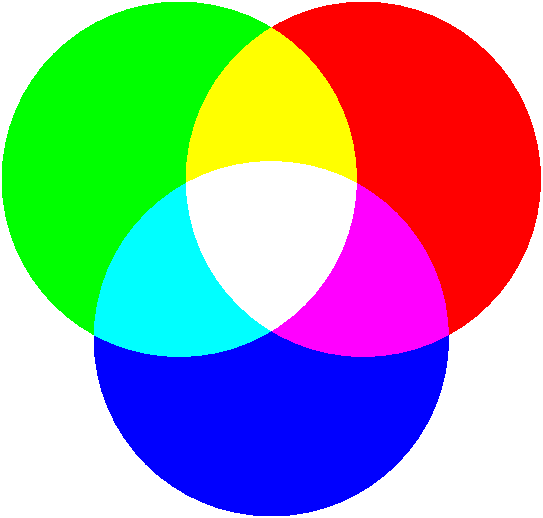
\includegraphics[width=0.8\textwidth]{QCD_colors.pdf}
        \caption{Baryon stable constitué de trois quarks.}
    \end{center}
    \end{subfigure}
    \hspace{0.2cm}
    \begin{subfigure}[b]{0.3\textwidth}
        \begin{center}
          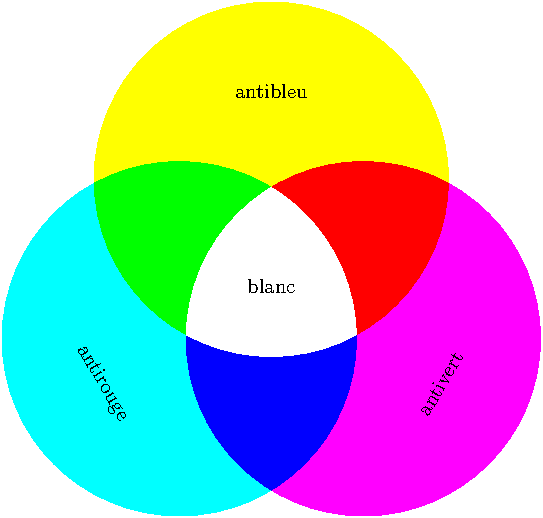
\includegraphics[width=0.8\textwidth]{QCD_anticolors.pdf}
            \caption{Antibaryon stable constitué de trois antiquarks.}
        \end{center}
    \end{subfigure}
    \hspace{0.2cm}
    \begin{subfigure}[b]{0.3\textwidth}
        \begin{center}
            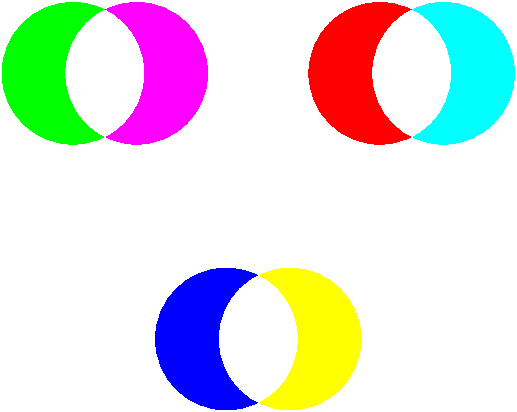
\includegraphics[width=0.8\textwidth]{QCD_color_anticolor.pdf}
            \caption{Mesons stables constitués d'une paire quark-antiquark.}
        \end{center}
    \end{subfigure}
    \caption{Représentation de hadrons stables à l'interaction de couleur (blanche).}
    \label{fig:interactionforte}
    \end{center}
\end{figure}

L'interaction décrit un échange de gluons qui provoque un changement de couleur des quarks. Une interaction est stable lorsque la charge de couleur globale est blanche (par exemple : $\mathrm{bleu} + \mathrm{vert} + \mathrm{rouge}$ ou encore $\mathrm{bleu}+\mathrm{antibleu}$). On retrouve majoritairement dans la nature des baryons composés de trois quarks (protons, neutron, $\PDelta^{++}$, ...) ou bien des mésons composés d'un quark et d'un anti-quark. Une illustration est montrée sur la figure \figurename{\ref{fig:interactionforte}}.

\subsubsection{La symétrie de jauge $SU(3)_C$}

De manière absolument similaire aux autres symétries de jauge on a : 
\begin{equation}
\psi \rightarrow e^{i \sum_{a=1}^{8} \alpha^a(x)T^a} \psi
\end{equation}
où les matrices $T^{a =1, ... , 8}$ sont les générateurs de $SU(3)$. Ils répondent à la relation $T^a = \frac{1}{2}\lambda^a$ où les $\lambda^a$ sont les matrices de Gell-Mann :
\begin{align}
  \lambda^1 = \begin{pmatrix}0&1&0\\1&0&0\\0&0&0 \end{pmatrix}
  &\quad\lambda^2 = \begin{pmatrix}0&-i&0\\i&0&0\\0&0&0 \end{pmatrix}
  \quad\lambda^3 = \begin{pmatrix}1&0&0\\0&-1&0\\0&0&0 \end{pmatrix} \nonumber \\
  \lambda^4 = \begin{pmatrix}0&0&1\\0&0&0\\1&0&0 \end{pmatrix}
  &\quad\lambda^5 = \begin{pmatrix}0&0&-i\\0&0&0\\i&0&0 \end{pmatrix}
  \quad\lambda^6 = \begin{pmatrix}0&0&0\\0&0&1\\0&1&0 \end{pmatrix} \\
  \quad\lambda^7 = &\begin{pmatrix}0&0&0\\0&0&-i\\0&i&0 \end{pmatrix} 
  \quad\lambda^8 = \frac{1}{\sqrt{3}} \begin{pmatrix}1&0&0\\0&1&0\\0&0&-2 \end{pmatrix} \nonumber
\end{align}

Ce groupe n'étant pas abélien il faudra s'attendre à des termes de corrections comme pour $U(1)_Y \otimes  SU(2)_L $
\begin{equation}
D_\mu = \partial_\mu + ig_S  \sum_{a=1}^{8}  T^a W_\mu^a
\end{equation}
Les champs bosoniques se transforment ici avec: 
\begin{equation}
    G^a_\mu \rightarrow G^a_\mu - \frac{1}{g_S} \partial_\mu \alpha^a(x)   \underbrace{-  \sum_{b=1}^{8}  \sum_{c=1}^{8}  f^{abc}\alpha^b(x) G^c_\mu}_\textrm{terme non-abélien}
\end{equation}
Le tenseur de champ associé aux bosons est donné par :
\begin{equation}
G^a_{\mu\nu} =  \partial_\mu G^a_\nu - \partial_\nu G^a_\mu - g_S \sum_{b=1}^{8}  \sum_{c=1}^{8} f^{abc}G^b_\mu G^c_\nu
\end{equation} 
Le terme non-abélien $g_S \sum_{b=1}^{8}  \sum_{c=1}^{8} f^{abc}G^b_\mu G^c_\nu$ fait apparaître dans le Lagrangien des termes d'auto-couplage à trois et quatre gluons, à l'origine du confinement des quarks.


\subsection{Densité de probabilité partonique (PDF)} \label{sec:pdf}

Les hadrons peuvent être vus comme une soupe statistique de partons avec, en permanence,  création et annihilation de couples quark-antiquark. Autrement dit, quand l'on parle de protons composés de deux quarks up et d'un down, on commet un abus de langage. En effet, la QCD implique que si l'on pouvait prendre en photo, un grand nombre de fois, un proton alors, statistiquement, nous observerions qu'il est composé la plupart du temps de deux quarks up et d'un down. Pour le calcul des sections efficaces des processus faisant intervenir des hadrons on utilise les densités de probabilité partonique $f_i\left( x_i, \mu_F^2 \right)$ (ou PDF pour \emph{Parton distribution function}).
Ces fonctions ne peuvent être calculées analytiquement à cause de l'échelle d'énergie empêchant le calcul perturbatif, le calcul sur réseau et valable uniquement dans le cas ultra-relativiste. Ces fonctions sont obtenues expérimentalement à partir d'ajustements sur les données. Les expériences de diffusion inélastique des leptons sur les hadrons, dont fait partie par exemple l'expérience HERA \cite{DESYpdf} (collisionneur \Pepm-\Pproton du laboratoire DESY à Hambourg en Allemagne) jouent un rôle majeur dans l'ajustement des PDF.

Les PDF dépendent de la variable de Bjorken $x$ qui représente la fraction d'énergie emportée par le parton considéré et de l'échelle en énergie du processus $Q^2$ (transfert d'impulsion). En toute rigueur, les PDF sont évaluées à une échelle d'énergie donnée dite échelle de factorisation $\mu_F^2$ qu'on choisit de l'ordre de grandeur de l'échelle d'énergie du processus étudié : $\mu_F \equiv Q$. Pour les déterminer, on fait le choix d'une paramétrisation à une échelle d'énergie $Q_0$ donnée. La forme la plus générale est : 
\begin{equation}
xf\left( x,Q_0^2 \right) = A_f x^{a_f} (1 - x)^{b_f} I_f(x)
\end{equation}
L'annulation des PDF pour $x \rightarrow 1$ est assurée par le terme $(1 - x)^{b_f}$. $a_f$ et $b_f$ sont les paramètres à déterminer à partir des données expérimentales. Cette forme de PDF est attendue avec la règle de comptage des quarks \cite{Brodsky:1973kr}. La dépendance en $Q^2$ est obtenue à l'aide des équations d'évolution \emph{DGLAP} (Dokshitzer–Gribov–Lipatov–Altarelli–Parisi) \cite{ALTARELLI, Dokshitzer:1977sg, Gribov:1972ri}. Elles sont essentielles pour prédire à partir des valeurs collectées à bas $Q^2$, les PDF à hautes valeurs de $Q^2$ non explorées par les données mais nécessaires au LHC. 

Les PDF utilisées pour produire des simulations ont été fournies par le groupe CTEQ \cite{Owens:2012bv} (voir la figure \figurename{\ref{fig:cj12}}) et NNPDF \cite{Ball2015}. De plus le groupe de travail PDF4LHC \cite{Butterworth_2016} effectue des études comparatives des différentes PDF et des prévisions au LHC. Il fournit également une méthode standard pour l'estimation des incertitudes liées aux PDF au LHC grâce à une combinaison des résultats des différents groupes.


\begin{figure}
  \begin{center}
  \subcaptionbox{\label{fig:pdgleft}}[0.45\textwidth]{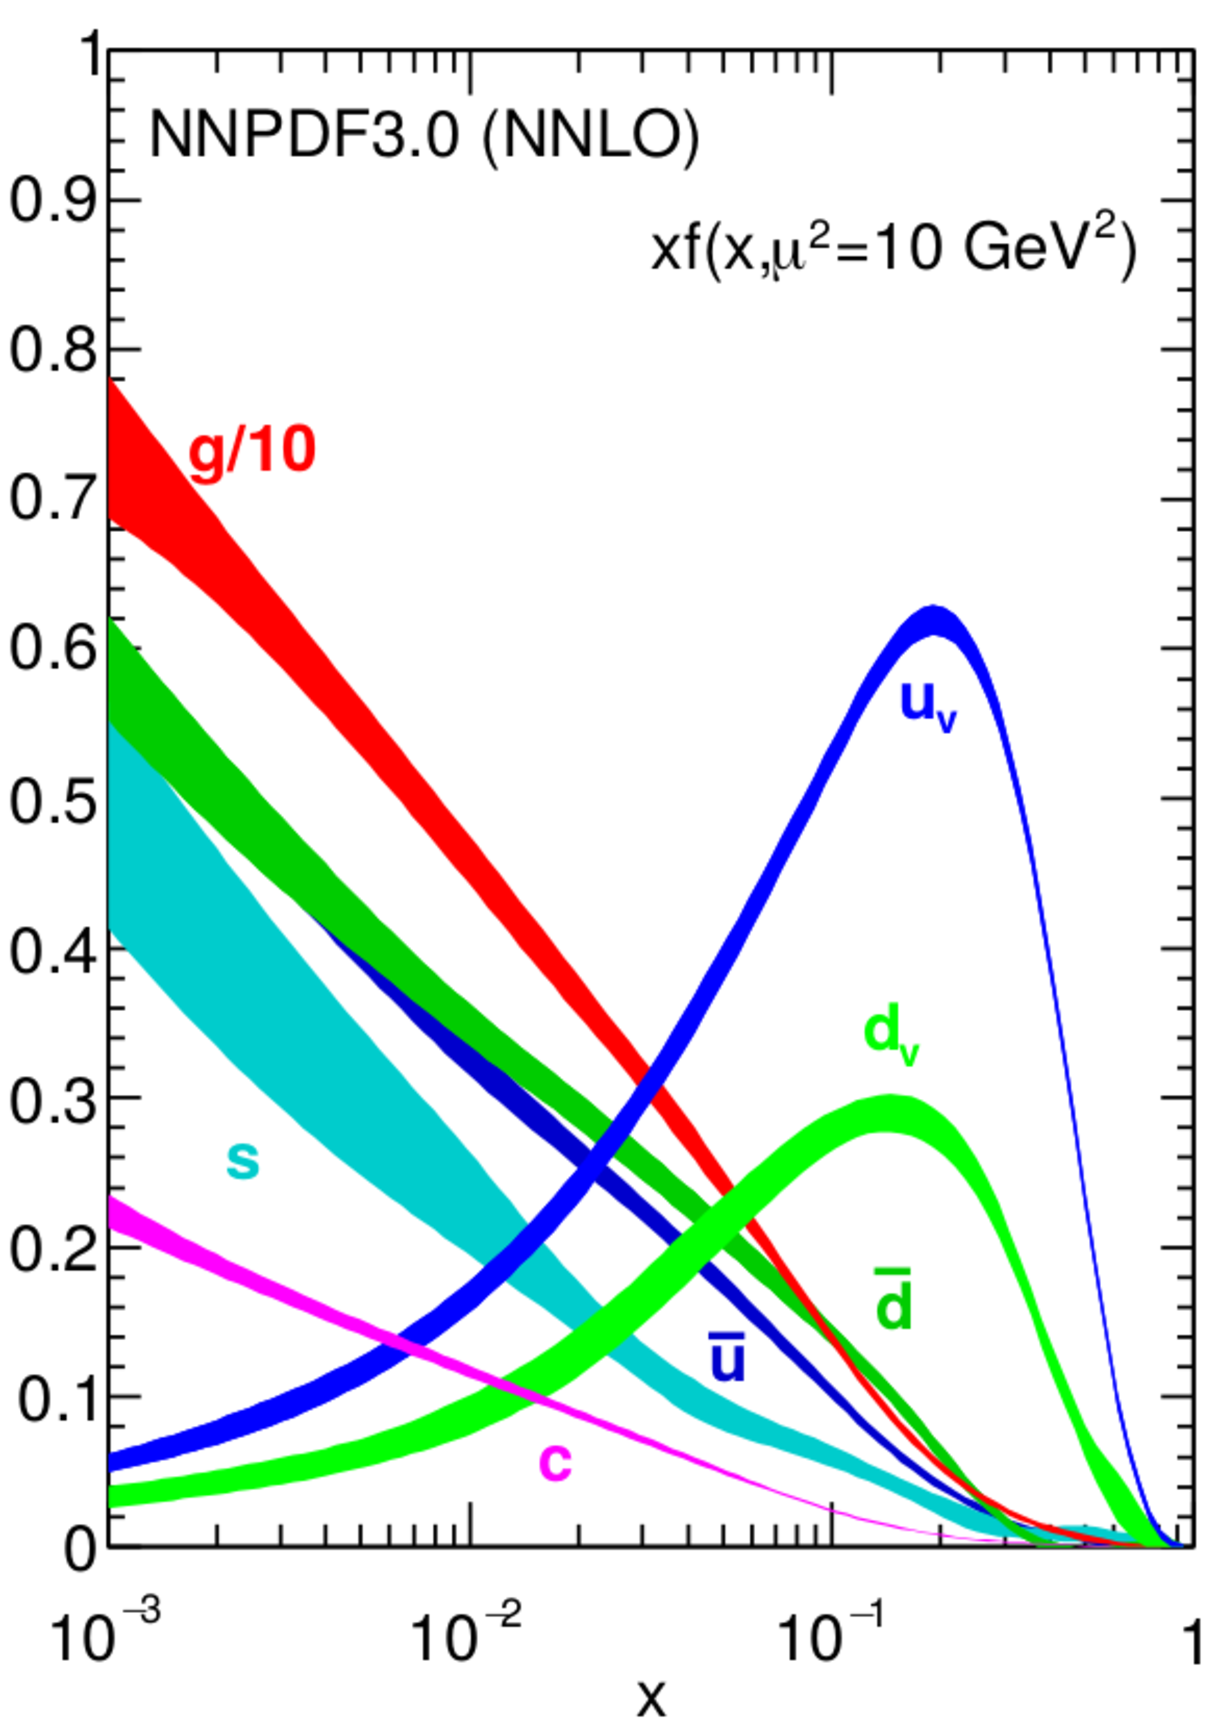
\includegraphics[width=0.4\textwidth]{parton_pdf_100_GeV2.pdf}}\hfill
  \subcaptionbox{\label{fig:pdgright}}[0.45\textwidth]{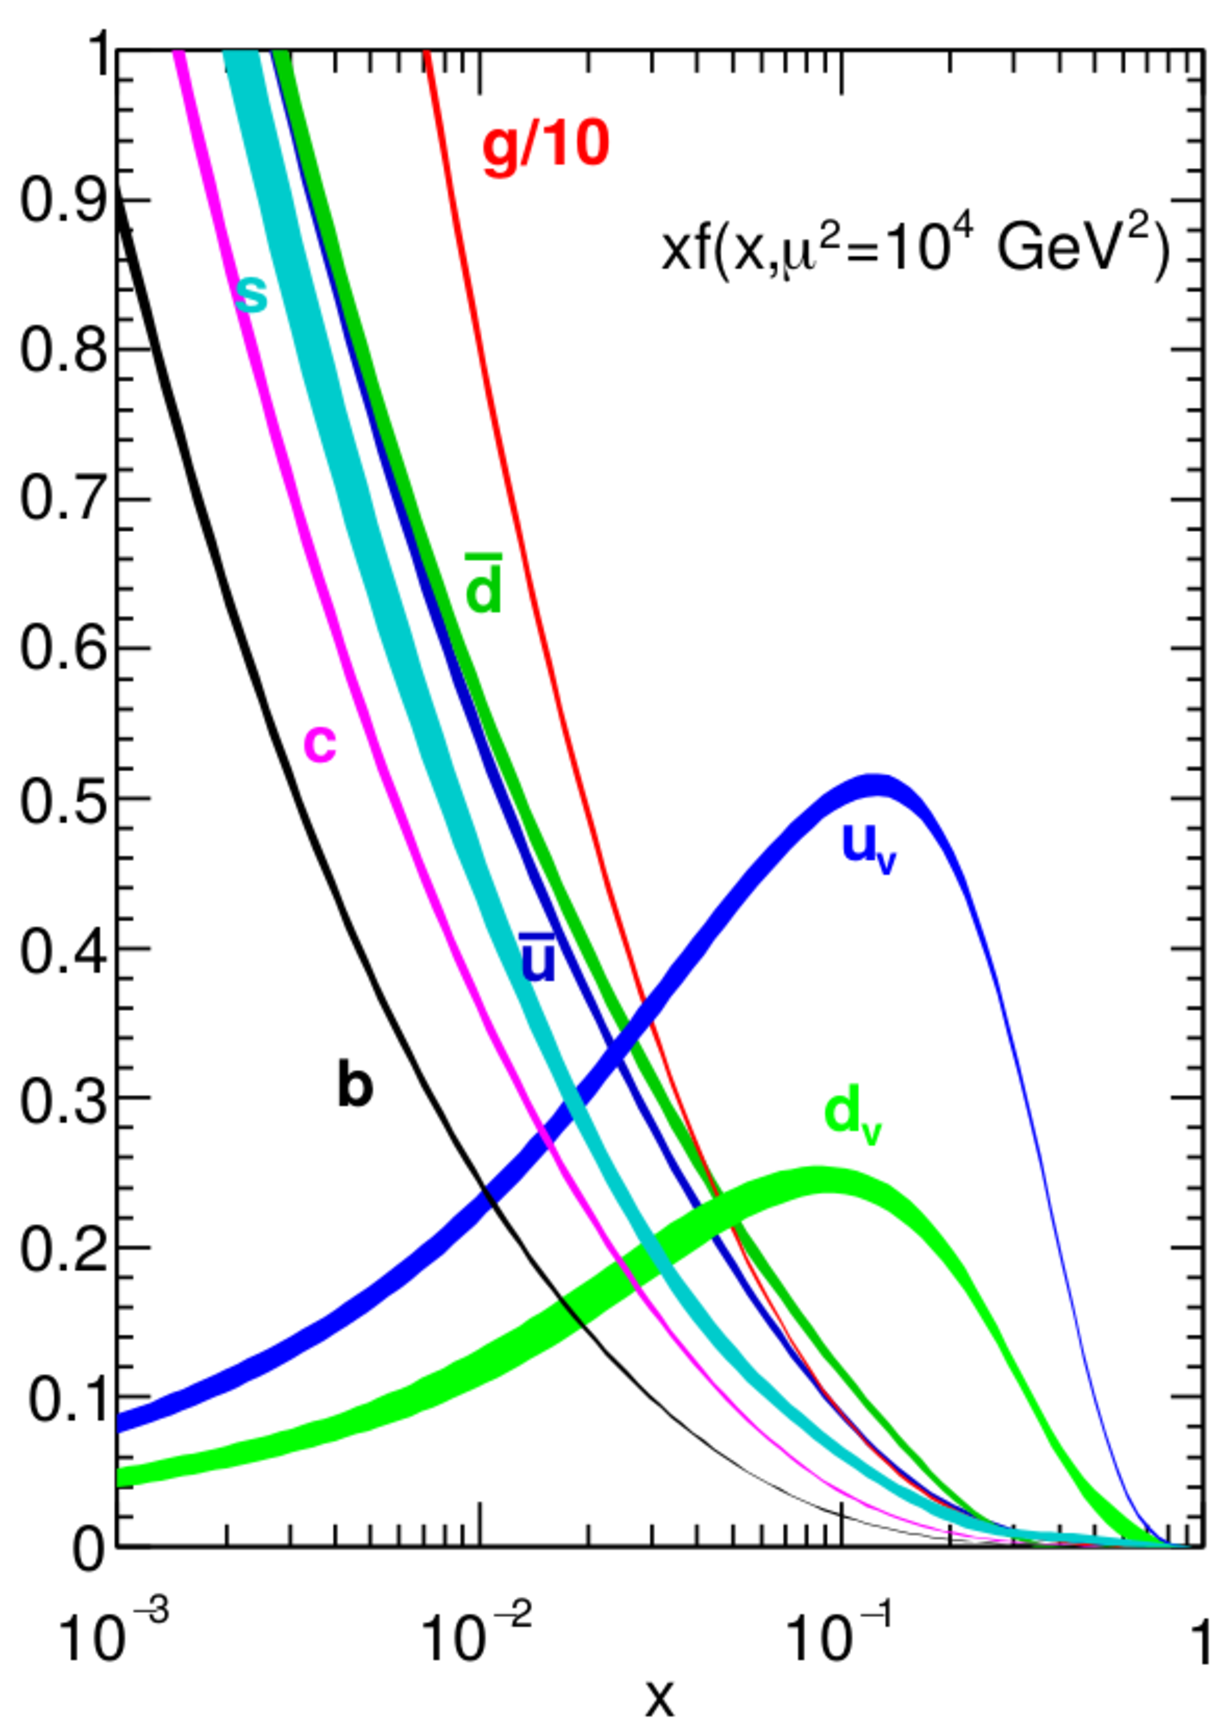
\includegraphics[width=0.4\textwidth]{parton_pdf_10000_GeV2.pdf}}
  \caption{Fonctions de densité partonique pour une échelle en énergie  (\subref{fig:pdgleft}) $\mu^2 (= Q^2) =  \SI{10}{\GeV^2}$ et  (\subref{fig:pdgright}) $\mu^2 (= Q^2) = \SI{e4}{\GeV^2}$ \cite{Debbio2018}.}
  \label{fig:cj12}
\end{center}    
\end{figure}


\subsection{Le Lagrangien complet}
On peut résumer toutes les informations précédentes pour bâtir le Lagrangien du Modèle Standard avant brisure de symétrie $U(1)_Y \otimes  SU(2)_L $. Ce Lagrangien est donc symétrique à $SO(1,3)$ et $U(1)_Y \otimes  SU(2)_L \otimes SU(3)_C $, entre autres.
\begin{align}
\mathcal{L}_\textrm{MS} &= \underbrace{\frac{i}{2}\bar{Q}_A\gamma^\mu\overset{\leftrightarrow}{D_\mu}Q_A + \frac{i}{2}\bar{U}_A\gamma^\mu\overset{\leftrightarrow}{D_\mu}U_A + \frac{i}{2}\bar{D}_A\gamma^\mu\overset{\leftrightarrow}{D_\mu}D_A}_{\substack{\text{cinétique des quarks} \\ \text{interaction quarks/bosons de jauge}}} \\
&\underbrace{+\frac{i}{2}\bar{L}_A\gamma^\mu\overset{\leftrightarrow}{D_\mu}L_A +\frac{i}{2}\bar{R}_A\gamma^\mu\overset{\leftrightarrow}{D_\mu}R_A}_{\substack{\text{cinétique des leptons} \\ \text{interaction leptons/bosons de jauge}}} \nonumber \\ 
    & \underbrace{-\frac{1}{4}B_{\mu\nu}B^{\mu\nu} -\frac{1}{4}\vec{W}_{\mu\nu}\cdot \vec{W}^{\mu\nu}}_\textrm{cinétique des bosons de jauge $U(1)_Y \otimes  SU(2)_L$} \qquad  \underbrace{-\frac{1}{4} \sum_{a=1}^{8} G^a_{\mu\nu}G_a^{\mu\nu}}_\textrm{cinétique des bosons de jauge $SU(3)_C $} \nonumber \\
    &  \underbrace{+vy_1 \bar{Q}_A \phi U_A + vy_2 \bar{Q}_A \phi D_A + vy_3 \bar{L}_A \phi R_A +\mathrm{h.c.} }_\textrm{couplage de Yukawa des fermions} \nonumber \\
    &  \underbrace{+D_\mu \phi^\dagger D^\mu \phi + \mu^2 \phi^\dagger \phi + \lambda (\phi^\dagger \phi)^2}_\textrm{secteur du champs de Higgs}
\end{align}


\begin{landscape}

\begin{table}
\begin{center}
    \begin{tabular}{cccc|ccc|cccc}
    \noalign{\smallskip}\hline\noalign{\smallskip}
      & I & II& III & $U(1)_Y $ & $SU(2)_L$ & $SU(3)_C $   &I&$I^3$&$C$&$Y$\\
 \noalign{\smallskip}
 \hline \hline
 \noalign{\smallskip}
    \multirow{2}{*}{Leptons} &  $\begin{pmatrix} \Pnue \\ \Pelectron \end{pmatrix}_L$ &  $\begin{pmatrix} \Pnum \\ \Pmuon \end{pmatrix}_L$ &  $\begin{pmatrix} \Pnut \\  \Ptau \end{pmatrix}_L$ 
    %%%%%%%%%%%%%%%%%%%%%%%%%%%%%%%%%%%%%%%%%%%%%%%
    & - \sfrac{1}{2}&2&1  
    %%%%%%%%%%%%%%%%%%%%%%%%%%%%%%%%%%%%%%%%%%%%%%%
     &+\sfrac{1}{2}&$\begin{matrix} \textrm{+\sfrac{1}{2}}\\ \textrm{-\sfrac{1}{2}}\end{matrix}$&$\begin{matrix} \textrm{0}\\\textrm{-1}\end{matrix}$&-1\\
    %%%%%%%%%%%%%%%%%%%%%%%%%%%%%%%%%%%%%%%%%%%%%%%
    %%%%%%%%%%%%%%%%%%%%%%%%%%%%%%%%%%%%%%%%%%%%%%%
    & $\Pelectron_R$ & $\Pmuon_R$  & $\Ptauon_R$  
    %%%%%%%%%%%%%%%%%%%%%%%%%%%%%%%%%%%%%%%%%%%%%%%
    & -1 & 1 & 1  
    %%%%%%%%%%%%%%%%%%%%%%%%%%%%%%%%%%%%%%%%%%%%%%%
    &0&0&-1&-2 \\
    \noalign{\smallskip}\hline\noalign{\smallskip}
    \multirow{3}{*}{Quarks} &  $\begin{pmatrix} \Pup \\ \Pdown' \end{pmatrix}_L$ &  $\begin{pmatrix} \Pcharm \\ \Pstrange' \end{pmatrix}_L$ &  $\begin{pmatrix} \Ptop \\  \Pbottom' \end{pmatrix}_L$ 
    %%%%%%%%%%%%%%%%%%%%%%%%%%%%%%%%%%%%%%%%%%%%%%%
    &\sfrac{1}{6}&2&3 
    %%%%%%%%%%%%%%%%%%%%%%%%%%%%%%%%%%%%%%%%%%%%%%%
     &\sfrac{1}{2}&$\begin{matrix} \textrm{+\sfrac{1}{2}}\\ \textrm{-\sfrac{1}{2}}\end{matrix}$&$\begin{matrix} \textrm{+\sfrac{2}{3}}\\ \textrm{-\sfrac{1}{3}}\end{matrix}$&+\sfrac{1}{3}\\
    %%%%%%%%%%%%%%%%%%%%%%%%%%%%%%%%%%%%%%%%%%%%%%%
    %%%%%%%%%%%%%%%%%%%%%%%%%%%%%%%%%%%%%%%%%%%%%%%
    & $\Pup_R$ & $\Pcharm_R$  & $\Ptop_R$  
    %%%%%%%%%%%%%%%%%%%%%%%%%%%%%%%%%%%%%%%%%%%%%%%
    &\sfrac{2}{3}&1&3  
    %%%%%%%%%%%%%%%%%%%%%%%%%%%%%%%%%%%%%%%%%%%%%%%
    &0 &0 & +\sfrac{2}{3}   & +\sfrac{4}{3} \\
    %%%%%%%%%%%%%%%%%%%%%%%%%%%%%%%%%%%%%%%%%%%%%%%
    %%%%%%%%%%%%%%%%%%%%%%%%%%%%%%%%%%%%%%%%%%%%%%%
    & $\Pdown_R$ & $\Pstrange_R$  & $\Pbottom_R$ 
    %%%%%%%%%%%%%%%%%%%%%%%%%%%%%%%%%%%%%%%%%%%%%%%
    &-\sfrac{1}{3}&1& 3 
    %%%%%%%%%%%%%%%%%%%%%%%%%%%%%%%%%%%%%%%%%%%%%%%
    &0 &0 & -\sfrac{1}{3}   & -\sfrac{2}{3} \\
    \noalign{\smallskip}\hline\noalign{\smallskip}
    \multirow{3}{*}{Bosons de jauge} &  & $B^\mu$  & 
    %%%%%%%%%%%%%%%%%%%%%%%%%%%%%%%%%%%%%%%%%%%%%%%
    &0&1&1  
    %%%%%%%%%%%%%%%%%%%%%%%%%%%%%%%%%%%%%%%%%%%%%%%
    &1&0, $\pm$1&0, $\pm$1&0 \\
    %%%%%%%%%%%%%%%%%%%%%%%%%%%%%%%%%%%%%%%%%%%%%%%
    %%%%%%%%%%%%%%%%%%%%%%%%%%%%%%%%%%%%%%%%%%%%%%%
    &  & $W^\mu_i$  & 
    %%%%%%%%%%%%%%%%%%%%%%%%%%%%%%%%%%%%%%%%%%%%%%%
    &0&3&1  
    %%%%%%%%%%%%%%%%%%%%%%%%%%%%%%%%%%%%%%%%%%%%%%%
    &0&0&0&0 \\
    %%%%%%%%%%%%%%%%%%%%%%%%%%%%%%%%%%%%%%%%%%%%%%%
    %%%%%%%%%%%%%%%%%%%%%%%%%%%%%%%%%%%%%%%%%%%%%%%
    &  & $G^\mu_a$  & 
    %%%%%%%%%%%%%%%%%%%%%%%%%%%%%%%%%%%%%%%%%%%%%%%
    &0&1& 8   
    %%%%%%%%%%%%%%%%%%%%%%%%%%%%%%%%%%%%%%%%%%%%%%%
    &0&0&0&0 \\
    \noalign{\smallskip}\hline\noalign{\smallskip}
  \end{tabular}
  \caption{Contenu en particules du Modèle Standard. Les bosons de jauge et le doublet de Higgs sont également représentés. Pour les quarks, $\Pup_i$ représente les états propres de masse tandis que $\Pdown'_i$ représente les états propres d’interaction faible. On donne également la représentation du champ dans les groupes $SU(3)_C$ et $SU(2)_L$ (1 pour singlet, 2 pour doublet, ...)}
  \label{tab:SMvalues}
\end{center}
\end{table}

\end{landscape}




\subsection{Limites du Modèle Standard}
Malgré un succès évident, le Modèle Standard porte des limitations théoriques et expérimentales. Ces dernières mènent à croire que le Modèle Standard est une approximation à basse énergie d'une théorie plus fondamentale. Ci-dessous quelques unes de ces limitations.

\begin{description}
\item[L'unification des interactions de jauge] 
\begin{sloppypar}
Comme montré précédemment, si les interactions faible et électromagnétique ont pu être unifiées, la chromodynamique quantique, elle, est ajoutée de manière indépendante et coexiste avec la théorie électrofaible sans unité. Des propositions comme la supersymétrie semblent pouvoir apporter un cadre théorique pour cette unification des interactions de jauges.
\end{sloppypar}
\item[La matière noire] 
\begin{sloppypar}
Une autre limitation est l’absence de candidats pour la matière noire. En effet, les mesures cosmologiques semblent indiquer que la matière décrite par le Modèle Standard ne représente que \SI{5}{\%} de la densité d’énergie de l’Univers, la majeure partie étant composée de matière noire (\SI{\sim27}{\%} ) et d’énergie noire (\SI{\sim 68}{\%} ). Une approche prometteuse postule l'existence de particules au-delà du Modèle Standard massives et faiblement interagissantes avec la matière, les WIMPs (\emph{Weakly Interacting Massive Particles}). Il est à noter que certaines approches supersymétriques offrent un candidat sérieux avec le neutralino par exemple.
\end{sloppypar}
\item[La masse des neutrinos] 
\begin{sloppypar}
Par construction, le Modèle Standard postule une masse nulle pour les neutrinos. Cependant des mesures de neutrinos solaires et atmosphériques \cite{neutrino_mixing_1}, \cite{neutrino_mixing_2} mettent en évidence le phénomène de changement de saveur appelé oscillation des neutrinos. Un analogue à la matrice CKM peut être introduit, la  matrice de Pontecorvo-Maki-Nakagawa-Sakata, qui permet de décrire le mélange de saveurs et le découplage entre état faible et état de masse. Cependant une telle présence n'explique pas \emph{a priori} la faible masse des neutrinos mesurée (inférieure à l'\si{\electronvolt}). Si on postule que les neutrinos sont des particules qui sont leur propre antiparticule (dite particule de Majorana) alors l'explication des masses peut être donnée par un mécanisme de \emph{seesaw} conduisant à des neutrinos droits stériles lourds et des neutrinos gauches de relativement faibles masses.
\end{sloppypar}
\item[De trop nombreux paramètres libres] 
\begin{sloppypar}
Le Modèle Standard contient 19 paramètres libres, c’est-à-dire non prédits et qu’il faut évaluer à travers l’expérience: les 3 masses des leptons, les 6 masses des quarks, les 3 couplages de jauge, les 2 paramètres du potentiel de Higgs, les 4 paramètres de la matrice CKM et la phase de violation de CP forte. Une proposition théorique élégante générera ces paramètres sans postuler leur existence de manière \emph{ad-hoc}.
\end{sloppypar}
\item[Le problème de la gravitation]
\begin{sloppypar}
En physique moderne, la gravitation est décrite dans le cadre de la Relativité Générale. Il existe une incompatibilité intrinsèque de cette dernière avec le Modèle Standard qui est une théorie quantique des champs. En effet, en Relativité Générale l'espace-temps est une entité dynamique, en théorie quantique des champs il est un simple contexte figé et immuable. Les tentatives de pratiquer naïvement de la théorie quantique des champs en espace-temps dynamique échouent. Cette pratique est pourtant une nécessité pour comprendre les phénomènes pour lesquels la taille de l'espace-temps atteint l'échelle de Planck $ \sim$ \SI{e19}{\GeV} où les phénomènes quantiques deviennent non négligeables (mur de Planck, singularité de trou noir). La solution pour la description d'une gravitation quantique est de construire une proposition théorique unifiée dont la Relativité Générale et le Modèle Standard seraient des théories effectives à basse énergie.
\end{sloppypar}
\end{description}

\section{Extension du Modèle Standard}\label{sec:TheSME}

\subsection{Introduction}

Le problème de la gravitation quantique est l'un des enjeux majeurs de la physique moderne. Les paragraphes précédents ont montré le fait que le Modèle Standard, à lui seul, ne peut prendre en compte le phénomène de gravitation. Nous avons également mentionné le fait qu'une théorie unificatrice doit avoir le Modèle Standard comme théorie effective à basse énergie.
Quelques exemples de propositions théoriques en cours de développement sont présentées rapidement ici :

\begin{description}
\item[La géométrie non commutative]
\begin{sloppypar}
 Il s'agit d'une approche mathématique qui postule que l'espace dans lequel les particules évoluent est intrinsèquement non-commutatif. Elle repose sur une branche des mathématiques développée en grande partie par Alain Connes \cite{Connes}. On peut résumer l'idée de base  par l'équation :
\begin{equation}
[ x^\mu, x^\nu ] = i \theta^{\mu\nu}
\end{equation}
Si cette approche n'a pas explicitement pour but de créer une théorie quantique unifiée, elle propose de réunir sous un même Lagrangien et un même formalisme mathématique le Modèle Standard et la Relativité Générale. Si cette approche n'est pas majoritaire elle a tout de même le mérite de donner une interprétation au champ de Higgs comme émergeant naturellement de l'espace-temps non-commutatif.
\end{sloppypar}
\item [La gravitation quantique à boucle]
\begin{sloppypar}
Cette approche est une théorie de gravitation quantique qui postule l'idée que l'espace-temps est quantifié. Partie d'une reformulation de la Relativité Générale par Abhay Ashtekar elle deviendra indépendante de la RG elle-même et sera développée en partie par Lee Smolin \cite{smolin} et Carlo Rovelli \cite{rovelli}.
\end{sloppypar}
\item [La théorie des cordes] 
\begin{sloppypar}
Cette proposition se veut une théorie du tout. Introduite par  Sergio Fubini, Gabriele Veneziano \cite{fubini} et Leonard Susskind \cite{susskind} comme proposition pour l'explication de l'interaction forte, elle se développera comme une théorie de gravitation quantique. Elle consiste à décrire les particules comme ayant une structure interne composée d'objets en 1 dimension nommés cordes avec une taille de l'ordre de la longueur de Planck ( \SI{\sim e-33}{\cm} ).
\end{sloppypar}
\end{description}

Quelles que soient les approches de gravitation quantique, chacune d'entre elles admet la possibilité d'une brisure de la symétrie de Lorentz. Cette violation peut être explicite à la théorie comme en gravitation quantique à boucle \cite{LIVloop} ou en géométrie non-commutative \cite{LIVnoncomm}. Elle peut également être spontanée comme en théorie des cordes \cite{LIVstring}. Cette universalité rend intéressante la recherche d'une brisure de symétrie de Lorentz.

\subsection{Interprétation de la violation de symétrie de Lorentz}

Comme discuté au tout début de la section \ref{sec:symetrie_de_lorentz}, la violation de symétrie de Lorentz correspond à la non conservation de l'intervalle $\mathrm{d}s^2$ par changement de référentiel inertiel. Cette proposition est très radicale puisque de simples opérations sur l'espace-temps telle qu'une rotation peuvent engendrer des transformations sur les lois physiques (les Lagrangiens). Pour mieux saisir la prudence dont il faut faire preuve, faisons une expérience de pensée.

\subsubsection{Expérience de pensée}

Imaginons un phénomène $X$ émettant une radiation $\gamma$ de manière probabiliste. Notons cette probabilité $\mathcal{P}(X\rightarrow\gamma, \theta)$ avec $\theta$ un angle en guise de paramètre et $X\rightarrow\gamma$ l'évènement du phénomène $X$ qui émet la radiation $\gamma$. On considère un premier référentiel $\mathcal{R}$ dans lequel on a $\mathcal{P}$ et un second référentiel $\mathcal{R}'$ obtenu du premier par transformation de Lorentz dans lequel on a $\mathcal{P}'$.
Par définition, la violation de la symétrie de Lorentz impliquera que 
\begin{equation}\label{paradoxe}
\mathcal{P}(X\rightarrow\gamma, \theta) \neq \mathcal{P}'(X\rightarrow\gamma, \Lambda \theta)
\end{equation}
où $\Lambda$ représente une transformation de Lorentz (rotation dans ce cas précis).

Installons ce phénomène dans un système où les radiations émises seront orientées vers un miroir semi-réfléchissant. Soient deux observateurs distincts : Grégoire (noté $G$ attaché à $\mathcal{R}$) et Quentin (noté $Q$ attaché à $\mathcal{R}'$) que l'on installe respectivement dans les alignements des radiations réfractée et transmise (voir figure \figurename{\ref{expCarleUhlrich}}). Les observateurs (donc référentiels) seront tournés l'un par rapport à l'autre de \SI{90}{\degree}. Ainsi, en vertu de l'équation \eqref{paradoxe}, les probabilités d'émission de radiation seront différentes. Après un certain nombre d'itérations de l'expérience, on obtiendra un cas où l'évènement aura lieu dans un des deux référentiels mais pas dans l'autre. 

Si nous nous trouvons dans ce cas, pour $G$, l'émission existe et il observe l'évènement $X\rightarrow\gamma$. Cependant pour $Q$ l'émission n'existe pas. Après avoir été informé par $Q$ que l'évènement n'a pas eu lieu (noté\footnote{la notation $\neg A$ est empruntée à la logique est signifie "non $A$".} $\neg (X\rightarrow\gamma)$ dans la figure \figurename{\ref{expCarleUhlrich}}), $G$ sera dans la position où il a connaissance de deux réalités distinctes qui ont eu lieu simultanément.

\begin{figure}[H]
\begin{center}
    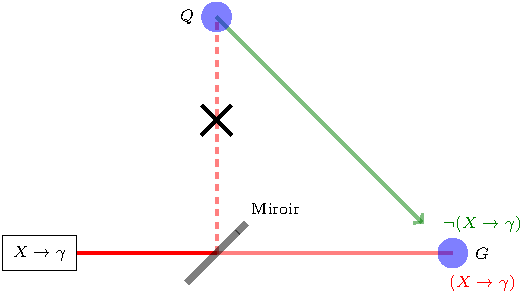
\includegraphics[width=0.6\textwidth]{exppensee.pdf}
    \caption{Expérience de pensée menant au paradoxe d'un phénomène qui s'est à la fois produit et pas produit en même temps.}
    \label{expCarleUhlrich}
\end{center}
\end{figure}


\paragraph{Discussion} 
Cette petite expérience de pensée amène un paradoxe qui n'est soluble que de deux manières possibles. Soit il faut admettre que plusieurs réalités contradictoires peuvent coexister, ce qui n'est pas envisageable à l'heure actuelle dans le domaine de la physique. Soit il faut renoncer à la possibilité que deux évènements puissent être simultanés. En effet, on peut lever le paradoxe en considérant que l'on abandonne la possibilité que les deux observateurs puissent se synchroniser pour s'assurer qu'ils observent un même évènement.
\newline

On constate donc que la violation de la symétrie de Lorentz ne peut pas être introduite sans précaution. Pour autant, il est possible de construire une physique qui viole la symétrie de Lorentz sans pour autant être soumise au paradoxe précédent. La stratégie consiste à abandonner une équivalence entre les transformations de Lorentz passives et les transformations de Lorentz actives, présente en théorie quantique des champs. La théorie développant les manipulations de violation de Lorentz, présentée en détails dans le paragraphe \ref{sec:sme}, préfère les appellations de transformation "observateur" et transformation "particule" qui sont assimilables dans le cadre de cette thèse aux transformations passive et active usuelles. La terminologie observateur/particule sera utilisée dans le reste de cette thèse. 

\subsection{La différence de transformation observateur / particule}\label{sec:particuleobservateur}

La transformation de Lorentz observateur est un changement de pures coordonnées. Le phénomène, lui, est le même. Le système de l'expérience de pensée précédente met en scène une transformation observateur. Et c'est pour ne pas tomber dans l'écueil du paradoxe, que l'on considérera que la symétrie de Lorentz est conservée par transformation observateur. La transformation particule, elle, consiste à considérer que c'est le phénomène qui subit la transformation. Cependant le jeu de coordonnées reste le même. 
\begin{figure}[H]
\begin{center}
    \begin{subfigure}[b]{0.45\textwidth}
        \begin{center}
            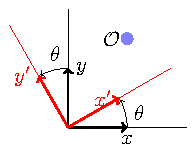
\includegraphics[height=0.7\textwidth]{passif.pdf}
            \caption{Transformation observateur (passive) où le repère est modifié mais le phénomène est inchangé.}
        \end{center}
    \end{subfigure}
    \hspace{0.4cm}
        \begin{subfigure}[b]{0.45\textwidth}
            \begin{center}
              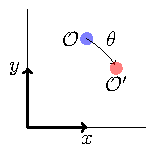
\includegraphics[height=0.7\textwidth]{actif.pdf}
                \caption{Transformation particule (active) où le repère est inchangé mais le phénomène est transformé.}
            \end{center}
        \end{subfigure}
    \end{center}
\end{figure}


Il est possible de construire formellement ces deux types de transformations. En prenant deux nouveaux observateurs : Jean-François et Lucas.
\begin{description}
\item [Transformation observateur]
\begin{sloppypar}
Soit  Jean-François, qui dans son référentiel observe un phénomène $\mathcal{O}$ dépendant des coordonnées d'espace-temps $x$. Alors la forme mathématique de son observation est $\mathcal{O}(x)$. Lucas, dans son propre référentiel, observe le même phénomène avec ses propres coordonnées. Il observera $\mathcal{O}'(x')$. Par essence, les deux observations sont égales.  
\begin{equation}
 \mathcal{O}(x) = \mathcal{O}'(x')
\end{equation}
avec $x' = \Lambda x$.
\end{sloppypar}
\item [Transformation particule]
\begin{sloppypar}
Soit  Jean-François, qui, de la même manière que précédemment observe $\mathcal{O}(x)$. La différence de perspective arrive avec Lucas qui dans son propre référentiel observe un phénomène similaire en utilisant le même jeu de coordonnées que Jean-François. Alors Lucas observera $\mathcal{O}'(x)$. Du point de vue de Jean-François les coordonnées de Lucas sont données par $x' = \Lambda x$. Comme les deux phénomènes sont différents mais mathématiquement équivalents, alors il y a égalité entre le phénomène vu par Lucas avec ses propres coordonnées et celui vu par Jean-François avec ses coordonnées exprimées par rapport à celles de Lucas. Soit 
\begin{equation}
 \mathcal{O}'(x) = \mathcal{O}(\Lambda^{-1}x')
\end{equation}
\end{sloppypar}
\end{description}
Un résumé de ces transformations est présenté dans la figure \tablename{\ref{tab:passif_actif}}.

\begin{table}
\begin{center}
    \begin{tabular}{c|cc}
    \noalign{\smallskip}\hline\noalign{\smallskip}
    Transformation & Observateur & Particule \\
 \noalign{\smallskip}
 \hline \hline
 \noalign{\smallskip}
    Coordonnées&$x \rightarrow x' = \Lambda x$ & $x \rightarrow x$\\
    Observation &$\mathcal{O} \rightarrow \mathcal{O}'(x') = \mathcal{O}(x)$ & $\mathcal{O}  \rightarrow \mathcal{O}'(x) = \mathcal{O}(\Lambda^{-1}x)$ \\
    \noalign{\smallskip}\hline\noalign{\smallskip}
  \end{tabular}
  \caption{Résumé des transformations observateur/particule. Avec $\Lambda$ une transformation de Lorentz et $\mathcal{O}$ un phénomène observé.}
  \label{tab:passif_actif}
\end{center}
\end{table}



\paragraph{Fin de l'équivalence}
Dans une théorie quantique des champs traditionnelle, ces deux transformations sont absolument équivalentes et interchangeables. On a vu que l'on ne peut pas laisser une transformation observateur violer la symétrie de Lorentz sans conséquences. Cependant la violation d'une transformation particule n'induit pas de paradoxe. La distinction de ces deux types de transformations est un point de départ nécessaire.


\subsection{Formalisme du SME}\label{sec:sme}

Pour réaliser des mesures expérimentales de la violation de la symétrie de Lorentz à basse énergie, il est commode d'employer une théorie effective. La théorie qui permet l'étude des violations de Lorentz est l'Extension du Modèle Standard (ou SME pour \emph{Standard Model Extension}). Elle a été introduite par Alan Kostelecký et Don Colladay \cite{SME1}, \cite{SME2}. Le but du SME est de fournir un cadre traitant de toutes violations de Lorentz possibles en physique des particules.

\subsubsection{Vide et espace-temps constant}

L'idée clé du SME est que le vide n'est pas symétrique sous transformation de Lorentz. Pour se le représenter, on peut imaginer qu'il existerait en tous points de l'espace-temps une entité constante de faible amplitude venant s'ajouter aux quantités physiques. Cette vue de l'esprit est représentée dans la figure \figurename{\ref{fig:SMEvacuum}}. 


\paragraph{Modèle simplifié : Mécanique newtonienne tridimensionnelle}\mbox{} 

En physique classique, une particule libre dans un référentiel inertiel est pilotée par le Lagrangien libre : 
\begin{equation}
    L = \frac{1}{2}m \vec{v}^2 = \frac{1}{2}m \delta_{ij} v^i v^j 
\end{equation}
avec $\delta_{ij = 1,2,3}$ la représentation indicielle d'une métrique d'espace-temps euclidienne en 3D.
En ajoutant à l'espace un champ additionnel orienté constant sous forme d'une matrice $c$ de dimensions $3\times3$, le Lagrangien devient en notation indicielle :
\begin{equation}
L = \frac{1}{2}m (\delta_{ij} + c_{ij}) v^i v^j 
\end{equation}
ce qui donne après application du principe de moindre action, la deuxième loi de Newton modifiée : 
\begin{equation}
    \vec{F} = m\vec{a} + mc\circ \vec{v}
\end{equation}
où $c\circ \vec{v}$ est la multiplication matricielle entre la matrice $c$ et le vecteur vitesse $\vec{v}$. Dans le cas le plus général possible, cette équation donne un terme additionnel à la second loi de Newton qui ne suit pas nécessairement la direction de l'accélération. L'effet s'interprète comme une petite force qui en tous points de l'espace est appliquée aux objets.

L'application de ce principe à l'espace-temps est une interprétation possible du SME. Dans le cadre de cette théorie effective, un champ $c_{\mu\nu}$ est additionné au champ métrique $g_{\mu\nu}$. De plus, devant suivre le principe de distinction transformation particule/ observateur (vu dans la section précédente \ref{sec:particuleobservateur}), alors les coefficients $c_{\mu\nu}$\footnote{Étant une théorie effective, ces coefficients se nomment coefficients de Wilson mais les propriétés de transformations de ces coefficients justifieraient un nom distinctif comme coefficients de Wilson "semi-covariants" par exemple.} introduits ont les propriétés de transformations suivantes : 
\begin{align}\label{wilson_def}
    c_{\mu\nu} &\rightarrow \Lambda^\alpha_\mu \Lambda^\beta_\nu c_{\alpha\beta} &\textrm{pour une transformation observateur} \nonumber \\
    c_{\mu\nu} &\rightarrow \delta^\alpha_\mu \delta^\beta_\nu  c_{\alpha\beta} = c_{\mu\nu} &\textrm{pour une transformation particule} 
\end{align}


\begin{figure}
\begin{center}
    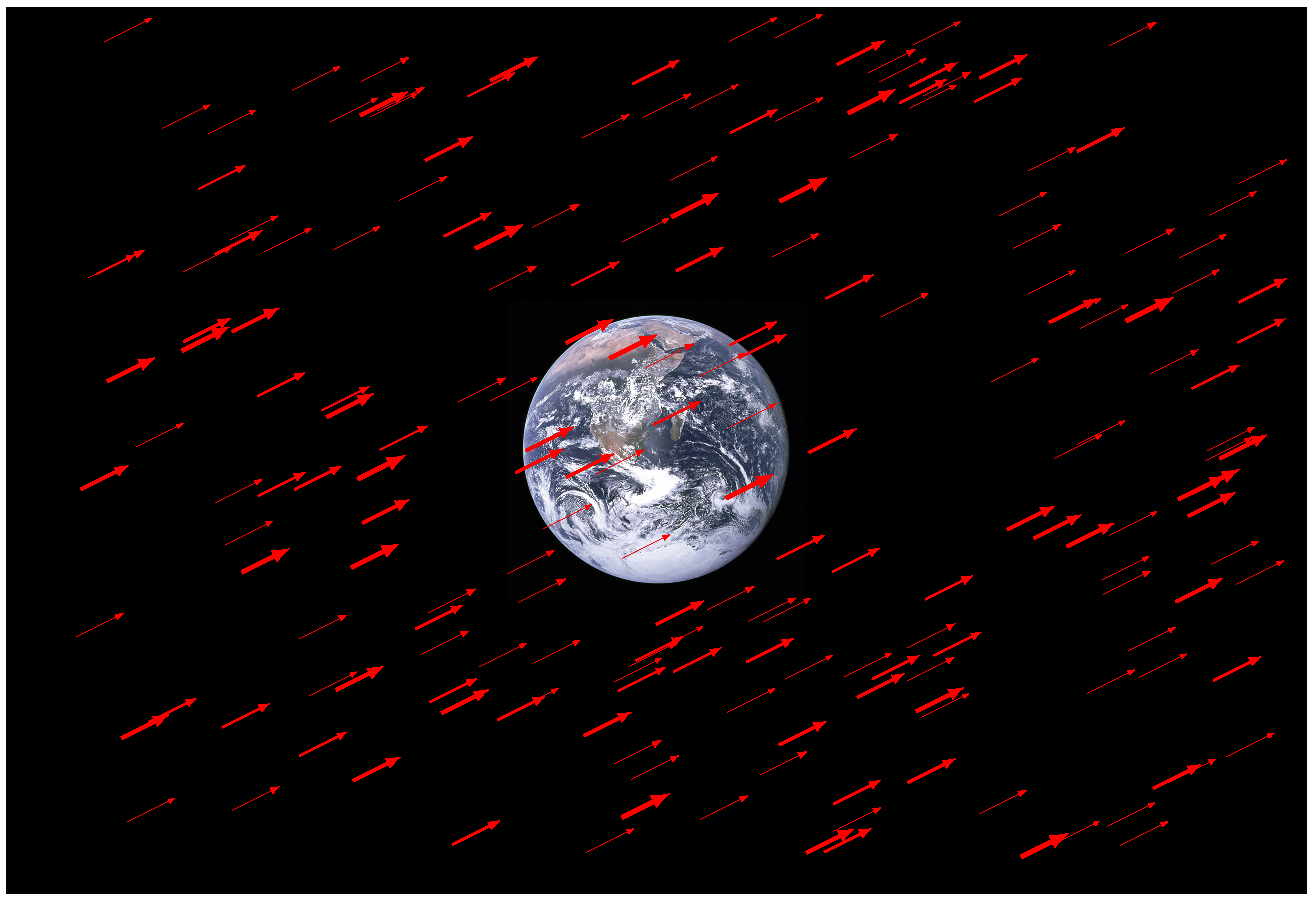
\includegraphics[width=0.8\textwidth]{champSME.pdf}
    \caption{Représentation de la Terre plongée dans un espace comportant un champ additionnel orienté constant, symbolisé par des flèches rouges.}
    \label{fig:SMEvacuum}
\end{center}
\end{figure}


\subsubsection{Une théorie effective}

LE SME est une théorie effective, c'est-à-dire qu'elle n'est pas construite pour donner une proposition de fonctionnement de la Nature mais simplement pour tester des configurations de Lagrangien afin de mesurer des paramètres et exclure des modèles. La puissance de cette théorie effective est qu'elle se veut universelle. En d'autres termes, elle est construite de telle sorte que toute théorie fondamentale violant la symétrie de Lorentz devrait converger, en approximation à basse énergie, vers le SME. Pour cela plusieurs contraintes doivent être respectées. 

\begin{itemize}[label=$\triangleright$]
\item Symétrique à la jauge $U(1)_Y \otimes  SU(2)_L \otimes SU(3)_C $
\item Conservation de l'énergie et de l'impulsion
\item Positivité de l'énergie
\item Hermiticité des opérateurs
\item Conservation de la microcausalité
\item Renormalisabilité
\end{itemize}
De plus dans sa version dite "minimale" le SME est valable pour un espace-temps en $D=4$ dimensions et postule qu'il n'y a pas de particules additionnelles aux champs du Modèle Standard.

Une fois toutes ces propriétés prises en compte, l'étape suivante consiste en l'élaboration d'une nouvelle densité lagrangienne. L'aspect effectif du SME permet de construire cette densité en y incorporant tous les coefficients possibles de brisure de Lorentz.


\subsubsection{Le formalisme mathématique}

Le SME est une théorie qui conserve la symétrie de Lorentz observateur. Cela implique que la construction d'un Lagrangien scalaire de Lorentz reste valide. Pour se donner une idée, on peut écrire le Lagrangien de Dirac \cite{Lehnert} dans le SME :
\begin{equation}
    \mathcal{L} = \frac{i}{2} \bar{\psi} \Gamma^\mu \overset{\leftrightarrow}{\partial_\mu} \psi - \bar{\psi} M \psi
\end{equation}
avec: 
\begin{align}
 \Gamma^\mu &\doteq \gamma^\mu + c^{\mu\nu}\gamma_\nu + d^{\mu\nu}\gamma_5 \gamma_\nu + e^\mu + if^\nu\gamma_5 + \frac{1}{2}g^{\lambda \mu\nu}\sigma_{\lambda \nu} \\
 M &\doteq m + a_\mu \gamma^\mu + b_\mu\gamma_5\gamma^\mu + \frac{1}{2} H^{\mu\nu}\sigma_{\mu\nu}
\end{align}
L'entité $ \Gamma^\mu$ signe l'aspect effectif du SME. En effet, on a toutes les combinaisons possibles de scalaires de Lorentz à l'ordre 1. Ainsi, dans l'espace des scalaires de Lorentz défini par la base $(\mathbbm{1},\gamma^\mu, i\gamma_5, \gamma_5\gamma^\mu,\sigma_{\mu\nu})$, les coefficients $a_\mu$, $b_\mu$, $c_{\mu\nu}$,  $d_{\mu\nu}$, $e_\mu$, $f_\mu$, $g_{\lambda \mu\nu}$ et $H^{\mu\nu}$ sont des coefficients de Wilson répondant à la propriété \eqref{wilson_def}.
Par exemple, dans le cas simplifié d'une particule où seul le coefficient $a_\mu$ est non nul, avec la relation de transformation des 2-spineurs et des matrices de Dirac :
\begin{align*}
 \psi &\rightarrow \psi' = S(\Lambda) \psi \\
 \gamma^\mu &\rightarrow  S(\Lambda) \gamma^\mu S^{-1}(\Lambda) \triangleq \Lambda^\mu_\alpha \gamma^{\alpha}
\end{align*}
où $ S(\Lambda)$ est la transformation de Lorentz des 2-spineurs, on a, pour le terme de masse : 
\begin{align}
    \bar{\psi'} (m + a'_\mu \gamma^{\mu\prime}) \psi' &=\bar{\psi} (m + a_\mu \gamma^\mu) \psi &\textrm{(observateur)} \\
    \bar{\psi'} (m + a'_\mu \gamma^{\mu\prime}) \psi' &=\bar{\psi} (m + a_\beta \Lambda^\beta_\mu \gamma^\mu) \psi &\textrm{(particule)} 
\end{align}


\subsubsection{Le Lagrangien du SME minimal}

Toutes les bases étant posées on peut construire le Lagrangien du SME minimal $\mathcal{L}_\mathrm{SME}$ \cite{SME1}. En vertu des principes précédents, le Lagrangien du SME minimal avant brisure électrofaible s'écrit :
\begin{align*}
\mathcal{L}_\textrm{SME} &= \mathcal{L}_\textrm{MS} \\ &\\
    &+\frac{i}{2} (c_Q)_{\mu \nu A B} \bar{Q}_A \gamma^\mu \overset{\leftrightarrow}{D^\nu} Q_B
    +  \frac{i}{2} (c_U)_{\mu \nu A B} \bar{U}_A \gamma^\mu \overset{\leftrightarrow}{D^\nu} U_B + \frac{i}{2} (c_D)_{\mu \nu A B} \bar{D}_A \gamma^\mu \overset{\leftrightarrow}{D^\nu} D_B\\
    &\underbrace{-(a_Q)_{\mu A B} \bar{Q}_A \gamma^\mu Q_B -(a_U)_{\mu A B} \bar{U}_A \gamma^\mu U_B -(a_D)_{\mu A B} \bar{D}_A \gamma^\mu D_B \qquad\qquad\qquad\quad}_{\substack{\text{cinétique des quarks et interaction quarks/bosons de jauge} \\ \text{violant la symétrie de Lorentz}}} \\
%%%%%%%%%%%%%%%%%%%%%%%%%%%
& +\frac{i}{2} (c_L)_{\mu \nu A B} \bar{L}_A \gamma^\mu \overset{\leftrightarrow}{D^\nu} L_B
    +  \frac{i}{2} (c_R)_{\mu \nu A B} \bar{R}_A \gamma^\mu \overset{\leftrightarrow}{D^\nu} R_B\\ 
&\underbrace{-(a_L)_{\mu A B} \bar{L}_A \gamma^\mu L_B - (a_R)_{\mu A B} \bar{R}_A \gamma^\mu R_B\qquad\qquad\quad}_{\substack{\text{cinétique des leptons et interaction leptons/bosons de jauge}\\ \text{violant la symétrie de Lorentz}}} \nonumber \\ 
%%%%%%%%%%%%%%%%%%%%%%%%%%%
    & \underbrace{-\frac{1}{4}(k_B)_{\kappa\lambda\mu\nu}B^{\kappa\lambda}B^{\mu\nu} -\frac{1}{2}(k_W)_{\kappa\lambda\mu\nu}\vec{W}^{\kappa\lambda}\cdot \vec{W}^{\mu\nu} -\frac{1}{2} (k_G)_{\kappa\lambda\mu\nu} \sum_{a=1}^{8}G_a^{\kappa\lambda}G_a^{\mu\nu}  }_{\substack{\textrm{cinétique des bosons de jauge $U(1)_Y \otimes  SU(2)_L$ et $SU(3)_C $}\\ \text{violant la symétrie de Lorentz}}}   \nonumber \\
%%%%%%%%%%%%%%%%%%%%%%%%%%%
    &  \underbrace{-\frac{1}{2} \left\{ (H_L)_{\mu \nu A B} \bar{L}_A \phi \sigma^{\mu\nu} R_B + (H_U)_{\mu \nu A B} \bar{Q}_A \phi^c \sigma^{\mu\nu} U_B +(H_D)_{\mu \nu A B} \bar{Q}_A \phi \sigma^{\mu\nu} D_B \right\} +\mathrm{h.c.} }_{\substack{\textrm{couplage de Yukawa des fermions}\\ \text{violant la symétrie de Lorentz}}}    \nonumber \\
    & + \frac{1}{2} (k_{\phi\phi})^{\mu\nu}  D_\mu \phi^\dagger D_\nu \phi +\mathrm{h.c.} \\
    &  \underbrace{ - \frac{1}{2} (k_{\phi B})^{\mu\nu} \phi^\dagger \phi B_{\mu\nu}  - \frac{1}{2} (k_{\phi W})^{\mu\nu} \phi^\dagger W_{\mu\nu} \phi +  i (k_{\phi})^{\mu} \phi^\dagger D_{\mu} \phi +\mathrm{h.c.} }_{\substack{\textrm{secteur du champ de Higgs}\\ \text{violant la symétrie de Lorentz}}}
\end{align*}
avec $A,B = 1,2,3$ les indices de saveurs.

\subsection{L'état de l'art}

Diverses limites sur les coefficients de Wilson du SME ont été établies par un grand nombre d'expériences. Ces limites sont résumées dans des tableaux récapitulatifs visibles dans la référence \cite{datatable}. 
\newline

L'unique expérience ayant posé des contraintes dans le secteur du quark top est celle faite avec la collaboration D$\emptyset$ \cite{D0}. Les limites sont résumées dans le tableau \tablename{\ref{tab:top}} et ne présentent aucune violation de symétrie de Lorentz avec une incertitude absolue d'environ \SI{10}{\%}. Ce sont ces limites que le travail de recherche décrit dans cette thèse a pour but de repousser.


\begin{table}[H]
\begin{center}
    \begin{tabular}{cccc}
    \noalign{\smallskip}\hline\noalign{\smallskip}
    Coefficient & Résultats & Secteur expérimental & Référence \\
    \noalign{\smallskip}
    \hline \hline
    \noalign{\smallskip}
    $(c_Q)_{XX 33}$ & \num[parse-numbers=false]{ -0.12 \pm 0.11 \pm 0.02 } & Production \ttbar & \cite{D0} \\
    $(c_Q)_{YY 33}$ & \num[parse-numbers=false]{ 0.12 \pm 0.11 \pm 0.02 } &  & \cite{D0} \\
    $(c_Q)_{XY 33}$ & \num[parse-numbers=false]{ -0.04 \pm 0.11 \pm 0.01 } & & \cite{D0} \\
    $(c_Q)_{XZ 33}$ & \num[parse-numbers=false]{ 0.15 \pm 0.08 \pm 0.01 } &  & \cite{D0} \\
    $(c_Q)_{YZ 33}$ & \num[parse-numbers=false]{ -0.03 \pm 0.08 \pm 0.02 } &  & \cite{D0} \\
    \noalign{\smallskip}\hline\noalign{\smallskip}
    $(c_U)_{XX 33}$ & \num[parse-numbers=false]{ 0.1 \pm 0.09 \pm 0.02 } & Production \ttbar & \cite{D0} \\
    $(c_U)_{YY 33}$ & \num[parse-numbers=false]{ -0.1 \pm 0.09 \pm 0.02 } &  & \cite{D0} \\
    $(c_U)_{XY 33}$ & \num[parse-numbers=false]{ 0.04 \pm 0.09 \pm 0.01 } & & \cite{D0} \\
    $(c_U)_{XZ 33}$ & \num[parse-numbers=false]{ -0.14 \pm 0.07 \pm 0.02 } &  & \cite{D0} \\
    $(c_U)_{YZ 33}$ & \num[parse-numbers=false]{ 0.01 \pm 0.07 \pm <0.01 } &  & \cite{D0} \\
        \noalign{\smallskip}\hline\noalign{\smallskip}
    $d_{XX}$ & \num[parse-numbers=false]{ -0.11 \pm 0.1 \pm 0.02 } & Production \ttbar & \cite{D0} \\
    $d_{YY}$ & \num[parse-numbers=false]{ 0.11 \pm 0.1 \pm 0.02 } &  & \cite{D0} \\
    $d_{XY}$ & \num[parse-numbers=false]{ -0.04 \pm 0.1 \pm 0.01 } & & \cite{D0} \\
    $d_{XZ}$ & \num[parse-numbers=false]{ 0.14 \pm 0.07 \pm 0.02 } &  & \cite{D0} \\
    $d_{YZ}$ & \num[parse-numbers=false]{ -0.02 \pm 0.07 \pm <0.01 } &  & \cite{D0} \\
    \noalign{\smallskip}\hline\noalign{\smallskip}
    \end{tabular}
    \caption{Exemples de mesures sur les coefficients de Wilson du SME dans le secteur du quark top.}
    \label{tab:top}
\end{center}
\end{table}



A titre illustratif, quelques exemples de valeurs de limites dans d'autres secteurs sont présentées dans les tables \tablename{\ref{tab:top}, \ref{tab:elec}, \ref{tab:photon}}.
On peut, par exemple, constater que le secteur de l'électron est très contraint avec des valeurs de précision de l'ordre de \num{e-14}.

\begin{table}[H]
\begin{center}
    \begin{tabular}{cccc}
    \noalign{\smallskip}\hline\noalign{\smallskip}
    Coefficient & Résultats & Secteur expérimental & Référence \\
    \noalign{\smallskip}
    \hline \hline
    \noalign{\smallskip}
    $\tilde{H}_{ZT}$ & \SI[parse-numbers=false]{ (-4.1\pm2.4)\times 10^{-27} }{\GeV} & Pendule de torsion  & \cite{Heckel_2008} \\
    $\tilde{H}_{YT} - \tilde{d}_{ZX}$ & \SI[parse-numbers=false]{ (-4.9\pm8.9)\times 10^{-27} }{\GeV} &   & \cite{Heckel_2008} \\
    $|d_{XX}|$ & \num{ < 2e-14 } & Astrophysique & \cite{Altschul_2007} \\
    $|d_{XY}|$ & \num{ < 2e-15 } &  & \cite{Altschul_2007} \\
    $|d_{TZ}|$ & \num{ < 8e-17 } &  & \cite{Altschul_2007} \\
    \noalign{\smallskip}\hline\noalign{\smallskip}
    \end{tabular}
    \caption{Exemples de mesures sur les coefficients de Wilson du SME dans le secteur de l'électron.}
    \label{tab:elec}
\end{center}
\end{table}

\begin{table}[H]
\begin{center}
    \begin{tabular}{cccc}
    \noalign{\smallskip}\hline\noalign{\smallskip}
    Coefficient & Résultats & Secteur expérimental & Référence \\
    \noalign{\smallskip}
    \hline \hline
    \noalign{\smallskip}
    $\tilde{\kappa}_{e-}^{XY}$ & \num[parse-numbers=false]{ (-0.7\pm1.6)\times 10^{-18} } & Oscillateur saphir  & \cite{Nagel_2015} \\
    $\tilde{\kappa}_{e-}^{XZ}$ &  \num[parse-numbers=false]{ (-5.5\pm4.0)\times 10^{-18} }  &   & \cite{Nagel_2015} \\
    $\tilde{\kappa}_{e-}^{YZ}$ &  \num[parse-numbers=false]{ (1.7\pm1.3)\times 10^{-18} }  &   & \cite{Nagel_2015} \\
    $k^{(3)}_{(V)00}$ &  \SI[parse-numbers=false]{ (1.1\pm1.3\pm1.5)\times 10^{-43} }{\GeV} & Polarisation du CMB & \cite{Komatsu_2011} \\
    $k^{Z}_{AF}$ &  \SI{ < e-19 }{\GeV} & Spectroscopie à Hydrogène & \cite{Gomes_2016} \\
    \noalign{\smallskip}\hline\noalign{\smallskip}
    \end{tabular}
    \caption{Exemples de mesures sur les coefficients de Wilson du SME dans le secteur du photon.}
    \label{tab:photon}
\end{center}
\end{table}


\subsection{Conclusion}

Le Modèle Standard de la physique des particules, bien que couronné de succès expérimentaux, présente des zones d'ombres théoriques. Si la masse des neutrinos et la matière noire sont des problématiques importantes, c'est bien la question de la gravitation quantique qui demeure une des plus grandes questions de la physique moderne. Plusieurs approches de nouvelles physiques sont proposées dans le monde de la physique par le biais de théories au-delà du Modèle Standard. Une violation de la symétrie de Lorentz pourrait être le dénominateur commun de théories proposant des solutions au problème de la gravitation quantique. Nous avons vu que le SME (pour \emph{Standard Model Extension}) se propose comme théorie effective pour l'étude de la violation de la symétrie de Lorentz. Dans les prochains chapitres, elle sera le socle théorique à partir duquel nous préparerons et exécuterons le projet expérimental de cette thèse. 

\end{fmffile}
